\documentclass{book}
%\usepackage[letterpaper, portrait, margin=1cm]{geometry}
%\usepackage[letterpaper, bindingoffset=0.2in, left=1in,right=1in,top=.5in,bottom=.5in,footskip=.25in,marginparwidth=5em]{geometry}
\usepackage[letterpaper, left=1in,right=1in,top=.5in,bottom=.5in,footskip=.25in,marginparwidth=1cm]{geometry}
% ---------------------
% mini-table-of-content
% ---------------------
\usepackage{minitoc}
\setcounter{minitocdepth}{1}
\setlength{\mtcindent}{24pt}
\setcounter{secnumdepth}{-2}
%\renewcommand{\mtcfont}{\small\rm}
%\renewcommand{\mtcSfont}{\small\bf}
%\usepackage{setspace}
%\usepackage{tocloft}
%\setlength\cftparskip{-1.2pt}
%\setlength\cftbeforesecskip{1.3pt}
%\setlength\cftaftertoctitleskip{2pt}
%\renewcommand{\cftsecafterpnum}{\hspace*{02.0em}}
%\renewcommand{\cftsubsecafterpnum}{\hspace*{02.0em}}

% ---------------------------
% Chinese Characters Packages
% ---------------------------
\usepackage{fontspec} 
\usepackage{xeCJK}
\setmainfont{Times}
\setCJKmainfont{BiauKai}
\newfontfamily\sblgoodhebrew{SBL BibLit}[Script=Hebrew,Contextuals=Alternate]
\newfontfamily\sblgoodgreek{SBL BibLit}[Script=Greek,Contextuals=Alternate]

\usepackage{ifpdf,cite,algorithmic,url,tikz}
\usepackage[cmex10]{amsmath}

% ---------------------------
% Hebrew Characters Packages
% ---------------------------
\usepackage{polyglossia}
\setmainfont{Times New Roman}

% -------
% General
% -------
\usepackage{multicol}
\usepackage{multirow}
\usepackage{color,colortbl}
\usepackage{xparse}
\usepackage{pbox}
\usepackage{stackengine}
\usepackage{titlesec}% http://ctan.org/pkg/titlesec
\usepackage{tabularx}
\usepackage{xltabular}
\usepackage{titlesec}
\usepackage{makecell}
\newcommand{\sectionbreak}{\clearpage}

\author{
  Editor, Michael Chan\\
  \texttt{michaelchan\_wahyan@yahoo.com.hk}
}
\usepackage{tocloft}

\usepackage{hyperref}
\hypersetup{
    colorlinks=true, % set true if you want colored links
    linktoc   =all , % set to all if you want both sections and subsections linked
    linkcolor =blue, % choose some color if you want links to stand out
}

% ----------
% Afterword
% ----------
\usepackage{marginnote}
\usepackage{sectsty}
\usepackage{ragged2e}
\usepackage{lineno}
\usepackage{xcolor}
\usepackage{paracol}

\begin{document}

\clearpage
%% temporary titles
% command to provide stretchy vertical space in proportion
\newcommand\nbvspace[1][3]{\vspace*{\stretch{#1}}}
% allow some slack to avoid under/overfull boxes
\newcommand\nbstretchyspace{\spaceskip0.5em plus 0.25em minus 0.25em}
% To improve spacing on titlepages
\newcommand{\nbtitlestretch}{\spaceskip0.6em}
\pagestyle{empty}
\begin{center}
\bfseries
\nbvspace[1]
\Huge
{%\nbtitlestretch
\Large
\textbf{J. Ng 頻道輯錄 粵語講道逐字稿 2025-26 \\
       Youtube Channel: JohnsonNg
       }}

\nbvspace[1]

{\large
Editor: Michael\\
\texttt{michaelchan\_wahyan@yahoo.com.hk}
}

\nbvspace[1]

{\large
Revision: \texttt{v1.2}\\
Last Update: \today
}


\vfill
\begin{tikzpicture}
    %remove comment for OT cover%\node (0,0) [opacity=0.03]{\includegraphics[width=15cm]{../bible_out/ot_frontcover.png}} ;
    %remove comment for NT cover%\node (0,0) [opacity=0.03]{\includegraphics[width=15cm]{../bible_out/christ_on_cross.png}} ;
    %remove comment for Bible cover%\node (0,0) [xshift=0.8cm, yshift=+2cm, opacity=0.03]{\includegraphics[width=10cm]{./christ_on_cross.png}} ;
    %remove comment for Bible cover%\node (0,0) [              yshift=-2cm, opacity=0.03]{\includegraphics[width=14cm]{./ot_frontcover.png}} ;
\end{tikzpicture}
\vfill

\end{center}

\newpage

\setcounter{tocdepth}{0}
\dominitoc
\begin{multicols}{3}
\addtocontents{toc}{\protect\hypertarget{toc}{}}
\tableofcontents
\end{multicols}

\large
%\twocolumn

% the color definition syntax is as follow:
% \definecolor{name}{system}{definition}
% example: a mono-channel color can be defined as
%          \definecolor{Gray}{gray}{0.9}
% example: an rgb-3-channel color can be defined as
%          \definecolor{LightCyan}{rgb}{0.88,1,1}
%          \definecolor{pink}{rgb}{0.68,0,0.68}

\definecolor{CUV1LightRed}{rgb}{1,0.75,0.75}     % for CUV1
\definecolor{LZZVLightGray}{rgb}{0.9,0.9,0.9}    % for LZZ
\definecolor{KJVVLightGreen}{rgb}{0.75,1,0.85}   % for KJV
\definecolor{CUV2LightYellow}{rgb}{1,1,0.75}     % for CUV2
\definecolor{CNVVLightBrown}{rgb}{1,0.85,0.7}    % for CNV
\definecolor{NRSVLightBlue}{rgb}{0.75,1,1}       % for NRSV
\definecolor{WENLLightPurple}{rgb}{0.95,0.85,0.9}% for WENL
\definecolor{TCV19PaleGreen}{rgb}{0.85,1,0.95}   % for TCV19
\definecolor{MSGVLightWhite}{rgb}{0.98,0.98,0.98}% for MSGV
\definecolor{NETSLightRed}{rgb}{1,0.75,0.75}     % for NETS
\definecolor{JPS1917LightYellow}{rgb}{1,1,0.75}  % for JPS1917
\definecolor{SBLGNTPaleRed}{rgb}{1,0.85,0.80}    % for SBLGNT

{ \scriptsize


\begin{xltabular}{\textwidth}{|p{0.15\textwidth} p{0.6\textwidth}|p{0.07\textwidth} p{0.1\textwidth}|}
\hline
\multicolumn{4}{c}{} \\
\multicolumn{4}{c}{\hyperref[ch:preacher1]{張雲開}} \\
\multicolumn{4}{c}{} \\
\hline
使徒行傳 11:1-18 & \hyperref[sec:0swvj1WD4mE]{一句唔係金句ge 金句(使徒行傳11\_1-18) - 張雲開老師} & 2025-03-07 & \href{https://youtube.com/watch?v=0swvj1WD4mE}{\texttt{0swvj1WD4mE}} \\
\multicolumn{4}{c}{} \\
\multicolumn{4}{c}{\hyperref[ch:preacher2]{彭家業}} \\
\multicolumn{4}{c}{} \\
\hline
列王記上 17:8-16 & \hyperref[sec:EkXQrXbYZ7E]{在困境中踏出信心的一步 (列王記上17\_8-16) - 彭家業牧師} & 2025-04-16 & \href{https://youtube.com/watch?v=EkXQrXbYZ7E}{\texttt{EkXQrXbYZ7E}} \\
列王記上 17:17-24 & \hyperref[sec:uoH02YdIlI4]{禍患的神學反思 : 神話語的確認 (列王記上17\_17-24) - 彭家業牧師} & 2025-05-31 & \href{https://youtube.com/watch?v=uoH02YdIlI4}{\texttt{uoH02YdIlI4}} \\
列王記上 18:1-6 & \hyperref[sec:fmQ_KmzoEKE]{隱藏的敬畏(列王記上18\_1-6) - 彭家業牧師【繁簡字幕 by Johnson Ng】} & 2025-03-19 & \href{https://youtube.com/watch?v=fmQ-KmzoEKE}{\texttt{fmQ-KmzoEKE}} \\
列王記上 18:7-16 & \hyperref[sec:fH3g_zqpZGU]{邪惡世代的服侍 : 敬畏神和懼怕人的對立 (列王記上 18\_7-16) - 彭家業牧師} & 2025-05-17 & \href{https://youtube.com/watch?v=fH3g-zqpZGU}{\texttt{fH3g-zqpZGU}} \\
箴言 30:1-3 & \hyperref[sec:Ii_o05jkhEI]{亞古珥尋找智慧的指南 (箴言30\_1-3) - 彭家業牧師【繁簡字幕 by Johnson Ng】} & 2025-03-19 & \href{https://youtube.com/watch?v=Ii-o05jkhEI}{\texttt{Ii-o05jkhEI}} \\
雅各書列王記上 17:1-7 & \hyperref[sec:EyGtbg5N3vU]{世代審判中的恩典和服侍(列王記上17\_1-7;雅各書5\_16-18) - 彭家業牧師} & 2025-04-13 & \href{https://youtube.com/watch?v=EyGtbg5N3vU}{\texttt{EyGtbg5N3vU}} \\
\multicolumn{4}{c}{} \\
\multicolumn{4}{c}{\hyperref[ch:preacher3]{彭錦威}} \\
\multicolumn{4}{c}{} \\
\hline
哥林多前書 12:1-11 & \hyperref[sec:pb5NDTZL6gI]{有分別又沒分別 (哥林多前書12\_1-11) - 彭錦威傳道} & 2025-03-01 & \href{https://youtube.com/watch?v=pb5NDTZL6gI}{\texttt{pb5NDTZL6gI}} \\
\multicolumn{4}{c}{} \\
\multicolumn{4}{c}{\hyperref[ch:preacher4]{徐武豪}} \\
\multicolumn{4}{c}{} \\
\hline
約翰一書 2:29-3:10 & \hyperref[sec:Y_0n0vkhyDU]{愛的兒女 不辱主名 (約翰一書2\_29-3\_10) - 徐武豪博士} & 2025-01-11 & \href{https://youtube.com/watch?v=Y_0n0vkhyDU}{\texttt{Y\_0n0vkhyDU}} \\
約翰一書 3:11-24 & \hyperref[sec:K8E95o7ZcvU]{愛的後果, 神前安穩 (約翰一書3\_11-24) - 徐武豪博士} & 2025-01-11 & \href{https://youtube.com/watch?v=K8E95o7ZcvU}{\texttt{K8E95o7ZcvU}} \\
約翰一書 4:1-12 & \hyperref[sec:qbcjpAyQDGE]{愛的回應, 彼此相愛 (約翰一書 4\_1-12) - 徐武豪博士} & 2025-03-13 & \href{https://youtube.com/watch?v=qbcjpAyQDGE}{\texttt{qbcjpAyQDGE}} \\
約翰一書 4:13-5:5 & \hyperref[sec:l7wNnYvML2Y]{愛的本份,因神而愛(約翰一書 4\_13-5\_5) - 徐武豪博士} & 2025-01-11 & \href{https://youtube.com/watch?v=l7wNnYvML2Y}{\texttt{l7wNnYvML2Y}} \\
約翰一書 5:6-21 & \hyperref[sec:u5ZquLAUHJ8]{愛的應許, 靠神能活(約翰一書 5\_6-21) - 徐武豪博士} & 2025-05-06 & \href{https://youtube.com/watch?v=u5ZquLAUHJ8}{\texttt{u5ZquLAUHJ8}} \\
約翰二書 1:1-13 & \hyperref[sec:MwmlxwsAcg0]{愛的需要, 要行要防 (約翰二書1\_1-13) - 徐武豪博士} & 2025-05-02 & \href{https://youtube.com/watch?v=MwmlxwsAcg0}{\texttt{MwmlxwsAcg0}} \\
約翰三書 1:1-15 & \hyperref[sec:IKjtotPld14]{愛的表現, 要有要學 (約翰三書1\_1-15) - 徐武豪博士} & 2025-05-02 & \href{https://youtube.com/watch?v=IKjtotPld14}{\texttt{IKjtotPld14}} \\
\multicolumn{4}{c}{} \\
\multicolumn{4}{c}{\hyperref[ch:preacher5]{李思敬}} \\
\multicolumn{4}{c}{} \\
\hline
創世記 1:26-28 & \hyperref[sec:cau3XNPSx68]{「形象」和「配偶」 (創世記1\_26-28) - 李思敬博士【繁簡字幕翻譯 by Johnson Ng】《五經》中的性別神學講道系列 - (第1講)} & 2025-02-16 & \href{https://youtube.com/watch?v=cau3XNPSx68}{\texttt{cau3XNPSx68}} \\
出埃及記 1:15-22 & \hyperref[sec:dX_CJYSfYFI]{救恩歷史的起點 (出埃及記1\_15-22) - 李思敬博士【繁簡字幕翻譯 by Johnson Ng】《五經》中的性別神學講道系列 - (第2講)} & 2025-03-09 & \href{https://youtube.com/watch?v=dX-CJYSfYFI}{\texttt{dX-CJYSfYFI}} \\
出埃及記 24:12-18 & \hyperref[sec:FIiVfx7a3V0]{上主榮耀停在西乃 (出埃及記24\_12-18) - 李思敬博士【繁簡字幕 by Johnson Ng】「認識神的榮耀」講道系列 - (第3講)} & 2025-05-08 & \href{https://youtube.com/watch?v=FIiVfx7a3V0}{\texttt{FIiVfx7a3V0}} \\
出埃及記 33:18-23 & \hyperref[sec:sg1ydBAtBWw]{求你顯出你的榮耀 (出埃及記33\_18-23) - 李思敬博士【繁簡字幕 by Johnson Ng】「認識神的榮耀」講道系列 - (第2講)} & 2025-03-12 & \href{https://youtube.com/watch?v=sg1ydBAtBWw}{\texttt{sg1ydBAtBWw}} \\
出埃及記 40:34-35 & \hyperref[sec:YdX9gstJs1g]{上主榮光充滿帳幕 (出埃及記40\_34-35) - 李思敬博士【繁簡字幕 by Johnson Ng】「認識神的榮耀」講道系列 - (第1講)} & 2025-02-05 & \href{https://youtube.com/watch?v=YdX9gstJs1g}{\texttt{YdX9gstJs1g}} \\
利未記 12:1:8 & \hyperref[sec:3nI0HjAVAi0]{生子不潔=性別歧視? (利未記12\_1\_8) - 李思敬博士【繁簡字幕翻譯 by Johnson Ng】《五經》中的性別神學講道系列 - (第3講)} & 2025-04-24 & \href{https://youtube.com/watch?v=3nI0HjAVAi0}{\texttt{3nI0HjAVAi0}} \\
民數記 27:1-11 & \hyperref[sec:FAz2YkOIsiw]{女兒的權利與義務  (民數記27\_1-11) - 李思敬博士【繁簡字幕翻譯 by Johnson Ng】《五經》中的性別神學講道系列 - (第4講)} & 2025-05-22 & \href{https://youtube.com/watch?v=FAz2YkOIsiw}{\texttt{FAz2YkOIsiw}} \\
詩篇 1:1-6 & \hyperref[sec:AXMhGkS0eVE]{蒙福的敬拜 (詩篇1\_1-6) - 李思敬博士【繁簡字幕翻譯 by Johnson Ng】} & 2025-03-11 & \href{https://youtube.com/watch?v=AXMhGkS0eVE}{\texttt{AXMhGkS0eVE}} \\
詩篇 32:1-11 & \hyperref[sec:XbuAosaX8BE]{有福的確據 (詩篇32\_1-11)  - 李思敬博士【繁簡字幕翻譯 by Johnson Ng】} & 2025-04-18 & \href{https://youtube.com/watch?v=XbuAosaX8BE}{\texttt{XbuAosaX8BE}} \\
詩篇 148:1-14 & \hyperref[sec:l8BFPdIOADs]{合神心意的讚美 (詩篇148\_1-14) - 李思敬博士【繁簡字幕翻譯 by Johnson Ng】} & 2025-01-25 & \href{https://youtube.com/watch?v=l8BFPdIOADs}{\texttt{l8BFPdIOADs}} \\
使徒行傳 1:6-8 & \hyperref[sec:656hrkLI9ks]{直到地極 (使徒行傳1\_6-8) - 李思敬博士【繁簡字幕翻譯 by Johnson Ng】} & 2025-04-23 & \href{https://youtube.com/watch?v=656hrkLI9ks}{\texttt{656hrkLI9ks}} \\
哥林多前書 1:18-25 & \hyperref[sec:topv29EFgUk]{十架神學 (哥林多前書1\_18-25) - 李思敬博士【繁簡字幕翻譯 by Johnson Ng】} & 2025-04-27 & \href{https://youtube.com/watch?v=topv29EFgUk}{\texttt{topv29EFgUk}} \\
\multicolumn{4}{c}{} \\
\multicolumn{4}{c}{\hyperref[ch:preacher6]{李錦洪}} \\
\multicolumn{4}{c}{} \\
\hline
約拿書 1:1-17 & \hyperref[sec:wLDaR7Spo6U]{約拿情意結 (約拿書1\_1-17) - 李錦洪先生} & 2025-03-25 & \href{https://youtube.com/watch?v=wLDaR7Spo6U}{\texttt{wLDaR7Spo6U}} \\
\multicolumn{4}{c}{} \\
\multicolumn{4}{c}{\hyperref[ch:preacher7]{林修榮}} \\
\multicolumn{4}{c}{} \\
\hline
帖撒羅尼迦前書帖撒羅尼迦後書 4:14-18 & \hyperref[sec:xOqiVXdmrRE]{教會的憂傷與驚慌(帖撒羅尼迦前書4\_14-18, 帖撒羅尼迦後書2\_1-8) - 林修榮弟兄} & 2025-04-06 & \href{https://youtube.com/watch?v=xOqiVXdmrRE}{\texttt{xOqiVXdmrRE}} \\
\multicolumn{4}{c}{} \\
\multicolumn{4}{c}{\hyperref[ch:preacher8]{楊慶球}} \\
\multicolumn{4}{c}{} \\
\hline
啟示錄 2:18-29 & \hyperref[sec:fJrsPMmDHtU]{紛亂中的堅守︰推雅推喇教會 (啟示錄2\_18-29) - 楊慶球博士} & 2025-02-09 & \href{https://youtube.com/watch?v=fJrsPMmDHtU}{\texttt{fJrsPMmDHtU}} \\
啟示錄 3:1-6 & \hyperref[sec:APKBO553sbY]{撒狄:名存實亡的教會 (啟示錄3\_1-6) - 楊慶球博士} & 2025-04-15 & \href{https://youtube.com/watch?v=APKBO553sbY}{\texttt{APKBO553sbY}} \\
啟示錄 3:7-13 & \hyperref[sec:G3cvoiyAPm4]{非拉鐵非:愛與傳福音的教會(啟示錄3\_7-13) - 楊慶球博士} & 2025-05-14 & \href{https://youtube.com/watch?v=G3cvoiyAPm4}{\texttt{G3cvoiyAPm4}} \\
\multicolumn{4}{c}{} \\
\multicolumn{4}{c}{\hyperref[ch:preacher9]{沈祖堯}} \\
\multicolumn{4}{c}{} \\
\hline
約翰福音 12:24-26 & \hyperref[sec:rP3BCIuRFDw]{成功... 失敗... ( A Successful Life) (約翰福音12\_24-26) - 沈祖堯教授【繁簡字幕 by Johnson Ng】} & 2025-03-25 & \href{https://youtube.com/watch?v=rP3BCIuRFDw}{\texttt{rP3BCIuRFDw}} \\
\multicolumn{4}{c}{} \\
\multicolumn{4}{c}{\hyperref[ch:preacher10]{蕭壽華}} \\
\multicolumn{4}{c}{} \\
\hline
箴言 10:11-14-18-21-31-32 & \hyperref[sec:O7c_1_GxWwE]{守住口舌 生命善果(箴言10\_11-14,18-21,31-32;13\_2-6;15\_1-4) - 蕭壽華牧師} & 2025-04-06 & \href{https://youtube.com/watch?v=O7c-1-GxWwE}{\texttt{O7c-1-GxWwE}} \\
帖撒羅尼迦前書 1:2-10 & \hyperref[sec:BbA1D0QrkWU]{你們對神的信心傳開了(帖撒羅尼迦前書1\_2-10)- 蕭壽華牧師} & 2025-04-06 & \href{https://youtube.com/watch?v=BbA1D0QrkWU}{\texttt{BbA1D0QrkWU}} \\
希伯來書 3:12-4:13 & \hyperref[sec:toZa1ewaUWE]{以信心與所聽見的道配合(希伯來書3\_12-4\_13) - 蕭壽華牧師} & 2025-01-08 & \href{https://youtube.com/watch?v=toZa1ewaUWE}{\texttt{toZa1ewaUWE}} \\
希伯來書 5:11-14 & \hyperref[sec:8LlYAk0Xlok]{嘗過天恩 卻長蒺藜 (希伯來書5\_11-14;6\_1-12) - 蕭壽華牧師} & 2025-01-04 & \href{https://youtube.com/watch?v=8LlYAk0Xlok}{\texttt{8LlYAk0Xlok}} \\
以賽亞書路加福音 19:1-10 & \hyperref[sec:D_ENQRAhR_c]{祂是愛我, 為我捨己 (路加福音19\_1-10;以賽亞書53\_4-10) - 蕭壽華牧師} & 2025-04-06 & \href{https://youtube.com/watch?v=D-ENQRAhR-c}{\texttt{D-ENQRAhR-c}} \\
\multicolumn{4}{c}{} \\
\multicolumn{4}{c}{\hyperref[ch:preacher11]{蘇穎智}} \\
\multicolumn{4}{c}{} \\
\hline
出埃及記 12:1-51 & \hyperref[sec:QwQqFfjJiJo]{施十災, 仍是愛 (3) (出埃及記12\_1-51) -  蘇穎智牧師} & 2025-03-05 & \href{https://youtube.com/watch?v=QwQqFfjJiJo}{\texttt{QwQqFfjJiJo}} \\
出埃及記 13:1-22 & \hyperref[sec:GgbUTo8_nHo]{成長路, 沒有捷徑 (出埃及記13\_1-22) -  蘇穎智牧師} & 2025-05-02 & \href{https://youtube.com/watch?v=GgbUTo8-nHo}{\texttt{GgbUTo8-nHo}} \\
啟示錄   & \hyperref[sec:VOFbAt7orRk]{新天新地新人類(啟示錄節錄) -  蘇穎智牧師} & 2025-04-26 & \href{https://youtube.com/watch?v=VOFbAt7orRk}{\texttt{VOFbAt7orRk}} \\
撒迦利亞書啟示錄 13:8-9 & \hyperref[sec:AIPkez5NCbg]{世界亂局與人類出路 (撒迦利亞書13\_8-9;啟示錄12\_1-5;21\_1-8) -  蘇穎智牧師} & 2025-01-11 & \href{https://youtube.com/watch?v=AIPkez5NCbg}{\texttt{AIPkez5NCbg}} \\
\multicolumn{4}{c}{} \\
\multicolumn{4}{c}{\hyperref[ch:preacher12]{蘇穎睿}} \\
\multicolumn{4}{c}{} \\
\hline
創世記 16:1-13 & \hyperref[sec:10CAp2lqkXQ]{蝸角虛名, 蠅頭微利, 算來著甚乾忙! (創世記 16\_1-13) -  蘇穎睿牧師 論盡人[論盡人生系列 - 第3講]} & 2025-06-17 & \href{https://youtube.com/watch?v=10CAp2lqkXQ}{\texttt{10CAp2lqkXQ}} \\
約伯記 1:1-22 & \hyperref[sec:EJvYpUNbJA4]{人生的風暴(約伯記 1\_1-22) -  蘇穎睿牧師 論盡人[論盡人生系列 - 第4講]} & 2025-06-24 & \href{https://youtube.com/watch?v=EJvYpUNbJA4}{\texttt{EJvYpUNbJA4}} \\
傳道書 3:1-15 & \hyperref[sec:_oacOO_5r_M]{人生到處知何處, 應似飛鴻踏雪泥 (傳道書3\_1-15) -  蘇穎睿牧師} & 2025-06-03 & \href{https://youtube.com/watch?v=_oacOO-5r_M}{\texttt{\_oacOO-5r\_M}} \\
馬太福音 4:1-11 & \hyperref[sec:bX7bIMVqzKc]{人在江湖, 身不由己 (馬太福音4\_1-11) -  蘇穎睿牧師 論盡人[論盡人生系列 - 第2講]} & 2025-06-10 & \href{https://youtube.com/watch?v=bX7bIMVqzKc}{\texttt{bX7bIMVqzKc}} \\
路加福音 5:27-39 & \hyperref[sec:8CBTj5rreY0]{封建與傳統 (路加福音 5\_27-39) - 蘇穎睿牧師} & 2025-05-28 & \href{https://youtube.com/watch?v=8CBTj5rreY0}{\texttt{8CBTj5rreY0}} \\
約翰福音 15:11-17 & \hyperref[sec:prT7wwZLltI]{新與變 (約翰福音15\_11-17) - 蘇穎睿牧師 [約翰福音研讀 - 第61講]} & 2025-01-03 & \href{https://youtube.com/watch?v=prT7wwZLltI}{\texttt{prT7wwZLltI}} \\
約翰福音 15:18-25 & \hyperref[sec:GDV7iT9TooA]{計算代價 (約翰福音15\_18-25) - 蘇穎睿牧師 [約翰福音研讀 - 第62講]} & 2025-01-08 & \href{https://youtube.com/watch?v=GDV7iT9TooA}{\texttt{GDV7iT9TooA}} \\
約翰福音 15:26-27 & \hyperref[sec:pF1FrHKEPww]{認識聖靈 (約翰福音15\_26-27;16\_5-15) - 蘇穎睿牧師 [約翰福音研讀 - 第63講]} & 2025-01-17 & \href{https://youtube.com/watch?v=pF1FrHKEPww}{\texttt{pF1FrHKEPww}} \\
約翰福音 16:12-16 & \hyperref[sec:M4alGuubf1o]{啟示與真理(約翰福音16\_12-16) - 蘇穎睿牧師 [約翰福音研讀 - 第64講]} & 2025-01-28 & \href{https://youtube.com/watch?v=M4alGuubf1o}{\texttt{M4alGuubf1o}} \\
約翰福音 16:16-24 & \hyperref[sec:HaGDtN4u47U]{那等候的日子 (約翰福音16\_16-24) - 蘇穎睿牧師 [約翰福音研讀 - 第65講]} & 2025-02-02 & \href{https://youtube.com/watch?v=HaGDtN4u47U}{\texttt{HaGDtN4u47U}} \\
約翰福音 16:25-33 & \hyperref[sec:fV_h6TniAkc]{信與覺 (約翰福音16\_25-33) - 蘇穎睿牧師 [約翰福音研讀 - 第66講]} & 2025-02-09 & \href{https://youtube.com/watch?v=fV_h6TniAkc}{\texttt{fV\_h6TniAkc}} \\
約翰福音 17:1-5 & \hyperref[sec:wiDRWRXrtjM]{榮歸 (約翰福音17\_1-5) - 蘇穎睿牧師 [約翰福音研讀 - 第67講]} & 2025-02-13 & \href{https://youtube.com/watch?v=wiDRWRXrtjM}{\texttt{wiDRWRXrtjM}} \\
約翰福音 17:6-19 & \hyperref[sec:wn1X9bGFJ1Q]{什麼叫做信耶穌? (約翰福音17\_6-19) - 蘇穎睿牧師 [約翰福音研讀 - 第68講]} & 2025-03-01 & \href{https://youtube.com/watch?v=wn1X9bGFJ1Q}{\texttt{wn1X9bGFJ1Q}} \\
約翰福音 17:20-25 & \hyperref[sec:cPwA4cZWWYs]{合而為一 (約翰福音17\_20-25) - 蘇穎睿牧師 [約翰福音研讀 - 第69講]} & 2025-02-28 & \href{https://youtube.com/watch?v=cPwA4cZWWYs}{\texttt{cPwA4cZWWYs}} \\
約翰福音 18:1-11 & \hyperref[sec:OFW3ofO9w3Y]{面對死亡(約翰福音18\_1-11) - 蘇穎睿牧師 [約翰福音研讀 - 第70講]} & 2025-03-15 & \href{https://youtube.com/watch?v=OFW3ofO9w3Y}{\texttt{OFW3ofO9w3Y}} \\
約翰福音 18:12-14 & \hyperref[sec:Soyt_RP__Tk]{人啊,人! (約翰福音18\_12-14;19-24;28-40) - 蘇穎睿牧師 [約翰福音研讀 - 第72講]} & 2025-03-29 & \href{https://youtube.com/watch?v=Soyt-RP--Tk}{\texttt{Soyt-RP--Tk}} \\
約翰福音 18:15-18-25-27 & \hyperref[sec:8Xvna8FV9_s]{英雄與懦夫(約翰福音18\_15-18,25-27) - 蘇穎睿牧師 [約翰福音研讀 - 第71講]} & 2025-03-19 & \href{https://youtube.com/watch?v=8Xvna8FV9_s}{\texttt{8Xvna8FV9\_s}} \\
約翰福音 18:33-19:16 & \hyperref[sec:Ujp9LOC7dII]{沉默的羔羊(約翰福音18\_33-19\_16) - 蘇穎睿牧師 [約翰福音研讀 - 第74講]} & 2025-04-04 & \href{https://youtube.com/watch?v=Ujp9LOC7dII}{\texttt{Ujp9LOC7dII}} \\
約翰福音 18:33-19:16 & \hyperref[sec:tSKgQzYFv8g]{真理是什麼? (約翰福音18\_33-19\_16) - 蘇穎睿牧師 [約翰福音研讀 - 第73講]} & 2025-04-04 & \href{https://youtube.com/watch?v=tSKgQzYFv8g}{\texttt{tSKgQzYFv8g}} \\
約翰福音 19:17-27 & \hyperref[sec:HCXKrzTj0ak]{祂的死(約翰福音19\_17-27) - 蘇穎睿牧師 [約翰福音研讀 - 第75講]} & 2025-04-20 & \href{https://youtube.com/watch?v=HCXKrzTj0ak}{\texttt{HCXKrzTj0ak}} \\
約翰福音 19:28-37 & \hyperref[sec:uYZsMOYo_m4]{苦難新釋(約翰福音19\_28-37) - 蘇穎睿牧師 [約翰福音研讀 - 第76講]} & 2025-04-25 & \href{https://youtube.com/watch?v=uYZsMOYo_m4}{\texttt{uYZsMOYo\_m4}} \\
約翰福音 19:38-42 & \hyperref[sec:ZoNZ52gad6U]{蛻變(約翰福音19\_38-42) - 蘇穎睿牧師 [約翰福音研讀 - 第78講]} & 2025-05-10 & \href{https://youtube.com/watch?v=ZoNZ52gad6U}{\texttt{ZoNZ52gad6U}} \\
約翰福音 20:1-29 & \hyperref[sec:fbQBB_PnSrk]{空的墳墓(約翰福音20\_1-29) - 蘇穎睿牧師 [約翰福音研讀 - 第77講]} & 2025-04-25 & \href{https://youtube.com/watch?v=fbQBB-PnSrk}{\texttt{fbQBB-PnSrk}} \\
約翰福音彼得前書 21:15-25 & \hyperref[sec:KABNjHZ4NNw]{牧養群羊 (約翰福音\_21\_15-25; 彼得前書5\_1-4) - 蘇穎睿牧師 [約翰福音研讀 - 第79講]} & 2025-05-16 & \href{https://youtube.com/watch?v=KABNjHZ4NNw}{\texttt{KABNjHZ4NNw}} \\
\multicolumn{4}{c}{} \\
\multicolumn{4}{c}{\hyperref[ch:preacher13]{袁惠鈞}} \\
\multicolumn{4}{c}{} \\
\hline
撒母耳記上 16:1-17:58 & \hyperref[sec:OtTM_EdQEtA]{如何勝過生活中的巨敵 (撒母耳記上16\_1-17\_58) - 袁惠鈞牧師[大衛傳系列 - 第2講]} & 2025-01-15 & \href{https://youtube.com/watch?v=OtTM_EdQEtA}{\texttt{OtTM\_EdQEtA}} \\
撒母耳記上 18:1-19:24 & \hyperref[sec:9t69tF6ci0k]{神啊!求你救我脫離惡人 (撒母耳記上18\_1-19\_24) - 袁惠鈞牧師[大衛傳系列 - 第3講]} & 2025-01-22 & \href{https://youtube.com/watch?v=9t69tF6ci0k}{\texttt{9t69tF6ci0k}} \\
撒母耳記上 20:1-21:15 & \hyperref[sec:rN0dS2BBBmc]{神祝福危難中的謊言嗎?  (撒母耳記上20\_1-21\_15;22\_6-19) - 袁惠鈞牧師[大衛傳系列 - 第4講]} & 2025-02-05 & \href{https://youtube.com/watch?v=rN0dS2BBBmc}{\texttt{rN0dS2BBBmc}} \\
撒母耳記上 22:1-5-20-23 & \hyperref[sec:WCt7vYrgwVY]{走出憂鬱與黑暗的秘訣 (撒母耳記上22\_1-5,20-23) - 袁惠鈞牧師[大衛傳系列 - 第5講]} & 2025-02-12 & \href{https://youtube.com/watch?v=WCt7vYrgwVY}{\texttt{WCt7vYrgwVY}} \\
撒母耳記上 23:1-24:22 & \hyperref[sec:GqTOPwqfjwM]{不可伸手害神的受膏者! (撒母耳記上23\_1-24\_22) - 袁惠鈞牧師[大衛傳系列 - 第6講]} & 2025-02-19 & \href{https://youtube.com/watch?v=GqTOPwqfjwM}{\texttt{GqTOPwqfjwM}} \\
撒母耳記上 25:1-26:25 & \hyperref[sec:86NlAlqZbEc]{不要自己伸冤神必報應 (撒母耳記上25\_1-26\_25) - 袁惠鈞牧師[大衛傳系列 - 第7講]} & 2025-03-05 & \href{https://youtube.com/watch?v=86NlAlqZbEc}{\texttt{86NlAlqZbEc}} \\
撒母耳記上 27:1-12-29:1-30:31 & \hyperref[sec:KIOzsSOi_wU]{從失落到再蒙恩的途徑 撒母耳記上27\_1-12,29\_1-30\_31 - 袁惠鈞牧師[大衛傳系列 - 第8講]} & 2025-03-19 & \href{https://youtube.com/watch?v=KIOzsSOi-wU}{\texttt{KIOzsSOi-wU}} \\
詩篇 103:13-14 & \hyperref[sec:ra4hmTWPmMg]{地上的父如同在天上的父 (詩篇103\_13-14) - 袁惠鈞牧師} & 2025-06-18 & \href{https://youtube.com/watch?v=ra4hmTWPmMg}{\texttt{ra4hmTWPmMg}} \\
馬太福音 26:1-2 & \hyperref[sec:lIy6YlIOxh0]{有關復活節你想問又不敢問的問題(馬太福音 26\_1-2) - 袁惠鈞牧師} & 2025-04-23 & \href{https://youtube.com/watch?v=lIy6YlIOxh0}{\texttt{lIy6YlIOxh0}} \\
羅馬書 8:28-39 & \hyperref[sec:9ORA5941xxk]{永不能與主的愛隔絕 (羅馬書8\_28-39) - 袁惠鈞牧師[羅馬書系列 - 第22講]} & 2025-01-03 & \href{https://youtube.com/watch?v=9ORA5941xxk}{\texttt{9ORA5941xxk}} \\
羅馬書 9:1-3-6-14 & \hyperref[sec:eXwS_MXb_BE]{誰是真正的以色列人?(羅馬書9\_1-3,6-14) - 袁惠鈞牧師[羅馬書系列 - 第24講]} & 2025-05-07 & \href{https://youtube.com/watch?v=eXwS_MXb_BE}{\texttt{eXwS\_MXb\_BE}} \\
羅馬書 9:4-5 & \hyperref[sec:EmdswR3TcFw]{救恩是從猶太人來的 (羅馬書9\_4-5) - 袁惠鈞牧師[羅馬書系列 - 第23講]} & 2025-04-30 & \href{https://youtube.com/watch?v=EmdswR3TcFw}{\texttt{EmdswR3TcFw}} \\
羅馬書 9:14-33 & \hyperref[sec:wwj7o8rcX7M]{神要恩待誰就恩待誰(羅馬書9\_14-33) - 袁惠鈞牧師[羅馬書系列 - 第25講]} & 2025-05-21 & \href{https://youtube.com/watch?v=wwj7o8rcX7M}{\texttt{wwj7o8rcX7M}} \\
羅馬書 10:1-8 & \hyperref[sec:7Tzipoejwt8]{律法的總結就是基督(羅馬書10\_1-8) - 袁惠鈞牧師[羅馬書系列 - 第26講]} & 2025-06-04 & \href{https://youtube.com/watch?v=7Tzipoejwt8}{\texttt{7Tzipoejwt8}} \\
羅馬書 10:9-21 & \hyperref[sec:vZs5v_pkG1A]{口認心信就必得救嗎?(羅馬書10\_9-21) - 袁惠鈞牧師[羅馬書系列 - 第27講]} & 2025-06-11 & \href{https://youtube.com/watch?v=vZs5v_pkG1A}{\texttt{vZs5v\_pkG1A}} \\
撒母耳記上使徒行傳 13:14 & \hyperref[sec:w_ajWsBZ9eQ]{大衛:最合神心意的人 (撒母耳記上13\_14, 使徒行傳13\_22) - 袁惠鈞牧師[大衛傳系列 - 第1講]} & 2025-01-10 & \href{https://youtube.com/watch?v=w-ajWsBZ9eQ}{\texttt{w-ajWsBZ9eQ}} \\
撒母耳記上歷代志上 28:1-25 & \hyperref[sec:pVOG1onrqjE]{交鬼行巫術通靈的可怕(撒母耳記上28\_1-25;31\_1-13;歷代志上10\_1-14) - 袁惠鈞牧師[大衛傳系列 - 第9講]} & 2025-04-15 & \href{https://youtube.com/watch?v=pVOG1onrqjE}{\texttt{pVOG1onrqjE}} \\
\multicolumn{4}{c}{} \\
\multicolumn{4}{c}{\hyperref[ch:preacher14]{許樹源}} \\
\multicolumn{4}{c}{} \\
\hline
馬太福音 11:2-19 & \hyperref[sec:yRzXvTTOZfM]{當公義被踐踏時  (馬太福音11\_2-19;14\_1-14) - 許樹源教授【繁簡字幕 by Johnson Ng】} & 2025-02-10 & \href{https://youtube.com/watch?v=yRzXvTTOZfM}{\texttt{yRzXvTTOZfM}} \\
馬太福音 11:28-12:21 & \hyperref[sec:yCDR__vqqTc]{你們沒有念過麼? (馬太福音11\_28-12\_21) - 許樹源教授 【繁簡字幕 by Johnson Ng】} & 2025-06-24 & \href{https://youtube.com/watch?v=yCDR-_vqqTc}{\texttt{yCDR-\_vqqTc}} \\
\multicolumn{4}{c}{} \\
\multicolumn{4}{c}{\hyperref[ch:preacher15]{賴若瀚}} \\
\multicolumn{4}{c}{} \\
\hline
出埃及記 32:1-14 & \hyperref[sec:srCkvhUNl9w]{扭曲的敬拜, 代求的更新 (出埃及記32\_1-14) -  賴若瀚牧師} & 2025-01-11 & \href{https://youtube.com/watch?v=srCkvhUNl9w}{\texttt{srCkvhUNl9w}} \\
馬太福音 25:14-30 & \hyperref[sec:4994BMikpLI]{資源運作與時機 (馬太福音25\_14-30) - 賴若瀚牧師} & 2025-03-18 & \href{https://youtube.com/watch?v=4994BMikpLI}{\texttt{4994BMikpLI}} \\
\multicolumn{4}{c}{} \\
\multicolumn{4}{c}{\hyperref[ch:preacher16]{郭文池}} \\
\multicolumn{4}{c}{} \\
\hline
約拿書 1:1-4:11 & \hyperref[sec:_fRyhfftiI8]{面對世界的惡 (約拿書 1\_1-4\_11) - 郭文池牧師 【繁簡字幕 by Johnson Ng】} & 2025-03-26 & \href{https://youtube.com/watch?v=-fRyhfftiI8}{\texttt{-fRyhfftiI8}} \\
哥林多前書 3:1-5 & \hyperref[sec:z51haNNRvI8]{屬靈人 (哥林多前書3\_1-5)  - 郭文池牧師 (2025 版本)} & 2025-05-29 & \href{https://youtube.com/watch?v=z51haNNRvI8}{\texttt{z51haNNRvI8}} \\
雅各書 1:1-11 & \hyperref[sec:rqoX1GWnAJQ]{洪爐下的信心 (雅各書1\_1-11) - 郭文池牧師  [2024平安福音堂聯堂培靈會 - 第1講]} & 2025-06-28 & \href{https://youtube.com/watch?v=rqoX1GWnAJQ}{\texttt{rqoX1GWnAJQ}} \\
\multicolumn{4}{c}{} \\
\multicolumn{4}{c}{\hyperref[ch:preacher17]{陳恩明}} \\
\multicolumn{4}{c}{} \\
\hline
約翰福音 4:23 & \hyperref[sec:lTGVgidxHms]{尋人啟示 (約翰福音4\_23) - 陳恩明牧師} & 2025-01-28 & \href{https://youtube.com/watch?v=lTGVgidxHms}{\texttt{lTGVgidxHms}} \\
\multicolumn{4}{c}{} \\
\multicolumn{4}{c}{\hyperref[ch:preacher18]{雷競業}} \\
\multicolumn{4}{c}{} \\
\hline
希伯來書 11:1-6 & \hyperref[sec:kQPRWjuPxwQ]{我相信(希伯來書 11\_1-6) - 雷競業博士} & 2025-04-08 & \href{https://youtube.com/watch?v=kQPRWjuPxwQ}{\texttt{kQPRWjuPxwQ}} \\
\multicolumn{4}{c}{} \\
\multicolumn{4}{c}{\hyperref[ch:preacher19]{黃福光}} \\
\multicolumn{4}{c}{} \\
\hline
創世記 37:26-27 & \hyperref[sec:OfNg23hhS2k]{從只關心自己到關心別人 (創世記37\_26-27, 38\_26,44\_30-34) - 黃福光博士} & 2025-05-28 & \href{https://youtube.com/watch?v=OfNg23hhS2k}{\texttt{OfNg23hhS2k}} \\
馬太福音 15:21-28 & \hyperref[sec:2sEF8L92TnY]{腓尼基婦人的信心 (馬太福音15\_21-28) - 黃福光博士} & 2025-03-03 & \href{https://youtube.com/watch?v=2sEF8L92TnY}{\texttt{2sEF8L92TnY}} \\
\multicolumn{4}{c}{} \\
\multicolumn{4}{c}{\hyperref[ch:preacher20]{黃紹權}} \\
\multicolumn{4}{c}{} \\
\hline
但以理書 1:1-2-21 & \hyperref[sec:g49XieTOO9Y]{誰是話事人?(但以理書1\_1-2,21) - 黃紹權牧師  [但以理書信息系列 - 第1講]} & 2025-03-26 & \href{https://youtube.com/watch?v=g49XieTOO9Y}{\texttt{g49XieTOO9Y}} \\
但以理書 1:3-7-17-20 & \hyperref[sec:nm0yIFofvjE]{有麝自然香的靈性 (但以理書1\_3-7,17-20) - 黃紹權牧師  [但以理書信息系列 - 第2講]} & 2025-04-05 & \href{https://youtube.com/watch?v=nm0yIFofvjE}{\texttt{nm0yIFofvjE}} \\
但以理書 1:8-16 & \hyperref[sec:9Y2Bozsh9Bw]{不容玷污自己的決心(但以理書1\_8-16) - 黃紹權牧師  [但以理書信息系列 - 第3講]} & 2025-04-06 & \href{https://youtube.com/watch?v=9Y2Bozsh9Bw}{\texttt{9Y2Bozsh9Bw}} \\
但以理書 2:1-13 & \hyperref[sec:VuPhPGLdaQQ]{一試便知龍與鳳 (但以理書2\_1-13) - 黃紹權牧師  [但以理書信息系列 - 第4講]} & 2025-04-14 & \href{https://youtube.com/watch?v=VuPhPGLdaQQ}{\texttt{VuPhPGLdaQQ}} \\
但以理書 2:14-21 & \hyperref[sec:XoFBOLwn_EU]{善用神賜予的智慧和能力(但以理書2\_14-21) - 黃紹權牧師  [但以理書信息系列 - 第5講]} & 2025-04-25 & \href{https://youtube.com/watch?v=XoFBOLwn_EU}{\texttt{XoFBOLwn\_EU}} \\
但以理書 2:24-28 & \hyperref[sec:iOqjppG3MSI]{引薦往智慧的源頭 (但以理書2\_24-28) - 黃紹權牧師  [但以理書信息系列 - 第6講]} & 2025-05-16 & \href{https://youtube.com/watch?v=iOqjppG3MSI}{\texttt{iOqjppG3MSI}} \\
但以理書 2:28-36 & \hyperref[sec:4aQabqiO7EM]{誰掌管國度的興衰? (但以理書2\_28-36) - 黃紹權牧師  [但以理書信息系列 - 第7講]} & 2025-05-24 & \href{https://youtube.com/watch?v=4aQabqiO7EM}{\texttt{4aQabqiO7EM}} \\
但以理書 2:36-45 & \hyperref[sec:0Oo5M_D5p7A]{如何處理惡訊? (但以理書2\_36-45) - 黃紹權牧師  [但以理書信息系列 - 第8講]} & 2025-05-29 & \href{https://youtube.com/watch?v=0Oo5M_D5p7A}{\texttt{0Oo5M\_D5p7A}} \\
但以理書 2:46-49 & \hyperref[sec:lPZGAMoC2eU]{避開成功事奉中的陷阱 (但以理書2\_46-49) - 黃紹權牧師  [但以理書信息系列 - 第9講]} & 2025-06-06 & \href{https://youtube.com/watch?v=lPZGAMoC2eU}{\texttt{lPZGAMoC2eU}} \\
但以理書 3:1-7 & \hyperref[sec:ZM5EhOtBGkE]{表面風光卻靈性反覆的崇拜者 (但以理書3\_1-7) - 黃紹權牧師  [但以理書信息系列 - 第10講]} & 2025-06-12 & \href{https://youtube.com/watch?v=ZM5EhOtBGkE}{\texttt{ZM5EhOtBGkE}} \\
但以理書 3:8-21 & \hyperref[sec:lzkcN3ozN_w]{火窯的普世見證(但以理書3\_8-21) - 黃紹權牧師  [但以理書信息系列 - 第11講]} & 2025-06-22 & \href{https://youtube.com/watch?v=lzkcN3ozN_w}{\texttt{lzkcN3ozN\_w}} \\
但以理書 3:24-30 & \hyperref[sec:xqCjDmxTW8k]{有危纔有機的見證(但以理書3\_24-30) - 黃紹權牧師  [但以理書信息系列 - 第12講]} & 2025-06-24 & \href{https://youtube.com/watch?v=xqCjDmxTW8k}{\texttt{xqCjDmxTW8k}} \\
馬太福音 27:1-10 & \hyperref[sec:499K9je19EI]{蛇鼠一窩的假敬虔 (馬太福音27\_1-10) -  黃紹權牧師 [馬太福音信息系列 - 第143講]} & 2025-01-08 & \href{https://youtube.com/watch?v=499K9je19EI}{\texttt{499K9je19EI}} \\
馬太福音 27:11-23 & \hyperref[sec:ZN4O4BAmHMA]{沒有"不關我們的事"(馬太福音27\_11-23) -  黃紹權牧師 [馬太福音信息系列 - 第144講]} & 2025-01-19 & \href{https://youtube.com/watch?v=ZN4O4BAmHMA}{\texttt{ZN4O4BAmHMA}} \\
馬太福音 27:24-31 & \hyperref[sec:HaaLhKYBRSg]{一群全勝的輸家(馬太福音27\_24-31) - 黃紹權牧師  [馬太福音信息系列 - 第145講]} & 2025-01-21 & \href{https://youtube.com/watch?v=HaaLhKYBRSg}{\texttt{HaaLhKYBRSg}} \\
馬太福音 27:33-44 & \hyperref[sec:oCpi7n8ictU]{我們/他們是怎樣的人? (馬太福音27\_33-44) - 黃紹權牧師  [馬太福音信息系列 - 第146講]} & 2025-02-02 & \href{https://youtube.com/watch?v=oCpi7n8ictU}{\texttt{oCpi7n8ictU}} \\
馬太福音 27:45-56 & \hyperref[sec:7upP8JmD6zY]{愛護我們的比親人更知心 (馬太福音27\_45-56) - 黃紹權牧師  [馬太福音信息系列 - 第147講]} & 2025-02-09 & \href{https://youtube.com/watch?v=7upP8JmD6zY}{\texttt{7upP8JmD6zY}} \\
馬太福音 27:57-61 & \hyperref[sec:MfR5_HAo14I]{沉實的門徒  (馬太福音27\_57-61) - 黃紹權牧師  [馬太福音信息系列 - 第148講]} & 2025-02-13 & \href{https://youtube.com/watch?v=MfR5_HAo14I}{\texttt{MfR5\_HAo14I}} \\
馬太福音 27:62 & \hyperref[sec:XsHcQyRDgsU]{偽善的陰謀 (馬太福音27\_62 -66) - 黃紹權牧師  [馬太福音信息系列 - 第149講]} & 2025-03-02 & \href{https://youtube.com/watch?v=XsHcQyRDgsU}{\texttt{XsHcQyRDgsU}} \\
馬太福音 28:1-10 & \hyperref[sec:FPn17JgDaFk]{復活主乃承擔使命的基礎(馬太福音28\_1-10) - 黃紹權牧師  [馬太福音信息系列 - 第150講]} & 2025-03-02 & \href{https://youtube.com/watch?v=FPn17JgDaFk}{\texttt{FPn17JgDaFk}} \\
馬太福音 28:11-15 & \hyperref[sec:zNZ0_TjZo3U]{真的改不了, 假的更動人! (馬太福音28\_11-15) - 黃紹權牧師  [馬太福音信息系列 - 第151講]} & 2025-03-16 & \href{https://youtube.com/watch?v=zNZ0-TjZo3U}{\texttt{zNZ0-TjZo3U}} \\
馬太福音 28:16-20 & \hyperref[sec:I2pPy82laUI]{領命的條件 (馬太福音28\_16-20) - 黃紹權牧師  [馬太福音信息系列 - 第152講]} & 2025-03-19 & \href{https://youtube.com/watch?v=I2pPy82laUI}{\texttt{I2pPy82laUI}} \\
申命記馬可福音 21:22-23 & \hyperref[sec:fIBEqifiePA]{行律法的危險 (申命記21\_22-23; 馬可福音15\_42–47) - 黃紹權牧師} & 2025-05-03 & \href{https://youtube.com/watch?v=fIBEqifiePA}{\texttt{fIBEqifiePA}} \\
\end{xltabular}
}


\chapter{張雲開}\label{ch:preacher1}
\begin{multicols}{3}
\minitoc
\end{multicols}
{ \scriptsize


\begin{xltabular}{\textwidth}{|p{0.15\textwidth} p{0.6\textwidth}|p{0.07\textwidth} p{0.1\textwidth}|}
\hline
使徒行傳 11:1-18 & \hyperref[sec:0swvj1WD4mE]{一句唔係金句ge 金句(使徒行傳11\_1-18) - 張雲開老師} & 2025-03-07 & \href{https://youtube.com/watch?v=0swvj1WD4mE}{\texttt{0swvj1WD4mE}} \\
\hline
\end{xltabular}
}
\newpage



\section{使徒行傳 11:1-18}
\label{sec:0swvj1WD4mE}
\textbf{一句唔係金句ge 金句(使徒行傳11\_1-18) - 張雲開老師}
\newline
\newline
連結: \href{https://youtube.com/watch?v=0swvj1WD4mE}{\texttt{https://youtube.com/watch?v=0swvj1WD4mE}} ~~~~ 語音日期: 2025-03-07
\newline
\newline
\hyperref[sec:fIBEqifiePA]{< < < PREV SERMON < < <}
~
\hyperlink{toc}{[返主目錄]}
~
\hyperref[ch:preacher1]{[返講員目錄]}
~
\hyperref[sec:EkXQrXbYZ7E]{> > > NEXT SERMON > > >}
\newline
\newline
使徒行傳 11:1-18
\newline
\begin{longtable}{cl}
\hline
\hline
章節 & 經文 (和合本修訂版)\\
\hline
11:1 & \begin{tabularx}{0.7\textwidth}{X} 使徒和在猶太的眾弟兄聽到外邦人也領受了神的道。 \end{tabularx} \\ \\ \relax
11:2 & \begin{tabularx}{0.7\textwidth}{X} 等到彼得上了耶路撒冷,那些奉割禮的信徒和他爭辯, \end{tabularx} \\ \\ \relax
11:3 & \begin{tabularx}{0.7\textwidth}{X} 說:「你竟進入未受割禮之人當中,和他們一同吃飯!」 \end{tabularx} \\ \\ \relax
11:4 & \begin{tabularx}{0.7\textwidth}{X} 彼得就開始把這事逐一向他們解釋,說: \end{tabularx} \\ \\ \relax
11:5 & \begin{tabularx}{0.7\textwidth}{X} 「我在約帕城裡禱告的時候,魂遊象外,看見異象,有一塊好像大布的東西降下,四角吊著從天縋下,直來到我跟前。 \end{tabularx} \\ \\ \relax
11:6 & \begin{tabularx}{0.7\textwidth}{X} 我定睛觀看,見內中有地上四腳的牲畜、野獸、爬蟲和天上的飛鳥。 \end{tabularx} \\ \\ \relax
11:7 & \begin{tabularx}{0.7\textwidth}{X} 我還聽見有聲音對我說:『彼得,起來!宰了吃。』 \end{tabularx} \\ \\ \relax
11:8 & \begin{tabularx}{0.7\textwidth}{X} 我說:『主啊,絕對不可!凡污俗或不潔淨的東西從來沒有進過我的口。』 \end{tabularx} \\ \\ \relax
11:9 & \begin{tabularx}{0.7\textwidth}{X} 第二次,有聲音從天上回答:『神所潔淨的,你不可當作污俗的。』 \end{tabularx} \\ \\ \relax
11:10 & \begin{tabularx}{0.7\textwidth}{X} 這樣一連三次,然後一切就都收回天上去了。 \end{tabularx} \\ \\ \relax
11:11 & \begin{tabularx}{0.7\textwidth}{X} 正當那時,有三個從凱撒利亞差來見我的人,站在我們所住的屋子門前。 \end{tabularx} \\ \\ \relax
11:12 & \begin{tabularx}{0.7\textwidth}{X} 聖靈吩咐我和他們同去,不要疑惑,還有這六位弟兄也跟我一起去,我們進了那人的家。 \end{tabularx} \\ \\ \relax
11:13 & \begin{tabularx}{0.7\textwidth}{X} 那人就告訴我們,他如何看見一位天使站在他家裡,說:『你派人往約帕去,請那稱為彼得的西門來, \end{tabularx} \\ \\ \relax
11:14 & \begin{tabularx}{0.7\textwidth}{X} 他有話要告訴你,因這些話你和你的全家都可以得救。』 \end{tabularx} \\ \\ \relax
11:15 & \begin{tabularx}{0.7\textwidth}{X} 我一開始講話,聖靈就降在他們身上,正像當初降在我們身上一樣。 \end{tabularx} \\ \\ \relax
11:16 & \begin{tabularx}{0.7\textwidth}{X} 我就想起主的話如何說:『約翰用水施洗,但你們要在聖靈裡受洗。』 \end{tabularx} \\ \\ \relax
11:17 & \begin{tabularx}{0.7\textwidth}{X} 既然神給他們恩賜,像在我們信主耶穌基督的時候給了我們一樣,我是誰,能攔阻神嗎?」 \end{tabularx} \\ \\ \relax
11:18 & \begin{tabularx}{0.7\textwidth}{X} 眾人聽見這些話,就不說話了,只歸榮耀給神,說:「這樣看來,神也賜恩給外邦人,使他們悔改得生命了。」 \end{tabularx} \\ \\
[1ex]
\hline
\hline
\end{longtable}
$^{1}$今日我們有見道神學院聖經系副教授張雲開老師來到我們當中靜悼.
他講的講題比較吸引眼球.
叫做一句不是金句的金句.
大家留意一下什麼是金句.
請張老師.
主持人:主持人早晨.
剛才主席曾大英都講過.
題目就好像招牌一樣.
可能一會兒講的東西都跟題目沒什麼關係.
招牌只是吸引人.
就是logo.
實質上那個公司的logo跟你賣的東西有沒有直接關聯呢.
很難說的.
不過幸好這次的題目的確跟我一會兒會分享的信息有關連.
所以不至於單純拿出來賣口乖做吸睛的工作.
我都希望能夠吸引到大家注意.
聖經裡面一個基本的觀念.
其實我們都知道的.
在我們的直覺信仰直覺裡面.
都已經明白知道的.
但是有時候又不是太重視.
因為我們被很多其他東西左右著.
以致我們未必發揮到這個直覺.
所以一會兒就會在11章舌頭轉這段經文跟大家分享.
我們再一次低頭祈禱.
天父我們感恩你是我們的上帝.
我們起進入紀念我主降生的日期.
當中我們來敬拜你.
來思念你自己在我們眾世人身上.
在歷史當中所施行的救贖所施行的恩惠.
我們願意今天的敬拜都蒙你自己月立.
願你心滿意足.
為了意識到不單止是我們這群人來敬拜.
在這個城市在世界上各地不同時區.
在這個日子裡面都是你自己屬於你.
被稱為是你自己子民的人都聚集敬拜.
願意是你得著榮耀.
禱告奉主名求.
門.
舌頭轉.

$^{41}$舌頭轉一般來說.
就是大家都理解為是一卷.
猜拳講宣教講早期教會歷史.
講教會的建立.
聖靈行轉.
講聖靈早期教會建立的時候.
如何引導著最早期的使徒們徒們.
做他們做的工作.
帶領著他們一卷書.
的確有這些內容.
如果沒有這些內容.
教會就不會這樣理解.
但我覺得我們應該是.
亦都注意舌頭轉記載這些事情.
其實是另外一個層面.
舌頭轉其實是一卷.
被早期教會流傳.
閱讀.
傳閱的一卷書的話.
就應該有它實際上的作用.
就不只是講故事這麼簡單.
那些故事講來做什麼呢.
哦.
早期教會是這樣建立的.
早期的信徒.
含辛如苦.
綿綱碎濕.
可以說是像保羅一樣.
周圍長途跋涉.
幾經艱辛.
遭遇迫摺.
這樣的情況下.
將外邦人的教會.
建立起來.
但是講這些故事.
有沒有另外一重的意義呢.
還是只是為了講故事.
講故事是很重要的.
不要流失.
留下這些前人英烈的故事.

$^{81}$而我覺得還有另外一層重要的意義.
就是早期教會.
因為以色列人就已經由阿伯拉罕.
一直到主耶穌的時候.
差不多.
你們說的可能有兩千年的歷史.
主前差不多兩千年.
一直到主的時候.
他們所面對的各式各樣的問題.
你會發覺猶太人的歷史裡面.
的際遇都是很困難的.
而當他們在秘魯.
即是在北國被亞述王.
主前七百多年被滅.
南國猶大.
主前五百八十六八十七年被巴比倫滅了之後.
他們繼續在一個王權.
我們說帝國的陰影.
帝國的統治底下.
自己沒有辦法獨立自主.
那種的政治生活.
的確有很多東西要適應.
很多東西要學習.
很多東西.
很多問題會出現.
是他們需要逐一的面對.
可能每一代都有新的問題.
但是教會呢.
在史林傳裡面記載是教會第一代.
第一代的教會雖然聚集.
自有人以來人都喜歡聚集在一起.
聚集就有聚集的時候要面對的問題.
但是教會是一個不同的聚集.
我們說會出現很多他們要面對的問題.
是意想不到的.
尤其是第一代是他們最先面對的.
都沒有抄前面前面的.
沒有面對過類似的問題.
都抄不到的.
是他們自己摸索的.

$^{121}$所以我就認為.
路加社士團傳呢.
就要記載那些故事.
那些事情.
那些故事本身都有特別的結構.
就是往往那些故事是.
記載的故事是因為基於早期教會出現一個問題.
有個際遇 有個遭遇.
有個事概 有個人物.
是一個問題來的.
出現一個問題.
他們就要面對那個問題.
早期教會當然要.
希望能解決問題.
所以由出現問題到面對問題.
到解決問題.
那個故事路加就記載下來.
是不同類別的問題.
記載下來收集成為師徒的行傳.
為的是什麼.
抄寫流傳起早期不同的教會.
教會一路繼續擴展的時候.
繼續在某個地方.
又是第一代的教會.
去了另外一個市或鎮.
或鄉有一個新的教會.
他們都會面對作為一個新的教會的集體.
在當地會面對一些類似的問題.
所以我認為.
是士團傳其中一個很重要的.
存在的原因.
寫作路加寫作的原因.
就是為了幫助不同地方的教會.
提供一個問題解決手冊.
解決問題的手冊.
而那些問題是透過故事來表述.
出現這樣的事情.
他們如何解決.
如果你看一下.
這樣的說法.

$^{161}$我覺得是起碼.
不是全部 不是士團傳的全部.
但有他自己的道理.
士團傳裡面提到早期教會面對最早的第一個問題.
是什麼問題.
大家知道士團傳第一章講什麼.
所以士團傳你說.
早期教會面對最早的問題.
最先的挑戰.
最大最先的挑戰是什麼問題.
什麼問題.
接著是路加福音.
路加福音我們也不理會了.
就這樣由士團傳開始看.
教會第一個面對的問題是什麼.
耶穌升天.
什麼問題 耶穌升天有什麼不好.
什麼問題.
對教會來說這是一個什麼問題.
是的 老闆的領導走了.
你沒有頭了.
你知道主耶穌被賣被捉拿被釘死.
他那十二個門徒.
所有其他的都不敢跟他.
那十二個裡面都是約翰和另外一個.
隨便跟他.
彼得也跟著跟著跟著.
大祭司的院子裡面被人挑戰幾下.
說我不認識他.
你不要說我認識他.
發驟起勢.
三次不認主.
嚇死了.
全部都極其沮喪.
跟著那些師徒幾年的師父.
這樣的收場.
他們完全絕望完沮喪.
走就走散就散.
重操故業的重操故業.
他打雨就回去打雨.

$^{201}$其他人如果能夠的話.
馬太做稅理很明顯沒辦法.
馬上又找稅理工作.
稅理工作以前基本上是投回來的.
所以沒得他做.
但是有得回去重操故業的都重操故業.
他們極度的絕望就沒有了.
誰知道幾天之後主復活.
起過幾十天的期間.
不斷向他們顯現.
主復活.
這次是真的如假包換的.
這次是沒死的.
不再死的復活.
如果他能夠復活的話.
真的死不去.
死多幾次都是復活的.
死不去的.
還不死.
所以史蘭傳一開始.
主和門徒聚集的時候.
他就問主.
主你復興以色列國是幾時.
還不是時候.
你打不死.
我們就算死了.
你打不死.
我們都有機是不死.
其實是完全成功的.
誰知道.
說完之後主又走了.
這次主走了沒說幾時回來.
而且不是復活.
他就是走了.
就沒說幾時回來.
他怎樣走也怎樣回來.
但沒說幾時.
又一次很沮喪.
所以主叫他們留在耶路撒冷.
他們躲在上層的教會傳統.

$^{241}$在樓上一間小屋的樓上.
在那裡祈禱.
在第一章記載.
是使徒們和一些婦女.
有少數其他的弟兄姊妹.
然後就聚集了120人.
小屋也不算少.
擠到120人.
這裡起碼有這裡一半才擠到這麼大.
擠到這麼多人.
所以第一個面對的問題.
就是主走了的問題.
這個超級大問題.
蛇無頭不幸.
群龍無首.
我也不知道那些是不是龍.
但無論如何是無首.
那怎麼辦呢.
然後就面對另一個問題.
就是12個要填補那個.
所以他馬上就說.
那12個也要湊一筆數.
這些全部都是領導的問題.
所以教會第一個要面對的就是領導的問題.
他們只能夠做的.
就是起碼12個要湊一筆數.
所以第一章後面就說選拔馬提亞.
然後就出現什麼問題.
第二章進入就已經是五旬節.
主升天的日子到五旬節的日子.
隔了多少天.
主升天是主復活的日子.
之後多少天.
40天.
五旬節是主復活的日子.
之後多少天.
五旬嘛.
50天.
所以中間隔了多少天.
10天.

$^{281}$10天之間發生很多事.
選拔之類要召集人選.
五旬節教會一下子人數增加.
所以對路加來講.
教會接下來第二個最大的問題是什麼問題.
是什麼問題.
人數激增的問題.
你說這樣也可以.
做生意做大了.
不好嗎.
做生意做大.
看你大得多快.
一夜之間多三千五千人.
你真是.
華基堂一個禮拜之內多五千人.
算不算處理到.
No way.
華基堂已經有骨有幹.
有傳道童宮有弟兄姊妹在.
我給五千人給你.
信主.
受洗.
恩著是彼得的講論.
傳道人的講論.
是不是.
但是問題就是對教會來講是一個.
天大的問題.
你處理不到.
你不知道怎麼做好.
所以我們想.
哇.
猜拳大報道會大聚會.
有多人悔改.
但是對現實的教會來講是一個問題.
因為那時候只有一個教會.
耶路撒冷的教會.
怎麼辦.
隨著人數多.
就出現一系列相關的問題.
什麼問題.

$^{321}$大部分窮人來的.
所以有辭位的問題.
是不是.
你傳福音給他們聽.
但是生活.
教會一開始就有辭位基因.
教會的DNA始終都有辭位的DNA.
因為要愛倫謝如同自己.
主的教導是這樣.
律法的教導是這樣.
早期的教會.
基本上都是猶太人來講.
他們是有這個基因的.
他們盡量會幫.
幫都真多捉少.
怎麼幫才行.
他們又想出一套.
繁衛公用.
有錢的弟兄姊妹.
就變賣田產.
拿錢出來.
做辭位的工作.
這個本身都是一個問題.
不過.
勞家在那裡.
就輕輕帶過就算了.
但是這樣做.
勞家沒有輕輕帶過.
就有另外兩個大問題.
第一個.
接著下去的.
就是第五章.
沽名釣譽的問題出現了.
因為你變賣田產.
把錢拿出來.
是周濟是有需要的.
不單止弟兄姊妹.
耶路撒冷相關的人.
都是會幫助的.
你不會說.

$^{361}$不好意思.
這個手洗的我們才幫.
所以.
是人都會幫的.
在二號山.
又不是很大的地方.
基本上等於香港一個.
我們香港有18區.
18區裡面.
其中一區這麼大.
你會幫的.
你一幫的時候.
那個名氣就來了.
所以開始有沽名釣譽.
就出現亞納尼亞薩菲拉事件.
一定有的.
是做好事.
但是有人立壞心腸.
那個心腸又不是太壞.
他單純為自己沒有害人.
他為自己而已.
但是對教會來說.
在上帝的角度裡面.
是容納不了.
這個是哄騙.
是沽名釣譽.
是作假的工作.
這些事情是不容許發生的.
所以又是問題.
是牽涉到教會信譽的問題.
教會的誠信的問題.
你說拿出來其實不是.
我要名字的.
自己留一部分.
這樣是搞不定的.
教會其實處理不了.
上帝自己親手處理.
這麼大的動作.
亞納尼亞薩菲拉夫婦.
都死了.

$^{401}$讓教會懼怕.
誠信在教會裡面.
在教會裡面的重要性.
這些事情是一開始就斷定的.
是早期教會.
最早的歷史裡面出現的事件.
讓所有教會讀士團傳.
讀路加著作都知道.
教會裡面很多東西都很重要.
不過誠信肯定是眾多重要的事情當中.
其中一個最重要的一件事情.
我們做教會工作.
即使是辭位也好.
即使是沒有害到人.
是眾人受幫助也好.
都需要有誠信.
這是很重要的事情.
擺明是上帝自己親手處理的.
人都不好辦事.
罵你幾句.
然後又怎樣才行.
教會的明星一樣受損.
人多的另一個問題.
就是被忽略了.
在第六章.
講希尼尼語的寡婦.
講希尼尼語的猶太人.
說他們當中有需要的寡婦被忽略.
開倉派米或煮飯.
做飯堂.
被忽略又被投訴.
這都是明星上的問題.
他們都要處理.
結果就想辦法.
選了七位執事來處理.
十二位仕途就做好他們的祈禱傳道的職事.
這本身是解決問題的.
其實將解決問題的方案很清楚陳列.
不是每個人都要做辭位工作.
教會裡面.

$^{441}$事實上是要分工的.
有些人自己的呼召.
其實是做祈禱傳道的工作.
他如果分心.
就要做辭位工作.
十二個人.
如果有一百人.
你要照顧一百人.
一百人不是很多.
照顧一百人三餐.
十二個人.
其他事就不用做了.
一個照顧十個.
我們做父母的.
一天照顧三條化骨龍三餐.
都是媽媽.
大致上都是.
都搞不定.
其他事都很難做.
你不請姐姐就很難做.
你就不要上班.
就是這麼簡單.
一個十二個照顧一百個.
你都是一個對十個.
你不用想.
所以為早期教會定定了一個規模.
有些事.
不是所有人都要做所有事.
有先後之分.
某些人他優先的工作.
就是做祈禱傳道的工作.
你要給他空間去做.
最終都是他們負責.
他們都要按.
管錢管飯食.
那些錢其實.
變賣了之後.
那些錢都是給十二個的腳傳.
所以他都要看著那筆錢.
不過.

$^{481}$買食物.
所有運作操作工作.
就給那七個去做.
所以他們仍然要為那七個人負責.
為那所收到的錢.
看著那筆總賬.
他們都要背著.
沒辦法甩的.
但他們就沒辦法做前線這些事.
一做了就不用做祈禱傳道的工作.
所以故事結束的時候.
路加說.
連.
主就將得救人數大大加增.
連祭司當中都有人信主.
路加是認同.
這個早期教會解決的方案.
就是.
Let them preach.
主所呼召來傳道.
祈禱的同工就要讓他們.
傳道祈禱.
其他人來做.
這個方案.
又是其他早期教會.
要學習的一些.
體制上.
做法上的東西.
幫助後來的.
第一次在當地建立教會.
讓他們知道體制上.
要注意什麼.
不要什麼都值得做.
什麼都可以做.
你就變成最重要的.
生存的原因.
教會存在的最基本原因就沒有了.
淡化了.
繼續還有.
一大堆的問題.

$^{521}$今天其實第十一章就牽涉.
早期教會面對.
一個最大的問題.
如果這個問題解決不了.
教會不會像我們現在.
你和我都不會坐在這裡.
你和我在當時世界裡面.
按照猶太人的劃分.
我們是什麼人.
外邦人.
我們是內邦人.
內地人.
我也是第一代的.
第一代香港出生.
我父母是內地來的.
50年代.
第一代香港人.
我也是.
所以不是很長的時間.
但是我們是外邦人.
我們是外邦人.
你要知道.
在以前的世界.
在猶太人的眼中.
猶太人是特別一點的.
在羅馬或其他種族人眼中.
都是非我族類.
蓋萬兒也.
中國人也是.
如果不是我們中原人士.
不是漢為本.
都是皆兒萬也.
四海之內皆兄弟也.
四海之外.
是什麼呢?就是兒萬.
我們也喜歡這樣分別.
猶太人分別更厲害.
全世界只有兩種人.
一種是猶太人.
猶太人.

$^{561}$另一種就是.
塔埃夫尼.
中文翻譯為外邦.
有個外字更加聰明.
他們就是烈國人.
以色列國的人.
門徒問主耶穌.
你復興以色列國是什麼時候.
我們自己在一起最好.
是不是.
所以是我和他.
兩個的.
劃分.
這個在.
新約裡面.
在直接間接裡面.
保羅也是表現出來的.
因為.
保羅在羅馬書第九章.
第九章.
第四節裡.
他為了自己的骨肉之親.
他傳福音給外邦.
敬拜偶像的人.
他們信主.
傳福音給自己的同胞很難接受.
每次在會堂裡面.
和他們辯論都被人趕出來.
被人追 被人趕 被人打 被人告.
很慘.
不是說他沒有被外邦人.
打過 保羅也有.
但是被自己的同胞.
追趕 告打 比其他人還多.
所以在這些位置.
保羅就.
很不明白為什麼自己的骨肉之親.
不信主.
他就表達.
以色列人 我自己的同胞.

$^{601}$羅馬書第九章四節裡說.
有兒子的名份 有榮耀 諸約 律法.
禮儀.
和英許.
而且彌賽亞.
基督也是他們的 九章五節裡說.
他在這裡.
他不是說要歧視外邦人.
但是他在套路自己的心聲.
就表達出.
猶太人對自己的看法.
我們有兒子的名份.
以色列是上帝的兒子.
有榮耀.
因為上帝的兒子帶來的榮耀.
其實有律法的榮耀 有大祭司.
如果你看.
你還沒看歷代至上下.
你看.
舊約裡面.
對大祭司.
或者看兩約之間.
不是我們聖經的一部份.
兩約之間猶太人的文獻.
猶太人.
猶太人文獻裡面有卷書.
叫做汴西拉自訓.
有卷書叫做所羅門自訓.
都對.
那個.
大祭司有很高度的.
富有很高度的.
看法.
覺得他們很有榮耀的身份.
榮耀.
是諸約.
給阿伯拉罕祂祖宗.
給大衛所羅門的約.
律法.
當然是他們所proud of.

$^{641}$禮儀 尤其是敬拜上帝.
節期的禮儀.
每七天有一天.
是安息日禮儀.
和一切的應許.
這些全部都是特權.
他們作為上帝.
只能敬拜獨一.
見不到無法造像的上帝.
底下.
而這些所有其他人.
滿天神佛造像做得七彩.
如果大家去過希臘羅馬.
古蹟廢墟.
廟都是廢的.
只剩下一條柱.
當地博物院擺著.
全部都是人像.
神像.
希臘羅馬神話裡面.
滿天神佛的神像.
古古怪怪的.
半人半獸.
男女 像男像女.
拜神.
拜到七彩.
到處都是.
我記得保羅去雅典.
雅典是其中一個.
羅馬世界高等教育的大本營之一.
他看到.
到處都是神像.
居然還有一堆像.
前面放了一個牌.
吸微色之神.
漏了一個也包了.
大包圍.
全部都是在拜神.
拜偶像.
敬拜不潔.

$^{681}$反而我們才有真神.
保羅在以弗所說第二章.
他又在說.
其他東西的時候.
又帶出猶太人標準的猶太人.
對外邦人的看法.
雖然保羅在說的時候.
當然他不是一個標準猶太人.
他是信了主的猶太人.
保羅在以弗所說第二章的十一十二節.
那裡說.
你們對以弗所的信徒說.
你們就是以前.
被猶太人.
稱為是未受.
國禮的.
不是上帝的子民.
未受國禮的.
是和彌賽亞無關.
和上帝的英許和上帝國度.
彌賽亞是上帝的受高者.
是榮畏的繼承人.
在國度裡面的.
不是在上帝國度裡面.
在以色列國之外.
在所英許的諸約上是局外人.
並且活在世上.
沒有指望沒有上帝.
保羅在以弗所說第二章.
十一十二節裡面所說的.
所以.
這個就是猶太人.
當時對全世界不同人種的看法.
就是我們有上帝.
給我們各種的好處.
或者局外人和上帝.
給各種好處都沒有份.
你們敬拜偶像不認識真神.
都因為這樣.
不單止是我有你沒有.

$^{721}$那麼簡單.
我有你沒有要生活.
在現實生活上.
是怎樣表現出來呢.
我有你沒有的關係.
因為你生活在別人的社會當中.
你都要和人建立關係.
當我說我有你沒有.
我優越身份地位.
可以這樣說.
但在政治上猶太人一點都不優越.
但他們在信仰上覺得.
他們自己重要的才是真.
那麼在現實生活和外邦人之間.
的關係會變成怎樣呢.
就會變成你們是.
逐而不結.
這個就和剛才讀的經文裡面.
第十一章說.
我沒有讀第十章.
那件事發生在第十章.
為什麼不讀第十章讀第十一章呢.
十一章當彼得回到耶路撒冷的時候.
他被在耶路撒冷的.
各派猶太人質疑.
被人挑戰.
你這傢伙.
你做什麼呢.
你不單是進了外邦人的家.
你還住了幾天和他們一起吃飯.
和他們一起吃飯真是大事.
被他們挑戰.
你做什麼呢.
你犯了戒律.
做了猶太人不能做的事.
為什麼會出現這樣的事情呢.
彼得自己也是小心翼翼的.
我們不讀第十章.
因為在第十一章.
當彼得為自己所做的事.

$^{761}$辯護的時候.
他重新將故事說多一次.
所以我們就不需要看第十章.
因為第十一章都交代了故事.
還精簡些交代了故事.
彼得自己也不想去.
彼得在禁食祈禱的時候.
看到異象.
那些東西有塊布掉下來.
裡面雜不甩什麼都有.
肯定有隻豬在裡面.
猶太人不能吃豬肉.
昏蹄又不反初.
不潔淨的不能吃.
但是那個聲音.
叫他起來吃.
起來拿起來吃.
彼得說我從來都沒有吃過.
他以為主音.
這個聲音無論是什麼聲音都好.
我不知道他是不是知道.
是上帝的聲音他怎麼分辨.
就不得而知.
但他肯定認為這個聲音是音.
所以一下就馬上.
我沒有鬥過.
我沒有吃過.
第二次說我主認為.
是潔淨的.
你不要認為是俗而不潔.
但是.
你這樣說就是了.
我從小到大在律法裡面.
說這些都是俗而不潔.
這牽涉及一個基本觀念.
什麼叫做俗.
我們說.
風俗 習慣 俗例.
香俗.
入香隨俗.

$^{801}$什麼叫俗.
俗而不潔.
俗和不潔又另外.
連在一起似乎有些關係.
不潔的相反詞.
是什麼.
潔淨 性潔.
性和潔有關連.
但性和潔是兩個不同的觀念.
潔就是乾淨.
單純是乾淨.
性是什麼意思.
單一一個字.
性是什麼意思.
分別為性.
所以性的定義就是分別.
分別就是性.
分別的為不是.
作為的為的意思.
不是分別作為性.
分別的為是等於.
為就是的意思.
分別就是性.
性就是分出來的意思.
所以乾淨的東西你都會將它.
將它什麼.
所有乾淨洗完的衣服洗完的碗碟.
你都會將它.
分開的.
污糟的東西你就會將它.
放在一起.
所有污糟的東西都沒有分別.
和其他乾淨的東西.
你永遠都是.
怕乾淨的東西碰到污糟的東西.
你就不會怕污糟的東西.
碰到不知道什麼東西 因為已經污糟了.
所以.
凡是乾淨的東西.
你都會將它分開.

$^{841}$所以性九如九之和結就混在一起.
來講 性是一個觀念.
神性的性.
結是另外一個觀念 但兩家是相關的.
倒轉就是族.
族就是每個人都.
鬥過的 叫族 分享共享.
就叫族.
所以我們現在.
去吃飯都兩對筷子 尤其是疫情後.
一對叫.
公筷 另一對.
你自己叫私筷 又沒有叫私筷.
你自己想想另外一對叫什麼 總之你自己用.
其實那對公筷.
公筷就.
不鬥你的口.
公筷.
就是性結分開的.
你的私筷 如果你到處插.
就變成逐手都逐了.
你的口水都下到.
碟碗那裡.
所以分開了.
兩對筷子.
一族就是混在一起的意思.
所以意味著不結 族而不結.
混在一起 大家共用.
風族就是大家共享的.
習慣 傳統.
就叫風族.
每個人都是這樣.
每個人都是新年.
去拜年.
風族 每個人都這樣做.
例外永遠不計算.
族永遠有例外.
但那些不計算.
所以對猶太人來說.
現實他們有這些 有這些.

$^{881}$外邦人沒有這些 沒有這些.
你們是不結證的.
我就不碰你們 所以相交上.
就很有距離.
是很不妥的.
見到異象.
異象跟著.
叫他吃.
實際上當然不會吃.
但跟著姓寧就說.
下面有幾個人走來找你.
你跟著他們去 見到那幾個人.
外邦人來的 三個都是外邦人.
哥尼留 差爾演.
哥尼留又見到異象.
你去約柏那裡.
找燒皮匠家.
找彼得這個人.
所以在這些位置.
是彼得.
見到那三個人的說法.
就是.
哇 做什麼.
姓寧叫他不要作出區分.
儘管跟著他.
這就是第十一章的第十二節.
見到.
由該薩尼亞來的三位.
都是羅馬人.
外邦人.
其中一個是士兵.
是個敬虔的士兵.
彼得不知道.
十一章十二節 姓寧吩咐我.
跟他們不要疑惑.
但是.
彼得都很小心.
哇 我自己作為教會領袖.
跟外邦人.
一齊走.

$^{921}$被人見到.
就不好 以為我真是很隨便.
瞻掩拜偶像的不潔.
所以他找了.
還有六個.
大群人一齊去.
觀察員.
六個觀察員一齊去.
make sure.
打起來要救彼得.
也救得了.
因為是士兵.
六個人一齊去.
所以彼得都很忌諱.
姓寧催促他.
他聽到聲音.
叫他不要疑惑.
彼得不好.
這是我們說的金句的第一句.
不要疑惑.
正確的翻譯是.
不要區分.
你不要分潔和不潔.
這群外邦人是不潔的.
我不能跟他們.
一齊去.
你從約柏洛.
該薩利亞 菲臘比.
就不是很遠的一天旅程.
但是也會跟他們一起吃乾糧.
吃飯 很麻煩的.
大家明白我們說吃飯.
其實不一定吃飯 是盡善.
其實是沒有飯的.
在這些位置.
你都會沾染不潔.
跟他們太近 生活上拉得.
所以.
他一定會作出區分.
你給我地址 我自己去.

$^{961}$但是姓寧就說.
你跟他們一起去.
進去到哥尼留家.
哥尼留是敬畏上帝的人.
在會堂裡面.
是一名軍官.
大家知道.
所有紀律部隊 軍人.
軍人很迷信.
因為性命攸關.
所有的.
歷史裡面所有民族的軍人.
都有一定的.
宗教 軍和宗教.
是分不開的.
因為性命攸關.
出了去的時候能不能回來 不知道.
所以都是求神庇佑.
羅馬裡面.
拜神的風氣在軍隊裡.
尤其是次列.
哥尼留作為白夫長.
是一個沙展的軍官.
比沙展還要大 管一百人.
他.
是要拜神 但哥尼留作為羅馬人.
他是敬畏上帝的人.
他不知道怎樣.
走過這個關卡 又可能.
有些說法.
哥尼留是敬畏上帝的人.
在會堂裡面聚會 是認識真神 敬拜真神.
所以他就不會拜偶像.
但是軍人.
尤其是軍官 他要帶著小的.
他可能都會做某些.
禮儀上的事 但就像.
乃曼.
和以利沙.
他聽以利沙.

$^{1001}$說約旦河洗了七次之後.
治好了他的皮膚病 大麻風.
麻風病 舊約講.
其實是一種皮膚病.
他就很不好意思.
他承認.
從今我知道.
以色列的耶和是.
傳遞的上帝 別無他神.
他已經承認.
以色列的神是.
傳遞的神 不是一個地方的神.
不過呢.
他就開始面有難色.
面有什麼難色.
我做大將軍.
是皇帝身邊的人.
皇帝一日到黑.
都要進去 中國人.
天使都要進去派廟 經常去拜拜.
皇帝進去.
要參附皇帝的手.
老佛爺.
參附進去.
就求你.
為我向上帝.
禱告 不要將你的罪.
跪在我頭上.
可能哥尼留也是這樣.
人在江湖 沒辦法不做某些事.
只能求上帝憐憫.
當時.
列王記下.
以利沙不作可否.
不止可否.
只求平平安安.
沒有說.
你還這樣做 遲官歸故里.
你還想怎樣.
沒有說不要緊.

$^{1041}$兩樣都沒有說.
只求平平安安.
意思是你走著潮吧.
可能是這樣.
其實在這些位置上.
很難.
可能哥尼留也是這樣.
起碼讓人知道他是敬畏上帝的人.
但一進去他家.
一群親戚朋友 姨媽姑.
那些就.
讓人完全不知道是甚麼人馬.
甚麼人馬.
是嗎.
最好可能他根本不像.
哥尼留.
所以讓人一進去.
你發覺是.
面色一沉 眉頭一皺.
第十章.
我們剛才沒有讀.
他沒有複述這一點.
這是第十章.
第十章第25節.
彼得一進去.
哥尼留迎著他 俯伏他腳前.
拜他.
彼得嚇得被那老母肉拉住.
我也是人 千萬不要拜我.
27節彼得就和他說話.
進去經過玄關.
見有好些人在裡面聚集.
路加沒有說.
他面色一沉 眉頭一皺.
就是我說的 聖經沒有說.
見好些人在那裡聚集.
28節就對他們說.
你們知道猶太人和別國的人親近來往.
本是不合理的.
所以他這樣說.

$^{1081}$你知道這樣說是很沒禮貌的嗎.
人家請你去他家 你又願意去.
一進去他家.
喂 大哥.
你知道你的家是髒髒的.
本來不應該來的.
你幹什麼.
你不要來.
你沒有進去他家說這些話.
你什麼時候敢去他家.
你敢說.
你不要去.
是不是.
這麼委屈.
猶太人就是這樣覺得.
是不合理.
彼得進去是帶著不潔淨的良心進去.
不知怎樣 渾身不自在.
因為你.
我相信你是敬畏上帝.
不會陷害我.
但其他人不知道.
怎知道.
所以這個就是猶太人的態度.
在第三世紀.
這個主後.
第三世紀文獻米事那裡有質感的故事.
記載的事情可能都是反映第一世紀當時的情況.
往後的情況也是差不多.
他講的故事.
拉比猶太教的文獻.
都是講以前的拉比.
是就著他們猶太人生活.
在外邦生活所面對的問題.
作出一些定奪.
拉比就是要為事情作出定奪.
他是解決問題的人.
按照律法作出定奪.
有一個這樣的個案.
就是一個猶太人.

$^{1121}$去一個外邦朋友家.
一定會有社交上的接觸.
做生意.
你不會親密 但會在社交上接觸.
你去外邦人家裡 要談生意.
不理會他 去外邦人家裡.
你坐下了 有壺水在茶几上.
你能不能喝那壺水.
這是什麼問題.
怕他毒死你.
什麼意思.
背後的邏輯.
就是外邦人.
連水都會消電.
都會祭過神 拜過神.
你喝那壺水就等於你拜神.
參與他拜神.
你就拜偶像 你就得罪上帝.
犯了十戒.
這些是不能做的.
但是 有壺水在那裡.
如果主人家.
給你倒水 你喝不喝.
所以 有壺水在那裡.
他們要問 什麼時候能喝 什麼時候不能喝.
要定奪.
其中一個拉比的說法.
主人在那裡 你可以喝.
主人不在那裡 那壺水 鬥都不能鬥.
不能喝.
背後的邏輯是什麼.
主人在那裡 他是你的朋友.
他知道你是猶太人 他不會偷看你的.
不會陷害你的.
那壺水應該還沒拜過神.
如果壺水就這樣放在那裡.
他怎麼知道你會坐在那裡.
他旁邊有壺水 怎麼知道你會喝.
那就不妥當了.
可能真的拜過神 電過.

$^{1161}$就不要喝了.
他們細緻到這樣.
去完外邦 回到耶路撒冷.
都要行潔淨之禮.
後來保羅回到耶路撒冷.
都要行潔淨之禮.
踩過外邦 拜偶像.
不潔的地方.
所以 中間有一個隔絕的牆.
有一個敵對的牆.
很大的鴻溝.
很難跨越的.
以至 史太人傳裡面.
我剛才說.
史太人傳作為一本手冊.
解決幫助.
其他地方的教會.
仿效第一代.
在耶路撒冷 第一代.
試圖在外邦建立的教會.
他們所面對的問題.
如何解決那些問題.
其中最大的問題就是.
外邦人的身份.
如何處理.
因為要在外邦傳福音.
要緊密的接觸.
不會是你抬十呎.
我和你傳福音 但我不能碰你.
因為你不潔淨.
你這樣怎麼和人傳福音.
你看不起我 錯了傻.
我聽你才奇怪.
無法傳福音.
所以 到底如何算好.
這就是很大的一個問題.
在第十一章處理過.
到第十五章.
大家一起上耶路撒冷.
再處理一次.

$^{1201}$保羅在加拉太書第二章.
也提及過 連彼得巴拿巴.
也出過事 就這個問題.
然後我們看第十三章.
保羅的傳道旅程.
當中 經常被.
猶太人逼迫.
告他 追趕他.
用不同的罪名.
都是因為他們接受不到.
保羅通盤和外邦人.
交往 社交上.
有緊密的交往.
他們接受不到保羅這樣做.
所以.
突破位就在.
第十一章這裡.
上帝.
是藉著彼得的手.
做突破位.
讓彼得開竅.
彼得開竅.
不是看天上的意象.
他沒有開竅.
也不是當他跟著.
多尼留的三個僕人.
去蓋薩尼亞的時候.
都沒有開竅.
也不是他進去.
既然來到就說.
既然要說就說.
也不是那時候開竅.
而是說到半個洞也沒說完.
上帝的聖靈.
降臨在所有聽眾當中.
讓他們發出聲音.
是頌讚上帝.
講謊言.
為何他有分辨到他頌讚上帝.
我們不知道.

$^{1241}$無論如何老家說他們講謊言.
是頌讚上帝.
那時候彼得才開竅.
這也是第十章裡面所說.
第十章我們剛才都沒有讀.
但第十章有複述過.
我讀第十章記載.
第44節彼得說這話.
還在說道的時候.
聖靈降臨在一切聽到的人身上.
那些奉國禮和彼得一起來的信徒.
見到聖靈的恩賜.
也都囂在外邦人身上.
就稀奇.
因為聽見他們講謊言.
稱讚上帝偉大.
於是彼得就說.
既然受了聖靈.
和我們一樣.
誰能夠禁止用水替他們施洗.
就吩咐奉耶穌基督的名.
為他們施洗.
他們又請彼得住了幾天.
住了幾天就是後來出問題的原因.
聽說你和他一起住.
一起吃飯 更加厲害.
這裡出現的金句.
就是第2句金句.
10章41節.
於是彼得說.
與我們一樣.
如果大家心水清.
第11章同樣說話都出現.
剛才說第1個金句.
就是第11章第12節.
聖靈吩咐我和他們同去.
不要區分 不要疑惑.
其實世治都是這樣說.
不要作出區分.
你沒有分別潔淨不潔淨.

$^{1281}$所謂區分就是你我他.
不潔淨不潔淨.
不碰就做不到接下來要做的事.
第2次剛才的不分你我.
就是在第11章第17節.
他向人解釋的時候.
向猶太人那些割禮派.
分離派交代的時候.
彼得說.
上帝既然給他們恩賜.
像在我們信主耶穌基督的時候.
給了我們一樣.
我是誰能難阻上帝呢.
給了我們一樣.
在第10章第47節.
就是與我們一樣.
多了一個字 多了個「與」字.
與我們一樣.
在第11章第17節.
「與」和字在上面.
出現了.
給他們恩賜.
像在我們信主耶穌基督的時候.
給了我們一樣.
和我們一樣.
所以第二句金句就是.
和我們一樣.
金句來的.
意思就是說彼得開竅.
就是發覺到在上帝的眼中.
外邦人和猶太人.
在救恩的角度來看.
是一式一樣的.
所以外邦人信主.
就不需要成為猶太人才信主.
男人不需要割.
成人割很濕的.
割了包皮.
大人小孩就忘記了.
還要守律法.

$^{1321}$什麼律法?.
那個擔子.
一個外邦人信主.
不需要先成為猶太人.
遵守律法.
而是直接地悔改.
相信主明.
然後上帝.
藉著聖靈賦予他們新生命.
這就是在哥尼留家.
彼得所見證的.
原來上帝對他們.
自己也經歷過被聖靈充滿.
講方言的經歷.
所以看見是一模一樣的經歷.
上帝對他們.
和對我們都是一樣.
不需要經過一個變成猶太人.
這個步驟.
變成猶太人的意思就是.
全守律法這個步驟.
這也是保羅後來不斷和.
那些割禮派猶太人爭論的.
保羅說當然不用.
之前也是不用.
你看不到彼得的經歷嗎.
在第45章耶路撒冷大會裡.
也說了不需要他們成為猶太人.
就著我們信主的時候.
是怎樣的身份.
就這樣就行了.
這是哥林多前書第七章.
未受割禮不需要行割.
已經有割禮的猶太人.
不需要廢了割禮.
就著我們.
信主的時候的身份.
就完全可以被.
主所接受.
只要悔改.

$^{1361}$相信主名.
就必得救.
就是這麼簡單.
與我們一樣就是一句.
不是金句的金句.
從來教會裡都不叫.
與我們一樣.
你和我之所以存在都是因為彼得說.
你看見外邦人和我們一樣.
在主的眼中.
在上帝眼中.
外邦人和我們猶太人一樣.
其實是金句.
彼得不做了這樣的決定.
不做出這樣的判斷.
保羅都做不到.
他所做的事.
而且.
去到第十五章的時候.
你會發覺.
誰在聖經裡面.
認為.
第一個傳福音給外邦人.
讓外邦人信主的.
誰是第一人.
你說保羅嗎?.
外邦人的使徒.
錯!是誰呢?.
誰說的?彼得自己說的.
哈哈哈哈.
他自己說他是第一個.
第十五章裡面.
去到耶路撒冷開會.
都是說外邦人的身份.
外邦信徒的身份.
是怎樣的.
彼得就將他見證.
又再講一次.
我讀給大家聽.
第十五章第七節.

$^{1401}$辯論已經多了.
彼得就起來說.
弟兄你們知道上帝早已在你們中間.
揀選了我彼得.
叫外邦人從我口中得聽福音知道.
而且相信.
彼得就說了.
冠軍位.
頭獎位.
他就說了.
保羅也在聖經裡面.
保羅說.
等一下!誰說你.
是我.
保羅沒有說.
按照路加記載.
彼得是掌握了頭獎位.
他就是上帝.
所以路加記載彼得的事.
第十章記載了一次.
第十一章彼得的口中.
又再講一次.
第十五章開會的時候.
又再簡單的最壓要.
又再講一次.
講完又講.
這個是早期教會面對最大的問題.
這個問題沒有解決.
沒有你和我今天在教會裡面.
福音不會臨到你們我們.
極其重要.
接著保羅後面講.
在加泰書第三章.
在基督裡面沒有.
猶太人.
希利尼人.
沒有維奴的 自主的.
沒有男沒有女.
一切在基督裡面都合而為一.
因為他拆毀了中間.

$^{1441}$隔斷的牆.
因律法而有的隔斷的牆.
他的血是成就了和睦.
他就是我們之間的和睦.
而且讓我們歸一之後.
和上帝之間.
亦都有和平.
所以成就兩重和平.
人與人之間 愛邦人和猶太人之間.
和平.
和所有世上的人和上帝之間.
和平和和睦.
在基督裡面.
成就的.
這個是一個不能忽視的.
是我們.
之所以存在的.
基礎的真理.
所有人.
在救恩的角度來看.
在上帝眼中都是一模一樣的.
不能作出分門別類.
所以.
和我們一樣.
今天不是金句金句.
或不要作出區分.
亦都是今天不是金句的金句.
對我們有什麼作用呢.
我覺得有幾方面的重要性.
第一.
我們一定要知道上帝的心意.
基督見證要傳到地極.
不是揀人傳到地極.
什麼人都要認識.
基督的福音.
第二 人一定有偏見.
你和我作為愛邦人.
都有作為香港人.
新香港人也好 舊香港人也好.
我叫你香港人出世.

$^{1481}$姑且稱為舊香港人.
有很強的偏見.
所謂偏見.
不一定是對新香港人.
不一定對外地人.
就算對其他香港人.
什麼性別也好.
都有偏見.
有些人的福音都不要傳到那裡.
傳到這裡.
有時候是因為我們不懂得.
怎樣接觸那些人.
這是事實.
去到不同的人的福音都要學習.
你不懂得.
做過監獄報道.
就不懂得怎樣向仇友傳福音.
不需要.
所有基督徒都走進去.
逼屋.
去芝麻灣傳福音.
政府也不讓你這樣做.
但是.
仍然不能忽略他們.
在基督的眼中.
他們一樣需要福音.
我們說所謂性工作者.
見到的.
報道團 見到有報道團.
學生報道團.
他們每個星期出隊.
其中一隊是接觸性工作者.
只有女同學 沒有男同學.
這一隊.
他們也需要福音.
但是你接觸他們.
是要學習的.
不要亂來.
所以有時候我們不接觸某些人.
可能是因為我們不懂得.

$^{1521}$怕做錯.
怕弄巧反拙.
怕好心做壞事.
但是仍然要有個.
知覺就是.
所有的人在上帝眼中.
都是救恩的對象.
是所有.
沒有猶太人希利利.
希利利人就是全世界除了猶太人之外.
之分.
沒有為奴自主.
以前說奴隸和奴隸主.
現在沒有這個事情.
沒有主僕之分.
所以你做.
工廠.
做公司大老闆.
你的員工都是你自己福音對象.
沒有主僕之分.
你家裡有姐姐.
你也要.
學會跟姐姐傳福音.
尤其是姐姐是印尼人.
你真的要學.
不要亂來.
但是在上帝眼中.
都是需要.
福音的人.
拯救的對象.
上帝愛世人.
不是世上的猶太人.
不是世上的男人.
不是世上的女人.
是上帝愛世人.
甚至將他們的獨生子賜給他們.
辦得永生.
我們要學的就是要讓.
他們怎樣得聞福音.
以致他們能夠悔改.

$^{1561}$相信主名.
能夠得到生命.
所以.
和我們一樣.
是給了一個insight.
這個亮光是.
簡直超級重要的亮光.
猶太人這個突破是極其困難.
到今天都突破不了.
不信主的猶太人.
都需要這個亮光.
今天你和我都要珍惜.
這個亮光.
所有人在主眼前都是一樣.
一樣是罪人.
一樣需要福音.
一樣需要救恩.
一樣是上帝所創造.
讓我們在這些位置.
好好反省自己的成見.
明白上帝的旨意.
一起低頭祈禱.
我們感恩.
因為你在我們不明白.
我們不知道的時候.
你揀選了我們.
你都要讓我們成為你自己恩典的出口.
流通的管子.
見證人的身份.
你給過我們.
讓我們在這個世界上.
做你自己誠實的見證人.
為你自己的道.
為福音的緣故.
打美好的星象.
願我們內心裡面的.
思想.
我們自己付出的努力.
能夠滿足.
你自己的心意.

$^{1601}$紀念我主降生的日子.
我們說普天同慶.
但很多人都是因為過節而慶祝.
過節而快樂.
其實不是因為福音的緣故.
都讓我們.
尤其是教會有福音工作的.
你都讓我們負上代禱.
負上參與.
負上學習.
負上見證人身份.
我們說是代價.
也是一種責任.
也是一種喜樂.
也是一種義務.
誰聽我們禱告.
奉救主耶穌基督明求.
我們說是代價.
也是一種喜樂.
誰聽我們禱告.
奉救主耶穌基督明求.
我們說是代價.
也是一種喜樂.
誰聽我們禱告.
奉救主耶穌基督明求.
我們說是代價.
也是一種喜樂.
\newpage



\chapter{彭家業}\label{ch:preacher2}
\begin{multicols}{3}
\minitoc
\end{multicols}
{ \scriptsize


\begin{xltabular}{\textwidth}{|p{0.15\textwidth} p{0.6\textwidth}|p{0.07\textwidth} p{0.1\textwidth}|}
\hline
列王記上 17:8-16 & \hyperref[sec:EkXQrXbYZ7E]{在困境中踏出信心的一步 (列王記上17\_8-16) - 彭家業牧師} & 2025-04-16 & \href{https://youtube.com/watch?v=EkXQrXbYZ7E}{\texttt{EkXQrXbYZ7E}} \\
列王記上 17:17-24 & \hyperref[sec:uoH02YdIlI4]{禍患的神學反思 : 神話語的確認 (列王記上17\_17-24) - 彭家業牧師} & 2025-05-31 & \href{https://youtube.com/watch?v=uoH02YdIlI4}{\texttt{uoH02YdIlI4}} \\
列王記上 18:1-6 & \hyperref[sec:fmQ_KmzoEKE]{隱藏的敬畏(列王記上18\_1-6) - 彭家業牧師【繁簡字幕 by Johnson Ng】} & 2025-03-19 & \href{https://youtube.com/watch?v=fmQ-KmzoEKE}{\texttt{fmQ-KmzoEKE}} \\
列王記上 18:7-16 & \hyperref[sec:fH3g_zqpZGU]{邪惡世代的服侍 : 敬畏神和懼怕人的對立 (列王記上 18\_7-16) - 彭家業牧師} & 2025-05-17 & \href{https://youtube.com/watch?v=fH3g-zqpZGU}{\texttt{fH3g-zqpZGU}} \\
箴言 30:1-3 & \hyperref[sec:Ii_o05jkhEI]{亞古珥尋找智慧的指南 (箴言30\_1-3) - 彭家業牧師【繁簡字幕 by Johnson Ng】} & 2025-03-19 & \href{https://youtube.com/watch?v=Ii-o05jkhEI}{\texttt{Ii-o05jkhEI}} \\
雅各書列王記上 17:1-7 & \hyperref[sec:EyGtbg5N3vU]{世代審判中的恩典和服侍(列王記上17\_1-7;雅各書5\_16-18) - 彭家業牧師} & 2025-04-13 & \href{https://youtube.com/watch?v=EyGtbg5N3vU}{\texttt{EyGtbg5N3vU}} \\
\hline
\end{xltabular}
}
\newpage



\section{列王記上 17:8-16}
\label{sec:EkXQrXbYZ7E}
\textbf{在困境中踏出信心的一步 (列王記上17\_8-16) - 彭家業牧師}
\newline
\newline
連結: \href{https://youtube.com/watch?v=EkXQrXbYZ7E}{\texttt{https://youtube.com/watch?v=EkXQrXbYZ7E}} ~~~~ 語音日期: 2025-04-16
\newline
\newline
\hyperref[sec:0swvj1WD4mE]{< < < PREV SERMON < < <}
~
\hyperlink{toc}{[返主目錄]}
~
\hyperref[ch:preacher2]{[返講員目錄]}
~
\hyperref[sec:uoH02YdIlI4]{> > > NEXT SERMON > > >}
\newline
\newline
列王記上 17:8-16
\newline
\begin{longtable}{cl}
\hline
\hline
章節 & 經文 (和合本修訂版)\\
\hline
17:8 & \begin{tabularx}{0.7\textwidth}{X} 耶和華的話臨到他,說: \end{tabularx} \\ \\ \relax
17:9 & \begin{tabularx}{0.7\textwidth}{X} 「你起身到西頓的撒勒法去,住在那裡,看哪,我已吩咐那裡的一個寡婦供養你。」 \end{tabularx} \\ \\ \relax
17:10 & \begin{tabularx}{0.7\textwidth}{X} 以利亞就起身往撒勒法去。他到了城門,看哪,有一個寡婦在那裡撿柴。以利亞呼喚她說:「請你用器皿取點水來給我喝。」 \end{tabularx} \\ \\ \relax
17:11 & \begin{tabularx}{0.7\textwidth}{X} 她去取水的時候,以利亞又呼喚她說:「請你手裡也拿點餅來給我。」 \end{tabularx} \\ \\ \relax
17:12 & \begin{tabularx}{0.7\textwidth}{X} 她說:「我指著永生的耶和華-你的神起誓,我沒有餅,罈內只有一把麵,瓶裡只有一點油。看哪,我去找兩根柴,帶回家為我和我兒子做餅。我們吃了,就等死吧!」 \end{tabularx} \\ \\ \relax
17:13 & \begin{tabularx}{0.7\textwidth}{X} 以利亞對她說:「不要怕!你去照你所說的做吧!只要先為我做一個小餅,拿來給我,然後為你和你的兒子做餅; \end{tabularx} \\ \\ \relax
17:14 & \begin{tabularx}{0.7\textwidth}{X} 因為耶和華-以色列的神如此說:『罈內的麵必不用盡,瓶裡的油必不短缺,直到耶和華使雨降在地上的日子。』」 \end{tabularx} \\ \\ \relax
17:15 & \begin{tabularx}{0.7\textwidth}{X} 婦人就照以利亞的話去做。她和以利亞,以及她家中的人,吃了許多日子。 \end{tabularx} \\ \\ \relax
17:16 & \begin{tabularx}{0.7\textwidth}{X} 罈內的麵果然沒有用盡,瓶裡的油也不短缺,正如耶和華藉以利亞所說的話。 \end{tabularx} \\ \\
[1ex]
\hline
\hline
\end{longtable}
$^{1}$頂住咪好 咁樣可以同大家分享神話語.
請問大家 在你的生命裡面 有沒有經歷過難處呢?.
有沒有人沒有經歷過的 可以舉手嗎?.
幾乎是不可能.
在生命裡面 病患 工作 經濟困難 家庭 弟弟 婚姻.
我一次聽過弟兄分享 在疫情之前 他有三間餐館.
他想著捱過疫情 誰知疫情之後他交不到租.
結果他被迫要關閉 不單止這樣.
唯一一間可以繼續生存的 租給他的老伯要加他租.
不吃人間煙火的 他不知道這個世界發生什麼事.
他祈禱仰望神 結果神為他顯了神蹟.
輾轉反側之後 這個老伯不單止沒有加他租 還減他租.
到最後他唯一一間餐館能夠繼續生存.
很多時候在艱難裡面 信心的功課是怎樣呢?.
信心的功課是一步一步來學習的.
什麼意思呢? 疫情艱不艱難?.
經濟下行艱不艱難? 艱難.
我們在疫情裡面經歷了神的保守帶領.
其實幫助我們面對現在經濟下行的艱難.
沒想過即使都愈變困難.
原來很多行業愈來愈艱難.
恩福神學院艱不艱難? 艱難 艱難 非常艱難.
其實恩福神學院自從我們開始之後 未試過這麼艱難.
我們修生是非常非常之嚴峻.
不過看看隔壁 有人比我們還艱難.
但我們仍然仰望神 讓神能夠幫助我們.
我經常鼓勵弟兄姊妹好好讀聖經 報名.
這就是我最大的宗旨.
當然不是因為我們無法修生 是為了你的好處.
好好讀神的話語 讓神的話語轉化我們的生命.
我們一起低頭祈禱 主給我們天賦感恩.
主你自己的話語何等寶貴.
主求你藉著以利亞的訊息 藉著寡婦來教導提醒我們.
主就是在我們艱難的日子 能夠可以踏出信心的一步.
聖靈在當中來提醒教導 奉耶穌基督得勝的名求 阿們.
我們繼續講以利亞 十七章八召十六節.
經文在列王記上分四點來跟大家看.
第一點就是困境中不可能的需求.
以利亞去到城門口見到寡婦 叫她給水和餅.
這麼艱難的時候怎麼能給她呢.

$^{41}$寡婦是生命絕望的計劃.
她告訴以利亞 其實她打算做最後的晚餐就是等死.
以利亞說先做一份給我吃 吃了之後才輪到你.
信心的一步 將神放在守衛的手.
原來神是可以扭轉我們的生命.
最後因為寡婦憑信心得到神的供應.
原來信心就是帶我們在艱難的日子能夠熬過那條鎖匙.
經文開始的時候 上次講到以利亞是神用烏鴉來供養.
第七節 過了一些日子溪就乾了 因為沒有雨下在地上 已經沒有水了.
所以神在以利亞的生命裡 在艱難的日子裡展開第二期的工作.
然後耶和華說 又臨到以利亞.
當以利亞看到溪水乾的時候 神就被他指示帶領到另一個地方.
我們起來往西頓的撒勒伐去 住在那裡我已經吩咐那裡的一個寡婦供養你.
想大家留意這裡有兩個字是重複了上一段經文.
就是吩咐和供養 神吩咐 寡婦.
供養原文就不是供養 原文是頂住 撐住 撐住不要倒.
不是大魚大肉 餓你不死 可以熬過的.
讓寡婦能夠幫他 但這裡很諷刺 如果你是以利亞.
你聽到神說找寡婦供養你 你第一個反應是寡婦?.
寡婦 疫情 旱災的時候 第一個沒東西吃的是誰?.
寡婦 第一個生存不到 第一個在社會被犧牲就是寡婦.
寡婦那裡有資源供應 這是神給以利亞信心的功課.
縱使寡婦有資源 寡婦願不願意將資源和以利亞分享呢?.
第三就是古代要面子 堂堂大男人要一個寡婦供養你.
會不會不好意思呢? 我想問大家寡婦供養容易還是烏鴉供養?.
寡婦還是烏鴉? 有多少寡婦可以舉手?.
只有一個 寡婦當然是烏鴉 起碼不用看烏鴉的臉.
不會欠他人情 又不會不好意思 定時定候有東西來.
這對於以利亞來說真的不容易 但以利亞已經經歷了什麼?.
經歷了烏鴉 所以神給以利亞的功課都是讓他之前經歷的.
來去再建造 信心是怎樣呢?.
信心是我們建造在前面的一個小的信心.
神給我們的難處更大的時候 我們就憑著之前經歷小的信心來跨過更難.
所以我們經濟下行確行確業面對的挑戰 對於信徒來說.
如果疫情沒有口罩 艱難的日子都熬得過的時候.
就算現在沒有工作 或者將會看到沒有工作的時候.
仍然憑著信心 為什麼呢? 神為什麼要用寡婦來供應以利亞呢?.
用一個沒有資源的資源來供應以利亞 就顯出神是一個更加偉大的神.
同意嗎? 神是藉著寡婦供應以利亞來彰顯祂的大能.
然後十七章十字 於是以利亞起來 No question asked.

$^{81}$神叫他去他就去 他沒有跟神辯論.
不要啦 開幫幫主幫不到我的 當然找個富婆才行.
不是 以利亞沒有問神任何問題 往撒勒發去.
撒勒發是什麼? 外邦的地方 如果去找寡婦都找個夾結撈吧.
有什麼理由找一個外邦 外邦人沒有任何理由需要供應以色列的先知.
然後他來到城門口 以利亞憑信心去到城門口 看見一個寡婦在那裡檢查.
這裡有兩個問題 有些背景資料 去到城門口 城門口是什麼?.
有沒有人知道? 我們讀經 城門口是什麼? 審判嘛.
那些法官在城門口審判 第二 城門口是什麼? 商貿區來的.
買賣的 再問城門口有沒有寡婦 有沒有人知道? 有還是沒有?.
給大家一個背景 城門口是有寡婦 寡婦在城門口做什麼?.
原來人家買賣有很多剩下不要的東西 賣剩的不要的時候.
寡婦就在那裡撿垃圾 撿一些可以養生的東西 所以城門口是有寡婦.
第二個問題就是 以利亞怎麼知道他是寡婦? 額頭鑿著我是寡婦?.
不是 你記不記得猶大和他馬 他馬脫去什麼? 寡婦的衣裳.
所以我們不排除在古代寡婦可能有一些特別的服飾.
以至以利亞去到城門口的時候 就會認出那個就是寡婦.
然後他就叫寡婦取點水來給我 去到城門口問人家拿水.
是不是古代近東規矩的一部分? 這是第一個問題.
然後城門口哪裡有水? 這是第二個問題.
所以我們研究背景的時候 發現原來在古代的習俗就是.
城門口如果一些外地來的人要入城的時候 就要經過城門口.
所以原來古代是有責任來招呼外地來的人.
所以來到城門口給他們點水喝是正常的.
我不知道大家記不記得阿伯拉罕娶媳婦的時候.
阿伯拉罕的僕人叫樂陀跪下 說在城外的水井旁邊.
原來他們見到一個城在城門口附近有水井.
所以合理嗎? 合理 沒有雨落 井有沒有水? 有.
井有水 井水是地下水 不是雨水.
所以以利亞去問寡婦拿水是一個合理的要求.
然後他說 以利亞呼叫他說 請用器命取點水來給我.
他去取水的時候 寡婦說這是一個完全正常運作.
以利亞是外省人進來的時候 寡婦就去.
然後以利亞又叫他說 請你給我拿點餅來.
這個合不合理呢? 我要研究背景.
拿點餅來前面是什麼呢? 取點水是很小事.
所以他要取點水是很小事 拿點餅來.
原來在古代近東的習俗 在正常的情況下.
如果有外面的人來 城內的人要招呼外面的人.
拿點水拿點餅 這個是合理的 這是一個合理的要求.

$^{121}$但是在旱災的時候 旱災是怎樣呢?.
在饑荒的時候 問人拿點餅 合不合理呢?.
你看寡婦的反應就知道了.
在神學上我們問一個問題 究竟是不是神吩咐以利亞.
要以利亞問寡婦拿點水和餅呢?.
聖經裡面沒有說 但我的讀法似乎不是.
以利亞跟隨當時的習俗 問她拿點水.
這個叫打蛇除棍賞 她都肯給我水 不如試試有沒有餅吃.
第二點就是十二節裡面寡婦的回應.
我們讀敘事文是怎樣讀呢?.
就是人物講第一句說話是最重要的.
她說我指著永活的耶和華起誓 很震撼.
記不記得我們說前面第一句說話是甚麼?.
起誓 寡婦講第一句說話也是起誓.
所以有一個平衡 她說我沒有餅.
江女只有一把麵粉 平女只有一點油.
這個江和平好像很大個 其實原文是一個小的器皿.
她是寡婦來的 她沒有資源.
她在一個小的器皿裡只有一把麵粉.
我想最多只有一個餅.
在釋經上她說指著永活的耶和華起誓.
她是否相信主了?.
她是否認識神了?.
這裡又要背景了 但這裡說是耶和華誰的神?.
是你的神 也不排除她是不認識神.
我的讀法是她還沒有認識神.
我們等一下讀下去就會知道.
古代人起誓指著的神有兩個可能性.
如果大家相信的神不一樣的話.
如果寡婦是拜巴力的 她可以指著巴力起誓.
但以利亞是拜耶和華的 所以她可以指著巴力起誓.
或者指著耶和華起誓.
但我們要問一個問題 起誓是什麼意思?.
起誓的神學是什麼? 有沒有人知道?.
自我咒詛 很大反應.
什麼時候起誓? 怕別人不相信她.
其實後面一句沒有寫下去.
如果她說的話不真實會怎樣?.
怨神重重的抗罰於我 她沒有寫.
不過在起誓裡已經包含了這一點.

$^{161}$她很肯定告訴以利亞 她沒有東西可以給你.
沒有一個餅可以給你.
寡婦是不是相信耶和華我們不知道.
其實知道 因為到最後她才相信.
所以這裡她是未相信的.
但我們知道寡婦對宿靈的事物是很敏感的.
她第一個反應是起誓 對宿靈的事物是有敏感的.
我們去回答一個問題 為什麼寡婦這麼大反應呢?.
答案是什麼? 原來她在她生命裡經歷一個危機.
當我們生命裡有危機 有難處的時候.
別人問一句話就傾盆而出.
我們把我們要說的話都說出來.
很多時候人都是這樣 教會裡都是這樣.
我試過有時候講道完之後.
在不同的教會有弟兄姊妹出來.
一講起的時候就把難處都說出來.
問他們有沒有跟弟兄姊妹說? 沒有.
這個很大生命的反應.
反而我們懂得教會裡的弟兄姊妹我們不會說.
這個陌生人就能夠說出來.
所以這讓我們看到寡婦的光景.
她說的是什麼? 她是充滿情緒的.
她是在說什麼? 她是在說她的絕望計劃.
她告訴以利亞要吃她最後的晚餐 吃完之後她就等死.
所以經文說什麼? 她說你看我正在撿兩斤柴.
然後回去為自己和兒子做餅.
我們吃完了就等死.
我不知道你讀到這段經文的時候有什麼反應.
原來人生在絕望裡 絕望的計劃.
艱難的日子真的不容易過.
她把這個計劃和以利亞分享的時候.
就令我想起我認識的傳道人.
他和我分享 有一天他經過尖沙咀長廊.
在海邊有些欄杆.
他經過看到一個女人坐在那裡.
坐在外面 不是在裡面.
他覺得很危險 於是他就走過去.
他就和她說 有什麼可以幫到你.
然後就展開了話題 原來他想跳下去.
他生命走到絕望的時候.

$^{201}$突然間發現原來有人會關心他的.
有人會聽他說話.
結果他把她帶回家 跟她說福音.
再被他盼望 絕望是怎樣呢.
在人生裡我們在艱難的時候.
很多時候去到一個位置.
我們覺得我們沒有出路.
我不知道你有沒有在生命裡遇到一些艱難的時間.
你覺得你已經盡頭沒有出路的時候.
以利亞就給他一個出路.
他就把自己的生命傾盆而出.
很多時候人是有尊嚴的.
容易告訴別人我只有一把麵粉 少許油.
我吃完就等死.
所以這給我們一個反思.
所以從神學的角度來看.
我們問這個問題 究竟以利亞去問寡婦.
拿麵包和水的神學意義在哪裡呢.
我的看法 我的讀法就是.
神就藉著以利亞這條問題.
來激發寡婦生命的危機.
而透過以利亞來改變寡婦的絕望計劃.
所以神是按著時間.
只有一個寡婦.
如果遲兩步來的話.
寡婦已經吃完最後晚餐.
所以神有他的時間.
所以溪水乾的時候也是寡婦吃最後晚餐的時間.
所以神差派以利亞去寡婦那裡.
第三點 信心的一步 十三節.
以利亞跟她說不要懼怕.
懼怕什麼 面對死亡當然懼怕.
吃最後晚餐 跟著這句很精彩.
照著你所說的去作法.
你去預備你最後晚餐.
不過先為我做一個小餅.
我覺得真的很幽默.
什麼意思 神學的讀法.
將神放在優先序.
我們生命的計劃就改變.

$^{241}$神就可以將我們的困境扭轉.
然後做一個小餅拿出來給我.
然後才為你自己和兒子做餅.
原來我們生命的優先序是幫助我們解決困境.
以利亞問寡婦我不知道你好不好意思.
她只有這麼少你還問她拿.
乞丐兜那犯成.
對於寡婦來說 越窮越見鬼.
我們去到艱難的時候.
我們越艱難 神就越釀造困境.
令到更加艱難.
我想提出一個留意.
做一個小餅.
小餅有多小 頂節目的小餅有多小.
小餅就是一切 小餅是很大的.
等於窮寡婦的兩個小錢.
她的麵粉只能夠做一個小餅.
做完小餅她和兒子就沒得吃.
知道我說什麼嗎.
所以神要求的是什麼.
神要求一個小餅.
第二個實設的問題.
你猜寡婦餓還是以利亞餓.
以利亞剛剛餵飽了她.
知道我說什麼嗎.
有魚有肉.
沒有魚當然是肉.
有菜.
寡婦是不是剛剛吃飽了.
然後吃她最後晚餐.
不會.
她吃最後晚餐是怎樣.
留到她最肚餓的時候.
她唯一的資源.
發人深省的地方.
神要寡婦拿出一個小餅.
不是因為神沒有.
是因為以利亞肚餓.
給寡婦一個信心的功課.
所以這是信心的一步.

$^{281}$寡婦願意將她唯一的一絲微獻給神.
這就是信心的一步.
這就是神怎樣扭轉寡婦.
再問一個問題.
究竟是寡婦供應以利亞.
還是以利亞供應寡婦.
我們問一個神學問題.
14節.
耶和華以色列的神這樣說.
江裡的麵粉必不會溶完.
瓶裡的油卻不會短缺.
直到耶和華降雨在地面上的日子.
這裡加了以色列的神.
也是顯示寡婦還未認識耶和華是誰.
但這裡說不會溶完.
不會短缺.
必是加進去的.
原文沒有強調.
不會用盡.
其實這裡神學讀法是去諷刺巴力.
為什麼?原來撒拿法是出名出油出麵粉的地方.
他們相信是巴力供應他們油和麵粉和水.
結果有沒有?沒有.
巴力已經不能供應油和麵粉.
但是耶和華卻能夠.
所以耶和華才是真神.
當當地人開始缺乏糧食的時候.
寡婦的回應是什麼?.
15節她就去照著以利亞所說的作料.
照著是什麼?According to the word.
照著話語.
這個是什麼?這個就是信心.
寡婦有沒有問任何問題?.
是不是真的?沒有.
No question asked.
和以利亞一樣.
然後她說就信.
這個就是寡婦踏出信心的一步.
她就是做一個小餅給以利亞.
是怎樣?是先給了神.

$^{321}$所以我們回答一個問題.
究竟以利亞是不是神吩咐以利亞.
所以以利亞去問寡婦去拿油和拿餅.
然後這個是什麼?.
這個就是以利亞的信心功課是什麼?.
就是神可以用寡婦來供應以利亞.
寡婦的信心功課是什麼?.
是認識耶和華.
耶和華可以為她供應油和麵粉.
所以這裡看到兩個信心的功課.
神就是這樣供應.
第四點.
憑信心而得的供應.
她和以利亞以及她的家人吃了許多的日子.
綱裡的麵粉果然沒有溶完.
瓶裡的油也沒有短缺.
正正如以利亞所說的話一樣.
所說的話和前面寡婦做的一模一樣.
這裡想大家留意沒有短缺的神學觀念.
這個字沒有短缺在希伯來文經常用來形容.
形容神的恩典.
形容神的供應.
神的供應是沒有短缺的.
這就是信心的功課.
在這裡其實神的供應沒有短缺.
其實以色列人第一天就學這個功課.
是什麼時候?.
出埃及的時候.
記不記得?.
出埃及紀十六章.
瑪那的神學.
其實這裡是在回響瑪那的神學.
瑪那的神學是信心和供應.
憑信心來領受神的供應.
吃了許多的日子.
是怎樣吃呢?.
是否一大瓶裝滿瓶子.
然後可以用一個星期.
然後沒有.
我相信不是.

$^{361}$我相信他的平油和麵粉.
只夠他做一天的餅.
和神供應瑪那是一樣.
那許多日子都是憑信心來走過.
憑信心來走過.
引了出埃及紀十六章十八節.
然後他說他用星斗衡量的時候.
原來信心的供應是怎樣?.
神稱歌的.
神量歌.
量歌是按照我們的需要來供應.
所以神是怎樣供應華府和以利亞.
按照他們三個人能夠吃到多少供應.
然後他說多收的沒有如少收的.
亦都沒有缺乏.
就是沒有缺乏.
神的供應就是沒有缺乏.
各人按自己的食量來收取.
這就是寡婦信心的功課.
要憑信心.
回到以利亞的過往經歷.
來幫助她面對將來.
這裡我引了詩篇三十四篇十節.
「少壯獅子還有缺食捱餓」.
靠自己的力量來爭取的話.
有時是拿不到的.
知道我說什麼嗎?.
你用自己的能力來賺取的時候.
但是怎樣?.
尋求耶和華.
如果我們倚靠神.
尋求他的話語憑信心.
什麼好處都不缺.
我們有兩個方法來供應自己.
我們用自己的能力.
還是在迫不得已無奈的時候.
來倚靠神.
所以這裡是特地來告訴你.
麵粉和油都沒有短缺.
我們回到原本的問題.

$^{401}$究竟是寡婦供應以利亞.
還是以利亞救活寡婦呢?.
我的答案是兩樣都是.
為什麼呢?.
我這裡引用了羅馬書八章二十八節.
神的作為就是這樣.
這裡我們很熟悉.
「我們曉得萬事都互相效力」.
「叫愛神的人得逆處」.
就是按他旨意被召的人.
寡婦就是按他旨意被召.
寡婦就是這樣來認識神.
所以在神的作為裡.
就是這樣來供應.
最後問多一個問題.
整個以色列這麼多寡婦.
為什麼只有去撒拿法的寡婦.
其他的寡婦怎麼辦?.
有沒有人問過這個問題?.
有!.
OK!.
有人問這個問題.
這個問題不是我問的.
這個問題是誰問的?.
是耶穌問的.
所以在新約的時候.
當耶穌說回這件事的時候.
給我們一個新的角度去看.
為什麼這麼多寡婦.
神就是去拯救一個個寡婦.
其他的寡婦.
有沒有寡婦餓死?.
我相信有.
他吃最後晚餐.
肯定不是只有一個寡婦.
吃最後晚餐.
就是說能夠經歷到神恩典的.
不是每個寡婦都能經歷到神的恩典.
路加福第四章.
撒拿法是什麼?.

$^{441}$撒拿法是夜洗別的大本營.
所以以利亞還有一個信心功課.
阿哈要追殺誰?.
以利亞.
以利亞要自投羅網.
知不知道我在說什麼?.
除了供應之外.
如果我是以利亞.
我可以去別的地方跟神說.
撒拿法是夜洗別的大本營.
很危險的.
不是.
路加福第四章.
耶穌說什麼?.
我實在告訴你們.
沒有先知在他本鄉是受歡迎的.
以利亞如果去到以色列的時候.
可能是不受歡迎的人物.
我對你們說實話.
當以利亞的時候.
三年六個月不下雨.
遍地大起饑荒.
那時以色列中有許多寡婦.
以利亞沒有奉差遣.
往他們中間任何一個那裡去.
只到西頓撒拿法的一個寡婦.
懂不懂解釋這段經文?.
我看新約的時候不懂解釋.
看舊約再看新約也不懂解釋.
為什麼耶穌在這裡回答一個很重要的問題.
其實上下文是說.
耶穌讓自己人來拒絕他.
為什麼他會引以利亞.
如果以利亞去以色列的寡婦.
以色列人是不會接待他的.
其實不是不會接待.
是不會相信他.
什麼意思?.
意思是以色列的寡婦.
沒有撒拿法寡婦的信心.

$^{481}$其實是在說信心.
福音書裡耶穌經常說.
白富少的愛邦人.
信心比以色列人大.
為什麼神不去撒拿法的寡婦.
因為他唯獨有這個信心.
一個小餅.
當他缺乏他沒有的時候.
他仍然將他僅有的.
放上就是聽以利亞一句話.
神的供應是不會斷絕的.
就是這個信心.
弟兄姊妹我不知道你在艱難的日子裡.
你的信心的根基是什麼.
寡婦信心的根基是什麼.
神的話語.
永遠是回到神的話語.
是抓住神的話語.
相信神的話語.
就是撒拿法這個寡婦.
所以怎樣?.
神就是供應她.
也是神就是這樣將她的生命扭轉.
將她絕望的計劃.
再給她一個盼望.
所以這裡是極大的諷刺.
最後總結的時候.
再引多兩段經文.
馬太方17章是講關於信心的.
門徒靜悄悄的來問耶穌.
為什麼我們不能夠趕過來.
耶穌說什麼?.
因為你們的信心太少了.
然後他說什麼?.
我實在告訴你.
只要你們信心像一粒芥菜種.
對這山雪從這邊移到那邊.
他必移開.
沒有什麼事不能作的.
這裡不是自要自免解.

$^{521}$你對著山說祈禱.
叫他移開.
他是不會移開的.
是在講什麼?.
是在講信心的力量.
所以為什麼要將這段經文.
和這個寡婦一起看.
寡婦其實是一個很小的信心.
結果是怎樣?.
結果神是這樣抓住她來供應她.
直至降雨的日子.
那就是說.
信心的建立是怎樣?.
我們說什麼?.
是用很小的信心.
然後怎樣?.
神給我們更大的難處.
然後我們的信心就大一點.
最後一段經文.
就是哥林多後書十二章八節.
為了這事我曾經三次求主.
寶來有沒有難處?.
有 寶來有難處.
寶來也要有信心的功課.
然後使者這次離開我.
他卻對我說我的恩典夠你用.
因為神的能力在軟弱的人身上顯得完全.
神的能力不是在有錢人身上供應.
就是在一個外邦的寡婦身上顯得完全.
所以更喜歡誇自己軟弱.
好讓基督的能力淋到我的身上.
想和大家分享一個我自己小的經歷.
我人生最窮的時候.
就是我讀碩士的時候.
是完了我爸爸剛離世的時候.
那時候就只夠錢.
我的戶口一百元以下.
然後去買菜買最便宜的.
有什麼減價.
那時候看著預算來做.

$^{561}$不過我每次收到一張預算的時候.
第一件事是十不奉獻.
我先給了神.
然後神就這樣供應我.
我就是這樣讀完碩士.
但在我讀碩士的期間.
我哥哥突然在英國離世.
我要去英國奔喪.
我完全沒有錢.
我找我的親戚拿到機票的錢.
去辦喪禮完全沒有錢.
有個弟兄寫了張信給我.
他說我會幫你付所有費用.
神信實地供應.
想都沒有想過.
後來神為我預備.
我還出了一封信.
神給我供應.
在人家需要的時候.
神就是這樣供應.
所以我們很少的信心.
我們忠於神的時候.
神就會彰顯.
將他的大能在軟弱的人身上.
我們一起低頭祈禱.
慈悲的天父我們求你來恩代.
幫助我們.
主真的讓我們能夠在.
以利亞窮寡婦身上.
特別是在我們困境.
在絕路的時候.
讓我們能夠好像寡婦一樣.
真的將一個小餅獻給主.
以至你真的不斷地供應我們.
以至我們的信心得以建築.
你這命得著榮耀.
我們這樣祈禱奉耶穌基督得勝的名頭.
阿門.
\newpage



\section{列王記上 17:17-24}
\label{sec:uoH02YdIlI4}
\textbf{禍患的神學反思 : 神話語的確認 (列王記上17\_17-24) - 彭家業牧師}
\newline
\newline
連結: \href{https://youtube.com/watch?v=uoH02YdIlI4}{\texttt{https://youtube.com/watch?v=uoH02YdIlI4}} ~~~~ 語音日期: 2025-05-31
\newline
\newline
\hyperref[sec:EkXQrXbYZ7E]{< < < PREV SERMON < < <}
~
\hyperlink{toc}{[返主目錄]}
~
\hyperref[ch:preacher2]{[返講員目錄]}
~
\hyperref[sec:fmQ_KmzoEKE]{> > > NEXT SERMON > > >}
\newline
\newline
列王記上 17:17-24
\newline
\begin{longtable}{cl}
\hline
\hline
章節 & 經文 (和合本修訂版)\\
\hline
17:17 & \begin{tabularx}{0.7\textwidth}{X} 這事以後,那婦人,就是那家的女主人,她的兒子病了,病得很重,甚至沒有氣息。 \end{tabularx} \\ \\ \relax
17:18 & \begin{tabularx}{0.7\textwidth}{X} 婦人對以利亞說:「神人哪,我跟你有甚麼關係,你竟到我這裡來,使神記起我的罪,以致我的兒子死了呢?」 \end{tabularx} \\ \\ \relax
17:19 & \begin{tabularx}{0.7\textwidth}{X} 以利亞對她說:「把你兒子交給我。」以利亞就從婦人懷中接過孩子來,抱到他所住的頂樓,放在自己的床上。 \end{tabularx} \\ \\ \relax
17:20 & \begin{tabularx}{0.7\textwidth}{X} 他求告耶和華說:「耶和華-我的神啊,我寄居在這寡婦的家裡,你卻降禍於她,使她的兒子死了嗎?」 \end{tabularx} \\ \\ \relax
17:21 & \begin{tabularx}{0.7\textwidth}{X} 以利亞三次伏在孩子的身上,求告耶和華說:「耶和華-我的神啊,求你使這孩子的生命歸回給他吧!」 \end{tabularx} \\ \\ \relax
17:22 & \begin{tabularx}{0.7\textwidth}{X} 耶和華聽了以利亞的呼求,孩子的生命歸回給他,他就活了。 \end{tabularx} \\ \\ \relax
17:23 & \begin{tabularx}{0.7\textwidth}{X} 以利亞把孩子從樓上抱下來,進了房間交給他母親,說:「看,你的兒子活了!」 \end{tabularx} \\ \\ \relax
17:24 & \begin{tabularx}{0.7\textwidth}{X} 婦人對以利亞說:「現在我知道你是神人,耶和華藉你口所說的話是真的。」 \end{tabularx} \\ \\
[1ex]
\hline
\hline
\end{longtable}
$^{1}$.
大家好.
我今天可以跟大家分享一陣子的華語.
我們講到之前一起低頭祈禱.
神父我們感恩.
主你沒有讓我們天色常難.
人生中縱使有禍患有苦難.
但主我們求你幫助.
讓我們能歸回到主你的華語.
歸回到主你自己裡面.
我們也將今早要講的訊息交到你的手裡.
求你藉著以利亞寡婦再一次提醒教導我們.
如何能夠對主你的認識有轉化.
亦能夠靠著你自己的華語去得勝.
我們這樣祈禱奉耶穌基督得勝的命求.
我想問大家有多少人沒有經歷過突然而來的禍患.
可不可以舉手.
沒有.
人生總有難處的.
同意嗎.
但我們也沒有約百誇張.
可能是失去工作,病患.
或者在短時間裡有多個親人離世.
我認識一個弟兄.
我覺得他很艱難.
他未信主的時候.
是一帆風順.
他信了主會很心硬.
他出來工作一段時間就信了主.
信了主之後艱難的日子就開始了.
他太太患了癌症.
因為太太癌症的緣故.
他竟然學中醫.
做完化療之後要調理身體.
之後發覺也不太行.
於是就想著要怎麼移民.
如何去一個好環境.
希望可以幫助太太.
希望太太不會復發.
移民後發覺不適應.

$^{41}$又搬回原居地.
搬回原居地的時候.
已經沒有半份家產.
買屋買屋.
最後他太太仍然癌症復發.
離世.
我覺得人生真的很艱難.
但最後他沒有因為這樣離棄主.
他反而更加熱心來服侍.
最後神為他預備第二任的太太.
神的恩典其實很夠用.
不知道大家有沒有聽過.
如果在外國工作的.
有聽過一個叫做Murphy's Law.
有些人聽過.
都有的.
今早不太多人聽.
Murphy's Law是說.
Anything that can go wrong will go wrong.
所以所有可以出錯的事.
都會同一時間出錯.
似乎人生都是這樣.
今天想和大家分享.
以利亞的訊息.
其實不是苦難的問題.
不是艱難的日子的問題.
是我們的回應的問題.
我不知道你回想.
遇見艱難的日子的時候.
你的反應是怎樣呢.
你是否憤怒.
生氣了神.
還是你埋怨其他人呢.
今天會和大家繼續.
來看以利亞的故事.
我們來到聶王紀上17章17-24節.
幾節經文裡面.
會分三點來和大家看.
第一點就是和幻的神學解讀.
其實我們的反應.

$^{81}$是決定於我們怎樣去解讀和幻.
為何有艱難的日子呢.
第二點就是.
我們知道寡婦的兒子死了.
以利亞為寡婦的兒子.
來向神呼求.
原來向神呼求.
幫寡婦解決和幻.
最後寡婦說了兩句話.
就是確認神的話語.
在這個故事裡面.
我們看到和幻.
是要將寡婦帶回神的話語裡面.
讓寡婦更深層地認識和幻.
我們起步點的經文是17節.
這時以後.
那婦人就是那家庭主人的兒子.
是否很難讀呢.
無端端寡婦就是寡婦.
他們說婦人家庭的兒子病了.
他的病情十分嚴重.
以致呼吸都停止了.
上文是說甚麼呢.
上文是說到以利亞在城門口遇到寡婦.
記不記得.
執柴的時候.
他們說最後晚餐.
寡婦打算吃最後晚餐.
結果怎樣.
結果以利亞跟她說.
麵粉不會用完.
油不會斷缺.
他們說她和以利亞以及她的家人吃了很多日子.
故事應該停在這裡.
然後應該去到18章.
18章一開始是說.
耶和華說臨到以利亞.
叫以利亞去找阿哈.
說甚麼.
耶和華要降雨.

$^{121}$我們說為甚麼要將這個小故事.
告訴他們.
其實這幾節的經文.
寡婦的兒子離世.
給我們一個非常重要的神學訊息.
新的挑戰.
我相信那個訊息是給寡婦.
給以利亞.
為甚麼給以利亞.
因為我們再讀下去.
以利亞知不知道寡婦兒子死了.
不知道.
寡婦兒子死了.
你現在要治他.
沒有這樣說.
還有給誰.
我們讀者.
在這段經文裡.
我相信有非常重要的訊息.
訊息是甚麼.
低處未算低.
有沒有經歷過.
艱難的日子.
更加艱難.
越窮越見鬼.
有時候人生就是這樣.
所以這段經文給我們有很多共鳴.
我們在當中的經歷的時候.
我先要解釋.
家庭的主人.
很奇怪.
你要懂得原文才能讀得通.
主人的原文.
叫做巴鴨.
巴鴨翻譯.
就是巴力.
原來.
巴力是一個字.
是一個字.
這個字就是主人的意思.

$^{161}$所以.
跟著整個主軸.
我們未去到耶和華對巴力.
但是當神.
吳剛羽的時候.
其實是一路和巴力挑戰.
到最後.
要讓以色列人知道.
究竟耶和華是神還是巴力是神.
所以這裡說.
哪個家庭的主人.
就是House.
即是你家庭的主人.
就是House.
即是.
是直譯.
哪個家庭主人的兒子.
直譯是.
Son of the Owl.
of the House.
即是巴力家女的兒子死了.
但是巴力.
不能夠救活.
巴力家女的兒子.
所以是極大諷刺.
亦都是給我們一個提示.
但我們回到.
不要忘記.
原來整段經文.
證明巴力是沒有能力.
使死人復活.
而耶和華是唯一.
能夠使死人復活的神.
跟著我們再讀下去的時候.
發覺通常聖經裡面.
說那個人死了.
一句說話就講完了.
他就死了.
有一天婦人的兒子死了.
或者她頭痛.

$^{201}$跟著就死了.
這裡不是這樣說.
這裡說什麼.
她的兒子病了.
跟著就死了.
她的病情十分嚴重.
以至呼吸都停止了.
哇.
這是什麼.
這是詳細描述.
我要看看原文.
病情十分嚴重.
原文是甚麼.
原文是sickness is strengthening.
她的病愈來愈嚴重.
二人化病就像一個人.
病愈來愈強大.
跟著下面是甚麼.
呼吸都停止了.
直至再沒有呼吸剩下.
no breath left.
為何要這麼詳細.
來描述呢.
我相信這個描述是.
從寡婦的角度.
母親.
是讓我們感受到.
母親看著她的兒子.
強調一個過程.
是一個非常痛苦的過程.
跟著她的病愈來愈嚴重.
這是第一部分.
第二部分是怎樣.
看著她離世.
這是一個非常痛苦的經歷.
不過需要解釋.
呼吸原文是甚麼.
原文是氣息.
對照生命.
巴力沒有給予人生命.

$^{241}$創世記是甚麼.
將氣息.
將生氣吹在人的鼻孔裡.
記不記得.
成為有靈的活人.
強調這個小孩.
慢慢地喪失了他的生命.
我們讀完之後.
沒有生命.
生命跡象.
留下.
強調這個過程.
強調痛苦.
如果強調痛苦的時候.
我讀這段經文的時候.
應該告訴你寡婦.
的情緒反應.
沒有.
沒有寡婦.
為兒子哀哭.
沒有.
也沒有告訴你寡婦.
做了甚麼.
你猜寡婦有沒有祈禱.
有沒有.
肯定有.
寡婦有沒有.
叫以利亞幫她.
肯定沒有.
為甚麼.
以利亞也不知道發生甚麼事.
給我們一個反思.
很難相信沒有一個母親.
看著自己的兒子病的時候.
會不去求問他們的神.
雖然聖經裡沒有說.
那他求問誰.
巴力.
巴力就是他的神.
他沒有去求問以利亞.

$^{281}$但他有沒有經歷過.
以利亞的恩典.
有經歷了以利亞的恩典.
油和麵粉.
是從哪裡來的.
原來人生是這樣的.
很多時候有基督徒.
有些基督徒.
有難處的時候.
那些婆婆不是說你們.
在做那些.
回到去拜那個王大仙.
知不知道我說甚麼.
因為那個是她小時候.
信的神來的.
很多時候很奇怪.
我們信了主.
或者我們經歷了神的恩典.
這個寡婦還沒有真正.
認識耶和華.
她都沒有去求.
以利亞.
是否應該起碼去求以利亞.
所以其實苦難.
我們面對挑戰的時候.
重點是我們的反應.
我們第一個反應.
是甚麼.
然後她說了一句話.
反應背後是甚麼.
就是神學.
我記得我爸爸離世的時候.
我那時信了主兩年.
我深信神是一個.
醫治的人.
我看著我爸爸的呼吸.
最後一個呼吸.
我祈禱到神.
將我爸爸最後一個呼吸都拿走.
我還求神醫治他.

$^{321}$回想起來.
因為我不認識聖經.
其實神是怎樣.
很多時候在弟兄姊妹.
我們見到有家人.
病患我們為他們祈禱.
神能否醫治.
當然能夠醫治.
有沒有經歷過神也有醫治.
有,但是不是神每一個都醫治.
不是.
那時我覺得神醫治.
那時我回想.
我認知.
如果神要醫治.
其實在某一個位置.
神已經醫治了.
到某一個位置.
如果神醫治是要顯一個神跡.
知道我說甚麼嗎.
那神為何要.
用一個神跡來介入.
其實是要去.
接受神.
是不是醫治.
所以我那時學了功課.
原來去到某一個位置.
醫生說已經叫你的家人來.
其實已經過了那個位置.
是吧.
過了那個位置我們要去.
接受神給我們的.
艱難.
好了.
我們回到經文.
婦人的回應.
是甚麼呢.
十八節.
於是婦人對爾利亞說.
她沒有說.

$^{361}$她沒有說她祈禱.
不過她第一件事.
她跟爾利亞說了甚麼.
正正反映了她的邏輯.
和神學.
神人啊.
我跟你有甚麼關係呢.
你竟來到我這裡.
只要想起我的罪孽.
殺死我的兒子.
這個非常重要的神學思維和邏輯.
首先要解釋.
我與你有甚麼關係呢.
是甚麼意思.
What to me and to you.
我不知道大家怎樣讀這節經文.
這是甚麼.
指責.
給我們一個應用.
很多時候我們遇到.
艱難的日子.
第一個是埋怨.
我們當然要找一個理由.
找一個理由.
去埋怨別人.
要有人去負這個責任.
邏輯很奇怪.
爾利亞尼是怎樣的呢.
是害他還是幫他.
幫他.
如果不是爾利亞尼.
他和兒子都餓死了.
為甚麼呢.
當他有苦難的時候.
爾利亞成為他的敵人.
爾利亞成為他埋怨的對象.
甚麼邏輯.
這個給我們一個小的應用.
很多時候我們在家裡.
這些邏輯很奇怪.

$^{401}$真的很奇怪.
現在我們在社運裡都看到.
很奇怪的邏輯.
反思絕對不是跟聖經的原則.
這個寡婦不認識神.
他的邏輯是怎樣的呢.
怎會與爾利亞有關.
他的兒子死了.
邏輯來了.
因為他沒有死.
他沒有死.
邏輯來了.
因為爾利亞去了他的家.
那些推理很厲害.
令到耶和華想到他的罪.
然後耶和華因為想到他的罪.
殺了他的兒子.
精不精彩.
這樣的邏輯都可以.
是非常負面.
正因為這樣的邏輯.
我們就問幾個問題.
為什麼.
如果是這樣.
可能解釋了他為什麼不找爾利亞.
去幫他.
這是一個神學.
他的神學是有道理的.
我解釋給你聽.
他的神學.
首先他相信.
他的兒子死是神對他的懲罰.
知道我說什麼嗎.
因為想要他的罪.
他要他兒子犯罪來承擔.
他的神學.
他相信巴力.
我們回頭看看.
究竟巴力是一個什麼神.
巴力不是一個慈愛的神.

$^{441}$舊約古代近都沒有一個神是慈愛的.
除了耶和華之外.
以前拜神是買他怕.
知道我說什麼嗎.
總之保平安.
我們今天都是求神拜佛.
總之神不要追討我.
如果能夠好一點.
就可以賜福給我.
這就是神學觀念.
第二個邏輯就是.
如果巴力這麼靈的話.
求雨三年都沒有雨.
為什麼這麼有能力呢.
第二個邏輯是.
神人是危險的.
是什麼意思呢.
如果在外國有些講完牧者.
突然要招呼他.
如果牧師在家住兩晚.
會不會令到耶和華想起你的罪呢.
如果有牧師來到你家的時候.
你會立即靈修祈禱.
全部做到足夠.
很害怕.
猶太人的觀念是怎樣呢.
神的聖潔是危險的.
聖鎖不能進去.
會被神擊殺.
原來神的聖潔是危險的.
所以會有這樣的反應.
所以更加不能得罪神人.
你敢得罪和尚嗎.
你不會得罪他的.
神職人員一般都不會特別去糟蹋他們.
為什麼呢.
他們背後的神可能會對付你的.
原來有同一個觀念.
因為這樣的觀念令到神追討他.
第二個邏輯就是.

$^{481}$耶和華是否會想起人的罪孽.
而去審判殺害人呢.
這個合不合乎聖經呢.
我真的研究了.
我找到幾節經文.
有類似的情況出現.
不過和華府的邏輯神學有些不一樣.
我找了三節經文.
第一節是申命記.
申命記十五章是說豁免年.
如果弟兄賣身給你做奴隸.
到七年你就要放他走.
所以這裡特別提到.
七年豁免年要放他走.
如果他六年半來.
他沒有錢要賣身的時候.
我買了他就虧蝕.
因為他做半年.
我要放他走.
這裡怎麼說呢.
你冷眼待你窮苦的弟兄.
甚麼不給他.
以至他因你求告.
你就有罪了.
這麼有趣.
有罪是什麼意思呢.
神追討他.
如果你遭你的弟兄不向神求告.
你是沒有事的.
不是沒有事.
你有事住.
他求告的時候你就有事了.
這個觀念很強烈.
第一.
弟兄有需要的時候.
你不借錢給他不幫他.
第二就是不出糧.
貧苦的故宮.
因為他的工錢在他心上.
把心放在工錢上.

$^{521}$這裡說甚麼呢.
十五節是說.
你要當日的錢給他.
不可以等到日落.
免得他對你不滿而呼求.
你就有罪了.
又是.
神是看顧基層有需要的人.
又是他呼求才有罪.
第三.
如果你苦待孤兒寡婦的時候.
孤兒寡婦一向神呼求的時候.
神一定聽他們呼求.
用刀殺死你們.
為甚麼用刀殺死你們.
請你們的老婆子女.
成為孤兒寡婦.
惡不惡.
神對付惡人是很惡的.
但這裡不是.
這裡不應容.
神怎會突然想起他的罪孽.
除非以你向神呼求.
不是.
不應容.
但這個神學是有這一格的.
所以我們要反思.
真正反思是怎樣呢?.
如果我們遇到苦難的時候.
遇到艱難的時候.
其實是要反思我們的罪.
是對的.
我們有讀過詩篇.
詩篇說.
求你赦免我隱而未現的過失.
記不記得?.
有些罪可能是我們不知道的.
免得這些罪追討我們的時候.
我們要為這些罪去承擔.
為甚麼呢?.

$^{561}$想起我的罪孽.
寡婦覺得可能有些罪.
她自己都不知道.
但神想起她的罪.
所以這個觀念是怎樣呢?.
這個觀念是我隱而未現的罪.
邏輯的問題在哪裡呢?.
邏輯的問題是.
如果神要追討她的罪孽.
怎樣去供應她和她的兒子呢?.
知不知道我說甚麼?.
饑荒是最好時機.
想起她的罪孽.
她和她的兒子餓死.
已經承擔了她的罪孽.
完全不合邏輯.
如果神要追討她的時候.
怎樣去醫治她呢?.
所以我的反思應用是.
很多時候當我們遇見危機的時候.
我們的邏輯是亂七八糟的.
我不知道你同不同意.
我們有些很奇怪的邏輯.
在生命裡面的反思.
第二點就是解除禍患的呼求.
然後以利亞怎樣回應她呢?.
以利亞不是說.
不關我的事,你為甚麼要賴我?.
沒有.
以利亞只是說把你的兒子交給我.
沒有回答寡婦的問題.
究竟是不是耶和華想起你的罪孽?.
不是,耶和華不是想起你的罪孽.
不是審判你.
甚麼都沒有說.
不過之後她祈禱的時候就精彩了.
以利亞就從她的懷中把孩子接過來.
抱她上到自己所住的樓上去.
二話不說.
把兒子帶到房間.

$^{601}$以前的房子不會有很大聲音.
我不知道寡婦聽不聽到她的祈禱.
然後她就放在自己的床上.
然後以利亞呼求耶和華.
記不記得我說以利亞是一個甚麼人?.
禱告的人.
亞各書告訴你.
以利亞最強的強項就是禱告.
烏鴉公認她的時候她已經祈禱.
她在寡婦家裡住的時候.
她一天到晚做甚麼?.
祈禱.
她祈甚麼禱?.
祈甚麼禱?.
母降雨.
知道我說甚麼嗎?.
以利亞很清楚知道神的性情.
不過到了這裡.
她還要用呼求.
我記得我說過.
整個十七兆九章.
沒有說過以利亞祈禱.
這個不是用祈禱.
這個是呼求.
呼求強勁還是祈禱強勁?.
呼求.
她平時那些是祈禱.
這個不是祈禱.
這個是向神呼求.
或者是大聲的呼求.
她說甚麼?.
耶和華我的神是很精彩.
有沒有人知道以利亞這個名字是甚麼意思?.
耶和華是我的神.
說自己的名字.
不過言論有少少不一樣.
耶和華是我的神.
就是以利亞的名字的意思.
所以這裡是很精彩.
以利亞第一句說話.

$^{641}$跟神說就是.
耶和華我的神.
就是她自己的名字.
然後她說甚麼?.
耶和華的家女.
你也江禍於她.
使她兒子死去嗎?.
有誰敢這樣祈禱?.
我舉手.
嘩.
O嘴.
聖經人物裡面都沒有.
很難找到.
挑戰耶和華.
覺得耶和華做得對不對?.
不對.
所以你知道.
以利亞的性情.
是不同的.
你是不是可以這樣祈禱?.
所以在這裡.
讓我們來看看.
以利亞的神學.
對於我震撼的地方.
以利亞的神學跟寡婦的神學.
是一樣.
非常震撼.
所以我們要將這兩段經文.
來比較.
怎樣比較呢?.
以利亞說.
我寄居在寡婦的家裡.
寡婦說.
你到我這裡來.
就一樣.
看到嗎?.
你來我這裡.
我寄居在寡婦家裡.
你也江禍於她.
寡婦說.

$^{681}$耶和華賞起我的罪孽.
江禍於我.
是不是一樣?.
第三句是一模一樣.
翻譯的問題.
原文所用的詞彙.
以利亞說.
使他的兒子死去.
是因為.
先知.
所以這樣翻譯.
原文是.
殺死他的兒子.
跟寡婦說的話.
是一模一樣.
那時候.
以利亞說寡婦的神學.
是對的.
是吧.
寡婦的邏輯是對的.
所以這裡要深入一點.
怎樣深入一點呢?.
首先我們去看.
寡婦和以利亞.
共通.
大家同意的地方.
同意的地方是.
神要為兒子的死亡負責任.
是不是?.
殺死他的兒子.
神就是殺死他的兒子.
第二就是.
他的來臨.
就是使他的兒子死去.
看到嗎?.
你來到我那裡.
我住在這個寄居.
裡面.
唯一不同的地方.
是什麼?.

$^{721}$耶和華想起.
我的罪是沒有了.
沒有了這個.
以利亞不覺得.
是因為耶和華想起寡婦的罪.
而降禍給他.
這個非常.
非常重要的分別.
在這個修辭裡面.
先知有沒有挑戰神?.
有.
哈伯古記不記得?.
怎可以用惡人來審判以色列?.
比以色列人更惡的人來審判以色列?.
那麼在這裡.
以利亞挑戰神的神學是什麼呢?.
神不應該.
也都不可以.
在這個時候.
將寡婦的兒子.
殺害.
可以這樣說.
好了.
究竟.
以利亞這個觀念.
或者這個神學.
有沒有一些經文可以支持呢?.
我找到一節經文.
民數記.
三十二章.
二十三節.
原來.
罪和審判的關係.
很奇怪.
三十二章上下文.
是說什麼呢?.
是說有兩個半支派.
要過約旦河.
拿迦南地.
兩個半支派.

$^{761}$摩西怕他們不肯去.
跟那些兄弟一齊去.
打迦南人.
跟著說.
如果你們不這樣行.
摩西怕他們不去.
跟著說得罪了耶和華.
你們要知道.
你們不去的話.
你們的罪必追上你們.
原來在舊約裡面.
有一個觀念.
罪是會追上人的.
即是疑人化.
這就等於隱而未現的罪.
可能我們.
面對艱難的日子.
是因為我們自己犯罪的緣故.
罪追上了我們的時候.
我們的審判臨在.
所以是不可以排除這件事的.
那是什麼意思呢?.
我們遇到苦難艱難的日子.
第一個反思是.
檢視我們的屬靈生命.
我們有沒有地方得罪了神.
以致我們今天.
面對的結果是因為罪追上我們.
新約有沒有同樣觀念呢?.
有!新約說什麼呢?.
種什麼收什麼.
神是興萬不得.
那種什麼叫種什麼叫收.
有沒有時間差別呢?.
有!.
那就是說犯罪是否即時.
面對審判的結果呢?.
不是!.
有延後的.
那將來會承擔這個結果嗎?.

$^{801}$那其實就等於罪追上我們.
然後我加了路加方第八章.
這裡是什麼呢?.
沒有什麼隱藏的事不被顯明.
那被顯明是什麼意思呢?.
那就是說所有的罪.
神顯明的時候.
那就是什麼呢?.
審判臨在.
教會裡面有沒有罪呢?.
當然有!.
教會裡面有沒有奸淫呢?.
當然有!.
罪顯明的時候就是神審判的時候.
那就是說.
原來在聖經裡面.
是真的有這個觀念的.
在箴言裡面.
就再詳細說.
他說惡人被自己的罪孽捉住.
那就是說神延後.
神不是重同修.
即是說最後承擔的結果.
那他這裡說惡人被自己的罪孽纏住.
那就是說.
神是希望人悔改.
人悔改繼續犯罪的時候.
他就被自己罪惡的承索纏住.
因為不受管教而死亡.
所以到最後.
罪追上去的時候.
神就審判他.
或者因為過份慾望而走進歧途.
不願意悔改的時候.
那是什麼意思呢?.
那就是說當禍患臨到的時候.
我們就要去反思.
究竟我們是不是有責任呢?.
詩篇有類似的觀念.
詩篇說什麼呢?.

$^{841}$神的審判延後是因為什麼呢?.
就好像一個惡人在挖坑.
挖到很深的時候.
最後是怎樣呢?.
最後自己掉下去.
那神在過程中沒有介入.
那自己承擔自己的結果.
所以這個是完全符合.
新舊約聖經的觀念.
總結這個觀念就是.
生命的28章.
祝福和奏坐.
祝福和奏坐是怎樣理解呢?.
如果我們不聽從神的話語.
所以怎樣也要回到.
我怎樣知道我有沒有得罪神呢?.
如果我們不認識神的話語.
我們不知道我們做的事情.
究竟是不是神喜悅還是喜悅呢?.
如果你不聽從耶和華神的話.
不遵從今天所吩咐的一切誡命律例.
這一切的奏坐.
所以28章是什麼呢?.
28章就是祝福奏坐.
然後這一切奏坐.
就臨到你身上把你趕上.
趕上是什麼呢?.
就是把你追上的意思.
然後45節再說一次.
一切奏坐臨到你身上.
所以禍患是一個奏坐.
如果我們犯罪的話.
然後祂說什麼呢?.
必追趕你們.
把你們什麼呢?.
追上.
追上是什麼呢?.
就是禍患臨到的時候.
就是說審判的時刻到.
直到你消滅.

$^{881}$因為不聽從神的話.
所以我們生命反思.
知道我們是完全遵從神的話語的時候.
就不需要擔心了.
因為這一格不應用於我們.
不過這裡想再加多一節.
最寶貴的經文.
就是28章2節.
原來開始的時候.
摩西告訴你什麼呢?.
如果你們聽從.
聽從和不聽從是一個對照.
聽從你神的話.
以下這一切的福氣.
必臨到你的身上.
把你什麼呢?.
追上.
原來不只是禍患會追我們.
神給我們的福氣.
會追上我們.
記不記得我們說什麼.
忠忠直直.
忠忠直直是現實.
知不知道我說什麼.
最後是怎樣.
這句話不對的.
最後是什麼.
神的福氣會追上我們.
在艱難的時候.
仍然堅守神的話語.
不離不棄.
知不知道我說什麼.
有一天神的福氣會追上我們.
這就是生命的教導我們.
回到以利亞.
以利亞為什麼這麼惡罵神呢?.
剛才的分別是.
你到我這裡來.
然後以利亞說.
我寄居在這個婦人.

$^{921}$她用了寄居.
寄居這個字非常重要.
在舊約裡.
寄居的人要怎樣呢?.
要接待她.
以利亞用寄居.
外邦婦人沒有耶和華的律法.
沒有必要接待以利亞.
但她卻跟了舊約的教導.
她自己是寡婦.
沒有資源的時候.
還要接待一個比她更沒資源的.
知不知道我說什麼.
寄居的人.
她對神的指控是.
這個人是跟了神的律法.
你怎可以殺了她的兒子呢?.
我的讀法是.
當以利亞說這句話的時候.
以利亞已經知道.
耶和華是要醫治.
耶和華是要藉著以利亞.
來醫治寡婦的兒子.
所以21節.
寡婦噴以利亞.
以利亞噴神.
噴完之後.
回到神那裡.
然後以利亞三次伏在孩子身上.
向耶和華呼求說.
這就是以利亞向神的祈禱.
耶和華我的神.
跟前面是一樣的.
求你恢復這孩子的生命.
所以是如何呢?.
是符合前面的意思.
孩子的生命是慢慢流走.
以利亞求神逆轉.
把生命還給.
知不知道舊約裡.

$^{961}$死人復活以利亞是第一個.
沒有一個先知會覺得.
死了還懂得求神.
死人復活.
讀這裡很震撼.
所以我說.
以利亞不是一個普通的先知.
以利亞對神的性情.
他對神的認識.
他知道神是不可能.
讓這個兒子死的.
所以他知道神必定.
能夠把這個兒子救活.
必定能夠介入.
甚至要死人復活.
所以是誰啟動的?.
不是耶和華對以利亞說.
然後他死了.
你去救他.
不是.
是以利亞的祈禱.
以利亞主導祈禱.
22節告訴你.
耶和華說了以利亞的話.
然後孩子的生命果然恢復.
活過來了.
全因以利亞.
我相信.
拿國書說.
二人的祈禱所發的力量.
前面是說.
如果病了找長老來醫治.
知道我說什麼嗎?.
根據上下文.
二人所發的力量祈禱.
是指到以利亞醫治寡婦的兒子.
這個力量大到我們不能想像.
但這裡說什麼?.
我們和以利亞的性情一樣.
所以這裡說的祈禱.

$^{1001}$第三點.
禍患使人確認神的話.
然後以利亞做什麼?.
以利亞把孩子抱起來.
這個叫reverse engineering.
所以前面抱了兒子上了房.
然後這個chair stick.
ABA.
從樓上到屋子裡.
詳細告訴他.
把孩子交給他的母親.
以利亞說什麼呢?.
前面說給我孩子.
然後說看你的孩子活了.
就是說了這句話.
以利亞就是祈禱.
醫治他的孩子.
我不知道寡婦在下面.
聽不聽到以利亞的祈禱.
我估計多數都聽到.
因為他呼叫.
呼求應該有一點大聲.
他還給孩子.
輪到寡婦的回應.
就是非常重要的神學重點.
然後他說什麼呢?.
婦人對以利亞說.
現在我知道你是神人.
完全讀不明白.
前面已經叫了以利亞做神人.
為什麼現在才知道他是神人.
第一個問題.
耶和華藉口說的話是真實的.
而耶和華藉以利亞的口說了什麼呢?.
你給我孩子.
前面是說有.
是說麵粉.
早就已經是真實.
知道我說什麼嗎?.
這句話是非常準確.

$^{1041}$現在我知道就是重點.
寡婦經歷了神的恩典之後.
在她的認知裡.
是去到另一個層次的認知.
這裡說什麼呢?.
神人.
我們要做一點研究.
什麼叫神人呢?.
神人原來在舊約.
不過給個聖經問答遊戲比賽.
大家一定沒有人會答.
聖經裡有多少個聖經人物.
被稱為神人呢?.
沒有人會答.
四個.
摩西.
薩姆爾.
以利亞和以利沙.
學者問我們.
神人是什麼意思呢?.
神人有兩個特性.
第一是和神特別親密的關係.
即是有名字的.
列王記上十三章的不計.
有個神人.
和神特別親密的關係.
第二是英文叫Strong Prophetic Gift.
充滿先知的權柄和恩賜.
特別是他講的預言.
或者他能夠行神蹟.
摩西的重要嗎?.
重要.
所以這裡說.
我現在知道你是神人.
和前面他叫以利亞做神人.
罵他也是叫神人.
他認知到以利亞是耶和華僕人.
先知的身份.
那是什麼意思呢?.
是認知到耶和華是誰.

$^{1081}$他認知到以利亞是神人.
第二點是口中所說的話是真實的.
所以他的轉化.
再說多一點.
神人的轉化是他對神的認識不一樣.
這裡我引用了約伯的一章二十一節.
我們很熟悉的.
約伯面對苦難的時候.
約伯的苦難重要還是寡婦的苦難重要?.
當然是約伯多多聲.
當約伯遇到苦難的時候.
他第一個反應是什麼呢?.
赤身出母胎赤身歸回.
賞賜收取是耶和華.
在約伯的認知裡.
苦難從哪裡來呢?.
是從耶和華來的.
約伯的認知是超越了寡婦的.
為什麼呢?.
賞賜是耶和華.
寡婦是得到賞賜之後.
才知道賞賜是耶和華.
約伯在得到苦難的時候.
他已經知道.
所以最後一句.
食你口所說的話是真實的.
以利亞對寡婦說了什麼呢?.
油不會短缺.
麵粉不會用完.
這個不就已經真實了嗎?.
不是.
如果麵粉不會短缺.
油不會短缺.
即是油不會用完的話.
不過兒子死了.
油短缺還是沒有關係.
明白我說什麼嗎?.
原來神的供應裡.
油和麵粉是有第二個層次的解讀.
如果神要拿走兒子的時候.

$^{1121}$還要給麵粉和油他做什麼呢?.
當神要給麵粉和油他的時候.
其實神已經是賜福.
神已經是在保護他.
即是他認知他的邏輯是搞錯了.
所以弟兄姊妹.
我們的回應是什麼呢?.
我們的回應就是.
神給我們突而其來的患難是什麼呢?.
第一就是要我們反思.
我們有沒有什麼地方得罪了神.
第二就是迫使我們回到神的話語裡.
再一次來到去憑信心.
經歷神給我們的恩典.
我們一起低頭祈禱.
慈悲的篇幅我們感恩.
主你直著寡婦.
你兒子得醫治.
來到給我們反思.
主你知道我們的苦難未必一定有出路.
未必好像寡婦的兒子能得著復活.
但我們能夠在寡婦身上學到.
如何反思我們的屬靈生命.
如何回到神的話語裡.
仍然堅守.
相信你會為我們開一條出路.
我們這樣祈禱奉耶穌基督得勝的名求.
阿們.
\newpage



\section{列王記上 18:1-6}
\label{sec:fmQ_KmzoEKE}
\textbf{隱藏的敬畏(列王記上18\_1-6) - 彭家業牧師【繁簡字幕 by Johnson Ng】}
\newline
\newline
連結: \href{https://youtube.com/watch?v=fmQ-KmzoEKE}{\texttt{https://youtube.com/watch?v=fmQ-KmzoEKE}} ~~~~ 語音日期: 2025-03-19
\newline
\newline
\hyperref[sec:uoH02YdIlI4]{< < < PREV SERMON < < <}
~
\hyperlink{toc}{[返主目錄]}
~
\hyperref[ch:preacher2]{[返講員目錄]}
~
\hyperref[sec:fH3g_zqpZGU]{> > > NEXT SERMON > > >}
\newline
\newline
列王記上 18:1-6
\newline
\begin{longtable}{cl}
\hline
\hline
章節 & 經文 (和合本修訂版)\\
\hline
18:1 & \begin{tabularx}{0.7\textwidth}{X} 過了許多日子,到了第三年,耶和華的話臨到以利亞,說:「你去,讓亞哈看見你,我要降雨在地面上。」 \end{tabularx} \\ \\ \relax
18:2 & \begin{tabularx}{0.7\textwidth}{X} 以利亞就去,要讓亞哈見到他。那時,撒瑪利亞的饑荒非常嚴重。 \end{tabularx} \\ \\ \relax
18:3 & \begin{tabularx}{0.7\textwidth}{X} 亞哈召來他的管家俄巴底。俄巴底非常敬畏耶和華。 \end{tabularx} \\ \\ \relax
18:4 & \begin{tabularx}{0.7\textwidth}{X} 耶洗別殺耶和華先知的時候,俄巴底把一百個先知藏了,每五十人藏在一個洞裡,拿餅和水供養他們。 \end{tabularx} \\ \\ \relax
18:5 & \begin{tabularx}{0.7\textwidth}{X} 亞哈對俄巴底說:「我們要走遍這地,到一切水泉旁和一切溪邊,或者能找到青草,可以救活馬和騾子,免得喪失一些牲畜。」 \end{tabularx} \\ \\ \relax
18:6 & \begin{tabularx}{0.7\textwidth}{X} 於是二人分地巡查,亞哈獨自走一路,俄巴底獨自走另一路。 \end{tabularx} \\ \\
[1ex]
\hline
\hline
\end{longtable}
$^{1}$大家好.
是不是很冷啊.
究竟冷容易打瞌睡還是熱容易打瞌睡呢.
聽完之後就知道了.
我們說到這裡之前.
一起低頭祈禱.
自閉的天父我們感恩.
你寫的話語何等寶貴.
在我們今早要思想.
真是隱藏的敬畏的時候.
求主你幫助.
羅巴底的見證.
祂的生命 祂的敬畏.
來激勵我們的生命.
求你寫的靈在我們當中.
來運行提醒教導.
我們這樣祈禱奉耶穌基督得勝的名求.
阿們.
我不知道你有沒有想過.
當你面對宗教迫害的時候.
你會有什麼反應呢.
你會妥協嗎.
以至你不需要受苦.
還是你會堅守你的信仰.
來付這個代價.
還是你不單堅守你的信仰.
你還會抗命.
仍然更加熱心的來侍奉神呢.
在八十年代.
我們知道國內的信徒.
受宗教的迫害.
家庭教會很多時候.
就會被摧毀.
有人進去查問.
很多時候教會的牧者.
就會被抓去坐牢.
很多時候教會有些被動.
來省門的時候.
可以把牧師藏起來.
其實在蘇聯以前鐵幕國家的時候.

$^{41}$其實都是一樣的.
就會產生一個問題.
藏起來之後.
就會來盤問.
盤問信徒.
你的牧者躲在哪裡.
你覺得信徒會不會.
把牧者的隱藏之處爆出來呢.
很多人轉頭.
我也不知道.
不過事實上是怎樣.
很多牧者坐牢.
坐了二三十年.
出來說見證.
為什麼會坐牢呢.
我弟兄姊妹說.
我不可以說謊.
所以就要把牧者的行蹤說出來.
令我們生命反思的時候.
如果那個不是牧者.
是你的兒子還是女兒.
你會不會說出來呢.
意思是什麼呢.
我們寧願別人受苦.
為何要承擔這個苦難呢.
在我們的信仰裡.
我們反思究竟.
我們的信仰.
我們願意付多少代價.
來維繫我們的信仰.
我們平時不知道.
是有試煉.
有測試的時候.
我們才會分得到.
在逆境艱難的時候.
你的反應是怎樣呢.
今天想和大家繼續看列王記以利亞.
我們看到第四講.
今天的經文是十八章一至六節.
會分四點和大家看.

$^{81}$雖然是短短幾節的經文.
第一點就是審判結束作起步.
我們開始看到經文的時候.
神妖降雨.
我們第一個反應就是審判結束了.
其實這只不過是一個起點.
第二就是.
經威爺和華在審判的時候.
經威爺和華的人.
在審判的時候能夠服侍惡人嗎?.
我們知道突然出現了一個小人物.
其實也不小.
俄巴底.
他服侍鴉.
這就應我提出.
能夠服侍惡人好像不行.
第三點就是宗教迫害時的隱藏敬畏.
我們知道俄巴底藏了什麼.
一百個先知.
五十一祖.
這就是隱藏敬畏.
到最後一節.
最後兩節就是.
阿蝦沒有因為旱災而悔改敬畏神.
惡人是不畏懼審判.
所以我們起步點的經文就是十八章一節.
這裡告訴你過了許久.
第三年.
耶和華的華臨到爾尼亞.
總共在爾尼亞的經文裡出現了五次.
這次是中間一次.
第三次.
我不知道大家讀聖經的時候.
當你看到耶和華的華臨到爾尼亞.
下面那句是什麼.
你要跟某某人說.
為什麼?.
因為這是先知的職份.
或者耶和華的華臨到爾尼亞.
耶和華吩咐先知去做一些事.

$^{121}$給他一些指示.
但當我們讀這段經文的時候.
我們發覺少了一些東西.
他說什麼.
你去在阿蝦面前出現.
吩咐先知做一件事.
我要降雨在地上.
我不知道你在爾尼亞會提出什麼問題.
我跟阿蝦說什麼.
你怎樣降雨.
經文完全沒有說.
我的讀法是.
我讀法是.
爾尼亞是整個舊約聖經裡獨一的先知.
沒有一個先知的地位是能夠及得住爾尼亞.
所以爾尼亞是什麼.
是自主的先知.
是他決定加密山的大戰.
不是耶和華吩咐他.
在加密山和巴力的先知大鬥.
降雨我們是預料到的.
神審判旱災.
不會一直持續下去.
三年後降雨.
但我們沒有預計到沒有說話給阿蝦聽.
更加沒有預計到.
神吩咐爾尼亞是什麼.
出現在阿蝦面前.
出現在阿蝦面前是重複了兩次.
其實在寫作上是完全沒有這樣的需要.
正常經文會怎樣讀呢.
於是爾尼亞去了.
這樣就能演繹了.
但不是的.
作者刻意要加一句.
要在阿蝦面前出現.
這令我們反思.
如果爾尼亞在阿蝦面前出現會怎樣呢.
爾尼亞是阿蝦的頭號敵人.
見到爾尼亞就怎樣.

$^{161}$殺了他有沒有能力殺了他.
絕對有能力殺了他.
原來這是信心的考驗.
神系就跟爾尼亞說.
你要去面對承擔昔日爾尼亞跟阿蝦說了什麼.
若果不是我祈禱.
若果沒有我的說話.
就不降雨.
他是自找麻煩.
他在阿蝦面前說這句話的時候.
就惹動了阿蝦的憤怒.
結果阿蝦通緝令全國追殺爾尼亞.
我們之後的經文就會看到.
那我就問.
究竟爾尼亞跟阿蝦說了什麼話呢.
我讀完整個十八章.
我發覺有三句說話是爾尼亞跟阿蝦說的.
似乎不是神吩咐他說的話的模式.
去到十八節的時候.
其實是阿蝦先說話.
你就是這個麻煩人.
就跟爾尼亞說.
十八節說.
給爾尼亞麻煩的不是我.
而是你和你的父家.
好像有一點小學雞.
你才是麻煩人.
他說因為你們離棄了耶和華的誡命.
又去隨從巴黎.
這些說話不是一般先知責備王或犯罪的人說的.
似乎整個爾尼亞的經文裡.
我們沒有看到神對阿蝦有一個控訴.
而這一節是唯一一節我們看到.
是指出爾尼亞的罪.
然後十九節是大鬥法.
現在你要派人召集四百五十個巴黎先知.
四百個阿西拉先知在加密山上見我.
這就是第一句說話.
然後第二句說話是.
耶和華降火巴黎先知之後.

$^{201}$阿蝦是絕對的旁觀者.
然後爾尼亞跟阿蝦說.
這句說話很難解釋.
不過遲些會解釋給你聽.
你想去吃罷.
叫他去吃罷.
然後前面是什麼?.
前面是爾尼亞殺了四百五十個巴黎先知.
那怎麼會對阿蝦這麼好?.
然後叫他去吃罷.
吃罷是什麼?派對.
為什麼要派對?慶祝神降雨.
這麼恩代.
因為已經有大雨的響聲.
然後快要下雨的時候.
七次派過僕人.
然後有雲了.
還要特別關照阿蝦.
所以爾尼亞跟僕人說.
你想去告訴阿蝦.
引句裡面的引句是什麼?.
非常重要.
趕快套車下山.
免得被大雨鎖了.
怕阿蝦會被打.
要記住要帶傘.
有沒有搞錯?.
我們不會這樣對待壞人.
一般來說.
我們讀到這些經文.
引發我們提出一個問題.
究竟神為什麼要降雨?.
降雨是審判.
從神學的角度讀經文.
審判.
第一是神為什麼要降雨.
第二是降雨有沒有達到雨的目的?.
不降雨有沒有達到不降雨的目的?.
以至神在這裡降雨?.
我們困難的地方是.

$^{241}$神沒有說話跟阿蝦說.
不過我們認識.
神什麼時候透過先知跟人說話?.
通常一般有兩個情況.
在舊約裡.
就是審判的訊息.
或者是拯救的訊息.
當人犯罪的時候.
就宣告審判的訊息.
所以沒有雨落可以算是審判的訊息.
但是什麼時候宣告拯救的訊息?.
人悔改的時候.
我想問大家.
三年有沒有見到悔改?.
任何跡象都沒有見到悔改.
那為什麼神要降雨?.
如果降雨沒有達到.
如果旱災沒有達到旱災的目的的時候.
我的讀法不應該降雨.
不過降雨之前降火.
火燒了以利亞的祭文.
那是什麼意思?.
那就是說這段經文告訴我們.
雨的目的.
雨是沒有達到它的目的.
而先知的積分是什麼呢?.
以利亞的積分就是代替神說話.
神學上要解釋這件事.
神何時會將審判停止或終止呢?.
有三個情況.
第一就是人悔改.
我們看到聖經裡有很多例子.
人悔改就是停止審判.
第二就是有先知代求.
摩西維爾斯代求.
神就終止審判.
還有第三個情況.
就是神的憐憫.
看到一大位叫使者止住.
當我去看這三個條件的時候.

$^{281}$我發覺這三個條件都不是在這段經文裡出現.
那是什麼意思呢?.
那就是說在三年半裡沒有悔改.
不單止沒有悔改.
更加犯罪得要緊.
我的讀法是夜洗別席著利用旱災來剷除耶和華的先知.
來迫害先知.
順便也令更多亞瑟拉巴力的先知興旺.
如果在舊約的神學裡教我們.
當神宣告審判人犯罪更重要的時候.
下一步是什麼呢?.
就是當神宣告更重的審判.
這才是我們讀到這裡的時候.
我們預期會讀到的.
是不是約珥書?.
然後是王松.
讓我們去反思三年半的旱災的目的是什麼呢?.
旱災的目的不是為了要亞瑟為他的罪負上代價.
審判的神學意義永遠都是要人悔改.
要人悔改是最主要的原因.
不是要人為了他的罪負上代價.
所以我們的讀法如果是這樣的話.
我們就可以理解了.
那什麼意思呢?.
那降雨是不是等於審判的結束呢?.
答案就不是了.
所以我們一開始讀的時候.
降雨是等於神已經終止他的審判.
其實是剛剛相反.
審判還沒有開始.
為什麼呢?.
我們再讀下去的時候.
發覺什麼人受審判呢?.
450個巴力的先知才是神審判的對象.
所以為什麼對亞瑟這麼好呢?.
因為亞瑟不是主力神審判的對象.
我們的應用是什麼呢?.
我們的應用就是.
去解釋為什麼神對亞瑟這麼好呢?.
原來審判能夠叫人回轉.

$^{321}$因典也能夠叫人回轉.
這就是給我們的提示.
如果審判不能叫亞瑟回轉的話.
可能因典有機會.
但我們讀聖經的時候.
發覺很多時候因典和審判都不能夠叫人悔改.
在我們的生活和經歷裡.
在我們的環境裡.
審判和因典都有限制.
回過頭來.
我不知道你怎麼看三年疫情.
我個人看法是三年疫情是神的審判.
問同一條問題.
三年疫情有沒有達到審判的結果呢?.
有部分人是因為新冠病毒而信主的.
但大部分人都好像.
一完結之後什麼事都沒有.
會不會新冠病毒只是審判的開始呢?.
我們今天看到香港的經濟各樣東西.
我們的生活越好還是越艱難呢?.
大英姐妹,越艱難.
我們面對的挑戰是越來越大的.
如果我們沒有在新冠病毒學到功課的時候.
可能神要在第二個位置讓我們學到功課.
第二點.
耶和華在審判的時候.
敬畏耶和華的人能夠在審判的時候仍然服侍惡人.
第三節怎麼讀呢?.
阿哈巴他的迦載俄巴底照了來.
突然要介紹一個人物就是俄巴底.
如果讀第十八章的時候.
沒有俄巴底是整段經文讀得通的.
絕對不需要俄巴底出現.
什麼意思呢?.
這幾節的俄巴底經文是給我們一個很重要的神學訊息.
在俄巴底身上學一個功課.
迦載是什麼意思呢?.
迦載直譯就是Over the household.
在家庭之上是阿哈的大內總管.
即是說除了阿哈之外.

$^{361}$他就是最高權力的位置.
我就問一個問題.
下面那一節是說.
原來俄巴底是個非常敬畏耶和華的人.
為什麼一個敬畏耶和華的人能夠服侍一個惡人?.
你能不能回答我這個問題?.
聖經裡面不是這樣教我們的.
不如給大家看一節詩篇.
詩篇26篇4節.
我沒有和虛方的人同坐.
也不與門控人的同群.
恨惡人的會.
必不與惡人同坐.
如果私人教導我們.
不可以與惡人同流合污.
怎麼能夠服侍惡人呢?.
聖經說什麼?.
一個人不能夠侍奉兩個主.
怎麼可能?.
如果俄巴底是經前的時候.
他怎麼可能服侍阿哈和耶和華?.
問題是阿哈和耶和華的命令是有抵觸的.
你只能夠遵從一個命令.
這就是俄巴底的挑戰.
不過我再讀聖經的時候有沒有案例?.
有沒有?.
有!很多!.
我們就要去解決這個問題.
有什麼案例最出名?.
但爾里的老闆是誰?.
尼泊爾加尼沙.
非常壞.
沒抵觸過的老闆是誰?.
是阿哈徐努.
阿哈徐努是壞人.
雖然聖經沒有說.
你讀歷史就知道了.
尼希米是亞達薩西.
亞達薩西早年迫害猶太人.
我們就要處理一個問題.

$^{401}$為什麼有這些案例?.
什麼時候有這些案例?.
是什麼情況下?.
我觀察到有三個原因.
才會有這樣的情況出現.
第一,這些都是極度敬虔的人.
只有極度敬虔的人才能夠在這些惡人身邊.
而仍然生存.
第二,這些人都是和最高權力的人一起.
他服侍的就是最高權力的人.
最高權力的人是不信的.
什麼意思?.
神放他在那裡.
不是你去爬高位去做高官.
來改變政治.
是神放他在那裡.
第三,才是最重要的原因.
就是反向影響.
神要他逆向改變.
影響惡.
這就是給我們的反思.
如果敬虔不是去到某個位置.
是不能夠做到這件事的.
什麼意思?.
俄巴底不是在三年裡上位做了阿哈的CEO.
一早就放了俄巴底在阿哈身邊.
這就等於什麼?.
以斯帖記不記得?.
豈不知道你今天皇后的位份.
這是同一個神學.
那挑戰是什麼?.
神放你在這個位置的時候.
當有挑戰有迫害的時候.
你是否能夠發揮到敬虔的作用呢?.
俄巴底的原文是什麼?.
俄巴底原文的意思是什麼?.
Obed是什麼?Servant.
Yah是什麼?耶和華.
耶和華的僕人.
神把耶和華的僕人放在阿哈身邊.

$^{441}$然後我們就問.
俄巴底怎樣來敬虔呢?.
第四節就告訴我們.
夜洗別除滅耶和華眾先知的時候.
是憑這句話讀我們剛才的經文.
剛才說了俄巴底極其敬虔.
然後就說夜洗別宗教迫害.
放在一起.
就讀到俄巴底在他的侍奉裡有沒有掙扎.
三節和四節是Parenthetical information.
整個故事第五第六節就是.
阿哈要為他的雷馬找草.
突然間加了這兩節經文.
要我們讀俄巴底.
因為這些資訊在第十一十二節再一次告訴我們.
所以重複強調.
強調俄巴底這個人物的品格.
我們的應用就是.
或者我們問的問題就是.
經威耶和華的人能否服侍惡人.
問一個實際的問題.
基督徒能否在賭場打工.
我在賭場洗地.
我做清潔.
行不行.
我沒有參與.
對不對.
這條問題答不到.
再問一條.
我在賭場派牌行不行.
派牌都行.
派牌不是我賭.
那些不是我的錢.
是我老闆的錢.
不過你有參與.
所以當我們基督徒去面對這些問題的時候.
其實是同一個原則.
如果你在賭場洗地.
為什麼你要洗賭場地呢.
你不用太平地.

$^{481}$很多地可以洗.
所以給我們生命的反思.
我們侍奉的時候.
如果在你的工作裡.
你的老闆是一個惡人.
你是不是應該服侍他呢.
是不是應該在馬會打工呢.
這就是我們生命反思的問題.
第三點.
宗教迫害時隱藏.
耶洗別除滅.
我要解釋除滅這個字.
除滅這個字原文是剪除.
剪除這個字在五經裡出現了很多次.
剪除背後的神學是什麼呢.
原來在五經裡有很多罪是抓不到的.
抓不到的罪.
定不了罪的時候.
神就說會剪除這個人.
什麼意思呢.
是神去介入.
這是第一.
第二是什麼叫做剪除.
是連根拔起.
連根拔起剪除.
如果我們這樣理解的話.
耶洗別在做什麼呢.
耶洗別是要將耶和華的宗教連根拔起.
如果是這樣的話.
我們會很震撼.
我們會問.
什麼時候耶洗別這樣做.
為什麼他這樣做.
我的解讀就是.
耶洗別迫害耶和華先知.
就是在旱災那三年.
為什麼這樣做.
我不知道.
這是我的估計.
他最憤怒的是什麼呢.

$^{521}$耶和華的先知.
因為以利亞說沒有雨.
將憤怒遷露在哪裡.
耶和華的先知.
以利亞宣告沒有雨的時候.
殺死耶和華的先知.
然後大肆推行什麼呢.
用霸力反轉.
我們要明白這段經文.
我們要知道古代近東的背景.
在古代近東的理解是.
宗教其實是開放的.
因為多神不是獨一真神.
我去拜我的神.
你就去拜你的神.
是沒有抵觸的.
宗教迫害在人類的歷史很晚才發生.
所以這個宗教迫害是極度震撼的.
為什麼呢.
因為在歷史上這麼早的時間.
為什麼不會有宗教迫害呢.
大家都是信不同的神.
我怎知道如果我迫害你的神的信徒.
你的神就會對付我.
我犯不著要這樣去得罪你的神.
如果這樣理解的話.
耶誓別是極度極度邪惡.
其實宗教迫害自古至今都是政治目的.
宗教是用來牢籠人的.
所以阿哈和耶誓別要管治以色列人的時候.
現代也是.
控制了宗教又如何呢.
就是控制了人民.
所以這個給我們一個深層的反思.
而耶和華的先知第二個原因被迫害.
被迫害的都是好的先知.
因為他不肯跪下.
跪下的已經變成了霸凌先知.
所以這個耶和華中心的先知.
第二個震撼的地方就是.

$^{561}$以色列是以耶和華為他們的神立國的.
沒有想到一個國家.
是他自己是那個國家的信仰.
竟然面對一個危機.
是被剷除的.
這個是很震撼的.
就等於今天我們說西方國家是基督教立國的.
我們今天在西方已經看到基督徒受迫害.
當有政治或者取向不一樣的時候.
在加拿大港島不可以講同性戀的.
我不知道你知不知道.
我兩年前去的時候我就說.
我說完就走.
那我就可以說了.
沒有仇報.
目者被人告.
還在打官司.
不要以為我們今天一定不會有宗教迫害.
妥協就沒有迫害.
講個例子給大家聽.
在英國有個女人蜜桃被人抓了.
有沒有人聽過.
沒有吧.
震撼.
什麼意思.
她在墮胎的診所門口站著祈禱.
就被警察抓了.
是不是很震撼.
結果感恩的地方.
去年年尾的事.
去年八月.
有個機構和她打官司.
結果贏了.
警局要賠錢給她.
但我們可以看到.
這不是我們這麼幻想的事.
不是.
是實質會發生.
也不是我們覺得不可能發生的事.
政治環境或宗教各樣的改變.

$^{601}$都會有這樣的可能性.
第四節.
繼續看下去.
除滅耶和華中先知的時候.
俄巴底帶走了一百個先知.
五十個一早分散藏在洞裡.
用餅和水供養他們.
這裡很精彩.
俄巴底的餅是誰的.
水是誰的.
旱災的時候.
每個人都沒東西吃.
最後一個沒東西吃的是誰.
皇室人員.
保證有飯送.
兩sung 飯.
神就是這樣保護.
自己的先知.
雖然只有一百個先知.
不過這裡就是俄巴底的敬虔.
給我們一個很重要的應用.
我們經常說驚威耶和華.
驚威耶和華不是你的思維.
是行為.
特別是有挑戰的時候.
要付代價的時候.
你仍然做出這個行動.
冒險.
這就是驚威耶和華.
不是說我心裡很害怕.
不是.
你害怕之後.
你仍然堅守你的信仰.
這就是俄巴底最重要的essence.
為什麼要隱藏呢.
他說將分散藏在山洞裡.
藏這個字.
大概用了三十次.
這個字有很多隱藏的字.
這個字有一個獨特的意思.

$^{641}$因為害怕而隱藏.
正正就是這裡.
害怕的時候就躲起來.
原來這個字是害怕的時候躲起來.
是害怕什麼.
害怕死.
當生命受到威脅的時候.
不知道大家有沒有聽過.
hiding place.
藏身之處是怎樣.
Cory Ten Boon.
二次大戰的時候.
藏起了那些猶太人.
願意犧牲自己.
來保護神的子民.
保護神的百姓.
這就是隱藏.
我們再去反思俄巴底的服侍.
俄巴底表面是服侍阿哈.
在阿哈面前.
如果俄巴底不是做好工作.
他不會升到位置.
同意嗎.
他一定是忠心服侍.
然後怎樣呢.
俄巴底在神面前.
他能夠活出他的名字.
他仍然堅守他作為耶和華的僕人.
所以怎樣呢.
是反抗.
但他不能明地反抗.
所以他暗地反抗.
不過有一個默想.
當俄巴底見到耶洗別.
殺耶和華的先知的時候.
肯定不止一百個耶和華的先知.
同意嗎.
心裡是怎樣呢.
不容易的.
縱使俄巴底自己沒有受迫害.

$^{681}$在這樣的光景面對.
看著惡人行惡.
而我們能夠做的實在太少.
不過做很少都比沒有做好.
聖經裡面有沒有例子.
當然有.
但以你斯子坑仍然堅守祈禱.
那就要負上代價.
所以這裡給我們一個反思.
如果我們去比較.
神怎樣保護以利亞和俄巴底.
怎樣保護那一百個先知的時候.
十七章三節.
你離開這裡向東方去.
躲藏在約旦河東邊.
羈立溪旁.
這裡用了躲藏的字.
都是藏起來.
不過其實原文是兩個不同的藏起來的字.
這不是因為害怕的緣故.
神怎樣收起來.
先知收起來.
先知用神跡來供應以利亞.
但俄巴底是用人的資源來供應.
第二就是當水乾的時候.
神再次吩咐.
叫以利亞起來.
然後用寡婦來供養.
神保護以利亞的時候.
同時達到第二個目的.
就是救活寡婦的兒子和兒子.
前面第十七章的時候.
我們提出一個神學的問題.
這樣是不是不公道呢?.
以利亞是甚麼?.
特事特辦.
在神面前的身份地位是不一樣的.
所以我們看到.
保護以利亞是用神跡來保護.
最後一點.

$^{721}$惡人不畏懼審判.
真正故事要說的.
就是第五第六節.
阿哈對俄巴底說.
你走遍這地.
到所有水泉和溪水那裡看看.
也許我們可以找到青草.
使雷馬能夠生存.
免得生畜滅絕.
這句說話值得我們反思.
當百姓連食都不能吃的時候.
雷馬是甚麼意思呢?.
雷馬是他的軍事力量.
我們看到有些國家.
百姓不能吃的時候.
把錢全都放在甚麼地方呢?.
全都放在軍備那裡.
其實古代和今天都是一樣.
這就是阿哈.
雷馬不能吃對於阿哈來說是大事.
要餵他去找草.
免得生畜滅絕.
滅絕這個字.
原文是和前面.
耶駛別除滅.
耶和華的先知是同一個字.
那是甚麼意思呢?.
神是要剪除阿哈的雷馬.
這就是神對阿哈的審判.
所以這是很精彩的.
阿哈要剪除耶和華的先知.
神就剪除阿哈的雷馬.
最後第六節.
於是他們分地巡視.
阿哈獨自走一路.
俄巴底獨自走另一路.
這裡是說兩條路.
如果我們看故事骨幹.
因為他們分開了兩條路.
才令到以利亞見到俄巴底.

$^{761}$然後才有故事發生.
這條路還有一個深層的意思.
一個是屬靈的路.
一個是犯罪的路.
如果我們這樣讀.
我們的反思就是.
原來神的審判沒有改變阿哈的路.
神的審判或是神的恩典都沒有改變阿哈的路.
所以這兩條路是一個對照的路.
所以分開是有一個屬靈意義的.
俄巴底是服侍惡人.
但他不是走阿哈的路.
其實他是走一條仍然堅守敬畏耶和華的路.
在這裡想做一個對照.
一個王面對神的審判.
旱災的時候.
他應該做些什麼呢?.
我想考大家.
聖經裡面有哪個王.
又是遇見旱災.
饑荒沒有東西吃的呢?.
這個就是大衛.
我不知道你記不記得.
大衛是因為在蘇羅年間.
記不記得.
殺了一些機騙人.
然後神又怎樣呢?.
神就有旱災.
這裡是給我們一個對照.
在這個對照裡面深層反思神學.
對照是什麼呢?.
大衛年間的旱災是不是因為大衛犯罪呢?.
不是的 大衛沒有犯罪的.
阿哈的旱災是因為什麼呢?.
是因為阿哈犯罪.
所以阿哈在旱災的時候犯更大的罪.
大衛是什麼呢?.
是求告耶和華.
所以我們看到風之的地方是什麼呢?.
大衛就是意識裡面的ideal king.

$^{801}$完美的王.
這就告訴我們.
當我們人生在屬靈生命裡面遇見挑戰的時候.
你是大衛還是阿哈呢?.
而大衛是最好的最高標準.
阿哈是誰呢?.
最壞的最好標準.
最壞的標準.
這不是我作出來的.
是北角的皇帝裡面最邪惡的阿哈.
兩條路.
兩個很強烈的對照.
所以阿哈不但沒有悔改.
所以這兩條路是給我們看到.
神的主權.
而下一段經文就更加精彩.
就是俄巴底要遇見以利亞.
才給他生命真正的衝擊.
這裡沒有說到俄巴底的衝擊.
所以結束的時候.
我們看了四樣東西.
審判的結束是起步點.
只不過我們以為審判過去的時候.
可能審判才是剛剛開始.
經威耶和華其實是不能夠服侍惡人.
除非你是超級的敬虔.
和神擺在你的位置.
應用是怎樣呢?.
就是我們能不能夠發揮作用呢?.
隱藏的敬畏.
就是願意付代價的敬畏.
就等於到最後惡人不會因為我們的敬畏而回轉.
我們一起低頭祈禱.
慈悲天父我們求你來到恩代.
主你的話語寶貴.
主真的藉著俄巴底的敬虔來反思.
主的敬虔不是口裡說.
不是我們心裡面.
而是實質行動.
是要一個願意付代價的行動.

$^{841}$求主幫助我們.
讓我們去反思我們的屬靈生命.
準備我們自己.
以致將來我們面對挑戰的時候.
我們能夠可以仍然堅守我們的信仰.
我們這樣祈禱奉耶穌基督得勝的命求.
阿們.
多謝各位收聽.
\newpage



\section{列王記上 18:7-16}
\label{sec:fH3g_zqpZGU}
\textbf{邪惡世代的服侍 : 敬畏神和懼怕人的對立 (列王記上 18\_7-16) - 彭家業牧師}
\newline
\newline
連結: \href{https://youtube.com/watch?v=fH3g-zqpZGU}{\texttt{https://youtube.com/watch?v=fH3g-zqpZGU}} ~~~~ 語音日期: 2025-05-17
\newline
\newline
\hyperref[sec:fmQ_KmzoEKE]{< < < PREV SERMON < < <}
~
\hyperlink{toc}{[返主目錄]}
~
\hyperref[ch:preacher2]{[返講員目錄]}
~
\hyperref[sec:Ii_o05jkhEI]{> > > NEXT SERMON > > >}
\newline
\newline
列王記上 18:7-16
\newline
\begin{longtable}{cl}
\hline
\hline
章節 & 經文 (和合本修訂版)\\
\hline
18:7 & \begin{tabularx}{0.7\textwidth}{X} 俄巴底在路上時,看哪,以利亞遇見他。俄巴底認出他來,就臉伏於地,說:「你是我主以利亞嗎?」 \end{tabularx} \\ \\ \relax
18:8 & \begin{tabularx}{0.7\textwidth}{X} 以利亞對他說:「我是。你去,告訴你主人說:『看哪,以利亞在這裡。』」 \end{tabularx} \\ \\ \relax
18:9 & \begin{tabularx}{0.7\textwidth}{X} 俄巴底說:「僕人犯了甚麼罪,你竟要把我交在亞哈手裡,使他殺我呢? \end{tabularx} \\ \\ \relax
18:10 & \begin{tabularx}{0.7\textwidth}{X} 我指著永生的耶和華-你的神起誓,無論哪一邦哪一國,我主都派人去找你。若他們說:『不在這裡』,他就叫那邦那國的人起誓說,他們實在找不到你。 \end{tabularx} \\ \\ \relax
18:11 & \begin{tabularx}{0.7\textwidth}{X} 現在你說:『你去告訴你主人說,看哪,以利亞在這裡』; \end{tabularx} \\ \\ \relax
18:12 & \begin{tabularx}{0.7\textwidth}{X} 恐怕我一離開你,耶和華的靈就把你提到我所不知道的地方去。這樣,我去告訴亞哈,他若找不到你,就必殺我。僕人是自幼敬畏耶和華的。 \end{tabularx} \\ \\ \relax
18:13 & \begin{tabularx}{0.7\textwidth}{X} 耶洗別殺耶和華先知的時候,我把耶和華的一百個先知藏了,每五十人藏在一個洞裡,拿餅和水供養他們,難道沒有人把我做的這事告訴我主嗎? \end{tabularx} \\ \\ \relax
18:14 & \begin{tabularx}{0.7\textwidth}{X} 現在你說:『你去告訴你主人說,看哪,以利亞在這裡』,他一定會殺我。」 \end{tabularx} \\ \\ \relax
18:15 & \begin{tabularx}{0.7\textwidth}{X} 以利亞說:「我指著所事奉永生的萬軍之耶和華起誓,我今日要讓亞哈見到我。」 \end{tabularx} \\ \\ \relax
18:16 & \begin{tabularx}{0.7\textwidth}{X} 於是俄巴底去迎見亞哈,告訴他這事。亞哈就去見以利亞。 \end{tabularx} \\ \\
[1ex]
\hline
\hline
\end{longtable}
$^{1}$.
我們講到這裡 先低頭祈禱.
.
求主你幫助我們今天繼續講以利亞的故事.
.
再一次提醒我們.
主我們不能同時敬畏主你.
又懼怕惡人.
聖靈在我們當中運行提醒.
究竟我們是敬畏神還是害怕人呢.
求主幫助我們.
祈禱奉耶穌基督得勝的名求.
阿們.
我認識一個弟兄在一間國際的大公司工作.
他早年是一個員工進去工作.
到最後他做到整間公司的VP.
那間不是美國公司 是東南亞公司.
他最初做的時候要陪客人去應酬.
陪客人去應酬.
喝酒不喝醉也不是一個問題.
不可醉酒.
一直再進升的時候.
發覺要做一些違反聖經原則的事.
叫了之後他自己不參與.
這樣行不行呢.
這樣也要做.
不過他自己沒有做 沒有參與.
沒有參與惡事.
後來再進升的時候.
發覺不行.
原來不可以不參與.
他以為再進升的時候.
就可以不需要參與.
最後他決定毅然離職.
在加拿大管理整個加拿大很大.
那些工資是以百萬計算.
結果他放棄他的工作.
給我一個深層的反思.
敬畏神.
因為他覺得敬畏神是基督徒不可以做這些事.

$^{41}$到了一個時候.
在他的工作上沒辦法不做這些事的時候.
他放棄一個高薪.
而他同樣的職位.
在一間小公司是十倍以上的薪金.
結果這個弟兄去了讀神學.
給我們一個深層的反思.
究竟我們是否能夠敬畏神.
同時又不懼怕惡人.
那個惡人可能就是你老闆.
我們今天繼續看列王記的時候.
就是邪惡世代的服侍敬畏神和懼怕人的對立.
會分四點和大家看.
其實故事很簡單.
第一點就是受使派作神訊息的使者.
上次說到俄巴底一個敬畏神的人.
他和阿哈分道揚鑣之後.
大家要去找草給雷馬吃.
沒想到俄巴底會遇見以利亞.
不單遇見以利亞.
還要吩咐俄巴底去做一個口傳訊息.
就是告訴阿哈聽.
以利亞在這裡.
第二點就是俄巴底的回應.
對王權的恐懼.
他覺得你這樣叫我做就等於叫我去送死.
第三點就是對上帝的敬畏.
俄巴底告訴以利亞.
我自修自幼就是敬畏耶和華.
為什麼你叫我這樣做呢.
到最後以利亞的氣勢是一定會走.
他覺得我和阿哈說.
回來的時候阿哈找不到你.
你走了阿哈一定殺我.
這時候再肯定神的話語.
我們去看經文.
經文開始的時候.
我們去問一個問題.
為什麼聖經要說一個小故事給我們聽.
其實俄巴底收了五十個先知最遠.

$^{81}$以利亞可以直接去找阿哈.
不需要透過俄巴底.
絕對不需要有這段經文.
這段經文給我們看俄巴底就是主角.
從最市民的角度來說.
讓俄巴底面對一個巨大的挑戰.
他怎樣去解決這個挑戰呢.
這個挑戰是從何而來.
從耶和華而來.
耶和華去挑戰一個敬畏耶和華的人.
敬畏耶和華還沒去到達標.
我們開始看經文.
第七節俄巴底在路上走的時候.
這個就是典型的最市民.
以利亞遇見了他.
是誰遇到誰.
以利亞.
不是俄巴底遇到以利亞.
俄巴底認出以利亞.
就臉伏在地說.
你真是我主.
以利亞嗎.
這裡翻譯上漏了一個很重要的字.
就是漢娜這個字.
如果在原文.
漢娜這個字是什麼意思呢.
就是將那個最市.
其實是等於攝影機.
原本就是最市民.
鏡頭拍著俄巴底在路上走.
漢娜就將角度轉移.
從俄巴底的角度去看.
突然間看到以利亞在他面前出現.
所以這個就是最市民.
讓我們看到以利亞.
以利亞去找俄巴底.
或者遇到俄巴底.
是出於誰呢.
出於耶和華.
整個故事的鋪排就是告訴我們.

$^{121}$神是要特意去找俄巴底麻煩.
如果從人的角度去看這段經文.
認出是什麼意思呢.
認出就是為什麼這裡說.
俄巴底認出以利亞.
那就是俄巴底見過以利亞嗎.
沒見過.
那為什麼會認得出呢.
原來聖經裡面有些人物.
怎麼樣呢.
二主的時候已經知道.
小朋友馬上舉手.
會說他是以利亞.
原因就是這幾下一章八節.
這裡就是阿哈謝派一些僕人出去的時候.
僕人說我看到那個人穿著毛皮衣.
腰間束上皮帶.
阿哈謝馬上說.
這人必是提斯比人.
以利亞.
原來以利亞有特殊裝束.
那時候人人都找到他.
那就是說.
阿哈容不容易找到以利亞.
容易.
很容易找到以利亞.
遠遠看見他.
遠遠知道他是誰.
不過找不到以利亞.
抓不到以利亞.
然後新約也是這樣說.
記不記得施洗約翰.
他說什麼.
身穿駱駝毛衣服腰束皮帶.
要告訴他.
他就是以利亞.
耶穌基督的先驅.
然後這裡告訴他.
臉伏於地.
聖經裡面.

$^{161}$人什麼時候會臉伏於地.
見到神的時候才臉伏於地.
很少我沒做過研究.
很少人見到人會臉伏於地.
什麼意思.
當俄巴第一見到以利亞的時候.
等於見到誰.
等於見到神.
特別的地方就是這段經文.
當以色列人認出.
又是認出耶和華的時候.
就臉伏於地.
39節.
當神降火燒了祭物的時候.
然後他說.
眾人看見了.
就臉伏於地.
下面那句是什麼.
耶和華是神.
最後呢.
經文最少告訴你.
俄巴第一見到以利亞.
就等於見到神.
後面是說話.
俄巴第一說話.
才說你真是我主以利亞嗎.
我不知道大家讀不讀得到.
那種情感在那裡.
興不興奮啊.
興奮啊.
原文是什麼.
Is this you? 是不是你啊.
然後呢.
是不是你啊.
是非常強調的.
是帶出了那種興奮的心情.
在迫害的時候.
找到同路人.
興不興奮啊.
歷世歷代基督徒受迫害的時候.

$^{201}$其實不用受迫害.
如果你香港.
不要計算.
你出外國旅行的時候.
同團發現原來有個信主.
興不興奮啊.
何況是神的僕人.
對於俄巴第一來說.
神就差派他的僕人.
來見俄巴第一.
然後他說什麼.
我主是非常重要的.
主這個字我們都認識.
Adon.
Adon就是主.
希伯來文的原文.
歌都可以唱.
主這個字在七到十六節裡.
出現了六次.
不排除這個我沒做過研究.
可能是整個舊約聖經裡.
最密集出現主的經文.
這個出現主是刻意的.
是作者挑戰究竟.
誰是俄巴第一的主.
耶和華是他的主.
還是阿哈是他的主.
阿哈當然是他的主.
所以這裡出現了六次.
有三次是我主.
我主是誰說的.
俄巴第一說的.
俄巴第一跟誰說的.
跟以利亞說的.
俄巴第一叫以利亞做我主.
而以利亞代表了神.
所以這個幾乎相當於.
他的主就是神.
所以第七次我主以利亞.
然後第十節.

$^{241}$第十節是我主主到阿哈.
然後第三次我主.
主到以利亞.
然後這裡說我主以利亞.
是第七節.
第八節是怎樣呢.
你的主人.
以利亞跟他說.
你去告訴你的主人.
而這個我主和你主.
在原文才看到分別.
我主是單數.
你的主是複數.
在希伯來文.
複數不一定是兩個主.
那是不是有兩個阿哈.
當然不是有兩個阿哈.
複數原文可以是強調的意思.
但在這個主的複數.
是指到級別上.
那就是說是李老闆.
刻意去強調.
所以以利亞和俄巴底.
你去告訴李老闆.
用了複數.
就是挑戰俄巴底.
俄巴底還有一個主.
就是阿哈.
而這個是複數的.
給我們一個很深層的反思.
也幫助我們怎樣去讀這段經文.
這段經文就是對照兩個的主.
俄巴底在地上有一個惡的主人.
但是他是敬畏神的.
在神學上我們問一個很重要的問題.
我們能不能夠同時敬畏神.
又害怕地上邪惡的主人.
這就是整個故事.
從最斯文來說.
這就是製造一個危機.

$^{281}$給俄巴底一個在他生命.
在他侍奉裡面非常大的危機.
然後以利亞和他說.
你去告訴原文是兩個主要的.
go and tell.
去告訴.
我們怎樣去讀去告訴.
我們上一次看俄巴底是否隱藏了侍奉.
他不可以讓人知道他對神的敬畏.
現在以利亞叫他去做go and say.
say是非常重要.
俄巴底的名字是什麼意思.
Obed Dyer,Obed是僕人.
耶和華的僕人.
僕人是服侍神.
先知是替神說話.
所以這裡非常精彩.
其實以利亞可以直接去電阿哈.
不需要透過俄巴底.
透過俄巴底去告訴他go and say.
其實是要將先知的積分.
加進去俄巴底.
俄巴底要代替耶和華說話.
或者代替耶和華的先知來說話.
這就給俄巴底一個生命的挑戰.
還有僕人和先知是有分別的.
還有升等.
神不單止要俄巴底敬畏他.
是要俄巴底替以利亞去傳話.
這就是侍奉生命的考驗.
信心的成長是怎樣來的呢.
信心的成長就是.
如果我們在我們的侍奉環境裡.
永遠都是做同一樣東西的時候.
信心是不會增長的.
信心成長是受到挑戰.
神介入去挑戰俄巴底對神的敬畏.
是迫使俄巴底生命信心裡的成長.
這給我們一個反思.
特別是在逆境.

$^{321}$在惡人當道的時候.
要堅持信心真的不容易.
所以這就是怎樣幫助我們.
代入俄巴底的角度.
來面對一個人是否能夠侍奉兩個主.
新約裡面很清楚告訴我們.
俄巴底怎樣侍奉阿蝦.
他仍然敬畏.
是否真的能夠做到呢.
當我面對這件精明的時候.
我再問一個對於我來說很疑惑的問題.
俄巴底可以說他不做阿蝦要他做的惡事.
不過俄巴底鬥一份很高的人工.
俄巴底說他自幼敬畏神.
那你自幼敬畏神為何會去阿蝦底做一貫半職.
還上位.
我們是否有點奇怪.
他見到阿蝦行惡的時候.
他怎樣想呢.
給我們生命很多的反思.
所以神就藉著以利亞去挑戰俄巴底.
在一個隱藏的敬畏裡面.
其實是一個很大的問題.
所以我們的應用是甚麼呢.
我們應用是很多時候我們都沒有一個信主的老闆.
同意嗎.
如果你的老闆要你行惡的時候.
那你做不做呢.
不要說好話.
說一個謊話.
說一個謊話而已.
很少事微信主人個個都說謊話.
那你說不說呢.
不過不是的.
這不是一個普通的謊話.
這是要跟傳媒說的.
而你知道公司裡面不是這樣的.
你說不說呢.
你那個道德操守.
你能夠堅守你的信仰立場嗎.

$^{361}$他說不是我說話.
我幫老闆說.
是嗎.
你會否負責呢.
你是否能夠這樣做呢.
很小意思而已.
這是生命的反思.
所以原來我們在這個惡的世界裡面真的不容易.
跟大家說一個故事.
聽過一個見證就是.
他在他的工作裡面.
其中一個同事輕生.
就在工作的環境裡面.
然後老闆很緊張.
錄音機在那裡.
全部人錄音.
證明老闆對同事很好.
實質上這個分享的肢體就說.
其實整個團隊都覺得是他逼死這個人.
工作太艱難.
他沒辦法只生存到.
然後全部人錄音.
然後這個說我不錄.
如果你有本事你就解僱我.
生命的見證.
你是否能夠堅持堅守你的信仰呢.
這就是敬畏神.
不去行惡在一個強權強迫你的環境之下.
都仍然堅守.
很小事而已.
你只是錄一個錄音.
公義是甚麼呢.
給我們一個生命的反思.
第二點對王權的恐懼.
俄巴底如何回應呢.
我犯了甚麼罪.
為何這麼大反應.
以利亞只是叫俄巴底告訴阿蝦我在這裡.
然後俄巴底說這是屬靈的敏感性.
當然我們同意.

$^{401}$因為俄巴底是一個敬畏神的人.
他對罪是很敏感的.
不過正正是這節經文.
給我們一個很深層的反思.
然後他說你竟要把你的僕人交在阿蝦的手裡.
使他殺死我.
甚麼邏輯.
他去告訴阿蝦.
然後說以利亞在這裡.
阿蝦為何會殺了他.
我不知道你讀得懂嗎.
我沒可能讀得懂的.
為何會有這麼大反應.
不過我加一點東西進去.
阿蝦是追殺以利亞.
同意嗎.
不是追殺俄巴底.
知不知道我說甚麼.
如果阿蝦聽到.
以利亞在這裡.
他要殺誰.
以利亞.
那為何俄巴底.
不和以利亞說.
不要啊 以利亞.
你去找阿蝦.
阿蝦一定殺了你的.
這樣才是敬畏耶和華.
我不知道你同意嗎.
為何第一是自己個人利益走先.
不是神的僕人.
如果你這麼尊重以利亞.
你怎麼樣呢.
你苦服在地的時候.
為何你不是顧及以利亞的利益.
而是顧及你自身安危走先.
給我們生命的反思.
原來去到一個環境.
去到一個有壓力的情況下.
人性是怎樣.

$^{441}$人性永遠是顧及我們自己的利益先.
所以很精彩.
我犯了甚麼罪.
俄巴底當然沒有犯甚麼罪.
不過如果他將以利亞送死.
那就說不完.
也沒有犯罪.
因為是以利亞叫他告訴阿蝦.
是不是.
我們要解讀.
甚麼叫我犯了甚麼罪.
這是一個問句.
有三個可能的解讀.
第一個可能性是我沒有罪.
但上下文不是說我沒有罪.
第二個可能性是抗議的懲罰.
因為我犯了甚麼罪.
你竟然要阿蝦殺死他.
不單是抗議無罪.
還抗議你給我的懲罰太大.
第三個可能性是真正的問句.
我犯了甚麼罪.
在解讀上應該是第二.
抗議是說.
以利亞叫他去見阿蝦就等於甚麼.
等於懲罰他.
在這個淑寧的敏銳性裡.
其實是一個非常大的諷刺.
為甚麼呢.
以利亞叫俄巴底去找阿蝦.
阿蝦是要找以利亞的.
同意嗎.
如果他不去的話.
他就不是忠於阿蝦.
斯伯克說甚麼.
老闆最想要的事.
現在你找到的時候.
你不去告訴老闆.
給我一個深層的反思.
我們是否能忠於神.

$^{481}$忠於地上的主人呢.
我的答案或這段經文告訴你.
答案是甚麼.
不能夠.
所以為甚麼聖經說.
一個人不能夠侍奉兩個主.
雖然我們覺得.
更加大機會.
阿蝦會殺以利亞.
而不是殺俄巴底.
為甚麼呢.
俄巴底是他最信得過的.
阿蝦何時會殺俄巴底.
俄巴底說謊.
但他不會信.
信以利亞.
而不信俄巴底.
知道我說甚麼嗎.
所以基本上機率是非常低的.
在實際環境裡.
這裡給我們一個應用反思.
其實我犯了甚麼罪.
是反映了甚麼.
俄巴底是活在懼怕裡面.
原來我們服侍惡人的時候.
我們是活在懼怕裡面.
因為有一天.
我們可能就是惡人要對付我們那個.
給一個很深層的反思.
沒錯我們今天可能是得著利益.
高薪厚職.
所以這給我們一個恐懼.
我們在俄巴底的恐懼裡面.
一個反思.
我們再深層討論.
究竟俄巴底有沒有感受到.
阿蝦的邪惡呢.
俄巴底呼叫我犯了甚麼罪.
當俄巴底見到阿蝦行惡的時候.
他有沒有為阿蝦行惡的受害者.

$^{521}$去問一條問題.
他犯了甚麼罪.
沒有.
他沒有問他犯了甚麼罪.
為甚麼.
他不是受害人.
直至到俄巴底自己可能是受害者的時候.
他就懂得問我犯了甚麼罪.
我不知道大家記不記得.
拿白葡萄園的事件.
阿蝦搶了拿白葡萄園.
是不是個別事件呢.
我相信不是個別事件.
是阿蝦行惡的作為.
我們再去檢視.
俄巴底是在阿蝦旁邊最高級的.
他見到阿蝦行惡的時候.
還能驚慌耶和華嗎.
能夠出聲跟阿蝦說.
不行,你不應該這樣做.
能不能做到這件事呢.
上次說俄巴底是隱藏的敬畏.
今次我們再反思.
在邪惡世代裡面.
我們的敬畏是否能夠隱藏呢.
還是神要將俄巴底隱藏的敬畏服務.
才能看到真正的敬畏.
第十節.
俄巴底說:我指著永活耶和華.
你的神起誓.
你的神?.
我讀到這裡真的嘔了.
突然間為何不是我的神.
永遠起誓都是我的神.
那你說我的神就是你的神.
什麼邏輯啊.
我的錢就是你的錢.
你的神.
這裡讓我們看到俄巴底和神之間的關係.
當我們服侍這個世代.

$^{561}$服侍這個世界邪惡的掌權者的時候.
撒旦魔鬼的時候.
跟神的距離.
起誓的時候是指著以利亞.
沒有一邦一國阿蝦不會派人去抓你的.
他跟以利亞說.
其實以利亞也知道.
為什麼要起誓.
作者為什麼要這樣說呢.
如果那些人說你不在的時候.
他就要那個國家來起誓.
說找不到你.
所以我們知道.
我們讀以利亞的故事.
很多起誓.
由一開始以利亞起誓到現在.
這裡在經文裡刻意對照兩個誓言.
一個就是俄巴底起誓.
俄巴底起誓不是強迫的.
列邦起誓是強迫的.
列邦起誓強迫是說他們要找到以利亞的時候.
要將以利亞遞交逃犯協議.
但是俄巴底是沒有壓力的.
而列邦是找不到以利亞.
俄巴底是以利亞在他面前.
何等大的對照.
是告訴你俄巴底不能忠於阿夏.
一個敬畏神的人.
如果他的懼怕比列邦的懼怕還要大.
然後十一節.
所以為什麼他要引以利亞的誓.
現在你說.
剛剛以利亞才跟他說完.
為什麼他要引返.
你去告訴你的主人以利亞在這裡.
為什麼這樣說.
你有沒有搞錯廣東話譯本.
你叫我這樣做.
那不就是叫我送死.
俄巴底覺得以利亞的要求是完全不合理的.

$^{601}$然後他就解釋了.
他說我一離開你.
耶和華的靈就把你提到我不知道的地方去.
我們誤會了.
俄巴底不是覺得阿夏會殺以利亞.
我們搞錯了.
是神會將以利亞帶走.
不關以利亞的事.
但是以利亞背後的是神.
那就是神會陷俄巴底.
都說不通.
為什麼會有這樣的觀念呢.
這就叫神龍見首不見尾.
原來俄巴底心目中的以利亞就是這樣.
突然間出現突然間消失了.
不過是耶和華的靈.
他這樣說有沒有道理呢.
要引一節經文.
第二章是說什麼.
第二章就是以利亞升天的故事.
大家都熟悉.
升天之後.
那些僕人和以利亞說.
到處去找找.
以利亞在哪裡.
這篇經文就解釋了俄巴底有這樣的觀念.
那些僕人和以利亞說.
你看你的僕人有五十個壯士.
你請去找你的老師.
找找以利亞.
或者耶和華的靈把他提去.
他們有一個觀念.
覺得以利亞實在太偉大.
沒辦法只解釋以利亞.
為什麼會在什麼時候出現.
耶和華的靈會把以利亞提去.
然後把他放在某座山.
或者在山谷那裡.
然後以利亞說你不用找了.
原來有這樣的觀念.

$^{641}$我們都不可以怪俄巴底.
俄巴底覺得以利亞會失蹤.
以利亞相信神會顯一個神跡.
保護以利亞.
但是耶和華卻不會保護俄巴底.
反思一下這一點.
我們其實都有這個觀念.
以利亞是大粒先知.
如果是目者.
神會恩待他.
小樹神不會看顧我的.
如果我為神作見證.
把頭伸出去一定會被人看顧.
如果他是偉大目者.
神就會保護他.
什麼邏輯?.
我們的邏輯背後就是我們的神學.
我們活出來怎樣看東西.
背後也是我們的神學.
是我們的聖經.
所以這裡給我們一個深層的反思.
這就是俄巴底的神學.
神會收埋以利亞.
是呀!神收埋了以利亞已經三年半了.
如果神可以保護以利亞三年半.
難道神不能夠保護俄巴底.
在阿蝦面前沒事呢?.
知道我說什麼嗎?.
這句就是當我們害怕的時候.
邏輯都沒有了.
十二節還沒完.
然後他說如果這樣.
如果我告訴阿蝦.
還有一個假設.
假如我真的聽你去說.
我去告訴阿蝦.
他找不到你.
必定殺我.
第二個回合就很清楚解釋.
為什麼阿蝦要殺俄巴底.

$^{681}$原來找不到的時候就會殺他.
我們的應用是什麼?.
真正對神的敬畏.
是能夠克服我們對人的敬畏.
而俄巴底看不到這件事.
兩種的敬畏是不能共存的.
而隱藏的敬畏.
但我不是踩俄巴底.
隱藏的敬畏都比不隱藏的敬畏好.
連隱藏的敬畏都沒有.
但在隱藏的敬畏裡.
神是要提升俄巴底.
所以挑戰他的信心.
由隱藏變成不隱藏的敬畏.
第三點.
對上帝的敬畏.
然後俄巴底.
這裡三次出現.
第一次就是我犯了什麼罪.
我們不知道為什麼要殺他.
第二次就是剛剛讀完.
因為他找不到以利亞所以殺他.
還有第三次.
就是第十四節.
現在你再叫我去的話.
他一定會殺我.
我們在這裡想探討一下.
究竟俄巴底的害怕是否合理.
合不合理呢.
他看不到神保護了以利亞三年半.
不保護他.
看不到這件事.
究竟一個僕人去挑戰一個強權的時候.
是否會被殺呢.
以利亞一開始就挑戰阿哈三年.
不下雨.
以利亞有沒有死.
沒有.
法老摩西記不記得.
俄巴底一定會聖經.

$^{721}$摩西亞倫挑戰法老有沒有死.
沒有.
如果挑戰法老也不死.
挑戰強權也不死.
他只不過去做一個傳話.
就算宗旨以利亞不見了.
阿哈是否真的會殺俄巴底呢.
知不知道我說什麼.
這就是我們深層去問的問題.
整個邏輯.
整個假設推理是完全不能夠成立.
俄巴底保護了一百個先知.
難道耶和華不會保護俄巴底.
知不知道我說什麼.
聖經有沒有保護敬畏耶和華的人呢.
答案是有.
經文是申命記.
申命記六章.
一定要認識.
申命記六章是Shema.
Shema這章聖經是很重要.
我們只會知道.
Hear O Israel.
整章聖經說到最後.
才是這章聖經最精彩的地方.
六章二十四節.
耶和華有吩咐我們進行者一切的律例.
敬畏耶和華.
這給我們一個敬畏耶和華的定義.
敬畏耶和華是什麼.
不是選擇地進行神給我們一些的吩咐.
而是什麼.
一切的律例.
神給我們的律例.
一個真正敬畏神的人.
所有神的話語都要進行.
不是選擇性的.
敬畏耶和華我們的神使我們常常得享福樂.
敬畏神.
神使我們得福.

$^{761}$下面那句是什麼.
使我們的生命得著保存.
那麼神會不會保存我巴底的生命.
知不知道我說什麼.
聖經裡面清楚說.
敬畏神的人是不需要害怕.
神是會保守他的.
清楚說.
所以他的具派是完全不合理的.
所以他前面說你的僕人是自幽敬畏耶和華.
我剛才已經說過.
我完全讀不通.
為什麼自幽敬畏耶和華.
前面敘事作者介紹俄巴底.
沒有告訴我們俄巴底是自幽敬畏耶和華.
是俄巴底告訴以利亞.
他自幽敬畏耶和華.
有沒有分別.
有分別.
你們自己對自己的評估.
我就挑戰俄巴底說自幽敬畏耶和華.
如果你自幽敬畏耶和華.
你怎麼會去葡京打工.
知不知道我說什麼.
那些地方你們遠離.
還要進去做主管.
你說不是的.
我去葡京打工不可以賭錢.
是.
是不是因為這個原因你去葡京打工.
當然不是.
這是一個生命的反思.
原來很多時候我們的標準.
是用我們自己的角度去衡量定義.
不是用神的話語.
所以為什麼神給我的負擔就是.
鼓勵弟兄姊妹好好讀神的話語.
因為我們的生命我們的神學.
全部在神的話語那裡.
什麼時候會知道處境就能夠反映到.

$^{801}$神的話語在我們的生命裡.
那個的實在.
然後下面那句十三節解不通.
難道沒有人把我所作的事告訴我主嗎.
難道沒有人告訴你嗎.
真是好笑.
他藏起了50個先知的組別.
是告訴全世界還是隱藏的敬畏.
看到嗎.
如果全世界都知道.
他已經沒得幹了.
如果全世界都不知道.
他怎麼會覺得有人可以告訴以利亞.
再問一個問題.
什麼邏輯.
原來在我們侍奉裡.
我們都很想讓人知道.
我們做了的事.
我們都覺得別人應該知道.
這就是我們在教會裡侍奉.
經常看到的心態.
為什麼我們經常.
我們想別人知道.
我們想別人讚賞我們.
因為這個原因.
他可以脫罕.
我為神做了這麼多事.
你不要叫我犧牲我自己.
這就是俄巴底說的話.
所以十四節.
他講完50個人一組之後.
再講一次.
現在你說.
去告訴我主.
以利亞在這裡.
有沒有搞錯.
你竟然叫我送死.
我這樣去為神犧牲.
我們侍奉裡.
我們不願意再踏上一步.

$^{841}$我們已經擺上了這麼多.
我們已經服侍了這麼多.
有人鼓勵我們再做多一點.
不行了.
不可以.
生命的反思.
我們口口聲聲說我們自有敬畏.
我們小時候回教會.
我們不會說自有敬畏.
我們小時候回教會.
你小時候回教會.
你現在還在侍奉.
你有什麼侍奉崗位.
你為神做了什麼.
生命的反思.
你怕神多.
還是怕你老闆多.
所以這是給我們一個.
非常深層的反思.
最後一點.
再肯定神的話.
以利亞怎樣去回應俄巴底.
以利亞沒有責備俄巴底.
所以神是很憐憫的.
我們讀的時候.
以利亞是代表了神.
他沒有責備俄巴底.
反而是怎樣.
反而是強調了他.
我指著所服侍永活的萬軍之爺和華起誓.
很精彩.
以誓言回應誓言.
為什麼要起誓.
俄巴底起誓.
以利亞給你一個誓.
什麼時候起誓.
信不過.
俄巴底沒有信心.
對神沒有信心.
因為懼怕人.

$^{881}$對神缺乏信心.
以利亞再去肯定俄巴底的信心.
他去起誓.
告訴俄巴底.
指著永活萬軍的爺和華起誓.
今天我必在亞夏面前出現.
我不會逃跑的.
一定在這裡.
然後十六字.
於是什麼.
俄巴底去見亞夏.
把這事告訴.
然後亞夏去見以利亞.
重複了三個動詞.
值得留意的.
俄巴底去見亞夏.
然後是亞夏去見以利亞.
在去見當中有了告訴.
最後俄巴底成為以利亞的代言人.
經過生命的挑戰.
神再次肯定他.
然後將俄巴底.
由一個隱藏的伺服器.
帶出去.
成為神話語的出口.
生命懼怕經過挑戰.
當然俄巴底的膽量信心.
遠遠不及以利亞.
總結的時候.
我們的命題是.
一個人不能服侍兩個主人.
不能同時敬畏神.
又服侍地上惡的主人.
為什麼不行呢.
那條鎖匙就是願意犧牲的精神.
不知道大家同不同意.
豁出去的時候.
當你願意放上真正犧牲.
犧牲到最後.
最重的位置是什麼呢.

$^{921}$就是你失去你的生命.
所以這個故事不是偶然的.
俄巴底覺得他會被殺.
神肯定他.
所以我不知道大家記不記得.
我上次說過.
神是將俄巴底放在位置上.
但神將自己敬虔的僕人.
放在一個邪惡的王身邊.
是有原則的.
第一個原則就是他敬畏神.
而敬畏神的位置.
俄巴底是未能救回的.
第二就是反轉影響.
是要敬畏神的僕人影響王.
誰能救回呢.
但以理.
但以理就能救回.
所以我們一定要讀但以理這段經文.
為什麼但以理能夠影響王.
就是因為什麼.
「識或不然」.
是決心願意付這個代價的時候.
就能夠不懼怕人.
但但敬畏耶和華.
三章十七節但以理書.
即便如此.
我們所侍奉的神.
能將我們從烈火的搖鐘救出來.
神是能夠救他.
這就是信心.
相信神有能力.
不過神的主權.
神一定決定救或不救.
這就是我們的應用.
能夠堅守我們對神的敬畏.
而不怕地上的強權.
然後他說.
王啊,祂必救我們脫離你的手.
識或不然.

$^{961}$縱使神沒有拯救我們.
王啊,你當知道我們決不侍奉你的神.
絕不妥協.
無論什麼環境.
這就是真正的敬畏.
也不敬拜你所立的金像.
堅守原則.
而不會放棄我們的信仰.
結束的時候.
跟大家分享另一個弟兄的故事.
剛才的弟兄因為老闆要他做.
所以他離開工廠.
我認識另一個弟兄.
不知為何認識一些有錢人.
我認識一些美國加拿大比較有錢人.
這個弟兄很有錢.
他做什麼這麼有錢呢?.
他做印刷的.
印刷怎麼會有錢呢?.
他整個工廠大得像印刷機.
他幫那些披薩盒印東西.
一間大披薩公司.
不知多少千萬個披薩.
每天吃多少披薩.
做到很大很大的生意.
終於有一天.
那些公司找他的時候.
要退回.
知道什麼叫退回嗎?.
我給你一百萬的生意.
你要給我十萬.
他決定不妥協.
他不單止不做這生意.
他生命的反思.
他說錢是賺不完的.
他整間工廠賣掉.
關閉了他的生意.
不再做了.
敬畏的我.
一個很追求很有生命的弟兄.

$^{1001}$這麼有錢.
這就是給我們生命的侍奉.
究竟我們是敬畏神.
還是他高了一格.
他不是因為有強權.
他沒有老闆壓著他.
要逼他做一些神違規的事.
而是因為他自己的生命.
因為他自己的敬畏.
沒有人逼你.
你都不會做.
你都不會和這個世界妥協.
求主幫助我們.
我們一起低頭祈禱.
賜給你天賦我們感恩.
你這話語何等寶貴.
主力席著.
俄巴底一個小人物.
一個小故事.
對我們生命裡有很大的反思.
主身在我們邪惡的世代.
甚至我們生命當中.
可能有頂紫門.
我們有一些邪惡的老闆.
要求我們做一些不合乎聖經.
不合乎我們信仰價值標準的事.
求主幫助我們.
讓我們能夠在俄巴底這個故事裡.
學習如何敬畏主.
而不懼怕人.
我們這樣祈禱奉耶穌基督得勝的名求.
阿們.
\newpage



\section{箴言 30:1-3}
\label{sec:Ii_o05jkhEI}
\textbf{亞古珥尋找智慧的指南 (箴言30\_1-3) - 彭家業牧師【繁簡字幕 by Johnson Ng】}
\newline
\newline
連結: \href{https://youtube.com/watch?v=Ii-o05jkhEI}{\texttt{https://youtube.com/watch?v=Ii-o05jkhEI}} ~~~~ 語音日期: 2025-03-19
\newline
\newline
\hyperref[sec:fH3g_zqpZGU]{< < < PREV SERMON < < <}
~
\hyperlink{toc}{[返主目錄]}
~
\hyperref[ch:preacher2]{[返講員目錄]}
~
\hyperref[sec:EyGtbg5N3vU]{> > > NEXT SERMON > > >}
\newline
\newline
箴言 30:1-3
\newline
\begin{longtable}{cl}
\hline
\hline
章節 & 經文 (和合本修訂版)\\
\hline
30:1 & \begin{tabularx}{0.7\textwidth}{X} 雅基的兒子、瑪撒人亞古珥的言語,是這人對以鐵和烏甲說的。 \end{tabularx} \\ \\ \relax
30:2 & \begin{tabularx}{0.7\textwidth}{X} 我比眾人更像畜牲,也沒有人的聰明。 \end{tabularx} \\ \\ \relax
30:3 & \begin{tabularx}{0.7\textwidth}{X} 我沒有學好智慧,也不認識至聖者。 \end{tabularx} \\ \\
[1ex]
\hline
\hline
\end{longtable}
$^{1}$(影片即將開始,請點擊「訂閱」,「按鈴鐺」及「分享」).
我想問大家,有多少人是一生致力追求一樣東西的?.
可不可以舉手?.
沒有,我們普通人很少會這樣做.
那些科學家可能是用他們一生來鑽研一樣東西.
我們普通人一生追求什麼呢?.
就是為兩餐,是吧?.
那些比較厲害的會有理想,有人生目標.
想問大家,有否想過一個智慧人,他人生會追求什麼呢?.
即是一個很有智慧的人.
聖經裡面給我們的答案就是智慧.
原來智慧人一生就是追求智慧.
有否想過,不對,他已經有智慧還追求智慧來幹什麼?.
他已經有智慧,那那些有錢人又如何?.
繼續追求錢,對嗎?原來是無窮盡的.
所以這個原則就是,有的話,神要加給我們.
沒有的話,連我們有的都會拿走.
所以今天想和大家探討在阿古爾的生命裡面,他如何追求智慧.
亦同時挑戰大家,新年開始的時候.
你以往的生命,你在追求什麼呢?.
有否想過追求神的話語,透過神的話語得著智慧成為你人生追求的目標呢?.
想分三點和大家看這三節經文.
第一節是看人生疲憊的反思.
有多少人是很累的?可否舉手?.
有吧,是吧?不過不要緊,你待會睡著了,我會原諒你的.
我們一聽到就很累了.
人生疲憊,很多時候人生真的很累.
第二點就是察覺自己的餘患.
知道自己的餘患是得著智慧的起步點.
否則你怎會去尋找智慧呢?.
第三點就是我們知道自己不足,如何能得著智慧呢?.
阿古爾教我們如何尋求認識神的智慧.
第一節,我們剛才讀的經文,這是新的一本.
基雅的兒子阿古爾說:.
「是神的默示,這人對耳鐵和烏鴿宣講」.
其實這節經文在翻譯上是極度困難的.
為什麼這樣說呢?如果你參照英文的翻譯本.
你會發覺英文的翻譯本,幾個譯本都能譯出不同的東西.
你就知道在原文的翻譯上是很艱難的.
阿古爾是誰呢?阿古爾是一個外邦人.

$^{41}$除了《箴言》之外,聖經裡再沒有提及過阿古爾.
困難的地方是,為什麼會將外邦人的說話記錄在《箴言》裡呢?.
這是一個問題,還要記錄《箴言》.
《箴言》裡說有所羅門的智慧,希西加,阿古爾.
而阿古爾的智慧是用來結束整卷的爭議.
所以其實阿古爾的智慧是非常重要的.
即是這一章的聖經.
如果我們看英文翻譯的話.
The Word of Agor,阿古爾的話,然後Son of the Cave.
這個全部翻譯都是一樣的,所以這個沒問題.
然後是An Oracle,即是什麼?即是默示.
我們發現新譯本是怎樣的呢?是神的默示.
新譯本加了神進去.
然後如果我們看英文翻譯的話.
Net Bible,我介紹一下Net Bible.
Net Bible就是我的老師翻譯的聖經.
就是達拉斯神學院的教授團隊翻譯的.
他就說This man say,這人說,然後To Ithiel,對爾鐵,對爾鐵,And to Uqal,烏鴿.
為什麼這次的經文這麼難呢?.
因為A對B說,從來都不會對B,然後又對B,重複了.
所以要麼你說經文錯了.
要麼就將那個音譯,其實不是音譯,可以是有意思的.
所以可以這樣去理解.
那麼ESV是什麼呢?ESV我認為是最好的英文翻譯.
現代翻譯本裡面.
ESV有一本是新譯本中英對照聖經.
就是新譯本對ESV.
ESV前身就是ASV.
那這裡說什麼呢?.
The oracle,然後The man declares,declare是好一點,我一會兒會解釋的.
然後他說I'm weary, oh god,我疲乏了,神啊.
為什麼會譯作疲乏了呢?.
就是爾鐵,Ithiel,L就是神的意思.
Ithiel,就是我疲乏了.
不將爾鐵當作一個人名,而是將爾鐵當作他的意思來翻譯.
所以就會疲乏了.
疲乏了就解釋了為什麼重複.
如果對爾鐵,對爾鐵怎麼會跟一個人說重複了兩次呢?.
如果跟神說我很累,很累,有沒有試過重複跟神說同一樣東西呢?.
有,在祈禱裡面,所以這個就很正常了.

$^{81}$然後他說and worn out.
就在NIV譯作I can prevail,我能夠成功.
但NIV就中間落密了.
第一個Ithiel就是爾鐵,第二個就是我疲乏了,神啊.
所以就解釋給大家聽.
我的翻譯就先看原文直譯.
原文直譯是什麼呢?就是阿基的兒子阿古爾說.
這默示,這默示就是the oracle.
然後他說這人如此說.
為什麼要翻譯為這人如此說呢?.
因為在舊約裡面我們經常聽到耶和華如此說.
耶和華如此說是什麼時候出現的呢?.
神跟他的先知僕人說話的時候才用的.
這個字普通人說話不會用的.
英文是tus says the lord.
所以在新日本的翻譯就加了神的.
只是神,就是說這裡開車的時候給我們一點亮光.
為什麼要將阿古爾的說話放在聖經裡面呢?.
因為他的說話是同等於神跟先知說的話.
所以可以將他放進聖經裡面.
然後剛剛解釋過,烏鴿在音譯裡面有兩個可能.
一個可能就是worn out,已經殘了.
第二個就是能夠得勝.
所以我的翻譯是什麼呢?.
我將這次經文重新翻譯.
其實可以譯作這默示,這人如此說.
其實是客語,這裡是人如此說.
但是智慧的阿古爾說的話是等同神說的話.
所以要將他放在真言裡面.
所以就兩次重複,我疲倦了.
這裡我們有一點反思提醒.
你有什麼東西是令你疲倦的呢?.
阿古爾為什麼疲倦呢?.
上下文說阿古爾用了他一生的精力來尋求智慧.
最後他得到嗎?得到,不然就不會寫在聖經裡.
他用一生來尋求智慧,縱使疲乏,但是他能夠得著.
反思我們的生命,很多時候我們用一生來追求.
結果沒有得著,那也不要緊.
我們沒有追求任何東西,仍然疲乏了之後沒有得到任何東西.
反思生命的路,你知不知道你如何找出你追求什麼呢?.

$^{121}$你用最多的時間精力在事情上,那就是你追求的東西.
反思在你的人生裡,你用了多少年,多少年月,年日.
來為你的工作拼搏,或者為你的家庭,為你的事業值得嗎?.
那不就和未信主的人一樣.
作為基督徒,我們是不是應該和未信主的人有一點不一樣呢?.
阿古爾這句話是他晚年的時候說的.
那就是聚積了他整個人生的經驗.
所以他最智慧的地方是什麼?是七至九節.
他說在我未死以先,神啊我求你兩件事.
你不要不應允我,就是不要讓我有錢,也不要讓我窮.
這是極高的智慧,就是用來終結真言.
所以這裡給我們兩個提示,一個是年紀.
原來年紀是很重要的,在古代和中國年紀越大越有智慧還是沒有智慧?.
有,那是不是所有長者都這麼有智慧?.
當然不是,那我們為什麼有些長者有智慧,有些長者沒有智慧?.
有些去追求智慧,有些不追求智慧.
所以在這裡,在年紀,如果年紀大他仍然追求智慧,那他是謙卑還是驕傲?.
謙卑,我解釋給大家聽為什麼阿古爾的智慧是用來終結真言.
真言的智慧是在哪裡寫的?.
所羅門,所羅門晚年的時候怎樣?.
有沒有聽過「雖修未」?如果所羅門晚年寵愛妃嬪的時候,我為什麼要聽所羅門的話?.
如果牧者跌倒,你都扔掉他的書,即不是我,那些信徒都扔掉,不是的.
所以其實阿古爾是刻意給我們對照所羅門的,我的讀法.
所羅門年輕的時候尋求什麼?智慧.
他求神給他智慧,他年輕就已經得著智慧.
晚年的時候卻是怎樣?失去了神給他的智慧,由有變無.
阿古爾是一個外邦人,沒有神的智慧.
但他一生追求到晚年是怎樣?得著從神而來的智慧.
阿古爾是一個外邦人,所羅門是一個王.
我們經常說「贏在起跑線」,所羅門有起跑線的條件,卻是怎樣?.
他是「雖修未」,所以給我們一個很深層的反思.
我們今天的信義去了哪裡?你們知道今天的信義去了哪裡嗎?.
離開了教會,我給一個例子,最近跟一個弟兄通電話.
他在加拿大多倫多的一個教會,他找回了教會30年的紀錄.
那些小朋友仍然信主返回教會,知道我說什麼嗎?.
做統計,百分比是6\%,何等震撼.
為何?因為被世界吸了去,所以追求智慧給我們是非常重要.
聖經裡有什麼例子?有多少人在聖經裡晚年時,神仍然跟他說話?.
這樣很寶貴,給幾個例子大家參考一下.
蘇羅晚年時,神還有沒有跟他說話?沒有.

$^{161}$他尋求神,大家記不記得?.
結果神不理他,他問米,結果神審判他.
第二個我們認識的人物,以利,大家記不記得?.
以利年老時,神還有沒有跟他說話?有.
神派先知來宣告審判的訊息,他的後裔裡沒有一個可以到中年.
年老時,神才審判他,還有亞伯拉罕.
神年老時,有沒有跟亞伯拉罕說話?有.
似福給他生兒子,一百歲,看到嗎?.
如果到年老時,神仍然跟他說話,其實真的不簡單.
我們年老時,還要追求神,尋求神的話語.
我們都老了,讀不了書.
還有一個最重要的例子,我們很多時候忽略的.
這句是大衛,我沒有印給大家.
三國義記23章1節,總結大衛時,大衛沒了的話.
大衛年老時還有話說,大衛最捨得的是什麼?.
詩篇,你讀不讀得詩篇多?.
大部分詩篇都是大衛寫的.
第二節,耶和華的靈籍我說話.
看到這裡就很感動,原來大衛年老時,神都繼續跟大衛說話.
藉著大衛寫詩篇,能夠教導我們.
下一句,他的話在我的舌頭上.
神的話在大衛的舌頭上,他仍然繼續宣講神的話語.
到晚年,如果神仍然跟我們說話,這是難能可貴.
但假如我們疲乏,人生追求自己的目標.
到晚年,我們沒有精力的時候.
到我們想追求神的話語,其實都追求不到.
後主幫助我們,其實永遠不會太遲.
我們今天還坐在這裡,還不能回教會.
仍然追求神的話語,在年紀大的時候,永遠不會太遲.
第二節,我讀第二節的時候又很震撼.
我比眾人更愚頑,也沒有聰明.
更愚頑,如果智慧的老師說他愚昧愚頑的時候.
你還跟他學,牧師上台說我不懂聖經.
那你為什麼要聽他講道.
我不明白,是不是謙卑呢?誇張法呢?.
這裡是有一點誇張法的.
其實原文直譯更誇張.
原文直譯是因為我比人更愚頑.
這裡是眾人譯成了複數,原文是單數.
其實應該譯成什麼呢?我比任何一個人更愚頑.

$^{201}$那就是連人都不如,那就是動物.
我的智慧就是動物的智慧.
古語說,也沒有人的聰明.
也沒有聰明,聰明原文是什麼呢?.
原文變啦的意思是對事物有更深層的體現.
我發覺人生有些人是無兩光,很膚淺.
只吃喝玩樂,不會懂得看人生深處屬靈的需要.
所以,如還和合本易造,蠢笨呢?.
其實最好的意思就是野蠻.
野蠻不是說IQ的問題,而是沒有屬靈的質素.
他不懂得對屬靈的事物沒有敏感性.
這裡我引了兩節詩篇來解釋.
因為這字出現幾次,甚少出現這字.
這裡92篇6節,亦做「無理性」.
「無理性」即屬靈上沒有悟性.
動物懂不懂得拜神?當然不懂.
然後他說「無理性的人妙得,愚昧的人不明白者是」.
在這裡和合本易造「畜類」,畜類是不曉得的.
你會發覺和合本這兩道易法是易得很好的.
這個字是用來形容畜生的智慧,這就是重點.
第二段經文就重要了.
詩篇73篇就是幫我們解釋這個字.
不單解釋這個字,還要處理這個字背後帶出的問題.
這裡說「我是愚昧」,愚昧即剛才說的蠢笨,愚頑,無知的.
怎樣才算愚昧無知呢?詩篇是平行體.
然後他說「我在你面前就像畜類一樣」.
即是說像動物一樣,跟阿古爾說的一樣.
然後他說他不明白神道德的標準.
但是,23節,如果我們沒有這個智慧,我們是愚頑的話.
有什麼解決方案呢?「我形常與你同在」.
我們知道自己沒有智慧的時候,謙卑的時候.
我們會怎樣呢?抓住神,這就是第一步.
詩人就怎樣呢?我要抓住神.
詩篇73篇是晚年,詩人看到惡人發達,異人受苦的時候.
很不服氣,然後這裡說他抓住神,然後怎樣呢?.
「你緊握著我的右手」.
原來當我們追求神的話語.
神就透過他的話語,來抓住我們的手,來帶領我們.
這就是智慧的追求.
追求智慧就是這樣.

$^{241}$24節,你要以你的訓言引導我.
訓言原文是什麼意思呢?是advice.
神會給我意見,很多時候人生去到某些位置.
我們想尋求神,究竟要我們怎樣走呢?.
三叉路口的時候,是用什麼?.
訓言,神的話,不是揭開聖經篤進去.
是我們讀了這麼多年聖經,神的話語怎樣教我們呢?.
引領我,然後怎樣呢?還要接我到榮耀裡.
到最後我們能夠走在神的心意裡.
得著神要給我們的榮耀.
然後,我比眾人更愚頑也沒有聰明.
我們的應用是什麼呢?.
其實古耳說,沒有智慧,對生命沒有亮光,膚淺的生命就好像動物.
那動物是追求什麼呢?動物有什麼特性呢?.
我就找到幾個特性,動物是沒有將來意識的.
今朝有,有今朝罪.
我們今天有沒有人是今朝有,有今朝罪呢?.
有,很膚淺,我們只看眼前.
我們整個人生,只看眼前的事物.
就帶著我們走了一生的路.
這就是愚頑,缺乏理性道德.
賺錢,可以踩界,基督徒.
不是用神的標準.
對事物沒有更深的認知能力.
對人性沒有更深的認知能力.
不明白你賺錢是沒有止境的.
有很多你追求的東西,你會越踩越深.
而唯有正路是神的話語.
尋求即時的滿足.
我們今天的年輕人就是這樣.
對著手機即時滿足了,就是這麼多.
吃喝玩樂,娛樂.
就是這樣過了一輩子.
再差一點,是弱肉強食.
我利用我的力量欺凌別人.
獲取自己的利益.
就是這樣.
所以為什麼得不著智慧呢?.
原來我們追求的目標錯了.
第二,對生命太過膚淺.

$^{281}$我們的應用就是反思你的生命.
我不知道你在人生裡已經走了多少.
我一個中學同學移民去澳洲早年.
最近我跟他聯絡.
他太太患了一個病,截肢.
整隻腳都沒有了.
對他來說很大打擊.
在那時候他就回教會尋求神.
人生就是這樣.
有些弟兄姊妹經歷過癌病.
有些未信的人因為癌症能夠認識神.
原來生命就是這樣.
有時候是神要用苦難才能帶我們回到神那裡.
第三點.
我們去問一個問題.
我們怎樣才能認識神的智慧呢?.
三字都這麼難翻譯.
我沒有學習智慧.
一個智慧的老師說.
我教你煮飯,我沒有學過煮飯.
你會怎樣?你走開吧.
然後還說也不曉得有關知識.
我不認識神.
如果牧師站在那裡說我不認識神.
我沒有到過神學.
你會聽他講嗎?當然不會聽他講.
其實這節經文翻譯上有很大問題.
這裡跟大家看七十事逆本.
七十事逆本感覺到困難.
將整節經文調轉來翻譯.
神已經教導我智慧.
他說我沒有學習智慧.
看不看到有多大分別.
然後他說And I know the knowledge of the holy.
我認識智聖者的聖潔.
認識神的聖潔.
跟經文不一樣.
解釋原文翻譯是怎樣呢?.
原文翻譯開始第一句是.
我沒有學習智慧.

$^{321}$這個學習是完成式.
是說他過往是完全正確的.
為什麼?他是外邦人.
他哪裡有機會去讀神的話語.
所以他以前不認識智慧.
他沒有學習智慧.
之後其實有一個Waft.
Waft是連接詞來的.
可以是但是.
或者和都可以的.
但是其實是對照.
但是我曉得是未完成式.
所以為什麼我讀這個是尋求智慧的指南.
在古耳他講他的見證.
他以前是外邦人.
他以前從來都不認識神的話語.
但是他要追求認識耶和華的聖潔.
所以這裡是怎樣?.
是講將來.
你說新日本話也不曉得.
我要解釋.
在原文這樣.
平行體有A句和B句.
有些時候原文在B句不需要有副詞.
如果第一句是沒有.
第二句也是沒有的.
所以翻譯的譯者是可以按上下文加上沒有.
但是這裡不搞原文.
只是用未完成式和完成式.
這個翻譯似乎是最好.
也最符合上下文.
因為古耳是講他的經歷.
學習這個字在希伯來文裡有十個字是講學習.
很多種學習方法.
為什麼特別用這個字呢?.
這個用法在整本聖經裡只有七次出現.
七次裡面有五次是在申命記裡.
申命記是什麼?.
申命記是整個舊約的神學總綱.
如果你讀得通申命記.

$^{361}$你就打通任督二脈.
申命記裡說怎樣學習神的智慧.
第一是誰要學習神的智慧.
全以色列都要學習.
什麼叫全以色列?.
你是既居外邦都要學習.
學習什麼?.
學習「陀拉」.
陀拉是什麼?.
「羅」摩西五經.
學習神的話語.
摩西寫摩西五經.
第三個重要.
以色列人學習神的話語.
最終目標是什麼?.
敬畏耶和華.
敬畏耶和華在針嚴就是智慧的開端.
所以這裡讀完之後就明白.
為什麼阿古爾這三節經文這麼重要.
這裡引用了申命記四章六節.
申命記四章一至八節非常重要.
為什麼這麼說?.
因為這裡告訴以色列人.
神的話語是何等重要.
是生死存亡這麼重要.
也說不可以加不可以減.
阿古爾也說不可以加不可以減.
這裡我只是選了第六節來讀.
第六節正正是說阿古爾.
這就是我的讀法.
所以你們要謹守遵行.
這些我在申命記上也看到.
因為在萬民的眼中看見.
什麼叫在萬民的眼中看見?.
對於未信主愛邦人沒有神的話語.
如何看見以色列人有神的話語?.
其實今天也是.
未信主的人.
我們那個見證.
很多地方創起的地方.

$^{401}$他們想拿到聖經也拿不到.
我們有神的話語.
但我們卻不珍惜.
你看到多寶貴.
然後他說什麼?.
這就是你們的智慧和聰明.
原來神的話語就是我們得著智慧的途徑.
阿古爾得著智慧是靠神的話語.
神的話語就是.
連愛邦人也看到.
原來神的話語給我們智慧.
但我們卻不珍惜.
好好讀神的話語.
他們一聽見這一切律例.
當他們聽到神的話語的時候.
就必定說.
隱句在舊約.
在新舊約也是非常重要.
所有聖經的重點.
你用紅筆彈著也可以.
重要的東西才會將它隱句.
外邦人或大國人真是有智慧有聰明.
這就是阿古爾.
阿古爾有機會尋求智慧的過程.
發現原來以色列人.
他們的律法是這麼有智慧.
所以他要定義來學習神的智慧.
但我要知道智聖者的知識.
在希伯來文裡.
如果動詞和名詞一起用的話.
動詞就是認識.
所以應該譯作.
我要認識智聖者的知識.
是很著重知道神.
但這裡不是用神.
是用智聖者.
考考大家.
要認識聖經才知道什麼是智聖者.
我解釋給大家聽.
智聖者就是Holy One.

$^{441}$有沒有人知道在聖經裡哪一本書.
智聖者出現得最多.
或是聖者.
答案就是以賽亞書.
以賽亞書是說.
以色列的聖者.
出現了N這麼多次.
不過聖者除了真言以外.
全部都是單數.
以色列有多少個聖者.
一個.
唯獨兩次聖者是複數.
希伯來文的複數是什麼意思.
是強調的意思.
不是說有兩個智聖者.
是強調神的聖潔.
是要深層地明白神的聖潔.
深層地認識神的聖潔.
這就是智慧的開端.
所以怎樣去解釋這段經文呢.
什麼叫神的聖潔呢.
考考大家.
在我講幾個人物.
如果你認識的話.
你就可能認識神的聖潔.
第一個就是拿達阿比胡.
有些人聽過拿達阿比胡.
拿達阿比胡是亞倫兩個兒子.
回末剛開始的時候.
獻煩火被神擊殺了.
因為他們不認識神的聖潔.
神的聖潔是不能夠侵犯的.
在舊約裡面.
第二個是烏薩.
烏薩可能多些人認識.
有人點頭.
烏薩是怎樣.
大衛要把藥櫃給菲利成拿了.
拿回來的記不記得.
百事脈.

$^{481}$然後怎樣.
烏薩流車失蹄.
他很心著淚.
不認識神的聖潔.
即時死亡.
因為不認識神的聖潔.
第三個人.
烏西亞有多少人聽過.
烏西亞是怎樣.
入耶和華的聖所.
笑向.
結果怎樣.
大麻風收場.
耶和華的聖潔.
我們怎樣認識耶和華的聖潔.
好好讀神的話語.
我們連神要甚麼.
寫下最好例子.
為何一本聖經兩邊都要爭論.
我的看法.
不認識神的話語.
不認識神的屬性.
所以爭論.
這裡要結束的時候.
用兩節經文.
其實阿古爾在《箴言》結束的時候.
帶回《箴言》的介紹.
一章和九章.
九章聖經介紹《箴言》的導讀.
是九章聖經.
第一章和九章.
同時出現敬畏耶和華.
不是巧合.
這裡是怎樣.
這裡出現了致勝者.
所以用這兩節經文.
做一個總結.
《箴言》的智慧是怎樣理解.
敬畏耶和華是智慧的開端.
敬畏耶和華是認識神的聖潔.

$^{521}$不犯罪.
這是起步點.
為甚麼.
我只是不做神要我做的.
神要你做的呢.
人生還有很多事要做.
認識致勝者就是聰明.
致勝者的知識.
認識神的聖潔.
就是聰明.
聰明就是對神對事物.
一個更深層的認識.
不認識聖經.
即是我們不認識神.
或者我們認識神是很膚淺的認識神.
你每個星期來聽道.
你聽一百年.
你認識多少聖經.
如果我們不是好好讀的話.
是不會認識.
不會認識神.
所以不會對神有一個更深層.
這樣我們的人生就膚淺.
我們對神的話語就膚淺.
這個就.
直譯是甚麼.
致勝者的知識就是聰明.
智慧就是知道神的聖潔是甚麼.
一章七節是甚麼.
敬畏耶和華就是知識的開端.
我們認識了神的聖潔.
這個才是開端.
才學會敬畏耶和華.
為甚麼要對照呢.
就是對照那些如忘人不認識神的聖潔.
所以會得罪神.
但如忘人藐視智慧和教訓.
所以這裡就是一個非常重要的對照.
總結的時候.
我們今天看了幾點.

$^{561}$第一點就是人的疲累.
生命反思.
你在追求甚麼呢.
有甚麼東西.
擺脫了你的生命.
令你疲乏.
可能我們的方向錯了.
還是我們追求的東西和動物一樣.
是如還的.
只是吃喝玩樂.
物質的需要.
最後就是學神的智慧.
認識神的聖潔.
這就是我們一生需要追求.
求主幫助我們.
我們一起低頭祈禱.
慈悲顛覆我們.
求你來念文.
主你真的將自己的話語藏在我們心裡.
主真的讓我們來納智.
在未來一年.
好好地讀自己的話語.
以致我們能夠認識主你自己的聖潔.
以致我們能夠敬畏你.
以致我們能夠開始我們智慧的人生.
我們這樣祈禱奉耶穌基督得勝的命求.
阿們.
\newpage



\section{雅各書列王記上 17:1-7}
\label{sec:EyGtbg5N3vU}
\textbf{世代審判中的恩典和服侍(列王記上17\_1-7;雅各書5\_16-18) - 彭家業牧師}
\newline
\newline
連結: \href{https://youtube.com/watch?v=EyGtbg5N3vU}{\texttt{https://youtube.com/watch?v=EyGtbg5N3vU}} ~~~~ 語音日期: 2025-04-13
\newline
\newline
\hyperref[sec:Ii_o05jkhEI]{< < < PREV SERMON < < <}
~
\hyperlink{toc}{[返主目錄]}
~
\hyperref[ch:preacher2]{[返講員目錄]}
~
\hyperref[sec:pb5NDTZL6gI]{> > > NEXT SERMON > > >}
\newline
\newline
$^{1}$我們講道之聖日齊剃頭祈禱.
慈悲天父我們感恩.
主真是你自己的恩典是何等大.
特別是在艱難的日子裡面.
除了你自己的恩典我們還能靠什麼呢?.
主求你幫助我們.
今早藉著你自己的話語提醒.
主真是在彎曲薄謬.
主你自己審判的世代裡面.
我們如何依靠你自己的恩典.
繼續服侍主你自己.
你自己的靈在我們當中運行教導.
祈禱奉耶穌基督德性的名求.
阿妹.
我不知道你有沒有試過.
你小時候兄弟姐妹或同學被人罰.
你的反應是怎樣呢?.
你會不會拍手說好東西,活該.
可能你未必會這樣做.
還是你會擔心下一個是否輪到你呢?.
你如何考慮下一個是否你呢?.
你檢視一下.
我有沒有做同一樣的事呢?.
當你發覺你是下一個的時候.
你會怎樣做呢?.
我有一個哥哥.
我很少被我爸爸罰.
因為當我哥哥被罰的時候.
他馬上回轉.
及時回轉就能夠救我脫離患難.
當審判的時候.
但如果你發覺原來你是沒事的.
你會怎樣呢?.
你會不會祈禱.
希望你身旁的那個不要被罰得這麼厲害呢?.
我講這個故事是去反思今天神審判這個世代的時候.
究竟我們應該怎樣去回應呢?.
可能你沒有事,可能你有事.
我們知道在疫情,經濟下行的時候.
很多行業都受到影響.

$^{41}$我們知道教會也受到很大的衝擊.
移民潮.
今天想和大家分享的是以利亞的故事.
相信很多大英姐妹都認識以利亞.
希望會是一系列的講道.
來將以利亞17-19章的三章聖經講完.
當我去研讀以利亞的時候.
我發覺以利亞不像我想像中那樣.
當我讀的時候,我發覺非常震撼.
所以就和大家分享.
今天第一講就是.
列王記上17章會分三點和大家講.
就是服侍不順的世代.
為什麼呢?.
我們去問一個問題,以利亞是什麼時候出現的呢?.
就是神審判以色列的時候.
興起他的先知.
以利亞不是普通的先知.
以利亞是整個以色列最偉大的先知.
同意嗎?.
你不能不同意,因為猶太人覺得他最偉大.
他怎樣偉大呢?.
他裂火戰車.
神接他回去.
整個舊約沒有一個先知可以和以利亞相比.
在舊約有兩個人是最重要的.
摩西代表律法.
以利亞代表什麼?.
代表先知.
所以希望和大家用另一個角度去讀以利亞.
神是什麼時候出現的呢?.
神就是一個不順的世代.
是一個神審判的世代.
來將以利亞拆離給以色列人.
第二點就是審判中的保護和恩典.
原來神審判以色列人的時候.
神保護自己的僕人.
他怎樣保護呢?.
烏鴉供養他,記不記得?.
讓以利亞能夠經歷到神的恩典.

$^{81}$第三點就是新約加入.
不知道大家有沒有讀烏鴉供養以利亞的時候.
三年,可能沒有三年.
以利亞在做什麼呢?.
躺平,沒事做.
不是,雅各書告訴你什麼?.
隱藏的伏事.
神收埋以利亞是怎樣呢?.
禱告.
所以用三點來跟大家看.
上17章第一節.
經文開始提比斯人以利亞.
就是從基列的提比斯來的先知.
和阿哈說.
我指著我所侍奉永活的耶和華以色列的神起誓.
這幾年若是沒有我的命令.
天必不降路也不下雨.
我不知道你讀這幾節經文的時候有沒有很震撼.
我讀這幾節經文的時候有點震撼.
你要懂一點舊約才知道.
這幾節經文絕對不是我們普通讀舊約的經文.
第一,如果我們從最市民的角度來說.
介紹一個人物.
這是讀經的方法.
他說第一句話.
我們叫characterization.
就是幫人物定位.
給讀者聽我們應該這樣讀這個人物.
這就是以利亞的第一句話.
我們再留意.
介紹以利亞和其他先知不一樣.
他只告訴你是提比斯.
通常是誰的兒子.
同意嗎?.
沒有說他老爸是誰.
那你說有很多舊約先知沒有說.
那又不是.
舊約其他先知沒有說因為他們是小人物.
以利亞是什麼?大人物.
他老爸叫什麼名字為什麼這麼重要?.

$^{121}$就是他的last name.
就等於我們今天.
他姓什麼?沒有告訴你他老爸是誰.
這麼偉大的先知竟然沒有告訴你.
第二點就是.
以利亞一開金口是什麼?.
起勢.
所以以利亞先知的描述是反轉了整個傳統.
如果你認識舊約的先知的話.
通常先知是介紹什麼?.
耶和華的華臨到誰的兒子.
是以利亞起勢.
第二節才是什麼?.
耶和華的華臨到以利亞.
故意反轉.
除了起勢之外.
第三就是起勢是怎樣的?.
我所侍奉永活耶和華以色列的神.
通常起勢是怎樣形容神的?.
是形容神的特性.
以利亞反轉.
是我所侍奉.
他在形容以利亞和神的關係.
這是非常不尋常.
通常是萬軍之耶和華.
最震撼的就是.
這幾年若是沒有我的命令.
你是耶和華?.
通常是什麼?.
沒有耶和華的命令.
所以一開始介紹以利亞.
以利亞的權柄等同於耶和華.
這就是我的論點.
不是很學術.
不過一般我們不會這樣讀.
整個舊約聖經只有以利亞這樣.
要解釋一下沒有我的命令原文是什麼?.
原文是什麼?.
沒有我口中的話.
口中的話.

$^{161}$所以我們發覺新日本譯了做命令.
很強勁.
以利亞口中的話就等於神的說話.
為什麼?.
這不是耶和華的說話臨到以利亞.
是以利亞自己說.
是他起勢來說.
和合本怎樣翻譯?.
禱告.
兩個極端.
怕死我們覺得以利亞的權柄太高.
沒有以利亞的禱告.
為什麼和合本用禱告?.
因為看了新約.
國書告訴我們.
以利亞禱告三年.
六個月不下雨.
不應該這樣翻譯.
應該跟原文.
所以沒有我的話.
我們看完之後.
我們要明白起勢.
我們很多時候不明白舊約為什麼要起勢.
起勢的神學是什麼?.
起勢其實就是自我咒詛.
所以大部分.
這是神學.
雖然他未必有說這句.
但起勢最重要的一句是什麼?.
願耶和華重重降罰於我.
記不記得?.
為什麼會用耶和華重重降罰於我?.
就是說.
起勢的說話是必定執行.
必定成就.
但這裡以利亞的起勢.
不是他有能力執行.
是耶和華去執行.
所以當我們去明白的時候.
很震撼.

$^{201}$在神學上.
起勢有四個目的.
第一個目的.
如果有人犯罪.
得罪了你.
你想知道在舊約裡面.
誰做了那件事.
起勢是誰拿了我的錢.
願耶和華重重降罰於他.
然後偷錢的人就說.
不好意思是我.
例子是什麼?.
利司記.
偷了媽媽的錢.
然後就怎樣呢?.
起勢,兒子立刻認罪.
第二個例子.
懷疑那個人做了惡事.
你要逼他起勢.
例子在哪裡?.
文蘇記第五章.
懷疑那個女人出軌.
那老公就怎樣?.
要他起勢,如果他沒有做.
那又怎樣?神賜福給他.
生養眾多,如果他做了又怎樣?.
強穿土爛.
第三個目的.
用起勢.
來強加一個行動.
強加一個行動.
如果那個人起了勢.
他就一定會做那件事.
或者起勢.
是要強加於別人做的.
例子是什麼?.
蘇羅不讓士兵吃肉.
吃肉.
要禁食.
要殺死所有人.

$^{241}$強行誣陷別人.
通常都是誣陷自己.
第四個目的.
要人相信你說的話.
怎樣生育?.
是就說是,不是就說不是.
再說就是屬於那惡者.
不是用起勢.
來讓人相信你的說話.
我們明白了.
起勢的時候.
給一個例子的經文.
索羅門就用了這個方法.
列王記上二章二十四節.
索羅門說我照著永活的耶和華.
然後就怎樣?.
起勢的時候.
還有一個特色.
他形容那個神.
就是按起勢的處境來描述.
這個就是我找到那麼多舊約世言.
裡面最詳盡描述耶和華.
所以不會說.
我所侍奉的耶和華.
永遠是聚焦在神.
是一個什麼的神.
他說什麼?.
就是那個建立他的.
就是那個令他坐在.
他父親大位的王位上.
又是那個照神的應許.
為索羅門建立家室的.
才說起勢.
最詳盡.
然後怎樣?.
今天亞多尼亞必死.
然後怎樣?.
用起勢來說.
他一定要殺亞多尼亞.
好了.

$^{281}$我所侍奉的耶和華.
我所侍奉.
我去研究聖經.
整個聖經裡面.
有多少人.
起勢的時候.
是指著我所侍奉.
我所侍奉的原文是什麼意思?.
我站立在他面前.
能夠站得在神面前.
其實是說什麼?.
就是強調以利亞先知的身份.
假先知.
假先知是不能站立在耶和華面前.
所以.
以利亞一開的時候.
以利亞就說.
我就是站在他面前的.
來起勢.
整個聖經出現了四次.
我所侍奉的耶和華.
兩次是出於.
以利亞的口.
有沒有人猜猜.
那兩次是出於誰的口?.
他的徒弟.
所以.
我們來看.
這些經文.
以利亞要確.
肯定相信他是耶和華的.
才知道.
所以十八章十五節.
引用了以利亞說.
指著我所服侍的.
其實原文是一樣.
我所侍奉的永活的萬軍耶和華.
我今天必在阿蝦面前出現.
為什麼他要起勢?.
他就是上下文是什麼?.

$^{321}$我們遲些會看的.
這些聖經文.
俄巴底收了一百個先知.
記不記得?.
然後就怎樣呢?.
以利亞要降雨的時候.
見到俄巴底.
我今天要見阿蝦.
然後俄巴底說.
我去告訴阿蝦.
然後你去撩他.
阿蝦就殺了我.
以利亞說我侍奉的耶和華.
今天必在阿蝦面前出現.
為什麼要站在阿蝦面前起勢?.
讓阿蝦相信以利亞的說話.
以利亞作為先知.
阿蝦沒有必然相信以利亞.
當以利亞起勢的時候.
阿蝦必定相信以利亞說的話.
以利亞說的話是他說還是神說的呢?.
十八章一節.
過了許久到第三年.
耶和華說.
臨到以利亞說.
你去在阿蝦面前出現.
原來以利亞說的話.
正正是神和以利亞說的.
但這裡沒有告訴你.
降雨是神和以利亞說的.
所以我的讀法是怎樣呢?.
是以利亞自己決定.
神要不下雨來審判以色列人.
再看以利沙.
以利亞和以利亞說了一人兩次.
以利沙在第五章的故事.
奶曼的故事.
奶曼要送禮給以利沙.
以利沙要不要?.
不要!他是官來的.

$^{361}$以利沙起勢就是打發奶曼.
可能他只是客氣.
不是不要的.
他不要就馬上相信.
指著我所侍奉的永活的耶和華.
我決不收取任何禮物.
再三促請他接受.
都被他拒絕.
最後一段經文.
以利沙三章十四節.
為什麼要看這段經文呢?.
這段經文是定位.
以利沙和以利亞一樣.
是他決定的.
他有主導性.
這段經文又是指著.
上下文是以色列王和約沙法.
南北角皇帝.
要打摩訶.
然後指著我所侍奉的永活的萬軍.
耶和華起勢.
以利沙說若不是看約沙法的情面.
北角皇帝是邪惡的.
你是阿蝦的兒子.
我根本不會理會你.
也不看你就是以色列王的情面.
十五節.
現在他肯不肯去?.
肯不肯跟他說語言?.
肯!.
給我找一個琴師來.
這是以利沙主導決定要不要說語言.
語言是神的話語給他.
所以這裡非常重要.
你找一個琴師來.
為什麼要找一個琴師來?.
當琴師彈琴的時候.
耶和華的能力就淋到他身上.
以利亞和以利沙都有一個共同的特點.
是他主導說神的話.

$^{401}$然後以利沙說.
耶和華這樣說.
神的話語才淋到以利沙.
所以我為什麼要說這麼多呢?.
論點就是其實是以利亞自己決定沒有語言.
而不是耶和華吩咐以利亞.
好了,在講下去之前.
要解釋什麼叫下雨.
原來在希伯來文有兩個雨字.
一個叫Mata.
一個叫Geshem.
Mata和Geshem有很重要的分別.
一個Mata是神學的雨.
有分神學的雨.
當然有分神學的雨.
在申命記裡面.
所有的雨都是Mata.
那是什麼意思呢?.
申命記裡面說的雨是什麼雨?.
春雨秋雨,記得嗎?.
雨當是神供應.
預備恩典的時候.
這個雨就會用Mata這個字.
其餘時間就會用Geshem.
就是平時下雨.
列王記Mata出現了兩次.
就是十七章一節和十八章一節.
絕不是巧合.
十七章一節以利亞說什麼?.
沒有雨下.
十八章一節說什麼?.
神要什麼?降雨.
原來從神學的角度.
雨是什麼?雨是神供應.
當以色列人信服土神喜悅的時候.
神就降雨.
當以色列人博弈犯罪的時候.
神就不降雨.
這個就是神學的讀法.
沒有雨是什麼?沒有雨就是審判.

$^{441}$以利亞說不降雨.
就是他知道神要審判以色列人.
以利亞就是宣告神審判.
神的反思是.
原來舊約裡面有沒有恩典降雨.
就是反映到以色列人的屬靈光景.
我不知道今天香港社會面對的問題.
難處有沒有反映到教會的屬靈光景.
我們今天在一個什麼屬靈光景下.
不過這裡還有一個難解的地方.
沒有我的命令,沒有我的說話.
天必不降露也不下雨.
我又讀不明白.
是不是應該不下雨也不降露呢?.
為什麼露水是走在雨水之前.
我再問一個問題.
究竟沒有雨下大件事還是沒有露水大件事呢?.
我們一般認為是什麼?沒有雨.
我做研究的時候發現不是.
沒有露水.
我解釋雨水和露水的分別.
雨水是怎樣?雨水如果旱災偶爾有沒有旱災?有.
為什麼要三年呢?.
一年旱災自然環境裡面都有機會旱災.
一年旱災很小事的.
沒有人會覺得有什麼事.
兩年旱災就比較嚴重.
可能是神的審判.
三年不用想一定是神的審判.
知道我說什麼嗎?.
沒有巧合.
不是天氣剛好.
而是神的審判.
露水是什麼呢?露水就不同了.
我找多一節經文說露水.
詩篇133篇.
他說什麼呢?前面是帝兄和睦.
然後說好比黑門的金路降在石安的縱山上.
然後說露水在舊約的神學意義是什麼呢?.
那裡有耶和華命定的福.

$^{481}$這樣就很有意義了.
所以神先吾降露.
吾降露是什麼呢?.
神將原本給了以色列人的福氣拿走.
然後才到審判.
沒有雨.
這個就是第一個解讀.
第二個解讀就是原來露水是怎樣呢?.
有沒有人去過以色列?.
有沒有去過南邊的沙漠?.
就是未來埃及那段.
熱得不得了.
但為什麼植物可以生長呢?.
當然有科技.
我坐車經過的時候.
看到他鋪滿了東西遮住植物.
然後他有灌溉.
但是你遮住植物.
是否能夠令植物生長呢?.
原來秘密是什麼呢?.
秘密就是露水.
露水有沒有分季節的?.
沒有.
露水是沒有分季節的.
原來在熱帶地方的植物能夠生長是因為什麼呢?.
露水.
露水能夠幫助泥土降溫.
也能夠令一些厚肉的植物.
能夠吸收一些水分.
令它能夠生長.
露水還是雨水重要呢?.
露水重要.
為什麼呢?.
是不降露才不降雨.
所以.
我們可以看到.
以利亞這個審判.
我們回到我們的應用.
今天我們經歷了什麼呢?.
我們經歷了COVID.

$^{521}$現在經濟下行.
是不是神的審判呢?.
神先拿走了祝福.
然後再審判.
經濟下行有很多行業受到影響.
可能你的行業還沒有受到影響.
但我們從神學的角度.
我們怎樣去理解呢?.
或者我們今天應該怎樣去回應呢?.
我們有什麼可以做呢?.
就是在審判的時間.
神我們怎樣回應呢?.
我寫了一個教會.
我學生的教會.
在COVID的時候.
做街頭報道.
每個人都躲起來戴口罩的時候.
多人信主還是少人信主呢?.
多人信主.
原來呢.
比你平時.
做報道的時候.
還要多人信主.
比我們生命的反思.
就是說在艱難的日子.
我們怎樣回應呢?.
第二點.
審判裡面的保護和恩典.
耶和華的華林道爾.
是怎樣的呢?.
反過來.
死了.
然後耶和華的華林道爾.
離開這裡.
向東方去.
躲藏在約旦河東邊的基納溪旁.
原文有三個動詞.
和翻譯有一點點分別.
離開是去.
在神派他才知道.

$^{561}$當然是去.
最後的去.
第二個去.
原文是轉向.
你去.
轉向.
第三個是隱藏.
讀到隱藏不明白.
神差派他才知道去哪裡.
去為耶和華傳講他的話語.
這裡是叫他去隱藏.
即是躺平.
躲起來.
才知道隱藏.
能夠為神做些什麼.
知不知道.
生命的反思在這裡.
所以我們看到的時候.
我就問.
神為什麼要以利亞隱藏.
第二個問題.
如果神不叫以利亞隱藏.
你猜以利亞會不會隱藏.
肯定不會.
以利亞性格.
他可以去到阿哈面前指著他的鼻子來罵.
他肯定會去到耶洗別面前.
指著他的鼻子來罵.
不過神叫他隱藏.
為什麼隱藏呢?有兩個原因.
第一個原因是.
在旱災饑荒的時候.
第一線生存不到的人.
是孤兒寡婦.
電子.
知不知道我說什麼.
他沒有固定職位.
沒有固定收入.
所以怎樣.
神就用烏鴉來供應他.

$^{601}$是不是.
第二個更加重要的原因.
後面告訴你什麼.
饑荒的時候.
就是耶洗別殺害耶和華先知的時候.
如果以利亞不隱藏的話.
以利亞就是.
耶洗別的頭號敵人.
為什麼?因為他說.
沒有雨落.
神就這樣來保護以利亞.
我們看到.
原來當以利亞忠心於神的時候.
神會保護他.
以利亞去到阿哈面前.
某程度上.
是冒他生命危險的.
以利亞.
阿哈可以殺了他.
究竟阿哈有多壞呢?.
有沒有人知道阿哈有多壞呢?.
阿哈是.
列王記.
列王記是我博士論文.
列王記裡面.
有兩個指標.
一個是好皇帝的指標.
一個是壞皇帝的指標.
好皇帝的指標是誰呢?.
誰?.
大衛.
大衛就是好皇帝的指標.
他負不及他的.
列祖大衛所行.
壞皇帝的指標是誰呢?.
阿哈.
那你知道阿哈有多壞.
所以神在審判的時候.
是保護他.
第四節說.

$^{641}$神怎樣保護以利亞呢?.
你要喝勒稀裡的水.
在艱難日子最重要的生命.
是甚麼?.
水.
神就告訴他.
我沒有研究以利亞有很多稀.
可能那條是最後.
我不知道.
神就帶了以利亞去.
稀水旁邊.
我已經吩咐烏鴉在那裡供養你.
這個故事.
是兩部分的.
第一部分是用烏鴉供養.
第二部分是用.
撒勒法的寡婦.
你覺得如果你是以利亞.
你寧願被烏鴉供養.
還是寧願人去供養你呢?.
烏鴉比較好.
烏鴉可能可靠一點.
我不用看他的臉色.
他又不會心情不好.
我又吃少一餐.
烏鴉不懂聽希伯來語.
神吩咐烏鴉.
有一點點有趣.
神吩咐.
就是神掌控.
神掌管了.
大自然地上的走獸.
第五節.
於是以利亞去了.
什麼意思?.
神問烏鴉夠不夠吃.
會不會餓.
他說沒有.
然後他朝著耶和華的畫.
走了.

$^{681}$以利亞信服神.
他就去住在約旦河.
東邊的基納溪旁.
第六節.
烏鴉早晨給他送餅和肉.
晚上也送餅和肉.
他也喝那溪裡的水.
我們怎樣去看?.
烏鴉供應是神職.
神操控烏鴉.
給神職.
問大家一個問題.
古代.
以利亞一天吃多少餐.
我們就吃三餐.
古代吃多少餐?.
一餐.
吃一餐.
特別是窮人.
是兩餐.
突然吃兩餐.
比平時好.
吃什麼菜?.
餅和肉.
餅和肉有卡路里.
有蛋白質.
這叫平衡飲食.
烏鴉.
潔淨還是不潔淨?.
有沒有人會答?.
不潔淨.
哇.
以利亞在神萬萬不能.
怎可以用不潔淨的烏鴉.
供養我?.
後面是撒勒花.
撒勒花是外邦人還是以色列人?.
外邦人.
神很幽默.
所有東西都反轉了.

$^{721}$神用烏鴉供應以利亞.
烏鴉還有一個特性.
烏鴉我們英文叫Omnivore.
Omnivore是什麼?.
什麼都吃的.
這叫平衡飲食.
如果不是就只吃草.
因為他什麼都吃.
所以以利亞什麼都可以吃.
還有一個特性.
他很喜歡儲存食物.
所以神用烏鴉供應以利亞.
不是偶然的.
他將食物收藏.
收藏了之後.
就這樣供應以利亞.
但我們要處理不潔淨的問題.
以利亞吃了烏鴉供應.
吃了不潔淨烏鴉供應的食物.
會不會令到以利亞不潔淨.
知道我在說什麼嗎?.
或者還沒問這個問題.
烏鴉給他的食物潔淨還是不潔淨.
有沒有人懂得回答?.
潔淨.
剛才有個弟兄問我.
為什麼潔淨呢?.
舊約不潔淨條例.
利未記十一至十五章.
其實是說.
是那些流政系有幾個系列.
才會有不潔淨傳遞.
知道我說什麼嗎?.
會好像傳染一樣.
其他那些是不適用的.
烏鴉不潔淨.
是不可以吃烏鴉的意思.
就不是等於烏鴉供養的食物.
是不潔淨.
神為什麼用烏鴉供應.

$^{761}$為什麼不用鵪鶉?.
如果用鵪鶉的話.
饑荒的時候會發生什麼事?.
沒有鵪鶉了.
鵪鶉.
金春.
神真是高照.
烏鴉.
沒有人吃烏鴉的.
饑荒都仍然有供應.
這些叫什麼?.
雙重的因典.
神就是用這樣的方法.
來供應以利.
所以看到.
在艱難的日子裡.
神的供應.
第三點.
隱藏的伏事.
就是祈禱.
前面我們說.
耶和華說.
臨到以利亞.
叫以利亞隱藏.
隱藏不是沒有事情做.
這個就要加入.
新約的經文.
金春你想想.
不是天亮等天黑.
天黑等天亮.
沒有事情做.
是不是躺平?.
不是.
這個就是.
我們去問.
一個好的先知.
當神叫他隱藏的時候.
或者先知的職份是怎樣呢?.
這個就是.
隱藏的伏事.

$^{801}$我們去問.
一個很簡單的問題.
疫情的時候.
你家裡做什麼?.
看YouTube?.
自私不可說什麼?.
其實你什麼都不可以做的時候.
就是禱告.
有些人是更加肯切祈禱.
在疫情的時候.
有小部分感恩.
其實在疫情的時候.
就真的要含切.
祈禱.
但只有這麼少.
大部分躺平.
就等於我們今天的躺平.
就什麼都沒有做.
如果我們看.
雅各書經文.
我們讀不通.
他說祈禱不下雨.
先知是做什麼?.
先知有兩個職責.
第一個職責.
就是代替耶和華說話.
第二個職責是什麼?.
代求.
以利馬代求.
怎樣代求?.
阿摩斯書說.
求主赦免.
因為雅各微小不能暫立.
那應該求神什麼?.
求神赦免.
不要審判以色列人.
怎麼搞的?.
以利亞剛剛相反.
祈禱不下雨.
是不是很震撼?.

$^{841}$是不是違反了在舊約裡面.
一個先知神給他的職責?.
所以這裡.
為什麼.
我的讀法.
就是以利亞.
是他自己自主地說要.
沒有雨下.
神學角度為什麼要沒有雨下?.
因為以色列人認為.
拜偶像拜巴力.
巴力是什麼神?.
雨水的神.
以色列人.
將神供應他們的春雨秋雨.
當成什麼?.
當成巴力.
所以以利亞要.
祈禱沒有雨下.
不是要神更加重審判.
是要.
以色列人直著.
旱災來知道.
巴力是不會給他們雨水的.
真正供應雨水的.
是耶和華.
所以.
以利亞在這裡.
是行切來求神.
不降雨.
而他起誓.
起誓是誰要.
履行責任?.
以利亞.
所以他要在神面前祈禱.
讓神回應以利亞說的話.
所以他才祈禱.
我們來看.
雅各書.
雅各書前面說.

$^{881}$如果病了找長老來為你祈禱.
然後這裡說.
你們應當彼此認罪.
互相代求.
在艱難的日子裡.
我們第一個反思.
神審判的時候.
有沒有你的份?.
罰隔離的下一個輪到你了.
彼此認罪互相代求.
這樣你們就可以.
痊癒.
二人祈禱.
所發的力量是大有功.
我們經常拿這節經文.
出來解讀.
所以為什麼你要找牧師.
祈禱呢?.
牧師就是二人.
所以治善佬沒空.
二人.
所發的力量.
究竟這個二人是誰?.
我們問.
誰的禱告是最有力量.
亞各書的作者.
我讀到這裡的時候.
很震撼.
我讀舊約.
舊約裡.
考大家.
整個聖經裡找一個最有能力禱告的人.
排隊都沒輪到.
以利亞.
同意嗎?.
亞各書的作者.
和我們的認知完全不一樣.
竟然在整個舊約裡.
當他講到祈禱的時候.
他引用了以利亞.

$^{921}$以利亞就是.
他講的二人.
而他的禱告是大有功效.
是不是和我們對舊約.
聖經的認知相差了.
十條街.
如果我們覺得.
亞各書的經文.
是對的.
那麼亞各書怎麼解讀呢?.
他說什麼呢?.
以利亞.
是和我們性情相同的.
是和我們性情相同的人.
我們每個人都是以利亞.
每個人都不用死?.
不是.
是上下文說什麼呢?.
祈禱.
以利亞能夠經歷到.
神禱告的力量.
你和我都一樣.
能夠經歷到這個力量.
這是亞各書的作者.
告訴我們.
然後他用了兩個描述.
去解讀.
他用了兩個描述.
描述以利亞的祈禱.
然後他說什麼呢?.
懇切祈求不下雨.
哇!很震撼.
他不是只祈禱不下雨.
懇切祈求原文是.
He pray a prayer.
祈禱一個禱告.
不下雨.
然後呢.
地就三年六個月.
不會下雨.

$^{961}$那是什麼意思呢?.
是不是因為耶和華說.
臨到以利亞.
不是,是因為什麼呢?.
以利亞祈禱.
是因為什麼呢?.
不下雨是以利亞自主的.
亞各書告訴我們.
全因為以利亞.
沒有雨下是因為.
以利亞祈禱沒有雨下.
有雨下是因為.
以利亞祈禱有雨下.
這個不是我作出來的.
是亞各書告訴我們.
亞各書告訴我們.
那為什麼以利亞一開始的時候.
就是指著.
他所侍奉.
站立的耶和華.
來到他的起勢.
然後他說什麼呢?.
他又祈禱天就下雨.
地就生出土產來.
怎樣去讀這兩段經文呢?.
最精彩的地方就是.
我讀完整個17至19章.
以利亞的故事.
祈禱有沒有出現過呢?沒有.
沒有出現過祈禱.
有沒有記載以利亞的祈禱呢?.
有.
求死?不是吧.
所以為什麼.
慢慢去讀.
這三章聖經呢.
一系列的講道.
深層認識以利亞.
很震撼的.
很震撼.

$^{1001}$怎樣認識以利亞的祈禱.
所以那個理據就是.
因為以利亞在神面前.
他有一個小兒子.
所以他要祈禱求神.
我們認識以利亞.
就是加密山.
因為亞各書.
不是說加密山最偉大.
二人的祈禱.
整個舊約裡面.
我叫以利亞做什麼呢?.
整個舊約頂尖的祈禱勇士.
在舊約裡面.
找到一個以利亞.
聖經裡面.
在17至19章沒有說.
以利亞怎樣祈禱.
不過沒有說以利亞怎樣求雨.
記住唐平我們剛才.
基納溪旁沒有說.
以利亞做什麼.
我們是靠新約聖經才知道.
以利亞做什麼.
不過下雨的時候就不是.
下雨的時候聖經就告訴你.
以利亞怎樣祈禱.
所以我們就引了.
列王記上18章41節.
很重要的經文.
以利亞對阿哈說.
上下文是.
神已經降火燒了祭物.
然後.
就會降雨.
以利亞就跟阿哈說.
你去吃喝.
為什麼叫阿哈去吃喝.
阿哈那麼壞.
為什麼要派對.

$^{1041}$因為神的恩典臨在.
審判已經結束.
然後就怎樣呢.
因為已經有大雨的響聲.
有雨沒有.
沒有.
然後阿哈就上去吃喝.
以利亞做什麼.
唐平.
不是.
以利亞上了加密山頂.
山頂是.
祈禱親近神的地方.
以利亞在加密山.
如果按上下文研究.
他們大戰巴黎.
大戰巴黎不是在山頂.
是在山腰.
以利亞走.
然後叫僕人看雲.
不知道大家記不記得.
他去到山頂的時候.
屈膝在地.
把鍊放在.
梁室之間.
他怎樣祈禱.
跪在那裡.
夾住頭.
你快點回家試試.
這樣祈禱.
雅各告訴他.
這就是他的祈禱.
如果他祈禱求雨.
是這樣祈禱.
他怎樣祈禱求沒有雨.
知道我在說什麼嗎.
懇切祈求.
這個不是懇切祈求.
這個還不是懇切祈求.
以利亞在.

$^{1081}$基納溪旁.
祈禱的生命.
是很震撼.
我相信聖經的作者.
不刻意不告訴我們.
讓我們反思.
我們的反思應.
你的祈禱生活是怎樣.
特別是在艱難神審判.
的日子.
你為什麼祈禱.
你怎樣.
祈禱.
我們祈禱的時候.
沒有人看到.
在密室裡的.
服侍.
最後結束的時候.
我分享一個小的祈禱功課.
我在.
達拉斯的時候.
神學生的時候.
有一個牧者.
退休牧者.
他提早退休.
他說神給他一個.
召命.
就是以禱告.
來為事.
他沒有經濟需要.
他每天就是祈禱.
他不單祈禱.
他收徒弟.
我原本不認識他.
教會很大.
有一天這個牧者來找我.
我說:菲利普,我覺得你講道講得好.
但講道講得好是沒有用的.
要什麼?祈禱.
收我做徒弟.

$^{1121}$發達了.
大祭.
他是用小時來計算.
我初初的時候一小時.
說五分鐘.
由創世記講到啟示錄.
講完了.
讚美神的說話五分鐘講完.
代求五分鐘就講完.
沒有話說.
原來是一個操練.
要學習.
因為我們太過狹窄.
有很多事我們可以.
為這些事情祈禱.
但當我們只是為了.
自己的利益的話.
我們五分鐘就沒有話說.
你為了教會的需要.
為了弟兄姊妹的需要.
為了國際社會的需要.
我們有什麼可以祈禱?.
台海需要祈禱嗎?.
知不知道我說什麼?.
經濟下行需要祈禱嗎?.
移民潮需要祈禱嗎?.
今天教會面對的問題.
需要祈禱嗎?.
知不知道我說什麼?.
然後,俄烏戰爭需要祈禱嗎?.
以色列真主黨需要祈禱嗎?.
哈馬斯需要祈禱嗎?.
其實就是當神審判.
我們的教會.
我們真的回到神的面前.
在膝蓋下.
去功夫.
這就是以利亞.
十七章一至七節.
教我們的功課.

$^{1161}$我們一起低頭祈禱.
慈悲的天父.
我們感恩.
以利亞的經文.
要提醒我們.
主真是我們在禱告上.
有虧欠的.
求主來醒我們.
讓我們彼此認罪.
互相代求.
主真是將我們的心懷擴闊.
來為我們香港.
我們個人.
我們的家.
我們的教會.
國際社會.
各樣的需要.
將這些需要帶到主的面前.
求主幫助我們.
再一次用禱告來挑旺.
挑旺我們的心靈.
挑旺教會.
挑旺教會的復興.
我們感恩祈禱奉耶穌基督得勝的名求.
阿們.
\newpage



\chapter{彭錦威}\label{ch:preacher3}
\begin{multicols}{3}
\minitoc
\end{multicols}
{ \scriptsize


\begin{xltabular}{\textwidth}{|p{0.15\textwidth} p{0.6\textwidth}|p{0.07\textwidth} p{0.1\textwidth}|}
\hline
哥林多前書 12:1-11 & \hyperref[sec:pb5NDTZL6gI]{有分別又沒分別 (哥林多前書12\_1-11) - 彭錦威傳道} & 2025-03-01 & \href{https://youtube.com/watch?v=pb5NDTZL6gI}{\texttt{pb5NDTZL6gI}} \\
\hline
\end{xltabular}
}
\newpage



\section{哥林多前書 12:1-11}
\label{sec:pb5NDTZL6gI}
\textbf{有分別又沒分別 (哥林多前書12\_1-11) - 彭錦威傳道}
\newline
\newline
連結: \href{https://youtube.com/watch?v=pb5NDTZL6gI}{\texttt{https://youtube.com/watch?v=pb5NDTZL6gI}} ~~~~ 語音日期: 2025-03-01
\newline
\newline
\hyperref[sec:EyGtbg5N3vU]{< < < PREV SERMON < < <}
~
\hyperlink{toc}{[返主目錄]}
~
\hyperref[ch:preacher3]{[返講員目錄]}
~
\hyperref[sec:Y_0n0vkhyDU]{> > > NEXT SERMON > > >}
\newline
\newline
哥林多前書 12:1-11
\newline
\begin{longtable}{cl}
\hline
\hline
章節 & 經文 (和合本修訂版)\\
\hline
12:1 & \begin{tabularx}{0.7\textwidth}{X} 弟兄們,關於屬靈的恩賜,我不願意你們不明白。 \end{tabularx} \\ \\ \relax
12:2 & \begin{tabularx}{0.7\textwidth}{X} 你們知道,你們作外邦人的時候,隨事被引誘,受了迷惑去拜不會出聲的偶像。 \end{tabularx} \\ \\ \relax
12:3 & \begin{tabularx}{0.7\textwidth}{X} 所以,我要你們知道,被神的靈感動的,沒有人會說「耶穌該受詛咒」;若不是被聖靈感動的,也沒有人能說「耶穌是主」。 \end{tabularx} \\ \\ \relax
12:4 & \begin{tabularx}{0.7\textwidth}{X} 恩賜有許多種,卻是同一位聖靈所賜。 \end{tabularx} \\ \\ \relax
12:5 & \begin{tabularx}{0.7\textwidth}{X} 事奉有許多種,卻是事奉同一位主。 \end{tabularx} \\ \\ \relax
12:6 & \begin{tabularx}{0.7\textwidth}{X} 工作有許多種,卻是同一位神在萬人中運行萬事。 \end{tabularx} \\ \\ \relax
12:7 & \begin{tabularx}{0.7\textwidth}{X} 聖靈彰顯在各人身上,是要使人得益處。 \end{tabularx} \\ \\ \relax
12:8 & \begin{tabularx}{0.7\textwidth}{X} 有人藉著聖靈領受智慧的言語;有人也靠著同一位聖靈領受知識的言語; \end{tabularx} \\ \\ \relax
12:9 & \begin{tabularx}{0.7\textwidth}{X} 又有人由同一位聖靈領受信心;還有人由同一位聖靈領受醫病的恩賜; \end{tabularx} \\ \\ \relax
12:10 & \begin{tabularx}{0.7\textwidth}{X} 又有人能行異能,又有人能作先知,又有人能辨別諸靈,又有人能說方言,又有人能翻方言。 \end{tabularx} \\ \\ \relax
12:11 & \begin{tabularx}{0.7\textwidth}{X} 這一切都是由惟一的、同一位聖靈所運行,隨著自己的旨意分給各人的。 \end{tabularx} \\ \\
[1ex]
\hline
\hline
\end{longtable}
$^{1}$各位弟兄姊妹早晨.
今天主要有機會和大家一齊來到京拜.
一齊去分享聖經.
開始之前我們再次低入祈禱.
代表著你願意接納我們.
透過耶穌基督的緣故我們能夠回到你身邊.
然後多了認識你.
繼續成長.
無論我們今天是什麼光景我們都知道.
你一定有一些東西要給我們.
但願你要給我們的東西我們今天都能夠得到.
我們要奉上的我們都奉上.
我們就來聽我們祈禱.
奉耶穌基督的靈.
Amen.
很聰明.
我通常說到無不安.
一定是看聖經.
看聖經就少些廢話.
所以今天為什麼給的題目有分別沒有分別.
待會會解釋下去.
所以今天這一段聖經.
是我其中一段很喜歡的聖經.
以前有一個誤解.
特別是初信的時候.
就覺得信主耶穌回了教會.
從今以後就可以發發落落.
就這樣想下去.
回了教會之後就發覺完全不是那回事.
後來讀了聖經我才知道.
原來是這樣的.
整本聖經都是解決問題.
就是因為上帝的群體有很多問題.
一人不明一人不聽一人做.
所以就不停處理問題.
哥林多詞書是保羅寫給哥林多教會的一卷書卷.
兩卷書卷.
前書和後書.
問題多得不得了.
不過不只是他們.

$^{41}$保羅所有的術都站在這裡解決問題.
就告訴我們一個事實.
我們不要迷信我們從今以後信主耶穌.
所有問題都解決了.
沒有這回事.
相反你不做事就沒有問題.
你一做事就有很多問題.
你只是說煎隻蛋.
煎隻蛋都有很多秘術.
煎荷包蛋.
Sunny side up.
還是over easy.
還是well done.
放鹽.
不放鹽.
放胡椒粉.
很多東西.
煎隻蛋都有很多事.
你不做事就有很多事要說.
你一做就沒有事要說.
因為你要解決問題.
保羅在哥林多教會.
大家讀過哥林多前行書.
大家知道哥林多教會是一間問題多得不得了的教會.
所以第十二章是其中一個.
保羅想和他們處理一個題目.
那個題目是甚麼呢.
就是你和我有分別.
你和我有分別.
所以我今天給一個題目.
你有分別有無分別.
那個題目是為甚麼會有分別有無分別呢.
我們看一二三節.
這個剛剛好.
我成為了今天我們整篇講論的引擎.
我們記住這個故事講到.
只是整個真理裡面的一個點.
我們需要延伸.
我們今天處理一個點.
就是論道屬靈的恩賜.

$^{81}$有人翻譯論道屬靈.
沒有恩賜這兩個字.
為甚麼呢.
因為我們一會兒講整段.
都不只是講恩賜.
還有講到崗位.
還有講到功用.
所以有人會說論道屬靈.
我就不如意你不明白.
在我研究這段聖經的時候.
我覺得這是可以接受的其中一個解法.
因為整段聖經又不是只講恩賜.
所以我們讀聖經.
都要留意其他人對這段聖經有甚麼看法.
論道屬靈的時候.
他說保羅我不如意.
保羅說我如意你不知道.
不明白.
為甚麼呢.
我想你都和小朋友說過.
小朋友一說就知道了.
知道是一個問題.
明白是另一個問題.
做不做是第三個問題.
我們都知道.
所以又沒有辦法.
保羅說你可能不知道.
可能不明白.
保羅就很心痛.
就和他解釋.
我今早才和我兒子談.
不好意思又把我兒子放上去.
我就問他.
你知不知道.
誰照顧你是最不煩的.
他最煩他媽媽.
因為有一種天氣叫做.
媽媽說很冷.
很冷.
為甚麼很冷.

$^{121}$是媽媽說的.
不知道大家有沒有聽過.
媽媽說很冷.
爸爸說很冷.
我今早問他.
因為今早起床.
媽媽說.
我就是小太監.
傳話的.
老佛爺下了命令.
我小太監就負責傳話.
傳甚麼呢.
太太跟我說叫兒子多穿件外套.
今天很冷.
我一下去.
看著兒子.
媽媽說今天很冷.
多穿件外套.
哈哈哈哈.
然後他就看著我.
我知道我和我太太的說話分別在.
我太太會叫我兒子做一件事.
做到他做為止.
我就不是的.
我就說了.
我就不和他說第二次.
所以他今天的反應是甚麼呢.
我說兒子.
有誰照顧你最好.
而又不哄的.
他看著我.
他說你.
我說不是.
是你自己.
你自己都懂得照顧你之後.
就沒有人有空哄你.
大家有很多事要做.
普羅也一樣.
有些事說了就算了.
但你會留意到.

$^{161}$有些說話特別.
說不出話來.
很沉默.
說又不聽.
聽又不明.
明又不做.
所以普羅在這裡再說一次.
說到屬靈的事.
人事也好.
事情也好.
這是一個對比.
他說你援助外邦人.
和信仰沒有關係.
那班人.
從血統來說.
永遠都是外邦人.
沒得談.
但問題是.
信了耶穌的緣故.
在二不所思說了.
同為一體.
未信耶穌前我們是外邦人.
現在就不是了.
他就說了.
這是你們知道的.
就是你從前沒信耶穌的時候.
隨時被牽引.
被誘惑.
被引著走.
牽著走和引著走.
有些不同.
牽著走是勉強的.
你不是很想去.
但被人拖著去.
什麼叫迷惑呢.
就是不知道怎麼辦的時候.
就這樣去.
不明白.
所以有些人.
我們自己也是.

$^{201}$知其然不知其所以然.
知道這樣做.
但不知道為什麼.
就被人騙了.
所以很多電話詐騙.
就是這樣.
此事而非.
又戲弄人又好.
做什麼呢.
去服侍那些亞伯爾像.
回過頭來.
在那個時代.
所有人都有信仰.
其實我們現在也有信仰.
有些人說他叫做無神論.
其實無神論也是一種信仰.
他信無神.
是一個信仰.
有一個信仰的原本.
我們就那個信仰牽了他.
勾引了他.
迷了他.
迷惑其實也是一種.
迷了他.
我們小時候就迷電視.
再未有電視的時候就迷小說.
總之迷了他.
迷了他.
做什麼呢.
服侍那些亞伯爾像.
和上帝無關.
特別想講兩個主的問題.
一個主就是你自己的信仰.
有些人在那個時代選了信仰.
他就被牽了他.
被迷了他.
跟了信仰.
以前是這樣.
第三個問題.
所以我就告訴你.

$^{241}$被聖靈感動.
被神感動.
就沒有說耶穌是海賊座.
如果不是被聖靈感動.
就沒有說耶穌是主的.
只要我們.
特別我們要記住.
現在我們可能在教會.
比較容易叫耶穌是主.
用口都講得到.
但那個年代不同.
我們不能抽離那個時代.
講說話.
那個年代不是有信仰.
同時也有政治壓力.
亨特羅馬帝國.
所以只有一個主.
所以如果沒有聖靈感動.
感動.
什麼叫感動呢.
就好像我們缺志.
或者我們願意跟從上帝.
一些決定.
去做一些我們覺得.
這些才合聖經的事.
這些是被聖靈感動.
什麼叫聖靈感動呢.
其實我們做傳道.
我作為一個傳道.
我的角色是什麼呢.
我的角色是要將聖經解明.
我一會兒會講多一些.
解明.
然後功效要靠聖靈.
做一個催化劑.
如果不是就變了.
好像普朗普說.
他為什麼不靠口才.
我們是不是講道都要口才呢.
要口才.

$^{281}$口才不是去困你.
圍你.
而是要解明你.
解明了.
然後呢.
就被聖靈感動.
聖靈感動我們就會做一個抉擇.
一個是耶穌是可就坐的.
一個是耶穌是主的.
兩個很大的反差.
意思是什麼呢.
當我們被聖靈感動的時候.
我們未信耶穌的時候.
那些人可能會覺得耶穌是被就坐的.
否則他們不會釘十字架.
因為他們覺得耶穌是被就坐的.
應該要被釘在十字架上.
應該掛上去.
就是被贈坐.
但如果有聖靈感動.
第一他不會做一些事.
而另一方面.
被聖靈感動又會做一些事.
做些什麼呢.
就會以耶穌基督做主.
所以這個就是整個的引論.
引論是什麼呢.
什麼叫屬靈呢.
就是從從前的選擇.
被牽引被迷惑.
那個處境裡面出來.
然後我們進入一個新的處境.
這個處境是因為.
我們被聖靈感動.
我們明白真理了.
我們被聖靈感動.
被聖靈感動是一件事.
我們做什麼選擇.
是另一個題目.
可能我們對那件事.

$^{321}$很有感動.
但我們可以不做選擇.
不做選擇.
或者做一個錯的選擇.
而這個地方.
保羅想要說既然你做了這個選擇.
你就是屬靈的.
你不是屬偶像的.
你是屬耶穌的.
沒有這個前提.
下面說不下去.
你不做了這個選擇.
下面全部都不用說.
很簡單.
你一天不選擇移民加拿大.
加拿大所有的事都不關你的事.
是吧.
哪個總理關你什麼事.
哪個省市長關你什麼事.
哪個議員關你什麼事.
完全和你無關.
因為你知道但你不做這個決定.
你一天不來加拿大.
所有的事都和你無關.
你來了你覺得有關就有關.
你覺得無關也有關.
是吧.
現實就是這樣.
所以保羅就要.
你現在是什麼身份.
你既然已經選擇了.
屬靈的身份.
你就要標記下面的東西.
身份不同了.
立場不同了.
立場不同了就要標記下面.
第四.
第五.
第四五六.
因此有分別聖靈一位.

$^{361}$即是有分別主是一位.
公有分別神就是一位.
在眾人裡運行一切的事.
第四五六.
這三個就是我們今天.
主題的.
你一看就看到了.
分別分別和分別.
是吧.
很清楚.
我覺得讀聖靈來說.
這是最好的一段任務.
太清楚了.
一看就是分別.
什麼是分別.
因此就是順利給你辦事能力.
財綱等等.
因此和財綱.
最大的分別有時候有些人分不清.
最主要在聖經裡.
說因此是可以服侍上帝的.
有時我們有些財綱.
跟上帝無關.
但其實有些財綱.
我們以前是用來滿足自己.
滿足廢人的.
現在用財綱來滿足上帝.
就變成了因此.
可能是同一件事.
例如不好意思.
私琴.
有些彈琴彈得天花亂墜.
但不是用來服侍上帝的.
是吧.
那個在聖經裡不會被分類成因此.
因此是甚麼呢.
因此是用來服侍上帝的.
掃地也可以.
洗碗也可以.
明白嗎.

$^{401}$因此就是這樣.
大家有分別.
但有時候.
先說這個.
聖靈是一位.
分別是一位.
即是即是甚麼呢 各位了.
剛好選了理事.
是吧.
我們小家庭可能四個理事就成功了.
是吧.
其他的全部變成五個理事.
不是這樣的事.
其實是大家的事.
大家的事就是大家的.
有大家庭.
隔離國家.
我們小家庭.
沒問題.
每一個人都有自己的位置.
但有自己的位置.
有些人是多元功能.
例如手.
是肛位.
聖經裡有肢體.
有些是手 有些是腳 有些是眼.
有些是耳 聖經補羅用肢體來形容我們.
手是否只可以彈琴.
不是.
還可以去咬痕.
是吧.
所以有些肛位是多功能的.
多功能的.
有些是單功能的.
眼可不可以.
除了眼睛.
眼睛可以去看東西.
眼神.
即是眼神.
即是每一個肛位.

$^{441}$都可能有不同的功能.
但主.
是一位.
然後.
公用.
好像是功能.
亦可能是.
效果.
做出來的效果.
可能做同一件事.
同一做法.
亦可能會有不同效果.
例如.
我在.
這裡講道.
施洗約翰.
在曠野講道.
曠野是甚麼?沙漠.
沒有人的.
但人們走出去聽他講道.
回到城鎮他又講道.
你去那裡.
休息一會.
同一個人.
做同一件事.
可能出來的效果不一樣.
是吧.
但效果是怎樣呢?.
神卻是一位.
所以這裡講的是甚麼呢?.
雖然有分別.
神卻是一位.
主卻是一位.
聖靈卻是一位.
所以不同的崗位.
都可能有不同的.
成績.
不同的分別.
Brenda傳道和我都是做傳道.
大家扮演的角色.

$^{481}$可以不同.
崗位聽上來好像一樣.
是吧.
所以我才和大家解剖.
拍咪你又做省議員.
你又做不做傳道.
我再講一次.
傳道是甚麼?傳道是終身的膚質.
省議員是現在的崗位.
我以前在華播.
做總幹事時就是當時的崗位.
我以前在不同的教會.
做不同的角色.
我做過國語傳道.
機教傳道.
報道幹事.
這些就是崗位.
崗位可以不同.
沒問題.
都是同一個人.
做Key就是甚麼?都是被上帝呼召的.
主是一位,聖靈是一位.
就是這樣.
所以分別是有分別.
但因著我們剛才的引言.
因為我們跟隨耶穌.
被聖靈感動.
所以我們的價值觀.
我們的眼光都不同了.
因此有分別.
就是我比你聰明.
就是這樣.
有人問.
妒忌善惡行.
還是善惡妒忌行.
我都很喜歡行行行.
我很艱苦在神樂園時.
我四月球.
我四月半.
我所有同學.

$^{521}$都是只有一個小時練琴.
我都是一個小時.
被人騙去琴房練琴.
但是我見到.
有琴房空.
我就一定去練琴.
我每天練一個小時.
練完四年後,有一天我在教會練琴.
我姊妹走過來.
說甚麼呢?.
很囂張地說不要拆掉琴.
為甚麼呢?.
力水不對.
彈的姿勢不對.
一邊彈的時候.
我每一次練琴.
全身都痛.
肯定是有些問題.
緊張.
所有肌肉.
姿勢可能不對.
我老師不停改變我.
我學了四年.
我到那個時候.
我告訴自己.
鋼琴不是.
我要去繼續發展.
我就停了.
一四十年前.
那個學琴.
四年不短日子.
每天練一個小時.
練琴.
練了一個小時.
但我明白了.
我找到自己的角色.
可能大家鋸就行.
但當我有了角色.
有時我和同事傾談.
Billy你都做到.

$^{561}$我當然做到.
但有些事我做到你做不到.
譬如我在議會.
我可以在議會說話.
但我做不到.
所以我要集中力量.
去做議會內部的事.
崗位的問題.
你可否在議會外發聲.
可以給我很多智慧.
但你的智慧不能在議會內發揮.
我可以.
不代表我高人一等.
只是崗位不同.
只是不同一等.
這種以前未信上帝的時候.
世人可能覺得.
你做了這個位.
你就高人一等.
我的看法不是.
只是你和我不同.
崗位不同.
做的事是一樣.
有時有些教育部的同學會問.
你做了議員辛苦很多嗎.
其實大家都是一樣.
都是以服侍人去榮耀上帝.
我們面對的都是人.
我今天上星期才和一班牧師.
吃午餐.
他們問我哪一年才做到.
我說不是的.
我都做到.
因為我現在面對的挑戰.
和當日我面對的挑戰一樣.
你走得快.
說你沒有愛心.
等人說你沒有動力.
你走不左走不右.
說你偏激.

$^{601}$你站中間說你沒有立場.
到你能夠down to earth.
又說你沒有風格.
怎樣都錯.
這些是我以前.
在牧會學習的.
不是現在才懂.
崗位不同.
我不會因為做了省議員.
就被其他人割腦.
我跟從上帝.
這就不是應該有的.
社會的人可能會覺得.
省議員比市議員高.
比以前做教委高.
對我來說.
是不同的位置.
就像一盤棋.
平的棋.
有誰高一點.
沒有高一點.
什麼棋也好.
國際象棋也好.
中國象棋也好.
公居萬化事業.
看起來誰高一點.
但棋本上都是平的.
棄車補水.
這個就是.
因此有分別.
公和有分別.
分別只是分別.
不同.
不是高低.
這個很重要.
如果沒有聖經保羅前設.
我們是屬靈的.
我們有新身份之後.
這些就解決不了.
所以保羅在介紹.

$^{641}$三個分別的時候.
特別要強調.
三個一位.
全部都是因為我們跟了上帝之後.
我們才看到原來我們是屬於身體的一部分.
我小時候.
真的不知道什麼時候.
雖然可能都很久之前.
回那一幅書.
我到現在也沒辦法去搜尋這幅書.
但我很深印象這幅書.
不知道大家是不是同期.
那幅書是這樣的內容.
那幅書的題目我都忘記了.
內容很深刻.
幾十年都記得.
它是這樣說的.
眼耳口鼻生在人的頭上.
他們以為自己的地位高.
不願和腳做朋友.
到吃飯的時候.
口要去.
可是腳不願走.
就去不成了.
心對胃說.
他們鬧意結卻害了我們.
我說沒有.
為什麼?當你不覺得自己是一體的時候.
就爭鬥.
排斥.
我看低你.
你看低我.
但當大家覺得自己是一個身體的時候.
腳踢到跌的時候.
腳你自己踢跌而已.
你自己扶自己.
沒有這樣的事.
你的手一定會出.
你一定會出手.
這就是一個身體和非一個身體最大的分別.

$^{681}$而這種見解這種看法這種價值觀這個眼光.
完全是因為我們已經熟齡了.
我們有了熟齡的眼光.
我們看到大家原來是一體了.
我們沒有分別了.
雖然是有分別但其實是沒有分別的.
不知道說什麼.
有分別但其實是沒有分別的.
這個對我們來說.
在熟齡的角度來說是相當的重要.
然後說聖靈顯在個人身上時要叫人突益處.
這個很重要.
是看整個身體.
我們看整個身體.
看整個身體.
然後第八節一直接到下面.
(文字).
又有一人.
然後說後面的東西我不說了.
(文字).
你一邊想一邊留意到.
(文字).
所得的東西都是不一樣的.
這一切的不一樣的目的是讓整個身體.
能夠平衡發展.
(文字).
只有一個.
要先搞定這個觀念.
這個眼界.
這個眼光這個價值觀.
無論我們今天什麼環境.
什麼身體什麼狀況.
什麼都好總之是不同的.
不要緊.
一定是一條心.
就是搞定我們的恩光堂.
大家愛主.
這是第一個題目.
第二個題目就是透過愛主.
讓這麼多人認識住.

$^{721}$有愛主.
就講熱鬧.
是不是.
有些是大群組.
很多人好像散場一樣.
我們不是.
我們完了之後去飲茶.
他都是飲茶.
(笑).
只是不同的.
不用羨慕妒忌恨.
我們有自己的情況.
自己的角色.
最近有時和子女聊天的時候.
爸爸我不想做這件事.
我說這個世界上有些事.
你不想你都要做.
你都要面對.
我說我也不想.
(笑).
我們.
十六年前認識我.
十六年認識我.
十六年之後站在我身邊.
都不同的.
走路速度都不同.
眼袋都不同尺寸.
就是這樣.
我也不想的.
是不是.
有些事你想也好.
不想也好.
總之就是不同.
年紀不同.
經歷不同.
教育不同.
身體不同.
最重要是一個層.
搞清楚這個問題.
萬事容易處理.

$^{761}$不同.
不重要.
沒辦法.
我也不想病.
誰喜歡病.
沒有.
在我正常的生活情況下.
我盡力.
扮演好自己的角色.
這個講什麼呢.
第十一節很重要.
這一切.
一切的意思是所有的全部.
上面所有的東西.
所有的不同是什麼.
是聖靈所運行.
隨己意.
隨己意不是隨意.
隨己意就是說.
他做決定.
是聖靈做決定.
將什麼給誰.
給了你之後.
給了我之後.
有一個很重要的.
就是要將它錯fit.
我經常都說笑話.
我自己做不到.
大家都有腹肌.
開幾多件.
一件還是六件.
那些有的.
有的給了你.
給了就給了.
給了.
給了就fit.
這個.
是吧.
每個人都有口.
講什麼呢.

$^{801}$講祝福人.
講是非.
不要講是非那麼難聽.
都是祝福人的說話.
祝福人都有.
祝福得難聽.
大家都有口.
這些就是操練.
我要靈修.
今天不是說這個.
上帝給了大家.
我們可以做什麼呢.
這次進來.
Billy有沒有想去.
定選另外一個.
另一個level.
我.
作為上帝的公友.
只有一樣東西.
就是上帝擺什麼在我面前.
做了它.
對我來說不重要.
是吧.
我傳了一句.
我去年剛剛穿過四十年.
做過不同崗位.
都不是我自己去找的.
我過去.
做過分機構.
做過助理全部.
做過總幹事.
現在做議員.
對我來說.
崗位不同.
做好自己.
do my best.
所以我有一次和兒子.
他沒得搏.
我和他商量過.
why do you want me to be the best.

$^{841}$為什麼要我做到最好.
為什麼我要做到.
the best.
做到最好那個.
我從來都沒有要你做到最好那個.
我只是要求你做到你的最好.
這是我自己個人經歷.
這個不可以apply給所有人.
我只是告訴你.
我過去四十年.
沒有找過.
全部都是工人找我.
選舉你說算不算找工呢.
yes and no.
但不是誇的.
不是誇口的事.
這是我自己個人.
不是應用在所有人身上.
這是我的經歷.
總之我就是做到最好.
有沒有upset.
有,人來的.
會不會有一點弱.
有,人來的.
但這個不是藉口.
我又知道,又明白,又有行動.
還有你的行動需要分配.
例如說.
你24小時除了睡覺.
那6個小時之外.
其實我應該要睡10個小時.
現在睡6個小時.
我很喜歡睡覺.
人家很喜歡睡覺.
ok.
但現在因為崗位的緣故.
我平均睡6個小時.
剩下的時間.
就是工作工作工作.
有時都要做一些放鬆的事.

$^{881}$有一樣事我經常想做.
我又明白應該要做的.
就是運動.
是不是.
有時做不到.
大家都一樣,大家都明白.
總之記住一件事.
上帝已經給了我這個機能.
你可以做.
也可以不做.
但不可以說上帝沒有給.
上帝給了我崗位.
我可以做好.
也可以不做好.
但不可以說上帝沒有分.
果效是怎樣.
果效這件事很微妙.
不是rocket science.
不一定你這樣做.
就一定有這樣的結果.
人來的.
人最特別的地方就是.
每一個人對同一件事.
的反應都不同.
因為我們是人.
所以裡面有很多不確定的元素.
不過不重要.
解決了前面兩個.
第一次上帝已經給了我們.
第二.
就是崗位.
那一刻是怎樣.
所以我在師學報讀的時候.
老師教我一句話.
成功的見證.
是靠著聖靈的能力.
單講耶穌基督.
並且將結果.
交到急上帝.
我做了之後.

$^{921}$效果是怎樣.
當時那不那教會是怎樣呢.
有些人聰明些.
有些人厲害些.
有些人做事果效些.
吹水了.
我說這個不對.
果效不在你那裡.
崗位又不是你自己找的.
是上帝給你的.
好像上次.
跟大家講過跳水的小女孩.
算是很像.
大家有沒有聽過.
有沒有人看過.
這次巴黎奧運會有個跳水的.
叫做什麼.
水花消失術.
插薄水裡面沒有水花.
彈上來的差不多.
我不知道大家有沒有.
這個小女孩.
她的遭遇是一個很奇怪的遭遇.
她是一個農村出身.
沒有背景.
什麼都沒有.
就是被一個跳水教練.
省還是什麼縣級的.
跳水教練看中了.
覺得她有才華.
教了一段時間之後.
就帶她出去一次.
中國發言人會.
見識一下.
那次她奪了冠軍.
砌下了幾個世界冠軍.
大家說.
整地都在叫.
然後.
上一次的奧運.

$^{961}$就是東京奧運.
本來是.
應該是2020年.
因為COVID.
推遲了一年.
就令到這個小女孩.
她本來那一年.
如果是如期舉行奧運.
她只有13歲.
不夠練力.
不可以比賽.
推遲了一年.
剛剛夠14歲.
就可以參賽了.
一出去一跳.
全世界都排了.
怎麼會有這樣的小水.
然後這次又贏了.
又奪冠軍.
我想說什麼呢.
結果.
都是同一個人.
她做了同樣的事.
但社會環境.
世界環境.
因為那次.
就因為COVID.
難道COVID.
為了她一個不是.
萬事都互相效力.
世界上有這麼多動作.
你永遠都不知道.
所以為什麼我們不能夠.
誇個果效.
因為她根本不知道.
太多未知數.
所以我們神靈面前.
為什麼要謙卑.
你以為這樣就行嗎.
我們大家都熟讀唐詩.

$^{1001}$我們熟讀唐詩.
三百首.
不會入詩也會偷.
通常寫詩的人也好.
寫詞的人也好.
一定不是.
風生水起.
一定不是.
前途光明的人.
一定是屈屈寡風的人.
你明白嗎.
人生就是這樣.
永遠不知道.
好多信給我們看.
誇個果效.
都是她.
服了.
總之.
我覺得在經歷裡.
總之就是.
你和我不同.
在世界觀來講.
我高你低.
然後互相踐踏.
在基督裡.
特別記住.
這個教導.
是遵守在教會.
教會的詩不是禮拜堂.
教會的詩是指.
基督的身體.
所有的.
我們早說一點.
在教會裡面.
外面社會如何廝殺.
另外的教導不包括在今天裡面.
OK.
保羅特別針對教會內部.
互相廝殺.
教會外面的人.

$^{1041}$和我們不是手足.
那些是豺狼.
耶穌說得很清楚.
那些是豺狼.
狼群.
在基督裡面的那些.
應該是羊群.
OK.
雖然有些像魚狼似虎一樣的羊.
魚狼似虎一樣的羊.
這裡說得很清楚.
OK.
我們在基督裡面.
無論對方如何看待你.
你要知道我們因著基督.
因著主因著聖經.
我們是一國的.
基本上今天只能說一句.
不過保羅用了很多比喻.
怕我們不明白.
所以你要明白.
為何用這麼多比喻.
怕我們不明白.
希望透過今天這個機會.
大家一起明白.
互相鼓勵互相面對.
無論我們今天是甚麼風景.
你覺得自己好樣好.
你覺得自己好強好.
祝大家身體最舒服.
最舒服.
OK.
天皇多謝你.
是你將你的愛子.
猜到世上成就了一切.
我們才有今天說.
否則全部都是國.
全部都是廢話.
亦是因為基督的緣故.
基督降臂.

$^{1081}$不是做套戲給我們看.
而是告訴我們.
我們真是如何能夠在世上.
活著.
讓人認出我們是主人.
但願今日.
我們都能夠明白.
無論我們是甚麼光景.
我們身體的一部份.
我們這個部份.
所有的財光恩賜.
所有的崗位.
第一個目的.
就是要祝福這個教會.
祝福你自己的身體.
例如我們有這種堅持.
有這種眼界.
要做多少方面都需要.
你自己去做吧.
你自己做吧.
我們要做的.
是要祝福.
我們的教會.
祝福我們自己的身體.
\newpage



\chapter{徐武豪}\label{ch:preacher4}
\begin{multicols}{3}
\minitoc
\end{multicols}
{ \scriptsize


\begin{xltabular}{\textwidth}{|p{0.15\textwidth} p{0.6\textwidth}|p{0.07\textwidth} p{0.1\textwidth}|}
\hline
約翰一書 2:29-3:10 & \hyperref[sec:Y_0n0vkhyDU]{愛的兒女 不辱主名 (約翰一書2\_29-3\_10) - 徐武豪博士} & 2025-01-11 & \href{https://youtube.com/watch?v=Y_0n0vkhyDU}{\texttt{Y\_0n0vkhyDU}} \\
約翰一書 3:11-24 & \hyperref[sec:K8E95o7ZcvU]{愛的後果, 神前安穩 (約翰一書3\_11-24) - 徐武豪博士} & 2025-01-11 & \href{https://youtube.com/watch?v=K8E95o7ZcvU}{\texttt{K8E95o7ZcvU}} \\
約翰一書 4:1-12 & \hyperref[sec:qbcjpAyQDGE]{愛的回應, 彼此相愛 (約翰一書 4\_1-12) - 徐武豪博士} & 2025-03-13 & \href{https://youtube.com/watch?v=qbcjpAyQDGE}{\texttt{qbcjpAyQDGE}} \\
約翰一書 4:13-5:5 & \hyperref[sec:l7wNnYvML2Y]{愛的本份,因神而愛(約翰一書 4\_13-5\_5) - 徐武豪博士} & 2025-01-11 & \href{https://youtube.com/watch?v=l7wNnYvML2Y}{\texttt{l7wNnYvML2Y}} \\
約翰一書 5:6-21 & \hyperref[sec:u5ZquLAUHJ8]{愛的應許, 靠神能活(約翰一書 5\_6-21) - 徐武豪博士} & 2025-05-06 & \href{https://youtube.com/watch?v=u5ZquLAUHJ8}{\texttt{u5ZquLAUHJ8}} \\
約翰二書 1:1-13 & \hyperref[sec:MwmlxwsAcg0]{愛的需要, 要行要防 (約翰二書1\_1-13) - 徐武豪博士} & 2025-05-02 & \href{https://youtube.com/watch?v=MwmlxwsAcg0}{\texttt{MwmlxwsAcg0}} \\
約翰三書 1:1-15 & \hyperref[sec:IKjtotPld14]{愛的表現, 要有要學 (約翰三書1\_1-15) - 徐武豪博士} & 2025-05-02 & \href{https://youtube.com/watch?v=IKjtotPld14}{\texttt{IKjtotPld14}} \\
\hline
\end{xltabular}
}
\newpage



\section{約翰一書 2:29-3:10}
\label{sec:Y_0n0vkhyDU}
\textbf{愛的兒女 不辱主名 (約翰一書2\_29-3\_10) - 徐武豪博士}
\newline
\newline
連結: \href{https://youtube.com/watch?v=Y_0n0vkhyDU}{\texttt{https://youtube.com/watch?v=Y\_0n0vkhyDU}} ~~~~ 語音日期: 2025-01-11
\newline
\newline
\hyperref[sec:pb5NDTZL6gI]{< < < PREV SERMON < < <}
~
\hyperlink{toc}{[返主目錄]}
~
\hyperref[ch:preacher4]{[返講員目錄]}
~
\hyperref[sec:K8E95o7ZcvU]{> > > NEXT SERMON > > >}
\newline
\newline
約翰一書 2:29-3:10
\newline
\begin{longtable}{cl}
\hline
\hline
章節 & 經文 (和合本修訂版)\\
\hline
2:29 & \begin{tabularx}{0.7\textwidth}{X} 你們若知道他是公義的,就知道凡行公義的人都是他所生的。 \end{tabularx} \\ \\ \relax
3:1 & \begin{tabularx}{0.7\textwidth}{X} 你們看父賜給我們的是何等的慈愛,讓我們得以稱為神的兒女;我們也真是他的兒女。世人不認識我們的理由,是因他們未曾認識父。 \end{tabularx} \\ \\ \relax
3:2 & \begin{tabularx}{0.7\textwidth}{X} 親愛的,我們現在是神的兒女,將來如何還未顯明。我們所知道的是:基督顯現的時候,我們會像他,因為我們將見到他的本相。 \end{tabularx} \\ \\ \relax
3:3 & \begin{tabularx}{0.7\textwidth}{X} 凡對他有這指望的,就潔淨自己,像他是潔淨的一樣。 \end{tabularx} \\ \\ \relax
3:4 & \begin{tabularx}{0.7\textwidth}{X} 凡犯罪的,就是做違背律法的事;違背律法就是罪。 \end{tabularx} \\ \\ \relax
3:5 & \begin{tabularx}{0.7\textwidth}{X} 你們知道,基督曾顯現是要除掉罪;在他並沒有罪。 \end{tabularx} \\ \\ \relax
3:6 & \begin{tabularx}{0.7\textwidth}{X} 凡住在他裡面的,不犯罪;凡犯罪的,未曾看見他,也未曾認識他。 \end{tabularx} \\ \\ \relax
3:7 & \begin{tabularx}{0.7\textwidth}{X} 孩子們哪,不要讓人迷惑了你們;行義的才是義人,正如基督是義的。 \end{tabularx} \\ \\ \relax
3:8 & \begin{tabularx}{0.7\textwidth}{X} 犯罪的是出於魔鬼,因為魔鬼從起初就犯罪。神的兒子顯現出來,是為了要毀滅魔鬼的作為。 \end{tabularx} \\ \\ \relax
3:9 & \begin{tabularx}{0.7\textwidth}{X} 凡從神生的,不犯罪,因神的道存在他裡面,他也不能犯罪,因為他是由神所生的。 \end{tabularx} \\ \\ \relax
3:10 & \begin{tabularx}{0.7\textwidth}{X} 這就顯明誰是神的兒女,誰是魔鬼的兒女了。凡不行義的,不是出於神,不愛他弟兄的,也是如此。 \end{tabularx} \\ \\
[1ex]
\hline
\hline
\end{longtable}
$^{1}$各位弟兄姊妹早晨.
沒有人說早晨的.
聽到了.
好感恩.
再一次和大家繼續講約翰一書.
今天是第三講.
今天這個題目叫愛的兒女不辱主名.
是二章二十九至三章十節.
我再提一提.
如果大家有聖經的話.
最好打開聖經.
如果有手機的話.
最好打開手機.
可以跟著看.
第一章和大家講的.
叫做愛的生活.
提到要以罪為罪.
要以罪為罪.
第二章和大家提到的.
就是愛的心智.
以神為神.
我想問一問.
有沒有辦法可以看到PPT.
看到了.
第一章.
第一章愛的生活.
愛的生活.
就是以罪為罪.
上一章.
提到.
三個認.
要對神對己.
對人認罪.
兩個不停講.
要告訴別人自己有什麼罪.
不停做.
不停做一些事.
幫助我們不要犯罪.
兩個定.
定時要見人.

$^{41}$定時要問人.
以致幫助我們離開罪.
兩個總.
總有一個人.
總有一些事.
可以改或者可以做.
第二和大家講.
愛的心智.
以神為神.
提到三個神.
安神.
靠神活出生命.
愛神而活在世上.
安神而活在主裡.
三個心.
就是要決心.
愛心 用心.
決心靠實.
愛心愛實.
用心安神.
今天講第三章.
愛的兒女.
不辱主名.
我先提一提.
大家信主到今天.
有很多都會聽過.
教會醜聞.
或者信徒失敗的見證.
我過去信主這麼多年.
都不是很多.
但不多不少.
陸陸續續都會聽到.
甚至每年都有.
都會聽到一些比較大的新聞.
有時在教會當中.
甚至在自己小組.
都會聽到.
有時在教會當中.
甚至在自己小組.
或者在自己團契.

$^{81}$或者在自己教會當中.
都聽到一些我們知道不好的事.
是不應該有的事.
有時當我聽到這些教會醜聞的時候.
或者信徒失敗的見證的時候.
我第一個反應是什麼呢?.
就是很羞決.
很難看.
我們一群基督徒.
我們稱為神的兒女.
稱為神的教會.
我們說有信仰的人.
居然會有這些醜聞.
居然會有這麼失敗的見證.
非常羞決.
但當我自己想到.
看到這些人.
想到這些人羞恥的時候.
我又想起自己都曾經很羞恥.
自己都曾經信主之後.
甚至到今天.
時不時都會犯錯.
都會犯罪.
都會做錯事.
有時當自己想起的時候.
我現在都有想起.
自己信主.
甚至想起今年.
做錯了.
做得很羞恥的事.
有時心中有愧.
有時人都會很憤怒.
為什麼我會這樣呢?.
為什麼我信了主.
我都會犯這些事.
我都會這麼無知.
甚至有時明知而犯錯呢?.
為什麼會犯錯?.
為什麼會犯罪?.
我同時會問自己.

$^{121}$為什麼可以不犯錯.
可以不犯罪?.
因為我真的不想收家.
《若行一書》二章二十九節到三章十節.
你看聖經裡面.
其實你看到.
我是特意由二十九節開始.
不是由三十一節開始.
分開有兩段.
其實在《若行一書》裡面有三段難解的經文.
在這段聖經裡面.
就有其中一段難解的.
就是後面說到.
主的就不犯罪.
但事實又不是.
所以要解釋這段經文.
為什麼我們會犯罪.
為什麼我們不犯罪呢?.
這段經文分為兩段.
大家看到PPD打出來.
二章二十九節到三章八節.
提到主的顯然.
二章二十九節到三章八節.
剛才那一章.
二章二十九節到三章十節.
分為兩段.
第一段是二章二十九節到三章八節.
主的顯然.
神的兒子陳顯然.
三章九至十節是人的表現.
神的兒女要顯出.
或者神的兒女有表現.
都可以.
主的顯然.
神的兒子陳顯然.
神的兒女應該有表現.
應該有顯出.
我們是屬於神的兒女.
第一段是主的顯然.
神的兒子陳顯然.

$^{161}$二章二十九節到三章八節.
大家看回經文.
螢幕不會顯示.
大家看回自己手上的經文.
第二節.
三章第二節.
提到未顯然.
第五節提到.
第八節提到顯然.
提到三次顯然.
主的顯然.
神的兒子的顯然.
為甚麼呢?.
提到主.
主耶穌有兩個.
未顯然.
和陳顯然.
我們現在是神的兒女.
將來如何?還未顯然.
還不知道.
但我們知道主如果顯然.
這裡提到顯然.
還未顯明.
即將來主會顯然.
但又提到.
祂曾經顯然.
祂曾經顯然也顯現出來.
祂顯然過但還要顯然.
耶穌來世上有兩次.
我們常說主再來.
主再來.
主來了一次 主還會再來.
兩次的顯然.
希伯來書第九章二十六節.
和二十八節.
提及這兩次的顯然.
提到在這個末世顯然一次.
將自己顯為祭.
將自己指主耶穌.
為了除掉罪.

$^{201}$將來要等候的.
第二次顯然.
並與罪無關.
乃是為拯救他們.
第一次來是要除掉罪.
第二次來與罪無關.
乃是為拯救他們.
為甚麼呢?第二次顯然前面說.
為拯救他們.
他們就是自己.
等候他們的人.
為甚麼要等候他們呢?.
因為他們已經信了耶穌.
罪已經除去.
所以與罪無關.
而是要拯救他們.
他們的身體會不會改變.
他們會得到最後.
最終的拯救.
所以這裡提及將來會改變.
所以兩次的顯然.
第一次顯然的目的是甚麼?.
有兩次.
第一次顯然的目的.
就是人可以成為.
神的兒女.
他要除去我們的罪.
所以在約翰福音第一章.
十二節.
那裡說凡接待他的人.
就是信他名的人.
他就賜他們權柄.
做神的兒女.
當然約翰福音第一章.
道成獨身來到我們當中.
說到我們如果信他.
神就讓我們成為他的兒女.
成為他的兒女.
在約翰福音一書第三章.
第一節第二節都提到.

$^{241}$他說到.
神給我們幾個詞.
稱為神的兒女.
我們真是他的兒女.
後面又說我們現在是神的兒女.
兒女的意思是甚麼呢?.
你是生出來.
神是我們的父.
我們是他的兒女.
所以耶穌第一次來的目的.
就是讓人可以接受他的話.
接受他的救恩.
接受他的待贖.
成為神的兒女.
我們與神恢復關係.
又受的成為兒女.
這個後果是甚麼呢?.
有兩個很重要的後果.
第一是人可以面對罪的審判.
第二是人可以脫離罪的權勢.
第一次演繹的目的.
前面有說.
希伯來書第九章.
為要拯救他們.
為要對付罪.
所以.
為要除掉罪.
除掉甚麼罪呢?.
第一是罪的審判.
當你信了耶穌.
成為神的兒女.
你將來不需要面對神的審判.
不需要有一個永遠的死.
不會有第二次的死.
你就可以與神一起.
第二就是可以.
除掉甚麼呢?.
除掉罪的權勢.
可以脫離罪的權勢.
第一就是不用面對罪的審判.

$^{281}$耶穌幫我們付了罪的代價.
我們不需要再付這個代價.
第二就是可以脫離罪的權勢.
講到有兩次的顯現.
耶穌兩次來到世上.
這裡提到的也是兩個的結果.
一個就是將來面對罪的審判.
我們無懼.
第二就是.
現今我們可以脫離罪的權勢.
我們不需要受到罪的影響.
所以同樣是有兩次.
過去和現在.
耶穌講到過去和將來.
耶穌過去來過.
將來會再回來.
我們將來可以面對罪的審判.
現今可以脫離罪的權勢.
這是耶穌第一次來的顯現目的.
所以脫離罪的權勢的意思就是.
人可以行義.
做對.
不需要做錯.
所以我們可以脫離罪的權勢.
我們可以脫離罪的權勢.
不需要做錯.
所以在約翰一書第二章29節提到.
犯行公義就是他所生的.
約翰福音第一章說.
接待他就是信哈明的人.
賜權並造神的兒女.
他所生的.
我們是神的兒女.
我們能夠行公義.
例如約翰一書第三章第六節有說.
他說凡住在他裡面就不犯罪.
第九節有說.
他說他也不能就不犯罪.
凡從神生的就不犯罪.
他也不能犯罪.

$^{321}$因為他是由神生的.
再說也是神的兒女.
當我們有神的生命.
我們就不犯罪.
我們就不可以犯罪.
所以你看到耶穌第一次來.
目的是什麼?.
就是讓我們能夠面對罪的審判.
讓我們脫離罪的權勢.
這裡也有提到.
第二次顯現的準備.
約翰一書第三章第二節提到.
他說他還未顯現.
他說他知道將來.
如果主若顯現.
或者主會顯現.
我們是會仗他.
必得見他的真體.
然後下面就說.
凡向他有這個指望就潔淨自己.
意思是.
我們如果是等候主耶穌回來.
我們相信主耶穌回來.
我們知道主耶穌回來了.
我們現在要準備.
第一個就是.
第一次顯現的目的.
我們可以脫離罪的權勢.
我們可以面對罪的審判.
第二次顯現的準備.
就是人要潔淨自己.
人要潔淨自己.
不犯罪.
所以約翰一書.
三章二至三節提到.
如果我們有這個指望.
耶穌再來的時候.
我們應該怎樣準備.
就是要潔淨自己.
所以順著耶穌不是說.

$^{361}$我們坐在這裡甚麼都不做.
我們不要有失敗的見證.
我們要有得勝的見證.
我們不要收家.
我們所謂光宗耀祖.
不要收家.
不要有辱師門.
但我們另一方面想.
大信徒會犯罪.
我們想想.
如果他說你要潔淨自己.
甚麼意思呢.
如果我說請你洗乾淨.
你就會髒.
如果我說你要小心.
不要染到.
有可能染到.
所以一方面說.
有神的心路的人不應該犯罪.
另一方面來說.
有神的人仍然會犯罪.
我們看現實中有沒有.
我剛才一開始說.
甚至到今天.
甚至到這個月.
我都有犯錯.
我都會生氣.
但老實說我又會發現.
我沒有以前那麼離譜.
我沒有以前那麼無知.
以前初初犯了錯.
自己都不知道.
還牙斬斬.
覺得自己很威風.
後來慢慢知道原來自己這樣做不對.
覺得很醜.
覺得很壞.
但我覺得比以前好很多.
最低限度不會無知無覺.
會有未知先知先覺.

$^{401}$最低限度有知有覺.
自己的知衰.
以前真的有時甚麼都不知道.
雖然我說我是不好.
但我慢慢有改變.
現實中我們發現.
我們真的會有這些問題.
真的會犯錯.
教會中都會有很多.
所以我剛才說教會醜聞.
大家都回教會.
或者不同的教會.
我去過那麼多教會.
沒有一間教會說沒有問題.
很多都有.
有時去不同地方講道.
很多團結之後.
跟弟兄姐妹聊天.
跟六姐吃飯.
他們都會跟我提到很多教會的問題.
這個不對那個不對.
總會有的.
一方面從神生的.
我們就不能犯罪.
不應該犯罪.
不可以犯罪.
另一方面他們又叫我們潔淨自己.
意思我們是會犯罪的.
所以要小心.
如果不會犯罪的話.
聖經裡面就不用寫那麼多東西.
新約書述裡面.
不用寫那麼多提醒我們.
提完又再提講完又再講.
勸完又再勸.
要小心多樣.
不要做多樣.
沒有可能做就不用提你不要做.
你早上起床.
我不用叫你起床.

$^{441}$如果你自己沒有問題.
我就不用告訴你有什麼問題.
為什麼我們還會犯罪呢.
留意第三章第一節.
他說.
你看父子今我們是何等的慈愛.
使我們得稱為神的兒女.
然後說我們也真是他的兒女.
世人所以不認識我們.
因為未曾認識他.
這裡提到.
認識我們.
認識他.
認識是有關係的.
兩樣事.
如果你認識這件事.
你就會認識這件事.
如果你明白這件事.
你就會了解這件事.
世人因為不認識神.
所以他不認識我們.
很多時候人們不欣賞基督徒.
因為他不認識神.
認識神他就不會這樣看我們.
因為他們不認識神.
所以不認識我們.
他不認識我們.
因為他們不認識神.
不單止世人有認識的問題.
基督徒也有.
一書第三章第六節提到.
凡住在他裡就不犯罪.
這裡提到不犯罪.
但後面這次提到.
凡犯罪.
即是住在他裡就不犯罪.
凡犯罪是為什麼呢.
未曾看見他.
未曾認識他.
他就是指主.

$^{481}$因為前面提到.
主若顯現.
第三節提到凡向他有者指無.
第五節又提到主曾顯現.
第六節提到凡住在他裡.
後面提到未曾看見他.
未曾認識他.
意思是.
為什麼人不認識自己呢.
因為他不認識神.
所以有些人.
他不知道自己犯罪.
他不知道自己可不可以犯罪.
為什麼會這樣呢.
因為他不認識主.
認識主的意思是.
主耶穌第一次來.
是要幫我們不犯罪.
要認識這件事.
上一堂.
我和大家分享裡面提到我的兒子.
他犯錯之後.
他出來和我說.
爸爸我知道為什麼我會犯罪.
因為我是罪人所以我要犯罪.
我說沒錯.
我們是罪人.
但某一個罪人是可以不犯罪的.
信主之前我們不可以不犯罪.
信主之後.
是可以不犯罪的.
電主耶穌的時候.
是不會再犯罪的.
所以你看第三章.
第六節提到.
他說.
凡住在他裡就不犯罪.
犯罪未曾看見他.
亦未曾認識他.
你看看下半節提到.

$^{521}$如果你認識他.
你就不會犯罪.
所以我們需要追求認識主.
認識主讓我們知道.
原來我們是可以不犯罪的.
在三章第三節.
又提到一樣東西.
凡是向他有展望就潔淨自己.
好像他潔淨一樣.
即是他告訴我們.
我們要潔淨自己.
剛才我有說.
如果要潔淨自己我們可能會不潔淨.
如果神說你要潔淨自己.
表示你是可以潔淨自己.
我再說一次.
當聖經這樣說.
凡是我們對主耶穌有展望.
即是我們相信主耶穌會再來.
是與罪無關.
我們可以脫離罪的審判.
我們相信這件事.
同時要知道我們今天可以脫離罪的權勢.
他說就潔淨自己.
凡是有這個展望.
就潔淨自己.
你可能會不潔淨.
所以你要潔淨自己.
表示你是可以潔淨自己.
所以你要潔淨自己.
希望我沒有搞亂大家.
總之意思是.
我們是潔淨.
或不潔淨.
就在於我們是否潔淨.
你是可以的.
你要認識主.
認識主第一次來幫我們.
可以不犯罪.
是脫離罪惡的權勢.

$^{561}$所以要知道.
而且我們要潔淨自己.
上次我提到.
有兩個說話.
神不會要我們做的.
也不會要我們不行的.
如果沒有的神會要我們給他.
如果不行的神會要我們做.
當時這樣說.
凡有這個展望就要潔淨自己.
表示你是可以潔淨自己.
怎樣可以呢?.
如剛才的經文說到.
要認識主.
世人不認識我們.
因為他們不認識神.
我們為何會犯罪.
因為我們不認識主.
在這裡說得很清楚.
耶穌說他既然被試探而受苦.
就能夠答應被試探的人.
其實耶穌是不會犯罪的.
為何他要被試探.
因為他可以勝過試探.
他也能夠救我們勝過試探.
他是能救的.
你要記住.
所以我們要知道.
如果神叫我們這樣做.
神不會要我們沒有的.
神不會要我們做些做不到的.
神不會叫我舉五百磅的東西.
我舉不到的.
神叫我做的事.
我做得到的.
所以當他要潔淨自己的時候.
我們是可以的.
所以他能夠答應被試探的人.
不要說沒有辦法.
有時你很怕聽人說.

$^{601}$人在江湖身不由己.
有些人甚至引用保羅說.
有誰軟弱我不軟弱呢.
我都是人而已.
經常給自己很多理由.
但聖經說得很清楚.
耶穌能夠答應.
意思是他能夠幫你.
能夠讓你做得到.
如果做不到他不會叫你做.
我們是可以不需要的.
有時我提醒自己.
有時會放棄.
有時認罪認罪.
又來到神面前不好意思又是我.
又是做這些錯.
但我自己記得神這樣說過.
我就不放棄.
我是可以贏的.
我不是不行的.
認識主.
第二節聖經在不萊書第四章十六節.
第四章十六節.
那裡怎樣說呢.
只管坦然無懼.
不用怕.
我們來到施恩保助前.
得廉恤蒙恩為.
做隨時的幫助.
有時有沒有試過.
有時遇到一些事情.
沒辦法控制自己.
這裡說隨時的幫助.
不需要等到上教會.
不需要等到祈禱會.
隨時隨地神都會幫我們.
這裡坦然無懼的意思.
不需要客氣.
我們求神幫不用客氣.
所以我記得有一次.

$^{641}$很多年前聽一個.
小朋友的詩歌集.
錄音帶.
那兩個小朋友在吵架.
吵架的時候.
有個叫做.
詩歌先生.
他就說.
你們祈禱求神吧.
兩個小朋友在吵架.
怎樣求啊.
他說教都可以求的.
隨時.
所以我們要知道.
主是能夠幫我們.
我們就不用客氣.
隨時求神幫.
神真的會幫.
我很感恩這間屋對付自己.
一些脾氣和耐性.
有時對某些人.
不是所有人.
都很溫柔.
對某些事很沒耐性.
我都要嘗試.
遇到同一類人.
我都會隨時求神.
你幫幫我.
讓我不要再犯錯.
我發現很多事都可以.
真的可以.
原來神說的話.
真的可以做到.
因為是祂的兒女.
神是會幫我們.
但要認識.
英文叫know.
認識不是單單知道.
也要有經歷.
要有經歷.

$^{681}$不是知道這件事.
而是經歷過有這經驗.
我自己就.
因為我有時和太太.
去一些地方.
我們都會看youtube.
有什麼地方好去.
有什麼好吃.
有時看了很多.
有時和人說.
對呀.
你這樣都知道.
很好吃呀.
他問我有沒有吃過.
你就不是真的認識.
你不是真的知道.
你只是風聞.
只是道聽途說.
認識神不是單單有神學知識.
三惟一體.
不是這些.
而是不單知道神是這樣的神.
而且你經歷到神是這樣的神.
就是神能夠幫我們.
不犯罪.
耶穌能夠救我們脫離斯坦.
我們能夠坦然無懼.
不用客氣的.
有隨時的幫助.
我們讀這些新聞讀了很多次.
你只是知道.
真的知道.
你不單知道.
而且是經歷有經驗的.
有經驗的.
很多時看youtuber的東西.
知道好吃但你沒吃過.
即是你不知道.
有多好用.
我很喜歡說.

$^{721}$有一句銀行的說話.
You are richer than you think.
比你想像中富有.
我們是stronger than we think.
你不要看自己這麼差.
我這件事性能過.
我這個脾氣趕不上.
幾十年了.
我這些人沒辦法接受.
我這些事沒辦法做到.
We are stronger than we think.
因為我們認識主.
他是能夠幫助我們.
他能夠做我們隨時的幫助.
所以我很盼望.
從這些經文看到.
我們要由我們以為自己不行.
到知道自己可以.
所以要對自己說一下.
我又不需要跟別人說.
你是可以的.
但你跟自己說.
有時今晚你回去.
今天你睡覺前.
或者你明天起床.
你跟神說多謝你讓我可以.
我是可以的.
由以為自己不行.
到知道自己是可以.
凡是等候他的人.
我們都要潔淨自己.
為什麼可以做到呢?.
給大家一個建議.
希伯來書十章二十四字.
十章二十四字.
彼此相顧激發愛心.
勉勵行事.
我再說一次.
彼此相顧激發愛心.
勉勵行事.

$^{761}$你背了它你知道.
但你還不知道.
所以今天大家在這裡.
我看到大概有二十多人.
你要問一問.
有誰要顧他呢?.
有誰不是激發他.
而是激發他的愛心呢?.
有誰要勉勵他行事呢?.
你要做出來才可以.
這些教導給了我們.
我們是可以做的.
你需要彼此相顧激發愛心.
勉勵行事.
我鼓勵你.
我們才有一個集體的見證.
我們才不會收價.
你提起BICFE與議會的時候.
這班人是很好的.
他們很團結的.
他們很關心的.
彼此支持.
而不是爭風合燥.
互相鬥毆.
這樣就不好了.
真的很收價.
所以要互勉同行.
有沒有見到或知道某些人.
是需要的.
你去關心他.
他需要鼓勵的你去鼓勵.
他需要勉勵的你去勉勵.
彼此的幫助.
不要互不相干.
有時問多一句.
都好像得罪你一樣.
大家不要這樣.
要互相鼓勵彼此的鼓勵.
是需要這樣做.
做一些事說一些事去幫對方.

$^{801}$最低限度為對方來代討.
我記得2014年.
有些學生.
有些牧師.
傳人來找我.
他說徐老師.
有些人叫我徐弟兄.
我們現在出來教會服事.
我們開始講道.
但有時講道的壓力超大.
有時講極都講不好.
好像力不從心.
徐老師有什麼可以幫我們呢.
所以2014年成立了.
港大學的教育委員會.
2014年成立了.
港道團契.
開始有很多傳道人.
剛出來港道.
或有些新學生.
都想學港道.
他們就來參加.
我們彼此幫.
不是我教他們的.
是這班人聚在一起.
星期一9點半至12點半.
有一個港道團契.
有14個人.
我們一邊看講章.
一邊討論.
分析.
有人會講.
有人會評.
大家互相幫助.
我們做了10年.
我發覺.
這樣來到.
大家一起可以成功.
團結就是力量.
不要被人捉過擊破.

$^{841}$我們一定要團結一起.
彼此相顧激發愛心.
勉勵行事.
我們要想想.
有什麼事我們可以做.
當年我開始到現在.
最多一年有五個港道團契.
後來覺得太多.
慢慢減少.
主的顯現.
提到神的兒子.
曾經顯現.
人可以不犯罪.
我們要彼此.
互勉同行.
雖然如果想行義利惡.
人要認識.
要知道.
第一我們要這樣.
第二我們可以這樣.
主耶穌可以幫我們.
主耶穌可以救我們.
我們大家之間.
要彼此勉勵.
所以.
三個問題給大家.
第一何人.
第二何事.
第三何事.
今天完了崇拜.
大家出來喝茶.
打電話.
發微博.
什麼都好.
有什麼人我們可以鼓勵他.
提醒他.
何時打何時找他.
例如我明天.
我這裡是晚上.
明天早上崇拜.

$^{881}$晚上六點約了幾位主教老師.
和一位傳道人.
傳道人.
下星期就安立.
我出了浮.
你們約他出來.
我也很想恭喜他.
很想祝福他.
定時間.
明天六點.
有時間做什麼事.
跟他說什麼.
我們要這樣做.
人與人之間.
如果沒有互動.
沒有互勉.
我們很弱.
人有互勉就強很多.
有試過行山嗎.
一起行.
可以彼此鼓勵.
想著行不到.
我試過行長城.
你們也應該行過長城.
想去那裡.
很遠的.
一起行會行到.
想想什麼人.
什麼時間.
能夠彼此互勉.
讓我們能夠潔淨自己.
不犯罪.
第二就是人的表現.
神的異類要顯出.
第九節至第十節.
二章二十九節至三章八節.
剛才說有三次顯現.
三章九節十節.
有一次在第十節.
顯出.

$^{921}$從此就顯出.
誰是神的異類.
從此就顯出.
在那裡.
在經文說.
凡從神身的就不犯罪.
神的存在於心裡.
他也不能犯罪.
由神身的人.
我們的生命不能犯罪.
但因為耶穌還未顯現.
我們裡面仍然有舊的生命.
我們神的生命不能犯罪.
但舊的生命是可以犯罪的.
是可以犯罪的.
由神身的.
神的生命是不能犯罪的.
不能犯罪的.
所以當你要顯出.
你是否屬神的呢.
還是不屬神呢.
就看你的表現.
所以他說.
從不犯罪能顯出誰是神的異類.
誰是魔鬼.
魔鬼的異類就會犯罪.
凡不行義的就不屬神.
不愛的已經廿四年前.
如果一個人不行義又沒有愛心.
神就是愛.
神就是光.
光的意思就是沒有黑暗.
愛就是有愛人的心.
愛人的表現.
這些愛的表現.
行義的表現.
就顯出我們是神的異類.
顯出我們是神的異類.
所以這裡說到.
神的兒子曾顯現.

$^{961}$但神的異類要顯出.
顯出誰是神的異類.
很多年前.
有一個.
我不記得是弟兄還是姐妹.
他跟我說.
我去聽了一個很好的.
是某一個神學院的前院長.
我說你自己去聽吧.
他介紹了給我.
我上去聽.
是真的很好.
題目很吸引.
這是誰家的孩子.
這是哪一個家的子女.
他說什麼呢.
他說的例子.
我大概記得的例子.
就是看到一些小孩很乖.
很乖.
很有禮貌.
很樂意助人.
看到的表現.
有些人看到這些小孩.
就好奇想知道.
他們的父母是誰.
怎麼可以教出這麼好的子女.
不知道有沒有試過.
有人會問.
有人問.
你是他們的父母嗎.
你們的子女真是很乖.
你怎麼教他們.
那位牧師說.
我們是神家的兒女.
我們要顯出我們是屬神.
不要讓人說.
你哪個家的子女.
這麼沒家教.
這麼沒禮貌.

$^{1001}$千萬不要這樣.
我們要顯出是神的兒女.
不是魔鬼的兒女.
不要有神的生命.
活出魔鬼的生活.
有時真是很恐怖.
有神的生命居然活出魔鬼的生活.
為什麼基督徒都會這樣.
可以說出這樣的話.
可以做出這樣的話.
真是很難相信.
剛才我說的.
神的生命是不可以犯罪.
人的生命是可以犯罪.
所以我們一定要活出神的生命.
顯出我們是屬神的人.
屬神的兒女.
馬克思第七章16-20節說.
憑著果實認出他們.
說了兩次.
認出他們.
有時我想問.
我們在外面有沒有顯出我們是神的兒女.
人認不出我們是神的兒女.
認出我們是神的兒女.
不要羞恥.
八月份.
我不知道大家有沒有看奧運會.
我看了.
很少看城牆比賽.
但奧運會.
我記得.
除了荃紅城.
鄭欽文.
潘子洛.
大家都知道.
你們知不知道.
你們在不在.
誰是潘子洛.
知道嗎.

$^{1041}$對不起.
我收不到聲.
我很記得訪問這些運動員.
有些是贏的.
有些是贏不到金牌銀牌.
贏不到獎牌.
有些是贏不到.
有句說話我聽到.
大家可能聽過.
其實我穿著這件衣服.
前面的國旗比背後的名字更重要.
我們會看到.
他們很看重國家榮辱.
不是說一定要贏.
不贏不要緊.
但體育精神有盡力而為.
表現出應該表現的.
應該有拼搏的鬥志.
不要羞辱自己的國家.
我記得有一次我看一個.
我記得在奧運會播放以前奧運的片段.
說到有一個田徑的長跑的運動員.
跑到最後他不知為何.
可能抽筋.
可能扭傷.
跌倒在地上.
但他沒有趴在地上.
他堅持站起來.
跑過去.
這是一樣的.
雖然他輸了是最後一個過終點.
但全場拍手.
當看到的時候.
他尊重他的國家.
尊重他成為一個運動員的身份.
他要跑過他的賽事.
不贏不要緊.
但他需要跑過他的賽事.
我們在這個世上是代表神.
在哥林多前書四章第九節說.

$^{1081}$我們成了一台戲.
人看著我們.
可能外人看不到你們.
當你離開這個地方.
走出這個地方.
人們看著我們基督徒.
你們是信教的.
信教的.
你是教徒.
你不要聽別人說.
不是吧.
你這樣的人也可以說是信教的.
你這樣的人也可以說是基督徒.
千萬不要這樣.
2015年差不多九年前.
2月6日.
浙江衛視有個綜藝節目.
叫做我看你有戲.
不知道有沒有人看過.
我看你有戲.
有戲的戲就是戲劇的戲.
我看你有戲.
幾個評委.
馮小剛 張國立.
成龍 李冰冰.
這個節目2月6日啟播.
但5月2日.
真的不到3個月就停播.
沒戲看.
真的很諷刺.
我看你有戲 最後你自己沒戲.
沒戲給別人看.
信徒不要有辱主名.
怎樣可以做到呢.
我們看回第三章第六節.
剛才其實也讀了一點.
犯罪在他裡面.
就不犯罪.
犯情神心就不犯罪.
為什麼不犯罪 因為神的道.

$^{1121}$存在他心裡.
所以這段經文的難解.
犯情神心都不犯罪.
為什麼我們會犯罪呢.
為什麼會犯罪呢.
這裡提到住在他裡面就不犯罪.
犯情神心就不犯罪.
因為神的道存在他心裡.
兩個裡面.
一個是住在主裡面.
一個是存在心裡面.
在上一堂.
我講了上一段經文.
有四次在裡面.
在第二章.
二十四節.
一直到第二十八節.
講到住在子裡面.
住在父裡面.
住在主裡面.
講了四次.
我上一次也提到.
裡面的意思.
我覺得在自由當中要馴服.
我講了兩句話.
就是沒有沒有自由的馴服.
也沒有沒有馴服的自由.
我記得上次我解釋過.
馴服裡面.
馴服不表示你沒有自由.
自由不表示你不用馴服.
用平和六燈做一個比喻.
所以第六節講到住在裡面.
大家說要留在裡面.
你要住在裡面.
就是要意志的操練.
要的是節制.
住在裡面.
什麼意思呢.
就是範圍.

$^{1161}$你不要過界.
範圍裡面.
不要出界.
要留在裡面就要有節制.
意志的操練.
所以我們說我們怎樣能夠不犯罪呢.
我就跟大家講.
就是要操練你的意志.
生活世界操練你的意志.
很簡單 衣食住行.
我今天和我大姐去吃東西.
和她說一個親戚.
她說這個親戚是不受控制的.
買東西不受控制的.
她這次過來.
和親戚一起過來.
我大姐拿了一個大行李箱.
這個親戚拿了五個大行李箱.
做什麼呢.
她說買東西.
我大姐問她.
她已經走了.
她說買這麼多東西有用嗎.
她說沒有用的.
為什麼買呢.
便宜啊 減價啊.
怎可以不買呢.
她說控制不了.
買了五個行李箱回去.
當然她有人和她一起.
生活上操練意志.
一個不犯罪的人.
是要有意志力.
是要有節制的.
所以可以操練.
例如開車.
我都很喜歡開快車.
我經常提醒我小心一點.
不要超速.
經常和自己說超速一點點不要緊.

$^{1201}$慢慢我老婆在那裡勸我不要.
她覺得這是一個很好的操練.
我不知道你們那裡是用公里還是英里.
我們這裡是用公里.
有些地區是40公里.
我真的很慢.
我最近看到一個是30公里.
我記得當我行的時候.
我說很浪費時間.
前面沒有車.
為什麼開這麼慢呢.
我提醒自己.
不如操練一下自己的意志.
一直保持著30公里.
或者40公里.
一般我們站在那裡.
我們都會有一個人在那裡.
我發現這裡有一個很好的操練.
我記得昨天.
今天是星期五.
我們去我七姐的家.
我們吃Potluck.
大家一起吃.
我看到很多菜.
十多種不同的菜.
有些我很喜歡吃.
操練節制.
你很喜歡吃.
一件起兩件事.
不要太狼.
我都是一種操練.
有時說話也是.
我都要操練說話.
我自己有學習.
有時說話越說越興奮.
說得語無倫次都可以.
懂得閉嘴就閉嘴.
應該開口就開口.
這些都是操練.
所以我要住在主裡面.

$^{1241}$我要順服神.
操練自己的意志.
在日常生活裡鼓勵大家操練意志.
第二就是留在裡面.
留在裡面.
留在甚麼裡面呢?.
神的道留在裡面.
所以我們要看重神的話.
我們才有希望.
神的話不是道理.
神的話有生命.
當你真的看重神的話.
神會給我們力量.
所以我們要逆性而行.
甚麼意思呢?逆性而行.
我們不聽神的話.
人的本性是不看重的.
有沒有發現?.
很多東西很看重.
看韓劇.
看奧運.
金晶火顏.
在教會聽道.
在教會查經.
真的污微吸碎.
我們要看重神的話才有機會.
神的話不留在裡面.
你又不留在主裡面.
那你有沒有辦法不犯罪呢?.
你不犯罪.
但你需要住在主裡面.
也需要讓神的話留在你裡面.
所以.
我們真的需要.
對弟兄姊妹.
我經常和教會說.
對教會有要求.
所以有時我做多一點.
例如今次和大家講讓律書.
我就給大家一個結構圖.

$^{1281}$希望大家看.
我已經不過份.
在神學院.
我已經有一個結構.
原來可以背.
整個月可以背下來.
要有要求才會成長.
才能站穩.
所以對聽道有要求.
對講道也有要求.
我對自己也是.
今年我講道有些改變.
我以前很少這麼詳細.
做這些PPT.
或者做這些大綱.
今年要求多一點.
為什麼這樣做?.
因為我們要站穩才有機會勝過罪.
所以個人要想想.
我們個人自己要想想.
我們怎樣能夠住在主裡面.
怎樣節制紀律.
不過份不放肆.
群體要想想.
我們怎樣整體.
整個禮堂.
怎樣看好神的話.
以致能夠留住神的話.
在我們心裡.
不要聽完走出去就忘記了.
所以整段聖經說.
信道是應該不犯罪.
亦提醒我們怎樣可以不犯罪.
個人要住.
群體要立.
主臣顯現.
神的兒子.
神的兒子曾經顯現.
人可以不犯罪.
要彼此互勉同行.

$^{1321}$剛才說過.
大家要想一想三件事.
何人何事何事.
想想要和什麼人.
什麼時候說什麼.
要問這三個問題.
人可以不犯罪.
要彼此互勉同行.
另外主臣顯現.
人要有表現.
人應該不犯罪.
個人要操練意志.
能夠住在主裡面.
群體要有所要求.
以致神的道能夠留在我們裡面.
所以作為一個教會.
整體來說都要想想.
怎樣能夠幫助基督徒.
群體也好.
可以謹記神的話.
怎樣幫助他們.
哪方面我們可以操練.
哪方面我們應該加重.
都要問這個問題.
我們怎樣操練意志.
為了看主臣的話.
而加重我們的要求.
讓病人才會記得.
我們聽了什麼.
我們要做什麼.
所以今天的題目叫「愛的兒女」.
愛的兒女就不辱主明.
如果你真的愛神的話.
不要羞辱主的明.
不要羞辱神的明.
要互勉同行.
能夠住能夠留.
不辱主明.
因為我們是神的兒女.
所以今天講完之後.

$^{1361}$大家回去看回大綱.
溫述今天所講的.
你可以上網聽.
你可以看回結構圖.
看回經文.
我們住在你裡面.
直接住在你裡面.
以致我們能夠住在主的裡面.
像楊方所講.
我們住在他裡面.
他的道也住在我們裡面.
兩樣的.
我們住在主的裡面.
神的道也住在我們裡面.
我們就能夠從神生而不凡進.
我們不辱主明.
我們不會成為一群羞家的兒女.
希望大家能夠記住.
有很多問題大家剛才提到.
什麼人什麼時間.
做什麼或說什麼.
我們有什麼需要操練.
有什麼可以加重.
以致我們能夠真正不辱主明.
好我們一起祈禱.
我們求你幫助我們剛才聽的.
能夠藏在心裡.
讓我們知道主神顯現.
我們要顯出.
我們要顯出主神顯現.
我們要有表現.
以致人認得出我們是屬於你的.
我們不辱主明.
因為我們是愛的兒女.
我們愛我們的神.
我們希望我們能夠榮耀我們的神.
幫助我們個人群體.
個人要操練群體要護面.
我們要將神的道存在心中.
以致我們能夠存在主的裡面.

$^{1401}$我們不犯罪.
我們能夠潔淨自己.
\newpage



\section{約翰一書 3:11-24}
\label{sec:K8E95o7ZcvU}
\textbf{愛的後果, 神前安穩 (約翰一書3\_11-24) - 徐武豪博士}
\newline
\newline
連結: \href{https://youtube.com/watch?v=K8E95o7ZcvU}{\texttt{https://youtube.com/watch?v=K8E95o7ZcvU}} ~~~~ 語音日期: 2025-01-11
\newline
\newline
\hyperref[sec:Y_0n0vkhyDU]{< < < PREV SERMON < < <}
~
\hyperlink{toc}{[返主目錄]}
~
\hyperref[ch:preacher4]{[返講員目錄]}
~
\hyperref[sec:qbcjpAyQDGE]{> > > NEXT SERMON > > >}
\newline
\newline
約翰一書 3:11-24
\newline
\begin{longtable}{cl}
\hline
\hline
章節 & 經文 (和合本修訂版)\\
\hline
3:11 & \begin{tabularx}{0.7\textwidth}{X} 我們要彼此相愛。這就是你們從起初所聽到的信息。 \end{tabularx} \\ \\ \relax
3:12 & \begin{tabularx}{0.7\textwidth}{X} 不要像該隱;他是屬那邪惡者,殺了自己的弟弟。為甚麼殺了他呢?因為自己的行為是邪惡的,而弟弟的行為是正直的。 \end{tabularx} \\ \\ \relax
3:13 & \begin{tabularx}{0.7\textwidth}{X} 弟兄們,世人若恨你們,不要驚訝。 \end{tabularx} \\ \\ \relax
3:14 & \begin{tabularx}{0.7\textwidth}{X} 我們知道,我們已經出死入生了,因為我們愛弟兄。沒有愛心的,仍住在死中。 \end{tabularx} \\ \\ \relax
3:15 & \begin{tabularx}{0.7\textwidth}{X} 凡恨自己弟兄的,就是殺人的;你們知道,凡殺人的,沒有永生住在他裡面。 \end{tabularx} \\ \\ \relax
3:16 & \begin{tabularx}{0.7\textwidth}{X} 基督為我們捨命,我們從此就知道何為愛;我們也當為弟兄捨命。 \end{tabularx} \\ \\ \relax
3:17 & \begin{tabularx}{0.7\textwidth}{X} 凡有世上財物的,看見弟兄缺乏,卻關閉了惻隱的心,神的愛怎能住在他裡面呢? \end{tabularx} \\ \\ \relax
3:18 & \begin{tabularx}{0.7\textwidth}{X} 孩子們哪,我們相愛,不要只在言語或舌頭上,總要以行為和真誠表現出來。 \end{tabularx} \\ \\ \relax
3:19 & \begin{tabularx}{0.7\textwidth}{X} 從這一點,我們會知道,我們是出於真理的,並且我們在神面前可以安心, \end{tabularx} \\ \\ \relax
3:20 & \begin{tabularx}{0.7\textwidth}{X} 即使我們的心責備自己,神比我們的心大,他知道一切。 \end{tabularx} \\ \\ \relax
3:21 & \begin{tabularx}{0.7\textwidth}{X} 親愛的,我們的心若不責備我們,在神面前就可以坦然無懼了。 \end{tabularx} \\ \\ \relax
3:22 & \begin{tabularx}{0.7\textwidth}{X} 我們一切所求的,就從他得著,因為我們遵守他的命令,行他所喜悅的事。 \end{tabularx} \\ \\ \relax
3:23 & \begin{tabularx}{0.7\textwidth}{X} 神的命令就是:我們要信他兒子耶穌基督的名,並且照他所賜給我們的命令彼此相愛。 \end{tabularx} \\ \\ \relax
3:24 & \begin{tabularx}{0.7\textwidth}{X} 遵守神命令的,住在神裡面,而神也住在他裡面。從這一點,我們知道神住在我們裡面,這是由於他所賜給我們的聖靈。 \end{tabularx} \\ \\
[1ex]
\hline
\hline
\end{longtable}
$^{1}$各位大兄姊妹平安.
我都聽到有人說.
今天是跟大家分享第四課.
今天的題目是愛的後果.
神前安穩.
我們先做個祈禱.
天父我們求主保守我們眾人.
我們來到你的面前.
來到電的當中.
我們來敬拜.
我們來聆聽你的話語.
求主你幫助我們.
在你面前不單止口唱心和.
而且真的要言行合一.
不單止我們唱出有關愛的詩歌.
而且能夠活出愛的生活.
幫助我們在愛的群體當中.
真的有愛的實質在當中.
讓我們過去不認識.
今天在主裡成為一家人.
能夠彼此切實的相愛.
幫助我們從你話語當中有提醒有學習.
也有鼓勵.
從你話語當中得到指引.
能夠有方向.
能夠知道該走的路該行的事.
帶領我們今天所要聽的道.
幫助我們能夠明白.
而且能夠遵行.
聽我們祈禱.
奉耶穌的名祈禱.
阿們.
剛才一路唱詩歌的時候.
很多都是關於愛的詩歌.
想起我自己過去.
和想起自己今天的改變.
真的覺得是一個很大的奇蹟.
愛的特別就是能夠顧及別人.
過去自己未信主之前.
可以說只顧自己不顧人.

$^{41}$可以選人利己.
今天學習如何為人捨己.
是不容易的.
但是有信仰的人能夠有愛的表現.
所以我也很感恩.
這次選擇說約翰書信.
能夠再一次重溫.
確定愛的重要性.
我發現人生當中有很多矛盾和掙扎.
我不知道大家有沒有.
很多時候有些事情不想做.
但又去做.
或者知道不應該做.
又去做.
我們叫做心得猶己.
有時候我記得有個姐妹跟我說.
每每看到有些零食.
她忍不住會買.
也忍不住會吃.
不但會買會吃.
而且會吃完.
她說沒辦法禁止自己.
她說人在江湖身不由己.
我說這樣也可以.
有些事情知道要做.
很想做但又做不到.
我們就叫力不從心.
很多事情是應該做.
但又做不到.
我記得有一次我去參加一個健身會.
健身館的健身會.
教練叫我做一些動作.
我也很想做.
但真的做不到.
很簡單的一個動作.
例如彎腰碰到地.
我盡力了.
最後也碰到.
為什麼碰到呢.
我屈膝了.

$^{81}$完全碰到.
手掌貼平了.
那些叫做出貓.
人生中很多時候我們知道很多事情.
但做不到.
我們知道要愛.
但有時做不到.
明知道愛是好的.
但沒去做.
而得不到應該有的結果.
我又見到有很多人.
有時跟別人說.
叫別人不要禁.
但又不聽.
常常在人生當中.
覺得很不開心.
其實教會裡面有說.
應該怎樣做人.
但很多時候人眼裡聽不進.
有時聽得進就做不出.
所以我記得在之前講道德.
我跟大家講過.
有很多人你講給他聽.
他又聽不明白.
他明白的時候又不做.
做的時候又會做錯.
做錯的時候又不認.
認的時候又不改.
改又改不久.
有見過這樣的人嗎.
令你很辛苦.
其實他自己也辛苦.
改來改去改不到.
身不由己力不從心.
人生當中很多事我們知道.
但沒做.
或是知道我們做不到.
這是人生中一個很大的掙扎.
有時對自己也很煩躁.
為何會這樣.

$^{121}$為何做不到.
為何記不住.
我記得剛參加一個婚禮.
是我的姪女.
她叫我幫她主持婚禮.
我幫她主持婚禮.
我跟她們說.
大家都知道婚禮有誓言.
雙方互相承諾.
講誓言.
每一次聽到.
每一次婚禮的誓言.
都聽到我很感動.
真的很感動.
兩個講道真的很偉大.
但我又發現.
誓言講到多偉大也好.
不表示婚姻就會美滿.
我就練習了.
我見現在在在有些人很年輕.
可能不認識一個人.
叫吳惠國.
你們應該不認識吧.
有人認識的.
那些年紀比較大.
有個電視片集.
叫無山盟.
裡面有首歌.
叫海誓山盟誰能守.
這句可能有些人有印象.
海誓山盟誰能守.
講而已.
講就講.
很多人都能夠講.
我要為你點上刀山下油鍋.
到真是發生.
第一個走就是他.
走都走不前.
講愛很容易.
真的要做出來.

$^{161}$真的不容易.
約翰一書有兩條主線.
神就是光.
神就是愛.
基督徒要行在光中.
活在愛中.
如果愛沒有光.
濫愛.
如果有光而無愛.
這叫殘酷.
只有光而無愛.
只有愛而無光都不行.
人生是兩條主線.
有光有愛.
有愛有光.
人生才是完美神所喜悅的人生.
前三童和大家講.
要以罪為罪.
以神為神.
不辱主名.
不辱主名可以改做.
不辱神家.
今天看的叫.
愛的後果.
前安穩.
今天的人很多時候不是很穩.
你發現.
特別是這幾年我發現.
資訊傳媒.
很多東西.
令我們.
不知道怎麼做決定.
誰是誰非.
誰真誰假.
什麼是黑什麼是白.
我們都分不清楚.
甚至不知道何去何從.
我們今天看一看.
在約翰的書.
神的命令.

$^{201}$告訴我們人的需要.
以致人可以在神的面前.
能夠安穩.
不慌也不亂.
今天很多人真的很慌.
現在的人很多憂慮.
今天的人很亂.
經常都不知道.
什麼是對應該怎麼做.
我們希望今天能夠看到.
人可以怎樣在神前安穩.
不慌也不亂.
三章一.
十一至二十四節.
大家如果有聖經可以看.
可以分成四段.
十一節講到愛的命令.
十二至十五節.
講到愛的問題.
十六至十八節講到愛的表現.
十九至二十四節.
就提到愛的結果.
或者愛的後果.
我們先看愛的命令.
先看愛的命令.
我發現我看不到.
powerpoint的.
你們看不看到的.
看到是嗎?我看不到.
anyway我們就看愛的命令.
多謝多謝.
看不到會中.
真的很矛盾.
愛的命令就是守不守.
不斷的成長.
你發現在.
十一節講.
我們應當彼此相愛.
這就是你們從起初.
所聽見的命令.

$^{241}$起初所聽見的命令.
起初是指什麼時.
就是指約翰福音.
十三章三十四節.
所講的.
九六起約翰福音.
十三章三十四節.
那裡說什麼呢.
耶穌說我賜給你們一條新的命令.
就是叫你們彼此相愛.
我怎樣愛你們.
你們都要怎樣相愛.
在約翰一書第二章.
七至八節都有提過.
這個命令.
他說我寫給你們不是一條新的命令.
是從起初.
所受的舊命令.
這個舊命令你們所聽見的道.
再者寫給你們一條新的命令.
在上一節的課程裡提到.
到底這個是新還是舊的呢.
其實命令.
是已經給了.
但如果沒有守的話.
仍然是一個新的命令.
是一個新的命令.
在第八節.
在第一章.
第八節.
有提到.
應該是約翰一書.
第一章第七至第八節.
第一章第八節.
有提到我寫給你們一條新的命令.
在主是真的.
在你們也是真的.
漸漸過去.
真光已經照耀.
什麼意思呢.

$^{281}$漸漸過去真光已經照耀.
是一個過程.
我們守這個命令.
不是一天.
不是一次就守完.
而是不斷慢慢來.
有很多這個命令裡.
有很多部分.
很多方面.
很多內容是我們沒有守的.
沒有守或未守好.
對我們來說.
都是一個新的命令.
都是一個新的嘗試.
可以說是新又可以說是舊.
有些你未做的.
是新的.
有些你做了的是舊.
但未做好的.
那你要繼續做.
仍然有可以做的地方.
所以這是一個過程.
守命令.
或者愛是一個過程.
沒有人夠膽說.
我已經愛盡了.
除非你已經死了.
大家坐在這裡當然是未死.
你一日活著.
仍然有愛的成長的可能.
仍然有愛的進步的空間.
所以是不斷在.
第一章第八節說.
黑暗漸漸過去.
真光已經照耀.
黑暗是漸漸過去.
好像我剛才說的.
我這個人以前是很自私.
是否完全不自私呢.
有時也會的.

$^{321}$有時出去吃飯.
見到我最喜歡的一碟菜.
或者我們吃魚的面豬燉.
有時我忍不住.
很快就夾了它.
但會留在另一邊給別人.
也有少少自私.
因為只有兩塊.
有時也會有某些方面.
自私的表現.
但我要慢慢改變.
漸漸過去.
我不知道大家家裡有沒有窗簾.
我家旁邊有一個窗簾.
那些叫做Sibra Line.
叫斑馬窗簾.
即是一格一格的.
我發現.
有時當我拉這個窗簾.
你可以關掉.
即是光不能進來.
但當你開少少.
有些光進來.
開多些又有更多光進來.
所以不是沒有光.
但不是那麼光.
有時我們不是沒有愛.
但不是那麼多愛.
我們的愛可以更多.
更大更廣更深.
所以這裡提到.
起初所聽的命令.
但我們還要.
約翰還要提我們.
我們還要彼此相愛.
因為愛不單止愛是恆久忍耐.
提到愛是永不止息.
愛也是無窮無盡的.
你想想如果我真的需要.
去愛的時候.

$^{361}$無論是愛人或愛神.
在內容方面在程度方面.
都可以不斷改變.
可以不斷增加.
所以我發現愛不單止是永恆.
而且是無盡的.
所以我很欣賞.
我經常記的一節聖經.
就是羅馬書十三章第八節.
保羅說.
凡事不要虧欠人.
唯有彼此相愛.
不必為虧欠.
什麼意思呢?我們要記住.
愛是愛不夠的.
永遠愛不夠的.
所以有一次我在婚禮裡.
都有勸勉提到.
結婚兩位新人.
要彼此相愛.
我們要彼此相愛.
愛永遠不會問.
到底我要做多少才夠呢?.
而是說我可不可以做多一點呢?.
就是.
Never ask how much I have to do.
而是How much more I can do.
常以為虧欠.
保羅的意思是.
我們不斷能夠愛多一點.
再愛多一點.
想想還有什麼人.
我們可以愛.
想想還有什麼事.
我們可以表現我們的愛.
當你這樣想的時候.
你會發現愛是無盡的.
無論是對象,內容,程度.
可以不斷增加.
你會發現.

$^{401}$愛的特質.
就像貪心.
但不是貪心.
貪心會損人利己.
愛不是貪心.
而是有心.
貪心是怎樣呢?.
什麼都想要多一點.
有心的愛.
什麼都想做多一點.
所以有時候我鼓勵弟兄姊妹.
不要點到即止.
要多走一步.
真正愛的時候.
有時候我們回教會.
開門後面有人.
不單用一隻手.
頂著門.
有時候會被人走過.
開門有很多方法.
大家都應該知道.
有不同的.
有些人頂著就放手.
有些人拉著門.
到那個人走過才放手.
愛和貪心.
有些相同.
相同就是想多一點.
一個損人利己.
一個捨己為人.
愛不是貪心.
而是有心.
希望能夠做多一點.
愛多一點.
這個心也是神的心.
神也是這樣.
希望我們可以這樣.
第一點就是.
提到愛的命令.
是一個過程.

$^{441}$第二點要提的就是愛的問題.
有還是沒有.
要不斷改變.
你會發現.
有些事情.
我仍然很有私心.
我要慢慢改變.
不要損人利己.
要顧及別人.
所以你看十二節講到.
十一節講完要彼此相愛.
十二節說不要像該人一樣.
為什麼呢.
他殺了他的弟兄.
因為他的行為是惡的.
他兄弟的行為是善的.
看不過眼.
不值得.
所以十二節提到.
不可.
不可以像該人一樣不愛.
為什麼不愛呢.
因為他的行為是惡的.
十三節他又提到.
世人如果恨你們不要以為稀奇.
不單止我們不要.
因為自己不好而不愛人.
但你也要明著.
有人他不好.
他會不愛我們.
不要覺得很稀奇.
所以我們在.
在約翰福音.
十五章.
十八至十九節.
有提到耶穌提醒門徒.
世人會恨你們.
但你們要知道.
恨你們的意思已經是恨我.
後面說為什麼.

$^{481}$因為我們不熟悉這個世界.
世界當然是愛屬自己人.
不熟悉世界而被神揀選出來.
所以世界就恨我們.
為什麼恨我們呢.
約翰福音三章十九至二十節又提到.
光來到這個世界.
世人因為自己行為是惡.
他就不愛光.
倒去黑暗.
下面又提到凡是作惡的就會恨光.
所以你發現.
人為什麼不可以愛呢.
因為自己有罪.
所以不能夠愛.
第二就是.
其他人有罪所以他不愛.
所以就不能彼此相愛.
我有罪我不愛.
人有罪人又不愛.
人就不能彼此相愛.
人為什麼不能夠愛.
是因為人有罪在他生命的內裡.
我住在這裡.
我住在一個大廈.
我住在17樓.
我經常都會見到.
不是見到日出.
我是見到日落.
但我用日出來講一個比喻.
當早上日出的時候.
你會發現.
光慢慢越來越多.
暗就越來越無.
或者日落的時候.
當光越來越少的時候.
黑暗.
即是天就越來越黑.
是這樣的.
即是當光越來越多.

$^{521}$暗就越來越少.
光越來越少.
暗就越來越光.
所以有時候我自己想起.
例如在家裡很簡單.
為什麼有時候對家人不能夠好一點.
為什麼對太太語氣又不能好一點.
態度又不能好一點.
做事又不能主動一點.
我發現到.
原來我經常問自己.
我怎樣可以好一點.
我發現如果我能夠離開.
一些我自己知道的罪.
無論大小都好.
如果我能夠發現.
我離開其他的罪.
我發現我能夠愛多一點.
我再講多一次.
可能我對我家人或太太.
某些事情不是很好.
但當我離開.
我這些罪.
我這些事情就會好.
我發現我能力可以好一點.
可以改變.
原來一個人有罪.
他愛的能力就會減少.
例如.
當我少看手機.
當我多睡覺.
當我少管閒事.
當我多精神.
少惹麻煩.
我心情就會好一點.
語氣又會好一點.
所以當我減少去做一些不應該做的事.
我發現我愛的能力.
就會增加.
我真的語氣又會好一點.

$^{561}$態度又會好一點.
表現又會好一點.
所以離開我們的罪.
擁有或擁抱我們的愛.
就像剛才說的開窗簾.
當我越開的時候.
就會越光.
當我越開的時候就會越光.
當我們越離開我們的罪的時候.
我們越能夠愛.
所以第一.
當你發現.
為什麼我不能對人好一點.
為什麼我不能說話好一點.
為什麼我不能幫多一些人.
為什麼很多時候.
很多事情我放不下.
離開一些我們知道明顯的罪.
無論大小都好.
你會發現你愛的能力.
就會越來越多.
所以不要小看小的罪.
不要開始.
大的罪.
當一個人你要愛.
你就要離開罪.
不要像戈癮一樣因為自己的惡.
不要像世人一樣因為他們的惡.
以致我們能夠去愛.
離罪的人.
是能夠愛的.
所以第一點我們提到.
愛的命令.
不是貪心是有心.
要多一些.
你有手還是沒有手.
你有手.
你要不斷的成長.
不斷的成長.
第二就是愛的問題.

$^{601}$我們不要灰心.
我們要小心.
有還是沒有.
要不斷的改進.
當你離開罪的時候.
你就能夠去愛.
第三.
就是愛的表現.
行不行.
不斷的付出.
對不起.
最近我感冒.
咳嗽.
所以還沒斷氣.
愛的表現.
行不行不斷的付出.
但很多時候我們都會有句說話說.
說就天下無敵.
做就無能為力.
無能為力.
另句說話.
說就天花瀧鳳.
做就無影無蹤.
這就是人.
有時人不是不知道.
人應該愛.
甚至他不是不知道愛有問題.
但他總是改不了.
好像開頭.
引言說身不由己.
力不從心.
這就是人的基本問題.
甚至一些掙扎.
一些煩惱.
瘦肉直提到.
主耶穌的榜樣.
為我們寫命.
主為我們寫命.
從此我們知道什麼叫愛.
主的榜樣.

$^{641}$就是為人寫命.
是否表示.
我們大家都要彼此寫命.
你為我寫命.
我為你寫命.
如果真的這樣的話.
我們就沒有人.
你為我寫命.
我為你寫命.
如果我們守命的話.
但要記住主的寫命是什麼意思.
主的寫命就是.
為了救命.
為何要寫命.
因為這是我們所需要.
所以意思是.
主的寫命是愛的表現.
愛的表現就是要滿足.
或者給予別人所需要.
別人有缺乏.
你可以給予別人.
所以十七節.
提到.
凡是有世上財物的.
在見弟兄窮乏.
塞著憐恤的心.
愛神的心.
怎麼能夠存在他內.
你有的你不給的話.
你就沒有愛.
什麼叫愛呢.
主的寫命.
以至我們得生命.
是我們需要的.
得的要幫那些不行的.
所以不是真的叫你.
明天撞牆為弟兄死.
為姐妹死.
撞牆不是愛的表現.
因為不需要你撞牆.

$^{681}$你死了他做什麼.
當你真的要寫命的時候.
你才寫命.
主耶穌一定要寫命我們才有生命.
所以主耶穌為我們寫命.
但這裡舉的例子是什麼呢.
當你見到自己有財物的時候.
別人沒有.
你要幫他.
有的你要幫那些沒有的.
得的你要幫那些不行的.
這是愛的表現.
所以我很喜歡一段經文.
亞國書二章十五到十七節.
那裡說到如果有人.
赤身露體.
缺了日用飲食.
中間的人跟他說平平安安去.
願你著得暖吃得飽.
又不被他們所需用.
有什麼益處呢.
信心如果沒有行為就是死.
弟兄姊妹信心沒有行為是死的.
但是愛心沒有行為.
都是死的.
今天很多人有信心.
但是沒有行為.
今天很多人說愛心.
但是沒有行為.
說就天下無敵.
唱就唱到天花龍鳳.
但是眼睛就無能為力.
無影無蹤.
所以提醒我們第三件事.
就是愛的表現.
要做出來.
有一次.
很諷刺的一次.
我還記得我還在讀書.
回教會完了崇拜.

$^{721}$離開教會.
外面在下微雨.
不是傾盆大雨.
我一直在走路要坐車.
坐車回家.
一直走路在下雨.
我又沒有帶傘.
不是很嚴重.
我發現旁邊有輛車經過.
另一個弟兄開著車.
在我旁邊停下來.
把窗戶關上.
跟我說弟兄回家了.
我說是的回家了.
平安平安.
把窗戶關上就走了.
他又不接我.
上車我開車回家.
我看著他開車.
我看著他眼光光.
車子空的只有他一個人.
不是坐滿人的.
是不是這樣.
我看著他說什麼平安祝福.
開車走了把窗戶關上.
愛心的行為.
是死的.
所以我們要知道.
我們需要.
彼此的幫忙.
其實你會發現很多事情.
我們都可以幫助.
我遲些會做一個小組組長訓練.
小組組長訓練.
我都會提到我們怎樣.
彼此的關心.
要秉定是人.
ABCD是範圍.
A可以代表工作.
B可以代表情緒.

$^{761}$C可以代表家庭.
D可以代表習慣.
打交叉的.
在這些方面是不行的.
有顆星的.
在這些方面是可以的.
甲的.
在A那邊是不行的.
但在B和C是很行的.
在D又不行.
乙呢.
A就不行.
但C就很行.
乙可以在C方面幫甲.
甲在A方面可以幫乙.
大家明白嗎?.
給點表示.
我看到你們的.
明白嗎?.
OK.
多謝.
比如丙呢.
B很不行.
但C很行.
很多都不行.
但D就非常行.
甲乙丙呢.
D都不行.
丁很行.
丁可以幫甲乙丙的D.
意思是什麼呢?.
只要你肯彼此相愛.
人總有長短強弱.
人總有愛的可能.
問題是你做不做.
你肯不肯.
你肯幫到的.
有些事你可以的.
有些事你有的.
你又給那些沒有的.

$^{801}$所以在十七節說.
如果你有那些.
看到弟兄缺窮乏.
無論是ABCD.
你有的有A就幫A.
你有C就幫C.
不要濕著你的憐恤心.
如果你這樣的話.
你要說愛神的心.
怎會在你裡面呢?.
所以大家.
我們要看我們自己有什麼.
有些人你支持的長處.
我這方面很行.
我這方面很強.
我這些我知道的比較多.
有些人沒有這些.
是很不行的.
你幫一下他.
當我.
早前我病的時候.
病到五顏六色.
又沒有氣又沒有力.
人又瘦又弱.
很多弟兄姊妹包括你們在內.
都常常問候我.
為我代禱支持我.
鼓勵我.
我常常提我的病好轉.
不單止是因為.
神的恩典.
也有人的關愛.
令我人很舒服.
可以休息到心裡很滿足.
很平安很開心.
因為很多人關心我.
當我自己好轉的時候.
教會就問.
徐弟兄什麼時候可以開始.
回來我們港島.

$^{841}$當我可以的時候.
我就馬上回來.
我答應你們說了一封書信.
我就開始說了一封.
我需要幫的.
我亦都嘗試我會去做.
我可以做的.
給你們所需要的.
大家彼此的幫助.
這就是彼此相愛的表現.
十八節提到.
不要只在言語和舌頭上.
總要在行為和誠實上.
不要只在言語和舌頭上.
不要只在.
總要在.
不要只在說.
不要只在.
總要在.
可以說的都要說.
譬如你們關心我當然要說.
不要默默無聲.
但都可以說出口.
徐弟兄我們都很擔心你.
你最近怎麼樣.
我前兩天去一個團體港島.
有個姊妹看到我.
有個老姊妹跟我說.
徐弟兄今天看到你.
真的很開心.
你知道我多擔心你.
很久沒見了.
因為我一年沒去港島.
她知道我生病.
看到她真的很開心.
這個姊妹說這兩句說話.
令我心裡很溫暖.
雖然我不是很認識她.
但她都很關心我.
她都說我們第一時間.

$^{881}$為你祈禱.
非常感恩.
說出口沒問題.
但都要有行動.
你真的問候我.
甚至有什麼你會提醒我.
我以前是做童子軍的.
香港做童子軍第十六旅.
童子軍有句口號.
就是日行一善.
在家裡在公司在教會.
總有人總有事.
你可以去愛他.
所以只要有心.
總有可行.
只要有愛.
必有所為.
這個世界.
愛是無敵.
愛是無限.
要愛的人愛不完.
要做的事做不完.
所以保羅說尚以為虧欠.
總有事還可以做.
所以你想想今天.
你和身邊的人說一聲.
神愛你.
當然我們說不出口.
很難說我也愛你.
但我們弟兄姊妹.
要彼此相愛.
想想身邊的人.
有沒有人你知道.
你最近知道你聽到.
或者他有提過的.
他有什麼需要.
或者你幫不了他.
但你都可以關心.
關注他.
讓他知道你肯聽他講.

$^{921}$你都顧念他.
想想對誰有愛的表現.
你一會去做.
愛的命令不是貪心.
是有心.
守定不守呢?.
愛的問題不是灰心.
而是小心.
有或沒有要不斷改進.
第三愛的表現.
有些人說很怕會做死你.
你不用擔心.
你要真心.
恨不恨.
做不做要不斷付出.
愛真的愛不完.
剛剛有一對夫婦.
傳短訊給我.
徐弟兄想找我聊聊天.
他說下星期一行不行.
我說不行.
再下星期一吧.
約了他.
八點半在哪.
能夠做的我們繼續去做.
不用擔心會做死.
當然你不要做到自己死.
不需要太擔心.
量力而為也盡力而為去做.
最後一點是愛的後果.
穩不穩.
不斷追求.
今日的世界不單止選人利己.
甚至有時還會選人選己.
愛是利人利己.
是雙贏的.
甚至三贏.
除了利人利己外.
還能夠利神或神喜悅.
神喜悅.

$^{961}$你想想家中多一個兒子.
多一個女兒.
有兩三個小孩.
兄弟姐妹之間相和.
相愛.
做父母很開心.
彼此相愛神也很開心.
這裡提到愛的後果.
有三個後果.
大綱中我用的.
安穩在神前.
好過蒙應穩.
神住在裡面.
剛才讀經最後兩節提到這幾方面.
第一安穩在神前.
千金難買真平安.
我們常說.
平生不做虧心事.
半夜敲門也不驚.
平日多做愛心事.
日日敲門也不驚.
我發現平安.
一個人心中無懼.
真的.
有人說勇者無懼.
我覺得愛者無懼.
真的我們.
如果願意去愛的時候.
真的心裡的平安.
那份安穩.
心很定.
無懼的人.
可以站直.
睡得好.
睡覺也睡得好.
這些真是千金難買.
我發現一個越有愛的人.
心越能夠平穩.
越能夠平穩.
所以第一.

$^{1001}$安穩在神前.
有神的平安.
第二就是禱告蒙應穩.
有神的同工.
剛才說有神的平安.
有神的同工.
在我以前的房間.
機構的房間.
掛了一個牌.
上面寫著兩個字.
大家看到.
聖諫這兩個字.
是中國一個弟兄寫的字.
送給我們機構.
我就表了它.
放在我的房間.
上上提醒自己.
要聖諫.
為什麼呢?.
因為我們才能有神的同工.
上上提醒同工.
要看到神的手在我們當中.
要有神的同工.
要有神的同工要先與神同行.
當你說要有聖諫.
其中一樣就是要有愛.
沒有愛的人.
其實是得罪神.
得罪人.
有愛.
有神的同工.
因為我們與神同行.
聖諫裡面記載什麼人與神同行呢?.
創世記第五章廿四節.
提到以諾與神同行.
神將他娶去.
他就不再逝了.
他與神同行.
但除他之外.
第六章有第二個人就是羅亞.

$^{1041}$聖經說羅亞是一個異人.
在當時的世代是一個原傳人.
羅亞與神同行.
六章九節之後發生什麼事呢?.
神要羅亞做方舟.
救了他全家.
羅亞與神同行.
神與他同工.
不單能夠建成方舟.
而且救了他全家的人.
先與神同行.
後有神同工.
如果我們要心中有平安.
手中有能力的時候.
我們就要去愛.
原來愛真的可以讓我們心安.
讓我們有能力.
所以在廿一節提到.
安穩在神前.
有神平安.
廿二至廿三節說到.
禱告蒙應允.
有神同工.
廿四節說到.
神住在裡面.
有神同坐.
不單有平安.
而且有同工.
而且有同坐.
耶穌有個名叫以馬來尼.
什麼意思呢?.
神與人同在.
我記得以前曾經有外國人的教會.
問我為什麼中國教會會成長.
當時我給他們一個英文字.
叫做Emmanuel.
就是我們以馬來尼.
我因為神與他們同在.
然後他們問我.
神怎樣與他們同在.

$^{1081}$神什麼與他們同在.
我說他們有神的話語.
有道可傳.
他們有神的能力.
有事可食.
當我們有神同在.
我們能夠明白神的心意.
可以和人宣講神的心意.
當我們有神同在的時候.
我們有神的能力.
我們可以成就神的工作.
完成神的使命.
當我發現.
在港獨當中.
我有一個港獨團體.
和弟兄姊妹分享.
港獨其中一樣很重要的.
我們要有愛在其中.
港獨不是表現.
不是表現你港獨的能力.
港獨是表現你愛的心態.
為什麼我們要用心去預備呢?.
剛才我.
在下午的時候.
我再看回.
powerpoint和大綱的內容.
我又再更改.
我怕不能夠講得更加清楚.
更加明白.
為什麼我相信神的道.
可以使人蒙福.
可以使人成長.
也可以直接講.
因為我愛神的教會.
也愛弟兄姊妹.
也愛你們.
所以我嘗試盡量講好它.
我們可以有道.
可以聽.
可以講.

$^{1121}$我常常在港獨團體提醒.
我們要愛聽我們港獨的人.
也要愛讓我們港獨的神.
當你愛人愛神的時候.
我們港獨才會好.
港獨.
如果你沒有愛的話.
沒有什麼道可以講.
就算講也沒有什麼力量.
港獨不單止合情合理.
而且要友情友誼.
但要有愛.
所以有神同在的人.
是可以愛.
而愛的人是可以有神同在.
到底是有神同在.
先然後才去愛.
還是愛.
然後才有神同在.
其實我覺得是一個無限循環.
你有神同在.
你去愛.
你愛的時候就會有神同在.
有神同在.
你就可以去愛.
你去愛的時候就會有神同在.
一直轉來轉去.
所以當你一路增加愛的時候.
神的同在就越明顯.
當神的同在越明顯.
你就越能夠去愛.
愛是無始無終無止境.
所以愛的後果.
就是愛.
一定要愛.
所以我用一個字.
愛不可以懶惰.
不可以有惰心.
不要懶惰.
專心.

$^{1161}$這個世界有很多東西可以令我們分心.
你這樣你那樣.
當時的閒事八八八八.
我們不要懶惰.
隨隨便便地愛.
我們要專心.
專注如何可以更愛.
我們教會裡面的弟兄姊妹.
如何可以更愛神家裡面.
其他教會的弟兄姊妹.
如何可以更愛我身邊的人.
或者我不認識的人.
如何可以做.
愛的時候我們可以穩.
穩不穩在於你愛不愛.
你想穩一點的話.
你就不斷追求.
又記得窗簾的例子.
當你開得越多光就越多.
你想穩一點.
你想心安一點.
有神的同在又有神的同工.
你要不斷追求去愛.
不斷追求去愛.
愛的後果就是.
不可以惰心.
要專心才能穩.
人就要不斷追求.
今天的題目叫做愛的後果.
神前安穩.
人要安定.
生活安定,收入安定,健康安定.
什麼都要安定.
我覺得最重要的是求神前.
能夠安穩.
神前很穩.
我盡力去愛.
我量力去愛但我已經盡力去愛.
我們要知道.
愛當中.

$^{1201}$一開始說是一個過程.
定但又不定.
定而不定是什麼意思呢?.
定是方向我們要愛.
而且要不斷去愛.
不定是過程.
越愛越多.
定是一個方向我們要去愛.
而且要不斷去愛.
方向是向前的.
不定就是過程.
向前的路上.
愛的路上.
是一步一步向前的.
所以方向是定的.
過程是不定的.
因為要不斷成長.
不斷改進,不斷付出,不斷追求.
追求神的平安.
追求神的同工.
追求神的同在.
不斷追求愛.
剛才那首歌叫活出愛.
不斷活出愛.
你已經活出很多了.
可以再多的.
你有沒有愛呢?.
不可能沒有的.
但又不可能什麼都有.
愛不完.
還有很多人需要愛.
有很多事可以愛.
由小到大,由淺到深,由窄到闊.
愛的成長.
這是神的心意.
這也是神的命令.
也是神的命令.
愛的命令.
就是要對準愛的目標.
鎖定方向.

$^{1241}$愛的結果就是要踏上愛的旅程.
向前邁進.
想想要愛什麼人.
想想要做什麼事.
愛的命令.
不是貪心.
要有心.
守定不守呢?.
我們要不斷的成長.
我們是有守的.
但要守更多.
愛的問題.
不要灰心.
要小心.
有些人說愛不到.
為什麼?.
因為愛的問題.
你只要愛就能夠愛.
第三,愛的表現.
不用擔心會愛死你.
不用擔心,要真心.
做還是不做呢?.
要不斷的付出.
第四,愛的後果.
不要墮心.
要專心.
穩定不穩定.
想安穩在神的裡.
要不斷的追求愛.
不斷的追求愛.
什麼心我們要死.
貪心,灰心,擔心,墮心.
這些要死.
什麼心要活呢?.
有心,小心,真心,專心.
這些要活起來.
大家都不同.
應該有的我們就要有.
不應該有的我們就要停.
以致我們能夠彼此相愛.

$^{1281}$不斷的成長.
起初引言有說.
有時我說我不知道你明不明白.
不要說你又不明白.
明你又不做,做你又做錯.
改你又不來,這樣又不好.
我們知道要愛的時候.
我們就去愛.
起初引言有提到海誓山盟誰能守.
但彼此相愛.
就必須守.
因為這是神的心意,也是神的命令.
如果神要我們守的話.
我們就能夠守,神不會要我們沒有的.
神不會要我們做些我們不能做的.
既然是神的命令.
就是你做得到.
不要賴,你是做得到.
所以神才叫我們彼此相愛.
彼此相愛.
大家要彼此互勉.
彼此相愛,以致能夠有神的平安.
有神的同工.
有神的同在.
在我們教會裡面.
一起靠神來成長,一起來討神的喜悅.
今天你聽了之後.
你明白到.
愛是很重要的,愛是不可以沒有的.
而且愛是要成長.
愛是要不斷的.
所以看看有沒有其他人.
更多人我們去愛,有沒有其他事.
我們可以去做.
以致能夠.
我們的我,活出我們的我.
求神幫助我們.
我們一起祈禱.
我們求你幫助我們.
不單止我們聽了.

$^{1321}$甚至我們明白了.
更開我們的眼.
讓我們看見我們可以做什麼事.
有什麼人有什麼需要.
我們有的.
我們要分,我們得的.
我們要幫.
以致我們在家庭.
甚至在我們工作的地方.
在我們社區的當中,在教會的當中.
我們能夠活出.
我們要活出的愛.
以致能夠安穩在神的面前.
求主幫助我們.
聽我們祈禱,奉耶穌的名祈禱.
阿們.
\newpage



\section{約翰一書 4:1-12}
\label{sec:qbcjpAyQDGE}
\textbf{愛的回應, 彼此相愛 (約翰一書 4\_1-12) - 徐武豪博士}
\newline
\newline
連結: \href{https://youtube.com/watch?v=qbcjpAyQDGE}{\texttt{https://youtube.com/watch?v=qbcjpAyQDGE}} ~~~~ 語音日期: 2025-03-13
\newline
\newline
\hyperref[sec:K8E95o7ZcvU]{< < < PREV SERMON < < <}
~
\hyperlink{toc}{[返主目錄]}
~
\hyperref[ch:preacher4]{[返講員目錄]}
~
\hyperref[sec:l7wNnYvML2Y]{> > > NEXT SERMON > > >}
\newline
\newline
約翰一書 4:1-12
\newline
\begin{longtable}{cl}
\hline
\hline
章節 & 經文 (和合本修訂版)\\
\hline
4:1 & \begin{tabularx}{0.7\textwidth}{X} 親愛的,一切的靈不可都信,總要察驗那些靈是否出於神,因為有許多假先知已經來到世上。 \end{tabularx} \\ \\ \relax
4:2 & \begin{tabularx}{0.7\textwidth}{X} 凡宣認耶穌基督是成了肉身而來的靈就是出於神的,由此你們可以認出神的靈來; \end{tabularx} \\ \\ \relax
4:3 & \begin{tabularx}{0.7\textwidth}{X} 凡不宣認耶穌的靈,不是出於神。這是那敵基督者的靈;你們從前聽見他要來,現在他已經在世上了。 \end{tabularx} \\ \\ \relax
4:4 & \begin{tabularx}{0.7\textwidth}{X} 孩子們哪,你們是屬神的,並且勝過了假先知,因為那在你們裡面的比那在世界上的更大。 \end{tabularx} \\ \\ \relax
4:5 & \begin{tabularx}{0.7\textwidth}{X} 他們是屬世界的,所以講論世界的事,而世人也聽從他們。 \end{tabularx} \\ \\ \relax
4:6 & \begin{tabularx}{0.7\textwidth}{X} 我們是屬神的,認識神的就聽從我們;不屬神的就不聽從我們。從此我們可以認出真理的靈和錯謬的靈來。 \end{tabularx} \\ \\ \relax
4:7 & \begin{tabularx}{0.7\textwidth}{X} 親愛的,我們要彼此相愛,因為愛是從神來的。凡有愛的都是由神而生,並且認識神。 \end{tabularx} \\ \\ \relax
4:8 & \begin{tabularx}{0.7\textwidth}{X} 沒有愛的就不認識神,因為神就是愛。 \end{tabularx} \\ \\ \relax
4:9 & \begin{tabularx}{0.7\textwidth}{X} 神差他獨一的兒子到世上來,使我們藉著他得生命;由此,神對我們的愛就顯明了。 \end{tabularx} \\ \\ \relax
4:10 & \begin{tabularx}{0.7\textwidth}{X} 不是我們愛神,而是神愛我們,差他的兒子為我們的罪作了贖罪祭;這就是愛。 \end{tabularx} \\ \\ \relax
4:11 & \begin{tabularx}{0.7\textwidth}{X} 親愛的,既然神這樣愛我們,我們也要彼此相愛。 \end{tabularx} \\ \\ \relax
4:12 & \begin{tabularx}{0.7\textwidth}{X} 從來沒有人見過神,我們若彼此相愛,神就住在我們裡面,他的愛在我們裡面得以完滿了。 \end{tabularx} \\ \\
[1ex]
\hline
\hline
\end{longtable}
$^{1}$各位電影姐妹平安.
很快的 兩個星期前剛跟大家講了第四堂.
這一堂是第五堂.
我想鼓勵大家如果你有聖經.
無論是電子版還是印刷版.
都看一遍經文來聽.
我想對大家會好一點.
因為我覺得過去幾年很多教會都習慣了.
大家可以在屏幕上打出來.
大家不看整段的經文.
所以如果大家看整段的經文和前後文.
可能會幫大家對經文有更多的了解.
今天講的題目叫愛的回應 彼此相愛.
C111前四堂.
約翰一書總共講了九堂.
約翰一書會講七堂.
約翰二書三書各一堂總共九堂.
這一堂是第五堂.
第一堂講了愛的生活.
以罪為罪.
提到有三點.
有罪要認.
有命要守.
有道要行.
第二堂愛的心智.
以神為神.
要靠神而活出生命.
愛神而活在世上.
安神而活在主裡.
第三堂愛的兒女不辱神家.
提到主曾經顯現.
而主的顯現是叫人有表意.
第四堂是上一堂.
要愛的後果神前安穩.
提到四方面.
愛的命令.
愛的問題.
愛的表現.
和愛的後果.
愛的命令提到.

$^{41}$到底你有守還是沒有守.
你要不斷成長.
愛的問題是.
到底你有還是沒有.
你要不斷改變.
你不改變很難愛.
第三是愛的表現.
你到底有做還是沒有做.
行還是不行.
要不斷付出.
最後愛的後果穩定還是不穩.
你要不斷追求.
要比此更加穩.
有些人是穩.
但不是很穩.
我們要更加穩.
今天會講到愛的回應.
要彼此相愛.
很多年前有句說話.
很多人可能都聽過.
真的假不了.
假的真不了.
有沒有聽過.
你們的圖比較小.
我看不到你們有沒有反應.
甚至看不到你們有沒有笑容.
突然間看不到PPT.
真的假不了.
假的真不了.
這兩個說話在傳媒裡.
一直飛來飛去.
飛了很久.
世界上有真就有假.
有假是因為有真.
沒有真就不會有假.
但是有真會有假.
有假因為有真.
真假難分.
為什麼呢?.
有時真假很難分.

$^{81}$因為假可以亂真.
亂不了真的假就不是很假.
因為真的不是很真.
人的成敗得失.
不單要懂得辨先後.
都要能夠分真假.
不要以假當真.
上一堂提到愛的結果.
人可以神前安穩.
反過來講.
如果不愛的後果是什麼呢?.
就是神前不穩.
神前不穩.
問題是今天很多人.
我不知道大家知不知道.
我自己也有這樣的體驗.
有時人沒有愛.
以為自己有愛.
有時人以為自己很好.
其實不是很好.
有時我都會和太太說.
我對你很好.
她說你覺得你對我很好.
有時人覺得自己很有愛.
但其實她不知道什麼是愛.
她不知道什麼是真愛.
有時她以為是.
但其實不是.
很多人沒有愛.
或者沒有愛對.
或者沒有愛到.
以為自己很疼愛你們.
很關心你們.
但其實她以為不是.
以致關係沒有關係.
或者關係破裂.
到死那天都不明白為什麼.
我對你這麼好.
為什麼你會這樣對我呢?.
其實她的好不是別人想要的好.

$^{121}$所以愛都要分清楚.
有真假.
有對錯.
所以人要分辨.
要明辨.
要自己負責.
都要彼此提醒.
使徒約翰在三章二十二節.
如果你有聖經可以看看.
在三章二十二節和二十四節.
兩次都提到要遵守神的命令.
遵守他的命令.
講了一次.
二十四節又再講遵守神命令.
遵守命令或者遵守神的命令.
是兩方面的.
經文裡有提到.
在二十三節講到.
神的命令就是我們信祂兒子耶穌基督的名.
後面有提到.
我們會守祂的命令.
我們在二十三節下半節講.
要彼此相愛.
所以遵守神命令.
不單要按照神的心意.
去信祂的兒子.
而且都要守神的命令.
彼此相愛.
但問題是.
相信有假先知.
所以會假傳聖旨或神旨.
妖言惑眾.
以至人的生命會受損.
神的教會會受害.
在四章一至十二節提到兩件事.
第一是需要試驗諸靈.
以至可以彼此相愛.
這就是神給人守的命令.
也是人對神應該有的回應.
所以今天的題目是.

$^{161}$愛的回應.
彼此相愛.
第一點是要試驗諸靈.
第一節至第六節.
大家看聖經第四章第一節至第六節.
首先要問的問題是.
到底靈是什麼?.
靈可以說得很遠.
說得很難明白.
靈是什麼呢?.
三章二十四節提到.
我們能夠知道神住在我們裡面.
因為祂賜給我們的聖靈.
原文裡面有三點.
如果你有聖經.
有幾點.
電子版可能沒有.
那幾點的意思是原文沒有.
照讀的話.
三章二十四節說.
知道神住在我們裡面.
因為祂賜給我們的靈.
靈到底是什麼呢?.
以致人可以知道神住在我們裡面.
簡單來說.
我們經常說到靈和體.
有些人二元論.
有些人三元論.
簡單來說.
靈和體.
看得見看不見.
或者是外在和內在.
體可以代表外在能見.
靈就是內在不能見.
當然我們有時會想到.
創世記第二章第七節提到.
有靈的活人.
那個靈有些不同.
新譯本說有生命的活人.
傳道書三章二十一節.

$^{201}$說到人的靈.
而這個靈就是身體死了.
但靈還存在.
神的靈使人可以知道神的事.
可以明白神的心意.
到底什麼叫靈呢?.
簡單來說.
神是看不見的.
而我們裡面有一個靈.
神給我們的.
或者人會有一個靈.
這個靈能夠接收一些看不見的東西.
例如我這裡有說.
感動,體見,領受,亮光.
神會藉著人裡面的靈.
去領受,感動,體見,亮光.
但你要記住.
靈裡面的東西.
不一定全部都是來自神的.
不一定全部來自神的.
因此人要分辨.
所以史道英雄第一節就說.
你要試驗一切的靈.
不可以都信.
當你說一切的靈.
不止神的靈.
還有其他靈.
簡單來說是兩種.
一個是神的靈.
一個不是神的靈.
所以既然有一切的靈.
就表示不單止有神的靈.
也有其他的靈.
而這些其他的靈.
就不是神的靈.
所以人可以有感動,有體見.
有領受,有亮光.
但不一定來自神的.
所以在第六節提到.
剛才讀經讀到.

$^{241}$有兩種的靈.
一個是真理的靈.
一個是謬妄的靈.
所以人要分辨.
怎樣分辨呢?.
這裡提到有兩方面可以分辨.
一至六節.
第一是一至三節說的.
就是認耶穌道成肉身.
認耶穌道成肉身.
即是認耶穌是神成為人.
那怎樣來呢?.
即是耶穌是神成為人.
那祂就是從神來的.
道成肉身是什麼意思呢?.
更重要的是.
為什麼神要耶穌道成肉身呢?.
四章第九節提到.
我們剛才也讀了.
第九節說.
神差他獨身子來到世上.
就是道成肉身.
使我們藉著他得身.
第十節又提到.
差他來做什麼呢?.
做挽回祭.
意思是使人有生命.
第二就是使人與神和好.
與神恢復關係.
所以你看到這裡有.
其實這個挽回祭在第二章第二節.
所以有紙版聖經可以翻到第二章.
第二節有提到.
我們中間有一個鐘堡.
祂為我們做了挽回祭.
為了什麼呢?.
為了罪.
意思是耶穌道成肉身的目的.
是人要死.
但耶穌為我們道成肉身.

$^{281}$使我們得生.
不需要面對永遠的死亡.
同時人有罪.
耶穌道成肉身為要做挽回祭.
以致能夠付罪的代價.
所以認耶穌道成肉身的意思是什麼呢?.
意思是我們需要耶穌來.
我們相信耶穌成了肉身.
認就是我接受耶穌道成肉身的事實.
或是目的和需要.
我們需要耶穌.
在約翰一書有十九次提到住在主裡.
第二章有七次提到住在主裡.
第三章有四次提到住在主裡.
第四章最多有八次提到住在主裡.
加起來有十九次提到住在主裡.
神的靈如果要住在我們裡面.
或者我們要領受神的靈.
我們要住在神的裡面.
神的靈讓我們住在神的裡面.
假的靈如果要住在神的裡面.
就要接受神的靈.
不要讓假的靈騙我們.
假的靈我們就不會住在神的裡面.
剛才我一開始也說.
有些人以為自己真的很好.
甚至有些人覺得自己.
我們用我們自己教會的說法.
有些人覺得自己很愛主.
很屬靈.
但如果我們不是從神的靈領受.
或者我們靈所接受的不是從神而來.
我們這些以為其實是假的.
不是真的.
所以我提一提.
任何人我們有任何.
剛才說的是認耶穌道成肉身.
就是我們承認我們需要耶穌.
我們需要在神的裡面.
我們需要在主的裡面.

$^{321}$我們自己不敢離開神.
不可以離開神.
所以任何人如果我們的靈.
我們裡面有任何感動.
任何領受任何亮光.
要我們靠自己不靠神.
信人不信神.
有些人寧願信人都不信神.
信人多過信神.
他講的我聽.
神講的未必是這個意思.
如果是這樣的話.
這些所謂靈的感覺.
所謂這些靈裡面的領受.
都不是來自神的靈.
都不是來自神那裡.
而是來自謀望的靈.
即是領受的源頭是假的.
所以大家要記住.
很多時候我們經常說.
我們有這個感動.
有這個領受.
有這個亮光.
你要記住主觀的感動.
即是我個人的感受也好.
我主觀的感動.
一定要有客觀真理的支持.
我不可以感動到.
我最近很有感動.
我完全不用奉獻.
我很有感動.
我不需要關心弟兄姊妹.
你可以很有感動.
有些人真的很相信一件事.
你很相信不表示一件事.
會憎的.
假的憎就真.
假的真不了.
憎的假不了.
你很有感動.

$^{361}$很認為是這樣.
但你要客觀真理的支持.
你要辨別.
我們記住.
人不能夠一步登天.
人犯錯或是信錯.
不一定會是突然間的.
不會是一次過的.
很多時候是慢慢走歪.
慢慢走偏的.
有時我們見有些人.
想錯了.
我們要矯正.
否則越走越遠.
真是這樣.
很多時候人與人之間的關係破裂.
或者人與神之間的破裂.
由於這樣.
是慢慢來的.
所以要上上辨別.
所以不要甚麼都相信.
不要有甚麼感動.
有甚麼看見.
很多人說.
我聽過很多次.
我真的很清楚有這個感動.
但這個感動要客觀真理的支持.
憑甚麼說這件事一定是這樣.
所以記住.
我們有甚麼方法可以辨別諸靈.
第一.
既要真理.
要認識.
既要真理要認識.
這裡提一件事.
不要過於好奇.
我發現很多人喜歡聽新鮮的.
未聽過的.
其實我們港人都是這些.
為甚麼呢.

$^{401}$不是我們沒有新的東西說.
而是就是這些.
既然是這些.
我就不能說不是這些.
另外一個原因.
我覺得很重要.
為甚麼要說來說去都是這些.
因為我們經常說來說去都不記得這些.
或者說來說去都沒有做這些.
所以有時我們說得很辛苦.
如果說了你做了.
我就不用再說了.
我說了你明白了.
我就不用再提了.
所以我們需要既要真理.
其實你說甚麼叫既要真理呢.
其實你有機會上網也好.
或者有機會去到書室也好.
買一兩本既要真理的書.
不用買一些很大本的.
小小的既要真理.
譬如使徒信經.
有些專門解釋使徒信經.
有些叫做既要真理.
有些叫做譬如.
有很多書很簡單說.
我們基本信甚麼.
我們有這些基本真理.
可以幫我們去辨別.
我經常去很想聽一些.
我沒有聽過的.
現在有很多神學名詞很新的.
新到不知道它說甚麼.
我就很有興趣聽那些不知道它說甚麼的.
人不要這樣.
追求真理不是要滿足你的好奇心.
而是要穩定我們的信心.
所以有時真的很小心.
我經常跟人說.
不要去探一些新奇的東西.

$^{441}$很特別的.
沒有聽過有人這樣說的.
沒有聽過有人這樣說.
不表示就要聽的.
所以第一就是既要真理要認識.
第二就是聖經知識要全面.
為甚麼有時我一個人未必是錯.
但他為甚麼不懂得愛.
或者不知道自己沒有愛呢.
因為他不認識甚麼叫愛.
聖經知識不夠全面.
所以我提醒不要揀隱擇食.
甚麼意思呢.
在聖經很多人.
我不想看舊約.
或者我不想看某一本書.
我很喜歡.
很喜歡詩篇.
有些人經常只看詩篇.
看詩篇我又會說.
我很喜歡詩篇23篇.
或者第一篇.
其他就沒有興趣.
這叫揀隱擇食.
肅令的不健康.
所以有時我自己都會.
無論是這本書.
我有興趣沒有興趣.
既然看神的默示.
我就找時間去看.
有些有興趣我可能會看久一點.
看多一點.
沒有興趣你都要認識的.
哈該書有些人從來沒有看過.
撒加利亞書根本不知道他撒甚麼.
我們看來看去那幾本書.
以至我們對聖經的知識.
不是很全面.
就會有偏差.
就會有極端.

$^{481}$所以既要真理要誠悉.
聖經知識要全面.
不要好奇去尋求新鮮.
或者一些很抽象.
或者很新奇的東西.
又不要揀隱擇食.
只看一點不看一點.
我們要記住.
有一樣東西要記住.
很多時候人說的東西.
不一定是神的真理.
所以剛才我說.
不要將人品同神.
不要情願信人而不信神.
有時候說聖經沒有這樣說.
但是誰這樣說呢.
誰這樣說不等於是神這樣說.
我在教會認識一位老姐妹.
她說她初初不信耶穌.
為甚麼呢.
她說聽基督徒說話.
哇 亂說的.
哪有人這樣.
我還沒信.
我都不會這樣.
所以她一直都不肯信.
我記得我和她聊的時候.
我提到一樣東西.
我們要記住這是人說的.
不是神說的.
你要分開.
人說的會說錯的.
人說的會有自己意思.
你看看聖經基本的真理是什麼.
你說 神說是很難的.
你看看字面的意思就行.
說得清清楚楚.
不會突然說明.
命令說要奉獻.
命令說要認罪.

$^{521}$好像前面說一書說.
如果你說沒有.
那就是說謊.
你說 神說謊.
神說要認罪.
你說不用.
我說不用.
這些不能強行來的.
真的不能強行來的.
如果是這樣的話.
你就不能夠住在主的裡面.
你也不能夠彼此相愛.
所以提醒大家.
我們要持續追求.
而且要不斷裝備.
有機會學就學.
有機會聽就聽.
不要什麼都聽.
不要什麼都學.
要好好選擇.
去爭取.
去學我們應該學的東西.
以致我們能夠有分辨的能力.
第二件事.
除了認耶穌是基督.
就是知道我們需要耶穌.
知道我們是需要靠祂的.
我們要有一個正確的內容.
有一個正確的方向.
第二就是要聽從神.
不屬世界.
這是第四節到第六節說的.
第四節提醒我們.
第四節說.
小子們,你們是屬神.
並且聖了他們.
因為那在你們裡面的.
比那在世界上的更大.
首先我們要知道.
我們不需要跟著世界走.

$^{561}$我們不需要被世界攻陷我們.
不需要的.
很多人說.
世界裡面有很多東西.
進入到教會裡面.
不需要被它進入到我們教會裡面.
很多人說.
我們真的沒辦法.
不受這個世界影響.
你是可以不受這個世界影響.
因為聖經說.
我們裡面的是大於室.
我們裡面神比我們那個.
大於外面的.
所以世界是什麼呢?.
如果你揭開前面看二章.
那裡有提到.
二章十六節說到世界三樣東西.
是哪三樣東西呢?.
這裡有說.
是肉體的情慾.
眼目的情慾.
今生的驕傲.
簡單說這三樣東西.
眼目.
肉體.
驕傲.
簡單說就是自我.
就是自我中心.
自我中心.
聽從神的就不屬於世界.
聽從神的人就不會追求世界上.
一般人追求的東西.
就是眼目情慾.
肉體情慾.
滿足自己.
自我驕傲.
自我膨脹.
簡單說就是自我中心.
我們要記住.

$^{601}$當一個人不認耶穌.
他是自以為是.
我不用他.
我自己怎麼想就怎麼想.
我自己認為這樣就這樣.
這個就是.
我不認耶穌是道成肉身.
來救我們這個需要救的人.
來幫我們這個需要幫的人.
不認耶穌來是需要來的.
我用不著他來.
這叫自以為是.
同樣就是.
不聽從神的人.
就是自我中心.
不自我中心.
自私自利.
所以約翰福音15-19提到我們.
我們是不屬於這個世界.
說明我們不屬於這個世界.
耶穌說如果你屬世界.
世界會愛屬於他的人.
但我們不屬於這個世界.
所以世人就會恨我們.
羅馬書12:2提醒我們.
我們不要效法這個世界.
要心意根深而變化.
做什麼呢?.
要測驗何謂神善良.
順傳可喜悅的旨意.
所以你發現這個謬妄的靈.
和真理的靈是對立的.
神和世界也是對立的.
屬世的人會為世界而活.
屬神的人會為神而活.
所以大家要記住.
任何的感動.
任何的領受亮光.
如果要我們成為世界的奴隸.
而不是神的僕人.

$^{641}$這不是來自神.
有很多人為了世界上的東西.
或者眼見的東西.
或者肉體的東西.
我們沒有自由.
沒有時間.
經常說人在江湖身不由己.
神的東西,教會的東西.
愛的東西.
我們沒有時間去做.
為什麼呢?.
因為我們不斷想去擁有.
不斷想去佔據更多的東西.
以致我們成為了世界的奴隸.
大家如果在香港都認識許冠傑.
我們一生一世為錢幣做奴隸.
有些人做屋奴.
為了住的地方,為了生活.
我們沒有自由.
沒有辦法去做自己應該做的事.
所以要記住.
如果我們做了世界的奴隸.
而不是神的僕人.
所有這些感動,這些看法.
都不是來自神.
方法是怎樣呢?.
方法就是我稱之為愛的逃避.
如果你想有愛的回應.
你要有愛的逃避.
我記得有一次.
我教一位姐妹.
在一個商場裡開了一杯珍珠奶茶.
她在店裡放了四個公仔.
四隻猴子.
大家可能見過.
就是飛禮物漢.
飛禮物洞,飛禮物園,飛禮物亭.
四個.
所以你說怎樣能夠避免領受.
從世界來的謬妄的,凌厲的.

$^{681}$一些不應該有的感動.
或者一些看法呢?.
我們真的要小心.
不要什麼都看.
不要什麼都說.
不要什麼都聽.
不要什麼都做.
首先要保護我們的五官和四肢.
五官有時候會吸收很多東西.
四肢我們會做出很多東西.
但你要記住.
沒有中是沒有收的.
沒有入是沒有出.
我不看這些東西.
我裡面就沒有這些東西.
我沒有這些東西.
我就做不到這些東西.
不是必須要你看的.
不是必須要你聽的.
但你聽的話.
就會進入你裡面.
影響你去做一些不應該做的事.
去看一些不應該看的事.
或者去說一些不應該說的事.
所以我們要很小心.
保護我們的五官,四肢.
我覺得這件事很重要.
人知道的.
如果我們知道的東西.
我們不應該看看了.
不應該做做了.
不應該說說了.
不應該聽聽了.
我們不要不理.
但如果我們不知道的話.
知道的人,看到的人.
聽到的人.
就要提醒對方.
人原來可以是無知無覺.
人可以厲害到這樣.

$^{721}$壞了也不知道自己壞.
真的.
敗也不知道自己敗.
所以我們需要有時.
自己有自知之明.
你就不要按著良心.
不聽神的靈給你的感動.
但當你自己不知道.
你也不要不聽人給你的提醒.
所以有一樣東西.
就是我們要提高警覺性.
提高警覺性.
由小事開始.
第二件事就是.
顛覆我們的保護網.
由關係開始.
聽過一句話.
小事偷雞.
大事偷針.
大事偷雞.
有聽過這句話.
如果小事不偷針.
大事就不會偷金.
如果小事我們很敏感.
大事我們怎會煩呢.
小事我們也不會做.
小錯我們也不會煩.
我們可以避免.
這是一樣東西.
所以要提高警覺性.
有些事情覺得不妥.
你說很小事而已.
不要說很小事.
很多人喝醉酒.
都是慢慢慢慢喝醉.
很多人暴肥.
或者身體不好.
都是一天一天.
一餐一餐地搞出來.
一包一包薯條吃.

$^{761}$一包一包不應該吃的東西吃下去.
慢慢就搞到自己這樣.
所以由小事開始.
凡事有節制.
凡事有警覺.
我們就不會出問題.
第二件事.
我們要兼顧我們的保護網.
由關係開始.
你知道人為什麼會提醒你.
他認識你.
他和你熟悉.
怎會和你說.
為什麼夠膽和你說.
因為和你關係好.
你不可能一時失意.
說著說著就變成了黑人憎.
人們不喜歡.
但你沒有好朋友.
好知己.
沒有人告訴你.
你就不知錯了.
你死了都不知為什麼.
所以為什麼我說.
我們自己個人要提高警覺性.
我們大家之間.
需要建立一個保護網.
我可以和你有約在.
我以前有一位牧師.
現在沒有了.
已經停了.
很多年了.
我都不記得多少年.
最少五六年以上.
我們每個月都有機會坐在一起.
他會提醒我.
我會提醒他.
大家一起祈禱.
有個保護網.
由關係開始.

$^{801}$有關係才可以關心.
養兵千日.
用在一時.
我們常常和人建立關係.
有來往.
到我有事.
沒有人可以說.
有人會說.
我們就有得救了.
有事沒有人可以說.
又沒有人告訴我.
我就真的死定了.
可以說死定了.
所以彼此相愛.
要試驗諸靈.
不要受騙.
第一點就是.
認耶穌道成肉身.
我們是需要祂的.
我們需要祂的.
基要真要認識.
要持續追求.
聖經知識要全面.
要不斷裝備.
第二就是要聽神.
不屬世間.
所以要提高警覺性.
由小事開始.
堅固我們的保護網.
由關係開始.
有些事.
你不要說小事.
你就要離開.
你就要拒絕.
有些人.
我要認識他.
我也希望他認識我.
大家有關係.
他可以成為我的保護網.
約翰為什麼寫這些呢.

$^{841}$因為我們屬你的靈.
我們需要守神的命令.
以至能夠住在主的裡面.
遇在主的裡面.
彼此相愛.
如果聽謬妄的靈.
就不可以守神的命令.
不可以住在主的裡面.
又不能彼此相愛.
接著我們看四章.
七至十二節.
就說到怎樣繼續提及.
我們怎樣可以彼此相愛.
我們要彼此相愛.
七至十二節.
第一說到彼此相愛的原因.
七至第十節.
你有經文可以看.
第七至第十節.
剛才讀經讀了.
彼此相愛有前因有後果.
第四第七節說到.
我們應當彼此相愛.
為什麼下面有兩個字.
因為愛是從神來的.
凡是有愛心的.
都是由神而生.
並且認識神.
這裡提及了幾點.
第一.
為什麼我們要彼此相愛呢.
應當愛是從神來的.
神來的是好的.
是我們要的.
是美善的.
凡有愛心.
我們是由神而生的.
並且認識神.
因為愛是從神來的.
我們認識神.

$^{881}$神就是愛.
所以我們應當彼此相愛.
然後你看到第九至第十節.
說到神就是愛.
到底什麼是愛呢.
第九節說到.
祂使人得生.
剛才說到道成肉身.
藉著祂我們得到生命.
神的愛向我們顯明.
第十節說到.
不是我們愛神.
是神愛我們.
神愛我們又如何呢.
耶穌道成肉身.
為我們做了還活.
這就是愛.
什麼是愛呢.
你看耶穌.
什麼是愛呢.
愛使人得生命.
為人的罪做還回.
就是這個愛.
什麼意思呢.
就是祂讓人得到所需要.
使人得生命.
使人從罪中還回.
這是神義子的使命.
也是神的心意.
認識神的人.
他需要認識神的使命.
神的心意是什麼.
從神生的有神的生命.
認識神的有神的使命.
有些人只是從神生有神的生命.
但他不認識神.
他不明白神的心意.
他沒有承擔神的使命.
耶穌有使命.
耶穌有神的心意.

$^{921}$祂完成神的心意.
也完成神的使命.
以至人得到人所需要.
愛基本上是給人所需.
不是騙人.
不是逼人要他要給的.
而是對方很需要的.
我們能夠給他.
我們很需要生命.
耶穌給我們.
我們的罪需要還回.
耶穌幫你還回.
信徒有愛的本能.
也有愛的使命.
要彼此相愛.
因為這是我們屬神的本質.
我們是由神生的.
而愛是從神而來的.
這也是使命的內容.
我們需要彼此相愛.
不單止我們擁有從神而來的愛.
我們的生命有這個本質.
而且我們應該去愛.
因為這是使命的內容.
人的本性就是人不為己.
天誅地滅.
但人有一個神性.
人裡面是有人性.
是有本性.
但人的神性是什麼呢?.
有了神的生命.
人不愛人.
天地難容.
因為和你的生命違背.
違背的.
是不對的.
有神生命就可以愛.
就應該愛.
因為神就是愛.
我講到不辱神家.

$^{961}$不辱主名的那一篇.
我們真的要刺神.
我記得有一次去旅遊.
去到一個地方.
看到有人在畫素描.
畫了一幅畫.
我和太太坐在一起.
畫了一幅二人一起的素描.
畫完之後有人給我看.
我看了很久.
問他這兩個是誰.
因為不像我們.
真的不像.
但他做生意.
我說算了.
就給了錢.
就走了.
第一句我講.
我想他也明白.
他說你看真一點.
你會看得出是你們兩個.
有時候你畫素描.
當然要像.
有些人生了嬰兒.
有人問嬰兒像誰.
千萬不要說你們兩個都不像.
你說像你.
不過也像他.
因為你是他生的.
我們是神生的.
而愛是從神來的.
你就應該有愛的表現.
所以信的人都要像神.
因為是神所生的.
人很慘.
很多時候人不像神.
甚至人不像人.
連人都不像.
有些人說.
你不要說他像禽獸.

$^{1001}$因為禽獸都覺得被侮辱.
禽獸不是這麼差.
有時候禽獸的本性比人還要好.
信徒要彼此相.
因為人要像神.
有神生命.
有神使命.
這就是前因.
所以弟兄姊妹.
人要像神.
你想想.
有誰有需要.
我們要主動出手去幫他.
這是愛的表現.
愛的特色.
耶穌不是因為我們叫他來.
他就來.
他是主動來的.
罪人是不會要求神的.
不會說請你來.
沒有的.
我們是神的仇敵.
所以要主動出手.
這是前因.
第二就是彼此相愛的後果.
11到12節.
你看第七節有一個.
應當彼此相愛.
11節說什麼呢.
你看經文說.
我們也當彼此相愛.
兩個當.
當當聲的.
一個是應當彼此相愛.
一個是也當彼此相愛.
11至18節有八次說到住在裡面.
三次說到完全.
所以你看第十一節說.
彼此相愛有兩個後果.
第一就是神住在我們裡面.

$^{1041}$第二愛心得以完全.
愛心得以完全.
所以你看到.
愛心得以完全.
12節也有提到.
在我們裡面.
愛心得以完全.
所以神住在裡面.
是第一個結果.
第一個後果.
剛才說前因.
現在說後果.
神住在裡面.
神住有什麼後果呢.
第一就是可以有能力.
我們想想神在我們裡面.
我們就有這個能力.
哥林多後書四章七節說.
我們有這個寶貝放在雅氣裡面.
人是雅氣.
這個肉體很有限.
人本身也很有限.
有這個寶貝.
有神在我們裡面.
顯明這個能力是出於神.
不是出於我們.
江山易改品性難移.
人的本性是自私自利.
自我中心.
自以為是.
自高自大.
但是我們有這個寶貝在裡面.
可以讓我們能夠一反本性.
能夠活出神性出來.
有能力做什麼呢.
好像前面說到.
使人得心.
將人挽回.
能夠彰顯神.
能夠彰顯愛.

$^{1081}$今天很多時候.
人要人死.
看死人很容易.
今天你看到很多人.
狠心濫虐的人很多.
但今天我們要人活.
要看好人.
不容易.
善心滅血的人太少.
很多人說看死他不行.
很少人說看他應該行.
反而我們聽看死的話很多.
聽看好的話真的不多.
有時甚至自己看死人多少.
看好人不夠多.
因為愛心不夠.
所以第一.
住在主裡面.
可以有能力.
使人得心.
將人挽回.
彰顯神.
也彰顯愛.
第二.
愛心可以完全.
愛神的心得以完全.
第十二節.
彼此相愛才完全.
不完全的愛是什麼意思呢.
就是愛神不愛人.
為什麼基督徒愛神.
但不愛基督徒呢.
你有沒有發現.
很多人說愛神沒問題.
但愛你就難一點.
因為神是完全.
但人不是.
所以愛神.
神那麼好當然愛他.
但人不好.

$^{1121}$所以愛不下去.
你想一想.
神那麼好愛我.
請問你是不是很好.
所以神愛你.
當然不是.
神愛我們.
不是因為我們完全.
神愛人是因為人完全.
所以有時夫妻之間.
朋友之間.
弟兄姐妹之間.
我們需要愛.
為什麼呢.
因為人是不完全的.
愛不是因為你完全.
或者愛不是因為太可愛.
所以我愛他.
而是因為我太需要愛.
愛不是因為太可愛.
而是因為需要愛.
所以我記得以前有個故事.
說一個小女孩去選玩具.
她選.
爸爸叫她去選.
她選了一個斷手斷腳.
即是有點掉落.
爸爸說.
為什麼你選這個玩具.
選這個洋娃娃.
她說這個洋娃娃很需要愛.
因為它不完全.
你說誰會買這個洋娃娃.
當然是買.
很漂亮很可愛.
摸上去很軟.
因為她很需要愛.
所以要記住.
愛不是因為太可愛.
而是我們需要愛.

$^{1161}$需要愛.
弟兄姐妹你有沒有見到.
人家的不可愛.
有時你見到弟兄姐妹當中.
是不是很多人有問題.
當然有.
有些人說.
你說話語氣不好.
有些人說你的脾氣不好.
什麼不好.
我們是不好.
所以我們需要愛.
需要愛.
我們不要看死她.
我們願意幫她.
願意去愛她.
我記得有一次.
我和我兒子去買東西.
碰到一個親戚.
我很不喜歡這個親戚.
因為我覺得他.
他做人很貪心.
很不好.
我很不喜歡他.
很不喜歡他.
我見到他.
我就不想過去打招呼.
我兒子說.
爸爸你過去打招呼吧.
我問他為什麼.
他說你這樣不對.
他說你不應該.
他說你應該.
他說不論怎樣.
我應該和他打招呼.
他說這些很基本.
人就是這樣.
很抗拒.
見到一些人我們會避開.
不想和他交往.

$^{1201}$為什麼.
因為他不可愛.
其實不可愛的人才需要愛.
可愛用不著需要.
我已經這麼可愛.
是你需要.
不是我需要.
四因十二節說.
沒有人見過神.
但愛可以使人看見神.
因為神就是愛.
所以要彼此相愛.
前因就是人要刺殺.
後果就是人可以見到神.
要彼此相愛.
不要心硬.
所以問一問.
有哪些人需要愛.
不要視而不見.
主動出手.
有哪些人覺得他不可愛.
有些人見到他來.
轉身就走.
不想和他交談.
語氣又這麼差.
又醜.
表情又不好.
態度又不好.
每個人都避他.
他怎會改好.
每個人和他沒有關係.
怎樣提醒他.
我們需要盡力而為.
所以弟兄姊妹.
神愛我們.
我們要回應神的愛.
我們要試驗諸靈.
我們要彼此相愛.
不要搞錯.
不要以為自己真的這樣.

$^{1241}$要試驗諸靈不要受騙.
認耶穌到成肉身.
基要真理要認識.
要持續追求.
聖經知識要全面.
要不斷裝備.
第二就是要聽神.
不熟世界.
要提高警覺性.
由小事開始操練.
要堅固保護網.
由關係開始建立.
我們要彼此相愛.
不要心硬.
人要刺神.
問下有誰需要愛.
不要視而不見.
要主動出手.
人可以見到神.
有誰不可愛.
我們不要避之則吉.
我們要盡力而為.
我們這樣的時候.
神的愛在我們當中.
神住在我們裡面.
人能夠看見神.
人亦都刺神.
這樣的教會.
這樣的基督徒.
是神所想見的.
所以我們剛才唱歌.
動來動去.
是好的.
是會出汗的.
愛是會出汗的.
但對身體是好的.
當我們彼此相愛.
對教會是好的.
我們能夠見證神.
我們刺神.

$^{1281}$刺神的人.
能夠愛人.
能夠被人所需.
所以弟兄姊妹.
我們一會兒會唱詩.
但我們不要只唱.
唱就很感動.
不過做就一點都沒有行動.
這樣就不好.
我相信彼此相愛.
神看見都會為我們開心.
因為神喜悅我們.
彼此相愛.
我們應當也當彼此相愛.
我們一起祈禱.
天父我們求你.
讓我們心裡有感動.
能夠想到人.
能夠想到事.
願意主動.
不願意逃避.
讓我們有行動.
願意學習耶穌基督道成肉身.
讓人所需.
幫助人.
解決他們的言微之急.
幫助我們.
不僅能夠嘴上說.
耳朵聽.
更要心動.
手要動.
能夠有彼此相愛的行動.
幫助我們.
求你幫我們教會.
成為一個充滿愛的教會.
人需要愛.
我們知道人不是可愛.
但是靠著神的愛.
我們彼此相愛.
多謝主奉耶穌的名祈禱.

$^{1321}$阿門.
\newpage



\section{約翰一書 4:13-5:5}
\label{sec:l7wNnYvML2Y}
\textbf{愛的本份,因神而愛(約翰一書 4\_13-5\_5) - 徐武豪博士}
\newline
\newline
連結: \href{https://youtube.com/watch?v=l7wNnYvML2Y}{\texttt{https://youtube.com/watch?v=l7wNnYvML2Y}} ~~~~ 語音日期: 2025-01-11
\newline
\newline
\hyperref[sec:qbcjpAyQDGE]{< < < PREV SERMON < < <}
~
\hyperlink{toc}{[返主目錄]}
~
\hyperref[ch:preacher4]{[返講員目錄]}
~
\hyperref[sec:u5ZquLAUHJ8]{> > > NEXT SERMON > > >}
\newline
\newline
約翰一書 4:13-5:5
\newline
\begin{longtable}{cl}
\hline
\hline
章節 & 經文 (和合本修訂版)\\
\hline
4:13 & \begin{tabularx}{0.7\textwidth}{X} 因為神將他的靈賜給我們,由此我們知道我們是住在他裡面,而他也住在我們裡面。 \end{tabularx} \\ \\ \relax
4:14 & \begin{tabularx}{0.7\textwidth}{X} 父差子作世人的救主,這是我們所看見並且作見證的。 \end{tabularx} \\ \\ \relax
4:15 & \begin{tabularx}{0.7\textwidth}{X} 凡宣認耶穌為神兒子的,神就住在他裡面,而他也住在神裡面。 \end{tabularx} \\ \\ \relax
4:16 & \begin{tabularx}{0.7\textwidth}{X} 我們知道並且深信神是愛我們的。神就是愛,住在愛裡面的就是住在神裡面;神也住在他裡面。 \end{tabularx} \\ \\ \relax
4:17 & \begin{tabularx}{0.7\textwidth}{X} 由此,愛在我們裡面得以完滿:我們可以在審判的日子坦然無懼,因為基督如何,我們在這世上也如何。 \end{tabularx} \\ \\ \relax
4:18 & \begin{tabularx}{0.7\textwidth}{X} 在愛裡沒有懼怕;完滿的愛把懼怕驅逐出去,因為懼怕裡含著懲罰,懼怕的人在愛裡尚未得到完滿。 \end{tabularx} \\ \\ \relax
4:19 & \begin{tabularx}{0.7\textwidth}{X} 我們愛,因為神先愛我們。 \end{tabularx} \\ \\ \relax
4:20 & \begin{tabularx}{0.7\textwidth}{X} 人若說「我愛神」,卻恨他的弟兄,就是說謊了;不愛他看得見的弟兄,就不能愛看不見的神。 \end{tabularx} \\ \\ \relax
4:21 & \begin{tabularx}{0.7\textwidth}{X} 愛神的,也要愛弟兄;這是我們從神所受的命令。 \end{tabularx} \\ \\ \relax
5:1 & \begin{tabularx}{0.7\textwidth}{X} 凡信耶穌是基督的,都是從神生的;凡愛生他之神的,也必愛從神生的。 \end{tabularx} \\ \\ \relax
5:2 & \begin{tabularx}{0.7\textwidth}{X} 我們愛神,又實行他的命令,由此就知道我們愛神的兒女了。 \end{tabularx} \\ \\ \relax
5:3 & \begin{tabularx}{0.7\textwidth}{X} 我們遵守神的命令,這就是愛他了,而且他的命令並不是難守的。 \end{tabularx} \\ \\ \relax
5:4 & \begin{tabularx}{0.7\textwidth}{X} 因為凡從神生的就勝過世界;使我們勝過世界的就是我們的信心。 \end{tabularx} \\ \\ \relax
5:5 & \begin{tabularx}{0.7\textwidth}{X} 勝過世界的是誰呢?不就是那信耶穌是神兒子的嗎? \end{tabularx} \\ \\
[1ex]
\hline
\hline
\end{longtable}
$^{1}$各位弟兄姊妹平安.
我先提一提.
我待會說到的時候.
希望我都能夠看到.
我的PPT.
因為我都要用我的PPT來說的.
現在我在螢幕上看不到.
待會確認一下就看到.
我鼓勵弟兄姊妹.
如果你有聖經的話.
鼓勵你打開你的聖經.
因為我都會提到很多.
前面第四章第二章的經文.
方便大家對我所說的內容.
能夠更加明白.
我們約翰一書已經說了五堂.
這堂是第六堂.
第七堂會說完約翰一書.
接著有兩堂會說完約翰二書.
約翰三書.
說完約翰書信.
這一堂叫做愛的本分.
因神而愛.
我們先做個祈禱.
讓我們聚集在這個地方.
一同來聆聽一同來敬拜.
求主你保守我們眾人的心.
讓我們有聆聽的耳朵.
能夠明白清楚.
而且能夠謹記神的教導.
以致我們在人生中.
好好按照神的心意來活.
能夠活出一個愛的生活.
也能夠有一個合神心意的生活.
求主你帶領我們.
也能夠幫助我們有一個順服的心.
一同學習你的話語.
從你的話語中得到教導.
聽我們禱告.
奉耶穌的名祈禱.

$^{41}$第六堂.
第一堂我重溫一下.
第一堂是說到愛的生活.
叫做以罪為罪.
有三點.
有罪要認.
有命要守.
有道要行.
第二堂是愛的心智.
就是以神為神.
有三點.
就是靠神而活出生命.
愛神而活在世界.
安神而活在主裡.
第三堂是說愛的兒女不辱神家.
主要顯現.
人要有表現.
提到主的顯現和人的表現.
第四堂是愛的後果.
神前安穩.
提到四點有關愛的.
第一是愛的命令.
我們要不斷成長.
第二是愛的問題.
我們要不斷改變.
第三是愛的表現.
就是不斷付出.
第四是愛的後果.
我們要不斷追求.
第五堂是說到愛的回應.
彼此相愛.
提到要適應諸靈.
要持續追求.
要提高警覺性.
才能辨別什麼是神.
什麼不是神.
第二是辨別諸靈.
為了彼此相愛.
以致人不會視而不見.
也不會避之則吉.

$^{81}$有些人見到有需要.
不想看到.
或者看到就沒有任何反應.
有些人不想看到.
所以避之則吉.
不想問候人.
免得問候了要紀念他.
要幫他或關心他.
這些都是不應該的.
所以愛的回應我們需要彼此相愛.
今天說的是.
愛的本份因神而愛.
有首歌.
大家可能聽過.
叫做《愛的真題》.
裡面有兩個說話說.
人間最偉大的原是愛.
自古到永遠.
不會變改.
我們聽過很多關於愛的詩歌.
不單是基督教裡有愛的詩歌.
在社會中.
在世界裡.
有關愛的歌曲.
很多愛的歌.
有很多很多寫了很多.
很多人聽這些歌唱這些歌.
都非常之感動.
當然有這麼多的歌.
你發現.
這麼多的歌好像唱不完.
永遠都有.
我們永遠都喜歡聽這些歌.
喜歡唱這些歌.
但你發現人世間最缺乏的.
很多時候就是愛.
在基督教裡.
在基督徒當中.
我們最重要的是信望愛.
在哥林多前書13章.

$^{121}$13節我們都知道.
有信有望有愛.
最偉大的就是愛.
人世中我們知道要愛.
基督徒我們說.
愛是最重要.
但今天往往在人世間.
在教會中最缺乏的是愛.
剛才唱了很多詩歌.
很多詩歌都很好.
但我們唱的有沒有真的去做呢?.
我們不單說這是重要的.
我們有沒有真的看重呢?.
我以前考試的時候.
不是說有些聰明.
而是有人教我們考試.
你怎樣做.
怎樣做一些問題.
拿到一份卷.
他就說不要急於回答問題.
先看看那份卷.
看看哪一條是最重要.
最多分的.
哪些不是那麼重要.
很容易回答的.
通常會先開始.
對我來說.
可能會回答很容易.
然後留下很多時間.
回答很多分的那一條.
或者一開始最精神的時候.
最集中的時候.
先回答最多分的那一條.
你發現我們會說考試最多分.
我們會最小心.
但很多時候人生最重要.
我們卻不用心.
我發現愛人不是那麼容易.
愛說的容易.
唱的容易.

$^{161}$但真的要做出來.
並不容易.
在約翰一書裡面.
愛這個字是一個.
我們叫做弱字.
很重要的一個字.
這個字在約翰一書出現了47次.
47次.
但在第四章出現了26次.
26次.
在今天這段經文裡面.
你可以自己看一看.
愛這個字剛才讀的時候有沒有發現.
出現了很多次.
在第四章13節到第五章3節.
出現了18次.
我們是需要愛.
愛是我們很基本的需要.
也是很基本的本份.
為什麼愛那麼重要呢.
怎麼可以愛呢?我們今天看兩件事.
第一就是愛的需要.
第二就是愛的回應.
大家應該收到教會發給大家的大綱.
大家可以看著大綱.
也可以看著聖經.
來聽.
第一就是愛的需要.
在第四章13至18節.
在神起約翰一書裡面.
三番四次提到我們要彼此相愛.
第一次提到第二章.
第七至第十節.
第二章第七至第十節.
那段經文是怎樣說的呢?.
我們不會讀出來.
你會看到很多新命令.
舊命令舊命令新命令.
說來說去最終說了什麼呢?.
最後說到.

$^{201}$你要愛弟兄.
要愛弟兄.
所以約翰提醒我們.
我們需要愛弟兄.
這是神給我們的命令.
三章十一節第二次提到.
說了什麼呢?.
他說你們要彼此相愛.
為什麼?從起初所聽見的命令.
三章二十三節又再說.
他說照著.
祂賜給我們的命令.
彼此相愛.
第四章二十一節.
第四次提到.
愛神也要愛弟兄.
這是我們讀經讀到的.
這是從神所授的命令.
你有沒有留意四段經文.
四次提到要愛弟兄.
要彼此相愛.
有一樣很重要的就是.
原來愛是一個命令.
愛不是一個選擇.
不是說你喜歡就做.
不喜歡就不做.
可以不做.
但當你選擇不做.
有它的後果.
當你選擇做.
也有它的後果.
因為這是一個命令.
命令就像一個定律.
有後果的.
你不聽這個命令.
不跟這個定律.
也有後果的.
我們看回現在要說的經文.
四章十三節.
今次說的經文第一節.

$^{241}$剛才讀了.
神將他的靈賜給我們.
第四章一開始說要辨別諸靈.
不要一切的靈你都信.
這裡說神將他的靈賜給我們.
從此就知道.
基於這個靈.
我們可以知道一樣東西.
我們是住在神的裡面.
而神也是住在我們裡面.
這個經文意思就是.
神將他的靈給了我們.
以致我們知道.
我們是住在神的裡面.
而神也是住在我們裡面.
這個是什麼意思呢?.
先說回靈.
上一堂有提到.
靈不是一件東西.
而是一個.
我上次提到.
可以說是從神來的感動.
領受和體見.
我們信徒有神的靈.
我們信徒有從神而來的靈.
而這個靈會帶給我們.
很多感動,領受,看見.
我們的認知,認識,知道.
以致我們能夠活出一個生活.
是住在他裡面.
而他也是住在我們裡面的生活.
這個知道的意思.
不是我們知道怎樣住.
而是我們能夠真的住在裡面.
所以我上次解釋到.
知道是有知和行在裡面.
所以我上次有提到.
這個靈帶給我們有兩樣東西.
第一是主觀的感覺.
第二是客觀的真理.

$^{281}$所以辨別諸靈有提到.
我們不只是靠一個感覺.
怎樣去辨別這個感覺.
是否來自神呢?.
另一方面就要靠客觀的真理.
如果這個感覺.
神給我一個感動.
神給我一個體見.
你先不要說神給你.
你可以說我有一個感動.
我有一個體見.
這個是否來自神的靈呢?.
就在於你這個感覺.
這個體見是否符合客觀的真理.
很多人.
有時我都怕.
我從神有個領受.
沒錯你有一個主觀的感覺.
但要辨別諸靈.
辨別這些感覺是否來自神.
就要在於是否符合客觀的真理.
所以貼上羅尼加前書第五章19-20節.
那裡說到.
不要施滅聖靈的感動.
有這些感覺體見是好的.
但你同時不要藐視先知的講論.
這是客觀的真理.
如果神感動我.
去做一些事.
你要看是否符合聖經的教導.
是否符合聖經的原則.
是否符合神的心意.
然後才能說這是來自聖靈.
來自神的靈的感動.
那我就可以按照這個感動去做.
按照這個感動去做.
所以在約翰書第四章14-15節.
13節提到.
我們可以知道我們住在祂裡面.
祂也住在我們裡面.

$^{321}$約翰書第四章14-15節又提到.
最後提到.
凡是認耶穌.
有兩件事.
父差子做世人的救主.
認耶穌為神而止.
神就住在他裡面.
他也住在神的裡面.
這件事有些少像邏輯上.
或者理性上.
不是很對的.
如果神住在我裡面.
我怎可以住在祂裡面呢.
要不我住在祂裡面.
要不祂住在我裡面.
其實你看到的意思有兩個作用.
一個是神要在我們裡面.
一個是我們要在神的裡面.
帶出兩方面的意思.
提到說.
父差子做世人的救主.
救主代表甚麼呢?.
救主代表有需要.
我有需要.
神子代表甚麼呢?.
我有需要.
神子代表我有能力.
救主代表.
我需要耶穌救我.
神子代表神給我有能力.
因為他是神的兒子.
當我有神在裡面的時候.
我就有能力.
當我在救主裡面.
為甚麼我在救主裡面呢?.
因為我有需要.
祂就幫我.
滿足我.
所以在第四章第四節裡有提及過.
小子們你們是屬神的.

$^{361}$你們勝過他們.
因為那在你裡面比在世界的更大.
提到說.
我們在他們裡面.
比在世界的更大.
以致我們能夠勝過他們.
這裡提及到前面.
勝過世界裡面.
勝過這個世界.
所以在四章四節裡.
和後面四章四節裡.
提及到在他裡面和在我裡面.
到底帶來甚麼呢?.
在他裡面我們可以有保護.
在我裡面我們可以有能力.
意思是我們在他裡面有保護.
這兩句說話不是有衝突的.
不是說你一是在他裡面.
一是他在你裡面.
不會兩個都有.
但他要指出兩個不同的作用.
或者不同的結果.
當我們在神裡面.
我們有保護.
就好像外面的神.
在他裡面我們有保護.
就像外面大風大雨.
我們在車裡面有保護.
而他在我裡面.
代表我有這個能力.
我可以有這個能力.
所以在他裡面我有保護.
在我裡面我有能力.
以致我能夠勝過這個世界.
能夠勝過這個世界.
在第四章.
十四節十五節裡面的兩件事.
十六節說甚麼呢?.
十六節說神愛我們的心.
我們知道和相信.

$^{401}$然後說神就是愛.
住在我裡面的就是住在神裡面.
又出現了.
第三次出現了.
住在神裡面神住在他裡面.
原來住在愛裡面的人.
就有這兩方面的東西.
有神的保護有神的能力.
前面說神就是愛.
神就是愛.
所以住在愛裡面就是住在神裡面.
同時神也住在他裡面.
我們能夠有保護.
能夠有能力.
在愛裡面.
我們能夠有保護.
在愛裡面我們能夠有能力.
或者愛在我們裡面.
我們有能力.
再說一次.
我們在愛裡面有保護.
愛在我們裡面我們有能力.
大家都知道2008年在中國.
發生了一個很大的地震.
閩村地震.
很多新聞報告裡面.
有一個新聞我一直都印象很深的.
說到他們在發掘.
那些瓦礫的時候.
發現了一個.
一個媽媽.
一個媽媽就.
背向上彎著背.
瓦礫在她上面.
這個媽媽已經過世了.
已經死了.
當這些拯救隊.
把這個媽媽移開的時候.
發現在她身體下面.
有一個嬰兒.

$^{441}$或者一個女嬰.
用身體來保護.
這個嬰兒能夠生存下去.
你說真的.
這個媽媽如果沒有愛的話.
自己離開的時候.
她可能生存.
但女兒就不會生存.
但如果有愛的緣故.
她給了女兒保護.
同樣神是愛他會保護我們.
同樣我們有愛在我們裡面.
我們有能力.
我記得我看過.
大家可能在網上有時看YouTube都會看過.
有時發生車禍.
有個新聞說發生車禍.
那輛車壓著一個小孩.
突然有個女人走過來.
很大力把車抬起.
小孩可以滑了出來.
原來這個就是她媽媽.
有人就說她哪有這麼大力.
到時就發一些神力.
發一些愛的能力.
就把整輛車可以抬起.
但你發現原來有愛的時候.
我們可以有保護.
有愛的時候.
我們可以做一些我們想不到我們可以做到的事.
在17節.
最後說到17節.
這樣的話.
如果我們在主的裡面.
主又在我們裡面.
我們在愛的裡面.
我們也愛在我們裡面的時候.
這樣愛在我們裡面得以完全.
我們可以在審判日子坦然無懼.
我們在世上也一樣.

$^{481}$主耶穌怎樣.
主來是因為愛我們.
神愛世人.
把他的獨生子賜給我們.
神的愛是這樣顯明.
前面也有說到.
上一次也有提到.
所以當我們效法耶穌這樣做的時候.
我們在愛的裡面.
我們也在裡面.
我們有保護我們有能力.
愛就可以得以完全.
同時我們在審判日子.
可以坦然無懼.
結果是甚麼呢?.
就是得以完全.
四章十二節.
上一次最後一節聖經說甚麼呢?.
愛神的人.
也愛人的話.
愛他的心在裡面.
得以完全.
如果我們彼此相愛的話.
愛神的心.
愛他的心在我們裡面得以完全.
愛他就愛實.
甚麼叫完全呢?.
愛神的人單單愛神不愛人.
是不完全的.
要愛神也要愛人才是完全.
甚至像剛才說的.
知道單知不做.
這不是真的知.
這個知是不完全的.
很多人都聽了很多.
看了很多.
如何身體健康,如何生活幸福.
如何能夠關係好.
看了很多也懂了很多.
如果你不做的話你不完全.

$^{521}$你只是知.
知識不完全.
直至他做出來為止.
提到愛要完全.
不單單是愛神也愛人.
這個才是完全.
所以愛神也愛人才是完全.
而且在審判日子.
可以坦然無懼.
剛才說十七節.
坦然無懼.
無懼這兩個字.
在約翰德書出現還有兩次.
第二章二十八節.
所以有聖經可以回去看.
又說到住在主裡面.
如果住在主裡面.
顯現我們就可以坦然無懼.
當他來的時候.
在他面前不至於慚愧.
大家記住這個聖經.
住在主裡面.
剛才我們看四章說到.
住在主裡面.
也可以說住在神裡面.
也可以說住在愛的裡面.
我們就可以坦然無懼.
他來的時候在他面前不至於羞愧.
這是第一次出現.
三文二語說.
如果我們的心不責備我們.
我們就可以向神坦然無懼.
為什麼心會責備我們呢?.
因為我們沒有做到應該做的事.
我們沒有守神的命令.
之前有三次說到.
要守神的命令.
就是彼此相愛.
你不相愛你不守命.
自然我們的心會責備我們.

$^{561}$我們就不可以在神面前.
坦然無懼.
我們就不可以在神面前坦然無懼.
這裡說到審判的日子.
可以坦然無懼.
但其實你要記住.
當我們能夠在審判的日子坦然無懼.
等於我們在世的日子.
也可以坦然無懼.
有句中國人說話說.
平心不做虧心事.
半夜敲門也不驚.
我們不需要等到審判的時候.
坦然無懼.
而是我們在等候審判來的時候.
也不需要怕.
所謂沒有又怕.
不知道大家讀過書的都會知道.
我試過考試還沒讀好書.
日子越來越近的時候.
真的越來越害怕.
真的會顫顫抖抖.
真的完全不是坦然無懼.
而是非常恐懼.
因為我沒有準備好.
當我準備好我就不怕.
我有時去圖書館讀書.
那時候考試很喜歡去學校的圖書館讀書.
因為地方大又有空調.
讀完書.
圖書館關門.
11點要走.
10點要走.
碰到同學.
跟他們說明天考試了.
有些人說還沒讀完.
還沒到考試但也會害怕.
因為沒有準備好.
所以當我們真的能夠.
心不責備我們.

$^{601}$我們有守命彼此相愛.
而這個愛是完全的話.
我們可以向神坦然無懼.
不單是將來那一天.
而且在世的時候能夠坦然無懼.
為什麼呢?後面有說.
因為耶穌在世怎樣我們都怎樣.
耶穌在世就是愛世人.
就是愛我們.
我們跟隨主的腳蹤.
效法主的榜樣.
我們可以安然度日.
心安理得.
所以我們要決定.
我自己決定.
我每天都要做決定.
我要愛我的同工.
我要愛我的弟兄姊妹.
人與人之間一定會有不同意.
人與人之間有些事情你會很怒氣.
但你不需要憎恨那個人.
你不需要遷就那個人.
你要愛那個人.
人有錯有他的原因.
人有軟弱他會犯錯.
但你不需要恨他.
不需要憎恨他.
有句說話我自己很喜歡.
我不可以掌管別人的表現.
但我要管好.
我要管好.
我自己應該有的表現.
我不能夠掌管別人的表現.
別人可以激我.
別人可以對我沒禮貌.
別人可以對我不主.
但我不需要以牙還牙.
我可以管好自己的口.
管好自己的心情.
管好自己的語氣.

$^{641}$管好自己的態度.
我要管好我自己應該有的表現.
人衰不表示我要衰.
所以人錯不表示我要恨他.
我要遷就他.
我要罵他.
我們要幫他我們要教他.
甚至有些人說.
罵人都要罵得好.
有時我們不是說任何人做事.
做錯了.
因為愛他甚麼都無所謂.
這些叫做中.
這些不對.
但就算你指責他.
好像保羅責備信徒的時候.
他說他帶著眼淚.
他真的流著眼淚.
去寫信給哥林多教會.
他不是覺得自己很厲害.
所以我們掌管不了別人的表現.
別人可以很差.
但我要管好我自己的表現.
我們要決定去愛.
因為愛是守神的命令.
愛是神所要的完全的愛.
這個愛可以使我坦然無懼.
在十八節提到.
愛裡面沒有懼怕.
愛既然完全.
既然有愛神.
你也愛人.
你便沒有怕.
因為懼怕裡面含著刑罰.
懼怕的人在愛裡面未得完全.
因為愛未得完全有它的後果.
剛才說愛是一個命令.
是一個定律.
你不按律而行.
你不按愛來活.

$^{681}$就有它的後果.
會有刑罰.
有些人說我不想見一些人.
我不想去一些地方.
因為他沒有這個愛.
他沒有這個愛.
他沒有辦法去面對這些人.
沒有辦法去面對這些人.
有時我們想想.
十八節提到沒有懼怕.
在來之前沒有懼怕.
所以愛是完全.
所以不需要懼怕.
不知道大家有沒有看過醫生.
我見有些人去看醫生.
血壓高或糖尿高.
膽固醇高.
有些人在驗血之前.
有些人跟我說笑.
驗血前一兩個星期.
就戒掉所有不應該吃的東西.
什麼意思呢?.
就是之前沒有戒掉.
去看醫生才戒掉.
自欺欺人.
他希望能降低一點.
心裡很徬徨.
去之前都很徬徨.
不知道這次會不會穿幫.
會不會驗到呢.
一個人如果問心無愧.
愛人愛基然完全.
你會想懼怕除去.
不會有懼怕 你不會害怕.
因為你做了神要你做的事.
我稍為提一提.
如何愛人呢?.
兩件事我最近預備這篇.
想到我自己會做.
亦都有做.

$^{721}$第一就是學習從對方的出發去明白.
這是第一件事我們可以做.
很多時候人與人之間的磨擦.
爭執甚至憤怒.
怒氣.
脾氣.
因為我們沒有想對方.
以致不明白他為什麼這樣說.
最近我遇到一些事.
我不明白.
為什麼會這樣.
搞到這麼和.
發現原來對方沒有想.
我又沒有想對方.
所以大家可以說雞同鴨講.
大家都不明白對方.
為什麼這樣.
在溝通的時候.
原來你這樣想的.
很多時候人只想自己怎樣想.
不想別人怎樣想.
以致沒辦法明白.
這是第一件事.
從對方出發去明白.
第二就是為對方著想去回應.
如果對方說了.
你明白他為什麼這樣.
因為他有某些問題.
他跨不過去.
我們就為對方著想去回應.
什麼可以幫到他.
什麼是好的.
當一個人.
我們怎樣能夠愛.
當我們能夠從對方出發.
為對方著想.
我告訴你人與人之間的關係會很好.
當我們不肯.
當我們決定.
不肯.

$^{761}$從對方出發.
不肯為對方著想.
我們發現人與人的關係.
很多時候會有很多磨擦.
很多衝突.
最近發生了一些事.
同工之間的意見.
大家很不開心.
我跟他們說.
我們要明白為什麼.
同時我們要先肯定對方.
譬如說.
一個同工說要這樣做.
一個同工說不可以.
你們大敬拜.
你們選歌.
很多歌可以選.
有些人說要選這首.
不行啊!我們只能唱四首.
大家要說.
同時要肯定對方.
對方選這首歌有原因.
我明白你怎樣選.
現在大家談談.
這次因為時間.
我們怎樣排隊.
大家談.
從對方出發去明白對方.
為對方著想去回應對方.
大家一起去談的時候.
自然就可以彼此相愛.
所以在這裡提醒大家.
如果你和一些人之間.
有什麼不合和磨擦.
我都希望大家嘗試回去.
或者現在想想.
到底你明不明白.
對方為什麼這樣.
第二就是.
你也要想想怎樣去回應.

$^{801}$可以幫到他.
是為對方的好處.
這樣做的時候我們能夠彼此相愛.
愛能夠完全.
第二點和大家分享的.
就是愛的回應.
四章十九節.
到五章第五節.
十三到十八節說.
我們需要愛.
有愛的需要.
以致有平安不懼怕.
第二段說愛的回應.
十九節到五章五節.
第一段說我需要愛.
第二段說我回應愛.
先說第一樣.
就是報恩的愛.
四章十九節.
到二十節.
為什麼我們要愛呢.
因為神先愛我們.
為什麼我們彼此要相愛呢.
因為神先愛我們.
神愛了我們.
我們有愛的回應.
我們愛神.
也愛神所愛的.
我們愛神所愛的.
神怎樣愛我們呢.
二章一節到二節.
一書第二章一節.
耶穌基督為我們做了中報.
幫我們做了挽回劑.
以致我們可以與神和好.
這是一個很大的因典.
三章一節.
到右邊.
約翰怎樣說呢.
你看父賜給我們是何等的慈愛.

$^{841}$以致可以稱為神的兒女.
基督徒不單是基督的門徒.
基督徒是神的兒女.
約翰一書的作者.
寫了約翰福音.
一章十二節說.
凡接待他們的信.
就是信他名的人.
神就賜他權並做神的兒女.
做神的兒女.
有這個身份.
有這個地位有這個關係.
是神賜給我們的.
約翰說這是何等的慈愛.
我們有一首歌叫Amazing Love.
我們不配的.
但神愛我們.
四章九節又說什麼呢.
四章第九節說.
神差獨身來到世界上.
我們藉著他得生.
然後神愛我們的心.
在此顯明.
神不單有心有行動.
我們能夠因著他.
神差獨身至耶穌.
我們能夠有生命.
有永生.
這就是神愛我們的表現.
我們聽過一句話叫愛不及烏.
當你愛的時候.
你連對方所愛的.
我們也愛.
有人對我好.
我不單對他好.
甚至我都會對.
他所愛的人好.
這就是我們所謂.
回應愛應該有的表現.
應該有的表現.

$^{881}$所以我記得有一次.
有位牧師.
他很幫我.
所以當我那時.
我最難是2011年.
我還記得我這裡寫的2011年.
我面對一個很大難處.
13年前.
他很關心我.
他不單寫WhatsApp.
寫一些信息給我.
他鼓勵我.
另外他也有行動.
來幫助我.
後來有一次.
他兒子有需要.
他跟我說.
他的兒子要來多倫多.
可不可以幫幫我兒子.
我跟他說.
牧師當然可以.
怎會不行呢?.
我知道你很疼愛你的兒子.
當然大家都是男人.
很難說我很愛你.
但我當然會幫.
因為我知道你很疼愛你的兒子.
所以你所疼愛的.
我一定會盡我所能去幫他.
其實我有少少都是因為.
他對我的好.
我沒有忘記.
他所愛的.
我自然會關心.
如果.
人愛我.
我不愛他所愛的時候.
我是忘恩的人.
人愛我 我愛他所愛的.
我是報恩的人.

$^{921}$第一件事.
我們為何要彼此相愛呢?.
神是很希望我們彼此相愛.
神甚至命令我們彼此相愛.
你想想.
我們是神的兒女.
如果家裡有兩個兒女.
或以上.
如果爸爸媽媽見到兒女.
在吵鬧.
彼此在傷害的時候.
我不知道你的感受是怎樣.
一定會很難過.
我記得有一次.
我見到我兒子和我女兒.
我們駕車出去.
見到兩個人在聊天.
大家在說話.
我和太太在車上.
聽完之後.
我和太太說.
我見到兩個兒女這麼好.
我真的很開心.
父母見到兒女和好.
是很開心.
父母見到兒女不和是很傷心.
所以神這麼愛我們的時候.
我們應該彼此相愛.
因為這是神所想的.
亦是神所要的.
所以神既然這麼愛我們.
何等的慈愛.
就中補了我們挽回制.
使我們成為神的兒女.
使我們得生命.
我們理當滿足神的心意.
我們彼此相愛.
所以這是報恩的愛.
第二件事是守命的愛.
剛才我們一開始說.

$^{961}$這是神的命令.
命令有它的結果.
四章二十一節到五章五節.
五章第二節.
到後面說.
我們如果愛神又遵守他的誡命.
從此就知道我們愛神的兒女.
如果你真的愛神的話.
你守他的誡命.
他的誡命是甚麼?.
他的命令是甚麼?.
就是彼此相愛.
如果我們守我們愛.
我們就知道我們愛神的兒女.
我們不只是知道.
知道要愛而是真的有做到.
從此我們真的行出來了.
真的經歷到我們愛神的兒女.
所以你愛神.
你一定要愛神的兒女.
你要遵守.
守就是行.
你就真的做出來才行.
要做出來才行.
我們看回四章十三節.
四章十一節有說.
當你有愛的時候.
你就知道你住在神的裡面.
神也住在你裡面.
這個知道是守.
是守是行.
你真的守了神的命令.
你真的行出彼此相愛的道理.
你就真的知道.
神就在你裡面.
我們就在神的裡面.
所以知道是認知和經歷.
是課真價實的.
愛人是愛神.
愛神是應當愛人.

$^{1001}$愛神的人是守命令.
這個命令就是彼此相愛.
所以弟兄姊妹神的命令.
是一定要守的.
而神的命令是一定能夠守的.
因為如果不能守.
神不會叫我們守.
很多時候我都試過和弟兄姊妹.
有爭執有紛爭.
有時氣不下.
氣不順.
氣不能下.
所以很執著.
有時突然想到很多事.
想到剛才我說的.
想到神怎樣看.
神怎樣看我們怎樣.
不是讓不讓步.
而是我們需要溝通.
需要溝通.
能夠讓一定讓.
不能夠讓我會和他說清楚.
大家要溝通要明白.
中間有什麼大家可以一人走一步.
或者怎樣.
例如我今天回了電郵.
其實這些事不重要.
就照你的方法去做.
不要將一些.
所謂有位牧師說.
不要將一些相對的事變成絕對.
其實這些事不是.
真的需要照我的方法去做.
不如照你的方法.
沒有問題的.
為什麼可以讓呢?.
我們不需要不讓.
不需要搞到這樣.
不值得搞到這樣.
那我就讓吧.

$^{1041}$我是可以讓的.
為什麼?因為神叫我.
愛叫我讓.
我就能夠愛能夠讓.
如果不行的話.
神不會叫我.
愛的表現其中一樣就是捨己.
剛才有讀到.
耶穌怎樣做我們怎樣做.
耶穌其中一樣就是捨己.
他在肥勒比書說.
他反倒虛己.
他願意降低他自己.
在羅馬書保羅又說.
我們要苦咒卑微的人.
他可能真的不行.
他沒有你那麼大膽.
他沒有你那麼有信心.
我們可不可以苦咒他們呢?.
有什麼他不行我們可以幫幫他呢?.
有什麼他不行我們可不可以.
在背後支持他呢?.
幫他補一補.
他做得不好.
或者他做得沒那麼好.
我們幫一幫他行不行呢?.
所以一定要從對方.
剛才說從對方出發.
為對方著想.
所以這個命不是難守.
如果難守就不會.
第五章第三節我們去到後面看.
這個命令不是難守的.
意思是你能守的.
為什麼難守呢?.
第五章第四節說什麼呢?.
他說:凡是從神生.
不是難守.
因為凡從神生就勝過世界.
勝過世界就是我們的信心.

$^{1081}$為什麼我們能夠愛呢?.
為什麼可以守命呢?.
因為從神生.
你有神的生命就可以做你應該做的事.
你沒有的話做不到.
你不是鳥仔.
你飛不到.
你有鳥仔的生命你自然飛到.
人生的神是愛.
你就愛得到.
我們可以勝過世界.
下面說勝過世界.
為什麼可以勝過世界呢?.
因為我們的信心.
為什麼人不能夠愛呢?.
看回第二章第十五至十六節.
提醒我們.
後面也有說到愛.
但他說是辨別諸靈.
提到不要愛世界.
愛父的心不在他裡面.
世界上的世界是什麼呢?.
人的心驕傲.
這些是什麼呢?.
這些全部都是個人中心熱淚.
可以說是自私.
人的自我中心熱淚.
第四章第十五章說.
我們能夠勝過世界.
就是勝過這些東西.
勝過肉體的情慾.
勝過眼目的情慾.
勝過今生的驕傲.
我不會因為我自己想要的.
而去傷害對方.
我不會為了滿足自己.
而傷害對方.
我不會這樣做.
我能夠勝過這些自我.
勝過這些自私.

$^{1121}$以致能夠彼此相愛.
後面說為什麼.
他說是因為我們的信心.
信心這個字也可以說是我們的信仰.
我們的信仰.
第五章第五節最後說.
他說勝過世界是誰呢?.
不是那個信耶穌是神而止嗎?.
就是我們這些人.
為什麼我們能夠勝過世界呢?.
因為我們信耶穌是神的而止.
你明不明白.
信耶穌是神的而止是表示什麼呢?.
我們信耶穌是神的而止.
我們成為神的兒女.
我們有將來的.
我們不需要貪現在.
我們有更美的明天.
不需要貪短暫的今天.
當我們認識耶穌.
我們所成就的東西越多.
當我們認識將來的盼望.
將來的新天新地.
越多的時候.
我們越能夠勝過現今.
暫短世界當中所有的東西.
我們能夠勝過.
因為所要來的比現在有的更加好.
我以前在香港飲酒的時候.
在加拿大來的加拿大就沒有了.
香港飲酒的時候.
很多時候五時供口.
六時入席七時都沒得吃.
很多時候在這裡等.
等開席的時候.
以前小時候去酒樓.
有時候我們會出去踩單車.
會有小朋友坐在一起聊天.
有時候會肚餓.
但還沒開席.

$^{1161}$爸爸媽媽在這裡打麻將.
如果年紀有我這麼大都會知道.
我們小朋友肚餓怎麼辦呢.
有些酒樓好的.
有些麵有些叉燒包給你吃.
雞包給你吃.
有些好一點的有蟹肉煙麵.
我記得我很喜歡吃蟹肉煙麵.
蟹肉煙麵給我吃.
有一次去飲酒.
不止一次.
有蟹肉煙麵.
跟媽媽說要吃蟹肉煙麵.
媽媽說給你吃一碗.
吃完之後覺得很好吃.
再叫多一碗.
媽媽說兒子.
你吃一碗就好.
因為一會兒喝.
有炸子雞.
有魚等等.
你不要這麼蠢吃到飽.
要來的比現在吃的更好吃.
不要這麼蠢.
小時候不懂.
我們不懂什麼是好東西.
當我們認識什麼是好東西.
當我們知道將來要來的比現在更好.
你就不會這樣去做.
以弗所思三章十八節.
保羅為信徒祈禱.
我們能夠以德義和眾生.
明白基督的愛.
是何等長闊高深.
當你明白基督的愛是多長闊高深.
你要明白它是我們預備的.
是最好的.
耶穌走的時候跟門徒說.
何乎今天在這個短暫世界裡.
爭生爭死.

$^{1201}$為一口氣生而死.
為一些更長遠.
更有價值的事.
不要為這些自私.
或者自我.
爭取一些不應該的.
以致我們不能夠彼此相愛.
如何可以回應愛呢?.
剛才說到.
由於我們的信心.
由於我們的信仰.
當你越明白耶穌的愛.
你越能夠去愛.
當明白我們所謂的信仰.
明白基督的愛.
可以幫我們回應基督的愛.
其中一件鼓勵大家做的事.
就是數算著的欽點.
愛的回顧.
我們純粹是愛的回顧.
雖然我信主.
已經差不多.
1970年.
快50年了.
信主49年多.
一個月都不夠.
我經常回顧.
今天的我.
是起作天的我慢慢演變而來.
是基於神的愛.
讓我能夠成為今天的我.
所以很多時候.
我很喜歡說見證.
這是愛的回顧.
我鼓勵大家多些和弟兄姊妹數算著的欽點.
愛的回顧.
以前我是怎樣的人 今天是怎樣.
以前我犯過甚麼錯 我如何改過呢?.
以前我得罪過甚麼人 後來我們如何和好呢?.
以前我怎樣怎樣怎樣.

$^{1241}$愛的回顧能夠給一個結論.
就是神真的好.
如果神真的好.
就拜託你真的好.
神真的好就拜託你真的好.
你就真的按照神的命令.
彼此相愛 有些事真的可以放下.
有些事為別人著想.
有些事從別人出發.
以致大家之間的關係可以好.
能夠子女之間.
神的子女之間彼此相愛.
是多麼好的一件事.
神看到都會很開心.
很開心看到我們的兒子和女兒聊天.
我們很開心看到這樣.
既然神對我們這麼好.
我們想神開心.
有愛的回應.
我們應該彼此相愛.
因為神真的好 這是我們的信仰.
神真的對我們好.
不單是過去對我們好 將來對我們更加好.
當我們進入永恆的時候.
第二是甚麼呢?.
就是要順服主的命令.
愛的回報.
這個我要解釋一點.
甚麼是愛的回報呢?.
當你順服主的命令真的去愛.
你發現原來愛比恨更加好.
原來饒恕比不饒恕更加幸福.
原來忘記一些事.
比放不下一些事更加開心.
原來當我們順服主的命令.
剛才我說的命令好像定律.
有它的結果 有它的後果.
不單會坦然無懼.
而且會有它的結果.
是今世已經有的.

$^{1281}$愛的回報.
就是當你肯去愛.
原來愛有回報.
你發現神真的真的.
神為何命令你這樣做.
因為是為你好.
很多時候看醫生.
醫生叫你這樣做不是想你死.
是想你好.
守命是會有後果.
是會有改變的.
當你肯去受命令的時候.
肯去愛的時候.
原來真的可以.
有愛的回報 神真的真的.
神的命令真的好的.
記得以前我身體不好的時候.
很多人給我很多勸告.
你吃東西 你生活.
其實明年.
前兩天我和太太談.
2025年我會改變.
我自己生活的方式.
我會重新釐定.
每天我做些什麼.
很多事我開始要學.
學學怎樣去改.
以致身體可以更加好.
特別是經過了去年年尾的病之後.
我發現當我這樣做的時候.
原來我身體真的好一點.
人會精神一點.
我發現是可以的.
譬如很多醫生說.
你吃完飯.
不要立刻去睡.
對身體不好.
譬如睡前三小時不要吃東西.
譬如吃東西七分飽八分飽.
你不覺得餓了.

$^{1321}$你可以停下來.
不要拼命吃.
吃多一口 吃多一碗.
當我發現我這樣做.
最近也是一樣.
有人說徐弟兄你精神了.
不知道你見到鏡頭有沒有覺得我精神了.
剛才我去鄰居那裡.
拿回我的鑰匙.
因為剛好香港回來.
拿回友商的鑰匙.
鄰居見到我.
他說William你年輕了 精神了.
我說不是吧 還在倒時差.
他說你好像真的好了.
我自己回想.
為什麼會有這樣的感覺.
因為我聽命 我守律.
你肯去愛.
人也會開心一點.
人也會好一點.
所以記住.
數算主的恩典.
多說你的見證 多分享.
見證有時候可以是失敗.
但失敗裡怎樣回傳.
都是一個很好的見證.
愛的回顧 神真的好.
順服主的命令.
愛的回報 神真的真的.
神給的命令是守得住的.
神給的命令是很好守的.
你守了之後.
你的人也會舒服一點.
愛裡沒有懼怕 你會心安一點.
心境舒服很多.
所以我跟大家說.
愛的本份.
愛是人基本的需要.
也是人的本份.

$^{1361}$我們是因為神而愛.
為什麼因為神才愛我們.
因為神的命令真的為我們好.
所以因為神的命令.
因為神的愛.
我們要彼此相愛.
愛的本份因神而愛.
第一就是愛的需要.
不二元傳 平安度日.
嘗試從對方出發.
為對方著想.
今日崇拜完之前.
大家找心中的一個幾個弟兄姊妹.
做對象.
嘗試從對方出發.
去想對方.
去著想 去做一些事.
這是愛的表現.
對方會好.
你也會好.
第二就是愛的回應.
報恩的愛 守命的愛.
我們要數算主的恩典.
我們要馴服主的命令.
因為主真的好.
而當主真的好.
我們就要真的好 肯去聽話.
我們馴服主的命令.
會有愛的回報.
因為神真的真的好.
因為是神的命.
我們要彼此相愛.
所以大家想一想.
有什麼人我們需要從他出發.
有什麼人要為他著想.
你想到的.
你一會兒完了就去做.
另外想一想 有什麼人可以和他分享.
主在你身上的恩典.
有什麼恩典你要去做.

$^{1401}$有什麼人你需要愛他.
你需要表現.
你要守主的命令.
馴服主的命令去做.
你知道的不要當不知道.
不要當不知道.
你知道的你要去回應.
你要去回應.
這樣你會發現到.
我們要有報恩的愛.
要有守命的愛.
我們要有愛的本份.
因為神我們願意彼此相愛.
我們一起祈禱.
天父我們求主你幫助我們.
不單止聽了.
而且我們心中.
真的要出現一些人的名字.
或者人的樣子.
想起這些人的需要.
或者過去我們和他們之間的關係.
我們有事要說.
有事要做.
有事要想.
有事要表達.
幫助我們去做.
教導我們思想主耶穌對我們的愛.
思想主耶穌給我們的榜樣.
以致我們願意回應神的愛.
我們願意彼此相愛.
幫助我們不單止知道.
不單止知道.
而且我們願意去進行.
不單止唱出來,說出來.
而是真的要做出來.
幫助我們這樣去做.
以致成為神所喜愛的兒女.
多謝主聽我們祈禱.
奉耶穌的名祈禱.
阿們.

\newpage



\section{約翰一書 5:6-21}
\label{sec:u5ZquLAUHJ8}
\textbf{愛的應許, 靠神能活(約翰一書 5\_6-21) - 徐武豪博士}
\newline
\newline
連結: \href{https://youtube.com/watch?v=u5ZquLAUHJ8}{\texttt{https://youtube.com/watch?v=u5ZquLAUHJ8}} ~~~~ 語音日期: 2025-05-06
\newline
\newline
\hyperref[sec:l7wNnYvML2Y]{< < < PREV SERMON < < <}
~
\hyperlink{toc}{[返主目錄]}
~
\hyperref[ch:preacher4]{[返講員目錄]}
~
\hyperref[sec:MwmlxwsAcg0]{> > > NEXT SERMON > > >}
\newline
\newline
約翰一書 5:6-21
\newline
\begin{longtable}{cl}
\hline
\hline
章節 & 經文 (和合本修訂版)\\
\hline
5:6 & \begin{tabularx}{0.7\textwidth}{X} 這藉著水和血而來的,就是耶穌基督,不是單用水,而是用水又用血,並且有聖靈作見證,因為聖靈就是真理。 \end{tabularx} \\ \\ \relax
5:7 & \begin{tabularx}{0.7\textwidth}{X} 作見證的有三: \end{tabularx} \\ \\ \relax
5:8 & \begin{tabularx}{0.7\textwidth}{X} 就是聖靈、水與血,這三樣也都是一致的。 \end{tabularx} \\ \\ \relax
5:9 & \begin{tabularx}{0.7\textwidth}{X} 既然我們領受人的見證,神的見證更該領受了,因為神的見證是為他兒子作的。 \end{tabularx} \\ \\ \relax
5:10 & \begin{tabularx}{0.7\textwidth}{X} 信神兒子的,就有這見證在他心裡;不信神的,就是把神當作說謊的,因為不信神為他兒子作的見證。 \end{tabularx} \\ \\ \relax
5:11 & \begin{tabularx}{0.7\textwidth}{X} 這見證就是:神賜給我們永生,而這永生是在他兒子裡面的。 \end{tabularx} \\ \\ \relax
5:12 & \begin{tabularx}{0.7\textwidth}{X} 那有神兒子的,就有生命;沒有神兒子的,就沒有生命。 \end{tabularx} \\ \\ \relax
5:13 & \begin{tabularx}{0.7\textwidth}{X} 我把這些話寫給你們信奉神兒子之名的人,要讓你們知道自己有永生。 \end{tabularx} \\ \\ \relax
5:14 & \begin{tabularx}{0.7\textwidth}{X} 我們若照著神的旨意祈求,他就垂聽我們;這就是我們對他所存坦然無懼的心。 \end{tabularx} \\ \\ \relax
5:15 & \begin{tabularx}{0.7\textwidth}{X} 既然我們知道他聽我們一切所求的,就知道我們所求於他的,無不得著。 \end{tabularx} \\ \\ \relax
5:16 & \begin{tabularx}{0.7\textwidth}{X} 人若看見弟兄犯了不至於死的罪,就要為他祈求,神必將生命賜給他—有些人犯的罪是不至於死的;有的是至於死的罪,我不是說要為這罪祈求。 \end{tabularx} \\ \\ \relax
5:17 & \begin{tabularx}{0.7\textwidth}{X} 一切不義的事都是罪,但也有不至於死的罪。 \end{tabularx} \\ \\ \relax
5:18 & \begin{tabularx}{0.7\textwidth}{X} 我們知道,凡從神生的,必不犯罪;從神生的那一位,必保守他,那邪惡者無法加害於他。 \end{tabularx} \\ \\ \relax
5:19 & \begin{tabularx}{0.7\textwidth}{X} 我們知道,我們是屬神的,而全世界都伏在那邪惡者的權勢之下。 \end{tabularx} \\ \\ \relax
5:20 & \begin{tabularx}{0.7\textwidth}{X} 我們知道,神的兒子已經來到,並且將悟性賜給我們,使我們認識那位真實者,我們也在那位真實者裡面,就是在他兒子耶穌基督裡面。這是真神,也是永生。 \end{tabularx} \\ \\ \relax
5:21 & \begin{tabularx}{0.7\textwidth}{X} 孩子們哪,你們要遠避偶像。 \end{tabularx} \\ \\
[1ex]
\hline
\hline
\end{longtable}
$^{1}$各位弟兄姐妹平安.
很快就講到約翰一書最後一堂.
是第七堂.
今天講的題目叫.
愛的應許靠神能活.
是約翰一書第五章六至二十一節.
剛才讀經的時候.
我不知道大家有沒有感覺.
這段經文不是很容易明白.
所以如果大家手上有大綱.
或者手機有大綱.
都希望大家打開大綱來看.
同時如果有聖經.
打開約翰一書第五章.
看著經文和大綱來聽.
就更加好.
這一堂是約翰一書最後一堂.
我都會和大家一一論述.
上幾堂主題和重點.
第一堂和大家討論的題目叫.
愛的生活以罪為罪.
提到有三點.
愛的生活就是以罪為罪的生活.
有罪要認.
有命要守.
有道.
第二堂就講到.
愛的心智是以神為神.
講到三點就是.
靠神而活出生命.
愛神而活在世上.
和安神而活在主里.
第三堂講到.
愛的兒女不辱神家.
提到主的顯現人的表現.
想一想可以改一點點.
改成什麼樣呢.
愛的兒女不辱神家.
就是主臣顯現.
人要表現.

$^{41}$所以有另一個題目可以用.
第四堂和大家討論的.
就是愛的後果.
神前安穩.
提到有兩點.
四點.
愛的命令不斷成長.
以至能夠守命令.
愛的問題需要不斷改變.
以至能夠解決不能愛的問題.
愛的表現就是能夠不斷付出.
而愛的結果或後果.
我們需要不斷追求才會有.
第五堂和大家討論的.
第六堂和大家討論的.
就是愛的回應.
愛的回應就是彼此相愛.
有兩點.
第一要試驗誅靈.
我們要彼此相愛的時候.
一定要能夠辨別誅靈.
我們需要持續追求.
需要提高警覺性.
以至能夠彼此相愛.
要彼此相愛就不要事而不願.
又不要避之則吉.
想一想又可以有新的.
不同的主題或種意.
就是要試驗誅靈.
沒有太大改變.
持續追求.
提高警覺性.
彼此相愛就改為.
要主動回應.
要增加承擔力.
接著上一堂講的.
就是愛的本分.
因神而愛.
有兩點.
第一點就是愛的需要.

$^{81}$得以完全平安度日.
為什麼要愛呢?.
因為我們要完全平安度日.
如何愛呢?.
我們需要從對方出發.
為對方著想.
第二就是愛的回應.
第一是回應我們人對愛的需要.
第二是回應我們對神愛的回應.
我們要報恩的愛.
守命的愛.
我們要報恩守命.
我們要數算.
我們要順服.
順服著恩典順服著命令.
約翰一書有兩條主線.
光和愛.
一章五節講到神就是光.
四章八節講到神就是愛.
我們要活在光中.
同樣要活在愛中.
兩樣都要有.
兩樣都要兼備.
有光無愛.
這個叫恨.
常常說你這樣對.
或者那樣不對.
一路看著你照著你.
有光無愛是恨.
有愛無光是忠.
是忠榮.
所以我們不可以只有光.
也不可以只有愛.
要光愛並盡.
因為神就是光.
神就是愛.
要活在光中有光的生活.
要活在愛中有愛的生活.
今天我們講的就是.
愛的應許.

$^{121}$靠神能活.
就是第五章六字二十一字.
也是《若人一書》最後一段經文.
這裡提醒我們.
我們是有應許的.
我們可以靠神.
能夠活出愛的生活.
能夠靠神活出愛的生活.
我們要活出來.
不要不生不死.
我們需要活出.
我們需要有的生活.
我很記得有一次.
和牧師聊天.
那時候我在一些.
可以說是軟弱當中.
我覺得自己不好.
我和他聊天.
其實人可以壞到什麼地步呢.
牧師跟我說.
人特別是基督徒.
基督徒可以壞到.
自己不知道自己壞.
這個不可以說是壞的最高境界.
可以說是壞的最低的表現.
人壞到一個地步.
都不覺得自己壞.
我不知道大家喜不喜歡.
看武俠小說.
我年輕的時候.
很喜歡看武俠小說.
特別是金庸.
大家如果有看就會知道.
特別提到.
有一本叫.
《少傲江湖》.
不知道大家有沒有看.
裡面有很多角色.
我不知道你們喜歡哪個角色.
有令狐衝.

$^{161}$有很多不同的角色.
但我發現裡面有一個人物.
對我印象很深.
就是岳不群.
他是令狐衝的師傅.
君子劍.
這個人很虛偽.
剛才我說到.
牧師跟我說.
基督徒可以壞到自己不知道自己壞.
有時他跟我說.
我記得是楊牧師.
他跟我說.
為什麼很難過.
在教會見到弟兄姊妹的表現.
他真的沒有活出應該有的生命.
沒有活出應該有的生命.
有時在外面.
有些人不信主.
他犯罪.
他做了很多不應該做的事.
他們擺明是這樣.
但基督徒最慘是.
我們說我們不是這樣.
但我們的表現又是這樣.
這才是慘.
人家是真小人.
我們是偽君子.
岳不群可以說是偽君子.
說是君子劍.
最奸的就是他.
有時基督徒會不會這樣.
說是一件事.
做又是另一件事.
剛才我們唱詩說平安.
但我們又很不平安.
我們又沒有平安.
我們說我們很謹恩.
但我們又沒有表現.
我們經常說基督徒.

$^{201}$我們有一個大使命.
大使命的問題.
有時不單止是我們說.
人們心眼不信.
有時很多時候是基督徒的無能.
我們沒有辦法讓人信.
沒有辦法吸引人信.
我們知道的又不夠.
做的又不夠.
才道理說不清楚.
見證做得不好.
馬爾福音28章.
大家甚至會背.
這兩節聖經.
特別是後面那一節.
不單止要使萬民做門徒.
後面還有下半部.
凡我所吩咐你們.
都要教訓他們遵守.
教訓他們遵守.
是為了他們要知道.
知道道.
知道真理是什麼.
知道道理是什麼.
但遵守就是要他們行道.
所以教訓要教得好.
聽了之後要做得好.
這樣才能夠.
這個大使命才是一個門徒.
真正的門徒.
門徒不單止是知道.
門徒也是行道.
是很重要.
不單止是行道.
是很重要.
不知又不行.
當然是不好.
只是知道.
他知道很多.
但他不做.

$^{241}$也是不好.
又知又做.
這才是大使命的要求.
所以最後一段經文.
我們現在看.
愛的應許.
孝臣能活.
能夠活出愛的生活.
能夠活出光的生活.
能夠活在愛中.
能夠活在光中.
這段經文分為兩段.
第一是六至十三節.
六至十三節.
就是見如永生.
第二段應該是.
六至十一節.
然後十三節.
然後十六節.
十三節.
到二十一節.
就是說到犯罪.
應該是十四節到二十一節.
就是見證犯罪與聖罪.
就是犯罪與聖罪.
兩段經文.
六至十三節.
同時寫錯了.
應該是十四節到二十一節.
第一段就是.
見證如永生.
五章六至十一節.
我說過在約翰一書.
有三段難解的經文.
這是第二段.
第一段是第三章.
九至十節.
從神生的就不犯罪.
大家看到身邊.
包括我們在內.

$^{281}$上上甚至日日都在犯罪.
明顯的不明顯的.
嚴重的沒有嚴重的.
故意的無意的.
上上都會犯罪.
又說從神生的不會犯罪.
為什麼又會犯罪呢.
這是第一段難解的經文.
三章九至十節.
在前幾次裡面.
已經說過.
這一段.
在五章六至十三節.
有段經文很難解.
就是五章第六至第八節.
這裡提到.
你看一看.
很多藍色字.
有紫色字就是見證.
藍色字就是水.
血 靈.
或者前面有些加了姓靈.
這裡一路提到.
耶穌基督是直水和血而來.
這是什麼意思呢.
耶穌基督是直水和血而來呢.
見證有三.
有姓靈有水和血.
到底這些姓靈水血.
為誰做見證呢.
做什麼見證呢.
為什麼要做見證呢.
這些都是這段經文.
比較難明白的地方.
我們事先看一看.
這段經文的意思.
先看上文.
上文是五章一至五節.
這裡有很多字.
所以大家可以慢慢來看.

$^{321}$大家可以慢慢來看.
你看回的時候.
剛才說第六至第八節是很難解的.
三節.
這三節聖經是第五章一至十三節裡面.
所以有時看經文要看上下文.
所以六至八節在中間.
上面有一至五節.
在第五章之前.
第四章講的.
主要是講到愛.
如果你看回第四章.
如果你有聖經.
第四章第七節到第二十一節.
講了很多次愛.
應該有二十次.
講到愛.
最後提到二十一節.
提到愛神都應當愛弟兄.
應當愛弟兄.
所以第四章整個主題講到愛.
愛神都應該愛弟兄.
第五章第一節又再一次重復.
第四章講到愛神都應當愛弟兄.
第五章第一節提到凡愛神他之神的.
凡愛神他之神的.
都必愛神他之神的.
再一次重復第四章主題.
或者第四章二十一節.
最後講到的內容.
在第五章第三節.
提到愛神的.
就會守他的誡命.
守他的誡命.
守這個誡命不是一般.
在十誡.
或者耶穌.
或者舊約裡面提到.
很多很多的命令或者誡命.
應該很明顯.

$^{361}$隨著上文第四章所講.
第五章三節提到.
愛神就守命.
應該是指前文所提及.
彼此相愛的命令.
或者愛弟兄的命令.
因為在第四章二十一節講.
愛神都愛弟兄.
這個是我們從神.
所受的命令.
第五章第三節提到.
愛神就會守他的誡命.
所以這個守命.
應該是指第四章二十一節所講.
或者第五章第一節所講.
應該愛弟兄.
或者彼此相愛.
在這個之道.
在第五章第二節提到.
大家看到.
如果我們愛神又遵守他的誡命.
從此就知道.
我們愛神的疑慮.
這個知道.
不只是我們知道我們有愛.
是因為我們有這個行動.
不是我裡面知道我要愛.
而是我真的有這個行動.
我真的愛我的弟兄姊妹.
意思就是.
不單止知道.
而且有這個經歷.
第五章第三節提到.
守命就會愛神.
之後又說到.
守命不難.
第三節說到.
他的誡命不是難守的.
第五章第四節就說.
凡是從神生的.

$^{401}$就勝過世界.
勝過世界就是我們的信心.
前面提到.
不難守的.
為什麼呢?.
因為我們從神生.
從神生就勝過世界.
勝過世界就能夠愛人.
為什麼這樣說呢?.
因為在第二章.
第十五至十六節提到.
約翰提到.
不要愛世界和世界上的事.
他又提到.
情慾和這些事.
不要愛這些.
愛世界就不能愛神.
也不能愛人.
信神的.
就可以勝過世界.
勝過世界.
勝過世界的情慾.
眼目的情慾.
今生的驕傲.
就可以愛人.
為什麼人不能愛人呢?.
很多時候很簡單.
自私自我中心.
我們勝過自己的情慾.
勝過今生的驕傲.
我們才能愛人.
才能寫記.
才能為人著想.
由對方出發.
勝過世界就需要靠信心.
在第一節說.
信耶穌是基督.
第五節說.
信耶穌是神的兒子.
第五節第六節.

$^{441}$開始提及.
見證.
在一至十三節里.
見證出現了.
八次.
兒子出現了七次.
永生.
生命或者生.
出現了九次.
信.
不信.
信奉出現了.
七次.
所以重點是什麼呢?.
下一節.
重點是什麼呢?.
就是信耶穌基督是神的兒子.
的見證.
這裡說什麼呢?.
信見證.
在一至十三節里.
見證出現了八次.
生出現了七次.
信出現了七次.
信耶穌基督是神的兒子.
這個見證.
一會兒會說.
水,血,性,靈.
為耶穌做見證.
信耶穌真是神的兒子.
就會有永生.
可以有神的生命.
如果有神的生命.
就可以勝世界.
當你勝過世界.
當你守命.
就可以愛弟兄.
這個就是方程式.
方程式.
如何能夠活出愛的生命.

$^{481}$可以活出光的生命.
你需要信耶穌基督是神的兒子.
這個見證.
以至我們能夠有永生.
或者有生命.
有了生命就可以勝過世界.
勝過世界就可以守神的誡命.
愛的誡命.
守命就是愛弟兄.
可以愛弟兄.
所以簡單來說.
剛才那裡好像很複雜.
簡單來說就是有了神的生命.
就能夠守神的命令.
這件事很重要.
神不是要我們做一些.
我們做不到的.
老實說我們中國人會說.
人不為己天誅地滅.
人都會有私心.
人都會有貪心.
人都會有野心.
神的生命就能夠勝過世界.
以至能夠守神的命令.
而你要記住.
守命令不是神需要我們守命令.
而是我們需要守命令.
就是當我們守神的命令.
對我們好.
但以前人不能夠守神的命令.
以至我們人生就一塌糊塗.
產生很多問題.
今天我們信耶穌.
沒有這些苦惱.
剛才唱了一首歌.
平安.
我們沒有這些苦惱.
沒有這些爭鬥.
沒有這些想很多計劃.
做人能夠不是很簡單.

$^{521}$而是很單純.
能夠很安靜.
能夠有平安.
所以有了神的生命.
就能夠守神的命令.
能夠享受到神裡面的平安.
安穩.
這些是寶貴.
神需要我們.
如果不守就不行.
不守是我們搞不定.
就像我們聽醫生說身體會好.
不是醫生需要我們聽說身體會好.
是我們聽說身體會好.
但以前很多時候.
人們說做不到.
做不到.
但今天我們有了神的生命.
我們能夠守神的命令.
所以今天我說的題目叫.
愛的應許.
能夠靠神.
能夠愛.
信仰對生活有直接的影響.
而真實有神的生命的信徒.
是可以活出我們的信仰.
所以信徒是很需要知道我們所信.
很需要知道耶穌的見證.
耶穌真是很實實在在.
祂真是神.
是神的兒子.
是基督.
祂是我們的救主.
我們很清楚我們的信仰.
我們可以守命.
可以愛人.
我們沒有什麼可以令我們憂愁.
可以令我們害怕.
我們沒有.
可以真的有那種從神而來的平安.

$^{561}$我們再看經文.
五章六至八節.
看這段經文.
提到耶穌基督藉著水和血而來.
第六節說錯了.
水和血而來.
來這個字是什麼意思呢.
指耶穌第一次來到世上.
耶穌道成肉身.
水這個字在約翰福音提及.
指耶穌的洗禮.
或者是耶穌的贈禮.
血指耶穌的寫記.
洗禮開始了耶穌的使命.
寫記完成了耶穌的使命.
你記得聖經記載耶穌逝世後.
就開始祂的全部生活.
祂的全部使命.
所以洗禮開始耶穌的使命.
寫記完成耶穌的使命.
這兩樣東西都見證了耶穌是神的兒子.
你看約翰福音一章29-34那裡.
提到耶穌受洗.
提到耶穌受洗的時候.
提到天裂開.
天上有聲音說.
這是我的愛子.
聖靈御動夾指.
降在他身上.
施洗約翰看見就說什麼.
就證明這是神的兒子.
這是耶穌的全度開始.
耶穌使命的開始.
祂受洗.
證明祂是神的兒子.
接著在馬達福音27:51-54.
那裡說到耶穌死的時候.
萬子裂開.
死人復活.
地也震動.

$^{601}$連巴夫長和看守的人都說.
這真是神的兒子.
所以你看到耶穌受洗.
是神的兒子.
耶穌流血寫生的時候.
也見證祂是神的兒子.
我們回到五章六至八節.
第七節提到.
除了水和血之外.
還有靈做見證.
經文中提到靈做見證.
圓文的聖的旁邊.
是有點點點的.
點點點的意思就是.
圓文是沒有的.
一般人都認為.
這個靈就是指聖靈.
簡單來說.
就是水,血和靈.
做見證.
靈就是指聖靈.
約翰福音15:26.
提到.
聖靈是真理的聖靈.
而且是為我.
作見證.
我就是指耶穌.
因為耶穌說的.
真理的聖靈為我作見證.
司徒凱斯第一章第八節提到.
聖靈降臨在我們身上.
我們得到靈力.
做什麼呢?.
就是要做主的見證.
約翰福音16:13.
提到聖靈的時候.
很清楚地說.
是真理的聖靈.
要我們明白一切的真理.
明白的目的是什麼?.

$^{641}$就是要為真理做見證.
希伯來書第二章第四節又說.
神以聖靈的恩賜.
和他們作見證.
他們就是指.
門徒.
聖靈給我們恩賜.
可以為神來做見證.
所以簡單來說.
總結剛才四節經文.
靈的見證是什麼意思呢?.
就是聖靈的能力和恩賜.
透過信徒.
見證耶穌是神的兒子.
所以.
水和血.
是耶穌來的時候.
和耶穌走的時候.
所落下的見證.
耶穌走了之後.
我們就要為主.
作見證.
透過聖靈的能力.
和聖靈的恩賜.
讓我們能夠為耶穌.
是神的兒子來做見證.
所以耶穌生前.
受洗.
受死.
從水和血為祂作見證.
今天我們借著聖靈的能力.
和恩賜.
為主作見證.
既然有見證.
有信徒的見證.
有耶穌的見證.
我們有信心.
我們有生命.
我們可以守使命.
所以簡單總結這一點.

$^{681}$信徒既然信耶穌是基督.
是神的兒子.
而且有耶穌的一生.
有聖靈的工作.
為見證.
我們就可以確信.
我們有神的生命.
可以克服情慾和驕傲.
可以守命和愛人.
這是一個信心.
是一個信念.
是一個信仰.
我們知道我們是可以的.
為什麼不行呢?.
我們知道的不夠.
我們做的不夠.
我認識一位弟兄.
他信主沒多久就和我分享.
他說我們信神的人.
我們需要不斷追求.
我們信的內容越來越多.
我們行的內容.
行道的內容.
也要不斷增加.
他用的例子是.
我們信仰要越來越深.
越來越扎根.
要越來越深.
要知道的越來越多.
同時我們要越來越扎根.
就是我們和我們所信.
我們所知和所行的距離.
越來越縮.
有些東西越來越深.
越來越深.
有些東西越來越深.
越來越縮或越來越扎.
縮短的距離.
老所知.
心所感受.

$^{721}$和腳手所做出來的.
距離要越來越近.
信仰越來越深.
我們的表現.
要越來越多.
或越來越扎根.
和我們所知的距離.
越來越扎根.
應該是這樣.
下面有個圖給大家看.
大家應該看到.
所以從上面開始.
我們學習要不斷前進.
以至能夠明白.
所有方面越來越成長.
以至我們學習了.
明白了之後.
要操練了.
操練就是要做出來了.
不斷向前走.
我們因為這樣的緣故.
就會剛強.
有能力去愛.
有能力去行在光中.
可以不犯罪.
我們有成長.
所以學習要前進.
明白要成長.
操練要前進.
剛強要成長.
我們有見證.
能夠作見證.
所以你看到是幾方面一齊.
當我們學習越多.
明白越多.
操練越多.
剛強也越多.
我們也會學習越多.
明白越多 操練越多.
所以一路一路是這樣的.

$^{761}$所以我們要建立.
在這裡最後給大家建議.
就是我們建立宿命的習慣.
有兩樣東西.
第一就是明道的學習.
第二就是行道的操練.
第一就是明道的學習.
個人的學習 群體的學習.
我自己有自己要學的東西.
但我也會和別人一起去學.
所以個人我們自己.
通常自己也會找一些不同的題目.
或者不同的範圍.
或者不同的經文.
我自己會去學會去查考.
我又會和一些群體.
和一些弟兄姊妹和一些目者.
有時我會和他們有交流.
有討論有分析有分享.
所以這種明道的學習.
是需要有的.
每個人都需要有.
現在是一月剛開始.
我盼望大家建立這些.
屬靈的習慣.
今年我自己有些東西.
我自己會學.
我會在教導方面會學.
講道方面會學 查經方面會學.
我自己有些目標我會做的.
個人的學習.
我會買一些書回來看.
我會特別去.
研究一些內容.
同時我會和一些人.
一個是我個人的.
一個就是和一些人.
我會建立這種交流這種分享.
這種討論甚至有些檢討.
的學習.

$^{801}$所以兩樣都需要有.
大家可以在年初想一想.
我要學些什麼.
我要和什麼人建立.
這個學習的群體.
我要有什麼學習的目標或者內容.
這能夠幫我們.
建立我們做見證的能力.
第二樣就是.
行道的操練.
提一提大家.
要由回應的詩歌到回應的行動.
稍後會有回應詩歌.
很多時候崇拜都會有.
但很多時候只有止於回應的詩歌.
只是唱出來.
但不要只是唱出來.
你要做出來.
這個才是完整的.
不只是我好有這個感動.
你都要行出來.
有這個行動才行.
詩篇第七篇第四節說到大衛.
他說我只有一件事.
他那件事就要住在耶和華的殿中.
但是我們要.
最少一件事.
你今天聽完道.
最少一件事想想要做什麼.
是不是要定一些學習的目標.
是不是要找一些.
學習的群體或者對象.
你自己要定的.
我以前唱過一首歌叫.
唏可空手回天府.
我們每次回來崇拜也好.
去小組也好去主義學也好.
唏可空手回家中.
不要聽完回家.
給回港元.

$^{841}$給回組長.
我們不會多謝你的.
不可以空手走的.
所以怎麼都要做一些事.
最少一件事要做.
所以上個星期我聽教會說到.
每年年初.
教會一定會.
一月份會講一講奉獻.
講完之後我自己都定了目標.
我今年怎麼做.
包括無論是奉獻.
為什麼奉獻.
奉獻多少.
不可以說到時看看怎樣.
隨感動.
既然目者講了.
那我就要回應.
不可以空手走的.
一定要有些行動.
所以信徒既然有永生的見證.
就要為永生做見證.
多學多行.
全面的成長.
剛才說到我們要學習.
我們要明白.
我們要操練.
我們會剛強.
多學多做.
以致我們有永生的見證.
我們要為永生做見證.
第二點.
犯罪和性罪.
五章十四節至二十一節.
裡面有第三段難解的經文.
第五章十六節至十七節.
這裡提到不至於死的罪.
又至於死的罪.
又不至於死的罪.
到底有些.

$^{881}$我不說應該為這些罪來做.
有些罪是不至於死的罪.
我不說應該為這些罪來求.
有些罪是要為他求.
到底是什麼意思呢.
很難明白.
一般的解釋是什麼.
和大家看一看.
有幾種不同的解釋.
大綱我都給了大家.
不至於死的罪.
就是無知而犯.
至於死的罪.
就是明知故犯.
有這個說法的人.
引用希伯來書十一章二十六節.
故意犯罪.
第二個.
天主教用的.
小罪和大罪.
小罪不至於死.
大罪至於死.
第三種不至於死的罪.
就是肉身不會死.
至於死的罪.
就是肉身會死.
引用史諾行主五章一至十五節.
說到撒菲拉.
兩夫婦.
欺控聖靈.
第四個說法.
不是半教的不至於死.
半教的至於死.
引用希伯來書六章四至六節.
的經文.
最後是.
馬尼福音十二章三十二節.
不至於死就是沒有褻讀聖靈.
至於死就是褻讀聖靈.
有這五種不同的說法.

$^{921}$這五種不同的說法.
我和大家解釋一下.
如何看待至於死和不至於死.
先看上下文.
上文五章一至十三節.
說到信徒.
信耶穌為神的兒子.
知道可以勝過世界.
可以守命愛人.
第五章十四節.
提到.
如果我們照神旨意求.
神是會聽的.
神的旨意.
如果是依照.
約翰一書的內容.
應該指的是.
守命愛人.
守命指四章二十一節的命令.
或者是之前第三章也有說.
三章二十三節也有說.
要彼此相愛的命令.
所以.
守命指的是.
按照神的旨意.
神的旨意是要我們.
愛神.
也應當愛他的弟兄.
也應當愛人.
如果是為了這一方面.
求神.
如果是為了信徒.
求神能夠守命愛人.
神是會聽的.
如果有人犯了罪.
沒有守命愛人.
沒有愛弟兄姊妹.
信徒應當為他祈求.
因為這一件事是神喜悅的.
神喜悅我們愛弟兄姊妹.

$^{961}$神喜悅我們彼此相愛.
你為這件事求神是會聽的.
求神賜他生命.
讓他能夠守命愛人.
你說信的人已經有神的生命.
神賜生命是什麼意思呢?.
是神賜生命給.
沒有守命的人的意思.
就是讓他的生命.
可以有生命力.
正如我們雅各書五章.
十九至二十節.
提到如果中間有人迷失真道.
有人使他回轉.
如果一個人.
不愛人不愛神.
不愛弟兄姊妹.
就迷失真道.
離開真道是不對的.
使他回轉.
這個人應該知道.
叫一個罪人從迷路上轉回.
就是救一個靈魂不死.
這個靈魂不死.
這個靈魂是活的.
不是死的.
而且能夠遮蓋很多的罪.
意思是他不會犯罪.
這些罪不會再出現.
所以提到回轉.
就是叫一個人靈魂不死.
能夠恢復生命應該有的表現.
恢復人與神應該有的關係.
沒有與神隔絕.
能夠有生命力.
如果有至於死的罪.
他說求都無效.
因此約翰說.
不應該為這個罪求.
那什麼是至於死的罪呢?.

$^{1001}$說到罪.
前文提到.
只有在第十節提到.
在第十節提到.
不信.
當人將神當作說方.
因為不信他為神而子所做的見證.
不信是罪.
人不信神而以為說方.
不信神為他而子做的見證.
這個見證就是耶穌為人的罪而來.
可以使人有生命.
可以幫人守命愛人不犯罪.
當你說我不信這件事.
即是以神為說方.
正如第一章第十節提及.
當有些人有罪.
以自己為無罪.
耶穌是神.
耶穌可以幫.
我們說他不可以幫.
他不是.
人有罪我們說他無罪.
我不認罪.
所以意思是什麼呢?.
至於死的罪.
一個犯了以神為說方的罪.
不認自己所犯的罪.
不信耶穌可以輓回.
祈求就無功效.
一個人如果不認自己有罪.
又不信耶穌可以幫他.
那你求什麼呢?.
你怎麼求呢?.
你祈求就無用了.
我們再看廈文.
到十八到二十一節.
再次確定什麼呢?.
這裡經文很長.
再次確定的意思是.

$^{1041}$我們知道犯罪就不犯罪.
再次確定信神的人.
是不犯罪的.
是必不犯罪的.
意思是.
有英文譯本是.
不會長久在罪中.
十八節說到.
從神身必保守自己.
在和合本細字裡說.
那從神身的必保護他.
新漢語譯本說.
神會保守自己所生.
意思是.
從神身的必不犯罪.
神會保守自己所生.
惡者也不能害他.
因為世界是在惡者的手下.
我們都知道神的遺旨來到.
讓我們能夠認識真實.
我們在基督裡面.
這就是永生.
後面提醒.
所以屬神的人.
不是在惡者的底下.
全世界都是在惡者的底下.
但我們不是.
我們是在他遺旨.
耶穌基督的裡面.
不是在惡者的底下.
所以從神身的必不犯罪.
為什麼能夠不犯罪呢.
因為我們是蒙神保守.
我們不是在惡者的底下.
而是在耶穌基督的裡面.
所以約翰提醒我們.
信徒在神的裡面.
是有永生的.
要小心 遠避偶像.
意思就是不要以別神代替神.

$^{1081}$要以神為神.
以神為神的人是怎樣的呢.
就是會認耶穌救我們.
是承認自己在神的眼中.
以神的看法.
我們是有罪的.
一個人肯認神所認為是罪的罪.
一個人肯信耶穌能夠幫我們.
這個人才是真正的罪.
所以信徒在世界上.
雖然仍然會犯罪.
但不是長久的.
惡者世界都不能夠勝過我們.
因為我們有神的生命.
而且有一天主要是要回來.
我們是會有永生的.
以後都不會再犯罪.
所以我記得.
在讀神學的時候有三句話.
是老師提的.
就是信主前我們不能夠不犯罪.
信主後是可以不犯罪.
見主時是不會再犯罪.
所以信主後的人.
我們要記得.
神是可以幫我們.
我們有主耶穌的兒子的見證.
我們知道我們有永生.
我們可以勝過世界的情慾.
我們可以不犯罪.
我們可以愛人.
但當一個人不承認耶穌的兒子.
他不承認自己有罪.
他就沒辦法.
幫他求都沒辦法.
所以意思是.
信徒犯罪是要認罪.
求神施恩赦罪.
神是會加力幫我們勝過的.
信徒如果不認罪.

$^{1121}$又不信神.
可以赦罪.
幫我們勝罪.
求都沒用.
你沒這個信心.
你不相信的話.
所以好過是需要信心.
信徒要小心不犯罪.
但犯罪不要灰心.
第二件事就是要建立.
屬靈的習慣.
剛才提到要明道行道的習慣.
另一件事就是要建立.
知罪和認罪的習慣.
知罪的提升.
我們覺得.
人需要提升自己認識罪.
剛才說一個人不認罪.
又不信主.
不信耶穌的能力.
我們沒辦法幫他離罪.
要提升我們.
知罪.
個人要反省.
別人要提醒.
真的我們要反省.
所以有些人說.
靜坐常思幾個是有原因的.
有時太匆忙.
太多事.
沒空安靜想想.
反省下.
照下鏡.
回顧一下反省一下.
原來真的有用.
當個人反省的時候.
安靜的時候.
我們會有體見.
有時我們自己看不見.
別人的提醒也需要.

$^{1161}$所以有一個粗言好語.
就是聆聽的粗言.
為什麼呢?.
口臭自己聞不到.
盲點自己看不見.
真實的人不知道自己不行.
所以我們需要什麼呢?.
需要有敢言的人.
敢和我們講意見的人.
但這些人是怎麼來的呢?.
要和他有交情.
有時人家未必會和你講.
講你也不會聽.
所以在教會里.
不只是崇拜.
崇拜之後.
彼此有交往有關心.
有分享.
剛才講學習的群體.
是一起學習的對象.
我們一起有分享有切磋.
有討論彼此有瞭解.
有交情的人才有敢言的人.
同樣有能言的人.
我們需要大眼識人.
不要亂問人.
有時你會發現這些人.
從他生活中和心裡.
他真的明白神.
我們找那些人來問他們.
我們可以幫助自己.
看到我們自己不足.
或者對不住神.
對不住人的地方.
所以知罪的提醒.
這是一個很好的習慣.
要個人反省.
聆聽別人的提醒.
第二是有認罪的粗言.
我發現認罪對神容易.

$^{1201}$對人難.
其實認罪不是自貶.
是自重.
有一次我記得.
我說到自己有些不對的地方.
原來有個傳導人和我說.
你很厲害啊 徐帝興.
你可以自貶的.
我不是自貶.
我這個認罪是自重的.
一個人懂得尊重自己.
懂得體重自己.
珍惜自己.
但是我們認罪要記住.
不要天天認錯.
但是死不改過.
不要這樣.
不要天天認錯.
但是死不改過.
我們要明白不能一步登天.
但是要天天改進.
我們認罪.
認罪不是對不起.
你改才行.
又不要說很難改.
改了很久都改不了.
你沒有進步才行.
有進步為你的進步.
感恩 逐步逐步.
能夠完全的切斷.
是可以的.
所以我們要有.
知罪和認罪.
甚至剛才提到.
一個離罪的操練.
一步一步來要離開我們的罪.
所以今天和大家分享的內容.
總意是什麼呢.
見證與永生.
提到既有永生的見證.

$^{1241}$就要為永生作見證.
多學多行.
全面成長.
有四樣東西.
學習,明白,操練,剛強.
剛強之後又再學習,明白,操練.
不斷來一個良性的循環.
既然有永生.
就要為永生作見證.
第二樣就是犯罪與性罪.
既然有性罪的應許.
說明我們是從神生.
我們必不犯罪.
既然有這些.
我們便有性罪的可能.
多些信心.
多些認識.
多些祈求.
認罪,離罪.
認罪和離罪.
所以最後有四樣東西.
和大家問一問.
和大家提一提.
就是我們要愛中活在光中.
你想一想今年是年初.
在哪方面你要學的.
請你訂落.
我有我自己.
我自己想在小組茶經.
在講道.
我有些東西我會學.
我會變,改,嘗試.
我會觀察人.
我會看書.
我會試.
我有自己的計劃.
今天在哪方面你要行動.
剛才說的.
不要只回應詩歌.
你要回應行動.

$^{1281}$豈可空手回家中.
不要空空的來空空的走.
你想想你要做些什麼.
你要做出來.
如果你現在可以.
你寫下它.
輸入電話裡面也好.
寫在大綱上也好.
你做出來的.
今天要做出來.
第三有什麼罪要認.
求赦免的.
你要講出來.
不單止對神也要對人.
我為什麼要和人認罪.
天主教以前說要和神父認罪.
和人分享你的罪.
我發現和人分享罪也很有用.
說了之後不單止自己知道.
原來人家也知道.
發現自己對罪的處理.
那個決心就會大一些.
那個可能性也會高一些.
所以什麼罪要求神赦免.
我們和神說.
跟著也和人說.
你求神赦免什麼罪.
人家也會紀念你.
也會提醒你.
第四就有要找什麼人提醒.
你約下他.
我經常約人.
吃早餐.
或者下午茶.
大家聊天.
大家交流.
我這樣說對不對.
我這樣想對不對.
我這樣做對不對.
我怎麼解決這件事.

$^{1321}$我怎麼面對這個人.
幫人人家可以幫你.
這四樣是我們需要做的.
所以弟兄子們我們有愛的應許.
靠神能夠活得出來.
可以行在光中.
可以行在愛中.
有愛的生活.
有光的生活.
約翰一書就說到這裡.
下一次就會說.
約翰二書和最後一堂.
就是約翰三書.
怕什麼我們都能夠基於愛.
活出愛.
能夠活出我們應該有的生活.
是行在光中.
活在愛中.
所以剛才這四條問題留給大家.
大家想一想.
學什麼?做什麼?.
說什麼?約誰?.
大家想一想.
以至這一堂道能夠幫我們.
在我們愛和光的生活當中.
能夠更進一步.
我們一起祈禱.
天父我們求主你幫助我們.
在你面前能夠明白.
我們是神的兒女.
有神的生命.
我們要做主的見證.
幫助我們能夠活在愛中.
行在光中.
幫助我們能夠.
由愛來勝過恨.
我們由光來勝過黑.
幫助我們能夠.
活出主的樣式.
能夠見證主的生命.

$^{1361}$求主你.
剛才我們不同的人可能想到不同的東西.
我們可能要學的.
可能要做的.
可能要說的.
可能要約的.
每一堂道能夠讓我們.
生命我們不僅有明白.
而且有操練有成長.
求主恩代幫助我們眾人.
成為一個明道行道的人.
聽我們祈禱.
奉耶穌的名祈禱.
阿們.
\newpage



\section{約翰二書 1:1-13}
\label{sec:MwmlxwsAcg0}
\textbf{愛的需要, 要行要防 (約翰二書1\_1-13) - 徐武豪博士}
\newline
\newline
連結: \href{https://youtube.com/watch?v=MwmlxwsAcg0}{\texttt{https://youtube.com/watch?v=MwmlxwsAcg0}} ~~~~ 語音日期: 2025-05-02
\newline
\newline
\hyperref[sec:u5ZquLAUHJ8]{< < < PREV SERMON < < <}
~
\hyperlink{toc}{[返主目錄]}
~
\hyperref[ch:preacher4]{[返講員目錄]}
~
\hyperref[sec:IKjtotPld14]{> > > NEXT SERMON > > >}
\newline
\newline
約翰二書 1:1-13
\newline
\begin{longtable}{cl}
\hline
\hline
章節 & 經文 (和合本修訂版)\\
\hline
1:1 & \begin{tabularx}{0.7\textwidth}{X} 我作長老的寫信給蒙揀選的夫人和她的兒女,就是我真心所愛的;不但我愛,也是一切認識真理的人所愛的, \end{tabularx} \\ \\ \relax
1:2 & \begin{tabularx}{0.7\textwidth}{X} 這是因為真理住在我們裡面,也必與我們同在直到永遠。 \end{tabularx} \\ \\ \relax
1:3 & \begin{tabularx}{0.7\textwidth}{X} 願恩惠、憐憫、平安從父神和他兒子耶穌基督,在真理和愛中必與我們同在。 \end{tabularx} \\ \\ \relax
1:4 & \begin{tabularx}{0.7\textwidth}{X} 我非常歡喜見你的兒女,有照我們從父所受之命令遵行真理的。 \end{tabularx} \\ \\ \relax
1:5 & \begin{tabularx}{0.7\textwidth}{X} 夫人哪,我現在請求你,我們大家要彼此相愛。我寫給你的,並不是一條新命令,而是我們從起初就有的。 \end{tabularx} \\ \\ \relax
1:6 & \begin{tabularx}{0.7\textwidth}{X} 這就是愛,就是照他的命令行事;這就是命令,你們要照這命令行,正如你們從起初所聽見的。 \end{tabularx} \\ \\ \relax
1:7 & \begin{tabularx}{0.7\textwidth}{X} 有許多迷惑人的已經來到世上,他們不宣認耶穌基督是成了肉身來的;這樣的人是迷惑人的,是敵基督的。 \end{tabularx} \\ \\ \relax
1:8 & \begin{tabularx}{0.7\textwidth}{X} 你們要小心,不要失去你們所完成的工作,而要得到充足的賞賜。 \end{tabularx} \\ \\ \relax
1:9 & \begin{tabularx}{0.7\textwidth}{X} 凡越過基督的教導而不持守的,就沒有神;凡持守這教導的,就有父又有子。 \end{tabularx} \\ \\ \relax
1:10 & \begin{tabularx}{0.7\textwidth}{X} 若有人到你們那裡而不傳這教導,不要接他到家裡,也不要向他問安; \end{tabularx} \\ \\ \relax
1:11 & \begin{tabularx}{0.7\textwidth}{X} 因為向他問安的,就在他的惡行上有份。 \end{tabularx} \\ \\ \relax
1:12 & \begin{tabularx}{0.7\textwidth}{X} 我還有許多事要寫給你們,卻不願意用紙用墨,但盼望到你們那裡,與你們面對面談論,使我們的喜樂得以滿足。 \end{tabularx} \\ \\ \relax
1:13 & \begin{tabularx}{0.7\textwidth}{X} 你那蒙揀選的姊妹的兒女向你問安。 \end{tabularx} \\ \\
[1ex]
\hline
\hline
\end{longtable}
$^{1}$各位大兄姊妹好.
剛才聽到Tommy說我是越洋來到正道.
同樣我都很盼望能夠請Ivy幫幫手.
希望能夠看到大家.
差很遠 真的差很遠.
很高興再一次和大家分享神的話語.
過去有七堂跟大家講了約翰一書.
還有兩堂會講約翰二書和三書.
講完約翰書信.
剛才幾首詩歌都非常之好.
無論是歌詞或是剛才所講的分享和讀經文.
都很觸動我們的心.
今天和大家提的題目叫愛的需要.
要恨和要防.
就是講成卷書 約翰二書.
我先和大家重溫一下約翰一書.
先和大家看看整本書的結構圖.
我都請Ivy發給大家.
大家應該有的.
鼓勵大家有機會再將整本書重讀一次.
看看這個結構圖.
你會發現重點是人要在光的當中.
活出愛的生活.
所以一開始講我們有生命的道.
我們有生命 我們要做見證.
我們可以彼此相交.
對外做見證 對內要有相交.
又提到好幾次有關罪.
去回結構圖.
有關罪 有關愛 有關光.
有光就要離罪 有命就應該守.
有愛的人就要在光的當中.
又提到我們認識實.
又提到我們愛實.
講到我們有神的恩歌.
我們是神的兒女.
有幾個提到.
例如神的恩歌下面提到.
剛才提到在主的裡面.
我們在主來的時候無懼.

$^{41}$將來會像主.
後面又提到.
孝主而愛人 安穩神切 禱告無雲.
再後面提到有神愛神的.
我們無懼 我們可以守命.
所以一路講來講去.
最後又提到前面提到屬神不犯罪.
後面提到人要祈求 人要自守.
所以整本約翰一書的主題.
可以說我們有生命.
我們有真理.
所以我們要離罪.
我們可以相愛.
特別我用可以相愛.
我們要離開罪.
我們是可以相愛的.
既然有生命就要審命而活.
以至可以在主的裡面.
活出離罪相愛的生活.
今日我們行而守命.
明日我們可以無懼無愧.
做人最重要是能夠無懼無愧.
由於我們能夠行而守命.
在神的面前我們能夠安穩.
將來見主我們能夠無懼無愧.
所以愛的生活.
行在光中 活在愛中.
就是我們今天要常常記住的.
這個大概就是約翰一書裡面的重點.
我分成了七個主題.
第一個主題就是.
愛的生活要以罪為罪.
下一章.
愛的生活要以罪為罪.
愛的心智以神為神.
愛的兒女不欲轉名.
愛的後果就是神前安穩.
愛的回應是彼此相愛.
愛的本分是因神而愛.
愛的應許是靠神能活.

$^{81}$我希望大家同樣要嘗試重溫.
我們所聽到的.
上上去思考.
以至能夠活出一個愛的生活.
做一個愛的兒女.
我知道大家應該都有錄音.
大家有機會可以傾聽.
可以幫我們再一次.
記得我們所聽到的讀.
人在光中要有愛的生活.
人要在光中活出愛的生活.
而今天你發現這個世界.
我真的發現這個世界.
很缺乏光也很缺乏愛.
或者光很少.
或者愛很少.
很不足夠.
但這個世界很需要光.
很需要愛.
最需要的反而有時是不夠.
人都知道要.
但是人總是沒有.
如果一個人缺氧貧血.
他的生命真的很極有限.
基督徒如果沒有光沒有愛.
我們的生命都很極有限.
所以光和愛是我們需要追求.
我們常常說要追求.
但追求之先.
你要先知你追求甚麼.
譬如我們要愛愛愛.
剛才唱了四首歌.
我們提到愛各方面.
愛要走動.
愛要各樣的東西.
但到底甚麼是愛呢.
我們先要思考一個問題.
甚麼是愛.
最近我知道在中國放映一齣戲.
叫做射雕英雄傳.

$^{121}$不知道大家有沒有看.
我這裡還未有得看.
有一本小說叫做神雕俠侶.
裡面有個角色叫李樂壽.
赤煉仙子.
這兩句說話大家聽過.
問世間情為何物.
夕教人生死相許.
到底愛情是甚麼呢.
使人能夠以生死相許.
我記得有位歌手.
大家如果有年紀都會知道.
叫做泰迪羅賓.
不知道有沒有人認識.
這個歌手泰迪羅賓.
他有一首歌叫做《這是愛》.
不知道有沒有人聽過.
作詞是林敏聰.
作曲編曲是林敏儀.
裡面說了很多東西.
我特意再看這首歌.
你望一望.
不需要讀完.
我略略看一看的時候.
這是愛似驟焰.
他招炮化驟焰.
失去艷陽下.
又若零夕暗地兩相通.
我看完整首歌詞之後.
我最後一個問題.
到底甚麼是愛呢.
說來說去好像說不出.
愛好像甚麼.
但願點但願點.
到底甚麼是愛呢.
甚麼是愛呢.
我記得有一次.
我希望大家打回剛才那一章.
甚麼是愛呢.
因為我記得上上.

$^{161}$人愛是基本的需要.
我也很想愛人.
我也很想被愛.
但有時不懂愛人.
又不知道被愛.
以致錯過了好.
我們說的叫做錯愛.
真是錯愛.
亦都是愛錯.
我們有時真的要想甚麼是愛.
有時我們以為我們愛.
但其實我們沒有愛.
我們沒有愛.
有時我們是被愛.
但我們仍然覺得沒有人愛我們.
有時我們自己不明白甚麼是愛.
我們又很難去愛.
我自己結婚差不多37年.
今年是37週年.
我記得有一次.
結婚不久後.
我記得有一次問我太太.
那時是剛剛一週年.
我就問我太太.
其實有時這些問題是不應該問的.
我就問我太太.
為何嫁了給我一年.
覺得怎樣.
這個問題是很危險的.
到底怎樣呢.
其實我的意思是.
她覺得很幸福.
嫁給你.
但如果她不是這樣回答.
我就不知道怎樣辦.
但我太太又沒有回答我.
她很聰明.
用問題問我.
她問你覺得怎樣.
我嫁給你一年.

$^{201}$你覺得怎樣.
我就很自然地說.
當然好.
我當然好.
我太太又再問.
怎樣好呢.
有時我會覺得自己很疼愛太太.
我太太問你覺得怎樣疼愛我呢.
你怎樣愛我呢.
我回答她.
我經常在家裡不是幫忙.
我經常搶著洗碗.
我說這樣的老公真是天下難求.
很多男士十指不踮陽春水.
我每次都搶著洗碗.
現在很喜歡.
很賣力地洗碗.
我太太又再問我第三個問題.
她問.
你知不知道我喜歡你甚麼.
意思是.
你知不知道我喜歡你做甚麼.
我突然很愕然地說.
我這麼想.
我肯吃完飯洗碗.
主動樂意去洗碗.
這麼想.
你還問你喜歡甚麼.
我跟她聊天的意思是.
你這樣都不喜歡.
她後來說的說話很對.
其實我不是不喜歡你洗碗.
其實你很喜歡洗碗.
不是她不喜歡洗碗.
是我很喜歡洗碗.
其實你做的是你喜歡做的事.
你覺得這就是愛.
其實不是這樣.
所以有時人很多時候就是這樣.
以為這樣.

$^{241}$愛呢.
可以打去後面那兩章.
愛有甚麼需要呢.
愛是要恆心理.
愛是要防迷惑.
有時我們在做的事.
我們以為這是對方需要.
其實他不需要.
有時我們要防迷惑.
有時我們自己都迷惑了自己.
以為這樣是對的.
其實不對的.
其實不應該的.
我們不知道.
所以剛才讀聖經的時候.
或者現在有聖經.
你打開約翰爾書.
你一看下去的時候.
有三個字很明顯.
第一個在第一節至第三節.
一路提到真理.
真理.
提了四次.
亦提到愛.
亦提了四次.
提了五次.
在下面又提到迷惑.
提了兩次.
接著提到教訓.
又提了三次.
所以你發現愛裡面.
原來要有真理.
原來要有命令.
而且要小心迷惑.
要守住教訓.
不可以越過教訓.
愛不是隨便做事.
就覺得自己很愛很愛.
不是這樣的.
愛是要行真理.

$^{281}$愛是要防迷惑.
行真理是為了正確的愛.
免為迷惑.
是為了避免錯誤的愛.
我再說.
行真理是為了有正確的愛.
免為迷惑.
是為了避免有錯誤的愛.
第一我們說.
愛要行真理.
第六節.
你看這裡.
你發現真理出現有四個字.
愛出現有五次.
另外有四次.
有提到命令.
一直有提到命令.
所以你發現.
一節六節.
提到命令.
第一節.
先看真理.
回到剛才的真理.
第一節有提到.
我們知道真理.
接著提到.
真理存在於我們裡面.
第三節提到真理與我們同在.
與我們同在.
接著又提到.
我們要遵行真理.
遵行真理.
所以真理和愛是分不開的.
當我們要愛.
或我們需要愛.
或我們要愛人.
我們才要搞清楚.
愛甚麼.
才是愛.
內容是甚麼.

$^{321}$接著我們再看下一章.
新命令.
第五節提到.
起初所受的.
一條新命令.
第六節提到.
要照這個命令行事.
有四次命令.
少了一個紅色的.
這個就是命令.
我們要遵守.
從起初聽見的.
這個命令是甚麼.
當我們看約翰一書.
看這裡.
所提及的.
第五節提到.
這是彼此相愛的命令.
意思是.
愛是一個命令.
是要守的.
守命令或守規矩.
是有內容的.
不是說你去愛.
你去守.
所以命令.
或者守命令.
或者要愛.
一定是有內容的.
你到底守甚麼.
前面提到真理.
後面提到命令.
愛要行真理.
行真理就是要照命令的內容.
怎樣去愛.
要照相愛的命令.
照命令而愛.
而這個就是行真理.
所以愛,命令,真理.
是分不開的.

$^{361}$所以我要帶出一點.
愛不是甚麼都可以.
甚麼都可以.
甚麼都包容.
愛是需要在真理裡面.
如果不是就是錯愛.
亂愛甚至是假愛.
不是人需要的.
不是應該的.
所以愛不是只有一種感覺.
不是只有一種感性.
亦是有理性的.
理性的意思是有真理.
這個世界亂在甚麼呢.
就是人亂愛.
人甚麼都愛.
不是愛就甚麼都可以.
所以要記住不要為了愛.
當我們愛對方.
不要為了愛.
只看見對方的好.
而看不見對方的不好.
因為你真正愛人的時候.
要愛在真理裡面.
愛要按命令的內容.
來愛.
就要我們怎樣愛人.
神說你要愛甚麼.
有人說不要愛這個世界.
不要愛惡的事.
我們要知道.
我們要以罪為罪.
以神為神.
所以不是亂愛.
所以當我們愛對方.
在北京教會裡面.
彼此相愛.
不要只看見對方的好.
而看不見對方的不好.
或者不要只是欣賞對方的好.

$^{401}$而否認對方的不好.
有沒有試過.
有些人愛人愛到地步.
甚麼都幫對方辯護.
他不是這樣的.
他沒有不好.
他沒有不濟.
其實很多的兒女.
很多的丈夫.
很多的太太.
很多的弟兄,姊妹.
甚至很多的目者.
有時因為沒有真理的愛.
而被寵壞了.
而受害.
所以愛不是沒有底線.
因為愛說得很清楚.
真理,命令.
是一定要守住的.
愛不是沒有底線.
沒有良知.
更加不是沒有真理.
不要因為愛只看見對方的好.
而否認或看不見對方的不好.
我們可以.
怎樣幫人行真理呢?.
我們問這個問題.
當我們真的愛.
例如我們彼此之間.
又要問候.
又要怎樣.
很多很多要欣賞對方.
我們怎樣幫人呢?.
我自己很感覺到.
在我自己的教會裡.
或在我生活圈子當中.
有很多人.
當我發現.
他在行真理或不行真理的時候.
行真理的時候.

$^{441}$我們要鼓勵他.
不行真理的時候我們要提醒他.
有幾樣事可以做.
我們先求.
求甚麼呢?.
為自己求 為對方求.
當我見到有一個姐妹.
有一個弟兄或親友.
他需要愛.
需要有人鼓勵.
需要有人提醒的時候.
我先為自己求.
我求甚麼呢?.
就是求我這個人可以去提醒他.
可以去鼓勵他.
人與人之間說話.
不可以貿然地走近.
說我很愛你.
真的會嚇死他.
或是突然跟他說.
你甚麼甚麼.
人家會很難受.
不是你的說話對或不對.
而是大家之間.
我覺得有句說話.
人家說得很好.
英文說.
我不在乎你看到多少.
知道多少.
但你關不關心我這個人呢?.
所以我首先說.
恆在真理中.
恆在真理中是愛的表現.
你真的疼愛你的子女.
你真的愛弟兄姊妹.
你要幫我們恆視為人.
是恆在真理的裡邊.
我們要為自己祈禱.
我能夠去鼓勵這個人.
我能夠去提醒這個人.

$^{481}$所以這個第一個祈禱要有.
讓自己成為一個可以愛人的人.
可以人讓你去愛的人.
有些人你很想關心他.
他說你平時都不關心我.
你平時都不鼓勵我.
突然之間就指東指西.
指手畫腳.
很難受.
因為你跟他之間沒有那個關心.
沒有那個關係.
所以為自己祈禱.
成為一個能夠愛人的人.
成為一個能夠被人接受你愛的人.
先從關係.
從關心開始.
第二要為對方祈禱.
因為有時你知道.
人聽人不容易.
所以要為對方祈禱.
希望他能夠接受我們的愛.
讓他的心能夠打開.
除了頭之外.
第二就是要出口.
要用口去說.
有時不只是祈禱.
默默無聲見到他.
我記得以前的教會.
我目者對我都很好.
有時經常在我面前.
看一看我.
又不說話.
有時會笑一下.
我以前的牧師叫陳牧師.
陳牧師.
請你不要只是在我面前做表情.
請你告訴我.
我們為對方祈禱.
一直求.
真的很關心他.

$^{521}$但你又不告訴他.
很想提醒他.
但你又不說出聲.
人家怎知道.
所以除了我們跟神說之外.
我們也要跟對方說.
最重要是要真誠.
要溫柔.
要有天時.
不是地理.
要有地理才行.
我常常覺得一個人.
出於真誠溫柔.
人是會聽的.
所以有時當你看到一些事.
沒錯,你很有正義感.
就說出來.
甚至因為我愛他.
所以我要很嚴厲地斥責他.
但你也應該.
感受到你的真誠.
也有溫柔在裡面.
不是不可以說人.
但真的要出自真誠.
而且要帶著柔和.
特別要在乎大家之間的關係.
同時要有天時地理.
天時的意思是.
說話的合時.
例如別人忙著.
周圍很多人.
地理就是周圍很多人.
不方便說話.
你就不要這樣.
當你見到人的時候.
你真的要有愛.
要幫人行在真理中.
你需要有這個關係.
要說得出聲.
第三樣東西.

$^{561}$真的要下手.
下手是甚麼意思呢?.
有時要做些事幫對方.
例如我最近做了一個訓練.
我鼓勵人們要做一件事.
其實很簡單.
我鼓勵人們背聖經.
不容易.
你經常拿著聖經背.
很麻煩.
有一天我用了四小時.
做了一些背經卡.
一段一段經文.
要剪貼.
要整好尺寸.
然後逐張逐張過膠.
過完膠就一張一張切.
切到小小一張.
可以隨身撥.
真的用了很多時間去做.
其實一路做.
心裡一直為弟兄姊妹祈禱.
我很想他們將整個話語.
藏在心中.
很想他們隨時隨地去思考神話.
當我叫他們背之前.
我自己要先背.
所以我剛才背了一段.
背了十二節聖經.
一路背一路背.
我要先背給他們看.
然後鼓勵他們背.
你要下手幫人.
如果不行的話.
你可能要找人幫他.
但找人幫他.
你介不介意我找誰幫你.
之類的.
我們大家要.
一個真的有愛的.

$^{601}$讓愛走動.
你要有行動.
你向神求.
你跟人說.
你下手幫.
真的幫人行在真理當中.
所以同樣從另一個角度來看.
我們也要問一下.
有些什麼人你知道他很愛你.
我們也知道的.
他很愛我們.
很關心我們.
我們也要問對方.
有什麼需要提醒我.
我們甚至要求對方.
來不及給我們一些意見.
提醒.
所以要相管齊下.
你要幫人也要人幫我們.
所以在這一點來看.
因為愛要在真理命令當中.
要守住命令的內容.
要有真理的內容.
來愛.
所以我們要問一下.
剛才說的怎樣幫人行在真理.
三個問題.
你現在有沒有想起什麼人.
打出三個問題.
你想起什麼人.
你想起這個人的時候.
或者可能在你身邊.
不要看他.
不要太明顯.
報告也不需要說出來.
我想起Tommy.
他有一樣東西很糟糕.
我現在就想提他.
是什麼事呢.
什麼時候.

$^{641}$你要跟他說呢.
我們需要這樣.
很具體去愛人.
讓他們能夠.
行在真理當中.
行在光中.
真的有守神的命令.
所以有什麼我們要想.
第一樣要跟大家分享.
愛要行真理.
不可以凌駕在真理之上.
而要在真理之內.
是要這樣.
所以當我們彼此相愛.
我們不要只看到對方的好.
也要看到他的不好.
或者他的需要.
我們要幫他行在真理當中.
我們要向神求.
我們要跟對方說.
我們要出手幫.
愛要行真理.
不要凌駕在真理之上.
當你愛一個人.
你要在真理裡面愛他.
第二點是什麼呢.
就是七到十三節.
你看經文會看到.
七字一路有提到.
有提到迷惑.
他前面說.
為什麼要愛在真理當中.
愛是要守這個命令.
第七節一開始.
大家看你的經文有說.
因為世上有很多迷惑的人出現.
基督的意思是反對基督.
跟基督說的不同.
不是基督的心意.
所以第七節提到因為有迷惑.

$^{681}$因為有假基督.
有敵基督出來.
信徒很多時候.
你會發現這個世界現在是.
我發現現在越來越亂.
可以對錯不分.
以曲為直是非不分.
以錯為對.
我忘記昨天和別人聊天.
為什麼這個世界會這樣.
因為被迷惑.
被人洗腦.
被這個世界很多資訊洗腦.
以自己分不清.
有些認賊作父.
完全分不清.
被迷惑會有什麼後果呢.
聖經有說第八節說.
會失去我們所作的功.
失去我們所作的功.
回到前面那一章.
會得不到我們滿足的獎賞.
我們會失去了.
被迷惑.
失去新易本叫拆散.
有沒有試過拆散.
不小心弄壞了.
弄散了.
應該有的沒有.
應該可以的不行.
被迷惑就是這樣.
迷惑有兩方面.
第一方面就是走差了.
delayation.
下一章走差了.
就是做了不需要做的事.
以致我們不可以做.
應該做的事.
今天我們受迷惑.
很多時候我們都很喜歡.

$^{721}$有沒有發現其中一樣東西.
就是人的好奇心.
人很喜歡滿足好奇心.
而今天我們經常在電視上網.
看很多很多東西.
我們很容易.
用了時間去做了很多.
不是一定需要做.
或者不需要做那麼多的事.
以致我們沒有時間去做我們應該做的事.
這就是delayation.
走錯了.
就是deception.
做了不應該做的事.
剛才是做了不需要做的事.
老實說很多事.
是否需要看那麼多.
是否需要知道那麼多.
你知不完的.
你又知不到的.
你不明白.
但你很有好奇心.
好奇心是好的.
但太多就不好.
做了不需要做的事.
這就是做了不應該做的事.
結果是怎樣呢.
就是離經背道.
迷惑就是行錯.
行差踏錯.
沒有走在正路上.
今天太多混亂的事.
太多讓人分心的事.
引我們注意.
使我們分心.
我們要很小心.
以致不會受迷惑.
很簡單.
愛在真理當中.
我們有時看其他事.

$^{761}$但沒有時間去愛.
我們需要愛的人.
沒有時間去做我們需要做的事.
所以我們要很小心.
不要受迷惑.
做了很多不需要做的事.
做了很多不應該做的事.
今天我們看到.
最近很多大新聞.
我們有時就.
被它吸引到.
我們很多應該做的事都不做.
不是說你不關心世界大事.
不是說我們不需要知道.
發生甚麼事.
我們要很小心.
如果到一個地步.
我們不能做應該做的事.
或者我們.
不知道自己沒有做.
我們需要做的事.
這就是一個問題.
我記得以前.
你不知我見過.
我自己就不懂得看賽馬.
我記得那些馬.
有兩塊東西在兩邊.
擋住.
遮眼的那些.
兩塊東西在擋住.
為甚麼要這樣呢?.
就是讓他能夠專心向前跑.
一直向前跑.
不看其他事.
所以我們要很小心不要受迷惑.
我們受迷惑之後.
我們就不能夠.
沒有時間去愛.
沒有能力去愛.
或者愛得不對.

$^{801}$愛錯了.
做了不需要做的事.
在賽馬的細節中.
向著標竿直跑.
我們就像一匹馬.
兩邊有個遮眼板.
我們不要看其他.
讓我們分心的事.
不要被其他不需要的事.
影響我們的注意力.
我們要專心.
剛才我背聖經的時候.
我自己是很專心.
不想其他事.
當然我是看著窗外.
但我是看著天.
一直背.
非常專心.
不想其他事.
很專注地背.
愛是要很專注.
真理按照命令來愛.
不要受迷惑.
以致我們愛錯.
以致我們錯愛.
在第九節提到.
凡越過基督教訓就不常守住.
在九至十節講了三次教訓.
講了兩次守.
我們要常常守住.
如果不守就沒有神.
如果常守就有父.
都有子.
有神有子有父.
什麼意思呢.
如果我們有神有什麼呢.
我們有神有神的同在.
有神的同工.
我們可以有約翰二書第三節所講.
因為憐憫平安.

$^{841}$因為我們有神.
我們聽神的話.
我們遵守真理.
神與我們同在.
我們可以有從神而來的.
恩惠憐憫和平安.
每次崇拜之後我們都會有祝福.
願因為平安歸於你們.
提堆.
你要領受神的恩惠平安.
你要得享神的憐憫幫助.
你需要守神的教訓.
不要被迷惑.
可以有神有父有子.
有從他們而來的.
恩典能力.
憐憫恩惠平安.
為什麼會沒有呢.
因為這裡提到.
越過了基督的教訓.
你不守住就沒有了.
是什麼教訓呢.
一節六節所講的.
愛在真理命令當中.
如果你要愛在真理命令當中的話.
你要行所有行的事.
你就需要不要受迷.
真理是幫.
我們不要犯罪.
命令是愛.
我們就不要得罪.
我們要彼此相愛.
越過了就是犯罪.
有得罪.
所以在第十節所講.
提醒我們要怎樣防範.
如果有人來這裡.
不是傳這個教訓.
什麼教訓呢.
就是守命相愛.

$^{881}$如果有人來就說你愛就行.
包容吧 大家包容.
包容變成縱容.
不是什麼都行.
我們要守命相愛.
按真理來愛.
這些教訓.
我們不要人.
活在光中 行在光中.
活在愛中 行在愛中.
反而是行在暗中 活在恨中.
這些人要拒絕.
所以保羅經常勸人.
不要發怨 燃起爭論.
不要結黨紛爭.
因為這些不是愛的表現.
有時在教會裡很容易會講到很多東西.
我們不要暴散紛爭.
不要搬論是非.
不要不知道真相.
就說來說去.
大家說一句.
不需要說的東西.
大家可以好好的相愛.
所以當有人在這裡.
不是傳這個教訓.
而是散佈紛爭.
搬論是非的時候.
我們要拒絕這些東西.
第八節提醒我們.
我們要小心.
如果受迷惑的時候.
我們失去了我們.
應該所做的功.
我們得不到滿足的象徵.
滿足的相似.
第十節有說.
不要接待 不要問安.
什麼意思呢?.
不要接待好像很絕似的.

$^{921}$很簡單的意思是我們要畫清界線.
清清楚楚.
是不對就不對.
是不應該就不應該.
前幾天有位神學生給我電話.
他提到一個.
一個人對他的事.
說說說.
我發現人真的.
很多理.
很多道理.
在說說說.
我記得說著說著.
我跟他說.
我勸你一件事.
不要說這麼多.
因為當你說著說著.
就會越過了.
就會說過了.
有試過這樣嗎?.
其實不是這樣.
說得多就以為真是這樣.
所以不要越過.
所以我就提醒這個姐妹.
她快要十萬畢業.
我說是有很多事.
你看不順眼.
有很多事你可能感覺不好.
但有時.
你不要說得太多.
不要想得太多.
否則你會很容易.
越過.
你會想歪了.
所以我不是叫她不要想.
我不是叫她不要想.
我問她有沒有發現.
她真的想太多.
後來她也聽了.
她叫我徐老師.

$^{961}$叫我小心一點.
不要想不懂.
因為你經常想.
你會想歪了.
她說這些千萬不要.
凡能破壞人與人之間相愛的事.
我們要禁.
我們要不接待.
我們要保安.
我和這些沒有分別.
不要拉我下去.
有時我見到有些人.
你阻止不了對方說.
你可以阻止自己聽.
我就走開.
不要插嘴.
不要加把熱.
不可以的.
所以迷惑令我們會走錯.
所以我們要很小心.
很小心.
要很清楚.
不要以為這樣是可以的.
那些人都會說.
我一定要怎樣怎樣.
其實是.
但你要想一下.
是否真的會達到你想要的後果.
不要以為.
有時很含糊.
人們不清楚.
最近我常聽到有人說.
The lesser of two evils.
不知道有沒有人聽過.
他有一點意思是.
其實兩樣都不好.
不要選擇不好的那個.
我說是.
你不要選擇了.
沒有不好的那個.

$^{1001}$就以為沒有不好是好.
我講清楚一點.
就是.
有兩樣不好的.
有一個沒有不好的.
你選擇了沒有不好的.
不要以為是好的.
都是不好的.
不好就是不好.
大惡小惡都是惡.
下面的說話怎樣說呢.
大禮小禮都是禮.
都要謝.
大病小病都是病.
都要醫.
大惡小惡都是惡.
都要改.
不可以說因為這個是小惡.
就不是惡.
都不能接受.
所以不可以接待不可以問案.
不可以說OK的.
不OK的.
所以不要受迷惑.
lesser of two evils.
不可以這樣說.
所以不好就是不要清清楚楚.
為什麼不能這樣呢.
為什麼問案不能有份呢.
不可以說OK的.
雖然不好但不是那麼不好.
不是那麼不好就不是OK.
都是不好的.
為什麼不能接待.
不能妥協呢.
為什麼不能接待.
如果這樣做的話.
因為問案就是惡行上有份.
不行的.
是不可以的.

$^{1041}$不可以的.
所以.
你就會成為幫兇.
見死不救是罪.
來者不拒都是罪.
所以在教會當中.
我們剛才一路唱四首歌.
我們真是彼此相愛.
我們真是要幫人行在真理當中.
我們要幫人守住.
不要受迷惑.
我們要幫人.
我們要保護人.
不可以說沒有所謂.
這個沒那麼糟.
沒那麼糟也是糟的.
真的沒那麼糟也是糟的.
不行的.
迷惑要防備黑白要分明.
我們怎樣幫人.
來防迷惑呢.
我這裡只提兩件事.
第一就是怎樣幫人.
來防迷惑.
第一就是虛心問.
虛心問用心聽.
就是虛心問.
免自己受迷惑.
有時候有些事情.
你要幫人防迷惑.
你自己先不要受迷惑.
所以你要搞清楚一些事.
然後你要用心聽.
免得別人受迷惑.
所以我剛才說的那位神學生.
我會用心聽.
虛心問.
我會搞清楚這些事.
以至能夠幫人知道.
真相是甚麼.

$^{1081}$不會落入迷惑當中.
所以其實.
虛心用心也好.
簡單來說就是慢慢來.
慢慢來不是叫你拖.
而是你真的要用時間.
去問清楚.
用時間去聽清楚.
免得別人受迷惑.
例如有一次我聽了一篇道.
聽完之後.
我就自己先去問一問.
到底這篇道說甚麼.
然後我又會聽聽別人說.
你聽了甚麼.
我會自己去衡量去辨別.
要清楚.
以至能夠幫到別人去辨別真相.
所以很多時候.
很多人就不花時間去想.
其實很多時候.
很多人就不花時間去想.
不花時間去問.
不花時間去聽清楚.
自己搞不清楚.
也不能夠幫人去搞清楚.
所以當要幫人去搞清楚的時候.
你自己才要.
花時間.
虛心去求問.
所以下面有個地方說.
我們是會花時間.
需要求證的.
是需要求證的.
我們以前經常聽一個字.
叫做fact check.
我們要查明事實的真相.
自己虛心去搞清楚.
自己用心去聽清楚.
我們要花時間去求證.

$^{1121}$很多很多年前.
不知道大家有沒有聽過.
有一份電子報紙.
叫做基督日報.
不知道大家有沒有聽過.
好像現在還有.
其實是屬於耶青.
不是耶青.
是耶穌青年會.
我記得當時.
初初出來的時候.
很多人喜歡看.
因為它報導很多基督教裡面發生的事.
一邊看一邊看.
有一位臨時信律師.
講電話.
他說徐鼎興你有沒有聽過這件事.
很多年前.
我說沒有啊.
他說你想去看看.
所以就花時間去看.
裡面講很多東西都很正面.
其實這不是.
這是耶青.
是耶穌青年會.
是二端統一教.
在上海復旦大學開始.
一邊傳開一邊傳開.
後來我慢慢.
找多些資料去看.
知道他們在美國.
在韓國.
很多事物.
後來我亦遇到.
在加拿大的負責人.
和他有交流.
發現事實.
真的有問題.
我跟著就找了.
在加拿大.

$^{1161}$一班顧問.
有很多牧師.
我都認識.
都很出名.
我記得我問其中一位.
很年長的牧者.
為什麼你會做他們的顧問.
他怎樣回答我呢.
他說我不知道.
他叫基督日報.
我問他有沒有問題.
他回答說報道的都是教會發生的事.
沒什麼事.
我就做了.
我說不是的.
做人顧問要先搞清楚.
後來真的發現真相.
全部退出了.
所有牧師.
一個一個退出了.
他們很喜歡來教會訪問.
以致混淆一些人.
以為他們都是正統的.
是純正的.
慢慢地他們就滲入教會.
其實香港也有.
他們滲入教會.
後來發現不妥.
然後才發現.
你答應人做顧問之前.
要搞清楚.
你要虛心去問.
要用心去聽.
免得自己受迷惑.
你要幫助別人免迷惑.
要花時間求證才行.
有時我們有些東西.
很新鮮.
你要有興趣.
你要事實查核.

$^{1201}$你要小心一點.
你要把關才行.
愛要恆真理.
愛要防迷惑.
真是愛弟兄姊妹.
我們會使人好使人得益.
是要免人受害.
要人恆真理.
要人防迷惑.
所以在教會當中.
大家有時會聊天.
聽到一些不妥的事.
要小心.
很多時候我們需要這樣做.
所以約翰是一個愛的仕途.
他寫了一本書.
為了要人行在光中.
活在愛中.
我們再看12到13節.
最後兩節.
有很多事.
但我盼望去到你們那裡.
為了要人可以喜樂.
可以滿足.
我想說有很多事.
我都想和你們說.
希望有機會去到你們那裡.
和你們當面說.
使你們喜樂滿足.
約翰真是.
在書信中流露.
他真是很愛這班人.
愛弟兄姊妹.
愛教會.
第一節說作長老的寫信級.
蒙簡書的太太.
太太又說自己是教會.
他真是愛教會.
所以要明白.
第八節提到.

$^{1241}$滿足的賞賜.
在第十二節提到.
喜樂要滿足.
有滿足的賞賜.
有喜樂的滿足.
這些不是貪心.
這些是喜悅的.
有否試過.
有時兒女讀書.
考試考得好.
我們會請他們去吃東西.
或者買他們喜歡的東西.
其實當我們這樣給兒女.
其實我們是很開心的.
當神給我們賞賜的時候.
我們真的喜樂會滿足.
神是會喜悅的.
人會喜樂.
神會喜悅.
所以我們要追求.
我們要大家.
愛在真理當中.
我們要防止受迷惑.
我們得到有滿足的賞賜.
我們喜樂會滿足.
神是會心滿意足.
所以十三節之後.
就提及一些文案.
彼此相愛彼此文案.
人應該多一些.
剛才我們說了.
大家說一句.
這些在崇拜當中我們可以做.
但崇拜之後我們也需要做.
有時見到面不要只問.
你最近忙不忙.
應該問你最近好不好.
彼此文案是需要的.
所以今天和大家提這個題目.
叫做愛的需要.

$^{1281}$要恆真理.
我們要幫助.
你真的愛對方.
你要幫對方恆出真理.
你要先求.
為自己求為對方求.
你要出口.
天時秘理.
要真誠要溫柔.
我們要自己下手.
找人幫手.
第二要防迷惑.
要虛心問用心聽.
花時間要求證.
不要只告訴別人不對.
有時我也會.
有時想幫一個人.
要幫他搞清楚.
所以今次中心有兩點.
要恆.
要防.
要幫要守.
以至得到滿足賞賜.
以至有滿足喜樂.
這就是愛.
所以今天大家聚集.
我們在北京.
大家有機會見面.
有機會相交認識.
不單止成為朋友.
又成為一間教會的會友.
我們需要.
大家一起來鼓勵.
恆真理.
一起要防迷惑.
要彼此幫忙.
彼此守望.
以至大家能夠有滿足賞賜.
有滿足喜樂.
這就是神所要的愛.

$^{1321}$所以我再說愛不是甚麼都可以.
愛不是沒有底線.
愛是要在真理裡面.
能夠守住教訓.
這就是愛的需要.
要行出真理.
要防止迷惑.
所以剛才我問過問題.
有沒有想起甚麼人.
有沒有想起甚麼事.
有沒有想起甚麼時間.
大家一會想到的時候.
今天你們可以去做.
讓愛走動.
活出你愛的表現.
就是幫人行在真理當中.
幫人防止被迷惑.
好 我們一起祈禱.
天父我們求你幫我們.
不要只是聽道.
也要行道.
不要只是唱詩.
我們要有心思.
懂得怎樣去愛.
有具體的表現.
能夠活出愛.
能夠將愛.
活在我們的生活當中.
這個世界很多人很想愛.
也很需要愛.
但很多時候我們不明白甚麼是愛.
愛不是沒有底線.
愛不是縱容.
愛是可以包容.
但不是縱容.
幫助我們懂得怎樣行真理.
免迷惑.
能夠行 能夠守 能夠防.
以致能夠有愛的表現.
多謝主幫助我們彼此切實相愛.

$^{1361}$奉耶穌的名祈禱 阿們.
\newpage



\section{約翰三書 1:1-15}
\label{sec:IKjtotPld14}
\textbf{愛的表現, 要有要學 (約翰三書1\_1-15) - 徐武豪博士}
\newline
\newline
連結: \href{https://youtube.com/watch?v=IKjtotPld14}{\texttt{https://youtube.com/watch?v=IKjtotPld14}} ~~~~ 語音日期: 2025-05-02
\newline
\newline
\hyperref[sec:MwmlxwsAcg0]{< < < PREV SERMON < < <}
~
\hyperlink{toc}{[返主目錄]}
~
\hyperref[ch:preacher4]{[返講員目錄]}
~
\hyperref[sec:cau3XNPSx68]{> > > NEXT SERMON > > >}
\newline
\newline
約翰三書 1:1-15
\newline
\begin{longtable}{cl}
\hline
\hline
章節 & 經文 (和合本修訂版)\\
\hline
1:1 & \begin{tabularx}{0.7\textwidth}{X} 我作長老的寫信給親愛的該猶,就是我真心所愛的。 \end{tabularx} \\ \\ \relax
1:2 & \begin{tabularx}{0.7\textwidth}{X} 親愛的,我願你事事安寧,身體健康,正如你的心神安寧一樣。 \end{tabularx} \\ \\ \relax
1:3 & \begin{tabularx}{0.7\textwidth}{X} 我非常歡喜,有弟兄到這裡來,證實你對真理的忠誠,就是你按著真理而行。 \end{tabularx} \\ \\ \relax
1:4 & \begin{tabularx}{0.7\textwidth}{X} 我聽見我的兒女按真理而行,我的歡喜沒有比這個更大的。 \end{tabularx} \\ \\ \relax
1:5 & \begin{tabularx}{0.7\textwidth}{X} 親愛的,你對弟兄,特別是對作客旅的弟兄所做的都是忠誠的。 \end{tabularx} \\ \\ \relax
1:6 & \begin{tabularx}{0.7\textwidth}{X} 他們在教會面前證實了你的愛;你若以對得起神的方式,為他們送行就好了; \end{tabularx} \\ \\ \relax
1:7 & \begin{tabularx}{0.7\textwidth}{X} 因為他們是為基督的名出外,並沒有從未信的人接受甚麼。 \end{tabularx} \\ \\ \relax
1:8 & \begin{tabularx}{0.7\textwidth}{X} 所以,我們應當接待這樣的人,好讓我們與他們在真理上成為同工。 \end{tabularx} \\ \\ \relax
1:9 & \begin{tabularx}{0.7\textwidth}{X} 我曾寫過一些東西給教會,但他們中間那好作領袖的丟特腓不接納我們。 \end{tabularx} \\ \\ \relax
1:10 & \begin{tabularx}{0.7\textwidth}{X} 為此,我若去,要提起他所做的事,就是他用惡言攻擊我們,還不滿足,他自己不接納弟兄,有人願意接納,他還阻止,並且把接納弟兄的人趕出教會。 \end{tabularx} \\ \\ \relax
1:11 & \begin{tabularx}{0.7\textwidth}{X} 親愛的,不要效法惡,只要效法善。行善的人屬乎神;行惡的人未曾見過神。 \end{tabularx} \\ \\ \relax
1:12 & \begin{tabularx}{0.7\textwidth}{X} 低米丟行善,有眾人給他作見證,又有真理給他作見證,就是我們也給他作見證,你知道我們的見證是真的。 \end{tabularx} \\ \\ \relax
1:13 & \begin{tabularx}{0.7\textwidth}{X} 我還有許多事要寫給你,卻不願意用筆墨來寫給你, \end{tabularx} \\ \\ \relax
1:14 & \begin{tabularx}{0.7\textwidth}{X} 但盼望很快見到你,我們好面對面談論。 \end{tabularx} \\ \\ \relax
1:15 & \begin{tabularx}{0.7\textwidth}{X} 願你平安!朋友們都向你問安。請你替我按著名字一一向朋友們問安。 \end{tabularx} \\ \\
[1ex]
\hline
\hline
\end{longtable}
$^{1}$各位弟兄姊妹平安.
今日是約翰書信最後一堂.
一共有九堂.
由去年到現在.
最後一堂題目叫做愛的表現.
要有和要學.
要有什麼呢.
就是要有見證.
要學什麼呢.
就是要學有見證的人.
約翰三書一至十五節.
我先提一提上一堂約翰二書.
講到愛的需要.
要行和要防.
要行真理.
我們要幫人行真理.
我們要先求.
我們先為自己求.
為別人求.
我們要出口跟別人說.
我們要下手去幫人.
我們要動手有行動.
我們發現這個世界.
越來越是非不分.
所以行真理是很重要的一件事.
要行真理要幫人行真理.
要先求要出口要動手.
第二就是要防迷惑.
為什麼要行真理呢.
因為有很多迷惑.
人不知道對錯是非不懂得分.
我們要幫人守住.
要守望要防守.
我們要虛心問.
我們要自己去學.
我們要認識真理.
我們要用心去聽.
我們要花時間去追求.
我們需要求證.
到底什麼是對什麼是錯.

$^{41}$我們發現現在我們很需要.
知道什麼是真理.
以致能夠按真理而行.
當我們能夠行真理防迷惑的時候.
我們可以怎樣呢.
以致能夠得到滿足的賞賜.
以致能夠有滿足的喜樂.
有沒有試過做完事後只有一個空隙.
有時候真的以為自己對.
但做到最後只有一個空隙.
真的沒有滿足的賞賜.
或者有人說無功也有勞.
但很可惜這些不是人所需要.
或者不是對的東西.
但另一樣就是能夠有滿足的喜樂.
有時候我都會發現.
當我做了一些對的事情的時候.
或當我說了一些對的事情的時候.
我是會很開心的.
開心的原因是.
我知道這是神喜悅的東西.
而且這是人所需要的東西.
所以我心裡會有滿足的喜樂.
因為我做對的時候.
我也能夠有滿足的賞賜.
滿足的賞賜.
今天我們說愛的表現.
愛的表現.
愛要有表現的.
約翰書信.
使徒約翰是愛的使徒.
我曾經說過約翰書信有兩條主線.
特別是約翰一書.
就是要行在光中.
活在愛中.
神就是光.
神就是愛.
光就是真理.
所以人生需要什麼呢?.
需要能夠認識真理.

$^{81}$辨別真理.
人生需要什麼呢?.
需要愛.
不單是愛自己.
很多人懂得愛自己.
但他不愛神.
他不愛人.
人需要愛人.
愛己愛神.
人需要有真理.
要認識真理.
而且要遵行真理.
這才能帶給我們滿足的人生.
以致人生不會有那麼多苦惱.
那麼多悲劇.
做人做到今天.
我發現轉眼間做人做了很多年.
發現做人不難.
不過做好人才難.
有聽過好人難做嗎?.
有時好人真的好難做.
有時吃力不討好.
有聽過九咬裡動彬.
不惜好人心.
做好人真的不容易.
順之順到今天.
我剛剛應該過了五十年.
但我現在是1975年順著.
所以剛剛過了五十年.
我發現做基督徒也不難.
大家坐在這裡.
我想大部分都是基督徒.
做基督徒不難.
但做好的基督徒就難.
所以很多時候我們說要做要做.
不只是做不做.
或者要知要知.
不只是知不知道.
知了你做不做.
做得好不好.

$^{121}$這就是我們的問題.
到底什麼叫做好呢?.
我發現有兩個說話在我這次準備中.
給我自己反省.
第一句就是.
有些時候人會以好為不好.
而自卑自責.
有些人會以不好為好.
而自欺自殘.
我不知道你有沒有同感.
有些人其實做得很好了.
但總覺得自己不夠好.
所以很自卑很自責.
做完一些事.
我真的不行.
其實他很行的.
人這樣就沒有滿足的喜樂.
神要我們.
不是我們沒有的.
我們有的盡力了.
我們不需要自卑自責.
好的就是好的.
我們才可以有喜樂.
可以有滿足.
但有些人最糟糕是以不好為好.
有沒有見過很多人.
現在明明不對就當是對的.
這些人是怎樣的.
他們是自欺.
我經常有個牧師跟我說.
人糟糕到什麼地步呢.
就是他不知道自己不對.
他騙自己.
這個就是很糟糕.
而自欺的結果.
以不好為好.
就是自殘.
或者自己傷害自己.
有很多人.
好像剛才有人跟我說.

$^{161}$徐帝兄你要休息一下.
如果我覺得不用的.
你要休息.
因為你是人.
你自欺就自己傷害自己.
自殘.
沒有用的.
以不好為好.
由不好以好為不好.
所以人要明白真理是很重要的.
人需要真理.
真理好像什麼呢.
真理好像光.
所以我們能夠看到.
什麼是對什麼是錯.
我有時開車就很怕早上開車.
如果我向東開車.
為什麼呢.
太陽會射進來.
太陽射進車輛.
有什麼事會發生呢.
就是你前面標板的那些塵.
是清清楚楚的.
是不是.
看到了.
是很多塵.
平時沒有光看不到.
平時太陽沒有射.
就算有光也看不到.
但當太陽真的射進來.
這些塵就露出來.
我家住在大廈17樓.
向西.
又是西斜.
太陽射進來.
我有個廚房.
廚房有個有櫥櫃的東西.
有時我都很怕.
日落的時候.
我不是很敢走出廚房.

$^{201}$因為看到很多塵.
特別是不想太太走出廚房.
免得她看到很多塵.
為什麼你抹東西抹得這麼不乾淨.
沒有光看不到.
看不到不表示沒有.
所以真理是很重要的.
真理是很重要的.
有時光不單止讓我們看到有塵.
或者有問題.
光也讓我們看到原來這件事是對的.
原來是沒有塵.
我抹得很乾淨的.
我都試過.
太陽射進來.
沒有塵的.
有時我看到有塵.
我會難受.
有時我看到沒有塵.
我又會很安慰.
有時我試過.
因為大廈這裡也有做運動.
有時我去做運動.
我不知道你們有沒有.
我這個人很年輕.
雖然年紀一把.
很喜歡和別人比較.
當然不是和年輕人.
年輕女孩比較.
和我差不多的.
不是說個頭緊.
六七十歲的.
和鄰居比較.
看他舉重多少磅.
看自己舉多少磅.
當自己發現別人舉得多過我.
有時會有些自卑.
當發現自己比別人多.
自己會有些安慰.
其實你要記住別人比我好.

$^{241}$我心裡會難受.
我比別人好.
我心裡又會舒服.
別人比我好.
心裡難受.
我比別人好心裡會舒服.
是正常的.
例如我跑步機.
有時我會走路.
速度是3.2.
有些人走路是2.8.
我發現我比他快.
我就很安慰.
但當我發現他比我快.
我就會有些不舒服.
有時會自己強行快一點.
希望追得上他.
自己覺得也有分上下.
要記住.
當我們面對真理.
見到好或不好.
我們都會有難受.
或舒服的感覺.
難受的時候.
我們不要逃避.
我們要改進不要放棄.
舒服的時候不要自悶.
我們要持久.
不要停止.
有時我們做不到.
沒別人那麼好就放棄.
算了不行了.
我覺得這不是我們應該有的.
因為我剛才說過.
做基督徒要做好的基督徒.
做好人要做好的基督徒.
要改進不要放棄.
如果我們舒服.
覺得自己好又不要自悶.
我們要持久.

$^{281}$不要停止.
甚至要不斷成長不斷進步.
有些人很有趣.
很喜歡跟不太好的人在一起.
覺得自己很棒所以就不用追求.
有時這就叫自欺.
自欺會自己傷害自己.
或者用一個字.
比較嚴重的字.
自己傷害自己.
得不到應該有的好處.
所以我們要記住人要按真理行善.
行善的人有見證.
行善的人要效法.
所以這次我用的題目叫.
要有和要學.
行善就有見證.
行惡當然沒有見證.
或者你的見證是惡的見證.
行善的人我們要效法.
有人好的我們要學他.
自己好的.
有人不好的我們要有見證.
兩樣東西.
第一樣就是行善的人要有見證.
基督徒很重要.
我經常提醒人們.
史老恆第一章第八節耶穌走之前.
告訴我們你們要做我的見證.
你們要做我的見證.
約翰三書一至八節.
這裡你看到.
真理見證和真理是分不開的.
真理出現有五次.
為什麼我說有五次呢.
你看到第三節有兩次.
第四節有一次.
第八節有一次.
還有一次就是第一節.
就是我誠心所愛.

$^{321}$誠心這個字.
可以譯作在真理中.
in the truth.
在真理裡面所愛.
有些人愛人不是按真理.
譬如有些人.
疼兒女疼到或者疼老婆疼老公.
什麼都看不到.
愛情盲目.
什麼都好.
但真理.
愛要在真理當中.
所以愛在真理當中.
所以這裡有四樣東西.
在真理裡面愛.
傳真理.
和按真理而行.
最後就是為真理作供.
這樣的人.
在真理傳真理按真理為真理.
這樣的人才有見證.
前面有兩段.
第三節和第六節.
是否說到證明證明.
證明這個字.
第三節說到弟兄面前.
第六節說到教會面前.
有弟兄來證明.
第六節說.
在教會面前證明.
證明我們的愛證明我們的真理.
又是說到真理和愛.
光與愛.
原來你有證明.
別人看到的.
見到的.
這個字和第十二節.
如果你有聖經.
第十二節說見證.
見證提了三次.

$^{361}$是同一個字.
所以你發現真理.
證明見證.
是放在一起.
我們需要在真理傳真理.
按真理和為真理.
以致能夠有見證.
所以真理的內容很多.
約翰爾書提到愛要行真理.
說出原因.
免得我們失去滿足的喜樂.
也失去滿足的賞賜.
所以我們要守要防.
守要照著命令而行.
或照著真理而行.
防就是不要在超過基督教訓的人.
的事上有份.
我上次說.
要照命令而行.
不要在有份在越過基督教訓的人的事上.
所以一方面要有.
一方面要沒有.
所有做人都是這樣.
你要好就不要不好.
你要不好就要有好的.
約翰三書.
三至四節.
第三節和第四節.
有兩次提到按真理而行.
按真理而行.
說了兩次.
行甚麼呢.
第五節至第八節說.
向做客裡的弟兄所行.
做些甚麼呢.
對這些客裡外來人.
或路過的人做些甚麼.
以至第六節說.
一方面說我們對這些人所做是忠心的.
第六節說是證明我們的愛.

$^{401}$下面有說到.
我們是接待這些人.
接待這些人.
接待人就是行真理.
我們常常請人吃飯.
有人來到北京.
請他來我們家住.
帶他去北京烤鴨.
帶他去長城.
這些就是按真理而行.
這裡不是說這一方面.
所以當你看新約書信的時候.
當你看的時候.
你會發現.
譬如在第六節.
他有特別提到.
佩德過臣.
他們在教會面前證實.
你們的愛.
你又佩德過臣幫助他們往前行.
這樣就好了.
約翰說這樣就好了.
他的說法就是.
你們在教會面前我們對他們有愛.
我們佩德過臣幫助他們往前行.
先說說.
佩德過臣.
佩德過臣這四個字.
新譯本可以譯成.
照著臣所喜悅.
意思是合臣心意.
或者新漢語譯本.
直接譯成合乎臣心意的方式.
也就是說.
我們照著臣所喜悅.
我們按照臣的心意.
去幫助路過的人.
我們接待他們.
幫助他們前行.
往前行.

$^{441}$你查一查新譯本和新漢語譯本.
新譯本說什麼呢.
資助他們的旅程.
新漢語譯本就是.
給他們送行.
有一次我查寶羅書信.
我發現寶羅很喜歡人們送行.
羅馬書十五章二十四節.
那裡說什麼呢.
羅馬書十五章二十四節.
寶羅說盼望在那裡經過.
得見你們 先與你們彼此交往.
心裡稍微滿足.
然後蒙你們送行.
哥林多前書十六章第六節.
說和你們同住幾時.
或者過冬.
無論我往那裡去.
你們就可以給我送行.
哥林多後書一章十六節.
說我都要從你那裡經過.
馬其頓再從馬其頓.
回到你們那裡.
叫你們給我送行往猶大去.
最後提多書三章十三節.
說出原因.
你要緊急律師西納和阿波羅.
送行 叫他們沒有缺乏.
意思是什麼呢.
寶羅不是喜歡人們.
我們現在說送你機.
送你車.
送你上車 不是這個意思.
送行是包括.
供應所需.
以至沒有缺乏.
為什麼要供應所需呢.
這不是說我出來.
北京玩玩 但不夠錢.
你們供應我所需.

$^{481}$讓我可以吃好 住好.
去這裡玩 不是這樣的.
第七節和第八節說什麼呢.
第七節說接待的原因.
是因為他們是為主的.
明出外.
所以就是與他們.
為真理作供.
這兩句說話很重要.
不是說接待什麼人.
都是行真理.
你要接待那些為主明出外.
接待那些為真理作供的人.
這樣才對.
所以意思就是說.
我們要支持主的供人.
我們要支持主的侍供.
為什麼呢 因為這是合神心意.
我有時常跟人說.
我試過有人.
有弟兄跟我說.
他開玩笑.
他不是認真的.
他說奉獻很容易的.
神要的他就拿.
不要的我自己留.
我問他怎麼奉獻呢.
他說把錢向上拋.
下來的就是我的.
神接了的就是他的.
奉獻不是這樣的.
他有時說神沒需要就不用了.
我們要支持神的工作.
我也試過見過.
有兩位同工.
不是屬於我的機構.
他們有一次回來加拿大.
跟我說徐弟兄.
我們要你幫忙.
我說幫什麼.

$^{521}$他說之前支持我們的教會突然停了.
我們也不知道為什麼停了.
所以我們要趕回來.
因為警察會告訴我們.
你們再不回來就不行了.
因為你們的支持不夠.
後來我打電話去教會問.
因為他們沒有收到報告.
不知道是不是停了.
所以有些人很需要支持才可以宣教.
宣教也是很實際的.
所以保羅說我要你們送行.
以致我能夠有我作供所需的東西.
不是說生活改善.
不是說要買這些買那些.
不是說買沙買什麼.
而是讓我能夠為主的名出去.
為真理而作供.
所以要支持主的工人.
也要支持主的事工.
一定要照神所喜悅.
合乎神的心意.
我真的覺得.
我不知道你們是否覺得.
我有時候真的覺得.
在很多地方.
弊兄姊妹對神的僕人.
是很愛的.
是很疼愛我們.
真的很好.
但有時候疼到地步.
我覺得有些過了.
這裡是叫我們作供.
這裡是叫我們為主的名出去.
而不是要我們享受什麼.
對工人是要支持.
但不要太高抬一個工人.
也不要寵壞一些工人.
好像有時候我和學生出去吃東西.
他們永遠都爭著幫我付錢.

$^{561}$我有時候問他們可不可以讓老師付一次錢.
我的錢是真的不是假的.
為什麼我不可以付錢呢.
甚至有一次我請你們一次.
不可以只是你們愛我.
我不愛你們.
這是我能力所及的.
我們彼此相愛.
專師重道.
我明白的.
但你讓我請也是專師重道.
我會很開心的.
有一次我去溫州.
探望一間教會.
晚上他安排我住一個地方.
我進去的時候.
我發現真的太誇張了.
那間房的客廳是很大的.
我也不知道大到什麼程度.
然後又有房間.
有客廳.
又不是廚房.
有一點點可以食用的地方.
很大很大.
第二天我就問他們.
這間房多少錢.
很多年前的了.
那次他跟我說是八百元.
八百元人民幣.
當然我覺得是非常貴.
我說弟兄你要記住.
我來只是睡覺.
我不會在那裡跳廣場舞.
我不會在那裡耍太極.
我回到家就只是睡覺.
我洗個臉.
洗個澡就出去了.
不值得這樣.
他說不是的.
讓你住得好一點.

$^{601}$我說真的不需要.
所以接待要按神心意.
恰當的接待.
所以我們需要.
在十一節說.
不要越過基督的教訓.
耶穌說過.
人子沒有枕頭的地方.
不是表示我們不接待神的工人.
叫他睡街.
不是這個意思.
適量不要過份.
越過就是過份.
約翰三書第五至第八節.
說到接待是為主的名而出外的.
一同作供.
記住目的是什麼.
有時我想想.
比如我去溫州那次.
溫州大家去過都知道.
溫州的弟兄姊妹教會很有錢.
雖然是家庭教會.
但很有錢.
他們請我們吃東西.
豐富到很多人害怕.
我在北京你們請我吃東西.
我都覺得很厲害.
他們更厲害.
我試過第一個回合.
他們已經有很多東西吃.
有魚有菜有肉.
我問他們.
正菜上.
我說真的不用這麼豐富.
我說真的不需要.
比如我去北京.
我去山東.
我隨便吃餃子.
或者普通的麵.
我吃飽就ok.

$^{641}$不緊要.
只要健康乾淨就ok.
我有時覺得不需要這樣.
因為我們是為主的名.
當別人看到我們吃得這麼豐富.
當別人看到我們住得這麼豪華.
我們有沒有見證.
因為我們為真理有見證.
為主作供.
我不是叫傳道人睡街.
不是叫宣教士睡街.
不是叫我們穿的衣服破破爛爛.
披頭散髮.
不是這個意思.
但真的不要越過基督的教訓.
要按照神的心意.
第五節說.
所行的.
都是忠心.
忠心這個字英文是faithful.
faithful有個意思就是.
按真理而行.
所以凡你向作客裡之弟兄所行的.
都是按真理而行.
要適可而止.
要恰到好處.
其實你知不知道為何過分.
其實我們都知道.
不可以說完全不知道.
第六節.
我們能夠證明了我們的愛.
而這個愛.
是出於愛心.
不是出於私心.
其實有沒有可能.
愛人是出於私心呢.
我都聽過有些人.
說我接待人很厲害.
甚至有個弟兄.
跟我說你知道我家住過什麼人.

$^{681}$給我看.
這個簽名那個不簽名.
你接待就接待吧.
不需要這麼曬的.
我不想說這些人的名字.
大家很多都會認識.
都是很多在中國很出名的傳道人.
啪啪啪啪啪啪啪.
我煮什麼給他吃.
什麼什麼.
我說不需要因為我們是出於愛心.
是出於愛心.
不是出於私心.
不是想認叻不是想告訴別人我做得好.
當然見證是好.
但不是為自己.
忠心的意思是為神.
是為神而做.
忠心是對神.
愛神也是對神.
奉獻也是對神.
我記得有位旁公.
有一次我請他講一本書叫利未記.
他講了很多獻祭.
很多奉獻.
這位牧師講了一樣東西很好.
他說各位弟兄姐妹要記住.
我們奉獻第一是神給我們.
第二我們是奉獻給神.
所以不是說.
我有什麼.
也不是說你給誰.
我們給這個人都是神.
透過我們給他.
我先奉獻給神.
所以沒有私心的.
不用誇口的.
神給我我們經常說奉獻我們會祈禱.
多謝神給我們生活所需.
我們願意奉獻.

$^{721}$我們都明白是神給我們.
以至我們的能力.
去幫助有需要的人.
幫助教會可以做好神的工作.
所以要記住.
我們沒有私心有愛心.
我們有忠心.
我們是要為神.
奉獻為神.
接待這些人.
所以我們剛才說.
我們要合神心意的接待.
到底是合神心意還是合人心意呢.
所以有時我自己.
我出外我對弟兄姐妹.
沒有什麼特別的要求.
你叫我住哪間都好.
你瑜伽也好什麼都好.
是不是有間農亭我也不記得.
什麼都好.
漢亭不是農亭漢亭.
不重要的最重要的是有WIFI.
我可以上網.
其他就有張床.
可以睡.
我不會有什麼特別的要求.
到底是合神心意還是合人心意呢.
到底你這樣接待.
是神的榮耀還是你的榮耀呢.
可以跟別人誇老嗎.
為什麼呢.
因為我們做見證.
見證是為神做見證.
不是為我做見證.
看我多厲害多威風.
所以剛才我說奉獻是神給了我.
我能夠給.
我是給神.
神透過我去給人.
要搞清楚.

$^{761}$在第三和第六節說了兩次證明.
證明什麼呢.
證明我們是按真理.
而且是合神心意.
行善的人有見證.
按真理行真理就有見證.
所以按真理而行.
有見證可說.
這是我們第一點要知道.
按真理而行.
有見證可說.
你看著這十個字.
我想問問大家.
我們有沒有見證可以說呢.
在北京.
在CMC裡面.
有人來有人走.
剛才Tommy說.
我們會有送救迎新的環節.
每一次都有.
有人來有人走.
其實我來BICF的CMC都來了很多年.
我都想起過去一些人.
我很想問這些人留下了什麼.
我又想問今天你來北京.
你未必會一直都在北京.
有一天你可能會離開.
你離開的時候你留下了什麼見證呢.
如果我們今天在CMC裡面.
我們有按真理而行.
我們就有見證可以說.
或者有見證可以留下.
人可以證明我們有按真理而行.
我們怎樣可以行真理有見證呢.
按真理而行呢.
第三節就是要全真理在心.
要全真理在心.
心裡全是真理.
你沒有真理怎樣按真理呢.
我上次去北京.

$^{801}$有一班很有愛心的中醫.
應該是姐妹.
他們幫我看.
幫我做很多事.
他們幫我看.
幫我做很多事.
他們幫我看.
他們要知道什麼對我好.
所謂真理的意思就是.
你知道這些是好的.
按這些去做.
好像當時我按這些去做.
我身體才會好.
好像現在我一樣.
我要運動.
我要吃清淡的東西.
我要減少壓力.
所以當我們要先按真理而行.
先要全真理在心.
所以我們有句說話說.
沒有無緣無故的愛.
也不會不知不覺地傳.
不會的.
你會不經意記住很多真理在心.
我發現人很有趣.
人會自然犯罪.
但不會無故成聖.
人會自然犯罪.
但不會無故成聖.
人會自然犯罪.
不會無緣無故地.
靈明好好.
但犯罪是很自然的.
所以我們要做什麼呢.
第一我們要刻意.
第二我們要故意.
第三我們要定時.
第四我們要定時.
所以當我們要全真理行真理.
我們真的要用心.

$^{841}$所以大家在這裡聽到.
不要說是例行公事.
聽完就走.
聽完就算了.
你講完就算了.
沒有下集了.
沒有其他東西沒有跟進.
不要這樣.
我們要全真理在心.
以至行真理有見證.
所以我們要刻意記住我們所聽的.
我們要故意去做.
當我們要做的時候.
要定時去做.
不可以說我要乖.
你乖什麼呢.
你怎樣乖才可以.
你不可以說我要乖.
但又不知道要做什麼.
像我這樣.
我要乖我要乖.
所以我現在會準時睡覺.
起居飲食.
今天就不可以準時了.
今天就遲了.
11點多12點才可以睡.
所以盡量我會按時.
你要知道.
所以你要定時定時去做.
按真理而行.
才可以有見證.
所以要做什麼.
找什麼人要不厭其煩.
因為你想做好.
你很想做好.
你就要刻意去做.
我現在發現我年紀大了.
經常記不住一些東西.
太太剛剛跟我說.
星期一.

$^{881}$我要約了一個弟兄.
早上見面.
你幫我去超市買牛油果.
買牛油果.
我說你這樣說.
我會不記得.
你可不可以幫我.
因為我想做到我應該做的事.
他就先發了一個WhatsApp給我.
叫我去買牛油果.
還有把Flyer寄給我.
然後我自己寫了一張紙.
放在桌面.
買牛油果.
當我星期一出門.
就拿了張紙.
放在我的車裡買牛油果.
當我開手機.
我看到太太的WhatsApp.
叫我去買牛油果.
這些叫刻意 故意.
人不會無故把事情成聖.
人不會無故把事情做得很好.
一定要很用心才行.
第三節說什麼呢.
傳真理在心.
第四節說.
按真理而行.
問題不是不知而不做.
不是不做而是未做.
未做就是沒有做.
知而不做 敢而不動.
有感而有動.
要快而不要慢.
當我們知道這件事.
有感就要動.
要快不要慢.
要敏銳和敏捷.
敏銳不是敏感.
敏捷不是衝動.

$^{921}$敏感的人想多了.
衝動的人想少了.
對神的話語.
對真理我們要敏銳.
這件事要做的.
要敏捷 何時要去做.
這些敏銳敏捷是應該的.
是應該的.
所以我們一起.
按真理而行 為真理作供.
知應該做的而做.
傳真理 按真理.
行真理 我們可以有見證.
所以讓我們做行善的人.
行善就是做神喜悅的事.
做有見證的人.
行善的人有見證.
自己要行可以有見證.
而別人如果行他有見證.
而我們要怎樣呢.
行善的人要效法.
就是九至十五節.
九至十五節有三個人物.
有該由 丟特飛和底米雕.
該由和底米雕都是行善的人.
丟特飛不是.
該由 前面一開始有講.
第一節就講到該由.
該由是傳真理 按真理 為真理作供.
丟特飛就不是.
他的特點是什麼呢.
後面經文有講.
好好的 善良 善良.
善良是善良.
後面經文有講.
好為首 什麼意思呢.
要威 要權 要叻.
所以惡要提說.
第十節講.
行惡的表現是什麼呢.

$^{961}$必要提說.
因為他不接待.
他又妄弄我們.
我們做 我們好好去做.
他又說你做什麼 你想搏什麼.
自己不做就不值得別人做.
甚至他禁止別人做.
再差一點 將做的人趕走.
免得他在此.
刺激我.
不想見到這些人.
這麼熱心.
這麼愛人.
他不在我就好一點.
他在此顯得我不夠愛心.
還是不要在此.
要不不讓人做 要不不想見人.
他又不接待人 而且妄弄人.
約翰講什麼.
這些人我們要提說.
我們要告訴別人.
有這些人.
他們這些人.
以言妄論 以行禁止.
對惡的回應.
約翰怎樣回應.
你一定要講.
所以行善的 第三節講.
要證明 第四節講會聽見.
第六節講要證明.
第八節講是應該.
或者肯定.
而行惡的 在第十節講.
要提說.
前面的人我們要證明他們行善.
後面的人我們要提說.
他們沒有行善.
他們行惡.
所以善的要講.
惡的也要講.

$^{1001}$但有一樣很難.
大家經常聽到.
我們要小心 不要論斷.
我們要小心.
分別論斷.
和教導或者提醒.
我教導你.
說這件事不對 你不可以說我論斷.
你見到我做的事不對.
我告訴你怎樣做.
你為何論斷我.
我不是論斷你 我是幫你.
我是提醒你.
我看醫生.
你不要吃這些東西.
太刺激腸胃.
你論斷我吃的不好.
這些不是論斷.
是提醒.
所以有些人怕被人論斷.
什麼都不說.
後果是什麼呢.
惡就會繼續 但人不會警惕.
真是不對.
這是第一節說的.
我們不要論斷.
在馬太福音登山寶訓.
五至七章 耶穌不斷教導.
你們聽見古人怎樣說.
但我告訴你.
你們聽見古人怎樣說.
但我告訴你.
耶穌在教導.
告訴你什麼教導是不對的.
什麼教導是對的.
所以這不是論斷.
基督徒有責任要將真理講出來.
我不知道.
什麼時候聽過.
為什麼這個世界有這麼多謬理.

$^{1041}$荒謬的道理.
因為沒有人講真理.
也沒有人點出這些是謬理.
即是荒謬的道理.
所以荒謬的道理就繼續存在.
約翰二書提到要防迷惑.
我引用了三位仕途.
約翰 彼得和保羅.
提醒我們要警醒.
主耶穌要我們警醒.
要分辨的.
假師父假基督.
假弟兄.
馬德科24章說不要受迷惑.
因為有敵基督.
今天我們看到有些事.
有沒有搞錯.
怎麼會這樣.
為什麼會有人贊成這些.
我自己想是因為他們沒有分辨.
他們不懂分辨.
有時我會說.
認賊作父.
以錯為對.
搞得亂七八糟.
所以有兩句說話.
見死不救不好.
來者不拒.
也錯的.
見到人有需要你要幫他.
不幫不對.
有些不對的來到.
你不拒絕也是不對.
所以我經常和人說在教會裡.
弟兄姊妹要把關.
要守望.
有任何不對的我們要提出來.
我們怎樣提呢.
有三樣東西我自己學.
當我見到不對的.

$^{1081}$第一有氣我不說.
第二先聽後說.
第三先跟神說.
有氣不說是什麼意思呢.
例如我見到一些事.
很離譜.
當你很生氣的時候.
你講話常常都會講錯.
一是語氣很差.
人家聽不進去.
不是你的東西不對.
你的語氣太差.
笑話.
當你裡面有很多怨氣.
怒氣.
我就不說.
讓我平靜.
第二我會先聽後說.
我會先問對方這件事是怎樣發生.
我會問清楚.
不要這麼無緣.
有時你見到表面.
你不知道後果是怎樣.
你不知道為何會這樣.
後面有什麼原因.
第三我還是再說.
我很想弟兄姊妹.
警覺這件事.
小心這件事.
你很生氣先不要說.
因為很容易會出錯.
你要先聽清楚再說.
但你要先跟神說.
你要尊重神.
而且你要告訴神.
神很需要你幫我.
以致這件事能夠說得好.
不會越搞越和.
而是能夠做得好.
所以第二件事.

$^{1121}$惡我們要說.
惡要提說.
善要如何呢?.
善就要效法.
十一節怎樣說的?.
不要效法惡 只要效法善.
所以他看到前面該是好的.
後面來了一個丟得非.
是不好的.
但他就提醒我們.
所以你不要效法惡.
你要效法善.
甚至在我們生活圈子當中.
總有好不好.
或者有沒有那麼好.
有差一點.
我們都知道.
但你要記住不好的不要效法.
他都不好.
不差在我.
不是這樣的 這是同流合污.
善的就要效法.
我們一起向善.
這才對.
所以羅馬書十二章第九節.
也是重覆這個意思.
惡要厭惡 善要親近.
其實我總覺得人心裡.
能夠辨別是非.
都有的 都有聖靈的感動.
都有聖經的教導.
我們知道這些是不行的.
是很清楚是不對的.
我們知道的.
惡要厭惡 善要親近.
惡要提說 善要效法.
為什麼要這樣做呢?.
因為我們要有見證.
所以惡要提說 善要效法.
為了要有見證.

$^{1161}$所以惡都不提.
善都不學.
這就叫兩頭都不夠暗.
有惡你不提.
會有危險.
有善你不學 你會沒有長進.
所以這裡提到行善的底米雕.
十二節說了四次見證.
有眾人的見證.
有教會的群體.
有真理的見證.
有聖經的真理.
見證很重要.
九至十節說了.
不要效法要提說惡的東西.
十一至十二節說了.
要效法有見證善的東西.
怎樣效法呢?.
第一要按真理來效法.
剛才說了沒有無緣無故的.
所以我們要按真理.
要傳真理.
按真理.
你眼要看 口要問.
心要想 手要動.
所以我很喜歡保羅說的話.
凡是有什麼德行 有什麼美名.
我們要思想的.
我們眼要觀察.
保羅說要留心.
效法我們的人的榜樣.
留心那些人的榜樣.
留心怎樣留心?.
眼要看.
我們要求問.
我們要問人和人有交流.
心要想 要思想這些美名的德行的人.
最後要怎樣呢?.
手要動.
保羅說你們要效法我.

$^{1201}$如同效法基督.
看了 知了 想了.
今天在你們當中.
我看不到有多少人.
有些人你看到他.
有些事未行.
你就不要學他.
甚至要幫他.
有些人很厲害的.
你要學 問 為什麼你會這樣.
為什麼你可以這樣.
好像我以前剛出來.
我講報道會 我真的不懂.
因為沒什麼機會講.
我就會去聽別人怎樣講.
我記得以前我約過.
兩位牧者.
有些人可能認識.
一個叫劉全璋牧師.
一個叫朝元年牧師.
我都問他們.
我請他們來港營會.
我說朝牧師 劉牧師.
你們出來服事這麼多年了.
幾十年了 我當時服事了二十多年.
有什麼可以提醒我這個年輕的.
能夠做得好.
能夠持久呢.
我很記得.
朝牧師和我都提到.
都是同一樣東西.
第一 你不要貪命.
第二 你不要貪錯.
這兩樣東西你要小心.
當然不是其他東西不用小心.
他們提醒我.
你要小心 很多傳道人死在名利當中.
雖然是二十年前的事.
我今天還記得.
我還記得.

$^{1241}$所以有時我會見到一些人.
譬如我認識一位弟兄.
他是很.
很溫柔.
有時我都忍不住問他.
為什麼你可以這麼溫柔呢.
他跟我說.
其實有些事情不用這麼激氣.
你這麼激氣幹什麼呢.
其實於事無補.
不如冷靜下來.
慢慢去處理.
他說得很對.
很多人.
在你身邊.
眼要看 口要聞 心要想 手要動.
以致能夠按真理.
來效法.
所以我們要.
看人家怎麼做.
我們可以怎麼做.
要嘗試聽人勸.
以致我們可以學習我們要學的東西.
所以今天跟大家講兩點.
第一 行善的人有見證.
行善的人有見證.
傳真理在心.
要刻意 要故意.
要定時.
第二點就是按真理而行.
要敏銳 要敏捷.
不要拖 不要賴.
我剛才沒有講.
不要賴那件事.
不要拖就很多人都知道.
不要賴就是我做不到這件事.
每個人都行 我不行.
不要賴.
我常常覺得神要我們做是應該做到的.
你就不要賴.

$^{1281}$不要賴人 也不要賴自己.
我不行啊 或者他搞到我不行.
第三點.
我們要傳什麼 要做什麼.
我們要想一想.
要做什麼在心.
要做什麼 為了我所傳的.
要做什麼.
第二點就是行善的人要效法.
惡是要提說的 有氣不要說.
先聽後說.
先跟神說.
第二點就是善要效法.
善要效法.
眼要看 口要聞.
心要想.
最後就是手要動.
手要動.
不要只是看.
只是想.
想一輩子都沒有用.
你問了很多.
知道很多.
不做最後都沒有用.
所以要問我需要什麼.
到底要學什麼.
要有什麼.
要學什麼.
要效法.
要做有見證的人.
我們要按真理而行.
要學有見證的人.
我們要按榜樣而行.
最後一句說話送給大家.
說了這麼久.
說多無謂.
不是吃多濕滯.
聽多無益 事在人為.
做就最實際.
所以大家想一想.

$^{1321}$今次這個世界善惡不分.
又邪又正.
又對又錯.
我們活在其中.
我們要擇善而行.
我們要拒惡.
我們要離開惡.
要在善事上有分.
要合神心意.
要按神心意.
所以想想今天在北京.
有什麼我們需要做.
在你的群體當中.
有什麼可以做.
以致讓人有見證.
有什麼人可能是過去或是現在.
有什麼榜樣可以學習.
以致人可以越來越善.
善多惡少.
人總有些不好的.
但要不斷增加善.
減少惡.
這就是神所起源.
亦是我們成長的過程.
求神幫助我們.
我現在停一停.
會將時間交給Tommy.
Tommy會帶大家有些討論.
我將時間交給Tommy.
是的.
我們有十至十五分鐘.
聽了祥和博士的講道之後.
大家有沒有什麼意見.
或者問題.
我們可以提出.
我們會把咪高峰交給你.
多謝Tommy.
多謝徐教授.
徐博士.
我做了教授.

$^{1361}$今天跟你學習.
我聽到重點是.
要接待幫助路過的人.
令我想起.
其實.
反過來想.
是否我們應該多些機會.
主動.
去幫助路過的人.
好像開巴士一樣.
請他們上車.
接待他們.
而重點是一起傳福音.
推廣那個效果.
不知道是否這樣.
多謝.
我很欣賞校長說的.
主動這兩個字.
很多宣教的工作.
很多宣教士.
都是比較含蓄.
他們會說.
我會幫助他們.
是比較含蓄的.
好像開巴士.
請人上車.
可以送到他們要去的地方.
是一件好事.
主動行善總比被動行善好.
要有人問.
你才去幫.
有時我很感動.
有人主動問我.
徐弟兄最近怎樣.
有什麼需要.
我是很開心的.
不用我經常告訴你們.
請你們為我祈禱.
所以主動這兩個字.
是很好的.

$^{1401}$多謝.
聽完訊息後.
有什麼感動的都可以分享.
我有一個回應.
不是一個問題.
徐博士剛才說到.
愛.
你剛才說到這個.
我在這個場地.
我想起.
我們在光明飯店.
就是光明公寓的屋.
話說.
很多年前.
CMC還有C班.
C班已經很多年了.
十幾二十年了.
那時我們在21世紀.
地牢崇拜.
因為崇拜是11點.
C班練歌是9點.
我們要在21世紀.
找一個房間.
練歌.
練詩.
那時BICF有很多房間被人用光.
我們C班沒有地方練歌.
結果有.
弟兄姐妹.
知道光明飯店.
後面的屋有一個.
愛主的家庭.
願意讓我們練歌.
他們不是CMC.
我從來都沒見過他們.
但是他們甘心.
將他們的屋每個星期日.
9點鐘.
拖男帶女.
連同寵物和工人.

$^{1441}$全部撤離.
一年這麼久.
我最近.
和Suzanne說.
我們真的很值得榜樣.
要我我做不到.
我可以將自己的effort出來.
但要我勞動全家.
和寵物離開.
一年這麼久.
真的很難.
這是愛主的一個榜樣.
給我們一個.
提醒我們一點.
有沒有其他弟兄姐妹的分享?.
好.
將時間交給徐博士.
我們有個禱告.
結束講道的session.
好.
我們一起祈禱.
我們求你幫助我們做一個聽道行道的人.
不要小看我們自己.
更加不要小看神.
正如我們在《讓一書學》中學到的.
我們要.
以神為神.
以罪為罪.
我們需要表現出我們愛的人生.
需要活出我們光的生活.
幫助我們在人世間.
是很需要真理.
很需要愛的時候.
給我們更多的去辨明真理.
遵行真理.
活出真理.
以致可以有見證.
在人前能夠真的榮耀我們的神.
幫助我們在人世間.
很多仇恨.

$^{1481}$我們發現現在人與人之間很容易衝突.
幫我們有愛心.
願意放下自己.
需要放下的.
願意甚至承擔一些自己需要承擔的.
以致能夠幫到人.
能夠愛人.
求主你讓《約翰書信》.
這九堂的信息.
能夠幫助我們堅定我們的心智.
我們需要行在光中.
活在愛中.
在這個世上有見證.
能夠榮耀我們的父.
你是一個很好的租.
你是一個很好的客.
多謝主讓我們在CMC裡彼此玩手.
同走天路.
能夠留下美好的見證.
留下美好的腳蹤.
留下美好的榜樣.
聽我們祈禱.
奉耶穌的名祈禱.
阿們.
\newpage



\chapter{李思敬}\label{ch:preacher5}
\begin{multicols}{3}
\minitoc
\end{multicols}
{ \scriptsize


\begin{xltabular}{\textwidth}{|p{0.15\textwidth} p{0.6\textwidth}|p{0.07\textwidth} p{0.1\textwidth}|}
\hline
創世記 1:26-28 & \hyperref[sec:cau3XNPSx68]{「形象」和「配偶」 (創世記1\_26-28) - 李思敬博士【繁簡字幕翻譯 by Johnson Ng】《五經》中的性別神學講道系列 - (第1講)} & 2025-02-16 & \href{https://youtube.com/watch?v=cau3XNPSx68}{\texttt{cau3XNPSx68}} \\
出埃及記 1:15-22 & \hyperref[sec:dX_CJYSfYFI]{救恩歷史的起點 (出埃及記1\_15-22) - 李思敬博士【繁簡字幕翻譯 by Johnson Ng】《五經》中的性別神學講道系列 - (第2講)} & 2025-03-09 & \href{https://youtube.com/watch?v=dX-CJYSfYFI}{\texttt{dX-CJYSfYFI}} \\
出埃及記 24:12-18 & \hyperref[sec:FIiVfx7a3V0]{上主榮耀停在西乃 (出埃及記24\_12-18) - 李思敬博士【繁簡字幕 by Johnson Ng】「認識神的榮耀」講道系列 - (第3講)} & 2025-05-08 & \href{https://youtube.com/watch?v=FIiVfx7a3V0}{\texttt{FIiVfx7a3V0}} \\
出埃及記 33:18-23 & \hyperref[sec:sg1ydBAtBWw]{求你顯出你的榮耀 (出埃及記33\_18-23) - 李思敬博士【繁簡字幕 by Johnson Ng】「認識神的榮耀」講道系列 - (第2講)} & 2025-03-12 & \href{https://youtube.com/watch?v=sg1ydBAtBWw}{\texttt{sg1ydBAtBWw}} \\
出埃及記 40:34-35 & \hyperref[sec:YdX9gstJs1g]{上主榮光充滿帳幕 (出埃及記40\_34-35) - 李思敬博士【繁簡字幕 by Johnson Ng】「認識神的榮耀」講道系列 - (第1講)} & 2025-02-05 & \href{https://youtube.com/watch?v=YdX9gstJs1g}{\texttt{YdX9gstJs1g}} \\
利未記 12:1:8 & \hyperref[sec:3nI0HjAVAi0]{生子不潔=性別歧視? (利未記12\_1\_8) - 李思敬博士【繁簡字幕翻譯 by Johnson Ng】《五經》中的性別神學講道系列 - (第3講)} & 2025-04-24 & \href{https://youtube.com/watch?v=3nI0HjAVAi0}{\texttt{3nI0HjAVAi0}} \\
民數記 27:1-11 & \hyperref[sec:FAz2YkOIsiw]{女兒的權利與義務  (民數記27\_1-11) - 李思敬博士【繁簡字幕翻譯 by Johnson Ng】《五經》中的性別神學講道系列 - (第4講)} & 2025-05-22 & \href{https://youtube.com/watch?v=FAz2YkOIsiw}{\texttt{FAz2YkOIsiw}} \\
詩篇 1:1-6 & \hyperref[sec:AXMhGkS0eVE]{蒙福的敬拜 (詩篇1\_1-6) - 李思敬博士【繁簡字幕翻譯 by Johnson Ng】} & 2025-03-11 & \href{https://youtube.com/watch?v=AXMhGkS0eVE}{\texttt{AXMhGkS0eVE}} \\
詩篇 32:1-11 & \hyperref[sec:XbuAosaX8BE]{有福的確據 (詩篇32\_1-11)  - 李思敬博士【繁簡字幕翻譯 by Johnson Ng】} & 2025-04-18 & \href{https://youtube.com/watch?v=XbuAosaX8BE}{\texttt{XbuAosaX8BE}} \\
詩篇 148:1-14 & \hyperref[sec:l8BFPdIOADs]{合神心意的讚美 (詩篇148\_1-14) - 李思敬博士【繁簡字幕翻譯 by Johnson Ng】} & 2025-01-25 & \href{https://youtube.com/watch?v=l8BFPdIOADs}{\texttt{l8BFPdIOADs}} \\
使徒行傳 1:6-8 & \hyperref[sec:656hrkLI9ks]{直到地極 (使徒行傳1\_6-8) - 李思敬博士【繁簡字幕翻譯 by Johnson Ng】} & 2025-04-23 & \href{https://youtube.com/watch?v=656hrkLI9ks}{\texttt{656hrkLI9ks}} \\
哥林多前書 1:18-25 & \hyperref[sec:topv29EFgUk]{十架神學 (哥林多前書1\_18-25) - 李思敬博士【繁簡字幕翻譯 by Johnson Ng】} & 2025-04-27 & \href{https://youtube.com/watch?v=topv29EFgUk}{\texttt{topv29EFgUk}} \\
\hline
\end{xltabular}
}
\newpage



\section{創世記 1:26-28}
\label{sec:cau3XNPSx68}
\textbf{「形象」和「配偶」 (創世記1\_26-28) - 李思敬博士【繁簡字幕翻譯 by Johnson Ng】《五經》中的性別神學講道系列 - (第1講)}
\newline
\newline
連結: \href{https://youtube.com/watch?v=cau3XNPSx68}{\texttt{https://youtube.com/watch?v=cau3XNPSx68}} ~~~~ 語音日期: 2025-02-16
\newline
\newline
\hyperref[sec:IKjtotPld14]{< < < PREV SERMON < < <}
~
\hyperlink{toc}{[返主目錄]}
~
\hyperref[ch:preacher5]{[返講員目錄]}
~
\hyperref[sec:dX_CJYSfYFI]{> > > NEXT SERMON > > >}
\newline
\newline
創世記 1:26-28
\newline
\begin{longtable}{cl}
\hline
\hline
章節 & 經文 (和合本修訂版)\\
\hline
1:26 & \begin{tabularx}{0.7\textwidth}{X} 神說:「我們要照著我們的形像,按著我們的樣式造人,使他們管理海裡的魚、天空的鳥、地上的牲畜和全地,以及地上爬的一切爬行動物。」 \end{tabularx} \\ \\ \relax
1:27 & \begin{tabularx}{0.7\textwidth}{X} 神就照著他的形像創造人,照著神的形像創造他們;他創造了他們,有男有女。 \end{tabularx} \\ \\ \relax
1:28 & \begin{tabularx}{0.7\textwidth}{X} 神賜福給他們,神對他們說:「要生養眾多,遍滿這地,治理它;要管理海裡的魚、天空的鳥和地上各樣活動的生物。」 \end{tabularx} \\ \\
[1ex]
\hline
\hline
\end{longtable}
$^{1}$請姐妹處內平安.
我應該講新年蒙恩 福輝滿人.
這是去年的 不用緊張.
去年我們一起讀了舊約聖經最後一卷《馬拉紀書》.
今年我想回到摩西五經 聖經最早的五卷.
不過我想用一個比較小眾的角度.
來選讀五經當中創出的紋身.
五段或平時我們不一定有機會接觸討論講解的經文.
所以我選擇的題目是五經中的性別神學.
很少講 我也很少講.
所以請大家為我祈禱.
不要說錯話 被人在網上罵.
我選擇的出發點是多謝忠臣院長黃國維牧師出版的一本書.
這本書是家庭神學.
他就任忠臣院長之後所出的一本書.
家庭神學其實是脫胎自他的博士論文.
這本深很多.
剛才那本我會推薦給沙孫的團契來做Book Study.
我們的使命宣言是建立家庭.
究竟聖經我們的信仰怎樣教導我們關於家庭這件事呢.
其實伯納院長的博士論文是在17年出版.
這是一個神學倫理的專題探討.
Beginning from Man and Woman.
如果說華人教會當中對於神學倫理.
我相信伯納院長可能不喜歡.
認了第二沒有人敢認第一.
所以這是一個權威的書籍.
不過不推薦你看免得你看不明白亂說.
這是一個很重要的基礎.
書名提醒我.
我讀大學的時候1975年.
美國Fuller神學院.
現在山火很厲害.
Pasadena那裡的神學院的神學教授Paul King Jewett.
出版了這本書.
Man as Male and Female.
長話短說我不是今天介紹書籍.
不過忍不住多說兩句.
這本書引起軒然大波.
在70年代末被神學院院董.

$^{41}$攻擊Fuller神學院不信聖經.
其實很不幸.
所以我也要為他說一句公道的話.
Professor Jewett在他病逝之後.
這本書是他的學生同事幫他出版的.
一本遺作.
這本書很深奧系統神學.
如果你對同性婚姻同性戀的運動.
你有很濃厚的興趣.
我推薦Professor Jewett這本書的其中一章.
討論這個問題.
是我讀過在福音信仰神學討論.
homosexuality這個課題.
討論得非常精彩.
並且他不是一面倒.
保守還是開放.
不是神學不是這樣說話的.
教會會這樣說話.
所以分得清楚不同層次不同的討論.
但這不是每個人都看得明白的.
如果這個問題煩擾你.
令你很多疑惑.
這是我第一個推薦.
這本書不容易看.
但那篇文章相當平易近人.
今天我們要主要集中讀聖經.
我從創世記開始.
從第一章開始.
我們說beginning from the very beginning.
真的從頭開始去問聖經.
到底怎樣說性別.
這回事.
創世記第一章.
告訴我們起初神創造天地.
這章的聖經其實是源於第二章第三節.
詳細我不會像上課那樣去解釋.
他停在「安息聖日,天地萬物都做齊了」.
所以是一個很完美的開場白.
我們留意到這章的經文.
去交代神創造天地.

$^{81}$是用了一個我們中文的說法.
「苦如皆懂」白居易的唐詩.
沒有歧視的性質.
人人都明白的一個框架.
就是六日的創造.
一個星期神創造天地.
我們沒有時間去討論六日創造的結構.
不是我們今天想說的.
我們想看的就是每一日結束.
你一定記得.
有晚上有早晨.
你填充了.
是第幾日.
這個格式很嚴格很嚴謹.
這樣的結束就提醒我們.
其實每一日的開頭.
第一句說話都是重複的.
不過我們時時都沒有留意.
我們只記得有晚上有早晨.
也好,起碼你記得一半.
更重要的上半就是六日的創造.
開頭總是用神說這句說話開始的.
你有聖經沒有聖經.
你可以查看這個大家很熟悉的經文.
並且如果你數一數.
重複的次數有時都提醒我們.
有晚上有早晨是六次.
因為是六日創造.
但是神說卻在這六日的創造裡面.
是出現過九次.
他在第三日出現了兩次.
然後在第六日出現了不止一次.
這個很簡單.
你數數吧,我們讀聖經不習慣這樣的方法.
所以有時會看不到也不奇怪.
不過更重要的是我們問神說有甚麼重要呢?.
當然是神不說話那做甚麼呢?.
在詩篇33篇第九節.
也是很熟悉的一節金句.
神說有就有.

$^{121}$有沒有印象?.
下面那句.
明立就立.
這句說話的意思.
在福音書有一件事解釋得很清楚.
或許你記得或不記得.
一個白夫長羅馬人.
他家中的僕人病了.
他來找耶穌請夫子醫好僕人.
耶穌說帶路吧.
我很願意去.
這個白夫長立即說.
不敢勞動大駕.
當然他不是說中文.
意思是這樣.
你不用來我家.
你只要說一句話.
我的僕人就好了.
最特別的是在馬太福音和路加福音記載.
白夫長解釋.
我也是一個有權柄的人.
我手下有一百個兵丁.
我說你去他就去.
我叫他來他就來.
白夫長做事不用動手動腳.
他說有就有.
明立就立.
所以我們讀回舊約聖經創世記第一章.
六日的創造.
九次神說.
我們一定要明白.
這裡說的是上帝的權柄.
很清楚.
他說話是就這樣成了.
我們看到第六天.
上帝又說什麼呢.
剛才多謝敬拜隊.
為我們讀了26至28節.
神說.
我們照我們的形象.

$^{161}$按我們的樣式去做人.
讀舊約聖經.
所有的讀者.
不只是讀創世記.
都一定會立即問.
神沒有形象.
你會不會這樣問.
哪裡教.
十誡.
上帝在西乃頒佈十誡命.
第二誡命已經說.
不可以做任何形象去跪拜.
神沒有形象.
以塞亞書40章.
這裡所說的形象.
如果我們由理解為.
他怎樣的.
要像他.
解錯了.
又是回到福音書.
更加記得清楚的另一件事.
猶太人拿一個羅馬的錢幣.
來問耶穌納粹給該殺.
可以不可以.
你明白這句問題.
是想迷惑耶穌.
可以.
你就是遊奸.
你就是叛國.
你就是羅馬的走狗.
不可以.
由帝國來通緝你.
所以左右怎樣回答.
其實都是很大件事.
你記得耶穌怎樣回答嗎.
耶穌說看看錢幣上.
是誰的象該殺.
於是耶穌的答案.
可惜中文聖經譯錯了.
該殺的物.

$^{201}$物件歸給該殺.
神的物.
不是說雀的那對物.
是物件歸給神.
教會以前奉獻商.
都喜歡刻了這句話在上面.
拿走那個物字.
該殺的.
給該殺.
上帝的.
給上帝.
不是說死物.
不是說金錢.
不是說我們所擁有.
就是問誰有神的形象.
懂不懂得這樣聽.
錢上面的形象是該殺的.
給他.
誰有神的形象.
不是另外一些錢.
十分一的錢是神的形象.
不是.
我們是有神的形象.
明白嗎.
我們整個人是屬於上帝的.
所以形象的意思.
不是樣貌.
再說最後一次.
神沒有形象.
所以你對著那幅相.
對著那幅畫.
對著十字架來祈禱.
不需要的.
聖經不是這樣教的.
我會專心一點.
不要當作偶像.
不會那些是神聖的.
希西加王改革聖殿.
把摩西的銅蛇都扔掉.
有沒有讀過這段歷史.

$^{241}$摩西的銅蛇.
醫好人在曠野.
火蛇咬的.
都要扔掉.
你明白背後的意思嗎.
不可以取代了.
神自己本身的因典.
神的形象.
在這一節的聖經裡.
上帝說我們按我們的形象.
記得了不是說樣貌.
屬於我們.
人是屬於神的.
做人使他管理海裡的魚.
空中的鳥.
地上的牲畜.
人地包括所爬的一切昆蟲.
於是神照自己的形象做人.
照他的形象做男做女.
神賜福給人.
對他們說要生養眾多.
遍滿地面.
要治理這地.
管理海裡的魚.
空中的鳥.
地上各樣行動的活物.
治理全地的責任.
從古到今.
甚至今日.
都是男人的.
你同意嗎.
所以武則天在中國歷史上.
是謀朝篡位的.
慈禧太后.
不要說她了.
皇帝一定是男性的.
你說生養眾多.
不是的.
所以上帝很公道的.
你忘記了家譜怎麼寫的嗎.

$^{281}$你背給我聽.
不懂背嗎.
阿伯拉罕生爾薩.
爾薩生那國.
你生個兒子給我看看.
弟兄們.
當然是太太做的.
不提太太的.
連生養眾多.
都是男人的尊利.
哎呀 聖經真是落後.
請問我們中國人的族譜.
息輔的名字怎麼記的.
沒有啊.
我們都沒有族譜的了.
你回去鄉下查.
息 吾 士.
沒有名字的.
是這樣記載的.
上帝做人.
聖經開宗明義.
說清楚一樣.
男女都有神的形象.
都是屬於上帝.
不只是男性.
擁有從神而來.
治理全地的責任.
或者傳宗接代的天職.
文化是這樣看.
對不起.
聖經開頭上帝說.
說什麼呢.
他照他的形象.
做男做女.
你要懂得解釋這句話.
不是像他.
上帝是男人還是女人.
不是.
就是權柄.
尊嚴.

$^{321}$不只是男性.
所有的文化都尊重男性.
走出來.
應該.
不是的.
聖經開頭一開始記載.
起初神創造天地.
就不是這樣說的.
行不行.
明白嗎.
聖經在這裡顛覆我們一貫的觀念.
你說是吧.
不過《創世記》還有第二章.
還有上帝做人更加詳盡的記載.
怎麼說呢.
在第二章那句.
神說那人獨居不好.
我要為他做一個配偶.
幫助他.
老婆你要幫我.
我做什麼你都要支持我.
我要不客氣地說.
這個翻譯.
都是帶了很重的文化觀念.
配偶是要來幫助弟兄的.
這是上帝的旨意.
容許我說一點點稀白來文.
不過不會打出來給你看.
直接的翻譯.
這句說話是說.
我要給他做一個幫助.
在他對面.
配偶原本那句是.
在他對面.
Opposite to him.
什麼意思呢.
聖經學者解釋得很好.
他說這個描述.
是一個戰爭當中的情況.
兩軍交戰.

$^{361}$交著打仗.
很辛苦.
大家各有勝負.
不知道難解難分的時候.
忽然間戰場的對面.
出現新的軍隊升旗.
大家看.
原來是幫我們這邊的援軍.
生力軍.
那個叫做在他對面.
懂不懂.
決定勝負.
不是你原本的力量.
是外來的幫助.
但當他出現的時候.
他就可以扭轉整個局面.
都是幫助啊.
我們喜歡爭辯.
讀聖經.
那你就真的要讀一下希伯來文了.
幫助這個名詞.
我們要列出詩篇121篇.
第一第二節.
沙川的弟兄姊妹懂不懂背.
我從小就要背.
我要向山舉目.
一起來.
我的幫助從何而來.
第二節.
我的幫助從造天地的耶和華而來.
這是聖經用幫助這個字眼.
是神的幫助.
不是普通人的幫助.
在他對面.
這個是打仗.
但幫助在舊約聖經裡面.
是用在神的幫助.
所以詩人說.
我向山舉目.
難道我的幫助在山上來嗎.

$^{401}$不是.
我的幫助是從創造天地.
在眾山之上的獨一真神而來.
請問上帝怎樣幫助你.
行雷閃電.
讓我見到異象.
不是.
你又走入民間宗教.
聖經的幫助.
很實際.
就是你家裡看不起的那個.
什麼絕經.
什麼賤內.
以前的人說.
不可以出來.
他主內.
我主外.
那個歧視不是聖經的表達.
雖然我們說很不幸.
在翻譯的時候.
還是譯成了做一個配偶幫助他.
然後我們就去爭辯.
辣骨.
應該是平等的.
其實不用爭辯的.
是比你高.
懂不懂這個意思.
姐妹聽到很高興.
不要驕傲.
神的幫助.
是呀.
在當時的文明.
所看不起的人的身上.
聖經開宗明義說.
他同樣有神的形象樣式.
上帝做的不只是男人.
次一等的才是女性.
不是.
做男做女.
同樣有神的形象.

$^{441}$那人獨居不好.
他需要神的幫助.
在他以外.
在他身邊.
但是不是.
怎麼說呢.
每樣東西都是幫他.
不是的.
上帝的幫助.
有些時候是改正我們的.
有些時候是教我們的.
所以上帝透過怎樣的幫助.
每一個人.
這個在上帝的手中.
其中一個就是在家庭神學.
在家庭婚姻的關係上.
顯出上帝創造的心意.
這是我們讀《創世記》開始.
神創造天地.
是.
經文的主題.
不只是人.
天地萬物.
六日創造.
所以正常我們解《創世記》第一第二章.
我們很少提到.
今天我們所提的.
性別神學.
但如果我們真的要集中看清楚.
男女在創造裡.
上帝是怎樣說的呢.
我們不要忘記.
神說.
我照我的形象.
做男做女.
那些人獨居不好.
我不是幫他找個盤.
和他一起玩.
陪陪他.
不是.

$^{481}$我要幫助他.
上帝說我怎樣幫助他.
夏娃.
就是亞當.
從神而來.
有別於他以外的幫助.
Opposite to him.
所以有些時候是Opposite的.
是不同的.
所以就吵架.
吵架是好的.
不是真理越辯越明.
看到自己的盲點.
原來我是這樣的.
是呀.
上帝的幫助.
出人意表.
更加出人意表的.
是我想跟著看下去的第三個重點.
創世記沒有停留在創造.
它進入到歷史的現實.
所以這個書名.
只是在中文聖經找到.
其實也是翻譯一個先入為主的概念.
Genesis不是創世記嗎.
那個不是英文.
希臘文是翻譯十一次創世記的標題句.
創造天地的來歷.
Toledot, Genesis.
所以創世記這本書.
其實百分之九十六.
五十章裡面的四十八章.
都是記載歷史的.
不是說神創造天地.
在歷史的記載當中.
我們會很記得.
神呼召阿伯蘭離開本地本族附加.
不要告訴我你不認識這段聖經的歷史.
很重要的.
這就是舊因歷史的起點.

$^{521}$創世記記載.
神揀選阿伯拉罕.
呼召他離開迦勒底的吾爾.
去到迦南應許之地.
就開始了以色列十二個支派的舊因.
直到新約直到今日.
沒錯.
這個起點很重要.
不過我們又回到創世記的記載.
我們發覺十二章之前.
其實還有很短的六節.
十一章結束.
就說阿伯蘭的父親.
他沒有離開本地本族附加.
所以他拉死在哈蘭.
這個可能我們不熟悉.
不過這是阿伯拉罕的生平記錄的頭一段.
然後第二段就記載他離開本地本族附加.
為什麼我要指出這兩個段落的開始呢?.
因為是很美的結構.
二十四章二十五章結束阿伯拉罕的生平.
最後一段就記載阿伯拉罕死在迦南.
去到沒有?去到了.
他真的離開了本地本族附加.
他不是死在哈蘭.
他死在迦南墨比拉洞買了一個墳地.
你有沒有印象?.
但更重要的卻是我們從來不說的一段.
就是二十四章很長的經文.
說什麼呢?.
就算我們說阿伯拉罕為兒子娶妻.
兩個大男人.
然後老僕人千里迢迢回到故鄉.
第三個男人.
其實整章二十四章的主角是誰呢?.
就是阿伯拉罕一開始跟老僕人說.
你回去找一個女孩來.
老僕人說有沒有?.
肯不肯離開本地本族附加.
這麼遠來嫁給你兒子.

$^{561}$雖然你很威風.
但家人是否這樣看呢?.
有沒有這個主角一開始就成為懸疑.
然後李百嘉出場了.
記得嗎?老僕人回到祈禱.
李百嘉出來幫忙打水.
讓所有的牲口都喝水.
能夠安頓下來.
然後問他的家庭背景.
老僕人知道上帝聽祈禱.
回到家裡說明原因.
飯都不肯吃.
有沒有印象?.
那段經文記載.
阿哥和家人最後說.
讓我們的妹妹自己決定.
她肯不肯去呢?.
傳統多數是不肯去的.
去緬甸還是去泰國呢?.
怎知道呢?.
你身光頸靚.
去到要捱牙.
住tong 房的.
就算肯去.
也拖他一年半載.
所以我們不明白這些文化背景.
等我回去埋葬我父親.
然後我來跟從主.
十年八載.
等於我退休提早來讀神學一樣.
尼伯加說了一個字.
中文也要翻譯兩個字.
說什麼?.
我去.
他貪慕虛榮.
你試想想.
你可以代入想想.
等於創世記記載.
約瑟十七歲離開父家.
如果上帝問他.

$^{601}$我讓你去埃及做宰相.
不過你以後不能回家.
你不去.
十七歲的你去不去?.
尼伯加現在也不是很大年紀.
他不去.
我去.
尼伯加離開本地本族父家.
跟阿伯蘭離開本地本族父家.
我們從來在港台上都沒有相提並論.
看到我們的盲點嗎?.
看到聖經不是我們這樣看的嗎?.
我們覺得你藉氣撞一個男人.
回應上帝的呼召.
就開始了舊恩歷史.
阿伯拉罕萬歲.
但是阿伯拉罕的人生到最後.
他發覺如果上帝不呼召多一個小女孩.
同樣離開本地本族父家.
以撒就要娶一個嘉楠女子為妻.
那就敬拜巴力了.
你明白那個大件事嗎?.
所以到今天猶太人的家譜.
不是計父親的.
是計母親的.
計父親是計母親的.
你問問他吧.
「利伯加在創世記的歷史幾乎不見經傳」.
Rebecca有沒有人叫這個名字?.
很普通的一個女孩.
但是在阿伯拉罕的生平當中.
她做的決定卻是和阿伯拉罕所做的決定不分輕重.
聽得明白嗎?.
懂得這樣看嗎?.
不懂的.
我經常聽到弟兄讀神學.
我太太跟著來的.
最近我見到一個弟兄跟她聊天.
她說「我太太夢照讀神學」.
「所以我又想讀神學」.

$^{641}$「不過我沒有夫照」.
「不過我想跟她聊天」.
「所以我又來讀神學」.
是呀!沒有分輕重的.
但是你看到聖經怎樣記載舊恩歷史.
下一課我們進入昌開及記.
我們會再看詳細一點.
但是創世記的開始.
無論是創造天地.
還是阿伯拉罕這麼重要的聖經人物列祖.
其實不只是女性主義的聖經學者抗議.
為何不提撒拉?.
為何不提創世記裡的女性?.
為何不提?.
聖經有提的.
不過是我們的文化遮蓋了我們雙眼.
到查經的時候.
我們還是喋喋不休地說阿伯拉罕多偉大.
但是說真一句.
只是阿伯拉罕離開本地本族父家.
沒有舊恩歷史.
看到嗎?.
這是創世記刻意記載.
在它的首尾呼應結構上提醒我們.
可惜我們教會從來都記得十二章.
第一到第三節.
我們從來都不記得二十四章.
利伯家離開本地本族父家.
沒錯.
古今中外文化.
重男輕女.
這是事實.
到今天都是.
我最受不了的是有些機構或政府規定.
要四分一是女性.
要規定就已經是歧視.
你明白我的意思嗎?.
弄色水出來.
今天好多了.
好多了.

$^{681}$但仍然根深蒂固.
讀聖經.
有時我們真的要放下我們的假設.
來問聖經如何教導我們.
今天我們假設男女平等.
這段聖經就沒有意思了.
有意思.
請問今天你覺得甚麼人.
跟我們香港人是不平等的?.
沒有神的形象.
這些人死刑就對了.
這些人趕他出去.
不要讓他進來就對了.
多了黃蟲.
聽到嗎?.
不是性別.
真真有詞.
甚至教會都是這樣說.
聖經如何教導?.
性別的神學.
不是矯前在特朗普總統簽署的行政命令.
將聯邦政府三十多個性別的選項.
簡化為男女兩個.
三十多個都很難想出來.
都要做到很複雜.
不是在那裡鑽牛角尖.
我們反而要問的是.
今天我們理直氣壯.
是不是聖經的教導?.
我們的盲點.
我們看我們周圍的人.
未必是做男做女.
但我們總會覺得.
我們應該上天堂.
他們應該落地獄.
上帝審判惡人.
我們是義人.
你看到嗎?.
聖經說做男做女.
阿伯拉罕.

$^{721}$尼伯加.
是完全當時的社會.
不會這樣說的.
因為這樣說是犯眾怒的.
今天也是.
教會有沒有這樣的勇氣.
在總統先生坐在下面.
主教會提議總統先生.
請你憐憫我們當中.
美國社會裡被看輕的人.
各個社會不同.
所以聖經的教導不是拍人.
我們搞定了男女平等.
看看沙孫.
我們同工教木.
姐妹多過弟兄.
牧師也是.
這不是我們的問題.
我們的問題是甚麼?.
我們要問下去.
執事會?.
不一定是性別的.
所以求主幫助我們.
昔日我們面對的.
根深蒂固理所當然的觀念.
今天可能不是相同的一件事.
但總有一些我們是理直氣壯.
我們需要謙卑.
回到神的話面前.
放下我們的想法.
學習明白上帝的教導.
所以過去的問題是男尊女卑.
今天香港誰是尊誰是卑.
非勇?人勇?面勇?還可以數下去.
還是公有?.
他不帶安全帶.
我們怎樣看我們身邊的人.
香港社會很自由,很西方,很理性,很開放.
這個問題不嚴重.
但另外呢?.

$^{761}$神的話怎樣幫助我們?.
所以讀聖經有時不是很舒服.
我們常說「安舒軀」.
聽一些很舒服的道.
不是的.
聖經怎樣說?.
我喜歡那個比喻是「兩刃的離劍」.
要很小心的.
一旦碰到就戒損了.
兩邊都鋒利的.
即是不安全的.
英國一位神學家.
更加說得好.
聖經就是上帝擺在教會的心臟旁邊.
一把兩刃的離劍.
John Webster很出名的一句說話.
求主幫助我們.
今年想跟大家從一個小眾的出發點.
去明白摩西五經.
一些我們平時很容易忽略的經文.
今天是創世記.
下一次到出埃及紀.
你喜歡可以先看經文.
或者你很熟悉.
出埃及紀還很熟悉.
尼米紀,文素紀,申命記就未必熟悉.
求主幫助我們.
我們同心低頭祈禱.
懇求真理的聖靈開我們的心竅.
幫助我們明白聖經的說話.
並且樂意謹守進行.
不是照著字面搬字過紙.
影印這樣的墨守成規.
而是讓我們的心真的被光照.
讓我們看到今天我們需要回轉悔改是什麼事.
幫助我們能夠成為將你的說話藏在心裡.
免得我們得罪你這樣的子民.
多謝你垂聽我們不配的祈禱.
奉耶穌基督的聖名求.
阿們.

\newpage



\section{出埃及記 1:15-22}
\label{sec:dX_CJYSfYFI}
\textbf{救恩歷史的起點 (出埃及記1\_15-22) - 李思敬博士【繁簡字幕翻譯 by Johnson Ng】《五經》中的性別神學講道系列 - (第2講)}
\newline
\newline
連結: \href{https://youtube.com/watch?v=dX-CJYSfYFI}{\texttt{https://youtube.com/watch?v=dX-CJYSfYFI}} ~~~~ 語音日期: 2025-03-09
\newline
\newline
\hyperref[sec:cau3XNPSx68]{< < < PREV SERMON < < <}
~
\hyperlink{toc}{[返主目錄]}
~
\hyperref[ch:preacher5]{[返講員目錄]}
~
\hyperref[sec:FIiVfx7a3V0]{> > > NEXT SERMON > > >}
\newline
\newline
出埃及記 1:15-22
\newline
\begin{longtable}{cl}
\hline
\hline
章節 & 經文 (和合本修訂版)\\
\hline
1:15 & \begin{tabularx}{0.7\textwidth}{X} 埃及王又對希伯來的接生婆,一個名叫施弗拉,另一個名叫普阿的說: \end{tabularx} \\ \\ \relax
1:16 & \begin{tabularx}{0.7\textwidth}{X} 「你們為希伯來婦人接生,臨盆的時候要注意,若是男的,就把他殺了,若是女的,就讓她活。」 \end{tabularx} \\ \\ \relax
1:17 & \begin{tabularx}{0.7\textwidth}{X} 但是接生婆敬畏神,不照埃及王的吩咐去做,卻讓男孩活著。 \end{tabularx} \\ \\ \relax
1:18 & \begin{tabularx}{0.7\textwidth}{X} 埃及王召了接生婆來,對她們說:「你們為甚麼做這事,讓男孩活著呢?」 \end{tabularx} \\ \\ \relax
1:19 & \begin{tabularx}{0.7\textwidth}{X} 接生婆對法老說:「因為希伯來婦人與埃及婦人不同;希伯來婦人健壯,接生婆還沒有到,她們已經生產了。」 \end{tabularx} \\ \\ \relax
1:20 & \begin{tabularx}{0.7\textwidth}{X} 神恩待接生婆;以色列人增多起來,極其強盛。 \end{tabularx} \\ \\ \relax
1:21 & \begin{tabularx}{0.7\textwidth}{X} 接生婆因為敬畏神,神就叫她們成立家室。 \end{tabularx} \\ \\ \relax
1:22 & \begin{tabularx}{0.7\textwidth}{X} 法老吩咐他的眾百姓說:「把所生的每一個男孩都丟到尼羅河裡去,讓所有的女孩存活。」 \end{tabularx} \\ \\
[1ex]
\hline
\hline
\end{longtable}
$^{1}$各位姐妹主女平安 我們開始了來看五經的經文上一個月 我們從創世記開始 從神創造人 照他的形象做男做女.
我們有提到阿伯拉罕蒙召離開本地本族附家.
但其實這不是創世記唯一的焦點 因為在阿伯拉罕的生平前後首尾呼應的經文是利伯加離開本地本族附家.
這是創世記我們看過的重點 今天我們來到出埃及記.
出埃及記是記載以色列離開埃及 其實這不是出埃及記的主題核心重點.
不過根深蒂固我們對於這本書的書名Exodus 出埃及.
你去希臘旅遊唯一認識的希臘文就是這個字 它解Exit出口 你在公路上留意路牌不一定有英文 但出口有希臘文Exodus.
所以出埃及這個名字其實不是原來這本書的書名 原本是沒有名字的.
不過我們看到出埃及記可以分開三個大段落 第一個段落1到18章的確是講離開埃及.
但我們要記得出埃及記的重點不是出來後就自由了 無網管 法老不再勞役我們了.
以色列人喜歡做什麼就做什麼 不是 猶太聖經學者屢次提醒我們出埃及記的焦點是西乃 立約.
所以離開埃及去加南 但第一個要到的地點其實是西乃 西乃在哪裡 我去過了 我見過了 早上三點就要起床走上去.
你知不知道那個不是西乃山 導遊沒有解釋給你聽 沒有人知道西乃山在哪裡 所以誠實一點說那個只是一個類似上西乃山的經驗.
給你體驗一下類似的環境 所以不是那個地點神聖去朝聖 去到那裡特別接近上帝 上帝曾經在那裡降臨 你錯了 聖經從來沒有標榜這些民間宗教的迷信.
我們不要在後門搬進來教會 又照跟 西乃的重點是立約 不過今天我們要討論的仍然是第一個部分 一到十八章 這三個部分都有四個段落.
只是三個 跟創世記的十二個段落有些相影成趣 不過可能有其他的注釋書有不同的分段 這個不重要.
我們今天想看的這個救恩歷史的起點 我們很自然就會從摩西蒙朝的記載開始 因為摩西帶領以色列人出埃及.
反正你沒有聖經在手 我也不說了 因為今天我們要看的經文是需要重新翻譯它原本的特別之處 讓你更加可以掌握到到底發生什麼事.
第十節四章 說的是神呼喚摩西在荊棘的火焰中 叫他帶領以色列人出埃及 摩西不斷推辭.
我們學了美國人見公的時候 第一句是 你不請我是你的損失 這個不是我們的文化 我們東方人謙虛很多 我很榮幸能夠在你們公司參與其中.
所以摩西的推辭 我們不要用一個西方的眼鏡去理解 摩西要麼就假冒為善 要麼就不知道在做什麼 其實接了他就可以了 反正都是你的.
我們試試退後一步 問一問發生什麼事 摩西對上主說 這是我的翻譯 可能在靈修的時候讀中文譯本都不是這樣譯 但我解釋給你聽為什麼我要這樣譯.
摩西說什麼 我主善於辭令的人不是我 就算昨天 就算前天 就算你對你僕人說話以後 笨口笨舌的仍是我 每個字都懂得解釋 摩西推辭.
摩西說不行的 摩西說得 他說他真的是笨口笨舌 我覺得他說得很精彩 特別是中間那兩句 昨天不是 前天不是 你跟我說完話之後都不是 封了後門的 這樣說話叫做笨口笨舌 不是.
所以這句話其實還可以斟酌的 究竟這裡是說剛毅穆律 你大概不懂這四個字了 謹言慎行 不是 自自誅機 很正面 其實原本摩西可能都有這樣的意思的.
因為他用的字眼是沉重 我的口很沉重 我的舌頭很沉重 所以他不是一個油嘴滑舌 懂得奉承阿諛這樣的人 但是沉重也可以理解為有份量的 這個人說話不輕易多說的 很有份量的 懂不懂得聽.
所以摩西在這一說 其實他跟上帝說的焦點不是說話 而是希伯來文聖經用了兩個獨立的代名詞pronoun 第一身 單數 我.
如果你懂得聖經原文 你知道在普通的句子裡 跟中文跟英文都不同 動詞其實是連在subject 誰說話的那個我你他 就不用再提獨立的代名詞.
所以希伯來聖經在這一說特別提到不是我 然後最後說是我 是有些難的 為什麼這樣說話呢 你說你多事幹 摩西說話是這樣的 沒有什麼特別的.
然後上帝的回答是重覆是我 不是我 這兩個獨立的代名詞 所以讀聖經不說了 我勸你懂日文 懂韓文 懂英文 懂法文 你讀那麼多語文 讀聖經為什麼不去學習希伯來文呢.
你學習一下很難的 不難的 很有興趣的 上帝跟摩西說的話 如果你懂得看兩個獨立的代名詞重覆出現 不是我上主 是我 我與你的口同在.
上帝好像提醒摩西不要只看著你 這個我 摩西記得上帝的名字 我是 耶穌在約翰福音七次說我是 你大概會背其中幾句 我是世界的光 我是好牧人 那個其實是舊約聖經上帝的名字.
如果你要說誰是我 上帝說你應該唱一首古老的青年聖歌 現在沒有人懂得唱了 當轉眼仰望耶穌 是呀 不要只看著自己 有沒有這個意思 有 不過不止 不是停在誰才是大我 誰才是小我.
不是 上帝這一段說話還沒說完的 十四節 當摩西最後仍然謙虛地說 不是的 你喜歡找誰就找誰吧 上帝提醒摩西一件事 是從來摩西都不知道的.
他說不是有阿倫 你的兄弟 那個利美人嗎 摩西阿倫都是利美派的一份子 上帝說我知道他是很會說話的 出現了 兩個獨立第三身單數的代名詞 是他 是他.
不需要這樣說話的 所以在這一書兩次重覆了 是我 不是我 現在上帝繼續提醒摩西 還有他 是他 他見到你 他的心就歡喜的了.
如果我們不是從幼稚園開始上主約學 懂得出埃及記的故事 你真的信耶穌 打開聖經 一章一章第一次讀到這一書 你才說原來摩西有個哥哥的 是呀 之前沒有說過的 只是說過姐姐的 你記得吧.
展亮傳到幾個星期前 跟我們看過的 現在才提醒 有你的兄弟 我特別不是說哥哥 是兄弟 因為希伯來文這個字沒有說是哥哥還是弟弟的 第一次介紹阿倫沒有說他幾歲的 是後來 我們一會兒看下去 我們才會發現那個事實是怎樣.
所以上帝最後的總結 看到嗎 三個獨立的代名詞再重覆出現 沒錯 上帝說是我 我和你們同在.
但是是他阿倫 你的兄弟 他要代表你 是他做你的口 你呢 最後一次的獨立代名詞 你做他的神 我們明白意思了 這是一個象徵比喻的說法.

$^{41}$阿倫怎會是摩西的口 吃東西就找阿倫去吃 不是 他代表你去說話 那麼摩西呢 摩西在法老的面前一句話都不用說的 不是今天美國的橢圓形辦公室 吵架都要拍攝十分鐘的.
Let the American people know 不是的 在東方的宮廷禮節裡面 最重要的人物 站在那裡 坐在那裡 不出聲 有人代表他講說話的.
法老當然有他的班底 有他的大臣 摩西不是一個人走進去 阿倫和你一起去 你站在那裡 你就是代表上帝 阿倫 中外及記第七章 就是你的先知代表你講說話.
不過這本書的焦點不是誰做甚麼 是我,你,他三次出現這個團隊 原來是摩西夢召的時候 上帝回應他的推辭提醒他的事實.
是我們天將降大任於斯人也 必先苦其心自勞其筋骨 控罰其身行不亂其所為 你會背下去嗎 繼續背下去 十六歲以前背的古文.
很震驚 最好不要是我 摩西這個反應是正常的 不要小看他 不要以為他造作 但更重要的是上帝的呼召原來不只是集中在一個人身上.
我們知不知道的 因為我們只看到自己 我不行 我行 我行甚麼 我不行甚麼 以前大學教我們拿張紙出來畫一半.
這樣就可以衡量到我們最終要怎樣決定 都是我 所以人生下半場這本書作者提醒基督徒不要只為成功搏鬥 人生來到下半要為success significance有意義的.
姑且亦叫成就 問自己的問題 你想你死了之後人家記得你甚麼 都是我 都是我怎樣想的 都是我怎樣看的 上帝說不是.
第一 上帝才是那個「我」「是」 但上帝不是自己做了 所以上帝找摩西 摩西推辭 上帝說其實還有他 還有他 還有亞倫.
原來每一次上帝工作 上帝揀選 上帝呼召的時候 都是一個team來的 都是一個團隊來的 從來都不是單打獨鬥的.
這是春安及喇嘛 告訴我們一個很重要的真理 所以論盡一點都一定要將那些獨立的代名詞「我」「你」「他」翻譯出來 明白我的意思嗎.
你不將它翻譯出來 你聽不到上帝最核心的啟示 是在這裡 上主摩西亞倫這個團隊 懂得這樣看我們就懂得繼續讀下去.
其實上帝預備的團隊 怎止摩西亞倫 你認不認識後面的人物 胡爾和約書亞 兩個人你認識約書亞 你可能不記得胡爾是誰.
上一代不年輕的沙孫弟兄姊妹 大概會記得「奔墟」這套電影 有沒有看過 年輕的就不懂 都不喜歡看 奔墟這樣的場面 這句話在我們這一代當中 我們明白為甚麼.
奔墟這個翻譯 其實只是主角的父親的名字 Ben Hur 這個主角本身叫做 Judah 猶大 所以奔墟的意思是 虛的兒子猶大 譯得很差 怎會有人的名字叫虛.
Hur 胡爾 就是你用普通話讀一讀 就是這個字 胡爾 出名到電影都找他做名字 但在聖經裡面我們找不到他是誰.
我們只看到在那一次 亞馬利人趁以色列出埃及 就在後面去攻擊以色列的隊伍 約書亞要帶隊出去打仗 摩西上山祈禱 有沒有印象 大概有一點.
摩西舉手祈禱 祈禱了多久 你有沒有試過 整天的 很厲害的 摩西何時累了一下 下面就亂了 就不行了.
如果約書亞和胡爾搬一塊石頭來 摩西坐下來 一邊祈禱 一邊舉手 兩個人一邊托著摩西的雙手 這個是胡爾和約書亞 你數下去 其實崔埃及整個歷史過程 還有70個長老一起上山.
他們真的想摩西上山 我們今天不是 12支派的族長首領利美人審判官和官長 很多人的 那裡 60萬的以色列藍丁出埃及 不算婦孺老人家.
這60萬是算打得仗的 20歲以上的 要管理13個支派 東南西北各有3個支派 中間是利美支派 抬著約櫃和回眸 摩西需要的是一個團隊.
剛才我們提過 要去到第七章 我們才看到經文告訴我們 摩西80歲 亞倫83歲就去見法老 摩西120歲 所以80歲不是很老 你幾大年紀?.
我大概都有80歲 我沒有120歲 摩西的80歲大概等於你的50多歲 嘩!這個正正是精壯之年 又有智慧又有經驗 又有什麼都有齊的時候 摩西在這個時候和亞倫的哥哥 大概3歲.
所以你想想 摩西出生在河邊看著葡草商的那個不是亞倫 亞倫3歲 在家中還在喝奶 還未戒片的 懂不懂這樣想?.
那麼你幾多歲? 沒說 但姐姐就大一點 我想都不止5歲吧 7歲? 10歲? 所以三姐弟 原來摩西和亞倫是差3年 不過這裡提醒了一件事情.
上帝說我知道你會推的了 你的確是說話有些淪盡的 笨口笨舌 不是像你哥哥那麼聰明 上帝其實說了一句 摩西明白的 你未出生我已經預備好了 懂不懂聽這句?.
今天你有沒有這樣的經歷? 你未出生 上帝已經預備好了 原來爸爸和媽媽相識 拍拖 結婚 就生了我出來的了 原來上帝的工作不只是我出現 祂才揀選的 詩篇都是這樣提醒我們.
你還未成形的時候 上帝說我認識你了 我揀選你了 我在你的母腹當中已經看顧了 所以這是張開及記提醒我們 你讀摩西,蒙,趙 不要只是以為上帝揀他一個 其實是很大群人的.
不要以為到八十歲才去找摩西 其實摩西未出生 上帝先使哥哥三年前出生 已經預備好了 是這樣的.
懂得這樣讀 回到第一章 我們就懂得看了 這些是什麼人來的? 我只認識公主 米利安 這些就是張開及記一開始介紹摩西帶領以色列人出埃及的團隊.
我們只記得男人的一半 這些全部是女人 逐個說 你有認識他們的 但你可能忘記他們的名字 有名字的 斯弗拉及普柯是誰?.
就是兩個希伯來以色列人當中做接生的婦女 法老跟他們說 給你一道命令 女孩留下 男嬰出世 整死她.
文明古國來的 不是隨便公開可以這樣吩咐命令的 你要記得不是亂來的 今天做了總統就可以亂來 不行的 還有法院的 還有國會的 全部都是自己人來的.
不是的 自己人當中都一定有人會提醒 這樣東西不好 你開過會沒有? 你做過一個團隊沒有? 所以文明古國的埃及怎樣控制以色列的人口 其實從出生開始嘗試 腰節了 樣子不大.
這些是今天我們會覺得很嚴重的醫療事件 因為醫學進步 所有的嬰兒都平安出世 不一定的 不一定的 可以他不轉身就出不來了.
所以當你聽到醫生宣佈健康 聽到嬰兒哭 嘩 真的是一個神蹟來的 真的不行 害到直客還趕得及 這是現代的醫學 古埃及 文明古國.
但是你知道那個infant mortality rate 嬰兒腰節的比例其實很高的 所以兩個接生的婦人收到這個命令 其實你可以說不要到處宣揚 法老的意思大家明白.
不過上帝感動這兩個敬畏神的以色列婦人 他們怕上帝多過怕法老 所以他們違抗王明.
我說文明古國就是這一說 沒後果的 違背了王的命令 兩個女人 皇帝問為甚麼 她們很健康 我們都未曾去到 在門口 她已經生了 沒得弄死她 皇帝就算了.

$^{81}$你不要當看卡通片才行 不可以亂來的 但是在這個過程當中 摩西出生的時候 誰跟她接生 原來都是上帝預備的.
一個不敬畏神 只是懼怕君王的婦人摩西就玩完了 約基別是誰 知道嗎 知道的舉手 是誰 她是媽媽 你從來都不認識她是媽媽的名字.
你不讀聖經不讀這些 我只讀摩西 你看你多性別歧視 媽媽很重要的 記不記得 在第二章一開始的時候 決定不將摩西扔進河裡淹死她 或者聽天由命 在家裡收起來三個月 誰做決定的.
聖經不是說爸爸做決定的 爸爸根本沒有出現 我都不想將他的名字寫出來 因為初開及是說媽媽真的很勇敢 坐月的時候就已經要做這些事了 不是有個女兒幫她的 是啊 厲害啊 米利暗若真厲害啊.
這個年紀應該是玩BB還是玩貓還是玩公仔 他竟然舉手跟媽媽說 放在河邊的時候 我去幫忙看著 你會不會做這一點啊 女孩子不知道危險 貪得意還好 貪得意上帝都用的 知不知道的 是啊 是啊.
貪得意不會叫米利暗變成一個老人精在那裡 完全懂得這些很巧妙的 很陰險的 不是 他就是一個小朋友 弟弟在河邊 我喜歡去看著他 吃飯了 不用了 我拿東西去一起吃了 就是這樣 姐姐在河邊就遇到公主了.
公主是誰 沒有名字的 法老的女兒 聖經沒有說法老有多少個女兒 我常常想是不是唯一的女兒 所以可以頂爸爸的呢 他明知道這個是希伯來的男孩 他明知道他父王下的命令 他夠膽去違抗 他違抗得很徹底 他說我收了他做我的兒子.
沒得殺的 你明不明白他的意思 他完全不需要這樣做的 我們都沒得想像 為什麼一見到摩西就聖經說什麼 馬上就聽到他哭 就想養大他 這個是法老的女兒 這個是公主.
所以摩西的成長先在家裡 他完全知道自己是誰 你記得吧 40歲他走出王宮見到埃及人欺負希伯來人 他馬上就去 年輕當然衝動 一拳 在王宮一定學過護衛術.
就打低了埃及人 保護自己的同胞 摩西心知肚明 這些不會是法老的女兒教他的 這些是誰教的 媽媽 媽媽做他的奶媽的過程當中 他都不懂事的 你知道古代的社會 東方人的社會 奶媽照顧一個小孩.
不是這麼短的日子的 所以在他幼兒教育的階段 約基別對摩西的栽培是一世的 你不要看輕法老的女兒的重要性.
他不知道自己在做什麼 但是用今天的說法 你大概馬上明白 摩西能夠進入哈佛大學讀法律系 不是因為他是以色列人 是因為他是法老的女兒.
在四大文明古國的古埃及王宮長大 是法老王的女兒的修養的遺址 他受的教育就是預備上到西乃山上.
然後上帝頒佈十誡 頒佈誡命律例典章 摩西不會說這個字我又不懂寫 這句話我又不明白 是什麼意思.
你知道教育的栽培不只是媽媽給他就夠 要預備摩西能夠帶領以色列人到西乃立約 聽上帝的吩咐寫下不只是這十句話.
還有約書21,22,23這幾章經文的內容 摩西一聽就明白並且可以寫下 這個教育是埃及給他的 聽得明白嗎.
他是法老的女兒 他不知道自己在訓練摩西去做這件事 做夢也沒有想過 上帝就是揀選他.
我希望你記得西波拉是誰 認識他嗎 認識他嗎 不認識嗎.
摩西人生最孤單的四十年 在米殿曠野牧羊 她身邊是誰陪她 西波拉 米殿的女兒 嫁給他 陪了他四十年.
她知道他將來會很偉大 帶以色列人到埃及 但沒有 摩西改了兩個兒子的名字 我們沒有時間詳細解釋.
摩西已經放棄了 寄居在外邦的地方 半天調回埃及 又被通緝殺人犯 回到以色列當中 你是賣國賊 法老養大你的 你回來認親認戚.
摩西已經放棄了 誰沒有放棄他 不要這麼快主要學習上帝 我們的stereotype答案考神學院就一百分.
但在現實生活中 上帝如何鼓勵摩西 如何陪伴摩西 如何激勵摩西 是透過他的太太西波拉.
為何要四十年在米殿牧羊 你知道嗎 因為當以色列人六十萬男人 跟著摩西 阿倫 胡爾 約書亞 七十個長老等等 出埃及的時候 唯一在曠野生活過四十年的是誰.
除了他之外 還有誰曾經有曠野求生的經驗 沒有 連一個都沒有 因為他們是奴隸來的 他們不是去survival 去露營 沒有的 每天幫法老做苦工的.
有些事他們懂得做 金牛毒他們懂得做 但在曠野遇到水苦 鹹到喝不到的 怎麼辦 我們主要學有時候解錯了 摩西說斬棵樹 放下去就變甜了 哇 上帝啟示他 不是.
他四十年在曠野看養 這些gimmicks 這些tricks 這些生活的細節 他累積了四十年 一天 第一天 看到嗎 每一個姐妹 公主未信耶穌 不要叫姐妹.
你看到嗎 上帝不只是找男人幫摩西 他們很重要 亞倫很重要 約書亞很重要 但其實摩西都不知道的時候 上帝預備了他身邊一班女性在那裡幫助摩西的成長.
我想你看的不是摩西 我想你看的是上帝怎樣做事 因為你懂得看 你懂得看自己 你再看這個我的時候 你就不會只看到我 你看到上帝的手 你看到很多你以前看不起的人 還是看不到的人 原來都在那裡是上帝預備的.
中埃及的精彩地方 從整個以色列拯救的歷史的開端 要告訴我們這個事實 你學到 你看到 今天你看自己的生命就完全不同.
不過我還想用多一點時間 雖然好像我想追回 除了摩西的生平 剛才我們介紹過 簡單講過 我想追回 為什麼上帝會將以色列人放在埃及430年.
你計算一下 落埃及的時候 以色列是70個人 記得嗎 中埃及的第一章一開始講的 出來的時候60萬 都是計算男人的 430年 由70個人要增加到60萬人.
我真的計算過的 給你看看數字.
逢33年 一代就要增加一倍 你拍照自己計算一下 頭一代由70人增加到140人 接著280人 接著560人 一路上去 你知道幾何級數越來越快.
其實摩西出生的時候 以色列人不過是15萬左右 不過80歲 120歲 40 40 所以在80歲那一年 出埃及60萬人 15萬的奴隸 法老已經要下命令 要制止他們繼續犯險.
可見如果上帝要幫助以色列人 他們回到迦南地分開12個支派 60萬人除12 每個支派只有5萬人左右 不多的.
但在哪裡能夠增加到這60萬人出來 就只有埃及.
懂不懂得這樣看 在其他地方是不行的 沒有這麼快的 沒有這麼多的 上帝沒有問過阿伯拉罕 沒有問過以撒雅各 沒有問過12個兄弟 有理無理 把他們扔下去.
扔誰先? 扔弱勢下去 弱勢其實都幾淒慘的 17歲那一年 穿著爸爸給他的那件彩衣 我相信他是趾高氣揚 很神氣地操出家門口 他一生就再沒有機會回去了.
是爸爸下來埃及會他 不是他回到爸爸家拜年 20年來在埃及一個人的忐忑惶恐 你又看看他做了宰相都好 他兩個兒子的名字是甚麼意思.

$^{121}$17歲你問弱勢 弱勢是不會肯去的 所以上帝沒有問他 就扔了他下去 但是弱勢沒有趁自己是宰相 為高權重 就好像基督山恩仇記 逐個兄弟報仇算帳.
他跟他的兄弟說 神差我在你們耳先來 是為要保存你們的生命 從前你們的意思是要害我 但神的意思原是好的.
最有資格怨天尤人 控訴 名途多舛 弱勢在創世記 最有資格做一個最苦澀的人.
但你看看從他的生命裡面流露出來的兩句說話 他明白上帝在做甚麼 這個好字我說擇地有聲 因為神看著是好的 上一次我們看過了 創世記第一章.
現在說的好不是上帝 是弱勢 首尾呼應 甚麼是好 弱勢這樣都算是好 你說波提弗的太太也是好 沒這樣說 別搞錯 是上帝的意思是好.
但所有這些事 走証忘記了他 直到法老王作夢 哎呀 我忘記原來還有一個弱勢 好還是不好 不是看那個人 我們今天看錯了 我們要看那個人做的事情是好還是不好 聖經不是這樣教我們.
你們的意思是要害我 弱勢是神的意思 原是好的.
摩西五經既然叫得上摩西 就一定是他寫的 唐有志牧師在1974年這本書《牧野的奴隸》說過這句說話 其實這是他60年代的文章 他說與其我們著重摩西是作者 我們不如強調他是五經的中心人物.
唐牧師1967年在愛丁堡大學完成他的舊約博士課程 在台北校園雜誌發表了這一輯文章的第一篇 他剛剛從西方學成回來 他沒有全力維護摩西是五經的作者.
其實是要被人標籤為新派 不信聖經 或者客氣一點的就引用金句罵他 知識叫人自高自大 這些其實風險很大.
唐牧師的學術操守道德勇氣 在上一輩保守信仰的華人聖經學者當中 是我們敬重的典範榜樣 不容易的.
但是 尊重唐牧師 我都要指出 其實摩西五經講到摩西的時候 不是只是講他最重要的人物 我,你,他.
是 不單止是男性幫助摩西 還有一群女性在那裡 你看不看到又是一個很美麗的圖畫 這個團隊不是經常都要爭拍照排名不分先後.
有摩西就一定要站在旁邊的米利暗五十五十 今天我們時時都以為男女平等就是做同一樣東西 那個叫平等.
對不起 容許我誠實講一句 聖經裡面討論上帝怎樣做事 不是找一個摩西就要找一個米利暗 這樣才叫平等 大家其實在做很不同的事.
不同 男女有別 我想如果亞倫夠大的話 站在河邊的那個是男生跟公主說話 公主的戒心就會大很多 你同不同意嗎.
但女生走出來天真萬難地說 公主就說好 你幫我去找吧 是要女生才做到的 女人都做不到的 看不看到那個性別,分別 上帝叫不同的人.
所以今天我們不要比較 一定要主任牧師做完一個男的就一個女的輪流才叫平等 不是的 我針對的就是很多時候我們以為為人教會很保守 所以姊妹奉獻傳道 只能做傳道都不可以按立.
看不看到我們的觀念錯在哪裡 我們以為要做同一樣東西 上帝原來不是這樣做事的 上帝是揀選不同的人 不同的性別 不同的年齡 不同的背景 成就的是他的旨意.
所以剛剛好不用扮第二個人 做得最好的那件事上帝找他做 你看到這個是上帝的工作 從古到今.
這個是我們的上帝 是祂的作為 奇妙 舊因歷史的開始 春娃及記是從兩個接生的希伯來婦人說起.
創世記其實是由一個17歲的男子 一路出門 一路打機的 不用看路的 這樣就下了埃及了 跟著就鋪路70人就下去歌山地 33年就回一回 人口430年就60萬人.
然後又一個發了命令要箝制以色列的人口增長 於是又發生了摩西的事件 結果他又一拳打死了埃及人 又去了米地抗野 你看到什麼 什麼都看不到 亂七八糟 不是 上帝的作為 聖經的記載就是這樣.
祂幫我們學習有信心 不是信得過人做的事情是好還是不好 是信得過上帝的作為 你看不到的 你估不到的 你預料不到的 你也規範不到的.
但是回頭一看 makes a lot of sense 好精彩 你和我在當中扮演一個很重要的角色 看不到 不知 不過我們就是活好我們的身份 應該做的 應該說的 就說就做 上帝使用成就的事情.
不是我們可以掌握 也不需要我們知道同意接受的 行不行啊 可不可以啊 根深蒂固理所當然 上帝找我嘛 我要同意的 如果不是的話 我不會去讀神學的 那你就不要來囉 那就不收你囉 你以為沒有別人讀嗎.
不是這樣問的 是上帝你要好啊 我不行的 我真的很笨的 上帝你知道的 上帝說我知道 你還沒出生我也知道的 是吧.
這是我們很好的天賦 他讓我們看到的 不是我們本身看到的事 你信得過他嗎 今天好像莫名其妙坐在米電看羊 太太打電話來說回家吃飯 摩西就乖乖的回家吃飯了.
是啊 趁這四十年多吃點東西 下面那四十年忙到回不了家 要外父出來跟摩西說 你這樣不行的 很快就會三高的了 找人幫你 你有沒有讀下去 經文就是這樣說的 是吧 所以無論我們在什麼光景當中 你能夠說得出這句神的意思 什麼話.
願是好滴 好 下一堂我們會看到利未記 我們今天就停在這裡 我將時間交回給明珠牧師.
謝謝大家.
\newpage



\section{出埃及記 24:12-18}
\label{sec:FIiVfx7a3V0}
\textbf{上主榮耀停在西乃 (出埃及記24\_12-18) - 李思敬博士【繁簡字幕 by Johnson Ng】「認識神的榮耀」講道系列 - (第3講)}
\newline
\newline
連結: \href{https://youtube.com/watch?v=FIiVfx7a3V0}{\texttt{https://youtube.com/watch?v=FIiVfx7a3V0}} ~~~~ 語音日期: 2025-05-08
\newline
\newline
\hyperref[sec:dX_CJYSfYFI]{< < < PREV SERMON < < <}
~
\hyperlink{toc}{[返主目錄]}
~
\hyperref[ch:preacher5]{[返講員目錄]}
~
\hyperref[sec:sg1ydBAtBWw]{> > > NEXT SERMON > > >}
\newline
\newline
出埃及記 24:12-18
\newline
\begin{longtable}{cl}
\hline
\hline
章節 & 經文 (和合本修訂版)\\
\hline
24:12 & \begin{tabularx}{0.7\textwidth}{X} 耶和華對摩西說:「你上山到我這裡來,就在那裡,我要將石版,就是我所寫的律法和誡命賜給你,使你可以教導他們。」 \end{tabularx} \\ \\ \relax
24:13 & \begin{tabularx}{0.7\textwidth}{X} 摩西和他的助手約書亞站起來;摩西上了神的山。 \end{tabularx} \\ \\ \relax
24:14 & \begin{tabularx}{0.7\textwidth}{X} 摩西對長老們說:「你們在這裡等我們,直到我們再回到你們這裡。看哪,亞倫和戶珥與你們同在。誰有訴訟,可以去找他們。」 \end{tabularx} \\ \\ \relax
24:15 & \begin{tabularx}{0.7\textwidth}{X} 摩西上山,有雲彩把山遮蓋。 \end{tabularx} \\ \\ \relax
24:16 & \begin{tabularx}{0.7\textwidth}{X} 耶和華的榮耀駐在西奈山,雲彩遮蓋了山六天,第七天他從雲中呼叫摩西。 \end{tabularx} \\ \\ \relax
24:17 & \begin{tabularx}{0.7\textwidth}{X} 耶和華的榮耀在山頂上,在以色列人眼前,形狀如吞噬的火。 \end{tabularx} \\ \\ \relax
24:18 & \begin{tabularx}{0.7\textwidth}{X} 摩西進入雲中,登上了山。摩西在山上四十晝夜。 \end{tabularx} \\ \\
[1ex]
\hline
\hline
\end{longtable}
$^{1}$各位兄弟姐妹 祝你平安.
我們仍然在《尊藝及記》讀這本書的主題.
就是《神的榮耀》.
我們先試一下PowerPoint.
我們從書卷的最後一章讀回頭.
今天我們來到中間的部分.
《尊藝及記》24章.
其實這些經文我們平時很少讀.
就算是重複讀過也不太留意.
我讀給大家聽.
《尊藝及記》24章12節到這章結束18節.
「耶護說對摩西說:.
『你上山到我這裡來住在這裡.
我要將石板並我所寫的律法和誡命賜給你.
使你可以教訓百姓.
摩西和他的幫手約書那起來上了神的山.
摩西對長老說:你們在這裡等著.
等到我們再回來.
有阿倫護耳與你們同在.
凡有憎眾的都可以就近他們去.
摩西上山有雲彩把山遮蓋.
耶和華的榮耀停於西乃山.
雲彩遮蓋山六天.
第七天他從雲中召摩西.
耶和華的榮耀在山頂上.
在以色列人眼前應狀如烈火.
摩西進入雲中上山.
四十晝夜.
這書提到兩次.
耶和華的榮耀在西乃山.
在山頂之上.
在說的是什麼呢?.
去年我們從二十四章開始.
來解釋約書的內容.
這書緊接著二十四章的頭十一節.
記載上主與百姓立約的事情.
所以出埃及記是以西乃立約作為這書的中間.
頭十八章是記載以色列人離開埃及.
出埃及記.
我們記得這書名.

$^{41}$有時我們以為這書是講出埃及.
但其實這書只是出埃及的開始.
或者只是引言.
它要說的是中間來到西乃.
立約十九到二十四章.
剛才我們讀的是中間這一部分.
最後結束耶和華的榮耀.
停在西乃.
二十五到四十章第三部分.
我們第一課解釋過了.
建造回望.
神的榮耀同樣停在回望.
所以這裡不是說西乃是一個聖地.
去到那裡就見到神的榮耀.
是民間宗教後門進入教會.
去到聖地就見到上帝的榮耀.
聖經沒有聖地這個觀念.
不是嗎?.
以色列耶路撒冷是歷史後人這樣稱呼.
你今天去耶路撒冷.
你見不見到神的榮耀.
我2012年和一班中學同學一起去.
第一次去.
嘩!亂七八糟.
全世界都沒有一個城市.
有這麼多衝突混亂.
你去到就知道了.
我今天不是說這件事.
我想說的是.
當時我問神的榮耀在哪裡.
不是我們民間宗教信仰.
哎呀!晚黑又放光.
白天又發光.
我們被照片騙了.
我們找了很多漂亮的照片來唱詩歌.
所以我們以為神的榮耀.
就是在某一個地方.
那個地方就是神聖的.
所以你去親近上帝.
上神山.

$^{81}$我都要誠實地告訴你.
你去遊覽以色列.
導遊通知今晚半夜三點集合.
我們未天亮就上西乃山.
你很興奮.
其實沒有人知道西乃山在哪裡.
沒有人知道.
這句話是哈佛大學.
一位猶太教教授John Levinson.
在他寫的一本書.
《西乃與錫安》.
他清清楚楚白紙黑字.
所以沒有人能騙.
誰知道西乃在哪裡.
沒有人知道.
所以不是你回去那裡.
就見到神的榮耀.
沒有.
聖經記載西乃的重要.
在那裡發生什麼事.
立約.
懂不懂得讀聖經.
不要把民間宗教信仰搬進來.
聖經都說西乃.
聖經都說神的榮耀.
今天我要去約旦河洗禮.
神聖一點的.
另一條隊不用在羅馬州排這麼長路.
我就直接上天堂.
沒有這件事.
沒有這些觀念的迷信.
行不行?.
講得清楚了.
我真的要再三說.
越來越厲害.
這樣的想法.
上帝無所不在.
祂不只是在西乃.
西乃有什麼重要?.
聖經記載神的榮耀.

$^{121}$立約.
所以其實西乃發生的事情.
不只是出埃及記.
作為書卷中間核心的部分.
其實摩西五經.
從《創世記》到《新命記》五卷書.
亦都可創出黎民新.
這五卷書的記載.
都是以西乃作為中間的三分之一.
前面三分之一.
六十八章.
記載創造天地.
道出埃及.
很長的歷史.
後面最後三分之一.
六十章.
《民數記》十一章.
離開西乃.
曠野漂流.
三十八年.
三十九年.
不止.
如果用《新命記》的內容去讀.
摩西前瞻進入迦南.
有好幾百年的歷史在前面.
中間三分之一.
五十九章.
從《創世記》十九章.
到《民數記》第十章的部分.
記載有多長的時間.
從這個對比.
你就明白五經的主題.
《創世記》記載.
他們出埃及是一月十五日.
他們來到西乃是四月十五日.
離開是第二年二月二十日.
那裡找出來的?.
我特意不寫在powerpoint.
因為太懶.
你習慣了坐在那裡.

$^{161}$用匙羹餵進口裡.
這樣才牧師勤力.
你呢?你也要勤力的.
你也要讀聖經的.
你上次拿著聖經是甚麼時候的事?.
現在回教會都不用拿聖經.
看著powerpoint.
你回去翻查一下.
這些經文全部在出埃及的《民數記》.
記載得很清楚.
你讀的時候留心.
你計算一下.
你知道其實以色列十二支派.
在西乃前後不到一年.
十個月零五日.
行不行?.
這麼短的日子.
卻是佔據了摩西五經中間的三分之一.
可知這個主題焦點是多麼重要.
我們錯過了以為聖地.
以為耶和華的榮耀.
我早上四點上去就見到了.
搞錯了.
立約才是聖經要我們注意的地方.
看下去了.
你的出發點站對了.
不是那個地方.
是發生立約的事情.
出埃及記載立約的事情.
到三十一章的時候.
就特別提到好幾個重要的關鍵.
第一.
聖經稱呼這個約是永約.
Berith Olam.
永遠的約.
第二.
這個約在西乃有人物代表摩西.
不用解釋了.
你很清楚了.
第三.

$^{201}$出埃及記三十一章告訴我們.
我們一直都不知道.
這個西乃的永約.
是有一個記號的.
記號是甚麼?.
安息日.
當然西乃立約.
山下就是以色列全體回眾.
你是否輸?我是否輸?.
不是.
上帝不是在西乃和我們立約.
分得到嗎?.
我們一定要有份讀聖經才有感覺.
不是講感覺.
是講歷史事實.
事實就是當日.
上主同以色列十二支派立永約.
這是西乃的重要.
你馬上心裡就猜到了.
上帝偏心.
上帝只是選民.
不對.
你這樣讀聖經.
就是因為你不是乖乖地從頭讀起.
你聽到那裡就咬到那裡.
讀聖經很野蠻.
聽那句不中聽就反駁.
還放上網.
不是這樣讀聖經.
對不起弟兄姊妹.
你要從頭讀起.
如果從頭讀起.
出埃及記其實不是很多.
由創世記第一章.
慢慢讀到出埃及記第三十一章.
你看到永約.
你看到代表的人物.
你看到記號.
你就一定會記得.
因為你剛剛在創世記讀過.

$^{241}$甚麼呀?.
其實永約在創世記已經出現.
你讀了.
沒有呀?.
你現在才讀出埃及記.
當然沒有.
你乖乖地從頭讀起的話.
出埃及記在第十七章記載.
同樣是上帝立永約.
同樣有代表的人物是阿伯拉罕.
記號是葛禮.
不過那裡不是對著十二支派以色列人.
那裡說的是列國.
我不和你詳細去討論了.
這是創世記的經文.
阿伯拉罕是多國之父.
阿伯拉罕駛萬國德福.
阿伯拉罕的子孫仍然是以色列人.
請問阿伯拉罕有多少個兒子?.
以撒.
保羅說的.
好,我不和你爭論了.
沒有時間了,今天要聖餐.
以撒有多少個兒子?.
亞國.
請問以素呢?.
以素不是阿伯拉罕的後裔嗎?.
你明白嗎?.
讀聖經要打開來讀.
不要閉上眼讀.
所以阿伯拉罕的後裔.
不只是說以色列.
換句話說.
創世記十七章.
上帝立永約的對象.
比以色列寬.
懂不懂得這樣看?.
不懂.
都是以色列.
上帝都是偏心.

$^{281}$再讀下去.
你很熟悉了.
第九章.
洪水之後.
上帝立永約.
諾亞代表彩虹.
是記號.
我們經常忘記最後的重點.
就是創世記第一次.
上主立永約的對象.
這裡我寫活脈.
我喜歡的是中文.
另外兩個字.
一聽你就明白了.
眾生.
懂不懂得讀?.
這是佛家的說話.
眾生.
一切有生命的活脈.
這正正就是創世記第九章.
最重要的關鍵.
請問上帝和誰立約?.
都是永約.
上帝在創世記立了兩次永約.
崔埃及紀立第三次永約.
都是永約.
這一點沒有分別.
是有三個不同的代表人物.
但不是上帝特別疼愛他們.
他們只是代表.
不同的記號.
對.
但你要記得.
是上帝這三次的立約.
其實就像三個圓圈.
我們英文叫.
Concentric Circle.
同心圓.
香港也有一個音樂機構.
稱為同心圓.

$^{321}$懂不懂得解釋?.
同一個圓心.
但不同的半徑.
於是圓圈就由小到大.
一層一層這樣出去.
這裡剛剛相反.
如果你順著聖經的次序.
你就會明白.
創世記第九章的圓圈是最大的.
懂不懂得解釋?.
為什麼我這樣說?.
因為上帝立約的對象是眾生.
是祂所創造天地萬物.
凡有氣息的.
有生命的活物.
中間阿伯拉罕的約是列國.
西乃立約反而是最窄最細的圓圈.
有沒有這樣讀過聖經?.
這樣想過?.
沒有啊.
所以我們仍然在喊.
上帝偏心.
不是啊.
從創世記讀到出埃及紀.
你不可以這樣讀聖經.
怎會偏心呢?.
上帝與眾生立約.
上帝與列國立約.
上帝與以色列立約.
都不明白.
為什麼不與中國人立約?.
與香港人立約?.
我們還要劃清這條界線.
與廣恩立約?.
我不管你怎樣劃清這條界線.
你以為上帝揀選以色列有好處嗎?.
你讀舊約聖經.
你知道作為神的指紋.
創世記你比較熟悉.
以塞瓦書可能你沒那麼熟悉.

$^{361}$四十章望國被擄.
上帝透過先知跟他們說.
你們受到雙倍的刑罰.
我們不懂解釋.
因為我們沒有聖經背景.
從來不讀這些誡命律例典章.
雙倍是長子的名分.
《新永記》很清楚規定.
長子得雙分.
所以約瑟是雅各心目中的長子.
你知道嗎?.
創世記記載雅各喜歡的是拉結.
不過被寇婦欺騙了.
姐姐先過門.
所以姐姐生了六個.
是呀,神高神大.
但是雅各臨終.
他做了一件事.
他把約瑟兩個兒子.
馬拿西,以法連.
升了一級.
我們今天打機叫升級.
升了一個等級.
做雅各自己的兒子.
什麼事呀?.
入迦南分地.
你留意到了.
不是約瑟支派.
是馬拿西,以法連兩個支派.
聽得明白嗎?.
長子得雙分.
所以雙倍的刑罰.
不是上帝很殘忍.
上帝很兇.
罰就要罰雙倍.
不是呀,其實來到亡國地老.
這麼刻骨銘心的痛苦.
上帝的說話仍然是說.
你們是我的長子.
但是長子得雙分.

$^{401}$就不只是利益.
我喜歡用的是.
我讀中學的時候.
我們經常說的一句話.
現在我想不流行了.
班長,什麼呀?.
真的不懂,你們很年輕.
罰雙倍.
是呀,我很慶幸去到六年級才做班長.
所以罰少了很多年.
不用罰雙倍,我很頑皮.
你明白我的意思嗎?.
上帝和誰立約?.
上帝關心的不只是以色列.
所以從聖經根基.
你就明白多一點.
福音書,耶穌復活之後.
差遣門徒.
馬學福音十六章十五節怎麼說.
你們往普天下去.
傳福音給萬民聽.
滾瓜爛熟.
宣導會的弟兄姊妹.
這是我們的歷史.
和合本有小字插著.
萬民,原民,希臘民.
是凡壽造的.
懂不懂?.
我們今天要開報道會給貓狗?.
不是,你傳福音的字搞錯了.
留給新約的老師和公跟你解釋.
凡壽造的.
是提醒我們.
挪亞洪水所立的永約.
保羅的神學羅馬書提到.
萬物伏在虛空之下.
勞苦嘆息等候得贖的日子來到.
救恩是包括萬物的.
神所創造的.
所以你又很熟悉的另外一節金句.

$^{441}$有限福音三章十五節.
一起來?.
不懂?.
沒理由的.
神愛世人.
你說這麼容易的.
我都懶得回答你了.
不容易的.
你用英文背.
God so loved the people, the world.
不是上帝貪愛世界.
是上帝愛他所創造的眾生.
懂了解了嗎?.
挪亞的約.
去到新約.
福音往普天下.
傳到地極.
萬民.
中文聖經解釋.
和本來凡壽造的.
真的有一點落差.
不能改的.
因為這裡說的是挪亞的約.
路加福音記載.
從耶路撒冷起直傳到萬邦.
這個你懂了解了.
阿伯拉罕的約.
記得嗎?列國.
這些金句.
其實從創世記的典故.
歷史上帝立約的重點去理解.
所以史道行傳.
我們又是很熟悉的.
聖靈降臨.
我們從耶路撒冷直到地極.
作我的見證.
地極和見證.
其實都是舊約聖經的說話.
你去理解.
就準確很多.

$^{481}$見證是以塞亞書43章.
神對以色列的百姓說的.
你們是我的見證.
這句話和史道行傳一章第八節.
幾乎一樣.
作為神的見證.
不是作一篇見證.
算會了.
水禮了.
要寫一篇得救見證.
不是.
你就是神的見證.
都不準確.
我這樣說太個人主義.
你們看到那個複數嗎?.
以色列全體.
教會整體.
不是你不是我.
今天我們要鼓勵弟兄姊妹傳福音.
你很重要的.
多說了半句.
你不重要的.
我不傳了.
我們的All or None.
很野蠻的.
你站在這裡.
你有份.
是的.
上帝會用你.
但上帝的工作.
不只是以色列.
列國.
眾生.
和他的約.
那個範圍.
其實是很闊的.
所以這個地極.
亦都是以塞瓦書49章裡面所提到的.
外邦.
全世界不同種族.

$^{521}$不同背景的人.
我多次強調.
對初期教會.
新約教會.
在羅馬帝國的迫迫之下.
他們沒有敵人.
羅馬不是他們的敵人.
迫迫我們.
不是的.
現在梵蒂岡很忙碌.
教宗離開了.
這個星期大家每天見面.
吃早餐.
談什麼.
有個話題.
算不算特朗普.
他的照片都出來了.
沒看到嗎.
你真的不關心世界大事.
特朗普想做.
他自己扮成AI樣子出來.
你知道這班書記主教.
都是紅色的袍.
為什麼.
知不知道.
不知道.
就是他們預備殉道.
流了血.
都不覺得.
整個肉酸嚇人.
紅色的袍流了血.
不覺得.
你讀教會歷史.
很精彩的.
所以在羅馬帝國的迫迫之下.
對不起.
聖經的教導.
不是我講什麼立場.
羅馬是地極.
羅馬不是守敵.

$^{561}$聖經的教導.
你做我的僕人.
使外邦人當中有光.
今天我們不是叫黑暗.
你可以換了Facebook.
整頁黑了.
不過你去了哪裡.
我又微不足道.
你試試在漆黑的房間裡.
點起你微不足道的一點燭光.
看看什麼事發生.
沒試過吧.
很光的.
你不發光.
就在叫.
黑暗責任誰贖.
你做我的僕人.
成為外邦的光.
將我的救恩施行直到地極.
地極就是不認識神.
不認識真神的外邦.
但是今天.
我不知道你怎麼看天主教會.
梵諦岡就在羅馬.
昔日迫害教會的羅馬帝國.
現在成為了羅馬天主教會的總部.
歷史來的.
所以上帝的恩典.
以色列是神救贖永約的歷史.
一個很關鍵的時刻.
你再回去讀西乃的經文.
神的榮耀不是停在神聖的西乃山.
沒有聖地.
永約有什麼重要呢?.
神和十二個支派立約.
不是啊.
神和以色列立約.
其實背後是亞伯拉罕的約.
是羅亞的約.
是上帝拯救他所創造的世界的計劃.

$^{601}$羅亞信服上帝是一個人的決定.
亞伯拉罕離開本地本族傅迦.
我是沙宣解釋過.
其實除了他一個決定之外.
後來還有利伯加說.
我去離開本地本族傅迦.
所以沒有歧視女性.
但現在在西乃山腳.
是六十多萬以色列的男丁.
二十歲到五十歲打得仗的.
站在神的面前說什麼呢?.
凡你所吩咐我們的.
我們都樂意進行.
這個立約的時刻.
是神的榮耀.
是祂的救恩.
在一個民族.
在一班人的身上彰顯.
所以神的榮耀.
不是祂在永恆的光明當中.
不是.
那是西方的民間宗教.
聖經裡的記載.
神的榮耀.
你記得摩西嗎?.
摩西問上帝.
上帝說:我是有恩典,有憐憫.
不輕易發怒.
且有豐盛的慈愛.
為千萬人傳流救恩.
上帝是這樣的上帝.
所以祂的榮耀彰顯.
其實西乃是一個.
救恩歷史上很重要的時刻.
你明不明白?.
你看不看得到?.
不是我去到那個地方.
就見到神的榮耀.
不是,是神的計劃.
一步一步的成就.

$^{641}$從挪亞到阿伯拉罕.
現在到摩西.
到十二支派.
到西乃.
都是很早的.
所以我們跳一跳.
張威及記.
當來到西乃.
上帝曾經說過這句話.
你們在萬民當中.
作屬我的子民.
你們要做祭司的國度.
你們是聖傑的國民.
同一句話.
史圖比特在他有生之年.
寫信給外邦的教會.
新約的教會.
他說:唯有你們是被揀選的族類.
是有君尊的祭司.
是聖傑的國度.
是屬神的子民.
來到我們了.
所以我說.
讀新約聖經.
你有舊約的背景和基礎承托住.
你就明白.
這幾句話其實是很有內容的.
是上帝的救恩.
從挪亞到阿伯拉罕.
從阿伯拉罕到西乃.
現在從西乃來到外邦.
看到嗎?.
是一脈相承的.
正如十二支派.
他們是屬神的子民.
今天你和我認識上帝.
受洗歸入耶穌基督的名下.
成為教會的一分子.
我們都是屬神的子民.
我們都是聖傑的國度.

$^{681}$不是說我們很神聖.
是說我們分別為聖.
任憑主用.
是啊.
舊約聖經不只是說我們罪惡過分.
上帝叫我們不要做的.
我們偏偏去做.
不是.
舊約聖經說我們活逆不聽.
在家長大循規蹈矩.
乖兒子乖女.
但是其實父母心裡最得安慰的.
就是不用再提年輕人.
就已經明白是非真假.
能夠走在一個和父神一致的方向.
上帝揀選他的百姓.
不是要他們享福.
人人都有災難.
我的子民我的兒女就沒事.
平安.
不是.
反過來.
你記得上帝說你們是我的僕人.
僕人是什麼意思.
僕人只有一個參考點.
主人.
一個僕人循規蹈矩.
早上六點半起床.
晚上十一點半睡覺.
整齊清潔衛生.
什麼都沒得閒.
但他總是不聽主人說.
主人叫他向東他又向西.
那不是一個好的僕人.
你明白我的意思嗎.
所以我們是屬神的子民.
我們是被神所容聖潔的國度.
以至我們在未曾認識主的人當中.
他看我們就是祭司.
代表上帝的救恩.

$^{721}$不是受敵.
不是對立.
很受不了現在美國這樣的政府.
這樣的總統.
他不是我的敵人.
明白嗎.
你為他祈禱嗎.
不為.
這個世界沒有誰值得為了.
現在受削就選舊總理.
無論澳洲.
我們有沒有澳洲籍公民在我們中間.
新加坡也沒有意外.
也是跟著下的.
不要讓該削成為我們的主.
讓基督成為我們唯一的主.
以至我們走出來.
在這個世界上.
我們是有君尊的祭司.
你明白這幾句說話嗎.
從舊約聖經開始.
從神的旨意開始.
從神的計劃開始.
「是呀!我不過很卑微」.
「哎呀!百病纏身」.
「哎呀!我現在很軟弱」.
「哎呀!哎呀!你可以哎呀!」.
很多聲音.
不要這麼自憐.
不要在自己的痛苦中自憐.
你試試從神的計劃來看.
我的生命有幸成為祂手中的器皿.
成為祂今天在香港可以用得著的百姓.
「那些走了就沒用了」.
「不是!我多次重複說」.
《士徒行傳八章》第四節.
那些因為逼迫分散初期教會.
耶路撒冷教會的基督徒.
他們往各處去傳道.
在第一世紀羅馬帝國.

$^{761}$福音已經去到英格蘭.
歐洲最遠的島嶼.
什麼事啊?.
無論我們在哪裡.
無論我們的生活怎麼樣.
我們看的是神的榮耀.
不是我們自己的平安大吉.
神的榮耀就是祂的救恩.
在祂的旨意當中.
一步一步的成就.
時間不容許我們長氣.
以後有機會和大家再解釋.
保羅所說的「事後滿足」.
從世界歷史來看.
很精彩上帝的意思.
如果聖經所記載的那麼精彩.
今天何嘗不是這樣?.
好!下一次來到最後七月.
我鼓勵你讀一讀.
出埃及的以色列人.
是怎麼離開埃及的經過.
然後我們再一起打開聖經.
來彼此的勸勉.
我們同心一起祈禱.
多謝真理的聖靈.
你不單止默示聖經的說話.
也幫助我們明白.
並且可以進入真理的亮光.
謹守進行你的教導.
多謝你!就像詩歌的提醒.
我們恭敬將你的話藏在心中.
在今天我們活在此時此地的當中.
我們仍然見到你的榮耀.
因為你的救恩.
要直到未曾認識你的外邦當中.
甚至萬物眾生都等候得熟的日子.
多謝主!.
我們拿著你聖經寶貴的應許.
來過今天.
我們每一天.

$^{801}$你賜給我們還有生命.
還有氣息的日子.
願榮耀頌讚歸給我們在天上的父神.
奉耶穌基督聖名求.
阿門.
「對不對?.
我說enjoy this should not distract enjoy this for you.
多亏有那裡的服務.
我們一隻你要那裡過得過活.
多亏有那裡的可歸之處.
\newpage



\section{出埃及記 33:18-23}
\label{sec:sg1ydBAtBWw}
\textbf{求你顯出你的榮耀 (出埃及記33\_18-23) - 李思敬博士【繁簡字幕 by Johnson Ng】「認識神的榮耀」講道系列 - (第2講)}
\newline
\newline
連結: \href{https://youtube.com/watch?v=sg1ydBAtBWw}{\texttt{https://youtube.com/watch?v=sg1ydBAtBWw}} ~~~~ 語音日期: 2025-03-12
\newline
\newline
\hyperref[sec:FIiVfx7a3V0]{< < < PREV SERMON < < <}
~
\hyperlink{toc}{[返主目錄]}
~
\hyperref[ch:preacher5]{[返講員目錄]}
~
\hyperref[sec:YdX9gstJs1g]{> > > NEXT SERMON > > >}
\newline
\newline
出埃及記 33:18-23
\newline
\begin{longtable}{cl}
\hline
\hline
章節 & 經文 (和合本修訂版)\\
\hline
33:18 & \begin{tabularx}{0.7\textwidth}{X} 摩西說:「求你顯出你的榮耀給我看。」 \end{tabularx} \\ \\ \relax
33:19 & \begin{tabularx}{0.7\textwidth}{X} 耶和華說:「我要顯示我一切的美善,在你面前經過,並要在你面前宣告耶和華的名。我要恩待誰就恩待誰,要憐憫誰就憐憫誰。」 \end{tabularx} \\ \\ \relax
33:20 & \begin{tabularx}{0.7\textwidth}{X} 他又說:「只是你不能看見我的面,因為沒有人看見我還可以存活。」 \end{tabularx} \\ \\ \relax
33:21 & \begin{tabularx}{0.7\textwidth}{X} 耶和華說:「看哪,靠近我這裡有個地方,你可以站在這磐石上。 \end{tabularx} \\ \\ \relax
33:22 & \begin{tabularx}{0.7\textwidth}{X} 當我的榮耀經過的時候,我必將你放在磐石縫裡,用我的手掌遮掩你,等我過去, \end{tabularx} \\ \\ \relax
33:23 & \begin{tabularx}{0.7\textwidth}{X} 然後我要將我的手掌收回,你就可以看見我的背,卻看不到我的面。」 \end{tabularx} \\ \\
[1ex]
\hline
\hline
\end{longtable}
$^{1}$字很小,不過不要緊.
這只是今年我們四次一同打開出埃及記的主題經文.
出埃及記我們講過,其實不是講出埃及的.
明明是講出埃及的,重點不是自由,我們得自由,我們無王管.
不是,出埃及記的重點從開頭到結束.
我們說是聚焦集中焦點在神的榮耀.
所以這四次我們就試著跟著出埃及記的焦點.
一同打開聖經,好好掌握出埃及記這本書到底講什麼.
我們從尾講上頭,我們從40章上一次.
不要問你記不記得,這麼多東西記,這些我們不記的.
不要緊,我們開始的時候是先從出埃及記最後的三分一.
25章到40章,這16章的經文是講建造回望.
所以上一堂我們就集中看40章回望完成神的榮耀.
和合本翻譯榮光,其實是同一個字,神的榮耀充滿百姓.
你可以講同心合意,你也可以講七手八腳.
大家有什麼就拿什麼出來,這樣造成的一個回望.
你說是否有點鬧彆扭,是有很好的設計,天上的陽色.
不過在曠野,你有什麼就要拿什麼出來.
在這樣的情況之下,上帝沒有嫌棄那一代神的百姓.
在西乃山下所造成的回望是怎樣?.
神的榮耀就充滿這個回望.
明不明白出埃及記的重點?不明白,那個回望最神聖.
我再講一次,在廣恩堂上帝招聚我們這班弟兄姊妹.
我們不是在曠野,不過我們都是這樣的.
這樣的弟兄姊妹一起聚集在這個教會當中.
出埃及記告訴我們,神的榮耀就充滿在其中.
這是上一堂我不重複再和你溫習.
這是出埃及記一個很重要的總結.
今天我們仍然在最後的三分之一,25到40章.
不過今天我們要讀的經文就屬於在建造回望的過程當中的一段插曲.
既然你肯定了建造回望是主題,金牛讀事件就是一個插曲.
不讀它也無所謂,因為在32到34章的經文當中.
神的榮耀又出現,不是出現很多,全卷書出現四次.
所以今年剛剛四堂主日崇拜,我就選了這個題目和大家一起打開聖經去讀.
所以四分之一關於神的榮耀出現在金牛讀事件的記載當中.
你告訴我們這三章的經文重要嗎?不重要嗎?.
就看你怎麼看了,插曲,我可以睡覺了.
神的榮耀,有什麼是這段聖經教我們而我們看不到的?.
這是今天我們嘗試一起讀的聖經.
金牛讀事件我們熟悉,但又不是很熟悉.

$^{41}$插曲,所以很少提及,其實它的敘述是很有文露的.
這樣說比較古老,很有結構的,很清楚的.
它是用記序和對話作為交替出現的寫作方法.
你今天下午回去,我鼓勵你坐下來,倒杯香片茶,關掉電話.
你讀一次這段聖經,不要只是回來崇拜才是唯一.
還要在PowerPoint上看自己的聖經,摸都不用摸.
你打開讀,你會看到那個記載其實是很有層次,很有味道的.
四段記載,開頭32章1至6節記載做金牛讀.
我們的重點不是這一說.
不過跟著第7到14節第一段的對話.
我們就知道這件事非同小可.
做隻金牛讀有什麼大事.
剛剛上帝才說過十句說話的第二句.
不可為自己雕刻任何的神像.
百姓怎樣回答摩西.
凡耶和華所吩咐我們的,我們必定遵守.
很正式很嚴肅很認真的回答原來只有個「講」字.
是呀,很不幸,你和我時時都是這樣的.
所以上帝不是這樣玩泥沙的.
上帝說了的就是重要的,不要這樣做.
所以上帝這一說,經文告訴我們.
他後悔,我們又舉手問舊約蘭提.
上帝會後悔的嗎?.
其實最早記載的是洪水的事件.
不過這裡上帝的後悔很有意思.
所以我們一定要自己回去讀.
我告訴你水過鴨背.
Water of the duck,一點都不會流花.
後悔和以色列立約,不是.
上帝仍然會帶他的百姓入迦南.
你看很清楚,上帝沒有後悔.
上帝只是說我不和你們去南.
我差顯示者,那我後悔,不是.
上帝早就這樣說,不過我們又不記得.
如果你記得約書,Book of the Covenant.
最後那一大段,二十四章.
我們去年最後一堂所讀的經文.
上帝說我差顯示者.
和你們趕出迦南地的居民.
你們不用怕,你們去,你們跟著去.

$^{81}$上帝為何自己不去呢?.
其實你可以說上帝都是為百姓的好處.
上帝的神聖,上帝不是你可以和他玩泥沙.
我們經常都以為無所謂,不是的.
上帝生氣的時候,你得罪上帝是很嚴重的後果.
有時候唱詩都似乎輕鬆了很多.
有後果的,會死的.
從創世記開始,你吃這個果子的日子必定死.
上帝的警告臨到,上帝很清楚這些不是玩泥沙的事情.
但是如果你留心看一下三十二章第七節到十四節那裡說的後悔.
是上帝並沒有因為他的憤怒而滅絕他的百姓.
是這件事情後悔,不是立約後悔.
所以跟著記載的敘述,十五到二十九節.
摩西下山打碎了兩塊石板並且懲罰帶頭做金牛毒的人.
整件事情是很嚴重的.
跟著也有第二段對話.
就是上帝很清楚地說.
我不去,我差遣使者帶你們去.
上帝仍然守他的諾言信用.
不是反悔,我不認這班百姓,不是不是.
上帝跟百姓立約,帶他們到應許之地.
但是上帝說如果我跟他們去很危險.
在路上我們再讀下去知道其實不斷出事.
百姓不斷在那裡發怨言.
上帝猜到了,所以上帝說我不去了.
摩西求情,上一堂我們讀過會莫.
本來是一個很簡單的帳幕.
是摩西跟上帝祈禱,上帝跟他說話的地方.
所以三十三章介紹這個會莫的初型.
其實就是說這件事.
摩西求上帝不要,你不要不去.
然後就來到我們今天要集中去問.
在這樣的事情發生的經過.
在會莫求情的時候.
摩西就提出求上帝顯出他的榮耀.
我們這樣讀或者都會有一些錯覺.
上帝顯出他的榮耀,普天下的人都看見.
經文其實說法細很多.
如果我們要準確將希伯來文這句摩西的請求.
求情幫百姓,求上帝一起去的當中.

$^{121}$摩西說求你讓我看見你的榮耀.
我就停下來問摩西為什麼會說這句話呢?.
不要亂解釋,因為我們可以有很多古靈精怪的解釋.
摩西大概沒有信心了,百姓這樣.
所以他要上帝再一次保證.
上帝讓我看看你的真身.
我看見你的榮耀,那我就有信心繼續走下去了.
為自己,這樣就真的忘記了摩西了.
摩西從頭到尾在那裡是為百姓說話.
他沒有退縮的.
顯出神的榮耀,嚇死那班百姓.
震嚇他們,讓他們不要這麼放肆.
我們會這樣想,不是啊.
給我看而已.
摩西沒有叫上帝顯出他的榮耀.
讓百姓看見就敬畏你.
不要這麼快就去得這麼遠.
我們要問上帝跟摩西在會望.
上帝忽然之間聽到摩西說.
你讓我看看你的榮耀,行不行呢?.
摩西的請求好像有點出其不意.
所以上帝的回應.
中文聖經沒有全部翻譯出來.
我?第一個是一個獨立代名詞.
求你讓我看見你的榮耀.
我?摩西這樣問上帝回答.
是一個很生動的記載.
現在不是在說百姓.
現在是在問我.
我要讓我一切的美善從你的面前經過.
我在你的面前宣告上主的名.
我要恩代誰就恩代誰.
我要憐憫誰就憐憫誰.
這是上帝聽到摩西的請求.
他馬上的回應.
很濃縮的回應.
所以我們如果水過鴨背讀完.
等於沒有讀.
上帝在說什麼呢?.
不知道啊.

$^{161}$總之他已經說了一堆話.
其實上帝這段說話很有意思.
不過我們再看下去.
上帝首先澄清一件事情.
很認真的,不是開玩笑的.
你不能看見我的面.
摩西請上帝讓我看見你的榮耀.
不可以的.
大人跟小朋友說不要玩火.
有些事情是不可以的.
不是親你就什麼都可以的.
所以你跟上帝的關係要小心.
有些紅線不能踩的.
金牛毒是一條紅線.
要小心的.
上帝恩典救用.
不是的.
你得罪他後果很嚴重的.
摩西沒有得罪上帝.
沒有得罪上帝.
也沒有看見上帝的面.
所以很多人今天說.
我見異象.
我見到上帝.
以西結先知見異象.
也是見到上帝的椅子.
你有沒有讀清楚以西結書第一章.
你小心讀清楚一點.
不要亂說話.
不要別人說你又相信.
他見到異象.
他見到上帝.
沒有這樣的事情.
可以嗎?.
聖經的經文很謹慎.
很認真來幫助.
因為我們民間宗教.
太多古靈精怪了.
我們以為來到獨一的真神面前.
又是玩這些遊戲.

$^{201}$不玩遊戲的.
所以上帝也很認真.
好像一個父親母親.
教他很天真的孩子.
這件事是不行的.
你不可以見我的面.
我留你回家.
自己今天下午讀一下.
上帝結果怎樣做?.
上帝說這裡有個洞.
有個山洞.
你上來上山.
還在會幕.
還沒上山.
第二天早上你上來.
我放你在山洞.
然後我經過.
你見到我的背脊.
我還要用手掩著你.
見到些什麼呢?.
很簡單的三個字.
沒有東西見到.
四個字.
不能看見.
聽到嗎?.
上帝很明白摩西和他之間的關係.
所以上帝認真提醒他.
不是隨便可以見到上帝的.
但是什麼是上帝的榮耀呢?.
接著摩西上到山上.
就聽到耶和華在他面前宣告.
講上帝的名字.
耶和華.
有憐憫有恩典.
不輕易發露.
有豐盛的慈愛和誠實.
為千萬人存留慈愛.
赦免罪孽過犯罪惡.
萬不以有罪的為無罪.
別追討他的罪.

$^{241}$至父及子直到三,四代.
這是和合本的翻譯.
和修版和合本修訂版.
100年前譯完100年之後再修訂.
有兩個很重要的更正.
我不知道你有沒有興趣對這些聖經翻譯.
有時候你對一下就發覺很重要.
第一和修版加上.
耶和華在摩西的面前經過宣告.
不要漏了動詞.
和合本會漏了整個動詞嗎?.
會的.
小聲說會的.
所以和修版這個補充是正確的.
應該的.
需要的.
更重要的更正.
就是他將之前為千萬人存留慈愛.
更正為為千代的人.
看到嗎?.
無所謂都是千千聲.
很不同的.
千萬人就是很多.
我們乘千上萬就是很多人.
千代就是一千代.
你怎麼數?.
數不到的.
為什麼要作更正呢?.
多說一句半句希伯來文.
原本只有一千複數.
數千千千萬萬.
可以說是千千萬萬的人.
為什麼要將他更正成為千代.
這就和夏文說的.
致父及子直到三四代.
這句話有很密切的關係.
這是一個對比.
這裡不是說多.
不是說人多人少.
這裡說的是神的慈愛.

$^{281}$那個長遠.
那個時間的長短.
同一句話其實已經在十誡見過了.
這是第一次上帝說.
恨我的.
我追討他的罪.
致父及子直到三四代.
愛我守我誡命的.
我必向他們發慈愛直到千代.
十誡上帝的說話.
我們要懂得讀.
這個對比的重點在哪裡?.
是在後半.
不是在上半.
所以早前香港有主來的肢體曾經說過.
我們要為我們的祖先的罪認罪悔改.
他們拜偶像拜菩薩的罪.
十八代祖宗的罪.
我們都要認清認楚.
有什麼聖經根據?.
致父及子直到三四代.
根據都是三四代.
沒有去到祖宗十八代.
總之就是祖先的罪.
讀錯聖經.
對不起.
我當時寫了篇文章.
在忠臣發表都被人罵.
聖經明明是這樣說.
明明是這樣說不是字面.
是那個比較.
看不看到?.
因為那個比較就是直到千代.
我舉一個我們小時候廣東話的口頭禪.
你或許會明白.
蚊鼻和牛鼻有沒有聽過?.
不是牛鼻.
是牛的大鼻和蚊的大鼻.
我小時候在長洲長大.
有很多蚊.

$^{321}$睡覺要放蚊醬.
所以我知道什麼叫蚊鼻.
你知道什麼叫蚊鼻嗎?.
其實我們眨眼.
小孩子很頑皮.
蚊哪有鼻子?.
你試試做一頓不是鴨腿湯飯.
做一頓蚊鼻湯飯來看看.
可以的.
你拔一隻蚊出來.
拔掉牠的腳.
幾百幾千隻蚊腳.
炒在一起.
這樣叫蚊鼻飯.
找笨吧.
蚊是沒有鼻子的.
幼得不得了.
所以蚊鼻和牛鼻.
你明白重點在哪裡嗎?.
在牛的大鼻有多大.
所以你看看聖經裡的比較.
我們又很熟悉這首詩歌.
我母親剛才帶我們領唱.
照計懂得唱的.
「牠的怒氣不過是轉眼之間」.
「牠的恩典乃是一生之久」.
「一生之久和轉眼之間」.
你說這個對比多大.
是的,上帝是會生氣的.
上帝是會發裂怒的.
但那只是很短的時間.
如果用Generations說.
自父及子三代四代.
就一定停止的.
神的憐憫慈愛是直到你數不到的.
一個人悔改信耶穌.
如果他是他家族當中.
第一個信耶穌的.
其實真的很寶貴的.
因為他就會扭轉了.

$^{361}$他的全家的歷史.
不是過去,是將來.
就是阿伯拉罕.
就是一個新的開始.
不要小看這件事.
不要以為一個人.
我們只是看到.
所以我們今天只會說千萬人.
多少人出去走走.
我們幾百萬人.
我們只看到那個Horizontal的Horizon.
我們忘記了歷史的Vertical.
中向的長遠.
是神的慈愛長,闊,高,深.
這個長遠是詩篇裡提醒.
我們一個很重要的關鍵.
所以另外一首詩篇.
我們小時候就時時背的.
耶和華有憐憫有欽點不輕易發怒.
且有豐盛的慈愛.
說什麼呢?.
他不長久責備.
也不永遠懷怒.
還可以印的.
不過時間不夠了.
待會國樑牧師帶我們去聖餐.
我不想他要趕著.
時間趕著.
你可以再背下去.
圖滿我們的過範.
如厚雲瀟散.
如薄雲滅沒.
這個是上帝宣告他的明.
讓摩西見他的榮耀.
原來不是眼見的.
原來不是見到神的面發光.
原來是認識他是怎樣的一位神.
耶和華有憐憫有欽點不輕易發怒.
且有豐盛的慈愛.
這個是上帝的聖情.

$^{401}$這個是上帝的明字.
這個是他的榮耀.
同一段上帝的宣告.
在兩卷的先知書都引用過.
約珥書第二章.
在耶路撒冷.
神的百姓面對蝗蟲肆虐.
神的審判.
耶和華大而可畏的日子.
臨到先知提醒他們.
要撕裂心腸.
不要只是撕裂衣服.
歸向耶和華你們的神.
根據在哪裡.
災難都發生了.
會不會太遲.
不會的.
先知說因為耶和華有恩典有憐憫不輕易發怒.
有豐盛的慈愛.
你說還沒說完.
還加多了一句.
聖經不可以隨便亂加.
並且後悔不幹所說的災.
你記得我們提過後悔.
原來在崔威琦的經已經出現過.
摩西祈禱求你轉移不法你的列路.
後悔不幹災於你的百姓.
這句話翻譯得非常清楚.
甚麼是後悔.
轉移.
上帝不是一個機械人.
計劃了他發怒.
就一直發怒.
不是.
他是一個活著的上帝.
所以他看到人的情況改變.
他也可以轉移.
回心轉意.
懂得這四個字嗎.
這就是經文裡提到.

$^{441}$和後悔平衡的動詞.
崔威琦的《跟著記載》.
「耶和華就後悔不把所說的禍.
幹於他的百姓」.
又是和修版應該更正.
不把所說的災.
不過「降禍」似乎是相關及記三十二章裡面用的字眼.
「災禍」「災禍」都是同一樣東西.
上帝回心轉意.
因為他的性情就是一個有恩典.
有憐憫.
不輕易發怒.
且有豐盛的慈愛的上帝.
另外一段就更加清楚.
不過也是要翻譯出來才明白.
約拿書第三章第四章的轉接.
「你們未的人回轉.
從他們的惡回轉」.
當然他們是在道德倫理上犯罪作惡.
經文跟著說.
「人亦都後悔為他的惡」.
就是他說過要對尼尼微所做的.
現在他不做了.
這個惡就是說上帝的審判.
上帝亦都回轉.
但整件事對約拿卻是大惡.
經文用了重覆三個相同的名詞.
第一個我們完全明白.
尼尼微城太殘忍,太強暴.
他們作惡多端.
惡貫滿盈.
他們應該受罰.
原來上帝不是喜歡審判的上帝.
對上帝來說審判原來是一件惡事.
你和我就不是這樣看.
上帝審判惡人.
他不是我.
不是的 上帝說這是惡事.
如果不是聖經這樣說.
我們怎敢這樣說.

$^{481}$我們經常叫上帝審判這個審判那個.
這是好事.
主持正義,天網恢恢.
對我們來說.
民間宗教經常說是報應.
若還未報 時辰未到.
你等著看吧.
原來整件事在上帝的眼中是惡.
約拿書這一句中文聖經不敢這樣翻譯.
希伯來文重覆說.
為何對約拿是惡呢?.
約拿受不了甚麼呢?.
就是這一句.
約拿說:我知道你有恩典,有憐憫.
不輕易發怒,有豐盛的慈愛.
還後悔不降所說的災.
加了個「囉」字上去才明白.
才知道受不了.
你叫我來來來.
宣佈四十天就審判.
你現在後悔?.
你現在回心轉意?.
你收回成命.
你還是不是上帝?.
這麼軟弱.
沒有人信你.
每個人都離開教會.
沒有公義的福音.
沒有人要的.
你繼續叫下去吧.
約拿坐在城的東面.
搭著棚.
要等著看上帝降災.
你讀過約拿書的.
你明白約拿書的結束.
不過我們回到《出海及記》這一段.
原來焦點是說上帝的愛.
連他的忠心服人約拿都受不了.
所以不要罵那些叫口號的.
他們很愛上帝的.

$^{521}$他們覺得上帝是很正直的.
上帝是很公義的.
這樣會被人取笑.
約拿就是這樣想的.
寧願我走去他施.
我捱人罵.
也不要上帝被人罵.
這一段原來上帝的聖情.
就是說他的愛.
到一個地步.
連自己人都不能接受.
奇怪吧.
最近我收到同學在神學院教書.
同學交了一篇功課.
我們讀完以塞瓦書.
他交了一篇功課.
他說上帝真是大冤頭.
大投資在以色列民的身上.
輸到什麼都沒有了.
還要繼續愛他們.
還要猜耶穌基督來到這個世界上.
還要輸多幾局啊上帝.
你看到嗎.
神學生是這樣想的.
對的.
你不懂得這樣想.
你覺得上帝是要這樣愛我們.
聖誕老人來的.
乖和不乖都會派禮物的.
你搞錯了.
上帝不輕易發怒.
但上帝會發怒的.
但上帝的慈愛.
在出埃及記.
向摩西讓他見到神的榮耀.
所以這句話.
不要亂解釋.
我要恩待誰就恩待誰.
我要憐憫誰就憐憫誰.
上帝玩夠了.

$^{561}$上帝惡了.
又說他惡了.
上帝喜歡怎樣就怎樣.
不是的 你搞錯了.
這句話的意思是什麼.
保羅解釋得好.
我們這麼喜歡仕途保羅.
又聽不到他講這些話.
羅馬書第九章.
神揀選人不在乎人的行為.
乃在乎召人的主.
保羅接著就引用出埃及記這句話.
因為他對摩西說.
我要憐憫誰就憐憫誰.
要恩待誰就恩待誰.
這裡不是說.
上帝喜歡怎樣就怎樣.
他玩夠了 他惡了.
三時六陣完全沒有原則.
這裡說的是上帝不變的愛.
所以揀選人.
不是看我們五時花六時變.
是看上帝永恆不變的慈愛.
彼得也很明白.
上帝不是擔言.
上帝是寬容.
寬容到一個什麼地步.
我們受不了.
不願一人沉淪.
乃願人人悔改.
我們馬上就反駁.
上帝不會悔改.
你等他悔改.
又拿出一份出來說.
是呀 但上帝等.
看到嗎.
是新約聖經的教導.
上帝等.
不願有一個人沉淪.
全香港你不等誰.

$^{601}$上帝等.
我們不同的人.
會有不同的人不等他.
時間到了還等他.
是呀 上帝等.
不是擔言 是寬容.
所以最後跟你溫習.
你熟悉過我.
任何一個講恩堂的出來都講得出.
三個比喻 記得嗎.
一百隻羊 失去一隻.
失錢的比喻 少一點.
十個錢幣 不知道滾去哪裡.
找回 叫上左鄰右舍.
一齊歡喜快樂.
我們記得.
不過這兩個沒什麼重要.
我們喜歡的是第三個.
浪子回頭.
其實浪子回頭的比喻.
那個焦點不是浪子.
為什麼呢 兩個原因.
第一 耶穌講這三個比喻的開場白.
是因為猶太人那些文士.
那些法利塞人.
在那裡笑耶穌和罪人吃飯.
那些不會悔改的.
你浪費時間.
文士,法利塞人,以倫這個人.
接待罪人和他們吃飯.
浪費心機 熬夜.
耶穌就講這三個比喻.
浪子回頭的比喻.
最後三分一浪子進去洗澡.
不是睡覺 預備現席.
換衣服 戴上戒指.
走出來 少爺仔.
哥哥受不了 記得嗎.
哥哥回來 什麼事.
爸爸三一 不是嗎.

$^{641}$弟弟回來了 打他一身.
浪蕩 剛才忘記那首歌講什麼.
這樣回來 散盡父親的家產.
一點孝心都沒有.
你和他殺牛宰羊.
還要叫我進去陪少年.
開玩笑.
爸爸出來求大兒子.
你弟弟是失而復得 死而復活.
難道我們不應該一起快樂嗎.
這個哥哥有沒有進去.
有的舉手.
沒有的舉手.
厲害 你忍得住不舉手.
不知道.
耶穌沒有說.
這個千古玄迷.
好像苗人奉定 狐一刀.
最後有沒有斬下去.
但其實這個比喻最重要.
不是哥哥有沒有進去.
是你和我有沒有進去.
懂得聽嗎.
三個比喻的結論.
我們應該你當歡喜快樂.
但我們也吞了一條嘴.
我們不高興.
上帝他也回轉悔改.
有沒有搞錯啊 上帝.
我知道你是這樣的.
我知道我知道.
你又會後悔不講所說的災.
我知道我知道我知道.
上帝的嘴不開心快樂.
我們錯過了神的榮耀.
不只是他的愛.
是我們很想見到神的榮耀.
原來在這裡.
在這件事上.
不是摩西當年.

$^{681}$不是那班百姓犯罪.
是在我們眼前.
是在我們身邊.
最受不了上帝的愛.
淋到他的身上.
原來這是神的榮耀.
彰顯在我的眼前.
精彩啊 相偎及的.
真是精彩啊.
我們同心低頭祈禱.
多謝真理的聖靈.
開我們的心竅.
幫助我們能夠明白.
聖經寶貴的說話.
恭敬將你的話藏在心中.
免得我們得罪你.
誰聽我們的祈禱.
奉耶穌基督的聖名求.
阿們.
\newpage



\section{出埃及記 40:34-35}
\label{sec:YdX9gstJs1g}
\textbf{上主榮光充滿帳幕 (出埃及記40\_34-35) - 李思敬博士【繁簡字幕 by Johnson Ng】「認識神的榮耀」講道系列 - (第1講)}
\newline
\newline
連結: \href{https://youtube.com/watch?v=YdX9gstJs1g}{\texttt{https://youtube.com/watch?v=YdX9gstJs1g}} ~~~~ 語音日期: 2025-02-05
\newline
\newline
\hyperref[sec:sg1ydBAtBWw]{< < < PREV SERMON < < <}
~
\hyperlink{toc}{[返主目錄]}
~
\hyperref[ch:preacher5]{[返講員目錄]}
~
\hyperref[sec:3nI0HjAVAi0]{> > > NEXT SERMON > > >}
\newline
\newline
出埃及記 40:34-35
\newline
\begin{longtable}{cl}
\hline
\hline
章節 & 經文 (和合本修訂版)\\
\hline
40:34 & \begin{tabularx}{0.7\textwidth}{X} 那時,雲彩遮蓋會幕,耶和華的榮光充滿了帳幕。 \end{tabularx} \\ \\ \relax
40:35 & \begin{tabularx}{0.7\textwidth}{X} 摩西不能進會幕,因為雲彩停在其上,耶和華的榮光充滿了帳幕。 \end{tabularx} \\ \\
[1ex]
\hline
\hline
\end{longtable}
$^{1}$請自妹樹來平安.
感恩去年廣恩二十週年.
這是去年 不是今年 不用怕.
我們一起讀了崔埃及的中間三章四章的經文.
《立約》的書卷.
今年我準備和大家進入到崔埃及記的主題.
崔埃及記的主題不是崔埃及.
不要給個名字令我們有一個先入為主的觀念.
是 崔埃及是很重要的一件歷史事實.
雖然有什麼證據 今天很喜歡講證據.
以色列人如果不是真的經歷過.
不需要講以前我們在埃及做奴隸.
不是打工 是做奴隸.
430年了 所以是很重要的一件事.
但是崔埃及記的書名是後來翻譯了希臘文才加上去.
Exodus 你認識這個字吧.
不是英文來的 是希臘文來的.
去年九月我們有機會去到希臘.
在公路上坐巴士唯一認識的一個希臘文.
就是Exodus 出口.
等於英文Exit 認識了.
因為聖經有這一卷書.
所以崔埃及記的主題是什麼呢.
我們會分開四段的經文.
來一起思想和學習.
我先讀今天的經文.
就是崔埃及記的四十章三十四,三十五節.
當時雲彩遮蓋回眸 耶和華的榮光就充滿了帳幕.
漠世不能進回眸 因為雲彩停在其上.
並且耶和華的榮光充滿了帳幕.
唯一的可惜就是和學本甚至和修版中文翻譯.
都翻譯成榮光.
其實原本cavote這個字.
好幾次出現在崔埃及記.
都是翻譯成榮耀.
這句其實都一樣.
耶和華的榮耀充滿帳幕.
結束的景象成為崔埃及記的高潮.
成為崔埃及記的焦點.
這是我們今天想和弟兄姊妹一起進入崔埃及記的主題.

$^{41}$認識神的榮耀.
我們閉上眼就想到神的榮耀是很殘硬的.
在天上 天時天國.
我們當然有這些概念.
有時候讀一節半節聖經.
但大部分是唱詩 詩歌告訴我們.
也有些背景是我們傳統民間宗教信仰.
聖經怎樣說.
關於神的榮耀 崔埃及記怎樣說.
我們要小心聆聽 一同學習.
崔埃及記可以分開三個主要的部分.
剛才我說不是主題崔埃及.
因為頭十八章早就走了.
剩下的就是崔埃及記的焦點核心.
中間的部分是西乃立約.
然後今天我們讀的結束經文.
是屬於第三部分經文.
用了十六章的篇幅去記載建造回望.
我猜二十年在廣恩有沒有讀過這部分經文呢?.
建造回望 郭良牧師點頭.
有啊 很難得.
多數我們不會有興趣讀.
這段經文很重複的 說甚麼呢?.
再分開每一個部分四個段落.
十二段 十二支派.
這個不是標準.
不過我們可以嘗試去理解.
二十五章到三十一章 上帝命令摩西做回望.
然後中間三十二到三十四章.
我們比較熟悉的金牛獨事件.
接著三十五到三十九章.
就真的落手落腳一起去建造回望的經過.
最後今天我們讀的經文四十章.
就是回望完成.
很短的時間前後不過十個月.
在西乃曠野建造回望完成.
所以去年我們讀的約書.
是屬於昌威及記中間西乃立約的部分.
你說十誡都很重要的 為甚麼不說呢?.
十多年前我寫過一輯文章在台北校園雜誌.

$^{81}$後來他們出版了這本《五經行》.
我說我不看書的.
好啊 聽吧.
多謝忠臣校友做了一個有聲版的書籍.
他們已經做了二十本.
其中一本你可以上網按五經行就已經版出來了.
所以如果你對十誡有興趣.
在約書的背景如何理解十誡呢?.
這個可以推薦大家參考.
不過今天我們要明白的焦點.
就離開了立約進入到回望的這一部分的經文.
上帝命令做回望.
二十五到三十一章幾乎所有的吩咐都再重覆一次.
三十五到三十九章.
只不過由命令句變成完成句.
如果你用文法去說.
上帝這樣吩咐 百姓就這樣做.
用不著重覆這麼長的篇幅吧.
《聖經》這一部分可以說是.
《新舊約》《聖經》六十六卷最長的重覆.
猶太的拉比錫經傳統都找不到一個大家同意的答案.
因為我們的討論很豐富.
如果我們比較在中間插入金牛讀的事件.
我們就或者可以發現原來敬畏上主.
敬拜上主的關鍵不是一個創意技巧.
今天我們很著重.
不是說他錯.
對的 有新鮮的方法.
有好的技巧難道出來大唱詩就走音嗎.
不可以的 彈琴都要練的.
這些是很基本的.
但是《聖經》提醒我們.
和金牛讀事件比較是什麼.
金牛讀是很有創意技巧的.
你有沒有留意到.
在曠野要造一隻金屬的牛讀.
不是我們主要學看的插圖.
很大隻的像維多利亞公園的女皇像.
那是插圖想像.
我見過真正的金牛讀在哈佛大學的博物館.

$^{121}$我們90年去到.
當年他們剛剛同學的考古隊伍.
在菲利士其中一個城的遺跡.
挖到一隻金牛讀.
用「挖」字可能你以為是用鏟.
用鋤頭 不是的.
考古隊伍是用牙刷的.
你知道吧 為什麼.
不要傷到那些這麼寶貴的古物.
所以早上不是挖的.
是用牙刷去掃走那些泥沙.
看到了 看到了 看到了.
就更加要小心.
找到 托在手板上而已.
這麼大隻.
不是很宏偉.
因為你想想 但是它很精緻的.
它四隻腳可以動的.
不知道是不是有AI.
會懂得自己走的呢.
總之是一個很精細的.
你開始明白了.
讀科學的 讀引擎的弟兄姊妹.
你要有一個模子.
你要倒模子.
然後你要用一個高溫的熔爐.
去熔掉那些金屬.
由固體變成液體.
倒進這個模子.
然後才會出到牛的不同身體.
頭,手,腳的部分.
沒有分手腳的 都是四隻腳.
你沒有吃過豬手.
懂不懂得分辨.
前的是手 後的是腳.
不同的 有不同味道的.
這個是實物唯一考古學找到的.
你發覺在曠野裡面.
要做一隻這樣的金牛獨.
都非常之不簡單.

$^{161}$以色列人聰明.
應該多謝他們在埃及做奴隸.
做奴隸就是做苦工.
經常被人打 錯了.
如果你對於古代世界有少許的理解.
就算去到希臘,羅馬.
古文明的世界 歐洲.
奴隸佔人口三分之一的比例.
所以作反是另一回事.
第二 奴隸原來就等於今天的專業人士.
今天的專業人士做什麼的.
醫生 做會計 做老師.
這些全部都是奴隸的職業.
所以今天你做了一隻職.
其實有根可尋.
自由人是做什麼的.
蘇格拉底帕拉圖 李士多德.
那些就是傾哲學.
讀哲學系的那些就是自由人.
社會的理解和我們今天的誤解.
其實有很大的分別.
金牛獨的事件.
以色列人用最好的拿出來服侍上帝.
他們得罪神的地方不是去拜偶像.
不要搞錯.
他們得罪神的地方就是.
上帝剛剛說完不要做任何的形象.
天上地下地底水中百物.
來代表我就發揮創意.
做了一隻在埃及文明古國.
大家都稱讚的傑作出來.
上帝應該要收穫 閱立.
不是啊 原來敬拜上帝是信服聽從.
這個是金牛獨事件.
給我們做一個對照.
我們可以明白起回眸的關鍵.
原來是領袖帶領弟兄姊妹信服聽從.
照著上帝的吩咐來做.
所以建造上主和百姓同在的回眸.
遵守十誡約書.

$^{201}$以至整個舊約聖經的五經分繪.
三者共同的基礎是一樣的.
不過知而行難.
頭腦知識很容易.
真的做起來各有各的看法.
上主怎樣吩咐 他們就怎樣作.
這是建造回眸的精髓焦點.
重覆不是無厘頭.
不是不重要.
不過我們可以再看.
如果你沒有聖經 你可以回去看.
在上帝命令做回眸的頭部份.
25章到31章.
去到31章的總結.
上帝最後的命令是做什麼.
知不知道.
多數是不知道的.
守安息人.
原來做回眸這麼大件事.
我們在西乃曠野十個月之後要起行.
快一天一天吧.
早點完工吧.
十個月計一計數.
每個星期有一天要休息.
很浪費時間播 不行的.
不可以有任何理由不聽上帝的吩咐.
所以守安息聖人的命令.
在建造回眸的總結最後一段很有意思.
聽得明白嗎.
今天我們不習慣了.
這件事很重要.
都是服侍上帝.
安息人放在一邊.
不准的 不可以的.
上帝的教導的關鍵不是快點完工.
不是做得好.
不是很有創意很有技巧.
是聽話.
聽從上帝的教導.
再看下去.

$^{241}$原來回眸已經在此.
你讀《昌埃及記》.
很少留意到這個事實.
33章在金牛毒事件當中.
經文記載交代了.
其實摩西有一個帳幕.
他放在百姓的地方外面.
要出到營外.
有一個帳幕.
這個帳幕是摩西在那裡.
與上帝會面,回眸的意思.
百姓有求問耶和華的事情.
就可以來到這個很簡單.
摩西在那裡.
所以你去露營.
上下大可能大一點.
但不是一個很宏偉的建築.
一個夠用.
摩西在那裡上班.
摩西在那裡安靜.
摩西在那裡祈禱.
這樣的回眸已經在此.
已經在此.
為何上帝又要吩咐.
再做另一個回眸呢?.
這是《昌埃及記》的記載提醒我們.
不是沒有.
現在從沒有做有.
上帝命令做回眸的經過.
郭良木斯說讀了.
不知道你來了沒有.
有沒有印象?.
第一件事情是.
吩咐百姓奉獻.
有沒有印象?奉獻.
拿實物出來奉獻.
做一個回眸需要的材料.
你想到十樣.
不要十樣那麼多.
想三樣.

$^{281}$想到什麼?.
不一定是很貴重的東西.
針線要不要?.
一定要.
每個人家裡都一定有針線.
出門沒有帶不行.
爛了褲子穿了.
都要補的.
奉獻的意義不是定一個目標.
一個預算.
一個我們大家要努力.
其實是大家參與.
你繼續看下去.
不同的材料.
百姓在家裡找到.
他就拿出來參與.
有些很簡單.
一眼就針.
需要的很重要的.
這些基本的材料.
物料.
工具.
不是比較奉獻黃金與香末藥的.
那些就很威辣.
就明明在門口有他的名字.
沒有的.
但是你能不能想像到一個事實.
來到會幕.
小朋友可以小聲跟媽媽說.
我認得這塊布.
是我家裡的.
大一點的會說.
亂的時候我有份幫忙的.
用我媽媽的眼睛針的.
我有份的.
聽不聽到這句話?.
整個會幕不是從天掉下來.
整個會幕不是天使造成.
這樣才配得上帝榮光充滿.
原來不是的.

$^{321}$在曠野.
大家合手合腳.
有的拿出來.
重要的是什麼?.
去到會幕敬拜的時候.
我有份的.
我幫過忙的.
很重要的.
所以其實上主的百姓信服進行的目的.
上帝的目的.
是讓每一個人都有份參與建造.
如果只是考創意的.
右腦的人就比左腦好.
明白我說什麼嗎?.
那些人特別有創意的.
如果要講技術的.
我學過彈琴的就比你不會音樂的厲害.
不是的.
不需要的.
不是這樣的.
會幕其實如果講深一層.
不是在講製成品有多華麗.
是你有沒有份.
神的榮耀降臨.
充滿的會幕.
原來是百姓.
每一個百姓都可以參與.
沒有強迫.
是不是?.
摩西沒有登記.
誰沒有奉獻.
抽他出來.
沒有沒有.
完全沒有.
今天我們收奉獻.
都沒有要求.
每一個人都要放東西進去.
不是這樣的意思.
甘心樂意.
但是可以參與.

$^{361}$如果你有機會.
或者以後有機會.
我們讀到利未記憲制.
第一章講梵制.
獻梵制.
很隆重.
抬一隻牛來.
不是每個人都可以獻到一隻牛.
家裡有沒有羊?.
拿一隻羊來.
你記得拿丹仙芝講的比喻.
窮人家家裡只有一隻.
怎樣拿出來獻制?.
你知不知道梵制還可以獻什麼?.
獻雀仔.
斑溝還講明不知道是什麼.
雛甲知不知道是什麼?.
我們就這樣叫.
我們叫什麼?.
乳甲.
馬上想到吃.
是不會飛的那些.
所以不用買的.
你去找就行了.
人人都可以獻梵制給耶和華上帝.
不是一定要有錢.
一定要有面子.
上帝閱立三段的記載.
獻牛獻羊獻雛甲斑溝.
都是興香的火祭.
都是耶和華所閱立.
明白這個真理嗎?.
上帝教導百姓參與在其中.
不要袖手旁觀.
當上帝的榮耀降臨的時候.
與你無關.
教會也是.
不是那個環境.
不是有多美有多宏偉.
是你有沒有份在當中.

$^{401}$當上帝在我們當中.
顯出他的榮耀的時候.
你可以心裡感恩.
我有份的.
我有參與的.
我不是旁觀的.
今天我們常以為.
崇拜來到朝見上帝.
瞻仰他的榮美.
就是聽道.
不是.
我做講道的.
講這句話都很大膽.
以後不用聽道了.
以後不用講道了.
馬丁路德說讀聖經都可以.
嚴格來說.
不要講神的話.
宣講.
但是重要的.
從《春安及記》開始.
就是百姓參與在當中.
然後當上主的榮光充滿.
充滿在哪裡?.
我有份幫忙建造的這個回望.
這是我們讀建造回望的經文.
我們需要留意.
第二件事.
回望不是聖殿.
它不是一座建築.
所以問第七.
第七章又告訴我們.
十二支派的首領.
他們商量奉獻禮物.
這一章的聖經很長.
一到八十八節.
又是一段重複很多的經文.
不過沒有《春安及記》重複得這麼細微.
都很詳細的.
那是奉獻徵信.

$^{441}$十二支派所奉獻的禮物.
完全一樣.
那用不用重複十二次?.
要啊.
因為這是交代.
沒有中間落格的奉獻徵信.
但是在十二支派奉獻.
每日一個支派之前.
首領主動.
十二個領袖.
他們奉獻了六輛篷車.
十二隻公牛.
做什麼呢?.
跟摩西說.
用來搬運回望的.
有沒有印象?.
不是每樣東西都放在車上.
你記得.
藥櫃不可以用牛車搬運的.
薩姆爾記大衛.
放了藥櫃在車上.
結果出事.
死人的.
哎呀 上帝這麼殘忍.
早就說了.
民數記已經說得很清楚.
摩西已經吩咐.
其中利美一個家族.
沒有分到一輛車.
沒有分到兩隻牛.
哎呀 奴役我們.
不是 你們是要抬藥櫃.
抬登台.
有些事不是亂來的.
聽上帝的吩咐.
但是這個車和牛的作用.
就是藥櫃也好.
會幕也好.
在西乃曠野十個月.
百姓一起聽從上帝的教導.

$^{481}$按著吩咐所建造出來的會幕.
從西乃經過三十八年.
曠野漂流.
進入了迦南.
我們不知道約書亞.
擺了會幕在哪裡.
沒有詳細 很清楚.
不過我們知道後來.
會幕在士羅薩姆爾的時候.
接著打仗.
被非利人擄走.
回到基列耶林.
最後未曾建好聖殿.
來到耶路撒冷.
這是一個歷史的事實.
哎呀 上帝漂泊.
很淒涼.
大衛也是這樣想.
我每晚有皇宮可以睡覺.
上帝還是住在帳幕裡.
如果我們記得.
列王記記載.
所羅門獻聖殿的時候.
他的祈禱.
聖殿不是神的居所.
你不是來這裡找上帝的.
上帝無所不在.
上帝和我們同在.
所以西乃不是一個聖地.
每年好像麥加一樣.
一個好的穆斯林一生.
要去一次朝聖.
你去過沒有.
香港有些弟兄告訴我.
我去約旦河洗禮.
我幾乎想問.
是不是天堂排隊.
有一個快一點的隊伍.
不用排隊了.
沒有聖地這回事.

$^{521}$西乃其實沒有人知道在哪裡.
我去過.
你知不知道你被人騙了.
他不是故意騙你.
不過如果你追問下去.
導遊會說我們去一個.
很像西乃的地方.
讓你感受一下.
是什麼環境.
沒有人知道西乃在哪裡.
西乃不是一個.
上帝在那裡.
我們去朝聖.
接近一些插頭柱香.
這是民間宗教信仰.
這不是獨一的真神.
教導他的百姓.
從頭一天開始.
上帝和他的百姓立約之後.
不是吩咐他們.
年年你們要組團.
回來西乃山.
在這裡敬拜我.
不是.
回望剛剛相反.
回望是陪同百姓.
一起從西乃入迦南.
直到王國的時期.
沒有聖地的.
就算去到耶路撒冷的聖殿.
焦點.
以塞亞書是這樣說.
主耶穌結證聖殿的時候.
也是這樣說.
我的殿是萬民禱告的殿.
開放的.
那也要去才上帝聽祈禱.
那你就連猶太會堂都不如了.
你知道猶太會堂到今天.
沒有聖殿.

$^{561}$你知道他們在會堂祈禱.
你知道他們.
是會堂安息日的祈禱.
就是等同在耶路撒冷聖殿獻祭一樣.
會堂不只是限在耶路撒冷.
全世界都有.
你知道香港也有嗎.
你不知道在哪裡嗎.
不關我的事.
我只認識廣恩.
諾便神道.
不止的.
其實有幾間會堂.
用不著這麼多嗎.
祈禱嘛.
大家來到向上帝祈禱的地方.
不是一個聖地.
只是去那裡才有用.
所以這很重要.
我帶了耶路撒冷教會的十字架.
這是我在百里行聖經學校買的.
一個紀念品.
很小的.
所以我要用powerpoint拍出來.
看不看得清楚.
我跌爛了.
所以有些膠紙痕在黏著.
它也是坎的.
不是一塊木雕刻出來的.
特別的地方是.
耶路撒冷教會的十字架.
是五個十字架.
不是一個十字架.
耶穌身邊最多只有兩個強盜.
三個十字架.
二端.
耶路撒冷教會.
這麼快說它是二端.
Mother Church.
所有教會都是耶路撒冷教會開始.

$^{601}$這個十字架很有意思.
沒錯.
它的十字架是用四方形做的.
十字架有很多形狀.
不只是我們熟悉的那種形狀.
但它特別的地方就是.
在四方形的四個空間.
它多放了四個十字架.
如果中間這個十字架代表耶路撒冷教會.
你明白其他四個十字架代表什麼嗎?.
不熟悉了.
我們極其量是讀新舊約聖經.
我懂得出埃及記已經很好了.
教會歷史我們沒有印象.
懷仁教會從《使徒行傳》.
從《保羅書信》就跳到今天.
中間二千年沒有事情發生過.
很多事情發生.
四個十字架就代表耶路撒冷教會.
四個宣教成立的教會.
第一個安提厄.
你在《使徒行傳》也讀過了.
敘利亞 今天的敘利亞.
第二個亞歷山大 埃及.
埃及有教會的 古教會.
Coptic Church.
到今天二千年來.
在阿拉伯的世界.
二千五百萬的基督徒.
從來沒有生活過在基督教的政權之下.
但是他們是很有活力的教會.
第二個十字架 埃及 亞歷山大.
第三 羅馬 保羅去到羅馬.
西方拉丁教會所熟悉的羅馬教會.
還有第四個.
我去年也去過了.
康士坦丁堡 當年的說法.
今天是土耳其的城市.
橫跨亞洲 歐洲 很有歷史的.
去到真是教會的歷史.

$^{641}$二千年來.
Constantinople東羅馬帝國的首都.
原來和西羅馬帝國的羅馬.
一樣有這麼多歷史.
很精彩.
四個教會都是耶路撒冷教會.
不是分裂出去.
是宣教.
碧白臨道 四行傳 八章四節.
分散的人往各處去傳道.
為什麼耶路撒冷教會要這樣設計十字架呢?.
很有創意.
其實這是歷史.
如果只有耶路撒冷教會.
大家也明白主後七十年.
耶路撒冷被羅馬軍隊毀滅.
聖殿又被拆毀.
又來亡國被擄.
沒有國家可以亡 也沒有被擄.
只是耶路撒冷變成一個荒涼的遺跡.
如果教會只是停在耶路撒冷.
每年信耶穌的外邦人都要去耶路撒冷.
七十年之後就再沒有耶路撒冷教會了.
為什麼今天有廣恩堂呢?.
因為有宣導會.
為什麼有宣導會呢?.
因為有長老會.
孫信博士是長老會的牧師.
為什麼有長老會呢?.
因為有加爾文.
有歐洲的改革運動.
為什麼有歐洲的教會呢?.
羅馬教會.
你追上去 記得嗎?.
這是教會歷史.
上帝的恩典 上帝的福音.
不是聚在一個地方.
全世界的人都只是來這裡才最接近上帝.
所以不要以為退休去到山上.
很寧靜的地方就接近上帝.

$^{681}$又是民間宗教迷信.
聖經不是這樣說的.
上帝是在祂的百姓中間.
祂的百姓從西乃到曠野.
進入了迦南回望.
一路用十二隻公牛.
六輛篷車載著一起去.
每一次搭起帳幕.
神的榮耀在祂的百姓中間.
不是上帝在不在.
是我們在不在.
還是我們隔著Zoom來看上帝的榮光.
袖手旁觀 保持安全距離.
小心啊 小心啊.
這是說明你要明白神的榮耀.
你要認識神的榮耀.
從聖經開始.
從出埃及記最早的歷史開始.
新約聖經也很清楚告訴我們.
道成為肉身.
耶穌基督住在我們中間.
讀過神學的人.
同學 校友都一定記得住字.
和出埃及記上帝吩咐.
你們為我做一個聖所.
使我可以住在你們中間.
是同一個字.
那個不是說住屋.
神沒有屋企的.
是天上的天上.
且不夠祂做寶座.
這個住字原來是搭一個將王的動詞.
Mishkan的動詞 很有意思的.
耶穌基督來到我們中間.
但是祂是有因典有真理.
而約翰說.
祂的榮光 負獨生子的榮光.
是我們見過的.
明白那個一脈相承的教導嗎?.
認識神的榮光.

$^{721}$不用看異象.
今天還要說.
我拍到一張照片回來.
很漂亮啊 長雲啊.
嘩 上帝出現了.
不是的 不是的 不是的.
我們仍然停留在民間宗教的迷信當中.
聖經的教導.
上帝吩咐他的百姓.
一起參與 聽話.
不要自作主張.
當我們信服上帝.
當我們一起去到哪一處.
耶穌都說過.
兩三個人祈禱.
我就在他們中間.
那個只是小組.
要翻崇拜.
還要二十週年坐在一起.
拍一張全體照片.
才是榮耀.
你又搞錯了.
行不行?.
要這樣說才明白.
不是說一切不重要.
重要.
不過小組.
今天有一半人病了.
只有兩三個人.
讀一下馬太福音.
主耶穌說.
我就在你們中間.
神的榮光 負獨生子的榮光.
這是《春海及記》開始的教導.
你說最後那一章.
是 《春海及記》開始.
我們才進入五經裡面第二卷書.
教導百姓.
怎樣認識上帝的榮耀.
下一堂我們再明白.

$^{761}$因點真理.
才是神的榮耀.
不是神話裡的情節.
上帝出現的情景.
要回到聖經裡看.
如果不回到聖經裡看.
我們總有自己創意的想像.
很多加鹽加醋的.
說到似層層.
我見異象你還不信?.
不是不信.
是不信你.
分不分得到?.
我信上帝.
全能的父.
創造天地的主.
我信我主耶穌基督.
我信的不是你.
我信的是聖經.
可以嗎?.
我們希望能夠謙卑.
來到主的根前.
從《春海及記》我們明白.
原來神的榮耀在我們中間.
不需要完美的.
曠野所造的回望有多完美.
但是一針一線.
一手一腳.
大家都有份的.
教會有多完美.
不完美的.
明白嗎?.
我要找一間完美的教會.
不吵架的.
沒有的.
保羅怎麼說.
我經常重複.
保羅說基督的身體.
有眼,有手,有腳.
不能眼對腳說.

$^{801}$我不需要你.
開會大家都是眼很快樂的.
十年計劃.
但腳呢?.
腳不是用來看東西的.
是用來踏實地的.
所以眼和腳一定吵架.
不吵架的.
全身都是眼.
那不是基督的身體.
那不是教會.
那是政黨.
那是同溫層.
那是圍爐取暖.
現在TikTok還是小紅書.
連在一起.
不是的.
教會不是這樣的.
教會就是一個.
大家來到神的面前.
學習,信服,進行.
你看看在起會幕的過程當中.
竟然會出現這麼大件事.
都可以的.
《昌海禽記》就是這樣記載.
四個段落.
記得嗎?.
25章到40章.
很有意思的經文.
幫助我們踏入新的一年.
我們怎樣來迎見神的榮耀.
在我們廣恩當中.
我們同心低頭祈禱.
多謝主耶穌.
你來到這個世界.
成為人.
並且成為奴隸.
且死在十字架上.
但是就是在十字架上.
你榮耀父神.

$^{841}$亦都是父神榮耀祂的兒子的時候.
多謝你告訴我們.
原來我們需要學習.
是怎樣去見到你的榮耀.
不是在我們自己的想像當中.
不是在我們的傳統當中.
而是在你的說話裡面.
多謝你留下聖經在我們的手.
使我們可以學習明白遵行.
並且得到自由.
可以快跑跟從我們的主.
誰聽我們的祈禱.
奉耶穌基督的聖名.
求阿們.
多謝主耶穌基督的聖名.
求阿們.
多謝主耶穌基督的聖名.
求阿們.
多謝主耶穌基督的聖名.
求阿們.
多謝主耶穌基督的聖名.
求阿們.
\newpage



\section{利未記 12:1:8}
\label{sec:3nI0HjAVAi0}
\textbf{生子不潔=性別歧視? (利未記12\_1\_8) - 李思敬博士【繁簡字幕翻譯 by Johnson Ng】《五經》中的性別神學講道系列 - (第3講)}
\newline
\newline
連結: \href{https://youtube.com/watch?v=3nI0HjAVAi0}{\texttt{https://youtube.com/watch?v=3nI0HjAVAi0}} ~~~~ 語音日期: 2025-04-24
\newline
\newline
\hyperref[sec:YdX9gstJs1g]{< < < PREV SERMON < < <}
~
\hyperlink{toc}{[返主目錄]}
~
\hyperref[ch:preacher5]{[返講員目錄]}
~
\hyperref[sec:FAz2YkOIsiw]{> > > NEXT SERMON > > >}
\newline
\newline
$^{1}$請姐妹主來平安.
多謝帶領敬拜詩歌.
特別我很欣賞伴奏的弟兄.
用了幾多種不同的管樂來幫助我們.
我最好聽的是Oboe.
我記得20年前有一次去到倫敦中華基督教會的大學生春令會.
有位弟兄每一次唱詩的時候.
他在後面伴奏.
所有的管樂他都拿齊出來.
我講道的時候忍不住問有沒有Bassoon.
很大一部的那些.
第二天早上他拿出來.
帶了入營.
我說你是不是讀音樂系的.
他說不是 是我的嗜好.
這位弟兄我不知道他叫什麼名字.
不過神的恩典真的留下很深刻的印象.
我先要道歉.
因為在定今年的講道系列.
我忽略了今天是壽苦節復活節.
中間本來應該按照節期來預備訊息.
嚴格來說 如果你早來看到powerpoint的撒孫.
復活期是明天才開始的.
今天是什麼呢.
我們有沒有大公教會西方的傳統呢.
明天是Easter Sunday.
昨天我們都知道.
叫做Good Friday.
其實這個編排是由星期四開始的.
不過我們從來都不懂.
在聖公會的傳統.
如果在英文的聚會.
Monday Thursday.
那個字不是英文.
是拉丁文命令.
崇拜是紀念主設立聖餐.
不是 焦點是.
我又賜給你們一條新命令.
乃是叫你們彼此相愛.
這是星期四崇拜的焦點.

$^{41}$那今天呢.
今天是Holy Saturday.
耶穌在墳墓裡.
我們的使徒信經.
按照新約保羅書信的教導.
基督為我們的罪釘死在十字架上.
但不是馬上跳到復活的.
你懂得背誦使徒信經.
受死埋葬.
剛在陰間教會爭論了二千年.
我們不提.
但這個埋葬Holy Saturday.
其實值得以後有機會.
跟大家一同思想.
這些傳統有時我們似懂非懂.
我最近看到一個笑話.
很神學的笑話.
和你分享.
和我們今天的講道.
一個很基本的出發點.
其實很吻合.
這個笑話是猶太人的笑話.
猶太人很幽默.
所以你要懂得聽.
話說在中世紀的時候.
意大利羅馬要將猶太人驅逐離開城市.
當然沒有具體日期.
有沒有發生過呢?.
中世紀歐洲猶太人聚居在不同城市.
好像北美唐人街的情況.
這是很普遍的笑話.
當然你要懂得聽.
天主教會羅馬教廷教宗出來.
他說好.
我和猶太會堂選一個代表辯論.
如果他們贏了.
就讓他們繼續留在羅馬.
猶太人很緊張.
結果他們商量完後.
就選了一個最老資格.

$^{81}$當然年紀最老的拉比出來.
代表他們和教宗辯論.
但困難是猶太拉比不懂拉丁文.
教宗也不懂猶太人說.
不是希伯來文是Yiddish.
在歐洲他們好像台山話.
在北美華僑.
如何辯論如何溝通.
於是他們就有一個君子協定.
就Silence Debate.
不出聲.
結果真的兩個人坐在一起.
大家都不出聲沉默.
但最終要開始.
所以教宗就很嚴肅地舉起三隻手指.
拉比等了很久.
結果他舉起一隻手指.
教宗又想了很久.
他就用兩隻手指在他的上方繞圈.
拉比又沉思了一輪.
最後他用手指指著地上.
教宗最後拿出餅和杯.
拉比這次反應快了很多.
他又找出一個蘋果.
教宗站起來宣佈.
拉比贏了.
我們輸了.
他們可以留下.
回到教廷.
紅衣主教圍著教宗.
就問發生什麼事.
教宗說我提出.
三位一體.
Holy Trinity.
拉比說獨一的真神.
是我們大家都相信的.
我說上帝無所不在.
他說那就是說上帝都在我這裡.
最後我拿出聖餐.
我們的罪得赦免.

$^{121}$他拿出蘋果人有原罪.
什麼他都答得到我.
所以再辯論下去.
我都贏不了.
當然在會堂裡.
大家又圍著拉比追問.
發生什麼事.
我們怎麼贏.
這位年老的拉比萬條斯里.
他說三天要趕我們走.
我就說我們一個都不走.
他說整個城的猶太人都要走.
我說我們一定留在這裡不走.
接著他拿出午餐.
我就拿出午餐.
你懂得笑.
所以我不用解釋給你聽.
背後有很多神學.
但是我們看完之後.
就明白中國人廣東人說什麼.
雞同鴨講.
完全兩個世界.
今天我們要讀的經文.
你都需要有這樣的幽默感.
來聽.
否則的話.
你會完全答錯線.
回錯意義.
我讀給大家聽.
利美記十二章.
第一到第八節.
耶和華對摩西說.
你曉如以色列人說.
若有婦人懷孕生男孩.
她就不結症七天.
像在月經污穢的日子不結症一樣.
第八天要給嬰孩行割禮.
婦人在產血不結之中.
要家居三十三天.
她結症的日子未滿.

$^{161}$不可摸聖物也不可進入聖座.
她若生女孩.
就不結症兩個七天.
像污穢的時候一樣.
要在產血不結之中.
家居六十六天.
滿了結症的日子.
無論是為男孩還是女孩.
她要把一歲的羊羔為墳祭.
一隻初級或一隻班級為贖罪祭.
帶到會幕門口交給祭司.
祭司要獻在耶和華面前為她贖罪.
她的血緣就結症了.
這條例是為生育的婦人.
無論是生男還是生女孩.
她的力量若不夠獻一隻羊羔.
她就要娶兩隻班級或兩隻初級.
一隻為墳祭.
一隻為贖罪祭.
祭司要為她贖罪.
她就結症了.
這封利美記是摩西五經中間的一卷.
十二章不是中間那章.
十九章才是.
不過另外有機會我們再討論.
過去兩次我們討論.
《創世記》,《出埃及記》的經文.
可能弟兄姊妹心裡會問.
當然了,你選擇的嘛.
這些經文當然是切合你的主題.
上帝做男做女.
舊恩歷史開始的時候.
很多女性的名字.
記載在摩西的出生.
以至到她成長的經過.
你選擇這些經文而已.
你避開了我們讀到極點都不明白的.
甚至很清楚歧視女性的經文.
你不提及.
所以今天我特意選擇.

$^{201}$摩西五經最短的一章.
但讀完之後你一定皺眉頭.
每個字都懂.
但讀下去.
甚麼?.
他說「月經污穢」.
有沒有搞錯?.
還有.
他說「產血不潔」.
並且不潔症在生男孩和生女孩有雙倍的長短.
生女孩不潔症兩個七天.
家居的日子要比生男孩三十三天.
雙倍六十六天.
最後還說生產的婦人要獻贖罪祭.
為她贖罪.
有沒有搞錯?.
這四個字會不會出現在你的心中?.
好,我們認真來小心讀清楚這章到底說甚麼?.
首先「月經污穢」是和合本的翻譯.
一百年前中文聖經是這樣翻譯的.
在我們眼前.
你回家找一本聖經打開.
你現在拿出手機掃一掃.
你都看到.
但其實這個翻譯.
到了今天已經更正了.
新漢語翻譯為「不適」.
懂不懂這兩個字?.
不舒服.
猶太人的英文翻譯「infirmity」.
比較深一點.
「infirmity」和「hospital」有甚麼分別?.
「infirmary」這個字在英國你會看到.
是指不舒服.
因為在耶利米哀歌.
同一個希伯來文的詞匯兩次出現.
不是解污穢.
我們沒有時間讀了.
不要緊.
你也可以自己看看.

$^{241}$它是說頭暈,不舒服.
是否「周身不聚財」?.
我是弟兄.
所以我只能停在這裡.
我沒有這個經驗.
你明白嗎?.
這是性別的分歧.
但這個翻譯是歧視.
如果我們咬著污穢這兩個字.
或者我們就先入為主.
就覺得不妥.
其實這個不是最準確.
或者說應該的翻譯.
好,那不潔呢?.
解決了第一個問題.
原來是中文翻譯.
那這個不潔症到底又是一件甚麼事呢?.
記得兩個不同的世界.
很容易會牛頭不對馬嘴,雞同鴨講.
以色列的一位聖經學者.
他提出一個很重要的觀察.
他說在古代的世界.
這個不是說舊約.
是說埃及.
他說一個人如果碰死屍.
他的不潔症.
會比碰死的豬來得更嚴重.
所以不是說舊約的世界.
以色列人不會有豬.
所以浪子的比喻.
漢豬.
我們經常都不明白.
以為有甚麼豬軟骨麵吃.
不是,如果用我們中國人以前的說法.
倒夜香.
可能年輕的都不知道我說甚麼.
這個就是最下賤的職業.
而你碰一隻豬的屍體.
不潔症的程度.
是遠遠輕過你碰到一隻青蛙的屍體.

$^{281}$所以埃及,尼羅河有很多青蛙.
如果從這個背景去理解.
甚麼是不潔症.
我們絕對不會認為.
這裡重視青蛙,重視豬.
多於重視人.
所以歧視人.
因為碰觸人的死屍.
是最不潔症的.
明白嗎?.
以色列的學者嘗試帶我們進入.
一個我們陌生的文化,世界.
原來不潔症長與短.
所代表的不是歧視.
否則你解不通這書所提出的例子.
如果我們回到聖經來看.
利未記前後告訴我們.
一個不潔症的人.
不只是女士.
男性皮膚病有很多種情況.
都會成為不潔症.
有三方面很清楚.
十二章我們剛才讀過.
他不可以摸聖物.
他不可以進入聖所.
用今天來說.
不可以回教會.
怎會呢?.
在COVID的時候.
你還記得嗎?.
哎呀!宗教迫害了.
你太上綱上線了.
那是公共衛生.
那與宗教無關.
那只是一個常識.
小心不要傳染.
香港老人院沒有爆發新冠疫情.
你聽聽外國的情況.
你就知道可大可小.
所以不可以進入聖所.

$^{321}$原來是不潔症的第一個禁止.
即是最重要的事.
你都要停止.
懂得聽嗎?.
第二十五章.
利未記那裡警告.
不可以接觸人或物件.
有什麼後果?.
如果你接觸了人.
人就會變成不潔症.
你接觸物件.
物件又會變成不潔症.
我們明白的.
我們今天叫做什麼?.
傳染.
不用說到新冠病毒這麼嚴重.
現在都不嚴重了.
我媽媽剛剛告訴我.
隔壁房間有位老人家.
說是新冠病毒.
他忘記了.
不用進醫院.
只不准進去.
進去的員工都要換衣服.
你明白嗎?.
傳染.
流行性感冒都一樣.
鱷魚病毒都一樣.
很多這些我們明白的.
所以戴上口罩.
其實不是保護自己.
是保護你身邊的人.
不要你咳嗽兩聲.
打個噴嚏.
又噴到他身上.
空氣傳播.
這是利未記第二個禁止.
最特別的是二十章十八節.
禁止一個不潔症的人.
在這段日子當中.

$^{361}$有任何正常.
不是姦淫.
是夫妻之間的性行為.
這個叫不潔症.
所以不潔症不代表犯罪.
不代表上帝說他不聖潔.
不要改了字.
潔症和聖潔是兩個完全不同的字眼.
一樣都有潔字.
是你說的.
不是聖經說的.
聖經就是說這些.
所以猶太的拉比.
他們的教導.
他說聖經宣佈一個媽咪不潔症.
susceptible這個詞很深.
英文是vulnerable.
就是整個群體嘗試去保護他.
去shelter他.
所以回到一百年前和合本翻譯的時候.
中國的牧者都有這樣的比喻去解釋這段經文.
我們中國人叫做坐月.
有沒有聽過.
現在香港還有人陪月.
什麼來的.
不用剛生完b的媽媽那麼辛苦.
有人幫他煮飯洗衣服照顧他.
這個叫做shelter.
這個叫做protect.
對我們男士來說.
都是有一點點隔了一重.
我們都沒辦法明白.
所以我想了很久.
我想用的比喻不是坐月.
我想用放假.
你知道黑命嗎.
如果生的是男嬰四十日產假.
如果生的是女的b八十日產假.
請問歧視誰.
如果你堅持要用歧視這個出發點去讀聖經的話.

$^{401}$請問歧視誰.
所以這樣問是沒有答案的.
三位一體.
三日要趕我們走.
完全牛頭不對馬嘴.
兩個世界在想完全不同的東西.
我們要改.
我們要退回.
我們的出發點不是歧視.
是維護.
是保護.
聖經沒有解釋到.
為什麼男b和女b放假差這麼大.
所以我也不敢亂去解釋.
不過我自己偷偷地想.
我會問如果生出來的是男的.
我們中國人就會很高興.
我只有一個女兒坐在這裡.
所以當著她的面說.
出生的時候婆婆怎樣說.
先開花.
後面那句呢.
後結果哪樣重要.
當然是男的比女的重要.
這是我們文化的一個不是叫歧視的.
所以生了一個男嬰.
很開心的.
很快樂的.
慶祝的.
擺滿月酒的這樣那樣的.
如果生了一個女的呢.
丈夫會不會逼太太.
再生多一個.
快一點.
快得多呀.
我們中國人廣東話叫做什麼.
追回兒子.
追字真的很勸我怎樣.
要追的.
所以八十天放假.

$^{441}$你不准碰他.
讓他休息.
坐月.
保護他.
不准用一個女性.
我不敢說這是聖經沒有解釋.
這是事實擺在那裡.
不過我們要明白.
碰到青蛙就四天.
碰到豬的死屍就十天.
碰到人就一百天.
歧視誰呢.
不是歧視.
好.
多謝你解釋了.
但最後.
我們還是不說.
生完兒子要獻屬罪祭.
有沒有搞錯.
你讀聖經敢不敢問這些問題.
問得好.
因為如果你不問.
你就沒有找條鎖匙.
插入鎖匙孔.
開了道門.
這些難題往往其實.
是打開一道門.
幫助我們進入經文.
所以.
我們就叫的了.
口號震天駕響.
生兒育女.
天經地義.
何罪之有.
對.
所以猶太的拉比.
他們很小心去解釋.
是他們的解釋.
參考一下.
他說第一次生兒子.

$^{481}$記得嗎.
《創世記》第四章第一節.
夏娃生了該人.
他就說了這句話.
耶和華使我得了一個男子.
英文是a man.
奇怪啊.
拉比說.
誰抱著個b.
竟然會說.
生了個男人.
我不會這樣說的.
兒子.
對.
但是這個男子.
這個成年的男人.
這個字為何會出現在夏娃的口中呢.
原來耶和華使我.
是一個意譯.
希伯來文直接說.
我與上主一起得了一個男子.
《新漢語譯本》的footnote.
告訴我們.
與上主一起.
如果用英文去說.
大家都知道.
I got a man with the Lord.
跟戒詞的proposition.
是with.
與上帝一起.
這個with其實可以有兩個意思.
第一個意思.
with the help of the Lord.
上主的幫助.
但是也可以理解為.
equal with the Lord.
這個proposition.
是可以解平等.
一樣.
我得了一個男人.

$^{521}$跟上帝一樣.
什麼啊.
你做阿幫.
我生該人.
equal.
有沒有根據啊.
a man.
一個男人.
所以夏娃這句話.
其實與上帝不是感恩.
說得嚴重一點.
是挑釁.
說得好一點.
客氣一點.
就是我都不錯.
這麼辛苦.
生了一個跟你做了阿當一樣的男人.
你說.
ok.
拉比懂得這樣去讀聖經.
沒問題.
那夏娃獻屬罪祭.
她說話.
她自己負責.
她不懂的.
阿當幫她獻屬罪祭.
關我們什麼事啊.
又扯我們下水.
所以.
另外一位拉比.
在猶太經典記載的一段話.
為什麼一個婦人要獻屬罪祭.
因為她在生產的過程.
痛苦當中.
她可能發誓.
永遠不再生產.
不讓丈夫親近我了.
她說.
這個屬罪祭.
就是要你屬.

$^{561}$這些不應該出口的話.
甚至是思想.
你說真是歧視.
不是啊.
其實這是明白人的本性.
當然生產只是婦女.
應用在弟兄剝牙的時候.
還是什麼時候.
有些時候你忍不住.
你會亂說一通.
之後.
拉比還說忘記了.
有說過嗎.
獻屬罪祭.
這是明白人的軟弱.
我還是很難接受.
這些拉比的理解.
好,我和你回到聖經.
尼米基說要獻屬罪祭.
十二章說是生產的婦人.
十四,十五章說是患病痊癒.
到今天醫生都沒有宣佈我是一個患病痊癒者.
我只是繼續背著患病痊癒者的身份.
所以我不用獻屬罪祭.
但如果有一天醫生說你痊癒了.
沒事了.
那我就要獻屬罪祭.
根據尼米基十四,十五章.
那雙峰咳好用嗎.
吃了十四天抗體藥物就痊癒了.
用不著吧.
疾病痊癒.
當然我們還沒有時間去查考尼米基說的.
很嚴重的皮膚病.
即是香港腳.
我們很多這些問題都不討論.
不過告訴你.
不只是生產的婦人.
然後最特別的是十二章之前.
第八,第九章告訴我們.

$^{601}$大祭司承接承織.
其中他需要做的是獻屬罪祭.
大祭司.
在他預備做大祭司的案立目的典禮.
我們剛剛案立了兩個目的.
在過程當中有沒有獻屬罪祭呢.
沒有啊.
我每天都循規蹈矩.
一早起床靈修.
我特別驚奇.
為什麼大祭司在這個最重要的關鍵時刻.
他要獻屬罪祭呢.
然後第九章說.
全以色列的回眾.
當他們來到會幕敬拜的時候.
都一樣要獻屬罪祭.
歧視.
請問歧視誰呢.
所以讀聖經要一起讀.
你只要抓住一句出來任你說.
歧視大祭司.
歧視疾病.
我可以告你.
這些是殘疾歧視.
不要全會眾.
我們每一個來到神的面前.
如果是聖公會.
大公教會的傳統崇拜的第一個祈禱.
一定是認罪的祈禱文.
宣道會還沒有.
我們學了很多東西.
我們懂得背詩圖信經.
我們都會有大祭旗.
不吃這個不吃那個.
崇拜我們學了.
一來到神的面前.
還要跪下.
全部的椅子要整齊.
你來到神的面前.
你跪下認罪.

$^{641}$獻屬罪祭.
所以何罪之有.
耶穌曾經問過.
你們中間誰是沒有罪的.
記得吧.
猶太人要拿起石頭.
打行淫事被捉拿的婦人.
肯定她是罪人.
不用審.
證據確鑿.
我們最開心的.
我是義人你是罪人.
打死她.
耶穌不是這樣做.
耶穌說你們中間誰是沒有罪的.
這是新約的教導.
不是舊約古老律法的吩咐.
所以我們半個小時.
我們嘗試拿開成見.
一讀聖經.
性別歧視.
當然是女人.
記得吧.
80天產假歧視男人.
你這樣問.
你讀不到聖經.
所以還有我們讀文書記.
我們讀新命記.
看看聖經的誡命律例.
如何處理男女的性別.
不過你要先放下歧視.
否則你問錯問題.
誰會歧視男人.
開心也來不及.
80天清清楚楚寫在書中.
如果你有興趣.
想明白摩西五經律法.
我賣廣告吧.
這是舊書.
五經行.

$^{681}$不要讀錯.
有老人家問我.
什麼五經行.
不是行.
是行.
Walk with Moses.
這是和摩西一起同行的.
60篇聖經文章.
你說我不看書.
所以我特意介紹.
多謝有幾位忠臣的校友.
他們是拿了版權.
所以是合法的.
將這本書變成錄音.
有聲的YouTube廣播.
你打五經行進去.
就跳出來.
所以幫助你好好去明白聖經.
好,五月我們再來看民數記.
我們同心,低頭,祈禱.
多謝主,因為你的說話解開.
就發出亮光.
使我們在你的真理當中.
可以得著自由.
可以快跑跟從主.
可以來服侍主.
是,或者我們都會有不舒服的日子.
我們都需要安靜隔離自己.
但求主也提醒我們.
不潔淨的日子滿足.
我們需要獻屬聚祭.
我們參加會眾的敬拜.
我們投入聖所的服侍.
不是一生都不潔淨.
都軟弱,都不舒服.
天父我們求你憐憫.
在我們中間,或者真的有需要休息的弟兄姊妹.
我們看到你的誡命律例典章.
也都會保護,會shelter我們.
求你加我們的力量.

$^{721}$讓我們可以回復一個正常.
和你的關係.
在你所擺我們的崗位上.
我們好好地服侍你.
服侍人.
領受從你而來.
這個無微不至的愛.
多謝你聽我們的祈禱.
奉耶穌基督的聖名求.
Amen.
多謝您收睇時局新聞,再會!.
\newpage



\section{民數記 27:1-11}
\label{sec:FAz2YkOIsiw}
\textbf{女兒的權利與義務  (民數記27\_1-11) - 李思敬博士【繁簡字幕翻譯 by Johnson Ng】《五經》中的性別神學講道系列 - (第4講)}
\newline
\newline
連結: \href{https://youtube.com/watch?v=FAz2YkOIsiw}{\texttt{https://youtube.com/watch?v=FAz2YkOIsiw}} ~~~~ 語音日期: 2025-05-22
\newline
\newline
\hyperref[sec:3nI0HjAVAi0]{< < < PREV SERMON < < <}
~
\hyperlink{toc}{[返主目錄]}
~
\hyperref[ch:preacher5]{[返講員目錄]}
~
\hyperref[sec:AXMhGkS0eVE]{> > > NEXT SERMON > > >}
\newline
\newline
民數記 27:1-11
\newline
\begin{longtable}{cl}
\hline
\hline
章節 & 經文 (和合本修訂版)\\
\hline
27:1 & \begin{tabularx}{0.7\textwidth}{X} 約瑟的兒子瑪拿西的宗族中,有瑪拿西的玄孫,瑪吉的曾孫,基列的孫子,希弗的兒子西羅非哈的女兒,名叫瑪拉、挪阿、曷拉、密迦、得撒。她們前來, \end{tabularx} \\ \\ \relax
27:2 & \begin{tabularx}{0.7\textwidth}{X} 站在會幕門口,在摩西和以利亞撒祭司,以及眾領袖與全會眾面前,說: \end{tabularx} \\ \\ \relax
27:3 & \begin{tabularx}{0.7\textwidth}{X} 「我們的父親死在曠野。他沒有與可拉同夥聚集攻擊耶和華,是在自己的罪中死的;他沒有兒子。 \end{tabularx} \\ \\ \relax
27:4 & \begin{tabularx}{0.7\textwidth}{X} 為甚麼因我們的父親沒有兒子就把他的名從他族中除掉呢?求你們在我們父親的兄弟中分給我們產業。」 \end{tabularx} \\ \\ \relax
27:5 & \begin{tabularx}{0.7\textwidth}{X} 於是,摩西將她們的案件呈到耶和華面前。 \end{tabularx} \\ \\ \relax
27:6 & \begin{tabularx}{0.7\textwidth}{X} 耶和華對摩西說: \end{tabularx} \\ \\ \relax
27:7 & \begin{tabularx}{0.7\textwidth}{X} 「西羅非哈的女兒說得有理。你定要在她們父親的兄弟中,把地分給她們為業,把她們父親的產業傳給她們。 \end{tabularx} \\ \\ \relax
27:8 & \begin{tabularx}{0.7\textwidth}{X} 你也要吩咐以色列人說:『人死了,若沒有兒子,就要把他的產業傳給他的女兒。 \end{tabularx} \\ \\ \relax
27:9 & \begin{tabularx}{0.7\textwidth}{X} 他若沒有女兒,就要把他的產業給他的兄弟。 \end{tabularx} \\ \\ \relax
27:10 & \begin{tabularx}{0.7\textwidth}{X} 他若沒有兄弟,就要把他的產業給他父親的兄弟。 \end{tabularx} \\ \\ \relax
27:11 & \begin{tabularx}{0.7\textwidth}{X} 他父親若沒有兄弟,就要把他的產業給他族中最近的親屬繼承為業。』」這要作以色列人的律例典章,是照耶和華所吩咐摩西的。 \end{tabularx} \\ \\
[1ex]
\hline
\hline
\end{longtable}
$^{1}$各位兄弟姐妹 主佬平安.
我們今年從一月開始.
一起來打開《舊約聖經》.
摩西五經.
已經讀到今天文掃記了.
今天我們選擇要讀的是.
文掃記二十七章.
第一節到十一節.
這一段經文.
我不要在講台上說書到.
不過我猜想你未必會讀過.
尤其是在崇拜港道的當中.
上星期我們讀文掃記開頭.
數點百姓.
二十七章講的是.
西羅菲哈這個人的五個女兒.
有什麼好說的.
我們的主題.
我們嘗試從摩西五經.
去看聖經是如何教導我們.
關於性別的神學.
所以從創世記開始創造天地.
神按他的形象.
做男做女.
你可能沒有印象.
給你看看吧.
張開及記舊因歷史的開頭.
經文記載很多女性的名字.
不單單集中在摩西.
這個偉大的領袖.
一定是男性.
四月份我們看了利美記一章.
最短的經文在五經當中.
但又是最難讀的經文.
我不重複了.
這些是過去我們解釋了.
今天來到文掃記.
這章不見經傳的經文.
原來是非常之重要的.
所以我讀一次給大家聽.

$^{41}$我沒有把經文打出來.
想你學學.
跟初期教會的弟兄姊妹一樣.
聽聖經的說話.
可以嗎?.
專心聆聽.
這是一個很簡單的大綱.
這十一節的經文.
屬約瑟的兒子馬拿西的國族.
有馬拿西的元孫.
馬吉的曾孫.
基列的孫子.
希弗的兒子.
西羅菲哈的女兒.
名叫馬拉羅奧赫拉密加德薩.
他們前來.
站在會幕門口.
在摩西和祭司以利亞薩並眾首領.
與全會眾面前說.
第三節他們說什麼呢?.
我們的父親死在曠野.
他不與赫拉同黨聚集攻擊耶和華.
是在自己最終死的.
他也沒有兒子.
為什麼因我們的父親沒有兒子.
就把他的名從他族中除掉呢?.
求你們在我們父親的弟兄中.
分給我們產業.
來到核心的這一節.
於是摩西將他們的案件呈到耶和華面前.
耶和華就曉喻摩西說.
西羅菲哈的女兒說的有理.
你定要在他們父親的弟兄中.
把地分給他們為業.
要將他們父親的產業歸給他們.
第八節這一段的結束.
就更加將這個事件.
成為了摩西律法的一部分.
第八節.
你也要曉喻以色列人說.

$^{81}$人若死了沒有兒子.
就要把他的產業歸給他的女兒.
他若沒有女兒.
就要把他的產業給他的弟兄.
他若沒有弟兄.
就要把他的產業給他父親的弟兄.
他父親若沒有弟兄.
就要把他的產業給他族中最親近的親屬.
他便要得為業.
這要作以色列人的律例典章.
是照耶和華所吩咐摩西的.
我猜到你心裡第一個反應的.
四個字.
不關我事.
聖經裡面記載的.
不關我事.
我今天想要的.
快點告訴我.
讀聖經不要心急.
其實這裡說的是.
以色列進加南之前.
他們進加南做甚麼呢.
要得地為業.
你知道了.
上帝應許加南地給十二支派.
但這裡說馬拿西支派.
其中西羅菲哈這個人.
他在曠野死了.
他沒有兒子.
五個女兒.
五個女兒都有記載他們的名字.
三次文數記載這五個女兒.
都逐次記載他們的姓名.
不過我又是寫保證.
我們沒有一個人記得他們的名字.
反正不重要.
摩西我記得.
阿倫我記得.
西羅菲哈五個女兒.
甚麼呀.

$^{121}$不過你應該開始明白.
因為我們中國人的傳統.
應該明白.
西羅菲哈追兒子.
追得多辛苦.
懂不懂讀聖經.
不懂.
為甚麼生了五個女兒.
沒有兒子.
追一個一個一個.
結果死了.
都只有五個女兒.
很卡通.
不是的.
現在這五個女兒.
來到摩西和祭司.
和首領和全會眾的面前.
就提出一個要求.
簡單來說.
我們又是明白的.
新界那些地.
說香港.
丁屋.
丁字是甚麼意思.
就是兒子.
很簡單.
女兒呢 有沒有的.
沒有的.
為甚麼.
不知道.
是這樣的.
這個傳統.
雖然我們不求甚解.
不是很明白.
但我們都有同樣的.
社會文化背景.
很明白的.
原來分地.
只是分給兒子.
這五個女兒.

$^{161}$就站出來.
問為甚麼.
不可以分給我們呢.
你不分給我們的話.
我們爸爸沒有兒子.
就是沒有產業.
他的名字就不能流傳.
繼續後代.
很快我們不詳細.
逐節去說了.
你都明白的.
摩西很慎重.
沒有看輕這四位女性提出的.
其實不是請求.
其實是抗議.
有沒有聽到.
不對的.
不公道的.
沒有公義的.
你可以說下去的.
不過她們很有禮貌.
她們提出請求.
摩西也很認真.
這裡記載.
特別是中間第五節.
她就來求問耶和華.
耶和華怎樣吩咐摩西.
結果是要以色列人.
將地分給.
如果一個家庭沒有兒子.
就可以分給他們的女兒.
甚至律例典章第八節到十一節.
剛才你大概記不到了.
如果連女兒都沒有又怎樣.
分給她的弟兄.
又沒有弟兄又怎樣.
父親的弟兄.
父親都沒有弟兄又怎樣.
一步一步的.
經文是討論下去的.

$^{201}$好 我們讀完了.
仍然都是說那四個字.
不關我的事.
我們又不是新界.
又不是去套丁.
跟我們有什麼關係呢.
你問這個問題.
最好不要這麼大聲.
理直氣壯.
如果真的不關我們的事.
那就浪費了聖經寶貴的篇幅.
有沒有想過.
66卷聖經就是這麼多.
省下這十一節出來.
記載摩西多一篇講道.
那就更加幫助我們.
這是你的想法.
這不是聖靈默示聖經.
所以我們要放下理直氣壯.
讀聖經.
有時我都覺得挺刁蠻.
我認為是這樣.
不要啊.
虛心 近後一步.
小心 看清楚.
問素記說什麼.
很快就跟你溫習.
我猜其他同工都跟你提過.
黃牧師有沒有提過.
民數記的名字是.
在曠野數百姓的人數.
第一次在西乃.
最後來到二十六章.
就在摩押.
這兩個地方有什麼重要呢.
一個是開始離開埃及.
一個是來到約旦河東岸.
摩押旗對面就是耶利哥.
你記得約書亞圍城七日.
這是第一座城.

$^{241}$以色列人進入耶利哥的經歷.
所以這兩個地方.
其實是標誌了以色列十二支派.
在曠野四十年.
一個沒有水的地方.
一個什麼都沒有的地方.
出來的時候.
你數數數目.
那十八千萬.
六十萬三千五百五十人.
按照第一章民數記的結果.
二十六章四十年之後.
六十萬一千七百三十人.
有沒有精算師在呢?.
少了百分之幾.
是少了.
其實不死都已經很出奇.
有沒有這樣想過?.
我們以為他們還在埃及.
我們以為他們在文明的古國.
不是啊.
他們在一個荒蕪的曠野.
前後四十年.
上帝保守他們人口.
我們用波柏數字.
六十萬沒有少.
少了一個零頭.
你看到神的保守.
這是一個客觀的事實.
放在經文裡面.
所以更加重要的焦點.
民數記數點百姓.
但是希伯來文的聖經.
就用了一章一節.
希伯來文一個字.
Bamidbar在曠野.
作為這本書的名稱.
五經裡面最貼切的書名.
民數記不只是記載兩次人口統計.
民數記真的記載.

$^{281}$以色列在曠野的四十年.
分開三個主要的部分.
一至十章他們在西乃曠野.
十一到二十一章他們在曠野漂流.
其實很不值得.
因為你讀申命記第一章.
你記得十一日就可以行到迦南.
行了四十年.
這個迷失不是地理上.
是心態上不想進迦南.
民數記說的.
最後來到二十二到三十六章.
就是在約旦河邊到.
到門口.
不過摩西五經還未完.
還有一整卷申命記.
下一次我們還要看.
這是民數記在曠野的三個部分.
分別說甚麼.
第一個部分一至十章.
民數記記載以色列人在西乃.
在那裡分開十一段.
記載他們數點百姓.
但又有十一段五到十章.
上帝吩咐教導.
我們通常稱為律法.
這個說法不準確.
上帝的叮嚀.
上帝的吩咐.
這兩個部分都是十一段.
很有意思的.
對我們中國人就沒有這個傳統.
因為我們的文字是象形文字.
不是用字母拼出來.
不過我們懂英文.
所以你明白字母.
希伯來文有多少個字母.
不是二十六個.
二十二個.
你明白這個十一段的意思嗎.

$^{321}$一半.
所以兩個部分加起來.
是一個完整的段落.
這個段落的完整性在哪裡.
就是百姓出埃及.
不再是散兵游勇.
不再是一盤散沙.
不再是我們潮州人唱的.
(潮州話).
自己人照顧隔壁的不認識的就不理他.
他們成為上主的子民.
這二十二段的經文.
民數記載.
不是從零開始.
是從負數開始.
懂不懂這樣看.
他們不習慣這樣.
在埃及的時候.
做奴隸.
能夠搞定自己.
已經很厲害.
但現在來到抗議.
更惡劣的環境.
更加要顧自己.
不是.
我們不是說這十一章.
這十章.
所以我們停在這裡.
我們再看下去.
更加精彩的.
就是民數記中間的三分一.
一章到二十六章.
四十年抗議的漂流.
十四章二十二節.
上帝說了一句話.
你們十次試探我.
真的能數到.
不過你不要拍照了.
拍了你也看不明白.
我介紹一本書給你看.

$^{361}$真的能數到十次.
在民數記裡.
你說這麼巧.
不是的,是故意的.
為什麼是故意的?.
因為這些試探上帝.
和上帝的訓誨教導.
是直接有關係的.
上帝因材施教.
不是.
上帝是在處境當中.
以色列人犯了什麼錯.
就從那裡去教導他們.
所以十一到十四章.
四次的試探.
帶來的是十五章.
四段上帝的教導.
十六章.
兩次可拉黨的叛變.
剛才五個女兒提過.
很厲害.
一次領袖試探上主.
上帝仍然很有耐性.
十七,十八,十九章.
五段的訓誨.
二十章.
兩段的試探.
就帶來最後記載.
原來在曠野.
以色列人學到功課.
他們信服神.
反敗為勝.
二十一章到二十四章.
火蛇,窮蛇的試探.
你有些印象.
不過你要回去溫書了.
這樣跟你說.
你只是有少少記得一點而已.
接著經文敘述記載.
有勝利的歡呼.

$^{401}$有祝福.
來到最後第十次.
拜巴力的瘟疫.
很嚴重的一次試探上主.
記載下去.
二十六章.
就是剛才我們提過.
第二次人口統計數點百姓.
我們不是想要討論.
第一,第二部分的文書.
我是想討論第三部分.
第三部分二十七到三十六章.
文書的標題在最後.
三十六章十三節.
這些是命令和典章.
但這十五段的命令典章.
是以西羅菲哈五個女開始.
剛才我們讀了二十七章.
又是以西羅菲哈五個女結束.
三十六章.
我們沒有時間逐段去討論.
我想說的是.
二十七章原來是這麼重要的.
它是開始文敘記第三個主要的部分.
它是開頭結尾解釋上帝的命令和典章的一個經典事件.
西羅菲哈五個女.
所以不是我們選擇.
是文敘記在記載曠野漂流四十年.
他們要成為神的百姓以色列學習.
在錯誤當中.
在試探神的當中.
上帝一路教他們.
教他們直到約旦河東岸摩亞地.
進去吧.
最後上帝還有很多東西要教的.
最後在曠野結束漂流要教的十五段命令和典章.
是以這五個女開始.
是以這五個女結束.
我想說的只是一句.
很重要.

$^{441}$不是我們心目中理直氣壯地問關我什麼事.
我沒時間和你討論整本文敘記.
如果剛才好像試食一樣.
appetizer 令你有胃口.
我介紹我那本書給你讀.
《五經訓誨》.
這本書裡有很詳細的討論.
不過暫時斷版了.
如果你訂要等一等.
應該會再印的.
我們回頭看.
如果要明白二十七章.
剛才我們所讀的這一段.
就不可以忽略了結束的時候.
三十六章.
還有首尾呼應一個特登.
作者在聖靈的感動之下.
來到曠野結束.
進入迦南的前夕.
上主教導他的百姓十五段的命令典章.
這兩段開頭結尾.
所以我讀給你聽.
三十六章第一節到十二節.
這裡說什麼呢?.
簡單的結構.
約瑟的後裔馬拿西的孫馬吉的兒子基烈.
在他子孫中的眾族長.
來到摩西和首領以色列人族長面前說.
耶和華曾吩咐我主.
粘溝分地給以色列人為業.
我主也受了耶和華的吩咐.
將我們兄弟西羅非哈的產業.
分給他的眾女兒.
他們若嫁以色列別支派的人.
就必將我們祖宗所遺留的產業.
加在他們丈夫支派的產業中.
這樣我們粘溝所得的產業就要減少了.
到了以色列人的犧牲.
這女兒的產業就必加在他們丈夫支派的產業上.
這樣我們祖宗支派的產業就減少了.

$^{481}$第五節到第九節.
中間上帝的回應.
摩西照耶和華的話.
吩咐以色列人說.
若失支派的人說的有理.
輪到西羅非哈的眾女兒.
耶和華這樣吩咐說.
他們可以隨意嫁人.
只是要嫁同宗支派的人.
這樣以色列人的產業就不從這支派歸到那支派.
因為以色列人要割捨各祖宗支派的產業.
凡在以色列支派中得了產業的女子.
必作同宗支派人的妻.
好叫以色列人各自承受他祖宗的產業.
這樣他們的產業就不從這支派歸到那支派.
因為以色列支派的人要割捨各的產業.
這是摩西回應.
這次不是回應五個女兒.
這次是回應馬拿西支派的族長.
來跟摩西和領袖講的另外一個觀點角度.
如果這樣分給女兒.
她們一定會嫁人.
遲早她們所得的地就會歸入丈夫的支派.
所以摩西吩咐上帝的說話.
西羅非哈的女兒要嫁同宗支派的人.
第十到十二節.
耶和華怎樣吩咐摩西.
西羅非哈的眾女兒就怎樣行.
西羅非哈的女兒.
又說他們五個的名字.
記住了.
下次考你了.
甚麼名字.
瑪拉,北沙,荷拉,麥加,羅奧都嫁了他們伯叔的兒子.
他們嫁入約瑟兒子馬拿西子孫的族中.
他們的產業仍留在同宗支派.
兩段的經文.
民數記是很刻意讓讀者看清楚.
這幾位女士.
她們有權利可以承受父親的土地.

$^{521}$在農業的社會.
這就是一切的了.
不會有股票.
不會有珠寶.
不會有存款.
沒有的.
這是很重要.
入迦南分地的背景.
但是三十六章所呈現的.
兩難之間的一個難題.
這樣分了解決了沒有兒子的問題.
但是土地就不留在自己的支派.
所以三十六章.
這幾位女兒願意接受一個限制.
她們的婚姻要留在自己的支派裡面.
這是義務.
權利和義務其實很多時候是並存的.
我們活在一個現實的世界當中.
上帝可以行神蹟奇事.
給一個兒子.
我們很多餓.
我們解決問題的都是在童話世界裡面.
所以在現實的世界有衝突發生的時候.
我們很多時候只有四個字.
你死我活.
戰爭如是.
吵架如是.
我對你錯.
你看看今天幾場戰爭.
就算坐下來要和談也好.
怎樣談呢.
所以這個現實的處境.
其實聖經不說這些.
聖經是說不要爭吵.
要同心.
幾個女兒來來來.
祈禱 祈禱 祈禱 解決.
不是.
事實上是驚動到摩西.
如果以當時來說.

$^{561}$這個是終審庭.
不是啊.
驚動到上帝.
上帝親自來告訴百姓聽.
怎樣做.
而這個做法不是人人都開心的.
你有沒有留意到這個事實.
上帝賜福.
大家都很快樂.
不是.
你再看下去.
深一層.
西羅非哈的女兒站出來爭取.
在當時的文化.
在當時的社會.
甚至在聖經的記載.
分給兒子不分給女兒.
天公地道.
但他們站出來.
可以爭取嗎.
可以.
不過說話要有禮貌一點.
講事實.
踢球不要踢人.
我們學辯論都教過.
什麼叫人身攻擊.
什麼叫抹黑.
什麼叫Demonize對方.
不需要再就事論事.
可以.
但是.
懂不懂讓步.
爭吵就要贏.
女性的權利.
天公地道.
我們承接父親的土地.
這個權利沒有人能奪去.
婚姻也沒有人能干涉.
不是.
在這兩章的經文.

$^{601}$我們見到一個事實.
就是在現實的處境當中.
沒有理想的答案.
如果你不接受.
你認為上帝無所不知.
無所不能.
上帝愛我們.
所以他應該給一個最理想的.
沒有的.
不要這樣想.
為什麼.
聖經的教導.
不是我們民間宗教信仰.
我們想怎樣就怎樣.
不然要聖經來做什麼.
聖經就是提醒我們.
以色列人在他們入迦南之前.
已經出事了.
原來有一家人.
一家人而已.
走在一邊.
多他一個.
不是.
很認真的處理.
但是最後得出來的答案.
你可以說.
其實沒有誰會完全接受.
歡迎.
擁抱的.
我們懂不懂這樣做.
不懂.
所以我們爭論下去就分.
走.
不見面.
以後就是他錯.
我對.
我們和對的人在一起.
民數記不是這樣教十二支派.
他們沒有分開.
我還我.

$^{641}$你還你.
十二支派變成十二個國家.
不是的.
他們仍然要一起相處.
哎呀.
女兒就很委屈.
有時候讓步是不開心的.
我想說的就是.
這些經文是摩西五經記載.
上帝的命令和典章.
原來上帝的教導.
上帝的訓誨.
不是黑白的.
大部分都是.
不可姦淫.
不可偷渡.
不可殺人.
是.
我不是說沒有黑白.
不過原來我們用心去讀摩西五經.
大部分上帝的教導.
都是在一個不完美的現實世界當中.
他教導審判官.
他教導摩西.
他教導以色列的領袖.
如何去做決定.
所以這些如果用法律的說法.
我不應該拋書包.
有專家在我們中間.
這些是先例.
還有更複雜的情況.
有.
記載不完的.
但是你學到律例典章的核心精神態度.
我這樣說也是很律法主義.
律例典章這兩個字.
希伯來文我們很熟悉的.
公平公義.
mishpatim這個字.
今天我們叫得很大聲.

$^{681}$沒有公義的福音我不信.
好請問甚麼是公義.
我認為是公義的就是公義.
不是.
那是你自己的義.
正正是新約聖經要提醒.
不要陷入甚麼.
自 義 裡 面.
原來舊約聖經提到的公義.
就是在這個現實的世界裡面.
有衝突發生.
mishpat這個字不是一個理想的世界.
有衝突發生的時候.
雙方中間負責的領袖.
可以怎樣做.
我認為上帝沒有規定.
所有的情況要怎樣做.
我們很想的.
教會每樣東西都教我們.
芝麻綠豆柴米油鹽雞毛蒜皮.
全部都清清楚楚寫在一本手冊.
聖經沒有這樣教.
你信手冊吧.
不是 信聖經.
神的話只是提出一個經典的.
西羅非哈的女兒站出來爭取.
但是族長提出難題.
結果大家要讓步.
目的是繼續成為神的子民.
不是劃條界.
我以後不見你.
你在這聚會.
我就在隔壁租另一個地方.
對不起 那個不是神的子民.
行不行.
懂不懂得讀摩西的教導.
不是教怎樣做.
不同的處境可以有不同的判決.
但是這個先例放在文數記.
第三部分.

$^{721}$入家男之前.
女性的權利需要保護.
需要維護.
他們可以承接父親的產業.
但是支派的土地.
也都需要小心去處理.
在這樣的情況當中.
我們是否學懂.
怎樣去跟從上帝的公義.
而不是你死我活.
我對你錯.
我贏你輸.
我們今天可以喊口號.
但事實 現實.
聖經的教導.
對不起.
不是在童話理想的世界.
就在今天.
就在我們當中.
你說不關我事.
不是我特意選擇這段經文.
五經來到文數記.
我都拗了頭.
但這段經文就跳出來.
原來要處理的.
男女的性別.
只不過是實際的例子.
針對的是我們身為上主的百姓.
甚至天父的兒女.
我們都需要謙卑去學習.
求主幫助我們.
我們同心低頭祈禱.
懇求真理的聖靈.
開我們的心竅.
否則的話.
我們總是喜歡讀我們喜歡的金句.
我們聽不到你微小的聲音.
是一些好像和我們很遙遠.
歷史記載.
原來和今天我們所面對的挑戰息息相關.

$^{761}$多謝你.
你的說話的確是我們腳前的燈.
是我們路上的光.
求主幫助我們.
願意跟從你不在黑暗當中行走.
願你得著當得的榮耀.
在你的百姓.
在你的兒女中間.
在我們每日的生活相處上.
你與我們同在.
監察我們的心懷意念.
也幫助我們去進行你的命令和典章.
不是墨守成規.
字面的教條.
而是後面或基礎上的態度.
求主憐憫.
誰聽我們不配的祈禱.
奉耶穌基督的名求.
Amen.
\newpage



\section{詩篇 1:1-6}
\label{sec:AXMhGkS0eVE}
\textbf{蒙福的敬拜 (詩篇1\_1-6) - 李思敬博士【繁簡字幕翻譯 by Johnson Ng】}
\newline
\newline
連結: \href{https://youtube.com/watch?v=AXMhGkS0eVE}{\texttt{https://youtube.com/watch?v=AXMhGkS0eVE}} ~~~~ 語音日期: 2025-03-11
\newline
\newline
\hyperref[sec:FAz2YkOIsiw]{< < < PREV SERMON < < <}
~
\hyperlink{toc}{[返主目錄]}
~
\hyperref[ch:preacher5]{[返講員目錄]}
~
\hyperref[sec:XbuAosaX8BE]{> > > NEXT SERMON > > >}
\newline
\newline
詩篇 1:1-6
\newline
\begin{longtable}{cl}
\hline
\hline
章節 & 經文 (和合本修訂版)\\
\hline
1:1 & \begin{tabularx}{0.7\textwidth}{X} 不從惡人的計謀,不站罪人的道路,不坐傲慢人的座位, \end{tabularx} \\ \\ \relax
1:2 & \begin{tabularx}{0.7\textwidth}{X} 惟喜愛耶和華的律法,晝夜思想他的律法;這人便為有福! \end{tabularx} \\ \\ \relax
1:3 & \begin{tabularx}{0.7\textwidth}{X} 他要像一棵樹栽在溪水旁,按時候結果子,葉子也不枯乾。凡他所做的盡都順利。 \end{tabularx} \\ \\ \relax
1:4 & \begin{tabularx}{0.7\textwidth}{X} 惡人並不是這樣,卻像糠秕被風吹散。 \end{tabularx} \\ \\ \relax
1:5 & \begin{tabularx}{0.7\textwidth}{X} 因此,當審判的時候惡人必站立不住,罪人在義人的會眾中也是如此。 \end{tabularx} \\ \\ \relax
1:6 & \begin{tabularx}{0.7\textwidth}{X} 因為耶和華知道義人的道路,惡人的道路卻必滅亡。 \end{tabularx} \\ \\
[1ex]
\hline
\hline
\end{longtable}
$^{1}$請主來平安.
這篇第一篇.
我猜想你們很多人都懂得背.
讀了很多次了.
很熟悉的一篇詩篇.
我也是從很小就開始背.
到現在我還可以記得.
小時候背過的五個字.
五個字.
我都記得.
我記得.
小時候背過的五篇.
不同的詩篇.
第一篇.
是其中.
我們都會.
看過.
讀過.
說什麼的.
或者你心裡會再想.
還有什麼好說的.
短短的六節.
這一篇的詩篇.
其實.
很清楚.
很清楚是分開.
上中下.
三個部分.
哦 兩節.
一個部分是不是.
不是.
其實我們錯過了.
這一首詩篇.
中間在第三節.
它是.
用了一個.
比喻.
畫了一幅圖畫.
比喻.
它要.

$^{41}$象一棵樹.
象.
就是說比喻.
很相似的.
不是真的人變了一棵樹.
但是這棵是什麼樹.
這幅圖畫是什麼圖畫呢.
詩篇第一篇.
在它中間的部分.
它所描寫的.
形容的.
或者.
活畫在我們眼前的.
其實就是.
從創世記.
到曾義賢.
都有提及過.
的生命樹.
我們對生命樹的印象.
就是神話的印象.
有一條龍守住.
英雄要過五關.
斬六將.
然後才拿到.
那個很寶貴的果子.
才能夠.
獲得.
很寶貴的果子.
自己不會吃的.
回去當然是給病了的媽媽.
吃了之後.
長生不老.
此乃生命樹.
錯了.
這個完全不是聖經的教導.
這個只是我們.
民間傳說.
這樣的一個.
故事.
生命樹.

$^{81}$不是人人都能吃的.
只有那個最厲害的英雄好漢.
吃了之後.
長生不老.
聖經從來都不是這樣說的.
所以書篇第一篇.
怎樣形容.
這一棵生命樹.
它說.
它栽在溪水旁.
按時候結果指.
葉子也不覆蓋.
有生命的一棵樹.
不是聖誕樹.
香港每次來到年尾.
你去那些大商場.
香港去哪裡啊.
太古吧.
最近吧.
不是啊 還有個太古廣場的.
那個才是真的.
如果我們在九龍.
Festival Walk.
又一城 很多的.
每一個廣場.
都一定有棵很大的聖誕樹.
每輪每換.
我們教會有個弟兄.
每年都去拍這些聖誕樹的照片.
然後編了一輯.
這樣展示給我們看.
真的很漂亮.
但那些沒有生命的.
你知道吧.
我都試過以前在加拿大住一間大屋.
於是就買了棵很大的聖誕樹.
兩層樓高的.
放在門口那裡.
然後我就去買.
很漂亮的燈飾.

$^{121}$插了電掣之後.
不單止會斬 輪流斬.
並且會播音樂.
買的時候在店舖站著聽.
真是好啊.
哎呀 Silent Night.
哎呀這一首我又會了.
回到家裡不斷loop.
很討厭的.
不知道你試過沒有.
它沒有生命的.
programmed了是這樣的.
它就是這樣播.
就是這樣斬.
生命樹不是的.
所以這一書提醒我們.
按它的節令.
24個節令.
大家認不認識.
都有聽過的.
剛剛播了的是甚麼.
經節.
兩個字都很難讀的 為甚麼.
小強出來了.
就是這個意思.
昆蟲醒了 春天到了.
按時候.
我不知道你有沒有.
這個聰明智慧.
水果是要按時候吃的.
蔬菜也是.
所以冬瓜是甚麼時候吃的.
我從來都不知道的.
哎呀 我很想吃.
傻的你.
這個時候不是做的.
你明白我做的意思嗎.
所以按時候.
結果子.
不是插電掣.

$^{161}$它就斬燈 很漂亮.
那個不是生命.
生命是有它的循環.
所以記得.
基督徒結果子.
不是插電掣.
就好像機械人.
機械狗.
那樣.
按時候.
在你的家中.
在你的朋友.
鄰舍.
在你的同事.
當中.
他有需要的時候.
上帝將你放在他的身邊.
按時候.
結果子.
一個有生命的樹木.
葉子也不枯乾.
這個我們在香港.
就有少少擇耳為常.
因為我們的天氣.
我們的氣候.
很多常綠樹.
全年都青綠的.
我去蘇格蘭.
愛丁堡讀書.
就發覺.
原來不是的.
夏天.
很漂亮的樹木.
一去到秋天.
就落葉了.
住加拿大的時候.
還要自己掃.
去買一些很大的紙袋.
回來.
六大袋還要看著日曆.

$^{201}$甚麼時候來收.
放在門口.
很緊張的.
不只是說漂亮就落葉.
去到冬天就剩下.
枯乾的樹枝.
所以.
這個是氣候的變化.
聖經裡面所說的.
是加拿大.
以色列.
我忘記你還記不記得.
你中學的地理.
Physical Geography.
那個 Ideal Continent.
西岸地中海氣候.
冬天.
是冬天.
冬天.
是冬天.
氣候.
冬天落雨.
夏天乾燥.
你去溫哥華就知道了.
很清楚的.
所以冬天它長得很好.
樹木很青綠.
但是我們說在溫哥華.
從五月第三個禮拜.
到八月第三個禮拜.
完全不下雨.
它就會枯乾.
所以.
水在哪裡來.
就不是靠下雨.
就是靠.
你要栽植在.
流水的旁邊.
那棵樹在哪裡.
就決定它的生命.

$^{241}$最後那句.
凡他所作的.
盡都順利.
有時我們很喜歡這幾個字.
凡是順利.
不是的.
我有時也會偷偷碰著黑.
正經的應許.
是否真實.
翻譯很重要.
這裡既是說比喻那棵樹.
又是說人.
他要像一棵樹.
開頭.
最後凡他所作的.
盡都.
甚麼呢?.
那個形容詞.
就是.
茂盛.
三德很茂盛.
形容人.
我們不會說.
你今天很茂盛.
用錯形容詞.
我們會說.
豐盛的生命.
有否聽過.
甚麼是豐盛的生命.
不一定是說有財有勢.
不一定是說.
人是順利.
而是說這個人的生命.
他在不同的處境當中.
他經歷不同的事情.
但是他的人生很豐富.
很充實.
豐盛.
你明白嗎?不是順利.
順利我們是看得很表面.

$^{281}$甚至很膚淺.
的一個理解.
所以那棵樹很茂盛.
這個人的生命很豐盛.
這一幅圖畫.
放在詩篇第一篇.
中間第三節.
關鍵就是.
這棵樹在在溪水旁.
天之有這樣.
葉子不孤干.
時結果止.
然後它會是一個.
很茂盛的樹木.
栽種在哪裡.
就是第一節.
第二節.
說回這個人.
不從惡人的計謀.
識不識背.
不站罪人的道路.
不助褻渺人的作為.
我看你都不是看著我.
當然是偷看.
打出來了.
試試不打出來識不識背.
跟從惡人的計謀.
我沒有份去策劃的.
我不過跟著去看一下.
不要啊.
不站罪人的道路.
那條路就是通去目的地.
我沒有走啊.
我只是站著.
我只是看著.
看著熱鬧都不行.
不助褻渺人的作為.
不是和褻渺人一起坐.
一起聊天.
一起喝杯.

$^{321}$他坐過的位置.
我都不坐.
你不識聽嗎.
原來CPA是這樣說的.
原因.
惡人.
罪人.
褻瀆萬人.
關鍵在這裡.
這棵樹.
栽在溪水旁.
只是比喻.
人到處走的.
不會只是在那裡出現的.
他在哪裡出現的.
他不會在惡人同謀的事情上.
他不會跟的.
他不會多事幹去裝的.
不站罪人的道路.
不助褻渺人的作為.
然後你識背下去了.
為喜愛耶和華的律法.
並且就業思想.
這樣的人就有福.
這樣的生命就豐盛.
充滿這個人的心思意念的.
是神的話.
所以有時候我們經常都以為.
我的生命怎麼能夠不犯罪.
我禁止自己.
我立志.
不是的.
原來你是讓神的真理.
成為你生命當中充滿了的.
那就沒有位置留給.
那些不應該出現的思想.
我們年輕的時候在傳契裡面.
我立志不想那些不應該想的東西.
那馬上就想了.
那些是什麼呢.

$^{361}$所以不是這樣的.
聖經不是這樣教我們的.
聖經鼓勵我們的不是立志.
說得好.
普羅話什麼呢.
立志為事由得我行出來卻由不得我.
聖經鼓勵我們的是喜愛.
喜歡耶和華的教導.
這裡的律法Torah.
是祂的訓誨.
是祂的教導.
聖經裡面的說話.
你喜不喜歡.
什麼叫喜歡.
你有沒有讀.
有有有我回來教會就看著PowerPoint讀.
那不夠的.
我自己也有讀.
你有沒有一個好的計劃.
來將神的話.
好好的去明白.
藏在心裡呢.
哦.
是啊.
弟兄姊妹很少自己能夠懂得有什麼計劃.
所以這個責任其實是在教會的.
或者我這樣說你就明白.
除了教會之外.
沒有別的地方會關心你有沒有明白神的話.
再講窄一點.
你們有兩個牧師.
這是牧師的責任.
除了牧師.
沒有人會打電話問你.
你最近讀聖經怎麼樣.
會不會的.
太太會問你.
不會.
太太只是叫你買條蔥回來.
你的老闆會問你.

$^{401}$不會.
提你Deadline交Report.
他們各人有自己關心的範圍.
關心你明白.
進行將神的話.
藏在心中.
免得我們得罪神.
是教會.
只有牧師.
是吧.
所以我會鼓勵弟兄姊妹.
是啊你參加教會.
教會怎麼幫助你.
有沒有幫助.
你不要罵.
你問.
牧師都不會找我.
你找他.
他都沒空.
你請他吃飯.
有沒有.
沒有.
是他來探望我.
不是的.
反過來.
你請他.
請不起吃這麼貴的.
很簡單的.
牧師我好想明白聖經有什麼好的計劃.
我做牧師的.
我就會不客氣問你.
你還有多少年.
我不喜歡.
不是的你要計劃.
數數手指.
每個不同.
如果你有30年的.
不要心急.
不是的.
不同的.

$^{441}$但你有沒有喜愛耶和華的律法.
以致你能夠晝夜思想.
你睡不著想些什麼.
很煩躁的.
想起今天誰得罪我.
不是的.
我沒這麼苦澀的.
我想明天有什麼要做的.
會不會想神的話.
不會的.
都不會背.
都沒有.
要儲的.
儲在心裡.
晝夜思想的意思.
在不同的情況當中.
聖靈會幫助我們.
但你都要有神的道在你的心中.
聖靈才會提醒你.
你讀過的.
你知道的.
記不記得.
是的.
趁早.
不要等到失智.
還是亂了大龍的時候.
什麼都不記得.
有時我們都見到老人家.
有些老人家最後記得的是.
耶穌愛你.
見到每一個人.
他都會這樣跟人打招呼.
很可愛.
有些剩下的就是髒話.
是啊.
你今天儲了些什麼.
到有一天.
就顯露出來.
神的道.
在我們的人生當中.

$^{481}$是好像流水匆匆.
是幫助我們.
能夠活出一個.
豐盛的生命.
這個豐盛.
原來那條線不是貧富.
不是多少.
不是高低.
你還可以填充嗎?.
不是我們一般在世俗社會的眼光.
去評核一個人.
好或不好.
原來這條線是.
不從惡人的計謀.
不站罪人的道路.
不助褻瀆萬人的作為.
是的.
不要瘋了.
在哪裡?我在想什麼?.
神的話.
成為我腳前的燈.
成為我路上的光.
慢慢儲起.
以致你的生命豐富.
讓神的真理.
引導我們的腳步.
我們大概.
我們都會有這樣的體會.
有些時候我們懂得處患難.
艱難.
但是不懂得處豐富.
安樂的日子.
有些時候又反過來.
很忙碌在教會服事.
探尋很多的時空.
忽然之間病倒了.
怎麼辦?.
哎呀!上帝你做什麼?醫好我.
如果不好呢?.
這個新的階段.

$^{521}$是什麼陪伴我們經過.
帶領我們面對.
教導我們走在祂的亮光當中.
明白這個豐盛的生命.
那個根基.
在神的話中的重要.
所以這是一個有福的人.
詩篇開宗明義.
其實中文的翻譯.
一定要等到第二節結束.
「這人變為有福」.
你如果懂得用英文去背這篇詩篇.
你記得第一句.
Blessed is the man.
有福的人.
行先了.
這樣就是有福了.
這樣就是一生豐盛了.
這樣就是按時候結果子.
不是不停地.
重複著一曲九天涯.
一句金句背到老.
不是的.
但道很豐富.
幫助我們在人生當中.
能夠經歷主的賜福.
第三段.
第四到第六節.
這裡提到有三個很清楚的對比.
Contrast.
惡人不是這樣.
乃上康丕被風吹散.
這兩個字很深.
有不同的讀法.
懂不懂解.
那些谷鶴.
不見得了.
香港就算是耕田也好.
也沒有見過人打谷.
還要是梁田萬頃.

$^{561}$這樣來在收割的時候.
打谷.
然後你就見到風將谷鶴吹散.
這幅是甚麼圖畫.
是甚麼對比.
是很多.
谷鶴是很多.
但是沒有份量的.
輕飄飄的.
惡人,罪人,竊萬人很多的.
耶穌也是這樣說.
記不記得.
那條路是闊的.
道門是很大的.
走的人是很虛陷的.
有沒有印象.
耶穌沒有說虛陷.
不過你明白他的意思.
但你不要跟著去.
因為那條路最後是通往滅亡.
相反.
你要走的是窄路.
進入那道門是小的.
人呢.
奇怪.
不多的.
今天我們都以為教會要大.
要Mega.
要人多.
幾億.
一擲千金.
上了新聞.
這樣就是一個豐盛的教會.
聖經從來都沒有這樣說.
《使徒行傳》.
所有的教會.
啟示錄七間教會.
從來都沒有報人數出來.
有沒有留意.
你告訴我耶路撒冷教會有多少人.

$^{601}$安提阿教會有多少人.
以弗所教會有多少人.
不知道.
很誠實地說.
三個人主耶穌就答應.
我在他們中間.
有沒有聽過主的應許.
兩三個人奉我的名祈禱.
馬太福音應許.
我就常與你們同葬.
極度世界的無聊.
聖經不是鬥人多.
特別在宣教的事供上.
宣教士回來述職.
其實最怕.
就是被人問.
你帶了多少人信耶穌.
沒有的可能.
一生信道.
但是上帝使用.
這樣結出的果子.
是他看不到的.
我出生的一年.
不怕告訴你.
1956年.
五個美國的大學生.
一起去中美洲.
那時候還是直人族的部落.
全福音.
有沒有聽過.
下了直昇機.
人影都看不到.
就在沙灘上.
被那些食人族的土著.
用鏢槍殺死.
宣道.
公元2000.
在阿姆斯特丹.
荷蘭葛培里報道團.
召開的福音會議之上.

$^{641}$其中一位當年宣道的.
年輕傳教士的兒子.
和另外一位當年是.
直人部落土著的長老.
有沒有份給宣教士.
我不敢追問下去.
這兩個弟兄站在台上做見證.
看到嗎?.
你帶了多少人信耶穌.
沒有?.
那就不值得支持了.
不是的.
千萬不要這樣想.
他做的是很有意義的事情.
耶穌都提醒我們.
殺種的比喻.
你很熟悉的.
又不用考.
你都會說的.
我叫你出來說都可以.
不過你會說錯.
你經常會叫大家立志做好土.
我要一百倍.
泥土不能選擇.
不能立志.
路旁就是路旁.
石頭就是石頭.
明白嗎?.
那是說甚麼?.
耶穌說一個人出去殺種.
他知道種子會落在不同的泥土.
這個農夫不會蹲著哭.
對著石頭土剷.
敷乾了的幼苗.
就發誓明年不再殺種了.
這樣是很蠢的.
我們經常都是這樣.
在教會教主的課.
給小朋友激一激.
牧師我明年不教了.

$^{681}$你另外找更好的人.
你看到我們的悲心.
多麼沒有道理.
我們以為一走出來.
就要人見人愛.
車見車載.
不是的.
主耶穌說你出去殺種.
你要記得.
六粒種子裡面.
其實是有三粒.
一半沒有結果的.
你數不數得到?.
頭那三種泥土.
落在好土裡.
一粒結三十倍.
一粒結六十倍.
一粒結一百倍.
一百九十粒.
懂不懂計數?.
我們不是這樣讀正經的.
玩玩吧.
試試吧.
一粒變成一百九十粒.
不是.
六粒變一百九十粒.
六十倍.
剛剛中間的比例.
耶穌的教導.
你不要好高冒遠.
你實事求是.
但是你不灰心.
不是用數目多少.
來衡量你的生命是否豐富.
谷殼很多.
養到滿天都是.
是沒有意思的.
沒有用的.
他們不會生長.
他們不會發芽的.

$^{721}$這是第一個對比.
詩篇103篇.
如果你懂得背誦.
還要徹底的告訴我們.
驚風一吹便歸無有.
神的道在你的心裡.
你就不會羨慕惡人.
不會羨慕罪人.
不會羨慕賤人.
為何他們發達.
我信耶穌.
偏偏是最窮愁老倒的.
不是這樣算的.
不用這樣算的.
不應該這樣算的.
因為康丕和這棵結果子的樹木.
不能比的.
第二個比較對比.
審判的時候.
惡人站立不住.
罪人在義人的回中也是如此.
這裡的關鍵不是站不站得住.
是誰決定你站得住.
還是站不住.
審判的時候.
我們都沒有這個經驗.
生不入官門.
死不入地獄.
所以我們很少有機會上到法庭.
進去最厲害的就是康丕.
多數說我做過陪審員.
你不會是法官.
對不對.
沒有.
我們當中有沒有司法界的法官在呢.
我也不敢隨便說沒有.
我教會有的.
是呀.
那個是他的法庭.
有沒有聽過這句話.

$^{761}$所以藐視法庭.
其實就是你不聽法官說.
吵得亂七八糟.
他說了算的.
在那裡一叫.
我們是英國殖民地的傳統.
最叫英文的.
你懂得聽才行.
Court.
那就要站起來了.
法官說了算的.
有罪沒罪.
判刑.
誰說了算.
每個人出來受訪問.
在記者面前.
鏡頭面前都說不公道.
沒用的.
是個法官說了算.
那我去做法官.
你沒資格.
你又沒讀法律.
那他惡了.
不是.
他有上級的法官來評核他.
所以終審庭為什麼這麼重要.
所以首席大法官為什麼這麼重要.
你明白那個司法制度.
我們不是說大陸法.
我們說的是海洋法.
我們說的是英國殖民地.
香港人一直最崇尚的法治制度.
是這樣的.
在審判的時候.
是上帝決定.
誰是義人.
誰是惡人.
不是我們拍胸脯.
說我對他錯.
這個對比很重要.

$^{801}$這個對比我們必須要記得.
為什麼?還有第三個比較.
第六節結束.
因為耶和華知道.
義人的道路.
惡人的道路.
卻必滅亡.
那就更加埋燈.
耶穌說過的.
你懂得背.
試試一起來.
凡稱呼我主啊主啊的人.
不能到盡天國.
不是不能到盡天國.
我們不要喊主啊主啊.
我們喊耶穌耶穌.
不是不是.
不能到盡天國.
聽他這樣喊主啊主啊.
就一定是進入天國.
不止耶穌說.
到那天有些人奉我的名.
傳道.
趕鬼.
醫病.
行神蹟.
祈禱.
嘩.
那還不是進入天國.
當然是進入了.
前門不讓進.
後門也能進.
沒有門票也不讓去炒黃牛.
拍拍胸脯.
你看我的樣子就知道了.
沒有人不認識我的.
YouTube那麼多.
不是的.
是誰決定的.
耶穌說.

$^{841}$到那天我會說.
我不認識你.
o下.
這樣也行.
所以最後耶和華說.
知道.
神認識.
很重要.
神鑒察人心.
所以不是表面.
打鑼打鼓.
晴陵刷冷.
很厲害.
不是的.
就算表面看來.
嘩.
很漂亮.
會說語言.
嘩.
他醫病.
神聽他祈禱.
嘩.
他滿口虔誠的主啊主啊.
請你聽清楚耶穌的教導.
不是舊約聖經的教導.
是福音書裡的提醒.
不要以為這樣就行.
沒得裝的.
是你一個真實的生命.
在神的面前.
祂認識你.
祂知道你.
是這樣的.
《詩篇》第一篇說.
一個有福的人.
是這樣的.
就好像一棵生命樹一樣.
栽栽稽水.
明白了.
但是最後我們還需要問.

$^{881}$它是《詩篇》第一篇.
《詩篇》是聖殿敬拜的詩歌祈禱.
這篇又不是詩歌.
又不是祈禱.
你聽得明白嗎.
來到敬拜上帝.
怎樣才有福.
我們又拿出演唱會的經驗.
很有氣氛的.
這個教會一走進去.
很神聖的.
這班唱詩.
真是好聽到不得了.
管風琴的.
不只是鍵盤.
講道一流的.
每次都真的有很多淚點.
我一定是哭著離開.
我們全部都用來聽音樂會.
還是看戲劇.
那種經驗去量度崇拜.
這個教會冷氣又這麼冷.
又遲到又早退.
說話的咪高峰又調得不好.
很多批評.
於是發問卷.
弟兄姊妹你想崇拜怎樣改變.
很多意見.
對不起搞錯了.
我不是說不應該發問卷.
不過聖經怎樣教.
你未走進來之前.
其實已經決定了.
你是否有福的人.
聽到嗎.
「者人便為有福」.
不是他選擇香港.
港島最大間的教會.
歷史最長的教會.
港島最好的教會.

$^{921}$音樂最強的教會.
完全不是.
有福的人.
「不同惡人的計謀」.
「不贊罪人的道路」.
「不助洩萬人的作為」.
「喜愛耶和華的律法」.
「就耶思想」.
容許我們多加一句.
如果這篇詩篇是宣調的經文.
其實是在問你.
你未來崇拜之前.
你是否這樣的人.
如果是的.
你到神的面前.
你會很快樂.
因為祂認識你.
你認識祂.
祂知道你.
你知道祂.
你想的.
你做的.
你整個人充滿的.
是主的說話.
現在你來到祂的面前.
是冷氣冷一點.
不是,是熱一點.
是音樂沒那麼好.
是,今天說到.
我們心裡都會說.
都不知道他在說甚麼.
你知不知道上帝在不在.
夠了.
因為你平日和祂很親密.
這個關係.
我們中國人兩句說話.
你馬上聽就明白了.
「酒逢知己千杯少」.
「話不投機半句多」.
為甚麼去喝.

$^{961}$經常都彈一些.
「送菜不夠厚」.
沒有關係.
你和一個好朋友見面.
你談完一大輪話.
過了大半天.
你都不記得直過甚麼.
明白那個關係嗎.
你和神的關係好.
你每個星期來到敬拜的時候.
最重要的.
不是那一個小時.
發生的事.
是你的一生.
發生甚麼事.
詩篇從來都沒有著重.
獻祭你帶來.
當然不是燒豬.
那份祭燈那份禮物.
是否是貴重.
他沒有提我們禮儀.
應該怎樣進行.
現在是甚麼.
御苦期,大齋期,聖灰日.
詩篇從來都沒有提這些.
沒有提感受,氣氛.
甚至連講道,得著都沒有提.
但他一開始第一篇.
就當頭棒喝.
提醒我們.
你未走進來敬拜之前.
你是一個有福的人.
歡迎你.
進來賓至如歸.
我不是這樣的人.
我要走了.
都歡迎你.
禮拜堂,崇拜的門.
從來都不會鎖.
不過我都知道禮拜堂的門.

$^{1001}$是推開出去.
不能進來的.
歡迎你來.
但你的生命要改變.
聽得明白嗎.
你來到崇拜.
有牧師這樣說過.
我覺得很精彩.
他說其實崇拜是最危險的一件事.
因為你要冒著被上帝改變你.
這樣的一件事.
改變都好像講得很中立.
上帝要「郁」你.
知不知「郁」字.
知不知.
這是廣東話.
外省人不懂我們講甚麼.
上帝要「郁」我.
我多好啊.
你以為你多好.
所以惡人走在一起計謀.
你又中頭去.
我跟著看有沒有好處.
最近買哪隻股票.
罪人的道路.
我不走.
我都站著,裝著,趁著熱鬧.
不好啊.
你要改變.
上帝「郁」你.
崇拜其實是溫度計.
探熱.
我媽媽九十幾歲了.
前天告訴我.
哎呀 我頭好痛啊.
她住在院舍.
姑娘第一件事跟她做甚麼.
探熱.
你明白嗎.
是啊.

$^{1041}$所以那個是告訴你.
你身體有沒有發炎的地方.
有沒有不舒服的地方.
我們來到崇拜.
其實都是一個探熱.
測溫.
跟上帝的關係.
平日親近或遙遠.
熟悉或陌生.
喜愛還是討厭.
有福的敬拜.
原來不是從安靜脈土開始.
然後祝福.
又是脈土結束.
原來不是的.
是延續在我們一生.
這個是否豐盛有福的生命中.
我們同心低頭祈禱.
多謝天父.
你留下聖經寶貴的說話.
在我們各人的手上.
但願我們都學習.
喜愛你的說話.
將它藏在心中.
管理我們的心思意念.
也照亮我們每天當走的路.
讓真理的亮光.
釋放我們得著自由.
可以快跑跟從我們的主.
多謝你.
誰聽我們不配的祈禱.
奉耶穌基督正名求.
Amen.
\newpage



\section{詩篇 32:1-11}
\label{sec:XbuAosaX8BE}
\textbf{有福的確據 (詩篇32\_1-11)  - 李思敬博士【繁簡字幕翻譯 by Johnson Ng】}
\newline
\newline
連結: \href{https://youtube.com/watch?v=XbuAosaX8BE}{\texttt{https://youtube.com/watch?v=XbuAosaX8BE}} ~~~~ 語音日期: 2025-04-18
\newline
\newline
\hyperref[sec:AXMhGkS0eVE]{< < < PREV SERMON < < <}
~
\hyperlink{toc}{[返主目錄]}
~
\hyperref[ch:preacher5]{[返講員目錄]}
~
\hyperref[sec:l8BFPdIOADs]{> > > NEXT SERMON > > >}
\newline
\newline
詩篇 32:1-11
\newline
\begin{longtable}{cl}
\hline
\hline
章節 & 經文 (和合本修訂版)\\
\hline
32:1 & \begin{tabularx}{0.7\textwidth}{X} 過犯得赦免,罪惡蒙遮蓋的人有福了! \end{tabularx} \\ \\ \relax
32:2 & \begin{tabularx}{0.7\textwidth}{X} 耶和華不算為有罪,內心沒有詭詐的人有福了! \end{tabularx} \\ \\ \relax
32:3 & \begin{tabularx}{0.7\textwidth}{X} 我閉口不認罪的時候,因終日呻吟而骨頭枯乾。 \end{tabularx} \\ \\ \relax
32:4 & \begin{tabularx}{0.7\textwidth}{X} 黑夜白日,你的手壓在我身上沉重;我的精力耗盡,如同夏天的乾旱。(細拉) \end{tabularx} \\ \\ \relax
32:5 & \begin{tabularx}{0.7\textwidth}{X} 我向你陳明我的罪,不隱瞞我的惡。我說:「我要向耶和華承認我的過犯」;你就赦免我的罪惡。(細拉) \end{tabularx} \\ \\ \relax
32:6 & \begin{tabularx}{0.7\textwidth}{X} 為此,凡虔誠人都當趁你可尋找的時候向你禱告;大水氾濫的時候,必不臨到他。 \end{tabularx} \\ \\ \relax
32:7 & \begin{tabularx}{0.7\textwidth}{X} 你是我藏身之處,你必保佑我脫離苦難,以得救的歡呼四面環繞我。(細拉) \end{tabularx} \\ \\ \relax
32:8 & \begin{tabularx}{0.7\textwidth}{X} 我要教導你,指示你當行的路,我要定睛在你身上勸戒你。 \end{tabularx} \\ \\ \relax
32:9 & \begin{tabularx}{0.7\textwidth}{X} 你不可像那無知的騾馬,須用嚼環韁繩勒住,不然,牠就不會靠近你。 \end{tabularx} \\ \\ \relax
32:10 & \begin{tabularx}{0.7\textwidth}{X} 惡人必多受苦楚;惟獨倚靠耶和華的,必有慈愛四面環繞他。 \end{tabularx} \\ \\ \relax
32:11 & \begin{tabularx}{0.7\textwidth}{X} 義人哪,你們應當靠耶和華歡喜快樂,心裡正直的人哪,你們都當歡呼。 \end{tabularx} \\ \\
[1ex]
\hline
\hline
\end{longtable}
$^{1}$各位電視姐妹主禮平安.
我今日帶了一個PowerPoint來.
詩篇32篇.
是教會歷史上七首悔罪詩的當中一首.
我們不熟悉這些傳統.
認識御府祈,大齋祈已經不錯了.
七首懺悔詩我們比較熟悉的是.
譬如51篇大衛犯罪之後.
他向神認罪悔改.
所以在御府祈的主日崇拜.
一定會讀這幾篇詩篇.
幫助我們明白什麼是悔改.
32篇一共只有11節.
剛才已經讀了兩次.
不過我只記得第一節.
我們很少背這一篇詩篇.
其實32篇這篇詩篇很整齊.
很對稱.
簡單來說.
它有13句單數.
中間那一句可以說是一個焦點.
前面六句上半首.
下面六句又是下半首.
這樣的結構.
可惜在傳統的分章,分節上.
有點混亂了.
所以我嘗試再翻譯出來.
一方面可以讓弟兄姊妹容易掌握.
這篇詩篇作者如何分段.
每一段有一個重點.
其次有一些關鍵字眼.
中文和合本100年前都沒有翻譯出來.
不怪他.
因為當時和合本很艱難.
是西方的傳教士和中國的秀才合作.
有人懂英文有人懂中文.
這樣翻譯出來.
這翻譯聖經能夠完成並且通行.
到今天在華人教會成為了.
我們的音定本.

$^{41}$King James Version權威版本.
真是神的恩典.
我們嘗試重新小心聆聽.
這篇詩篇到底說什麼呢?.
一開始你還記得.
得赦免其過,遮蓋其罪的.
這人是有福的.
記不記得詩篇上一次說.
這人變為有福在哪裡.
第一篇.
所以由第一篇要等到32篇.
中間隔了31篇.
這樣的距離之後.
經文再一次和我們說有福.
這個主題前後呼應.
就算不記得第一篇.
你也會記得第一節.
閉上眼一起背.
不從惡人的計謀.
不站罪人的道路.
不助竊萬人的作為.
為喜愛耶和華的律法.
就有意的思想.
這人變為有福.
厲害啊!我沒有列到後面第二節.
你也背得到.
不愧是聚會中心的弟兄姊妹.
當然有福啦.
你心裡面馬上就會接下去.
遠離惡人惡事.
不同的罪人同流合污.
潔身自愛不但止.
喜愛神的話還懂得什麼?.
晝夜思想一定有福.
我們從來都不會有任何疑問.
不過我們接著那句.
你會不會說下去.
我不是這樣的人.
太高超了.
太完美了.

$^{81}$這是我的目標.
但是今天我不是這樣的人.
我們有時候讀完第一篇.
我們看到聖經宣佈.
這樣的人有福.
我們會覺得自卑.
我們會覺得不關我事.
在講台上當然是講到天花龍鳳.
現實生活當中.
我不是這樣的人.
祂聽見你的呼求.
所以第一篇講完之後.
三十二篇講什麼?.
我試試翻譯給你聽.
多麼有福!.
搏逆得蒙除掉.
過犯得蒙遮蓋.
多麼有福的人.
上主不向他追討罪孽.
在他靈裡也沒有詭詐.
講了多少次有福?.
原來兩次.
重複強調什麼人有福.
這次不是講.
不從惡人的計謀.
不站罪人的道路.
這次是講這個人有罪.
看不看到?.
所以三十二篇和第一篇.
有福是一樣的.
但是什麼人有福.
似乎完全不同.
我們留意到這一處所強調的.
或者所著重的.
三個主要形容罪惡.
關鍵字眼.
搏逆.
先知書指責耶和華的百姓.
有一個立約的關係.
以賽夏書第一章講.

$^{121}$是父親和兒子的關係.
但是他們搏逆上帝.
這叫搏逆.
不一定是造反.
總之不聽.
你說什麼.
你說向東我就向西.
相反搏逆.
過犯就是摩西律法五經.
裡面的誡命律例典章.
講得很清楚.
1510ABC101.
教了我們.
但我們又做不到.
過猶不及.
有一個標準在那裡.
要麼我們就過了.
要麼我們就沒有去到.
做不到.
這叫過犯.
還有罪孽.
罪孽就是來到詩篇.
來到箴言.
來到約伯記.
這些書卷裡面.
不是講外在的誡命律例典章.
不是講和神的關係.
你違背.
是講我們人裡面的性情.
那個罪性.
容許我這樣說.
我自己不說給你們聽.
我們學壞.
是容易過學好很多.
你點頭.
你明白我說的.
不用舉例了.
舉例就教你學壞.
什麼來的?太空油.
我們對壞很有興趣.

$^{161}$很好奇.
但好的呢.
我們知道的.
但我們就是不想做.
那是我們的本性.
聖經講得很清楚.
所以在舊約聖經裡面.
這三個關鍵字眼.
活逆,過犯,罪孽.
其實就將所有我們得罪上帝的原因.
怎樣得罪上帝.
在哪裡得罪他.
都講出來.
是走不掉的.
我遵守了他的誡命律例典章.
沒有過犯.
不過他叫我做這件事.
我不是很想做.
活逆.
為什麼不想.
當然不想.
沒得解釋的.
罪孽.
聽得明白嗎.
所以32篇.
第一段一開始.
他講有福.
但是聽下去很奇怪.
這樣的人會有福.
又活逆.
如果不是就過犯.
再不是就罪孽.
什麼都講了.
聖經真的.
對人性的了解.
對我們的了解.
比我們自己更加清楚深入.
但是.
詩篇竟然宣佈.
這樣的人有福.

$^{201}$為什麼.
不是因為他犯罪有福.
是因為他的活逆除掉.
他的過犯遮蓋.
他的罪孽.
神沒有追討.
看到那個反轉的意思嗎.
所以不要以為.
我在罪惡當中.
叫恩典險多.
保羅真的打你兩巴掌.
不是這樣的.
神的恩典.
不是這樣讓我們糟蹋.
誇口.
以為很得意.
其實.
是我們的罪孽在那裡.
不是的.
活逆要除掉.
過犯要赦免遮蓋.
還有罪孽.
上帝不追討.
這樣才是有福.
聽得明白嗎.
有福.
但是我們是一個罪人.
那怎麼有福.
神的赦免.
神幫助我們.
拿走這些罪孽.
這個重點.
是詩篇第一段.
講得很清楚的.
還有最後那句.
在他靈裡沒有鬼罩.
是否指他也是一個.
相當完美.
正直沒有鬼罩的人.
才有福.

$^{241}$這一句其實.
跟著你再讀第二段.
就清楚了.
第二段講什麼.
因為我沉默不語.
我試試用比較.
modern的說法.
我營銷骨骼.
太過文言了.
我骨瘦如柴.
我瘦骨鄰孫.
聽得明白嗎.
一百年前.
他講骨頭枯乾.
要吃鈣質.
骨枯.
不是在講一個醫學的概念.
是在講這個人.
廣東話更好.
如果我可以這樣翻譯.
「落晒營」.
懂了嗎.
回來教會.
什麼事.
你怎麼整個落晒營.
是在講這件事.
我只有叫虎連天.
他不是沒話說.
他很多話說.
再讀下去.
因為日以繼夜.
你的手重壓著我.
我精力耗盡.
在炎夏的乾旱.
所以不要搞錯.
這個沉默不語.
和叫虎連天.
不是矛盾的.
是他不肯說什麼.
和他經常說什麼.

$^{281}$你碰上去.
他叫虎連天.
他很多苦水.
他很苦澀.
他很多話都是說自己.
這樣又不行.
那樣又不行.
但是有些話他從來都不肯提.
沉默.
這是第二段形容的光景.
為什麼會叫虎連天.
因為日以繼夜.
經文是很清楚告訴我們.
24小時不止71.
一個星期七天.
一年365天.
睡覺都不安寧.
發生什麼事.
很清楚這裡說.
是神的手重壓著我.
神的手不是幫助我的嗎.
神的手不是祝福我的嗎.
神的手不是拯救我的嗎.
我以為像拜菩薩一樣.
夠苦夠爛的.
原來不是的.
還信他來做什麼.
我們要讀聖經.
神的手壓著我.
所以我叫虎連天.
我都下刑了.
原來是上帝做的.
他這麼黑心的.
他不是讓我白白胖胖的.
他不是叫我出入平安的.
我們把灰瘡都拿出來說了.
我舉個例子你馬上明白.
你有沒有試過發燒.
發高燒很不舒服.
低燒那種厭悶.

$^{321}$有沒有試過.
我看見有些人的樣子.
好像不知道我在說什麼.
你真的是幸福.
你從來都沒有病過.
發燒是一件什麼事.
馬上拍兩粒Planet Doe.
一千個mg.
是呀!馬上會舒服的.
有沒有解決問題.
沒有.
發燒就是我們身體上.
上帝創造的一個紅燈警報.
用英文說.
Something wrong.
有些不妥了.
所以你去見醫生.
是他會開止痛藥.
去消藥.
但他一定會找到底.
看看你哪裡發炎.
可大可小.
所以發燒,頭痛.
中醫說不痛則痛.
你聽過這四個字.
我也不知道為什麼.
那是警號.
神的手令我們不舒服.
他不是要害我.
就好像發燒.
他是提醒你.
去找醫生.
不找.
慰疾忌醫.
結果是怎樣.
就越來越嚴重.
是呀.
很多老人家離開世界.
是很小事開始的.
肺炎.

$^{361}$肺發炎.
就是由喉嚨發炎開始.
慢慢下去變成支氣管炎.
變成氣管炎.
不是用普通話讀的.
是妻管炎.
越來越嚴重就變成肺炎.
然後就變成心臟病.
所以發燒是第一道防線.
神的手壓著我們.
壓著你.
叫你覺得沉重.
不舒服.
那你就找他.
不要推搪.
不要沉默不語.
咬緊牙關.
死都不去.
死都不出聲.
這樣是沒有用的.
這樣解決不了這件事.
聽得明白嗎.
這是32篇第二段所說的情況.
第三段.
我的過犯.
我讓你知道.
我的罪孽.
我也沒有遮蓋.
我說我要承認.
我眾多的活逆.
向上主.
而你呢.
你就除掉我過犯的罪孽.
我想大家留心.
重覆剛才第一段.
那三個關鍵的詞彙.
什麼呢.
過犯,罪孽,活逆.
看到嗎.
所以和合本沒有這樣翻譯出來.

$^{401}$我們以為說一件事.
不是的.
其實聖經說得360度.
非常之深入.
連我們的性情都找出來.
這樣我們哪知道那麼多.
我們自己也不知道.
所以上帝要用祂的手來提醒我們.
「囉囉亂」不舒服.
「落曬型」.
是的.
這些好像聽起來叫苦連天.
但原來是提醒我們的.
提醒我們做什麼.
認罪.
所以到第三段詩篇這一句話.
我讓你知道我的過犯.
我沒有遮蓋我的罪孽.
我向上主承認.
我的活逆.
而上帝呢.
上帝不是說現在才來嗎.
太遲了.
過了.
Deadline了.
沒用了.
下次早點來.
不是.
上帝就除掉我過犯的罪孽.
上帝的回應很清楚.
所以你回去看回第一段.
活逆得蒙除掉.
過犯得蒙遮蓋.
上帝是願意赦免.
上帝是願意接納.
你可以甚至說上帝等著我們去找他.
香港沒有這個制度.
私家醫生收得這麼貴.
我不是病得很嚴重.
我也不去找他.

$^{441}$外國家庭醫生的制度.
還要不是不用錢.
是已經付錢了.
政府只是跟他算帳.
所以你去找他.
他真的會說早點來找我.
沒事的時候來找我.
我一開始去到也很不習慣.
香港人馬上反應.
沒有事怎麼找你.
有事找有時真的遲了.
早點檢查身體.
上帝等著我們去到他的面前.
不是責備.
不是揶揄.
不是嘲笑.
知錯了嗎.
我們會的.
起碼說兩句過去.
沒有啊 上帝什麼話.
就是這樣他就會赦免.
他就會除掉我們的過犯罪孽.
所以來到中間那一句.
第六節上半節.
這一句是單丁的.
十三句來到中間.
剛才三段每段兩句.
已經去了六句.
現在是第七句.
這裡說什麼.
因此既然上帝是這樣.
讓每一個忠信者.
讓他祈禱.
向誰祈禱.
笑向你.
在還可尋見的時候.
這篇詩篇其實是說什麼呢.
第六節這裡說的是.
呼籲每一個來到神的面前.
相信神的.

$^{481}$向祂祈禱.
不要沉默不語.
不要搞到自己都下刑了.
人人都看得出.
但總是自己領頭.
沒事 我沒事.
不要啊.
你就來到向祂祈禱.
向祂承認你的過犯.
活逆和罪孽.
這是整篇詩篇的核心.
邀請,提醒,呼籲.
下半首.
第六節下半.
大水洶湧澎湃.
對他/她們不能觸及.
這一半不是說.
上帝大水泛濫的時候.
就找不到祂了.
不是的 反過來.
環境改變.
翻天覆地.
但是對於在上帝面前的.
忠信者向神祈禱的人.
環境的改變不能夠觸及.
當然這是一個比喻.
這個比喻的意思是什麼呢.
下半第七節說.
「你是我藏身之所.
從困境中你護佑我.
你以獲悉的歡呼包圍我」.
大水泛濫.
為什麼我們心裡仍然有把握和平安.
因為我們有地方躲藏.
我們很重要的.
你有沒有地方躲藏.
沒有的.
那些什麼衣浴.
我們就會失去平安.
原來是神親自來保護.

$^{521}$看顧.
眷佑我們.
你投靠祂.
你躲在祂的裡面.
你不要和祂保持距離.
大家客客氣氣.
沒事沒事.
不是的.
祂很樂意成為我們的幫助.
所以在困境當中.
原來是歡呼包圍著我們.
都是圍著的.
不過不是困難.
原來是喜樂.
我不知道你有沒有這樣的經歷.
在疾病當中.
來到神的面前.
依靠祂.
不止一次.
是會流眼淚.
但心裡的平安.
甚至細細聲說.
那個喜樂是沒有人能夠奪取的.
試過你就明白我說什麼.
哎呀!這樣好像很不真實.
你們是不是為了講見證才會這樣說.
不是.
真的.
神的同在.
在環境改變.
我們仍然知道祂在此.
祂看顧.
所以可以是周圍通湧澎湃的困難.
但心裡是歡呼,是把握.
這是三十二篇.
下半篇第一段所說的.
再看下去.
第八,第九節.
上帝說我要教導你.
指示你在你所走的路當中.

$^{561}$讓我指教我的眼目.
定睛於你.
你們不要像馬,像雷缺乏聰明.
他們要用韁繩,爪環.
做他們的備頭去勒住.
以免靠近你.
看到嗎.
來到神的面前認罪.
不是說一些什麼話.
或是教會的主日崇拜.
每星期都有一篇認罪圖文.
你有讀過嗎.
寫得非常好.
不過念口往的.
念了就有效.
好像作法一樣.
不是的.
你搞錯了.
民間宗教走進來了.
認罪其實不在乎你說什麼.
不在乎你認得了.
記住每次都要加一句.
求你赦免我忍而未言的過錯.
難阻僕人不犯任意妄為的罪.
用聖經來保護自己.
不是.
上帝不是計較我們說什麼.
說的話沒有法術.
聽清楚嗎.
那是什麼.
就是你來到神的面前.
你打開你的生命.
讓祂不單止赦免我們.
讓祂教導我們.
指示我們.
指教我們.
定睛在我們身上.
香港這一陣子.
很熱門的姐姐弟弟有沒有看.
不知道我說什麼.

$^{601}$都不是住在香港.
我說的是海洋公園那對熊貓.
哦 你真的不是香港人.
每天都追的.
媽媽出來迎迎.
有沒有留意到媽媽真的很厲害.
伏在那裡.
她的眼睛是看著姐姐和弟弟.
誰頑皮危險.
她馬上比奶爸奶媽還快.
這叫定睛.
上帝不用真的兩隻眼看著你.
你做過父母就知道.
一路做家務.
眼睛一百八十度就看著B.
這叫定睛.
懂得看嗎.
上帝關心的不是過去.
是接下來怎樣.
你願意來到祂的面前.
向上帝不是叫苦連天.
不是沉默不語.
你肯承認我們的過犯罪孽活逆.
上帝說我要教導你.
我要指教你.
我要指示你.
明白這叫認罪嗎.
明白這叫悔罪嗎.
我們經常用插頭柱香.
這樣就得跌症了.
不是.
是我們打開我們自己.
讓神的手引導我們.
這樣說很客氣.
我喜歡的廣東話.
是神的手會動我們的.
懂不懂動字的意思.
不懂.
我們是省人.
香港人應該懂.

$^{641}$動你的.
改變你的.
不是任由你的.
不是單單善眾善土.
這就是我們來到神的面前.
向祂認罪的後果.
所以不要像生畜.
不是畜生.
是養在家裡.
幫忙做事.
很聰明的.
但他們還是要用什麼.
用韁繩著環.
勒住他們.
我們沒有養過馬.
養過雷.
但你也養過狗.
貓差不多每個人都喜歡養.
我見過貓出街.
都有條繩子拖著.
你有沒有見過.
沒有嗎.
我見過.
見過不止一次.
現在不流行勒著頸.
這樣就約束了.
現在是綁著前臂.
兩個肩膀這樣拉著.
我養過狗.
我們在加拿大養過兩隻聖班納狗.
每隻200磅重.
很大隻的.
我太太拖到整個趴在地上.
我很難忘記帶牠們出去.
叫牠們坐下.
然後吩咐一輪.
不要追貓.
不要走去別人的後院.
不要去捲泥板.
說完之後.

$^{681}$OK.
放了條繩子.
那一下.
我真的見到牠們笑.
你可不可以想像到.
很開心.
又衝出去的動作.
上帝不是想用繩子勒著我們.
不要.
不需要.
我們不是笨成這樣.
要牠們每次攔著我們.
才知道不對.
你自己會懂得跟著上帝.
所以最後一段.
惡人的苦楚眾多.
但是倚靠上主的信實包圍他.
你們要以上主為樂.
並要歡欣公義的人們.
你們也要歡呼所有心中正直的.
惡人的苦楚.
你開始明白了.
其實如果這個苦楚是上帝給他的.
就好像上帝的手在我們身上沉重.
目的是甚麼.
想我們回轉.
惡人都回轉.
是的.
你忘記了彼得怎樣說.
我們以為是擔言.
其實是寬容.
上帝說了甚麼.
不願一人沉淪.
乃願人人悔改.
你心中認為不會回轉.
上帝也在等著他.
上帝擔言.
不是.
這叫寬容.
新約聖經的教導.

$^{721}$所以這不是說惡人.
不過你不要誤會.
這不是將他們打到十八層地獄.
永世不得超生.
你從頭一段讀下來.
你明白神的心意.
但是對於那些懂得回轉.
投靠上帝.
打開我們的心和我們的生命.
讓神的手動我們的.
其實經過的結果是歡欣.
是歡呼.
因為有公義.
有正直.
還有神的信實.
包圍著我們這群依靠上主的.
三十二篇.
說的不只是說一段認罪的祈禱.
是的.
屢敗屢戰.
屢戰屢敗.
我年輕的時候也說過這八個字.
不是.
你這樣看錯了.
其實就是上帝在我們一生當中.
他樂意施恩憐憫.
關鍵是我們閉上嘴.
站在一邊.
無事無事.
營銷骨骼.
分別在這裡.
但是關鍵整段整章的詩篇.
我們再看回.
其實是中間那一句.
在還可尋見的時候.
我們來到神的面前祈禱.
向神祈禱.
你就會問.
上帝有時候找不到嗎?.
如果不是的話.

$^{761}$不用這樣說嗎?.
沒有.
你讀聖經.
上帝從來都沒有說.
不准我們去到祂的面前.
你找一字給我看看.
找不到的.
但這一句其實很有意思的.
在還可尋見的時候.
是說什麼時候?.
就是現在.
當你讀這篇詩篇的時候.
你在哪裡?.
以色列人在聖殿.
朝見上主.
基督徒在教會崇拜.
就好像今天.
你和我在這裡.
我們打開聖經.
我們讀這篇詩篇.
提醒我們向神祈禱.
敞開我們的心.
讓祂在我們的生命當中工作.
什麼時候要做這件事呢?.
現在.
因為現在上帝就在我們中間.
你來到祂的面前.
不用等待將來.
其實每個星期.
我們這樣來到聚會.
為什麼不要停止?.
就是你宣誓.
對上帝的誠實,忠心.
你沒有改變到你的志向.
你仍然跟從祂.
無論過去一個星期發生什麼事.
或好或壞.
主啊.
請你繼續在我的生命當中.
完成你的工作.

$^{801}$好不好啊?.
你要問的.
不是以為上帝一定點頭的.
不是啊.
上帝點頭了.
在哪裡點頭呢?.
我喜歡你們先手煮餐,抹餅.
然後才來聽道.
主餐就是耶穌基督寫生留血.
祂說了yes.
祂答應了.
每個星期你這樣手煮餐.
是紀念主的死.
等到祂再回來.
你呢?.
那你呢?.
我呢?.
我們來到神的面前.
其實這就是上帝可以讓我們找到的時候.
我怕啊.
找不到祂.
何必怕.
你現在點在祂面前.
不用幾人憂天.
不用浪來了.
是又說對.
不是又說錯.
不用的.
現在就把握這個機會.
一會兒你們的秩序程序表.
講到之後有回應.
在還可尋見主的時候.
我們怎樣向祂祈禱呢?.
我停在這裡.
我把時間交給主席.
帶領我們當人向主祈禱.
我現在就把時間交給主席.
我把時間交給主席.
\newpage



\section{詩篇 148:1-14}
\label{sec:l8BFPdIOADs}
\textbf{合神心意的讚美 (詩篇148\_1-14) - 李思敬博士【繁簡字幕翻譯 by Johnson Ng】}
\newline
\newline
連結: \href{https://youtube.com/watch?v=l8BFPdIOADs}{\texttt{https://youtube.com/watch?v=l8BFPdIOADs}} ~~~~ 語音日期: 2025-01-25
\newline
\newline
\hyperref[sec:XbuAosaX8BE]{< < < PREV SERMON < < <}
~
\hyperlink{toc}{[返主目錄]}
~
\hyperref[ch:preacher5]{[返講員目錄]}
~
\hyperref[sec:656hrkLI9ks]{> > > NEXT SERMON > > >}
\newline
\newline
詩篇 148:1-14
\newline
\begin{longtable}{cl}
\hline
\hline
章節 & 經文 (和合本修訂版)\\
\hline
148:1 & \begin{tabularx}{0.7\textwidth}{X} 哈利路亞!你們要從天上讚美耶和華,在高處讚美他! \end{tabularx} \\ \\ \relax
148:2 & \begin{tabularx}{0.7\textwidth}{X} 他的眾使者啊,要讚美他!他的諸軍啊,都要讚美他! \end{tabularx} \\ \\ \relax
148:3 & \begin{tabularx}{0.7\textwidth}{X} 太陽月亮啊,要讚美他!放光的星宿啊,都要讚美他! \end{tabularx} \\ \\ \relax
148:4 & \begin{tabularx}{0.7\textwidth}{X} 天上的天和天上的水啊,你們都要讚美他! \end{tabularx} \\ \\ \relax
148:5 & \begin{tabularx}{0.7\textwidth}{X} 願這些都讚美耶和華的名!因他一吩咐就都造成。 \end{tabularx} \\ \\ \relax
148:6 & \begin{tabularx}{0.7\textwidth}{X} 他將這些設定,直到永永遠遠;他訂了律例,不能廢去。 \end{tabularx} \\ \\ \relax
148:7 & \begin{tabularx}{0.7\textwidth}{X} 你們哪,都當讚美耶和華:地上一切所有的,大魚和深洋, \end{tabularx} \\ \\ \relax
148:8 & \begin{tabularx}{0.7\textwidth}{X} 火和冰雹,雪和霧氣,成就他命令的狂風, \end{tabularx} \\ \\ \relax
148:9 & \begin{tabularx}{0.7\textwidth}{X} 大山和小山,結果子的樹木和一切香柏樹, \end{tabularx} \\ \\ \relax
148:10 & \begin{tabularx}{0.7\textwidth}{X} 野獸和一切牲畜,昆蟲和飛鳥, \end{tabularx} \\ \\ \relax
148:11 & \begin{tabularx}{0.7\textwidth}{X} 世上的君王和萬民,領袖和世上所有的審判官, \end{tabularx} \\ \\ \relax
148:12 & \begin{tabularx}{0.7\textwidth}{X} 少年和少女,老人和孩童, \end{tabularx} \\ \\ \relax
148:13 & \begin{tabularx}{0.7\textwidth}{X} 願這些都讚美耶和華的名!因為獨有他的名被尊崇,他的榮耀在天地之上。 \end{tabularx} \\ \\ \relax
148:14 & \begin{tabularx}{0.7\textwidth}{X} 他高舉自己百姓的角,使他的聖民以色列人,就是與他相近的百姓得榮耀。哈利路亞! \end{tabularx} \\ \\
[1ex]
\hline
\hline
\end{longtable}
$^{1}$剛才我們一起讀的詩篇148篇.
其實是舊約聖經當中150首詩篇這本書最後的5篇.
叫做Hallelujah詩篇.
為什麼呢?因為這5首詩篇開頭結束都是同一個字Hallelujah.
我們華人教會不是認識很多非白來文.
不過起碼認識兩個字.
一個是Hallelujah 另一個是阿們.
這個是非法來文 不是國道門.
這個是翼翼Hallelujah都是翼翼.
是什麼意思呢?.
CV148T的第一節和十四節.
其實翻譯的意思是你們要讚美主.
開始從這句話Hallelujah結束最後Hallelujah.
所以5首詩篇都是用這個格式.
我們一般會叫做Hallelujah詩篇.
作為詩篇這本書的壓軸,總結,高潮.
148篇就是這5篇詩篇的中間篇.
你心水清數一數.
它教我們怎樣讚美神.
每一首詩篇都很整齊.
好像我們唱聖詩一樣.
我當然在說剛才主席弟弟好好介紹了.
同年代的同的詩歌 最後那首粵詩.
是可以小時候唱的.
懂得唱的都是小時候才唱的.
現在不唱了 除了四部之外.
其實它每一節都很整齊.
有沒有留意到?.
比較新的 不是叫新潮.
新的一代的聖詩.
可能沒有了每一節齊齊整整的間式.
喜歡粗一點 喜歡短一點.
沒問題的 這是創作.
詩篇148篇其實很整齊.
5個段落 或者我們用今天唱詩的說法.
每一個段落裡面有三句六行.
很整齊的.
第一段 由第一節.
「你管要讚美主 哈利路亞」之後開始.
一直到第三節.

$^{41}$這個叫做第一段.
然後第四節到第六節.
又是三句六行.
很工整的格式和結構.
第三段七到九節.
第四段十到十二節.
到這裡為止.
《玄學聖經》的節數都沒有配合.
每一段三節.
所以四段十二節.
最後那兩節就要馬上分了.
因為它只是分了兩節.
其實都是三句六行的一段.
試過結束的最後一段.
所以如果我們就這樣用和合本去讀.
我們未必察覺它原本.
《非白萊文》原來是一首很整齊的詩歌.
好像有福的確區那樣.
有時我們崇拜長期港獨主席.
看一看標筆 過了中就已經指揮心急.
最後那首詩歌.
我們唱第一節和最後那一節.
閹了中間三節.
是呀 不行的 其實真的不行的.
因為作者每一節有他的重點.
你拿走中間的.
派出那些五節變成三段兩節.
要不就不要唱了.
你這樣部分的內容出來.
其實有時我們不知道他在說甚麼.
CP148篇五段說甚麼的.
他都有 起門要讚美主.
我們一定認為聖經是在叫我們讚美主.
我們這一班弟兄姊妹.
我們這一班肅神的兒女.
我們聚集在星期日聖餐的場前.
我們在崇拜 不如說敬拜讚美.
還不是國樂地.
有沒有留意到CP148篇.
你們要讚美主.

$^{81}$這個你們是說誰的.
我嘗試重新翻譯.
想把格式排出來讓你看到.
頭一段其實每一句每一行.
都是用你們開始的.
你們要讚美上主.
你們要讚美客.
不怕心虛 再讀多四次.
每一句都是你們.
你們是誰?浩瀚諸天 雲霓高處.
是你們家嗎?.
我住在十二樓.
都沒有去到浩瀚諸天 雲霓高處.
所有他的使者 主的僕人.
太陽 月亮 明亮的星宿.
第一段原來不關我們事.
完全不是跟我們說話.
不是叫我們來讚美.
不要覺得自己很緊張.
哎呀 差了四步 失去了三音.
還沒有排隊.
這是在說天上的讚美.
神的僕人 太陽 月亮 星宿.
這個窮瘡宇宙超過我們的氛圍.
我們有些見到 有些見不到.
原來是在跟他們說.
你們要讚美神.
是你們要讚美主.
所以每一段有它的重點.
第一段不是在說我們.
原來天上的讚美早在我們出現之前.
它已經在讚美著.
大家明白嗎?.
詩篇是這樣開始的第一段 很重要的.
重複北京說你們要讚美.
沒有一句你們要讚美是跟我們說.
我們忍不住了.
我們覺得自己很重要.
還怎麼不跟我們說話.
你小心點 有賴聖明 石經的教導.

$^{121}$教我們怎麼讚美 但是他先幫我們看看.
天上是怎樣讚美的.
我們又是想得不對.
他們的詩班很漂亮的.
他們七步合唱的.
他們是整個交響樂團的.
天使天君的讚美的詩歌.
很大聲的.
我們是將我們的敬意.
認為天上的讚美.
都一定好像我們這樣的讚美.
所以一定要懂得唱歌.
「阿彼日」你不要走音啊.
如果不是家教詩班讚美神.
在天上走音就不好了.
天群第二段解釋給我們聽.
他們讚美上主的名.
是有三個原因.
第一是命令 第二是實建立.
第三是地化.
三個動詞不是說我們.
是說上帝的.
天上的讚美的基礎是因為上帝命令.
於是他們就被創造.
上帝建立他們才無窮的世代.
從被創造到今天.
太陽,月亮,星宿,嬰兒,運作.
最後上帝定下界限.
他們會越過,會走歪了.
你看到嗎?這三件事情.
其實不需要醒悟,不需要唱歌.
是他們怎樣遵行上帝從創造開始的命令.
上帝建立他們.
他們遵行上帝的命令.
於是他們從古到今.
一直以來從來都沒有歪了.
太陽轉錯了.
月亮又撞到地球.
全部都是按照上帝的吩咐.
這是CP148P第二段告訴我們.

$^{161}$天上的讚美是以他們遵行上帝的吩咐.
這個事實就已經是一個對式的讚美.
所以不要介意你唱歌走音還是不走音.
記得第一首清唱,很棒.
沒有走音,怎麼唱到最後那句.
伴奏進來,沒有被壓迫.
我們讀音樂的,Absolute Pitch.
厲害啊,只是他可以讚美.
我們當中有沒有Arnold Tone的弟兄姊妹?.
唱音一定不準的,一定走音的.
有,有我就是了.
你可以讚美神的,你不用自卑的.
因為天上的讚美不是說你的聲音有多好.
中年沒聲音,不是的.
不是靠聲音的.
我要這樣說你才能印象到.
讚美上帝原來不是靠聲音的.
靠聲音就要人多勢眾.
就要音準,就要搏擊隊.
就要很多這些東西.
我們以為天上的讚美不是.
其實如果這樣看一個人.
一個太陽.
他上帝命令創造他.
上帝建立他從創造到今天.
他的運作沒有逾越上帝定下的誡法.
遵守上帝的命令.
這個已經是讚美了.
這是天上的讚美.
這是一個簡化.
可以說詩篇148篇的上半篇.
不是說我們.
是抗拒天上.
不過你明白了.
其實是一個釋放.
因為很多時候弟兄姊妹覺得.
要音樂很高水準.
才可以參加勁拜讚美.
原來不是計較這些的.
好,這個是上帝所創造.

$^{201}$獨一的上主.
所以整個宇宙都聽他天父的聖人.
下次我們唱.
這是天父的聖人.
懂不懂唱.
很多教會都懂得唱這首歌.
這麼老套的歌.
是很有意思的.
裡面有一句話.
罪惡雖然好像得勝.
每個字都很重要.
罪惡套帖.
不是,雖然罪惡套帖.
也不是,這首詩歌說.
雖然罪惡.
好像得勝.
是不是真的得勝.
其實不是.
不過很像他將那寶藏.
所以這些詩歌不要太聽它.
因為明白了.
基督的教導從創造到今天.
讚美上帝的是宇宙當中.
神的僕人.
太陽月亮星宿還有大水.
都是按照上帝的命定.
祂的建立.
然後祂定下的屆時運作到今天.
這個是他們的讚美.
再看下去.
第三段七到九節.
你們要讚美上帝.
你們說誰.
到我們了.
到沒有.
不要那麼快立口字.
來不及了.
一定是說我們.
.
從大地蒼茫.

$^{241}$你看看.
.
一眾海獸深淵火焰冰雹飄雪煙霧暴風.
.
那處香柏樹.
你聽到嗎.
.
幽靈無論山高低也好.
他們都讚美上帝.
這個是地上我們比較熟悉.
接觸見到摸到的市民經歷到.
所以昨晚呼呼聲北風.
你家的窗有沒有響.
如果不響就很感恩了.
因為暖.
家裡有個北風.
很大聲.
那些聽淺行鼠的說話的暴風.
都在讚美.
你不需要說服著.
他們說服著讚美讚美讚美.
不是我們有共鳴.
我們有私關.
他按照上帝的命令創造.
來到運行.
這個就是天地的讚美.
再到第四段.
.
終於有本地份了.
.
你屬於年輕的使英勳舉手.
有人舉手的.
.
我失婚了.
我還沒有拿過旅遊卡.
少女.
又有.
老年人拿了旅遊卡.
舉手.
.

$^{281}$當然有份的.
還有剛才離開的孩童.
有份的.
讚美的名單.
在地上兩段的詩篇.
說什麼呢.
如果你懂得對照一看.
其實這裡的次序.
是創世記的次序.
上帝創造天地.
在第一章創世記記載.
深淵在第二章.
圓明在第一章.
圓明在第二章.
圓明在第一章.
鳥和海獸在二十一節出現.
最特別的是.
為什麼我說是這個次序.
二十五節.
創世記野獸生畜昆蟲.
各蟲其類.
同樣的次序.
在一百四十八篇.
野獸生畜昆蟲.
無理由的這樣提法.
是不是從大到小都不像.
什麼意思呢.
因為這是提回創世記上主的創造.
所以這個大地是屬於他的.
讚美他.
因為上帝命令建立.
上帝幻定了界線.
不過第四段沒有停在創世記.
十一,十二節,一百四十八篇.
所列出來的烈王,百姓,君主,領袖,年輕的男女,老年人,小朋友.
這個沒有出現在創世記.
有啊,做人嘛,做男做女.
如果上半的名單次序是這麼清楚的.
這個後半就不是出自創世記.
這個是從創造進入到人類的歷史.

$^{321}$君王,百姓,領袖,男女,老年人,小朋友.
我們中文都有這個識字.
創造就是美神.
但是原來CP148篇提醒我們讚美不是停在創造.
第六節,剛才那裡說上帝.
劃出範圍和合本的翻譯.
就說他定了命,不留廢渠.
如果你有聖經在手.
記住和合本中文的翻譯者有發明詞.
加多了幾個小字.
註解廢渠或作越過.
再準確些譯或作愚愚.
懂不懂這兩個字?.
純粹,說什麼?愚之.
就是那個字,你現在明白了,讀聖經是讀的.
愚之說什麼?說創造?.
不是,愚之是說春愛求.
是說神的拯救.
是說十二支派離開遺牢之地.
上帝帶領他們經過曠野.
去到英舉的嘉納.
所以是一個很簡單的讀詞.
不是細閥,也不是越過.
是愚越.
說回上帝的拯救.
君和在十一節出現.
這個很明顯覺得是聖經的歷史.
人類的歷史.
還有十四節.
十四節和合本的翻譯.
就說那些一切的聖民,以色列人.
其實在十四節是說忠於上主的百姓.
忠於這個字眼是神的信實持耐的字眼.
這本來文是黑色的.
神守約斯持耐.
所以不只是國情道.
是說以色列以後所走的道路.
神和他們同在.
他們也要忠於耶和華.
他們的神.

$^{361}$這裡說的是從創造進入到歷史.
如果我們說創造的萬物讚美神.
大家都心裡會點頭.
我們去到退休,去到郊外,去到高山,神山.
我們特別親近神.
我們獨善見身而要默契相合.
創造的不是只躲在高山上.
要近一點,窗師又小聲,神明聽不到.
聖經說神是部署不在的.
不是咖啡檸檬油.
是的,不用創造到山頂.
這不是聖經的教導.
上帝不只是停在創造的完美世界.
人類歷史墮落了,淒涼了.
上帝不在了.
創世記開頭說.
神看著他所做的一切都甚好.
有晚上,有早晨,是第六天.
這個好字在創世記第五十章.
結束之前,若瑟跟他哥哥說.
從此你們的意思是要我蓋墓.
聖經背下的.
但神的意思,願是好的.
最有理由埋怨上帝不好的若瑟.
十七歲迫埋到埃及.
從此沒有機會回到家.
到他最後一句說話.
他說神的意思.
在我們那些不好的作惡多端.
我們彼此不是相愛,是互相仇恨.
在人類歷史的現實裡.
神的意思,願是好的.
在今天香港,神的旨意是好的.
你知不知道,只有在那些地方.
自由民主,可以不受阻礙的見拜.
我們都會回應.
那次是指控你,所有公共場所都不可以進會.
不是針對宗教的.
不要這樣看,不要這樣說.
不要這樣借題發揮.

$^{401}$以為迫不及待.
沒有,神的旨意是好的.
在外國是好的.
在西方是好的.
特朗普做總統的美國也是好的.
你要知道這樣看才行.
不只是我們喜歡的地方就好.
不喜歡的地方就不要上班.
不是這樣做的.
如月君王,忠於.
在埃及遺老之地,上帝請求.
在西亞抗疫,上帝立約.
然後在旺國時期,上帝和他的百姓同坐.
這離開了《創世記》第一章.
你在大字頁當中見到.
他們就是美神,沒錯他們就是美神.
但是在歷史的驗診裡.
在人類的罪惡當中.
在一塌糊塗,天三倒四.
人的那種,不懂得說,總之你明白他就不明白.
神的讚美在不在?.
在啊.
所以最後一段高潮總結壓軸.
讚美就算是一個這樣的世代.
這樣的邪惡的世界是屬於所有忠於他.
這句一定要說出來.
因為在每一個地方都有忠於上帝的子民.
有忠於上帝的百姓.
是天父的兒女,耶穌基督的末徒.
這句話在詩篇的時候.
跟著下半句解釋.
是讚美屬於以色列的眾子.
讚美屬於親近耶和華神的百姓.
是的,人人都遠離上帝.
人人都不認識上帝.
無神主義橫行.
東方西方,伏斯林,哎呀好多.
不是啊,不是看這些.
原來聖經現在來到訪我們了.
在現實的世界當中.

$^{441}$不是關上門,我們這裡聖潔,不是啊.
在整個大地上,上帝的讚美.
是透過那些懂得遵循他的旨意的百姓.
我們就好像天上神的僕人.
太陽月亮星宿.
他們按照上帝的命令來運轉.
從開始到今天.
這是我們讚美需要效法學習的一個典範.
但是這裡其實再很清楚地說下去.
目前只是以色列認識上帝.
外邦未曾認識過.
香港有多少基督徒都沒有計算過.
剛剛才數完一大堆.
大概還有百分之十有什麼移民走了一大堆.
你們教會可能很厲害.
我們教會走200個界線.
嘩,那就是那百分之十就跌到百分之八了.
所以不是數字.
從來2000年來.
從來在教會歷史上.
教會都不是大多數的.
有沒有留意這個事實?.
教會都不是每個人都信耶穌的.
在歐洲每個人出生不是拿出生紙.
去教會應驗洗禮.
但是他信不信的?.
他都不信的.
有些國家不用收貢獻的.
因為你生出來洗禮.
交稅的時候他們扣十分之一給教會的.
就吵了.
我不要,我不要交給教會.
加拿大我也不是讀教會學校的.
我不免稅.
很多這些的爭論.
不是在說真的忠於上帝的人.
但是有很多這樣的神的子民.
2000年來不是生活在基督教的國家.
我們香港教會的英子會認不認識他們?.
不認識的.

$^{481}$埃及我們只認識去那些金字塔下面.
燒烤,吃宵夜,打卡.
你知道埃及最古老的教會.
Coptic Church.
從司道行傳到今天.
從來沒有在任何埃及.
從來沒有出現過基督教的政府.
生活在2000年.
敘利亞的教會追上司道行傳的安提拉教會.
你認識嗎?.
KINGMA力豐基金新的總閣.
敘利亞的牧師Ria Cassis.
我們三年的時候認識她.
我們家的教會可以追上安提拉教會.
敘利亞的教會.
多懸廟啊.
又內戰,又恐怖分子,又伊斯蘭國.
2000年來他們的基督徒屬於上帝.
他們忠於上帝.
你知道在阿拉伯世界不只是回教徒.
你知道有多少徒兒.
你知道有多少基督徒.
今天1800.
不是生活在西方國家.
是生活在回教的社會.
所以我們要針對大地來看.
是啊是啊很淒涼啊.
受逼迫.
其實這個是屬於,忠於上帝的百姓.
上帝不是要我們走在一起快快樂樂.
他們要我們永遠快樂地生活.
他是把我們猜險出類.
從耶路撒冷,猶太地域滅絕下去.
撒瑪利亞直到地極.
做甚麼?.
作那些見證.
說教士就是這樣.
哎呀那裡不信耶穌教.
哎呀那裡迫不及待教會教.
哎呀那裡信耶穌會趕出家門的.

$^{521}$專教士說過他.
是啊.
這個事實.
其實親近神.
不是視乎你住在哪裡.
你親近上帝.
上帝就可以把你放在一群.
沒有親近神的人中間.
你家裡.
你的公司.
你教書也好.
上帝給一群學生一年.
當中有多少人信耶穌?.
哎呀.
是啊.
上帝就把你放在他們中間.
這裡不是說一個很理想.
百分之一百.
在人類的歷史上.
其實我們是要引領外邦萬民回傳.
以至到有一天.
譬如說地上的君和百姓.
君主領袖.
男女老幼都懂得讚美神.
但今天還不是.
今天還不是.
不是閉上眼睛.
這是我們的使力.
效法天地宇宙萬物.
記得上半篇的CP.
不是靠我的作法.
是我們的生命.
我們的生活.
遵行上帝的吩咐.
這樣的生命.
這樣的生活.
上帝放在我們這一群不認識祂的人當中.
這是我們的使命.
帶領他們和我們一起同心既拜讚美祂.
可不是說不用唱詩.

$^{561}$下次回來聽完這篇講道.
我們不再唱詩了.
不是.
唱詩是很快樂的.
你不記得很多金句.
你記得那首歌的.
你不記得那些字.
你都記得那個旋律的.
音樂是很特別的.
是值得的.
不過不只是靠聲音來讚美神.
你明天的生活是怎樣的.
更加重要的.
不只是我們這群人讚美神.
還有外面.
未曾認識神.
這是我們的使命.
讚美包括身份.
這個身份是遵從上主.
讚美也包括使命.
這個使命是為主作見證.
讀完這句詩.
你對讚美有沒有一個不同的了解.
這就是聖經的教導.
幫助我們.
是 我們還可以唱詩.
待會有回憶.
試過大聲唱.
不過不是因為樓頂很矮.
大家轉頭就聽不到.
所以在我們中間.
我們的生命.
是不是真的這樣來賺錢.
讚美神.
然後吸引未曾認識神的人.
特意要去找他們.
不用把他們扔在香港.
以前我們都說要去內地傳播音.
現在每月150個單程正下來.
已經下來20多年了.

$^{601}$是吧.
有大量人口下來.
還有什麼高財通,優財通.
還有什麼通.
全部在我們門口.
就在石門.
就在京穗.
你搭電梯的時候.
有沒有聽到那些口音.
有沒有聽到普通話.
這個上帝將未認識他的人.
放在我們身邊.
你記得你們要讚美耶和華.
包括君王領袖.
包括男女老幼.
在歷史當中.
我們的使命.
也是我們讚美主的時候.
我們承擔對上帝的重視.
我們唐十禮拜.
多謝天父的恩典.
因為你讓我們先認識你.
原來不是叫我們特別無恩.
特別不幸.
而是成為我們身邊的人的見證.
透過我們的信福.
透過我們生命的改變.
都將你的舊一介紹給我們身邊的人.
無論他們是我們的家人.
是我們的同事.
是我們的朋友.
還是我們學校,工作場所.
我們所服侍的群體.
原來都是你放我們在當中.
是你的子.
我們就學校化.
天地宇宙你的服役.
這樣去遵行你的吩咐.
行走在你所劃定的界限當中.
成就你美好的志意.

$^{641}$多謝你.
誰聽我們不背地祈禱.
共耶穌基督的名堂.
多謝你.
\newpage



\section{使徒行傳 1:6-8}
\label{sec:656hrkLI9ks}
\textbf{直到地極 (使徒行傳1\_6-8) - 李思敬博士【繁簡字幕翻譯 by Johnson Ng】}
\newline
\newline
連結: \href{https://youtube.com/watch?v=656hrkLI9ks}{\texttt{https://youtube.com/watch?v=656hrkLI9ks}} ~~~~ 語音日期: 2025-04-23
\newline
\newline
\hyperref[sec:l8BFPdIOADs]{< < < PREV SERMON < < <}
~
\hyperlink{toc}{[返主目錄]}
~
\hyperref[ch:preacher5]{[返講員目錄]}
~
\hyperref[sec:topv29EFgUk]{> > > NEXT SERMON > > >}
\newline
\newline
使徒行傳 1:6-8
\newline
\begin{longtable}{cl}
\hline
\hline
章節 & 經文 (和合本修訂版)\\
\hline
1:6 & \begin{tabularx}{0.7\textwidth}{X} 他們聚集的時候,問耶穌:「主啊,你就要在這時候復興以色列國嗎?」 \end{tabularx} \\ \\ \relax
1:7 & \begin{tabularx}{0.7\textwidth}{X} 耶穌對他們說:「父憑著自己的權柄所定的時候和日期,不是你們可以知道的。 \end{tabularx} \\ \\ \relax
1:8 & \begin{tabularx}{0.7\textwidth}{X} 但聖靈降臨在你們身上,你們就必得著能力,並要在耶路撒冷、猶太全地和撒瑪利亞,直到地極,作我的見證。」 \end{tabularx} \\ \\
[1ex]
\hline
\hline
\end{longtable}
$^{1}$各位兄姊妹 祝你平安.
多謝曾牧師的邀請.
讓我有機會.
今天中樹主日.
大家知道耶穌騎路進耶路撒冷城.
是復活節前的一個主日.
能夠來到大家當中.
一同參加聖餐的崇拜.
如果我沒有記錯.
宣道會很少聖餐是要走出來領的.
你有沒有印象.
很重要的.
如果你去聖公會.
還要是牧師一個人派給你.
他派給你的時候.
他講你的名字.
是呀 很感動的.
很浪費時間.
不是的 那段時間在神的面前.
難得專心安靜.
你們今年的主題.
記得吧.
已經過了三個半月.
懷抱報道初心.
接著呢.
福音遍及社群.
使徒行傳的金句.
我相信宣道會的弟兄姊妹.
一定滾瓜爛熟.
聖靈降臨.
得著能力.
從耶路撒冷直到地極.
作主的見證.
其實這句話不是耶穌本來準備講的.
所以我們由第六節開始讀起.
就明白「但」的連接詞開始.
門徒問耶穌.
你復興以色列國就在這時候嗎?.
今天也是.
總之世界有什麼變動.

$^{41}$加關稅.
就有人出來說.
主在內.
聖經的預言應驗.
不是的.
為什麼你會知道呢.
耶穌說的.
耶穌說什麼呢.
我們只記得第八節.
聖靈降臨.
我們不記得耶穌一開始說什麼.
「負憑著自己的權柄.
所定的時候日期」.
多謝powerpoint帶出來了.
一起讀下面那句.
「是你們可以知道的」.
任何一個講完站出來說.
我知道他比主耶穌厲害.
不可能的.
不是我們需要知道.
可以知道.
應該知道.
所以鮑威昆牧師有一次.
在培靈會講得很好.
他說我們是主的僕人.
主人什麼時候回來.
是僕人不會問的.
你家的飛龍,太龍,印龍.
每次出門都問你.
什麼時候回來.
上次來過.
他不是僕人.
反過來.
他是主人.
所以耶穌提醒我們.
不是問這個問題.
不過.
要問什麼.
聖靈降臨.
得著能力.

$^{81}$福音是怎樣從耶路撒冷直到地極的呢?.
這個要問.
所以整卷的使徒行傳.
其實路加醫生就是寫下.
福音如何從耶路撒冷直到地極的經過.
你說沒有.
沒有去到南極.
去到北極.
不是.
我們不是說南極小島都要徵稅.
我們不是說地理上的地極.
都沒有來到中國.
使徒行傳沒有.
古代四大文明古國哪有.
但是如果你回去讀.
以賽亞書49章第6節.
那裡說什麼.
那裡上帝差遣他的百姓.
使你們作外邦人的光.
並且施行我的救恩直到地極.
光就是代表救恩.
地極就是外邦.
未認識神的外邦人.
就是聖經所說的地極.
所以使徒行傳28章停在哪裡.
保羅去到羅馬.
地中海的世界.
羅馬帝國條條大道.
通羅馬.
羅馬就是外邦世界的一個代表.
福音去到未認識神的外邦人中間.
使徒行傳由耶路撒冷主復活升天.
一直到地極.
現在我們懂得解釋了.
外邦羅馬.
福音在耶路撒冷很興旺.
你記不記得?.
和你溫習一下數據.
耶穌升天之後.
留在耶路撒冷同心祈禱的.

$^{121}$等候聖靈的有多少人呢?.
120個.
但是很快就五旬節來了.
聖靈降臨.
一次報道會請問多少人決志?.
三千.
第二次再開報道會.
五千.
你懂得加數的.
三千加五千.
八千.
還有開頭那120個呢?.
不止啊.
大家還記載主張得救的人數.
天天加給他們.
教會就是在這樣的因典當中.
從120人去到一萬人.
天天增加.
少數怕長計.
香港回歸每日150個單程證.
25年之後多少人來了?.
你計算一下.
你走去中環置地廣場.
站在那裡聽.
全部都是普通話.
所以耶路撒冷教會很忙碌.
但是很快樂.
因為每天都見證福音的大能.
拯救失喪的人.
很多人來信耶穌.
不止他們繁物公庸.
出過事的.
但是很快就解決了.
有怨言的.
說希臘的寡婦.
在每天的照顧上漏了他們.
其實也不是漏了.
只是派到他們的時候.
那碟飯有點冷了.
是否歧視我們?.

$^{161}$很多事情都說了.
使徒沒有責備.
使徒站出來說.
我們真的不夠人手.
第二代的弟兄姊妹興起.
所以十二使徒之外.
有七個執事.
太快樂了.
耶路撒冷教會成為Mega Church.
超過一萬人.
要買一間大戲院.
是嗎?.
是呀.
耶路撒冷教會,舞會,座堂.
以後來朝聖的基督徒.
不可以在二樓.
明白嗎?.
是很快樂的教會.
不過我稱之為快樂的樽頸.
一個Happy Bottleneck.
因為耶穌的吩咐是.
耶路撒冷,猶太傳遞,撒瑪利亞.
還有直到外邦地極.
耶路撒冷教會再大,再多人.
都是耶路撒冷.
聽得明白嗎?.
但是使徒已經盡力了.
每晚開會到半夜三更.
就是搞不定.
你試試給一萬人來紅恩堂.
你去哪裡聚會?.
站出去單車徑.
被人撞.
沒辦法解決的問題.
但就是要面對.
很快樂,很感恩.
大家祈禱的時候滿懷高興.
今天有多少人信耶穌.
聖靈如何工作?.
你看到嗎?.

$^{201}$聖靈沒有和教會開會商量宣教計劃.
為什麼停滯不前.
聖靈一個不改.
讓執事會主席斯蒂反信道.
記得嗎?第七章.
哇!大家都呆了.
第八章第一節.
《使徒行傳》記載.
碧白臨到教會.
都不是羅馬帝國的碧白.
其實是猶太會堂的碧白.
但是除了使徒以外.
門徒分神.
去哪裡?.
去猶太和撒瑪利亞各處.
都還沒醒吧?.
路加畫龍點睛.
不是,畫公仔畫出腸.
八章四節.
那些分散的人往各處去傳道.
一夜之間碧白臨到.
教會一萬二千人.
除了十二使徒以外.
全部都分散.
教會人數暴跌.
網上有人這樣說.
是好事.
怎麼會是好事?.
我們奉獻不足.
是不是要炒魷魚.
還是要凍身.
還是要減薪.
不是問這些.
聖靈把耶路撒冷教會的.
每一個弟兄姊妹都成為宣教士.
都成為福音的見證.
他們很自然地分散出去.
去哪裡?.
從耶路撒冷到猶太傳遞和撒瑪利亞.
福音在聖靈的帶領之下.

$^{241}$是這樣離開耶路撒冷的.
這是《使徒行傳》的頭三分之一.
一至八章.
接著呢.
福音是怎樣從亞洲.
今天我們說土耳其.
過到希臘,馬其頓,歐洲.
十五章的結束.
保羅和巴拿巴危教.
他們是誰?.
我們今天經常說門徒訓練.
就說保羅和提摩提.
從來都不提.
其實保羅有個師父.
帶他出生傳道的是巴拿巴.
巴拿巴是個好人.
讀了副道MCS畢業的.
他是勸惠子.
有沒有看到《使徒行傳》介紹他.
巴拿巴叫保羅來安提柯教會.
大家一起同心服事.
聖靈就感動分派他們出去傳道.
於是第一次很成功.
帶了外邦人信主.
回來舞會質詢.
很難想像吧.
這麼多人信主.
舞會不是慶祝.
不是慰問.
不是恭賀.
是質詢.
《使徒行傳》十五章.
很精彩的.
你讀這些全部是歷史的經過事實.
聖經是這樣記載下來.
結果他們回到安提柯教會.
又要出去.
但這次竟然兩個人.
聖經記載路加醫生很客氣.
二人起了爭論.

$^{281}$甚至彼此分開.
巴拿巴留在錦繡.
保羅就來了加州.
你明白我的意思吧.
分開.
為甚麼事分開.
約翰·馬可.
在第一次的傳道旅程.
約翰·馬可不是實習神學生.
他是舞會耶路撒冷派來的代表.
很有身份.
所以出去的時候.
三個同工.
中間馬可離開.
聖經沒有說甚麼原因.
但現在巴拿巴說.
我們再出去.
我們找馬可一起去.
保羅認為不可以.
巴拿巴是個好人.
幫表弟.
你知道馬可是他的表弟.
讀哥羅西書.
幫人幫到出面.
搞一輪又賺錢.
不是啊.
巴拿巴不是特朗普.
巴拿巴是給保羅第二次機會的師傅.
我們何時會忘記.
保羅是受過巴拿巴栽培的恩惠門徒.
他應該很明白師傅的心腸.
給多一次機會.
為甚麼這麼難.
保羅心裡認為.
神的工作不是這樣的.
神的工作很嚴肅.
不可以手扶著泥向後看.
一起爭論.
我們就馬上問.
我們不是問誰對.

$^{321}$我們是問你幫誰.
路加醫生告訴我們.
安提阿教會並沒有因此分裂.
看到嗎.
沒有因為兩個牧師吵架.
不止啊.
今天我們香港會說甚麼.
撕裂.
於是就有聖保羅堂.
聖巴拿巴會.
沒有 從來都沒有.
仍然是一個教會.
安提阿教會.
但他們做了一件很重要的決定.
本來一對宣教隊伍出去.
現在雙倍了他們的任務預算.
他們的宣教預算沒有錢.
不要緊.
現在分開了.
大家都出去.
巴拿巴大馬可.
保羅大西拉.
兩對宣教隊伍出去.
福音就是這樣.
更加雙倍的努力.
不是幫誰.
沒有這回事.
不需要考慮這件事.
不需要這樣做.
教會是不需要因為爭吵而分裂的.
可以分開.
都是服侍同一位主.
巴拿巴和保羅留下一個.
未必是他們自己決定.
但整個教會很成熟.
能夠有這樣的決定.
於是你就會發覺.
在十五章記載下去.
保羅去到哪裡.
耶穌的靈又禁止.

$^{361}$聖靈又不許.
莫名其妙.
保羅不是犯罪.
不是去度假享福.
只是去傳福音.
為何聖靈會禁止耶穌的靈不許.
你讀下去.
在這樣的莫名其妙當中.
保羅夜間見到.
馬其頓的遺像.
路加即刻記載.
我們隨即上往馬其頓去.
看到聖靈如何預備好.
這個團隊的心.
透過困難.
透過難阻.
透過分開.
透過危機撕裂.
奇怪.
從耶路撒冷出來.
是逼迫.
從亞洲去到歐洲.
原來是巴拿巴和保羅的爭論.
用時代行傳的說法.
我們兩個人有沒有和好呢?.
我留給你自己查經.
今天時間不夠.
你看保羅的書信.
留意他後來怎樣說馬可.
有沒有留意.
文安的說話裡面.
很精彩的.
福音是怎樣去到羅馬的.
再遠一點.
你今天去地中海.
坐郵輪.
遊完希臘愛琴海.
要過去意大利.
都要行兩日sea day.
很遠的.

$^{401}$使徒行傳二十一章.
告訴我們.
保羅趕回耶路撒冷.
為了要遵守聖經的教導.
守五旬節.
不是慶祝耶路撒冷教會周年會慶.
是要守五旬節.
回到耶路撒冷.
使徒行傳記載.
他去見雅各.
不是兩個人沒話說嗎?.
只是寫加拿大書和雅各書.
隔空不戰.
因信稱義.
還是因行為稱義.
你又搞錯了.
不要聽這些fake news.
看回聖經的記載.
保羅很尊敬雅各.
所以他回耶路撒冷.
第一件事是去見雅各.
雅各亦很關心保羅.
當然雅各會對保羅說.
耶路撒冷教會.
很多弟兄姊妹都很熱心.
律法的成千上萬.
沒有問那句.
你在外邦建立的教會.
每間有多少人?.
坐滿一個地鋪已經不得了.
哪有成千上萬?.
那不是重點.
雅各的重點是勸保羅一件事.
說什麼呢?.
雅各對保羅說.
有人說你教訓猶太人離棄摩西的律法.
不如這樣吧.
你用行動證明他們的看法是以訛傳訛.
什麼行動?.
你帶四個人進去聖殿.

$^{441}$行潔淨禮儀.
眾人便可以知道.
先前聽見你的事都是虛的.
假的,錯的.
下面那句才慘.
就知道你自己為人是循規蹈矩進行律法.
那保羅還需要傳恩信稱義的福音嗎?.
透過這個行動.
令人人都知道原來他是循規蹈矩進行律法.
讓你做保羅你聽不聽?.
保羅聽啊.
所以你認識保羅.
你認識他的為人.
他不是不斷跟人吵架.
又跟巴拿巴吵架.
又跟彼得吵架.
又跟雅各吵架.
總之所有人都跟他不對.
不是的.
保羅很謙卑.
接受雅各的提議.
真的帶著四個還願的弟兄.
翌日去聖殿.
那又如何?.
你讀聖經.
你應該可以上來講的了.
結果暴動.
蘇聯,猶太人起哄.
聖殿要關門.
不單止.
他們要打保羅.
不單止.
羅馬的軍隊出動.
介入.
將保羅帶回駐軍的營留.
在那裡問他.
耶路撒冷都搞不定.
結果羅馬的軍隊.
要將保羅押到蓋薩尼亞.
在軍營還押候審.

$^{481}$我們很熟悉這兩個字.
不是定他有罪沒罪.
總之就關著他.
先解決蘇聯的問題.
羅馬的巡撫.
探戶.
希望教會會送禮.
贖回大使圖出來.
教會當然不會做這件事.
然後他又要討好猶太人.
想將保羅送回耶路撒冷.
一隻眼開一隻眼閉.
猶太人也有陰謀.
要在路上解決保羅.
你讀《士徒行傳》吧.
好像看韓劇一樣.
其實你不看的.
歷史現實就是這麼貼地.
不是講神學的理論.
結果保羅就拿出他的BNO.
上訴蓋薩.
公帑送他從巴勒斯坦去到羅馬.
原來《士徒行傳》告訴我們.
聖靈的大能不是醫病趕鬼.
講謊言,行神蹟騎士.
講道很有能力.
是,這些事情都有發生.
但是福音如何從耶路撒冷直到地極.
路加分開三個階段.
關鍵和焦點我們現在懂得掌握了嗎?.
碧白,撕裂,掃亂.
三樣都是我們不喜歡的.
主啊,萬萬不要讓這件事淋到我們香港.
不要淋到我們紅印堂.
讓這些惡事遠離我們.
但是聖靈的工作.
《士徒行傳》在第一世紀.
首次福音奄養傳道外邦.
這個事實的記錄.
給我們一個典範,一個基礎.

$^{521}$今天你再看到這些事情.
我們不需要喊生喊死.
我們知道聖靈的工作初心不變.
聽得明嗎?.
聖靈的工作不是要保守教會.
沒有碧白淋到.
教會和睦同居.
不會發生爭吵.
然後出到哪裡人見人愛.
車見車載.
不是的.
你讀聖經.
《士徒行傳》告訴我們.
透過碧白教會從耶路撒冷.
就出到撒瑪利亞猶太傳遞.
透過撕裂教會.
就從亞洲,小亞細亞,亞洲小學.
去到馬其頓,希臘,歐洲.
透過蘇聯,保羅,上訴,蓋薩.
福音就是這樣.
去到羅馬,外邦世界的核心.
原來不是我們的計劃.
是上帝的掌管.
上帝做光又做暗.
祂施平安又降災禍.
有沒有讀過這節金句?.
不讀的.
我們就是要夠苦夠懶.
那個是觀世音.
那個不是主耶穌.
分得出嗎?.
耶穌呼召我們天天背起十字架.
彼得提醒我們.
你們蒙召是為了什麼?.
因為基督受苦.
留下這個受苦的腳zoung .
跟從主不是為了自己的福祿.
跟從主是見證主的大能.
120個人怎麼可能將福音傳到地極.
讀28章的《使徒行傳》.

$^{561}$你就發覺不是靠他們的能力.
不是靠他們的本事.
不是靠他們的熱心.
不是靠他們為主忠心.
碧白臨到.
沒有人想的.
殉道.
誰想做撕泥犯?.
我叫斯文.
我也想改名字.
撕裂.
大家都呆了.
不要啊.
不要發生在我們中間.
但是上帝可以化腐朽為神奇.
掃斷.
暴動.
我們不喜歡的.
但是原來這是神的大能.
保守他的使徒.
平安去到羅馬.
有不是軍隊.
有士兵.
那個叫壓界.
不是,我們知道那個是天使的保護.
我們想像不到.
以前的世界.
一出門.
離開洪水橋區.
你就可以被人搶.
想不到嗎?.
有沒有看《水滸傳》?.
每間客棧都是黑店.
翻開床.
下面就有人伏在那裡拿著刀.
你不讀.
那是宋朝太平盛世的事實.
羅馬帝國.
條條大道都平安.
是因為帝國的軍隊.

$^{601}$還有兩個保住.
跟著保羅去到羅馬.
神的旨意.
真是高過人的旨意.
今天我們說要侍奉他.
福音直到地極.
是,我們不過是沒用的器皿.
放在主的手中.
五個餅.
兩條魚.
可以叫五千人得飽足.
昔日聖經的記載是歷史事實.
今天我們都可以同樣經歷.
這個出人意料的神蹟奇事.
福音.
不單止在香港.
九龍新界.
現在你們成為焦點的焦點.
核心的核心.
大灣區接駁的.
就是洪水橋.
就是北區.
上帝要做什麼呢.
上帝要用教會來使大灣區蒙福.
聽聞福音.
沒可能的.
我們人數這麼少.
上帝可以逼迫的.
不如趁逼迫之前自己先出去.
不用他動手.
哎呀,撕裂啊.
不撕裂也可以去.
不是要靠這些.
哎呀,要先弄一場暴動.
不用的.
一樣可以去.
神的恩典.
神的能力.
從來都沒有改變.
《史獨行傳》.

$^{641}$就是讓我們見到一個這樣的事實.
今天繼續要發生在我們中間.
我們同心低求祈禱.
七愛主.
我們來到壽苦節的前夕.
我們一同參加聖餐.
紀念主為我們釘十字架.
為我們流出你的血.
成就莫大的救恩.
其實我們每一個人相信耶穌.
都是一個神蹟.
沒可能的事.
我們的家族能夠認識神.
棄假歸真.
都是一件想像不到的恩典.
今天你要繼續透過教會.
透過弟兄姊妹.
是我們軟弱.
我們很有閒.
我們沒辦法想像.
為什麼你要揀選一群軟弱的人.
去完成你的救恩直到地極.
但這就是你的心意.
也是你聖靈大能的工作.
在我們的眼前.
向我們顯明.
多謝你.
我們恭敬將自己奉獻.
交託在恩主的手中.
不是祈求出入平安.
凡事順利.
而是祈求你容得著我們每一個.
成為你的見證.
成為光.
成為別人蒙恩的管道.
求你垂聽我們不配的祈禱.
奉耶穌基督的名祈求.
Amen.
\newpage



\section{哥林多前書 1:18-25}
\label{sec:topv29EFgUk}
\textbf{十架神學 (哥林多前書1\_18-25) - 李思敬博士【繁簡字幕翻譯 by Johnson Ng】}
\newline
\newline
連結: \href{https://youtube.com/watch?v=topv29EFgUk}{\texttt{https://youtube.com/watch?v=topv29EFgUk}} ~~~~ 語音日期: 2025-04-27
\newline
\newline
\hyperref[sec:656hrkLI9ks]{< < < PREV SERMON < < <}
~
\hyperlink{toc}{[返主目錄]}
~
\hyperref[ch:preacher5]{[返講員目錄]}
~
\hyperref[sec:wLDaR7Spo6U]{> > > NEXT SERMON > > >}
\newline
\newline
哥林多前書 1:18-25
\newline
\begin{longtable}{cl}
\hline
\hline
章節 & 經文 (和合本修訂版)\\
\hline
1:18 & \begin{tabularx}{0.7\textwidth}{X} 因為十字架的道理,在那滅亡的人是愚拙,在我們得救的人卻是神的大能。 \end{tabularx} \\ \\ \relax
1:19 & \begin{tabularx}{0.7\textwidth}{X} 就如經上所記:「我要摧毀智慧人的智慧,廢棄聰明人的聰明。」 \end{tabularx} \\ \\ \relax
1:20 & \begin{tabularx}{0.7\textwidth}{X} 智慧人在哪裡?文士在哪裡?這世上的辯士在哪裡?神豈不是已使這世上的智慧變成愚拙了嗎? \end{tabularx} \\ \\ \relax
1:21 & \begin{tabularx}{0.7\textwidth}{X} 既然世人憑自己的智慧不認識神,神就本著自己的智慧樂意藉著人所傳愚拙的話拯救那些信的人。 \end{tabularx} \\ \\ \relax
1:22 & \begin{tabularx}{0.7\textwidth}{X} 猶太人要的是神蹟,希臘人求的是智慧, \end{tabularx} \\ \\ \relax
1:23 & \begin{tabularx}{0.7\textwidth}{X} 我們卻是傳被釘十字架的基督,這對猶太人是絆腳石,對外邦人是愚拙; \end{tabularx} \\ \\ \relax
1:24 & \begin{tabularx}{0.7\textwidth}{X} 但對那蒙召的,無論是猶太人、希臘人,基督總是神的大能,神的智慧。 \end{tabularx} \\ \\ \relax
1:25 & \begin{tabularx}{0.7\textwidth}{X} 因為,神的愚拙總比人智慧;神的軟弱總比人強壯。 \end{tabularx} \\ \\
[1ex]
\hline
\hline
\end{longtable}
$^{1}$請姐妹主內平安.
我記得上一次來好像Pastor Jim未曾按立.
他還告訴我千萬不要洩漏這個機密.
因為教會要正式通過.
所以印象很深.
今日我和大家所講的經文.
多謝.
剛才已經讀了.
如果.
我留了一個PowerPoint的Remote在椅子那裡.
謝謝.
在下面.
謝謝.
這個很新.
或者你剛才也有留意到經文.
你沒有刻眼.
不過你的short term memory.
你沒有數到.
其實出現得最多.
保羅在這裡.
不是他要強調.
但是很奇怪或者很特別的.
講了五次.
愚處.
我們中文.
100年前和合本的翻譯.
很準確.
他沒有用到愚笨.
或者愚蠢.
今日我們分不清了.
我們中文退步得很厲害.
100年之後.
愚蠢不是stupid.
不是罵人蠢.
愚蠢是什麼呢.
保羅前面那句.
給了一個很好的提醒.
一個線索.
因為十字架的道理.
所以愚蠢這個翻譯.

$^{41}$其實用今日我們香港廣東話講.
就沒有道理.
你說的東西都沒有道理.
不是說你蠢.
不過你沒有道理.
這樣講法.
十字架的道理.
這個翻譯很精準.
希臘文你認識的.
logos.
記不記得.
太初有logos.
這個就是道.
所以如果再準一點.
十架之道.
對人看來沒有道理.
所以和合本真是搞盡腦汁.
十字架的道理.
在滅亡.
在外邦當中.
被人當為愚蠢.
沒有道理.
我想今天從這裡開始.
和弟兄姊妹.
壽苦節.
復活節.
剛剛過去.
我們回頭.
現在不流行.
因為不是看錄影帶.
現在是要分幾秒.
就馬上跳回去.
我們看看聖經怎樣記載.
耶穌釘十字架這件事.
你記得保羅.
其實他很認真地說.
你如果讀下去.
我們沒有時間.
他說什麼.
我立定心志.

$^{81}$在你們中間.
只知道耶穌基督.
並什麼.
並他釘十字架.
這個對他來說.
是核心.
是重點.
但是.
什麼是十字架的道理.
為什麼會變成沒有道理.
可以嗎.
好像有點複雜.
我們看到十字架就哭了.
那是情感.
那不是道理.
分到.
我們要有一個淚點.
有人告訴我.
有一個七個主題.
弟兄姊妹就哭到哭了.
保羅不是說這個.
十字架令我們感動.
神的愛.
感動我們.
道理.
是保羅很著重的.
他沒有時間.
兩邊都說.
我們回頭看看.
從福音書說起.
你很熟悉的經文.
所以我不和你.
由頭用很多時間.
去讀.
或者剛剛受苦節.
你都讀完.
約翰福音十七章.
第一節.
整篇.
整章都是耶穌的祈禱.

$^{121}$我們習慣.
叫大祭司的祈禱.
其實耶穌在那裡.
祈禱的第一句.
我們往往就水過鴨背.
就過了.
耶穌說什麼.
「父啊,時候到了,願你榮耀你的兒子,.
洗兒子也榮耀你」.
耶穌不是看手錶.
時間夠鐘.
所以時候.
不是說幾點鐘.
你明白的.
如果用希臘文去分.
這個不是說時間.
這個是說時機.
時候到了.
說什麼呢?.
但是很奇怪.
所以我們不覺.
祂是說十字架.
我們常常將復活和榮耀.
連在一起.
但十字架.
唱那些詩歌.
令我們流眼淚的.
都是什麼呢?.
痛苦,羞辱.
你可以再讀下去.
耶穌不是這樣說.
祂不是說給我們聽的.
是給約翰偷聽的.
祈禱來的.
祂這句是跟誰說的?.
跟聖父說的.
祂說「願你,求你,榮耀你的兒子.
然後洗兒子也榮耀你」.
耶穌為什麼會看一個痛苦,羞辱的十字架.
作為一個榮耀的時刻呢?.

$^{161}$用十字架我們不覺的.
多榮耀啊.
原來是燈光.
Pastor Jim 換了它.
換一個絞刑台上去.
不知道什麼叫絞刑台.
換一條繩子.
一個圈掛在那裡.
我想會嚇到人們的.
換一張電椅呢?.
還是換一個法國大革命斷頭台.
不要掛在後面.
掛在這裡.
對到正.
然後一個洞.
你笑.
因為你從來都不會將這個記號.
和教會拉上任何關係.
那些是歷史.
那些是革命.
那些是殘酷的刑具.
對了.
十字架沒有了這個印象.
太漂亮了.
還掛在前面.
今天下午梵蒂岡舉行的.
很隆重的教宗安息禮.
所有書記主教前面掛著.
很大的十字架.
我們忘記了.
怎麼會是榮耀.
一個死刑.
一個羅馬帝國.
要來阻嚇奴隸造反.
你大概都會看電影的.
Spartacus.
三分一羅馬帝國的人口是奴隸.
假如他們造反的話.
羅馬軍團都未必能夠應付.
所以要用十字架.

$^{201}$這個極刑.
這個殘酷的死刑.
來阻嚇所有的奴隸.
羅馬公民不會上十字架.
所以你記得保羅殉道.
不是釘十字架.
不要問你記不記得.
我們現在很少講教會歷史.
讀完《史道行傳》就完了.
跳到今天Light Church.
不是的.
彼得是在十字架上殉道的.
分別是什麼呢.
因為保羅有BNO.
保羅有羅馬公民的身份.
他出生就是羅馬籍的公民.
所以榮耀的開始.
是約翰福音一個很沒有道理.
不是約翰福音.
約翰福音的元素.
在他面對十字架的時候.
他舉目望天.
和天父講的第一句說話.
沒有道理.
我們熟悉的就是三卷.
或者叫做婦女福音.
對觀福音.
Synoptic Gospels.
耶穌的祈禱不是講榮耀的.
講什麼的.
如果你打開這三卷福音書.
你大概一定記得.
赫西瑪尼主耶穌的祈禱.
不過你又一定會加多一個字.
在耶穌的祈禱文上.
求你叫這個.
什麼呢?.
苦杯.
沒有的.
你翻譯三卷福音書.

$^{241}$關鍵不是虎.
或甜.
我們解錯了.
因為我們教會.
華人教會.
不鼓勵喝酒.
這個傳統.
我們的聖餐崇拜.
我不知道你們.
宣導會.
我的教會的聖餐崇拜.
是用酒的.
我們是用利賓納的.
用葡萄汁的.
你知道原因的起源嗎?.
我想十個都不知道.
約翰·衛斯理在英國.
十九世紀傳福音給英國的.
礦工.
他們生活非常苦悶.
天光白日.
他們下去礦坑下工作.
黑漆漆.
晚上想回來.
沒有消遣.
只有喝酒.
只有醉酒.
只有汝酒.
但是他們信了耶穌.
所以當他們大批大批信耶穌.
上教會.
不是叫Light Church.
他們就叫Methodist Church.
巡道會.
他們的聖餐.
你再給一杯葡萄酒給他們.
很難.
因為他們的聖餐.
是葡萄酒.
開玩笑.

$^{281}$就等於今天香港.
我們比較熟悉的福音戒毒.
很難得.
慈雲山十三太保.
信了耶穌.
戒了毒.
走過白粉檔.
你聞不到他聞到的.
你又試試給他一包.
不行的.
所以.
從此.
約翰韋斯利的傳統.
留下.
復興運動.
福音信仰.
其中一個的習慣.
就不是喝酒.
所以我們不明白.
舊約聖經很多次提這個比喻.
喝酒的習慣是什麼?.
不是隨你喝不喝的.
他來到你面前.
敬你一杯.
李院長.
然後他怎麼做?.
他自己喝完.
然後他倒轉酒杯.
在你面前.
他等什麼?.
到你喝.
這個叫杯.
逼你喝.
你不喝就沒有禮貌.
他總有辦法.
這個杯.
所以耶穌的祈禱.
我們明白多一點.
他所說的是十字架.
他祈求的就是.

$^{321}$不要逼我了.
不單止看斯帕特克.
還看了基督基督超級明星.
蒂姆·萊斯.
和安德魯·魏伯.
耶穌來到這裡唱一首歌.
Before I changed my mind.
最後那句.
我們明白了.
我們未十字架就是這麼痛苦的了.
錯了.
錯在哪裡?.
錯在我們搞錯了耶穌的祈禱.
耶穌的祈禱.
不是停在上半.
後半.
應而.
不要照我的意思.
只要照你的意思.
耶穌有祂自己的意思.
但祂祈禱求什麼.
我們從來都不懂得這樣祈禱.
我們天公地道.
神聽我祈禱.
你還這樣說嗎?.
所以你不會這樣祈禱.
耶穌祈禱什麼?.
不要照我的意思.
我用我自己做例子.
你明白多一點.
病了.
我病了.
怎麼祈禱?.
求神醫治你.
我們為你祈禱.
我也想啊.
醫好我.
奉主名求.
你要加句什麼?.
應而.

$^{361}$不要照我的意思.
那怎麼是祈禱啊?.
那不用祈禱了.
我們發懵了.
我們開始野蠻了.
但這是主耶穌留下祂的祈禱.
所以在《馬太福音》.
特別這一卷福音書記載.
耶穌回來看到門徒全睡了.
那天其實發生了很多事.
所以門徒很累.
耶穌說.
總要警醒禱告.
免得入了迷惑.
你懂得背這大段.
我們回去第二次再祈禱.
馬可和路加有些偷懶.
的圖同上說的話和先前的一樣.
馬太無.
馬太在這一處再寫回.
耶穌那句祈禱.
願你的義子成全.
用希臘文去讀.
是和主禱文.
「以子得乘在地若天」.
完全一樣.
我們廣東話白話文.
就是「願你的子以行在地上」.
我們拆了後面那句.
加上了上來.
但其實「願你的子以成就」.
在天上很正常很自然.
但在地上在我的生命之上.
這才是耶穌的祈禱.
這才是耶穌在赫西瑪尼的掙扎.
所以希伯來書解釋得好.
我們記得的就是.
他形容耶穌的大聲哀哭.
流淚禱告.
真的很痛苦.

$^{401}$十字架痛苦.
我們漏了那句是「蒙了英文」.
要不要和你打開聖經讀一次.
不用了吧.
你有印象嗎.
如果祂求的是「苦杯離開」.
有沒有「蒙了英文」.
沒有嗎.
你讀聖經.
你要很誠實.
不能像某人那樣.
開了會了.
不要亂說話.
「蒙了英文」.
新約聖經白紙黑字.
如果耶穌求的是.
不要照我的意思.
照你的意思.
有沒有「蒙英文」.
有了.
你懂得祈禱嗎.
沒有.
我和你到今天都不懂得這樣祈禱.
我們不肯這樣祈禱.
我們被民間宗教分逃.
我們太深了.
我們認為祈禱要靈.
有弟兄說過.
我的病之所以不好.
是因為不夠人為我祈禱.
糟了 多少人才夠.
不要照我的意思.
懂不懂得這樣祈禱.
懂也未必行.
下次吧.
你不說祂也知道你想要甚麼.
你不能騙祂.
你說了你想要的.
在你奉主明求之前.
你記得說甚麼嗎.

$^{441}$記得了.
你祈禱.
求神照祂的意思.
不是照我的意思.
這個祈禱.
「必蒙英文」.
假的偶像.
他聽我們.
靈.
就香火鼎盛.
真的上帝.
不是更靈.
不要搞錯.
是我們聽他.
是照他的意思.
因為他是神.
我們聽他.
但我們有我們的意思.
好 你說完之後.
請你記得.
不記得 抄下.
睜大眼睛讀出來.
然而不要照我的意思.
只要照你的意思.
然後你才說奉主明求.
「必蒙英文」.
是呀 原來信服上帝.
是要祈禱的.
希伯來書繼續說下去.
更加精彩.
原來雖然耶穌基督是聖子.
祂是神的兒子.
天父獨生子.
但祂仍然因為受苦難.
學了順從.
沒有道理了.
耶穌只學.
神的兒子不用學.
他一定懂的.
我們用自己的想法.

$^{481}$祈禱當然是他聽我的.
原來不是.
是我聽他的.
我求神幫助我.
照他的意思.
不要照我的意思.
沒有道理.
然後耶穌基督原來來到.
他學習順從.
什麼意思呢?.
羅馬書保羅的說法.
因為一個人的順從.
眾人就可以成為義.
他的典故是創世記.
因為一個人的搏逆.
罪進入到世界.
有沒有印象?.
有啊.
不關我的事.
亞當犯罪而已.
我沒有犯罪.
兩個道理.
第一你真的沒有犯罪.
我沒有吃過禁果.
很大聲的.
你這件事情沒有違背上帝.
第二件事情呢?.
其次這個比喻.
是明的.
上星期在網絡上.
傳紅蟬跳十米高台.
你們不看的吧?.
我有少少對牛彈琴.
對不起你們不是牛.
十分滿分.
全部評判一律給最高分.
下面看台那些身都不濕的觀眾.
跳起來.
關他什麼事?.
不關他的事.

$^{521}$關?.
有關的.
你未必捧哪一隊.
但你明白那個關係嗎?.
代表你贏了.
你開心的.
你有份的.
用這個比喻.
保羅說原來耶穌基督的順從.
顯明原來這樣才是公義.
不是神聽我.
成就我所祈禱的叫做公義.
我們不是外邦人.
我們不是滅亡的.
我們都會和上帝說.
福音要有公義.
什麼公義?.
因為一個人順從神.
不是說耶穌犯罪.
不是說享受罪惡的歡樂.
不是.
是神的旨意.
照你的意思.
這個順從.
分得到嗎?.
我們經常說我沒有犯罪.
順了耶穌十年八載.
都不會犯罪.
不過上帝要你做一件事.
你心知肚明.
但很多藉口推搪.
那個叫做順從.
有時很簡單.
早點回來教會崇拜.
不要遲到.
總是很多理由.
現在不是.
在網上崇拜.
心裡有感動.
我要加入一個屬靈的家庭.

$^{561}$總有很多的難阻.
然而不要照我的意思.
懂得這樣祈禱嗎?.
明白榮耀的關鍵.
就是原來.
聖父和聖子合而為一.
有限福音不是在說奧秘三一論.
不是.
使他們合而為一.
將我們合而為一.
這個我們合而為一.
耶穌說是我們可以學習的.
就是信服上帝的意思.
主耶穌上十字架.
不是祂有自殺傾向.
第三套電影.
Flatliner.
很古老的電影.
我年輕時看的.
一開始主角走出來說.
Today is a good day to die.
沒有道理.
不是很深刻.
不是.
耶穌不是一個中醫受虐待.
中醫上十字架.
不是.
他上十字架.
John Calvin.
約翰加爾文.
十六世紀,十七世紀的改革運動領袖.
說得好.
他說這是無條件信服上帝.
和父神完完全全的合而為一.
不容易的.
你和我的生命.
我們找榮耀是神聽我的.
那我得榮耀.
我祈禱蒙英韻.
我有祈禱的恩賜.

$^{601}$祈禱服侍.
我為誰祈禱.
誰神就聽.
Sorry.
那不是榮耀.
分得到嗎?.
分不到.
還不是榮耀?.
這麼靈的祈禱.
怎麼會不是榮耀?.
對不起.
聖經不是這樣教的.
榮耀就是我放下我自己.
我覺得很有道理.
但是來到神的面前.
我仍然求祂幫助我.
照你的意思.
不要照我的意思.
你會心裡開始反駁我.
因為你很熟悉聖經.
你說在十字架上.
神離棄耶穌基督.
怎麼會合而為一?.
我的神.
我的神為什麼離棄我?.
時間不夠.
我要看著時鐘.
很大的數字時鐘在我前面.
五點鐘.
我怕關燈了.
關咪了.
我簡單只是提出.
這一句是七句耶穌說的話.
在十字架上.
唯一的福音書是翻譯出來.
所以之前.
他是用希臘文寫下.
本來希伯來文的句子.
以利拉瑪撒巴葛大尼.
你也懂得背.

$^{641}$我讀希伯來文.
讀多幾次你也懂得背.
為什麼要這樣寫下.
然後再翻譯.
我的神我的神為什麼離棄我?.
因為耶穌是在背詩篇.
你打開詩篇22篇第一節.
第一句.
我的神我的神為什麼離棄我?.
更重要的是.
這篇詩篇完全不是說神離棄我的.
行不行?.
沒睡覺吧?.
你只是讀第一十節.
是 第一兩節.
詩人在那裡喊.
我的神我的神為什麼離棄我?.
第三節.
詩人馬上說.
但你是以以色列的讚美.
作為你的寶座.
上帝又離開了.
上帝坐在我們中間.
我們的祖宗一向你呼求.
你就馬上拯救他們.
離棄我?沒有.
一至五節.
但是再讀下去.
你看到嗎?.
在詩篇22篇第六到第十節.
詩人說.
但我是蟲不是人.
我的祖宗很厲害.
我不是他們.
然後他自己怎麼說?.
他說不過我未曾出母親的胎.
你就是我的神.
我的神開始第一句.
我的神結束第十節最後一句.
也不太明白.

$^{681}$我舉多一個例子.
雖然我沒有打出來.
我這一代是唱青年聖歌長大的.
所以剛才沒有一首歌會唱.
詩歌就應該向前.
不是一定要唱以前的舊歌金曲.
不過如果你會唱青年聖歌的有沒有?.
有沒有我這個年紀的?.
有吧?不過你不要舉手了.
藍青紅青綠青.
知道我說什麼嗎?.
知道就知道.
不知道就繼續睡覺.
紅青一首我們很喜歡唱的.
我知誰掌管明天.
懂得唱嗎?.
要不要再唱一次?.
(歌詞).
我照樣不懂唱就算了.
是的.
我們有時候遇到一些.
真的不知道怎麼算的事情.
這一句詩歌就很自然湧出來.
(歌詞).
不唱了不唱了.
走音了.
哎呀!怎麼這麼悲傷的?.
怎麼這麼悲傷的?.
怎麼這麼沒有盼望的?.
你完全搞錯了.
就會聽耶穌唱第一句.
(歌詞).
哎呀!耶穌說神利器他.
不是.
這首詩歌唱到副歌最後那兩句.
(歌詞).
嘩!真的很深刻的一首詩歌.
不過是夠時間唱第一句.
很多時候是吧?.
湧出來的就是我不知道.

$^{721}$其實你想說的就是.
(歌詞).
這個是我的把握.
但這首詩歌就是要這樣.
什麼呢?.
開頭的時候問一個rhetorical question.
裝腔作勢.
但其實主題你要唱完整首.
詩篇22篇你讀完全首.
耶穌沒有在十字架上背全首.
你試試這樣.
你聽聽.
背不出來的.
但背第一句就夠了.
三個字「我」「不」「自」.
那你知道我做什麼了.
如果大家一起長大的話.
所以你看耶穌說完這句話之後.
三卷福音書記載.
十字架下的白夫長.
一個愛邦人的結論.
這個人不是被神利器的.
他是神的兒子.
你讀讀路加福音.
三句說話.
沒有一卷書記載了七句十字架.
路加開頭第一句.
(路加福音).
最後那句.
(路加福音).
耶穌給天賦利器他?.
他跟誰說這兩句話?.
中間那句利器了?.
今天你要跟我在樂園裡聊.
跟旁邊的強盜說.
空有成竹.
哪是被父神利器的淒涼的境況.
你讀路加福音.
讀約翰福音.
關心十字架下的媽媽.

$^{761}$交托給她的門徒.
中間那句.
我學了.
我沒時間了.
差不多時間了.
可以多給我五分鐘.
(路加福音).
你慢慢看詩篇.
我學了這句話.
其實正正就是CP22篇所描述的.
不是看環境.
是看上帝.
所以約翰福音記載耶穌最後那句.
小心讀.
尤其是英文我們半桶水.
(路加福音).
完了.
Game over.
錯了.
It is finished.
那個passive voice.
那個statement.
那個把握神救贖的旨意.
計劃完成了.
所以20世紀.
一位很出名的德國神學家.
Jürgen Moltmann.
他寫最出名的那本書.
叫做被釘十字架的.
不是耶穌.
不是基督.
是上帝.
英文翻譯.
The Crucified God.
是聖父母釘十字架.
做主席的祈禱.
不要亂說.
天父多謝你為我們死在十字架上.
錯了.
是聖子.

$^{801}$但聖子是上帝.
明白我的意思嗎.
他沒有暫時放下.
他是神的身份.
只是他的人性釘死十字架.
不是不是.
聖經不是這樣解釋的.
聖經怎樣說.
四分鐘我試試看.
看看能否解釋完這句就完了.
又是回到希伯來書.
他說.
因為我們人.
兒女同有血肉之軀.
和修版改了.
舊時和學本叫血肉之體.
有時會誤會了.
血肉之軀是甚麼.
是一定會死的.
耶穌基督親自來到.
也成了血肉之軀.
這裡是說死亡.
原來十字架上主耶穌要死.
這個父神的旨意成全.
不是虐待.
不是羞辱.
不是痛苦.
是榮耀的得勝.
因為主耶穌直著死.
敗壞.
掌死權的.
就是魔鬼.
記得這句話.
耶穌不是空口說的.
不用怕.
魔鬼不能害我們.
不是.
我們有很多經歷.
真的頭頭碰著黑.
主耶穌你說甚麼.

$^{841}$耶穌不是空口說白話.
耶穌用廣東話說.
你馬上明白.
省我三分鐘.
死給你看.
知道這四個字嗎.
是呀.
耶穌死給你看.
那怎麼辦.
三日後.
神叫他從死人中復活.
掌管生死的不是魔鬼.
我們今天還很害怕.
那邊黑漆漆的.
走邪邪的.
我又見到一個不知甚麼陰影.
不是他們.
又是民間宗教進來了.
是主.
是神.
生命在他的手中.
所以耶穌信服上帝.
死在十字架上.
是一個勝利.
得勝魔鬼的.
鬼計.
這句我很喜歡.
耶穌的死.
敗壞魔鬼.
而且釋放你和我.
這些一生.
甚麼.
因為怕死.
而為奴隸的人.
我試過給一個醫生.
基督徒弟兄問我.
為甚麼你們這麼怕死.
應該基督徒不怕死.
他沒有說一句我聽到.
牧師更加應該不怕.

$^{881}$我心裡沒有反駁他.
坐在後診室對醫生.
他是權威.
所以我心裡說.
將來你就知道.
現在不跟你爭辯.
我以後不敢再見他.
不怕死.
我很坦白承認.
怕不怕死 怕.
不過.
怎樣可以不怕.
是主耶穌的死.
所以這是十字架的道理.
沒有道理的.
他要赦免我們一句就行了.
用不著這麼煩.
要靠猶大出賣他.
很多這些說得似曾相識.
主耶穌沒有這麼多說話.
沒有這麼多口水.
祂一個祈禱.
記得嗎 怎樣祈禱.
不要照我的意思.
只要照你的意思.
祂和父神合而為一.
得勝魔鬼撒旦.
掌死權.
不是祂.
祂騙我們.
釋放我們.
使我們可以怎樣.
跟從主.
跟從主要怎樣.
人若跟從我.
天天背起他的十字架.
來跟從我.
我們可能習慣了逃難.
所以見到苦難.
見到死亡.

$^{921}$我們第一個instinct.
走.
正常的 怕死.
正常的.
但是耶穌呼召我們.
偏偏.
在彼得前書說.
你們蒙召原是為此.
因基督也曾為我們受苦.
給我們留下腳蹤.
你跟著他的腳印.
你走的不是蒙福的路.
是受苦的路.
你知道的.
哎呀 騙了我.
是的.
弟兄姊妹可能會這樣反應.
耶穌沒有騙我們.
人若跟從我.
就當寫記天天背起十字架.
是他說的.
所以彼得說不要忘記.
蒙召原是為此.
但是這條路.
是一條榮耀的路.
根據希伯來書.
他帶領你和我進入.
父,神,聖父,聖子的榮耀裡.
沒有別的路.
其他的只是騙你的.
不用死的.
安安定定的在這裡.
好好地過日子.
沒有榮耀.
那不是神的榮耀.
求主幫助我們.
十字架的道理.
是從十字架認識神的榮耀.
不要忘記.
這才是真理.

$^{961}$這才是邏輯.
我們同心低頭祈禱.
懇求真理的聖靈.
開我們眾人的心竅.
幫助我們明白聖經.
不是每一年受苦節,復活節.
我們只是重覆.
我們很熟悉的詩歌金句.
停留在.
因他受鞭傷.
我們得醫治得平安.
沒錯.
這是事實.
主你在十字架上成就的救恩.
扭轉了我們每一個人的生命.
但原來你的馴服.
你的死.
是要再深一層扭轉我們的不義.
以為是要神聽我.
不是我聽他.
以為死苦難就是最大的事情.
神要幫助我們遠離.
這些我們不喜歡的.
主啊赦免我們.
求你真的幫助我們.
可以得著釋放和自由.
可以在任何環境之下.
我們樂意.
是計算過代價.
但仍然心甘情願.
跟從著.
馴服著.
我們有我們的意思.
你做我們不是機械人.
不是人工智能.
我們很願意.
求你的旨意成就在我的身上.
多謝你.
多謝你這樣垂聽我們的祈禱.
奉耶穌基督的聖名.

$^{1001}$阿們.
\newpage



\chapter{李錦洪}\label{ch:preacher6}
\begin{multicols}{3}
\minitoc
\end{multicols}
{ \scriptsize


\begin{xltabular}{\textwidth}{|p{0.15\textwidth} p{0.6\textwidth}|p{0.07\textwidth} p{0.1\textwidth}|}
\hline
約拿書 1:1-17 & \hyperref[sec:wLDaR7Spo6U]{約拿情意結 (約拿書1\_1-17) - 李錦洪先生} & 2025-03-25 & \href{https://youtube.com/watch?v=wLDaR7Spo6U}{\texttt{wLDaR7Spo6U}} \\
\hline
\end{xltabular}
}
\newpage



\section{約拿書 1:1-17}
\label{sec:wLDaR7Spo6U}
\textbf{約拿情意結 (約拿書1\_1-17) - 李錦洪先生}
\newline
\newline
連結: \href{https://youtube.com/watch?v=wLDaR7Spo6U}{\texttt{https://youtube.com/watch?v=wLDaR7Spo6U}} ~~~~ 語音日期: 2025-03-25
\newline
\newline
\hyperref[sec:topv29EFgUk]{< < < PREV SERMON < < <}
~
\hyperlink{toc}{[返主目錄]}
~
\hyperref[ch:preacher6]{[返講員目錄]}
~
\hyperref[sec:xOqiVXdmrRE]{> > > NEXT SERMON > > >}
\newline
\newline
約拿書 1:1-17
\newline
\begin{longtable}{cl}
\hline
\hline
章節 & 經文 (和合本修訂版)\\
\hline
1:1 & \begin{tabularx}{0.7\textwidth}{X} 耶和華的話臨到亞米太的兒子約拿,說: \end{tabularx} \\ \\ \relax
1:2 & \begin{tabularx}{0.7\textwidth}{X} 「起來,到尼尼微大城去,向其中的居民宣告,因為他們的惡已達到我面前。」 \end{tabularx} \\ \\ \relax
1:3 & \begin{tabularx}{0.7\textwidth}{X} 約拿卻起身,逃往他施去躲避耶和華。他下到約帕,遇見一條船要往他施去。約拿付了船費,就上船,與船上的人同往他施,為要躲避耶和華。 \end{tabularx} \\ \\ \relax
1:4 & \begin{tabularx}{0.7\textwidth}{X} 耶和華在海上颳起大風,海就狂風大作,船幾乎破裂。 \end{tabularx} \\ \\ \relax
1:5 & \begin{tabularx}{0.7\textwidth}{X} 水手都懼怕,各人哀求自己的神明。他們把船上的貨物拋進海裡,為要減輕載重。約拿卻下到艙底,躺臥沉睡。 \end{tabularx} \\ \\ \relax
1:6 & \begin{tabularx}{0.7\textwidth}{X} 船長到他那裡,對他說:「你怎麼還在沉睡呢?起來,求告你的神明,或者神明顧念我們,使我們不致滅亡。」 \end{tabularx} \\ \\ \relax
1:7 & \begin{tabularx}{0.7\textwidth}{X} 船上的人彼此說:「來吧,我們來抽籤,看看這災難臨到我們是因誰的緣故。」於是他們就抽籤,抽出約拿來。 \end{tabularx} \\ \\ \relax
1:8 & \begin{tabularx}{0.7\textwidth}{X} 他們對約拿說:「請你告訴我們,這災難臨到我們是因誰的緣故呢?你做甚麼行業?你從哪裡來?你是哪一國的人?屬哪一族?」 \end{tabularx} \\ \\ \relax
1:9 & \begin{tabularx}{0.7\textwidth}{X} 他說:「我是希伯來人,我敬畏耶和華,天上的神,他創造了滄海和陸地。」 \end{tabularx} \\ \\ \relax
1:10 & \begin{tabularx}{0.7\textwidth}{X} 那些人就大大懼怕,對他說:「你做的是甚麼事呢?」原來他們已經知道他在躲避耶和華,因為他告訴了他們。 \end{tabularx} \\ \\ \relax
1:11 & \begin{tabularx}{0.7\textwidth}{X} 海浪越來越洶湧,他們就問他說:「我們當向你做甚麼,才能使海浪平靜呢?」 \end{tabularx} \\ \\ \relax
1:12 & \begin{tabularx}{0.7\textwidth}{X} 他對他們說:「你們把我抬起來,拋進海裡,海就會平靜了;我知道你們遭遇這大風浪是因我的緣故。」 \end{tabularx} \\ \\ \relax
1:13 & \begin{tabularx}{0.7\textwidth}{X} 然而那些人竭力划槳,想要把船靠回陸地,卻是不能;因風浪越來越大,撲向他們。 \end{tabularx} \\ \\ \relax
1:14 & \begin{tabularx}{0.7\textwidth}{X} 於是他們求告耶和華說:「耶和華啊,求求你不要因這人的性命使我們滅亡,不要使流無辜人血的罪歸給我們;因為你-耶和華隨自己的旨意行事。」 \end{tabularx} \\ \\ \relax
1:15 & \begin{tabularx}{0.7\textwidth}{X} 他們把約拿抬起來,拋進海裡,海的狂浪就平息了。 \end{tabularx} \\ \\ \relax
1:16 & \begin{tabularx}{0.7\textwidth}{X} 那些人就大大懼怕耶和華,向耶和華獻祭許願。 \end{tabularx} \\ \\ \relax
1:17 & \begin{tabularx}{0.7\textwidth}{X} 耶和華安排一條大魚吞下約拿,約拿在魚腹中三日三夜。 \end{tabularx} \\ \\
[1ex]
\hline
\hline
\end{longtable}
$^{1}$在特朗普的龍捲風暴下.
全世界的政治價值秩序被顛覆.
經濟市場也風急浪高 難以預測.
但經學者有一個幾共通的看法.
馬太效應將會更加明顯更加強烈.
什麼叫做Mathieu effect馬太效應呢?.
這就是現代經學者從馬太福音25章.
耶穌按材受跡的比喻得出來的一套經濟理論演繹.
主人將錢財分配給不同能力的僕人.
有些5000最少1000.
回來後發現拿了5000的賺了很多.
很成功地將金錢賠償給一個僕人.
最笨的是將錢埋在地裡 什麼都不動.
於是耶穌將1000的拿過來給5000的.
這就是經學上的馬太效應.
強者全拿弱者全輸.
越強越強 越弱越弱.
我們只是開場白 今天不是講經濟是講聖經.
另一個從聖經故事而出的一個很特別的學說.
不是經濟理論 這叫做若拿情義結.
是現代新學家亞伯罕馬斯洛.
美國一代宗師所設計出來的若拿情義結.
他說人過想成功 過想有幸福快樂.
但當一旦想到的時候會很害怕.
甚至會逃避.
這叫做心理學上的若拿情義結.
記得上年11月來當中分享訊息.
我講 你不記得我說什麼了.
說什麼了 記不記得.
忘記了 路德記.
為別人多走你路.
他強調聖經有幾卷書.
你不需要從頭看到尾.
你講到不可以講兩節一章就算了.
因為將整個故事完整地鋪排.
故事情節起承轉合是很有關聯性的.
我們不可以斷經取義.
路德記如是.
所以我今天延續路德記的思路.
又講一卷很奇特的書.

$^{41}$同樣不能講一章半章.
一講四章就講完.
因為這些經卷最初是沒有分章節的.
是一個故事的鋪排.
約拿書如果你稍稍對聖經熟悉.
不知道有沒有被人問過的問題.
或者你自己問過問題.
我小時候就問過這個問題.
約拿書是真是假的.
因為這種文學表達方式.
叫神話語言式.
其實我們看希臘文化.
希臘的神話很有名.
中國的神話也有名.
最有名的是誰?.
最近很紅的那個是誰?.
拿渣亞 沒錯.
拿渣亞的《西遊記》也是神話.
但神話鋪排也有一種.
其實是借神話故事帶出某種意義.
聖經作為希伯來民族的宗教經典.
也可以採用神話筆觸去表達.
究竟約拿書只是神話虛構故事.
還是真有其事呢?.
有人回答嗎?.
我看到很多人回答這個問題.
我猜是真的吧 你們不敢想嗎?.
我認為是真的 聖經一定是真的.
你去猜 你去認為.
是很膚淺的.
聖經啟示你去猜.
你去認為你是誰呢?.
所以我們要理解要讀聖經.
一定要從聖經去找答案.
事真事假 你記住兩段經文.
被人考你 不要被人拋擲你.
引經據典和你算命.
第一是史實的記載.
《聯王紀》第十四章.
其實是將當時的歷史背景寫得很清楚.

$^{81}$當時以色列分為南北兩國.
但北方有個強大的敵人叫亞述王國興起.
亞述其實虎視眈眈.
其實一直想吞併這兩個弱小國家.
當時有個以色列北國的皇帝.
叫耶羅波安二世.
說他是一個中興的明君.
竟然收服了很多被亞述侵佔的國土.
令亞述的大軍不敢南下.
當耶羅波安還未去有望行事時.
當時北國有個先知叫約拿.
記住真有其人.
他已經預言耶羅波安二世.
將會帶領我們的國家民族.
去抵抗亞述的大軍.
他會帶來一個穩定和平的局面.
實現了.
耶羅波安二世你看見了.
收回以色邊界之地.
我想邊界有多重要.
現在這個俄烏談判.
其中一個爭點就是邊界.
以下衝突亦都是講到這個國土問題.
原來當時耶羅波安二世.
是成功收服了不少國土.
他不但阻止亞述大軍南下.
並且收服了亞述佔領的國土.
在這之前有個先知叫約拿.
已經預言事情會發生.
可惜當時約拿成為民族英雄.
人氣鼎盛一事無兩.
約拿有個新任務.
史實記載了.
所以一定要看聖經.
但講到列王記上下.
歷代史上下.
大家竟然遠之不看.
真是幾悶.
這段要看了.
除了史實記載.

$^{121}$還有耶穌的印證.
馬太福音.
當時有幾個文士.
回去考耶穌.
嘩!你這麼厲害.
你變了魔術給我看.
給我看神蹟.
耶穌義正詞嚴地教訓他們.
邪惡淫亂的世代沒有神蹟.
除了先知約拿的神蹟以外.
再沒有神蹟給大家看.
留意四十節.
約拿三日三夜在大魚的福土中.
同樣人子也要三日三夜在地裡面.
耶穌印證了約拿的事蹟.
比起宗主約拿的事蹟.
是印證到先講歷史.
再講現在.
我也要三日三夜在地裡.
再講將來.
在審判時候.
離離未人要起來.
定這世外的罪.
因為他們聽到約拿所傳就悔改.
但世代的人你不悔改.
短短的回應.
既講歷史.
也講今天.
也講將來.
充分將約拿書的精華所在.
三言兩語.
怎樣出來.
所以今天你說.
你三日半個鐘頭.
能不能講到四張約拿書呢?.
我用這個純熟的剪接技巧.
出奇精華.
可以得的.
第一個.
講明了約拿書真的假的.

$^{161}$是不是神話.
怎樣證明.
歷史印證.
耶穌印證.
這裡很清楚.
先搞定.
好了.
在約拿書.
剛才主角不斷讀出背景.
約拿有神向他.
趕到要去離離未城.
傳福音.
當時未叫福音.
傳信息給離離未城.
因為離未城是最大惡極之城.
如果他不肯悔改.
歷史會重演.
重演什麼歷史?.
索多瑪.
阿摩賴.
神會滅絕你的城.
於是約拿就身負一個重命.
當時神是揀選一個當時不令.
是很有恩賜的先知.
很有能力的先知.
一個大使命.
你就去離離未城.
他叫你悔改.
約拿的情意結發作.
第一.
離離未城是亞述國的大城.
亞述我的敵人.
我焉能向敵人.
那些攻擊我的敵人.
叫他悔改.
他死他事.
抵死有餘.
他的情意結就是.
他覺得我的判斷是對的.
亦有偏見.

$^{201}$亦有他的情意結.
他自以為義.
於是他不單止沒有按照神的指令.
去離離未城.
並且神要向東.
他向西就上一艘船.
就去一個地方叫他斯.
一上船就大教訓.
躲在船艙底大教訓.
不過神計劃很奇妙.
神就叫風浪大作.
船要沉了.
船上不少水手來自五湖四海.
他們各自去呼求自己所信的神.
但無法制止風浪.
於是就抽籤.
看誰抽到一定有事.
他放貨物到海裡也救不了.
抽到約拿.
約拿就知道是神的憤怒.
於是就叫人將他扔到海裡.
一扔到海裡就平安無事了.
這個小插曲很特別.
我想想那些船上的水手來自五湖四海.
他是小船的邊緣人.
沒有人會關顧他們.
沒有人會叫他們悔改.
但當人在危難當中.
他們本來都各自有信的神.
但危難生死關頭.
他們知道哪個神是真是假.
這些很重要.
這些社會邊緣人是不經意的.
他們不是主角.
只是配角.
只是老人家.
不過行經那裡不經意.
我不知道今天有沒有朋友.
不經意走進冥恩堂.
不經意聽到福音.

$^{241}$但神有時是不經意的.
在人的不經意.
神是有命定的.
還有一些年輕的朋友.
可能只知道什麼叫做COVID-19.
不知道什麼叫做SARS.
20年前.
當沙子爆發的時候.
我那時有很多很多的經歷.
經歷就是沙子爆發.
一路上的時候.
我就應邀去多倫多.
去主領恩羽之聖周年籌款晚會.
他們做了很多功夫.
也預訂了多倫多最大的酒樓.
很多頂尖的姐妹去出席.
但當時沙子開始爆發.
而剛剛我去行程的時候.
那間酒樓傳出了未證實.
有員工感染沙子.
於是當時因為主領恩羽之聖很緊張.
究竟聚會是否繼續呢?.
他們經過祈禱之後.
他們覺得要繼續.
因為既然是未證實.
而那麼多籌備工作進行了.
如果他們當時是馬上取消這個宴會.
嘩!成為新聞了.
連這個教育機構都害怕了.
都退了.
還不是有事?.
會令到這間酒樓.
和其他的社區更加陷於SARS的疑雲.
於是當晚繼續舉行.
當然做了一些安全措施.
當我講道的時候.
其實本來不是講道.
講道是籌款.
講籌款訊息打動人心.
當我和公公說我想改一改.

$^{281}$我今晚有很大的感動.
在我講道的時候.
我呼籲酒樓經理可否賣個人情給我們.
以下大概有二十分鐘到半小時的時間.
你叫所有的員工放下工作.
全部可以出來聽李先生講道.
要和樓面,洗碗那嬸,廚房放下工作出來.
籌款是事小.
救人靈魂是重要的.
因為當時這班員工人心惶惶.
不知道會不會因為酒樓而倒閉.
沒有工作.
我覺得那時候我需要做的.
是性命帶領.
平時在香港.
你講福音,午餐,晚餐.
很難叫人出來聽你講話.
我試過的.
但不會全部聽你講.
廚房不會出來.
廚房全部都出來.
一個很深的經理.
你從來不會覺得他們是我們很重要的對象.
但有時候很特別.
某種場合.
我們能夠順應性命的感動.
加上自己的勇氣.
我就作出這個呼籲.
反應很好.
當我看不清他們有多少人說要決戰.
都沒有呼嘲.
但同工和我說.
很多酒樓的員工一邊聽一邊哭.
所以當時的水手全部在風雨震撼的教育當中.
他們知道神是真的.
小插曲.
約拿書有很多小插曲.
留意細節.
然後怎樣呢?.
劇情發展大家熟悉.

$^{321}$就把我扔下海.
扔下海應該是淹死.
但神救了他.
神很愛惜約拿.
於是一條大魚就吞了約拿.
多久呢?.
三日三夜.
三日三夜代表什麼?.
現在是御苦期.
三日三夜代表耶穌十日教會犧牲.
流血.
成了.
降在陰間.
在地裡.
三日之後復活.
有這樣的寓意.
所謂讀聖經.
那種緊緊的扣連.
所以一定要很用心讀聖經.
不要隨隨便便.
這樣就一輩子了.
大魚將約拿吞下肚.
當然很多人去爭論這件事的時候.
就從海洋生物學去研究.
究竟什麼魚吞了約拿呢?.
在漁福當中.
怎樣可以生存呢?.
這不是重點.
不要將諸事成為重點.
什麼是諸事?.
我們講聖經不是講海洋生物學.
留意約拿書第二章很重要.
就是約拿的祈禱.
這篇圖文經典之作.
聖經很多圖文是經典之作.
可能有些表述是主圖文.
大衛的認罪圖文.
很多圖文是經典之作.
但我怎樣說是經典之作呢?.
約拿在漁福當中.

$^{361}$他沒有參考書在背後.
他所講的這篇圖文.
就是約拿書二章一至九節這篇圖文.
字詞書籍句句經典.
全部是出自詩篇的.
你行不行?.
我行 不過要看三校書.
拿著電腦就行.
你說李先生你可不可以什麼都沒有.
你就坐在這裡寫一篇圖文.
每句圖文都出自詩篇經典之作.
而符合當時祈禱的處境.
不行.
約拿行得通.
所以當時有先知學校.
其實沒有的.
有先知學校的話.
約拿這個高材生.
聖經科一百分.
他是熟讀摩西的詩篇.
熟讀摩西的經典.
隨口說的.
什麼都不用看.
可以寫一篇圖文出來祈禱.
是字字引述詩篇最合宜的詩句.
我希望大家有追求的心.
不要聽完回去就喝茶.
吃個漢堡包就下班.
下午有空回去.
有兩夫妻一起逼著他看題目.
我們上網查一下.
為什麼上網呢.
上網有那個聖經搜尋器.
輸入關鍵詞就整段出來.
你直接找一篇出來.
每一節的祈禱文都出自詩篇.
約拿為神所縱容.
有他的餘真.
一個很用功很認真去讀神話語的人.
去讀詩篇.

$^{401}$讀摩西經典的線節.
所以整篇圖文.
字字珠璣句句鏗鏘.
都是出自詩篇的名句.
厲害啊.
聖經科一百分.
接著到第三章.
你回去看第三章.
大禹套出來.
陸地上來就死過翻生.
接著又說.
約拿起來到尼尼眉城大城去.
把我告訴你的信息.
向其中的居民宣講.
約拿就照著起行了.
到尼尼眉去.
尼尼眉是一座極大之城.
多大呢.
約拿三天路程.
即是走遍整個城.
約三天.
一定帶大步.
走大步多久.
不用三天.
半周就行了.
走了一天.
宣告說再過四十天.
尼尼眉要傾覆你.
尼尼眉人就信服神.
宣告禁食.
從最大的到最小的.
都穿上麻衣.
你再看下去.
連尼尼眉的王.
身先持罪.
認罪悔改.
在悔改當中去懺悔.
留意細節.
特別形容.
尼尼眉城是一個大城.

$^{441}$大城走三天.
約拿走了幾天.
約拿進城走了一天.
打斧頭.
還沒走完.
收工了.
宣告說再過四十天.
尼尼眉要傾覆了.
這個訊息.
也是打斧頭.
只講神的審判.
不講神的慈愛.
與及赦罪.
為什麼?.
約拿情義結.
我心有不甘.
我是不服氣的.
我是不想去的.
你教迫我去就去.
隨隨便便.
走三天.
走一天就收工.
說了訊息.
又打斧頭.
說一點不說一點.
也可以.
是不是他可以?.
當然不是他可以.
條華記恩典臨近.
尼尼眉城.
約拿也是個小角色.
也是神的工具.
真正行其事.
是約拿神.
準那些約拿很不長進.
是隨隨便便.
打斧頭.
完工了.
但來到尼尼眉城.
全城悔改.

$^{481}$是神的恩典.
很多時候我們都有這樣的經驗.
有時候教會的事工什麼都好.
你不想去做.
迫他們不做就不行.
甚至全都是.
全都是自己的想法.
我想做什麼就做什麼.
發覺到頭來.
又不是這樣叫他們做.
不做不行.
就強行做.
做了就懶得做.
這些現象在教會比比皆是.
但記住.
神沒有你也可以.
神讓你去參與侍奉.
是他的恩典.
又看下去.
去到第四章.
約拿很不服氣.
去抗辯.
第四章一至五節.
尼尼眉城全城悔改.
神收回他的懲罰.
說明悔改我不會懲罰你.
約拿不服氣.
約拿很想他們死.
質疑神有沒有搞錯.
因為你說了懲罰他們.
結果現在就赦免他們.
這樣都可以.
是不是很矛盾.
你又要去和他們說.
神的.
你又要教他們.
神會毀滅你們.
所以你快點悔改.
他真的悔改了.
神就赦免他們.

$^{521}$你又不服氣.
為什麼你不放罪給他們.
我剛才說過.
約拿是個高材生.
聖經科百分.
神立科有百分.
神立科說.
他對神的認識很深.
第二節他向耶和華祈禱.
耶和華說.
這不就是我仍在本我的時候.
所說的嗎.
我祝你有恩惠.
有憐憫的神.
不輕而發牢.
有豐盛的慈愛.
並且會改變心意.
不降那災難.
我就著恩者如故才.
急速眺望他施去也.
他對神很熟悉.
這段經文不是很熟悉嗎.
因為有慈愛.
不輕而發牢.
怎樣怎樣.
他對神很了解.
但你只是頭腦上的理解.
你未真正掌握神的心意.
發悔氣了.
我是不服氣.
你拿回我的命吧.
你在大海救了我.
現在你拿回我的命吧.
我是不服氣.
於是出城.
出城到東邊.
乘坐棚坐在那裡.
我看你怎樣死.
看神你會不會降災給他們.
這樣也行.

$^{561}$約拿真是狂妄自大.
但神有整治的方法.
坐在那裡很曬.
乘坐棚也很曬.
在中東很熱.
熱到他叫救命.
神掌了一棵秘麻樹.
秘麻是中東的植物.
很快就生長了.
很快就成為一個遮陰.
像太陽傘一樣遮住他.
很舒服.
約拿就很開心.
其實很容易令人開心.
他的情緒很低.
情緒變化很大.
跟你一樣.
情緒變化.
一有順境很開心.
一有逆境.
神怎麼搞的.
怎麼不聽祈禱.
說的是你和我.
沒笑.
遮陰.
太陽曬.
神就叫蟲仔出來咬死那棵秘麻樹.
又罵.
怎麼搞的.
遮了又不遮.
神是透過秘麻樹.
透過蟲仔.
給約拿的教導.
約拿書寫作的筆法很奇特.
我上次說.
路德記.
路德記是很完整的故事.
起承轉合.
苦盡甘來.
大團結局.

$^{601}$變成流芳萬世.
耶穌從這個家族出來.
約拿書寫作筆法很特別.
約拿書第四章.
最後那兩節讀給大家聽.
「而又說說這秘麻不是你栽種的」.
不是你種的.
不是你培養的.
它一夜發生.
一夜生長.
一夜乾死.
你尚且愛惜它.
何況你還未成.
這個大成.
其中分不出左右手的都十二萬多.
誰分不出左右手.
Baby分不出.
兩歲以下.
哪有左手哪有右手.
哪有年輕的爸爸媽媽知道.
有個Baby一兩歲.
「啊!阿B舉右手啊」.
他舉腳.
他不知道說什麼.
如果Baby有十二萬多.
走三天.
你猜他們未成多少人呢?.
過百萬.
約拿你為一棵秘麻樹.
你覺得可惜.
這個大成還有些生畜.
「我豈能不愛惜」.
神的慈愛無限.
《約拿書》就這樣停了.
《約拿書》只是用神去回應.
約拿的牢騷.
就停了.
這是電影一個很特別的技巧.
沒有結果的.
為什麼不是好人又昌盛.

$^{641}$壞人又尊廉.
好像石堅雖收尾.
不是這樣的.
《約拿書》是一本奇書.
整個寫作筆法.
既有神話故事.
很有曲折離奇.
透過小節帶出大道理.
《約拿書》就停了.
它再沒有說.
約拿的歷史故事.
生命故事是怎樣.
就停了.
留下無限的想像空間.
聖經有趣.
讀得好.
為什麼讀聖經會悶.
你不懂就悶.
你不停地拿著.
這樣這樣就悶.
沒有留意細節.
所以回去.
好在看《約拿書》.
因為說了半小時.
我已經用我最高的剪貼技巧.
剪些精彩的片段給你看.
講完故事就要講一下.
這個故事的概括是什麼.
逆轉人生的純粹思考.
什麼是逆轉人生.
有一個U-turn.
你要懂得U-turn.
神有時叫你U-turn.
大多數時候我們.
因為我們有約拿情意見.
我們希望是這樣.
希望是這樣.
神就跟著我做.
你聽我祈禱.
天從人源.

$^{681}$但神很多時候.
我們信仰叫人從天源.
要聽神的意見.
人的盡頭.
十個開始.
你們未成罪大厄極.
去到盡頭.
他沒有踏上索多瑪.
俄摩拉.
天火焚城的悲劇.
神給他們機會.
人一樣.
約拿也去到盡頭.
但神仍給他們機會.
一個重新開始.
約拿書在這裡停了.
但可以想像.
約拿經此一役.
可以重新開始.
逆轉人生.
你用你的方法.
走到無路可走.
你是否應該回轉.
從天從人源.
回到人從天源.
人的逃避.
神的尋回.
約拿走.
逆向而行.
神叫向東去向西.
一上船躲在船艙底下.
找不到我.
神會找到的.
記得耶穌說.
一百隻羊的比喻.
沒有了一隻.
仍然去找.
我也是這樣找出來的.
你是否這樣找出來的呢?.
而當你是被神的恩典.

$^{721}$慈愛找出來.
今時今日.
你是否要幫忙.
去找那些被隱藏的角落.
城市的邊緣人.
不被重視的族群.
那些沒有能力.
去思考尋求福音的人.
我們更加向那些人.
去傳福音.
所以在多倫多一役.
我叫走廊的伙計來.
都是我認為是我人生當中.
記得的記憶.
也不是很多人去決志.
很踴躍啊.
而是在不可能的情況下.
我製造一個可能.
如果可能承受的.
是而有或失.
我沒有跟進.
究竟他們有沒有人相信耶穌.
不是看數字.
是看神的心意.
人會逃避神的寵滅.
人有限於神的無窮.
在尼尼尾城的迴轉.
當然若拿也出了分力.
但他出了多少力?.
三分之一吧.
走路走了三分之一.
講信息大概講了三分之一.
但可以令到全城的迴轉.
是不是他厲害呢?.
他這個工具.
是神的奇妙的恩典與大術.
在尼尼尾城.
將不可能變成可能.
而最重要.
我們領受的恩典.

$^{761}$我們要盡我們的能力.
去配合神的計劃.
不是坐著祈禱神.
你變成神即是我看.
你搞定他吧.
我祈禱了就算了.
要做的.
若拿要去的.
要曬一下.
要走一下.
要叫一下的.
我們有限.
神的無窮.
神很喜歡.
很喜悅神與人一起去同工.
所以耶穌說你是我的朋友.
朋友就是我們一起去做.
一起做好每件事.
所以今時今日.
教會在相對艱難的環境.
人心肝的環境.
很多異端邪說.
古靈精怪.
那些東西變來變去.
不知道是真是假.
我們堅持著不變的應許.
人的沉淪.
神的拯救.
有時我對這些人說.
死有餘辜.
這些人.
我們不要再拿上帝的角色.
神的救恩.
神的拯救.
是顧及萬民.
神愛世人.
要愛這個世界.
無分種族.
膚色.
年齡.

$^{801}$年齡成一億.
是將神的恩典.
可以透過若拿的故事.
讓我們去領受.
最後和大家講一個.
最近一個閱讀的心得.
莫言先生.
是中國地道的作家.
獲得諾貝爾文學獎.
有個叫高行健.
不過高行健長期在外國.
莫言是土生土長.
在中國成長的作家.
他剛才有一本書.
他以前的小說很沉重.
可能沒有什麼人看過.
我看了一半都看不下去.
太重了.
太厚了.
這本書有很多小文章.
這本書叫《不被大風吹倒》.
很奇怪.
這本書是台灣的出版社幫他出的.
在他介紹這本書的時候.
他說了一個小故事.
他說我不想講大道理.
我只想和大家分享一本書.
和一個人.
這本書是《新華字典》.
他小時候沒有書讀.
他很慶幸拿了一本《新華字典》.
即是讀字典.
他的中文修養是讀字典讀回來的.
你想不到一個諾貝爾文學獎的得主.
是一個坎坷絕學的童年.
是靠讀字典.
讀出他的中文修養.
一個人就是他的爺爺.
他小時候很窮.
在東北每天跟爺爺出去收割草.

$^{841}$賺取生活所需.
有一天他們推著一輛木頭車.
割了一車稻草推回家.
在途中遇到大風.
風很厲害.
一塊黑雲在前面.
爺爺就說.
你快點拿著.
趴下.
保護自己.
不要被吹倒.
他就拿著草在四周趴在地上.
大風很厲害的時候.
他聽到爺爺頂著木頭車.
是一個姿態.
頂著木頭車.
風把所有稻草都吹走了.
但爺爺保持著同一個姿態.
像雕像一樣頂著木頭車.
風過後.
爺爺仍然保持著這個狀態一段時間.
終於這些狂風過後.
看著爺爺的衣服都被吹爛了.
一車的稻草都被吹走了.
但爺爺沒有被大風吹倒.
他又告訴年輕人.
我們有時候會被生活打敗.
很多逆風逆境.
但我們要不被大風吹倒.
一本書《一個人》.
今天帶大家好好看這本書.
叫《約拿書》.
而想起一個人.
當你感到灰心喪氣.
失去信心.
很難纏得住.
你想想這些人.
其實不只是一個人.
加上很多很多的見證人.
有些很有名.

$^{881}$有些是沒有名的.
而他的生命故事.
讓我們在這個歪曲薄弱的世代.
我們北部.
實不被世俗的洪流吹倒.
一本書《一個人》.
徒心祈禱.
小聖德.
多謝你今天能夠在這麼和暖的.
春日的早晨來到大埔.
冥恩塔.
給蒙主恩代的教會.
在時代逆風下.
我們可能吹走很多稻草.
我們好像失去了當年那種氣派.
那種雄心.
有時好像我們都被打敗了.
但我們沒有被大風吹倒.
我們透過約拿書的事蹟.
我們將來歷未成.
轉換成今天的大埔.
很多未得之民.
很多城市的標語人.
沒有機會聽聞福音.
我們都有若拿的能力.
但我們不可以有若拿的情意見.
不要自以為是.
不要樣樣按照我們的行程去前行.
我們一定要回到神的旨意當中.
信奉在神的恩典當中.
怎樣去配合.
轉化我們的社區.
同樣首先要轉化我們的人生.
怎樣來定出我們整個生命的座標.
祈禱奉耶穌名求.
阿門.
阿門,請你不要再說了.
我已經說了,我不要再說了.
阿門,請你不要再說了.
我已經說了,我不要再說了.

$^{921}$阿門,請你不要再說了.
我已經說了,我不要再說了.
阿門,請你不要再說了.
\newpage



\chapter{林修榮}\label{ch:preacher7}
\begin{multicols}{3}
\minitoc
\end{multicols}
{ \scriptsize


\begin{xltabular}{\textwidth}{|p{0.15\textwidth} p{0.6\textwidth}|p{0.07\textwidth} p{0.1\textwidth}|}
\hline
帖撒羅尼迦前書帖撒羅尼迦後書 4:14-18 & \hyperref[sec:xOqiVXdmrRE]{教會的憂傷與驚慌(帖撒羅尼迦前書4\_14-18, 帖撒羅尼迦後書2\_1-8) - 林修榮弟兄} & 2025-04-06 & \href{https://youtube.com/watch?v=xOqiVXdmrRE}{\texttt{xOqiVXdmrRE}} \\
\hline
\end{xltabular}
}
\newpage



\section{帖撒羅尼迦前書帖撒羅尼迦後書 4:14-18}
\label{sec:xOqiVXdmrRE}
\textbf{教會的憂傷與驚慌(帖撒羅尼迦前書4\_14-18, 帖撒羅尼迦後書2\_1-8) - 林修榮弟兄}
\newline
\newline
連結: \href{https://youtube.com/watch?v=xOqiVXdmrRE}{\texttt{https://youtube.com/watch?v=xOqiVXdmrRE}} ~~~~ 語音日期: 2025-04-06
\newline
\newline
\hyperref[sec:wLDaR7Spo6U]{< < < PREV SERMON < < <}
~
\hyperlink{toc}{[返主目錄]}
~
\hyperref[ch:preacher7]{[返講員目錄]}
~
\hyperref[sec:fJrsPMmDHtU]{> > > NEXT SERMON > > >}
\newline
\newline
$^{1}$今天早上我想帶大家認識2000年前的一個教會.
這個教會在今天的希臘.
仍然這個地方還在.
這個叫做帖撒羅尼迦的城市.
在聖經裡面有帖撒羅尼迦前書.
帖撒羅尼迦後書.
這是當時使徒保羅和西拉和提摩太在歐洲建立最早幾個教會之一.
今早我們要來看這個教會裡面為什麼會有憂傷.
為什麼會有驚慌.
我們首先來認識一下這個教會的背景.
帖撒羅尼迦教會.
剛才說在今天的希臘在耶穌基督的時代.
那個是古羅馬統治的馬其頓王國.
他是一個很繁盛的城市.
因為他在愛琴海旁邊.
當時有很多出入口和貨物運送.
他也是在一條很主要的公路上.
今天這個城市仍然是希臘裡面最繁盛最重要的城市.
保羅在他第二次傳道的旅程當中.
去到這個地方建立了教會.
如果你去使徒行傳十六章.
你會看到保羅當時並沒有想去歐洲.
他想在亞洲探訪一些他建立的教會.
看看那裡的弟兄姊妹的情況是怎樣.
但是聖經告訴我們聖靈不准他在那些地方.
有時聖靈會阻擋關了我們的門.
因為他要帶領保羅在那個時候.
神預定了他要將福音傳到歐洲.
我給大家看看地圖.
那些戰爭開始的地方.
由安提阿那些.
那些就是今天中東的地方.
再上一些.
你看到安提阿.
盧斯德那些.
全部都是在今天的土耳其的西部.
在土耳其的西部.
其實有很多的教會.
如果你去到啟示錄第一章的時候.
你會看到以弗所.

$^{41}$你會看到有七個的教會.
其實就在今天的土耳其的西部.
那裡還是亞洲.
他就想在亞洲.
或者在聖經裡面叫做亞細亞.
就在那裡探望弟兄姊妹.
但聖靈是將那些門關了.
我不知道聖靈是用什麼方法.
來阻撓保羅在那裡探望亞洲的弟兄姊妹.
但是很明顯的.
神的意思是想他們將福音帶上歐洲.
你記得馬其頓的呼聲嗎.
那個就在史太行傳第十六章.
神在夢中用一個馬其頓人.
向保羅發出呼聲說.
請你將福音帶來歐洲給我們.
於是保羅和他的弟兄一起.
去到特羅亞.
那個地方今天還在.
那個就是在海邊.
他們要在那裡坐船.
進去那裡是歐洲.
他的第一站其實就在菲律賓那裡.
在菲律賓那裡大家記得.
第一個歐洲信主的一位姊妹.
那位姊妹叫做呂底亞.
她是賣紙報的.
我們下一個月.
下一個月底.
我不知道我們當中有沒有弟兄姊妹.
跟我一起去.
我們是4月29日出發.
我們去希臘.
我們去土耳其.
其實先去土耳其.
看了那七個教會.
然後我們跟隨保羅的腳踏.
坐船由Troas進入菲律賓.
我們會去到菲律賓.
再去呂底亞在河邊.

$^{81}$保羅向他傳道.
他在河邊受洗.
我們會去那裡.
我們也會經過帖撒羅尼迦.
其他我們要去希臘的地方.
當然有雅典.
當然有哥林多.
這些聖經裡面的地點.
今天還在.
我們會去.
保羅和西拉在菲律賓.
將福音帶給他們之後.
於是他向西邊走.
去到帖撒羅尼迦的地方.
在那裡建立了教會.
但是保羅在那裡.
引起了很大的騷動.
當地的人不歡迎他.
然後有些猶太人反對他.
所以造成很多騷動.
保羅不能留在那裡.
甚至他被放入監獄.
如果你看小圖行傳.
你看大地震.
窗戶的門全開.
肉卒看到囚犯全走.
想自殺.
於是保羅就將福音傳給肉卒.
肉卒全家信主.
去到帖撒羅尼迦.
帖撒羅尼迦是外邦人.
因為那裡是希臘.
但是也有一些猶太人.
是從耶路撒冷那裡走到那裡.
於是保羅在那裡建立教會.
大部分是外邦人.
有少部分猶太人在那裡.
但是他們雖然建立了教會.
在那裡也受到很大的迫害.
因為當地的人本來是拜偶像的.

$^{121}$但是他們信了耶穌之後.
他們不再拜偶像.
當地的人就很反對他們.
猶太人又因為保羅他們反對他.
所以又在那裡不斷地騷動.
所以他們受到本地人的迫害.
他們受到猶太人的迫害.
因為他們本來是拜偶像.
信了主離棄了這些.
成為很熱心的信徒.
然後我們發覺在.
帖撒羅尼加前書後書.
我們發覺保羅在那裡教導他們.
是有講主在來的真理.
如果你看帖撒羅尼加後書.
第二章第五節.
保羅說我在你們那裡的時候.
豈不是將這些事告訴你們.
那些是甚麼事呢.
那些是包括主在來的真理.
但是因為這班相當新的基督徒.
他們對主在來的真理.
是有一些誤會.
這些誤會產生到他們當中.
是有憂傷和驚慌.
但在我們還沒看他們為何憂傷.
為何驚慌之前.
我們要記得這個教會.
是一個很健康的教會.
我叫他做一個模範的教會.
如果我們的教會.
又好像帖撒羅尼加這一班信徒.
是那麼長進那麼熱心的話.
我們的教會.
這些空的位置會全部坐滿.
這個帖撒羅尼加的教會.
是一個模範的教會.
保羅在他們當中.
亦有教導他們主在來的真理.
其實我們看聖經.

$^{161}$有四分之一的經文是講主在來.
所以在我們教會當中.
應該有四分之一的時間.
是講主耶穌在來.
可惜今天很多教會.
是不講主在來.
怕太難太多爭議.
我們就不要講主在來.
這個其實不太適合聖經的教導.
保羅在他們當中.
雖然他們不是信了很久.
都經常和他們講有關主在來.
我們看看帖撒羅尼加教會.
從帖撒羅尼加前書第一章.
我們看到保羅怎樣稱讚他們這個教會.
我稱他們為模範的教會.
第一章第三節.
教會的信徒有信心.
信心是對神的信心.
有愛心.
愛心除了對神的愛心外.
他們彼此的相愛.
然後他們有盼望.
盼望就是可以為他們帶來忍耐.
即使在苦難當中.
因為他們有盼望.
所以他們心裡依然有喜樂.
所以他們在苦難當中有喜樂.
這些喜樂從何而來呢?.
這不是快樂.
這是喜樂在心裡.
不因為外出環境而帶來的喜樂.
這是聖靈賜給他們的喜樂.
這是第一章第六節.
然後到第一章第七節的時候.
我們看到保羅稱讚他們.
說他們效法保羅.
保羅在他們當中教導他們.
他們看著保羅有樣學樣.
保羅說自己學耶穌.

$^{201}$所以有時我們當中.
神的僕人在我們當中.
我們也看著他.
如何跟隨主.
如何服侍.
我們效法他.
好像他們效法主耶穌一樣.
這群雖然是新的信徒.
但是他們一邊學保羅的榜樣.
一邊成為周圍的人的榜樣.
是一個好的見證.
這個教會是一個熱心傳揚福音的教會.
第一章第八節.
當一個教會是大家一起同心傳福音的時候.
自然教會裡少了很多的磨擦.
沒有時間大家鬥爭.
因為大家都是齊心的.
將福音帶出去.
讓更多的人能夠得到福音的好處.
也是進到教會.
然後這個教會.
給我們的榜樣在第十節裡.
保羅說你們是等候他兒子.
從天降臨.
就是他從死裡復活的那位.
救我們脫離將來憤怒的耶穌.
當保羅教導他們主耶穌.
他們就在那裡專心等候主再回來.
這個教會是一個很健康的教會.
是一個正在成長的教會.
但是這個教會也有憂傷和驚慌.
我們怎知道這個教會有憂傷和驚慌呢.
一會兒我會給你們看.
經文上保羅怎樣教導他們.
我們知道這個教會裡面有些問題.
有弟兄姊妹當中有憂傷.
有這些弟兄姊妹當中有驚慌.
那你會說.
為何一個這麼長進的教會會有憂傷和驚慌呢.
沒有一個教會是完美的.

$^{241}$這個教會有很多很多的優點.
但這個教會當他們聽到保羅教導他們.
主再回來的真理的時候.
是有一些誤解.
就給保羅有機會在《撿撿萊加》.
前書和後書解釋主再回來的真理.
所以我下面想和大家看看他們為何憂傷.
然後一會兒看看他們為何驚慌.
讓我們學習多些有關主再回來的真理.
我們先去到《撿撿萊加》前書第四章.
第四章保羅說論到睡了的人.
我們知道這個不是晚上睡覺.
在聖經裡面有時人死了我們叫做睡了.
因為人死了不是一了百了沒有了的.
我們都知道以後還有很多事情會發生.
於是這裡說睡了.
他說我不願意弟兄們不知道.
恐怕你們憂傷.
保羅說恐怕你們憂傷.
其實他們在憂傷當中.
保羅要在這裡教導他們.
讓他們脫離憂傷.
他說你憂傷的時候就像沒有指望的人.
保羅在這裡指甚麼人沒有指望呢.
不信耶穌的人.
教會外出的人.
人是覺得人死如燈滅.
好像蠟燭吹了就沒有了.
所以不用再想你死了之後還有沒有事.
但我們基督徒知道.
死亡並不是終結.
還有事情發生.
是甚麼事情發生呢.
我們一定要很清楚.
為何這些弟兄姊妹.
論到離開了的弟兄姊妹.
睡了的人.
他們心裡憂傷呢.
我解釋給大家聽.
因為保羅告訴他們.

$^{281}$主耶穌快要回來接我們去他那裡.
就像主耶穌在最後的晚餐約翰福音第十四章.
說我去為你們預備地方.
我預備好就回來接你們到我那裡去.
我在那裡你就和我在那裡.
所以我們都是在等待主耶穌第二次回來.
主耶穌第一次已經在兩千年前來了.
但我們知道主耶穌一定會再回來.
保羅教導他們在這裡等.
預備自己.
主耶穌隨時會回來.
因為我們不知道主耶穌何時回來.
可能是明天.
可能是明年.
可能十年後神沒有告訴我們.
主耶穌何時回來.
所以當時第一世紀的基督徒.
當他們見面的時候.
就不是像我們說的.
你吃飯了嗎.
你去哪裡玩.
他們是說一句亞蘭的字.
叫做Maranatha.
意思就是主必快來.
大家鼓勵我們在橫行當中不要緊.
因為主耶穌很快就會回來.
但在他們等待的時間.
等一年.
等兩年.
等五年.
主耶穌還沒有回來.
但有什麼事發生了呢.
在教會裡面.
弟兄姊妹逐個離世.
好像你們教會有時.
哪個弟兄哪個姊妹離開我們.
我們心裡都很不捨得.
我們的弟兄姊妹.
但這個教會.
是特別為了弟兄姊妹離開.

$^{321}$而覺得憂傷.
為什麼呢.
因為他們覺得.
我們在等主耶穌回來接我們.
如果這些弟兄姊妹已經死了.
在墳墓裡面.
他們就喪失了這個機會.
主耶穌回來的時候.
這些弟兄姊妹已經不在地上了.
我們就歡迎主耶穌來接我們.
但這些弟兄姊妹已經死了.
那怎麼辦呢.
他們為了這些弟兄姊妹.
他們認為沒有機會參與.
主耶穌回來的時候的喜樂.
為他們而憂傷.
為他們而可惜.
於是保羅就跟他們說.
如果我們信主耶穌死而復活.
死亡並不是終結.
死亡之後還有復活的.
那些已經在主耶穌裡面睡了的人.
神也必將他們與耶穌一同帶來.
人死了還可以帶來.
原來神做我們是靈魂體.
看我們這個臭皮囊.
幾十年就過去了.
但是你和我的靈魂是不死的.
是永活著的.
而且是沒有輪迴的.
你的靈魂就是你的靈魂.
是神賜給你的 是獨特的.
這個靈魂在人死了之後.
是不是睡了覺呢.
是不是死了呢 絕對不是.
靈魂是不死的.
靈魂會離開我們這個身體.
去哪裡呢.
是去到樂園那裡.
去到主耶穌那裡.

$^{361}$所以我們已經離開了.
包括我自己的爸爸.
在十多年前.
過世了.
我知道他在哪裡.
他的靈魂和主耶穌是在一起的.
中間沒有靈魂睡覺.
到耶穌回來的時候.
才醒來的.
他們完全知道.
發生了什麼事.
因為他們的靈魂和主耶穌是在一起的.
但是這個是靈體.
他們沒有身體.
神做人是靈魂體.
是一形的.
他們的身體.
在地上撞了下去.
腐爛了.
沒有了.
那怎麼辦呢.
耶穌死而復活.
在耶穌裡睡了的人.
神也必將他們.
與耶穌一起帶來.
他們的靈魂.
有一天主耶穌回來的時候.
是會跟著主耶穌回來的.
然後第十五節說.
我們這些照主的話.
告訴你一件事.
我們這些活著.
全流到主降臨的人.
斷不能在那裡已經.
睡了的人之先.
這裡說到復活.
說到神給了我們一個新的身體.
而復活是有次序的.
這是哥林多前書十五章.
二十三節說.

$^{401}$按著自己的次序.
來復活的.
不是所有睡了的人.
是一齊復活的.
第一批復活的是誰呢.
第一位復活是主耶穌.
初熟的果子.
然後那一班人是.
最先復活呢.
神的恩典賜給我們.
我們這些在耶穌基督來了之後.
在基督裡面.
睡了的人.
就是我們這班.
所以弟兄姊妹.
我的爸爸他們是第一批復活的.
什麼時候復活呢.
是主耶穌帶著他們的靈魂.
回來的時候.
他們首先.
復活.
我們再繼續看下去第十六節.
到時是怎樣呢.
主耶穌回來的時候.
我們全部都會見到的.
因為主親自.
從天降臨.
有呼叫的聲音.
和天使掌的聲音.
又有神的號吹響.
在基督裡面睡了的人.
必先復活.
神賜給我們.
耶穌基督來了之後.
我們在教會時代信主的弟兄姊妹.
我們離開了.
他們是第一批復活.
什麼時候復活呢.
主耶穌再回來的時候.
主耶穌在半空.

$^{441}$這裡說到幾件事會發生.
第一主親自從天降臨.
第二有天使掌的聲音.
有神的號吹響.
然後這些人.
就復活了.
復活是身體的復活.
我相信主是帶著他們.
上面說主帶著他們回來.
帶著他們的靈魂回來.
然後神讓他們的身體復活.
有不死的身體.
我稍後會給你看.
那個身體是怎樣的.
那個身體和他們的靈魂合在一起.
靈魂體.
是永遠的存在.
所以這件事.
是主耶穌回來的時候.
第一件事會發生.
第二件事會發生.
在第十七節以後.
他們復活了.
他們的靈魂體再合在一起.
然後我們這些.
活著還存留的人.
到時.
人只有兩批.
要不就已經離開了世界.
在墳墓等待主耶穌回來.
要不就.
我們仍然還在世界上.
還有沒有第三批人呢.
沒有了,只有兩批人.
我不知道主耶穌何時回來.
我不知道你和我當時在地上.
還是在墳墓裡.
如果我們還在地上.
我們存留的人.
必和他們.

$^{481}$一同被提到雲裡.
大家注意.
主耶穌回來我覺得是分開兩個階段.
第一個階段.
主耶穌回來是在半空.
他的腳不踏在地上.
是復活了的人.
他們是被提到雲裡.
和主耶穌在一起.
然後我們在地上.
好像坐直升機般上去.
我覺得.
我們的身體都要改變.
因為這個身體不能在天上.
我們在被提上去的時候.
被提上去的時候.
我們的身體就改變.
我們的身體改變.
我們就永遠和主.
永遠同在.
這個身體是不能永遠在天上.
我們就永遠和主.
這個身體是不能永遠和主同在.
所以是兩件事發生.
主耶穌在半空.
天使的號筒吹響.
死了的人復活.
上去半空.
然後我們在地上.
上去的時候.
身體改變.
然後保羅說.
你們用這些說話來彼此勸諱.
不需要憂傷.
那些已經過世的弟兄姊妹.
不單止.
不是沒有了主回來接他們的機會.
反而他們還是第一批復活.
第一批上去.
然後才輪到我們上去.

$^{521}$就是說.
不論你在地上.
或不在地上.
我們一起在教會時代.
在基督裡面.
死了的信徒.
還在地上活著的信徒.
一起都會被提到空中.
這個被提這件事.
今天都有神的.
學家說沒有被提這件事.
我不是很相信.
聖經說得很清楚.
我們會被提的.
這個新的身體.
這裡沒有很詳細的.
保羅跟他們說.
這個我們就要去到.
哥林多前書第十五章.
我想讀一讀給大家聽.
我們很快速帶過.
十二節說.
寄傳基督在死裡面復活了.
為什麼你們中間有人說.
沒有死人復活這件事呢.
下個月我們復活節.
不過是我們最重要的節日.
因為如果沒有死人復活這件事.
主耶穌都沒有復活.
主耶穌沒有復活.
整個基督教是一個信仰.
是一個騙局.
如果主耶穌死了.
沒有復活.
他們就訛傳復活.
騙我們.
整本聖經就不可信了.
這個是造成我們.
信仰.
一個虛幻的騙局.

$^{561}$絕對不可能的.
所以保羅說.
沒有死人復活這件事.
基督就沒有復活.
基督沒有復活.
我們所傳的是謊言.
你記住這兩個字.
謊言會出現幾次.
你們所信的也是謊言.
傳的也是謊言.
信的也是謊言.
十七節說我們信的是圖言.
圖言也是謊言.
為什麼呢?.
耶穌基督沒有復活.
他在十字架上為我們死.
赦免我們的罪.
原來他也是一個人.
死了就沒有復活.
這個成果是不成立的.
我們還在罪中.
沒有罪得赦免.
所以為什麼全世界紀念復活節.
因為復活是千真萬確的.
今天我們不是說復活的證據.
但哥林多前書提到.
主耶穌的確是復活.
所以這為我們帶來確實的判案.
將來死人也是這樣.
所種下去的必扭壞.
我們這個身體必扭壞.
復活的身體是不扭壞.
種下去的是羞辱的身體.
當一個人病到要死.
老到要死.
那時候我們真的沒有榮耀.
那個身體是羞辱.
可能到最後我們都不想見人.
我有時會去探望這些垂死的病人.
真的我們活到最後的時刻.

$^{601}$可能是很羞辱的.
但是復活的身體是榮耀的.
所種下去是軟弱的.
復活是強壯的.
種下去是血氣的身體.
是會扭壞的.
但是復活是靈性的身體.
靈性的身體是永存的.
第五十一節保羅說.
我將一件奧秘的事告訴你們.
我們不是都要睡覺.
但是都要改變.
一三時.
眨眼之間.
號筒沒似吹響.
就是我們剛才讀貼壽來家前書第四章.
當主出現在半空的時候.
沒似號筒吹響的時候.
死人復活成為不扭壞.
我們也要改變.
這個必扭壞的要變成不扭壞的.
必死的總變成不死的.
必扭壞既然變成不扭壞.
這個必死既然成為不死.
就好像經上所說.
死被德性吞滅了.
這話就應驗了.
即是說死亡對我們基督徒來說.
應該是無事的.
我們是不捨得我們離開的親人.
但如果他是基督徒的話.
我們知道他去哪裡.
我們知道將來我們會和他在一起.
我會見到我的爸爸.
因為聖經說得很清楚.
我們復活之後我們會在一起.
但這是主耶穌回來的時候.
第一個階段.
你有沒有看清楚.
主耶穌的腳不踏在地上.

$^{641}$他回來之後.
半空我們被提上去.
這個叫做Rapture.
我們被提上去.
然後主接我們上天上.
我相信這是在大災難之前.
我一會兒會解釋給你們聽.
為什麼我相信災前被提.
我知道可能我們當中有些弟兄姊妹.
你不相信災前被提.
災中被提,災後被提.
都有他們的理由.
但我比較接受災前被提.
一會兒我會繼續解釋.
這是他們的憂傷.
為了已經離開的信徒.
怕他們沒有機會主再回來的時候.
能夠迎接主.
被主接上去.
保羅說你放心.
他們不僅不是失去機會.
並且他們比我們還快上去.
這是第一個階段.
如果我們被提上天上.
我相信地上開始就是七年的災難.
在主耶穌回來的時候.
地上已經有一個迪基督出現.
我會再多說一點.
地上開始進入一個七年的大災難.
如果我們相信災前被提.
地上七年的大災難的時候.
我們是不在的.
我們不需要經過那個大災難.
這裡當中有很多不同的看法.
我們相信災前被提.
會被人評擊.
說你不想為主受苦.
但聖經看來看去.
沒有叫我們在七年的大災難.
七年的大災難.

$^{681}$我相信主要是為懲罰和拯救猶太人.
今天我們不是說那樣.
我想開始說一下他們的驚慌.
我們要到帖撒羅尼加後書第二章.
我讀給大家聽.
弟兄們論道我們主耶穌幾多降臨.
主耶穌降臨.
就是剛才我們看.
在半空主耶穌來接.
然後信徒復活.
我們被提.
主耶穌降臨.
我們去祂那裡聚集.
我們被提上去和主耶穌在一起.
然後主耶穌帶我們上天.
我勸你們.
無論有靈有言語.
留意有冒我名的書信.
主的日子現在到了.
你不要輕易動心.
也不要驚慌.
叫你不要驚慌.
即是他們很害怕.
一會兒我們會看為什麼會害怕.
保羅在這裡說.
無論誰告訴你.
有靈界有天使告訴你.
或者有人冒我們的名.
其實這個就發生了.
有人冒保羅的名.
寫信告訴他們.
主的日子現在到了.
主的日子.
耶穌已經回來了.
信徒都已經被提了.
但這群信徒沒有份.
他們還在地上.
人人都被提.
主的日子來到了.
這時候他們就很驚慌.

$^{721}$因為他們沒有份.
現在他們在大災難當中.
因為這群信徒被迫霸.
所以他們很自然地說.
現在我們進入了大災難.
其他的信徒全部被提.
我們這群人留在這裡.
為什麼呢.
是不是我們信得不真.
是不是我們信得不夠好.
是不是我們有什麼問題.
所以這個是留在背後.
你聽過十多年前那套書.
有電影.
就是說當地上的信徒被提.
剩下的就是未信的人.
那些人叫做留在背後.
他們都有機會得救.
在七年的大災難當中.
但是他們要受很多苦.
但這群信徒說.
保羅明明告訴我們.
主耶穌回來的時候.
我們會和主耶穌一起.
祂會接我們.
但現在有人告訴我們.
保羅寫信告訴我們.
我們已經進入七年的大災難.
主已經回來了.
主的日子已經到了.
不過很對不起.
你們一群人沒有份.
留在這裡.
你害不害怕.
害怕啊.
你害怕啊.
因為被留在這裡.
保羅說你不要輕易相信這些.
不要動心.
也不要驚慌.

$^{761}$他說人不論用什麼法子.
你不要被誘惑.
這些人跟你說假話.
是誘惑你們的.
因為那日子之前.
那日子就是主耶穌要出現.
來提醒我們上去.
那日子出現之前.
一定有一樣東西才會出現.
那樣東西還沒有出現的時候.
你是不可能.
現在已經在大災難裡.
那是什麼呢.
必有離道反教的事.
並且有個大罪人.
就是沉淪之子顯露出來.
哪個大罪人呢.
聖經裡有叫敵基督.
Anti-Christ.
就是說在七年大災難的開頭的時候.
甚至當主在半空接我們上去的時候.
可能在地上的敵基督已經出現了.
那七年的大災難裡.
是敵基督在管理這個世界.
保羅在這裡跟他說.
敵基督出現.
然後七年大災難才來到.
現在敵基督還沒有出現.
你們並不在大災難當中.
你在患難在迫不得已.
但那個不是七年的大災難.
你沒有被留在後面.
你沒有被拋棄.
第四節.
保羅繼續說.
這個敵基督是抵擋主高抬自己.
超過一切稱為神和一切受人敬拜的.
甚至坐在神的殿裡.
自稱是神.
為什麼會有個殿呢.

$^{801}$如果你今天去耶路撒冷.
聖殿山上是沒有聖殿的.
聖殿是第二聖殿.
耶穌基督時代的聖殿.
主侯七十年羅馬兵已經燒了.
今天沒有這個聖殿.
但很清楚將來會有第三聖殿的重建.
誰幫猶太人建聖殿呢.
就是敵基督.
敵基督很有辦法.
今天聖殿山一定是建在聖殿山.
是金頂寺.
是不可能猶太人上去也被人砍.
我聽過好幾次.
將來的敵基督令猶太人完全相信.
就是他幫猶太人建聖殿.
其實你看但以理殊地九章.
有關將來的預言.
九章二十七節.
一七戰內他(敵基督).
必與很多人訂立盟約.
為世界帶來和平.
一七之叛三年半的時候.
他必使制止與貢獻止息.
那行為壞可憎的.
就要進去停止猶太人的憲制.
猶太人在哪裡憲制呢?.
在聖殿.
為何會有聖殿呢?.
敵基督幫他們建聖殿.
他們很開心.
完全信得過敵基督.
他們在聖殿憲制三年半.
一七之叛.
敵基督進去停止他們的憲制.
說我才是上帝.
你們要敬拜我.
猶太人不肯.
於是他們受到很大的迫迫.
後面三年半.

$^{841}$你看看那裡神的災.
一個一個傾倒下來.
但以理殊第九章.
耶穌基督在馬太香第廿四章.
最後的星期三.
埃曼門徒在橄欖山上.
問耶穌你再回來的時候.
預兆是甚麼?.
耶穌有提到.
但以理殊第九章這一段話.
即是說敵基督會出現.
然後才開始有大災難.
保羅說你現在看到聖殿被重建嗎?.
你看到敵基督出現嗎?.
沒有啊.
沒有即是你們不在大災難當中.
你們不需要驚慌.
因為我們還在等待主耶穌回來.
第五節.
在你們那裡的時候.
不是有告訴你們.
你們不記得了嗎?.
可惜保羅沒有說清楚.
他在說甚麼.
但我們可以知道.
保羅在這裡說.
我將這些事告訴你們.
一定是主耶穌回來.
如果保羅在這裡有寫清楚.
我告訴你的是甚麼.
他不重覆.
因為已經告訴他們.
那些貼羅尼加的人.
知道保羅的教導是甚麼.
但我們可以意會.
保羅有教他們.
主會在半空出現.
你們會被提.
全部上去主接我們在天上.
有七年的時間.

$^{881}$地上才開始大災難.
我們都不在大災難當中.
第六節.
保羅繼續說.
這個敵基督未出現.
因為有事攔阻他.
這個敵基督在主耶穌回來之前.
可能已經在地上.
如果主耶穌快回來.
可能這個敵基督已經生存在這個世界上.
只不過我們不知道他是誰.
只不過他未能出來.
是做世界的王.
有事攔阻他.
攔阻他是甚麼呢.
攔阻他的是甚麼.
叫他到了時候.
才顯露神有神的時間.
我們被提之後.
敵基督出現.
他說這個不法的隱意已經發動.
你看看整個世界的走向.
你知道敵基督已經在這裡.
可能已經存在.
但有一個攔阻.
那個攔阻被除去.
這個不法之人就顯露出來了.
主耶穌用口中的氣滅絕他.
這個是七年的災難.
最後的時候.
他們來攻擊以色列的時候.
主耶穌回來的第二個階段.
是啟示錄第十九章記載.
他是帶著我們從天上回來地上.
這次回來地上.
他的腳就會踏上地上.
我們也會踏上地上.
在哪裡呢.
在橄欖山.
撒加利亞書十四章.

$^{921}$使徒行傳第一章第十一節.
天使說他怎樣升上去.
他到時候又怎樣回來.
在哪裡呢.
在橄欖山.
所以橄欖山我們去聖地一定去.
我們早上就在那裡.
在橄欖山上.
因為聖經的預言是說.
第二天主耶穌的腳會踏到橄欖山上.
所以主耶穌回來.
在聖經裡面給我們看到.
似乎是第一個階段.
在半空接我們上去.
然後七年之後.
大災難結束了.
他的腳帶著我們踏回地上.
是分開兩個階段.
中間就是七年的大災難.
地上的大災難.
我們在天上和主耶穌在一起做甚麼呢.
高揚的婚宴.
我們在大寶座的論功行賞神獎賞我們.
看來保羅是教導他們災前避題.
為甚麼我這樣說呢.
大家想想.
如果保羅不是說大災難來之前.
你們就會被提.
現在就算有人告訴他們.
你在大災難當中.
他們是否需要驚慌.
有甚麼值得驚慌呢.
因為如果我們在大災難.
我們知道大災難七年.
就在這裡等待耶穌回來.
你沒有錯過.
我們只是進入大災難.
只是受苦.
主耶穌幾年後就回來.
你可以數著時間.

$^{961}$七年大災難是七年很清楚.
一七之半.
七年是很清楚.
但如果保羅是教導他們.
你們不會在大災難.
你們會被提.
而大災難現在來了.
你們還在的時候.
你們是否害怕呢.
明不明.
所以你可以意會到.
保羅在這裡.
其實是教導他們.
是栽錢被提.
否則他們是不會驚慌.
但保羅告訴你.
你不用害怕.
因為還未開始大災難.
給大家看看圖.
綠色的新時代.
你和我現在的時代.
那個時代是由何時開始呢.
主耶穌升天後.
彼得站起來第一堂講道.
三千人信主.
然後五千人信主.
教會時代開始.
教會時代是上帝請救我們這些外邦人的時間.
暫時將猶太人放開一邊.
因為他們不信.
新約教會時代何時結束呢.
教會不在就結束.
教會何時不在呢.
我們信徒被提.
地上就沒有教會.
教會不是這個建築.
我們被提去這個建築還在.
我不知道他們用來做甚麼.
我們已經不在了.
我們被提了去.

$^{1001}$中間藍色那裡是七年的大災難.
七年的大災難是一開始的時候.
基督興起主載回來.
接我們上去.
那是災難的開始.
然後地上是七年的大災難.
然後到中間就是達爾里書.
預言的一七之半.
基督進入聖殿.
阻止他們獻祭.
猶太人不肯.
敬拜他們的上帝.
於是後面三年半就大災難.
真的大災難臨到.
然後七年到結尾的時候.
全世界圍著以色列要滅它.
耶穌在最後的時候.
帶著我們回來拯救以色列.
然後我們七年大災難之後.
進入千禧年的國度.
這些聖經都有很清楚的教導.
好了,我們時間夠了.
今天我們要從貼薩萊加教會.
身上學習什麼功課呢?.
第一,不怕教主載回來的真理.
不怕.
雖然很多事我們未必很明白.
或者有些爭議.
除了災前被提還是災中還是災後.
千禧年都有不同的看法.
有些是前千.
有些是無千.
有很多不同的看法我們不需要怕.
雖然我們大家有不同的看法.
我們可以辯論.
如果上我網址.
我和一些學者辯論.
究竟是災前災中還是災後.
你可以上去慢慢看.
但不要緊.

$^{1041}$教會應該教導多些主載回來的真理.
幾年前我們一些弟兄姊妹.
都有參加過跨教會的查經班.
在聖羅門有三年多的時間.
我們查了但以利書.
我們查了啟示錄.
我們查了以西結書.
我們查了以塞亞書.
那些講義你可以上我網址看.
甚至除了啟示錄之外.
有我們錄音的.
你可以隨便用.
過教會沒有版權.
總之誰想用就上去用.
要多學習主載回來的真理.
第二主載來應該是我們的盼望.
和我們喜樂的源頭.
特別是當我們年紀越來越大.
我們面對死亡.
如果我們不認識耶穌.
不知道有更好的將來.
等著我們主為我們安排.
你的心會越來越驚慌.
你會越來越覺得沒有盼望.
因為你沒有永生的盼望.
所以如果我們當中還有朋友.
你未接受耶穌做你的救主.
你不要等了.
因為你不知道你的生命有多長.
主給我們莫大的恩典.
現在來拯救我們.
但主給我們的恩典更大的是.
將來祂要我們復活.
得新的身體.
永遠和祂在一起.
這才是真正值得我們感恩.
這是最大的福氣.
但在地上我們等候主載回來.
這段日子我們要因近服侍.
我們不是坐在這裡.

$^{1081}$拿著上天堂的車票.
在這裡等.
我們乃是求主讓我們能夠.
懂得因近服侍.
一方面我們過土著喜悅.
得勝的生活.
一方面我們努力服侍.
主要我們的工作是甚麼呢?.
我們的工作是將福音.
傳給未得到福音的人.
所以我們希望每一個弟兄姊妹.
我們都參與傳福音的工作.
這是我們現在還在地上.
應該做的低頭祈禱.
你有非常美好的計劃.
我們都在你的計劃裡有份.
這是你的恩典.
是你對我們每一個人的愛.
求主你幫助我們.
讓我們多了解你再回來的真理.
這在聖經裡很清楚.
甚至聖經的四分之一經文.
是和你再回來有關.
你講得這麼清楚給我們聽.
你為我們預備地方.
你會回來接我們去到你那裡.
我們都在期望你的回來.
這是我們最深切的盼望.
有一天我們能夠去到你那裡.
永遠和你在一起.
也與我們親愛的弟兄姊妹在一起.
在我們前面.
求主你提醒我們.
我們還在地上的時候.
用我們的時間和精力.
努力來服侍.
特別是要將福音傳出去.
讓更多人能夠得到福音的好處.
我們祈禱奉祝耶穌基督命求.
阿門.

\newpage



\chapter{楊慶球}\label{ch:preacher8}
\begin{multicols}{3}
\minitoc
\end{multicols}
{ \scriptsize


\begin{xltabular}{\textwidth}{|p{0.15\textwidth} p{0.6\textwidth}|p{0.07\textwidth} p{0.1\textwidth}|}
\hline
啟示錄 2:18-29 & \hyperref[sec:fJrsPMmDHtU]{紛亂中的堅守︰推雅推喇教會 (啟示錄2\_18-29) - 楊慶球博士} & 2025-02-09 & \href{https://youtube.com/watch?v=fJrsPMmDHtU}{\texttt{fJrsPMmDHtU}} \\
啟示錄 3:1-6 & \hyperref[sec:APKBO553sbY]{撒狄:名存實亡的教會 (啟示錄3\_1-6) - 楊慶球博士} & 2025-04-15 & \href{https://youtube.com/watch?v=APKBO553sbY}{\texttt{APKBO553sbY}} \\
啟示錄 3:7-13 & \hyperref[sec:G3cvoiyAPm4]{非拉鐵非:愛與傳福音的教會(啟示錄3\_7-13) - 楊慶球博士} & 2025-05-14 & \href{https://youtube.com/watch?v=G3cvoiyAPm4}{\texttt{G3cvoiyAPm4}} \\
\hline
\end{xltabular}
}
\newpage



\section{啟示錄 2:18-29}
\label{sec:fJrsPMmDHtU}
\textbf{紛亂中的堅守︰推雅推喇教會 (啟示錄2\_18-29) - 楊慶球博士}
\newline
\newline
連結: \href{https://youtube.com/watch?v=fJrsPMmDHtU}{\texttt{https://youtube.com/watch?v=fJrsPMmDHtU}} ~~~~ 語音日期: 2025-02-09
\newline
\newline
\hyperref[sec:xOqiVXdmrRE]{< < < PREV SERMON < < <}
~
\hyperlink{toc}{[返主目錄]}
~
\hyperref[ch:preacher8]{[返講員目錄]}
~
\hyperref[sec:APKBO553sbY]{> > > NEXT SERMON > > >}
\newline
\newline
啟示錄 2:18-29
\newline
\begin{longtable}{cl}
\hline
\hline
章節 & 經文 (和合本修訂版)\\
\hline
2:18 & \begin{tabularx}{0.7\textwidth}{X} 「你要寫信給推雅推喇教會的使者,說:『神的兒子,那位眼睛如火焰、雙腳像發亮的銅的這樣說: \end{tabularx} \\ \\ \relax
2:19 & \begin{tabularx}{0.7\textwidth}{X} 我知道你的行為:愛心、信心、勤勞、忍耐;又知道你末後所行的善事比起初所行的更多。 \end{tabularx} \\ \\ \relax
2:20 & \begin{tabularx}{0.7\textwidth}{X} 然而,有一件事我要責備你,就是你容忍那自稱是先知的婦人耶洗別教唆我的僕人,引誘他們犯淫亂,吃祭過偶像之物。 \end{tabularx} \\ \\ \relax
2:21 & \begin{tabularx}{0.7\textwidth}{X} 我曾給她悔改的機會,她卻不肯悔改她的淫行。 \end{tabularx} \\ \\ \relax
2:22 & \begin{tabularx}{0.7\textwidth}{X} 看吧,我要使她病倒在床上。那些與她犯姦淫的人若不悔改他們的行為,我也要使他們同受大患難。 \end{tabularx} \\ \\ \relax
2:23 & \begin{tabularx}{0.7\textwidth}{X} 我又要殺死她的兒女,眾教會就知道,我是那察看人肺腑心腸的,我要照你們的行為報應各人。 \end{tabularx} \\ \\ \relax
2:24 & \begin{tabularx}{0.7\textwidth}{X} 至於你們其餘的推雅推喇人,就是一切不隨從這教訓,不明白他們所謂撒但深奧之理的人,我告訴你們,我不會再把別的擔子放在你們身上。 \end{tabularx} \\ \\ \relax
2:25 & \begin{tabularx}{0.7\textwidth}{X} 你們只要持守那已經有的,直到我來。 \end{tabularx} \\ \\ \relax
2:26 & \begin{tabularx}{0.7\textwidth}{X} 那得勝又遵守我命令到底的,我要賜給他權柄制伏列國; \end{tabularx} \\ \\ \relax
2:27 & \begin{tabularx}{0.7\textwidth}{X} 他必用鐵杖管轄他們,如同打碎陶器, \end{tabularx} \\ \\ \relax
2:28 & \begin{tabularx}{0.7\textwidth}{X} 像我也從我父領受了權柄一樣。我又要把晨星賜給他。 \end{tabularx} \\ \\ \relax
2:29 & \begin{tabularx}{0.7\textwidth}{X} 凡有耳朵的都應當聽聖靈向眾教會所說的話。』」 \end{tabularx} \\ \\
[1ex]
\hline
\hline
\end{longtable}
$^{1}$各位早安 新年快樂.
每年的新年很多人都去求福.
特別是香港人如果不是返教會就去廟宇求福.
上頭炷香 你見很虛澄 香港台灣.
就是希望求一年的福氣或者一生的福氣.
就是財富 健康 求福其實無可厚非.
我們每個人都盼望有健康 有財富.
不過在過程裡面你會感覺到很多人.
就會將求福的對象當作提款機.
有求必應 求多少給多少.
在聖經裡面提到上帝是賜福的主.
上帝是不可以成為一個提款機.
所以真正賜福 上帝按他的心意將最好給我們.
未必一定要給夠錢 未必一定要給即時的健康.
因為神有計劃.
今日我講這段經文 區亞特拉教會裡面有一個教導.
耶駛別 在當時來說是一種西族文化.
求財富 求健康.
在教會很受歡迎 因為大家都很想.
但是在聖經裡面說.
這件事將財富代替了上帝.
人們的重心就放在金錢裡.
就是拜馬媒不要上帝.
於是責備他們說他們行淫.
淫亂的意思是他們心不喜歡上帝 喜歡金錢.
這是一個最大的問題.
今日我們先看這段經文 經文相當長.
我們先讀一次.
你要寫信給區亞特拉教會的使者說.
神的兒子那位眼睛如火焰 雙腳像發亮的銅的這樣說.
我知道你的行為 愛心 信心 勤勞 忍耐.
又知道你末後所行的善 比起初所行的更多.
然而有一件事我要責備你.
就是你容忍那自稱是先知的婦人 耶駛別教唆我的國人.
引誘他們犯淫亂 吃掣偶像之物.
我曾給他悔改的機會 他卻不肯悔改他的任何.
看吧 我要使他病倒在床上.
那些與他犯奸淫的人若不悔改他們的行為.
我又要使他們同受大患.
我又要殺死他的兒女.

$^{41}$宗教會就知道我是那察罕人 肺腑深長的.
我要照你們的行為報應各人.
至於你們其餘的推也推拉人.
就是一切不隨從者教訓.
不明白他們所謂 察但心無知理的人.
我告訴你們 我不會再把別的擔子放在你們身上.
你們只要持守那已經有的 直到我來.
下得聖又遵守我命令到底的.
我要賜給他權柄制服列國.
他必用鐵杖管轄他們 如同打碎陶器.
像我也從我父領受了權柄一樣.
我又要把神聖賜給他.
凡有耳朵的都應當聽聖靈向宗教會所說的話.
一封很長的信.
七封信裡這封是最長的.
但這教會不是最大的教會.
是一個比較小的教會.
還有這教會也不是很顯眼.
我們看地圖就看到了.
由開始以弗所的大港口那裡影響很大.
約翰也在那裡做過長老.
善美娜也是一個很繁榮的城市.
人數很多 教會影響也很大.
再上一座別加摩就是上次我們說的.
是羅馬大道經過的一個地方.
是一個交通樞紐.
並拜羅馬皇帝的最主的廟宇.
再過來就是推也推拉.
推也推拉就內陸在山那裡.
地位不顯要 鄉下地方來的.
所以教會也不大 人數也不算很多.
但這封信對推也推拉教會是非常稱讚的.
稱讚他甚麼呢?.
有愛心 有信心 有勤勞 有忍耐.
如數家珍.
教會不在乎大不在乎小.
最重要是教會對上帝對人有愛心.
對神有信心 很勤力的傳福音工作.
對迫不得已的教會很忍耐.
最寶貴的是幕後所行的善事.

$^{81}$比起初所行的更多.
當時羅馬大道的迫不得已教會.
很多教會已經倒塌了.
很多人離開了.
但他在迫不得已之後做的善事比之前更多.
所以當耶穌稱讚的時候.
我們看到教會真的值得成為我們的模範.
雖然不是很大的教會.
但值得我們效法.
但書信說有件事要責備.
但我們看完整封信.
責備並不重要.
因為不是很多人追隨.
如果看完後面的信.
耶穌說有很多人不聽祂的話.
在紛亂的世界是持守神的道.
耶穌說不會責備那些人.
只要堅守基本的道就行了.
即是在教會裡面有一些人.
而且是重要的人.
他們教導的東西違背了聖經所說.
也不是耶穌的心願.
那是甚麼教導呢?.
就是耶洗別.
自稱先知的婦人耶洗別教導我的僕人.
引誘他們行奸淫吃製偶像之物.
先知的婦人 先知當然很重要.
有人問是不是教會領袖的太太師母.
來教導那些人行奸淫呢?.
那你問耶洗別是誰呢?.
是不是先知 是不是教會領袖呢?.
我們發現不是.
所以不要想過去.
耶洗別不是一個人.
也不是教會領袖的妻子.
所以不要猜了.
不是.
這不是教會的牧師長問題.
也不是太太張的問題.
耶洗別和我上一堂課說的.

$^{121}$可能你忘記了.
別加摩巴蘭尼哥拉.
也不是指一個人.
是指文化 是指世俗文化.
世俗潮流.
如果你要詳細看就要看17,18章.
就說到大淫婦.
巴比倫大淫婦.
大淫婦不是指一個女人.
招攬很多男人.
不是這個意思.
是指巴比倫是指城市.
有很多商業活動.
這些商業活動是叫人離開神.
追隨世俗.
追隨金錢.
追隨世俗的生活方式.
好言樂 母親情.
執書行徒 慘我敗家.
以利益為主等等.
這些商業活動.
不依靠神.
夜洗別就是叫他們離開上帝.
敬拜金錢 敬拜馬門.
敬拜金錢.
淫行的意思是心不對上帝.
對著金錢.
好像丈夫的心不對太太.
對外面的女人.
或者太太的心不再對丈夫.
對其他男人.
淫行是指這樣.
就是心不再敬拜上帝.
以其他東西取代上帝.
當時的太太教會.
都有很多商業活動.
例如世麻報出名的紫色布匹.
有錢人要買的.
都是很興旺的.
和這些有沒有關係呢.

$^{161}$可能有關係.
不過我們就要問.
為什麼用夜洗別.
為什麼說它像夜洗別.
不是巴蘭.
不是尼哥拉夜洗別呢.
我們要回到舊約.
記不記得.
舊約以色列阿哈王的太太.
叫做夜洗別.
夜洗別在以色列做什麼呢.
它顛覆了整個以色列的宗教.
就是推行巴力敬拜和阿瑟拉敬拜.
事實上以色列人.
之前已經敬拜了.
其實巴力拜了很久.
阿瑟拉也拜了很久.
但夜洗別就將它成為國家的宗教.
巴力和夜洗別.
為什麼會在以色列得到以色列的敬拜呢.
如果你記得我講過雙兩次安息.
我就提到.
當以色列人出埃及的時候.
當時在埃及哥山地所住的以色列人.
他們生活相當.
雖然是奴隸.
但生活不錯.
因為他們經常說在那裡很好吃.
又吃火鍋.
又有黃魚.
又肥牛.
去抗疫沒得吃.
摩西就說將來去到迦南地.
就是流乃與物之地.
流乃與物之地.
很好.
好世界.
誰知道進入迦南之後.
發現貨不對辦.
迦南地又山又谷.

$^{201}$乾燥的.
跟埃及沒得比.
就埋怨.
經常埋怨又回頭.
當他們進入迦南之後.
你看回薩姆爾.
連王記的歷史.
你會看到.
他們信不過上帝.
他們覺得上帝怎麼搞的.
他們很怕沒有魚.
於是他們就拜巴力臣.
因為巴力臣是負責降雨的.
拜亞瑟拉.
他們生畜需要生育眾多.
就拜亞瑟拉.
所以由來已久.
但耶駒別將這個成為國家宗教.
就跟你說你要繁榮.
你要財富.
就拜巴力.
如果你要家道興旺.
個個有錢就拜亞瑟拉.
整個以色列就取代了耶和華上帝.
整個心不敬拜神.
就敬拜巴力和亞瑟拉.
所以耶駒別提出財富福音.
你要財富就拜巴力.
上帝應許給你財富.
這是不足夠的.
財富福音很吸引人.
當今天有人說.
你信耶穌.
就可以得到財富.
一樣很吸引人.
我今天要說.
當日耶駒別在金曜裡面.
有一個教導在教會很流行.
就是財富的福音.
我們叫做什麼呢.

$^{241}$就叫做成功神學.
如果你有看電視.
星期日明珠台的崇拜.
你就會聽到成功神學.
很吸引人.
很多人聽.
你要很小心聽.
他說什麼.
很好的.
你依靠神.
信主.
你有信心.
神就會給你.
你有信心.
所以成功神學.
有一個俗稱.
叫做健康與財富的福音.
你求神.
有沒有說錯.
神會賜福給我們.
有恩典,平安,財富.
那有什麼問題呢.
沒有問題.
問題是主從的問題.
主人的問題.
誰是主.
成功神學.
上帝變成提款機.
我求上帝要多少.
就按多少出來.
那個決定權.
那個主權在我那裡.
不是在上帝那裡.
問題就在這裡.
不是我們求上帝求財富.
求健康.
不對.
不是這個問題.
上帝按心意給我們.
我們需要的.

$^{281}$神會照顧我們.
向神要就必得著.
Name it and claim it.
多麼的強大.
Name it 要什麼.
一百萬.
神就給你.
開心嗎.
如果你回教會.
牧師會這樣跟你說.
你喜歡聽嗎.
當然喜歡.
教會有很多人.
動輒幾十萬人.
很多人.
很危險.
並且.
當你再看歷史時.
你會發現.
發生很多問題.
很多人受傷害.
很多人求不了什麼.
離開教會.
神也沒有了.
成功神學的起源.
是一種美國文化.
來自美國.
很出名的哲學家.
Permetism.
實用主義的哲學家.
William James.
這個哲學家.
大家可能不熟悉.
我以前讀哲學.
讀過他的書.
我記得當時買了本書.
Permetism.
找馬掌後幫我去Sweden買.
那本書很貴.
四十多元.

$^{321}$那時大家都很窮.
那本書是傑作.
其中一本書叫.
Various Religious Experiences.
不同宗教經驗.
這本書說.
思想可以改變現實.
你想什麼.
外面環境會被你改變.
比量子力學還厲害.
這個哲學.
成為了美國的積極思想.
就是你.
凡事向好處想.
對你身體好.
對很多事都好.
本來積極思想.
都不是錯的.
凡事不要太陰暗.
我們應該對自己有自信心.
對子女都這樣說.
有自信心我們對事正面去看.
這個都不是問題.
問題是什麼呢.
當你積極思想的時候.
你會控制整個環境.
這就成為了積極思想在美國.
你會覺得他們很進取.
他們要去控制很多很多的東西.
所以這種運動叫積極思考.
和同類相吸.
積極思想會帶來積極的後果.
同類相吸就是.
你想好的東西就會來.
引用聖經說.
祈求就給你們.
是濫用聖經.
祈求神就會給你的.
因為神不說謊的.
那你求什麼呢.

$^{361}$最好就是財富.
健康.
大家都需要的.
所以你求就給你.
上帝憐憫.
上帝可以給我們.
但誰去命令.
問題就在這裡.
有一個神學家說.
這種思想有四個錯誤.
第一個就是.
耶穌救贖了我們.
有永生.
也包括在地上有財富.
擺脫物質的貧困.
就是說耶穌救贖.
一定會給我們健康和財富.
第二.
基督奉獻.
我們會從神裡得到.
加倍的補償.
耶穌和彼得說.
他們在地上所放棄的.
天上是千倍百倍還給你.
成功的時候說.
不是天上.
是現在.
所以你奉獻一元給教會.
神會給你十元.
一百元有萬元.
一千元有十萬元.
所以牧師是大富大貴的.
但奉獻的人是否真的個個都有呢.
又不見得.
算不算是騙人呢.
是濫用了聖經.
信心是出於自己的力量.
可以改變世界.
可以迫使神.
祈禱是可以迫使神.

$^{401}$施行成功的工具.
禱告可以搖動神的手.
所以這首歌我不唱了.
神的手被你搖動.
你做上帝.
你指大煞.
你指示神.
你做什麼就做什麼.
這些就是成功神.
我要舉一個例子.
聖經裡有個很出名的.
他們的師父.
叫方達拜恩.
這本書有桌子.
師母問我.
可不可以買這本書.
他說很貴的.
是在成品買的.
為什麼買這本書.
他寫了很多書.
這本書是特別神奇的.
很多成功神學的牧師.
用這本書作為.
理論的基礎.
他說.
真正的我就是.
健康富貴權位.
不好的不是真正的我.
上帝是要.
恢復你的真我.
這個也不重要.
最重要的是.
你的思想.
是可以令環境改變.
是根據.
William James.
即是詹姆士的靈性哲學.
是將它深化.
擴大了.
你的思想改變了.

$^{441}$根據他的說法.
祈禱上帝一定答應.
並且已經答應.
一定答應.
有一個女士.
39歲.
都很成功.
工作也不錯.
她就問.
Brian.
她說.
我很想結婚.
很想有個丈夫.
她就問.
有沒有祈禱.
她說有啊.
但現在還沒有丈夫.
她說有問題.
你應該相信上帝.
已經給了你一個丈夫.
她說.
我現在沒有.
她說不是.
你錯了.
你應該相信.
上帝已經給了你.
她說.
你現在睡的是單人床.
還是雙人床.
她說沒有一個人.
睡單人床.
她說錯了.
你丈夫睡地下.
她說應該是丈夫已經給了你.
所以你要換張雙人床.
King size.
讓你丈夫可以睡.
她說沒有.
你錯了.
所以你要買雙人床.

$^{481}$於是她就換了雙人床.
她說你睡一邊.
你丈夫睡旁邊.
你一邊給你丈夫睡.
她問你衣櫃有沒有空位.
掛西裝.
她說沒有.
你知道女人有很多衣服.
錯了.
你應該有個空的衣櫃.
讓你丈夫可以掛西裝.
她說是啊.
因為上帝已經給了你一個丈夫.
於是她就買了一個空的衣櫃.
讓她丈夫可以掛西裝.
她問你廁所有多少支牙刷.
有多少個杯.
她說只有一個.
錯了.
應該有兩支牙刷.
兩個杯.
凡是雙份.
因為你丈夫早上要刷牙.
毛巾有兩條.
她說照做.
表示你相信上帝已經給了你一個丈夫.
你就要這樣做.
於是就做了.
這本書不是我作的.
三個月後.
她真的有一個丈夫.
躺在她旁邊.
真的有一個丈夫.
衣服掛在衣櫃.
她不用交代怎麼來的.
她只是說一件事.
她這樣做之後.
過了兩個星期.
有一晚她在餐廳裡.
她見到一個男人.

$^{521}$吃飯.
這樣猜測.
這應該是上帝賜給她的丈夫.
於是她走過去和他聊天.
事就如此成了.
後來就做了她的丈夫.
我不知道你們是否這樣找老婆.
或者這樣找丈夫.
結婚.
是兩個人.
很深入.
彼此了解的.
不是就這樣.
這本書叫.
思維可以使你.
事實.
現實.
因為這個緣故.
那些成空神學家.
按照這樣.
不斷宣傳.
歐斯汀就是這樣.
不斷宣傳.
只要相信上帝.
信是給你的好的.
例如你要驗身.
驗身不好就不要信這些.
你要信身體好.
我驗身有三高.
這是錯的.
你要信.
樣樣都好.
這種不知什麼信心.
如果你的兒子不聽話.
你要信他很乖.
就算他現在吸毒.
因為上帝給你的兒子是好的.
不面對現實.
一直這樣講.
成空神學.

$^{561}$我舉三個例子.
結束我今天要講.
實例.
這三個例子.
美國水晶大教堂.
蕭律白牧師.
韓國羽島順豐教會.
趙容基牧師.
新加坡城市豐收教會.
康熙牧師.
這三個不是壞人.
他們不是壞人.
是好人.
都是好用心目會.
但被成空神學害了.
首先.
水晶大教堂蕭律白牧師.
如果你以前喜歡看.
星期日.
明珠台的崇拜.
一定看到他.
因為他很多時候播放他的權能時間.
還沒播放他的講道.
不知道你有沒有聽.
他是一個很典型的成空神學.
他一直講.
思想可以改變環境.
可以改變你.
他說你幻想自己自然.
瀟灑有禮.
變成帥哥.
我沒什麼信心.
他說如果你假定自己是高招成功.
信箭出人頭地的.
就一定會發達.
他經常這樣講.
我是引他講的.
你相信.
你想像神會給你.
你要信神已經給了你.

$^{601}$他呢.
其實是來自William James.
就是心靈控制物質.
叫My all the matter.
My all the matter.
思維可以改變.
思維可以改變這個世界.
他當時教會發展.
他相信神會叫他更成功.
成功更成功.
水晶教會已經很靈驗.
再發展.
不斷地去借題.
不斷地叫教會更大更靈驗.
請更多人做更多的事.
一路無限的擴展.
一定成功.
神已經給了你.
當他一路發展的時候.
他相信.
他那班長老相信.
他那班執事都相信.
不過有一個人不相信.
銀行不相信.
2010年.
銀行突然跟他說.
資不抵債.
立即清盤.
當時會友完全不知道.
回家說雞九沒了.
就拍賣了那間教會.
資不抵債.
他說上帝給了我們.
是的 上帝給了你.
給了你什麼呢.
2010年10月18日.
結果破產.
整個教會.
找人接手.
天主教買了.

$^{641}$叫基督堂.
還在那裡.
LA叫基督堂.
Christ Church.
天主教就買了.
天主教都很厚道.
他在教會旁邊.
有個牌.
教會就是.
蕭律帕牧師建立的.
都給了他一點點的信心.
你知不知道.
教會之後.
那些人都散了.
信心全部失去.
教會會這樣.
會倒閉的.
會被人拍賣的.
你回到大埔堂.
一天都不能進去.
打個交叉.
教會賣了.
你會不會很失望.
你教什麼.
信心堅穩的.
就找其他教會.
信心不堅穩的.
去哪裡呢 去喝茶.
就是這樣.
多慘啊.
第二個.
趙鎔基.
他在港台上寫了一本書.
成功神學.
什麼叫成功神學.
他寫的書是神一定祝福的.
他在網上有的.
免費下載的.
其實很成功.
他教會全世界最大.

$^{681}$86萬人.
成功有很多因素.
他教會很傳福音.
還有他教會做很多社區關懷的工作.
照顧窮人.
又差派宣教士.
他教會的組織很好.
他是好牧師.
為什麼好牧師呢.
教會試過經濟危機.
他真的把自己所有的東西賣掉.
來幫助教會.
連他太太最後的珠鏈.
結婚時候的珠鏈.
都要賣掉.
是一個好牧師.
不過他相信成功神學.
他相信神一定會給他的.
神到最後.
都是叫他得到成功.
所以他不怕.
神會百倍千倍還給他.
他就這樣做.
因為這個緣故.
他後來犯了一個很大的錯誤.
他說上帝祝福我.
我成功.
我子女都成功.
他的兒子在2000年的時候.
是做清潔生意的.
很大上市公司.
那時候經濟不好.
股票都不夠.
他就說.
現在經濟不好.
股票就跌了.
甚至有經濟危機.
他就和執事說.
這是魔鬼的攻擊.
是幻覺.

$^{721}$上帝祝福我一定成功.
所以我們一定要幫他.
經歷這個困難.
就好像以前.
他賣掉東西幫助教會.
神一定會補償他.
他現在要幫他兒子.
怎樣幫呢?.
建銅基金.
七千多萬港幣.
幫他兒子買股票.
買完之後股票就會上升.
你就會拿回所有錢.
結果.
七千多萬投進去.
你知道.
買股票的東西很難說.
全都倒了.
不單止沒有了.
還一錢不值.
全都沒有了.
他那時候.
他退休.
教會給了他很多退休金.
他幫助他兒子.
都用了.
所以他沒有報稅.
結果賣掉.
他挪用教會的公款.
教會新的長老說.
不行一定要處理.
於是就告他.
證據確鑿.
判了他要坐三年監.
但法官都很好.
他是節目師.
他不想在老人家坐監.
於是就說.
我給你緩刑.
罪已經是罪成.

$^{761}$罪是沒有問題的.
真的判了案.
你犯了罪.
要坐監.
不過緩刑.
三年之後不用你坐.
給他面子.
之後他就說.
成功神學.
連累了他.
給了他一個錯誤的觀念.
第三個.
我覺得是最可憐的.
康熙牧師.
我不知道你認不認識.
新加坡很有名.
很年輕.
大學畢業和太太.
1989年創立了豐收教會.
兩萬多會友.
他講得很生動.
但他是名人派.
也是一路成功神學.
你要相信.
神有給你.
很多人聽.
我怎樣欣賞他呢.
因為他和太太何耀山說.
外面有很多年輕人.
未信耶穌.
如果我們要帶他們信耶穌.
就不能叫他們來聽我們的歌.
我們施班走得很好.
但你叫外面的街頭人來聽.
他們不喜歡聽.
要唱他們的歌.
Rock Music.
要將呼音化.
要帶他們信主.
要他們聽的歌.

$^{801}$何耀山就要成為一個很出名的歌星.
Rock Music的一個Star.
那些小朋友會跟他.
跟他唱.
這個project叫什麼呢.
叫Crossover Project.
何耀山三十多歲.
兩個小朋友.
願意變成一個Superstar的明星.
我覺得他很偉大.
你覺得他偉不偉大.
我師母一定不肯.
他走了.
我看他唱歌.
我聽他唱歌.
我看他跳舞.
我覺得他很偉大.
為了呼音緣故.
放下身段.
Rock Music很多錢.
要找導演來幫他拍戲.
要拍攝形象.
要住在荷里活.
要很出名.
他用了七千萬美金.
住在最豪華的地方.
錢從哪裡來.
教會一個新的建堂基金.
他怎樣跟那些執事說.
這個是福音.
神一定叫你成功.
他太太一定會成為Superstar.
將來他的MV一出.
一定會很多人去聽.
很多訂閱者一定會讚的.
他是不是梅艷芳.
不是梅艷芳.
很少梅艷芳.
結果他的銷路不行.
吸引不到人.

$^{841}$欠了一大筆債.
後來教會一翻賬.
不得了.
那些賬目這樣來用.
為了呼音緣故.
但是不正當的手段.
一個欺騙手段.
不誠實的虛偽建成.
於是最後新加坡法院判了他坐八年監.
他已經坐完監了.
他沒有坐八年.
他坐了五年多.
他出來的時候.
他就跟人說.
他成功神學誤導了他.
他知錯.
因為他過去一直相信.
一定成功.
神一定給你.
你思維可以改變.
你一定可以.
誰是上帝.
你是上帝.
天上的上帝.
所以.
在今天我們求神的福氣.
要知道.
上帝會按照最好的給我們.
不是真的給你一筆錢.
或者給你即時健康.
神可以.
但神給更好的東西.
是你想不到的.
在你的生命上所經歷的.
有時困苦都會成為一個祝福.
所以在我們人生上.
我們最重要的是聆聽神.
與神同行.
艱難的日子.
誰沒有呢?.

$^{881}$我自己都經歷過艱難的日子.
在我年輕的時候.
我都經歷過艱難的日子.
我讀大二年班的時候.
當時我妹妹有個病.
很疼我妹妹.
她的脊髓做不到血.
當時香港沒有得醫.
唯一要去美國.
根本沒有可能.
如花似玉十八歲.
就離開這個世界.
當時很難過.
不過在背後.
當時除了她這個病.
我媽媽心臟病.
經常入醫院.
我爸爸胃癌.
所以我親戚說.
你信耶穌做成這樣.
但神有祝福.
我父親因為我妹妹去世.
後來他信了主.
為什麼呢?.
我妹妹去世的時候.
他知道自己得救.
他很平安.
他在面前很清楚知道.
他在天上會等我們.
我父親見到妹妹很平安.
成為一個人.
無恐懼.
一個這麼年輕的少女.
他自己心裡怎樣想我不知道.
不過知道.
他後來因為這件事.
改變了他.
他本來很硬心.
不肯信主.
他又看見教會很有愛心.

$^{921}$教會的人無怨無悔.
很有愛心.
第一次見到他很感動.
所以那年的聖誕節.
他接了洗禮.
很奇妙.
人生的困難.
在當日好像很困難.
但神的帶領很奇妙.
人的一生最主要是與神同行.
順境逆境有神的同在.
不是即時的富貴.
也不是即時的健康.
神會給我們.
按祂最好的給我們.
而最好的是耶穌基督給我們的永生.
我們無懼這個世界.
因為永恆的生命已經有.
還有什麼比這個更大.
其他的東西.
神按祂的心意.
按祂的計劃.
不是按我的心意.
上帝不是提款機.
不要把上帝當提款機.
要求必然上帝不是王大仙.
耶穌不是菩薩.
祂是我們的主.
所以成功神學的問題.
就是把上帝當作提款機.
把耶穌當成菩薩.
問題就在這裡.
不是聖經有問題.
是那個思想的教導有問題.
這個平約室現在正在說.
經常在權衡時間裡說.
你聽聽他所說.
你可以掌握你的生命.
上帝呼召你成功.
享受健康.

$^{961}$並且得勝.
上帝指引你.
不是要你失敗.
貧窮一事無成.
好不好聽啊?.
當然好聽啊.
很多人聽啊.
Hallelujah! Hallelujah!.
人生不是這麼簡單.
上帝帶領我們人生很精彩.
很多事發生.
上帝說要使病毒在場.
上帝要打擊這種思想.
還有那些追隨者.
要清除他們.
不過推也推拉的教會.
不是很多人追隨他們.
所以上帝說.
不會把其他的擔子放在你身上.
那些持守真道的.
上帝會祝福他們.
幫助他們.
並且給他們權柄.
所以今天回歸聖經.
回歸神教.
與主同行.
無論順境還是逆境.
認定神的同在.
無怨無悔.
繼續前行.
有主的同在.
一起起來.
我們同心祈禱.
因為主你自己.
已經將最好的給我們.
就是我們的救贖.
主你給我們重振智慧.
彼此相愛.
讓我們教會遵守你的話語.
回歸聖經.

$^{1001}$讓我們教會在大埔這個地區.
成為你的見證.
服侍社群.
讓更多人得到你的福氣.
你的福氣是源遠流長.
並且是細水長流.
我們知道你的福氣.
是滿日幫助我們.
無論教會.
無論我們的家庭.
都蒙受你的恩典.
帶領我們.
求你祝福教會未來的發展.
發展是為了你的命.
為了你的福音的緣故.
按照你的計劃.
我們一步一步前行.
求你繼續帶領.
我們祈禱奉主名下.
尋心所願.
\newpage



\section{啟示錄 3:1-6}
\label{sec:APKBO553sbY}
\textbf{撒狄:名存實亡的教會 (啟示錄3\_1-6) - 楊慶球博士}
\newline
\newline
連結: \href{https://youtube.com/watch?v=APKBO553sbY}{\texttt{https://youtube.com/watch?v=APKBO553sbY}} ~~~~ 語音日期: 2025-04-15
\newline
\newline
\hyperref[sec:fJrsPMmDHtU]{< < < PREV SERMON < < <}
~
\hyperlink{toc}{[返主目錄]}
~
\hyperref[ch:preacher8]{[返講員目錄]}
~
\hyperref[sec:G3cvoiyAPm4]{> > > NEXT SERMON > > >}
\newline
\newline
啟示錄 3:1-6
\newline
\begin{longtable}{cl}
\hline
\hline
章節 & 經文 (和合本修訂版)\\
\hline
3:1 & \begin{tabularx}{0.7\textwidth}{X} 「你要寫信給撒狄教會的使者,說:『那有神的七靈和七顆星的這樣說:我知道你的行為,就是名義上你是活的,實際上你是死的。 \end{tabularx} \\ \\ \relax
3:2 & \begin{tabularx}{0.7\textwidth}{X} 你要警醒,堅固那些剩下、快要死的,因為我發現你的行為,在我神面前沒有一樣是完全的。 \end{tabularx} \\ \\ \relax
3:3 & \begin{tabularx}{0.7\textwidth}{X} 所以,要記得你所領受和聽見的;要遵守,並要悔改。你若不警醒,我必如賊一樣來到;我幾時來到你那裡,你絕不會知道。 \end{tabularx} \\ \\ \relax
3:4 & \begin{tabularx}{0.7\textwidth}{X} 然而,在撒狄你還有幾位是未曾污穢自己衣服的,他們會穿白衣與我同行,因為他們是配穿的。 \end{tabularx} \\ \\ \relax
3:5 & \begin{tabularx}{0.7\textwidth}{X} 得勝的必這樣穿白衣,我也不從生命冊上塗去他的名;我要在我父面前,和我父的眾使者面前,宣認他的名。 \end{tabularx} \\ \\ \relax
3:6 & \begin{tabularx}{0.7\textwidth}{X} 凡有耳朵的都應當聽聖靈向眾教會所說的話。』」 \end{tabularx} \\ \\
[1ex]
\hline
\hline
\end{longtable}
$^{1}$鄭重早晨 剛才讀的尤大書是很嚴厲的.
提到有人偷偷地收教會.
不承認耶穌基督是神.
並且有隨從私慾 信從逆性情慾.
即同性戀等等.
原來當時已經有.
當時羅馬和希臘都很流行.
聖經這麼嚴厲.
就是為我這次講道作為引子.
這篇道是很沉重的.
名存實亡的教會 撒迪.
要我講這篇道的時候.
我預備的時候.
究竟上帝跟我們說什麼呢?.
「聖經中的教會使者說:哪有神的七靈和七個星的這樣說?.
我知道你的行為就是名義上你是活的.
實際上你是死的.
你要警醒 堅固那些剩下快要死的.
因為我發現你的行為在我神面前沒有一樣是完全的.
所以要記得你所領受和聽見的.
要遵守並要悔改.
你要不警醒 我必如賊一樣來到.
何時來到你那裡 你絕不會知道.
然而在撒迪你還有幾位是未曾污穢自己衣服的.
他們會穿白衣與我同行.
因為他們是陪穿的.
得勝的必這樣穿白衣.
我也不從生命冊上逃去他的微.
我要在我父面前和我父的重視者面前宣認他的微.
凡有耳朵的都應當聽聖靈向宗教會所說的話」.
一個教會被稱為名存實亡.
在行為上沒有一樣是完美.
哇!真的很可怕.
我前幾天去了中國做一個培訓工作.
發現那邊的教會與聖經所說的剛剛相反.
坐了五個小時高鐵再加上一小時的車輛接送.
去到那個地方有四十多個全職的牧者和工.
不過大部分是女性的牧者.
三十個是女性 十多個是男性.
所以國內的姐妹都很厲害.

$^{41}$做了培訓工作後問我.
為何找這麼老的人進去呢?.
他說因為他們讀了神學沒有機會再進修.
他們很勤力地去侍奉.
很希望有機會成長一些新的東西.
有些讀了三年神學 有些讀了四年.
畢業後都沒有機會進修.
在教會裡面一直做.
其實那個教會有很多人.
有二千多人的教會 很大.
兩堂崇拜 一堂千多人.
兩個全職的牧者和工.
其他全部是義工.
很辛苦 很忙 很辛苦.
其他同工都差不多了.
各區的監教會 他們都很辛苦.
在進修的時候很重視聖經.
很追求 看到他們.
我就說其實你可以訓練自己同工.
出去讀完書回來.
在神聖院做一些培訓.
早期他們都派了人出去讀書.
去美國或是新加坡.
但很可惜現實就是.
通常出了讀書的人都不回來.
我都不再問了.
如果神用得著的話.
我有能力 我都願意繼續幫他.
所以很快 我已經答應了.
明年這個時候再去一次.
明年主未回來 我又未死的話.
教會怎樣中心.
我記得一幅很奇怪的圖畫.
裡面不准十八歲以下的人進入宗教.
是不准的.
但我問為何教會要上這麼多年輕人呢.
活動上這麼多年輕人.
他說他們很關心少年.
所以他們在不違法的情況下.
提供活動給青少年人.

$^{81}$打球 籃球 網球等等.
還有音樂會給青年學生去玩.
但不准講聖經 也不准講道.
沒有任何東西.
不過在玩的過程中.
有很多宗教的元素.
例如他們幫我們唱歌.
音樂會裡有聖詩.
聖詩和普通的.
如果你不懂得分辨.
覺得歌曲都好聽的.
在活動裡 他們看到教會很關心他們.
到他們十八歲了.
他們對教會很好地反教會 反崇拜.
很多人 我覺得他們真的很用心.
當他們看到的時候.
覺得我們教會也很好.
我們教會也有方崇拜.
有社區 各種工作.
就是這樣 因為教會有神一道.
他們願意去見證.
用各種方法來講傳福音.
所以教會很興旺.
全國這麼多省裡.
這個省是基督徒最多的.
另一方面 當我預備到這裡的時候.
我發現原來在世界另一方面.
有些教會離開了神的道.
是很可惜的.
神給了很多恩典 很多福氣.
但離開了神的道.
所以我準備到這裡講的時候.
其實是很難過的.
名存實亡.
撒迪是一個什麼地方呢?.
你看地圖.
前面說過了.
以弗所 善美那 別加摩 推拉.
四個教會我講過了.
今天不重複.

$^{121}$第五個教會就是撒迪.
每個教會都不同.
撒迪就在一個高山上.
一個山上 三面都是懸崖峭壁.
你沒有辦法攻進去.
所以是一個很重要的軍事要寨.
它掌握了整個平原.
所以地位是很重要的.
而這個城市.
耶穌基督說要警醒.
因為這個城市不警醒.
曾經有兩次被滅亡.
其實在主前七世紀.
他們透過野金貴重金屬.
很有錢 很有勢力.
曾經有個希臘智者探訪說.
你不要以為這個城是固若金湯.
你一定要好好把守住.
否則一樣會滅亡.
但他們不聽.
他們覺得在這個城沒有人攻克.
後來他們就和波斯打仗.
四面懸崖你怎麼攻上去.
波斯軍在下面根本攻不上去.
誰知有一個士兵.
他的帽子在上面掉下來.
而士兵是按著懸崖被侵蝕的那些縫.
一直走下來 又爬上去.
被波斯軍看到原來懸崖是可以爬的.
於是找了一個晚上.
他們就跟著爬的路線.
很快爬上去.
發現上面沒有守兵.
一夜之間就滅了它.
足足二百年統治了它.
後來都不知死.
主前五百多年.
他和希臘人打仗.
又一次被希臘人找到一條路.
在懸崖裡可以爬上去的.

$^{161}$一樣攻佔了.
這個薩迪雖然固若金湯.
但不警醒 兩次被滅.
被希臘羅馬統治.
因為他很強 廢除了武裝.
但這個城市就算沒有武裝也不要緊.
這個城市因為商業很重要.
而貴重金屬也很重要.
所以他的商業地位一直很強.
甚至後來大地震他很快恢復.
這個城市很有錢.
那些人心想誰統治都無所謂.
有錢賺 有飯吃 享樂生活.
所以到了主後的時候.
在當時羅馬都是四大城市.
當耶穌寫信給薩迪教會的時候.
薩迪教會和這個城市是很有關係的.
耶穌怎樣說呢.
有神的七靈或七個星.
我知道你的行為.
就是名義上你是活的.
實際上你是死的.
很嚴厲 名存實亡.
七靈即是指完美.
即是掌管教會的聖靈跟你說.
哪個教會他都知道.
全面教會都知道.
你這個薩迪教會是甚麼教會呢.
他說我發現你的行為.
在我神面前沒有一樣是完全.
多厲害啊 這麼差啊這個教會.
沒有一樣是完全.
責備最厲害.
薩迪只有六節經文.
七個教會最短.
但是在責備上是最激烈.
當我們翻查歷史.
找回為何耶穌這樣責備這個教會.
原來這個教會和薩迪城市一樣.
在世俗繁華裡面.

$^{201}$完全沒有信仰.
只是追求金錢 追求享樂.
完全沒有宿命生命.
並且與世俗妥協.
當時羅馬希臘的道德水準很差.
去年我有一個多月留在羅馬.
去看那些城市.
就是龐貝城被火山滅了.
就看到當日.
當時主要大概是70年左右.
那個城市一夜之間被火山蓋住.
所以有很多東西保留下來.
我拍了很多照片.
那些照片是不能擺出來的.
四級照片.
就是那些淫行 同性戀等等.
那些淫亂.
我一定要拍.
還有文字的.
說他們怎樣怎樣.
露骨的那些東西.
在那個時代.
竟然是這樣.
薩迪就是一個完全與社會和外面接軌.
就是一個這樣的城市.
無視上帝的教導.
也不遵守聖經.
所以這個城市不單沒有屬靈的生命.
撒旦也不想攻擊它.
因為那些城市死定了.
保留信徒的名稱.
但完全沒有生命.
名存實亡.
我看到這個時候.
就讓我想起今天的撒迪教會.
過去我說過的士美娜教會.
別加摩等等.
這些教會都對應著今天的教會.
那撒迪今天是什麼教會呢.
聯合教會.

$^{241}$這個我很熟悉的一個教會.
這個聯合教會1925年.
當時加拿大有三大宗派.
秦,布,衛,李,公,李,宗,蔣,魯,宗.
他們合在一起的聯合教會.
雖然大家的傳統不同.
但彼此包容合在一起.
在加拿大是最大的教會.
當時有一百多萬的會眾.
在六十年代.
二千多堂會超過一百萬會眾.
每個禮拜堂會有四百多人.
最少有五百多六百多人.
很興旺這個教會.
但這個教會接受了自由派的神學.
自由派的神學就是信科學.
不信聖經.
一切理性科學.
還有包容.
講下去就知道了.
1960年開始就慢慢與世俗妥協.
對於世俗價值觀完全包容.
甚至推行世俗的價值.
成了名存實亡的教會.
但這個教會資產豐厚.
很有錢.
因為以前有奉獻很多錢.
買了很多物業.
所以他們的教會人員薪水是最高的.
比一般的.
在加拿大選舉會薪水很微薄.
差很遠.
他們會有.
就算奉獻減少.
仍然可以過豪華的生活.
沒有警覺的心.
高薪不要緊.
傳統人高薪我不會妒忌.
但問題是你不講神的道.
留戀高薪.

$^{281}$而不去盡你的責任.
其實1940年高層已經開始偏離正道.
不過一般人不知道.
1950年我們找歷史.
當時愛文頓的神學院院長.
已經否認三文一體.
他認為這個世界進化.
整個宇宙進化.
如果整個宇宙進化.
那麼上帝是什麼呢?.
就是進化的力量.
生命力.
他說三文一體太深了.
你都不明白.
說都不明白.
索性沒有三文一體.
耶穌就是進化最偉大的成就.
這個文章沒有人知道.
因為是內部的.
到後來才找出來.
他教的學生慢慢慢慢.
就是這樣.
耶穌基督是不是真神呢?.
當然不是.
1960年發佈了新的信仰告密.
Statement of Faith.
信什麼信什麼.
很重視對社區的關懷.
很重視服侍.
很重視政治的參與.
很重視這些關係.
但是基本的信仰.
刪除了同精女生子.
也刪除了耶穌基督身體復活.
和最後大審判.
他用的太過可怕.
我們不喜歡聽.
很多人不喜歡聽.
身體復活.
復活這個不合科學.

$^{321}$同精女生子更加不合科學.
女人沒有男人怎會生子呢?.
索性刪除了.
開始有人覺得.
教會是不是有些問題呢?.
是不是走錯路呢?.
1964年.
Moderator這個House.
當時他做議長.
他發佈了一個新的主流課程.
他質疑聖經有問題.
在主流課程中.
Falmation和舊有歷史不可靠.
有很多錯誤.
主日學課程.
這樣的教導.
甚至在帶領會議上.
公開拒絕割胎理.
和分佈道議.
開報道會沒有意義.
還有他們正式放棄了.
反對婚前性行為.
這是人的自由.
你這麼大個.
你自己決定.
婚前性行為.
你喜歡做.
你就去做.
又需要聯邦政府.
將墮胎合法化.
當時加拿大和美國.
墮胎是不合法的.
有兩個醫生證明.
媽媽有危險才可以墮胎.
而他們說.
墮胎是女人的權利.
她是可以任意.
比世俗的更進一步.
否定了聖經的道德立場.
而這些牧長在1968年.

$^{361}$就說不再講福音.
要聽聽世界的智慧.
聆聽人的聲音.
所以在1968年.
他們發表了一個.
向原住民道歉的信.
那個向原住民道歉.
1968年說什麼呢.
對不起啊.
我們以前傳福音給你.
搞擾了你.
你要拜精靈啊.
你繼續拜.
不好意思啊.
我搞錯了.
又要你信耶穌.
向他們道歉啊.
我們以後不傳福音給你了.
我們會幫助你.
幫助你生活.
讓你過得好一點.
不過我們不會再講福音.
你要拜神繼續拜.
一樣可以上天堂.
正式向原住民道歉.
不是因為加拿大疫情對他們不好.
是因為傳了福音對他們不好.
發神經.
現在他們說.
新左翼激進政治運動.
提出的覺醒文化.
是教會的榜樣.
什麼叫覺醒文化.
Woke culture.
近期美國選舉.
為什麼會選特朗普呢.
因為覺醒文化太過份.
覺醒文化就是什麼都要包容.
什麼都要人權.
吸毒有權利可以吸毒.

$^{401}$要墮胎就要墮胎.
婚戰性可以.
還有最慘的就是那些十元仔.
那個女孩十四歲.
她都做女孩.
不要做男孩.
學校不用通知父母.
於是就讓她變性.
又吸毒.
父母不知道.
覺醒文化就是要尊重她十四歲.
她的決定.
去到這個地步.
要墮胎政府要給錢你.
去到這個地步的時候.
很多人已經很厭煩.
所以才會選一個保守的人出來.
加拿大很早就有了.
這種覺醒文化.
結果教會以這種作為他們的榜樣.
因此當時的教會就說.
教會要拋棄過時的教條.
順其自然.
否則在新的時代.
教會就被淘汰.
教會被淘汰是因為這樣.
還是離開上帝被淘汰呢.
八十年代之後.
教會偏離聖經越來越遠.
甚至更加離遠.
例如1997年主持人菲普斯.
他和奧克拉斯泰華公民部.
我九年仍在奧克拉斯泰華.
他發表這份文章.
當時在聖誕節訪問他.
你怎樣看基督教.
他說我根本不信耶穌是上帝.
他也不信他死到復活.
這根本沒有意義.
這是舊的教條.

$^{441}$不符合科學不符合理性.
在報紙上說.
聖誕節在報紙上說.
全國是這樣說.
但教會對這些異端的言論.
不單沒有斥責.
當時奧克拉斯泰華教會.
有一個華人牧師.
他寫信說這是異端.
那個牧師我認識.
結果解僱了他.
說他不包容.
什麼都有包容.
所有犯罪包容.
說真理不包容.
解僱了他.
退休金也沒有.
表面是多元.
其實是不用聖經.
而這個人.
這個標.
不單沒有斥責.
說他領導能力好.
還要慶祝教會裡教義觀的多元性.
有不同的看法就好了.
不同看法就好了.
但說聖經就不行.
令人很憤怒.
最離譜的是這個.
這個很出名的.
在加拿大一定認識.
這個女人叫做Rosper.
她1958年出生.
其實年紀不大.
1997年她是安立牧師.
你猜安立牧師因為什麼.
因為她說我不信上帝.
我是無神論.
而被安立牧師.
有些教會不是發聖經.

$^{481}$這個不信上帝的傳道.
因為她出名不信上帝.
所以就安立牧師.
她說她要成立.
第一間無神教會.
如果沒有上帝.
我們唱詩還給誰聽呢.
你祈禱 祈禱給誰聽呢.
全部都是做好人.
你好不好 大家好.
我們唱詩給大家聽.
沒有上帝.
Avis 無神論者.
在她之後.
英國有無神教會.
2000年美國有無神教會.
你上網查一下.
第一間.
而這個女牧師.
就成為了新聞人物.
英雄人物.
因為她敢在舊的說沒有上帝.
我不知道會有怎樣聽.
2016年當時的大會.
全國的議會.
2016年這個女牧師.
她接受加拿大電台CBC.
全國新聞的主播請她上來.
問她.
你不相信上帝.
也可以教好做牧師.
你不覺得有問題嗎.
她說沒有問題.
她說不相信上帝.
為什麼不可以做牧師.
我們都是進行神聖力量去服侍人.
我們只要放了良心.
她的估計.
在聯絡教會裡面.
一半的牧師不相信上帝.

$^{521}$那個主持人也有驚訝.
一半的牧師不相信上帝.
一半人不相信上帝.
是無神問者.
這是什麼教會.
是什麼教會.
命傳身亡.
是一個被咒詛的教會.
游大師說這是被咒詛的教會.
道德敗落.
沒有上帝什麼都可以做.
1925年成立的時候.
當時聯合教會認為同性戀是罪惡.
不可以讓她成為親戚.
LGBTQ.
下面的你會知道.
lesbian, gay, bisexual等等.
但70年就改變了.
77年的時候.
聯合教會敦促加拿大國家議會.
修改人權法.
保護男同性戀和女同性戀者.
當時加拿大還沒有同性戀.
教會比世俗走得更快.
80年就發表了一個文獻.
叫做 Male and Female 上帝的形象.
原則上是沒有理由不安立.
成熟自我接納的同性戀一位牧師.
即是說聯合教會可以安立同性戀的牧師.
當時80年發出來的時候.
有很多牧師已經受不了.
於是很多人反對.
在那幾年減少了7萬8千人離開了.
相對於100萬人來說不算多.
分裂了.
有些牧師大力離開了.
成立獨立教會.
我經歷的就是在奧泰華選舉會.
聯合教會是最大的.
有五百多人.

$^{561}$四百多人離開了.
某個地方有華基.
剩下幾十人在原來的教會.
有些教會就回到.
組織為利工會.
不要聯合教會.
他們本來是為利工會.
為利工會或掌握會.
所以後來在加拿大有新的為利工會和掌握會.
要回到聖經那裡.
結果1992年.
第一個Tim Stephenson.
被聯合教會安立為.
男的公開同性戀牧師.
這個史提文生成為第一個同性戀牧師.
而他老婆是男人.
做了議會主席.
兩個男人.
我都不知道他們怎樣為之夫妻.
我都不懂說.
兩個男人.
都是同性戀.
一個做了安立牧師.
一個做了議會主席.
當時加拿大還沒有同性婚姻.
但這一屆的總理事會.
他就確認同性婚姻.
所以當時加拿大反對同性婚姻.
政府說最大教會贊成.
你們這些教會仔反對甚麼.
當時有很多教會支持我們.
去表達意見.
但最大教會代表基督教都要贊成.
你政府更快.
所以政府看他們.
2003年他們說.
同性戀也好.
異性戀也好.
上了禮物.
還有要將同性戀婚姻擴展全國.

$^{601}$要在全國報紙發表.
推行同性婚姻.
這樣的教會.
又不信上帝.
無神論.
又包容所有的東西.
又同性戀又墮胎.
後來還有吸毒.
這個教會會怎樣.
1964年有110萬人.
1991年教會名單少了8\%.
其實離開了.
很多人的名字沒有除.
所以名單仍然很多人.
但崇拜人數少了一半.
60年代平均教會崇拜四百多人.
剛才說過.
2003年還要一百萬人.
很多人.
其實不是.
全都離開了.
二千四百多個同會崇拜只有十一萬人.
每間同會只有四十人.
即是有很多人離開了.
離開了不一定再回教會.
有些根本不回教會.
不信.
牧師也不信.
我信什麼呢.
沒有上帝了.
還怎樣回教會.
你明不明.
承辦牧師也不信.
香港有沒有.
我告訴你.
香港可能都有.
但不要說名字.
心裡面你不知道.
每個同會只有四十人.
有些二十人.

$^{641}$有些根本沒有人.
沒有人的教會.
總會很開心.
為什麼?.
賣同會賺一筆錢.
溫哥華財.
沒有人.
賣了它吧.
很值錢.
牧師繼續有高薪水.
很多資產.
這些是以前的信徒.
很忠心奉獻.
現在被敗家子離開上帝的道.
多可惜.
神很心痛.
不過.
中原是這樣的.
教會裡面仍然有些人堅守住.
很艱難.
仍然堅守住神的道.
耶穌沒有叫我們放棄他們.
因為上帝也不放棄他們.
聖經怎樣說.
要堅固聖下將要衰微.
還有第四節.
在撒迪.
有幾位還未污衊自己的衣服.
穿白衣與我同行.
他們是配穿的.
當在溫哥華的時候.
我們接到邀請.
在一個聯絡教會.
牧師走了.
不再要牧師.
他請我們幫助港獨.
那個教會.
我看回.
很愛主.
遵守聖經.

$^{681}$傳福音.
利用這個地方.
借地方給菲律賓人.
傳福音給他們.
他們有很大的操.
給街外的人來.
但他說.
我們需要好的道.
需要純正的道.
我最初說.
我不去聯絡教會港獨.
他說我們這個不是.
我們一直沒有離開神.
後來.
談完之後.
我說好吧.
我幫你港獨.
最少每個月一次.
他就在我家附近.
有時一個月兩次.
我很喜歡聽.
很喜歡聽神的道.
很愛主.
他說還有人.
聖經說得真的沒錯.
堅固需要須美.
如果再不幫他們.
這幫人很慘.
但他們堅持.
因為那個地方很好.
很忠心.
可以接觸到很多華人.
繼續.
還有.
原來也有.
神沒有放棄.
未曾污衊自己.
穿白衣與神同行.
我就看到了.
所以我就幫助他們.

$^{721}$我離開後.
他們請了一些好的牧師.
因為有一個榜樣.
我去了.
其他人都放心.
也有人去幫他們.
很奇妙.
神很奇妙.
繼續保守他們.
聖經怎樣說呢?.
要他們悔改.
如果這個教會不悔改.
這個教會就死亡.
再過2030年.
教會人數會下跌到.
沒有人再去教會.
只剩下很少很少的人.
我們聽到這個教會.
對我們有什麼意思呢?.
我們要感恩.
神給我們一個好的教會.
我們要很注意.
信仰紮根在聖經裡.
紮根在神的話.
所以我們教會有好課程.
給大家去上.
在主學裡.
這個真的很需要.
中弟姐妹.
讓我們有社區的服事.
我們去探訪社區人.
我們有福音主人.
給未信的人.
神給我們有好教會同工.
有好教會.
有好長輩.
我們一起去服事.
是很令人難過.
這麼好的機會.
這個教會.

$^{761}$一般是一百萬人.
現在差不多丟零落索.
好像撒迪一樣.
怕什麼呢?.
大把錢.
上帝到最後會收回.
神祝福我們.
未來教會發展.
有一個紀念.
在中國裡面.
有一班很愛主的教母.
同工.
弟兄姊妹.
很忠心的在黑洞裡面.
繼續去做神的工作.
我們要去判斷.
哪些是撒迪教會.
千萬不要讓那些自由派思想.
走入我們中間.
慢慢慢慢就腐蝕我們.
忠心堅守神的道.
在同喜立我們一起祈禱.
因為主你自己在我們生命上.
使用我們去見證你.
幫助我們信任,紮根,愛主.
也祝福大補堂成為一個燈台.
祝福弟兄姊妹教會同工.
也讓我們在這裡.
透過弟兄姊妹的服事.
彰顯你的榮耀.
我們紀念離開了道的教會.
他們的憐憫當中.
仍然穿白衣與你同行的.
繼續幫助他們.
我們祈禱奉主名求.
誠心所願.
願至聖聖三一保佑我們.
祝福我們成為神的教會.
\newpage



\section{啟示錄 3:7-13}
\label{sec:G3cvoiyAPm4}
\textbf{非拉鐵非:愛與傳福音的教會(啟示錄3\_7-13) - 楊慶球博士}
\newline
\newline
連結: \href{https://youtube.com/watch?v=G3cvoiyAPm4}{\texttt{https://youtube.com/watch?v=G3cvoiyAPm4}} ~~~~ 語音日期: 2025-05-14
\newline
\newline
\hyperref[sec:APKBO553sbY]{< < < PREV SERMON < < <}
~
\hyperlink{toc}{[返主目錄]}
~
\hyperref[ch:preacher8]{[返講員目錄]}
~
\hyperref[sec:rP3BCIuRFDw]{> > > NEXT SERMON > > >}
\newline
\newline
啟示錄 3:7-13
\newline
\begin{longtable}{cl}
\hline
\hline
章節 & 經文 (和合本修訂版)\\
\hline
3:7 & \begin{tabularx}{0.7\textwidth}{X} 「你要寫信給非拉鐵非教會的使者,說:『那神聖、真實的,拿著大衛的鑰匙,開了就沒有人能關,關了就沒有人能開的這樣說: \end{tabularx} \\ \\ \relax
3:8 & \begin{tabularx}{0.7\textwidth}{X} 我知道你的行為。看哪,我在你面前給你一個敞開的門,是沒有人能關的。我知道你有一點力量,也遵守我的道,沒有否認我的名。 \end{tabularx} \\ \\ \relax
3:9 & \begin{tabularx}{0.7\textwidth}{X} 那屬撒但會堂的,自稱是猶太人,其實不是猶太人,而是說謊話的,我要使他們來到你腳前下拜,使他們知道我已經愛你了。 \end{tabularx} \\ \\ \relax
3:10 & \begin{tabularx}{0.7\textwidth}{X} 因為你遵守了我堅忍的道,我也必在普天下人受試煉的時候保守你免受試煉。 \end{tabularx} \\ \\ \relax
3:11 & \begin{tabularx}{0.7\textwidth}{X} 我必快來,你要持守你所有的,免得人奪去你的冠冕。 \end{tabularx} \\ \\ \relax
3:12 & \begin{tabularx}{0.7\textwidth}{X} 得勝的,我要使他在我神的殿中作柱子,他必不再從那裡出去。我又要把我神的名和我神城的名—從天上我神那裡降下來的新耶路撒冷,和我的新名,都寫在他上面。 \end{tabularx} \\ \\ \relax
3:13 & \begin{tabularx}{0.7\textwidth}{X} 凡有耳朵的都應當聽聖靈向眾教會所說的話。』」 \end{tabularx} \\ \\
[1ex]
\hline
\hline
\end{longtable}
$^{1}$各位早安.
今天是母親節.
恭祝各位母親身體健康快樂.
有著恩典.
每年的母親節都是一個很重要的日子.
紀念我們的母親.
也祝福現任的母親.
在教會裡面我們也有少許禮物.
是一個不成敬意.
很少的 待會大家會知道.
不過我今天不是講母親節的信息.
其實我總共講了六次母親節.
所以甚麼經文我都講完了.
今天我會講起事錄的系列.
就是《非拉鐵非教會》.
我們先讀這段經文.
我們一起讀.
你要寫信給非拉鐵非教會的使者說.
那神聖真實的那澤大衛的約時.
開了就沒有人能關.
關了就沒有人能開的這樣說.
我知道你的行為.
看啊.
我在你面前給你一個躺開的門.
是沒有人能關的.
我知道你有一點力量.
也遵守我的道.
沒有否認我的名.
那屬撒旦會堂的.
自稱是猶太人.
其實不是猶太人.
是事說方話的.
我要使他們來到你腳前下拜.
使他們知道我已經愛你了.
因為你遵守了我堅忍的道.
我也必在普天下人受試煉的時候.
保守你免受試煉.
我必快來.
你要持守你所有的.
免得人奪去你的冠冕.

$^{41}$得勝的.
我要使他在我神的殿中作處子.
他必不再從那裡出去.
我又要把我神的名和我神聖的名.
從天上我神那裡降下來的新耶路撒冷.
和我的生命都寫在他上面.
凡有耳朵的.
都應當聽聖靈向眾教會所說的話.
在七個教會中.
在第六排行沒有一句責備的話.
所以很值得我們去看.
還有 經文雖然短.
但是教會的經歷是很特別的.
就是愛和傳呼音.
教會在那座城也有些關係.
就是菲拉鐵飛的城.
如果從地圖看.
就由爾弗所一直直到菲拉鐵飛.
已經是第六個教會.
這座城的建立就是要宣揚希臘文化.
亞歷山大南征北討建立了很龐大的希臘帝國.
就是要把希臘的文化宣揚出去.
而這座城就是要宣揚希臘文化.
但教會不是宣揚希臘文化.
而是宣揚神的福音.
所以都有相似的地方.
這座城又稱為通往東方的閘門.
在啟示裡說.
上帝為他開一個福音的門.
角度的門.
菲拉鐵飛這個字.
英文FINLADELFIA.
美國的城市叫做FINLADELFIA.
就是弟兄相愛的意思.
這個城在地震帶裡.
火山區的泥土都肥沃的.
因為火山灰.
所以葡萄出產很有名.
而他們的釀酒也很有名.
所以這個城敬拜酒神Dionysus.

$^{81}$這個大歐尼修斯.
他們不是要鼓吹喝醉酒.
你知道希臘人喝酒不是要喝醉.
而是要享受喝酒帶來的那種很開心.
很開心很興奮的那種.
喝完酒之後說了什麼話.
他是一種文化.
並且是一種高尚的生活方式.
不過教會不追求這一點.
教會追求的是什麼呢.
是持守神的道.
有溫泉.
不過這個城是地震.
所以很危險.
有很多矛盾的地方.
我們看回教會.
耶穌基督向教會的自稱.
是用聖潔真實.
就是大衛的約時.
聖潔真實就是上帝本質的名稱.
大衛的約時就是權柄.
所以耶穌基督就是上帝.
帶著權柄去宣告.
宣告什麼呢.
就是宣告你的行為.
你略有一點力量.
也曾遵守我的道.
沒有棄絕我的命.
這個教會這麼好.
略有一點力量.
也遵守神的道.
但這個教會人數不多.
但這個教會是受逼迫的.
略有一點力量.
就是他能夠有機會.
就堅守神的道.
堅守就是在逼迫當中仍然守住.
什麼是逼迫呢.
就是猶太人.
所以後面就有說猶太人.

$^{121}$撒旦的一會.
另外主要是應許.
看啊 我就在你面前.
給你一個敞開的門.
是無人能關的.
這個其實是一個相應的詞.
因為這群人最早是在.
猶太人的會堂聽聖經.
後來猶太人知道他們信耶穌.
就把他們趕出來.
不讓他們進來.
耶穌就說.
既然被猶太人趕了出來.
我就為你開一個另外的門.
就是福音的門.
國道的門.
讓你進去.
離開猶太人會堂.
不要緊.
新的門為你打開.
這個門是神為他開的.
權柄來自神.
不是來自人.
這個很清楚.
但重要的是.
他有一點力量.
也遵守這個道.
沒有否認的名.
沒有在困難裡.
究竟什麼逼迫呢.
主要就是猶太人當時說謊言.
誣告他們.
說他們不忠於羅馬帝國.
說他們背叛帝國.
結果很多基督徒.
因為這樣就被羅馬的士兵抓了.
抓了他們坐牢.
要他們拜凱撒.
要他們獻祭.
不聽話的那些.

$^{161}$甚至被殺害.
其實他們是不忠於羅馬帝國.
猶太人那種舉報毀謗.
都是說謊言.
而連累到教會.
一直受到很多的迫害.
但他們仍然堅守神的道.
堅持著.
沒有否認神的名.
所以耶穌基督在這裡說.
屬撒旦會堂的.
自稱是猶太人.
其實不是猶太人.
而是說謊言的.
屬撒旦會堂.
即是指猶太會堂.
不過耶穌不是責備所有猶太人.
不是說所有猶太人.
那些自稱猶太人.
是說謊言的猶太人.
他們不是猶太人.
是屬於撒旦的.
撒旦會堂.
即是說那些人.
但耶穌又很好.
他沒有說我幫你報仇.
殺光他們 沒有.
耶穌只說.
這群人以為他們這樣做.
就是愛主.
但其實他們不是愛主.
他們要在你面前下拜.
讓他們知道.
你們真正愛主.
因為我已經愛你.
所以耶穌用一個很溫柔的方法.
來鼓勵他們.
你們真正屬於我.
是我所愛的.
那群說謊言的猶太人.

$^{201}$將來又在你面前承認他們錯.
所以在你面前下拜.
這代表了這個教會.
雖然艱難裡面.
但他們有盼望.
並且他們彼此相愛.
這個教會彼此相愛.
非拉鐵非的特色就是.
這個教會很團結.
又很忠心.
更加宣揚神的道.
又堅守神的道.
成為了耶穌基督稱讚的原因.
我問在這個世界上.
有沒有非拉鐵非教會.
在今天這個世界.
我發現有一個教會.
可以稱為非拉鐵非教會.
就是莫拉維帝興教會.
莫拉維亞在地圖上.
黃色的地方.
黃色圈住.
在德國南邊.
東南邊.
以前是奧地利一部分.
是一個山區.
森林區.
就在這個地方.
我們要從歷史去講.
因為講到時間比較短.
所以我簡單地交代.
我們知道宗教改革是馬丁路德.
但馬丁路德改革之前的八年.
已經有人改革.
所以馬丁路德不是第一個改革.
這個人叫胡斯.
他在波爾米亞地區住.
帶領一班人脫離當時的天主教.
因為他認為當時的教會有幾件事做得不對.
第一件事不對就是.

$^{241}$當時教會崇拜基本沒有講到.
是一個儀式.
彌撒.
領聖體.
是一個儀式.
神父很多時候質素很差.
甚至在後來的宗教改革.
有些神父是文盲.
是買回來的位置.
那個聖山也不對.
因為聖山是領餅和杯.
杯和餅.
但當時是不給杯.
不給葡萄汁.
因為他們認為變質說.
這是耶穌真的血.
如果被你倒死了.
就很大罪.
於是神父喝光了杯酒.
你沒得喝.
只給你餅.
這個跟教會傳統不一樣.
還有他們發現.
當時教會不讓人讀聖經.
原來當時擁有聖經是非法的.
抄到就要坐牢.
甚至書要燒掉.
當時他們的理由是.
你們不懂讀聖經會解錯.
會變異端.
所以要聽聖經就回教會.
但教會又不講聖經.
所以神父說不行.
就去教會.
於是他帶領一班人.
我們要回到早期教會的情況.
有些貴族也支持他.
好啊 教會真的要改革.
但羅馬的教宗就認為他異端.
於是就叫他開會.

$^{281}$在途中就捉了他.
說他背叛教會.
異端 燒死了他.
知道後很傷心.
但這班人仍然要追隨胡斯的教導.
當時神聖羅馬第二位皇帝說.
你們回到天主教會.
沒事.
但他們不肯.
不肯的時候就趕走他.
就去了莫拉維亞的森林區.
所以就叫做莫拉維亞弟兄會.
中國改革之後.
18年之後.
馬丁路德出來.
他們讀了馬丁路德的書.
很開心.
他真正改革.
有思想 有神學.
又讀了嘉義文的書.
他們更加知道.
他們走的路是對的.
不過他和路德和嘉義文的不同是什麼呢.
路德是需要諸侯支持的.
所以和政府有很密切的關係.
嘉義文需要瑞士的議會支持他.
所以和政府很有關係.
但他們堅決不和任何的政府有任何關係.
他們認為教會是屬於上帝的.
和地上的政權沒有關係.
所以他們仍然留在森林裡面.
自己敬拜.
很原始的敬拜.
生活艱苦.
但他們有自己一個很清新的.
很簡單的.
真正的敬拜的信仰生活.
好像回到早期教會一樣.
接著就發生了很多事.
中國改革之後.

$^{321}$馬丁路德帶領了三萬多個德國的諸侯.
背叛了羅馬天主教.
成立了信義宗教會.
丹麥 瑞典 挪威.
都背叛了天主教.
成為了信義宗教會.
德國很多天主教國家不安.
加上意大利的羅馬.
覺得要收復這些叛教的地方.
於是就發生了一場很慘惡的戰爭.
就叫做三十年戰爭.
三十年戰爭.
時間不算很長.
三十年也不是很長.
是死了很多人.
是很慘的.
詳細不說了.
德國在打仗之前有1600萬人.
三十年戰爭之後.
剩下不夠600萬人.
你就可想而知這場戰爭有多慘惡.
莫拉維體會在森林裡面.
亦都不能免於難.
一樣被當時的天主教軍隊攻擊.
趕他們走.
戰爭之後.
當時的弗迪南皇帝就說.
你回到天主教.
沒事有地方住有東西吃.
但他們不肯.
不肯的話.
弗迪南就說.
你就不能留在莫拉維的地方.
這是我的屬地.
趕他們走.
去哪裡呢.
他們的人已經剩下不太多.
本來有萬多二萬人.
現在剩下千多人.
有些在打仗死了.

$^{361}$有些被屠殺.
有些死了.
剩下的千多人很慘.
流離失所.
流浪.
小孩子營養不足.
大人衣衫褸.
去到哪裡.
很艱難辛苦.
一路流浪一路流浪.
當時的領袖就叫Christian David.
就帶著他.
他們祈禱神給他們一塊地方.
讓他們今晚可以不需要再搬.
這麼慘.
這班人一路流浪的時候.
他們的祈禱.
上帝聽到.
上帝為他們預備了地方.
在這個時候.
上帝興起了一個德國的弟兄.
是一個貴族.
就叫親臣多夫.
親臣多夫本來在信仰上.
孖孖呼呼的.
有一次他在畫廊看到一幅畫.
耶穌釘十字架.
很普通.
但下面有一句話.
我為你寫命.
你為我作你神魔.
聖靈感動他.
他很受感動.
他是主人.
我的生命時間財產一切都是你的.
你為我做了這麼多.
我將自己奉獻給你.
於是他將整個人奉獻給神.
你要我做什麼.
我為你做.

$^{401}$做什麼他不知道.
就在這一刻裡面.
他就遇到David.
更加奇妙的是.
在他遇到David前一晚.
他讀了一本小書.
這本小書就講莫拉維弟兄.
講他們的遭遇.
講他們怎樣被人驅趕.
講他們怎樣流離失所.
他心裡面很感動.
當他見到David的時候.
他就跟他說.
你千多個莫拉維弟兄.
你來我這裡住.
我給你一塊地.
這個地就是那個地方.
Hernab.
中文譯為厄仁戶特.
很難讀的.
厄仁戶特.
就是這個地方.
很大的.
他們在那裡可以蓋房子.
可以耕田.
自給自足.
他要復興你.
因為你有一班敬虔的弟兄姊妹.
於是那個地方就成為了.
莫拉維弟兄在那裡居住.
慢慢慢慢人數增加了.
這個地方德文就是厄仁戶特.
英文就是Lost Knock.
我譯為主戶村.
就是上帝所保護的村落.
神保護他們在那裡居住.
當他們住在那裡的時候.
其他受迫迫的弟兄姊妹知道之後.
都走過來居住了.
有些在天主教裡面的老德會受迫迫.

$^{441}$他們就走過來.
有些是從洗派.
例如嘉義民在天主教的地方.
他們都走過來避難.
人數就多了.
有幾千人.
他們來到之後就出現問題了.
什麼問題呢?.
大家不同.
傳統不同.
你知道教會很麻煩.
你又浸禮.
你又灑水禮.
你聖餐.
你又崇拜.
有很多不同.
那怎麼可以在一起呢?.
我們要建立一個教會.
但大家這麼多.
他們一起祈禱.
很奇妙.
1727年8月13日.
當他們一起禱告.
拼命祈禱.
求神指引他們.
聖靈感動他們.
領受了一個很強烈的訊息.
那訊息使這些不同傳統的人.
可以在一起.
成為弟兄會.
無分彼此.
剛才唱首詩.
弟兄和睦同居.
這一天就稱莫拉為教會的再生之日.
正式成立一個教會.
他領受了什麼.
聖靈感動他們看到了什麼.
就是這個.
第一個.
最初是拉丁文.

$^{481}$因為他們來自不同地方.
共通文字就是拉丁文.
我讀了一年.
不過考完試之後就忘記了.
大家知道英文.
中文大家知道.
在機要的事有合一.
非機要事有自由.
所有事有愛心.
什麼是機要事.
在基本的信仰上合一.
如果連這個都沒有.
就沒有所合一.
上次我們說過.
撒迪教會.
名存實亡教會.
在今天的撒迪教會.
即加拿大聯邦教會.
講愛心.
講愛心講到什麼都包容.
墮胎.
同性戀.
甚至不信耶穌牧師.
不信耶穌都可以做牧師.
包容成這樣.
教會名存實亡.
但他不是.
機要事上合一.
非機要事上有自由.
所有事有愛心.
什麼是機要事.
早期教會信經.
回復早期教會信仰.
信經是什麼.
我們每一天.
所以每星期我們讀信經.
表示我們有共同信仰.
我信上帝創造.
我信耶穌基督.
同貞女所生.

$^{521}$是神的意思.
我信聖靈.
三位一體.
這個機要的.
我們合一.
我們承認這個就是.
如果你不承認.
耶穌是上帝的兒子.
怎樣講合一.
你不信上帝的時候.
怎樣講合一.
機要事上合一.
非機要事.
使你認識.
他問早期教會使你怎樣.
早期教會十二使徒為訓.
所教導的使你什麼.
灑水也可以.
用一桶水淋下來也可以.
浸你也可以.
總之水就可以.
怎樣認識不重要.
不過不要用牛奶.
要用水.
所以早期教會說.
這些是非機要.
非機要是自由.
你喜歡怎樣都可以.
你自己有自己的傳統.
崇拜方式.
也是非機要.
唱詩方式也是非機要.
這個大家有自由.
但是所有事有愛心.
是包容,寬容,不爭鬥,不為私利.
這個原則當時領受.
這個原則使這班人合在一起.
成為了莫拉維弟兄會.
彼此包容.
但有共同機要的信仰.

$^{561}$這個教會存留到今天.
有這個解決不同意見的.
一個最重要的原則.
今天很多教會.
還是執著一些很小的東西.
爭吵著.
但莫拉維弟兄會在聖靈感動裡解決了.
所以後來彼此相愛.
非常合一.
辛辛多夫和莫拉維弟兄會.
很重視基督為中心.
很重視港獨和基督社會的教導.
莫拉維辛辛多夫是信眾的.
他是信眾的敬權派.
但他和弟兄會關係非常好.
彼此接納.
因為彼此有共同的信仰.
這個原則裡.
十蚊仔好好教導.
目的就是成為宣教士.
有三樣東西支持這個教會.
一直到今天.
後來一直發展.
哪三樣東西支持他們一直發展呢?.
第一樣東西就是祈禱.
長達一百年的一天.
二十四小時不間斷的守望祈禱.
每一對弟兄姊妹.
一直祈禱.
然後下個小時就找第二個祈禱.
一路接著.
二十四小時每天.
二十四小時.
接著一直接著下去.
他們有很多人.
大家輪流.
這個祈禱是不停止的.
為著教會所面對的即時的事.
為了宣教的角度.
第一個祈禱.

$^{601}$第二 讀經.
每天零收守望.
我們以前有所謂基督教口號.
每一天拿聖經成為他們的教導.
剛才我說過.
當時天主教不准人讀聖經.
但基督教也很難有聖經.
因為當時聖經很貴.
不容易有.
聖經很貴.
我們今天聖經很便宜.
家裡有四五本.
但當時能有本聖經很艱難.
所以他們把聖經的經文抄下來.
傳遞出去.
每一天大家有共同的經文.
來彼此勉勵.
就成為了每一天的零收守望.
這個傳統是由當日一直流傳到今天.
直到今天他們每一天都有他們的經文.
大家彼此守望.
這是2025年最新的.
每一天都有經文.
大家共同.
大家說今天經文可以幫到我.
但經文可以給我面子.
所以聖經的話.
祈禱讀經.
第三個宣教.
宣教成為了整個莫拉維亞教會的很重要.
剛才我們說的非拉提教會.
彼此相愛.
團結.
宣講神的名.
順利為他開門.
福音傳出去.
莫拉維亞教會.
當時是全歐洲第一個.
派宣教士.
即基督教派宣教士出去.

$^{641}$辛尋多夫在參加丹麥王的加冕禮時.
他得到丹麥王的批准.
就讓他們的宣教士去格陵蘭.
向格陵蘭很少的愛斯基摩人傳道.
並且去西印度群島宣教.
西印度群島不是在印度.
西印度群島即是加勒比海.
還有去北美洲.
佐治亞.
北美洲.
向原住民即印第安人宣教.
南美洲已經有天主教.
因為西班牙已經去了南美洲.
葡萄牙去了巴西.
他們就去一些沒有人去的.
基督教也沒有人去的.
就是西印度群島.
古巴 海地.
當時沒有人去.
為什麼呢.
很艱苦的.
天氣很熱.
很多毒蚊毒蛇.
白人很難適應那裡生活.
而那些宣教士去到那裡.
基本上去一個死一個.
140個宣教士.
去到西印度群島.
死了75個.
因為文化 食品各樣東西.
所以我很佩服那些宣教士.
那些宣教士真的去到那裡.
能夠適應那裡的生活.
有時我見西方來的.
在中國的宣教士都是不容易的.
天氣 食物.
不要經常以為.
他們很喜歡中國食物.
是鬼啊.
他們不喜歡中國食物.

$^{681}$只是不喜歡.
他們不說話.
我在英國讀書.
在學生宿舍.
我最喜歡吃蝦膏.
炒蝦膏 煎蝦膏.
一煎 全宿舍的人都走了.
那些鬼仔鬼仔.
哇 都走了.
沒有人.
很臭啊.
他們去新環境很慘的.
適應那裡 一起住.
被蚊咬死.
被蛇咬死.
熱死.
但是前呼後繼.
他們去到佐治亞州.
為那些印第安人傳播.
當時白人和印第安人經常打仗.
他們夾在中間.
所以很多時候犧牲了他們.
草原神學院有一本書.
就是說有一個母親.
她的兒子.
第一個兒子就是Tom.
派他出去宣教.
在工場死了.
死亡率很高.
她說不要緊.
他在天堂.
我第二個兒子約翰.
派他出去.
誰知第二個兒子都犧牲了.
工場的人很難過.
不敢跟他說.
他知道之後.
他說我還有第三個兒子威廉.
派他出去.
第三個兒子都死了.

$^{721}$其他人很難過.
但他怎樣說呢.
但願我有千個兒子.
可以奉獻給神使用.
是一個完全在神的.
我們很難理解.
所以我說.
是世界不配有的人.
我們在這個世界很難找.
在這個時代裡.
一個母親.
還有三個願意前赴後繼的兒子.
實在是很難想像.
莫拉維亞第一會.
就是在這樣的情況下.
派他出去宣教.
不單止這樣.
他影響很大.
中國有一個人叫做魏學星.
受他影響.
改變了他整個熟練的生活.
他影響了英國.
今日的莫拉維亞的教會.
人數不算多.
82萬.
但主要傳教不是在歐洲.
是在海外.
所以最大的教會在坦桑尼亞.
不過在德國裡面.
那個所謂主護村.
這個今日有很好的中學教育.
繼續栽培宣教士.
我和你說.
在德國很多教會已經停了宣教.
因為已經沒有宣教士.
輸出.
但莫拉維亞第一會.
直到今日為止.
仍然不斷有宣教士.
出來栽培那班年青人.

$^{761}$莫拉維亞第一會在歷史上.
有一個影響.
是歷史學家和他說.
因為他影響了衛斯理約翰.
和整個英國福音運動.
拯救了英國免除一場.
好像法國革命的大災難.
我很簡單的交代.
法國大革命大家聽過.
1789年.
因為當時法國在教會做得不好.
教會和皇室貴族擁有很多財富.
不關心民眾.
並且剝削很多人.
所以很多知識份子非常反感.
當1789年的革命.
基本上不單推翻貴族.
還要推翻教會的主教.
推翻之後.
他們憎恨教會到什麼地步.
就是整個宗教.
基督教或天主教.
要清洗掉.
最簡單的例子.
他們去到一個地步.
就是不要人再回教會.
不要人再回教會.
怎樣呢.
取消了星期日.
你有沒有聽過這個世界上.
這麼極端的.
一個月只有三天休息.
10號 20號 30號.
沒有星期日.
有些人很想回教會.
仍然信耶穌.
怎樣呢.
就自己數.
1 2 3 4.
第七天今天是主日.

$^{801}$偷偷地回教會.
回教會的時候.
就被人發現.
為什麼你不上班.
不見了你.
你當然要去回教會.
抓你.
法國不是共產黨.
這麼極端.
教堂拆了.
做貨倉.
十字架沒有了.
聖母瑪利亞沒有了.
拜什麼.
拜自由女神.
今天在美國的自由女神.
當天就是他們敬拜的.
偶像來的.
拜自由女神.
拜理性女神.
這個是我們的神.
是這麼極端的.
法國為什麼呢.
就因為當時教會.
和民眾之間.
出現很大的距離.
但英國為什麼沒有走後塵.
因為衛斯理河.
衛斯理河帶領整個英國的.
屬靈大復興.
很多人回歸上帝.
避免了法國大革命.
否則英國都會走法國的後塵.
莫拉維帝會怎樣影響英國呢.
我們要從衛斯理河開始說.
衛斯理河.
他是一個很敬虔的家庭出世.
在家中他排第十五.
他媽媽很值得佩服.
生了十八個兒子.

$^{841}$他自小在他媽媽的栽培.
他幾兄弟都很愛主.
在牛津讀書的時候.
他們自己查經.
自己有一個很敬虔的生活.
所以人們就給他一個花名.
Methodist.
即是循規蹈矩.
循道會.
有沒有聽過.
循規蹈矩.
就是取笑他.
循規蹈矩.
Methodist.
即是循規蹈矩.
取笑他.
這麼好.
他後來長大了.
在牛津讀完十年之後.
按立做牧師.
他媽媽就跟他說.
你不如去宣教.
不要這麼快做牧師.
去宣教.
去美國宣教.
很聽話.
去美國宣教.
去美國的時候.
他坐船遇到大風浪.
他很害怕.
當時他面對死亡很恐懼.
但在船上他見到一班人.
一點都不害怕.
唱歌讚美.
很驚訝.
他就問.
你是什麼人.
為什麼不害怕.
他說害怕什麼.
我們在上帝手裡面.

$^{881}$如果風浪將我們斷走.
我們就在天上與主一起.
如果我們得保守.
可以繼續與主同行.
服侍上帝.
有什麼好害怕.
當時約翰·維斯利很慚愧.
他問你是什麼人.
他說我們是莫拉維亞弟兄會.
於是就問他們的信仰.
他們的屬靈生命.
約翰·維斯利很慚愧.
為什麼沒有.
他經常以為.
我上教會讀經.
原來當時約翰·維斯利.
他有一個錯覺.
認為我做了這些.
就是上帝兒女.
就是上帝很歡喜.
我拼命做好一點.
沒有平安.
當他去到美國的時候.
他遇到莫拉維亞的牧師.
一邊聊天.
那個牧師就挑戰他.
他們要為神做這麼多事.
我問你一個問題.
你有沒有得到的把握.
確實得到把握.
當時約翰·維斯利很驚訝.
從來沒有想過.
如果今天你死了.
你是不是有絕對的把握.
可以進入天堂.
他不懂得回答.
他不敢說有.
也不敢說沒有.
當時他很疑惑.
所以今天我都要問你們.

$^{921}$你有沒有這個把握.
得到的把握.
當時約翰·維斯利.
他以為他做了很多事.
他應該有.
但他沒有.
連這個得到的把握都沒有.
他在美國做了三年.
到處傳道.
一敗塗地.
自己都沒有得到把握.
你怎樣叫人得救呢.
你怎樣叫人信主呢.
所以當他回到英國.
那時他很失望.
在英國東倫敦.
有一晚他預備講章.
他就將施旁恩法.
問了他一個問題.
他重新面對上帝.
在那晚裡.
他聽到聖經的聲音.
得到的把握不是因為你做了很多事.
不是因為你是好人.
而是因為耶穌基督的補血.
赦免你的罪.
那一刻他突然明白到.
這是基督伯伯給他的.
這個救恩.
他把握到他有.
他很喜樂.
後來他寫了一首詩.
Blessed Assurance.
有沒有唱過.
這首歌就是他寫的.
就是這個Assurance.
得救的把握.
結果他在英國裡.
宣講這個福音.
讓人聽了之後.

$^{961}$即時得到這個把握.
基督伯伯的救贖.
伯伯的拯救.
不是因為你聽了我的道.
而是因為你做了些什麼.
很成功.
帶領整個英國一個科幻運動.
千萬人信主.
改變了整個文化.
那些人本來喝酒的.
本來賭錢的.
本來生活很差的.
改變過來.
那些人本來很憎基督教的.
現在回到教會.
所以英國和法國很相似的.
都可能會走上大革命的路.
但是英國就相反.
來了一個屬靈大復興.
莫拉維亞頂會這班屬靈的精神.
帶來世界很大的變動.
最後在《啟示錄》裡面.
講到主怎樣對菲拉鐵菲的獎賞.
也是對莫拉維亞教會的獎賞.
「你遵守我堅忍的道.
我必在普天下人受試煉的時候.
保守你免受試煉.
我必快來.
要持守你所有的.
免得人奪你冠冕」.
這個意思是.
堅守的道.
你守了.
所以將來有試煉.
我都會保守你.
保守什麼.
免受試煉有兩個意思.
一個是不會再有災難.
第二就是在試煉裡面不會失腳.
他要勸勉要持守.

$^{1001}$繼續持守.
不要被人奪去你的冠冕.
是一個警醒.
一個持守.
獎賞是什麼呢.
德性的要叫他在神殿中處置.
就是在上一殿永恆地侍奉神.
不再需要從那裡出去.
這句話回應在菲拉鐵菲.
當時很多人一有地震的時候.
就要跑出去.
現在在神殿裡面.
不需要怕了.
不需要出去.
因為這裡很安穩.
在上一殿裡面侍奉.
很安全的.
無需恐懼.
又要將神的名和神聖的名.
就是耶路撒冷的名.
我的名寫在他上面.
有三個名字.
三個名字是屬於上帝的.
原來屬於上帝是最大福氣.
莫拉維亞弟兄會這班人.
為什麼在船上不害怕呢.
因為他們深深體驗到.
他們屬於神.
屬於神是很安穩的.
你在疾病裡面.
你在失業裡面.
你在困難裡面.
當你深深感受到.
你屬於上帝的時候.
你就不再需要恐懼.
因為你在神的保守下.
三個名字是重複的.
上帝的名.
耶路撒冷的名.
主的名.

$^{1041}$都是寫在上面.
證明是上帝保守著他.
完全屬於神.
是一個最大的福氣.
今天我們能夠坐在這裡.
聽神的道.
最大福氣.
我們屬於神.
說到教會.
我為大埔堂感恩.
我們也為教會祈禱.
但願我們的教會.
成為神所稱讚的.
非拉脫非教會.
我們彼此相愛.
並且我們由福音而長.
我和喜立同心的祈禱.
因為你賜給我們好的教會.
給我們好的弟兄姊妹.
祝福我們彼此相愛.
更加我們會完成你的使命.
不會令你失望.
祝福我們眾弟兄姊妹.
我們能夠在未來的日子裡.
成為主你所稱讚.
教會又成為主你所稱讚.
帶領我們每一個弟兄姊妹.
也讓我們的教會成為你的榮耀.
在這地上彰顯你的名.
祈禱奉主名求.
請心所願.
\newpage



\chapter{沈祖堯}\label{ch:preacher9}
\begin{multicols}{3}
\minitoc
\end{multicols}
{ \scriptsize


\begin{xltabular}{\textwidth}{|p{0.15\textwidth} p{0.6\textwidth}|p{0.07\textwidth} p{0.1\textwidth}|}
\hline
約翰福音 12:24-26 & \hyperref[sec:rP3BCIuRFDw]{成功... 失敗... ( A Successful Life) (約翰福音12\_24-26) - 沈祖堯教授【繁簡字幕 by Johnson Ng】} & 2025-03-25 & \href{https://youtube.com/watch?v=rP3BCIuRFDw}{\texttt{rP3BCIuRFDw}} \\
\hline
\end{xltabular}
}
\newpage



\section{約翰福音 12:24-26}
\label{sec:rP3BCIuRFDw}
\textbf{成功... 失敗... ( A Successful Life) (約翰福音12\_24-26) - 沈祖堯教授【繁簡字幕 by Johnson Ng】}
\newline
\newline
連結: \href{https://youtube.com/watch?v=rP3BCIuRFDw}{\texttt{https://youtube.com/watch?v=rP3BCIuRFDw}} ~~~~ 語音日期: 2025-03-25
\newline
\newline
\hyperref[sec:G3cvoiyAPm4]{< < < PREV SERMON < < <}
~
\hyperlink{toc}{[返主目錄]}
~
\hyperref[ch:preacher9]{[返講員目錄]}
~
\hyperref[sec:O7c_1_GxWwE]{> > > NEXT SERMON > > >}
\newline
\newline
約翰福音 12:24-26
\newline
\begin{longtable}{cl}
\hline
\hline
章節 & 經文 (和合本修訂版)\\
\hline
12:24 & \begin{tabularx}{0.7\textwidth}{X} 我實實在在地告訴你們,一粒麥子不落在地裡死了,仍舊是一粒;若是死了,就結出許多子粒來。 \end{tabularx} \\ \\ \relax
12:25 & \begin{tabularx}{0.7\textwidth}{X} 愛惜自己性命的,就喪失性命;那恨惡自己在這世上的性命的,要保全性命到永生。 \end{tabularx} \\ \\ \relax
12:26 & \begin{tabularx}{0.7\textwidth}{X} 若有人服事我,就當跟從我;我在哪裡,服事我的人也要在哪裡;若有人服事我,我父必尊重他。」 \end{tabularx} \\ \\
[1ex]
\hline
\hline
\end{longtable}
$^{1}$Hello everyone, in my office I wrote a poem, a famous opening of "Three Kingdoms".
The first sentence is "The long river is boiling, the east is a small stream, the waves are flowing, the hero is running, is it a success or a failure, the green hill is still there, the few roads are straight and the sun is red".
Then I wrote "The old man is white as a morning dew, the tree is still there" I want to share with you today is that in our life, we have walked a life of road, do you think you are a successful person or a failure?.
This does not necessarily mean doing academic, business, or government work. It may also mean that you are a housewife, a mother, or even a housekeeper..
But how do we view our success and failure in the Bible?.
The Bible that our host just read gave me a very special view..
It seems that the definition of success and failure in the Bible is very different from ours..
I want to show you a picture. Do you think these two people are successful or failed?.
I think we are watching the news every day, what are they doing, what are they saying?.
One is the most powerful person in the world. As the President of the United States, he signed an executive decision to immediately increase tariffs or do some amazing things..
The other is the richest person in the world. Although he is only 50 years old, he owns the largest electric car company in the world, a rocket and AI company..
The most powerful person told the richest person, "Come and help me, help me clean up the door of our government, fire these useless people, and I will give you more money..
Because I will put the money saved by the government into sending people to Mars." Do you remember his opening speech?.
"We need to put more money into AI and other businesses." The richest person told the most powerful person, "You put me in an important position in the government,.
let me cut down some cotton, put some rainwater, so that I can make you more powerful, more able to control the world..
You go here to collect taxes, go there to cut budget, so you can become a more powerful person..
Money and power are often what we pursue. These two things cannot be separated..
I believe many people will think of many examples. When you have money, you will have power more easily..
When you have power, you will have more money. But is the success described in the Bible enough to have these two things?.
In history, there is a person who is rich and very powerful. I even think he is the most successful person in human history..
He conquered the world at the age of 30. This person is Alexander the Great..
Many students have read his story when they were in school..
He conquered Europe from Europe to Asia to India at the age of 30. If he had not died, if he had not died early,.
he might have really ruled the world. Because he has already crossed the border of Eurasia..
He is a very knowledgeable person. His teacher is Aristotle, a very famous philosopher..
He received very good education. He is not only knowledgeable, but also a poet..
He can write poetry. I just found out..
And what he did has been passed down for many generations. It is hard to compare with him..
I just said that he has never lost a battle on the battlefield..
In so many battles, from the beginning to the Persian, Egyptian, Middle Eastern and other countries,.
to India, he has never lost..
There were 20 cities in the world called Alexander..
The most famous city in Egypt at that time was not Cairo, but Alexander..
One of the seven wonders of the world is the lighthouse on the city of Alexander..
It was built because of him..
The army led by him never left. And he is a person who knows how to use today's saying to show his image..
He knows how to make his image look good..
When people around him see him, they worship him very much..
In the end, no one knows how he died..
But there are some legends that he drank too much and died after a few days of drinking..

$^{41}$So, gastroenterology is a very important subject..
So I chose this subject to do..
He died after drinking..
There is no way to prove that this is not true in his legend..
When he died at the age of 32, he was only in his thirties..
He was buried in a golden coffin..
There were two holes in the coffin..
He was asked to take his hands out of the two holes..
When he was buried, he was seen by the whole world..
He was seen by the whole world..
This is how Alexander the Great was described in history..
Do you think he was a successful person or a failure?.
The Bible we just read tells us how the Bible defines a person as successful or failure..
Look at the Chinese. I will read an English translation for you..
He said, "Very truly I tell you, unless a kernel of wheat falls to the ground and dies,.
it remains only a single seed.".
He said, "It is only a seed, but if it dies, it produces many seeds.".
If it is broken down, it becomes many seeds..
This is what we read in the Bible..
You may wonder how a seed dies..
Jesus continues to explain how a seed falls to the ground and dies..
He said, "Anyone who loves their life will lose it.".
Anyone who loves their life and wants to pass on all the best things to others will lose their life..
"While anyone who hates their life in this world will keep it for eternal life.".
Those people will be able to obtain eternal life..
He said, "Whoever serves me must follow me, and where I am, the servant will also be..
My Father will honor the one who serves me.".
Whoever follows me will follow me..
Wherever I go, you will go..
My Father honors you..
This is a successful life..
Because my Father, God, honors you..
This is a successful example in the Bible..
When did Jesus say this?.
It is very interesting and special..
When I was reading John's book,.
I found that John's book is completely different from the previous three books..
John's book is like the three books John read before,.
which contain the gaps in the middle..
He found them very important..

$^{81}$John rarely talks about one thing at a time,.
but he recorded many of Jesus' words..
Although this is in John's book 12,.
it is actually the last chapter of Jesus' 33 years on earth..
At that time, many people already knew Jesus..
Many people were excited to hear him speak..
Many people followed him..
Until that day, he walked into Jerusalem on a donkey..
This represents the people's greatest respect for him..
For example, today, a king or a prime minister came to Singapore.
and received him with a red carpet..
At that time, there was no red carpet,.
so he laid a lotus plant on the ground..
He didn't even have a good horse,.
so he gave him a donkey to ride..
But it also represents the people at that time,.
the people of the Gentiles,.
their future expectations and expectations..
He thought this was their future Savior..
So Jesus entered Jerusalem as a successful man..
Before he entered, he said the words I just said..
But have you ever thought that.
at that moment, he was successful,.
but soon he would flip to the most unsuccessful moment..
In the eyes of people, it was the most unsuccessful moment..
Because after he entered Jerusalem,.
he could not come out again..
After he entered,.
it was his last meal,.
his last supper..
Then he was arrested and charged with death on the cross..
When I look back at this Bible,.
I find that the success and failure of our life,.
or the so-called success and failure in the eyes of ordinary people,.
are actually very different from the definition of the Bible or God..
Secondly, if you think you are successful today,.
maybe in a moment,.
you will become the most unsuccessful person in the world..
You see this president today, he looks like a boss..
We don't know if he will really be like this all the time..

$^{121}$At least in the eyes of people, it is considered successful..
But it may change overnight..
When we were studying,.
we always read the words of King Eugene II..
From the perspective of people,.
King Eugene II said, "Success is not final.".
Success is not eternal, not the last..
Failure is not fatal..
It is the courage to continue that counts..
This is a saying that many people like..
In the eyes of people,.
success and failure are always there..
Success and failure are always there..
But it doesn't matter..
The most important thing is that you have the courage to continue working hard..
Then you will succeed..
This is Winston Churchill's wise saying..
But the Bible doesn't seem to say that..
The Bible says that if you want to be successful,.
you have to die..
You have to die like a piece of ink on the ground..
I want to talk about the story I always tell..
It was 20 years ago..
There was SARS in Hong Kong and Singapore..
At that moment,.
I experienced the most successful and most unsuccessful.
at the same time..
Why do I say it was successful?.
Because when this unknowingly contagious disease.
came to Hong Kong and Singapore,.
no one knew what it was..
But the doctors in our team.
were the first to describe in detail.
what SARS was..
We published a very important article..
To this day, it is the most quoted article in all my articles..
Because no one knew what it was..
Not only that,.
we also discovered what the virus was..
The black dots in the middle.

$^{161}$are the virus of the coronavirus..
We also discovered what the virus was.
and where it came from..
So, in terms of science,.
it was a success..
We published a very important article..
We also made a lot of money..
I really use this word with others..
We made a lot of money this time.
for the support and generosity of the citizens..
At that moment, the medical staff.
seemed to have enjoyed a disaster..
But they brought us some.
unexpected results..
But it was also a failure..
Looking back,.
it was a failure..
Because in the end,.
we couldn't find a drug.
that could kill the virus like antibiotics..
We couldn't even successfully.
lock it in a certain area..
This photo was taken in a place.
where there were 2,000 to 3,000 people.
who had to be moved to a refugee camp..
It was a camp..
It was a life camp..
It was like a camp for people to camp..
4,000 people had to be moved.
to that place for a few days..
Because the entire building.
including the garden and several buildings.
had to be cleaned..
We still can't find the source of the virus..
What's worse is that.
although we know that eating fruit.
is one of the reasons for the disease,.
we still can't change our habits.
of eating wild fruits and fruit..
At that time, I knew that.

$^{201}$all the night markets.
had removed the word "wild fruit".
and replaced it with "seafood"..
It was called "Seafood Night Market"..
After removing the word,.
it was changed to "Seafood Night Market"..
Then the newspaper said.
that we would not eat it again..
You can try it today in Guangzhou..
You can still eat.
the food that was not allowed to be eaten..
We can't change our eating habits..
But in the whole of SARS,.
the most successful and unsuccessful.
is the doctor named.
Mr. Tse Yuen-Wen..
I don't know if you still remember..
He was a young doctor.
in the Department of Cardiothoracic Surgery.
at Tuen Mun Hospital..
He was a Christian..
He voluntarily went into the ward.
to treat patients who couldn't breathe..
But we didn't know how to prevent the infection..
So he and another male nurse.
were infected that day..
I went to Tuen Mun Hospital to treat him..
But it was too late.
because he was already infected..
He couldn't even talk to me..
A few days later, he passed away..
It was May 12, 2003..
After his death,.
Hong Kong was in mourning.
for this young cardiothoracic surgeon..
And in a newspaper,.
he used this chapter of the Bible as the headline..
It said, "A piece of ink is not on the ground,.
but is still a piece of ink when it dies.".
But if it dies,.

$^{241}$he will collect a lot of pieces of paper..
That newspaper was banned in Hong Kong today..
You know which one, right?.
The "Fruit Daily"..
I couldn't imagine.
that the newspaper would use the Bible.
to describe Tuen Mun..
He sacrificed himself to save a patient..
And his influence is still in the medical field..
Many people think.
he is a great sacrificial spirit..
If we know he is a Christian,.
we may have seen his movies and songs.
about his work..
In Hong Kong, we call him.
"The Daughter of Hong Kong"..
It's a title with a lot of meanings..
Is he successful or failed?.
Of course he failed..
He was only 30 years old..
But the piece of ink on the ground.
has successfully influenced.
many people's lives..
I'm not as great as him,.
but I have a little bit of this feeling..
Success or failure..
After a year of SARS,.
the government investigated.
whether the work of prevention and infection.
was done well or not..
At that time, some members of the committee.
thought that the hospital staff.
did not guard well..
So the virus spread to the community..
I was investigated by the government.
three times at that stage..
I was very depressed..
I wanted to quit..
I wanted to leave Hong Kong..
I didn't want to be involved.

$^{281}$in the political struggle.
and the fall of the Li Kang..
But at that moment,.
I felt Jesus' words.
in the cross..
When he was nailed to the cross,.
he was about to die,.
he said to God,.
"My God, why do you abandon me?".
He spoke Hebrew, I don't know how to read..
He said, "My God, why do you abandon me?".
Actually, at that moment,.
I had told God in prayer,.
"My God, why do you abandon me?.
Since you have led us.
to pass through the SARS successfully,.
why do you give us.
such a big challenge at this moment,.
even a dark day?".
But because of this reason,.
my life changed..
Because of this reason,.
it changed my life as a Christian..
It is very important..
If a piece of ink doesn't fall to the ground and die,.
it will only become one..
So Jesus said,.
"You see success and failure.
from a completely different perspective..
There are countless examples in the Bible..
Everyone is familiar with this man,.
Job..
He was a very successful man.
because he had wealth,.
a beautiful family,.
and countless children..
But overnight,.
because of the disaster.
and being robbed,.
everything was gone..

$^{321}$He even had a disease called Job's disease..
This disease is mentioned in the Bible today..
If you look at the Bible,.
Job had a wound on his body..
He had to use a toothpick.
to cut out the wound..
This disease is mentioned in the Bible today..
A very painful life,.
from the moment of success to the moment of failure..
The Bible used a long chapter.
to explain to his friends and enemies,.
and everyone came to him to explain.
why this happened..
In the end,.
God did not give a very clear answer.
why he was a good man,.
or even a man who was delighted by God..
Why did he change from the best blessing,.
the most successful position.
to the most failed position?.
God did not explain..
He just told him,.
"This is the reward I can give you.".
In the end, he had all his family,.
his property, etc..
In the process of suffering,.
Job said,.
"I am born from the womb,.
and I will return.".
"The one who wants to try is Jehovah,.
and the one who receives is Jehovah.".
"The name of Jehovah should be praised.".
Many people feel that.
it seems to be not finished yet..
God may not have been able to explain the whole thing clearly..
But God did not explain clearly.
why our success and failure..
It's just to let you know that.
in the process,.
when we are at our lowest point in life,.

$^{361}$it is also when God is closest to us..
It is when you feel that.
he can help you the most..
So this sentence, he said,.
"The greatest mystery in suffering.
is how it can bring a person.
into the presence of God.".
God's appearance.
is often at your most failed time,.
at your most troubled, painful time..
Then, he gives you a state of worship.
full of wonder, love, and praise..
Let you truly enter.
the stage of being with him..
I don't have much time to say.
all I want to say today..
If you have a chance to read this book,.
it is about a surgeon.
at Stanford University..
He was very young.
and had just become a professor of brain surgery..
He found himself with cancer..
When he was cutting,.
his back suddenly hurt so much.
that it fell to the ground..
This book is about.
the moment he found himself with cancer.
and died..
How did he change his life?.
The book is called "When Breath Becomes Air"..
It is about the stage of his death..
He found that.
all our knowledge,.
wealth, and status.
could not help him.
face his death at that moment..
Then he returned to.
the ultimate meaning of life..
I don't know if he was a Christian,.
but he found the answer.

$^{401}$to his life's end.
in pain..
I want to talk about this.
in a little more time..
The Bible says.
if you love your life,.
you will lose it..
But if you hate your life,.
you will gain it..
You will gain your life..
The word "hate".
is very difficult to explain..
It does not mean you hate yourself..
It is more like.
when you surrender,.
when you give yourself up,.
whoever can do this.
will gain more life..
The Bible talks about.
how to surrender to God..
There are three good examples..
The first is when.
the angel and the archangel were in a fight..
The angel touched his thigh..
His leg was bent..
We believe he lost his thigh..
Sorry, doctors like to.
think about what exactly.
the disease was..
We believe he lost his thigh.
so he could not move..
He grabbed the angel and said,.
"If you don't bless me,.
I won't let you go.".
This is when his own ability.
and success were all in vain..
God knows how to hold God back..
Open yourself to God..
You can read this in the Bible..
The second example I like is.

$^{441}$when Joshua was facing the soldiers.
before the battle..
Suddenly, an angel came out.
and said,.
"Are you helping us.
or helping my enemies?".
Joshua said,.
"I am not helping you.
or your enemies..
I am here to lead.
the army of the Lord.".
"You are standing on the holy ground.
so you must take off your shoes.".
"Take off your shoes".
means to take out your sovereignty.
and let God govern you..
The third example is.
when you encounter many.
unexplained problems in life..
If you are a piece of ink,.
you don't need to know.
all the answers.
because you are in God's hands..
Just like Daniel,.
before he explained his dream,.
the king was a bit confused..
He had a dream.
but he forgot what it was..
He needed someone to help him solve it..
"You tell me.
what dream you had.".
He even forgot what his dream was..
"You give me the answers.".
But Daniel was able to get.
the message of the salvation.
from God..
There are many big problems.
in life..
If we really fall on the ground,.
God will give us the answers..

$^{481}$Finally, the Bible says.
if you want to follow me,.
you must follow me.
wherever I go..
Finally, I want to tell you.
the story of this friend I brought today..
More than ten years ago,.
I took a group of students from a Chinese university.
to a place called Hsia Gan in Tai Yu Shan..
It's a place that is hard to get to..
You need to take several boats to get there..
There is a school there called.
the Christian School of Bible..
Why did I know about this school?.
Because there was a scandal.
that the school was using money for personal gain..
They wanted to move to a better place,.
but the local residents opposed it..
So it was sold in the newspaper..
I saw that this place was very special.
because it was for the young people.
who were addicted and committed crimes.
to return to the right path.
and to use our Christian faith..
So I took a group of students and teachers.
to visit this Christian school..
I met a group of young people there..
They were having a hard time..
They had to carry the sand and mud.
to build their own school..
Their place of residence was very simple..
I told the principal there,.
"Give me a chance to get to know.
a few young people..
I hope I can help them get into university.".
If one of them gets into university,.
we can give them a message.
that society has not abandoned these young people..
We can give them a chance..
But as a university principal,.

$^{521}$I can't just let them in.
because I like them..
So I told them to find a few people.
who are willing to study.
and let me teach them..
I hope I can help them get into university.
and officially get into university..
They chose three young people..
The one in black on my right.
is Dong, who will talk to you later..
They came to my place once a month..
They had to take a two-hour ride.
to get to the beach..
I suggested they stay with me.
and have dinner with me..
I taught them English at night..
I only taught them English..
The next day, the teacher drove them back..
It took two hours..
We brought three students..
Too many students couldn't handle it..
I was a little scared once..
I put them in my house..
The next morning, I ran downstairs..
I suddenly remembered that.
there were three people with poison on me..
And a black tattoo on my body..
I lived there with my wife and two daughters..
They were all women..
I was a little scared..
So I ran upstairs..
I didn't tell them,.
"You've never heard of this story.".
I was a little scared..
But they gave me a big surprise..
They gave me a neck band..
I was so hot..
Three men gave me a neck band..
It was extraordinary..
Today, I'd like to introduce you to.

$^{561}$You Yuen Tung..
He's a social worker now..
He's studying to be a social worker..
Please give him a round of applause..
Hello, I'm You Yuen Tung..
Today, I'm going to talk about success and failure..
Professor Shen said, "Can you talk about it?".
"I only have a few minutes.".
But it's okay..
When I see success and failure,.
some people don't know my background..
They think I'm a social worker..
I've helped many young people.
do a lot of education work..
I've helped many young people in the black community..
I've helped them change their lives..
I've seen them succeed..
But I've thought about.
the times when I've failed..
Before I joined the Student Union,.
I thought I was a failure..
I've always had a habit of being a social worker..
I've always been so used to it..
Before I joined the Student Union,.
I've always thought I've never studied..
Throughout my middle school,.
people asked me what I studied..
I could say the name of the school,.
but I don't have any school memories..
I always think my youth was a failure..
But I don't know what I'm going to talk about today..
But there's a sentence in the book.
that says when you surrender,.
God will open the way for you..
I was 14, 12 to 18 years old..
I had a habit of being a social worker..
I've been to a boy's kindergarten and a brothel..
But I was never self-centered..
I told myself I would come back and continue to play..
I would definitely be a big brother..

$^{601}$But before I joined the Student Union,.
I wasn't arrested..
I was so self-conscious and weak..
I told myself, "I've given up..
I don't want to play anymore.".
But I was allowed to join the Student Union..
It wasn't easy to get into the Student Union..
You had to apply..
There weren't many seats..
But they allowed me in..
I didn't have to go to court..
I volunteered to go in..
After reading this sentence,.
I thought, "It seems like it.".
When you surrender,.
and try to let go,.
God will open the way for you..
But don't think you're good at studying.
just because you joined the Student Union..
I didn't know why I chose this..
I didn't plan to study at first..
I thought I would quit my studies.
and come back to normal..
I'd been in prison for two years.
and never left..
I thought I'd come back to being a normal person..
As long as I didn't take drugs.
and didn't break the law, I'd be fine..
But one day,.
people told me,.
"You're lucky Professor Shen helped you with your studies.".
I thought, "What's the point?".
They said, "He's famous.".
I thought, "Everyone wants this opportunity.".
I should study hard..
Study hard..
I'm grateful to the headmaster for helping me..
God led me to.
enter the College of Education and Training.
and study a higher diploma.

$^{641}$in the Social Work Department..
Studying doesn't mean anything..
I always tell him,.
"I studied so hard.".
I always think,.
"I seem to be very successful..
I studied in a department and can study Social Work.".
But in the end, I studied terribly..
I studied terribly..
I remember my first semester,.
I failed in all subjects..
I told him,.
"I can study,.
but that doesn't mean I can finish.".
He kept encouraging me..
I told myself, "It's okay..
I'll try again.".
He took a two-year course.
in a higher diploma..
I studied for three and a half years and finished..
But I was successful..
I graduated from the college five years ago.
and became a Social Worker..
People think I'm very successful,.
but I'm not..
I still have some dreams..
For example,.
I told the headmaster.
that he wanted me to enter the college..
I told myself,.
"I want to try hard and.
take the quadruple crown.".
I finally retook the course this year..
I heard that.
the Social Work course.
I took in the college.
was very bad..
I thought I was already good at it..
I could be a Social Worker,.
a teacher,.

$^{681}$and do what I wanted to do..
I've always ignored my grades..
But recently,.
I told myself,.
"I'll try to retake the course again.".
I kept encouraging him.
and got a good result..
Before I left,.
I received an offer.
from a school.
to let me continue the course..
Sometimes I say,.
"God is very interesting..
If you are willing to surrender.
and He will return your trust,.
He will take you to more places.".
This is my little sharing..
If a piece of ink.
hadn't fallen to the ground and died,.
it wouldn't have died,.
but it would have been a complete change..
I believe.
God will help more people..
I hope today's message.
can help us..
Maybe you feel your life is full of failure..
Maybe you feel.
everything is not going well..
Or maybe you feel you are very mighty..
You have become a high-ranking official.
and made a lot of money..
But God's definition.
of success and failure.
is often very different from ours..
I hope we can.
be in front of Him.
and be praised by Him..
We can be a faithful.
and submissive.
servant..

$^{721}$That's all for today..
Thank you..
www.mooji.org.
www.mooji.org/info.
[BLANK AUDIO].
\newpage



\chapter{蕭壽華}\label{ch:preacher10}
\begin{multicols}{3}
\minitoc
\end{multicols}
{ \scriptsize


\begin{xltabular}{\textwidth}{|p{0.15\textwidth} p{0.6\textwidth}|p{0.07\textwidth} p{0.1\textwidth}|}
\hline
箴言 10:11-14-18-21-31-32 & \hyperref[sec:O7c_1_GxWwE]{守住口舌 生命善果(箴言10\_11-14,18-21,31-32;13\_2-6;15\_1-4) - 蕭壽華牧師} & 2025-04-06 & \href{https://youtube.com/watch?v=O7c-1-GxWwE}{\texttt{O7c-1-GxWwE}} \\
帖撒羅尼迦前書 1:2-10 & \hyperref[sec:BbA1D0QrkWU]{你們對神的信心傳開了(帖撒羅尼迦前書1\_2-10)- 蕭壽華牧師} & 2025-04-06 & \href{https://youtube.com/watch?v=BbA1D0QrkWU}{\texttt{BbA1D0QrkWU}} \\
希伯來書 3:12-4:13 & \hyperref[sec:toZa1ewaUWE]{以信心與所聽見的道配合(希伯來書3\_12-4\_13) - 蕭壽華牧師} & 2025-01-08 & \href{https://youtube.com/watch?v=toZa1ewaUWE}{\texttt{toZa1ewaUWE}} \\
希伯來書 5:11-14 & \hyperref[sec:8LlYAk0Xlok]{嘗過天恩 卻長蒺藜 (希伯來書5\_11-14;6\_1-12) - 蕭壽華牧師} & 2025-01-04 & \href{https://youtube.com/watch?v=8LlYAk0Xlok}{\texttt{8LlYAk0Xlok}} \\
以賽亞書路加福音 19:1-10 & \hyperref[sec:D_ENQRAhR_c]{祂是愛我, 為我捨己 (路加福音19\_1-10;以賽亞書53\_4-10) - 蕭壽華牧師} & 2025-04-06 & \href{https://youtube.com/watch?v=D-ENQRAhR-c}{\texttt{D-ENQRAhR-c}} \\
\hline
\end{xltabular}
}
\newpage



\section{箴言 10:11-14-18-21-31-32}
\label{sec:O7c_1_GxWwE}
\textbf{守住口舌 生命善果(箴言10\_11-14,18-21,31-32;13\_2-6;15\_1-4) - 蕭壽華牧師}
\newline
\newline
連結: \href{https://youtube.com/watch?v=O7c-1-GxWwE}{\texttt{https://youtube.com/watch?v=O7c-1-GxWwE}} ~~~~ 語音日期: 2025-04-06
\newline
\newline
\hyperref[sec:rP3BCIuRFDw]{< < < PREV SERMON < < <}
~
\hyperlink{toc}{[返主目錄]}
~
\hyperref[ch:preacher10]{[返講員目錄]}
~
\hyperref[sec:BbA1D0QrkWU]{> > > NEXT SERMON > > >}
\newline
\newline
箴言 10:11-14-18-21-31-32
\newline
\begin{longtable}{cl}
\hline
\hline
章節 & 經文 (和合本修訂版)\\
\hline
10:11 & \begin{tabularx}{0.7\textwidth}{X} 義人的口是生命的泉源;惡人的口藏匿殘暴。 \end{tabularx} \\ \\ \relax
10:12 & \begin{tabularx}{0.7\textwidth}{X} 恨能挑啟爭端;愛能遮掩一切過錯。 \end{tabularx} \\ \\ \relax
10:13 & \begin{tabularx}{0.7\textwidth}{X} 聰明人嘴裡有智慧;無知的人背上受刑杖。 \end{tabularx} \\ \\ \relax
10:14 & \begin{tabularx}{0.7\textwidth}{X} 智慧人積存知識;愚妄人的口速致敗壞。 \end{tabularx} \\ \\ \relax
10:15 & \begin{tabularx}{0.7\textwidth}{X} 有錢人的財物是他堅固的城;貧寒人的貧乏使他敗壞。 \end{tabularx} \\ \\ \relax
10:16 & \begin{tabularx}{0.7\textwidth}{X} 義人的報酬帶來生命;惡人的所得用來犯罪。 \end{tabularx} \\ \\ \relax
10:17 & \begin{tabularx}{0.7\textwidth}{X} 遵守訓誨的,行在生命道上;離棄責備的,走迷了路。 \end{tabularx} \\ \\ \relax
10:18 & \begin{tabularx}{0.7\textwidth}{X} 隱藏怨恨的,有說謊的嘴唇;口出毀謗的,是愚昧人。 \end{tabularx} \\ \\ \relax
10:19 & \begin{tabularx}{0.7\textwidth}{X} 多言多語難免有過;節制嘴唇是有智慧。 \end{tabularx} \\ \\ \relax
10:20 & \begin{tabularx}{0.7\textwidth}{X} 義人的舌如上選的銀子;惡人的心所值無幾。 \end{tabularx} \\ \\ \relax
10:21 & \begin{tabularx}{0.7\textwidth}{X} 義人的嘴唇牧養多人;愚妄人因無知而死亡。 \end{tabularx} \\ \\ \relax
10:22 & \begin{tabularx}{0.7\textwidth}{X} 耶和華所賜的福使人富足,並不加上憂慮。 \end{tabularx} \\ \\ \relax
10:23 & \begin{tabularx}{0.7\textwidth}{X} 愚昧人以行惡為樂;聰明人以智慧為樂。 \end{tabularx} \\ \\ \relax
10:24 & \begin{tabularx}{0.7\textwidth}{X} 惡人所怕的,必臨到他;義人的心願,必蒙應允。 \end{tabularx} \\ \\ \relax
10:25 & \begin{tabularx}{0.7\textwidth}{X} 暴風一過,惡人歸於無有;義人卻有永久的根基。 \end{tabularx} \\ \\ \relax
10:26 & \begin{tabularx}{0.7\textwidth}{X} 懶惰人使那差他的人,如醋倒牙,如煙薰目。 \end{tabularx} \\ \\ \relax
10:27 & \begin{tabularx}{0.7\textwidth}{X} 敬畏耶和華使人長壽;惡人的年歲必減少。 \end{tabularx} \\ \\ \relax
10:28 & \begin{tabularx}{0.7\textwidth}{X} 義人的盼望帶來喜樂;惡人的指望必致滅沒。 \end{tabularx} \\ \\ \relax
10:29 & \begin{tabularx}{0.7\textwidth}{X} 耶和華的道是正直人的保障;卻成了作惡人的敗壞。 \end{tabularx} \\ \\ \relax
10:30 & \begin{tabularx}{0.7\textwidth}{X} 義人永不動搖;惡人不得住在地上。 \end{tabularx} \\ \\ \relax
10:31 & \begin{tabularx}{0.7\textwidth}{X} 義人的口結出智慧;乖謬的舌必被割斷。 \end{tabularx} \\ \\ \relax
10:32 & \begin{tabularx}{0.7\textwidth}{X} 義人的嘴唇懂得令人喜悅;惡人的口只知乖謬。 \end{tabularx} \\ \\
[1ex]
\hline
\hline
\end{longtable}
$^{1}$此錄音或錄影的版權是屬基督教宣導會不確同所有.
我們的屬靈傳統之一是以真理教導為本.
歡迎你將此錄音或錄影的連結傳給親友.
懇請注意未聽授權請勿轉錄或剪輯本錄音或錄影.
各位電影姐妹平安.
很歡迎你再次見到周六上課的電影姐妹.
你身邊的電影姐妹你都知道是誰吧.
一點都不知道.
你發覺經常坐在你身邊的.
都是那個位置.
不如你今天和他們打個招呼.
和我們的弟兄姐妹一起敬拜神.
我請大家和我一起祈禱.
我們再同心有望.
你賜給我們有屬靈的家.
你賜給我們有弟兄有姐妹.
主也許我們都不認識.
我們都是屬於你的子民.
我們都被稱為神的兒女.
我們有彼此弟兄姐妹的關係.
主我們在你面前.
我們同心來敬拜你.
承認你是我們生命的主宰.
我們願意來到人生的路上聽從你.
因為你是我們的主.
我們可以來到去安心的依靠你.
因為你是我們的幫助.
主如今我們在你面前.
透過思想你的說話.
一起向你表達我們對你的敬拜.
向你遠納我們的敬拜.
也藉著你寶貴的聖靈.
引導我們明白你的真理.
又讓我們從你而來的力量.
可以行在真理當中.
主我們知道你應許.
你的真理使人得以自由.
主也讓我們不斷經歷.
在你裡面的滿足和自由.
我們有望祈禱.

$^{41}$奉耶穌基督聖名求阿罕.
各位聽眾我們今天很感恩.
我們會在英國季度一起讀《箴言書》.
大家知道.
箴言當大家讀的時候要留心.
留心就是箴言並不是一些倫理的誡條.
也不是一些絕對性的應許.
所以你見到箴言書裡面很多的語調.
都是一種勸告式.
不是一種強制式的表達.
在箴言裡面你會發覺.
箴言不斷地講述在神所掌管的世界裡面.
這個世界是如何運作的.
讓我們去明白神的作為.
明白神的掌權.
從而你會發覺箴言提出很多重要的.
我們如何在人世上生活的時候的方向.
從神的掌權帶出這個世界是如何運作.
然後引發出我們當如何行的人生的方向.
在過程裡面你會發覺.
箴言裡面有一個很清楚的目的.
要我們學習在不同的處境裡面.
我們都可以敬畏神.
亦都可以活出一個智慧的人的人生.
所以當我們讀《聖經》的時候.
讀到箴言的時候.
帶著開創的心.
留心神在裡面給我們生活的方向.
然後我們靠著神的恩典.
領受勸告行在其中.
我們在這個季度.
大家知道當我們讀箴言的時候.
我們不是全卷地讀.
我們會特別讀到10章到22章.
16節的一段經文.
亦都是箴言書裡面的第二大段經文.
最稱為所羅門的第一集.
所羅門箴言的第一集.
我們集中這段經文看.
這段經文有很多的排列方式.

$^{81}$其中比較明顯的.
叫做平衡相與具的一種方式排列.
譬如這次讀的10章第一節就說.
「異人的口相對於惡人的口.
產生的是生命泉源或者是遮門布行」.
所以平衡句語會幫我們盡心明白其中的意思.
有時是同意義的.
有時是相反的意義.
但平衡地帶出.
讓我們更加明白神對我們的教導是甚麼.
在這個過程裡面.
你會發覺在整段的大段經文裡面.
不一定是一段一段.
很有系統地帶出.
你會發覺有很多相關的經文.
是穿插在不同的篇幅之內.
所以當我們讀到箴言的時候.
不要介意有時會覺得.
這一節好像跟下一節沒有甚麼特別關係.
但它是將整體一個敬畏神的生活方向.
向我們展示.
不過你也會發覺在某些段落裡面.
會有一兩個比較共同的主題.
是比較明顯地凸顯出來.
原來我們今天讀到第十章的時候.
你會留意到第十章裡面有一個很清晰的主題.
這個主題就是講到.
義人和惡人的差異.
特別是關於在言語的倫理方面.
義人所說的話和惡人所說的話有甚麼分別呢?.
這是第十章和之後的一些經文.
一路來講述的一個主題.
我們今天看看幾方面.
在這段經文裡面有一個很重要的訊息.
這個訊息提醒我們追求活出義人的生活.
明白敬畏神是叫我們誠義.
因此活出義人的生活.
特別是在言語上.
你都謹守自己.
這是這段經文一個很重要的方向.

$^{121}$在這段經文裡面.
其中一句說話很鮮明地提出.
你都勸告我們.
如果要能夠活出義人的生活.
要留心這句說話.
第十章第十九節大家一起讀出來.
多言多語難免會出現過失.
一讀到多言多語的時候.
可能你都會會心微笑.
因為很多時候都是這樣.
包括自己.
有時候會發覺.
多言多語有時候都好像控制不了自己的舌頭.
但聖經就說多言多語難免會出現過失.
約束嘴唇才是明智.
有人說我們每個人的鼻做.
有些特別的地方.
我們每個人有多少隻耳仔.
兩隻耳仔.
有多少隻眼.
兩隻眼.
有多少個口.
為何不是兩個口.
在整個創造裡面似乎帶給我們一個訊息.
說話是要經過一種審慎的表達.
你要多看.
要你的兩隻眼睛多聽.
然後謹慎說話.
你說話的時候都不是立刻可以說到.
你發覺都要從重關卡.
舌頭想發聲音.
然後前面有牙齒.
然後有嘴唇.
然後你才可以發出聲音.
好像提醒我們要謹慎.
我們所要說的說話.
免得在匆忙中隨便說話.
你發覺在聖經第一章講到關於說話的事情.
一句說話你們一定記得.
一章十九節.

$^{161}$聖經提醒我們.
你們要快快的聽.
慢慢的說.
慢慢的動腦.
聖經提醒我們要留心.
不是說我們不可以多說一些.
而是提到在過程當中.
你要更加留心去聽.
當你更加明白別人所說.
更加看到實際的處境是怎樣.
小心的觀察.
你就能夠說適當的話.
而且你會發覺有空間給自己去.
過濾那些惡言.
過濾一些自己內心都不察覺有的.
一些錯誤的.
或者虛假的動機.
你知道我們很多時候都很懂得說話.
但有些時候在你想不到的時候.
在很急躁的時候.
有時候就會用一些的.
謊話.
要掩飾自己.
不是呀不是呀.
我其實剛剛走過而已.
其實你早計劃走過.
預備做某些事情.
當你在急躁裡面.
你會發覺裡面會出現一種危險.
就用一些謊話掩飾自己.
又或者某些情況你發覺有些地方.
你很想能夠得到對方的歡心.
所以有時候會一說的時候.
不知不覺用一些討好的說話.
但其實背後是想去操控.
對方對你的印象.
請你們提醒我們要留心.
要留心在內心裡面.
去謹慎自己所說的話.
我再說不是說我們不可以很開懷地說話.

$^{201}$重要的是你裡面很知道自己說什麼.
然後適當地說.
謹慎地表達.
在聖經另一處地方.
剛才提及《雅各書》.
你記得《雅各書》裡面有一句說話.
常常都有人提出.
《雅各書》三章二節.
原來我們在許多事上都有過失.
這是事實.
若有人在話語上沒有過失.
他就是完全能掌握自己的全身.
所以提到自制.
這個自制表面上是在說自己的言語.
適當地去節制.
不是不說.
而是適當地去節制.
但應該節制產生的果效很大.
是能夠控制全身.
意味著當你能夠去節制你的舌頭的時候.
你能夠可以行當行的路.
也能夠去拒絕一些邪惡的事情.
或者一些錯誤的心思行為.
這幅聖經很多時候將我們的說話.
和我們整個人連繫在一起.
兩者之間息息相關.
當你能夠可以節制你所說的話的時候.
不單單你能夠有更好的表達.
更好的人際關係.
而且你能夠可以保住你整個人.
是保住你整個人.
所以剛才大家讀過的《箴言》另一節經文.
在第十三章第三節.
不如大家一起讀.
守住嘴巴保住食語.
口腔漸處樂.
又說到說話和整個人之間的關係.
師兄提到要去守住.
守住其實是一個叫做守衛.
保守自己的含義在這裡.

$^{241}$是守衛著自己,看守著自己.
保守著自己的嘴巴能夠說適當的話.
你就能夠保存你的命.
你想清楚.
這是一個很嚴肅的問題.
你怎樣說話.
可以影響你整個人.
在這正經裡面一路鼓勵我們.
去說良言.
去留心怎樣來回應別人跟你說的話.
以至你的生命裡面能夠保住自己.
也都能夠祝福別人.
我們再看的時候.
你發覺師兄你特別提出一個方向.
就是回答柔和使怒消散,消退.
這是和諧本的說話.
你發覺我們剛才說到守衛著自己的嘴巴.
但有一件事情常常會衝破我們的守衛.
是什麼?.
就是怒氣,發怒,發脾氣.
我們叫做火車眼.
什麼都不知道.
就說了出來.
你不要以為當你發怒的時候.
你是責備著對方.
其實當你去發怒的時候.
不單是對別人會產生傷害.
其實是會傷害自己.
發怒氣的人其實很多時候.
對自己的心理情況,精神情況有很大的傷害.
我記得很多年前.
我有機會參加一個課程.
一位在神樂院的老師.
講關於抑鬱的問題,情緒的問題.
有一課他突然拿了一件物品來課堂.
一支曲形的迴力鏢.
大家知道什麼是迴力鏢嗎?.
他們拿著迴力鏢.
我們都很奇怪.
他是什麼事呢?.

$^{281}$他拿著迴力鏢的時候.
他就說.
他說很久之前我去了澳洲.
去到澳洲的沙灘的時候.
看到有些人玩迴力鏢.
有些人會教人怎麼玩.
我很有興趣走過去.
有個人真的是教練.
安排一些情況下.
就可以讓他上課.
他拿著迴力鏢.
老師就教他怎麼甩,怎麼轉.
他第一次一甩就甩了出去.
然後去了哪裡呢?.
不知道去了哪裡.
突然間一隻很強的手.
就按著他的肩膀.
將他壓低了.
突然間那個迴力鏢在他頭上飛過.
導師告訴他.
迴力鏢是會回頭的.
如果不是按低他.
那隻迴力鏢就剛好撞到他的頭.
然後他將迴力鏢拿給我們看.
我們知道迴力鏢的英文是Bomberang.
我一看清楚.
不是Bomberang.
寫著Bomberanger.
他說你知不知道.
你發出的怒氣.
總會回頭襲擊你自己.
這是他多年對情緒研究的一個結論.
在怒氣裡面.
好像比較自己舒展了.
但其實很多時候是傷害自己.
當然怒氣不一定是犯罪.
但聖經所說.
你記得不要含怒到日落.
有些時候.
有些情況你會發怒.

$^{321}$但你知道怒氣很容易會變成仇恨.
當你將怒氣放在心裡面.
甚至你已經是仇恨發出來的怒氣.
又或者你不是仇恨發出來的怒氣.
但怒氣在你心裡醞釀變成仇恨.
你就犯罪.
你就得罪神.
在過程當中.
聖經裡面特別說.
譬如說15章第一節.
「由我的回答消除怒火.
刺痛人的話觸發怒氣」.
有人以為我們發怒的時候.
是對方惹怒我.
即是與我無關.
各位聽眾.
很多時候我們做錯事.
都不是我們主動做的.
是我們回應別人所做的事情而做的.
所以你留意.
你平時不發怒.
你或者不會去怒罵別人.
但別人怒罵你的時候.
你要自己警覺.
當你被人激動的時候.
你記住你的心裡面對自己說.
在你的心裡面告訴主.
主啊!我的公道在你的手中.
因為很多時候你發覺被人罵的時候.
你會覺得很委屈.
覺得好像別人不明白就罵你.
你會很受傷.
但你記住在過程當中.
你的公道在主的手中.
主知道.
然後跟著你求神.
讓你有柔和的思潮回答對方.
一位姐妹說到.
她們在北美生活.
她的母親在家養了一隻小狗.

$^{361}$小狗在後院的地方出來玩.
突然隔離院.
一隻大狗跳過欄杆走過來.
想咬小狗.
母親當時立即抱著小狗.
差不多被大狗撞跌.
當時她們很驚慌.
立即通知鄰居.
鄰居告訴她.
沒事啊!我的狗很溫涼.
不會撞人的.
沒得說.
誰知第二次.
第三次.
迫不得已她們打電話報警.
警察來到的時候要警告鄰舍.
要她們加高欄杆.
但從此之後鄰舍非常憤怒.
覺得他們在傷害她們.
誣告她們.
因此每隔兩天三天.
就打電話來家裡.
知道她們在打電話.
就一直撲口大罵.
那位姐妹剛剛在母親家裡.
收到電話.
一聽到鄰舍的聲音.
就大罵她.
這位姐妹心裡很不開心.
你自己錯還罵我們.
但我聽的時候.
她就想起這句話.
「又何的回答消除怒火」.
她心裡默默祈禱.
一邊聽一邊聽.
被她的恩典忍耐著.
聽完之後.
她繼續說.
這位姐妹用很溫柔.
很堅定的聲音.

$^{401}$跟對方說.
先生.
你這麼生氣.
是可以理解的.
你還有什麼想跟我們說嗎?.
突然對方什麼都沒說.
說不出.
他說停了差不多一分鐘.
接著就掛線.
但從此之後.
這位鄰居沒有再打電話來罵.
我相信大家都有很多不同的經歷.
你發覺聖經裡說到.
「又何」.
是能夠消除怒火.
當然很多人都以為.
在今天這個社會.
「又何」就是懦弱.
這個社會講求強勢出擊.
要先聲奪人.
但你發覺所說的「又何」.
不是柔弱.
你不要混亂.
「又何」是一種堅定的愛.
是能夠叫你站得穩.
可以抵擋那種暴戾的衝擊.
神給你的愛.
不僅能夠叫你堅定抵擋惡.
而且可以叫你勝過邪惡.
有些人說.
教徒的「又何」.
是一種屬靈的內功.
你知道什麼是內功嗎?.
看起來好像很柔弱.
但一出手就很厲害.
所以聖經另一處地方.
禎年25章第15節提到.
「又何的舌頭可以折斷骨頭」.
「又何舌頭很厲害」.
「折斷骨頭」.

$^{441}$聖經充滿著對「又何」的教導.
所以凡事謙虛溫柔忍耐.
用愛心互相寬容.
是保羅對我們很重要的提醒.
主耶穌也說.
「溫柔的人有福了」.
當很多人聽到這句說話時.
「有福」.
假的.
一定是虧的.
你在禮讓.
讓人佔便宜.
但你記不記得.
「溫柔的人有福了」.
接著那句是什麼?.
「因為他們必承受地土」.
溫柔的人反而領受最大的祝福.
承受神給他們永恆的地土.
各位弟妹.
面對一些憤怒時.
留意如何用一些溫柔的說話.
甚至一句幽默的說話.
來為對方降溫.
你發覺.
如果你用溫柔的說話回答.
那些爐火是燒不起的.
而且你是能夠消退它的爐火.
我再說一件事.
一個家庭.
父母都在家工作.
弟弟在家.
有一次爸爸比較早下班.
回家後看到弟弟在.
很少機會和兒子在玩.
太太那天特別晚下班.
一回家的時候.
看到客廳裡擺滿玩具.
丈夫和兒子在亂玩.
然後他無名火起三千丈.
大聲地罵.

$^{481}$「你早點回來先煮飯」.
「兒子要做功課」.
「快點幫他做功課」.
「現在還玩?」.
一路罵他.
罵罵罵的時候.
丈夫看著太太.
她站起來.
你猜她被點了?.
常理就罵回頭.
可能會說.
「你有沒有搞錯?」.
「全家最遲回來是你?」.
「你還不回來煮飯餓死我們?」.
甚至會說.
「你想撩交叫嗎?」.
「好啊,跟你叫乾」.
那你知道.
火上添油了.
但丈夫突然明白一些事情.
他走過去抱著太太.
然後輕聲說.
「是不是今天公司有什麼不開心?」.
太太聽到丈夫這樣說就哭了.
因為她當日在公司被老闆罵得眉飛色舞.
很不合理.
本來是另一個同事的事情.
但他就將問題嫁禍在她身上.
老闆就罵她.
說了也不明白.
因此太太一途冤屈.
那種怒氣找地方發洩.
因此就罵丈夫.
她在頂著他的時候.
你會明白很多人發怒.
很多人罵人.
背後有他的原因.
在當時流心看,流心聽.
你會明白.
其實需要幫他.

$^{521}$幫他去說出情況.
也能成為對他的祝福.
聖經所說的.
「有禍的回答消除怒火.
刺痛人的話觸發怒氣」.
是真實的.
我們求神在這方面幫助我們學習.
當然當我們再看聖經的時候.
或者我們再看這段經文.
第15章第2至第4節.
提到「智者的舌頭善傳知識」.
之前有提及「有禍的舌頭」.
提到祂的表達是帶來招知識.
但在第3節的時候.
突然說了一句話.
「耶和華的目光無所不在.
壞人好人他都監察」.
突然說到.
這位上帝是監察人心的上帝.
各位電視節目的觀眾.
你們知道嗎?.
能夠回答「有禍」.
能夠可以「善傳知識」.
不是我們自己.
而是上帝在你心靈當中對你的幫助.
而且在你心裡面.
你會知道上帝是監察一切.
所以剛才你記得我們說.
心裡面知道.
我的公道在主的手裡面.
上帝會監察一切.
祂會審判一切.
因為知道神是監察的.
所以祂幫助自己堅持良善.
各位電視節目的觀眾知道.
對方有什麼惡.
有什麼壞話.
有什麼狠毒的話.
你不需要為他的錯失負責任.
你很多時候都不能改變他.

$^{561}$但你要為你怎樣回應他的錯失.
來負責任.
沒錯他罵你不對.
但如果你用惡毒的話罵他.
神就要審問你.
你不要說與我無關.
是他搞到我這樣.
不是.
是你選擇這樣回應他.
當你知道上帝監察人心的時候.
你心裡有多種力量.
你都要選擇堅持良善.
你會發覺在過程當中.
神因為你的敬畏.
這是敬畏.
祂的心.
使人存於的舌頭是生命樹.
第四節繼續說.
讓你的舌頭成為使人存於.
叫人得福氣的生命樹.
你會很驚訝.
竟然我能夠成為別人的生命樹.
這是神在你生命當中能夠承傳的事情.
我們再看.
當我們再讀一段經文.
相關不同的經節的時候.
你會發現一個意思一直浮現.
這個意思提到.
「義人的口蓋過許多的罪」.
我們義人.
當你敬畏神的時候.
你成為義人.
你的口能夠遮蓋許多的罪.
承認十章.
也可以剛才我們讀過的十一節.
「義人的口是生命的泉源.
惡人的口遮門不幸」.
承認提到一個情況就是.
義人的口好像生命的泉水.
在當時的古代社會.

$^{601}$大家都會知道.
他們不會有自來水.
不會打開水口有水來出.
最後需要找到一些水泉.
所以很多人都會群居在水泉附近.
因為有水就有生命.
同樣義人的口在一個社群當中.
可以成為這個社群的生命的泉源.
他們不要輕看你的說話能夠產生的作用.
不是我們.
但你經夢神的拯救.
神將敬畏之道賜給你.
當你真的敬畏神的時候.
你發覺你的生命可以祝福許多的人.
因此你放心.
找著神的應許.
義人的口是生命的泉源.
讓我成為生命的泉源.
可以叫人入福.
當然你會發覺惡人的口.
在說一個相對的情況.
就是遮門暴行.
你發覺有些惡人.
或者一些很奸惡的機構企業.
他們有些時候所說的話.
是蒙蔽著一些的暴行.
很多年前可能大家都聽到的消息.
就是在非洲有一些外國的奶粉公司進去推廣.
一路推銷奶粉.
告訴他們知道.
奶粉比起人的奶更加有益養.
更加有益存.
因此當地很多人都接受了.
他們不再餵人奶.
用他們很僅餘的錢買奶粉.
買奶粉之後又不敢用太多.
因為很貴.
所以混合一些稀的奶水餵寶寶.
所以經過幾年之後.
他們發覺那個地區裡面.

$^{641}$很多孩子營養不良的問題.
這是暴行.
人的口遮門一些真相,事實的時候.
帶來暴行.
正如聖經說的.
惡人的口遮門暴行.
在看的時候.
聖經有類似的說法.
在說的時候.
在十章十八節就說.
隱瞞,隱藏.
隱藏怨恨的人嘴裡說謊.
散播壞話的人實在愚昧.
只要看到隱藏怨恨.
你會很明白.
一間公司裡面.
一個上司的下屬的成績表現很好.
因此他很妒忌這個下屬.
做事做得那麼好.
因此當他寫年度報告的時候.
寫得很差.
說謊.
甚至誣告他做錯某些事.
為什麼?.
因為他心中對他有怨恨.
如果你察覺你對人有些怨恨.
你會很自然發覺.
你口中會出謊言.
除非你真的在神面前.
為自己的怨恨凝聚悔改.
求神給你一個清潔的心.
你發覺你有力量不再說謊言.
聖經裡面講述.
這種隱藏帶來很多邪惡.
但當你再讀的時候.
聖經裡面提到另一種情況.
如果我們再看剛才讀過的十章十一節.
跟著的十二節.
聖經提到十二節.
憎恨挑起種種紛爭.

$^{681}$愛卻寬恕一切過犯.
原來能夠有生命全圓的口.
是因為他內心有愛.
不是憎恨而是愛.
因為愛所以能夠寬恕一切的過犯.
寬恕的意思是遮蓋的意思.
為什麼能夠寬恕呢?.
是因為他不願意去報復.
他願意去原諒.
因此在過程當中.
遮蓋了許多的過犯.
你一定記得聖經在彼得前書上提到.
在末世的時候最留意什麼事情?.
最重要的是要切實彼此相愛.
因為什麼?.
愛能遮掩許多的罪.
愛能夠遮掩.
你會發覺剛才我們所說到的.
三處的心弦經文.
遮門暴行.
隱藏著怨恨.
和去產生寬容.
寬容和剛才所說的遮門遮人.
是同一個字.
原來文字都是同一個字.
但你會發覺在上下文不同的情況下.
有不同的意思.
或者說惡人隱瞞暴行.
但義人卻能夠去蓋過罪行.
在義人的生命裡面.
那些本來是罪的事情.
產生罪的事情.
反而叫他能夠勝過罪.
這一切背後是因為愛.
各位弟兄姊妹.
你讀聖經的時候.
你會留意到聖經很清楚說.
愛能寬恕或者說遮蓋一切的過犯.
這個愛是你有的最大的或者說武器.
教徒可以在世上堅強地生活.

$^{721}$因為有神賜給你最大的生命武器.
能夠勝過很多的罪惡.
如果你發覺你的生命裡缺少愛.
要在神面前很誠實向神求.
求神的愛充滿你的心靈.
以至你的說話.
能夠產生一種能力去遮蓋罪惡.
而不是會隱瞞罪惡或者挑起紛爭.
我記得有一次.
有位姐妹很坦誠地跟我們分享.
她說在教會裡面有一個姐妹.
我見到她就生氣了.
大家關係很惡劣.
因為對方曾經有些地方傷害過她.
她說我走過碰到她都不會跟她打招呼.
但她有一次見到那位姐妹在聚會裡領詩.
當時第一個反應就是覺得.
這些人領詩?.
但當她一邊唱詩歌的時候.
突然間有一種很清楚的感受.
無論如何神都會繼續愛她.
為何我不可以愛她?.
這個思想突然給她內心一種力量.
她以後繼續接觸這位姐妹.
開始跟她說話.
開始跟她聯繫.
你發覺當你越來越深思明白.
連我這樣的人神都愛.
為何我不可以去愛她?.
去領受神給你的愛.
你發覺你心裡的力量剛強起來.
能夠對應很多邪惡.
能夠口出良言.
你的生命成為了全圓.
各位靈姐妹.
你會知道這個世代有很多惡劣的話.
有時乘車會聽到.
有時看電視.
就算是一些藝人所說的話.
這麼悲俗的說話都可以這樣說.

$^{761}$你發覺你身邊充滿惡言.
但你有上帝.
神將敬畏之道賜給你.
你可以祈禱求神的愛充滿你的內心.
求神將智慧之言放在你的口中.
你可以勝過很多邪惡.
能夠在這個世代成為別人生命的全圓.
你向神求.
求神將這份恩典賜給你.
我們一起祈禱.
親愛的主我們同心禱告.
主我們知道我們本來是嘴唇不潔的人.
我們都住在嘴唇不潔的人當中.
你此下奇妙的救恩拯救了我們.
主你讓炭火沾我們的嘴唇.
主我們今天向你求.
我們過去曾經有惡毒的話.
有對人的怒罵.
求你寬恕我們.
我們懇求天上的主.
你將你的愛充滿我們的內心.
有賜給我們智慧.
讓我們知道怎樣用良言來回答別人.
怎樣懂得用你賜給我們的舌頭.
去安慰,去輔助,去建立生命.
主求你這樣幫助我們.
讓我們歡歡喜喜經歷你的恩惠.
怎樣透過我們的生命流露出去.
叫別人都可以蒙福.
仰望禱告.
奉主耶穌成名求.
阿們.
多謝各位收聽.
\newpage



\section{帖撒羅尼迦前書 1:2-10}
\label{sec:BbA1D0QrkWU}
\textbf{你們對神的信心傳開了(帖撒羅尼迦前書1\_2-10)- 蕭壽華牧師}
\newline
\newline
連結: \href{https://youtube.com/watch?v=BbA1D0QrkWU}{\texttt{https://youtube.com/watch?v=BbA1D0QrkWU}} ~~~~ 語音日期: 2025-04-06
\newline
\newline
\hyperref[sec:O7c_1_GxWwE]{< < < PREV SERMON < < <}
~
\hyperlink{toc}{[返主目錄]}
~
\hyperref[ch:preacher10]{[返講員目錄]}
~
\hyperref[sec:toZa1ewaUWE]{> > > NEXT SERMON > > >}
\newline
\newline
帖撒羅尼迦前書 1:2-10
\newline
\begin{longtable}{cl}
\hline
\hline
章節 & 經文 (和合本修訂版)\\
\hline
1:2 & \begin{tabularx}{0.7\textwidth}{X} 我們為你們眾人常常感謝神,禱告的時候提到你們, \end{tabularx} \\ \\ \relax
1:3 & \begin{tabularx}{0.7\textwidth}{X} 在我們的父神面前,不住地記念你們因信心所做的工作,因愛心所受的勞苦,因盼望我們主耶穌基督所存的堅忍。 \end{tabularx} \\ \\ \relax
1:4 & \begin{tabularx}{0.7\textwidth}{X} 神所愛的弟兄啊,我知道你們是蒙揀選的; \end{tabularx} \\ \\ \relax
1:5 & \begin{tabularx}{0.7\textwidth}{X} 因為我們的福音傳到你們那裡,不僅在言語,也在能力,也在聖靈和充足的確信。你們知道,我們在你們那裡,為你們的緣故是怎樣為人。 \end{tabularx} \\ \\ \relax
1:6 & \begin{tabularx}{0.7\textwidth}{X} 你們成為效法我們,更效法主的人,因聖靈所激發的喜樂,在大患難中領受了真道, \end{tabularx} \\ \\ \relax
1:7 & \begin{tabularx}{0.7\textwidth}{X} 從此你們作了馬其頓和亞該亞所有信主的人的榜樣。 \end{tabularx} \\ \\ \relax
1:8 & \begin{tabularx}{0.7\textwidth}{X} 因為主的道已經從你們那裡傳播出去,你們向神的信心不只在馬其頓和亞該亞,就是在各處也都傳開了,所以不用我們說甚麼話。 \end{tabularx} \\ \\ \relax
1:9 & \begin{tabularx}{0.7\textwidth}{X} 因為他們自己已經傳講我們是怎樣進到你們那裡,你們是怎樣離棄偶像,歸向神來服侍那又真又活的神, \end{tabularx} \\ \\ \relax
1:10 & \begin{tabularx}{0.7\textwidth}{X} 等候他兒子從天降臨,就是神使他從死人中復活的那位救我們脫離將來憤怒的耶穌。 \end{tabularx} \\ \\
[1ex]
\hline
\hline
\end{longtable}
$^{1}$此錄音或錄影的版權是屬基督教宣導會不確同所有.
我們的屬靈傳統之一是以真理教導為本.
歡迎你將此錄音或錄影的連結傳給親友.
懇請注意未聽授權請勿轉錄或剪輯本錄音或錄影.
各位警察妹平安.
我們可以大家一起在神的殿中一起敬拜.
每一次都是因電.
我們仰望主賜福這段時間.
主我們知道.
每一天的生命是你所賞賜的.
能夠說一句話.
呼一口氣都出於你的恩典.
我們今天能夠健康的到你的殿中.
和大人一同敬拜.
主我們知道是出於你的憐憫.
如今我們敬拜你.
承認你是天地永恆的大君王.
雖然見到世界有很多混亂的事情.
但我們知道你仍然在天上坐著為王.
因為這是你的世界.
因為我們雖然微小.
但你自己刺客你的同在.
住在我們生命的裡面.
永遠不離開我們.
因此我們在你面前敬拜你.
我們生命的救主.
我們天上的王.
願你喜悅我們的敬拜.
主讓我們好深刻知道.
人活著不是單靠食物.
而是靠著你口中所出的每一句話.
所以求你刺客你的恩言.
讓我們生命能夠得著飽足.
讓我們知道聽從你的話.
我們得著真正的生命.
求你這段時間.
刺客你自己寶貴的聖靈.
開啟我們的心思.
引導我們的心靈.
我們仰望祈禱.

$^{41}$奉耶穌基督成名祈求.
阿們.
我們今天會一起再思想.
有關猜拳的訊息.
大家都記得我們剛剛完結猜拳年會.
是第幾屆?.
第五十屆.
如果你在教會一段時間.
你會知道北宣家非常重視宣教猜拳.
我記得在很多年前.
當我們的前主任牧師.
藤平輝牧師退休的時候.
他特別寫了一句說話.
留給北宣家.
這句說話很簡單.
但很深刻在我心裡.
他就說.
永不減弱北宣的脈搏.
一話.
全服飲.
他用脈搏形容全服飲.
大家都知道.
如果你的脈搏突然減弱了.
或者不規則地跳動.
你會很擔心.
很危險.
然後牧師說.
一間教會.
特別是北宣家.
如果我們減弱了投入宣教.
投入傳方的事情.
我們的脈搏就會出問題.
所以他說.
永不減弱北宣家的脈搏.
就是繼續傳揚服飲.
弟兄姊妹.
在我們的生活裡.
我們都會體會到.
我們有時會關心宣教的事情.
但有什麼困難出現.

$^{81}$或者生活有什麼問題.
我們很自然將那個關注.
轉移到自己身上.
但當你回到教會.
在最早期.
當開始猜拳服事的時候.
不是因為當時教會經濟充裕.
或者當時很多教會的發展成熟.
所以就開始參與猜拳.
其實在早年的時候.
1957年教會剛開始五年時間.
整個教會當時的經濟很緊拙.
但教會知道有一個需要.
就是在偏遠離島.
在大澳的地方.
有宣道會.
所以他們的服飲經費是嚴重不足.
在那個時候.
教會雖然本身經濟很緊.
據很多同工說.
當時教會有的餘款.
很緊張地保留些少餘款.
是200元大約.
但當時林錦麥教會主席.
帶領著教會決定.
每個月支持大澳宣道會.
每個月70元.
那你說70元可以支持多少個月?.
200元三個月?.
不是.
是一直支持.
因為後來教會很清楚經歷到.
在服飲的事上.
我們擺上去關心神所關心的事.
神就關心教會的事情.
在教會開始猜拳的服飾奉獻之餘.
發覺神不斷將新的資源加給教會.
而教會在過去這麼多年.
經歷上給我們很豐足的預備.
這也是教會很多年的體會.

$^{121}$就是何時你關心神的事.
神會關心你的事.
何時你只關心自己的事.
神就給你自己單獨去關心自己的事.
同樣對教會來說.
何時教會懂得關心神的事.
我們常常說神的心就是猜拳.
何時懂得關心神所關心猜拳的事.
神都會供應教會一切的需要.
一切的缺乏.
我相信這不是一個純粹的理念.
而是很多教會.
他們真的聽從神的吩咐.
到投身在宣教的事上的時候.
他們親身的經歷.
而我們的教會也是如此的經歷.
頂尖我們今天思想的.
是貼近教會他們的見證.
他們如何在困難當中仍然對神有信心.
仍然聽神的吩咐去毀身宣教.
以致他們的信心全開了.
成為了很多很多不同教會的祝福和鼓勵.
首先我們思想一件事情.
就是聖經特別提及.
我們所信的福音是有大能的.
聖經清楚說.
這福音願視神的大能.
要救一切相信.
當保羅面對當時宣教旅程的時候.
聖經提及到.
在第二次宣教旅程.
他在菲律賓的地方面對著很多的逼迫.
他被拉去坐牢.
他轉移到帖撒羅尼加這個地方.
在這個地方同樣面對著很多困難.
不過他發現很多人聽信福音.
他發覺很奇妙.
在這樣的情況下仍然有很多人信主.
因此他清楚知道是神的工作.
當他寫了書信.

$^{161}$和帖撒羅尼加教會頂尖會說的時候.
他就說第一章第四節說.
我所愛的弟兄們.
我們知道你們是無揀選的.
很清楚知道他們是無揀選的.
什麼是揀選?.
揀選就是恩典.
就是能力的恩典.
不是人在一種順暢的環境當中信主.
而是在一種困難的處境當中.
因為神的恩典.
因為神的感動他們相信.
不是他們被人敬虔.
而是神的恩典能夠令他們揀選.
讓他們能夠信靠上帝.
我在過去有些時候聽到一些宣教同工.
說他們的經歷的時候.
很多時候都很驚訝.
我自己很喜歡看宣教士的傳記.
當我讀到他們的傳記的時候.
讓我更多認識這位神.
是一位何等奇妙的上帝.
早前聽到一件事情.
一位同工說.
在他們所身處的地區.
是一個福音封閉的地方.
穆斯林的地區.
有一位雕塗.
他在當地信了主.
但他都不敢隨便跟別人說福音.
因為當地的處境不容易.
但有一次他發覺自己做了一個夢.
夢見自己去了一個地方.
在他們的地區其中一個住居.
到了門口.
「為什麼來到這裡?」.
然後醒了.
不以為是地放下了.
第二晚又發同一個夢.
去回同一個地方.

$^{201}$第三晚又發同一個夢.
又去回同一個地方.
他說不行了,要去看看.
因此他去到這個房屋.
按著夢中摸到那個位置.
然後敲門.
「人家開門,你找誰?」.
他說我不知道.
「那你來幹什麼?」.
「我都不知道」.
人家就關上了門.
讓弟兄覺得心安理得.
預備離開的時候.
對方開了門.
問他「你不是雕塗嗎?」.
他說「是的」.
然後對方把他拉到屋裡.
敲了三天門.
他很害怕,不知道發生什麼事.
進去後發現有群人.
他們在那裡.
他們告訴他.
我們在那裡祈禱三天.
我們很想認識耶穌是誰.
我們知道有一些很重要的訊息.
是我們要知道的.
但我們不知道找誰告訴我們.
所以我們在那裡聚集了三天.
一路祈禱.
你出現.
是上帝差你來.
你快點告訴我們.
你知道耶穌是誰.
弟兄突然明白.
為什麼他發了三次夢.
然後他在裡面很歡喜快樂.
把耶穌基督的福音.
告訴了一群人.
各位弟兄姊妹.
很多時候你會體會到.

$^{241}$福音不是說你現在很有熱誠.
我就出去做大事.
是神做大事.
神太渴望人能夠明白他的福音.
因此他在其中引領你.
讓你能夠去經歷這種能力.
當你讀聖經的時候.
你會發覺保羅所說.
因為我們的福音傳到你們那裡.
不是單靠言語.
不單用說話說明道理.
更加是靠權能.
並靠聖靈.
從聖靈而來的那種完全確信.
這些完全是聖靈的工作.
是神權能所承傳的事情.
所以你會發覺.
當我們去傳福音的時候.
你放心.
就算你沒什麼口才.
就算你沒什麼智慧.
但你知道是神的能力在你身上.
這支人能夠透過你.
他們能夠見到神,經歷神.
當保羅去到各處傳福音的時候.
他同樣說述這件事情.
在聖經留不割林的後書第十章.
這裡有一句話這樣說.
因為我們作戰所用的兵器不屬於肉體.
在部學本所翻譯的.
我們雖然在血氣生活.
但不是憑著血氣或肉體行事.
而有神的能力.
可以毀掉堅固的堡壘.
毀掉各樣詭詐,詭辯.
和一切阻擋人認識神的高牆.
並且把一切心意奪回來.
信服基督.
這些一切的事情.
不是出於我們自己.

$^{281}$是有神的能力.
在其中承傳的奇妙的事情.
或許你說.
沒有啊,我沒有啊.
我沒有經歷到啊.
你說得對.
你以為我也沒有這種能力.
但聖經清楚說.
福音帶著這種能力.
在你裡面.
神的能力能夠承傳這件事情.
甚至叫你驚訝.
剛剛早前我和另一群狗.
我們已經接了一起喝茶.
在過程當中他們分享.
我們定期一起出去.
在教會附近派單張.
跟人講福音.
一些戶外的報道.
其中一位弟兄說.
有一次我們出去的時候.
我看到在一條石梯前面.
有一個男士坐在那裡.
我就想把單張給他.
靠近他的時候.
一看他就發覺.
這個男士面目都很猙獰.
他擔心一會兒.
就想給不給呢.
但心裡想.
不要緊.
就給他.
當他給他的時候.
對方竟然很樂意地接受了.
弟兄就放膽進一步.
阻不阻你啊.
跟你聊一會兒吧.
對方就說.
坐吧.
那是公眾地方.

$^{321}$然後他就一直和他聊天.
對方很樂意和他聊.
說到原來他是一個更新人士.
曾經進出監獄.
剛剛出來.
然後他說.
我曾經去過教會.
不過現在這個樣子.
耶穌都不要了.
弟兄就告訴他.
不是啊.
這位主耶穌.
凡是到他面前.
他總不撇棄.
一直和他說.
耶穌接納他.
耶穌願意赦免他.
然後聊了45分鐘.
這位弟兄說.
我也想不到他願意和我聊天.
然後當我離開的時候.
他和我拜拜.
然後他就說.
我看到他的面容.
和剛才所見的面容.
是完全不同.
很寬容的神態.
和他說拜拜.
兄弟姐妹.
有些時候.
當你傳福音的時候.
當你參與在猜拳的事上.
你會像個人那樣經歷到.
不是你自己.
是神的恩惠能力.
透過你的生命.
顯明出來.
讓你能夠去認識.
去經歷這位上帝.
我最近唱起一首詩歌.

$^{361}$這首詩歌大家都會唱過.
流通管子.
這首詩歌.
一句說話很清楚地說.
主啊我願成為流通的管子.
讓你奇妙的能力.
充滿我的心.
藉我流出.
每時每刻不停止.
我唱的時候.
身邊有一個很大的渴望.
實在是.
我很願意成為你.
手中流通的管子.
我自己沒有.
但是你有能力.
求你讓我的生命.
可以不斷經歷你的能力.
讓我可以見證你.
服侍你.
也可以榮耀你的名字.
弟兄姊妹.
有時我們會害怕.
有時我們會覺得.
我們現在的困難.
為何還可以參與見證著.
但是你放心.
你靠著他的能力.
你踏出一步.
你會經歷神的能力.
在你身上.
正如聖經繼續所說.
在聖經後面再說到.
當他們一路來到領受福音的時候.
很多人知道他們.
如何很欣然地接受福音.
然後保羅說.
你們怎樣離棄偶像歸向神.
好服侍永活的真神.
方的大能繼續在一群頂尖的生命當中.

$^{401}$彰顯出來.
其實你也會體會的.
當你真心的領受福音.
你又願意順著聖靈給你的引導.
去調整你的人生.
你會體會到.
生命裡有一種力量.
你可以有力量.
去離棄心中很多的偶像.
不再去追尋世俗的事情.
而且你會發覺.
心裡會問自己.
我怎樣可以在我的一生.
更好的服侍一位永活的真神.
不再是那些死的偶像.
假的偶像.
而是永活的真神.
你會發覺.
當你這樣跟隨主的時候.
你會更深經歷.
福音的大能好像一粒種子.
在你生命當中.
一路的增長.
而你拋著聖靈.
你可以見到.
福音的大能.
怎樣在你裡面顯明出來.
因此當你去作見證.
傳福音.
你參與福音的事情.
關心海外的宣教.
你留意當中.
去經歷神在你生命裡的工作.
因為福音本是神的大能.
讓我們去體驗.
這位上帝奇妙拯救的工作.
我們再看.
當我們再看.
接受羅列吉教會的時候.
就見到他們在患難裡.

$^{441}$仍然很堅定去見證上帝.
但很特別的地方.
就是他們仍有一份喜樂.
當時保羅提到.
他們效法了自己.
第一章第六節說.
你們效法了我們.
也效法了主.
你們接受主導的時候.
雖然遭受許多患難.
卻仍然懷著.
從聖靈而來的喜樂.
這裡的效法.
從經文上下文體.
特別指到鐵索羅列吉教會.
他們在患難當中.
學習保羅.
仍然堅定地傳揚見證著.
特別在這方面.
他們效法了保羅所做的事情.
你留意鐵索羅列吉教會前書的時候.
保羅提到多次.
他曾經面對著許多患難.
譬如曾經的二章一節二節.
特別是最後一句說話.
第二節最後一句說.
我們在強烈的反對下.
還是放膽向你們傳講神的福音.
在強烈的反對下.
他們放膽繼續傳講神的福音.
因此鐵索羅列吉教會學習了保羅的榜樣.
所以第二章十四節提到最後兩句.
正如他們被猶太人苦害.
說其他猶太人的教會.
你們也被自己的同族人苦害.
但在這種情況下.
他們雖然面對著一些苦難.
但學習了保羅的榜樣.
我想說一件事.
大家知道宣道會在過去.

$^{481}$有許多在中國內地的工作.
曾經參拜很多宣教士到內地服侍.
但後來有一些研究.
發覺在1950年代之前.
有許多不同的猜拳機構.
參拜宣教士到中國很多沿海的大城市工作.
當宣道會開始關心中國的事的時候.
他們想去到一些沒有宣教士去的地方.
因此他們特別選擇在內陸的小城鎮.
在當地開始宣教的服侍.
當然你知道去到內地的時候.
在內陸的地方情況很困難.
很多的限制,很多的障礙.
但他們不顧這些困難仍然去服侍.
亦在後來開始了當地很多地方的教會.
但1950年政權改變.
教徒面對著很大的逼迫.
宣教士被趕逐離開.
但後來發覺一個現象.
就是很多在內陸的.
特別是宣道會,教會的弟兄姊妹.
在那種困難的環境當中.
很多仍然堅定他們的信仰.
仍然跟隨上帝.
就算不可以公開崇拜聚會.
他們仍然私下靜靜地敬拜上帝.
比起一些沿海教會的情況.
他們更加堅強.
有人問為何有這樣的分別呢?.
因此一些教會歷史學家分析.
是因為他們曾經經歷過.
見到宣教士曾經帶領他們信主.
如何在困難中堅定傳揚主.
而他們就受了影響.
亦學校他們.
就算困難繼續站穩真理.
繼續去見證主.
各位弟兄姊妹.
你會遇到你的困難.
或未必是一些政治的逼迫.

$^{521}$可能你有自己身體的病患.
或突然經濟出現困難.
有時你會很自然將注意放在自己身上.
但你留意.
在歷史歷代很多弟兄姊妹.
他們的生命中.
在困難中仍然堅持聽神的話.
繼續見證他.
而他們不單止榮耀上帝.
亦留下很重要的榜樣.
影響了他們的子女.
影響了很多身邊不同的教會.
而成為了一個很重要對生命的影響.
貼索尼尼教教會.
因為保羅所做的事情.
得到一個好的榜樣.
所以當你讀後面的聖經時.
你發覺他們對神的信心.
在馬其頓和阿哥亞附近的地方.
是全開了.
甚至他們的信心傳到各地方.
他們生命的榜樣.
感染了很多很多的人.
祝福了很多教會.
因此當你面對困難.
要堅持自己去見證的時候.
你知道不單止是眼前的一種果效.
在神的恩典當中.
會延伸的作用.
影響了很多的人.
當你讀的時候.
你會發覺聖經提到.
在困難中見證主.
為何可以呢?.
為何可能呢?.
原來你會留意剛才我們讀過一章第六節.
不如你和我再讀一次.
「你們效法了我們也效法了主」.
「你們接受主的道的時候」.
「雖然遭受許多患難」.

$^{561}$「卻仍然懷著從勝利而樂極彼樂」.
原來這個秘訣.
是因為他們有聖靈給他們的喜樂.
在這種處境中.
仍然帶著一份喜樂心面對困難.
以致有那種動力繼續來侍奉神.
當然大家記不記得.
聖經羅馬書第五章上說到.
他們在患難中仍然歡歡喜喜.
為何呢?.
因為他們知道患難生.
引來生命的一種提升的一種果效.
又知道聖經所說.
羅馬書五章說到.
「聖靈將神的愛挑冠在我們心中」.
在那些患難的處境中.
聖靈將神的愛充滿放在我們心中.
因此當你面對困難時.
你感受神的慈愛.
你可以接受這些困難.
因為知道這些困難在神的手中.
在過程中你會體會到.
聖靈將祂的喜樂放在我們心中.
以致我們可以領受一份動力.
可以繼續侍奉著.
繼續關心孫家.
我早前曾到一間教會講道.
講道之後.
我看到禮堂後面有兩位姊妹.
她們都坐在輪椅上參與崇拜.
想不到完成崇拜後.
其中一位姊妹推著輪椅前來跟我聊天.
她問「聖母師」.
「你知不知道剛才我們有兩個在崇拜?」.
「我看到你們了」.
「你知不知道那位姊妹」.
「她其實是相師」.
「相師?」.
「她上了耶穌了」.
「她跟我一起來崇拜」.

$^{601}$然後我問她「是怎樣的?」.
她說「其實我自己」.
「自小患了小夜麻痺症」.
「從小就坐輪椅」.
「但後來有些好醫生幫我」.
「開始身體康復」.
「可以走路」.
「但過了幾十年後」.
「她年紀大了」.
「身體又再次衰弱」.
「她要坐輪椅」.
她說那段時間很不開心.
因為自己重新軟弱.
但她心想.
「神已經給了我很多年恩典」.
「這麼多年可以自由行動」.
「現在祂一定有祂的美意」.
「讓我再次坐輪椅」.
當她這樣想的時候.
她說心裡有一種喜樂出現.
她接受了這個情況.
而那種喜樂在她心裡.
她覺得自己可以更積極地過她的生活.
她做了一件事情.
教會也有她每星期定期外出的戶外報道.
她和頂尖一起出去.
他們教會在黃大仙區.
教會附近有廟.
她去到廟裡.
突然看到有人坐輪椅.
在廟前擺一個檔位.
原來是上士看相.
她就走過去將單張給上士.
然後和他聊天.
問他「信不信耶穌啊?」.
我不知道有什麼感覺.
一個人在開檔.
在看相.
突然間就問你.
「信不信耶穌啊?」.

$^{641}$當時當然這位姐妹被人趕走了.
但她不介意第二次再去.
第三次再去.
第四次.
一直關心一位太太.
太太感受到這位姐妹的愛心.
開始信任她.
開始和她談自己的困難.
接受姐妹為她祈禱.
然後有一次.
她和姐妹說.
「我知道你所信的耶穌是真身」.
她信了主.
隔了一次之後.
這位姐妹再去.
她說「你信耶穌了是嗎?」.
「是,我信耶穌」.
「我知道你想說什麼」.
「我已經決定了」.
「我不會再做上士」.
「我今天回教會」.
就是這樣.
這位上士成為了教徒.
我聽的時候心裡很感動.
我感動不單單因為這位姐妹.
這位上士信了耶穌.
而我更深感動的就是.
這位姐妹雖然坐輪椅.
但她裡面很欣然地接受神對她的旨意.
領受神給她那種內心的喜樂.
而且在她的限制當中.
她仍然積極地聽從著.
而神的能力就在她身上顯明出來.
這位弟兄姊妹.
相信神的能力.
在人的軟弱身上更顯得完全.
這是聖經的應許.
當保羅出去傳福音的時候.
你讀《士郎傳》一定會看到.
他面對著很多的迫不及待.

$^{681}$很多的困難.
但上上說到.
當他們面對迫不及待的時候.
他們心中沒有喜樂.
我們不如看一看《哲經文》.
在《士郎傳》第十三章.
前面說到他們在安提柯的地方遇到迫不及待.
當時的人騷動他們煽動群眾.
趕逐他們離開出境.
但最後兩行就看到.
兩人當眾踩著腳底的塵土.
往而歌唸去了.
滿肚滿有喜樂.
又被聖靈充滿.
喜樂和聖靈充滿.
是一起連合著.
當你聽從上帝.
去做祂要你做的事情的時候.
你會經歷神在你生命當中的工作.
以致可以有新的動力.
可以繼續前行.
說到這裡的時候.
我記得我早前.
看了一些關於藤木斯的傳記.
其實我看了一本.
大家都有的.
舊會出了一本書.
叫做《猜傳》.
這本書叫做《尋找猜傳之過路》.
是講述北宣猜傳的歷史.
這本書講述一件事.
在1977年大家都有印象.
藤近鋒木斯曾經和師母一起.
去了西加利萬丹印尼的地方.
宣教一年.
很多人很欣賞他所做.
但他自己承認.
其實在去之前是很大掙扎的.
因為他有很多的限制和困難.
而當時他要去的地方.

$^{721}$是西加利萬丹.
是一個比較落後的地方.
交通不發達.
稍為進入內陸.
已經是一些原始森林.
而且他們在土著當中工作.
面對著的生活環境.
不是那麼理想.
而藤師父當時.
在當年有很多的病患.
但讀這本書的時候.
這本書講了一件事.
大家聽我讀.
可能未必看到.
他想參與宣教.
但內心有很多掙扎.
所以他說在考慮期間.
我想讀許多難題.
他的年齡令他失去了.
對新環境的適應能力.
55歲.
很多工作在香港放下.
行不行呢?.
孩子們怎樣照顧呢?.
而且藤師母肝臟已經開始硬化.
而我自己的脊椎骨有時發痛.
怎樣擔得起在熱帶地區的工作呢?.
很多問題很多掙扎.
但主的命令.
把我們這一切問題都交託給他.
他的恩典必然夠用.
而且豐富.
我們作了決定以後.
內心很平安.
很奇怪.
決定之前很多的擔心掙扎.
但決定之後.
按神的心意決定之後.
內心很平安.
然後他說.

$^{761}$雖然欲生不想去.
但是心靈裡面卻有一種喜樂.
因為順從了神的旨意.
順從神的旨意.
會帶給你聖靈而來的喜樂.
以致你獲得一種新鮮的動力.
可以繼續前行.
藤師在當時這一年所經歷的事情.
很深刻.
如果大家有機會看你會知道.
他在那一年承受了很多奇妙的事情.
我記得有一年我自己去印尼.
見一些當時當地教會的弟兄姊妹.
跟我說他們當時如何在西加利萬丹.
藤師帶領他們信主的過程.
弟兄姊妹.
在很多這些事情上.
你會體會到不是我們自己.
但是我們要去聽從.
要去投入.
今天在香港的教會大家都知道.
今天香港的教會面對著很多的.
社會經濟的轉變大力的影響.
絕大多數的香港教會人數.
和奉獻的能力都下降.
我試過去一間教會.
之前去過一次.
一千人聚會.
但這次去到的時候.
只有四百多五百人.
很多原因大家知道.
但在這種情況下.
很多時候我們會很容易將注意力.
集中在自己身上.
我們自己有缺乏.
我們自己有需要.
但在這種情況下.
各位弟兄姊妹.
我們仍然要投身關注差異處.
仍然要關心福音的事情.

$^{801}$因為你經常聽到.
我們說神的心是什麼?.
神的心就是差傳.
神的心就是萬國萬民生命的需要.
因此如果你想關心神的心事.
你就關心差傳.
你會發覺今天在香港的情況下.
很多差傳的機構跟我們說.
很多教會縮減了對宗教的奉獻.
因為他們的奉獻都困難.
有些宗教士我知道.
突然在工場裡.
他們失去了經濟的支援.
不再能夠繼續在當地服事.
而今天你和我.
也靠著神的恩典.
我們學習做榜樣.
這個榜樣不是我們自己.
而是我們只是聽眾神的吩咐.
繼續來投身差傳.
這次我們有少許的影響.
正如我們剛才說的.
貼在我們基督教教會.
神過去用他們.
怎樣讓他們對神的信心.
可以傳揚出去.
影響其他的教會繼續來關心宗教.
北村過去神都使用我們.
在宗教的事上被人讚賞.
但我們不要自滿.
反而在這個艱難的時候.
我們繼續投入去關心差傳.
無論在前線或後方.
北村家丁姐妹.
我們繼續努力.
我們一起祈禱.
天父我們在你面前禱告.
主我們求你寬恕我們.
我們有些時候.
我們以為我們的困難.

$^{841}$是大過你的能力.
我們有些時候以為.
全世界我們的困難.
是最大的困難.
以致我們看不到你的心腸.
看不到萬國萬民那種的艱難.
主我們雖然微笑.
在你自己的恩件裡面.
你在雅氣裡面.
放入你的寶貝.
讓你的福音在我們生命當中.
顯出能力.
叫人因此得著恩惠.
主因此我們在你面前向主求信心.
求主給我們有屬靈的那種信心.
以致我們在一切的難處當中.
困難當中.
我們仍然靠著你.
去投身宣教全方位的事上.
主啊求你幫助.
求你引導我們.
聽我們祈禱.
奉主耶穌的聖名祈求.
阿們.
\newpage



\section{希伯來書 3:12-4:13}
\label{sec:toZa1ewaUWE}
\textbf{以信心與所聽見的道配合(希伯來書3\_12-4\_13) - 蕭壽華牧師}
\newline
\newline
連結: \href{https://youtube.com/watch?v=toZa1ewaUWE}{\texttt{https://youtube.com/watch?v=toZa1ewaUWE}} ~~~~ 語音日期: 2025-01-08
\newline
\newline
\hyperref[sec:BbA1D0QrkWU]{< < < PREV SERMON < < <}
~
\hyperlink{toc}{[返主目錄]}
~
\hyperref[ch:preacher10]{[返講員目錄]}
~
\hyperref[sec:8LlYAk0Xlok]{> > > NEXT SERMON > > >}
\newline
\newline
希伯來書 3:12-4:13
\newline
\begin{longtable}{cl}
\hline
\hline
章節 & 經文 (和合本修訂版)\\
\hline
3:12 & \begin{tabularx}{0.7\textwidth}{X} 弟兄們,你們要謹慎,免得你們中間有人存著邪惡不信的心,離棄了永生的神。 \end{tabularx} \\ \\ \relax
3:13 & \begin{tabularx}{0.7\textwidth}{X} 總要趁著還有今日,天天彼此相勸,免得你們中間有人被罪迷惑,心腸剛硬了。 \end{tabularx} \\ \\ \relax
3:14 & \begin{tabularx}{0.7\textwidth}{X} 只要我們將起初確實的信心堅持到底,就在基督裡有份了。 \end{tabularx} \\ \\ \relax
3:15 & \begin{tabularx}{0.7\textwidth}{X} 經上說:「今日,你們若聽他的話,就不可硬著心,像在背叛之時。」 \end{tabularx} \\ \\ \relax
3:16 & \begin{tabularx}{0.7\textwidth}{X} 聽見他而又背叛他的是誰呢?豈不是跟著摩西從埃及出來的眾人嗎? \end{tabularx} \\ \\ \relax
3:17 & \begin{tabularx}{0.7\textwidth}{X} 神向誰發怒四十年之久呢?豈不是那些犯罪而陳屍在曠野的人嗎? \end{tabularx} \\ \\ \relax
3:18 & \begin{tabularx}{0.7\textwidth}{X} 他向誰起誓,不容他們進入他的安息呢?豈不是向那些不信從的人嗎? \end{tabularx} \\ \\ \relax
3:19 & \begin{tabularx}{0.7\textwidth}{X} 這樣看來,他們不能進入安息是因為不信的緣故了。 \end{tabularx} \\ \\ \relax
4:1 & \begin{tabularx}{0.7\textwidth}{X} 所以,既然進入他安息的應許依舊存在,我們就該存畏懼的心,免得我們 中間有人似乎沒有得到安息。 \end{tabularx} \\ \\ \relax
4:2 & \begin{tabularx}{0.7\textwidth}{X} 因為的確有福音傳給我們像傳給他們一樣;只是所聽見的道對他們無益,因為他們沒有以信心與所聽見的道配合。 \end{tabularx} \\ \\ \relax
4:3 & \begin{tabularx}{0.7\textwidth}{X} 但我們已經信的人進入安息,正如神所說:「我在怒中起誓:他們斷不可進入我的安息!」其實造物之工,從創世以來已經完成了。 \end{tabularx} \\ \\ \relax
4:4 & \begin{tabularx}{0.7\textwidth}{X} 論到第七日,有一處說:「到第七日,神就歇了他一切工作。」 \end{tabularx} \\ \\ \relax
4:5 & \begin{tabularx}{0.7\textwidth}{X} 又有一處說:「他們斷不可進入我的安息!」 \end{tabularx} \\ \\ \relax
4:6 & \begin{tabularx}{0.7\textwidth}{X} 既有這安息保留著讓一些人進入,那些先前聽見福音的人,因不信從而不得進去, \end{tabularx} \\ \\ \relax
4:7 & \begin{tabularx}{0.7\textwidth}{X} 所以神多年後藉著大衛的書,又定了一天—「今日」,如以上所引的說:「今日,你們若聽他的話,就不可硬著心。」 \end{tabularx} \\ \\ \relax
4:8 & \begin{tabularx}{0.7\textwidth}{X} 若是約書亞已使他們享了安息,後來神就不會再提別的日子了。 \end{tabularx} \\ \\ \relax
4:9 & \begin{tabularx}{0.7\textwidth}{X} 這樣看來,另有一安息日的安息為神的子民保留著。 \end{tabularx} \\ \\ \relax
4:10 & \begin{tabularx}{0.7\textwidth}{X} 因為那些進入安息的,也是歇了自己的工作,正如神歇了他的工作一樣。 \end{tabularx} \\ \\ \relax
4:11 & \begin{tabularx}{0.7\textwidth}{X} 所以,我們務必竭力進入那安息,免得有人學了不順從而跌倒了。 \end{tabularx} \\ \\ \relax
4:12 & \begin{tabularx}{0.7\textwidth}{X} 神的道是活潑的,是有功效的,比一切兩刃的劍更鋒利,甚至魂與靈、骨節與骨髓,都能刺入、剖開,連心中的思念和主意都能辨明。 \end{tabularx} \\ \\ \relax
4:13 & \begin{tabularx}{0.7\textwidth}{X} 被造的,沒有一樣在他面前不是顯露的;萬物在他眼前都是赤露敞開的,我們必須向他交賬。 \end{tabularx} \\ \\
[1ex]
\hline
\hline
\end{longtable}
$^{1}$此錄音或錄影的版權是屬基督教宣導會不確同所有.
我們的屬靈傳統之一是以真理教導為本.
歡迎您將此錄音或錄影的連結傳給親友.
懇請注意未經授權請勿轉錄或剪輯本錄音或錄影.
各位聽眾平安.
剛才我在禮堂後面等待進堂時.
比較留心看周圍的弟兄姊妹.
看到有很多熟悉的面孔.
有些不太熟悉但知道都是習慣坐那個位置的.
在看的時候我深感一種很特別的感受.
所以當你每次來敬拜的時候.
你知道你身邊的是你的家人.
就算你不認識在靈裡面我們都是相通的.
所以我都想大家在今天一齊我們施上聖祭之前.
你和你身邊的家人打個招呼.
好弟兄好姊妹一齊敬拜.
我們一齊再祈禱.
讓群體中間一切的間隔.
一切的牆壁被你拆除.
在耶穌基督的和平裡面.
成就了人之間的和平.
祝我們今天到你的面前.
承認我們一切所能得到的.
都是出於你的恩惠.
都是你的作為.
一直到我們繼續跟隨你的時候.
求主保守我們的心.
不會走回舊路.
讓我們知道每一天依靠你的恩惠.
你都走成聖的路.
主啊帶領我們.
在我們跟隨你的路上.
有些時候會面對衝擊.
但是求主兼顧我們的信心.
讓我們憑著聖靈的幫助.
我們一生堅定信靠你跟隨你.
如今我們打開你自己的話.
一齊思想求親愛的聖靈.
指教我們引導我們的心思.
我們仰望祈禱奉主耶穌成名求.

$^{41}$阿們.
我們今天繼續思想聖經希伯來書第三章第四章的經文.
提到以信心與所聽見的道配合.
經文裡面提到有不少的人.
因為不能夠繼續信主.
所以離棄主.
我很快想到有過去見到一些曾經是基督徒的朋友.
問起他們的情況時.
都感到很詫異.
他們因為某些原因放棄信仰.
一位信主多年的姐妹.
她與弟弟關係密切.
大家很有親情.
後來弟弟患了癌症.
因此為姐妹迫切為弟弟祈禱.
呼求神來醫治她.
但一段時間後弟弟過世.
姐妹很失望.
她開始對人說.
我不能再相信這位神.
祂很冷漠,很殘忍.
我不能再相信.
因此她離開了上帝.
另一位少年的基督徒.
初移民到英國.
到英國時很想有朋友.
因為香港的舊朋友已經分隔開了.
但在學校,在家中都找不到可以聊天的對象.
後來出現一個朋友.
很願意與他聊天.
原來發現他是一個穆斯林.
過了一段時間這位基督徒.
與自己的父母說.
現在我不能再相信耶穌了.
因為我的好朋友穆斯林.
我也是穆斯林了.
他便繼續跟隨這位朋友.
去了當地的很多清真寺.
很多時候你會發覺.
人生出現一些事情衝擊我們的信心.

$^{81}$甚至我們到了一個地步.
會想到不如放棄了.
對信仰放棄了.
但你會發覺這件事情.
不單是因為環境或人際關係所產生的衝擊.
也明顯有惡者的攻擊.
如果你會記得剛剛過了壽苦節的時候.
我特別留意到聖經裡主耶穌說的話.
當時在馬利沿前.
主耶穌在如節晚餐時.
與彼得說.
與其他門徒說.
「西門西門,撒旦想要得著你們」.
撒旦想要得著你們.
要篩你們就像篩墨紙一樣.
大家知道篩.
在當時的農業社會裡.
他們用一些像收機的器具.
將墨紙放上去.
然後大力搖晃.
甚至撞擊它.
讓康丕和墨紙可以分開出來.
在過程中墨紙遭受很大的衝擊.
主耶穌說撒旦要篩你們.
就像篩墨紙一樣.
之後你會看到.
很多門徒有很多軟弱跌倒的地方.
你會發覺.
惡者會用很多不同的方式.
用各種苦難迷惑.
要去試探你.
要去引誘你.
叫你放棄你的信仰.
或者說他的攻擊最重要目的.
是要你攻擊你的信心.
叫你對神的信心就算沒有放棄.
也變得很冷淡.
算了,不用這麼認真了.
而你會發覺背後.
如果你不是警醒面對.

$^{121}$你不是有力量來抗拒這些衝擊.
你會發覺聖經裡.
很多地方提醒我們警覺著.
也提出很多在舊約經文裡.
有很多不同的以色列人.
特別在抗疫的時候.
他們埋怨上帝.
他們背棄上帝.
他們不信上帝.
但是曾經去到哥林多前書.
其中一節經文提到這些事的時候.
就特別解釋背後的原因是什麼.
背後的原因就是要警戒我們.
在這些末世裡的人.
免得我們會跌落同樣的試探.
哥林多前書第十章前面我們看到.
然後聖經就說.
所以自以為站得穩的人必須謹慎.
免得跌倒.
要謹慎.
不要以為順住幾十年了.
應該沒什麼事的.
但是仍然要謹慎.
免得跌倒.
但是聖經給我們一個很大的安慰.
經文下面說.
大家會留意到.
你們所受的考驗.
正如一個字眼描述這些的衝擊.
考驗無非是人所承受得了的.
甚至信實的.
它不會讓你們遭受無法承受的考驗.
意味著你所承受的衝擊.
是你能夠承受得到的.
在受考驗的時候.
總會給你開一條出路.
讓你們能忍受得了.
你會遲或早經歷不同的考驗.
但是在你面對考驗的時候.
你要記得.

$^{161}$這些考驗不是過於你能夠承受的.
你在當中繼續堅持你的信心.
繼續放心去忍耐面對.
這些考驗會成為你的生命的祝福.
考驗帶來的.
是更加成熟.
更加堅固的信心生命.
當醒一路提醒我們警覺的時候.
你知道神背後一切的目的.
是要你更清晰的.
更知道這位是上帝.
自然剛從我們所唱的詩歌.
在心魄的認識這位是偉大的上帝.
是可信可靠的上帝.
以致你有堅定的信心來跟隨他.
我們再讀到希伯來書的時候.
你會發覺希伯來書剛才我們讀的三章十二節開始.
一段經文特別提醒我們要小心.
不要讓我們的信心變得剛硬.
你有沒有想過信心有時候會變得剛硬.
聖經三章十二節說.
弟兄們你們要小心.
免得你們中間有人懷著.
邪惡不信的心.
以致離棄永活的神.
由聖經講到這種信心是一種邪惡的不信.
信心當離棄不再相信的時候.
聖經說是邪惡的事情.
當你讀聖經的時候.
如果大家都好請大家好不好.
都返回聖經.
你會發覺聖經希伯來書裡面的上下文.
當你讀的時候.
你會更加體會到那個警告是多麼的強烈.
警告是多麼的嚴肅.
多麼的重要地提出.
有時候我們都習慣了.
我們看外面投影的經文.
但我都鼓勵大家.
有時候可以拿回聖經出來.

$^{201}$你會更清楚看到經文的上下文.
你會更清楚知道經文的意思.
希伯來書第三章.
在第十二節之前.
你會看到聖經在描述.
以色列人在抗野怎樣去違背上帝的情況.
講完之後就提到你們要小心.
免得你們中間懷著邪惡不信的心.
這裡是描述以前的人的情況.
但同時會出現在我們今天.
聖經就提到當時的這些以色列人.
他們去到迦南地之前.
他們會派探子.
摩西派十字的探子去試探當地的情況.
大家記得嗎?.
其中十個探子回來的時候.
就向以色列人報惡信.
這個地方很凶險.
我們進不去的.
我們只會受死.
當時以色列人就很懷疑神的應許.
不相信神的保護.
不相信神的話是真實的.
他們就開始產生那種對神的不信.
開始埋怨上帝.
為什麼你帶我們出來.
要我們死在迦南地.
然後埋怨我們寧願死在埃及地.
不需要這樣走出來.
死在抗日的地方.
在這個時候.
聖經在當時的民數記十四章.
在外面我們看到.
「對摩西說:這百姓藐視我要到幾時呢?」.
神看人的不信是一種對他的藐視.
不認為他能夠保護我.
不認為他是按照他的應許會成全.
眼前的形勢這麼困難.
明顯神不會帶我們進入迦南地.
因此在這個不信過程當中.

$^{241}$產生對神的一種藐視.
這個藐視引發神的怒氣.
引發神公義的審判.
但回看剛才的經文的時候.
在第三章大家讀的經文的十二到十四節的時候.
聖經提到一個防範的機制.
這個防範的機制在十三節這樣說.
「你們親著還有稱為今日的時候.
天天彼此勸言.
免得你們中間有人被罪惡迷惑.
而變得心裡剛硬」.
聖經提到一個危機就是.
當你面對試探的時候.
其實是被罪迷惑.
被罪迷惑不去抗拒的時候.
因此產生的後果就會心裡剛硬.
各位觀眾你會留意到.
聖經常常講述一件事情.
就是罪有一種迷惑性.
以撒旦.
聖經說他是說方人之父.
他是在很多方話裡迷惑人.
而聖經裡在啟示六十二章提到.
撒旦的工作是迷惑普天下的.
迷惑這個字相關的字句.
在聖經的新舊約出現超過一百五十次.
常常提到惡者如何透過不同的迷惑方式.
要神的指紋跌倒.
迷惑如果再直接說.
就是惡者要透過一種假象.
一種謊言.
叫你相信你這樣做的時候.
你就得到這樣的利益.
你一定記得在伊甸園的時候.
魔鬼如何迷惑夏娃.
你放心吃吧.
你知不知道你吃完禁果之後.
你的眼睛就明亮.
你好像神一樣.
能夠知道善惡.

$^{281}$所以一個假象.
以為你做某件事情.
就得到某天你想得到的事情.
或者另一方面.
當你要做一件事情.
會得到一筆金錢的時候.
你知道其實都不是很應該做的.
但可能會有些假象出現.
你放心.
你得到這筆錢.
你就快樂無憂了.
你得到這筆錢.
很多人就會尊重你.
不會再輕視你了.
有時候那種迷惑.
透過一種你想不到的方式.
在你心思裡面出現.
或者是可以將惡念.
放在你的心裡面.
有時候突然間一件事情.
有一些試探.
有些人對你有些特別的要求.
你在掙扎的時候.
突然間有個意念.
這個都是你控制不了的.
順其自然吧.
做吧.
甚至你可能突然間想起這個廣告.
一個大的Tick在你面前.
Just do it.
突然間好像不顧一切.
我都是控制不了的.
突然間好像自己不肯再作主.
去拒絕這件事.
認為自己不能夠控制了.
就順其自然吧.
這頂芝麻在你人生的路上.
你會面對著迷惑.
而迷惑會帶來了剛硬的心.
是叫你不順的.

$^{321}$因此你會明白.
為什麼主耶穌在赫西瑪利園.
當祂自己面對神事間的時候.
祂自己都要小心的祈禱.
祂也要吩咐他的門徒.
要警醒禱告.
免得入了迷惑.
能夠勝過迷惑的是警醒禱告.
在禱告當中.
你的心靈比較清醒.
你會分辨是非.
也有力量.
不是你的力量.
是求神所賜的力量.
可以去勝過迷惑.
有些弟兄告訴我.
我常常祈禱.
我問你怎樣常常祈禱.
我有感動我就默禱.
默禱兩句繼續做事.
好 為他感恩.
但你知道當主耶穌面對衝擊的時候.
他也要跪下長時間的祈禱.
何況你.
你不要輕易兩三句祈禱.
這樣就有力量.
你需要幫助自己.
是真的讓你的意志.
你的心思能夠集中.
你可以全心全意向尋求恩典.
在集中的過程當中.
你的心靈能夠清晰.
能夠分辨迷惑.
你才能夠勝過一切的邪惡.
很多的教徒.
有些時候會有信心軟弱的時候.
但總不會一時間出現.
是一個過程慢慢疏忽.
放鬆放鬆.
而跌入陷阱當中.

$^{361}$所以請你不要留心.
免得你們中間有人被罪惡迷惑.
而變得心裡剛牙.
但當你讀前面的時候.
你會留意到聖經特別提及.
「趁著還有清為今日的時候.
天天彼此勸勉」.
聖經提及今天.
也就是說在救恩的時期.
你仍然可以求赦免的機會.
仍然有的時候.
你要把握這個機會.
你可以迴轉去尋求神的赦罪.
但過程中聖經特別提及.
「天天彼此勸勉」.
立場你看到.
聖經很清楚提及.
能夠勝過迷惑的一個關鍵.
是因為你有弟兄姊妹.
我們常常說.
團契對基督的生命很重要.
這不是一個口號.
是真正屬靈生命的需要.
你會發覺聖經提及.
「天天彼此勸勉」.
未必你能夠和你的弟兄姊妹天天見面.
但肯定是常常聯繫著.
在聯繫過程中.
當然有很多快樂,歡聚的時間.
很多不同的活動.
但當中必須包含一種彼此的勸勉.
「勸勉」這個字在聖經源頭的意思.
包含了一個將軍.
面對一隊軍人.
在出征之前.
將軍跟他們很清楚地說.
去勉勵他們放膽,剛強面對挑戰.
去幫助他們謹慎面對惡者.
面對敵軍的很多惡勢力.
這叫「勸勉」.

$^{401}$在弟兄姊妹的相處當中.
尋求一種誠實的彼此的勸勉.
我們就能夠勝過彼此的迷惑.
而能夠堅定地信教實.
在過程中你會發覺.
神恩使幫助我們.
在第十四節說.
因為我們若真的持守起初確實的信心.
沒錯,當初很清楚知道.
這位是真神.
他所持的真道是必然成全的.
但有些時候突然間慢慢鬆弛了.
灰心了.
因此放棄了.
但聖話說要持守著確實的信心.
就在基督裡有份.
這說的是永遠真實的關係.
我想起一件事.
在我教會在職服侍的時候.
有一段日子比較低沉.
在當時面對一些攻擊.
亦留意到其他在教會界裡面.
有一些人物的行為.
我感覺很詭詐的行為.
我很難接受這些領袖竟然是這樣.
在那段時間我發覺自己裡面也有些灰心.
有些想法覺得.
你怎樣努力都有人批評你.
你做得多好都有人批評.
在那時候我裡面產生一種灰心.
好像沒有了一種動力繼續去服侍.
在那段時間自己祈禱的時候.
有一次想起神一主的話.
神對以利亞先知所說.
當時以利亞不斷批評.
在以利亞當中很多人背棄上帝.
但神就對以利亞說.
我留下七千人未曾向巴黎屈膝.
這句說話一直鼓勵我的心.
神是信實的.

$^{441}$祂保守著祂的子民.
也讓很多不同的子民.
仍然堅定地侍奉祂跟隨祂.
因此我也要堅守我的良善.
無論見到什麼壞榜樣.
仍然堅定地信靠神.
在那時候你發覺.
在禱告裡面.
神會用不同的方法去兼顧你的信心.
以至你可以繼續走應走的路.
繼續堅持你的良善跟隨著.
我們再讀聖經的時候.
《下帝經文》裡面提及一個安息的問題.
有些人不能進入永恆神給我們的安息裡面.
是為什麼呢?.
在經文第四章的時候.
你會留意到中間已經提及到.
有很多關於以色列人在舊約的時候所經歷的事情.
來到第四章第三節的時候.
聖經就提及到我們這些是信了主的人.
是正進入安息.
但相對來說.
有些人神要對他們起誓說.
他們絕不可進入我的安息.
這個安息特別是強調屬於神的安息.
是神的安息.
但他們不能夠再有機會進入神給他們的安息.
然後聖經就提及到關於創世記裡面提及到的.
神創造天地提到神所賜的安息日.
當我整經講到這些事情的時候.
你會明白聖經提到神創造天地第七日安息.
然後他賜下安息日給他的子民.
作為在舊約裡面神與人立約的一個記號.
是神將安息賜給我們.
然後跟著聖經又提到.
當以色列人進入加南地的時候.
神允許他們進入安息地.
進入應許之地.
領受神給他們的安息.
但聖經又提及到.

$^{481}$其實他們未曾得到安息.
在四章第八節你會見到.
當時約書亞帶領他們進入加南地.
但其實他們未曾得到安息.
聖經在後來會提及「另有一日」.
所以你會留意到聖經無論是提及神賜的安息日.
或是神賜給加南地的應許的安息.
這些不是終極的安息.
只不過是聖經所提及的類比.
這種的typology.
是指向耶穌基督終極要給我們真正的安息.
人在其中未能得到真正生命永恆的安息.
而唯有耶穌基督的救恩帶給我們真正永恆的安息.
所以當你再讀的時候.
你要發覺聖經裡面提及「另有一日」.
然後再讀下去的時候.
第九至十一節就提到.
神有一個安息日的安息.
留給神的子民.
這個時候.
神的子民就揭了自己的弓.
好像神創造天地之後揭了他的弓一樣.
是在說什麼呢?.
是在說人當他明白自己無能為力.
他不可以憑自己來拯救自己.
憑自己來遵行神的話.
關鍵是他揭了自己的弓.
意味著他不再憑著自己去遵行神的律法.
而是完全憑著神.
因為神經完成了一切的功.
從福音的角度來說.
不是我們自己去承傳救恩的工作.
不是我們很偉大做某些事情.
或者我們能夠遵行律法因此得到救恩.
不是.
是完全在乎信靠耶穌基督所承傳的功.
是神自己所承傳的工作.
是他所作成的.
我們只是去領受.
所以你很記得聖經中的楊枯陰.

$^{521}$說到主耶穌用餅而餵飽了很多人.
很多人回來找耶穌繼續有飯吃.
耶穌就勸告他們.
你們不要為那些不能存到永遠的食物努力.
他們就問 如果這樣的話.
那怎樣才算是做神的工作呢?.
你記得主耶穌怎樣回答嗎?.
耶穌就說.
信神所差來的就是做神的工作.
我們自己無能為力去領受救恩.
無能為力能夠進入永恆的安息裡面.
是神自己完成一切.
耶穌基督完成整個拯救.
而我們所能夠作的.
或者說我們所能夠回應的.
是信靠祂.
相信祂的應許是真實的.
相信祂的道是確切的.
是不會改變的.
是必然會成全的.
因此你會明白.
為什麼在聖經裡面.
從創世記一直到新約啟示錄.
上上講信心.
因為唯有信心.
叫我們能夠得著神的恩典.
但是你要發覺.
基督在人生的歷程當中.
信心正正是被攻擊的對象.
或者說目標.
在過程裡面.
怎樣靠著神的恩典.
勝過這些攻擊.
而定信心.
領受神至終給你.
一定一切的恩惠.
一轉眼你會發覺.
聖經一直提醒我們.
要留心.
揭了自己的弓.

$^{561}$表示你完全在信心當中.
去跟隨.
依靠上帝.
但是聖經回覆前面一件事.
不要記得.
我們剛才四章開始時提到.
有些人已經聽過福音.
領受了神的道.
但是為什麼領受了之後.
完全與他們無益呢?.
聖經的道是奇妙的.
是滿有能力的真道.
但是為什麼你聽了之後.
會無益處呢?.
你接著要留心聖經的說話說.
但所聽見的道.
沒有使他們得益.
因為他們沒有用信心.
跟那些曾聽見的人聯合起來.
或者說.
我有用信心與所聽見的道.
配合著.
我講一件自己的事情.
我很多年前發現自己患了骨質疏鬆.
當時醫生都很奇怪.
男士這個年紀是沒有的.
再檢查一次可能檢查錯.
但後來真的發現.
是骨質疏鬆.
而且是一些遺傳性的骨質疏鬆問題.
我開始吃很多鈣片.
一直想補足.
吃了一段長時間之後.
再去看醫生再檢查.
嘩!變差了.
我這麼努力吃鈣片.
現在變差了.
他幫我再檢查.
抽血檢查維他命D的情況.
檢查後.

$^{601}$他說:哦!你嚴重缺乏維他命D.
你現在很少曬太陽了.
我說:是的.
他就說:如果你身體沒有維他命D.
你吃多少鈣都不會吸收.
都沒有用.
因此我後來很留意.
吃一些鈣片.
再加上維他命D.
再加上曬太陽.
經歷讓我體會一件事.
身體某些情況.
就算你加了很多維他命D.
但它沒有基本接收的能力.
你多少都沒有益處.
我想說.
你領受了很多真道.
你聽過很多真理.
明白神給你的很多應許.
但如果你沒有信心.
與所聽的道調和.
配合著.
於你無益.
你看見聖經裡很清楚說.
用信心去領受.
當然信心不是一種沒有基礎的相術.
而當你讀聖經時.
你看到聖經所描述的.
神的工作,神的偉大.
神在歷史中所承傳的事情.
你就知道今天他所說的.
一定會承傳.
因為他是信實的神.
在當中幫助自己.
堅固著信心來跟隨他.
過程中聖經有提醒我們.
要留心.
遇到衝擊時.
要竭力進入那安息.
第十一節所說.

$^{641}$免得有人因為不順從而跌倒.
聖經提到要竭力進入那安息.
當你看上下文時.
你就明白竭力.
不是說你自己憑著自己拼搏.
努力去爭取.
不是.
而是你的內心裡一種.
盡心去領受.
全心去接受神所賜的應許.
你聽得清楚.
是全心去領受神所賜的應許.
在裡面自己集中精神去信靠他.
全心全意的持定著.
堅固著你的信心.
你在過程中.
你就不至於因為不順從而跌倒.
因此聖經提到.
沒錯你已經進入安息.
但你仍要竭力.
保持著你的信心.
以至你得著神最終要給你的.
去到十二節的時候.
當你看聖經.
讀完十一節.
突然十二節.
為何在說神的話.
好像主題轉了.
但當你再讀的時候.
你會留意到.
這段跟著的經文.
其實正正提醒我們.
如果我們不小心聽從神的話.
我們就會跌倒.
因為神的話是活的.
神的道是活的.
是活著的.
神的道是活的.
意思是神的應許.
神的警告.

$^{681}$是永恆真實的.
就算你相信不相信.
仍然是會成全.
是永遠真實的.
因為神的話是活的生命.
是活的道.
神的話是有功效的.
意味著神的話是永遠有功效.
聖經二賽斯所說.
不會徒然返回.
必定會成全所應許的事情.
一定會成全.
你稍稍留意到聖經裡面.
說很多關於寓言的事情.
寓言將來會發生的事情.
你發覺到今天.
有人曾經做一些調查.
發覺聖經裡面很多的寓言.
有98\%的寓言.
都已經在歷史當中應驗.
而你知道剩下2\%的寓言.
大多數是關於將來主在臨的一些寓言.
也都將會應驗.
當你看的時候你發覺.
神的話是有功效的.
也就是兩人的利劍.
是能夠將你心中最隱藏的動機.
都能夠揭示出來.
你沒有什麼在神面前能夠隱藏得住.
不要以為可以做一些表面的敬虔.
可以呼運過去.
人家以為我有多好.
神都不會知道.
不會的.
你最心底隱藏的動機.
神都知道.
所以聖經期望我們.
以無偽的信心跟隨祂.
以誠實的信心去聽從祂.
因為祂已經將祂的真道賜給了我們.

$^{721}$如果你相信祂的道是真實的.
你就去聽從.
你就去敬畏神.
你就得到神最終給你的恩愛.
因此在過程當中.
你要察覺.
聖經裡面一直都在勉勵我們.
警覺著.
神的話是真實的.
你去堅定去信靠神的話.
得著神要給你的應許.
各位靈性朋友.
當我們讀到《殷天經文》的時候.
我心裡有一種擔心.
因為很多時候.
當我們讀到聖經對我們的警告的時候.
有時候我們會不知不覺地覺得.
我都搞不定了.
會產生一種自卑的情緒.
甚至會覺得我都放棄了.
但是回想聖經一直對我們提出警戒的時候.
目的不是要叫我們自卑.
是要叫我們警醒.
警告是要帶給我們警醒.
我們更加知道去全心去依靠神.
剛才我們讀到《亞瑟瑪利源》的時候.
主耶穌對神的全心仰望而依靠.
當他全心仰望上帝的時候.
他領受力量面對一切的挑戰.
你會記得當聖經裡面提到.
一個爸爸的兒子被鬼附.
門徒嘗試趕鬼.
但竟然不成功.
爸爸有點失望.
他對耶穌說.
若你能夠作神魔求你幫幫忙.
但耶穌說不是我能夠做什麼.
而是你能否相信.
在那時候似乎焦點放在爸爸身上.
但爸爸很明白.

$^{761}$他馬上對主耶穌說.
主耶穌說我信.
但我信不足.
他承認我信不足.
但他接著說.
求主幫助.
他立即將焦點放在主的身上.
主說我信不足不要緊.
但你能夠幫助我.
因此主耶穌施行大能.
叫他的兒子得釋放.
各位聽眾.
在你們思想希伯來書的經文的時候.
不斷提醒我們要信靠上帝.
但到了最終你仍然回頭.
知道都是神的恩典和能力.
你只是全心去依靠祂.
甚至依靠的力量都是祂給你的.
我信但信不足.
但求主幫助.
因此你讀到聖經.
最後在希伯來書說到第七章的時候.
就清楚跟我們說一句話.
所以凡藉著他進到神面前的人.
他都能夠拯救到底.
你留心.
凡藉著他進到神面前的人.
因為他長遠活著.
他為我們代求.
帶著一份平安的信心.
一路依靠上帝恩典.
去面對一切的衝擊.
你會領受神的保守.
你都能夠站穩在神的真道裡面.
我們一起祈禱.
一切都在乎你自己的恩典.
主要求你心中感動我們的心靈依靠你.
不以為我們可以靠自己解決問題.
不以為我們憑著自己能夠勝過事態.
主要保守我們的心知道向你禱告.

$^{801}$向你尋求.
以致我們雖然面對挑戰.
但這些挑戰反而成為了我們的考驗.
讓我們更加堅固.
主要求你保守我們今天在你面前的眾兒女.
求你堅固我們的信心.
一生堅定信靠你.
奉耶穌成名祈禱.
我們願以我們的真名.
保守我們的信心.
祈禱.
我們願以我們的真名.
保守我們的信心.
祈禱.
我們願以我們的真名.
保守我們的信心.
祈禱.
我們願以我們的真名.
保守我們的信心.
\newpage



\section{希伯來書 5:11-14}
\label{sec:8LlYAk0Xlok}
\textbf{嘗過天恩 卻長蒺藜 (希伯來書5\_11-14;6\_1-12) - 蕭壽華牧師}
\newline
\newline
連結: \href{https://youtube.com/watch?v=8LlYAk0Xlok}{\texttt{https://youtube.com/watch?v=8LlYAk0Xlok}} ~~~~ 語音日期: 2025-01-04
\newline
\newline
\hyperref[sec:toZa1ewaUWE]{< < < PREV SERMON < < <}
~
\hyperlink{toc}{[返主目錄]}
~
\hyperref[ch:preacher10]{[返講員目錄]}
~
\hyperref[sec:D_ENQRAhR_c]{> > > NEXT SERMON > > >}
\newline
\newline
希伯來書 5:11-14
\newline
\begin{longtable}{cl}
\hline
\hline
章節 & 經文 (和合本修訂版)\\
\hline
5:11 & \begin{tabularx}{0.7\textwidth}{X} 論到這事,我們有好些話要說,可是很難解釋,因為你們聽不進去。 \end{tabularx} \\ \\ \relax
5:12 & \begin{tabularx}{0.7\textwidth}{X} 按時間說,你們早該作教師了,誰知還需要有人再將神聖言基礎的要道教導你們;你們成了那需要吃奶、不能吃乾糧的人。 \end{tabularx} \\ \\ \relax
5:13 & \begin{tabularx}{0.7\textwidth}{X} 凡只能吃奶的,就不熟練仁義的道理,因為他是嬰孩。 \end{tabularx} \\ \\ \relax
5:14 & \begin{tabularx}{0.7\textwidth}{X} 惟獨長大成人的才能吃乾糧,他們的心竅因練習而靈活,能分辨善惡了。 \end{tabularx} \\ \\
[1ex]
\hline
\hline
\end{longtable}
$^{1}$此錄音或錄影的版權是屬基督教宣導會不確同所有.
我們的屬靈傳統之一是以真理教導為本.
歡迎你將此錄音或錄影的連結傳給親友.
懇請注意未經授權請勿轉錄或剪輯本錄音或錄影.
各位靈眾平安.
見到很多很熟悉的面孔.
也有機會跟大家一齊來敬拜.
每一次的敬拜我常常都感覺.
都不是必然的.
每次能夠到神面前可以同頂尖一齊同心敬拜.
是因天.
所以我帶著這樣的心.
一齊來到去思想神的話.
請大家和我再一齊同心祈禱.
我們仰望教託主.
我們是主我們的神.
主啊你是各位信實不變的主.
在我們人生的每一個階段.
主啊你仍然的看顧.
你的憐憫永不斷絕.
因為你的慈愛上達諸天.
你的信實直到窮滄.
主啊縱使我們自己環境身體有變化.
但是主啊你永不改變.
因此我們到你的面前來敬拜你.
讚美你.
也全心的依靠你.
因為你是我們的盆石.
我們站在你的上面.
我們就永不動搖.
如今我們到你的面前.
打開你的道.
懇求天上的主賜下你的恩賢.
賜下你寶貴的聖靈.
開啟我們的心思.
讓我們在你面前蒙恩領受.
我們仰望.
祈禱奉耶穌基督聖名.
阿們.
今天跟大家讀思想希伯來書第五章第六章的經文.

$^{41}$我想回憶一件事情.
就是好幾年之前.
我有機會和一群弟兄姊妹去到北美一個地方.
去旅遊.
在當地我們去到一個很特別的地方.
一個地質奇景.
一個叫大裂縫的地方.
我們停車之後.
看到地圖想著很近就能走過去.
所以大家很開心地一路走.
但我首先發覺那條路很崎嶇.
很難走.
上山下山.
走了不久我們經歷了一種感覺.
喂!不要看了.
回頭吧.
上到去搞不定.
大家就說不怕了繼續走.
走多一段路已經有更多人決心要回頭.
但那時候突然間就看到一些看完奇觀的旅客回頭.
看到他們就問還有多久.
一個小時.
哇!還有一個小時.
但他們就告訴我們很值得看.
奇觀很難得看到.
你們快點上去看吧.
因為他們的鼓勵我們就繼續忍耐那一個小時.
繼續在很崎嶇的路.
然後我們終於去到那個地方.
一去到的時候.
心裡有一份滿足.
幸好我們沒有回頭.
這個經歷讓我心裡常常想起一件事情.
在我們跟隨主的路上.
有時候會想回頭.
但何時想到前面神為我們預備的永遠無比的榮耀.
我們心裡就多一份力量去忍耐.
去繼續走.
走完主給我們的路.
去得到主給我們終極的恩典.

$^{81}$極大的恩典.
大家讀聖經的時候會記得聖經裡面在馬特科密十四章.
當主耶穌講到末世很多徵兆的時候.
一路講到末世裡面有很多艱難.
聖徒會被萬民來恨惡.
又提到很多的雕塗會跌倒.
一路講的時候講到最後.
主就說唯有忍耐到底的必然得救.
一個很重要的訊息就是忍耐到底.
這個忍耐不單單是講你忍耐面對的那些患難.
同時是講你忍耐著持守著你的信心.
和持守著你的良善.
因為忍耐包含了你對神的信心.
以至你繼續聽從神對你的吩咐在地上行事.
而聖經就說忍耐到底的必然得救.
而今天我們讀的聖經在不萊書五章六章這段經文.
就正是向當時很多面對患難的信徒發出的警告.
是一段警告的說話.
因為聖經裡面很清楚提醒我們.
凡是蒙恩得救的人都有機會背棄上帝.
但是何時人背棄上帝的時候.
要知道也會有被神棄絕的危險.
因此一個很清楚的訊息同樣的說.
要在一切情況之下忍耐到底.
因此我們今天思想這段經文.
去思想在我們人生的路上面對任何的困難.
如何忍耐到底.
剛才大家讀完經文的時候.
你會留意到一開始第五章十一十二節的時候.
很清楚提醒我們要留意去實踐你所信的.
不單單有一種透露上的了解.
要去警覺著.
他們常常都會提醒我們.
不要單單做一個表面的信徒.
而是真正在生活上行出來.
這本書同樣提醒我們要留心.
在經文裡面你會留意到.
當時提到一些信主的猶太人.
他們信主一段長時間.
本來應該可以做老師.

$^{121}$教人很多信仰的道理.
但是雖然信主這麼多年.
但仍然不能夠領受基本的道理.
十二節所說.
聖經就說不能夠去領受基本道理.
是為什麼呢?.
是因為聖經說到他們遲鈍了.
第十一節說聽覺已經遲鈍.
這裡不是說他們耳朵出現什麼問題.
而是說他們的屬靈的領悟力.
是遲鈍了,變弱了.
領悟不到屬神的道理.
但是你問為什麼他們的屬靈領悟力會遲鈍了?.
是聖經跟著他們的十三,十四節.
聖經就說到因為他們對公義的道理缺乏經歷.
這個經歷是說他們不是不認識公義的道理.
他們認識的,不過他們沒有去練習.
沒有去操練,運用出來.
他們認識,不過他們沒有去練習.
這是一個很重要的提醒.
我師母,我太太是教鋼琴的.
我都說了等一下會知道.
她有時候提醒學生.
有些學生很聰明.
很自然就會懂得看譜.
又會知道拍子是多快多慢.
甚至連指法都很清楚.
但問題是他們總是彈出一些粵語的音樂.
為什麼?因為沒有練習.
很簡單,就是因為沒有練習.
所以就算他們懂,也不能彈奏粵語的樂曲.
也很難再盡心明白很多關於彈琴的事.
也不能去領悟.
聖經就提到一件事情.
十四節提到.
聖經說他們的觀能通過操練而變得成熟.
這種熟練的領悟力不能夠成熟.
是因為不能夠去操練.
但唯有當他們去操練的時候.
就能夠成熟,而且能夠分辨事情的好壞.

$^{161}$你會體會到聖經所說的.
你明白熟練的道理.
不純粹因為你熟悉聖經.
不是因為你讀過很多關於聖經的事情.
而是當你將你所認識的公義道理走出來的時候.
你越走,你越能夠認識神.
越能夠明白熟練的道理.
是在實踐當中去明白.
因此你會知道.
今天你可能有很多機會聽到很多不同的講道.
你上網,全世界最著名的目者所說的訊息.
你有機會聽到.
甚至你可以在網上完成一個神學的學位.
你可以聽到很多不同的聖經的道理.
但如果你不留心.
在你的生活上去實踐.
在你的工作環境,在你的家庭當中.
常常留意我如何實踐.
神自己給我的公義道理.
你會發覺你仍然是熟齡的嬰孩.
你仍然是要靠著吃奶,聖經所說.
來去成長.
但在吃奶的過程中.
你會發覺不能真正地長大.
而且會有跌倒的危險.
這正是聖經提醒我們要警覺警覺.
以致能夠站穩.
在英國有一個作者.
他寫了一本書.
這本書裡說及一件事情.
英文是The Things Among Us.
在我們中間的成同.
英國願意承認自己有信仰的基督徒.
有57\%.
其實今天已經沒有這個數字.
但願意真正實踐信仰的只有7\%.
有人問你如何知道他有沒有實踐信仰.
他說從他回答一條問題就知道了.
回答哪條問題呢?.
有一條問題問他們.

$^{201}$如果你面對著一件事情.
你樂意付代價去做這件事情.
甚至就算你自己不太想做.
但也會去做.
因為你知道這件事情是神的旨意.
因為知道這件事情是神的旨意.
因此你就樂意去做一些.
甚至你不想做的事情.
當人這樣選擇的時候.
就發覺他是一個實踐信仰的人.
而在其他的選擇裡.
發覺他在信仰其他的層面.
同樣有一個很清晰的表現.
他各方面信仰的情況.
都是很明確地表達出來.
兄弟姐妹.
在神心教路上.
你知道實踐信仰有時是付代價的.
但你記得那是神的旨意.
如果你真的相信是神的旨意.
你付上代價去做.
你就真的可以實踐你所領受的真理.
你可以行出來.
當我們在讀的時候.
聖經跟著就再提一件事情.
當我們去保守自己.
去實踐所信的.
但你發覺有些時候.
如果你不去繼續成長.
有一個危險.
你會跌倒.
我們中國人常說.
逆水行舟.
接著不進則退.
不要以為你信主這麼多年.
都對信仰有一定的認識.
但你要幫助自己.
繼續追求成長成熟.
在聖經這裡的六章開始三節就提及到一件事情.
請聖徒離開這些初階.

$^{241}$走向完全的地步.
聖經提到離開初階.
不是叫他們放棄這些信仰的初階.
而是不要停留在初階的地方.
當時很多信了主的猶太人.
大家記得我們之前一直說.
他們面對著很多逼迫.
在當時寫這本書的時候.
聖經裡說到.
在聖徒的生活當中.
面對著很多很多的挑戰.
因為當時的尼祿王.
他焚燒了猶太神.
但他教和給了基督徒.
這些基督徒面對著很大的逼迫.
甚至有些基督徒轉回去相信猶太教.
因此他們不斷在討論猶太教和基督徒.
有些因此一腳踏兩船.
他們都想跳.
因此當時有很多的討論爭論.
究竟誰好誰差.
一直思考兩者之間的憂慮.
但保羅告訴他們.
聖經的作者告訴他們.
要留心離開道理的初階.
你們要進入真正的實踐.
走出神給你的教導.
聖經提到.
神會帶領我們走向成熟的路.
這裡第一節所說.
走向完全的地步.
這個走向原來是一個被動詞.
也意味著不是我們自己.
跟著自己去遵行神的律法.
而是神帶領我們.
神幫助我們走向完全的地步.
因此當我們提到聖經裡提到.
「若神許可」第三節.
我們必定這樣行.
也就是說.

$^{281}$當我們全心的依靠耶穌基督的時候.
我們必能夠在信仰的基礎上得到承傳.
神會幫助我們承傳祂對我們的應許.
重要的是.
你繼續向前走.
按著你所認識的走出來.
但何時我們不這樣做的時候.
在聖經裡提到一段我們很震驚的經文.
經文提到有些教徒.
他們真的經歷過救恩.
上過神自己給他們的天恩滋味.
但竟然他們背棄信仰.
聖經說不可能使他們重新悔改.
這是一個很大的提醒和警惕.
當然弟兄姊妹你們知道.
聖經裡很清楚.
有很多說話可以告訴你們.
神能夠拯救我們到底.
或者我們再看一看有兩節的經文.
我們常常都會讀到.
楊甫音第六章三十七節裡提到.
凡是父慈給我的人必到我這裡來.
到我這裡來的人我必不打他.
趕出去.
上帝會拯救我們.
凡是願意到他面前來的人.
他都會接納.
聖經希伯來書繼續說.
凡是願意藉著他到神面前的人.
他都能夠拯救到底.
這幾個經文給我們看見.
在神的層面.
我是說在神的層面.
在神的層面.
在他的應許裡面.
神能夠拯救我們到底.
就算我們軟弱.
我們有時會跌倒.
但在神的裡面.
他仍然能夠幫助,感動.

$^{321}$引導我們回頭.
回轉歸向他.
但聖經裡面同時提到一個情況.
就是在人的層面.
當他領受神給他的提醒.
三番四次的勸告.
要他回轉,要他歸回.
但人仍然驕傲自恥.
仍然明知道這是唯一得道的路.
但堅定刻意背棄,拒絕上帝.
才說他們.
將耶穌基督重新釘十字架.
明明羞辱他.
對這些人.
聖經會說.
神容讓他們走自己的路.
離開神的救恩.
因此我們見到聖經提及到.
在神裡面.
神對我們有完全的拯救.
他能夠拯救我們到底.
但當人堅持拒絕上帝的時候.
仍然會有一個跌倒的危險.
當我們讀剛才的希伯來書第六章經文時.
你會發覺經文裡.
一路提及一件事情.
聖經裡提及的事情就是.
如果我們一路留心.
保守自己.
持守著坦然無懼的心.
希伯來書三章六節.
三章十四節繼續說.
持守著起初確實的信心.
就在基督裡面有份.
這些經文一路提及的事情.
就是聖經裡提及的.
有跌倒的危險.
其實不是經文的重點.
經文的重點是提及.
我們要警覺.

$^{361}$我們要留心忍耐到底.
堅持到底.
正如這裡所說的.
持守著坦然無懼的心.
持守著起初確實的信心.
就能夠領受神給我們永恆的福分.
永遠屬於神.
是神家裡面的人.
這件事當聖經這樣提及的時候.
不是要嚇我們.
是要不斷鼓勵我們.
在信仰的路上要繼續尋求.
繼續能夠警覺著.
將你所認識的走出來.
你就能夠自終得著.
神給你的恩典.
在讀到的時候.
你會看到聖經裡說到一件事情.
就是在繼續仰望過程當中.
忍耐行善.
聖經裡提到當時的聖徒.
他們無論面對著當時很多迫不及待的環境.
但他們仍然是因為主的名義的緣故.
來保持他們的愛心.
以愛心去服侍人.
我們讀到第九節第十節.
聖經一直強調一件事情.
但法國聖經提到他們.
是能夠繼續堅持行善.
堅持愛心.
因為一個緣故.
然後以第十節提到.
聖經說.
因為神並非不公義.
以致忘記了你們的工作.
和你們為他的名所顯出的愛心.
是為什麼緣故呢?.
是為主的名.
是因為主的名.
不是因為對方可愛.

$^{401}$所以你愛他.
不是因為環境順利.
所以你過去來工作侍奉.
而是因為主吩咐你這樣做.
因此你願意這樣服侍.
在過程中.
聖經繼續來到第十一節的時候.
就很清楚提出一個最重要.
對我們的提醒.
我請大家一起幫我讀出第十一節.
我們渴望你們各人也顯出同樣的熱情.
一直到底.
使你們的盼望可以如廚實現.
聖經提到一直到底.
堅持到底.
保持那份熱誠.
什麼是熱誠呢?.
是繼續堅定信靠主.
堅定行出你的信仰.
剛才提到一群弟兄姊妹.
他們在逼迫當中.
願意活出那種愛心的行為.
我今年年初有機會去到一個宣教工場.
一個很貧困的國家.
遇到一些很資深的宣教士.
因為宣教士在工場裡面.
面對很多的困難.
他也受到當地人對他的傷害.
但後來他退休.
很多人都想著他快快回到香港.
但他卻決心以義工的身份.
繼續留在工場服侍.
很多其他的宣教士和他聊天的時候.
他常常說一件事.
他開玩笑地說.
他說不要緊的.
他就說.
忍耐到底必有東西看的.
放心忍耐著.
一定會見到神.

$^{441}$會承傳祂對我的應許.
我想起一件很有趣的事情.
我記得有一次我去做一個小手術.
去做一個心導管檢查.
去到醫院的時候.
醫院安排我進入一個小型手術室幫我做.
然後在我大腿的內側插一條管進去.
然後去到心臟 看心臟的情況.
插了之後再抽出那條導管.
導管的傷口稍為大.
所以他要很小心.
找護士姑娘幫我按壓傷口.
要起碼二十分鐘.
然後才讓我走.
過程中有一位護士.
過來幫我按壓住.
當然還是有一點痛.
一直痛著讓她按壓傷口.
突然間一位教徒.
一位姑娘 姐妹.
認得「施牧師是你嗎?」.
「對呀 我想問一些牧師關於苦難的問題」.
然後她就問我.
「為何教徒會有苦難呢?」.
當我一直被她按壓的時候.
我突然間發覺在苦難當中回答苦難問題.
都很不容易.
要感受不只是理性的討論.
但突然間我心裡有一種想法.
就是這個傷口會康復的.
這個傷口將來會不同.
我就帶著一個平安的心.
繼續和她聊天.
然後我發覺當聖經裡說到.
我們面對著很多挑戰的時候.
聖經說「你要記得」在十二節說.
「你們不會散 難散 反悔」.
「會效法那些」.
「藉著信心和忍耐承受應許的人」.
一個很特別的情況就是.

$^{481}$有些人當他帶著忍耐.
他就有更大的動力.
什麼動力呢?.
因為他裡面有一種盼望.
你記得前面十一節.
最後一句話說.
「使你們的盼望可以完全實現」.
「因為對前面主應許你的永遠的極重的榮耀」.
「他所應許給你的完全的拯救」.
「因此你就會有更大的力量」.
「來忍耐眼前的難處」.
「效法這些有信心又忍耐的人」.
「因為他們都是有盼望的人」.
「而你今天面對著你今天的挑戰」.
「你記得這些一切都只不過是暫時」.
「會是過去」.
「但是神告訴你」.
「你依靠祂 盼望祂給你的應許」.
「你能夠繼續忍耐去愛人」.
「繼續忍耐去行善」.
「行完神給你的路」.
「繼續祂要給你的豐盛的應許」.
「我們一起祈禱」.
「我們是主我們的神」.
「我們雖然軟弱」.
「面對著很多生活的挑戰」.
「主我們知道靠著你」.
「我們能夠成過」.
「我們懇求天上的主」.
「將永恆的盼望刻在我們心中」.
「讓我們心中知道」.
「你自己掌管天地」.
「你有應許」.
「至暫至輕的苦楚」.
「要為我們承傳下極重」.
「無比永遠的榮耀」.
「我們就放膽忍耐面對」.
「親愛主帶領我們走前路」.
「一生歡喜快樂的跟隨耶」.
「奉耶穌基督成名祈禱」.

$^{521}$「阿們」.
\newpage



\section{以賽亞書路加福音 19:1-10}
\label{sec:D_ENQRAhR_c}
\textbf{祂是愛我, 為我捨己 (路加福音19\_1-10;以賽亞書53\_4-10) - 蕭壽華牧師}
\newline
\newline
連結: \href{https://youtube.com/watch?v=D-ENQRAhR-c}{\texttt{https://youtube.com/watch?v=D-ENQRAhR-c}} ~~~~ 語音日期: 2025-04-06
\newline
\newline
\hyperref[sec:8LlYAk0Xlok]{< < < PREV SERMON < < <}
~
\hyperlink{toc}{[返主目錄]}
~
\hyperref[ch:preacher10]{[返講員目錄]}
~
\hyperref[sec:QwQqFfjJiJo]{> > > NEXT SERMON > > >}
\newline
\newline
$^{1}$此錄音或錄影的版權是屬基督教宣導會不確同所有.
我們的屬靈傳統之一是以真理教導為本.
歡迎你將此錄音或錄影的連結傳給親友.
懇請注意未聽授權請勿轉錄或剪輯本錄音或錄影.
各位電視節目平安.
近日香港天氣不穩定.
經常有雷暴.
今早我們能夠平安回到香港是一件很感恩的事情.
一齊聽聖經的訊息.
請你和你旁邊的領事妹打個招呼.
大家聽到我的聲音可能有少少不同.
我有少少喉嚨不舒服.
但大家放心我檢測過了.
不是COVID不是流感.
請大家和我一起祈禱.
我們同心再有望著.
在天上創造天地的主.
主讓我們到你的面前來我們敬拜你.
主讓我們真的想不到.
天地的主竟然願意來到人間.
願意為我們來受死.
主讓你的愛是何等的奇妙.
何等的真實.
又淋到我們身上.
我們今天一同來敬拜你.
我們去尋求你.
很願意打開我們的心門.
更深的領受.
你要給我們的愛.
讓我們人生在地上.
不是因為物質不是因為關係我們滿足.
我們更因為你的慈愛.
我們心滿意足.
求你自己帶領這段時間.
癡下你寶貴的聖靈.
開啟我們的心思.
明白你的福音的真道.
你幫助我們中間的每一個.
特別可能有一部分未曾認識你的.
主啊你自己幫助他們.

$^{41}$讓他們的心聽見你的微聲.
在心靈裡面能夠遇見你.
我們仰望祈禱.
奉主耶穌成名祈求.
阿們.
今天和大家思想一個熟悉的聖經故事.
是提到撒該的一個朋友的經歷.
但我想先提一件事情.
就是好幾年之前我去到泰國.
遇到一位基督徒朋友.
他本身自己開一個餐館.
我就很有興趣問及他信耶穌的經過.
他就告訴我.
他說其實他本身是接觸過教會.
是因為他太太在他們未結婚之前.
很清楚的要求.
你都和我一起信耶穌吧.
這位朋友就說.
行信耶穌.
我結婚之後一定跟你信耶穌.
他們之後結婚.
但當然他已經忘記了他的承諾.
太太很多時候鼓勵他.
但他反而責備太太.
因為他開餐館很繁忙.
很多時候在餐館裡.
和很多客人一起喝酒.
餐館能夠賺錢.
因為他賣酒.
在過程當中.
他自己都染了酒癮.
而且很嚴重的酒癮.
所以很多時候.
他自己生活很混亂.
自己都不知道自己說了什麼.
也都不知道.
很多時候責備老人.
有一個早上他說.
早上起床的時候很晚.
起床的時候很頭痛.

$^{81}$因為昨晚喝了很多酒.
酒醉都還沒有清醒.
那時候他心裡很不開心.
為什麼自己會這樣呢?.
然後他突然想起耶穌.
這次他不是罵耶穌.
這次他大聲的跟耶穌說.
耶穌如果你是真神.
你幫我戒酒吧.
我相信你了.
但是沒有什麼事發生.
然後他回到餐館工作.
但是他發覺自己很特別.
為什麼沒有了喝酒的那種動機.
沒有了酒癮.
他說可能因為最近感冒.
所以暫時沒有想喝酒的那種動機.
但是過了一個星期.
兩個星期.
他突然想一想.
沒有了感冒.
為什麼還是不想喝酒呢?.
在那時候他第一次很深刻的體會到.
這位神是真神.
是聽他祈禱的真神.
在那時候他就說.
我心裡就想.
我這個酒徒.
曾經答應過.
算耶穌有食言.
曾經在很多人的面前.
胡亂的說話.
生活很混亂.
而且經常罵神.
但是竟然耶穌接納我.
他聽我祈禱.
他幫我戒酒.
在這個時候.
這位朋友就說.
我自己一個人第一次人生.

$^{121}$很清楚在主耶穌面前認罪悔改.
很深刻的承認自己的過失.
也尋求神給他的赦免.
在那次之後.
他經歷了一種很大的釋放.
他不再需要喝酒.
而且生命有很不同的一種人生方向.
他覺得自己經常喝酒.
不單自己受傷害.
其實很多他賣酒的客人.
都見到他們受到很多不同程度的影響.
因此他立定決心.
不再賣酒.
很多人問他.
你的店舖會倒閉嗎?.
但是他知道他應該這樣做.
然後他告訴我們.
沒有倒閉.
神仍然給我的餐廳.
可以有好的收入.
仍然可以營運得到.
雖然他營運得到.
但是在那段日子.
當我再去泰國的時候.
我發覺他已經是一個傳道人.
他心裡面很深的感動.
知道上帝撿回他的性命.
然後他願意一生來到施奉神.
我相信我們中間很多的教徒.
都很深刻的經歷.
當我們未信耶穌之前.
我們很清楚我們是一個怎樣的人.
我們裡面想的東西.
那些情慾那些惡念.
自己知道.
自己都覺得沒辦法去解決這些問題.
去平息這些惡習.
但是在過程當中.
很清楚經歷主給我的接納.
他接納我.

$^{161}$他仍然愛我.
因而經歷到那種赦罪的平安.
經歷那種釋放.
世界上千千萬萬的教徒.
曾經經歷這種生命的釋放.
今日我們讀的聖經裡面.
一位人物叫薩戈.
他在一個地方住.
在一個地方叫耶利哥城的地方.
但過程當中他亦都同樣經歷.
耶穌基督對他的接納.
因此他的生命出現一種翻天覆地的改變.
聖經提到在十九章第一節提到.
耶穌進了耶利哥.
要從那裡經過.
有一個人名叫薩戈.
他作稅吏長.
是一個財主.
這個稅吏長其實是.
我們今天所說的稅務局局長.
是在稅務當中的領導人.
但他在這個社會裡面不受歡迎.
甚至被很多人憎惡.
我想如果當時的人知道.
他的名字中文翻譯叫薩戈.
可能他們會說.
你倒轉讀吧.
可能更加表達到他們的心境.
他們很憎恨這個朋友.
因為這位稅吏長.
他不斷地剝削他的同胞.
當時羅馬的政權.
他們沒有要求這個稅吏長.
用什麼方式收稅.
只是要求一個很高的數額.
要對方來交出這個數額.
稅吏長可以用不同的方式.
來收取數目.
當然他收取多個政府的要求.
以權謀私.

$^{201}$用各種方法欺詐更多的金錢.
所以對於當地人來說.
看到他的時候會很憎惡.
因為他們好像賣國賊.
將他們出賣給外族的統治者.
在過程當中.
他因此成為了財主.
很多的錢.
雖然是財主.
但你看得出.
在後來的描述當中.
你會發現他物質豐富.
有財有勢.
但他心靈孤單.
或者今天你也會見到很多人.
有錢財有權勢.
但他心靈孤單.
但這位財主做一件事很重要.
無論如何.
他決心要去見耶穌.
他去尋找耶穌.
當時他身材很矮小.
所以他不能夠在前面看到耶穌.
因此他爬上路旁一棵矮的桑樹.
爬高一點.
希望看到耶穌.
我記得好幾年之前.
我們中間一位朋友.
他本來是一位被倒印.
糾纏了三十多年的朋友.
但他在過程中受到倒印的困擾.
一直要服用抗抑鬱藥.
情緒很受困擾.
經常擔心誰會來跟他收帳.
他在這種忠入惶恐的生活環境裡.
他覺得人生沒有太忙.
他試過戒賭但不成功.
有人介紹他來教會.
因此有一次來到教會門口.
他還在掙扎要不要進去.

$^{241}$但後來他說.
他當時有一個心思.
我要進去接受耶穌改造.
我要去見耶穌.
就是這樣的一種心思.
他進來教會.
有一群弟兄姊妹特別關心他.
她參加了和薩那小組.
這個小組專門幫成人朋友.
來戒印和幫助他們認識耶穌.
在過程中他信了主.
然後他說.
我不但戒了賭.
我今天有一種很特別的平安在我裡面.
他服用的抗抑鬱藥.
也不知不覺停止了.
不需要再有其他藥品的幫助.
他的內心有一種很特別的平安.
因為他那種生命的轉變.
他父母很清楚見到.
因此他媽媽也信主.
也在北村家裡受洗.
很多人在人生的路上.
面對著自己糾纏很多年的惡習.
或者是一些揮之不去的情慾.
或者糾纏他內心的很多鬼咋.
甚至孤單的情緒.
他知道自己沒有能力去改變.
但何時他們願意去見耶穌.
去尋找耶穌.
在那些時刻他們經歷神給他的釋放.
給他們經歷到神的幫助.
神的拯救.
薩戈他去見耶穌.
因此聖經說到耶穌見到他.
耶穌到了那裡抬頭一看.
好像很被動.
但如果留意剛才的經文時.
你會記得.
聖經提到當耶穌去到耶律哥的時候.

$^{281}$聖經說要從那裡經過.
其實他長途來到這個城市.
一般來說都立刻找個地方休息一下.
再開始他的工作.
但來到的時候他立刻要經過這個城市.
好像有些特別的目的.
特別的對象他要見.
又來到發現很多群眾擁擠他.
周圍很多人.
但他繼續走.
然後去到那個地方.
周圍很多人和他聊天.
但他抬頭.
他要看一個人.
一見到薩戈的時候.
清楚說出薩戈的名字.
你可以看得出.
耶穌有心尋找他.
我們中間有些朋友來到教會的時候.
可能都覺得沒什麼特別.
我也是有朋友是基督徒.
叫我去看看.
我就說好啊.
參觀一下.
看看教會的聚會是怎樣的.
但你不要以為是很偶然.
我相信每一步當你去接觸信仰的時候.
有上帝在其中帶領著你.
去尋找你.
當你到他面前的時候.
他知道你的名字.
他認識你.
他知道你的困擾.
他明白你的狀況.
在這個時候聖經就說到.
主耶穌他立刻和薩戈說.
今天我必須住在你的家裡.
這個必須是一個很決心的態度.
我一定會去你家裡.
你真是甘心樂意地去到你的家.

$^{321}$表示我對你完全的接納.
我不知道我們中間有沒有一些徒弟姐妹.
可能你信主之後.
很多時候會看到自己很多的軟弱.
這些的錯失.
有時候都會有些生氣自己.
甚至覺得上帝都不會要這樣的人.
因此有時候會有一種灰心.
甚至想放棄的感受.
但你記得聖經清楚說到.
主耶穌接納煩到他面前的人.
他完全的來愛我們.
不因為我們的軟弱錯失.
他會減少.
絲毫減少對我們的愛和接納.
主耶穌面對這個撒該.
他知道他是什麼人.
他知道他是什麼背景.
知道他怎樣去剝削他的同胞.
但他說我必須住在你的家裡.
當著這樣做的時候.
你發覺是跟著下一步.
撒該很快就有行動了.
他歡歡喜喜地下來接待耶穌.
眾人看見就私下議論說.
撒該竟然到罪人家裡去住宿.
沒錯你發覺當著這樣做的時候.
是有代價的.
是引發了很多人對他的批評.
當然聖經沒有在這裡再詳細地說.
但你讀到聖經很多不同的福音書的時候.
你發覺.
僅說到主耶穌接納我們.
付上極大的代價.
他犧牲自己的生命代替我們受死.
那你說我們為什麼要死呢?.
因為聖經清楚講述一件事情.
罪的功架就是死.
在神的眼中.
他會嚴肅地看罪.

$^{361}$他不會當有罪的是沒有罪.
最近在美國.
大家不知道有沒有留意到.
這幾年.
有很多人.
他隨便進去一些商鋪偷竊.
只要他便宜過或低於950美金.
他會很放心.
在加州特別的地方.
因為政府看這些偷竊是輕罪.
大多數不會理會.
打電話找警察.
警察都不會來干涉.
因此很多人就聯群結隊.
進去商鋪大公司裡一起集體偷竊.
然後沒有需要擔心有什麼後果.
有人統計因為這個緣故.
在美國很多大型的商店連鎖店.
他們一年損失接近1000億美元.
而且有不少的店鋪因此要關閉.
因為很多物品被人偷走.
如果人當罪是沒有罪.
你會看見整個世界有很多混亂的情況.
如果有位是真神.
他是慈愛的.
他必須會以罪為罪.
他必須作出審判.
他不會讓罪就當作沒事.
而他審判是要罪承擔死亡.
正如身體有癌細胞.
你要處理它.
你要消滅癌細胞.
我們今天可能發覺.
周圍都有很多人.
有很多不同的犯罪作惡的事情.
我們可能見慣不怪.
但聖經很嚴肅地看待這個問題.
但我們想到這位主愛我們.
我們很多次說上帝愛世界的人.
因此他不想我們因此面對死亡.

$^{401}$他的方法就是他代替我們承受.
我們應該承受罪的刑罰就是死亡.
想你明白為什麼主耶穌要來到世上.
被釘在十字架上.
因為他要代替我們.
以至我們能夠得著釋放.
得著赦免.
我們常常都會讀一段聖經.
預測一下書.
53章.
特別基督徒會知道我們聖餐的時候.
常常會讀一段經文.
但裡面講述一件事情.
就是講述一位救主耶穌.
當我們有過犯的時候.
他為我們受害.
你代思想他為我們的過犯受害.
為我們的罪孽被壓傷.
你不要看錯.
不是為他自己.
是為我們的過犯.
為我們的罪孽受傷害.
然後講他受的懲罰.
我們得到平安.
因為他受的鞭傷.
我們得到醫治.
本來是我們受懲罰.
但他將平安和我們交換.
其實你會很明白.
這是天地間最不公平的交換.
用平安換了你的懲罰.
用醫治換了你的鞭傷.
聖經裡面講述一位上帝.
他樂意為我們承擔我們的懲罰.
代替我們的後果.
以給我們得到生命的平安.
因為我們如羊走迷.
聖經繼續說.
我們不願意.
也不能夠回到正途.

$^{441}$聖經說人偏行己路.
但神的方法是.
耶和華使我們眾人的罪孽.
都歸在耶穌基督的身上.
轉而歸在耶穌基督的身上.
在聖經後面你會看到.
聖經裡面特別提到.
這是贖罪責.
是一個祭品.
主耶穌獻上他自己.
要將我們救贖.
代贖出來.
在澳洲有一件事.
在澳洲的農村.
有一間很大的村屋.
在村屋的頂上.
有一隻很特別的羊.
不是真羊 是石造的羊.
很遠就看到.
很多人問.
這間店是否賣羊毛的祭品.
所以有這樣的標誌.
原來不是.
有人問屋主.
為什麼羊在屋頂.
屋主說因為這樣.
好幾年前.
當我建這間屋的時候.
很多工人在上面建築.
去到屋頂的時候.
有個工人一路做工.
不小心.
他一路滑倒下來.
屋子不是很矮.
一跌下來的時候.
可以想像很危險.
但突然有一隻羊經過.
他剛好跌在羊身上.
然後他站起來.
沒有任何損傷.

$^{481}$但那隻羊口鼻流血.
當場就死了.
一個朋友很感動.
如果不是那隻羊.
不是他死是我死.
然後他跟屋主說.
我很想有些紀念.
你介不介意我在你屋子上.
做隻石羊.
去紀念這隻羊曾經救過我.
屋主答應他.
各位弟兄姊妹.
各位朋友.
你知道.
我們今天蒙恩.
不是一個很簡單的事.
是因為有位天地的主.
為我們承受我們應當承受的刑罰.
以致我們得到拯救.
這位的主.
他來到世上.
他代替我們受死.
以致將生命賜給我們.
我想到有另一件事情.
就是我們中間有一位姐妹.
曾經在我們中間.
她跟別人說.
你們每個人都有兩個神.
但你們知不知道我有多少個神.
你不是有兩個神嗎.
她說我有四個神.
有些人不明白.
為什麼會這樣.
你有特別的構造.
因為我有神病.
我神病很嚴重.
後來兩個神都衰竭.
醫生說很危險.
只有一個方法.
就是換神.

$^{521}$她有兩個妹妹.
兩個妹妹都很疼她.
有一個大妹妹跟她說.
姐姐我送一個神給你.
經過檢查之後沒有排斥.
因此醫生將她其中一個神.
很多功夫將她移植到姐姐身上.
這個姐姐很開心.
生活如常.
開始如常的生活.
但過了幾年.
這個神又不行.
她知道沒有希望.
突然間妹妹出現.
姐姐這次到我了.
然後妹妹將她的神.
又移植給姐姐.
我想明白這些過程的人.
要知道不是很簡單.
不是說不要緊.
我給你一條頭髮.
你就可以繼續了.
過程有很多代價.
但這個神會繼續將她的神給姐姐.
姐姐拿了神之後.
很謹慎.
自己生活很小心.
到今天已經差不多十幾二十年.
她繼續健康地生存.
每次她說到自己身體的四個神的時候.
因為兩個妹妹很疼她.
我們知道在我們的親人當中.
也有一些曾經很願意.
為了我們的緣故.
將她的身體一部分.
為我們犧牲.
為我們擺上.
但你知不知道.
這位主耶穌.
不論你是什麼親戚關係.

$^{561}$甚至你知道你曾經指罵過上帝.
曾經敵對祂.
就算你沒有敵對過耶穌.
你內心的那種詭詐.
但你知道神都知道.
但竟然這位主耶穌.
願意為你釘死十字架上.
就算你是多麼的奸惡.
多麼的邪惡.
主耶穌都樂意為你死.
不因為你是祂的特別親人.
而是因為你是祂所愛的.
因此你見到聖經羅馬書第五章.
很清楚.
轟轟烈烈地說.
為二人死是少有的.
為人人死.
或者有些人會這樣做.
但唯獨有基督在我們還作罪人的時候.
就為我們死.
後面一句大家一起讀.
神的愛就在此向我們顯明了.
我們既靠著祂的血清儀.
就更要藉著祂的救.
免受神的憤怒.
不需要再面對神公義的審判.
你想深刻一點.
你會知道.
那是一個多大的祝福.
只因為神在我們還作罪人的時候.
就為我們死.
我們再看剛才的經文.
我們再讀下去的時候就發覺.
在當時撒該聽到主耶穌所說的話之後.
他有一種很特別的滿足.
在他的滿足裡他就說.
主啊我把所有的一半給窮人.
我勒索了誰就還他四倍.
他聖經說.
他暫著對主說.

$^{601}$暫著表達一種堅定清晰的宣告.
是他很清楚的表明.
誰勒索了他就還他四倍.
聖經的律法沒有要求人這樣做.
如果你欺騙了人.
要加上還.
加多五分之一.
但他說還他四倍.
充分表達他悔改的心.
然後他說.
我把所有的一半都給窮人.
你可以明白這個時候.
這位財主這位稅利長.
不再以金錢為他人生最重要的追求.
也不再以為金錢是他生命最大的保障.
他生命出現了悔改.
他的行為.
他的生活的立場.
出現了一個很明顯的改變.
在他這句話之後.
聖經就清楚說一件事情.
主耶穌立刻回應他.
今天救恩到了這家.
各位的朋友.
當你願意信耶穌.
你不要說.
哦行.
我信祂.
祂是神.
是不足夠的.
你必須以你的行動.
去證明你真正悔而改.
而你在那一刻.
你會經歷到神的救恩.
在你身上.
神的恩典.
彰顯在你的生命當中.
我再說一件事情.
我早年一直看一位宣教士的傳記.
常常都想起他的事情.

$^{641}$這位宣教士叫Pauline Hamilton.
在宣教工場在台灣.
人稱她為韓婆婆.
一位宣教士.
這位姐妹本身是一個美國人.
她在青年時期.
有一些很混亂的人生.
她讀書好.
讀到醫科二年級.
但是她的生活行為很混亂.
她會吸煙,喝酒,吸毒品.
學校裡也對她的品行有意見.
有一次她身體染了一個很嚴重的肺結核.
在那時候.
她的男朋友知道.
就走來跟她說.
你都快死了.
算了我們不要再來往了.
她很受傷.
我現在病了還沒死.
你就說我快要死了.
然後她發覺她跟另一個女孩.
又再拍拖.
然後她收到一封信.
學校通知她要她退學.
因為她的品行太大問題.
在那時候她就決心.
我不如死了她.
然後她說到.
她自己深夜開著車.
去家旁邊一個山頭.
她知道那個山頭去到山腰的時候.
有一個U形的位置.
沒有欄杆.
她大力踏油門.
車子就會直衝.
人家以為是意外.
她就可以結束自己這個混亂的人生.
因此她一直開車去到山頂的時候.
她就開始踏足油門.

$^{681}$突然間砰一聲.
砰一聲.
車胎爆了.
她怎樣踏油門.
車子都去不到.
更加不會跌到山坑.
在那時候她就說.
我突然間很清楚.
有一種感受.
她小時候上過主學.
有一句話在她心裡出現.
He cares.
他顧念我.
他不想我死.
然後她上了《分析聖經》.
小時候讀過的《約翰福音》三章十六節.
你知道的.
你會懂得讀.
但那句話將她的名字放在了她身上.
她就說.
我當時聽到的.
神愛寶蓮Pauline.
如果寶蓮相信我.
就不自滅亡反得永生.
那時候她就整個人哭了.
當她走出來的時候.
在車外看到車胎爛了的時候.
她就向神祈禱.
她說上帝啊.
我將自己人生搞得一塌糊塗.
一團糟.
現在我在這裡.
我將自己交托給你.
求你接管.
她就這樣說.
當她祈禱了之後.
幾分鐘她都想不到.
突然在山上有輛車駛下來.
山上有人住.
在那時候駛下來.

$^{721}$有個男士走出車子.
問她要不要幫忙.
這個朋友就幫她換了後備車胎.
然後她自己就平安開車回家.
過程中有很多事情發生.
但她回家的時候.
她馬上拿出聖經.
已經是古老的聖經.
她很多年沒有碰過.
一打開聖經就看到.
先告訴她.
你先求他的國和他的兒.
這些一切都要加給你了.
告訴她.
你要尋求的很多滿足.
你的毒品.
你的男朋友.
你的學業不能夠滿足你.
但你放心尋求我.
你就會得到滿足.
在那時候她說.
在聖經突然間掉了一張字條.
不知道是誰寫在那裡.
在字條裡面寫.
你只要一步一步向前走.
我會為你開路.
其他我不說.
但她真的經歷了一件很奇妙的事.
為他開路.
她是一個很好的青年.
後來她進了U Penn.
在當地一間大學.
完成她生理學博士學位.
然後奉獻自己作宣教.
然後去到中國台灣.
成為了千千萬萬的青年人的幫助.
因為她自己個人的經歷.
幫助很多青年人.
在那種混亂人生中出來.
因此認識主令.

$^{761}$受到奇妙的救恩.
當我得到她的見證時.
在這裡我立刻想到聖經裡面.
前書第六章一路說.
你們不是屬自己的人.
你不是屬於自己的.
因為你們是重價買回來的.
是主耶穌賦上他的生命.
將你買贖過來的.
然後因此聖經繼續再說.
所以你們要在你的身子上榮耀上帝.
在你的身體上.
在你的生命當中榮耀上帝.
才能夠配得領受神給你的犧牲.
去重價買贖你回來.
而一位的韓姊妹.
正正是人生這樣來活出來.
當你讀到剛才我們讀的撒該的故事的時候.
你會記得在經文的最後一節.
再繼續說.
主耶穌說人子來是要尋找和拯救失喪的人.
主耶穌他來是一個很清楚的目的.
尋找那些失喪或迷失的人.
英文成語用lost這個字.
你知道主耶穌他犧牲自己.
有一個目的要尋找迷失的人回來.
因此在你的人生路上.
如果你發覺有時候真的有些迷失.
自己的生活也算舒適.
但總是內心有很多的怯懼.
曾經傷害過最親愛的人.
傷害過很多不同的朋友.
有時候覺得自己也能應付問題.
問題不重要我可以應付.
但自己靜下來的時候.
內心覺得很孤單.
覺得很不滿足.
當你感覺這種迷失的時候.
要記得主耶穌說.
他來到是為了尋找你.

$^{801}$是為了讓你得到釋放得到滿足.
撒該有錢但他內心不會滿足.
直至他接受主耶穌.
主耶穌也清楚的接納他之後.
他有一種滿足.
所以他的行為可以有不同的變化.
因為他內心改變了行為就會改變.
而你也可以領受這種改變.
但關鍵是你要清楚的承認你的需要.
願意向神悔改.
以至你能夠領受主耶穌給你的拯救.
主耶穌不會逼你.
唯獨你向他祈求.
神啊我願意接受你的愛.
他就會將救恩賜入你的生命中.
我們一起祈禱吧.
親愛的主耶穌.
我們算什麼.
你竟然樂意犧牲你的生命.
為我們經歷辱罵死亡.
但你這樣做.
為了承擔我們的罪孽.
為了拯救我們.
因此我們向你獻上感恩.
我們每一個信到主的驕徒.
主我們再次向你獻上感恩.
為了你的奇妙寶貴的救恩.
我們感恩不盡.
在這個時候我想安靜一會.
我想邀請我們中間.
你未曾信靠耶穌的朋友.
或你小時候曾信過.
但何時忘記了主耶穌.
我邀請你奉主耶穌的命.
來請你接受耶穌的愛.
有誰願意舉起手.
向主耶穌表示我願意信靠你.
看到.
還有哪一位.
你清楚的向主表明.

$^{841}$你願意來信靠耶穌.
接受他的救恩.
看到.
還有哪一位.
你放心主接納你.
看到可以放手.
你知道主樂意接納你.
不論你有什麼錯失.
他會拒絕你.
他愛你.
你放心闖開你的心懷.
接受他的赦罪.
接受他的同在.
還有哪一位.
看到.
或在網上.
或在其他不同的場地.
你舉手我看不到.
但主耶穌看到.
你告訴他.
我願意接受主耶穌.
作我的主.
赦免我的罪.
賜我新的人生.
有哪一位.
好我們一起祈禱.
親愛的主耶穌.
你認識我們.
你知道我們的情況.
剛才在你面前願意誠心信靠你.
承認自己的罪.
接受你的救恩.
求你按著你的應許.
你將新生賜給他們.
赦免他們的罪.
讓他們能夠在基督耶穌裡面成為新造的人.
讓他們經歷你的愛.
讓他們一生行在光明的路上.
我們中間的每一個弟兄姊妹.
主我們都很願意向你講.

$^{881}$主我們知道我們不屬於自己.
是你用重價買贖回來的.
因此主我們很願意.
讓我們人生可以榮耀你.
主願你圓立我們的奉獻.
讓我們的生命可以見證你的慈愛.
奉主耶穌聖名祈求.
阿門.
\newpage



\chapter{蘇穎智}\label{ch:preacher11}
\begin{multicols}{3}
\minitoc
\end{multicols}
{ \scriptsize


\begin{xltabular}{\textwidth}{|p{0.15\textwidth} p{0.6\textwidth}|p{0.07\textwidth} p{0.1\textwidth}|}
\hline
出埃及記 12:1-51 & \hyperref[sec:QwQqFfjJiJo]{施十災, 仍是愛 (3) (出埃及記12\_1-51) -  蘇穎智牧師} & 2025-03-05 & \href{https://youtube.com/watch?v=QwQqFfjJiJo}{\texttt{QwQqFfjJiJo}} \\
出埃及記 13:1-22 & \hyperref[sec:GgbUTo8_nHo]{成長路, 沒有捷徑 (出埃及記13\_1-22) -  蘇穎智牧師} & 2025-05-02 & \href{https://youtube.com/watch?v=GgbUTo8-nHo}{\texttt{GgbUTo8-nHo}} \\
啟示錄   & \hyperref[sec:VOFbAt7orRk]{新天新地新人類(啟示錄節錄) -  蘇穎智牧師} & 2025-04-26 & \href{https://youtube.com/watch?v=VOFbAt7orRk}{\texttt{VOFbAt7orRk}} \\
撒迦利亞書啟示錄 13:8-9 & \hyperref[sec:AIPkez5NCbg]{世界亂局與人類出路 (撒迦利亞書13\_8-9;啟示錄12\_1-5;21\_1-8) -  蘇穎智牧師} & 2025-01-11 & \href{https://youtube.com/watch?v=AIPkez5NCbg}{\texttt{AIPkez5NCbg}} \\
\hline
\end{xltabular}
}
\newpage



\section{出埃及記 12:1-51}
\label{sec:QwQqFfjJiJo}
\textbf{施十災, 仍是愛 (3) (出埃及記12\_1-51) -  蘇穎智牧師}
\newline
\newline
連結: \href{https://youtube.com/watch?v=QwQqFfjJiJo}{\texttt{https://youtube.com/watch?v=QwQqFfjJiJo}} ~~~~ 語音日期: 2025-03-05
\newline
\newline
\hyperref[sec:D_ENQRAhR_c]{< < < PREV SERMON < < <}
~
\hyperlink{toc}{[返主目錄]}
~
\hyperref[ch:preacher11]{[返講員目錄]}
~
\hyperref[sec:GgbUTo8_nHo]{> > > NEXT SERMON > > >}
\newline
\newline
出埃及記 12:1-51
\newline
\begin{longtable}{cl}
\hline
\hline
章節 & 經文 (和合本修訂版)\\
\hline
12:1 & \begin{tabularx}{0.7\textwidth}{X} 耶和華在埃及地對摩西和亞倫說: \end{tabularx} \\ \\ \relax
12:2 & \begin{tabularx}{0.7\textwidth}{X} 「你們要以本月為正月,為一年之首。 \end{tabularx} \\ \\ \relax
12:3 & \begin{tabularx}{0.7\textwidth}{X} 你們要吩咐以色列全會眾說:本月初十,各人要按著家庭取羔羊,一家一隻羔羊。 \end{tabularx} \\ \\ \relax
12:4 & \begin{tabularx}{0.7\textwidth}{X} 若一家的人太少,吃不了一隻羔羊,就要按照人數和隔壁的鄰舍共取一隻;你們要按每人的食量來估算羔羊。 \end{tabularx} \\ \\ \relax
12:5 & \begin{tabularx}{0.7\textwidth}{X} 你們要從綿羊或山羊中取一隻無殘疾、一歲的公羔羊, \end{tabularx} \\ \\ \relax
12:6 & \begin{tabularx}{0.7\textwidth}{X} 要把牠留到本月十四日;那日黃昏的時候,以色列全會眾要把羔羊宰了。 \end{tabularx} \\ \\ \relax
12:7 & \begin{tabularx}{0.7\textwidth}{X} 他們要取一些血,塗在他們吃羔羊的房屋兩邊的門框上和門楣上。 \end{tabularx} \\ \\ \relax
12:8 & \begin{tabularx}{0.7\textwidth}{X} 當晚要吃羔羊的肉;要用火烤了,與無酵餅和苦菜一起吃。 \end{tabularx} \\ \\ \relax
12:9 & \begin{tabularx}{0.7\textwidth}{X} 不可吃生的,或用水煮的,要把羔羊連頭帶腿和內臟用火烤了吃。 \end{tabularx} \\ \\ \relax
12:10 & \begin{tabularx}{0.7\textwidth}{X} 一點也不可留到早晨;若有留到早晨的,要用火燒了。 \end{tabularx} \\ \\ \relax
12:11 & \begin{tabularx}{0.7\textwidth}{X} 你們要這樣吃羔羊:腰間束帶,腳上穿鞋,手中拿杖,快快地吃。這是耶和華的逾越。 \end{tabularx} \\ \\ \relax
12:12 & \begin{tabularx}{0.7\textwidth}{X} 因為那夜我要走遍埃及地,把埃及地一切頭生的,無論是人是牲畜,都擊殺了;我要對埃及所有的神明施行審判。我是耶和華。 \end{tabularx} \\ \\ \relax
12:13 & \begin{tabularx}{0.7\textwidth}{X} 這血要在你們所住的房屋上作記號;我一見這血,就逾越你們。我擊打埃及地的時候,災殃必不臨到你們身上施行毀滅。」 \end{tabularx} \\ \\ \relax
12:14 & \begin{tabularx}{0.7\textwidth}{X} 「你們要記念這日,世世代代守這日為耶和華的節日,作為你們永遠的定例。 \end{tabularx} \\ \\ \relax
12:15 & \begin{tabularx}{0.7\textwidth}{X} 你們要吃無酵餅七日。第一日要把酵從你們各家中除去,因為從第一日到第七日,任何吃有酵之物的,必從以色列中剪除。 \end{tabularx} \\ \\ \relax
12:16 & \begin{tabularx}{0.7\textwidth}{X} 第一日當有聖會,第七日也當有聖會。在這兩日,任何工作都不可做,只能預備各人的食物,這是惟一可做的工作。 \end{tabularx} \\ \\ \relax
12:17 & \begin{tabularx}{0.7\textwidth}{X} 你們要守除酵節,因為我在這一日把你們的軍隊從埃及地領出來。所以,你們要世世代代守這日,立為永遠的定例。 \end{tabularx} \\ \\ \relax
12:18 & \begin{tabularx}{0.7\textwidth}{X} 從正月十四日晚上,直到二十一日晚上,你們要吃無酵餅。 \end{tabularx} \\ \\ \relax
12:19 & \begin{tabularx}{0.7\textwidth}{X} 在你們各家中,七日之內不可有酵,因為凡吃有酵之物的,無論是寄居的,是本地的,必從以色列的會中剪除。 \end{tabularx} \\ \\ \relax
12:20 & \begin{tabularx}{0.7\textwidth}{X} 任何有酵的物,你們都不可吃;在你們一切的住處要吃無酵餅。」 \end{tabularx} \\ \\ \relax
12:21 & \begin{tabularx}{0.7\textwidth}{X} 於是,摩西召了以色列的眾長老來,對他們說:「你們要為家人取羔羊,把逾越的羔羊宰了。 \end{tabularx} \\ \\ \relax
12:22 & \begin{tabularx}{0.7\textwidth}{X} 要拿一把牛膝草,蘸盆裡的血,把盆裡的血塗在門楣上和兩邊的門框上。直到早晨你們誰也不可出自己家裡的門。 \end{tabularx} \\ \\ \relax
12:23 & \begin{tabularx}{0.7\textwidth}{X} 因為耶和華要走遍埃及,施行擊殺,他看見血在門楣上和兩邊的門框上,耶和華就必逾越那門,不讓滅命者進你們的家,施行擊殺。 \end{tabularx} \\ \\ \relax
12:24 & \begin{tabularx}{0.7\textwidth}{X} 你們要守這命令,作為你們和你們子孫永遠的定例。 \end{tabularx} \\ \\ \relax
12:25 & \begin{tabularx}{0.7\textwidth}{X} 日後,你們到了耶和華所應許賜給你們的那地,就要守這禮儀。 \end{tabularx} \\ \\ \relax
12:26 & \begin{tabularx}{0.7\textwidth}{X} 你們的兒女對你們說:『這禮儀是甚麼意思呢?』 \end{tabularx} \\ \\ \relax
12:27 & \begin{tabularx}{0.7\textwidth}{X} 你們就說:『這是獻給耶和華逾越節的祭物。當耶和華擊殺埃及人的時候,他逾越了以色列人在埃及的房屋,救了我們各家。』」於是百姓低頭敬拜。 \end{tabularx} \\ \\ \relax
12:28 & \begin{tabularx}{0.7\textwidth}{X} 以色列人就去做;他們照耶和華吩咐摩西和亞倫的去做了。 \end{tabularx} \\ \\ \relax
12:29 & \begin{tabularx}{0.7\textwidth}{X} 到了半夜,耶和華把埃及地所有頭生的,就是從坐寶座的法老,到關在牢裡的人的長子,以及一切頭生的牲畜,盡都殺了。 \end{tabularx} \\ \\ \relax
12:30 & \begin{tabularx}{0.7\textwidth}{X} 法老和他眾臣僕,以及所有的埃及人,都在夜間起來了。在埃及有大大的哀號,因為沒有一家不死人的。 \end{tabularx} \\ \\ \relax
12:31 & \begin{tabularx}{0.7\textwidth}{X} 夜間,法老召了摩西和亞倫來,說:「起來!你們和以色列人,都離開我的百姓出去,照你們所說的,去事奉耶和華吧! \end{tabularx} \\ \\ \relax
12:32 & \begin{tabularx}{0.7\textwidth}{X} 照你們所說的,連羊群牛群也帶走,也為我祝福吧!」 \end{tabularx} \\ \\ \relax
12:33 & \begin{tabularx}{0.7\textwidth}{X} 埃及人催促百姓趕快離開那地,因為埃及人說:「我們都快死了。」 \end{tabularx} \\ \\ \relax
12:34 & \begin{tabularx}{0.7\textwidth}{X} 百姓就拿著沒有發酵的生麵,把揉麵盆包在衣服中,扛在肩上。 \end{tabularx} \\ \\ \relax
12:35 & \begin{tabularx}{0.7\textwidth}{X} 以色列人照摩西的話去做,向埃及人索取金器、銀器和衣裳。 \end{tabularx} \\ \\ \relax
12:36 & \begin{tabularx}{0.7\textwidth}{X} 耶和華使埃及人看得起他的百姓,埃及人就給了他們所要的。他們就掠奪了埃及人。 \end{tabularx} \\ \\ \relax
12:37 & \begin{tabularx}{0.7\textwidth}{X} 以色列人從蘭塞起程,往疏割去。除了小孩,步行的男人約有六十萬。 \end{tabularx} \\ \\ \relax
12:38 & \begin{tabularx}{0.7\textwidth}{X} 又有許多不同族群的人,以及眾多的羊群牛群,和他們一同上去。 \end{tabularx} \\ \\ \relax
12:39 & \begin{tabularx}{0.7\textwidth}{X} 他們用埃及帶出來的生麵烤成無酵餅。這生麵是沒有發酵的;因為他們被催促離開埃及,不能耽延,就沒有為自己預備食物。 \end{tabularx} \\ \\ \relax
12:40 & \begin{tabularx}{0.7\textwidth}{X} 以色列人住在埃及共四百三十年。 \end{tabularx} \\ \\ \relax
12:41 & \begin{tabularx}{0.7\textwidth}{X} 正滿四百三十年的那一天,耶和華的全軍從埃及地出來了。 \end{tabularx} \\ \\ \relax
12:42 & \begin{tabularx}{0.7\textwidth}{X} 這是向耶和華守的夜,他領他們出埃及地;這是以色列眾人世世代代要向耶和華守的夜。 \end{tabularx} \\ \\ \relax
12:43 & \begin{tabularx}{0.7\textwidth}{X} 耶和華對摩西和亞倫說:「逾越節的條例是這樣:外邦人不可吃這羔羊。 \end{tabularx} \\ \\ \relax
12:44 & \begin{tabularx}{0.7\textwidth}{X} 但是你們用銀子買來,又受過割禮的奴僕可以吃。 \end{tabularx} \\ \\ \relax
12:45 & \begin{tabularx}{0.7\textwidth}{X} 寄居的和雇工都不可吃。 \end{tabularx} \\ \\ \relax
12:46 & \begin{tabularx}{0.7\textwidth}{X} 應當在一個屋子裡吃,不可把肉帶到屋外,骨頭一根也不可折斷。 \end{tabularx} \\ \\ \relax
12:47 & \begin{tabularx}{0.7\textwidth}{X} 以色列全會眾都要守這禮儀。 \end{tabularx} \\ \\ \relax
12:48 & \begin{tabularx}{0.7\textwidth}{X} 若有外人寄居在你那裡,要向耶和華守逾越節,他所有的男子務要先受割禮,然後才可以當他是本地人,容許他守這禮儀。但未受割禮的都不可吃這羔羊。 \end{tabularx} \\ \\ \relax
12:49 & \begin{tabularx}{0.7\textwidth}{X} 本地人和寄居在你們中間的外人當守同一個條例。」 \end{tabularx} \\ \\ \relax
12:50 & \begin{tabularx}{0.7\textwidth}{X} 以色列眾人就去做,他們照耶和華吩咐摩西和亞倫的去做了。 \end{tabularx} \\ \\ \relax
12:51 & \begin{tabularx}{0.7\textwidth}{X} 正當那日,耶和華將以色列人按著他們的隊伍從埃及地領了出來。 \end{tabularx} \\ \\
[1ex]
\hline
\hline
\end{longtable}
$^{1}$各位親愛的弟兄姊妹平安.
今日我們會繼續和大家分享出埃及記實災的訊息.
我首先給大家再一次重溫一下古埃及人的信仰到底是怎樣的.
他們是相信多神或甚至是泛神教.
在大自然當中有用的東西極具影響力的東西全部都是神.
第三多產的東西也是神.
第四法老更是神中之神.
所有埃及人無論你是什麼人都要敬拜法老尊他為神.
而以色列人在埃及的時候他們是奴隸.
奴隸是什麼資格什麼權利都沒有.
他們要做事只是給他們食物是沒有薪水的.
我們可以看得見在當時這種社會裡面其實不只是一個國家.
大部份的國家都是這樣對待奴隸的.
一切人的苦難問題的來源都是由掌權者而來的.
是因為這樣的緣故當你留意看到這個實災的時候.
大致大家都了解一點.
神向埃及人施這個實災.
頭的九災全部和人命無關的.
而且是短暫的所有人都可以了解.
因為這些是管教不是懲罰.
而神非常清楚的就是因為愛他們.
是想他們認識到宇宙之間只有一個真神.
這個真神就是耶和華神.
但是當去到第十災殺長子.
殺所有生畜的投生的這些生物的時候.
我們卻是難以說服人.
神是出於愛所以這樣做.
是不是呢?.
現在我就集中和大家分享一下.
過去我們說過的十個災.
第一個災水變血之災.
是針對尼羅河的河神來發動的.
但是經過這個災難之後.
出埃及記七章二十二二十三節.
是法老的心僵硬不放在心裡.
換句話說死都不放過以色列人.
然後第二個災是蛙災.
是針對生產的神.
而出埃及記的八章十五節.
又告訴我們這個災甚至完了.

$^{41}$法老仍然是硬著心不相信.
然後到第三個災是濕災.
我們看到是針對沙漠的神來發動的.
但是八章十九節同樣告訴我們.
雖然是一天的災難.
但是法老心裡僵硬.
然後到第四個災是營災.
八章三十二節我們很清楚.
看到這個災是針對太陽神.
或者有能力的神來發動的.
但是八章三十二節再一次給我們看見一個記載.
法老又硬著心.
始終不肯讓以色列人去抗約的地方.
去侍奉他們的神.
去敬拜他們的神.
去獻祭給他們的神.
第五個災是蓄疫之災.
這個是針對牛神或者保護牛的神來發動的.
但是法老的心卻是固執.
聖經裡面很清楚九章第七節.
法老的心卻是固執.
然後到第六個災 創災.
是針對金廬之神或者醫治之神來發動的.
但是九章十二節.
給我們看見是經過法老一而再再而三三而四四而五.
這些這樣的剛硬之後.
今次神任憑法老的心剛硬.
在希伯來文神使法老的心剛硬.
其實另一個翻譯是更加貼實的.
更加貼的就是神任憑法老的心剛硬.
去到第七個災 薄災.
我們見到法老經過這個災是越發犯罪.
神目都硬著心.
這個災是針對天空之神或者莊稼之神來發動的.
到第八個災是黃災.
是一災比一災影響到他們的生計.
影響到他們的人生.
但是去到十章二十節.
神再一次任憑法老的心剛硬.
不讓以色列人去侍奉他們的神.

$^{81}$這個災是針對天空之神或者莊稼之神來發動的.
甚至去到第九個災.
黑暗之災 三日之久.
但是這個災雖然都是針對他們非常重視的太陽神來發動的.
但是聖經記載.
神任憑法老的心剛硬.
法老的心剛硬.
神就任憑你繼續想.
你去忍.
忍成九個災.
再加上阿倫的象變成蛇.
蛇又變回為象.
是十次的神蹟被法老看到.
十次的神蹟被埃及的神宰都看到.
但是他們仍然剛硬不順.
是因為這樣的緣故.
神就在這裡宣告.
他不是沒有說的.
是一早就說了.
就會出現殺長子之災.
神甚至說明這個災一出來.
法老就會被以色列人危害.
甚至要求他們危害.
我們今天就要來看一看.
經過這麼多的災難.
九個災難.
出埃及第十章二十七節.
但耶和華任憑法老的心剛硬.
法老不肯放他們走.
法老對摩西說.
你離開我去吧.
你要小心.
不要再見到我的面.
因為如果你再見到我的面的時候.
你那一天就要死.
摩西就告訴他.
就照你所說的.
我也不想再見到你的面.
然後去到十一章.
出埃及第十七節.

$^{121}$神就預告他的子民.
同樣摩西告訴法老和埃及人.
他會將這個災降給他們.
十一章第一節.
耶和華對摩西說.
我要再降一個災禍給法老和埃及.
然後他就必讓你們離開這個地方.
他放你們走的時候.
一定會趕你們全部人離開這裡.
你要傳於百姓的耳中.
叫他們男的女的.
都要向他們的鄰舍索取金器銀器.
耶和華是埃及人.
看得起他的百姓.
並且摩西在埃及地.
在法老神父和百姓眼中.
看為偉大.
這就是神的計劃.
四節.
摩西說.
耶和華如此說.
若到半夜.
我必出走走遍埃及.
出去走遍埃及.
凡在埃及地.
從助寶座的法老.
到推磨的妻女所生的長子.
以及一切投生的生畜.
都必死.
埃及全地一定有大大的哀號.
這將是空前.
而且是絕後的.
至於以色列人中.
無論是人還是生畜.
連狗都不敢向他們吠叫.
是叫你們知道.
耶和華區別埃及和以色列.
你所有這些神父.
都要來到我這裡向我下拜.
請你和跟從你的百姓都離開.

$^{161}$他叫摩西說.
你和你的百姓都離開.
然後我才會離開.
於是摩西氣憤憤的.
就離開法老出去.
我們看得很清楚.
神不是沒有警告法老.
神不是沒有警告他的神父.
非常清楚告訴他們.
第九戰.
耶和華對摩西說.
法老必不聽你們.
為了使我在埃及地多行其事.
在這個地方神也預告.
法老不會聽你們的.
目的是什麼呢?.
是叫我在埃及地更多的歧視.
讓我走出來.
摩西亞娘在法老面前行這一切的歧視.
但耶和華就任憑法老的心肝眼.
不讓以色列人離開他們那塊地.
好了.
說完了.
預告完了.
怎麼做呢?.
神第一件事要以色列人做的.
很奇怪.
是要守逾越節.
逾越節.
第一個逾越節.
就是出埃及記十二章第一節開始記載.
由那個時候開始.
每一個以色列人.
都必須要每年在這一段時間.
去守逾越節.
我們看看聖經的記載.
第一節.
耶和華在埃及地對摩西和亞倫說.
你們要以本月為正月.
換句話來說.

$^{201}$就是要向他們說.
那個月就是正月.
就是一年之守.
所以以色列人.
猶太人的新年.
我們是不同的.
他們的新年比我們遲幾個月.
然後第三節.
你們要吩咐以色列傳會眾說.
本月初十.
各人都要按著家庭取羔羊.
一家一隻羔羊.
如果一家的人太少.
吃不到一隻羔羊.
他就要按照人數.
和輪射一起取一隻.
你們要按著各人的食糧.
來估算羔羊的數目.
第五節.
你們要從綿羊或山羊中.
取一隻沒有殘疾一歲的羔羊.
要將牠留到本月十四.
那天黃昏的時候.
以色列全會眾.
都要將這隻羔羊殺了.
他們要取一些血.
塗在他們吃羔羊的房間.
兩邊門框和門尾上.
當晚要吃羔羊的肉.
但謹謹記得.
是要用火烤和燒.
和和毛餃餅和苦菜一起吃.
不可以吃生的.
不可以用水煮.
是要將羔羊的年頭大腿和內臟.
一起用火燒了.
用火燒了.
BBQ.
一點都不可以留在第二天.
如果留在第二天.

$^{241}$是要用火燒了.
不要留.
你們要這樣來吃羔羊.
不是整個人甚麼都不穿.
然後像平時吃飯一樣.
然後睡覺一樣.
而是你們的腰要束帶.
差不多要準備打仗一樣.
要束帶.
腳要穿鞋.
這是猶太人不會的.
入到屋就要脫鞋了.
第三.
手裡拿著的那支杖.
這個更加不會.
吃東西的時候.
怎會拿著那支杖呢.
還要有一件事.
是要快快地吃.
因為這個是耶和華的愉悅.
跨過你那裡.
不進入你那裡.
這就叫做愉悅.
因為那一夜.
我要走遍埃及地.
將埃及地一切投生的.
無論是人.
是牲畜.
全部都會殺.
我要對埃及所有的神明.
施行審判.
等著你.
這段聖經的交代.
非常清楚.
有很多人說.
第十災.
是殺長子.
是殺所有牲畜.
投生的.
怎樣顯露出.

$^{281}$神是愛呢.
在這個地方.
給我們看這件.
有兩方面神愛的章片.
首先第一個.
是對以色列人的愛.
為什麼神這樣分開.
對以色列人的愛.
為什麼神這樣.
吩咐以色列人.
你要走就走.
為什麼要守節.
然後守節的時候.
全部做好一切的裝備.
準備.
手杖都拿著.
武器都拿著.
鞋也穿上.
腰帶也穿上.
然後去吃逾越節的晚餐.
因為很簡單.
耶和華逾越.
那個時間.
是很遠.
也經過的時候.
埃及投生的.
那些人.
投生的牲畜.
全部都會死.
整個埃及.
蠔頭大哭.
這一切的東西會出現.
第二.
這個時間很短.
趁著他們還沒後悔.
你有這麼快.
得這麼快.
一吃完.
然後做完神吩咐你做的事.
你就走.

$^{321}$如果你再遲.
白老後悔.
然後你們就走不了.
是這樣的.
在這段聖經.
我們見到神對.
以色列人的愛.
這個愛就是要他們守逾越節.
各位弟兄姊妹.
如果你是一個以色列人.
你聽見一個危機.
要你走之前.
你還要守逾越節.
還要去燒羊.
燒完在家裡吃.
但是吃的時間.
就全部做好.
你準備.
準備逃跑.
你會不會問.
走就走.
神為什麼要我們這樣做呢?.
希伯來書十一章第六節.
人非有信.
就不能得十億喜悅.
因為到神面前來的人.
必須信.
在原文說得很清楚.
是他施的這位神.
他施是什麼呢?.
就是摩西.
在出埃及第三章十四節.
第一次.
面對面見到耶和華的時候.
耶和華和他介紹自己.
我希望你們仍然記得.
我所說過的這一句話.
摩西問他.
我去到以色列那裡.
他們問我.

$^{361}$你的神叫什麼名字.
我怎樣回應.
神第一次向人介紹他自己.
我就是摩西.
這個很清楚.
Ayeh.
我就是摩西.
原來「我是」這個字.
在整個舊約聖經.
出現了三千五百六十個字.
在整個舊約聖經.
出現了三千五百六十一次.
而正在創世記第一章.
二十三次以上出現.
這個字.
你用字根來看的時候.
就可以翻譯成為「他施」.
因為他自己稱自己為「我是」.
所以我們稱他.
他的名字就是「他施」.
耶和華這個名字的意思.
就是「他施」.
這個字的意思.
第一.
在創世記第一章.
是從無到有.
令到一切萬物存在.
這個就是創造.
第二.
創造了之後.
改造成為新的品種.
這個又是「他施」.
第三.
他不單止創造和改造.
沒有光的變成光.
沒有秩序的變成有秩序.
沒有生氣變成有生氣.
這個都是阿沙.
改造.
還有第三.

$^{401}$他設計甚至裝一個像自動摩打一樣.
讓整個宇宙世界和大自然萬物.
生生不息.
循環不息.
繼續存在.
這個就是我們神的名字.
而第二.
向阿伯顯現.
應許他的.
他不單止說神.
他說這是耶和華神.
我們要很清楚知道.
是因為這樣的緣故.
所以我們要將第六節.
中文的翻譯值得商榷.
人非有信.
不是有信的話.
就不能得神的喜悅.
因為到神面前來的人.
必須信有神.
這是中文的翻譯.
中文的翻譯.
就很容易有一種.
神學上的矛盾.
因為哪國書都說得很清楚.
你說.
信神.
魔鬼都信.
只是戰經.
信神是不是就得到神的喜悅呢?.
絕對不是.
我們要信的.
是信這一位.
向摩西顯現.
向阿伯拉罕顯現.
這一位耶和華神.
這個才能得到神的喜悅.
而什麼叫信呢?.
他叫你做什麼?.
你就做什麼.

$^{441}$神最關心的.
是以色列人的信仰.
這是關乎到永恆的東西.
這是關乎到我們整個人生.
幸福與否.
最重要的.
耶穌基督.
都是一樣.
我們信他.
不單得著永生.
而且會得著.
豐盛的人生.
而耶穌是誰呢?.
是一位.
七次.
明顯的.
都宣告.
我就是我是.
這個宣告.
使得大祭司.
撕裂衣服.
指著耶穌說.
我們何必還需要見證人呢?.
他講前往的話.
他是一個人.
反稱自己是耶和華.
你是不是該死呢?.
所以有很多人.
說我該死呢.
所以就定了.
一個意思.
就是要將耶穌釘死.
所以耶穌的被判死刑.
最重要的關鍵.
是在大祭司的面前.
他自己的自我宣告.
這是關鍵.
各位弟兄姊妹.
當我們看到.
這件事的時間.

$^{481}$你就會明白.
為什麼要求以色列.
守護這些人.
因為這關乎到.
他們永恆.
一生.
和每日生活中.
豐盛的生命.
這個很重要.
好了.
這件事.
對埃及人又如何呢?.
因為神已經.
非常清楚.
從頭到尾.
連同象變蛇蛇.
變回象.
十樣災難被他們看到.
他們全部都忠不悔改.
堅持.
神也任憑.
白老的心光硬.
既然如此.
神就要告訴他們.
光硬不信的結果.
你們的中國.
就是死亡.
第三個原因.
埃及人的信仰.
萬神的神.
是法老.
而法老.
其實是在預表什麼呢?.
是在預表.
這個世界.
空中的掌權者.
撒旦.
撒旦是操控一切.
所有的人.
你去到他的地方.

$^{521}$你就成為他的奴隸.
是因為這個緣故.
神刻意.
要將法老.
這種權勢.
打下來.
是叫他知道.
他無能為力.
來擄掠人的心.
人的心一改變.
人就不需要他.
做他們的主人.
人就可以有自主.
而這個心的改變是什麼呢?.
離開他.
歸向耶和華神.
所以.
在開始的宣告.
講得非常清楚.
接著我們要看的.
就是要看.
神要求以色列人.
怎樣去守逾越節呢?.
十三戰開始.
當你殺了那些羔羊的時候.
那些血.
要在你們所住的房屋作記號.
神告訴他們.
我一掉到這血.
就逾越你們.
換句話說.
一掉到這血我就不進去了.
我就越過你們住的地方.
我擊打埃及地的時候.
再讓必臨到你們身上.
施行毀滅.
你們要紀念這一天.
世世代代守這一天.
為耶和華的節日.
作為你們永遠的定例.

$^{561}$你們要吃無教餅七天.
第一天.
要將教從你們的國家中除去.
因為從第一天到第七天.
任何有教之物.
你一吃.
就一定要從以色列中剪除.
十六節.
第一天.
當會有聖媒.
到第七天.
也要有聖媒.
在這兩天.
任何的工作.
都不可以做.
只能夠預備各人的食物.
這是唯一可以做的.
你們要守除教節.
因為我在這一天.
要將你們的軍隊從埃及地領出來.
所以.
你們要世世代代守住這一天.
立為永遠的定例.
是從正月十四的晚上.
一直到二十一日的晚上.
你們要吃無教餅.
在你們的國家中.
七天之內.
不可以有教.
因為凡是有教的.
無論是寄居的.
是本地的.
都必從以色列的會中剪除.
任何有教之物.
你們都不可以吃.
在你們的一切住處.
都要吃無教餅.
這就是我從世世代代.
召了以色列的重長老來.
對他們說.

$^{601}$你們要為國家的人.
取羔羊.
在逾越節的時候.
將逾越的羔羊.
殺了它.
獻祭給我.
我不知道大家看完.
神長細講.
怎樣守節.
你會不會問.
為什麼.
為什麼要這樣.
為什麼這麼麻煩.
這樣就行了.
問題就是.
你信不信.
神是這樣吩咐他們.
你信不信.
我們很多人都很難明白.
為什麼神要做這麼複雜的事.
給他們吃.
有什麼意思呢.
來到希伯來書.
我們就恍然大悟.
原來當你看回.
舊約春街及記.
一切神對他們子民要求的事.
其實是要讓他們.
預先有一個預表.
而且這是一個預言.
首先.
第一個預言.
他們的心要歸向耶和華.
第二.
他們要信耶和華.
所以他們要信耶和華.
第三.
他們要信耶和華.
一定有準備.
準備什麼呢.

$^{641}$準備一隻羔羊.
待他們死.
原來這是一個預表.
又是一個預言.
難怪.
高安派神學家.
人人都看得到.
春街及記.
出埃及記.
其實是新約的福音書.
是舊因.
非要讀不可的一本書.
那隻羊是否真的救了他們呢.
不是.
但真正救人的是那隻.
要渡蛇肉身來到這個世界.
然後為了我們的罪.
死在十字架上.
這隻羔羊.
難怪施洗若翰一見到耶穌的時候.
他就對他的門徒說.
看啊!神的羔羊是除去世人罪孽的.
各位.
耶穌是透過什麼來打敗撒旦的權勢.
釋放他的子民出來.
出死入生呢.
耶穌也透過一樣東西.
就是讓他自己成為這隻待罪的羔羊.
投生的羔羊.
又是待罪的羔羊.
是神預備的一隻羔羊.
死在十字架上.
所以施洗若翰.
他已經明白到舊約先子預言的羔羊.
也是以色列人每年預備一隻羊.
祭司兩手按在羊頭上.
然後將這隻羊帶到無人之地.
他的罪永不罷免.
另外就是一隻羊被殺了之後.
是擔當回眾的罪.

$^{681}$這些全部被伯來斯都說得很清楚.
是預表.
舊約這一切的事.
你也可以說是讓我們看得見.
來到新約的時候的意見.
新約是真的.
舊約只不過是我們現在經歷一切的實體.
所以因為這樣的緣故.
神吩咐他們做的事.
絕對不罷乎.
我們從頭到尾來看看.
為什麼血可以除去以色列人受到毀滅之災呢?.
來到新約大家就明白.
希伯來書9章20-22節.
按著律法.
凡物差不多都是用血結成的.
若不流血.
罪就不得赦.
是因為這樣的緣故.
羔羊的血是非要不可.
因為這是神和人所下的約的規定.
另外我們今天如何去證實我們真的相信呢?.
食無交餅.
沒有交餅.
交是意表著罪.
我們必須要立定心智和罪一刀兩斷.
永遠不要再做罪的奴隸.
以這成為我們的生活方式.
但是靠我們自己能不能做到呢?.
是做不到的.
一定要靠神.
謹謹記住.
如果我們繼續不斷活在罪的裡面.
聖經說得很清楚.
繼續不斷吃有教之物.
必從以色列的會中剪除.
換句話來說.
活在罪中不知悔改.
不悔改.
死不悔改的人.

$^{721}$其實是等於迷信.
必死在罪中.
所以當你看到這些的時候.
你就會明白神的心.
原來在那個時候.
神的確藉著一個實際的行動.
彰顯了祂是無所不力.
祂能夠這樣釋放以色列人出埃及.
難道祂不可以現在釋放我們.
是從撒旦的手裡釋放我們.
叫我們從此以後出死入生呢?.
這個預表.
我希望我們每個人都記得.
神的神跡奇事.
其實是要告訴我們以後的人知道.
祂有能力做得到.
而祂實際上已經做到了.
第三個方面.
守節的時候.
很奇怪.
不老完全答應了以色列的所求.
我們就問為甚麼呢?.
守節要拿一些牛膝草.
牛膝草.
沾盤裡面的血.
沾在血裡面.
然後將盤裡面的血.
塗在門尾和兩邊門框上.
直到早晨.
你們個個都不可以出自己家門.
這裡講得很清楚.
你要將這隻羔羊的血.
塗在你的門尾和門框上.
其實今天.
大家都知道我們接受耶穌基督的救恩.
祂的血的救贖.
是接受祂進入到我們的心裡面.
當我們有主耶穌基督贖罪的血生效.
在我們的心裡面.
我們信.

$^{761}$我們就能夠避開神的手段.
為甚麼神要吩咐他們這樣做呢?.
因為耶和華要走遍埃及.
施行擊殺.
祂看見血在門尾和兩邊的門框上.
耶和華就逾越那道門.
不讓滅命者進入到你們的家.
施行擊殺.
你們要守這個命令.
作為你和你子孫永遠的定例.
非常清楚.
日後你們到了.
耶和華所應許給你們的那塊地.
都要守住這個禮儀.
這個禮儀是甚麼意思呢?.
你們就告訴他們.
這是獻給耶和華逾越節的祭物.
當耶和華擊殺埃及人的時候.
祂就逾越以色列人在埃及的房屋.
救了我們國人.
於是百姓低頭競拜.
以色列人這樣去做.
就全部照足耶和華吩咐摩西和亞倫的事.
跟著去做.
我們看一件歷史.
告訴我們.
四百年.
遺奴之家.
成長了四百年.
被以色列人.
為甚麼能夠脫離法老的魔掌呢?.
無論你看歷史也好.
你看考古的事也好.
你很難避開.
如果你不相信.
相信埃及所記載的.
你不可能會相信.
埃及人護給以色列人.
那麼順他離開.
那麼他條離開.

$^{801}$第二.
如果你不相信猶太人.
在埃及有四百年歷史.
大致上.
你都很難相信.
埃及人的技術.
金字塔也好.
各方面也好.
那麼厲害.
幾千年前的幾何.
工程.
數字.
各樣的東西.
其實現在.
你很難想像.
如何可以令到那些泥.
那些磚.
起那麼高.
幾百呎以上.
經過幾千年.
仍然勒納不動.
保養得那麼好.
那麼高.
如何將那些一塊二塊.
那麼大的泥磚放上去呢?.
除非你相信.
他們當中一定是有高人在幫他們.
十二章廿九節.
到這半夜.
耶華把埃及地所有投生的.
從做寶座的法老.
到關在牢獄裡的人的長子.
以及一切投生的生畜.
盡都殺了.
法老和他的神宰.
以及所有的埃及人.
都在夜間起來.
為什麼?.
因為在埃及有大大的哀號.
因為沒有一家人不死人.

$^{841}$家家都死.
夜間.
法老就召了摩西和阿倫來對他們說.
起來!.
你們和以色列人.
都離開他們的百姓出去.
照你們所說的.
去侍奉你們的耶和華.
照你們所說的.
連羊群牛群都帶走.
都請你為我們祝福.
埃及人就催促以色列的百姓.
盡快離開那塊地.
因為埃及人說.
我們就快死了.
還不趕他們走?.
因為這樣的緣故.
百姓就拿著那些沒有發酵的生麵.
以及在那裡搓過那些麵的麵團.
包在衣服裡面.
然後抬著它在肩頭上就走了.
另一方面.
就在那個時候.
以色列人都照摩西的話去做.
向埃及人索取金器銀器和衣裳.
為什麼?.
因為很簡單.
你要緊緊記住.
以色列人在埃及四百年的時間.
是沒有薪水的.
打工打這麼久.
完全沒有薪水.
神在這個地方.
祂不只是照顧以色列人的生命.
同樣祂也要照顧以色列人的生活.
所以因為這樣的緣故.
祂告訴他們.
現在是合適的時候.
要向他們索取你們應有的工資.
然後就向他們的主人家索取金器銀器和衣裳.

$^{881}$又說使得埃及人看得起以色列人.
埃及人就全部給他們所要的.
因為這樣.
以色列人就掠奪了.
或者說拿回了埃及人欠他們一切的工資.
37節.
以色列人從蘭塞起徹往疏割去.
除了小孩.
暴行的男人有六十萬.
各位.
六十萬男丁.
其實整個民族有多少人呢?.
最低限度有二百萬.
你想都想到.
六十萬是男丁.
婦女有多少呢?.
你當她一半都一百二十萬.
然後三個小孩有多少呢?.
你想都想到.
起碼那裡加起來.
六十萬六十個家庭.
每個家庭兩個的話.
已經一百二十萬.
所以因為這個緣故.
考古學家和解經家都相信.
以色列出埃及的人數不少於二百萬.
還有很多不同族群的人.
以及眾多的洋群,牛群.
都和他們一起上去.
這個族群包括他們本來都是做奴隸的.
他們見到這一切的東西.
他們都相信耶和華.
甚至有些埃及人.
他們都相信耶和華.
然後就和他們一起走.
然後他們用埃及帶出來的生麵.
拌成毛餃餅.
這些生麵是沒有法國教的.
所以他們就被催促離開埃及.
不是他們想走.

$^{921}$是被趕出來.
有這麼快,得這麼快離開他們.
但是他們一出來.
他們就沒有擔心.
完全不擔心.
有這麼快,得這麼快離開.
40節.
以色列人住在埃及共有430年.
正滿430年.
那一天.
耶和華的全軍從埃及來移動.
為什麼要用全軍呢?.
因為實際上.
這些是耶和華的軍隊.
是實實在在的軍隊.
因為出來的時候.
他們還要面對強大的.
整個旅程當中的敵人.
是繼續不斷想將他們吞滅的.
是連一個都不放過他們.
所以耶和華要和他們一起去爭戰.
這是向耶和華守的東西.
領他們出埃及地.
這是以色列眾人世世代代向耶和華守的東西.
然後耶和華對摩西亞倫說.
預設的條例是這樣的.
外邦人不可以吃羔羊.
但是你們用銀錢買來的.
又受過國禮的勞勃.
是可以吃的.
寄居和故宮不可以吃.
但應該在房子裡吃.
不可以將肉帶到屋外.
骨頭一斤都不可以切斷.
全部都是和耶穌基督釘十字架.
預言的應驗一式一樣.
我們看到在這裡.
神的恩典是存在的.
為什麼?.
不只是以色列人可以吃的.

$^{961}$其他人都可以吃的.
我們現在就看看有哪些人可以免去災難.
第一 外人寄居在那裡.
第二 他們看到以色列人的信仰.
羨慕這個神.
他們就受國禮加入他們當中.
這些人雖然生出來不是以色列人.
他們都當了是神的孫子.
是屬神的人.
但是怎樣證實他們是屬神呢?.
就是國禮.
以色列人怎麼信?.
他們就怎麼信?.
當以色列人出街的時候.
他們都跟著他們一起出來.
所以早在舊約的時代.
你看得見神的恩典不只是臨到以色列人.
神的恩典同樣是臨到那些寄居的.
是臨到那些願意信耶和華的.
是臨到那些真真正正願意跟他們一起出街.
不受撒旦的權勢.
不受法老的權勢去綑綁他們的人.
他們一樣是受的.
所以因為這樣的緣故.
我們看得見神的恩典.
不只是臨到以色列人.
一切實在是出於愛.
不只是愛以色列人.
是同樣愛那些願意相信神的人.
我們看得見.
法老繼續不斷不信.
各位朋友.
我們又想一想我們自己.
我們經過多少次的試煉.
我們才相信呢?.
我們對神的承諾有多少次是不對應的呢?.
答應了.
相信了.
答應了.
回教會了.

$^{1001}$答應了.
我會受洗了.
你要多久才對應你的承諾呢?.
撒旦就要繼續不斷監視著我們.
他不想我們走.
因為這樣的緣故.
我們必須要徹底信靠神.
和撒旦劃清界線.
對罪,對壞習慣.
有那麼遠就離開那麼遠.
你一天接觸到是撒旦管轄區.
你就很難走開.
所以神就要求以色列人.
你有那麼遠就走那麼遠.
我們今天對著網上那些黃色的東西.
情慾的東西.
令人醉心在貪念裡面的東西.
這些東西.
如果我們自己本身不立定心智戒絕.
遲早會被拒絕.
被禁止.
全部都在情慾裡面.
我們怎樣才得到這個自由呢?.
就是有那麼遠就走那麼遠.
我自己本身.
我的電腦.
我的手提電話.
全部我太太都可以看得到.
在我以前一直做教會的復思的時候.
我的秘書.
全部我電腦上的東西.
他都知道.
無所隱藏.
這一點我發覺.
是對我一個保護.
是保護我的電腦.
不要被撒旦那些東西.
黃色那些東西.
罪那些東西.
來存在.

$^{1041}$這個很重要.
但另一方面來說.
我們和神的關係就要靠我們自己了.
約翰福音15章第5節.
耶穌對門徒說.
我是真葡萄樹.
你們是枝子.
枝子若繼續不斷地在這個葡萄樹上.
就不能結果自然.
離開了我.
你們就不能結束.
希伯來書十章二十四節.
同樣叫我們不要停止聚會.
是要彼此相顧.
激發愛心.
勉勵行事.
為什麼?.
因為撒旦.
好像遍地遊行的獅子.
專門尋找那些.
獨行的那些人.
留丹的那些人.
你掉下來只有你一個.
是最容易被他吸走的.
我們願望神和你們同在.
也謹守.
出街合寄.
神對以色列人的婚禮.
同樣謹守今天神對新約線的婚禮.
願神祝福你們.
\newpage



\section{出埃及記 13:1-22}
\label{sec:GgbUTo8_nHo}
\textbf{成長路, 沒有捷徑 (出埃及記13\_1-22) -  蘇穎智牧師}
\newline
\newline
連結: \href{https://youtube.com/watch?v=GgbUTo8-nHo}{\texttt{https://youtube.com/watch?v=GgbUTo8-nHo}} ~~~~ 語音日期: 2025-05-02
\newline
\newline
\hyperref[sec:QwQqFfjJiJo]{< < < PREV SERMON < < <}
~
\hyperlink{toc}{[返主目錄]}
~
\hyperref[ch:preacher11]{[返講員目錄]}
~
\hyperref[sec:VOFbAt7orRk]{> > > NEXT SERMON > > >}
\newline
\newline
出埃及記 13:1-22
\newline
\begin{longtable}{cl}
\hline
\hline
章節 & 經文 (和合本修訂版)\\
\hline
13:1 & \begin{tabularx}{0.7\textwidth}{X} 耶和華吩咐摩西說: \end{tabularx} \\ \\ \relax
13:2 & \begin{tabularx}{0.7\textwidth}{X} 「頭生的要分別為聖歸我;以色列中凡頭生的,無論是人是牲畜,都是我的。」 \end{tabularx} \\ \\ \relax
13:3 & \begin{tabularx}{0.7\textwidth}{X} 摩西對百姓說:「你們要記念從埃及為奴之家出來的這日,因為耶和華用大能的手將你們從這地領出來。有酵之物都不可吃。 \end{tabularx} \\ \\ \relax
13:4 & \begin{tabularx}{0.7\textwidth}{X} 亞筆月的這一日你們走出來了。 \end{tabularx} \\ \\ \relax
13:5 & \begin{tabularx}{0.7\textwidth}{X} 將來耶和華領你進迦南人、赫人、亞摩利人、希未人、耶布斯人之地,就是他向你祖宗起誓應許給你的那流奶與蜜之地,那時你要在這一個月守這禮儀。 \end{tabularx} \\ \\ \relax
13:6 & \begin{tabularx}{0.7\textwidth}{X} 你要吃無酵餅七日,在第七日要向耶和華守節。 \end{tabularx} \\ \\ \relax
13:7 & \begin{tabularx}{0.7\textwidth}{X} 這七日之內,要吃無酵餅;在你的全境內不可見有酵之物,也不可見酵母。 \end{tabularx} \\ \\ \relax
13:8 & \begin{tabularx}{0.7\textwidth}{X} 當那日,你要告訴你的兒子說:『這樣做是因為耶和華在我出埃及的時候為我所做的事。』 \end{tabularx} \\ \\ \relax
13:9 & \begin{tabularx}{0.7\textwidth}{X} 這要在你手上作記號,在你額上作紀念,使耶和華的教導常在你口中,因為耶和華用大能的手將你從埃及領出來。 \end{tabularx} \\ \\ \relax
13:10 & \begin{tabularx}{0.7\textwidth}{X} 所以你每年要按著日期守這條例。」 \end{tabularx} \\ \\ \relax
13:11 & \begin{tabularx}{0.7\textwidth}{X} 「當耶和華照他向你和你祖宗所起的誓將你領進迦南人之地,把那地賜給你的時候, \end{tabularx} \\ \\ \relax
13:12 & \begin{tabularx}{0.7\textwidth}{X} 你要將一切頭生的獻給耶和華;你牲畜中頭生的,公的都歸耶和華。 \end{tabularx} \\ \\ \relax
13:13 & \begin{tabularx}{0.7\textwidth}{X} 然而,凡頭生的驢,你要用羔羊贖回;若不贖牠,就要打斷牠的頸項。你兒子中的長子都要贖出來。 \end{tabularx} \\ \\ \relax
13:14 & \begin{tabularx}{0.7\textwidth}{X} 日後,你的兒子問你說:『這是甚麼意思?』你就說:『耶和華用大能的手將我們從埃及為奴之家領出來。 \end{tabularx} \\ \\ \relax
13:15 & \begin{tabularx}{0.7\textwidth}{X} 那時法老固執,不肯放我們走,耶和華就把埃及地所有頭生的,無論是人是牲畜,都殺了。因此,我把一切頭生的公的牲畜獻給耶和華為祭,卻將所有頭生的兒子贖出來。 \end{tabularx} \\ \\ \relax
13:16 & \begin{tabularx}{0.7\textwidth}{X} 這要在你手上作記號,在你額上作經匣,因為耶和華用大能的手將我們從埃及領出來。』」 \end{tabularx} \\ \\ \relax
13:17 & \begin{tabularx}{0.7\textwidth}{X} 法老放百姓走的時候,非利士人之地的路雖近,神卻不領他們從那裡走,因為神說:「恐怕百姓遇見戰爭就後悔,轉回埃及去。」 \end{tabularx} \\ \\ \relax
13:18 & \begin{tabularx}{0.7\textwidth}{X} 神領百姓繞道而行,走曠野的路到紅海。以色列人出埃及地,都帶著兵器上去。 \end{tabularx} \\ \\ \relax
13:19 & \begin{tabularx}{0.7\textwidth}{X} 摩西把約瑟的骸骨一起帶走;因為約瑟曾叫以色列人鄭重地起誓,對他們說:「神必定眷顧你們,你們要把我的骸骨從這裡一起帶上去。」 \end{tabularx} \\ \\ \relax
13:20 & \begin{tabularx}{0.7\textwidth}{X} 他們從疏割起程,在曠野邊上的以倘安營。 \end{tabularx} \\ \\ \relax
13:21 & \begin{tabularx}{0.7\textwidth}{X} 耶和華走在他們前面,日間用雲柱引領他們的路,夜間用火柱照亮他們,使他們日夜都可以行走。 \end{tabularx} \\ \\ \relax
13:22 & \begin{tabularx}{0.7\textwidth}{X} 日間的雲柱,夜間的火柱,總不離開百姓的面前。 \end{tabularx} \\ \\
[1ex]
\hline
\hline
\end{longtable}
$^{1}$各位兄弟姐妹平安.
今日我們會再一次回到「出街夾記」.
在十災完結之後.
以色列人做了些什麼呢?.
神又如何來跟他們說.
「十災都完結了 白老放你們走了」.
你接著要怎麼做呢?.
我首先跟大家分享.
一般人都會說.
我首先跟大家分享一般人在今天這個世界裡.
很容易有一種傾向和引誘.
就是走捷徑.
建築的公司用造假的建築材料.
所謂造假是什麼意思呢?.
其實他們的材料不是那些.
最近有一些地方倒塌的時候.
然後被查發現他們的量儲之間.
用了很多鐵罐之類的東西放在當中.
這個叫造假.
鋼筋材料不夠.
倒塌的時候很容易整間大廈塌下來.
上市公司的業務造假.
這個造假不是報小數.
是報大數.
為什麼要把上市公司的業務報大數.
明明不是做那麼多生意.
但是說自己做了那麼多生意.
原因就是因為他們是上市公司.
上市公司最重要的一點.
就是吸引一些人投資.
實際上有些公司已經面臨破產的邊緣.
但是他們一直拖.
拖了很久.
仍然可以.
你可以說.
從頭到尾欺騙政府.
但是因為他們造假.
不是那麼多生意就說是那麼多生意.
報出來的時候.
很多人就感覺到這個公司有前途了.

$^{41}$最後一直拖錢下去.
帶來的結果.
你去得越高.
他的債就越大.
另外學歷造假.
香港的大學最近接二連三.
做了很多造假的證書.
明明他們的高考不是那麼好的成績.
原來那個成績單不是他們自己的成績單.
是另外一個人的成績單.
他們竟然把別人的成績單.
這個成績當作是自己的成績.
更離譜的一點.
就是裡面.
我起碼聽了三個.
一些朋友對我說.
他們的博士論文.
是不需要自己做的.
不需要的時候.
原來他們的教授都跟他們說.
如果你要人幫忙.
我可以介紹一些人給你.
一萬多元.
也有.
二萬多元也有.
五萬元也有.
但在乎你讀的大學.
是什麼大學.
越是有名的大學.
那個大學.
替他們寫論文的費用就越高.
我聽到這樣的時間.
真是難以置信.
原來博士.
是博士的論文.
都可以造假.
換句話來說.
這個博士是騙回來的.
但令我更加震驚.
我去到美國國會的時候.

$^{81}$連在會的人數都可以造假.
為什麼?.
因為那邊我們借了一個西人的教會.
這個西人的教會.
他們的宗派.
就是每年.
他們都要列出一些增長最快的教會.
這個增長最快用什麼衡量呢?.
就是洗禮.
我們自用他們的地方.
過了一年.
他們非常開心.
搬一個新的地方給我們.
過兩年又搬一個大一點的地方給我.
過三年又搬一個更大的地方給我們.
我初初都在想.
這個教會真是好.
不過後來.
當我真的看一看.
有一些報告出來.
就是他們的宗派的年報出來.
我的心裡就很不安.
原來我們的教會.
借他們的地方.
他們就把我們教會的人數.
納入他們自己的人數當中.
他們過去的洗禮.
一年就十多個.
突然之間我們去了許願的時侯.
他們雖然有成千人.
在他們的聚會當中.
會有名單當中.
但聚會的人數其實是很少.
而洗禮的人數是更加少.
但當我們去了那個地方.
借用他們的地方的時候.
每年都幾十人.
甚至一百人.
來洗禮.
他們就把這個數擺在他們那裡.

$^{121}$是因為這樣的原因.
有一次他們的主任牧師跟我說.
Patrick, you know that?.
We are the fastest growing church.
我聽了的時候.
我就說.
Congratulations.
但他跟著跟我說.
No, don't congratulate me.
You congratulate you.
我就問他Why?.
他說是因為你們的教會的人數.
加在我們那裡.
我們才有這樣的結果.
原來他就把我們的人數加在他們那裡.
當時我當然.
我一方面appreciate他.
但實際上.
我們開始的時候說.
我們是一個獨立的教會.
我們不希望有任何一個中派的色彩.
因為很多的移民去到那邊.
很多留學生去到那邊.
他們是來自不同的教會.
他們都很明白.
但當我聽到的時候.
內心有一些不明白.
我就決定了.
我們一定要離開.
然後自己獨立成立.
一間一間舊.
所以因為這樣的緣故.
我們發覺到.
這個造假.
原來不只是熟悉的人.
他們會做.
甚至來到教會.
來到機構.
一樣是這樣去做.
這是一個很嚴重的問題.

$^{161}$我們騙的是為了什麼呢?.
去贏得別人的贊助.
去贏得別人的捐錢.
去贏得別人對這個機構的支持.
以為這樣.
我們就可以搞定.
但實際上.
當宣佈的時候.
影響更加大.
半島的影響.
更加大.
半島的人就更加多.
十災以後.
神清除了.
最大的障礙.
就是將.
法老本來不肯.
讓以色列離開.
他的心也改變了.
為什麼法老的心也改變了呢?.
就是因為殺長子之災.
法老是首當其衝.
他的兒子.
是法老的繼承人.
他也是首當其衝.
首當其衝.
來做什麼呢?.
就是被神的使者殺.
然後其餘所有的大神.
所有的神僕.
所有的百姓.
所有的生畜.
他們第一個生出來的.
都會被殺.
唯獨.
唯獨以色列人.
他們是因為有高揚的血.
塗在門尾門框的上面.
神的使者就不殺.
以色列人和那些生畜的頭生.

$^{201}$當法老經歷過一個.
殺長子之災.
全個埃及鬼哭神號.
就在那個時候.
他不得不讓步.
然後他就開始.
然後他就開始開六禁.
對摩西說.
走啊你們.
你們走啊.
我不想再見到你們.
有這麼快走這麼快.
接著.
摩西怎麼做呢?.
神對摩西有什麼吩咐呢?.
我們今天就要來去看一看.
在他們離開前.
他們的指引.
在這個指引裡面.
是給我們的提醒.
是什麼呢?.
實際上對我們今天做基督徒.
都有很大的提醒.
摩西和神領受.
對他們說.
法老會後悔.
會再追你們.
因為這樣的緣故.
你們要留意.
要聽我的話.
聽我的指引.
你們如何有心理準備.
做好各樣的準備.
以至法老派兵派軍.
甚至他自己來追殺你們的時候.
我就會和你同在.
你就不需要怕他們.
因為這樣神的指引.
非常值得我們留意.
學習.

$^{241}$現在我們就去看一看.
神對摩西和以色列.
有什麼指引呢?.
第一.
在神吩咐以色列人離開的時候.
吩咐他們一定要做的事情.
第一.
無忘主人.
你們千萬千萬不要忘記.
神的恩典.
這段聖經.
記載在出埃及第十三章.
一到十節.
聖經這樣說.
耶和華曉遇摩西說.
以色列人中.
凡投生的.
無論是人還是生畜.
都是我的.
要分別為聖歸我.
摩西對百姓說.
你要紀念從埃及維勞之家出來這一日.
因為耶和華大能的手.
將你們從這個地方領出來.
有膠的餅都不可以吃.
亞不月間這一日.
是你們出來的日子.
將來耶和華領你們進.
加南人,柏人,阿摩利人,希美人,耶布斯人之地.
就是祂向你們的祖宗起誓.
應許給你們的流乃與物之地.
那個時候.
你們要在這個月守這個禮.
第六節.
你們要吃無膠餅.
七天到第七天.
要向耶和華守節.
這七天之久.
你要吃無膠餅.
在你四境之內.

$^{281}$不可以見到有膠的餅.
也不可以有發膠的物.
當那天.
你要告訴你的子女.
這一天正是耶和華在我出埃及的時候.
為我們所行的事.
這個要在你手上作為記號.
要在你的肋上作為紀念.
使耶和華的律法常常在你們的口中.
因為耶和華曾經用大能的手.
將你們從埃及領出來.
所以每年都要按照這個日期.
守這個禮.
我們看到在這裡.
神告訴摩西.
你要和以色列人說什麼.
就是要提醒自己.
和提醒所有你的百姓.
你的子女.
不要忘記主的恩典.
為什麼要每年守節呢?.
我們看到聖經裡面.
每年他們都要紀念.
從埃及遺牢之家出來這一天.
他們用什麼方法來紀念呢?.
就是用守節.
每年都要守禦月節.
連續七天之久.
你要守這個禦節的時候.
要繼續不斷做一些事情.
這些事情很重要.
我們發覺節日對猶太人來說.
是非常重要的.
他們要透過節日.
叫他們不要忘記歷史.
神在我們身上所行的一切.
然後就在這個守節的時間.
他要提醒他們.
你的食的習慣要改變.
就在這一天守節的時候.

$^{321}$你要提醒你自己.
你的家人.
整個族的人.
你們都知道.
你們要吃無教餅.
將這個成為一個習慣.
教來到新約的時候.
是讓我們看得見.
是在預表著.
無教就是我們的紀念刀.
因為神的羔羊死了.
是為我們原故.
神的羔羊死了.
是因為這個羔羊的死.
以至神的使者沒有進入以色列.
他們的家裡.
殺他們的長子.
殺他們的生畜.
那些第一個.
目的就是要紀念你們的罪.
是因為這個羔羊在預表著.
你們的罪一筆勾銷了.
但是那些罪沒有勾銷的.
就好像埃及的人.
包括法老.
他的臣宰.
那些百姓.
那些全部的長子都會死.
長子在他們心目中.
是最重要最寶貴都會死.
當然面對他們自己都會死.
然後第三個方面.
守節的時候.
他們吃的時候.
不能夠只吃.
你們要告訴你們的子女.
各位要記得.
是誰說的?.
是摩西告訴族長.
告訴家長.

$^{361}$家長要告訴他們的子女.
是全民都要說.
不只是摩西一個說.
是全民.
你做父母的.
都要跟你們的子女說.
耶和華為我們做過的事.
實在令到法老的心融化.
以至讓我們能夠出國.
然後臣用什麼方法.
讓法老悔改.
不再禁止以色列離開埃及呢?.
就是用殺長子之災.
是一隻羔羊.
每族每個支派都有羔羊.
當他們吃了這隻犧牲的羔羊.
那些血塗在他們的門尾門框上的時候.
神的使者就沒有進入他們當中.
血晒.
要將這一件事告訴他們.
另一方面當然要說.
第十災之前的九個災.
都要告訴子女.
九個災完了.
法老的心仍然剛硬.
沒有變過.
直到第十災.
法老的心就軟化了.
你要告訴他們.
另外還要在一個多眼的地方.
用方法提醒自己.
這些方法是什麼呢?.
是在你的手上作為紀錄.
在你的額上作為紀念.
令到耶和華的律法上在你的口中.
因為耶和華曾經用大能的手.
將你們從埃及領出來.
你們每年都要按照節旗守禮.
各位聽眾姐妹.
我相信大家都知道.

$^{401}$人很容易善忘.
神為什麼要這樣做呢?.
很簡單.
就是要他們銘記於心.
有一個德國哲學家.
他叫做希格.
1770年至1830年.
這個哲學家.
他曾經說過一句話.
他說.
The only thing that we can learn from history.
我們在歷史裡學到唯一的東西是什麼呢?.
We learn nothing from history.
就是我們在歷史裡沒有學到任何東西.
這個意思是什麼呢?.
我們一而再再而三.
三而四四而五.
繼續不斷地犯同樣的錯誤.
歷史沒有讓我們吸收教訓.
避免那些錯誤.
我們繼續承擔,繼續做下去.
我們反而繼續不斷做同樣的事.
犯同樣的錯.
另一方面.
我們都要看到.
殺羔羊.
使以色列人有機會避開神的追殺.
從聖經的神學來看.
我們非常清楚.
看到一個預表.
這個預表在舊約的時候都非常清楚.
每一年猶太人要預備羔羊.
然後手按在頭上.
這個羔羊殺.
代表著整個族所有的以色列人去贖罪.
另一方面.
又有另一隻羔羊.
祭司手按在他的頭上.
讓他去到無人之境.
永遠不再回頭.

$^{441}$那是什麼呢?.
就是祭司兩個手按在羊的頭上.
就是他要擔當以色列.
全國會眾的罪孽.
然後將這些罪孽帶到無人之境.
舊約是否真的做到呢?.
當然不是.
你見以色列人不斷犯罪.
都是這樣做.
他們的罪仍然在.
但其實舊約是新約的影兒.
二賽亞書53章就清楚告訴我們.
將來要來到這個世界的尼賽亞.
他就像一個羔羊一樣.
在展無人的手下.
他被殺都不出聲.
誰知一早預言他要擔當我們的罪孽.
帶到無人之境.
目的就是要救我們.
因為這樣我們見到舊約的時候.
逾越節就是要紀念逾越節的羔羊.
耶穌的紀錄.
他要擔當我們的罪孽.
帶到無人之境.
永不再回頭.
在神的眼中.
我們的罪已經被處理了.
我們的罪已經一筆勾銷.
這就是最重要的.
在這樣的情況下.
我們應該怎樣去做呢?.
就是不斷提醒我們自己.
實行永世的一念.
不要忘記這些約教.
有這個方法可以令我們更加銘記於心.
就是無忘感恩.
新加島紀13章11到16節.
如果我們懂得這樣做的時候.
你就會銘記於心.
以後都不會忘記我們做這些事.

$^{481}$為的是什麼?.
為什麼我們要紀念?.
11節.
將來耶和華照他向你和你祖宗所起的誓.
將你領進迦南地.
將這個地賜給你.
到那個時候.
你們要將一切投生的.
並生畜中投生的都歸給耶和華.
供的屬於耶和華.
凡投生的奴.
你要用羊羔來代宿.
如果不代宿就要打折他的頸鶴.
凡你兒子中投生的都要贖出.
日後你的兒子問你.
那是什麼意思?.
你就告訴他.
耶和華用大林的手將我們從埃及遺留之家領出來.
那時伯魯幾乎不容許我們去.
耶和華就將埃及所有投生的.
無論是人還是生畜.
全部都殺了.
因此我要將一切投生的.
供生畜獻給耶和華為祭.
又將投生的兒子都贖出來.
這是要在你手上作為印記.
額上作為經文.
因為耶和華用大林的手將我們從埃及領出來.
請慈悲.
在這個地方.
我們看到舊約裡面.
為什麼以色列人.
他們投生的長子生畜沒有死.
是因為有一隻生畜代他們死了.
就是因為有一隻生畜代屬品死了.
我們才可以活.
而投生的祭帶來的是保命的恩典.
預表什麼呢?.
剛才我說的.
就是預表耶穌基督.

$^{521}$祂就是那隻羔羊.
祂就是那隻犧牲的羊.
透過祂的血.
使我們在神的面前可以清怡.
但是如果你沒有接受到祂的血的買俗.
我們無論是皇帝也好.
神宰也好.
普通的市民也好.
全部都會中藥的.
17 條.
「發到容百姓出獄的時候.
非利士人地的道路雖近.
神卻不領他們從那裡.
因為神說恐怕百姓遇見打仗後悔.
就回埃及.
所以神領百姓繞道而行.
走紅海曠野之路.
以色列出埃及都帶著兵器上去.
摩西把約瑟的骸骨一同帶去.
因為約瑟曾叫以色列人嚴嚴地起誓對他們說.
神必眷顧你們.
你們要將我的骸骨在這個地方一起帶上去」.
然後他們從疏國起行.
在曠野邊的以上安營.
日間由雲柱領他們的路.
夜間用火柱的光照著他們.
使得他們日夜都可以行走.
日間有雲柱.
夜間有火柱.
總不離開百姓.
我們在這個地方就清楚看得到.
神自己預備的救贖方法.
祂要我們的感恩.
是要用實際的行動.
我們投生的.
是屬於耶和華.
所以有這樣的緣故.
我們將最寶貴的投生儀式.
我們獻給耶和華.
但是這個獻是為祂來活.

$^{561}$是一個活祭.
實際上不只是投生.
是因為神的救贖是救贖我們全部的人.
我們要將我們下一代都獻給耶和華.
另外要記得這一點.
我們要在手上經常見到的地方作為記號.
額上作為記號.
手上是自己看得到的.
額上是所有人都看得到的.
作為記號.
紀念什麼呢?.
紀念耶和華用大林的手將我們從階級地帶了出來.
在這個地方死了才可以活.
來到新約的時候.
我們可以看得很清楚.
羅馬書第六章.
講到我們的水禮的時候.
保羅非常清楚就在這個地方才跟我們說.
我們可以仍在罪中.
使恩典增多嗎?.
絕對不可啊.
我們向罪死了的人.
豈可以仍在罪中活著呢?.
難道你們不知道.
我們這些受洗加入了.
歸入了基督耶穌的人.
就是受洗歸入了他的死嗎?.
所以因為這個緣故.
你們藉著這個洗禮歸入死.
跟他一同埋葬.
是要我們行事為人都有新生的樣式.
好像基督穿著褲子的榮耀.
從死人中復活一樣.
我們若與他一起的合一.
經歷跟他一起的死.
亦都將會經歷跟他一起的復活.
但你看到那個預表.
原來就是這麼簡單.
我們今天如果只是肉體的出世.
沒有對我們的罪死了.

$^{601}$然後接受耶穌基督的救贖.
這就是第二次的生.
如果沒有接受到屬靈的出生.
我們就會死兩次.
肉體死了之後.
將來靈性的死是永恆的.
但如果我們肉體出了世.
然後在我們肉體活著的時候.
又接受耶穌基督做我們的救主.
是唯一的救主.
接受他做我們生命的主.
我們就是出世了兩次.
你出世了兩次的時候.
我們就只需要肉體死一次.
甚至肉體都不用死.
我怎麼這樣說呢?.
因為帖撒羅尼加前書四章.
十四到十七節非常清楚說.
就是有一天.
耶穌將會叫那些已經死了的信徒.
從死裡復活.
然後那些活著.
仍然活在地上的信徒.
他們的身體立刻改變.
是眨眼之間改變.
然後這些死而復活的信徒.
和那些身體改變了的信徒.
就一起被提到空中.
在空中與主相遇.
這叫做被提.
被提是一次過的.
被提是所有信得主的人.
教會裡的人.
無論你是第一個世紀信主的.
到現在信主的.
我們都會一同被提.
教會裡的人都會被提.
而屬於主的人.
當然他們都會復活.
但是可能大災難信主的.

$^{641}$就沒有被提.
但是他們即時復活了之後.
就可以和耶穌基督一起作王.
就好像我們從天上回來作王一樣.
是因為這樣.
我們看得到.
舊約裡的一種預表說得很清楚.
除非我們將我們自己的頭身獻給神.
我們的生命獻給神.
當我們自己是死了.
但是我們是為神來活.
在這樣的情局裡.
將來我們就不再需要死.
所以舊約為何神這麼重要地提出.
你們要怎樣感恩法呢?.
目的就是要他們銘記於心.
唯有這樣你才知道.
你的得救是實實在在的.
現在我就繼續和大家來說.
不單止你們無望恩典.
無望神的救贖.
無望感恩.
你們更加需要無望裝備.
你們要裝備自己.
為什麼?.
原來當他們出了埃及的時候.
還有很遠的路要走.
大家覺得很奇怪.
如果你發覺到以色列人.
從他們住的地方.
就是埃及以北波山的地方.
去巴勒斯坦.
沿著海去.
即是現在的加沙地帶.
沿著那裡去.
不需要一個星期.
你已經可以去到.
神很特別的.
祂叫他們不能走那條路.
為什麼?.

$^{681}$因為走那條路的時候.
全部沿海地帶.
這些地區.
加南那裡的人.
他們全部都是一國一族.
非常強大.
如果你們以這樣的集排軍去.
你們死定了.
你一聽到戰爭的消息.
你們全部的人.
拖男帶女加起來200萬的人.
能打仗的只有60萬.
但是兵器又不夠.
訓練又不夠.
組織又不夠.
什麼都不夠.
你談何和人打呢?.
是因為這樣.
神恐怕他們.
怕了打仗和打仗的聲音.
祂就告訴他們.
你不要走捷徑.
成長之路沒有捷徑.
你要有一段時間.
建立你們自己的國家.
建立什麼?.
建立你們的人才.
建立你們的領袖.
建立你們軍事訓練的人.
建立你們管理國家的人.
建立你們的律法.
建立你們各方面的東西.
全部都訓練得十足十.
你可以說是可以打得.
可以守得.
可以薪火相傳下去.
神才會給你們.
去面對迦勒的強敵.
神真是用心良苦.
不過.

$^{721}$如果大家來看看地圖.
由歌山地帶.
你不走沿海路的加沙.
你就開始走紅海路.
或者挪威海路.
一直下去西乃山.
西乃半島.
然後再繞上去.
走一個大框.
然後才經過約旦河入迦勒.
是從北部來入迦勒.
他們經過這樣的路.
其實只不過是兩年.
大概兩年的時間.
但為什麼要走三年呢?.
實際上以色列人在曠野地帶.
一共經歷了三十八年.
他們最後才能進入迦勒.
為什麼?.
原因是他們甚至去到邊境都不夠信心.
他說迦勒那裡的人流高馬大.
他們看我們好像裝猛.
看我們像巨人一樣.
我們是沒辦法跟他們對戰的.
十二個族長去.
十個族長回來說我們不能進去.
因為人家太強大了.
我們好像螞蟻一樣.
我們怎麼跟人打呢?.
不可能的.
是因為他們的信心.
這些十個族長不單止不想進去.
甚至連兩個就是迦勒和約斯亞.
他們想一定要去.
他們甚至用石頭想打死他們.
是因為這樣的緣故.
神憤怒中就以瘟疫殺了他們很多人.
另一方面.
特別是唯獨迦勒和約斯亞是他們所去.
而摩西在那個時候都沒有做一個當機立斷.

$^{761}$不要理會十個族長的反應.
他們沒有.
因為接下來是神的懲罰.
本教就開始了.
瘟疫就開始了.
因為這樣的緣故死了很多人.
因此進迦勒連摩西都沒有份.
他是進迦勒前他都要死.
但我們在這個地方.
讓我們看得非常通透.
接著我們再來看一看.
他們整個過程經過的.
逐步磨練他們的.
日後會詳細跟大家分享.
在蘭塞的時候被趕出埃及.
然後去到疏葛的時候.
神在雲中,火中和他們一同行.
使得埃及的人追不到他們.
因為他們有雲柱來遮陰.
令他們沒有那麼熱.
晚上有火柱照著他們去行軍.
使得埃及人無法追.
因為他們都黑漆漆不敢去.
所以晚上他們就趕很多不同的路.
然後去到希哈希祿的時候.
他們就渡過蘆葦草.
一直以來傳說是紅海.
實際上紅海上游地帶是蘆葦草.
但蘆葦草到現在為止.
很多考古資料仍然存在.
第四方面,去到馬拉的時候.
主宰醫治了馬拉的水.
叫盆石都可以出水.
去到以林的時候.
以色列人在十二古水床旁邊紮營.
神特別在沙漠地帶.
都預備了救命的東西給他們.
去到遜礦野的時候.
神就透過馬拉和金春.
讓他們有得吃.

$^{801}$不需要擔心他們的生活.
去到尼腓丁的時候.
以色列和亞馬利人爭戰.
神親自帶著他們去殲滅亞馬利人.
去到西乃森的時候.
然後神就要他們去建立他們的律法.
叫摩西上到西乃森.
接受十誡的頒佈.
以至到誡命,律例和典章.
是清清楚楚地由摩西寫下來.
向以色列人頒佈.
他們變成有法可真,有禮可陳.
每一樣東西都能夠規規矩矩.
去到西乃半島的時候.
以色列人就建造他們的會幕.
開始集體敬拜.
然後獻祭這些規模.
日後聖殿建造之後.
就由聖殿來取代會幕.
去到礦野營的時候.
摩西特別揀選七十位長老.
協助他們管理百姓.
然後去到以秦和加別的地方.
以色列人就平安通過.
以素和亞馬利人的土地.
但不需要直接面對面和他們抗衡.
避開他們.
去到加底斯,巴尼亞.
摩西就派探子潛入英許地.
以色列人出來的結果.
十個探子其實是族長.
說我們不能去.
因為他們太強大了.
我們千萬不要去.
因為這樣的緣故.
神就憤怒地對他們說.
由埃及地出來的人.
沒有一個能夠進去.
唯獨約翰和加納.
他們因為信奉耶和華.

$^{841}$他們就有份進去.
你們不信的就不能進去.
信的就有得進去.
結果以色列人.
他們在加底斯的地方.
停留了三十八年的時間.
這就是以色列人在抗野主要的形態.
所以你可以看到.
出埃及記的歷程是這樣的.
後來他們就去到以東的抗野.
以東的抗野就是避免和以東人和摩加人發生衝突.
然後去到阿聯何.
就是以色列人消滅與他們爭戰的阿摩利人.
然後去到尼泊爾山.
摩西啟島的英雄地.
但是他們望門輕彈.
他們沒有進去.
他們就在尼泊爾山的上面.
應該在上面死了.
到現在為止.
沒有人找到埃及佛.
沒有人知道埃及佛埋葬在哪裡.
各位親愛的聽眾.
我們今天從神對以色列人所給的命令.
我們學到什麼呢?.
我心裡面有一個很大的感觸.
這個感觸就是現在的人的價值觀.
就是贏在起跑線.
最年輕的時候就拿到什麼獎.
什麼名譽,什麼榮譽.
全部都很快的成就.
而且是有這麼快,得這麼快,有這麼早,得這麼早.
拿最高的榮譽.
他們以這些為名.
但是又讓我們看見.
這些人很多是萬箭不破.
越以為自己了不起.
就越容易起不來.
十五,六歲.
整個加拿大成為明星的一位神童.

$^{881}$歌唱家.
演藝界整個加拿大捧為.
他們一國之光的人.
後來很快被毒品霸佔了他們的人生.
以至他們連自己治理的能力都沒有了.
未來的日子.
我們只見到他們在魏壇上銷聲匹擊.
不想提他們自己的生活.
原因在哪裡?.
太快成長.
太快成名.
以為自己了不起.
一以為自己了不起.
就要繼續不斷維持這種明星.
要維持這個明星.
他就用了錯誤的方法.
因為不忍受失敗.
就用錯誤的方法.
用毒品來令自己有這麼高興,得這麼快.
結果就搞成這樣.
今天很多藝人都是一樣.
很多名人都是一樣.
我們見到在今天.
我們都擔心.
越是急功近利的國家.
越是急功近利的總統.
是越容易下台.
這都讓我們看見成為一個很大的提醒.
而神對摩西要告訴他.
你要小心.
循序漸進.
一步一步來.
對我們今天教會又怎麼看呢?.
一樣循序漸進.
不要只計果效.
最重要的就是建立我們的根基.
而這個根基的建立.
是要全民在這裡建立.
不只是領袖建立.
是全民都要建立我們今天的信仰.

$^{921}$要全民都要建立.
不只是領袖.
不只是主任牧師.
而是要傳到每一個人身上.
為什麼呢?.
因為遲早你會發現.
整個教會的強與弱.
不是在乎一個人.
而是在乎所有的人.
還有.
為什麼我們要裝備我們自己呢?.
這麼多事情一而再再而三.
要提醒自己.
甚至將神的話.
直接入讀通讀透為止.
將我們的真理讀通讀透為止.
為什麼呢?.
因為有一個更大的敵人在等著我們.
好像神對以先人說.
一個更大的敵人在等著你們.
實際上更大的敵人就是法老.
神是要致死法老.
令到他要放行.
但放行之後.
神仍然提醒他們.
如果直接入迦納.
更大的敵人在等著你們.
你們要怎麼做呢?.
你們現在要開始.
務忘感恩.
務忘回報神的恩典.
第三.
不要以為急攻近地是好事.
我們需要循序漸進.
建立近地.
因為有更大的敵人在等著我們.
可惜.
很多頂子妹.
自己信了之後.
就以為搞定了.

$^{961}$神會祝福我們.
又祝福我們的家.
我們的小孩子.
從小就排同同興危.
然後讀中學的時候.
一到可以洗禮就洗禮.
他們沒有想到.
一到外國離開了信徒.
教會都不去.
很多甚至和不信的人結婚.
更加嚴重的.
有些子女甚至變成同性戀.
他們的心裡非常難過.
頂子妹在今天.
讓我們緊緊記住.
必須要緊緊遵照神所命令.
繼續不斷提醒自己神的恩典.
繼續不斷將神救我們的禮.
一而再再而三分享.
又讓他們去經歷神的恩典.
在埃及地的時候.
所有在生的人.
是經歷神怎樣十災請求他們.
出礦野的時間.
每一個難關.
他們去經歷神怎樣帶他們經歷.
進入迦南.
不只是過紅海.
連過約旦河的經歷.
都要告訴他們.
怎樣才可以進入豐盛流瀨耳脈之地.
是要憑信心踏腳下去.
河水才會開.
頂子妹.
完成的話鼓勵我們繼續不斷往上成長.
往下紮根.
神同你們.
我們下回再見.
\newpage



\section{啟示錄}
\label{sec:VOFbAt7orRk}
\textbf{新天新地新人類(啟示錄節錄) -  蘇穎智牧師}
\newline
\newline
連結: \href{https://youtube.com/watch?v=VOFbAt7orRk}{\texttt{https://youtube.com/watch?v=VOFbAt7orRk}} ~~~~ 語音日期: 2025-04-26
\newline
\newline
\hyperref[sec:GgbUTo8_nHo]{< < < PREV SERMON < < <}
~
\hyperlink{toc}{[返主目錄]}
~
\hyperref[ch:preacher11]{[返講員目錄]}
~
\hyperref[sec:AIPkez5NCbg]{> > > NEXT SERMON > > >}
\newline
\newline
$^{1}$各位電視節目的觀眾朋友 平安.
因為今天是新年開始.
所以我特別跟大家分享的訊息.
都是和新有關.
我今天跟大家分享的是.
新天新地新人類.
最近我想是2024年年底前.
各個國家都舉行領袖的選舉 議會的選舉.
我們看見有人說是過去第二次大戰以來.
是選舉上最動盪的一年.
我們試著來看看這個最動盪的一年.
我想特別來看到歐美兩個不同的地方.
甚至世界其他各地都出現了意料之外的情形.
這些情形我們看到的是歐洲的政壇.
右翼的政黨有很多贏出了歐洲各國的大選.
法國的政壇右翼政黨贏出了.
德國也變天了 極右的政黨抬頭.
為何會帶來一些極右甚至有時候極左的政黨來崛起呢.
主要的原因是失業的問題困擾他們.
他們覺得現在這樣下去是沒有辦法解決失業的問題.
第二 我們可以這樣說經濟不平.
通脹非常厲害 薪水追不上他們現在的通脹.
貧富懸殊 失業率高企 難民的問題.
俄烏戰爭拖垮了歐洲各國的經濟.
而這個經濟最大的影響就是原油和天然氣.
為何呢 因為過去的歐洲是依賴俄羅斯供應他們的原油天然氣是最多的.
突然間這個俄烏戰爭是讓經濟上最便利的一條通路斷了.
美國特朗普上場當選更加令歐洲的經濟非常加上.
為何呢 我們看看 有這個問題從來沒有人想到昔日納粹誕生之地為何出現極右的政黨呢.
英國大選破紀錄 工黨大比數贏了保守黨.
而另一方面更加令歐洲各方面的問題加上的就是美國政壇的改變.
特朗普當選之後就非常清楚說到是美國最強大的時代要來臨.
而他主張的是美國優先 全部的東西是美國優先.
然後你看到他現在已經列出所有他要做的事.
第一不分敵友 所有貿易 凡是賺美國錢最多的國家.
就是經濟逆差 他首先針對這些國家增加關稅.
歐洲沒有例外 日本沒有例外 墨西哥沒有例外 加拿大沒有例外.
當然中國其他地方更加一視同仁.
第二所有非法移民立即趕出美國 現在已經各州都在做這件事.
第三他取消在美國出生父母不是美籍的人的公民資格.

$^{41}$這就差不多是改了他們的律法 根本是未通過兩會就改了這樣的憲法.
第四他要買下格陵蘭加拿大成為他第五十一個州.
格陵蘭是買了他自己發展 加拿大就要成為他第五十一個州.
第五他確定了一樣東西是完全倒回拜登政府所規定的.
就是離開美國海岸線200公里以內的石油鑽探和開採.
一律開放目的是要增加他們戰略的石油存量.
第六墨西哥灣要改名 改成什麼呢?.
由Mexican Bay改成American Bay 是美國灣.
第七方面用經濟壓力手段停止一切的戰爭.
一會兒我會和大家說.
還有巴拿馬運河要收歸美國來管理.
但實際上這不是屬於他的 但他說要收歸美國來管理.
還有很多不同的手段一出來的時候是讓整個世界都感覺到戰機.
因為不知道前路到底是怎樣.
為什麼會這樣呢?很簡單.
因為特朗普上台的時候他要面對一個非常非常龐大的經濟壓力.
就是他的國債.
他的國債在1990年是3.2萬億.
但到了2023年底已經增加到36.5萬億.
到了2024年底其實差不多已經接近40萬億.
告訴大家這條數是平均每個美國人起碼要負責10萬7千元.
這是說2023年底 都要10萬7千元埋單才可以搞定.
我們想一想如果美國的經濟崩潰 其他國家會怎樣呢?.
難怪他要對格陵蘭,加拿大,巴拿馬,歐洲,中國.
都是這樣大力主張要稅收 加重稅收.
另外一方面也都找入全部用一些專家致力發展AI.
發展AI來做什麼呢?.
一般時事評論者都相信會致力發展無人機,無人車,無人艇和無人武器.
各種不同高科技的東西他都要發展.
有些人就在問這是不是已經步入七年大災難.
我當時對這些人說言之尚早絕對不會是.
然後我來看看特朗普是不是霸主呢?.
我就告訴他從聖經的記載絕對不是.
他們就問我:牧師你為什麼這麼肯定?在哪裡有說?.
我就跟他說:但以你的夢境.
這個夢境就是金頭銀尖,銅胸銅腹,鐵腿和半泥半鐵腳掌.
這個大象非常清楚說出來到底最後的霸主是什麼呢?.
但以你的夢境非常清楚.
巴比倫的皇帝尼泊爾他所發的夢.
他發了這個夢的時候他都不記得是什麼夢.

$^{81}$但他就嚇醒了.
他就照著那些俘虜來的節日.
是要他們告訴他他發了什麼夢.
然後就解釋給他聽這個夢是什麼意思.
如果他們不能夠回答就將他們全部凌遲一族骨肉割走.
割到他們死為止.
但以你後來才知道.
因為當時他不在場.
他已經升官了.
他不在場.
當他知道的時候是從皇帝的護衛長聽到這個消息.
他就說皇帝為什麼這麼急下這個命令呢?.
然後他就跟護衛長說.
你告訴皇帝尼泊爾來殺.
你告訴他我明天回覆他.
你叫他多等一天.
他那晚就禱告.
禱告的時候就出現這個大象.
然後就將這個大象的意思都告訴他.
這個大象就是金頭銀劍.
銅腹銅胸.
另外就是鐵腿和半泥半鐵的腳掌.
非常大的一個大象.
然後另一方面.
神也透過這個夢境告訴他是什麼意思.
所以第二天他就去見尼泊爾教主神.
告訴他.
王啊 你就是那個金官.
金的頭.
這個金的頭是神特意給你成為一個萬國萬族萬物的一個元首.
他是在用的.
但是你會被銀劍取而代之.
銀劍是什麼呢?.
銀劍就是伊朗這個地方.
當時就叫波斯和馬袋.
是兩個國家會取它而代之.
實際上金頭也好.
銀劍也好.
是但以你親眼見到親身經歷到的帝國.
但是去到第三.

$^{121}$銅腹和銅腰是取銀劍而代之.
這是亞歷山大的希臘帝國.
但以你從來沒有見過從來沒有經歷過.
但他就憑信心將它寫下來.
銅腹和銅腰是取銀劍而代之.
但是銅腹和銅腰也會亡.
亡於鐵腿第四國.
他必堅壯如鐵.
鐵能夠打碎黑製萬物.
又能夠壓碎一切.
這個國也能夠壓制列國.
但最後這個國家會撕裂.
變成半泥半鐵的腳掌.
他還說明.
因為有半泥是弱的國家.
半鐵是強的國家.
弱的和強的不能夠在一起.
因為這樣的緣故.
他們有一段非常長的時間不能夠相合.
不過後來會有改變.
最後亡的時間就是半泥半鐵的腳掌.
他會敗於天上神必另立的那一個國家.
就是一塊不是人手作出來的石頭.
由天而降打碎的金銀和鐵泥.
全部打碎.
然後他就成為王.
去統管天下直到永遠.
另一方面.
但爾里書不只是停止在這個地方.
他也有從但爾里記載到最後一場的五強爭霸戰.
也是世界大戰.
這場世界大戰我曾經說過.
我今天再一次和大家講一下.
這場大戰我們可以稱為五強爭霸戰.
這五個強就是東西南北五個王.
加上以色列就是五王.
所以是用方向非常簡單.
你就可以明白.
但這個東西南北加上以色列.
這五強爭霸戰到底誰是大霸主呢?.

$^{161}$聖經裡面有四十節.
三十六節首先說出來.
他必定是無仗不打贏.
去到哪裡就贏到哪裡.
而且自稱為神.
雄霸整個天下.
這個王到底是誰呢?.
我都和大家分享過.
你讀到但爾里書十一章.
三十六到四十五節的時候.
你最好不要問他是誰.
你最好問他不是誰.
你就很容易找到他是誰.
我們試一試.
四十節到末了.
南方王要與他爭霸.
換句話說他一定不是南方王.
因為南方王要和他爭霸.
就是三十六節所說的他爭霸.
第二北方王必用戰車馬兵和很多戰船來攻擊哈.
所以他一定不是北方王.
第三第四十一節.
哈又進入了榮美之地.
因為他一定不是榮美之地的擁有者.
榮美之地在以色列.
在耶路撒冷.
這就是榮美之地.
因為他要進入裡面就一定不是以色列.
第四東方和北方必有消息擾亂他.
我們說過北方一定不是這個大霸主.
現在再加上東方在內.
就是凡是以色列以東的地方.
包括人口最多的國家.
中國,印度,伊朗等等這些地方.
有消息擾亂他.
他就大發烈怒出去.
要將多人殺滅正盡.
我們看到這個霸主本身.
他會打敗南方王,打敗北方王,打敗以色列.
然後打敗東方和北方的聯軍.

$^{201}$因為這樣這就是名正言順的大霸主.
然後45節他就是這個霸主.
必在海和榮美的聖山上設立他像宮殿一樣的帳幕.
換句話說.
他是進入到以色列,進入到聖地.
甚至按照新約聖經的記載.
無論是喬治羅尼加後書的記載.
和啟示錄十七章的記載.
你會看到他在聖殿裡自稱為神.
還要人去拜他.
因為這樣我們可以看到.
這個霸主不是美國.
這個霸主必然是和鐵腿有關.
就是半泥半鐵的腳掌有關的一個帝國.
這個帝國現在分到這裡.
散了.
今天我們看的時間都是散了.
他有可能稱霸什麼.
但是啟示錄十三章第五節非常清楚告訴我們.
這個曾經受過死傷的半泥半鐵.
這個腳掌.
他將來是會復興的.
是會治好了的.
治好了之後.
是因為有一個強而有力的領袖出現在他們當中.
而中國,列國都將他們的權柄交給他.
因為這樣的緣故.
他將來是一定會發師號令.
在整個世界清底.
我們說如果這個不是美國.
是誰呢.
我從聖經的意義.
我只能夠這樣來說.
他一定是復興了的.
但是已經本來是受過死傷的帝國.
復興了之後.
他將來是會雄化勝過天下.
我們就擔心了.
如果是這樣的時間.
將來我們還有前途嗎.

$^{241}$我們寧願誰來統治我們呢.
我們寧願誰來稱霸呢.
為什麼不是美國呢.
為什麼不是中國呢.
現在中國聯合了這麼多不同的國家.
是一個友好者出現.
是建立者出現.
他的角色是幫助貧困的國家復興的.
為什麼不是中國呢.
在這個世界裡竟然是由這樣的霸主.
全部都是靠打打打.
來贏取他自己的土地.
贏取他自己的勝利.
各方面的聲譽權利等等呢.
我們今天就去看一看.
他是不是真的能夠稱霸呢.
打倒別人的土地.
是不是就能夠稱霸呢.
佔領了別人的地方.
是不是別人就口服心服.
讓你做他們的領袖呢.
我們現在要看一看聖經所記載.
一個完美的君王和政府.
是誰呢.
不是誰呢.
首先.
聖經裡面也有說.
這個完美的政府的出現.
一定是由啟示錄十九章.
十一到十六節所記載.
這個將來要來臨的萬王的王.
來成為我們的領袖.
我們一起去看看.
為什麼一定要他成為我們的領袖呢.
這個是誰呢.
十一節.
有一匹白馬.
騎在馬上的稱為誠信真神.
他審判征戰都按著公義.
他眼睛如同火焰.

$^{281}$他頭上戴著許多冠冕.
又有寫著的名字.
除了他自己沒有人知道.
他穿著淺了月的衣服.
他名稱為神之奴.
是天上的眾君.
騎著白馬穿著細馬腰.
又白又潔跟隨他.
有利劍從他的口中出來.
是可以擊殺熱國.
他必用鐵匠核管他們.
並用踩全能列路的走閘.
在他衣服和大腿上有名寫著說.
萬王的王萬主的主.
是這段聖經.
是在記載主基督再來的景象.
在天上.
當刀陽的婚宴舉行了.
是第六節到第九節.
刀陽的婚宴舉行了.
他就和新婦.
也是教會的第一次面.
穿著白袍.
和他們一起降臨地上.
來收拾當時稱霸地上的耶穌.
殲滅他的軍隊.
我們看看為什麼這個君王.
他能夠真正成為.
可以成為萬王的王萬主的主.
是我們理想的一個君王.
第一他是誠信.
絕對不會說一套做一套.
他絕對不會不守信用.
他說過的話他一定付諸實行.
第二真實.
也是真理.
他說的話就是真理.
是力鼓常新.
從不改變他答應過的事.
一定會實現.

$^{321}$他的預言一定會實現.
第三他是公義的王.
所謂公義.
他一定要知道每一樣事的細節.
每一樣事的事實.
就好像錄影了的東西.
將它從頭到尾再播一次.
第二他甚至能夠知道.
人心裡面的動機.
挖出來.
每一個的細節.
每一個的關係.
每一個的動機.
他都能夠清楚.
是因為這樣的緣故.
他的審判絕對不會冤枉任何人.
第三他對簡正義和火焰是明察秋毫.
人說謊是騙不了他的.
他馬上已經點出.
為何你的心不是這樣想的呢?.
他可以說出來.
連人腸裡面有的.
心裡面有的.
意念裡面有的.
全部都可以否開出來.
讓人知道.
第四他穿著濺了血的衣服.
是甚麼意思呢?.
有人問為何他穿著濺了血的衣服呢?.
就是因為那時是哈米吉多頓大戰.
經過大戰時死傷非常沉寂.
是因為這樣的緣故.
死了的人的血會擠在他的衣服上.
我聽完這個解釋.
我就說你搞錯了.
這場仗還未打.
他下來的時候不是需要打仗的.
他下來的時候.
哈米吉多頓大戰已經去到尾聲.
因為敵基督已經贏了.

$^{361}$當他正要慶祝自己興賀自己坐著為王的時候.
主基督就會回來.
而他打是怎樣打的呢?.
他不需要一兵一卒.
是有利劍從他的口中出來.
來擊殺滅國和擊殺敵基督.
這個從口中出來的利劍不是劍.
而是第十三節所說.
他的名稱為神的道.
身為神的道.
口中的劍其實就是用口中他的一句話.
他就可以定了這個戰爭的勝和負.
是因為這個緣故.
我們看到這個血絕對不是打仗的時候.
他殺了那些人的血.
這個血是什麼血呢?.
一個最簡單的解釋.
這個血是自己在十字架上為我們害怕.
特別是為了我們.
是叫全世界的人.
看到他的人都知道.
他曾經為我們流出的血.
這個血是一個赦罪的血.
這個血是拯救的血.
我們看到這樣的事件.
你就會看得見原來這個萬王的王.
萬主的主是令人口服心服的.
這個君王一定是為每一個人的罪來捨棄.
是救人的一個處理.
然後最後我們看到他的頭戴上許多許多的冠冕.
這個冠冕的字希臘文叫Diameter.
Diameter是王冠.
不是要贏了之後才有一個冠冕.
而是他自己本身已經出生已經有這個冠冕.
是王冠.
是因為這樣一個人.
去到最後.
他說他必用鐵匠核管貪污.
並要踩全能神的手肘.
為什麼呢?.

$^{401}$就是因為迪基督這個貪得無厭的霸主.
是沒有辦法令到神袖手旁觀.
他一定要出手.
所以他是用烈路的走渣去承載這些殺人如麻的人的血.
然後在這個主的身上.
在這個王的身上.
在他的衣服和大腿上都寫著萬王的王.
萬主的主.
換句話來說.
他自己本身是誰呢?.
是任何的王比不上他.
任何的主都無法與他相比.
唯有一個這樣的國王.
唯有一個這樣的總統.
唯有一個這樣的主席.
然後才叫人口服心服.
我們看到他全部的東西是為人著想.
我們也感恩國家的本身領導層都是為人民著想.
但很可惜的是.
上面有政策.
下面有很多時候有貪官.
是為了自己.
另外百姓更加有很多不擇手段.
最近的網片在緬甸泰國邊境出現.
原來是數以百計千計的人.
是這樣被騙到那個地方.
藍的就要被迫要做一些充實淫亂性的交易工具.
藍的去到那邊就要幫他們透過網片來賺錢.
你賺不到錢就會被虐待被殺害.
殺了之後就會棄屍.
最近我們看到.
中國和東南亞五個國家聯手.
聯手搗破了這個地方.
然後抓了罪魁禍首.
大快人心.
但要真正長久解決這個問題.
始終都必須要從每一個百姓的身上來入手.
原來裡面犯罪的絕大部分是中國人.
我們心裡面心碎.
國家不是這樣教導他們的.

$^{441}$不是這樣告訴他們的.
國家的政策不是主張這些東西.
不是容許這些東西的.
而他們竟然為了錢無惡不作.
所以我們深深感覺到.
當然當中也涉及到緬甸泰國.
可能有一些官都是和他們勾結.
以致產生這些事出來.
但今天當我們看到這個地方被搗破.
數以萬計的人被抓.
我們大快人心.
但到底怎樣可以長久保持一個不再有犯罪的紀錄.
你就必須要有一些非常完美的國民.
是因為這樣的緣故.
完美的國度就必須要有完美的國民.
我們看看到底將來耶穌回來的時候.
要建立這個國度.
我們怎樣知道這是一個完美的國度呢?.
因為祂有完美的國民.
原來在6:19-8就說出完美的國民是哪些人呢?.
就是天上的群眾.
原來那些已經被提了.
這些是哪些人呢?.
就是高揚婚宴的時候的新婦.
原來她們已經被提了上到天上.
她們將會和耶穌一齊在天上舉行婚宴.
她們何時上去呢?.
我們可以說最低限度.
她們應該在第七章第九節.
她們已經上去了.
我為何這樣說呢?.
因為第七章的一到八節.
是說到地上有十四萬四千人.
全部是以色列人.
是十二支派.
每支派一萬二千人.
加起來十四萬四千人.
然後到了第九節到十七節.
說到天上數不盡的.
從各國各族各民各方來的人身穿白衣.

$^{481}$這些人是甚麼人呢?.
是曾經被高揚的血洗乾淨的.
是因為這樣.
沒有第二個解釋.
只有一個可能性.
就是信耶穌基督是他們唯一的救贖.
接受耶穌基督在十字架上的救贖.
洗去他們的罪.
這些人心裡相信.
口裡承認.
就必得救.
將來他們就先被提到天上.
而地上就是一七支派的大災難.
所以我們可以這樣說.
這些完美的國民.
就一定不再是以肉體在地上.
將來他們已經改變了.
被提了.
被耶穌基督改變了.
這些人到了耶穌基督回來的時候.
還有一些人是因為耶穌回來的時候.
還在地上.
他還沒有被提.
另外就是耶穌回來之前的七年大災難當中.
早期他們才在那個地方來信主.
這些人包括14萬4千.
這些是以色列人.
但是他們在七年大災難結束的時候.
基督已經打敗了.
基督的軍隊都打敗了.
耶穌基督在地上一到三戰.
就是要作和一千年.
那個就是千禧年.
而千禧年裡面.
進入到千禧年之前.
還有一些人是還沒有復活的.
就在大災難當中才信主.
這些人.
特別是猶太人.
但是聖經都告訴我們.

$^{521}$對著這些人.
他們曾經為耶穌基督作見證.
為神的道被斬的.
他們沒有拜過獸和獸匠.
也沒有在他們的臘上和手上.
受過他們印記的這些人的靈魂.
他們都要復活.
他們和基督一起作和一千年.
聖經說這是頭一次的復活.
但實際上這個一次.
頭一次.
在原文叫做prote.
這個字更合聖經的翻譯法.
就是頭一類.
所以因為這個緣故.
頭一次其實沒有次字.
是頭一.
你可以說頭一種.
或者頭一等級.
或者是頭一次.
很多不同的翻譯都可以.
但是我們從整個聖經的神學.
我們相信.
將它翻譯成為頭一類.
是更加合聖.
這些人都是曾經為耶穌作見證.
為神的道被斬的.
你知道.
這些全部被斬頭的人.
是殉道者.
第二.
他們沒有受過受的印記和收帳.
換句話來說.
他們都在大災難當中.
仍然在地上.
這些人.
他們被復活之後.
第二次的死.
不會再在他們身上有權被.
他們就一定做神和基督的祭司.

$^{561}$並且要和基督一起作王一千年.
我現在就解釋一下.
為什麼將這個 protein.
解釋成頭一類.
是比頭一次更加合適呢?.
哥林多前書的十五章五十到五十二節.
告訴我們.
血肉之體不能夠承受神的感動.
亦不能夠承受不扭壞的.
然後保羅說.
我們不是都要睡覺.
但是都要改變.
號召末次車響的時候.
死人就要復活.
成為不扭壞的.
然後十五章二十三二十四節.
就更加清楚說明.
各人是按著自己的次序.
或者類別來復活.
初熟的果子就是基督.
以後再攤來的時候.
是那些屬基督的人.
這個就是屬基督的人.
這個就是類別.
不是等於次數或者是第幾次.
然後我們看看.
有好幾次的復活.
都是屬於基督的人的復活.
接著來列加前書的四章十五到十七節.
這個就是教會的秘題.
主必親自從天上降臨.
然後有呼叫和天使掌的聲音.
又有神的號吹響.
我們是基督裡面死了的人.
必先復活.
以後我們仍然活在世上存留的人.
必和他們一同被提到雲裡.
在空中與主相連.
我們就要和主永遠在一起.
這個是整個教會的復活.

$^{601}$他們的復活是一起被提.
一起復活一起被提.
和那些還在地上沒死的人.
他們的身體都改變.
然後一起被提之後.
在空中與主相連.
總括來說.
同一類的人都是屬於主基督的人.
從聖經的記載起碼有四類.
就是四個時間復活.
四個時間分開他們復活.
第一次的復活.
是耶穌被釘十字架的時候復活.
耶穌復活之前.
那些活著的聖徒還在地上.
但已經死了的信徒已經埋葬了.
但是他們都會復活.
為什麼那時候有復活.
但聖經不是說一起嗎?.
因為很簡單.
是指教會的弟兄姊妹一起.
但那時候教會還沒成立.
所以那時候他們的復活是同一類.
但不等於每個人都是屬於教會的信徒.
第二次我們看到的復活.
聖經裡面記載.
教會已經死了的信徒復活.
和那些活著的身體改變.
然後一起被提.
這就是《貼撒羅利加前書》四章十六,十七節所記載.
起碼第三次的復活.
這不是在教會貼撒羅利加前書四章被提的時候.
和復活的時候發生的.
這指兩個身穿白衣的見證人.
是三一七之半為主作見證.
他們被殺.
殺了之後還要棄屍在街道上.
不讓人埋葬.
但主三日半之後叫他們復活和被提.
最後一次都是屬於主的人.

$^{641}$主再來的時候.
大災難當中.
為主殉道的人都要復活.
然後與基督一起作王一千年.
我們看到完美的國度.
新天新地.
不單止有完美的君王.
完美的政府.
也必須有完美的公民.
第三個方面.
他同時一定需要的.
就是導致不完美的罪魁禍首.
全部都要銷聲匿跡.
我們看到今天無論哪個國家選舉.
都選出他們心目中認為多的民意多的.
沒有一個是不美的.
這次特朗普的當選.
一開始已經帶來很多不同的訴訟.
現在在美國已經開始了.
各個州因為特朗普宣告.
凡是父母都不是美國公民.
他們出生的子女不能享有公民待遇.
所以他要將這些所謂公民.
全部撤銷他們公民的身份.
帶來的結果.
全國已經有二十多個州.
第一天已經有二十多個州.
準備在官司上去控訴政府.
這條違憲的策略.
所以因為這個緣故.
我們看到不完美.
不只是君王政府的不完美.
另一方面人民也不完美.
制度也不完美.
但另一方面更令人懼怕的.
就是這個地方的罪魁禍首.
這個地方的罪魁禍首是什麼呢?.
就是將戰爭帶到這個世界.
將毀壞帶到這個世界.
將殺害,偷渡,騙騙,騙騙.

$^{681}$所有這些東西帶到這個世界.
這些人都要銷聲匿跡.
所有的罪要銷聲匿跡.
所有的天災人禍要銷聲匿跡.
最近看到羅省的大火慘不忍睹.
這場大火發生的地方.
一般來說都是家境比較好.
比較富有的人所居住的地方.
他們所住的地方一出去就是田園.
一出去就是樹林.
一出去就是非常舒服.
自己可以跑步的地方.
享受的地方.
但沒想到這場大火.
我們看到各方面的問題.
沒有人知道真正發生的原因在哪裡.
但燒到一個地步.
是越燒越旺.
救都救不到.
原因是什麼呢?.
第一救火的水都不夠.
第二連消防車都不夠.
第三那些樹林原來一著火的時候.
是這麼快爛著.
那些是什麼樹?.
目前來說數以十萬計.
這些屋已經完全被毀.
數以十萬計的居民.
要移居到其他地方.
這個損失是數以千萬計的美金.
數以千萬以上億的損失.
這次是盡毀於一旦.
是因為這樣的緣故.
這個重建要做很久.
是因為這樣的緣故.
這些罪魁禍首.
是誰令到水源這麼短缺呢?.
他們要追究.
是誰減少消防員的人手.
消防車的數目.

$^{721}$他們要追究.
是誰這麼久都不處理這些問題.
這次的問題是難辭其咎.
因為他正在度假.
反應遲鈍.
帶來的結果無法回答.
我們看看啟示牌20章1-3.
你會看到神來到的時候.
耶穌的力再來.
他就是要針對這些罪魁禍首.
先下手為強.
首先他捉住的魔鬼就是撒旦.
捆綁他一千年.
然後將敵基督打先知.
永在無底坑裡面.
直接將他們毀滅.
然後撒旦也要捆綁他一千年.
一千年之後再一次.
將他永遠放在燒著的火壺裡面.
這個去到20次.
受被擒拿假先知.
同被擒拿被燒著的火壺裡面.
其餘被騎白馬者口中出來的劍.
殺飛鳥食狗他們.
然後去到13-14次.
這裡就是永恆.
他們不會再出來搞事.
因為千年國度的時間.
他們是暫時捆綁撒旦.
是暫時捆綁.
死亡和陰間仍然存在.
但去到13次.
死亡和陰間交出其餘的死人.
他們都照國人所行的受審判.
一個白色大寶座的審判.
都完結了.
14次死亡和陰間.
就被拎到火壺.
永遠不再存在.
換句話來說.

$^{761}$第二次的死不會再出現.
在千禧年和新天新地.
各位頂子妹.
我們看見在裡面.
首先是獸和假先知被拎在火壺裡.
接著就是死亡陰間撒旦都被拎在火壺.
全部罪魁禍首.
而一次過被審搞掂.
以後永遠不能夠出來為惑這個世界.
聖經提醒我們.
本來有一章就講到新天新地.
突然有一次聖經彈出來.
很多人都莫名其妙.
唯有膽怯的,不信的,可憎的,殺人的,淫亂的,邪術的,拜偶像的.
和一切謊言的,謊話的.
他們分別都被燒著的牢籠在火壺裡.
這就是第二次的死.
為何要講這些呢?.
原來啟示了作者.
因為看見耶穌再來的時候.
審判的嚴厲和緊迫性.
所以他提醒我們現在仍然活在世上的人.
要我們知道.
「時候無多了,弟兄姊妹」.
你知道你能不能夠靠你自己上天堂呢?.
你要想清楚.
各位朋友.
你們要想清想楚了.
膽怯的不可以承繼神的國.
不信的,可憎的,殺人的,淫亂的,邪術的,淫亂的.
包括思想上的淫亂.
想到婦女就思想上動淫言的.
這已經是犯根.
貪的已經犯了偷竊.
邪術的,拜偶像的和一切謊話的.
有沒有說過謊話呢?.
如果是有的話.
你要想清楚了.
你靠你自己能不能上天堂呢?.
如果要真真正正取得一個資格上天堂.

$^{801}$你就不要等著回來的時候才想.
too late.
沒有機會了.
要想是有這麼快,得這麼快.
現在就是你決定的時候.
是因為這樣.
你願不願意對主說.
主啊!我願你快樂.
哪些人你才可以這樣說呢?.
除非你相信主.
否則你會害怕.
所以我希望你們有這麼快,得這麼快.
你現在就可以做好禱告.
接受耶穌基督.
去到你的心裡面.
做你唯一的救主.
就好像田家丙所說.
當我跟他說完.
天堂就好像隔離病房一樣.
你沒有經過消毒.
你帶任何的病菌進去.
你都會令到天堂變質的.
他一聽到.
他馬上明白.
牧師我明白.
在人體裡.
我是一個好人.
我毫不面紅地可以跟他說.
我是一個好人.
原來他曾經將他所有財產90\%捐出來.
發展教育.
令到全中國每一間大學都有他捐的錢.
來建圖書館,實驗室,各種活動的基金.
另一方面.
香港的百大院校都有他捐的錢.
而且這個基金一直到現在為止.
未停過幫助人去接受教育.
各位朋友.
你需不需要一個這樣的主?.
就好像田家丙需要這個主一樣.

$^{841}$他說一句話.
在人體裡我是一個好人.
但在神體裡.
我仍然是一個有七情六慾的人.
憑著我這個人.
我去到天堂.
天堂都會變質.
所以因為這樣.
我要信耶穌.
他就決意信耶穌.
怎樣決意?.
第一,承認自己是無力自救的罪人.
A, Admit.
第二,相信耶穌來過這個世界.
是要洗清楚,洗乾淨他的罪.
B, Believe.
第三,心裡相信,口裡承認.
Confess.
就必得救.
你願不願意呢?.
我們一起做個禱告.
主耶穌,我們多謝你.
你和我們同在.
讓我們認定完美的國土.
完美的國家.
完美的君王.
完美的子民.
完美的制度.
只有你來才會出現.
在這個地上是不可能有一個國家.
能夠做到這些.
是因為這樣我們齊心對你說.
主啊,我願你在來.
我們聽我們的禱告.
也接納我們每一個從心裡面.
最悔改,接受你的朋友的禱告.
奉靠耶穌基督的名頭.
阿們.
多謝您收睇時局新聞,再會!.
\newpage



\section{撒迦利亞書啟示錄 13:8-9}
\label{sec:AIPkez5NCbg}
\textbf{世界亂局與人類出路 (撒迦利亞書13\_8-9;啟示錄12\_1-5;21\_1-8) -  蘇穎智牧師}
\newline
\newline
連結: \href{https://youtube.com/watch?v=AIPkez5NCbg}{\texttt{https://youtube.com/watch?v=AIPkez5NCbg}} ~~~~ 語音日期: 2025-01-11
\newline
\newline
\hyperref[sec:VOFbAt7orRk]{< < < PREV SERMON < < <}
~
\hyperlink{toc}{[返主目錄]}
~
\hyperref[ch:preacher11]{[返講員目錄]}
~
\hyperref[sec:10CAp2lqkXQ]{> > > NEXT SERMON > > >}
\newline
\newline
$^{1}$各位親愛的朋友.
我不知道大家對最近世界上發生的事有什麼看法.
看看這張照片.
是出乎大部分人意料之外.
特朗普在很多人看淡的成就裡面.
贏盡今次的選舉.
他贏盡不單止是選舉人票.
他贏了大部分的選舉人票.
連總人數都贏了.
不單止總人數總統選舉贏了.
連選舉委員那邊都贏了.
然後代表也贏了.
上下議院全部都贏了.
是因為這樣其實他可以玩完.
所以根本都未上台.
很多事是出乎意料.
我們今天看看他要找的人.
你就知道他未上台.
他已經說因為過去他不在總統的位.
所以那個鵝窩的戰爭才打得成.
如果他在位是不可能出現這場戰爭.
以巴一樣如果我在位.
我不會這樣的.
是一早已經停了.
另一方面他一上台已經說.
他要讓美國再一次成為最強大的國家.
然後你去看他找的人.
你真是很奇怪.
那些人從來沒有從政的經驗.
他找一個生意人.
這個生意人上場的時候.
就是Tesla的總裁.
他說我不要薪水.
找我做你那麼多的幕僚長.
其實差不多是打息那一個.
最近有一張圖給大家看到.
就是他和副總統和Tesla的總裁馬斯克一起拍.
直接報紙上都賣了出來.
其實幕後的影子的總統不是特朗普.
是這個生意人.

$^{41}$是他自己打了息.
我們試一試看.
他打的息被特朗普的獻策到底是關於什麼呢.
有很多賺不到錢的地方.
他叫特朗普你不要玩下去了.
斷了他.
所以還沒上場他已經說了.
我上場的第一天.
我任總統的第一天.
我會退出世衛.
為什麼.
世衛是我們一直注錢下去.
但是沒得賺.
沒得回頭.
是沒用的.
你支持一個這樣的機構.
倒不如省點錢.
另外我們更加看到.
他對歐洲的看法.
他講到明.
他上任之後.
他一定要加重所有歐盟進口去美國的貨品.
加重誰.
除非他們做什麼呢.
除非他們加大購買美國原油的產品.
為什麼.
因為歐盟過去各國從歐洲進口去美國的.
是每年有5533億美元.
這是2022年.
5533億美元.
但是對歐盟的出口.
美國只得賬3508億.
換句話說.
他們的貿易差額.
2022年是2025億美元.
是因為這個原因.
特朗普還沒上場.
他看完這些數據.
特斯拉的總裁馬斯克看完這些數據.
他說這些生意.

$^{81}$你要想辦法.
因為他講到明.
我上場之後.
歐盟除非你加大購買美國的產品.
否則我會大幅增加你們的入口關稅.
另外對中國一樣.
對加拿大一樣不客氣.
墨西哥不客氣.
全部其他的.
什麼都是錢錢錢.
我們今天要問一個問題.
為什麼會這樣呢.
我們看看美國的國債.
你就會知道.
特朗普是一個生意人.
他一看就知道.
美國今天的國債.
是支持六成以上國家的開支.
換句話說.
如果沒有了這個國債的時候.
其實是破產的.
1990年.
美國的國債是3.2萬億.
但是到2023年.
經過33年的時間.
美國的國債增加到36.5萬億.
這些數字如果你要用很多零.
你真的要計到暈為止.
每個美國人平均要負責起碼十萬七千元.
你才能還現在的債.
但這個問題.
還到現在的債不是等於還到.
因為美國的債項是每秒增加三萬五千元美金.
每秒.
他的國債.
因為他要給利息.
他要繼續不斷應付這些利息.
所以因為這個緣故.
每秒他都要增加三萬五千元美金.
錢從何來呀.

$^{121}$所以你看到今天的特朗普.
全部都是加重你的入口關稅.
但是第二方面.
他要美國再一次強大.
要強大過人.
但眼巴巴的看著.
中國走得越來越強.
中沙沙特阿拉伯越來越強.
中非和非洲走得越來越強.
另外金磚國家本來是五個成員.
巴西,俄羅斯,印度,中國,南非.
五個而已.
但到現在.
就是因為這五個國家在過去成立了金磚國家之後.
他的GPS國民的生產一直上升.
所以因為這個緣故吸引越來越多的人加入這個國家.
你看看現在整個世界裡面.
有多少人加入呢.
現在已經超過四十多.
然後有幾十個國家在排隊.
還想加入.
而這些國家.
你發覺到不只是一個州.
是全世界.
大家要留意深藍色的部分.
是已經加入了.
淺藍色的部分是申請加入.
你可以想一想.
整個世界都玩完了.
為什麼會這樣呢.
因為全世界越來越多國家感覺到.
美國就是因為整個世界的美元化.
他就按住來搶.
他一次加息就令你沒飯吃.
他一減息就有很多問題出現.
所以因為這個緣故.
你全部看他做人.
國家很不服氣.
而這次金磚提供的是尊重每一個國家的主權.
但另一方面盡量用你自己國家的幣值來交易.

$^{161}$以至不用看別人說一句話.
你的國家就全國貶值.
那些錢就沒用了.
你出多少都好.
只是虧本.
你賺回來的錢可以賺錢.
這就是一個大問題.
我今天就要和大家分享.
當你看到這些新聞的時候.
你想到什麼呢.
弟兄姊妹.
我看到這些新聞的時候.
我經常想到聖經怎麼看.
聖經怎麼看.
聖經裡面告訴我們.
你要到這個世界整個局勢的時候.
不要看美國這麼簡單.
你要看神怎麼看.
如果是這樣的話.
你的信心就完全不同了.
今天的國家都是一樣.
聖經裡面非常清楚說到.
神救約寓言的東西在以色列身上.
沒有一滴是會落空的.
全部都會應驗.
你和我今天要留意的.
反而更加重要的要看以色列.
這個全球在過去的裡面.
其實沒什麼時間.
以色列是成為一個新聞.
它銷聲匿跡成二千多年.
但是每次它出現的時候.
你就要留意了.
為什麼.
當它的新聞一出現的時候.
耶穌基督的降生.
就要看你整個世紀的起源的開始.
為什麼有2024年.
是由耶穌降生的一年來起計.
換句話說.

$^{201}$整個世界的起源的來源.
是因為耶穌基督的降生.
這是耶路撒冷那裡.
在以色列發生的事.
另一方面.
這個世紀的開始.
和我們看回這個世紀末.
最後我們同樣都要看以色列.
你和我可能會感覺到很奇怪.
以色列有多少新聞呢.
但現在你一點都不奇怪.
每天都是以色列的新聞.
同意嗎.
告訴大家.
沒有它的新聞.
有它的新聞.
你就開始要擔心.
是不是神的日子就要來了.
我今天就和大家來看一看.
二千五百多年前.
先知如何預言.
預言這塊地上的子民.
撒加利亞書十三章八到九節.
裡面記載先知撒加利亞.
他如何預言未來.
發生在以色列身上.
是有什麼呢.
十三章七到九節.
我們一起讀.
萬軍之夜和話說.
都見興起攻擊我的牧人.
攻擊我的同伴八.
要擊打牧人揚籌分散了.
我必反手攻擊那微小的.
這全地的人三分之二將被剪除而死.
三分之一我必全留.
這是夜和話說的.
我要使這三分之一的人.
經過火熬煉他們.
如熬煉銀紙.

$^{241}$試煉他們如試煉金紙.
他們要求告我的名.
我必應允他們.
我說這是我的子民.
他們要說夜和話是我的神.
各位要記得.
現在的以色列.
不夠百分之一是基督徒.
最近有很多人跟我們說.
為什麼神只幫以色列.
不幫巴勒斯坦.
所以他們說你們教會的基督徒偽善.
為什麼要爭以色列.
我跟他說你搞錯.
我們什麼時候爭以色列.
還說不是.
你看看美國.
我說全世界只有美國.
它代表基督教嗎.
然後我告訴他.
今天的美國是反基督教的.
比真正認真相信聖經.
相信基督教.
他說是嗎.
然後我給他一些數據.
網上也有.
美國人無神論增加.
多神論增加.
基督徒減少的差距.
基督徒減少直線下降.
無神論增加直線上升.
現在的美國是這樣的.
歐洲也是這樣的.
然後第二我告訴他.
在今天.
你知不知道巴勒斯坦信耶穌的人.
比以色列更多.
他說是嗎.
我告訴他.
是倍計.

$^{281}$以比例來說是倍計.
而且他們在逼迫當中仍然信耶穌.
你怎麼知道.
因為他是猶太人的學者.
猶太人的神學院院長.
猶太人的教會的牧者.
來過我們教會.
他就是Aris Arif.
連續來過兩次跟我們講道.
他叫我們為以色列來禱告.
全世界只有兩種國家的人.
禁止傳道人去宣揚基督教.
你知不知道哪兩種.
第一伊斯蘭教.
越是極端就越是禁止.
如果你被發現向他們國民傳福音的時候.
你隨時可以死人.
另一個最強的禁止基督徒向他們國民傳福音的國家.
是以色列.
國會通過法例.
不准所有基督徒宣教士向猶太人.
特別信猶太教的人.
來宣揚福音.
所以有這樣的言論.
我跟他們說我們搞錯了.
你把耶穌基督的信徒和猶太人搞錯了.
混淆了.
但我當然告訴他們.
有些事我們需要尊重.
基督教是由猶太人族裡的人開始的.
十二個使徒開始了教會.
是因為這樣的緣故.
羅馬書非常清楚.
後來就是因為猶太人拒絕基督.
以至暫時以色列被神來管教.
但你們知不知道我們這樣的教會建立起來.
我們就是接駁在真正的橄欖上.
我們是野橄欖.
他們是真正的橄欖.
我們接駁了之後.

$^{321}$我們輕聲說不要驕傲.
如果我們驕傲的時候.
隨時我們都可以像猶太人一樣被神管教.
所以因為這樣的緣故我們需要小心.
我給羅馬書十一章給朋友看完.
讀完之後.
原來是這樣.
我說就是這樣.
舊約聖經裡面說得很清楚.
將來以色列就在以色列這塊地上.
在者全地.
是說耶路撒冷這個全地.
三分之二的人將會被剪除.
但剪除之前.
有一樣東西就是神要攻擊牧人.
揚州分神.
換句話說.
連那些牧人都會被攻擊.
我們一會兒看看.
怎樣攻擊.
非常清楚.
到了新約就非常清楚告訴我們.
剛才那段經文撒卡尼亞書.
是在以色列本土發生的.
不是在其他地方.
所以希特勒的六百萬猶太人被毒氣殺死.
完全無關這個.
是在以色列這塊地上發生.
第二 巴比倫滅以色列.
不關這個事.
因為巴比倫滅以色列.
是主前586年.
撒卡尼亞那裡未開始.
撒卡尼亞是後很多的先前.
所以這個原故完全與巴比倫滅亡以色列無關.
第三 歷史上從未出現過這樣的現象.
有些人說羅馬主後70年.
其實都未試過三分之二的猶太人被殺死.
剩下三分之一.
然後我們看看耶穌怎樣看這個預言.

$^{361}$路加福音24:44.
耶穌講得很清楚.
摩西的律法 先知的書 詩篇上一切指著他.
包括他的再來.
這些話沒有一樣會落空.
都要應驗.
然後去到馬太福音24:.
我就想大家留意一下.
第二到三節 耶穌坐在橄欖山的上面.
說一塊石頭不留在另一塊石頭的上面.
不被拆毀.
是針對以但以理書九章27節所講的預言來講.
所以這個絕對不是在說羅馬帝國滅以色列這件事.
是針對這件事來講的.
我們看到到底但以理書施行毀滅者.
施行的施俗者站在聖地的預言.
耶穌解釋是哪個時候發生的事呢?.
我們一起看看馬太24:20-21.
一起讀.
你們要祈求 好讓你們逃走的時候.
不遇見冬天或暗昔日.
因為那時必有大災難.
自從世界的起頭.
直到如今 從沒有這樣的災難.
將來也不會有.
各位聽眾.
讀聖經 用聖經去解釋.
耶穌基督的解經.
我相信沒有人敢說他錯.
同意嗎?.
耶穌說到底這件事.
就是施行毀滅者.
這個施俗者.
或者我們叫敵基督.
是在聖地那裡稱自己為萬神的神.
甚至叫人去敬拜他.
當他是神一樣.
發生在哪個時候呢?.
耶穌說是發生在七年大災難期間.
特別是後三年半的時候.

$^{401}$我們怎麼知道這是七年大災難的時候呢?.
下一節說得很清楚.
自從世界的起頭.
直到如今 沒有.
然後將來也不會再有.
那你說是什麼大災難呢?.
成本的聖經記載的.
但以理書 啟示錄.
都是說七年大災難.
特別多的說到一七之半.
或者四十二個月.
或者三年半.
一千二百六十天.
這幾個日子多次在大以理書和啟示錄出現.
我們看看大以理書九章二十七節.
這段聖經完完全全是耶穌引用的經文.
在一七之期.
他就是敵基督.
就是那個霸主.
末後的霸主.
必與許多人建立盟約.
一七之半.
他必使獻祭和貢獻紫色.
那施行毀滅的可憎之物.
必站在聖殿.
這個敵基督.
他會站在聖殿直到所定的結局.
傾倒在那個毀滅者身上.
這個結局是誰傾倒在毀滅者身上呢?.
當然啟示錄會告訴我們.
所以首先我們要看一看.
中東會不會有和平呢?.
舊約的聖經說.
沒有.
這個世界的結束.
是在七年大災難的時候結束的.
這個世界的結束.
是在以色列最明顯發生.
在耶路撒冷那裡.
這個世界的結束.

$^{441}$最明顯在耶路撒冷發生的是什麼呢?.
哈米吉多敦大戰.
然後我們再看一看.
來到新約.
他怎樣回應舊約.
撒加利亞書的記載呢?.
我們看看啟示錄的作者.
司徒約翰.
也是耶穌基督最愛的門徒.
他寫啟示錄的時候.
他怎樣回應呢?.
首先啟示錄約翰回應的是.
聖神的遭遇.
就是有關耶路撒冷的遭遇.
啟示錄十二章一到第七節.
很清楚地說.
我們現在看一看第一節.
有一根韋子賜給我.
當作量度的杖.
且有話說我們一起來.
你來將神的電和祭壇.
並在電中禮拜的人都量一量.
是什麼意思呢?.
用尺.
那時候是用蘆葦.
蘆葦的一列和第二列中間.
就是一尺左右.
所以那時候是用蘆葦的枝.
來做尺來量度.
量的意思就是說.
我有擁有權.
這塊地是我的.
是屬於我的.
主權是我的.
我有權保護它.
這就是量的意思.
神很清楚地說.
神的電和祭壇.
和電中禮拜的人.
神都會量過.

$^{481}$兄弟姐妹.
你信不信你有份呢?.
被量的人.
神是擁有我們的.
神是會保護我們的.
神絕對會在各種環境裡面.
保護祂的子民.
有些人相信你有份的.
舉手好不好?.
不會讓你舉手.
未舉手的那些.
你日後去問問他.
你想不想要這個保護權.
這個很重要.
好了.
第二節.
只是電外的院子要留下.
不用糧.
因為這個是給外邦人的.
轉達聖城42個月了.
換句話來說.
在這個世界這麼沒了的時候.
最明顯的跡象.
是發生在耶路撒冷.
除了聖殿之外.
全部其他地方.
是外邦人佔領的.
他在說什麼呢?.
是最後一場世界大戰.
整個以色列被霸佔.
第三.
神在這樣的情況裡面.
最後的一七之半.
神都要洗過兩個見證人.
就是他的僕人.
他的牧人.
穿上毛衣.
存到1260日.
都是三年半.
是因為這樣.

$^{521}$你可以看得見.
這裡是在說牧人的遭遇.
牧人的遭遇.
就是三千.
你可以這樣說.
在那個地方.
非常清楚的說到.
主前2500多年.
預言到他們做什麼呢?.
第七節.
他們作完見證的時候.
那從無底坑上來的.
一起讀.
受必與他們交戰.
並且得勝.
把他們殺了.
這兩個先知身穿白衣.
存到三年半.
他們會被迪基督殺害.
當然迪基督背後.
幕後的黑手就是撒旦.
但我們感恩.
第八節開始記載.
他們的屍首不准埋葬.
要顯露出來.
去嚇人.
給人看.
神有生氣進入他們的裡面.
他們站起來.
即是復活了.
不單止復活.
十二節我們一起讀.
兩位先知聽見有大聲音從天上來.
對他們說.
想到這裡來.
他們就駕著雲上了天.
他們的仇敵也害見了.
他們也會復活.
升天.
在雲中與主相遇.

$^{561}$說完聖神的遭遇之後.
接著就說聖文的遭遇.
聖文在當時來說.
集中的.
是說到以色列人的遭遇.
那為什麼不說教會呢?.
我告訴大家.
如果你留意看啟示錄第七章.
第九至十七節.
你就會知道.
約翰說.
我有看見.
六印的災難.
約翰說我有看見.
從各國各族各民各方.
來的人身穿白衣.
是站在寶座和羔羊面前.
我想問大家.
耶穌復活升天之後.
祂在哪裡?.
在哪裡?.
在天上.
站在寶座和羔羊的面前.
祂是坐在神的右邊.
在天上.
所以當這些身穿白衣的人.
上到寶座和羔羊的面前.
即是說這群人.
全部已經上到天上了.
那這群人是什麼人呢?.
人人都會問.
他們是誰呢?.
約翰的記載就說.
這些人.
是曾經被羔羊的血洗乾淨了.
他們的罪的人.
換句話來說.
那些被羔羊的血洗乾淨的罪的人.
去到第七章啟示錄.
不再是在地上的了.

$^{601}$他們已經去了天上了.
所以因為這樣的緣故.
我就相信起碼在中已經被提了.
去到改圖的時候已經被提了.
我自己當然.
相信在災前也被提了.
不過沒有什麼分別.
因為最大的災難是.
一七之半開始.
沒有什麼分別.
然後我們再看一看.
當時留在地上的衛臣作見證的是什麼人呢?.
就是羅馬書十一章.
二十五,二十六節所說.
當外邦人的數目添滿了之後.
以色列會全家特救.
就是這個.
外邦人數目添滿.
是什麼意思呢?.
就是特救的數目夠數.
神一到外邦人的數目.
特救的數目夠數之後.
他們就會被提.
死了的復活.
就和身體改變的一起被提.
提到空中.
在空中與住誰.
留下的那些.
都是未決志信耶穌的人.
因為這個緣故.
未決志信耶穌的人.
你可以看到.
到底神有沒有方法.
令到地上的人.
可以聽到福音呢?.
神說他有他的方法.
這個方法是什麼呢?.
就是要透過地上的以色列人.
來做這件事.
那麼這群人是怎樣的呢?.

$^{641}$我們一起看看聖文的遭遇.
在12章第一節.
天上出現了一個大笑頭.
有一個婦人.
我們一起讀一讀.
身披太陽 腳踏月亮.
頭戴十二星的冠冕.
記得這個婦人.
是被形容為身披太陽.
腳踏月亮.
頭戴十二星的冠冕.
然後她為了人.
在生產的陣痛地喊叫.
這是最後一七之叛發生的事.
在那段時間.
這個婦人為了人.
在生產的陣痛中喊叫.
然後天上又出現另一個笑頭.
有一個大紅龍.
有七個頭 十個角.
七個頭上面有七個冠冕.
聖經裡形容這個.
是世界的霸主.
當然幕後的黑手就是撒旦.
他的尾巴拖著天上星辰的三分之一.
這是特別針對撒旦來說的.
把他們摔在地上.
然後籠站在那將要生產的婦人面前.
等她生產後.
要吞吃她的孩子們.
是複數的.
不是一個 是很多個.
所以這個婦人很特別.
不是生一個 是生很多個.
我們要留意了.
這個婦人.
聖經裡還有一個形容她的.
是曾經生過一個男孩子.
這個是Helestans.
希臘文的Helestans就是過去了.

$^{681}$是曾經生過一個男孩子.
將來要用鐵匠管轄萬國的.
這個孩子已經被提到神和他的寶座.
這個孩子是誰呢?.
耶穌基督.
他曾經生過一個男孩子.
那這個是誰呢?.
那應該是瑪利亞吧.
好 你可以說是暫時瑪利亞.
婦人就逃到匡耶在那裡神給她預備了地方.
使她被供養1260日.
現在我就要問大家.
這個婦人是誰呢?.
你說是誰呢?.
我告訴大家.
我讀過三間寺院.
三間寺院.
詳細教導啟示錄.
只有一間.
其他都有.
不過一堂教完.
22張啟示錄.
有兩間是這樣的.
一堂教完.
你笑什麼呢?.
我曾經問過教授.
三個不同的答案.
第一個教授說.
這個婦人.
Mary.
當然是瑪利亞.
我說.
Why Sir?.
因為她曾經生過一個孩子將來用鐵匠管天下.
這個就是基督.
生基督出來的.
不是瑪利亞 是誰呢?.
接著.
瑪利亞有被形容為新披太陽.
腳踏月亮.

$^{721}$頭戴十二星的冠冕嗎?.
I don't know.
Sometimes when we study the Bible.
You need to study it with faith.
你要用信心去看聖經.
這是預表啟示神學.
所以啟示有很多東西不是理性的.
是要用信心去接受.
另一個教授說.
There is a second answer.
這個婦人是誰呢?.
是教會.
Are you sure Sir?.
Yes, I believe so.
接著我就問他.
為什麼你說這是教會呢?.
因為你看.
末世征戰都是撒旦和教會征戰.
一路的征戰都是這樣.
不過她是生一個孩子出來.
這個孩子將來是用鐵匠管天下.
即是耶穌.
是教會生耶穌出來.
我想問大家.
教會生耶穌出來對不對?.
不對.
是她誕生教會.
還是教會誕生她?.
是她誕生教會.
這個很不妥.
我問教授.
Who comes first?.
Christ or the Church?.
誰先走?.
Mr. So.
You are right.
Sometimes we need to use faith.
OK.
接著他就問多個.
Mr. So.

$^{761}$How about you?.
What do you think?.
我說.
I can't understand.
我不會用這樣的方法.
因為我說服不了自己.
後來我聽到第三個答案.
第三個答案.
他說.
這不是指瑪利亞.
不是指教會.
是指以色列.
因為十一章是講聖神.
是和聖神有關.
然後我們看到.
凡是這段聖經的時候.
你一定要符合所有的要求.
你才可以找到答案.
所有的要求.
第一.
他是被形容為.
新披太陽腳踏月亮.
頭戴十二星的冠冕.
所以因為這樣的緣故.
他不是瑪利亞.
他也不是教會.
在哪裡有說呢?.
我們一起看看.
原來舊約有一段聖經.
是非常清楚.
說到太陽月亮十二星.
他形容誰.
這就是約瑟的夢有關.
是唯一一次在舊約聖經出現.
創世記的三十七章.
第九到十一節.
約瑟後來又做了一個夢.
告訴哥哥們說.
我又做了一個夢.
夢見太陽月亮和十一個星.

$^{801}$向我下拜.
他又是另外一個星.
十二個星.
然後約瑟就將這個話說給他爸爸.
和他哥哥們.
他父親就回答他.
兒子啊!你是做了什麼夢?.
你搞錯了!.
難道我和你媽媽和你的兄弟.
都要在你面前下拜你嗎?.
亞各他的了解.
太陽月亮十二星.
是形容什麼呢?.
是形容亞各和他的太太和十二個兒子.
亦都是以色列的十二個支派.
大家知道亞各後來被神改了名叫以色列.
因為這樣的緣故.
大家看得非常清楚.
在這段聖經裡面.
不是我們說的.
而是聖經這樣說.
只有一個人配這個名稱.
頭身披太陽腳踏月亮.
頭戴十二星.
第二.
他曾經將主基督誕生到世上.
這裡我就會說.
為什麼以色列將主基督誕生到世上呢?.
其實很簡單.
為什麼呢?.
因為以色列是耶穌基督的母國.
Mother Country.
我們在哪裡看到呢?.
原來舊約的熱先子.
是曾經用過一個國家.
形容婦人懷孕生子的.
在哪裡說呢?.
《二賽書》二十六章十七節.
這段聖經這樣說.
婦人懷孕臨產疼痛.

$^{841}$在痛苦中喊叫.
耶和華.
我們在你的面前也是如此.
先子說.
我們整個國家.
在現在這個時候.
就好像婦人懷孕.
臨產疼痛的情形.
完全一樣.
這裡是說.
以色列最後一切之伴.
他們要經歷的事.
第三.
到七年的大災難仍在世.
而且生其他眾多兒女.
肯定不是瑪利亞.
她已經死了.
只有以色列.
另外大紅龍和七頭十角獸.
要迫害這個婦人.
肯定不是瑪利亞.
瑪利亞已經死了.
然後她被拯救到曠野.
被養活三年半.
肯定不是瑪利亞.
在沙漠被養活三年半.
這一定是一個國家.
是因為這樣的緣故.
我們的結論是.
到底她是誰呢?.
只有一個可能性.
她就是以色列.
我們今天就看.
世界會不會有和平呢?.
我今天就用簡短的方法.
將這個答案和大家講.
但以理書講到.
這個世界將來最後.
是會有一場大戰.
這場大戰是五強爭霸戰.

$^{881}$東,西,南,北.
加上以色列.
大家記得.
東方王,西方王,北方王,南方王.
以色列.
我們叫五強爭霸戰.
亦都是哈米吉多頓大戰結束的戰役.
是會出現.
到底這場仗.
誰是大贏家呢?.
我想問.
你說誰是大贏家?.
我聽人說美國!美國!美國!.
我說聖經不是這樣看的.
我記得我讀神學的時候.
我都問Sir.
Who is the conqueror?.
Who is the winner of all the battles?.
他就說.
Not US.
我問他奇怪.
你是美國人.
你都不相信US會成為大贏家?.
他就說.
Because the Bible doesn't say so.
他說聖經沒有這樣說.
我就問他聖經說什麼?.
Turn to Daniel 11:36-45.
我最後就去看了.
11章36字.
其實有9章.
你都會看得很清楚.
我們一起看看.
這個王36字說.
王必任意而行.
自高自大.
超過所有的神明.
又用荒謬的話攻擊萬神的神.
他必行事亨通.
直到主的憤怒結束.

$^{921}$因為所定的事必然實現.
這個就是霸主.
稱自己是萬神的神.
他要攻擊列國.
全部的事行事亨通.
自高自大.
我們去看他是誰呢?.
我後來發覺.
因為這個老師說了一大輪.
我都沒辦法猜到到底他是誰.
但我發覺有一個方法.
你可以猜得到他是誰.
這個方法就是.
你不要問他是誰.
你最好問他不是誰.
你就最容易猜到了.
40節我們一起讀.
當沒了南方王要與他交接.
他一定不是誰.
他一定不是南方王.
要不要和他爭戰?.
難道他要打自己?.
沒理由的.
然後北方王要用戰車.
騎兵和許多戰船.
西域暴風來攻擊他.
他又不是誰?.
不是北方王.
北方王也要攻擊他.
還有他不是誰?.
第41節.
他要侵入那皆美之地.
皆美之地是什麼地方?.
你只有一個解釋的可能.
就是迦南美地是以色列.
他要侵入去.
換句話說.
他一定不是這塊地的主人.
主人是誰?.
是以色列.

$^{961}$所以他一定不是以色列.
不是南方王.
不是北方王.
不是以色列.
然後第44節.
一起讀.
但從東方和北方.
必有消息傳來擾亂他.
連東方和北方都有消息擾亂他.
所以他一定不是誰?.
不是東方王.
既然如此.
他又不是南方王.
又不是北方王.
又不是以色列.
又不是東方王.
那麼他是誰?.
是西方王.
那這是什麼?.
你就必須留意尼泊爾的夢境.
第二章.
那些霸主.
第一個巴比倫.
是丹尼尼親眼見到.
親耳聽到.
經歷過.
第二就是伊朗.
當時叫波斯.
波斯取巴比倫而代之.
是丹尼尼親身經歷過.
親眼見到.
第三是亞歷山大希臘帝國.
是丹尼尼沒有見過.
沒有經歷過.
但這個同福.
是取銀劍而代之.
第四個鐵腿.
是羅馬帝國.
是取同福.
將希臘殘餘帝國.

$^{1001}$亞歷山大的殘餘部份.
全部收歸羅馬帝國.
但鐵腿後來分裂.
成為半泥半鐵的腳掌.
你留意看到.
這個腳掌.
是自從羅馬帝國滅亡之後.
一直維持現象.
到1992年.
歐盟開始.
北約的體國開始之後.
勝過歐洲.
一個很大的改變.
說他現在還不夠強.
但你有沒有想過.
新聞天天新鮮.
有些意想不到的東西.
你就要出來.
2018年.
法國的總統.
和德國的總理.
先後來到宣告.
我們不要再任由霸主.
在美國和中國掛市.
我們要靠自己.
不能靠別人.
要自己組成軍隊.
加強我們自己的防衛.
你有沒有想到.
一直非常非常老友記的.
美國和歐盟.
特朗普當選之後.
他竟然一開波就說到尾.
要對歐盟加增重稅.
大家要想一想.
你說他會不會繼續給歐盟捐錢.
會不會?.
你相不相信.
歐盟和美國之間.
越來越疏離.

$^{1041}$這些跡象.
大家要討個裡面.
來個紀念.
要認真看著整個歐盟.
特別是俄烏戰爭之後.
你知道歐盟的家盟.
那些國家多很多.
整個歐洲.
如果不是在俄羅斯那邊.
現在極少.
全部都已經去那邊.
是因為這樣的緣故.
你和我需要認真小心.
歐盟未來才是最需要防備.
你說他們不是基督教國家嗎?.
告訴大家.
的確.
北歐也好.
歐洲也好.
全部國家的國旗.
都有十字.
如果你留意那些國旗.
你會覺得奇怪.
為什麼每個國家都有十字.
因為這些都是基督教的強國.
特別是宗教改革之後.
整個歐洲出現非常大的改變.
但是將來會不會這樣呢?.
未必.
我盡快和大家來看看.
到底這個現象.
會不會帶來改變呢?.
肯定有很大的改變.
時間關係.
我就不會詳細解經.
聖經預言.
大巴比倫會復興.
大巴比倫是誰呢?.
是大成.
大巴比倫按照耶利米斯50章51章的預言.

$^{1081}$他將來會復興.
再一次的興旺.
但是他要壓迫以色列猶太人.
以喝的血為榮.
最後他被迫滅亡.
為什麼呢?.
因為他要駕馭迪基督.
駕馭七頭十角獸.
他用什麼駕馭呢?.
石油.
全部都是靠石油.
大巴比倫.
如果不是以巴的衝突.
阿拉伯國家仍然未完全合一.
四分之一.
伊朗何時會被沙特和其他阿拉伯國家接納.
但你們現在看見.
全部都去了金磚河.
東方和他們聯合.
北方和俄羅斯和他們聯合.
現在的局勢是值得我們留意.
and play.
接下來會不會是加時.
但我們很感恩.
世界怎樣才能享真正的和平呢?.
有四樣東西非常重要.
第一.
全能全智公義的王.
他有了沒有?.
第二.
他製造不和平的罪魁禍首處理了沒有?.
第三.
所有的人是否都可以保證以後都不犯罪?.
很難.
第四.
治理者有沒有能力制止一切天災人禍?.
這就是四個條件.
任何一個霸主.
你要創造和平.
在這個地上.

$^{1121}$全部和平共處的話.
這四樣東西是一定不可少.
誰能做到呢?.
真正的和平.
唯一的方法.
耶穌基督再來.
透過他在哈米吉多頓的大戰.
用他口中的說話.
他的道.
殲滅地基督.
然後我們再看看.
地基督和他的軍隊被殲滅之後.
在69章20章1-2兩節.
我們一起讀.
那羞被擒拿.
那在羞面前曾行歧視.
迷惑受受印記.
和拜受像之人的假先知.
也和羞同被擒拿.
他們兩個就活活被冰在燒著硫磺的火壺內.
然後20章第一節和第二節.
我又看見一位天使從天降下.
手裡拿著無底坑的鑰匙和一條大鏈子.
他捉住那龍就是古蛇.
又叫魔鬼也叫撒旦.
把他捆綁一千年.
我們看看.
第三節.
冰在無底坑內.
將無底坑關閉.
用印封上.
使得不得再迷惑列國.
等那一千年完了.
以後必須暫時釋放他.
14-15節.
觀點.
死亡和陰間也被冰在火壺裡.
這火壺就是第二次的死.
若有人明知沒有記在生命冊上的.
他就被冰在火壺裡.

$^{1161}$頂子妹.
出路在哪裡?.
全知全能.
全知公義的神.
做困惑.
除非這個惑是神自己.
第二.
除非幕後黑手逐個死去.
誰有能力?.
耶穌基督發言.
只有他有能力.
第三.
所有天災人禍.
聽他指揮.
他說停就停.
一切就沒有.
誰有能力?.
只有上天做你的主.
第四.
所有國民不再有罪.
不再有死亡.
不再需要.
怎樣才行?.
明知記在生命冊上.
我們已經身體改變.
我們已經被提成為不老壞的身體.
這就是復活.
所有屬主的人.
我們都會和主一樣.
一起復活.
當你願意這樣的時候.
你就很不同.
我最後和大家分享一個人物.
他的名字叫Nick.
記不記得2016年我們在亞洲博覽會的報道會.
萬二人出席.
四千多人缺席.
多難得.
我一直都留意他的發展.
最近他們父子一起致書.

$^{1201}$這就是他的爸爸Boris和Nick.
跟著父母一起出場.
結婚.
Kenny.
四個小孩.
全部正常.
有手有腳.
只有他沒有.
但你留意.
他就是因為沒有手沒有腳.
他成為無數沒有手沒有腳的人的祝福.
我最欣賞他.
Unstoppable.
不可停止.
不可限止.
連續五六本書.
和這方面有關.
Life without limits.
Your life without limits.
Limitless devotions.
for the ridiculously good life.
Unstoppable.
The incredible power of faith.
and action.
Love without limits.
Be the hands and action of the almighty God.
Limitless.
Unstoppable.
我心裡面為這位弟兄充滿感恩.
沒有手沒有腳.
你知不知道他帶了多少人順著.
數以百萬計的人順著.
如果我不是經歷過在亞洲博覽會和他一起.
他講完見證.
我講到呼召的時候.
我叫他在那裡.
歡迎那些人出來.
我和那些人說.
Nick is looking forward to hug you.
所以你出來的時候.

$^{1241}$你就和他擁抱一下.
萬二都是中學生為主.
全部都是基督教學校.
一車一車的人去那裡聽報道會.
四千多人排隊出來決志.
無數流著眼淚出來.
我曾經對Nick講.
Nick, you are more powerful than I am.
and you are more powerful than most of the pastors, evangelists.
他說, of course.
他說,當然啦.
我就覺得,你這麼夠膽說當然.
Why?.
Why Nick? Why?.
他說, because I am weird.
You are normal, I am not.
I am weird 因為我怪.
我又沒有手,我又沒有腳.
每個人見到我都怪.
那麼怪的人,每個人都有興趣.
所以回教又請伊斯蘭國家邀請他.
然後無神論邀請他.
他去清華大學又去北京大學又去.
然後他說他當時想學中文.
我見他的時候.
大家可以看得見.
無數的書影響了很多人的生命.
但是他爸爸寫了一本書.
這本書本身是令我們值得去思考的.
就是Caring the most imperfect son.
with the most powerful power of the Lord.
建立一個小孩.
是一個罪.
The most imperfect.
又沒有手又沒有腳.
是多麼困難.
但是主的恩典夠我用.
這是他爸爸說的.
我們很感恩這位弟兄到現在為止.
未停過為主作見證.

$^{1281}$我們一起低頭做個禱告.
禱告的時候我想問在座有多少人.
你過去從來沒有考慮過成為基督徒的.
到現在還不是的.
我請你舉手.
有沒有一些人到現在為止還沒有信主的.
有沒有的?.
或者全部都相信了.
接著我要問一個問題.
頂智妹信得住的嗎?.
有多少人你深深感覺.
天生理財必有用.
神在你的身上.
除非你不肯.
你肯的話.
主一定會用你的.
你相信我請你舉手.
全部都舉手感恩.
第二有多少個頂智妹.
你是願意被神用你的身去見證主的.
我請你舉手.
舉高一點.
差不多全部都舉手.
我請所有舉手的人站起來.
我祝福你們.
親愛的主.
從你的說話.
我們看到很清楚.
你是無所不知的主.
你是掌權的神.
一切世上發生的事.
我們看為偶然.
實際上在你的手裡.
沒有一件事是偶然的.
樣樣的事你早就知道了.
你不單止知道了.
你是預定一切的事.
將來都會像你的預言一樣來發生.
我求你保守我們的心.
就是因為信靠你的緣故.

$^{1321}$我們知道世界是亂七八糟.
無法察覺.
但在你裡面永遠不會有偶然.
你早就說了.
是因為這樣.
求你讓我們有完全的信心.
信靠你.
但又知道.
縱使在這個世上有窮途.
但在你裡面.
信你的人永遠沒有末路.
我求你幫助我們盡快.
將這條生路.
將你的大能.
將你的計劃.
和我們身邊的人分享.
叫他們盡快相信我們的主.
是因為這樣.
我們不需要被環境影響我們的心境.
我們繼續不斷抱著盼望.
因為我們知道.
有你我們就會盼望.
我懇求你帶領我們.
在這缺志的定志會.
聽我們的禱告.
奉耶穌基督的命令.
阿們 請坐.
請坐.
\newpage



\chapter{蘇穎睿}\label{ch:preacher12}
\begin{multicols}{3}
\minitoc
\end{multicols}
{ \scriptsize


\begin{xltabular}{\textwidth}{|p{0.15\textwidth} p{0.6\textwidth}|p{0.07\textwidth} p{0.1\textwidth}|}
\hline
創世記 16:1-13 & \hyperref[sec:10CAp2lqkXQ]{蝸角虛名, 蠅頭微利, 算來著甚乾忙! (創世記 16\_1-13) -  蘇穎睿牧師 論盡人[論盡人生系列 - 第3講]} & 2025-06-17 & \href{https://youtube.com/watch?v=10CAp2lqkXQ}{\texttt{10CAp2lqkXQ}} \\
約伯記 1:1-22 & \hyperref[sec:EJvYpUNbJA4]{人生的風暴(約伯記 1\_1-22) -  蘇穎睿牧師 論盡人[論盡人生系列 - 第4講]} & 2025-06-24 & \href{https://youtube.com/watch?v=EJvYpUNbJA4}{\texttt{EJvYpUNbJA4}} \\
傳道書 3:1-15 & \hyperref[sec:_oacOO_5r_M]{人生到處知何處, 應似飛鴻踏雪泥 (傳道書3\_1-15) -  蘇穎睿牧師} & 2025-06-03 & \href{https://youtube.com/watch?v=_oacOO-5r_M}{\texttt{\_oacOO-5r\_M}} \\
馬太福音 4:1-11 & \hyperref[sec:bX7bIMVqzKc]{人在江湖, 身不由己 (馬太福音4\_1-11) -  蘇穎睿牧師 論盡人[論盡人生系列 - 第2講]} & 2025-06-10 & \href{https://youtube.com/watch?v=bX7bIMVqzKc}{\texttt{bX7bIMVqzKc}} \\
路加福音 5:27-39 & \hyperref[sec:8CBTj5rreY0]{封建與傳統 (路加福音 5\_27-39) - 蘇穎睿牧師} & 2025-05-28 & \href{https://youtube.com/watch?v=8CBTj5rreY0}{\texttt{8CBTj5rreY0}} \\
約翰福音 15:11-17 & \hyperref[sec:prT7wwZLltI]{新與變 (約翰福音15\_11-17) - 蘇穎睿牧師 [約翰福音研讀 - 第61講]} & 2025-01-03 & \href{https://youtube.com/watch?v=prT7wwZLltI}{\texttt{prT7wwZLltI}} \\
約翰福音 15:18-25 & \hyperref[sec:GDV7iT9TooA]{計算代價 (約翰福音15\_18-25) - 蘇穎睿牧師 [約翰福音研讀 - 第62講]} & 2025-01-08 & \href{https://youtube.com/watch?v=GDV7iT9TooA}{\texttt{GDV7iT9TooA}} \\
約翰福音 15:26-27 & \hyperref[sec:pF1FrHKEPww]{認識聖靈 (約翰福音15\_26-27;16\_5-15) - 蘇穎睿牧師 [約翰福音研讀 - 第63講]} & 2025-01-17 & \href{https://youtube.com/watch?v=pF1FrHKEPww}{\texttt{pF1FrHKEPww}} \\
約翰福音 16:12-16 & \hyperref[sec:M4alGuubf1o]{啟示與真理(約翰福音16\_12-16) - 蘇穎睿牧師 [約翰福音研讀 - 第64講]} & 2025-01-28 & \href{https://youtube.com/watch?v=M4alGuubf1o}{\texttt{M4alGuubf1o}} \\
約翰福音 16:16-24 & \hyperref[sec:HaGDtN4u47U]{那等候的日子 (約翰福音16\_16-24) - 蘇穎睿牧師 [約翰福音研讀 - 第65講]} & 2025-02-02 & \href{https://youtube.com/watch?v=HaGDtN4u47U}{\texttt{HaGDtN4u47U}} \\
約翰福音 16:25-33 & \hyperref[sec:fV_h6TniAkc]{信與覺 (約翰福音16\_25-33) - 蘇穎睿牧師 [約翰福音研讀 - 第66講]} & 2025-02-09 & \href{https://youtube.com/watch?v=fV_h6TniAkc}{\texttt{fV\_h6TniAkc}} \\
約翰福音 17:1-5 & \hyperref[sec:wiDRWRXrtjM]{榮歸 (約翰福音17\_1-5) - 蘇穎睿牧師 [約翰福音研讀 - 第67講]} & 2025-02-13 & \href{https://youtube.com/watch?v=wiDRWRXrtjM}{\texttt{wiDRWRXrtjM}} \\
約翰福音 17:6-19 & \hyperref[sec:wn1X9bGFJ1Q]{什麼叫做信耶穌? (約翰福音17\_6-19) - 蘇穎睿牧師 [約翰福音研讀 - 第68講]} & 2025-03-01 & \href{https://youtube.com/watch?v=wn1X9bGFJ1Q}{\texttt{wn1X9bGFJ1Q}} \\
約翰福音 17:20-25 & \hyperref[sec:cPwA4cZWWYs]{合而為一 (約翰福音17\_20-25) - 蘇穎睿牧師 [約翰福音研讀 - 第69講]} & 2025-02-28 & \href{https://youtube.com/watch?v=cPwA4cZWWYs}{\texttt{cPwA4cZWWYs}} \\
約翰福音 18:1-11 & \hyperref[sec:OFW3ofO9w3Y]{面對死亡(約翰福音18\_1-11) - 蘇穎睿牧師 [約翰福音研讀 - 第70講]} & 2025-03-15 & \href{https://youtube.com/watch?v=OFW3ofO9w3Y}{\texttt{OFW3ofO9w3Y}} \\
約翰福音 18:12-14 & \hyperref[sec:Soyt_RP__Tk]{人啊,人! (約翰福音18\_12-14;19-24;28-40) - 蘇穎睿牧師 [約翰福音研讀 - 第72講]} & 2025-03-29 & \href{https://youtube.com/watch?v=Soyt-RP--Tk}{\texttt{Soyt-RP--Tk}} \\
約翰福音 18:15-18-25-27 & \hyperref[sec:8Xvna8FV9_s]{英雄與懦夫(約翰福音18\_15-18,25-27) - 蘇穎睿牧師 [約翰福音研讀 - 第71講]} & 2025-03-19 & \href{https://youtube.com/watch?v=8Xvna8FV9_s}{\texttt{8Xvna8FV9\_s}} \\
約翰福音 18:33-19:16 & \hyperref[sec:Ujp9LOC7dII]{沉默的羔羊(約翰福音18\_33-19\_16) - 蘇穎睿牧師 [約翰福音研讀 - 第74講]} & 2025-04-04 & \href{https://youtube.com/watch?v=Ujp9LOC7dII}{\texttt{Ujp9LOC7dII}} \\
約翰福音 18:33-19:16 & \hyperref[sec:tSKgQzYFv8g]{真理是什麼? (約翰福音18\_33-19\_16) - 蘇穎睿牧師 [約翰福音研讀 - 第73講]} & 2025-04-04 & \href{https://youtube.com/watch?v=tSKgQzYFv8g}{\texttt{tSKgQzYFv8g}} \\
約翰福音 19:17-27 & \hyperref[sec:HCXKrzTj0ak]{祂的死(約翰福音19\_17-27) - 蘇穎睿牧師 [約翰福音研讀 - 第75講]} & 2025-04-20 & \href{https://youtube.com/watch?v=HCXKrzTj0ak}{\texttt{HCXKrzTj0ak}} \\
約翰福音 19:28-37 & \hyperref[sec:uYZsMOYo_m4]{苦難新釋(約翰福音19\_28-37) - 蘇穎睿牧師 [約翰福音研讀 - 第76講]} & 2025-04-25 & \href{https://youtube.com/watch?v=uYZsMOYo_m4}{\texttt{uYZsMOYo\_m4}} \\
約翰福音 19:38-42 & \hyperref[sec:ZoNZ52gad6U]{蛻變(約翰福音19\_38-42) - 蘇穎睿牧師 [約翰福音研讀 - 第78講]} & 2025-05-10 & \href{https://youtube.com/watch?v=ZoNZ52gad6U}{\texttt{ZoNZ52gad6U}} \\
約翰福音 20:1-29 & \hyperref[sec:fbQBB_PnSrk]{空的墳墓(約翰福音20\_1-29) - 蘇穎睿牧師 [約翰福音研讀 - 第77講]} & 2025-04-25 & \href{https://youtube.com/watch?v=fbQBB-PnSrk}{\texttt{fbQBB-PnSrk}} \\
約翰福音彼得前書 21:15-25 & \hyperref[sec:KABNjHZ4NNw]{牧養群羊 (約翰福音\_21\_15-25; 彼得前書5\_1-4) - 蘇穎睿牧師 [約翰福音研讀 - 第79講]} & 2025-05-16 & \href{https://youtube.com/watch?v=KABNjHZ4NNw}{\texttt{KABNjHZ4NNw}} \\
\hline
\end{xltabular}
}
\newpage



\section{創世記 16:1-13}
\label{sec:10CAp2lqkXQ}
\textbf{蝸角虛名, 蠅頭微利, 算來著甚乾忙! (創世記 16\_1-13) -  蘇穎睿牧師 論盡人[論盡人生系列 - 第3講]}
\newline
\newline
連結: \href{https://youtube.com/watch?v=10CAp2lqkXQ}{\texttt{https://youtube.com/watch?v=10CAp2lqkXQ}} ~~~~ 語音日期: 2025-06-17
\newline
\newline
\hyperref[sec:AIPkez5NCbg]{< < < PREV SERMON < < <}
~
\hyperlink{toc}{[返主目錄]}
~
\hyperref[ch:preacher12]{[返講員目錄]}
~
\hyperref[sec:EJvYpUNbJA4]{> > > NEXT SERMON > > >}
\newline
\newline
創世記 16:1-13
\newline
\begin{longtable}{cl}
\hline
\hline
章節 & 經文 (和合本修訂版)\\
\hline
16:1 & \begin{tabularx}{0.7\textwidth}{X} 亞伯蘭的妻子撒萊沒有為他生孩子。撒萊有一個婢女,是埃及人,名叫夏甲。 \end{tabularx} \\ \\ \relax
16:2 & \begin{tabularx}{0.7\textwidth}{X} 撒萊對亞伯蘭說:「看哪,耶和華使我不能生育。你來和我的婢女同房,也許我可以從她得孩子 。」亞伯蘭聽從了撒萊的話。 \end{tabularx} \\ \\ \relax
16:3 & \begin{tabularx}{0.7\textwidth}{X} 於是亞伯蘭的妻子撒萊把她的婢女,埃及人夏甲,給了丈夫為妾;那時亞伯蘭在迦南已經住了十年。 \end{tabularx} \\ \\ \relax
16:4 & \begin{tabularx}{0.7\textwidth}{X} 亞伯蘭與夏甲同房,夏甲就懷了孕。她看見自己有孕,就輕視她的女主人。 \end{tabularx} \\ \\ \relax
16:5 & \begin{tabularx}{0.7\textwidth}{X} 撒萊對亞伯蘭說:「我因你受了委屈。我把我的婢女放在你懷中,她見自己懷了孕,就輕視我。願耶和華在你我之間判斷。」 \end{tabularx} \\ \\ \relax
16:6 & \begin{tabularx}{0.7\textwidth}{X} 亞伯蘭對撒萊說:「看哪,婢女在你手裡,你可以照你看為好的對待她。」於是,撒萊虐待她,她就從撒萊面前逃走了。 \end{tabularx} \\ \\ \relax
16:7 & \begin{tabularx}{0.7\textwidth}{X} 耶和華的使者在曠野的水泉旁,在書珥路上的水泉旁遇見夏甲, \end{tabularx} \\ \\ \relax
16:8 & \begin{tabularx}{0.7\textwidth}{X} 對她說:「撒萊的婢女夏甲,你從哪裡來?要到哪裡去?」她說:「我從我的女主人撒萊面前逃出來。」 \end{tabularx} \\ \\ \relax
16:9 & \begin{tabularx}{0.7\textwidth}{X} 耶和華的使者對她說:「你要回到你的女主人那裡,屈服在她手下。」 \end{tabularx} \\ \\ \relax
16:10 & \begin{tabularx}{0.7\textwidth}{X} 耶和華的使者對她說:「我必使你的後裔極其繁多,多到不可勝數。」 \end{tabularx} \\ \\ \relax
16:11 & \begin{tabularx}{0.7\textwidth}{X} 耶和華的使者又對她說:「看哪,你已懷孕,要生一個兒子。你要給他起名叫以實瑪利,因為耶和華聽見了你的苦楚。 \end{tabularx} \\ \\ \relax
16:12 & \begin{tabularx}{0.7\textwidth}{X} 他為人必像野驢。他的手要攻打人,人的手也要攻打他;他必常與他的眾弟兄作對。」 \end{tabularx} \\ \\ \relax
16:13 & \begin{tabularx}{0.7\textwidth}{X} 夏甲就稱那向她說話的耶和華為「你是看見的神」,因為她說:「他看見了我之後,我還能在這裡看見他嗎?」 \end{tabularx} \\ \\
[1ex]
\hline
\hline
\end{longtable}
$^{1}$各位大兄姐妹 各位朋友 你們好.
歡迎大家參加我們三藩市報道會.
網上的五堂崇拜.
今天我們繼續思想論盡人生這個系列.
我們來到第三講.
題目叫做「倭國虛名 迎頭明利 孫來著甚肝亡」.
這篇文是創世記第十六章 一節至十三節.
在思想這段聖經之前 請同心低頭和我禱告.
慈悲人的天父 願你赦免我們的罪.
很多時候 我們無論在家裡 在社會 在工作環境裡.
都遇到很多人際問題 亦與人發生衝突.
求你憐憫我們 懂得如何在這個世界裡 用聖經的道理去處理人間的衝突.
亦都為這個世界局勢交錯處的手中.
亦都教導我們懂得如何和人和平相處.
亦都教導我們懂得如何有和平視野 你與我們同在.
接著你話語提醒 譴責我們 教導安慰 督責我們.
我們這樣禱告 那是奉耶穌基督命令 阿們.
我們又講講蘇東坡 蘇東坡寫了一首非常有趣的詞.
叫做「滿庭荒 倭國虛名」.
這首詞是這樣說的 倭國虛名 迎頭明利 孫來著甚肝亡.
時皆前定 誰弱又誰強 且趁閒生未老 盡放我 遮止疏窮.
百年裡 渾身是罪 三萬六千場.
思量能幾許 憂愁風雨 一半相仿.
又何須 抵死說短論長.
恨對清風浩月 桌陰展 雲幕高漲.
江南好 千宗美酒 一曲滿地放.
倭國虛名 迎頭明利 孫來著甚肝亡.
這幾句是出自莊子的一個故事.
在這個故事裡說到在倭牛兩隻國上.
分別有兩個不同的國家.
一個叫做諸國 一個叫做盲國.
這兩個國家為了少到不能再少的土地.
竟然之間打起仗來 打到難分難解.
我們不禁可笑 有沒有搞錯.
為了這樣東西就打個你死我活.
但回心想想我們何嘗不是呢.
何況為了家庭一些的瑣事.
為了比微塵埃更微小的利益.
打個你死我活.
又為了一些虛幻的明星.

$^{41}$望來望去 值不值得呢.
況且時界是前定 誰弱又誰強.
一切都不在我們控制之內.
你以為是強者 實際上是否真的強.
你以為是弱者 是否真的弱.
蘇都摩真是看透人生.
思量能幾許 憂愁風雨.
一半相仿又何需 抵死說短論長.
仔細算來人的一生有多少憂愁風雨呢.
大概有一半的日子.
既然如此何必斤斤計較.
鬥個你死我活爭個成敗輸贏呢.
倒不如飲飲美酒 賞賞江南美景.
聽聽一曲滿庭芳 豈不是更聰明.
話雖如此 世界還是不住的鬥爭.
在人類三千六百多年的順史當中.
只有286年沒有記載戰爭的出現.
但我們要留意 沒有記載不等於沒有發生.
事實上在美國47個總統當中.
只有4個總統在任期之內沒有發生過戰爭.
有趣的其中一位就是特朗普.
難怪前聯合國秘書長韓馬紹很慨嘆說.
在我有生之年 我不期望見到世界和平的一天.
每一個和平紀念碑其實都是戰爭的實錄.
但不幸在我們的社會裡 在我們的家庭裡.
在我們的公司裡 甚至在我們國會裡.
都是血腥的戰場 令人心都渴了.
昔日有一群戰豬在寒冷的天氣裡戰鬥.
其中一隻很聰明的戰豬說.
「嘩!這麼冷 不如我們大家黏在一起吧」.
「你用你身體的暖氣暖一下我」.
「我又用身體的暖氣暖一下你」.
那些戰豬說「好辦法 好辦法」.
於是大家就黏在一起了.
沒錯 他們覺得暖了一點.
但同時也有點不妥.
因為他們都是戰豬 有刺的.
你刺我 我刺你.
於是彼此受到傷害.
所謂路遙知馬力 日久見人生.

$^{81}$又說相見好同住難.
人的罪性自我中心.
人和人之間的衝突好像在所不免.
所以我們不是去逃避衝突.
因為逃無可逃.
而是懂得怎樣去處理衝突.
我現在告訴你.
人類有幾種不同的方法去處理人際衝突.
有些叫做逃避者.
當衝突發生的時候.
假裝沒事 我沒有衝突 我沒有生氣.
避開 保定.
但其實內心充滿憤怒和積怨.
衝突沒有消失 只不過是內化了.
總有一天會爆出來.
那些更危險.
有些是受害者的心態.
Victim mentality.
當衝突發生的時候.
總覺得自己是受害者.
被人壓迫 極不公平.
從沒想到自己也需要負上責任.
有些是鬥爭型.
Win-lose mentality.
當衝突發生的時候.
他們的態度就是拼了你死我活.
不是你輸就是我贏.
視之為輸贏的鬥爭.
而不是去解決問題.
通常有三種不同的方法.
輸贏 傷贏.
同歸於盡.
傷輸.
同歸於盡的人真的很慘.
很多離婚的案件.
夫又要爭.
又爭家產 又爭子女.
昔日這麼親密的關係.
現在好像仇人一樣.
在仇敵當中.

$^{121}$在衝突當中.
當我發覺我勝不過你的時候.
我都不想再去爭.
當我發覺我勝不過你的時候.
我都不想再去贏.
至少我們同歸於盡 兩敗俱傷.
從沒想過傷贏的心態.
目的是要解決彼此之間的衝突.
找出問題的所在.
解決的問題不是攻擊對方.
是彼此坦誠溝通.
妥協.
尋求傷贏之道.
或許心理學家提出一些方法.
在某程度上也有果效.
但我們要明白.
人基本的問題是人的罪性.
人離開了神.
人自我中心.
我們需要從聖經裡教導.
我們如何處理人際之間的問題.
今天這段聖經.
創世記第十六章.
是一個非常精彩的一段聖經.
我們學習一下.
如何用神的方法.
去解決人際之間的問題.
首先我們看看衝突.
是如何形成的.
它的成因是怎樣的.
創世記第十六章一至四節.
阿伯蘭的妻子撒萊不給他生兒女.
撒萊有個侍女名叫夏甲.
是埃及人.
撒萊對阿伯蘭說.
耶和說:使我不能生育.
求你和我的侍女同房.
或許我可以因她得孩子.
阿伯蘭聽從了撒萊的話.
於是阿伯蘭的妻子撒萊.

$^{161}$將埃及侍女夏甲.
給丈夫為妾.
那時阿伯蘭在嘉南.
已經住了十年.
阿伯蘭與夏甲同房.
夏甲懷了孕.
他見自己有孕.
就小看主母.
第一節講述阿伯蘭家中.
有個問題.
問題是甚麼呢?.
他妻子不給他生兒女.
我要明白.
這個字是一個問題不是衝突.
問題與衝突不同.
阿伯蘭家中.
是有個問題.
這個問題是與人無友的.
是沒有人需要負責的.
是有就有.
衝突就不同.
衝突與人有關係.
可以避免發生.
阿伯蘭沒有子女.
很難賴丈夫.
太太或其他人.
但在當時的社會.
這確是一個問題.
但這個問題不是阿伯蘭.
或太太撒萊製造出來的.
在今天的社會.
沒有子女不是大問題.
但我們要面對.
另類的問題.
這些問題可能會引致家庭的衝突.
比方說.
新婚者出生.
父母要適應這個改變.
往往成為家庭的挑戰.
或者丈夫早出晚歸.

$^{201}$在外工作.
看著他三個小孩子.
一回來丈夫不太了解.
於是就引起家庭的衝突.
或者兒女長大.
各自獨立.
只剩下一個空巢.
這個改變無法適應.
就成為家庭的衝突.
又或者一個怕熱.
一個怕冷.
一個怕熱.
於是就造成另類的挑戰.
丈夫習慣晚睡.
太太早睡早起.
也成為一個衝突.
或者移民來美國.
家庭有很多壓力.
很容易就爆火.
以上只是一些問題.
而不是衝突.
但這些問題.
很容易就導致紛爭和衝突.
現在我們就看看.
為什麼問題可以變成衝突呢.
第二節.
薩奈對阿伯冷說.
耶和華使我不能生育.
求你和我的侍女同房.
或者我可以因他得孩子.
我們要留意薩奈的語氣.
和他內心的感受.
留意他如何面對.
沒有小孩子的問題.
首先.
他內心充滿埋怨.
因為他以為神叫他不能生育.
雖然神十年前.
曾經允許他有孩子.
但這個允許一直沒有實現.

$^{241}$所以他很憤怒.
很不安樂.
他覺得內心一點都不平安.
所以他就說.
或者我可以因得孩子而被建立.
意思就是說.
他怕失去地位.
怕失去丈夫的愛和信任.
他就說.
他怕失去丈夫的愛和信任.
更加怕自己被遺棄.
被拒絕.
於是內心充滿不安.
這個對他沒有小孩子的問題.
就起了一個強烈的反應.
反映出他內心的矛盾和衝突.
心理學家叫.
intrapersonal conflict.
事實上有了內心的衝突.
才導致人際間的衝突.
interpersonal conflict.
有這些所謂interpersonal conflict.
往往是因為.
intrapersonal conflict而來的.
或者.
你可以想一想.
以往我們家庭裡面的衝突.
何嘗不是因為內心的衝突.
而引起呢.
太太提醒你不要吃那麼多.
高脂肪的食物.
於是你覺得太太管束你.
干涉你的自由.
於是內心就產生一些很強烈的反應.
因而引起衝突.
又或者丈夫提醒你.
看小朋友補習功課.
補習功課.
你心裡面就產生一個強烈的反應.
我又不是補習老師.

$^{281}$你那麼關心你的子女.
你不去教?.
為何要外教?.
你自己只顧看電視.
內心充滿了不滿和衝突.
這就是所謂內心的衝突.
同樣.
薩萊因見到下格.
懷了孕.
就成為了主母.
內心充滿了恐懼.
冷戰就成為熱戰.
家庭就成為了戰場.
其實阿伯蘭也要負上責任.
表面上.
他只是一個被動者.
但是.
他拿刺其扣.
因為他未能當機立斷.
一口拒絕薩萊的請求.
問題就發生了.
他就逃之夭夭.
說一句話.
子女在你手下.
你可以隨意待她.
以為這樣就能解決問題.
這是很不負責任的行為.
而下格表面上.
他只是一個受害者.
但其實他要負責任.
他有了新人就小看主母.
這就反映了他內心的衝突和自卑.
他不能夠接納自己的地位.
現在.
他有了新人.
一登龍門.
身價十倍.
就導致衝突的原因.
我們看看.
面對衝突的時候.

$^{321}$阿伯蘭的家人.
如何面對衝突呢.
第五節至第六節.
薩萊對阿伯蘭說.
我因你受屈.
我將我的子女放在你懷中.
他見自己有了人就小看我.
怨夜和說在你我中間判斷.
阿伯蘭對薩萊說.
子女在你手下你可以隨意待她.
薩萊輔待她.
薩萊逃走了.
現在我們看看.
阿伯蘭薩萊下轎三個人身上.
看他如何用錯誤的處理衝突的方法.
導致衝突越來越大.
首先說說薩萊.
他處理衝突的方法有兩個.
第一.
他首先對他丈夫阿伯蘭說.
我因你受屈.
我將我的子女放在你懷中.
他見自己有了人就小看我.
怨夜和說在你我中間判斷.
阿伯蘭對薩萊說.
我因你受屈.
我將我的子女放在你懷中.
他在阿伯蘭面前以一個受害者的姿態出現.
而且更是一個偉大的受害者.
你知道嗎?.
我為了你而受屈.
他對他丈夫說.
是因為你.
我將我的子女放在你懷中.
就像你現在舒舒服服享受.
齊人之福.
而我為了你而受屈.
怨上帝來做個判斷.
你看看他的表情.
你看看他的做法.

$^{361}$他將罪疚感.
擠入他丈夫身上.
讓他丈夫不要受.
他是一個受害者的心態.
這種方法.
英文叫做.
Manipulation.
暗地操縱.
今天我們中國人.
很流行用這種方法.
父母對子女說.
是啦.
現在有謀有益.
有事做更加不用理會.
平時放假.
人家一家去飲茶.
我們一邊不見子女.
最好我立即心臟病.
進了醫院.
你便開心.
用這種說話去操縱子女.
子女不出去.
留在家陪.
但又不開心.
所以.
父母用這種方法.
可以逼子女做事.
但他們贏了戰爭.
但他們輸了戰爭.
問題是這樣的.
今天有很多時候.
我們用這種.
卑劣的手法.
暗地操縱.
但其實是很愚蠢.
很愚蠢.
再加上有三角關係.
他就是受害者.
受害者當然有迫害者.
下級就是迫害者.

$^{401}$找個拯救者.
老伯男就是拯救者.
鐵三角.
如果鐵三角.
不去擊破的時候.
衝突很難解決.
很難解決.
在家庭裡面很多時候.
都有鐵三角.
婆媳之間有問題.
媽媽對兒子說.
我慘了.
被媳婦害成這樣.
人家說雞公仔.
做人媳婦送姦難.
在我家裡雞公仔.
做人媳婦送姦難.
那我丈夫又怎樣.
我丈夫幫媽媽.
又幫太太.
因為鐵三角.
鐵三角形成的時候.
很難解決.
這是一個很不妥的方法.
薩羅就用這個方法.
去暗地操縱.
薩羅就用高壓手段.
對付下級.
薩羅就用高壓手段.
對付下級.
薩羅就說.
其實這個權力鬥爭.
你有心人親愛我.
我就輔導你.
讓你知道誰才是真正的當家.
這種你死我活的手段.
只會帶來更大的問題.
引起更大的衝突.
阿伯蘭處理衝突的方法.
一於成為關人.

$^{441}$薩羅向阿伯蘭申訴的時候.
他就對妻子說.
自留在手裡.
喜歡怎樣就怎樣.
採取一種不負責任的態度.
自身到外.
身為一家之主.
家庭發生了這麼嚴重的問題.
竟然自誅不離.
逃避責任.
這是內弱不智的行徑.
下級處理的方法是什麼呢.
第六節說.
下級就在薩羅面前逃走了.
下級的方法叫一拍兩散.
同歸於盡.
你想借福生子嗎.
沒那麼容易.
我現在走給你看.
在你面前演套走.
你想拿到那個小孩.
沒可能.
他沒想到自己前途如何.
沒想到逃走後的後果.
一時意氣走了.
所有這些方法都不是上策.
不能解決方法.
你看看神怎樣去輔導.
這是一個非常有趣的問題.
神怎樣去輔導他.
第十三節.
耶和華的使者在曠野.
樞於路上的水箭旁遇見他.
對他說.
薩羅的使女下級.
你從哪裡來你往哪裡去.
下級說.
我從我的儲母薩羅面前逃出來.
我必使你的後裔.
極其煩多甚至不可勝數.

$^{481}$並說你如今懷孕.
要生一個兒子.
可以給他起名叫以撒瑪利.
因為耶和華聽見了你的苦情.
他為人必要像野狼.
他的手要攻打人.
人的手要攻打他.
他必住在眾弟兄的東邊.
下級稱那對他說話的耶和華為看顧人的神.
因而說.
這女兒我也看見那看顧我們.
聖經說神怎樣輔導下級.
從中我們可以找到一些原則.
去幫助那些陷在衝突中的人士.
第七節說.
神不是在下級最激動.
剛剛離開的時候跟他談.
等到他離開幾天後.
離開到水泉旁邊.
冷靜下來才跟他談.
同樣我們知道.
如果大家都在情緒激動的時候.
不斷去解釋不斷去理論是沒有用的.
沒有好結果.
反而引起更大的衝突.
所以首先.
我們要定下來.
冷靜下來.
然後再作討論.
這個才是建立.
第八節說.
神的使者稱下級.
叫撒萊的侍女下級.
不是稱呼她阿巴蘭夫人.
下級的問題是她不能接受自己的身份.
不能接受她的地位.
不能接受她的職責.
神就針對這個問題.
用撒萊的侍女來稱呼她.
提醒她的身份和職責.

$^{521}$第三.
接著神的使者對下級說.
你從哪裡來.
意思是.
原因何在.
很多時候我們在衝突裡面意氣相爭.
互相攻擊.
忘記了本來的問題在哪裡.
不是一起去解決問題.
而是你打我我打你.
沒有時間去解決.
所以要解決這個衝突.
找出根源.
同心合意去解決.
第四.
神的使者問下級.
你從哪裡來.
單身一人.
身懷六甲.
沒有妻身之地.
也沒有任何支援.
有什麼打算.
其實只要下級稍微冷靜想一想.
就知道這些一時逃走不是解決的方法.
還有在衝突當中.
我們要冷靜問下究竟我們有什麼打算.
沒錯.
神的使者一方面同情關懷下級.
一方面又給予希望.
難怪下級稱耶和華是看顧人的神.
但在衝突失意的時候.
人需要心同感受.
關懷同情和盼望.
最後.
神的使者直接祝福下級.
主動回到主母那裡.
伏在她手下.
意思不是叫她委曲求全.
而是與主母和好.
這就是基督教給我們一個很重要的解決衝突的方法.

$^{561}$我們要解決衝突.
法大夫第五章23節說.
所以當你在祭壇上獻禮物的時候.
想起弟兄向你懷願.
就把禮物留在壇前.
先與弟兄和好.
然後來獻禮物.
第一個很重要的聖經給我們的解決方法.
就是趁早與他和好.
這是耶穌基督的方法.
當我們採取主動與他和好的時候.
我們不是為自己辯護.
而是修好的關係.
或者你會問.
他不採我.
不採是另外一件事.
就算他罵你一輪.
不需要氣餒.
因為你已經跟了聖經裡面所說.
你心裡面的怨氣已經一掃而空.
我們已經得到釋放.
我們是一個蒙福的人.
聖經裡面說給我們聽.
最重要的一件事.
我們要轉念.
學會寬恕.
寬恕就是希伯來文叫.
Apo lul.
Apo就是from, lul就是loose.
loose from就是釋放.
釋放了我們內心的盲點.
釋放了我們內心的積怨.
反過來想一想.
其實被人誤會.
被人咒罵.
耶穌何嘗不是這樣.
保羅不是這樣.
很多時候我們只是固執幾年.
牛角尖.
不懂得去轉念.

$^{601}$在結束的時候.
和大家分享一個經歷.
有一次有一對夫婦快要結婚.
星期六結婚.
星期三就打電話給我.
他們準備取消婚禮.
嘩!這麼大的事.
貼都派了.
交糖都訂了.
全部都準備好了.
幾天前說要取消婚禮.
我馬上就叫他們上來.
跟他們談談.
來到的時候一個臉左一個臉右.
唉!真是可憐.
我問發生什麼事.
他們就跟我說.
星期天來禮拜堂.
在堂後買了荔枝.
那個女孩很喜歡吃荔枝.
那個未婚夫跟她說.
快要結婚了不要吃荔枝.
一個荔枝三把火.
怕著你身體不好.
結婚後就很不順氣.
未結婚就要干涉我.
吃這個吃那個.
不能吃這個不能吃那個.
我每個禮拜都是.
在堂後房買荔枝來吃的.
那個事你又不說現在才說.
於是很不高興.
那個未婚夫想著.
我為你好.
不用這樣吧.
於是兩個人就吵起來.
吵到臉紅耳綠.
那個太太覺得這樣.
結了婚還能搞.
就想著取消婚禮.

$^{641}$兩個人來找我.
我問這個姐妹.
你以前.
都有買荔枝嗎.
有.
每個禮拜都買.
她有沒有說你.
沒有.
她說不給我吃.
有沒有搞錯.
我說你不知道.
我就知道.
因為我知道男人的心態.
我告訴你.
以前她都想跟你說.
不要吃那麼多荔枝.
但她不敢說.
因為怕她說了.
你會不開心.
於是就搞砸了.
大家的關係.
所以一路忍你吞聲.
到現在.
她覺得她需要說真實的話.
心底裡的說話.
因為她覺得你們的關係.
已經穩定到.
可以說真話.
我問這個姐妹.
你想她說真話.
就說假話.
那個女孩說.
讓她說真話.
她說真話又不高興.
她想怎樣做.
那個女孩說.
我沒有想過.
我沒有想過這樣.
我跟著對弟兄說.
你有沒有發覺.

$^{681}$婚期越近的時候.
你的未婚妻.
好像脾氣差了.
是啊是啊是啊.
是啊.
她最近都很沒忍耐嗎.
你知不知道為什麼.
我不知道.
你想一想.
她要面臨一個很大的抉擇.
她這麼多年的家.
跟你一起居住.
在某一個程度上.
是很大的決心.
壓力很大.
再加上婚禮要預備.
很多時候是她做.
不是你做.
她面臨這麼多的壓力.
面臨這麼多的事.
面臨前面有這麼多.
都還未知數的道路.
她會不會在這個時候.
需要你扶立.
需要你明白.
你看不看到她的掙扎.
哦.
我真的沒有想過.
於是兩個就握手.
我問你想不想.
徐小雲說不想了.
不想了.
由這個例子我們可以看到.
很多時候.
衝突在哪裡來.
就是我們自己想到自己.
想到我自己的利益.
想到我自己的喜好.
我們不要真的體諒下人.
於是就造成了.

$^{721}$很多不必要的衝突.
去轉念.
從神的角度去看的時候.
有了寬恕的心.
我們發覺.
不要緊的.
錯了我們就承認.
不是要贏了那個吵架.
是贏了那個爭論.
那個不是重要的.
是修復那個關係.
是最重要的.
同時之間.
我們都是需要.
彼此體諒.
彼此饒恕.
好像基督饒恕我們一樣.
願上帝祝福我們.
唯有我們看到我們自己是一個罪人.
是願意耶穌基督.
寬恕我們.
我們才學會什麼叫轉念.
好我們同心一起.
祈禱.
天父我們再一次多謝你.
給你寶貴的話語去引導我們.
叫我們懂得怎樣去處理這個衝突.
求你憐憫我們.
叫我們人生裡面.
是充滿了喜樂.
充滿了盼望.
因為是有你和我們同在.
有你的話語.
作為我們的指引.
教導我們如果我們還有.
跟有弟兄或者姊妹.
欠缺的.
你就學好你自己所說的話.
放下我們台上的禮物.
去和我們的弟兄和好.

$^{761}$求你祝福引領我們.
祈禱奉耶穌基督名靠.
阿們.
\newpage



\section{約伯記 1:1-22}
\label{sec:EJvYpUNbJA4}
\textbf{人生的風暴(約伯記 1\_1-22) -  蘇穎睿牧師 論盡人[論盡人生系列 - 第4講]}
\newline
\newline
連結: \href{https://youtube.com/watch?v=EJvYpUNbJA4}{\texttt{https://youtube.com/watch?v=EJvYpUNbJA4}} ~~~~ 語音日期: 2025-06-24
\newline
\newline
\hyperref[sec:10CAp2lqkXQ]{< < < PREV SERMON < < <}
~
\hyperlink{toc}{[返主目錄]}
~
\hyperref[ch:preacher12]{[返講員目錄]}
~
\hyperref[sec:_oacOO_5r_M]{> > > NEXT SERMON > > >}
\newline
\newline
約伯記 1:1-22
\newline
\begin{longtable}{cl}
\hline
\hline
章節 & 經文 (和合本修訂版)\\
\hline
1:1 & \begin{tabularx}{0.7\textwidth}{X} 烏斯地有一個人名叫約伯。這人完全、正直、敬畏神、遠離惡事。 \end{tabularx} \\ \\ \relax
1:2 & \begin{tabularx}{0.7\textwidth}{X} 他生了七個兒子,三個女兒。 \end{tabularx} \\ \\ \relax
1:3 & \begin{tabularx}{0.7\textwidth}{X} 他的家產有七千隻羊,三千匹駱駝,五百對牛,五百匹母驢,並有許多僕婢。這人在東方人中為至大。 \end{tabularx} \\ \\ \relax
1:4 & \begin{tabularx}{0.7\textwidth}{X} 他的兒子按著日子各在自己家裡擺設宴席,派人去請他們的三個姊妹來,與他們一同吃喝。 \end{tabularx} \\ \\ \relax
1:5 & \begin{tabularx}{0.7\textwidth}{X} 宴席的日子過了,約伯派人去叫他們自潔。他清早起來,按著他們眾人的數目獻燔祭,因為他說:「恐怕我的兒子犯了罪,心中背棄神。」約伯常常這樣行。 \end{tabularx} \\ \\ \relax
1:6 & \begin{tabularx}{0.7\textwidth}{X} 有一天,神的眾使者來侍立在耶和華面前,撒但也來在其中。 \end{tabularx} \\ \\ \relax
1:7 & \begin{tabularx}{0.7\textwidth}{X} 耶和華對撒但說:「你從哪裡來?」撒但回答耶和華說:「我從地上走來走去,在那裡往返。」 \end{tabularx} \\ \\ \relax
1:8 & \begin{tabularx}{0.7\textwidth}{X} 耶和華對撒但說:「你曾用心察看我的僕人約伯沒有?地上再沒有人像他那樣完全、正直、敬畏神、遠離惡事。」 \end{tabularx} \\ \\ \relax
1:9 & \begin{tabularx}{0.7\textwidth}{X} 撒但回答耶和華說:「約伯敬畏神,豈是無故呢? \end{tabularx} \\ \\ \relax
1:10 & \begin{tabularx}{0.7\textwidth}{X} 你豈不是四面圈上籬笆圍護他和他的家,以及他一切所有的嗎?他手所做的都蒙你賜福,他的家產也在地上增多。 \end{tabularx} \\ \\ \relax
1:11 & \begin{tabularx}{0.7\textwidth}{X} 但你若伸手毀他一切所有的,他必當面背棄你。」 \end{tabularx} \\ \\ \relax
1:12 & \begin{tabularx}{0.7\textwidth}{X} 耶和華對撒但說:「看哪,凡他所有的都在你手中;只是不可伸手加害於他。」於是撒但從耶和華面前退出去。 \end{tabularx} \\ \\ \relax
1:13 & \begin{tabularx}{0.7\textwidth}{X} 有一天,約伯的兒女正在他們長兄的家裡吃飯喝酒, \end{tabularx} \\ \\ \relax
1:14 & \begin{tabularx}{0.7\textwidth}{X} 有報信的來見約伯,說:「牛正耕地,母驢在旁邊吃草, \end{tabularx} \\ \\ \relax
1:15 & \begin{tabularx}{0.7\textwidth}{X} 示巴人忽然闖來,把牲畜擄去,並用刀殺了僕人;惟有我一人逃脫,來報信給你。」 \end{tabularx} \\ \\ \relax
1:16 & \begin{tabularx}{0.7\textwidth}{X} 他還說話的時候,又有人來說:「神從天上降下火來,把羊群和僕人都吞滅了;惟有我一人逃脫,來報信給你。」 \end{tabularx} \\ \\ \relax
1:17 & \begin{tabularx}{0.7\textwidth}{X} 他還說話的時候,又有人來說:「迦勒底人分成三隊忽然闖來,把駱駝擄去,並用刀殺了僕人;惟有我一人逃脫,來報信給你。」 \end{tabularx} \\ \\ \relax
1:18 & \begin{tabularx}{0.7\textwidth}{X} 他還說話的時候,又有人來說:「你的兒女正在他們長兄的家裡吃飯喝酒, \end{tabularx} \\ \\ \relax
1:19 & \begin{tabularx}{0.7\textwidth}{X} 看哪,有狂風從曠野颳來,襲擊房屋的四角,房屋倒塌在年輕人身上,他們就都死了;惟有我一人逃脫,來報信給你。」 \end{tabularx} \\ \\ \relax
1:20 & \begin{tabularx}{0.7\textwidth}{X} 約伯就起來,撕裂外袍,剃了頭,俯伏在地敬拜, \end{tabularx} \\ \\ \relax
1:21 & \begin{tabularx}{0.7\textwidth}{X} 說:「我赤身出於母胎,也必赤身歸回;賞賜的是耶和華,收取的也是耶和華。耶和華的名是應當稱頌的。」 \end{tabularx} \\ \\ \relax
1:22 & \begin{tabularx}{0.7\textwidth}{X} 在這一切的事上,約伯並沒有犯罪,也不以神為狂妄。 \end{tabularx} \\ \\
[1ex]
\hline
\hline
\end{longtable}
$^{1}$各位大兄姐妹 各位朋友 你們好.
歡迎大家參加我們三藩市播道會.
網上的五堂崇拜.
今天我們繼續思想論盡人生這個系列.
我們來到第四講人生的風暴.
經文記載在100記第一章.
未開始思想這條聖經之前.
請我們重新低頭.
我們向禱告:賜給人的天父.
在人生裡面我們知道有很多風風雨雨.
因為有你導航.
讓我們能夠在你裡面有平安.
求你藉著100記的訊息.
去提醒,安慰,督鎖,改變我們.
讓我們認定你是我們的主,我們的神.
上次是你 收取亦是你.
唯有耶和華的名值得稱頌.
我們這樣祈禱.
那是奉耶穌的名求.
阿們.
蘇德摩寫過一首非常非常有趣的詞.
這首詞叫做《定風波》.
莫聽村林打葉聲 何妨人消且退行.
足著往孩輕勝馬 誰怕一梭煙雨任平生.
撩撬春風吹走繩 微冷.
山頭且照卻相迎 回首向來消失處歸去.
也無風雨也無晴.
也無風雨也無晴是一句很出名的說話.
當公民黨的主席梁家力傑在解散黨前.
有人問他心情如何.
他就引用了這句說話.
也無風雨也無晴.
蘇德摩寫這首《定風波》.
在烏台施案後三年.
當時他被貶往芳良的皇州.
有一天他聽見附近的沙湖有一塊很好的土地.
於是他就和幾個朋友去看看.
下到官腦下大雨 大風大雨.
同行的人都覺得很狼狽.
每個人都找地方避 抱頭 避雨.

$^{41}$之後蘇德摩不美什麼.
繼續雨中向前行.
這些小小的經歷觸動了蘇德摩的內心.
烏台施案後令他心情湧上心頭.
就寫了這一首詞.
第一句就說:莫聽村林打葉聲.
何妨吟簫且隨行.
蘇德摩的意思是即使風雨來到.
處不及防 出人意外.
但並不會影響我繼續走我的路.
風雨既然來到 又沒有遮.
最好的方法就是吟簫且隨行.
繼續去吧.
人生當中難免有突然而來的風雨.
但我們不要以為這是世界末日.
我們還要繼續我們的人生.
竹杖網鞋輕勝馬誰怕.
雖然我沒有高頭大馬.
我只有一張竹杖 一雙網鞋.
但此時此刻輕便勝過高頭大馬.
何足畏懼呢.
就算一輩子都在風雨裡.
我亦都坦然.
便所謂一梭煙雨任平生.
悄悄春風吹走繩 微冷.
山頭仍照卻相迎.
春風吹來 吹醒了我的酒醉.
有時覺得有些寒意.
在這時發覺山頭的斜陽照耀.
雨後天晴 回首向來消失處.
回頭看看剛才下過雨打過風.
現在便過去了.
想想當風雨來的時候.
本能上我們會覺得害怕.
陽光燦爛的時候我們會覺得輕鬆.
但風雨之後總有天晴.
陽光之後總有風雨.
何必太過認真呢.
所以風雨來的時候不需要怕.
陽光照耀的時候不需要太高興.

$^{81}$也無風雨也無晴.
無可否認在蘇東坡的人生當中.
這個所謂烏台斯案是人生的大風暴.
當他考取了功名.
在朝廷做官的時候.
剛好在那時候黃安石變法.
造成新黨舊黨的分裂.
舊黨得不到皇帝的垂青.
大多數舊黨官員被派往外面做地方官.
新黨控制了朝廷.
到了1079年蘇東坡屬於舊黨.
被貶往湖州做支州.
他寫了一封湖州謝尚表.
第一句是.
知其愚不識時 難以追培新進.
察其老不生事 不能沒有小民.
意思是皇帝體諒我跟不上新的形勢.
因為現在黃安石變法.
全部轉變了.
他作為一個舊黨跟不上新的形勢.
但皇帝幸好想到我老實.
讓我在地方做地方官.
原來宋代官員有個習.
每逢任命後都要寫謝尚表.
好像寫個Thank you card.
誰知這回就闖了大禍.
朝廷新黨台澗官何正權.
彈劾蘇東坡.
說他寫文中語露朝廷.
妄自尊大.
更批評蘇東坡讀書慢卷不讀律.
治君堯信之無術.
意思是你讀了那麼多書都不懂法律.
裝模作樣.
沒用的.
批評蘇東坡攻擊新政.
評擊他寫文字出版書籍公開售賣.
詩文裡有骨的銀蘭對皇帝唱反調.
皇帝支持什麼他就反對什麼.
很明顯一開始就想將蘇東坡定為死罪.

$^{121}$結果蘇東坡在湖州印內被捕.
送到京城被關在御史台監獄.
經過三個多月奴役之苦.
蘇東坡得到當時太皇太后曹氏的求情.
其實朝廷裡不少元老.
如司馬邦,歐陽修.
甚至王安石的弟弟王安禮都為他求情.
事實上主張嚴懲蘇東坡只有御史台的人.
其餘官員大多同情蘇東坡.
當然最具權力的神宗皇帝.
也不是一個昏庸之君.
最後得到皇帝的免死.
就要被貶到天涯海角.
去到海南島做官.
但突然來的風暴雖然過去.
但風暴遺留下來的後遺症.
深深藏在蘇東坡的心底裡.
正如他所寫的一首詩《吾綱案》裡有句話.
巧識兼抽息 善聲擲乎聲.
壯懷消殊盡 回首尚心經.
短短這幾句.
將他突然來的奴役之災.
他的感受.
他心裡所受到的巨大的威脅.
短短幾句寫出來.
吊詭的地方.
就因為他受過這些人生的經歷.
受過這些苦楚.
以至他寫出來的文章,詩詞.
真是千古絕唱.
上階的作品.
我們日後的人讀起他的詩詞.
讀起他的文章 無不讚歎.
我們來看看.
人生裡真的有突然而來的風暴.
蘇格摩的也無風雨也無晴.
是否真的解決了我們面對人生風暴的挑戰?.
我想極其量.
只能說他真是止痛藥.
事實上蘇格摩自己正如我剛才所說.

$^{161}$後遺症真是深深印在他腦裡.
以至他能夠說出.
壯懷消殊盡 回首尚心經.
一想起那幾個月.
隨時會令人的心情想到驚.
不是一句也無風雨也無晴.
就可以解決的.
今天我們來看另一個人物.
另一場風暴.
就是舊約聖經的約伯記的約伯.
宗徒摩是從日光之下去看人生的風暴.
而約伯是從日光之上去看人生的風風雨雨.
約伯所受的風暴比蘇格摩所受的更離學.
約伯這個名字很有意思.
根據著名考古學家哈佛大學的Oberle研究.
寫了一篇文章.
Journal of American Oriental Studies.
他說約伯這個字的意思是.
「爸爸,你在哪裡?」.
就好像一個被遺棄的小孩子.
沒有人照顧.
在陌生的地方.
害怕得很厲害.
大聲叫「爸爸,你在哪裡?」.
後來這個字引申為「隔絕」,「分離」.
其實這個名字簡直是人類的寫字.
約伯本來是一個非常幸福的人.
因為有人以為一切都是幸福元素.
正如我告訴你他有七千隻羊.
三千六百隻駱駝.
五百對牛.
五百個母龍.
而且有很多的獨立.
羊是用來做羊毛,做羊奶.
駱駝是用來運輸.
牛是用來耕田,做母狼.
無論農業還是商業.
全部概括是一個極之成功的人士.
他有很多「瀑皮」.
在家裡有七個兒子,三個女兒.

$^{201}$所謂十全十美.
在道德上是一個正直敬畏神.
遠離惡事的正人君子.
但一下子暴風來.
失去了財產.
失去兒女,失去健康,失去尊嚴.
從腳掌到頭頂掌滿毒瘡.
肉體被蟲咬.
骯髒,皮膚破裂.
補回油再補.
甚至連他的太太都嫌棄他.
更難過的就是舊時的好朋友.
來探望他.
不是同情他.
是恥戚他.
為何要弄成這樣?.
一定是他犯了罪.
是因為罪孽.
上帝責罰他.
他真是苦不堪言.
八個字形容他的心情.
欲哭無淚,欲吐無言.
面對巨大的風暴.
人又可以做甚麼呢?.
是否說一句風雨也無情.
可以解決內心疑惑和痛楚呢?.
約伯繼續討論這個苦難傲悲的課題.
我們要看一個很現實的問題.
撒旦的控訴.
約伯之所以敬畏神.
約旦就這樣說.
約伯敬畏神.
當然啦.
因為神尾在四面維護他和他的家.
神賜福他手裡所做的.
增添他的家產.
如果他失去這些保障.
他會當面調戲你.
撒旦在上帝面前控訴約伯.
約伯之所以敬畏神.

$^{241}$因為有著數.
撒旦的控訴似乎很有道理.
如果這是神給我的益處.
讓我順順利利.
我就相信他.
靈一點嘛.
如果這個神不能保護我.
不能使我免去一切的災難.
不知他不想就無能為力.
這樣誰信你呀.
有誰會信一個這樣的上帝呀.
這些宗教.
我們以為上帝是沒有絕對的主權.
祂只不過是一個人類賜福的工具.
我們心裡仍有一個難題.
為何仁慈的神.
竟然會容讓自己的子民.
受到這樣的災難和不公平的對待呢.
神竟然是大能和慈愛的.
沒有上帝的許可.
撒旦連約伯的一條頭髮都不能掉下來.
何竟神竟然容許撒旦傷害約伯呢.
上帝去了哪裡呢.
他不是仁慈的嗎.
他不是大能的嗎.
為何容許他所愛的又愛他的約伯.
無緣無故的受災難呢.
這就是我們要討論的一個課題.
苦罪之謎.
很奇怪.
你看看整本約伯記.
他講苦難的問題.
他問約伯.
他說他自己沒有犯罪.
既然沒有犯罪.
不是上帝的刑罰.
如果不是上帝的刑罰.
一個慈愛的上帝.
大能的上帝.
為何容許他受這麼大的痛楚呢.

$^{281}$我們看著整本約伯記.
似乎得不到一個神學或哲學的答案.
雖然約伯記不斷問.
Why? Why?.
但神好像充耳不聞.
亦沒有正式給我們一個答案.
解決我們內心的疑惑.
從日光之下的眼光去看.
誰的確是一個難以自答的奧秘.
令人不明白的奧秘.
我們試試換上另一副眼鏡去看苦難問題.
可能我們有完全不同的領袖.
何謂日光之上去看苦難的奧秘呢.
我們可以從三個角度去看.
第一個是關於主權的問題.
問題的核心就是.
誰是我們的Boss.
是神還是我們自己.
我可以用下面的例子去說明.
我今天問某某人借了輛車.
借了輛車用.
我的車死了火.
借了輛車用一用.
我很需要.
他是我好友.
他借了輛車給我.
我借你兩個星期.
兩個星期你的車還我.
兩個星期之後你還給我.
過了兩個星期.
我朋友就來拿回他的車.
我沒有理由拒絕他.
你都沒有理由只用他.
你這麼殘忍拿了我的車.
我只需要車的時候你拿了我的車.
很不公平很沒道理.
我不可以這樣說.
原因很簡單.
因為那不是我的車.
那車不是我.

$^{321}$我不是主人.
是他.
他才有這個車的權利.
相反來說.
如果我是從他用錢買了這個車.
我才是這個車的主人.
他就沒有權利拿取我的車.
問題的核心就是.
誰擁有這個主權.
約伯雖然仍然不明白.
為什麼會失去一切.
他不明白.
他不斷問Why?.
Why? Tell me Why?.
他仍然能夠說.
我赤身出於無態.
也必赤身歸喚.
賞賜是耶和華神.
收取也是耶和華神.
耶和華的名是最為稱重的.
所以第一個問題我們會問.
誰是你和我的Boss呢?.
如果你覺得你所擁有的.
你是Boss.
你的命是你的Boss.
是你掌管的.
上帝拿走了你.
你當然會調戲不順了.
但如果你覺得你所擁有一切都是屬實.
你是神所造.
這樣就完全不同看法.
問題是誰擁有主權.
誰擁有權柄擁有這些.
這是第一個問題.
第二個問題我們看看盼望的問題.
中國人說一句話很好.
安默大於心死.
約伯雖然痛苦失望.
但他不是絕望.
約伯記第十九章23-26節說.

$^{361}$為我的言語現在寫上.
都記錄在書上.
用鐵筆盡刻.
用鉛冠在盤石上.
直到永遠.
我知道我的救贖主護著.
護了必站立在地上.
我這皮肉滅絕之後.
我必有肉體之外得見神.
這盼望就是耶穌基督的救贖.
給我們有永生的盼望.
希望萊書卿這是更美好的家鄉.
沒錯.
我想起我自己.
忽然之間媽媽離世.
我父親一個人養大了幾個子女.
所以我和我父親關係很密切.
到我大學畢業出來工作.
我們一起住.
很不幸.
他突然心臟病離開世界.
令我非常痛心.
但有一樣東西安慰我.
他已經是一個基督徒.
他已經去到一個更美的家鄉.
將來我們會和他一起相見.
就像保羅說.
原來我們所顧的不是看得見.
看得見的東西都會失去.
我們所顧的是.
看不見一個有永恆價值.
耶穌基督為我們預備.
一個永生的盼望.
保羅說.
我們離開了之後去到一個更美好的家鄉.
沒有一個人叫我們和基督.
和基督裡面的人相處.
盼望的問題.
中國人說:安慰不大於心死.
你心死了沒有盼望很慘.

$^{401}$今天在人生當中.
你的盼望在哪裡?.
始終有一天.
我們每天都會失去聽人.
世上有一個人.
有一個創的想法.
以為每天都有聽人.
但我們要明白每個人有一天都失去聽人.
在這樣的情形下.
你的盼望在哪裡?.
第三.
我想我們要了解.
聖經沒有給我們理性的答案.
去解答我們對人生苦難的奧秘.
無論在知惡上神惡上.
仍然是一個奧秘.
但從實際的角度來看.
神是解決了我們苦難的疑惑.
他道成肉身成為人的樣式.
降生在馬槽裡面.
被人棄絕受盡人間的疾苦.
最後甚至被釘死在十字架.
完全和我們軟弱的罪人認同.
聖經告訴我們.
因為他受的鞭傷我們得醫治.
因為他受死我們得永生.
這就是苦難的意義.
我們這一群稱為有耶穌基督生命的信徒.
和他同死同復活到保羅萬.
我們在一切患難當中.
他就安慰我們.
叫我們能用神所賜的安慰.
去安慰那遭遇各樣萬能的人.
我們有多少基督的苦楚.
就靠多少去安慰.
我們受苦難.
而是叫你們得安慰和拯救.
我們得安慰.
也是叫你們得安慰.
這安慰能叫受很多受苦的人.

$^{441}$我們為你們所存的盼望是確實的.
因為知道你們何時同受苦楚.
就必得安慰.
哥林多學書一章四二七節.
什麼意思呢?.
聖經給我們一個很重要很重要的真理.
原來我們都是負傷的治療者.
是因為你經歷過這些苦楚.
是因為你經歷過這些掙扎.
你會明白.
耶穌為什麼要道成肉身.
耶穌為什麼要釘身在十字架裡.
因為他走過人間的道路.
他明白什麼叫被拒絕.
什麼叫被人陷害.
他明白人間所有的苦楚.
而人間最大的苦楚就是與神隔絕.
當他在十字架被釘死的時候.
他背負了我們的罪.
神就在這時候離開了.
他大聲說:神啊神啊.
為什麼在這時候離棄我.
他與神的關係不可密切.
但因為他背負了我們的罪.
在十字架被神棄絕了.
但這一刻不是失敗的呼求.
而是一個勝利,凱旋的聲音.
我已經與這群罪人完全認同了.
就因為他受過這些苦楚.
因為他明白我們的痛楚.
以致他成為了大祭司.
希伯來斯說:你儘管坦如無懼.
在主的私人寶座面前.
為他求憐憫得言說.
因為他曾經歷過各樣的苦楚.
他會明白你.
他會體諒你.
他會給你盼望.
這就是聖經裡所說.
我們不得安慰.

$^{481}$是叫你不得安慰.
用Henry Now的一句說話說.
我們是負傷的自利者.
We are wounded killers.
是因為我們受過傷.
以致我們能夠明白受傷的.
因為我們受過苦楚.
我們明白受苦楚的人.
這就是基督教對苦難的看法.
是有個意思的.
最後約翰福音第九章.
看到另一個更加重要的答案或訊息.
是鼓勵我們在萬難裡面.
如何投靠他.
一個生來盲眼的.
那些門徒問耶穌.
這個人生來盲眼的.
是他犯罪還是他父母犯罪.
因為猶太人相信所有的痛苦.
所有的不幸.
都是因為人的罪惡而來的.
但這個人一出生就盲眼了.
不可能因為他犯罪.
以致上帝罰他盲眼的.
他沒有做過任何事.
一出生就盲眼了.
那是不是他父母犯罪呢.
如果父母犯罪就不同了.
完全不能夠接受.
這個父母可能有幾個子女.
為甚麼偏偏是這個才是盲眼.
其他又不是呢.
所以門徒問耶穌.
耶穌的答案是甚麼呢.
耶穌的答案很有趣.
又不是這個人犯罪.
又不是他父母犯罪.
是要叫這件事.
顯出神的榮耀來.
我們全都拗頭了.

$^{521}$上帝作弄這個人.
讓他盲眼.
然後就演一些特技.
叫他康復.
顯出他的榮耀.
世界上有沒有一個醫生.
故意將兒子的手臂截斷了.
然後去駁回他的手.
然後就說你看我多厲害.
我醫術多厲害.
那個不是醫術厲害.
那個不像人.
為甚麼聖經是這樣記載呢.
原來你再看清楚.
不是這個意思.
耶穌的答案是甚麼意思呢.
耶穌是告訴我們.
一個很重要的真理在裡面.
你們問錯了問題.
你問這個人為甚麼會盲.
是因為他犯罪.
還是因為他父母犯罪.
你問錯了問題.
你問Why.
你不是應該問Why.
為甚麼.
你應該問What.
神啊.
你把我放在這樣的境地.
你想我做甚麼.
是問What.
不是問Why.
Why是沒有用的.
What你是積極的.
神啊為甚麼我會受這麼多苦難.
沒有用的.
神啊你想我做些甚麼.
澳洲有一個女孩.
出生的時候.
兩隻手都沒有了.

$^{561}$她很慘很慘.
很痛苦很痛苦.
生存.
後來她看到聖經.
從腹中流出活水的江河.
她就想一想.
神為甚麼會讓我沒有手呢.
於是她就想不行.
一定是有些事.
她就安了假手.
學打瓷.
然後她每年寫上去安慰那些在苦難.
疾病痛苦的人.
將她自己的經歷講出來.
將她怎樣在耶穌基督裡面.
得著安慰寫出來.
她一年領了二千人信耶穌.
就因為她沒有了手.
她不是問Why.
Why是沒有用的.
The answer is blowing in the wind.
她問What.
神啊你想我做甚麼.
弟兄姊妹.
或許你都經歷過這些苦難.
好像宋多波經歷烏台斯案一樣.
或者你經歷過一些很不公平的遭遇.
你拿著拳頭大聲說.
Why Why Why 是沒有用的.
為甚麼你不問神啊.
你想我做甚麼.
這就是人生裡面最大的挑戰.
最有意義的.
每一個苦楚.
都不是偶然.
是沒有目的的.
不是問Why.
你問神啊你想我做甚麼.
請你同心低頭.
我都同道告.

$^{601}$給你寶貴的華宇宙.
和我們生命的良綱.
在你裡面我們是有盼望.
是有意義.
求你祝福我們.
無論我們在一個水深火熱暴風雨當中.
我們更加看到.
不是問Why.
而是問What.
神祈想我們做甚麼.
求你讓我們能夠轉念.
以致我們能夠得到意志.
我們這樣就通過了.
是奉耶穌基督的命求.
阿們.
\newpage



\section{傳道書 3:1-15}
\label{sec:_oacOO_5r_M}
\textbf{人生到處知何處, 應似飛鴻踏雪泥 (傳道書3\_1-15) -  蘇穎睿牧師}
\newline
\newline
連結: \href{https://youtube.com/watch?v=_oacOO-5r_M}{\texttt{https://youtube.com/watch?v=\_oacOO-5r\_M}} ~~~~ 語音日期: 2025-06-03
\newline
\newline
\hyperref[sec:EJvYpUNbJA4]{< < < PREV SERMON < < <}
~
\hyperlink{toc}{[返主目錄]}
~
\hyperref[ch:preacher12]{[返講員目錄]}
~
\hyperref[sec:bX7bIMVqzKc]{> > > NEXT SERMON > > >}
\newline
\newline
傳道書 3:1-15
\newline
\begin{longtable}{cl}
\hline
\hline
章節 & 經文 (和合本修訂版)\\
\hline
3:1 & \begin{tabularx}{0.7\textwidth}{X} 凡事都有定期,天下每一事務都有定時。 \end{tabularx} \\ \\ \relax
3:2 & \begin{tabularx}{0.7\textwidth}{X} 生有時,死有時;栽種有時,拔出有時; \end{tabularx} \\ \\ \relax
3:3 & \begin{tabularx}{0.7\textwidth}{X} 殺戮有時,醫治有時;拆毀有時,建造有時; \end{tabularx} \\ \\ \relax
3:4 & \begin{tabularx}{0.7\textwidth}{X} 哭有時,笑有時;哀慟有時,跳舞有時; \end{tabularx} \\ \\ \relax
3:5 & \begin{tabularx}{0.7\textwidth}{X} 丟石頭有時,撿石頭有時;懷抱有時,不抱有時; \end{tabularx} \\ \\ \relax
3:6 & \begin{tabularx}{0.7\textwidth}{X} 尋找有時,失落有時;保存有時,拋棄有時; \end{tabularx} \\ \\ \relax
3:7 & \begin{tabularx}{0.7\textwidth}{X} 撕裂有時,縫補有時;沉默有時,說話有時; \end{tabularx} \\ \\ \relax
3:8 & \begin{tabularx}{0.7\textwidth}{X} 喜愛有時,恨惡有時;戰爭有時,和平有時。 \end{tabularx} \\ \\ \relax
3:9 & \begin{tabularx}{0.7\textwidth}{X} 這樣,做事的人在他所勞碌的事上得到甚麼益處呢? \end{tabularx} \\ \\ \relax
3:10 & \begin{tabularx}{0.7\textwidth}{X} 我觀看神給世人的擔子,使他們在其中勞苦: \end{tabularx} \\ \\ \relax
3:11 & \begin{tabularx}{0.7\textwidth}{X} 神造萬物,各按其時成為美好,又將永恆安放在世人心裡;然而神從始至終的作為,人不能測透。 \end{tabularx} \\ \\ \relax
3:12 & \begin{tabularx}{0.7\textwidth}{X} 我知道,人除了終身喜樂納福,沒有一件幸福的事。 \end{tabularx} \\ \\ \relax
3:13 & \begin{tabularx}{0.7\textwidth}{X} 並且人人吃喝,在他的一切勞碌中享福,這也是神的賞賜。 \end{tabularx} \\ \\ \relax
3:14 & \begin{tabularx}{0.7\textwidth}{X} 我知道神所做的都必存到永遠;無所增添,無所減少。神這樣做,是要人在他面前存敬畏的心。 \end{tabularx} \\ \\ \relax
3:15 & \begin{tabularx}{0.7\textwidth}{X} 現今的事以前就有了,將來的事也早已有了,並且神使已過的事重新再來。 \end{tabularx} \\ \\
[1ex]
\hline
\hline
\end{longtable}
$^{1}$各位大兄姐妹 各位朋友 你們好.
歡迎大家參加我們三藩市報道會.
網上的午堂崇拜.
今天我們開始一個新的系列.
叫做論盡人生.
這一回是第一講.
題目叫做人生到處知何遲.
應似飛鴻踏雪泥.
未開始思想這段聖經傳道書第三章.
一至十五節之前.
請你同心卑徒 同禱告.
讓我們有機會去念讀你的話語.
在你的話語裡面對我們人生有啟迪.
不是從日光之下去看萬事萬物.
看人生.
而是從日光之上去看萬事萬物.
看我們的人生.
求你啟開我們的眼睛.
相信你的人 讓我們活得更精彩.
未信的 誤導的朋友.
求主幫助啟開他們的心門.
讓他們明白聖經的真理.
明白人生的意義.
以致他們能夠一樣活得精彩.
我們禱告 奉耶穌基督命求 阿們.
宋多多寫過一首詩.
頭四句是這樣說的.
人生到處知何遲.
應似飛鴻踏雪泥.
泥上流言流枝肘.
窮飛那伏計動勢.
宋多多是二十多歲的.
寫出一首這樣的詩.
真的非常了得.
人生好像什麼.
人生就好像一隻小鳥.
那些飛鳥走來走去.
他們的後鳥時常飛來飛去.
剛剛踏足在雪泥上.
又要飛走了.

$^{41}$在泥上偶然流下他們的枝肘.
那隻小鳥又要飛.
飛去東還是飛去西呢?.
真的不知道.
我想到這首詩的時候.
我們移民來美國的中國人.
心情起了很大的共鳴.
我相信大多數人.
自小的時候.
想不到會流落在金山.
但不知道什麼時候又要搬.
人生到處知何遲.
應似飛鴻踏雪泥.
偶然流下一些枝肘.
但去東又去西.
仍然不知道.
蘇東坡二十多歲.
寫出一些這麼有深度的詩.
真的令人非常讚歎.
我到七十多歲的時候.
才開始想.
幾年前將我自己.
七十多年的經歷寫下來.
叫做一個港人自講的故事.
我又將我自己的故事.
用二十八個字寫出來.
七十年內家與國.
山地兩岸山與河.
千里尋根何處滅.
萬古盆石為何開.
人生究竟是什麼?.
做人是什麼?.
人生的意義何在?.
有時我和我的孫子聊天.
我告訴他們.
我們姓蘇的有三個很出名的人.
唐宋八大家.
其中三個姓蘇.
都是屬於一家人.
他們非常厲害.

$^{81}$這三個是什麼呢?.
蘇軾,他的弟弟蘇徹.
他的父親蘇信.
三個都是唐宋八大家的名人.
我偷偷說三蘇的時候.
我的孫子馬上問我.
阿爺,你所說什麼?.
你說我們姓蘇的有三個很出名的人.
蘇軾.
蘇信.
蘇軾.
蘇軾嘛.
如果他們的土著不懂中文.
就以為蘇軾這麼厲害.
這麼厲害.
這麼便宜.
人生這麼快.
事實上真的.
我的孫子都說得對.
蘇東坡也說.
世事一場大夢.
人生幾度秋涼.
十年生死兩茫茫.
不思量自難忘.
人有悲歡離合.
越有陰晴圓缺.
此事古難存.
蘇東坡告訴我們.
人生是什麼?.
人生是大江東去浪淘盡.
千古風流人物.
So soon.
So sick.
So cheap.
但很有趣的一點.
雖然如此.
在人生裡面.
我們又發覺到.
是可以找出有意義的.
意義在哪裡呢?.

$^{121}$我們要說的另外一個.
很有學問.
很厲害的人.
叫做所羅門王.
所羅門王.
他練武時.
寫過一本書.
叫做《傳道書》.
將他怎樣尋索人生的意義.
寫出來.
《傳道書》是一本追尋人生意義的傳記.
講述作者尋索生命真體的過程.
作者所羅門王.
作者自稱.
他是一個有權,有勢,有才,有智慧的皇帝.
他父親大衛東征西伐.
為他奠定了美好的江山.
國泰民安.
盛享太平.
他以他的智慧,錢財,勢力.
企圖尋索人生的意義.
究竟世上有什麼可以給我真正的滿足呢?.
他是倚仗人間一切的榮華,富貴,權勢,美色.
去追求智慧,藝術創作.
但是無論如何.
他的結束.
是一句說話.
虛空的虛空.
凡事都是虛空.
日光之下並無新事.
人一切的勞苦.
就是在日光之下的勞碌.
有什麼益處呢?.
所羅門王見到在日光之下虛空的虛空.
一切都是虛空.
暴風,燭影.
傳道書其實不是一個很灰暗,很消極的書.
所羅門王見我們從日光之上去看人生.
我們就發覺到在人生.
是可以很積極,很有意義的.

$^{161}$就好像我在一首詩裡面說的.
萬古盆石為我開.
如果我們從神的角度去看的時候.
是很不同的.
所羅門王寫的那首詩.
大家都是耳熟能詳的.
橫看成嶺則成風.
遠近高低各不同.
不知廬山真面目.
只願身在此山中.
去到廬山.
你怎樣看是各有不同的.
看你在哪裡看.
哪個角度去看.
遠近高低各不同.
所以看起來.
橫看成嶺則成風.
但你所得到的都不是一個全貌.
都不是真正的面目.
為什麼呢?.
不知廬山真面目.
只願身在此山中.
從日光之下看人生.
自然就找不出人生的意義.
唯有我們從日光之上去看人生.
我們才找到人生的意義.
或者你會問.
什麼叫日光之上去看人生呢?.
聖經就是上帝的話語.
他用鏡子從日光之上照下來.
讓我們知道廬山真面目.
傳統書第三章一至五節.
就是所羅門王從上帝領受到啟迪.
他人生的一些描繪.
在第一至十節.
人生是什麼呢?.
用四個字.
得失成敗.
基督徒的人生哲學是非常實際的.
首先你看人生在世.

$^{201}$所羅門王怎麼說呢?.
生有時死有時.
生死有時成敗得失無可避免.
我們一定要接納.
人生是什麼呢?.
生有時死有時.
災中有時不出所災中也有時.
殺戮有時醫治有時.
拆毀有時建築有時.
哭有時笑有時哀動有時.
跳舞有時拋擲石頭有時.
追罪石頭有時.
懷抱有時不懷抱有時.
尋找有時失落有時.
保守有時捨棄有時.
撕裂有時逢補有時.
靜默有時言語有時.
喜愛有時恨惡有時.
爭戰有時和好有時.
傳統書第三章二至四節.
所羅門王提出十四個對比.
一半是我們認為好的.
一半是我們認為不好的.
無論好與否.
這都是人生必經之路.
有生必有死.
有災中之成也有不出所災中之時.
災中可以是種菜.
也可以是災中你的子女.
災中有時到他長大的時候.
各散東西.
不理你那麼多.
不出所災中也有時.
拆毀有時.
建造有時.
哭有時笑有時.
爭戰有時和好有時.
如果將十四個對比.
放在天平上稱一稱.
好像你年結的時候.

$^{241}$計算一下賺了多少.
你發覺所賺到的是零.
所以第九節所羅門王說.
這樣看來.
有時人在他屋上有什麼益處呢.
益處這個字.
在希伯來文是一個商業的用詞.
你計算一下賺了多少.
人生賺了多少.
沒有啊 Zero.
是空手而來空手而去.
人以為屋在世.
憑他的本領可以賺到保障.
和安全感.
但是他想都想不到.
這些都是暴風.
逐形去空去空.
一切都會過去.
也無風雨也無晴.
風雨會過去.
晴天也會過去.
你擁有.
你以為可以給你保障的.
金錢財產房屋兒女.
美名保險.
其實是斑斕破.
人的苦惱.
由於他不能接納得失有時這個事實.
他只能接受生.
笑 跳舞.
栽種 喜愛 積極方面.
正面方面不能接受死.
哭 哀悼.
拔出手 栽種 恨惡.
消極或者負面方面.
所以當一個人.
順利的時候就怕失去那些東西.
當他失去那些東西的時候.
那條氣就更加不順了.
我們活在一個恐懼當中.

$^{281}$事實上是一個恐懼.
焦慮 抑鬱的當中.
人生是不是就這樣過去呢?.
我們看看所羅門王.
如何從日光之上的人生.
來看人生哲學.
接納得失成敗是人生必經之路.
並不是說人生是消極空去.
毫無盼望.
如果從日光之上來看人生.
我們的看法和感受完全不同.
首先在日光之上的人生觀.
絕對不是宿命論.
不是宿命.
以為凡事都有定期.
生有時 死有時.
偶然來到這裡.
偶然離開這裡.
何必這麼緊張呢?.
遇到風雨 始終都會過.
遇到晴天 不用這麼開心.
一樣會過.
所以蘇東墓說.
也無風雨也無晴.
遇到好過濟宜的時候.
自己就說好彩.
遇到不好過濟宜的時候.
於是就說運濟.
這種無可奈何的心態.
一切聽天由命.
消極人生 躺平.
基督徒肯定不是這種人生觀.
基督徒肯定.
神是我們萬物的主宰.
凡事都有定期.
天下萬物都有定時.
這是第一節.
我們見神叫死人在牢府.
是要在其中受經煉.
換句話說.

$^{321}$這一切都非偶然.
是有目的的.
不是偶然而來偶然而去.
人生最重要.
我們看到每一刻.
都是一個機會.
今天基督徒的人生.
又以怎樣的花時為基.
我想到我女兒.
還在UC Davis讀書的時候.
有一次她說.
喉嚨有什麼事.
做父母的第一件事.
會不會有癌症.
要立即帶她去醫.
她說早上要考試.
遲一點吧.
下午我才去.
我開車進去.
又在下雨.
又塞車.
兩個多小時才到.
然後就車回三環市.
去看醫生.
又是兩個多小時.
看醫生都不用五分鐘.
這些沒什麼的.
藥都不用吃.
就走人了.
當時我就想.
有沒有搞錯.
我塞車五六個小時.
在路上看醫生.
看醫生都不夠五分鐘.
藥都沒有.
自己就調戲很不順.
回心想想.
難道醫生說.
你女兒要進醫院.
你就開心點嗎.

$^{361}$值點嗎.
應該感恩嗎.
我再想想.
我們父女很少機會.
在車裡聊天.
於是我就和她聊起來.
她剛剛讀了一科哲學.
我們聊一下哲學.
人生.
神學.
過一天的旅程.
我都不知道多開心.
化事為機.
每一樣的時間.
白白而來白白而去.
都是一個機會.
人生充滿了黃金機會.
在這個世界裡.
亂七八糟.
我們就在埋怨.
你沒想過這是上帝給我們的黃金機會嗎.
所以所羅門說.
神造萬物.
各按其事成為美好.
第十一節.
基督徒的人生觀是肯定神的主權.
肯定神的慈愛.
神造萬物.
各按其事成為美好.
我們首先看看時間.
在七十事本的希臘文.
七十事本是將.
舊約的希伯來文聖經.
翻譯成希臘文.
七十事本.
七十事本裡用希臘文寫.
希臘文有兩個字可以翻譯成時.
一個名為chronos.
英文的chronology就由這個字來.
一個叫chiros.

$^{401}$chronos是一個時間.
偶然而來偶然而去.
沒有特別的意思.
毫無意義.
但是chiros就不同了.
chiros是一個機會.
完全是一個機會.
如果我們以為看時間.
看人生.
一代過去一代又來.
地卻永遠長存.
日頭出來日頭落下.
都歸所在之處.
毫無意義.
我們大錯特錯.
每一天每一分鐘.
都是上帝給我們的機會.
問題是我們懂不懂得抓住它.
懂不懂得化事為機.
我們想想.
小孩長大.
要離開家庭.
去大學進修.
父母心裡當然牽掛.
恐怕他.
不懂得照顧自己.
又怕他走錯路.
千分負萬分負.
飲食要小心.
小孩就覺得父母不信任他.
已經很老了.
父母看著子女.
這樣的臉色.
都不太受.
想到自己空巢.
你有沒有想過.
聖經說.
不出所哉眾有時.
可不可以化事為機.
這是機會.

$^{441}$是一個自立的機會.
是不是.
有沒有想想.
夫妻二人恢復二人世界.
有很多機會.
有很多事可以做.
轉念的時候.
可能完全不同了.
其次我們看看美好.
神眾萬物各安其事成為美好.
美好這個字.
英文叫appropriate.
是最適合不過.
最好不過.
神的時候是最適合不過.
最好不過.
就像羅馬書第八章28節.
我們曉得萬事互相效力.
人人得其處.
按著祂旨意而行.
是最好的.
人生就像砌一個.
1000 pieces of puzzle.
砌一個圖案.
未砌完的時候亂七八糟.
左一塊右一塊.
一片混亂不知所謂.
但當圖案一砌完之後.
情願在眼前.
一幅多美的圖畫.
當我們遇到.
失敗失戀失業.
失去所愛的人.
我們不明白我們不接受.
因為我們只是看到.
砌圖案的過程.
而不是看到砌圖案之後的結果.
神眾萬物.
各安其事成為美好.
這個就是基督徒的人生哲學.

$^{481}$更重要的一件事.
就是將永生安置在世人心裡.
基督徒的人生哲學.
不是一條精神.
是有盼望的.
是一個sure hope.
一個真正的盼望.
雖然我們不知道.
明天是生是死.
是好是賴.
但我們肯定.
是有永生的盼望.
中國人說句話好.
哀莫大於心死.
但基督徒永遠不會心死.
因為我們知道.
在主裡面我們有永恆.
在主裡面.
我們知道什麼叫永生.
耶穌基督已經為我們釘了十字架.
我們可以直接相信.
祂最多赦免得享永生.
基督教.
最重要的一件事.
我們永遠不會放棄.
因為我們永遠有盼望.
原來我們不是顧念所見的.
乃是顧念所不見的.
因為所見的是暫時的.
所不見的才是永遠的.
最後.
日光之上的人生哲學.
是讓我們體驗到.
人的有限.
然而神從始至終的作為.
人不能參透.
神不會給我們水晶球.
讓我們看看將來會怎樣.
將來會怎樣.
AI都不行.

$^{521}$但或者.
人最需要的.
不是為我們鋪排一條平坦的道路.
安然渡過.
而是心態的問題.
聖經裡面說.
從始至終.
由頭到尾.
上帝由頭到尾.
都在看顧著我們.
雖然在人生的過程中.
有風雨.
有崎嶇的路.
但我們永遠不會放棄.
為什麼不會放棄.
因為我們看到前面的道路.
我們從日光之上去看.
神做什麼.
國安其事成為美好.
每一樣東西.
都是最適合不過的.
我們永遠不會放棄.
都是最適合不過的.
以致我們有一個.
永恆的盼望.
基督徒的人生哲學.
是看重天長地久.
而不是看重.
暫時的擁有.
就是因為這樣的緣故.
所羅門王就讓我們看到.
怎樣去過.
這個人生.
享受人生.
12節至15節.
是給我們很好的人生哲學.
每次我去主持婚禮的時候.
我就問一對新人.
從今天開始.
你以為你是捱世界嗎.

$^{561}$就是嘆世界.
不知道為什麼.
所有的新娘就說是嘆世界.
所有的新郎就說是捱世界.
我問一問結了婚的會眾.
男子結了婚的.
是在嘆世界的.
沒有人舉手.
我問那些女的.
有多少人在嘆世界.
也不是很多人舉手.
他們看來覺得人生是捱世界的.
真是金睛火眼.
就像蘇東坡說的.
世事一場大夢.
人生幾度秋涼.
但所羅門王不是這樣看法.
所羅門王讓我們看看.
在一個這樣的人生裡.
有幾個金科玉律.
我們一定要明白.
以至我們活得精彩.
第一個金科玉律是什麼.
感恩的心去領受神所賜賜.
聖經說.
我知道世人.
莫強願終生喜樂行善.
並且人人吃喝.
在他一切牢籠中享福.
這是他的恩賜.
一個滿足的人生.
不單看見神做萬物.
各安其事成為美好.
在患難之際以此為安慰.
更在幸福之際.
一切都是神所賜賜.
就要全感恩的心.
去領受.
所羅門王提到.
神給我們三個恩賜.

$^{601}$第一是喜樂.
喜樂是享受神賜.
給我們的心.
我記得有一次.
在暑期.
剛剛在加拿大開會.
沒多久.
我又要趕去紐約.
參加另一個聚會.
當時我真的很不想去.
在家庭崇拜的時候.
家人說我真的不想去紐約.
早已答應了.
沒有辦法不去.
現在又不能去.
內心很矛盾.
不想去.
我女兒聽到的時候.
她說:爸爸.
你有沒有可能不去.
我說:不行.
答應了.
為什麼我們不能享受旅程.
享受這個侍奉.
一言敬成.
又沒有機會.
又再沒有選擇的餘地.
為什麼不痛痛快快.
享受這次旅程.
這個轉念.
將我對這次旅程完全不同看法.
我覺得人生裡面.
有兩種人.
一種是永遠不開心.
因為永遠看不到他所擁有.
是神賜給他的.
是美好的.
他只看到他沒有的.
於是就埋怨,不滿,憤怒.
很可憐,很可悲.

$^{641}$跟他一起相處的人.
都覺得很慘.
另一種人去歡欣喜喜.
領受神所賜的一切.
並且盡情享受神所賜給的一切.
是非常幸福的.
第二.
他叫我們吃喝.
第二個因此就是吃喝.
原來我們有胃口,有飯吃.
這些都是上帝的恩典.
可惜很多時候.
我們不是沒有東西吃.
而是我們沒有胃口吃.
每一餐飯.
都是上帝所給我們.
我們憂慮.
以致失去胃口.
或者我們原本的食物.
不入我胃口.
經常吃來吃去.
而失去胃口.
儘管桌上擠滿了山珍百味.
但都不能好好享受.
那有什麼用呢?.
如果我們全知天下.
我們就能享受.
如果我們全知感恩的心去領受.
就算是清茶淡飯.
都可以吃得津津有味.
第三個因此.
就是享福.
一切牢獄中享福.
或者說捱世界.
牢獄享福.
怎麼會享福呢?.
其實不是.
觀點和角度的問題.
從日光之下的角度去看.
這是捱世界的.

$^{681}$但從神的眼光去看.
賜我有勞動的機會.
賜我有享受.
勞碌的成果.
當你全知感恩的心去領受的時候.
工作就輕鬆得多.
這是第一個金科玉律.
第二個金科玉律是什麼呢?.
全敬畏的心.
接受上帝所作.
最重要的一件事.
是我們知道誰是老闆.
並且是正義的.
博士.
並且是全敬畏的心.
給我們.
所羅門王給我們三個理由.
神所作的都必永存.
神所作的有永恆的價值.
日光之下.
一切都是短暫空虛.
但神所作的是永存.
永遠長存.
我們有沒有看到.
我們是投資在我們的生命.
在一個永恆的神那裡.
是有永恆的價值.
而不是.
一會兒就過去了.
第二 神所作的.
無所增添.
無所減少.
神是最完全最完美的.
為什麼我們不信教祂呢?.
第三 神是萬有的主宰.
日出日落.
春夏秋冬.
四時轉替.
寒暑假息.
一切一切都在上帝的掌管之下.

$^{721}$現今的事早已有了.
並且神使過去的事重新再來.
換句話說.
沒有一件事是偶然的.
沒有一件事.
不是在上帝的掌管之下.
我們為什麼不去存在敬畏的心呢?.
沒有錯.
敬畏是fear.
是fear God.
我們很多人.
都充滿了恐懼.
我們怕錯了對象.
我們怕那些.
有一天明知失去的東西.
以致我們人生.
是活得很麻煩.
如果我們知道.
在人生裡面.
不是區區幾十年過去.
就算了.
死亡也不像是當年.
聖經告訴我們.
是有永恆的價值.
神造萬物.
國安其事成為美好.
有種永生安置在世人心裡.
當如果我們有.
永恆的.
正過死亡的盼望.
在我們當中的時候.
我們的人生就很不同.
我們想起三華寺的金門橋.
初初建金門橋的時候.
進展非常非常緩慢.
當時就想著.
不知道這次建得多久.
為什麼會建得這麼慢呢?.
因為很危險.
一開始開工的時候.

$^{761}$有十幾個工人掉了下去太平洋.
一掉下去的時候.
屍首都找不到.
他們就小心翼翼在做工.
進展非常非常緩慢.
想著.
不知道多久才能完工.
工程師想到一個方法.
他就製造了一個救生網.
那些工人掉下海的時候.
不會掉下海.
掉下救生網.
然後再走回來.
當他有了救生網的時候.
他們發覺了一件很奇怪的事.
工程進展非常快速.
不用一兩年就完成.
為什麼呢?.
因為他們戰勝了恐懼.
他們戰勝了.
怕掉下海.
連命都沒有.
但現在有一個救生網在那裡.
住住.
掉下去的時候.
掉下去救生網.
所以他們消除了這個恐懼.
今天在人生裡.
我們多多少少有很多恐懼.
我們拍攝了很多.
很多的影片.
我們拍攝了很多.
我們怕失敗.
我們怕失去了我們最親愛的人.
我們怕生離死別.
我們怕得失成敗.
我們有很多的恐懼在裡面.
我們怕病菌.
我們怕身體差.
我們怕被人騙.

$^{801}$我們怕屋架一路這樣建.
那怎麼辦呢?.
有很多的懼怕在裡面.
但如果我們看到.
從日光之上去看一看.
上帝已經給.
永恆的生命給我們.
神造萬物.
各安其事成為美好.
上帝給我們的份.
這些不是應份是上帝給我們的份.
我們也不是過份.
如果我們看到上帝給我們的恩典.
是份我們又很開心地去做的時候.
我們又很開心地去做的時候.
你就會完全不怕.
更何況我們有永生的盼望.
有永生的確具在我們前面.
做人為了什麼呢?.
人生究竟是什麼呢?.
70年來.
家與國.
三地兩岸山與河.
千里尋根.
河處覓.
萬古盤石為何開.
有耶穌基督在我們裡面.
我們就能夠一生.
活得精彩.
好,請同心一同禱告.
讓你寶貴話語去提醒我們.
知道在你裡面.
我們是有平安.
有永生的盼望.
以致我們在這一世裡面.
可以活得精彩.
求聖靈繼續在我們心裡面道功.
尤其是我們在這裡中間還是沉悶的.
未曾相信你的.
祈禱能夠早日相信你.

$^{841}$祈禱奉耶穌基督名求,阿們.
阿們.
\newpage



\section{馬太福音 4:1-11}
\label{sec:bX7bIMVqzKc}
\textbf{人在江湖, 身不由己 (馬太福音4\_1-11) -  蘇穎睿牧師 論盡人[論盡人生系列 - 第2講]}
\newline
\newline
連結: \href{https://youtube.com/watch?v=bX7bIMVqzKc}{\texttt{https://youtube.com/watch?v=bX7bIMVqzKc}} ~~~~ 語音日期: 2025-06-10
\newline
\newline
\hyperref[sec:_oacOO_5r_M]{< < < PREV SERMON < < <}
~
\hyperlink{toc}{[返主目錄]}
~
\hyperref[ch:preacher12]{[返講員目錄]}
~
\hyperref[sec:8CBTj5rreY0]{> > > NEXT SERMON > > >}
\newline
\newline
馬太福音 4:1-11
\newline
\begin{longtable}{cl}
\hline
\hline
章節 & 經文 (和合本修訂版)\\
\hline
4:1 & \begin{tabularx}{0.7\textwidth}{X} 當時,耶穌被聖靈引到曠野,受魔鬼的試探。 \end{tabularx} \\ \\ \relax
4:2 & \begin{tabularx}{0.7\textwidth}{X} 他禁食四十晝夜,後來就餓了。 \end{tabularx} \\ \\ \relax
4:3 & \begin{tabularx}{0.7\textwidth}{X} 那試探者進前來對他說:「你若是神的兒子,叫這些石頭變成食物吧。」 \end{tabularx} \\ \\ \relax
4:4 & \begin{tabularx}{0.7\textwidth}{X} 耶穌卻回答說:「經上記著:『人活著,不是單靠食物,乃是靠神口裡所出的一切話。』」 \end{tabularx} \\ \\ \relax
4:5 & \begin{tabularx}{0.7\textwidth}{X} 魔鬼就帶他進了聖城,叫他站在聖殿頂上, \end{tabularx} \\ \\ \relax
4:6 & \begin{tabularx}{0.7\textwidth}{X} 對他說:「你若是神的兒子,就跳下去!因為經上記著:『主要為你命令他的使者,用手托住你,免得你的腳碰在石頭上。』」 \end{tabularx} \\ \\ \relax
4:7 & \begin{tabularx}{0.7\textwidth}{X} 耶穌對他說:「經上又記著:『不可試探主—你的神。』」 \end{tabularx} \\ \\ \relax
4:8 & \begin{tabularx}{0.7\textwidth}{X} 魔鬼又帶他上了一座很高的山,將世上的萬國和萬國的榮華都指給他看, \end{tabularx} \\ \\ \relax
4:9 & \begin{tabularx}{0.7\textwidth}{X} 對他說:「你若俯伏拜我,我就把這一切賜給你。」 \end{tabularx} \\ \\ \relax
4:10 & \begin{tabularx}{0.7\textwidth}{X} 耶穌說:「撒但,退去!因為經上記著:『要拜主—你的神,惟獨事奉他。』」 \end{tabularx} \\ \\ \relax
4:11 & \begin{tabularx}{0.7\textwidth}{X} 於是,魔鬼離開了耶穌,立刻有天使來伺候他。 \end{tabularx} \\ \\
[1ex]
\hline
\hline
\end{longtable}
$^{1}$各位大兄姐妹 各位朋友 你們好.
歡迎大家參加我們三藩市報道會.
網上的五郎崇拜.
今天我們繼續思想論盡人生這個系列.
我們來到第二講.
人在江湖 身不由己.
經文選字《馬太福音》第四章一節至十一節.
在開始思想這段聖經之前.
請我們同心低頭 各位同土過.
教導我們如何在這個世上活著的時候.
因為有耶穌基督給我們的啟迪.
以致我們能夠活得精彩.
今天我們一同思想.
你昔日被撒旦引誘這段經文.
讓我們更加明白撒旦的詭計.
並且學習耶穌基督戰勝他.
求你幫助我們.
聖靈在我們心裡動功.
打開你的話語.
讓我們謙卑.
能夠接受你的話語.
實踐你的話語.
我們這樣妥過.
那是奉耶穌基督的名求.
阿們.
蘇波波在臨終之前.
寫了一首詩叫《廬山英語》.
給他的兒子蘇過.
這首詩可以說是嚴簡易合.
很簡單.
但意思非常深奧.
富行哲理.
短短二十八個字.
論盡人生.
這首詩是這麼說的.
廬山英語折江潮.
未到千般恨不消.
道德患來別無私.
廬山英語折江潮.
寫這首詩的時候.

$^{41}$蘇軾已經六十四歲了.
經過無數次被朝廷貶.
差派出去.
從這裡走到另一處.
現在已經是晚年.
風足的老人.
但他對人生有更深的感悟.
傳首詩的大意是.
廬山的英語.
錢塘江的潮滴.
都是值得一去的風景.
就算這一生不去.
你會覺得遺憾終生.
但當你去到廬山.
去到錢塘江.
看見英語朦朦.
看見潮水湧到.
看多幾次.
不外如此.
並無特別感觸.
到最後.
他們還是廬山英語折江潮.
這首詩七絕共有四句.
第一句和最後一句是一模一樣的.
就是這首詩精彩之處.
廬山英語和折江潮.
分別是山和水之絕.
未去之前.
每個人被山水吸引.
心就成為了一種執念.
未到山水之前.
山和水早已不是自然的山水.
不過是人想像中的一種執念.
套用一個佛學的禪師所說.
看山不是山.
看水不是水.
這時候人或覺得.
因應現象和想像.
而不是一樣的時候.
就帶來一些失望.

$^{81}$有一種幻滅的感覺.
於是蘇德摩說.
道德還來別無事.
其實不單止是看山看水.
這也是人生的寫照.
就像我們未移民到美國之前.
往往帶著一種美國夢.
來到美國之後夢破了.
更甚者原來是一個噩夢.
面對著這種幻滅.
我們如何面對呢?.
蘇德摩還是那一句.
「爐山煙雨折江潮」.
這就讓人想起禪師所說.
看山還是山.
看水還是水.
沒有任何的執念.
或者這樣會比較好過一點.
其實這首詩正是.
蘇德摩人生的寫照.
他年少的時候.
總是想闖進廣闊的天地.
他曾經寫文章用了一個比喻.
他說山間石溪裡的鯉魚.
偶然遇上赤日伐水的天氣.
覺得這個地方有雜有淺.
密密麻麻的石頭.
找不到轉身的那一區.
往往是一種屈逼的狀態.
如同貫徹的負.
所以一定要躍出小溪.
去大江大海.
不做浮沉淺水的群蛙.
這似乎是每個中國讀書人的理想.
結果蘇德摩66年的人生中.
幻海浮沉.
烏台詩案幾乎喪命.
雖然沒有死但一生都漂泊之中.
先後被貶往開封,鳳翔,杭州,密州,湖州,.
皇州,永州,揚州,定州,惠州,尖州.

$^{121}$十幾個地方當地方官.
所謂當地方官.
你說不錯啊.
當回官其實很慘啊.
很慘啊.
住的地方都未必有.
正如他所謂.
人生到處知何始.
應似飛鴻踏雪梨.
人生就好像一隻兔鳥.
飛翔的鳥仔.
剛剛踏在雪梨上.
然後就飛走了.
在悲嘆之餘.
只能說他說.
我今生世兩悠悠.
去無所續.
來無戀.
一切空.
話雖如此.
蘇東坡卻不是一個完全悲觀的人.
從他的詩詞看來.
我們發覺有另一個蘇東坡.
既有天涯何處無芳草的傷感.
但亦有千中美酒.
一曲滿庭芳的痛快淋眉的感覺.
既有人生如亦旅.
我亦是行人的領會.
但亦有大江東去浪淘盡的豪邁.
既有一梭煙雨任平生.
這種悲哀沮喪.
但亦有也無風雨也無晴的平靜.
既有世事一場大夢.
人生幾度超量的失落.
但亦有門前流水尚能西.
幽將白髮唱黃雞的積極奮取.
蘇東坡是一個很有趣的人.
既有人生的傷感.
但傷感當中又隱隱約約.
變成一種豪邁.

$^{161}$既有風霜的經歷.
在寒冷裡面有一點親情的溫暖.
在悲觀當中亦有一點樂觀.
所有這些矛盾交織在一起.
這就是蘇東坡詩詞的特色.
亦是他人生的寫字.
蘇東坡一生受佛教思想影響很大.
尤其是禪宗的思想.
菩提本無樹.
明鏡亦飛台.
本來無一物.
何處惹塵埃.
好像說得很快.
蘇東坡曾經說過.
最可怕的事本身比甚麼可怕.
最可怕就是還未發生的事.
令我們擔心和恐懼.
一旦發生了就再無可怕.
我們怕風風雨雨.
我們怕得失成敗.
我們怕生離死別.
但心想一塵.
一切都是空.
風雨會過晴天又會過.
何必斤斤計較得失成敗.
也無風雨也無晴.
不如去享受下人生.
一張琴一壺酒一溪雲.
都可以叫我們找到快樂的泉源.
找到平靜的源流.
蘇東坡這種作過閒人的人生觀.
是否真的給了我們人生的答案.
我們就要再看看蘇東坡《廬山英語》這首詩.
正如我剛才所說.
蘇東坡深受禪宗的影響.
禪宗有個說法.
參禪有三個階段.
第一階段是看山是山.
看水是水.
第二階段是看山不是山.

$^{201}$看水不是水.
所謂山和水只是人想像中的執念.
和現實的山水有距離.
第三階段是看山還是山.
看水還是水.
意思是當你深看一層.
萬物皆空.
山還是山.
水還是水.
沒什麼特別.
所以第一句蘇東坡《廬山英語》.
帶有不切實際的期望.
到最後一句蘇東坡《廬山英語》.
已經看透了人生的真相.
也無風雨也無晴.
又何必執著呢.
自取煩惱呢.
我以為蘇東坡的問題.
一來就符合看這個字.
蘇東坡所寫的另一首.
千古絕唱嘉譽護曉的詩.
叫做《提西林碧》.
在上次有跟大家提過.
還看成嶺側成峰.
遠近高低各不同.
不惜廬山真面目.
只願身在此山中.
我們永遠看不到廬山的真面目.
唯有走出廬山去看才是全貌.
其實不單看廬山如是.
看萬事萬物也是一樣.
如果只從日光之下.
去看世界看人生的問題.
我們永遠永遠都是失落.
我們永遠看不出人生的真體.
唯有從日光之上.
從神的世界去看人生.
才會領略到人生的真體.
撒旦是最厲害的武器.
給我們一些假象.

$^{241}$騙取我們浪費一生.
去追求永遠不能滿足我們的東西.
英文有一個字叫做Tantalize.
這個字如一個希臘神話.
有一個叫做Tantalus.
他是Zeus的兒子.
他在來世受到懲罰.
被各種自己的罪行懲罰.
罰在哪裡?.
罰在一個河裡面.
水剛剛到下巴.
看一看前面.
掛滿了果實的樹枝.
很漂亮.
他肚餓想拿來吃.
他正想拿來吃.
想喝點水.
那些果和水.
忽然在眼前就漏走了.
永遠看不見.
撒旦要我們追求虛無的假象.
為了追求這些假象.
甚至鬥個你死我活.
結果還不是煙消雲散.
真是廬山煙雨折江潮.
道德還來別無事.
虛空的虛空.
一切都是虛空.
今天我們就要看看.
撒旦如何用這三個假象.
來欺騙我們.
這就是耶穌基督所受的試探.
這段聖經的主題.
首先我們看第一個試探.
石頭變麵包.
是本能的慾望.
在聖經是這麼說的.
第三句就是.
那試探的人進前來對他說.
你若是臣的兒子.

$^{281}$可以吩咐這些石頭變成食物.
我們看完聖經.
不禁會問.
假如耶穌真的將石頭變成食物.
那他有沒有犯罪呢.
或者有些人就以為.
這多此一問.
魔鬼說的話.
恐怕也有限.
跟著魔鬼做.
當然是犯罪.
如果我們這樣想.
還有魔鬼的詭計.
你想一想耶穌第一個神蹟是做什麼.
將水變酒.
老實說如果你問我.
兒子有什麼區別.
我寧願石頭變成食物.
比水變酒好.
因為我覺得.
石頭變成食物.
麵包.
我們唐人叫做飯.
飯不可以不吃.
酒可以不喝.
不喝酒就無傷大雅.
不吃飯就沒有了穩定食物.
我們以為魔鬼.
只會引誘我們做壞事.
做好事.
我們怎麼可以稱為引誘呢.
既然如此.
魔鬼試探耶穌.
目的何在.
耶穌將石頭變成食物.
本身不是.
intrinsically evil.
為什麼.
撒旦會引誘耶穌.
做這樣的事.

$^{321}$其實我們可以看看.
耶穌的答案.
明白撒旦的意思.
耶穌回答說.
經上記載說.
人會不是單靠食物.
乃是靠神考慮所出的一切.
第四節.
我們驚訝耶穌.
給出這樣的答案.
好像完全答非所問.
我們以為耶穌會說.
我是神的兒子.
我不需要證明給你看.
為什麼要證明給你看.
正常的反應.
耶穌不是這樣回答.
沒有否定食物的重要.
相比之下.
神的話語屬靈的需要.
食物和肉身的需要.
更為重要.
我們從兩個層面去看.
第一個層面是當時耶穌.
被傳遞.
祂的使命就是走上十字架道路.
為世人受死贖罪.
這就是.
祂來到世間主義的目的.
撒旦想阻止耶穌.
完成這個使命.
世上的人.
怎會關注罪和救恩.
這些抽象的東西.
太離地了.
太不切實際了.
他們所關注的是眼前的東西.
物質的東西.
能夠令他們飽足的東西.
我們再看看.

$^{361}$第二個層面.
撒旦非常狡猾.
他清楚看到人類的弱點.
我們都是我們欲望的奴隸.
所謂食色.
性也.
食物是人基本的需要.
肌而欲食寒而欲暖.
耶穌並沒有否定滿足.
這個需要.
如果一個人完全被欲望支配.
成為本能所需的.
欲望的奴隸.
那和我禽獸有什麼分別呢.
我們看看.
今天的社會.
為了滿足這些需求.
我們無論在性欲的要求.
佔有欲的要求.
物質享受欲望的要求.
利益上的.
給我們欲望的要求.
令到這個世界.
是一個個血腥的戰場.
撒旦給我們一個假象.
只要我們滿足.
這些欲望.
我們就快樂.
我們就開心.
我們就滿足.
這是騙局.
小心.
我們再看第二個神蹟.
表冤絕記.
明星大躁.
在第五至第六節.
魔鬼帶他進了聖城.
殿頂上對他說.
人的兒子可以跳下去.
因為經上記著說.

$^{401}$主要為你吩咐他的使者.
用手托著你.
免得你的腳痛在石頭上.
這回撒旦引用了一個技倆.
更高超更古惑更厲害.
第一他懂得引用聖經.
不過引用的時候.
是斷章取義.
似是而非的謬論.
魔鬼引用了詩篇第九十一篇.
第十一至十二篇.
如果我們比較這兩段聖經.
就有些不同.
詩篇因他吩咐他的使者.
在你所行的一切道路上.
保護你.
他們要用手托著你.
免得你的腳痛在石頭上.
而撒旦說了什麼.
主要是為你吩咐你的使者.
用手托著你.
免得你的腳痛在石頭上.
留意有什麼分別.
魔鬼是故意留了一句.
很重要的話.
在你所行的一切道路上.
保護你.
這句話他沒有引導.
完全沒有引導.
他只是說.
我們在所行一切的路上.
保護我們.
不是說.
當我們從上空跳下來的時候.
保護我們.
魔鬼就是誤導人.
亂解聖經.
第二我們看到撒旦的引誘技倆.
更厲害.
更加細微.

$^{441}$不是簡單的物質滿足.
而是更深層次的欲望.
名譽的問題.
當然撒旦的主要目的是.
企圖阻止耶穌走上十字架的道路.
理由何在呢.
因為撒旦洞悉了人類的弱點.
他看到人類只是.
崇拜英雄強人.
和擁有權力.
他們往往.
為了這些.
憎得你死我活.
你叫他跟隨一個.
不分手.
又稱自己是離場馬.
你猜他會不會跟隨呢.
當然會啊.
為何還要找一個離場馬.
企圖說服耶穌.
我們用現在的說法.
跑到紐約的帝國大廈.
邀請世界各大電視台記者.
表演著.
穿著紅色的袍.
走到Trans-American Building.
頂樓的地方.
在所有的攝影機.
照耀之下.
表演絕技和神蹟.
跳下來.
走到半路.
一隻怪手托著他.
脆脆而下.
我擔保你.
不用十五分鐘.
全世界的人都要跟隨你.
你明星大噪.
這就是.
名字的重要性.

$^{481}$世上我們沒有.
多少名奴隸.
多少時候我們看重.
自己人在面前的形象.
很想被人接納.
很想被人欣賞.
如果人人認為.
有房子有錢有權有利.
成功的象徵.
我就拼命去做.
如果人人認為做一個好牧師.
要忙碌的我就忙給你看.
如果人人認為有名牌.
代表身份和品味的.
就花錢去買.
在人人面前炫耀一番.
我們很怕被人拒絕.
被人流淚.
被人孤立.
甘心做名的奴隸.
這就是撒旦的伎倆.
我們再看看第三個試探.
拳和利.
八字之十字.
魔鬼又帶他上這一座.
最高的山.
將世上的萬國王.
萬國的榮華都指及他人.
你若苦乎敗亡.
我們就把你一切賜給你.
耶穌說.
因為經上記載說.
當敗主.
你的神單要侍奉他.
我們看到第三個回合.
魔鬼不惜用他的殺手簡.
就是耶穌.
和耶穌所擁有的拳和利.
要引誘耶穌.
不要走上十字架道路.

$^{521}$他用拳和利來引誘耶穌.
世上的萬國.
和萬國的榮華.
變成了魔鬼的利.
只要耶穌.
拜許萬國和萬國的榮華.
全歸你所有.
拳和利和榮華.
往往成為操縱我們的推力.
我們有一種慾望.
很想控制人.
這種拳和利慾.
包括一切想控制人的慾望.
我們不能忍自己.
承認自己是無權無勢的.
為了拳為了利.
我們不可以.
無能者.
為了拳為了利.
彼此相爭世界大亂.
但對基督徒來說.
無能者才是大能.
天國的拳兵.
並不是機關槍.
而是一條大的毛巾.
替人洗他的毛巾.
耶穌臨死的時候.
願為門徒洗腳服侍他們.
好像一個奴僕一樣.
我們不禁會問到.
拿破侖在哪裡呢.
豈不是被打不還手.
被罵不還口的耶穌.
在這個世代裡.
崇拜權力.
結果絕對的權敵.
只帶來絕對的腐敗.
耶穌就不同.
耶穌完全不同這個看法.
因為他看到聖經的真理.

$^{561}$作為一個結論.
耶穌說.
以獨處.
禁食.
安靜.
禱告.
戰勝魔鬼的引誘.
戰勝本能的需要.
命望和權力的慾望.
成為我們的救贖主.
去回答魔鬼的引誘.
這也是我們的榜樣.
在今天的世界裡.
很多東西我們發覺.
很亂.
有很多東西看不順眼.
覺得這個世界.
好像一路走向下坡.
但不要絕望.
絕對不要絕望.
這是上帝給我們的機會.
我們要好好把握這個機會.
因為終有一天.
彌創了來到審判沒人死人.
我們已經有了新生命.
會不會.
都是藉著聖靈的幫助.
將福音傳開.
讓他得到新生命呢.
請你同心協力.
我都同意.
給你寶貴的話語.
提醒我們.
我們知道唯有在你裡面.
我們才能生命得到滋潤.
才能得到人生的意義.
求你祝福大靈保守我們.
我們今天禱告.
順便奉耶穌基督的名求.
阿門.

\newpage



\section{路加福音 5:27-39}
\label{sec:8CBTj5rreY0}
\textbf{封建與傳統 (路加福音 5\_27-39) - 蘇穎睿牧師}
\newline
\newline
連結: \href{https://youtube.com/watch?v=8CBTj5rreY0}{\texttt{https://youtube.com/watch?v=8CBTj5rreY0}} ~~~~ 語音日期: 2025-05-28
\newline
\newline
\hyperref[sec:bX7bIMVqzKc]{< < < PREV SERMON < < <}
~
\hyperlink{toc}{[返主目錄]}
~
\hyperref[ch:preacher12]{[返講員目錄]}
~
\hyperref[sec:prT7wwZLltI]{> > > NEXT SERMON > > >}
\newline
\newline
路加福音 5:27-39
\newline
\begin{longtable}{cl}
\hline
\hline
章節 & 經文 (和合本修訂版)\\
\hline
5:27 & \begin{tabularx}{0.7\textwidth}{X} 這些事以後,耶穌出去,看見一個稅吏,名叫利未,在稅關坐著,就對他說:「來跟從我!」 \end{tabularx} \\ \\ \relax
5:28 & \begin{tabularx}{0.7\textwidth}{X} 他就撇下所有的,起來跟從耶穌。 \end{tabularx} \\ \\ \relax
5:29 & \begin{tabularx}{0.7\textwidth}{X} 利未在自己家裡為耶穌大擺宴席,有一大群稅吏和別的人與他們一同坐席。 \end{tabularx} \\ \\ \relax
5:30 & \begin{tabularx}{0.7\textwidth}{X} 法利賽人和文士就向耶穌的門徒發怨言說:「你們為甚麼跟稅吏和罪人一同吃喝呢?」 \end{tabularx} \\ \\ \relax
5:31 & \begin{tabularx}{0.7\textwidth}{X} 耶穌回答他們:「健康的人用不著醫生;有病的人才用得著。 \end{tabularx} \\ \\ \relax
5:32 & \begin{tabularx}{0.7\textwidth}{X} 我不是來召義人悔改,而是召罪人悔改。」 \end{tabularx} \\ \\ \relax
5:33 & \begin{tabularx}{0.7\textwidth}{X} 他們對耶穌說:「約翰的門徒常常禁食祈禱,法利賽人的門徒也是這樣,惟獨跟你在一起的又吃又喝。」 \end{tabularx} \\ \\ \relax
5:34 & \begin{tabularx}{0.7\textwidth}{X} 耶穌對他們說:「新郎和賓客在一起的時候,你們怎麼能叫賓客禁食呢? \end{tabularx} \\ \\ \relax
5:35 & \begin{tabularx}{0.7\textwidth}{X} 但日子將到,新郎要被帶走,那些日子他們就要禁食了。」 \end{tabularx} \\ \\ \relax
5:36 & \begin{tabularx}{0.7\textwidth}{X} 耶穌又講一個比喻,對他們說:「沒有人把新衣服撕下一塊來補在舊衣服上,若是這樣,會把新的撕裂了,並且所撕下來的那塊新的和舊的也不相稱。 \end{tabularx} \\ \\ \relax
5:37 & \begin{tabularx}{0.7\textwidth}{X} 也沒有人把新酒裝在舊皮袋裡;若是這樣,新酒會脹破皮袋,酒就漏出來,皮袋也糟蹋了。 \end{tabularx} \\ \\ \relax
5:38 & \begin{tabularx}{0.7\textwidth}{X} 相反地,新酒必須裝在新皮袋裡。 \end{tabularx} \\ \\ \relax
5:39 & \begin{tabularx}{0.7\textwidth}{X} 沒有人喝了陳酒又想喝新的;他總說陳的好。」 \end{tabularx} \\ \\
[1ex]
\hline
\hline
\end{longtable}
$^{1}$各位大兄姐妹 各位朋友 你們好.
歡迎大家參加我們三藩市報道會.
網上的五堂崇拜.
今天我們會思想一段聖經.
記載在盧家方第五章27-39節.
題目叫做傳統與封建.
在開始思想這段聖經之前.
請同心低頭 同禱告.
慈悲讓我 千夫我們滿心多謝你.
讓你寶貴的話語作為我們生命的指引.
求你藉著話語開啟我們的心竅.
讓我們明白你的心.
明白你的旨意.
又跟著你的說話去行.
求你祝福我們 改變我們.
祈禱奉耶穌基督的名號.
阿們.
前福利頓報道會牧師.
Chuck Swindoll.
曾經講過一個令人非常心傷的故事.
一對年輕夫婦.
很多神呼召他們.
毅然拋棄了他們在美國舒適的生活.
和收入豐盛的職業.
去到非洲做宣教工作.
這對年輕夫婦.
有一個古怪的嗜好.
他們很喜歡吃花生醬.
Peanut Butter 茶麵包的.
無論吃什麼東西.
不單止茶麵包.
什麼東西都要加上Peanut Butter 才會覺得有味道.
可惜他們去到宣教工場.
是沒有Peanut Butter 賣.
於是做了所謂的「雜炮」.
總覺得食物淡而無味.
他們熬過一段日子後.
終於想出一個方法.
就托在美國的朋友.
按時候寄一些Peanut Butter 給他們.

$^{41}$當他們收到第一罐Peanut Butter 的時候.
嘩!開心啊.
所謂「獨樂樂不約已眾樂樂」.
於是就請了其他的宣教士來家裡.
和他們一起吃飯.
一起共享這些Peanut Butter.
那一晚.
嘩!一同去到年輕的夫婦.
一起吃晚飯.
誰知道其他的宣教士.
一看到桌上有Peanut Butter 的時候.
個個臉色都沉了.
一聲不出.
這對夫婦摸不著頭腦.
咦!究竟發生什麼事呢?.
明明剛才很開心.
想著一起吃飯.
誰知道見到桌上有Peanut Butter 的時候.
就好像見到禁果一樣.
她真的不知道發生什麼不妥.
是否自己犯了彌天大罪呢?.
到第二天.
宣教頭頭就召了他們夫婦來對他們說.
我們這裡有一個不明文的規矩.
宣教士是不准吃Peanut Butter 的.
那些年輕夫婦大吃一驚.
連問說吃Peanut Butter 有什麼不妥?.
於是那個頭頭說不夠淑齡啊.
那對夫婦更摸不著頭腦.
吃Peanut Butter 不夠淑齡?.
哪段聖經說過.
第十一誡.
不可吃Peanut Butter.
那個頭頭解釋.
我們有一個傳統.
早期的宣教士來到這裡.
見到這裡沒有Peanut Butter.
我們宣教士為了基督的緣故.
就覺得要犧牲.
不要吃Peanut Butter.

$^{81}$跟當地人完全認同了.
所以這就是我們宣教士必須學習的功課.
為了這裡的人.
我們要做犧牲.
為了他們沒有吃Peanut Butter.
我們就不要吃Peanut Butter了.
那對夫婦就覺得.
這些道理是歪道理.
人家不喜歡吃.
你可以吃的.
你不喜歡吃的東西.
人家可以吃的.
怎麼會是因為你不喜歡吃.
我就不吃呢.
這些叫做犧牲行動嗎.
你不吃我尊敬你.
但不等於我不吃啊.
是不是.
我不覺得這些是犧牲.
我喜歡吃什麼就吃什麼.
而且我吃什麼.
也不會傷害到人.
他們於是就爭執起來了.
結果大家不歡而散.
而且關係越來越僵.
最後這個夫婦被迫辭職.
傷心離開了工作.
或者你覺得奇怪.
這些芝麻綠豆的東西.
又變成大事.
為了這些小事.
吃不吃Peanut Butter.
就炒起來.
甚至要離職.
這裡在傳福音.
這裡是宣教士.
但你發覺.
在教會裡類似的例子.
多不勝數.
為什麼.

$^{121}$因為我們很多時候.
受到封殮思想影響.
我聽過一個故事.
在美國.
有些信徒嚴守安息日.
十誡裡說當守安息日.
所以他們嚴格遵守.
相信信徒應該跟著聖經教導.
十誡既然說當守安息日.
於是他們就要守安息日.
問題是怎樣守安息日.
有些人以為守安息日.
什麼工作都不做.
不可以洗衣不可以乾衣.
不可以坐車.
因為坐車的時候會逼人開車.
有位人兄.
星期日什麼都不做.
只是看守那些信徒.
看有沒有犯安息日.
就像法利菜.
看守耶穌的日子.
他發覺他太太.
竟然在星期日洗衣服.
犯了彌天大罪.
他就很生氣.
抓住太太.
帶到牧師家裡告狀.
我抓到她了.
她犯了罪.
牧師說犯了什麼罪.
這麼嚴重.
我太太星期日下午洗衣服.
我想這個人.
頭腦真的有點問題.
星期日洗衣服.
犯了十誡.
或者你會取笑這位人兄.
大聲說有沒有搞錯.
但事實上.

$^{161}$尤其是在華人教會裡面.
事實上有這個毛病.
或者你提議.
不如牧師一開始就遭禍.
但我說我們沒有這個規矩.
又或者崇拜主席.
是姊妹可以嗎.
我們沒有這個規矩.
規矩一定是男性的.
有些教會仍然是這樣.
有人提議不如唱詩的時候.
用二胡伴奏.
這裡不流行.
無論是崇拜的程序.
服侍的方式.
服飾,頭髮的風格.
我們有些不明文的規矩.
我想如果有一天.
你變了髮.
穿著粉紅色的衣服.
牛仔褲站在港台.
港道一般的評語.
喂!牧師怎麼這麼熟悉.
羅馬書第十二章第二章.
說不要效法這個世界.
J.B.Phillips.
用他翻譯這段聖經的時候.
很有趣的翻譯.
不要容讓這個世界.
抓你進去.
在黑客那裡.
不要讓這個世界.
抓你進去.
將別人擋在框架上.
我稱之為封建.
但我們要留意.
傳統和封建是大有分別的.
不少的傳統.
是優良的,是好的.
我們一定要堅守.

$^{201}$尤其是和我們信仰有關係的.
道德觀,傳統的價值觀.
我們不可以放棄.
不可以隨便放棄.
尤其是今天美國社會.
自由,抗任,任意妄為.
我們要守住.
良好的,優良的傳統.
但封建就不同了.
封建是固執的.
驅緊的.
做小事.
做外表.
芝麻綠豆就變大件事.
封建是恩秦守舊.
固步自封.
而且是逼人.
塞入框架當中.
有個神學家說得很好.
傳統就是.
前人,已故人.
所謂留下來活生生的信念.
封建是現在.
活生生的人.
所持守死的信條.
傳統是現在死去的人.
所持守的生命信念.
傳統是現在死去的人.
所持守的生命信念.
一個封建的人.
只會死守一些.
傳統遺留下來的教條.
盲目的服從.
對所有新嘗試.
有一種抗拒的心態.
硬是要走上框框.
才覺得安全.
漸漸他們就成為.
教條主義.
固步自封.

$^{241}$失去自由.
他們只看重制度條文.
而不是看重人的需要.
就好像耶穌對法利賽人說.
安死日是為人而做.
不是人為惡死日而做.
或者我們看看.
今天這段聖經.
究竟聖經給我們一個.
什麼樣的教導呢.
首先我們看20-30字.
此事以後.
耶穌出去.
看見一個瑞尼名叫利尼.
坐在碎板上.
對他說:你跟隨我來.
他就撇下所有的.
來跟隨了耶穌.
你未在自己家裡.
為耶穌大派現職.
有許多瑞尼和別人.
與他們一同坐直.
法利賽人我問施.
就向耶穌的門徒.
發怨言說:你們為什麼.
和瑞尼並罪人一同吃漢呢?.
這裡說到.
耶穌呼召了一個瑞尼.
叫利尼.
即是寫馬太呼音的馬太.
瑞尼何許人?.
在IRS做的嗎?.
不是.
不是這麼簡單的.
在舊時代羅馬政府.
統治外邦人確是有.
一套手腕的.
他們很聰明不直接向當地人徵稅.
他們就把稅收權.
專利權拍賣.

$^{281}$加高者得.
誰投到稅收權的時候.
他就叫做瑞尼.
專利向猶太人.
收稅.
然後將稅錢交給.
羅馬政府.
當然在交稅的時候.
他當然是刮了一大筆.
所以在當時的猶太人當中.
他是一個大罪人.
賣國賊.
所以三十節法理上稱他們是罪人.
當你們決定辭職不幹.
要跟隨耶穌的時候.
他就在家裡大排筵席.
一定是富甲一方.
房子又大.
大開感恩聚餐.
也可以說是寬送會.
瑞尼當然是請了.
他的同行同輩來吃飯.
在二十九節三十節.
必人即是指罪人.
你可以想像.
當時的情境是怎樣.
一定有酒喝有好東西吃.
有卡拉OK大笑大吃.
我想耶穌更加開心.
看著這些完全沒有尊嚴.
嚴肅的氣氛.
那些法理上的人.
看到的時候非常不滿.
心裡說有沒有搞錯.
怎麼搞的.
竟然對得出.
身為拉比身為屬靈的領袖.
竟然跟這些罪人來往.
吃喝喝喝.
大飲大食是何體統.

$^{321}$一點都不夠屬靈.
不夠嚴肅.
簡直是犯了彌天大罪.
或者你看到你的牧師.
跟那些穿衣服的不太好.
那些妓女或者帶罪人.
或者在那裡.
吃飯.
打UNO.
你就會說有沒有搞錯.
牧師搞成這樣成何體統.
不行不行.
要跟這個質詞會說說.
你想想.
今天和明天不是和尚一樣.
你看看31至36節.
破封建.
除毒害.
耶穌用三個例子來破除.
這種封建的思想.
非常有趣.
第一個在31至32節.
對他人說.
沒病的人用不著看醫生.
有病的人才用得著.
我來本不是召義人悔改.
乃是召罪人悔改.
耶穌用第一個非常簡單的例子.
來駁斥那些法利賽人.
有病的人才去看醫生.
求醫.
如果你是醫生.
很自然你就會在病人當中.
法利賽人這樣.
去批評耶穌.
就好像對醫生說.
怎麼搞的.
為什麼你經常和病人在一起.
真正搞錯的不是醫生.
是你.

$^{361}$醫生是用來治病的.
怎麼會不是在病人當中.
問題不是.
那個醫生.
問題是批評醫生的人.
是多麼蠢.
如果你是醫生.
當然你也有病人當中.
否則你怎麼會醫治病人.
同樣的所有使命是拯救罪人.
現在的法利賽人.
批評說.
你在罪人當中.
成何體統.
簡直是荒謬愚蠢.
如果你不是在罪人當中.
你怎麼會拯救罪人呢.
你不要以為.
那些法利賽人是義人.
其實他們不是義人.
他們一樣是罪人.
只不過他們不承認自己是罪人.
只不過他們看不到自己的罪.
盲眼自以為義.
很多患精神病的人.
不覺得自己需要看醫生.
同樣的.
這是一個問題.
耶穌不是看教條.
耶穌.
祂來的使命就是拯救罪人.
拯救罪人的時候.
當然是在罪人當中.
今天有很多基督徒.
困在死牆裡.
和教外人完全沒有接觸.
怎麼可以相信耶穌呢.
好像你把麻風病人.
困在麻風村.
和其他人接觸.

$^{401}$自然麻風病人就不會傳染.
同樣的.
基督徒不想傳染.
就困在教堂裡.
完全沒有和非基督徒接觸.
這樣的話.
福音就不傳開了.
所以耶穌說的.
是非常簡單.
極之有道理的.
是我來拯救罪人.
既然我來拯救罪人.
我是要拯救罪人.
當然在罪人當中.
就好像醫生在病人當中一樣.
我們再來看第二個例子.
你不要以為那些快利族人.
因此而罷休.
他們仍然執持己見.
固執妒忌.
33次.
他們說門徒女子禁食祈禱.
快利族人的門徒也是這樣.
唯獨你們的門徒又吃又喝.
意思是.
你們大飲大食.
成何體統.
完全不屬靈.
我們就屬靈了.
我們又禁食又祈禱.
不像你們.
其實連約翰你們那一派.
都不會像你們這樣.
於是耶穌用另外一個例子.
來回答他們.
新郎和陪伴的人.
同在的時候.
豈能叫陪伴的人禁食呢.
但日子將到.
新郎要離開他們.

$^{441}$有兩個意思.
新郎是喜慶的日子.
新郎來的時候.
是大飲大食.
歡宴的時候.
比方說.
你結婚大排筵席.
桌子裡只有開水.
還是幾道菜.
沒理由的.
是一個婚宴.
你不要說.
今天我們宣佈禁食.
所以取消喜酒.
是不合理的.
今天我們結婚.
我們要禁食.
所以只請喝白水.
不會的.
猶太人辦喜事.
很隆重.
一年七日大飲大食.
因為這是慶賀的日子.
不是辦喪事.
儘管是快樂的.
這是第一個意思.
第二個意思.
新郎是主耶穌.
有一天新郎要離開的時候.
耶穌的死.
耶穌的升天的時候.
就是禁食的時候.
你看耶穌趁這個機會.
將他的身份.
使命,成績向他們說明.
最後耶穌用第三個例子.
說明新舊的關係.
36節.
耶穌有次一個比喻對他們說.
沒有人把新衣服.

$^{481}$撕下一塊來.
保在舊衣服上.
一樣就把新的撕破掉.
所撕下來的那塊新的.
和舊的也不相稱.
耶穌用第三個例子.
來解釋.
耶穌的來.
是新紀元的開始.
新時代的開始.
但快利族人仍然.
持守著舊約的條例.
舊的條例.
舊的移民.
就好像將衣服撕下一塊來.
保在舊衣服上.
絕對不相稱.
不倫不類.
因為新已舊不相稱.
封建的思想.
既不是看重人.
也不是看重時勢.
根不合邏輯.
一點都不相稱.
最後耶穌藉著.
新舊舊平的例子.
說出新舊的關係.
36節.
也沒有人把新舊.
裝在舊皮袋裡.
又是這樣.
新舊必將皮袋裂開.
舊便流出來.
皮袋也就是舊了.
但新舊必裝在新皮袋.
沒有人.
看了陳舊.
又想學新的.
他說陳的好.
新的舊.

$^{521}$會發漲.
舊的舊.
已經失去了彈性.
所以如果將新舊放在舊舊.
新舊的新皮.
必定會爛.
因為發漲.
必定會流血.
因為不相稱.
新舊必將新皮袋.
裝在新皮袋.
新皮的意思是.
新的袋子.
已經有彈性.
當舊舊發酵.
就不會裂開.
所以新舊.
必將新皮袋.
當然耶穌說什麼呢.
新的舊就指復音.
主耶穌來到世上的時候.
為我們針一十字架.
啟開一個新的紀元.
這個復音就像新舊一樣.
分方的.
但他有兩個問題.
第一個問題就是.
人依然用舊的方法.
舊的東西.
所以耶穌在39節就說.
沒有人學陳舊.
又學新的.
比較新舊好.
還是舊舊好.
他很感慨地說了這句話.
因為人喜歡守舊.
不喜歡更改.
不喜歡變.
習慣了舊舊.
總是要黏著舊舊.

$^{561}$不肯嘗試新的.
那就不行了.
我想今天我們要面對的問題.
很多時候我們自己.
也都是一些守舊.
孤步自封.
不肯嘗試新的東西.
吃的東西.
吃來吃去都是豆腐牛肉飯.
走來走去就是那條路.
永遠不會新的.
說見證說來說去.
幾十年之前的見證.
說到說來說去到那一篇.
這樣的時候.
一定有問題.
不肯去改變不肯去成長.
還有第二個問題.
新舊必須用新的.
但福音是新而不變的.
我們用什麼方法去傳呢.
用新的方法.
適次的方法有效的方法.
新走要用新的.
我們不可以墨守成規.
永遠不肯變通.
不單止全福音的方法.
我們的生活也必須.
有新的經歷.
不住的更新.
測驗何為上帝純傳可喜悅的旨意.
我們不是像熟熟的青蛙.
在冷水裡.
因為牠是冷血動物.
加點火.
去燒那些水.
在溫熱加深的時候.
牠不覺得危險.
直至煲熟為止.
在今天這個世界裡.

$^{601}$福音只有一個.
是靠著耶穌.
這是不可以更改的.
但你怎樣去傳福音呢.
有不同的方法.
在今天的世代裡.
會不會我們會用一些.
適合現在這個世代的人的方法.
可以帶領他們歸向主呢.
還是我們仍然用舊有的方法呢.
還是靠舊有的方法才行呢.
我告訴你.
我們有新的方法.
我們想到五堂.
我們希望能夠真正發展五堂.
一年之內可以增加到100人.
五堂.
是一個我們叫做.
Secret Sensitive Servant.
裡面的信息.
是一個.
我們叫做.
裡面的信息.
信耶穌的人很需要.
不信耶穌的人也都覺得.
是很切合.
因而引起他們對生命.
對福音的興趣.
但是.
你有好的菜.
但沒有人來吃.
仍然是沒用.
誰可以能夠.
大腦未算的人.
來教會聽聞福音.
像我們這一班人.
上帝.
將他們的名字.
放在我們心裡.
以致我們能夠.

$^{641}$用方法去邀請他們.
來到我們教會當中.
去聽聞福音.
這個就是上帝.
給我們的挑戰.
這個挑戰.
是屬於我們每一個人.
不只是某一部分人.
是我們每一個人.
我們希望接下來這一年.
有更多人透過.
這個Secret Sensitive Service.
他們能夠認識耶穌.
並且成為基督徒.
好!我們一同抱著.
福音是一個.
古舊的福音.
但傳福音.
亦給我們有不同的.
方法不同的恩賜.
將福音傳開.
它也給我們.
心心的去領受你的話語.
帶領一些未信的人.
他們有機會聽聞福音.
真正的形聲.
與我們同在.
領導奉耶穌基督命求.
阿們.
\newpage



\section{約翰福音 15:11-17}
\label{sec:prT7wwZLltI}
\textbf{新與變 (約翰福音15\_11-17) - 蘇穎睿牧師 [約翰福音研讀 - 第61講]}
\newline
\newline
連結: \href{https://youtube.com/watch?v=prT7wwZLltI}{\texttt{https://youtube.com/watch?v=prT7wwZLltI}} ~~~~ 語音日期: 2025-01-03
\newline
\newline
\hyperref[sec:8CBTj5rreY0]{< < < PREV SERMON < < <}
~
\hyperlink{toc}{[返主目錄]}
~
\hyperref[ch:preacher12]{[返講員目錄]}
~
\hyperref[sec:GDV7iT9TooA]{> > > NEXT SERMON > > >}
\newline
\newline
約翰福音 15:11-17
\newline
\begin{longtable}{cl}
\hline
\hline
章節 & 經文 (和合本修訂版)\\
\hline
15:11 & \begin{tabularx}{0.7\textwidth}{X} 「我已對你們說了這些事,是要讓我的喜樂存在你們心裡,並讓你們的喜樂得以滿足。 \end{tabularx} \\ \\ \relax
15:12 & \begin{tabularx}{0.7\textwidth}{X} 你們要彼此相愛,像我愛你們一樣,這是我的命令。 \end{tabularx} \\ \\ \relax
15:13 & \begin{tabularx}{0.7\textwidth}{X} 人為朋友捨命,人的愛心沒有比這個更大的了。 \end{tabularx} \\ \\ \relax
15:14 & \begin{tabularx}{0.7\textwidth}{X} 你們若遵行我所命令的,就是我的朋友。 \end{tabularx} \\ \\ \relax
15:15 & \begin{tabularx}{0.7\textwidth}{X} 以後我不再稱你們為僕人,因為僕人不知道主人所做的事;但我稱你們為朋友,因為我從我父所聽見的一切都已經讓你們知道了。 \end{tabularx} \\ \\ \relax
15:16 & \begin{tabularx}{0.7\textwidth}{X} 不是你們揀選了我,而是我揀選了你們,並且派你們去結果子,讓你們的果子得以長存,好使你們奉我的名,無論向父求甚麼,他會賜給你們。 \end{tabularx} \\ \\ \relax
15:17 & \begin{tabularx}{0.7\textwidth}{X} 我這樣命令你們,是要你們彼此相愛。」 \end{tabularx} \\ \\
[1ex]
\hline
\hline
\end{longtable}
$^{1}$各位大兄姐妹 各位朋友 你們好.
歡迎大家參加我們三藩市播道會.
網上的午堂崇拜.
今天我們繼續思想約翰福音的信息.
我們來到約翰福音第十五章.
第一節至十七節.
題目是新與變.
在思想這段聖經之前.
請你同心低頭 我也同禱告.
雖然過去一年真的風風雨雨.
到處都是好像凹凹亂亂.
但我們相信你仍然保守我們.
我們為了這個世界局勢交在主的手中.
叫人都聽到你的福音.
以致能夠歸向你.
求聖靈也都向我們每個人講你所講的話.
因為你賜給我們一個新的命令.
彼此相愛.
就教我們能夠實踐彼此相愛.
你與我們同在.
祈禱奉耶穌基督名求.
阿們.
今天是十二月二十九日.
還有幾天呢.
就到二零二五年.
一個新的一年.
新的一年.
在希臘文裡有兩個字可以做新.
一個叫Kainos.
一個叫Neos.
雖然這兩個字可以做新.
但意思就有很大很大的分別.
首先我們講講Neos這個字.
Neos的意思是新.
或者叫年青.
幼嫩.
英文的Neo這個字.
是希臘文的.
換句話說.
新之所以為新.

$^{41}$是因為從時間方面來說.
有新就必有久.
有幼就必有老.
今天是老夫老妻.
曾幾何時.
是新婚夫婦.
今天是新丁.
沒多久就變成老首了.
當然.
新往往是陷入一些危機.
新入行.
什麼都不懂.
這是一個試煉期.
新移民初來步到.
什麼都不熟悉.
面對困難重重.
真的不容易.
如果我們說新是一個危機.
但我覺得舊更加是一個更大的危機.
所以做的所謂老化.
老油條.
正是表示這個危機之所在.
年長的時候.
很容易就會.
恩循仇舊.
一句就說.
舊時不是這樣的.
就騙了很多生機.
同樣.
在淑寧的生命裡.
如果我們恩循仇舊.
生命沒有新的經歷.
新的體驗.
新的知識.
我們所說的見證都是幾十年來.
陳年老土.
真的大有問題.
所以聖經時常提到.
我們要更生變化.
羅馬書第十二章第二節.

$^{81}$說不要效法這個世界.
只要心意更生而變化.
很有趣.
保羅是用更生而變化.
這個新.
不是用Neos的字.
是用另外一個字.
叫做Kinos.
Kinos的意思是常生.
日日生.
九日生.
不會老化不會變舊.
我們看看新約聖經.
永遠會變回舊約聖經.
聖經說若有人做基督女.
就是新做的人.
永遠是新人.
不會變成舊人.
同樣新耶路撒冷.
就是新耶路撒冷.
這是Kinos的新.
不是Neos的新.
今天我們需要做常生的人.
不住更生.
不住脫去舊人.
穿上新人的樣式.
不住禱告.
不住關懷.
不住學習.
天天經歷神的恩典.
這是重要的一件事.
聖經裡有另外一個字.
跟新字很有關係.
有個變字.
我們想起.
《諾貝爾書》第十二章第一至第二.
第輕門.
我以神的慈悲勸你們.
將生理獻上當作活祭.
是聖潔是神所起義.

$^{121}$我們如此是逢那時理所當然.
不要效法這個世界.
只要心以更生而變化.
叫你們參與何謂神的善良.
順傳可喜悅的旨意.
原來變這個字.
單單在.
《諾貝爾書》第十二章第一至第二.
有兩個不同的希臘文字.
都可以變.
第一個叫Skema.
第二個叫Morphe.
Skema是指.
外形的改變.
七歲的我和七十歲的我.
當然身材樣貌.
心智都很不同.
但我仍然是我的我.
同一個生命的我.
同一道理.
我講道時穿西裝.
睡覺時穿睡衣.
表面上很不同.
但仍然是我的我.
在《羅馬書》第十二章第二至第二.
中文本書將Skema效法.
不要隨意隨地.
去改變你的人.
就是看世界做人.
不要效法這個世界.
這個世界好像變形蟲.
隨波逐流.
誰有好處就跟誰.
這就叫Skema.
正經叫我們Morphe.
Morphe就不同Skema.
那個不是一個.
外表的改變.
是生命的褪變.
就好像一個蟲.

$^{161}$脫繭而出.
變成一個美麗的蝴蝶一樣.
英文的Metamorphosis.
就是由這個字組成.
這個字就是Morphe.
心而更生.
而變化.
Morphe叫我們生命不住的更生.
不住的成長.
不要像外濟不前死水一池.
我就想起一個故事.
是魯舍所說的.
一個非常有趣的故事.
叫做魯智豪.
沙合場一個賣絲綢緞的魯智豪.
他金面黑色的招牌.
放著舊的茶几.
掛著的燈籠.
一派武俠小說中的.
古老鋪店的格局.
他不單格局老.
經營手法也都陳舊.
全使用一切現代式的方式.
不賣廣告.
不做宣傳.
甚至不准夥計大聲說話.
他以魯智豪.
招來顧客.
魯夥計生得遲.
在沙合場工作了十幾二十年.
他一身南部長衫.
一舉手.
一頭竹.
甚至他的咳嗽.
本有沙合場的味道.
全是魯智豪的產品.
他覺得自豪.
這陣子前長鬼退休.
沙合場就請了一個姓周的.
新長鬼來.

$^{201}$在新一字的眼光.
周長鬼簡直是野雞.
破壞了沙合場的老規矩.
上任不到一兩日.
就換了一個七彩的招牌.
上面寫著.
大減價三個大字.
又安排一檔陽虎陽號.
從天罡就吹到三間.
還送傳單.
賣廣告.
客人一來就送茶送煙.
甚至買一送一.
又贈送洋娃娃.
這些噱頭.
看不過眼.
非常不滿.
以為他破壞了魯智豪的格局.
正被他辭職不幹的時候.
怎知周長鬼先讓他走一步.
他覺得沙合場的老規矩太深.
不能盡展所長.
索性辭職不幹.
前長鬼再出江湖.
一切恢復舊觀.
沒多久他們發現.
對面開了新的絲綢堡.
嘩!再看清楚.
不是誰.
竟然.
剛剛辭職周長鬼.
竟然.
打對台戲.
搶我們的生意.
不行.
三萬元.
不行.
沙合場為了節省開支.
不惜裁員.
這個身不自一人兼任四職.

$^{241}$堅持原則.
深信客人是懂得選擇的.
不會受這些小動作.
被騙.
但情況卻和他所想像.
完全不同.
半年後沙合場就沒生意.
倒閉了.
中國人是守舊怕改變.
往往是孤立封閉.
因秦苟且.
以至毫無生氣.
聖經教導我們不住更新.
深意改變.
在個人方面.
在教會方面.
都是如此.
為什麼我們有這樣的能力.
可以改變而不會因秦呢.
我們今天看這段聖經.
就非常有趣.
因為耶穌基督給我們有三樣新的東西.
新的命令.
是彼此相愛.
給我們有新的身份.
我們不是奴隸.
我們是他們的朋友.
給我們新的使命.
原來我們是耶穌基督.
被指派做大使.
我們詳細看看.
究竟今天.
所給我們這個新人.
新的命令.
新的身份是什麼意思.
這不是Henir的身.
這是一個Kainos的身.
是永遠的身.
因為我們已經.
生命不已改變成.

$^{281}$耶穌基督的朋友.
又成為他的大使.
所以我們這樣做.
我們詳細看看.
第一 神的命令彼此相愛.
12-13 字.
奇怪 這是耶穌臨別之言.
他並沒有答應門徒.
一個新的政府.
一個沒有剝削.
一個被人尊重.
一個自由.
一個有權利.
一個有民主的政府.
耶穌沒有答應門徒.
新的改革.
做出一個人間天堂.
不再有苦難.
不再有風雨.
沒有.
他沒有給我們這些.
他給我們什麼.
他給我們三樣東西.
新的命令 新的身份 新的使命.
我們逐一來看看.
思想探究一下.
彼此相愛.
這就是我的命令.
人為朋友寫命.
人的愛心.
沒有比這個更大的.
耶穌說你們要彼此相愛.
這是我的命令.
耶穌說這是法律的依歸.
法律的依歸是什麼.
你要盡心盡性.
盡意盡力愛你的神.
並且要愛人如己.
看來耶穌給我們一個新的命令.
就是彼此相愛.

$^{321}$我們奇怪.
愛怎麼可以是一個命令.
如果我不喜歡他.
見到他就討厭.
你叫我迫我去愛他.
尤其是他所作所為.
他的虛偽.
看見他已經火滾了.
你竟然叫我去愛他.
那我豈不是虛偽.
我不喜歡他.
我怎麼去愛他.
愛是一個感受.
情有獨鍾.
怎麼可以是一個命令.
如果我是被迫.
去愛某個人.
這個人就不是真正愛.
看來似乎很有道理.
但深深思考.
這些是似是非.
舉一個很簡單的例子.
我知道我自己也有很多.
不太好的事.
我也很不喜歡.
也很討厭自己的不好.
雖然我不喜歡.
自己的很多事.
性格上.
自卑等等.
但我仍然非常愛我自己.
世上沒有一個人說.
為什麼你這麼虛偽.
既然你知道你這麼多不好的事.
就扔掉它.
怎麼會喜歡這種不好的事.
怎麼會喜歡一個這樣的人.
你怎麼去愛你自己.
如果這樣說.
你一定心理有問題.

$^{361}$耶穌說你愛人如己.
就是這個意思.
雖然你不喜歡某人.
有很多事.
但你仍然可以去愛他.
正如你不喜歡你自己很多事.
你依然可以愛自己.
世上愛不是一種感受.
這麼簡單.
時刻來時刻去.
如果是這樣.
愛是毫無保障.
愛是一個意志多感情.
是內心的決定.
當你決定去愛的時候.
你會發覺.
這個人也有可愛之詞.
所以耶穌說這是我的命令.
換句話說.
這不是可有可無.
愛可以培植.
愛是可以培植的.
我們要學培植彼此相愛.
所以耶穌說.
這是我給予我們一個新的命令.
或者你會問.
愛這件事.
很抽象的.
是不是這麼抽象呢.
我們看看耶穌13次怎麼說.
人為朋友寫命.
人的愛心.
會有比這個大的.
因為愛是一個犧牲的愛.
甚至寫命的愛.
寫命這字叫Tethymy.
Tethymy是什麼意思呢.
放下寫下.
放下不吝嗇不吝嗇.
為了他人.

$^{401}$不惜寫下自己生命.
你說怎麼會有這樣的事.
就是抽象.
新雙城的Tale of Two Cities.
才有這樣的故事.
這個故事.
現實哪有這樣的事.
誰會這樣做.
不是耶穌就是這樣.
耶穌為了我們甘願寫下自己的生命.
以至我們得到生命.
或者會說寫命.
我都可以.
沒問題很容易.
因為沒什麼機會.
真的寫命.
你說你愛太太.
為她寫命.
多可惜.
你太太的命不夠你可以代她.
不是太多.
但你叫我犧牲我的金錢.
犧牲我的嗜好.
犧牲叫我不看49ers.
犧牲叫我做這個做那個.
那我就不願意.
犧牲我的命就願意.
犧牲其他就不願意.
這根本就是藉口.
耶穌叫我們彼此相愛.
這是一個命令.
我們愛.
但我們為何不可以這樣做.
我們告訴別人.
犧牲命無所謂.
但我不犧牲我的時間.
我不犧牲我的喜好.
我不犧牲一些罪惡的慣性的問題.
根本上.
你就不是愛.

$^{441}$人的問題在哪裡.
你不能彼此相愛.
相反你只是彼此踐踏.
彼此掙扎.
彼此憎恨.
彼此為了道氣.
一時的氣氛.
他們竟然做出傷天害理的事.
這是人的罪行.
人離開神的結果.
一個人在罪裡面.
得不到解決的時候.
這個世界是永無寧日.
我想到很久之前.
聯合國秘書長韓馬紹先生.
說了一句話.
我想我永遠無法見到.
安寧和平的日子.
在人生在家庭在世界在共事.
都是血淋淋的商場.
今天世界最需要的不是錢.
不是食物.
而是內心的平安.
彼此相愛的心.
我想說得很對.
今天你看看這個世界是怎樣.
你憎我奪.
你如我詐.
我們都是.
你打我我打你.
你欺負我我欺負你.
你利用我我利用你.
充滿了.
很多的憎恨.
很多的掙扎.
耶穌說你們要彼此相愛.
我們看到一個新的命令.
就是彼此相愛.
我們再來看看.
耶穌不單止給我們一個新的命令.

$^{481}$祂還給我們一個新的身份.
這個身份是什麼.
我們是祂的朋友.
14-15.
你們若遵守我所吩咐的.
就是我的朋友.
以後我不再稱你們為親友.
以後我不再稱你們為僕人.
因為僕人不知道主人所作的事.
我乃稱你們為朋友.
因為我從我父所聽見的.
已經都告訴你們了.
耶穌說.
我不再稱你們為僕人.
稱你們為朋友.
一個新的身份.
或者我們首先看看.
什麼叫做僕人.
你不再是僕人.
僕人是什麼意思.
英文叫做Doulos.
Doulos的意思是什麼.
奴隸是一個沒有自主權.
沒有自由.
沒有尊嚴沒有身份的奴隸.
摩羅蘇說.
我未曾信耶穌之前.
是罪的奴隸.
是賣給罪了.
以致納智行善由得我.
作出來由不得我.
好像失去了一個自控的能力.
任由罪惡擺佈驅使.
其實我想我們很多人都經歷過這個掙扎.
好像失去了一個自控的能力.
好像掙扎出不來.
但耶穌說.
我不稱你們為奴隸.
你們是我的朋友.
Doulos這個字是朋友.

$^{521}$是親愛的友人.
耶穌就稱.
神的朋友.
現在是成為耶穌基督的新朋友.
我想在香港大學讀書的時候.
羅漢牧師的爸爸.
羅香林.
是我們的老師.
羅香林教授是一個很有學問.
很謙虛的學者.
有一次上課的時候.
說蘇慧若你來辦公室.
我有事跟你談.
於是我不知道什麼事.
就去到羅教授的辦公室.
原來他剛剛出了一本新書.
新作來的.
送一本給我.
我真是開心到極.
第一頁看一看.
他寫了幾個字.
榮耀吾興旨政.
一拿這本書心花怒放.
教授叫我吾興.
我只是一個學生.
又不是一個特別出色的.
他竟然現在稱呼我.
吾興.
清興到底.
還叫我旨政.
我哪有資格旨政.
心裡面開心到極.
現在耶穌介紹我們是他的朋友.
你們不是我的僕人.
是我的朋友.
這是我的朋友.
心都涼了.
不單是我也是你也是他.
所有在基督裡的人.
在基督裡都成為了耶穌的朋友.

$^{561}$一個新的身份.
做朋友當然有權利.
也有義務.
在我們來說義務是第十四字.
你們遵行我所吩咐的.
就是我的朋友了.
如果你想做耶穌的門徒.
就有一件事一定要做.
是遵行他所吩咐的.
沒有第二個方法.
唯一的方法就是要知道他所吩咐的.
跟著他吩咐而行.
這個就是他的朋友的特徵.
有一件事他要做的.
所有看到的都已經告訴你們了.
耶穌沒有隱藏什麼.
他將他父親告訴他的事.
一一告訴門徒.
並且叫門徒遵守.
這個就是朋友了.
我記得在廣大讀書的時候.
何太太說.
在系裡有一個讀書小組.
幾個朋友.
組成了一個study group.
一起讀書.
有些人找到一些很好的資料.
考試很不錯.
但他不動聲色.
一樣是去讀書小組.
但將這些資料收藏起來.
不為人知.
一個人獨佔.
考試的時候.
他能夠單獨答出答案.
取得高分.
這些就是朋友了.
當然不是了.
耶穌是我們的朋友.
他將他的救恩之道全部告訴我們.

$^{601}$遵守,這就是真正的朋友.
今天人的問題在哪裡.
身份問題.
我們不是耶穌的朋友.
而是罪的奴隸.
林青園是台灣一個很出名的作家.
被當一個虔誠的佛教徒.
有一次他被邀請.
去到一個小學四年級的學生演講.
講題叫極樂世界.
首先黑板中間畫一條線.
將黑板分成兩半.
右半邊寫著天堂.
左半邊寫著地獄.
然後叫小學四年級的學生.
在天堂和地獄中寫一項文字.
天堂有什麼.
地獄有什麼.
那些學生很開心.
看看天堂的欄.
有些人寫著花.
笑.
樹木.
愛情.
水果.
光.
星星.
朋友.
蛋糕.
美女.
俊男.
銀紙.
天堂.
地獄.
黑暗.
骯髒.
灰色.
人間介乎天堂和地獄之間.
林青元說不是.
人是可以在天堂.

$^{641}$當他內心充滿愛的時候.
就在天堂.
但也可以在地獄.
內心充滿恨的時候就在地獄.
林青元只是說了一半.
當一個人陷在罪惡裡的時候.
他是不是真的能夠決定脫離罪惡呢.
中國人這句說話說得很好.
無論你多大也好.
你捧自己也捧不了.
溺者不能自救.
壯士不能自居其身.
所以保羅說得好.
立之行善由得我.
做出來由不得我.
我不想做那些惡我偏偏去做.
我想做的事我偏偏做不到.
不去做.
溺者不能自救.
壯士不能自居其身.
問題不是在乎我們想不想去愛.
想不想離開這些恨惡.
但很多時候身不由己.
問題在於我們的身份.
如果我們的身份成為罪的奴隸.
而不是耶穌的朋友.
一定有問題.
所以我們去到第三.
新的使命.
一個什麼象徵給我們使命.
是大事.
我們看看第十六至十七節.
不是你們揀選了我.
是我揀選了你們.
並且分派你們去見果子.
叫你們的果子上傳.
使你們奉我的名.
無論向父求什麼.
他就致給你們.
我這樣吩咐你們.

$^{681}$是要叫你們彼此相愛.
首先我們要了解.
我們之所以有新的命令.
新的身份.
不是我們有什麼好東西.
不是因為我們做了什麼.
豐功偉績.
不是完全是上帝的恩典.
是你們揀選了我.
是我揀選了你們.
揀選這個字很有意思.
這個Agnegomai這個字.
是什麼意思.
從眾人中呼召你出來.
揀選了你出來.
原來神是要.
將我們從為奴之地.
揀選了我們出來.
不是我們揀選神.
是神先揀選我們.
這是祂的恩典.
這是祂的愛.
祂揀選我們做什麼.
三個非常重要的動詞.
第一個字是.
派.
第二個字是去.
第三個字是結果子.
首先我們看看派.
派是什麼意思.
耶穌不單止揀選我們.
更派我們出去.
派這個字Tetheim.
是和十四字寫明這個字是同一個字根.
非常有趣.
換句話說耶穌的寫明.
犧牲.
指派我們去.
是耶穌為我們的死.
而激勵我們這樣做.

$^{721}$第二個字是去.
Opago.
去傳福音.
去宣傳耶穌基督為我們犧牲的福音.
作宣告的工作.
我們都是基督的大能.
被選派去做福音的工作.
第三個字就是.
結果子.
而結果子是常存的.
為什麼可以常存.
人的生命.
得救的生命.
耶穌也吩咐他們.
將福音傳開.
讓人得生命.
這才是永恆的投資.
耶穌知道我們的軟弱.
所以給我們一個定心丸.
凡你們奉我祈求的.
就給你們.
禱告的應許是何等寶貴.
使耶穌給我們的使命.
不是建立一個四化的中國.
一個民主的中國.
不是去改變我們外面的改革.
事實上很多時候.
外面是改不了.
真心剔過.
有很多時候.
我們發覺.
我們以為可以改變.
其實改變不了.
就好像傳道書說.
這些都是一代又來一代又去.
是呀沒錯呀.
神給我們使命.
我們要改變.
神給我們使命.
讓我們福音傳開.

$^{761}$讓人離開罪惡.
成為耶穌的朋友.
如果我們這樣去做的時候.
第一次就告訴你喜樂.
第十七次就告訴你彼此要相愛.
面對著種種的掙扎.
矛盾.
問題.
我們相信哪樣東西才是唯一的真理.
唯一的代求.
幫助我們.
讓我們能夠.
真正.
打開我們的心門.
讓我們能夠明白.
原來耶穌基督不是叫我們建立一個.
人間的天堂.
是改變我們的生命.
轉變這個世界.
成為一個新天新地的世界.
而不是我們現在的世界.
繼續延續.
耶穌叫我們離開罪惡.
成為祂的朋友.
給使命給我們.
這樣我們就可以有兩樣東西.
第十一次就說喜樂.
我們就很開心.
第十七次就彼此相愛.
面對著種種的掙扎.
矛盾問題.
我相信這是唯一的出路.
唯一的盼望.
主祝福我們.
享受.
祂所給我們的新的生命.
新的命令.
更加給我們.
有一個新的看法.
一個續生的看法.

$^{801}$有愛.
有意義.
有價值.
的一個人生.
我們同心一同禱告.
給你寶貴的話語提醒我們.
新的命令彼此相愛.
這個世界實在太多恨.
太多厭惡.
誰能夠懂得去.
享受你所賜給我們.
那個和睦.
你與我們同在.
賜給我們一個新的生命.
你不單賜給我們.
一個新的生命.
你給我們一個新的身份.
在耶穌基督裡面我們成為了一個新造的人.
舊時已過都變成.
新的你.
你更加幫助我們.
有新的使命.
做你的大事.
將你的福音傳開.
讓萬民聽到你的福音.
得救.
多謝你.
祈禱奉耶穌命求.
阿們.
\newpage



\section{約翰福音 15:18-25}
\label{sec:GDV7iT9TooA}
\textbf{計算代價 (約翰福音15\_18-25) - 蘇穎睿牧師 [約翰福音研讀 - 第62講]}
\newline
\newline
連結: \href{https://youtube.com/watch?v=GDV7iT9TooA}{\texttt{https://youtube.com/watch?v=GDV7iT9TooA}} ~~~~ 語音日期: 2025-01-08
\newline
\newline
\hyperref[sec:prT7wwZLltI]{< < < PREV SERMON < < <}
~
\hyperlink{toc}{[返主目錄]}
~
\hyperref[ch:preacher12]{[返講員目錄]}
~
\hyperref[sec:pF1FrHKEPww]{> > > NEXT SERMON > > >}
\newline
\newline
約翰福音 15:18-25
\newline
\begin{longtable}{cl}
\hline
\hline
章節 & 經文 (和合本修訂版)\\
\hline
15:18 & \begin{tabularx}{0.7\textwidth}{X} 「世人若恨你們,你們要知道,他們在恨你們以前已經恨我了。 \end{tabularx} \\ \\ \relax
15:19 & \begin{tabularx}{0.7\textwidth}{X} 你們若屬世界,世界會愛屬自己的;只因你們不屬世界,而是我從世界中揀選了你們,所以世界就恨你們。 \end{tabularx} \\ \\ \relax
15:20 & \begin{tabularx}{0.7\textwidth}{X} 你們要記得我對你們說過的話:『僕人不大於主人。』他們若迫害了我,也會迫害你們,他們若遵守了我的話,也會遵守你們的話。 \end{tabularx} \\ \\ \relax
15:21 & \begin{tabularx}{0.7\textwidth}{X} 但他們要因我的名向你們做這一切的事,因為他們不認識差我來的那位。 \end{tabularx} \\ \\ \relax
15:22 & \begin{tabularx}{0.7\textwidth}{X} 我若沒有來教導他們,他們就沒有罪;但如今他們的罪無可推諉了。 \end{tabularx} \\ \\ \relax
15:23 & \begin{tabularx}{0.7\textwidth}{X} 恨我的也恨我的父。 \end{tabularx} \\ \\ \relax
15:24 & \begin{tabularx}{0.7\textwidth}{X} 我若沒有在他們中間做過別人未曾做的事,他們就沒有罪;但如今連我與我的父,他們也看見了,也恨惡了。 \end{tabularx} \\ \\ \relax
15:25 & \begin{tabularx}{0.7\textwidth}{X} 這是要應驗他們律法上所寫的話:『他們無故地恨我。』 \end{tabularx} \\ \\
[1ex]
\hline
\hline
\end{longtable}
$^{1}$各位大型節目的各位朋友你們好.
歡迎大家參加我們三藩市報道會網上的午行崇拜.
今天我們繼續思想約翰福音的信息.
我們來到約翰福音第十五章十八節至二十五節.
題目叫計算代價.
在開始思想這段聖經之前.
請同心低朋或者同禱告.
慈悲讓我天父我們滿心多謝你.
多謝你賜給我們有生命有氣息.
更加給我們有機會學習你的話語.
求你藉著你的話語提醒怨念教導安慰督澤我們.
叫我們跟隨你的時候真的要認真計算好代價.
不單是這樣.
求你更加幫助我們計算不跟從你.
是要付上什麼代價.
求聖靈啟開我們的心.
叫我們明白你的話語.
並且遵守你的話語.
我們這樣禱告.
拉系奉耶穌基督名求.
阿們.
我曾經聽過一個這樣的故事.
從前有隻老蜘蛛.
在一間破舊的房屋.
建了一個蜘蛛網.
他不單有潔癖.
而且他深信他的顧客一定很喜歡那些.
又乾淨又美麗的環境.
所以每逢有昆蟲或者蒼蠅.
進入蜘蛛網的時候.
他就立即清除乾淨.
不留下任何痕跡.
以免引起新的顧客有任何懷疑.
那天來了一隻自認為是聰明絕頂的老蒼蠅.
他在蜘蛛網邊走來走去.
看清楚了.
不敢輕舉妄動.
因為他深信聰明人不可以亂來.
不可以衝動.
一定要計清計楚.

$^{41}$蜘蛛看到這隻老蒼蠅.
肥絲大隻.
應該是一頓美好的晚餐.
以為可以隨手可得.
誰知他不想當.
於是蜘蛛對這位蒼蠅大哥友善地說.
喂 大哥大哥.
請進來坐坐吧.
你這樣飛來飛去.
飛到累了.
為什麼不休息一下.
先喝杯茶.
享受一下吧.
那隻蒼蠅怎樣回答他.
我就不想你當.
我爸爸教下.
沒有人光顧的地方.
極有限.
我看你這隻蒼蠅.
靜鷹鷹.
一定不是好東西.
如果是好東西.
一定奇門弱鷲.
蜘蛛看到他不想當.
也無奈.
忽然之間.
他看到地上有一大堆蒼蠅.
在跳舞.
跳來跳去.
好像很開心.
開什麼大食會一樣.
再看清楚.
在一片很大的黃色地毯裡.
在打棍鬥.
在跳舞.
好像很享受.
蒼蠅看到很開心.
不知道是不是7月4日.
國慶日.
在開派對.

$^{81}$正想飛下去的時候.
和一班同志一起享受.
突然有個黃蜂擋住他.
對他說.
蠢材不要去.
是陷阱.
你知不知道.
那些是專用來捉蒼蠅的膠紙.
那個自以為聰明的蒼蠅.
我就不信你了.
如果是陷阱.
怎麼會有那麼多蒼蠅上當呢.
你看看.
那些蒼蠅全部在跳舞.
個個好像很開心.
一定沒有錯的.
好不理你那麼多.
我先去參加派對.
你就知道有什麼後果了.
耶穌告訴我們.
在我們前面有兩條路.
一條是寬的路.
一條是窄的路.
一條是寬的路.
路是寬的.
走的人也多.
一條是窄的路.
走的人很少.
但寬的路引致滅亡.
在今天這個世代的風氣.
就好像老蒼蠅一樣.
我們喜歡人多.
我們要排隊.
我們要跟風.
我們不喜歡獨善其身.
更不喜歡獨排眾議.
潮流興我們就做什麼.
變愛興我們就做什麼.
所謂逆流遇上.
無所謂與世相馳.

$^{121}$我以為.
人必須要多.
那你才會坐靶.
你去唐人埠哪間餐館吃東西呢.
你看看那間餐館.
人丁都沒有.
那你就知道不是好東西了.
你選那些旺丁旺財.
那些才是好的嘛.
於是.
我們就會發覺.
我們是跟大眾大隊走.
周圍的人.
喜歡穿什麼名牌的.
那我也穿名牌.
人人吸煙那我就拿支煙來吸.
人人講三字經.
我就講幾句.
人人喜歡吃大麻.
那我又吃大麻.
這個是時代興嘛.
文化.
跟風.
就好像老蒼蠅一樣.
自尋死路.
耶穌很誠實的.
整天到你和我都出奇.
他不是像那些蜘蛛那樣.
花言巧語來騙你.
他不需要很多引誘的說話.
他也不會避開.
他老實告訴你.
你想要跟隨我.
你要想清楚.
人若要跟隨我.
就要寫幾天天背起十字架.
跟隨我.
那你不就不想跟隨我了.
就要寫幾天天背起十字架.
跟隨我.

$^{161}$你看耶穌不是賣什麼貨.
什麼推銷那些.
信耶穌吧.
信耶穌有平安有喜樂.
凡事順利有永生.
有很多朋友.
有很多人會好心幫你的.
牧師也好.
甚至陪你看醫生.
沒錯這些都是事實.
但是耶穌要我們考慮.
要我們想清楚什麼.
你跟隨他的時候要付上代價.
而且是非常重要的代價.
如果你不願意付代價.
根本就不配做他的門徒.
究竟這是什麼代價呢.
這份福音第十五章.
十八至二十五節就告訴你.
如果你要跟隨耶穌.
很可能你會失去.
世界上人認為是最好的東西.
你也有可能被排斥.
被拒絕.
被迫離開.
被排斥被拒絕.
甚至被壓迫.
而且是無緣無故被人恨.
無緣無故被人憎.
我們要考慮.
我們不只是考慮.
跟隨耶穌的代價.
我們更加要考慮.
不跟隨耶穌有什麼代價.
耶穌說.
人如果賺得全世界.
卻賠償了你的生命.
有什麼好處呢.
人就用什麼可以換取你寶貴的生命呢.
你要付的代價.

$^{201}$就像蒼蠅一樣.
自尋死路.
我們詳細來看看.
這段聖經.
究竟我們要跟隨耶穌的時候.
你要付什麼代價.
首先我們來看.
第一個代價.
記在第十八節.
二十節.
這個代價是什麼呢.
當你要立志相信耶穌的時候.
有可能.
會被人恨.
聖經說.
世人若恨你們.
你們知道.
恨你們已先.
已經恨我了.
你們若屬世界.
世界必愛自己的.
只因你們不屬世界.
那是我從世界中.
揀選了你們.
所以世界就恨你們.
你們要紀念我從前對你們所說的話.
僕人不能大於主人.
他們若逼迫了我.
也要逼迫你們.
若遵了我的話.
也必遵守你們的話.
若將這個世界.
分為兩大陣營.
一個是屬耶穌的.
一個是屬世界的.
第十八節.
所說的世人和世界.
其實是同一個字.
希臘文都是cosmos這個字.
這兩個陣營.

$^{241}$屬耶穌的陣營.
和屬世界的陣營.
是水火不容.
若是屬這個世界.
就不屬耶穌.
若是屬耶穌.
就不屬這個世界.
沒有中間路線.
沒有半天調.
不能一隻腳站在耶穌身上.
另一隻腳站在世界.
不能星期日屬耶穌.
星期一至星期六.
屬世界.
不可以的.
可得兼.
一定要寫一取一.
究竟約翰所說的世界.
是什麼意思呢.
難道我們一信了耶穌.
就像那時的出家人.
就要去到深山野嶺.
獨處.
這樣走來走去都可以通.
很明顯.
約翰所說的世界.
並不只是物質的世界.
因為物質的世界都是神所創造的.
他認為最好的.
所以就說.
這時好的.
同時.
這個世界.
也不是很抽象.
很多時候這個世界.
是說世界上的人.
就像約翰福音第三章.
神愛世人.
同一個字來的.
神都愛這個世界.

$^{281}$這個愛是指世上的人.
因為Cosmos.
往往其實有一個道德的含義.
就是那些敵黨神.
不信神的系統.
不信神的人生觀.
不信神的真理.
也不願意跟隨神的人.
對他們來說.
世界和神是敵對的.
就像約翰一書.
告訴我們.
你們若愛這個世界.
愛父的心就不在你們裡面.
或者我們說回.
基督徒所負的代價.
十八字就告訴我們.
恨這個字.
在原文是一個.
Present Continuous Sense.
意思不是一時火滾.
昨晚上班睡晚了.
很累 今天火氣很重.
不是的.
見到有什麼事就大罵一輪.
不是的.
不是像在教會旁邊.
一早就唱詩嘈著.
不是這個恨 是不住的.
上上的 恨是恨基督徒.
但我們要留意.
這裡說到有兩個恨.
世人會恨你們.
但因為.
未恨你們之前.
已經恨了我.
其實在原文只有一個恨字.
不過.
在第二個恨字是一個.
Perfect Tense.

$^{321}$意思是不變.
兩個加起來我們就知道意思.
世人無論在心態上行為上.
都是不住的.
去憎恨基督徒.
由憎恨耶穌到憎恨基督徒.
什麼叫憎恨.
希臘文的字叫Misèl.
是無意無故的憎恨.
有時我都不明白.
為什麼那些人會憎恨基督徒.
在中國.
有不少的宗教士來到中國.
從遠處來到.
犧牲他們的家庭.
犧牲他們的職業 甚至犧牲他們的生命.
但為什麼我們中國人.
反而說他們.
是侵略者呢.
帝國主義者呢.
他們又不是造反的.
他們又對國家.
對中國有好處.
為什麼要將我們抓去坐牢.
受逼迫呢.
有些年青人信耶穌.
行為比以前好一些.
為什麼父母那麼兇.
甚至不准他們回教會呢.
真的很奇怪.
為什麼他們會.
無緣無故的去憎恨基督徒呢.
尤其是在今天.
在美國.
你一信耶穌.
你叫他聖誕快樂.
他已經很不喜歡了.
什麼聖誕快樂.
我不信聖誕快樂.
他以為你信耶穌.

$^{361}$就要用宗教的標準.
用反選的標準.
用各種的語言.
叛家歧親.
尤其是在大眾傳媒.
對教會更加是一個敵對.
今天.
為什麼.
世界上的人會那麼憎恨基督徒呢.
為什麼世界上的人會那麼憎恨基督徒呢.
耶穌說世人不但恨你們.
二十節更加告訴我們.
他們更加要迫害你們.
耶穌說的一句話一點都沒有錯.
你只要回到教會歷史看一看.
你就會看得出.
幾乎每一個世代基督徒都沒有一個人恨面的.
全部是被迫迫的.
早期羅馬尼祿王的時候.
燒了羅馬城.
陷害基督徒說是他放火的.
於是.
整個帝國的人都去憎恨基督徒.
在中國國大的時候.
不少虔誠的教徒被殺地迫迫.
北韓入侵南韓的時候.
不少基督徒被殺地迫迫.
中國共產黨入主中國的成千上萬的信徒.
都迫迫.
皇命倒無緣無故被捕下獄.
事實上我們發覺.
很多基督教領袖.
甚至在今天.
一樣被捕下獄.
好像王怡牧師.
他講福音.
就是被捕下獄.
在美國.
不要以為美國是一個自由國家.
你看今天在美國的社會.

$^{401}$有很多人對基督教.
對宗教.
有一個很強烈的反感.
很多年前.
Columbine High School的屠殺.
其中有兩個學生被槍手殺之前.
槍手問你信不信上帝.
你知不知道是基督徒.
他們說我信.
他就一槍將他打死.
成為一個殉道者.
在今天美國社會.
一樣無論是公司還是社會.
當我們表明我們的信仰.
我們的道德標準的時候.
我們就成為眾的之恥.
忽然之間.
這都是耶穌早已預約.
因為他們憎恨耶穌.
他們憎恨我們.
因為我們不屬於這個世界.
我們不是跟著這個世界路線走.
於是他們覺得我們是.
另外一族.
是敵對的一族.
所以我們看看.
為什麼會憎恨耶穌.
因為基督徒跟隨耶穌的人.
是屬於另外的一族.
我們詳細來看看第十九節.
你們若屬世界.
世界邊外屬自己的.
只是你們不屬世界.
為什麼呢.
很簡單.
因為基督徒不屬這個世界.
是另外一族人.
什麼叫屬這個世界.
原文是說.
從這個世界出來.

$^{441}$Not of the world.
是世界仔來的.
是同一族類的.
同一淵源的.
同一個價值觀的.
同一個老闆的.
同一個撒旦的.
人邊外屬自己的人.
不屬自己的人.
他們不接受就不喜歡.
我以為性關係.
無親無故.
基督徒偏偏說是罪.
我當然不喜歡.
我以為同性戀是我的選擇.
你又說我是罪.
當然不喜歡.
於是我就說你是一個.
Bigotry.
我以為墮胎.
是我的選擇.
是我的權利.
你偏偏說是罪是殺人.
當然不高興.
於是指斥你是迫不得已的婦女.
扼奪婦女的權益.
路不同不相為謀.
你的信仰.
很自然就成為了這個世界人的.
眼中釘.
因為大家的價值觀不同.
這是第一個原因.
第二個原因就是因為我們跟隨耶穌的時候.
他們是恨耶穌.
當然也恨基督徒.
他們迫害耶穌.
當然迫害跟隨耶穌的人.
因為耶穌是從世界上.
揀選了我們.
十九節說.

$^{481}$他揀選脫離這個世界.
不是說叫我們搬到深山野嶺住.
不是.
而是因為我們的價值觀.
我們不喜歡我們拒絕同流合污.
我們的價值觀.
我們的人生觀不同.
耶穌說過一句話.
僕人不能大於主人.
我們都是耶穌的僕人.
他們恨耶穌當然會恨我們.
因為主的名的緣故.
他們恨你.
不是因為你做了壞事.
做了不好的事.
他們這樣做很簡單.
就是因為你信奉主的名.
他們不信耶穌.
也不信任何跟隨耶穌的人.
這是第二個原因.
第三個原因.
因為主的話主的教訓.
他們要遵守我的話.
也要遵守你們的話.
但他們因我的名而向你們行這一切的事.
因為他們不認識那差安來的.
耶穌這樣說.
是說明給他們聽.
不遵守耶穌的話.
就是不遵守我們所傳的話.
這是告訴他們一件很重要的事.
基督徒之所以討人厭.
不是因為什麼.
就是因為他們所信的信仰.
因為他們信耶穌.
他們相信耶穌所給我們的教訓.
其實想深一層可以理解.
因為基督教所說的.
對他們來說很討人厭.
基督教說我們是罪人.

$^{521}$人心比萬物還要詭詐.
邪惡.
那誰喜歡這樣的道理呢.
基督教又告訴你.
人死後落地獄永遠沉淪.
那誰喜歡這樣的教訓呢.
你說我是罪人.
就咒我永遠沉淪.
你說對他們來說.
他們會不會生氣呢.
又怎會喜歡呢.
換句話說.
如果你想討好世人.
很簡單.
拋棄你的信仰.
如果你要講你的信仰.
你不遵守上帝的話.
世人就不喜歡你.
要記住.
你就和上帝無份.
值不值得呢.
今天這個世界就是這樣.
當我們認耶穌的時候.
認真是我們.
因為我們說你是罪人.
你不悔改的時候.
你會落地獄.
對很多人來說.
有沒有搞錯.
你嚇我啊.
不喜歡聽這些話.
於是就頂撞他.
基督徒是甚麼.
如果我們要考慮.
要接受耶穌基督的時候.
你要考慮一樣東西.
不是走世界的路線.
要頂天立地.
跟隨耶穌怎樣.
你看看.

$^{561}$世人真相的角度.
你就會知道.
22-24.
我若沒有來教訓他們.
他們就沒有罪.
但如今他們的罪是無可推諉.
恨我的也是我的負.
我若沒有在你們面前.
中間行過別人.
未當行的事.
他們也沒有罪.
但如今他們的罪是無可推諉.
恨我的也是我的負.
他們也看見也恨不了.
耶穌說甚麼.
如果我沒有來教訓你們.
你們就沒有罪.
甚麼意思.
假如政府從沒公佈.
公速公路.
時速限制是55米.
警察就不能控告你.
說是超速行駛.
因為都沒有說.
但一旦公佈了.
你不可以超過55米.
有理由.
你超過了時可以抄你的牌.
情況就是這樣.
交通警察可以抄你的牌.
主耶穌來了.
祂指出我們的罪性.
如果我們說.
我不知道.
那就可以推諉.
但耶穌未來之前.
先知已經來了.
已經告訴我們我們是罪人.
是沒有理由.
主耶穌不單揭開了我們的罪性.

$^{601}$更是走了別人未曾走的路.
「是」這個字.
在南文叫「erga」.
出現過二十多次.
大多數是指神蹟.
但也包括耶穌在世上所行一切的事.
包括死而復活.
藉著一切來除去我們的罪.
換言之.
耶穌不單揭開了我們的罪.
更為我們開了一條生路.
可惜世界上的人不接受耶穌的教訓.
也不接受祂為我們預備的救恩.
反而恨祂.
甚至將祂釘在十字架上.
又應驗了聖經裡面的寓言.
「他們無故地恨我」.
二十五字.
是沒有理由的.
是罪的問題.
你想想我們未信耶穌的時候.
我們何嘗不是這樣.
嘲笑耶穌.
恨耶穌.
無意無故地憎恨祂.
這只會帶來我們永遠的滅亡.
永遠的沉淪.
弟兄姊妹.
信耶穌是要付上代價的.
因你的信仰.
你可能會失去.
一些所謂的良貧.
你可能會失去一些.
所謂的好處.
甚至被人憎恨.
我認識一個朋友.
在香港做醫生.
每逢星期二.
他就要去地獄.
每逢星期二.

$^{641}$他就要去地方診所出產.
政府說明.
他來回的.
有錢的.
政府可以補助.
來回七里.
但有史以來.
所有同事都是寫上十里.
來賺多三里的苦頭.
基督徒不敢做.
寫十里就寫七里.
他毅然寫上七里.
他知道寫了七里的時候.
一定會被黑人震.
可能會遇到很大的困難.
但他內心充滿了平安.
充滿了喜樂.
我們可不可以這樣做.
在我們前面有兩條路.
一條是闊的路.
世界上人都是這樣走的.
但這條路.
是引致滅亡的.
在我們面前有一條窄的路.
這條路卻是引導榮生的.
今天我們眼光轉了一點.
不是看近時的事.
我們問一問.
當我們要選擇.
跟隨這個世界.
還是跟隨耶穌的時候.
我們千萬不要忘記.
這個世界的後果.
當我們跟隨這個世界的時候.
帶來什麼後果.
計算清楚你的代價.
然後在主耶穌的面前.
做一個毀身和決志.
弟兄姊妹.
你是不是已經決心跟隨耶穌.

$^{681}$還是你仍然在徘徊.
在考慮.
不能夠把心一還.
將你的生命交給他.
求主幫助我們.
讓我們有一個敏銳的眼光.
有聰明的抉擇.
人如果能夠站得直.
就能夠站得穩.
人如果能夠站得直.
就能夠站得穩.
人如果能夠站得直.
就能夠站得穩.
人如果能夠站得全世界.
給賠上他的生命有什麼好處.
人要用什麼東西.
換取他的寶貴的生命.
願上帝祝福我們.
祝我們同生低堂.
我們同土共.
我們知道在我們前面有兩條路.
一條是引導永生.
這一條是艱辛的道路.
一條是引導滅亡.
是很多人走的.
這一條路是引導滅亡.
教導我們.
叫我們從你的眼光來看人生.
你已經為我們釘上十字架.
又給我們生命有價值.
求主幫助我們.
能夠去服侍你.
讓我們能夠成為你的兒女.
帶領更多親朋戚友.
去歸向你.
祝福幫助我們.
祈禱奉耶穌基督名靠.
阿門.
\newpage



\section{約翰福音 15:26-27}
\label{sec:pF1FrHKEPww}
\textbf{認識聖靈 (約翰福音15\_26-27;16\_5-15) - 蘇穎睿牧師 [約翰福音研讀 - 第63講]}
\newline
\newline
連結: \href{https://youtube.com/watch?v=pF1FrHKEPww}{\texttt{https://youtube.com/watch?v=pF1FrHKEPww}} ~~~~ 語音日期: 2025-01-17
\newline
\newline
\hyperref[sec:GDV7iT9TooA]{< < < PREV SERMON < < <}
~
\hyperlink{toc}{[返主目錄]}
~
\hyperref[ch:preacher12]{[返講員目錄]}
~
\hyperref[sec:M4alGuubf1o]{> > > NEXT SERMON > > >}
\newline
\newline
約翰福音 15:26-27
\newline
\begin{longtable}{cl}
\hline
\hline
章節 & 經文 (和合本修訂版)\\
\hline
15:26 & \begin{tabularx}{0.7\textwidth}{X} 「但我要從父那裡差保惠師來,就是從父出來的那真理的靈,他來的時候要為我作見證。 \end{tabularx} \\ \\ \relax
15:27 & \begin{tabularx}{0.7\textwidth}{X} 你們也要作見證,因為你們從起初就與我同在。」 \end{tabularx} \\ \\
[1ex]
\hline
\hline
\end{longtable}
$^{1}$各位大英主媒各位朋友你們好.
歡迎大家參加我們三藩市報道會.
網上的五堂崇拜.
今天我們繼續思想.
約翰福音的信息.
我們來到約翰福音第十五章.
二十六節至二十七節.
和十六章五節至十五節.
題目叫做認識聖靈.
在開始思想這段聖經之前.
請你同心低頭和祂禱告.
你賜下聖靈給我們每一個.
束縛你的人.
讓我們明白真理.
教導我們如何跟著你的旨意行.
求你藉著你的話語提醒,勸勉,教導,安慰,福澤我們.
求聖靈向我們講你要所講的話.
我們今天禱告那是奉耶穌基督的名求.
阿們.
我記得還在香港大學讀書的時候.
有一次有機會和宿舍的同學聊天.
有一位非常出色的高材生.
我們無所不談.
不知為何說到要來大學讀書.
這位同學回答得很妙.
我讀書是貪過癮的.
我們問他.
未聽過有人說讀書是貪過癮的.
什麼叫過癮.
他說過癮就是忘記自己就是過癮.
每逢打風下雨.
我自己一個人不帶雨傘.
不帶雨衣就走出去上山.
任憑大雨打在我身上.
他說這是最過癮的.
天地與我為一.
萬化與我吻合.
他又說考試也很過癮.
什麼都忘記.
忘記得一乾二淨.

$^{41}$只顧著考試.
這個故事給我有很大的啟示.
現代人是很尋求經歷的一代.
真理不是重要.
最重要是經歷.
台灣有位很有名的作家.
王尚義說過.
二十世紀是追求經歷的時代.
是反叛理性的時代.
我曾經聽過一個這樣的故事.
一個日本遊客.
去中國旅行.
去到黃山.
看到雲海.
嘩!美啊美啊.
大聲說這個真的好美.
我終於找到這麼美的地方.
說完之後.
跳下懸崖.
連屍首也找不到.
這種尋求經歷的哲學.
充斥在我們整個社會.
有時.
看風景拿不到.
這個經歷.
吸毒,大麻,可樂因.
尋求刺激.
享受,醉酒.
會成為今天的風氣.
其實不單是微信的社會.
教會也如是.
所以我們看到.
二十世紀的明恩運動.
的發生.
絕對不是偶然.
在1901年.
Kansas的Bethel Bible College.
有位叫.
Edward Oxman的.
一位老師開始.

$^{81}$講所謂的謊言.
沉寂了19世紀.
這個古怪的現象.
叫做謊言又興起來了.
1906年在LA.
ASUSA的地方.
也開始這個運動.
五重節教會和.
靈恩運動.
到了1901年之前.
靈恩運動簡直是鳳毛麟角.
早期的靈恩運動.
有Montanus和Tertullian.
這兩位.
叫做早期的領導者.
Montanus本來是一個.
異教徒後來改信基督教.
變了自稱是聖靈的.
發言人.
天國已經臨近他的家鄉.
有兩個女弟子.
也可以講謊言.
教會認定他是異端邪說.
逐出教會.
經過1700年.
一個法國人.
而且能夠說謊言.
如果小朋友不教他講話.
他長大後.
可以講純正的法國話.
教會認為.
這是異端邪說.
到了20世紀.
靈恩運動又開始蓬勃.
而且在福音教會.
和主流教會.
也流行對聖靈的工作.
引起極大的興趣.
通常我們說.
20世紀的靈恩運動.

$^{121}$分為有三波.
三波.
第一波就是20世紀初年.
基督教復興.
例如Adnais Osmond.
就把靈恩運動.
引起了五神教和神教會.
在第一波的產品.
他們重視神意和方言.
第二波.
在60年代.
所謂耶穌運動.
即Jesus Movement.
不少的希臘人.
都是參與的.
主流教會和天主教人士.
一波風投入靈恩運動.
重視經歷.
以聖靈充滿代替大麻.
隨著Counter Cultural Revolution.
的運動蓬勃.
在越戰結束後.
這個運動就開始.
隨風而逝.
到了第三波.
80年代.
由John Wimber.
開始葡萄園.
第三波的特點.
大多數來自福音派的教會.
重視敬拜靈歌.
神意,方言,講鬼,權能報道.
和智慧言語.
所謂智慧言語.
能夠知過去和未來.
這個運動不單在美國.
在香港,南美,英國.
極之流行.
同時也引起不少教會的分裂.
最近有所謂Sling of the Holy Spirit.

$^{161}$即是.
聖靈充滿的時候.
跌倒,滾地,大笑.
甚至嘔吐.
或大哭.
其實這些重視經歷.
見證,醫治.
說到只是15分鐘.
不注意這些所謂經歷.
小組分享.
不重視言經.
以為聖經只是一個地圖.
一個菜擺.
你看著地圖不會去到目的地.
你看著菜擺不會吃飽.
看聖經也不會飽.
是經歷才飽.
聖靈充滿經歷才會吃飽.
和去到目的地.
在跟大家講約翰福音之前.
我一定要強調.
我們的信仰和道德.
最高的標準.
就是神的話語.
聖經.
聖經說.
聖經就是腳前一燈路上的光.
是撥亂反正.
叫我們能夠.
明白真理.
神的啟示.
所以我們信主.
我們覺得他靈.
所以信耶穌.
不是覺得靈.
不靈.
是因為他是我的主.
聖靈在我們心裡感動.
知道我是一個罪人.
回到耶穌基督裡.

$^{201}$狠頭去寬恕.
接受耶穌基督.
做我們個人救主和主宰.
所以我們從神的話語.
去認識上帝.
從神的話語.
去見悟第二條路.
個人的經歷.
不是我們信仰的標準.
所以.
我們今天要去看.
聖靈的工作.
有關聖靈的真理的時候.
不是聽某某人講.
方言又有什麼經歷.
那些不是我們信仰的標準.
最標準是神的話語.
我們試試從約翰福音.
第十五章十六章來看看.
至少我們看到聖靈三方面的工作.
他的見證.
他的審判.
和他的啟示.
我們進一步來看看.
首先我們看看見證的靈.
聖靈又稱為見證的靈.
約翰福音第十五章.
二十六至二十七節.
但我要從父那裡.
差保衛斯來.
就是從父出來的聖靈.
他來了.
就要為我作見證.
你們也要作見證.
因為你們從起頭.
就與我同在.
究竟聖靈是何方神聖?.
一直以來有很多人認為.
福音派的教會比較忽略了.
這一方面的教導.

$^{241}$聖經.
講述聖靈的工作的時候.
譬如在聖經.
耶穌用了兩個名字來形容聖靈.
第一.
聖靈是保衛斯.
希臘文叫Paraklēto.
這是一個幾乎不能翻譯的希臘文.
NIV就譯作Counselor.
輔導者.
RSV就譯作Comforter.
眷惠者.
有些就譯作Helper.
負納者.
中文也譯作保衛斯.
老實說.
保衛不是防衛.
衛是因為.
因為斯.
有時也會拗手一頭.
什麼是因為斯?.
到底是什麼意思呢?.
似乎在中文的字裡.
沒有這個詞句.
天主教的詩稿.
本來就譯作護衛者.
護就是保護.
衛就是勸衛.
中文的西語就譯作.
奉衛斯.
有教訓.
有勸衛.
到底這個字是什麼意思呢?.
原來這個字是由兩個希臘文組成的.
一個叫Para.
Para就是同行平行.
Para有Para這個字.
一個是Kratos.
Kratos是被召.
被呼召.

$^{281}$兩個字合起來就叫做被召的人.
Someone who is called in.
原來在古代的時候.
法庭審訊.
傳召證人作供.
這些證人就叫Para Kratos.
所以這個字可以譯作.
被傳召作證的人.
後來更引申為.
被召幫助別人的人.
特別是那些人有難的時候.
有麻煩的時候.
更加需要有人去.
扶立他們去安慰他們.
所以聖靈.
第一個名字叫保衛斯.
是由一個法庭的圖畫.
被召出來.
做證人.
第二個是真理的靈.
同時聖靈又稱為真理的靈.
所謂真理的靈.
有一個很重要的使命在裡面.
這個使命是什麼.
它是.
傳揚真理的靈.
什麼叫做真理.
耶穌說我道路真理和生命.
所以聖靈的工作.
就是去見證耶穌.
祂不是高舉某個人.
不是很厲害.
聖靈主要的工作.
就是去見證耶穌.
祂的救贖 祂是神的兒子.
祂怎樣救贖我們成為我們的救主.
主宰我們.
還有一件事我們要明白.
聖靈是從父神那裡出來的.
希臘文的字叫.

$^{321}$Apolliumi.
是指從哪裡出來的.
come out from someone.
就是說聖靈是從神那裡來的.
coming out from God.
是三位一體的神.
所以當.
要形容聖靈的時候.
他用一個希臘文叫.
Akhenos 或者Haw.
這個代名詞.
是用於人的身上.
不是物件的身上.
換言之聖靈不是一種精神.
不是一個東西.
不是一樣東西.
有位格的 有感情的.
是三位一體的精神.
three person.
聖靈是一個person.
我們要猜這個聖靈來.
耶穌說我要猜者來.
這個是future tense.
是未來的.
聖靈降臨的時刻.
聖靈降臨在.
正徒的身上.
所以我們看到有聖靈.
在聖經裡.
他是我們的保衛師.
他告訴我們.
他是我們的證人.
為我們作證 勸慰我們.
第二是真理的靈.
透過聖靈.
啟示我們什麼是真.
真理是什麼.
第三.
是從父神那裡來的.
不是自己造出來的.

$^{361}$不是人造出來的.
是從父神那裡來的.
我們又會問 聖靈的工作是怎樣的.
聖經說他來了.
就要為我作見證.
聖靈來是要.
為耶穌作見證.
作見證這個字很有趣.
希臘文叫material.
是作證人 見證一些.
的真理 見證耶穌就是真理.
你想一想耶穌死而復活.
升天.
剩下的門徒繼承耶穌.
將福音傳遍天下.
但是如果不是有.
聖靈幫助我們 有膽量.
有智慧在將福音傳開的時候.
很可能.
福音早已經停頓了.
就好像馬太福音第十章十九.
你們被教的時候.
不要思索怎樣說話.
說什麼話.
到這個時候必次給你們當說的話.
因為不是你們自己說的.
乃是你們父的靈在你們裡頭說的.
聖靈住在我們心裡的時候.
當我們遇到患難.
神就賜給我們應說的話.
這是很重要的.
很多時候我們.
跟別人傳福音.
或者做輔導.
不知道怎樣繼續下去.
不知道怎樣說話.
但聖靈會教導我們.
引領我們怎樣說.
而說出來的時候.
他們會明白.

$^{401}$很奇怪.
神往往給我們合而的說話.
一語道破.
這就是聖靈的工作.
但是聖靈.
不會自己單獨見證.
祂要你和我一起做見證.
二十七節說.
你們也要作見證.
因為你們從頭就與我同在.
所謂見證是見而證之.
所以國內人.
是見過是經歷過上綱之味.
譬如我去過北京.
我可以和你說天壇.
天安門十三陵.
義和團.
我經歷過.
這是很重要的.
一個經歷過癌症的人.
他經歷過的時候.
他可以安慰另一個受癌症的人.
他所做的見證更加有力.
因為他是國內人.
他經歷過.
我們一樣像門徒一樣.
我們經歷過主耶穌基督.
他怎樣為我們死為我們服.
我們怎樣享到平安.
我們可以講出自己親身的見證.
靠他的見證是不行的.
聖靈要在他心裡面.
做工.
一同見證.
這個見證就大有功效.
這叫神人合作.
所以我們看到聖靈第一個.
很重要很重要的.
工作.
見證的靈.

$^{441}$我們再來看看第十六章.
五至十一節審判的靈.
.
你們中間並沒有人問我你往那裡去.
只因我將這事告訴你們.
你們就滿心憂愁.
然而我將真情告訴你們.
我去懸事與你們有約定.
我若不去保衛司就不到你們這裡來.
我若去就差他來.
他既來了又要叫世人為罪為義.
為審判自己責備自己.
為罪是因他們不信我.
為義是因我往那裡去.
他們就不再見我.
為審判是因為這世界的旺壽而要審判.
我們要留意這段聖經.
耶穌在最後晚餐.
這個farewell dinner講這一番說話.
非常有意思.
那時候門徒內心充滿憂慮擔心.
耶穌走了.
我們怎麼辦.
沒有頭怎麼辦.
蛇無頭不幸.
還有他給我們一個重大的責任.
我們怎麼負得起.
所以耶穌對他們說.
我去是為你們好.
因為我在世在肉身上還有限制.
在肉身上在這個世界上.
我們有合有離.
有下有拜.
但我去了之後.
聖靈會在你們心中.
再沒有肉身上的限制.
所以是為你們好.
我去了之後.
就會猜見聖靈在你們心中.
你就再沒有這個限制.

$^{481}$如果我經常在你們心中.
你們就經常想著我.
經常要跟著我.
是有肉身上的限制.
但在聖靈在你們心中的時候.
就再沒有這個限制了.
我們再來看看.
聖靈的公約又是怎樣呢.
因為給我們一個很重要的啟示.
聖靈不單是見證主.
同時也是在人心裡面做責備的工作.
第八次說.
他既來了.
亦是要叫世人為罪.
為義.
為審判.
自己責備自己.
我們要留意.
自己責備自己這個字.
中文在這裡是意譯的.
原文的意思是甚麼呢.
原文的意思是.
當聖靈來到.
他就要Elecho世界.
有關他們的罪.
他們的義.
和他們的審判.
原文是這樣說的.
當聖靈來到的時候.
他就要Elecho這個世界.
Elecho是甚麼呢.
他們的罪.
他們的義.
和他們的審判.
當然了.
如果我們直譯Elecho這個字.
就不知所謂了.
所以中文就要自己責備自己.
亦都相當合理.
這樣可以發揚.

$^{521}$甚麼叫Elecho.
中文要自己責備自己.
在希臘文字裡面.
Elecho這個字.
幾乎是很難翻譯.
這個字有幅圖畫.
是昔日在古希臘的法庭裡面.
法官盤問證人或被告.
直至他不能不承認自己有錯.
所以英文可以做Convict.
Convict即是指定了他.
正因如此.
因為證據確鑿.
不容許否認.
於是他們只能承認.
自己錯了.
自己責備自己.
你想想在法庭上.
被告在播放.
在申辯.
但證據確鑿.
他不能不承認.
所以.
這些證據Elecho了他的罪.
為罪為義為審判.
然後自己責備自己.
為甚麼會責備自己呢.
耶穌提出三件事.
責備甚麼呢.
第一罪.
是因為他們不信王.
當聖靈在一個人心裡動弓時.
很奇怪.
他不再強咀.
不再死頂.
自以為是.
開始看到自己的罪.
自己的不信.
自己的高傲.
變成在神面前.

$^{561}$在人面前悔改形象.
這是一件不可思議的事.
我記得我帶一個查聽班.
有一個大約50多歲的女士來參加.
她是一個很成功的商人.
她第一次來的時候就說.
朋友叫我來.
那我就來吧.
沒所謂.
認識一下就好.
但我告訴你.
我一定不信.
我每樣都好.
我又好人.
我又行善事.
我對家庭又好.
我每樣都好.
我沒有這個需要去信耶穌.
誰知查聽查到第五次的時候.
我們正要第六次開始.
繼續查經之前.
她說我有些事想說.
她說查了這幾次聖經.
看完聖經之後.
我對我自己有很不同的看法.
當我苦心自問.
我發覺.
我內心是充滿了很多罪惡.
我對人很多時候是假的.
不知為何.
我發覺我有很大的改變.
我就說這就是聖靈的工作.
聖靈在我們心裡面動功的時候.
convict our sin.
是指證了我們的罪.
證據確鑿.
見我們誠實去面對自己的時候.
就看到自己的罪.
是的.
我見到很多很多的人.

$^{601}$他們來到耶穌基督面前.
本來是去死頂嘴的.
死覺得自己是很好的人一樣.
但是讀了聖經.
聖靈在我們心裡面工作.
去看到那個廬山真面目.
去看到自己的罪.
唯有聖靈的工作.
才叫人在神面前可以悔改認罪.
每一個基督徒都經歷這個奇異的因典.
是為罪自己責備自己.
因為自己是不信.
聖靈責備的時候.
就看到自己的廬山面目.
不單是為罪.
也為義自己責備自己.
是因為我們去負.
什麼意思呢?.
義者而也.
合語的意思.
希臘文的dikaiosuné.
在登山補品的這個字.
和福音和天國是相通的.
這個字的意思就是說.
這個義是指耶穌基督死和復活.
正如釘耶穌的十字架.
看到耶穌受死的時候.
這個真是一個義人.
耶穌是盡了諸般的義.
在十字架上受死埋葬復活.
回到天府更證明.
耶穌是一個義人.
所以為義受逼迫.
就是為耶穌受逼迫.
為義自己責備自己.
就看到耶穌的義行.
為我們釘死了十字架.
而去自己責備自己.
不單止我們看到自己的罪.
聲明convict of our sin.

$^{641}$更加看到原來耶穌基督的愛.
耶穌基督是一個義人.
為我們釘死了十字架.
就好像白夫長說的.
這個真是一個義人.
不單止知罪.
更加認識耶穌是為我們死.
為我們復活.
第三.
更加是為審判自己責備自己.
因為這個世界的皇守都審判.
世界的皇守是指撒旦.
也是一切不相信的人.
他們一切不相信的人都在頭頭.
有一天所有不信的都被定罪.
都要審判.
聲明是叫我們知道不信的時候.
就有這樣的結果.
或者說我就不怕了.
靠嚇.
我是不怕的.
你想一想.
我舉一個很簡單的例子.
你要看醫生.
你有兩種病.
一種就是胃痛.
一種就是香港腳.
又癢又痛.
醫生給了你兩種藥.
一種是為醫治胃痛.
紅色藥水.
白色藥水是用來塗腳的.
記住.
是外服的.
是用來塗香港腳的.
不可以用來吃的.
吃了有毒的.
會死的.
醫生為了小心起見.
特別叮囑.

$^{681}$並且在藥水面前.
弄一個骷髏頭在那裡.
寄食.
世上沒有一個病人說.
不如醫生靠一下.
我吃給你看看.
有什麼所謂.
你靠嚇.
我不聽.
我就不受嚇的.
不是的.
世上沒有一個這麼蠢的人.
你開車的時候.
前面寫著.
不要再前面.
那根尖頭斷了.
你不要再去.
靠一下.
我偏偏要去.
世上沒有一個這麼蠢的人.
如果神不告訴我們.
將來有審判的時候.
這個就完全沒有愛的神.
是不是.
上天是告訴我們.
將來是有審判.
你想一想.
當我們聽到呼應的時候.
我們看到我們自己個人的罪.
我們看到耶穌基督是十字架的義.
將來不信耶穌基督的審判.
於是我們只能在上帝面前.
謙卑自己.
願意降服在神面前.
這個就是信主.
這個就是神蹟.
好像是違背人的天性一樣.
但是聖靈的工作.
就是一個這麼大的神蹟.
聖靈叫人為罪.

$^{721}$為義.
為審判.
自己責備自己.
最後我們看看第三樣.
這個是啟示的靈.
十二節至十五節.
聖靈第三樣工作就是啟示.
第十三節.
只等聖真理的聖靈來了.
祂要引導你們明白一切的真理.
這是一個很重要的真理.
聖靈是幫助我們去明白聖經.
聖經不是一幅地圖.
聖經不是一些知識給你的.
不是的.
聖經是一把很鋒利的劍.
亦刺透人心.
當你看聖經.
當你讀聖經.
當你聽聖經的時候.
聖靈在你心裡動功的時候.
你會覺得紮心.
你會看到自己的廬山面目.
你會看到上帝的愛.
你會受感動.
然後你會明白這個真理貼在身上.
聖靈是啟動我們明白聖經.
明白這個真理.
讓我們能夠進入真理.
在下一次我們講.
第十六章十二至十五節的時候.
我們會詳細講一講.
聖靈怎樣去啟示這個真理給我們認識.
這是一個很重要的聖靈工作.
聖靈是叫我為罪為義為審判自己.
責備自己.
聖靈是一個見證的靈.
為耶穌基督做了見證.
看到他在十字架的犧牲.
以致我們能夠相信.

$^{761}$聖靈亦是一個啟示.
要我們明白真理.
求主幫助我們.
請我們再一次同心低頭.
不得同禱告.
天父再一次多謝你.
讓聖靈在我們心裡面動功.
讓我們明白到我們的廬山面目.
又讓我們明白到耶穌基督.
他怎樣在十字架成就了這個義.
更加讓我們明白到將來.
如果我們離棄你的時候.
會遭受這個審判.
你又啟示我們真理是甚麼.
求你繼續在我們心裡面動功.
讓我們能夠在你面前願意學福利.
祈禱奉耶穌基督名告.
阿門.
(影片即將開始,別忘了按讚分享喔).
(字幕由AI產生,別忘了按讚分享喔).
\newpage



\section{約翰福音 16:12-16}
\label{sec:M4alGuubf1o}
\textbf{啟示與真理(約翰福音16\_12-16) - 蘇穎睿牧師 [約翰福音研讀 - 第64講]}
\newline
\newline
連結: \href{https://youtube.com/watch?v=M4alGuubf1o}{\texttt{https://youtube.com/watch?v=M4alGuubf1o}} ~~~~ 語音日期: 2025-01-28
\newline
\newline
\hyperref[sec:pF1FrHKEPww]{< < < PREV SERMON < < <}
~
\hyperlink{toc}{[返主目錄]}
~
\hyperref[ch:preacher12]{[返講員目錄]}
~
\hyperref[sec:HaGDtN4u47U]{> > > NEXT SERMON > > >}
\newline
\newline
約翰福音 16:12-16
\newline
\begin{longtable}{cl}
\hline
\hline
章節 & 經文 (和合本修訂版)\\
\hline
16:12 & \begin{tabularx}{0.7\textwidth}{X} 「我還有好些事要告訴你們,但你們現在擔當不了。 \end{tabularx} \\ \\ \relax
16:13 & \begin{tabularx}{0.7\textwidth}{X} 但真理的靈來的時候,他要引導你們進入一切真理。因為他不是憑著自己說的,而是把他所聽見的都說出來,並且要把將要來的事向你們傳達。 \end{tabularx} \\ \\ \relax
16:14 & \begin{tabularx}{0.7\textwidth}{X} 他要榮耀我,因為他要把從我領受的向你們傳達。 \end{tabularx} \\ \\ \relax
16:15 & \begin{tabularx}{0.7\textwidth}{X} 凡父所有的都是我的,所以我說,他要把從我領受的向你們傳達。」 \end{tabularx} \\ \\ \relax
16:16 & \begin{tabularx}{0.7\textwidth}{X} 「不久,你們將不再見到我;再過不久,你們還要見到我。」 \end{tabularx} \\ \\
[1ex]
\hline
\hline
\end{longtable}
$^{1}$各位大型節目的各位朋友你們好.
歡迎大家參加我們三藩市報道會.
網上的午堂崇拜.
今天我們繼續思想約翰福音的信息.
我們來到約翰福音第十六章.
十二節至十五節.
題目叫做啟示與真理.
在開始思想這條聖經之前.
請我們同心低頭或同禱告.
你藉著聖經向我們啟示.
你自己的創造和你的救贖.
你更加拆顯聖靈在我們心裡.
引導我們進入真理.
求聖靈在我們個人心裡動功.
藉著你的話語去提醒,勸勉,教導.
安慰,督責我們.
我們這樣禱告.
是奉耶穌基督的名求.
葡萄園教會是一個靈恩派的教會.
創始人叫John Wimber.
他開始這個教會的時候.
是一個非常有趣的經歷.
在1978年.
在Uberlinda的Calvary Chapel教會裡面.
是一個牧會.
到了1981年母親節那天.
他們教會請了一個年輕的牧師來正道.
誰知這個牧師一上台.
就大聲地說出方言來.
台下的人竟然一邊應聲起舞.
一邊說方言.
一邊大聲呼喊.
用John Wimber他自己的話.
那時看上去就像戰場一樣.
很多人躺在地上滾來滾去.
好像很緊張很刺激那樣.
很不習慣.
很不舒服.
但見到會友很投入.
連他自己的太太也是一樣.

$^{41}$她當時是做私琴的.
她不知道在做什麼.
於是就繼續用猛烈的彈琴去作興.
過了一晚.
她沒辦法入睡.
整晚希望讀聖經.
從聖經裡面找到答案.
究竟這些是聖靈的工作還是邪靈的工作.
但看來看去都得不到答案.
到早上五點左右.
她已經筋疲力倦.
非常苦惱.
突然在這時候電話響了.
對方有一個陌生的男子.
只說了一句話.
是我.
就斷了線.
John Wimber覺得這個電話很古怪.
但他肯定這個是神打給他的.
向他特別的啟示.
證明這個是聖靈的工作.
是神打電話給他.
作為一個啟示.
就因為這個緣故.
他就開始了第三波的靈因運動.
開創了葡萄園教會.
我看完這個故事之後.
我不禁會問.
把整個信仰.
建基在一個這麼古怪的經歷裡面.
是不是太過牙醫呢.
這個不是我作出來的故事.
如果大家有機會可以看看.
John Wimber寫的書.
Power Encounter.
他親自所作的見證.
同葡萄園.
同一個信仰.
有密切關係的有所謂.
Kansas City的先知.

$^{81}$在1984年.
有一個叫Mike Bickel的人創立的.
除了Mike Bickel之外.
還有Paul King.
John Paul Jackson.
Bob Jones.
通常這些人稱為Kansas City Prophet.
在1990年加入了葡萄園的組織.
他們每個人都以為自己是先知.
神對他們有特別的啟示.
即是他們所說的東西.
他們所說的語言.
就是神的話語.
其中有些很古靈精怪.
比方來說.
如果你想分辨哪些是真正的聖靈的工作.
哪些是假的邪靈的工作.
你只要吃牛肉就能分辨出來.
吃牛肉可以分辨真假聖靈?.
而這些所謂的先知.
大多數都沒有受過神學訓練.
Vera的發言人Jack Deer.
曾經在Dallas神樂院教書.
他公開的說法.
這些先知所說的有些古怪.
但不等於他們所說的不是真的.
我想到其中一個叫Paul King的人.
他的故事更加古怪.
他母親在44歲時患上癌症.
有一天有天使向他啟示.
你不用怕.
你的病不止於死.
而且你還會懷孕生子.
當你生了兒子時.
就改名叫Paul.
他就像是士多保羅一樣.
他母親聽到這個啟示.
果然之間他的病就康復了.
又生了一個嬰兒.
所以就生了Paul King.

$^{121}$他一直活到60歲.
而Paul King本人屢次從天使口中得到特別啟示.
在1950年的時候.
有天使對他說.
喂 上帝說.
祂妒忌你這個美妻.
祂吩咐你跟她斷絕來往.
因為上帝覺得你太太很美.
他就決定跟每個美妻分手.
自己終生不娶.
這樣都可以?.
這位Paul King.
又從天使中得到很多啟示.
他說夏娃的罪是什麼呢?.
因為他跟蛇交配.
所謂三位一體.
不是真理來的.
是污鬼的道理.
總之他所說的話.
是非常古怪的.
其實.
特別是第三波的靈恩派.
最大的問題是有關啟示的問題.
他們以為上帝仍然是說話的.
是透過特別有恩賜的人向他說話.
特別有恩賜的人.
他們有一種恩賜叫智慧言語.
所謂智慧言語是說他們能夠知過去未來.
他們所說的話不是他們自己說的.
是神直接向他們說.
是聖靈直接向他們說.
Peter Wehner是其中一個代表.
他說過自己的一些經歷.
有一次他在芝加哥坐飛機的時候.
同機的有一個男人.
他突然間見到他額頭有一個Jane.
這個女人的名字.
於是他對這個男人說.
我有特別的啟示.
聖靈告訴你你犯了奸淫.

$^{161}$你的情婦叫做Jane.
這個男人聽了之後就惡言.
我想任何一個人聽到這樣說的時候.
如果是真的就嚇得魂不附體.
如果是假的就氣得爆炸.
但我想告訴大家.
這種理論這種神學是錯的.
而且是非常危險的.
如果有人告訴你.
神啟示你要嫁給我.
你嫁不嫁?.
有人告訴你神啟示你要把房子給我.
你給不給?.
如果每個人都說他得到信.
他啟示.
那麼這就是滿天神佛?.
究竟誰是真誰是假?.
聖經告訴你.
神已經在聖經向我們啟示了.
神今天不會直接向人啟示.
如果不是的話.
我那本聖經來幹什麼?.
那本聖經一直加...加....
加多不知多少萬章下去了.
是不是?.
那個啟示已經完結了.
聖靈是透過聖經向我們講說話.
而不是直接向我們講說話.
不是直接向我們啟示.
聖經是有正典已經完結了.
我們不能夠歪曲這個真理.
靈因派最大的問題.
以為是神不絕地向我們講說話.
不只是聖經.
你聽某個人所講的說話.
因為他有特別的啟示.
這個說法是大錯特錯.
今天我們試試從約翰福音第十六章.
十二至十六節來看看啟示和真理這個課題.
首先我們看看第十二節.

$^{201}$啟示是漸進的.
第十二節說.
我還有好些事要告訴你們.
但你們現在擔當不了.
耶穌對門徒說.
我還有很多重要的事情要告訴你們.
去教導你們.
但現在你們擔當不了.
什麼叫擔當不了呢?.
原來這是一個非常有趣的字.
希臘文叫Bastazon.
這個字是解作背負,抬,舉高.
或者擔東西的時候.
拿個肩膀來擔著東西.
為什麼門徒不能擔當呢?.
為什麼門徒不能夠明白呢?.
耶穌特別強調現在.
他們現在不能了解所有真理.
什麼時候他們會了解呢?.
就是當聖靈降臨到他們身上的時候.
聖靈幫助他們.
打開他們的心竅.
他們就會明白了.
因為他們看到了一個非常重要的真理.
神的啟示是漸進式的.
Progressive的.
神並不是一下子將所有真理都曉喻我們.
就好像希伯來書第一章第一節.
到第二節告訴你.
神既然在古時就在眾先知多慈多方的曉喻.
列祖.
就在這末世的時候就在他兒子曉喻我們.
因為告訴你.
兩個很重要的真理.
在舊約的時代.
神是藉著先知和祭司.
多慈多方向我們啟示.
但是到了新約末世的時候.
最後在末世的時候.
他就藉著耶穌降生在這個世界.

$^{241}$聖靈降臨的時候.
最後的曉喻我們.
這個才叫做完成了.
這個啟示是一個過程.
是一個漸進式的過程.
我們所謂的過程.
並不是指今天的啟示第一屆.
第二天明天就啟示第二屆.
後天就啟示第三屆.
或者新約的時候.
今天就啟示羅馬書第一章.
第二天就啟示第二章.
不是.
這個漸進是什麼意思.
Progressive是什麼意思.
神的啟示就好像一棵樹.
開始的時候是一棵小樹.
很小的樹.
但已經有葉有根有樹幹.
它一路長大一路長大.
長到一棵很成長的樹.
漸進式的啟示.
不是說先啟示給你有葉.
先啟示給你有根.
接著啟示給你有樹幹.
不是.
也不是像我們看電腦的時候.
先彈個頭出來.
接著彈個手出來.
接著彈個身出來.
接著彈個腳出來.
不是.
所謂漸進是.
一開始是一個BB.
BB有眼有口有鼻.
但他只是BB.
幾歲大了.
接著十幾歲大了.
廿幾歲漸漸成為一個成人.
這種所謂漸進式啟示.

$^{281}$就是聖經所說的接進式.
聖靈降臨的時候提醒我們真理.
這個真理在聖經裡面.
就完成了啟示的工作.
所以啟示是漸進的.
第二啟示是全部的.
第十三字.
只等真理的聖靈來了.
祂要引導你們明白進入一切的真理.
因為祂不是憑自己說的.
乃是把祂所聽見的都說出來.
並要把將來的事告訴你們.
第二點有關神向我們啟示的真理.
祂不單只是漸進式.
從舊約到新約.
有四十個不同的作者.
漸進的啟示我們.
第二個更加重要的.
是全部的.
是完全的.
不是一塊一塊的.
正如我剛才所說.
最初的時候BB都是完全的.
然後一路一路地長大.
到真理聖靈來的時候.
祂就會引導我們明白進入一切的真理.
引導這個字是一個很有趣的字.
叫Odegeo.
就好像一個導遊.
引導你去這裡那裡那裡.
讓你明白.
我記得很多年前.
我們有機會去倫敦的時候.
倫敦的地下鐵就四通八達.
好像八陣銅一樣.
亂了大龍.
再加上我們年紀大了.
眼睛不是很好.
那些地圖又小又小.
很難看.

$^{321}$看不到.
幸好我的女兒和我們同行.
她在倫敦住了幾天.
她知道了交通工具的情況.
她就做了我們的導遊.
引導我們左穿右插.
不會迷路.
這個就叫Odegeo這個字.
聖靈就引導我們進入真理.
讓我們在真理裡面明白.
上帝向我們啟示什麼.
而且這個啟示是一切的真理.
全部的真理.
不是片面的真理.
不是只是看到頭體的腳.
和像核子摸著一樣.
摸到這一塊就說什麼.
不是的.
是看到整個的真理.
是完全的.
是全部的.
是一切的.
包括以前的事.
現在的事.
將來的事.
聖靈都會引導我們去明白.
並且寫在聖經裡面.
是一切和全部的.
這個是我們基督教信仰.
特別是基督教信仰.
特別要強調的真理.
聖經.
全部的聖經.
是神的啟示.
是完全的.
不需要你加一點.
也不需要你減一點.
我們和一些新神學派說.
不是.
聖經是有些是真理.

$^{361}$聖經只是含有一些是真理.
錯.
我們相信全部的聖經都是真理.
我們也不是像天主教說.
聖經不是完全的.
有些東西是沒有涉及過的.
需要教皇告訴我們.
我們就要加多一些.
不是.
聖經很強調告訴我們.
它就是真理.
不是需要你解釋才是真理.
天主教又說.
教皇所解釋才是真理.
What the pope says, God says.
但我們相信.
What the bible says, God says.
聖經都是神所密使的.
於教訓督察使人歸正.
教導人學而都是有益的.
要熟成才能完全預備行各種善事.
所以我們看到一件事.
沒錯.
神的啟示是漸進的.
但這個漸進不是一分一分.
才有頭才有手才有腳.
是有一個嬰兒一直這樣.
然後有一個少年.
還有一個青年一直這樣.
這樣漸進.
第二.
神的啟示是全部份的.
但越來越清楚.
全部份的.
全部的真理不是片面的真理.
我們不需要去加多.
也不需要去減少.
這是聖經所說的.
全部份一切的真理在裡面.
我們看第三個.

$^{401}$啟示是從神那裡來的.
不是從人那裡來的.
第十三字.
啟示不單止是漸進.
不單止是全部.
而且是從神那裡來的.
不是人那裡來的.
不是亂來的.
第十三字.
因為他不是憑自己說的.
乃是把他所聽見的都說出來.
並要把將來的事都告訴我們.
神啟示門徒.
啟示門徒.
藉著這些寫聖經的人.
將真理寫在聖經裡面.
沒錯.
是人寫的.
是人的言語.
但聖靈一直引導他的時候.
以致他寫出來的每一句.
每一個都不會錯.
都是來自神的話.
神的啟示不是像Dictation那樣.
我那你就寫我.
一切就一切.
阿神.
愛世人.
不是這樣的.
當聖經的作者寫他的聖經的時候.
他用他自己的文筆.
他用他的文化.
用他自己的思想去表達出來.
寫的過程和寫成出來的時候.
聖靈一直控制著他們.
以致他成為了上帝的官管子.
將啟示告訴我們.
正因為這樣.
我們強調.
最終來說.

$^{441}$聖經裡面所講的真理.
是來自神.
所以聖經就說.
聖經都是神所默示的.
默示的意思不是默書.
是啟示我們.
沒錯.
是有作者的言語文化背景.
但另一方面.
聖靈一直引導他.
以致他所寫出來的都是真理.
這個真理是不容許我們去否定的.
是上帝告訴我們的.
是我們的信仰和行為的標準.
在這個世界裡面五花八門.
有人說同船聯好.
同船聯不好.
有人說度多對.
度多不對.
有人說這樣可以.
這樣可以.
究竟黑白是非的標準在哪裡.
聖經告訴你.
就是聖經的道理.
神就是善的標準.
神就是告訴你.
他給我們的標準.
那個才是唯一的標準.
聖經叫我們拒絕罪惡.
但是接納罪人.
好我們再來看看第四樣.
啟示的中心是耶穌.
我們看十四字至十五字.
他要榮耀我.
因為他要將授予我的告訴你們.
凡負所有的都是我的.
所以我說.
他要將授予我的告訴你們.
聖靈啟示.
我們的真理的中心和目的.

$^{481}$都是以耶穌為主的.
聖經不是說一些道德的道理.
聖經不是說一些歷史.
聖經的中心是指耶穌.
所以耶穌說.
凡是舊約的律法書,先知書,詩篇.
都是指著他來說的.
是要記載耶穌的救贖.
是要榮耀他.
我們留意耶穌的一句話.
他就是聖靈.
要將授予我的告訴你們.
什麼叫授予我的.
簡言之就是屬於耶穌的.
一切有關耶穌的真理.
他的降生,救贖,他的再來.
都告訴我們.
所以有人問聖經的主題是什麼.
是關於耶穌.
正如路加福24:44.
「這就是我從前與你們同在的時候.
所告訴你們的話.
摩西的律法,先知的書.
和詩篇上所記載.
都是指著我必須要應驗」.
聖經一切的話.
無論是新的聖經還是舊的聖經.
都是指著耶穌基督來說的.
所以我們可以做一個這樣的結論.
啟示的中心就是耶穌.
聖經所說的中心就是耶穌.
在引言的時候.
所提到的Paul King的啟示.
是亂七八糟,一片胡言.
就因為他所說的不是說聖定.
不是說耶穌.
最後我們看啟示.
一方面是已經完成了.
但另一方面又未曾完全的完成.
我們叫做Already but not yet.

$^{521}$十六字.
等不多時你們就不得見我.
再等不多時你們還要見我.
究竟是什麼意思呢.
一時說有時見到我.
一時說見不到我.
究竟是什麼意思呢.
解經間有兩種不同的看法.
第一種看法就是過了不多時.
指耶穌是死的.
因為耶穌死了你們不再見他.
但三日之後復活了.
所以他們又見到他.
因為已經預言了耶穌死和復活.
所以耶穌說等不多時.
也就是說不久.
你們不得見我.
因為我會被釘十字架.
再等不多時你們還要見我.
因為三日之後會復活.
所以意思就是說.
我會死會復活.
有另一種看法.
就是英國的學者.
C.K. Barrett所說的.
他說.
見到他.
不是指耶穌死.
而是指耶穌死.
復活和升天.
所以見不到他.
再見到他.
不是指復活.
是指耶穌基督的再來.
我個人贊成C.K. Barrett的看法.
今天神已經將他的救贖計劃.
救恩告訴我們.
神已經啟示給我們.
但不要忘記.
這個字是已經的.

$^{561}$還有還沒有的一部分.
所以保羅在.
哥林多前書13章說.
如今我們面對鏡子.
無惡不清.
但到那一天.
面對面見神的時候.
我們就看得明.
今天我們還有很多東西不明白.
今天還有很多奧秘.
我們不完全了解.
但到主耶穌再次.
面對面的時候.
那個Not Yet 的部分.
已經完成了.
所以神的啟示.
是分開.
Already but Not Yet.
今天我們所需要.
有關救贖的知識.
已經有了.
但還有很多東西我們不明白.
將來會是怎樣.
我們不是完全明白.
但是.
我們會有很多東西.
但是.
我們知道有一天.
我們見面的時候.
我們就會完全了解.
我們明白了啟示的真理.
我們就更加覺得.
我們需要去讀聖經.
今天有很多很多基督徒.
只是想著要經歷一些東西.
經歷一些東西.
尋求一些經歷.
是很危險的.
不是說經歷不重要.
但是你一定要有一個基礎.

$^{601}$是有神的話語做基礎.
沒有神的話語做基礎的時候.
很多時候會錯誤.
所以為什麼聖經.
是這麼重要.
為什麼讀聖經這麼重要.
為什麼教會裡面強調.
神的話語就是我們整個教會的基礎.
今天我們花了多少時間.
去研讀聖經.
教會裡面有主日學.
教會裡面有查劍班.
是讓我們明白到.
聖經是什麼東西.
很奇怪.
當有人看聖經.
天秘在聖經裡面.
找出真理的時候.
他的生命就會改變.
好我們今天講到這裡.
請我們再一次同心低頭.
我們同禱告.
正是你的話語提醒我們.
因為你的話語就是腳前的燈路上的光.
讓我們明白到你的救恩是什麼.
讓我們明白到我們在世上.
怎樣活得有意識.
讓我們知道.
還有很多東西我們不明白.
到過一天的時候.
你就將你的真理完全顯明.
我們今晚祈禱.
乃是奉耶穌基督命求.
阿們.
\newpage



\section{約翰福音 16:16-24}
\label{sec:HaGDtN4u47U}
\textbf{那等候的日子 (約翰福音16\_16-24) - 蘇穎睿牧師 [約翰福音研讀 - 第65講]}
\newline
\newline
連結: \href{https://youtube.com/watch?v=HaGDtN4u47U}{\texttt{https://youtube.com/watch?v=HaGDtN4u47U}} ~~~~ 語音日期: 2025-02-02
\newline
\newline
\hyperref[sec:M4alGuubf1o]{< < < PREV SERMON < < <}
~
\hyperlink{toc}{[返主目錄]}
~
\hyperref[ch:preacher12]{[返講員目錄]}
~
\hyperref[sec:fV_h6TniAkc]{> > > NEXT SERMON > > >}
\newline
\newline
約翰福音 16:16-24
\newline
\begin{longtable}{cl}
\hline
\hline
章節 & 經文 (和合本修訂版)\\
\hline
16:16 & \begin{tabularx}{0.7\textwidth}{X} 「不久,你們將不再見到我;再過不久,你們還要見到我。」 \end{tabularx} \\ \\ \relax
16:17 & \begin{tabularx}{0.7\textwidth}{X} 有幾個門徒彼此說:「他對我們說『不久,你們將不再見到我;再過不久,你們還要見到我』;又說『因我到父那裡去』。這是甚麼意思呢?」 \end{tabularx} \\ \\ \relax
16:18 & \begin{tabularx}{0.7\textwidth}{X} 於是門徒說:「他說『不久』到底是甚麼意思呢?我們不明白他說甚麼。」 \end{tabularx} \\ \\ \relax
16:19 & \begin{tabularx}{0.7\textwidth}{X} 耶穌看出他們要問他,就對他們說:「我說『不久,你們將不再見到我;再過不久,你們還要見到我』,你們為這話彼此詢問嗎? \end{tabularx} \\ \\ \relax
16:20 & \begin{tabularx}{0.7\textwidth}{X} 我實實在在地告訴你們,你們將要痛哭,哀號,世人反要歡喜。你們將要憂愁,然而你們的憂愁要變成喜樂。 \end{tabularx} \\ \\ \relax
16:21 & \begin{tabularx}{0.7\textwidth}{X} 婦人生產的時候會憂愁,因為她的時候到了;但孩子一生出來,就不再記得那痛苦了,因為歡喜有一個人生在世上了。 \end{tabularx} \\ \\ \relax
16:22 & \begin{tabularx}{0.7\textwidth}{X} 你們現在也是憂愁,但我要再見到你們,你們的心就會有喜樂了;這喜樂沒有人能奪去。 \end{tabularx} \\ \\ \relax
16:23 & \begin{tabularx}{0.7\textwidth}{X} 到那日,你們甚麼也不會問我了。我實實在在地告訴你們,你們奉我的名無論向父求甚麼,他會賜給你們。 \end{tabularx} \\ \\ \relax
16:24 & \begin{tabularx}{0.7\textwidth}{X} 直到現在,你們沒有奉我的名求甚麼,如今你們求就必得著,使你們的喜樂得以滿足。」 \end{tabularx} \\ \\
[1ex]
\hline
\hline
\end{longtable}
$^{1}$各位弟兄姊妹 各位朋友 你們好.
歡迎大家參加我們三藩市報道會.
網上五堂崇拜.
我們今天繼續思想要求福音的訊息.
我們來到要求福音第十六章.
十六節到二十四節.
題目叫做「那等何的日子」.
在思想這段聖經之前.
請同心低頭地讀草稿.
在這個世界裡.
雖然有很多我們不能預料的事.
會發生在我們身上.
但我們知道是誰帶領著我們.
在等候的日子裡.
很多時候我們驚惶恐懼.
但有一直引領著我們.
給我們平安.
求你對著你的話語提醒.
渲憐安慰 督責 改變我們.
我們禱告 奈何耶穌基督命求 阿們.
首先大家去想一想.
你發覺肚子痛.
醫生懷疑你患上肝癌.
要做抽血和切片檢查.
一個星期後才有報告.
你試想想.
這個星期後報告的時候.
你的心情會是怎樣呢?.
又或者.
舉另外一個例子.
你半夜大約一點多鐘就醒了.
你去看看你十八歲女兒的房間.
你發覺空了.
原來你女兒還沒回家.
她曾經告訴你.
她去同學家玩.
十一點鐘就會回來.
你因為累.
十點鐘就上床睡覺.
誰知到一點半起床的時候.

$^{41}$去女兒的房間看看.
你發覺她還沒回來.
你又不知道同學在哪裡.
又不知道她叫甚麼名字.
她又沒有手提電話.
你心裡想到最壞的事情.
會不會是交通意外呢?.
會不會是失蹤呢?.
會不會被人拐帶呢?.
你猜你還睡不著呢?.
在等候期間你的心情又如何呢?.
又或者你想一想.
你申請工作.
三個月都沒有回音.
你家裡呆呆等著.
看著電話聲音也不相下.
你的心情又會如何呢?.
等候我相信是近代人最難學的功課.
在美國有一個有趣的故事.
有一個人向上帝祈禱說.
神啊求你給我忍耐.
我實在很需要忍耐.
因為我太沒有忍耐了.
但我要立即得到.
我不能夠等了.
這個快餐的時代.
我們的字典裡已經沒有等.
或者忍耐這些字眼了.
我們講效率.
在電腦時代.
以前我們講什麼286.
接著是plenty.
現在越整越快.
市面上有很多快速的東西.
fast lane.
fast food, fast pass.
什麼都是立即的.
instant noodle, instant this, instant that.
即食麵,即食粥.
即食芝麻撲,即食紅豆冰.

$^{81}$什麼都即食的.
除此之外還有一個叫slim fast.
三天之內就可以減10磅.
如果你再試多幾次.
還有slim fast.
還有fast fast.
前陣子.
太太在西斐.
買了一些美味的葡萄籽.
但奇怪沒有人吃.
沒有人去吃.
直至發霉.
後來她再買一些顏色淺的葡萄籽回來.
一頓就吃光了.
分別何在.
不是顏色.
不是味道.
分別在.
之前買的有核.
後來買的沒有核.
我們都不喜歡吃有核的葡萄籽.
太麻煩.
太久沒有興致去剝.
沒有核的葡萄籽.
好得多.
一吃下去乾乾脆脆.
所以.
吃豆腐就好過吃骨頭.
事實上我們.
在這個世代裡.
是一個即食世界.
高速公路的文化.
根本不知道等是什麼.
而且我們已經不想等.
我們要求是立即滿足.
但另一方面.
等又不是容易.
我們求婚的時候寫了一封信.
給我現在的太太.
表示愛意.

$^{121}$等候回覆期間一生難忘.
什麼都不能做.
只能等.
因為主權不在你的手裡.
你只能等候.
我回覆.
多利山第一個小孩的時候.
太太懷孕十個星期.
一日吃飯樓下有一個太太.
就走來問.
Doris你以前有沒有患過德國疹.
我追問完.
為什麼你會問呢.
原來她說她的嬰兒染了德國疹.
前一日.
就嬰兒試過她.
她就知道她有了新寄.
如果一個有了新寄的爸媽.
如果染了德國疹.
對嬰兒影響很大.
我們就去看醫生.
怕會染到.
醫生說要等兩個星期才知道.
才檢驗.
這兩個星期真是度日如年.
永世難忘.
結果醫生說沒有染.
一生都送了.
德國疹就好像死跟著我們一樣.
1976年我們回香港侍奉.
太太又再懷孕.
八個星期之後.
這次糟糕了.
真的染了德國疹.
這次不等是兩個星期.
要等八個月.
醫生說沒有藥吃.
唯一能做的就是等.
看她生出來是怎樣.
生出來可能會.

$^{161}$心漏 盲 膿.
或者是腦障礙.
要等八個月.
這八個月什麼都不能做.
就在等 或者是焦慮.
真是度日如年.
回想起那段時間.
相對無言 唯有淚千行.
兩夫妻經常這樣.
那種無助焦慮的感受.
盡不在言中.
等候後似乎.
是一個沒有忍耐 沒有安全感.
沒有信心的人.
是一個很難學的功課.
等就好像空中飛人.
你甩了一個鞦韆.
但另一個鞦韆還沒到.
什麼都不能做.
唯一能做的就是等.
對一般來說.
等是不安全的.
等候期間不能做什麼.
增加自己的安全感.
也不能保護自己.
我們不喜歡等.
我們不喜歡.
要等才有的東西.
所以.
萬子說過鴨寮座長的故事.
有個農夫.
每天見到不生長的就把他拉高.
結果就全部死了.
沒有好結果.
當我們回到聖經來看.
在聖經裡等這個字是非常突出.
和重要的一個字.
在新約聖經裡.
這個字出現過95次.
而舊約呢.

$^{201}$特別在詩篇.
我猜是千年過一千次.
你想想一個人.
說95次或是說千次.
你覺得這個重要嗎.
我發現.
無論是希伯來文還是希臘文.
有很多字可以做等.
有時可以做持續.
有時可以做期望.
有時可以做堅持.
有時可以做忍耐.
在原來在聖經裡等.
絕對不是白等.
是有積極的.
不是負面的.
是積極和正面.
當耶穌升天的時候.
他沒有立即降下聖靈.
不是的.
他要門徒等40天.
聖靈才降臨.
在這40天裡.
等候聖靈降臨.
等候期間.
他首次說同心合意的禱告.
就像先知耳上說.
等候耶和華必從心得力.
絕對不是消極.
一個懂得等的人.
是一個智慧的人.
一個不懂得等的人是危險的人.
像開車一樣.
遇上紅燈不懂得等就衝過去.
這樣就失敗了.
人生裡有很多綠燈.
但人生裡有很多紅燈.
如果沒有優子乎的時候.
人生裡唱完就不是一個好的音樂.
有時要停頓一下.

$^{241}$等是得力的傳語.
詩篇第62篇.
是一篇等候的詩篇.
我們心下要默默無聲.
專心等候耶和華.
《約翰福音》第16章.
12至24節.
也是耶穌討論到等候的功課.
讓我們在《約翰福音》裡.
詳細看看.
等候的功課.
首先我們看16至18節.
耶穌是怎麼說的呢?.
等不多時,你們就不得見我.
再等不多時,你們還要見我.
有幾個門徒就比喻說.
他對我們說.
等不多時,你們就不得見我.
再等不多時,你們還要見我.
又說:因我往乎那裡去.
有什麼意思呢?.
門徒比喻說.
他說.
等,等不多時.
到底是什麼意思呢?.
我們不明白他說的話.
其實不單門徒不明白.
今天我們讀這段聖經時.
也摸不著頭腦.
說什麼呢?他說什麼呢?.
等不多時,你們就不得見我.
再等不多時,你們還要見我.
好像有些語無倫次.
更加不明白他所言.
更加說.
因我往乎那裡去.
如果要明白這段聖經.
我們一定要明白當時猶太人的背景和思想.
因為耶穌在裡面用了一些術語.
叫做technical terms.

$^{281}$在我們看來不覺得有什麼意思.
但對當時的猶太人來說.
是有特別的意思.
譬如到那日.
什麼叫那日呢?.
那日的富人生產又是什麼意思呢?.
是其中一個例子.
究竟猶太人的思想是怎麼看的呢?.
他們將歷史分為兩個大的時期.
一個稱為現今的世代.
一個稱為邪惡的世代.
這個時期是黑暗.
罪惡掌權的時代.
第二個時期就是將來的時代.
活世的時代.
光明的時代.
這兩個時期的交接.
就是彌賽亞內林的時候.
因著彌賽亞內林啟開一個新的紀元.
一個充滿平安喜樂的紀元.
但在交接期間.
在in between period.
卻是一個非常的時期.
我們留意舊約和龐經.
怎麼形容這個時期.
以上亞書第十三章第九節.
就這麼說.
耶和說日子臨到.
必有殘忍憤恨烈怒.
指者地荒涼從其中除滅罪人.
才知以上亞形容.
這個時間.
必有殘忍憤恨烈怒.
指者地荒涼.
是一個非常的時期.
約書第二章一至二節.
又說.
因為耶和日子將到.
已經臨近那日是黑暗幽冥.
密雲污黑的日子.

$^{321}$好像神光.
鋪滿生靈.
有一對蝗蟲又大又強.
從來沒有這樣的.
以後直到萬代也必沒有.
才能夠.
形容這個時期.
黑暗幽冥密雲污黑的時代.
我們又看看.
龐經的巴六書.
第27章.
主的日子來到.
好像賊一樣.
一大響聲.
一切被火焚燒.
歸於無頭.
所說的耶和說日子.
就是彌賽亞尼亞日子.
就是這樣的日子.
我們就會了解到.
究竟這個非常時期.
是何時開始的呢.
23節說.
到那一日.
耶穌說等不多時.
是等甚麼時候呢.
再等不多時又是指甚麼時候呢.
一向以來.
解經家有不同的意見.
首先我們看看等不多時.
你們就不得見我.
這裡說只要耶穌見到就死.
沒多久.
你們見不到我.
因為我要死.
被釘十字架.
再等不多時又是甚麼意思呢.
有兩種不同的解釋.
第一種是指耶穌的復活.
換句話說再等不多時.

$^{361}$就是等到生了.
你們還要見我.
因為我將會復活.
並向你們顯現.
所以你們就會見到我.
有些人就認為不是.
這不是指復活.
再等不多時.
不一定是指三天.
而是指比較長時間的事情.
因耶穌死後三天復活.
關鍵就在於.
因我往父那裡去.
門徒見不到耶穌.
因為他要往父那裡去.
耶穌死後三天.
並沒有往父那裡去.
他還在地上和門徒.
有一段時間才升天.
所以不是指復活的顯現.
而是指主在那一日.
主在那一日.
究竟是指復活的日子.
還是主在那一日呢?.
似乎兩種說法.
都有道理但也有漏洞.
英國的聖經家.
C.K.Barratt有一個非常精彩的見解.
他認為耶穌是故意說得含糊不清.
因為他所說的是一個非常時期.
也是一個頗長的時期.
由耶穌的死.
和復活開始.
一直到主在那一段時期.
就是從耶穌的第一次來.
和第二次來之間.
這就稱為那日子.
或者末世.
或者非常時期.
這包括了復活後的顯現.

$^{401}$同時也包括了主在來的時候.
所有兩者之間皆可.
所以當聖靈降臨的時候.
他就引用這個意思.
就說這末後只是開始.
也是一個非常時期的開始.
而在這個時候.
凡求主明的就必得救.
換言之.
日子過後就沒有這個機會.
神學家稱這個時間為.
Already but not yet 的時間.
也就像是婦人生產孩子的時候.
孩子在媽媽的肚子裡.
已經在了.
但Not yet.
還沒有出生.
生產充滿了痛楚.
但同樣充滿了希望.
耶穌如何讓孩子.
在這個時候.
感到非常希望.
耶穌如何形容這個非常時期.
也是我們所處.
現今所處的時期.
第十節就說.
我實實在在地告訴你們.
你們將要痛哭.
哀號,世人都要喜樂.
你們將要憂愁.
而你們的憂愁必變為喜樂.
耶穌提到痛哭.
哀號.
這個字是哀號.
這個字是Cryo.
還有另外一個字.
就是Phrenio.
是死人哭喪的形容詞.
表示非常傷心的意思.
很明顯.

$^{441}$只要耶穌快要死.
他們心裡憂愁哭泣.
這裡還有一個更廣的意思.
我們活在這個.
非常時期.
心裡有很多的哀號.
傷痛.
我們看到耶穌來到這個世間.
成就了救贖.
聖誕的日子.
也是平安的日子.
也是和君要和權衡的日子.
但是我們周圍所看到的.
並不是這些.
並不是平安.
並不是救贖.
而是看到剝削.
苦難,不平,災難.
所有這些日子.
痛苦,不平,戰爭.
我們看到周圍都是這樣.
我們又看看周圍的基督徒.
很多時候我們軟弱.
不信.
又看到世界不平.
我們不禁會問道.
神啊!你在哪裡?.
為什麼總是看不見呢?.
世人卻大喜大樂.
伊拉維紹.
說過一個非常有趣的故事.
一個拉比.
他終日辛勤工作.
看到太多的痛苦.
他就厭倦這種.
沐養的生活.
他不想看到人間的痛苦.
他實在太疲倦.
他索性脫下.
拉比袍.

$^{481}$去過著一個.
沒有負擔,沒有痛苦的世界.
第二天他看到.
一個老虎垂死.
這個老虎問他.
為什麼神叫我在這個世上.
拉比無言以對.
唯有說.
既然是這樣,你就接受吧.
這個婦人就死了.
拉比.
他覺得很慘.
他要走.
就是不想看到這樣的情形.
不想去安慰人.
現在又要去安慰.
心裡很難過.
他對自己說不行.
從今天開始.
我什麼都不說.
過了不久.
他去到另一條村.
看到一個少女.
抱著一個嬰兒.
嬰兒上來.
安慰她.
嬰兒死了.
他就合力把她撞了.
在這個時候.
這個年輕的母親就問拉比.
拉比.
神為什麼讓這個嬰兒.
生在這個世上.
那拉比.
無言以對.
唯有滴下.
同情的眼淚.
撞了嬰兒.
他就離開.
離開的時候.

$^{521}$他對自己說.
從今天開始.
我不單是啞的.
我更加是聾.
他走到深山.
在那裡.
不再有人.
跟他說這些痛苦.
不開心的事.
他那裡真是逍遙遊.
有一天他出來.
看到小鳥受了傷.
他就為他用山草藥.
用了一隻.
又啞又聾又啞的拉比.
看到這個小鳥就喜歡了.
有一天他出來.
忽然間有一個大石.
不知從哪裡掉下來.
打死了小鳥.
他看到的時候.
他很痛苦.
他對自己說.
從今天開始我不單是聾是啞.
我更加是慢的.
一個又聾又啞又慢的拉比.
他能夠做些什麼.
他想了沒多久.
他對自己說.
好,我再開眼.
我再開耳.
我再開口.
回到會堂裡面.
繼續做拉比.
耶穌說你們在世上有苦難.
在我裡面.
有平安.
耶穌說.
沒多久你就見不到我.
是說他的死.

$^{561}$他的死.
啟開一個新的紀元.
但這個紀元是一個.
already but not yet 的紀元.
所以還有下半場.
再等不多時.
是起和落的一個時間.
我們看看19-22節.
耶穌看出.
他們要問他的話.
我說等不多時.
你們就不得見我.
再等不多時你們還要見我.
你們以為這話.
彼此相聞嗎.
我實在告訴你們.
你們將要痛哭哀號.
世人都要喜樂.
你們將要憂愁.
然而你們的憂愁.
會變為喜樂.
富人生產的時候.
就憂愁.
因為他的時候到了.
既生了孩子.
就不再紀念苦楚.
因為歡喜世上生了一個人.
你們現在也是憂愁.
但我要再見你們.
你們的喜樂是沒有日子.
跌去的.
我雖然是一個男人.
沒有生產經歷.
我親眼見到我自己兩個小朋友出生.
你也看到太太.
熬了十幾個小時的勞動痛楚.
生孩子確實是.
一件非常傷痛的事.
但是.
生孩子和生孩子不一樣.

$^{601}$生孩子.
你奇怪.
母親.
她不會覺得.
算了.
不生了.
她歡迎這個痛楚.
來到.
當震動來到的時候.
她說.
孩子快出生了.
生癌症.
是沒有這個盼望.
關莫大於生死.
但基督徒來說.
就好像.
代產的母親生了孩子.
勞動痛楚.
不是癌症痛楚.
因為我們有盼望.
盼望新的孩子快要誕生.
每一個震動來.
都有一個記號.
記號就是孩子快要出生了.
所以耶穌說.
你們的憂愁要變為喜樂.
正如勞動痛楚之後.
會帶來歡欣.
因為你會見到你的孩子.
你看耶穌.
如何形容這個喜樂.
你們的心就喜樂.
喜樂是沒有人奪去.
世人的喜樂是隨環境而定.
英文happy.
這個字是來自一個字經.
叫做Hap.
意思就是機會.
你happy與否就在乎.
你的機會如何.

$^{641}$加薪 中樂合彩.
股票上升 有好處.
當然happy.
但加薪 加辛苦的薪.
被炒油.
子女不聽話.
事事不願意.
絕對不happy.
這就是耶穌所說的color.
喜樂的意思.
是超越環境.
沒有人可以奪去.
24節看到第二個特色.
叫你們的喜樂可以滿足.
滿足的意思是plurom.
就是滿足實踐了 充滿.
充滿 無缺陷.
耶穌賜給我們的喜樂.
是滿到寫的 完全無缺陷.
24節看到第三個特色.
生你的孩子.
就不再記念那副錯.
因為歡喜.
世上生了一個人.
這喜樂是將昔日的痛楚驅走.
就有一個媽媽生了一個BB.
她不會再想到生BB的時候.
痛楚.
她不會對BB說.
你現在是最壞的生 你弄得我這麼痛.
你不要親 她會捨去.
她會日喜樂.
是超越一切.
有什麼用呢.
等到主再來.
我們才有喜樂.
我們現在怎樣.
我先說耶穌復活之後.
這是一個新的時代開始.
同時也是舊的時代.

$^{681}$仍存在.
所謂的already but not yet.
在這個時期是一個非常時期.
我們可以嘗到喜樂.
此時刷.
將優秀變為喜樂.
為什麼.
將來不是說將來.
是將來影響現在.
如果我們知道將來.
影響現在.
就會很不同.
孔夫子說.
未知生 焉知死.
但美國神學家.
把這句話反過來說.
未知死 焉知生.
如果我們知道死亡是什麼.
我們在生命會更加有意.
如果你知道將來發生什麼事.
你現在有預備.
找到機會.
所以不是說將來.
是說現在.
你知道將來發生什麼事.
如果你知道灣區什麼時候會有地震.
你現在就有預備.
你知道什麼時候發生什麼事.
你現在就會有改變.
我們神學叫ascadological perspective.
一個末世的觀念來看.
你的人生就完全不同.
所以我們看看.
那等何日子.
23至24日.
到那日你們什麼也不問我了.
我實實在在告訴你們.
你們若向父求什麼.
他必因我的名賜給你們.
向來你們會有奉我的名求什麼.

$^{721}$如今.
求就必得著.
叫你們的喜樂可以滿足.
究竟我們怎樣去等待.
後的日子呢?不是白等.
不是死捱.
是歡歡喜喜的等待.
何解呢?.
教導我們怎樣去祈禱.
我們儘管來到主的私人寶座面前.
求連率.
蒙恩慰.
不住的祈禱.
凡事謝恩.
我們的祈禱就會帶給我們滿足的喜樂.
《書第五章》第七節教導我們.
弟兄們啊.
你們要忍耐直到主來.
當那農夫忍耐的時候.
地裡寶貴生產.
直到秋雨春雨.
你們也當忍耐.
因為主的日子近了.
忍耐這個詞是說來的.
就是生孩子的一個圖畫.
有盼望的.
媽媽生孩子的時候.
雖然痛了但是有盼望的.
就像一個農夫.
在等候.
他不是鴨寮座長.
我們需要這個忍耐的功夫.
但這是一個積極的等待.
今天我們或者仍然有疑問.
仍然有苦難.
仍然有不公不義.
到哪天你們什麼也不再問我了.
本來在哥林多前書.
第十三章也說過.
我們現在面對鏡子.

$^{761}$模糊不清.
到哪天必看得清清楚楚.
今天我們仍然會有疑問.
我們問神為什麼.
為什麼.
如果我們相信了祂.
如果我們明白了將來.
是一個什麼世界.
我們就勇往直前.
我們不再問why.
神在一個黃金的時代.
我們可以做什麼.
希望我們能看得清清楚楚.
今天我們.
是一個ready but not yet的時代.
但我們看.
今天這個世界.
有很多事令我們沮喪.
就過去.
2024年.
有61個國家轉換更替了他們的領袖.
轉了全球超過GDP的一半.
還有.
有39個國家.
正在打仗.
超過十萬人死亡.
有時令我們很心痛.
很悲痛.
為什麼會這樣.
雖然我們會在這個世代.
但我們不是躺平.
我們不是放棄.
我們不是逃跑.
我們更加看到.
這是黃金機會.
主祖來的日子緊了.
為什麼我們不好好抓緊這個機會.
將福音傳開.
讓人們直著耶穌基督.
有這個盼望在裡面.

$^{801}$以致我們有新的日子在這個世上.
都是過得精彩的.
因為我們知道.
將來是怎樣.
我們就用將來這個意識.
帶到今天世界裡面.
以致我們活得更加有意義.
等於怎樣.
你不就像一個拉比想逃跑.
扮龍扮啞.
扮蠻.
曾經說我們看到.
黃金的機會.
主啊你幫助我.
讓我看到.
你賜給我的機會.
願你的名.
得到榮耀.
我們同心一同祈禱.
天母我們再次多謝你.
讓你寶貴的話語.
提醒我們.
讓我們知道今天我們會在一個什麼世代裡.
我們多謝你.
祈禱奉耶穌基督的名銜.
阿們.
\newpage



\section{約翰福音 16:25-33}
\label{sec:fV_h6TniAkc}
\textbf{信與覺 (約翰福音16\_25-33) - 蘇穎睿牧師 [約翰福音研讀 - 第66講]}
\newline
\newline
連結: \href{https://youtube.com/watch?v=fV_h6TniAkc}{\texttt{https://youtube.com/watch?v=fV\_h6TniAkc}} ~~~~ 語音日期: 2025-02-09
\newline
\newline
\hyperref[sec:HaGDtN4u47U]{< < < PREV SERMON < < <}
~
\hyperlink{toc}{[返主目錄]}
~
\hyperref[ch:preacher12]{[返講員目錄]}
~
\hyperref[sec:wiDRWRXrtjM]{> > > NEXT SERMON > > >}
\newline
\newline
約翰福音 16:25-33
\newline
\begin{longtable}{cl}
\hline
\hline
章節 & 經文 (和合本修訂版)\\
\hline
16:25 & \begin{tabularx}{0.7\textwidth}{X} 「這些事,我是用比方對你們說的;時候將到,我不再用比方對你們說,而是要把父的事明白地告訴你們。 \end{tabularx} \\ \\ \relax
16:26 & \begin{tabularx}{0.7\textwidth}{X} 到那日,你們要奉我的名祈求;我並不對你們說,我要為你們向父祈求。 \end{tabularx} \\ \\ \relax
16:27 & \begin{tabularx}{0.7\textwidth}{X} 父自己愛你們,因為你們已經愛我,又信我是從神而來的。 \end{tabularx} \\ \\ \relax
16:28 & \begin{tabularx}{0.7\textwidth}{X} 我從父而來,到了世界,又離開世界,到父那裡去。」 \end{tabularx} \\ \\ \relax
16:29 & \begin{tabularx}{0.7\textwidth}{X} 門徒說:「你看,如今你是明說,不用比方了。 \end{tabularx} \\ \\ \relax
16:30 & \begin{tabularx}{0.7\textwidth}{X} 現在我們曉得你凡事都知道,也不需要有人問你;從此我們信你是從神而來的。」 \end{tabularx} \\ \\ \relax
16:31 & \begin{tabularx}{0.7\textwidth}{X} 耶穌回答他們:「現在你們信了嗎? \end{tabularx} \\ \\ \relax
16:32 & \begin{tabularx}{0.7\textwidth}{X} 看哪,時候將到,其實已經到了,你們要分散,各歸自己的地方,留下我獨自一人;然而我不是獨自一人,因為有父與我同在。 \end{tabularx} \\ \\ \relax
16:33 & \begin{tabularx}{0.7\textwidth}{X} 我對你們說了這些事,是要使你們在我裡面有平安。在世上你們有苦難,但你們要有勇氣,我已經勝過世界。」 \end{tabularx} \\ \\
[1ex]
\hline
\hline
\end{longtable}
$^{1}$各位電影主播 各位朋友 你們好.
歡迎大家參加我們三藩市報道會.
網上的午後崇拜.
今天我們繼續思想約翰福音的信息.
我們來到約翰福音第十六章.
二十五節至三十三節.
題目叫信與覺.
在開始思想這段聖經之前.
請我們同心低頭 或者同禱告.
前面的人我稱呼我們多謝你.
因為你測驗聖靈來到我們當中.
記著你的話語.
祂叫我們能夠有自省.
知道我們是一個罪人.
接受你做我們個人救主和主宰.
求聖靈在我們心裡面動功.
讓我們有醒覺的心.
不是夢察察做人.
求你真是祝福帶領我們.
祈禱奉耶穌基督命求 阿們.
在中國佛教當中有一個支派叫禪宗.
禪宗是處於六祖慧能.
大家可能聽過他所提及的一首詩.
菩提本無處 明鏡亦非台.
本來無一物 何處惹塵埃呢.
當其他人唱到說.
是時勤忽悉 莫處惹塵埃的時候.
他就反駁 本來無一物 何處惹塵埃呢.
究竟甚麼是禪宗呢.
禪其實是一種醒悟.
是一種覺醒.
所謂眾人皆醉我獨醒.
是一種醒覺 是一種醒悟.
而這種醒悟的途徑是不靠明智.
不靠言語 純是一種體驗.
所以禪宗是不納文智.
有他的理論 純是個人體驗去醒覺.
去醒悟的.
到唐朝晚年的時候.
流行一種所謂公案.

$^{41}$所謂公案是來自古代禪師的日語.
和問答 或者是提示和質問.
幫助那些信眾去醒覺 去悟 去體驗.
或者是參透一些公案.
就立即啟悟過來 明白道理.
這些就是頓悟.
耳祖慧能有一次向達摩禪師說.
我心很不安 惱惱亂.
可不可以請老師替我安心.
達摩反問他.
你把你的心拿出來 讓我替你安穩.
過了一會兒 慧可回答.
我找了很久 也找不到心.
達摩說 好 我已經把你的心安好了.
你聽了這個公案 你會醒悟些什麼呢?.
就抓著頭不知在想什麼呢?.
另外一個例子 有一個和尚問.
世界上有什麼是最貴的?.
這個禪師曹山回答.
死貓頭是最貴的.
和尚問死貓頭最貴是什麼?.
曹山說 沒人會出錢 沒人會出價.
嘩 這樣也行?.
你對這個公案又有什麼醒悟呢?.
又是另外一個例子.
有個和尚跟曹山說.
我終身都是病 請老師醫治一下.
曹山說 不醫.
和尚覺得很奇怪 問他為什麼不醫?.
曹山說 是叫你求生不能 求死不得.
嘩 真厲害.
這種醒悟是什麼意思呢?.
這個公案給你有什麼醒悟呢?.
還有一個更離譜的例子.
一個潮州禪師向弟子文遠說.
我們來個比賽.
看誰用比喻將自己說得最低最賤.
如果能說得最低最賤就贏了.
我就輸一塊餅給你吃.
師父先說 我是一隻驢.

$^{81}$徒弟說 我是驢的屁股.
師父說 我是驢的屁股出來的糞.
大便.
徒弟說 我是糞裡的蟲.
師父上了半天都接不下去.
很不高興問.
你在糞裡做什麼?.
徒弟說 在那裡度假.
師父嘆一口氣說.
你真厲害 你是可以的.
輸你贏 輸你贏.
你聽完這個話.
你又誤會到什麼真理呢?.
其實佛教和基督教主要分別在哪裡呢?.
佛教是說醒覺 自覺.
自己去醒悟 靠自己的力量去覺醒.
而基督教是說信.
或者我們用一個比喻.
假如我們要搭飛機或者要去香港.
佛教是說渡 背渡禪師.
什麼渡什麼渡.
如果去香港就渡過太平洋.
渡過生死海 去到彼岸.
靠自己的力量 靠自己游水渡過.
但對基督教來說.
你永遠游不過去.
你坐飛機.
你上飛機師 飛機就飛你過去.
所以佛教是人本主義.
人道主義 人民主義的宗教.
問題就是 匿者不能自救.
壯士不能自居其身.
我們是不是真的可以能夠度悟呢?.
是不是看了這些公案就可以醒悟過來呢?.
是不是葡萄本無樹 明鏡亦飛台呢?.
是不是世上無一物 何處惹塵埃呢?.
或者你去問問自己.
何處塵埃?.
不就是一樣是塵埃嗎?.
你有癌症就有癌症.

$^{121}$有塵埃就有塵埃.
這些是客觀的事實.
你不能夠說沒有.
那些癌症就會走了.
這只不過是自欺欺人.
就好像莊子在他太太死後跳舞.
他說去生死 去長短.
這就是自欺欺人.
是一個木頭人.
沒錯 基督教也是講覺醒.
也講醒悟過來.
但它不是靠自己的力量.
而是靠神的力量 靠信.
是因為人領悟到.
當我們醒悟的時候.
我們就能夠去做.
當我們醒悟的時候.
也是聖靈在我們心中動弓的時候.
開啟了我們的眼睛.
看到我們的廬山真面目.
我記得以前我在一間中學教書.
在香港的時候.
我教的科目其中一科是聖經科.
不少學生讀聖經.
只是為了應付考試.
考試完了什麼都不記得了.
後來他們有機會去參加教會.
參加查經班.
讀同一本聖經.
奇怪了.
讀到阿瑟突然心中領悟過來.
我相信在我們中間.
不少人都有過這個經歷.
今天就讓我們看看.
約翰福音這個課題.
信是什麼事.
首先我們來看看25至31節.
這些事我自用比喻對你們說的.
事後將到我不再用比喻對你們說.
那要將乎冥冥的告訴你們.

$^{161}$到那日你們要奉我的名祈求.
我並不對你們說.
我要為你們求符.
符自己愛你們.
因為你們已經愛我.
又信我是從符出來.
我從符出來.
到了世間.
我又離開世界.
往復那裡去.
夢到說.
如今你是明說.
並不用比喻了.
現在我們曉得你凡事都知道.
也不用人去問你.
因此我們信你是從神出來的.
耶穌說.
現在你們信了.
或者我們詳細來看看這段聖經.
首先我們看看時間上的問題.
耶穌說.
事後將到我不再用比喻對你們說.
那要將乎冥冥的告訴你們.
到那日你們要奉我的名祈求.
究竟事後是指什麼時候呢?.
那日是指哪一天呢?.
原文「事後」這個字.
其實直譯可以說.
那時辰.
那一個鐘頭.
那個鐘頭.
是指哪一天呢?.
在上回我們討論到約翰福音的時候.
我們已經提到猶太人當時.
是有些術語.
而耶穌所提到的就是當時的術語.
猶太人相信.
這個世間可以分為兩個階段.
現今階段.
現今的世代.

$^{201}$也可以稱為邪惡的世代.
另一個就是光明的世代.
也就是將來的世代.
這兩個世代交接期間.
就是一個非常時期.
而這個時期就是耶穌所說的.
那小時.
那一日.
在這一段時間.
就是指耶穌從受死到復活升天.
直至主再來這一段時間.
就是耶穌第一次來和第二次來之間.
這一段時間.
就是耶穌所說的那一段時間.
是一個非常時期.
一方面邪惡的世代仍然存在.
但另一方面.
光明的時期也開始.
神學家就稱為.
Already but not yet.
的非常時期.
這個時期的特色.
Already已經有盼望有光明在我們裡面.
但同時還有Not yet方面.
仍然有痛苦仍然有邪惡.
但在這個時期.
有另一個特色.
這個特色就是.
耶穌已經成就了救恩.
他已經死而復活.
聖靈又降臨在我們裡面.
聖靈教導我們去明白真理.
進入真理.
並且為我們禱告.
所以到那一天.
是指那一段時間.
那到那一天有什麼特色呢?.
耶穌就說.
我心想我不再用比喻對你們說.
要將父明明地告訴你們.

$^{241}$這是什麼意思呢?.
首先我要看看比喻這個字.
Paramea.
這個字是由兩個希臘文組成.
一個叫Para.
Para就是並列同行.
Alongside的意思.
另一個是Amox.
Amox就是路,道.
兩個字湊在一起就是排列之道.
意思是比喻,比方,真言.
通常這些比喻是比較隱晦一點的.
是比較深奧一點的.
是比較難明一點的.
這個字的相反詞就是明明.
希臘文叫Paraisea.
是直言的,坦言的.
比較容易明白的.
或者你覺得奇怪.
為什麼耶穌先前.
是用難明的言語.
難明的方法.
就是比喻.
現在我坦白說.
說到明.
其實明明是有兩個因素的.
第一個是說者的問題.
說不明白.
我說什麼都不明白.
我嘴巴頓一點.
我說什麼你們都不明白.
我說什麼我自己都不明白.
很多時候不懂說.
一個不是說者的問題.
是聽者的問題.
就像中國人所謂.
牛皮燈籠.
怎麼說都不明白.
不是因為說者無能.
而是聽者無心.

$^{281}$而耶穌所說的.
就是屬於後者.
不是說者的問題.
而是聽者的問題.
可以看到.
我們首先看看.
「時候將到,我不再用比喻對你們說.」.
事實上這是耶穌最後的教訓.
除非耶穌.
在復活之後的教導.
不需要用比喻.
但這是不可能的.
因為29節佛陀說.
「如今你是明說,並不用比喻了.」.
換句話說.
在未復活之前.
未死之前.
門徒已經明白了.
所以這不是說者的問題.
而是聽者的問題.
再者.
這個PARAMIL這個字.
可以做難明,不明,深奧.
也可以指出聽者的問題.
而不是說者的問題.
所以25節的意思就是.
「時候將到,你們的心開了.」.
在聖靈引導下.
你們不再覺得我所說的教訓.
是那麼難明,那麼隱晦.
29節就說.
「門徒說:如今你所說的,我們明白了.」.
我們還有另一個證據.
在這裡之前.
耶穌有不少的教訓.
都是坦然教導的.
並沒有用比喻的.
更加證明了.
當時他們不明白.
現在為何會明白呢?.

$^{321}$因為以前.
他們聽有問題.
現在聖靈啟開了他們的眼睛.
讓他們進入真理.
他們就醒過來了.
不再醒過來.
究竟門徒明白了甚麼呢?.
他們認識到甚麼呢?.
30節就告訴你.
說得很清楚.
「現在我們曉得,你凡事都知道,也不用人問你,因此我們信你是從神來的.」.
28節.
耶穌說:我從父出來,到了世界,我又離開世界,往父那裡去..
在這幾節聖經.
我們很明顯看到有下列的幾個真理.
第一,耶穌是從神那裡來的.
祂是神.
門徒開始完全明白.
耶穌是從神的角度來的.
祂就是神.
第二,祂是道成肉身.
從神那裡來到這個世界.
祂是從神的世界來到人的世界.
第三,祂是無所不知.
不需要人問祂的問題.
祂也知道.
祂不需要人去證明祂.
因為祂已經是神了.
當祂返回天府的時候.
祂會離開世界.
返神那裡.
以現代的神學術語來說.
他們信耶穌的神聖.
信耶穌的道成肉身.
信耶穌的救贖.
信耶穌超越性無所不知.
更加信耶穌愛他.
為我們死復活升天.
為什麼門徒會相信呢?.
第一節說:耶穌說:現在你們信嗎?.

$^{361}$從經文的上文下理來看.
我們至少看到有兩個原因.
第一,十三節說:是聖靈的工作.
是聖靈來到的時候.
引導他們明白.
第二,是信.
三十節和三十節是信的因素.
因為他們相信,他們就明白了.
明白了之後.
因為他們明白了之後.
他們就相信了.
是相輔相成.
他們有一個初信.
在第二節做見證的時候.
他說:我初信的時候.
有很多東西都不明白.
尤其是未信之後更加不明白.
但是現在我信了主.
奇怪了,那些問題不翼而飛.
不是在理性上我解答了嗎?.
那些問題已經不再困擾我了.
這是聖靈的工作.
也是信心的問題.
以致他們能夠醒悟過來.
弟兄姊妹.
普羅說:我們如今面對鏡子無不清.
有很多東西我們都未必明白.
但是那些已經不再困擾我們的問題.
聖靈會幫助我們了解明白.
我們需要知道什麼.
有什麼我們未必需要知道.
更加因為信,信得過耶穌基督.
既然有信心的時候.
我們就拿出信心來跟隨.
正如你坐飛機.
你不信得過飛機師.
從頭到尾在那裡顫抖.
怕飛機會出事.
你就慘了.
你信得過飛機師的時候.

$^{401}$你可以大教訓.
但是信的問題要醒覺.
我們再看第二個問題.
叛徒的苦難.
32至33節.
我們千萬不要以為.
信了耶穌之後就一帆風順.
事事如意.
生意興隆.
有子女就聽話.
你看耶穌怎麼說.
「多看吧!時候將到,且已經到了.
你們要分散.
各歸自己地方去.
留下我獨自一人.
其實我不是獨自一人.
因為有父與我同在.
我將這事告訴你們.
是要叫你們在我裡面有平安.
在世上你們有苦難.
但你們可以放心.
我已經戰勝了世界」.
一開始的時候.
又是那一句.
「時候將到,且已經到了」.
這個時候就是指耶穌.
就是指那一個鐘頭.
指非常時期的開始.
是從耶穌基督受死的時候起計.
他們會怎樣呢?.
他們會遭受苦難.
壓迫.
而且是各有各非.
世上有苦難.
但在耶穌基督裡面.
卻有平安.
如果你以為你要明白.
信主就會一帆風順.
還財就手.
萬事勝意.

$^{441}$對不起,你找錯了.
那個不是基督教.
是黃大仙.
他不是黃大仙.
他是耶穌.
耶穌從沒這樣回答過我們.
他提醒我們你們在世上有苦難.
事實上當我們信主的時候.
還會遭遇到一些排斥.
或者被一些人的藐視.
甚至覺得很孤單.
非常痛苦.
但耶穌給我們一個很大的應許.
你會覺得孤單嗎?.
耶穌說你們樓下.
我獨自一人.
其實不是獨自一人.
因為我有父與我同在.
同樣的我們也不是獨自一人.
是有主耶穌與我們同在.
是有神與我們同在.
你會覺得世上有很多壓力嗎?.
太多將領了.
太多苦難了.
耶穌說你們在世上有苦難.
但在我裡面有平安.
你們可以放心.
因為我已經勝了這個世界.
何等寶貴的應許.
我就用一個無名氏.
所寫的一首詩作結束.
我求神給我力量.
以致我可以做事成功.
但神給我軟弱.
以致我懂得謙卑.
和述說.
我求神給我康年.
以致我能夠做大事.
神給我軟弱的身軀.
以致我懂得欣賞祂的保守.

$^{481}$我求神給我有財富.
以致我要開開心心活著.
但神卻叫我貧窮.
以致我更有智慧.
我求神給我權能.
以致能夠得人稱許.
但神卻給我成為一個弱者.
以致我懂得去議教祂.
我求神給我豐豐足足.
以致我可以享受人生.
但神卻給我生命.
以致我可以享受一切.
我所求的.
我並不得著.
但我所望的.
一個也沒有落空.
其實我是世上最幸福的一個人.
所以我們看到基督徒在這個世代的矛盾.
一方面你們在世上有苦難.
是有苦楚.
這個世界仍然是凹凸不平.
有很多事情我們看不順.
但我們不是因為這個原因.
我們就喪志.
不會因為這個原因.
我們覺得上帝不理我們.
不是的.
相反來說.
耶穌說你們在世上有苦難.
在我裡面有平安.
我所指的平安不是世人所指的平安.
世人所指的平安.
是看機會.
但耶穌基督所指下的平安.
是超越環境.
超越所有這些.
我們今天能夠信耶穌.
很寶貴一樣.
耶穌說我必不撇下你做故意.
祂仍然看守著我們.

$^{521}$祂仍然帶領著我們.
在崎嶇路.
過風雨.
常與我們同在.
有聖靈在我們身邊.
導引我們的腳步.
讓我們能夠明白.
我們在世上有苦難.
但在耶穌基督裡面.
卻有平安.
我們更有耶穌基督給我們的使命.
以致在我們生活裡面.
是沒有盼望.
沒有競力.
好我們今天講到這裡.
下次再和大家講另外一個課題.
請我們再一次同心禱告.
您的話語提醒.
讓我們知道.
在今天的世代裡.
我們仍有苦難.
但我們也知道在您裡面有平安.
您也有盼望.
求你讓我們看得準.
也活得精彩.
求主讓我們能夠跟隨您.
與我們同在.
祈禱奉耶穌基督的名.
求你讓我們能夠.
在這次的苦難中.
能夠和祂同在.
祈禱奉耶穌基督的名.
阿們.
\newpage



\section{約翰福音 17:1-5}
\label{sec:wiDRWRXrtjM}
\textbf{榮歸 (約翰福音17\_1-5) - 蘇穎睿牧師 [約翰福音研讀 - 第67講]}
\newline
\newline
連結: \href{https://youtube.com/watch?v=wiDRWRXrtjM}{\texttt{https://youtube.com/watch?v=wiDRWRXrtjM}} ~~~~ 語音日期: 2025-02-13
\newline
\newline
\hyperref[sec:fV_h6TniAkc]{< < < PREV SERMON < < <}
~
\hyperlink{toc}{[返主目錄]}
~
\hyperref[ch:preacher12]{[返講員目錄]}
~
\hyperref[sec:wn1X9bGFJ1Q]{> > > NEXT SERMON > > >}
\newline
\newline
約翰福音 17:1-5
\newline
\begin{longtable}{cl}
\hline
\hline
章節 & 經文 (和合本修訂版)\\
\hline
17:1 & \begin{tabularx}{0.7\textwidth}{X} 耶穌說了這些話,就舉目望天,說:「父啊,時候到了,願你榮耀你的兒子,使兒子也榮耀你; \end{tabularx} \\ \\ \relax
17:2 & \begin{tabularx}{0.7\textwidth}{X} 因為你曾賜給他權柄掌管凡血肉之軀的,使他把永生賜給你所賜給他的人。 \end{tabularx} \\ \\ \relax
17:3 & \begin{tabularx}{0.7\textwidth}{X} 認識你—獨一的真神,並且認識你所差來的耶穌基督,這就是永生。 \end{tabularx} \\ \\ \relax
17:4 & \begin{tabularx}{0.7\textwidth}{X} 我在地上已經榮耀你,你交給我做的工作,我已完成了。 \end{tabularx} \\ \\ \relax
17:5 & \begin{tabularx}{0.7\textwidth}{X} 父啊,現在求你使我在你面前得榮耀,就是在未有世界以前,我同你享有的榮耀。 \end{tabularx} \\ \\
[1ex]
\hline
\hline
\end{longtable}
$^{1}$各位大兄姐妹各位朋友你們好.
歡迎大家參加我們三藩市播道會.
網上的五堂崇拜.
今天我們繼續思想約翰福音的信息.
我們來到約翰福音第十七章一節至五節.
題目叫做榮歸.
未開始思想這段聖經之前請我們同心低頭.
我們同禱告.
因為你降生為人.
甘願為我們的緣故釘身在十字架.
成就了這個救恩.
因為你的死我們得醫治.
我們有盼望.
得享榮生.
求你藉著你的話語去提醒怨念教導.
安慰督教我們.
求你幫助我們.
讓我們打開我們的心.
讓你的話語去改變我們的生命.
我們今天禱告.
拉下鳳爺的紀律名.
阿們.
中國人有這樣說法.
死有輕於鴻毛.
重於泰山.
沒錯.
死本來就很醜惡.
很傷痛.
很難過的事.
但萬古歷史.
死卻製造了無數英雄的熱誓.
我想到我們中國歷史的文天祥.
為了救國救軍.
被蒙古兵囚在獄中.
在獄中寫著著名詩句.
人生自古誰無死.
留得丹心照寒青.
他所寫的正喜歌.
是lum 然萬古傳.
令人肅然起敬.

$^{41}$雖然隔了幾百年.
但讀起來.
心裡有一股浩然之氣.
猶然而生.
千地有正氣.
澤言呼柳營.
下則為河岳.
上則為日升.
於人若好怨.
背負蔡蒼茗.
士氣所磅礡.
lum 然萬古情.
當其故日月.
生死惡誤逐輪.
被為賴以立.
天處賴以轉.
沒錯.
真是一首非常令人感動的一篇文章.
我又想到一首.
由猶太人史碧高所寫的一首詩.
叫做《最後的審判》.
這首詩記述了一個非常動人的故事.
公元69年.
以色列人造反.
要推翻羅馬政府.
爭取他們的民族自由.
很多以愛國家.
以愛他們民族.
以愛他們信仰的猶太人.
都捐軀在這次大屠殺當中.
這次造反.
差不多超過100萬猶太人被殺.
其中有一個婦女.
帶著七個兒子投入戰圈.
結果被羅馬兵重重圍困.
最後她拿出自己的刀.
將七個兒子一個一個砍死.
最後自殺身亡.
當史碧高記述這件事的時候.
他就這樣寫.

$^{81}$當那婦人以她心愛的兒子.
和自己的獻上的時候.
她覺得這個獻上.
教主阿巴拉罕憲以實.
來得更轟烈.
更勇敢.
更光明.
更徹底.
他們成了民族的英雄.
我又想到我媽媽.
在1951年.
家父接到從大陸親戚寄來的字條.
即是簡單幾個字.
你的太太已經上吊自殺身亡.
當然她的死是一個極之不幸的消息.
是我們家的悲劇.
但人的瘦身的結果是怎樣呢?.
她的死亡.
沒錯是很不幸.
對我們家庭來說是一個很大的悲劇.
亦都是人瘦身的結果.
但我們看到人的瘦身.
自私和貪婪.
但對我們家人來說.
我們有另外一方面的看法和感受.
對我們來說.
這是一個轟轟烈烈.
既光明又有價值的一個悲劇.
我媽媽被迫寫信來香港.
引誘我父親回大陸.
以致可以被捉拿.
被審判被迫害.
她為了她丈夫.
為了她兒女.
為言果敢的原諒自盡.
她成為了代罪的羔羊.
為她所愛的來死.
我可以這樣說.
她為我們一家犧牲了寶貴的生命.
是我們一家的殉道者.

$^{121}$當我們看看耶穌的死的時候.
我們覺得很奇怪.
好像一幅完全不同的圖畫一樣.
在耶穌的死的故事和情景裡.
我們找不到半點英雄光明的跡象.
在聖經記載.
她心裡甚是憂傷.
幾乎要死.
她肚子裡吐血.
又說:阿爸父啊.
在你凡事都能求你將這杯撤去.
然而不要從我的意思.
只是從你的意思.
這樣看來.
好像一種很懦弱很怕死的態度.
比起文天祥那種慷慨赴死.
人生自古誰無死.
留得丹心照汗青.
似乎耶穌的死訊息得多了.
另外馬克福音更加記載.
當耶穌被釘十字架的時候.
大聲喊著說:我神啊我神.
為什麼離棄我呢?.
我們奇怪了.
為什麼耶穌會這樣叫呢?.
難道是因為搞革命失敗.
在患烈失望不平之際.
提出一個控訴.
神啊神啊為什麼你在這時候離棄我呢?.
耶穌基督的死.
似乎觀點光榮都沒有.
但事情又不是那麼簡單.
令人感到困惑.
當這個毫無光彩的死.
呈現在白夫長一個釘十字架的專業士兵.
看到耶穌大聲呼喊.
好像很懦弱很軟弱.
很沒有尊嚴的時候.
竟然說:這真是神的兒子.
這個專業釘死人的士兵.

$^{161}$在過無數次的死亡.
有些是轟轟烈烈的死.
有些是害怕恐懼的死.
但奇怪的是當他看到這個.
似乎毫無光彩的死亡的時候.
竟然見證說:這真是神的兒子.
為什麼呢?.
而約翰福音更將耶穌的死視為榮耀.
何榮耀之有?.
我想到當日戰打得最轟烈的時候.
尼克森總統對全國人民廣播.
他說:我們要撤退.
但是光榮的撤退.
當時他派遣了更多B-52型重型轟炸機.
在河內和海防轟炸迫使北越談判.
然後促使美國公明撤退的計劃.
所謂光榮是負上無數人的生命.
我們中國人有一句話說.
一丈功成萬骨枯.
一個光榮的英雄出現.
背後流了不知多少人的血.
所以所謂英雄的光榮.
是建築在很多人的痛苦身上.
失敗和內疚.
令我們不禁詫異.
為什麼聖經說這是光榮?.
為什麼這樣的死亡.
對聖經來說是征服者,勝利者,成功者的死亡?.
但耶穌一出生.
你看看.
就是被人遺棄在馬槽裡.
不夠兩天.
又有人想殺祂.
祂就要逃到夏拉及.
以撒拿更加形容祂無佳容美貌.
被藐視,被人嫌棄.
多愁痛苦,常經憂患.
有人尊重祂.
當祂收治人生.
差不多去到最後一程的時候.

$^{201}$又為門徒出賣.
繼後各散東西.
所謂忠心的門徒.
竟然只能三次不認祂.
最後忍受人間最殘酷的死刑十字架.
又在十字架說神啊神啊.
為什麼在這個時候離棄我?.
在聖經裡面的記載.
由耶穌在赫山瑪利縣祈禱.
一直被審,被釘.
在十字架.
我們看不到半點光明.
我們看不到半點光彩.
但耶穌說正是人子得榮耀的時候.
何解?.
我們要從約翰福音第十七章.
來看奧秘.
十字架的榮耀.
通常稱約翰福音第十七章為大祭司的禱告.
因為是耶穌臨死的時候.
被捉拿的時候的一篇禱文.
第一節就這樣說.
耶穌說了者說就舉目望天.
所謂舉目望天.
那就是祈禱.
在十一章第四十一節所說.
這篇禱文大約分為三部分.
一至五節是耶穌的死與榮耀.
六至十九節是耶穌為門徒禱告.
二十節至二十六節.
為那些因門徒的侍奉而信的人禱告.
我們要去研讀第一至五節.
耶穌為自己特別是祂的死禱告.
耶穌一開始的時候.
祂就這樣祈禱說.
「伯父啊!時候到了.
願你的榮耀為你的兒子使兒子得榮耀」.
這個所謂的時候到就是一個非常時期開始了.
這個非常時期就是祂的死.
祂的瘋瘟.

$^{241}$祂的升天.
聖靈降臨一直到祂再來.
這一段時間.
我們就叫做非常時期.
祂的死對耶穌來說.
是神的榮耀.
神榮耀祂的兒子.
但同時也是兒子榮耀神.
為什麼會有這樣的想法呢?.
我們要看看榮耀這個字是什麼意思.
猶太人一提起「Boksha」這個榮耀這個字.
很自然就想起舊約的會幕.
這個會幕就是神的榮光.
因為會幕是象徵神的同在.
The presence of God.
如果你比較一下出埃及的33章.
所描繪的會幕.
和耀廷第一章.
說耶穌出生「道成肉身」.
你就不難發覺到.
這兩章聖經有很多相似的地方.
會幕是象徵神的同在.
道成肉身.
也是象徵神來到世上與我們同在.
但是不要忘記會幕是建築.
不單是象徵神的同在.
同時也是用作建制之用.
為人民贖罪.
同樣耶穌來到世上.
不單是象徵神來到我們這個世界.
同時也是要走到十字架道路.
為我們贖罪.
就是說舊約的會幕.
只不過是預表了耶穌.
如果猶太人明白這個會幕是榮耀.
他們就會了解耶穌基督的死.
也是神的榮耀.
是神榮耀人子的時候.
也是耶穌榮耀神的時候.
難怪耶穌用比喻說.

$^{281}$聖殿插毀了.
三天又建造起來.
所謂插毀了是說自己的死.
他生的復活起來.
就是說他的復活.
主要是耶穌基督受死和復活.
他就用聖殿來比較.
不單是這樣.
耶穌在這段聖經說得很明白.
為什麼他要死呢.
為什麼他的死也是榮耀呢.
第四節.
我在地上已經榮耀你.
你所託付我的事.
我已經完成了.
原來耶穌的死是神託付他的.
其之所以榮耀.
就是因為耶穌已經完成了託付.
Mission accomplished.
所以我們要了解.
耶穌的死不是人為的錯.
不是不夠運.
不是行雖運.
不是一時之錯.
而是他的使命.
原來世上就是要死.
是父神給他的託付.
耶穌一出生就要走上十字架道路.
為什麼要走上十字架道路呢.
他一生看到.
人間的痛苦被他忘國.
逃亡飢餓.
他看到人的壽星自私.
人最大的痛苦是什麼呢.
就是與神分離.
與神隔絕.
當耶穌上十字架.
為我們最釘心的在十字架上.
因而被父神欺絕.
以至在十字架上大聲說.

$^{321}$神啊神啊為什麼這個時候離棄我.
原來.
這不是失敗的託付.
是勝利的託付.
他連最後一步也走上了.
這一步是什麼呢.
與神父神相離.
背了我們的罪.
在十字架上被神欺絕.
他承擔了我們的罪.
背負了我們的重擔.
與那些受苦難的弟兄姊妹.
完全完全的應當過來.
這就是耶穌基督的榮耀.
他完全的降服.
就是他的榮耀.
就是神榮耀他.
也是他榮耀神.
一而為一.
就發生在這件事上.
第二我們看看十字架的大難.
十字架不單止是榮耀.
它更是神的大能.
我們發現一個非常有趣的真理.
我被釘死的耶穌.
確是滿有尊嚴.
滿有權柄的耶穌.
正如你曾賜給我權柄管理凡事有趣的.
這個中文可能有些令人誤解之嫌.
原文是Educus.
Educus是過去認識的一個Aries.
就是說早已經第一次給了我們.
這個不是現在他才滿有權柄.
他早已經滿有權柄.
如果形式是滿有權柄.
但在釘十字架的那一刻.
雖然他仍然擁有權柄.
絕對的權柄.
為甚麼他會死呢?.
為甚麼這個權柄.

$^{361}$這個管理的權柄.
凡有血氣的管理這個字.
在中文加上去的.
原文是沒有這個字.
只是用一個Alternative case.
是表明說耶穌的權柄.
是過於所有有血氣的.
包括人.
包括皇帝.
原來他不是一個受害者.
他是一個滿有權柄的神.
這十字架給我們的圖畫.
表面上是無能.
是沒有尊嚴.
是被釘死.
是一個囚犯被釘死.
被處死.
但我們讀耶穌受死的故事.
聽到十字架之言.
苦阿赦免他們.
因為他們所做他們不知道.
我實實在在的告訴你.
今晚我要和你到樂園.
這是甚麼說話.
Powerful.
他是滿有權柄的神.
是最有尊嚴的一個.
所以十字架是一幅很弔詭性的圖畫.
表面上是最沒有尊嚴.
最軟弱.
被人釘死.
真是很慘.
但你看回十字架裡所說的話.
他就告訴你.
其實當時最有權柄的.
最有尊嚴的就是耶穌.
以至他能夠對著.
跟他死的囚犯說.
我實實在在告訴你們.
今晚我要和你到樂園去.

$^{401}$不過.
他不是用他的權柄去統治.
去征服.
去控制.
去報仇.
不是.
而是去賜下永生.
第二支.
要他將永生賜給你所賜給他的人.
漁民有一個非常有趣的字.
叫Hinacross.
Hinacross是說明目的.
耶穌擁有權柄的目的是甚麼.
就是賜永生給屬於他的人.
人子來不是受人服侍.
乃是要服侍人.
並且要捨己.
作多人的贖價.
這是多麼奇妙的訊息.
這個擁有絕對權柄的神.
卻以他的權柄為我們死.
以至我們有永生.
我想到年前有一套電影.
Schindler's List.
那個德國納粹黨的士兵.
虐待一個猶太人.
Schindler對他說.
為甚麼你這樣做.
真正的權柄不是殺戮.
而是寬恕.
雖然你有權柄可以治這個人死命.
但你有更大的權柄.
是寬恕他.
寬恕是一個更大的權柄.
這個就是耶穌基督的權柄.
因為他的寬恕.
因為他的死.
以至我們得永生.
但十字架不是整個故事.
它只不過是整個故事的一半.

$^{441}$耶穌第一次就說.
願你榮耀你的兒子.
使兒子也榮耀你.
願問.
這個不是一個時間的次序.
完全不是.
他不是說.
首先神就榮耀耶穌.
然後耶穌就榮耀回神.
不是.
願問是一個Hindercross.
就是說.
父榮耀耶穌.
以至耶穌可以榮耀父神.
是一個Logical Relationship.
不是一個Chronological Relationship.
不是一個時間性的次序.
第一個榮耀是指耶穌的死.
記著耶穌的死.
神得榮耀.
第二個榮耀是指耶穌的復活.
復活就等於耶穌基督的榮耀.
神的榮耀.
所以十字架不是整個故事.
高音不是只說耶穌的死.
還有後半段.
重要的是耶穌的復活.
正因為耶穌的復活.
所以我們可以得到永生.
因為他受的鞭傷.
我們得以醫治.
因為他受了復活.
以致我們有復活的盼望.
但永生不是繞著手就送上門.
第三個就是告訴你.
獨一的真神.
並且認識你所猜來的耶穌基督.
這個就是永生.
原文認識的字是Gnostic.
不是頭腦的認知.

$^{481}$而是一種親密的關係.
你必須信耶穌.
求祂赦免你.
要你的罪得以赦免.
這樣就和祂有一個親密的關係.
父子的關係.
有這個關係才有永生.
你可能有頭腦的認知.
你可能有很多宗教的活動.
但你沒有認識耶穌.
沒有耶穌基督給你的生命.
你沒有接受過祂.
做你的個人救主和主宰.
建立這個關係.
一切都是謊言.
所以我們看到十字架的吊詭.
在這段聖經裡面.
我們可以看到聖經的真理.
十字架的奧秘.
保羅在羅馬書裡.
將十字架的吊詭.
這個paradox說得非常精彩.
哥林多前書第一章十八節.
十字架的道理.
在滅亡的人為預註.
但在我們得救的人卻是神的大能.
猶太人要求神職.
希臘人要求智慧.
但我們卻存十字架的基督.
在猶太人看來是半個石.
在外邦人看來是預註.
但對蒙召的人來說.
無論是猶太人希臘人.
基督總是神的大能.
神的榮耀.
沒錯.
人以為預註的.
無能的.
卻成為了大能.
其實我們會問.

$^{521}$世上的英雄豪傑.
以為槍桿子就是權柄的領導.
今天去了哪裡.
希特勒去了哪裡.
拿破崙去了哪裡.
毛澤東去了哪裡.
白鋼動去浪淘盡.
千古風流人.
希伯來被打不還頭.
被罵不還口的耶穌.
今天征服了多少的心腸.
以致有千千萬萬的人.
生命不得改變.
苦苦在耶穌的面前.
求祂憐憫.
求祂寬恕.
也求祂大靈.
這就是十字架的吊詭.
今天在這個世界裡.
一個凹凹亂亂的世界.
很多人都會問.
我們怎樣可以有和平.
怎樣可以有平安.
是不是制度的改變.
就可以解決這些問題.
是不是科技的進步.
就可以解決這些問題.
是不是節省多點錢.
讓我們富強的時候.
就可以解決問題.
不是.
是我們的罪.
除非我們願意謙卑.
苦服在耶穌的面前.
承認自己的罪.
有學校耶穌在十字架下.
呼喊要恕他們.
這種寬恕的心.
一種和神有密切的關係.
這種關係.

$^{561}$就叫我們的生命完全改變過來.
以致我們的生命.
能夠影響千千萬萬人的生命.
求主憐憫我們.
我們再次向心底同學和禱告.
是因為你的死的緣故.
要我們得生命.
十字架看來好像很羞辱很軟弱.
但它是十字架.
它是我們的大能.
要相信它的人.
求主真是聽我們的禱告.
繼續在我們心裡動功.
明白你呼應的權能和奧秘.
我們今天祈禱.
乃是奉耶穌基督命強.
阿們.
\newpage



\section{約翰福音 17:6-19}
\label{sec:wn1X9bGFJ1Q}
\textbf{什麼叫做信耶穌? (約翰福音17\_6-19) - 蘇穎睿牧師 [約翰福音研讀 - 第68講]}
\newline
\newline
連結: \href{https://youtube.com/watch?v=wn1X9bGFJ1Q}{\texttt{https://youtube.com/watch?v=wn1X9bGFJ1Q}} ~~~~ 語音日期: 2025-03-01
\newline
\newline
\hyperref[sec:wiDRWRXrtjM]{< < < PREV SERMON < < <}
~
\hyperlink{toc}{[返主目錄]}
~
\hyperref[ch:preacher12]{[返講員目錄]}
~
\hyperref[sec:cPwA4cZWWYs]{> > > NEXT SERMON > > >}
\newline
\newline
約翰福音 17:6-19
\newline
\begin{longtable}{cl}
\hline
\hline
章節 & 經文 (和合本修訂版)\\
\hline
17:6 & \begin{tabularx}{0.7\textwidth}{X} 「你從世上賜給我的人,我已把你的名顯明給他們。他們本是你的,你把他們賜給我,他們也遵守了你的道。 \end{tabularx} \\ \\ \relax
17:7 & \begin{tabularx}{0.7\textwidth}{X} 現在他們知道,你所賜給我的一切都是從你那裡來的; \end{tabularx} \\ \\ \relax
17:8 & \begin{tabularx}{0.7\textwidth}{X} 因為你所賜給我的話,我已經賜給他們,他們也領受了,又確實知道,我是從你出來的,並且信你差了我來。 \end{tabularx} \\ \\ \relax
17:9 & \begin{tabularx}{0.7\textwidth}{X} 我為他們祈求,不為世人祈求,卻為你所賜給我的人祈求,因他們本是你的。 \end{tabularx} \\ \\ \relax
17:10 & \begin{tabularx}{0.7\textwidth}{X} 凡是我的都是你的,你的也是我的,並且我因他們得了榮耀。 \end{tabularx} \\ \\ \relax
17:11 & \begin{tabularx}{0.7\textwidth}{X} 我到你那裡去;我不再留在世上,他們卻在世上。聖父啊,求你因你的名,就是你所賜給我的名,保守他們,使他們像我們一樣合而為一。 \end{tabularx} \\ \\ \relax
17:12 & \begin{tabularx}{0.7\textwidth}{X} 我與他們同在的時候,我奉你的名,就是你所賜給我的名,保守了他們,我也護衛了他們;其中除了那滅亡之子,沒有一個滅亡的,好使經上的話得以應驗。 \end{tabularx} \\ \\ \relax
17:13 & \begin{tabularx}{0.7\textwidth}{X} 現在我到你那裡去,我在世上說這些話,是要他們心裡充滿了我的喜樂。 \end{tabularx} \\ \\ \relax
17:14 & \begin{tabularx}{0.7\textwidth}{X} 我已把你的道賜給他們;世界恨他們,因為他們不屬世界,正如我不屬世界一樣。 \end{tabularx} \\ \\ \relax
17:15 & \begin{tabularx}{0.7\textwidth}{X} 我不求你把他們從世上接走,只求你保全他們,使他們脫離那惡者。 \end{tabularx} \\ \\ \relax
17:16 & \begin{tabularx}{0.7\textwidth}{X} 他們不屬世界,正如我不屬世界一樣。 \end{tabularx} \\ \\ \relax
17:17 & \begin{tabularx}{0.7\textwidth}{X} 求你用真理使他們成聖;你的道就是真理。 \end{tabularx} \\ \\ \relax
17:18 & \begin{tabularx}{0.7\textwidth}{X} 你怎樣差我到世上,我也照樣差他們到世上。 \end{tabularx} \\ \\ \relax
17:19 & \begin{tabularx}{0.7\textwidth}{X} 我為他們的緣故使自己分別為聖,為要使他們也因真理成聖。 \end{tabularx} \\ \\
[1ex]
\hline
\hline
\end{longtable}
$^{1}$各位大兄姐妹 各位朋友 你們好.
歡迎大家參加我們三藩市播道會.
網上的五堂崇拜.
我們今天繼續思想約翰福音的信息.
我們來到約翰福音第十七章.
六節至十九節.
題目叫做什麼叫做信耶穌.
在思想這段聖經之前.
請與心底同僚同時禱告.
慈悲人 我要尊奉我們 多謝你.
多謝你給你的話語作為我們生命的指引.
求你打開我們的心門.
明白什麼叫做跟隨主.
什麼叫做信耶穌.
求你讓我們有個謙卑的心.
聆聽你的話語.
改變我們的生命.
我們禱告 拉下奉耶穌的名銜.
阿們.
通常我們問一個人.
你是否基督徒的時候.
他們的答案往往是這樣.
我洗禮了 我又去禮拜堂.
我有祈禱 我有讀聖經.
我總覺得這些答案真是牛頭不搭馬嘴.
非常不合邏輯.
何以見得呢.
我用一個例子來講明.
如果你問我太太.
你是否蘇永裕太太.
如果答案是.
我又去她家.
我在家吃飯.
我在家睡覺.
在家照顧孩子.
你聽了之後一定會說.
有沒有搞錯.
我問你是否蘇永裕的太太.
為什麼你這樣回答.
因為來我家.

$^{41}$來我家吃飯.
在家睡覺 甚至照顧孩子.
不一定是我太太.
事實上.
每個禮拜很多時候.
都有人來我家查驗.
難道來我家就是太太嗎.
每個星期.
或者都有人.
來我家吃飯.
因為我都有查經班.
查完經之後吃飯.
他們又是我太太嗎.
不可能的.
每年暑假有不少人.
來三藩市探我們的時候.
都在我們家度宿.
所以我女兒小時候.
索性在樓下客房寫住hotel soul.
難道他們又是我太太嗎.
完全不合邏輯.
我們知道.
這些都是一些活動.
不是一些關係.
太太.
之所以是我太太.
不是因為她在我家.
吃飯 在我家睡覺.
在我家工作.
不是.
是因為我們有夫妻的關係.
和耶穌是一種關係.
是我們和神的關係.
你去禮拜堂.
祈禱洗禮.
這些活動不等於.
你信耶穌.
不等於你和神有關係.
正如你去我家吃飯.
你去我家工作.

$^{81}$你去我家查經.
不等於是我太太.
如果你信耶穌.
你很自然.
就去禮拜堂.
洗禮和祈禱.
如果我太太.
和我有夫妻的關係.
自然她就在我家吃飯.
照顧孩子等等.
所以.
信耶穌是一種關係.
不是宗教活動.
又給.
另外一個例子.
我又很喜歡問一個人.
你是基督徒嗎.
他的答案是.
我信有神存在.
我相信耶穌是偉大的教師.
宗教家.
甚至我信他釘十字架.
這是一個崇高的.
博愛精神.
你以為他是基督徒嗎.
問題是什麼叫信.
如果這是信.
只是頭腦的認知.
我告訴你他根本就沒有信.
何以見得呢.
我舉一個例子.
假如我今天肚子痛.
看醫生.
發現我患了盲腸炎.
要立即施手術.
醫生問我.
你信不信.
你患了盲腸炎.
我說我信.
你信不信這個醫生可以替你施手術.

$^{121}$施完手術後會痊癒.
我說絕對相信.
然後再問.
你信不信不做手術.
會死人.
我的答案是信.
如果醫生說請你簽名.
我現在要.
跟你開刀.
你說那我又不願意.
我又不夠簽名.
等你開刀.
這是不是信.
這些認知對你完全沒有關係.
所謂信是沒有關係.
真正的信.
是頭身是簽名.
好開刀就開刀.
這才是真正的信.
就像你坐飛機.
你信不信飛機可以飛到香港.
信你信不信飛機安全.
信那你信不信飛機.
那我又不信飛機.
完全沒有關係.
或者你還未結婚.
你對某個女士.
認識了她 喜歡她.
很喜歡很喜歡她.
但你不肯跟她成親.
你永遠都不是她的丈夫.
同樣.
你對聖經滾瓜爛熟.
甚至你對神學造詣很深.
但如果你不肯.
打開你的心門讓耶穌.
進入你的心裡.
做你個人的救主和主宰.
直接的關係.
你的信是和你沒有關係.

$^{161}$所以我第二個結論就是.
信耶穌不單止是一種關係.
而且更加不是.
只是一種頭腦的認知.
是一種毀身.
是一種投身.
或者你會問.
信耶穌說是一種關係.
是一種投身.
究竟這種是什麼關係呢.
約翰福音就有不同的詞句.
來形容這種關係.
第十章十二節.
用父和子女的關係.
這種是一個父子.
或者父女的關係.
第十章第十一節.
用牧羊人和羊的關係.
牧羊人是為羊寫命.
第十四章第六節.
耶穌是我們的道路.
真理和生命.
第十五章第五節.
耶穌是葡萄樹我們是枝子.
是連著同一個根.
第十五章第十三節.
真理不再是僕人.
第十七章第十六節.
祂是我們的救主保護者.
所以我們要知道.
信耶穌是和他建立一個非常非常親密的關係.
就好像父子之間的關係.
就像樹和枝子之間的關係.
聖經有一個字例.
約的關係.
約是一種盟誓.
生死之約.
耶穌為我們釘死十字架.
讓我們得到神的生命.
與神和好成為祂的兒女.

$^{201}$這就叫真正信耶穌.
當然當我們成為基督徒的時候.
就有責任.
你承認某人是你的妻子的時候.
你就有責任.
做丈夫去照顧你的妻子.
你承認有個關係的時候.
我承認神啊.
祂有去過.
那你不是承認的.
那不是真正的關係.
真正的關係的時候.
如果你承認神是你的創造者.
自然就有個關係在裡面.
所以.
第十七章六至十九節.
就告訴你一個很重要的課題.
耶穌臨別的時候禱告.
這個就稱為大祭司的禱告.
在上一次我們看到.
第一至第五節.
是說耶穌為自己禱告.
說完之後.
祂就為門徒禱告.
六章十九節.
是說出祂和門徒的關係.
所以今天我們就可以.
詳細來看看.
究竟耶穌和門徒有什麼關係.
首先我們看看.
第六節至第八節.
第一點很重要.
耶穌向我們顯明了神.
第六節至第八節.
你從世上.
賜給我的人.
我已經將你的名.
顯明於他們.
他們本是你的.
你將他們賜給我.

$^{241}$他們也遵守了你的道.
如今.
他們知道.
凡你所賜給我的.
都是從你那裡來的.
因為你所賜給我的道.
我已經賜給他們.
他們也領受了.
又確實知道我是從你出來的.
並且信你.
差了我來.
耶穌和我們有什麼關係.
第一.
祂向我們顯明神.
第六節.
我已經將你的名.
顯明於他們.
你會說.
祂不是顯明神.
祂只是顯明神的名字.
我們要了解到.
顯明這個字.
原文叫做Fanero.
Fanero是什麼意思呢.
本來是隱藏的.
現在顯明出來.
我舉個例子.
像以前的相機.
是用菲林的.
當你拍了照片.
在藥水上.
不久.
本來是空白的.
現在顯出了.
圖像.
所以叫做Cypherim.
這就是Fanero的意思.
耶穌.
顯明什麼.
第六節顯明神的名字.

$^{281}$奇怪了.
神的名字是隱藏的嗎.
摩西已經告訴你.
神的名字叫做Yahweh.
原來神的名字.
在猶太人的觀念當中.
不是名字那麼簡單.
當聖經說到名字.
就是神自己.
羞辱神的名字.
就是羞辱神.
榮耀神的名字.
就是榮耀神.
奉耶穌基督的名字.
就是奉耶穌基督的名字.
完全相通.
所以耶穌就向我們顯明了神自己.
正如約翰第一章十八章.
懷裡的獨生子.
顯明了神自己.
我們從未見過神.
也不認識他.
唯有藉著.
道成肉身的耶穌.
臨在我們中間.
他就是神.
向我們顯明出來.
我們才知道.
顯明出來的時候.
我們才明白.
所以最好的方法.
莫過於神成為人.
道成肉身.
就因為藉著耶穌基督.
我們才認識神.
世上的人.
他們不是這樣看的.
我想想.
中國人的老子道德經.
道可道 非常道.

$^{321}$名可名 非常名.
道可以說成上帝.
可以說出來已經不是上帝.
名可以說出來已經不是名.
意思是神是不可知的.
就像希臘的哲學家說.
神是不可知的神.
The unknown God.
有很多人不相信神.
因為他們認為神是不可知的.
我們也沒辦法知道.
但基督教不同.
我們可以知道上帝.
不是因為我們有什麼.
而是神來到世間.
向我們顯明.
他怎樣來到世界.
就是藉著耶穌.
耶穌顯明了神.
我們就會明白.
唯有藉著耶穌基督.
向我們顯明.
我們才知道神.
神的屬性是怎樣.
看看耶穌.
神怎樣愛我們.
看看耶穌.
唯有藉著耶穌基督.
向我們顯明.
因為耶穌基督成為人的時候.
住在人中間.
滿有恩典和真理.
所以人和神有什麼關係.
第一個關係就是.
我又沒見過耶穌.
我怎知顯明出來.
我們留意第六節.
怎麼說.
你從世上賜給我的人.
我已將你的名.

$^{361}$顯明於他們.
他們本是你的.
你將他們賜給我.
他們也遵守了你的道.
原來耶穌.
不是向所有人顯明.
而是向所有人顯明.
只是向屬於神.
屬於耶穌基督的人顯明.
或者我們用一個例子來說明.
當蘇聯太空人.
上太空的時候.
他們說沒有神.
我上太空也沒見到上帝.
所以沒有上帝.
當美國太空人.
登陸月球的時候.
情人眼前有一個非常美麗的天空.
他們就說.
天空是神的.
祂持有一個非常美麗的地球.
祂就說.
諸天說上帝的榮耀.
窮倉傳揚祂的信神.
神.
不是沒有向我們顯明.
神.
是向那些.
某一部分人顯明.
另外一部分人.
仍然看不到.
不是因為神偏心.
某些人.
有些人就看不到.
不是.
因為那些人被世界的神.
弄黑了眼睛.
我給你一個最美麗的花.
他說沒有.
那些花給你很美麗.

$^{401}$當然看不到.
你不可以賴我沒有給你花.
但對著開眼的人看.
祂就說諸天說神的榮耀.
窮倉傳揚祂的信神.
所以.
上帝向什麼人顯明.
是向那些沒有被罪惡.
蒙蔽了眼睛的人顯明.
第六次主理八支.
我們看到.
作為上帝的門徒.
最低限度有下列幾個條件.
第一認識和相信.
耶穌是從神那裡來的.
如果他不相信也看不到.
或者被罪惡.
蒙蔽了眼睛.
看不到耶穌是神的時候.
他就沒辦法明白.
沒辦法認識上帝是一個什麼樣的上帝.
第七是如今他們知道.
凡你賜給我的.
都是從你那裡來的.
第八支又確實知道.
我是從你那裡出來的.
並且信你差了我來.
換句話說第一個條件.
是要認識和相信.
耶穌是從神那裡來.
是道成肉身.
這樣你才有機會認識上帝.
或者我們再說.
另外一個例子.
菲利普耶穌說的例子.
我們知道殺人瓊.
是有語言的.
他們彼此可以用語言溝通.
科學家相信.
有一天人類可以能夠.

$^{441}$明白了他們的語言.
甚至用他們的語言.
和他們溝通.
你是這個科學家.
有一天你認識了殺人瓊的話.
你去到殺人瓊當中.
對殺人瓊說.
人類的世界是怎樣的.
又有AI的.
又有飯吃的.
又有旅行的.
又有讀書的.
瓊瑜根本就不相信.
你是從.
人類的世界來.
你說什麼.
他都不相信.
他自然對人類的世界.
是完全不會了解.
也不會認識.
但是如果他相信.
這個科學家.
是從人的世界來.
又相信有人的世界.
當科學家說.
關於人的世界是什麼的時候.
他們就立即會明白.
不是靠眼睛看.
而是靠相信.
有很多東西是靠信.
而去認識.
同樣今天耶穌基督.
從神的世界來到我們當中.
如果我們是相信耶穌基督.
是從神的世界來的時候.
我們就會明白和了解.
屬神是什麼意思.
神是一個什麼的神.
但信耶穌.
不單是認識.

$^{481}$更要信服.
第六節.
遵守他的道.
道這個字是一個單數.
遵守是守著的.
是藏在心裡面.
服他的.
降服他.
他是我的主宰.
順服他.
在這樣的情形的時候.
你就能夠看得清清楚楚.
他是誰的神.
第八節.
他們是領受者呼音.
並且藏在心裡.
這是一個必要的條件.
如此我們就能夠和神建立密切的關係.
耶穌稱這個關係是約的關係.
他又說.
他們本是你的.
也是我的.
是屬我們的.
今天如果我們想認識上帝.
一定要和上帝有個關係.
怎樣和上帝有關係.
如果和上帝有關係.
即是和上帝有關係.
如果我們根本.
只是頭腦的知識.
我們又不接受.
又不相信又不遵守.
耶穌基督所教導我們.
我們沒辦法.
認識這個神.
也沒辦法和這個神.
溝通和有一個關係.
所以.
第一個我們要了解的.
關係是什麼.

$^{521}$向我們顯明了神.
我們再來看第二個很重要的.
關係.
耶穌為我們祈禱.
我們不單只是.
向耶穌認識神.
我們更加要了解到.
耶穌基督和我們的關係.
密切到祈禱.
第九至十七節.
這是很長的聖經.
我們詳細來看.
我為他們祈求.
不為世人祈求.
因祂本來是你的.
凡是我的.
都是你的.
你的也是我的.
並且我因他們得了榮耀.
從今之後我不在世上.
他們卻在世上.
我往你那裡去.
聖父啊求你因你所賜給我的命.
保守他們.
叫他們合而為一.
像我們一樣.
我與他們同在的時候.
因你所賜給我的命.
我也護衛了他們.
其中除了那滅亡之子.
沒有一個滅亡的.
我叫經上的話不宜應驗.
現在.
我往你那裡去.
我還在世上說者說.
要叫他們心裡充滿我的喜樂.
我已經將你的道.
賜給他們.
世界又恨他們.
因為他們不屬世界.

$^{561}$正如我不屬這個世界一樣.
我不求你.
叫他們離開世界.
只求你.
保守他們脫離那惡者.
他們不屬世界.
正如我不屬這個世界一樣.
求你用真理.
使他們成聖.
你的道就是真理.
這段.
大段的聖經是耶穌.
為那些門徒祈禱.
首先他提到.
我們的身份第九節.
耶穌說我不是為世人.
禱告.
只是為相信你的人.
為信徒禱告.
為什麼?第九節說.
他賜這些門徒.
給耶穌.
他們本是屬神的.
第十節.
他們也是屬父耶穌的.
耶穌也因他們得了榮耀.
原來我們和耶穌有一個.
非常非常密切的關係.
我們是屬他的.
也是屬神的.
正如一個病人.
傳語時帶給醫生的榮耀.
一個學生帶給老師的榮耀.
我們作為耶穌的.
信徒也有責任.
帶給耶穌的榮耀.
正因為這樣的緣故.
耶穌更為他的信徒禱告.
接著耶穌說出原因.
為什麼要特別為.

$^{601}$門徒禱告?第十一節.
從今以後我不在世上.
他們卻在世上.
我往你那裡去.
很簡單.
現在耶穌要離開世上.
耶穌要升天回到天父那裡.
他已經完成了救贖的工作.
他已經完成了使命.
成就了救恩.
但是如果.
這個福音不傳開.
一會兒.
那些人就忘記了一乾二淨.
那樣的時候.
耶穌在十字架死得很冤枉.
所以有一個神話.
就是這樣說的.
教百年一見到耶穌.
你在世上做了什麼?.
耶穌說我在這裡聽十字架.
為世人死.
那你為世人死?.
那些人不知道你要傳出去.
我把責任交給十二個人.
把福音傳給天下.
哇!會不會牙煙一點?.
如果這十二個人死火.
個個不出聲.
或者個個亂七八糟.
一會兒就沒有了.
這十二個門徒.
或者我們這一幫信徒.
如果我們不出聲.
我們不傳福音.
我們懶閒.
或者我們只顧著賺錢.
我們只顧著做其他的事.
只顧著看40 liners.
那就真的沒有了.

$^{641}$原來聖經告訴我們.
我們是一個非常非常重要的地位.
那個使命是什麼?.
是和耶穌.
在世上.
所做的事.
我們繼續延續下去.
難怪教會成為基督的身體.
是基督的道成肉身的延續.
所以耶穌臨走的時候.
祂就為那些門徒祈求什麼?.
祂其中有一個很大的使命.
如果門徒死了火.
那基督教就完蛋了.
祂要為那些門徒祈求什麼?.
祂要為那些門徒祈求.
至少我們看到.
祂為三樣祈求.
耶穌關心擔心.
三樣東西和我們有關係.
第一.
耶穌求父保守和維護我們.
耶穌說.
我不是求神叫他們離開世界.
避開世界.
而是求神.
差他們在世界上.
但祂保守和維護他們.
這個非常有趣的真理.
耶穌不是叫我們脫離這個世界.
深山野嶺去過活.
雖然我們不屬於這個世界.
雖然我們的價值觀和這個世界的價值觀不同.
雖然那些人恨我們.
但耶穌從沒有告訴我們.
我們要去深山做隱士.
去避開他們.
不是啊!基督教是非常入世的.
基督教不是脫世的.
祂叫我們做世上的鹽.

$^{681}$世上的乾.
鹽一定要滲透在食物裡面.
才發生味道的作用.
乾一定要在黑暗裡面才能照亮乾.
基督教如果像病菌一樣.
收藏起來的時候.
它就不會發揮作用.
所以第一樣東西.
祂就告訴我們.
雖然我們不屬於這個世界.
我們的價值觀和世界的價值觀不同.
但是.
我們仍然在這個世界裡面.
我們在這個世界裡面的時候.
我們不會很危險.
我們會遭受逼迫.
我們會遭受殺戮.
所以.
耶穌基督求神保守和維護我們.
正如祂昔日.
保守和維護我們一樣.
當祂保守我們.
沒有一個人會滅亡.
在十二個門徒中.
耶穌說.
只有一個人會滅亡.
就是出賣耶穌的猶太人.
其餘的.
上帝會維護他們.
弟兄姊妹.
主耶穌答應我們.
一個很重要.
很重要.
就是祂會維護我們.
基督不是叫我們天色常藍.
祂沒有答應我們一帆風順.
但是祂答應我們.
祂會保守我們維護我們.
叫我們一個也不會滅亡.
神會保守我們脫離那惡者.

$^{721}$這是我們最大的安慰.
第二.
祂為門徒的合一禱告.
十一節.
聖父說.
求你因所賜給我的命.
保守他們.
要他們合而為一.
像我們一樣.
教會信徒面臨兩大問題.
第一.
受不住世界的引誘.
欺騷壓迫.
而離開神.
第二.
教會信徒和信徒之間的紛爭和不合一.
我們在今天的教會中.
往往是為一點點的事情.
你憎我奪.
今天基督的教會.
是因為權的緣故.
你憎我奪.
為錢的緣故.
你憎我奪.
為名利的緣故.
你憎我奪.
你要這樣我要這樣.
大打出手.
基督教會因為在紛爭.
使世界上的人.
如果我信耶穌.
搞成這樣我就不信了.
小小的教會也紛爭.
大大的教會也紛爭.
今天在美國華人的教會中.
其中一個最大的問題.
就是紛爭.
不合一.
令人痛心的地方.
耶穌為門徒的合一禱告.

$^{761}$我們教會又怎樣呢.
我們好像沒有紛爭.
但你想想也不是.
很多時候我們.
不是同心.
我們不是參與.
各有各人.
我以前有個同工就說.
教會有一個特點.
有少數的日本首相.
什麼叫日本首相.
左騰右騰.
有少數的意大利總理.
大多數都是田雞過河.
各有各樣.
在教會裡面.
真是侍奉的人.
是很少的10\%-20\%.
其餘的全部.
是聽眾來的.
觀眾來的.
我看看而已.
甚至看都不看.
不讓人看.
在網上崇拜的時候.
黑了.
聖經裡面說這是一個很大的問題.
為我們合一祈禱.
最後耶穌為我們祈禱.
是為我們有喜樂的心.
第十三章我往你那裡去.
我還在世上.
說者說是叫他們心裡充滿喜樂.
充滿喜樂.
所以耶穌不是苦口苦面.
不是像喪禮一樣.
是自苦為極.
不是 是充滿了喜樂.
耶穌用了一個非常有趣的字來形容.
是Clero.

$^{801}$Clero這個字是滿到寫的.
基督徒有一個喜樂的心.
神賜給我們的喜樂.
是滿到寫的喜樂.
不是受環境支配的喜樂.
是內心的喜樂.
這是耶穌基督的祈禱.
最後我們看看18至19次.
耶穌猜險我們到世上.
你怎樣猜我到世上.
我也照樣猜他們到世上去.
我為他們的緣故.
以分裂為誠.
要他們因真理成誠.
信耶穌不單止和神有密切的關係.
又蒙耶穌基督的禱告和祝福保守.
更有一樣是給我們的使命.
第18節說.
你怎樣猜我到世上來.
我也照樣猜他們到世上去.
其實使徒這個字.
Apostolos這個字就是原以希伯來文.
Shorea這個字就是猜險的意思.
耶穌門道就是耶穌基督的大使.
我們被猜到世上.
將福音傳開.
但是這個世界人恨我們.
因為我們不是屬於這個世界.
意思就是我們的價值觀.
我們的人生觀和他們格格不入.
但是我們卻要在這個世上.
將福音傳給他們.
扭轉他們的人生觀.
扭轉他們的價值觀.
神會保守我們.
這個最厲害的武器就是十四字.
我已經將你的道賜給他們.
十七字就是.
這道就是真理.
真理可以叫世人得以自由.

$^{841}$所謂道是指神的話.
是福音.
是真理.
是我們的武器.
是我們的勢力.
是我們的權能.
不是人的智慧.
不是人的口才.
是神的話語.
是沒有藥是沒有儀器.
那做什麼醫生.
今天有多少教會.
很看重成人主義學.
有多少教會.
看重賢經班.
有多少信徒.
看重每天讀聖經.
因為我們一於.
很少理會.
很少理會的時候就好像一個醫生.
不准用藥不准開刀.
那他怎麼做?怎麼做醫生?.
一個信徒如果沒有了.
神的話語他怎麼做信徒?.
傳福音沒有了福音.
傳什麼福音?.
因為真理是叫我們成聖.
最後第十九節.
我為他們的緣故自己分別為性.
叫他們也因真理成聖.
我們不明白.
這條聖經就是因為中文.
要做成聖這個字我們很多時候.
有一個誤解.
以為好像聖人一樣.
我們絕對是聖人.
不是啊聖經裡面所說的聖潔.
本來意思就是.
分別出來.
不是我們有什麼神聖.

$^{881}$不是我們有什麼特別超人.
聖潔那些不是.
是我們是分別出來的.
這個地方稱為聖堂.
是因為他分別出來.
是我們做崇拜之用.
我們稱為聖徒是因為我們分別出來.
是有一個使命去告訴世人聽.
耶穌.
是被神分別出來.
來到世上.
寫在十字架上.
所以耶穌說我為他們的緣故.
自己分別為性.
來到世上離開了父神.
甚至在十字架上.
背著我們的罪神.
為什麼你受離棄我.
是分別為性.
如今神又將這個分別為性.
叫我們拿出來傳揚神的道.
所以說他們也因真理成聖.
這個使命.
你為什麼來教會.
神為什麼會在我們三藩市的地方.
設立這個教會.
為什麼神會安排一個.
還沒有信主的父母在你家裡.
不是偶然.
神是差派你去做一個福音的使者.
你有一個使命在裡面.
是分別你出來.
去將使命傳揚出去.
那你有沒有遵守呢.
神放在我們三藩市的國度.
在三藩市唐人埠裡面.
千千萬萬的移民來到這裡.
遇到很多的挑戰.
我們看不看到.
異象神已經放了我們在這裡.

$^{921}$將福音傳給他們.
使他們的生命可以扭轉.
強主幫助我們.
請我們再一次和心低堂和禱告.
千萬我們就要.
向神祈禱.
祈禱我們.
讓我們明白什麼叫信耶穌.
你和我們有什麼關係.
你賜給我們一個什麼的生命.
一個什麼的使命.
求你祝福引領.
保守我們.
祈禱奉耶穌基督命求.
阿們.
\newpage



\section{約翰福音 17:20-25}
\label{sec:cPwA4cZWWYs}
\textbf{合而為一 (約翰福音17\_20-25) - 蘇穎睿牧師 [約翰福音研讀 - 第69講]}
\newline
\newline
連結: \href{https://youtube.com/watch?v=cPwA4cZWWYs}{\texttt{https://youtube.com/watch?v=cPwA4cZWWYs}} ~~~~ 語音日期: 2025-02-28
\newline
\newline
\hyperref[sec:wn1X9bGFJ1Q]{< < < PREV SERMON < < <}
~
\hyperlink{toc}{[返主目錄]}
~
\hyperref[ch:preacher12]{[返講員目錄]}
~
\hyperref[sec:OFW3ofO9w3Y]{> > > NEXT SERMON > > >}
\newline
\newline
約翰福音 17:20-25
\newline
\begin{longtable}{cl}
\hline
\hline
章節 & 經文 (和合本修訂版)\\
\hline
17:20 & \begin{tabularx}{0.7\textwidth}{X} 「我不但為這些人祈求,也為那些藉著他們的話信我的人祈求, \end{tabularx} \\ \\ \relax
17:21 & \begin{tabularx}{0.7\textwidth}{X} 使他們都合而為一。正如父你在我裡面,我在你裡面,使他們也在我們裡面,好讓世人信是你差我來的。 \end{tabularx} \\ \\ \relax
17:22 & \begin{tabularx}{0.7\textwidth}{X} 你所賜給我的榮耀,我已賜給他們,使他們合而為一,像我們合而為一。 \end{tabularx} \\ \\ \relax
17:23 & \begin{tabularx}{0.7\textwidth}{X} 我在他們裡面,你在我裡面,使他們完完全全合而為一,讓世人知道是你差我來的,也知道你愛他們,如同愛我一樣。 \end{tabularx} \\ \\ \relax
17:24 & \begin{tabularx}{0.7\textwidth}{X} 父啊,我在哪裡,願你所賜給我的人也同我在哪裡,使他們看見你所賜給我的榮耀,因為創世以前,你已經愛我了。 \end{tabularx} \\ \\ \relax
17:25 & \begin{tabularx}{0.7\textwidth}{X} 公義的父啊,世人未曾認識你,我卻認識你,這些人也知道是你差我來的。 \end{tabularx} \\ \\
[1ex]
\hline
\hline
\end{longtable}
$^{1}$各位大兄姐妹各位朋友你們好.
歡迎大家參加我們三藩市播道會.
網上的五堂神拜.
我們今天繼續思想約翰福音的信息.
我們來到約翰福音第十七章二十節至二十五節.
題目叫做合而為一.
未開始思想這段聖經之前.
請我們同心低頭我們同禱告.
是因為你的緣故.
以致我們能夠得到永遠的盼望.
更加叫我們能夠有教會.
弟兄姊妹可以成為肢體.
彼此關懷.
求你赦免我們多少時候因為人的罪的緣故.
我們不能夠合一不能夠同心.
以致你的名受到損毀.
求你憐憫我們.
幫助我們.
今天我們思想你的話語合而為一的信息的時候.
真的在我們心裡動工.
我們這樣禱告那是奉耶穌基督的名求.
阿們.
好幾年前美國心理衛生研究所做了一個非常有趣的實驗.
他們建造了一個九呎乘九呎的鐵籠.
裡面可以住一百六十隻老鼠.
而且住得非常舒適.
首先他們放了八隻老鼠在籠中.
四男四女.
老鼠繁殖力驚人.
再加上他們糧食食水充足.
衛生設備又良好.
氣候又一流.
結果在兩年之內他們竟然繁殖到2200隻老鼠.
科學家就要研究一下.
這2200隻老鼠.
藏在一個九呎乘九呎的籠裡.
會有什麼反應和後果.
負責支持這個實驗的心理學家.
Dr. John Calhoun.
發現一連串非常有趣的資料.

$^{41}$年紀大的老鼠就開始排隊了.
每12隻老鼠組成一個老友小組.
在同一組的老鼠.
大家分頭進行不同的任務來維繫這個小組.
男的老鼠通常是一家之主.
非常有強力的領導能力.
但在這樣的情形下.
一反常態.
男性老鼠就越來越退縮.
很被動.
相反女的老鼠就變得非常兇惡霸道.
時常趕走年幼的老鼠.
驅逐他們霸佔他們的陣地.
年幼的老鼠被踢出局.
散沙一旁.
終日放縱自己只顧著吃和睡.
毫無骨氣被女的老鼠欺凌.
亦都從不敢反抗.
老鼠越來越孤獨.
越來越不和.
整個老鼠國就像散沙一般.
雖然有充足的食物.
食水,陽光,空氣,衛生設備.
五年後所有老鼠都死光.
這個實驗給我們什麼啟示呢?.
老鼠本來是非常合群和社會性的動物.
但在籠中擠擠迫迫的時候.
變得非常自私,自我中心,孤獨.
其中一樣非常有趣的發現.
就是老鼠首先失去興趣的就是性慾.
本來老鼠到一定時候會將人交配繁殖.
但在籠中的老鼠卻完全沒有興趣.
散沙一盤.
家也散了.
於是絕種了.
五年後全部老鼠都死光.
除了失去性慾.
也失去鬥志.
沒有新鮮的玩意.
一點都不厲害.

$^{81}$沒有任何的傳奇力量.
於是我們會問.
這個實驗我們認識多少呢?.
人類和老鼠是否有同一的反應呢?.
其實我們在世測之下.
我們在社會中.
很多時候都像籠中的老鼠一樣.
我們越來越孤獨.
越來越疏離.
很多時候在教會中.
我喜歡玩一個遊戲.
我說明這是一個殘忍遊戲.
我叫三個人成為一個三人小組.
是老友才成為小組.
小組的條件就是一定要老友.
不是老友就不可以入組.
我名副其實的老友小組.
接著我訪問一些找不到老友.
或者不被人當老友的.
以至不能入組的.
問一下他們的感受.
接著我又叫這三人小組.
在三分鐘之內.
踢一個沒那麼老友的出局.
於是我又訪問那些被踢出局的感受.
有很多人在笑.
覺得好玩.
有一次我訪問一個姐妹.
奇怪了.
人家每個人都在笑的時候.
她突然哭起來.
說我每個星期來教會都是玩這個遊戲.
都是一樣被人拒絕.
一樣那麼孤單.
我來了這個教會兩年.
我是孤孤單單來孤孤單單走.
沒錯.
我們崇拜之後就像老鼠在一起.
新來的就孤孤單單.
孤孤單單的來孤孤單單的走.

$^{121}$毫無興趣.
其實在今天的社會裡面.
甚至在教會當中.
我們很多時候有一種隔膜的感覺.
也都越來越彼此不關心.
雖然一起在教會一起崇拜.
領同一個餅.
喝同一個杯.
但卻是陌生人.
毫不相干.
今天我們看不到.
我們彼此為肢體.
你扶鴨我扶臘尾.
今天我們所看到的互不相干.
隔壁打劫我們只要說一句.
幸好不是輪到我.
我們有沒有這樣的感覺呢.
好像坐巴士坐電梯什麼的.
但沒有對話的.
沒有笑的.
沒有打招呼的.
沒有四目相投的.
我們是不是這樣呢.
在教會就好像在電梯一樣.
今天我們的社會.
和教會最大的危機.
就好像籠中的老鼠一樣.
漠不關心.
在麻省理工學院的圖書館.
有一個大字寫著.
可能是一個憤怒的學生.
生氣起來.
有一個大字報.
寫了一個英文字.
Apathy.
漠不關心.
我們不會像孔夫子一樣.
孔夫子怎樣.
只食於有喪者之則.
未嘗飽也.

$^{161}$他有憐憫的心.
但我們只是獨行客.
我走我路.
總而言之你不要搞我.
同伴同工同黨.
可能黑社會才找到.
這個就是Empathy.
Empathy是漠不關心.
有一次有個中學老師.
他教這班學生.
無心向學不識字外.
毫不關心.
拿底產來的.
你有你講.
他有他講.
講人自講.
永不相通.
老師有一天很生氣.
在黑板大力寫字.
Apathy這個字.
然後就捆筆.
大力寫了一個感嘆號.
當一個學生看到老師這樣做的時候.
寫上這個字.
身下爛腰.
好像你都不理.
旁邊的老友就問.
咦.
這是什麼字.
那個同學身上爛腰.
Who cares.
慣人.
Apathy就是Who cares.
有時我們都有個感覺.
Who cares.
有哪些真是去理呢.
教會裡面發生什麼事.
好彩不是我.
是好彩某個弟兄.
我們不是好似聖經裡所講.

$^{201}$若一個肢體受苦.
整個身體受苦.
若一個肢體得榮耀.
整個身體發落.
所以我以前有個同工就講.
在教會裡面.
有一兩個日本首相.
左藤右藤.
有一兩個意大利總理.
返回來.
其餘全部都是田雞過河.
各有各人.
孤孤單單來到教會.
孤孤單單離開.
教會不是戲院.
教會是基督的身體.
不是散沙一盤.
是合而為一.
約翰第十七章.
就是耶穌臨死前的禱告.
稱為High Priestly Prayer.
大祭司的禱告.
最突出的主題.
當他為那些悶徒.
祈禱的時候.
就是為教會弟兄姊妹.
悶徒之間的合一.
現在詳細來看看這段聖經.
一段好精彩的聖經.
這段聖經告訴你.
耶穌做了三件事.
都是非常有趣的.
第一件事是什麼呢.
耶穌為我們祈禱.
二十節.
我不但為這些人祈求.
也為那些因他們的話.
信我的人祈求.
所謂這些人.
就是指他的悶徒.

$^{241}$他的使徒.
跟隨他的十一個使徒.
也都是先前為他們祈禱的悶徒.
但耶穌不單只是為.
跟隨他的十一個悶徒祈禱.
也都是為將來.
因為聽到你的福音.
而信耶穌的人祈禱.
換句話說.
是你和我.
為你和我.
和所有信徒祈禱.
這裡我們看到兩件.
非常突出的事.
耶穌是非常非常積極的.
雖然他快要面對死亡.
而那些悶徒.
仍然是目不轉睛.
彼此互相增大.
牛鼻燈籠點幾多明.
但耶穌不是說.
哎!你們這群人.
真是沒用的.
算了算了,此世界非公世界.
快點走人吧.
不是的,他還很積極.
而且極有信心.
他想到福音會傳遍天下.
會有很多人信主.
他擔心的.
就是那些信徒.
能不能繼續合一.
第二.
我們看到耶穌對悶徒的信心.
他並不是因為.
給了三次訪問.
他就喪失信心.
不是因為猶大出賣.
悶徒各散東西.
失去信心.

$^{281}$他仍然對他們充滿信心.
信得過.
他又可以將福音.
傳出去的責任.
交在他們身上.
我想到我們很多時候在教會侍奉.
看到那些不如意的.
心灰意冷.
我看到弟兄姊妹不長進的時候.
算了,此世界非公世界.
凌亡他方.
我們要學習主耶穌積極一點.
有信心.
為他們祈求.
是多麼鼓舞的一件事.
我們做牧師.
有時看到教會弟兄姊妹不長進.
又會什麼.
有時都會心灰意冷.
如果耶穌沒有放棄他們.
我們會不會放棄呢?.
第二件事在22字.
你所賜給我的榮耀.
我已經賜給他們.
所謂他們.
和20字所說的.
同一對象.
就是所有的信徒.
所有跟隨的人.
耶穌給我們榮耀.
究竟是什麼榮耀呢?.
我們有沒有察覺到呢?.
至多人對耶穌這樣說.
有兩個意思.
第一個意思.
當猶太人提到榮耀.
這個字.
他們很自然就會想到.
舊約的會幕.
後來成為了聖殿.

$^{321}$會幕是彰顯神的榮光.
因為會幕.
是象徵神的同在.
神的活現.
The presence of God.
如果你比較一下.
出埃及的33章描繪會幕的情景.
和約翰·斐恩描繪耶穌.
獨身的情景.
你不難會發覺到.
兩者之間.
是非常相似的.
因為正如舊約的會幕.
耶穌在世.
是彰顯了神的榮耀.
這就是.
聖殿裡要強調的.
一樣東西.
這就是耶穌說.
我就是聖殿被插在.
三日建造起來.
就像被釘十字架.
三日復活.
所以榮耀這個字.
猶太人一想到榮耀.
Doxa就是想到會幕.
而我們基督徒一想到會幕.
就想到耶穌.
我們更加不要忘記.
會幕不單止是表明了.
神的同在.
神的活現.
同時聖殿也是獻祭的地方.
會幕也是獻祭的地方.
為我們的罪獻上贖罪.
而約翰福音.
屢屢提到耶穌基督的死.
就是他的榮耀.
約翰福音.
榮耀這個字.

$^{361}$幾乎80-90\%.
說到榮耀.
我們的榮耀還會有多少.
只要耶穌的死還沒有多.
耶穌為我們的罪一次過獻上.
再度挽回.
這就是榮耀.
這樣耶穌就說.
你所賜給我的榮耀.
這是什麼意思呢.
同樣有兩個意思.
第一正如耶穌彰顯了神.
我們也要負責.
去彰顯神.
自己.
正如耶穌說.
若我們彼此相愛.
世人就看出我們是真門徒.
我們就是神的代表.
我們耶穌基督的大使.
ambassador for Christ.
人們看我們的時候.
就會看得到神是怎樣.
如果我們見證不好.
我們就認錯了神.
如果我們見證人們.
看出原來是基督徒.
就彰顯了他的榮耀.
第二個意思.
作為耶穌的門徒.
我們要背起十字架.
受苦.
有受苦的心智.
榮耀是耶穌基督的受死.
耶穌基督的復活.
我們跟隨耶穌基督也有這個心智.
耶穌說人若要跟從.
天天背起十字架.
跟從我.
這就是耶穌基督說.

$^{401}$你所賜給我的榮耀.
我已經賜給他們了.
我們再來看看第三件事.
第26節.
我已經將你的名指示他們.
還要指示他們.
使你所愛我的愛.
在他們裡面.
我也在他們裡面.
所謂指示.
是來自一個非常有趣的字.
Kinoshko.
希臘文的這個字.
亦是一個希臘文的Yadah.
猶太人.
認識這個字.
不是指頭腦上的知識.
而是指一個親密的關係.
你的名即是神.
換句話說.
因耶穌的緣故.
我們已經和神建立一個非常親密的關係.
而耶穌會繼續.
建立一個更親密的關係.
將你的名.
指示他們.
在耶穌的死.
因耶穌的死我們和神建立一個.
非常親密的關係.
還要指示你們.
是指聖靈的降臨.
我們因著聖靈的降臨.
和神建立一個.
更親密的關係.
所以耶穌基督為我們祈禱.
給我們榮耀.
又指示他的名給我們聽.
這就是耶穌基督.
來到世間.
我們所做的事情.

$^{441}$不是我們所做的事情.
是有一個目的.
原來在希臘文文化的技巧裡.
有一個叫Hinacross.
是表明目的.
結果.
目標.
通常我們稱為subjunctive mood.
比方來說.
吃多些菜.
以致我可以減肥.
那我就用Hin.
我可以減肥.
我吃多些菜的目的是甚麼.
是叫我可以減肥.
或者結果.
也叫我能夠得到減肥.
所以Hinacross是一個目的.
也是一個結果.
我們讀這段經文的時候.
我們發覺.
Hinna這個字.
竟然間出現9次之多.
或者我們來看看.
究竟耶穌說了甚麼.
21節.
Hinna.
21節.
使他們合而為一.
使的字是Hinna.
21節.
叫世人可以信你.
差了我來.
這個又是叫字Hinna.
22節.
使他們合而為一.
又是使字Hinna.
23節.
他們完完全全地合而為一.
使也都是Hinna.

$^{481}$23節.
叫世人知道你.
差了我來.
又是Hinna這個字.
24節.
叫他們看見你.
所賜給我的榮耀.
這個又是Hinna.
24節.
願你所賜給我的人也.
和我做嫁女.
又是Hinna的願字.
26節.
使你所愛我的愛.
在他們裡面.
使字Hinna.
從上述很簡單的排列來看.
你已經發覺.
幾乎全部.
都是和合一有關係.
是用合一這個字.
或者是在我們裡面.
在他們裡面等等.
其實都是指合一.
究竟耶穌是甚麼意思呢.
原來這裡有兩個不同的層面.
第一個是信徒和信徒的合一.
一個是.
神耶穌和信徒的合一.
首先我們來看看.
信徒和信徒的合一.
這個所謂合一.
不是指結構性.
組織性的合一.
很多人說.
你看你多麼的搞.
四分五裂.
甚麼浸信會,長老會,播道會.
彼此分裂.
完全不合一.

$^{521}$天主教就合一得多了.
耶穌所說的合一.
不是組織上的合一.
不是結構上的合一.
是內心的合一.
不是組織性.
是組織性.
外表的合一.
未必是真正的合一.
其次合一.
不是指樣樣一樣.
想法一樣.
做法一樣.
穿衣服一樣.
那些是很表面的東西.
同一個做法不等於他們存在合一.
可能他們.
大家有分裂.
我們信仰也是.
但表達不是一定要一樣.
我們所傳的道.
道是一個道.
但是.
你有不同的方法表達.
有些人喜歡唱粵曲去表達.
他對上帝的愛.
有些人喜歡拉二胡.
有些人喜歡瘋禽.
有不同的方法不同的意見.
不等於不合一.
教會組織可以有不同.
無雙大雅.
所以我們教會叫.
as long as you are evangelical.
you are free.
當然這不是本來的意思.
本來的意思是free from the stake.
究竟什麼叫合一.
耶穌在這裡.
給我們一個限定.

$^{561}$21節.
使他們都合而為一.
正如你附在我裡面.
我在你裡面.
使他們也在我們裡面.
內在上合一.
是好像.
骨肉.
生命的合一.
所以我用15章做一個比喻.
葡萄樹的枝子.
我是葡萄樹你們是枝子.
是同屬一個生命.
本來用身體.
來表明這個教會.
身體只有一個.
但有不同的肢體.
頭耳鼻腸胃.
羊有不同各有不同的功用.
但同一個肢體.
有一個肢體受苦整個身體受苦.
有一個肢體得榮耀.
整個身體快樂.
這個我們叫diversity within unity.
也是耶穌所說的合一.
耶穌一早已經看到.
合一.
是教會面臨一個很大的挑戰.
教會分裂是一個.
非常痛苦的事.
弟兄姊妹的傷爭.
甚至對駁宮廷.
真是羞辱了主的命.
在華人的教會裡.
很多時候為了權.
為了錢.
為了地位你爭我奪.
究竟要怎樣合一呢?.
這就是第二個層面.
我們要和神合一.

$^{601}$自然就可以.
大家合一.
合一是一個屬靈的問題.
不是一個組織的問題.
分裂是屬血氣的結果.
但我所謂合一.
絕對不是妥協.
有異天分子在我們當中.
我們只求合一.
就會放棄真理.
這不是真正耶穌所說的合一.
最後我們看看.
三個結果.
假如我們能夠真正合一.
有什麼影響呢?.
因為人的本性.
是分離的.
不是合一的.
我們很看重我和你.
有什麼不同.
多於看我和你.
有什麼相同.
世人看見我們彼此合一.
人們就會知道.
哇!真是有神.
世人看見我們彼此紛爭.
他就會說.
真的有什麼用?.
所以耶穌就下列幾個結果.
第一,二十一節.
叫世人可以信你差了我來.
這又是一個Hintercross.
如果我們能夠彼此合一.
彼此信任.
彼此相愛.
世人就會知道.
信耶穌是一個極大的見證.
不少的非信徒來教會.
吸引他們去的地方.
我相信.

$^{641}$都不是牧師所說的道.
當然牧師所說的道是重要的.
也不是教堂靚.
也不是一些program.
也不是唱詩唱得好聽.
不是的.
是弟兄姊妹的合一.
是弟兄姊妹的彼此相愛.
是弟兄姊妹的見證.
這是一個最大最有力的見證.
三分來說.
來到教會.
這個教會是你爭我奪.
你和我拼個你死我活.
我想叫人信主都很難.
這是第一個結果.
第二個結果是什麼?.
世人就會知道他.
信他就會知道他.
知道這字是Kinoshko.
是一個親密的關係.
因為我們合一.
大家就可以和神見到一個親密的關係.
這是非常重要的.
當我們有弟兄姊妹合一的時候.
我們就會感覺到.
體驗到.
經歷到.
什麼叫做Fellowship.
希臘文的Kononia就是這個意思.
如果我們能夠.
經歷到上帝和我們同在.
最好的就是.
經歷到弟兄姊妹和我們同在.
我們就經歷到上帝和我們同在.
最後我們會更加愛他.
使你所愛我的愛.
在他們裡面.
我在他們裡面.
越是合一.

$^{681}$越是彼此相愛.
越是彼此相愛就越是合一.
不但是我們之間.
也都是我們和主之間的合一.
要我們細心想一想.
在我們教會裡面.
我們有沒有一個合一的心智.
無分年齡.
無分種族.
無分其他不同的地方.
因為我們都有一個.
耶穌基督的生命在我們裡面.
因為我們都有一個.
耶穌基督的生命在我們裡面.
你和我.
是屬於基督的肢體.
我們有沒有一個合一的見證呢.
請我們同心低頭.
同禱告.
請我們同心低頭.
同禱告.
天父我們再次多謝你.
求你幫助我們.
能夠彼此合一.
不是表面的合一.
而是內心的合一.
叫你的名.
得到榮耀.
叫世人因為藉著我們的彼此相愛和合一.
能夠認識你.
也都能夠相信你.
我們今天祈禱.
那是奉耶穌基督的名號.
我們今天祈禱.
那是奉耶穌基督的名號.
我們今天祈禱.
那是奉耶穌基督的名號.
我們今天祈禱.
那是奉耶穌基督的名號.
我們今天祈禱.

$^{721}$那是奉耶穌基督的名號.
我們今天祈禱.
那是奉耶穌基督的名號.
\newpage



\section{約翰福音 18:1-11}
\label{sec:OFW3ofO9w3Y}
\textbf{面對死亡(約翰福音18\_1-11) - 蘇穎睿牧師 [約翰福音研讀 - 第70講]}
\newline
\newline
連結: \href{https://youtube.com/watch?v=OFW3ofO9w3Y}{\texttt{https://youtube.com/watch?v=OFW3ofO9w3Y}} ~~~~ 語音日期: 2025-03-15
\newline
\newline
\hyperref[sec:cPwA4cZWWYs]{< < < PREV SERMON < < <}
~
\hyperlink{toc}{[返主目錄]}
~
\hyperref[ch:preacher12]{[返講員目錄]}
~
\hyperref[sec:Soyt_RP__Tk]{> > > NEXT SERMON > > >}
\newline
\newline
約翰福音 18:1-11
\newline
\begin{longtable}{cl}
\hline
\hline
章節 & 經文 (和合本修訂版)\\
\hline
18:1 & \begin{tabularx}{0.7\textwidth}{X} 耶穌說了這些話,就同門徒出去,過了汲淪溪。在那裡有一個園子,他和門徒進去了。 \end{tabularx} \\ \\ \relax
18:2 & \begin{tabularx}{0.7\textwidth}{X} 出賣耶穌的猶大也知道那地方,因為耶穌和門徒屢次在那裡聚集。 \end{tabularx} \\ \\ \relax
18:3 & \begin{tabularx}{0.7\textwidth}{X} 猶大領了一隊兵,以及祭司長和法利賽人的聖殿警衛,拿著燈籠、火把和兵器來到園裡。 \end{tabularx} \\ \\ \relax
18:4 & \begin{tabularx}{0.7\textwidth}{X} 耶穌知道將要臨到自己的一切事,就出來對他們說:「你們找誰?」 \end{tabularx} \\ \\ \relax
18:5 & \begin{tabularx}{0.7\textwidth}{X} 他們回答他:「拿撒勒人耶穌。」耶穌對他們說:「我就是。」出賣他的猶大也同他們站在一起。 \end{tabularx} \\ \\ \relax
18:6 & \begin{tabularx}{0.7\textwidth}{X} 耶穌一對他們說「我就是」,他們就退後,倒在地上。 \end{tabularx} \\ \\ \relax
18:7 & \begin{tabularx}{0.7\textwidth}{X} 他又問他們:「你們找誰?」他們說:「拿撒勒人耶穌。」 \end{tabularx} \\ \\ \relax
18:8 & \begin{tabularx}{0.7\textwidth}{X} 耶穌回答:「我已經告訴你們,我就是。你們若找的是我,就讓這些人走吧。」 \end{tabularx} \\ \\ \relax
18:9 & \begin{tabularx}{0.7\textwidth}{X} 這要應驗耶穌說過的話:「你所賜給我的人,我一個也不失落。」 \end{tabularx} \\ \\ \relax
18:10 & \begin{tabularx}{0.7\textwidth}{X} 西門‧彼得帶著一把刀,就拔出來,把大祭司的僕人砍了一刀,削掉了他的右耳,那僕人名叫馬勒古。 \end{tabularx} \\ \\ \relax
18:11 & \begin{tabularx}{0.7\textwidth}{X} 於是耶穌對彼得說:「收刀入鞘吧!我父給我的杯,我豈可不喝呢?」 \end{tabularx} \\ \\
[1ex]
\hline
\hline
\end{longtable}
$^{1}$各位弟兄姊妹各位朋友你們好.
歡迎大家參加我們三藩市播道會.
網上的五堂崇拜.
今天我們繼續思想約翰福音的訊息.
我們來到約翰福音第18章一節至11節.
題目叫做面對死亡.
未開始思想這段聖經之前.
請勞同心低頭也同禱告.
因為你為我們死.
.
以致我們能夠有永生的盼望.
因為你受的鞭傷我們得醫治.
因為你受的死亡以致我們得永生.
今天我們思想.
你怎樣去面對死亡的時候.
求你啟迪我們.
開我們的腦.
開我們的心.
叫我們能夠明白你的話語.
並且降服彼你.
祈禱奉耶穌基督彌求.
阿們.
說到死這個字.
中國人就很忌諱.
尤其是過年過節.
更不想提這個字.
我們就用很多代名詞來代替.
什麼香灼.
拉柴.
賣鹹辣蛋.
翻舊時代.
Game over.
這些代名詞來取替.
我們說死亡這個字.
不過你用什麼字都好.
人生自古唇無死.
我們每個人都要面對有一天.
沒有了聽人.
問題就是.
我們怎樣看死亡.

$^{41}$中國人說.
未知生焉知死.
美國的神學家田納克.
就把這句話反過來說.
未知死焉知生.
其實如果我們知道.
死亡是什麼的時候.
我們的人生會更有意義.
更加積極.
或許我們中國人有另外一個字.
這個字和死亡有很大關係.
這個叫做終字.
終結的終字.
終字在駕軍民時代已經有.
這個字是一個古字.
經歷數十幾個世紀.
仍然是屹立的.
有一定的意思.
駕軍民的終字很有趣.
是一個象形文字.
好像有一條繩.
或者有一條線.
線的末端.
兩邊的末端.
都有一塊東西在裡面.
文字學家解釋.
為什麼終字會有這樣的形象.
說文解字是這樣的說法.
象形文字的終結形.
就是說在沒有文字之前.
結成了記事.
在繩子裡用到最盡.
結了尾巴.
這個時候就是終結.
這個就是終字.
也有文學家解釋.
繩子裡有兩個金屬裝備.
這是一個樂器.
在音樂終結的時候.
哼然一聲.

$^{81}$然後歸於靜寂.
這個就是終.
無論如何終字是極有詩意.
無論是結成記事下垂之結.
或者是音樂的終結.
兩者都有一種說不出的莊嚴.
事實上終結是一件非常神秘的事.
二十世紀的終結.
歲月終結.
當人命的生命終結.
有時令人傷感.
我就想起道府的一首詩.
郭爺將這個終字描繪成一個非常淒厲的幅圖.
歲母陰陽吹短景.
天涯相說齊寒消.
五間古閣聲碑藏.
三合星何影動搖.
野哭幾家問賤乏.
兒歌掃處喜如潮.
臥龍躍馬終黃土.
人事音書萬席撩.
所謂歲母陰陽吹短景.
歲母就是年終的時候.
年終的時候特別覺得那個光陰吹得很快.
嘩又一年了.
這麼快過頭近了.
天涯海角.
天涯是什麼意思呢.
天之終.
天邊的雪.
在天涯的寒夜裡也終止了.
所謂天涯相說齊寒消.
在一個夜晚裡.
五更時分.
軍中的戰鼓之聲又起了.
配上三合急流之水聲.
特別是悲壯.
但最慘的也是賤乏一聲.
響起人的生命就結束.
無論你是臥龍先生諸葛亮.

$^{121}$或者是躍馬稱帝公孫術.
雖是一事浩劫.
還不是終於黃土.
所謂臥龍躍馬終黃土.
人事音書萬席撩.
這首詩就像喪鐘敲響了鐘的一聲.
歸於靜寂.
又淒厲又神秘又壯麗.
這就是中國人的「鐘」字.
一個特別的意思.
事實上面對人生的終結.
是件有悲又神秘的事.
芝加哥大學和醫學院精神科教授.
Dr. Elizabeth Kubler-Ross.
對死和臨死特別有研究.
她發覺當一個人面對死亡的時候.
是經歷幾個不同的心理反應.
稱之為臨終的五個階段.
第一階段就是否定.
即是不肯相信自己真的要面對人生的終結.
有些患了絕症的病人.
以為是化驗錯誤.
醫生斷錯症.
於是就去別處醫.
希望找到醫生說.
雙峰而已,不是癌症.
其實這是人之常情.
亦是一個人需要有個遮掩.
尤其是突如其來的消息.
怎能夠吞下肚子呢?.
去到第二個階段就是憤怒.
當她發覺無法否定的時候.
於是就說「Why me?」.
我記得當我姐夫二十多年前.
得悉她患上鼻咽癌的時候.
她不禁問.
「我又不吸煙,我又不喝酒」.
「為何會有這個病呢?」.
「Why me?」.
或者很多時候我們將憤怒.

$^{161}$發洩在醫生,看護,家人.
甚至在牧師的身上.
我記得有一次去醫院探望一個垂死的病人.
我說出我的名字.
說我去探望他.
因為他的家人想我去探望他.
他竟然不問情由,破口大罵.
整個病房的人都看著我們.
我覺得很尷尬.
以為是我得罪了他.
當他發洩完之後.
我就問他.
「阿伯,你想不想我下次再來探望你?」.
他竟然說「想」.
真的很奇怪.
所以往往家人,醫生,護士,牧師.
就成為了他們發洩憤怒的對象.
第三個階段就叫做討價還價.
他們求神拜佛.
如果你給我十年命.
我就天天去禮拜堂.
我一定有好的侍奉.
我有奉獻.
你多給我十年命吧」.
討價還價.
第四個階段就抑鬱了.
當否定.
以為怒氣又過.
討價還價又沒用.
他就不說話.
非常低沉和憂鬱.
不想見人.
將自己孤立在一個地方.
最後的階段就是接納了.
但當他看耶穌臨死的情景的時候.
就似乎和Dr. Kubler-Ross所研究的有不同.
他沒有否定.
他沒有憤怒.
他沒有討價還價.
他沒有抑鬱.

$^{201}$他只有馴服.
何解呢?.
孔夫子說「未知生焉知死」.
但我說「未知死焉知生」.
當一個人知道死亡是何物的時候.
他對生的看法是完全不同的.
當一個人知道他死後有審判.
信者得永生.
不信的人得不著永生.
看法不同.
耶穌對死亡的看法是因為他有個使命.
就像聖經一粒物質若不在地上死亡.
長不出他那一粒.
對耶穌來說死亡是他的使命.
但這也不是一個終結.
是一個新的紀元開始.
所以當他臨死最後一句就說.
「成了」.
完成了他的使命.
一個新的紀元.
一個舊因的時代.
今天我們讀這段經文.
看看耶穌如何面對死亡.
如何看待他一生給我們一些啟迪.
以致我們能夠活得更精彩.
更有意義.
首先我們看第一節.
「靜迪日赫」.
耶穌說了一句話.
就和那些門徒出去.
「過了吸倫溪」.
在那裡有一個源子.
「他和門徒進去了」.
晚餐土購完後.
就和門徒去到赫西馬利園.
途經一個地方叫「吸倫溪」.
我再提醒大家.
剛剛這個時候是禹節.
紀念神帶領以色列人出埃及.
在節期間成千上萬的猶太人.

$^{241}$來到耶路撒冷過節.
去朝拜並獻上禹節羊羔.
根據歷史記載.
每年禹節期間.
聖殿宰殺的禹節羔羊.
大約有二十五萬隻.
殺羊時.
他們的血流入「吸倫溪」.
你可以想像當耶穌.
步出這個流房.
往赫西馬利園去的時候.
經過這條叫「吸倫溪」.
充滿了鮮紅的血.
是禹節被宰的羔羊的血.
而耶穌知道.
祂自己要流出血.
為什麼?.
因為神的羔羊是除去世人罪的.
舊真事舊約.
把羊羊獻上.
其實只是預表.
另外一個更大的羔羊.
就是耶穌基督為世人贖罪.
流出他的血.
換句話說.
這是一個很諷刺的圖畫.
當耶穌渡過「吸倫溪」.
看到鮮紅的羔羊的血.
祂就想到.
祂自己很快就會流出這些血.
洗淨我們的罪.
聖經又說.
那裡有一個園子.
他和門徒進去了.
這個園子.
從其他的福音書記載就知道.
叫做「赫西馬利園」.
這是位於橄欖山上.
是一些比較富有的人家居住.
由於耶路撒冷的人口稠密.

$^{281}$能夠有後院房子.
是非富即貴的.
在耶路撒冷有條法例.
是不准聖殿私肥種菜的.
這種所謂的橄欖是需要私肥的.
所以那些有錢人就移居到城外的橄欖山.
這是非常幽靜的.
從第十八章第二節看來.
耶穌視上門徒.
去到這個園子禱告的.
可能這是一個有錢人的朋友.
借出他的後院給耶穌.
和門徒安靜.
就在臨死這一夜.
耶穌帶著門徒去到這個園子.
即是著名的「赫西馬利園」.
根據其他福音書記載.
當時耶穌帶著門徒來到這個園子.
祂就叫他們坐在那裡.
等祂去禱告.
祂又帶著彼得,拿國,約翰.
三個門徒一起去.
聖經告訴我們.
大家驚恐起來.
極其難過.
對這三個門徒說.
我心裡甚是憂傷.
幾乎要死.
你們要在這裡等候.
去禱告父神說.
阿爸,阿父啊.
在你凡事都能.
求你將這杯撤去.
然而不是從我的意思.
只是從你的意思.
事實上耶穌在那一個時刻.
非常難過.
掙扎極大.
沒錯.
祂有三個門徒陪著祂.

$^{321}$但每個人都睡著了.
只有祂一個人.
孤孤單單去面對.
這個最艱難的日子.
最艱難的時刻.
耶穌在掙扎.
有三本福音書都這樣記載.
但奇怪的是.
以後的福音隻字不提.
祂完全沒有提到耶穌的禱告.
耶穌的心情.
耶穌的掙扎.
為什麼呢?.
馬太,馬可,路加.
都有記載耶穌基督.
在喀西馬利園的掙扎.
但我相信.
為什麼約翰沒有提呢?.
這個和約翰對耶穌的死的看法.
極之有關係.
我們一直看到一個非常突出的觀念.
對約翰來說.
耶穌的死是耶穌的榮譽.
這個觀念是源於舊約.
聖殿是神榮耀之所在.
一方面.
聖殿是象徵了神的活現.
The presence of God.
但同時.
亦都是一個獻祭的地方.
約翰說.
耶穌就是被拆毀.
三天又重建的聖殿.
耶穌就是聖殿.
耶穌是榮耀.
亦都是將祂自己獻上.
一方面是表明神的活現.
另一方面亦都是預表了祂的死亡.
故此.
約翰一想到耶穌的死的時候.

$^{361}$很自然就想到祂的榮耀.
而馬太,馬可,盧迦.
不是從這個角度去看耶穌.
他們看耶穌的死.
為我們的罪被神隔絕.
被神隔絕.
對耶穌來說是一件非常恐怖的事.
祂從未經歷過.
祂一向說.
父在我裡面.
我在父裡面.
我們現而為一.
但在臨死這一刻.
祂知道.
當祂釘在十字架.
要背負我們的罪惡的時候.
上帝要離開祂.
以至十字架都說.
神啊神啊.
為何在這個時候離棄我.
這不是失敗的呼求.
這不是幻滅的呼求.
而是.
祂是完全徹底的.
和那班苦難的弟兄姊妹認同過來.
你想一想.
沒錯 耶穌降生在馬槽裡面.
耶穌降生在一個很卑賤的地方.
耶穌降生在一個忘國路的以色列.
耶穌受過人間諸般的痛苦.
但是.
祂不明白我們的痛楚.
人間最大的痛楚就是和神隔絕.
但耶穌一路來是和神的合一.
我在父裡面.
父也在我裡面.
但當祂走上十字架的道路.
背負了你和我的罪.
神要離棄祂.
祂就在十字架大聲說.

$^{401}$父啊父啊.
為何在這個時候離棄我.
即是說.
祂人生最後這一刻.
祂毫無保留.
完完全全.
和那些被神隔絕了的罪人.
完全認同過來.
因為祂受的鞭傷我們得意志.
因為祂受的死.
我們有永生的盼望.
就是因為這樣的緣故.
約翰的重點是不同.
對他來說.
這是一個榮耀.
約翰的福音沒有記載耶穌基督的掙扎.
而其他三卷的共觀福音書就有記載.
約翰記載了甚麼呢.
我們來看看第二至第九節.
「買耶穌的油帶也知道那地方.
因為耶穌和我們同旅處上那裡聚集.
油帶領了一隊兵和祭司長.
並法利塞人的差役.
拿著燈籠火把兵器就來到園裡.
當耶穌在園中祈禱安靜的時候.
出賣耶穌的油帶.
祂知道耶穌的行蹤.
就帶著一隊兵和祭司長.
和法利塞人的差役即是警察.
捉拿耶穌.
我們特別要留意「一隊兵」這個字.
希臘文叫Spéren.
究竟一隊兵是甚麼意思呢.
按著羅馬的編制.
Spéren是大約有1000個步兵.
其中240個是騎兵.
760個是步兵.
有沒有搞錯呀.
用1000個士兵.
240個騎兵.

$^{441}$760個步兵.
去捉拿一個手無寸鐵的人.
是不是太大陣仗了.
其實不止1000個士兵.
還有祭司長的差役呢.
這些差役是猶太人的警察.
特別是守聖殿的警察.
還有法利塞人.
本來他們不合拍的.
現在竟然大敵當前.
齊齊去捉拿耶穌.
你看耶穌面對死亡的時候.
是怎樣呢.
耶穌知道將要臨到.
自己的一切事.
就出來對他們說.
你們找誰.
他們回答說.
找拿撒勒人耶穌.
耶穌說.
我就是.
和他們站在那裡.
耶穌說.
我就是.
他們就退後倒在地上.
他又問他們.
他們說.
我來找拿撒勒人耶穌.
耶穌說.
我已經告訴你了.
你如果是找我.
就等這些人走吧.
這個要應驗.
耶穌從前所說的.
他說你所刺激我的人.
我沒有失落一個.
這是一個很有趣的描述.
這個時候是.
愈節愈圓之夜.
月光清清楚楚.

$^{481}$非常清晰.
根本.
可以看得清清楚楚.
但他們今天大陣中.
拿著燈籠.
火把武器.
為甚麼呢.
很明顯他們以為耶穌一定躲在那裡.
藏在樹林當中.
或者在黑暗的角落.
所以.
如臨大敵.
齊齊點著火把燈籠.
去找耶穌.
但他們沒有躲起來.
反而大大方方的出來.
問他們在找誰.
他們說找撒勒人耶穌.
耶穌說我就是.
我就是這個字.
希臘文叫Ego Amy.
大家一聽到這個字.
這句話.
你就會記得一個故事.
這個故事是.
摩西在燒烤棚.
問上帝.
你叫甚麼名字.
耶穌說.
I am who I am 我就是我.
換言之耶穌聲稱.
祂就是神.
耶穌重複說我就是.
其實.
我們不單止看到耶穌的.
鎮靜的勇氣.
也看到祂的權兵.
對著千多人高大的士兵.
拿著兵器.
其中一人獨自面對他們.

$^{521}$你們找誰.
我就是.
你們看一看.
聖經記載.
他們退後倒在地上.
我們不單止看到.
耶穌的鎮靜勇氣和權兵.
更看到祂的目者的本色.
祂對著那些兵士.
有一個請求.
讓其他人離開.
祂不想.
自己的安危.
帶來門徒的安危.
對士兵來說.
讓他們走.
就讓他們走吧.
約翰寫到這裡的時候.
加上一句.
這是應驗耶穌.
從前的話說.
你所賜給我的人.
我沒有失落一個.
這是引自.
約翰福音第十七章十二章.
我與他們同坐的時候.
因你賜給我的名字.
保守了他們.
我也維護了他們.
其中除了滅亡之子.
沒有一個滅亡的.
普叫經上的話.
得應驗.
在危難的時候.
耶穌挺身而出.
保護群羊.
以至沒有一個受到傷害.
這就應驗了.
祂先前所說的話.
今天我們又怎樣面對死亡.

$^{561}$有沒有耶穌這個清晰的使命.
這個看法.
去死亡的了解.
以至祂沒有權兵能力.
勇敢愛心去面對死亡.
這就驚恐了.
我們怕死了.
最後我們看看.
祂怎樣慷慨赴死.
第十至十一節.
有件事.
有個小插曲.
就在第十至十一節所說.
西門給大帝一把刀.
就拔出來.
將大帝的僕人砍了一刀.
削掉他的右耳.
那僕人.
叫猛虎.
耶穌對彼得說.
收刀任你挑吧.
我父所給我的那杯.
我豈可不喝呢.
西門彼得.
只是血氣之勇.
去拿把刀.
將大帝師的僕人右耳削了下來.
路加沒有記載.
右耳.
耶穌就說了.
耶穌就醫好了他.
只有醫好他.
只有約翰記載他的名字.
這個小插曲.
是表明.
耶穌已經預備好.
去死.
因為他的死.
只會帶給我們的盼望和生命.
所以第十一節就說.

$^{601}$我父給我的那杯.
我豈可不喝呢.
那杯是指耶穌去死.
面對死亡的時候.
我父給我這個杯.
我豈可不喝呢.
這也是.
他對彼得的回答.
你想救我嗎.
沒用啊.
神要給我那杯.
我豈可不喝呢.
弟兄姊妹.
這就是一個幸福人生的秘訣.
神給我們一些東西.
可能是那杯.
我們豈可不喝呢.
神要我們走一條十字架的道路.
我們豈可不行呢.
神要我們走一條窄路.
我們豈可不走呢.
問題就是.
我們有沒有像耶穌一樣的神福呢.
我想到傳道書第三章.
聖經說.
生有時死有時.
神還說什麼.
國安其事死亡美好.
又將永生安置在世人心裡.
我們的問題就是.
我們會不會將我們生命的主權.
交上.
這樣我們是不是完全神福呢.
好像約伯說.
想著耶和華神.
收了耶和華神.
唯有耶和華的名字.
值得稱頌.
問題就是.
我們願不願意將生命交上.

$^{641}$耶穌說.
呼吸我的杯.
我豈可不喝呢.
信心.
超越生死.
今天.
你和我有一天都會面對.
沒有明天.
我們都要面對.
這個時刻.
我們會不會像耶穌說.
父神要我做的.
我豈可不做呢.
就算這個是苦波.
我豈可不喝呢.
求主幫助我們.
有這個單純的信心.
去信服他.
將同心低頭.
我一同禱告.
為耶穌基督.
願意寫下他的生命.
為我們的罪被釘上一手指甲.
以致我們有生命.
求你.
幫助我們.
有個信服的心.
你要我們所做.
你要我們所面對的苦杯.
我們豈可不喝呢.
求主祝福我們.
繼續在我們心裡動功.
我們今天禱告.
拉奉耶穌基督命求.
阿們.
\newpage



\section{約翰福音 18:12-14}
\label{sec:Soyt_RP__Tk}
\textbf{人啊,人! (約翰福音18\_12-14;19-24;28-40) - 蘇穎睿牧師 [約翰福音研讀 - 第72講]}
\newline
\newline
連結: \href{https://youtube.com/watch?v=Soyt-RP--Tk}{\texttt{https://youtube.com/watch?v=Soyt-RP--Tk}} ~~~~ 語音日期: 2025-03-29
\newline
\newline
\hyperref[sec:OFW3ofO9w3Y]{< < < PREV SERMON < < <}
~
\hyperlink{toc}{[返主目錄]}
~
\hyperref[ch:preacher12]{[返講員目錄]}
~
\hyperref[sec:8Xvna8FV9_s]{> > > NEXT SERMON > > >}
\newline
\newline
約翰福音 18:12-14
\newline
\begin{longtable}{cl}
\hline
\hline
章節 & 經文 (和合本修訂版)\\
\hline
18:12 & \begin{tabularx}{0.7\textwidth}{X} 那隊兵、千夫長和猶太人的警衛拿住耶穌,把他捆綁了, \end{tabularx} \\ \\ \relax
18:13 & \begin{tabularx}{0.7\textwidth}{X} 先帶到亞那面前,因為他是那年的大祭司該亞法的岳父。 \end{tabularx} \\ \\ \relax
18:14 & \begin{tabularx}{0.7\textwidth}{X} 這該亞法就是從前向猶太人忠告說「一個人替百姓死是有利的」那個人。 \end{tabularx} \\ \\
[1ex]
\hline
\hline
\end{longtable}
$^{1}$各位弟兄姊妹各位朋友你們好.
歡迎大家參加我們三藩市播道會.
網上的五堂崇拜.
今天我們繼續思想約翰福音的訊息.
我們來到約翰福音第十八章.
十二節至十四節.
十九節至二十四節.
二十八節至四十節.
題目叫做「人啊人」.
未開始思想這段聖經之前.
請我們同心一同禱告.
慈悲人啊天父.
我們多謝你.
雖然世界凹凹亂亂.
你爭我奪.
有很多人在驚慌恐懼戰爭殘殺當中.
求你憐憫這個世界.
我們知道唯有在你裡面才有平安.
因為你答應過我.
你們在世上是有苦難.
但在你裡面有平安.
你答應我們.
凡無苦擔重擔.
可以到你那裡來.
你一定給我們得到安息.
求你幫助我們.
藉著你的話語.
去安慰全面獨佔我們.
祈禱奉耶穌基督名求.
阿們.
如果大家有機會.
去紐約聯合國大廈參觀.
你會發覺有一個石板.
刻著聯合國的宣言.
是這樣的.
把刀槍改裝為泥鏟.
把矛槍化為鐮刀.
萬國不再相爭.
戰爭與世界絕緣.
原來這段說話.

$^{41}$是引用聖經的.
但事實上.
是否如此呢?.
今天這個世界.
是否沒有了戰爭?.
萬國不再相爭?.
這位施學士.
他在紐約的文章裡.
說到這裡.
這位施學家.
做了一個研究.
人類的信史有3530年.
其中只有286年.
沒有記載過有戰爭發生.
但我們要了解.
沒有記載過戰爭發生.
不等於沒有戰爭.
只不過是沒有記載.
事實上告訴你.
自從聯合國成立以來.
沒有一天.
不是一個月.
不是一年.
是一個月.
但在末世時.
民要攻打民.
國要攻打國.
到處有戰爭的風聲.
有位仁兄.
開玩笑的口吻說.
華盛頓的和平紀念碑.
無數.
其實每一個和平紀念碑.
都是戰爭的遺跡.
似乎世界和平.
只不過是一個夢想.
如果我們說.
我們是一群.
好戰好勝.
不輸的族人.

$^{81}$人和人之間.
像箭豬一樣.
你像我我像你.
有朋友說.
如果我們九個老友放在一起.
同撈同撈.
不出幾個月.
我們就已經有磨擦.
其實一年已經太長.
一個星期可能已經有問題.
正如聯合國前秘書長.
韓瑪紹說.
我想我永遠無法.
見到安寧和平的一天.
在人心在家庭在世界.
在公司都是血淋淋的戰場.
今天這個世界.
最需要的不是錢不是性物.
而是人和人之間的問題.
正如.
戴孝英所寫的小說.
人啊人.
我們都是箭豬.
都是罪人.
人是極複雜的動物.
不是沒有飯吃.
不是沒有房子住.
最重要的一件事.
就是我們心底裡的那種邪惡.
那種自私.
今天我們讀耶穌基督受審那段.
是非常精彩的一段.
我們可以分兩次說.
這段經盟約人性的醜陋.
描繪得淋漓盡致.
將人的問題.
刻劃入微.
權的醜惡.
黑白的醜惡.
權的醜惡.

$^{121}$恨的醜惡.
和耶穌基督的愛和權柄.
變成一個.
非常非常強烈的對比.
我們就詳細來看看.
究竟聖經.
如何描繪人性.
都要讓我們自己好好反省一下.
想想.
究竟這段聖經.
對我說什麼話呢.
首先我們看看.
權的醜惡.
阿拿的問題.
12至14.
和19至24.
12至14.
那對兵和千夫長.
並猶太人差役.
就拿住耶穌.
把他捆綁了.
先帶到阿拿面前.
因為阿拿是本年度.
大祭司的岳父.
這哥亞發就是從前.
向猶太.
發議論說.
一個人派百姓死.
自有益的.
就是那個.
我們讀這段經文的時候.
奇怪.
為什麼那些差役.
一千個士兵.
捉拿了耶穌.
先帶到阿拿面前呢.
這告訴我們.
有個解釋.
因為阿拿是本年度.
大祭司的岳父.

$^{161}$我們覺得更加奇怪.
猶太人會先去見.
總統的岳父.
和他有什麼關係呢.
所以我們一定要知道.
究竟阿拿何方神聖呢.
為什麼那些人.
要先帶耶穌去見他呢.
一提起.
阿拿這個人.
我想沒有一個猶太.
讀歷史的人不知道.
這是誰來的.
Elder Sin是一位歷史學家.
他有這樣的評論.
猶太人歷史當中.
沒有一個人比阿拿更出名.
沒有人比他更懂得如何刮財.
沒有人比他更懂得利用.
大祭司的職權為所欲為.
他是公元後.
六至十五年任大祭司.
在這個時候.
羅馬人為了討好猶太人.
給他們不少的自由.
和權利.
他們的大祭司是擁有一定的地位.
和權柄的.
這塊是肥豬肉.
是眾子之的.
人人都想爭取.
而這個大祭司的職位.
是非常非常重要的.
是由羅馬的總督授權.
於是人人都想用錢去收買.
拿回這個肥豬肉.
而阿拿是一個有財有勢的家族.
他在公元後六至十五年任職大祭司.
然後他三個兒子.
繼任這個職位.

$^{201}$而在耶穌的時期.
擔任大祭司的就是他女婿.
其實阿拿就是.
垂簾聽政.
一手遮天.
權.
說完了.
說錢.
如果說權是人的問題.
錢又是一個更大的問題.
昔日如是.
今日也是如是.
阿拿得到這個權位.
真是隻手遮天.
首先利用大祭司的職位.
大做生意.
在聖殿外設立銀錢找換店.
又加上買羊.
買甲.
買很多這些當攤的東西.
原來.
當時他設立了一種制度.
就是每一個人去獻祭.
比如羊羔或者是獻白甲.
先要檢查合格才可以.
因為聖經說.
要無殘疾的羊羔.
無殘疾的祭物.
才可以有用.
那怎樣才算是無殘疾呢.
當然由祭司去檢查.
看看合格不合格.
於是所有.
帶羊,帶戰祭.
帶白甲.
帶所有的.
都要拿這些生畜.
先去祭司檢驗.
看看合格不合格.
如果祭司說不合格.

$^{241}$那就慘了.
這麼遠帶羊來.
沒用的.
所以很不方便.
於是他們想到一條絕世好主意.
就在聖殿那裡.
有得賣的.
而且這些是官方賣出來的.
買官方的獻祭物品.
當然沒問題.
誰還要拿自己的羊.
自己的白甲.
自己的祭物去獻祭.
每個人都不拿.
就來這個聖殿買.
又方便又肯定.
總之帶錢來買就搞定.
一定要買.
第二.
原來猶太人.
不讓人奉獻羅馬的錢幣.
因為羅馬錢幣.
是有羅馬皇帝的像.
是聖殿.
聖殿怎麼能帶偶像.
所以他們不接受羅馬的錢幣.
他們接受聖殿錢.
所以你要奉獻.
就一定要奉獻聖殿錢.
於是他們就在聖殿外.
有這個找換店.
中間當然是掛一大筆.
一個歷史家記載.
在外面買就四毫.
在聖殿買就七毫半.
貴了一百八十倍.
而聖殿每年生日.
次要以億元計數.
你想想為什麼耶穌要清理聖殿.
趕走買賣的人.

$^{281}$趕走兌換銀錢的人.
換句話說.
耶穌是賭亞蘭的當.
所以一定要審他.
非審不可.
你再來看看.
如何審問耶穌.
你看看過程.
根據猶太人的律例.
當犯人被捕.
大祭司是無權審問犯人.
他們不能盤問.
正如今天的司法制度.
當他被捕時.
可以保持真物.
不需回答任何問題.
亞蘭就違背這些律例.
二十九節大祭司就以耶穌的門徒和他的教訓.
盤問他.
二十節耶穌就怎樣回答.
我從來是明明地對世人說話.
我常在會堂和殿裡.
都是猶太人聚集的地方教訓人.
我在暗地裡並沒有說什麼.
你為什麼問我呢.
可以問聽見的人.
我對他們說的是什麼.
我所說的.
他們都知道.
其實耶穌的意思是.
你們作為.
是完全違法的事.
你們不能盤問我.
如果你們想搜集證據來告我.
你們可以向那些聽我講道的人.
教訓的人去問.
我一直都沒有隱藏.
我一直都有說出來.
並沒有隱瞞.
你們這樣盤問.

$^{321}$不單是多餘.
而且也是違法.
但亞蘭會遵守法紀嗎.
當然不會.
二十二節耶穌說要這話.
旁邊站著的一個警察.
用手掌打他.
你怎樣回答大祭司.
耶穌說.
我若說得不是.
你可以指正那不是.
我若說得是你為何打我呢.
亞蘭就是將耶穌.
戒到大祭司.
該亞發那裡.
仍是綁著.
這樣去戒去.
這一切一切都是無法無天.
如果我們說.
錢和權.
是弄合了亞蘭的良心.
更加告訴你.
像亞蘭這種人.
比比皆是.
在政治舞台上.
甚至在教會歷史裡.
何嘗不是有這樣的情形出現呢.
我們真的要很小心.
在教會的時候.
權啊錢啊.
多少時候.
令到教會完全失去見證.
失去了宣教的使命.
失去了我們的良知.
我們應該以亞蘭.
作為尷尬.
第二個我們看到的醜惡.
就是恨的醜惡.
猶太人的悲劇.
人第一個問題就是權的問題.

$^{361}$錢的問題.
第二個問題就是恨的問題.
而且象徵這個問題.
就是經常記載的猶太人.
首先你看看這四十節.
當比拉多說要釋放耶穌的時候.
因為他查不出耶穌有什麼罪.
四十節.
他們就哭到說.
不要這樣.
要巴拉巴.
這個巴拉巴是一個強度.
他們就說這個字.
希臘文是Kragasso.
Kragasso是一個充滿了憤怒.
憎恨的語氣.
而十九章十五節.
他們更加說.
除掉他除掉他.
非常憤怒非常憎恨.
幾天之前.
和這一班人.
看到耶穌進城的時候.
拿著宗書的錫枝.
去迎接耶穌.
向著說:莫撒拉奉主命來的.
以色列王子應當稱頌的.
前後都不夠一個星期.
他們帶著一百八十六主名過來.
從愛到恨.
他們現在反而說.
不要愛他.
釘他在十字架.
為什麼人會變得這麼快呢.
今天是老友.
嘩!捧到你上天.
天上有地下無.
今天就是敵人.
很明顯.
他們對耶穌失望.

$^{401}$由失望到憎恨.
他們起初以為.
他就是真的以色列王.
來拯救他們.
從水深火熱走出來.
誰知他只是紙老虎.
被人抓了都毫無招架之功.
實在太丟臉.
太沒面子.
簡直是令我們整個猶太族.
羞愧.
由愛到恨.
很可怕.
當一個人或一堆人.
被恨遮蔽了.
他們的眼睛就完全瞎了.
早就失去良知.
這些事.
這些猶太人就是典型的例子.
我們看看28節.
眾人將耶穌從阿貴法那裡.
往衙門內.
帶去.
那時候天還早.
他們自己.
就不去衙門.
恐怕感染到污穢.
因為他們很怕.
吃不到逾越節的筵席.
你看看他們多虛偽.
他們一方面.
嚴守戒命.
表明何要虔誠.
但戒命只是表面.
他們以為彼拉都是外邦人.
在逾越節前夕.
走去一個外邦人家.
視為污穢不潔淨.
一個污穢的人.
一個不潔淨的人.

$^{441}$就不能守逾越節的晚餐.
為了保持他們所謂潔淨.
他們就死都不肯進入.
彼拉多的衙門.
但另一方面.
他們又積極想設法.
殺害耶穌.
進入衙門.
就有所謂.
因為這些是不潔淨.
殺人就無所謂.
因為這些並不是和倫理有關.
這是一個什麼標準.
什麼邏輯.
簡直是離譜.
守律例.
就做到足.
恨人就無所謂.
我想想.
我們教會何嘗不是.
很多時候是這樣.
我們對死的律例就守到足.
教會的傳統.
一定要這樣.
於是我們就這樣.
離譜.
教會說不可離婚.
就算一個做丈夫.
毒打性虐待的妻子.
也不能提出離婚.
教會的規矩.
一定要浸泥.
誰死病人都要浸泥.
這些簡直是離譜.
和猶太人有什麼分別.
我們再看看29節.
彼拉多就出來.
道他那裡說.
你們告這人是什麼事.
他們回答說.

$^{481}$他們不把他交給你們.
彼拉多說你們自己帶他去.
按照你們的律法.
審問他吧.
猶太人說.
我們沒有殺人的權柄.
只要應驗.
耶穌所說.
自己將要怎樣死的話了.
猶太人對耶穌的控訴.
本來是宗教因素.
他們控告耶穌.
說前往的說自己是上帝的兒子.
說自己是彌賽亞.
馬太福音26章65字.
對猶太人來說.
不是這麼簡單的宗教事.
是大件事.
對羅馬人來說是芝麻綠豆的事.
所以31節彼拉多說.
你們自己帶他去.
按照你們的律法.
去審問他吧.
彼拉多就以為.
這些是宗教的所事.
任由你們處理.
但猶太人的目的不是這樣.
而是想置耶穌於死地.
他們的宗教理由.
是不足以叫人置死的.
是根據羅馬法律.
而且他們自己猶太人.
也沒有殺人的權柄.
不可以判人死刑.
於是為了置耶穌於死地.
不惜埋曲事實.
將整件事政治化了.
索性控告耶穌為王.
作反.
推翻羅馬政府.

$^{521}$違背國安法.
於是彼拉多就不得不處理.
你看看這多厲害.
將事實.
埋曲一下.
政治化一下.
於是就得其所哉.
今天美國人很喜歡玩這套玩意.
什麼都政治化.
你老闆因為你.
做工不落力要解僱你.
於是你說他歧視我們唐人.
歧視我們女人.
於是將整件事政治化了.
就得其所哉了.
甚至.
令到真理.
是什麼都完全蒙蔽了.
我們再看.
第三個事實更加可怕.
為了置耶穌於死地.
不惜說謊.
違背良心.
你看看十九章十五節.
當他們哭就要釘.
耶穌十字架的時候.
弟子不惜說.
除了該殺我們沒有王.
這就像.
日本統治期間有些漢奸說.
除了有王之外中國沒有王.
這個恨已經將.
一個人的良知.
埋沒到一乾二淨.
其實在今天的世界.
今天的教會何嘗不是如此.
從愛到恨.
恨到麻木良心.
傷天害理.
這些例子實在太多.

$^{561}$弟兄姊妹我們要小心.
我們很容易就.
成為了當時的猶太人.
一樣.
我們將和沙那炸死耶穌.
第二天我們就說.
除了該殺之外.
我們並沒有王.
釘他十字架.
我們實在要小心.
免得墮入.
去撒旦的陷阱.
最後我們看看.
還有希望.
因為是耶穌所以我們有希望.
我們雖然是那麼軟弱.
是敗壞但我們仍有.
盼望是因為耶穌基督的.
延禍去拯救了我們.
這群醜陋的罪人.
以這段聖經我們看到.
耶穌剛剛與人的醜惡.
成為一個很大的對比.
首先我們看第十九節.
大祭司就以耶穌的門徒.
和他的教訓盤問他.
大祭司是盤問耶穌.
有關他的門徒.
目標是希望一望打盡.
你看看耶穌怎麼回答他.
我從來是明明對世人說話.
我常在會堂和殿裡.
我在暗地裡並沒有說什麼.
希臘的原文文法.
特別強調用.
ego這個字.
ego就是我.
是我.
是什麼意思.
在最困難的時候.

$^{601}$耶穌仍然挺身而出.
承擔一切的攻擊.
來保護他的門徒.
沒錯門徒各散東西.
雞飛狗走.
所謂大難臨到的時候各自飛.
甚至連比特都三次不認主.
但他並沒有放棄他們.
甚至保護他們.
這樣的愛心.
這樣的義氣.
真是讓人服了.
這就是愛.
第二當耶穌被盤問的時候.
他仍然給虐待他的人.
一個自省的機會.
耶穌理直氣壯地對他說.
你們這樣做是無法無天.
不按規矩行事.
如果我是犯錯.
大可以找證人證明我.
因為我所說的.
不是暗地裡說.
是冥冥地說.
耶穌給他們一個自省的機會.
但他們太盲目了.
不單止不反省.
而且更加無法無天.
去虐待耶穌.
最後我們看到.
耶穌的使命和價值觀.
三十六字.
當彼得再去問他的時候.
他說我的國不屬於這個世界.
耶穌的國不屬於這個世界.
這個世界是暫短的.
一下子就過去了.
是回家的.
但我們一定要抓住.
抓住不放.

$^{641}$但耶穌的國是天國.
是有永恆價值.
當我們眼睛放在永恆角度的時候.
這個世界一切都顯得.
無論得失成敗.
無論如何.
這不是最重要的.
不是那麼重要.
不是要死押.
耶穌說你們要先尋他的國和義.
一切都會加急你.
你的國是屬於這個世界嗎?.
還是屬於耶穌呢?.
今天我們要問一問.
我們自己.
究竟我們追求什麼呢?.
我們是追求他的國和義嗎?.
追求我們的名和利嗎?.
今天我們作為一個基督徒.
我們從耶穌的身上.
學到什麼功課呢?.
我們怎樣看.
上帝給我們的召命呢?.
求主憐憫我們.
請我們再一次.
從心低頭和祂祈禱.
天父.
是因為你的緣故.
我們得生命並且有盼望.
求你繼續.
聖靈是在我們心裡.
說你所說的功課.
你的話語.
叫我們心裡感動.
求你真的祝福我們.
祈禱奉耶穌名求.
阿們.
\newpage



\section{約翰福音 18:15-18-25-27}
\label{sec:8Xvna8FV9_s}
\textbf{英雄與懦夫(約翰福音18\_15-18,25-27) - 蘇穎睿牧師 [約翰福音研讀 - 第71講]}
\newline
\newline
連結: \href{https://youtube.com/watch?v=8Xvna8FV9_s}{\texttt{https://youtube.com/watch?v=8Xvna8FV9\_s}} ~~~~ 語音日期: 2025-03-19
\newline
\newline
\hyperref[sec:Soyt_RP__Tk]{< < < PREV SERMON < < <}
~
\hyperlink{toc}{[返主目錄]}
~
\hyperref[ch:preacher12]{[返講員目錄]}
~
\hyperref[sec:Ujp9LOC7dII]{> > > NEXT SERMON > > >}
\newline
\newline
約翰福音 18:15-18-25-27
\newline
\begin{longtable}{cl}
\hline
\hline
章節 & 經文 (和合本修訂版)\\
\hline
18:15 & \begin{tabularx}{0.7\textwidth}{X} 西門‧彼得跟著耶穌,另一個門徒也跟著;那門徒是大祭司所認識的,他就同耶穌進了大祭司的院子。 \end{tabularx} \\ \\ \relax
18:16 & \begin{tabularx}{0.7\textwidth}{X} 彼得卻站在門外。大祭司所認識的那個門徒出來,對看門的使女說了一聲,就領彼得進去。 \end{tabularx} \\ \\ \relax
18:17 & \begin{tabularx}{0.7\textwidth}{X} 那看門的使女對彼得說:「你不也是這人的門徒嗎?」他說:「我不是。」 \end{tabularx} \\ \\ \relax
18:18 & \begin{tabularx}{0.7\textwidth}{X} 僕人和警衛因為天冷生了炭火,站在那裡取暖;彼得也同他們站著取暖。 \end{tabularx} \\ \\ \relax
18:19 & \begin{tabularx}{0.7\textwidth}{X} 於是,大祭司盤問耶穌有關他的門徒和他教導的事。 \end{tabularx} \\ \\ \relax
18:20 & \begin{tabularx}{0.7\textwidth}{X} 耶穌回答他:「我一向都是公開地對世人講話,我常在會堂和聖殿裡,就是猶太人聚集的地方教導人,我私下並沒有講甚麼。 \end{tabularx} \\ \\ \relax
18:21 & \begin{tabularx}{0.7\textwidth}{X} 你為甚麼問我呢?去問那些聽過我講話的人,我所說的,他們都知道。」 \end{tabularx} \\ \\ \relax
18:22 & \begin{tabularx}{0.7\textwidth}{X} 耶穌說了這些話,旁邊站著的一個警衛打了他一耳光,說:「你這樣回答大祭司嗎?」 \end{tabularx} \\ \\ \relax
18:23 & \begin{tabularx}{0.7\textwidth}{X} 耶穌回答他:「假如我說的不對,你指證不對的地方;假如我說的對,你為甚麼打我呢?」 \end{tabularx} \\ \\ \relax
18:24 & \begin{tabularx}{0.7\textwidth}{X} 於是亞那把耶穌綁著押解到大祭司該亞法那裡。 \end{tabularx} \\ \\ \relax
18:25 & \begin{tabularx}{0.7\textwidth}{X} 西門‧彼得正站著取暖,有人對他說:「你不也是他的門徒嗎?」彼得不承認,說:「我不是。」 \end{tabularx} \\ \\ \relax
18:26 & \begin{tabularx}{0.7\textwidth}{X} 大祭司的一個僕人,是被彼得削掉耳朵那人的親屬,說:「我不是看見你同他在園子裡嗎?」 \end{tabularx} \\ \\ \relax
18:27 & \begin{tabularx}{0.7\textwidth}{X} 彼得又不承認,立刻雞就叫了。 \end{tabularx} \\ \\
[1ex]
\hline
\hline
\end{longtable}
$^{1}$各位電視主媒各位朋友你們好.
歡迎大家參加我們三藩市報道會.
網上五堂崇拜.
今天我們繼續思想約翰福音的信息.
我們來到約翰福音第十八章.
十五至十八和二十五至二十七節.
題目叫做英雄與羅夫.
在開始思想這段聖經之前.
請你從心低頭和我同步.
前面有人在我前方.
為我們寫新樓宇.
今天你也會像文彼得一樣.
問我們你愛我比這些更深.
求你叫我們製作今天這段聖經.
給自己經歷反省.
求你給我們誠實的心.
清潔的良心.
去面對我們的龍山真煉魔.
求你憐憫也求你饒恕.
我們禱告.
是奉耶穌基督的名求.
阿們.
誰是你的英雄呢?.
很多年前周潤發主演的英雄本色.
竟然成為街知巷聞的電影.
他所飾演的馬哥.
也成為成千上萬青少年人的偶像.
他的造型.
他的樣子.
他的墨鏡.
也成為了英雄的特徵.
難怪有些青年人.
當被問到誰是英雄的時候.
竟然說是澳門被抓去坐牢的崩牙區.
因為崩牙區的造型.
他的義氣十足.
非常像周潤發的馬哥.
究竟英雄有什麼特色呢?.
麥當雄主導的這套電影.
說到狄龍.

$^{41}$這個黑社會的頭頭.
弟弟就當警察.
他開始厭倦這種生活.
於是想在台灣.
做最後一輩交易.
之後就收手了.
誰知道.
有個內奸出賣他.
結果就要坐牢.
麥哥很囂張地逃出.
他是一個講義氣的英雄.
他要報復.
雖然受盡凌辱.
甚至被打斃.
但絕對不會洩他的氣.
結果時機成熟.
碼頭決鬥.
最後麥哥壯烈犧牲.
為了義氣.
為了報仇.
為了弟兄.
他壯烈犧牲了他的生命.
這就是英雄本色.
這套電影除了給你一幕一幕血腥的暴力場面外.
你心裡不禁會問.
在我們今天的世代裡.
英雄究竟有什麼本色呢?.
為什麼周潤發所飾演的麥哥.
竟然成為成千上萬青少年人的偶像呢?.
最多人可以想到幾人.
當然是他夠義氣.
為了弟兄.
為了手足情.
為了江湖道義.
不惜犧牲一切.
甚至自己寶貴的生命.
都願意犧牲.
這不就是中國武俠歷史一貫的主體嗎?.
所謂「仗義多出逃九輩」.
這就是英雄了.

$^{81}$第二.
他的造型.
真的像個英雄一樣.
如果叫曾志偉去扮演麥哥的角色.
一定沒有這樣的效果.
現代世代是講造型的.
周潤發擺起的款式.
有型有款.
又高大.
身手又慢.
又夠酷.
戴起墨鏡.
像個英雄一樣.
第三.
我想更重要.
他扮演一個殉道尼賽那角色.
所謂英雄本色.
感染這麼深.
因為麥哥死了.
寫在血泊當中.
寫在老友懷抱當中.
他飾演一個殉道尼賽那角色.
他為了情.
為了義而死.
因為他的死.
黑社會的勢力就滅絕了.
敵龍的兄弟和好了.
他大功告成.
功德圓滿.
就像耶穌十字架一樣.
成了.
這個殉道者的英雄造像.
屢見不鮮.
在基督教圈子裡.
也有.
比如像很多年前.
在美國的Columbine High School.
有個基督徒的女孩.
當槍手問她.
你信不信上帝.

$^{121}$你信不信耶穌.
她毅然面對槍口說.
我相信主耶穌.
結果.
被槍殺而身亡.
她立即成為全美國青少年的英雄.
她的父母寫了一本有關於她的書.
成為最暢銷的書籍.
成為成千上萬中學生的英雄.
也都.
很多人當她是一個英雄的對象.
但另一方面.
在另一間中學.
一個學生.
向校內.
禱告在祈禱的學生開槍亂掃.
結果三人身亡.
其中一個男孩.
隻手空拳.
制服了這個槍手.
我們以為這個還不是英雄.
但事實不是.
在傳媒裡.
她直直無名.
連名字我們都不知道.
最近.
很多年前.
看了Newsweek.
竟然發覺其中一個死者的家長.
告她知情不波.
分別在哪裡.
她沒有死.
Columbine的女孩.
死了.
各個分別就在這裡.
她有一個殉道者.
殉道者就成為英雄.
想人崇拜你.
你死了就有很多人崇拜你.
當然.

$^{161}$這是不是事實呢.
我們打了幾百個密碼在裡面.
我們對英雄的看法.
多多少少都懷著一些羅曼蒂克的思想.
說在現實的生活裡.
沒有多少個是Mark Gore.
沒有多少個是Columbine High School的Casey.
說她有很多人心目中.
如果要選擇你的英雄.
都是選Bill Gates.
李嘉誠之流.
千萬富翁.
實際得多.
現實得多.
更實際的有人說.
這個世代不再有英雄了.
這個沒有英雄的世代.
在我們心目中沒有任何英雄的對象.
今天我們研究一段聖經.
著名的一段聖經.
就是彼得三次不認主.
究竟彼得是個英雄.
還是一個懦夫.
或者我們要問一問我們自己同樣的問題.
究竟我是一個懦夫.
還是一個英雄.
究竟我的英雄本色是什麼.
我的價值觀是什麼.
或者透過這一段聖經的經文.
我們可以看到一些啟迪.
不單是啟迪.
更加得到一些挑戰,警醒.
以致我們的生命可以有改變.
首先我們來看看第十五節.
彼得是不是一個英雄.
彼得是一個什麼人.
在某程度裡面來說.
他有點像馬哥.
夠勇敢,夠義氣.
在約翰福音13:37.

$^{201}$當耶穌宣告要被出賣,被釘死的時候.
彼得那張殉道者的英雄本色就出現了.
主啊!我願意為你.
寫明馬太福音26:33更說.
眾人雖然為你的緣故跌倒.
我卻永不跌倒.
35:更說.
我就是必須和你同死.
也總不能不認你.
哇!多豪爽的諾言.
多義氣的宣言.
整個馬哥的樣子.
但耶穌似乎不是很impressed.
祂只是小聲說.
你願意為我寫明嗎?.
我實實在在地告訴你.
雞掉以先.
你要三次不認我.
或許你和我都會好像彼得一樣.
主啊!我縱不回不認你.
但耶穌可能不是很impressed.
祂只是對你說.
你願意為我寫明嗎?.
我實實在在地告訴你.
你連少少時間,少少金錢,少少力量.
少少你所謂的面子都不能夠為我犧牲.
你為我寫明嗎?.
事實上彼得似乎比我們優勝得多.
他不止是只說話.
他還身體力行.
你看看第十八章十節.
告訴我們.
當耶穌被捕的時候.
他們帶著一隊兵來捉人.
所謂一隊兵.
根據羅馬的兵制有一千人.
其中二百四十個是騎兵.
其餘是步兵.
荷槍實彈.
在大敵當前來到赫西馬利縣捉耶穌.

$^{241}$他們彼得怎樣?.
他帶著一把刀.
拔出一刀來.
將大祭司的僕人砍了一刀.
削掉他的右耳.
嘩.
這還不是英雄?.
無比的勇氣.
我相信看電影都為他鼓掌.
觀眾說「好耶!好耶!」.
他的勇氣,他的義氣似乎比馬哥更厲害.
但耶穌似乎不是很impressed.
第十一節說.
耶穌對彼得說.
收刀入剎吧.
我父交給我的那杯.
我喜可不可呢?.
嘩.
彼得不單止是這樣.
我們再看第十五節.
西門彼得跟著耶穌.
還有一個門徒跟著.
那門徒是大祭司所認識的.
他就和耶穌進了大祭司的院子.
你看看當耶穌被捕之後.
門徒就雞飛狗走.
應驗了耶穌的預言.
我要擊打僕人.
羊就分散了.
但是彼得和另外一個門徒.
不是這樣.
他們勇敢得多.
他們跟著耶穌.
甚至走進了虎穴.
大祭司的院子.
約翰沒有說明那個門徒是誰.
至少我們知道.
他認識大祭司的人.
所以有quality的人.
他對著開門口的侍女說了一聲.

$^{281}$就帶著彼得進去了.
說明他也有quality.
所以有人以為他是尼哥底帽.
證據不足.
傳統說這個門徒就是約翰他自己.
無論怎樣.
我們可以肯定一句.
他們勇氣可嘉.
希臘文是用imperfect term.
意思是他們不是約織約理的跟著.
而是緊緊貼著的跟著.
要看耶穌怎樣.
這就是馬哥英雄的本色.
但耶穌似乎不是像我們這麼羅曼蒂克.
他不是為了這些血氣之勇.
所謂夠義氣夠犧牲的精神.
就深受感動.
他只是細細聲說.
你為我寫明嗎.
在雞鳴之先.
你會三次不認我.
換句話說.
這不是真正英雄的本色.
這也不是我們崇拜的對象.
果然我們看看第二段.
彼得一個懦夫.
16至27字.
彼得卻站在門外.
大祭司所認識的那門徒出來.
和漢門的侍女說了一聲就領彼得進去.
17字.
那漢門的侍女對彼得說.
你不也是這人的門徒嗎.
他說我不是.
18字.
報人和差役.
因為天冷生了炭火站在那裡敲火.
彼得也和他們站著敲火.
這個所謂英雄本色的彼得.
一下子就成為懦夫.

$^{321}$首先約翰在第16節說.
他站在門外站著.
站這個字可圈可點.
希臘文的Istano.
直譯是.
站著像一根木頭.
這個字含有不知所措.
不知如何做.
六神無主的意思.
像一根木頭.
還有.
門徒利用他的特權.
大祭司的朋友.
對漢門的侍女說了一聲就帶了彼得進去.
因為彼得第一次不認主.
而且是來得非常諷刺.
彼得可以在一千個士兵.
荷槍實彈面前拿著刀來維護耶穌.
但現在面對著一個漢門口的侍女.
一個弱質的女子.
而且說了一句完全沒有威脅性的問題.
他就滾下來了.
第十七字.
那漢門的侍女對彼得說.
你不也是這人的門徒嗎?.
在希臘文的文法裡面.
這個問題的結構.
如果直譯是.
你不是他的門徒.
意思是期望一個.
No的字.
這個是一個很有禮貌的問題.
絕對不是凶神惡煞的問題.
而彼得就跌倒了.
他就說我不是.
是一個毫無威脅.
毫無危險性的一個問題.
他就跌倒了.
有時很奇怪.
我們在大敵當前.

$^{361}$可以勇敢表明我們的信心.
但在一個毫無威脅的情況之中.
我們就跌倒了.
而且跌倒得非常厲害.
我們再看第二個回合.
二十五字.
西門彼得正站著.
有人對他說.
你不也是他的門徒嗎?.
彼得不承認.
說我不是.
第十八至二十五節.
西門彼得正站著.
跟那些僕人.
拷火取暖.
時間又用continuous tense.
於是一直站著取暖.
有一點我們要留意.
馬可記載是一個侍女.
問彼得.
而路加記載是一個男人.
問他.
而約翰就解答了問題.
有人說有人.
對他說.
人字是中宋文字.
表示不止一個人.
有男有女.
所以有些聖經就說男.
有些聖經就說女.
約翰就說其實裡面是有男有女.
問題很簡單.
你不是他們的同黨.
這不是質問式.
不是威脅性.
是一個很平淡的問題.
他期望的答案是no.
這回彼得不是第一次.
知吾以對.
約翰說彼得不承認.

$^{401}$說我不是.
約翰在這裡描繪得.
非常精彩.
原文不是彼得不承認.
中文是彼得不承認.
是一個意譯.
原文是那人不承認.
是kainos.
約翰不用彼得的名字.
而用那人多多少少.
都似乎告訴你.
他變了.
他不是像以前的彼得.
他指那人.
那人不承認.
軟弱懦夫.
而且不承認.
希臘文是非常強烈的語氣.
非常強烈.
是否定不認.
好像陳世美不認妻.
英文叫disown.
renounce.
希伯來書第十一章二十四節出現過.
摩西公開文承認自己是法老女兒的.
之子.
然後他說我不是.
原文是非常強烈的語氣.
絕對的否認.
亂言的否認.
到了第三個回合.
就更加離譜.
二十六節.
有大祭司的一個僕人.
是彼得削掉耳朵那人的親屬說.
我不是看見你和他在原子裡嗎.
彼得不承認.
納時雞就叫了.
這一回不再是.
那人的親屬說.

$^{441}$我不是看見你和他在原子裡嗎.
納時雞就叫了.
這一回不再是.
那人的親屬說.
我不是看見你和他在原子裡嗎.
納時雞就叫了.
這一回不再是.
那人的親屬說.
我不是看見你和他在原子裡嗎.
納時雞就叫了.
這一回不再是.
那人的親屬說.
我不是看見你和他在原子裡嗎.
納時雞就叫了.
彼得又不承認.
而且公開.
仿認耶穌.
這就是羅夫彼得.
三次不承認主出賣耶穌的情況.
這就是羅夫彼得.
三次不承認主出賣耶穌的情況.
最後我們看看彼得真正的英雄.
27節告訴你彼得又不承認.
納時雞就叫了.
耶穌預言在雞鳴之先.
三次不承認耶穌.
其實這裡所指的雞鳴.
是有些問題的.
因為按照猶太人的規矩.
在耶路撒冷.
是不准養雞的.
既然沒有雞又怎會有雞鳴呢.
如果不是雞鳴.
為何聖經裡說雞鳴之前呢.
原來羅馬軍隊的一個慣例.
晚上是換更的.
每一晚有四更.
晚上六點至九點.
為之一更.
九點至十二點第二更.

$^{481}$十二點至凌晨三點.
最後三點至六點.
最後一更.
每次換更的時候.
軍隊就會吹號.
希臘文吹號這個字.
亞歷陀這個字.
有兩個意思.
第一是雞叫.
第二是吹號.
好像我們唐人叫吹雞.
其實不是雞是哨子.
很明顯.
這是第三更開始的時候.
換言之早上三點.
大概是三點的時候.
這案就記載到這裡為止.
但如果我們翻開.
盧家灰音22章61節26節.
再看一看這個彼得.
我們發覺他完全不同.
一個彼得.
他不再是Mark哥.
不是英雄本身的彼得.
也不是羅夫.
三次不認主的彼得.
而是一個真正正正.
有血有淚真正的英雄的彼得.
盧家怎麼記載.
主轉身來.
看彼得.
彼得就想起主對他所說的話.
今日雞要以先.
你要三次不認.
他就出去痛哭.
盧家告訴你.
當彼得第三次不認主的時候.
雞就明了.
他還沒醒水.
當耶穌轉身來.

$^{521}$看一看彼得.
這一看.
他就break down.
他就想起耶穌對他所說的話.
他就出去痛哭.
耶穌後來復活了.
再見了彼得.
不要再找他.
只是三次問他.
你愛我比這些更深.
問到第三次的時候.
彼得一定想起他.
三次不認主.
就憂愁起來.
對主說.
主啊.
你知道我愛你.
弟兄姊妹.
我想告訴大家.
真正的英雄.
不是Mark哥這一類英雄.
不是血氣之勇的彼得.
而是一個.
能夠出去痛哭.
然後憂愁的對主說.
主啊.
你知道我愛你.
一個能夠體驗到.
自己的軟弱.
又去悔改.
回到主的身旁.
這個才是真正的英雄.
這是一個真正.
果敢的英雄.
一個不肯去面對自己的錯.
死頂.
死硬.
不知悔改.
這個才是真正的懦夫.
弟兄姊妹.

$^{561}$你是不是好像彼得一樣.
看到耶穌.
轉身就出去痛哭.
還是你仍然在逃避.
仍然在做白日夢.
或者在逃跑.
你不能夠面對.
你真正的自己.
一個軟弱的自己.
一個真正的英雄.
是一個能夠去面對自己.
甚至面對自己的失敗.
軟弱的面.
然後回到主的面前.
這個才是真正的英雄.
貧血氣之勇說一句.
我到死都跟從你.
個個不是什麼大英雄.
是一個能夠回頭是岸.
痛改前非.
個個才是真正的英雄.
豪傑.
你失敗過嗎.
你看到你自己的幽暗面.
但是逃避.
否定.
你說是什麼呢.
真正的英雄.
就是看到耶穌轉身來看著.
他就想起.
看到他自己救過自己.
救了自己.
看到他自己.
究竟的六三面目是什麼.
彼得就出去痛哭.
回頭.
兼顧他的弟兄.
弟兄姊妹.
你和我又怎樣.
總是同心低頭.

$^{601}$我都同禱告.
因為你說過.
凡勞苦擔重擔.
可以到你那裡來.
你一定給他們安息.
若認自己的罪傷都是信實的.
是公義的一定會赦免我們的罪.
洗淨我們一切不義.
求你給我們勇氣面對我們自己的罪.
面對我們現在軟弱.
然後在你面前好像彼得一樣.
痛改前非.
主啊求你幫助我們.
聖靈繼續在我們心裡動工.
奉耶穌基督名求.
阿們.
\newpage



\section{約翰福音 18:33-19:16}
\label{sec:Ujp9LOC7dII}
\textbf{沉默的羔羊(約翰福音18\_33-19\_16) - 蘇穎睿牧師 [約翰福音研讀 - 第74講]}
\newline
\newline
連結: \href{https://youtube.com/watch?v=Ujp9LOC7dII}{\texttt{https://youtube.com/watch?v=Ujp9LOC7dII}} ~~~~ 語音日期: 2025-04-04
\newline
\newline
\hyperref[sec:8Xvna8FV9_s]{< < < PREV SERMON < < <}
~
\hyperlink{toc}{[返主目錄]}
~
\hyperref[ch:preacher12]{[返講員目錄]}
~
\hyperref[sec:tSKgQzYFv8g]{> > > NEXT SERMON > > >}
\newline
\newline
約翰福音 18:33-19:16
\newline
\begin{longtable}{cl}
\hline
\hline
章節 & 經文 (和合本修訂版)\\
\hline
18:33 & \begin{tabularx}{0.7\textwidth}{X} 於是彼拉多又進了總督府,叫耶穌來,對他說:「你是猶太人的王嗎?」 \end{tabularx} \\ \\ \relax
18:34 & \begin{tabularx}{0.7\textwidth}{X} 耶穌回答:「這話是你說的,還是別人論到我時對你說的呢?」 \end{tabularx} \\ \\ \relax
18:35 & \begin{tabularx}{0.7\textwidth}{X} 彼拉多回答:「難道我是猶太人嗎?你的同胞和祭司長把你交給我。你做了甚麼事呢?」 \end{tabularx} \\ \\ \relax
18:36 & \begin{tabularx}{0.7\textwidth}{X} 耶穌回答:「我的國不屬於這世界;我的國若屬於這世界,我的部下就會為我戰鬥,使我不至於被交給猶太人。只是我的國不屬於這世界。」 \end{tabularx} \\ \\ \relax
18:37 & \begin{tabularx}{0.7\textwidth}{X} 於是彼拉多對他說:「那麼,你是王了?」耶穌回答:「是你說我是王。我為此而生,也為此來到世界,為了給真理作見證。凡屬真理的人都聽我的話。」 \end{tabularx} \\ \\ \relax
18:38 & \begin{tabularx}{0.7\textwidth}{X} 彼拉多對他說:「真理是甚麼呢?」 \end{tabularx} \\ \\ \relax
18:39 & \begin{tabularx}{0.7\textwidth}{X} 但你們有個規矩,在逾越節要我給你們釋放一個人,你們要我給你們釋放這猶太人的王嗎?」 \end{tabularx} \\ \\ \relax
18:40 & \begin{tabularx}{0.7\textwidth}{X} 他們又再喊著說:「不要這人!要巴拉巴!」這巴拉巴是個強盜。 \end{tabularx} \\ \\ \relax
19:1 & \begin{tabularx}{0.7\textwidth}{X} 於是,彼拉多命令把耶穌帶去鞭打了。 \end{tabularx} \\ \\ \relax
19:2 & \begin{tabularx}{0.7\textwidth}{X} 士兵用荊棘編了冠冕,戴在他頭上,給他穿上紫袍, \end{tabularx} \\ \\ \relax
19:3 & \begin{tabularx}{0.7\textwidth}{X} 又走到他面前,說:「萬歲,猶太人的王!」他們就打他耳光。 \end{tabularx} \\ \\ \relax
19:4 & \begin{tabularx}{0.7\textwidth}{X} 彼拉多又出來對眾人說:「看,我帶他出來見你們,讓你們知道我查不出他有甚麼罪狀。」 \end{tabularx} \\ \\ \relax
19:5 & \begin{tabularx}{0.7\textwidth}{X} 耶穌出來,戴著荊棘冠冕,穿著紫袍。彼拉多對他們說:「看哪,這個人!」 \end{tabularx} \\ \\ \relax
19:6 & \begin{tabularx}{0.7\textwidth}{X} 祭司長和聖殿警衛看見他,就喊著說:「釘十字架!釘十字架!」彼拉多對他們說:「你們自己把他帶去釘十字架吧!我查不出他有甚麼罪狀。」 \end{tabularx} \\ \\ \relax
19:7 & \begin{tabularx}{0.7\textwidth}{X} 猶太人回答他:「我們有律法,按照律法,他是該死的,因為他自以為是神的兒子。」 \end{tabularx} \\ \\ \relax
19:8 & \begin{tabularx}{0.7\textwidth}{X} 彼拉多聽見這話,越發害怕, \end{tabularx} \\ \\ \relax
19:9 & \begin{tabularx}{0.7\textwidth}{X} 又進了總督府,對耶穌說:「你是哪裡來的?」耶穌卻不回答。 \end{tabularx} \\ \\ \relax
19:10 & \begin{tabularx}{0.7\textwidth}{X} 於是彼拉多對他說:「你不對我說話嗎?難道你不知道我有權柄釋放你,也有權柄把你釘十字架嗎?」 \end{tabularx} \\ \\ \relax
19:11 & \begin{tabularx}{0.7\textwidth}{X} 耶穌回答他:「若不是從上頭賜給你的,你就毫無權柄辦我,所以,把我交給你的那人罪更重了。」 \end{tabularx} \\ \\ \relax
19:12 & \begin{tabularx}{0.7\textwidth}{X} 從此,彼拉多想要釋放耶穌,無奈猶太人喊著說:「你若釋放這個人,你就不是凱撒的忠臣。凡自立為王的就是背叛凱撒。」 \end{tabularx} \\ \\ \relax
19:13 & \begin{tabularx}{0.7\textwidth}{X} 彼拉多聽見這些話,就帶耶穌出來,到了一個地方,叫「鋪華石處」,希伯來話叫厄巴大,就在那裡坐堂。 \end{tabularx} \\ \\ \relax
19:14 & \begin{tabularx}{0.7\textwidth}{X} 那日是逾越節的預備日,約在正午。彼拉多對猶太人說:「看哪,你們的王!」 \end{tabularx} \\ \\ \relax
19:15 & \begin{tabularx}{0.7\textwidth}{X} 他們就喊著:「除掉他!除掉他!把他釘十字架!」彼拉多對他們說:「要我把你們的王釘十字架嗎?」祭司長回答:「除了凱撒,我們沒有王。」 \end{tabularx} \\ \\ \relax
19:16 & \begin{tabularx}{0.7\textwidth}{X} 於是彼拉多把耶穌交給他們去釘十字架。 \end{tabularx} \\ \\
[1ex]
\hline
\hline
\end{longtable}
$^{1}$各位電影節目的各位朋友你們好.
歡迎大家參加我們三藩市播道會.
網上的五堂崇拜.
今天我們繼續思想.
約翰福音的訊息.
我們來到約翰福音第十八章三十三節.
叫做十九章十六節.
題目叫做沉默的羔羊.
在開始思想這段聖經之前.
只要同心低頭都同禱告.
慈悲仁愛天父.
當我們讀到.
你受審為我們釘十字架的時候.
為我們一班罪人.
捨身流血.
並願意為我們的緣故.
為天父祈絕.
求你藉著今天的訊息.
叫我們能夠更加親近你.
更加畏心給你.
我們禱告.
是奉耶穌基督的名禱.
阿們.
好幾年前.
我有機會回鄉一行.
因為中國政府剛剛收回我們的總屋.
給我們一家.
在大陸的妹妹帶我們去到總屋一行.
屋雖然是破樓.
但面積都相當大.
妹妹就帶我們上二樓的一間房.
然後就跟我們說.
這是媽媽四十多年前怨娘自盡的地方.
我們突然沉默起來.
也帶給我們不少辛酸的回憶.
在中國解放前夕.
父親帶著我們一家匆忙逃難離開家鄉.
但來到香港之後.
一家六口.
只靠父親百多元的月薪.

$^{41}$生活非常困苦.
父親心有不甘.
再加上在大陸有產業.
也有朋友在大陸來信.
說中國不錯.
叫我們回去.
於是他就叫我媽媽帶著四歲的弟弟.
兩歲的妹妹回鄉.
預備變賣家財.
如果覺得是好的.
就我們一起回去.
如果覺得沒那麼好的.
就變賣家財.
帶回香港.
誰知這次一去就不回來了.
原來他回到自己家裡.
發現家裡充滿了深鎖.
在猶豫之際.
公安人員已經到達.
並將他們三人帶回公安局調查.
幾天之後放回家裡.
讓他們仍然留了一個房間給他們住.
就是妹妹告訴我們的房間.
然後媽媽每天接受審訊.
是一個人民的公審.
根據弟弟和妹妹的描述.
媽媽在受審期間.
一句話都沒說.
公安人員用棍打她.
她也不說.
看來身體不支.
昏迷了.
他們就用牛尿來把她弄醒.
然後用棍打她.
逼她說.
她仍然沉默不言.
她日日受這些折磨.
兩個星期後的一個晚上.
她叫弟弟和妹妹先睡覺.
她自己有些事要做.

$^{81}$第二天一早.
弟弟醒來.
發現媽媽已經原諒至盡.
沉默地結束了她的生命.
後來父親的日記裡.
我才知道.
當時公安是逼媽媽寫信叫爸爸回去.
他不肯.
就這樣做了一個沉默的代罪羔羊.
在我們一家當中.
他的死是轟烈而有價值的.
中國人說死有輕於鴻毛.
有重於泰山.
在公元69年.
猶太人為了爭取他們的自由.
獨立.
發動了一場戰爭.
羅馬軍隊在提託將軍率領之下.
將猶太人殺得片甲不留.
當時有個猶太婦人.
帶著七個兒子投入戰圈.
被羅馬人重重圍困.
要麼死要麼投降.
但這個婦人拿著一把刀.
將七個兒子一個一個斬死.
然後自盡.
這個世界上有個很有名的猶太詩人.
史碧高.
當她描述這個故事的時候.
她就這樣說.
這個婦人將她七個兒子獻上.
比亞伯拉罕獻以撒黎得更骨裂.
更輝煌.
更有尊嚴.
他們都成為了沉默的羔羊.
我又想到中國歷史上的文天祥.
在1278年文天祥和陸秀夫.
保護著宋帝丙走到香港.
蒙古兵一路追殺.
在朝陽戰敗.

$^{121}$五魔嶺被俘.
雖然蒙古威逼尼猶拒絕投降.
懷著一股浩然正氣.
這下人生找誰無死.
留得丹心趙寒青的壯烈詩句.
三年之後被處死.
回到中學的時候.
讀他的正氣歌.
心裡感到非常激昂.
天地有正氣.
雜燕敷柳營.
下則為寒鶴.
上則為日星.
於人若浩然.
沛腐得蒼茗.
黃露當青兒.
堪和套和亭.
時窮只乃見.
日日誰但情.
七百多年後的今日.
讀起這首詩來.
不禁公然站起來.
向這個民族英雄致敬.
心裡感到激昂.
因為他的死是多麼的尊嚴.
多麼的高昂.
今天我們看到耶穌的死又如何.
不同聖經的作者對耶穌的死.
也有不同的角度去看.
對馬可來說.
他從描述耶穌的情.
血的淚.
對約翰來說.
他描述耶穌的死.
充滿了尊嚴.
充滿了榮耀.
與那些審他的大聲喊叫.
釘死他釘死的猶太人.
成了一個極大極大的對比.
是人的修星.

$^{161}$和耶穌基督的尊嚴.
成為一個強烈的對比.
在約翰的筆下.
耶穌就好像一個沉默的羔羊.
但卻是滿有尊嚴.
能力.
榮耀的羔羊.
他的死並不像猶太婦人那樣轟烈.
也不像文天祥那樣慷慨赴死.
也不像我媽媽那樣殉道的精神.
但他的死帶給人一種特別的感受.
一種神聖的感受.
他的沉默似乎是對人類的一個控訴.
他說了幾句話.
更展示了他的使命.
他的死不是人為的錯誤.
不是不幸的遭遇.
而是有使命有目的的.
這個沉默的羔羊.
是接受了上帝為他預備的苦杯.
是為我們的緣故.
釘上十字架.
因為他受的鞭傷.
我們得醫治.
因為他受的死.
我們有永生的盼望.
今天我們詳細來看看這段聖經.
第一方面我們看到人的壽星.
第十九章一至五節和十三至十六節.
當下比拉多將耶穌鞭打了.
兵兵用荊棘撞冠鏈帶在他頭上.
割他穿上紙袍.
又接近他說:恭賀猶太人的主啊.
又用手掌來打他.
比拉多就出來對著眾人了.
我帶他來見你們.
讓你們知道我查不出他有什麼罪.
耶穌出來的時候.
帶著荊棘的冠鏈穿上紙袍.
比拉多對著他們說.

$^{201}$你看看這個人.
十三至十六節.
比拉多聽到這個話的時候.
就帶耶穌出來.
到了一個地方.
叫做普華石柱.
希伯來民叫做阿巴達.
在這裡坐堂過日.
是預備禦治的日子.
大概是午靜的時候.
比拉多對猶太人說.
看啊!這是你們的王.
他們大聲說.
除掉他!除掉他!.
釘他十字架!.
比拉多就說.
將你們的王釘十字架嗎?.
弟子長人回答.
除了凱撒我們沒有王.
於是比拉多就將耶穌.
交給他們去釘十字架.
首先我們看看他們.
是怎麼審訊耶穌的.
在審訊過程中.
我們看到人的獸性.
第十九章第一節說.
比拉多將耶穌鞭打了.
我稍微描述一下.
羅馬人鞭打是怎麼回事.
首先將犯人綁在柱子裡.
脫下衣服露出背部.
所用的鞭是很長的.
是用平制的.
有鐵釘和骨頭.
長的尖銳.
當鞭打在背部時.
皮開肉爛.
痛楚難堪.
有些痛到立即失去常性.
有些因此而死去.

$^{241}$他們不單是傷害耶穌的肉身.
同時也傷害了他的心靈和尊嚴.
他們將荊棘.
變成一個冠冕戴在頭上.
又做了一件紙袍給他穿上.
然後就笑他.
玩他.
恭喜猶太人一旺.
用手槍打他.
極盡侮辱的能事.
侮辱耶穌 侮辱猶太人的民族.
侮辱他們的國.
非常藐視超人的行動.
對一些人來說.
打你 罵你.
你能做什麼.
你能熬多久.
罵你父母 罵你的國.
罵你的尊嚴.
但耶穌仍然沉默.
接著我們看十三字.
比拉多帶耶穌出來.
去到一個地方叫普華石柱.
希伯來文叫阿巴大.
就在那裡坐堂.
究竟是什麼意思呢.
希臘文這個Bema這個字.
是指審判席的意思.
是審判者 即是法官.
坐著的地方.
其實是坐在審判席上的意思.
普華石柱又是什麼意思呢.
羅馬的審判席.
是用雲石造成的.
因而叫做普華石柱.
問題是究竟比拉多坐在審判席.
還是帶耶穌坐在審判席呢.
我們看希臘文Cathedral這個字.
Cathedral這個字.
可以當成是一個transitive word.

$^{281}$也可以當成是一個intransitive word.
如果是transitive word.
即是說耶穌坐在審判席上.
中文版RSV AV都是這樣翻譯.
如果是intransitive word.
就是比拉多自己坐在審判官的位置上.
New English version就是用這個理論.
我相信從上文下理看來.
比拉多似乎是有意和士兵取笑耶穌.
把他穿上支袍.
戴上荊棘.
然後叫他坐在審判席上.
笑說 哈哈 你看他猶太人的王啊.
這個做法就好像一隻貓捉了一隻老鼠.
沒有立即把牠處死.
沒有立即把牠吃掉.
而是玩弄一大輪 玩到盡.
我想起Dear Hunter的一齣戲.
講到越戰的時候.
越共俘虜了美軍.
把他們囚在一個水中的籠中.
好像青蛙一樣.
然後逐個逐個拿出來.
玩俄羅斯輪盤.
拿出美金來做賭博.
叫美軍拿著槍對著自己的太陽穴開槍.
槍頭只有兩顆子彈.
如果百幸有子彈.
腦漿都爆出來.
就剪成四方.
染到美金都紅色.
但贏了錢的越共就跳起來.
這種人的獸性令人作嘔.
在戰爭裡面.
我們不知道看到多少這樣的場面.
但在這群野獸般的玩弄之下.
耶穌卻仍然光芒四射.
本有尊嚴.
甚至比拉多在鄙視諸然.
體現到耶穌與眾人不同.

$^{321}$我們特別留意第十九章第五節.
耶穌出來帶著荊棘冠冕穿上紙袍.
比拉多對他們說.
你們看這個人表面上是極盡侮辱的能事.
把他玩到盡.
但另一方面.
彼得哥卻有不同的感受.
為何可以看到他有不同的感受呢.
這裡的立文是這個人.
Hor Anthropon.
這個人.
是人.
但加上一個definite article.
意思就有點不同.
通常我們會尊重一個人.
敬仰一個人.
我們會稱他為Hor Anthropos.
所以不少的希臘哲士.
用這個字來形容一個很厲害的人.
一個理想的聖人.
沒錯 比拉多自大興翰猶太人.
覺得自己是殖民地的高官.
是殖民地的大主義者.
但當他審判耶穌這個人的時候.
耶穌的尊嚴.
將比拉多震撼過來.
在玩弄耶穌之際.
不禁說出一句讚嘆的說話.
哇 這個人.
是令人多尊敬多佩服.
你們既然真是.
我已經為你們發了怒氣.
鞭打了他們.
不如放了他們.
但猶太人沒有聽.
反而大聲說.
釘了他們十字架.
我們再來看看.
耶穌的尊嚴是怎樣.
34-37 19-9-11.

$^{361}$34-37是這樣的說法.
耶穌回答說.
這說法是你自己說的.
還是別人論我對你說的呢.
比拉多說.
我豈是猶太人呢.
你本我的人和祭司長把你交給我.
你做了什麼事呢.
耶穌回答說.
我的國不屬這個世界.
我的國若屬這個世界.
我的神目必要增賤.
使我不至於被交給猶太人.
只是我的國不屬這個世界.
比拉多說.
這樣你是王嗎.
耶穌回答說.
你說我是王.
我為此而生.
又為此而來到世間.
特為給真理作見證.
凡屬真理的人就聽我的話.
這是比拉多和耶穌.
第一個回合的交談.
他們討論的課題是.
耶穌是否王.
我們看到耶穌的使命和尊嚴.
他首先問比拉多.
究竟這個問題.
是你自己問.
還是猶太人問的呢.
這是什麼意思呢.
如果是比拉多問.
你是否一個政治性的皇帝.
要推翻羅馬大帝國的凱撒.
如果是猶太人問.
這個王的意思就完全不同了.
只是宗教性的王.
當比拉多暗示他的問題.
是來自猶太人的時候.

$^{401}$耶穌就直接對他說.
我的國不屬於這個世界.
就說我是王.
我為此而生.
又為此而來到世間.
為真理作見證.
耶穌的角度.
不是在乎借回來的短暫世界.
這個世界一會兒就會過去.
耶穌說要建立一個永恆的角度.
這個角度不是虛假的.
不是弄權的.
那是真理那是永生.
但要有一個更真實.
更美好的世界.
耶穌來到世間.
就要建立天國在這個世界上.
永遠不會扭曲的角度.
今天你和我爭取.
是屬於這個世界的角度.
暫時的.
是班簡普來的.
一會兒來到什麼都沒有了.
煙消雲散.
我們所追求的是上帝的國.
你要先求他的國和義.
一切都會加給你.
這是第一個回合.
我們再來看第二個回合.
記載在19章9-11.
右進南門對耶穌說.
你是哪裡來的?.
耶穌卻不回答.
比拉多說:你不對我說話嗎?.
你豈不知我有權柄釋放你.
也有權柄釘你在十字架上?.
耶穌回答說.
若不是從上頭賜給你的.
你就毫無權柄辦我.
所以把我交給你的那人最更重了.

$^{441}$這是關於權的問題.
比拉多以為他是海上大帝的代表.
他有生殺之權.
他要釋放耶穌就可以釋放.
他要處死耶穌就可以處死.
看來他有生殺之權.
心裡就想是不是呢?.
不是啊.
他不知道自己在說什麼.
他知道耶穌沒有罪.
他想釋放祂.
但結果在壓力之下低頭.
他仍然受群眾的壓力.
身不由己.
為什麼呢?因為他看重的不是真理.
而是權位.
他不想犧牲這些權位.
但結果成為政治奴隸.
真是人在江湖身不由己.
耶穌一言就點醒他.
但他點醒不了.
若不是從上頭賜給你的.
你就絲毫權柄都沒有.
你還以為有什麼權柄辦我.
你的王權不是真正的王權.
真正的王權在天父的手裡.
我想今天有些人對我們說.
我自己賺錢回來.
我喜歡怎樣用就怎樣用.
不用問神的.
如果神不許可.
你一個仙都不能用.
一點都不能賺.
這就是比拉多的心態.
真是.
在今天這個世界裡.
多少比拉多的人一樣.
耶穌顯出他的權柄.
他的審判.
所以把我交給你的人.

$^{481}$即是大祭司基亞法.
罪更重了.
換句話說.
你有罪但該有罰的罪更大.
其實我們讀這段聖經的時候.
我們都不是發覺耶穌受審.
而是比拉多被審.
比拉多受審.
耶穌是主審.
表面上看來耶穌好像沒有尊嚴.
很沒能力很沒地位.
但深刻了一層.
真正的主審那是耶穌.
真正的尊嚴真正的能力真正的地位.
就是耶穌非常有趣.
最後我們來看看.
沉默的羔羊.
以創亞書第53章第7節.
他被欺壓.
受苦的時候卻不開口.
他像羊羔被牽到宰殺之地.
有像羊在展望的人手下無聲.
他也時刻不開口.
以創亞預言到尼創亞.
是一個沉默的羔羊.
就像約翰和其他福音書記載一樣.
在馬太福音26章63節.
他在大祭司面前是沉默的.
路加法23章9節.
在希律面前他是沉默的.
現在到了約翰福音第7節.
到約翰福音第19章9節.
耶穌卻不回答.
在彼當面前他是沉默的.
他是一個沉默的羔羊.
沉默是什麼意思?.
有兩個意思.
他默默地接受神為他預備的虎貝.
走上十字架的道路.
是馴服的表現.

$^{521}$他又覺得跟這群人說是沒有用的.
他只有沉默.
沉默其實是一種控訴.
所以沉默羔羊一方面是馴服神.
同時也是控訴人.
在未結束之前還有一樣.
沉默的羔羊帶給一個人的生命.
這個就是巴拉巴.
這個羔羊是待在的羔羊.
巴拉巴何許人也.
他名字有兩個可能性.
巴阿巴即父親的兒子.
The son of the father.
或者巴拉巴拉比的兒子.
Son of the rabbi.
可能他是拉比的兒子.
約翰告訴你.
他是一個強盜.
希臘文的字眼.
希臘文的字眼叫.
Nessus.
這個不是一個小偷.
是一個敗導.
或者是革命份子.
或者是職業兇手.
殘暴兇殺血腥.
但他們卻願意.
處決一個蠻王之王.
溫柔謙卑的耶穌.
釋放一個血腥的兇手.
聖經沒有記載他的歷史.
但有野獅記載.
他後來信了耶穌.
成為一個忠實的信徒.
無論是否正確.
耶穌在十字架上.
確是拯救了所有罪人.
當然包括巴拉巴在內.
也包括你和我在內.
是因為他受的鞭傷.

$^{561}$我們得醫治.
因為他受死.
我們的罪得到赦免.
是有永生的盼望.
千千萬萬的人.
是因著耶穌的死.
生命改變了.
從低沉獲得曙光.
從高傲中顛沛過來.
從絕望中活火攀浪.
是因為這位耶穌基督.
因為他的死.
讓我們有新的生命.
讓我們有新的心.
以致我們能夠活得這麼精彩.
好 請我們再一次同心禱告.
沉默的高爺.
為我們犧牲在十字架.
以致我們能夠得到生命.
多謝你.
求你藉著這段聖經.
深深印在我們的心底裡.
叫我們不要忘記.
是因為你的死.
讓我們得到生命.
我們這樣討過拉契奉耶穌的基督名求.
阿們.
\newpage



\section{約翰福音 18:33-19:16}
\label{sec:tSKgQzYFv8g}
\textbf{真理是什麼? (約翰福音18\_33-19\_16) - 蘇穎睿牧師 [約翰福音研讀 - 第73講]}
\newline
\newline
連結: \href{https://youtube.com/watch?v=tSKgQzYFv8g}{\texttt{https://youtube.com/watch?v=tSKgQzYFv8g}} ~~~~ 語音日期: 2025-04-04
\newline
\newline
\hyperref[sec:Ujp9LOC7dII]{< < < PREV SERMON < < <}
~
\hyperlink{toc}{[返主目錄]}
~
\hyperref[ch:preacher12]{[返講員目錄]}
~
\hyperref[sec:HCXKrzTj0ak]{> > > NEXT SERMON > > >}
\newline
\newline
約翰福音 18:33-19:16
\newline
\begin{longtable}{cl}
\hline
\hline
章節 & 經文 (和合本修訂版)\\
\hline
18:33 & \begin{tabularx}{0.7\textwidth}{X} 於是彼拉多又進了總督府,叫耶穌來,對他說:「你是猶太人的王嗎?」 \end{tabularx} \\ \\ \relax
18:34 & \begin{tabularx}{0.7\textwidth}{X} 耶穌回答:「這話是你說的,還是別人論到我時對你說的呢?」 \end{tabularx} \\ \\ \relax
18:35 & \begin{tabularx}{0.7\textwidth}{X} 彼拉多回答:「難道我是猶太人嗎?你的同胞和祭司長把你交給我。你做了甚麼事呢?」 \end{tabularx} \\ \\ \relax
18:36 & \begin{tabularx}{0.7\textwidth}{X} 耶穌回答:「我的國不屬於這世界;我的國若屬於這世界,我的部下就會為我戰鬥,使我不至於被交給猶太人。只是我的國不屬於這世界。」 \end{tabularx} \\ \\ \relax
18:37 & \begin{tabularx}{0.7\textwidth}{X} 於是彼拉多對他說:「那麼,你是王了?」耶穌回答:「是你說我是王。我為此而生,也為此來到世界,為了給真理作見證。凡屬真理的人都聽我的話。」 \end{tabularx} \\ \\ \relax
18:38 & \begin{tabularx}{0.7\textwidth}{X} 彼拉多對他說:「真理是甚麼呢?」 \end{tabularx} \\ \\ \relax
18:39 & \begin{tabularx}{0.7\textwidth}{X} 但你們有個規矩,在逾越節要我給你們釋放一個人,你們要我給你們釋放這猶太人的王嗎?」 \end{tabularx} \\ \\ \relax
18:40 & \begin{tabularx}{0.7\textwidth}{X} 他們又再喊著說:「不要這人!要巴拉巴!」這巴拉巴是個強盜。 \end{tabularx} \\ \\ \relax
19:1 & \begin{tabularx}{0.7\textwidth}{X} 於是,彼拉多命令把耶穌帶去鞭打了。 \end{tabularx} \\ \\ \relax
19:2 & \begin{tabularx}{0.7\textwidth}{X} 士兵用荊棘編了冠冕,戴在他頭上,給他穿上紫袍, \end{tabularx} \\ \\ \relax
19:3 & \begin{tabularx}{0.7\textwidth}{X} 又走到他面前,說:「萬歲,猶太人的王!」他們就打他耳光。 \end{tabularx} \\ \\ \relax
19:4 & \begin{tabularx}{0.7\textwidth}{X} 彼拉多又出來對眾人說:「看,我帶他出來見你們,讓你們知道我查不出他有甚麼罪狀。」 \end{tabularx} \\ \\ \relax
19:5 & \begin{tabularx}{0.7\textwidth}{X} 耶穌出來,戴著荊棘冠冕,穿著紫袍。彼拉多對他們說:「看哪,這個人!」 \end{tabularx} \\ \\ \relax
19:6 & \begin{tabularx}{0.7\textwidth}{X} 祭司長和聖殿警衛看見他,就喊著說:「釘十字架!釘十字架!」彼拉多對他們說:「你們自己把他帶去釘十字架吧!我查不出他有甚麼罪狀。」 \end{tabularx} \\ \\ \relax
19:7 & \begin{tabularx}{0.7\textwidth}{X} 猶太人回答他:「我們有律法,按照律法,他是該死的,因為他自以為是神的兒子。」 \end{tabularx} \\ \\ \relax
19:8 & \begin{tabularx}{0.7\textwidth}{X} 彼拉多聽見這話,越發害怕, \end{tabularx} \\ \\ \relax
19:9 & \begin{tabularx}{0.7\textwidth}{X} 又進了總督府,對耶穌說:「你是哪裡來的?」耶穌卻不回答。 \end{tabularx} \\ \\ \relax
19:10 & \begin{tabularx}{0.7\textwidth}{X} 於是彼拉多對他說:「你不對我說話嗎?難道你不知道我有權柄釋放你,也有權柄把你釘十字架嗎?」 \end{tabularx} \\ \\ \relax
19:11 & \begin{tabularx}{0.7\textwidth}{X} 耶穌回答他:「若不是從上頭賜給你的,你就毫無權柄辦我,所以,把我交給你的那人罪更重了。」 \end{tabularx} \\ \\ \relax
19:12 & \begin{tabularx}{0.7\textwidth}{X} 從此,彼拉多想要釋放耶穌,無奈猶太人喊著說:「你若釋放這個人,你就不是凱撒的忠臣。凡自立為王的就是背叛凱撒。」 \end{tabularx} \\ \\ \relax
19:13 & \begin{tabularx}{0.7\textwidth}{X} 彼拉多聽見這些話,就帶耶穌出來,到了一個地方,叫「鋪華石處」,希伯來話叫厄巴大,就在那裡坐堂。 \end{tabularx} \\ \\ \relax
19:14 & \begin{tabularx}{0.7\textwidth}{X} 那日是逾越節的預備日,約在正午。彼拉多對猶太人說:「看哪,你們的王!」 \end{tabularx} \\ \\ \relax
19:15 & \begin{tabularx}{0.7\textwidth}{X} 他們就喊著:「除掉他!除掉他!把他釘十字架!」彼拉多對他們說:「要我把你們的王釘十字架嗎?」祭司長回答:「除了凱撒,我們沒有王。」 \end{tabularx} \\ \\ \relax
19:16 & \begin{tabularx}{0.7\textwidth}{X} 於是彼拉多把耶穌交給他們去釘十字架。 \end{tabularx} \\ \\
[1ex]
\hline
\hline
\end{longtable}
$^{1}$各位電影節目的各位朋友你們好.
歡迎大家參加我們三藩市播道會.
網上的五堂崇拜.
今天我們繼續思想.
要求呼應的訊息.
來到要求呼應第18章33節.
第19章16節.
題目叫做真理是什麼.
未開始思想這段聖經之前.
請與心底同學同途.
是因為你自己的孕顧.
願意甘心來到這個世上.
為我們釘上十字架.
求你讓我們明白.
這個福音是什麼.
我們要計算什麼代價來跟從你.
今天我們看這段聖經.
耶穌受審的時候.
再一次給我們得到提醒.
叫我們的心歸向你.
與你的說話成為我們生命的指引.
我們這樣禱告.
是奉耶穌基督命求.
阿們.
巴魯會曾經公演一場非常有名的戲劇.
叫做《象人》.
故事內容極之發人心醒.
劇中主角是一個外形超乎尋常醜陋的男人.
他口舌不清.
頭戴魚斗.
面上的皮膚一球一球.
好像中式的椰菜花一樣.
五官模糊不清.
背脊的脊骨.
以下和胸前都是一堆一堆的肉瘤.
右手是癱瘓了的肉鎚.
全身只有一隻左手健全.
而且皮膚非常幼嫩.
他在倫敦當中被人劈在街頭指南站前.
因為他只是好像一個怪物.

$^{41}$到處被人毆打驅逐.
最後在街頭被打到垂危.
後來有一個醫生見到他.
這個醫生是一個德高望重.
社會裡有地位.
有幸福家庭的名醫.
他就把他帶到一個出名的醫院裡.
作為一個研究的對象.
醫生一面教他讀書.
把他介紹給上流社會認識.
另一方面又教他一些社交的藝術.
他的外形特別.
再加上訓練到他幽默風趣.
一時吸引了很多很多人.
當然醫生一方面是為了研究.
同時亦想幫這個匠人脫離這個非人的生活.
在街頭被人打被人罵被人踢.
他教導他甚麼叫做規矩.
甚麼叫禮儀.
但他從沒想過這個匠人的感受.
對他來說匠人只是一個病例的個案.
研究的個案.
從沒想過他是一個有血有淚有情的人.
有一次有個醫院的員工好奇.
偷看這個匠人.
被醫生發現了.
他就很生氣很生氣.
炒了魷魚.
這個人不服氣.
就說了一句.
你只想留這個人給自己看而已.
是不是.
醫生叫匠人多謝醫院的院長.
他說院長是維護你的.
每天給你洗澡.
每天三餐.
有屋住.
有飯吃.
又叫你守規矩.
讓你可以快樂.

$^{81}$到他滔滔不絕說出這些說話的時候.
突然匠人就問他.
小孩子怎麼樣.
醫生說小孩子.
你說什麼.
就是你炒魷魚被戛職的人的子女.
醫生說.
你不想過一個正常的生活嗎.
你知不知道院長是為了你.
幫助你才戛職.
炒了魷魚.
所以院長是好心的.
醫生說.
如果一個人好心的時候是這麼殘忍.
如果他公正的時候.
豈不是更加殘忍.
醫生突然有所醒悟.
後來他做了一個夢.
夢見匠人成為一個非常俊美的男人.
是教導他.
你的右臂強而有力.
因此分不出什麼時候是運用權力.
什麼時候是寬厚仁慈.
什麼時候應該手下留情.
你手指是懂得打擊別人.
但你以為這樣是為他們好.
最可悲的是.
你從小就被物質的享受.
剝奪了你精神的生活.
因此你從不懂得體恤別人.
永遠不能和別人互相扶持.
你的病是無可藥救的.
他做了一個奇怪的夢.
有一次醫生帶著匠人認識一個很有名的女藝人.
希望藉著她優秀的演技.
來遮掩了對匠人的恐懼和害怕.
匠人看到這個明星.
說不出的讚美.
她實在太漂亮.
但接著匠人說.

$^{121}$小姐你和我一樣.
都是被人看的.
這位女明星說.
不是.
你所看到的不是我.
只是你的幻象.
這才是真正的我.
我想我們都像這個醫生一樣.
麻木了自己的感受.
看不到什麼叫同情.
同時我們都像這個匠人一樣.
被擺佈.
被人看.
我們所謂正常人的生活.
只不過是演戲.
那個不是真我.
任人擺佈.
人在江湖身不由己.
或者是被政治擺佈.
或者是被自己的慾望擺佈.
甚至是被自己的假象擺佈.
我們都像匠人一樣.
做出來是被人看的.
其實我們是一個奴隸.
我們是一個悲劇的主角.
聖經也有一個匠人.
一個被擺佈.
一個身不由己.
一個戲劇性的人物.
他的名字叫彼拉多.
審耶穌.
判耶穌死刑的彼拉多.
約翰十八章.
33至19至16節.
是一大段.
非常精彩的一段聖經.
所以我要分兩次說.
這次是說.
真理是什麼.
專門說這個悲劇性的人物.

$^{161}$彼拉多.
在他的身上.
我們可以看到.
我們自己的陸生真面目.
作為境界.
首先我們來看看.
彼拉多的歷史.
他是一個政治奴隸.
如果要了解聖經.
和彼拉多這個人.
我們一定要了解當時的歷史背景.
在公元前四年.
希特勒大帝死了.
他一直在巴勒斯坦.
這個地方做土皇帝.
雖然他有不少的過錯.
但大致上也算是.
一個好皇帝.
而且得到羅馬大帝國.
皇帝的信任.
安安樂樂.
在這裡做一個藩王.
他死了之後.
他的國就分為三份.
一份是給Antipas.
管理加利利一帶的地方.
第二個是菲利普.
管理維他利亞.
另外還有一些.
在東北無人居住的地帶.
而阿基拉斯.
當時只是18歲.
掌管猶大.
撒馬利亞等地.
羅馬皇帝同意這個分法.
Antipas和菲利普.
管理上可以說是.
中規中矩.
阿基拉斯.
在東北無人居住的地方.

$^{201}$管理.
阿基拉斯是一個非常暴戾的君王.
對猶太人尤其苛刻.
於是猶太人.
群起來.
群而攻擊他.
到羅馬皇帝來告狀.
要求撤去職.
除去銜頭.
直接由羅馬大帝國派一個總督來代替.
就因為這個緣故.
比拉多就和猶太人.
搭上了關係.
但事實當他做這個總督.
的時候.
猶太人和整個羅馬帝國.
或者和當地的.
這些藩王的關係.
非常緊張.
公元後26年.
比拉多被委任到巴勒斯坦.
做總督.
他有直隸的軍隊.
去統領這些軍隊.
在這個時間巴勒斯坦.
就好像一個隨時會爆炸的計時炸彈一樣.
局勢非常非常緊張.
所以.
比拉多對猶太人和.
其他宗教的人士.
極之不友善.
在他在位期間.
曾經發生過三件大事.
直接影響他對耶穌的審訊.
第一件.
當他剛剛上仁不久.
他就去探訪耶路撒冷.
他住在希律的故宮.
每次他來到耶路撒冷的時候.
總是帶著一個部隊.

$^{241}$羅馬兵兵.
羅馬人.
羅馬兵兵.
羅馬士兵有一個特點.
在盾牌裡印有羅馬.
大帝國皇帝的像.
演如神明一樣.
打仗的時候皇帝會保護他.
在比拉多之前.
以前的總督.
多數都是識時令人.
每個士兵進入聖殿之前.
都必須要脫下盾牌中.
皇帝的像.
因為猶太人的律法說.
不可敬拜偶像.
所以以前的總督.
每個都不想惹麻煩.
就叫士兵脫下皇帝的像.
才進入聖殿.
但比拉多不肯.
他認為這些是猶太人的迷信.
不需要理會.
因此就引起猶太人的憤怒.
他們的方法就是.
耳朵裡的死根.
有一大堆猶太人.
日日夜夜.
哪個時候都纏著比拉多.
不住的呼喊.
要求他尊重他們的信仰.
脫去羅馬大帝國盾牌的神像.
他們繼續跟著.
跟著跟著他.
比拉多不勝其反.
於是就發出最後通牒.
如果哪些猶太人.
繼續這樣去投訴.
繼續這樣去抗議.
羅馬士兵會當場.

$^{281}$將他們處死.
比拉多以為.
這樣可以有阻嚇的作用.
誰知這些猶太人.
竟然跪在那裡.
伸出他們的頸後說.
你斬就斬吧.
有膽就去斬吧.
比拉多看見.
這些手無寸鐵.
作為一個堂堂正正的總督.
怎可以欺凌一個.
手無寸鐵的平民.
終於他就就範.
下令士兵.
脫去羅馬大帝國的神像.
比拉多就在這樣的情形下.
開始.
他在這個地方.
做總督.
做巡撫.
他的生涯.
是由公元後26年開始.
一直到35年.
統治了有9年之久.
這是第一件事.
第二件事是這樣的.
耶路撒冷人很多.
人口稠密.
供水的系統.
一向都不是很完善.
再加上聖殿獻祭的時候.
需要用很多很多水.
你想一想.
單是這個禦節.
這個聖殿就要宰殺.
25萬隻羊.
你想想他需要多少水.
因而引起供水的問題.
比拉多有見及此.

$^{321}$於是就決心改善供水的系統.
但要改善就一定要有錢.
錢從哪裡來呢.
這是地方政府.
自然羅馬中央政府.
不會撥款.
比拉多就想到一條絕好計劃.
他想到聖殿.
聖殿不單止有錢.
而且是用水的大客戶.
他以為用聖殿的錢.
來改善耶路撒冷的供水系統.
合情合理.
原來聖殿有兩條賬目.
第一個是專門用在.
祭祀的費用.
宗教的費用.
另外一個就是用在.
非祭祀的費用.
比拉多以為.
這是非祭祀的費用.
不會影響你們的信仰.
這個賬目叫做Koban.
但猶太人得悉此舉時.
反應極大.
指控比拉多.
偷取耶和華的錢.
竟然之間盜取耶和華的金錢.
於是抗議示威.
比拉多微服帶著一隊士兵.
走入群眾當中大肆殺掠.
並且用火槍.
射向群眾.
並且用火槍.
射向群眾.
不少猶太人因此喪生.
比拉多這個名字.
在猶太人當中成為一個臭名.
他們開始不住有人.
向羅馬皇帝提比利亞投訴.

$^{361}$第三件事.
是一件非常慘的事.
也是比拉多拒絕在.
希律皇宮.
除去羅馬大帝的神像.
有關.
猶太人知道這件事.
比拉多對猶太人.
和其他人極不尊重.
與其他人極不尊重.
於是經常上訴.
在公元後.
35年.
在撒瑪利亞引起了暴動.
本來撒瑪利亞人.
是效忠羅馬帝國的殖民地.
但這次比拉多.
用軍隊毫不留情鎮壓.
殺掠.
最後引起羅馬議會.
和提比利亞的關注.
立即下令比拉多.
返回羅馬城述職.
要解釋.
在途中提比利亞突然死去.
而比拉多.
亦免去受審.
從此就消失在歷史當中.
在野史記載.
自從釘死耶穌在十字架後.
日日藉酒消愁.
最後因為醉酒而調河.
自盡.
明白了這段歷史背景後.
我們就繼續.
了解.
雖然身為權重高位的巡撫總督.
但其實.
一樣被人擺佈.
一樣是政治奴隸.

$^{401}$他知道他和猶太人關係惡劣.
他知道如果要保住他的位.
他一定要討好猶太人.
猶太人也知道他的弱點.
就恐嚇他.
從此比拉多想要釋放耶穌.
無奈猶太人哭著說.
你若是不肯.
我會殺死你.
猶太人哭著說.
你若釋放這人.
就不是該殺的忠臣.
凡以自己為王的.
就是背叛該殺.
就因為這樣.
雖然明知真理.
明知耶穌是無辜的.
為了自己的權位.
為了自己的位.
不惜背棄真理.
將耶穌交給猶太人去釘十字架.
違背了自己的良心.
也成為政治奴隸.
在今天.
比拉多的人實在太多.
有不少政客.
明知某些議題.
某些策略.
是不合真理.
不合人道.
對人對國都是不好的.
但為了自己的權.
為了自己的位.
所謂politically correct.
不惜背叛真理.
成為政治奴隸.
沒有人敢站起來.
說出真相.
沒有啊.
因為所付的代價太大了.

$^{441}$不單在政壇上.
在公司裡面.
在家庭裡面.
在人際關係裡面.
我們何嘗不是這樣.
真理是什麼.
可不可以給我升職.
可不可以給我保障.
為了權為了利.
往往出賣了自己的良心.
第二我們看看.
比拉多的手法.
他不單是政治奴隸.
他也是虛假的奴隸.
我們看完比拉多的歷史背景.
我們要看看.
審問耶穌時的手法.
手段.
看到他自己.
為了自己的名和利.
犧牲真理.
正如我剛才所說.
比拉多是知道耶穌沒有罪.
按著羅馬人的法律.
他實在是無辜的.
就像38字說.
我查不出他有什麼罪例.
19章第6字說.
我查不出他有什麼罪例.
12字又說比拉多想要釋放耶穌.
但是面對猶太人的壓力.
大聲的說.
釘他十字架.
又威脅說.
釋放這個人就是背叛了該撒.
比拉多.
如何去處理這件案.
我們讀這段聖經的時候.
我們真的要頭.
一個人可以.

$^{481}$這樣埋沒自己的良知.
首先我們看看.
他如何大撒太極.
卸駁31字.
比拉多說你們自己帶他去.
按著你們的律法審問他吧.
他的理由很簡單.
你們爭論的是什麼.
芝麻綠豆的事.
是宗教問題不是政治問題.
和我沒有關係.
你們自己去處理.
你們自己去審問他.
我少說少理不關我的事.
但是猶太人不是傻的.
他們知道比拉多.
這一套散手.
總之就是在.
卸駁總之就是想不理.
31字.
我們沒有殺人的權柄.
他如何對.
比拉多說.
我們沒有殺人的權柄.
這個就應驗了耶穌所說的.
自己將要怎樣死的話.
這個預言就應驗了.
什麼意思呢.
原來猶太人的法律就是這樣.
說前往話的.
耶穌說他是神的兒子.
前往話就應該用石頭打死.
但是猶太人是亡國.
現在是由羅馬統治.
用羅馬的法律.
猶太人.
是沒有權處死一個人.
唯有羅馬政府.
才可以處理一個人死刑.
羅馬人處死的方法.

$^{521}$就是釘十字架.
所以約翰就說.
要應驗耶穌所說.
自己將要怎樣死的話.
猶太人是用石頭打死的.
羅馬人.
就是釘十字架.
耶穌一早預言了.
他是怎樣死的.
是釘十字架死的.
撒太極無後.
比拉多要用第二招.
找藉口.
39字.
但你們有個規矩.
要我給你們釋放一個人.
你們要我給你們釋放猶太人的媽媽.
其實比拉多想到一個.
兩全其美的方法.
一方面可以免耶穌於死地.
另一方面又不用得罪猶太人.
一方面可以宣傳他的仁慈.
又可以保持他的權柄.
一舉數得.
又得到尊重.
又不會違背自己的什麼.
又可以按規矩.
人何樂而不為.
他不需要面對真理.
他也不需要維護真理.
用手段.
用點計謀.
兩全其美.
真是妙絕.
但猶太人都不是傻子.
四十節他們又哭就輸.
不要這人.
要巴拉巴.
強盜.
這樣.

$^{561}$比拉多的方法又失敗.
比拉多又要用另外一招.
十九章第一節.
當下比拉多將耶穌鞭打了.
然後就帶他出來見猶太人.
並且說你們知道我查不出他有什麼罪來.
第五節耶穌出來帶著荊棘穿著紙袍.
比拉多對他們說.
你們看這個人.
我叫這個手法叫妥協.
在比拉多的心目中.
你們這些猶太人既然這麼恨耶穌.
我就為你洩一洩你的怒氣.
打他.
鞭打他.
侮辱他.
洩了你心頭的憤怒.
但至於死刑可免.
因為我查不出他有什麼罪來.
他雖然明知真理是什麼.
但他不能夠面對.
他把痛苦加諸在耶穌身上.
希望可以釋去猶太人的怒氣.
但他從沒想過.
別人的尊嚴.
別人的痛楚.
對他來說.
我怎樣可以討好猶太人.
保持我的權保持我的位.
於是他就做出違背良心的事.
是一件很恐怖的事.
最後他要放棄自己的決定.
十九章十五節.
我可以把你們的王.
釘在十字架上嗎.
他一方面要討好猶太人.
一方面又不肯負責任.
是你們叫我釘在十字架上.
與我無關.
從整個審訊的過程來看.

$^{601}$我們看到比拉多的掙扎.
矛盾鬥爭.
但始終對他來說.
最重要的不是人的命.
不是真理.
而是我的權我的位.
他企圖用諸般不同的方法.
去逃避去找藉口.
去妥協.
希望他自己的良心好過一些.
但他知道他所做的.
是違背真理違背良心.
其實我們想想.
我們何嘗不是這樣呢.
很多時候.
很多東西我們是知道的.
也知道什麼是事.
什麼是非.
什麼是真什麼是假.
我們要靈修我們要讀經.
我們要崇拜我們要愛人.
我們要幫助人我們要奉獻.
我們對他人好一點.
但我們知道.
多少時候為了自己的面子.
為了自己的私慾.
為了自己的利益.
為了自己的權位.
不惜找藉口.
去妥協去逃避.
不去實踐.
於是我們就做很多事.
都是違背我們的良心.
我們和比拉多有什麼分別呢.
第三我們看看.
比拉多的盛行.
是什麼.
我們看了比拉多的歷史背景.
看到他的手段.
我們看看他的盛行是怎樣的.

$^{641}$非常有趣的人物.
首先他是一個自大.
他漠視人的尊嚴人的感情.
人的苦楚人的宗教人的民族.
比方來說在33節.
你是猶太人的魔魔.
一個非常.
鄙視的一句話.
你知不知道.
我們羅馬人就是勝利者.
對著你這些俘虜.
你說你只是猶太人的一王.
看看你的樣子.
在我手下.
我喜歡怎樣處置你.
你的生死在我手裡.
我可以玩弄你.
果然他就玩弄耶穌.
因為耶穌穿上紙袍.
用荊棘做了冠冕.
真是玩到盡.
3節.
我起示猶太人.
又再一次.
侮辱性的話.
他充滿了自大鄙視.
我是羅馬人.
我哪裡是猶太人.
這句話.
是很種族歧視.
真是.
就因為他的自大.
他的鄙視造成了.
從最高的位置跌下來.
第二我們看看.
他的迷信.
他以為猶太人迷信.
其實他才是十分迷信.
第七至第八節.
猶太人回答說.

$^{681}$我們有一個律法.
按著律法.
他是該死的.
因他以自己為神的兒子.
比達多聽見後.
越發害怕.
為何他害怕.
一方面他怕得罪猶太人.
因為對仕途有很大影響.
另一方面他又怕處死耶穌.
因為他一直懷疑.
耶穌是一個非常特殊的人物.
他聽過有關耶穌的事跡.
所以他很有興趣.
追問耶穌是從哪裡來.
現在聽到.
他是神的兒子.
他說自己是神的兒子.
如果處死了他.
豈不是大件事.
如果是真的就大件事.
於是他害怕.
不是因為他信耶穌.
是神的兒子.
而是因為.
他有一個迷信觀念.
使他害怕.
我想起台灣有一個殺人兇手.
殺死了一個人的時候.
突然間看到.
有一個關公像.
眼光光望著他.
於是他用黑布遮著眼.
結果他留下指紋.
暴露了自己的身份.
就被抓到了.
這是一個大笑話.
比達多就是這種人.
其實在今天的世界裡.
也有不少這樣的人.

$^{721}$我們很怕.
我們迷信.
所以我們喜歡的數目.
什麼168,888.
進醫院千萬不要去124房.
或者4房,444房.
這些不吉祥.
在這樣的迷信.
充斥我們整個華人的社會.
最後他鄙視.
漠視真理.
這個就是他人生的寫照.
38節.
真理是什麼.
不是因為他想尋求真理.
而是他鄙視真理.
當耶穌在第37節說.
我說我是王.
我為此而生.
也為此而來世間.
特為給真理作見證.
凡屬真理的人.
就聽我們的話.
於是比達就問他.
真理是什麼.
意思是真理值多少錢.
真理可不可以救你.
真理可不可以幫你解除死刑.
你太愚蠢了.
在今天這個社會裡.
何嘗不是有很多人.
一樣會問.
真理是什麼.
值多少錢.
可不可以給我飯吃.
就因為這樣而過.
他們喪失了真理.
喪失了生命.
這是一個大悲劇.
比象人所面臨的.

$^{761}$是一個更大更大的悲劇.
反過在今天的社會.
我們以為那些有錢人.
我們以為那些有權勢的人.
嘩夠威風.
其實他們都是扯淺公仔.
其實他們都是奴隸.
其實他們都是身不由己.
其實很可憐.
哪些人想得到自由.
在真理裡面的人.
才得到自由.
耶穌就說道路.
真理和生命.
如果我們不是.
真理和生命.
如果我們不是.
藉著耶穌基督.
人生有什麼盼望.
真理是什麼.
求主幫助我們.
明白.
耶穌就是真理.
耶穌基督就是道路.
唯有藉著他.
我們才能真正得到.
真理和盼望.
將同心低頭.
我們同禱告.
慈悲的天父.
我們看到人性的醜惡.
人很多時候.
被操縱.
身不由己.
我們犧牲了什麼叫真什麼叫假.
犧牲了什麼叫善什麼叫惡.
我們要扮一齣戲.
給人看.
結果我們成為罪惡的奴隸.
求你饒恕我們.

$^{801}$讓我們能夠看到我們的廬山禮目.
也看到耶穌基督.
就是我們唯一的主宰.
我們唯一的真理.
你聽我們的祈禱.
奉耶穌命求.
阿們.
\newpage



\section{約翰福音 19:17-27}
\label{sec:HCXKrzTj0ak}
\textbf{祂的死(約翰福音19\_17-27) - 蘇穎睿牧師 [約翰福音研讀 - 第75講]}
\newline
\newline
連結: \href{https://youtube.com/watch?v=HCXKrzTj0ak}{\texttt{https://youtube.com/watch?v=HCXKrzTj0ak}} ~~~~ 語音日期: 2025-04-20
\newline
\newline
\hyperref[sec:tSKgQzYFv8g]{< < < PREV SERMON < < <}
~
\hyperlink{toc}{[返主目錄]}
~
\hyperref[ch:preacher12]{[返講員目錄]}
~
\hyperref[sec:uYZsMOYo_m4]{> > > NEXT SERMON > > >}
\newline
\newline
約翰福音 19:17-27
\newline
\begin{longtable}{cl}
\hline
\hline
章節 & 經文 (和合本修訂版)\\
\hline
19:17 & \begin{tabularx}{0.7\textwidth}{X} 耶穌背著自己的十字架出來,到了一個地方,名叫「髑髏地」,希伯來話叫各各他。 \end{tabularx} \\ \\ \relax
19:18 & \begin{tabularx}{0.7\textwidth}{X} 他們就在那裡把他釘在十字架上,還有兩個人和他一同被釘,一邊一個,耶穌在中間。 \end{tabularx} \\ \\ \relax
19:19 & \begin{tabularx}{0.7\textwidth}{X} 彼拉多又寫了一個牌子,釘在十字架上,寫的是:「猶太人的王,拿撒勒人耶穌。」 \end{tabularx} \\ \\ \relax
19:20 & \begin{tabularx}{0.7\textwidth}{X} 有許多猶太人念這牌子,因為耶穌被釘十字架的地方靠近城,而且牌子是用希伯來、羅馬、希臘三種文字寫的。 \end{tabularx} \\ \\ \relax
19:21 & \begin{tabularx}{0.7\textwidth}{X} 猶太人的祭司長就對彼拉多說:「不要寫『猶太人的王』,要寫『那人說:我是猶太人的王』。」 \end{tabularx} \\ \\ \relax
19:22 & \begin{tabularx}{0.7\textwidth}{X} 彼拉多回答:「我寫了就寫了。」 \end{tabularx} \\ \\ \relax
19:23 & \begin{tabularx}{0.7\textwidth}{X} 士兵把耶穌釘在十字架上以後,把他的衣服拿來分為四份,每人一份。他們又拿他的內衣,這件內衣沒有縫,是上下一片織成的。 \end{tabularx} \\ \\ \relax
19:24 & \begin{tabularx}{0.7\textwidth}{X} 他們就彼此說:「我們不要撕開,我們抽籤,看是誰的。」這要應驗經上的話說:「他們分了我的外衣,為我的內衣抽籤。」士兵果然做了這些事。 \end{tabularx} \\ \\ \relax
19:25 & \begin{tabularx}{0.7\textwidth}{X} 站在耶穌十字架旁邊的,有他的母親、姨母、革羅罷的妻子馬利亞,和抹大拉的馬利亞。 \end{tabularx} \\ \\ \relax
19:26 & \begin{tabularx}{0.7\textwidth}{X} 耶穌見母親和他所愛的那門徒站在旁邊,就對母親說:「母親,看,你的兒子!」 \end{tabularx} \\ \\ \relax
19:27 & \begin{tabularx}{0.7\textwidth}{X} 又對那門徒說:「看,你的母親!」從那刻起,那門徒就接她到自己家裡去了。 \end{tabularx} \\ \\
[1ex]
\hline
\hline
\end{longtable}
$^{1}$各位弟兄姊妹各位朋友你們好.
歡迎大家參觀我們三藩市播道會.
網上五堂崇拜.
今天我們繼續思想約翰福音的信息.
來到約翰福音第十九章.
十七節到二十七節.
題目叫做他的死.
在思想這段聖經前請你同心低頭.
或同禱告.
因為你的死我們得到生命.
因為你受傷被鞭打.
以致我們得到醫治.
求你真的憐恤我們.
讓我們能夠想到你偉大的愛.
在我們犧牲的時候.
我們願意背起十字架來跟從你.
求聖靈在這個時候.
向我們說你所說的話.
讓我們生命有改變.
我們禱告.
阿們.
作家Wayne Parson.
說過一個非常害人的故事.
在第二次世界大戰的時候.
德國納粹軍人濫殺猶太人.
有一次他們抓了一個年紀老邁的拉比.
押了去納粹軍人的警局.
到警局的時候發現.
有兩個德軍正在毒打一個猶太人.
拳打腳踢.
看到猶太人在垂死中身淫痛苦不堪.
當這些禽獸不如的納粹軍人.
看到這個楚楚可憐的老拉比.
突然想到一個主意.
想拿他來開開玩笑.
在悶的日子裡加添一點情趣.
於是就下令拉比.
別說了.
脫光衣服一絲不掛.
對著這個垂死的猶太人.

$^{41}$去說他預備在安死日說的道.
這個老拉比.
毫無抵抗的能力.
面對著自己的同胞.
一個被毒打垂死的同胞.
用戰鬥的聲音.
加上那些納粹軍人歡呼的聲音.
說出他老早預備的道.
放歉臂.
活在上帝面前.
當我看到這個故事的時候.
心中不其然.
好像作嘔一樣.
為什麼人性可以變得這麼殘忍呢?.
為什麼他們不單殺人.
還要這麼殘忍地去磨折人.
去結束人的生命.
為什麼他們要漠視人的尊嚴呢?.
難道他們沒有同情心嗎?.
事實上我們翻開歷史來看看.
像納粹軍人這樣的殘忍絕對不陌生.
我們想到中國歷史.
尤其是明朝的時候.
朱元璋用所謂的嚴刑峻法.
殘忍到極的.
編寫了一本叫《大誥》的書.
在這本書裡面列出.
種種你想都想不到的嚴刑.
是用殘忍的方法去刺死一個人.
其中是將人的皮剝了.
然後在公堂裡面像曬蠟一樣.
折磨而死.
有些豬狗族.
其中有一個著名的案.
就是公臣藍玉之死.
朱元璋猜忌藍玉.
因為公職卓越.
引起他的猜忌.
於是他就判藍玉叛國之罪.
豬狗族.

$^{81}$牽連被殺的總共有一萬五千多人.
其中不少是用最殘忍的方法.
處死他們.
在近代歷史裡面.
南京大屠殺真是慘不忍睹.
根據Iris Chan所寫的那本.
《The Rape of Nanking》.
日本軍人可以幾年之間.
用斬人頭來比賽.
誰斬得多就有獎.
他們有輪姦的婦女.
當我們讀到這些歷史的事.
就不禁會問.
為何人可以這麼殘忍呢.
為何人們會想到.
他們是有血有淚.
有尊嚴有情的人呢.
為何他們幾年之間.
好像連耶穌都不如地對待他們呢.
我想到耶穌基督的死亡.
是人類歷史裡面最殘酷的死刑.
釘十字架.
釘十字架這個號刑是源於波斯.
波斯人以為地是神聖的.
一個罪犯在地上死.
是玷污了神聖的天地.
於是他們就想出釘十字架這個號刑.
將囚犯釘在十字架上.
由於所釘的並非要害.
犯人是流血痛死.
他們將犯人釘在十字架上.
可能要釣了幾個星期.
任由烏鴉來吃他.
任由太陽來曬他.
任由他痛,吊,渴,餓.
慢慢折磨而死.
比五馬分屍痛苦得多.
後來卡薩基人從波斯人身上學了這個號刑.
而羅馬人又從卡薩基人身上學了這個極殘忍的號刑.
並且變本加厲.

$^{121}$羅馬人知道這是非常殘忍的刑罰.
所以禁止用釘十字架在羅馬人身上.
但耶穌不是羅馬人.
他們用最殘酷的死刑將他指死地.
當我們讀耶穌受死的故事.
驚嚇耶穌的自制力.
不少人以為耶穌的能力在乎他行各樣神蹟.
五餅魚吃飽五千人.
叫拉薩路復活.
但事實上耶穌行最大的神蹟就是.
不是叫人復活.
不是五餅魚.
而是他自制的能力.
明明可以行神蹟.
但卻不去行.
整本福音書加起來.
記載耶穌行神蹟.
是三十多四十個神蹟.
想一想.
如果你是耶穌.
被人冤枉被人笑罵被人釘死.
被人嘲笑被人玩到盡.
大有可能反抗.
將他們一個一個打死.
正如耶穌在約翰福音第十八章三十六字說.
我的國約屬這個世界.
我的神目必要爭戰.
使我不至於被交給猶太人.
就像馬拉福音二十六章五十三字說.
看相我不能求我父親為我差遣十二型天使來嗎?.
但耶穌沒有使用自己的神力.
沒有使用他的權柄.
而是沉默地去接受這種最殘酷的死刑.
為什麼?.
是為了我們的罪.
首先我們來看看.
十七節到二十二節.
聖經是這麼說的.
他們就把耶穌帶了去.
耶穌背著自己的十字架出來.

$^{161}$到這個地方.
名叫足留地.
希伯來話叫各個他.
他們就在那裡釘他在十字架上.
還有兩個和他一同釘著.
一邊一個.
耶穌在中間.
比拉多又用牌子寫了一個名號.
安在十字架上.
寫的是.
猶太人的王拿撒勒人耶穌.
有許多猶太人念這名號.
因為耶穌被釘十字架的地方與城相近.
並且用希伯來.
羅馬.
希臘三樣文字寫的.
猶太人的祭司長.
就對比拉多說.
不要寫猶太人的王.
要寫他自己算我是猶太人的王.
比拉多說.
我所寫的我已經寫了.
按著羅馬人的習慣.
犯人一早就要揹著十字架.
去遊街示眾.
來警戒那些所有的百姓.
所謂殺一儆百.
我們留意漢經描述.
耶穌背著自己的十字架.
其實原文是說.
他自己去背負這個十字架.
是耶穌自己親身去背負這個十字架.
表示是耶穌自己去背負我們眾人的罪孽.
路加馬可記就說.
有西門替他揹十字架.
可能情況是這樣的.
一開始耶穌背著十字架.
但他太弱了.
於是羅馬兵兵.
就走著走著就抽了西門.

$^{201}$來替耶穌背十字架.
約翰告訴他們.
他們去到一個地方叫做竹流地.
希伯來語叫做Gogogta.
希臘語叫做Kralios.
原文是叫做人頭骨.
這裡譯為竹流地.
英文叫做Skull.
為什麼這個地方叫竹流地呢?.
傳統說是說這個地方.
是埋葬阿當的骨頭.
所以叫做竹流地.
當然這個是靠猜測的.
沒有任何證據.
也有人以為這是羅馬的刑場.
堆滿了死人的骨頭.
因為羅馬人釘囚犯在十字架.
是任由那些狗和小鳥來吃.
而不去埋葬.
連葬崗.
這個叫竹流地.
似乎這個沒什麼可能.
因為據猶太人自己的法律.
死屍不可以隨意放置.
一定要日落之前埋葬.
不像這個不應該是連葬崗.
一般學者都以為.
這是一個小丘.
一個山.
每個形狀都像人頭骨.
因此就得到這個名字.
事實上羅馬人釘犯人在十字架.
往往是選擇最高的地方.
面向東邊.
然後釘他在十字架.
十字架是釘手.
腳是沒有釘的.
通常整個星期犯人才會死.
是慢慢折磨而死的.
而各個塔.

$^{241}$不在耶路撒冷的城.
與城相近.
是一個山丘.
因為猶太人不准在城中行刑.
我們看到人的醜陋.
釘十字架本身已經是一個非常殘酷的酷刑.
絕對不顧念人的尊嚴.
人的感受.
但比拉多不夠.
他更有機會去侮辱猶太人.
去顯示自己的威風.
在十字架上.
他不可以在城中行刑.
耶穌基督就是橋樑.
被釘死的耶穌基督獻上的生命.
獻上的生命.
成為一個制.
以致我們能夠和神和好.
祂就是人和神之間的橋.
所以.
要寫到這時不禁說.
就要應驗經常的話說.
他們.
分了我的外衣.
為我的女衣佔購.
冰冰果然做了這件事.
這是引著.
詩篇第22篇第18節.
詩篇第22篇.
是一個彌賽亞詩篇.
奇怪的是在耶穌基督釘十字架.
其中不少的說話.
是引著詩篇第22篇.
第一節說我的神我的神.
為什麼離棄我.
這是耶穌在十字架.
所謂十架七言裡的一句.
引著詩篇第22篇第一節.
第六節說但我是蟲.
不是人被眾人羞辱.

$^{281}$雖然沒有直接引用.
聖經但在整個十字架的故事裡.
其實就成就了這個預言.
第18節.
他們分我的外衣.
為我的女衣佔購.
詩篇第22篇.
是描繪彌賽亞.
而這個彌賽亞就是耶穌成就了舊約的預言.
要說明一切.
都在上帝的.
軍權之下.
他仍然是一切歷史的主宰.
無論是好是壞.
一切都在上帝的手裡.
這正是約翰要告訴我們.
一個重要的訊息.
最後我們看.
25-27節.
十字架旁的婦女.
站在耶穌十字架旁邊的.
有他的母親.
他母親的姊妹.
並格羅巴的妻子瑪利亞.
和莫大拉的瑪利亞.
耶穌見母親.
和他所愛的門徒.
站在旁邊.
對母親說.
母親看你的兒子.
又對那門徒說.
看你的母親.
從此那門徒.
就接他到自己家裡去了.
首先我們看看.
十字架下的這四個婦女.
究竟何方神聖.
為何她那麼大膽.
冒著生命的危險.
來到耶穌釘十字架的地方.

$^{321}$而其他的門徒早已雞飛狗走.
只剩下約翰一個人.
在四個婦人當中.
我們不知道.
格羅巴的妻子瑪利亞是誰.
除了這條聖經提及之外.
其餘也沒有什麼資料.
所以我們不知道究竟是誰.
一個是耶穌的母親瑪利亞.
一個是他母親的姊妹.
馬可福音第十五章四十節的記載.
耶穌的母親的姊妹.
叫做撒羅米.
有一個姊妹.
叫做撒羅米.
她的姊妹.
叫做撒羅米.
根據馬太福音二十七章五十六節的記載.
撒羅米.
是西比太的大太.
也就是約翰和雅各的母親.
換句話說.
他們是表兄弟.
而約翰.
也是耶穌母親的外甥.
說到撒羅米.
還有一件值得一提的事.
根據馬太福音二十七章二十節的記載.
他曾經想走後門.
去耶穌面前.
希望將來耶穌.
建立角度的時候.
革命成功.
他們兩個兒子.
一個做左邊一個做右邊的丞相.
耶穌當然不領情.
教訓他一輪.
為首的當要服侍.
人子來不是受人服侍.
乃是要服侍人.

$^{361}$並且要捨己做多人的屬駕.
撒羅米不會因為耶穌.
責備他而走人.
他還是很勇敢的來到十字街旁.
去走最後的一程.
最後一個在莫大拉的瑪利亞.
根據馬太福音第十六章九節.
和路加福音第八章第二節記載.
耶穌在身上.
趕出七隻烏龜.
他永遠不會忘記.
耶穌所給他的恩惠.
以至於他能夠勇敢的.
來到十字街旁.
奇怪.
除了約翰一哥外.
其餘的門徒都是大難臨頭.
各自飛.
由這位婦女.
忠心的跟隨耶穌.
直到最後.
不知道是不是因為這個原因.
在今天的教會裡熱心的多數是姊妹.
可能是我們弟兄.
一個很好的教徒.
在死中的耶穌.
他沒有忘記.
他對母親的責任.
他對母親說.
夫人看你的兒子.
又對約翰說.
看你的母親.
耶穌想到母親的將來.
於是他就把母親.
交到他的門徒.
約翰的手裡.
二十七節說.
從此那門徒就接他到自己家裡去了.
弟兄姊妹.
這個十字街的故事.

$^{401}$是何等的震撼.
這個故事感動了.
多少鐵石心腸的人.
希望你的生命回轉過來.
你和我又怎樣呢.
這個故事.
打動了不少麻木的心.
你又怎樣呢.
主耶穌說.
有人要跟從我.
就要背起這個十字架來跟從我.
你有沒有背起這個十字架.
來跟從耶穌.
今天我們追求什麼呢.
是名.
是權.
是你.
我們學校耶穌.
事實上耶穌都告訴你.
若有人要跟從我.
就當天天背起這個十字架來跟從我.
如果不是.
不配做我的門徒.
在我們的生命裡.
誰是我們的主宰.
是我們自己.
還是耶穌呢.
我們都說.
主啊.
你是我永生的盼望.
你是我的主宰.
我願意將我的生命.
完全交付給你.
讓你同心低頭.
我都同道共.
主我們多謝你.
這個十字架故事.
再一次提醒我們.
你是何等有尊嚴.
何等的愛心.

$^{441}$求你.
祝福憐憫我們.
讓我們能夠背起這個十字架來跟從你.
天天背起十字架來跟從你.
以你做我們的主宰.
我們今天就說到這裡.
祝福你們.
我們今天禱告拉奕奉耶穌基督的名號.
阿們.
\newpage



\section{約翰福音 19:28-37}
\label{sec:uYZsMOYo_m4}
\textbf{苦難新釋(約翰福音19\_28-37) - 蘇穎睿牧師 [約翰福音研讀 - 第76講]}
\newline
\newline
連結: \href{https://youtube.com/watch?v=uYZsMOYo_m4}{\texttt{https://youtube.com/watch?v=uYZsMOYo\_m4}} ~~~~ 語音日期: 2025-04-25
\newline
\newline
\hyperref[sec:HCXKrzTj0ak]{< < < PREV SERMON < < <}
~
\hyperlink{toc}{[返主目錄]}
~
\hyperref[ch:preacher12]{[返講員目錄]}
~
\hyperref[sec:ZoNZ52gad6U]{> > > NEXT SERMON > > >}
\newline
\newline
約翰福音 19:28-37
\newline
\begin{longtable}{cl}
\hline
\hline
章節 & 經文 (和合本修訂版)\\
\hline
19:28 & \begin{tabularx}{0.7\textwidth}{X} 這事以後,耶穌知道各樣的事已經成了,為使經上的話應驗,就說:「我渴了。」 \end{tabularx} \\ \\ \relax
19:29 & \begin{tabularx}{0.7\textwidth}{X} 有一個盛滿了醋的罐子放在那裡,他們就拿海綿蘸滿了醋,綁在牛膝草上,送到他嘴邊。 \end{tabularx} \\ \\ \relax
19:30 & \begin{tabularx}{0.7\textwidth}{X} 耶穌嘗了那醋,說:「成了!」就低下頭,斷了氣。 \end{tabularx} \\ \\ \relax
19:31 & \begin{tabularx}{0.7\textwidth}{X} 因為這日是預備日,又因為那安息日是個大日子,猶太人就來求彼拉多叫人打斷他們的腿,把他們搬走,免得屍首在安息日留在十字架上。 \end{tabularx} \\ \\ \relax
19:32 & \begin{tabularx}{0.7\textwidth}{X} 於是士兵來,把第一個人的腿,和與耶穌同釘的另一個人的腿,都打斷了。 \end{tabularx} \\ \\ \relax
19:33 & \begin{tabularx}{0.7\textwidth}{X} 當他們來到耶穌那裡,見他已經死了,就沒有打斷他的腿。 \end{tabularx} \\ \\ \relax
19:34 & \begin{tabularx}{0.7\textwidth}{X} 然而有一個士兵拿槍扎他的肋旁,立刻有血和水流出來。 \end{tabularx} \\ \\ \relax
19:35 & \begin{tabularx}{0.7\textwidth}{X} 看見這事的人作了見證—他的見證是真的,他知道自己所說的是真的—好讓你們也信。 \end{tabularx} \\ \\ \relax
19:36 & \begin{tabularx}{0.7\textwidth}{X} 這些事發生,為要應驗經上的話:「他的骨頭一根也不可折斷。」 \end{tabularx} \\ \\ \relax
19:37 & \begin{tabularx}{0.7\textwidth}{X} 另有經文也說:「他們要仰望自己所扎的人。」 \end{tabularx} \\ \\
[1ex]
\hline
\hline
\end{longtable}
$^{1}$各位大兄姐妹 各位朋友 你們好.
歡迎大家參加我們三藩市播道會.
網上的五堂崇拜.
今天我們繼續思想.
宇航福音的訊息.
我們來到宇航福音第十九章.
二十八節至三十七節.
題目叫苦難 新識.
未開始思想這段聖經之前.
請你同心低頭 或者同禱告.
慈悲人一天父 我們多謝你.
因為你說過你無在世上是有苦難.
但在你裡面是有平安.
你對苦難有一個完全不同的悉意.
以致我們是有盼望 是有安慰.
在今天混亂的世界裡面.
我們仍然見到處幹.
求你藉著你的話語去提醒.
勸勉 教導 安慰 督暫我們.
藉著你受的苦 我們得著安慰.
有著盼望.
我們禱告 奉耶穌基督的名求 阿們.
Niccolò Paganini是十九世紀.
意大利著名的小提琴演奏家.
有一次他舉行演奏會場內爆滿.
突然間小提琴其中一條弦斷了.
空中掉來掉去.
但見Paganini滿頭大汗.
但面不改容 繼續以三弦琴演奏.
一點都沒有影響.
沒多久 另一條弦又斷了.
再沒多久 另一條弦又斷了.
只剩下一條弦.
但見Paganini咬著牙間.
繼續用他單弦琴演奏.
毫無訊息 精彩轉輪.
到他演奏完畢時.
全場站立 拍大手掌.
大聲叫Bravo!Bravo!.
但見Paganini拿著單弦琴.

$^{41}$再來一個Encore.
完結後 舉起提琴.
笑著說Paganini單弦琴.
這個故事一時成為諾譚的佳話.
我又想到另一個故事.
著名精神病學家 醫生.
Dr. Victor Frankl.
他是德國猶太裔人士.
第二次世界大戰時.
被納粹黨抓去集中營.
他是很少在集中營中.
仍然有機會生存的一個生存者.
他的親戚朋友都在集中營死去.
德國的納粹黨人.
拿走父母的生命.
他的家財 職業.
甚至他的手錶 結婚戒指.
剝了他的衣服 剃了他的頭.
剝奪他一切的尊嚴和權利.
他在野獸的特軍中.
毫無能力 毫無尊嚴.
他真是一無所有.
突然想到.
喜歡德軍娶他一切.
能有一樣最寶貴的東西.
這些德國人.
無法拿走的.
亦無能力拿走的.
這是什麼呢?.
就是他的心態.
他仍然有選擇的權利.
他可以選擇去憎恨.
但他亦可以選擇寬恕.
他可以選擇放棄.
但他亦可以選擇繼續掙扎.
他可以選擇盼望.
亦可以選擇絕望.
他可以選擇自憐.
亦可以選擇忍耐.
這種心態就像.

$^{81}$伯格尼尼最後的一條弦一樣.
他大可以說.
玩完啦 我提琴壞了.
三條弦都斷了 今天不玩了.
他大可以奏奏弦琴.
但他沒有這樣做.
他咬著牙根 完成他的演奏.
同樣Victor Franco醫生.
他沒有放棄 他沒有憎恨.
他成為今天世界最出色的.
一個心理醫生.
其實人生快樂與否.
幸福與否往往是在乎我們的心態.
多於在乎我們的際遇.
Chuck Swindoll.
Fuller's 報道會的主任牧師.
說得很對.
人生幸福與否.
10\%在乎我們的際遇.
90\%在乎我們的心態.
事實上我們的心態.
比我們的教育程度.
多或少 社會地位.
我們得到的成敗來得更加重要.
如果我們拿著單弦琴.
只要我們有正確的心態.
世上沒有什麼可以難阻到.
叫我們絕望.
世界上沒有什麼難關.
叫我們不能夠渡過.
沒有什麼挑戰我們不能夠承擔.
沒有什麼K.K.路我們不能走過.
問題在於在乎我們的心態.
很可惜往往我們不能改變我們的心態.
我們繼續選擇去憂慮.
去埋怨去指責.
而不去改變我們的心態.
世上有很多東西.
很多的際遇是我們改不了的.
球賽的結果.

$^{121}$Bodyliner 兩分輸了.
這樣就輸了.
你不能夠更改的.
天氣經常下雨 陰天 寒冷.
你不能夠改的.
丈夫Bodyliner離家出走.
已經是事實了.
你都不能改的.
就算你每天指著他的照片大吵大鬧.
是否可以改變到事實呢.
X-ray的結果.
出來就出來了.
你做牧師.
你說到不是人人喜歡聽你說到.
這個是事實.
一切都不是在範圍之內可以改變的.
為什麼不在那些東西.
憤怒甚至為賄賂.
甚至抑鬱呢.
有一樣東西是可以改變的.
我可不可以改變你怎麼看我.
但我可以改變我的心態.
我怎麼看你.
你可以重複重複.
這些消極的反應.
於是.
你一生都不開心.
你周圍人都不開心.
我可以選擇球賽的成敗乃是.
常事.
天氣寒冷乃是常事.
丈夫逃跑已經是事實.
人家不喜歡你說到.
我也無能為力.
唯有問問自己在哪方面可以改進.
我可以選擇.
不為這些事不開心.
我可以好像Bergolini.
也好像Victor Franco一樣.
不會為這些事情影響我.

$^{161}$這個就是我所謂的心態問題.
很多年前.
民運人士王丹.
寫了一副對聯.
非常有意思.
對聯是.
王道不行行霸道.
單心未死死民心.
意思是.
就算外面的環境如何不好.
王道不能行只能行霸道.
民心亦死.
只要我單心不死就有得救.
如果我單心死了.
什麼都玩完.
Karol Kushner.
是越戰的一個俘虜.
在河內渡過七個河柱.
他提到一個24歲的海軍陸戰隊隊員.
身材強大.
在集中營有兩年之久.
他健康如常.
他是模範的BOW.
和越降非常合作.
原來越共告訴他.
只要他聽聽話話.
他就可以得到釋放.
過了兩年.
他偶然聽到.
越共騙他.
根本沒意思放他.
他心灰意冷.
不再吃不再鬧不再搶.
幾個星期後.
他就死了.
中國人說.
哀慕大於心死.
你和我的心態.
是最重要.
難怪箴言書第四章23節.

$^{201}$說你要保守你的心.
勝過一切.
因為一切的效果是由心發的.
耶穌基督的死.
正是一個很好的榜樣.
他的死是不公正的.
是殘酷的非法的冤枉的.
我們有沒有遇到.
這些不幸的事情.
當我們遇到的時候.
是不是摩拳擦掌.
怨天尤人.
或者握住拳頭大聲向神質問.
為什麼為什麼.
我想一想.
問有什麼用.
罵又有什麼用.
我們對苦難有一個新的詮釋.
一個新的意義.
一個新的心態.
我們背起十字架的基督徒.
也有一個新的心態.
我們看看28至29節.
耶穌說.
我學了.
聖經說.
耶穌知道各樣的事情已經成了.
惟要使經上的說.
仍然就算我學了.
有一個氣名.
盛滿了曹.
他們就拿海蛹.
站滿了曹.
綁在牛七草上.
送到他口.
根據約翰的記載.
在十字架耶穌說.
我學了.
大家要知道.
一個被吊在十字架的犯人.

$^{241}$是好像曬蠟鴨一樣.
不單肉體的痛楚.
最難的就是口乾.
沒有水落口.
是一件非常難受的事.
耶穌說我學了.
約翰福音在公元後.
90年代寫成.
當時有一派流行的說法.
叫諾斯底派.
因為耶穌不是常人.
是超人.
不會感到痛苦的超人.
十字架對他來說並不是肉體上的煎熬.
因為他是免疫的.
約翰福音否認這種說法.
他說耶穌是100\%人.
也是100\%神.
耶穌既然是100\%的人.
他會感受到一切的痛苦.
一切的軟弱.
只不過他沒有犯罪.
所以約翰就說.
我學了.
但是約翰並不是單單描述.
耶穌在十字架受的肉體的苦楚.
他更加對這個苦楚.
帶來一個新的解釋.
新的意義.
約翰記載說.
這時以後耶穌知道.
各樣的事已經成了.
為要使經常的苦楚.
成了.
為要使經常的說應驗.
就說我學了.
留意兩個字.
一個字是成了.
一個字是應驗.
其實兩個字是同一個字根.

$^{281}$成了這個字.
在希臘文是Tereo.
應驗這個字Tereo.
前者Tereo.
這個字是完成成就.
大功告成.
後者Tereo.
完成成長.
應驗實現.
意思很相近.
換句話說.
耶穌對自己的死有兩種不同的看法.
第一.
不是偶然的.
不是不幸的.
那是使命.
如今的使命成了.
他看到大功告成這一刻.
因此聖經說.
耶穌看到各樣事情.
已經成了.
他看到.
這是大功告成的一刻.
所以耶穌.
看見各樣事情已經成了.
這就讓我們看到.
一個基督徒積極的人生觀.
我先前提過.
Dr. Victor Frango.
是一個著名的精神科醫生.
他成功的地方.
在哪裡呢?.
他將人的痛苦經歷.
化為一個治療的泉源.
他叫做Logotherapy.
我舉個例子.
當Dr. Moody的太太.
去世的時候.
他非常難過.
極之傷心.

$^{321}$安息一星期做完的時候.
他開車和兒子回家.
愁雲滿面.
突然停車.
讓我太太先離開.
兒子感到很奇怪.
前陣子那麼傷心.
怎麼突然發神經一樣.
Moody對兒子說.
你想想.
假如今天開車回家.
是你媽媽不是我.
離開的是我先.
你想想.
他一定非常傷心.
非常難過.
原來我的痛苦.
不是沒有意義的.
原來我的痛苦.
是替代了我太太.
我為她而受這個苦楚.
是值得的.
何足大為.
這樣他對苦難.
有一個新的詮釋.
化悲傷為力量.
這就是十字架.
給我們教導和盼望.
不單止這樣.
耶穌對自己的受苦.
有一個更高層次的看法.
我們留意希臘文有一個字.
叫做Hina.
中文叫做為要使.
英文叫做In order to.
原來希臘文的文字.
Hina這個字.
是用於一個.
Subjunctive mood.
Subjunctive mood是指目的.

$^{361}$一個Purpose.
或者一個結果.
很明顯是指目的.
這些事情之所以發生.
原來是有一個目的在裡面.
目的就是應驗神聖經的說話.
耶穌在十字架上.
我學了.
應驗了詩篇69篇.
我學了.
應驗了詩篇69篇.
21節的話.
而詩篇69篇就是.
尼確亞受苦的詩篇.
換句話說表面上耶穌受死.
被釘死好像.
顯得上帝很無能.
但事實上正好是完成了.
上帝救贖計劃.
這給我們一個非常有意義的觀念.
神是擁有絕對的主權.
任何事情都在.
他的君權和旨意之下.
在我們看來或者不明白.
或者甚至疑惑.
但記住這一切.
都是滿足了.
上帝的計劃.
滿足了神自己的計劃.
應驗了神的計劃.
我們再看29節.
有一個器皿.
盛滿了草.
放在那裡.
他們拿海蛹.
摘滿了草.
綁在牛七草上.
送到他口.
牛七草是種在海邊的蘆葦草.
大概兩隻長.

$^{401}$不是很硬.
沒什麼用.
不知道用來做什麼.
有人以為是指矛.
因為這條矛很矛.
希臘文的字很相近.
但很明顯.
耶穌所用的字是希臘文的.
Kusopo.
很明顯是指牛七草.
其實有一個特別意思.
當以色列在埃及.
當奴隸的時候.
神奇妙地帶領他們離開埃及.
但差遣天使.
擊殺長子.
以色列人因為在.
預節羔羊的血.
抹在木框裡.
天使就走了.
所以稱為「預節」.
我們看到.
出了埃及第十二章第十二節.
拿了一把牛七草.
站盤內的血.
擺在門眉上.
然後就走到.
左右的門框上.
神吩咐以色列人.
用牛七草站羔羊的血.
打在門眉上.
天使就不會擊殺長子.
很明顯.
要告訴我們.
預節羔羊.
正是預滅了耶穌基督.
因為他的死.
就不再臨在我們身上.
就好像昔日.
被宰殺的羊羔.

$^{441}$被埋在門框上.
天使就跳過.
不擊殺長子.
我們.
同樣是因為耶穌基督.
為我們釘死十字架.
以致我們可以進入安息地.
離開圍爐之地.
因為我們看到耶穌的死.
是有意義的,是有使命的.
是有目的的.
正因為這樣而基督教給我們.
一個苦難新的詮釋.
不是偶然的.
不是不幸運的.
不是運氣好的.
在神明的計劃裡.
祂有一個計劃,祂有一個目的.
祂只不過是滿足了.
祂在我們身上的目的.
所以.
第30字就說.
耶穌上了那曹.
就說成了.
便低下頭.
將靈魂交付神廟.
根據其他福音書的記載.
就是馬太福音27:50.
馬太福音15:37.
路加福音23:46.
這裡沒有記載.
耶穌最後一句話是甚麼.
但他們只記載了.
祂大聲喊叫.
氣就斷了.
但如果我們看到約翰福音.
我們就知道耶穌大聲喊叫.
其實是說了一句非常有意義的說話.
這句說話是甚麼呢.
「成了」.

$^{481}$貢官福音書.
用大聲喊叫這個字.
不是痛苦大聲喊叫.
不是憤怒大聲喊叫.
不是消極的喊叫.
而是凱旋的聲音.
勝利的聲音.
耶穌最後一句話.
是一種凱旋勝利的聲音.
因為祂對死亡有完全不同的看法.
祂說「成了」.
「成了」這個字.
第28字一樣的字.
完成了.
大功告成.
或者是人最強的時候.
用廣東話說.
完成了.
完全完成了.
約翰就說.
說完這話.
祂便低下頭.
將靈魂交付神了.
低下頭的意思.
是指一個人.
做員工舒舒服服.
拿著枕頭.
先享受一下.
然後將自己的靈魂.
生命交到神的手裡.
是完全一幅勝利凱旋的圖畫.
因為聖經對死.
特別是對耶穌的死.
有新的意義有新的詮釋.
事實上.
約翰要告訴你.
這一切都應驗了聖經的話.
耶穌不是偶然來到世間.
不是偶然被殺.
不是不幸被殺.

$^{521}$一切都在神的計劃裡.
一切都在神的君權裡.
他就是舊約聖經所說的.
彌賽那.
要我們脫離罪惡捆綁的彌賽那.
最後我們看看.
31至37節.
應驗經上的說.
猶太人因這日是預備日.
又因安息日是個大日.
就求彼拉多.
叫人打斷他們的腿.
把他們拿去.
免得廝守.
當安息日的樓在十字架上.
於是兵天來.
把頭一個的腿.
和釘第二個人的腿都打斷了.
此時來到耶穌那裡.
見他已經死了.
就不打斷他的腿.
唯有一個兵拿著刀.
擲他的身河.
隨即有血和水流出來.
看見這是的那人就作見證.
他的見證也是真的.
並且他知道自己所說的是真的.
叫你們也可以信.
這是成了.
唯要應驗經上的說.
他的骨頭一斤.
也不可自斷.
經上有一句話說.
他們要仰望.
自己所摘的人.
俄馬人的習俗.
是很殘忍的.
釘死一個人在十字架.
任由他在十字架裡面暴曬.
口渴死亡.

$^{561}$然後有些烏鴉和其他.
狗隻走來吃死屍.
但猶太人.
是比較仁慈一些.
尤其是在預節這個大日子.
他們不想被那些人死在.
生人被釘在十字架上.
例如.
新文記21:23.
他的屍首不可留在木頭上過夜.
免得沾污了.
耶和華理神所賜.
你為業的地方.
因為被掛的人.
是在神面前受咒的.
就因為這樣的緣故.
猶太人就要求比拉多.
去將犯人從十字架取下來.
但是我們要了解.
十字架是釘手的.
不是釘腳的.
通常一個人在十字架.
是要一個星期才死的.
所以冰冰來到那些犯人.
打斷他們的腿.
這是什麼意思呢?.
通常一個被釘在十字架的人.
就因為被掛在十字架上.
死因多數是什麼?.
因為吊在那裡.
呼吸不周而窒息而死.
我們的呼吸是靠.
我們頑間膜的伸縮.
才可以呼吸.
但是頑間膜能夠收縮.
是因為腳撐著.
所以頑間膜就能收縮.
以致肺可以膨脹.
就可以呼吸.
當犯人的腿被打斷.

$^{601}$犯人不能再用腳撐上去.
而頑間膜也不能收縮.
於是犯人很快就窒息而死.
所以冰冰就去打那些犯人的腿.
打斷了腿.
他們就會窒息而死.
打斷了腿他們就會窒息而死.
但是當我們來到耶穌的時候.
發現他們已經死了.
所以冰冰就不需要打斷腿.
有冰冰為了證實耶穌真的死了.
就用槍砸他的肋旁.
隨即有血和水流出來.
為什麼會有血和水流出來呢?.
是什麼意思呢?.
死人是不會流血的.
生人也不是這樣流血的.
尤其是血和水一度流出來.
生人受傷了.
血流出來.
因為心臟泵了血.
正如你們所見.
如果有水和血流出來.
一定有古怪的.
在什麼情形下會有這樣的現象呢?.
根據醫學專家的解釋.
是心碎了.
一個人的心臟外面.
是叫做pericardium.
是一些水.
當耶穌心碎了.
血就流入心臟外的pericardium.
和分泌物混合.
士兵用槍砸他的肋旁.
剛好在心臟以外的地方.
於是就有血和水流出來.
我不是醫學專家.
無從考證這個說法是否對.
而且我更不知道.
士兵砸耶穌右邊.

$^{641}$就說左邊的肋旁.
但有一件鐵一般的事實.
是真的死了.
血和水流出來.
水是洗禮.
水是象徵聖餐.
是基督為我們洗的禮儀.
所以約翰告訴我們.
看見者是的那人.
即是約翰自己就作見證.
他的見證也是真的.
並且他知道自己所說的是真的.
叫你們也可以信.
很明顯.
約翰這樣詳細敘述.
耶穌的死.
是要說明一件事.
這一切一切並非偶然.
乃是要應驗經常的話.
36節.
「這些事成了」.
說要應驗經常的話說.
他的骨頭一根不可折斷.
經常有一句話說.
他們要仰望.
自己所擲的人.
前者的經文.
引自《出埃求記》12章46節.
是指那如預節的羔羊.
讓人再次去看見.
這件事證明一件事.
我被釘死的耶穌.
就是舊約二元的利昌那.
也是被宰殺的羔羊.
後者引自《撒卡利亞書》12章10節.
是指那將要來.
這位利昌那.
就是耶穌基督.
因為我的信息很明顯.
一切都在神的君權之下.

$^{681}$沒有錯誤.
只要配戴了一個合適的眼鏡.
一切的事情.
你發覺是極有意義.
不是偶然而是.
今天我們就說到這裡.
多謝各位收看.
我們都一樣.
神做萬物.
各按其事成為美好.
每一件事發生.
或許我們覺得.
為什麼會這樣.
為什麼會亂七八糟.
為什麼你我受那麼多苦.
為什麼又這麼不公平.
記住.
神做萬物.
各按其事成為美好.
有將永生安置在世人心.
人莫強而吃喝快樂.
在牢牢中享福.
因為這是上帝給他的福.
沒有一件事是偶然.
如果不是神的旨意.
你一條頭髮都不會掉下來.
何必憂慮明天.
我們為什麼去憂慮.
就算今天.
發生什麼事情.
我們知道.
這都是神的旨意.
神的目的.
我們會不會像耶穌一樣.
承了.
讓我們有一個正確的心態.
面對人生.
各類的逆境.
暴風雨.
以致我們生命會更精彩.

$^{721}$好 我們同心一同禱告.
耶穌基督的死.
帶來一個新的苦難的存在.
教導我們對人生.
都有這樣的看法.
有你的目的.
神做萬物.
有將永生安置在世人的心內.
求你幫助我們.
在今天這個世界裡.
雖然亂七八糟.
雖然有很多事情我們不明白.
但叫我們看到.
你是掌管.
你是有目的的.
求你祝福大力我們.
團好奉耶穌名求 阿們.
阿們.
\newpage



\section{約翰福音 19:38-42}
\label{sec:ZoNZ52gad6U}
\textbf{蛻變(約翰福音19\_38-42) - 蘇穎睿牧師 [約翰福音研讀 - 第78講]}
\newline
\newline
連結: \href{https://youtube.com/watch?v=ZoNZ52gad6U}{\texttt{https://youtube.com/watch?v=ZoNZ52gad6U}} ~~~~ 語音日期: 2025-05-10
\newline
\newline
\hyperref[sec:uYZsMOYo_m4]{< < < PREV SERMON < < <}
~
\hyperlink{toc}{[返主目錄]}
~
\hyperref[ch:preacher12]{[返講員目錄]}
~
\hyperref[sec:fbQBB_PnSrk]{> > > NEXT SERMON > > >}
\newline
\newline
約翰福音 19:38-42
\newline
\begin{longtable}{cl}
\hline
\hline
章節 & 經文 (和合本修訂版)\\
\hline
19:38 & \begin{tabularx}{0.7\textwidth}{X} 這些事以後,亞利馬太的約瑟來求彼拉多,要把耶穌的身體領去。他是耶穌的門徒,只因怕猶太人,就暗地裡作門徒。彼拉多准許了,他就把耶穌的身體領走。 \end{tabularx} \\ \\ \relax
19:39 & \begin{tabularx}{0.7\textwidth}{X} 尼哥德慕也來了,就是先前夜裡去見耶穌的那位,他帶著約一百斤的沒藥和沉香。 \end{tabularx} \\ \\ \relax
19:40 & \begin{tabularx}{0.7\textwidth}{X} 他們照猶太人喪葬的規矩,用細麻布加上香料,把耶穌的身體裹好了。 \end{tabularx} \\ \\ \relax
19:41 & \begin{tabularx}{0.7\textwidth}{X} 在耶穌釘十字架的地方有一個園子,園子裡有一座新墓穴,是從來沒有葬過人的。 \end{tabularx} \\ \\ \relax
19:42 & \begin{tabularx}{0.7\textwidth}{X} 因為那天是猶太人的預備日,而那墳墓又在附近,他們就把耶穌安放在那裡。 \end{tabularx} \\ \\
[1ex]
\hline
\hline
\end{longtable}
$^{1}$各位朋友你們好.
歡迎大家參加我們三藩市報道會.
網上的五堂崇拜.
今天我們繼續思想約翰福音的信息.
我們來到約翰福音第十九章.
三十八節到四十二節.
題目叫做「退便」.
未開始思想這件聖經之前.
請同心低頭不得同禱告.
此彼兩天奉你本心多謝你.
若有人在基督裡他就是新造的人.
舊時已過都變成新的.
求你幫助我們.
經歷這個「退便」的時候.
叫我們能夠懂得感恩的心.
也叫我們不是做一個秘密基督徒.
而是能夠將你的福音傳開.
求你用你的說話去提醒.
勸勉教導安慰督責我們.
我們這樣禱告乃是奉耶穌基督明教.
阿們.
Bob Richards 是美國奧林匹克運動會.
撐桿選手.
他曾經說過一個非常有趣的故事.
有一個年輕人.
是一個大學足球隊的隊員.
但是他從未曾出賽過.
每一場都是坐冷板椅.
事實上他都不太介意.
因為他是一個名副其實的.
又死火的老油條一樣.
凡事提不起見.
樣樣躺平.
練球的時候人家跑50個圈.
他就只是跑25個.
減了一半.
人家落力10分的.
他只是5成.
樣樣東西都是媽媽夫婦.
按章辦事.

$^{41}$辦完就算.
他當交差.
他喜歡穿球衣.
但不喜歡練球.
他喜歡贏球.
但不願意付出代價.
所以每一場.
教練都讓他坐冷板椅.
他也不介意.
有一天練球的時候.
教練對他說.
你有電報.
他都懶得看.
教練說你讀給我聽吧.
教練無可奈何搖搖頭.
就說.
對不起你爸爸過世了.
你媽叫你快點回家.
教練就說.
我給你一個星期.
你可以回家.
辦完事慢慢回來.
教練心裡想.
就算了.
不要說一個星期.
那一年教都無相干.
隔了一個星期.
人慶歸隊.
星期六來.
有一場大場波.
一場生死戰.
如果這次他們輸了.
球隊就要被掏出局.
教練就會失去職位.
這位人慶.
幾年間.
很早就來到.
一反常態.
平時是最後一個到球場.
今天是第一個到球場.

$^{81}$教練一來到就對教練說.
教練讓我打吧.
我很想打這場.
教練就說.
這場球很重要.
輸得過.
教練就說.
暫時不讓你打.
球賽開始.
第一個quarter.
輸了三個touchdown.
第二quarter.
輸了一個28比0.
大比數落後.
人家手下留情.
只拿了一個fuel goal.
和多一個touchdown.
第四quarter.
大勢已去.
38比0.
教練搖搖頭.
準備辭職不幹.
誰不知.
第四quarter一開始.
這位年青人.
對教練說.
教練讓我打吧.
教練看了看.
每個紀錄牌.
38比0.
還又輸 碰又輸.
讓你打又何妨.
反正是最後一次.
讓你下場吧 反正輸定了.
誰不知這位年青人.
一落場.
全場球賽完全改觀.
他又走.
又截.
來一記interception.

$^{121}$跑了90碼又touchdown.
嘩 真是厲害.
於是教練看見這麼厲害.
不如.
out offence 做個right receiver.
他竟然在五分鐘內.
連拿三個touchdown.
38比28.
最後三分鐘.
來一記interception.
追回38比35.
落後一個fuel goal.
最後三秒鐘.
他竟然跑了70碼.
拿到touchdown.
42比38.
贏得這場球賽.
全場振奮大為震驚.
這位小子竟成為一個英雄.
打完球之後.
突然成為一個球星.
成為英雄.
很奇怪.
於是拉到一二角.
問他搞什麼鬼.
吃了什麼藥.
這麼厲害.
他對教練說.
你記不記得那電報.
我告訴你.
我爸爸是馬.
我小時候.
一直以來他都看不到.
他沒機會看我打球.
現在他死了.
今天是第一次.
在心堂看我打球.
他已經開了眼.
他看到我打球.
我一定要拼命.

$^{161}$打一場好球給他看.
看見了嗎.
主耶穌看著我們.
天父看著我們打這場.
人生之仗.
你不是像這個小子一樣.
嘮嘮嚕嚕.
符符嚕嚕躺平.
又抑或拼命打一場好球.
給你的天父看.
可惜很多信徒.
當信徒是瞎的.
是死的.
沒眼睛看.
我們只滿足這個傻子.
而不拼命在我們人生中.
打一場美好的仗.
究竟這個小子.
蛻變的關鍵在哪裡.
他的父親.
我想到耶穌基督.
說了一句話.
一粒物質若不在地上死掉長不出許多粒迷.
真的.
我想到1950年代.
在南美洲一個未開化的.
印第安人村落.
發生了驚人的事件.
五個美國青年.
都是宣教士包括Jim Elliott在內.
被那些山蕃.
殺死了.
五個宣教士.
都是聰明有學問年青.
非常有前途的青年.
整個美國震動.
不禁惋惜.
但奇怪的事.
因為這五個宣教士的殉道.
數以百計的美國青年人.

$^{201}$願意投身在宣教的工場.
包括Jim Elliott的太太.
Elizabeth Elliott.
他們深入她的村.
殺死她丈夫的村落.
傳耶穌基督給他們的愛.
當Jim Elliott的兒子受洗的時候.
負責洗禮的.
竟然從此殺害他父親的一個長老.
一粒物質若不在地上死掉長出許多粒迷.
真的.
我們只滿足這個傻子.
一粒物質若不在地上死掉長出許多粒迷.
因為耶穌基督的死.
我們見到有很多人的生命改變.
是啊.
是因為耶穌基督的死.
改變了很多人的生命.
甚至當他釘十字架的時候.
看著耶穌死的羅馬白夫長.
專釘死人在十字架的劊子手.
他見到這個情形.
他說:這真是神的兒子.
很多百姓本來看著罵的.
看到這樣的場面的時候.
隨著空回去.
改變了.
今天我們看一段聖經.
看到有兩個秘密的基督徒.
竟然因為耶穌的死.
去改變了.
挺身而出.
生命完全改變了.
今天我們的生命有沒有改變呢?.
還是我們只是做一個秘密基督徒?.
可能我們做了基督徒很久.
你的同事,你的家人,你的朋友.
都不知道你是基督徒.
你只是做一個秘密的基督徒.
我們看看這段聖經.

$^{241}$什麼是秘密的基督徒?.
38字.
這些事之後.
有亞利馬太人約瑟是耶穌的門徒.
只因怕猶太人.
就暗暗地作門徒.
他來求彼拉多.
要把耶穌的身體領去了.
又有尼哥底姆.
就是先前耶律來見耶穌的.
帶著滿藥和沉香.
約有100斤錢來.
這裡看到有兩個人.
第一個就是亞利馬太人約瑟.
究竟何許人也呢?.
約翰就告訴他.
他是猶太人.
他暗暗地作耶穌的門徒.
暗暗地是什麼意思呢?.
希臘文的字.
是收藏了.
藏起來的.
暗暗地的秘密的.
怕死人知道.
他怕人知道他跟隨耶穌.
他怕猶太人.
因為他怕失去地位.
馬可路加也告訴你.
馬可福音15:43.
路加福音23:51.
他是善良公義的人.
也是一個議事.
我們留意.
他是好人.
他是基督徒.
甚至是議事.
什麼叫做議事呢?.
公會的議員.
公會是猶太人的法庭.
羅馬人統治猶太人時.

$^{281}$就給某些猶太人自主權.
在社會裡.
就是猶太人最高的法院.
所有這些民事.
都是他們決定的.
耶穌受審時.
曾經被帶到公會裡受審.
這個公會有70個議士.
儒若新就是其中一個.
作為一個議士.
在公會裡.
他怕那些猶太人的壓力.
他怕失去地位.
於是他暗暗地作.
耶穌的門徒.
怕失去自己的地位.
怕被人欺負.
所以暗暗地做門徒.
我們看到另外一個秘密的信徒.
他就是尼哥底姆.
有人說他告訴你.
尼哥底姆是法利塞人.
是猶太人的官.
當然他也是公會.
其中一個議員.
有人告訴你.
這個人從前夜裡來見耶穌.
有人特別強調一件事.
他夜裡來見耶穌.
為什麼要晚上來見呢?.
怕被人知道.
怕被人知道被人看到.
所以就秘密地來.
為什麼?.
為什麼要秘密來?.
怕失去.
怕受壓力.
兩個都是善良愛耶穌的人.
但是.
他們就秘密地做信徒.

$^{321}$怕被人知道.
怕被人拒絕.
怕被人找麻煩.
會不會我們今天也是這樣呢?.
我記得.
當我兒女.
在讀中學的時候.
有一次家長會.
我去聽.
請到一個人來講.
怎樣防止.
年輕人中學生.
懷孕呢?.
他主張派避孕套.
他覺得避孕套.
就可以解決這個問題.
當然我是完全不贊成.
本來想舉手問他.
為什麼不一個更加積極呢?.
就是灌輸一個道德思想.
婚前性行為.
絕對不是一個年輕人.
所能夠做到的.
絕對不贊成的.
道德上或其他方面都不是一件好事.
但我不敢舉手.
怕被人笑.
因為每個家長.
都贊成這些做法.
所謂的尊嚴人士的做法.
舉手說這些話.
犯眾怒.
不要說好過說.
在自己的位置當中.
可能我們很多時候.
在同事之間.
在朋友之間.
在家中.
不如不要說.
說到宗教.

$^{361}$人家不開心.
就只能說.
就說就說.
但還有一件更矛盾的事.
他們兩個是工會的議員.
在審判耶穌的時候.
他們好像當著法官.
盧家馬可告訴你.
他們在審議這個議決.
和整個審訊的過程.
是充滿了不合規矩的.
但他們不發一言.
他們沒有挺身而出.
不說一句.
這是一件很痛苦的事.
一方面他們知道.
是非黑白.
但另一方面他們怕說.
怕失去現狀.
怕失去他們的平安.
怕失去人生安全.
在兩者掙扎之間.
他們決定選擇不發一言.
來明知保身.
這是一件很痛苦的事.
比三次明知更慘.
你問一問.
我是不是一個秘密的信徒.
我是不是暗地裡.
做一個信徒呢.
在公司 在家庭.
在不信的環境裡.
我們仍然保持一個.
因為我們怕失去.
因為我們怕壓力.
可能幾十年都沒有人知道.
你是一個信徒.
沒有人知道你是跟隨耶穌.
因為我們同流合污.
他們說什麼就什麼.

$^{401}$我們不敢發聲.
怕被人笑.
怕被人拒絕.
怕你的信仰帶給你.
很多的滋擾和衝擊.
但你心底裡知道.
他們是錯的.
這是一件很痛苦的事.
在今天美國的社會裡.
是呀.
你承認自己是基督徒.
或者你承認不贊成.
某些社會人士的做法.
因為這些正經覺得不好.
我們又怕被人笑 被人拒絕.
有多少人能夠挺身而出呢.
我們再來看看.
40節至42節.
他們就照猶太人.
奔蹤的規矩.
把耶穌的身體用細麻布.
加上香料 果酵料.
在耶穌釘十字架的地方.
有一個圓子 裡面有一個新的墳墓.
是從來沒有人撞過的.
只因猶太人的預備日.
有因墳墓近.
他們就把耶穌.
安放在那裡.
當耶穌一死.
不夠幾個小時.
這兩個遮遮掩掩的信徒.
嘩.
完全改變了.
完全不同了.
他不是袖手旁觀.
不是一於不理.
就好像這個故事裡的小子一樣.
當他父親死了之後.
他就不再.

$^{441}$卑微默默.
他要挺身而出.
把那些懼怕.
完全置於度外.
你看看約翰如何形容他們的行徑.
首先約瑟就來到.
比拉多 要把耶穌的.
身體領去.
他明知耶穌.
在人的眼光看來是一個政治犯.
和政治有聯絡.
可能會帶來.
很大的麻煩.
勾結外國的勢力.
等等.
怕那些猶太人.
傷害他.
但他不怕 挺身而出.
比拉多要求.
拿耶穌的身體.
我們再看41節.
他就告訴你.
在耶穌釘十字的地方有一個原址.
原址裡有一個新墳墓.
從來沒有人安裝過.
因為猶太人預備日.
於是他們安裝耶穌在那裡.
我明白.
那時候猶太人的墳墓.
是靠山造成一個洞.
因為地方有限.
通常是用完再用.
有些像香港的墳地.
用完七年之後.
又被另一個人安裝.
情況是一模一樣.
但這個墳墓不同.
是新的墳墓 沒有人安裝過.
是極之昂貴的.
馬太27:60.

$^{481}$就告訴你.
這個虐失自己的墳墓.
這個有錢人.
自己預備了一塊墳地.
他幾年間讓出來給耶穌.
真是不簡單.
更不簡單.
你看看他們在短短幾個小時.
如何去埋葬耶穌.
因為.
第二天就是安息日.
星期五六點鐘開始.
就是安息日.
耶穌大概三點鐘斷氣.
三個小時的時間.
他就拒絕.
草草安葬.
事實上.
他用足心機.
39:1.
帶著100斤的抹藥和沉香.
照猶太人.
殯葬的規矩.
把耶穌的身體用細麻布包住.
加上香料.
好像防腐劑一樣包住.
猶太人不用棺材.
是把香料鋪在身體.
然後用果絲布.
像果精種一樣包住.
是一個非常濃重的殯儀.
還有一般人只是用少許的香料.
但他們竟然用了100斤的沉香和抹藥.
如果我們看看列帶之下.
第十六章十四節.
我們就會發覺到.
這是皇帝的葬禮.
而彌哥帝母和藥室.
是用皇帝的.
國葬儀式.

$^{521}$把耶穌在身體上.
包住.
這個國葬儀式.
把耶穌在三個小時內.
不是草草安葬.
而是一個很濃重的.
安放在這個墳墓裡.
真是不可思議.
何以他們能夠.
付出這麼大的代價.
何以他們不怕死.
公然用這些口葬的方式.
把耶穌葬下來.
難道他們不怕猶太人.
說他勾結外國勢力.
勾結政治犯.
關鍵在耶穌的死.
耶穌的死是一個震撼性的死.
他的死改變了.
這兩個秘密的信道.
叫他們挺身而出.
叫他們不再又顧內又顧內.
叫他們承認他們的信仰.
把他們上好的祭物獻給耶穌.
而耶穌的死.
不能夠改變你.
不能夠叫你走出來.
為他作見證.
世界上是沒有東西可以感動你.
兄弟姊妹.
基督教信仰對你有什麼影響.
對你有什麼改變.
如果你的信仰.
只是影響你星期日的兩個小時.
如果你的信仰.
只是一時的影響.
沒有影響你的人生.
沒有影響你的用錢.
沒有影響你的婚姻.
沒有影響你的前途.

$^{561}$沒有影響你的投票.
沒有影響你的人生觀.
你的價值觀.
如果信仰完全與你無關的時候.
你不是一個真正的信徒.
極其量你只是做一個秘密的信徒.
真正的基督教.
並不是星期日做兩個小時去崇拜就算了.
是整個人的毀身.
整個生命的奉獻.
當你完全毀身給基督的時候.
你發覺你在變革.
你發覺你不需要怕.
你所怕的.
不值一怕.
你所怕的.
不值一怕.
你所怕的.
不值一怕.
如果你願意毀身給基督.
你又知道神造萬物.
國安其事成為美好.
你又知道祂給你的墳.
你不是覺得這些是應分.
也不是過分.
而是願成上帝給你的墳.
因為這些是恩典.
登隨耶穌的福氣.
你整個人的價值觀.
人生觀.
就好像一個小字一樣.
完全改變過來.
因為你知道.
上帝在看著你.
在看著你.
結束的時候.
我用一個故事.
作為一個結束.
有一個醫生.
筆科醫生.

$^{601}$他專長做膊.
斷了手指.
他再去膊上.
是一個很精細的手術.
一個非常有恩賜的醫生.
有一天他去做工作.
做了很多個小時.
做完手術很累.
回家了.
他準備回家.
吃飯 洗澡 休息.
睡覺.
突然電話響了.
醫院打電話來.
有個人意外.
斷了手指.
要立刻去醫院.
幫他接手指.
因為一遲疑就不行了.
他一聽到.
很不開心.
醫院做了一整天這麼累.
打算在這裡歇一會.
誰知道.
因為按電話.
一個急症來.
又要趕回去.
外面又下雪又冷.
萬二分不上去.
於是他也要去.
沒辦法.
他埋怨醫院不請多個醫生.
為什麼我選這一科.
為什麼這個人在這個時候有意外.
很不開心.
他也要去.
他準備開車的時候.
外面正在下雪.
他突然想到他爸爸.
他爸爸.

$^{641}$他媽媽很早就去世了.
爸爸很俗氣.
一個人養大他.
供書靠養.
訓練他成為一個出色的醫生.
但是積怒成疾.
在兩年前.
父親離世.
過晚他突然想到他爸爸.
他突然想到.
不行.
今晚這個手術.
是為我父親而去做的.
於是他趕快去醫院.
做了八個小時的手術.
當他做完手術出來的時候.
他發現奇蹟出現了.
他竟然不累.
一點都不累.
看完覺得很開心.
為什麼呢.
因為.
這個手術是為他父親而做的.
為了多謝他爸爸.
為他父親.
紀念他父親而做的手術.
是有意義的.
奇怪的事情發生.
他不是做工.
他不是躺平.
他不是按張工作.
他有意義有目的去做.
為他父親而去做.
接著他想想.
為什麼只是這個手術為他父親.
不是每個手術都是這樣.
他再想想.
為什麼只是為我對上的父親而做.
而不是天上的父親.
為我捨身流血的耶穌而做.

$^{681}$從那天開始.
他是一個不一樣的外科手術醫生.
一個不一樣的人.
因為.
改變了.
今天.
耶穌基督的寫有沒有改變我們.
要成為一個完全不同的人.
要改變我們.
我們是一個完全不同的人.
求主幫助我們.
請我們同心低頭.
同禱告.
慈悲人天父我們滿心多謝你.
是因為你的死的緣故.
讓我們得生命.
是因為你為我們捨身流血.
讓我們生命可以改變.
讓我們活著是有意義有目的.
讓我們能夠做一個.
正確的信徒.
我們今天禱告拉在耶穌的面前.
阿們.
\newpage



\section{約翰福音 20:1-29}
\label{sec:fbQBB_PnSrk}
\textbf{空的墳墓(約翰福音20\_1-29) - 蘇穎睿牧師 [約翰福音研讀 - 第77講]}
\newline
\newline
連結: \href{https://youtube.com/watch?v=fbQBB-PnSrk}{\texttt{https://youtube.com/watch?v=fbQBB-PnSrk}} ~~~~ 語音日期: 2025-04-25
\newline
\newline
\hyperref[sec:ZoNZ52gad6U]{< < < PREV SERMON < < <}
~
\hyperlink{toc}{[返主目錄]}
~
\hyperref[ch:preacher12]{[返講員目錄]}
~
\hyperref[sec:KABNjHZ4NNw]{> > > NEXT SERMON > > >}
\newline
\newline
約翰福音 20:1-29
\newline
\begin{longtable}{cl}
\hline
\hline
章節 & 經文 (和合本修訂版)\\
\hline
20:1 & \begin{tabularx}{0.7\textwidth}{X} 七日的第一日清早,天還黑的時候,抹大拉的馬利亞來到墳墓,看見石頭已從墳墓挪開了, \end{tabularx} \\ \\ \relax
20:2 & \begin{tabularx}{0.7\textwidth}{X} 就跑來見西門‧彼得和耶穌所愛的那個門徒,對他們說:「有人從墳墓裡把主移走了,我們不知道他們把他放在哪裡。」 \end{tabularx} \\ \\ \relax
20:3 & \begin{tabularx}{0.7\textwidth}{X} 彼得和那門徒就出來,往墳墓去。 \end{tabularx} \\ \\ \relax
20:4 & \begin{tabularx}{0.7\textwidth}{X} 兩個人同跑,那門徒比彼得跑得快,先到了墳墓, \end{tabularx} \\ \\ \relax
20:5 & \begin{tabularx}{0.7\textwidth}{X} 低頭往裡看,看見細麻布還放在那裡,只是沒有進去。 \end{tabularx} \\ \\ \relax
20:6 & \begin{tabularx}{0.7\textwidth}{X} 西門‧彼得隨後也到了,進了墳墓,看見細麻布放在那裡, \end{tabularx} \\ \\ \relax
20:7 & \begin{tabularx}{0.7\textwidth}{X} 又看見耶穌的裹頭巾沒有和細麻布放在一起,是另在一處捲著。 \end{tabularx} \\ \\ \relax
20:8 & \begin{tabularx}{0.7\textwidth}{X} 然後先到墳墓的那門徒也進去,他看見就信了。 \end{tabularx} \\ \\ \relax
20:9 & \begin{tabularx}{0.7\textwidth}{X} 他們還不明白聖經所說耶穌必須從死人中復活的意思。 \end{tabularx} \\ \\ \relax
20:10 & \begin{tabularx}{0.7\textwidth}{X} 於是兩個門徒回自己的住處去了。 \end{tabularx} \\ \\ \relax
20:11 & \begin{tabularx}{0.7\textwidth}{X} 馬利亞卻站在墳墓外面哭。她哭的時候,低頭往墳墓裡看, \end{tabularx} \\ \\ \relax
20:12 & \begin{tabularx}{0.7\textwidth}{X} 看見兩個天使穿著白衣,在安放耶穌身體的地方坐著,一個在頭,一個在腳。 \end{tabularx} \\ \\ \relax
20:13 & \begin{tabularx}{0.7\textwidth}{X} 天使對她說:「婦人,你為甚麼哭?」她對他們說:「因為有人把我主移走了,我不知道他們把他放在哪裡。」 \end{tabularx} \\ \\ \relax
20:14 & \begin{tabularx}{0.7\textwidth}{X} 說了這些話,她轉過身來,看見耶穌站在那裡,卻不知道他是耶穌。 \end{tabularx} \\ \\ \relax
20:15 & \begin{tabularx}{0.7\textwidth}{X} 耶穌問她:「婦人,你為甚麼哭?你找誰?」馬利亞以為他是看園子的,就對他說:「先生,若是你把他移了去,請告訴我,你把他放在哪裡,我去把他移回來。」 \end{tabularx} \\ \\ \relax
20:16 & \begin{tabularx}{0.7\textwidth}{X} 耶穌對她說:「馬利亞。」馬利亞轉過身來,用希伯來話對他說:「拉波尼!」(「拉波尼」就是老師的意思。) \end{tabularx} \\ \\ \relax
20:17 & \begin{tabularx}{0.7\textwidth}{X} 耶穌對她說:「不要拉住我,因為我還沒有升上去見我的父。你到我弟兄那裡去告訴他們,我要升上去見我的父,也是你們的父,見我的神,也是你們的神。」 \end{tabularx} \\ \\ \relax
20:18 & \begin{tabularx}{0.7\textwidth}{X} 抹大拉的馬利亞就向門徒報信:「我已經看見了主。」她又把主對她說的話告訴他們。 \end{tabularx} \\ \\ \relax
20:19 & \begin{tabularx}{0.7\textwidth}{X} 那日(就是七日的第一日)晚上,門徒因怕猶太人,所在的地方門都關了。耶穌來,站在當中,對他們說:「願你們平安!」 \end{tabularx} \\ \\ \relax
20:20 & \begin{tabularx}{0.7\textwidth}{X} 說了這話,他把手和肋旁給他們看。門徒一看見主就喜樂了。 \end{tabularx} \\ \\ \relax
20:21 & \begin{tabularx}{0.7\textwidth}{X} 於是耶穌又對他們說:「願你們平安!父怎樣差遣了我,我也照樣差遣你們。」 \end{tabularx} \\ \\ \relax
20:22 & \begin{tabularx}{0.7\textwidth}{X} 說了這話,他向他們吹一口氣,說:「領受聖靈吧! \end{tabularx} \\ \\ \relax
20:23 & \begin{tabularx}{0.7\textwidth}{X} 你們赦免誰的罪,誰的罪就得赦免;你們不赦免誰的罪,誰的罪就不得赦免。」 \end{tabularx} \\ \\ \relax
20:24 & \begin{tabularx}{0.7\textwidth}{X} 那十二使徒中,有個叫低土馬的多馬,耶穌來的時候,他沒有和他們在一起。 \end{tabularx} \\ \\ \relax
20:25 & \begin{tabularx}{0.7\textwidth}{X} 其他的門徒就對他說:「我們已經看見主了。」多馬卻對他們說:「除非我看見他手上的釘痕,用我的指頭探入那釘痕,用我的手探入他的肋旁,我絕不信。」 \end{tabularx} \\ \\ \relax
20:26 & \begin{tabularx}{0.7\textwidth}{X} 過了八日,門徒又在屋裡,多馬也和他們在一起。門都關了,耶穌來,站在當中,說:「願你們平安!」 \end{tabularx} \\ \\ \relax
20:27 & \begin{tabularx}{0.7\textwidth}{X} 然後他對多馬說:「把你的指頭伸到這裡來,看看我的手;把你的手伸過來,探入我的肋旁。不要疑惑,總要信!」 \end{tabularx} \\ \\ \relax
20:28 & \begin{tabularx}{0.7\textwidth}{X} 多馬回答,對他說:「我的主!我的神!」 \end{tabularx} \\ \\ \relax
20:29 & \begin{tabularx}{0.7\textwidth}{X} 耶穌對他說:「你因為看見了我才信嗎?那沒有看見卻信的有福了。」 \end{tabularx} \\ \\
[1ex]
\hline
\hline
\end{longtable}
$^{1}$各位大兄姐妹各位朋友你們好.
歡迎大家參加我們三拍士播道會.
網上的五堂崇拜.
今天是復活節.
在此緊祝大家復活節快樂.
人生過得精彩和有意義.
我們繼續思想約翰福音的信息.
我們來到約翰福音第20章一至二十九節.
題目叫做風的墳墓.
在思想這段聖經前請你同心低頭和禱告.
因為你戰勝了死亡.
被釘之後三日復活.
啟開一個新的時代.
讓我們有永生的盼望.
求你藉著今天的信息打動我們的心.
讓我們仰望你.
在我們中間未曾有信主的.
都求聖靈在他們心中動功.
讓他們能夠接受耶穌基督.
做他們的個人救主和主宰.
掌管他們的一生.
我們今天禱告是奉耶穌基督的名求.
阿們.
中國人說天下無不散之筵席.
話雖如此.
但生離死別卻是極難接受的事實.
尤其是當我們失去了所愛的人.
有人說時間可以沖淡這些哀傷.
我想未必盡然.
不久之前我再看我父親的遺作.
自從母親在1951年懸樑置盡.
十幾二十年來.
父親一直哀傷.
每逢到他的死期.
他就整晚不睡.
哀悼過為他置盡的妻子.
讀起這篇文章.
不敢滴下幾滴眼淚.
謝臣自古以來多少問人之事.
常常為這個生離死別的課題.

$^{41}$寫出火歌海泣的作品.
我就想到道府的兵車行.
車輪輪馬笑笑.
行人攻戰國代邀.
夜涼妻子走相信.
塵埃不見咸陽橋.
天衣鈍足難渡哭.
哭聲直上肝魂笑.
道旁過者萬行人.
行人但魂點行頻.
或從十五不放河.
便至四十西營田.
去時李靖與果頭.
歸來頭白還樹邊.
邊庭流血成海水.
武王開變意味異.
君屈聞漢家山東二百州.
千村萬樂生機治.
終有劍庫把錯離.
和生農牟無東西.
放復巡兵內復戰.
避軀不以牽羽髻.
長者雖有問亦乎敢身行.
且如今年冬.
未休冠世卒.
願官急索租.
租稅從何出.
順之山南戶.
反是山裡好.
山裡猶得嫁比鄰.
山南埋沒除百草.
君不見青海頭.
自古白骨無人收.
新骨凡冤舊骨殼.
天陰地濕勝籌籌.
道府這一首極之淒厲可歌可泣的名詩.
描繪士兵出征.
父母妻子相送的動人場面.
也是夜讓妻子走相送.
塵埃不見咸陽橋.

$^{81}$天衣鈍足難渡哭.
哭聲直上肝蕙照.
在出征的士兵當中.
有些只是十四五歲.
有些已經差不多四十幾歲.
所謂古來征戰幾人回.
就算是僥倖有命返來.
凡是去時理正與果頭.
歸來頭髮還殊變.
去時頭髮黑黑.
十幾二十歲.
回來時已經白髮蒼蒼.
但仍要出征駐守邊疆.
大多數一去不回.
邊庭流血成海水.
君不見青海頭.
古來白骨無人收.
青海頭戰役.
唐軍大敗.
那時白骨無人收.
悲嘆之餘說出.
信之生男護.
反是生女好.
生女猶得嫁比鄰.
生男埋沒除百草.
真是非常悲哀.
到今日.
我們這個時代.
不是唐明皇時代.
我們不需要夜用妻子酒相送.
越戰時代也結束了.
美國現在也沒有征兵制.
但生離死別卻每日發生.
會否有第三次世界大戰發生.
我們也不知道.
哀傷之情仍在目前.
我想到日本人對死亡特別敏感.
日本民間有一首歌謠.
當櫻花開放盛放時.
他們注定要凋落.

$^{121}$當那些人喝醉酒時.
他命定要清醒過來.
當兩個人相遇.
他們的結局就是分離.
櫻花何必開得這麼殉殘.
因為不久就命定要凋落.
所以我們看到.
這些日本的大文豪大作家.
沒有一個不是跟死亡有關.
不少是自殺身亡.
如諾貝爾獎學金的《戒穿龍之戒》.
羅生門,地獄變的作者.
是一個文學的天才.
35歲英年就自殺死亡.
太宰治是人間失落的作者.
結果是投水自殺身亡.
三島由紀夫,海潮,金國志.
被譽為川邊康城最有機會.
獲諾貝爾文學獎學金的日本作家.
在1970年以沒有試度的傳統.
否復自殺.
川邊康城1968年諾貝爾文學得主.
千與學的作者.
在1971年用煤氣自殺身亡.
黑澤明日本的名導演.
這女子自殺不遂.
為什麼呢?.
因為她們面對死亡毫無盼望.
於是無論你如何美化死亡.
如何理化分離.
始終都是這一句.
「身鬼煩冤救鬼哭」.
「天陰雨濕勝臭臭」.
「無盼望無助無奈」.
但對基督徒就完全不同.
是完全不同的看法.
保羅寫信給鐵撒羅尼加教會時.
勸勉失去親人弟兄姊妹.
「論到那些誰了的人.
我不願意你們不知道.

$^{161}$恐怕你們憂傷.
像那些沒有子望的世人一樣」.
我們見到耶穌復活後.
即是耶穌說誰了的人.
也有一天會跟他復活過來.
我想到我在三藩市博導會夢養多年.
有兩個故事我永遠不會忘記.
兩位姐妹.
一位叫Edith Lee.
她患上癌病後.
但心裡沒有平安盼望.
只知道左步去到一個更美好的家鄉.
她為了自己安排一切.
甚至連素餐的餐館.
她也親自去嘗過.
然後做了一個決定.
去吩咐她的丈夫Steven.
她姐姐一切安排好.
最後只有一件事掛心.
因為她知道我會去澳洲港島.
離開三藩市電視台.
但她很希望我替她主持安息禮拜.
結果我離開前一星期.
她就被天父接去.
另一位方翠芳太太.
她患上腎癌非常嚴重.
我探望她時問她有什麼話可以對她說.
入了天國籍,有永生的盼望」.
她更帶了她的丈夫去信耶穌.
雖然兩位姐妹沒有三島游幾夫.
沒有盜匪的智慧.
但她面對死亡的時候.
顯然比他們優勝得多.
為什麼呢?.
因為他們已經是基督徒.
他們知道基督徒已經復活了.
以致我們有永生的盼望.
今天是復活節.
就讓我們在《約翰福音》第20章.
看看歷史中最重要的一刻.

$^{201}$基督復活了.
為什麼我們說基督復活了呢?.
我們看看第一至第九節.
空的墳墓.
我們相信耶穌基督死而復活.
第一個理由就是空的墳墓.
《約翰福音》第20章第一節.
告訴我們.
七日的第一日清早.
天晚黑的時候.
希臘文的prior這個字.
指的是很早.
應該是三點至六點鐘.
這個時分.
所以我說天晚黑的時候.
原來耶穌是星期五被釘死.
他們一定要在安息日之前.
將祂埋葬好.
所以就在短短的時間之內.
將祂草草安葬.
捱過了安息日.
一到星期日一早.
穆達拉瑪利亞又來到墳墓那裡.
馬太馬赫路加都告訴我們.
他們帶著一些香料.
預備捕捉星期五草草.
安葬耶穌.
缺乏一個妥善的安排.
所以他們就決定.
帶著香料來灶祈耶穌.
但他們不知道.
他們卻在死日中找活人.
第一節就告訴你.
罕見石頭從墳墓挪開了.
猶太人的墳墓葬在山洞裡.
門口有一個大石封著.
馬太福音27章66節就告訴你.
羅馬當局吩咐將石頭封住.
現在竟然之間打開了.
他心裡有個意念.

$^{241}$誰偷了耶穌的屍體呢?.
他從未想過耶穌會復活.
於是第二節就跑去見西門彼得和約翰.
他說有人從墳墓拿走了耶穌的屍體.
我們不知道耶穌的屍體現在在哪裡.
他失望啊.
因為他來都是想告耶穌的屍體.
現在屍體都不見了.
他就極之失望.
告訴門徒們.
當西門彼得和約翰聽到這個消息的時候.
同樣他們不想過耶穌會復活.
從來沒有想過耶穌的身體.
三日之死之後會復活.
於是他們就跑去看.
帶著懷疑的心去看.
他們想一想.
耶穌的身體是誰偷了呢?.
第三節到第八節.
約翰就出去.
往墳墓那裡去.
兩個人同跑.
門徒比彼得跑得更快.
先到那墳墓.
低頭往裡面看.
就看見西瑪波還放在那裡.
只是沒有進去.
西門彼得隨後也到了.
進墳墓裡去.
就看見西瑪波還放在那裡.
約翰看見耶穌的頭跟沒有和西瑪波放在一起.
再另外一次選擇.
先到那墳墓的門徒也進去看.
見到新的夢.
本來彼得和約翰懷著不信的心.
跑到這個空的墳墓去看.
他們想看誰偷了耶穌的屍體.
他們滿意為有人做了這樣的事.
於是就趕快跑去看.
看究竟.

$^{281}$作為第一資料的見證人約翰.
就將這個描繪非常詳盡細緻的交代.
然後第八節就說.
先到墳墓的門徒也進去看見就信了.
究竟他看到些什麼呢?.
為什麼他們會信呢?.
信些什麼呢?.
我們看第五節.
他看見西瑪波還放在那裡.
又看見耶穌的果頭根.
會有和西瑪布放在一起.
另外一次選擇.
這是什麼意思呢?.
原來猶太人死是不用棺材的.
是用果絲布包著.
好像木乃伊一樣.
頭是用另外一條頭巾包著.
約翰和彼得進去的時候.
不是發覺果絲布拆散了嗎?.
沒有啊.
沒有拆散.
連頭巾都沒有拆散.
聖經說仍然卷著.
原文的意思是仍然維持一個圓形的形狀.
只不過中間的屍體就不見了.
怎麼形容呢?.
好像媽媽包了果丁粽.
包好了 紮好了.
放在雪櫃.
媽媽回來打開雪櫃看看.
包的粽子 裡面的東西.
全部的餡料 糯米 所有的東西.
糯米飯 全部都沒有了.
但是外面的粽子仍然維持著一個.
粽子的形狀.
繩子也沒有拆.
荷葉或者竹葉也沒有拆.
但是裡面的餡料就不翼而飛.
怎麼可能呢?.
如果有人偷.

$^{321}$就連果絲布也偷了.
如果耶穌沒有復活.
也會把果絲布拆掉 頭巾也拆掉.
但是全部都卷著.
但是裡面就不見了.
怎麼可能呢?.
唯一的可能就是耶穌真的復活了.
不受這些限制.
好像蒸發一樣蒸了.
不可能是被人偷.
不可能耶穌只是暈倒了.
沒有死掉.
醒了就自己拆散了.
不是.
所以聖經說.
那門徒也進去.
一見到這樣的情形.
他就立即信了.
為什麼我們相信耶穌復活?.
因為是空的墳墓.
而這群人是去死人中搗亂.
我們看看十節至十八節.
為什麼我們相信耶穌復活?.
除了空的墳墓之外.
還有第二個很重要的原因.
耶穌向門徒跟隨.
就是顯現.
首先是向莫大拉瑪利亞顯現.
莫大拉瑪利亞是誰?.
在整本聖經裡面.
除了這段聖經.
還有路加分第八章第二節說過.
他被鬼附著.
被疾病纏繞了.
有七隻鬼附著他.
耶穌從他身上說出.
魔鬼醫治他.
所以我們可以這樣說.
他不是門徒之一.
也不是領袖.

$^{361}$是一個普通人.
但耶穌靠他去顯現.
而不向其他人顯現何解?.
因為他愛耶穌.
可能他三點多就走到這個墳墓.
在這裡哀傷.
希望拿著那些.
稿子的東西去稿耶穌.
不用埋葬耶穌的時候.
只是草草安葬.
可以說他是有情無望.
他沒有想過.
也沒有相信.
也不知道耶穌是復活了.
他在死人中找活人.
所以耶穌問他夫人.
為甚麼哭?你找誰?.
我們奇怪耶穌站在他面前.
又對著他講話.
何解他甚麼都認不出?.
我想答案其中一個原因.
就是有情無望.
再加上另外一件事.
他從沒想過耶穌會復活.
來的目的只是一件事.
就是稿耶穌的屍體.
不見了耶穌的屍體.
他就很不開心.
為甚麼會不見?.
他從沒想過會復活.
你看看十字尊十二字.
瑪利亞站在墳墓外哭.
哭的時候有兩個天使在裡面.
當天使問他夫人為甚麼哭?.
你不覺得奇怪嗎?.
他只說因為有人把我煮拿去.
後來耶穌見到他時又問.
夫人為甚麼哭?你找誰?.
瑪利亞以為看完對話.
先生若是你把她移去.

$^{401}$請告訴我把她放在那裡.
我便去娶她.
你看看瑪利亞的眼淚.
掩蔽了他的眼睛.
他只是有情而無望.
就好像《Titanic》的故事一樣.
因為他的眼淚只是看到憤怒.
只是看到死亡.
沒有看到復活.
他只想誰把屍體拿走.
他從沒想過耶穌已經復活了.
他沒有記起耶穌所說.
人只要被殺三天後復活起來.
不少基督徒哀傷弄黑了我們的眼睛.
我們只看到墳墓.
低頭往墳墓看.
而不是仰望.
原來這個墳墓已經空了.
仰望耶穌.
然後耶穌對瑪利亞說了非常奇怪的話.
第17節.
「不要摸我,因為我還沒有升上去見我的父.
你往我弟兄那裡去,告訴他們說.
我要升上去見我的父.
也是你們的父.
見我的神也是你們的神」.
為什麼耶穌叫瑪利亞不要摸他呢?.
在同一章第三到四節.
他對多瑪說.
「伸過你的指頭來摸我的手.
把你的手探進我的肋旁」.
耶穌明明叫多瑪摸他.
為什麼他不讓瑪利亞摸他呢?.
更奇怪的是他提出的理由.
真是莫名其妙.
因為我還沒有到父那裡去.
首先我們要了解到耶穌是用亞蘭文說的.
後來就譯成了希臘文.
這個摸字是一個很有趣的字.
原來當他翻譯成亞蘭文的時候.

$^{441}$這個摸字如果用英文說.
「Hold me」.
中文可以說「不要緊緊跟隨我」.
不要只想著跟隨他的肉身.
只享受和我在一起.
你要告訴門徒.
因為我升天的時候不當.
我要離開之前教訓他們天國的道理.
到五重之聖靈降臨的時候.
聖靈就事實上來提醒你們.
教導我們真理.
希臘文的文法也證實了這種解法.
希臘文在這裡是用一個.
Present Imperative.
Present 現在式 Imperative 是命令式.
就是說不要只想著緊緊跟隨我.
你有一個更重要的使命.
使命是什麼呢?.
去到弟兄那裡告訴你.
同樣當他向門徒顯現的時候.
也都吩咐父怎樣差遣了我.
今天我們的問題在哪裡呢?.
只顧著一群信徒自己在一起.
很開心有美好的交通.
有好的時間.
忘記了這個大使命.
你們要去去天下萬民.
向耶穌那裡復活的訊息告訴你.
最後我們看看24-29節.
多疑的多瑪雅.
雖然主的墳墓空.
他向門徒顯現.
多瑪雅是一個多疑的人.
24-25節那十二個門徒中.
有稱為底土馬的多瑪.
耶穌走的時候.
他們有和他們同在.
那些門徒就對他說.
我們已經看見主了.
多瑪雅說我非看見他的手的釘痕.

$^{481}$用指頭探入他的釘痕.
又用手探入他的肋旁.
我總是不信.
多瑪雅是一個現實主義者.
當耶穌在約翰福音第十一章對話.
要向耶路撒冷去勇敢說.
我們和他一起去死了.
他不是不愛耶穌.
但復活對他來說太不可能.
除非我親眼見到.
親手摸到我總是不信.
這給我們一個很重要的教訓.
24節告訴你.
當耶穌向門徒顯現的時候.
多瑪不在.
所以走了寶.
他不是和門徒在一起.
彼此乎立.
在最傷心最危險的時候.
可以你關照我我關照你.
他獨自一個人離開.
不是弟兄姊妹和他在一起.
以致有這樣的反應.
今天我們也是這樣.
當我們遇到哀傷.
遇到其他問題.
我們不會和其他弟兄姊妹在一起.
我們就獨自.
我們自己把自己的支援系統.
全部割掉.
結果受損傷的還是我們自己.
但多瑪有可愛之處.
第一他非常誠實.
他不是因為自己不在.
其門徒都齊聲說的時候.
他就跟著群眾大火而走.
好好好你說對了.
明知自己心有懷疑.
都不敢傾訴.
他不是.

$^{521}$他不是這樣的人.
誠實將他的疑惑說出來.
他有疑惑但明明是疑惑.
他就說出來不是討人的喜悅.
跟著大眾路線走.
強行吞了他的謎.
當耶穌在第八天再向門徒顯現的時候.
這一回多瑪在場.
耶穌就讓多瑪伸出手.
摸他的肋旁和手的傷痕.
證明他不是鬼魂.
是真的身體復活.
多瑪就說我的主我的神.
他就完完全全降服在主的面前.
或者你會問.
如果我像多瑪那麼多福氣.
能夠摸一下耶穌我就夠了.
在二十九節.
耶穌說你因看見了我才信.
那沒有看見就信的就有福了.
我們更有福.
因為我們是憑信見到的.
耶穌復活對你有什麼影響.
只有耶穌復活我們才有盼望.
就像保羅說.
若有人做基督女.
沒有復活.
我們所信就是枉然.
我們仍在罪裡.
不如吃喝玩樂.
今朝有酒今朝醉.
那就算了.
死如燈滅什麼都沒有.
何必要那麼緊張.
但是死後若仍有審判.
死後有永生.
如果我們是這樣想的時候.
我們就大錯特錯.
正因為這樣.
所以聖經吩咐我們.

$^{561}$趁著這個仍然是有機會.
是救恩的時代.
我們不要忘記.
將這個復活盼望的信息.
這個福音.
傳遍天下.
讓人得到有生命.
有希望.
求主幫助我們.
多次同心低頭同禱告.
多謝主是借助耶穌基督的死和復活.
以致我們生命是有盼望.
求你.
借助你的話語.
向我們每個人提醒和勸勉.
我們所需要的.
不是一些宗教活動.
不是一些教條.
是需要你.
真正的盼望.
真正的永生.
是需要你的救恩.
叫我們.
能夠依靠你.
在人生的道路裡.
更加經歷你自己的恩典.
我們今天禱告了.
是奉耶穌基督的名求.
阿門.
\newpage



\section{約翰福音彼得前書 21:15-25}
\label{sec:KABNjHZ4NNw}
\textbf{牧養群羊 (約翰福音\_21\_15-25; 彼得前書5\_1-4) - 蘇穎睿牧師 [約翰福音研讀 - 第79講]}
\newline
\newline
連結: \href{https://youtube.com/watch?v=KABNjHZ4NNw}{\texttt{https://youtube.com/watch?v=KABNjHZ4NNw}} ~~~~ 語音日期: 2025-05-16
\newline
\newline
\hyperref[sec:fbQBB_PnSrk]{< < < PREV SERMON < < <}
~
\hyperlink{toc}{[返主目錄]}
~
\hyperref[ch:preacher12]{[返講員目錄]}
~
\hyperref[sec:OtTM_EdQEtA]{> > > NEXT SERMON > > >}
\newline
\newline
$^{1}$各位大兄弟姐妹 各位朋友 你們好.
歡迎大家參加我們三藩市報道會.
網上應用程式「崇拜」.
我們今天繼續思想.
日後福音有沒有訊息.
我們來到日後福音第21章.
15節至19節.
題目叫「牧羊群羊」.
在開始思想這段聖經之前.
請大家同心低頭 同禱告.
你不單叫「彼得牧羊群羊」.
你也吩咐我們每一個相信你的人.
去負起牧羊的工作.
求你幫助我們.
因為你知道我們都是軟弱.
但你認識我們 呼召我們.
讓我們鑽研將我們的生命教訓給你.
我們這樣禱告 是奉耶穌基督的命求.
阿們.
不知廬山真面目 只願身在此山中.
究竟今天的美國教會的真貌是怎樣呢?.
在2010年 年紀18歲至35歲.
而稱自己是「奧恩派信徒」的有20\%.
但到2019年 年屆的信徒增加了1\%.
我常常以為今天的美國青年人很少相信耶穌.
但事實上告訴我們.
在過去十多年中.
這個年屆的信徒有所增加.
我們再看第二個有趣的數字.
在2010年 年紀36歲至64歲.
在2010年 承認自己是「福音派信徒」的有31\%.
到2019年 增加了34\%.
不單年青人增加了.
中年人士36歲至64歲的年屆增加了3\%.
2010年 65歲以上稱自己是「福音派信徒」的有34\%.
到2019年的數目沒有改變 沒有多或少.
如果單看這些數字.
我們以為基督教的數目正在美國增長當中.
但如果我們看出席教會的人數.
情況就有很大不同.

$^{41}$1937年美國人參加教會聚會.
包括基督徒和天主教徒.
佔了全國的78\%.
到2010年參加教會的人數降至61\%.
到2020年只有47\%的美國人參加教會聚會.
大概基督徒佔七成 天主教徒佔三成.
所以我們可以發現一個現象.
雖然稱自己是基督徒的人數有增長.
沒有減少 但參加教會的人數就大大減少.
這種情形尤其在COVID-19中尤為顯著.
我們就問 為什麼有這樣的情形出現呢?.
原因很簡單.
這是我們可以了解的問題.
其中一個原因是我們所謀養的教會策略出現了問題.
福音傳出去了 也有人信耶穌.
信耶穌的數目也增加了.
但參加教會的人數減少了.
全美國有90至1000萬的福音派信徒.
但只有20\%的信徒每星期參加崇拜.
只有20\%.
57\%承認一年沒有參加崇拜.
其餘那些是偶然參加 或者聖誕節 或者是復活節參加.
我們再來看看教會的情況.
全美國有大約10\%屬於大型教會.
聚會人數有幾百至幾千人 甚至有萬人.
其中90\%的美國教會屬於小型教會.
在200人之下.
這造成一個非常奇怪的現象.
90\%的教徒參加10\%的教會.
10\%的教徒參加90\%的小型教會.
大多數的小型教會屬於資源缺乏 增長困難.
大型教會也有問題.
就像一個大型公司.
牧師就像一個CEO 缺乏個人的模樣.
會友之間聯繫也不緊密.
參加崇拜的人就像看表演一樣.
這些大的教會有一流的設備.
專業的音樂 出色的講台 吸引不少人參加.
但一旦更換了人事或內部鬥爭.
本有末利的主任牧師退休.

$^{81}$教會就開始發生很多問題.
這種情形屢見不鮮.
其實聖經告訴我們.
我們是世上的做綱 做嚴.
信徒如果不滲入社區當中.
又怎能夠負起做綱 做嚴的功效呢.
撒旦最厲害的武器.
就是將所有的信徒困在教堂四塊牆內.
和外界隔著.
基督徒的感染力大大削減.
但我們又看到這幾年.
在基督教圈子中.
也有不少復興的現象.
透過家庭教會 YouTube 社交媒體.
BSF 校園團體等等.
呼應在社區中傳開了.
所以我們可以看到一個非常有趣的現象.
一方面參加教會人數減少.
但一方面信徒數量又增加.
聖經教導我們.
傳福音 門徒訓練.
並不是教務人員的專利.
是人人有份.
當教會將所有的責任推在傳道人身上.
傳道人身兼數職.
又要管理教堂的事務.
又要處理各樣行政.
根本就沒有時間去募養群羊.
沒有好好預備他的講章.
按照正義分解真理的道.
這就是教會的致命傷.
這不是聖經的教導.
聖經教導我們每一個信徒.
都可以為父為母.
其實如果我們能夠推動整個教會.
去傳福音 去門徒訓練.
那就很不同了.
舉一個很簡單的例子.
假如我釣魚很厲害.
我一天可以釣到40條魚.

$^{121}$於是我就每一天都很勤力工作.
非常勤力工作.
我釣了40條魚.
分了39條給我周圍的鄰居.
後來有人問我.
你這樣不行的 靠你一個人釣魚.
為什麼不將你釣魚的技術教人呢.
於是我就好奇.
我就收了40個門徒.
我教他們怎樣去釣魚.
這些門徒沒有師父那麼厲害.
沒有那麼厲害.
我每天釣到40條魚.
他們每天只能釣到10條.
但是我一個人只能釣到40條魚.
他們40個人每個人只能釣到10條魚.
我只能釣到400條.
你從一個這樣的增長來看.
誰是有效的呢.
當然我不是經常花時間去釣魚.
而是我花不少時間去訓練人.
怎樣去學釣魚.
除非跟門徒訓練一樣.
今天我們以為可以請一個明星牧師.
在我們教會負責.
教會的增長.
其實不是.
你只不過將所有信徒困在四塊牆當中.
不在社區裡面做光做熱.
教會怎會增長.
今天我們看到一個現象.
美國的現象.
信耶穌的人好像有所增加.
教會人數少.
不少的所謂Parachurch organization.
無論是BSF或者一些團契.
或者一些什麼什麼的.
團契或者一些YouTube.
或者一些傳播媒介.
是滲入了社區.

$^{161}$滲入了家庭.
以至於能夠認識耶穌.
不是將我們困在四塊牆當中.
於是就隔絕了.
所以問題就是.
我們怎樣去推動每一個信徒.
看到這個現象.
投身在這個全福音和門徒訓練呢?.
這就是耶穌基督臨升天的時候.
怎樣去吩咐彼得的一段非常精彩的聖經.
耶穌基督臨升天的時候.
他再顯現給門徒.
在加利利的海邊.
尤其是對著使徒彼得.
說了一番非常有意義的話.
我們看看約翰福音第21章15-25節.
他們吃完早飯.
耶穌對西門彼得說.
「約翰,的兒子西門,你愛我比這些更深」.
彼得說「主啊,使徒,你知道我愛你」.
耶穌對他說「你餵養我的小羊」.
耶穌第二次對他說.
「約翰,的兒子西門,你愛我嗎?」.
彼得說「主啊,使徒,你知道我愛你」.
耶穌說「你牧養我的羊」.
第三次對他說.
「約翰,的兒子西門,你愛我嗎?」.
彼得因為耶穌第三次對他說「你愛我嗎?」.
又憂愁對耶穌說「主啊,你是無所不知的」.
「你知道我愛你」.
耶穌說「你餵養我的羊」.
「我實實在在的告訴你」.
「你年少的時候自己戳上大指」.
「隨意往來」.
「但年老的時候你要伸出手來」.
「別人要把你戳上大力到不願意的地方去」.
耶穌說「使子彼得要怎樣死」.
「榮耀神」.
「孫了者說」.
「你跟從我吧」.

$^{201}$彼得轉過來.
看見耶穌所愛的那門徒.
跟著就事在晚的時候.
靠著耶穌胸膛說「主啊」.
「埋你的是誰」.
「的那門徒」.
彼得看見他就問耶穌說「主啊」.
「這人將來如何」.
耶穌對他說.
「我若要他等到我來的時候與你何干」.
「你跟從我吧」.
這位耶穌復活之後.
在門徒在加里尼海邊顯現.
基文顯然呼應彼得在耶穌釘十字架之前.
三次不認主這件醜事.
我們通常認為耶穌在這裡是想挽回彼得的信心.
再次委以重任.
給他一個使命.
不少專家注目於「愛」這個字.
因為耶穌問彼得三次問這個問題.
「你愛我比這些更深」.
彼得回答「主啊」「是的」.
「你知道我愛你」.
然後耶穌挑戰他.
「你餵養我的小羊」.
在原文裡.
耶穌所用的「愛」字.
與彼得回答所用的「愛」字.
不是一樣的.
不是同一個字.
耶穌問「你愛我比這些更深」.
這個「愛」是Agape.
希臘文叫Agape.
什麼叫Agape呢.
犧牲的愛.
在意義上全然毀身.
神聖的愛.
但彼得回答耶穌的時候.
主啊你知道我愛你.
他就不是用Agape的愛.

$^{241}$他用Philo的愛.
這個字是朋友之間的感性之愛.
層次是差一點的.
換句話來說.
耶穌問彼得.
「你可不可以全然毀身的愛去」.
彼得不敢垮口.
只能夠回答說.
「我愛你」.
愛人的愛.
愛耶穌.
耶穌再次問這個問題.
彼得也重覆了他的答案.
但到第三次的時候.
當耶穌再問彼得的時候.
耶穌就不再用Agape這個字了.
到第三次的時候.
他學了彼得.
用Philo這個字.
好像耶穌降低了標準來遷就彼得.
耶穌為什麼降低了標準呢.
因為想給彼得一個機會.
叫他不要失意.
重新收拾心情.
去跟隨耶穌.
這個解讀也很有趣.
但是不是約翰的本意呢.
這就地雷相抗.
事實上單憑一個字.
或者用兩個不同的字.
來解釋這段聖經.
似乎理據是不足的.
其實如果我們看清楚這段聖經.
除了愛這個字.
同一段聖經用不同的字來形容愛.
一個是Agape的愛.
一個是Philo的愛.
於是我們就做出.
耶穌降低了標準.
但事實上你看整段聖經.

$^{281}$很多時候不只是愛字.
有不同的用字.
這個字也有其他的字.
是不同的字.
雖然是說同一樣東西.
什麼意思呢.
我們來看看.
耶穌說你要餵養我的小羊.
第一次所說的餵養的字.
15節的餵養的字是Bosco.
Bosco的字是To feed.
就是餵養的字.
但16節的時候.
耶穌用另外一個字.
不再用Bosco這個字.
用Pomano這個字.
Pomano的意思是什麼呢.
不是餵養.
是牧養Shepherd.
除了這個字之外.
還有.
甚至說你餵養我的小羊.
希臘文的字Anion.
Anion就是小羊.
中文也有小羊.
但16節的時候.
耶穌用Probation.
是Sheep這個羊的字.
不單是愛有不同.
一個是Acapello.
一個是Philo.
還有牧養的字.
一個是Bosco.
一個是Feed.
另外一個就是Pomano.
是Shepherd的牧養.
另外羊字也不同.
15節的餵養.
Anion這個字.
就是小羊.

$^{321}$16節的時候.
用Probation這個字.
不同的文字來形容同一樣的東西.
其實這是很通常的.
就算我們現在寫文章的時候.
往往是用不同的文字.
來描述同一件事.
其實意思沒有什麼大分別.
比方說.
江和河.
為什麼長江不叫長河呢.
為什麼黃河不叫黃江呢.
難道江和河有很大分別嗎.
這樣的解讀.
我們說黃河.
河水是黃一點的.
江水是清一點的.
是不是這樣呢.
我想說不是.
這樣的解讀.
往往是失諸交臂的.
就好像楊赤昌醫生.
在趙明這本書所說.
我們唸這段聖經的時候.
主母不是放在不同的文字.
來描述同一樣的東西.
而我們主母應該看看.
有什麼字是重複又重複.
反而是重要的.
一個字在很短的時間內不住重複.
我們就知道那個字.
是一個很重要的字.
因為不住重複.
在這段聖經裡面.
我們看到有三問三答.
耶穌問三次彼得的問題.
彼得有三次回答耶穌的問題.
如果我們看看這三問三答.
有什麼是不住重複的呢.
我們看到有兩樣東西.

$^{361}$第一個是稱呼.
耶穌怎樣稱彼得.
第二個就是動詞.
三次的出現.
看看這個稱呼.
是耶穌稱呼彼得為約翰的兒子西門.
而這個動詞.
三次的出現就是知道.
我們詳細看看是什麼意思.
約翰的兒子西門.
是一個很古怪的聲稱.
介紹一個人的時候.
如果我去港島.
有人介紹.
這個是蘇牧師.
他是蘇琛的兒子.
你不會提到爸爸吧.
怎麼會提到爸爸呢.
實際上在整本聖經.
只有兩次耶穌用這樣的稱謂來形容彼得.
第一次就在約翰第一章42字.
是耶穌一開始呼召彼得的時候.
就用了這個稱謂.
就是說約翰的兒子西門.
這段經文是第二次.
而且是連續三遍的重複.
是有意這樣做的.
耶穌是有意這樣做.
那究竟意義是什麼呢.
原因是什麼呢.
我以為其中一個主要原因.
就是耶穌連續重複三次的動詞.
知道兩者之間有密切的關係.
首先我們看看約翰第一章.
耶穌稱呼彼得的情況.
當時耶穌出去傳道.
安德烈本來跟隨約翰.
現在跟隨耶穌.
跟隨耶穌.
做耶穌的門徒.

$^{401}$然後他就告訴哥西門彼得.
我們遇見耶穌了.
在41節.
然後就領西門去見耶穌.
究竟彼得見了耶穌之後.
見到什麼呢.
聖經隻字不提.
反而寫約翰福音的時候.
他怎麼提的呢.
耶穌看著彼得.
並稱呼他為約翰的兒子西門.
什麼都沒有提.
沒有提到彼得見到耶穌.
跟著做什麼.
只是提到耶穌看著彼得.
然後就稱呼他為約翰的兒子西門.
這表明一件事.
耶穌早已經認識彼得.
他不單知道他本來的名字.
還知道他的出生.
他的父親是誰.
後來更加更改了名字.
不再叫西門.
叫基法.
表示耶穌知道彼得將來.
會做一個什麼人.
總之從經文描繪看來.
我們看到一個很重要的真理.
做門徒最重要的是.
因為耶穌知道我們是誰.
認識我們.
知呼召我們.
同樣在聖經中.
知道這個字是重複了三次.
因為耶穌知道彼得.
認識彼得.
因此呼召彼得去牧養群養.
我們要留意彼得.
如何回答耶穌這個問題.
他不是說.

$^{441}$耶穌啊.
我真的非常非常愛你.
他不是這樣回答.
他回答得很奇怪.
主啊 使德.
你知道我愛你.
顯然彼得要強調.
並不是他愛不愛耶穌.
他不是說.
主啊 你知道我好愛你.
他不是這樣說.
他強調是耶穌知道.
所以第三次的時候.
他就這樣回答.
主啊 你是無所不知.
你知道我愛你.
原來在原文.
知道和認識是同一個字.
Inosco.
Inosco這個字.
是一個很有趣的字.
不只是關於頭腦上的認知.
在希伯來文.
這個認識或者知道的字.
叫Yada.
創世記第四章第一節.
就這樣說.
當亞當認識了夏娃.
他的太太的時候.
他們就生了一個兒子.
中文也說.
當亞當與夏娃同房.
他們就生了一個兒子.
其實原文是Yada.
希臘文Inosco這個字.
是認識.
所以認識這個字.
不是頭腦認知這麼簡單.
是一個很深切.
很親密的關係和愛護.

$^{481}$耶穌三次問彼得.
查問他的愛.
他不期然想到自己.
曾經三次不認主.
他曾經豪言自己絕對不會否認耶穌.
即使全世界的人捨主而去.
他永遠都會不離不棄.
誓死跟隨耶穌到底.
到了此時此刻.
他深深了解.
只有耶穌才是真正認識.
就算他講一千句話主啊我愛你.
全都沒有用.
因為根本不是靠他能夠做得到.
只是靠耶穌認識他.
有了這個關係.
他才能夠做得到.
所以這給我們看到一個非常非常重要的真理.
因為耶穌認識我們.
知道我們.
愛我們.
我們才能夠夢照.
完成祂給我們的使命.
給了三次回答主之後.
耶穌就吩咐.
慰養我的群人.
他就告訴你將來的遭遇.
我實實在在告訴你.
你年少的時候自己戳上大指.
隨意往來.
但年老的時候你要伸出手來.
別人要把你戳上.
帶你到不願意去的地方.
耶穌為什麼要說這句話.
是指出彼得將來如何死去榮耀神.
說到這裡的時候.
他就對他說你跟從我吧.
這是第十八至十九節.
彼得曾經大言不慚.
揚言可以為主喪命.

$^{521}$但他做不到.
小小一個女子說你不是有他同黨.
他就馬上否定.
完全否定.
如果不是主預定他的使命.
如果不是主愛他.
如果不是主認識他.
他根本沒有辦法實踐.
使命之德與成就.
全是因為耶穌認識我們.
呼召我們.
不在乎我們有什麼可取之處.
當我們看到年老的彼得.
如何看待自己的時候.
我們就會領會到耶穌這一次的對話.
對彼得的生命有很大的影響.
或者我們再來看看另外一段聖經.
究竟這一段對話.
對彼得日後有什麼影響.
彼得前書第五章第一節第四節.
我這作長老.
作基督受苦的見證.
同享後來要顯現榮耀的.
願你們中間與我同作長老的.
無要務養在你們中間神的群人.
按著神旨意照管他們.
不是出於勉強.
乃是出於甘心.
不是因為貪財乃是出於樂意.
也不是合際所託付你們的.
乃是作群人的榜樣.
到了牧長顯現的時候.
你們彼得那永不衰殘.
榮耀冠冕.
很明顯這段聖經與我們剛才所說.
耶穌對彼得的這句話.
有極密切的關係.
主題就是牧養群若.
首先我們要看看.
作為一個牧者一個侍奉人員.

$^{561}$我們應該怎樣看自己.
彼得作為一個長老.
怎樣看他與群羊的關係.
第三章提到.
群羊都是神託付給我們的.
這是一個非常有趣的字.
託付.
希臘文叫做tonkleron.
這是一個很有趣的字.
本來意思是釋仔.
賭博的時候打個釋仔.
或者抽籤.
甚至說尖溝.
原來古羅馬有一個非常有趣的.
特別的制度.
如果你想建屋.
向政府申請一塊地.
政府看到有這麼多人申請.
究竟給誰呢.
就抽籤.
用抽籤的方法來決定.
誰可以拿到這塊地建屋.
但是這塊地雖然從政府拿了出來.
建屋.
但是這塊地的主權仍然在政府.
今天很多地方.
在中國.
幾十年後這塊地回歸了.
所以香港那時候有所謂.
補地價的意思.
意思是.
這塊地是政府給你託管.
正因如此.
tonkleron這個字.
就解作託管的意思.
所以在彼得前書第五章就叫做託管.
彼得前書第五章第三節的意思.
我們所牧養的群羊.
不是我們的擁有品.
更不是我們的產業.

$^{601}$更不是我們的奴隸.
不是我們的屬下.
因為神給我們託管.
我們要向神交代.
我們要交賬.
所以第二就告訴你.
我們一定要按照神的心意.
去牧養他們.
不是去操縱他們.
彼得怎樣介紹他自己.
他稱呼自己是作基督受苦的見證.
所謂見證是見證人.
奇怪.
彼得不是說自己是基督受苦的見證人.
又或者說.
他是耶穌登山變形象的目擊證人.
不是.
他是說耶穌受苦的證人.
彼得永遠不要忘記.
他三次不認主主耶穌.
早已知道在雞命之前.
他三次不認主主耶穌.
當耶穌回頭向他一望.
根據路加福音所記載.
雞就明了.
彼得就出去同學.
他更不要忘記在加利利海邊.
耶穌三次問他.
你愛我比這些更深.
彼得深深體會到.
他之所以能夠夢照作長老.
完全是耶穌的恩典.
一無所誇.
他是一個曾經失敗.
跌倒的長老.
不是一個完全沒有瑕疵.
沒有錯誤的聖人.
沒錯.
聖經告訴我們.
縱然我們會失敗.

$^{641}$我們會軟弱.
我們會跌到神的地步.
我們會跌到神的恩典足夠我們活.
並且樂意呼籲我們.
完成他要我們所完成的使命.
彼得又稱呼自己是.
同作長老的一員.
不是當時自己是教皇.
是領袖.
他只是其中一個長老.
Fellow Elder.
他又稱呼自己是.
同享後來所要顯現之榮.
同享什麼字呢?.
Colonial.
意思是同一個字根.
同一個字根.
團契的意思.
我們是同工.
一同分擔.
一同分享.
一同參與.
這就是神的榮耀.
這就是神的角度.
這就是神的權能.
所以就因為這樣而故.
在我們侍奉的時候.
彼得提醒我們.
有三樣東西我們要切記住.
我叫做侍奉的三技.
侍奉的三技.
是一個命令.
耶穌基督在引用的二十一章.
你餵養我.
你牧養我的群羊.
牧養是一個命令.
神吩咐我們牧養中間的群羊.
三個希臘文的文法.
就是一個participle.
三個participle.

$^{681}$每個participle他告訴我們.
有很重要的陷阱.
第一是.
愛心的問題.
彼得說不是出於勉強.
是出於甘心.
勉強這個字是希臘文的.
alakastos.
正確的翻譯是.
按張工作.
為了責任而工作.
不是一定被迫去做.
不做不行.
而是為了責任去做.
不是甘心.
英文有個字叫passion.
一個老師如果沒有了passion.
那種激情.
那種熱切的態度.
去教導學生.
只是為了一份職業.
只是為了職責去做的時候.
無論對他.
或者對學生來說.
都不是一件好事.
同樣一個醫生.
沒有了passion去合意.
無論對他自己對他病人.
也都不是一件好事.
我們在教會裡侍奉.
無論是做牧師也好.
做長老也好.
做執事也好.
做弟兄姊妹也好.
只是為了交差.
只是為了盡責而沒有passion.
就會變成明的狼.
做父母也是.
如果我們沒有了愛.
沒有了passion.

$^{721}$我們的子女都會很慘.
侍奉主的時候.
我們要次次提醒自己.
是神認識我.
交付使命給我.
我們就存著敬畏的心.
謙卑的態度.
願意投身在這個使命裡.
這是第一個問題.
第二是錢的問題.
第三.
也不是因為貪財.
那是出於樂意.
彼得祝福我們不是貪財.
貪財的原文是.
貪圖不義的利益.
或者是用不正確的手段.
或者是懷著不得意的心態.
去賺取利益.
英文叫shameful gain.
所謂gain利益.
不是一定指錢財.
可能是物質.
可能是名字.
可能是其他利益.
而樂意這個字就是金心樂意.
清心的.
不懷特別的企圖.
沒有hidden agenda.
當我們侍奉的時候.
我們要提醒自己內心的動機.
企圖得到利益.
這是教會侍奉的一個大忌.
第三就是權的問題.
第三.
也不是合制所託付你們的.
乃是作朋友的榜樣.
所謂合制.
希臘文叫kata kourio.
這個字由兩個希臘文組成.

$^{761}$一個kata.
kata over的意思.
kourio這個字是lord.
兩個字加起來是lord over.
這個東西做合制是非常準確.
如果我們以為自己是主人.
貧羊是奴隸.
又是我差事.
我們就中了撒旦的詭計.
通常這個字包括用暴力.
恐嚇手段威脅達到目的.
歸根究底.
權的問題.
多少教會的領導.
就落在這個陷阱當中.
聖經教導我們不要去控制.
要成為貧羊的榜樣和見證.
以身作則.
不是說一套做一套.
這是侍奉的第三章.
最後我們要看看.
侍奉的起落.
第四節說到你牧長顯現的時候.
我們必得那永不衰殘.
榮耀的冠年.
侍奉並不是要求現今的報酬.
那是尋求神的起源.
到牧長主耶穌再顯現的時候.
我們就會得到冠年.
所謂冠年是指.
跑步拿到獎就有這個冠年.
打仗贏了就有這個冠年.
是一個真正的勝利.
一個忠心的管家.
夢主的稱許.
是一個忠心的僕人.
也是一個最大的賞賜.
我們的賞賜就是上帝說.
這是一個忠心又愛我的僕人.
今天你所追求的是什麼.

$^{801}$你所追求的是什麼.
今天你所追求的是什麼.
你侍奉的目的是什麼.
是不是天上的冠年.
或者是地上的錢,名,其他的東西.
求主幫助我們.
希望我們同心協力.
我都同祂告.
是因為你的緣故.
我們有機會服侍你.
求你祝福我們.
保守我們.
叫我們能夠不是為了金錢.
不是為了一些shameful gain.
不是為了名.
也不是為了責任.
也不是為了你給了責任我們.
你給了一個使命我們.
我們就毀身給你.
完成你要我們所完成.
因為我們知道你已經認識我們.
你又知道我們.
你又願意參與我們.
求你幫助我們.
祈禱奉耶穌名求.
阿們.
\newpage



\chapter{袁惠鈞}\label{ch:preacher13}
\begin{multicols}{3}
\minitoc
\end{multicols}
{ \scriptsize


\begin{xltabular}{\textwidth}{|p{0.15\textwidth} p{0.6\textwidth}|p{0.07\textwidth} p{0.1\textwidth}|}
\hline
撒母耳記上 16:1-17:58 & \hyperref[sec:OtTM_EdQEtA]{如何勝過生活中的巨敵 (撒母耳記上16\_1-17\_58) - 袁惠鈞牧師[大衛傳系列 - 第2講]} & 2025-01-15 & \href{https://youtube.com/watch?v=OtTM_EdQEtA}{\texttt{OtTM\_EdQEtA}} \\
撒母耳記上 18:1-19:24 & \hyperref[sec:9t69tF6ci0k]{神啊!求你救我脫離惡人 (撒母耳記上18\_1-19\_24) - 袁惠鈞牧師[大衛傳系列 - 第3講]} & 2025-01-22 & \href{https://youtube.com/watch?v=9t69tF6ci0k}{\texttt{9t69tF6ci0k}} \\
撒母耳記上 20:1-21:15 & \hyperref[sec:rN0dS2BBBmc]{神祝福危難中的謊言嗎?  (撒母耳記上20\_1-21\_15;22\_6-19) - 袁惠鈞牧師[大衛傳系列 - 第4講]} & 2025-02-05 & \href{https://youtube.com/watch?v=rN0dS2BBBmc}{\texttt{rN0dS2BBBmc}} \\
撒母耳記上 22:1-5-20-23 & \hyperref[sec:WCt7vYrgwVY]{走出憂鬱與黑暗的秘訣 (撒母耳記上22\_1-5,20-23) - 袁惠鈞牧師[大衛傳系列 - 第5講]} & 2025-02-12 & \href{https://youtube.com/watch?v=WCt7vYrgwVY}{\texttt{WCt7vYrgwVY}} \\
撒母耳記上 23:1-24:22 & \hyperref[sec:GqTOPwqfjwM]{不可伸手害神的受膏者! (撒母耳記上23\_1-24\_22) - 袁惠鈞牧師[大衛傳系列 - 第6講]} & 2025-02-19 & \href{https://youtube.com/watch?v=GqTOPwqfjwM}{\texttt{GqTOPwqfjwM}} \\
撒母耳記上 25:1-26:25 & \hyperref[sec:86NlAlqZbEc]{不要自己伸冤神必報應 (撒母耳記上25\_1-26\_25) - 袁惠鈞牧師[大衛傳系列 - 第7講]} & 2025-03-05 & \href{https://youtube.com/watch?v=86NlAlqZbEc}{\texttt{86NlAlqZbEc}} \\
撒母耳記上 27:1-12-29:1-30:31 & \hyperref[sec:KIOzsSOi_wU]{從失落到再蒙恩的途徑 撒母耳記上27\_1-12,29\_1-30\_31 - 袁惠鈞牧師[大衛傳系列 - 第8講]} & 2025-03-19 & \href{https://youtube.com/watch?v=KIOzsSOi-wU}{\texttt{KIOzsSOi-wU}} \\
詩篇 103:13-14 & \hyperref[sec:ra4hmTWPmMg]{地上的父如同在天上的父 (詩篇103\_13-14) - 袁惠鈞牧師} & 2025-06-18 & \href{https://youtube.com/watch?v=ra4hmTWPmMg}{\texttt{ra4hmTWPmMg}} \\
馬太福音 26:1-2 & \hyperref[sec:lIy6YlIOxh0]{有關復活節你想問又不敢問的問題(馬太福音 26\_1-2) - 袁惠鈞牧師} & 2025-04-23 & \href{https://youtube.com/watch?v=lIy6YlIOxh0}{\texttt{lIy6YlIOxh0}} \\
羅馬書 8:28-39 & \hyperref[sec:9ORA5941xxk]{永不能與主的愛隔絕 (羅馬書8\_28-39) - 袁惠鈞牧師[羅馬書系列 - 第22講]} & 2025-01-03 & \href{https://youtube.com/watch?v=9ORA5941xxk}{\texttt{9ORA5941xxk}} \\
羅馬書 9:1-3-6-14 & \hyperref[sec:eXwS_MXb_BE]{誰是真正的以色列人?(羅馬書9\_1-3,6-14) - 袁惠鈞牧師[羅馬書系列 - 第24講]} & 2025-05-07 & \href{https://youtube.com/watch?v=eXwS_MXb_BE}{\texttt{eXwS\_MXb\_BE}} \\
羅馬書 9:4-5 & \hyperref[sec:EmdswR3TcFw]{救恩是從猶太人來的 (羅馬書9\_4-5) - 袁惠鈞牧師[羅馬書系列 - 第23講]} & 2025-04-30 & \href{https://youtube.com/watch?v=EmdswR3TcFw}{\texttt{EmdswR3TcFw}} \\
羅馬書 9:14-33 & \hyperref[sec:wwj7o8rcX7M]{神要恩待誰就恩待誰(羅馬書9\_14-33) - 袁惠鈞牧師[羅馬書系列 - 第25講]} & 2025-05-21 & \href{https://youtube.com/watch?v=wwj7o8rcX7M}{\texttt{wwj7o8rcX7M}} \\
羅馬書 10:1-8 & \hyperref[sec:7Tzipoejwt8]{律法的總結就是基督(羅馬書10\_1-8) - 袁惠鈞牧師[羅馬書系列 - 第26講]} & 2025-06-04 & \href{https://youtube.com/watch?v=7Tzipoejwt8}{\texttt{7Tzipoejwt8}} \\
羅馬書 10:9-21 & \hyperref[sec:vZs5v_pkG1A]{口認心信就必得救嗎?(羅馬書10\_9-21) - 袁惠鈞牧師[羅馬書系列 - 第27講]} & 2025-06-11 & \href{https://youtube.com/watch?v=vZs5v_pkG1A}{\texttt{vZs5v\_pkG1A}} \\
撒母耳記上使徒行傳 13:14 & \hyperref[sec:w_ajWsBZ9eQ]{大衛:最合神心意的人 (撒母耳記上13\_14, 使徒行傳13\_22) - 袁惠鈞牧師[大衛傳系列 - 第1講]} & 2025-01-10 & \href{https://youtube.com/watch?v=w-ajWsBZ9eQ}{\texttt{w-ajWsBZ9eQ}} \\
撒母耳記上歷代志上 28:1-25 & \hyperref[sec:pVOG1onrqjE]{交鬼行巫術通靈的可怕(撒母耳記上28\_1-25;31\_1-13;歷代志上10\_1-14) - 袁惠鈞牧師[大衛傳系列 - 第9講]} & 2025-04-15 & \href{https://youtube.com/watch?v=pVOG1onrqjE}{\texttt{pVOG1onrqjE}} \\
\hline
\end{xltabular}
}
\newpage



\section{撒母耳記上 16:1-17:58}
\label{sec:OtTM_EdQEtA}
\textbf{如何勝過生活中的巨敵 (撒母耳記上16\_1-17\_58) - 袁惠鈞牧師[大衛傳系列 - 第2講]}
\newline
\newline
連結: \href{https://youtube.com/watch?v=OtTM_EdQEtA}{\texttt{https://youtube.com/watch?v=OtTM\_EdQEtA}} ~~~~ 語音日期: 2025-01-15
\newline
\newline
\hyperref[sec:KABNjHZ4NNw]{< < < PREV SERMON < < <}
~
\hyperlink{toc}{[返主目錄]}
~
\hyperref[ch:preacher13]{[返講員目錄]}
~
\hyperref[sec:9t69tF6ci0k]{> > > NEXT SERMON > > >}
\newline
\newline
撒母耳記上 16:1-17:58
\newline
\begin{longtable}{cl}
\hline
\hline
章節 & 經文 (和合本修訂版)\\
\hline
16:1 & \begin{tabularx}{0.7\textwidth}{X} 耶和華對撒母耳說:「我既厭棄掃羅作以色列的王,你為他悲傷要到幾時呢?你將膏油盛滿了角;來,我差遣你到伯利恆人耶西那裡去,因為我在他兒子中已看中了一個為我作王的。」 \end{tabularx} \\ \\ \relax
16:2 & \begin{tabularx}{0.7\textwidth}{X} 撒母耳說:「我怎麼能去呢?掃羅一聽見,就會殺我。」耶和華說:「你可以手裡牽一頭小母牛去,說:『我來是要向耶和華獻祭。』 \end{tabularx} \\ \\ \relax
16:3 & \begin{tabularx}{0.7\textwidth}{X} 你要請耶西來一同獻祭,我會指示你當做的事。我對你說的那個人,你要為我膏他。」 \end{tabularx} \\ \\ \relax
16:4 & \begin{tabularx}{0.7\textwidth}{X} 撒母耳遵照耶和華的話去做,來到伯利恆,城裡的長老都戰戰兢兢出來迎接他,有人問他說:「你是為平安來的嗎?」 \end{tabularx} \\ \\ \relax
16:5 & \begin{tabularx}{0.7\textwidth}{X} 他說:「為平安來的,我來是要向耶和華獻祭。你們要使自己分別為聖,來跟我一同獻祭。」撒母耳把耶西和他眾兒子分別為聖,請他們來一同獻祭。 \end{tabularx} \\ \\ \relax
16:6 & \begin{tabularx}{0.7\textwidth}{X} 他們來的時候,撒母耳看見以利押,就心裡說,耶和華的受膏者一定在耶和華面前了。 \end{tabularx} \\ \\ \relax
16:7 & \begin{tabularx}{0.7\textwidth}{X} 耶和華卻對撒母耳說:「不要只看他的外貌和他身材高大,我不揀選他。因為耶和華不像人看人,人是看外貌,耶和華是看內心。」 \end{tabularx} \\ \\ \relax
16:8 & \begin{tabularx}{0.7\textwidth}{X} 耶西叫亞比拿達從撒母耳面前經過,撒母耳說:「耶和華也不揀選他。」 \end{tabularx} \\ \\ \relax
16:9 & \begin{tabularx}{0.7\textwidth}{X} 耶西又叫沙瑪經過,撒母耳說:「耶和華也不揀選他。」 \end{tabularx} \\ \\ \relax
16:10 & \begin{tabularx}{0.7\textwidth}{X} 耶西叫他七個兒子都從撒母耳面前經過,撒母耳對耶西說:「這些都不是耶和華所揀選的。」 \end{tabularx} \\ \\ \relax
16:11 & \begin{tabularx}{0.7\textwidth}{X} 撒母耳對耶西說:「你的兒子都在這裡了嗎?」他說:「還有一個最小的,看哪,他正在放羊。」撒母耳對耶西說:「你派人去叫他來;他若不來這裡,我們必不坐席。」 \end{tabularx} \\ \\ \relax
16:12 & \begin{tabularx}{0.7\textwidth}{X} 耶西就派人去叫他來。他面色紅潤,雙目清秀,容貌俊美。耶和華說:「起來,膏他,因為這就是他了。」 \end{tabularx} \\ \\ \relax
16:13 & \begin{tabularx}{0.7\textwidth}{X} 撒母耳就用角裡的膏油,在他的兄長中膏了他。從這日起,耶和華的靈就大大感動大衛。撒母耳起身回拉瑪去了。 \end{tabularx} \\ \\ \relax
16:14 & \begin{tabularx}{0.7\textwidth}{X} 耶和華的靈離開掃羅,有邪靈從耶和華那裡來擾亂他。 \end{tabularx} \\ \\ \relax
16:15 & \begin{tabularx}{0.7\textwidth}{X} 掃羅的臣僕對他說:「看哪,有邪靈從神那裡來擾亂你。 \end{tabularx} \\ \\ \relax
16:16 & \begin{tabularx}{0.7\textwidth}{X} 我們的主可以吩咐你面前的臣僕,去找一個善於彈琴的來。神那裡來的邪靈臨到你身上的時候,他用手彈琴,你就會感覺爽快。」 \end{tabularx} \\ \\ \relax
16:17 & \begin{tabularx}{0.7\textwidth}{X} 掃羅對臣僕說:「你們給我找一個善於彈琴的,帶到我這裡來。」 \end{tabularx} \\ \\ \relax
16:18 & \begin{tabularx}{0.7\textwidth}{X} 僕人中有一個回答說:「看哪,我曾見伯利恆人耶西的一個兒子善於彈琴,是大能的勇士,說話合宜,容貌俊美,耶和華也與他同在。」 \end{tabularx} \\ \\ \relax
16:19 & \begin{tabularx}{0.7\textwidth}{X} 於是掃羅差遣使者到耶西那裡,說:「叫你放羊的兒子大衛到我這裡來。」 \end{tabularx} \\ \\ \relax
16:20 & \begin{tabularx}{0.7\textwidth}{X} 耶西把幾個餅和一皮袋酒,以及一隻小山羊,馱在驢上,由兒子大衛的手送給掃羅。 \end{tabularx} \\ \\ \relax
16:21 & \begin{tabularx}{0.7\textwidth}{X} 大衛到了掃羅那裡,就侍立在掃羅面前。掃羅很喜歡他,他就作了掃羅拿兵器的人。 \end{tabularx} \\ \\ \relax
16:22 & \begin{tabularx}{0.7\textwidth}{X} 掃羅派人到耶西那裡,說:「讓大衛侍立在我面前,因為他在我眼前蒙了恩寵。」 \end{tabularx} \\ \\ \relax
16:23 & \begin{tabularx}{0.7\textwidth}{X} 從神那裡來的邪靈臨到掃羅身上的時候,大衛就拿琴,用手彈奏,使掃羅舒暢,感覺爽快,那邪靈就離開他了。 \end{tabularx} \\ \\ \relax
17:1 & \begin{tabularx}{0.7\textwidth}{X} 非利士人召集他們的軍隊來爭戰。他們聚集在猶大的梭哥,在梭哥和亞西加中間的以弗‧大憫安營。 \end{tabularx} \\ \\ \relax
17:2 & \begin{tabularx}{0.7\textwidth}{X} 掃羅和以色列人也聚集,在以拉谷安營,擺陣迎戰,要與非利士人打仗。 \end{tabularx} \\ \\ \relax
17:3 & \begin{tabularx}{0.7\textwidth}{X} 非利士人站在這邊的山上,以色列人站在那邊的山上,當中有谷。 \end{tabularx} \\ \\ \relax
17:4 & \begin{tabularx}{0.7\textwidth}{X} 從非利士營中出來一個挑戰的人,名叫歌利亞,是迦特人,身高六肘一虎口。 \end{tabularx} \\ \\ \relax
17:5 & \begin{tabularx}{0.7\textwidth}{X} 他頭戴銅盔,身穿鎧甲,甲重五千舍客勒銅。 \end{tabularx} \\ \\ \relax
17:6 & \begin{tabularx}{0.7\textwidth}{X} 他腿上有銅護膝,兩肩之中背負銅矛。 \end{tabularx} \\ \\ \relax
17:7 & \begin{tabularx}{0.7\textwidth}{X} 他的槍桿粗如織布機的軸,槍頭的鐵重六百舍客勒。有一個拿盾牌的人走在他前面。 \end{tabularx} \\ \\ \relax
17:8 & \begin{tabularx}{0.7\textwidth}{X} 歌利亞站著,對以色列的軍隊喊叫,對他們說:「你們出來擺陣作戰是為了甚麼呢?我不是非利士人嗎?你們不是掃羅的僕人嗎?你們選一個人出來,叫他下來到我這裡吧。 \end{tabularx} \\ \\ \relax
17:9 & \begin{tabularx}{0.7\textwidth}{X} 他若能與我決鬥,把我殺死,我們就作你們的奴隸;我若勝了他,把他殺死,你們就作我們的奴隸,服事我們。」 \end{tabularx} \\ \\ \relax
17:10 & \begin{tabularx}{0.7\textwidth}{X} 那非利士人又說:「我今日向以色列的軍隊罵陣。你們叫一個人出來,跟我決鬥吧。」 \end{tabularx} \\ \\ \relax
17:11 & \begin{tabularx}{0.7\textwidth}{X} 掃羅和以色列眾人聽見非利士人這些話就驚惶,非常害怕。 \end{tabularx} \\ \\ \relax
17:12 & \begin{tabularx}{0.7\textwidth}{X} 大衛是猶大伯利恆的以法他人耶西的兒子,耶西有八個兒子。在掃羅的時候,這人年老,在眾人中受敬重。 \end{tabularx} \\ \\ \relax
17:13 & \begin{tabularx}{0.7\textwidth}{X} 耶西最大的三個兒子跟隨掃羅出征。出征的三個兒子名字是:長子以利押,次子亞比拿達,三子沙瑪。 \end{tabularx} \\ \\ \relax
17:14 & \begin{tabularx}{0.7\textwidth}{X} 大衛是最小的,最大的三個兒子跟隨掃羅。 \end{tabularx} \\ \\ \relax
17:15 & \begin{tabularx}{0.7\textwidth}{X} 大衛有時離開掃羅,回伯利恆為他父親放羊。 \end{tabularx} \\ \\ \relax
17:16 & \begin{tabularx}{0.7\textwidth}{X} 那非利士人早晚都出來站著,共四十日。 \end{tabularx} \\ \\ \relax
17:17 & \begin{tabularx}{0.7\textwidth}{X} 耶西對他兒子大衛說:「你拿一伊法烘了的穗子和十個餅,跑到營裡去,交給你的哥哥, \end{tabularx} \\ \\ \relax
17:18 & \begin{tabularx}{0.7\textwidth}{X} 再拿這十塊奶餅,送給他們的千夫長,並要問你哥哥好,向他們要個憑據回來。」 \end{tabularx} \\ \\ \relax
17:19 & \begin{tabularx}{0.7\textwidth}{X} 掃羅和大衛的三個哥哥,以及以色列眾人,都在以拉谷與非利士人打仗。 \end{tabularx} \\ \\ \relax
17:20 & \begin{tabularx}{0.7\textwidth}{X} 大衛早晨起來,把羊交託一個看守的人,照耶西所吩咐的帶著食物去了。到了軍營,軍隊剛出到戰場,吶喊叫陣。 \end{tabularx} \\ \\ \relax
17:21 & \begin{tabularx}{0.7\textwidth}{X} 以色列人和非利士人都擺列陣勢,彼此相對。 \end{tabularx} \\ \\ \relax
17:22 & \begin{tabularx}{0.7\textwidth}{X} 大衛把東西留在看守物件的人手中,跑到戰場,問他哥哥好。 \end{tabularx} \\ \\ \relax
17:23 & \begin{tabularx}{0.7\textwidth}{X} 他與他們說話的時候,看哪,那挑戰的人,就是迦特的非利士人歌利亞,從非利士隊伍中上來,說了同樣的話,大衛聽見了。 \end{tabularx} \\ \\ \relax
17:24 & \begin{tabularx}{0.7\textwidth}{X} 以色列眾人看見那人就非常害怕,從他面前逃跑。 \end{tabularx} \\ \\ \relax
17:25 & \begin{tabularx}{0.7\textwidth}{X} 以色列人說:「這上來的人你看見了嗎?他上來是要向以色列人罵陣。若有人能殺他,王必賞賜他大財,將自己的女兒嫁給他,並在以色列人中免除他父家納糧服役。」 \end{tabularx} \\ \\ \relax
17:26 & \begin{tabularx}{0.7\textwidth}{X} 大衛對站在旁邊的人說:「若有人殺這非利士人,除掉以色列人的羞辱,他會怎樣呢?這未受割禮的非利士人是誰,竟敢向永生神的軍隊罵陣!」 \end{tabularx} \\ \\ \relax
17:27 & \begin{tabularx}{0.7\textwidth}{X} 百姓照同樣的話對他說:「若有人殺了那人,必這樣待他。」 \end{tabularx} \\ \\ \relax
17:28 & \begin{tabularx}{0.7\textwidth}{X} 大衛的長兄以利押聽見大衛與他們所說的話,就向他發怒,說:「你下來做甚麼呢?在曠野的那幾隻羊,你交託誰了呢?我知道你的驕傲和你心裡的惡意,你下來只是為了看戰爭!」 \end{tabularx} \\ \\ \relax
17:29 & \begin{tabularx}{0.7\textwidth}{X} 大衛說:「我現在做了甚麼呢?只是問一句話也不可以嗎?」 \end{tabularx} \\ \\ \relax
17:30 & \begin{tabularx}{0.7\textwidth}{X} 大衛離開他轉向別人,問了同樣的事,百姓也照先前的話回答他。 \end{tabularx} \\ \\ \relax
17:31 & \begin{tabularx}{0.7\textwidth}{X} 有人聽見大衛所說的話,就在掃羅面前報告;掃羅就派人叫他來。 \end{tabularx} \\ \\ \relax
17:32 & \begin{tabularx}{0.7\textwidth}{X} 大衛對掃羅說:「人不必因那非利士人灰心。你的僕人要去與他決鬥。」 \end{tabularx} \\ \\ \relax
17:33 & \begin{tabularx}{0.7\textwidth}{X} 掃羅對大衛說:「你不能去與那非利士人決鬥,因為你年紀太輕,他從小就是戰士。」 \end{tabularx} \\ \\ \relax
17:34 & \begin{tabularx}{0.7\textwidth}{X} 大衛對掃羅說:「你僕人為父親放羊,有時獅子來了,有時熊來了,從群中抓走一隻羔羊。 \end{tabularx} \\ \\ \relax
17:35 & \begin{tabularx}{0.7\textwidth}{X} 我就追趕牠,擊打牠,把羔羊從牠口中救出來。牠起來攻擊我,我就揪牠的鬍子,打死牠。 \end{tabularx} \\ \\ \relax
17:36 & \begin{tabularx}{0.7\textwidth}{X} 你僕人曾打死獅子和熊,這未受割禮的非利士人必像獅子和熊一樣,因為他向永生神的軍隊罵陣。」 \end{tabularx} \\ \\ \relax
17:37 & \begin{tabularx}{0.7\textwidth}{X} 大衛又說:「耶和華救我脫離獅子和熊的爪,他必救我脫離這非利士人的手。」掃羅對大衛說:「你去吧!耶和華必與你同在。」 \end{tabularx} \\ \\ \relax
17:38 & \begin{tabularx}{0.7\textwidth}{X} 掃羅把自己的戰衣給大衛穿上,將銅盔戴在他頭上,又給他穿上鎧甲。 \end{tabularx} \\ \\ \relax
17:39 & \begin{tabularx}{0.7\textwidth}{X} 大衛佩刀在戰衣上,試著走走看。因大衛沒有試過,就對掃羅說:「我穿戴這些不能走路,因為我沒有試過。」於是他脫下身上的這些軍裝。 \end{tabularx} \\ \\ \relax
17:40 & \begin{tabularx}{0.7\textwidth}{X} 他手中拿杖,又在溪中挑選了五塊光滑的石子,放在袋裡,就是牧人帶的囊裡,手裡拿著甩石的機弦,迎向那非利士人。 \end{tabularx} \\ \\ \relax
17:41 & \begin{tabularx}{0.7\textwidth}{X} 那非利士人漸漸走近大衛,拿盾牌的人在他前面。 \end{tabularx} \\ \\ \relax
17:42 & \begin{tabularx}{0.7\textwidth}{X} 非利士人觀看,見了大衛,就藐視他,因為他年輕,面色紅潤,容貌俊美。 \end{tabularx} \\ \\ \relax
17:43 & \begin{tabularx}{0.7\textwidth}{X} 非利士人對大衛說:「你拿著杖到我這裡來,我豈是狗嗎?」非利士人就指著自己的神明詛咒大衛。 \end{tabularx} \\ \\ \relax
17:44 & \begin{tabularx}{0.7\textwidth}{X} 非利士人又對大衛說:「來吧!我要把你的肉給空中的飛鳥和田野的走獸。」 \end{tabularx} \\ \\ \relax
17:45 & \begin{tabularx}{0.7\textwidth}{X} 大衛對非利士人說:「你來攻擊我,是靠著刀槍和銅矛,但我來攻擊你,是靠著萬軍之耶和華的名,就是你所辱罵、帶領以色列軍隊的神。 \end{tabularx} \\ \\ \relax
17:46 & \begin{tabularx}{0.7\textwidth}{X} 今日耶和華必將你交在我手裡。我必殺你,砍下你的頭,今日我要把非利士軍兵的屍體給空中的飛鳥和地上的野獸,使全地的人都知道以色列中有神, \end{tabularx} \\ \\ \relax
17:47 & \begin{tabularx}{0.7\textwidth}{X} 又使這裡的全會眾知道,耶和華使人得勝,不是用刀用槍,因為戰爭全在乎耶和華。他必將你們交在我們手裡。」 \end{tabularx} \\ \\ \relax
17:48 & \begin{tabularx}{0.7\textwidth}{X} 那非利士人起來,迎向大衛,走近前來。大衛急忙往戰場,迎向非利士人跑去。 \end{tabularx} \\ \\ \relax
17:49 & \begin{tabularx}{0.7\textwidth}{X} 大衛伸手入囊中,從裡面掏出一塊石子來,用機弦甩去,擊中非利士人的前額,石子進入額內,他就仆倒,面伏於地。 \end{tabularx} \\ \\ \relax
17:50 & \begin{tabularx}{0.7\textwidth}{X} 這樣,大衛用機弦和石子勝了那非利士人,擊中了他,把他殺死;大衛手中沒有刀。 \end{tabularx} \\ \\ \relax
17:51 & \begin{tabularx}{0.7\textwidth}{X} 大衛跑去,站在那非利士人身旁,把他的刀從鞘中拔出來,殺死他,用刀割下他的頭。非利士眾人看見他們的勇士死了,就都逃跑。 \end{tabularx} \\ \\ \relax
17:52 & \begin{tabularx}{0.7\textwidth}{X} 以色列人和猶大人就起來吶喊,追趕非利士人,直到該和以革倫的城門。被殺的非利士人倒在路上,從沙拉音直到迦特和以革倫。 \end{tabularx} \\ \\ \relax
17:53 & \begin{tabularx}{0.7\textwidth}{X} 以色列人追趕非利士人回來,搶奪了他們的軍營。 \end{tabularx} \\ \\ \relax
17:54 & \begin{tabularx}{0.7\textwidth}{X} 大衛拿著那非利士人的頭帶到耶路撒冷,卻把那非利士人的軍裝放在自己的帳棚裡。 \end{tabularx} \\ \\ \relax
17:55 & \begin{tabularx}{0.7\textwidth}{X} 掃羅看見大衛去迎戰非利士人,就問押尼珥元帥說:「押尼珥,那年輕人是誰的兒子?」押尼珥說:「王啊,我在你面前起誓,我不知道。」 \end{tabularx} \\ \\ \relax
17:56 & \begin{tabularx}{0.7\textwidth}{X} 王說:「你可以問問那孩子是誰的兒子。」 \end{tabularx} \\ \\ \relax
17:57 & \begin{tabularx}{0.7\textwidth}{X} 大衛打死那非利士人回來,押尼珥領他到掃羅面前,大衛手中拿著非利士人的頭。 \end{tabularx} \\ \\ \relax
17:58 & \begin{tabularx}{0.7\textwidth}{X} 掃羅問他說:「年輕人,你是誰的兒子?」大衛說:「我是你僕人伯利恆人耶西的兒子。」 \end{tabularx} \\ \\
[1ex]
\hline
\hline
\end{longtable}
$^{1}$我們上次已經開始了大衛轉系列.
一個新的系列.
我們上次是講了大衛的介紹.
今天是要講三號以上的十六章和第十七章.
我給的題目是如何勝過我們生活中的巨敵.
我們每個人的生活當中都有些強敵有些巨敵.
我們需要克服.
今天就是透過大衛的故事讓我們看到.
我們如何戰勝我們生活中的敵人.
首先我們需要重溫一下薩姆爾上.
因為我們很久沒有講薩姆爾上記.
上次我們講到以色列人已經拒絕了薩姆爾.
成為他們的領袖.
說薩姆爾的年紀已經很大.
他們兩個兒子又不爭氣.
人民是希望蘇羅能夠成為他們的王.
但很可惜蘇羅屢次違反了神的命令.
所以他失去了從神而來的王權.
他雖然仍然坐在他的王位.
但神已經棄絕了他.
薩姆爾也跟他斷絕了關係.
薩姆爾為了這件事非常悲傷.
非常哀動.
聖經裡告訴我們.
哀動有時是傳道書的三章四節.
但行動也有時是約書亞記的七章第十節.
神給薩姆爾的工作還未完結.
神要薩姆爾高立新王.
這就是耶西的兒子大衛.
蘇羅是人民揀選的王.
但大衛是神所揀選.
在這兩章的經文我們清楚看到.
大衛真是神所預定的君王.
所以第一點就是神所預定的大衛.
在薩姆爾上的十六章第一節.
耶和華對薩姆爾說.
我既厭棄蘇羅作以色列的王.
你為他悲傷要到幾時呢?.
你將高遊盛滿了國.
我差遣你往伯尼行人耶西那裡去.

$^{41}$因為我在他眾子之內.
預定一個作王的.
有沒有看到「預定」這個字?.
「預定」這個字在舊約一共出現了1300次.
但只有四次被翻譯為「預定」.
其餘的1290多次.
大部分時間都是翻譯為「漢見」這個字.
在今天的經文.
薩姆爾上的十六章和十七章.
我們看到「漢見」這個字重複出現11次.
很清楚作者要讓我們看到有兩方面.
神是靠著祂的主權來預定一切.
人是靠我們的眼所看見的.
這就是作者有心在這兩章給我們看到的對比.
在創世記的二十二章13至14節.
說阿伯拉罕叫神做耶和華以納.
翻譯出來就是耶和華必有預備.
這個「預備」這個字就是我們今天的「預定」這個字.
可以解釋為「意象」.
也可以解釋為「漢見」.
用在神身上.
神就是預定這一切.
神預定一個人來接替掃羅.
這個就是大衛.
其實這個和我們剛剛說完羅馬書第八章很相似.
如果大家記得的話.
我剛剛才說完在羅馬書第八章.
神預知的就是祂預定的.
神預定的就是祂預知的.
這個就是我們今天所說的.
薩姆爾要去高納大衛.
但他有一個顧慮.
就是掃羅是一個很多疑的人.
薩姆爾要從他的家鄉拉馬去到伯利恆的地方.
要經過掃羅的家鄉基比亞.
如果掃羅知道神差派薩姆爾去高納新王.
掃羅一定會殺死薩姆爾.
所以神教.
薩姆爾說你帶一隻公牛犢.
去到伯利恆獻給神.

$^{81}$然後你請耶西來一起吃祭肉.
耶西就會帶他的兒子來.
我就會告訴你.
哪一個兒子我將會高納他成為王.
有人說.
神是不是教薩姆爾說謊.
聖經說不可以說謊.
薩姆爾有沒有說謊?沒有.
你不說出來的.
沒有人說你啞.
但如果你說出來不是屬實的話.
那你就是說謊.
所以神只是告訴薩姆爾.
你去到伯利恆獻祭.
請耶西和他的兒子來吃祭肉.
完全沒有違反聖經的教導.
我剛才說神預定.
但人是漢見.
人看的就是看外表.
在獻祭的時候.
耶西的六個兒子.
首先來到.
薩姆爾看到他們.
就在想誰才是神所揀選的呢?.
見到長子以利亞高大威猛.
薩姆爾又來了.
他說這個一定是神所揀選的.
他是憑眼見不是憑信心行事.
記不記得他見到蘇羅就犯了同樣的錯誤.
蘇羅高大威猛英俊.
高過別人一個頭.
這個還不是以色列人的王.
他現在又來了.
神尋求的是合他心意的人.
我們上次說大衛的介紹的時候.
我也說過什麼叫做合神心意的人.
我們說大衛做了很多事.
威神做了很多事.
其實我們今天可以給合神心意的人一個定義.
就是神所喜愛的東西.

$^{121}$這個人也喜愛.
神所憎恨的東西.
這個人也會憎恨.
就是這個人將神的優先次序.
成為自己的優先次序.
就好像歷代志下十六章九節所說.
神不是看外表.
神是揀選內心.
薩姆爾上的六章七節.
耶和華不像人看人.
人是看外貌.
耶和華是看內心.
神是監察人心.
神是知道人的動機.
在想什麼.
雖然聖經告訴我們.
外貌對神來說並不重要.
但是大衛的外貌的確很吸引人.
在聖經告訴我們.
他是面色光紅.
面色光紅就像耳塑.
舊約的耳塑.
他的皮膚也很紅.
耳塑還有紅頭髮.
所以很多人認為.
大衛也是紅頭髮.
但這裡不是說他的頭髮.
這裡是說他的面色.
說他比一般猶太人的面色更紅潤.
的確大衛是有迷人的個性.
在薩姆爾上的十六章十八節.
他也是很得人心.
所以有很多人會為他賣力.
大衛就是耶西第八個兒子.
一共有八兄弟.
但聖經裡只說到他有六個兄弟的名字.
如果有八兄弟的話.
應該有七個兄弟的名字.
聖經只有六個兄弟的名字.
除了長子以利亞.

$^{161}$其他的兄弟都不太重要.
所以我不會讀出他的兄弟的名字.
很有趣.
為什麼七個兄弟會只有六個名字呢?.
相信其中一個已經死了.
因為他沒有後裔.
所以從家譜中除了他的名字.
大衛還有兩個姐妹.
就是洗老亞和阿比蓋.
洗老亞就是亞比西,約納和阿薩克的媽媽.
記不記得我上次和你們說過.
大衛和約納的關係很特別.
約納是大衛的元帥.
但他有時就好像忠心大衛.
但有時就好像不顧大衛的利益一樣.
這個就是約納.
他就是洗老亞的兒子.
還有亞比蓋就是亞瑪薩克的媽媽.
這些人名可能對你們來說.
現在覺得不太熟悉.
但到我們說大衛的故事的時候.
你就會看到這些人都在大衛王朝中.
是很重要的角色.
當薩姆爾在想.
哪個耶西的兒子才是將來以色列人的王.
他不知道原來大衛還在目緊仰.
沒有在場出現.
是後來大衛才來到.
我們說神是揀選內心.
不是看外表.
神是揀選怎樣內心的人.
首先神是揀選有牧者心腸的人.
在舊約君王和官吏.
很多時都被比喻為牧羊人.
大衛就是有牧羊人的心.
今日的教會都是一樣.
屬靈的領袖應該有牧羊人的心.
不是用重價,公價請回來的牧羊人.
而是一個真正愛羊.
願意為他的羊付出的人.

$^{201}$牛是可以被鞭策來被趕的.
你可以在牛的後面用一條鞭來鞭牛.
那你就可以叫牛向一個方向走.
但羊是不能夠鞭策的.
羊是要在牠們的前面帶領牠們.
不可以在後面.
羊是認識牠們的牧羊人.
知道牧羊人愛牠們.
牠們就會跟著牧羊人.
羊不懂得自慰.
也看東西不清楚.
我時時都說為何馬戲班裡.
從來不會見到有隻羊在做馬戲.
就是羊真的不是那麼聰明.
一個真正的牧羊人就是會帶領牠的羊.
大衛就是一個真正的牧羊人.
當牧羊做得好的時候.
神就給整個國家牧羊.
詩篇的23篇就是有關羊和牧羊人的關係.
詩篇23篇我們見到不是一個年青的牧羊人所寫的.
是大衛年老的時候回顧一生.
他在詩篇23篇第一節.
耶和說:是我的牧者,我必不自缺乏.
大衛正是神所揀選的以色列人的領袖.
他能夠彌補掃羅所做出來的一切傷害.
除了一個被神揀選的人.
他有牧者的心腸.
他也有牧人的心腸.
在馬太福音25:21.
神說:你這又良善又忠心的牧人.
你在不多的事上有忠心.
我要把許多的事派你管理.
可以盡來享受你主人的快樂.
大衛作為神的牧人.
他在小事上忠心.
你說什麼小事上忠心?.
神叫他做一個牧羊人.
他就做一個很好的牧羊人.
當他在小事上忠心.
神就給整個以色列國來管理.

$^{241}$他和掃羅不同的地方是什麼?.
大衛曾經在掃羅的權力之下.
他珍惜權力.
他知道真正掌權的是神.
他等待神.
但掃羅一得勢之後.
他就不可一世.
他好像變了一個人一樣.
他以前好像頗為淑女.
但當他成為王之後.
他就改變了 變了一個人.
這就是大衛和掃羅不同的地方.
大衛這個名字的意思.
我上次和大家說過.
就是被愛的那一個.
他的確是被神所愛.
他也是第八個兒子.
在聖經裡面.
八代表一個新的開始.
因為一個星期有多少天?.
七天.
第八天就是一個新的開始.
所以的確神運用大衛.
無論在政府或人民的屬靈上.
都是叫大衛幫他們帶來一個新的開始.
在聖經裡面.
除了君王,先知和祭司.
都是被高納的.
神差派的人來高納.
這些先知,祭司,君王.
都是神差派來的.
在聖經裡面.
他們是會用油來高納.
油代表什麼?.
就是代表聖靈.
或者代表從聖靈而得到的力量.
有一位很出名被高納的那一位是誰?.
是耶穌基督.
在希伯來文.
在舊約.

$^{281}$彌賽亞就是受高者.
但同一個字在希臘文.
在新約就是基督這個字.
所以舊約的彌賽亞.
新約的基督都是受高者.
神大大地差派他的靈.
臨到大衛的身上.
當聖靈臨到大衛的身上.
聖靈也同時離開了掃羅.
我和大家說過.
在舊約和新約不同的地方.
就是舊約聖靈能夠離開一個人.
大衛也知道.
所以日後當他和拔士巴犯了奸淫.
得罪了神之後.
他在詩篇的51篇第11節.
他說不要刁棄我.
使我離開你的面.
不要從我收回你的聖靈.
大衛知道神可以收回他的聖靈.
就好像在掃羅的身上.
神就是將掃羅身上的聖靈收回.
在新約就不同了.
聖靈是入住一個信徒.
是永遠不會離開.
這個也是我和大家.
新近說羅馬書的時候所說過.
所以我們見到.
新約和舊約很一致.
說的話其實都很相似.
因為同樣有一位聖靈在後面.
這個也是原因我著重用聖經解釋.
因為這才是唯一正確解經的方法.
在羅馬書第八章我說過.
一個真正得救的人.
是有聖靈在他們的身上.
而聖靈會帶領他們完成神的救贖.
剛剛羅馬書第八章我們才說過.
如果不是一個真正得救的人.
是沒有聖靈在他們的身上.

$^{321}$一個人如果沒有聖靈的能力.
是不能夠遵守神的旨意.
不能夠榮耀神.
這就是耶穌基督在約翰福音15:5說.
「離開了我,你們就不能做什麼」.
離開了耶穌基督的靈.
我們不能做任何的事.
最後在罰尼恆大衛出現.
撒慕爾知道這是神所揀選的.
就高立了大衛.
這次的高立不是公開的.
是私底下.
在私底下撒慕爾告訴大衛.
他將成為下一任以色列人的王.
如果是這樣的話就非常難得.
因為我們知道後來大衛還要侍奉訴羅.
如果大衛知道自己將來是以色列人的王.
和訴羅是平起平坐.
為什麼我還要侍奉你呢?.
但是我們看到大衛是怎樣呢?.
他是一個非常服從謙卑的人.
他仍然願意服從.
願意侍奉訴羅.
神不單止預備揀選大衛.
神也準備大衛.
大衛在他媽媽的肚子裡.
神已經認識他.
詩篇139.
這和新約的保羅很相似.
保羅在他媽媽的肚子裡.
神已經將他分別為聖.
能成為神的特別器皿.
就是加拉太書的一章15節.
大衛就是神所預備帶領以色列人.
帶領神的子民.
我們剛才說過.
在《撒母耳上》16章17章.
看見和預定這個字是同一個字.
現在又有第三個翻譯.
都是同一個字.

$^{361}$這個字這次被翻譯為「找」.
尋找.
你說尋找什麼呢?.
因為聖靈離開了訴羅.
就有惡魔從神那裡擾亂訴羅.
每次擾亂他的時候.
他都很不安.
所以他希望找一個人.
彈琴給自己聽.
能夠幫助他舒服一點.
能夠安慰他.
這個就是《撒母耳上》16章17節.
訴羅對神說.
你們可以為我找一個善於彈琴的.
帶到我這裡來.
訴羅叫他的僕人去找一個.
懂得彈琴的人.
他的僕人就靠自己的能力去找.
所以我說16章和17章.
給我們看見神的主權和人的無能.
我們只憑眼見.
只憑我們認為是好的.
但是神已經預定了.
雖然是訴羅的僕人去找到大衛.
但其實是神早就預定大衛去幫助訴羅.
因為訴羅叛逆違背神.
所以神就容許他有精神的困擾.
也是作為他管教的一部分.
訴羅為什麼會有邪靈上他的身?.
因為他是一個妒忌的人.
他的報復心很強.
所以才有機會被邪靈進入他的心.
有人會問.
基督徒會不會有邪靈進入我們的心上我們的身?.
沒有的.
為什麼?.
因為一個真正的基督徒是有聖靈在我們裡面.
如果邪靈要進來的話.
要住在我們裡面.
聖靈會不會容許?.

$^{401}$聖靈絕對不會容許.
而聖靈一定能夠勝過邪靈.
邪靈只不過是墮落的天使.
但聖靈是神自己.
所以沒有這個可能.
這個也是有很多牧師.
尤其是中國人的牧師經常都搞錯.
他們經常說某弟兄姊妹鬼上身了.
我要去驅魔.
真正的基督徒不會鬼上身.
你說不是的牧師.
這個人真的好像鬼上身一樣.
有兩個可能性.
一個可能性就是這個人根本不是基督徒.
他有可能會鬼上身.
還有一個可能性就是他不是真正鬼上身.
可能他精神上的困擾有些問題.
不一定是鬼上身.
所以我們要很小心.
一個真正的基督徒絕對不會被鬼上身.
因為我們有聖靈在我們裡面.
在這個時候.
撒慕爾上的十六章十八節.
其中有一個少年說.
我曾見伯利恆人耶西的一個兒子.
善於彈琴.
是大有勇敢的戰士.
說話俠義.
容貌俊美.
耶和華也與他同在.
有沒有看到這裡說大衛容貌俊美.
大衛我們上次介紹的時候說過.
他是一個詩人.
是一個音樂家.
他擅長彈樹琴.
他還能夠作很多的詩歌出來.
他被譽為是以色列的美歌者.
撒慕爾下的二十三章第一節.
但是經文說他什麼.
同時他是一個勇敢的將領.

$^{441}$很難得.
文武相傳.
又可以作詩彈琴.
又可以在戰場上作戰.
他為什麼能夠兩者俱備.
經文有告訴我們.
因為耶和華與他同在.
撒慕爾上的十六章十八節.
十八章十二十四和二十八節都有說到.
耶和華與他同在.
亦都是約瑟.
舊約的約瑟.
還有約書亞.
撒慕爾的秘訣.
他們都有神與他們同在.
以致他們能夠很成功.
有人說我是基督徒.
我時時都有聖靈與我同在.
我天下無敵.
不是的.
所以在聖經裡時時都教我們.
要被聖靈來充滿.
要被聖靈來帶領.
是我們基督徒有聖靈在我們身上.
但很多基督徒不聽聖靈的話.
不讓路給聖靈.
這就是聖經裡所說的.
令到聖靈擔憂.
甚至令到聖靈消滅.
聖靈是不會離開我們.
但如果你不給他掌權的話.
你就不能得到從聖靈而來的力量.
大衛就是被聖靈來引領他.
他每做一個決定.
他都希望符合神的旨意.
他知道自己的恩賜是什麼.
他就用他的恩賜來榮耀神.
他服從神.
他內心等候的那個.
神已經允許他.

$^{481}$但未得到的王位.
就好像詩篇的二十三篇.
以及以弗所書的三章都說.
神是為自己的名來引導他.
一步一步行而路.
大衛最初不是住在.
素羅的軍營裡.
最初他是住在軍營的外面.
但因為素羅時時都會有邪靈上身.
需要大衛彈琴安慰他.
所以慢慢大衛就住進軍營裡.
而後來當他殺死了哥利亞之後.
他就成為素羅拿兵器的人.
拿兵器的人.
只是凱里爾菲 林紀.
其實拿兵器的人都很重要.
你想想一個將軍.
將他的兵器給你保管.
用什麼突然用他的武器殺死將軍.
有些像是以前的王.
都有酒精和善精.
這些人都很重要.
你不要以為他們只管住王的飲食.
他們也要試過王的食物有沒有毒.
最容易毒死王的就是這兩個人.
酒精和善精.
所以他們都很需要王信不過他.
拿兵器的人都是一樣.
就在這個時候.
在撒母耳上第十七章.
看見這個字又再出現.
這次看見什麼呢.
是非利士人來攻擊以色列人.
他們害怕到看見非利士人就逃跑.
又一次我們看到.
神的主權和人的軟弱和無奈.
人憑眼見就怎樣.
首先看外表.
然後看到巨大的敵人就會怎樣.
害怕到不得了 逃跑.

$^{521}$這令我想起在列王記下的第六章.
你記不記得 以利沙先知.
他和他的僕人在城裡.
城是被敵人圍住.
他的僕人很害怕.
以利沙說你不用害怕.
求神打開僕人的眼睛.
結果怎樣.
看見萬軍的耶和華的天兵天將.
保護著城 害怕都不用害怕.
這就是這張書告訴我們.
我們每一個人都要從神的眼光來看事.
而不是靠我們自己無能的眼光.
那些非利士人來攻打以色列人.
在什麼地方呢 是一個山谷.
我們知道非利士人是著名鑄鐵的.
做了很多戰車.
但他們的戰車在山谷有什麼用.
無用武之地.
所以這班人就想出一個計謀.
你們選一個人出來.
我們又選一個人出來.
兩個人來搏鬥.
誰贏了就勝利.
對方就要投降.
他們為什麼會想出這樣的計謀.
因為他們有個巨人哥利亞.
有他們的好處.
所以想出這樣的方法.
這些對陣方式都是舊弱 新弱.
這個又是羅馬書.
我最近和你們說過.
新弱都有的.
有什麼好處出現呢.
記得羅馬書的五章.
我們要不就屬耶穌基督.
要不就屬亞當.
屬耶穌基督就是屬靈的.
屬亞當就是屬血氣屬肉體的.
你要選誰做你的領袖.

$^{561}$當然選耶穌基督.
就好像菲利士人.
他們選擇哥利亞.
結果就選錯了.
在經文告訴我們.
哥利亞是六爪高又有一虎口.
一虎口就是一隻手那麼長.
一爪就是一尺半.
你聰明一點.
大概是九尺九寸.
巨人來的.
他的盔甲是125磅.
我最近去買一些重量.
綁在我的腳上.
打算做運動.
幫我練一下兩隻腳.
我看到亞馬遜.
那些重量五磅.
小事一樁.
我還在想有沒有十磅.
五磅那麼輕.
五磅買回來.
一隻腳綁五磅.
居然走不了.
我要由一磅一磅來訓練自己.
你說背著一件125磅的盔甲.
我想我會跌在地上.
不需要打都已經輸了.
他的長矛重是多少.
17磅那麼重.
哥利亞是什麼.
是巨人的後裔.
巨人是什麼.
在創世記第六章叫做偉人.
而在七十字譯本.
是翻譯成巨人.
原文這個字的意思是什麼.
是墮落者.
很有意思.
所以我相信.

$^{601}$這些都是墮落的天使.
和人所長出來.
才有那麼高大.
我講過一篇道.
叫做從聖經看UFO和外星人.
這一篇道裡面.
如果真的有外星人的話.
絕對他們就是墮落的天使.
偉人這個字在聖經裡面.
一共出現兩次.
第一次就是創世記第六章.
第二次就是民數記十三章33節.
記不記得十二個探子進入迦南地.
來窺探那個地方.
他們就見到有很多巨人.
他們很害怕.
後來約書亞帶領以色列人進入迦南地.
戰勝了當地的人.
毀滅了那些巨人.
尤其是那些巨人族叫做阿納族人.
再沒有阿納族人了.
告訴我們.
但是約書亞記裡面的十一章.
二十一至二十二節.
告訴我們.
在迦塔和阿薩達.
仍然有巨人留下.
而這個哥利亞在哪裡的人呢?.
就是在迦塔這個地方.
哥利亞來到以色列人那裡.
罵陣四十天.
在聖經裡面四十代表什麼?.
是一個試探的期.
是一個試驗的期.
記不記得耶穌基督在曠野被撒旦.
試探多少天?.
四十天.
現在就是有哥利亞來試探以色列人.
而大衛去到的時候是最後的一天.
是耶西派他的兒子去到戰場.

$^{641}$來給食物給三個哥哥和軍隊的元帥.
我們看到有兩件事.
第一大衛非常服從他爸爸.
雖然他已經知道自己是將來以色列人的王.
他仍然服從他爸爸.
叫他送飯他就去送飯.
第二我們看到什麼?.
是神的時間.
在這個時間猜派大衛去到戰場.
就在這個時候.
蘇羅發了一個命令.
重賞之下必有勇夫.
任何人能夠殺死哥利亞的話.
我就將我一個女兒嫁給他.
他還能夠得到很大的財富.
還能夠免稅免疫.
就在這個時候大衛就出現.
神不單止預定揀選大衛.
不單止準備大衛.
首先叫他做一個牧羊人.
還有神是使用大衛來戰勝以色列人的敵人.
在這個時候.
以利亞就是大衛的哥哥長子.
他怎麼說?.
在撒姆以上的十七章二十八節.
你下來作什麼呢?.
在曠野的那幾隻羊.
你交託了誰呢?.
我知道你的驕傲和你心裡的惡意.
你下來特為要看真戰.
看這個字又出現了.
我知道你就是想來看熱鬧.
有沒有看到他哥哥多麼藐視他的弟弟.
在曠野的那幾隻羊.
你都看不懂.
你還走來這裡看熱鬧.
你快點回來看你的羊吧.
我們看到每當我們為主作供的時候.
有很多人會敵對我們.
會反對我們.

$^{681}$有什麼人會敵對我們反對我們呢?.
首先就是我們的家人.
大衛的哥哥以利亞嘲笑他.
還有什麼例子在聖經裡.
舊約的約瑟.
記不記得他的兄弟很憎恨他.
甚至賣了他去埃及.
約瑟做了什麼呢?.
他只是把他的夢告訴他哥哥.
他的夢是從神而來的啟示.
神給他啟示.
他只是把這些啟示告訴他哥哥.
他哥哥就非常生氣.
在說創世記的三十七章.
還有摩西的姐姐米利安.
她的哥哥亞倫.
都是不忿摩西妒忌他.
你以為只有神用理論傳達他的話嗎?.
我們一樣可以.
只是毀謗摩西.
耶穌基督自己的家人都不理解他.
都反對他的事工.
耶穌基督在《馬太福音》的十章三十六節.
他說人的仇敵就是自己家裡的人.
很多時候當我們要為主作供的時候.
我們的敵人就是我們自己家裡的人.
還有呢?.
領袖都會輕視他.
大衛的領袖是誰呢?.
是蘇羅.
蘇羅當他有聖靈降臨在他身上.
他曾經是北聖.
但是因為他叛逆神.
所以聖靈離開了.
他失去能力.
甚至失去信心.
所以他不鼓勵大衛去挑戰哥利亞.
他說你這麼年輕.
你不可以做的.
你做不到的.

$^{721}$蘇羅的反應和當年十二個探子當中.
十個探子是否很相似呢?.
都是見到巨人.
十個探子說.
喂!不可以進去的.
加南地有巨人的.
我們打不贏.
蘇羅也和大衛說.
你不可以的.
你眼前的是巨人.
你這麼年輕.
你沒用的.
但是我們注意大衛怎樣呢?.
有沒有去辯駁?.
大衛沒有辯駁.
大衛知道真正掌權的是神.
他不需要去辯駁.
他知道他真正的敵人是誰.
除了家人.
除了領袖輕視.
敵人也都藐視他.
哥利亞指著自己的神.
詛咒大衛.
又對大衛說.
萊巴,我將你的肉吸空中的飛鳥.
填飲的酒受吃.
這就是在《述十武》以上的十六章.
十七章告訴我們.
當我們只是憑眼見.
從人的角度來看的話.
一切都很灰心.
但我們需要憑著信心.
從神屬靈的眼光來看.
當我們有信心依靠神的時候.
神就會介入.
就會改變我們的處境.
大衛在他自己的生命當中.
他曾經經歷過神的大能.
你說他牧羊而已.
怎樣經歷神的大能呢?.

$^{761}$牧羊的時候見到有獅子.
有紅人.
他就殺死了獅子和紅人.
現在他見到眼前的哥利亞.
他覺得多一隻野獸而已.
他根本不把牠放在眼內.
他知道神會用微小的來戰勝我們的敵人.
大衛用什麼方法來戰勝他的敵人呢?.
一共有三點.
第一是榮耀神的名字.
這個很重要.
因為如果我們要戰勝我們生活當中的巨人.
我們都要學習這三點.
首先就是榮耀神的名字.
大衛對斐理士人說.
你來攻擊我是靠著刀槍銅擊.
我來攻擊你是靠著萬軍之耶和華的名.
就是你怒罵帶領以色列軍隊的神.
你們來攻擊我們是用武器而已.
我來攻擊你們是耶和華的名.
比你們厲害.
大衛奉耶和華的名來攻擊哥利亞.
大衛要哥利亞和斐理士人的軍隊都知道.
耶和華就是以色列人的神.
哥利亞嘲笑以色列人的神.
褻瀆他的名.
他很快就要被平反.
大衛認為這場的真戰是什麼呢?.
是以色列人的真神和斐理士人假神的一場真戰.
所以大衛絕對一點都不怕.
除了他榮耀神的名.
第二點是什麼呢?.
他是要彰顯神的事蹟.
在撒母耳上的十七章四十六節.
今日耶和華必將你交在我的手裡.
我必殺你.
斬你的頭.
將斐理士軍兵的屍首.
吸空中的飛鳥.
地上的野獸吃.

$^{801}$使普天下的人都知道.
以色列中有神.
有沒有看到.
他就是要普天下的人都知道.
以色列中有神.
神不斷要他的子民來傳揚他的名.
為什麼他和阿伯拉罕立約.
在樹上誓幾個十二章.
就是要透過阿伯拉罕使萬國得福.
在以賽亞書的四十二章六節.
他要以色列人成為外邦人的光.
當以色列人寄居在埃及的時候.
神要摩西帶他們出來.
法老王不肯.
於是神就降十災.
為了什麼呢?.
要傳揚神的名.
要傳揚神的榮耀.
出埃及記的九章十六節.
甚至神是打開紅海.
讓以色列人出埃及.
打開約旦河.
讓以色列人進入迦南地.
為了什麼呢?.
要見證以色列人的神是真神.
約書亞記的四章二十三至二十四節.
就算建聖殿.
都是要為了見證以色列人的神.
使外邦人能夠認識他.
能夠敬畏他.
在聶皇紀上的八章四十二至四十三節.
所以神要大衛戰勝哥利亞.
為了什麼呢?.
要彰顯神的名.
彰顯神的事蹟.
你說.
怎樣用大衛來彰顯神的事蹟呢?.
今時今日.
很多非基督徒都知道.
有大衛戰勝哥利亞的故事.

$^{841}$就算你不是基督徒都知道.
為什麼呢?.
就是神要世人知道他的事蹟.
透過大衛.
這其實已經是聖經的預言.
現在很多非基督徒都知道這件事.
還有第三呢?.
大衛要顯明神的力量.
大衛的武器是什麼呢?.
只有幾顆石頭和頭石器.
非利士人的武器呢?.
刀槍劍擊.
光看武器都輸了.
大衛選了五顆光滑的石頭去對抗哥利亞.
有人問.
哥利亞只有一個.
如果大衛真的信靠神的話.
一顆石頭就夠了.
為什麼需要五顆?.
是不是他不夠信心?.
不是的.
遲些你會看到.
在撒母耳夏的第21章.
歷代至上的20章.
原來哥利亞有四個兄弟.
大衛說如果哥利亞全部兄弟出齊.
我也照樣殺死他們.
所以他預備了五顆石頭.
神幫助大衛戰勝哥利亞.
第一顆石頭就打中哥利亞的額頭.
哥利亞就掉到地上.
大衛就拔出他的劍.
將哥利亞的頭割下來.
以色列人得到全面的勝利.
在很多年後.
大衛在他的詩篇第18篇說.
唯有那以力量束我腰.
使我行為完全的.
他是神.
他教導我的手能以真戰.

$^{881}$甚至我的臂膀能開同弓.
大衛仍然紀念他戰勝哥利亞的事蹟.
在這個時候漢建這個字又再出現.
這次是甚麼呢.
是非理士人看到哥利亞死了.
他們就驚惶逃跑.
至少他們跑了有十里.
死了很多人.
跑到哪裡呢.
去到加特就是哥利亞的家鄉和以格倫兩個城市.
可惜非理士人有沒有遵守他們的諾言呢.
沒有遵守.
他們的領袖是打輸了.
但他們沒有投降.
他們只是逃跑.
蘇羅的軍隊得到大大的勝利.
拿了非理士人很多的戰利品.
大衛也是從這個時候開始.
得到勇士的名字.
他就是追趕非理士人.
為甚麼我說從這個時候開始.
他得到勇士的名銜.
記不記得以後我們會看到.
那些人民怎麼說.
蘇羅殺死千千.
大衛呢.
殺死萬萬.
他就是得到他勇士的名銜.
他將哥利亞的劍.
偷偷放在自己的帳幕上.
後來在那帕的回眸.
這把劍出現.
為甚麼偷偷放在帳幕上.
遲一點就去了回眸.
我相信大衛是將這把劍獻給神.
所以出現在那帕的回眸.
不是因為蘇羅得到這場戰爭的勝利.
當年約拿丹的兒子.
戰勝了非理士人.
蘇羅只不過是冷眼旁觀.

$^{921}$他作出了錯誤的決定.
差點連勝利都失去了.
蘇羅這次又冷眼旁觀.
白白看著大衛單槍匹馬.
戰勝了敵人.
蘇羅問亞利爾.
這個年青人的爸爸是誰.
有很多的解經家都拗頭.
為甚麼蘇羅不認識.
大衛時時都彈琴給他聽.
還是他拿兵器的人.
為甚麼蘇羅會不認識他.
其實這裡很簡單.
因為蘇羅曾經下了諾言.
會將自己的女兒嫁給他.
另外這個人會得到財富免稅免疫.
所以我相信蘇羅要知道大衛是屬於哪個家族.
所以才問這個年青人的爸爸是誰.
今天結束的時候.
我們今天的題目是甚麼.
如何戰勝我們生活中的巨敵.
今天的經文.
兩章的經文讓我們看到漢建這個字.
或者神預定這個字.
首先我們要知道的就是.
我們不要靠人的眼光去看事.
我們要靠神屬靈的眼光來看事.
神是有主權的.
神是預定的.
我們看到的會怎樣.
只是看外表我們看到的東西會很害怕.
但你不用害怕.
神是掌權.
撒母耳金屬靈的人仍然看外表.
以為大衛的哥哥就是神所揀選.
但神是揀選大衛成為他合神心意的人.
神說我不像人看人.
是看外貌.
耶和華是看內心的.
這就是第一點.

$^{961}$我們遇見強敵的時候.
我們要從神屬靈的眼光來看事.
第二我們要做好準備.
大衛願意被神用他作為牧羊人來訓練他.
他在小事上忠心.
神就給他更大的事來掌管.
所以我們都很需要做好準備.
第二點是有個願意服從的心.
撒母耳已經高納大衛成為下一任的王.
但大衛仍然願意侍奉蘇羅.
當他的父親叫他送食物給他哥哥.
他也服從.
他完全沒有價值.
就是因為這樣他能戰勝哥利亞.
有沒有看到神的計劃在當中.
所以他們絕對需要服從.
還有就是要勝過我們身邊的挑戰.
當我們為主作供的時候.
有很多人會反對我們.
甚至我們的家人.
甚至可能是教會裡面的領袖.
但我們不用怕.
我們只需要以大局為重.
用神屬靈的眼光來處事.
還有第四點.
是要記得神的恩典.
以往的恩典.
大衛記得神怎樣帶領他戰勝獅子,紅人.
他就是用一樣的手法來戰勝哥利亞.
還有就是依靠耶和華的命.
大衛說我是靠著萬軍耶和華來攻擊你.
第六點是要將榮耀歸給神.
大衛說使普天下的人都知道.
以色列中有神.
最後一點是很重要.
是需要忍耐地等候.
大衛雖然被安納成為以色列人的王.
但神要他繼續訓練他.
所以他要等候.
我們遲些會見到.

$^{1001}$講大衛的故事的時候.
大衛有很多機會可以除去蘇羅.
可以殺了他.
但大衛都沒有做.
大衛願意等候神的時候.
他是有忍耐的等待.
這是第七點.
願意我們能夠像大衛一樣.
能夠戰勝我們生活中的巨人,巨敵.
將榮耀贊成歸給神.
讓我們低頭禱告.
讓我們見到大衛怎樣戰勝哥利亞.
願意我們能夠學習他.
首先我們要知道.
我們要從神屬靈的眼光處事.
而不是靠我們自己無能的眼光.
會使我們懼怕驚惶.
我們不用怕.
因為有你在我們那邊.
我們絕對能夠為你作弓.
我們不用怕我們眼前的巨敵.
願意我們為了你的事工.
作好準備.
有一個服從的心.
勝過我們身邊挑戰我們的人.
記得你的恩典.
倚靠你的名將榮耀歸給你.
而最後我們都需要有一個忍耐的心來等候.
等候你的旨意成就在我們身上.
以致我們能夠像大衛一樣.
將榮耀頌讚歸給你.
我們禱告.
奉旨耶穌基督的名而求.
阿們.
\newpage



\section{撒母耳記上 18:1-19:24}
\label{sec:9t69tF6ci0k}
\textbf{神啊!求你救我脫離惡人 (撒母耳記上18\_1-19\_24) - 袁惠鈞牧師[大衛傳系列 - 第3講]}
\newline
\newline
連結: \href{https://youtube.com/watch?v=9t69tF6ci0k}{\texttt{https://youtube.com/watch?v=9t69tF6ci0k}} ~~~~ 語音日期: 2025-01-22
\newline
\newline
\hyperref[sec:OtTM_EdQEtA]{< < < PREV SERMON < < <}
~
\hyperlink{toc}{[返主目錄]}
~
\hyperref[ch:preacher13]{[返講員目錄]}
~
\hyperref[sec:rN0dS2BBBmc]{> > > NEXT SERMON > > >}
\newline
\newline
撒母耳記上 18:1-19:24
\newline
\begin{longtable}{cl}
\hline
\hline
章節 & 經文 (和合本修訂版)\\
\hline
18:1 & \begin{tabularx}{0.7\textwidth}{X} 大衛對掃羅說完了話,約拿單的心與大衛的心深相契合。約拿單愛大衛,如同愛自己的性命。 \end{tabularx} \\ \\ \relax
18:2 & \begin{tabularx}{0.7\textwidth}{X} 那日掃羅留住大衛,不讓他回父家。 \end{tabularx} \\ \\ \relax
18:3 & \begin{tabularx}{0.7\textwidth}{X} 約拿單愛大衛如同愛自己的性命,就與他立約。 \end{tabularx} \\ \\ \relax
18:4 & \begin{tabularx}{0.7\textwidth}{X} 約拿單從身上脫下外袍,給了大衛,又把戰衣、刀、弓、腰帶都給了他。 \end{tabularx} \\ \\ \relax
18:5 & \begin{tabularx}{0.7\textwidth}{X} 掃羅無論差遣大衛往何處去,他都做事精明。掃羅立他作軍隊的指揮官,眾百姓和掃羅的臣僕都看為美。 \end{tabularx} \\ \\ \relax
18:6 & \begin{tabularx}{0.7\textwidth}{X} 大衛打死了那非利士人,同眾人回來的時候,婦女們從以色列各城裡出來,歡歡喜喜,打鼓奏樂,唱歌跳舞,迎接掃羅王。 \end{tabularx} \\ \\ \relax
18:7 & \begin{tabularx}{0.7\textwidth}{X} 眾婦女歡樂唱和,說:「掃羅殺死千千,大衛殺死萬萬。」 \end{tabularx} \\ \\ \relax
18:8 & \begin{tabularx}{0.7\textwidth}{X} 掃羅非常憤怒,不喜歡這話。他說:「將萬萬歸給大衛,千千歸給我,只剩下王國沒有給他!」 \end{tabularx} \\ \\ \relax
18:9 & \begin{tabularx}{0.7\textwidth}{X} 從這日起,掃羅就敵視大衛。 \end{tabularx} \\ \\ \relax
18:10 & \begin{tabularx}{0.7\textwidth}{X} 次日,從神來的邪靈緊抓住掃羅,他就在家中胡言亂語。大衛照常彈琴,掃羅手裡拿著槍。 \end{tabularx} \\ \\ \relax
18:11 & \begin{tabularx}{0.7\textwidth}{X} 掃羅把槍一擲,心裡說:「我要將大衛刺透,釘在牆上。」大衛閃避了他兩次。 \end{tabularx} \\ \\ \relax
18:12 & \begin{tabularx}{0.7\textwidth}{X} 掃羅懼怕大衛,因為耶和華離開自己,與大衛同在。 \end{tabularx} \\ \\ \relax
18:13 & \begin{tabularx}{0.7\textwidth}{X} 所以掃羅叫大衛離開自己,立他為千夫長,他就領兵出入。 \end{tabularx} \\ \\ \relax
18:14 & \begin{tabularx}{0.7\textwidth}{X} 大衛所做的每一件事都精明,耶和華也與他同在。 \end{tabularx} \\ \\ \relax
18:15 & \begin{tabularx}{0.7\textwidth}{X} 掃羅見大衛做事精明,就更怕他。 \end{tabularx} \\ \\ \relax
18:16 & \begin{tabularx}{0.7\textwidth}{X} 但以色列和猶大眾人都愛大衛,因為他領他們出入。 \end{tabularx} \\ \\ \relax
18:17 & \begin{tabularx}{0.7\textwidth}{X} 掃羅對大衛說:「看哪,我將大女兒米拉嫁給你,只要你作我的勇士,為耶和華爭戰。」掃羅心裡說:「我不好親手害他,要藉非利士人的手害他。」 \end{tabularx} \\ \\ \relax
18:18 & \begin{tabularx}{0.7\textwidth}{X} 大衛對掃羅說:「我是誰,我是甚麼出身,我父家在以色列中算甚麼,豈敢作王的女婿呢?」 \end{tabularx} \\ \\ \relax
18:19 & \begin{tabularx}{0.7\textwidth}{X} 掃羅的女兒米拉到了當嫁給大衛的時候,掃羅卻將她嫁給了米何拉人亞得列。 \end{tabularx} \\ \\ \relax
18:20 & \begin{tabularx}{0.7\textwidth}{X} 掃羅的女兒米甲愛大衛。有人告訴掃羅,這件事在掃羅眼中看為合宜。 \end{tabularx} \\ \\ \relax
18:21 & \begin{tabularx}{0.7\textwidth}{X} 掃羅心裡說:「我把這女兒嫁給大衛,作他的圈套,好藉非利士人的手害他。」所以掃羅第二次對大衛說:「你今日可以作我的女婿。」 \end{tabularx} \\ \\ \relax
18:22 & \begin{tabularx}{0.7\textwidth}{X} 掃羅吩咐臣僕:「你們暗中對大衛說:『看哪,王喜歡你,王的臣僕也都愛戴你,現在你就作王的女婿吧。』」 \end{tabularx} \\ \\ \relax
18:23 & \begin{tabularx}{0.7\textwidth}{X} 掃羅的臣僕照這話說給大衛聽。大衛說:「你們把作王的女婿看為小事嗎?我是貧窮卑微的人。」 \end{tabularx} \\ \\ \relax
18:24 & \begin{tabularx}{0.7\textwidth}{X} 掃羅的臣僕回奏說,大衛說了這樣的話。 \end{tabularx} \\ \\ \relax
18:25 & \begin{tabularx}{0.7\textwidth}{X} 掃羅說:「你們要對大衛這樣說:『王不要甚麼聘禮,只要一百非利士人的包皮,好在王的仇敵身上報仇。』」掃羅的意圖是要大衛落在非利士人的手中。 \end{tabularx} \\ \\ \relax
18:26 & \begin{tabularx}{0.7\textwidth}{X} 掃羅的臣僕把這話告訴大衛,大衛就歡喜作王的女婿。日期還沒有到, \end{tabularx} \\ \\ \relax
18:27 & \begin{tabularx}{0.7\textwidth}{X} 大衛和跟隨他的人起來前往,殺了二百非利士人,將包皮足數交給王,為要作王的女婿。於是掃羅將女兒米甲嫁給大衛。 \end{tabularx} \\ \\ \relax
18:28 & \begin{tabularx}{0.7\textwidth}{X} 掃羅見耶和華與大衛同在,女兒米甲又愛大衛, \end{tabularx} \\ \\ \relax
18:29 & \begin{tabularx}{0.7\textwidth}{X} 就更怕大衛,常常與大衛為敵。 \end{tabularx} \\ \\ \relax
18:30 & \begin{tabularx}{0.7\textwidth}{X} 每逢非利士的軍官出來打仗,大衛做事比掃羅任何臣僕更精明,因此他的名極受尊重。 \end{tabularx} \\ \\ \relax
19:1 & \begin{tabularx}{0.7\textwidth}{X} 掃羅吩咐他兒子約拿單和眾臣僕要殺大衛,但掃羅的兒子約拿單卻很喜愛大衛。 \end{tabularx} \\ \\ \relax
19:2 & \begin{tabularx}{0.7\textwidth}{X} 約拿單告訴大衛說:「我父掃羅想要殺你,現在你要小心,明日早晨留在一個僻靜的地方藏起來。 \end{tabularx} \\ \\ \relax
19:3 & \begin{tabularx}{0.7\textwidth}{X} 我會出去,到你所藏的田裡,站在我父親旁邊,與父親談論到你。我看情形怎樣,會告訴你。」 \end{tabularx} \\ \\ \relax
19:4 & \begin{tabularx}{0.7\textwidth}{X} 約拿單向他父親掃羅說大衛的好話,對他說:「王不可得罪王的僕人大衛,因為他未曾得罪你,他所行的對你都很有益處。 \end{tabularx} \\ \\ \relax
19:5 & \begin{tabularx}{0.7\textwidth}{X} 他拚了命殺那非利士人,並且耶和華為全以色列大施拯救。那時你看見,也很歡喜,現在為何要犯罪,流無辜人的血,無緣無故殺大衛呢?」 \end{tabularx} \\ \\ \relax
19:6 & \begin{tabularx}{0.7\textwidth}{X} 掃羅聽了約拿單的話,就指著永生的耶和華起誓:「我絕不殺他。」 \end{tabularx} \\ \\ \relax
19:7 & \begin{tabularx}{0.7\textwidth}{X} 約拿單叫大衛來,把這一切事告訴他。約拿單帶他去見掃羅,他就像以前一樣侍立在掃羅面前。 \end{tabularx} \\ \\ \relax
19:8 & \begin{tabularx}{0.7\textwidth}{X} 此後又有戰爭,大衛出去與非利士人打仗。他大大擊敗他們,他們就在他面前逃跑。 \end{tabularx} \\ \\ \relax
19:9 & \begin{tabularx}{0.7\textwidth}{X} 從耶和華來的邪靈又降在掃羅身上,掃羅手裡拿槍坐在屋裡,大衛正用手彈琴。 \end{tabularx} \\ \\ \relax
19:10 & \begin{tabularx}{0.7\textwidth}{X} 掃羅想要用槍刺透大衛,把他釘在牆上,他卻躲開掃羅,掃羅的槍刺入牆內。當夜大衛逃走,躲起來了。 \end{tabularx} \\ \\ \relax
19:11 & \begin{tabularx}{0.7\textwidth}{X} 掃羅派一些使者到大衛的房屋那裡守著他,等到天亮要殺他。大衛的妻子米甲對大衛說:「你今夜若不逃命,明日就要被殺。」 \end{tabularx} \\ \\ \relax
19:12 & \begin{tabularx}{0.7\textwidth}{X} 於是米甲將大衛從窗戶縋下去,讓他走;大衛就逃走,躲起來了。 \end{tabularx} \\ \\ \relax
19:13 & \begin{tabularx}{0.7\textwidth}{X} 米甲把家中的神像放在床上,頭枕在山羊毛的枕頭上,用衣服蓋起來。 \end{tabularx} \\ \\ \relax
19:14 & \begin{tabularx}{0.7\textwidth}{X} 掃羅派一些使者去捉拿大衛,米甲說:「他病了。」 \end{tabularx} \\ \\ \relax
19:15 & \begin{tabularx}{0.7\textwidth}{X} 掃羅又派一些使者去看大衛,說:「把他連床一起抬到我這裡,我好殺他。」 \end{tabularx} \\ \\ \relax
19:16 & \begin{tabularx}{0.7\textwidth}{X} 使者進去,看哪,神像在床上,頭枕在山羊毛的枕頭上。 \end{tabularx} \\ \\ \relax
19:17 & \begin{tabularx}{0.7\textwidth}{X} 掃羅對米甲說:「你為甚麼這樣欺騙我,放我仇敵逃走呢?」米甲對掃羅說:「他對我說:『你放我走吧,我何必要殺你呢?』」 \end{tabularx} \\ \\ \relax
19:18 & \begin{tabularx}{0.7\textwidth}{X} 大衛逃跑躲避,來到拉瑪的撒母耳那裡,把掃羅向他所行的事全告訴他。他和撒母耳就去,住在拿約。 \end{tabularx} \\ \\ \relax
19:19 & \begin{tabularx}{0.7\textwidth}{X} 有人告訴掃羅說:「看哪,大衛在拉瑪的拿約」。 \end{tabularx} \\ \\ \relax
19:20 & \begin{tabularx}{0.7\textwidth}{X} 掃羅派一些使者去捉拿大衛。去的人見一隊先知受感說話,撒母耳站在當中領導他們,掃羅派去的使者也受神的靈感動說話。 \end{tabularx} \\ \\ \relax
19:21 & \begin{tabularx}{0.7\textwidth}{X} 有人把這事告訴掃羅,他又派另一些使者去,他們也受感說話。掃羅第三次派使者去,他們也受感說話。 \end{tabularx} \\ \\ \relax
19:22 & \begin{tabularx}{0.7\textwidth}{X} 然後掃羅親自往拉瑪去,到了西沽的大井,問人說:「撒母耳和大衛在哪裡?」有人說:「看哪,在拉瑪的拿約。」 \end{tabularx} \\ \\ \relax
19:23 & \begin{tabularx}{0.7\textwidth}{X} 他就往那裡去,到了拉瑪的拿約。神的靈也臨到他,他一面走一面受感說話,直到拉瑪的拿約。 \end{tabularx} \\ \\ \relax
19:24 & \begin{tabularx}{0.7\textwidth}{X} 他也脫了衣服,也在撒母耳面前受感說話,一日一夜赤身躺臥。因此有人說:「掃羅也在先知中嗎?」 \end{tabularx} \\ \\
[1ex]
\hline
\hline
\end{longtable}
$^{1}$大衛傳的第三講.
今天我們要講撒母耳上記的十八章和十九章.
上一次我們已經講了大衛戰勝巨人哥利亞的故事.
每當神的僕人成功的時候.
撒旦就很多時候會來試探我們.
會來攻擊我們.
就好像耶穌基督在馬太福音第三章.
耶穌為了我們做一個很好的榜樣受洗.
耶穌基督根本不需要受洗因為他是無罪.
他是為了我們來做這個榜樣.
天就打開有聲音在天上說.
「這是我的愛子,我所喜愛的」.
他是被天父所喜悅.
做了這件事之後就怎樣.
立刻在馬太福音第四章.
耶穌基督被帶領到曠野被撒旦試探四十天.
很多時候當我們做了一件好事,成功的事.
撒旦就會來攻擊.
大衛戰勝哥利亞之後.
撒旦就煽動蘇羅.
來憎恨大衛要殺死他.
我今天的這篇道是叫做.
「神啊,求你救我脫離惡人」.
為什麼會有這麼奇怪的主題.
其實很簡單.
這正是在詩篇的59篇.
今天的故事說到大衛被蘇羅追殺.
就是這個時候大衛寫詩篇的59篇.
是他說的.
「神啊,求你救我脫離惡人」.
讓我們在大衛的身上學習.
當有惡人追趕我們,逼迫我們的時候.
我們應該怎樣來回應.
根據猶太人的律法.
一個人要20歲.
起碼20歲才能當兵.
大衛是很特別.
當他在蘇羅的軍隊裡.
成為高級的官長的時候.
他可能只有18歲.

$^{41}$大衛發現自己和蘇羅有很嚴重的衝突.
問題不是在大衛的身上.
他是一個很誠實的人.
問題是在蘇羅的身上.
他是一個很妒忌,很奸險的人.
大衛的成功沒有令他驕傲.
他打贏了哥利亞之後.
他就回到自己的工作單位繼續工作.
他甚至願意很謙卑地服從蘇羅.
幫助他治治心理的病.
換了別人又會怎樣?.
如果換了是我.
我想真的不會這樣了.
神已經廢除了蘇羅.
又高納了大衛.
有沒有搞錯啊?.
你都已經被人廢了.
為什麼我還要侍奉你,服從你?.
這個就會變成我的心態.
但大衛不是這樣.
大衛仍然願意服從來侍奉蘇羅.
當神的靈離開了蘇羅.
臨到大衛的身上.
大衛就能帶領蘇羅的軍隊所向無敵.
得到很多的勝利.
他漸漸得到很多人的喜愛.
首先在《撒母耳上》的十八章五節.
說眾百姓和蘇羅的神僕都喜悅大衛.
在《撒母耳上》的十八章十六節.
說以色列和猶大眾人都愛大衛.
去到《撒母耳上》的十八章三十節.
說大衛的名被人尊重.
這令到蘇羅非常妒忌.
還動了殺機要殺死大衛.
就當大衛不斷上升被人喜悅.
蘇羅的情形每況愈下.
當神的靈離開了他之後.
他就變得害怕.
害怕這個字可以翻譯成擔心.
在《撒母耳上》的十八章第十二節.

$^{81}$他就用擔心的態度來觀察大衛.
變得再次害怕.
這個害怕又可以翻譯成驚訝.
在《撒母耳上》的十八章十五節.
然後他不能理解.
為什麼這麼多人在他身邊都這麼喜歡大衛.
他感覺到恐懼.
恐懼這個字更好的翻譯就是更加害怕.
所以有沒有看到他越來越差.
一開始是擔心變成驚訝.
再由驚訝變成更加害怕.
令他非常妒忌大衛.
以致日後追趕大衛.
令大衛要逃亡.
大衛逃亡的生涯有十多年.
但神就利用這個逆境來塗鑿大衛.
幫助他.
給他更大的勇氣.
給他更有信心.
慢慢慢慢成為一個好的領袖.
蘇羅也曾經愛大衛.
在撒母耳上的十六章二十一節.
經文有告訴我們.
但很快這個愛就變成了妒忌,仇恨.
甚至在撒母耳上的十八章二十九節.
說他常常與大衛為敵.
當大衛與蘇羅的關係出現問題.
大衛與蘇羅的兒子約拿丹的感情就越來越好了.
有很多解經家都認為.
大衛與約拿丹的年紀.
大概是十多歲的青年人.
是teenagers.
大家彼此相愛.
其實這個想法不是很正確.
因為我們剛才說過.
一個人起碼要二十歲才可以當兵.
在約拿丹認識大衛的時候.
他已經是掌管蘇羅三分之一的軍隊.
而且已經得到了兩次很大的勝利.
記載在撒母耳上的十三章.

$^{121}$所以不可能他是一個teenager.
其實他已經是一個很有經驗的官長.
也有學者認為.
其實約拿丹可能比大衛大二十歲.
約拿丹是蘇羅的長子.
他要注定繼承蘇羅的王位.
所以如果有一個人妒忌大衛的話.
應該是約拿丹.
但反過來是蘇羅妒忌大衛.
約拿丹還將自己的盔甲.
和自己的武器送給大衛.
其實在古代這是一個象徵.
象徵他願意接受大衛成為他的王.
所以我相信大衛有告訴約拿丹.
撒母耳高立了自己.
而大衛和約拿丹立約.
立什麼約啊?.
約拿丹願意接受大衛成為他的王.
而大衛保證日後一定會照顧保護約拿丹的家人.
這些事後我們就會發現.
大衛真的遵守他的諾言.
當大衛殺死斐理士人回到以色列人的營地.
以色列的婦女就走出來歡迎他們.
他們歡歡喜喜打鼓激興.
他們歌唱跳舞迎接大衛和蘇羅.
在撒母耳上的十八章第七節他們說什麼.
蘇羅殺死千千.
大衛殺死萬萬.
在箴言的二十七章第二十一節說.
鼎為煉銀.
勞為煉金.
人的稱讚也是煉人.
這句話很有意思.
我們看到神的試煉很多時候有雙方面.
有負面和正面.
我們說羅馬書第八章尾的時候.
我們說過神可以用苦難來試煉他的僕人.
萬事互相效力.
要愛神的人得到好處.
這是負面的.

$^{161}$但也有正面的試煉.
別人給你的讚美.
別人給你的讚美會否飄飄然覺得自己很厲害.
還是你真的將榮耀歸神.
不單是別人給你的讚美.
可能是別人給你身邊的人的讚美.
你又怎麼回應呢.
你會不會妒忌呢.
為什麼他讚美我身邊的人不讚美我.
就好像素羅一樣.
為什麼素羅這麼憎恨大衛.
就是那些婦女身邊的人.
都將他們的注意力和讚美給了大衛.
令他非常妒忌.
那些婦女說素羅殺死千千.
大衛殺死萬萬.
我相信也有些言過其實.
大衛雖然殺死很多菲利士人.
但我相信很難一個人殺死幾萬人.
但我相信那些婦女心想.
如果他能夠殺死哥利亞.
就等於殺死了萬萬個菲利士人.
所以他們將榮耀歸給大衛.
素羅就妒忌了.
但如果真的有一位被忽視了.
是不是素羅?不是素羅.
是誰被忽視?是神自己.
那些婦女將榮耀歸給素羅.
歸給大衛.
但神在哪裡?.
為什麼他們不讚美神?.
記不記得出埃及第十五章.
當以色列人過了紅海.
他們唱摩西之歌.
將榮耀歸給誰?.
是歸給萬軍的耶和華.
在述事司機的第五章.
底波拉打贏了他的敵人之後.
在底波拉之歌榮耀歸給誰?.
是歸給神.

$^{201}$為什麼那些婦女不將榮耀歸給神.
反而歸給大衛和素羅?.
是和他們的領袖有關.
一切由上至下.
當他們的領袖自己都不將神放在首位.
他手下的人一樣不會將神放在首位.
所以他們都沒有將榮耀歸給神.
素羅就是將榮耀歸給自己.
這就是他的問題.
為什麼他會妒忌大衛.
想將榮耀歸給自己.
他甚至沒有將榮耀歸給神.
那些婦女的歌唱有沒有影響大衛?.
沒有影響到.
但是激怒了素羅.
素羅心想我已經失去了皇權.
神已經將我拉下來.
連你們這些婦女都不尊敬我.
還說大衛殺死萬萬.
你們唯一沒有給他的.
就是連我的王國都給了他.
所以素羅非常妒忌大衛.
素羅對大衛的反應和在新約斯洗約翰對耶穌基督的反應是很不同的.
斯洗約翰是怎樣對耶穌基督的反應?.
他的回應.
他說他必興旺我必衰微.
在約翰福音的三章三十節.
現在素羅他說我必興旺他必衰微.
我要殺死大衛.
他就不會要脅我.
其實在舊約在希伯來文有好幾個字都可以翻譯成妒忌.
這個字在舊約出現八十次.
就是妒忌.
可以翻譯成妒忌熱心.
你說熱心是什麼?.
熱心想得到別人的東西.
還有呢.
疑恨.
這個字用在神的身上就是妒忌的神.
我們所敬拜的神是妒忌的神.

$^{241}$是妒忌的神.
有人說不是很好.
妒忌不好.
但用在神的身上有沒有問題?.
沒有問題.
為什麼?.
我是牧師我去妒忌另外一個牧師對不對?.
當然不對.
世上那麼多牧師.
一個體育家去妒忌另外一個體育家.
應不應該?.
不應該那麼多體育家.
但神呢.
世上有多少位唯一的真神?.
只有耶和華萬有的真神.
只有一位.
所以神絕對是有權去妒忌.
但我們每一個人呢.
我們是沒有權去妒忌.
所以這個字用在神的身上絕對是正確.
祂就是妒忌的神.
這個字在新約也有兩個字翻譯成妒忌.
第一個就是希臘文的"Jealous"這個字.
"Jealous"這個字英文翻譯做"Jealous".
中文是忌恨或者妒忌.
這個字在新約出現了45次.
是"Jealous".
另外一個字呢.
是"Fathomless"這個字.
這個字是被翻譯做"Envious".
中文也是妒忌.
很多時候我們誤會了.
中文的"Envious"翻譯成羨慕.
很多時候.
你聽起來羨慕怎樣都比妒忌好.
但在希臘文的原文和英文是剛剛相反.
其實"Jealous"是比"Envious"好.
"Jealous"是什麼呢.
就是希望得到別人的東西.
眼紅別人.

$^{281}$貪戀別人的東西.
就是"Jealous".
"Envious"呢.
是自己得不到的東西.
連你我也想你得不到.
最多一拍兩散.
一個好的例子是什麼.
你看到你的鄰居有輛很漂亮的跑車.
你"Jealous"的時候又怎樣.
發奮圖強.
努力工作.
你也希望有輛跑車.
這樣就"Jealous".
但是你"Envious"呢.
你自己得不到又怎樣.
你刮花他的車.
讓他也沒有.
所以我們看到.
其實"Envious"遠遠比"Jealous"好.
"Solo"不單是"Jealous".
他也是"Envious".
在中文來說.
就是一個字.
就是妒忌.
其實這個就是十屆最後的一屆.
不可貪戀別人的房屋.
不可貪戀別人的妻子.
那你說.
"Solo"貪戀大衛的什麼.
貪戀大衛被人讚賞.
不是物質上的東西.
物質上的東西他也有多過大衛.
但是他貪戀別人被大衛的讚賞.
這個就是他的問題.
所以他就想殺死大衛.
上次說到"Solo"有些精神的問題.
他需要別人彈琴給他聽.
他就請了大衛彈琴給他聽.
當大衛彈琴給他聽的時候.
"Solo"就在想著怎樣殺死你.

$^{321}$拿著長矛就扔在大衛身上.
希望射死他.
這件事發生了兩次.
在撒姆以上的十八章第十一節.
兩次都逃脫了.
這兩件事可能發生在.
大衛戰勝哥利亞之後.
變成"Solo"的官長之前.
雖然"Solo"想殺死大衛.
但大衛仍然忠於"Solo".
仍然願意來服侍他.
我們今天的主題就是.
被敵人逼迫的時候.
被惡人逼迫的時候.
怎樣來回應.
第一點就是.
不需要取悅人來證明自己.
我們要取悅的是誰?.
是神自己.
一個人如果是靠著信心.
他就不會靠自己的謀算.
但"Solo"剛剛相反.
他就是靠自己的謀算.
他絕對不信靠神.
這就是他的問題.
"Solo"違背神.
每次都有很多藉口.
這也值得我們尷尬.
我們自己做錯了事.
或者被人指出我們錯的時候.
我們是不是有很多藉口呢?.
基督徒應該怎樣做?.
應該是面對我們的罪.
勇於認罪.
這樣才是基督徒.
我們得救的時候.
就是因為我們向神認罪悔改.
以致我們能夠得救.
如果我們發覺自己.
別人指出我們錯的時候.

$^{361}$我們有很多藉口.
就是不肯認錯.
認為自己是對的.
我做這件事是有原因的.
這是很值得我們尷尬.
大衛就是一個勇於認罪的人.
"Solo"就是剛剛相反.
不單止這樣.
"Solo"還是會想殺死.
或者除去挑戰他的人.
當他發覺大衛對他有挑戰的時候.
他就妒忌大衛.
希望將大衛除去.
他認為自己要保住自己的王位.
大衛一定要死.
"Solo"還記得嗎?.
當哥利亞來叫陣的時候.
他曾經下了諾言.
誰殺死哥利亞就能夠娶自己的女兒.
事後他真的願意將大女兒米拉嫁給大衛.
但大衛怎樣回答?.
我不配的.
我這麼卑微.
"Solo"怎麼說?.
你自己說的.
你不要怪我.
於是將大女兒嫁給了另外一個人.
但事後呢?.
有人走來告訴"Solo".
他的小女兒米甲愛上了大衛.
"Solo"說好啊.
我給你多一次機會.
於是"Solo"就派僕人去大衛那裡說謊.
告訴他.
"Solo"很喜歡你.
很想你做他的女婿.
娶他的女兒米甲.
大衛怎樣?.
又說不行的.
我很卑微的.

$^{401}$我又沒有聘禮.
這句話令到"Solo"很開心.
你沒有金銀財寶.
我可以要別的.
請你將100個非利士人.
未受國禮的非利士人殺死.
將他們的包皮拿來獻給我.
我要100個.
"Solo"心想.
婦女說你殺死萬萬.
你不是真的這麼厲害.
一個打100個.
你死定了.
我就要這樣.
結果怎樣?.
大衛去殺死了200個非利士人.
拿了他們的包皮回來.
獻給"Solo".
其實我們可能都很欣賞大衛的勇氣.
但是想想他需不需要這樣做?.
他不需要這樣做.
他已經依靠神的能力.
戰勝了哥尼亞.
這是他應該得到的.
成為"Solo"的女婿.
他不需要再證明自己.
不需要再做這些事.
現在他做這些事.
是不是取悅神?.
不是取悅神.
他是取悅誰?.
"Solo".
他是取悅人.
但也有可能.
他真的有自我形象的問題.
他真的覺得自己不配.
除非殺死很多非利士人.
才配來娶"Solo"的女兒米格為妻.
難怪世上這麼多人都說.
自我的形象.

$^{441}$Self-image.
自我的尊嚴.
自尊.
Self-esteem.
我們基督徒需不需要這樣做?.
不需要.
我們已經被神接受了.
就好像《耳窟所書》前面那三章.
《耳窟所書》六章的經文.
前面那三章說什麼?.
我們已經被神接受了.
我們在主內有很多福氣.
然後去到後面那三章.
我們只需要將這些福氣活出來.
我們只需要活出與蒙召的恩相稱的行為.
這個是我們所需要做.
我們取悅神.
但我們不是取悅人.
雖然大衛做錯了.
但神仍然保守他.
在《說三母》以上的十八章第三十節.
經文說.
每逢非利士的軍長出來打仗.
大衛給掃羅的神復作是證明.
因此他的命被人尊重.
除了當我們被惡人逼迫追趕的時候.
我們不要取悅人.
不需要證實自己.
我們要取悅神.
第二點.
我們要靈巧仗舍.
順良將甲子.
掃羅對大衛充滿仇恨.
他吩咐若拿丹和他手下的神僕.
要將大衛殺死.
但神偏偏透過大衛.
征服了以色列人的敵人.
鞏固了以色列的國.
還給他機會得到大量的財富.
將來來建聖殿.

$^{481}$還透過大衛帶領彌賽亞.
就是耶穌基督來到世上.
難怪撒旦那麼想殺死大衛.
所以撒旦激動掃羅來殺死大衛.
就是因為這樣的原因.
若拿丹立刻向大衛通風報信.
說掃羅想殺他.
但另一方面他又去勸掃羅.
大衛根本沒有犯罪.
不至於死.
為什麼要處死他.
還有他又說大衛忠心來侍奉你.
也為了以色列國擊退我們的敵人.
為什麼要殺死他.
於是掃羅發誓.
我不會殺死大衛.
但掃羅是一個偽君子.
他發誓當吃生菜.
但因為他的發誓.
若拿丹和大衛真的回到掃羅身邊侍奉他.
大衛一邊對抗斐尼斯人.
另一邊繼續彈奏音樂來幫助掃羅.
而掃羅繼續想殺死大衛.
在《撒母耳上》第十九章第十節.
第三次用長矛釘死大衛.
在《約翰福音》第八章第四十四節.
說撒旦是說謊的.
是殺人的.
當掃羅被撒旦控制的時候.
掃羅也是一樣說謊.
出爾反爾.
發誓不殺死大衛.
但他不遵守他的諾言.
他仍然想殺死大衛.
當大衛回到自己的家.
他仍然沒有安寧.
掃羅派使者到他的家殺死他.
當他的太太米甲知道.
就叫大衛跳窗出去.
走到安全的地方躲起來.

$^{521}$然後用一個偶像.
用羊毛包著他.
做了一個假人放在床上.
這個可能是一個半身的偶像.
米甲用枕頭做下身.
做了一個假人躺在床上.
很難明白.
大衛是一個合神心意的人.
居然他的太太是拜偶像.
有偶像在家.
其實這個我們不應該覺得很奇怪.
在以色列一直有這個問題.
記不記得亞國.
舊約的亞國.
他叫家人在事件這個地方.
把偶像埋在橡樹下.
在創世記的35章2-4節.
另外到約書亞的時候.
他叫以色列人要除去他們的偶像.
當約書亞臨死的時候.
在約書亞記的24章23節.
這個都是我們很多基督徒的問題.
現在我們基督徒.
我都說過很多次.
不會再拿個公仔出來拜.
現在我們的偶像是什麼.
任何東西.
你用的時間在這些東西身上.
多過你用在神的身上.
無論是時間.
金錢.
這東西就變成了你的偶像.
我們都需要很小心.
另外我們也看到米甲是怎樣的一個人.
除了他拜偶像.
他還做了一個假人出來騙人.
其實他和蘇羅真的很相似.
都是詭計多端.
就在這個時候.
大衛寫了詩篇的59篇.

$^{561}$這個都成為了我們今天的主題.
大衛求神的神.
求你救我脫離惡人.
這個就是詩篇的59篇第一節.
在詩篇的59篇的序言.
我們能夠知道.
他真的在這個時候寫了詩篇.
在這個序言說.
蘇羅打發人窺探大衛的房屋.
要殺他.
那時大衛用者金絲.
交予靈掌.
調用幽曜毀壞.
當我們讀這篇詩篇的時候.
我們能夠感覺到.
蘇羅派他的探子在大衛的家外.
跑來跑去.
等待大衛出來捉拿他.
也能夠聽見大衛.
把這些蘇羅的僕人.
比喻為咆哮的狗.
在這裡我們真的看到.
大衛很信靠神.
神就是他的保障.
就是他的避難所.
他絕對不是將他的信心.
放在自己的計謀.
甚至是他妻子米甲的計謀.
而是放在萬軍的耶和華的身上.
我們這次讀大衛傳.
我們說我們會欣賞很多大衛的詩歌.
詩篇的59篇就是其中的一篇.
我們能夠見到大衛的信心.
在詩篇的59篇第十節.
大衛說.
神要叫我看見我仇敵遭報.
在11節他說.
主啊,你是我們的盾牌.
求你用你的能力使他們.
不再被人欺騙.

$^{601}$你是我們的盾牌.
求你用你的能力使他們.
四散且降為悲.
在12節他說.
願他們在驕傲之中被纏住了.
在第13節他說.
求你發怒使他們.
消滅以至歸於無憂.
有沒有看到大衛.
真的很大信心.
他認為神一定會幫他.
為什麼你說.
我們讀.
《撒姆意上》第19章的時候.
大衛就害怕得落荒而逃.
為什麼他要逃跑.
如果他這麼大信心的話.
他應該說我就靠著神的信心.
面對蘇羅的使者.
你們能夠將我怎樣.
但這不是一個很容易回答的問題.
在《馬太福音》第十章第十六節.
耶穌基督怎麼教我們.
我猜你們如同羊進入狼群.
所以你們要靈巧像蛇.
純良像甲子.
耶穌基督是不是說.
我猜派你們出去.
你們要憑著信心.
逆來順受.
耶穌基督是不是這麼說.
不是這麼說的.
你們要靈巧像蛇.
有很多基督徒都會說.
誰說耶穌基督沒有教我們逆來順受.
耶穌基督沒有教我們逆來順受.
耶穌基督想十字架.
就是逆來順受.
他有沒有反抗?沒有反抗.
這裡有不同的.

$^{641}$因為在聖經裡面的寓言.
耶穌基督就是要為我們釘十字架.
他來到世上.
主要的目的就是什麼?.
為我們釘十字架.
所以他才是逆來順受.
因為這個是聖經的寓言.
但是耶穌基督真的教我們要靈巧像蛇.
所以我相信大衛的圖譜絕對是正確的.
在《說與哥林多前書》的十六章十三節.
都有很相似的經文.
神會用大衛所做的事來完成他的旨意.
直到最後帶領耶穌基督來到世上.
但是我們要小心.
不要只記得靈巧像蛇.
就忘記了純良像甲子.
有很多基督徒會怎樣呢?.
你做初一我就做十五.
你不仁 時就我不義.
你不要怪我.
聖經怎麼說呢?.
要純良像甲子.
不是要我們不擇手段.
就算我們靈巧像蛇的時候.
我們的手段都要榮耀神.
這就是聖經教我們的.
第二天早上.
那些使者就來求米甲交出大衛.
米甲就說:我的上公病了.
那些使者就去回答.
掃羅說:你這臭丫頭.
你動動尾巴我就知道你在想什麼.
好 你說你的上公病了.
就叫使者連床帶人.
搬回來給我檢查.
帶到掃羅那裡就真相大白.
看到那個原來是一個偶像.
掃羅就罵女兒.
你手指咬出不咬人.
老爸你都不幫老公.

$^{681}$米甲看到爸爸罵她.
她就說:不關我的事.
爸爸是大衛威脅我的.
如果我不是這樣做.
他會殺死我.
有沒有看到米甲.
真的有她爸爸的風範.
真的和她爸爸一樣詭計多端.
除了當我們被敵人追趕迫迫.
我們不需要證實自己來取悅人.
第二我們要靈巧匠舍.
要純良像甲子.
還有第三呢.
當我們眾叛親離的時候.
要信靠神.
大衛跑到拉馬去找薩姆爾.
因為他知道薩姆爾是他信得過的朋友.
可以信靠的.
薩姆爾帶領大衛去拿約.
拿約是什麼意思呢.
就是住所的意思.
那你說是誰的住所呢.
拉馬是先知聚集的地方.
是先知的學校.
所以相信是先知所住的地方.
薩姆爾和大衛都在那裡.
一齊來敬拜.
一齊來禱告.
尋求神的智慧.
他們也和其他的先知一齊來禱告.
但是很快.
素羅的追兵就會來到.
一共有三批追兵.
不單止一批.
所以你看到素羅真的要殺死大衛.
但是當這些士兵來到的時候.
去到拉馬又怎樣呢.
他們都有聖靈臨到他們身上.
開始被神的靈感動來說預言.
預言這個字怎麼解釋呢.

$^{721}$可以解釋成預知將來會發生什麼事.
但是這個字也可以解釋成.
向神來唱歌讚美上帝.
我不相信素羅的士兵.
個個都變成先知在說預言.
我相信神將他們變成什麼呢.
變成敬拜者而不是追殺者.
他們都被聖靈感動說出敬拜的話.
神保護大衛和撒母耳.
不需要派天兵天將.
只需要將這些人變成敬拜者.
這樣就夠了大衛和撒母耳.
這個正如哥林多後書第十章第四節所說.
我們真正的兵器.
本不是屬血器的.
乃是在神面前有能力.
可以攻破堅固的營雷.
士兵受辱就怎樣呢.
皇上自己出馬.
三隊的兵馬都不能夠成功.
於是素羅說你們都沒有用.
我要親自出馬.
於是素羅就趕到拉瑪的地方.
發生什麼事呢.
他也有聖靈臨到他的身上.
連他也開始敬拜神讚美神.
和合本很有趣.
素羅脫下衣服赤裸在撒母耳面前.
我相信這隻驚魂.
除了他黃袍外衣.
他和其他人一樣.
在撒母耳面前敬拜神.
這將會是素羅和撒母耳最後一次.
在生的時候的見面.
下一次素羅見到撒母耳是何時呢.
在撒母耳上的28章.
當時是一個月黑風高的晚上.
素羅去到一個膠鬼的女巫那裡.
靠著行巫術的婦人.
叫撒母耳的靈魂上來.

$^{761}$和她見最後的一面.
這個在撒母耳上的28章我們會說.
這裡也讓我們看到.
說到有聖靈感動說話說預言.
其實這件事發生了兩次.
第一次在素羅身上.
是當撒母耳高納他為王.
他也有被聖靈感動說預言.
當時還有人問.
難道素羅也被列在先知的行列裡嗎.
現在他去到拉瑪又說預言.
所以又有人問.
難道素羅也被列在先知的行列裡嗎.
這兩件事讓我們看到.
一個人可能有非凡信仰的經驗.
有屬靈的經歷.
但如果他沒有生命的改變的話.
對這個人絕對是沒有益處.
不代表這個人是得救.
所以我們要很小心.
不是說一個人有屬靈的經驗.
就一定是一個得救的人.
猶大和素羅都很相似.
猶大也有很多屬靈的經驗.
你說有什麼屬靈的經驗呢.
在馬太福音第十章一至八節.
說門徒都是講道和行神蹟.
這個也包括猶大.
他有講道和行神蹟.
還有他有很多恩典和福氣.
他能夠聽到耶穌基督親自的講道.
他能夠享受最後的晚餐.
就好像我們守聖餐一樣.
你可能有很多屬靈的經驗.
你可能有很多信仰上的經歷.
但不等於一個人是得救.
所以這個我們要很小心.
大衛就開始了他流亡的生活.
他的生涯.
當素羅在先知學校讚美敬拜神的時候.

$^{801}$大衛就偷偷離開了拉瑪.
去到基比亞附近和約拿丹見面.
他們會作出最後的努力.
希望和解大衛和素羅當中的問題.
但也幾乎使約拿丹的命都沒了.
素羅連自己的兒子都不放過.
一槍就想刺死約拿丹.
為了大衛的事.
在《樹亞國書》的一章八節.
經文所描述的和素羅很相似.
心懷異議的人.
他所行的一切都不穩定.
這個就是素羅.
素羅試圖一邊靠自己的能力.
維護國土擊敗菲利士人.
擊敗他的敵人.
另一方面繼續追殺大衛.
當大衛越是逃跑.
素羅就變得越是癲狂.
最後他是死在戰場上.
為什麼呢?.
因為他趕走了能夠幫助他戰勝敵人的大衛.
大衛知道現在離開素羅的時候.
這就開始了大衛有十多年逃亡的生涯.
下一次開始我們會說大衛逃亡的生涯.
但神則是透過這些逆境培養大衛成為一個傑出的領袖.
在這個時候大衛真的經歷眾叛親離.
他離開了他的上司.
離開了他的王就是素羅.
他也離開了他的家人他的妻子米甲.
遲些我們讀薩姆爾夏記的時候.
我們會見到米甲會再次出現.
他會再次和大衛復合.
但那個時候的米甲已經變得很藐視大衛.
大衛也和約拿丹失去聯絡.
約拿丹就是他唯一最好的朋友也失去聯絡.
這個時候可能就是他寫詩篇的63篇的時候.
因為詩篇的63篇說大衛在猶大的曠野寫了詩篇.
但也有學者說這篇詩篇可能是他日後被他自己的兒子亞沙隆追殺的時候所寫.
究竟是亞沙隆追趕他還是素羅追趕他來寫的呢?.

$^{841}$我們已經沒有辦法知道.
但我們可以欣賞一下詩篇的63篇第一節.
大衛說:神啊!你是我的神,我要切切地尋求你.
在乾旱疲乏無水之地,我渴想你,我的心切無離.
什麼叫做乾旱疲乏無水之地?.
就是神從大衛的生命當中拿走一切的東西.
令他山窮水盡,沒有依靠.
神就是要教導他單單依靠自己.
大衛在這個時候可以說是他一生當中最陷鑊的時候.
是最可怕的時候.
很多時候我們都是一樣.
有很多時候我們覺得神好像將我們所有的資源.
將我們所有的親朋戚友都拿走.
要我們單單依靠他,就好像大衛一樣.
我們應該怎樣學習大衛呢?.
你看看詩篇的63篇第二節.
大衛說:我要瞻仰你,為要見你的能力和你的榮耀.
在第七節他說:因為你幫助我,我就在你翅膀的任下歡呼.
第八節他說:我心緊緊地跟隨你,你的右手扶持我.
在第十一節他說:凡指著他發誓的,必要誇口.
誇口什麼?誇口自己有多厲害嗎?.
不是,是誇口神的榮耀,將榮耀歸給神.
我們今天說的這個訊息.
就是神求你使我脫離惡人.
我們說當惡人追趕逼迫我們的時候,我們應該怎樣回應?.
我們看到大衛真的被訴羅追趕到不知所措.
三次要用長矛刺死他.
派使者去他家殺死他.
再派三批士兵去拉馬追趕大衛.
甚至訴羅自己親自出馬.
我們真的看到訴羅不肯放過大衛.
在這樣的情形下我們應該怎樣做?.
如果發生在我們身上,我們今天學到三點.
第一點就是我們不需要取悅人.
我們不需要證明什麼.
我們已經被神接受,我們所取悅的就是神.
第二,我們要靈巧匠邪.
但不要忘記要純良匠甲子,不可以不擇手段.
第三,當我們眾叛親離,在乾旱疲乏無水之地,我們要信靠神.
其實給我們有很大的鼓勵和勇氣的經文就是詩篇.

$^{881}$例如今天的詩篇59篇和63篇都是大衛在被追殺的時候所寫.
我們都很需要學習詩篇的教導.
今天也讓我們看到我們需要警醒的一點.
我們有沒有嫉妒,妒忌的心呢?.
你說我怎樣知道我有妒忌的心呢?.
當有人把注意力,讚美給了你身邊的人而不是給你.
你會怎樣呢?你會不會不開心呢?會不會妒忌呢?.
例如舊約的雅各,當他把注意力給了自己的兒子約瑟的時候.
其他的兄弟都妒忌.
例如今天的經文當約拿丹和米甲,素羅的子女都把注意力給了大衛.
大衛就妒忌得不得了.
當我們妒忌的時候我們就不能和身邊的人一起慶祝,歡喜快樂.
你說有什麼值得慶祝,歡喜快樂呢?.
我們身邊的人被人讚美我們應該要替他開心.
和他一起慶祝,歡喜快樂.
但如果我們妒忌的時候我們就剝削了這一切.
我們就不能做得到,其實是很糟糕的.
我們應該和身邊的人一起慶祝.
素羅就是因為他的妒忌而知道他身敗名裂,最後死在戰場.
如果我發現我自己真的有妒忌的問題,我應該怎樣做呢?.
最好的辦法就是用更多的時候來侍奉神,來將榮耀歸給神.
為什麼我有妒忌的時候你要我侍奉神將榮耀歸給神呢?.
素羅的問題在哪裡呢?.
他就是將榮耀歸給自己,所以才會妒忌.
所以他手下的婦女就怎樣呢?有沒有將榮耀歸給神呢?.
沒有將榮耀歸給神,只是將榮耀歸給首領.
因為素羅就是將榮耀歸給自己.
當我們有妒忌人的問題的時候,最好的方法就是將榮耀歸給神.
就好像大衛一樣,我剛才也說過.
只有神才是世上唯一的神,只有神才真正配受我們的讚美.
他就是那位忌邪的神.
除了我們妒忌的時候將榮耀歸給神,還有第二點呢?.
我們要愛人若忌,就好像若拿丹一樣.
如果你說應該要妒忌大衛的是若拿丹,不是素羅.
但他就能夠將榮耀歸給大衛,他願意接受大衛成為他的王.
他是和大衛一起慶祝大衛的成功,這是值得我們學習的.
其實如果我們再想清楚一點,這個其實就是律法,就是十誡所教我們.
十誡頭四誡是和神的關係,十誡後面的六誡是和人的關係.
這就是為什麼有人問耶穌基督,誡命當中最大的是什麼?.
他怎麼說呢?盡心盡義盡聖愛神,其餘的就是愛人若忌.

$^{921}$有沒有看到?盡心盡義盡聖愛神就是十誡前面的四誡.
愛人若忌就是十誡當中後面的六誡.
所以我們要做到將榮耀歸給神,也要將屬於人的榮耀歸給人.
與人同樂,這就是對付我們妒忌之心最好的辦法.
願神祝福他自己的話語,讓我們低頭禱告.
讓我們看到大衛被掃羅追殺,從他的身上學習.
我們應該怎樣回應當我們被人逼迫追殺的時候應該怎樣.
首先我們要學習,我們不需要取悅人.
我們不需要證明自己,因為我們已經被你接受.
我們所需要的就是取悅於你.
我們也需要靈巧像蛇,但我們也需要純良像甲子.
千萬不要不擇手段.
當我們在眾叛親離,乾旱疲乏無水之地的時候.
我們要學習大衛來信靠你.
就好像詩篇的五十九篇和六十三篇一樣.
然而當我們發覺自己有妒忌問題的時候.
我們願意將榮耀歸給你.
願意將屬於人的榮耀歸給人.
以致我們能夠與他們同樂,一起慶祝他們的成功.
願意我們能夠成為一個忠心良善的僕人.
將一切的榮耀贈贈歸給你.
我們這樣禱告,奉主耶穌基督的名而求,阿門.
我們將會在眾叛親離時,在眾叛親離時.
\newpage



\section{撒母耳記上 20:1-21:15}
\label{sec:rN0dS2BBBmc}
\textbf{神祝福危難中的謊言嗎?  (撒母耳記上20\_1-21\_15;22\_6-19) - 袁惠鈞牧師[大衛傳系列 - 第4講]}
\newline
\newline
連結: \href{https://youtube.com/watch?v=rN0dS2BBBmc}{\texttt{https://youtube.com/watch?v=rN0dS2BBBmc}} ~~~~ 語音日期: 2025-02-05
\newline
\newline
\hyperref[sec:9t69tF6ci0k]{< < < PREV SERMON < < <}
~
\hyperlink{toc}{[返主目錄]}
~
\hyperref[ch:preacher13]{[返講員目錄]}
~
\hyperref[sec:WCt7vYrgwVY]{> > > NEXT SERMON > > >}
\newline
\newline
撒母耳記上 20:1-21:15
\newline
\begin{longtable}{cl}
\hline
\hline
章節 & 經文 (和合本修訂版)\\
\hline
20:1 & \begin{tabularx}{0.7\textwidth}{X} 大衛從拉瑪的拿約逃跑,來到約拿單面前,對他說:「我做了甚麼,有甚麼罪孽,在你父親面前犯了甚麼罪,他竟要尋索我的性命呢?」 \end{tabularx} \\ \\ \relax
20:2 & \begin{tabularx}{0.7\textwidth}{X} 約拿單對他說:「絕無此事!你必不至於死。看哪,我父做事,無論大小,沒有不告訴我的。我父親為甚麼要隱瞞我這件事呢?不會這樣的!」 \end{tabularx} \\ \\ \relax
20:3 & \begin{tabularx}{0.7\textwidth}{X} 大衛又起誓說:「你父親確實知道我在你眼前蒙恩。所以他說,『這事不要讓約拿單知道,免得他愁煩。』我指著永生的耶和華起誓,又指著你的性命起誓,我離死只差一步而已。」 \end{tabularx} \\ \\ \relax
20:4 & \begin{tabularx}{0.7\textwidth}{X} 約拿單對大衛說:「你心裡所求的,我必為你成就。」 \end{tabularx} \\ \\ \relax
20:5 & \begin{tabularx}{0.7\textwidth}{X} 大衛對約拿單說:「看哪,明日是初一,我必須與王同席用餐,求你讓我去藏在田野,直到第三日傍晚。 \end{tabularx} \\ \\ \relax
20:6 & \begin{tabularx}{0.7\textwidth}{X} 你父親若見我不在席上,你就說:『大衛懇求我允許他趕回本城伯利恆去,因為他全家在那裡獻年祭。』 \end{tabularx} \\ \\ \relax
20:7 & \begin{tabularx}{0.7\textwidth}{X} 你父親若說好,你的僕人就平安了;他若大怒,你就知道他決意行惡。 \end{tabularx} \\ \\ \relax
20:8 & \begin{tabularx}{0.7\textwidth}{X} 求你施恩於僕人,因你在耶和華面前曾與僕人立約。我若有罪孽,你就親自殺死我,何必把我交給你父親呢?」 \end{tabularx} \\ \\ \relax
20:9 & \begin{tabularx}{0.7\textwidth}{X} 約拿單說:「絕無此事!我若確實知道我父親決意害你,怎麼會不告訴你呢?」 \end{tabularx} \\ \\ \relax
20:10 & \begin{tabularx}{0.7\textwidth}{X} 大衛對約拿單說:「你父親若嚴厲回答你,誰來告訴我呢?」 \end{tabularx} \\ \\ \relax
20:11 & \begin{tabularx}{0.7\textwidth}{X} 約拿單對大衛說:「來,讓我們到田野去。」二人就往田野去了。 \end{tabularx} \\ \\ \relax
20:12 & \begin{tabularx}{0.7\textwidth}{X} 約拿單對大衛說:「願耶和華-以色列的神作證。明日約在這時候,或第三日,我一探出我父親的心意,看哪,若對大衛是好意,我怎麼會不派人來告訴你呢? \end{tabularx} \\ \\ \relax
20:13 & \begin{tabularx}{0.7\textwidth}{X} 我父親若有意害你,而我不告訴你,送你平安地離開,願耶和華重重懲罰約拿單。願耶和華與你同在,如同從前與我父親同在一樣。 \end{tabularx} \\ \\ \relax
20:14 & \begin{tabularx}{0.7\textwidth}{X} 你要照耶和華的慈愛恩待我,不但我活著的時候免我死亡, \end{tabularx} \\ \\ \relax
20:15 & \begin{tabularx}{0.7\textwidth}{X} 就是耶和華從地面逐一剪除大衛仇敵的時候,你也永不可向我家斷絕恩惠。」 \end{tabularx} \\ \\ \relax
20:16 & \begin{tabularx}{0.7\textwidth}{X} 於是約拿單與大衛家立約:「願耶和華從大衛仇敵的手來追討。」 \end{tabularx} \\ \\ \relax
20:17 & \begin{tabularx}{0.7\textwidth}{X} 約拿單因愛大衛如同愛自己的性命,就叫他再起誓。 \end{tabularx} \\ \\ \relax
20:18 & \begin{tabularx}{0.7\textwidth}{X} 約拿單對他說:「明日是初一,你的座位空著,人必察覺你不在。 \end{tabularx} \\ \\ \relax
20:19 & \begin{tabularx}{0.7\textwidth}{X} 到第三日,就要走一段長路下去,去到你遇事那天所藏的地方,在以色磐石的旁邊等候。 \end{tabularx} \\ \\ \relax
20:20 & \begin{tabularx}{0.7\textwidth}{X} 我會向磐石旁邊射三箭,如同射箭靶一樣。 \end{tabularx} \\ \\ \relax
20:21 & \begin{tabularx}{0.7\textwidth}{X} 看哪,我會派僮僕,說:『去把箭找來。』我若對僮僕喊說:『看哪,箭在你的這邊,把箭拿來』,你就可以平安回來;我指著永生的耶和華起誓,你一定沒有事。 \end{tabularx} \\ \\ \relax
20:22 & \begin{tabularx}{0.7\textwidth}{X} 我若對孩子說:『看哪,箭在你的前方』,你就要離開,因為是耶和華差你去的。 \end{tabularx} \\ \\ \relax
20:23 & \begin{tabularx}{0.7\textwidth}{X} 至於你和我,我們所說的話,看哪,耶和華在你我中間作證,直到永遠。」 \end{tabularx} \\ \\ \relax
20:24 & \begin{tabularx}{0.7\textwidth}{X} 大衛就去藏在田野。到了初一,王要坐席用餐。 \end{tabularx} \\ \\ \relax
20:25 & \begin{tabularx}{0.7\textwidth}{X} 王照常坐在靠牆的位子上,約拿單在對面,押尼珥坐在掃羅旁邊,大衛的座位卻是空的。 \end{tabularx} \\ \\ \relax
20:26 & \begin{tabularx}{0.7\textwidth}{X} 這日掃羅沒有說甚麼,因為他說:「大衛或許有事,偶染不潔,還未得潔淨。」 \end{tabularx} \\ \\ \relax
20:27 & \begin{tabularx}{0.7\textwidth}{X} 初二,大衛的座位還空著。掃羅對他兒子約拿單說:「耶西的兒子為何昨日、今日都沒有來用餐呢?」 \end{tabularx} \\ \\ \relax
20:28 & \begin{tabularx}{0.7\textwidth}{X} 約拿單回答掃羅說:「大衛懇求我允許他回伯利恆去, \end{tabularx} \\ \\ \relax
20:29 & \begin{tabularx}{0.7\textwidth}{X} 說:『求你讓我去,因為我家在城裡有獻祭的事,我哥哥吩咐我去。如今我若在你眼前蒙恩,求你讓我去見我的兄弟。』所以大衛沒有來赴王的筵席。」 \end{tabularx} \\ \\ \relax
20:30 & \begin{tabularx}{0.7\textwidth}{X} 掃羅向約拿單怒氣大發,對他說:「你這頑梗悖逆之婦人所生的,我怎麼會不知道你選擇耶西的兒子,自取羞辱,也使你母親露體蒙羞呢? \end{tabularx} \\ \\ \relax
20:31 & \begin{tabularx}{0.7\textwidth}{X} 只要耶西的兒子還活在世上一天,你和你的國必保不住。現在你要派人去,把他帶到我這裡來,因為他是該死的。」 \end{tabularx} \\ \\ \relax
20:32 & \begin{tabularx}{0.7\textwidth}{X} 約拿單回答父親掃羅說:「他為甚麼該死呢?他做了甚麼呢?」 \end{tabularx} \\ \\ \relax
20:33 & \begin{tabularx}{0.7\textwidth}{X} 掃羅向約拿單擲槍要刺他,約拿單就知道他父親決意要殺死大衛。 \end{tabularx} \\ \\ \relax
20:34 & \begin{tabularx}{0.7\textwidth}{X} 於是約拿單氣憤憤地從席上起來。他在初二這天沒有吃飯,因為他為大衛愁煩,又因為他父親羞辱了他。 \end{tabularx} \\ \\ \relax
20:35 & \begin{tabularx}{0.7\textwidth}{X} 次日早晨,約拿單按著與大衛約定的時候到田野去,有一個小僮僕跟隨他。 \end{tabularx} \\ \\ \relax
20:36 & \begin{tabularx}{0.7\textwidth}{X} 約拿單對僮僕說:「你跑去把我所射的箭找來。」僮僕跑去,約拿單就把箭射在僮僕的前方。 \end{tabularx} \\ \\ \relax
20:37 & \begin{tabularx}{0.7\textwidth}{X} 僮僕到了約拿單落箭之地,約拿單呼叫僮僕說:「箭不是在你的前方嗎?」 \end{tabularx} \\ \\ \relax
20:38 & \begin{tabularx}{0.7\textwidth}{X} 約拿單又呼叫僮僕說:「快去,不要站在那裡!」僮僕就撿起箭來,回到主人那裡。 \end{tabularx} \\ \\ \relax
20:39 & \begin{tabularx}{0.7\textwidth}{X} 僮僕不知道這是甚麼意思,只有約拿單和大衛知道這事。 \end{tabularx} \\ \\ \relax
20:40 & \begin{tabularx}{0.7\textwidth}{X} 約拿單把他的弓箭交給僮僕,吩咐他說:「你拿到城裡去。」 \end{tabularx} \\ \\ \relax
20:41 & \begin{tabularx}{0.7\textwidth}{X} 僮僕一去,大衛就從南邊出來,俯伏在地,拜了三拜。他們彼此親吻,一起哭泣,大衛哭得更悲哀。 \end{tabularx} \\ \\ \relax
20:42 & \begin{tabularx}{0.7\textwidth}{X} 約拿單對大衛說:「你平平安安地去吧!因為我們二人曾指著耶和華的名起誓說:『願耶和華在你我中間,以及你我後裔中間作證,直到永遠。』」大衛就起身走了,約拿單也回城裡去了。 \end{tabularx} \\ \\ \relax
21:1 & \begin{tabularx}{0.7\textwidth}{X} 大衛到了挪伯的亞希米勒祭司那裡,亞希米勒戰戰兢兢地出來迎接他,對他說:「你為甚麼獨自一人,沒有人跟隨你呢?」 \end{tabularx} \\ \\ \relax
21:2 & \begin{tabularx}{0.7\textwidth}{X} 大衛對亞希米勒祭司說:「王吩咐我一件事,對我說:『我差遣你,吩咐你的這件事,不可讓任何人知道。』因此我已告訴一些僕人到某處去。 \end{tabularx} \\ \\ \relax
21:3 & \begin{tabularx}{0.7\textwidth}{X} 現在你手中有甚麼?請你給我五個餅或是可以找到的食物。」 \end{tabularx} \\ \\ \relax
21:4 & \begin{tabularx}{0.7\textwidth}{X} 祭司對大衛說:「我手中沒有普通的餅,只有聖餅,只能給沒有親近婦人的年輕人。」 \end{tabularx} \\ \\ \relax
21:5 & \begin{tabularx}{0.7\textwidth}{X} 大衛回答祭司說:「我們確實沒有親近婦人,如同往常我出征的時候一樣。平常行路,僕人的身體都還分別為聖,何況今日豈不更使自己分別為聖嗎?」 \end{tabularx} \\ \\ \relax
21:6 & \begin{tabularx}{0.7\textwidth}{X} 祭司拿聖餅給他,因為在那裡沒有別的餅,只有那從耶和華面前撤下的供餅,就是換上熱餅的日子取下來的。 \end{tabularx} \\ \\ \relax
21:7 & \begin{tabularx}{0.7\textwidth}{X} 當日,有掃羅的一個臣僕在那裡,他留在耶和華的面前,名叫多益,是以東人,作掃羅的畜牧長。 \end{tabularx} \\ \\ \relax
21:8 & \begin{tabularx}{0.7\textwidth}{X} 大衛對亞希米勒說:「你手中有沒有槍或刀?因為王的事緊急,連刀劍兵器我都沒有帶。」 \end{tabularx} \\ \\ \relax
21:9 & \begin{tabularx}{0.7\textwidth}{X} 祭司說:「你在以拉谷所殺的非利士人歌利亞的那刀,看哪,裹在布中,放在以弗得後邊。你若要可以拿去,除此以外,再沒有別的了。」大衛說:「沒有甚麼可以跟它比的了!請你給我。」 \end{tabularx} \\ \\ \relax
21:10 & \begin{tabularx}{0.7\textwidth}{X} 那日大衛起來,躲避掃羅,逃到迦特王亞吉那裡。 \end{tabularx} \\ \\ \relax
21:11 & \begin{tabularx}{0.7\textwidth}{X} 亞吉的臣僕對他說:「這不是那地的國王大衛嗎?那裡的人跳舞唱和:『掃羅殺死千千,大衛殺死萬萬』,不是指著他說的嗎?」 \end{tabularx} \\ \\ \relax
21:12 & \begin{tabularx}{0.7\textwidth}{X} 大衛把這些話放在心裡,就很懼怕迦特王亞吉。 \end{tabularx} \\ \\ \relax
21:13 & \begin{tabularx}{0.7\textwidth}{X} 於是他在眾人眼前一反常態,在他們中間裝瘋作癲,在城門的門扇上胡寫亂畫,任由唾沫流在鬍子上。 \end{tabularx} \\ \\ \relax
21:14 & \begin{tabularx}{0.7\textwidth}{X} 亞吉對臣僕說:「看哪,你們看這人瘋了,為甚麼帶他到我這裡來呢? \end{tabularx} \\ \\ \relax
21:15 & \begin{tabularx}{0.7\textwidth}{X} 我豈缺少瘋子,你們竟然帶這人到我面前瘋癲嗎?這個人可以進我的家嗎?」 \end{tabularx} \\ \\
[1ex]
\hline
\hline
\end{longtable}
$^{1}$大胃傳的第四講.
我們已經講到第四講了.
其實舊約真的很精彩.
我很喜歡舊約.
新約很多的教導很直接地告訴我們應該要怎樣做.
但是舊約是透過很多的故事.
其實反映出來的教導都是和新約很相似.
例如好像今天這樣.
這三張書我們要講.
撒母耳上的二十章至二十二章.
講出由三個大胃所講的方言.
讓我們看到和羅馬書的教導其實是非常相似.
今天的題目是什麼?.
神祝福在危難中的方言嗎?.
很多時候我們都會有一個概念就是.
白色的方言不怕講.
白色的方言是什麼?.
是不傷害人的方言.
白色的方言不傷害人不怕講.
幫到人的方言有人說更加應該講.
幫到人.
好像今天這樣.
能夠救命的謊言救命的方言我們又應不應該講呢?.
透過今天的經文我們就會有答案.
首先一些背景.
我們講到大胃被蘇羅追殺.
在撒母耳上的第十九章.
他去到拉瑪這個地方.
躲起來.
但蘇羅窮追不捨.
但神就打救了他.
於是他就離開了拉瑪.
去到基比亞附近.
約拿丹就是蘇羅的兒子來會面.
其實約拿丹都很尷尬.
有這個場面.
手背也是肉手掌也是肉.
一邊是他的爸爸蘇羅.
是爸爸來的.
另外一邊是他最好的朋友大胃.

$^{41}$很難做.
如果蘇羅要殺大胃怎麼辦呢?.
這個其實和耶穌基督在馬太福音第十章的教導都很相似.
當我們願意歸向神跟隨神的時候.
很多時候有人會反對我們.
而其中可能是我們的家人.
大胃就在基比亞附近和約拿丹見面.
約拿丹不相信蘇羅要殺死大胃.
因為蘇羅和約拿丹發誓.
我不會殺死大胃.
而大胃就說你這樣的話你都會相信.
你沒見到你爸爸怎麼做嗎?.
他曾經三次用長矛扔向我那裡想殺死我.
後來又派軍隊來我的家捉拿我.
是米鴿叫他跳窗而逃跑.
這個我們上次都說過.
然後蘇羅再派三隊軍隊來追殺大胃.
然後自己親自出馬也是一樣.
來到拉馬追殺大胃.
但是神將這班人全部變成敬拜者.
你變成敬拜者的時候.
你忘於敬拜神.
你就不可以追殺大胃了.
其實大胃如果躲在拉馬的話.
他應該很安全.
因為見到神能夠用神跡騎士來幫助他.
能夠打救他.
但是他缺少信心.
於是他離開了拉馬去到基比亞.
他和約拿丹一起會面.
一起商量應該怎麼做.
他們就想到一個辦法出來.
這個就是大胃第一個謊言.
這個謊言是怎麼樣的?.
他們要測試蘇羅究竟是不是真的想殺死大胃.
於是他們就想到原來猶太人在新月的時候.
一個月的開始都會大排筵席.
和家人來吃飯.
就好像我們今天有愛宴.
一個月第一個星期我們就有愛宴.

$^{81}$很相似.
在這些這麼大的家庭聚會.
所有的家人都會出席.
大胃身為蘇羅的女婿.
又是蘇羅的侍衛長.
他一定要出席.
而就在這個時候.
他們想到就是將大胃藏在.
在儀式的田野裡面.
然後就和蘇羅說謊.
說大胃回到伯利恆.
和家人聚會獻祭給神.
這個就是第一個謊言.
如果蘇羅見到大胃不在場.
沒事原諒了大胃.
那就是大胃的顧慮是多餘的.
但是如果蘇羅因為這件事發大脾氣.
要追殺大胃的話.
這樣就是說他真的對大胃有殺機.
有心想殺死大胃.
這樣的建議其實是挺好的.
但問題就是要向蘇羅說謊.
還有一個問題.
就是當約拿丹發現了蘇羅的回應是怎樣.
反應是怎樣.
怎樣將這個信息告訴大胃呢.
他們不能夠相信任何的人.
因為任何的人都可能是蘇羅的心腹.
都會將這件事告訴蘇羅.
所以他們就想到一個方法.
就是約拿丹會向田野射三支箭.
然後叫童子去撿這些箭的時候.
就會大聲暗示給大胃聽應該要怎樣做.
究竟他應該回來還是應該逃跑.
就是用這樣的方法來做暗喻.
大胃和約拿丹約定在三天之內.
約拿丹就會將這個消息.
究竟蘇羅的回應是怎樣.
是是敵是友告訴大胃.
約拿丹做這件事不單單是為了眼前的事.

$^{121}$他也是預備他自己的將來.
因為他知道有一天.
大胃將會成為以色列的國王.
記不記得他在說撒母耳上的十八章.
已經和大胃立約.
這個約是怎樣的.
他現在就要大胃重申這個約.
這個約就是他會接受大胃成為他的王.
但是大胃也要保證.
他不會傷害約拿丹的後人.
你說為什麼大胃會傷害約拿丹的後人.
其實以色列和中國都很相似.
一朝天子就是怎樣.
一朝臣.
很多時候一個新的皇上任的時候.
舊皇上的家屬就遭殃.
在中國還會怎樣.
豬狗族.
所以約拿丹要大胃保證不會傷害他的後人.
而大胃真是日後以耶和華的恩慈.
來對待約拿丹的後人.
就是約拿丹會有一個兒子.
這個殘廢的人叫米菲波切.
大胃真的會好好地對待他.
甚至和他在一張桌子裡吃飯.
說回來就是那個筵席.
在第一天筵席開始的時候.
大胃就躲在以色列的田野裡.
來等待約拿丹的訊號.
素羅坐在牆前.
有很多解經家都說素羅很怕人暗殺他.
所以他永遠是用背對著牆.
怕後面有人會來襲擊他.
坐他旁邊的就是亞彌爾.
是他的元帥.
也可以說是他的保鑣.
保護他.
對面就是約拿丹.
而約拿丹旁邊就是大胃的座位.
是空了.

$^{161}$大胃當然是沒有來過.
第一天素羅怎麼回應呢.
他一句話都沒有說.
可能他認為大胃是有不潔淨的禮儀.
不能參加這個聚會.
為什麼不潔淨就不能參加.
原來他們在這些聚會會分食滯肉.
不潔淨的人不可以分食滯肉.
所以素羅可能認為大胃摸了不潔淨的東西.
例如死了的動物.
或者甚至跟他太太行房.
都認為是不潔.
但如果這些不潔的人需要做什麼.
將自己隔離.
然後沐浴更衣.
第二天就沒事了.
就可以回到社區.
和其他人在一起.
但問題是過了第二天.
素羅見到大胃還沒有出現.
他就覺得很奇怪.
他懷疑不可能是大胃不潔.
因為不潔第二天應該可以出現.
為什麼他還沒有來呢.
他就去問約拿丹.
喂 你的死黨去了哪裡.
為什麼還沒有出現.
約拿丹就和素羅說謊.
說大胃回到自己家裡百里行.
來探望她的哥哥.
她想念她的幾個哥哥.
所以她沒有來.
她還用了一個動詞.
非常動聽.
大胃說容我去吧.
容我去在原文的希伯來文.
就是速速地去.
她會速速地回來.
這個謊話天衣無縫.
但素羅相信嗎.

$^{201}$素羅一點都不相信.
他還衝口而出.
破口大罵.
這個就好像耶穌基督在世的時候.
在馬太福音十二章.
他罵的法利塞人.
他說法利塞人心裡充滿的惡毒.
就從口裡說出來.
我們口裡說出來的.
就是我們心裡充滿的.
素羅他不是罵大胃.
而是他罵約拿丹.
具體來說他甚至不是罵約拿丹.
是罵約拿丹的媽媽.
罵他自己的老婆.
很多時候我們可能都會這樣做.
當我們這些子女做些很好的事出來的時候.
這就是我的兒子.
這是我的女兒.
是我的.
但子女做些沒那麼好的事.
你會怎樣.
這是你的兒子.
這是你的女兒.
會和我們的配偶這樣說.
我們自己都會.
現在素羅又怎樣.
這個根本不是我的兒子.
我都不知道你和誰生出來的.
怎會這樣.
簡直是壞人.
手指咬出不咬入.
他怎可能幫耶西的兒子才可以.
來違背他自己的爸爸.
我是他的爸爸.
這個王位是傳給他的.
他怎可以雙手讓給別人才可以.
所以其實素羅.
為什麼罵他自己的老婆.
其實他就說.

$^{241}$這個根本不是我的兒子.
如果他是我的兒子.
他就不會這樣做.
素羅其實所擔心的是什麼.
是他自己的王位.
他希望保住自己的王位.
他應該記得在撒姆以上的十三章和十五章.
神已經說他的王位.
他的國度不會長久.
而且在撒姆以上的十六章.
神已經高立了大位來代替他.
現在他和誰作對.
其實他是和神作對.
和神的旨意作對.
他還叫約拿丹自己的兒子來幫助自己.
他覺得約拿丹一定知道大位躲在哪裡.
所以他叫他自己的兒子供出大位.
當約拿丹不肯的時候.
還勸素羅的時候.
素羅怎樣呢.
一支長槍就扔向自己的兒子.
曾經三次他將長槍扔向大位.
現在連自己的兒子都不放過.
中國人說什麼.
苦毒不吃子.
但他連自己的兒子約拿丹都想殺死.
而這次已經是第二次.
你記不記得在撒姆以上的十四章.
他曾經想殺死約拿丹.
等到第二天.
於是約拿丹就去到以色列的田野.
向著田野射三支箭.
因為他要告訴大位.
素羅真的想殺死他.
其中一支箭是射到.
超過了執箭的童子很遠的地方.
當童子去執箭的時候.
約拿丹就大聲跟童子講話.
其實他根本在暗示大位.
他說箭在前頭.

$^{281}$速速的去不要前移.
叫大位快點躲起來.
不要回來.
於是當童子把箭交回約拿丹的時候.
他就把弓給童子拿回營地.
自己去見大位.
這次的會面和大位.
不是他們最後一次.
但非常感人.
兩個人都抱頭痛哭.
大位更加哭得傷心.
為什麼.
因為他知道自己前路茫茫.
開始了他要逃命的生涯.
他不知道何時可以回到自己的家.
更加不知道何時可以再和約拿丹見面.
於是大位就離開了基比亞.
去了祭司城那柏.
而約拿丹就回到基比亞.
繼續侍奉他的父親.
這樣就開始了大位逃亡的生涯.
大位用了很多時間在曠野生活.
因為有很多詩篇記載了大位在曠野的生涯.
所以我們知道他這段日子是怎樣過.
有很多詩篇都是大位在曠野的時候所作.
很多這些詩篇我都不會一一讀出來.
我會留在powerpoint那裡.
如果大家有興趣的話.
可以自己download來看.
其實我們上一次和你們說大位的故事.
記不記得我們已經說了詩篇的59篇和63篇.
今天我們會和大家看的就是詩篇的56篇和34篇.
就是大位在薩姆以上的20章至22章所發生的事情所寫的詩篇.
很多這些詩篇給我們都有很多的幫助.
尤其是當我們遇見試驗的時候.
我們讀這些詩篇能夠給我們很多的力量和勇氣.
透過大位自己的經歷.
其中一篇我很喜歡的就是詩篇18篇.
是大位當神幫助他勝過他的敵人的時候所寫的讚美詩.
這首詩歌對我自己來說是有很大的鼓勵.

$^{321}$耶穌基督在十字架的上方.
他都是引用過兩個詩篇.
就是詩篇的22篇第一節和詩篇的31篇第五節.
很多時候當我們說謊的時候.
不可能停留在一個謊言.
說了一個謊言的時候我們就會說第二個謊言.
大位一口氣離開了基比亞.
去到基比亞南邊三里拿柏這個地方.
就是會幕所在的地方.
你說會幕所在約瑰是不是都在那裡?.
不是.
約瑰在基列耶林的阿比拿達的家中.
撒姆以上的七章一節.
是遲些大位成為了王之後.
他才會將約瑰搬回耶路撒冷.
那你說大位為什麼要走到拿柏這個地方會幕?.
相信他和撒母耳的交情.
他知道如果他走到會幕的地方.
大祭司會幫他.
能夠成為他一個避難所.
所以他就去到會幕.
會幕裡面的大祭司是阿希米蘭.
阿希米蘭是以利的曾孫.
記不記得以利?.
就是撒母耳代替了以利成為以色列人的大祭司.
當阿希米蘭見到大位的時候.
她覺得非常驚訝.
為什麼?.
因為大位是蘇羅的女婿.
又是蘇羅的侍衛長.
為什麼可能單身一個人來到會幕?.
所以她覺得很奇怪.
就在這個時候.
大位就說了她第二個謊言.
她說是蘇羅差遣她.
有件事委託她.
叫她不要讓人知道.
她說蘇羅說.
她會告訴一些人.
在某個地方來接應大位.

$^{361}$這個就顯明了第二個謊言.
因為蘇羅根本沒有說過這些話.
大位他去到會幕.
其實一個很重要他需要的是什麼?.
是食物.
因為他已經很餓.
他問大祭司有什麼吃.
大祭司說什麼都沒有了.
只剩下陳設餅.
但是陳設餅只有祭司才可以吃.
如果當時的以色列人的百姓.
他們都是照著神的律例典章來做的話.
應該沒有問題.
應該在會幕有很多東西可以給大位吃.
因為大家都將十一奉獻帶到會幕.
就是因為當時的人都是.
靈命低落,靈命倒退.
所以在聖殿裡只有陳設餅.
很多人會說.
大位吃陳設餅是錯的.
但是記不記得.
在馬太福音十二章.
耶穌基督就是用這件事來教訓法利賽人.
當時耶穌基督和門徒經過麥田.
他們很餓.
於是摘了些墨水搓來吃.
一搓就出現問題了.
因為法利賽人說什麼.
你們在安息日動工做事.
你們違反了律法.
所以耶穌基督就用大位這件事來罵他們.
法利賽人其實有兩個問題.
第一個問題是什麼.
他們只求外表服從神的律例典章.
服從禮儀.
內心完全沒有服從神的律例典章.
他們只不過是虛有外表假冒為善.
所以這是第一點.
耶穌基督說他們沒有真正的服從.
第二點.

$^{401}$他們沒有屬靈的辨別力.
就是要知道律法的精義是什麼.
律法的精義就是要我們愛神愛人.
我時時都說十屆.
頭四屆是同神的關係.
是要我們愛神.
後面六屆是同人的關係.
是要我們愛人.
這就是為什麼耶穌基督在馬太福音22章.
當有人問他哪條律法是最重要.
耶穌基督怎樣回答.
要盡心盡意盡性愛神.
其次就是愛人若己.
這就是律法的精義.
是要我們愛神愛人.
現在有人肚餓.
你說他不吃什麼.
因為是安息日.
有人病了.
你說不可以跟他醫病.
因為又是安息日.
其實你搬個安息日出來幹什麼.
好像你自己很守律法.
但是你沒有了愛心.
你根本不愛人.
你也不愛神.
因為你對人的態度.
就是反映出你對神的態度.
所以耶穌基督是用大胃吃陳設餅.
來鬧發理財人.
所以大胃能不能吃陳設餅.
絕對沒有問題.
但是當時的阿希米納.
也是有些像發理財人一樣.
問大胃你結不結症.
你吃那些陳設餅.
大胃說不要緊.
我沒有近類色.
我可以吃這些餅.
於是大胃拿了那些陳設餅.

$^{441}$還問大祭司你有沒有武器.
大祭司心想有沒有搞錯.
我這裡是聖所.
你以為是武器房.
問我有沒有武器.
大祭司說有有有.
哥利亞的劍就在回眸.
哥利亞的劍為什麼會在回眸.
相信大胃戰勝哥利亞之後.
把這把劍獻給神.
所以在回眸.
而大祭司是把這把劍.
和以弗德放在一起.
以弗德是什麼.
是祭司所著的.
裡面有污靈和土名.
可以尋求神的旨意.
這個就出現了很大的問題.
遲些我們會見到.
當大胃拿到食物拿到劍.
他就可以上路.
但他回頭一看.
大件事.
有一個以東人多益高在回眸裡面.
哇這個以東人多益.
為什麼會在回眸.
有兩個可能性.
一個可能性就是.
因為他要加入素羅的士工.
而他自己是以東人.
所以他需要加入猶太教.
有很多禮儀他需要做.
所以他在回眸進行這些禮儀.
另外也有一個可能性.
就是他玷污了自己.
所以他需要在神的面前.
來潔淨自己.
但無論如何.
以東人多益看到大胃.
絕對不是一件好事.

$^{481}$等下我們就會見到.
他會向素羅告發.
一個謊話就帶至第二個謊話.
第二個謊話就帶至第三個謊話.
當大胃見到多益他就很害怕.
他知道遲早素羅都會追殺他.
所以他一口氣跑到距離.
那泊23里的加特的地方.
喂你說加特在哪裡.
加特是斐理士人的地方.
記不記得是巨人哥利亞的家鄉.
你說他為什麼會跑到那裡.
首先他缺乏信心.
當他缺乏信心他懼怕的時候.
就靠他自己的智慧.
他認為可能最危險的地方.
就是最安全.
敵人的地方可能最安全.
為什麼.
離開了以色列人的領域.
素羅在以色列做王.
他認為去到加特應該沒問題.
但是很可惜.
加特人都認識大胃.
剛才我們讀經文.
他們都知道大胃是以色列人的王.
並且素羅殺死千千.
大胃殺死萬萬.
你說那些斐理士人未必認得他.
但是他現在身上有什麼.
哥利亞的劍.
巨人的劍很多.
你不容易把他收起來.
那些斐理士人想.
你殺死了我們的英雄.
還拿著劍來耀武揚威.
招搖過市.
你都大膽.
所以他們每個對大胃虎視眈眈.
就在這個時候.

$^{521}$大胃在薩姆以上的21章13節經文說.
大胃就在眾人的面前.
改變了尋常的舉動.
在他們手下假裝瘋癲.
在城門的門扇上胡寫亂畫.
使兔末留在鬍子上.
開始裝瘋了.
為什麼呢?.
他認為每個人都想殺他.
如果他裝瘋的話.
反而可能會憐憫他.
這個瘋子都不用理他.
於是就放他走.
我剛才也說過.
如果大胃有信心的話.
留在拉瑪.
他需要接二連三的說謊嗎?.
他不需要.
他就是缺乏信心.
他已經看到神怎樣幫助他.
所有追殺他的人.
神都令他們變成敬拜者.
不能追殺他.
他就是不能信靠神.
所以他逃離拉瑪.
繼續說謊.
這三個謊話有什麼後果?.
多益真的去告發大胃.
一個詭詐的領袖.
他身邊有很多詭詐的跟隨者.
多益就是其中一個.
這些詭詐的跟隨者.
都很希望從他們的領袖拿到獎賞.
所以他們都很希望有些消息.
是他們的領袖想知道.
現在多益看到大胃.
大做文章告發大胃.
多益沒有因為自己逼迫.
神已經受高的君王而感到羞愧.
他也沒有因為自己誣告大祭司阿希米納而感到慚愧.

$^{561}$難怪大胃在詩篇的52篇.
罵多益這個人.
你說我怎麼知道.
詩篇的52篇是有關多益.
詩篇有說.
以東人多益來告訴素羅說.
大胃到了阿希米納家.
那時大胃作者奮沛思交與靈象.
所以這篇詩歌是大胃罵多益.
詩篇的52篇.
素羅於是拿著他的長矛.
在基比亞附近的小山上開庭審訊.
那支長矛是他權柄的象徵.
曾經三次扔向大胃.
一次是扔向他自己的兒子.
就在這個時候有人告訴他.
大胃可能躲在死海附近曠野.
他就大罵他的手下.
這班人都沒用的.
沒有人告訴我大胃和我兒子約拿擔立約的事.
他身為爸爸都不知道.
他去罵其他人沒有告訴他.
還有他開始利誘他的手下.
我才是皇帝.
有獎賞的都是由我給你們.
你以為大胃可以給你們獎賞嗎.
有沒有看到素羅是怎樣的人.
是威逼利誘.
一方面他罵手下.
另一方面利誘他們.
大胃需要這樣做嗎.
不需要.
大胃是有很迷人很吸引人的性格.
有很多人都願意為大胃來效忠.
但素羅是靠他自己的手段.
來用威逼利誘.
波益就開始誣告大胃.
首先他說.
大祭司阿希米納給了大胃食物.
給了他武器.

$^{601}$這兩件事都是真的.
阿希米納真的給了大胃武器和食物.
但第三件事他就是說謊.
他說阿希米納是用污淩和土茗.
來為大胃尋求神的旨意.
這就是我剛才所說的.
為什麼他會這樣說.
因為可能他看到大祭司的手上.
有哥利亞的劍和伊芬德.
而伊芬德的裡面.
就是有污淩和土茗.
所以他就很有想像力.
拿到伊芬德出來.
他一定是為大胃尋求神的旨意.
雖然這是謊言.
但素羅是很想聽的.
為什麼.
因為他要誣告大胃生豬肉.
他要說大胃謀反.
現在大祭司幫你尋求神的旨意.
來謀反來敵對素羅.
基比亞其實距離那帕很近.
所以素羅就叫人去接大祭司.
和他的家人來到基比亞這個地方.
素羅這個人真的很狡猾.
他根本不想給大祭司有任何榮耀.
他都不稱呼阿希米納為大祭司.
他也不叫阿希米納的名字.
為什麼.
阿希米納希伯來文的意思就是王的弟兄.
如果叫他做阿希米納.
是什麼意思.
就是和他稱兄道弟.
叫他做自己的好兄弟.
所以他叫他做什麼.
叫他做阿希特的兒子.
阿希米納的爸爸就是阿希特.
阿希特是什麼意思.
好兄弟.
你的爸爸和我是好兄弟.

$^{641}$你是阿希特的兒子.
你是低我一級.
有沒有看到素羅盡量在羞辱大祭司.
其實他很應該在大祭司面前.
來認罪悔改來懺悔.
因為他追殺神所高納的君王大位.
於是素羅就提出了三項罪名.
說阿希米納做了什麼.
第一 給逃犯有食物.
第二 給逃犯武器.
第三 為逃犯尋求神的旨意.
來謀反朝廷.
阿希米納首先沒有為自己辯護.
他首先是為大位辯護.
大位是一個好人.
是一個忠心的僕人.
而且是一個勇士.
其實這些東西約拿丹也有和素羅說過.
但素羅沒有聽到.
然後阿希米納說什麼.
大位是你的女婿.
是你的自己人.
又是你的侍衛長.
你這樣也要對付他.
要殺死他.
然後阿希米納否定.
我沒有用伊忽德.
我沒有用污名套命.
來尋求神的旨意.
我沒有謀反.
素羅根本沒有證據.
但他仍然決定阿希米納和他全家都要死.
其實這件事是很荒謬.
在使神的律例典章.
就算大祭司有罪.
罪不及他的家人.
不可能連他的家人都要處死.
唯一你說阿希米納做得不對的地方.
就是知情不報.
他見到大位.

$^{681}$他沒有告訴素羅.
但這也可以說是大位的謊言.
他和阿希米納說.
我有要事在身.
所以是個秘密.
所以阿希米納沒有告訴別人.
所以知情不報可能是大位誤導了他.
是因為大位的謊言.
素羅的衛兵不肯執行死刑.
他們知道阿希米納是無辜的.
這就像在撒母耳上的十四章.
素羅起了一個誓.
全軍隊都要禁食.
誰不禁食就要處死.
當時他的兒子約拿丹不知道有這個誓言.
吃了一些蜂蜜.
以致素羅要將他處死.
當時的士兵都不肯將約拿丹處死.
就好像現在一樣.
但這次不同了.
因為素羅手下有一個人蠢蠢欲動.
很想執行這個命令.
是誰呢?是多益.
他一口氣將阿希米納全家殺了.
然後去祭司城拿柏.
將85個祭司全部殺了.
他其實是想殺掉所有的祭司.
但走漏了一個.
遲些我們會說這件事.
他去殺死這些祭司.
連畜生都不肯放過.
難怪大衛在詩篇的52篇.
罵多益這個人.
他這個人真的非常詭詐.
這個血案.
拿柏的血案真的令我們很不安.
看到這麼多人死亡.
而且都是無辜.
但我們看到神是容許這件事發生.
拿柏的祭司被屠殺.

$^{721}$其實部分是應驗了神的預言.
這個預言是什麼呢?.
大祭司以來的後人.
將不會再成為大祭司.
殺了這些人.
其中所有都是以來的後人.
所以大祭司的職位.
以後就由殺毒家來代替.
這個也是神的預言.
所以雖然世上可能有些不好的事發生.
但神仍然可以透過他.
來成就他自己的旨意.
不是說神要殺死阿希米納一家.
但神就是能夠用這件事.
來成就他自己的旨意.
也讓我們看到.
當我們犯罪的時候會怎樣.
都是有後果.
今天的題目就是.
神會不會祝福危難中的大話.
我們看到每一個罪都有後果.
當我們說謊的時候.
是會有代價和後果.
很多時候我們認為.
無傷大雅.
讓我這裡說一句謊話.
又或者說這句謊話可以幫助到人.
不怕說了.
又或者我要救急.
所以我要說這句謊話.
但我們要小心.
不是說後面都有後果.
都有代價.
神會容許.
但也會用這些事來成就他自己的旨意.
大衛正式開始逃亡的生活.
但神仍然與他同在.
透過逆境幫助他成為以色列下一個君王.
有沒有看到.
神仍然掌權.

$^{761}$雖然大衛被素羅逼北.
但神仍然能夠透過這件事來鍛鍊他.
成為一個偉大的君王.
這就是我們相信的神.
是永遠掌權的神.
我們也可以透過兩個不同的角度來看這三個謊言.
第一個角度就是一個首尾結構.
你們都知道我很喜歡首尾結構.
時時都說首尾結構是什麼.
就是頭和尾的經文都很相似.
中間的經文是最重要的.
這三個謊言有什麼首尾結構.
第一和第三個謊言都是和一位王說謊.
第一個謊言是和素羅王說謊.
第三個謊言是和加特王亞吉說謊.
都是王.
中間是對著大祭司亞希米納.
在哪裡說的呢?.
在會幕說的.
在神的代言人面前你都敢說謊.
和王說謊已經很離譜.
你還要在神的面前說謊.
這就是我們看到事情的嚴重性.
我也知道有些朋友會說.
我平時都會說兩句謊言.
星期天回到教會就不會了.
現在大衛在神的面前仍然說謊.
這就是他的問題.
第二個就是漸進式的結構.
三個謊言越來越嚴重.
第一個謊言和素羅王說的已經不簡單.
第二個謊言在神的面前我們都說過.
更加離譜.
但這兩個謊言都在以色列本地.
第三個謊言在哪裡說的呢?.
在外邦人的地方說的.
你說多好啊.
不要騙自己人.
你說謊也要騙外邦人.
行不行?當然不行.

$^{801}$你想想我們基督徒.
讓教外的人知道這個人也說謊.
基督徒來的.
他也說謊.
我們是不是會羞辱神的名?.
絕對是羞辱神的名.
這就是事情的嚴重性.
大衛昔日在斐理世人的面前多威風.
打敗了哥利亞.
他還說我是靠神的名來戰勝哥利亞.
將榮耀歸神.
現在同樣在斐理世人面前.
他在做什麼?扮癲立福.
人們說這是以色列人的王.
有沒有搞錯?昔日打贏哥利亞.
現在變成這樣.
還不是羞辱神?.
所以我們都要很小心.
我們的謊言很多時候都會越來越嚴重.
就好像大衛所說的一樣.
罪的可怕.
大衛我們知道是合神心意的人.
但他真的犯了很多罪.
由一個層面的罪到另一個層面.
我們對罪要很敏感.
否則我們都會犯同一個錯.
這也是我開始的時候和大家說.
透過這些故事我們就會見到神學.
羅馬書第七章說什麼?.
我們要對自己的罪很敏感.
現在舊約一樣透過故事我們會見到一樣的教導.
很多時候我們認為大衛和拔士巴犯奸淫.
殺死烏尼亞只是一時的衝動.
大衛根本平時都不犯罪.
不是的.
你看看他在薩姆以上的十八章.
我們說十八章的時候都說過.
他首先做什麼?討好訴羅.
本來他可以娶米甲.
沒問題的.

$^{841}$因為是訴羅自己作出的誓言.
有誰戰勝哥利亞我將我的女兒許配給他.
但是大衛仍然希望戰勝斐尼斯人來討好訴羅.
這就是他第一個問題.
他敬畏人多過敬畏神.
第二個問題.
神已經幫助他避過訴羅的追殺.
有神跡騎士陪伴他.
他仍然不夠信心離開拉瑪爾.
靠自己的智慧說了三個謊言.
而且是越來越嚴重.
最後他犯奸淫犯謀殺.
你有沒有看到一步一步越來越嚴重.
這就是我們所說的.
我們真的需要處理我們細小的罪.
否則慢慢就會變得一發不可收拾.
另外一件事我們看到的.
雖然大衛是有罪.
但神仍然透過大衛帶出無罪的彌賽亞.
帶出耶穌基督.
耶穌基督就是大衛的後人.
透過大衛的軟弱.
讓我們學習到我們應該學習的功課.
而且也讓我們看到他帶出耶穌基督.
成為我們的救主.
雖然大衛犯很多罪.
但我們看到他不失為一個合神心意的人.
有一樣東西我們很需要學習的.
不是說大衛不犯罪.
但他犯罪之後也會很痛心.
也會懺悔.
這是很重要的.
詩篇的51篇就是當他和拔士巴犯了奸淫之後.
他所寫的.
你能夠看到他真的有很痛心,懺悔的心.
在神的面前認罪悔改.
起碼有8首詩篇是大衛逃離蘇羅的時候所寫.
其實我們上次也說了兩篇.
59篇和63篇.
今天也看到詩篇的52篇.

$^{881}$就是大衛鬧多益.
其中有兩篇是和我們今天的經文.
撒姆以上的20章至22章.
有直接連帶的關係.
就是56篇是說到大衛的思念.
和34篇是說到大衛的感恩.
我們先看詩篇的56篇.
是當時他在斐理士人當中.
斐理士人的領袖都誹謗他,毀謗他.
用言語來攻擊他.
希望加特王會殺死大衛.
所以在詩篇的56篇第5節至第6節.
他說「他們終日顛倒我的話.
他們一切的心思都是要害我.
他們聚集,埋伏,窺探我的腳zoung .
等候要害我的命」.
然後大衛就懇求神的憐憫.
他說「神啊,求你憐憫我.
因為人要把我吞了.
終日攻擊欺壓我」.
然後他懇求神紀念他.
他說「我幾次流離你都記數.
求你把我的眼淚裝在你的皮袋裡.
這不都記在你的冊子上嗎?」.
然後他就記起神的大能.
兩次他說「血氣之輩能把我怎樣呢?.
人能把我怎樣呢?」第4節和第11節.
如果他早點記得這兩句話.
他會不會逃離拉瑪?.
不會逃離拉瑪.
「人能把我怎樣呢?有神來幫助我」.
就是因為他缺少信心.
以致逃離拉瑪形成他說了三個謊言.
詩篇的34篇是另外一個詩篇.
是說到他讚美神.
詩篇裡34篇說到他的懼怕.
但他說「就算我懼怕.
神仍然可以從患難中來救贖我」.
詩篇34篇也讓我們看到.
他在迦牟尼作出很多禱告.

$^{921}$例如34篇的4-6節.
17-22節.
他知道敬畏耶和華能勝過一切的懼怕.
他懇求神,他知道神會憐憫他.
會將他帶回自己的領土,自己的土地.
詩篇34篇12-13節說.
「有何人喜愛存活,愛慕長壽,得享美福.
就要禁止洩頭不出惡言,嘴唇不說詭詐的話」.
有沒有看到?.
很明顯他因為自己說了三個謊言.
所以他在這裡說.
一個真正向著神的人嘴唇不說詭詐的話.
他開始後悔.
他知道自己的謊言造成很大的後果.
詩篇34篇第22節.
他說「耶和華救贖他僕人的靈魂.
凡投靠他的必不自定罪」.
在今天結束的時候.
我想和大家再回溫一下.
大衛就是因為他信心不足.
離開拉瑪爾至說了三個謊言.
一個比一個的嚴重.
「類至大祭司一家人被殺.
祭司乘85個祭司被屠殺」.
有人說「多好啊!大衛說謊話和不及己.
那些懲罰去了別人那裡.
不怕說了」.
當然不是.
你知道你說謊話會害到別人也不想.
但是當大衛沒有學到他的功課的時候.
最後的審判真的臨到他自己身上.
當他和拔士巴藩奸淫殺死烏尼亞的時候.
拿丹仙芝和他說「刀劍將不離你家」.
甚至大衛會四倍償還.
你說為什麼?.
這是大衛自己說的.
當拿丹仙芝用一個比喻告訴大衛他的罪.
說有一個富有人家家裡很多羊.
他都沒有殺死來招待他的客人.
當他有客人的時候.

$^{961}$他偷了他的鄰居的羊.
那個鄰居只有一隻羊.
就是拿這隻羊來招待客人.
大衛很生氣.
大衛說什麼?衝口而出.
這個人要四倍償還.
他真的要四倍償還.
刀劍不離他的家.
第一個是什麼?.
他和拔士巴的小孩死了.
這是第一個.
第二個呢.
他的大兒子暗戀姦污了妹妹.
被亞沙隆殺死.
這是第二個.
第三個呢.
亞沙隆自己反叛大衛.
以致被約克殺死.
第四呢.
是他第四個兒子大衛.
第四個兒子亞多尼亞.
因為他和所羅門爭奪皇位.
以致被所羅門殺死.
有沒有看到?.
真的四倍償還.
所以我們真的要很小心.
仍然帶領耶穌基督來世上.
來成為我們的救主.
一切都是按照他的旨意來進行.
我們看到神就是掌權的神.
我不知道今天聽我這篇道的.
有沒有沒有接受耶穌基督.
你會看到神是掌權的神.
你願不願意接受這位神成為你個人的救主.
我希望如果你沒有接受耶穌基督的話.
你今天就會接受他.
但我們已經接受了耶穌基督.
我們要很小心.
我們千萬不要在小事上妥協.
就算我們身上有小的罪.

$^{1001}$我們都要處理.
不要以為小的罪就沒有問題.
在大衛的身上我們看到.
小的罪會變得越來越大.
我們要對我們自己身上的罪有敏感.
應不應該說謊.
白色的謊言.
能夠幫助人的謊言.
救人的謊言.
應不應該說?.
我相信這篇道給我們看到.
我們都不應該說.
願神祝福他自己的懷孕.
讓我們低頭禱告.
三號以上的第20章至第22章.
我們看到你就是那位掌權的神.
一切都是照著你的旨意在進行.
願意在我們當中未接受你的.
今天就能夠作出決定成為你的兒女.
願意我們已經接受你的人.
都能夠監察我們自己的身上.
有沒有一些小小的罪是我們沒有處理的.
願意我們就像羅馬書第七章一樣.
教導我們要對我們自己的罪敏感.
願意我們在我們成聖的路上.
能夠越來越像耶穌基督.
能夠處理我們身上越來越小的罪.
以致我們能夠成為一個夢理喜悅的人.
將一切的榮耀頌讚歸給你.
我們今天的禱告奉主耶穌基督的名而投.
阿門.
\newpage



\section{撒母耳記上 22:1-5-20-23}
\label{sec:WCt7vYrgwVY}
\textbf{走出憂鬱與黑暗的秘訣 (撒母耳記上22\_1-5,20-23) - 袁惠鈞牧師[大衛傳系列 - 第5講]}
\newline
\newline
連結: \href{https://youtube.com/watch?v=WCt7vYrgwVY}{\texttt{https://youtube.com/watch?v=WCt7vYrgwVY}} ~~~~ 語音日期: 2025-02-12
\newline
\newline
\hyperref[sec:rN0dS2BBBmc]{< < < PREV SERMON < < <}
~
\hyperlink{toc}{[返主目錄]}
~
\hyperref[ch:preacher13]{[返講員目錄]}
~
\hyperref[sec:GqTOPwqfjwM]{> > > NEXT SERMON > > >}
\newline
\newline
撒母耳記上 22:1-5-20-23
\newline
\begin{longtable}{cl}
\hline
\hline
章節 & 經文 (和合本修訂版)\\
\hline
22:1 & \begin{tabularx}{0.7\textwidth}{X} 大衛離開那裡,逃到亞杜蘭洞。他的兄弟和他父親全家聽見了,都下到他那裡去。 \end{tabularx} \\ \\ \relax
22:2 & \begin{tabularx}{0.7\textwidth}{X} 凡生活窘迫的、欠債的、心裡苦惱的都聚集到大衛那裡,他就作他們的領袖,跟隨他的約有四百人。 \end{tabularx} \\ \\ \relax
22:3 & \begin{tabularx}{0.7\textwidth}{X} 大衛從那裡往摩押的米斯巴去,對摩押王說:「請你讓我父母搬來,跟你們在一起,等我知道神要為我怎樣做。」 \end{tabularx} \\ \\ \relax
22:4 & \begin{tabularx}{0.7\textwidth}{X} 大衛領他父母到摩押王面前。大衛住山寨一切的日子,他父母也都住在摩押王那裡。 \end{tabularx} \\ \\ \relax
22:5 & \begin{tabularx}{0.7\textwidth}{X} 先知迦得對大衛說:「你不要住在山寨,要到猶大地去。」大衛就去,來到哈列的樹林。 \end{tabularx} \\ \\ \relax
22:6 & \begin{tabularx}{0.7\textwidth}{X} 掃羅聽見大衛和跟隨他之人的下落,掃羅正在基比亞,坐在山頂的柳樹下,手裡拿著槍,眾臣僕侍立在左右。 \end{tabularx} \\ \\ \relax
22:7 & \begin{tabularx}{0.7\textwidth}{X} 掃羅對左右侍立的臣僕說:「便雅憫人哪,聽著!耶西的兒子也能把田地和葡萄園賜給你們各人嗎?他能立你們各人作千夫長和百夫長嗎? \end{tabularx} \\ \\ \relax
22:8 & \begin{tabularx}{0.7\textwidth}{X} 你們竟都結黨害我!我兒子與耶西的兒子立約的時候,無人告訴我;我兒子挑唆我的臣僕謀害我,像今日這樣,也無人告訴我,為我憂慮。」 \end{tabularx} \\ \\ \relax
22:9 & \begin{tabularx}{0.7\textwidth}{X} 那時以東人多益站在掃羅的臣僕中,回答說:「我曾看見耶西的兒子往挪伯去,到了亞希突的兒子亞希米勒那裡。 \end{tabularx} \\ \\ \relax
22:10 & \begin{tabularx}{0.7\textwidth}{X} 亞希米勒為他求問耶和華,給他食物,又把非利士人歌利亞的刀給了他。」 \end{tabularx} \\ \\ \relax
22:11 & \begin{tabularx}{0.7\textwidth}{X} 王就派人把亞希突的兒子亞希米勒祭司和他父親的全家,就是在挪伯的祭司都召了來,他們都來到王那裡。 \end{tabularx} \\ \\ \relax
22:12 & \begin{tabularx}{0.7\textwidth}{X} 掃羅說:「亞希突的兒子,聽著!」他說:「我主,我在這裡。」 \end{tabularx} \\ \\ \relax
22:13 & \begin{tabularx}{0.7\textwidth}{X} 掃羅對他說:「你為甚麼與耶西的兒子結黨害我,把食物和刀給他,又為他求問神,使他起來謀害我,像今日這樣?」 \end{tabularx} \\ \\ \relax
22:14 & \begin{tabularx}{0.7\textwidth}{X} 亞希米勒回答王說:「王的眾臣僕中有誰比大衛忠心呢?他是王的女婿,又是你的侍衛長,並且是你宮中受敬重的人。 \end{tabularx} \\ \\ \relax
22:15 & \begin{tabularx}{0.7\textwidth}{X} 我今日才開始為他求問神嗎?絕非如此!王不要歸罪於我和我父全家,因為這事,無論大小,僕人都不知情。」 \end{tabularx} \\ \\ \relax
22:16 & \begin{tabularx}{0.7\textwidth}{X} 王說:「亞希米勒,你和你父全家都是該死的!」 \end{tabularx} \\ \\ \relax
22:17 & \begin{tabularx}{0.7\textwidth}{X} 王吩咐左右的侍衛說:「你們轉身去殺耶和華的祭司吧!因為他們幫助大衛,知道大衛逃跑卻不告訴我。」但王的臣僕都不願動手殺耶和華的祭司。 \end{tabularx} \\ \\ \relax
22:18 & \begin{tabularx}{0.7\textwidth}{X} 王吩咐多益說:「你轉身去殺祭司吧!」以東人多益就轉身去殺祭司,那日殺了穿細麻布以弗得的,共八十五人, \end{tabularx} \\ \\ \relax
22:19 & \begin{tabularx}{0.7\textwidth}{X} 又用刀把祭司城挪伯中的男女、孩童和吃奶的都殺了,又用刀殺了牛、羊和驢子。 \end{tabularx} \\ \\ \relax
22:20 & \begin{tabularx}{0.7\textwidth}{X} 亞希突的兒子亞希米勒有一個兒子逃脫了;他名叫亞比亞他,逃到大衛那裡。 \end{tabularx} \\ \\ \relax
22:21 & \begin{tabularx}{0.7\textwidth}{X} 亞比亞他把掃羅殺耶和華祭司的事告訴大衛。 \end{tabularx} \\ \\ \relax
22:22 & \begin{tabularx}{0.7\textwidth}{X} 大衛對亞比亞他說:「那日我見以東人多益在那裡,就知道他一定會告訴掃羅。你父的全家喪命,都是因我的緣故。 \end{tabularx} \\ \\ \relax
22:23 & \begin{tabularx}{0.7\textwidth}{X} 你可以住在我這裡,不要懼怕。因為尋索你命的也要尋索我的命,你在我這裡可得保護。」 \end{tabularx} \\ \\
[1ex]
\hline
\hline
\end{longtable}
$^{1}$大胃傳的第五講.
我們上次說了三號以上的20章至22章.
其實我們還沒說完22章.
還有22章的1至5節和20至23節.
我們是要今天來講.
而我們今天也不單止會講22章.
也會涉及到23章25,27和30.
因為有些經文說有些人加入了大胃的隊伍.
我們也會說這些經文.
我們說我們讀大胃傳.
一個很重要的目的就是要欣賞大胃的詩歌.
我們其實已經讀了有五篇大胃的詩歌.
34篇,52篇,56篇,59篇和63篇.
今天我們還要看57篇和142篇.
就是和今天的經文有關.
我們說我們要在大胃身上學習.
怎樣做一個合神心意的人.
其實在詩篇裡我們學到很多東西.
記不記得上次在詩篇的56篇.
大胃最後怎麼說.
他說人能打我怎樣呢.
他最後發現原來神才是他的保守.
才是他的避難所.
如果他早點發現的話.
他就不會離開拉瑪.
不會離開撒慕爾.
離開神的保佑離開祝福.
他就是因為信心不足所以離開了.
而在34篇他又教到我們一些東西.
他離開拉瑪之後.
一連串的說了三個謊言.
而且他的謊言是越來越嚴重.
而去到詩篇的34篇.
他說一個屬靈的人應該怎樣呢.
嘴唇不說鬼詐的話.
所以我們真的從這些詩篇能夠學習到.
怎樣能夠成為一個合神心意的人.
今天的主題是什麼.
走出幽屈黑暗的秘訣.
是說到大胃去到一個山洞裡面.

$^{41}$這個就是亞渡難動.
有很多時候我們都好像走進了山洞裡面.
漆黑一片前路茫茫.
這個就是幽屈黑暗.
很多人有幽屈黑暗就會面臨一樣的處境.
我們今天看看透過詩篇的142篇和57篇.
教我們怎樣能夠走出幽屈黑暗.
我們說雖然聖經叫大胃做合神心意的人.
他不是一個無罪的人.
聖經從來不會遮掩人的罪.
表揚人的功績.
聖經不會這樣做.
聖經是照事論事.
我們每一個讀撒母耳記的人.
都能夠認同大胃身上所發生的一切事.
上一次我們說大胃去到他人生最低點.
這個是暫時的最低點.
將來他會和拔士巴梵奸人殺死烏里亞.
使他的人生又去到另一個低點.
但是現時來說是他人生的最低點.
他說謊.
他和約拿丹來夾定.
和索羅說謊.
自己躲在以色列的田野裡面.
但是就騙索羅說去了伯利恆來獻祭.
其實他就是想看看索羅對他的反應是怎樣.
有人可能會說大胃說謊沒有錯.
因為索羅想殺死他.
他應該保護自己的.
他應該說謊.
又有人說索羅是個小人.
是個詭詐的人.
你應該是以其人之道還施其身.
跟他說謊撕詭詐天公地道.
但是聖經怎樣教我們.
教我們要靈巧仗羞.
要保護自己.
但是不要忘記還有一句.
順樑杖夾子.
就是就算遇見危難.

$^{81}$就算有很大的危險.
我們都不可以說謊.
不可以詭詐.
大胃說了謊.
而且他的謊言是越來越嚴重.
以至濾到祭司阿希米納全家被殺.
祭司城裡面85個祭司被屠殺.
我上一次還說漏了一樣東西.
那個多益去到祭司城.
男女老幼都殺了.
連畜牲都不放過.
這就是大胃說謊的後果.
於是他就躲到加特.
在加特王面前扮瘋癲.
認錯神 羞辱了神.
你看看詩篇34篇17節怎樣說.
義人呼求耶和華聽見了便救他們脫離一切患難.
神救什麼人啊.
耶和華告誰啊.
是義人.
所以當我們遇見困難.
遇見有危難的時候.
仍然要純良像甲子.
千萬不要撕鬼砸.
大胃知道神一定會救他.
但不是立刻.
我們生活在一個節奏很快的社會.
樣樣你都希望快點得到.
我記得我在香港的時候.
想買一樣東西.
就放一些毫子到豬仔錢罐裡.
儲錢 儲夠了就.
不是說打破的 豬仔錢罐下面有個開口.
拿了錢出來就買東西.
現在的人會不會還是用豬仔錢罐.
不會的 去看信用卡.
先洗未來錢急不及待.
你想吃東西怎樣.
去快餐店夠快.
快餐店都不夠快.

$^{121}$你還要去快餐店的外賣.
樣樣你都希望快點得到.
飲咖啡就是即食咖啡.
你食麵又怎樣 即食麵.
樣樣都是立即想得到.
但神不是這樣的.
神有他的時間表.
他是會打救大胃.
但不是立刻.
神是會最後將他擺上以色列人的王位.
但現在來說他仍然要逃避蘇羅的追殺.
而且他將來登上王位.
他首先要登上猶大國的王位.
七年半然後才會成為整個以色列的王.
這個就是神的時間表.
那你說為何神一次過打救大胃.
因為大胃還有很多東西需要學習.
需要神來磨練他鍛鍊他.
他需要經過很多的試驗試探.
然後才會成為一個合神心意的人來統治以色列.
我今天的這一篇是有三個段落.
我是用三個地點來分段.
三個不同的地方.
第一個地方就是亞都蘭洞.
大胃為何會去到亞都蘭洞.
你記不記得上一次說他去了加特的阿吉王那裡.
阿吉的隨從希望阿吉王會殺死大胃.
於是將大胃帶到阿吉王的面前.
阿吉王怎麼說呢.
我這裡有很多瘋子 很多瘋子.
你還加多一個大胃.
趕他走 趕他走.
大胃就逃出了 逃到以拉這個地方.
以拉就是他當年打勝哥利亞的地方.
以拉在哪裡呢.
以拉的亞都蘭洞其實是在加特 伯利恆和希伯倫的中間.
距離加特大概十里 距離伯利恆大概十五里.
在那裡有很多山洞.
那你說誰才是亞都蘭洞呢.
其中有一個很大的山洞.

$^{161}$可以容納四百至六百人.
有很多學者說這個就是亞都蘭洞.
如果你現在去以拉這個地方.
你都會見到這個洞 就是亞都蘭洞.
我們遲些會見到大胃會有四百至六百人跟隨他.
不妨看看這個地理.
我們上次說大胃因為不夠信心離開了拉瑪.
拉瑪就在那裡很不便.
然後他去到基比亞和約拿丹商議.
如何騙訴羅.
然後發現訴羅真的要殺自己.
他就跑去拿柏.
然後祭司城被殺的慘劇.
他就去了加特.
然後由加特去到亞都蘭洞.
遲些還有一個地方.
如果大家見到就在死海旁邊有個叫馬薩達的地方.
馬薩達翻譯出來希伯來文就是山寨.
就是堡壘.
很多人說大胃曾經躲在那裡.
等下我們會說這個事.
現在我們要見到的就是大胃走進了亞都蘭洞.
很多時候我們都是一樣.
好像大胃一樣.
在一個黑漆一片的大洞裡面.
伸手不見五指.
好像沒有出路一樣.
很多人有憂鬱有情緒病就是一樣.
有很多人說基督徒不會有憂鬱病.
不是的.
基督徒一樣會有憂鬱症.
我們怎麼知道.
記不記得聖經裡面的以利亞.
他被耶齊別追殺.
他逃到曠野.
他是尋死.
甚至他低落到希望尋死.
還有耶利米先知被喚為哭泣的先知.
今天還有大胃.
他一樣被掃羅追殺.

$^{201}$我相信他一樣有很低落的情緒.
就在這個時候.
當大胃走投無路的時候.
神就帶領了四百個勇士來投靠大胃.
去到亞都蘭東.
在撒母耳上的二十二章第二節.
凡受困迫的欠債的心裡苦惱的.
都聚集到大胃那裡.
大胃就作他們的頭目.
跟隨他的約有四百人.
這些人都知道大胃就是神所高納的王.
他們在大胃身上都看到有希望來投靠大胃.
這班是什麼人呢.
是陷入困境的人.
是負債的人.
有沒有見到經文說是欠債的人.
有很多這些人相信是掃羅使他們欠債.
使他們陷入困境.
我們怎麼知道呢.
在撒母耳上的十四章二十九節.
約拿丹說對不起.
他跟士兵說是我的爸爸幫你們添麻煩.
我相信在撒母耳上的十四章.
不是唯一次掃羅替以色列人添麻煩.
所以我們見到有很多人都是民不聊生.
以至有四百人去投靠大胃.
這四百人很快就會變成六百人.
部分這些勇士的名單.
你都可以在撒母耳下的二十三章和歷代史上的十一章.
你可以看到.
有很多人說現在大胃有六百個勇士跟著他.
他不用怕掃羅追殺他.
不是的.
你看看撒母耳上的二十六章.
掃羅的軍隊有多少人呢.
三千人.
而且這些是選民所組成的.
是被選舉出來的士兵.
是精兵.
大胃那些是流氓跟隨他.

$^{241}$所以大胃仍然寡不敵眾.
仍然強弱懸殊.
這班人都是被拒絕的人.
但他們將來就會成為以色列國家的棟樑.
這班人成為了以色列人的希望.
成為將來以色列人的祝福.
當他們被大胃訓練的時候.
當大胃建立了他的國.
他們在大胃的朝廷裡成為了很重要的官員.
一個真正的領袖.
是會吸引很多優秀的人跟隨自己.
這班人都很佩服大胃的品格.
很佩服大胃的質素.
若非大胃跟他們交往的話.
相信這班人的名字不會名流青史.
不會流傳在聖經裡.
大胃就得到這麼多人跟隨自己.
因為他很有質素很有品格.
上次我也說過.
掃羅是否一樣有這麼多人願意跟隨他.
不是的.
掃羅是要威逼利誘人才會跟隨他.
其實耶穌基督揀選門徒都是一樣.
耶穌是否揀選那些有智慧有能力有權勢的人.
不是的.
他是揀選那些卑賤的被社會所遺棄的.
被社會所厭棄的人.
這就像哥林多前書的一章二十六至三十一節所說.
神是揀選那些軟弱的愚蠢的.
以至使有智慧的羞愧.
那為什麼神要揀選軟弱的愚蠢呢.
很簡單.
因為如果神揀選有智慧有能力.
如果成功了.
榮耀歸給誰呢.
榮耀歸給這些人.
因為他們有能力.
但如果神揀選軟弱愚蠢.
而成功了的話.
榮耀歸給誰呢.

$^{281}$榮耀歸給神.
所以我們看到耶穌基督的時候.
他揀選那些愚蠢的.
瑞利就是當時被以色列人所藐視的人.
很多時候當我們憂鬱的時候.
會心煩意亂.
不想做任何事.
很多憂鬱的人會怎樣呢.
沒有心情做事.
這就是憂鬱.
當你發現自己什麼都不想做的時候.
你就要小心.
你可能已經開始有憂鬱症.
在這個時候.
神就帶領了四百個人來到大衛.
你說好啊.
大衛有憂鬱症.
什麼都不想做.
現在神派四百個人來幫他做事.
不是的.
你如果是做領袖的話.
四百個人跟著你不是一件小事.
只是你想找每天給他們吃什麼.
四百個人你都夠頭痛.
所以其實是給大衛有機會來侍奉神.
所以當我們有憂鬱症.
當我們什麼都不想做.
其實我們應該用多點時間來侍奉神.
才能夠走出來.
憂鬱症是什麼呢.
是將注意力放在自己身上.
但是當你有事要做.
將你的腦拿開.
從你自己想著自己的困境.
而去想其他事的時候.
你就會走出憂鬱症.
這個也是上次我和大家說過.
記不記得我說素羅他有妒忌.
一個人為什麼會有妒忌呢.
又是想將榮耀歸給自己.

$^{321}$又是有個自我在.
我說過如果有妒忌的話.
最好的辦法就是侍奉神.
將這個目標轉移了.
不是將榮耀歸給自己.
而是將榮耀歸給神.
你就會醫到你的妒忌病.
如果你有憂鬱的話是一模一樣.
不要將注意力放在自己身上.
將注意力放在神的身上.
你去侍奉祂.
你就能夠一步一步走出來.
神揀選人來侍奉祂.
也是揀選人最快樂的時候.
才給你侍奉.
為什麼呢.
因為一個人情緒最低落的時候.
就是倚靠神的時候.
不是倚靠自己的能力.
中國人其實也是很相似的.
萬子說什麼.
天將降大任於斯人也.
必先苦其心志.
勞其筋骨.
餓其體膚.
空乏其身.
當你是快有大的任務.
任務上你的身之前.
你就會有這樣的經歷.
其實聖經裡面也是一樣的教導.
在希伯來書第十一章.
我們看到有信心的龍虎榜.
希伯來書記載了.
很多有信心的人.
在希伯來書第十一章.
但是作者怎麼說.
在希伯來書十一章三十八節.
這些人都在曠野山嶺山洞.
歷月漂流無定.
管事世界不配有的人.

$^{361}$這班人要成為有信心的人.
他們首先要像中國人說的.
勞其筋骨.
以至神才能夠將重要的任務給他們.
在聖經裡面很多屬靈的領袖.
都是一樣的.
記不記得摩西.
他在米田的曠野多少年.
四十年來訓練他.
曠野的生活不容易捱.
約瑟被他的兄弟扔進坑裡.
後來又賣去埃及.
還坐牢坐很久.
以利亞我剛才說過.
被耶駛別追殺.
甚至是求死去到曠野.
以利沙就是以利亞的徒弟.
在約旦河旁邊.
突然間見到以利亞被神接去.
那種心情你可以想像.
沒有依靠.
很失落.
恩師都被神接去了.
我怎麼辦.
但以利亞在獅子坑裡.
耶利米在泥坑裡.
所以我們見到.
很多時候我們都要經歷這些事.
才能夠被神所用.
當我們在憂鬱.
在黑暗裡.
我們就要記得.
我們要順靠神.
慢慢慢慢神就會提升我們.
脫離我們的處境.
我們剛才說了.
我說金編道有三個地方.
第一個就是亞都蘭洞.
大衛去到這個洞裡.
他情緒很低落.

$^{401}$很困擾.
還有第二個地方.
跟著他去到摩亞.
他去摩亞只不過是暫時.
為何他會去到摩亞.
因為當時他的家人.
來投靠自己.
其實本來他家人對大衛.
是沒有好感的.
記不記得當薩姆爾.
去高納素羅的承繼人.
耶西差點忘記了.
自己還有個孫子.
根本就忘記了他.
跟著大衛去到以拉.
面對巨人哥利亞.
他的兄弟跟他說.
你苛管閒事.
有所好閒.
你看管的那幾隻羊.
幾隻羊你都看不見.
你為何不回去.
為何在這裡.
但現在他們開始.
來投靠大衛.
其實大衛的兄弟.
本來是在素羅的軍隊裡.
現在都棄暗投明.
來到大衛那裡.
其實這個和耶穌基督.
很相似.
耶穌基督在世的時候.
他本來的兄弟都不信他.
約翰福音七章五節.
他們根本不信耶穌基督.
但後來他們都成為.
耶穌基督的跟隨者.
雅各 猶大.
兩個在新約裡.
都有書信.

$^{441}$大衛的家人.
來投靠自己.
又有一個問題.
大衛是通緝犯.
現在他的家人.
都變成通緝犯.
很危險的.
他父母都來投靠自己.
所以他要將他的父母.
帶到摩鴉.
給摩鴉王照顧他們.
有人會問.
那麼多地方不去.
為什麼大衛要去摩鴉.
摩鴉給以色列人的印象.
不是那麼好.
首先他是羅德和大女.
亂倫所生的後裔.
以色列人都看不起他們.
還有在摩西時代.
摩鴉的女子.
還來引誘以色列人.
犯姦淫.
民數記的二十五章.
所以不是很好的印象.
但記不記得.
大衛的真祖母是誰.
是路德.
路德是什麼人.
是摩鴉女子.
所以大衛認為.
將他的父母帶到摩鴉.
摩鴉王會照顧他們.
當摩鴉王.
答應照顧大衛的父母.
大衛就回到亞都蘭東.
我們看到大衛.
真的很孝順.
他先照顧了自己的父母.
雖然大衛現在有家人.

$^{481}$他的兄弟.
和六百個勇士.
和他在一起.
但他仍然很孤單.
你說為什麼.
一個人有憂鬱症的時候.
雖然有家人.
有朋友.
護著你.
你都會覺得很孤單.
很多時候.
人來說.
依賴朋友.
家人.
但當你有憂鬱症的時候.
你發覺只有神.
你才可以依靠.
你才是真正的避難所.
有很多人說.
大衛是領袖.
領袖怎會孤單.
其實我可以告訴你.
領袖其實是非常孤單.
你不要以為.
有那麼多人跟隨他.
但是領袖的生活.
是非常非常孤單.
在這個時候.
大衛學到什麼.
在這個時候他就寫了.
詩篇的57篇.
和詩篇的142篇.
我叫亞道蘭洞.
做洞中的書院.
因為他在那裡.
學到很多東西.
從詩篇的142篇和57篇.
我們可以明白.
大衛內心的處境.
在這兩篇的詩歌.

$^{521}$大衛都叫神做他的避難所.
尤其是.
詩篇的142篇.
是一篇的訓誨詩.
訓誨詩是什麼.
就是有教訓的詩篇.
在這詩篇裡.
一共有13篇訓誨詩.
就是詩篇的.
32篇42.
44 45.
52至55.
74 78.
88 89.
和142篇.
是給我們有教訓的詩篇.
就是當我們遇見.
有很相似的情形的時候.
這些詩篇都成為我們的力量.
當我們讀這些詩篇的時候.
我們就懂得怎樣做.
例如今天.
142篇.
給我們看到大衛進入了黑洞.
情緒低落.
當我們有憂鬱症.
當我們發覺沒有前途.
當我們發覺沒有希望的時候.
這一篇的詩篇.
就成為我們的座右銘.
要走出憂鬱黑暗.
今天我們看到.
一個人的心.
今天我們看到.
一共有六點.
就是由詩篇的142篇.
和詩篇的57篇.
我們所見到.
我本來想叫這篇.
道做從傾訴患難.

$^{561}$到崇洋主名.
為什麼有這樣的題目.
因為有六個步驟.
首先是要向神.
傾訴患難.
告訴神.
你的患難你的苦處.
然後去到最後第六點.
崇洋主名.
當你由傾訴患難.
去到讚美神.
你的憂鬱症就會慢慢好起來.
所以第一點.
是什麼?.
我們要向神哀求.
神是准許我們.
向祂發洩我們的情感.
我們可以向神.
大大地來呼求.
就好像詩篇的142篇.
一至二節.
大衛說.
我發聲宣告耶和華.
然後再重複.
發聲懇求耶和華.
我在祂面前套路.
我的苦情.
陳說我的患難.
有沒有看到套路我的苦情.
神就是要我們在祂的面前.
來套路我們的苦情.
發聲這個字.
原文的希伯來文.
的意思是什麼?.
大聲叫.
在山洞裡大聲叫.
有回音的.
很恐怖的.
大聲叫有回音.
山洞裡還有600個人.

$^{601}$當大衛在叫的時候.
你猜他們會覺得怎樣?.
我們的領袖瘋了.
為什麼會這樣?.
大衛已經放下了自己.
他已經不在乎.
他向神來呼叫.
有很多人.
在大衛面前.
有很多人.
在患難當中都不肯.
向神呼求.
為什麼?有很多人會說.
神都知道我需要什麼.
何必向神呼求.
神是知道一切的.
但是.
神和我們的關係.
就好像父母和子女的關係.
一樣.
當我們的子女需要什麼.
你猜父母不知道嗎?.
父母絕對知道.
但是當你的子女.
來跟你說.
爸爸,我需要這東西.
或者去跟媽媽說.
媽媽,你可不可以.
幫我做這件事.
是不是特別的甜蜜.
特別的親切.
所以神都是一樣.
他當然知道我們需要什麼.
但當我們向他呼求.
向他哀求的時候.
他覺得特別的親切.
特別的甜蜜.
在大衛面前有很多例子.
我們看到都是.
向神呼求.

$^{641}$第一個例子就是在耶利米哀歌.
裡面.
我們都知道耶利米哀歌.
是怎樣成書的.
就是以色列人亡國.
耶路撒冷被淪陷.
聖殿被毀.
人被屠殺.
所以耶利米先知.
叫以色列人起來呼喊.
在主的面前.
傾心如水.
向主舉手禱告.
耶利米哀歌的二章十九節.
這個和大衛所說.
向神吐露苦情.
是不是一模一樣.
傾心如水.
向神說出你的苦處.
還有.
在《說撒姆》以上的一章十五節.
記不記得哈娜.
哈娜的故事.
她沒有兒子生.
二奶又有兒子又有女兒.
在她的面前.
經常嘲笑哈娜.
於是哈娜在耶和華的面前.
傾心吐意.
《說撒姆》以上的一章十五節.
傾心如水.
還有大衛向神吐露苦情.
都是一模一樣.
大衛已經走投無路.
他離開了自己的太太米甲.
他離開了自己最好的朋友約拿丹.
他說了謊話.
令到整個祭司城的人全部被屠殺.
現在還被訴羅繼續追殺.
你想想他會覺得怎樣.

$^{681}$他真的情緒低落.
他真的憂鬱.
所以他向神來呼求.
很多時神就會像大衛一樣.
將我們身邊的東西全部拿走.
當我們身邊還有很多東西的時候.
我們將注意力放在哪裡呢.
就是這些東西的身上.
親朋戚友.
我們所有的東西的身上.
但當神將這些東西全部拿走.
迫使我們歸向神.
很多時我們都是將注意力放在親朋戚友的身上.
一有事的時候我們會怎樣呢.
馬上拿起電話.
打電話給我的朋友.
看看他們教我怎樣做.
他們有什麼意見.
但我們所應該追求的是神.
不是我們的親朋戚友.
有沒有看到大衛在詩篇的142篇.
他怎樣說呢.
等一會我們會解釋這一節的經文.
他說我曾向你哀求.
求你質疑聽我的呼求.
求你救我脫離.
逼迫我的人.
求你領我出來.
被困之地.
有沒有看到求你求你求你.
不斷出現.
大衛就是向神呼求.
你可以想像他就是在山洞裡.
不斷向神呼求.
為什麼有些人遇見萬難.
還不向神呼求呢.
他們認為他們仍然可以.
處理他們眼前的事.
仍然可以面對他們眼前的事.
他們就不向神呼求.

$^{721}$這就帶領我們.
去到第二點.
我們要承認自己的軟弱.
很多時候當我們不承認.
自己的軟弱.
我們不會向神呼求.
在詩篇的142篇.
第三節大衛說.
我的靈在我面前.
發奔的時候.
你知道我的道路.
發奔這個字是什麼意思.
是軟弱的意思.
神啊你知道我發奔.
你知道我軟弱.
你知道我筋疲力遠.
你知道我山窮水盡.
我不能夠再支撐下去.
我不能夠再依靠自己.
這個就是原因.
神將我們身邊的東西.
全部拿走.
你說.
神這樣做不愛我.
不是的.
神就是愛你才將你的資源.
全部拿走.
你是可以依靠祂.
以至你是可以將注意力.
放在祂的身上.
大衛說我筋疲力遠.
我發奔.
神甚至會容許.
有病淋到你的身上.
甚至會容許.
有問題出現在你的精神.
在你的心理上.
甚至會容許將你物質上的東西.
一切拿走.
不是祂不愛你.

$^{761}$剛剛相反.
是祂把一切拿走.
你才會承認自己的軟弱.
你才會依靠神.
在述詩篇的142篇第四節.
大衛說求你.
因為沒有人認識我.
我無處避難.
也沒有人眷顧我.
以色列人.
是他們的傳統.
最重要的人站在他右邊.
就像我們拍照.
他們會將最重要的人.
放在他們的右邊.
現在大衛說.
沒有人.
沒有人站在我右邊.
沒有人能照顧他.
沒有人能幫助我.
沒有人眷顧我.
不是有家人.
大衛有很多家人和勇士.
在他四周嗎.
我剛才也說過.
當你有憂鬱症.
當你有情緒病的時候.
大把人污著你也沒有用.
你會覺得非常孤單.
在詩篇的142篇第六節.
大衛說我落到極悲之地.
求你救我脫離迫迫我的人.
因為他們比我強.
有沒有看到大衛認輸.
他們比我強啊神.
我發瘋啊.
我孤立啊.
我已經認命了.
他完全放下了他自己的承認.
他自己的怨言.

$^{801}$這個是誰來的.
這個是大衛啊.
是以色列人將來的王.
都會是這樣.
所以你感到憂鬱.
你感到情緒低落.
你不要自卑.
不要緊的.
當你走出來的時候.
你可能像大衛那樣.
大大地被神使用.
當我們有憂鬱的時候.
第一步就是向神來呼求.
但不要停在那裡.
要承認自己的軟弱.
還有我們要倚靠神.
在詩篇的142篇第五節.
耶和華啊.
我曾向你哀求.
我說你是我的避難所.
在活人之地你是我的福分.
這節經文的文法很有趣.
是現代式.
不是過去式.
大衛不是說你以前是我的避難所.
是我的福分.
大衛也不是說你將來會是我的避難所.
會是我的福分.
大衛說你現在就是我的避難所.
你現在就是我的福分.
大衛在哪裡啊.
在山洞裡面漆黑一片.
但他覺得神與他同在.
他覺得神的福分與他同在.
這就是他有倚靠神的心.
詩篇的142篇第三節.
你知道我的道路.
在我行的路上.
敵人為我暗設網羅.
雖然敵人暗設網羅.

$^{841}$但大衛說不怕.
你知道我的道路.
我倚靠你.
你會打救我.
本來大衛覺得.
躲在山洞裡面像監獄一樣.
你看回詩篇的142篇第七節.
他就覺得好像監獄一樣.
但他仍然倚靠神.
他知道神會帶領他離開黑洞.
他知道神一定會遵守他的諾言.
將他放上以色列人的王位.
將所應許給他的國賜給他.
大衛說你知道我的道路.
這與約伯記的23章8至10節的經文很相似.
約伯說.
指示我往前行.
他不在那裡.
往後退也不能看見他.
他在左邊行事我卻不看見.
在右邊隱藏我也不能見他.
然而他知道我所行的路.
他思念我之後.
我必如精金.
約伯說我見不到神.
左右前後我都見不到神.
但他信靠神.
他知道神與他同在.
鍛鍊了之後.
他就會成為精金.
他會成為一個更加成熟的人.
所以我們見到.
當我們有憂鬱.
第一向神呼求.
可以大聲向神呼求.
但不要停留在那裡.
要承認自己的軟弱.
第三要依靠神.
但我們要知道.
神不是立刻來打救你的.

$^{881}$就算大衛.
神是容許掃羅繼續追殺他.
有一段日子才讓他走出來.
所以當我們有憂鬱症的時候.
很多人希望快點康復.
神快點救贖我.
但神有他的時間性.
所以我們要耐心.
當你看見不是這麼快康復.
你不要害怕.
神有他的旨意.
除了我們哀求神.
承認軟弱.
信靠主.
他知道我們的道路.
我們還要將信心放在神的身上.
142篇第七節.
大衛說.
求你領我出來避困之地.
我好稱讚你的名.
義人必圍繞我.
因為你是容口恩待我.
有沒有看見大衛向神說什麼.
是不是說你快點救我.
將我擺上王位.
不是.
他說求你使義人圍繞我.
他是不是求神快點使他脫離他的災難.
不是.
他說讓我稱讚你的名.
有沒有看見.
這個是信心.
我們來說.
在危難中.
哈神啊你救我脫離這個災難.
你救我脫離這個危難.
是不是.
但不是大衛.
你讓義人圍繞我.
你讓我有機會稱讚你.

$^{921}$這個就是大衛.
我們在這裡能夠看見他的信心.
這個也帶領我們去到詩篇的57篇.
大衛的禱告.
第五點就是我們要向神禱告.
在詩篇的57篇第一節.
大衛說神啊你憐憫我.
然後他再重複憐憫我.
因為我的心投靠你.
我要投靠在你翅膀的任下.
等到災害過去.
哇 大衛在山洞裡面.
但這個山洞變成了聖殿.
甚至變成了神的致聖所.
我們知道致聖所裡面有什麼.
有藥櫃.
藥櫃的蓋是什麼.
是神的私人寶藏.
上方有基督派的天使.
那對翼是遮蓋著藥櫃.
大衛說我好像在致聖所裡面.
你的天使的翅膀就是遮蓋著我一樣.
雖然他在黑洞裡面.
他向神禱告.
他覺得自己就在聖所裡面.
向神祈求.
最後一點就是讚美神.
所以我們如果有憂鬱的時候.
我們要由第一點向神哀求.
一直到讚美神.
我們才能夠一步一步走出來.
你記不記得在詩篇的142篇.
大衛已經說.
主啊 願你救贖我.
我好稱讚你的名.
神救贖了大衛沒有.
還沒有救贖.
但是大衛已經稱讚神.
在詩篇的57篇第二節.
大衛說我要求告至高的神.

$^{961}$就是為我成全諸事的神.
在第七節他說.
神啊 我心堅定 我心堅定.
我要唱詩 我要歌頌.
有沒有看到我要歌頌.
在第八節他說.
我的靈啊 你當醒起琴室啊.
你們當醒起 我自己要極早醒起.
醒起做什麼啊.
這麼早起床做什麼啊.
讚美神.
第九節主啊.
我要在萬民中稱謝你.
在列邦中歌頌你.
有沒有看到啊 稱謝歌頌.
在第十節呢.
因為你的慈愛高及諸天.
你的誠實達到窮倉.
大衛一直由哀求到讚美.
這樣才能夠走出憂鬱黑暗.
最後大衛就是將榮耀歸給神.
當他讚美神的時候.
他就將榮耀歸給神.
我剛才說過憂鬱症的問題是什麼.
就是將注意力放在自己身上.
所以當我們將注意力放在神的身上.
榮耀祂的時候.
我們就能夠走出憂鬱症.
很多時候當我們憂鬱的時候.
你會發覺你說的話.
全部都是圍繞你自己.
一個人憂鬱的時候他會說什麼啊.
你看看我現在多麼的瘦.
我以前不是這樣的.
你看看我現在不比從前了.
現在我很差了.
或者你看看我有多慘.
當你憂鬱的時候.
注意力全部放在你自己的身上.
所以你要榮耀神將榮耀歸給他.

$^{1001}$這個方法不是我紙上談兵.
我自己試過.
我自己曾經有憂鬱症.
就是靠著這個辦法.
一步一步走出來.
所以我知道是有效.
我不單止自己走出來.
我還曾經帶領我媽媽.
她也有憂鬱症.
都是一步一步照著這個方法走出來.
當你有憂鬱症的時候.
你不是去看心理學醫生.
沒有用的.
心理學是照人的方法來醫治你.
是你的身體出現問題.
你是去看醫生.
但當你的心靈出現問題.
你不是去看醫生.
你不是去看心理學醫生.
你是要用神的話語.
來幫助你一步一步走出來.
當大衛讚美神的時候.
他將榮耀歸給神.
在詩篇的57篇第5節和第11節.
兩節的經文一模一樣.
大衛怎麼說.
神啊 願你崇高過於主天.
願你的榮耀高過全地.
兩次同樣的經文出現.
有沒有看到.
願你的榮耀高過全地.
這就是大衛將榮耀歸給神.
我說我這一篇是用三個地方來分段.
我們說了亞渡蘭洞 摩亞.
第三個地方是哈列的樹林.
大衛曾經將他的跟隨者帶到一個山寨.
叫做堡壘的地方.
這個地方很多學者認為.
是在亞渡蘭洞東南大概35里的地方.
在死海旁邊叫做馬薩達.

$^{1041}$馬薩達翻出來就是山寨堡壘.
為什麼會有這樣的名稱.
因為天然形成像堡壘一樣.
人可以躲在那裡逃避敵人的追擊.
這個我相信是詩篇第18篇第2節.
大衛不斷提到山寨堡壘.
他叫神做山寨堡壘.
但有很多學者認為.
他可能就在馬薩達這個地方.
在這個時候.
在撒母耳上的22章第5節.
先知迦德跟他說.
你不要住在山寨 要往猶大地去.
大衛就離開那裡進入哈列的樹林.
因為迦德先知跟他說.
這裡不安全 是礦野.
你不如走回猶大地比較安全.
所以大衛走回亞道蘭洞附近.
有個地方叫做哈列的森林.
哈列的森林這個字翻譯出來.
就是灌木叢 就是矮樹林.
先知迦德會再次出現在大衛的生命當中.
但當他再出現的時候.
大衛就有很大的問題.
因為他是數點士兵 不被神所喜悅.
迦德先知就來告訴他.
在撒母耳下的24章.
而迦德也曾經幫助大衛在聖所建立音樂的事工.
在歷代治下的29章第25節.
他也寫了一本關於大衛統治的書.
在歷代治上的29章第29節.
迦德這個人是很重要.
我講撒母耳記介紹的時候.
我也曾經說過.
迦德可能是撒母耳記其中的一個作者.
大衛不單止有迦德先知幫助他自己.
他也有祭司亞比亞他.
亞比亞他是誰呢?.
亞比亞他是亞希米納的兒子.
記不記得我說過在樹懸那柏這個地方.

$^{1081}$整個祭司城男女老幼都被殺.
我那時候不是和大家說過.
有一個人逃脫了.
這個就是亞比亞他.
他是亞希米納的兒子.
所以現在不單止大衛.
有600個勇士來幫助他.
還有先知迦德和亞比亞他.
而大衛也和亞比亞他說.
很對不起是我令到你全家被殺.
大衛也願意來保護亞比亞他.
所以你會看到亞比亞他一直跟隨大衛.
直到大衛死了之後.
因為亞比亞他幫助大衛第四個兒子亞多尼亞成為王.
和所羅門來對敵.
後來被所羅門將亞多尼亞殺死.
然後就將亞比亞他來夾擊.
所羅門沒有殺亞比亞他.
因為他知道大衛曾經許下諾言.
但這也完成了神對以利加的預言.
以利的後人不會再成為大祭司.
亞比亞他就是最後一個成為大祭司的以利後人.
這件事很重要.
在大衛身邊不單止有一個代表神向人發言的先知.
這就是迦德.
也有一位代表人向神獻祭的祭司.
就是亞比亞他.
在結束的時候我們不妨來看看.
今天我們看到神帶領大衛走出亞都蘭洞.
神也能帶領我們走出我們的憂鬱黑暗.
就好像從洞裡走出來一樣.
但我們要怎麼做呢.
我剛才說過有六點.
第一點就是向神傾心吐意.
說出你的苦情.
向神哀求.
但千萬不要停在那裡.
很多人停在那裡永遠向神哀求.
繼續要做什麼呢.
第一點就是要承認自己的軟弱.

$^{1121}$你才會依靠神.
第三點.
然後你要信任他.
然後向神禱告.
最後就是讚美他.
將榮耀歸給他.
才可以一步一步走出來.
第二點.
就算我們這樣做.
神可能不會立刻幫到我們.
因為我們要知道.
神在我們每個人身上都有功課.
我們每個人都有學習的餘地.
神會鍛鍊我們磨練我們.
以致我們能夠成為一個合他心意的人.
還有第三點.
我們看到大衛不是一個沒有罪的人.
雖然他合神心意.
他犯很多罪.
他妥協.
他說謊.
遲些還會犯姦淫犯謀殺.
但我們看到神仍然可以用他.
神仍然寬恕他.
所以我們看到給我們很大的鼓勵.
很多人認為我犯了很大的罪.
神一定不會饒恕我寬恕我.
你看看大衛就算殺了人.
神都能夠寬恕他.
不是說沒有後果.
是有後果.
對他的罪來說是有後果.
但神仍然寬恕了他.
所以任何人只要我們願意接受神的話.
不論你犯了什麼罪.
神都會赦免你.
唯一不能夠赦免的罪是什麼.
聖靈感動你去接受的時候.
你不接受.
願神祝福他自己的話語.

$^{1161}$讓我們低頭禱告.
詩篇的一百四十二和五十七篇.
願意我們能夠學習大衛.
當他在曠野的時候.
他是經過很大的苦難.
我們人生當中.
都是有苦難都是有憂鬱的時候.
願意我們能夠將注意力放在你的身上.
而不是放在我們自己的身上.
學習大衛一步一步這樣走出來.
至於我們當中.
如果是有未接受你的.
願意他們都能夠接受你.
因為世上沒有罪大到你不能夠赦免的.
只要我們來到你的面前認罪悔改.
願意接受你成為我們的救主.
你是會得救贖我們.
願意我們都能夠將榮耀頌讚歸給你.
我們這樣禱告.
奉主耶穌基督的名義求.
阿們.
\newpage



\section{撒母耳記上 23:1-24:22}
\label{sec:GqTOPwqfjwM}
\textbf{不可伸手害神的受膏者! (撒母耳記上23\_1-24\_22) - 袁惠鈞牧師[大衛傳系列 - 第6講]}
\newline
\newline
連結: \href{https://youtube.com/watch?v=GqTOPwqfjwM}{\texttt{https://youtube.com/watch?v=GqTOPwqfjwM}} ~~~~ 語音日期: 2025-02-19
\newline
\newline
\hyperref[sec:WCt7vYrgwVY]{< < < PREV SERMON < < <}
~
\hyperlink{toc}{[返主目錄]}
~
\hyperref[ch:preacher13]{[返講員目錄]}
~
\hyperref[sec:86NlAlqZbEc]{> > > NEXT SERMON > > >}
\newline
\newline
撒母耳記上 23:1-24:22
\newline
\begin{longtable}{cl}
\hline
\hline
章節 & 經文 (和合本修訂版)\\
\hline
23:1 & \begin{tabularx}{0.7\textwidth}{X} 有人告訴大衛說:「看哪,非利士人攻擊基伊拉,搶奪禾場。」 \end{tabularx} \\ \\ \relax
23:2 & \begin{tabularx}{0.7\textwidth}{X} 大衛求問耶和華說:「我可以去嗎?我可以去攻打那些非利士人嗎?」耶和華對大衛說:「你可以去攻打非利士人,拯救基伊拉。」 \end{tabularx} \\ \\ \relax
23:3 & \begin{tabularx}{0.7\textwidth}{X} 大衛的人對他說:「看哪,我們在猶大這裡尚且懼怕,何況到基伊拉去攻打非利士人的軍隊呢?」 \end{tabularx} \\ \\ \relax
23:4 & \begin{tabularx}{0.7\textwidth}{X} 大衛又再求問耶和華,耶和華回答說:「你起身下基伊拉去,我必將非利士人交在你手裡。」 \end{tabularx} \\ \\ \relax
23:5 & \begin{tabularx}{0.7\textwidth}{X} 於是大衛和他的人往基伊拉去,與非利士人打仗,大大擊敗他們,奪取他們的牲畜。這樣,大衛救了基伊拉的居民。 \end{tabularx} \\ \\ \relax
23:6 & \begin{tabularx}{0.7\textwidth}{X} 亞希米勒的兒子亞比亞他逃往基伊拉到大衛那裡的時候,手裡拿著以弗得。 \end{tabularx} \\ \\ \relax
23:7 & \begin{tabularx}{0.7\textwidth}{X} 有人告訴掃羅,大衛到了基伊拉。掃羅說:「神將他交在我手裡了,因為他進了有門有閂的城,把自己關起來了。」 \end{tabularx} \\ \\ \relax
23:8 & \begin{tabularx}{0.7\textwidth}{X} 於是掃羅召集眾百姓,要下去攻打基伊拉,圍困大衛和他的人。 \end{tabularx} \\ \\ \relax
23:9 & \begin{tabularx}{0.7\textwidth}{X} 大衛知道掃羅設計陷害他,就對亞比亞他祭司說:「把以弗得拿過來。」 \end{tabularx} \\ \\ \relax
23:10 & \begin{tabularx}{0.7\textwidth}{X} 大衛說:「耶和華-以色列的神啊,你僕人確實聽見掃羅設法要到基伊拉來,為我的緣故毀滅這城。 \end{tabularx} \\ \\ \relax
23:11 & \begin{tabularx}{0.7\textwidth}{X} 基伊拉人會把我交在掃羅手裡嗎?掃羅會下來,正如你僕人所聽見的嗎?耶和華-以色列的神啊,求你指示僕人!」耶和華說:「他會下來。」 \end{tabularx} \\ \\ \relax
23:12 & \begin{tabularx}{0.7\textwidth}{X} 大衛又說:「基伊拉人會把我和我的人交在掃羅手裡嗎?」耶和華說:「他們會交出來。」 \end{tabularx} \\ \\ \relax
23:13 & \begin{tabularx}{0.7\textwidth}{X} 於是大衛和他的人約有六百名起身離開基伊拉,往他們所能去的地方去。有人告訴掃羅,大衛離開基伊拉逃走了,掃羅就停止出發了。 \end{tabularx} \\ \\ \relax
23:14 & \begin{tabularx}{0.7\textwidth}{X} 大衛住在曠野的山寨裡,在西弗曠野的山區。掃羅天天尋索大衛,神卻不將大衛交在他手裡。 \end{tabularx} \\ \\ \relax
23:15 & \begin{tabularx}{0.7\textwidth}{X} 大衛看到掃羅出來尋索他的命。那時,他住在西弗曠野的樹林裡; \end{tabularx} \\ \\ \relax
23:16 & \begin{tabularx}{0.7\textwidth}{X} 掃羅的兒子約拿單起身,到樹林裡去見大衛,使他的手倚靠神得以堅固, \end{tabularx} \\ \\ \relax
23:17 & \begin{tabularx}{0.7\textwidth}{X} 對他說:「不要懼怕!我父掃羅的手無法害你 ,你必作以色列的王,我必作你的宰相。我父掃羅也知道這事。」 \end{tabularx} \\ \\ \relax
23:18 & \begin{tabularx}{0.7\textwidth}{X} 於是二人在耶和華面前立約。大衛仍住在樹林裡,約拿單就回家去了。 \end{tabularx} \\ \\ \relax
23:19 & \begin{tabularx}{0.7\textwidth}{X} 西弗人上基比亞到掃羅那裡,說:「大衛不是在我們那裡,在樹林裡的山寨中,在荒野南邊的哈基拉山藏著嗎? \end{tabularx} \\ \\ \relax
23:20 & \begin{tabularx}{0.7\textwidth}{X} 現在,王啊,請隨你的心願要下來,就請下來;至於我們,一定會把他交在王的手裡。」 \end{tabularx} \\ \\ \relax
23:21 & \begin{tabularx}{0.7\textwidth}{X} 掃羅說:「願耶和華賜福給你們,因為你們體恤我。 \end{tabularx} \\ \\ \relax
23:22 & \begin{tabularx}{0.7\textwidth}{X} 請你們回去,再確定一下,調查並看清楚他落腳的地方,是誰看見他在那裡,因為有人告訴我他很狡猾。 \end{tabularx} \\ \\ \relax
23:23 & \begin{tabularx}{0.7\textwidth}{X} 你們要看清楚,調查他藏匿的每一個地方,回來給我確實的報告,我就與你們同去。他若在境內,我必從猶大的千門萬戶中搜出他來。」 \end{tabularx} \\ \\ \relax
23:24 & \begin{tabularx}{0.7\textwidth}{X} 西弗人動身,在掃羅以先往西弗去。大衛和他的人卻在瑪雲曠野,在荒野南邊的亞拉巴。 \end{tabularx} \\ \\ \relax
23:25 & \begin{tabularx}{0.7\textwidth}{X} 掃羅和他的人去尋索大衛。有人告訴大衛,他就下到巖石那裡,留在瑪雲的曠野。掃羅聽見了,就在瑪雲的曠野追趕大衛。 \end{tabularx} \\ \\ \relax
23:26 & \begin{tabularx}{0.7\textwidth}{X} 掃羅在山的這一邊走,大衛和他的人在山的那一邊。大衛急忙躲避掃羅,掃羅和他的人正四面圍住大衛和他的人,要捉拿他們。 \end{tabularx} \\ \\ \relax
23:27 & \begin{tabularx}{0.7\textwidth}{X} 有使者來對掃羅說:「非利士人入境搶掠,請快快回去!」 \end{tabularx} \\ \\ \relax
23:28 & \begin{tabularx}{0.7\textwidth}{X} 於是掃羅不再追趕大衛,回去迎擊非利士人。因此那地方名叫西拉‧哈瑪希羅結。 \end{tabularx} \\ \\ \relax
23:29 & \begin{tabularx}{0.7\textwidth}{X} 大衛從那裡上去,住在隱‧基底的山寨裡。 \end{tabularx} \\ \\ \relax
24:1 & \begin{tabularx}{0.7\textwidth}{X} 掃羅追趕非利士人回來,有人告訴他說:「看哪,大衛在隱‧基底的曠野。」 \end{tabularx} \\ \\ \relax
24:2 & \begin{tabularx}{0.7\textwidth}{X} 掃羅就從全以色列中挑選三千精兵,往野山羊磐石的東邊去,尋索大衛和他的人。 \end{tabularx} \\ \\ \relax
24:3 & \begin{tabularx}{0.7\textwidth}{X} 到了路旁的羊圈,在那裡有個洞,掃羅進去大解。大衛和他的人正藏在洞裡的深處。 \end{tabularx} \\ \\ \relax
24:4 & \begin{tabularx}{0.7\textwidth}{X} 大衛的人對大衛說:「看哪,這日子到了!耶和華曾對你說:『看哪,我要將你的仇敵交在你手裡,你可以照你看為好的對待他。』」大衛就起來,悄悄地割下掃羅外袍的衣角。 \end{tabularx} \\ \\ \relax
24:5 & \begin{tabularx}{0.7\textwidth}{X} 隨後大衛心中自責,因為他割下了掃羅的衣角。 \end{tabularx} \\ \\ \relax
24:6 & \begin{tabularx}{0.7\textwidth}{X} 他對他的人說:「耶和華絕不允許我對我的主,耶和華的受膏者做這事,伸手害他,因為他是耶和華的受膏者。」 \end{tabularx} \\ \\ \relax
24:7 & \begin{tabularx}{0.7\textwidth}{X} 大衛用這話勸阻他的人,不許他們起來害掃羅。掃羅起來,從洞裡出去,預備上路。 \end{tabularx} \\ \\ \relax
24:8 & \begin{tabularx}{0.7\textwidth}{X} 然後大衛也起來,從洞裡出去,呼喚掃羅說:「我主,我王!」掃羅回頭觀看,大衛就屈身,臉伏於地下拜。 \end{tabularx} \\ \\ \relax
24:9 & \begin{tabularx}{0.7\textwidth}{X} 大衛對掃羅說:「你為何聽信人的讒言,說『看哪,大衛想要害你』呢? \end{tabularx} \\ \\ \relax
24:10 & \begin{tabularx}{0.7\textwidth}{X} 看哪,今日你親眼看見,在洞中耶和華將你交在我手裡。有人要我殺你,我卻愛惜你,說:『我不敢伸手害我的主,因為他是耶和華的受膏者。』 \end{tabularx} \\ \\ \relax
24:11 & \begin{tabularx}{0.7\textwidth}{X} 我父啊,請看,看你外袍的衣角在我手中。我割下你外袍的衣角,卻沒有殺你。你知道,並且看見我沒有惡意要悖逆你。你雖然要獵取我的命,我卻沒有得罪你。 \end{tabularx} \\ \\ \relax
24:12 & \begin{tabularx}{0.7\textwidth}{X} 願耶和華在你我中間判斷,願耶和華在你身上為我伸冤,我卻不親手加害於你。 \end{tabularx} \\ \\ \relax
24:13 & \begin{tabularx}{0.7\textwidth}{X} 古人有句俗語說:『惡事出於惡人。』我卻不親手加害於你。 \end{tabularx} \\ \\ \relax
24:14 & \begin{tabularx}{0.7\textwidth}{X} 以色列王出來要尋找誰呢?你要追趕誰呢?不過是一條死狗,一隻跳蚤而已。 \end{tabularx} \\ \\ \relax
24:15 & \begin{tabularx}{0.7\textwidth}{X} 願耶和華作仲裁者,在你我中間判斷。願他鑒察,為我伸冤,救我脫離你的手。」 \end{tabularx} \\ \\ \relax
24:16 & \begin{tabularx}{0.7\textwidth}{X} 大衛向掃羅說完了這些話,掃羅說:「我兒大衛,這是你的聲音嗎?」於是掃羅放聲大哭, \end{tabularx} \\ \\ \relax
24:17 & \begin{tabularx}{0.7\textwidth}{X} 對大衛說:「你比我公義,因為你以善待我,我卻以惡待你。 \end{tabularx} \\ \\ \relax
24:18 & \begin{tabularx}{0.7\textwidth}{X} 今日你已顯明是以善待我,因為耶和華將我交在你手裡,你卻沒有殺我。 \end{tabularx} \\ \\ \relax
24:19 & \begin{tabularx}{0.7\textwidth}{X} 人若遇見仇敵,豈肯放他平安上路呢?願耶和華因你今日向我所做的,以善回報你。 \end{tabularx} \\ \\ \relax
24:20 & \begin{tabularx}{0.7\textwidth}{X} 現在,看哪,我知道你一定會作王,以色列的國必要堅立在你手裡。 \end{tabularx} \\ \\ \relax
24:21 & \begin{tabularx}{0.7\textwidth}{X} 現在你要指著耶和華向我起誓,你必不剪除我的後裔,必不從我父家除去我的名。」 \end{tabularx} \\ \\ \relax
24:22 & \begin{tabularx}{0.7\textwidth}{X} 於是大衛向掃羅起誓,掃羅就回家去,大衛和他的人也上山寨去了。 \end{tabularx} \\ \\
[1ex]
\hline
\hline
\end{longtable}
$^{1}$大胃傳第六講.
今日要講十五以上的23章至24章.
繼續探討如何成為合神心意的人.
今日的題目是甚麼.
不可伸手害神的受高者.
我是信徒來的.
我的受高者只有一位就是耶穌基督.
但在我們的生命當中.
在世上神是否放了一些上司領袖.
一些老闆在你的上層呢.
有時這些老闆上司很苛刻.
甚至很無理.
真的像蘇羅追殺大胃.
你心想這個老闆真是想要我的命.
我們應該如何回應呢.
我們應該如何做呢.
今日這篇道有給我們一個很好的榜樣.
一個教導.
這個背景我們見到蘇羅不斷追殺大胃.
大胃是陷於很悲慘很艱難的一段日子.
很多時我們衡量一個人成功與否是如何衡量.
看他做那件事是有多成功.
但其實我們很應該衡量一個人.
在他未成功之前如何克服困難.
如何克服障礙.
這是一個比較好衡量人的方法.
如果我們用這個方法衡量大胃.
我們會發現大胃是一個非常成功的人.
因為他未成功之前要克服很多困難.
很多困境.
十年來大胃不斷被蘇羅追殺.
他一方面要與蘇羅對抗.
另一方面他仍然不斷打救以色列人.
從敵人手中將以色列人打救出來.
不是容易的.
他與他的跟隨者到處在曠野沙漠動月漂流.
最後神才救贖他成為以色列人的王.
將他擺上寶座.
大胃成為以色列人的王.
不單對以色列人很重要.

$^{41}$對我們也很重要.
因為他也是我們的王.
將來他會回到世上掌權.
成為世上萬國的王.
所以這件事對我們也很重要.
耶穌基督就是大胃的子孫.
就是神的兒子.
今天我這篇道和上次的道.
唯一相似的地方是什麼?.
上次我是用三個地方來分段.
今天我是用四個不同的地方來分段.
就是大胃被掃羅追殺.
由一個地方去到另一個地方.
然後去到第四個地方.
神給他一個機會來平反.
給他一個機會來表白他自己.
第一個地方是什麼?.
是基伊拉.
基伊拉是以色列人邊境的一個城市.
是很接近斐理士人的地方.
距離斐理士人的加特城只有十二里.
這個地方也在哈列森林的西邊大概十里.
你說哈列森林好像似曾相識.
你真的記得了.
我上星期和大家說過.
記不記得在撒母耳上的二十二章第五節.
加特先知和大胃說.
你不要躲在山寨堡壘.
你要去哈列森林猶太人的地方.
你要回到猶太人的地方.
所以大胃就在哈列森林來扎營.
距離基伊拉大概十里.
基伊拉這個地方很危險.
因為太近斐理士人.
在說史詩記的時候我們也說過.
每逢有收穫的季節.
敵人就會來攻打以色列人.
為什麼?.
可以搶他們的糧食.
所以斐理士人蠢蠢欲動.

$^{81}$會來基伊拉攻打他們.
蘇羅若是關心他們的子民.
應該派士兵來保護基伊拉.
但他沒有這樣做.
他唯一希望得到的是什麼?.
殺死大胃是最重要.
反而敵對敵人他完全不關心.
這和大胃有很大分別.
大胃和蘇羅在這片土地有很多探子.
蘇羅有他的探子.
大胃也有.
大胃的探子回來回報.
斐理士人要來攻擊基伊拉.
於是大胃立刻停下來尋問神的旨意.
這次不是第一次.
在薩姆以上的23章.
是三次求問神的旨意.
遲些會在25-26章繼續尋求神的旨意.
這就是大胃.
沒有問題首先求問神的旨意.
這和我們的做法很不同.
很多時我們會尋求自己的利益.
有利益我就做.
沒有利益我就不做.
很少尋求神的旨意.
在這樣的情況下我們尋求利益.
我們會怎樣說呢.
喂 我們已經被蘇羅追殺了.
還要我去打基伊拉.
開玩笑嗎.
用什麼腹背受敵.
你不要搞我.
我們就會這樣做.
另外有些人會怎樣.
有些事情發生就很害怕.
驚惶失措.
然後定下了心理準備.
讓我來籌算一下.
計劃一下應該怎樣做.
然後才禱告.

$^{121}$神啊祝福我的計劃.
此末倒置.
你將禱告放在最後.
其實一有問題發生.
你就應該立刻來禱告.
而不是像我們很多人一樣.
大胃有很多藉口.
當他被蘇羅追殺.
他可以說我自身難保.
我泥菩薩過江.
但他沒有這樣做.
他首先尋求神的旨意.
禱告是大胃的生活習慣.
當蘇羅最後死了.
神幫助他成為猶大的王的時候.
他首先做什麼.
求神的旨意.
在殺墓以下的第二章第一節.
然後經過七年半.
神將他擺上全以色列人的王位.
他又首先做什麼.
又是求神的旨意.
在殺墓以下的五章十九和二十三節.
這就是原因.
為什麼大胃成為一個合神心意的人.
你想想.
如果你每做一件事.
你都首先求神的旨意.
你是否會成為一個合神心意的人.
這就是大胃的秘訣.
有人可能會覺得很奇怪.
如果大胃都是求神的旨意.
當亞比亞他這個祭司.
跟隨大胃之前.
大胃是怎樣尋求神的旨意呢.
可能有人會問.
亞比亞他有以弗德.
裡面有屋靈和土名可以尋求神的旨意.
但當亞比亞他還未跟隨大胃.
他怎樣做呢.

$^{161}$相信加德已經加入了大胃的隊伍.
所以我相信在亞比亞他之前.
大胃就是求問先知加德.
因為先知是神的發言人.
所以我們看到大胃在有重要的時刻.
很多時候都會求問神.
就好像撒慕爾上的23章.
25章和26章.
都是這樣告訴我們.
神就叫大胃去幫助基拉的人.
來敵對斐理士人.
大胃的手下很不滿意.
因為他們覺得平時去打斐理士人.
無話可說.
但現在被掃羅追殺.
還要去救基拉的人.
用什麼腹背受敵.
所以他們不肯.
大胃再一次尋求神.
第二次尋求神.
神跟他說一樣的話.
你不用怕 我會將斐理士人交在你的手裡.
我們看到即使大胃逃避掃羅.
他仍然為他的子民著想.
這個和掃羅有很大的分別.
其實如果他去打救基拉的話.
對他是有好處的.
為什麼.
因為基拉是有城牆包圍的.
這個比大胃在礦野飄流好得多.
如果他幫助基拉進入城.
現在有城牆可以保護他.
所以對他來說是一個好處.
很多時候我們做事會怎樣.
看到對我們有利益有好處的.
我們就會說.
哎呀 你看.
神打開道門給我了.
立刻就反應.
立刻就湧到去.

$^{201}$想都不用想.
大胃怎麼做.
尋求神的旨意.
尋問神.
這個是不是真的你的旨意.
這很重要.
於是神就遵守了他的諾言.
幫他打敗了斐理士人.
還幫他得到很多很多的戰利品.
於是大胃就搬到基拉.
有城牆來保護他.
當年阿比亞他逃離那帕的時候.
也是躲在這個城裡.
但是掃羅的探子非常靈通.
知道大胃去了基拉.
法兵來攻打基拉.
而且還威脅.
如果基拉的人不交出大胃的話.
他就會滅城.
你猜他是不是真的有心滅城.
我相信他真的是.
因為曾經以前我們看到他.
屠殺了那帕整個城.
就是為了要殺死大胃.
所以他絕對有可能是這樣做.
他被仇恨控制了.
他失去了他的利子.
而且濫用他的權威.
這就帶領我們去到第二個地方.
第二個地方就是西伐的曠野.
我們看到掃羅已經在自己的王宮當中.
三次用長矛想扔死大胃.
又派了三隊軍馬來追殺大胃.
現在大胃帶著600人.
本來以為來到基拉可以有安身之地.
但掃羅就來攻打基拉.
於是大胃又怎樣做.
又再次尋問神的旨意.
又再去叫亞比亞他來尋求神.
在撒姆以上的23章第10節.

$^{241}$大胃禱告說.
耶護說以色列的神.
你的僕人聽真了.
掃羅要往基拉來為我的緣故滅城.
有沒有看到大胃很信服神.
叫自己做僕人.
這就是大胃的作風.
在詩篇的78篇和89篇.
他都叫自己做僕人.
他非常謙卑.
而且我們看到他很擔心基拉的人.
所以他尋問神的旨意.
他很關心他的子民.
本來大胃救了基拉的人.
以為這群人會幫他.
他是救命恩人.
基拉的人是不是應該知恩圖報.
但最後基拉的人願意交出大胃.
所以神警告大胃.
你快離開這個城.
他們已經準備將你交給掃羅.
基拉的人都很怕掃羅.
他們都聽過有拿柏的事情.
所以他們願意和掃羅合作.
而掃羅心狠手辣.
言出必行.
所以大胃就帶著他600個勇士.
離開了基拉去到西伐的曠野.
這就是第二個地方.
西伐的曠野距離基拉大約15里.
在希伯倫東南的四里的一個城市.
當掃羅知道大胃離開了基拉.
他就立即撤兵.
你看到他最重要的就是想殺死大胃.
其他的事情他都不理.
他放下了國家很重要的事情.
總之就是要追殺大胃.
這就是他唯一的目的.
他很怕大胃威脅他的王位.
他非常非常擔心.

$^{281}$其實西伐的曠野是屬於猶大曠野的一部分.
在死海旁邊是一個非常貧乏的地方.
在這裡大胃有很大的考驗.
因為你心想去到一個這麼貧乏的地方.
實在不是容易的事.
如果你現在去聖地的話.
去到西伐的地方你會很驚訝.
為什麼大胃居然能夠在這個地方生存.
什麼都沒有的.
只有山溝只有洞穴.
實在不是一件容易的事.
猶太人的粉瑞黨曾經兩次對抗羅馬政府.
都是躲在西伐的曠野.
第一次是公元66年至73年.
那次是羅馬政府軍臨城下.
戰勝了以色列人.
攻陷了耶路撒冷.
然後連聖殿都毀滅了.
在這個時候粉瑞黨就躲在西伐的曠野.
還有一次是公元132年至135年.
也是躲在西伐的曠野.
約拿丹就是塑羅的兒子.
他來到西伐的曠野和大胃見面.
約拿丹真的很愛大胃.
他來安慰他 堅顧他 叫他不要害怕.
再一次和他重新索納的約.
就是在《撒母耳上》的18章20章所納的約.
他將會接受大胃成為他的王.
但他希望大胃不會消滅他的後裔.
他向大胃保證.
神一定會幫助你脫離塑羅.
會使你登上以色列人的王位.
有沒有看到約拿丹真的很愛大胃.
在《箴言》的18章24節說什麼.
朋友比兄弟更親近.
是誰寫箴言呢.
是所羅門王寫箴言.
我相信他是透過大胃的口.
知道大胃和約拿丹的關係.
所以他寫了這句箴言出來.

$^{321}$18章24節 朋友比兄弟更親近.
這次是約拿丹和大胃最後一次的見面.
再下一次提到約拿丹.
在《撒母耳上》的31章第二節.
約拿丹是戰死在沙場.
所以這次是最後一次的見面.
這樣就帶領我們去到第三個地方.
就是馬雲的曠野.
西弗人和大胃本來是同一個支派.
西弗人都是猶大人.
他們居然怕死.
本來應該是同聲同氣自己人.
但他們居然怕死.
願意把大胃交出來.
蘇羅根本沒有辦法在西弗曠野找到大胃.
如果你去西弗曠野.
你會發現全部都是岩石和山洞.
到處都是一模一樣.
你進去就像迷宮一樣.
所以蘇羅一定要知道具體大胃躲在哪裡.
而西弗人知道.
也願意供出大胃.
大胃也有探子.
探子回報說.
蘇羅已經呼召了西弗人.
要供出大胃所在之地.
所以大胃再一次逃亡.
這次是去到西弗南邊三里.
有個叫馬雲的曠野.
他以為去到那裡就沒問題了.
為什麼呢.
馬雲的曠野是大胃以前放羊的地方.
我告訴過你們.
大胃是一個牧羊人.
他以前就在馬雲的曠野放羊.
對於馬雲的曠野的地理.
鳥語子長他全部都認識.
所以他認為在那裡應該沒問題.
就在這個時候.
蘇羅也帶著軍隊進入馬雲的曠野.

$^{361}$就在一座非常出名的岩石山那裡.
很快就會和大胃的士兵相遇.
蘇羅很聰明.
他是兩面包抄.
一面軍隊向山的一邊經過.
另一部分軍隊在另一邊.
兩面包抄.
看起來大胃一定逃不掉.
這次一定會失敗.
就在這個時候.
神給我們看到神仍然是掌權.
他激動了斐理士人來攻擊猶大.
所以蘇羅只可以收兵.
那你說喂.
又是你說的.
蘇羅唯一的目的就是要打敗大胃.
就算那些斐理士人來攻擊.
為什麼他要收兵.
你想想.
如果他一邊和大胃來征戰.
另一邊斐理士人來攻擊.
他會否腹背就敵.
他一定會輸.
所以他很聰明的立刻就收兵.
猶太人叫這個地方做什麼.
西拉哈瑪希羅傑.
這麼奇怪的名字.
什麼意思.
就是光滑的盤石.
滑溜溜的盤石.
為什麼叫這個地方做滑溜溜的盤石.
就好像我們廣東人說什麼.
滑過泥鰍.
滑溜溜的滑溜就被大胃逃脫了.
就是因為神救他.
大胃於是就從馬雲的曠野.
去到隱基底的山寨.
這個就是第四個地方.
隱基底在耶路撒冷南邊大概20里.
在死海的西面.

$^{401}$在希伯倫的東南.
在撒母耳上的二十四章第二節.
叫這個地方做野羊的盤石.
為什麼叫做野羊的盤石.
在那裡有很多野生的動物.
有很多的動物.
是一個非常好藏身的地方.
而且水源充足.
所以才有這麼多的動物.
於是大胃就去到隱基底.
你說你這邊道理奇怪了.
四個地方有什麼意思才行.
其實有意思的.
你看看大胃.
雖然他是有尋求神.
但他仍然是有靠他自己的智慧.
他心想第一.
如果我救了基伊拉.
成為他們的恩人.
他們一定會幫我.
結果基伊拉的人反而出賣他.
去到第二個地方.
去到西伐.
自己人.
一定會幫我.
結果自己人都出賣他.
然後他去到馬雲.
這個地方鳥語紙掌.
我熟悉這個地方.
結果掃羅來到兩面包抄.
又是不割吉.
然後去到隱基底這個地方.
他終於走在神的旨意裡面.
以致神給他有機會平反.
給他有機會表白.
我遲些就會說.
在詩篇的54篇.
大胃有個禱告.
他求神為他伸冤.
給他有機會向掃羅表達.

$^{441}$他不是一個忘恩負義.
他不是一個謀反的人.
而掃羅是大胃的王.
還是大胃的岳父.
岳父來的.
大胃從來不會叫掃羅做敵人.
無論掃羅怎樣差.
怎樣邪惡.
怎樣追殺他.
他從來不叫掃羅做他的敵人.
當掃羅的軍隊到達隱基底的時候.
神就給大胃一個機會平反.
來表白.
如果我們今天去聖地的時候.
我們會發現.
隱基底有很多很多的山洞.
大胃和他的手下.
就找了一個很大的洞.
躲在裡面.
而掃羅就走到這個洞裡面來大解.
為什麼這麼多洞不去.
走去那個洞.
為什麼他要離開自己的營地.
找地方來大解.
這是摩西的律法.
摩西的律法.
神的律法對大解是非常嚴格的.
因為是有關衛生的.
在新命記的23章.
12-14節講得很清楚.
逢士兵要大解的話.
他們必須離開營地.
不會影響到其他的軍人.
離開營地.
還要帶一個鏟子.
然後大解完之後.
要將你的排泄物賣掉.
這樣才合乎衛生.
那你說.
掃羅就算大解.

$^{481}$也應該帶一些跟隨者.
為什麼這麼危險.
一個人走到山洞裡面.
我相信掃羅也希望有些隱私.
你不是去派對.
你去大解.
還帶一群人跟你去.
自己一個人就去.
但是他想不到.
進了山洞裡面.
他希望有隱私.
結果有六百雙眼看著他大解.
這是他完全想不到的.
不是掃羅的探子無能.
是什麼呢.
是神完全掌權.
給大衛一個機會平反.
於是大衛就有很大的誘惑.
是不是真的應該殺死掃羅呢.
很難得的機會.
掃羅一個人摸進山洞.
大衛有六百人在.
一人向著掃羅.
吐一口水就淹死他.
天災難逢的好機會.
應不應該殺死他呢.
天時地利人和.
讓我們想也不用想.
如果他殺死掃羅的話.
有什麼好處.
不再需要漂流在曠野.
立刻能夠一步踏上他的王位.
能夠過平靜的生活.
從以色列人角度的眼光來看.
都是一件好事.
除去了一個腐敗敗壞的君王.
可以由一個合神心意的人來代替他.
從這個角度來看.
應該殺死他.
不管你怎麼看.

$^{521}$橫看橫看都是正確的做法.
大衛面對一個考驗.
有一個捷徑他可以登上王位.
這個和撒旦在馬太福音第四章.
引誘耶穌基督一模一樣.
撒旦和耶穌基督說.
有一個捷徑.
只要你跪在地上敬拜我.
我立刻給你這個世界.
你立刻可以做這個世界的王.
你為什麼要釘十字架.
這麼痛苦.
死了復活.
升天.
然後過很長的日子才回來世上做王.
為什麼你要這麼笨.
我現在給你一個機會.
向我來敬拜.
你立刻就可以成為王.
喂 撒旦有沒有這樣的權柄.
有 他是世界的王.
聖經也是這樣告訴我們.
這個就是捷徑.
耶穌基督有沒有走這個捷徑.
沒有走.
除了有很大的誘惑.
大衛的手下也有誘惑他.
千載難逢的好機會啊大衛.
六百個人都和大衛說.
蘇州過後就沒有艇搭了.
你要把握時機.
這個是大好時機.
他手下來引誘大衛.
和耶穌基督的門徒引誘耶穌基督.
都是一樣.
你不記得耶穌基督和他的門徒說.
我要釘十字架.
彼得怎麼說.
彼得立刻說.
主啊 萬不可如此.

$^{561}$這事必不能到你的身上.
馬太福音16:22.
耶穌基督怎麼說.
撒旦退到我身後.
為什麼耶穌基督叫彼得到撒旦.
因為彼得被撒旦利用來引誘耶穌基督.
耶穌基督也沒有被他的手下.
被門徒引誘到他.
大衛也是一樣.
大衛沒有被他的手下引誘到他.
為什麼.
大衛是服從神的話語.
詩篇的105篇的15節.
撒武以上的24章10節.
和26章的9節都有說.
不可伸手害神的受高者.
這就是我們今天的題目.
為什麼大衛的手下.
認為這是神的應許.
要大衛殺死訴羅.
不是說空穴來風.
他們是有根據的.
我相信有兩節經文.
第一句就是神和訴羅說的話.
已經將這個國交給別人.
撒武以上的第15章.
已經要交給一個合神心意的人.
這是第一句話.
還有是神對撒武以上的另一句話.
神說我已經厭棄訴羅作以色列的王.
我差遣你往伯尼行人耶西那裡去.
因為我在他眾子之內.
預定一個作王的撒武以上的第16章.
這就是大衛的手下所希望看到.
但是大衛不會這樣做.
他知道神有他自己的時間性.
有他自己的方法來裸奏訴羅.
不需要他自己下手.
大衛在山洞裡打了一場很漂亮的仗.
得到勝利.

$^{601}$這個勝利不是因為他殺死了訴羅.
而是他能夠平息600個人.
並不是他的手下要他殺死訴羅.
他能夠平息600個人的怒氣.
為什麼這件事這麼重要.
因為他將來要帶領這600個人.
如果他今天殺死了訴羅的話.
日後有什麼事他們不喜歡大衛.
他們就會怎樣.
大衛也殺死了訴羅.
我們也可以殺死大衛.
大衛就是讓他的手下看到.
你不要這樣做.
有沒有看到.
他是能夠服眾.
以至他以後能夠帶領這600個人.
他讓他們看到.
他是服從神的話語.
剛才我們說了.
不可伸手害神的受告者.
還有第二點.
他是等待神的時間.
等待神的旨意.
還有第三點.
當他的手下認為是一個好的機會來報仇.
大衛怎麼說.
這個應該是思念的時間.
這個應該是我們有一個正確心態的時候.
他就是使他的手下能夠服從他.
以至他日後能夠帶領這班人.
當他這樣做的時候.
神就應驗了他給大衛的應許.
給他一個機會伸張正義.
就好像詩篇54篇所說的.
給他一個機會平反.
大衛知道不應該殺人.
因為神的話語說不可殺人.
你說基督徒不可殺人.
但是在戰場上可以的.
如果正義之師在戰場上.

$^{641}$你是可以殺死對方的.
另外當有人來襲擊你.
你為了智慧殺人.
這個是可以的.
但是如果你去殺一個手無寸鐵.
正在大解的人.
這個怎麼看都是不對的一件事.
所以大衛提醒他的手下.
不要傷害神的受告者.
不單止不要殺他.
連詛咒領袖都是不對的.
根據猶太人的律法.
出埃及記22章第28節.
尚且神的律法說.
不可以詛咒你的領袖.
和褻瀆神的名同罪.
所以我們要很小心.
於是在這個時候.
大衛摸了去素羅的身後.
素羅剛剛脫了他的外衣在大解.
於是大衛就把素羅的衣襟切下來.
在撒母耳上的第25章第5節.
就是因為大衛做了這件事.
他非常非常後悔.
非常內疚.
你問為什麼.
因為聖經裡面.
衣襟是非常重要.
是一個人的身份.
是代表一個人的權柄.
你說經文出於哪裡.
首先開始這個傳統的.
在民數記的第15章38至39節.
神吩咐以色列人.
世世代代在他們的衣襟或水紙.
釘一根藍繫帶子.
他們佩戴這水紙.
就代表他們紀念.
遵行耶和華一切的命令.
是代表神的話語.

$^{681}$是權柄.
是身份的象徵.
水紙.
在古代的以色列人.
他們的水紙.
他們的衣襟.
都是有不同的花紋.
有時甚至他們會怎樣做.
在他們的水紙衣襟.
塗上一些物質.
然後在合同的上面打上印.
這個就代表他們的身份.
是有這樣的代表性.
在以色列的16章第8節.
神說我從你的旁邊經過.
看見你的時候正動愛情.
便用衣襟搭在你的身上.
遮蓋你的赤體.
又向你起誓.
與你結盟.
你就歸於我.
這是主耶和華說的.
有沒有看到.
一個象徵就是一個人.
將衣襟搭著另一個人.
就是說這個人是屬於我.
我願意今世都照顧你.
這個就是原因.
為什麼在路德記.
記不記得在波亞斯的和場.
路德和波亞斯說.
你願不願意將你的衣襟遮蓋我.
其實他是向波亞斯示愛.
當波亞斯將衣襟搭在路德身上.
即是說他願意娶路德為妻.
你說這些都是舊約.
新約沒有這支歌唱.
都有的.
你看看在耶穌基督的時候.
在馬太福音第9章.

$^{721}$和馬可福音第5章.
有一個血流婦人.
她有血流病.
血流病當時是令人羞恥羞愧.
你不可以跟別人說.
這些是不潔的.
你不說都不可以跟別人說.
這個婦人就偷偷走到.
耶穌基督的背後.
然後去摸耶穌基督的衣襟.
摸他的水指.
一摸就有能力從衣襟水指.
到這個婦人的身上.
幫她治好她的病.
所以我們看到.
衣襟真的有非常重要的地位性.
所以大衛挖掘了.
素羅的衣襟下來.
他非常內疚.
他認為他自己冒犯了素羅.
當素羅離開了山洞.
走了幾遠.
大衛就向他呼喚.
叫他做什麼.
我的主啊.
我的王啊.
你是耶和華的受高者.
是我的父親啊.
為什麼叫他做父親.
他是大衛的岳父.
他對素羅非常尊重.
甚至屈身臉伏於地下拜.
在我開始講這篇信職的時候.
我跟大家講過.
在我們的生命當中.
有沒有一些上司.
有沒有一些老闆.
可能對我們很苛刻.
甚至好像想要我們的命一樣.
但是聖經怎麼教我們.

$^{761}$是要服從.
是要尊敬羅馬書第十三章.
和彼得前書第二章.
十三至十七節.
大衛開始為他自己辯護.
其實大衛的邏輯是無懈可擊的.
大衛說什麼.
我是有機會殺死你的.
但是我沒有這樣做.
我的手下都說應該殺死你.
但我反而斥責他們.
我沒有殺你.
我對你是完全沒有惡意.
大衛用了一句真言.
是當時的人耳熟能詳.
是什麼.
他說惡事出於惡人.
惡事出於惡人.
是什麼意思.
就是說一個人的行為.
表現出他的品格.
大衛說你對我這樣.
我有機會殺死你.
我也不殺死你.
你可以看到我的品格.
但其實大衛在暗示什麼.
反過來看看你.
我又沒有得罪你.
我還是你的女婿.
還是你軍隊裡的統領.
你反而窮追不捨地殺死我.
你的品格又怎麼樣.
好像在暗示給訴羅聽.
跟著大衛說什麼.
冤耶和華在你我中間判斷是非.
在你身上為我伸冤.
我卻不親手加害於你.
大衛還說.
為什麼你要聽人的殘言.
為什麼你要聽人說.

$^{801}$我是謀反.
我根本沒有這樣的心意.
我根本沒有傷害你的心.
大衛還說什麼.
我被你追殺.
好像一隻死狗.
好像一隻跳蚤一樣.
在那時候的以色列的地方.
這些話語是用來罵人的.
你呀 你這隻死狗.
你這隻跳蚤.
你這隻死狗.
這麼小的.
不是用來罵自己的.
大衛怎麼說.
我是死狗被你追到.
好像一隻死狗.
好像一隻跳蚤一樣.
可以看到大衛在訴羅面前有多謙卑.
他再次跟訴羅說.
耶和華是公義的審判者.
會為他忠心的僕人辯護.
他說我將一切交給神.
神會主持公道.
於是訴羅就說.
哇 情緒很混亂.
訴羅的情緒就好像有些問題.
現在我們的術語會說他.
有些問題.
有時就好像窮追不捨對大衛.
有時就對著他在哭.
這次就是了.
他居然在大衛的面前哭.
不是第一次.
當約拿丹來勸訴羅的時候.
訴羅就向約拿丹發誓.
我不會殺死大衛的.
現在情緒又是非常不穩定.
這就是訴羅.
西相其實對人來說有三種回應.

$^{841}$第一種回應是什麼.
以善報惡.
這就是大衛.
是屬靈的回應.
人家對你不好.
你對人好.
還有第二種.
人家對你好 你就對人好.
以善報善.
這種是什麼.
屬血氣 屬肉體.
你說有沒有搞錯啊牧師.
人人都是這樣的.
人對你好 你就對人好.
這句話不是我說的.
屬肉體 屬血氣.
是耶穌基督說的.
福音六章三十二節.
耶穌基督說.
善待那善待你們的人.
罪人也是這樣做.
罪人都會.
對你好 你又對人好.
所以這個屬血氣 屬肉體.
還有第三種人.
就是以惡報惡.
甚至是以惡報善.
人家對你好 你對人家不好.
這個就像素羅一樣.
但素羅現在情緒不穩定.
居然承認大衛比他更加公義.
他承認大衛是以善報惡.
沒有殺到自己.
但他反而到處和大衛作對.
素羅甚至公開承認.
大衛將會成為下一任以色列人的王.
三號以上的二十三章第十七節.
他還說以色列國會在大衛的手上被建立.
有人會說素羅痛改前非.
是不是這樣?.

$^{881}$不是的.
我和大家說過.
真正認罪悔改有沒有條件?.
沒有條件的真正認罪悔改.
有條件就有問題.
素羅的條件是什麼?.
素羅永遠關心自己的名譽.
關心他的後裔.
所以他和大衛說.
我要你發誓你成為王之後.
你不會對待我的後人.
你不會滅了我的後人.
素羅永遠關心他的名譽.
他的後裔.
但他從來不為他的人民關心.
其實大衛已經答應了約拿丹.
和約拿丹所立的約.
在撒姆以上的十八章和二十章.
大衛已經答應了不會傷害素羅的後裔.
其實也不需要大衛去殺死素羅的後裔.
大衛沒有追殺素羅的後裔.
但如果我們看到在《說聖經》裡.
記載很多他的後裔都沒有了.
我相信是什麼?.
就是因為素羅很多人憎恨他.
所以當他失去勢力的時候.
他的後裔首先遭殃.
死剩一個是誰?.
《聖經》告訴我們.
就是米菲波切.
為什麼會死剩他?.
因為他是一個殘廢的人.
所以我相信這個反而救了他.
沒有被人殺死.
在撒姆以下的第九章.
大衛會收養了米菲波切.
而且和他同桌吃飯.
於是素羅就回到基比亞的地方.
而大衛呢?.
繼續過著他流亡的生活.

$^{921}$為什麼?.
你以為素羅痛哭流淚.
言語激動.
你以為他就放了大衛.
不是的,他繼續追殺大衛.
在結束的時候.
我們看看.
大衛一生打了很多場仗.
無數的仗.
但他有一場仗打得最漂亮的是哪一場?.
在《引機底山洞》裡的這場仗.
是打得最漂亮的.
不動一兵一卒.
也沒有殺死素羅.
但他可以平伏六百人.
而這六百人在日後會對他死心塌地.
大衛讓他的手下看到.
一個仁義的領袖應該是怎樣做.
在《箴言》第十六章第三十二節.
說不輕而發怒的勝過強者.
自理己深的勝過功成.
這個也很值得我們學習.
我剛才也說過.
神可能在我們的生命當中.
也有領袖上司老闆在我們身上.
我們應該怎樣對待他們呢?.
就算他們對我們很差.
我們應該學習大衛的做法.
就是知道身冤在神.
身冤在神在《說煞暮異常》的二十三章至二十五章是一個主題.
今天我們說了二十三章到二十四章.
下一次我們會說二十五章.
都會看到身冤在神是一個主題.
當我們將事情用自己的方法去處理的話.
我們做出來的事會比神的處理好.
有沒有這樣的可能性呢?.
沒有這樣的可能性.
所以如果我們身冤在神.
將事情放在神的手中的話.
將會得到一個更好的後果.

$^{961}$大衛就是這樣做.
但也有人會跟我說.
你今天這篇道叫做不可伸手害神的受高者.
你說我的老闆上司不是我的受高者.
但你不要忘記.
素羅雖然曾經被神高納.
但已經被神廢了.
嚴格上來說他不是大衛的受高者.
但大衛仍然尊敬他.
大衛仍然來服從他.
這就是羅馬書第十三章和希伯來書十三章.
都告訴我們我們要服從掌權.
雖然我說要服從掌權.
但我還是要說清楚.
我們不是盲目服從.
當我們的上司我們的老闆.
甚至我們的國家.
叫我們做一些事是違背聖經的教導.
服不服從?絕對不會服從.
一個例子就是在疫情的時候.
政府說什麼?不可室內敬拜.
當時我就說我不會服從.
而我們粵語堂是我們教會三堂裡.
最早在室外開始敬拜.
當時要向理事會申請.
英文部說你們粵語部這麼小.
為什麼要先過我們敬拜?.
理由是什麼?是神的話語.
神的話語說不可停止聚會.
所以我們首先在室外敬拜.
然後很快就搬到室內來敬拜.
另外一個例子.
剛才Larry也提到.
有很多國家現在已經沒有了禱告的自由.
有一天如果我們的政府說.
你不准禱告.
或者說你不可以說同性戀是罪.
又或者說你不可以說變性是罪.
你猜我在台上會不會繼續說呢?.
我可以告訴你我會繼續說.

$^{1001}$坐牢?沒問題.
只要服從神的話語.
提養東西什麼都不用怕.
願神祝福他自己的話語.
讓我們低頭禱告.
讓我們看到大衛的生平當中.
他的確有很多困難.
被訴羅追殺.
非常危險的時候.
但他仍然抱著新冤在身.
就算他有機會殺死訴羅.
他也不願意伸手害神所高納.
願意我們能夠學習.
在我們的生命當中.
有些上司領袖老闆.
很不近人情.
很可能他們非常苛刻.
甚至我們覺得好像想要我們的命一樣.
但願意你能夠讓我們學大衛.
知道新冤在身.
知道你的處理怎樣都比我們好.
願意我們能夠將一切權柄歸給你.
由你來處理.
但我們也要學會.
雖然我們要服從我們的上司.
服從我們的掌權.
但如果他們叫我們做的事.
是違背你的話語的話.
我們也應該不要服從.
因為你的話語才是最重要.
你的話語就是你自己.
願意我們能夠有這個心.
榮耀你的名 榮耀你的話語.
將一切的榮耀贊歸給你.
我們禱告.
奉主耶穌基督的名義而求 阿們.
阿們.
多謝各位收聽.
\newpage



\section{撒母耳記上 25:1-26:25}
\label{sec:86NlAlqZbEc}
\textbf{不要自己伸冤神必報應 (撒母耳記上25\_1-26\_25) - 袁惠鈞牧師[大衛傳系列 - 第7講]}
\newline
\newline
連結: \href{https://youtube.com/watch?v=86NlAlqZbEc}{\texttt{https://youtube.com/watch?v=86NlAlqZbEc}} ~~~~ 語音日期: 2025-03-05
\newline
\newline
\hyperref[sec:GqTOPwqfjwM]{< < < PREV SERMON < < <}
~
\hyperlink{toc}{[返主目錄]}
~
\hyperref[ch:preacher13]{[返講員目錄]}
~
\hyperref[sec:KIOzsSOi_wU]{> > > NEXT SERMON > > >}
\newline
\newline
撒母耳記上 25:1-26:25
\newline
\begin{longtable}{cl}
\hline
\hline
章節 & 經文 (和合本修訂版)\\
\hline
25:1 & \begin{tabularx}{0.7\textwidth}{X} 撒母耳死了,以色列眾人聚集,為他哀哭,把他葬在拉瑪他的家裡。大衛動身,下到巴蘭的曠野。 \end{tabularx} \\ \\ \relax
25:2 & \begin{tabularx}{0.7\textwidth}{X} 在瑪雲有一個人,他的產業在迦密。這人是一個大富翁,有三千隻綿羊,一千隻山羊;他正在迦密剪羊毛。 \end{tabularx} \\ \\ \relax
25:3 & \begin{tabularx}{0.7\textwidth}{X} 這人名叫拿八,他的妻子名叫亞比該。拿八的妻子有美好的見識,又有美麗的容貌,但拿八為人剛愎兇惡,是迦勒族的人。 \end{tabularx} \\ \\ \relax
25:4 & \begin{tabularx}{0.7\textwidth}{X} 大衛在曠野聽見拿八正在剪羊毛, \end{tabularx} \\ \\ \relax
25:5 & \begin{tabularx}{0.7\textwidth}{X} 就派十個僕人,對他們說:「你們上迦密到拿八那裡,提我的名向他問安。 \end{tabularx} \\ \\ \relax
25:6 & \begin{tabularx}{0.7\textwidth}{X} 你們要如此說:『願你來年平安,願你家平安,願你一切所有的都平安。 \end{tabularx} \\ \\ \relax
25:7 & \begin{tabularx}{0.7\textwidth}{X} 現在我聽說你有剪羊毛的人,你的牧人和我們在一起,他們在迦密一切的日子,我們沒有欺負過他們,他們也未曾失去甚麼。 \end{tabularx} \\ \\ \relax
25:8 & \begin{tabularx}{0.7\textwidth}{X} 你問你的僕人,他們會告訴你。願我的僕人在你眼前得歡心,因為我們是在好日子來的。請你隨手分點食物給僕人和你兒子大衛。』」 \end{tabularx} \\ \\ \relax
25:9 & \begin{tabularx}{0.7\textwidth}{X} 大衛的僕人到了,就提大衛的名,把這一切話告訴拿八,他們就停頓下來。 \end{tabularx} \\ \\ \relax
25:10 & \begin{tabularx}{0.7\textwidth}{X} 拿八回答大衛的僕人說:「大衛是誰?耶西的兒子是誰?今日悖逆主人奔逃的僕人很多。 \end{tabularx} \\ \\ \relax
25:11 & \begin{tabularx}{0.7\textwidth}{X} 我豈可把飲食,以及我為剪羊毛的人所宰的肉給那些我不知道從哪裡來的人呢?」 \end{tabularx} \\ \\ \relax
25:12 & \begin{tabularx}{0.7\textwidth}{X} 大衛的僕人轉身從原路回去,照這一切的話告訴大衛。 \end{tabularx} \\ \\ \relax
25:13 & \begin{tabularx}{0.7\textwidth}{X} 大衛對他的人說:「你們各人都要佩上刀!」各人就都佩上刀,大衛也佩上刀。跟隨大衛上去的約有四百人,留下二百人看守物件。 \end{tabularx} \\ \\ \relax
25:14 & \begin{tabularx}{0.7\textwidth}{X} 拿八的一個僕人告訴拿八的妻子亞比該說:「看哪,大衛從曠野派使者來向我主人問安,主人卻辱罵他們。 \end{tabularx} \\ \\ \relax
25:15 & \begin{tabularx}{0.7\textwidth}{X} 但是那些人待我們真好;我們在田野與他們一切來往的日子,沒有受他們欺負,也未曾失去甚麼。 \end{tabularx} \\ \\ \relax
25:16 & \begin{tabularx}{0.7\textwidth}{X} 我們在他們那裡牧羊,一切的日子他們晝夜保護我們。 \end{tabularx} \\ \\ \relax
25:17 & \begin{tabularx}{0.7\textwidth}{X} 現在,你當知道,看怎樣做才好。不然,禍患必定臨到我主人和他全家。他性情兇暴,無人敢與他說話。」 \end{tabularx} \\ \\ \relax
25:18 & \begin{tabularx}{0.7\textwidth}{X} 亞比該急忙將二百個餅,兩皮袋酒,五隻宰好的羊,五細亞烘熟的穗子,一百個葡萄乾餅,二百個無花果餅,都馱在驢上, \end{tabularx} \\ \\ \relax
25:19 & \begin{tabularx}{0.7\textwidth}{X} 對僕人說:「你們在我前面走,看哪,我跟著你們去。」她卻沒有告訴丈夫拿八。 \end{tabularx} \\ \\ \relax
25:20 & \begin{tabularx}{0.7\textwidth}{X} 亞比該騎著驢,正下山坡,看哪,大衛和他的人正迎著亞比該下來,她就去迎接他們。 \end{tabularx} \\ \\ \relax
25:21 & \begin{tabularx}{0.7\textwidth}{X} 大衛曾說:「我在曠野為那人看守他一切所有的,以致他未失去任何一樣東西,實在是徒然了!他竟然向我以惡報善。 \end{tabularx} \\ \\ \relax
25:22 & \begin{tabularx}{0.7\textwidth}{X} 凡屬拿八的男丁,我若留一個到明日早晨,願神重重懲罰大衛!」 \end{tabularx} \\ \\ \relax
25:23 & \begin{tabularx}{0.7\textwidth}{X} 亞比該看見大衛,就急忙下驢,在大衛面前臉伏於地叩拜。 \end{tabularx} \\ \\ \relax
25:24 & \begin{tabularx}{0.7\textwidth}{X} 她俯伏在大衛的腳前,說:「我主啊,願這罪歸於我!求你容許使女向你進言,更求你聽使女的話。 \end{tabularx} \\ \\ \relax
25:25 & \begin{tabularx}{0.7\textwidth}{X} 我主不必理會拿八這性情兇暴的人,他就像他的名字一樣;他名叫拿八,為人也真是愚頑。至於我,你的使女並沒有看見我主所派來的僕人。 \end{tabularx} \\ \\ \relax
25:26 & \begin{tabularx}{0.7\textwidth}{X} 現在,我主啊,耶和華既然阻止你親手報仇,避免流人的血,我指著永生的耶和華起誓,又指著你的性命起誓:『現在,願你的仇敵和謀害我主的人都像拿八一樣。』 \end{tabularx} \\ \\ \relax
25:27 & \begin{tabularx}{0.7\textwidth}{X} 現在求我主把婢女送來的禮物給跟隨我主的僕人。 \end{tabularx} \\ \\ \relax
25:28 & \begin{tabularx}{0.7\textwidth}{X} 求你原諒使女的冒犯。耶和華必為我主建立堅固的家,因為我主為耶和華爭戰,並且你一生的日子查不出有甚麼惡來。 \end{tabularx} \\ \\ \relax
25:29 & \begin{tabularx}{0.7\textwidth}{X} 雖有人起來追逼你,要尋索你的性命,我主的性命在耶和華-你的神那裡,如同藏在生命的寶藏中。至於你仇敵的性命,耶和華必甩去,如用機弦甩石一樣。 \end{tabularx} \\ \\ \relax
25:30 & \begin{tabularx}{0.7\textwidth}{X} 耶和華照所應許你的福氣賜給我主,立你作以色列王的時候, \end{tabularx} \\ \\ \relax
25:31 & \begin{tabularx}{0.7\textwidth}{X} 我主就不至於因為親手報仇,流了無辜人的血,而心裡不安,良心有虧了。耶和華賜福給我主的時候,求你記得你的使女。」 \end{tabularx} \\ \\ \relax
25:32 & \begin{tabularx}{0.7\textwidth}{X} 大衛對亞比該說:「耶和華-以色列的神是應當稱頌的,因為他今日派你來迎接我。 \end{tabularx} \\ \\ \relax
25:33 & \begin{tabularx}{0.7\textwidth}{X} 你和你的見識也配得稱讚,因為你今日攔阻我親手報仇、流人的血。 \end{tabularx} \\ \\ \relax
25:34 & \begin{tabularx}{0.7\textwidth}{X} 我指著阻止我加害於你的耶和華-以色列永生的神起誓,若不是你很快地來迎接我,到早晨天亮的時候,凡屬拿八的男丁,必定一個也不留。」 \end{tabularx} \\ \\ \relax
25:35 & \begin{tabularx}{0.7\textwidth}{X} 大衛從亞比該手中收了她帶來的禮物,對她說:「平平安安上你的家去吧!你看,我看了你的情面,聽了你的話。」 \end{tabularx} \\ \\ \relax
25:36 & \begin{tabularx}{0.7\textwidth}{X} 亞比該到拿八那裡,看哪,他在家裡擺設宴席,如同王的宴席。拿八心情舒暢,酩酊大醉。所以亞比該大小事都沒有告訴他,直等到早晨天亮的時候。 \end{tabularx} \\ \\ \relax
25:37 & \begin{tabularx}{0.7\textwidth}{X} 到了早晨,拿八酒醒了,他的妻子把這些事都告訴他,他就發心臟病快死了,僵如石頭。 \end{tabularx} \\ \\ \relax
25:38 & \begin{tabularx}{0.7\textwidth}{X} 過了十天,耶和華擊打拿八,他就死了。 \end{tabularx} \\ \\ \relax
25:39 & \begin{tabularx}{0.7\textwidth}{X} 大衛聽見拿八死了,就說:「耶和華是應當稱頌的,因為我從拿八手中受了羞辱,他為我伸冤,又阻止他的僕人行惡;耶和華使拿八的惡歸到他自己頭上。」於是大衛派人去向亞比該說,要娶她為妻。 \end{tabularx} \\ \\ \relax
25:40 & \begin{tabularx}{0.7\textwidth}{X} 大衛的僕人來到迦密,到亞比該那裡,對她說:「大衛派我們到你這裡,要娶你作他的妻子。」 \end{tabularx} \\ \\ \relax
25:41 & \begin{tabularx}{0.7\textwidth}{X} 亞比該起來叩拜,俯伏在地,說:「看哪,你的使女情願作婢女,為我主的僕人洗腳。」 \end{tabularx} \\ \\ \relax
25:42 & \begin{tabularx}{0.7\textwidth}{X} 亞比該立刻起身,騎上驢,五個女僕跟著她走。她跟從大衛的使者去,就作了大衛的妻子。 \end{tabularx} \\ \\ \relax
25:43 & \begin{tabularx}{0.7\textwidth}{X} 大衛先前娶了耶斯列人亞希暖,她們二人都作了他的妻子。 \end{tabularx} \\ \\ \relax
25:44 & \begin{tabularx}{0.7\textwidth}{X} 掃羅已把他的女兒米甲,就是大衛的妻子,給了迦琳人拉億的兒子帕提為妻。 \end{tabularx} \\ \\ \relax
26:1 & \begin{tabularx}{0.7\textwidth}{X} 西弗人來到基比亞,到掃羅那裡,說:「大衛不是在荒野東邊的哈基拉山藏著嗎?」 \end{tabularx} \\ \\ \relax
26:2 & \begin{tabularx}{0.7\textwidth}{X} 掃羅動身,帶領以色列人中挑選的三千精兵下到西弗的曠野,要在那裡尋索大衛。 \end{tabularx} \\ \\ \relax
26:3 & \begin{tabularx}{0.7\textwidth}{X} 掃羅在荒野東邊的哈基拉山,在路旁安營。那時大衛住在曠野,看見掃羅到曠野來追趕他, \end{tabularx} \\ \\ \relax
26:4 & \begin{tabularx}{0.7\textwidth}{X} 大衛就派人去探聽,知道掃羅果然來了。 \end{tabularx} \\ \\ \relax
26:5 & \begin{tabularx}{0.7\textwidth}{X} 大衛起來,到掃羅安營的地方,看見掃羅和尼珥的兒子押尼珥元帥躺臥之處;掃羅睡在軍營裡,士兵安營在他周圍。 \end{tabularx} \\ \\ \relax
26:6 & \begin{tabularx}{0.7\textwidth}{X} 大衛對赫人亞希米勒和洗魯雅的兒子約押的兄弟亞比篩說:「誰同我下到掃羅營裡去?」亞比篩說:「我同你下去。」 \end{tabularx} \\ \\ \relax
26:7 & \begin{tabularx}{0.7\textwidth}{X} 於是大衛和亞比篩夜間到了士兵那裡;看哪,掃羅睡在軍營裡,他的槍在頭旁,插在地上。押尼珥和士兵睡在他周圍。 \end{tabularx} \\ \\ \relax
26:8 & \begin{tabularx}{0.7\textwidth}{X} 亞比篩對大衛說:「神將你的仇敵交在你手裡,現在讓我拿槍把他刺透在地上,一刺就成,不用再刺他了。」 \end{tabularx} \\ \\ \relax
26:9 & \begin{tabularx}{0.7\textwidth}{X} 大衛對亞比篩說:「不可殺害他!有誰伸手害耶和華的受膏者而無罪呢?」 \end{tabularx} \\ \\ \relax
26:10 & \begin{tabularx}{0.7\textwidth}{X} 大衛又說:「我指著永生的耶和華起誓,他或被耶和華擊殺,或死期到了,或出戰陣亡, \end{tabularx} \\ \\ \relax
26:11 & \begin{tabularx}{0.7\textwidth}{X} 耶和華絕不允許我伸手害耶和華的受膏者。現在你可以把他頭旁的槍和水壺拿來,我們就走。」 \end{tabularx} \\ \\ \relax
26:12 & \begin{tabularx}{0.7\textwidth}{X} 大衛從掃羅的頭旁拿了槍和水壺,他們就走了。沒有人看見,沒有人知道,也沒有人醒過來。他們都睡著了,因為耶和華使他們沉睡了。 \end{tabularx} \\ \\ \relax
26:13 & \begin{tabularx}{0.7\textwidth}{X} 大衛過到另一邊去,遠遠地站在山頂上,與他們相離很遠。 \end{tabularx} \\ \\ \relax
26:14 & \begin{tabularx}{0.7\textwidth}{X} 大衛呼叫百姓和尼珥的兒子押尼珥說:「押尼珥,你為何不回答呢?」押尼珥回答說:「你是誰?竟敢呼喚王呢?」 \end{tabularx} \\ \\ \relax
26:15 & \begin{tabularx}{0.7\textwidth}{X} 大衛對押尼珥說:「你不是個大丈夫嗎?以色列中誰能比你呢?百姓中有一個人進來要害死你主你王,你為何沒有保護你主你王呢? \end{tabularx} \\ \\ \relax
26:16 & \begin{tabularx}{0.7\textwidth}{X} 你做的這件事不好!我指著永生的耶和華起誓,你們都是該死的,因為你們沒有保護你們的主,就是耶和華的受膏者。現在你看,王頭旁的槍和水壺在哪裡?」 \end{tabularx} \\ \\ \relax
26:17 & \begin{tabularx}{0.7\textwidth}{X} 掃羅認出大衛的聲音,就說:「我兒大衛,這是你的聲音嗎?」大衛說:「我主我王啊,是我的聲音。」 \end{tabularx} \\ \\ \relax
26:18 & \begin{tabularx}{0.7\textwidth}{X} 又說:「我主為何要追趕僕人呢?我做了甚麼?我手做了甚麼惡事呢? \end{tabularx} \\ \\ \relax
26:19 & \begin{tabularx}{0.7\textwidth}{X} 現在求我主我王聽僕人的話:若是耶和華激發你來攻擊我,願耶和華悅納供物;若是出於人,願他們在耶和華面前受詛咒,因為他們今日趕逐我,不讓我在耶和華的產業中有分,說:『你去事奉別神吧!』 \end{tabularx} \\ \\ \relax
26:20 & \begin{tabularx}{0.7\textwidth}{X} 現在不要使我的血流在遠離耶和華面的地上。因為以色列王出來,只不過是尋找一隻跳蚤,如同人在山上獵取一隻鷓鴣。」 \end{tabularx} \\ \\ \relax
26:21 & \begin{tabularx}{0.7\textwidth}{X} 掃羅說:「我有罪了!我兒大衛,回來吧!我必不再加害於你,因為你今日看我的性命為寶貴。看哪,我是個糊塗人,大大錯了。」 \end{tabularx} \\ \\ \relax
26:22 & \begin{tabularx}{0.7\textwidth}{X} 大衛回答說:「看哪,這是王的槍,可以吩咐一個僕人過來拿去。 \end{tabularx} \\ \\ \relax
26:23 & \begin{tabularx}{0.7\textwidth}{X} 今日耶和華將王交在我手裡,我卻不肯伸手害耶和華的受膏者。耶和華必照各人的公義誠實報應他。 \end{tabularx} \\ \\ \relax
26:24 & \begin{tabularx}{0.7\textwidth}{X} 看哪,我今日看重你的性命,願耶和華也照樣看重我的性命,並且拯救我脫離一切患難。」 \end{tabularx} \\ \\ \relax
26:25 & \begin{tabularx}{0.7\textwidth}{X} 掃羅對大衛說:「我兒大衛,願你得福!你必做大事,也必得勝。」於是大衛上路,掃羅也回自己的地方去了。 \end{tabularx} \\ \\
[1ex]
\hline
\hline
\end{longtable}
$^{1}$大圍轉第七講.
今天我們要講十五以上的二十五章和二十六章.
在說這個訊息之前,我也想重申一下.
就是我的講道絕對不能代替大家讀經.
其實大家應該在自己家裡讀了經.
然後才來聽我的講道,就會相得益彰,事倍功倍.
但是如果你只是聽我講道,你自己不讀經的話,是沒有什麼好處.
所以大家要注意讀經是很重要.
今天的題目是什麼?不要自己身冤,神必報應.
其實這個題目和我前個禮拜的篇道是很相似.
大衛在隱居底的山洞有機會為自己報仇.
但是他沒有這樣做.
他說我不可伸手害神的受高者.
今天我們會看到大衛又有一次機會可以殺死素羅.
但是他也沒有這樣做.
我們首先看看我們今天的這篇道的大綱.
是有四個部分,和我上次的那篇道很相似.
上次也是有四個部分,但是由四個不同的地方來分段.
這次是四個不同的人物.
哪四個人物?.
第一和第四個都和大衛有很大的淵源.
第一個是薩姆爾,是大衛的好朋友.
第四個,剛剛相反,是他的對敵,是他的對頭.
追趕著大衛,要殺死大衛,這個就是素羅.
還有第二第三,是一對夫婦.
很有趣,這對夫婦的丈夫叫拿伯,是一個愚蠢的人.
但是他的太太是阿比蓋,一個非常有智慧,非常美麗的女人.
我們先看看第一個主角,就是薩姆爾.
經文兩次提到薩姆爾的死亡.
在薩姆爾上的25章一節和28章的三節.
薩姆爾可以說是事先時代最後的一個事先.
但也可以說是先知時代的第一個先知.
薩姆爾永遠都是將神放在首位.
他是敬畏神,他不敬畏人.
素羅剛剛相反,他非常敬畏人.
他最怕別人怎樣看他.
他永遠都是將人民怎樣看他放在首位.
神怎樣看他,反而他好像不太關心一樣.
薩姆爾就剛剛相反,他將神放在首位.
憑著信心,勇氣來帶領以色列人.

$^{41}$由事先時代進入君王時期.
他高納了素羅,也高納了大衛.
他不斷地保護大衛,忠告大衛.
因為他知道就算他自己去世以後.
若果以色列國在大衛的手中.
一定能夠得到興旺.
薩姆爾是一個非常謙卑的人.
他沒有為自己來納任何紀念碑.
他死後只希望能夠葬在自己的墳墓.
自己的墳墓是和合本的翻譯.
原文這個字希伯來文是甚麼?.
自己的家,他希望葬在自己的家.
可能是葬在自己的後院,自己的花園.
相對素羅為自己納了一個紀念碑.
因為素羅非常驕傲,非常自大.
這個紀念碑在迦勒,迦勒是一個很出名的地方.
但素羅的紀念碑不是在迦勒.
出名的迦勒,以利亞先知將來.
會面對450個巴力先知和他們鬥法.
這個迦勒是很出名的,在以色列的北部.
但素羅為自己納碑的地方在南面.
在希伯倫南面大概七里的地方.
薩姆爾在世的時候,以色列人都不服從他.
希望要納一位皇.
但他死後,以色列人都來表示他們的哀動.
向薩姆爾致敬.
不是所有的以色列人都參加了薩姆爾的喪禮.
我相信起碼12支派的領袖是有參加.
他們都來向薩姆爾表示敬意.
那你說素羅有沒有參加他的喪禮?.
我相信沒有.
因為素羅已經和薩姆爾斷絕了關係.
有七年多.
但素羅我們知道,就算薩姆爾死了.
他將會在薩姆爾上的28章.
仍然透過交軌,透過女巫.
來請薩姆爾的靈魂上來.
希望薩姆爾能夠給他最後的建議.
這個去到薩姆爾上的28章我們才說.
大衛你說有沒有參加薩姆爾的喪禮?.

$^{81}$我相信沒有.
眾目睽睽.
他出現在薩姆爾的喪禮.
不怕被素羅抓去殺他.
我相信他沒有參加.
他也不需要參加.
因為他在薩姆爾的生前.
已經對薩姆爾表示尊敬,表示愛意.
其實聖經告訴我們.
薩姆爾死的時候.
大衛正在山寨堡壘這個地方.
我跟大家說過這個就是馬薩達.
他一聽見薩姆爾的死訊.
他就一口氣跑到馬薩達南邊.
一百多里的巴蘭礦野那裡.
去躲起來.
那你說為什麼走到這麼遠?.
薩姆爾死了之後.
我相信他覺得少了一個靠山.
少了一個保護.
他很害怕.
他想著他應該逃離素羅越遠越好.
所以他去了巴蘭的礦野.
但是他沒有留在那裡很久.
他很快就回到加密附近馬雲礦野的地方.
這樣第二個主角就出現了.
這個就是拿伯.
拿伯是一個富有的人.
他很富有.
經文告訴我們.
他有三千隻綿羊有一千隻山羊.
他很富有.
在那個時候那些富有的人家業主.
都很怕敵人來搶掠他們的東西.
例如是斐理士人或者是阿瑪力人.
所以每當收城的時候他們就很怕.
因為敵人是揀選在收城的時候才來攻擊他們.
在史詩記的時候我也跟大家說過.
很多時候這些業主就僱用一些小型的隊伍來保護自己的產業.
就好像大衛的隊伍一樣來保護他們.

$^{121}$但是這個拿伯雖然他很有錢.
但是他很孤寒.
在剪羊毛的日子就是春天或者是秋初.
是兩個時候就是剪羊毛的時候.
這個時候敵人就會來攻擊.
所以大衛會保護拿伯的羊群.
保護了他的羊群.
大衛就說你可不可以給一些食物給我的手下.
這個要求是合情合理的.
在當時的人的習慣來的.
是習俗來的.
你保護我的羊好像收保護費一樣.
我就給一些食物給你.
當時的人也都認為好客是美德.
所以照顧保護你的人絕對是理所當然.
但是我們看到拿伯是怎樣.
他是一個非常愚蠢的人.
和合本叫他做剛愎兇惡.
我又要多謝Betty Lee姐妹.
她看到我的PowerPoint打錯一個字.
我打了剛服兇惡.
很多時候我們會讀什麼.
剛服自用.
其實原來是剛愎自用.
剛愎自用是什麼意思.
一個人不聽人說.
非常自我不聽人說.
這個人非常兇惡.
在聖經新譯本和當代譯本.
將翻譯成粗暴兇惡.
這個人是不是因為這樣而有錢呢.
我們沒有辦法知道.
但是聖經告訴我們.
拿伯是屬於迦納的家族.
迦納是誰呢.
當以色列人進入迦南地的時候.
記不記得十二個探子.
其中有兩個好探子.
就是迦納和約書亞.
只有這兩個人是照著神的話語.

$^{161}$希望進入迦南地.
但是其他十個探子都不主張.
所以迦納對以色列人來說是英雄.
但是也有學者注意到.
這個字迦納的希伯來文是什麼.
是狗.
所以有人認為.
這段經文是不是在影射拿伯.
說他好像野狗一樣兇暴呢.
有這樣的可能.
經文告訴我們.
什麼呢?.
撒母耳上的二十五章十七節.
說沒有人敢和他講話.
還有他自己的手下.
叫他做比利亞的兒子.
什麼叫做比利亞.
就是一個一文不值的人.
他自己的太太.
說他人如其名.
那他的名字的意思是什麼呢.
拿伯的意思.
希伯來文就是愚蠢的意思.
那你說做爸爸媽媽.
怎會和兒子改這樣的名字呢.
相信拿伯小時候已經很愚蠢.
所以家人給他改了這樣的名字.
拿伯除了愚蠢.
他是一個非常殘暴的人.
當大衛的使者來到拿伯那裡.
希望得到食物.
拿伯怎樣呢?.
馬上發脾氣.
經文說他侮辱大衛的使者.
三號以上的二十五章十四節.
原文的希伯來文侮辱這個字是什麼意思呢.
代表一隻飛禽.
飛下來想暴裂他的獵物.
撕裂他的獵物的身體的時候.
發出來的尖叫聲.

$^{201}$這個就是拿伯.
還有呢.
他不感恩.
大衛的手下幫他保護他的羊群.
他自己的手下說.
大衛的軍隊沒有欺負我們.
在大衛的保護之下.
我們沒有任何損失.
在三號以上的二十五章第十節.
但是拿伯就不感恩.
不肯給大衛食物.
他甚至不敢謝神.
我們怎麼知道呢.
在三號以上的二十五章十一節.
他說我豈可將我的飲食.
和我展羊毛的人所宰的肉.
給我不知從那裡來的人.
他說我怎麼可以將我的飲食.
這是和合本的翻譯.
原文是我不可以將我的麵包.
我的水.
我的肉.
給這個不知來歷的人.
他忘記了他所有的食物.
在哪裡呢.
是神所賜.
他說是我的食物.
這裡讓我們看到他不是一個感恩的人.
這裡也是值得我們來小心.
很多時候我們認為.
我們得到的東西就是屬於我們.
但是很多時候我們都要知道.
是神給我們而不是我們自己.
這個拿伯不單止他愚蠢殘暴不感恩.
他也非常狡詐.
在三號以上的二十五章第十節.
他首先說我不認識大衛.
大衛是誰.
然後到第十節的尾他怎麼說.
現在有很多損益主人的僕人.

$^{241}$逃離他們的主人.
我為什麼要給食物給他們.
如果他知道這件事的話.
很可能他知道大衛是誰.
因為大衛正在逃避掃羅.
可能因為這樣.
他認為不需要給食物給大衛.
你也是一個通緝犯.
為什麼我要給你食物.
當侍者回報大衛聽拿伯說什麼.
大衛怎麼說.
很生氣.
大衛立刻發誓說.
我一定要殺死拿伯.
殺死他全家.
大衛為什麼這麼兇.
他原諒了掃羅.
有機會殺他他也不殺.
為什麼他對拿伯這麼兇.
掃羅想殺他他也能放過.
拿伯不給食物給他.
你最多說他忘恩負義.
自私自利.
罪不至死.
但是大衛為什麼這麼兇.
因為掃羅是王.
他自己也說我不可以伸手害神的受高者.
可能他想拿伯是誰.
連你也看不起我.
所以他生氣得不得了.
要殺死你一家.
這次是薩姆爾死後.
大衛第一次受到試探.
他就被憤怒佔了上風.
他沒有尋求神的旨意.
他發誓要殺死拿伯.
如果他真的殺死拿伯的話.
這對他日後會有很大影響.
為什麼.
因為會影響他的聲譽.

$^{281}$影響他的品格.
他殺死一個罪不至死的人.
這件事對他來說會影響他的聲譽.
很多時候當我們沒有尋求神的旨意.
我們任意妄為輕舉妄動的時候.
神很多時候會介入我們.
甚至否定我們的決定.
神就是這樣對待大衛.
他差派了一個人來改變大衛作出來的決定.
不讓他殺死拿伯.
這個人是誰.
就是我們第三個主角.
就是阿比蓋.
阿比蓋就是拿伯的太太.
她是一個聰明又漂亮的女人.
有人會問.
這麼漂亮這麼聰明的女人.
怎麼會嫁給拿伯這樣的人.
有沒有搞錯.
為什麼.
其實以前的猶太人和中國人很相似.
父母之命就如梅酌之言.
他的父母可能看到拿伯這麼有錢.
拿了不大的聘禮.
所以就把阿比蓋嫁給了拿伯.
阿比蓋聖經告訴我們.
他是聰明盡美的人.
撒姆以上的二十五章三節.
拿伯的妻子名叫阿比蓋是聰明盡美的婦人.
還有她很有責任感.
她雖然對大衛來取食物的事一無所知.
因為使者去找拿伯不是找阿比蓋.
阿比蓋一無所知.
但是他說什麼.
阿比蓋說願者罪歸我.
撒姆以上的二十五章二十四節.
他又說什麼.
求你饒恕婢女的罪過.
撒姆以上的二十五章二十八節.
給我們會怎樣.

$^{321}$我都不知道這件事.
不知者不罪.
不關我的事.
是阿比蓋.
我雖然不知道這件事.
願者罪歸我.
還有阿比蓋是以善報惡.
大衛來輕施問罪.
要殺死她的老公.
阿比蓋怎樣.
急忙拿二百塊餅.
兩皮袋的酒.
五隻上好的羊.
烘了很多的水紙.
一百塊的葡萄餅.
桃花果餅.
綁在女孩身上.
然後走來見大衛.
送給大衛和他的軍隊.
他是那霸的妻子.
他絕對有權將這些食物.
和大衛來分享.
除了他是一個聰明俊美的人.
有責任感.
他以善報惡.
他也是很服從神的.
他告訴大衛.
神揀選你成為以色列人的君王.
在他的話裡.
他似乎說得像一個平常人一樣.
阿比蓋在大衛面前鞠躬.
他說我的主我的王.
他叫大衛做主有十次.
他叫自己做大衛的婢女有六次.
你說哪裡有這樣的女人.
服從大衛比自己的老公還要多.
你還說他賢淑.
聖經怎說.
我上次都和大家說過.
在世上我們是服從地上掌權.

$^{361}$無條件服從.
但除非世上掌權的人.
叫我們做違背神的事.
或者違背聖經的教導.
我們一定要服從.
聖經亦說我們服從神不服從人.
使徒行傳的五章二十九節.
現在阿比蓋就被我們看到.
他見到大衛是神安立的君王.
所以他願意服從大衛.
還有阿比蓋是一個屬靈的人.
他知道大衛對神忠心.
他知道神對大衛有他的信神.
他甚至預言.
一定會建立堅固大衛的家.
他懇求大衛.
不要和那伯和老公一般見識.
不要玷污自己的品格.
不要玷污自己的聲譽.
阿比蓋指出.
是耶和華阻止大衛為自己報仇.
不是自己.
是耶和華阻止大衛來報仇.
這件事大衛自己也認同.
遲些我們會看撒姆以上的二十五章三十三節.
你就會看到.
阿比蓋不是說自己老公沒有罪.
他只是說大衛不要透過你的手來懲罰他.
神自然會懲罰那伯這個人.
懲罰大衛的敵人.
你不需要自己出手.
這是阿比蓋所說.
他還說什麼.
大衛就像被包著的寶藏.
包著的寶器一樣.
神一定會保護你的.
任憑誰來追趕你.
殺你.
神都會保護你.
蘇羅一定不會成功地追趕你.

$^{401}$神一定會遵守他的諾言.
將你放上以色列人的寶座.
但是阿比蓋說.
在你登上寶座的路程.
你不要為自己來伸冤.
你不要流無辜人的血.
這就是阿比蓋所說.
還有最後.
他向大衛提出了一個要求.
經文在撒姆以上的二十五章三十至三十一節.
阿比蓋怎麼說.
當神賜福給我的主的時候.
求你紀念疲累.
這句話是什麼意思.
不同的解經家都有不同的解釋.
有些解經家說.
阿比蓋只是提醒大衛.
你將來遇見有相似的事情.
你就記得疲累跟你說的話.
不要將所有的事用自己的方法.
你要讓神來為你伸冤.
這可能是其中一個解法.
第二個解法.
他可能跟大衛說.
你將來成為王的時候.
我無論在哪裡.
我都一樣跟你來慶祝.
你高興.
還有第三個可能.
第三個就是我認為的可能性.
就是他向大衛暗示.
將來如果神祝福你有機會的時候.
你來娶我.
這是我認為.
遲些我就會解釋為什麼我會這樣認為.
其實阿比蓋說這句話.
還有記不記得耶穌基督釘十字架.
有兩個大道.
其中一個是笑耶穌基督.
另外一個是願意接受耶穌基督.

$^{441}$願意接受耶穌基督的那個怎麼說.
在路加福音23章42節.
主啊 你得國的時候.
求你紀念我.
這就跟阿比蓋所說的很相似.
透過阿比蓋阻止他傷害那霸.
在撒姆以上的25章33節.
大衛說你和你的見識也當稱讚.
因為你今天難了我親手報仇流人的血.
大衛是一個很聰明的人.
他聽人的話.
聽人的責備.
你就見到他是一個聰明的人.
那霸呢 剛愎自用.
什麼意思啊.
就是不聽人的勸告.
掃羅呢.
有人說他做得不對他會怎樣.
很多理由很多excuses.
因為這樣所以我這樣做.
很多人當被人指出他錯的時候.
一定要解釋為什麼.
他們認為這樣才是聰明.
我要讓人見到我做這些事都是有原因的.
顯得我聰明.
但人家聽了會覺得.
這是愚蠢的人.
他又在解釋.
我們應該像大衛一樣.
來接受人家的勸告.
你看大衛在詩篇141篇第五節怎麼寫.
任憑二人擊打我.
這算為仁慈.
二人為什麼會擊打他.
你看下面那節經文.
任憑他責備我.
這算為頭上的膏油.
我的頭不要躲避.
被二人責備的時候怎樣.
好像他把膏油淋在你的頭上.

$^{481}$像是在高抹你一樣.
你有沒有見過有人被人高抹.
突然閃開的頭會不會.
不會的.
被人高抹是榮耀的事.
是一件好的事.
就像詩篇133篇所說的.
弟兄在一起.
彼此合一.
就像有膏油淋在頭上一樣.
非常美麗的圖畫.
沒有人會躲避的.
但是那些愚蠢的人會怎樣.
會躲避.
我做這件事有原因的.
你不要說我.
大衛所以是一個聰明的人.
二人被他責備他就接受.
惡人呢.
他說惡人行惡的時候我就禱告.
有沒有見到大衛是多有智慧.
二人責備我接受.
惡人的行為對我的行為我就禱告.
所以我們見到其實.
我們接不接受人家的勸告.
反映出什麼.
反映出我們同神的關係.
一個淑齡的人絕對會接受二人的責備.
拿伯的收場怎麼樣.
他那晚很高興.
在跟他的手下慶祝.
他不知道原來審判很快就來臨他身上.
就好像馬太福音的二十四章三十八節.
當洪水以前的日子.
人照常吃喝嫁娶.
直到挪亞進方舟的那日.
挪亞進方舟是哪一日.
是洪水來臨的時候.
是審判來臨的時候.
這班人到洪水來臨已經太遲了.

$^{521}$想悔改都不行.
其實悔改當日就想將所發生的事情.
告訴自己的丈夫.
但是她的丈夫怎麼樣.
冥頂大罪.
不能告訴他.
所以等到第二天才告訴他.
拿伯一聽見悔改做了什麼.
馬上就中風.
為什麼他會中風.
有兩個可能性.
一個是他聽見.
亞比該將這麼多食物給大衛.
是他講出來的命令.
不准將食物給大衛.
現在你給了這麼多食物給他.
他非常生氣 中風.
另外有個可能性.
這個更加有可能.
我剛才說.
他已經可能知道大衛是誰.
有誰夠膽接濟大衛.
救大衛.
記不記得我上次和大家說過.
大祭司亞希米納的故事.
他因為接濟大衛.
結果惹來什麼.
殺身之禍.
不單止全家死亡.
整個祭司城的祭司都死亡.
所以你想想拿伯.
當他知道自己的妻子接濟大衛.
他會害怕嗎.
若果訴羅怪罪下來.
這件事非同小可.
所以他中風.
十天之後.
神就取走了他的性命.
當大衛聽見拿伯的死訊的時候.
他讚美神.

$^{561}$他說不需要我自己下手.
神替我申冤.
神替我報仇.
他最關心的就是神的榮耀.
就是神的國度.
然後他記起亞比蓋和他說的話.
記不記得那個要求.
為什麼我說亞比蓋是向大衛暗示要娶他.
大衛立即派他的使者.
去向亞比蓋求婚.
亞比蓋同意了.
所以大衛就娶了他成為自己的太太.
大衛不單止娶了一個太太.
他還擁有所有拿伯的產業財富.
這個對他很重要.
因為這些產業財富都在希伯倫附近.
對他日後建立他的王朝是非常非常重要.
說到大衛的妻子.
你不能說一個妻子.
你要說妻子們.
他不是一個妻子.
我們知道他最初娶的是誰.
是素羅的女米甲.
但當大衛離家出走的時候.
素羅立即將自己的女兒改嫁給別的男人.
所以現在米甲已經不是大衛的妻子.
你說這樣就對了.
亞比蓋做正室.
可以坐正了.
不是的.
似乎聖經告訴我們已經有人坐正了.
撒姆以上的二十七章三節.
三十章五節和撒姆以下的二章二節.
每講到亞比蓋之前.
一定有一個女人騎著他.
這個就是亞希倫.
亞希倫相信是大衛第一個妻子.
除了米甲之外.
亞希倫也是大衛長子暗戀的媽媽.
記不記得暗戀.

$^{601}$就是強姦自己妹妹的那個.
亞比蓋和大衛都有生子.
叫做基利亞.
在撒姆以下的三章三節.
很多學者認為.
這個就是歷代至上的三章一節所講的.
但爾尼.
所以他有兩個名字.
一個是基利亞.
一個是但爾尼.
這個不是將來很出名的但爾尼.
這個是大衛的兒子.
大衛在希伯倫統治猶大支派的時候.
他要求將米甲歸還給自己.
當時米甲已經嫁了另外一個人.
這個老公很喜歡米甲.
但沒辦法.
大衛是猶大支派的領袖.
只可以將米甲給大衛.
但雖然米甲回到大衛身邊.
始終他好像和大衛不是很親近.
在說撒姆以下的六章十六至二十三節.
說米甲沒有小孩.
但也有學者認為他可能有小孩.
這個我們遲些才會講.
大衛的問題是什麼呢.
他喜歡女人.
好女色.
所以他有很多老婆.
但有很多老婆都不夠才糟糕.
最後在撒姆以下的十一章.
還犯了姦淫和拔屎巴.
造成很大很大的後果.
這個就帶領我們去到最後一個主角.
這個就是蘇羅.
他仍然對大衛窮追不捨.
但在這裡西忽人又出現了.
記不記得西忽人曾經出賣過大衛.
他們是迦納的後人.
他們是猶大支派.

$^{641}$應該和大衛同氣連枝.
但他們卻出賣大衛.
不止一次,這次是第二次.
他們告訴蘇羅.
大衛躲在哈基拉山的曠野.
於是蘇羅帶著三千名精兵又來追殺大衛.
但神會保護大衛.
正如在詩篇十八篇第十七節.
經文說.
他救我脫離我的勁敵和那些恨我的人.
因為他們比我強盛.
為什麼蘇羅比大衛強盛呢?.
蘇羅三千名精兵.
大衛六百名流氓跟著他.
所以蘇羅絕對是強盛過大衛的軍隊.
但大衛也不要小看他.
他也有他的探子.
他知道蘇羅在哪裡集營.
就在哈基拉山的曠野集營.
所以他帶著他的侄子亞比西.
到蘇羅的軍營探營.
當時蘇羅和他的元帥阿尼爾.
睡在營地中間.
四周都是士兵包圍保護著他.
但所有人都睡得很熟.
為什麼呢?.
因為是神令他們熟睡.
沒有人知道大衛和亞比西.
進入了蘇羅的軍營.
他們看到蘇羅睡在那裡.
亞比西又怎麼說呢?.
還不是神的旨意要大衛殺死蘇羅?.
又來了.
當亞比西看到蘇羅的時候.
她看到他們的敵人.
她要殺死蘇羅.
但大衛呢?.
當大衛看到蘇羅.
他看到什麼呢?.
神的受高者.

$^{681}$不可以奪取他的性命.
大衛是否尊敬蘇羅呢?.
不是,他只是尊敬神.
他不是尊敬蘇羅.
其實大衛在隱居底的山洞.
已經解決了這個問題.
他的手下叫他殺死蘇羅.
他已經解決了.
他不需要再考慮這件事.
神的受高者他是不會傷害的.
而且經過那伯的事件.
他知道神是掌權的.
神會為他伸冤.
不需要他自己來做任何事.
無論將來蘇羅會死於非命.
還是他自然死亡.
都不要緊.
一切都是神的旨意.
他只需要等待神就行了.
他不需要為自己報仇.
來殺死蘇羅.
大衛看到蘇羅的頭旁邊插著一根長矛.
和有蘇羅的水壺.
他就將這兩樣東西拿走了.
蘇羅的長矛代表什麼?.
其實蘇羅的長矛.
如果大家留意的話.
在經文中重複出現.
他三次想用長矛釘死大衛.
記不記得在基比亞的小山上.
他拿著長矛開庭審訊.
審大祭司阿希米納.
那時我已說過長矛是身份地位的象徵.
現在被大衛拿走了.
代表拿走了.
剝削了他的權柄和地位.
水壺代表什麼?.
代表生命.
沒有水行不行?.
沒有水不行.

$^{721}$所以這次不單剝削了蘇羅的地位身份.
也威脅了蘇羅的生命.
大衛和亞比西.
走到蘇羅營地對面的山上.
當他們認為安全的時候.
就向營地說話.
他首先和亞利爾.
就是蘇羅的元帥說話.
為什麼他不和蘇羅說話?.
上次他不是和蘇羅說話嗎?.
但蘇羅上次是自己一個人.
他就能和蘇羅說話.
這次蘇羅的手下都在.
三千個士兵.
他不想蘇羅在自己人面前受到羞辱.
所以大衛沒有和蘇羅直接說話.
他和亞利爾說.
「你皇上的長矛水壺被人搶了」.
「你失職了」.
「你應該受到處分了」.
他和亞利爾說.
這就是亞利爾為何日後.
這麼憎恨大衛.
因為大衛在眾人面前羞辱亞利爾.
如果我們知道後來會發生什麼事.
他在蘇羅死後.
明明神已經說蘇羅所有後裔.
沒有一人能登上皇位.
亞利爾仍然希望將蘇羅的後人.
推上皇位繼承蘇羅.
原因是什麼?.
我相信就是這件事.
留下了牙齒印.
所以他這麼憎恨大衛.
蘇羅認出大衛的聲音後.
又發瘋了.
他說「我的兒大衛又來了」.
「叫大衛做我的兒」.
這次大衛沒有叫蘇羅做他的父.
只叫他做他的主,他的王.

$^{761}$為什麼?.
因為蘇羅已經將米甲改嫁給別人.
蘇羅不再是大衛的外父.
而蘇羅也沒有把大衛當成親生兒子.
大衛再次告訴蘇羅.
為什麼要追殺我?.
為什麼要對我窮追不捨?.
大衛說如果我犯了罪.
得罪了神的律法.
我願意獻上祭物.
求神來赦免我.
但如果我沒有做錯事.
是你聽了你手下誣告我.
那你和你的手下就應該付出代價.
蘇羅將大衛趕出自己的地方.
其實對大衛是一個很大的羞辱.
以色列人來說.
從約書亞的時期.
每個以色列人都有自己的封地.
他們以自己的封地為榮耀.
現在蘇羅將大衛在自己的地方趕出.
對大衛來說是一個非常大的侮辱.
還有在詩篇第27篇第4節.
我們看到大衛是一個渴望敬拜神的人.
我們有沒有渴望敬拜神?.
有沒有每個星期日都像大衛一樣.
渴望回來敬拜神?.
大衛就是這樣的人.
現在蘇羅將他趕離自己的地方.
離開祭司離開聖殿.
他沒有辦法回到聖殿敬拜神.
這對大衛來說是很傷心的一件事.
他和蘇羅說什麼?.
我被你追殺.
好像一隻借菇.
好像一隻跳蝨.
記不記得上次他們和蘇羅說什麼?.
在引機底的山洞.
你追我追到我像一隻死狗一樣.
好像跳蝨.

$^{801}$這次他說好像借菇.
好像一隻跳蝨.
這些話語都是本來罵人的話語.
現在大衛用在自己身上.
蘇羅又變得精神混亂.
他說什麼?.
是我不好.
我是一個糊塗人.
我犯罪我不應該追殺你.
我不應該傷害你.
大衛相不相信?.
當然不相信.
大衛只和他說了一句話.
他說黃的槍在我那裡.
可以吩咐一個僕人來取回.
上次他撤了蘇羅的衣襟.
代表他的地位.
他的身份.
這次他拿了長矛.
也是代表蘇羅的身份地位.
但是拿多了一樣東西.
他的水壺.
我有機會取你的性命.
我都沒有做到.
大衛第二次放過蘇羅.
大衛知道神會報答他.
因為神是公義.
大衛珍惜蘇羅的生命.
但是蘇羅會不會同樣珍惜大衛的性命?.
不會.
所以我們看到大衛是一個比蘇羅更加公義的人.
在這個時候.
蘇羅在撒姆以上的26章25節.
他說我而大衛.
願你不福.
你必作大事.
也必得成.
這句話就肯定了大衛的王朝.
在這次他們分開之後.
蘇羅繼續走向羞恥.

$^{841}$繼續走向滅亡.
大衛繼續走向榮耀勝利.
最後登上以色列人的王位.
有很多解經家都說.
26章說的東西和24章那麼相似.
24章說大衛叫自己做一隻死狗.
一隻跳蚤.
26章又說一隻借菇.
一隻跳蚤.
很多東西都很相似.
有很多解經家說.
26章會不會是24章改編的?.
但如果你看內容的話.
很不相似.
首先我們說地點.
24章在哪裡?.
隱居底的山洞.
26章在哈基拉山附近.
兩個不同的地方.
24章所說的是白日.
蘇羅去大解.
26章是夜晚.
行動又不同.
24章是蘇羅自己摸進大衛的山洞裡.
26章是大衛和他的侄子亞比西.
走到蘇羅的營地.
還有大衛的行為都不同.
在說24章割了蘇羅的衣襟.
在說26章拿了他的長矛和水壺.
說的話又不同.
24章是和蘇羅單獨說話.
26章是和亞比利大元帥說話.
然後才和蘇羅說話.
其實我們看到.
有一個很精彩的首尾結構.
我都和大家說過.
首尾結構就是一頭一尾有相似的經文.
然後中間就是最重要的部分.
一頭一尾有什麼相似的地方.
都是24章和26章.

$^{881}$大衛有機會殺死蘇羅.
但他都沒有殺.
然後25章.
讓我們看到當大衛將事情放在神的手裡.
神就替大衛伸冤.
解決了那伯的事件.
懲罰了那伯.
這就是保羅在羅馬書的12章19節.
讓我們看到.
保羅說.
親愛的弟兄不要自己伸冤.
寧可讓步聽憑主路.
因為經上記著主說.
伸冤在我 我必報應.
有沒有看到.
當大衛沒有為自己伸冤的時候.
神就替他伸冤.
這一節的經文.
就是在25章最重要的部分.
大衛有沒有看到.
這次他帶著亞比西他的侄子.
走到蘇羅的營地裡.
很大膽的行為.
為什麼他會變得這麼大膽.
我相信他就是看到.
在25章.
神怎樣替自己伸冤幫助他.
所以他知道.
他靠著神的力量.
他不需要懼怕.
大衛其實和我們都很相似.
很多時候我們都很熟悉靈下.
但接著又變得不太熟悉靈.
我們經常在乘勝的路上都會這樣.
大衛也是一樣.
剛剛他做了一件好事.
沒有殺死蘇羅.
應該是很高興.
應該覺得自己很親近神.
但他又犯罪.

$^{921}$缺少信心.
他走到非利士人的地方.
又回到非利士人的地方.
這次在洗格拉住了大概一年半的時候.
這個我會下一次再和大家說.
大衛流浪的生活很快就會結束.
他很快就會坐上以色列人的王位.
成為以色列人的王.
有一天他會回頭看他流浪的生命.
他流浪的一段時間.
他會看到的確是很痛苦的一個經歷.
他也能在當中看到神的大能.
神的善良 神的憐憫.
今天我們結束的時候.
我們不妨再從這四個人.
我們說今天是由四個人來分段.
從他們的身上我們能夠學到些什麼呢.
首先就是撒母耳.
我們見過撒母耳是一個禱告的勇士.
我們也說他是一個敬畏神的人.
他不怕人怎樣想他.
他不怕神怎樣看他.
但是蘇羅剛剛相反.
所以我們要小心.
不要像蘇羅一樣學撒母耳.
第二我們不要學拿伯做一個愚蠢的人.
拿伯是一個怎樣的人呢?.
剛愎自用 就是不聽人的勸告.
我相信阿比該曾經多次勸告他.
但是他都不聽.
但是當阿比該勸大衛的時候.
大衛就聽了.
所以我們見到我們要學習大衛.
就好像他在詩篇的141篇所說給我們聽.
當別人責備我們的時候.
就好像用高油淋在我們頭上.
我們要接受不要拒絕.
不要像拿伯一樣.
我們也應該像阿比該一樣.
一邊是信靠神.

$^{961}$另外也要承擔責任.
很多的基督徒會怎樣呢?.
就說「是的,我信靠神,每件事都交給神,完全不負責任」.
但是阿比該不是這樣的.
他雖然信靠神.
但他仍然說「怨罪歸於我的身上,求你饒恕婢女的罪過」.
他完全是承擔罪,承擔責任.
我們也不要像蘇羅一樣做一個自我的人.
為什麼蘇羅會驕傲?.
為什麼蘇羅會妒忌?.
就是他將自己放在首位.
當我們將神放在首位的時候.
我們就不會做一個驕傲的人.
我們就不會做一個妒忌的人.
這個很重要.
還有最後呢?.
最後就是我們知道.
無論我們有過多少次的勝利.
永遠會有一個新的試探,一個新的試驗在等候我們.
當我們遇見有新的試探,試驗的時候.
我們要怎樣做呢?.
首先我們要問問我們自己兩個問題.
我們的回應是否聖潔?.
我們見到大衛.
雖然他是合神心意的人.
很多時候他做出來的事未必是這麼聖潔.
他會說謊.
他會用他自己的手段.
我們要問自己.
首先我們的回應是否聖潔?.
第二呢?.
我們所做的事是否必要?.
大衛就是求神幫助自己來信願.
他有機會也不去報仇.
他就知道他所做的不是必要.
留待神來報應.
留待神來為自己來信願.
願神祝福他自己的話語.
讓我們低頭禱告.
讓我們看到從四個人的身上能夠學習.

$^{1001}$願我們能夠像撒母耳一樣是一個敬畏神的人.
願我們不要學習拿白.
不接受別人的勸告.
願我們像亞比蓋.
不單是做一個信靠神的人.
也是願意承擔責任的人.
願我們不要像素羅一樣.
做一個自我的人.
最後毀滅了他一生.
願我們能夠像大衛一樣.
將你放在首位成為一個合理心意的人.
而當我們面對有試驗有試探的時候.
願意我們問我們自己兩個問題.
我們的回應是否誠潔呢?.
我們的回應是否必要呢?.
願意我們能夠學習大衛.
知道身冤在神.
神必報應.
將一切的榮耀頌讚歸給你.
我們這樣禱告.
奉主耶穌基督的名義而求.
阿門.
\newpage



\section{撒母耳記上 27:1-12-29:1-30:31}
\label{sec:KIOzsSOi_wU}
\textbf{從失落到再蒙恩的途徑 撒母耳記上27\_1-12,29\_1-30\_31 - 袁惠鈞牧師[大衛傳系列 - 第8講]}
\newline
\newline
連結: \href{https://youtube.com/watch?v=KIOzsSOi-wU}{\texttt{https://youtube.com/watch?v=KIOzsSOi-wU}} ~~~~ 語音日期: 2025-03-19
\newline
\newline
\hyperref[sec:86NlAlqZbEc]{< < < PREV SERMON < < <}
~
\hyperlink{toc}{[返主目錄]}
~
\hyperref[ch:preacher13]{[返講員目錄]}
~
\hyperref[sec:ra4hmTWPmMg]{> > > NEXT SERMON > > >}
\newline
\newline
$^{1}$大胃傳的第八講.
我們今天要講薩姆以上的27章.
29章和30章.
為什麼會跳了28章?.
其實薩姆以上還有28章和30章.
我是還沒講.
下一次就會講.
28章是有關掃羅交軌.
30章是說他賤死在沙場.
所以薩姆以上關於大胃的故事就會完結.
然後再會在薩姆以下開始.
我們也會休息一會.
講完下一次之後.
我們會回去看羅馬書第九章至第十一章.
聖經真是厲害.
我們看到舊約就是故事反映出神學.
但回到羅馬書又是講神學.
所以聖經真是很精彩.
今天我要講的題目就是.
從失落到再蒙恩的途徑.
我們做基督徒很多時候.
雖然我們做了基督徒都會失落.
失落了不要緊.
但最重要是怎樣再一次蒙神的因典.
走上蒙恩的途徑.
這就是我今天要講的訊息.
首先一些背景.
在薩姆以上的二十四章和二十六章.
大胃兩次有機會殺死素羅.
但他都沒有這樣做.
他有試探.
但他勝過這些試探.
應該很開心吧.
勝過試探.
但又有新的試探等他.
這次他信心不足.
又去了斐理士人的地方.
記不記得這次已經不是第一次了.
上次去斐理士人的地方.
他又是私行詭詐.

$^{41}$欺騙阿吉王.
這次又來了.
他居然叫阿吉做甚麼.
我的主我的王.
你能不能想像.
以色列人的王.
就是叫斐理士人的王.
做我的主我的王.
他還跟阿吉說我是你的僕人.
他已經低落到一個程度.
他是稱他的敵人成為他的主他的王.
我們都很相似.
很多時候當我們失落的時候.
我們跟世俗的人有沒有分別.
沒有分別.
甚至可以說有時比俗世的人還差.
這個我們要很小心.
但不要緊.
聖經告訴我們甚麼.
要我們歸向神.
我們仍然能夠走回蒙恩道路.
這個就是我要和大家分享的訊息.
大衛的問題在哪裡.
他有錯誤的觀點.
他在寫詩篇的27篇的時候.
他很醒目.
他說了甚麼.
27篇一節.
耶和華是我的亮光.
是我的拯救.
是我的鎮壓.
是我的保障.
是我的玩具.
說得很好聽.
冠冕堂皇.
但在撒母耳上的27章一節.
今天的經文很有趣.
兩個都是27章一節.
大衛說甚麼.
他心裡說.

$^{81}$我必有一日死在蘇羅的手裡.
不如逃奔菲利士地去.
蘇羅見我不在以色列的境內.
就必絕望.
不再尋索我.
這樣我就可以脫離他的手.
他以為可以走到菲利士人的地方.
就一了了之.
他失落.
他完全失去鬥志.
我相信他是非常憂鬱.
我們上次也說過.
大衛是一個非常希望敬拜神的人.
在詩篇的63篇和145篇.
我們也看到.
他渴望敬拜神.
但現在偏偏被蘇羅迫住.
他認為只可以離開自己的國家.
離開了自己的國家.
就不能去聖殿敬拜神.
神曾經跟他說.
你不要離開猶大地.
但現在他決定離開猶大.
問題是為何他會失落.
為何他會這麼憂鬱.
有兩個主要原因.
第一.
他認為他有不能勝過的敵人.
就是蘇羅.
蘇羅是神所高沒的.
他知道不能伸手害神的受高者.
你不要說殺死他.
傷害他也不可以.
不可以詛咒他.
他只有捱打的份.
他只有逃跑.
蘇羅對他窮追不捨.
他完全沒有還擊的能力.
這就是他有不能勝過的敵人.
弟兄姊妹.

$^{121}$你們的生命當中.
有沒有一些不可勝過的敵人.
你想想.
可能是你的丈夫.
可能是你的太太.
可能是你的子女.
可能是你的父母.
可能是你的上司.
你不能勝過他.
每天就是這樣追趕你.
不能還手只能逃跑.
這就是大衛.
蘇羅其實是撒旦的寫照.
在《比特前書》的五章八節.
告訴他們什麼.
撒旦就像咆哮的獅子.
不斷攻擊神的子民.
攻擊神的兒女.
現在蘇羅就是這樣.
每天都使大衛在邊緣上生活.
最後他說我一定要離開.
我一定要走去.
「斐理士人」的地方.
除了他有不能勝過的敵人.
他還有什麼呢.
不能夠滿足的需要.
以前他是一個人逃跑.
他喜歡睡在哪裡就睡在哪裡.
找些東西吃也不太艱難.
現在有兩個老婆.
有六百個士兵跟著他.
你只是每天想著.
那些士兵在哪裡住.
就已經夠你煩惱了.
不僅僅顧著自己.
還要顧著六百人的食宿.
這一切都是值得他憂慮的.
可能他就在這個時候.
寫詩篇的十三篇.
詩篇的十三篇說什麼呢.

$^{161}$第一節到第二節.
經文說.
「耶和華啊,你忘記我要到幾時呢?.
要到永遠嗎?.
你掩面不顧我要到幾時呢?.
我心裡愁善終日愁苦要到幾時呢?.
我的仇敵升高壓制我要到幾時呢?」.
大衛不斷地問.
「你是不是忘記了我?」.
所以他覺得自己要做點事.
如果我去了斐理士人地方.
投靠斐理士人的皇上會怎樣呢?.
他會幫我照顧六百個士兵.
我還有衣食住行.
可以給我兩個太太,多好啊.
所以他就是這樣想著.
他要走去斐理士人的地方.
「大兄姊妹你們有沒有很沉重的負擔?.
覺得有不能滿足的需要嗎?.
不單有不能勝過的敵人.
很多時候我們都是一樣.
有很重很重的負擔.
真的好像無路可走一樣」.
大衛其實他的憂慮.
他的失落是很大的問題.
因為他是以色列的受高者.
神已經說了他將會成為以色列人的王.
他最好的朋友若拿丹.
索羅的兒子怎樣跟他說.
「你一定會成為王的.
我要成為你的宰相.
將來我還要幫你」.
他自己的太太亞比戈怎樣說呢?.
「你不用怕的.
神一定會保護你.
你一定會得勝」.
就算索羅都跟他說什麼呢?.
「你成為以色列王之後.
以色列國一定會興旺」.
神透過這些人都跟大衛說話.

$^{201}$問題是什麼呢?.
大衛沒有聽見這些.
他只見到他眼前的處境.
他只見到他眼前的需要.
索羅的逼迫.
其實他應該見到神不斷在幫他.
當索羅追殺他的時候.
神不斷幫他脫離險境.
幫助他沒有受到索羅的傷害.
但現在呢?.
他說他自己會死在索羅的手上.
他完全放棄.
他完全沒有鬥志.
很快在三年後.
大衛逃亡的日子就會過去.
他就會在希伯倫統治猶太人.
但現在在他逃亡的時候.
他見不到這一點.
他完全失去他的信心.
他完全失去他的內心.
其實在這個時候.
他很應該來忍耐.
忍耐是他自己在詩篇寫的經文.
在詩篇的37篇第7節他怎樣說.
他說「你當默然倚靠耶和華內聖的等候他」.
是他自己的話語.
我們要等待耶和華.
但現在他忘記了.
他靠他自己的智慧.
自己的能力.
希望來逃避索羅.
他覺得神沒有回應他.
所以他在詩篇第13篇拼命問神.
「你忘記我,你要到何時?」.
其實希伯來書的十章36節都有教我們.
「你必須忍耐,使你行完了神的旨意,就可以得著所應許的」.
有沒有看到這裡說要忍耐?.
我們應該做的是什麼?.
行完神的旨意.
所以認識神的話語是很重要.

$^{241}$不認識神的話語我們怎能夠行在神的旨意.
所以我們都要讀神的話語.
行完神的旨意就可以得著應許.
但你不要忘記還有另外一邊.
加拉太書的六章九節.
「我們行善不可喪志,若不灰心,到了時候就要修成」.
不單止我們有我們要做的事.
我們還要等待神.
是雙方面,不是單方面.
神有祂的時間.
我們有我們應該做的事.
我們要行完神的旨意.
但還要等待神,神有祂的時間表.
所以我們是需要忍耐.
還有除了大衛不夠忍耐.
他也沒有禱告.
在這段日子,經文沒有告訴我們大衛有禱告.
但之前當他勝過試探.
當他成功的時候.
他時時求問神的旨意.
他曾經兩次在撒姆以上的23章二節和四節求問神.
我可不可以攻打斐理士人.
我應不應該攻打斐理士人.
然後在撒姆以上的23章十節.
當時他已經幫基拉城的人戰勝斐理士人.
他搬到基拉那裡住.
他去求問神.
他說: 素羅會不會來屠城,會不會來逼迫我.
他求問神.
然後他再一次求問神.
他說: 基拉的居民會不會出賣我.
他們會不會把我交出來給素羅.
有沒有看到他不斷地求問神.
但現在他完全沒有求問神的旨意.
其實大衛的經歷和耶穌基督的經歷很相似.
當耶穌基督快要上十字架的時候.
他說: 我現在心裡憂愁.
我說什麼才好呢.
父啊,救我脫離這時候.
但我原是為這時候來的.

$^{281}$約翰福音十二章二十七節.
救我脫離這個時候.
但我生出來就是為了上十字架.
你都是照你的旨意.
就好像路加福音的二十二章四十二節.
記不記得他本來說.
求你拿開這個苦杯.
但後來他說: 不要了.
照你的旨意不要照我的旨意.
就像我們剛才讀的經文.
有神的時候性.
有神的旨意.
我們要等待神.
但也有要我們做的事.
大衛在故事結束之前.
他會再一次尋求神的旨意.
神就會改變一切.
神正在等候大衛回到他的身邊.
以致他能夠幫助大衛.
這也是我們的寫照.
很多時候神正在等待我們.
當我們離開了神.
神正在等待我們回到他身邊.
當我們求問神.
歸向他的時候.
他就會幫助我們.
但在這個時候.
大衛還未尋求神.
他決定離開猶大地.
去到斐理士人的地方.
記不記得加德先知.
在撒姆以上的二十二章第五節.
和大衛說什麼.
你要留在猶大地.
你不要離開.
現在大衛怎樣呢.
不單離開了猶大地.
他還要去哪裡呢.
敵人的地方.
你想想他已經是.

$^{321}$失落到一個地步.
他不聽神的話語.
離開猶大地.
他還要去敵人的地方.
他完全違背了神的命令.
這也是給我們基督徒.
很大的寫照.
我們都是屬於神的.
但很多時候.
你看很多基督徒.
都是被撒旦影響.
被撒旦控制.
如果我們被敵人包圍.
被敵人控制.
是無可奈何.
是沒有辦法.
但如果我們甘心情願.
被敵人俘虜.
走去敵人那裡.
這又是另外一回事.
大衛於是就去到加德那裡.
大兄姊妹記不記得.
他曾經去過加德那裡.
曾經面對過阿吉.
這個斐理士王.
記不記得.
他去到那裡很害怕.
有人會殺死他.
所以他就扮白癡.
在城門上指手畫腳.
口水流到鬍子上.
整個白癡人一樣.
那時候的加德王阿吉怎麼說.
我這裡不夠白癡嗎.
你還找大衛來.
快點趕他走.
他現在又回頭了.
這次不是單身一個人.
兩個老婆六百個士兵.
有沒有改變.

$^{361}$仍然沒有改變.
仍然是行詭詐.
仍然是說謊.
由三件事我們能夠見到大衛仍然是詭詐.
哪三件事.
第一他向加德王要求有一座城.
毫無疑問.
訴羅追殺大衛的消息已經傳到加德的城裡面.
任何訴羅的敵人都會成為加德城裡的人的朋友.
他們都會熱烈歡迎所有訴羅的敵人.
他們認為大衛就是訴羅的敵人.
所以他們很歡迎大衛.
加德王也希望大衛能夠用他的才幹.
和他手下六百名勇士來幫助自己真戰.
所以他很開心.
大衛不想留在加德.
雖然他投靠了阿吉王.
為什麼他不想留在加德.
你想想很危險的.
這個王和他的手下分分鐘都虎視眈眈.
看著你監視著你.
你不想每天都被監視.
另外他們是拜偶像的.
我相信大衛也不想和他們一起拜偶像.
所以大衛說你給我一座城是屬於我的.
你說大衛沒有錯.
問題是什麼.
他的態度.
他居然和加德王阿吉說什麼.
我不配住在你的王城裡.
你想想以色列王悲傷屈膝.
和另一個王和敵人說我不配住在你的王城裡.
這就是大衛的詭詐.
所以加德王就把洗格拉賜給大衛.
大衛還向阿吉保證.
我隨時會回來幫你的.
我雖然走了.
你一叫我就回來.
阿吉很開心.
他們離開了加德城.

$^{401}$我相信阿吉也很開心.
不需要照顧二三千人.
你說六百個勇士.
哪來的二三千人.
每個勇士一個家庭就起碼四口.
一個太太就兩個兒女.
一家四口.
你六百個都已經二千四.
如果你還有父母在堂.
真的分分鐘有三千多人.
三千多人在加德城裡.
突然要給他們很多食物.
住的地方都不簡單.
所以加德王就把洗格拉賜給了大衛.
洗格拉在哪裡.
洗格拉在加德城西南大概二十五里.
是屬於西面之派.
這個城在西面之派和猶大之派的邊界.
所以這個城和兩個之派都有很大的淵源.
和兩個之派都有密切的關係.
當時這個城是屬於斐理士人.
在他們的管理之下.
在他們的控制之下.
但是當阿吉把這個城賜給了大衛.
撒姆以上的二十七章第六節就說.
這個城永遠屬於猶大國.
對大衛來說這個城是非常重要.
成為他很重要的一個基地.
將來他建立猶大國的時候.
在南部這個基地將會成為他很重要的一個地方.
除了他私行詭詐.
要求阿吉王給他一個城.
另外他對他打仗的回報不誠實.
他就是欺騙加特王.
他怎樣欺騙加特王呢?.
他每次攻打敵人的時候.
完了他就會和加特王說.
我攻打了哪個地方.
加特王就會認為他攻打了猶大國.
你知道同一個地方是有猶太人和斐理士人.

$^{441}$或者是斐理士人的盟友.
他攻打的就是斐理士人的盟友.
或者是斐理士人.
但是他不告訴阿吉王攻打哪些人.
他只說我攻打了那個地方.
你想想阿吉認為大衛是素羅的敵人.
你攻打那個地方當然是攻打猶太人.
你不會攻打我的人.
所以阿吉就很開心.
以為大衛在幫他.
其實大衛在攻打阿吉的盟友.
攻打斐理士人和他們的盟軍.
其實大衛所做的.
正是約書亞進入迦南地所做不到的事.
就是將敵人完全消滅或者趕出迦南地.
約書亞沒有做到.
其實這個是摩西的命令.
在《申命記》的20章.
你進入迦南地.
你要將所有的敵人消滅.
甚至是滅口.
大衛將他們滅口.
為什麼?.
不是他殘忍.
而是他怕這些人走回來告訴迦特王.
喂!大衛原來攻打這個地方.
不是攻打猶太人.
是攻打斐理士人.
如果他們告訴阿吉就不得了.
所以大衛是將所有的人滅口.
他對阿吉說的話非常有技巧性.
你可以說是很詭詐.
但他完全得到阿吉的信任.
認為他就是自己的好朋友.
還有第三個詭詐的地方.
就是他不想面對素羅的軍隊.
所以他又說了很多詭詐的話.
其實阿吉是很希望大衛能夠幫他攻打素羅.
所以阿吉邀請大衛.
跟他一起上戰場.

$^{481}$和素羅來征戰.
是神的恩典.
沒有讓這件事發生.
可不可以想像.
大衛去到戰場上面對素羅.
他會怎麼做?.
當阿吉叫他去攻打素羅.
大衛給阿吉的回答都是很詭詐.
他說什麼?.
他說「僕人所能作的事,王必知道」.
這句話好像是跟阿吉說.
到目前為止.
你只聽見我給你的回報.
我怎麼攻打敵人.
但很快你就會看到我在戰場上有多勇敢.
有多能幹.
阿吉想著大衛會幫他攻打素羅.
但其實這句話可以反過來.
其實大衛暗示什麼?.
你叫我幫你一起去攻打素羅.
你小心啊.
你不要後悔啊.
我很可能反過來就攻打你.
你那時候就會看到我在戰場上有多勇敢.
有多大的能力.
這句話其實是大衛的用意.
但阿吉傻傻的還很高興.
以為大衛真的幫助自己.
他還永遠叫大衛成為他的護衛長.
他要大衛成為他永遠的護衛長.
當斐理士人集合在一起.
要攻打素羅的時候.
五個首領就出現了.
為什麼會有五個首領?.
斐理士人有五個主要的城.
所以有五個主要的首領.
這五個首領看到大衛在阿吉皇后.
還有六百名的士兵.
六百名的希伯來人士兵.
這五個首領不像阿吉那麼傻.

$^{521}$他們很聰明.
他們立刻說什麼?.
希伯來人在這裡做什麼?.
為什麼會有希伯來人在我們的軍隊當中?.
這是一個很好的問題.
當我們離棄神的時候.
神很可能會透過我們的敵人來問我們.
你在這裡做什麼?.
為什麼你會在這裡?.
這就是神透過他的敵人來問大衛.
你為什麼會在這裡?.
阿吉立刻和他的首領解釋.
他說不是的.
大衛已經離開了素羅一年多了.
他來到我這裡.
我日夜觀察他.
絕對沒有問題的.
這個人絕對信不過的.
但是那五個菲利士人的領袖又如何?.
不像阿吉那麼傻.
他們也沒有和他們的王爺爭論.
可能他們知道.
不要和他爭.
他們只是說什麼?.
為了安全的措施.
叫大衛回去洗格拉.
他喜歡怎樣行他的軍事.
繼續他的軍事行動就由他.
不要讓他和我們一起打仗.
於是阿吉就和大衛說.
這些是菲利士人領袖叫我和你說的.
我都沒有辦法.
大衛不只是一個牧羊人.
不只是一個勇士.
一個音樂家.
他還是一個很好的演員.
他懂得演戲.
在阿吉面前他扮得很受傷的樣子.
他說有沒有搞錯?.
我做錯什麼?.

$^{561}$為什麼不准我去幫我的主.
我的王來擊敗我們的敵人?.
哇!真的很會演戲.
這句話又是似是而非.
又是有骨的.
他說我的主我的王.
他指誰?.
是說阿吉?.
還是蘇羅?.
還是耶和華?.
是不是?.
他說我的敵人.
他又是說誰?.
是說猶太人還是菲利士人?.
還是另有其人?.
是不是?.
阿吉就認為什麼?.
大衛的仇敵就是蘇羅.
猶太人.
大衛的主.
大衛的王是誰?.
就是我.
阿吉這個人頭腦簡單.
於是他沒有辦法.
他的首領跟他說不要大衛.
他只可以跟大衛說.
你還是回去洗格拉吧.
回去那裡等候消息.
究竟我們打仗打成怎樣.
不要惹怒菲利士人的領袖.
於是大衛就服從他.
開始回去洗格拉.
神雖然幫助了大衛.
不需要他面對蘇羅和他的軍隊.
但我們要知道.
所有犯罪.
所有說謊欺騙人.
都是有後果的.
大衛身上就發生這些事.
日後大衛被他的手下.

$^{601}$他的官員.
甚至他的家屬.
不斷地來誣陷他.
尤其是他晚年的時候.
這就像他欺騙阿吉一樣.
報應了.
種瓜得瓜 種豆得豆.
你不要以為這只是中國人說的.
加拉太書裡面也有說的.
我們種什麼就收穫什麼.
收成什麼.
加拉太書的六章七節.
這就發生在大衛的身上.
所以我們要小心.
當我們失落的時候.
千萬不要行詭詐.
因為都會有後果.
大衛於是最後怎樣.
神給他機會歸向自己.
但是要經過一場悲劇.
神使大衛不需要面對.
斐理士人的軍隊.
為什麼.
你說不是去攻打蘇羅嗎.
怎麼會和斐理士人爭戰.
面對蘇羅的時候.
只有逼著他調轉槍頭.
來打斐理士人.
所以神避免了他和斐理士人爭戰.
但是有另外一場戰爭.
敵人是誰.
是亞馬利人.
在出埃及記的十七章.
和申命記的二十五章.
都說亞馬利人是以色列人長期的敵人.
因為蘇羅未能完全擊敗亞馬利人.
所以他們捲土重來.
這次他們就敲機會攻打洗格拉.
這些亞馬利人知道大衛在迦特.
而且將他的注意力放在斐理士人和以色列人這場真正的戰爭上.

$^{641}$所以他們還沒有回到洗格拉.
所以他們就用這個時間來偷襲洗格拉.
在洗格拉裡面有什麼人.
那些藍丁全部去了迦特.
只剩下苦魚和老人家.
所以他們不能夠抵抗敵人.
亞馬利人將所有的苦魚綁架.
將所有大衛的財寶全部拿走.
他們還將洗格拉這個城完全燒了.
神容許這件事發生.
為什麼.
因為神要透過這件事.
讓大衛能夠依靠自己.
讓大衛能夠離開敵人的地方.
回到猶太人的領域.
當大衛和他六百名士兵回來.
看到所有的妻子兒女都被擄去.
他們很傷心.
他們很擔心.
亞馬利人沒有立刻殺死這一班苦魚.
大衛怎樣.
我剛才說他將全部的敵人滅口.
亞馬利人也是這樣.
但是神的恩典.
亞馬利人沒有這樣做.
其中大衛的手下就很生氣.
因為明明神和大衛說.
你不要離開猶太地.
大衛沒有聽話.
不單離開猶太地.
還走到敵人的地方.
所以他的手下都很清楚.
這是神的懲罰.
因為大衛沒有聽到神的話語.
所以他們很生氣.
要用石頭來扔死大衛.
這個時候大衛沒有辦法.
他只能歸向神.
在經文我們看到.
不斷提到大衛兩個妻子的名字.

$^{681}$很有趣.
為什麼在這裡突然提起大衛的妻子.
是不是說這兩個人被亞馬利人擄走了.
不是.
我相信這裡其實.
經文在數算大衛的罪.
大衛的衰落的開始.
就是因為他娶了第二個太太.
娶了亞比蓋.
是神的旨意.
是一夫一妻.
當他娶了很多妻子.
日後他會娶更多的妻子.
他的衰落就一路一路越來越差.
到他殺母以下的第十一章.
甚至他有那麼多的妻子都不夠.
他還要和拔士巴來犯姦淫.
以至他犯了很重很重的罪.
所以我相信在這裡經文不斷提到.
他們兩個妻子.
其實就是在數算大衛的罪.
一個人是要去到谷底.
然後才知道不能夠依靠自己.
這個我相信我們基督徒很清楚.
很多時候我們真的要去到谷底.
知道不能夠依靠自己.
才反過來依靠神.
在殺母以上的三十章第六節說什麼.
大衛卻依靠耶和華他的神.
心裡堅固.
在這個時候他終於知死.
到了這個地步.
知道只有神能夠幫助他.
但是如果他早在殺母以上二十七章.
已經是依靠神的話.
他就不需要有這樣的下場.
大衛於是叫他的祭司亞比亞他.
將以弗德拿來.
以弗德有什麼用?.
我和大家說過.

$^{721}$以弗德裡面有污靈和土命.
可以尋求神的旨意.
雖然大衛沒有完全服從神.
但神仍然回答他.
掃羅在處於殺母以上的二十八章.
我們下一次就會看到.
掃羅最後也有求問神.
但是神有沒有回答掃羅?.
沒有回答.
已經太遲了.
大衛是合神心意的人.
雖然他離棄神.
但只要他歸向神.
神會回應他.
這也是很值得我們反省.
我們手上也有神的話語.
也有聖經.
我們有沒有讓聖經來跟我們說話?.
我們有沒有讀經?.
讀經就是神跟我們說話.
我們要神來回答我們.
你有沒有讀經才行?.
神回答了你.
你也不知道.
如果你不去讀神的話語.
所以我們真的很需要來讀經.
神向大衛保證.
如果他追趕敵人.
他一定會成功.
於是大衛和他六百名士兵一起出發.
走了十六里.
去到一個地方叫比梭溪.
其中二百名士兵不能再走下去.
筋疲力倦,沒有力氣.
但神仍然容許四百名士兵.
繼續前進,繼續進行.
而當他們走了不久.
他們發現了一個埃及的奴隸.
這個奴隸是亞馬利人的奴隸.
因為他病了,亞馬利人將他留下.

$^{761}$免得牽連他們.
他們問這個奴隸.
原來是三天前.
那些亞馬利人因為他病,留下了他.
三天前就是大衛剛剛求問神.
尋求神的旨意的時候.
神就派了這個埃及的奴隸來幫他們.
這個埃及的奴隸的主人.
一定是非常重要的人物.
在亞馬利人的軍隊裡面.
因為他知道亞馬利人的行程.
亦都知道亞馬利人在哪裡安營.
他就帶領大衛和他的手下.
去亞馬利人那裡偷襲他們.
本來這個埃及人是會死在曠野.
是神的恩典救了他們.
叫他們來幫助大衛.
來擊敗亞馬利人.
當亞馬利人在慶祝他們勝利的時候.
大衛和他的手下突然間來襲擊亞馬利人.
除了四百名年輕的亞馬利人以外.
其他的亞馬利人.
全部都被大衛和他的手下殺了.
他們救回所有被擄的人.
搶回所有財富.
還把亞馬利人的財富據為己有.
成為他們的戰利品.
可以說大衛是得到徹底的勝利.
當我們回顧神在大衛的生命當中.
當他遇見有困難.
很黑暗的時候.
神是怎樣救他呢?.
當我們見到神怎樣打救大衛.
我們就能夠知道.
當我們神的兒女有同樣的事情.
同樣的問題.
發生在我們的身上.
神是怎樣幫助我們.
但我們首先一定要歸向神.
信靠他.

$^{801}$就好像大衛一樣.
神是怎樣幫助大衛呢?.
神首先沒有放棄他.
很多時候當我們失落的時候.
我們認為神放棄了我們.
其實這是撒旦的謊言.
神永遠不會放棄我們.
如果我們真的是他的兒女的話.
但當我們離開他的時候.
我們覺得神好像離棄了我們.
但當我們反過來尋求他的時候.
他就會幫助我們.
就好像大衛一樣.
大衛離開了猶大地.
神幫他透過他的苦難.
幫助他能夠回到猶大地.
以致大衛能夠歸向他.
除了神沒有放棄大衛.
他也鼓勵他.
二百個士兵沒有辦法前進.
你想想大衛是不是很失望.
但仍然有四百個士兵.
願意和大衛一起前進.
與他同行.
神透過這四百個士兵.
來鼓勵大衛.
還有第三點.
神會不斷地來指示我們.
當大衛和他的軍隊.
不知道阿瑪利人將他們的妻兒.
擄了去哪裡.
神就怎樣?.
就派了埃及的奴隸來幫他們.
指引他們.
以致他們能夠找到阿瑪利人.
還有第四點.
神是幫助大衛勝過阿瑪利人.
救回他們的妻兒.
還拿到很多戰利品.
等下我們就會看到.

$^{841}$這是神的恩典.
是神帶領他們得勝.
正如詩篇37篇第五節.
當將你的事交託耶和華.
並倚靠他.
他就必成全.
再一次讓我們看到.
我們是要倚靠神.
要歸向他.
神就會幫助我們.
來得勝.
於是得到這麼多戰利品.
大家就要分戰利品了.
在這裡的時候.
有一節的經文很有趣.
十五以上的三十章二十節.
說什麼?.
這是大衛的掠物.
是不是說這些戰利品全部都是大衛的?.
不是.
不是全部都是屬於他的.
因為他有給他的士兵.
他沒有完全佔據.
這句經文比較好的翻譯是什麼?.
是大衛有責任來分配這些戰利品.
每一個士兵都能夠得到戰利品.
你說那二百個士兵.
疲勞到不得了.
不能夠前進.
沒有參與這場戰爭.
他們都能夠得到戰利品嗎?.
哇 給我兩個女兒就會說什麼?.
Not Fair.
不公平.
你沒有打仗.
為什麼會得到戰利品?.
他的手下也有些人這樣問.
在十五以上的三十章二十一節.
有些惡人 有些匪類.
都說我們不應該將這些戰利品給這二百人.

$^{881}$大衛怎樣?.
大衛不同意.
他很有禮貌地定下了軍中的規矩.
這個規矩是什麼?.
所有人都能夠得到戰利品.
你有打仗 你沒有打仗.
只要你是軍中的士兵.
你就能夠得到戰利品.
為什麼?.
因為大衛知道.
這個勝利是誰給他們的?.
是神給他們的.
就是我剛才所說.
是神幫助他們得勝的.
如果是神幫助你得勝.
這些戰利品屬於誰?.
屬於耶和華.
不是屬於我們.
沒有人能夠將戰利品據為己有.
這一切都是神的恩賜.
所以他們也需要有恩賜.
就是將這些戰利品分給所有士兵.
而不是據為己有.
還有呢?.
大衛是將部分戰利品給了猶大南部的長老.
為什麼突然將戰利品給猶大長老?.
有兩個原因.
這些長老曾經當大衛和他的手下.
過著流亡的日子的時候.
這些人都幫過大衛.
他們冒著生命的危險來幫大衛.
記不記得阿希米納這個大祭司.
他幫了大衛之後.
發生什麼事在他身上?.
全家被殺.
祭司城裡的祭司都死了.
你去幫大衛是很大罪的.
這些人冒著生命危險來幫助大衛.
所以大衛要報答他們.
還有一個原因.

$^{921}$大衛很會想辦法.
將來回到猶大地.
我要得到這些長老的支持.
現在才給他們一些甜頭.
給他們一些好處.
將來他們就會支持我.
大衛也很會想辦法.
洗格拉已經被火燒了.
但是大衛和他的手下.
仍然回到洗格拉來等待消息.
什麼消息?.
就是蘇羅和斐理士人的真正結果.
這個結果我會下一次和大家說.
在撒帽爾上的31章.
但是先給你們一點資料.
就是蘇羅和他的兒子都會死在戰場.
這個其實我們都應該知道.
大衛立刻知道了這個消息.
立刻尋求神的旨意.
有沒有看到大衛已經歸向神.
再一次回來.
蘇羅死了.
給了我們很開心.
做王了.
不是大衛.
他去求問神的旨意.
神說你不要這麼高興.
你去猶大地.
在那裡先管理猶大國.
他管理了七年半才成為.
全以色列人的王.
而希伯倫就成為了他的首都.
大衛逃亡的日子總算過去了.
蘇羅死了他就不需要再逃亡.
在結束的時候我們一起來看看.
今天的題目是什麼?.
從失落到再蒙神的因點.
為什麼我們會失落?.
當我們將注意力放在自己身上.
當我們將注意力放在環境上.

$^{961}$我們就會失落.
就會憂愁.
甚至可能會憂鬱.
接著還可能會怎樣?.
好像大衛那樣.
靠自己的手段靠鬼詐來行事.
解決我們的問題.
聖經裡面有很多很屬靈的領袖.
都是曾經失落過的.
你想一下摩西.
神叫他帶領以色列人出埃及.
他因為那些以色列人不聽他的話.
他很灰心.
甚至想一死了之.
民數記的十一章十五節.
還有以利亞呢?.
其實以利亞和大衛很相似.
他意氣風發.
打贏了四百五十個巴力的先知.
不是真的用拳頭打勝巴力的先知.
是靠神的能力一把火燒了所有的祭物.
然後以色列人將巴力的先知殺死.
他應該很有趣.
應該非常開心.
不是的,有新的試探就馬上來了.
耶駛別馬上追殺他.
以致他躲在山洞裡.
離開他的工作崗位.
和大衛一樣過著逃亡的生活.
真的很像大衛.
也是求死.
在這個列王記上的第十九章.
當我們失落的時候.
是因為怎樣呢?.
我們是藉著環境來看我們的神.
這樣你就一定失落.
我們應該怎樣呢?.
藉著我們的神來看我們的環境.
這樣就不同了.
這樣你就能夠走出來.

$^{1001}$我再說一次.
我們不是藉著環境來看我們的神.
當我們是這樣的時候.
我們就像大衛所說的.
在詩篇的十三篇.
神啊,你在哪裡啊?.
我現在的環境是這樣.
但如果我們反過來.
藉著我們的神來看我們的環境.
我們就會得到勇氣.
我們就會有信心.
在《箴言》的三十五篇.
所羅門教我們什麼呢?.
你要專心仰賴耶和華.
不可以靠自己的聰明.
在詩篇的三十一篇第十五節.
我終身的事在你的手中.
求你救我脫離仇敵的手.
和那逼不得我的人.
如果我們是透過神.
我們依靠神來看我們的環境.
將會是很不同.
這是第一點.
還有第二點.
我們是要回歸投靠神的懷抱.
我們是要尋求神的旨意.
這就是大衛.
當他離棄神的時候.
他不尋求神的旨意.
他是節節敗退.
但當他歸向神.
當他尋求神的旨意.
神再一次來幫助他.
還有第三點.
神甚至會用我們的罪.
我們的叛逆來成就他的旨意.
大衛去到斐理士人的地方.
其實他是犯了罪.
但是他經過這件事.
他能夠明白.

$^{1041}$斐理士人的軍中情形是怎樣.
斐理士人的場地是怎樣.
行軍安營是怎樣.
以至日後能夠幫助他.
來攻打斐理士人.
那你說.
神用我們的罪.
來完成他的旨意.
不怕多犯一些罪.
小心啊.
有沒有看到我們今天.
所有的罪都有它的後果.
洗格拉城被燒.
大衛和他手下的妻兒.
全部被擄走.
非同小可.
如果亞馬利人將他們殺死的話.
將會造成很大的後果.
是神的恩典沒有殺死他們的妻兒.
以色列人都知道這件事有多嚴重.
所以在撒姆以上的三十章第四節.
他們放聲大哭.
他們知道問題很大.
我們所有的罪.
都會有後果.
我們要很小心.
所以我們怎樣.
當我們失落的時候.
我們要切蒙恩.
第一我們要透過神來看我們的環境.
第二我們離棄了神.
我們要歸向神.
回到神那裡尋求神的旨意.
還有第三呢.
當我們失落的時候.
不要用我們自己的手段.
行詭詐說謊.
我們要倚靠神.
願神祝福他自己的話語.
讓我們低頭禱告.

$^{1081}$二十七章.
二十九章和三十章.
讓我們看到.
大衛的失落.
但失落不要緊.
只要我們知道怎樣能夠.
再一次再蒙你的恩典.
走回你的主意的上高.
願意我們.
當我們在失落的時候.
我們都能夠學會.
透過你來看我們的環境.
願意我們.
離開了你的話.
能夠投歸你的懷抱.
能夠再一次求問你的旨意.
當我們在失落的時候.
願意我們.
不要靠自己能力.
不要私行詭詐.
願意我們.
能夠靈巧像蛇.
純良像甲子.
將一切的榮耀還賺歸給你.
我們禱告.
奉主耶穌基督的名義求.
阿們.
\newpage



\section{詩篇 103:13-14}
\label{sec:ra4hmTWPmMg}
\textbf{地上的父如同在天上的父 (詩篇103\_13-14) - 袁惠鈞牧師}
\newline
\newline
連結: \href{https://youtube.com/watch?v=ra4hmTWPmMg}{\texttt{https://youtube.com/watch?v=ra4hmTWPmMg}} ~~~~ 語音日期: 2025-06-18
\newline
\newline
\hyperref[sec:KIOzsSOi_wU]{< < < PREV SERMON < < <}
~
\hyperlink{toc}{[返主目錄]}
~
\hyperref[ch:preacher13]{[返講員目錄]}
~
\hyperref[sec:lIy6YlIOxh0]{> > > NEXT SERMON > > >}
\newline
\newline
詩篇 103:13-14
\newline
\begin{longtable}{cl}
\hline
\hline
章節 & 經文 (和合本修訂版)\\
\hline
103:13 & \begin{tabularx}{0.7\textwidth}{X} 父親怎樣憐憫他的兒女,耶和華也怎樣憐憫敬畏他的人! \end{tabularx} \\ \\ \relax
103:14 & \begin{tabularx}{0.7\textwidth}{X} 因為他知道我們的本體,思念我們不過是塵土。 \end{tabularx} \\ \\
[1ex]
\hline
\hline
\end{longtable}
$^{1}$(主持人:謝謝 平安).
很高興有機會來到千象基督教會和你們分享神的話語.
這次好像是我今年第一次來.
今天是父親節.
很高興要和在座各位的父親講一句父親節快樂.
我今天的題目是地上的父如同在天上的父.
其實我們叫神做天父.
很多時候我們以為是因為我們地上的父親.
所以我們叫天上的父是天父.
其實是反過來的.
在宇宙創造之先已經是三位一體的神父子聖靈已經存在.
所以父子的關係已經存在.
其實我們地上的父親是反映出我們天上的父親.
在此我們對天上的父親很多時候都有誤會.
我們的印象是怎樣.
很多人的印象是有兩個極端的.
一個極端就是我們這位天父惡到不得了.
不喜歡人家喜樂的.
見到人犯罪就躲在後面看誰犯罪我就懲罰你.
這是其中一個看法.
但另一個極端就是我們會覺得我們的天父非常慈愛.
好像一個非常慈祥的老人一樣.
永遠不審判人.
就是等待世人悔改.
這就是兩個不同的極端.
一個惡到不得了.
一個慈祥到不得了.
因為我們對天父的印象有錯誤的觀點.
所以我們地上的父母其實都有對我們子女有兩個極端.
一個極端又是惡到不得了.
你犯錯我就罰你們.
惡到什麼地步.
但另一個極端就是把子女種到不得了.
好像如珠如寶一樣.
其實我們做父母應該像天父一樣.
不要有兩個極端.
我今天要和大家說.
我們應該怎樣像天父一樣來愛我們的子女.
一共有五點.
第一點就是我們要像天父一樣來愛我們的子女.

$^{41}$第二點我們要像天父一樣來施予給我們的子女.
第三點我們要明白到我們子女的軟弱.
就是我們剛才讀的經文.
神是認識我們的本體.
知道我們只不過是塵土.
我們的子女一樣有軟弱.
第四點就是當我們子女反叛的時候.
我們應該要管教.
這個是負面的.
他們做錯事我們要管教.
但正面他們做得對我們應該怎樣.
應該肯定他們.
所以這個是第五點.
首先我們來看第一點.
我們要像天父一樣來愛我們的子女.
我們怎樣知道天父愛我們?.
一節很熟悉的經文.
我相信大家都會唸.
約翰福音三章十六節.
神愛世人甚至將他的獨生子賜給我們.
叫一切信他的人不致滅亡.
反不永生.
神賜什麼給我們?.
他的獨生子是他唯一的獨生子.
有沒有看到神多愛我們?.
他很愛他的獨生子.
但將他賜給我們.
羅馬書第五章八節.
唯有基督在我們還作罪人的時候.
為我們死.
神的愛就在此向我們顯明了.
神是否說你們要做得好.
你們的行為要完美.
你要符合我的標準.
這樣你才能得救.
神是否這樣?.
不是的.
我們還作罪人的時候.
神已經將他的獨生子賜給我們.
約翰福音十五章十三節告訴我們.

$^{81}$沒有東西在世上比這個更大的愛.
我們在罪人的時候.
神已經將他的獨生子賜給我們.
所以我們需要像天父一樣.
愛我們的子女.
無條件的將最好的賜給我們的子女.
說到將最好的賜給我們的子女.
很多人會想到物質上的東西.
很多父母認為.
愛子女就是賜給他們物質上的東西.
這樣才是愛子女.
其實這只不過是寵壞他們.
還有很多父母掛念賺錢.
沒有時間和子女在一起.
所以他們會買物質上的東西給子女補償.
沒有時間陪你.
這些是物質上的東西.
還有像我們上一代的父母.
大家都很熟悉.
很多時候父母不懂和子女溝通.
他們認為賺錢給子女養家.
支持這個家庭.
這樣就是愛你們了.
很少和子女有密切的關係.
認為給你們物質上的東西.
這樣已經盡了他們的責任.
馬太福音六章八節和三十二節說.
你們需要這一切的東西.
你們的天父都知道.
我們的天父知道我們需要什麼.
他在觀察我們.
耶穌說神尚且照顧麻將.
尚且照顧百合花.
連我們頭上的頭髮都數過.
馬太福音十章二十九至三十一節.
我們的天父對我們是無微不至.
所以我們的天父知道我們需要什麼.
他是關心我們.
所以第一點我們要像天父一樣.
愛我們的子女.

$^{121}$第二點我們要樂於施捨給我們的子女.
我們和天父的關係是怎樣?.
我們會向天父祈求.
馬太福音七章七至八節.
你們祈求就給你們.
尋找就尋見.
叩門就給你們開門.
因為凡祈求的就得著.
尋找的就尋見.
叩門的就給他開門.
很不幸這一節的經文.
時時被成功神學的牧師傳道人說.
你求什麼神就給你.
這節經文不是這樣解釋的.
這節經文在馬太福音第七章是什麼?.
登山寶訓.
登山寶訓是說什麼?.
耶穌基督是教人怎樣能夠進入神的國.
所以這絕對是基督徒的應許.
你可以向神祈求.
我們怎樣祈求?.
聖經告訴我們有兩種祈求.
神一定不會拒絕的.
第一種祈求是什麼?.
照著神的旨意來祈求.
我講過一篇道.
到底該向父子聖靈的那位禱告.
我講過什麼叫做奉主名求.
我們禱告很喜歡奉主名求.
就是照著耶穌基督的名字來求.
以色列人是人如其名.
所以當我們照著耶穌基督的名字來求.
就是照著他的屬性.
照著他的旨意來求.
這一種祈求神會答應.
還有一種就是主禱文教我們.
祈求什麼?.
日常的需要.
我們日常的需要求你賜過我們.
所以如果我們照著神的旨意來求.

$^{161}$或者求日常的需要.
神一定會賜予.
所以我們要將日常的需要.
同樣給我們的子女.
這就是第二點.
所以耶穌基督教我們.
就是為我們的日常需要來向神祈求.
而耶穌基督給了我們一個比喻.
就是跟著經文.
我剛才讀了《馬太福音》七章七至八節.
在九至十節耶穌基督說.
你們中間誰有兒子求餅.
反給他石頭呢?.
求雨反給他蛇呢?.
這就是經文耶穌基督用的比喻.
地上的父母尚且知道將最好的給子女.
天父更加了.
我們很容易將這經文反過來.
既然天父這麼疼我們.
賜給我們這麼美好的東西.
我們地上的父母都要一樣.
我們要學習我們的天父來施雨給我們的子女.
其中一樣我們應該施雨的就是日常的需要.
好像我們天父一樣.
求這個字其實在新約聖經希臘文裡.
一共出現了六十七次.
有五十九次是被翻譯成「祈求」或「求」.
有五次是被翻譯成「要」或「要求」.
總括來說就是向神提出我們日常的需要.
我們所需要的東西.
我們應該樂意滿足我們的子女.
在日常的需要滿足他們.
我們應該好像天父一樣.
在暗中觀察.
看我們的子女需要什麼.
然後來滿足他們的需要.
在《雅各書》的一章十七節.
經文說:各樣美善的恩賜.
和各樣傳遍的賞賜.
都是從上頭來的.

$^{201}$從重光之父那裡降下來.
在他並沒有改變.
也沒有轉動的影移.
神將一切美好的東西給我們.
是甘心樂意不是勉強.
沒有條件的.
我們說的日常的需要.
你有沒有見過做父母的.
你乖的我就給你食物.
給你水喝.
你不乖的我就不給你食物.
不給你水喝.
沒有這樣的事的.
他們乖有另外的賞賜.
有另外的獎賞.
但日常的需要你一定要提供.
經文說沒有轉動的影移.
什麼解釋呢?.
你有沒有發覺.
日頭由東面起的時候.
所有的影都是向西斜的.
慢慢日落西山的時候.
反過來的影都在東面.
一天來說影都不斷轉動.
何況是每一個月.
每年很大很大的轉變.
但經文說神給我們的祝福.
給我們美善的東西.
是永遠不會改變的.
因為祂知道我們的需要.
我們也很需要像神一樣.
讓我們的子女知道.
他們隨時隨地可以來到我們面前.
來求我們他們需要什麼.
這是我們需要做的.
當我們去到天堂的時候.
有一節經文告訴我們.
神會抹乾我們的眼淚.
啟示錄的二十一章第四節.
有很多解經家.

$^{241}$有很多牧師都解錯經.
說天堂從來沒有眼淚.
經文不是這樣說的.
啟示錄的二十一章第四節.
說神會抹乾我們的眼淚.
然後以後就再沒有眼淚.
那你說為什麼我們上到天堂會有眼淚呢?.
其中一樣就是我們會發現.
有很多機會我們可以向天父祈求.
但我們都沒有祈求.
就好像在亞國書的四章二節.
「你們得不著是因為你們不求」.
在世上的時候有很多機會.
我們可以向天父祈求.
祂來施羽我們.
但當我們不去祈求的時候.
我們就得不到.
我們去到天堂就會發現.
我們錯過了很多機會.
所以我們一定要教我們的子女.
有需要就要來到我們面前.
隨時隨地來.
他們隨時隨地來.
我們都會歡迎他們.
千萬不要不敢向他們祈求.
說了兩點.
我們要像天父一樣愛我們的子女.
我們要施羽給他們.
我們都要明白他們的怨虐.
在詩篇的一百零三篇十三至十四節.
就是我們剛才讀的經文.
說「父親怎樣憐恤他的兒女.
也和說也怎樣憐恤敬畏他的人.
因為他知道我們的本體.
思念我們不過是塵土」.
神是憐恤敬畏他的人.
他知道我們的本體.
知道我們好像塵土一樣.
我們也需要憐恤我們的子女.
知道他們的怨虐.

$^{281}$他們還小.
以弗所書的六章四節也說.
「子們作父親的不要惹兒女的戲」.
哥羅西書的三章二十一節.
很相似的經文.
但加上「恐怕他們會灰心」.
很多時候我們都會令到.
我們的子女灰心喪志.
我們做父母的.
很多時候我們會怎樣呢?.
說了一些不值得的說話.
說了一些不應該說的話.
「哎呀!我真後悔生了你出來」.
「哎呀!我生了一塊叉燒出來吃」.
「沒那麼生氣」.
我們很喜歡這樣說.
但這些話語令到.
我們的子女很傷心.
會很喪志.
做中國人的父母.
我們很容易挑剔我們的子女.
但很少會說安慰的話.
我們要注意.
真的做中國人的子女.
不是容易的.
尤其是在學校的成績.
拿個A回來又怎樣呢?.
沒什麼笑容的.
應該的.
A是什麼呢?.
acceptable.
應該的.
預計了你的.
拿個B回來呢?.
大件事了.
B for bad.
你千萬不要拿個B.
C是catastrophe.
D是disaster.
真的做中國人的子女不容易.

$^{321}$但我們的子女都是軟弱的.
像我們這樣是塵土.
我們不要太挑剔.
不要太苛求.
不要惹兒女的氣.
但另一方面呢.
不是說他們做什麼就任由他們做什麼.
我們要諒解他們.
我們要知道他們的軟弱.
我們自己是不是完美的?.
我們自己都不完美.
我們怎可以要求我們的子女完美呢?.
我們的天父有沒有要求我們完美呢?.
沒有.
我剛才都說過了.
這就是原因他要猜派耶穌基督來世上替我們贖罪.
如果我們可以做到完美.
你每個人都做到完美上天堂吧.
神是知道我們的本體.
知道我們的軟弱.
所以才猜派他的獨生子來世上.
我們都很需要連恤我們的子女.
知道他們還小.
說了三樣.
要愛我們的子女好像天父.
要施與他們日常的飲食.
要知道他們的軟弱.
第四點比較嚴肅.
要管教.
當他們反叛的時候要管教.
希伯來書十二章七至八節.
因為主所愛的他必管教.
由邊把凡所收納的兒子.
你們所忍受的是神管教你們.
待你們如同待兒子.
應有兒子不被父親管教的.
天父管教我們因為他愛我們.
不愛我們也不管教.
我們也是一樣.
我們需要管教我們的子女.

$^{361}$在真言十三章二十四節.
不忍用杖打兒子的是恨惡他.
捅愛兒子的隨時管教.
這和我們的想法很不同.
我們想到父母管教子女.
打子女是怎樣.
你都不喜歡你的子女.
你就是這樣做的.
但經文說什麼.
你不管教他們才不愛他們.
你憎恨他們.
你愛他們的話.
你一定要管教他們.
管教子女也有學問.
管教子女也有四點.
第一點我們要注意他們的感受.
希伯來書十二章五節.
我而你不可輕看主的管教.
被他責備的時候也不可灰心.
我們管教我們的子女的時候.
他們很多時候會灰心喪志.
他們可能會認為自己做得不夠好.
他們可能會認為我們不愛他們.
所以管教的時候.
我們一定要重新告訴他們.
我們是愛你.
我們才管教你.
就好像希伯來書十二章七節所說.
但很可惜很多時候爸爸喜歡做什麼.
喜歡看球賽.
很緊張.
到處射入龍門.
突然子女發脾氣.
要去管教.
有沒有搞錯呀.
媽媽喜歡看韓劇.
看得心離死別.
最緊張的那場.
突然子女頑皮.
那怎麼辦.

$^{401}$你要去管教的時候.
找他們出氣.
你影響我的那場.
影響我的出氣.
你可不可以去管教.
我們會懲罰他們.
我們需要注意他們的感受.
我們懲罰他們的時候.
我們會怎樣說.
打在你身上.
痛在我心上.
但我們的子女是否真的這樣覺得.
他們會覺得不是的.
你找我出氣.
所以我們要很小心.
第一點就是我們要注意子女的感受.
第二點我們要分別他們的罪行.
反叛是應該來懲罰管教.
但有很多時候是無心之失.
無心之失就不要去管教.
有很多時候你在街上.
在餐廳會看到爸爸媽媽教子女.
甚至打子女.
為什麼呀.
倒射牛奶.
或者弄壞了玩具.
其實倒射牛奶.
倒射飲品.
那些小朋友已經很傷心.
不能喝了.
弄壞了玩具.
他不能玩了.
很多時候是無心的.
但我們會怎樣.
我們就會去懲罰他們.
很多時候懲罰他們.
我剛才也說了.
是有別有原因.
也可能自己夫妻間感情出現問題.
又是拿個兒子女兒出氣.

$^{441}$因為他們無心之失.
又可能上班時吃了老闆貓面.
又是回家.
看到無心之失就一把火.
無名火起三丈.
我以前做工有份朝九晚五的工.
你說你現在嘆我做牧師.
不用朝九晚五.
我可以告訴你.
我現在除了睡覺八個小時.
我全部時間都是讀聖經.
全部時間都用在教會的事工上.
以前有份朝九晚五的工的時候.
我時時提醒自己.
不要將公司不開心的事帶回家.
留在公司.
千萬不要影響家人的情緒.
我時時提醒自己.
所以我們看到.
管教子女怎樣.
第一我們要知道子女的感受.
要注意子女的感受.
第二我們要分辨他們犯的.
究竟是反叛還是無心之失.
第三就是我們要知道管教子女的目的.
希伯來書十二章十節.
新生的父都是暫隨己義管教我們.
惟有萬靈的父管教我們.
而要我們得益處.
使我們在他的聖潔上有份.
很重要啊.
地上的父親教子女是怎樣.
隨著自己的意思來管教.
未必是對的.
就像我剛才說的.
很多時候無心之失都去管教.
但神知道什麼是正確.
祂要我們得益處與聖潔有份.
所以我們教子女都是一樣.
教子女的目的是發洩情緒嗎?.

$^{481}$不是.
是否因為他們打擾了你的樂趣?.
也不是.
我們管教子女是要他們得益處.
所以我們要讓他們知道.
什麼是對什麼是錯.
錯的事會招致他們失敗.
甚至嚴重些將來可能使他們滅亡.
但正確的事會使他們得益.
使他們與聖潔有份.
越來越像耶穌基督.
所以我們很需要讓他們知道.
我們管教他們的目的.
聖經告訴我們.
神的憤怒在不信任的人身上.
但在他的兒女身上.
他不會發洩他的憤怒.
他要我們得益處與聖潔有份.
我們自己與神的關係.
很多時候我們不知道.
什麼是對什麼是錯.
但神知道.
從他的話語我們可以知道.
什麼是對什麼是錯.
我們與子女的關係也是一樣.
我們的子女不知道.
但我們可以教他們.
尤其是神的話語.
以致他們知道.
什麼對他們有益.
最後很重要.
第四點就是我們教子女.
最終要他們得到喜樂.
《喜伯來書》十二章十一節.
「凡管教的士當時不覺得快樂.
反覺得愁苦.
後來卻為那經練過的人.
結出平安的果子就是義」.
管教子女.
我們剛才說.

$^{521}$我們要注意他們的感受.
要分辨究竟他們是反叛.
還是無心之失.
管教的目的是要他們得到益處.
最後是要他們得到喜樂.
記不記得我剛才說.
耶穌基督在登山寶訓.
《馬太福音》第七章.
教我們如何進入神的國.
耶穌基督在登山寶訓說過八福.
記不記得.
福字是什麼意思.
喜樂.
能夠進入神國的人.
當然是喜樂.
我也說過很多次.
在我講道裡.
我們在這個世上真的沒有東西可以帶走.
我不管你金銀滿屋.
我不管你有房子有車.
能不能帶走.
帶不走的.
但有一件事你能夠帶走.
是什麼.
你的子女.
我不是說你得救之後.
你的子女也得救.
神是有兒女沒有孫子的.
如果我們的榜樣做得好.
我們的子女也會相信.
所以我們榜樣做得好的話.
我們能使子女也能接受耶穌基督.
能帶領他們進入天國.
你說這是不是最大的喜樂.
絕對是.
我已經說了.
我們對待我們的子女.
要好像天父愛我們一樣.
我們要施予給他們.
我們要知道他們的軟弱.

$^{561}$當他們犯錯的時候.
我們要管教.
這是負面的.
但當他們做得對.
我們要肯定他們.
這有一節經文.
我們時時都不注意.
是發生在耶穌基督受洗的時候.
耶穌基督受洗是很重要的.
在四福音裡四部福音書都有提到.
讓我們看到有多重要.
當耶穌基督在水裡走出來.
有聖靈像甲子降臨在他的身上.
然後天打開了.
有聲音說這是天父.
他說這是我的愛子.
是我所喜悅的.
這就是天父肯定耶穌基督所做.
但不是只有這一次.
還有一次在登山變象.
在聖經裡三部福音書都有提到登山變象.
有聲音從雲彩裡出來說.
這是我的愛子.
我所喜悅的.
你們要聽他.
有人覺得很奇怪.
耶穌基督受洗很重要.
因為給了我們一個榜樣.
耶穌基督有沒有罪?.
沒有罪的.
但他願意受洗.
你說天父應不應該獎賞他?肯定他?.
應該吧.
但登山變象是什麼?.
為什麼天父又肯定耶穌基督?.
我時時說道我很喜歡神學.
所以就算今天這篇道講父親.
我也會有神學在裡面.
有一節經文會讓我們看到.
為什麼這麼重要.

$^{601}$就是馬太福音十六章二十八節.
一句很難解的經文.
神學家的牧師都瘋了.
耶穌基督說我實在告訴你們.
站在這裡的人沒嘗死味之前.
必看見人子降臨在他的國裡.
這句話是二千年前耶穌基督和門徒說的.
人子的國降臨了沒有?.
還沒降臨.
門徒都死了.
聖經無厘頭.
突然有這句話.
有原因的.
這節經文在哪裡?.
馬太福音十六章最後一節經文.
第十七章是講什麼?.
登山變象.
彼得,雅各和約翰.
在千禧年發生的事.
千禧年是什麼?.
是實實在在地上有一個猶太人的王朝.
由耶穌基督來掌權一千年.
就是登山變象.
就是我們見到千禧年國所發生的事.
你說牧師很多人都不講千禧年了.
你是不是落伍了?.
你趕不上時代了.
還在講千禧年?.
為什麼現在的人不講千禧年?.
是撒旦的作為.
撒旦一向在歷史當中.
在舊約想殺死耶穌基督.
不能來到世上.
為什麼?.
創世記三章十五節說耶穌基督將會傷撒旦的頭.
撒旦知道的.
他不要耶穌基督來到世上.
戰勝他,戰勝死亡,戰勝罪.
所以一直想殺死耶穌基督.
我們怎麼知道?.

$^{641}$他令人犯罪.
在創世記第六章.
神要將世上所有人殺死.
但神仍然保留了羅亞一家.
在猶太人歷史當中.
很多大屠殺.
在猶太人皇朝.
撒旦曾經想滅絕皇室.
透過女皇帝阿他利亞.
想殺掉皇室內的人.
又想耶穌基督不能來到世上.
以斯帖時.
又想將猶太人滅族.
以至耶穌基督不能來到世上.
但當耶穌基督真的來到世上.
他就改變了槍頭.
在啟示錄十二章十三節.
大龍開始攻擊婦人.
婦人生了兒子之後.
兒子是誰?.
是耶穌基督.
耶穌基督是由以色列出來的.
所以以色列就是婦人.
生了耶穌基督之後.
撒旦就攻擊婦人.
攻擊以色列.
他不想猶太國誕生.
他不想有個千禧年國.
因為他知道在千禧年國.
他自己會被綑綁一千年.
所以他引起仇恨.
世上很多人憎恨猶太人.
為什麼第二次世界大戰.
殺了幾百萬猶太人.
撒旦在後面.
為什麼現在這麼多人憎恨以色列.
原因也是撒旦.
不希望千禧年實現.
其實千禧年國是早期教父所教.
例如早期教父帕皮亞.

$^{681}$愛淫瘤 玻璃甲.
他們都是教有千禧年國.
你想知道啟示錄最好的解經家是誰.
就是帕皮亞.
帕皮亞是誰.
是約翰 使徒約翰的得意門生.
使徒約翰寫啟示錄.
你想知道啟示錄.
為什麼你當然找帕皮亞.
帕皮亞說有千禧年國.
為什麼過了二三百年後.
那些人不再說千禧年國.
就是又是撒旦的攻擊.
開始有奧古斯丁和俄利根.
他們用形意 用寓意來解經.
一時間實實在在地上的千禧年國.
變成了什麼.
心裡面的國度.
形意不再是實實在在地上的國度.
撒旦搞鬼.
為什麼.
撒旦在早期的時候攻擊教會.
如果你讀教會的歷史.
你會知道那些基督徒非常虔誠.
情願上十字架.
好像十二個門徒一樣.
當撒旦攻擊的時候.
他發覺不行.
強硬的手段不行.
咆哮的詩詞不行.
他就靈巧匠舍.
一時間教會被羅馬政府接納.
就是君士旦丁.
一時間教會是由國家來支持.
你是牧師.
你站在台上.
你的米飯班主.
君士旦丁就在聽你講道.
你夠不夠膽說.
耶穌基督快要回來了.

$^{721}$他會帶領以色列人進入千禧年國.
掃地上所有的皇朝.
包括你羅馬政府.
你夠不夠膽說.
斬頭的嘛.
所以慢慢慢慢就變成什麼.
是一個形而解經.
心裡面的國不再是千禧年國.
全部是撒旦的計謀.
他也引起很多人憎恨猶太人.
我剛才講過.
君士旦丁就是其中一個例子.
他曾經講過.
不要和可憎的猶太人有任何的瓜葛.
有任何的共同之處.
甚至他不想復活節和逾越節在同一天.
其實復活節我們是慶祝逾越節.
這個就變成怎樣.
撒旦不希望有人知道有千禧年國.
希望不會實現.
現在我們是什麼時候.
是教會時期.
教會時期之後.
隨時一聲浩響.
耶穌基督回來迎接教會.
在教會時代有很多人已經死了.
但這些人會復活.
如果耶穌基督現在回來.
我們這群未死的人會怎樣.
在半空就接了他和耶穌基督一起.
但是復活的人會在我們之前.
我們怎知道.
撒羅尼加前書的四章十六和十七節.
主必親自從天降臨.
又有神的號吹響.
那在基督裡死了的人必先復活.
以後我們這活著還存留的人.
必和他們一同被提到雲裡.
在空中與主相遇.
這樣我們就和主永遠同在.

$^{761}$然後記不記得哥林多前書的十五章.
就在一剎時眨眼之間.
號筒末次吹響的時候.
因號筒要響死人要復活.
成為不扭壞的我們也要改變.
不單止我們和耶穌基督在半空相遇.
我們的身體也有改變.
會成為不能扭壞.
意思是我們會有榮耀的身體.
會有完美的身體.
所以教會的人都會有榮耀的身體.
然後我們上了天堂.
地上會發生什麼事?.
有七年的大災難.
首先以色列人要經過地下七年的災難.
在這七年的災難會發生什麼事?.
撒加利亞書的十三章八節預言.
有三分之二的以色列人會被剪除.
三分之一會保留下來.
他們會仰望被砸的.
被刺穿的那一位.
就是耶穌基督.
被他們釘在十字架上.
撒加利亞書的十二章第十節.
有神的靈會繞過他們的身上.
他們會接受耶穌基督.
他們能夠進入神應許他們的國.
就是千禧年國.
然後我們會和耶穌基督一齊回來.
在千禧年掌權.
馬太福音的二十四章二十五章.
記不記得?.
所以我們會有榮耀的身體回來.
身體會發光.
但是七年災難的信主.
有猶太人有外邦人.
他們還是肉體進入千禧年國.
所以在千禧年國還會有死亡.
但是人的壽命會很長.
在以塞瓦書的六十五章二十節.

$^{801}$你一百歲死的都叫做BB仔.
那時候的人會活到九百歲.
因為是千禧年.
活到九百歲一千歲.
跟什麼很相似?.
記不記得人類開始的時候.
那個歲數是什麼?.
每個人活到九百多歲.
亞當還有很多人活到九百多歲.
好像有一個回復.
回復到人們很長命.
然後去到新天新地.
就好像再進入伊甸園一樣.
很有趣.
所以進入千禧年國有什麼人?.
教會已經死的人.
或者是還沒死的被提的.
有榮耀的身體進入千禧年國.
還有一些憑著肉心進入千禧年國.
有外邦人有猶太人.
還有一種是什麼?.
在千禧年國出生的人.
千禧年國出生的人.
是還有罪性的.
我們這些人有榮耀的身體.
就再沒有婚嫁.
再沒有身孕育女.
但是在千禧年國還有身孕育女.
所以有三種人.
猶太人,外邦人.
在千禧年國出生的.
都沒有榮耀的身體.
我們看看有一樣東西很有趣.
在登山變象有什麼人?.
有摩西,有以利亞,有耶穌基督.
摩西是代表什麼?.
是主內死了的人.
教會的人復活了.
好像摩西一樣.
以利亞代表什麼?.

$^{841}$當耶穌基督回到世上.
迎接我們未死的基督徒.
好像以利亞一樣被提.
未死就被接了去.
就好像以利亞一樣.
耶穌基督當然代表他自己.
彼得看到什麼?.
三個人身上都發光.
為什麼?.
他們有榮耀的身體.
哥林多前書十五章.
還有什麼人?.
彼得,約翰,雅各代表什麼?.
就是以肉身進入千禧年國.
他們身上有沒有榮耀的身體?.
沒有.
他們照著肉身進入千禧年國.
和我剛才說有三種人.
就好像有三個門徒一樣.
彼得,約翰和雅各.
在馬太福音十六章二十八節.
我再讀一次.
耶穌說:我實在告訴你們.
站在這裡的有人沒嘗死.
沒以前必看見人子降臨在他的國裡.
這個其實是讓我們看到.
千禧年國又是一個榜樣.
所以為什麼天父或者是我的愛子.
是我所喜悅.
耶穌基督又給了我們一個榜樣.
就好像他受洗一樣.
所以這個經文也很重要.
我越說越遠.
所以我現在又要回到我父親的那篇.
為什麼我會說這樣呢?.
就是因為天父肯定耶穌基督.
或者是我的愛子是我所喜悅的.
我們都應該肯定我們的子女.
其實我們的子女很渴望我們肯定他們.
來鼓勵他們.

$^{881}$但是很可惜.
中國人的父母怎樣呢?.
你不去罵子女已經很好了.
你不要說肯定.
有很多時候我們有一樣東西.
我經常聽不明白.
不要稱讚他們.
會稱讚壞的.
我們不明白為什麼會稱讚壞.
我們應該肯定他們的時候.
我們就應該肯定.
舊約有一個很好的例子.
就是雅各.
雅各是多仔宮.
記不記得雅各有多少個兒子.
十二個兒子.
在創世記的四十九章.
他臨死的時候.
叫那十二個兒子來.
逐一來祝福他們.
這個真的很需要我們學習.
我們很需要和我們的子女說.
你是我的愛子.
你是我的愛女.
是我所喜悅.
世上有很多父母都不懂和子女溝通.
我去年年尾看了一齣戲.
破地獄.
大家有沒有看過.
破地獄很好看.
我亦講了一篇道理來回應破地獄.
是由黃子華.
是由許冠文來飾演.
許冠文飾演一個男俄師.
一個男俄佬叫郭文.
他有個女兒叫郭文月.
郭文月認為爸爸重男輕女.
不喜歡自己.
為什麼.
因為這個男俄佬許冠文經常說.

$^{921}$祖師爺不喜歡女人.
因為女人有月經.
郭文月的女兒以為爸爸不喜歡自己.
很生氣.
但後來爸爸死了.
在爸爸的遺囑才知道.
原來爸爸幫他改名叫郭文月.
為什麼.
月字是玉字旁邊一個月兩個月.
是珍寶.
是寶藏的意思.
是郭文的珍寶.
所以他才知道爸爸有多喜歡他.
但在爸爸在世的時候.
永遠說不出這句話.
就是我愛你.
我們很應該和我們的子女說.
你是我的愛仔.
是我的愛女.
是我所喜悅.
我今天這篇道理教我們.
怎樣能夠學習天賦.
來做一個好的爸爸.
但我們亦可以看看.
我們和父母的關係.
來影響我們下一代.
可能我們的父母不懂和我們溝通.
可能他們甚至有很大的誤會.
又可能他們曾經傷害過我們.
但唯一能夠醫治的傷害是什麼.
是我們願意認真地原諒他們.
無論他們做了什麼.
所以如果你的父母仍然在世.
你可以親自去跟他們說.
我原諒你.
但如果你的父母已經去世.
你也可以跟自己說.
我原諒了他們.
我不再追究.
我是沒有任何的不滿.

$^{961}$最後我會和大家說.
我們要用我們的經驗.
和我們父母的經驗.
來影響我們的子女.
甚至我們的孫子孫女.
我自己的爸爸是一個很好的爸爸.
但他不是一個好丈夫.
他是一個很好的爸爸.
我時時都在他身上學習.
如何對待我兩個女兒.
當他做得好的地方.
好像星期日.
時時都會帶我們去不同的地方.
所以這樣做得好我就去學習.
但他做得不好的地方.
我就盡量做相反.
所以很多時候我們從自己的父母身上.
能夠學習到如何對待我們的子女.
無論是好是壞.
當我們的父母不懂得如何和我們溝通.
我們應該如何呢.
多些和我們的子女溝通.
做相反.
如果我們的父母對我們很冷淡.
不熱情的話.
我們就應該和我們的子女熱情一點.
擁抱他們.
肯定他們.
但不是容易的.
因為我們沒有榜樣.
我們沒有爸爸媽媽來教我們.
我們要自己學習.
不是容易的.
唯有這樣我們才可以.
將上一代的問題.
不要再延續到下一代.
就是由我們開始改變.
所以今天和大家講了一個五點.
我們要愛我們的子女.
好像天父愛我們一樣.

$^{1001}$我們要施予給我們的子女.
日常的需要.
我們要知道我們的子女的軟弱.
他們就像塵土一樣.
就像我們一樣.
我們也要管教我們的子女.
當他們反叛.
不是無心之失.
而是他們真正反叛的時候.
然後我們都要肯定他們.
當他們做得好.
願神祝福他們自己的話語.
讓他們低頭禱告.
願你祝福在座每一位的父親.
願你大大賜福他們.
願你讓我們自己檢測一下.
我們和我們的父母有否任何誤會.
甚至可能我們被父母傷害.
但我們可以選擇寬恕父母.
願你讓我們父母還在.
可以親身去.
但如果父母已經不在.
我們都願意原諒他們.
願你讓我們在父母身上學習.
如何對待我們的子女.
有好的我們就照辦主管去做.
但如果有不好的地方.
我們都可以用相反的辦法.
來對待我們的子女.
願你讓我們不會將上一代的問題.
繼續延續到下一代.
願你讓這些問題.
在我們面前終止改變.
願你讓我們有美好的榜樣.
幫助我們帶領我們的子女.
都能夠信主.
這就是我們最喜樂的事.
願神祝福我們每一家有子女的父母.
都懂得如何教導我們的子女.
將一切榮耀贊賴給你.

$^{1041}$我們以禱告和主耶穌基督的名義求阿們.
阿們.
\newpage



\section{馬太福音 26:1-2}
\label{sec:lIy6YlIOxh0}
\textbf{有關復活節你想問又不敢問的問題(馬太福音 26\_1-2) - 袁惠鈞牧師}
\newline
\newline
連結: \href{https://youtube.com/watch?v=lIy6YlIOxh0}{\texttt{https://youtube.com/watch?v=lIy6YlIOxh0}} ~~~~ 語音日期: 2025-04-23
\newline
\newline
\hyperref[sec:ra4hmTWPmMg]{< < < PREV SERMON < < <}
~
\hyperlink{toc}{[返主目錄]}
~
\hyperref[ch:preacher13]{[返講員目錄]}
~
\hyperref[sec:9ORA5941xxk]{> > > NEXT SERMON > > >}
\newline
\newline
馬太福音 26:1-2
\newline
\begin{longtable}{cl}
\hline
\hline
章節 & 經文 (和合本修訂版)\\
\hline
26:1 & \begin{tabularx}{0.7\textwidth}{X} 耶穌說完了這一切的話,就對門徒說: \end{tabularx} \\ \\ \relax
26:2 & \begin{tabularx}{0.7\textwidth}{X} 「你們知道,過兩天是逾越節,人子將要被出賣,釘在十字架上。」 \end{tabularx} \\ \\
[1ex]
\hline
\hline
\end{longtable}
$^{1}$今天是復活節 當然要講復活節的訊息.
今天的題目很有趣 題目是有關復活節.
你想問又不敢問的問題 或者你是不好意思問的問題.
究竟這些是什麼問題呢 我們一起來看看.
一共有七個問題我今天會跟大家分享.
第一個問題是什麼 為什麼復活節不是在逾越節舉行.
第二個問題 復活節是不是源於俗世的節日.
甚至有人說是不是源於邪教的節日.
還有第三 耶穌基督的死和復活是不是一個悲劇.
第四 聖餐是不是源於最後的晚餐.
第五個問題 耶穌基督的死和復活究竟誰在掌權.
第六個問題 究竟耶穌基督是在星期四為我們聽十字架還是星期五呢.
第七個問題 我們時時都聽到別人說.
耶穌基督在十架上有十架七賢 究竟這七賢又是什麼呢.
在這裡回答第一個問題 就是復活節為什麼不在逾越節舉行.
首先我們要知道復活節和逾越節的關係.
逾越節是什麼 是猶太人慶祝神帶領他們出埃及.
當時的埃及王法魯王不讓以色列人離開埃及.
所以神降十災 最後一災擊殺長子.
所有的長子都會被擊殺 除非你把羔羊的血塗在門框的上方.
你的長子就能得到倖免.
這就是耶穌基督為我們釘十字架的預兆.
任何人接受耶穌基督的話 他的寶血都會遮蓋我們.
以致我們能得到倖免 我們不會得到神的審判.
這就是耶穌基督為我們釘十字架的預兆.
而耶穌基督真的在猶太人的彌散月十四日.
就是逾越節為我們釘十字架.
耶穌基督就是我們逾越節的羔羊.
這個教導其實是貫徹新舊約.
早在舊約亞當犯罪之前.
甚至可以說是宇宙之先神已經決定.
差派他的獨身子來到世上 到城肉身.
為我們掛在十字架上 為我們來贖罪.
這個預言早在聖經裡面就有.
由聖經裡面第一部書《創世記》就說到.
三章十五節說女人的後裔要傷蛇的頭.
蛇要傷女人後裔的腳.
女人的後裔是誰呀?是耶穌基督.
蛇是誰呀?是撒旦.
為什麼女人的後裔要傷撒旦的頭呀?.

$^{41}$因為當耶穌基督釘十字架戰勝死亡.
就是戰勝了撒旦 所以要傷撒旦的頭.
為什麼撒旦要傷耶穌基督的腳呀?.
等一會去到我這篇道最後的時候.
你們就會看到釘十字架其實腳是很重要.
支撐著整個身體的就是釘在腳的上方.
這個我們等一會回來會看這一點.
創世記說到耶穌基督將會釘十字架戰勝撒旦.
最後一部書啟示錄十三章第八節.
使徒約翰怎麼說.
耶穌基督是創世以來被殺的羔羊.
很清楚耶穌基督就是我們待罪的羔羊.
其實整個猶太人的憲制系統都被我們看到.
是耶穌基督為我們贖罪的儒表.
猶太人都知道贖罪一定要經過有犧牲品.
一定要有祭物為他們來流血替他們贖罪.
為什麼血這麼重要要流血呀?.
因為利未記十七章十一節講得很清楚.
因為血裡有生命所以能夠贖罪.
其實阿伯拉罕獻義殺在創世記二十二章.
就是耶穌基督為我們釘十字架成為我們待罪羔羊的預演.
為什麼我這樣說.
在聖經裡不斷說給以色列人聽.
你不可以令兒女經火.
你不可以獻你的子女給神.
但是為什麼神突然叫阿伯拉罕獻義殺呢?.
這是耶穌基督為我們釘十字架的一個預演.
一個預象.
而阿伯拉罕相信在希伯來書裡告訴我們.
阿伯拉罕相信就算他真的獻了義殺.
殺死了義殺 神都會令他復活.
這個就是復活的訊息.
我們今天是復活節.
就是慶祝耶穌基督為我們死而復活.
所以我們看到阿伯拉罕獻義殺整個過程.
都是有關耶穌基督為我們釘十字架的預演.
而阿伯拉罕叫他獻義殺的地方叫做什麼?.
他叫他做耶和華以納.
耶和華以納是什麼意思?.
就是耶和華必有餘備.

$^{81}$而在阿伯拉罕之後兩千年.
真的在同一個地方.
耶穌基督為我們釘十字架.
一切控制在神的手裡.
這個就是我們所信的永生的真神.
還有啊.
神其實是將耶穌基督第一次的來臨.
和第二次的來臨放在猶太人的節旗裡.
我和大家說過很多次.
不是我說的.
是保羅在哥羅西斯的二章十六至十七節是他說的.
所有猶太人的月朔節旗都是耶穌基督的影子.
猶太人的節旗有兩個重要的部分.
一個是春季的節旗.
一個是秋季的節旗.
今天是說復活節.
所以我只是說春季的節旗.
春季的節旗是以逾越節開始.
猶太人的正月十四日.
就是慶祝神帶領他們脫離哀求.
他們要怎樣來慶祝呢.
由第二天開始就是正月的十五日.
開始吃無教餅.
然後去到第一個主日就是初熟果子節.
那你說這些有什麼意思呢.
第一個主日是什麼呢.
就是初熟果子就是慶祝耶穌基督的復活.
祂就是成為我們初熟的果子.
將來我們每一個接受耶穌基督的人都會復活.
耶穌基督就是我們初熟的果子.
那你說為什麼要吃無教餅呢.
無教代表什麼呢.
沒有發酵沒有腐爛.
耶穌基督為我們死被埋葬.
祂的身體不會腐爛.
第三天復活.
這個完全都是預表耶穌基督為我們聽十字架.
其實聖經裡面全部都是有關耶穌基督的經文.
有很多舊約就是有關耶穌基督的預言.
祂的預象.

$^{121}$然後去到新約呢.
祂自己來到世上承傳這些經文.
有很多很多的經文.
我都不能夠一一的寫出來.
我會留在PowerPoint給大家來看.
有先知書有詩篇.
當然新約四福音裡面全部都是有關耶穌基督.
而耶穌基督來到世上.
不是單單要承傳幾節的經文.
而是祂要承傳所有聖經裡面所說.
包括律法 包括憲制的系統.
而施洗約翰就明白這一點.
所以當他介紹耶穌基督給世人的時候.
他不是說看啊.
彌賽亞在這裡.
他說什麼呢.
他說看啊.
神的羔羊除去世人的罪孽.
約翰福音的一章二十九節.
有了這些背景.
我們就可以回來看第一點.
為什麼復活節不在逾越節來舉行.
其實復活節真的應該在逾越節來舉行.
因為耶穌基督就是我們代罪的羔羊.
在歷史當中也有很多人堅持復活節.
一定要和猶太人的逾越節來同步.
就是逾越節之後第一個主人就是應該是復活的主人.
這些人是什麼呢.
這些人在歷史當中被稱為Quartodecimals.
什麼叫Quartodecimals呢.
這個字就是十四的意思.
就是十四派.
為什麼叫他們十四派呢.
因為逾越節是在猶太人的彌散月.
正月十四日.
出埃及記的十二章第六節和十四節.
高揚要留到本月十四日.
在黃昏的時候.
以色列團會眾.
白揚高載了你們要紀念這一天.

$^{161}$所謂耶和華的節.
作為你們世世代代永遠的定例.
在利美記的二十三章第五節.
正月十四日黃昏的時候.
是耶和華的逾越節.
有沒有看到.
所以這批人叫做十四派.
在公元115年至公元125年開始.
羅馬教會開始有些紛爭.
因為羅馬教會不是在逾越節之後的第一個星期日.
來慶祝復活節.
所以開始有紛爭.
基督教的歷史學家.
優西比烏斯記載.
在公元154年.
波利卡普(Polycarp).
他去訪問羅馬天主教.
當時和主教見面.
商談有關復活節的事.
而達成協議.
他們認為復活節應該在逾越節舉行.
這個不單是早期教會.
波利卡普認為對的事.
愛淫瘤也支持在逾越節慶祝復活節.
但很可惜.
到了公元325年尼西亞會議的時候.
十四派失去了他們的影響力.
會議決定不再在逾越節舉行復活節.
甚至認為永遠不應該在逾越節慶祝復活節.
他們裁定應該在春分後.
春分是甚麼?.
是大約3月21日前後.
在春分後第一個滿月後的星期日.
定為復活節.
最重要的是.
如果逾越節和他們所定的復活節.
碰巧在同一天.
他們說將復活節再延後一星期.
就是有意將逾越節和復活節分開.
當然今時今日我們不是有意分開逾越節和復活節.

$^{201}$但是在春分後第一個滿月後的星期日.
來慶祝復活節已經變成一個傳統.
這也是原因我們今天慶祝復活節是4月20日.
但是猶太人的逾越節已經在上星期4月12日星期六下午6點開始了.
有沒有看到?.
今時今日的復活節和逾越節都是分開的.
當時的十四派就是尼西亞會議的時候.
堅持一定要在逾越節舉行復活節.
他們將會被逐出教會.
這就是讓我們看到事情的重要性.
那你問為何有這些人不希望在逾越節舉行復活節.
因為他們憎恨猶太人.
他們認為是猶太人將耶穌基督釘死在十字架的上方.
根據基督教歷史學家優西比烏斯.
他作了一本書叫做《軍事彈釘傳》.
記載軍事彈釘這位羅馬王的作為.
在這本書裡他引用了軍事彈釘的話.
在慶祝這個至聖的節日時.
我們不值得去效法猶太人的做法.
他們被罪 玷污了他們的手.
因此他們應該遭受淩累盲目的折磨.
所以讓我們與可憎的猶太人沒有任何共同之處.
因為我們從救主那裡領受了一條不同的路.
所以我們看到為何不在逾越節慶祝復活節.
就是有很多人憎恨猶太人.
很不幸到今時今日.
我可以告訴你有很多教會的牧師.
都是一樣憎恨猶太人.
其實我們不應該這樣做.
還有我們真的應該在逾越節慶祝復活節.
我解釋了第一個問題.
就是為何不在逾越節舉行復活節.
第二個問題是復活節是否源於續世的節日.
甚至有人說復活節是源於邪教的節日.
是同一位羅馬皇軍事彈兵下令.
將復活節一個聖潔的節日來代替一個不聖潔的節日.
就是續世的節日.
這個被代替的節日是甚麼.
叫做Ishtar.
這個節日是始創於亞述國和巴比倫.

$^{241}$記不記得我上次和大家說.
巴比倫是所有邪教的發源地.
這個續世的節日就是慶祝聖愛新玉女神.
就是這個節日.
復活節是否源於這個節日呢?.
不是.
只不過是軍事彈兵用一個聖潔的復活節來代替不聖潔的節日.
所以不是源於這個不聖潔的節日.
明不明白?.
聖誕節其實都是很相似.
都是早期教會用一個聖潔的節日.
耶穌基督的生日來代替一個不聖潔的節日.
這個我在另一篇叫做日月聖獸都傳揚基督的救恩.
是說了有關聖誕節.
如果你喜歡的話可以去聽這篇.
今天我是說復活節.
有人說牧師你還狡辯.
復活節有復活蛋有兔子.
這些都是代表新玉謀成的意思.
你還說不是源於邪教?.
但如果你調查一下的話.
你會發覺原來復活蛋和兔子.
都是十八世紀由德國的移民.
來美國Pennsylvania這個地方.
是他們發起在復活節.
用兔子復活蛋來慶祝復活節.
他們會叫小朋友來建造一些兔子的巢.
和象徵會生出一些蛋.
這個就成為他們復活節慶祝的事.
他們叫這個做什麼?.
Orchard House.
在復活節還會送朱古力糖.
或者是一些禮物給小朋友.
還有很多彩色的籃子.
來代替兔子的巢穴.
這些不是源於邪教.
這些只不過是十八世紀.
德國的移民的人.
他們做出來慶祝復活節.
所以又解釋了第二個問題.

$^{281}$復活節是否源於邪教.
源於俗世的節日.
不是.
是一個聖潔的節日代替了一個不聖潔的節日.
還有第三個問題.
耶穌基督的死是否一個悲劇.
很不幸在2004年有一齣戲.
相信大家都看過.
叫做The Passion of the Christ.
Mel Gibson大家都看過.
這齣戲可以說是很成功地描述耶穌基督釘十字架的情形.
非常殘酷.
看到耶穌基督被虐待.
被釘十字架.
這齣戲成功的地方.
就是他能夠拍出十字架的情景.
是非常出色.
令人非常感動.
這是這齣戲成功的地方.
但也有一個缺點.
就是給人一個印象.
好像耶穌基督釘十字架是一個悲劇.
這是這齣戲的短處.
當然當時十字架腳下.
耶穌基督的門徒和他的朋友.
可能他們真的認為他們的主他們的老師.
他們的朋友死了.
現在要征服羅馬帝國的希望.
完全沒有了 完全破滅了.
可能對他們來說是很失望.
但其實耶穌基督釘十字架戰勝死亡.
是一個成功 不是一個失敗.
當他第三天復活的時候.
還是完全勝利.
給我們每一個接受他的人都有永生的盼望.
所以這絕對是一個榮耀.
是一個勝利 而不是一個悲劇.
這齣戲另外一個短處.
一個缺點是什麼呢.
就是沒有清楚交代耶穌基督的身份.

$^{321}$可能Mel Gibson認為看這齣戲的人.
都已經明白 已經知道耶穌基督的身份是什麼.
但也有很多教外的人.
不接受耶穌基督的人去看.
他們看了之後可能就認為.
耶穌基督不過是一個人.
被人活生生釘死在十字架上.
是一個悲劇 非常可惜.
但他們不知道原來是神.
是造物者自己為我們釘十字架.
所以我們看這齣戲的時候.
我們要很小心 要注意兩點.
第一 耶穌基督釘十字架不是一個悲劇.
而是一個非常大的成功.
是一個光榮 是一個榮耀.
讓我們每一個接受他的人都能夠有永生的盼望.
第二點就是永生神自己.
道成肉身來到世上.
為我們釘十字架.
還有第四個問題.
聖餐是不是源於最後的晚餐.
聖餐的確可以說是源於最後的晚餐.
但聖餐的杯和餅的預像.
其實在聖經裡面一早就出現.
遠遠是早過最後的晚餐.
你說杯和餅有什麼預像.
在《創世記》的十四章.
記不記得有一個祭司叫做墨基洗德.
他早在《創世記》的十四章十八節.
已經帶著杯和餅來找阿伯拉罕.
所以杯和餅的預像一早在《創世記》就出現.
還有第二點.
記不記得在《創世記》的第四十章.
約瑟被人誣告入獄.
在獄中還有什麼人呢?.
法老王的酒精和善長和他一起坐牢.
酒精做了什麼夢?.
他拿著法老王的杯.
然後有三枝枝子開花.
結果有葡萄滴到這杯子裡.

$^{361}$這就是杯的預像.
還有那個善長呢?.
善長做夢做到自己頭上頂著三藍的餅.
有鳥來吃了那些餅.
所以我們看到杯和餅的預像.
一早在《創世記》就有.
新約呢?耶穌基督的神蹟.
第一個神蹟是什麼?.
在迦納將水變酒.
約翰福音第二章.
這個和杯有連帶關係.
變餅呢?在約翰福音第六章.
五餅異月變很多餅出來給人吃.
所以我們看到杯和餅的預像是連貫所有新舊約.
所以雖然聖餐源於最後的晚餐.
但這個預像一早就有.
當耶穌基督主持最後的晚餐的時候.
逾越節的晚餐.
是拿起杯來祝謝.
根據猶太人的傳統.
在逾越節的晚餐一共有四隻杯.
為什麼會有四隻杯?.
最初是出於《埃及記》的二十五章第三十四節.
說金燈台的上高有四個杯.
形狀象行花有球有花.
所以這四隻杯最初是源於金燈台上高有四隻杯.
猶太人注意到出埃及記的第六章六至七節.
有四個「我要」.
記不記得逾越節是紀念神帶領他們出埃及.
所以當他們讀出埃及記六章六至七節.
他們注意到有四個「我要」.
這四個「我要」被他們認為是由四隻杯來代替.
經文在出埃及記的六章六至七節說.
所以你要對以色列人說.
我是耶和華.
我要把你們從埃及人那裡救出來.
這是第一個「我要」.
是救他們出埃及.
第二個「我要」在和合本沒有譯到.
但是在原文有.

$^{401}$我要在重擔底下救出你們.
這是第二個救他們出困房.
第三個「我要」.
我要拯救你們脫離他們的奴役.
用新出來的鋒臂並藉著嚴厲的刑罰來救贖你們.
有沒有看到「救贖」這個字.
所以猶太人的傳統認為第三隻杯就是救贖的杯.
第四隻杯.
我要以你們作我的人民.
我也要作你們的神.
你們要知道我是耶和華你們的神.
耶穌基督在最後的晚餐.
在馬太福音的二十六章二十九節.
他說「但我告訴你們從今以後.
我不再學這葡萄汁.
直到我在我父的國裡.
和你們學新的那日子」.
他停在第三隻杯.
為什麼停在第三隻杯.
第一隻杯是什麼.
救你們脫離埃及.
發生了沒有這件事.
已經發生了.
第二隻杯救你們脫離捆綁.
出埃及不再做奴隸.
發生了沒有.
也都發生了.
第三隻杯就是我們領受主餐的時候.
耶穌基督說.
這是我的血為你們納的新藥.
我剛才說第三隻杯是救贖的杯.
所以耶穌基督就拿起這隻杯.
和以色列人納藥.
這就是第三隻杯.
為什麼他停在第三隻杯.
你看看第四隻杯說什麼.
以色列人要作我的人民.
我也要作你們的神.
以色列人接受了耶穌基督沒有.
未接受耶穌基督.

$^{441}$他們要什麼時候才接受耶穌基督.
要經過七年的大災難.
然後他們才會接受.
這個就是.
我很快就會和大家說.
羅馬書第九章至第十一章.
就是說到有一日.
以色列人會回來.
會回頭接受耶穌基督.
當他們接受耶穌基督.
經過這七年的災難.
就會進入千禧年國.
耶穌基督和他們說.
在那裡我會和你們喝這隻杯.
就是第四隻杯.
我們都很嚮往和耶穌基督.
一起在千禧年國.
來喝這隻杯.
說了四個問題.
第五個問題是.
耶穌基督釘十字架.
究竟是星期四還是星期五.
我記得我和大家說.
但以理書的系列.
曾經說過但以理書第九章七十七.
你可以計算到.
耶穌基督騎著驢驅子進入耶路撒冷城.
是在公元33年的3月30日.
騎著驢驅子進入耶路撒冷城.
你說怎樣計算.
我不會在這裡再計算一次.
我在說但以理書第69.7這篇道.
是說得很清楚.
所以你要知道怎樣計算.
你可以去聽我但以理書系列第69.7這篇道.
準確到那一天他進入耶路撒冷城.
就是公元33年3月30日.
真的很神奇.
就是猶太人的彌散月第十日.
正月第十日.

$^{481}$那天是星期一.
然後在那個星期五.
就是公元4月3日.
或者猶太人的日曆.
彌散月的十四日.
他為我們釘十字架.
那一天是星期五.
Good Friday 星期五.
然後在這裡的主日.
就是甚麼日子呢?.
就是初熟果子節.
就是耶穌基督復活的日子.
祂是我們初熟的果子.
所以他是4月3日星期五為我們釘十字架.
他是4月5日星期日復活.
問題就來了.
有經文說.
耶穌基督三日三夜在地裡頭.
《馬太福音》的十二章四十節.
耶穌基督說:若拿三日三夜在大魚肚腹中.
人子也要這樣三日三夜在地裡頭.
4月3日釘十字架.
4月5日復活.
哪裡來三日三夜啊?.
所以有很多的解經家.
他們的解釋是甚麼呢?.
耶穌基督是星期四釘十字架.
而不是星期五.
我今天就要解釋.
為甚麼耶穌基督真的在星期五釘十字架.
原來根據猶太人的塔穆德.
就是猶太人律法實踐的經典.
這是猶太人的經典著作.
對於白日和黑夜.
有他們的定義叫做Ona.
Ona說甚麼呢?.
一日的部分能夠視為一整體.
部分的一日能夠成為一整體.
所以耶穌基督是星期五的後半日釘十字架.
雖然是部分可以視為一日.

$^{521}$這是Ona告訴我們.
第六日是全日在樹地裡頭被埋葬.
在墳墓裡.
而第三日是早晨復活.
但根據猶太人的Ona.
這也可以說是一整天.
這是猶太人的經典所說.
有人會說牧師你說的東西很牽強.
有沒有聖經根據.
你只說Ona.
Ona不在聖經裡面.
如果你認識我的話.
你會知道我說的東西很著重聖經的根據.
聖經的經典.
的確是有.
在以斯帖記的四章十六節.
以斯帖叫活該改勸猶太人.
要為他禁食三日三夜不吃不喝.
準備以斯帖來見波斯王.
為他禁食.
而在以斯帖記的五章一節怎說.
第三天以斯帖穿上朝服.
站在皇宮的內院.
照我們的想法.
三日三夜就要到第四日.
以斯帖才去見波斯王.
但經文是否這樣說.
經文不是這樣說.
經文說第三日那天還沒過去.
以斯帖已經去見波斯王.
所以絕對有聖經的根據.
所以耶穌基督在星期五釘十字架.
那天晚上被埋葬.
然後禮拜六整天在墳墓裡面.
第三日他朝頭早復活.
是否三日三夜.
絕對是因為猶太人對於一日的定義.
他絕對是三日三夜在地裡頭.
解釋了五個問題.
第六個問題.

$^{561}$耶穌基督的死和復活.
究竟誰在掌權.
我們看了Mel Gibson那套戲.
很容易就有印象.
就是耶穌基督的死是一個悲劇.
非常無奈.
完全被人擺佈.
但福音書不是這樣告訴我們.
福音書告訴我們.
耶穌基督被釘十字架的全部過程.
他都在掌權.
他怎樣掌權呢?你問.
首先就是他被處死的方式.
是他掌權.
耶穌基督被處死的罪名是什麼呢?.
是褻瀆神.
他說他自己是神的兒子.
猶太人都知道.
一個兒子和他的爸爸是一樣的.
當耶穌基督說.
我是神的兒子.
他又說自己是神.
他又說自己與神同等.
這個對猶太人來說是褻瀆神.
你發覺耶穌基督說他是神的兒子.
猶太人就會怎樣呢?.
用石頭扔死他.
因為褻瀆神在聖經裡面.
利未記的二十四章說得很清楚.
褻瀆神的罪名.
是要被石頭扔死.
但當猶太人用石頭扔死耶穌基督.
每一次都輕易地逃脫了.
因為時間未到.
時間方式全部掌握在耶穌基督手上.
時間未到.
而這個方法也不是他應該處死的方法.
那你說應該是什麼方法呢?.
在聖經裡面的舊約就已經說得很清楚.
詩篇的二十二篇怎樣說呢?.

$^{601}$就是讓我們看到耶穌基督釘十字架的情形.
經文說.
他被眾人羞辱.
被百姓藐視.
詩篇的二十二篇第六節.
然後二十二篇的十六節呢.
他們扎了我的手我的腳.
什麼叫扎了耶穌基督的手耶穌基督的腳呢?.
扎這個字就是刺穿的意思.
這個是在說耶穌基督釘十字架.
而在撒加利亞書裡面.
撒加利亞先知也預言.
在撒加利亞書的十二章十節.
猶太人在末世將會仰望耶穌基督.
就是他們所擇的.
必為他悲哀如喪獨身子.
又為他受苦如喪長子.
這裡又說.
是他們所擇的.
是他們將耶穌基督釘死在十字架上.
所以很清楚在舊約告訴我們.
耶穌基督處死的方法是什麼?.
是釘十字架.
而耶穌基督自己也預言.
就是我們今天的經文.
馬太福音的二十六章第二節.
耶穌說你們知道過兩天是逾越節.
人只要被交給人釘在十字架上.
非常之清楚.
而在恕約翰福音的三章十四節.
耶穌給了一個預象.
這裡就不是很清楚.
但是如果我們明白這個預象的話.
就毫無疑問.
經文說什麼?.
約翰福音的三章十四節.
摩西在曠野怎樣舉蛇.
人也必照樣被舉起來.
在說民數記的第二十一章.
當以色列人犯罪.

$^{641}$神就派火蛇來咬以色列人.
當他們向神呼求.
神就叫摩西在曠野.
立起同蛇的像.
任何人向著這個像.
仰望這個像的話.
都能得到醫治.
耶穌基督說這個就是我的預象.
問題來了.
同蛇代表什麼?.
蛇在咎約代表是罪.
同是代表審判.
所以憲制的壇是用同做的.
同是代表審判.
那你說耶穌基督釘十字架.
耶穌基督怎會變成罪.
怎會變成審判在他的身上.
你看過林多後書的五章二十一節.
神使那無罪的替我們成為罪.
好叫我們在他裡面成為神的義.
當耶穌基督摟著我們的罪上身的時候.
他就成為罪.
保羅告訴我們.
審判是否在他的身上.
他說我們釘十字架.
絕對是.
他就變成了同蛇.
所以耶穌基督說.
昔日摩西如何在曠野舉蛇.
人子一樣會被舉起來.
有沒有看到被處死的方式.
完全在耶穌基督在神的手裡掌權.
還有時間呢.
其實耶穌基督的敵人.
根本不想在逾越節殺死他.
我們怎知道呢.
馬太福音的二十六章三至五節.
那時祭司長和民間的長老.
聚集在大祭司稱為該亞發的院內.
大家相宜要用詭計拿著耶穌殺他.

$^{681}$只是說當節的日子不可恐怕民間生亂.
逾越節是一個很大的節日.
所有以色列的男丁都要上耶路撒冷來敬拜.
當耶穌基督騎著驢驅子進入耶路撒冷城的時候.
他得到莫大的歡迎.
那些猶太人的領袖都很害怕.
那麼多人歡迎他.
如果我們在逾越節的節日殺死他的話.
恐怕民間生亂.
恐怕會有騷動.
所以他們根本不想在逾越節殺死耶穌基督.
猶太人也沒有預備在逾越節出賣耶穌基督.
在馬太福音的二十六章十四至十六節.
當下十二門徒裡有一個稱為加略人猶大的.
去見祭司講說.
我把他交給你們.
你們願意給我多少錢.
他們就給了他三十塊錢.
從那時候他就找機會要把耶穌交給他們.
他只是想找機會出賣耶穌基督.
他不是想在逾越節出賣他的主.
那為什麼耶穌基督在逾越節釘十字架.
因為一切控制在耶穌基督的手裡.
在最後的晚餐他宣佈有人出賣他.
馬太福音的二十六章第二十至二十一節.
到了晚上耶穌和十二個門徒坐直.
正吃的時候耶穌說.
我實在告訴你們你們中間有一個人賣我了.
耶穌宣佈門徒當中有一個人要出賣他.
那些門徒個個都害怕.
你看我我看你.
個個都問是不是我.
是不是我.
耶穌怎樣回答.
他說和我站守在這盤子裡的.
就是他要賣我.
當時是誰站守在盤子裡和耶穌基督一起.
是猶大.
所以猶大立刻問他.
拉比是我嗎.

$^{721}$耶穌基督說.
你說的是.
在約翰福音十三章二十七節.
猶大吃了之後撒旦就入了他的心.
耶穌便對他說.
你所作的壞作罷.
有沒有看到一切控制在耶穌基督的手裡.
他宣佈有人要出賣他.
他是逼猶大來採取行動.
猶大已經決定要出賣耶穌基督.
但是什麼時候出賣是控制在耶穌基督的手裡.
他使得猶大的身份暴露.
沒辦法不立刻採取行動.
還有呢.
讓我們看到一切掌握在耶穌基督的手裡.
當官兵來抓耶穌基督.
他們問誰是那撒勒人耶穌基督.
耶穌說我就是.
他們那一部分怎樣.
都退後倒在地上.
約翰福音十八章第六節.
當時彼得抽刀出來.
斬了其中一個士兵的耳朵.
耶穌基督怎樣跟他說.
收刀入肖罷.
你想我不能叫我父.
現在為我差遣十二刑多天使來摸.
馬太福音二十六章五十二至五十三節.
是耶穌基督自願被捕.
是耶穌基督自願釘十字架.
方式時間控制在他手裡.
還有呢.
連釘十字架的過程.
都是控制在耶穌基督的手裡.
為什麼我這樣說.
因為釘十字架那天是逾越節.
第二天就是安息日.
不能夠在十架上仍然掛著屍體.
不可以的在安息日.
所以上頭就叫士兵.

$^{761}$你們去打斷那些犯人的腳.
他們就會快點死.
為什麼.
原來釘十字架是非常非常之痛楚.
我剛才說過.
全部你的力都是坐在腳上.
當你的身體低於兩隻手.
那些犯人因為失血過多.
不能呼吸.
他們要怎樣做.
用腳撐起自己.
到你的身體和兩隻手的高度一樣的時候.
你可以呼吸.
然後你又跌下來.
所以釘十字架的時候.
你不斷看到這些囚犯.
用腳撐起自己呼吸.
然後跌下來.
是很殘忍的死刑.
如果打斷你的腳.
你能不能再撐起自己.
不能夠.
所以是快點死.
所以當士兵來到.
看到耶穌基督已經死了.
這個士兵就刺穿耶穌基督的肋旁.
經文說有水和血流出來.
我聽過有一個醫生曾經說.
一個人死了之後.
他的血漿就會分開.
變成水和血兩部分.
所以變成水和血就證明這個人已經死了.
而當他死了之後.
還需要打斷他的腳嗎?.
不需要了.
為什麼這件事這麼重要.
約翰福音的十九章三十六節.
「這些事成了為要應驗經上的話說.
他的骨頭一斤也不可折斷」.
你說有什麼經文呢?.

$^{801}$出埃及記的十二章四十六節.
和民數記的九章十二節都說.
「楊高的骨頭一斤也不可折斷」.
在詩篇的三十四篇第二十節.
「又保存他一身的骨頭.
連一斤也不折斷」.
所以我們看到.
耶穌基督的釘十字架.
無論是方式,時間,過程.
全部控制在耶穌基督的手裡.
最後和大家看看最後一個問題.
耶穌基督在十字架上的七言.
我們聽了很多.
究竟這七言是哪七句呢?.
首先第一句就是.
「當下耶穌說:.
赦免他們因為他們所作的.
他們不曉得」.
路加福音的二十三章第三十四節.
耶穌基督所說的他們不曉得.
當然是說當時的猶太人.
將他們釘死在十字架上.
他們所做的他們不曉得.
但這句話也是和我們每一個人說的.
我們曾經說過.
我們每一個人生出來就是犯了誤殺罪.
是我們的罪將耶穌基督釘死在十字架上.
但每一個人生出來的時候都不知道.
我們每一個人生出來都是犯了誤殺罪.
還有第二句.
「耶穌基督對他說:.
我實在告訴你.
你今天就要和我在樂園裡聊」.
路加福音的二十三章四十三節.
記不記得我上一次和大家說.
耶穌基督曾經在樂音間.
將陰間的異人全部救上天堂.
現在陰間留下來的就是不義的人.
所以耶穌基督之後.
所有在主內死去的人.

$^{841}$都立刻我們的靈魂與神同在.
我相信這個大道就是第一個.
耶穌基督對他說的這句話.
「你今天就要與我在樂園裡聊」.
我相信這個大道是第一個.
立刻去到天堂.
還有第三句話.
「耶穌對他母親說:.
母親,看你的兒子.
又對門徒說:看你的母親」.
耶穌基督在十字架上.
將他的母親瑪利亞交託給門徒.
這個門徒是誰?.
是使徒約翰.
還有第四句.
第四句是耶穌基督大聲喊著說.
「以利拉瑪撒巴割大你」.
這句話翻出來就是.
「我的神,我的神,你為何離棄我?」.
在馬太福音27章46節.
馬可15章34節.
詩篇21篇1節都是這樣說.
記不記得耶穌基督在.
赫西瑪利園禱告.
他的汗好像血一樣滴在地上.
他很害怕.
他害怕什麼?.
就是他知道有一天.
當他釘十字架的時候.
他會抱著罪上身.
有一個時刻.
就是宇宙天地間.
唯一的時刻.
他和他的天父將會有隔離.
就是當他抱著我們的罪上身.
天父不能夠正面看他一眼.
這是令他很傷心.
令他很懼怕的一件事.
還有第五言.
就是耶穌知道各樣的事已經成了.

$^{881}$為要使經上的話應驗.
說「我喝了」.
經上哪句話預言.
他會說「我喝了」?.
是詩篇69篇第21節.
第六句話.
就是當他說「我喝了」.
有士兵給他醋喝.
喝了之後他就說「成了」.
約翰福音19章第30節.
這句話很重要.
什麼「成了」?.
他死亡嗎?.
不是.
他完成了救贖.
是他一個人完成了救贖.
所以我時時都說.
有任何人或任何教義告訴你.
耶穌基督所做的不夠好.
你還要做其他事才能得救.
這肯定是異教.
肯定是異端.
耶穌基督成全了救贖.
他說「成了」.
一切都完成了.
但他完成了救贖.
還有最後呢.
耶穌基督大聲喊著說.
天父.
我將我的靈魂交在你的手裡.
說了這話.
氣就斷了.
路加福音23章46節.
這就是耶穌基督在十字架上的七言.
今天和大家說了.
一共有七個問題.
除了七言.
我們不需要重溫.
我們可以看看其他六樣.
究竟我們學到什麼.

$^{921}$第一.
復活節為什麼不和逾越節在一起.
因為有很多人憎恨猶太人.
其實復活節的確應該在逾越節舉行.
第二.
復活節是否源於俗世的節日.
甚至是邪教的節日.
不是.
只不過是找一個聖潔的節日.
來代替一個不聖潔的節日.
第三.
耶穌基督的死是不是一個悲劇.
絕對不是悲劇.
耶穌基督的死不是悲劇.
是一個勝利.
他戰勝了死亡.
當他復活的時候.
還給我們有永生的盼望.
這個絕對是莫大的勝利.
是榮耀.
第四.
聖餐是否源於最後的晚餐.
是.
但是杯和餅的預像在聖經裡面.
一早就有.
遠遠早過最後的晚餐.
還有第五呢.
耶穌基督是在星期四還是星期五.
釘十字架.
是星期五.
根據猶太人對於一天的定義.
Ona.
部分的一天都是一天.
所以的確是三日三夜在地裡頭.
還有第六.
耶穌基督的死和復活.
誰在掌權.
耶穌基督在掌權.
無論是他受死的方法.
時間.

$^{961}$過程.
甚至地點.
我沒有說地點.
記不記得.
我開始的時候說過.
阿伯拉罕獻意撒.
是耶穌基督釘十字架的預像.
地點都在同一個地方.
就讓我們看到一切都掌握在神的手裡.
願神祝福他自己的話語.
讓我們一起低頭禱告.
你二千年前.
差派你的獨身子來到世上.
為我們釘十字架.
以致接受你的人不致滅亡.
還得永生.
願意我們每一個你的兒女.
在這個誠信的路上.
繼續持守這個杯和餅.
願意當你回來的時候.
都能夠稱我們為忠心良善的僕人.
將一切的榮耀頌讚歸給你.
我們這樣禱告.
奉主耶穌基督的名義求.
阿門.
\newpage



\section{羅馬書 8:28-39}
\label{sec:9ORA5941xxk}
\textbf{永不能與主的愛隔絕 (羅馬書8\_28-39) - 袁惠鈞牧師[羅馬書系列 - 第22講]}
\newline
\newline
連結: \href{https://youtube.com/watch?v=9ORA5941xxk}{\texttt{https://youtube.com/watch?v=9ORA5941xxk}} ~~~~ 語音日期: 2025-01-03
\newline
\newline
\hyperref[sec:lIy6YlIOxh0]{< < < PREV SERMON < < <}
~
\hyperlink{toc}{[返主目錄]}
~
\hyperref[ch:preacher13]{[返講員目錄]}
~
\hyperref[sec:eXwS_MXb_BE]{> > > NEXT SERMON > > >}
\newline
\newline
羅馬書 8:28-39
\newline
\begin{longtable}{cl}
\hline
\hline
章節 & 經文 (和合本修訂版)\\
\hline
8:28 & \begin{tabularx}{0.7\textwidth}{X} 我們知道,萬事都互相效力,叫愛神的人得益處,就是按他旨意被召的人。 \end{tabularx} \\ \\ \relax
8:29 & \begin{tabularx}{0.7\textwidth}{X} 因為他所預知的人,他也預定他們效法他兒子的榜樣,使他兒子在許多弟兄中作長子。 \end{tabularx} \\ \\ \relax
8:30 & \begin{tabularx}{0.7\textwidth}{X} 他所預定的人,他又召他們來;所召來的人,他又稱他們為義;所稱為義的人,他又叫他們得榮耀。 \end{tabularx} \\ \\ \relax
8:31 & \begin{tabularx}{0.7\textwidth}{X} 既是這樣,我們對這些事還要怎麼說呢?神若幫助我們,誰能抵擋我們呢? \end{tabularx} \\ \\ \relax
8:32 & \begin{tabularx}{0.7\textwidth}{X} 神既不顧惜自己的兒子,為我們眾人捨了他,豈不也把萬物和他一同白白地賜給我們嗎? \end{tabularx} \\ \\ \relax
8:33 & \begin{tabularx}{0.7\textwidth}{X} 誰能控告神所揀選的人呢?有神稱他們為義了。 \end{tabularx} \\ \\ \relax
8:34 & \begin{tabularx}{0.7\textwidth}{X} 誰能定他們的罪呢?有基督耶穌 已經死了,而且復活了,現今在神的右邊,也替我們祈求。 \end{tabularx} \\ \\ \relax
8:35 & \begin{tabularx}{0.7\textwidth}{X} 誰能使我們與基督的愛隔絕呢?難道是患難嗎?是困苦嗎?是迫害嗎?是飢餓嗎?是赤身露體嗎?是危險嗎?是刀劍嗎? \end{tabularx} \\ \\ \relax
8:36 & \begin{tabularx}{0.7\textwidth}{X} 如經上所記:「我們為你的緣故終日被殺;人看我們如將宰的羊。」 \end{tabularx} \\ \\ \relax
8:37 & \begin{tabularx}{0.7\textwidth}{X} 然而,靠著愛我們的主,在這一切的事上,我們已經得勝有餘了。 \end{tabularx} \\ \\ \relax
8:38 & \begin{tabularx}{0.7\textwidth}{X} 因為我深信,無論是死,是活,是天使,是掌權的,是有權能的 ,是現在的事,是將來的事, \end{tabularx} \\ \\ \relax
8:39 & \begin{tabularx}{0.7\textwidth}{X} 是高處的,是深處的,是別的受造之物,都不能使我們與神的愛隔絕,這愛是在我們的主基督耶穌裡的。 \end{tabularx} \\ \\
[1ex]
\hline
\hline
\end{longtable}
$^{1}$今天是聖誕節後第一個主日.
其實我很想講一個有關聖誕節的訊息.
但是我隨即想到現在在講羅馬書.
今天的主題是什麼?.
永不能與主的愛隔絕.
聖誕節是耶穌基督到城肉身來到世上與我們同在.
有什麼訊息能夠使我們與耶穌基督的愛隔絕.
這也是一個非常好的訊息.
今年最後一個主日的訊息.
就是下一年我們都能夠有這個盼望.
主的愛永遠不會與我們隔絕.
其實上一次我已經開始講這一節的經文.
就是萬事互相效力.
要愛神的人不道益處.
有人說如果羅馬書是一個筵席的話.
羅馬書的第八章就好像是主菜一樣.
我們粵語堂敬拜完之後都很喜歡去同一間餐館.
每個星期都去那裡聚餐.
老闆覺得我們去得多就送一些甜品給我們.
送一些煎堆仔給我們吃.
我時時都說這裡才是主菜.
因為我很喜歡吃這些煎堆仔.
如果羅馬書真的是一個筵席的話.
這些煎堆仔就是羅馬書的第八章.
羅馬書其實很重要給我們看到的.
就是我們得到救贖的保障.
早在羅馬書的第五章我們已經看到.
是耶穌基督為我們釘十字架救贖了我們.
這個是非常可靠的.
每一個接受他的人都能夠被他救贖.
現在去到羅馬書的第八章.
是聖靈為我們工作.
三位一體的神友兩位都幫助我們.
聖子耶穌基督救贖我們.
聖靈保障我們能夠完成我們的救贖.
羅馬書真的可以說是一氣呵成.
羅馬書的第八章就更加有連貫性.
一開始就說.
如今那些在基督耶穌裡的就不定罪了.
然後去到羅馬書的最後一章.

$^{41}$第八章34節.
保羅問有誰能定他們的罪呢?.
答案是什麼呢?.
沒有人能夠定我們的罪.
為什麼呢?.
因為耶穌基督救贖我們.
因為聖靈繼續幫助我們.
羅馬書的第八章28節.
其實可以說是羅馬書第八章的一個總結.
我們得救的原因是什麼呢?.
神要將榮耀歸給自己.
但是在這個過程當中.
萬事互相效力.
要愛神的人不一處.
就是按著他旨意被召的人.
有一個清教徒說了一句話很有意義.
神就像一位名醫.
一位很厲害的藥劑師一樣.
他開的方子裡開的藥丹裡.
可能甚至獨立來說有些藥是有毒的.
但是就是透過全部這些藥加在一起.
就能夠醫治人.
所以今天保羅所說的也是一樣.
萬事互相效力.
是要愛神的人得到益處.
就算我們生命當中有逆境的話.
神都能夠幫助我們完成我們的救贖.
在聖經的歷史裡真的有很多這些例子.
尤其是在以色列人身上.
在新命紀的八章16節.
神帶領以色列人40年漂流在曠野的生活.
為了什麼呢?.
就是要磨練他們.
幫助他們進入英許之地.
能夠得到英許之地的祝福.
在耶利米蘇的二十四章第五節.
甚至神將以色列人趕出英許之地.
又是為了什麼呢?.
都是為了他們的好處.
就像修理無花果樹一樣.

$^{81}$要他們得到最後的益處.
在哥林多後書的四章十五節.
保羅也有說:凡事都是為你們.
好叫因為因人多 越發加真.
這節的經文跟我們今天的經文很相似.
都是為了你們要將榮耀歸給神.
其實在人類的歷史當中.
有一個非常好的例子.
神透過一件不好的事使人得益.
是什麼呢?.
就是耶穌基督在十字架上為我們所做.
無論你怎麼看.
將一個義人無罪的人釘在十字架上.
都是一件壞事.
但神就是透過這件事使萬人得救.
這就是一個很好的例子.
我上次也跟大家說過.
羅馬書的八章二十八節.
是一節很被人濫用的經文.
很多時候我們自己做錯了事就會怎樣?.
哎呀不要緊.
萬事互相效力都是要我得益處.
很對不起.
這節的經文是在說救贖.
不是說你做錯事都是有益處.
是救贖萬事互相效力.
要愛神的人就是按他旨意備召的人得益處.
就是要完成神給我們的救贖.
這個益處這個益字或者是好處.
原文希臘文的Agathon這個字.
不是物質上的好.
不是外在的好.
是內在的好和本質上的好.
也可以說是道德上的好.
所以不是說神顛倒是非黑白.
明明是壞事他說是好的.
明明是好事他又說是壞的.
而是要完成他在我們身上的救贖.
然後將榮耀歸給自己.
你可能會問.

$^{121}$有什麼壞事發生在我們身上?.
可能是一些苦難.
所有的苦難都和罪有關.
未必是你自己的罪.
但所有的苦難都是和罪有關.
是和亞當夏娃的罪有關.
因為當他們未墮落.
未犯罪之前.
這個世上是沒有罪.
是沒有苦難.
就是因為他們犯罪之後.
苦難就淋到這個世界.
但不是所有的苦難都和你自己的罪有關.
和你的罪有關的是什麼?.
神的管教.
當你犯罪之後.
如果你是神的兒女的話.
神會管教你.
就好像他管教以色列人一樣.
當神管教你的時候.
你就知道你自己真的是神的兒女.
希伯來書的十二章第八節.
約伯他的朋友也有對約伯說.
神所懲治的人是有福的.
所以你不可輕看全能者的管教.
千萬不要輕看神的管教.
如果是他的兒女犯罪的話.
他會管教我們.
還有一種的苦難.
是和我們的罪無關.
這個就是磨練.
神會容許苦難淋到我們的身上來磨練我們.
就好像約伯.
記不記得約伯有苦難淋到他和他家人的身上.
是不是因為他犯罪?.
不是的 是因為神要磨練他.
另外在舊約有一個好的例子就是約瑟.
神容許苦難淋到約瑟的身上.
為了什麼呢?.
是要磨練他.

$^{161}$以至他將來能夠救贖他的家人.
當以色列有饑荒的時候.
神已經差派他去埃及成為宰相.
能夠透過他在埃及的苦難.
慢慢成為埃及人的宰相.
以至他將來能夠救贖他的家人.
新約另外有個例子就是保羅自己.
他身上有一斤刺.
求神三次.
拿開這斤刺神都沒有拿開.
因為神知道這斤刺對他有益處.
可以幫助他信靠神 倚靠神.
聖經裡經常用煉銀來代表.
比喻一個人被神磨練.
你想想真的很貼切.
你怎樣來煉銀呢?.
你是要用火來燒銀.
火代表那些苦難的磨練.
慢慢燒到銀紅的時候.
除去雜質.
就好像一個人被神磨練.
除去他身上的雜質.
越來越清潔 越來越像耶穌基督.
所以詩篇第66篇第10節.
神啊 你曾試驗我們 磨練我們.
與磨練銀紙一樣.
那你說神容許發生在我們身上的苦難.
會有什麼後果呢?.
一共有四個後果.
第一個後果就是會幫助我們憎恨罪.
這就像大衛被敵人追殺的時候.
他懇求神懲罰敵人.
因為他憎恨敵人的罪.
在詩篇第109篇我們看到.
在這裡要做一個廣告.
下一年我會說大衛的故事.
會說很多大衛的詩歌.
今年我們知道英文課是講詩篇.
國語部也是講詩篇.
但我就先不說了.

$^{201}$因為我知道下一年會說很多大衛的詩歌.
所以我就留待下一年再說.
另外在新約拉薩路的事我們也看到.
耶穌基督去到拉薩路的家裡.
祂是哭泣.
那你說為什麼這麼奇怪呢?.
耶穌基督知道很快會使拉薩路起死回生.
使祂復活.
那為什麼還要為拉薩路哭泣呢?.
其實祂不是為拉薩路的死而哭泣.
祂是為人的罪而哭泣.
因為亞當夏娃還沒有犯罪之前.
還沒有墮落之前.
這個世上是沒有死亡的.
就是因為人的罪以至死亡進入了這個世上.
所以耶穌基督是為了這件事而哭泣.
因為祂是真恨罪.
除了苦難會幫助我們真恨罪.
苦難也會幫助我們監察我們自己.
歷代志下的33章11至12節.
所以耶和華使亞述王的將帥來攻擊他們.
用撓鉤勾住馬拿西.
用銅鏈鎖住他.
帶到巴比倫去.
他在急難的時候就懇求耶和華他的神.
並在他列祖的神面前極其自卑.
當我們遇見苦難的時候.
我們就會謙卑自己.
我們就會接近神 依靠神.
我們知道這裡所說的就是南國的王馬拿西的事.
我們知道北國是被亞述國征服滅國.
但是南國沒有被亞述國滅國.
但是曾經南國的王馬拿西是被亞述王擄去.
當我們遇見苦難的時候.
不單止幫助我們真恨罪.
也會幫助我們監察自己.
還有第三點.
苦難也會幫助我們親近神.
神警告以色列人.
當他們進入迦蘭地安居樂業的時候.

$^{241}$他們就會忘記了神.
在《申命記》的六章十二節.
那時你要謹慎.
免得你忘記將你從埃及地遺牢之家領出來的耶和華.
如果一個人安居樂業就會離棄神的話.
遇見苦難就剛剛相反.
就會使我們更加親近神.
所以在哥林多後書的一章八至九節.
保羅提醒我們.
弟兄們,我們不要你們不曉得.
我們從前在亞細亞遭遇苦難.
被壓太重,力不能勝.
甚至連活命的指望都絕了.
自己心裡也斷定是必死的.
我們不靠自己,只靠叫死人復活的神.
這裡所說的事跡.
究竟保羅遇見什麼大困難.
我們已經不知道,聖經沒有說.
但相信是在他寫哥林多前書後所發生的事.
這裡讓我們看到.
當我們遇見苦難的時候.
不靠自己,只靠叫死人復活的神.
我們就會親近神.
最後一點,第四點.
當我們遇見苦難會怎樣呢?.
不單與神親近,也會與人和好.
這就是舊約的故事.
剛才我也說過舊約的約瑟.
他的兄弟害他.
結果神的意思是好的.
就好像創世記的五十章第二十節.
約瑟說從前你們的意思是要害我.
但神的意思原是好的.
我們與人的關係反映出我們與神的關係.
當我們與神和好,與神親近的時候.
我們也會與人和好.
這是聖經教導我們.
透過苦難,約瑟是與人和好.
因為他是與神和好的人.
所以我們看到神容許我們遇見苦難.

$^{281}$有四點的後果.
第一,幫助我們真行罪.
第二,使我們鑒賊自機.
第三,幫助我們親近神.
最後使我們與人和好.
除了苦難,還有什麼壞事.
臨到我們身上是為了我們的益處.
就是試驗.
你說苦難和試驗有什麼分別呢?.
苦難就是一些逆境,一些困境.
但試驗未必是逆境.
就好像耶穌基督在曠野四十天.
被撒旦引誘.
甚至撒旦說如果你跪在我面前敬拜.
我就將全世界都給你.
所以可能是一些很大的引誘.
亞各書的一章三至四節.
因為知道你們的信心.
經過試驗就身忍耐.
但忍耐也當成功.
使你們成全完備,毫無缺陷.
當耶穌基督經歷試探的時候.
他沒有犯罪.
聖經告訴我們耶穌基督經歷了世上所有的試探.
希伯來書第四章,但他沒有犯罪.
所以當我們經歷試探.
而我們能夠不犯罪.
我們能夠經得起試探的時候.
就等於什麼呢?.
就是等於我們能夠越來越像耶穌基督.
所以亞各書的一章二十七節說.
忍受試探的人是有福的.
因為他經過試驗以後.
必得生命的冠冕.
或者是主應許給那些愛他之人.
其實苦難和試驗都很相似.
兩樣神容許發生在我們身上.
都是為了我們好.
兩樣東西都能使我們親近神.
當一個人遇見試驗的時候.

$^{321}$我們就會怎樣呢?.
禱告也多了.
就好像耶穌基督在船馬太福音的六章十三節.
教我們主禱文.
教我們不遇見試探.
但脫離凶惡.
就是這個意思.
當我們遇見試探的時候.
很多時候我們就會禱告多了.
會更加親近神.
萬事互相效力就是要愛神的人得到益處.
那你說是什麼益處呢?.
保羅有告訴我們在羅馬書的八章二十九節.
因為他預先所知道的人.
就預先定下效法他兒子的模樣.
使他兒子在許多弟兄中作長子.
是什麼益處呢?.
是要我們最終能夠像耶穌基督一樣.
我剛才說過.
這個不是外在的益處.
不是物質上的益處.
而是內在本質上的益處.
所有神容許發生在我們身上的事.
都是為了達到這個目的.
就是要效法他兒子的模樣.
羅馬書的八章三十節很有趣.
是很有系統性的.
一樣一樣來發生在我們身上.
有什麼呢?.
首先他預先所定下的.
他就會召他來.
所召他來的人又稱他們為義.
所稱為義的人又叫他們得到榮耀.
有沒有看到這裡有四點.
一樣跟著一樣.
首先是他預定預先知道的人.
第二點他就會召他們來.
第三點他就會稱他們為義.
最後他就會使他們得到榮耀.
我們逐樣逐樣來看.

$^{361}$第一樣就是他預先所定下.
神預先要揀選你.
要預先定下.
他需要拿出他的水晶球嗎?.
看看誰會接受我.
我就揀選他.
他需要這樣做嗎?.
他不需要這樣做.
他是預先知道.
他不單止預先知道.
他還預定.
使徒行傳的十三章四十八節.
外邦人聽見這話就歡喜了.
讚美神的道.
凡預定得永生的人都信了.
有沒有看到這裡預定這個字.
就是原希臘文的Boule這個字.
就是預先定了你會得到永生.
那段經文很有趣.
如果你留意的話.
他預先知道的人.
就預定下效法他兒子的模樣.
有沒有看到有兩樣東西.
預知和預定.
希臘文的文法如果有兩樣東西.
中間有個連帶詞.
這個連帶詞是什麼呢?.
英文就是also.
中文就是就.
兩件事被連接詞連在一起.
前面那個字有個定貫詞.
有個definite article.
後面那個如果沒有的話.
這兩樣東西都是相同.
都是說一樣的東西.
這個就是希臘文的文法.
所以神所預知的就等於他預定.
他所預定的就等於他預知.
希臘文的pronosis這個字.
是由兩個字加在一起.

$^{401}$pro就是預先.
nosis就是知道.
這個字我和大家說過很多次了.
你們應該都認得.
知道或者認識是很深入的.
是有愛的成分在裡面.
不是單單知道有一件事.
而是很深入的了解.
聖經裡面說.
當知道夏娃或者認識夏娃.
就生了該人出來.
所以你看到這個很親密.
在亞摩斯書的三章二節.
聖經說在地上萬族中我只認識你們.
神說我只認識以色列人.
你說神那麼孤陋寡聞.
地上有萬族他只知道有以色列人.
這裡不是這個意思.
這個知道這個認識是很深入的.
是有愛的成分在裡面.
神說我只愛以色列人.
現在來說有很多人都很憎恨以色列.
為什麼呢?可能是撒旦的工作.
很憎恨以色列.
但我不管你憎恨以色列也好.
你喜歡以色列也好.
神是喜歡以色列.
神是鍾愛以色列人.
他說以色列人是他眼中的同人.
這一點我們要很注意.
在提摩太后書的二章十九節.
經文說主認識誰是他的人.
神不單止預先知道他揀選的人.
他也愛這些人.
這節的經文就是這樣的解釋.
除了他所預知的他愛他們.
還有什麼呢?.
神就召他們來.
呼召這個字我們要很注意.
因為在新約的聖經有兩個不同的用途.

$^{441}$一個用途主要在福音書裡面.
另一個用途主要在福音書以外.
新約的書信裡面.
我們先看第一個用途.
就是在福音書裡面的呼召.
是什麼意思呢?.
是大眾化的呼召.
是一般性的呼召.
是外在的呼召.
這個就像馬太福音的二十二章十四節.
因為被召的人多.
選上的人少.
有沒有看到被召這個字.
是用在一般性大眾化的身上.
很多人被召.
全世界的人都被召.
但是得救的有多少呢?.
被選上的很少.
這個就帶領我們去到第二個用途.
就是在新約的書信裡面的用途.
在新約的書信裡面的用途.
呼召這個字就變得是個人化.
變得是內在的呼召.
就是羅馬書八章三十節所說的.
神所呼召的人就是他所揀選的人.
有沒有看到是個人化.
是內在的.
當我們回應神的呼召的時候.
神就會稱我們成為一個義人.
這個就帶領我們去到第三點.
神稱我們為義人.
這個義字有什麼解釋呢?.
就是做對的事.
一個義人就會做對的事.
神怎樣稱我們為義人與神和好呢?.
就是將我們的罪放在耶穌基督的身上.
然後將耶穌基督的義放在我們的身上.
交換了.
這個就是我們在說羅馬書第五章的時候說的.
為什麼不可以靠我自己的義呢?.

$^{481}$神是無限聖潔的.
我不管你做到怎樣好.
你都不能夠達到無限的聖潔.
只有耶穌基督的聖潔才合乎神的標準.
所以被神呼召的人就稱你為義人.
這個呼召是內在的呼召.
我剛才說過.
有人就會問.
神內在的呼召.
去到你被神稱為義人有多久呢?.
沒有人知道.
每個人都不同.
但我相信這個時間性是很短的.
還有呢.
不單止神預先知道你認識你愛你.
然後他呼召你.
然後他稱你為義人.
最後你會得到你的榮耀.
這是第四點.
但是注意原文希臘文的文法很有趣.
這四件事完全是一樣的文法.
不是說神以前認識你.
以前預先定了你不救.
然後現在呼召你.
稱你為義人.
將來你會得到榮耀.
雖然我們的榮耀.
真的要等到耶穌基督再次來臨.
我們才能夠得到.
但這節的經文文法完全一樣.
所以可以說我們現在已經在主內北度榮耀.
這就是約翰福音17章22節所說.
所以聖經的教導.
是神揀選我們.
不是我們揀選神.
預定我們能夠得救.
但如果是這樣.
神是否預定人們落地獄呢?.
有很多人都會這樣問.
聖經絕對沒有告訴我們.

$^{521}$神是預定人落地獄.
你說不合理.
如果神預定某些人上天堂.
其他人就落地獄.
但這裡最好的解釋.
就是用神是光來解釋.
如果神是光.
接受祂的人有沒有光?.
有光.
但不接受祂的人呢?.
沒有光.
他們是去到地獄.
所以是他們自己的作為.
不是神一早預定他們落地獄.
所以我們看到.
這永遠都是雙方面.
連今天的經文我們都看到是雙方面.
怎樣看到是雙方面呢?.
首先我們看到.
愛神的人得益處.
愛神的人從誰的角度來看呢?.
是由我們的角度來看.
我們要接受神 要愛神.
但還有另外一邊.
是照著祂的旨意被照的人.
有沒有看到是雙方面的?.
我們有我們要做的.
就是接受祂 就是愛祂.
但神也有祂的方面.
就是祂已經預定了接受祂的人.
所以永遠都是雙方面.
當我們不接受祂的時候.
我們在黑暗當中不是因為神的作為.
而是我們自己選擇這樣做.
有人會問.
究竟得救的目的是什麼?.
神為什麼要我們得救?.
很多人說.
就是要我們的罪被赦免.
也有很多人說.

$^{561}$得救就是得到神的愛.
得到和平 得到喜樂.
神賜一些恩賜給你.
這些都是我們傳福音的時候.
喜歡跟別人說的.
神賜你很多東西.
你會得到這樣 你會得到那樣.
是就是的.
但這只不過是你得救的一部分.
就算你能夠上天堂.
都是你得救的一部分.
你得救最重要的目的是什麼?.
是要像耶穌基督.
像耶穌基督也有兩個部分.
也有外在和內在.
外在的是什麼?.
就是將來我們每個人都會有復活的身體.
有榮耀的身體.
就好像耶穌基督復活的身體一樣.
無瑕疵 無疾病 不會死.
這就是外在.
我們將來是會像祂.
但現在很多人忽視了.
就是現在內在我們都要像耶穌基督.
我們要越來越聖潔.
越來越像耶穌基督.
這就像哥林多後書的三章十八節說.
就像我們照鏡一樣.
榮上加榮.
是要從一個榮耀的水平.
去到另外一個榮耀的水平.
就是要我們越來越像耶穌基督.
越來越聖潔.
我們要像耶穌基督.
不單是外在 也是內在.
羅馬書第八章二十九節說.
要在許多弟兄中作長子.
Pro total cause這個字就是長子.
猶太人的長子是能夠得到雙倍的產業.
好像我們中國人.

$^{601}$我聽過台山人都是這樣.
兒子都不是雙倍的.
拿了所有的東西.
但是在猶太人的律法.
長子是得到雙倍的產業.
我們每個人都要像耶穌基督.
但長子只有一個.
所以我們要做什麼.
我們要越來越聖潔.
將榮耀歸給他.
要將長子襯托出來.
我們就是六葉.
耶穌基督就是花.
我們就是要將耶穌基督襯托出來.
將榮耀歸給他.
所以神救贖我們.
最終的目的.
不是要你脫離地獄.
不是要你上天堂.
不是要你得到這一切的好處.
最終的目的是要你像他的獨生子.
要你像耶穌基督.
不單是外在也是內在.
所以我們看到.
是什麼人得到益處.
就是愛神的人得到益處.
有人會問.
哪些是愛神的人.
有人說是被神救贖的那些.
是被神揀選的人.
但聖經怎樣告訴我們.
愛神的人就是被神赦免罪的人.
我再說一次.
愛神的人就是被神赦免罪的人.
你說從哪裡看到這個教導.
在路加福音第七章.
記不記得有一個法利賽人叫西門.
這個西門曾經請耶穌基督.
去他的家吃飯.
當時有一個女人.

$^{641}$有一瓶香膏.
很名貴的香膏.
打碎之後抹在耶穌基督的腳上.
西門這個法利賽人見到之後.
心裡立刻想.
如果耶穌基督真是先知的話.
怎會不知道這個女人是什麼人.
五三五四的女人會被他摸自己的腳.
有沒有這個可能.
耶穌基督知道他在想什麼.
就跟他說了一個比喻.
他說就好像一個主人有兩個僕人.
兩個僕人都欠了這個主人的債.
一個欠了五十兩.
一個只欠了五兩.
兩個人都無力償還.
而這個主人就赦免了他們的債.
耶穌基督問.
哪個僕人會更加愛這個主人.
西門答得很正確.
他說當然是欠錢多的那個.
會更加愛這個主人.
耶穌基督說你說對了.
這個女人就是知道她自己有多大罪.
所以她才用這麼多錢買了一瓶這麼名貴的香膏.
表示她的愛塗在耶穌基督的腳上.
耶穌基督說西門你答對了.
所以一交道是什麼.
我們如果是被神赦免得更多的人.
我們就會更愛神.
被神赦免得更多的人就會更愛神.
你可能會說.
牧師我都沒有什麼罪.
我又沒有殺人又沒有放火.
你跟我說這些.
有沒有搞錯.
你忘記了你自己那單誤殺罪.
你說更離譜.
你這個牧師血口噴人.
我哪裡有殺人.

$^{681}$那單誤殺罪你還跟我一起合謀.
我們一起合謀.
你說哪裡有這樣的事.
你知不知道.
把耶穌基督推上十字架.
為我們釘十字架.
是你和我的罪.
是我們的罪.
你說為什麼會是誤殺罪.
記不記得耶穌基督在十字架上怎麼說.
他說父啊赦免他們.
他們所作的他們不曉得.
我們做了我們都不知道.
所以我們都是犯了誤殺罪.
每一個人被神赦免的程度都是一樣.
我們都是犯了誤殺罪.
但不是每一個人愛神的程度都是一樣.
為什麼.
就是有很多人我們不承認我們的罪.
或者我們是不認識我們的罪.
如果我們認識我們的罪.
我們承認我們的罪的話.
我們真的應該很愛神.
愛神的人就是對神的回應.
你說我們應該怎樣愛神.
詩篇的十八篇告訴我們.
我們要思念他的榮耀.
有人說我有時也會思念的.
神的榮耀.
你不單止思念.
如果你真的思念他的榮耀.
你就會走出來.
你會去做大使命.
你會為主作功.
你不單止坐著思考就算了.
還有詩篇的三十一篇.
你會依靠神的能力.
你說我有很多事都做不到.
我時時都要依靠神的能力.
不是依靠神的能力來做你要做的事.

$^{721}$你有沒有依靠神的能力來為他作功.
為他做他的事功.
又好像詩篇的六十三篇和八十四篇說.
你有沒有渴望神的同在.
你說有時我也會的.
但你是不是更渴望留戀在這個世界.
你會不會像保羅所說.
我活著就是基督.
我死了就有益處.
你會不會是喜愛神的公義.
詩篇的八十九篇.
你會不會是遵守神的律例.
來填詩篇的一百十九篇.
這個世界只有兩種人.
沒有第三種.
就是要麼你愛神.
要麼你憎恨神.
你說我都不是那麼憎恨神.
我雖然不愛神.
但我沒有憎恨他.
但耶穌基督怎麼說的.
不與我相合的就是敵我的.
這是萬太福音的十二章三十節.
路加福音的十一章二十三節.
愛神的人就會怎樣.
就會得到救贖的保障.
保羅告訴我們.
如果你真是一個得救的人.
你真是愛神的話.
你這個救贖打風也打不掉.
保羅給了我們五個論點告訴我們.
為什麼我們的救贖有那麼大的保障.
第一就是神幫助我們.
很多時候我們都會像舊約的雅各一樣.
我剛才說了約瑟的故事.
雅各就是很愛約瑟.
但因為他的兄弟謀害他.
賣了他去埃及.
他就喜歡變雅文.
因為約瑟和變雅文都是拉傑生的.

$^{761}$他最喜歡拉傑.
但兄弟現在又來找雅各.
在埃及的宰相想見我們的小弟弟.
雅各說有沒有搞錯.
我已經不見了約瑟.
你現在連我的小弟弟也要拿走.
所以雅各就認為.
最壞的事就是發生在他的身上.
但很多時候我們有神幫助我們.
我們應該好像大衛的想法一樣.
在詩篇的二十七篇第一節.
他說耶和華是我的亮光是我的拯救.
我還怕誰呢.
耶和華是我性命的保障.
我還懼怕誰呢.
這裡就像羅馬書的八章三十一節所說.
神若幫助我們.
誰能抵擋我們呢.
有誰比神大得過.
神作出來的決定.
有誰能否定.
神說這個人是義人.
有誰能推翻這件事.
我們是神的兒女.
神一定將最好的給我們.
雖然現在我們有些苦難.
有些困境.
但我們要知道萬事互相效力.
是要愛神的人得一處.
就像耶利米蘇的二十九章十一節.
這一節的經文就是舊約裡面的萬事互相效力.
在耶利米蘇的九章十一節.
耶和華說我知道我向你們所懷的意念.
是賜平安的意念.
不是降災禍的意念.
要叫你們末後有子往.
這一節的經文就是說.
不是我的旨意要降災.
就算你們身上有災難的話.
你們要知道末後是有子往.

$^{801}$這就是舊約的羅馬書八章二十八節.
除了神幫助我們.
還有第二點保障我們的救贖.
是耶穌基督為我們死.
羅馬書八章三十二節.
神既不愛惜自己的兒子.
為我們眾人捨了.
豈不也把萬物和他一同伯伯的賜給我們.
這裡保羅是用了大事和小事的比較.
神連他的獨生子.
他最愛的都給了我們.
還有什麼其他他不會給我們.
這就是大和小的比較.
耶穌基督在世的時候.
他的教導都是一樣.
都是用大和小的比較.
就算麻雀就算百合花.
神都眷顧.
何況你們是神的兒女.
又是大和小的比較.
還有另外一個角度.
我們可以看這件事是怎樣.
當我們還是罪人的時候.
微不足道.
神已經給了他的獨生子給我們.
赦免我們的罪.
現在我們成為神的兒女.
他是不是會更加幫助我們完成救贖.
有沒有看到這兩樣東西.
我們以前是罪人的時候.
他已經這樣幫我們.
何況我們現在是他的兒女.
還有第三樣.
第三個保障.
不單止神幫助我們.
耶穌基督為我們死.
還稱我們為異人.
我們知道在世上.
有一個人專門指控我們.
是誰呢?.

$^{841}$是撒旦.
在約伯記的第一章第二章.
我們看得很清楚.
還有啟示錄的十二章第十節.
都是這樣告訴我們.
但是在聖經裡有個例子.
讓我們清清楚楚看到這件事.
是什麼呢?.
是在撒加利亞書的第三章.
撒旦指控大祭司約書亞.
大祭司約書亞站在使者面前.
但是撒旦站在他右邊.
不斷地和他作對指控他.
但是已經被神稱為異人的人.
有誰能夠說他是一個罪人.
沒有人能夠改變這個事實.
在撒加利亞書的第三章第二節.
耶和華向撒旦說.
撒旦啊 耶和華責備你.
就是揀選耶路撒冷的耶和華責備你.
這不是從火中抽出來的一根柴嗎?.
什麼叫做從火中抽出來的一根柴?.
火是什麼?.
火是審判.
在火裡抽出來的柴是再沒有審判的.
就是羅馬書第八章一節所說的.
有誰能定他的罪?.
我們在耶穌基督裡就不被定罪.
在火裡抽出來的柴被神稱為異人的人.
有誰能夠再定他的罪?.
注意這裡的經文說.
約書亞大祭司是穿著污穢的衣服.
他不是穿著大祭司的袍.
解釋什麼呢?.
約書亞是一個罪人.
他不是說他聖潔被神稱為一個異人.
而是他真的接受神.
和我們一樣.
我們都是有罪.
但我們被神稱為異人.

$^{881}$我們這些信徒.
我們每天的感受都不同.
我今天就比較熟悉.
我明天就沒有那麼熟悉.
如果我們的得救.
是在乎我們自己熟悉的程度.
不用看了.
你一定不能夠得救.
甚至很多時候我們會控告我們自己.
我們失敗的時候.
我們身邊的人都會控告我們.
撒旦肯定不斷地在指控我們.
但是神會不會控告我們呢?.
不會控告我們.
因為我們的罪已經被耶穌基督承擔了.
神已經稱我們為異人.
這就是第三點.
其實已經很足夠了.
但是我們看到保羅再給我們印證.
我們真的有很大的保障.
第四個保障是什麼呢?.
耶穌基督親自為我們祈求.
羅馬書的八章34節.
誰能定他們的罪呢?.
有基督耶穌已經死了.
而且從死裡復活.
現今在神的右邊也替我們祈求.
祂不單止是我們代罪的羔羊.
為我們的罪而死.
祂現在是怎樣呢?.
成為大祭司在神的右邊.
不斷地為我們祈求.
三位一體的神友.
第二位的衛教耶穌基督親自為我們祈求.
三位一體第三位的衛教聖靈也為我們祈求.
這是我們之前曾經說過.
聖靈甚至用說不出的話語來幫我們祈求.
當我們不懂得禱告的時候.
聖靈為我們禱告.
所以我們這個救贖真的有很大的保障.

$^{921}$就好像羅馬書的五章第十節.
因為我們作仇敵的時候.
且藉著神兒子的死.
不與神和好.
既已和好.
就更要因他的身得救了.
耶穌基督的死救贖了我們.
祂不是說就這樣就算了.
祂復活了現在在父的右邊.
幫我們來祈求.
一個活著的耶穌基督.
更加能夠保障我們的救贖.
這是羅馬書裡面很清楚的主題.
還有第五點最後一點.
我們的保障因為耶穌基督愛我們.
羅馬書的八章三十五至三十九節.
在羅馬書的八章三十一至三十四節保羅.
讓我們看到神是不會放棄我們.
神一定會使我們幫助我們完成我們的救贖.
但是在八章三十五至三十九節.
是說沒有東西能夠令我們和耶穌基督的愛分開.
沒有東西能夠.
我見過有很多人在他們的生命當中.
有很多的考驗.
他們失敗了.
他們覺得很大的苦難淋在他們的身上.
他們不再相信.
但是經文說什麼呢?.
經文說沒有東西能夠令你和耶穌基督的愛分開.
這些人說我不再相信了.
我要實踐我的自由.
我有主權.
是呀!你說神不會放棄我.
我放棄我自己行不行?.
經文說什麼呢?.
沒有東西能夠令你和耶穌基督的愛分開.
沒有東西是包括什麼呢?.
是包括你自己.
耶穌基督的愛是能夠吸引著你.
令你繼續走完這條路.

$^{961}$但是你說我決定不相信了.
我決定放棄了.
那是不是這個人失去了他的救贖呢?.
不是.
我也說過很多次.
約翰一書的二章十九節.
我們當中出去的人是不是屬於我們呢?.
不是屬於我們.
如果真的屬於我們.
是不會由我們當中出去的.
所以這些人自己以為相信.
其實他們根本沒有真正的得救.
我們是絕對不會失去我們的救贖.
耶穌基督的愛就能夠保證吸引我們.
以致我們不會失去我們的救贖.
保羅接著說了什麼呢?.
他說了自己的例子.
在羅馬書的八章三十五節.
誰能使我們與基督的愛隔離呢?.
難道是患難麼?.
是困苦麼?.
是迫不得已麼?.
是飢餓麼?.
是赤身怒體麼?.
是危險麼?.
是刀劍麼?.
這一切都是保羅自己經歷的.
如果你讀哥林多後書的十一章.
二十三至二十七節.
你就會看到他經歷這一切.
神不一定會拿走你身上的苦難.
為什麼呢?.
因為這些苦難能夠幫助我們成長.
但是神保證我們.
當我們在苦難當中萬事互相效力.
要愛神的人不渡亦處.
我們經歷這些苦難.
最終要做什麼呢?.
將榮耀歸給神.
所以我們也可以說.

$^{1001}$當我們經歷苦難的時候.
就是為了神而經歷這些苦難.
如果我們真的為了神經歷這些苦難.
神會不會放棄我們?.
不理會我們嗎?.
絕對不會吧.
所以當我們經歷苦難的時候.
反而會幫助我們更加親近神.
我相信保羅寫羅馬書第八章的時候.
他可能腦海裡在想著一些人.
是什麼人呢?.
在羅馬的教堂裡.
可能有很多基督徒將要面對國鬥士.
Gladiators.
可能他們將要面對萬壽.
保羅在鼓勵他們.
要堅持他們的信心.
最後不單止保羅說出這一切.
在羅馬書第八章37節.
他還說神已經將德性的能力給了我們.
保羅叫我們做超級的征服者.
Hubert Nicholson這個字的意思就是超級的征服者.
我相信這個字是被Nike用來做他們公司的名字.
但他們只不過是Nike.
不是超級的Nicholson.
他們只不過是征服者.
所以他們的口號是什麼呢?.
Just do it.
征服者你們去征服吧.
保羅告訴我們我們是超級的征服者.
所以無論是生還是死.
無論是現在的事.
無論是將來的事.
沒有東西能使我們和耶穌基督的愛分開.
甚至神賜給我們勝利的力量已經給了我們.
這是無條件的.
神不是說你這樣做我就會這樣做.
是神先愛我們.
不是我們先愛神.
我們愛神是我們的回應.

$^{1041}$但是我們是否能夠完成我們的救贖.
不在乎我們有多愛神.
是在乎神有多愛我們.
我們應該要做的是什麼呢?.
就是我們要接受祂 要相信.
享受神的愛.
這就是我們所應該要做的.
在結束的時候.
我們看看羅馬書第八章.
真是一氣呵成.
一開始經文說在耶穌基督裡就不被定罪.
然後到最後.
沒有東西能使我們和耶穌基督的愛分開.
一氣呵成.
有很多基督徒都想知道.
他們都會問我是否真正的基督徒呢?.
我是否真的得救呢?.
他們都會問這個問題.
但是問問你自己吧.
問問你自己是否真的很憎恨罪.
你是否願意越來越像耶穌基督.
將榮耀歸給神.
你也可以問問你自己.
你是否很愛神.
你是否願意思念神的榮耀.
倚靠祂的能力.
渴望祂的同在.
喜愛祂的公義.
遵守祂的律法.
如果你是的話.
我恭喜你.
你是一個真正得救的人.
你是一個真正被神呼召的人.
Martin Lloyd-Jones.
他曾經說過一句話.
一個沒有生命改變的基督徒.
只不過是一個哲學上的基督徒.
就是我們中國人所說的紙上談兵的基督徒.
他說他們根本沒有真正得到神的真理的信徒.
所以我們都要很小心.

$^{1081}$我們都要真真正正越來越像耶穌基督.
有生命的改變.
將榮耀歸給神.
如果你現在正在苦難當中.
我也要鼓勵你.
萬事互相效力.
要愛神的人得到益處.
願意神給你力量度過你每一天.
使你能夠越來越像基督.
將榮耀歸給祂.
讓我們一起低頭禱告.
你讓我們有羅馬書第八章.
讓我們看到萬事互相效力.
要愛神的人得到益處.
願意我們有愛神的心.
願意思念祂的榮耀.
信靠,倚靠祂的能力.
看望祂的同在.
喜愛祂的公義.
遵守祂的律法.
以致我們能夠越來越像耶穌基督.
將一切的榮耀和頌讚歸給祂.
我們禱告.
奉主耶穌基督的名義而求.
阿們.
\newpage



\section{羅馬書 9:1-3-6-14}
\label{sec:eXwS_MXb_BE}
\textbf{誰是真正的以色列人?(羅馬書9\_1-3,6-14) - 袁惠鈞牧師[羅馬書系列 - 第24講]}
\newline
\newline
連結: \href{https://youtube.com/watch?v=eXwS_MXb_BE}{\texttt{https://youtube.com/watch?v=eXwS\_MXb\_BE}} ~~~~ 語音日期: 2025-05-07
\newline
\newline
\hyperref[sec:9ORA5941xxk]{< < < PREV SERMON < < <}
~
\hyperlink{toc}{[返主目錄]}
~
\hyperref[ch:preacher13]{[返講員目錄]}
~
\hyperref[sec:EmdswR3TcFw]{> > > NEXT SERMON > > >}
\newline
\newline
羅馬書 9:1-3-6-14
\newline
\begin{longtable}{cl}
\hline
\hline
章節 & 經文 (和合本修訂版)\\
\hline
9:1 & \begin{tabularx}{0.7\textwidth}{X} 我在基督裡說真話,不說謊話;我的良心被聖靈感動為我作證。 \end{tabularx} \\ \\ \relax
9:2 & \begin{tabularx}{0.7\textwidth}{X} 我非常憂愁,心裡時常傷痛。 \end{tabularx} \\ \\ \relax
9:3 & \begin{tabularx}{0.7\textwidth}{X} 為我弟兄,我骨肉之親,就是自己被詛咒,與基督分離,我也願意。 \end{tabularx} \\ \\ \relax
9:4 & \begin{tabularx}{0.7\textwidth}{X} 他們是以色列人,那兒子的名分、榮耀、諸約、律法的頒佈、敬拜的禮儀、應許都是給他們的。 \end{tabularx} \\ \\ \relax
9:5 & \begin{tabularx}{0.7\textwidth}{X} 列祖是他們的,基督按肉體說也是從他們出來的。願在萬有之上的神被稱頌,直到永遠。阿們! \end{tabularx} \\ \\ \relax
9:6 & \begin{tabularx}{0.7\textwidth}{X} 這不是說神的話落了空。因為從以色列生的不都是以色列人, \end{tabularx} \\ \\ \relax
9:7 & \begin{tabularx}{0.7\textwidth}{X} 也不因為是亞伯拉罕的後裔就都是他的兒女;惟獨「從以撒生的才要稱為你的後裔。」 \end{tabularx} \\ \\ \relax
9:8 & \begin{tabularx}{0.7\textwidth}{X} 這就是說,肉身所生的兒女不是神的兒女,惟獨那應許的兒女才算是後裔。 \end{tabularx} \\ \\ \relax
9:9 & \begin{tabularx}{0.7\textwidth}{X} 因為所應許的話是這樣:「到明年這時候我要來,撒拉必會生一個兒子。」 \end{tabularx} \\ \\ \relax
9:10 & \begin{tabularx}{0.7\textwidth}{X} 不但如此,利百加也是這樣。她從一個人,就是從我們的祖宗以撒懷了孕。 \end{tabularx} \\ \\ \relax
9:11 & \begin{tabularx}{0.7\textwidth}{X} 雙胞胎還沒有生下來,善惡還沒有行出來,為要貫徹神揀選人的旨意, \end{tabularx} \\ \\ \relax
9:12 & \begin{tabularx}{0.7\textwidth}{X} 不是憑著人的行為,而是憑著那呼召人的,神就對利百加說:「將來,大的要服侍小的。」 \end{tabularx} \\ \\ \relax
9:13 & \begin{tabularx}{0.7\textwidth}{X} 正如經上所記:「雅各是我所愛的;以掃是我所惡的。」 \end{tabularx} \\ \\ \relax
9:14 & \begin{tabularx}{0.7\textwidth}{X} 這樣,我們要怎麼說呢?難道神有甚麼不義嗎?絕對沒有! \end{tabularx} \\ \\
[1ex]
\hline
\hline
\end{longtable}
$^{1}$羅馬書第24講.
今天要講羅馬書的九章一至三節.
和六至十四節.
哇!你說九章四節和九章五節.
為什麼你不講?.
記不記得我上次已經和大家講過.
救恩是出自猶太人.
很可惜因為他們不接受耶穌基督.
因為他們沒有接受神給他們的旨意.
在他們身上的旨意.
以至他們拒絕神給他們的福音訊息.
那你說是不是神在他們身上的旨意落空?.
不是的.
保羅不是這樣告訴我們.
保羅告訴我們.
世上是有真正的以色列人和不是真正的以色列人.
今天我就要和大家講.
哪些人才是真正的以色列人.
在每一個時代.
神都會將真正的以色列人.
就是那些愚民.
我又要講清楚.
愚民不是打魚佬.
不是捉魚的人.
愚民我今天所講的是愚下來的人民.
愚下來的以色列人.
在每一個時代都有愚民.
是神為他自己所存留的人民.
這些才是真正的以色列人.
在羅馬書的九章一至三節.
保羅一開始就告訴以色列人.
神沒有放棄你們.
保羅說我身為外邦人的使徒.
但是我的心是向著你們.
這群是什麼人?.
這群是在使徒行傳裡面.
希望治保羅於死地的人.
保羅怎樣來對待他們?.
在羅馬書的九章二節.
保羅說我是大有憂愁.

$^{41}$心裡時常傷痛.
為了你們憂愁傷痛.
九章三節.
他說為我的弟兄骨肉之親.
就是自己被詛咒與基督分離.
我也願意.
保羅說如果你們能夠得救的話.
我情願自己與神分離.
我情願自己被詛咒.
很可惜.
很多基督徒都不能夠為了這個世界失去的人.
來悲傷.
就像保羅一樣.
保羅說我大有憂愁.
我時常的傷痛.
為了這些未得救的人.
保羅求神.
他說只要以色列人能夠得救.
我情願被詛咒.
情願與耶穌基督分開.
情願落地獄.
這一節的經文.
在聖經裡是其中一節最感人的經文.
你說保羅是不是下巴輕輕.
是不是山草若屈就屈.
不是.
保羅在羅馬書的九章一節怎麼說.
我在基督裡說真話.
並不謊言有我的良心被聖靈感動.
給我作見證.
保羅說有誰給他作見證.
首先是耶穌基督為他作見證.
他說我在基督裡說真話.
還有呢.
他說我的良心被聖靈感動.
你說良心信不信得過的.
一個未接受耶穌基督的人.
我們的良心的確信不過.
有時我們會被罪來控制.
被邪惡來控制.

$^{81}$就好像保羅在提多書的一章十五節.
說我們的良心是可以污穢.
但是如果一個接受了耶穌基督的人.
是有聖靈來控制.
所以一個接受了耶穌基督的人.
我們的良心如果被聖靈控制的話.
就是信不過.
保羅說我請耶穌基督.
就是三位一體的神.
第二位格為我作見證.
我請聖靈在三位一體的神當中.
第三位格的聖靈.
也是同樣為我作見證.
他的話語絕對是信不過.
有人說.
他說寧願自己被詛咒.
希望以色列人能被救贖.
咦?可以這樣做嗎?.
世上唯有一個人.
他的詛咒成為我們的救贖.
是誰?.
是耶穌基督.
不是保羅.
剛剛保羅在第八章才說完.
他說一個真正的信徒.
永遠沒辦法與神的愛分離.
其實這裡保羅說的是什麼?.
如果真的有可能的話.
我情願與神隔絕.
我希望以色列人能夠得救.
你有沒有想過.
為什麼我們不能像保羅一樣.
這麼有效傳福音.
因為我們不能像保羅一樣愛人若己.
我們可以問問自己.
我們有沒有為了未得救的人來禱告.
你說有啊.
我為了我的家人.
我為了我的親戚來禱告.
但你看看保羅.

$^{121}$他不是為了家人親戚.
他是為了他的同胞來禱告.
羅馬書十章第一節.
弟兄們我心裡所願的.
向神所求的.
是要以色列人得救.
他為了他的同胞來禱告.
他甚至是為了萬人來懇求.
在提摩提前書的二章一節.
他說我勸你第一要為萬人懇求.
禱告代求祝謝.
保羅真的很有愛心.
他是愛人.
好像耶穌基督愛我們一樣.
你說我們怎麼能夠愛人.
好像耶穌基督愛人一樣.
首先我們要有耶穌基督的思想.
我們要越來越認識耶穌基督.
我們才可以越來越接近祂.
以至我們的心思意念.
都是越來越像耶穌基督.
而且我們要服從祂的話語.
然後我們才可以活出祂在我們身上的愛.
當我們越來越愛耶穌基督的時候.
我們就可以越來越愛世人.
這個就是保羅的秘訣.
羅馬書第九章一至到第五節.
有很多人讀這幾節經文的時候.
可能產生了一個錯覺.
就是神的旨意落空.
神的主權出現了問題.
那些人可能認為.
是神一開始就要拯救所有的以色列人.
現在神自己的子民都不相信.
那麼神的計劃一定是落空了.
也是因為這樣.
有很多學者認為神已經放棄了以色列.
所以他們說羅馬書的九章至到十一章.
不是那麼重要.
只不過是一個插曲.

$^{161}$是一個附錄.
他們甚至叫它做什麼呢?.
(.
一個括號.
在聖經裡面.
不是重要的經文.
但是保羅怎麼回答.
保羅怎麼告訴我們呢?.
他說以色列人的不信.
和神的旨意.
神的應許是完全一致.
神的應許沒有落空.
神沒有失敗.
這是保羅告訴我們.
羅馬書的九章至到十一章.
其實和羅馬書息息相關.
其實在羅馬書裡面是非常重心的經文.
為什麼我說和羅馬書一章至八章息息相關呢?.
在羅馬書的一至八章.
保羅說出恩信稱義的道理.
是憑信心不是憑行為.
但是以色列人很可惜.
他們認為是因為他們的行為不夠.
因為他們是神的子民.
因為他們的祖先和神立約.
因為他們有神的話語.
他們有行國禮.
這一切他們認為是代表他們不夠的標誌.
他們信錯了.
所以保羅在羅馬書的九章一至三節.
為他們來悲傷.
如果他們信得對.
保羅不會為他們悲傷.
就是因為他們信錯了.
但是保羅在羅馬書的九章四至五節.
安慰以色列人.
你們雖然信錯了.
但是你們仍然是神的子民.
教會不能夠取代你們.
神在你們身上仍然有他的應許.

$^{201}$在民族的立場神是有應許.
在地的立場神是有他的應許.
在國的立場神也有他的應許.
很多人說.
在這個世上沒有千禧年國這件事.
但問題是如果是這樣解釋的話.
神在以色列人身上的地的應許成就了嗎?.
如果你看大衛的版圖.
或者是所羅門王的版圖.
你會發覺是跟神對阿伯拉罕的應許的版圖是差得遠.
地的應許還沒有實現.
國的應許實現了嗎?.
在馬太福音的二十四章,二十五章.
但以理書裡面.
我上次和大家講過很多經文.
還有在啟示錄裡面.
都是有很多經文關於以色列人的國.
這一切都還沒有實現.
如果你說沒有千禧年國的話.
就是說神的應許完全落空.
但也有很多人說.
千禧年國?.
在聖經裡面只有啟示錄講到千禧年國.
其他都沒有講到.
是.
在聖經裡面一共有七次講到一千年.
在新約.
六次在啟示錄的第二十章.
但還有一次在哪裡?.
在彼得後書的三章八節.
我們很熟悉的經文.
就是對神來說千年如一日.
很多人斷章取義.
拿這節經文抽了出來.
就是說這節經文所講的.
對神來說一千年好像一日而已.
但你有沒有看過這節經文的前文後理?.
在講什麼?.
在一千年後有什麼?.
神的審判就會來臨.

$^{241}$在一千年後有什麼?.
所有有物質的東西都會被銷毀.
然後有新天新地.
如果你看這節經文的話.
你會發覺和啟示錄二十章裡面所講的次序.
完全一樣.
不單單是啟示錄.
我可以告訴你.
在新約裡面對千禧年國的教導.
絕對是真實的.
有很多人都會說.
耶穌基督在馬太福音的五章十八節.
說神的話語一點一滑都不能夠廢除.
但是一千年後.
他們就會有另外的解釋.
如果你真的將一千年解釋成其他東西的時候.
你是否還是憑著神的話語一點一滑都不能夠廢除的宗旨來解經?.
你不是.
你不可以這樣說.
所以保羅安慰以色列人.
他說你們絕對是有優先的地位.
因為神在你們的民族上.
地的應許,國的應許.
仍然都會在你們的身上實驗.
所以在九章四節和五節.
保羅再一次提出.
以色列人是被神揀選的民族.
和他們的祖先立約.
有神的話語律法.
成為他們的話語的監守人.
另外.
救世主彌賽亞也是出自以色列.
所以以色列人絕對是有優先權.
雖然很可惜.
神叫他們將福音傳給世人.
成為外邦人的光.
他們失敗了.
他們沒有做到.
其實.
以色列人這個問題早在歷史當中.

$^{281}$我們都見到.
一個典型的例子是誰?.
一個典型的例子就是約拿.
約拿先知.
記不記得.
神叫他傳福音給尼尼微人.
將福音,將真理傳給他們.
就好像神叫以色列人.
傳福音給外邦人一樣.
但是約拿有沒有聽神的話語?.
他不能夠忍受外邦人得到神的恩典.
他不能夠忍受外邦人不救.
他希望神懲罰外邦人.
所以他不肯去尼尼微.
神叫他去尼尼微去東面.
他就走去西面.
阿賓叫狗就越叫越走.
他希望去到他斯.
他斯是哪裡?.
當時的人認為是西面最遠的地方.
他就希望去到那裡.
結果神就叫一條大魚吞了他下肚.
去到尼尼微就吐了他出來.
沒辦法.
死死地氣走去和尼尼微人傳福音.
結果整個城的人都相信了.
如果我說一篇道.
整個城的人都相信了.
你猜我會怎樣?.
我會很開心.
開心到不得了.
但是約拿怎樣?.
聖經說他大大不悅.
且甚發怒.
他走出城和神說.
耶和華現在求你取我的命吧.
因為我死了比活著還好.
因為外邦人不救他情願死.
他不斷的心仁探悉.
就是因為外邦人信了主.

$^{321}$這就是以色列人的寫照.
以色列人不希望外邦人得救.
他們沒有做到神叫他們做的工作.
所以我們看到約拿時代.
以色列人已經遠離神在他們身上的旨意.
我上一次都和大家說過.
神要以色列人成為管道.
他們就成為了什麼?.
容器.
成為了皮丘.
有入無出.
這就是他們的問題.
你說他們的管道.
為什麼會出現問題?.
為什麼會失去?.
是因為他們的罪,他們的不信.
他們的驕傲,他們的自私.
所以令到這個管道失了.
如果有一條水道.
將水運去一個村落.
如果這條水路失實了.
那些人會怎樣?.
希望通過它.
但如果已經失道水洩不通會怎樣?.
另外建一條水道.
將水運去這個村落.
這就是神所做的.
他是興起成立教會.
是透過教會將福音傳給這個世界.
但是保羅要告訴讀者知道.
神沒有放棄以色列人.
只不過是將他們放在一旁.
用教會來完成他們所未完成的工作.
所以羅馬書第九章至第十一章.
與前面的經文息息相關.
剛剛第八章保羅才說完.
沒有東西能使我們與神分開.
羅馬書第十二章開始.
就進入羅馬書的應用部分.
一至十一章是理論,神學.

$^{361}$十二至十六章是應用.
我時時都說.
好像我讀維琪書.
前面是講理論.
後來給實戰例子教你怎樣應用.
保羅的宣訊一模一樣.
剛剛羅馬書的八章保羅才說完.
沒有東西能使我們與神的愛分開.
但是羅馬教會的基督徒就會問這個問題.
那些以色列人不是神的子民嗎?.
不是神揀選的嗎?.
現在神將他們放在一邊.
你還說沒有東西能使我們與神的愛隔離?.
我們信徒.
如果你是這樣說.
沒有東西能使我們與神的愛分開.
現在看看以色列人.
被神放在一邊.
我們怎樣信得過你的福音信息.
我們怎樣信得過你寫的經文?.
所以保羅一定要在羅馬書的第九章至十一章.
來解釋這些問題.
他怎樣解釋?.
他說神的話語沒有落空.
為什麼?.
他說「因為從以色列生的.
不都是以色列人」.
羅馬書的九章六節.
嘩!你拗了頭.
好像有個人跟你說.
不是所有中國人生的都是中國人.
你會怎樣想?.
嘩!你說神奇.
這句話是什麼意思?.
其實保羅的意思是什麼?.
不是所有屬肉體的以色列人.
都是得救的.
神是揀選以色列人的民族.
給他們神的話語.
與他們立約要將這個好消息傳達出去.

$^{401}$使人來認識神.
這個是民族上的立場.
但是不代表每一個以色列人.
個人的立場都是會得救.
雖然大部分的以色列人不相信.
不等於神的旨意落空.
因為神從來沒有打算.
每一個以色列人都是會得救.
但是在不信的以色列人的外面.
永遠神都是留一些餘民.
這些餘民是會相信.
我再說一次.
在整體立場.
整個民族.
以色列人是被神揀選.
有祂的旨意在他們的身上.
與他們立約.
是有地有國的應許.
要他們傳達神的福音信息.
但是在個人的立場.
不是每個人都得救.
我們怎麼知道?.
其實在羅馬書的二章.
28至29節.
保羅一早說了.
因為外面作猶太人的.
不是真猶太人.
外面肉身的國禮.
也不是真國禮.
唯有裡面作的.
才是真猶太人.
真國禮也是心裡的.
在乎寧不在乎異民.
這人的稱讚不是從人來的.
乃是從神來的.
有沒有看到一個真正的猶太人是怎樣?.
不是因為他肉身有國禮.
而是他裡面心的國禮.
而是一個真正接受神的人.
在約翰福音的一章47節.

$^{441}$耶穌基督也有說.
他見到那擔葉的時候.
第一次他怎麼說?.
他說:看!這是個真以色列人.
他的心裡是沒有鬼的.
在以色列人的歷史當中.
一直都有不信的以色列人.
但也有相信的愚民.
這些愚民就是真正的以色列人.
不單在耶穌時代.
他見到那擔葉這樣說.
其實在以色列人每一個歷史時代.
都有愚民是屬於神的人.
保羅給了我們很多例子.
第一個例子就是羅馬書的九章七節.
是說到以撒.
經文說:也不因為是阿伯拉罕的後裔.
就都是作他的兒女.
唯獨從以撒山的才要稱為你的後裔.
有沒有看到?.
不是所有從阿伯拉罕所生的.
都是阿伯拉罕的兒女.
唯獨以撒山的才是.
同樣在羅馬書的九章八節.
不是所有的人都是神的兒女.
唯獨那些有應許的才是神的兒女.
這就是保羅給我們的教導.
記不記得以撒的故事.
就是阿伯拉罕在七十五歲的時候.
神允許他和撒拉生一個有應許的兒子.
這個是誰?.
是以撒.
將會有國從他而出.
但是阿伯拉罕過了十年.
撒拉的肚子還沒有動靜.
所以他就聽了撒拉的話.
和婢女夏甲同房.
生了以撒瑪利.
在創世記的二十一章十三節.
說以撒瑪利絕對是阿伯拉罕所生.

$^{481}$是他的後裔.
而且是有後裔的權利.
但是以撒瑪利是不是神所應許?.
不是神所應許.
是以撒才是神所應許.
以撒瑪利雖然是長子.
以撒只不過是次子.
但是這個應許就在以撒的身上.
在他們兩個未出世之前.
神已經揀選了以撒.
神沒有揀選以撒瑪利.
這個就是神的揀選.
是神的恩典.
其實阿伯拉罕還有其他很多的後裔.
他不單止和撒拉和夏甲.
有小孩.
後來他還娶了一個女人.
叫基圖拉.
在創世記的二十五章.
基圖拉和他生了六個兒子.
沒有一個基圖拉所生的.
是神應許的兒子.
以撒瑪利也不是只有以撒才是神所應許.
這個就是保羅要告訴我們.
還有第二個例子.
第二個保羅給我們的例子就是雅各.
雅各和以素是一對的雙胞胎.
以素是長子.
雅各又是次子.
但是在聖經裡面保羅告訴我們.
拜的是要服侍世.
他在這裡引用創世記的二十五章第二十三節.
記不記得以素.
他全身都是毛.
他是爸爸所喜悅的.
他是一個獵人.
雅各呢.
不是一個好人.
他明治的意思是甚麼.
抓住.

$^{521}$他每樣都要抓住.
連他哥哥的長子名分他都希望抓住.
但是他的媽媽就是喜歡雅各.
以素是長子應該得到雙倍的產業.
應該得到特別的祝福.
在申命記的二十一章第十七節.
但是很可惜.
他對屬靈上的事完全沒有興趣.
神說不要娶迦南的女子為妻.
他一娶就娶了兩個.
還娶了他的表妹.
以撒瑪利的女兒為妻.
以撒瑪利就是阿拉伯人的祖先.
又是外邦女子.
創世記的第二十八章.
更加大的問題就是.
他對長子的名分完全沒有興趣.
對他來說.
成為長子來侍奉神.
完全沒有意義.
所以為了一碗紅豆湯.
他就賣了自己長子的名分給他的弟弟.
這是他很大的問題.
所以在希伯來書的十二章第十六節.
經文怎麼說.
恐怕有淫亂的.
又貪戀世俗如以素的.
他因一點食物把自己長子的名分賣了.
神透過希伯來書的作者.
很清楚告訴我們.
神拒絕了以素.
將他和那些淫亂的貪戀世界的人放在一起.
很清楚讓我們看到.
神拒絕了以素.
但也是因為以素拒絕了神.
所以我們能夠肯定.
被神拒絕的人.
是拒絕神的人.
但揀選神的人.
是被神揀選的人.

$^{561}$有沒有看到.
這是聖經給我們的教導.
相對來說.
以素不尋求神.
雅各就有尋求神.
因為他的罪.
他被神管教.
因為他不擇手段來得到長子的名分.
他被神管教.
他去到他舅舅拉班那裡.
被拉班騙了.
做了七年的工.
以為能夠娶到拉傑.
他最喜歡拉傑.
但結果被拉班騙了.
你要多做七年工.
才能夠娶到拉傑.
第一個七年.
只不過是娶了利亞.
所以他因為他的罪.
被他的舅舅騙了.
後來他說我要回家.
經過以東地.
要和以素見面.
以素帶了四百人來見他.
歡迎他.
用不著帶四百人.
雅各很害怕.
以為哥哥來捉拿自己.
他害怕得不得了.
在雅各的道口.
將自己的家人分開兩批.
沒那麼喜歡的兒女和妻子.
就第一批.
如果要殺的.
先殺這批.
如果要殺的.
先殺這批.
然後自己喜歡的兒女和妻子.
是第二批.

$^{601}$那天晚上.
送了第二批的子女妻子過河.
自己一個人.
和神來摔跤.
記不記得這件事.
結果他抱著神不放.
直至要神.
祝福他為止.
神就幫他改了名.
叫他做以色列.
成為了十二支派.
以色列人之父.
這個就是雅各.
他尋求神.
但以素沒有尋求.
很有趣.
聖經說大的要服侍小的.
有很多人說.
聖經亂說.
以素何時.
服侍過雅各.
聖經也沒有說.
又說聖經說的話出問題了.
但這支經文是說什麼.
是他們的後人.
雅各的後人是誰.
是以色列.
以素的後人.
是以東.
以東是以色列的敵人.
是拜偶像.
所以被神審判.
在俄巴底亞書.
被審判一章十節.
因為你向兄弟雅各行強暴.
這個就是說.
以東.
羞愧必遮蓋你.
你也必永遠團絕.
所以神.

$^{641}$罰他們.
以東曾經一度成為.
以色列的附庸國.
被以色列統治.
成為以色列的奴隸.
這一節的經文.
就是讓我們看到.
大的要服侍小的.
是說以素和雅各的後人.
所以我們看到.
以色列.
是雅各的後裔.
是被神揀選的民族.
以東.
是以素的後裔.
是注定永遠被團絕.
這些全部都是.
神的揀選.
不是因為雅各做了什麼.
或者以素做了什麼.
在羅馬書的九章.
十一至十二節.
經文說.
雙子還沒有生下來.
善惡還沒有作出來.
只因要顯明.
神揀選人的旨意.
不在乎人的行為.
乃在乎召人的主.
然後在十三節.
雅各是我所愛的.
以素是我所護的.
是引用了.
馬拉基書的一章.
二至三節.
經文說.
我恨以素使她的山嶺荒涼.
把她的地葉交給.
曠野的野狗.
但是雅各呢.

$^{681}$神說我愛雅各.
是馬拉基書的一章二節.
希望大家看到.
聖經裡面的教導.
是什麼呢?是神的揀選.
那些被神揀選的人.
是因為他們揀選神.
那些拒絕神的人呢.
是因為他們拒絕神.
所以有些不信的人.
他們會說.
神不要怪我啊.
你沒有揀選我,所以我沒有揀選你.
不是啊.
你要為自己的行為負責.
是你沒有揀選神.
但是那些接受神的人呢.
你不要自誇.
你不要說是我揀選神.
是神先揀選你.
你沒有什麼值得你自誇.
我們剛才說.
神是在意識利人當中.
永遠都有一些愚民.
是屬於祂.
給了我們兩個例子.
但是有些人可能會問.
你剛才那兩句.
那些都不是意識利人.
例如.
以撒瑪利的後人是什麼?.
阿拉伯人.
是吧?.
以素的後人呢?.
是以東人.
你最多說神將意識利人.
從外邦人分別出來.
你不可以說.
在意識利人當中.
神是有祂的愚民.

$^{721}$其實這裡所說的是什麼?.
保羅要給我們看到.
那些屬神的人.
都是被神揀選.
都有神的應許在他們身上.
那你說.
在意識利人當中.
成為愚民的.
有什麼人呢?.
首先我們可以看看.
意識利人.
什麼時候成為一個民族呢?.
進入埃及.
出來60萬的南丁.
成為一個民族.
我們看看那個時候.
已經是有愚民.
我們怎麼知道呢?.
保羅在哥林多前書.
的十章一至五節.
他說:弟兄們,我不願意.
你們不曉得,我們的祖宗.
從前都在雲下.
都從海中經過.
都在雲裡海裡.
受洗歸了摩西.
並且都吃了.
一樣的靈糧,也都.
喝了一樣的靈水.
但他們中間多半是.
神不起悅的人.
所以在曠野.
倒閉,有沒有看到?.
當年在曠野.
裡面.
大部分的意識利人.
都是神所不起悅.
只有小部分的是.
神所起悅,有些什麼人呢?.
摩西,約斯亞.

$^{761}$加納,我相信.
還有其他的意識利人.
但只不過是一小部分.
在以利亞的時代.
都有餘文.
這是保羅給我們的例子.
在羅馬書的十一章.
第四節.
神說:我為自己留下.
七千人,是未曾.
向巴力屈膝的.
這節的經文是引用.
列王記上十九章.
十八節.
這裡要做個廣告.
我下年就會跟大家說.
列王記上和列王記下.
的故事.
我們看到在以利亞的時候.
有七千人沒有.
向巴力屈膝.
也就是說大部分的.
意識利人當時都是.
向巴力屈膝.
只有少數的餘文.
有多少人呢?七千個.
這個就讓我們看到.
雖然整個民族.
意識利民族都是被神揀選.
但得救的.
不是所有的意識利人.
在個人立場.
不是所有的意識利人.
除了以利亞的時代.
以賽亞先知的時代.
都是一樣.
記不記得以賽亞書的第六章.
以賽亞先知.
見到一個異象.
神高高在上坐在寶座上.

$^{801}$四周有天使圍著他.
唱:勝在勝在勝在.
然後神差派.
一個天使.
用火炭潔淨了以賽亞的口.
然後就問.
我可以差派誰呢?.
誰肯為我們去呢?.
讀聖經要很小心.
聖經很精彩.
你有沒有見到.
這節的經文其實是.
有三位一體的神.
經文說我可以差遣誰.
這個是一體的神.
還有呢.
誰肯為我們去呢?.
有沒有見到.
三位我們是否眾數.
三位一體的神的教導.
不單在於新約.
舊約也是一樣.
以賽亞先知回答.
主啊,我在這裡.
請差遣我.
然後神怎麼說.
他們不會聽你的.
這個就是我們熟悉的經文.
這群百姓.
是心無自由.
耳朵發沉.
眼睛昏迷.
然後.
以賽亞就問.
他們這樣要到什麼時候.
神回答什麼.
直到成一方.
良無人居住.
什麼意思.
就是這群以色列人都會被擄去.

$^{841}$無人居住.
然後在.
以賽亞書第六章的尾.
給我們看到.
有愚民的教導.
經文說.
十分之一將會有.
樹敦子潔淨的種類.
有沒有看到這裡.
這裡就是愚民的教導.
所以.
以色列人因為不聽話.
最後被擄去.
被趕出.
他們自己的國家.
我也說過.
這是管教.
不是因為神放棄了他們.
所以被人擄去.
以色列人已經.
回到自己的土地.
這只不過是一個管教.
當他們被擄.
七十年後.
他們就回來了.
你說為什麼七十年會回來.
在耶利米蘇.
裡面的寓言.
為什麼會七十年.
他們有四百九十年.
沒有守到神的.
安息年.
每多少年是一個安息年.
七年.
四百九十除七.
是多少?七十.
神是計算得很準.
年本大利七十年.
你還給我.
你們不肯守安息年.

$^{881}$我將你們驅逐出去.
逼著你們要守.
七十年的安息年.
有沒有看到神的能力是多大.
這些愚民.
七十年後就回來了.
跟隨.
以斯拉尼希米.
和巴伯的大齡回到以色列.
有多少人?.
以斯拉記第二章.
告訴他們.
42360人.
是.
以色列人是分批回到以色列.
但你怎麼看也好.
不是那麼多人回去.
這群可以說.
就是愚民.
其他的人都是掛著賺錢.
掛著享受.
他們都不回到自己的家鄉.
另外在馬拉基書.
三章十六節.
說有一小群人尋求神.
他們的名字寫在.
紀念冊的上方.
這些都是神的愚民.
這些是舊約.
新約呢?新約有沒有愚民?.
一樣都有.
在耶穌基督的時候.
大部分人都是不相信.
就好像當時.
猶太人的領袖一樣.
耶穌基督怎麼跟他們說.
你們若不信.
必死在自己的罪中.
約翰福音八章二十四節.
他們怎麼.

$^{921}$回答耶穌基督.
我們是.
阿伯拉罕的後裔.
有沒有看到.
就是恃著自己是阿伯拉罕的後裔.
耶穌基督.
怎麼回答他們.
他說如果你們.
不行阿伯拉罕的事.
你們也不能得救.
你們若果真正.
是阿伯拉罕的子孫.
你們就會行阿伯拉罕的事.
什麼意思?.
在一個民族的立場.
以色列人是被神揀選.
來做他的工作.
成為外邦人的光.
來將他的福音廣傳.
但是個人立場.
不是每個人都會得救.
除非.
你是行阿伯拉罕的事.
什麼事?.
就是阿伯拉罕.
是恩順清儀.
聖經說得很清楚.
創世記十五章第六節.
羅馬書四章三節.
你說不是.
阿伯拉罕可能是因為.
他行國禮守律法.
得救.
阿伯拉罕什麼時候行國禮.
創世記十七章.
阿伯拉罕什麼時候被神稱為義人.
創世記十五章.
他是成為義人.
才行國禮.
你說可能他守法呢.

$^{961}$律法是.
430年後神給摩西.
在阿伯拉罕的時代.
還沒有律法給他.
所以阿伯拉罕.
絕對是恩順清儀.
耶穌基督說.
你們不行阿伯拉罕所做的事.
你們都不能得救.
但是儘管這些人不信.
仍然有少數的愚民.
他們相信.
我們怎麼知道.
就好像施洗約翰.
在耶穌基督的時候.
施洗約翰門徒.
還有路加福音第二章的阿那.
和西面.
還有記不記得路加福音二章三十八節.
說有些在耶路撒冷.
盼望得救的人.
這些都是愚民.
去到摩西.
去到教會時期.
一樣有猶太人的愚民.
現在在教會當中.
有很多猶太人都相信.
這些就是猶太人的愚民.
我們英文部.
都有很多猶太人.
這些就是在新約時代的猶太人愚民.
羅馬書十一章五節.
本來也說.
如今也是這樣.
照著揀選的恩典.
還有所留的恩典.
還有所留的儒術.
這些就是教會裡的愚民.
因為我上次也說過.
神給以色列人兩次機會.

$^{1001}$來參加這個婚宴.
這個羔羊的婚宴.
他們都沒有參加.
所以當教會與耶穌基督.
在樹上舉行羔羊的婚宴的時候.
以色列人要經過地下七年的災難.
在這七年裡.
他們的祖先.
會遇到災難.
在這七年的災難會發生什麼事.
撒加利亞書十三章八節.
預言.
有三分之二的以色列人.
會被剪除.
三分之一會保留下來.
他們會仰望.
被砸的.
被刺穿的那一位.
就是耶穌基督.
他們釘在十字架上.
撒加利亞書十二章第十節.
有神的靈.
表冠在他們的身上.
他們會接受神.
接受耶穌基督.
他們能夠進入神的英許.
他們的國.
這是什麼國呢?.
就是千禧年國.
我剛才所說.
這個國的英許.
地的英許.
就會在千禧年國完全實現.
現在現時未實現.
國的英許在撒帽爾夏第七章.
這是我下半年會和大家說.
那你說.
猶太人拒絕.
接受耶穌基督.
是不是神的旨意.

$^{1041}$神的話語落空了?.
不是.
神從來沒有說.
所有阿伯拉罕玉體山的後裔.
都是能夠得救.
一個真正的猶太人.
就是接受神.
接受耶穌基督的.
他們是會得到神的祝福.
就好像迦拉太書的三章.
二十九節所說.
你們既屬乎基督.
就是阿伯拉罕的後裔.
是照著英許.
承受慘烈的了.
這節的經文雖然是.
給我們教會.
但是猶太人都是一樣.
他們後來才相信.
到他們相信的時候.
他們就會真正得到神的英許.
民族立場.
全個以色列都會相信.
神的英許.
神的英許就會成就在他們身上.
他們就會進入與神所立的約.
得到從神而來的祝福.
所以我們要很小心.
是有民族同國的英許.
這個是神給以色列人.
但是不等於每個以色列人.
在個人立場都會得救.
在結束的時候.
我們可以看看.
雖然在以色列人當中.
神不斷地將他們的英許.
和慈悲的祝福.
都給了他們.
所以我們可以看到.
神不斷地將熟悉的人和不熟悉的人.

$^{1081}$分開.
所謂有愚民.
但是如果你留意的話.
在人類的歷史一開始.
還沒有以色列人的時候.
神已經將熟悉的人.
和不熟悉的人分開.
記不記得阿伯和戈隱.
阿伯獻的祭.
是神所喜悅.
戈隱獻的祭不為神所喜悅.
然後戈隱就殺了阿伯.
神就立.
瑟特.
代替阿伯.
成為熟悉的人.
又將熟悉的人和不熟悉的人.
分開.
而去到羅亞.
一家百口.
他們是信神的.
將他們和其他人分開.
其他所有人都被洪水淹沒.
所以.
不單是在以色列人的時候.
神早就已經將熟悉的人.
和不熟悉的人.
分開.
我都講過很多次.
以色列不是教會.
是兩個不同的肢體.
但你看以色列和教會.
有很多相似的地方.
亦都有不同的地方.
相似的地方是甚麼?.
教會亦都有愚民.
教會亦都有相信的人.
和不相信的人.
經文在哪裡?.
《瑪太福有物》第十三章.

$^{1121}$物指和拜指的比喻.
在《瑪太福音》.
十三章第三十節.
等著收割.
當收割的時候.
我要對收割的人說.
先將拜指.
豪出來 捆成捆.
留著燒.
在教會裡面會選到人出來.
捆著留著燒.
甚麼意思?.
是會落到地獄.
不單是這節經文.
第七章二十二節.
不是所有到末世.
叫主呀 主呀 都是得救.
很清楚.
但你說不同的地方在哪裡?.
和以色列.
相同的地方就是.
整體來說.
以色列是被神揀選的民族.
但個人來說.
不是每個人都得救.
是有愚民.
教會呢?.
整體來說.
是被神揀選.
以色列人沒有完成的工作.
但個人來說.
也不是每個人都得救.
每個人都是真正的基督徒.
就是我剛才所說.
還有一樣不同的地方.
是甚麼?.
就是在歷史當中.
神不斷將以色列人.
屬他的人不屬他的人分開.
說得很清楚.

$^{1161}$這裡有七千個.
那裡有十分之一.
這裡有三分之一.
說得很清楚.
但教會呢?.
不是不斷地分開.
由二千多年前.
教會開始到現在.
沒有分開過.
要何時分開呢?.
要去到最後.
才將屬他的人不屬他的人分開.
這就是以色列和教會不同的地方.
是 以色列人是失敗了.
但仍然有神的恩典.
很清楚讓他們看到.
誰是屬他 誰不屬他.
教會呢?.
我們真的要很小心.
不到最後我們都不知道.
我們是要警醒.
不是所有說.
我有舉手決志.
我就是信主的人.
不是所有受洗的人.
都是得救.
甚至不是說回教會.
不是說你有上主教學.
是甚麼?.
和神有個人的關係.
你是追求認識神.
你是渴望他的話語.
你是要讀他的話語.
來更加認識神.
以致你能夠.
越來越像耶穌基督.
這才是真正得救的人.
願神念教會.
願神祝福我們.
每一個人都有心.

$^{1201}$追求神的話語.
來認識神.
將榮耀贊歸給他.
讓我們一起低頭禱告.
有羅馬書第九章的教導.
讓我們看到.
你在以色列人身上的旨意.
是 以色列人.
整個整體是你揀選的.
要他們將你的話語廣傳.
成為外邦人的光.
但是在個人立場.
不是每一個人都得救.
是有愚民.
教會也是一樣.
在整體來說.
你要我們來做.
以色列所做不到的事.
成為金燈台.
照亮黑暗.
是要將你的話語廣傳.
但是在個人立場.
也不是每一個基督徒.
都能夠得救.
願意我們每一個人.
每一個基督徒都有這個心.
來更加認識你.
偷偷地去追求.
更加認識你.
透過研讀你的話語.
來認識你.
以致我們能夠越來越像你.
以致我們能夠真正成為一個.
蒙你喜悅的人.
將一切的榮耀.
頌讚歸給你.
我們這樣的禱告是奉主耶穌基督的名義求.
阿們.
\newpage



\section{羅馬書 9:4-5}
\label{sec:EmdswR3TcFw}
\textbf{救恩是從猶太人來的 (羅馬書9\_4-5) - 袁惠鈞牧師[羅馬書系列 - 第23講]}
\newline
\newline
連結: \href{https://youtube.com/watch?v=EmdswR3TcFw}{\texttt{https://youtube.com/watch?v=EmdswR3TcFw}} ~~~~ 語音日期: 2025-04-30
\newline
\newline
\hyperref[sec:eXwS_MXb_BE]{< < < PREV SERMON < < <}
~
\hyperlink{toc}{[返主目錄]}
~
\hyperref[ch:preacher13]{[返講員目錄]}
~
\hyperref[sec:wwj7o8rcX7M]{> > > NEXT SERMON > > >}
\newline
\newline
羅馬書 9:4-5
\newline
\begin{longtable}{cl}
\hline
\hline
章節 & 經文 (和合本修訂版)\\
\hline
9:4 & \begin{tabularx}{0.7\textwidth}{X} 他們是以色列人,那兒子的名分、榮耀、諸約、律法的頒佈、敬拜的禮儀、應許都是給他們的。 \end{tabularx} \\ \\ \relax
9:5 & \begin{tabularx}{0.7\textwidth}{X} 列祖是他們的,基督按肉體說也是從他們出來的。願在萬有之上的神被稱頌,直到永遠。阿們! \end{tabularx} \\ \\
[1ex]
\hline
\hline
\end{longtable}
$^{1}$羅馬書第23章.
我們已經進入了羅馬書第9章至第11章.
很少有的.
如果你留意的話.
我連續三個星期講的都是很不同的信息.
兩個星期前我講了大衛傳.
在撒母耳上最後有關大衛的經文.
然後講了復活節的信息.
上個星期.
今天又回到羅馬書.
又有很多神學.
其實今天要講的.
我們剛才已經讀過羅馬書第9章4至5節.
可以說是對羅馬書9章至11章的一個介紹.
我給他的題目叫做.
救恩是從猶太人來的.
如果你記得這句話.
其實是耶穌基督和撒瑪利亞婦人所說.
撒瑪利亞婦人不明白敬拜的意思.
耶穌基督就跟他說.
救恩是從猶太人而來的.
首先講一些背景.
在以色列這一片土地.
曾經是充滿聖經歷史的地方.
在這片土地的上高.
以色列人曾經是神虔誠的子民.
但很可惜現在他們對神的事已經變得漠不關心.
在2000年前他們還將耶穌基督彌賽亞拒絕接受他.
將他釘在十字架上.
現在有沒有改變?.
經過2000年這個事實仍然沒有改變.
有些事是2000年都不會改變的.
他們始終沒有接受彌賽亞接受耶穌基督.
他們對彌賽亞的認識是怎樣?.
有人可能會告訴他們.
告訴以色列人.
你們走雞了 你們走寶了.
耶穌基督已經來臨.
而且已經回到天父那裡.
但是以色列人會怎樣回答?.

$^{41}$他們會說.
「咋樣?聖經裡所說的彌賽亞.
你們說是耶穌基督而已.
其實是有關以色列.
你們非要說彌賽亞是耶穌基督.
我也沒有辦法.
但你不要將你的思想.
你的信仰加在我們身上」.
有很多經文有關彌賽亞的預言.
例如荷西亞書的十一章第一節.
說神會召祂的兒子出埃及.
這節的經文我們基督徒會怎樣說?.
「絕對是耶穌基督的預言」.
記不記得在馬太福音第二章.
當時希律王要殺掉所有兩歲以下的男嬰.
所以約瑟帶著瑪利亞.
帶著耶穌基督去埃及避開.
然後到這件事過了.
他就帶著耶穌基督出埃及.
基督徒就會說.
哇 還不是應驗了荷西亞書的預言?.
但以色列人會怎樣說?.
這件事哪裡是說耶穌基督呢?.
是說以色列.
我們在埃及四百年做奴隸.
卒之神就差派摩西帶領以色列人出埃及.
出埃及的第二章.
所以這章的經文不是說耶穌基督.
他們說是說以色列.
還有很多經文說彌賽亞將會受苦受逼迫.
在以塞亞書的五十三章五十四章.
受苦的彌賽亞.
我們會說什麼呢?.
是說耶穌基督.
來到世上受苦頂十字架.
以色列人又會用在以色列身上.
他們會說以色列你都見到歷史當中.
我們受多少苦.
是說我們.
聖經還有很多關於彌賽亞死而復活的經文.

$^{81}$好像詩篇的十六篇十節.
四十九篇十五節.
基督徒就會說什麼呢?.
這些是說耶穌基督.
上星期我們才剛剛慶祝完復活節.
就是說耶穌基督為我們頂十字架復活.
以色列人又會怎麼說呢?.
又是說我們以色列.
這些經文.
我們受苦很多年了.
二千多年受苦.
甚至我們亡國.
不再存在.
就好像死了一樣.
所以這些經文就是在說我們以色列.
我們說耶穌基督第三天復活.
他們一樣會說這些.
他們會說在聖經裡面.
告訴我們千年如一日.
詩篇的九十篇第四節.
過了二千多年的苦難.
第三個千年.
就是以色列人復活的時候.
第三天復活.
怎麼復活呢?.
以色列將會成為世界的強國.
這個就是他們所解釋.
所以我們所有認為.
應驗在耶穌基督身上的經文.
他們都會說應驗在以色列人身上.
當然不是所有的經文都可以這樣做.
例如有經文說.
彌賽亞出生於伯利恆.
在尼加書的五章二節.
這些經文他們不能夠應用在以色列人身上.
還有以塞亞書的七章十四節.
說彌賽亞是同女懷孕所生.
這些經文他們都不能這樣解釋.
但是有很多其他的經文.
他們都會說應驗在以色列人身上.

$^{121}$當然也有很多以色列人.
他們知道彌賽亞會來臨.
他們還在等待彌賽亞.
到了末世聖經告訴我們.
在耶路撒冷城東邊.
現在被土耳其人控制的城牆.
東面的城牆現在嚴密封鎖著.
但是到了末世.
他們說這個城門將會神跡奇事地打開.
這個就是以塞亞書四十一章二節.
和四節四十六章十一節所預言.
城門會打開.
然後耶穌基督彌賽亞將會進入耶路撒冷城.
坐在他的寶座上.
永遠地來統治.
唯一不同的是什麼?.
我們正在等待的是耶穌基督第二次的來臨.
他們認為耶穌基督第一次的來臨.
他們認為耶穌基督還沒有來臨.
這個就是不同的地方.
在這一片土地上.
神曾經猜顯他的先知來預言.
彌賽亞將會來臨.
而在同一片以色列人的土地上.
耶穌基督真的來臨.
立足在這片土地上.
有神的靈在祂的身上.
高沒祂.
以致祂向以色列人宣佈.
神的欺凌已經來臨.
這件事在路加福音4:16-21.
其實耶穌基督是在引用以塞亞書61:1-2.
耶穌基督已經來臨.
而且已經回到天父那裡.
他們不知道.
如果神要以色列人將這個好消息傳開去的話.
以色列人能不能做到?.
不能做到.
神叫他們要成為外邦人的光.
在以塞亞書裡面42章49章52章60章都是這樣說.

$^{161}$但是他們不認為彌賽亞已經來臨.
他們沒有辦法將這個好消息傳給世人.
耶穌基督在世的時候曾經問尼塞人.
彌賽亞是誰的子孫?.
在馬太福音22:43-46.
法利塞人懂得回答.
他們說是大衛的子孫.
耶穌基督就繼續問他們.
如果是這樣的話.
為什麼大衛會被聖靈感動在詩篇110篇第一節稱彌賽亞為主?.
其實耶穌基督在跟法利塞人說什麼?.
耶穌基督跟法利塞人說.
我就是彌賽亞 我是神的兒子.
所以大衛才會在詩篇110篇第一節稱耶穌基督彌賽亞為主.
耶穌基督說我就是彌賽亞 我就是神的兒子.
猶太人是神的子民.
很可惜他們不接受耶穌基督.
而新約告訴他們什麼?.
新約說你一定要接受耶穌基督才能得救.
但很可惜神自己的子民都不去接受他.
怎樣能夠將這個信息傳給世人?.
這就是一個很大的問題.
神自己的子民都不相信彌賽亞是神的兒子.
也不接受神給他們的福音信息.
其實耶穌基督被以色列人拒絕.
在聖經裡面有預言.
耶穌基督自己來到世上說了一個比喻.
在馬太福音第22章.
不知道大家記不記得.
這就是一個國王為自己的兒子擺婚宴.
要他的僕人請客人來參加婚宴.
第一次差派僕人出去被拒絕.
第二次差派僕人出去仍然被拒絕.
拒絕完第二次之後.
這個國王叫僕人去公路上.
到處拉其他人來參加兒子的婚宴.
這裡我們看到.
以色列人其實神給他們有兩次機會來接受耶穌基督.
當他們不接受的時候.
神就叫其他人來參加兒子的婚禮.

$^{201}$當以色列人拒絕耶穌基督.
將他釘死在十字架上.
這是他們第一次拒絕接受耶穌.
第二次是何時發生?.
第二次是使徒行傳的時候.
記不記得彼得在使徒行傳前幾章的經文.
他講到以色列人的歷史.
神帶領他們與他們來到立約.
將神的話語神的律法給他們.
然後彼得在使徒行傳的三章十九節.
在聖殿的外院大聲跟以色列人說.
所以你們當悔改歸正.
使你們的罪得已淘沒.
這樣那安殊的日子就必從主面前來到.
彼得給他們有第二次機會來接受耶穌基督.
很可惜.
以色列人有沒有接受?.
沒有接受.
他們迫不及待地去教會.
但在這之前先殺死斯洗約翰.
也殺死了瓦割.
然後他們用石頭扔死了士提反.
所有警察去跟他們說好消息的人.
那些僕人都被他們殺了.
神的回應是怎樣呢?.
這個國王就生氣了.
第二次他們拒絕來參加婚宴的時候.
他就生氣了.
他派軍隊去摧毀他們的城市.
這件事發生在公元七十年.
羅馬的士兵軍臨城下.
將耶路撒冷二為平地.
將聖殿避毀.
然後國王就邀請其他人來參加婚宴.
而在現實發生了什麼事呢?.
這個救恩的邀請就到所有外邦人身上.
現在就是教會的時期.
就是外邦人得救的時候.
這個邀請去到外邦人身上.
正如路加福音的二十一章二十四節.

$^{241}$是外邦人的日期.
這就是神與以色列人的關係.
第一次他們拒絕耶穌基督.
將祂釘死在十字架上.
第二次他們照樣拒絕.
第二次拒絕的時候.
你會見到是使徒跟他們傳福音.
聖靈降臨在使徒身上.
使徒行傳的第二章.
透過行神跡騎士來見證.
耶穌基督仍然活著.
然後邀請他們來接受耶穌基督.
但第二次他們仍然拒絕.
所以第一次他們拒絕是什麼呢?.
是拒絕三位一體中的第二位格聖子.
他們第二次拒絕.
是三位一體當中的第三位格聖靈.
這也是耶穌基督在世的時候所說.
他們褻瀆聖靈的罪.
在《馬太福音》十二章三十二節.
耶穌基督說.
「凡說話干犯人子的,還可得赦免.
唯獨說話干犯聖靈的,今世來世總不得赦免」.
有人會覺得很奇怪.
為什麼干犯聖子可以得赦免.
但干犯聖靈就不能得赦免.
其實耶穌基督知道.
神會給予以色列人兩次機會來接受他.
兩次機會來參加這個婚宴.
當兩次機會都過了.
神就邀請其他人來參加.
邀請教會.
就是我們現在教會的時期.
所以褻瀆聖靈的罪.
其實是歷史時刻性的罪.
今時今日有沒有人曾經聽過耶穌基督講道.
見過耶穌基督的神蹟騎士不接受.
然後又有人跟他們傳福音.
有聖靈來感動.
他們仍然不接受.

$^{281}$會不會現在世代還有這樣的人.
沒有這樣的人.
所以褻瀆聖靈的罪.
是歷史時刻的罪.
但今時今日有一個罪.
跟褻瀆聖靈很相似.
就是有人傳福音給你.
你聽了有關耶穌基督的事蹟.
他的神蹟騎士.
他的講道.
他的教導.
然後有聖靈來感動你來接受他.
但你仍然不接受.
這個就跟歷史時刻褻瀆聖靈很相似.
以色列人拒絕了聖靈之後.
史提反怎樣呢?.
罵他們.
他說你們這眼著脖子汗.
心與耳未受割禮的人.
嘗試抗拒聖靈.
使徒行傳的七章五十一節.
有沒有看到.
最後就是因為他們拒絕聖靈.
他們觸犯聖靈.
褻瀆聖靈.
以致他們不能救.
亦因為這樣.
猶太人將史提反用石頭扔死了.
而神亦因為史提反的死.
對猶太人的忍耐力已經結束.
在主後的七十年.
在公元七十年.
派羅馬士兵將耶路撒冷城.
二維平地聖殿被毀.
其實這個國王的比喻是很精彩的.
還有一個屬靈的意義在裡面.
就是有一個插曲.
有一個副錄.
在馬太福音的二十二章十一至十四節.
參加婚禮的人.

$^{321}$他們所有的禮服.
都是由主人來供應.
所以有錢人不會穿得特別光鮮.
窮人亦不會穿得難生難逝來參加.
全部的禮服都是由主人來供應.
這個代表甚麼呢?.
是有一個屬靈的意義在裡面.
代表救恩是個人化的.
我們每個人都應該和神有個人的關係.
我們都要接受耶穌基督的意義.
披在我們的身上.
不是靠我們自己的行為來得救.
一切都是耶穌基督.
祂的意披在我們的身上.
以至神見到我們就好像見到祂的愛子一樣.
才能與神和好.
所有不穿禮服的人都會怎樣呢?.
扔到外面黑暗的地方哀哭切齒.
這就是聖經裡面所說.
每當有人被扔到黑暗的地方哀哭切齒.
就是地獄.
任何不接受耶穌基督的義的人.
都不能夠不救.
今天我們的主題是說甚麼呢?.
說了這麼久才說入主題.
今天的主題是救恩是由猶太人出來的.
就有一個很大的問題.
猶太人自己都不相信.
為甚麼神偏偏要透過猶太人.
將福音信息傳給外邦人才可以呢?.
就像我們剛才所說.
要他們成為外邦人的光.
為甚麼他們會有這個優先的次序.
優先的權.
首先我們要知道.
這節的經文是約翰福音四章二十二節.
就是耶穌基督和撒瑪利亞婦人說.
「你們所拜的你們不知道.
我們所拜的我們知道.
因為救恩是從猶太人出來的」.

$^{361}$這一節的經文是耶穌基督自己說的.
我今天就要和大家說五點.
為甚麼救恩是出自猶太人.
為甚麼他們有優先權.
首先因為猶太人是神所揀選的選民.
在創世記十二章.
神說神從世界萬民中.
揀選阿伯拉罕和他的後裔.
和他們來立約.
在尼西米記的九章七節.
神揀選了阿伯蘭.
把他從迦勒底人的吾爾領出來.
在新命記的十四章二節.
神對以色列人說.
耶和華在地上的萬民中.
揀選你們作祂自己的子民.
在亞摩斯書的三章二節.
神說我在地上所有的家庭中揀選了你.
很清楚是神揀選以色列人.
所以這就是原因第一.
為甚麼他們會有優先權.
你說是否因為以色列人做了甚麼.
得神喜悅被神所閱納.
所以才揀選他們.
將他們分別為聖.
是否因為他們有特殊的價值.
不是的 聖經不是這樣告訴我們.
新命記的七章七至八節.
說耶和華尊愛你們.
你們就是猶太人.
揀選你們並非因為你們的人數多於別民.
原來你們的人數在萬民中是最少的.
只因耶和華愛你們.
又因要守他向你們列祖所起的誓.
就用大能的手領你們出來.
從遺奴之家救贖你們脫離埃及王法奴的手.
一切都是出於神的恩典.
是他的揀選不是因為以色列人做了甚麼.
這就是第一點.
第二點就是因為神給以色列人的話語.

$^{401}$首先給他們神的話語.
要他們守護著神的話語.
這是在羅馬書三章一節.
保羅曾經說.
這樣說來猶太人有甚麼長處呢?.
國禮有甚麼益處呢?.
為何保羅會這樣說呢?.
因為在羅馬書裡面.
保羅的信息就是恩信稱義.
每個人都是靠信心得救.
不是靠行為.
所以猶太人就會問.
我們行國禮有甚麼好處呢?.
我們做猶太人有甚麼益處呢?.
保羅就回答他們.
在羅馬書三章二節.
凡事大有好處.
第一是神的聖言交託他們.
換句話來說.
神是透過摩西和眾先知.
將神的話語的啟示先給以色列人.
這就是他們的好處.
這也是今天我們所讀的.
經文羅馬書九章四節.
他們是以色列人.
那兒子的名分榮耀諸約.
律法禮義應許都是他們的.
有沒有看到?.
我們說得救是甚麼呢?.
是本於神的話語.
因為保羅在羅馬書十章十七節.
說信道是從聽道而來.
聽道是從神的話語而來.
你要得救一定要知道神的話語.
神就是首先將祂的話語給以色列人.
在舊約眾先知和摩西.
都是將神的話語首先給以色列人.
這就是他們的優先權.
這是第二點.
還有第三點.

$^{441}$除了神揀選他們將祂的話語給以色列人.
彌賽亞都是出於猶太人.
羅馬書九章五節.
保羅說按肉體說.
基督也是從他們出來的.
他是在萬有之上永遠可稱頌的神.
耶穌基督是猶太人.
他是大衛的子孫.
彌賽亞都是出於猶太人.
所以如果你留意的話.
耶穌基督的事供.
他將他的事供集中在猶太人身上.
在馬太福音十章五至六節.
當他差派十二使徒門徒去傳福音的時候.
他吩咐門徒.
外邦人的路你們不要走.
撒瑪利亞人的城你們不要進.
寧可往以色列迷失的羊那裡去.
有沒有看到.
首先是要向迷失的羊那裡去.
就是以色列人.
而在馬太福音十五章二十四節.
很相似的經文.
耶穌基督說.
我奉差遣不過是到以色列迷失的羊那裡去.
不單止他叫門徒.
他自己也是一樣.
首先是將他的關注力放在以色列人猶太人身上.
然後當他們不接受.
才輪到外邦人.
還有第四點.
不單止耶穌基督自己先傳福音給猶太人.
使徒都是一樣.
如果我們記得的話.
我們說使徒行傳的時候.
有沒有看到保羅每一次去到一個新的地方.
他怎麼做呢.
他首先去猶太人的會堂.
有很多很多的經文在使徒行傳.
我都不能夠全部說.

$^{481}$我會留在PowerPoint.
如果你有心去看的話.
你可以下載來看.
當福音傳給猶太人.
他們不聽呢.
然後才是去到外邦人那裡.
使徒行傳的三章二十六節.
神既興起他則服人.
就先差他到你們這裡來.
賜福給你們.
叫你們各人迴轉離開罪惡.
這裡的你們是誰呢.
是猶太人.
先差派去猶太人那裡.
記不記得在使徒行傳的十三章四十六節.
保羅和巴拿巴在比西底的安提阿.
傳福音給猶太人.
他們不聽.
不聽又怎樣呢.
保羅和巴拿巴放膽說.
神的道先講給你們.
完事應當的.
只因你們棄絕這道.
斷定自己不配不榮生.
我們就轉向外邦人去.
很清楚.
這個就是神的旨意.
先向猶太人傳福音.
這個和我們今天所說的.
國王的庇譽是一模一樣.
耶穌基督自己來跟他們傳福音.
第一次被他們釘死十字架上.
第二次神再差派使徒.
有聖靈降臨.
來感動他們相信接受.
第二次都被他們拒絕.
於是就怎樣呢.
去到公路小路找其他人.
來參加這個婚宴.
這個福音訊息就去到外邦人那裡.

$^{521}$還有第五點.
最後一點.
猶太人不單止他們的祝福有優先權.
審判也有優先權.
神是公義的.
你不要以為神偏幫猶太人.
我給你祝福有優先權.
我給你審判一樣有優先權.
在羅馬書2:9-10.
神將患難困苦.
加給一切作惡的人.
先是猶太人.
後是希利尼人.
卻將榮耀尊貴平安.
加給一切行善的人.
先是猶太人後是希利尼人.
這個希利尼人就是外邦人.
有沒有看到.
祝福是給你們有優先權.
但審判一樣你們都有優先權.
當你們拒絕耶穌基督的時候.
審判就臨到你們身上.
就好像公元70年耶路撒冷被要位.
但如果你們得到這個優先權.
你們是感恩.
你們相信你們接受彌賽亞的話.
你們一樣會有優先得到這個祝福.
但很可惜猶太人沒有這樣做.
其實有優先權是很危險的一件事.
祝福是你有優先權的話.
審判也是一樣.
這個就是神的經濟.
神學家說是神的經濟.
路加福音12:48.
神多給誰就向誰多取.
多託誰就向誰多要.
所以你不要以為神祝福猶太人.
神向他們所要求的一樣都是這麼多.
所以保羅在羅馬書的一章十六節.
他說我不以福音為恥.

$^{561}$這福音是神的大能.
要救一切相信的先是猶太人.
後是希利尼人.
又見到了.
先是猶太人後是外邦人.
所以因為以色列人兩次不接受耶穌基督.
福音就臨到外邦人的身上.
在使徒行傳的一章八節.
但聖靈降臨在你們的身上.
你們就必得著能力.
並要在耶路撒冷.
猶大傳遞和撒瑪利亞直到地極作我的見證.
有很多人見到這首經文就會抗議.
因為我剛才說.
神第二次給予以色列人機會.
是透過使徒向他們傳福音.
使徒行傳的第二章.
但這裡是使徒行傳一章八節.
還沒有發生.
神已經說福音會傳到地極.
透過外邦人.
有人會說.
是神的旨意要將福音傳給外邦人.
你就不要怪猶太人.
應不應該怪他們.
應該怪他們.
因為他們有責任.
是他們不信.
不能夠卸駁.
我時時都說.
神的旨意和人的責任是相成相負.
缺一不可.
你不可以說因為神沒有揀選我.
你不可以怪我.
不是的.
如果你不接受神的話.
責任在你的身上.
但我們接受神的人.
一切是出於神的恩典.
你不要自誇.

$^{601}$這就是聖經的教導.
有人會有問題.
如果是這樣.
神是不是已經放棄了以色列人.
現在透過教會.
透過外邦人來傳福音.
將以色列人放在一邊.
是不是已經放棄了以色列人.
你看看使徒行傳的三章14-15節怎樣說.
你們棄絕了那聖潔公義者.
反求著釋放一個兇手給你們.
罵他們.
你們有耶穌基督來到你們那裡.
你們都不肯將他釋放.
在比拉多面前要將他釘死.
反而釋放了一個兇手.
一個真正罪大惡極的人.
好像這裡說.
罵他們已經棄絕了你們的王.
是不是已經沒有希望了.
不是的.
你看看經文跟著說什麼.
仍然呼喚他們來悔改.
還有什麼.
應許他們有萬物復興的時候.
我和大家說過很多次.
什麼時候是萬物復興.
是希年的時候.
就是告訴他們.
那個千禧年國.
在那裡他們將會和神一起.
會過著很幸福的生活.
這就是給他們的應許.
剛剛才罵完他們.
你們棄絕你們的王.
但仍然給他們有希望.
跟著在使徒行傳的三章25節.
你們是先知的子孫.
也承受神與你們祖宗所納的約.
就是對阿伯拉罕說.

$^{641}$至上萬族都因你的後裔得福.
雖然他們棄絕他們的彌賽亞.
他們的王.
甚至可以說連國道都棄絕了.
大衛的王朝.
但神透過使徒仍然跟他們說.
你們是與神立約的子民.
神永遠沒有放棄到以色列人.
有很多牧師我都聽過.
他們會說什麼.
因為以色列人的不信.
神已經放棄了.
因為以色列人毀約.
神已經放棄了以色列人.
所有在以色列人身上的.
應許,恩典,祝福.
全部沒有了.
是否真的這樣.
當然不是.
如果神與以色列人納的約.
是雙方面的約.
當然他們會失去一切.
因為他們毀約.
是雙方面的約.
但神與以色列人立約.
是雙方面的約還是單方面的約.
是單方面的約.
你看看創世記第十五章.
是怎樣立約的.
是用當時的近東立約的方法.
是將所有的祭物.
破開一半.
然後放在路的兩旁.
然後立約的兩個人.
就會攜手走過這條路.
意思是甚麼呢.
任何一邊毀約的話.
就會像這些屍體一樣.
像這些動物一樣.
死無全屍.

$^{681}$立約當然是神與阿伯拉罕.
一起走過.
不是的.
你看經文的時候.
你會發覺.
阿伯拉罕睡著了.
睡得像死豬一樣.
是甚麼經過這條路呢.
聖經說是冒煙的路.
和燒著的火把.
是甚麼來的.
你記得神在曠野帶領.
以色列人是怎樣帶領嗎.
雲柱和煙柱.
這裡就是象徵神自己走過.
單方面的約.
神承擔了所有的責任.
但你們毀約神仍然說.
我給你們民族的應許.
地的應許一定不會落空.
這就是阿伯拉罕的約.
所以以色列人不會失去這一切.
不會失去地.
不會失去民族的應許.
有人說牧師.
你說話像一塊雲一樣.
以前我們聽過你說.
以色列人毀約.
所以被神逐出應許之地.
是你說的.
你現在又跟我說.
神沒有放棄他們.
是阿伯拉罕的約.
他們不會失去地和民族.
但摩西之約.
神和以色列人納文約.
這是利美記的26和28章.
你們守約我就祝福.
你們不守約我就會咒詛.
我就會審判.

$^{721}$甚至將你們逐出應許之地.
迦南地.
但是兩種不同的約.
阿伯拉罕的約是無條件的.
單方面.
摩西之約是有條件的.
摩西之約是一個管教.
就像我們信神一樣.
是否靠我們自己的行為.
靠我的行為的話.
我分分鐘不得救.
你做得好就得救.
做得不好就不得救.
不是靠我們自己的行為.
是靠信心我們真的接受耶穌基督.
所以這是單方面的約.
就像阿伯拉罕的約.
摩西的約是甚麼呢.
是家規.
是管教.
當我們做基督徒.
我們做得不好的時候.
我們犯罪的時候.
神的管教就會來到我們身上.
就像希伯來書的十二章所說.
所以以色列人是被神驅逐出英雄之地.
但他們現在已經回到自己的領土.
這只不過是歷史當中神對以色列人的管教.
他們不會因為他們的行為而失去他們的地和民族的英雄.
保羅在迦拉提書的三章十七節告訴他們.
阿伯拉罕的約絕對不會被四百三十年後的摩西之約廢除.
我們看到阿伯拉罕的約和摩西之約是不同的.
阿伯拉罕的約是無條件永遠不會被廢除.
但摩西之約只不過是家規.
只不過是神的管教.
除了民族和地的應許.
還有國的應許.
這就是大衛之約.
這就是我們上次說的大衛傳到撒母耳上就說完了.
我們說完羅馬書之後.

$^{761}$我們又會回來看撒母耳下的大衛傳.
在撒母耳下的第七章我們就會看到有大衛之約.
這個約也是單方面無條件的約.
神應許這個國給以色列人.
那麼這個國會是怎樣的呢?.
很多的經文都告訴我們這個國會是怎樣的.
尤其是在但以理書裡面說得很清楚.
但以理書的二章四十四節.
天上的神必另立一國.
永不敗壞也不歸別國的人.
卻要打碎滅絕那一切的國.
這國必存到永遠.
首先我們看到這個國會是怎樣的呢?.
大衛的王朝一直會去到永遠.
我們以後都會在這個國裡面.
還有呢?但以理書的七章十三至十四節.
但以理見到有一個意象.
見到人子得了權並榮耀國度.
使各邦各國各族的人都侍奉他.
他的權並是永遠的.
不能廢去.
他的國必不敗壞.
這個國是由耶穌基督來掌權.
首先是千禧年國.
然後會帶領我們去到天國.
我曾經說過一篇道在天堂的系列.
叫做千禧年國 天堂在人間.
如果你想知道千禧年國會是怎樣.
你走回去聽那篇道.
所以我們見到兩點.
這個國是永恆的.
這個國是由耶穌基督來帶領.
還有呢?但以理書的七章二十七節.
國度權並和天下諸國的大權.
必賜給至高者的聖文.
這裡我們見到神有沒有放棄以色列人.
沒有放棄.
他的聖文就是以色列人.
他只不過現在暫時將他們放在一邊.
那你說為何神要將他們放在一邊.

$^{801}$神有責任給以色列人.
你不要以為就這樣做聖文.
你就不用做事.
神要他們成為外邦人的光.
剛才說過了.
以塞亞書裡有很多經文都是這樣說.
要他們向世界作見證.
見證甚麼呢?.
神是獨一的神.
神是信實的神.
要他們彰顯彌賽亞.
要他們守護著神的話語聖經.
要他們成為祭司的國度.
要他們向世人彰顯神赦罪的恩典.
這就是福音的訊息.
但以色列人有沒有做到呢?.
完全沒有做到.
所以神才將他們放在一邊.
其實神要以色列人做甚麼呢?.
是做一個管道.
管道是甚麼呢?.
就是運輸.
將他們的話語.
將他們的福音和好消息.
將他們的祝福.
由以色列人運輸到外邦人那裡.
他們要做運輸者.
要做管道.
但以色列人做了甚麼呢?.
做了容器.
容器是甚麼呢?.
不斷地接收.
我們中國人會說是皮丘.
有入無出.
以色列人就是變了這樣東西.
本來應該是管道運輸的.
他們就變了容器.
這就是很大的問題.
這我時時都和教會說.
我們要小心.

$^{841}$我們都不要成為了容器.
而不成為了管道.
有很多人和我說.
牧師你做了這麼多大使命來做甚麼呢?.
你做好了我們自己的團契.
就搞定了.
神就會喜悅.
神會不會喜悅呢?.
當然不會喜悅.
你是在暴擊以色列人的後塵.
為甚麼神將以色列人放在一邊呢?.
就是因為他們沒有做好.
羅馬書第十一章怎樣說呢?.
如果教會好像以色列人一樣.
他一樣會將我們在橄欖樹上斬下來.
這就是神不要我們成為容器.
他要我們成為管道.
所以暫時現在.
神將以色列人放在一邊.
就是由教會來代替他們.
到教會的人數天滿.
以色列人全家都會得救.
這裡我又要說一說.
很多牧師都混淆了.
說以色列就是教會.
教會就是以色列.
或者十二支派就是教會.
亂七八糟.
因為如果你看羅馬書第十一章.
和你看聖經真正的教導的話.
以色列和教會是兩個肢體.
教會的人數天滿了.
以色列全家都會得救.
等下我們會見到地上有七年的大災難.
以色列人和教會在兩個不同的地方.
我等下會說.
在結束的時候.
我們回溫一下.
救恩是出於猶太人.
為什麼?.

$^{881}$因為猶太人是神所揀選.
因為他們有神的話語.
因為彌賽亞是出自以色列人猶太人.
還有耶穌基督和使徒傳福音.
都是先傳給猶太人.
但是要很小心.
雖然他們有優先權得到祝福.
但也有優先權得到審判.
神給他們有特權.
也給他們有義務.
他們的義務是什麼?.
要彰顯出神的榮耀.
要向世界彰顯彌賽亞.
要成為神的國度.
要持守聖經.
而且要將福音傳給世人.
但他們能做到嗎?.
他們沒有做到.
他們兩次拒絕接受耶穌基督.
所以福音現在傳到外邦人.
由教會擔起這個責任.
來將福音傳開.
當我們教會完成了責任的時候.
在地上會怎樣?.
耶穌基督會回來.
我們會被提.
半空與耶穌基督相會.
然後我們會去到天上.
參加什麼?.
羔羊的婚禮.
那猶太人呢?.
猶太人還沒有接受耶穌基督.
他們要在地上經過七年的大災難.
這個就是我剛才所說.
以色列人和教會將會在兩個不同的地方.
在這七年的災難.
我們在天上參加羔羊的婚宴.
但以色列人要在地上經過七年的災難.
為什麼他們要經過七年的災難?.
神給他們兩次機會來參加這個婚宴.

$^{921}$兩次都被他們拒絕.
不參加這個婚宴.
就是羔羊的婚宴.
那你就要經過七年的災難.
但經過了七年的災難.
神沒有放棄他們.
他們仍然有機會.
所有遇到的以色列人.
接受的.
都會進入千禧年國.
這個就是我剛才所說.
但以理書裡面.
國的應許.
神沒有放棄以色列人.
但他們要經過這七年的災難.
才能夠進入千禧年國.
但我們呢.
因為我們願意接受.
所以我們會參加這個羔羊的婚宴.
我亦都說過一篇道.
在路德記的第六講.
記不記得.
奧秘猶隱藏的外邦辛苦.
就是說到羔羊的婚宴.
亦都說到為什麼.
以色列人和教會是兩個肢體.
我們不要混淆.
如果你喜歡的話.
可以去聽那篇道.
願神祝福他們自己的話語.
讓他們低頭禱告.
主啊.
讓我們看到你的恩典.
你差派你的獨身子來到世上.
為我們贖罪.
很可惜.
以色列人沒有接受.
他們兩次拒絕接受耶穌基督.
以至現在這個責任.
將福音傳給世界的責任.

$^{961}$現在在教會的身上.
願意我們不要步以色列人的後塵.
我們要成為你福音的管道.
而不是成為了容器.
就是滿足了我們教會內在的生活.
而是我們要真真正正.
透過大使命.
將你的福音.
將你的好消息傳開去.
願意當你回來的時候.
再次回來的時候.
我們都能夠被你稱為.
一個忠心良善的僕人.
將一切的榮耀和頌讚歸給你.
我們禱告.
奉旨耶穌基督的名義而求.
阿門.
\newpage



\section{羅馬書 9:14-33}
\label{sec:wwj7o8rcX7M}
\textbf{神要恩待誰就恩待誰(羅馬書9\_14-33) - 袁惠鈞牧師[羅馬書系列 - 第25講]}
\newline
\newline
連結: \href{https://youtube.com/watch?v=wwj7o8rcX7M}{\texttt{https://youtube.com/watch?v=wwj7o8rcX7M}} ~~~~ 語音日期: 2025-05-21
\newline
\newline
\hyperref[sec:EmdswR3TcFw]{< < < PREV SERMON < < <}
~
\hyperlink{toc}{[返主目錄]}
~
\hyperref[ch:preacher13]{[返講員目錄]}
~
\hyperref[sec:7Tzipoejwt8]{> > > NEXT SERMON > > >}
\newline
\newline
羅馬書 9:14-33
\newline
\begin{longtable}{cl}
\hline
\hline
章節 & 經文 (和合本修訂版)\\
\hline
9:14 & \begin{tabularx}{0.7\textwidth}{X} 這樣,我們要怎麼說呢?難道神有甚麼不義嗎?絕對沒有! \end{tabularx} \\ \\ \relax
9:15 & \begin{tabularx}{0.7\textwidth}{X} 因他對摩西說:「我要憐憫誰就憐憫誰,要恩待誰就恩待誰。」 \end{tabularx} \\ \\ \relax
9:16 & \begin{tabularx}{0.7\textwidth}{X} 由此看來,這不靠人的意願,也不靠人的努力,只靠神的憐憫。 \end{tabularx} \\ \\ \relax
9:17 & \begin{tabularx}{0.7\textwidth}{X} 因為經上有話對法老說:「我將你興起來,特要在你身上彰顯我的權能,為要使我的名傳遍全地。」 \end{tabularx} \\ \\ \relax
9:18 & \begin{tabularx}{0.7\textwidth}{X} 由此看來,神要憐憫誰就憐憫誰,要使誰剛硬就使誰剛硬。 \end{tabularx} \\ \\ \relax
9:19 & \begin{tabularx}{0.7\textwidth}{X} 這樣,你會對我說:「那麼,他為甚麼還指責人呢?有誰能抗拒他的旨意呢?」 \end{tabularx} \\ \\ \relax
9:20 & \begin{tabularx}{0.7\textwidth}{X} 你這個人哪,你是誰,竟敢向神頂嘴呢?受造之物豈會對造他的說:「你為甚麼把我造成這樣呢?」 \end{tabularx} \\ \\ \relax
9:21 & \begin{tabularx}{0.7\textwidth}{X} 難道陶匠沒有權從一團泥裡拿一塊做成貴重的器皿,又拿一塊做成卑賤的器皿嗎? \end{tabularx} \\ \\ \relax
9:22 & \begin{tabularx}{0.7\textwidth}{X} 倘若神要顯明他的憤怒,彰顯他的權能,難道不可多多忍耐寬容那應受憤怒、預備遭毀滅的器皿嗎? \end{tabularx} \\ \\ \relax
9:23 & \begin{tabularx}{0.7\textwidth}{X} 這是為了要把他豐盛的榮耀彰顯在那蒙憐憫、早預備得榮耀的器皿上。 \end{tabularx} \\ \\ \relax
9:24 & \begin{tabularx}{0.7\textwidth}{X} 這器皿也就是我們這些蒙神所召的,不但是從猶太人中,也是從外邦人中召來的。 \end{tabularx} \\ \\ \relax
9:25 & \begin{tabularx}{0.7\textwidth}{X} 正如神在《何西阿書》上說:「那本來不是我子民的,我要稱為『我的子民』;本來不是蒙愛的,我要稱為『蒙愛的』。 \end{tabularx} \\ \\ \relax
9:26 & \begin{tabularx}{0.7\textwidth}{X} 從前在甚麼地方對他們說:你們不是我的子民,將來就在那裡稱他們為『永生神的兒子』。」 \end{tabularx} \\ \\ \relax
9:27 & \begin{tabularx}{0.7\textwidth}{X} 關於以色列人,以賽亞喊著:「雖然以色列人多如海沙,得救的將是剩下的餘數, \end{tabularx} \\ \\ \relax
9:28 & \begin{tabularx}{0.7\textwidth}{X} 因為主要在地上施行他的話,徹底而又迅速。」 \end{tabularx} \\ \\ \relax
9:29 & \begin{tabularx}{0.7\textwidth}{X} 又如以賽亞先前說過:「若不是萬軍之主給我們存留餘種,我們早已變成所多瑪,像蛾摩拉一樣了。」 \end{tabularx} \\ \\ \relax
9:30 & \begin{tabularx}{0.7\textwidth}{X} 這樣,我們要怎麼說呢?那不追求義的外邦人卻獲得了義,就是因信而獲得的義。 \end{tabularx} \\ \\ \relax
9:31 & \begin{tabularx}{0.7\textwidth}{X} 但以色列人追求律法的義,反而達不到律法的義。 \end{tabularx} \\ \\ \relax
9:32 & \begin{tabularx}{0.7\textwidth}{X} 這是甚麼緣故呢?是因為他們不憑著信心,而是憑著行為,他們正跌在那絆腳石上。 \end{tabularx} \\ \\ \relax
9:33 & \begin{tabularx}{0.7\textwidth}{X} 就如經上所記:「我在錫安放一塊絆腳的石頭,使人跌倒的磐石;信靠他的人必不蒙羞。」 \end{tabularx} \\ \\
[1ex]
\hline
\hline
\end{longtable}
$^{1}$羅馬書第25章.
羅馬書第9章14-33節.
剛才我們讀了比較長的經文.
我們去到一個部分.
就是羅馬書第9章-11章.
是很重要的經文.
羅馬書第9章.
是說到以色列人被神放在一邊.
暫時不再是神的子民.
為什麼呢?.
因為是神的主權.
今天就是要說神的主權.
但是第10章.
又是說以色列人被神放在一邊.
暫時不是神的子民.
但是這次是說什麼?.
是以色列人的責任.
是因為他們的不信.
所以神將他們放在一邊.
有沒有看到神的主權和人的責任.
永遠在聖經裡面是相輔相成.
第9章是神的主權.
第10章是以色列人的責任.
然後去到第11章.
神沒有放棄以色列人.
以色列人仍然都會歸回成為神的子民.
這就是羅馬書第9章-11章.
所以今天第9章是要說到神的主權.
今天的題目就是.
神要恩代誰就恩代誰.
神要憐憫誰就憐憫誰.
我們說以色列人最後都會歸向神.
不單只是個人立場.
這個很重要.
很多人都會說.
以色列人是會得救.
只不過是個人立場加入教會.
不是的.
聖經告訴我們.
整個民族都會歸回神.

$^{41}$最後全以色列都會接受神歸向神.
這是民族立場.
這是國的立場.
我都跟大家說過.
地的英許還沒有完全實驗.
如果你看地的英許的話.
神英許阿伯拉罕的土地.
是遠遠超過大衛甚至所羅門的版圖.
在地上真正的王朝也還沒有完全實驗.
所以如果你說.
只不過是個人立場加入教會的話.
神的英許就完全落空.
聖經不是這樣說.
全以色列最後都會得救.
神給以色列人地的英許和國的英許不會落空.
第九章的大綱可以分為四個部分.
上一次我已經跟大家說過.
神的英許有沒有落空.
因為以色列人不相信.
沒有落空.
神從來不是說打算所有以色列人都得救.
但是在每一個時期.
在歷史當中都會有愚民相信.
還有第二點.
就是神揀選以色列人.
現在又將他們放在一邊.
現在又說揀選外邦人.
揀選教會來完成以色列人的工作.
神是不是不公平啊.
揀選人不喜歡就選這個.
不喜歡就不選那個.
普羅話不是.
神絕對是公平.
還有第三點.
先知的話語有沒有落空.
這個就是我剛才所說.
不單止神揀選以色列人.
是個人立場來救贖他們.
而是在民族在國的立場.
這個英許都不會落空.

$^{81}$所以在世上會有一千年的國度.
來實現神給以色列人的英許.
地的英許.
和民族國的英許.
不單止是以色列人個人不救.
然後最後.
神的揀選有沒有落空.
沒有落空.
這個就是我所說.
總括來說.
神的揀選.
以色列人也好.
教會也好.
絕對是不會落空.
今天要說的部分.
不是那麼容易明白的部分.
因為為什麼.
是說到神的屬性.
我們的人是有限.
我們不能夠明白很多東西.
尤其是神的屬性.
我們做人怎能夠明白一切呢.
這個也是彼得.
彼得後書說.
保羅的教導有很多不是那麼容易明白.
我們今天就來到這個部分.
是一個不是那麼容易明白的部分.
求神憐憫給我智慧.
希望能夠說明白.
其中一個神的屬性是什麼呢.
就是神的主權.
就是第九章要告訴我們.
有很多經文都是這樣告訴我們.
神是有主權.
他喜歡做什麼就做什麼.
好像詩篇的第3節.
然而我們的神在天上都隨自己的意旨行事.
但以你書的四章35節.
是誰說的話呢.
是一代的梟雄.

$^{121}$巴比倫王尼布格尼薩.
這個一代梟雄的王.
他怎麼說呢.
他說在天上的萬軍和世上的居民中.
他都憑自己的意旨行事.
無人能攔住他的手.
或問他說你作什麼呢.
神做什麼不需要得到你的同意.
沒有人能攔住神的手.
還有呢.
在《新約》提摩太前書的六章15節.
說那可稱頌獨有權能的萬王之王萬主之主.
這位不單只是世上的王.
好像巴比倫王.
他還是萬王之王萬主之主.
所以他喜歡做什麼就做什麼.
在《士祿》的四章11節.
經文說.
我們的主我們的神.
你是配得榮耀尊貴權並的.
因為你創造了萬物.
並且萬物都是因你的旨意.
被創造而有的.
有誰能夠說我創造宇宙萬物.
只有世上唯一的真神.
所以他喜歡做什麼都行.
《箴言》的十六章四節.
說耶和華所做的各式其用.
就是惡人也為和煩的日子所做的.
剛才說巴比倫王就是一個例子.
我們稍後會看到法老王也是一樣.
是被神興起.
要彰顯神的榮耀.
就算惡人也是神興起他們.
有很多很多其他有關神主權的經文.
我不能夠全部說完.
我會留在PowerPoint那裡.
大家有興趣的可以下載來看.
其實上一次我已經說了第一點.
就是神的話語和應許有沒有落空.

$^{161}$絕對沒有.
個人立場.
以色列人永遠都有愚民會相信.
而不是神的旨意.
所有的以色列人都相信.
都接受他.
第二點呢.
我們今天要說的.
就是神的決定是不是不公平.
九章十四至二十四節.
羅馬書九章十四節怎麼說.
這樣我們可說什麼呢.
難道神有什麼不公平嗎.
怨乎沒有.
保羅說神揀選了以色列人.
現在又將他們放在一邊.
是不是不公平啊.
不是.
這只不過是暫時.
現在他是興起教會來做以色列人.
所沒有做的事.
上一次我和大家說.
神的應許沒有落空的時候.
我講到羅馬書九章十一節.
雙子還沒有生下來.
善惡還沒有作出來.
神已經揀選.
神的揀選不是在乎我們的行為.
是在乎他的意旨.
很多時候我們就會說.
哎呀.
神是不公平的.
他怎麼可以揀選某些人.
而不揀選另外的人呢.
甚至在基督教群體裡面都是一樣的.
如果我們說.
這是基督教的教義.
神在宇宙開始之先.
已經揀選某些人得救.
甚至基督徒會怎麼說呢.

$^{201}$Not fair.
我兩個女兒小時候就最喜歡這樣說.
Not fair.
不公平.
不公義.
我們就很喜歡用自己的智慧.
質問神.
甚至質疑神的品格.
就好像約伯的太太.
記不記得約伯的太太怎麼跟約伯說.
約伯的子女都死了.
生到全身都是瘡.
他的老婆怎麼跟他說.
你的神不公平也不公義.
你詛咒他死了總比好.
你還在獻世.
這個就是約伯的太太.
很多時候我們都是一樣.
保羅說.
神是不是不公義.
你看到保羅很喜歡自問自答.
問了這個問題之後.
他就說斷乎沒有.
在希臘文當中最強的語氣.
保羅用來說.
神絕對是公義.
神不是不公義.
有很多經文在聖經裡面.
都說神是公義.
我也會留在PowerPoint裡面.
上次我說神的英許沒有落空的時候.
我說保羅給了我們兩個例子.
以撒和雅各.
現在他又給我們兩個例子.
摩西和法老王.
我們先看摩西的例子.
在羅馬書的九章十五節.
保羅說.
因他據摩西說.
我要憐憫誰就憐憫誰.

$^{241}$要恩待誰就恩待誰.
這個就是我們今天的主題.
其實保羅是引用了.
出埃及記的三十三章十九節.
又要說一些背景.
為什麼保羅會用這一節的經文.
其實這一節的經文.
是取自出埃及記的三十三章.
而在三十二章發生什麼事.
記不記得神在西乃山班律.
發給以色列人.
山下發生什麼事.
以色列人就造反.
他們叫亞倫做一隻金牛給他們.
讓他們可以來敬拜.
於是神就大怒.
立刻擊殺了三千人.
當時那些以色列人.
人心惶惶.
驚到不得了.
膽戰心驚.
接著在出埃及記的三十三章.
神就叫摩西帶領以色列人.
進入迦南地.
進入英許之地.
摩西很害怕.
摩西怎樣回答神呢.
在三十三章十三節和十六節.
他說我們怎知道.
我和你的百姓.
在你的眼前蒙恩.
什麼意思.
我們怎知道.
你叫我們去迦南地英許之地.
會不會在路上突然發作.
又大怒又殺死幾千人.
甚至將我們全部殺死.
我們怎知道我們在你眼前蒙恩.
這就是摩西所說.
神怎樣回答.

$^{281}$在出埃及記的三十三章十七節.
他和摩西說.
我按你的名認識你.
你在我的眼前蒙恩.
就是說我早就認識你.
我揀選你.
但摩西仍然缺乏信心.
摩西要求什麼.
他要求神可不可以讓我看看你的榮耀.
摩西都幾聰明.
世上沒有人見過神.
如果神讓他見到神的榮耀代表什麼.
他真的在神的眼前蒙恩.
所以他要求神可不可以讓他看看他的榮耀.
於是神在說出埃及記的三十三章十九節.
回答摩西.
這就是今天保羅所引用的羅馬書九章十五節.
耶和華和摩西說.
我要顯我一切的恩慈.
在你的面前經過宣告我的名.
我要恩待誰就恩待誰.
我要憐憫誰就憐憫誰.
神說好啊.
我在你的眼前經過.
我讓你看我的榮耀.
但我要你知道.
我是有權殺死三千人.
我喜歡審判誰就審判誰.
我喜歡恩待誰就恩待誰.
我喜歡憐憫誰就憐憫誰.
但我仍然有權審判人.
這就是神回答摩西的話語.
我們要知道我們每一個人都是罪人.
聖經說罪的功架是什麼?.
是死的.
我們每個人都是該死的.
現在神給我們有恩典有憐憫.
接受他的人就可以得救.
我們應該要感恩.
但我們應不應該質問神.

$^{321}$為什麼你揀選這個不揀選那個.
你不公平我們應不應該這樣做.
我們絕對不應該.
有一個幾好的比喻是什麼?.
就好像你去到海灘那裡.
晚上水漲.
把那些海星沖到岸上.
然後早上水退了.
那些海星全部就在岸上.
慢慢爬去海.
但爬得很慢的海星.
太陽出來了.
全身的海星都被太陽曬死.
就在那個時候有個人走出來.
拼命把海星扔到海裡.
打救那些海星.
但又有另外一個人走出來.
喂!大哥!老友!你不公平.
為什麼你扔這邊的海星.
你不扔那邊的海星到海裡.
喂!不是這個人扔海星.
所有的海星都要死.
他盡量在那裡扔.
你是誰?說他不公平.
講道神的屬性不是這麼容易的事.
沒有完美的例子.
但我相信這個例子是幾好.
讓我們看到.
我們根本是沒有權利來質問神.
為什麼你救某些人.
你不救其他的人.
因為我們每個人都是該死的.
生出來就是有罪.
接著保羅在羅馬書9章16節怎麼說.
他說神的揀選不在乎那定義的.
也不在乎那奔跑的.
什麼意思?.
定義是什麼?.
不是說你想要就行.
你可以坐在那裡.

$^{361}$你說我希望得救.
但不是你定義.
不是你渴望.
也不是奔跑.
奔跑是什麼?.
是追求.
不是說甚至是你的行為.
因為你的行為.
你就能夠被神揀選.
不是定義.
不是追求.
我上次講了以撒瑪利的例子.
以撒瑪利希望得到神的祝福.
他有沒有得到神的祝福?.
你說有.
創世記的17章20節.
說他的後人會成為大國.
但這是地上的祝福.
不是天上的祝福.
他沒有地神揀選.
神揀選以撒.
還有以素呢?.
以素為了祝福奔跑.
創世記的27章.
他甚至淚流滿面.
希望他的父親以撒能夠祝福自己.
但他有沒有得到祝福?.
他沒有得到祝福.
已經是太遲了.
是他自己賣了自己長子的名份.
所以是神揀選.
但我們見到人的責任也是很重要.
雅各就是一個例子.
神揀選雅各.
沒有揀選以素.
雅各我說他不是一個那麼好的人.
他的名字的意思就是「瘸住」.
他樣樣都希望得到哥哥長子的名份.
但最後他抓住神不放.
要神祝福他為止.

$^{401}$在希伯來書的一章二十節也說.
雅各因著信.
所以我們見到這就是聖經裡的教導.
永遠都是一方面是神的主權.
但另一方面是我們的責任.
這也是原因.
為什麼羅馬書第九章是說到神的主權.
而羅馬書第十章是說到.
以色列人的責任.
神的主權和人的責任.
永遠都是相勝相負.
說完摩西的例子.
這是正面的例子.
保羅給了我們另一個例子.
就是法老王的例子.
這個例子是負面的.
保羅給了我們一個正面一個負面.
在羅馬書的九章十七節.
因為經上有話向法老說.
我將你興起來.
特要在你的身上彰顯我的權能.
並要使我的名傳遍天下.
這節的經文是引用出埃及記的九章十六節.
興起這個字很重要.
神在歷史當中.
很關鍵的時刻是會興起某些人.
熟悉他的人或者不熟悉他的人.
都是要彰顯自己的榮耀.
興起這個字在聖經中出現很多次.
我亦留在PowerPoint給大家看看.
神興起屬於他的人有哪些?.
上次說了以撒,雅各.
但神亦會興起某些人.
令他們的心眼將榮耀歸給自己.
就好像法老王.
亦如我剛才讀的經文.
尼布格尼撒.
法老王說什麼?.
他說我不會讓以色列人離開埃及.
出埃及記的四章二十一節.

$^{441}$為什麼法老王會這麼固執?.
你看看經文.
是神令他的心肝眼不讓百姓離開.
為什麼神要這樣做?.
就是要彰顯他的榮耀.
在聖經中十次神話.
是他使法老王的心眼.
但亦有很多次說法老王自己心眼.
很多人不服神話.
是你令法老王心眼.
亦有很多人會說.
神真是殘忍.
降十災給埃及.
好像滿清十大酷刑.
一個一個這樣.
你不屈服都不行.
你可以說神是很殘忍.
但你也可以從另一個眼光來看神.
就是神給了埃及.
法老王十次機會來背蓋.
神可以一開始就用第十災擊殺長子.
埃及人立刻就要跪地上求饒.
但神沒有這樣做.
神先降九災然後才有十災.
給了法老王十次機會來背蓋.
但法老王一直沒有背蓋.
所以同樣的十災你可以見到神的人詞.
神的念文在裡面.
還有其他很多使人心眼的經文.
其中有一句在約書亞記的十一章十八節.
記不記得在約書亞的時候.
諸王都要向以色列人來征戰.
諸王的名字都記在約書亞記的十一章十六至十七節.
當時除了希味人就是那些欺騙人.
所有在迦南地的諸王都要和以色列來征戰.
你說為什麼?.
你看看約書亞記的十一章二十節.
因為耶和華的意思是要使他們心裡剛硬.
來與以色列人征戰.
好叫他們準備毀滅.

$^{481}$不蒙念文正如耶和華所吩咐.
經文講得很清楚.
這個不單是舊約新約都是一樣.
有人說沒有了.
舊約這些審判新約是甄典時期.
很多人說神是憐憫的.
不是的 你看彼得怎麼說.
在彼得後書的二章十二節.
有很多的假老師.
這些人好像沒有靈性.
新來就是畜類.
已被捉拿宰殺的.
這是彼得說的.
無論新約舊約都是一樣.
還有猶大的例子.
猶大生出來就是注定出賣耶穌基督.
我們怎麼知道.
約翰福音的六章七十節.
耶穌說:我不是揀選了你們十二個門徒嗎?.
但你們中間有一個是魔鬼.
猶大都未出賣耶穌基督.
耶穌基督已經叫他做魔鬼.
即是說他注定會出賣耶穌基督.
但猶大也要為自己的行為負責.
聖經告訴我們.
猶大是管錢財的.
在十二門徒當中.
他是很貪錢.
最後他為了三十塊銀子.
出賣耶穌基督.
所以又讓我們看到.
神的主權和人的責任.
是相聖相護.
這就是聖經的教導.
在這個時候.
假設有很多人會不服他.
在羅馬書九章十九節.
他說:這樣你必對我說.
他為什麼還指責人呢?.
有誰抗拒他的旨意呢?.

$^{521}$如果是神揀選某些人.
來彰顯他的憐憫.
他的恩典.
又揀選某些人來使他剛硬.
要彰顯神的榮耀.
神也是他,鬼也是他.
那怎麼能說是我們的錯.
怎麼能將責任放在我們身上.
如果神已經揀選了.
保羅怎樣回答呢?.
他說:受造之物豈能對造他的說.
你為什麼這樣做我呢?.
我們被造之物.
有沒有權質問神.
沒有權質問神.
尚且我們不能完全明白神的屬性.
因為我們的無知.
如果我們質問神的話.
我們在做什麼呢?.
在褻瀆神.
他是造物者.
他是有權做一切的事.
當我們不明白他的時候.
我們不能質問他.
保羅甚至在羅馬書九章二十節.
他怎樣說:你是誰竟敢向神咀眼.
你是誰?你怎樣能質問神?.
在這個時候.
保羅給了我們一個比喻.
就是堯將的比喻.
就好像我們神手裡的工作.
就好像堯將做了很多器皿出來.
他有權怎樣處置這些器皿.
我們要讓神來造神.
我們要知道神是公義,聖潔,憐憫,慈愛.
我們要知道這一切.
我們不要將自己高高在上.
放在一個法官的地位.
來指控神,來質問神.
這個是褻瀆神.

$^{561}$所以保羅就用了耶利米書裡的一個比喻.
就是堯將的比喻.
在耶利米書十八章三至四節.
耶利米說:我就下到堯將的家裡去.
正如他轉輪做器皿.
堯將用泥作的器皿.
在他的手中做壞了.
又用這泥另作別的器皿.
堯將看怎樣好就怎樣作.
接著保羅在羅馬書九章二十一節.
他怎樣說.
堯將難道無權並用泥土.
造出一塊貴重的器皿來榮耀自己.
亦都是做一件卑賤的器皿.
堯將有沒有權這樣做.
絕對是有.
一切都是堯將來作主.
他喜歡做尊貴的器皿就做尊貴的器皿.
他喜歡做卑賤的器皿就做卑賤的器皿.
絕對是他有權並.
有一樣東西我要說的就是.
我不相信神是做某些人出來犯罪.
就是要懲罰這個人.
這個我不相信是聖經的教導.
我們等下就會見到.
而在聖經裡也告訴我們.
地獄是不是為了人而設的.
地獄不是為了人而設.
地獄是為了魔鬼和墮落的天使而設.
人犯罪去地獄是因為他們自己願意去地獄.
不是神預定他們去地獄.
這節的經文時時都被人誤解.
因為經文說什麼.
神是有權造一些卑賤的器皿出來.
來毀滅他們.
時時就會被人誤解.
以為說什麼.
某些人就是神令他們犯罪.
以致神審判他們.
這節經文不是這樣說.

$^{601}$這節經文是說什麼.
一個已經墮落已經是罪人身份的人.
神是有權來決定究竟是赦免他還是懲罰他.
注意這個人已經是罪人.
因為亞當夏娃的墮落已經成為罪人.
神是有權懲罰他或者是赦免他.
就好像我剛才所說.
那個在海灘的人.
他是有權揀選哪隻海星是丟回海中.
這就是聖經的教導.
為什麼我們說神不會使人犯罪然後懲罰他.
因為聖經告訴我們.
神是不會令人犯罪.
神是不會試探人.
經文在哪裡.
在《雅各書》的一章十三節.
人被試探不可說我是被神試探.
因為神不能被我試探.
他也不能試探人.
所以神不會試探你犯罪.
或者令你犯罪然後懲罰你.
甚至神是不可以正面望罪.
他不可以和罪有任何瓜葛.
這是《黑白谷書》的一章十三節.
經文說.
神的眼目清潔不看邪僻.
不看奸惡行鬼詐敵.
耶穌基督被釘在十字架上.
摟著我們的罪上身.
甚至神不能正面望他的外子.
這就是神有忌聖潔.
他不能引誘我們去試探我們犯罪.
這就是聖經的教導.
《羅馬書》九章二十二至二十四節.
我剛才說被很多人誤解.
經文說.
神做某些器皿出來就是要毀滅他們.
又做某些器皿出來是要將榮耀歸給自己.
這節經文要讀得很清楚.
是不是真的這樣說.

$^{641}$不是的.
這節經文說.
如果神要做某些器皿出來毀壞.
或者做某些器皿出來榮耀自己.
他是有權.
你要讀得很清楚.
這是一個假設.
如果神這樣做.
他絕對是有權.
在另一方面我們也要知道.
我們今天是說神的屬性.
神的憐憫.
神的愛.
是他的屬性.
神的怒氣.
也是神的屬性.
你不可以說我只要神的愛.
神的憐憫.
我不要神的憤怒.
你不可以.
你一要就要了.
因為所有神的屬性.
你不可以將神的屬性分開.
這就是現在很多世人的問題.
他們希望有一位慈愛憐憫的神.
但他們不要神的審判.
他們不要神的憤怒.
但很可惜.
你不可以將兩者分割.
聖經裡面說得很清楚.
神是憤怒的.
羅馬書9章24節.
神要顯明他的憤怒.
神不單要顯明他的愛和憐憫.
神也要顯明他的憤怒.
這是保羅告訴我們.
我們要知道神要顯明所有他的屬性.
你有沒有想過為什麼神容許亞當夏娃墮落.
你有沒有想過這個問題.
如果亞當夏娃不墮落.

$^{681}$神能不能夠顯明他的憤怒.
不能夠.
神甚至不能夠顯明他的公義.
就是罪要得到審判.
神不能夠顯明他的公義.
不能夠顯明他的憤怒.
如果人不墮落的話.
所以神甚至願意讓罪進入這個世界.
就是要顯明他的憤怒.
顯明他的公義.
這不是容易明白的經文.
不是容易明白的道理.
所以我相信這就是彼得.
為什麼在保羅書信裡面有很多難明的經文.
我們今天所見到的經文就是其中的一節.
很難明的經文.
就好像彼得在彼得後書三章十六節告訴我們.
來到這個部分我們要解釋.
聖經從來沒有告訴我們雙重的預定論.
什麼叫做雙重的預定論.
就是神在宇宙的開始已經揀選某些人得救.
但他又揀選某些人不得救.
就是會落地獄.
有沒有見到這個就是雙重的預定論.
某些人會上天堂.
某些人落地獄.
就是神揀選.
這個不是聖經的教導.
為什麼.
你首先看看羅馬書九章二十二節.
說神就多多忍耐寬容那可怒.
預備遭毀滅的氣鳴.
這節的經文說.
神甚至忍耐使這些人惡貫滿盈然後毀滅他們.
那不就是說神預備他們落地獄.
你看看預備這個字.
原文的希臘文預備這個字.
是中間語態.
什麼叫做中間語態.
是一種反射的作用.

$^{721}$是被動的.
因為你做了某些事.
神才會毀滅.
是被動的.
這些人是逼神來毀滅他們.
這些人是自作自受.
羅馬書九章二十二節就是這樣說.
九章二十三節.
那些蒙連戌的氣鳴.
也是神預備的.
但是這個預備這個字是主動的.
很可惜.
無論中文的譯本英文的譯本.
用同樣的預備這個字.
來比九章二十二和九章二十三.
但是原文是兩個不同的希臘字.
九章二十二節是被動的.
九章二十三節是主動的.
當他預備那些尊貴的氣鳴來榮耀自己是主動的.
但是當他預備那些被毀的氣鳴來榮耀自己是被動的.
就是因為人的行為.
以致他要毀滅他們.
所以聖經有沒有教導雙重的預定律.
絕對沒有.
你得救是神簡傳.
但是你不得救.
是你自作自受.
是神被動來毀滅你.
這令我想起羅馬書九章二十四節.
說所有接受神的人就像被召的氣鳴一樣.
被召的氣鳴令我想起兩節很有意思的經文.
就是約翰福音六章四十四節和四十五節.
六章四十四節說什麼.
若不是差我來的父吸引人.
就沒有人能到我這裡來.
很清楚.
是父吸引 是神的主權.
你看看約翰福音六章四十五節.
接著的經文怎麼說.
凡聽見父之教訓猶學習的.

$^{761}$就到我這裡來.
這節的經文說什麼.
人的責任.
先是被神召然後我們回應.
這些就是得救的人被神揀選的人.
但不得救的人呢.
是不是神揀選他不得救.
不是.
我們剛才看到羅馬書九章二十二節是被動的.
是你的行為令到神.
因為你沒有接受他.
所以神才懲罰你.
不是因為神揀選.
有沒有看到.
得救的人是得到神的揀選.
不得救的人是因為你的行為.
這是聖經很清楚的教導.
我們現在說了兩點.
上次說了.
神的英許有沒有落空.
沒有落空.
永遠都會有以色列人的愚民得救.
神從來沒有說所有的以色列人都會得救.
你說神是不是不公平.
不是.
神要揀選誰就揀選誰.
但是保羅也讓我們看到.
你得救的話是神揀選.
但你不得救的話.
你要為你自己的行為負責.
現在第三點.
先知的話語是不是落空.
在這裡保羅又給我們兩個例子.
保羅的教訓真的很有意思.
在每一點他都給我們兩個例子.
這次是兩個先知的例子.
一個是賀西亞先知.
一個是以賽亞先知.
我們先看賀西亞先知.
在羅馬書的九章二十五節.

$^{801}$經文說.
就像神在賀西亞書上說.
本來不是我子民的.
我要稱為我的子民.
本來不是無愛的.
我要稱為無愛.
他是引用賀西亞書的二章二十三節.
賀西亞先知是一個很有愛心的先知.
是滿有憐憫滿有恩典.
神就用他來代表他和以色列人的關係.
叫他娶一個淫婦為妻.
這個淫婦就叫做戈滅.
這個淫婦在嫁賀西亞之前.
究竟是不是妓女呢?.
聖經是沒有說到.
但她嫁了賀西亞之後.
生了三個小孩.
大兒子叫什麼名字?.
耶穌列.
耶穌列的意思是什麼?.
分散的意思.
他的二女呢.
二女叫做羅路哈瑪.
就是不被憐憫的意思.
第三個兒子呢.
叫做羅亞米.
不是我的子民的意思.
這三個兒女可能都不是賀西亞的.
你看樣子.
賀西亞和他妻子的關係.
就反映出神和以色列人的關係.
因為以色列人拜偶像.
因為以色列人離棄神.
神最後真的將他們分散.
就好像大兒子的名字一樣.
被巴比倫入侵.
將以色列人都分散了.
這個就是大兒子.
接著呢.
以色列人回歸到以色列地.

$^{841}$但他們有沒有悔改?.
仍然沒有悔改.
仍然沒有接受耶穌基督.
所以神說.
我對你們沒有憐憫.
這個就像是二女的名字一樣.
還有三個兒子呢.
神說你不是我的子民.
就是我上一次也說了.
神暫時將他們放在一邊.
現在他們不是神的子民.
但將來他們會變回神的子民.
我等下會說.
所以我們應不應該為.
以色列人的不信而驚訝?.
不應該吧.
這一切都在先知的預言裡面.
現在是教會來代替以色列人.
做他們的工作.
到教會人數天滿了.
被提了.
經過七年的大災難.
他們會相信.
會應驗何西亞先知的預言.
說那本來不是我子民的.
我要稱為我的子民.
本來不是無外的.
我要稱為無外的.
為什麼我認為這節經文是說以色列?.
你從看何西亞三個兒女的名字.
你就明白了.
最後他們被神放在一邊.
但有一天神會說.
你們會再次成為我的子民.
這一節的經文.
也被彼得用來描述教會.
很有趣.
在彼得前書的二章十節.
彼得說教會的人.
本來不夢連出.

$^{881}$不是神的子民.
現在因為以色列人的不信.
我們被神接納.
我們成為被連出的人.
成為神的子民.
但是以色列.
他們會再次被神接納.
何西亞先知有預言.
在何西亞書的二章十四節.
後來我必勸導他.
領他到曠野對他說安慰的話.
很美麗的圖畫.
再一次他們會接受神.
何西亞書的二章十九至二十節.
我必聘你永遠歸我為妻.
以仁義公平慈愛憐憫.
聘你歸我.
也以忠誠聘你歸我.
你就必認識我.
耶和華.
這個就是保羅在羅馬書的九章二十六節.
引用了何西亞書的一章九節.
羅馬書的九章二十六節說.
從前在什麼地方對他們說.
你們不是我的子民.
將來就在那裡.
稱他們為永生神的兒子.
有沒有看到.
再一次以色列人會成為神的子民.
會成為神的兒女.
這個就是我說.
有很多人認為.
以色列人不會再有地上的王國.
絕對是錯的.
不單止是個人立場.
他們相信耶穌基督會成為基督徒.
這個是個人立場.
但是民族上的立場.
他們會變回神的兒女.
會變回神的子民.

$^{921}$這個是民族上的立場.
所以不單止是個人立場.
這個是聖經的教導.
接著羅馬書的九章二十八節.
引用了以塞亞書的十章二十二至二十三節.
保羅是用兩個先知的例子.
講完何西亞就是用以塞亞先知.
神會很迅速很徹底地來審判以色列人.
會有少數的人得救.
大部分的人都不得救.
這個就是撒加利亞書裡的預言.
有三分之一的以色列人會得救.
三分之二會在七年的災難裡被殺.
這個也是羅馬書的九章二十九節.
引用了以塞亞書的一章九節.
怎麼說呢?.
若不是萬君之主給我們存留的餘種.
我們早已葬所多瑪俄摩拉的養子了.
這裡不單止說有漁民會得救.
這裡最後如果你看羅馬書的第十一章.
全以色列都會得救.
所以不只是漁民的應許.
而是在民族立場獲得的應許.
以色列人全家都會得救.
這是在聖經裡很清楚的教導.
說了三點了.
去到最後一點就是神的揀選落空了.
羅馬書的九章三十至三十三節.
羅馬書的九章三十節說.
這樣我們可說什麼呢?.
本來不追求兒的外邦人反得了兒.
就是因信而得的兒.
其實這部分我相信已經開始進入羅馬書的第十章.
原文是沒有分章節的.
這些章節是後人加上去的.
我相信在這部分已經進入以色列人.
他們有責任接受神的部分.
很可惜他們沒有接受到神.
以色列人本來神給他們什麼呢?.
神給他們律法 教導他們.

$^{961}$但他們就恃著自己有神的律法.
以為守神的律法就能與神和好.
結果他們失敗了.
他們得不到律法的兒.
他們不是靠著信心來得救.
很可惜他們失敗了.
外邦人呢?.
像我們這樣.
我們本來沒有神的話語.
神的話語是給以色列人的.
但我們反而是因信稱義.
保羅的教導.
以致我們能夠真真正正得救.
與以色列人很不同.
猶太人以為是靠行為得救.
所以他們沒有接受到耶穌基督.
如果以色列人他們接受耶穌基督.
就證明了他們靠他們的義恨.
來希望得救完全落空了.
白費心機了.
所以他們不接受耶穌基督.
就是這個原因.
以致將他們釘死在十字架的上方.
在《哥林多前書》的一章18-25節.
說以色列人覺得十字架的道理是什麼呢?.
是愚昧.
他們認為是行為得救.
在這裡不妨說一說.
一個人怎樣才能真正得救.
唯一的途徑就是知道我們沒有任何的事.
我們可以自己做能夠得救.
唯有靠著神的恩典,神的憐憫.
我再說一次.
我們怎樣能真正得救.
就是知道我們沒有任何的事.
可以靠自己的能力來得救.
唯一得救的就是靠神的憐憫,神的恩典.
而羅馬書一章至八章是說什麼呢?.
就是說神的憐憫.
因信稱義給我們機會真正得救.

$^{1001}$而九章至十一章也是神的憐憫.
但是對以色列人的憐憫.
有沒有看到?.
其實羅馬書一章至十一章.
都是神的憐憫,神的恩典.
所以十二章說什麼呢?.
將你的身體現象當作活祭.
你現在看到神的憐憫.
你應該怎樣回應呢?.
我們就應該懂得怎樣做.
所以十二章至十六章.
就是我們要應用的部分.
我們要懂得怎樣做.
最後羅馬書的九章三十二和三十三節.
都是很有意思的經文.
都是和我們今天所說的一模一樣.
就是神的主權和人的責任.
我們先看看羅馬書的九章三十二節.
他們正跌在那半腳石上.
是誰伴他們呢?.
是神 是耶穌基督.
耶穌基督是半腳石.
在聖經裡面很多很多經文都告訴我們.
用石頭來比喻耶穌基督.
我也有很多經文不能讀出來.
所以我又留在我的powerpoint裡.
本來耶穌基督是什麼呢?.
是防割石.
但是被匠人遺棄了.
但是現在他們才知道.
原來耶穌基督是頭塊的石頭.
是建築物裡面最重要的那塊石頭.
這個教導無論新弱舊弱.
都是這樣告訴我們.
羅馬書的九章三十三節又說什麼呢?.
信靠他的人不自羞愧.
有沒有看到神的主權和人的責任.
是誰令他們伴倒呢?.
是神 神就是半腳石.
但是如果信靠他的人.

$^{1041}$一定是會不自羞愧.
又是神的主權和人的責任.
這個真真正正是聖經給我們的教導.
今天我們不妨看看.
我們說了很多.
一口氣說了有三點.
上個禮拜說了一點.
究竟以色列人不相信.
是不是神的應許落空了.
不是 在每一個時期都會有愚民.
會相信以色列人的愚民.
神從來沒有說所有的以色列人都會得救.
這是第一點.
第二點呢.
神的揀選是不是代表他不公平呢?.
不是 神要憐憫誰就憐憫誰.
神要恩待誰就恩待誰.
他喜歡揀選誰就揀選誰.
先知的話語有沒有落空呢?.
沒有落空.
剛才第一點是說以色列人個人不救.
但是這一點呢.
先知的話語呢.
整個民族都會回去成為神的子民.
成為神的兒女.
另外去到十一章呢.
當教會的人數填滿了以色列人.
最後全家都會得救.
是國的立場 是民族的立場.
所以我時時都說那些人不相信.
地上真的有以色列人的國度.
其實是錯誤的.
因為你看聖經的教導.
不單止以色列人個人立場會得救.
民族國家最後都會歸向神.
最後第四點.
神的揀選是不是落空呢?.
這是一個總結.
沒有落空.
神揀選以色列人.

$^{1081}$他們會仍然歸向神.
神也揀選教會.
但是教會和以色列是兩個不同的肢體.
千萬不要混淆了.
今天我們看到保羅給了我們兩個例子.
就是摩西和法老王.
這兩個例子是很有趣的.
這兩個人摩西和法老王很有淵源.
摩西從小在哪裡長大呢?.
在法老的皇宮.
有很多人說這個法老和摩西從小玩到大.
有這樣的可能.
我們不知道 但是有這樣的可能.
但是兩個人的命運是很不同的.
你看看 兩個人都是罪人.
都是殺人犯.
摩西殺了一個埃及人.
法老王要殺掉所有以色列的嬰兒.
摩西是被神接受.
但是法老是被神所拒絕.
法老王被神興起來做什麼呢?.
彰顯神的公義.
彰顯神的聖潔.
就是罪一定要得到審判.
這個審判就上了法老王的身上.
但是他興起摩西.
是要彰顯他的憐憫.
彰顯他的愛.
帶領以色列人出埃及.
如果所有的人都得救.
你能不能夠見到神的公義.
神的聖潔呢?.
你見不到.
但是如果所有的人都不得救.
都失喪呢.
你又能不能見到神的愛.
能不能見到神的憐憫呢?.
你也見不到.
所以明白神的屬性其實是很重要的.
當我們清楚明白神的屬性的時候.

$^{1121}$我們就能夠知道.
我們應該要接受耶穌基督.
為什麼呢?.
因為在十字架的上方.
神的公義.
祂的聖潔.
祂的憐憫.
祂的愛.
全部集中在十字架的上方.
為什麼呢?.
因為公義和聖潔.
在耶穌基督的身上.
審判臨到耶穌基督的身上.
祂代我們被神審判.
這就是神的公義.
神的聖潔.
那麼愛和憐憫呢?.
在我們的身上.
因為耶穌基督代替了我們.
我們不需要承受這一切.
彰顯出神的愛.
神的憐憫.
所以在十字架的上方.
神的公義.
聖潔.
憐憫和愛.
彰顯在上方.
我們要真真正正.
知道怎樣接受耶穌基督.
怎樣才是正確的途徑得救.
我們要明白神的屬性.
我們要明白十字架的道理.
以色列人暫時不能夠明白.
但是最後經過七年的災難.
他們也能夠明白.
願神祝福我們.
讓我們有智慧.
能夠將這個好消息傳出去.
以致能夠帶領更多的人.
來接受耶穌基督.

$^{1161}$讓他們低頭禱告.
讓我們看到你屬性的教導.
你就是那位聖潔公義.
滿有慈愛滿有憐憫的神.
以致你是差派獨身子來到世上.
為我們來贖罪.
當他釘在十字架上.
被你來審判的時候.
我們就知道你的公義.
你的聖潔彰顯在他的身上.
而另外一方面.
我們每一個人被你的愛.
被你的憐憫來赦免我們的罪的時候.
願意我們能夠.
清楚地將這個好消息傳出去.
讓我們身邊認識的人.
我們的親朋戚友.
以致我們能夠帶領更多的人來接受你.
將榮耀頌讚歸給你.
我們這樣禱告.
奉主耶穌基督的名義而求.
阿們.
\newpage



\section{羅馬書 10:1-8}
\label{sec:7Tzipoejwt8}
\textbf{律法的總結就是基督(羅馬書10\_1-8) - 袁惠鈞牧師[羅馬書系列 - 第26講]}
\newline
\newline
連結: \href{https://youtube.com/watch?v=7Tzipoejwt8}{\texttt{https://youtube.com/watch?v=7Tzipoejwt8}} ~~~~ 語音日期: 2025-06-04
\newline
\newline
\hyperref[sec:wwj7o8rcX7M]{< < < PREV SERMON < < <}
~
\hyperlink{toc}{[返主目錄]}
~
\hyperref[ch:preacher13]{[返講員目錄]}
~
\hyperref[sec:vZs5v_pkG1A]{> > > NEXT SERMON > > >}
\newline
\newline
羅馬書 10:1-8
\newline
\begin{longtable}{cl}
\hline
\hline
章節 & 經文 (和合本修訂版)\\
\hline
10:1 & \begin{tabularx}{0.7\textwidth}{X} 弟兄們,我心裡所渴望的和向神所求的,是要以色列人得救。 \end{tabularx} \\ \\ \relax
10:2 & \begin{tabularx}{0.7\textwidth}{X} 我為他們作證,他們對神有熱心,但不是按著真知識。 \end{tabularx} \\ \\ \relax
10:3 & \begin{tabularx}{0.7\textwidth}{X} 因為不明白神的義,想要立自己的義,他們就不服神的義了。 \end{tabularx} \\ \\ \relax
10:4 & \begin{tabularx}{0.7\textwidth}{X} 律法的總結就是基督,使所有信他的人都得著義。 \end{tabularx} \\ \\ \relax
10:5 & \begin{tabularx}{0.7\textwidth}{X} 論到出於律法的義,摩西寫著:「行這些事的人,就必因此得生。」 \end{tabularx} \\ \\ \relax
10:6 & \begin{tabularx}{0.7\textwidth}{X} 但出於信的義卻如此說:「你不要心裡說:誰要升到天上去呢?(就是說,把基督領下來。) \end{tabularx} \\ \\ \relax
10:7 & \begin{tabularx}{0.7\textwidth}{X} 或說:誰要下到陰間去呢?(就是說,把基督從死人中領上來。)」 \end{tabularx} \\ \\ \relax
10:8 & \begin{tabularx}{0.7\textwidth}{X} 他到底怎麼說呢?「這話語就離你近,就在你口中,在你心裡,」(就是說,我們傳揚所信的話語。) \end{tabularx} \\ \\
[1ex]
\hline
\hline
\end{longtable}
$^{1}$羅馬書第26章.
我們今天要說羅馬書第十章一至八節.
只是八節的經文.
但不是很容易.
保羅的教導實在是很高深下.
今天要討論的主題就是律法的總結就是基督.
這節的經文被很多人誤解.
他們說舊約的人就是靠守律法得救.
但到了新約就是靠接受耶穌基督才得救.
其實這是對經文的誤解.
稍後我們會回來看這一點.
在羅馬書十章一節一開始.
保羅說弟兄們我心裡所願的.
向神所求的只要以色列人得救.
其實早在羅馬書第九章二至三節.
保羅已經說過.
我大有憂愁.
心裡時常傷痛.
他是為了骨肉之親.
為了同胞而傷痛.
他情願自己被詛咒.
若果以色列人能夠得救的話.
他情願自己被詛咒.
與耶穌基督分離.
他情願落地獄.
他甚至請三位一體當中的.
第二位聖子和第三位聖靈.
為自己作見證.
在羅馬書九章一節.
我們看到保羅真的很愛自己的同胞.
其實保羅和舊約有一位先知很相似.
這位就是耶利米先知.
在舊約耶利米先知被譽為哭泣的先知.
在耶利米書九章一節.
耶利米說.
但願我的頭為水.
我的眼為淚的泉源.
我好為我的百姓中被殺的人受耶哭泣.
耶利米願意為了以色列人.
讓我的頭好像充滿水分.

$^{41}$我的眼睛好像一個噴水池一樣.
為了我的同胞來哭泣.
為甚麼?.
在耶利米書九章二十三至二十四節.
耶利米說.
耶和華如此說.
智慧人不要因他的智慧誇口.
勇士不要為他的用力誇口.
財主不要為他的財物誇口.
誇口的.
卻因他有聰明.
認識我是耶和華.
又知道我喜悅在世上.
私行慈愛公平公義.
以此誇口.
這是耶和華說的.
很明顯以色列人不認識神.
他們所誇口的是誇他們自己的智慧.
誇他們有神的話語.
是神的指紋.
但他們不認識神.
他們不認識神的公義.
公平和慈愛.
他們的確得到神的話語.
得到神的啟示.
但很可惜.
他們對神的公義一無所知.
這也是舊約重複出現的問題.
神差派很多很多先知來罵以色列人.
例如以塞瓦書的一章三節.
以塞瓦先知說.
牛認識主人.
驢認識主人的槽.
你們不認識我.
你們都認識我的工具.
都認識我的作為.
接著說以色列卻不認識神.
然後在以塞瓦書的五章十三節.
所以我的百姓因無知就被擄去.
因為他們的無知被擄去.

$^{81}$因為他們的無知以至喪命.
在賀西亞書的四章六節.
賀西亞先知說.
我的民因無知識而滅亡.
你棄掉知識我也必棄掉你.
又是被我們看到他們是沒有知識.
詩人也是一樣.
在詩篇的九十五篇第十節.
四十年之久我厭煩那世代說.
這是心裡迷糊的百姓.
竟不曉得我的作為.
所以我在怒氣中起誓說.
他們斷不可進入我的安息.
這一批就是神帶領他們出埃及的以色列人.
他們居然都不認識神.
四十年在曠野.
大部分這些人都是不為神所喜悅.
然後去到新約.
耶穌基督來到世上.
讓他們看到神的公義.
神的憐憫.
神的完美是怎樣.
他們是怎樣.
把耶穌基督釘死在十字架的上方.
在路加福音的二十三章三十四節.
耶穌在十字架上說.
「父啊!赦免他們因為他們所作的.
他們不曉得」.
他們不知道自己在做什麼.
使徒行傳的三章十七節.
比德說很相似的說.
「弟兄們!我曉得你們作者是出於不知.
你們的長官也是如此」.
他們完全不明白神的公義.
不明白神.
很可惜今時今日.
以色列人仍然都是一樣.
你去到以色列在巴勒斯坦的街道上.
你會看到以色列人.
他們都是不認識神.

$^{121}$就好像當日耶穌基督在世的時候一模一樣.
使徒的時候一模一樣.
和以太亞先知,耶利米先知,.
賀西亞先知甚至斯人所說的完全一樣.
他們根本沒有改變.
有些事二千年都不改變.
就是以色列人仍然對神無知.
不認識神.
這正是羅馬書第三章保羅所說的.
一模一樣.
就是說他們不認識他們的神.
這也是羅馬書第十章的主題.
記不記得我上次和大家說.
羅馬書第九章有關什麼.
神的主權.
是神將以色列人放在一邊.
是神的主權.
但是以色列人不可以逃避責任.
第十章就是說到以色列人如此無知.
他們不認識神.
他們的不信.
所以神的主權和人的責任永遠是相輔相成.
在第九章.
保羅還用了兩個人的例子.
是說到以素和法老王.
兩個都沒有被神揀選.
但是他們不可以說.
不關我的事啊神.
你沒有揀選我.
這兩個人都要為自己的無知.
自己的不信來負責.
神的主權.
人的責任.
在羅馬書十章二至三節.
保羅說我可以證明他們向神是有熱心.
但不是按著真知識.
因為不知道神的義.
想要立自己的義.
就不服神的意料.
保羅說這幫人是有熱心的.

$^{161}$他們不是沒有熱心.
就好像保羅當年他還沒有成為基督徒之前.
都是很有熱心.
熱心來做什麼.
逼迫基督徒.
要將他們趕盡殺絕.
為什麼?.
就是因為他們當時對神完全不認識.
所以才會這樣做.
直到他們去到大馬錫的路上.
耶穌基督與他們相遇.
他們才突然明白聖經的話語.
能夠明白聖經的真理.
以色列人都是一樣.
他們有神的話語.
他們和神立約.
但他們完全對神一無所知.
耶穌基督來到世上.
就是讓他們看到神的公義.
神的憐憫.
神完全的聖潔是怎樣.
只要接受耶穌基督.
他們才能得救.
不是靠他們的行為.
但他們居然將耶穌基督釘死在十字架的上方.
這就讓我們看到他們是多麼無知.
所以保羅在羅馬書裡面告訴以色列人.
是因信稱義得救.
不是靠著他們的行為.
是藉著耶穌基督.
以色列人的問題.
就好像在羅馬書的九章32節.
保羅所說.
是他們不憑著信心求.
只憑著行為求.
他們正跌在那半腳石上.
這一塊半腳石正是耶穌基督.
去到羅馬書的第十章.
講到以色列人的無知.
他們的無知是有三方面.

$^{201}$第一方面就是他們不認識神的屬性.
羅馬書的十章三節.
第二方面就是他們不認識耶穌基督的救贖.
第三方面就是他們根本不認識自己的信仰.
剛才他們不認識耶穌基督的救贖.
是羅馬書的十章四節.
而不認識自己的信仰.
是羅馬書的十章五至八節.
我們先看第一點.
就是他們不認識神的屬性.
羅馬書的十章三節.
因為不知道神的義.
想要立自己的義.
就不服神的意料.
保羅在羅馬書的二章十七至二十節.
他說以色列人怎樣?.
倚靠律法 以神誇口.
他們誇耀他們明白神的旨意.
他們誇耀他們自己受過高深的律法教導.
他們能夠辨別是非.
說自己是盲人的嚮導.
說自己是黑暗中的光明.
說自己是愚昧人的老師.
是鷹鞋的教師.
他們非常非常驕傲.
但很可惜他們的知識是膚淺的.
是錯誤的.
他們根本不認識神的話語.
他們根本不認識神.
不認識神的公義.
神的公義就是神基本的屬性.
神的公義代表什麼?.
是他的權柄.
神的公義告訴我們.
無論神說什麼話.
做什麼事.
完全都是正確的.
完全都是對的.
這就是他的公義.
從另外一個角度來看.

$^{241}$神的公義就是神的聖潔.
神的聖潔和公義是分不開的.
可惜猶太人對神的公義聖潔.
是一無所知.
他們不明白神的標準是絕對完美.
他們不知道神是完全聖潔.
甚至神是不能和罪有任何的瓜葛.
這就是哈巴谷書的一章十三節所說.
神的眼目清潔不看邪壁.
神的標準是很高的.
他自己的公義就是標準.
世上沒有東西是及得這個標準.
甚至神是不能和罪有任何的關係.
這正是現今世代一般人的問題.
現今世代的人完全不明白神的公義.
不能明白神的聖潔.
他們會承認神是公平的.
神是公正的.
但他們心目中只認為神是一個很慈悲的老人.
不斷在等待人來悔改.
他們著重神的愛.
著重神的憐憫.
但他們不著重神的公義.
不說神的聖潔.
他們避開神的審判.
他們希望將神拉下來一點.
然後又將自己抬高一點.
這個感覺不錯.
接近了神.
我接近了神一點.
但這些全部都是自欺欺人.
可以說是自欺欺神.
這正是羅馬書十章三節.
想要立自己的義就不服從神的意料.
神的公義是完美的.
是聖潔.
我們達不到.
我們靠人的行為希望達到.
根本是妄想.
其實在舊約.

$^{281}$一個很重要的主題就是神的聖潔.
在舊約告訴我們.
神是有多聖潔.
有多公義.
他的標準準則有多完美.
這是舊約告訴我們.
神是完美無瑕疵.
而在希伯來文.
聖潔這個字的聖字.
在舊約出現有六百多次.
是代表神完美的道德.
這個在《述撒姆》以上的二章二節.
給了我們一個總結.
是透過哈娜的讚美詩.
哈娜在《述撒姆》以上的二章二節.
怎麼說呢.
只有耶和華為聖.
除他以外沒有可比的.
也沒有盤石像我們的神.
換句話來說.
神就是一切事物的準則.
一切都是用神無瑕疵的標準來衡量.
來量度的.
讓我們看到.
神的聖潔有兩方面.
第一方面是絕對性.
這就是哈娜所說的.
盤石是我們的盤石.
盤石是什麼呢.
是我們的根基不能動搖的.
這是一個絕對性.
是告訴我們.
神的公義是完美的.
神的準則也是完美.
是絕對性的.
這就是哈娜所說的.
他是我們的盤石.
還有呢.
哈娜說沒有可比的.
這不單止是絕對性.

$^{321}$也是相對性.
就是世上沒有任何的事物.
可以和神來比較.
神的聖潔我們說.
和他的公義是分不開的.
神是將他自己分別為聖.
他是將自己完全分別出來.
他是與眾不同.
他是絕對的準則.
他也是與眾不同.
這就是在出埃及記的十五章第十一節.
摩西說.
誰能將你自盛自榮呢.
沒有任何的事物能和神來比較.
在聖經裡面.
利未記的第十八章至第二十章.
被譽為神聖的律法.
是神為以色列人和以色列人社會.
所創立的道德標準.
在這些經文裡面.
有一句話是重複出現.
就是不可.
你會看到很多經文說.
你不可以這樣做.
不可這樣做.
不可那樣做.
但也有另外一句話.
也是重複出現的.
就是我是耶和華.
所以我們看到.
這些不可這樣做.
不可那樣做.
是由誰來決定.
是由耶和華來決定.
他就是一切的標準.
一切的準則.
在利未記的十九章第二節.
神透過摩西.
曉遇以色列人傳回眾.
你們要聖潔.

$^{361}$因為我耶和華你們的神是聖潔的.
這一句話在彼得前書的一章十六節.
我們看到彼得是引用利未記的十九章二節.
他說你們要聖潔.
因為我是聖潔的.
而耶穌基督在馬太福音的五章四十八節.
他說所以你們要完全.
像你們天父是完全的一樣.
神的聖潔是完美.
耶穌基督說你們要像神一樣的完美.
你說怎樣做到呢?.
接著保羅就會告訴我們.
神要我們聖潔.
好像他一樣.
一位聖潔的神要求我們有一個聖潔的標準.
在舊約告訴我們.
神是有多聖潔無瑕疵.
他是有多完美.
而新約呢?.
耶穌基督來到世上.
也是讓我們看到.
神是有多完美.
他是有多聖潔.
就是透過耶穌基督神的愛子.
所有其他神的屬性.
都是基於神完美的屬性.
例如他的公義是完美.
例如神的恩典是完美.
神的憐憫是完美.
甚至神的憤怒.
神的審判都是完美.
而在出埃及記的20章至23章.
和新命記的12章至25章.
神給以色列人有道德的標準.
是包括了十誡.
這一切都是照著自己神完美的屬性來定的準則.
一位獨一的神.
他的要求是什麼?.
要我們向他專一.
我們怎麼知道?.

$^{401}$在馬太福音22:36.
有人問耶穌基督.
誡命中最大的是哪一條?.
耶穌基督怎樣回答?.
你要盡心盡性盡義愛主你的神.
這是誡命中的第一.
且是最大的.
其次也相仿.
就是愛人若己.
首先要全心全意地愛神.
我們要向神專一.
有很多人可能會說.
這是不是新約的教導?.
舊約我好像沒見過.
其實耶穌基督是在引用.
新命記第六章四至五節.
經文說.
以色列啊.
你要聽耶和華我們的神是獨一的神.
要盡心盡性盡力愛耶和華你們的神.
一位無限聖潔的神.
他要求我們專一地敬拜他.
以色列人有沒有向神專一?.
他們沒有.
他們敬拜偶像.
他們離棄神.
原因是什麼?.
他們不認識神的屬性.
因為他們不認識神的屬性.
他們也不認識耶穌基督的救贖.
為什麼我會這樣說?.
如果他們明白神的屬性.
知道神的屬性是完美的.
是人所達不到的.
唯一的方法是什麼?.
接受耶穌基督.
但是他們認為自己是能夠做得到.
守律法就可以了.
其實律法是用來做什麼?.
是要讓他們知道自己做不到.

$^{441}$指出他們的罪.
然後讓他們看到你做不到.
以至他們要接受耶穌基督.
接受彌賽亞.
但是以色列人就剛剛相反.
希望靠自己的行為成為一個義人.
所以他們根本不認識耶穌基督的救贖.
在羅馬書十章四節.
所以保羅說.
律法的總結就是基督.
使凡信他的都得著矣.
耶穌基督在世的時候.
罵那些法利塞人.
罵以色列人自以為是.
靠自己的能力.
希望被神接受.
他罵以色列人.
罵法利塞人.
說他們炫耀自己的聖潔.
在路加福音第十八章.
他說那些法利塞人.
是假冒為善.
空有外表.
看起來好像很敬虔.
但其實他們只是假冒為善.
在馬太福音五章二十節.
三三補份裡面.
耶穌基督和百姓說.
我告訴你們.
你們的義若不勝於.
民事和法利塞人的義.
斷不能進入天國.
以色列人他們的義.
就是一起做在外表.
是希望被人見到.
耶穌基督在馬太福音二十三章.
罵那些民事和法利塞人.
你們的外表充滿了公義.
但你們的內心充滿了.
罪惡,不道德,腐敗,死亡.

$^{481}$記不記得在馬太福音二十三章.
二十七節.
耶穌基督罵民事和法利塞人.
說他們像什麼?.
粉色的墳墓.
粉色的墳墓就是你外表看起來.
粉色得很漂亮.
冠冕堂皇.
但裡面冤分難湊.
裝了死屍,腐敗的死屍.
你想想有多臭有多髒.
這就是耶穌基督罵民事和法利塞人.
因為他們不明白神的屬性.
他們將神的公義貶低.
發明了另外一位神.
這位神我們是可以接觸到的.
但他們完全錯了.
這位神不可以靠他們自己的公義.
來接近.
這也是為什麼耶穌基督來到世上.
他們將祂釘死.
他們根本覺得自己不需要耶穌基督.
他們自己靠自己守律法.
就能成為一個義人.
所以最後他們將耶穌基督釘死在十字架上.
沒有接受到祂.
在馬太福音第九章.
耶穌基督說沒有病的人不需要醫生.
沒有罪的人也不需要救主.
耶穌基督不是說那些以色列人沒有罪.
只是他們不承認自己是罪人.
在羅馬書三章二十三節.
說世人都犯了罪.
我們每一個人都是罪人.
每一個人都需要救主.
但以色列人不承認他們是罪人.
因為他們想著靠守律法.
他們就可以成為一個義人.
保羅是一個法利塞人.
他是明白真理.

$^{521}$所以在菲勒比書三章九節.
保羅說要得救不是有自己因律法而得的義.
乃是有信基督的義.
就是因信神而來的義.
所以當我們接受耶穌基督的時候.
神就將耶穌基督的義披在我們身上.
我們就成為一個義人.
為什麼耶穌基督的義才可以披在我們身上.
代替我們的義.
因為耶穌基督是無瑕疵.
是完全聖潔.
我們怎麼知道.
耶穌基督來到世上.
有一個樣板讓我們看到.
他是無瑕疵.
他是聖潔.
所以他的義才可以披在我們身上.
代替我們的義.
以至我們在神的面前.
能夠被神稱為一個義人.
除非一個人知道自己的不足.
他是永遠看不到他需要耶穌基督的義.
這正是以色列人的問題.
看不到自己的不足.
所以當我們和別人傳福音的時候.
這一點是很重要.
是要告訴對方.
你是不足的.
你靠你自己的義.
靠你自己的行為是做不到的.
你是一個罪人.
然後第二步.
罪的功架就是死.
如果你不接受耶穌基督的話.
審判就會來臨.
所以是一個壞消息.
然後才說到好消息.
就是當你接受耶穌基督的時候.
耶穌基督的義就代替了你的義.
耶穌基督就承擔了你的罪.

$^{561}$你能夠與神和好.
所以我們傳福音先要說壞消息.
然後才說到好消息.
如果我們和別人傳福音的時候.
不讓別人看到他們的不足.
他們的義是不足夠的.
我們根本沒有辦法有效地.
將福音信息傳出去.
猶太人就是因為他們不認識神的屬性.
不知道神是無限聖結.
以致他們覺得自己可以靠自己的行為來稱義.
以致他們不認識耶穌基督的救贖.
所有自以為是的人都以為自己靠守律法就能夠得救.
這也是其他所有宗教的問題.
除了基督教以外.
所有宗教都是靠自己的行為.
來希望夢神所起源.
但是保羅說.
律法的總結就是基督.
很可惜這句話被很多牧師.
很多傳道人都誤解了.
他們怎樣解釋呢?.
說舊約的人就是靠守律法來得救.
新約的人就是接受耶穌基督.
其實不是的.
我們怎知道這是錯誤的教導.
因為保羅在很多地方都說過.
例如保羅說沒有人能夠靠守律法.
在神的面前來稱義.
羅馬書三章十一節.
保羅也說過從來沒有人靠守律法能夠得救.
加拿大書三章十一節和二十一節.
如果沒有人靠守律法得救的話.
是包括舊約的人.
所以舊約的人是怎樣得救的呢?.
他們仰望耶穌基督他們的彌賽亞將會為他們所做.
替他們來贖罪.
他們是仰望我們新約的基督徒.
我們是回顧耶穌基督二千年前為我們所做.
所以無論舊約還是新約都是接受耶穌基督.

$^{601}$舊約的人是仰望我們是回顧.
這一節的經文.
「律法的總結就是基督」.
我覺得比較好的翻譯應該說.
「律法的總規就是基督」.
總規這個字出現在提摩太前書的一章五節.
是說命令的總規就是愛.
希臘文的總規和總結是同一個字.
這個結字給人一個印象結束.
所以很多人認為舊約的人是靠守律法.
現在新約是接受耶穌基督.
但如果你說總規就是所有的律法都承傳在耶穌基督的身上.
耶穌基督來到世上不是要來毀掉律法.
而是要來承傳律法.
所以我們看到所有的律法承傳在耶穌基督的身上.
所以我們都是靠耶穌基督來得救.
說了兩點.
第一點就是因為以色列人不認識神的屬性.
不知道這個標準有多高.
以至他們認為自己能夠做得到.
所以他們不認識耶穌基督的救贖.
第三點是保羅說他們連自己的信仰都不認識.
為什麼呢?.
因為保羅說神早就叫以色列人憑著信心得救.
他們根本對自己的信仰完全不認識.
保羅用舊約來證明自己的話語.
他是引用摩西的話語.
他不用自己的話語為什麼呢?.
因為以色列人會說.
你講的東西和舊約的經文完全不同.
舊約哪裡有說叫我們憑信心得救.
所以保羅才引用舊約.
在羅馬書第十章第五節.
「人若行那出於律法的義,就因此活著」.
這一節的經文是引用利未記的十八章第五節.
神透過摩西說.
「所以你們要守我的律法,我的律例典章.
人若遵守就必因此活著」.
「我是耶和華」.
「若一個人要靠守律法來成為一個義人.

$^{641}$他就要因此活著」.
什麼叫做因此活著?.
就是你要繼續這樣做下去.
換句話來說.
若你要用你的行為來稱義成為一個義人.
你要符合神完美的標準.
就是你要繼續這樣做下去.
不可以有行差踏錯.
這是不可能的事.
人來說,若果你說.
我今天守了神的律法,我做得很好.
明天呢?.
可能你就會失敗了.
但若你要靠自己的行為來成為一個義人.
因為神的標準是這麼完美的話.
你做不到的.
若要靠自己做的話.
不是一時間做到.
而是要每時每刻繼續守下去.
不可以有行差踏錯.
甚至不可以犯誡命中的其中一條.
這就是保羅所說的.
「你要因此活著」.
這也是摩西所說的.
是我們做不到的.
但猶太人呢?.
做不到又如何?.
降低神的標準.
降低到我可以做到為止.
甚至安慰自己.
我沒有殺人,沒有放火.
沒有姦淫,沒有擄掠.
很多基督徒現在都這樣對我說.
牧師你常常說我罪,我哪有罪?.
我沒有殺人,沒有放火.
沒有姦淫,沒有擄掠.
若你真的要靠自己來做的話.
你要完美.
以色列人說我做得不錯.
雖然旁邊的羊跑到我這邊.

$^{681}$但與我無關.
牠自己跑過來的.
我沒有將羊送回去.
但不是我錯.
牠自己走過來的.
他們就是將神的標準降低了.
但我們怎知道.
以色列人將神的標準降低了?.
一個很好的例子.
在《馬太福音》第十九章.
和《馬學福音》第十章.
一個少年的官.
一個少年的官來找耶穌基督.
問耶穌基督是否是夫子?.
怎樣可以進入天堂?.
耶穌基督和他講律法.
奇不奇怪?.
每個人都知道不是靠律法得救的.
為什麼耶穌基督和他講律法?.
你先聽完.
耶穌基督和他講哪些律法?.
十誡當中的第五誡至第九誡.
和人的關係.
然後耶穌基督說要愛人如己.
這是什麼?.
最大的誡命就是要盡心盡義.
盡性愛神.
其次就是要愛人如己.
全部都是同人的關係.
為什麼耶穌基督會這樣問?.
你聽完就知道了.
這個人說這些誡命.
我從小就守了.
他是不是真的從小就守了?.
同人的關係是反映出什麼?.
我們同神的關係.
耶穌基督還沒有和他講同神的關係.
然後耶穌基督就和他說.
你變賣你的家財來跟隨我.
這個人就悠悠愁愁的走了.

$^{721}$為什麼耶穌基督說第二句話.
要他變賣家財?.
這個就成為他的偶像.
這個就成為他的神.
他不單止沒有進行到第一屆.
就是除我以外不可有別的神.
他可以口頭上說.
不是啊!我只有你.
你是我唯一的神.
第二屆不可為自己雕刻偶像.
他的偶像是什麼?.
就是這些錢財.
所以耶穌基督叫他變賣這些東西.
來到周濟窮人的時候.
他悠悠愁愁的走了.
很明顯這個人第一位就是錢財.
所以耶穌基督首先和他說.
你和人的關係怎麼樣.
然後指出原來你和神的關係.
完全是沒有的.
我們和人的關係.
就是反映出我們和神的關係.
所以這個人當他說.
我至少守住一切.
只不過是外表的.
不是內心.
這個正是這個人的問題.
所以我們解經是要看全部聖經來解.
這一節的經文就是少年的觀.
有很多的解經家.
甚至很好的解經家.
學者都說什麼.
這個人做得不錯.
他只差一條就做到了.
是不是真的這樣?.
當然不是了.
他差得遠.
他根本和神完全沒有關係.
他是貶低了神的標準.
來成為一個異人.

$^{761}$就像我們今天所說.
猶太人都是一樣.
在加拉太書的三章十節.
保羅說.
凡以行律法為本的.
都是被詛咒的.
因為經上記著說.
凡不尚照律法書上所記載一切之事去行.
就被詛咒.
保羅是引用申命記的27章第26節.
保羅說一個人如果靠著自己來守律法.
希望成為一個異人.
被稱義.
這個人肯定會失敗.
肯定會被詛咒.
根本做不到.
然後在今天的經文.
羅馬書第十章六至七節.
保羅又引用了申命記的三十章十一至十四節.
這一節的經文真的不是容易解的經文.
在申命記的三十章十一至十四節.
摩西怎麼說.
我今日所吩咐你的誡命.
不是你難行的.
也不是離你遠的.
不是在天上使你說.
誰替我上天取下來.
使我們聽了可以遵行.
也不是在海外使你說.
誰替我們過海取了來.
使我們聽見可以遵行呢.
這話卻離你甚近.
就在你的口中.
在你的心裡使你可以進行.
有沒有留意到.
神叫以色列人要服從.
他是怎樣服從呢.
是心裡面服從.
經文說就在你的口裡.
就在你的心裡.

$^{801}$這個也是在舊約重複出現的經文.
神和以色列人說.
我不要你肉體的國禮.
我要什麼國禮呢.
心的國禮.
舊約就已經有很多很多的經文.
所以一向神都說.
要以色列人靠心來守.
今日經文羅馬書的十章八節.
都是一樣.
以色列人要靠心來守.
不是靠外在的行為.
靠外在的行為他們根本守不到.
就好像一個少年的官一樣.
唯一的途徑就是將神無限聖潔的標準降低了.
才能夠做得到.
經文說什麼呢.
如果你要靠著你自己的行為來做的話.
好像什麼呢.
將律法從天上取下來.
將律法從海外拿過來給你守.
多艱難啊.
做不做得到啊.
做不到的.
其實真正得到的是什麼呢.
就在你的口裡.
就在你的心裡.
神要以色列人靠信心來得到.
以色列人呢.
希望靠自己的行為滿足神.
就好像什麼呢.
將他們的彌賽亞從天上拉下來.
將彌賽亞從地裡拉上來.
這正是保羅在羅馬書第十章六至七節.
當他引用申命記三十章的時候所說.
唯有出於信心的義如此說.
你不要心裡說.
誰要升到天上去呢.
就是要令基督下來.
誰要下到陰間去呢.

$^{841}$就是要令基督從死裡上來.
有沒有看到啊.
保羅說到這個信心的義.
好像是一個人一樣.
會說話的.
這個信心的義在說話.
說什麼啊.
彌賽亞耶穌基督已經從天上.
道成肉身來到世上了.
為我們的罪釘十字架.
死了之後已經復活了.
你們只需要憑著信心來接受.
這個就是保羅在羅馬書第十章六至七節所說.
是引用舊約經文申命記三十章.
但你說不妥啊.
申命記三十章說的是什麼呢?.
是律法啊.
但保羅在羅馬書第十章六至七節.
他用耶穌基督代替了律法.
原因是什麼呢?.
首先我們要知道.
約翰福音第一章說什麼呢?.
「太初有道,道與神同在,道就是神」.
耶穌基督就是神的話語.
所以絕對沒有問題.
還有為什麼不是問題呢?.
答案在羅馬書第十章第四節.
保羅說.
「律法的總結就是基督」.
全部的律法都承就在耶穌基督身上.
所以保羅是用耶穌基督來代替律法這個字.
在申命記第十章.
絕對非常非常貼切.
你說.
「哇!牧師,你說得似塵塵」.
「但我還是不太相信」.
「在舊約神已經叫以色列人靠信心得救」.
「不是靠行為?」.
「我還是半信半疑」.
記不記得我和大家說過很多次.

$^{881}$創世記十五章.
神和阿伯拉罕立約是怎樣納的呢?.
把那些動物.
獻祭的動物.
破開一半.
放在路上的兩邊.
立約的時候.
就應該立約兩個人一起走過.
任何一邊.
如果毀約的話.
死無全屍.
就好像這些動物一樣.
那你說.
阿伯拉罕和神立約.
就當然是阿伯拉罕和神一起走過.
不是的.
你回去看看創世記十五章.
阿伯拉罕睡著了.
睡得啪啪啪的.
誰走過這條路?.
冒煙的路和燒著的火把.
是神自己走過這條路.
承擔一切責任.
這是單方面的約.
不自在意識別人的行為.
不是說你做錯了.
做得不對.
你就失敗了.
這是單方面的約.
還有.
在申命記第七章.
七至八節.
耶和華尊愛你們.
揀選你們.
並非因你們的人數多於別民.
原來你們的人數在萬民中是最少的.
只因耶和華愛你們.
又因要守他向你們列祖所起的誓.
就用大能的手領你們出來.
從遺奴之家救贖你們.

$^{921}$脫離埃及王法路的手.
一切是出於什麼?.
一切是出於神的揀選.
成為神的子民.
是不是因為以色列人做得好?.
不是.
是因為神和亞特拉罕納的約.
這是恩典之約.
一切都是神的憐憫.
神的恩典.
不是以色列人的行為.
也就像申命記十四章第二節所說.
耶和華在地上的萬民中.
揀選你 突作他的子民.
他們成為神的子民.
是因為神揀選他們.
不是因為他們的任何行為.
今天結束的時候.
我想和大家看看.
以色列人他們的無知.
就是羅馬書第十章.
在哪三面我們看到他們的無知?.
第一方面就是.
他們根本不認識神的屬性.
我們認不認識神的屬性?.
你說我知道.
我知道這位神.
我不是問你知不知道他.
我問你.
你是不是真的認識他?.
認不認識他的屬性?.
知不知道他有多聖潔?.
如果我們知道神有多聖潔.
他的公義標準有多高的話.
會令我們更加敬畏他.
會令我們更加愛他.
第二點以色列人不能夠明白.
不能夠知道的.
就是他們不知道.
不認識耶穌基督的救贖.

$^{961}$我們基督徒應該知道.
我們應該很熟悉.
但有很多教外的人會怎樣說.
你們這些基督徒很霸道.
非要接受耶穌基督才能得救.
你們這麼霸道.
我們是不是霸道?.
不是.
當你認識神的屬性的時候.
你就會知道不是霸道.
當你知道神的屬性.
知道神有多聖潔.
他的公義標準有多高的時候.
你知道你做不到.
你只有接受耶穌基督.
披在你身上的義.
你才能與神和好.
不是我們基督徒霸道.
在《使徒行傳》的四章十二節說.
天下人間沒有次下別的名.
我們可以得救.
就是因為神的屬性.
他這麼完美這麼聖潔.
以致我們只有接受耶穌基督.
才能得救.
第三點以色列人不能夠明白.
不知道的.
就是他們不認識自己的信仰.
原來他們不知道.
在舊約已經告訴他們.
要憑著信心來得救.
我們基督徒呢.
很多時候.
如果你訪問基督徒的話.
你問他你是不是基督徒.
他說我是基督徒.
我在某年某月某日.
在這間教會決志信主.
你問他是不是基督徒.
他說是是是.

$^{1001}$我有受洗的.
你問他是不是基督徒.
他說我有回教會的.
你問他是不是基督徒.
他說我有做好事的.
這一切是否代表你是基督徒.
當然不是.
我們就懂得取笑以色列人.
原來神一早說靠信心得救.
我們自己也是一樣.
但很容易就說.
我是信耶穌基督的.
我是接受他的.
問題是什麼.
我們和他是不是有個個人的關係.
是不是有個密切的關係.
我們是不是真的認識他.
一個真正得救的人.
是真真正正認識神.
又走回第一點了.
你有沒有發覺.
當你是真正認識他的時候.
知道他的屬性.
你更加的愛他.
然後呢.
你又更加認識他.
其實這個就是基督徒的一個周而復始.
是我們的生活.
以致我們越轉越來越轉的時候.
越來越像耶穌基督.
越來越愛神.
越來越認識他.
這個是基督徒的生活.
我們有沒有這樣的生活呢.
還是我們只是說.
我是相信的.
或者和其他人一樣.
我有洗禮.
我有決志.
我有回教會.

$^{1041}$我有做好事.
不是靠這一切.
是我們是不是真的認識這位的真神.
這個是和主內的弟兄朋友所說.
聽我這篇道.
現在聽我這篇道.
可能有些人是還沒有接受耶穌基督的.
不是偶然的.
你聽我這篇道.
如果你是還沒有接受耶穌基督的話.
一切都是在神的旨意裡面.
在加拿大書的三章三節.
兩次講到要傾順福音.
你今天能夠聽到這篇道.
不是偶然的.
是照著神的旨意.
不是很難的.
不是你的行為要達到某一個標準.
才能成為一個基督徒.
我剛才也說過.
是隨手可得的.
就在你的嘴邊.
就在你的心裡面.
如果你真正相信的話.
你就會和神有一個真真正正個人的關係.
願意你今天聽到這篇道.
作出正確的回應.
能夠接受耶穌基督.
成為你個人的救主.
讓我們看到以色列人的問題.
他們的無知.
他們不認識你的屬性.
不能夠明白你無限的聖潔.
無限的公義.
以致他們覺得自己不需要耶穌基督.
他們也不明白耶穌基督的救贖.
他們也不能夠明白你的話語.
原來你早就在說求約.
已經和他們說是憑信心來得救.
等待那一位是耶穌基督來到世上.

$^{1081}$以致他們能夠仰望他.
願意我們基督徒都是一樣.
不單止我們知道有這位神.
讓我們真真正正地認識你.
猜拳你的獨身子來到世上.
因為我們自己做不到.
只有接受你才能夠符合你完美聖潔的標準.
願意我們成為基督徒之後.
我們知道我們要繼續認識你.
而不是靠著自己的行為稱為一個義人.
而是要有好的行為來見證你.
以致世人都能夠知道我們就是你的門徒.
將一切榮耀和頌讚歸給你.
我們這樣禱告.
奉主耶穌基督的名義而求.
阿門.
\newpage



\section{羅馬書 10:9-21}
\label{sec:vZs5v_pkG1A}
\textbf{口認心信就必得救嗎?(羅馬書10\_9-21) - 袁惠鈞牧師[羅馬書系列 - 第27講]}
\newline
\newline
連結: \href{https://youtube.com/watch?v=vZs5v_pkG1A}{\texttt{https://youtube.com/watch?v=vZs5v\_pkG1A}} ~~~~ 語音日期: 2025-06-11
\newline
\newline
\hyperref[sec:7Tzipoejwt8]{< < < PREV SERMON < < <}
~
\hyperlink{toc}{[返主目錄]}
~
\hyperref[ch:preacher13]{[返講員目錄]}
~
\hyperref[sec:w_ajWsBZ9eQ]{> > > NEXT SERMON > > >}
\newline
\newline
羅馬書 10:9-21
\newline
\begin{longtable}{cl}
\hline
\hline
章節 & 經文 (和合本修訂版)\\
\hline
10:9 & \begin{tabularx}{0.7\textwidth}{X} 你若口裡宣認耶穌為主,心裡信神叫他從死人中復活,就必得救。 \end{tabularx} \\ \\ \relax
10:10 & \begin{tabularx}{0.7\textwidth}{X} 因為,人心裡信就可以稱義,口裡宣認就可以得救。 \end{tabularx} \\ \\ \relax
10:11 & \begin{tabularx}{0.7\textwidth}{X} 經上說:「凡信靠他的人必不蒙羞。」 \end{tabularx} \\ \\ \relax
10:12 & \begin{tabularx}{0.7\textwidth}{X} 猶太人和希臘人並沒有分別,因為人人都有同一位主,他也厚待求告他的每一個人。 \end{tabularx} \\ \\ \relax
10:13 & \begin{tabularx}{0.7\textwidth}{X} 因為「凡求告主名的就必得救」。 \end{tabularx} \\ \\ \relax
10:14 & \begin{tabularx}{0.7\textwidth}{X} 然而,人未曾信他,怎能求告他呢?未曾聽見他,怎能信他呢?沒有傳道的,怎能聽見呢? \end{tabularx} \\ \\ \relax
10:15 & \begin{tabularx}{0.7\textwidth}{X} 若沒有奉差遣,怎能傳道呢?如經上所記:「報福音、傳喜信的人,他們的腳蹤何等佳美!」 \end{tabularx} \\ \\ \relax
10:16 & \begin{tabularx}{0.7\textwidth}{X} 但不是每一個人都聽從福音,因為以賽亞說:「主啊,我們所傳的有誰信呢?」 \end{tabularx} \\ \\ \relax
10:17 & \begin{tabularx}{0.7\textwidth}{X} 可見,信道是從聽道來的,聽道是從基督的話來的。 \end{tabularx} \\ \\ \relax
10:18 & \begin{tabularx}{0.7\textwidth}{X} 但我要問,人沒有聽見嗎?當然聽見了。「他們的聲音傳遍全地;他們的言語傳到地極。」 \end{tabularx} \\ \\ \relax
10:19 & \begin{tabularx}{0.7\textwidth}{X} 我再問,以色列人不知道嗎?先有摩西說:「我要以不成國的激起你們嫉妒;我要以愚頑的國惹起你們發怒。」 \end{tabularx} \\ \\ \relax
10:20 & \begin{tabularx}{0.7\textwidth}{X} 又有以賽亞放膽說:「沒有尋找我的,我要讓他們尋見;沒有求問我的,我要向他們顯現。」 \end{tabularx} \\ \\ \relax
10:21 & \begin{tabularx}{0.7\textwidth}{X} 關於以色列人,他說:「我整天向那悖逆頂嘴的百姓招手。」 \end{tabularx} \\ \\
[1ex]
\hline
\hline
\end{longtable}
$^{1}$羅馬書第27講.
今天我們要講羅馬書第10章9-21.
今天要講的是保羅另一句很出名的話.
就是你們要口裡承認.
心裡相信.
你就一定能夠得救.
這一句話給很多人都有誤解.
很多人很多基督徒都說.
我真是心裡相信.
我真是口裡承認.
但究竟我們心裡相信是相信什麼呢.
我們口裡承認又是承認什麼呢.
我們今天一起來看看.
先回溫羅馬書第9章.
是講到神的主權.
是神將以色列人暫時放在一邊.
是祂的主權.
是祂的揀選.
但另一方面以色列人也不能逃避責任.
第10章是講到以色列人的無知.
他們的不信.
有沒有看到神的主權和人的責任.
永遠是相輔相成.
第10章我們在1-8節.
講到以色列人他們的無知.
在哪三方面.
第一就是他們不認識神的屬性.
他們不知道神原來是無限的聖潔.
有非常高的標準.
所以他們也不明白.
第二點就是他們不認識耶穌基督的救贖.
當我們知道神有多聖潔.
祂的標準是多完美.
我們就知道沒有辦法靠我們自己做得到.
我們要接受耶穌基督.
但這就是因為以色列人不知道.
所以他們也不明白.
為什麼一定要耶穌基督的義披在他們身上.
他們才能與神和好.
第三點就是他們根本不認識自己的信仰.

$^{41}$原來在舊約聖經上一早告訴他們.
是要靠信心來得救.
不是靠他們的行為.
今天我們來到羅馬書第10章.
第9至第10節.
讓我們看到什麼才是真正的信心.
什麼才是真正得救的信心.
這就是猶太人所缺乏的.
你會看到在羅馬書第10章9至10節.
有兩個字是重複出現的.
第一個是信.
心裡相信.
第二個是承認.
口裡要承認.
你就必得救.
但很可惜.
一般的基督徒.
我們只記得這兩節的經文.
就是心裡相信.
口裡承認就必得救.
你問一般的基督徒.
你承不承認?.
他會說我當然承認.
然後你問他你承認什麼?.
他就會說.
他說不出.
然後你又問他.
你的心是不是真正相信.
他說我當然相信.
你又問他你相信什麼?.
他又看著你睜大眼睛.
張開嘴巴.
他也不知道他真正心裡相信什麼.
但我們看看今天的經文說什麼.
經文說.
你若口裡認耶穌為主.
心裡信神叫他從死裡復活.
就必得救.
因為人心裡相信.
就可以稱義.

$^{81}$口裡承認就可以得救.
所以信和承認.
是我們信仰當中很基本的要素.
告訴我們我們如何能夠.
被神稱為義人.
如何能與神和好.
逃避審判.
逃避地獄.
被神拯救出來.
注意在經文裡.
羅馬書第十章九至十節.
這裡有一個首尾結構.
你們聽我說到.
我很喜歡首尾結構.
首尾結構我時時說像什麼?.
片皮鴨.
因為我很喜歡吃片皮鴨.
如果你有五節經文.
第一節和第五節.
一頭一尾有連帶關係.
第二節和第四節.
一頭一尾又有連帶關係.
這是第二層.
第三層就是最中心的經文.
第三節就是最重要的部分.
就像我們吃片皮鴨.
最外面那層是包.
你說包沒什麼好味.
但加上鴨和海鮮醬就很好味.
所以外面有一層包.
第二層有海鮮醬.
有蔥花和芫茜.
然後中間那片皮鴨才是最好吃.
就是經文最重要的地方.
有沒有看到今天的經文.
一共有三層.
第一層就是包.
第十章九節的頭說口裡承認.
第十章十節尾又說口裡承認.
一頭一尾都說口裡承認.

$^{121}$中間的蔥花和海鮮醬.
第十章九節中間的部分說心裡相信.
然後第十節的頭也說心裡相信.
一頭一尾都相稱.
這是第二層.
然後中間的部分說什麼.
相信什麼?.
神叫耶穌基督從死裡復活.
就必不救.
羅馬書十章九節尾.
其實這裡有原因.
口裡承認是什麼?.
是外在.
心裡相信是內在.
所以是外在.
然後內在.
然後就是最中心的經文.
就是最重要的部分.
承認神叫耶穌基督從死裡復活.
如果你有一個牧師.
以前是一個科學家.
就有很多工程式在他的講道.
我的講道時不時都會出一些工程式.
羅馬書第十章九節和第十節.
兩節的經文開始都說.
你若心裡相信.
兩節的經文都說你若心裡相信.
然後第九節說什麼?.
就必不救.
心裡相信就必不救.
如果心裡相信是A.
就必不救.
就是B.
然後你看看第十節.
一開始又是心裡相信.
然後就怎樣?.
就必稱義.
如果稱義是C的話.
A就等於C.
所以第九節說A等於B.

$^{161}$第十節說A等於C.
代數又怎樣說?.
如果A等於B.
A又等於C.
B就等於C.
就是說得救就等於稱義.
我們都知道得救的確等於稱義.
但有些不同.
稱義是什麼?.
是比較正面的.
得救是比較負面的.
我們等下再說得救.
我們先說稱義.
我們上次都說過.
一位無限聖潔的神.
他是絕對聖潔的.
他的標準很高.
絕對不能容忍罪.
就好像哈巴谷書第一章說.
他的眼目清潔不看邪僻.
一個罪人要和神和好.
不能夠靠自己的行為做得到.
一定要披上耶穌基督的義.
這樣才能與神和好.
這就像是.
肥立比書的三章八節.
保羅說.
我凋棄萬事看作糞土.
為要得著基督.
得著基督是什麼意思?.
你看三章九節.
得以在他裡面.
不是有自己因律法而得的義.
乃是有信基督的義.
就是因信神而來的義.
這就是從神而來的義.
披在我們身上.
所以一個基督徒要成為一個義人與神和好.
是要披耶穌基督的義在我們身上.
這是正面的.

$^{201}$為什麼?.
本來不是你的野神披在你的身上.
你說是不是正面呢?.
你說得救怎會是負面呢?.
舉個例子.
你去游泳.
突然間抽筋脫腳.
被救生員扣了一條腿.
你去游泳.
抽筋脫腳.
被救生員救了你.
你回來會不會到處跟人說.
哇!你知不知道我多威風啊!.
我今天被救生員救了我啊!.
是不是你威風啊?.
不是你威風.
是救生員威風.
你被他救了.
所以你不要那麼大聲.
這是負面的.
是救生員救了你.
就好像神救你脫離地獄.
被人砍判殺蛋.
這是負面的.
很多時候我們傳福音.
我們喜歡問人家.
朋友,老友記.
你得救了嗎?.
其實我們應該反過來問.
老友.
你聖潔了嗎?.
老友.
你成為一個義人.
你被神的義遮蓋了你嗎?.
你應該這樣傳福音.
為什麼?.
因為你被救了.
這是負面的.
但如果你說.
你要越來越聖潔.

$^{241}$越來越像耶穌基督.
這是正面的.
所以我們不妨反過來傳福音.
清義是什麼?.
就是從神得到我們不配得到的東西.
耶穌基督的義.
得救或救贖.
是神母將我們應該得到的懲罰.
加上我們身上的高利貸.
來懲罰我們.
所以清義可以說是神的恩典.
得救或救贖.
是神的憐憫.
清義就是得到神的祝福.
救贖或得救.
就是避免從神而來的審判.
所以我們真的要想想.
我們傳福音的時候.
是要正面一點.
老友你聖潔了嗎?.
老友你想不想成為一個義人?.
羅馬書的十章九節和第十節.
都是說到心裡要相信.
那你說為什麼要心裡相信?.
在真言的四章二十三節.
你要保守你的心勝過保守一切.
因為一生的果效是由心發出的.
這個心不是我們的心臟.
不是一分鐘跳七十下八十下的心.
這是我們內心深處.
包括我們的思想.
我們的意志.
我們的動機.
一個人如果要真正得救.
他一定要從他的內心深處.
發出一個相信一個信心.
相信什麼?.
你看看羅馬書的十章九節.
你若口裡認耶穌為主.
心裡信神叫他從死裡復活.

$^{281}$就必得救.
我們暫時將口裡承認不說.
我們先說心裡相信.
為什麼要信耶穌基督從死裡復活?.
你看看哥林多前書的十五章十四節.
若基督沒有復活.
我們所傳的便是謊言.
你們所信的也是謊言.
如果耶穌基督沒有從死裡復活.
一切都是假.
完全所有我們的信仰都變成謊言.
為什麼耶穌基督的復活這麼重要?.
有四點.
我們先看第一點.
就是耶穌基督的復活.
證明了耶穌基督就是神的兒子.
羅馬書的一章四節.
說按聖善的靈說.
耶穌基督從死裡復活.
以大能顯明是神的兒子.
耶穌基督的復活就顯明了他是神的兒子.
世上有沒有人能夠逃避死亡?.
沒有人逃避死亡.
你看看.
你有沒有見過有個人活到.
就算他活到一百歲.
活到一百五十歲.
他始終都要死.
你有沒有見過三百歲四百歲的人不死?.
沒有的嘛.
所以只有耶穌基督是神的兒子.
他才能夠復活.
你說不是的.
聖經裡面很多人都復活的.
約翰福音十一章的拉薩路.
耶穌基督使他起死回生.
他也有復活.
但是拉薩路現在在哪裡?.
復活了又是死了.
只有耶穌基督仍然活著.

$^{321}$他復活了之後.
所以第一點.
為甚麼耶穌基督復活這麼重要?.
證明他是神的兒子.
第二點.
他是完成了救贖.
羅馬書的四章二十五節.
耶穌被教給人.
是為我們過飯.
復活是為叫我們稱義.
換句話來說.
我們一定要相信耶穌基督復活.
因為表明他在十字架上.
完成了他的救贖.
如果耶穌基督釘死在十字架上.
他沒有復活代表甚麼?.
他輸了.
沒有任何人被他救贖.
他沒有征服罪.
他沒有征服死亡.
他沒有征服撒旦.
反而是被罪弄死了他.
被死亡戰勝了他.
撒旦贏了.
如果耶穌基督沒有復活.
我們根本沒有希望.
我們所信的信仰亦是枉然.
但如果他復活了.
完成了他的工作.
即是證明他已經戰勝了罪.
戰勝了死亡.
戰勝了地獄.
戰勝了撒旦.
他完成了他的工作.
以至我們能夠被神稱為一個義人.
這就是他的復活證明他完成了神的工作.
不單止第一點.
他的復活讓我們見到他的身份.
第二點.
他的復活讓我們見到他完成了他的工作.

$^{361}$第三點.
他的復活讓我們有重新的盼望.
提摩太前書的一章三節.
願頌讚歸於我們主耶穌基督的父神.
他曾照自己的大年敏.
藉著耶穌基督從死裡復活.
重新了我們.
要我們有活潑的盼望.
因為耶穌基督的復活.
以至我們能夠重新.
我們的舊我和耶穌基督同釘十字架.
我們的新我和耶穌基督一起復活.
然後我們能夠被聖靈帶領我們.
所以因為耶穌基督的復活.
我們才有活潑的盼望.
我們將來還會有永恆榮耀的身體.
而耶穌基督復活的身體就是我們的樣板.
因為耶穌基督就是我們初熟的果子.
所以說了三點.
耶穌基督的復活證明他的身份.
證明了他完成了天父的工作.
也讓我們有盼望.
而第四點也很重要.
證明神的應許被實現了.
我們怎麼知道呢?.
你看看使徒行傳的十三章三十節.
神卻叫他從死裡復活.
這就是耶穌基督復活.
為什麼呢?.
三十二節我們也報好消息給你們.
就是那應許祖宗的話.
應許祖宗的話很重要.
是以色列人的祖宗.
為什麼耶穌基督的復活.
應許了神對以色列人祖宗的話.
就是大衛王朝的應許.
就是地的應許.
就是國的應許.
應許彌賽亞有一天會回來掌權.
統治萬方.

$^{401}$到時萬室都要敬拜.
萬口都要承認.
所以那些認為猶太人不救.
只不過是個人立場加入教會.
這班人要想得很清楚.
經文說什麼?.
耶穌基督的復活是應許了祖宗的話.
國的應許地的應許.
我說過地的應許.
以色列人地的應許還沒完全實現.
因為你看看神給亞伯拉罕的版圖.
去到文數記三十四章七至九節所說的.
例如尼班嫩,敘利亞等等的地方.
無論你看大衛的王朝.
所羅門的王朝都還沒實現.
真真正正在地上有一個繼續的王朝.
也都沒實現.
這一切都要去到千禧年國才實現.
你說不可以上天堂天堂實現嗎?.
將來天堂是新天新地.
再沒有這些國家.
再沒有這些領土來實現.
現在不救的人已經是靈魂與神同在.
在天堂飄飄不就很好嗎?.
為什麼要像耶穌基督那樣有復活的身體?.
一個很重要的原因就是有一千年的國度.
以至我們在地上掌權一千年.
然後和耶穌基督一起去到天國.
所以當一個人說我的確是心裡相信.
他相信什麼?.
就是剛才我所說和耶穌基督復活一切有關的事.
包括在我們的靈魂內心深處相信.
耶穌基督就是神的兒子.
他道成肉身來到世上.
他為我們贖罪釘十字架死而復活.
他征服了死亡.
他征服了罪.
征服了撒旦.
征服了地獄.
他完成了他的工作.

$^{441}$將他的義披在我們的身上.
以至我們能夠與神和好.
以後我們就能夠被聖靈帶領過著聖潔的生活.
而且給我們有一個活潑的盼望.
就是我們將來也會有永恆榮耀的身體.
然後有一天耶穌基督會回來.
在地上掌權一千年.
然後和我們一起上天國.
去到天堂.
這就是一個人說.
我心裡相信就是相信這些東西.
所以不只是說我心裡相信就能夠得救.
而是相信所有和耶穌基督復活有關的事.
還未夠的大兄姊妹.
還有我剛才說我暫時將口裡承認放在一邊.
你心裡相信之後.
你的口就要承認.
你說承認什麼?.
在亞國書2章19節.
你信神只有一位.
你信得不錯.
鬼魔也信.
卻是賤精.
鬼魔是什麼?.
鬼魔是墮落的天使.
是被神所創造的.
所有天使都是被神創造.
而耶穌基督呢.
一開始就已經與神同在.
耶穌基督不是被造.
所以當天使是被創造的時候.
他們立刻就見到耶穌基督.
他們知道耶穌基督到城肉身來到世上.
他們知道耶穌基督為我們的罪釘十字架而死.
三天復活.
他們也相信聖經裡有關耶穌基督所有的預言.
我們剛才所說.
關於耶穌基督與死裡復活的一切事.
鬼魔也一樣相信.
鬼魔能不能得救?.

$^{481}$鬼魔不能得救.
為什麼?.
他們還缺少一樣.
就是口裡承認.
這個就正是好像.
新近的諾木斯跟我們說的希伯來書.
希伯來書的第二章,第六章,第十章都說得很清楚.
很多人都有知識.
甚至是上過天恩.
但他們都不能得救.
因為他們不承認耶穌基督是主.
承認耶穌基督是主是什麼意思?.
就是耶穌基督是你生命的主宰.
你要服從他.
你不單是接受耶穌基督成為你的救主.
但也是你生命中的主宰.
看不看得到這個分別?.
你承認耶穌基督是你的救主.
你是需要救贖.
就是我剛才所說的.
不是很光彩的那個.
好像是快要淹死了.
被人救了.
但是你要服從.
另外就是接受耶穌基督成為你的主宰.
你是要服從他.
這個就是我上一次和大家說.
馬太福音十九章.
馬可第十章那個少年的官.
有沒有頭腦的知識?.
有很多頭腦的知識.
尤其是對於神的律法.
他都清楚.
但他能不能得救?.
他不能得救.
因為最後耶穌基督.
叫他變賣所有的東西.
來跟隨自己的時候.
他就悠悠愁愁地走了.
他還欠缺一樣.

$^{521}$這是什麼?.
就是同神的關係.
因為他和神沒有關係.
他不能夠服從耶穌基督.
所以他悠悠愁愁地走了.
在路加福音九章五十九節.
耶穌基督叫一個人來跟隨自己.
那個人說.
主啊 用我回去賣葬我的父親.
在路加福音九章六十一節.
有一個人.
他自願說要跟隨耶穌基督.
但他說.
但容我先去辭別我家裡的人.
無論是你被耶穌基督所召.
或者是你自己情願跟隨他.
如果你不能夠承認他為你的主宰.
你都不能夠得救.
羅馬書十四章九節說.
因此基督死了又活了.
為要作死人並活人的主.
不單要作活人的主.
也是死人的主.
所有已經去世的基督徒.
他也是他們的主.
所以我們說.
一個人心裡相信什麼?.
所有和耶穌基督和死裡復活有關的事.
你是相信.
然後你要服從他.
不單成為你的救主.
也是你的主宰.
羅馬書十章十三節說.
因為凡求告主名的就必得救.
這裡保羅引用了約珥書二章三十二節.
很有趣.
這個主字在舊約是什麼意思?.
耶和華的意思.
所以在約珥書二章三十二節.
是說凡求告耶和華名的就必得救.

$^{561}$保羅就用了這一句話.
在羅馬書十章十三節形容耶穌基督.
這個主字是希臘文的Curios.
在新約聖經出現六百六十次.
在聖經裡救贖的字出現差不多一百次.
這裡很有趣.
保羅在說什麼?.
耶穌基督就是耶和華.
因為他用耶穌基督代替了耶和華這個字.
保羅不是說耶穌就是天父.
我們要搞清楚.
耶和華是什麼?.
是神的名字.
所以耶穌是耶和華.
天父是耶和華.
聖靈也是耶和華.
但是耶穌不是天父.
天父不是聖靈.
聖靈不是耶穌基督.
這就是三位一體的教導.
經文說「求告主名就必得救」.
很多人說我有求的.
我一定得救.
但是「求告主名」是什麼意思?.
「求告」這個字在舊約的意思是敬拜.
你看看詩篇的79篇.
105篇和116篇是敬拜.
一個人未接受耶穌基督不能敬拜他.
所以你要接受耶穌基督.
你要真正敬拜他.
願意成為一個敬拜的人.
「求告主名」是什麼意思?.
我們知道以色列人是人如其名.
「求告主名」就是照著耶穌基督一切來求.
我記得我說過.
到底該向父子聖靈的那位禱告.
曾經說過什麼叫「奉主名求」.
你記不記得?.
也是照著耶穌基督的名字來求.
這是給基督徒.

$^{601}$因為奉主名求是基督徒.
「求告主名」是你未接受耶穌基督.
但你願意敬拜他.
你願意接受他.
那怎樣「求告主名」呢?.
和耶穌基督的名字有關.
就像我剛才所說.
你心裡一定要相信一切有關耶穌基督.
從死裡復活的事.
然後你願意服從他成為你個人的主宰.
不單是救主還是主宰.
你就一定能夠得救.
我講了這麼久.
才講了兩節經文.
第九節至第十節.
你們今晚要坐到吃晚飯的時候.
你們還不能走.
其實在羅馬書第十章.
十一節至二十一節的幾節經文.
有一個很精彩的首尾結構.
我剛才才講完甚麼是首尾結構.
所以我不需要再解釋.
這個首尾結構是講甚麼.
一共有五層.
第一層是講到福音的邀請.
在羅馬書十章十一節.
「凡信他的人必不自羞愧」.
誰是被神邀請的?.
所有願意信他的人.
但在首尾結構下半部分的邀請.
羅馬書十章二十至二十一節.
就是講到神說.
「我終日向他們伸出我的雙手」.
這是甚麼意思?.
祂終日向以色列人伸出雙手.
要他們來接受自己.
所以這是邀請是第一層.
第二層是福音的對象.
在羅馬書十章十二至十三節.
對象是誰?.

$^{641}$所有猶太人,希利尼人.
沒有分別.
而在下面的首尾結構.
福音的對象是誰?.
羅馬書十章十九節.
「本來誤成為神子民的」.
本來是無知的民.
現在成為神的子民.
即是外邦人.
又一次讓我們看到.
對象是以色列人和外邦人.
第三層是福音的信息.
羅馬書十章十四節.
「未曾信他怎能求他呢?」.
「未曾聽見怎能信他呢?」.
就是要福音的信息.
你要讓人知道耶穌基督是怎樣的.
他才能真正接受.
所以是有關福音的信息.
有關福音信息的下半部分首尾結構.
在羅馬書十章十八節.
福音是要傳遍天下.
有沒有看到?.
都是有連帶的關係.
第四層是福音的傳達.
若沒有逢差險的.
怎能傳遞呢?.
要有人傳福音.
而在下面.
福音的傳達.
在羅馬書十章十七節.
「可見者道是從聽道來的」.
「聽道是從基督的話來的」.
你要傳達神的話語.
然後經文最中心的地方是什麼?.
「只是沒有人聽從福音」.
這就是羅馬書十章十六節.
福音被拒絕.
這就是羅馬書十章最中心的經文.
講到為什麼神把以色列人放在一邊.

$^{681}$所以第十章的結構是怎樣?.
一到八節是講到為什麼以色列人不信.
他們有三個問題.
我講過.
而在十一節到二十一節.
一個很精彩的結構.
最中心的經文又是給我們看到.
他們不接受神的福音.
為什麼?.
因為這個福音的對象.
是給猶太人和外邦人.
這就成為了他們的絆腳石.
所以他們最後都沒有接受.
所以羅馬書十章最中心的經文.
就是以色列人的不信.
他們的無知.
我們一起來看看.
第一點就是福音的邀請.
羅馬書十章十一節.
經上說「凡信他的人必不自羞愧」.
這裡是引用了以塞亞書的二十八章第十六節.
為什麼保羅要引用以塞亞書呢?.
他就是要引用舊約.
讓以色列人知道.
一向都是神的旨意.
要外邦人得救.
「凡信他的人就必得救」.
這個信息猶太人是很難接受.
所以他們拒絕了耶穌基督.
甚至拒絕了保羅的福音.
就是一個福音信息.
如果說猶太人和外邦人是平等的.
一樣能夠得救.
對他們來說.
根本他們不會認為這個信息是從神而來.
因為他們覺得自己是高外邦人一等.
他們覺得自己是有神的律法.
他們有行國禮.
是神選舉的人民.
外邦人呢?.

$^{721}$又沒有神的話語.
又沒有行國禮.
怎麼可能得救呢?.
所以他們絕對不會接受這樣的信息.
這個結構下半部分福音的邀請.
就是在羅馬書的十章第二十節.
「沒有尋找我的,我叫他們遇見.
沒有訪問我的,我向他們顯現」.
又是引用舊約.
又是引用以塞亞書.
六十五章第一節.
說沒有尋求神的外邦人反而得救.
尋求神而且很熱心的猶太人反而不得救.
我剛才也說了.
在羅馬書的十章一至八節.
就是說他們不認識神.
所以他們錯過了機會.
這個也是給我們的借鏡.
我上一次也說過.
很多時候我們基督徒都是一樣.
我們認為什麼叫得救.
我有回教會.
我有空上網聽道教.
這些是不是真的得救.
我們不要像以色列人一樣.
他們就是不認識神.
以致他們不能夠得救.
以致他們和神沒有一個個人的關係.
神現在暫時將他們放在一邊.
轉向外邦人.
這個就是在羅馬書的十章二十一節.
引用以塞亞書的六十五章二節.
神說我終日向你們伸出雙手.
但是你們是博弈頂嘴的人.
什麼叫做博弈.
就是拒絕接受.
所以他們最後也拒絕接受耶穌基督的福音.
說完第一層就是福音的邀請.
第二層就是福音的對象.
在羅馬書十章十二至十三節.

$^{761}$神說凡求告主名的就必得救.
這和羅馬書第九章說的很不同.
羅馬書第九章說的是什麼.
是神的主權.
是神的揀選.
是神的呼召.
神不呼召你你不可以相信.
但是在羅馬書十二至十三節.
說凡求告主名的人就必得救.
有沒有看到剛剛是反過來的.
第九章是神的呼召.
第十章是我們求告祂的名的人就必得救.
有一次我們看到神的主權和人的責任.
在聖經裡面永遠都是一切.
保羅他知道無論新約舊約都是神的旨意.
要猶太人和外邦人都得救.
不分種族的界限.
如果在個人的立場你不去接受神的話.
你就不能得救.
但是以色列人不明白這個道理.
我上次都和大家說過.
一個很好的例子就是約拿先知.
神叫他向以色列人傳福音.
他就希望有這麼遠時就走這麼遠.
後來沒辦法.
去到尼尼微死死地氣和他們講道.
然後全城的人都相信了.
但是約拿又怎樣.
他就很生氣甚至向神發脾氣.
這個就是以色列人的寫照.
猶太人不明白福音的對象是包括外邦人和以色列人.
所以他們將外邦人趕出聖殿的內院.
所以他們甚至將基督徒趕出他們的會堂.
這個就正應驗了耶穌基督.
在約翰福音16:1-2所說.
耶穌基督說:我將這些事告訴你們.
使你們不至於跌倒.
人要把你們趕出會堂.
並且時候將到.
凡殺你們的就以為是侍奉神.

$^{801}$真的應驗了猶太人真的將基督徒趕出會堂.
保羅絕對明白福音的對象.
是包括猶太人和外邦人.
所以他每去到一個新的城市.
他首先去到會堂.
當地的會堂來跟他們傳福音.
當他們不聽甚至將保羅趕出會堂.
保羅就會拍自己鞋上的灰塵.
然後傳福音給外邦人.
最後猶太人將這個罪名.
監在保羅的頭上.
說他帶領外邦人進入聖殿的內院.
以致將他收監.
甚至希望將他殺死.
羅馬書10:12說.
猶太人和希利尼人並沒有分別.
因為眾人同有一位主.
他也口袋一切求告他的人.
這也是保羅在加拉太書3:27-28說.
你們受洗歸入基督的.
都是披戴基督了.
並不分猶太人希利尼人.
自主的為奴的或男或女.
因為你們在基督耶穌裡都成為一了.
基督教的信仰是怎樣?.
完全平等.
不論你是猶太人還是外邦人.
這裡說希利尼人就是外邦人.
不論你是男還是女.
完全都是平等.
如果外邦人願意進入猶太教.
猶太人相信會歡迎他們.
但他們絕對不可能接受外邦人和他們成為一體.
這就是保羅所說.
其實在聖經裡告訴我們.
有一樣東西叫做福音的奧秘.
福音的奧秘是什麼?.
你看看以弗所書的三章六節.
這奧秘就是外邦人在基督耶穌裡.
藉著福音不以同為後至同為一體.

$^{841}$同蒙應許.
要猶太人接受外邦人.
同他們同為後至同為一體同蒙應許.
絕對沒有這樣的可能.
所以保羅在羅馬書裡引用了兩節舊約的經文.
就是約珥書的二章三十二節.
和以塞亞書的二十八章十六節.
證明神一直的心意.
是要外邦人和以色列人同樣得救.
凡求告他名的人就別得救.
福音的對象.
下半部分的結構.
在羅馬書的十章十九節.
保羅說:我再說:以色列人不知道麼.
先有摩西說:我要用那不成子民的.
惹動你們的憤恨.
我要用那無知的民.
觸動你們的怒氣.
早在舊約已經說.
所以保羅引用申命記的三十二章第二十一節.
神和以色列人說:你們叛逆我.
你們就去拜偶像.
你們離棄我.
所以我也要離棄你們.
我要去愛那不成子民.
那些無知的子民.
我現在要叫他們成為我的子民.
我要用他們來惹你們的怒氣.
惹你們的妒忌.
這節經文早在舊約就出現了.
早就預言以色列人將會被神放在一邊.
所以我們見到現在.
以色列人被神放在一邊.
我們需不需要很驚訝.
不需要驚訝.
早在申命記已經有說.
這也是我和大家在新近說過.
馬太福音的二十二章和盧卡福音的十四章.
記不記得國王替自己的兒子擺設筵席婚宴的比喻.
他首先叫他這幫人去到城市裡.

$^{881}$到處請人來這個婚宴.
居然沒有人來.
就好像以色列人根本不接受.
他就叫他的僕人去到大街小巷.
任何人願意來的就請他們.
就是請了外邦人.
就像我們不是猶太人.
我們是外邦人.
我們現在是得意的.
是能夠得救的.
說了兩點.
福音的邀請.
福音的對象.
第三點就是福音的信息.
羅馬書十章十四節.
然而未曾信他怎能求他呢?.
未曾聽見他怎能信他呢?.
沒有傳道的怎能聽見呢?.
沒有福音的信息.
誰能夠相信呢?.
剛才經文說.
求告主名的就必得救.
你要求告主名.
你首先要心裡相信.
你要心裡相信.
你要知道耶穌基督的為人.
他為我們釘十字架.
他從死裡復活的一切.
你要知道你才能得救.
當你未聽過.
你不知道這些事的時候.
你怎能夠被救贖呢?.
所以這裡讓我們看到.
傳福音是很重要.
我們要將福音傳到世界.
保羅說一個人.
不是靠儒家打坐冥想得救.
我真的聽過有人.
在家裡打打坐.
突然間他說.

$^{921}$神跟我說話就信了.
聖經是否這樣說呢?.
不是的.
你要知道耶穌基督的故事.
你要知道聖經的教導.
你要知道福音.
你才能得救.
所以當我們沒辦法聽到福音.
我們就沒辦法心裡相信.
當我們不能夠心裡相信.
我們就不能真正服從我們的主而得救.
在福音信息下半部分的結構.
就是羅馬書十章十八節.
他們的聲音傳遍天下.
他們的言語傳到地極.
其實保羅是在引用詩篇的一百十九篇.
一至四節.
經文說.
諸天術說神的榮耀.
窮倉全揚.
他的手段.
他的量大.
通遍天下.
他的言語傳到地極.
這裡說的是什麼呢?.
神的創造.
神創造一切.
神的創造是他自然的啟示.
啟示是什麼呢?.
神給我們的亮光.
給我們的知識.
自然的啟示是什麼呢?.
自然的啟示就是神的創造.
你看到有神的創造.
你看到宇宙萬物這麼美.
後面有一位創造者.
還有自然啟示.
就是神把自己放在我們每個人的心裡.
也是自然的啟示.
為什麼世上這麼多宗教滿天神佛.

$^{961}$就是神把自己放在我們心裡.
每個人還沒認識真正的神之前.
都會自己去尋找.
甚至創造我們自己的神.
所以這個原因就是為什麼會滿天神佛.
這一切都是自然的啟示.
但是自然的啟示不能夠令你得救.
你只是看花草樹木.
你只是心裡知道有一位神不能使你得救.
什麼令你得救呢?.
是神的話語是他特別的啟示.
首先說說羅馬書的一章十九至二十節.
說神的啟示使到人們無可推諉.
其實這裡是說自然的啟示.
因為羅馬書的一章十九至二十節都是說自然的啟示.
但是很有趣.
保羅是用神特別的啟示代替了自然的啟示.
因為神的話語全遍地極.
但是沒有人接受.
以色列人也不接受.
這裡不是說神的話語真的全遍全世界.
而是說神的話語的啟示是充足的.
以色列人有充足的話語能使得他們得救.
但是他們都沒有接受.
這就是保羅在這一節經文的用意.
其實保羅用神的話語特別的啟示來代替自然啟示.
不是第一次.
上次我和大家說過.
在羅馬書的十章六至七節.
他用耶穌基督來代替神的律法.
我們說絕對沒有問題.
因為耶穌基督真的是神的道.
派出有道道與神同在.
所以保羅的寫作真的很有意思.
所以我們看到這裡就是要讓我們看到.
雖然以色列人有很多啟示.
但是他們最後都沒有信.
第四層是什麼呢?.
就是福音的傳達.
羅馬書的十章十五節.

$^{1001}$若沒有被差遣的枕林傳道.
如經上所記.
報福音傳喜訊的人.
他們的腳踮是何等的皆美.
保羅在這裡引用了以塞亞書的五十二章第七節.
是一個非常喜樂的訊息.
原文是說什麼呢?.
是一個預言.
以色列人被擄.
但是這節的經文是說到.
有一個好消息從巴比倫傳到耶路撒冷.
被擄的日子已經結束了.
所以保羅又用這個來代替福音的傳達.
這個就是好消息.
在以塞亞書的五十二章九節.
耶路撒冷的方長雅要發起歡聲.
一同歌唱.
因為耶和華安慰了他的百姓.
救贖了耶路撒冷.
有人讀了這節經文就會說.
怪不得以色列人這麼自大.
怪不得他們這麼藐視外邦人.
你看看經文.
安慰了他的百姓.
救贖了耶路撒冷.
都和外邦人完全無關.
所以他們這麼自大.
但是你看戲就看全部.
讀經就要讀後面才行.
你讀以塞亞書的五十二章第十節說什麼呢?.
耶和華在萬國的眼前露出聖臂.
地極的人都看見我們神的救恩了.
這個救恩是被誰看到的呢?.
萬國地極的人都看到神的救恩.
這個救恩一向都是包括外邦人在內.
最後就是福音的拒絕.
羅馬書的十章十六節.
指示沒有人都聽從福音.
神說我差派我的使者出去.
去到各地傳福音.

$^{1041}$但是沒有人聽從福音.
沒有人遵守他們所聽見的.
這個就是我們剛才所說.
你只有頭腦的知識是沒有用的.
你心裡相信.
你一定要口裡承認.
耶穌基督是你的主宰.
你要服從才行.
這句原文的字.
Pupa Akuo.
Akuo這個字的意思就是聽見.
原文希臘文聽見的意思.
Akuo.
Pupa就是在下面的意思.
你聽見了之後你要服從.
在他的下面.
這個就是服從聽從福音的意思.
這個也是我們剛才所說.
你聽見了訊息.
你心裡相信.
口裡承認.
然後你接受耶穌基督成為你的主宰.
來服從他.
其實這個聽從福音.
在聖經裡面有很多很多的教導.
例如使徒行傳的六章七節.
神的道興旺起來.
在耶路撒冷門徒數目增加的甚多.
也有許多祭司.
怎樣說呢?.
順從了這道.
有沒有看到?.
這個道是要順從的.
連祭司也順從.
羅馬書的一章五節.
我們從他受了恩惠.
並使徒的積分.
在萬國之中叫人為他的名.
順從真道有禮.
羅馬書的六章十七節.

$^{1081}$因為你們從前雖然作罪的奴僕.
現今卻從心裡順服了.
所傳給你們道理的模範.
順服了道理的模範.
有沒有看到?.
還有.
鐵撒羅尼加後書的一章八節.
要報應那不認識神.
和那不聽從我主耶穌福音的人.
有了主耶穌的福音要怎樣呢?.
要聽從.
這個就一向是聖經裡面的教導.
所以我們的心裡要相信.
我們的口要承認.
最後羅馬書的十章十六節.
經文說.
主也,我們所傳的又誰信呢?.
保羅也引用了.
以塞亞書的五十三章第一節.
保羅引用的舊約經文.
真的非常貼切.
以塞亞書的五十三章是說什麼?.
是說受苦的彌賽亞.
為什麼我們說受苦的彌賽亞?.
你看完五十三章第三節.
以塞亞書.
他被藐視,被人嫌棄,多受痛苦,常經憂患.
他被藐視,好像被人掩面不看一樣.
我們也不尊重他.
有沒有看到?.
耶穌基督為我們受苦釘十字架.
擔當我們的憂患.
背負我們的痛苦.
來到西上被人唾罵.
被人鞭打,侮辱.
最後為了我們的罪來救贖我們.
但是有很多人仍然不願意相信.
不願意馴服福音.
猶太人就是其中一個例子.
所以神暫時將他們放在一邊.

$^{1121}$這就是羅馬書第十章的主題.
但是我們要知道.
羅馬書不是說第十章就完了.
還有第十一章是說什麼?.
神沒有放棄以色列人.
這張書是非常非常重要.
今天和大家在結束的時候來看看.
說了什麼叫做心裡相信,口裡承認.
就是羅馬書第十章第九至十節.
我們要馴服真道.
還有我想最後和大家看看.
羅馬書十章十七節.
可見者道是從聽道來的.
聽道是從基督的話來的.
有很多人會問一個神學的問題.
在一個荒島那裡.
沒有人能夠去到那裡.
沒有聽過福音.
那些人怎麼能夠得救呢?.
很容易有人問的問題.
我們看看一個例子.
就是舊約的拉俠在約書亞記的第二章.
因為是外邦女子,沒有神的話語.
但是她知道神的.
你看看她說什麼.
她說我知道耶和華已經把這地賜給你們.
就是賜給以色列人.
耶和華你們的神本是上天下地的神.
她怎麼能夠知道有神呢?.
她怎麼能夠知道這位耶和華是怎麼樣的呢?.
當一個人有自然的啟示.
看到神的創造的內心.
是知道有一位神.
他有渴望去追求的話.
神會給他更多的亮光.
就好像拉俠一樣.
甚至好像是埃提亞伯的太監.
在使徒行傳的第八章.
他不知道在哪裡有一部以賽亞書.
不知道從哪裡來的聖經沒有告訴我們.

$^{1161}$當你希望得到更多的亮光的話.
神會給你有機會接觸到他的話語.
埃提亞伯的太監根本不明白.
神還怎麼樣呢?.
神即是這樣猜派肥力去解釋給他聽這部書的原因.
帶領他順主甚至是和他廝死.
你打爛沙盤問道督.
你說和耶穌基督一起釘十字架的大道.
沒聽過福音了吧?.
就釘死了.
但是他掛在十字架上說什麼呢?.
他說「我們被罰是應該的.
因為我們所受的與我們所作的相稱.
但這個人沒有作過一件不好的事」.
路加福音23章41節.
他又怎麼知道呢?.
所以我就說當一個人如果有心去尋求神.
他看到有自然的啟示.
有少少的亮光.
他繼續希望得到的話.
神會給他更多的亮光.
會給你有機會接觸福音的話語.
甚至是會猜派像肥力一樣的使者.
來帶領你順主.
有人說「那好吧!我翹起雙手什麼都不用做.
不用去傳福音了」.
不是的.
可能神就是希望你好像肥力一樣.
給他來猜險.
也好像我們如意堂派出去的Ani方姐妹一樣.
願意被神使用.
願意我們有這個心.
在傳福音的事工上.
願意為神來拜上.
讓我們低頭禱告.
讓我們看到首先什麼叫真正的心裡相信.
口裡承認.
願意我們不單止是接受福音.
我們也願意稱你為我們的主宰.
不單止是我們的救主.

$^{1201}$願意我們有心被你來猜派.
因為我們看到福音的重要性.
願意我們有這個心智.
在福音的事工上擺上.
回應你大使命的呼召.
願意我們用我們的金錢力量.
來支持大使命的事工.
將一切榮耀頌讚歸給你.
我們禱告.
奉主耶穌基督的名義而投.
阿門.
\newpage



\section{撒母耳記上使徒行傳 13:14}
\label{sec:w_ajWsBZ9eQ}
\textbf{大衛:最合神心意的人 (撒母耳記上13\_14, 使徒行傳13\_22) - 袁惠鈞牧師[大衛傳系列 - 第1講]}
\newline
\newline
連結: \href{https://youtube.com/watch?v=w-ajWsBZ9eQ}{\texttt{https://youtube.com/watch?v=w-ajWsBZ9eQ}} ~~~~ 語音日期: 2025-01-10
\newline
\newline
\hyperref[sec:vZs5v_pkG1A]{< < < PREV SERMON < < <}
~
\hyperlink{toc}{[返主目錄]}
~
\hyperref[ch:preacher13]{[返講員目錄]}
~
\hyperref[sec:pVOG1onrqjE]{> > > NEXT SERMON > > >}
\newline
\newline
$^{1}$今天是2025年第一個主日.
我們有一個新的系列.
就是要講大圍轉.
聖經真的非常精彩.
我們剛剛才講完羅馬書第八章.
有很多神學.
但是現在又回來講大圍轉.
有很多很多的故事.
我們不會一口氣全部講大圍轉.
因為很長很長.
我們首先會講薩姆爾常記有關大圍的事蹟.
然後去到復活節的時候.
我們就會轉台.
我有一個復活節的訊息.
講完之後我們就會講羅馬書九至十一章.
然後講完大概在七月的時候.
我們又會回來講薩姆爾夏有關大圍的故事.
今天我們要講的主題就是大圍最合神心意的人.
我們今年的主題.
我們的口號就是怎樣做一個合神心意的人.
我們都需要學習大圍.
今天我要講的經文是由歷代至上的二十二章.
講到二十九章.
哇 你說牧師是新的一年.
你這麼大野心講百章的經文.
我都試試能不能講完.
可能要比較簡化一點.
還有呢.
你說為什麼將大圍新平的總結.
就是歷代至上的二十二至二十九章.
在介紹大圍的時候講.
其實有原因的.
當我們知道大圍的新平.
知道大圍的功績的時候.
我們就能夠更加認識這個人.
聖經裡面有六十二章的經文.
都是有關大圍的事跡.
在聖經裡面除了耶穌基督以外.
最多篇幅的人就是大圍.
大圍真的有很多的功績.

$^{41}$他統一了以色列.
為人民帶來了平安.
他擴張了以色列國的領土.
他還建立了大圍的王朝.
就是神跟他立約.
說他的王朝會直到永遠.
我們知道這個就是透過耶穌基督.
他有一天會回來掌權.
大圍也都是預備了建造聖殿.
一切的材料,人力,物力.
在大圍之後我們知道.
所有猶大王的功績.
都是跟大圍來比較.
你就知道大圍在聖經裡面有多重要.
這些經文跟其他王的比較.
都在《樹列王記》上和《列王記》下.
有記載.
早在《創世記》的49章第一節.
我們就知道神預言.
以色列的王是會出於猶大之派.
大圍就是出於猶大之派.
那為什麼以色列第一位王.
掃羅是出於變雅文之派.
這個我講撒母耳記的時候也說過.
是因為以色列人急不及待.
希望有一位王.
所以神就將掃羅給了他們.
掃羅不是真正神所喜悅的王.
路德記裡面也有大圍的家譜.
是由法勒斯到大圍.
你說法勒斯是誰?.
是猶大和他的媳婦.
他媽戀倫所生出來的.
是一個私生子.
根據猶太人的律法.
私生子十代不能進入聖所.
如果我們計算一下.
大圍就剛剛是第十一代.
所以神早就預備好大圍成為以色列人的王.
大圍的意思 明治的意思是什麼?.

$^{81}$就是被愛的那一位.
大圍真是神所愛的那一位以色列的王.
我們今天的系列.
大圍傳的系列.
我們會由撒母耳上講到撒母耳下.
如果你記得的話.
我們講撒母耳傳的時候.
已經講到撒母耳上的第十五章.
現在我們又要由十六章開始.
就是由大圍的崛起.
撒母耳上的十六章到第三十章.
之後我剛才說.
我們會去看羅馬書九至到第十一章.
然後七月份我們會回來看大圍的事蹟.
撒母耳下的一至十章就是大圍的勝利.
撒母耳下的十章至二十章就是大圍的沒落.
很有趣在聖經裡面.
大圍是三次被安納為以色列人的王.
第一次在撒母耳上的第十六章.
是撒母耳安納他為王.
這個是私底下.
第二次他被安納為猶大王.
在撒母耳下的第二章.
第三次他被安納成為全以色列人的王.
在撒母耳下的第五章.
說到大圍我們立刻想到他和拔士巴的姦情.
但誰贖無過.
每個人都會做錯事.
問題就是我們做錯事之後.
我們怎樣來認罪悔改.
大圍就是一個勇於認罪悔改的人.
所以聖經對他的評價是很高很高.
叫他做一個合神心意的人.
剛才我們讀過經文.
就是在撒母耳上的十三章十四節.
這是舊約.
在新約也有記載.
在史徒行傳的十三章第二十二節.
你問怎樣能夠成為一個合神心意的人.
是不是大圍當他被敵人追趕.

$^{121}$他好像一隻野狗到處奔跑.
但他最後仍然歡恕他的敵人倚靠神.
是不是這樣呢.
還是當他成功的時候得勢的時候.
懂得怎樣來處理他的成功.
還是他被他親生兒子背叛追殺他的時候.
他仍然這麼愛他的兒子.
還是他犯罪之後.
他懂得怎樣認罪悔改.
向神來懺悔.
我相信這一切都是以至他能夠被神稱為合神心意的人.
我相信還有其他很多的事蹟.
能夠幫助我們知道怎樣才是合神心意的人.
在這個系列我們會來看看.
大圍的信心是很大.
以至以色列人的神被稱為大圍的神.
這是很重要.
讓我們看到他是一個很有信心的人.
在署列王記下的20章第5節.
和以塞亞書的38章第5節.
都是這麼說.
神還說大圍是被他揀選來統治他的民.
統治以色列人的.
列王記上的8章第16節.
有很多的詩篇都說大圍就是神的僕人.
在詩篇的78篇70節和89篇的20節都是這麼說.
在使徒行傳的13章36節告訴我們.
大圍不單止遵行了神的旨意.
他還服事了那一世代的人.
一個忠心的僕人.
不單止服事了他自己那一世代的人.
也服事下一代的人.
為什麼我會這麼說.
大圍的功績在幾個世紀仍然是祝福以色列人.
就好像約翰一書的2章17節所說.
唯獨遵行神旨意的是永遠常存.
大圍不單止籌備了聖殿一切所需要的材料,人力,物力.
他還創造了敬拜的歌曲.
他還設計了敬拜的樂器.
更重要的是耶穌基督透過大圍的家來到世上.

$^{161}$耶穌基督在喀什錄的22章16節說.
「我是大圍的根,又是他的後裔」.
其實我今天所說的是歷代至上的22章到29章.
我剛才說有8章的經文.
是很大野心希望能夠說完.
主要我要說的一共有5點.
第一是聖殿的策劃.
第二是聖殿的組織.
第三是軍事的管理.
第四是大圍的奉獻.
第五是大圍與民同樂.
來慶祝神的恩典.
我們首先看看聖殿的策劃.
就是歷代至上的22章.
大圍說他自己居住在宮殿.
神居住在帳棚.
所以他很有心要為神來建聖殿.
但神不准他建聖殿.
因為他殺戮太多.
因為他滿手都是鮮血.
所以神說你不要為我建聖殿.
但你的兒子可以替我建聖殿.
有一句古老的話.
一個好的開始就是成功的一半.
所以大圍幫助所羅門.
預備好所有聖殿的需要.
他買了建聖殿的那塊地.
就是阿奴那的打鞠場.
另外他預備了很多建聖殿的材料.
還有人力物力.
使得所羅門建聖殿的時候能夠事半功倍.
大圍籌備聖殿的資源是第一點.
我們不能確定神何時感動大圍.
幫他建聖殿.
但當他購買阿奴那的打鞠場的時候.
相信是一個很大的信號.
記不記得大圍在阿奴那的打鞠場.
捉了一個壇獻祭給神.
當時從天上降下火.
將他所有的祭物都燒了.

$^{201}$大圍就知道神已經赦免了他的罪.
我這裡所說的罪不是他和拔士巴的罪.
而是他在殺母以下的24章.
他數點士兵的罪.
當他數點士兵不為神所喜悅.
神就降下很大的災害.
但當大圍的獻祭被神閱立的時候.
他知道自己的罪被赦免.
而他繼續在那裡獻祭.
而不是去到機片的回望.
因為他知道那塊地對神來說是很重要.
那塊是什麼地.
是摩尼亞山.
他知道神要將他自己的殿建在摩尼亞山.
你記不記得摩尼亞山在哪裡.
在創世記的22章.
就是阿伯拉罕獻耳撒的地方.
但是建聖殿的地方不是阿伯拉罕獻耳撒的地方.
阿伯拉罕獻耳撒的地方.
是在北面有一個山峰.
在2000年後在同一座山.
耶穌基督為我們釘十字架.
所以我們見到舊約的經文告訴我們.
獻祭是要在北面的地方獻.
就是在聖殿的北面.
完全符合聖經的教導.
大衛可能在這個時候寫詩篇的第三十篇.
儘管當時的聖殿還沒有建在這塊地.
大衛已經將這塊地和將來的聖殿獻給神.
這就是詩篇的第三十篇.
多年來大衛一直在累積建聖殿的材料.
我們現在沒有辦法計算到.
究竟這個聖殿的價值有多大.
大部分這些資源都是來自大衛的戰利品.
就是他打勝敵人的時候.
拿了敵人的財物.
大部分建聖殿的資源都是出自敵人的戰利品.
在聖經裡的舊約告訴我們.
以色列人如何建聖殿的經文.
其實和我們今天建立教會的教導息息相關.

$^{241}$當我們比較哥林多前書的三章9至23節.
或者以弗所書的2章19至22節.
我們看到和今天的經文.
歷代至上的22章28章和29章有很多相似的地方.
大衛知道建造聖殿是要用金銀寶石來建聖殿.
這是記載在歷代至上的22章和29章.
而在《說針嚴》我們知道.
金銀寶石就是用來代表神話語的智慧.
在《說針嚴》的第二章,第三章和第八章都是這樣說.
而保羅在新約這些材料是用來反映出教會屬靈的情況.
保羅說草木禍皆隨手可得.
但如果我們要做到像金銀寶石一樣.
我們一定要下很大的功夫.
我們不是用人的智慧或者模仿這個世界來建立教會.
有很多人都跟我說.
牧師呀你不如用這個辦法吧.
這個辦法使某某公司變成一間大公司.
很實用值得我們去學習.
我時時都會說我不會用俗世的方法來學習.
怎樣建立教會.
建立教會是應該用聖經的教導.
是應該用神的話語.
就像哥林多前書的三章18-20節所教我們.
大衛除了準備了聖殿的材料.
他還準備了建立聖殿的人力.
他招募了很多猶太人和外邦人來建立聖殿.
他還建立了一個部門叫做建立聖殿的部門.
是由亞多蘭來管理.
亞多蘭的人在聖經上的四章六節.
也叫做亞多尼蘭.
當時他揀選了有三萬名猶太工人.
去到尼巴嫩來斬樹.
我們知道尼巴嫩的香柏木是非常名貴.
這些工人用了一個月的時間來斬樹.
他們就能夠回到他們的家鄉休息兩個月.
另外還有十五萬的外邦人.
他們是得到猶太人公投的監督之下.
去到山上挖掘很大的石頭.
然後搬運到耶路撒冷來建立聖殿.
我們千萬不要以為猶太人虎待這些外邦人.

$^{281}$住在以色列的外邦人.
其實在摩西的律法裡面.
有很多的教導都是禁止這些行為.
就是虎待居住在以色列的外邦人.
例如出埃及記的二十二章.
二十三章和利美記的十九章.
外邦人和猶太人一起來建立聖殿.
其實我們看到一幅很美麗的圖畫.
就是一個預言將來這個聖殿.
會是外邦人和猶太人一起敬拜萬國禱告的殿.
就好像以塞瓦書的五十六章第七節所預言.
大衛不單止預備了建立聖殿的人力物力.
他還勸告所羅門.
我們不知道大衛籌備聖殿的時候多少歲.
但是有學者認為大概他應該是六十歲左右.
那所羅門究竟是多少歲呢?.
根據幾節的經文我們就可以知道.
就是歷代至上的二十二章和二十九章.
都說所羅門是年幼脆弱.
在聶王紀上的三章七節說他是幼小的孩子.
這就是原因大衛多次勸告鼓勵所羅門.
要他遵行神的道 要他完成建立聖殿的工作.
大衛也勸告他的手下要幫助所羅門建立聖殿.
大衛在他死之前要預備好一切建立聖殿的事.
以至所羅門建立聖殿的時候就會比較容易.
在我們的印象當中大衛不是一個好的爸爸.
我們在說大衛轉的時候就會看到.
他不是一個好的爸爸.
但是在他教導所羅門的教導裡面.
我們看到他不失是一個慈父.
大衛就鼓勵所羅門一共有三點.
他怎樣鼓勵所羅門呢?.
第一要他執行神的旨意.
歷代至上的二十二章六至十節.
大衛告訴所羅門現在以色列已經得到和平盛世.
這是神給他們的恩典.
這是最好建立聖殿的時候.
大衛鼓勵所羅門要走在神的旨意裡面.
來完成神給他的事工.
第二點大衛鼓勵所羅門要將榮耀歸給神.

$^{321}$大衛重複告訴所羅門.
建立聖殿不是為了大衛的榮耀.
更加不是為了所羅門的榮耀.
一切都是將榮耀歸給耶和華.
這個和塑羅和亞沙隆他們的行為.
他們所表現的很不同.
因為亞沙隆和塑羅.
他們都是建自己的紀念碑來紀念自己.
他們將榮耀歸給自己.
但大衛提醒所羅門要將榮耀歸給神.
第三點大衛勸所羅門不要懼怕不要驚惶.
大衛說只要所羅門服從神.
神一定會保護以色列賜給他們平安和和平.
在歷代至上的二十八章第二十節.
經文說你當剛強壯膽去行.
不要懼怕也不要驚惶.
因為耶和華就是我的神.
與你同在他必不撇下你也不丟棄你.
直到耶和華殿的工作都完不了.
其實這一節的經文令我們想起.
摩西勸約書亞很相似的經文.
摩西臨死的時候說同樣的話.
在《申命記》的三十日章.
其實摩西死了之後.
神也重複鼓勵約書亞在約書亞記的一章六節和九節.
摩西和約書亞都是神中心的僕人.
只要他們是走在神的旨意裡.
神會幫助他們完成他們的任務.
這也是大衛如何教會所羅門.
這也是給我們教會.
只要我們繼續走在神的旨意裡.
神一定會幫助我們完成他的工作.
大衛不單只勸告所羅門.
他也吩咐他的領袖要幫所羅門合作.
繼續建聖建.
大衛提醒這些領袖.
他們所享有的平安.
是因為神賜福給他們.
給他們有平安.
擴展了以色列的領土.

$^{361}$所以作為領袖.
他們一定要立心來侍奉神.
尋求神.
有沒有看到大衛.
他所著重的就是人民和領袖.
他們要關心神的名.
他們要高舉神的名.
這是大衛所著重.
講完聖殿的策劃.
就是聖殿的組織.
大衛知道如果要榮耀神的話.
一定要組織聖殿的人員侍奉神.
很多時候我們都是將注意力放在建築物.
很多時候我們就說.
建新堂了.
就將新堂獻給神.
聽起來好像很屬靈.
但我們有沒有注意到教會屬靈的情況.
很多時候就是一班長輩和會眾.
站在一起.
將新堂獻給神.
但這班長輩和會眾.
可能靈命非常倒退.
但他們關心的是將堂獻給神.
這不是神所喜悅.
大衛知道建聖殿是重要.
聖殿裡的組織更加重要.
所以他揀選了利美人.
祭司.
聖殿裡的歌唱者.
還有聖殿的官員.
一起來侍奉神.
大衛希望在神的家裡.
一切都能夠規規矩矩地.
按照次序侍奉神.
就好像哥林多前書14章40節所說.
大衛在他作出決定的時候.
他和兩個祭司一起來祭籤.
尋求神的旨意.
其實這個方法.

$^{401}$和約書雅在約書雅記裡.
將應許之地分給十二支派很相似.
都是透過祭籤.
有人問.
現在教會你們決定事情.
是不是拿個祭籤筒出來求問神.
祭籤嗎?.
當然不是.
我說過很多次.
大衛和約書雅的時候.
他們沒有全部神的話語在他們手上.
所以他們需要祭籤來尋求神的旨意.
現在我們有所有神的話語在我們手上.
所以當我們要作出決定的時候.
是不是祭籤呢?.
不是.
甚至不是投票.
我再說一次.
不是投票.
很多教會就是投票.
少數服從多數.
這些就是依靠人的智慧.
當教會要決定一件事情的時候.
我們應該一班長輩坐在一起.
來看看聖經究竟怎麼說.
而不是很倉促的來投票.
組織本身不重要.
但是為什麼要有這個組織的目的.
是很重要.
就是要侍奉神.
所以大衛提醒我們.
我們每一個神家裡的僕人.
我們最主要的責任就是侍奉神.
就是透過神的話語來侍奉他.
首先我們看看他簡傳出來的.
就是由利未人在歷代至上的23章.
在聖經裡的教導.
利未人出來侍奉神.
在聖殿裡侍奉神.
是起碼要30歲.

$^{441}$很多的經文都是這樣告訴我們.
但是後來是減到20歲.
可能當時符合30歲標準的人並不多.
負責聖殿的利未人有38000人.
分為四組來侍奉神.
其中24000人在聖殿裡幫助祭司.
此外還有6000人是官長和審判官.
有4000個是守城門的人.
還有4000個是歌手.
在聖殿裡敬拜神.
當時有一座的聖殿.
有一位大祭司.
有一本神的律法書.
有一位需要被侍奉的神.
但是恩賜和侍奉有很多很多.
就好像今天教會一樣.
當時有祭司在壇上侍奉神.
有利未人在聖所服侍主.
和現在一樣.
有牧師在台上講道.
有一群童工來服侍神.
但我們要注意.
不是牧師掌針.
不是童工所做的事最重要.
每一個在教會侍奉的人.
他們所做的職責都是一樣重要.
大衛不單組織了音樂師.
他還設計了敬拜的音樂來敬拜神.
祭司和利未人在聖殿裡做的一切.
侍奉的禮儀不是人作出來的.
是根據神所命定.
記不記得在舊約.
大祭司亞倫有第一第二的兒子.
兩個兒子記不記得.
就是拿達和阿比胡.
當他們用自己的方法來敬拜神的時候.
出現什麼事.
一把火從祭壇出來將他們吞沒.
所以我們在聖殿.
無論是聖殿還是教會侍奉.

$^{481}$都要跟著神的話語.
這是很重要的.
除了利未人.
還有被揀選在聖殿侍奉的就是祭司.
大衛揀選了24個班次的祭司來侍奉神.
透過抽籤決定他們侍奉的時間.
除了在聖殿侍奉這班祭司.
還要教導百姓.
他們不在聖殿侍奉的時候.
他們就去教導百姓.
這個傳統到了撒加利亞的時候.
到了耶穌基督的時候.
仍然都有實行.
撒加利亞就是施洗約翰的父親.
他正在聖殿侍奉神的時候.
天使就跟他展現.
告訴他以利沙白的妻子將會懷孕.
會生施洗約翰出來.
當時撒加利亞就是按著24個班次.
正在聖殿侍奉.
撒加利亞就是屬於亞比亞家族的後人.
記載在歷代志上的24章第十節.
除了利未人和祭司還有詩歌班.
在文躁記的第十章.
吹角的儀式是照著聖經的教導.
除此以外.
舊約沒有說到如何用音樂侍奉神.
我們相信這個都是大衛精心所組織.
他組織了24個班次的詩歌班.
不單有24個班次的祭司.
還有24個班次的詩歌班.
大衛就是一個偉大的詩人.
他作了起碼有73篇詩篇.
這些詩篇都成為我們現在很多的鼓勵.
我們讀詩篇的時候.
見到大衛當年被敵人追趕追殺.
成為我們現在有苦難的時候的鼓勵.
這次我們說大衛的系列.
我們也會說到很多大衛所作的詩歌.
大衛是一個非常有才華的音樂家.

$^{521}$在聖經裡他被稱為以色列的美歌者.
在撒母耳夏的23章一至二節.
昔日有什麼音樂.
有什麼樂器來敬拜神.
有彈琴,鼓瑟,敲筆.
歷代志下的29章25節.
還有我剛才說過的吹號或吹角的敬拜.
大衛善於用人.
他揀選了三個利美人.
來管理樂器和音樂的敬拜.
第一個就是我們熟悉的阿薩.
記不記得詩篇裡有阿薩這個人.
他至少寫了有12篇詩篇.
詩篇的第50篇和73至83篇.
他是敲筆的.
在歷代志上的16章第5節有記載.
還有第二個就是希曼.
希曼是吹角或吹號.
他也被稱為王的先見.
為什麼呢.
因為這個人可能能夠分別神的旨意.
他是有特別的恩賜.
在聖經裡面神有應許他將會有一個大家庭.
我相信希曼的子孫眾多.
而且在他的子孫當中還有很多很好的音樂家.
還有第三個就是耶穌頓.
耶穌頓的名字的意思就是讚美.
這個名字的意思和猶大名字的意思很相似.
這個人是詩歌班的指揮.
就像我們認識的William 弟兄.
就是我們詩歌班的指揮.
這個耶穌頓他也是和詩篇的39篇.
62篇和77篇有連帶的關係.
除了有利未人.
有祭詩有音樂詩.
大衛也揀選了聖殿的官員.
有什麼官員呢.
有守門口的人.
守門口的人不是那麼重要.
但是還有師父.

$^{561}$師父就很重要.
是管理聖殿的財務.
我們今年粵語堂也有一個新的師父.
就是Sherman 姐妹.
她答應了成為我們粵語堂的師父.
還有什麼聖殿的官員呢.
還有一班執行任務的官員.
這班人是做什麼的呢.
他們是提醒以色列人要遵守安息日.
要遵守節期.
他們會派到不同的地方.
甚至去到約旦河的西面.
來進行這些職責.
在歷代至上的26章第32節.
說要辦理神和王一切的事務.
這班人就是利美人祭師.
音樂師和聖殿的官員.
都是在聖殿為神服務.
接著我們要說的就是軍事的管理.
在歷代至上的27章.
以色列人要建聖殿.
他們需要有軍隊來保護他們.
當這個國家多數的藍丁.
都在建聖殿的時候.
突然間敵人攻打.
就會很危險.
所以他們需要有一支很強大的軍隊.
所羅門不像他爸爸一樣.
是一個軍事的天才.
所以大衛需要組織軍隊.
組織首領管理的人員和謀士.
來幫助所羅門.
大衛有多少個軍隊.
有28萬8千的士兵.
由十二師所組成.
十二支派.
每一支都有24000人在軍隊裡面.
一年有12個月.
剛剛就有12支.
所以每一支都負責一個月.

$^{601}$但是當有緊急的情形.
當他們需要打仗的時候.
全部的軍隊都會出動.
十二師每一支都是由大衛的一個勇士來帶領.
而這些勇士的名單.
記載在歷代至上的第十一章.
在這裡也需要稍微解釋一下.
有很多人經常說聖經裡面充滿矛盾.
尤其是數字上的矛盾.
都不一樣的 數字亂七八糟.
我也說過在聖經裡面的確有文士抄寫錯數字.
但是機會不是那麼大.
有人注意到在撒姆以下的二十四章九節.
和歷代至上的二十一章第五節的數字.
士兵人數的數字是有很大的差別.
那你說為什麼呢.
這裡是有解釋的.
因為大衛數點士兵不為神所喜悅.
我剛才說過.
所以神降災給以色列人.
所以約阿都未數完士兵已經神降災.
這件事已經終止了.
所以在撒姆以下的二十四章和歷代至上二十一章.
所公佈士兵的人數是有出入.
就是這樣的原因.
大衛勇士的名單有幾個.
有一個是殺巨人的名單.
在撒姆以下的二十一章.
也有大衛身邊勇士的名單.
在撒姆以下的二十三章.
大衛軍事的戰績.
就是記載在撒姆以下的第八章.
我這次說大衛的事蹟.
有一張書我不會說.
就是撒姆以下的第八章.
因為是說大衛的戰績.
打贏了什麼國家.
拿到什麼領土.
這些事蹟.
沒有什麼屬靈的功課在裡面.

$^{641}$所以我不會說撒姆以下的第八章.
也是唯一一章我不會說的經文.
除了軍事的管理.
也有產業的管理.
在蘇俄統治的期間.
似乎是有些收稅的結構.
記載在撒姆以上的十七章二十五節.
去到大衛的時候.
好像完全沒有提到收稅.
但我相信是有的.
只不過是沒有記載.
但去到所羅門的時候.
很多的經文都告訴我們.
是有很重的稅.
以至民不聊生.
大衛是擁有很多的農場.
有果園 有牛群和羊群.
這些都成為滿足王宮裡面一切的需要.
大衛也有倉庫可以儲蓄很多農作物.
大衛我們相信也是一個比所羅門更加接近的領袖.
為什麼我會這樣說.
起碼他沒有所羅門那麼多的妃嬪.
你要後宮三千那麼多的妃嬪.
你以為是小事嗎.
需要很多的資源.
所以任何的資源財物去到大衛.
我相信是能夠發揮更大的作用.
還有就是除了軍事產業.
還有王的謀事.
謀事你千萬不要看輕.
是很重要的.
一個王是需要有一個謀事在他的旁邊.
來監察他.
看他作出來的決定.
他的動機是否正確.
所以是很需要有好的謀事.
給我們看到其中一個例子就是拿丹.
拿丹才知道當大衛犯罪的時候.
他就去勸告他.
所以王身邊的謀事是很重要.

$^{681}$你說還有什麼其他的謀事.
其中一個就是約拿丹.
他是大衛的叔叔.
他是一個非常好的謀事.
另外有個叫做耶傑.
他是皇宮中的眾王子的老師.
還有一個叫做阿希多佛.
阿希多佛是大衛的好朋友.
也是一個名智的顧問.
阿希多佛是誰呢?.
是拔士巴的爸爸.
我們現在就知道.
這個阿希多佛和大衛的關係非常特別.
雖然是他的好朋友.
但我相信就是因為拔士巴的事件.
令到他和大衛的關係不好.
因為我相信阿希多佛.
氣大衛使他的女兒夢想了淫婦的名字.
所以當亞沙隆反叛大衛的時候.
阿希多佛就投靠亞沙隆.
但亞沙隆沒有聽阿希多佛的勸告.
反而聽了一個臥底.
叫做霧西的勸告.
以致他失敗.
而阿希多佛最後就自殺死了.
跟著阿希多佛的就是耶和耶大.
耶和耶大就是皇家侍衛長比那雅的兒子.
還有就是亞比亞他.
他是一個大祭司.
等下你就會看到.
亞比亞他也是投靠錯人.
以致被革職.
還有一個在書經文裡面提到的就是約阿.
你說約阿是元帥.
為何會在謀士的名單裡面有約阿.
大衛和約阿的關係也是很特別.
約阿有時就好像很忠大衛.
但有時對大衛的利益好像完全不放在心上.
我相信大衛時時跟他聊天的緣故.
就是想知道他的心究竟在想什麼.

$^{721}$第四點就是大衛的奉獻.
大衛知道有最好的人選.
有最好的籌備組織.
有人力物力都不能代替神的作為.
大衛有一天是會離開的.
所羅門是沒有經驗.
所以在起聖殿一個這麼艱難的任務.
大衛是要做好所有的準備.
而最重要的就是得到神的祝福.
所以他願意獻祭給神.
這個很重要.
也是很需要我們學習.
不單他獻祭給神.
他也挑戰他的領袖來服從神.
他召集了他的首領.
告訴他們是神高納他自己.
現在是神揀選所羅門成為他的繼承人.
他再一次提到神和他自己納的約.
所以他說如果他的首領繼續遵守著神的約.
繼續走在神的旨意裡.
神一定會賜給他們.
在這塊地上仍然有太平盛世.
大衛也再一次勸告所羅門.
為什麼這麼奇怪.
剛才我們在22章已經說了.
大衛勸告所羅門.
現在到了28章又一次勸告所羅門.
其實我相信在歷代至上有一個結構.
所以看到22章和28章.
都是說大衛勸告所羅門.
他勸他什麼呢.
他首先要誠心樂意來侍奉神.
什麼叫誠心樂意.
就是有個專一的心.
這正是所羅門日後所犯的問題.
到日後所羅門能不能有專一的心.
不能再有專一的心.
為什麼.
因為他有很多妻妾都是拜偶像.
以至使他離棄神.

$^{761}$大衛一早就勸他要誠心樂意來侍奉神.
還有大衛勸他要剛強壯膽.
這個其實我們剛才已經說過.
就是和摩西勸約書亞在申命記31章很相似.
大衛於是獻上他的禮物.
我們看到一共有三點.
有什麼禮物.
第一就是記載在歷代至上的28章.
11至19節.
我相信就是聖殿的藍圖.
建聖殿的計劃.
第二就是建造聖殿的人選.
這些人才物力.
記載在歷代至上的28章21節.
還有第三就是獻出所有的財富.
包括他自己的財富.
他自己有多少財富.
110噸的黃金.
260噸的白銀.
國家的財富有3860噸的黃金.
和37760噸的白銀.
有沒有看到大衛自己的財富和國家的財富比起來.
微不足道.
這個就是一個屬靈的領袖應有的質素.
現在我們看看很多貪官在大陸在中國.
他們的財富真的不得了.
嚇死人了.
一個地方官微不足道的.
都說幾百億的身家.
但是你看看一個一國之君.
大衛他自己的財富比起國家真是微不足道.
大衛還呼籲他所有的領袖都要慷慨解囊.
來獻出他們的財富.
這是大衛禱告的開始.
他知道是神祝福他.
他讚美神稱他為尊大的有能力的有榮耀的強盛的威嚴的.
他知道神是有一切的主權.
他將一切的榮耀都歸給神.
大衛願意將最貴重的禮物獻給神.
原因是什麼呢.

$^{801}$他知道一切都是來自神.
這也是我們很需要學習的.
很多時候我們認為.
我們的錢財我們的物業就是我們自己的.
是我們賺回來的.
但這一切都是神給你的.
所以我們都很需要學習.
昔日在舊約那些人民將自己所有的獻出來.
你不需要像大衛那樣將所有的獻出來.
但起碼你都需要獻一部分歸還給神.
然後大衛與民同樂一起慶祝.
這就是最後的第五點.
他獻了有兩種祭.
第一個是繁祭.
第二個是平安祭.
繁祭的意思是什麼呢.
繁祭就是將全部所有的獻給神.
但平安祭你可以將平安祭的一部分拿出來.
大家一起來享受.
這就是平安祭與繁祭不同.
繁祭是要全部燒給神.
所以當時大衛與人民一起來分享.
一起來慶祝.
也在這個時候所羅門被加冕.
所有在場的人他們都同意神揀選所羅門.
如果他們不同意的話.
不同意他們有同一個領袖.
所羅門不能帶領他們來建聖殿.
在此同時舉行的就是薩督被任命為拜祭司.
這件事看起來微不足道.
但很重要.
應驗了有兩個聖經的預言.
你說哪兩個聖經的預言呢.
首先薩督就是亞倫第三個兒子.
以利亞薩的後人.
他代替的亞比亞他.
剛剛我說過亞比亞他被廢除.
因為他是大衛反叛所羅門.
他支持亞多尼亞.
以致失敗失去了他大祭司的職位.

$^{841}$他是誰呢.
他就是亞倫第四個兒子.
以他瑪的後人.
所以這裡我們看到應驗了第一個聖經的預言.
就是以利亞薩的後人將會成為大祭司.
這是記載在民數記的二十五章第十三節.
記不記得當時那些摩訶女子引誘以色列人來行刑.
以利亞薩的兒子.
斐尼哈就是一槍將兩個正在行刑的以色列人.
和摩訶女子刺死.
所以神說以利亞薩的後人一定會成為大祭司.
還有一個聖經的應驗.
就是對以利加的審判.
記不記得在撒母耳上的第二章.
神曾經審判以利加族.
亞比亞他就是以利的後人.
所以他失去了職責.
這裡就是撒母耳上二章三十三至三十五節.
和列王記上二章二十七節都有提及.
所以神的話語真的不簡單.
神的預言都是會實驗.
今天講完了八章的經文.
歷代至上的二十二章至二十九章.
在結束的時候我們不妨來看一下.
我們沒辦法像大衛一樣.
給神起聖殿.
沒辦法做到這些.
但是有什麼我們可以做到的呢.
我們一起來看一下.
學大衛做一個合神心意的人.
第一就是我們看到大衛真的有愛神的心.
他說我住在皇宮.
神就住在帳篷.
我要為神來起聖殿.
他在歷代至上的十六章七至八節.
和歷代至上的二十九章十至二十節.
他都是以詩歌來讚美耶和華.
在詩篇的第九篇.
第八十六篇.
第一百篇和一百三十八篇.

$^{881}$所以我們看到大衛真的是一個很愛神的人.
我們需要學習大衛有愛神的心.
第二點我們需要服從神.
當大衛說要起聖殿給神.
神說你不可以起聖殿給我.
大衛就發脾氣.
不是.
他就為所羅門預備所有起聖殿的東西.
他將這個責任交給所羅門.
他是絕對服從神.
在詩篇的四十篇第八節.
大衛說要照神的旨意而行.
在詩篇的一百十九篇.
大衛遵行神的道.
遵行神的命令.
思想神的律例.
還有他也是一個倚靠神的人.
在詩篇的三十四篇第四節.
他是尋求耶和華.
在詩篇的第三十七篇第五節.
他是交託耶和華並倚靠他.
在詩篇裡面.
大衛屢次提到神就是他的避難所.
就是他的盆石.
還有第四點.
他是向神坦白.
否開心在神的面前.
這個真的很需要我們學習.
在詩篇的二十六篇第二節.
耶和華求你察看我.
試驗我.
熬煉我的肺腑心腸.
在詩篇的一百三十九篇.
二十三至二十四節.
他說神求你監察我.
知道我的心思.
思念我.
知道我的意念.
看在我裡面有什麼罪恨沒有.
我們夠不夠膽去到神的面前.

$^{921}$否開我們的心給神看.
你看看我裡面有沒有邪惡的思念.
有沒有任何惡行.
我們夠不夠膽這樣做.
我相信我們不是很夠膽這樣做.
另外還有第五.
好像大衛一樣有悔改的心.
他悔改不是因為他的罪被發現.
而是他一直有一個知罪的心.
他為自己的罪來優秀.
在詩篇的第五十一篇.
當他和拔士巴犯了奸淫之後.
他就衷心向神悔改認罪.
在詩篇的一百三十一篇第一節.
也說他有謙卑的心.
最後大衛有禱告的心.
在聖經裡沒有一個人像大衛那麼多禱告.
他就是在聖經裡最多禱告的人.
我們都需要學習大衛做一個不著禱告的人.
在新的一年希望我們都能夠學習.
怎樣做一個合神心意的人.
來愛神服從神信靠他.
在他面前坦白有悔改的心.
有向他禱告的心.
將一切榮耀贈給他.
讓我們低頭禱告.
在三無以上和三無以下.
願意我們每一個人在新的一年都能夠學習大衛.
以致我們能夠愛你 服從你.
信靠你 向你坦白.
有一個悔改和禱告的心.
並將一切的榮耀贈給你.
我們這樣禱告.
奉主耶穌基督的名義求.
阿們.
\newpage



\section{撒母耳記上歷代志上 28:1-25}
\label{sec:pVOG1onrqjE}
\textbf{交鬼行巫術通靈的可怕(撒母耳記上28\_1-25;31\_1-13;歷代志上10\_1-14) - 袁惠鈞牧師[大衛傳系列 - 第9講]}
\newline
\newline
連結: \href{https://youtube.com/watch?v=pVOG1onrqjE}{\texttt{https://youtube.com/watch?v=pVOG1onrqjE}} ~~~~ 語音日期: 2025-04-15
\newline
\newline
\hyperref[sec:w_ajWsBZ9eQ]{< < < PREV SERMON < < <}
~
\hyperlink{toc}{[返主目錄]}
~
\hyperref[ch:preacher13]{[返講員目錄]}
~
\hyperref[sec:yRzXvTTOZfM]{> > > NEXT SERMON > > >}
\newline
\newline
$^{1}$大胃傳第九講.
今天要講的是三毛以上的28章.
31章和歷代至上的第10章.
我已經有好幾個禮拜沒有講到.
我回到香港.
在香港又去了大陸旅遊.
但我都有敬拜神.
第一個禮拜我就是去到灣潮浸這個教會來敬拜神.
去灣仔的潮語浸信會.
你說牧師你不是潮州人.
為什麼你會去潮語浸信會.
因為我有個好朋友在那裡.
我去探訪他.
第二個禮拜我去了尖沙咀浸信會.
也是去探訪我的一位好朋友.
第三個禮拜在飛機上.
所以不能敬拜神.
是在那裡回來的途中.
我今天要和大家講的訊息.
是有關素羅最後的事跡.
他交軌,他的失敗,他的死亡.
其實三毛以上這本書很有趣.
我們看到三毛以上一開始的時候.
是講一個人的誕生.
在三毛以上的結束是講一個人的死亡.
在三毛以上開始的時候是誰的誕生.
是撒母耳的誕生.
但在三毛以上最後結束的時候.
是素羅的死亡.
在三毛以上開始的時候.
神給他的旨意給三毛.
當撒母耳帶領以色列人.
當他禱告.
走在神的旨意的時候.
神就帶領他勝過斐理士人.
但在三毛以上結束的時候.
我們看到素羅沒有走在神的旨意裡.
他離棄神.
就算到最後他希望尋求神的旨意.
得到神的帶領.

$^{41}$但神已經離棄了他.
神甚至容許斐理士人戰勝以色列人.
最後素羅死在戰場.
在三毛以上和三毛以下成為一個強烈的對比.
兩卷書是講兩個王.
三毛以上是講素羅.
是一個為人所喜悅的王.
最後他是衰落,失敗,以致死亡.
但三毛以下是講一個蒙神喜悅的王.
就是大衛.
他被神由一個牧羊人.
一個牧童帶領他成為以色列人的王.
因為他是合神心意的人.
我們看到從大衛和素羅身上成為強烈的對比.
三毛以上有兩卷書.
28章和31章.
就是講到素羅最後的事跡.
也是我們今天要講的經文.
今天的這篇道可以分為三個時刻.
第一個時刻是什麼?.
是很可怕的.
是一個恐懼痛苦的晚上.
就是素羅的交軌.
在聖經裡有很多事情都是晚上發生.
但由於今天的這段經文最詭異,最戲劇化.
是一個死人回到陽間.
來指證,宣告一個國王的命運.
這個死了的人來到陽間就是薩姆爾.
他所宣布這個王的命運.
這個王就是素羅.
這次是薩姆爾和素羅最後一次見面.
但這絕對不是一個愉快的場面.
經文在28章第三節再一次提到薩姆爾已經死了.
我們可能會覺得很奇怪.
因為早在薩姆爾以上的25章第一節已經告訴我們薩姆爾已經死了.
為什麼這裡又重覆呢?.
我相信有兩個原因.
第一個原因是從以色列人的觀點來看.
以色列人再次陷入困境.
斐理士人來攻擊他們.

$^{81}$但這次他們再沒有薩姆爾來幫助他們.
他們沒有辦法來抗拒.
因為薩姆爾已經死了.
第二個原因可能是由素羅的觀點來看.
薩姆爾在生的時候.
時時都會被素羅從中谷勸告.
但現在素羅也面臨厄運.
但薩姆爾已經去世.
薩姆爾在生的時候.
可以幫助素羅帶領以色列人戰勝斐理士人.
就好像薩姆爾上的第七章一樣.
但現在薩姆爾死了.
素羅離棄神.
所以以色列的人民對神也失去信心.
而今天我們看到素羅已經決定要向呂毛尋求幫助.
這可以說是以色列人其中一個最黑暗的時刻.
不是神放棄了以色列人.
而是以色列人放棄了神.
記不記得以色列人首先要立一位王.
他們不再要神來帶領他們.
他們要立王.
神就由他們立素羅.
以致導致他們離棄神.
當時以色列人聚集在耶斯列這個地方.
斐理士人聚集在亞佛.
如果大家記得我上次和大家說過.
當斐理士人的領袖見到阿吉王帶著兵馬來到他們面前.
他們覺得很奇怪.
因為他們看到大衛在阿吉王的後面.
他們立刻問.
以色列人為何會在我們當中.
希伯來人為何會在我們的軍隊裡面.
後來他們不相信大衛.
他們要將大衛打發回去洗格拉這個地方.
然後當大衛離開了.
斐理士人就向耶斯列進軍.
最後去到書臉這個地方.
他們準備攻擊駐軍在基利坡山的以色列軍隊.
斐理士人這次來攻打以色列人.
以色列人完全沒有作好準備.

$^{121}$為何他們沒有作好準備.
因為素羅掛念追趕大衛.
他根本沒有預備好怎樣來迎戰斐理士人.
這個就是他失敗的原因.
當他們看到斐理士人聚集在一起.
要攻打他們.
他們感到非常非常之的震驚.
在撒母耳上的28章第三節.
說到素羅在國內趕出所有交軌行無術的人.
根據摩西的律法.
一切交軌行無術的人.
都會受到詛咒.
都會受到懲罰.
這些通靈的手法都是死罪.
在《述出埃及記》的22章.
《利美記》的19章和20章.
還有《申命記》的18章都告訴我們.
如果任何人用通靈的手法來交軌行無術.
是死罪.
一個人尋求通靈可以透過什麼手法.
可以透過占卜.
可以透過體相.
甚至透過風水.
有人說: 哇!牧師你不要亂說.
古代風水是有它的原因的.
如果你建一間屋在河邊.
河水氾濫會怎樣.
會有水災.
所以不要在河邊建屋.
如果你建一間屋在山谷那裡.
會有色風的.
就會有風災.
古代的風水就是看這些東西.
所以你說有原因的風水不是迷信.
但是今時今日的風水是什麼.
幫助看風水的人怎樣.
得到好運.
得到富有.
所以就變成了通靈.
如果你說我想富有.

$^{161}$我想好運.
為什麼會變成了通靈.
如果不是神令你富有.
不是神令你好運.
是誰令你富有好運.
是邪靈.
是撒旦.
所以這一切體相風水占卜.
都是和邪靈有關.
邪靈開始的地方在哪裡.
是巴比倫.
記不記得創世記的十一章.
那些人希望建一座塔.
塔頂通天.
要來做什麼.
傳揚他們的名.
傳揚人的名.
這就是世上第一個假的宗教.
後面是有邪靈在搗亂.
是為了人的益處.
現在的人今天看風水.
占卜體相.
為了什麼.
為了希望得到益處.
有好處.
能夠富貴.
能夠有好運.
也是以人為中心.
有沒有看到.
假的宗教就是以人為中心.
後面是有邪靈.
為什麼.
因為撒旦知道.
每個人都會為了自己.
希望尋求這些東西.
所以撒旦就用這些假宗教來迷惑人.
真的宗教是以神為中心.
是榮耀神.
任何假的宗教都是以人為中心.
最初邪靈這些假宗教在巴比倫.

$^{201}$我們知道歷史告訴我們.
波斯是戰勝了巴比倫.
征服了巴比倫.
所以這些假宗教的系統.
就搬到別加摩這個地方.
記不記得別加摩.
啟示錄的二章十三節.
說是有撒旦作為支柱.
所以當波斯征服了巴比倫.
這個假宗教就搬到別加摩.
然後當羅馬帝國的時候.
就搬到羅馬.
聖經告訴我們.
到末世的時候.
這個假宗教系統再一次搬到巴比倫.
啟示錄十七章和第十八章.
所以我們看到.
邪靈假宗教的始末都在巴比倫.
我們應該要留意局勢.
留意這個世界的局勢.
如果我們看到巴比倫再次興旺的時候.
我們就知道末世來臨的時候已經很接近.
在十五以上的二十八章第五節.
「術羅漢見斐理士的軍旅就懼怕心中發戰」.
這個「戰」就是戰經的「戰」.
同樣這個字「發戰」這個字.
在西乃山當晨頒律法給以色列人的時候.
當時的西乃山大大震動.
所有人都非常震驚.
因為是頒發神的話語.
我們看到術羅很有趣.
當敵人來攻打他的時候.
他心中發戰.
但是當撒母耳在生的時候.
告訴他神的話語的時候.
術羅有沒有發戰的心.
他完全沒有發戰.
他完全沒有聽到.
反而他就是被敵人的軍隊令到心中發戰.
術羅背叛神.

$^{241}$最後現在希望尋求神的旨意.
但是已經太遲了.
三號以上的二十八章第六節.
「耶和華沒有藉著污靈和先知回答他」.
污靈是什麼?.
尋求神旨意.
是大祭司用來尋求神旨意.
在爾弗德的裡面.
你說,喂,爾弗德已經被大衛拿走了.
哪裡還有爾弗德啊術羅.
我相信他是找人再做過爾弗德.
再做過污靈土明.
希望尋求神的旨意.
但是最後神都沒有回答他.
因為他一生大部分的時間.
都不是走在神的旨意裡面.
所以最後神是放棄了他.
這個也是給我們借鏡.
我們要小心.
千萬不要繼續沉溺在罪裡面.
我們應該有個警醒的心.
就好像大衛一樣.
大衛就是一個合神心意的人.
他對自己的罪非常警醒.
所以我們要學大衛.
不要學術羅.
這個也令我想起.
在《箴言》裡面所羅門王的教導.
《箴言》的一章二十八至三十一節說.
那時你們必呼求我,我卻不答應.
懇切地尋找我,卻尋不見.
因為你們恨惡自息,不起愛敬畏而和華.
不聽我的勸誡,藐視我一切的責備.
所以必吃自竭的果子.
充滿自徹的計謀.
這個就是術羅.
當他背叛神.
他現在希望再一次尋求神的旨意已經太遲.
當神不去回應術羅的時候.
他就怎樣呢?.

$^{281}$《撒姆》以上的二十八章第七節.
術羅吩咐神伯說.
當為我找一個教鬼的婦人.
我好去問她.
神伯說在隱多爾有一個教鬼的婦人.
術羅最後決定去找這個女巫教鬼的婦人.
從這一點我們可以看到術羅是一個怎樣的人.
是一個明知故犯,假冒為善的人.
為什麼我說他明知故犯呢?.
他曾經在《撒姆》以上的二十八章第三節.
將所有國內教鬼和行巫術的人趕出去.
他知道是不對的.
但現在他自己去教鬼.
他是明知故犯.
為什麼我說他假冒為善呢?.
他趕了這些教鬼和行巫術的人出去.
但他自己是相信這些東西.
他不相信他也不會去找教鬼的女巫.
所以他是假冒為善.
當他趕這些教鬼和行巫術的人出以色列的時候.
就在一個月黑風高的晚上.
就是當他要和斐理士人爭戰前的一晚.
他怎樣呢?.
改變了自己的裝束.
脫下了他的黃袍.
穿上便服.
帶著兩個人去見那個教鬼的婦人.
那個教鬼的婦人在忍多爾.
由基利坡山去到忍多爾.
大概是十里的路程.
還要經過斐理士人的領土.
所以是非常危險的.
他不想讓人知道他自己是以色列王.
忍多爾是屬於馬拿西支派.
神叫以色列人進入迦南地的時候.
是要將所有這些人趕出去.
但馬拿西支派不能趕出所有的敵人.
以至在馬拿西支派還有很多這些教鬼和行巫術的人.
忍多爾就是一個特別的地方.
而忍多爾是在米吉多平原.

$^{321}$這是希伯來文米吉多平原.
當我用希臘文講這個名字給你們聽.
你們可能會覺得很熟悉.
就是哈米吉多頓.
記不記得哈米吉多頓這個地方.
在啟示錄告訴我們.
人類最後一場的真戰.
就會在哈米吉多頓.
在《述聖經》裡巴拉.
記不記得《史詩記》第四章和第五章.
他戰勝他的敵人也在哈米吉多頓這個地方.
蘇羅也不想這個教鬼的婦人.
知道他自己就是以色列人的王.
但這個教鬼的婦人非常小心.
她要蘇羅答應.
如果她幫助蘇羅教鬼的話.
蘇羅不會供她出來.
不會使她受到責罰.
於是蘇羅向她起誓.
蘇羅向婦人指著耶和華起誓說.
我指著永生的耶和華起誓.
你必不因這事受刑.
所以蘇羅就發了一個誓.
不會將罪降給這個婦人.
其實我們看到蘇羅教鬼和蘇羅被撒母耳高瀾.
兩件事成為了很強烈的對比.
蘇羅被撒母耳高瀾是一個白天.
日光日白.
現在他是晚上去找教鬼的婦人.
還有不同的地方.
當蘇羅被撒母耳高瀾後.
他在伯特利這個地方講預言.
也可以說是敬拜神.
伯特利這個字的意思是什麼?.
是神之家.
他在神的家裡講預言敬拜神.
現在他晚上去到隱多爾.
隱多爾這個地方的意思是什麼?.
居住之泉.
是什麼居住在那裡?.

$^{361}$是邪靈居住在那裡.
有沒有看到?.
是很大很大的對比.
他在伯特利講預言敬拜神.
但是他在隱多爾.
發了一個他不應該發的誓.
他明知道這些都是不為神所喜悅的.
他知道這些都是死罪.
但他仍然願意發這個誓.
幫助這個膠鬼的婦人.
說她不會受到懲罰.
他絕對不應該發這個誓.
因為這樣他也正式放棄了他的王位.
非常之諷刺.
蘇羅當撒母耳在世的時候.
根本不聽撒母耳的話.
現在撒母耳死了.
他千方百計希望找回撒母耳的靈魂上來.
跟她聊天 給她指示 給她忠告.
你想想這個人真的有她的問題.
這個膠鬼的婦人.
其實就好像中國的什麼?.
文米婆.
你有沒有聽過文米婆?.
膠鬼就是文米.
膠鬼剛才說是死罪.
在利美記的十九章 二十章.
在新命記的十八章.
蘇羅叫這個婦人做什麼?.
帶撒母耳的靈魂上來跟她聊天.
當這個膠鬼的婦人見到撒母耳.
她就大聲呼叫 她很害怕.
有很多的解經家.
有很多的學者都說.
這個不是撒母耳.
這個是邪靈.
但我不同意.
這個絕對是撒母耳本人.
有五個原因.
第一個原因是什麼?.

$^{401}$這個膠鬼的婦人覺得驚訝.
我相信這個膠鬼的婦人.
曾經無數次的膠鬼.
就是怎樣?.
掩眼法.
就好像文米婆一樣.
由她扮那個死者說的話出來.
那些話就是.
邪靈撒旦要這個婦人說出來的話.
這些是掩眼法.
但現在居然真的撒母耳上來了.
你想想她驚不驚奇?.
所以第一個原因.
這個真真正正的撒母耳.
連這個膠鬼的婦人都覺得驚訝.
第二個原因.
我說這個一定是撒母耳.
就是蘇羅認得他.
蘇羅知道是撒母耳.
就屈身臉伏於地下.
拜撒母耳像的28章14節.
蘇羅很熟悉撒母耳.
所以知道這個是真真正正的撒母耳.
還有第三個原因.
其實這個是最強的一個原因.
就是經文自己告訴我們.
這個是撒母耳.
在撒母耳上的28章12節15節和16節.
三處不同的地方告訴我們.
這個的確就是撒母耳本人.
撒母耳是神的先知.
是否需要這個膠鬼的婦人來做中間人.
幫他來說話.
絕對不需要.
是撒母耳自己說話.
所以我們見到很多這些膠鬼,問米.
就是那個問米婆.
自己說的話就成為一個中間人.
但在現在這個情形很不同.
撒母耳自己向蘇羅來說話.

$^{441}$還有第四個原因.
就是撒母耳的信息是從神而來.
他說蘇羅明天會發生什麼事.
完全會應驗.
這個就讓我們見到這個信息.
只有從神而來.
不會從撒旦而來.
因為撒旦不能知道將來會發生什麼事.
只有神知道.
但有人說.
牧師不是的.
很多占卜體相很靈的.
是不是很靈.
真的很靈.
為什麼這麼靈.
撒旦告訴你會發生什麼事.
然後他就造成什麼事發生.
如果你去看相的話.
那看相的說明天有災難.
然後你走出街.
找他的鬼魔推你出去.
你就被車撞到.
在上面打個花瓶就打到你.
你說靈到不得了.
是不是靈.
是靈但不是真的會發生的事.
是撒旦作弄你.
所以看相占卜其實是很笨的.
你想知道將來會發生什麼事.
結果就被撒旦作弄你.
看相和占卜是很笨的.
第五個原因.
為什麼我說這個真正是撒武爾.
因為聖經裡面的確有例證.
招死者來到世上.
在新約就有一個例子.
登山變象.
記不記得.
耶穌基督在山上和誰在一起.
摩西和以利亞.

$^{481}$以利亞還沒死被提.
摩西已經死了.
所以能夠招已經死的人來到世上.
在聖經裡面真的有這樣的事.
登山變象是很重要.
所以在四福音裡面的三個福音書都有提到.
馬太福音的十七章.
馬可和盧卡福音的九章都有提到.
所以這個絕對是撒武爾本人.
訴羅對撒武爾只有一個問題.
就是我應該要怎麼做.
匪利士人來攻擊我.
我應該要怎麼做.
但是他已經離開了神.
神不會回答他.
他浪費心機.
撒武爾給他的回答.
只是告訴他明天會發生什麼事.
撒武爾在一個很短的信息裡面.
七次提到耶和華這個名字.
為什麼?.
是要告訴訴羅.
耶和華已經離開了你.
因為他拒絕服從神.
所以神不會再回答他.
記不記得他做錯了兩件很大的事.
在撒武爾上的第十三章.
他不等到撒武爾來到.
他就自己獻祭給神.
這個是第一件事.
第二件事在撒武爾上的第十五章.
神叫他殺光所有的亞馬利人.
但是他沒有這樣做.
他留下亞馬利人的王.
他留下了很多的新族.
他沒有聽到神的話.
所以神不再給他任何的啟示.
撒武爾這次是第一次告訴訴羅.
代替他的將會是誰.
在撒武爾上的十五章二十八節.

$^{521}$撒武爾只是告訴訴羅.
將來有一個比你更好的人來代替你.
但是現在在撒武爾上的二十八章十七節.
撒武爾告訴訴羅.
大衛將會來代替他成為以色列人的王.
撒武爾告訴訴羅.
明天你和你的兒子都會戰死在沙場.
然後訴羅將會和撒武爾在一起.
因為撒武爾說訴羅會和他自己在一起.
有很多的解經家和神學家都說.
訴羅是一個得救的人.
但是我不同意.
我記得我曾經說過一個系列.
叫做天地竭壁.
就是講天堂和地獄的一個系列.
在那裡有一篇叫做人死後的全部歷程.
我講得很清楚.
在舊約無論異人或不異人死後.
都會去到一個地方叫做陰間等待.
異人和不異人都會去到陰間.
這就是路加福音十六章.
財主和拉薩路的故事告訴我們.
記不記得財主去到陰間.
是去到不異人那邊.
拉薩路去到異人那邊和阿伯拉罕在一起.
而兩個地方大家可以看得見對方.
但是不能夠有往來.
因為有一個很深的深淵將兩個地方分開.
所以無論異人不異的人在舊約都會去到陰間.
直至到耶穌基督釘十字架三天在樹地裡頭.
然後他就帶領陰間的異人去到天堂.
所以十字架之後.
所有在主內死去的人.
我們的靈魂立刻就會與神同在.
但是舊約就經過了去陰間這一步.
所以撒母耳說.
「素羅將會和他在一處」.
什麼意思呢?.
大家都會去到陰間.
因為還是舊約.

$^{561}$但是撒母耳是異人那邊.
而素羅相信他在不異人那邊.
那你說異人的靈魂已經全部被耶穌基督帶上天堂.
在主內死去的人.
現在在新約由立刻去到天堂.
那你說不異的人呢?.
不接受耶穌基督的人呢?.
他們仍然會去到陰間這個地方.
與舊約的人在一起.
然後等待什麼呢?.
等待有一天他們的身體都會復活.
然後就會被扔到地獄裡.
這個我在說.
但以理書和人死後全部歷程的幾篇道.
我都說得很清楚.
所以我相信.
雖然撒母耳說素羅會和他在一起.
我不相信素羅是一個得救的人.
素羅本來坐在這個膠鬼婦人的家.
近牆邊的一張椅子上.
當他聽見撒母耳說.
他和他的兒子都會死在戰場.
他就害怕得滾到地上.
他非常之的震驚.
非常之的懼怕.
經文還說他一日一夜沒有進食.
毫無力氣.
你說為什麼素羅一日一夜不吃東西.
我相信有四個可能的原因.
第一個就是當他知道.
匪利士人來攻打自己.
攻打以色列的時候.
他根本沒有心情吃東西.
他很煩惱.
他非常之的恐懼.
所以他沒有心情吃東西.
這是其中一個可能性.
還有第二個呢.
就是他希望在尋求神的旨意.
他不斷在尋求.

$^{601}$所以他就不吃東西.
如果他真的這樣做.
他就很愚蠢.
他已經告訴他.
神是不會回應的.
神已經放棄了他.
這是第二個可能的原因.
還有第三個原因呢.
這是很有可能的原因.
就是他在作戰之前禁食.
這是有先例的.
在撒母耳上的十四章.
記不記得他戰勝了匪利士人.
他就叫他的軍隊禁食.
為什麼呢.
因為神帶領他們得到更多的勝利.
所以有先例.
在作戰之前.
蘇羅會禁食.
在撒母耳上的十四章.
他的禁食幾乎就搞出很大的問題.
因為他的兒子約拿丹.
不知道他下了命令要禁食.
吃了蜂蜜.
所以約拿丹差點就沒命了.
還有第四個可能性.
為什麼蘇羅會沒吃東西呢.
就是有很多人在交軌通靈之前都會禁食.
如果他真的這樣做.
他就罪加一等.
所以我們看到有幾個原因.
為什麼他一天一夜沒吃東西.
這個交軌的婦人.
她是叫蘇羅快點吃點東西.
為什麼呢.
因為他回去軍營的路上.
還要經過匪利士人的營地.
很危險.
第二天還要帶領軍隊來跟匪利士人爭戰.
她需要力氣.

$^{641}$所以這個婦人都知道.
你快點吃點東西.
這個婦人可能挺有錢的.
她可以馬上斬了一隻牛.
然後做了一頓小菜給蘇羅吃.
而且這頓小菜還適合國王的口味.
相信這個婦人她也是有點內頭.
挺有錢的.
很多人可能會覺得蘇羅很慘.
注定明天要死了.
又會打輸仗.
但其實她是自作孽.
如果她服從神的話.
她不會失去她的國.
如果她不是不斷追趕大衛.
用時間訓練她的軍隊.
準備好跟匪利士人作戰.
她也不會打輸這場仗.
所以她真的自作孽不可活.
其實神已經賜給蘇羅很多祝福.
給了她很多機會.
幫助她在靈性上成長.
但蘇羅始終沒有做到.
她始終沒有走在神的旨意.
最後導致她失敗和死亡.
我今天這篇道是有三個時刻.
第一個時刻是在夜晚發生的交軌時刻.
第二個時刻是充滿恥辱和失敗的白天.
這是什麼時刻呢?.
就是蘇羅和匪利士人的真戰.
其實蘇羅的真戰記錄非常輝煌.
記載在《樹薩姆》以上的十四章.
她不失可說是一個長勝的將軍.
這就是為什麼以色列人唱什麼歌.
蘇羅殺死千千的敵人.
一個人可以殺死千千的敵人.
她真是所向無敵.
但現在她注定失敗.
因為她沒有殺死所有亞馬利人.
開始走下坡.

$^{681}$而大衛出現時.
她又妒忌這個年輕人.
以致她自己被魔鬼和鬼魔上身.
最後導致失敗.
蘇羅最初有很多優良的品質.
你只看她的身形就知道她高大威猛.
但因為她的驕傲和博弈.
她慢慢失去一切.
她失去什麼呢?.
她首先失去她的軍隊.
她的軍隊因為沒有準備好.
根本不能抵擋菲律賓人.
菲律賓人有龐大的軍隊.
而且也有戰車.
他們最擅長在平地用戰車攻打敵人.
最後以色列人的軍隊.
除了一些士兵逃跑了.
其他人也戰死沙場.
其實這場仗他們是注定失敗.
因為蘇羅帶領以色列人離棄神.
所以這場仗他們注定失敗.
就算他們有更多的兵馬.
他們也不能戰勝菲律賓人.
除了她失去軍隊.
她還失去什麼呢?.
連自己的性命也失去.
古代作戰的方式和策略是什麼呢?.
擒賊先擒王.
所以菲律賓人的目標.
就是著重在蘇羅和她三個兒子身上.
他們認為只要抓住首領.
其他人就會投降.
蘇羅一共有四個兒子.
但只有三個兒子和她上到戰場.
還有一個兒子叫伊斯波切.
或者伊斯巴力.
他沒有參與這場真戰.
我們不知道為什麼他沒有參與這場真戰.
這個人遲些在撒母耳夏的異章就會出現.
這場仗首先蘇羅三個兒子先後戰死沙場.

$^{721}$包括約拿丹.
然後蘇羅自己中了箭.
而且這支箭是正中要害.
所以他知道自己死定了.
他立刻叫自己拿兵器的年青人.
將自己殺死.
為什麼?.
因為菲律賓人出了名.
折磨他們的俘虜.
如果被菲律賓人抓到.
你還沒死他們會折磨你.
他們會羞辱你.
所以蘇羅不想這樣.
但當他這個拿兵器的年青人.
不夠膽殺死蘇羅.
蘇羅就俯伏在自己的刀上.
這是聖經的話語.
意思是說他自殺.
他自殺身亡.
除了有些少士兵逃跑.
蘇羅全軍覆沒.
菲律賓人得到全部勝利.
大衛一直不夠膽伸手害蘇羅.
搶蘇羅的王位.
但蘇羅因為要追趕大衛.
忽略了軍事.
以至現在敗在菲律賓人手上.
有沒有看到?.
真是報應循環.
大衛不需要自己殺死蘇羅.
蘇羅就因為追趕大衛.
而失去了自己的性命.
失去了他的王位.
很有趣.
在《述撒姆》以下的第一章.
描述到蘇羅最後的事跡的時候.
曾經五次說蘇羅倒下.
在《述撒姆》以上一章.
第2,10,12,19,27節.
他不斷倒下.

$^{761}$當蘇羅剛剛開始侍宮的時候.
他怎樣?.
我剛才說過高大威猛.
高過別人一個頭.
在《述撒姆》以上的9章,2節,10章,23節.
和16章,7節都是這樣說.
他高過別人一等.
非常之高大.
然後頻頻跌倒.
跌倒在地上.
首先他在膠鬼的婦人家.
聽見自己和兒子將會死亡.
他就害怕到跌倒在地上.
然後他倒在敵人面前.
在《述撒姆》以上的31章,4節.
最後他倒在自己的劍上自殺.
大衛剛剛相反.
大衛是一個謙卑的人.
所以神提升他.
蘇羅是一個驕傲的人.
所以雖然他高大威猛.
但最後被神貶低.
最後死在敵人手中.
在《述江林多前書》的10章,12節.
保羅提醒我們.
所以凡自以為站得住腳的.
應當謹慎免得跌倒.
這就是用在蘇羅身上非常的鐵切.
亦是給我們每一個基督徒.
我們千萬要小心.
不要以為自己站得住.
我們要像大衛一樣有謙卑的心.
蘇羅不單止失去他的軍隊.
失去他的性命.
還失去他的榮耀.
斐理士人出了名羞辱敵人的屍體.
為什麼他們要這樣做?.
你知不知道打一場仗.
你是冒著生命危險去打的?.
那些斐理士人覺得.

$^{801}$如果我冒著生命危險打這場仗.
打贏了我要找屍體來出氣.
我要來到是羞辱那些屍體為樂.
這些就是斐理士人的心態.
他們把蘇羅的盔甲脫下.
把蘇羅的頭斬下來.
然後把蘇羅的屍體在街上遊行示眾.
又把他的頭放在大菌神的廟裡.
把他的盔甲放在女神阿斯塔綠的廟裡.
來供奉他們自己的神.
表示什麼?.
他們的神帶領他們得勝.
還有他們把蘇羅和他的兒子的屍體肢解了.
然後掛在城頭.
在哪座城?.
在巴山城的城牆上.
掛在那裡來示眾.
巴山城就是耶斯列谷裡的一個城.
當時是被斐理士人控制.
對於一個猶太人來說.
如果你的屍體沒有得到適當的安葬.
已經是奇恥大辱.
莫說把你的屍體肢解.
然後暴露來示眾.
更加是一個莫大的羞辱.
為什麼斐理士人要這樣做?.
斐理士人要告訴他們自己的百姓.
告訴他們所敬拜的偶像.
我們已經戰勝了敵人.
我們已經戰勝了耶穌.
他要告訴他們的神.
我們的大鬼神已經戰勝了.
以色列人的耶和華.
所以他們才會這樣做.
不單止是塑羅失去了他的軍隊.
他的姓名 他的榮耀.
他還失去了他的冠冕 他的皇冠.
有一個亞馬利人對大衛說出.
塑羅最後死前的事跡.
這個亞馬利人說.

$^{841}$我當時是剛剛巧合去到基利坡山.
有沒有這麼巧合的事?.
相信這個人是去偷戰利品.
他偷了塑羅的皇冠和手臂上的金環.
對於塑羅的死.
聖經其實有兩個版本.
一個版本是什麼?.
就是撒母耳上的31章和歷代志上的13章.
說塑羅倒在自己的劍上.
這是一個版本.
就是他自殺.
還有一個版本.
在撒母耳下的第一章.
就是這個亞馬利人和大衛說的話.
他說塑羅是他殺死的.
是這個亞馬利人殺死的.
如果塑羅真的是亞馬利人殺死.
那就真是報應循環了.
為什麼?.
因為神曾經叫他要滅絕亞馬利人.
他有沒有聽到?.
他沒有聽到.
現在終於是被一個亞馬利人殺死自己.
你說是不是一個報應循環?.
由於塑羅的罪.
神一早預言.
他會失去他的皇位.
在撒母耳上的13章和15章都是這樣說.
而他最後失去他的皇冠.
皇冠不單只是一個俗世的王的象徵.
也是一個神聖的象徵.
在聖經裡面.
在出埃及記的39章30.
列王記夏的11章12.
和詩篇的21篇4節都是這樣說.
還有皇帝上的金環.
也是古代王的象徵.
埃及王和亞述王.
他們在手上都有金環.
就算今時今日在東方國家的國王.

$^{881}$仍然帶著金環.
做他們君王的象徵.
地位的象徵.
在民數記的31章第50節.
經文說地上的金環是戰利品之一.
所以我們看到是皇身份的象徵.
耶穌基督在啟示錄的3章11節提醒我們.
耶穌說.
我必快來.
你要持守你所有的.
免得有人奪去你的冠冕.
我們每一個基督徒.
我們都應該有我們的冠冕.
我們要很小心.
我們可以失去我們的冠冕.
我們的人可以得救.
可以去到天堂.
但如果我們沒有了冠冕的話.
將會不是一件那麼好的事.
我說我今天這篇道是3個時刻.
除了第一個時刻是晚上交軌的時刻.
第二個是白天真戰的時刻.
還有第三個是一個充滿尊榮和勇敢的時刻.
當斐理士人在他們的營地正在羞辱.
蘇羅和他兒子的屍體的時候.
這個消息被基列瓦比人聽見了.
他們就走來拯救杜羅王和他兒子的屍體.
基列瓦比是什麼地方?.
記不記得蘇羅王第一場的仗.
他在阿門人的手中救了基列瓦比人.
所以基列瓦比人對蘇羅有很感激的心.
他們走來拯救蘇羅的屍體不是一件容易的事.
首先他們要經過約旦河.
到達河之後還要走15至20里.
經過敵人的地方才可以救回這些屍體.
他們將四具殘缺不存.
血肉模糊的屍體帶回他們的營地.
又要走這條路15至20里.
渡過約旦河才能回到基列瓦比的地方.
我們見到蘇羅不是一個屬靈的領袖.

$^{921}$但他不失是一個勇士.
他雖然不是一個好人.
但他仍然是以色列國的第一位王.
所以他仍然有他的尊榮.
這些基列瓦比人就是來拯救他和他的兒子的屍體.
將尊榮還給他.
基列瓦比人搶回這些屍體之後.
用火來燒.
不是火葬.
火葬是怎樣呢?.
連骨頭,肉都燒盡了.
那是火葬.
他們是做什麼呢?.
他們只不過是將殘缺不存,腐爛不堪的肉燒了.
因為古代要葬一個人的時候.
你要清洗他,要羔殺他.
但當這個屍體殘缺不存.
肉已經腐爛了.
你沒有辦法可以清理.
你沒有辦法可以羔殺.
所以他們用火來燒這些腐爛的肉.
然後將他們的骨頭安葬.
安葬了素羅和他的兒子的骨頭之後.
基列瓦比人禁食七日.
來代表對素羅的敬意.
昔日素羅和他的神父.
很喜歡在拉瑪的一棵樹下傾談國事.
現在他三個兒子和他自己.
都被埋葬在基列瓦比附近一棵大樹下.
而在25年後.
大衛將會將素羅和約拿丹的骸骨.
改葬在汴雅文字派家族墳墓裡.
這件事記載在撒母耳夏的21章.
今天結束的時候.
我們不妨來看看兩點.
今天的主題是什麼?.
教鬼行巫術的可怕.
通靈的可怕.
我們基督徒都說我們不會教鬼.
我們不會行巫術.

$^{961}$但仍然有很多基督徒喜歡做什麼?.
有空看風水.
有空占卜.
看相.
看無雙大雅.
但仍然很可怕.
後面仍然有邪靈.
千萬不要做這些.
占卜看相你以為很靈嗎?.
我剛才說過.
你自己是找你自己笨.
所以我們要很小心.
還有第二點.
從大衛和素羅兩個王的身上.
我們能夠看到.
一個是以色列第一位王.
一個是以色列第二位王.
兩個人有很多不同的地方.
但有一個很相似的地方.
就是兩個都是罪人.
素羅怎樣是罪人?.
他搏逆神.
他誤服從神.
他妒忌大衛.
大衛為了求生.
他都會說謊.
他也會有搞詐的時候.
甚至遲些還會犯姦淫.
還會犯謀殺.
他的罪不比素羅小.
所以我們對我們的罪都要很小心.
每個人都是罪人.
就好像雅各書的一章十五節.
施育既懷了胎就生出罪來.
罪既長成就生出死來.
而這個真是發生在素羅的身上.
真是生出死來.
在歷代志上的十章十三至十四節.
就是這樣說.
那樣素羅死了.

$^{1001}$因為他干犯耶和華.
沒有遵守耶和華的命.
又因他求問教鬼的婦人.
沒有求問耶和華.
所以耶和華使他被殺.
把國歸於耶西的兒子大衛.
兩次講到素羅的死.
因為什麼?.
因為他的罪.
你說大衛也有犯罪.
大衛犯的罪還很大.
為什麼大衛壽終正寢.
而素羅死於非命?.
有兩個原因.
第一個原因是神方面.
是神的主權.
是神的揀選.
神揀選大衛.
神沒有揀選素羅.
這是神的主權.
還有第二方面.
在我們那方面.
你看大衛是一個怎樣的人.
他的心是向著神的.
不是說他沒有犯罪.
他犯了很離譜的罪.
但他為了自己的罪非常非常痛心.
犯了罪之後.
他願意歸向神.
回到神那裡.
求神饒恕他.
希望能夠認罪悔改.
但素羅呢?.
我行我素.
仍然做他自己的事.
反叛神.
叛逆.
不服從.
去到最後.
當他想回到神那裡.

$^{1041}$已經太遲.
在這裡讓我們看到.
為什麼大衛蒙神喜悅.
為什麼素羅不蒙神喜悅.
有兩個原因.
第一是神所揀選.
第二大衛的確是一個合神心意的人.
所以是雙方面.
我時時都說.
神有他的主權.
我們也有我們應該要做.
這樣就講完了.
撒姆以上的大衛傳.
今天其實是要告一段落.
下星期會和大家講一個復活節的訊息.
今天是中暑日.
我沒有講復活節的訊息.
但下一個主日我會講.
然後我們會去看羅馬書.
去到新約.
羅馬書的九至十一章.
然後去到大概七月的時候.
我們又會回來看.
在撒姆以下記載的大衛傳.
願神祝福他自己的話語.
讓我們低頭禱告.
讓我們見到交軌的可怕.
雖然我們基督徒不會交軌.
但很多時我們仍然沉迷很多.
可能和邪靈有關的東西.
例如占卜體相風水等等.
願意我們有個警察的心.
不要犯這些罪.
我們也從大衛和素羅身上.
見到有很重要的訊息.
就是我們每一個人都是罪人.
不是我們有沒有犯罪.
我們每個人都是犯了罪.
但我們要好像大衛一樣.
為我們的罪來痛心.

$^{1081}$以致我們能夠認罪悔改.
再一次歸向你的懷抱.
而不是像素羅一樣.
拒恨拒掃.
以致到最後.
當他想歸向神的時候.
已經是太遲.
願意你能夠幫助我們.
像大衛一樣能夠尋求你的旨意.
能夠走在你的話語.
走在你的道裡面.
將一切榮耀頌讚歸給你.
我們這樣禱告.
奉主耶穌基督的名義而求.
阿門.
\newpage



\chapter{許樹源}\label{ch:preacher14}
\begin{multicols}{3}
\minitoc
\end{multicols}
{ \scriptsize


\begin{xltabular}{\textwidth}{|p{0.15\textwidth} p{0.6\textwidth}|p{0.07\textwidth} p{0.1\textwidth}|}
\hline
馬太福音 11:2-19 & \hyperref[sec:yRzXvTTOZfM]{當公義被踐踏時  (馬太福音11\_2-19;14\_1-14) - 許樹源教授【繁簡字幕 by Johnson Ng】} & 2025-02-10 & \href{https://youtube.com/watch?v=yRzXvTTOZfM}{\texttt{yRzXvTTOZfM}} \\
馬太福音 11:28-12:21 & \hyperref[sec:yCDR__vqqTc]{你們沒有念過麼? (馬太福音11\_28-12\_21) - 許樹源教授 【繁簡字幕 by Johnson Ng】} & 2025-06-24 & \href{https://youtube.com/watch?v=yCDR-_vqqTc}{\texttt{yCDR-\_vqqTc}} \\
\hline
\end{xltabular}
}
\newpage



\section{馬太福音 11:2-19}
\label{sec:yRzXvTTOZfM}
\textbf{當公義被踐踏時  (馬太福音11\_2-19;14\_1-14) - 許樹源教授【繁簡字幕 by Johnson Ng】}
\newline
\newline
連結: \href{https://youtube.com/watch?v=yRzXvTTOZfM}{\texttt{https://youtube.com/watch?v=yRzXvTTOZfM}} ~~~~ 語音日期: 2025-02-10
\newline
\newline
\hyperref[sec:pVOG1onrqjE]{< < < PREV SERMON < < <}
~
\hyperlink{toc}{[返主目錄]}
~
\hyperref[ch:preacher14]{[返講員目錄]}
~
\hyperref[sec:yCDR__vqqTc]{> > > NEXT SERMON > > >}
\newline
\newline
馬太福音 11:2-19
\newline
\begin{longtable}{cl}
\hline
\hline
章節 & 經文 (和合本修訂版)\\
\hline
11:2 & \begin{tabularx}{0.7\textwidth}{X} 約翰在監獄裡聽見基督所做的事,就派他的門徒去, \end{tabularx} \\ \\ \relax
11:3 & \begin{tabularx}{0.7\textwidth}{X} 問耶穌:「將要來的那位就是你嗎?還是我們要等候另一位呢?」 \end{tabularx} \\ \\ \relax
11:4 & \begin{tabularx}{0.7\textwidth}{X} 耶穌回答他們:「你們去,把所聽見、所看見的告訴約翰: \end{tabularx} \\ \\ \relax
11:5 & \begin{tabularx}{0.7\textwidth}{X} 就是盲人看見,瘸子行走,痲瘋病人得潔淨,聾子聽見,死人復活,窮人聽到福音。 \end{tabularx} \\ \\ \relax
11:6 & \begin{tabularx}{0.7\textwidth}{X} 凡不因我跌倒的有福了!」 \end{tabularx} \\ \\ \relax
11:7 & \begin{tabularx}{0.7\textwidth}{X} 他們一走,耶穌就對眾人談到約翰,說:「你們從前到曠野去,是要看甚麼呢?看風吹動的蘆葦嗎? \end{tabularx} \\ \\ \relax
11:8 & \begin{tabularx}{0.7\textwidth}{X} 你們出去到底是要看甚麼?看穿細軟衣服的人嗎?那穿細軟衣服的人是在王宮裡。 \end{tabularx} \\ \\ \relax
11:9 & \begin{tabularx}{0.7\textwidth}{X} 你們出去究竟是要看甚麼?是先知嗎?是的,我告訴你們,他比先知大多了。 \end{tabularx} \\ \\ \relax
11:10 & \begin{tabularx}{0.7\textwidth}{X} 這個人就是經上所說的:『看哪,我要差遣我的使者在你面前,他要在你前面為你預備道路。』 \end{tabularx} \\ \\ \relax
11:11 & \begin{tabularx}{0.7\textwidth}{X} 我實在告訴你們,凡女子所生的,沒有一個比施洗約翰大;但在天國裡,最小的比他還大。 \end{tabularx} \\ \\ \relax
11:12 & \begin{tabularx}{0.7\textwidth}{X} 從施洗約翰的日子到今天,天國受到強烈的攻擊,強者奪取它。 \end{tabularx} \\ \\ \relax
11:13 & \begin{tabularx}{0.7\textwidth}{X} 眾先知和律法,直到約翰為止,都說了預言。 \end{tabularx} \\ \\ \relax
11:14 & \begin{tabularx}{0.7\textwidth}{X} 如果你們願意接受,這人就是那要來的以利亞。 \end{tabularx} \\ \\ \relax
11:15 & \begin{tabularx}{0.7\textwidth}{X} 有耳的,就應當聽! \end{tabularx} \\ \\ \relax
11:16 & \begin{tabularx}{0.7\textwidth}{X} 「我該用甚麼來比這世代呢?這正像孩童坐在街市上向同伴呼喊: \end{tabularx} \\ \\ \relax
11:17 & \begin{tabularx}{0.7\textwidth}{X} 『我們為你們吹笛,你們不跳舞;我們唱哀歌,你們不捶胸。』 \end{tabularx} \\ \\ \relax
11:18 & \begin{tabularx}{0.7\textwidth}{X} 約翰來了,既不吃也不喝,人們就說他是被鬼附的; \end{tabularx} \\ \\ \relax
11:19 & \begin{tabularx}{0.7\textwidth}{X} 人子來了,也吃也喝,他們又說這人貪食好酒,是稅吏和罪人的朋友。而智慧是由它的果子來證實的。」 \end{tabularx} \\ \\
[1ex]
\hline
\hline
\end{longtable}
$^{1}$各位早晨.
後面聽不聽到麥克風.
我讀出兩段經文.
今日想和大家分享的題目.
是和大家有關的.
如果宣揚神的話.
會引致殺身之禍.
不單止是牧師傳道人的問題.
而是每一個基督徒傳福音的時候.
都會面對的一個危機.
所以我今天想和施洗約翰被殺這件事.
去看看這件事公義在不在.
和耶穌基督如何面對這麼不公義的事.
今日我們選擇的主題.
當社會上如果我們留意到很多人會覺得.
如果指鹿為馬的事發生.
或者受害人被告甚至被判罪.
我們就會問一個問題.
公義何在?.
這些不是今時今日的事.
歷史上經常發生.
其實當亞當夏娃離開了上帝.
離開了聖潔公義的本體.
整個人類就落在一個不公義不聖潔的環境裡.
所以我們犯罪得罪上帝.
就是我們在不聖潔不公義的環境的生活表現.
今日我特別是講公義這個題目.
一般我們講公義的時候.
我們會想就是一個社會的公義.
或者我們首先看看聖經裡面的公義的意思.
在耶穌基督登山寶訓裡.
有兩段經文是講福.
第四段是愛慕公義如飢如渴的人.
因為貪玩必得飽足.
第八段是為異而受迫害的人.
天國是屬於他們的.
亦都在登山裡要求所有跟從他的人.
先求神的國神的義.
首先我解釋聖經裡面的義和公義是甚麼意思.
其實聖潔公義就是神的本體.

$^{41}$神本身就是聖潔公義的本體.
在聖經裡面講到的義.
根據斯托德牧師的解釋有三個層面.
第一個層面是最重要的層面就是法理上的義.
法理上的義就是指人已經得罪了上帝.
要被稱義即被當為無罪.
唯一的方法就是與神和好.
即認罪悔改與神和好.
這部分我們稱為恩順清義.
是清義的過程.
清義的過程與人的努力沒有關係.
完全是神的恩典.
不是我們做任何事都可以賺取到神的救恩.
當我們無罪是神接住聖靈.
三位一體的神感動我們.
叫我們知罪悔改接受耶穌基督.
我們就被當為義人.
我們不是義人.
但因為耶穌為我們付了罪的代價.
我們就被當為義人.
所以叫恩順清義.
與我們人的功勞無關.
當一個人被聖靈重生之後.
聖靈就會藉著聖經引導我們去到誠信的階段.
這就是第二部分道德上的義.
我們看聖經學習神的話.
就是得救之後去學習聖潔.
我們不完全.
我們死去一天都要繼續走這條誠信的路.
但為什麼我們要走呢?.
因為神的話語不是給不得救的人.
因為不得救的人不能遵守神的律法.
得救的人為什麼要守律法呢?.
就是我們要學習聖潔公義.
很叫我們每天去面對聖潔公義的上帝.
不是功勞.
我們守律法不是功勞.
我們學習聖潔公義.
很叫我們每天面對面見聖潔的上帝.
所以頭兩部分就看到.

$^{81}$清義和誠信就是整個救恩的意思.
所以我們講很多術語救恩.
救恩就是被神清義.
是神的恩典.
到誠信是聖靈的帶領.
我們要努力.
我們有份參與的.
要努力去學習聖潔的生活.
學習聖潔的生活不是功勞.
是應份的.
本應如此.
當我們心思意念改變的時候.
我們就會由愛上帝開始表達出來.
在生活裡面.
愛鄰舍.
變成社會上的公義.
我們要去維護社會的公平.
照顧弱小社群等等.
這個就是聖潔裡面講義.
由裡面愛神開始.
變成愛鄰舍表達出來.
這個就是整個聖經裡面講義的三個層次.
今天說出了出生在約翰被殺這件事.
不單止在聖經裡面有講.
在歷史書裡面也有講.
在第一世紀的猶太歷史學家約瑟夫的書裡有記載.
不單止記載出生在約翰被殺.
當時他寫到約翰被殺是因為小希律王擔心很多人跟隨他會作亂.
在萌芽的時候就要先捉住他.
讓他不能有那麼多人跟隨他.
甚至他講得很仔細.
連希羅底的女兒的名字Salamie的名字都講出來.
很仔細.
當然在聖經裡面是更加詳細去解釋.
現在土耳其的考古學家在約旦的馬卡斯路的地方.
如果大家看地圖.
死海的右邊紅色的位置.
可以看到死海的左上角的位置.
土耳其的考古學家就做了這個模型出來.
在右下角那邊.

$^{121}$我們相信死海被囚在皇宮的地牢監獄裡面.
這個監獄不是一個正常的監獄.
是判了罪之後關人的地方.
因為大家留意死海被捕不是經審訊.
他被捕是因為他宣告神的律法.
告訴小希律王你娶你太太是犯法的.
他是宣告神的律法.
作為先知做他應有的事.
宣告神的說話.
被捕了.
因為希律和希羅底要捉住他.
禁聲滅聲.
讓他不能再自出他們的錯誤.
如果我們看回今天的經文.
我想用一個圖表去講前後的背景.
由施洗約翰到約旦河和人施洗傳福音.
為耶穌受洗到他被殺.
如果我們看回跟隨耶穌的圖表.
大約是兩年時間.
由馬太福音第三章到第十四章.
大約是兩年時間.
但施洗約翰何時被希律拘捕.
我們不知道.
所以我們只知道他在兩年之內.
他坐了多久牢我們不知道.
一般神學研究估計他可能六個月至少兩年.
不是短的時間.
不是幾天的時間.
這件事其實三個福音書都有提到.
從第三章開始施洗約翰傳福音.
到第十一章他派門徒去見耶穌.
因為他被捉後只能聽耶穌的事跡.
看不到耶穌實際所做的事.
到第十四章他被殺.
我們今天看十一章和第十四章.
施洗約翰的死在馬克福音和路加福音都有記載.
而耶穌的回應三個福音書都有記載.
特別是路加的醫生比較仔細.
他告訴我們耶穌聽到施洗約翰死後.
他獨自離開.

$^{161}$他要安靜.
可能祈禱可能悲傷.
然後民眾發現了他跟隨他.
耶穌憐憫他們.
跟他們醫病傳福音.
他們沒有東西吃.
就做五頂耳瑜的神蹟餵飽他們.
到約翰福音再加多些資料.
他餵飽他們後那些人想逼他做皇帝.
所以他叫門徒先離開.
然後他就在海上跟門徒會合.
他不想被人推他做皇帝.
這不是他們的目的.
這就是整個故事前後的圖表.
為什麼希律要捉住施洗約翰呢?.
這個希律不是大希律王.
當耶穌出世的時候.
大希律王就要下令殺死那些小的嬰兒.
這個希律安提伯斯就是他的兒子.
這個故事就是安提伯斯有一個兄弟叫做肥力.
這個肥力娶了一個叫希羅底的女士.
希羅底是什麼人呢?.
就是大希律王的孫女.
這個希羅底嫁了一個叔叔叫肥力.
跟著跟他離婚.
嫁了第二個叔叔就是現在的希律王.
很混亂吧.
所以作為神的先知.
施洗約翰按照他的職份.
就要跟管轄猶太人地方.
應該要遵守猶太律法的王.
宣告你做這件事是不合法的.
因為他宣告神的話.
而引致殺身之禍.
就是今天的故事內容.
今天我和大家思想四個重點.
第一個是為什麼施洗約翰要派門徒去問耶穌是否彌賽亞呢?.
因為我看到很多解經或一些人的講道.
有很多的推敲.
有些人估計他會不會長時間單獨囚禁.

$^{201}$開始抑鬱.
開始沒有信心.
很多這樣的講道.
有些人說會不會開始信心動搖.
我覺得這些都是很多的推敲.
仔細看聖經.
聖經有答案給我們了解多一點.
今天我會從聖經裡嘗試理解.
為什麼施洗約翰會問耶穌.
你是否彌賽亞.
需不需要等第二個呢?.
第二個重點就是.
當施洗約翰整件事如此不公義.
公義何在呢?.
第三個問題就是.
為什麼耶穌聽到施洗約翰被囚禁時不去救他呢?.
最後就是.
如何從施洗約翰的死和耶穌的回應.
去明白神的心意.
和我們如何裝備好自己.
我們首先看施洗約翰的事跡.
他在約翰篤音第一章開始.
說到他見到耶穌.
他說看啊!神的羔羊.
除去世人的罪.
他很清晰知道彌賽亞的目的.
是羔羊為人贖罪.
他說我看見聖靈.
彷彿甲子從天上下降.
停留在耶穌基督的身上.
我先前不認識他.
但是我猜他來用水施洗的.
即天父和父神.
跟他說.
你看見聖靈降在那個人身上.
那個人就是會用聖靈施洗的.
而我看見了.
所以我作證.
他是一個神的兒子.
大家留意一下我括著的字.

$^{241}$施洗約翰對他的使命是很認真.
很審慎的.
他看見看見看見.
留意到他要很清楚知道.
他才推論耶穌是神的羔羊.
神的兒子.
他不是聽出來的.
他真是有認證到.
他見到聖靈.
好像甲子降臨.
他才認定耶穌基督是神的兒子.
他不是亂作出來的.
另外你留意到.
第31至33節.
他說我先前不認識他.
他們本來是表兄弟.
但他們不是一起長大的.
留意他過的生活是在曠野.
吃黃蟲野物.
神學家推敲.
他應該是從小就被帶去曠野修道院受訓練.
所以他過的生活不是耶穌基督在城市裡的生活.
他很清楚說我不認識這個人.
因為他們不是一起長大的.
他過的另一個生活.
但他是按著神的印證.
天父直接跟他說聖靈降臨在誰那裡.
那個就是彌賽亞.
他是完全聽到天父的父神的吩咐.
按著他看見的才認定這個人.
為什麼他會開始坐牢的時候.
去問耶穌是不是他呢.
我們看回麻煩福音第十一章.
因為他已經單獨囚禁.
他唯一的渠道就是聽見耶穌所說的話.
因為他看不到.
他沒有機會親身跟著耶穌.
看耶穌做的事.
所以他很自然問這個問題.
他聽見了.

$^{281}$耶穌就回答他一個很短的答案.
第五節第六節.
一會兒我會詳細看第五節第六節.
因為我們要重溫舊約聖經.
才明白耶穌想說什麼.
我們聽見之後.
到底聽見什麼才會問耶穌這個問題呢.
我們看回聽見那件事.
在馬太福音第十一章頭那部分.
沒有提到聽見什麼事.
有些人在推敲.
後來我發現.
我們看到第十八節十九節.
原來耶穌基督給了我們一個答案.
耶穌基督說完書仔約翰.
是婦人所生最大的那個之後.
跟著他說了一段話.
我們吹笛.
那些人不跳舞.
我們唱哀歌那些人又不去悲傷.
跟著他就說.
約翰來了.
他也不吃不喝.
人就說他是被鬼附的.
人子來了.
也吃也喝.
留意人又說.
他是貪食好酒的.
是瑞利和罪人的朋友.
這句話就是他聽見的那些.
就不用推敲猜他聽見了什麼.
因為耶穌基督原來有說出來.
原來當時那些人.
看到耶穌和罪人一起吃飯.
就說耶穌是貪食好酒的人.
是瑞利和罪人的朋友.
所以當那些約翰的門徒.
回到監獄裡.
告訴施一郎.
那些人說你這個彌賽亞.

$^{321}$是貪食好酒的人.
所以他就問耶穌基督這個問題.
因為他看不到.
他只是聽別人傳給他的消息.
跟他看見的是不同的.
他看見認定的是他親眼見證的.
但他聽的和他想的不一致.
所以他問這個問題.
阿偉要來的是不是你呢.
我想大家想想一個問題.
如果你為耶穌準備.
耶穌的使命.
你又被人抓去坐牢.
你第一個訊息.
想送給耶穌.
叫他問的問題是什麼呢.
我想可能是耶穌找個律師來救我.
我是不經審訊被捕入獄.
出了約翰沒有.
所以有些人說他的信心動搖.
其實不是的.
他是對他的使命很認真.
而他聽到的訊息.
跟他認為的使命是不同的.
他沒有要求自己的安全.
他沒有要求耶穌叫人去示威.
拯救他出來.
他想認定我一生天賦給我的使命.
我是否做得到.
是否有搞錯.
他很審慎去看他的使命.
他沒有問任何要求自己的好處.
所以我們很多時候聽到.
他信心又動搖.
其實很不一致.
你聽到你明白耶穌所聽到的事.
在一日的房間聽到耶穌基督所做的事.
而耶穌基督說了出來.
就是那些人說他貪食好酒.
是稅理罪人的朋友.

$^{361}$他聽到這個傳言.
所以他再問耶穌.
是不是你.
所以我們留意到.
他是很忠心.
對神的使命.
他在監獄裡面.
看重的不是自己人生的安全.
不是人生的自由.
是上帝的使命.
是否有忠心去完成.
這才是他問這個問題的原因.
如果我們明白到.
就不會誤解到.
他有抑鬱的推敲.
但是.
斯德約翰也有限制.
除了他聽到那些傳言.
影響了他要發文之外.
他對舊約的認知.
也有一個限制.
這不是他的問題.
當時他還不知道我們新約.
所以在天國裡面.
最少的一個也比他強.
就是因為我們知道耶穌死而復活的事跡.
和耶穌有兩次降臨的事跡.
當時他不知道.
所以如果我們看回.
耶穌基督的答案.
他說盲人看見.
去死行走.
病人得到醫治.
聾人聽見死人復活.
窮人聽有福音.
這些經文在.
以賽亞書有三段提及過.
我們看回那三段經文.
耶穌回答得很短.
我們看回那三段經文.

$^{401}$這是在以賽亞書第二段.
第一段是29章.
然後是35章.
然後是61章.
我們看回這段.
35章.
這段是神.
藉著以賽亞書.
和神的子民說.
你們軟弱的人要剛強.
不要膽怯.
你們的神會為你們報仇.
將來會施行.
極大的報應.
也會來拯救你們.
然後就說.
那時候核子會開眼.
聾子會聽到.
核子會走路.
阿爸會說話.
將來他們會帶他一條聖路.
專給被救贖的子民走.
留意到.
說到核子.
聾子等.
這些事的囚.
有兩個元素.
一個是有審判.
一個是有拯救.
所以對施洗約翰的認知.
將來來到賽亞地時.
他會施行拯救.
也會進行審判.
所以.
這個認知也是.
藉著施洗約翰的說道.
表達他的認知.
在《馬賽福音》第三章.
說到我是用水和你們施洗.
叫你們悔改.

$^{441}$但我之後來的.
比我能力更大的.
我連和他搭鞋都不配的.
他用聖靈和火和你們施洗.
而這個人.
會將墨紙收在倉裡.
把罡用不滅的火.
燒聚.
他的理解也知道.
這個尼塞瓦尼會有拯救.
會有審判.
如果留意耶穌基督.
那裡.
他只說了醫治.
拯救的部分.
沒有提到審判的部分.
所以施洗約翰可能會有一個疑問.
為什麼還沒有開始審判.
如果我們再看.
其餘兩段.
比較耶穌的答案.
如果在《以賽亞書》第61章提到.
耶和華的靈在我身上.
在救主身上.
耶和華用高高我.
叫我報好信息給窮人.
窮人有福音聽到有救.
醫好傷心的人.
有盲人可以見到.
騎子可以走路.
但要留意耶穌沒有說.
被擄的不釋放.
被捆綁的不自由.
耶穌基督沒有說.
免得施洗約翰有誤解.
似乎耶穌基督沒有說這句話.
但我們再看.
《以賽亞書》第29章.
我們就明白.
耶穌基督.

$^{481}$醫病.
趕鬼行神蹟.
的目的.
很多時候我們祈禱.
我們有病求神醫治.
就停在這裡.
這不是目的.
看《以賽亞書》第40章.
看《以賽亞書》第29章第18節.
那時聾子必聽見.
聾的可以聽得到.
聽見什麼.
是這書上的話.
是神的話.
盲人可以見到.
見到什麼.
第19節要說.
以色列聖者.
原來上帝做醫治.
叫盲人可以開眼.
聾子聽見.
治了你的病.
要你去認識上帝.
救你的靈魂.
身體會死.
上帝耶穌基督.
來的目的是拯救靈魂.
因為靈魂是永恆.
肉身是會過去.
所以你留意到.
第29章.
是第一次提及.
聾的聽見.
盲的可以開眼.
目的不是治好你的病.
是看到上帝明白神的話.
才是目的.
如果我們有.
親人有病.
為他健康祈禱.

$^{521}$我們要繼續站在一起.
不要神求你醫治.
求你醫治.
好叫這位朋友.
明白你的愛.
得而不拯救.
但你留意到.
耶穌基督在答案.
20節21節.
殘暴的人的結局.
是沒有提及的.
因為對施洗日行來說.
他不明白.
拯救和審判.
耶穌是經兩次去做.
第一次.
耶穌降臨是拯救.
第二次來才是審判.
所以當施洗日行說.
他知道有審判有拯救.
他知道耶穌基督會將墨紙修好.
將沒有用的炕燒.
就是審判.
而耶穌基督在.
《馬化福音》.
庇子的庇譽解釋了.
當時庇子的庇譽提到.
主人在田裡.
殺了好種子.
但晚上敵人.
殺了壞的種子.
一起生長.
毒人問主人.
可否動手清除.
壞的種子.
主人說不要.
免得連好的都受影響.
神是容許.
好的不好的一切.
在《馬化福音》.

$^{561}$提到人子將來.
和天使再回來.
那次是第二次.
那次才分開綿羊山羊.
才審判.
所以我們新約時代.
恩典時代的門徒.
天國最小的那個.
我們都知道原來.
有前後的分別.
但施洗日行當時不知道.
所以有這個誤解.
所以我們明白.
耶穌基督說的.
你去到曠野.
見誰呢.
他就說.
這就是先知.
先知是最大的.
為什麼最大的.
因為所有先知都是預言.
救主來到.
但施洗日行親眼見到救主.
施洗日行有兩本.
舊約的書.
預言.
這個人會降生.
聖經沒有預言.
只有施洗日行.
神的聲音在曠野.
為救主預備.
所以在.
女子所生.
在舊約.
律法時代.
沒有一個比施洗日行.
更加大.
因為她親眼見到.
創世以來.
沒有預言救主.

$^{601}$親自為她施洗.
但天國裡.
最少的像我們這樣.
我們知道很多.
的救恩.
例如耶穌基督.
會死而復活.
會升天.
聖靈降臨.
耶穌基督第二次來.
才審判.
所以施洗日行在監獄裡.
問這些問題.
沒有審慎地看.
神交託給他的使命.
我們看第二個重點.
施洗日行.
被無辜殺害的時候.
神的真理和公義.
在哪裡呢.
我們會由第十一章開始看第十四章.
這段經文.
在馬太福音和馬福音.
都有很詳細的記載.
我們嘗試將.
這兩段的故事.
合而為一.
綠色的部分.
是馬克福音.
其餘的部分是馬福音.
將所有的細節.
加在一起.
大家可以看得很清楚.
這段經文.
那時.
是發生之後的事.
第三節是原來.
是說之前的事.
那時這一段開始.
是說耶穌基督.

$^{641}$傳福音.
很多人跟隨他.
施洗日行已經被殺害.
希律王聽到.
耶穌的聲明之後.
就開始不安.
留意一下.
施洗日行的使命.
沒有做過神蹟.
耶穌有做過神蹟.
但為什麼會搞亂.
施洗日行.
會是耶穌基督.
復活了的耶穌基督.
對不起.
施洗日行復活了的耶穌基督.
因為他害怕.
他無故殺害.
一個他知道是聖人的人.
他知道是先知的人.
但其實這件事.
本身就跳回第二節.
講回之前的故事.
之前的故事.
我剛才解釋過.
施洗日行.
宣告神的律法.
告訴他你娶你的侄女.
是別人的太太.
你的太太還在世.
你要和她離婚是犯法的.
宣告神的律法.
所以整件事的開頭.
就是神的公義.
開始.
宣告神的公義.
神的光照到人的黑暗裡.
人有不同的反應.
有些人會認罪悔改.
有些人會更加抗拒.

$^{681}$抗拒罪惡.
有些人更加抗拒上帝.
甚至起殺機.
將宣揚神說話的人滅聲.
這就是原因.
所以一開始.
神的公義開始.
神的公義從來沒有缺席過.
整件事就是神的公義.
神的光照到人的黑暗裡.
指出你們這樣做是錯的.
不合法的.
令到神的光.
令到那些人情願要黑暗不要光.
所以神的公義沒有離開過.
甚至一開始就是神的公義.
引發這件事.
施洗日漢可以不出聲.
作為神的僕人.
是他的責任.
宣揚神的話.
你留意到.
施洗日漢希律.
他想殺.
第五節他想殺.
施洗日漢.
而希律懷恨他也想殺.
說到被人想殺.
也很特別.
所以我們牧師前道人.
我們也要留意.
我們要面對一個危機.
但這是每個基督徒.
不單止牧師前道人.
你傳福音也會遇到的.
一個反應.
但他們兩個都殺不了.
因為希律怕民眾.
而希律怕民眾.
所以希律就想了一個方法.

$^{721}$借刀殺人.
直至希律生日的時候.
安排一個計劃.
讓他不殺人.
我們看到這件事.
真理從來沒有缺席過.
因為神的光.
來到這個世界.
人知道自己行為是惡的.
他不愛光 倒害厄林.
這樣神將來會定他們的罪.
但大家留意到.
很奇怪的.
歷代也有一個規則.
很多時候.
有權的權貴.
他要去監禁一些人.
是因為他怕那些人.
很特別.
被監禁的是被害怕的.
希律去監禁斯大林.
因為他怕他.
斯大林沒有怕希律.
留意到嗎.
歷世歷代也有這樣的事發生.
被監禁的人是被害怕的人.
監禁的人是怕.
才抓人坐牢.
抓人坐牢.
我們看到.
這件事.
希律怕民眾.
怕約翰.
他怕同籍的人.
可以沒有面子.
要殺約翰.
他唯獨不怕上帝.
基督徒說.
要做的對和相反.
我們只要敬畏上帝.

$^{761}$不要怕人.
但你看到希律王.
他怕民眾.
怕約翰.
他怕坐牢的人.
他怕沒有面子.
但不怕上帝.
這就是他的問題.
聖經記載.
約翰的門徒不怕.
他去拿他的身體.
埋葬去見耶穌.
下一個問題.
為何施洗約翰.
死亡或被捕時.
耶穌不會拯救他.
我們看回耶穌做了什麼事.
剛才我提及.
在《馬太福音》第十四章.
耶穌的回應.
當他聽到施洗約翰被殺時.
他獨自離開.
聖經沒有提及.
他獨自離開時做了什麼事.
但我們看回.
當他的朋友死時.
他有時會哭泣悲哀.
所以我們相信.
他可能那時是祈禱.
甚至有悲傷的時候.
但很快被人發現.
聖經有提及.
《馬太福音》和《盧格福音》.
耶穌出來見到一大群人.
他憐憫他們.
耶穌接待他們.
治好他們的病.
耶穌基督.
在公義被踐踏時.
當施西約翰無故被殺害時.

$^{801}$他的回應是.
繼續傳福音.
繼續用神的光照人的黑暗.
這就是耶穌基督的回應.
為什麼呢?.
我們再看回耶穌基督的使命.
他要避開要做王.
因為他的國不在這個世界.
他的國在我們心裡.
他要改變人心.
拯救靈魂.
所以我們看回.
他治病.
憐憫人.
是希望聆聽.
聆聽的人.
可以聽見神的話.
盲的人可以看見.
可以見到上帝.
這才是目的.
耶穌基督的使命.
不是拯救我們的肉身.
是拯救我們的靈魂.
所以在啟示錄.
第二章.
上帝藉著約翰比斯梅娜教會的信.
提到.
那首先抹後曾經死去而活過來的.
這就是講主耶穌基督的說話.
你們不要怕受苦.
你們有些人會被下監.
會受到試煉.
你們要至死忠心.
我就把那生命的冠冕.
賜給你.
聖靈向宗教會所說的話.
有耳的就應聽聽.
得勝的.
決不會受第二次死的害.
耶穌基督來的目的.

$^{841}$就是將你和我避開.
第二次死的害.
第一次我們會死.
就算耶穌基督.
他治好拉撒路.
他治好其他兩個年輕人.
這些人都會死.
只是你傷心一次.
和傷心兩次的分別.
明白嗎.
耶穌基督最大的使命.
就是要我們避開第二次的死.
第二次的死就是永遠與神隔絕的死.
所以.
在第20章.
白色大補助的審判.
所有死的人.
都要站在神的寶座面前.
各人都會照著.
所行的受審判.
如果是生命冊裡.
沒有名字的.
就是被調入火狐.
這個火狐就是第二次的死.
所以耶穌基督來.
不是要拯救我們.
肉身的生命.
是拯救我們靈魂.
所以耶穌基督.
沒有提醒.
被困的會得自由.
因為他已經預定.
他容許.
施一諾汗.
殉道.
不只.
施一諾汗會殉道.
還會更多人會殉道.
我們聖經裡有說到.
所以最後我們看.

$^{881}$如何去看耶穌基督的回應.
和明白他的心意.
耶穌基督.
走的路.
比施一諾汗更大.
施一諾汗的死.
是無辜的.
最大的不公義.
是耶穌基督的死.
因為他背負起.
所有人的罪.
一個無辜無罪的人.
為有罪的人.
去負責.
這個才是最大的不公義.
這個不公義.
你和我也有份.
因為你和我.
曾經羞辱耶穌基督.
你和我的罪.
釘在十字架上.
所以耶穌基督要走的路.
施一諾汗都要走.
因為耶穌基督的教訓.
學生不能高過先生.
人也不能高過子人.
但耶穌基督.
也提醒我們.
那殺身體不能殺靈魂的.
不要怕他們.
我有把.
那身體和靈魂都滅在地獄裡的.
正要怕他.
所以耶穌基督給我們一個鼓勵.
我們每一個.
跟從神的人.
都可能要走上這條路.
還有很多人.
會殉道流血.
在舊約裡.

$^{921}$我們看到很多先知.
例如猶爾塞亞 以利米等.
的先知.
都是被殺害的.
從十個門徒殉道.
司祭梵.
講完最偉大的講章.
被人用石頭扔死.
保羅當時在場.
到保羅悔改認罪之後.
都是殉道.
彼得神曾經在監獄.
拯救過他.
最後都是殉道死.
所以很多人.
還會為神去殉道.
為什麼呢.
啟示錄告訴我們.
在第五印的時候.
在這裡講到.
日漢見到.
祭壇底下.
有為神的道.
並作見證被殺的人.
的靈魂.
大聲的喊著.
聖潔真實的主啊.
你不審判住在地上的人.
給我們身流血的冤.
要等到何時呢.
於是有白衣人賜給他們各人.
又有話對他們說.
還要安息便是.
等著一同做僕人的.
和他們的弟兄.
也讓他們被殺.
滿足了數目.
主要再回來.
除了得救的人數滿.
還會有.

$^{961}$為主流血的人數滿.
才是.
主再回來的時候.
如果主還沒回來.
還會有人為上帝要殉道.
耶穌基督給我們一個.
很清晰的教訓.
這些教訓是幫助我們.
改變我們很多時候.
錯誤的思想.
因為我們祈禱的時候.
都希望上帝像.
入廟拜神的神靈一樣給我們好處.
祈福不會賜禍.
如有白浩天跟我們說.
這個真實的上帝.
是絕對主權的.
祂可以賜可以收.
可以賜福可以降禍.
所以在.
登山寶訓第八幅.
第四幅講愛慕公義.
第八幅講為義而受迫害.
的人是有福的.
特別是在第八幅裡面.
加多一句.
其他七個福氣沒有說.
第八幅裡面加多一句.
因我的緣故辱罵你們.
迫害你們並且捏造各樣壞話.
毀謗你們.
你們就有福了.
你們就有歡喜快樂.
你們在天上的賞賜是大的.
在你們以前的先知.
他們也曾這樣迫害.
這裡特別加多一句.
雙重的福分.
給為義而受迫害的人.
天國是他們的.

$^{1001}$天上的賞賜是大的.
所以我們不需要問.
為什麼神不拯救.
施洗約翰.
因為耶穌基督已經講得很清楚.
天國是他的.
他的賞賜是大的.
但這裡有個範圍.
大家要留意.
為義受迫害.
是因耶穌基督.
因上帝的緣故受迫害.
不是因為你和人的政見不同.
受迫害.
不是因為你和人的看法不同.
受迫害.
兩個人不是基督徒都可以政見不同.
互相迫害.
這裡講的為義受迫害.
是因為你願意過一個基督徒生活.
在一個分別為性生活的範圍內.
受迫害.
明白嗎.
在這個範圍你要做基督徒.
受迫害.
是因為耶穌基督的緣故.
跟隨耶穌基督的緣故受迫害.
這才是範圍.
所以我們不要有個錯覺.
做基督徒會讓凡事.
很舒服.
聖經不是這樣講.
聖經提醒我們.
我們是用心靈.
按真理.
用心靈.
按真理去敬拜上帝.
這個真理.
上帝跟我們講.
是跟從神的人會受苦.

$^{1041}$這個就是真理.
所以我們祈禱的時候要記住.
求神給我們能力去面對這些困難.
不是求神讓我.
避開了吹吉避凶.
吹吉避凶的祈禱不是合乎神心意的祈禱.
真正合乎神心意的祈禱.
就是.
你既然給我有困難.
我求你與我同在.
與我同行一起去面對.
這個才是合乎神心意的祈禱.
不是吹吉避凶的祈禱.
我們要和別人不同.
分別為性的生活.
包括我們祈禱的生活.
你既然.
給我承擔這個困難.
我就求你給我能力與我同行.
我不是要求神.
吹吉避凶.
所以耶穌基督在克西瑪利人的禱告.
最後他說.
父神是照你的主意行.
不是照我想怎樣去行.
就是這個意思.
神亦都很清楚.
與那些不公義的人.
有個宣告.
許二上亞書第十章.
和哉.
那些設立不義之律例的.
和記錄奸詐判詞的.
有和 為什麼呢.
神問他們三個問題.
到.
降佛的日子來的時候.
即審判來的時候.
你要怎樣做呢.
你可以怎樣做呢.

$^{1081}$你去哪個奔走求救呢.
你的財寶要放在哪裡呢.
神已經有個宣告.
給他們.
你將來怎樣辦呢.
你現在做這些事.
你將來怎樣辦呢.
千萬不要.
這裡有兩個含義.
立不義的.
立法的.
記錄奸詐判詞的.
參與執行的人.
神都會審判.
神問他們三個問題.
他們要記住.
你將來要怎樣辦.
你走到哪裡.
你的財寶放在哪裡.
全部沒有用.
神說了.
我以說出就必成就.
我以謀定也必做成.
神說了一定會做.
我們不用擔心.
再看斯西約翰.
和耶穌一樣.
他有33歲的生命.
所以其實生命.
不在乎長短.
我這次準備查經的時候.
再想想.
斯西約翰.
在座當中.
他經濟不是很好.
一生人可能吃一兩餐.
是好的.
但他享受過.
斯西約翰.
住在曠野大食.

$^{1121}$他真的沒有享受過.
他可能沒有.
一個家庭的幸福.
沒有兒女的幸福.
他去到坐牢的時候.
都沒有要求自己的自身安全.
希望拯救.
他一生.
為主耶穌基督預備.
將神交託的使命行出來.
至死忠心.
不在乎長短.
生命在乎果效.
今天我有兩個例子.
一個是短的.
一個是長的.
和大家分享.
拜德森創立內地會的時候.
在英國呼召人們.
為中國人祈禱.
去那裡住福音.
當時有一個.
牛津大學的醫學生.
是獲獎的.
第一名.
叫做費爾德醫生.
他是出身富有家庭.
也是醫生世家的人.
他回應呼召.
1878年加入中國內地會.
當時他被派去太原的地方.
建立當時第一間醫院.
當時內地會已經看到.
很多人吸鴉片.
所以他去那裡成立一個醫院.
去幫那些人戒毒.
他去了第三年的時候.
染了藥疾.
死了.
他死之前.

$^{1161}$最後一句話.
告訴拜德森先生和警察會.
在中國這三年.
是我一生最快樂的三年.
一個在牛津.
在英國的醫學生.
他去到那裡.
一個在牛津.
醫學第一名的人.
去中國裡面做福音.
三年不是很長.
如果不明上帝的人就會問.
為何這麼早死呢?很可惜.
但其實不是.
在神的國裡面是有意思.
耶穌基督說過.
我實際上告訴你們.
一粒墨紙不落在地裡.
仍舊是一粒.
若是死了就結出許多粒子.
許多子粒來.
史佩德醫生死了兩年後.
劍橋有七個人回應.
劍橋七子 劍橋七傑.
七個劍橋的畢業生.
回應拜德森的呼召.
去中國做傳道.
這七個人.
如果坐在前面.
左手邊第二位.
可能大家未聽過.
叫Dixon Host.
他最後.
86歲生命.
25歲去中國.
85歲才離開.
在中國60年.
這是長的.
有什麼特別呢?.
可能大家沒人聽過.

$^{1201}$他是第二任總幹事.
德森.
他知道自己病.
開始找一個.
接班人.
但因為義和團.
殺外國人.
他接任的被殺害.
Dixon Host.
接任第二任總幹事.
大家看看.
中間的照片.
Dixon Host.
是一個富有的家庭.
他父親.
是英國高級的軍官.
他也可以做高級的軍人.
他本身家裡很富裕.
但他選了60年.
在中國生活.
如果大家有機會.
去到新加坡.
現在叫OMF.
以前叫內地會.
49年後總部去了新加坡.
右手邊.
馮浩留牧師.
上一任總幹事.
他做了19年.
現在是寧豐基金的主席.
馮浩留醫生.
也是博士.
因為他在中國.
是歷史系的博士.
他的博士研究.
就是研究Dixon Host.
為什麼中國人.
做了60年.
沒有人認識這個人呢.
馮醫生的研究.

$^{1241}$追查了檔案.
在倫敦的檔案.
原來很多Dixon Host的同事.
在他死後.
說了一句話.
一樣的.
他Live to be forgotten.
原來Dixon Host一生.
侍奉.
是很低調.
不邀功.
低調到人們記不住他.
為什麼呢.
因為他只想人們記得耶穌.
不是記住他.
這個就是他一生的目的.
Dixon Host做了第二任的時候.
本來.
殺洋人是需要賠償的.
但內地會拒絕賠償.
他不要求任何賠償.
當時有58個.
內地會的前導人被殺害.
另外有21個.
他們的孩童被殺害.
但內地會沒有要求任何賠償.
最後結束的時候.
我想和大家分享一句說話.
忠心侍奉.
靜靜地死去.
這句說話是怎麼來的呢.
我讀英國讀書的時候.
是去英國的.
英國的教育學院.
我讀英國的教育學院.
我讀的教會是斯托德牧師.
當時還有港島的教會.
他在港島的時候.
很多人在排隊去聽.
當時有個很年輕的.

$^{1281}$傳導人.
就是左邊這個.
Nicole Tice.
有一次港島.
他進去教會的時候.
有一個很出名的牧師在.
他想一想.
我一生在這個教會可以做什麼呢.
他說斯托德牧師.
四點鐘起床為人祈禱.
他說斯托德牧師.
由四點鐘到九點鐘所做的事.
已經多過他一天的事.
他可以做什麼呢.
如果大家聽過.
Alpha Course.
有兩個全世界影響力最大的.
福音的查經.
一個是Alpha Course.
一個是Christianity Explore.
他就是發起Christianity Explore.
或者叫生命歷期.
的那個Program.
那個Program的人.
當他思想.
我侍奉.
究竟崗位應該怎樣做的時候.
有一個很出名的牧師在.
我怎樣侍奉呢.
有個當時的主教.
跟他說.
你研究一下斯特耶罕一生.
你就會明白.
所以他後來在2021年寫了一本書.
他將斯特耶罕.
侍奉的一生.
他立成一句.
Serve faithfully.
Die quietly.
即是說忠心的侍奉.

$^{1321}$靜靜的死去.
什麼意思呢.
我們一切的侍奉.
不要奪取上帝的榮耀.
當.
如果你在教會侍奉.
你覺得不受尊重.
而不高興.
是錯的.
我們要侍奉不是要我們.
是否受尊重.
我們在教會的會議裡.
你覺得你的提議.
雖然會不接受.
你又不高興.
這又是錯的.
因為我們不是要我.
在乎我的想法是否受接納.
如果你參與侍奉.
做報告的人.
漏了你的名字.
你又不高興.
這又是錯的.
因為我們不是要別人去讚揚我的侍奉.
我們不可以用.
我們的侍奉去高舉自己.
因為整個的侍奉.
是高舉耶穌基督.
所以迪生浩斯.
施西約翰.
都是做同一件事.
是侍奉.
高舉耶穌的名字.
因為一切榮耀.
頌讚都是屬於神.
是全是.
因為你的國度,權柄,榮耀.
全部是屬於上帝.
神的國的事.
神的聖靈的大能.

$^{1361}$所以當時的西約翰說.
他必興旺,我必衰微.
這就是我們.
每一位基督徒侍奉.
應有的態度.
我們不是要自己的榮耀.
不要奪取上帝的榮耀.
我們侍奉神是理所當然的.
因為國度,權柄,榮耀.
全是你的.
直到永遠.
多謝.
\newpage



\section{馬太福音 11:28-12:21}
\label{sec:yCDR__vqqTc}
\textbf{你們沒有念過麼? (馬太福音11\_28-12\_21) - 許樹源教授 【繁簡字幕 by Johnson Ng】}
\newline
\newline
連結: \href{https://youtube.com/watch?v=yCDR-_vqqTc}{\texttt{https://youtube.com/watch?v=yCDR-\_vqqTc}} ~~~~ 語音日期: 2025-06-24
\newline
\newline
\hyperref[sec:yRzXvTTOZfM]{< < < PREV SERMON < < <}
~
\hyperlink{toc}{[返主目錄]}
~
\hyperref[ch:preacher14]{[返講員目錄]}
~
\hyperref[sec:srCkvhUNl9w]{> > > NEXT SERMON > > >}
\newline
\newline
馬太福音 11:28-12:21
\newline
\begin{longtable}{cl}
\hline
\hline
章節 & 經文 (和合本修訂版)\\
\hline
11:28 & \begin{tabularx}{0.7\textwidth}{X} 凡勞苦擔重擔的人都到我這裡來,我要使你們得安息。 \end{tabularx} \\ \\ \relax
11:29 & \begin{tabularx}{0.7\textwidth}{X} 我心裡柔和謙卑,你們當負我的軛,向我學習;這樣,你們的心靈就必得安息。 \end{tabularx} \\ \\ \relax
11:30 & \begin{tabularx}{0.7\textwidth}{X} 因為我的軛是容易的,我的擔子是輕省的。」 \end{tabularx} \\ \\ \relax
12:1 & \begin{tabularx}{0.7\textwidth}{X} 那時,耶穌在安息日從麥田經過。他的門徒餓了,就摘麥穗來吃。 \end{tabularx} \\ \\ \relax
12:2 & \begin{tabularx}{0.7\textwidth}{X} 法利賽人看見,對耶穌說:「看哪,你的門徒在安息日做不合法的事了。」 \end{tabularx} \\ \\ \relax
12:3 & \begin{tabularx}{0.7\textwidth}{X} 耶穌對他們說:「大衛和跟從他的人飢餓時所做的事,你們沒有念過嗎? \end{tabularx} \\ \\ \relax
12:4 & \begin{tabularx}{0.7\textwidth}{X} 他怎麼進了神的居所,吃了供餅呢?這餅是他和跟從他的人不可以吃的,惟獨祭司才可以吃。 \end{tabularx} \\ \\ \relax
12:5 & \begin{tabularx}{0.7\textwidth}{X} 再者,律法上所記的,在安息日,祭司在聖殿裡犯了安息日也不算有罪,你們沒有念過嗎? \end{tabularx} \\ \\ \relax
12:6 & \begin{tabularx}{0.7\textwidth}{X} 但我告訴你們,比聖殿更大的在這裡。 \end{tabularx} \\ \\ \relax
12:7 & \begin{tabularx}{0.7\textwidth}{X} 『我喜愛憐憫,不喜愛祭祀。』你們若明白這話的意思,就不將無罪的當作有罪了。 \end{tabularx} \\ \\ \relax
12:8 & \begin{tabularx}{0.7\textwidth}{X} 因為人子是安息日的主。」 \end{tabularx} \\ \\ \relax
12:9 & \begin{tabularx}{0.7\textwidth}{X} 耶穌離開那地方,進了猶太人的會堂; \end{tabularx} \\ \\ \relax
12:10 & \begin{tabularx}{0.7\textwidth}{X} 那裡有個一隻手萎縮了的人。有人為了要控告耶穌,就問他:「安息日治病合不合法?」 \end{tabularx} \\ \\ \relax
12:11 & \begin{tabularx}{0.7\textwidth}{X} 耶穌對他們說:「你們中間誰有一隻羊在安息日掉在坑裡,不抓住牠,把牠拉上來呢? \end{tabularx} \\ \\ \relax
12:12 & \begin{tabularx}{0.7\textwidth}{X} 人比羊貴重得多了!所以,在安息日做善事是合法的。」 \end{tabularx} \\ \\ \relax
12:13 & \begin{tabularx}{0.7\textwidth}{X} 於是對那人說:「伸出手來!」他把手一伸,手就復原了,和另一隻一樣。 \end{tabularx} \\ \\ \relax
12:14 & \begin{tabularx}{0.7\textwidth}{X} 法利賽人出去,商議怎樣除掉耶穌。 \end{tabularx} \\ \\ \relax
12:15 & \begin{tabularx}{0.7\textwidth}{X} 耶穌知道了,就離開那裡,有一大群人跟著他。他把所有的病人都治好了, \end{tabularx} \\ \\ \relax
12:16 & \begin{tabularx}{0.7\textwidth}{X} 又囑咐他們不要把他宣揚出去。 \end{tabularx} \\ \\ \relax
12:17 & \begin{tabularx}{0.7\textwidth}{X} 這是要應驗以賽亞先知所說的話: \end{tabularx} \\ \\ \relax
12:18 & \begin{tabularx}{0.7\textwidth}{X} 「看哪,我所揀選的僕人,我所親愛,心所喜悅的;我要將我的靈賜給他,他必將公理傳給外邦。 \end{tabularx} \\ \\ \relax
12:19 & \begin{tabularx}{0.7\textwidth}{X} 他不爭吵,不喧嚷,街上也沒有人聽見他的聲音。 \end{tabularx} \\ \\ \relax
12:20 & \begin{tabularx}{0.7\textwidth}{X} 壓傷的蘆葦,他不折斷,將殘的燈火,他不吹滅,直到他使公理得勝。 \end{tabularx} \\ \\ \relax
12:21 & \begin{tabularx}{0.7\textwidth}{X} 外邦人都要仰望他的名。」 \end{tabularx} \\ \\
[1ex]
\hline
\hline
\end{longtable}
$^{1}$各位朋友弟兄姊妹你們好.
歡迎大家參加我今天的解經式分享.
今天我和大家分享的題目是.
你們沒有念過摩?.
這個問題在《瑪特福音》第十二章.
耶穌基督在短時間內連續問了兩次.
如果主耶穌問第一次我們都知道是重要.
如果他連續問兩次我們更加需要花多些時間.
去理解耶穌基督的教訓.
今天的經文是在《瑪特福音》第十一章二十八節開始.
到十二章二十一節.
請聽我讀出.
凡奴婦擔重擔的的人都到我這裡來.
我要使你們不安息.
我心裡柔和謙卑.
你們當乎我的厄.
向我學習.
這樣你們的心靈就必不安息.
因為我的厄是容易的.
我的擔子是輕散的.
那時耶穌在安息日從麥田經過.
他的門徒餓了.
就摘麥穗來吃.
乖理財人漢堅對耶穌說.
漢啊!你的門徒在安息日做了不合法的事.
耶穌對他們說.
大為跟從他的人饑餓時所做的事.
你們沒有念過嗎?.
他怎樣進了神的居所吃了公餅.
這餅是他和跟從他的人不可以吃的.
唯獨祭司才可以吃.
再者律法上所記的在安息日.
祭司在聖殿裡犯了安息日也不算有罪.
你們沒有念過嗎?.
我告訴你們.
比聖殿更大的在這裡.
我喜愛憐憫.
不喜愛祭祀.
你們若明白這話的意思.
就不將無罪的當作有罪了.

$^{41}$因為人子是安息日的主.
第九節.
耶穌離開了那地方.
進了猶太人的會堂.
那裡有一隻手萎縮了的人.
有人為了控告耶穌就問他.
安息日治病合法不合法?.
耶穌對他們說.
你們中間誰有一隻羊在安息日吊在坑裡.
不抓住它.
把它拉上來.
人比羊貴得多.
所以在安息日做善事是合法的.
於是那人說.
於是對那人說.
伸出手來.
他一把手一伸.
手就伏完了和另一隻一樣.
快點傳出去.
相依怎樣除掉耶穌.
耶穌知道了就離開那裡.
有一大群人跟著他.
他把所有的病人都治好了.
又祝福他們不要把他宣揚出去.
這是要應嚴義在也才知.
所說的話.
看啊!我所謹善的僕人.
我所親愛的.
心所喜悅的.
我要將我的靈賜給他.
他必將功利傳給外邦.
他不爭吵不宣揚.
在街上也沒有人聽見他的聲音.
壓傷的路位他不截斷.
將殘的燈火他不吹滅.
直到他使功利得勝.
外邦人都要仰望他的名.
這段經文我想大家都耳熟能詳.
馬太福音和馬可和路加福音有些不同.
馬可福音和路加福音記載的程序.

$^{81}$是主要跟著耶穌的死亡時間記錄下來.
而馬太就有些不同.
馬太福音有時將有關的經文整合.
讓我們容易理解一些主題性的教導.
例如今天我想和大家分享的經文.
其實第十二章的事發生在第十一章之前.
但士徒馬太將凡奴婦擔重擔放在第十二章之前.
我相信如果我們用這段經文去理解第十二章.
我們就更容易明白.
所以今天我想說說我分享這段經文的結構.
我會將馬太福音第十二章一到第一節分成三段.
一到八節是安息日摘墨碎那一段.
九到十四節是醫好萎縮了手的人.
馬太福音最後十五到二十一節是神揀選的僕人.
而我主要想藉著這三段經文去解釋.
我現在括著的經文有兩個主要的集中題目.
第一是耶穌基督如何令我們得到安息.
而耶穌基督教跟我們說.
祂心裡柔和謙卑我們當服祂的額.
我們要向祂學習.
學習什麼呢?.
今天我希望我的分享可以達到這兩個目的.
首先我們看第一段經文.
第一段經文有提到安息日的時候.
耶穌的門徒肚餓摘了墨碎來吃.
這段經文有四個我現在括著的詞彙.
我們要特別解釋.
因為這些要和舊約的經文有關.
我解釋這段經文之前.
首先將這四個方面從舊約裡了解.
然後再將這段經文嘗試解釋給大家聽.
第一句是安息日.
接著我們留意到耶穌用兩個故事.
回應法理錯人的控訴.
就是大衛的事和祭司的事.
最後耶穌基督引用我喜愛憐憫.
不喜愛祭祀的這段說話回應他們.
我要解釋這四個方面.
首先我們看安息日.
安息日在創世記.

$^{121}$在舊約聖經裡的創世記和十誡.
享祝埃及紀都有提及到.
在創世記的時候第二章提到.
神創造天地.
用六日時間.
到第七日神就休息.
因為頭六日已經完成了一切創造的工作.
這裡提到神賜福給第七日.
將祂分別為聖.
分別為聖的意思是屬於神自己.
第七日.
這裡提到神安息了.
因為祂揭了一切創造的功.
首先我想強調.
這裡講得很清楚.
神是第七日安息日的主人.
因為是神主動將這一日分別出來.
當是屬於祂自己.
分別為聖就是屬於神的意思.
神是聖鐵.
神將一件事分別為聖.
將它歸於自己所有.
這裡也要留意.
神安息了.
祂停了一切創造的功.
這裡強調是祂創造的工作.
不是表示神不再做工作.
因為創造的工作已經完成了.
但神現在仍然維持已經創造的工作.
所以我們要大家明白.
在安息日神不是不做事.
神只是不再做新的創造工作.
而祂仍然繼續做事.
維持已經創造的工作.
第二段經文是《出埃及記》第十十節.
其中一節是.
當紀念安息日守為聖日.
為什麼呢?.
因為祂說六日要勞碌你們.
做你們自己的工作.

$^{161}$但第七日是向耶和華你的神守.
即是安息日主角是神耶和華.
而被造之人要在這一天停了工作.
向神負責.
我們看到其實有個原因.
因為第十十節的誡命主要是神的憐憫.
神給我們時間休息.
放下勞碌.
因為我們已經做了六天.
而這一天的休息不是要我們做其他事.
而是要我們親近神.
敬拜神.
與神和好.
與神同行.
這才是目的.
所以我們看到.
第一在這兩段經文中告訴我們.
神是安息日的主.
因為這一天是由祂定.
祂分別為聖給自己.
而這一天是給我們向耶和華守的.
即是安息日是為人而設的.
人不是為安息日而設.
反而是安息日為人而設.
因為神的憐憫.
給我們可以有休息.
可以有時間親近祂.
敬拜祂.
與祂和好.
這才是安息.
真正的安息.
安息日的重點是.
安息日是耶和華所定的聖日.
是神做主的.
因為是由祂定出來的.
祂停了做創造之工.
但祂仍然的工作是維持已經創造的宇宙.
第二.
安息日是我們為人而設.
向耶和華守的.

$^{201}$有兩個目的.
第一個是讓我們有時間休息.
這是神的恩典和憐憫.
這些時間休息的時候.
可以讓我們思想神.
親近神.
敬拜神.
叫我們與神和好.
與神同行.
這才是真正的安息.
但如果要真正進入安息.
要與神和好.
與神同行.
有一個條件.
就是我們要解決罪的問題.
因為罪將人與聖地的上帝隔了.
我們如果要進入安息與神和好.
首先就要解決罪的問題.
今天的主題是.
我相信馬太安排了十一章.
結尾耶穌基督說.
他的呃是輕省的一段.
就是今天我們想用十二節去解的經文內容.
如何解決罪的問題呢.
我們繼續看下去.
我們先看耶穌基督說的這兩個故事.
第一他提到.
大衛和跟從他的人飢餓的時候所做的事.
耶穌問第一次.
你沒有念過嗎.
你沒有讀過這段經文嗎.
所以我們現在就看看.
耶穌基督所說的這段故事有什麼事呢.
這段故事原來是在撒母耳記的第21章.
當時索羅王正在追殺大衛.
所以大衛和他的隨從者逃避.
走到一個地方叫那白的地方.
當時找到那白的祭司阿希米勒.
去到那裡的時候他們沒有東西吃.
他就問這個祭司.

$^{241}$求你給我五個餅或其他別樣的食物.
祭司就跟大衛說.
我手上沒有其他尋常的餅.
只有聖餅.
如果你的少年跟從者沒有親近過婦人.
是潔淨的.
我們才可以給你吃.
大衛就跟這個祭司阿希米勒說.
我們有三天都沒有親近過婦人.
所以我們是潔淨的.
那祭司就拿這個聖餅給他們.
因為當時是沒有其他餅可以給他們吃的.
只有剩下的陳設餅.
這個就是當時的故事.
他們沒有其他食物和其他選擇.
為了不讓他們飢餓的時候.
這個祭司就把陳設餅給他們吃.
但這件事還沒有完結.
大家要記得.
素羅是神高納的王.
大衛也是神高納的王.
但當時大衛是沒有獎賞的.
如果我們再看素羅和他的士兵.
追到那白這個地方找到阿希米勒.
知道阿希米勒幫助了大衛和他的隨從者之後.
他就說你和你的全家都是該死的.
就吩咐他左右的侍衛去殺耶和華的祭司.
這是一個很大的惡.
因為素羅作為神高納的王.
竟然要下命令去殺耶和華的祭司.
因為他幫助大衛.
幫助大衛就是威脅他個人的權力.
是自己的私心.
所以他要明知那些是耶和華的祭司都要去殺.
但他這個命令連他的臣子都不肯去做.
因為他們都是以色列的子民.
他們都不敢去殺神的祭司.
所以素羅找了一個以東人叫多益去殺祭司.
那次的殺戮是一個屠城的殺戮.
因為聖經記載他殺穿了世麻布爾忽德.

$^{281}$世麻布爾忽德是那些祭司的制服.
他又殺了85人.
另外又殺了城內的男女孩童.
吃奶的牛羊奴盡刀殺滅.
是一個很悲慘的屠城的故事.
也是素羅王犯的一個大惡.
大家想一想.
我們就開始明白到.
耶穌基督引用大衛這個故事是和他有關係的.
我們待會再看他的關係在哪裡.
第二個引用就是.
祭司在聖殿裡面犯了安息日都不算有罪.
你們沒有念過嗎?.
第二次問這個問題.
問他們是否熟悉我們現在說的舊約聖經.
當然在聖經裡面有很多的記載.
他們規範了祭司的工作.
例如他們在安息日的時候.
要做工的要把製餅排列在耀華面前.
也要獻祭羔羊.
所以在民數記裡面也有很多祭司在安息日做的工作.
所以對一個祭司來說.
安息日做事是正常的.
所以你不可以挑戰他.
但問題來了.
如果我們說大衛是王.
耶穌基督如果說自己是王.
我們後來新約聖經給我們看也明白.
但如果耶穌基督引用祭司又是甚麼意思呢?.
因為馬太福音一開始第一章就說.
耶穌基督是猶大的支派.
不是利美派.
所以在摩西之後.
只可以利美人做祭司.
耶穌基督也不是利美派支派的人.
究竟祂在這裡說祭司是甚麼意思呢?.
如果我們留意稍後會解釋.
原來是有意義的.
所以祂引用大衛的故事和祭司.
在安息日工作.

$^{321}$原來是有一個更加深層次的意思.
在我解釋這兩段之前.
我解釋第四部分.
就是我喜愛連率.
不喜愛制止這段.
這段在荷西亞書第六章說.
這段經文是當以色列.
即南北兩國的北邊國.
所羅門之後.
以色列國分開南北兩邊.
南邊是猶大國.
北邊是以色列國.
以色列亡國之前.
被亞述人毀滅之前.
神藉荷西亞先知寫了荷西亞書.
當時是責備這些以色列人.
沒有悔改的誠意.
這裡說主.
主就是耶和華.
是上帝.
以法連是其中一族的名字.
我向你怎樣行呢?.
猶大又是另外一族.
猶大支派.
我可以向你作甚麼呢?.
因為你們的善良.
已經好像早晨的雲霧一樣.
消散作速散的金露.
你們已經沒有了你們的善良.
沒有了你們的憐憫心.
我會藉著先知去懇佛他們.
我用口中的話去殺戮他們.
我施行審判.
我喜愛連述.
不喜愛祭祀.
喜愛認識神.
勝於凡濟.
這段第六節的經文.
大家留意是跟著第五節說的.
是耶和華神上帝.

$^{361}$跟他們這些以色列人說.
所以我們看下去.
我喜愛你們有憐憫.
不喜愛你們給我的祭祀.
我喜愛你們認識神.
勝於你們給我的凡濟.
我們要這樣去了解.
同時我們也要.
有一樣很重要的.
就是我們要將.
整句話的精神一起說.
雖然馬太福音說頭兩句.
但他的對象當時是.
很熟悉聖經的法利賽人.
這些法利賽人.
你講頭他就知道了.
所以當他提起這兩句.
其實已經預了.
這些很熟悉聖經的法利賽人.
知道後面那兩句.
如果我們留意去理解這段經文.
神原來跟我們說一句話.
神是喜愛我們連率.
和認識神.
這是一起來的.
為什麼呢?.
神說的連率不是一般人.
以血氣去做的憐憫之心.
那個連率.
這裡是說一個已經認識了神.
知道自己有罪.
需要神的憐憫.
因為已經被赦罪之後.
知道上帝憐憫我們.
我們生命悔改.
也有用神給我們.
對我們的憐憫心.
去對待其他人.
這才是我喜愛憐憫.
喜愛認識神的意思.

$^{401}$大家要留意.
這裡神的教訓.
不是說我們要連率.
我們要認識神.
是說我們要喜愛連率.
要喜愛認識神.
這裡有個分別.
如果你不是喜愛認識神.
你如果不是喜愛連率.
你所謂的憐憫的事.
只有外表.
沒有內心的改變.
所以這個關鍵.
是喜愛認識神.
你喜愛認識神的時候.
你知道神憐憫我們.
我們有罪.
神赦免我們.
我們才有這個心.
從神而來.
明白神憐憫的心.
用這個心去憐憫我們身邊有需要的人.
所以我們要明白.
這兩句要一起去理解.
以認識神為基礎.
才有這種憐憫.
我舉個例子.
神看我們的憲制.
不在乎我們給了多少.
或是給了什麼獻給神.
我用創世記.
戈隱和阿伯的憲制例子.
因為上一個世紀.
有一些華人的解經牧師.
說神是看中阿伯的供品.
因為他是一隻羊流血的.
而戈隱只是獻一些農作物.
所以神不看重戈隱.
我相信這個解經是錯的.
因為如果我們真的看聖經.

$^{441}$神是看重人的.
看他們的心.
如果任何一個人有敬畏上帝的心.
神就閱立他.
他閱立他.
就會閱立他的憲制.
所以我們讀這段經文.
應該這樣讀.
看中了阿伯和他的供物.
即是神是看重了一個人.
他接納了一個人.
因為這個人有敬畏的心.
所以無論是給什麼供物.
無論是兩個小錢.
一隻羊或是金錢的奉獻.
神是先看內心的.
所以對戈隱來說.
神不看重戈隱.
因為戈隱沒有一個敬畏上帝的心.
他不接受沒有敬畏上帝的心.
所以才不要他的供物.
應該這樣解釋.
所以神是看重我們內心的改變.
我們有沒有敬畏上帝的心.
有沒有喜愛認識上帝的心.
有沒有憐恤人的心.
我解釋完這四方面之後.
就嘗試了解究竟.
馬太為什麼要將第十一章放在第十二章之前.
因為他特別強調喜愛憐憫.
喜愛祭祀.
我相信是和馬太親身經歷有關.
我們看回馬太福音第九章.
馬太記錄了自己的經歷.
當時他說耶穌從那裡往前走.
看見一個名叫馬太的作者.
原來馬太是瑞利人.
在瑞關坐著.
當時瑞利收稅的人被以色列人鄙視.
因為他們為羅馬人收稅.

$^{481}$敲詐自己民族的人.
當時本國的人對瑞利和罪人等同.
所以我們經常看聖經.
瑞利和罪人一起說.
這次耶穌基督竟然叫馬太跟從.
馬太就馬上跟從.
這是一個很大的決定.
當時收稅的瑞利很多都是不誠實的.
甚至是敲詐其他人.
如果他決定跟從耶穌的時候.
他就不可以再敲詐人.
不可以再收多別人的稅.
他不可以再貪污.
他決定跟耶穌的時候.
整個生命就要改變.
不會再有金錢的保障.
要跟耶穌甚至受苦.
然後聖經就說到.
我們從其他例子.
路加福音就說到.
馬太馬上請耶穌到她家裡坐.
請她的豬朋狗友一起來.
為什麼我們這樣說呢.
第十節說到.
耶穌在家裡坐椅的時候.
有好些瑞利和罪人來.
這個就是馬太的家.
在其他福音書跟我們說.
是馬太請他回家.
請了自己的朋友.
這裡記載這些是瑞利和罪人.
當耶穌跟他們的門徒.
一起去坐椅的時候.
法利賽人看到.
就對耶穌的門徒說.
你們的老師.
為什麼與瑞利和罪人一同吃飯呢.
這句話我們要留意.
其實很重要.
大家代入自己是馬太的角色.

$^{521}$如果你知道自己做了壞事.
是其他人看不起你的.
雖然你有錢.
但其他人看不起你.
那耶穌現在叫你去跟從他.
你很開心.
你知道耶穌是對你是錯.
你可能一生做的事是不對的.
你想去悔改.
你就請你的朋友一起來.
被認為是瑞利和罪人的朋友.
去到你自己的家.
即是你自己的地盤.
突然法利賽人對耶穌的門徒說.
其實這句話是針對.
不單止耶穌基督.
也是馬太和馬太的朋友.
你們的老師為什麼要和你們這些罪人一起.
去到你門口.
挑戰你耶穌基督.
為什麼你要和這些罪人.
包括馬太一樣.
去針對他們.
但耶穌基督很特別.
耶穌基督回答.
他說健康的人容不著醫生.
有病的人才容得著.
經上說.
我喜愛憐憫.
不喜愛制止.
這句話的意思.
你們去揣摩.
我不是來召義人.
而是來召罪人.
原來在這個尷尬的場面.
馬太被人挑戰的場面.
耶穌基督出來為他說話.
但耶穌基督為他說話.
不是遷就他讓他舒服.
他說我是來召罪人.

$^{561}$我就是來找這些罪人.
有病的不需要醫生.
我是來找罪人.
我不是來找義人.
這個世界沒有義人.
只有自以為義的人.
我是來找那些知道自己有罪的人.
所以馬太親身經歷經文時.
我相信他特別體會.
深入體會到耶穌基督對他的憐憫.
他自己知道自己是罪人.
他知道自己可能很貪污.
很不誠實.
耶穌基督主動找他.
明知他是罪人去找他.
叫他跟從他.
所以我相信馬太特別在寫這段經文時.
他安排這段經文時.
特別有意義.
然後他安排.
使徒馬太將第十一章二十八節.
放在第十二章.
今天我們讀過三段經文之前.
因為我相信他想帶出.
聖靈感動他.
用他親身經歷.
將這些經文放在一起.
讓我們看到主題.
就是耶穌基督怎樣帶我們得到安息.
這個安息不是安息日我們不做事的安息.
這個安息是神創世之先.
創造天地到第七天.
他將第七天分別為聖.
定為安息日.
這個安息日不是不做事那麼簡單.
這個安息日最重要是.
我們要有時間休息.
好讓我們可以親近神.
去了解神明白神.
與他和好與他同行.

$^{601}$另外就是.
用這三段經文幫助我們了解耶穌基督.
甚麼叫柔和謙卑.
怎樣向他學習.
所以我相信今天馬太特別安排十四章一章.
在十二章之前有一個原因.
我們將這四個舊約的內容放在一起.
我們可以再問.
為何提大衛為何提祭司.
之前我都解釋過大衛和耶穌基督的關係.
然後祭司我們要了解為何這兩樣東西同時間.
耶穌基督問我們有沒有念過呢.
因為我相信有一個更深的層次.
如果我們看大衛和耶穌基督的比較.
我們會看到很多是類似的.
大衛是一個舊約時代預表耶穌基督的君王.
大衛不是一個完美的君王.
他犯了很多大惡.
雖然他悔改.
但他犯了很多大惡.
但所有舊約的預表都不是完美的.
真正完美的舊約聖經指向的將來的救主.
彌賽亞就是耶穌基督.
所以我們比較的時候留意到.
大衛是已經被高納的王.
是薩姆爾高納他.
神接著薩姆爾高納大衛.
但大衛當時未被承認.
因為素來還是掌權.
同一樣耶穌基督被施洗.
這個施洗不是因為耶穌基督要悔改.
而是一個高納的儀式.
是聖靈降臨.
父神的聲音從此出現.
說這是我的愛子.
所以這是一個高納的儀式.
耶穌基督是被高納的王.
但當時大家都遇到同一個情形.
君王的地位未被承認.
大衛仍然逃跑.

$^{641}$因為素來王正在追殺他.
而耶穌基督一樣.
那些人不承認耶穌基督是彌賽亞.
是神所揀選的僕人.
當時的政治勢力.
例如素來王.
大衛令當時的政治勢力受到威脅.
因為素來王妒忌.
不想大衛做王.
雖然他知道這是神的旨意.
但他作為一個私心.
他要自己繼續有王位.
他就感到威脅.
同一樣耶穌基督.
當時受到希律黨的政治勢力.
希律黨是支持希律王.
繼續為羅馬人在以色列掌權的政治勢力.
就好像當時的建制派一樣.
而宗教界也受到威脅.
因為民事化理財人覺得.
耶穌基督越來越多人跟從.
和耶穌基督很多教訓.
不是在耶路撒冷宗教中心之內.
而是在耶路撒冷以外.
他們覺得他們的權利受到威脅.
大衛的追隨者也被掌權者迫害.
耶穌和耶穌的門徒都是一樣.
但我們留意到還有一樣很特別的.
就是蘇羅下令要殺祭司.
現在我們看到這個故事.
政治勢力 希律黨人和法利賽人.
宗教勢力都去謀害要殺耶穌基督.
殺一個大祭司.
如果我們看到大衛和耶穌的比較.
我們就比較容易了解.
原來耶穌基督引用大衛.
大衛是他的預表.
他現在遇到的經歷被迫害.
都是一樣.
但祭司又如何解釋呢.

$^{681}$這就有問題了.
馬學福音一開始就說到.
耶穌基督是猶大派所出.
而摩西之後只可以是利美人做祭司.
耶穌基督引用祭司可以在安息日工作.
是對的 但和祂沒有關係.
因為祂不是利美人.
但如果我們再留心看舊約聖經.
舊約聖經有兩個系統的祭司.
第一個是摩西之後利美人可以做祭司.
利美派的系統.
但之前還有一個.
在《創世記》14章記載.
當亞伯蘭為了拯救羅德.
他的侄子羅德被捉了.
他去拯救他之後.
他回來見到一個撒冷王默基西德.
默基西德很特別.
聖經記載過三次.
一個很神秘的人.
但默基西德有一個特別的地位.
他既是王 也是至高神的祭司.
他是王和祭司的雙重身份.
今次耶穌基督引用王和祭司的雙重身份.
如果耶穌基督要引用大衛作為王的儒表.
大衛是一個有限時間的王.
耶穌基督是一個永恆的君王.
他引用祭司在安息日工作是正常的.
其實耶穌基督是在引用默基西德體系的祭司.
是永恆的祭司 也是王.
他也是永恆的君王 也是永恆的祭司.
為什麼呢?.
因為在新約時代.
我們很幸運地聖經有很多神的啟示.
讓我們補充了解這些情形.
在詩篇第110篇提到耶和華所揀選的王.
是王 也是祭司.
這裡說到耶和華對我主說.
「你坐在我的右邊 讓我使你的手 作你的腳凳」.
第四節 耶和華說「豈了誓 絕不改變」.

$^{721}$「你是照著默基西德的體系 永遠為祭司」.
原來在聖經裡面 舊約 耶穌基督說了兩次.
「你們沒有讀過嗎?」.
當耶穌基督引用大衛.
說大衛是他的預表.
這個永恆的君王就是耶穌基督自己.
然後他引用祭司可以在安息日工作.
因為他想帶出他就是這個祭司.
但他不是利美人體系的祭司.
他是默基西德體系的祭司.
既是王 也是永恆的祭司.
這個體系就不同了.
因為這是永遠的王和祭司.
利美人的祭司只有有限時間.
因為這些祭司會死亡.
所以我們明白了的時候.
我們就知道耶穌基督引用這兩段經文.
是有深層意義的.
解釋不是說大衛曾經吃過東西.
所以沒有問題.
祭司在安息日工作沒有問題.
所以我們也沒有問題.
他有更深層的意義.
帶出我就是這個永恆的王.
我就是這個永恆的祭司.
希伯來斯有更加清楚的解釋.
我們很幸運神給我們有希伯來斯的印證.
如果約斯亞帶人進入迦南.
就叫安息.
神就不會再提安息了.
所以必定有另一個安息日的安息.
安息日不是去到應去之地.
就是迦南那個地方.
不是這樣叫安息.
真正的安息有另外一個意思.
這個意思是叫我們無必要進入安息.
免得有人學那不順從的樣子跌倒.
意思是要這個安息.
是要直順從上帝進去.
其實我剛才開始說.

$^{761}$你要與神和好.
第一個問題就是要解決罪的問題.
現在耶穌基督作為一個永恆的君王.
永恆的祭司.
他就是幫我們去解決罪的問題.
我們再看希伯來斯第十四節提到.
我們既然有一位已經升入高天尊榮的大祭司.
就是神的兒子耶穌.
這裡讓我們更加清楚.
這個大祭司耶穌基督引用祭司.
因為他就是神的兒子耶穌.
為什麼他可以做大祭司呢?.
這裡有提到.
因為我們的大祭司並非不能體恤我們的軟弱.
他也曾凡事受到試探.
與我們一樣只是他沒有犯罪.
所以無罪的就是耶穌基督.
他為什麼可以做大祭司.
也可以做祭品.
因為他沒有罪.
沒有罪的人才可以為我們罪人贖罪.
他就是大祭司又為我們贖罪.
所以我們要藉著他去到私人寶座前提.
才可以蒙神的連述或連吻.
蒙恩惠.
所以我相信馬太.
他看到耶穌基督怎樣連吻他們這群罪人.
看到耶穌基督怎樣出來為他們說話.
他深深體會到是靠著耶穌基督才有這個連吻.
所以聖經裡說到.
我喜愛連述不要不喜愛祭祀.
喜愛連述就是基於喜愛認識神做根基.
你是明白了上帝對我們的連吻.
接受我們罪人可以悔改.
藉著大祭司為我們獻祭.
喜愛連述繼續說下去.
沒有人可以擅自取得大祭司的尊名.
唯有蒙神所選.
才可以.
這裡提到耶穌基督.

$^{801}$特別是大祭司基督.
你是我的兒子.
我今天生了你.
又有一句說法.
你才照著默基世德體系永遠為祭司.
所以這裡很清楚.
希伯來說幫助我們去明白.
當耶穌基督引用大衛.
作為一個例子.
引用大衛的故事.
指出祂才是預表中永恆的救主.
賓王.
另外他引用祭司.
這個祭司不是利未系統的祭司.
是默基世德體系的祭司.
是永遠的祭司.
是神所揀選的.
神的兒子才可以做這個.
因為祂沒有犯罪.
我們很清楚看到.
耶穌基督這兩句說話.
有什麼意義.
如果我們明白了.
我們看這三段經文就要更加留意.
我將第十一十二章六七八節.
慢慢再分析一次.
在這裡耶穌基督.
回答這些法利法人的控告時.
祂說但我告訴你們.
這個我是誰呢?是耶穌基督.
因為耶穌基督跟他們說話.
所以這個我就是耶穌基督.
比聖殿更大的在這裡.
聖殿的主人是誰?.
比聖殿更大的就是聖殿的主人.
就是上帝.
耶穌基督說我耶穌基督告訴你們.
上帝在這裡.
然後他引用.
我喜愛連率不喜愛制止.

$^{841}$這個我是誰呢?.
剛才我說過.
這個我是耶和華自己說的.
這個是上帝.
你們要明白這個意思.
不將無罪的當作有罪.
無罪的是誰呢?.
無罪的就是耶穌基督.
然後他說.
因為人子是安息日的主.
剛才我在舊約經文解釋.
安息日是神定出來的.
是神說的.
所以上帝就是安息日的主.
現在耶穌.
人子是耶穌的自稱.
耶穌基督說.
因為我就是安息日的主.
所以如果我們再留意.
耶穌基督說什麼.
其實他是自稱他與上帝同等.
我.
這個我是耶穌基督.
我告訴你們.
比聖殿更大的在這裡.
就是我上帝在這裡.
我喜愛連率不喜愛制止.
你們若明白這話的意思.
就不將我耶穌基督無罪的當作有罪.
因為人子是耶穌基督的自稱.
是安息日的主.
所以我們看到.
如果你留意耶穌基督提醒我們.
你們若明白這話的意思.
原來耶穌基督自稱與上帝同等.
哥林多後書也提到.
神那使也無罪的替我們成為罪.
好使我們在他裡面成為他的義.
神提到耶穌基督是一個無罪的.
是一個贖罪劑.

$^{881}$為我們贖罪.
為我們死.
好使我們在神裡面被稱為義.
被當為義人.
所以當耶穌基督說這三句話的時候.
其實有一個很深層的意義.
他自稱與上帝同等.
正如約翰福音.
施洗約翰.
跟從耶穌基督三年半後.
再隔多五六十年.
將他對上帝的認識沉澱下來.
寫上約翰福音.
約翰福音第一句就說.
太初有道.
太初有一個真理.
創世之先有這個真理.
這個真理這個道與上帝同在.
道就是神.
這個道太初與上帝同在.
這個道就是耶穌基督.
他是上帝.
所以耶穌基督是自己啟示.
讓我們知道他就是上帝.
他與上帝同等.
其實不奇怪.
最後那些猶太人殺他.
有兩個原因.
如果我們看回約翰福音.
耶穌基督也是在安息日.
在畢氏大祠醫好38年的病人的時候.
他提到.
猶太人逼耶穌.
因為他在安息日.
做了醫人的事.
耶穌對他們說.
我父做事直到如今.
我也做事.
所以天父和耶穌基督都在做事.
安息日可以做事.

$^{921}$安息日.
因為神已經.
創造的功已經做完.
神沒有再做新的創造之功.
神仍然是做維持.
已經創造的世界.
所以仍然做事.
包括醫人.
所以猶太人想殺他.
有兩個原因.
犯了安息日.
稱神為他的父.
將自己和神.
當做平等.
所以耶穌基督沒有說錯.
耶穌基督真的將自己當上帝.
這是神的啟示.
這是真理的啟示.
他就是三一體的上帝.
我們明白了第一段的時候.
我們就開始再看第二段.
第一段我們看到.
神藉著安息日.
告訴我們.
神安息日.
設立安息日是為人去做.
是神的憐憫.
叫我們可以有休息.
可以去敬拜他.
可以與他和好.
要解決罪的問題.
就要藉著這個大祭司.
這個永恆的祭司.
這個密基洗德體系的祭司.
為我們一次過.
自己做大祭司.
也做了贖罪仔.
為我們的罪去付上代價.
好叫我們可以與神和好.
第二段經文提到.

$^{961}$接下來就是.
耶穌醫治.
這個萎縮了手的人.
這是一張相片.
一個萎縮了手的相片.
你看到是沒有血氣的.
用不到的手.
我們先看一段經文.
耶穌基督離開的地方.
進入猶太人的會堂.
裡面有一個人的手被枯萎了.
路加福音補充.
當時文士和法利塞人.
為了控告耶穌.
就窺探他會不會在安息日那天.
去醫治這個人.
很特別的一句話.
他問他們.
安息日治病.
合不合法.
有什麼特別呢.
這批人不是懷疑的.
他們是有疑問的.
這批人不是懷疑.
耶穌沒有醫病的能力.
他知道耶穌基督可以行神蹟醫病.
他只是窺探他.
為了想控告他.
這裡說得很清楚.
他們知道耶穌基督.
有醫病行神蹟的能力.
就希望他在安息日這天.
有把柄去控告他.
是不是很恐怖呢.
一般來說.
如果我們知道一個人可以行神蹟.
我們都會敬畏他三分.
看看他是什麼能力的人.
但他們立了一個歪心.
我知道你可以行神蹟.

$^{1001}$你行吧.
如果安息日你行我就可以控告你.
耶穌基督就回答了一個問題.
你們中間唯有一隻羊在安息日.
吊在坑裡.
不抓住牠或牠拉上來.
人比羊貴得多了.
我們留意.
當一些人不是用善意.
不是真誠的想問耶穌.
聽耶穌的真理.
耶穌基督不會第一句就回答他們.
解釋真理.
他用一個問題.
自己錯在哪裡.
耶穌基督說.
一隻羊安息日你都會救.
何況是一個人.
為什麼你把羊.
看成比人更貴重呢.
耶穌基督就做了一個宣告.
在安息日做善事是合法的.
這不是一個解釋.
是一個宣告.
因為他是安息日的主.
安息日主說了算.
他就做了一個宣告.
在安息日做善事是合法的.
正如我剛才解釋過.
安息日不是不可以做事.
這裡剛才說到.
耶穌基督在約翰福音.
我父做事直到如今我也做事.
他們只是不做創造之功.
因為創造之功已經完成.
接著那兩段.
去到第十三十四節.
我現在用馬克福音的內容取代.
馬克福音的內容比較長一點.
接著就說.

$^{1041}$耶穌基督對守衛宿鳥的人說.
起來站在當中.
他又問眾人.
在安息日行善行惡.
救命害命.
哪樣是合法的呢.
那些發言人不敢出聲.
因為他們知道他們出聲一定是錯的.
耶穌怒目的還視他們.
因為他們的心剛硬而憂傷.
就對此人說.
伸出手來.
他把手伸出手就服完了.
接著法利賽人.
出去納克和希律黨的人.
商議如何除掉耶穌.
這段經文有什麼特別呢?.
讓大家看看.
行善救命的是誰呢?.
在安息日就是耶穌基督.
行惡害命的是誰呢?.
不出聲的人是誰呢?.
就是法利賽人和希律黨的人.
有什麼特別呢?.
如果你說耶穌基督在安息日犯了安息日.
就算是真的.
是不是回應就要謀殺他呢?.
行惡害命.
所以當人在罪中的時候.
沒有認識神的時候.
是看不到神的憐憫的.
見到神跡.
是要來找機會.
讓耶穌基督做神跡.
去害耶穌.
陷害他 找機會殺他.
當耶穌基督問他一個問題的時候.
他回答不了.
心剛硬.
所以耶穌基督是很憤怒的.

$^{1081}$看著他們.
為他們的心剛硬而憂傷.
耶穌說的話伸出手來.
那個人的口就服了.
伸出手來有什麼特別呢?.
耶穌基督說的話是帶有能力的.
如果他說有剛就有剛.
他要這個人伸出手來.
這個人就伸出手來.
就是這樣的意思.
一樣的道理 一樣的能力.
為什麼法利塞人要出去找希律榜人呢?.
剛才我解釋過.
法利塞人是宗教的領袖.
他們覺得耶穌基督是在威脅他們的權威.
很多人跟耶穌基督.
看到耶穌基督有神跡.
跟了他.
不是去聽這些法利塞人的權威.
希律榜人擔心耶穌基督.
是越來越多群眾跟從他.
這些以色列人在等待一個彌賽亞.
一個復國的君王.
一個政治軍事的領袖.
幫助以色列人復國的君王.
所以他們擔心他們的政治利益也受影響.
法利塞人和希律榜的人一起相約耶穌.
法利塞人一定要找希律榜人.
因為宗教領袖是沒有權去判刑.
判死刑.
只有政治界的人.
而希律榜人是當時的政治的親建制派.
他們一起去想怎樣去殺耶穌.
就因為耶穌基督在安息日中醫病.
行好事.
他們要去殺人.
這個就是荒謬的地方.
但其實不是奇怪的.
原來我們人在最終.
我們是有權利去殺人.

$^{1121}$但其實不是奇怪的.
原來我們人在最終.
我們將很多的位置顛倒了.
我們自己本身也是.
我們看回這段故事的內容.
我們看到嚴守律法形式的人.
是外在的.
他們缺乏了對人的連輸.
內心裡沒有對人的連輸.
他們將無罪的基督當成有罪.
他們將安息日合法的事.
變成不合法的事.
他們將動物比人更加寒蟲.
明知耶穌可以醫病的神蹟.
竟然是因為這件好事.
找藉口謀殺耶穌.
這批受造者其實是找機會殺創造者.
於宗教領袖希法爾賽人.
嘗試去殺一個永恆的祭司.
這個政治領袖嘗試去殺一個永恆的君王.
對於這個縮了手的人.
萎縮了手的人.
希法爾賽人是利用他.
找藉口去殺耶穌.
但耶穌就是憐憫他.
我們看到原來我們人犯罪.
死在罪惡過犯當中的人.
沒有認識上帝的人.
所有事情是顛倒調轉的.
我們將錢看高於我們永恆的生命.
所以賺得全世界而賠償生命.
人就是在罪裡面將所有事情顛倒.
我們去到教會內都要小心.
很多時候我們因為不認識神足夠.
很多事情都是自罪調轉的.
例如我們很多時候去知道.
耶穌基督被捕後受很多苦.
被人鞭打被人吐口水被人侮辱.
他上十字架的時候很慘很多痛楚.
我們基督徒很多時候都同情耶穌基督.

$^{1161}$我們看著耶穌基督走一條苦路去十字架的過程.
當時有些婦女為耶穌基督流淚.
這也是我們將位置顛倒了.
我們竟然有罪的人可憐一個無罪的人.
所以耶穌基督很好.
他上苦路的時候看到婦女為他哭.
他回頭說不要為我哭是為你自己哭.
今天我們不要調轉了上帝和我們的崗位.
是我們有罪的人可憐.
而耶穌基督憐憫我們為我們釘十字架.
不是我們要憐憫耶穌基督同情他.
是我們要同情他.
因為我們才是有問題的那群人.
上帝是無罪的耶穌基督是無罪的人.
他只是下來拯救我們.
因為我們有問題不是他有問題.
所以我們不要有罪的人同情耶穌基督.
是耶穌基督同情我們.
好像一個很撒麻利的人來動了持心救我們.
幫助我們.
所以我們不要搞錯.
耶穌基督在這裡看到很憤怒.
他看到他們心硬而憂傷.
其實心硬的人不只是他.
其實這群法利賽人就好像當年的法老王摩西.
藉著神的能力走了十次神蹟.
都是剛硬.
這些法利賽人將神的教訓變成很多條文去守.
將神本來這些法律是規範罪惡.
叫人知罪的一些知識.
變成一些很繁複的誡明.
令到人們很困難去守.
這個負擔要親近神變成一個很大的負累.
因為要很多的誡明去守.
才調劃嘗試去親近神.
但是這些人沒有看到法律的原意.
只看到法律的條文.
甚至加上很多人為的規範.
將跟從神變成一個很繁瑣的法律負擔.
所以這個罪惡是很重的.

$^{1201}$如果跟法利賽人的罪惡.
但是神的律法原來是叫人知罪的.
但很可惜很多人會利用這些法律的工具去控告人.
去陷害人.
今次的例子我們看到法利賽人嘗試去陷害耶穌基督.
找方法控告他.
同一樣我們今天的基督徒.
如果我們沒有神的憐憫心.
不是真的認識神.
很多聖經的教訓我們就要去指責人.
指控人的.
所以我們要小心.
法利賽人明知耶穌有行神蹟的能力.
但竟然是心硬的去找機會去殺害耶穌.
所以你看到剛硬的人心是阻礙人看見和明白真理.
所以我們要很小心.
我自己認識兩個朋友.
朋友A君是一個基督徒.
信了主超過40年.
B君認識了20多年.
還沒有信主.
所以A君是信主.
B君不信主.
但A和B20多年前曾經有些誤會.
但到今天為止.
每一次有機會見面.
B君一個不信主的人.
都嘗試和解.
對A君嘗試友善.
但A君雖然說是基督徒.
但他都不肯接受和解.
所以我們看到原來基督徒.
或者基督徒的人.
心是很剛硬的.
我們剛硬到一個地步.
我們每天看聖經.
以為神保守 祝福.
但我們完全拒絕上帝的教訓.
我們口裡承認耶穌基督.
但心是遠離上帝.

$^{1241}$我們很容易陷入心裡剛硬的光景.
我們很多時候將神的話當作無道.
不理會他.
我們甚至覺得神保守我.
我喜歡神的話我就接受.
我不喜歡的我就不理會.
我們其實是在侮辱上帝.
輕視上帝.
所以我們要小心.
我喜愛蓮卒.
不喜愛祭祀.
我喜愛認識神.
誠與凡濟.
這句話在尼加書有一句話是相同的.
在尼加書第六章八節.
這裡說西人說.
以子是你何為善.
他向你所要的是什麼呢.
只要你行公義.
好憐憫.
全謙卑的心與你的神同行.
這裡有三個要求.
行公義的意思是以公正公平的方式對待其他人.
好像你希望人們怎樣對待你一樣.
好憐憫.
這裡留意.
與之前說喜愛憐憫.
喜愛認識神一樣.
不單是要憐憫.
是要喜愛憐憫.
你對其他人施憐憫.
就好像你明白神怎樣對你憐憫一樣.
要記住.
凡事記住神是我們的神.
我們在神面前工作.
要謙卑行事.
要很多時候我們在某件事上.
就算我們對或錯.
我們都要有憐憫.
為什麼呢.

$^{1281}$因為很多時候人沒有神.
因為認識神而來的憐憫.
我們對大家都造成很多傷害.
但是施行憐憫行公義.
其實是沒有衝突的.
我有一個很好的例子.
當瑪利亞的丈夫約瑟.
知道瑪利亞已經懷孕的時候.
當時他還沒有直至天使知道.
瑪利亞的懷孕與聖靈感染有關.
他只知道他的未婚妻瑪利亞已經懷孕.
聖經記載.
約瑟是一個義人.
英文就能夠翻譯得清楚一點.
約瑟是一個忠於律法的人.
如果未婚妻已經懷孕.
其實是很大件事.
如果這件事公開了.
瑪利亞可能會被石頭打死.
但是忠於律法.
當時他以為不關他的事.
因為瑪利亞的懷孕與他無關.
但是他以為他不知道是聖靈感染的事.
這裡說他不願意當眾羞辱她.
是想暗地裡把她幽了.
這個就是憐憫.
如果今天錯了.
你都對.
耶穌基督對我們一樣.
我們錯了.
我們是罪人.
耶穌是無罪的.
但是對上帝來說.
我們錯了.
祂都對.
祂不是這樣審判我們就算了.
祂是先行憐憫.
先施行祂的慈愛.
憐憫我們.
讓我們有機會悔改.

$^{1321}$這個就是行公義好憐憫.
既行公義又有憐憫.
今天我們一樣.
如果別人傷害過我們.
或者別人對我們不好.
不公義.
我對你都好.
我們記住.
學耶穌基督的樣式.
人們在迫害他.
他繼續去醫病.
繼續去傳福音.
繼續去做父神的使命.
這個就是我們要學習的地方.
這裡說到希律黨人.
法利塞人去想方法去殺害耶穌.
耶穌知道這件事之後.
我們就看最後那段.
耶穌知道之後就離開那裡.
離開那裡不是因為他害怕.
是因為時候未到.
很特別的.
他是將父神的交託.
很認真地去執行.
他來到是要拯救.
要上十字架這條路.
但時候未到.
但他被人想著去殺害都好.
當一大群人仍然跟著他.
將所有病人帶去的時候.
這裡說到.
他把所有的病人都治好了.
所有的病人不是這些就走了.
又吩咐他們不要宣揚出去.
叫他們不要繼續宣揚出去.
因為他來到主要是去傳福音.
去救人的靈魂.
但他也有憐憫心.
見到有人有病就立刻去醫治他們.
這裡呢.

$^{1361}$士徒馬太引用.
以上亞書第42章.
一到四字的經文.
去證明耶穌基督.
就是舊約以上亞聖經裡.
以上亞書裡所指的僕人.
也是那個救主.
這裡特別有幾樣東西提到.
這個人是僕人的身份.
這個很特別.
因為猶太人以為.
他的救主是一個王.
是一個軍事上.
政治上的王幫他們復國.
但以上亞書也強調到.
這個彌賽亞也是一個僕人.
有幾樣東西很特別.
他是父神所愛的.
所喜悅的.
神要將神的靈交給他.
有個現象.
他會將功利傳給外邦.
即外邦人也有份.
他不爭吵不喧讓.
壓傷的奴隸不截斷.
將殘的燈火不毀滅.
很特別一句說話.
直到他使功利得勝.
外邦人都仰望他的名.
這就是彌賽亞來的時候.
有這些特徵.
外邦人也會仰望他的名.
究竟是想說什麼呢.
其實是說耶穌基督的使命.
我們看以上亞書.
有四段叫做僕人之詩.
去描述救主彌賽亞來的時候.
有一個僕人的身體.
有特別的強調.
我只是將一些重點寫出來.

$^{1401}$這是神揀選的.
神喜悅的.
神會賜聖靈給他.
他會將功利傳到外邦.
和連率的神和人之間的中保.
他是被選召的.
是外邦人的綱.
被人藐視.
被自己的國家真行.
但他施行的拯救是到地極.
他會輔助貧乏的人.
被人打和侮辱.
他無家營利用.
被藐視等等.
受鞭傷我們得醫治.
有很特別的.
他會為人贖罪.
祭司也是贖罪祭.
他自己欠自己.
所以我們看到.
功利德性.
如果神不是用連率.
不是先行慈愛.
所有人被審判.
就已經可以了.
要功利德性.
但這裡說的功利德性很特別.
神不是立刻審判.
神是先行慈愛.
讓我們有救恩先.
先至去審判.
先行慈愛是神在主權下做的事.
審判是神在公義下做的事.
神竟然先行慈愛.
讓我們有機會.
所以在彼得前書第一章.
一開始是將頌讚歸於.
我們主耶穌基督的父神.
他照著自己的大連文.
今天說的主題是認識神.

$^{1441}$和神的連文.
才可以明白.
怎樣帶我們進去安息.
原來這個救恩.
是照著耶穌基督從死人復活.
重生了我們.
這個就是耶穌基督.
作為大祭司.
獻祭自己.
為我們從死而復活.
將我們重生.
好叫我們的靈魂得救.
這個就是進入安息.
解決了我們罪的問題.
去到真正與神和好的安息.
這個就是安息最後背後的意思.
所以耶穌基督離開那裡的時候.
有幾段經文.
是馬太師徒特別強調.
其實是將它簡化了.
因為我只有四段.
剛才我們說的.
二傳書有四段的僕人之詩.
他只是說第一段.
但有幾段我們都要留意.
例如說.
這個僕人是神所喜愛所喜悅的.
當耶穌基督受洗的時候.
天上有聲音.
父神出聲了.
這是我的愛子.
我所喜愛的.
然後也說到.
我將我的靈賜給他.
這句話很特別.
為什麼呢.
耶穌基督在十字架.
最後大聲呼喊的時候.
父啊我將我的靈魂交在你手裡.
即是神讓耶穌基督.

$^{1481}$渡成肉身來當中.
給他靈.
這個靈.
耶穌基督死的時候.
將靈魂交回給父神.
就是他死的經歷.
在十字架上死的經歷.
耶穌基督從他出來傳道.
走十字架的苦路.
到在十字架上.
他都沒有爭吵.
他都是很溫柔地.
去執行神的使命.
甚至他不要別人宣揚他出去.
所有病人他都醫治.
任何一個去到絕境的人.
今天可能我們在身體上有病.
可能我們經濟上很困難.
可能工作壓力很大.
透不過氣.
去到最後好像沒法再解決的困難當中.
但聖經跟我們說.
耶穌基督見到所有病人.
他都有憐憫的心去幫助他們.
所以我們不用擔心.
耶穌基督不理我們.
因為他說了我們去到最困難的時候.
他都會關心我們.
最後說到真理得勝.
外邦人都要讓望他的名.
去到耶穌死而復活.
我們見到外邦人就有反應.
在說完外邦人之前.
再看一次這個數據.
就是今天在馬太福音裡.
上次跟我們說耶穌基督.
怎樣帶我們進入安息.
就是耶穌基督是大祭司.
所以他引用大衛.
引用祭司可以安息人做的事.

$^{1521}$就是告訴我們這些都是預表.
他就是默基世德體系的永遠祭司.
也是王也是祭司.
這個大祭司他用自己的血.
他也是大祭司.
他自己也是憲制.
用自己的血一次過進入聖所.
成為永遠的贖罪祭.
他把耶穌基督藉著永遠的靈.
把自己無罪獻給神.
他和我們一樣受試探.
但他沒有罪獻給神.
他就可以做了新約的人和人之間的中補.
可以贖了以前人所犯的過錯.
這個就是跟我們立約.
若不流血罪就不能赦免了.
他耶穌基督的流血.
就為我們願意接受耶穌基督的人解決了罪的問題.
解決罪的問題就可以與聖潔公義的上帝和好.
與他同在與他同行.
這個就是真正安息的意思.
這個公理不是靠審判而是靠耶穌基督的救恩.
不是靠守很多人為以外的律法.
而是藉著耶穌基督的憐憫.
甚至加上救恩拯救我們.
外邦人都要仰望他的名.
有什麼特別呢.
當耶穌基督大喊一聲.
我們就死的時候.
氣就斷了.
在《馬太福音》提到.
當時聖殿的萬子和上下列為兩半.
聖殿的萬子是將致勝所和外面分開.
當萬子斷開兩半的時候.
就是預表人可以直接去到神面前.
不再分開.
人可以直接去到神面前.
地有震動.
山崩地裂的時候.
耶穌基督復活之後.

$^{1561}$那些人看到.
就很害怕.
因為看到死了的耶穌復活.
然後提到白夫長和他一同看守的耶穌基督人.
看見地震和所經歷的事.
非常害怕.
他說他真是神的兒子.
原來白夫長是外邦人.
外邦人是和羅馬打工的.
他們是羅馬的士兵.
這些外邦人看見耶穌的經歷.
他們都承認真是神的兒子.
為什麼呢?.
白夫長看著耶穌基督受審判.
然後又帶他去釘十字架.
審判完就交給軍人去處理.
帶他去釘十字架.
白夫長看見很多人釘十字架.
我相信他們是第一次看見釘十字架的人.
被抓到說明沒有罪.
找不到有罪的都要釘十字架.
而他的經歷.
他看見地震和天黑了.
他看見後來知道耶穌復活.
他就說這是真是神的兒子.
外邦人都看見.
在耶穌升天之後.
彼得在尼留加講道的時候.
神也給他一個意象.
就是有很多不潔的食物.
降給他叫他吃.
其實就是告訴他.
外邦人以為不潔.
但神也是月立的.
然後彼得就看見聖靈降臨在外邦人身上.
所以耶穌基督死而復活.
是一個新的時代.
聖靈不單止拯救以色列人.
更加大量拯救外邦人.
所以舊約聖經提到.

$^{1601}$這個僕人來到是神喜悅的.
他救主來到的時候.
是外邦人有份的.
耶穌基督來之前.
主要的傳道都是在以色列人身上.
雖然有外邦人也會信.
但耶穌基督來到的時候.
外邦人是很多人一起信主的.
所以結尾的時候.
我們再看這段經文.
這段經文我們看到.
耶穌基督怎樣令我們得安息.
他令我們得安息.
是為我們解決神和人之間.
罪隔開的問題.
解決我們的罪的問題.
他在安息日這段經文裡.
他引用大衛和祭司在安息日的工作.
其實就是告訴我們.
他就是永恆的君王.
他是被人迫害.
被政權迫害.
被宗教迫害的君王.
他也是白基洗德體系的大祭司.
他是永恆的祭司.
也是永恆的君王.
他告訴我們安息日的目的.
是為人而做.
不是為安息日而做.
神給我們安息日的目的.
是叫我們休息.
這是神的憐憫.
我們有時間休息.
就可以去親近神.
認識神.
敬拜神.
與神和好.
他治好很多病人的時候.
他告訴我們.
他是行公義好憐憫.

$^{1641}$他先逼與神同行.
這些就是我們要向他學習的地方.
他自己作為大祭司.
作為贖罪祭.
和我們解決罪的問題.
帶我們進去永恆的安息.
與神和好.
與神同行.
這就是真正的安息.
在過程中.
他教導我們.
凡事要行公義好憐憫.
我們對都好.
人家錯都好.
都要憐憫.
因為神憐憫我們.
今天和大家分享到此為止.
祝福大家.
再見.
\newpage



\chapter{賴若瀚}\label{ch:preacher15}
\begin{multicols}{3}
\minitoc
\end{multicols}
{ \scriptsize


\begin{xltabular}{\textwidth}{|p{0.15\textwidth} p{0.6\textwidth}|p{0.07\textwidth} p{0.1\textwidth}|}
\hline
出埃及記 32:1-14 & \hyperref[sec:srCkvhUNl9w]{扭曲的敬拜, 代求的更新 (出埃及記32\_1-14) -  賴若瀚牧師} & 2025-01-11 & \href{https://youtube.com/watch?v=srCkvhUNl9w}{\texttt{srCkvhUNl9w}} \\
馬太福音 25:14-30 & \hyperref[sec:4994BMikpLI]{資源運作與時機 (馬太福音25\_14-30) - 賴若瀚牧師} & 2025-03-18 & \href{https://youtube.com/watch?v=4994BMikpLI}{\texttt{4994BMikpLI}} \\
\hline
\end{xltabular}
}
\newpage



\section{出埃及記 32:1-14}
\label{sec:srCkvhUNl9w}
\textbf{扭曲的敬拜, 代求的更新 (出埃及記32\_1-14) -  賴若瀚牧師}
\newline
\newline
連結: \href{https://youtube.com/watch?v=srCkvhUNl9w}{\texttt{https://youtube.com/watch?v=srCkvhUNl9w}} ~~~~ 語音日期: 2025-01-11
\newline
\newline
\hyperref[sec:yCDR__vqqTc]{< < < PREV SERMON < < <}
~
\hyperlink{toc}{[返主目錄]}
~
\hyperref[ch:preacher15]{[返講員目錄]}
~
\hyperref[sec:4994BMikpLI]{> > > NEXT SERMON > > >}
\newline
\newline
出埃及記 32:1-14
\newline
\begin{longtable}{cl}
\hline
\hline
章節 & 經文 (和合本修訂版)\\
\hline
32:1 & \begin{tabularx}{0.7\textwidth}{X} 百姓見摩西遲遲不下山,就聚集到亞倫那裡,對他說:「起來!為我們造神明,在我們前面引路,因為領我們出埃及地的那個摩西,我們不知道他遭遇了甚麼事。」 \end{tabularx} \\ \\ \relax
32:2 & \begin{tabularx}{0.7\textwidth}{X} 亞倫對他們說:「你們去摘下你們妻子、兒女耳上的金環,拿來給我。」 \end{tabularx} \\ \\ \relax
32:3 & \begin{tabularx}{0.7\textwidth}{X} 眾百姓就摘下他們耳上的金環,拿來給亞倫。 \end{tabularx} \\ \\ \relax
32:4 & \begin{tabularx}{0.7\textwidth}{X} 亞倫從他們手裡接過來,用模子塑造它,把它鑄成一頭牛犢。他們就說:「以色列啊,這是領你出埃及地的神明!」 \end{tabularx} \\ \\ \relax
32:5 & \begin{tabularx}{0.7\textwidth}{X} 亞倫看見,就在牛犢面前築壇。亞倫宣告說:「明日要向耶和華守節。」 \end{tabularx} \\ \\ \relax
32:6 & \begin{tabularx}{0.7\textwidth}{X} 次日清早,百姓起來獻燔祭和平安祭,就坐下吃喝,起來玩樂。 \end{tabularx} \\ \\ \relax
32:7 & \begin{tabularx}{0.7\textwidth}{X} 耶和華吩咐摩西:「下去吧,因為你從埃及領上來的百姓已經敗壞了。 \end{tabularx} \\ \\ \relax
32:8 & \begin{tabularx}{0.7\textwidth}{X} 他們這麼快偏離了我所吩咐的道,為自己鑄了一頭牛犢,向它跪拜,向它獻祭,說:『以色列啊,這就是領你出埃及地的神明。』」 \end{tabularx} \\ \\ \relax
32:9 & \begin{tabularx}{0.7\textwidth}{X} 耶和華對摩西說:「我看這百姓,看哪,他們真是硬著頸項的百姓。 \end{tabularx} \\ \\ \relax
32:10 & \begin{tabularx}{0.7\textwidth}{X} 現在,你且由著我,我要向他們發烈怒,滅絕他們,但我要使你成為大國。」 \end{tabularx} \\ \\ \relax
32:11 & \begin{tabularx}{0.7\textwidth}{X} 摩西就懇求耶和華-他的神,說:「耶和華啊,你為甚麼向你的百姓發烈怒呢?這百姓是你用大能大力的手從埃及地領出來的! \end{tabularx} \\ \\ \relax
32:12 & \begin{tabularx}{0.7\textwidth}{X} 為甚麼讓埃及人說:『他領他們出去,是要降災禍給他們,在山中把他們殺了,將他們從地上除滅』呢?求你回心轉意,不發你的烈怒,不降災禍給你的百姓。 \end{tabularx} \\ \\ \relax
32:13 & \begin{tabularx}{0.7\textwidth}{X} 求你記念你的僕人亞伯拉罕、以撒、以色列。你曾向他們指著自己起誓說:『我必使你們的後裔像天上的星那樣多,並且我要將所應許的這全地賜給你們的後裔,讓他們永遠承受為業。』」 \end{tabularx} \\ \\ \relax
32:14 & \begin{tabularx}{0.7\textwidth}{X} 於是耶和華改變心意,不把所說的災禍降給他的百姓。 \end{tabularx} \\ \\
[1ex]
\hline
\hline
\end{longtable}
$^{1}$各位電影節目大家好.
在2020年亞利桑那基督教大學.
請了美國著名的調查機構George Bonner為主.
調查美國整個情況.
他發現調查得來的結果是美國現在流行的一個世界觀就是混合主義.
混合主義是什麼呢?混合主義就是混合一些東西.
混合一些東西.
混合主義其實是看你混合什麼在裡面.
他發現現在的世界觀主要可以用一個名稱去稱呼它.
名稱叫道德治療自然神論.
你看它的英文可能覺得很複雜很難理解.
簡單來說它有三樣東西.
第一樣就是自然神論.
自然神論就是他相信一個很遠的神.
而不是很近的.
這個世界有沒有神呢?有神.
不過這個神也不是我們聖經所相信的那種有位格的.
它是一個自然神論.
而這個神是一股力量可以幫到我.
但是他又不來管我.
這個其實很矛盾.
今天的世界其實很多人都需要一種感覺好.
自我舒適.
感受良好的宗教.
這個叫自然神論.
第二樣就是治療.
這個世界其實很破碎.
很多問題.
所以人在這個世上他知道自己是有限.
但是他要掌管自己的人生.
在遇到困難的時候.
他很想這個神.
雖然平時是遠遠不可及.
但是當他需要的時候.
最好他就過來幫忙.
這個叫治療.
就是一種叫自我舒適.
自我感受良好的宗教.
第三當然.
如果你說到有宗教信仰.

$^{41}$或者有人基本的道德.
他就一定要有道德的因素在裡面.
所以一些道德.
加上很多治療.
加上一個可以幫到他的神明.
但是不要管他.
只是幫他.
大家覺不覺得這個就是現在整個世界的趨勢呢?.
我覺得是的.
雖然我們在美國.
但是我們也說了.
其實很多東南亞或其他地區.
人慢慢漸趨專愛自己.
提摩太后書第三章所說.
就是專門愛自己.
希望自己能夠感覺好.
這個其實是放置於四海而皆盡.
這個世界其實越來越複雜.
越來越危險.
也越來越更具挑戰.
其實道德治療自然神論.
在出埃及時在摩西時就已經有.
這種混合主義在摩西時代就已經有.
今天我要看的就是出埃及記第32章.
第1到第14節.
我們的題目叫做扭曲的敬拜.
代求的更新.
如果要說出埃及記第32章.
我們要看出埃及記整本書的結構.
整本書的結構很簡單.
就是先是1到第18章.
講到蒙救贖.
大家如果看出埃及記.
最主要的事件就是.
余捷和埃及長子被殺.
然後他們過紅海離開維羅茲瓦.
第19章他們來到神的山.
19章開始就是要訓誨.
在山上摩西領受誡命律例典章之後.
就下到山下來吩咐這些百姓.

$^{81}$這五章聖經其實很多都是一些教導.
一些律例要他們怎樣去生活.
怎樣去敬拜.
怎樣去遵守屬靈的規矩.
蒙救贖的人需要受訓誨.
而受訓誨的人需要學敬拜.
在最後25章到第40章.
我們看到會幕的建造.
這個大段落可以分為三個段落.
就是一個三文治結構.
三文治結構就是兩塊麵包.
兩塊麵包就是會幕的敬拜.
會幕的敬拜先有會幕的藍圖.
25到第30章.
然後就有會幕實際的建造.
就是35到第40章.
而這兩個會幕正統的正確的敬拜.
中間就夾雜了一個叫做金牛獨的敬拜.
如果你用麵包和那塊肉.
這兩塊麵包是好的.
就是那塊肉就壞了.
那塊肉就是扭曲的敬拜.
今天我們來看看32章.
32章第一到第十四節.
我們來看看它的劇情是怎樣的呢.
基本上以色列人因為摩西上了山.
遲遲沒有下來.
所以以色列人請亞倫和他們立一個金牛獨.
以致他們犯下彌天大罪.
耶和神譴責以色列百姓.
說他們叛亂.
然後神宣佈要滅絕他們.
但摩西不肯.
摩西不答應.
神本來要以摩西重新開始.
但摩西求神赦免要恕他的百姓.
最終耶和神改變了他的心意.
以致他的怒氣被轉少.
大家要注意32章其實是在山下發生的事情.
摩西和耶和神有三十多天.

$^{121}$有四十天但現在還未到.
有三十多天在山上彼此溝通.
我們來看看這段經文.
先講第一節.
百姓見摩西前伯下山.
就大家聚集到亞倫那裡.
對他說:起來為我們做神像.
可以在我們面前引路.
因為領我們出埃及地的那個摩西.
我們不知道他做了什麼事.
你看這裡講話的語氣很不尊重.
領我們出埃及地的那個摩西.
如果你的會友跟你說那個牧師.
其實是很不尊重.
摩西站在山上接受神的誡命.
神的吩咐.
在民眾消失了三十多人.
而失去主心骨摩西領袖.
這群會眾陷入了恐慌.
他們前路茫茫.
不知道如何面對前路.
大家知道群眾就是群眾.
群眾需要一個領袖.
特別是在曠野的地方.
所以這群群眾失去領袖時.
他們缺乏信心.
他們自我抬頭.
所以最終他們沒有辦法面對.
他們就起哄.
其實這群百姓很可憐.
也很無知.
為什麼這樣說呢.
其實他們在埃及地出來的時候.
他們經歷了很多神跡奇事.
埃及的十災.
逾越節.
然後過了紅海.
過了紅海之後.
他們在曠野裡吃馬拿.
馬拿其實是神蹟.

$^{161}$然後摩西擊盤出水.
而他們在曠野裡.
經受到雲柱和火柱的帶領.
這些全部都是神的大能的彰顯.
但是他們過了一會兒.
他們就忘記了這位立約的神.
以致他們要自己另立一個金牛獨.
人有時看東西看不清楚.
如果大家以前看過我的視頻.
就知道我是戴眼鏡的.
我最近做了兩隻眼的白內障手術.
現在還未配新的眼鏡.
所以醫生說.
你現在看遠的東西應該是OK的.
看近的東西可能需要再做一隻眼鏡.
我現在還未去做.
所以我現在看東西.
近的東西是有點模糊的.
其實人很多時候都有熟齡的白內障.
久而久之.
就有一個很模糊的鏡片.
好像蓋住你的視覺.
所以我們需要經常去體會.
經常去檢視.
甚至求神來做一個熟齡白內障的手術.
這班匯眾其實是被自我蒙蔽了.
他們看不到前面真正的警方.
以致他們做出一些很愚昧的要求.
百姓無知.
他們來到亞倫的面前.
亞倫就是第二把交椅.
他叫亞倫來為他做一個神像.
但是亞倫沒有去拒絕這個很荒謬的要求.
反而說你們去摘下你們妻子兒女以上的金環拿來給我.
百姓就都拿摘下他們以上的金環拿來給亞倫.
這些金器當然是從埃及人那裡拿回來的.
他們這麼多年受奴役被壓榨.
所以神就說你們向埃及人討你們過去的補身.
所以就拿了這些金銀出來.
現在亞倫就說你們拿這些金器給我.

$^{201}$然後我替你做什麼呢.
我替你煮一個金牛肚.
我們看到這個領袖的無能.
其實亞倫是第二把交椅.
大家應該都知道亞倫是夢神的選照.
他是當時的祭司.
亞倫是當時的大祭司.
所以摩西就管行政.
亞倫應該是管屬靈的事.
誰知道這一次他糊里糊塗陷入屬靈的危機.
是他的無能.
因為他的無能帶來了妥協.
又因為妥協而帶來了危機.
亞倫在第四節說.
他從他們手裡接過這些金器.
然後就鑄成了一隻牛肚.
用雕刻器具造成的.
他們就說以色列是使你出埃及地的神.
領袖無能做出一個妥協的行動.
亞倫在第五節在牛肚的面前捉壇.
宣告明日要向耶和華首節.
明日清早百姓起來獻梵祭和平安祭.
就坐下吃喝起來喚傘.
大家如果要看這段經文.
要先看看金牛毒是什麼.
金牛毒應該是一些仿效周邊.
可能是埃及.
又可能是周邊的國家.
他們異教徒的風俗.
用一些動物作為偶像.
當作神明去敬拜.
古代經常都有.
特別是在異教的國家.
這是什麼呢?.
這似乎是在供奉神.
是在敬拜神.
因為如果你看這群以色列民.
他們說什麼呢?.
以色列這是領你們出埃及地的神.
是否在暗示耶和華神呢?.

$^{241}$是的.
亞倫在第五節說明日要向耶和華首節.
在牛肚的面前捉壇.
向耶和華首節.
他們是否當牛肚是耶和華神的代表呢?.
是的.
所以我們可以說.
這是仿效耶和華神而做出的一個像.
亞倫用Yahweh這個名稱.
其實是神立約的名字.
這些百姓沒有用Yahweh這個名稱.
他們說這是領你出埃及地的神.
這個神就是Elohim.
無論你用什麼神的名稱.
其實這不是真的代表神.
只不過是樣貌.
我們中國人有一句話.
是掛羊頭賣狗肉.
掛著的名字.
其實裡面所說的內涵根本不是.
詩篇106篇第十九到第二十節說.
他們在河列山做了牛肚.
叩拜著神的像.
如此將他們榮耀的主換成為吃草之牛的像.
很明顯這是拜牛像.
雖然口中稱祂為神.
但實際上他們是在拜牛像.
和異教徒沒兩樣.
耶羅波安後來重套覆轍.
在丹和伯特利兩個地方都設立了金流獨.
讓他們去敬拜.
代替耶路撒冷首節去敬拜真神.
如果你看這段經文.
你會發現他們在神明的面前.
在牛毒的面前歡呼.
在那裡喚灑.
在雷歷聖經研讀本裡.
喚灑暗示男女之間的玩樂.
很可能他們有種酒,狂歡,跳舞.
圍繞著金牛獨的野性自我情慾的表達.

$^{281}$不知不覺離棄了真神.
如果你看金牛獨事件違背了第二屆.
第二屆不可以雕刻牛像.
第二屆已經違反了.
也違反了第三屆.
不可以妄稱耶和華神的名.
他們現在稱牛毒為耶和華神.
是否妄稱神的名?.
他們也違反了基本的第一屆.
不可以敬拜別的神.
剛才我們說了.
金牛獨是仿效耶和華神的信仰.
但他們現在是敬拜耶和華神.
不是.
他們看的是牛毒.
雖然他們口中說是耶和華神.
但他們敬拜的是牛毒.
神明確說不可以雕刻牛像.
不可以有另外的神.
所以他們是敬拜另外的神.
違反了第一屆.
真神的信仰其實是啟示的信仰.
不是你造出來的.
牛毒是他們自己造出來的.
所以有一句說話.
真神造人假神人造.
真神找人假神人找.
人找回來的不是啟示的信仰.
是人找回來的.
他們將耶和華神的信仰和牛像的敬拜融合在一起.
其實不是純正的.
這就是混合主義.
我們要問一個基本的問題.
亞倫為何答應百姓無理的要求呢?.
他其實是一個屬靈的領袖.
他應該知道的.
亞倫知不知道自己做的事情是錯的呢?.
我相信他知道的.
因為後來他和摩西解釋的時候.
辯解他為什麼會這樣做的時候.

$^{321}$他也知道是推了責任給匯眾.
所以他知道這件事是惡的.
他說百姓專注作惡.
你知道的.
他們對我說要做一個神像.
後來他拿了金銀在二十四節說.
他們就吸了我.
然後我就把金銀拿在火裡.
然後這牛毒便出來了.
大家去看這段經文也覺得很搞笑.
你把金氣放進去.
那隻牛毒就出來.
這麼簡單這麼神奇.
所以亞倫知道是錯的.
為什麼他仍然要繼續做呢?.
因為群眾的壓力.
後來因這件事被殺的有三千人.
我相信這三千人是始作俑者.
這三千人都是搞手.
如果這三千人面對著你.
要求你要做一件事.
你敢不做嗎?.
你不做的話.
你會有生命危險.
所以我相信亞倫是因為群眾的壓力妥協.
也因為自己的生命會受到危險.
很可惜是吧?.
亞倫沒有擔當.
他在最需要的時候沒有站起來.
所以約翰·馬克斯威爾曾經說過一句話.
Everything rises and falls on leadership.
教會的存亡存在於領袖是好還是壞.
簡單來說就是領袖定乾坤.
大家同意嗎?.
其實我覺得有很多教會之所以分裂.
很多教會之所以沒落.
很多教會之所以冷淡死氣沉沉.
很多時候是因為缺乏了領袖.
好的領袖,熟領的領袖,有擔當的領袖.
知道如何帶領弟兄姊妹向前走的領袖.

$^{361}$如果沒有好的領袖就像核子領核子.
亦如無頭蒼蠅.
四處轉來轉去.
原地打滾.
所以我們做主的牧人.
領袖可以有很多層面.
可以做教會領袖帶領全教會.
也可以是團契領袖.
也可以是小組領袖.
可以是師班領袖.
總之我們做領袖要有擔當.
最重要是有熟齡的體見.
而又肯面對壓力時仍然堅持到底.
因為真正的領袖是要向神負責.
金牛道事件讓我們看到我們今天需要有什麼注意.
我們回到開始時說George Bonner的2020年的調查.
混合主義.
混合主義的問題我們要小心.
有太多時候我們會接觸一些怪羊求賣狗肉.
有時他們說的是屬靈的說話.
但他們說的屬靈的說話是有偏差的.
從神的話語去驗證時會發現他們是出錯的.
所以我們自己也要在神的話語裡好好去紮根.
否則我們被這些假師傅以假論真.
有少少真有很多都假的.
令自己一頭煙.
小心今天的金牛道事件其實是混合主義的危機.
我們在世上遇到很多世俗的事物.
在教會裡有時這些屬世的東西會衝進來.
混在一起我們要小心.
也要小心不要被道德治療自然神論影響我們.
金牛毒這東西現在很多人把它變成拜金主義.
成功神學成功病毒.
我覺得也對的.
其實很多時候人.
如果你看出乃及記的百姓.
其實他們是為了自己的安全.
為了自己的保障.
為了自己的穩妥.
然後找金牛毒出來做他們的帶領者.

$^{401}$今天人找什麼來代替神呢.
很多時候就是找金錢.
找成功.
找一些我們可以靠的靠山.
而金錢財富可能是其中一個很重要的.
大家也知道香港最大面額的鈔票是一千元.
一千元他們叫做金牛.
也有書寫金牛毒.
其實是說一些成功或者拜金主義的危機.
毒害在影響我們.
所以小心.
我們不是不喜歡金錢.
也不是不喜歡成功.
但我們要注意在神的旨意和應許的底下.
在神的喜悅底下的成功.
小心要陷入無知的妥協裡面.
我們也求神興起屬靈的領袖.
有見識的領袖.
有擔當的領袖.
而帶領我們的教會.
今天太多時候是一些有雄心的領袖建立教會.
但是受到一些野心或者私心的領袖.
將他搞砸了.
小心啊.
自我的私慾.
有時不能成就神的心意.
我們看下面的段落.
這個題目叫扭曲的敬拜代求的更新.
基本上是兩個的東西.
而後面的就是帶來轉機.
在扭曲的敬拜底下.
我們看到耶和神和摩西在山上和他說.
耶和神吩咐摩西.
因為你的百姓就是你從埃及地領出來的已經敗壞了.
你有沒有覺得這句話有些奇怪呢?.
之前在第十九章.
神說他將這班百姓像鷹一樣背著他們出來.
離開埃及.
是神的百姓.
是神的拯救.

$^{441}$是神的帶領.
現在口氣好像轉了.
就是你的百姓.
你從埃及地領出來的已經敗壞了.
他們偏離我所吩咐的道.
為自己鑄了一隻牛犢.
然後向他下敗獻祭.
第九節.
神對摩西說.
我看這百姓真是硬著頸看的百姓.
你且柔著我.
將他們發烈怒.
將他們滅絕.
使你的後裔成為大國.
哇.
神說要滅絕這班百姓.
從摩西開始.
不是再一次是阿巴拉罕爾薩雅國的神.
如果你是摩西.
或者你是一個功力不夠深厚.
聽到這句說話你會怎樣呢.
如果一個功力不夠深厚.
有自己的議程.
聽到這句說話.
我覺得應該暗暗高興.
機會來了.
輪到我當家.
這班背信棄義的百姓.
搞得我一頭煙.
帶他們出來一點感激都沒有.
整天發怨言.
是時候和他們做一個了結.
現在不是我要求神要滅絕他們.
神說要滅絕他們.
而且要從我重新開始.
哇.
你說多好.
從我身上建立.
是唯一的門派.
已經沒有阿巴拉罕派.

$^{481}$現在傳下來的只有摩西派.
簡稱摩派.
你說多好.
我相信一個功力不夠深的人.
一定會和神說.
神啊,這是一個好主意.
阿們,願你的旨意成就吧.
是不是這樣呢.
這是一個相當大的考驗.
很大的考驗.
但是與神親密了這麼多天的摩西.
他沒有辜負神的心意.
他認識神.
他知道神的心意.
他明白神在這個時候的心情.
他明白.
神是不是動了真路呢?.
是.
而神是不是要威脅.
毀滅以色列人呢?.
是不是來真的呢?.
大家覺得呢?.
神是不是真的要毀滅這些以色列人呢?.
看上去似乎是.
大家覺得呢?.
有兩派的人.
我看一些書和文章.
發現有人說.
神真的要滅絕這些人.
但是我看Don Carson.
Don Carson是一個很出名的新約學者.
福音派的學者.
他寫了一篇文章.
關於舊約事件.
很難得.
一個新約學者來寫舊約.
他分析得非常清晰.
他說從表面看.
神好像要威脅.
要毀滅以色列.

$^{521}$但如果神真的要毀滅以色列人.
他就會取消對阿布拉罕的神聖的承諾.
他說如果是這樣.
神的承諾.
他說過的話就會失去效用.
神就會違背自己.
我們看哥林多後書第一章.
說神不會違背自己.
他的應許.
他說的事就是事.
他不會違背自己.
如果是這樣.
要怎樣解釋呢.
即是說神這次的怒氣.
是發作得非常猛烈.
以至於他說了一堆話.
是用我們人的感情來表達.
即是說神很憤怒.
憤怒到一個地步.
就好像如此.
不選你們.
將你們毀滅算了.
我們要解釋.
我們廣東人.
經常小朋友一言九鼎.
很生氣.
做了壞事.
爸爸媽媽很生氣.
生氣到一個地步.
生個叉燒都比生你好.
其實這是他極度憤怒的時候.
說的一句話.
有少少疑人法.
我就覺得.
如果像Carlson所說.
如果神真的要毀滅以色列百姓.
他的信實是受到大的挑戰.
所以應該不是.
不是是甚麼呢.
剛才我說是疑人法.

$^{561}$來表達一個人的怒氣到了一個極限.
而我們看《撒基里撒》四章.
後面兩章說甚麼呢.
這段經文經常被引用.
來講到神的屬性.
就是耶和華在摩西的面前宣告.
耶和華是有恩典有憐憫的神.
不輕易發怒.
且有豐盛的慈愛和誠實.
為千萬人存留慈愛.
赦免罪孽,過分和罪惡.
如果配合這節聖經.
剛剛兩章之後.
都是同一個場景.
你會發現.
其實在這裡講出.
神原本的屬性.
是有豐盛的慈愛和誠實.
而他是有恩典不輕易發怒.
這幾個原因已經夠解釋了.
我再加多一個.
有沒有可能神要試驗摩西呢.
試驗他合不合格呢.
試驗他是否真正的領袖呢.
是否真正無私的領袖呢.
到底摩西的心在想甚麼呢.
這個我補充下去.
剛剛這幾點已經夠解釋了.
但這個補充下去可能真的有.
但驗證了摩西.
pass with flying colors.
他拿到很高分.
他根本沒有私心沒有野心.
他完全是以神的心意為主.
所以我們看下去.
摩西祈求耶和華.
神發烈露的時候.
摩西祈求耶和華.
耶和華你為甚麼向百姓發烈露呢.
百姓是用你大力和大能的手.

$^{601}$從埃及地領出來的.
第一是他appeal to神的拯救.
神的大能神的能力.
百姓是你用能力拯救出來的.
第二是甚麼呢.
為甚麼是埃及人議論說.
他領他們出來.
就是要將他們殺在山上.
將他們從地上除滅呢.
這是神的明星.
神的聲譽的問題.
如果這樣做.
埃及人他們怎樣看呢.
外邦人他們怎樣看呢.
他們會覺得神出爾反爾.
你帶他們出來.
然後將他們殺了.
這是給人覺得是怎樣的一位神呢.
這是第二.
他appeal to 第一是神的拯救大能.
第二是神的明星和榮耀.
第三是求你轉移不法你的烈露.
後悔不降災禍給你的百姓.
第十三是祈求你紀念你僕人阿伯拉罕以撒以色列.
神指著自己起誓說.
我必使你們的後裔像天上的星那樣多.
並且我所應許的全地必給你們的後裔.
你們要永遠承受為義.
所以摩西他很認識神的約言.
神對阿伯拉罕的約.
不單止阿伯拉罕以撒和雅各.
他稱雅各為以色列.
即是摩西非常熟悉神在過去的救贖歷史.
他亦知道神給阿伯拉罕的約是永遠的約.
你注意最後那句.
他們要永遠承受為義.
阿伯拉罕的約是永遠的約.
所以為何摩西不能接受神給他的建言.
這是不可能的.
因為這是神的心意.

$^{641}$所以第三.
摩西的懇求.
第一是以神的救贖.
第二是以神的榮耀和名聲.
第三是以神的應許和話語.
這個代求我覺得是很高層次的.
我們太多人的代求是以人為本.
例如有弟兄病了.
你的祈禱多數是求神早日醫治他.
如果有弟兄姐妹失業.
你的祈禱是求神早日找到合適的工作.
我們帶出很多這樣的需要.
就是希望神有一個快速的解決.
但我們沒有預留空間去問神.
到底在他的身上有什麼心意呢.
你是不是在他的身上有一個更大的計劃呢.
藉著這次的困難.
能否彰顯到你在他的身上的榮耀呢.
我們很多時候不去注意這一塊.
其實為弟兄姐妹的病得醫治是沒錯的.
為他們找到工作是沒錯的.
為一些破裂的關係能夠復合也是沒錯的.
但這不是最優先的.
大家知道主禱文.
為日用飲食祈禱可不可以呢.
是可以的.
為不要遇見試探祈禱可不可以呢.
是可以的.
但這些其實是跟著前面優先的.
可不在天上的父.
願人尊你的名為聖.
願你的國降臨.
願你的子行在地上如同行在天上.
所以我們要認識神的屬性.
我們要以神的屬性來做我們代求的基礎.
如果是這樣的話.
我們比較能夠摸到神基本的心意.
在詩篇106篇23節.
所以祂說要滅絕他們.
若非有祂所揀選的魔勢站在破口.

$^{681}$使祂的怒氣轉燒.
恐怕祂就要滅絕他們.
今天需要什麼呢.
需要有人做代禱的勇士站在破口來防禦.
站在破口其實就是用禱告來保住.
我們的代禱可以讓人回歸.
也讓神的榮耀得到恢復.
頂住了.
最後我們看到神後悔.
不將所說的禍降給他的百姓.
怒氣被挽回.
就是因為有人站在中保的角色.
在現在的混合主義衝擊.
拜金主義的衝擊下.
我們要警醒.
我們要知道如何分辨撒旦的伎倆.
我們求神興起更多有擔當見識的中保人.
我們的領袖們.
他們不僅是站在破口做代禱的勇士.
而在黑縫中求神施恩.
不要做核子.
要做一個好的領袖.
我們帶弟兄姊妹回歸到真神的境界.
弟兄姊妹教會遇到危機.
其實這個世代也在遇到危機.
我錄製這節節目時.
面臨美國大選還有四天.
我發覺現在整個美國.
其實是陷入一個很大的深淵.
我經常為美國這個國家擔憂.
我真是很希望在四天後能夠選到的領袖.
神立美國國家原先的義師.
回歸真神的境地.
我發覺現在美國.
如果用16個字來形容.
第一不敬真理.
將神開始在立國先父的信仰.
真理的基礎完全要排在學校和國家門外.
第二不講道理.
經常以兇惡.

$^{721}$惡止能登.
大聲夾惡.
如果不服他有時會告上法庭.
用這種方式來解決問題.
第三不合情理.
不論你是什麼黨派.
最重要是你的政策是否符合常識.
常識是什麼呢.
常識是你要明白.
一直以來男就是男女就是女.
現在男的可以做女的.
甚至你不需要經過什麼變性手術.
你可以說你是男的就是男的.
你可以說你是女的就是女的.
你說是不是真是不合情理.
No common sense.
第四不顧倫理.
弟弟在父母養育下.
長大後可以聽學校的老師建議.
去變性而不需要父母知道.
你說是不是不顧倫理.
不講道理不合情理不顧倫理.
如果再加四個字就豈有此理.
我們面對一個很複雜的世代.
我相信在其他地區.
我亦體會到同樣的情況.
屬世主義妥協主義拜金主義.
混合主義其實衝擊我們的信仰和教會.
求神保守我們興起一些有見識的領袖.
求神帶領我們不要陷在撒旦的伎倆地下.
我們一起低頭祈禱.
天父上帝我們獻上感恩.
我們知道你的話語是安寧在天.
我們看見人性的敗壞.
不單單是今日在舊約時代已經很清楚的看見.
我們今日亦從舊約的一位擔當的領袖.
我們看見我們應該如何力挽狂瀾.
站在破口.
興起更多屬靈的領袖.
屬靈的弟兄姊妹有見識.

$^{761}$亦有擔當在破口防堵.
主啊帶領美國這個國家.
也帶領我們其他地區的國家.
求主都讓我們在你的面前.
教會能夠做一個明亮的燈台.
照亮我們周邊的人.
我們感恩祈禱奉耶穌基督的聖名.
阿們.
\newpage



\section{馬太福音 25:14-30}
\label{sec:4994BMikpLI}
\textbf{資源運作與時機 (馬太福音25\_14-30) - 賴若瀚牧師}
\newline
\newline
連結: \href{https://youtube.com/watch?v=4994BMikpLI}{\texttt{https://youtube.com/watch?v=4994BMikpLI}} ~~~~ 語音日期: 2025-03-18
\newline
\newline
\hyperref[sec:srCkvhUNl9w]{< < < PREV SERMON < < <}
~
\hyperlink{toc}{[返主目錄]}
~
\hyperref[ch:preacher15]{[返講員目錄]}
~
\hyperref[sec:_fRyhfftiI8]{> > > NEXT SERMON > > >}
\newline
\newline
馬太福音 25:14-30
\newline
\begin{longtable}{cl}
\hline
\hline
章節 & 經文 (和合本修訂版)\\
\hline
25:14 & \begin{tabularx}{0.7\textwidth}{X} 「天國又好比一個人要出外遠行,就叫了僕人來,把他的家業交給他們。 \end{tabularx} \\ \\ \relax
25:15 & \begin{tabularx}{0.7\textwidth}{X} 他按著各人的才幹,給他們銀子:一個給了五千,一個給了二千,一個給了一千,就出外遠行去了。 \end{tabularx} \\ \\ \relax
25:16 & \begin{tabularx}{0.7\textwidth}{X} 那領五千的立刻拿去做買賣,另外賺了五千。 \end{tabularx} \\ \\ \relax
25:17 & \begin{tabularx}{0.7\textwidth}{X} 那領二千的也照樣另賺了二千。 \end{tabularx} \\ \\ \relax
25:18 & \begin{tabularx}{0.7\textwidth}{X} 但那領一千的去掘開地,把主人的銀子埋藏了。 \end{tabularx} \\ \\ \relax
25:19 & \begin{tabularx}{0.7\textwidth}{X} 過了許久,那些僕人的主人來了,和他們算賬。 \end{tabularx} \\ \\ \relax
25:20 & \begin{tabularx}{0.7\textwidth}{X} 那領五千的又帶著另外的五千來,說:『主啊,你交給我五千。請看,我又賺了五千。』 \end{tabularx} \\ \\ \relax
25:21 & \begin{tabularx}{0.7\textwidth}{X} 主人說:『好,你這又善良又忠心的僕人,你在少許的事上忠心,我要派你管理許多的事,進來享受你主人的快樂吧!』 \end{tabularx} \\ \\ \relax
25:22 & \begin{tabularx}{0.7\textwidth}{X} 那領二千的也進前來,說:『主啊,你交給我二千。請看,我又賺了二千。』 \end{tabularx} \\ \\ \relax
25:23 & \begin{tabularx}{0.7\textwidth}{X} 主人說:『好,你這又善良又忠心的僕人,你在少許的事上忠心,我要派你管理許多的事,進來享受你主人的快樂吧!』 \end{tabularx} \\ \\ \relax
25:24 & \begin{tabularx}{0.7\textwidth}{X} 那領一千的也進前來,說:『主啊,我知道你,你是個嚴厲的人:沒有種的地方也要收割,沒有播的地方也要收穫, \end{tabularx} \\ \\ \relax
25:25 & \begin{tabularx}{0.7\textwidth}{X} 我就害怕,去把你的一千銀子埋藏在地裡。請看,你的銀子在這裡。』 \end{tabularx} \\ \\ \relax
25:26 & \begin{tabularx}{0.7\textwidth}{X} 他的主人回答他說:『你這又惡又懶的僕人,你既知道我沒有種的地方也要收割,沒有播的地方也要收穫, \end{tabularx} \\ \\ \relax
25:27 & \begin{tabularx}{0.7\textwidth}{X} 就該把我的銀子放給兌換銀錢的人,到我來的時候可以連本帶利收回。 \end{tabularx} \\ \\ \relax
25:28 & \begin{tabularx}{0.7\textwidth}{X} 把他這一千奪過來,給那有一萬的。 \end{tabularx} \\ \\ \relax
25:29 & \begin{tabularx}{0.7\textwidth}{X} 因為凡有的,還要加給他,叫他有餘;沒有的,連他所有的也要奪過來。 \end{tabularx} \\ \\ \relax
25:30 & \begin{tabularx}{0.7\textwidth}{X} 把這無用的僕人丟在外面黑暗裡,在那裡他要哀哭切齒了。』」 \end{tabularx} \\ \\
[1ex]
\hline
\hline
\end{longtable}
$^{1}$弟兄姊妹大家好.
我以前在達拉斯木會的時候.
每年九月的時候.
都有一個叫授托主日.
授托主日其實是告訴我們.
我們要好好做一個管家.
提醒我們未來一年.
還有幾個月可以籌劃一下.
我們未來一年怎樣去做神中心的有見識的管家.
我覺得這個不單單是年底的時候要做.
我們每一個時候都應該去做.
求神讓我們知道我們被託付.
我們的資源應該怎樣去運用.
主耶穌講的比喻裡面.
其實有很多都是講到管家.
很多都是講到管家.
而這些管家其實都是告訴我們.
按時分糧的管家.
或者精明的管家.
授托的管家.
我們要好好去做投資.
運用我們的資源.
所以基本上.
我們需要神的託付在我們身上.
我們要經常提醒自己.
主耶穌在馬太福音第25章.
講了一個比喻.
其實25章有三個比喻.
第一個是十個童女的比喻.
然後是按柴幹分銀紙的比喻.
最後是綿羊和山羊的比喻.
這三個比喻其實都是講到.
我們要在主耶穌基督回來之前.
怎樣去預備自己.
因為一開始的時候.
祂說是天國不要比.
我們現在分三個層次去看這個比喻的信息.
我們先來讀這個比喻的第十四和第十五節.
天國也好比一個人要往外國去.
就叫了僕人來.

$^{41}$把他的家業交給他們.
按著各人的柴幹給他們銀紙.
一個給了五千.
一個給了兩千.
另外一個給了一千.
他就往外國去了.
剛才我們說的這三個比喻.
都是講到在耶穌基督回來之前.
我們要在耶穌回來的亮光裡.
怎樣去生活和侍奉.
其實這個減冷山的講論.
是從第十四章開始.
直到第十五章.
第十四章很明顯講到耶穌基督要回來.
末世的預兆.
大災難.
主耶穌怎樣從天降臨.
然後講到我們要好好預備自己.
因為耶穌回來.
沒有人知道那個時間.
在耶穌還沒有德國回來之前.
我們每一個人都要好好去預備我們自己.
天國好比.
天國好比的意思是.
天國將來要承傳在地上.
但是我們現在到天國再臨的時候.
有一段時間.
這段時間是在這些比喻裡.
告訴我們在天國的進程裡.
我們應該怎樣去生活和侍奉.
第一點我們要說的是.
他們受託.
然後領受了資源和機會.
當時以色列有一種僕人.
我們經常聽到聖經裡面說的僕人.
很多時候說他們是老僕.
其實僕人有兩種.
第一種是地位比較低的僕人.
例如做一些低下的工作.
做跑腿.

$^{81}$做一些粗重的工作.
那些老僕.
我們可以這樣稱呼.
第二種就是地位比較高的僕人.
我們稱他為管家.
管家其實是從主人那裡.
得到託付他某程度的自由.
去做一些事情.
但他最終仍然要向主人負責.
有些甚至可以拿到一筆錢.
然後出去做生意.
或者打理葡萄園.
或者打理一些事務.
然後主人全權託付給他.
一段時間後就回來和他算帳.
這些其實我們很多時候.
在今天的世代裡面都會聽到.
例如一些公司的經理.
他不是董事長.
那盤生意不是他的.
但他被託付來管理那盤生意.
古代我們稱為大內總管.
在皇帝的皇室裡面.
或者有很多有錢的人.
他們都會經常請管家來管.
屋裡面所有雜務的事情.
所以這個觀念其實不會陌生.
我們大家都知道.
天國的事業我們的天父是大老闆.
耶穌基督也是我們的老闆.
我們只不過是受託.
要管理.
管理我們自己的恩賜財幹資源.
所有的一切.
這些都屬於天父託給我們的管理.
我們有使用權.
但沒有擁有權.
一切都是神所賜.
而到天父有一天要和我們算帳的時候.
我們要將這筆帳和他算清楚.

$^{121}$我們看看這個銀子到底有多少.
這裡說是五千,二千和一千.
五千,二千,一千.
沒有什麼概念.
用什麼幣來算呢.
用港幣,人民幣,台幣,日幣.
日幣就更加少.
或者美金.
這個觀念在當時來說.
其實是可以算的.
只不過我們看一,五千,二千,一千.
是算不出來的.
而在原文其實是.
五定銀子,兩定銀子和一定銀子.
我們從三個方面來看.
到底他們所領受的錢有多少.
從重量來算.
重量來算.
在當時巴勒斯坦.
一定銀子.
按照Don Carson的計算.
大概有五十八到八十磅重.
大家知道銀子其實就是錢.
如果是五十八或六十磅到八十磅那麼多.
其實是很可觀的.
從重量來算.
我們覺得就算領一千或一定銀子.
也不是少的.
五定銀子更加厲害.
而我們從另一個角度來看.
按日薪來算.
大家知道當時他們每日的工錢是一千銀子.
我們先看這段經文.
五千,二千和一千.
其實新逆本將它翻譯了出來.
新逆本是一個拿了三萬銀幣.
另一個拿了一萬二千銀幣.
另一個拿了六千銀幣.
但這個其實也沒辦法.
一下子就看得到.

$^{161}$除非按每日的日薪.
一千銀子.
你大概就知道到底是多少錢.
多少日的薪金.
而呂鎮忠本來就翻譯得更加仔細.
呂鎮忠翻譯一個給他三萬日的工錢.
然後一個是一萬二千.
另一個是六千.
六千日的工錢.
你現在算一下.
一年就是三百六十五日.
六千日就已經十八,十九年了.
十八,十九年的薪水.
我不知道你現在在亞洲的地區.
或者美國的地區.
美國現在一年四萬元是平均.
我不知道其他的地區有沒有.
我相信在亞洲可能三萬美金.
我不知道你現在居住的地方用什麼幣.
用美金來說.
大家可以再兌換到自己的地方的銀幣.
如果是三萬美金一年.
如果十八年.
三百二十四.
五十四萬美金是很多錢.
所以如果拿五定銀紙的那位.
五十四萬再乘五.
二百五十萬.
二百五十萬的美金是很厲害的.
所以如果計算今天的情況.
我們可以看到他所領受的銀紙其實是很多.
我們要問這個銀紙是如何交託給他們的呢?.
其實聖經說是按他們的財幹來給錢.
按財幹給錢的意思是.
領五定銀紙的財幹比較高.
領二定銀紙的財幹是中庭.
最後財幹比較低.
但低的同時給的錢也不少.
所以三個人裡面.
按著主人的分配.

$^{201}$主人有他的眼光.
他看到哪一個應該給多一點.
如果用我們屬靈的應用.
屬靈的應用就是.
這些其實就是我們的資源.
有資源就會有機會.
很多時候有些人因為有錢.
第一桶金賺到之後.
他就用錢賺錢.
用錢賺錢比我們這些人力賺錢好.
用錢賺錢的機會大很多.
所以這個銀紙我們可以說是.
每一個人在主人那裡領受的資源.
然後資源會引伸出來他們的機會.
頂尖的我們也不需要.
怪神給我們這麼多或這麼少.
多數不會嫌多.
多數是怪神給我們這麼少.
我的資源為什麼這麼少.
其實你的資源少是因為.
神看到你的能力有這麼大.
不要給你過份的壓力.
所以其實領五千的壓力是很大的.
如果沒有能力就不要領五千.
所以我們求神給我們承認.
我們所領受的都是在街尾之處.
《蝨變》十六篇說.
這三個人我們可以說.
雖然他們的銀紙不一樣.
但他們都是受託的人.
然後他們都有銀紙.
沒有一個沒有.
然後他們的差事要好好善用這些銀紙.
不可以賣沒.
又不可以躺平.
所以我們需要在神的面前.
承認我們都是受託的管家.
我們每一個人都是神託付給我們.
有我們的資源來運用.
我自己就想和大家分享龜兔競賽.

$^{241}$龜兔競賽這個比喻相信大家都很熟悉.
你們都放心我不會在這裡再講一次.
不過我今天要和大家講的就是龜兔競賽的現代版.
現代版就是有一隻烏龜在地上爬的時候.
忽然在旁邊很快的有隻兔子跑過了.
過了不久又有另一隻兔子在他旁邊又過了.
如此有三四隻兔子在他旁邊經過.
忽然這隻烏龜就想到了.
他明白了.
他想通了.
他就把兩隻手伸進去.
把兩隻腳伸進去.
把頭伸進去.
就變成縮頭烏龜.
縮頭烏龜跟自己說不怕了.
不怕了.
不知道你人生有沒有不怕的時候.
有時候我們看到其他人的能力比我們強.
因子比我們多.
智商比我們高.
我們就覺得到什麼時候才能追到他們呢.
那就不怕了.
不走了.
躺平了.
我不知道頂尖有沒有試過.
人比人就比死人.
沒有比較就沒有傷害.
所以很多時候我們會落在這個陷阱裡面.
心靈裡面的陷阱.
所以要小心.
我們先停在這裡.
一會兒我會和大家說歸道競賽的第二個部分.
然後第三個部分.
第十六到十八節就說.
領五千的隨即去做買賣.
然後另外賺到五千.
領兩千的照樣賺到兩千.
領一千的就挖開地.
把主人的銀子埋藏了.
銀子是要用的.

$^{281}$不用的話.
領銀子就失去了你託付的基本目的.
所以主人基本上要這班人去用.
用完之後.
就將他用了之後的所得.
然後回來報告.
當我們看第二段的時候.
我們看到不單單要領受.
受託.
都要運用.
我們先說說這裡有一個體裁叫Triad的體裁.
叫三合一的體裁.
這個Bloomberg的一本書.
就是Craig Bloomberg.
他講比喻的解釋.
其實在上一代.
很多神學院都用他做課本.
研究比喻的話.
他裡面就講這個Triad的結構.
就是三合一.
譬如在葡萄園工人的比喻.
大家雖然看到很多葡萄園工人.
有五批進去.
但基本上.
這裡只有三個單元.
第一就是葡萄園的主人.
然後就是最早來的那批.
和最後來的那批.
其他的都是過場的.
就像我們所說的路人甲路人穴.
即是過場的.
這個Triad其實就是.
這個主人和最早來的和最後來的.
他們之間的交談.
這就是三個單元.
然後我們看好撒瑪利亞人的比喻.
好撒瑪利亞人的比喻其實也是三個.
你說不是的.
有祭司,有利美人.
然後有死強盜打到半死.

$^{321}$然後還有好撒瑪利亞人.
當然我們不計那些強盜.
根本不是這個比喻裡面出現的人物.
但如果細心看.
其實祭司和利美人是屬一類的.
然後好撒瑪利亞人是一類的.
最後被打的也是一類.
就Triad三合一.
浪子比喻就更加清楚.
有大兒子.
我稱他為大浪子.
小兒子就叫小浪子和父親.
然後回到這裡.
大家如果要看.
其實零五千和零二千是屬一類的.
零五千和零二千是屬一類的.
然後零一千就是一類的.
然後還有主人要和他們算帳.
我們現在看這兩類人.
第一類就是零五千和零二千.
我稱他們為幹活的人.
即是做事的人.
這班人其實有幾個相同的特質.
第一就是信服.
隨即出去做買賣.
就是信服.
而他們的成功因素.
其實就是因為他們照著主人的吩咐去做.
打鐵趁熱.
不輕易放過資源所帶來的機會.
所以我們要打鐵趁熱.
趁現在.
不要緬懷過去.
過去已經不屬於我們.
亦不要恐懼將來.
將來在神的手中.
所有的就是我們的現在.
我們要好好把握我們的現在.
第二就是勤奮.
他們願意離開自己的安樂窩.

$^{361}$去投資,應用,做買賣.
大家都知道做買賣不是一本萬利.
這兩個人怎樣去賺錢呢?.
聖經沒有說.
但最後他們都賺到錢.
賺到的利潤都是百分之百.
五千的賺五千,兩千的賺兩千.
他們很可能花很多腦筋.
用很多血汗.
甚至利用機會或製造機會.
來將主人託付給他們的錢財好好運用.
我相信這個基本上就是.
用他的信服和勤奮.
來換取收益.
讀者文集曾經有一篇文章.
我以前很喜歡讀讀者文集.
有一篇文章說.
幸運的人幸運兒運從何來.
幸運人運從何來.
我們常說有些人很幸運.
但他分析.
這些幸運的人其實有些特質.
這些特質造成他們有時.
有些運向他們那邊傾倒.
他們有什麼特質呢?.
第一他們敢於嘗試.
第二他們看逆境是他們的朋友.
成長的機會.
第三他們的朋友很多.
廣交朋友.
第四他們有堅定的立場.
不會飄搖.
不會一時是這樣.
第五他們很多時.
是專注於自己的工作.
不會很容易放棄.
他的分析我覺得很有意思.
有太多的人.
他們手朱袋套.
那隻傻兔子萬中無一.

$^{401}$如果你經常守住那裡.
自己不去工作.
不去耕種.
這些傻兔子.
幾乎沒有什麼時候出現.
所以幸運人的運從何來.
是出於他們的勤奮.
和他們製造很多.
方便他們幸運出現的情況.
最後他們有信心.
大家都明白.
做生意不是一本萬利.
他們的信心是願意投資.
投資有可能有風險.
投資失利.
那些錢可能不再是他們的.
所以有一個問題.
我覺得可以問.
但到底有沒有答案.
不一定清楚.
這個問題是.
如果這班人投資失利.
到後來賺不到錢.
反而虧了.
主人會否責備他們呢.
這個我們等到後面才交代.
有可能的.
但這個比喻沒有說明.
只是說他們賺到錢回來交帳.
然後我們看看最後這一類人.
躺平的人.
他們懶惰.
不做就把錢埋在地上.
然後甚麼都不做.
大家想像一下.
甚麼原因.
這班人要躺平呢.
甚麼原因呢.
我想有很多原因.
我們現在看一些基本的.

$^{441}$很可能他們覺得.
投資的風險很大.
會失敗.
所以就躺平.
不做了.
做了反而虧了.
第二個原因可能他們懶得做.
反正做不做.
到後來主人也不計較.
反而不做沒有損失.
原封不動的把錢給主人.
主人可能也不會覺得怎樣.
最後一個可能.
就是我們剛才所說的「把柄」.
看到其他人領受的比我多.
他們的機會資源都比我多.
我只領一千.
做不做就不做.
覺得自己不受重視.
所以對於一個懶惰的人.
他有千百個理由不做.
大家有沒有聽過一個打油詩.
春天不是讀書天.
夏日炎炎正好眠.
秋有蚊蟲冬有雪.
然後收拾書包好過年.
對於一個不想讀書的人.
四季沒有哪一季適合讀書.
因為他可以找到理由不讀.
所以我鼓勵大家不要太閒.
聖經說在以色列人出埃及的時候.
有一種人叫閒雜人.
他們沒有什麼目標.
就是懶懶閒.
而主耶穌責備的無花果樹.
就是不結果子.
然後彼得說不要做閒懶不結果子的人.
保羅說有一批人哀家閒遊.
說長道短.
因為太閒了.

$^{481}$我們不要太閒了.
好好運用神給我們的資源.
製造機會.
然後運用我們的時間.
求主使用我們今世活著的時候.
做一個好的管家.
我們看第三個部分.
第三個部分就是交賬.
交賬的時刻到了.
我們如果在整個馬太封第25章第45章.
大的上文下理看.
其實就是主耶穌回來的時候和我們算賬.
這個主人就是主耶穌回來.
所以將來我們有一天都要在基督的台前交賬.
神託付給我們的東西.
我們會好好告訴他到底是做得怎樣.
我簡單和大家說.
其實基本上第一批和第二批是一樣的.
如果你看經文就是過了許久主人回來和僕人算賬.
那個領五千的就說他又賺到五千.
主人的讚賞就是有良善又忠心的僕人.
然後可以盡來享受主人的快樂.
如果你看那個領兩千的又是一樣.
只不過銀碼不一樣.
百分比是一樣的.
他又領了二千回來.
主人對他的稱讚也是一樣.
良善又忠心的僕人.
可以盡來享受主人的快樂.
這裡很清楚說他們被主人稱讚的兩樣東西.
一樣是良善然後就是忠心.
主人稱讚他們有幾樣東西我們要注意.
第一是質量.
五千又領五千.
然後二千又領二千.
百分比其實不是說他賺多少回來.
越多越好.
他就是按百分比.
百分比出來了.
而且他背後的動機和心底的情況.

$^{521}$就是主人稱讚的良善和忠心.
所以良善忠心品格在工作之先.
動機在行動之先.
然後跟神的關係應該是跟工作的關係之先.
所以這樣看.
主人看重的是他們心裡的心態.
然後才看他們賺回來的錢有多少.
在這個世代裡.
我們看到很多外面的公司都很注重效率.
他們重效率不重品格.
總之你個人的生活怎樣都不重要.
你能做到就行了.
但在神面前就不是.
所以吳永長老曾經說過一句話.
你要先做對的人.
然後才會做對的事.
有沒有可能有些人做對的事.
但他不是對的人呢.
他的人不是不對的.
耶穌時代的法利賽人.
他們做的事都很熟悉.
他們背聖經教導律法.
很多事都很熟悉.
但他們的人出錯了.
當人出錯的時候就全盤皆落索.
我要和大家說龜兔競賽的第二個部分.
第二個部分我自己說說自己的見證.
我年輕的時候.
其實很早我就知道自己是個頗平凡的人.
如果說領五千,領二千,領一千.
可能就是領二千那個.
我信主之後.
我人生有了一個目標.
特別我去了神學院之後.
我人生更加目標清晰.
因為我知道這是神的託付.
祂的呼召.
所以我不是說我去完神學院之後.
沒有懶散的時間.
有 但我整個人調整了過來.

$^{561}$我知道神託付給我的資源.
我要好好運用.
所以當我在神學院.
然後去了菲律賓宣教的時候.
我心裡很清楚一件事.
我要好好裝備自己.
將來給神更大的使用.
所以在菲律賓的時候.
在一種不太理想的情況下.
我都爭取去讀書.
而神也為我開路.
因為其實要去讀書真的不容易.
那時候根本什麼資源都沒有.
又沒有錢.
後來有小孩.
家裡又要養.
但我感恩神在我人生的路途裡.
有人說你出門遇貴人.
神真的差遣了天使在旁邊幫我們.
一步一步.
然後後來到美國進修.
回顧50年侍奉.
我侍奉了51年.
如果不算神學院的四年.
就是51年.
如果算那四年有時出去講道.
就是55年.
我現在回頭一看.
雖然自己的能力就像烏龜在爬.
不是兔子.
但回頭一看.
就會覺得55年都走了很遠.
你不要以為你現在慢慢走.
不知道什麼時候走到終點.
當你慢慢走.
按著神給你的力量走的時候.
走到一個時候.
你就會覺得神給你一些突破.
越用越有.
剛才我們說.

$^{601}$如果這兩個人出去沒有賺錢.
反而虧了.
主人會不會責備他.
當然這個問題可以不用問.
因為這不是比喻的重點問題.
但我們順便都回答一下.
主人稱讚這些人的內心多於工作.
良善多於忠心.
所以心態動機多於行動.
所以我相信這個問題.
如果要問的話.
如果他們憑著信心盡力出去做.
結果不是如意理想的話.
我相信主人都不會責備他們.
因為他們內心多於一切.
如果我們看01千那個.
他回來的時候.
他的心態出了很大的問題.
所以從我上面看心態.
和後面心態的反應.
其實都是這個比喻.
告訴我們的重點所在.
那個01千的回來的時候.
他說主啊我知道你是忍心的人.
沒有中的地方你要收割.
沒有散的地方你要聚殮.
我就害怕把你給我的一千銀子埋在地裡.
請看你的怨銀子在這裡.
當我們看比喻的時候.
我們要看那個end stress.
最後的重點是什麼.
最後的重點其實在這個.
最小錢的那個僕人身上.
為什麼呢.
因為第一第二個僕人只用四節聖經就說完了.
而最後這個僕人就用了七節的聖經.
所以一個人用了七節.
比起那兩個人用四節.
平均多了三倍以上.
而這個就是比喻那個end stress.

$^{641}$主人說他是又惡又懶.
惡就是心態.
惡就是裡面的品格.
過於他的工作的成果.
有人就問這個僕人其實.
他將主人的怨銀子奉還.
他又沒有花天酒地.
他又沒有亂用在自己身上.
其實就算了.
為什麼要這麼嚴厲對待他.
其實我們要明白.
這個惡僕人.
他最深層的問題是多麼嚴重.
我們看看這個躺平的惡僕.
基本上第一是惡人先告狀.
他的心態是很扭曲的.
他其實的言語是充滿矛盾的.
他是忍心的人.
沒有善的地方要收割.
沒有善的地方要聚點.
我問大家前面兩個5000 2000的.
如果是同樣的情況.
他是不是找到中的地方呢.
找到散的地方呢.
而這個懶的人其實是找藉口.
他的話語充滿矛盾.
最主要的就是他裡面的問題.
他對主人的控訴反映了他內心的品格.
所以當我們存在一個不正確的心態去侍奉.
很多時候到一個地步.
你侍奉沒有成果.
或者你自我出來後.
很多時候你會埋怨神.
很多時候你也不願意繼續做下去.
所以我們能夠繼續做下去.
精明忠心的管家.
是先要調整我們的心態.
曾經有一個信徒.
牧師說完按財幹分銀紙的比喻後.
他就來跟牧師說.

$^{681}$牧師我就是那個領1000的.
我只有一樣恩賜.
牧師就問他你的恩賜是什麼呢.
他說我恩賜就是會批評.
牧師就說你還是把它埋在地裡吧.
不要拿出來搞.
其實批評,論斷,灰心不是恩賜.
因為恩賜的基本目的就是造就教會.
最後我們看好兩個僕人.
最後這個一錢銀紙的惡僕.
他的一錢就歸到領5000的人身上.
然後他說有的還要加給他.
然後沒有的連他所有的也要奪去.
越用就越有.
等於越用神就會越給你更多.
大家有聽過一句話.
如果要做成就.
你要交給什麼人呢?.
就是交給忙碌的人.
If you want to get something done.
give it to a busy person.
為什麼呢?.
因為懶的人.
他有很多時間.
你給他很多時間做.
但他那種吃不做,做不做,打不打的那種.
你交給他他就不知道怎麼去做.
有時會搞禍.
所以那些能人,忙人.
有一句話說能者多勞.
他做慣了速度就會快.
所以有的還要加給他.
意思就是這樣.
沒有的連他所有的也要奪去.
我們說龜兔競賽第三個部分.
我講完這個比喻之後.
我下來和弟兄姐妹交通.
有一個弟兄走過來和我說.
賴牧師你知道嗎?我是隻蝸牛.
我們說兔和龜.

$^{721}$我是隻蝸牛.
意思就是我爬得更加慢.
我認識這個弟兄.
我知道他想和我開玩笑.
我跟他說.
弟兄你就按著你蝸牛的速度爬吧.
後來加一句.
但我看你不像蝸牛.
如果你是隻白兔.
有白兔的能力卻有蝸牛的速度.
神有一天會和你算帳.
他嚇了一跳.
他以為和我開玩笑.
我其實也是和他開玩笑.
如果你是白兔的能力卻有蝸牛的速度和成果.
我覺得神真的會和你算帳.
無論如何蝸牛出現.
剛剛好襯托起這三種僕人.
白兔應該有個領五千.
烏龜應該有個領二千.
蝸牛應該有個領一千.
這一個比喻基本上是說.
我們受託就要去運作.
運作之後我們要交帳.
主題就是我們基本上是受託的管家.
面對主耶穌回來要交帳的前景.
我們應該好好把握時機.
然後憑信心運用資源在天國的事業上.
就是這麼簡單.
所以等於現在耶穌還沒回來.
你和我都在天國進程中間.
你領多少你自己心裡有數.
太多的時候我們要躲在安樂窩裡.
不願意投資不願意去打拼.
是什麼原因呢?.
其實很多時候是因為我們不想將力量放出去.
有一次講人生下半場的時候.
我和大家說.
有很多時候我們想做一些天國有意義的事.
但我們又不捨得放下我們現在所有的.

$^{761}$我要強調一樣.
你要捨棄才能獲得.
這個叫做交易.
這個叫做trade off.
你要捨棄什麼呢?.
捨棄你的安樂.
換取什麼呢?.
換取你恩賜的發揮.
你要捨棄物質的享受.
換取什麼呢?.
換取個人的成長.
每個人都想安樂.
但你一直從頭到尾安樂到底.
你就不會有什麼成果.
因為你沒有好好運用神給你的資源和恩賜.
所以頂尖就要為天國好好做投資.
你才要為天國做出一些取捨.
到底你的人生現在需要做些什麼呢?.
你的人生現在在這個階段或者拐點上.
或者你現在前路不清晰的時候.
你需不需要在神面前好好祈禱.
到底你的資源應該如何運用.
運用在天國的哪個層面上.
無論如何你都要做些什麼.
而在主耶穌回來之前.
你的恩賜不會被白費.
不會生鏽付息.
求主幫助我們.
我們低頭一起祈禱.
天父上帝我們獻上我們的感恩.
你知道你要我們活在這個地上.
是有你的目標.
你的目的就是要我們好好做管家.
我們有一天要向你較仗.
天父啊!求主讓我們不要繼續的走難.
也讓我們有一個人生的目標.
有太多的時候因為我們沒有目標.
所以我們就不知道怎麼做.
求主讓我們這個目標有方向.
也鼓勵我們在你的面前.

$^{801}$存著一個謙卑.
存著一個信服,肯忿.
和用信心仰望你.
在很多不明朗的情況下.
我們靠你繼續向前走.
我們感恩祈禱奉耶穌基督的聖名.
阿們.
\newpage



\chapter{郭文池}\label{ch:preacher16}
\begin{multicols}{3}
\minitoc
\end{multicols}
{ \scriptsize


\begin{xltabular}{\textwidth}{|p{0.15\textwidth} p{0.6\textwidth}|p{0.07\textwidth} p{0.1\textwidth}|}
\hline
約拿書 1:1-4:11 & \hyperref[sec:_fRyhfftiI8]{面對世界的惡 (約拿書 1\_1-4\_11) - 郭文池牧師 【繁簡字幕 by Johnson Ng】} & 2025-03-26 & \href{https://youtube.com/watch?v=-fRyhfftiI8}{\texttt{-fRyhfftiI8}} \\
哥林多前書 3:1-5 & \hyperref[sec:z51haNNRvI8]{屬靈人 (哥林多前書3\_1-5)  - 郭文池牧師 (2025 版本)} & 2025-05-29 & \href{https://youtube.com/watch?v=z51haNNRvI8}{\texttt{z51haNNRvI8}} \\
雅各書 1:1-11 & \hyperref[sec:rqoX1GWnAJQ]{洪爐下的信心 (雅各書1\_1-11) - 郭文池牧師  [2024平安福音堂聯堂培靈會 - 第1講]} & 2025-06-28 & \href{https://youtube.com/watch?v=rqoX1GWnAJQ}{\texttt{rqoX1GWnAJQ}} \\
\hline
\end{xltabular}
}
\newpage



\section{約拿書 1:1-4:11}
\label{sec:_fRyhfftiI8}
\textbf{面對世界的惡 (約拿書 1\_1-4\_11) - 郭文池牧師 【繁簡字幕 by Johnson Ng】}
\newline
\newline
連結: \href{https://youtube.com/watch?v=-fRyhfftiI8}{\texttt{https://youtube.com/watch?v=-fRyhfftiI8}} ~~~~ 語音日期: 2025-03-26
\newline
\newline
\hyperref[sec:4994BMikpLI]{< < < PREV SERMON < < <}
~
\hyperlink{toc}{[返主目錄]}
~
\hyperref[ch:preacher16]{[返講員目錄]}
~
\hyperref[sec:z51haNNRvI8]{> > > NEXT SERMON > > >}
\newline
\newline
約拿書 1:1-4:11
\newline
\begin{longtable}{cl}
\hline
\hline
章節 & 經文 (和合本修訂版)\\
\hline
1:1 & \begin{tabularx}{0.7\textwidth}{X} 耶和華的話臨到亞米太的兒子約拿,說: \end{tabularx} \\ \\ \relax
1:2 & \begin{tabularx}{0.7\textwidth}{X} 「起來,到尼尼微大城去,向其中的居民宣告,因為他們的惡已達到我面前。」 \end{tabularx} \\ \\ \relax
1:3 & \begin{tabularx}{0.7\textwidth}{X} 約拿卻起身,逃往他施去躲避耶和華。他下到約帕,遇見一條船要往他施去。約拿付了船費,就上船,與船上的人同往他施,為要躲避耶和華。 \end{tabularx} \\ \\ \relax
1:4 & \begin{tabularx}{0.7\textwidth}{X} 耶和華在海上颳起大風,海就狂風大作,船幾乎破裂。 \end{tabularx} \\ \\ \relax
1:5 & \begin{tabularx}{0.7\textwidth}{X} 水手都懼怕,各人哀求自己的神明。他們把船上的貨物拋進海裡,為要減輕載重。約拿卻下到艙底,躺臥沉睡。 \end{tabularx} \\ \\ \relax
1:6 & \begin{tabularx}{0.7\textwidth}{X} 船長到他那裡,對他說:「你怎麼還在沉睡呢?起來,求告你的神明,或者神明顧念我們,使我們不致滅亡。」 \end{tabularx} \\ \\ \relax
1:7 & \begin{tabularx}{0.7\textwidth}{X} 船上的人彼此說:「來吧,我們來抽籤,看看這災難臨到我們是因誰的緣故。」於是他們就抽籤,抽出約拿來。 \end{tabularx} \\ \\ \relax
1:8 & \begin{tabularx}{0.7\textwidth}{X} 他們對約拿說:「請你告訴我們,這災難臨到我們是因誰的緣故呢?你做甚麼行業?你從哪裡來?你是哪一國的人?屬哪一族?」 \end{tabularx} \\ \\ \relax
1:9 & \begin{tabularx}{0.7\textwidth}{X} 他說:「我是希伯來人,我敬畏耶和華,天上的神,他創造了滄海和陸地。」 \end{tabularx} \\ \\ \relax
1:10 & \begin{tabularx}{0.7\textwidth}{X} 那些人就大大懼怕,對他說:「你做的是甚麼事呢?」原來他們已經知道他在躲避耶和華,因為他告訴了他們。 \end{tabularx} \\ \\ \relax
1:11 & \begin{tabularx}{0.7\textwidth}{X} 海浪越來越洶湧,他們就問他說:「我們當向你做甚麼,才能使海浪平靜呢?」 \end{tabularx} \\ \\ \relax
1:12 & \begin{tabularx}{0.7\textwidth}{X} 他對他們說:「你們把我抬起來,拋進海裡,海就會平靜了;我知道你們遭遇這大風浪是因我的緣故。」 \end{tabularx} \\ \\ \relax
1:13 & \begin{tabularx}{0.7\textwidth}{X} 然而那些人竭力划槳,想要把船靠回陸地,卻是不能;因風浪越來越大,撲向他們。 \end{tabularx} \\ \\ \relax
1:14 & \begin{tabularx}{0.7\textwidth}{X} 於是他們求告耶和華說:「耶和華啊,求求你不要因這人的性命使我們滅亡,不要使流無辜人血的罪歸給我們;因為你-耶和華隨自己的旨意行事。」 \end{tabularx} \\ \\ \relax
1:15 & \begin{tabularx}{0.7\textwidth}{X} 他們把約拿抬起來,拋進海裡,海的狂浪就平息了。 \end{tabularx} \\ \\ \relax
1:16 & \begin{tabularx}{0.7\textwidth}{X} 那些人就大大懼怕耶和華,向耶和華獻祭許願。 \end{tabularx} \\ \\ \relax
1:17 & \begin{tabularx}{0.7\textwidth}{X} 耶和華安排一條大魚吞下約拿,約拿在魚腹中三日三夜。 \end{tabularx} \\ \\ \relax
2:1 & \begin{tabularx}{0.7\textwidth}{X} 約拿在魚腹中向耶和華-他的神禱告, \end{tabularx} \\ \\ \relax
2:2 & \begin{tabularx}{0.7\textwidth}{X} 說:「我在患難中求告耶和華,他就應允我;我從陰間的深處呼求,你就俯聽我的聲音。 \end{tabularx} \\ \\ \relax
2:3 & \begin{tabularx}{0.7\textwidth}{X} 你將我投下深淵,直到海心;大水環繞我,你的波浪洪濤漫過我身。 \end{tabularx} \\ \\ \relax
2:4 & \begin{tabularx}{0.7\textwidth}{X} 我說:『我從你眼前被驅逐,然而我仍要仰望你的聖殿。』 \end{tabularx} \\ \\ \relax
2:5 & \begin{tabularx}{0.7\textwidth}{X} 眾水環繞我,幾乎淹沒我;深淵圍住我;海草纏繞我的頭。 \end{tabularx} \\ \\ \relax
2:6 & \begin{tabularx}{0.7\textwidth}{X} 我下沉到山的根基,地的門閂將我永遠關住。耶和華-我的神啊,你卻將我的性命從地府裡救出來。 \end{tabularx} \\ \\ \relax
2:7 & \begin{tabularx}{0.7\textwidth}{X} 我心靈發昏時,就想起耶和華。我的禱告進入你的聖殿,達到你面前。 \end{tabularx} \\ \\ \relax
2:8 & \begin{tabularx}{0.7\textwidth}{X} 那信奉虛無神明的人,丟棄自己的慈愛; \end{tabularx} \\ \\ \relax
2:9 & \begin{tabularx}{0.7\textwidth}{X} 但我要以感謝的聲音向你獻祭。我所許的願,我必償還。救恩出於耶和華。」 \end{tabularx} \\ \\ \relax
2:10 & \begin{tabularx}{0.7\textwidth}{X} 耶和華吩咐那魚,魚就把約拿吐在陸地上。 \end{tabularx} \\ \\ \relax
3:1 & \begin{tabularx}{0.7\textwidth}{X} 耶和華的話第二次臨到約拿,說: \end{tabularx} \\ \\ \relax
3:2 & \begin{tabularx}{0.7\textwidth}{X} 「起來,到尼尼微大城去,把我告訴你的信息向其中的居民宣告。」 \end{tabularx} \\ \\ \relax
3:3 & \begin{tabularx}{0.7\textwidth}{X} 約拿就照耶和華的話起來,到尼尼微去。尼尼微是一座極大的城,約有三天的路程。 \end{tabularx} \\ \\ \relax
3:4 & \begin{tabularx}{0.7\textwidth}{X} 約拿進城,走了一天,宣告說:「再過四十天,尼尼微要傾覆了!」 \end{tabularx} \\ \\ \relax
3:5 & \begin{tabularx}{0.7\textwidth}{X} 尼尼微人就信服神,宣告禁食,從最大的到最小的都穿上麻衣。 \end{tabularx} \\ \\ \relax
3:6 & \begin{tabularx}{0.7\textwidth}{X} 這消息傳到尼尼微王那裡,他就從寶座起來,脫下朝服,披上麻布,坐在灰中。 \end{tabularx} \\ \\ \relax
3:7 & \begin{tabularx}{0.7\textwidth}{X} 他叫人通告尼尼微全城,說:「王和大臣有令,人、畜、牛、羊都不可嘗任何東西,不可吃,也不可喝水。 \end{tabularx} \\ \\ \relax
3:8 & \begin{tabularx}{0.7\textwidth}{X} 人與牲畜都要披上麻布,切切求告神。各人要回轉離開惡道,離棄自己掌中的殘暴。 \end{tabularx} \\ \\ \relax
3:9 & \begin{tabularx}{0.7\textwidth}{X} 誰知道神也許會回心轉意,不發烈怒,使我們不致滅亡。」 \end{tabularx} \\ \\ \relax
3:10 & \begin{tabularx}{0.7\textwidth}{X} 神察看他們的行為,見他們離開惡道,神就改變心意,原先所說要降與他們的災難,他不降了。 \end{tabularx} \\ \\ \relax
4:1 & \begin{tabularx}{0.7\textwidth}{X} 這事令約拿大大不悅,甚至發怒。 \end{tabularx} \\ \\ \relax
4:2 & \begin{tabularx}{0.7\textwidth}{X} 他就向耶和華禱告,說:「耶和華啊,這不就是我仍在本國的時候所說的嗎?我知道你是有恩惠,有憐憫的神,不輕易發怒,有豐盛的慈愛,並且會改變心意,不降那災難。我就是因為這樣,才急速逃往他施去的呀! \end{tabularx} \\ \\ \relax
4:3 & \begin{tabularx}{0.7\textwidth}{X} 耶和華啊,現在求你取走我的性命吧!因為我死了比活著更好。」 \end{tabularx} \\ \\ \relax
4:4 & \begin{tabularx}{0.7\textwidth}{X} 耶和華說:「你這樣發怒,對嗎?」 \end{tabularx} \\ \\ \relax
4:5 & \begin{tabularx}{0.7\textwidth}{X} 約拿出城,坐在城的東邊,在那裡為自己搭了一座棚。他坐在棚子的蔭下,要看看城裡會發生甚麼事。 \end{tabularx} \\ \\ \relax
4:6 & \begin{tabularx}{0.7\textwidth}{X} 耶和華神安排了一棵蓖麻,使它生長高過約拿,影子遮蓋他的頭,使他免受苦難;約拿因這棵蓖麻大大歡喜。 \end{tabularx} \\ \\ \relax
4:7 & \begin{tabularx}{0.7\textwidth}{X} 次日黎明,神卻安排一條蟲來咬這蓖麻,以致枯乾。 \end{tabularx} \\ \\ \relax
4:8 & \begin{tabularx}{0.7\textwidth}{X} 太陽出來的時候,神安排炎熱的東風,太陽曝曬約拿的頭,使他發昏,他就為自己求死,說:「我死了比活著更好!」 \end{tabularx} \\ \\ \relax
4:9 & \begin{tabularx}{0.7\textwidth}{X} 神對約拿說:「你因這棵蓖麻這樣發怒,對嗎?」他說:「我發怒以至於死,都是對的!」 \end{tabularx} \\ \\ \relax
4:10 & \begin{tabularx}{0.7\textwidth}{X} 耶和華說:「這棵蓖麻你沒有為它操勞,也不是你使它長大的;它一夜生長,一夜枯死,你尚且愛惜; \end{tabularx} \\ \\ \relax
4:11 & \begin{tabularx}{0.7\textwidth}{X} 何況這尼尼微大城,其中不能分辨左右手的就有十二萬多人,還有許多牲畜,我豈能不愛惜呢?」 \end{tabularx} \\ \\
[1ex]
\hline
\hline
\end{longtable}
$^{1}$(字幕組: 陳家洛).
各位聽眾早安.
我發現大家有一段時間沒有在一起講道.
相信大家都把我當成自己人.
我從今天的程序表看到大家把我當成自己人.
很多項目我都負責.
今天的時間比較緊湊 有很多項目.
所以我希望能夠精簡一點跟大家分享訊息.
我分享訊息的原因是.
我知道今年的主題是「離惡從義 歸主為聖」.
我覺得比較特別一點 很少有教會用這樣的題目.
「離惡從義」.
所以我今天就跟大家從約拿書裡看.
如何面對我們身處世界的惡.
如果你最近看新聞.
我相信我們不需要怎樣證實.
我們的確身處一個非常罪惡的世界.
我猜今天我們說世界將會滅亡.
比十年前,二十年前,一百年前.
我猜更多人會認同.
我們的確面對好像主耶穌在聖經裡所說的世界末日的情況.
民要攻打民 國要攻打國.
多處有饑荒地震.
更加明顯的是人會無親情不解怨.
彼此攻擊和背信棄義.
公開地在大眾傳播裡表達自己的私意.
不需要說誠信.
不是世界的事.
在香港的地方.
在我們接觸的社會.
甚至在我們自己的工作環境.
有時更加可怕的是家庭,教會.
這些惡是無處不在的.
基督徒如果要成為一個認真在信仰上落實的跟隨主的人.
你不能不證實這個惡.
你不能將自己關起來.
說我做一個很誠實很追求的基督徒.
基督徒就在上帝安排裡.
在這個惡的社會世界裡生活.
基督徒如何面對惡.

$^{41}$這是一個非常偉大和大的主題.
我今天只能限制在約拿書裡跟大家思想.
我從整卷約拿書.
雖然是整卷書四張.
但很短很短.
加起來可能在長的經文裡不夠一張.
而約拿書的故事大家很熟悉.
我再說.
今天時間我看到都很緊湊.
所以我要精簡一點跟大家說.
約拿書第一次出現這個惡字.
就是約拿書第一章一到二節.
我正在用的是和本版本.
我請大家再讀一次.
耶和華的話臨到亞米泰的兒子約拿.
起來到尼尼未成去.
向其中的居民.
因為他們的惡已達到我面前.
他們的惡已達到我面前.
我正在用的是後面寫了希伯來文的字.
現在轉成英文的寫法.
就是Ratat.
平時在主要崇拜我們很少提到原文的事.
因為好像不必要這樣做.
但這次我想將整個約拿書.
原本出現這個字Ratat.
中文很多時候也叫惡這個字跟大家說.
不過要跟大家事先聲明.
沒有兩個文字是完全相同的.
不會的.
中文 英文 中文和希伯來文.
就是舊約聖經所寫的.
不會完全相同的.
所以同一個希伯來文的字.
好像這裡Ratat.
在中文的上文下理可能是不同的中文字.
所以我們必須看回原文才知道是不是同一個字.
在一章二節裡這個Ratat就變成惡.
原文這個惡字出現過九次.
不過你看到這個字在其他的上文下理的情況下.

$^{81}$會變成災難的災.
譬如在一章第七 第八節 四章二節.
大家明白我的意思吧.
同一個希伯來文的字.
不過因為上文下理.
它會變成惡或者災.
如果直接翻譯的話.
大自然出現的惡.
包括海浪.
即是翻起的海浪.
包括很炎熱的天氣.
它翻譯成災難.
翻譯成惡的話中文就說不通了.
所以就翻譯成另一個字眼.
不過其實在原本的文字裡.
這個字由第一章一直到第四章.
是貫穿了整個約拿書的.
OK 回到第一章第一到第二節.
上帝興起若拿先知.
我們看回聶王記下.
他大概在耶羅波安二世的時間.
是一個比較興盛.
以色列比較強盛的時間.
上帝興起他.
不過上帝興起他.
就叫他去到一個外國的亞述.
剛剛崛起的國家.
裡面的首都尼尼未成.
他去做什麼呢.
他說他們的惡達到我面前.
這件事很有意思.
上帝興起先知.
不只是為了以色列國本身.
或者直接的不是為以色列國本身.
當然亞述後來會威脅.
甚至將以色列國滅了.
但上帝仍然顧念將會將以色列打敗的亞述國.
所以派先知若拿先做福音的工作.
做一個宣教士.
請留意聖經怎麼說.

$^{121}$聖經說你去尼尼未成做什麼呢.
因為他們的惡達到我面前.
換言之上帝叫若拿的使命是.
你要面對國際.
面對亞述.
面對尼尼未成的惡.
這是否值得我們比較震撼的事呢.
約拿書第一個提到惡.
提醒我一件事.
就是上帝的心意是要他自己的子民正視世界.
正視社會.
甚至正視國際的惡.
因此這件事提醒我們.
我們的照明不單單在教會的範圍裡面.
在六十年代我記得在教會成長的時間.
當時在教會當中有個辯論.
究竟教會是否應該做教會以外的其他工作.
當時有些理論說不應該.
他說如果你看到一個有需要的人.
你給他一塊餅吃.
但他早晚會落地獄.
所以給他餅吃對他長遠來說沒有意義.
當時有這樣的觀念.
但我相信現在這樣看法的人比較少.
或者是比較站不住腳.
但這種想法卻根深蒂固在我們環教會當中.
無論在我們的時工,資源.
甚至我們發展教會的方向裡面.
我們差不多百分之一百將所有資源放在教會裡面.
自己的需要上.
我們很少說究竟這個時代需要什麼.
這個社區需要什麼.
上帝呼召我們成為跟從他的人.
怎樣面對這個世界的需要.
很容易我們只是將自己困在我們見到.
接觸得到或者有把握的熟悉的環境裡面.
但上帝興起約拿.
你去告訴亞述人,莉莉未成的人.
原因是因為他惡達到我面前.
即是上帝要約拿解決這個城市的惡.

$^{161}$面對整個世界.
牧羊不應該單單在信徒之間.
在我們應該調節我們的屬靈觀.
上帝不單單是教會的主.
上帝還是全地的主.
如果我們跟從他的話.
我們有責任好像上帝的眼光放在全地之上.
所以如果你是一種覺得.
教會只是做傳播不要搞那麼多事.
我希望你能夠重新思想一下我們的屬靈觀.
會不會我們將上帝縮窄到.
限制到在一個非常小的範圍裡面.
但如果你說對了.
我們教會就應該衝出去.
在社會上在世界上作見證.
請你等等.
因為我們看第二方面.
怎樣解決.
how是一個很重要的問題.
有時我們講出一個理想意象.
what很容易講.
不過how怎樣去解決呢.
約拿書不單單只是指出一個目標.
面對莉莉未成的惡.
在記載裡面實際上是how.
她怎樣去解決這個問題.
接下來的經文大概是整個約拿書裡面.
我覺得被大禹將約拿吞了.
有些人開玩笑說.
這條大禹可能就是吞拿魚.
吞了約拿.
可能被約拿在餘福裡面的記載.
我覺得更加戲劇性的一段記載.
就是這段經文.
在約拿書第三章.
請一起讀出.
人與生畜都要披上麻布.
切切求告上帝.
各人要迴轉離開惡道.
離棄自己想中的殘暴.

$^{201}$誰知道上帝也許會回心轉意.
不發烈怒.
使我們不自滅亡也未可截.
第二次出現惡事這個字.
在周恆生的修訂本裡面.
說是惡道.
人與生畜都要披上麻布.
大家記得這個記載.
約拿被拋下海之後.
三日在餘福裡面禱告.
在第二章記載約拿.
究竟她的禱告是認罪的禱告.
還是一個不是真心悔改的禱告.
在學者裡面有很多辯論.
這裡不多說.
但很明顯在第三章.
去到尼尼微城的時間.
她的確不甘心.
聖經記載尼尼微城有三日路程.
大家要留意這三日路程是怎樣計算的.
如果三日路程指這個城.
整個圓周三日才能走完.
這就不可能了.
要將古代的城市.
三日才能走完.
整個城市周圍.
這就大到不可能了.
也不是從東邊走到西邊.
三日.
這也相當.
你可以想像.
你從尖沙咀走到元朗.
也不需要三日.
你可以想像.
這個城市大到不合理的說法.
大概三日的意思.
是指整個城市的大街小巷.
要三日的時間.
但若嵐只走了一天.
就下班了.

$^{241}$而且她說的.
真的很差.
大家記得她說什麼嗎.
再過四十天你就死了.
但沒有說怎樣解決.
然後下班了.
然後就上山坡.
站在那裡看你怎樣死.
上帝怎樣懲罰你.
很不情願.
一個這樣的訊息.
就表明了一個很真實的.
一個宿命的事實.
上帝可以成就奇妙工作.
不需要靠一個人的努力.
你努力.
不是因為你努力.
所以上帝一定會做工作.
但反過來.
如果你說我不參與.
我不甘心.
上帝如果在某些情況之下.
都可以成就他自己的心意.
人只不過是上帝裡面.
陪伴一件事情.
如果家裡有小朋友.
可能他五六歲大.
你知道我們做父母.
很多時候都會讓他參與一下.
有客人來.
叫他幫忙遞杯水.
但其實父母在旁邊還害怕.
他們不需要他參與.
只要讓他參與.
我們能夠侍奉神就是這樣.
其實你和我都論論盡盡的事.
但上帝容許我們參與他整個大計當中.
他會成就他自己的工作.
現在若拿不甘心的訊息.
傳到利尼尼城亞述國皇帝的口裡.

$^{281}$結果他頒發了這樣的命令.
你記得不是若拿直接和他講的.
是他聽回來的.
聽完之後竟然有全本聖經裡面.
最戲劇性的悔改.
一個最純真的悔改.
人與生畜都披上麻布.
除了人披上麻布.
代表他們中東一帶.
代表他們哀痛.
代表他們認真悔改.
這個表現之外.
還要生畜.
即是他們養的牛,羊.
甚至雞,鴨都披上麻布.
然後各人轉來惡道.
離開他的殘暴.
希望這位上帝.
他們其實不太認識.
不要罰我們.
你可以想像的畫面.
歸為當時興起的.
大國亞述國皇帝.
竟然好像很無知.
叫全國的人一起悔改.
還要說生畜都悔改.
很滑稽的場面.
我在另外的場合都講過.
我小時候開始接觸基督教信仰.
我真的缺志的時候是十歲.
但我初時接觸的時候.
是六歲左右接觸這個信仰.
家裡養了一隻狗.
我很愛這隻狗.
跟這隻狗抱在一起.
當我聽到原來信耶穌可以上天堂.
很簡單的信息.
我很想我的狗也上天堂.
所以我回家跟這隻狗傳福音.
我記得那些道士帶我傳福音.

$^{321}$就是他會做我缺志祈禱.
所以我就跟這隻狗說.
你要跟我上天堂.
耶穌愛你.
就拉著牠.
一條鏈.
一隻手拉著牠.
就拉牠過來.
我記得那些道士跟我祈禱的時候.
要閉上眼.
你怎麼叫狗閉上眼.
很難的.
所以我另一隻手就閉上眼.
我就跟牠說.
耶穌求你救牠上天堂.
然後狗掙扎會吠.
我當牠說阿們.
就當牠是德教.
這個只是十歲八歲的小朋友.
很天真的做法.
但這個一個皇帝.
甚至叫全國的人一起做.
是不是很震撼呢.
一個很單純的心.
相反的約拿對上帝很認識的.
但他很勃逆.
不聽.
你叫我去西邊的阿術王.
我專門去西邊的阿術王.
即是西班牙地方.
剛剛相反.
但是這個對上帝不認識的阿術王.
很單純的.
帶領全國一起悔改.
一個很強烈的對比.
還有一件事.
我們要離開惡道.
怎樣解決成事惡呢.
神叫約拿.
將神拯救的福音帶過去.

$^{361}$解決成事惡.
不是單單從這個制度.
單單從這個社會上的行動去解決.
解決成事惡.
從上帝角度來說.
是從心裡面開始的.
心裡面要解決惡.
唯有上帝的福音才可以.
你看這經文接著怎樣說.
前面到了第九節的地方.
接著經文第十節.
上帝撒浪他們的行為.
見他們離開惡道.
上帝就改變心意.
原先所說要降禦他們的災難.
這個字我再說.
即是惡同一字.
就不降下了.
見到這個惡在短暫時間裡面.
得到解決.
是因為上帝差派約拿去.
雖然他不甘心.
但上帝自己成就他拯救的工作.
是一個很美麗的事情.
約拿書第三章.
只有十字.
第十節完結了.
接著就是四章第一節.
這裡我解釋一下.
接著是四章第一節.
不過我先總結第二章.
約拿書給我們提醒.
我們要用淑寧的方法.
去解決成事的惡.
當然我們欣賞一些人.
他和他走在前線.
在社會裡面.
在政府裡面.
或者在一些可能的環境裡面.
去做一些工作.

$^{401}$去改變成事的面貌.
我們很欣賞他所做的.
但對於上帝的工人.
對於教會.
我們更深層次的說.
我們要用淑寧的方法.
去解決成事的惡.
因此面對心靈上的惡.
是更加根本的問題.
就算你想追求地上的公義.
有一天.
這個公義的團體.
當他執政的時間.
可能都會走上不公義重複的路上.
因為心靈的惡從來沒有改變.
或者教會.
我們不是將社會和福音分割.
福音就是真正能夠改變人心靈的惡.
真正問題的根源.
好了 時間關係我們去到第三點.
我再說.
這節聖經是接著三章第十節的.
剛才看的經文.
原本的經文是沒有章節的.
這節是接著的經文說.
「這是若拿大大不悅,且甚乏勞」.
好了 這裡我要賣個關子.
這句話裡面.
原來原文上都有個惡字.
你猜猜哪個字在中文聖經裡面.
本來就是「惡」這個字.
這個翻譯.
「這是若拿大大不悅,且甚乏勞」.
在大部分的中文聖經裡面.
都是這樣翻譯的.
包括新譯本,呂鎮忠,和修,現代,環聲.
和和本等等.
都是大概這樣翻譯的.
但原來原文上「惡」這個字.
在聖經裡面出現的.

$^{441}$你猜猜哪個字呢.
只有兩個可能.
一是不悅.
一是法路.
我猜你不會說「大大」或「者是」.
那些不會吧.
好像沒什麼關係.
只有兩個可能性.
就是不悅和法路.
哪個是惡的字呢.
我們互動一下.
你舉手表示一下.
你覺得不悅應該是惡字.
即是若拿這個字請舉手.
你覺得是法路這個字請舉手.
是我們大家猜的.
不要緊.
我們開猜.
誰答對呢.
很諷刺地.
這個「若拿」這個字.
原來是不悅.
即是說.
「者是令若拿大大的惡」.
如果直譯的話.
惡是什麼意思呢.
好了.
你試試看NIV.
在英文聖經用一點.
英文聖經說.
This seemed very wrong.
原來當接著第三章第十節.
上帝改變心意.
赦免了利尼未成.
將災難淋到他.
對若拿來說.
上帝是惡.
This seemed very wrong.
對若拿來說.
上帝是惡.

$^{481}$這個仙子多麼豈有此理.
上帝本來叫他帶福音給人.
但反過來.
這個僕人竟然對上帝說.
你惡的.
上帝說你解決利尼未成的惡.
解決了之後.
這個仙子竟然反過來對上帝說.
上帝你惡.
你不對.
This seemed very wrong.
好了.
一本中文聖經.
是根據英文聖經NET的聖經翻譯.
這本聖經翻譯的好處.
你上網可以找到.
不花錢的中文翻譯聖經.
就是它有很詳盡.
根據NET英文聖經.
有很多註腳.
很值得參考.
你看看這個註腳怎麼寫.
它的正文.
NET翻譯成中文的聖經.
也和我們現在的.
其他中文聖經差不多.
.
不過它有個註腳.
註腳95是這樣寫的.
.
你看到嗎.
原本就是這個字.
他認為上帝是大惡.
是不是很有恥.
他已經不甘心了.
但上帝都原諒他.
使用他.
大概沒有一個報道家.
像若拿那麼成功.
全城悔改.

$^{521}$但結果反而是.
他認為上帝惡.
然後在聖經裡面.
最後一次出現惡這個字.
在約拿書出現惡這個字.
就是四章第六節.
上帝造了一個悲罵樹.
使他生長高過若拿.
影子遮蓋他.
使他免受苦難.
苦難這個字是什麼呢.
也是惡這個字.
同一個字 罵這個字.
就是上帝被若拿罵.
他不喜歡.
他覺得上帝惡的時候.
上帝仍然愛若拿.
上帝愛若拿.
就好像他愛利尼尼城的人一樣.
在中東.
如果在凌晨十二點的時間.
你真的受不了.
四十多度的溫度.
非常暴曬.
你會嚴重的.
你會缺水甚至會死.
我記得我們跟一些導遊.
去到以色列旅行的時間.
那天天氣很好.
我們去看一個地下水道的地方.
之前在山坡上.
空曠無人.
導遊很好.
解釋一下歷史背景.
旁邊有一個小棚.
我們全部人進入陰間.
在那裡遮陰.
因為很曬.
所以有遮陰.
對當時在這樣的環境裡.

$^{561}$是相當重要的.
你看到嗎.
如果用這個字.
即是上帝要幫助若拿解決他的惡.
解決他的困難.
約拿書提醒我們.
上帝呼召他的工人.
本來去解釋城市的惡.
但是結果.
上帝不單止解決城市的惡.
還要解決他差派去先知.
工人的惡,他的苦難.
約拿書第三個提醒我們的地方是.
當我們藉著福音要得到世界.
是要先從神的家開始.
先從教會開始.
神的僕人要處理城市的惡.
但是更重要的.
我們自己不要落在惡當中.
我們以為當對方做初一.
合理地做十五.
不做十六算偷笑.
做十五.
這個想法.
以惡報惡的想法.
是要不得的.
上帝要我們用上帝的方法.
去解決城市的惡.
但我們要小心自己.
不要先落在惡當中.
你記得敘羅.
敘羅王要追殺大衛的時間.
其中一幕.
去到一個空曠的地方.
敘羅的軍隊要追殺大衛.
到晚上的時候休息睡覺.
不知為何那次全部人都睡了.
看刑的人都睡了.
大衛帶著他的將軍.
叫亞比西.

$^{601}$拿著一支矛槍走到軍營裡面.
看到敘羅睡了.
亞比西說.
你容許我一支矛槍.
一支就夠了.
聖經很清楚地說.
一支就死了.
大衛怎麼說呢.
大衛說我豈能伸手.
害上帝的受告者.
為何上帝棄絕敘羅.
但上帝稱大衛是合神心意的一個工人.
因為他沒有以惡報惡.
他大有理由.
你殺我在先.
你不合理對待我.
我做回十五有什麼問題.
這是世界的人的想法.
是我們自我安慰的想法.
不是上帝的想法.
上帝使用約納大衛.
是因為他沒有以惡報惡.
所以上帝應許他.
以及他的後裔永遠在他的寶座上.
有上帝所興起的人.
弟兄姊妹.
當你面對城市的惡.
教會的惡.
公司裡面的同事的惡.
請你不要自己落在惡當中.
神體重的不單是事工.
還體重一個人.
體重約納這個工人.
因此約納書這三個提醒.
提醒我們.
今天我們做神學教育也好.
教會的事工也好.
我們做傳道人也好.
或者教會領袖也好.
甚至跟從主的人也好.

$^{641}$我們先要從生命處理惡.
我再說說今天的時間比較緊湊.
我想給大家做三個功課.
聽完之後希望你能夠用在生活裡面.
這三個就是.
你公司.
如果你上學的話.
你同學.
如果你說我沒有.
我是家庭主婦.
不要緊.
請你去街市.
總之你的場景.
可能是工作.
可能是街市.
或者超級市場.
第二.
你的家.
第二個範疇是你的家.
第三個就是教會.
我希望這三個範疇.
工作.
家庭.
和教會.
你想一件事.
上帝請你在這三方面.
讓我能夠為你做一點點的工作.
去解決.
去面對這三個地方.
可能出現的惡.
你明白我的意思嗎?.
我舉個例子.
可能大家不明白.
譬如.
我聽見夫婦經常為小事吵架.
太太永遠都抱怨她先生沒有首尾.
我在美國讀神學的時候.
有一對夫婦經常吵架.
什麼事吵架呢?.
太太永遠埋怨她丈夫.

$^{681}$上完廁所不關上蓋子.
不關上蓋子.
她先生就說.
這麼小事.
用不著這麼大脾氣嗎?.
我說過很多次.
自己說都不聽.
到處都是.
她先生就很生氣.
用不著這麼惡嗎?.
就叫她吵架.
大家彼此以惡報惡.
就是說.
你可能說的對.
上完廁所不關上蓋子.
是對的.
不過.
原來你用惡的方法.
你試一下.
就在關上廁所蓋子這件事上.
你怎樣可以解決這個惡呢?.
你明白我的意思嗎?.
你一樣提.
但你不要這麼惡.
為了上帝的緣故.
不要這麼惡.
對子女.
對你的媳婦.
對你的配偶.
三方面.
工作.
家庭.
教會.
你想一想.
上帝我在這裡.
我可以怎樣去解決.
已經習慣了的惡.
我為你做一點點的事.
由今天到下個星期.
這個星期裡面.

$^{721}$這三方面.
大家試試做.
好嗎?.
這樣我們就知道.
我們不單止是.
在主日崇拜廳道.
學聖經.
當離開這個會場.
當蓋上聖經的時候.
好像什麼事都沒有發生過.
而是我們希望將神的道.
進入我們心.
進入我們生活當中.
大家一起做.
好嗎?.
你猜你旁邊那個.
大家一起做.
如果旁邊是你的配偶.
你就更加要認真說一下.
你不要這麼惡.
等等.
我們一起祈禱.
願主對我們說一句話.
我們真的生活在一個.
非常罪惡的世界裡面.
我們怎樣離惡從義.
求你叫我不要只停留在口號當中.
雖然我們能夠做的.
非常非常的微小.
特別面對世界社會.
很嚴重的罪惡.
我們真的無能為力.
但是主我們仍然相信.
你掌管我們.
掌管我們家庭.
掌管我們教會.
掌管我們香港.
掌管這個世界.
我求主.
先從我們生命當中.

$^{761}$怎樣學習經歷到.
可以依靠你.
面對我們的惡.
面對周圍的惡.
當我們願意.
拔出這杯嘗試的時間.
求你閱立.
使用每一個.
從心裡面尊重你的弟兄姊妹.
經歷到離惡從義.
那種的喜樂.
我今日禱告是奉禮.
耶穌基督聖名祈禱.
阿們.
\newpage



\section{哥林多前書 3:1-5}
\label{sec:z51haNNRvI8}
\textbf{屬靈人 (哥林多前書3\_1-5)  - 郭文池牧師 (2025 版本)}
\newline
\newline
連結: \href{https://youtube.com/watch?v=z51haNNRvI8}{\texttt{https://youtube.com/watch?v=z51haNNRvI8}} ~~~~ 語音日期: 2025-05-29
\newline
\newline
\hyperref[sec:_fRyhfftiI8]{< < < PREV SERMON < < <}
~
\hyperlink{toc}{[返主目錄]}
~
\hyperref[ch:preacher16]{[返講員目錄]}
~
\hyperref[sec:rqoX1GWnAJQ]{> > > NEXT SERMON > > >}
\newline
\newline
哥林多前書 3:1-5
\newline
\begin{longtable}{cl}
\hline
\hline
章節 & 經文 (和合本修訂版)\\
\hline
3:1 & \begin{tabularx}{0.7\textwidth}{X} 弟兄們,我從前對你們說話,還不能把你們當作屬靈的,只能把你們當作屬肉體的,你們在基督裡僅是嬰孩。 \end{tabularx} \\ \\ \relax
3:2 & \begin{tabularx}{0.7\textwidth}{X} 我用奶餵你們,沒有用飯餵你們,因為那時你們不能吃。就是如今還是不能, \end{tabularx} \\ \\ \relax
3:3 & \begin{tabularx}{0.7\textwidth}{X} 因為你們仍是屬肉體的。你們中間有嫉妒、紛爭,這豈不是屬乎肉體,照著世人的樣子生活嗎? \end{tabularx} \\ \\ \relax
3:4 & \begin{tabularx}{0.7\textwidth}{X} 有人說:「我是屬保羅的」;有人說:「我是屬亞波羅的」;這樣你們豈不是和世人一樣嗎? \end{tabularx} \\ \\ \relax
3:5 & \begin{tabularx}{0.7\textwidth}{X} 亞波羅算甚麼?保羅算甚麼?我們都是神的執事,藉著我們,你們信了;這不過是照著主給各人的恩賜去做罷了。 \end{tabularx} \\ \\
[1ex]
\hline
\hline
\end{longtable}
$^{1}$各位姐妹早安.
第一次來到大家當中主的崇拜和大家分享.
也非常榮幸不單止是你們25週年的成長班紀念的時間.
今天應該是第一次這麼多年青人和我同台一起在台上侍奉.
給我的感覺都比較年輕.
成長班在25年前將穆罕默斯大令教會做出一個改動.
我相信當時這個決定都不容易.
領事會有很多的適應.
由主日學和助導會合在一起變成成長班.
我相信都是一些很多的周詳的籌算.
其實這正正說明一件事 教會在不同的時代.
按照教會和社會當時的情況要做出一些調節.
教會應該不斷做出一些調節.
否則教會很可能一成不變.
會對新的事物和環境失去有效的模樣.
不過在這個變動當中.
我們有些東西是很堅持的 是不能改動的.
是我們的核心價值.
我想當大家決定這個變動的時候.
就將這個新的聚會形式叫做成長班.
可能就是提醒我們.
這些變動為了讓我們更好的一起成長.
我希望這個都是我們現在和將來.
無論環境如何改變 基督徒在神面前的成長.
都是我們的核心價值 並且我們樂意去進行.
我這樣理解這個題目之後.
我就選了這段經文.
就是哥林多前書第三章一到五節.
我叫這個題目叫做「熟靈人」.
請弟兄姊妹一起讀經文讀一次.
哥林多前書三章一到五節一起讀書.
我從前對你們說話.
不能把你們當作熟靈的.
只得把你們當作熟肉體的.
在基督裡為英械.
我是用奶餵你們 沒有用飯餵你們.
那時你們不能吃 就是如今還是不能.
你們乃是熟肉體的.
因為在你們中間有嫉妒紛爭.
這豈不是熟乎肉體 照著世人的樣子行嗎.

$^{41}$有說我是屬保羅的 有說我是屬阿波羅的.
豈不是你們和世人一樣嗎.
阿波羅算什麼 保羅算什麼.
無非是執事 照主所賜給他們各人的.
引導你們相信」.
這段經文我想和大家看看教徒成長的路.
保羅在這段經文裡.
把當時寫信給哥林多教會的會眾.
分開做兩種 一種叫做「熟靈的」.
保羅說你應該是熟靈的.
但實際上不能夠 到現在都不能夠.
我只能夠當你第二種叫做「熟肉體」.
或者「熟肉體的」.
保羅這對比「熟靈的」和「熟肉體」.
這對比其實在上文第二章結束時.
有另一對比 待會我會看看.
不過先看看這裡說「熟靈的」是什麼意思.
宿命人在華人教會的傳統裡.
都是一個非常敏感和爭議性的題目.
因為我們中國有很多不同的前人.
很多做得非常好.
為我們中國教會建立很好的基礎的前輩.
但有時他們的看法可能都會間接直接地影響教會.
包括好的 包括有些可能不是那麼理想的.
其中一個就是「熟靈人」這個觀念.
中國教會有前輩寫了一套三冊的書.
就是這個名字「熟靈人」.
當中將整個教徒成長的路.
都包括在我的理解裡面.
整套系統神學就藉著這套書來表達「熟靈人」.
不過很容易當我們讀這套書的時候.
有意無意將「熟靈人」理解成什麼呢?.
好像是將我們人的靈性提升到一個更好的層面.
或者這樣說.
「熟靈人」是靈魂更好的修煉的結果.
當然未必這本書完全是指向這個方向.
但很容易我會走向這個方向.
但問題是「熟靈人」的「靈」是指什麼呢?.
是指人的靈魂的晉升呢?.
還是「熟靈人」的「靈」是指聖靈.

$^{81}$是聖靈掌管我們的生命呢?.
這兩個向度就會令我們教徒成長走向兩個不同的方向.
一個是越來越像律法的.
好像自己提升的.
好像自己生命質素的要求.
另一個是我的責任是屬於聖靈.
由聖靈掌管我們的生命.
究竟是誰是保羅所說的.
歸根到底「靈」是指什麼呢?.
是指人的靈魂還是指聖靈自己呢?.
我認為這裡說的「熟靈人」並不是教徒靈命的提升.
原因是我們現在讀的是三章第一節.
其實是接著上文說的.
所有這些問題.
聖經的解答最好都是從上文下來了解.
上文二章十二節.
第一節經文很清楚告訴你.
這個「靈」是指什麼呢?.
請一起讀出.
我們所領受的並不是世上的靈.
乃是從神來的靈.
叫我們能知道神開恩賜給我們的事.
這裡很清楚指.
我們所領受的並不是世上的靈.
乃是從神來的靈.
我們稍後看另一節經文第十四節.
更加清楚說.
是神的聖靈.
是聖靈自己.
所以接著第三章.
「靈」一直在上下文都說是神的靈自己.
我們不知「熟靈人」的意思是.
一個人願意他的生命接受上帝自己掌管.
這是一個正常基督徒的情況.
我們接受聖靈.
聖靈是生命的動工.
我們屬於聖靈的人.
「熟靈人」是指我們屬於聖靈.
屬於神的人.
昨晚我在第一課問弟兄姊妹.

$^{121}$你們有沒有看過一本書.
不過我看這本書之前.
我想再回到二章十四節剛才提及的經文.
這裡在第二章和第三章.
第三章是對比「熟靈人」和「熟肉體」.
第二章才有另一個對比.
好像是第一個回合的對比.
就是「熟靈人」和「熟血氣」做對比.
二章十四節.
再邀請弟兄姊妹一起讀出聖經.
然而熟血氣的人不領會神聖靈的事.
反倒以為如絕.
並且不能知道.
因為這些事唯有熟靈的人才能看得到.
這裡的對比就是「熟靈人」和「熟血氣人」.
「熟血氣人」有一個定義.
或者是一個描繪.
他是不能領受神聖靈的事.
所以我說「熟靈人」一定是指聖靈.
他說另一類人不會領受關於上帝的事.
反倒以為如絕.
教徒所說的價值觀.
他覺得如絕.
教徒所說的福音.
一個上帝被釘於十字架.
他覺得如絕.
教徒為了主能夠犧牲一切.
將主放為首位.
所有這個世界上追求的名華富貴.
都是次要的.
都是將上帝放在核心.
這種生活態度對很多人來說.
是惡意如絕.
但是屬於聖靈的人.
屬於上帝的人.
他才能夠明白上帝的心意.
所以這裡的第一個對比.
「熟靈人」和「熟血氣」的對比.
「熟血氣」的意思.
就是沒有神的靈在他生命當中.

$^{161}$從這個角度來說.
全世界古往今來.
所有人類從這個角度來說.
是分了兩類.
一類有神的生命.
這裡叫做「熟靈人」.
一類沒有神的生命.
即是非教徒是屬於「熟血氣」的人.
兩類.
這裡好像是從一個邏輯.
有和沒有.
是有神的靈.
沒有神的靈.
只有兩個選擇.
分開成兩類的人.
但你知道.
人的生命比一般哲學的邏輯複雜很多.
哲學好像黑白.
A不會等於A'.
等於non-A.
不會等於non-A.
好像一個simple logic.
分開成兩類.
不能夠有中間.
一有一沒有.
不過人的生命的確很多時複雜很多.
我另一本書在舊恩論裡面說到.
關於預定論的時間.
我說生命是複雜很多的.
不會有一個simple logic.
一個簡單邏輯可以解決得到.
我叫這種叫生命邏輯.
不過生命邏輯複雜很多.
譬如愛的相反就是恨.
如果根據simple logic.
愛和恨不能並存.
一愛一恨.
事實上你也知道.
我跟我的學生說.
我改你們的卷的時候.

$^{201}$是愛恨並存.
有愛有恨.
教導子女.
兩夫婦相處.
愛和恨是可以並存的.
不能夠用simple logic.
可以解決得到.
同樣的.
保羅在說本來有兩類人.
一類屬靈的.
一類屬血氣的.
但在第三章保羅提出.
這個不是這麼簡單的分類.
還有第三種.
不過我先將屬靈的.
和屬血氣的.
總結一下.
我昨晚在講道的時候提過.
有沒有看過屬靈的四定律.
屬靈四個原則.
結果不是很多人舉手.
然後聚會結束.
由昨晚到今早.
很多人不停向我平反.
他們說我們懂的.
我們不是不懂的.
不過很多年前我們已經將.
四個屬靈的定律優化成美滿人生.
所以今天送了幾本給我.
記得在台上展示給大家看.
他說城鎮很多人都懂得用.
無論你用優化版.
或用原本的四個屬靈定律.
我想透過這本小冊子.
或這類小冊子裡的圖表.
來將屬血氣的和屬靈的解釋.
其實我們信主.
基本上從屬血氣的人.
進到屬靈的人.
即是說沒有上帝生命的人.

$^{241}$去到有上帝生命.
如果大家用過這些小冊子.
你會看到這裡有個圖表.
我知道這本書有個心形圖表.
意思是一樣.
一個圓圈代表一個人的生命.
你看到這個十字架.
在這個圓圈之外.
即是說和我們這個人沒有關係.
在生命之外.
而這個生命裡.
有張椅子.
好像是一個決定的地方.
一個意志決定的地方.
椅子上有個我.
我決定人生的各樣事情.
上帝和我沒有關係.
沒有神的生命.
這些大大小小的圓點.
表示了不同生命的活動.
因為我掌管的人生.
所以生命裡的事.
顯得非常雜亂無章.
非常不理想的情況.
我記得我們在和人講科學的時間.
講到這樣的情況.
是不是屬於你現在的情況呢.
然後我們邀請他.
你願不願意進一步.
從現在的情況.
進到右手邊的圖片.
即是十字架進入了我們生命.
而且還坐在這個寶座.
這個決定的上面.
而我去到這個決定的地方.
我會說我願意.
我願意去到.
這個決定的上面.
而我去到這個決定的下面.
讓上帝.

$^{281}$讓耶穌基督去掌管我們的人生.
然後在他掌管之下.
大小事情就顯得井井有條.
然後你記得在這個傳科的過程裡.
哪一種你希望做你的人生呢.
請他指一個.
請他選一個.
即是說.
如果單單從我們有沒有上帝的生命角度來說.
其實只有兩種.
第一種.
就是我們沒有上帝.
第二種就是我們有上帝.
第三種就是我們沒有上帝.
沒有的就是左邊的.
有的就是右邊的.
不過我說.
人生複雜很多.
複雜過普通的邏輯思想.
你看回第三章.
我們今天看聖經文.
第三章裡.
沒錯有屬靈人.
不過這次不是從屬血氣的比較.
是從另外一個比較.
三章的第一節.
三章的第三節.
分別出現了三次.
那個不是屬血氣.
叫做屬肉體的.
這個不是好像.
轉了字眼.
是說同一件事情.
這是另外一類的情況.
屬肉體的.
保羅所說的.
是不是基督徒呢.
請你留意一下.
屬肉體在日本英文聖經裡翻譯做.
a man of flesh.

$^{321}$flesh是身體.
肉體.
身體肉體這個字.
在保羅的書中.
用得很多.
有兩個不同的意思.
一個是中性的.
譬如我們很熟悉的.
我們的身體會漸漸老去.
身體一天衰殘的一天.
這個身體是中性的.
沒有好或是不好.
沒有道德的判斷.
沒有靈性的判斷.
身體是一個.
用廣東話說是臭皮狼.
是我們的人.
但是.
在保羅用身體這個字.
如果用在靈命上.
特別和上帝的心意.
對立的話.
譬如保羅在羅曼書第七章裡.
說到肉體裡有一個律.
體貼肉體.
和體貼性.
做一個對比的話.
這個肉體是一個負面的.
屬肉體的.
是一個負面的翻譯.
請你留意保羅說的.
屬肉體的.
不是等於上文第二章說的.
屬血器的.
英文是a natural man.
屬血器的.
憑他自然的.
與生俱來的.
或者他受環境影響的.
一種人為自然的反應.

$^{361}$所有世上的人都是這樣.
他與生俱來的.
在肉體的背景成長下.
他就做成一個這樣的人.
做成一個這樣的決定.
但保羅說的屬肉體.
另一個字表明了是另一類人.
我再說.
屬肉體的不是等於上文的.
屬血器的.
屬肉體的.
也不等於屬靈的.
更加不是.
等於屬靈的.
更加不同的字眼.
一個有聲音的.
屬肉體的.
我回到剛才的問題.
屬肉體的.
又不屬於屬血器.
又不是屬靈的.
那.
是不是基督徒呢?.
是不是重生不救的人呢?.
不如我們互動一下.
你舉手表示.
按你所理解.
你覺得保羅所說的.
屬肉體.
可能只是第三章.
是不是基督徒呢?.
你覺得是基督徒.
請舉手.
是請舉手.
很多.
果然成長班.
有些人覺得不是.
不是基督徒請舉手.
有小部分.
跟我幾次在幾堂崇拜問的.

$^{401}$結果差不多.
大部分認為是基督徒.
現在我將我的看法.
你參考一下.
我回到經文.
在這段經文裡.
保羅說哥林多教會.
大部分信徒.
是屬肉體的.
我認為.
他們是基督徒.
原因有兩個.
第一 保羅說他們是弟兄們.
在保羅書上.
差不多沒有一次例外.
當保羅稱呼會眾.
做弟兄的時候.
不是一些親戚.
朋友.
甚至是民族的.
親密稱呼.
是指在耶穌基督裡.
我們成為一家人.
叫弟兄姊妹.
所以這裡弟兄們.
表示是信主的.
還有在第一節下面說.
在基督裡.
在《聖經》裡.
差不多九成的地方都是保羅用的.
其他有兩三次.
是其他使徒所用的字眼.
絕大部分都是保羅所用的.
是慣用的字眼.
在基督裡更加明顯.
他們是基督耶穌裡面的.
他們是重新不舊的.
用我們今天的說話說.
是基督徒.
所以我理解這裡所說的.

$^{441}$他們是基督徒.
不過保羅又不叫這班是基督徒.
叫屬靈的.
他明明說.
他們當做屬靈的.
甚至第二節說.
那時不能 現在都不能.
當他們是甚麼呢.
他們第一個特徵是嬰孩.
大家照顧過BB.
都知道嬰孩都很可愛.
大部分時間.
很可愛.
很可愛的.
三個月大很可愛的.
但如果他.
三個月大很可愛.
十年後都是這樣.
你會不會覺得很有趣呢.
三個月大你覺得很可愛.
十年後你就覺得很可悲.
基督徒都是.
他剛剛信主的時間.
他問一些問題.
他甚至開始.
開始崇拜.
開始聚會.
你覺得真是好了.
你很鼓舞.
但原來十年後.
他都是差不多.
他都問一些很淺的問題.
然後都是緊緊回來崇拜.
你還會不會覺得很有激勵呢.
你見到保羅用一個方法形容.
在屬靈生命不成長的.
叫他們做.
屬肉體.
在基督耶穌裡面是嬰孩.
是甚麼意思呢.

$^{481}$第二節說我是用奶餵你們.
不是用飯餵你們.
首先我解釋一下.
這個飯這個字很明顯是中國人的翻譯.
因為猶太人不吃飯.
不是主要吃飯.
這個飯其實意思是指乾糧.
在以前用流質容易吸收的方法餵養你們.
現在都不能夠用乾糧給他們吃.
能夠給他們多點力量.
我不能夠.
因為你們仍然是吃奶.
奶是不能吃.
現在都是不能夠.
換言之.
屬肉體的基督徒.
沒錯他有神的生命.
不過他有一個特徵.
就是對真理吸收不到.
承不下的.
我不知道大家.
有沒有這個.
這樣的體會.
我是教神學的人.
所以很多時候.
我聽見人們參加神學.
都說神學與我無關.
我只是來聽聽.
基本的.
神學的太深了.
與我無關.
或者問一問.
有多少人會拿一本神學的書看呢.
或者你上網.
有多少人會找神學的講座聽呢.
這些這麼難的東西.
與我無關.
一方面當然講的人要留意.
寫的人要留意.
為什麼寫到看不明白呢.

$^{521}$這個要留意.
第二.
是不是表明了.
雖然我們信了主.
但對神的真理.
是沒有興趣的.
如果是這樣的話.
保羅稱這種屬肉體的.
是陰閒的.
是不能成長的.
第二類人.
第三節.
保羅說你們仍然是屬肉體的.
講出第二個特徵.
因為在你們中間有疾度紛爭.
這豈不是屬乎肉體.
照著世人的樣子行嗎.
保羅為什麼特別講到.
他中間的行為上的問題.
特別講到疾度紛爭.
不講其他呢.
比如不誠實.
或者沒有愛心.
或者自高自大.
為什麼不講一些特別是指疾度紛爭呢.
我們回到哥林多前書.
整個上文下理.
哥林多前書.
是一個非常工整的一本書.
分段很清楚.
分段大概是.
當時保羅要處理.
哥林多教會.
出現的各種問題.
有法律上的問題.
有道德的問題.
有教義的問題等等.
第一個保羅要處理的問題.
足足用了四章.
由第一章到第四章.

$^{561}$就是他們當中有.
分黨結派.
你記得嗎.
第一章已經開始講這些字眼.
第四第五節都會講.
我是屬阿波羅的.
我是屬基督的.
好像在他們裡面.
分開了不同的黨派.
不能夠合一.
彼此的攻擊.
你通常說我屬於哪一個呢.
都是想透過一個名人.
去提高自己的聲望.
不知道你有沒有留意過呢.
我在海外的時候.
有時候見到一些人說.
我是哪一個大牧師幫我洗禮.
好像身價高一點.
我是張愛海牧師幫我洗禮.
身價高一點.
你是哪一個.
我沒聽過的傳道人.
好像自己比較厲害.
我們做神學生的時候.
都是這樣.
當時我們的院長是.
巴胡園牧師.
是一個德高望重.
聖經研究很深的人.
所以我們當時做神學生的時候.
七十年代叫自己做什麼呢.
我們是巴門弟子.
我們自己走出去跟別人說.
我們是巴門弟子.
借一個名人提高自己的身份.
我是屬於保羅的.
我是屬於阿波羅的.
阿波羅最能講解聖經的人.
我是屬於基法的大師徒.

$^{601}$保羅說.
接著在這四章聖經裡面.
第三章說.
你們當中有嫉妒紛爭.
教會也有嫉妒紛爭.
教會也有勾心鬥角.
教會也有人不滿意你.
嫉妒你.
排擠你.
教會也會吵架的.
保羅說.
如果這樣的話.
將它變成一個原則.
原則是什麼呢.
是照著世人的樣子行.
照著世人的樣子行.
就是上文所說的.
屬於自然的.
照著自己的本性去回應所有問題.
原來在教會裡面.
在基督裡面.
有人可以選擇.
照著世人的樣子行.
他做初一我做十五.
他得罪我我得罪他.
或者他做初一.
我不做半斤.
八兩已經相當客氣.
我不給他九兩.
給他十兩已經相當客氣.
他不對先.
我當然這樣反應.
這是照著世人的樣子行.
保羅提出.
屬肉體的人有兩個特徵.
一個是在基督裡面.
是鷹蟹.
不能夠吃乾糧.
另一個是他的生活為人.
和世人沒有分別.

$^{641}$我們試試做一個小小的總結.
屬肉體的.
大概可以這樣說.
他的生命.
是宿命人.
是基督徒.
即是說他真的重新得救.
真的請耶穌基督進入了他生命當中.
甚至他真的有重新悔改的經歷.
他的生命.
按照常文用的字眼.
是宿命人.
不過他的生活.
他的生活.
他行事為人.
他對宿命的追求.
卻好像.
非基督徒.
即是常文所說的屬血器的人.
一個很大的矛盾.
生命和生活.
有很大落差.
在生活上.
保羅還指出兩件事.
對真理興趣不大.
對行事生活.
他做事的標準.
卻和非基督徒一樣.
所以生活.
象屬血器的人.
生命卻是.
宿命的人.
是不是很矛盾呢.
但是.
想請問這個情況.
是不是只有哥林多教會才有呢.
在九龍城浸信會有沒有呢.
在你所認識的頂尖寺門當中有沒有呢.
或者.
不好意思.

$^{681}$我再直接問.
你會不會屬於屬肉體的基督徒呢.
對真理沒有興趣.
生活為人.
仍然是我要說事.
用剛才那幅圖表.
左手邊屬血器.
十字架在生命之外.
右手邊屬名人.
十字架坐在我們生命當中的寶藏.
右手邊屬名人.
十字架坐在我們生命當中的寶藏.
邏輯上只有兩種可能性.
實際上有第三種.
而第三種我估計人數不少.
第三種.
它又不屬於左邊又不屬於右邊.
這種叫屬肉體的.
即是十字架進入了我們生命當中.
不過我仍然坐在寶藏上.
這個聽起來好像是不合理.
你請耶穌做主.
好像要聽你的.
但這個世界上不合理的事太多了.
經常見到.
你看新聞時常說不合理的事.
而最可悲的是基督徒也不合理.
雖然牧者跟我說.
五堂不重要的可以說久一點.
因為沒有接著那堂的壓力.
不過我打算今天準時完結.
所以大家放心.
請你們不要報告時離開座位.
我相信你們提過.
很多人聽到最後連祝福也不要.
一報道就馬上走了.
你關心一下家裡的事.
關心一下教會.
整個崇拜希望一起參與.
我會準時完結.

$^{721}$我今早說.
我希望四堂的崇拜.
每一堂都見到一些.
很可憐被迫.
要聽足我四堂的.
詩琴音響的人.
所以我每一堂都用一個新的例子.
讓他們也聽聽.
我想今天第四堂.
就講一個這樣的例子.
如果想聽其他.
三堂的例子.
就要聽其他錄音.
這個例子是.
很多年前我看的一本書.
這本書我都不知道現在還沒有出版.
中文譯做.
《不眠不休的教會》.
不知道有沒有人看過這本書.
英文就是.
The Church does not sleep.
就是不睡覺.
這本書是講.
很好看的傳記.
我希望你培養一下看書.
看說明書.
你可以由你的興趣.
從你的能力開始看.
是很有幫助的.
當我看這本書的時候.
我都覺得很感恩.
很現實地將牧者.
帶領教會的掙扎呈現在我們當中.
牧者是一個.
很年輕.
如果沒有搞錯的話.
十幾二十幾歲.
路過羅省一個地方.
這個地方.
是黑社會.

$^{761}$雲集的地方.
那裡有一間非常古老.
近乎要結業的教會.
這本書.
很透徹地走過那些地方.
那裡的教會沒有牧者.
所以就看到.
年輕人好像有些聖經基礎.
就把他們拉下來.
請他們幫我們講道.
他們就這樣留下.
第一次聚會的時間.
他形容的情況很可怕.
第一.
那些椅子已經太舊了.
坐下來都會有聲音.
當他上去講道的時候.
十幾個很多老人家.
一開始講的時候已經很多人睡了.
當他講道的時候.
情況更恐怖.
因為睡了一覺.
跌了在地上.
大家沒有反應.
他就這樣開始.
他第一天上班的時候.
發生一件事.
令他一生難忘.
就是在社區裡.
有槍擊事件.
有一個年輕人.
在黑幫裡.
被人殺了.
被人用槍打死的地方.
就在教會門口.
死了在教會門口.
很恐怖.
第一天上班就是這樣.
然後.
死者的家人.

$^{801}$就為他舉行喪禮.
就在教會門口.
一群黑社會大佬.
在大廈.
聽說死者要做儀式.
就找教會牧師.
就抓了他.
他進去之後.
看到一群大佬兇神惡煞.
就這樣開始傳道.
其他細節.
我希望大家有機會.
找一找這本書.
《不眠不休的教會》.
其中一幕我還記得.
教會神賜福給他.
剛才我說.
黑社會的年輕人死了.
他去到當中祈禱.
黑社會又聽他講.
慢慢黑社會就一個一個回來教會.
他形容.
他成為那區裡最安全的牧者.
一出入都有人保護.
但最深刻的一幕.
就是當教會一直成長的時候.
教會很著重祈禱.
一晚祈禱會的時候.
一對年輕的牧道青年人.
來到教會.
當有人和他們傳福音.
在最後的時間和他們講.
最後有人和他們大舉決志.
這位年輕人信了耶穌.
很開心很歡迎他.
但這位牧師心裡有感動.
咦?他信了主.
但好像這位年輕人.
有些事我應該提醒一下他們.
他問:你們是否真心信主?.

$^{841}$結果他們清楚信主.
接著牧師問:你們是否住在一起?.
他說:是的,我們住在一起.
再問:你們結婚了嗎?.
他說:如果你真心信主.
你真心信主.
耶穌是你的主的話.
你要照著主人的吩咐去過你的生活.
當你今晚信主.
由今晚開始.
你就不可以同居.
難不難?.
你馬上想到很多實際問題.
我們是一起住的.
我們是共用的.
分開怎麼分呢?.
用不著這麼認真吧?.
遲些再想吧.
但感恩.
這位年輕人.
雖然剛剛信主.
他肯聽.
牧師說:如果你願意的話.
我們教會的執事.
我們教會裡的一班領導.
願意協助你.
你們隨便一個繼續住在這裡.
另一個可以去執事的家暫住.
真是厲害.
各位執事.
執事好好起來.
不用了.
他很配合.
結果這個年輕人又肯.
他們去了.
這位執事要記住.
由信主.
稱耶穌基督為主的時間.
就用耶穌基督的方法去生活.
然後.

$^{881}$過了一段時間.
又是星期三晚.
他們教會祈禱的時候.
這個牧師.
和這個年輕的男弟兄.
聯手聚會.
牧師出來.
跟頂尖說.
大家先不要離開.
今天有一個特別的程序.
然後.
這個年輕人.
就預備了一束花.
求婚的信物.
在禮堂的後面.
走出來.
跟這個姐妹.
正式再一次求婚.
請她嫁給他.
最後.
他們在教會舉行婚禮.
以後.
這對年輕人就成為教會的童工.
去幫助無數的.
在婚姻.
在性方面.
濫交的年輕人.
我在教會牧會的時候.
有類似的情況.
很感恩.
真的.
當他認真信主的時候.
他願意改變.
他以前不覺得有問題.
這個世界也不覺得有問題.
反過來說.
是愚蠢的.
反而是用.
神的話.
聖明的帶領.

$^{921}$真理的要求.
去過生活.
這樣.
最後更被神使用.
請姐妹.
成長班的意義是什麼呢?.
就是我們要成長.
怎樣成長呢?.
保羅這裡用的字眼.
你要做一個.
屬靈的人.
相對於屬肉體的.
雖然屬肉體的.
都是基督徒.
相對於屬肉體的.
屬命人.
第一,有聖明在心裡面.
他用真理.
做事的原則.
第二.
因為真理.
因為愛慕真理.
所以他行事為人.
會按著真理做.
相反來說.
屬肉體的在基督裡面.
已經重生得救.
不過他仍然.
像世人一樣生活.
對真理也沒有興趣.
如果真的要你選擇.
我會問你選擇誰呢?.
你會不會.
真真正正.
做一個成長的.
屬靈人呢?.
再次恭喜大家.
25周年.
我希望這個里程碑提醒我們.
繼續的成長.

$^{961}$我再說,如果你會參加成長班.
我這裡沒有和教會合謀賣廣告.
我只是覺得.
成就一間神好似乎的教會.
很容易.
成為其他教會的.
頂尖子女的避難所.
你知道我說什麼嗎?.
不用舉手了.
有多少人是你其他教會.
不滿意的,不開心的,受傷的.
走出來城寨躲起來.
不用舉手了.
我也不知道有沒有我認識的頂尖子女在這裡.
很容易.
我離開我自己不開心的地方.
在這裡.
我只是敬拜上帝.
而且沒有人認識我.
躲起來就算了.
大概這個不是上帝的意思.
我希望.
投入教會.
因為只要你投入教會.
你才真正在教會裡面成長.
願上帝賜福你們.
以主耶穌.
作為你生命的主人.
\newpage



\section{雅各書 1:1-11}
\label{sec:rqoX1GWnAJQ}
\textbf{洪爐下的信心 (雅各書1\_1-11) - 郭文池牧師  [2024平安福音堂聯堂培靈會 - 第1講]}
\newline
\newline
連結: \href{https://youtube.com/watch?v=rqoX1GWnAJQ}{\texttt{https://youtube.com/watch?v=rqoX1GWnAJQ}} ~~~~ 語音日期: 2025-06-28
\newline
\newline
\hyperref[sec:z51haNNRvI8]{< < < PREV SERMON < < <}
~
\hyperlink{toc}{[返主目錄]}
~
\hyperref[ch:preacher16]{[返講員目錄]}
~
\hyperref[sec:lTGVgidxHms]{> > > NEXT SERMON > > >}
\newline
\newline
雅各書 1:1-11
\newline
\begin{longtable}{cl}
\hline
\hline
章節 & 經文 (和合本修訂版)\\
\hline
1:1 & \begin{tabularx}{0.7\textwidth}{X} 神和主耶穌基督的僕人雅各問候散居在各處的十二個支派的人。 \end{tabularx} \\ \\ \relax
1:2 & \begin{tabularx}{0.7\textwidth}{X} 我的弟兄們,你們遭受各種試煉時,都要認為是大喜樂, \end{tabularx} \\ \\ \relax
1:3 & \begin{tabularx}{0.7\textwidth}{X} 因為知道你們的信心經過考驗,就生忍耐。 \end{tabularx} \\ \\ \relax
1:4 & \begin{tabularx}{0.7\textwidth}{X} 但要讓忍耐發揮完全的功用,使你們能又完全又完整,一無所缺。 \end{tabularx} \\ \\ \relax
1:5 & \begin{tabularx}{0.7\textwidth}{X} 你們中間若有缺少智慧的,該求那厚賜與眾人又不斥責人的神,神必賜給他。 \end{tabularx} \\ \\ \relax
1:6 & \begin{tabularx}{0.7\textwidth}{X} 只要憑著信心求,一點也不疑惑;因為那疑惑的人,就像海中的波浪被風吹動翻騰。 \end{tabularx} \\ \\ \relax
1:7 & \begin{tabularx}{0.7\textwidth}{X} 這樣的人不要想從主那裡得到甚麼。 \end{tabularx} \\ \\ \relax
1:8 & \begin{tabularx}{0.7\textwidth}{X} 三心二意的人,在他一切所行的路上都搖擺不定。 \end{tabularx} \\ \\ \relax
1:9 & \begin{tabularx}{0.7\textwidth}{X} 卑微的弟兄要因高升而誇耀, \end{tabularx} \\ \\ \relax
1:10 & \begin{tabularx}{0.7\textwidth}{X} 富足的卻要因被降卑而誇耀,因為富足的人要消逝,如同草上的花一樣。 \end{tabularx} \\ \\ \relax
1:11 & \begin{tabularx}{0.7\textwidth}{X} 太陽出來,熱風颳起,草就枯乾,花也凋謝,它美麗的樣子就消失了;那富足的人在他一生的奔波中也要這樣衰殘。 \end{tabularx} \\ \\
[1ex]
\hline
\hline
\end{longtable}
$^{1}$多謝袁長老袁院長的介紹.
很感恩平安方堂和窩道神學院的關係多年來都非常密切.
亦多謝主給我機會在木職神學院做過一段短時間的客座老師.
為平安方堂這個中派特別能夠聯合每一年都有三晚的培靈會.
我相信這是少數中派都能做到的一件事.
我和譚志超長老說平安方堂都很有信心.
借聖鎮舉行培靈會.
為今晚有這麼多弟兄姊妹選擇一齊參加培靈會.
我現場感恩.
我首先代表窩道神學院和大家問安.
相信很多弟兄姊妹都知道或曾經去過.
我們在2019年開始將神學院從很多年來的九龍塘地方搬到美孚新村.
那裡比我們有更大地方 設備會更好.
面對著疫情和其他社會上的事.
讓我們有更好的硬件去發展神學教育工作.
我獻上衷心的感恩.
如果大家對神學院想了解多一點.
歡迎大家可以到我們的網站.
掃QR code 填了之後會收到我們的代討信和軟信電子版.
歡迎大家為窩道神學院來搜望.
我們也有些課程 這裡不多說了.
我帶了一些傳單在外面.
如果大家有興趣 無論是一些課程或是奉獻團契.
請你們按照你們的需要來取得.
這三晚培靈會我定了為紅廬下的真金或精金.
我會和大家看三個的分題.
信心,愛心和盼望,信望.
我會看這三個題目.
紅廬下 我猜在現在這個世代裡.
沒有人會覺得很出奇.
我們會用紅廬下形容我們生活的條件.
甚至連不信主的朋友都會覺得.
以前他們未必有興趣.
但現在都會問是否世界末日.
對於末日的事好像特別有多些留意.
原因是這個世界如果我們還期望明天會更好.
這是很天真的想法.
我相信我不會花太多時間去說.
在我們的信仰,在世界局勢,在戰爭,在饑荒,在瘟疫,在經濟.
在人心的敗壞情況裡.

$^{41}$我猜我們很難否定我們生活在一個相當大的挑戰的時代.
紅廬下的信心.
不過話雖說來.
我想強調的是有時我們太過強調我們生活在一個很艱難的世代.
其實可能給了自己一個藉口.
以致我們有些地方不是照上帝的心意去生活.
我們好像說世界太艱難了.
沒辦法了 我們都要將就一下.
老實說2000年舊約歷史.
絕大部分的時間都生活在艱難的時代.
包括今晚我們所看的亞國書.
當他們寫亞國書的時候.
同樣地他們面對在那個時候一些非常大的考驗.
所以我們就借助那些經過紅廬下考驗的上帝的僕人.
他怎樣去勸勉我們在現在.
雖然我們大家面對著不同的挑戰.
不過同樣地他怎樣在艱難的時代裡抓住一些屬靈的原則.
就在那個時代裡為主打美好的勝仗.
我就從這個思路和大家思想這三晚的訊息.
我們先看紅廬下的信心.
多謝剛才主席讀出的經文.
亞國書第一章一到十一節.
我將它分成三段落和大家思想.
第一段落是一到第四節.
第二段落是第五節到第八節.
然後最後段落是第九節到十一節.
這十一節的聖經可以說是亞國書的五章聖經.
是一個引言.
讀亞國書的人可能都會碰到一個問題.
究竟亞國書是怎樣分段的呢.
亞國書有沒有一個統一的主題呢.
那個邏輯的思路是怎樣可以貫穿整本書呢.
是一個很艱難的問題.
有少部分的悉經學者放棄了.
說亞國書沒有一個統一的主題.
甚至說亞國書像舊約的真言.
很多的智慧.
是一些前輩對著一些晚輩.
想到當時他要說的話.
當時受眾需要的訊息.

$^{81}$沒有一個很邏輯性的貫徹在一起.
所以很難分段的.
我估這是一個少部分的悉經學者的取向.
但仍然有很多學者努力地想將亞國書的主題.
怎樣能夠貫穿.
你要跟我們說.
我差不多肯定你.
你打開十本不同的悉經書.
都應該沒有兩本悉經書的大綱一樣.
你可以看到難度是多大.
不過無論如何.
我相信亞國書是有主題的.
亞國書是有邏輯的進度的.
今晚我們沒有太多時間去分析.
我就用這段經文做例子.
亞國書一章一到十一節.
是在傳書的引頁.
亞國書只有五章.
到結束的時候第五章.
可以說是傳書的結論.
你看看第一章.
十一節聖經和第五章結束.
你會看到很難否定.
亞國書是有編排.
將整本書的訊息貫穿在一起.
什麼意思呢?.
我試試這樣說.
這個引言和結論.
可以說是彼此有呼應.
譬如亞國書一章一到十一節.
很明顯的字眼就是.
「思念」.
「思念」在第一章出現了多次.
貫穿了第一章.
在說基督徒在面對紅爐下的考驗.
用的字眼就是「思念」.
但原來到亞國書五章結束的時候.
同樣是說「思念」.
五章第七節這個字又再出現.
亞國書第一章開始的時候.

$^{121}$很明顯有一個字眼很重要的「忍耐」.
然後亞國書結束的時候.
第五章更詳盡.
用約白的例子等等.
說出忍耐的訊息.
亞國書在開始的時候.
說出一個很重要的課題.
「信心」.
所以今晚我用這段經文說.
紅爐下的信心.
然後在亞國書結束的時候.
第五章也說出信心.
信心和祈禱是分不開的.
在結束的時候.
同樣像以利亞的信心祈禱.
這些可能你都覺得.
這些很一般性的宿命字眼.
第一章出現 第五章出現.
第一點我想都很難否定.
亞國書第一章裡面.
他用一個課題來引言結束.
就是貧窮和富足.
這個比較特別一點.
不是一般的宿命字眼.
他說到貧窮和富足.
一個這樣的課題或例子.
但不要忘記在亞國書結束的時候.
同樣也說貧窮和富足.
如果這幾點加在一起.
我猜你很難否定亞國書的結束和開始.
是沒有一個鋪排的.
不過他鋪排的方法.
不是像一般的希臘羅馬式的方法.
似乎是用比東方人更加熟悉的猶太人式.
那種智慧的方法.
將一些訊息.
他不一定很工整的排列.
將主題的思想貫穿了開始和結束.
我們試試看這本書的內容.
一章一到四節.

$^{161}$開始的時候說.
作神和主耶穌基督僕人的亞國.
大家知道在新罪聖經裡面.
包括保羅書信.
他也包括了三件問安的說話.
一個是介紹自己.
用中國人的方法說.
就是我們的下款.
他們寫信的方法是放在最前的.
作神和主耶穌基督的僕人亞國.
然後就是讀者請散住在十二支派的人安.
簡單的一個問安.
向他們問安.
將第一節的三個元素放在第一節裡面.
這三個元素我想比較詳細的看一下.
作神和主耶穌基督僕人的亞國.
這是作者自己介紹的.
作神和主耶穌基督僕人.
這句話全本身在聖經裡面.
只有這節聖經出現過.
只是作耶穌基督僕人就有的.
只是作神的僕人都有的.
不過將神特別是聖經裡面說到上帝.
如果沒有特別指明的話是指天父.
天父和耶穌基督是對等的放在一起.
表明了他們兩個都是同一個尊貴的身份.
作聖父和聖子神和耶穌基督僕人的亞國.
他用這樣的方法去介紹自己的身份.
亞國是誰呢?.
如果你有機會讀過亞國書就有很多討論.
不過我只是將結論.
我相信亞國是耶穌基督育身的弟弟.
這是大部分的聖經書的結論.
是耶穌基督在世的弟弟亞國.
原來聖經裡面多次提到亞國這個人物.
我們舉一些比較有代表性的經文.
例如在馬特福音13章裡面說.
當耶穌在他們當中講道的時候.
那些人覺得稀奇.
他的弟兄不是叫亞國約西西門尤大媽.

$^{201}$即是他也是我們認識的家庭在我們當中.
換言之就是對他帶著權柄來講道.
是有些質問的.
而在他列出的兄弟當中亞國是排在第一個的.
雖然我們沒有百分之百的肯定.
亞國大概是耶穌在世的大弟弟.
如果照一般的排列方法的話.
亞國可能是這個身份.
在耶穌在世的時候.
福音裡面很明顯告訴他.
就連他的兄弟包括亞國在內都不信他.
如果你想威風的話.
你就趁節日上耶路撒冷吧.
表明了.
福音很清楚說.
他這樣說是因為不信他.
所以在世的時間.
耶穌和他們生活.
亞國和其他兄弟姐妹.
是不相信他是要來的.
來塞亞.
不過當耶穌還死了復活的時候.
哥林多前書15章.
保羅說他顯給很多人看.
其中一個是顯給亞國看.
似乎這個亞國已經是教會.
大家都認識的人.
他不需要多說就知道亞國是誰.
因此亞國很可能在耶穌死了復活之後.
他才真真正正認識耶穌基督.
相信了他.
後來我們看士童傳的時候.
亞國在耶路撒冷會議上.
有一個顯赫的地位.
如果看耶路撒冷.
在士童傳15章記載.
彼得起來說話.
保羅也說他是見證.
不過那些猶太人也不服.
就算他說上帝多奇妙接納外邦人.

$^{241}$他們也不服.
覺得外邦人要守國禮.
直至亞國引用亞摩斯書.
可以說是一錘定音.
當亞國引用亞摩斯書說.
這個破口大衛的角度.
早就有外邦人在神的計劃裡面.
不應該難為他.
所以亞國在耶路撒冷教會裡面.
是很被尊重的人物.
然後在士童傳21章.
當保羅去到耶路撒冷的時候.
當然聖經說保羅見到其他人.
長老也在那裡.
不過有提名的唯一一個就是亞國.
你可以見到亞國在耶路撒冷.
很重要的身份.
在加拿大書更加明顯.
這句話有很多討論.
大家有興趣可以慢慢研究.
怎樣理解這句話.
中文也可以.
不用找太多原文.
就是中文.
請你告訴我.
至於別的士徒.
除了主的兄弟亞國.
我都會有漢傑.
亞國是士徒嗎.
再讀一次.
至於別的士徒.
除了主的兄弟亞國.
我都會有漢傑.
亞國是士徒嗎.
最直接的理解就是.
不過是不是百分之百呢.
大概不是.
有機會不是.
你繼續想想.
不過今天就不在重點這裡.

$^{281}$如果亞國最直接理解的經文.
大概是士徒.
如果將這些人物加起來.
例如巴拿巴 西拉等等.
加起來.
大概相信聖經被提名是士徒.
這裡不多說了.
你見到保羅說.
我上耶路撒冷的時候.
其他士徒除了主的兄弟亞國.
甚至到第二章.
保羅稱呼那稱為教會儲石的亞國.
這是保羅明顯對教會作見證.
他是教會的儲石和根基.
就是亞國.
可見到亞國是一個相當重要的初期教會領袖.
特別是耶路撒冷.
請大家留意的是.
亞國如何介紹自己呢.
在亞國書裡.
他沒有任何一點兒.
用剛才的背景介紹他.
亞國沒有說因為我在耶路撒冷做領袖.
所以我現在吩咐你們教導你們.
亞國更沒有說因為我是耶穌的兄弟.
所以耶穌向我顯現我有一個特殊的身份.
甚至和士徒是一樣的尊貴身份.
所以你們要聽我說.
亞國稱呼自己做什麼呢.
是神和耶穌基督僕人的亞國.
大家應該知道僕人不只是工人.
僕人是奴隸.
亞國能夠有資格.
亞國能夠有權並去教導的不是因為他顯赫的身份.
是因為他是耶穌基督的奴僕.
所以他用這個角度去寫這封信.
這正正是我們今天侍奉神的人要考慮的一個情況.
我們是誰呢.
教會裡面多少問題.
根源都在這裡.

$^{321}$究竟我們是誰呢.
我時常說.
如果我們侍奉神的人包括我們傳道人.
我們沒有從心底認清我是耶穌基督的奴隸.
我們根本不應該侍奉神.
不過我想說清楚.
聖經裡面多次包括保羅在內包括亞國在內.
說是耶穌基督的奴僕是奴隸.
不過聖經裡面從來沒有一次叫神的工人是教會的奴隸.
請你不要搞錯.
所以你們不要把傳道人當奴隸.
這是不合適聖經的.
他是耶穌基督的奴隸.
不過不是教會眾人的奴隸.
我很欣賞平安坊有很多好的文化.
我誠實地說.
請你們不要以為我是真的誠實地說.
譬如你們其中一個文化叫做「阿姐」,「阿哥」.
這是非常好的.
弟兄會的背景「阿姐」,「阿哥」.
在神的面前我們都是主的弟兄姊妹.
是很好的.
不過有時候「阿姐」,「阿哥」變成一個專有的身份到一個地步.
教會裡面有很多大佬,大姐.
他們說的話.
其他人如果不同意.
你就沒有好日子過了.
這些情況是很複雜不能夠三言兩語說得清楚.
不過歸根到底的原則.
就算你是什麼身份.
你一定要認清楚.
我只不過是耶穌基督的奴僕.
我的權柄是來自上帝.
我的權柄不是來自我身份.
教會裡面有時候不知不覺.
把世俗的東西帶來教會.
還以為這是屬靈的原則.
我在其他場合都講過這個例子.
很多年前有機會講解盤英大會.
就是用這個地方.

$^{361}$我第一次被邀請做這裡的講員.
很感恩有這個機會.
是一個神好使用的聚會.
到現在都是90多年.
教會歷史裡面很少運動能夠超過幾十年.
港版盤英大會繼續被神好大使用.
很多忠心的僕人宣講神的真理.
當中有位董事.
他和我私下有交情.
他們開會決定之後.
差不多兩三年後才跟我講.
他很早就請我做講員.
他打電話給我.
他通知我.
他說盤英會請你做講員.
不過他提的方法很特別.
令我到現在都很深印象.
他打來的時候跟我說.
恭喜你啊.
盤英會找你做講員.
恭喜好像得獎一樣.
恭喜你啊.
為什麼恭喜我呢.
恭喜你啊.
我們找你做2004年講員.
你有機會講啊.
這種思想慢慢好像.
如果你到這個階段.
你就得到肯定.
然後你現在就更加得到人的尊重.
或者我們講得熟悉一點.
阿神更多使用你.
其實你更出名了.
在西方教會有一個說法.
你的知名度.
就和你的飛行理數有關係.
如果你多點外面請你.
你就很出名了.
有時候我們慢慢忘記了.
就是我很厲害.

$^{401}$就是神特別使用我.
所以當有人責你兩句的時候.
你馬上就受不了.
慢慢你忘記了.
你成為了教會的哥哥姐姐.
但你忘記了你是耶穌基督的奴隸.
當你忘記了自己是耶穌基督的奴隸的時候.
你猜猜你在教會裡面.
令到多少人受傷害呢?.
連我們的主在世上.
都是謙卑地幫人洗腳.
所以我希望靈感方寶堂.
繼續叫我哥哥姐姐.
非常好.
這個傳統非常好.
對沒有任何挑戰的意思.
不過你繼續更加重要的.
要做耶穌基督的奴隸.
然後亞各說請散在十二支派的人.
十二支派大概是以色列人.
另一個稱號.
然後根據第二節說.
我的弟兄們.
因此十二支派的人.
大概是以色列人當中的基督徒.
因為他們稱他們為弟兄.
當時初期教會面對各方面的挑戰.
經濟在四中全書一章說.
當時有天災有饑荒.
有政治上的一些打壓.
但是對猶太人以色列人當中的基督徒來說.
他們還加了一個重點.
就是因為信耶穌而受到其他猶太人的迫害.
四中全書看到很多這樣的例子.
所以當亞各說.
我寫信給這些在挑戰.
在困難在考驗當中的基督徒的時候.
你們看到更加有意思.
不過亞各這樣說.
你們落在百官的試煉當中.

$^{441}$百官的試煉當中.
中文聖經很有趣.
將同一個字試煉翻譯成兩個不同的方法.
一個是試煉.
下文第十二節試探其實都是同一個字.
不過中文聖經將上文下理.
用理解的方法翻譯成不同的字眼.
其實試煉或者我們有時候翻譯成試探.
是包括了外在的.
可能是一些迫害.
一些我們不能控制的環境.
但是試煉有時候做試探.
也包括了內在的.
在裡面的那種被誘惑.
亞各書一章十三十四節.
當然今天我們沒有時間再看.
大概是我理解全本聖經形容一個人犯罪最生動的一段聖經.
就是私欲既懷了胎.
一個很生動的方法來講試煉試探這件事情.
無論如何試煉試探大概和本.
因為目的將它翻譯成試煉和試探.
來自上帝的動機就是試煉一個考驗.
來自撒旦的來自我們私欲的也叫做試探.
其實是同一個字來的.
意思是很多很多的考驗是內在的外在的.
亞各說落在百般的試煉當中都要以為大喜樂.
這是不是很難理解的說話呢.
落在很多考驗當中以為大喜樂.
是不是不近人情呢.
假如請大家不要緊張.
假如你旁邊的弟兄姐妹說我有重病有癌症.
那你可不可以用聖經說你應該開心.
聖經說神要考驗你看得起你.
看得起你病你會不會這樣說呢.
似乎這句話好像不太正常.
聖經真的這樣說.
落在百般試煉當中以為大喜樂.
或者下次如果你的公司裁員裁了你出來.
因為在試煉考驗當中.
如果你真的這樣做的話.

$^{481}$大概是一個不誠實的人.
遇見困難的那種不開心.
那種失落.
我相信你和我有很自然的反應.
包括基督徒在內.
亞各為什麼說落在百般試煉當中都要以為大喜樂.
這句話是否真的可以實踐呢.
還是說實際上和我們生活上的體驗有很大的距離.
甚至是相反的距離.
亞各解釋為什麼要大喜樂呢.
第三節 因為知道你們的信心經過試驗就會生忍耐.
亞各說原來在這麼艱難的日子裡.
為什麼要喜樂呢.
因為那些焦點是考驗你的信心.
分別在哪裡呢.
當我們面對很多艱難的時候.
人的本性你和我一樣.
很自然的將我們所有焦點.
所有的集中力放在解決問題上.
如果我有重病我就想如何去醫病.
如何找到適合的醫生.
如果經濟有困難.
這個困難如何在經濟上調配.
甚至有些人可以幫到忙.
焦點很容易放在那裡.
但忘記了如果上帝掌管一切.
如果我們相信上帝掌管一切.
上帝讓這事發生.
他要考驗我們的信心.
信心才真真正正是我們的焦點.
當我們有困難的時候.
身體也好 經濟也好.
或者很多我們控制不了的情況也好.
我們先問究竟這件事讓我如何經歷上帝.
多於我如何將這件事解決.
讓我不用那麼多憂慮.
一善之差是非常難去做的.
馬國說:信心經過試驗後.
就會有忍耐.
這個和羅馬書所說的很類似的說話.

$^{521}$然後第四節比較難理解.
忍耐也當成功.
使你們成全完備.
成功 完備.
原來這兩個字眼其實都是來自同一個希臘文字眼.
同一節聖經裡用兩次一個字眼.
大家看看這個字.
Telios這個字.
大家認不認得是英文字.
後來這個字演變成英文字.
這個英文字是什麼呢.
是Telescope.
望遠鏡.
望遠鏡就是這個字.
望遠鏡就是從這裡望到很遠的地方.
有一個延伸的意味.
所以這裡成功 成全.
原來是同一個字.
因此和學本修定本是唯一的中文翻譯.
他很想告訴我們.
第四節的第一句成功.
第四節的第二句完備是同一個字.
所以這樣翻譯.
但要讓忍耐發揮完全的功用.
使你們能又完全又完整.
很不像中文的翻譯.
為什麼要這樣翻譯呢.
因為要告訴我們.
原來這個節聖經裡.
兩個字眼都是一樣的.
讓我們經過這些考驗之後.
我們慢慢會成長的.
無論如何.
在困難的情況下.
真正的焦點是我們的信心.
信心是整個考驗要打倒的對象.
很多弟兄姊妹在考驗的時候.
已經失去信心.
甚至有些人失去信仰.
對我們要認真信仰的弟兄姊妹來說.

$^{561}$我請我們記得.
當我們面對很多不同艱難的時間.
核心的地方不是我如何能夠在困難裡.
有一個更舒適更好的出路.
而是我的信心會否得到成長.
我們看第二段經文.
第五節到第八節.
今天我會放多點時間.
跟大家思想一段聖經.
你看到第五節.
他們中間若有缺少智慧.
請留意第四節結束.
但忍耐也當成功.
使他們成全完備毫無缺欠.
最後那句第四節毫無缺欠.
到第五節同樣的.
將缺欠或中文叫缺少.
又再重複出現一次.
剛才我說的亞國是有邏輯的.
不過邏輯不是西方人的邏輯.
是東方人的邏輯.
即是什麼呢.
好像這裡這樣說.
第一章的四節即是第一段的小段.
是用毫無缺欠來結束的.
一章五節是同一個字眼.
不過中文叫缺少.
缺少智慧是第二個段落開始的時間.
就好像一個結束一個開始.
連在一起的一個記號.
原本的意思是沒有任何的東西.
回到第五節說.
你們中間若有缺少智慧的.
即是沒有了不夠智慧.
你就應該求那厚此人不斥責人的上帝.
我先解釋一下.
如果說在困難當中將焦點放在信心.
然後我們要大喜樂.
談何容易呀.
你想想你現在面對的困難.

$^{601}$現在我相信你也有困難.
可能人際的困難.
可能經濟的困難.
可能工作的困難.
可能在侍奉上出現一些張力.
甚至你在想我需不需要移民.
我需不需要為子女做更多的預備.
或者健康出現很嚴重的挑戰.
你試試將剛才的經文所說的重點.
放在你現在的生活裡面.
談何容易呀.
要大喜樂.
要堅持到底.
然後將焦點放在信心.
說起來好像很對.
不過實際上很艱難.
雅各知道的.
雅各說如果中間缺少智慧.
我不知道怎樣可以真真正正將信息融入心靈當中.
你就向上求求那個厚此與眾人.
這個詞也很難翻譯.
我們看看新漢語聖經.
新的中文聖經翻譯.
你們中間若有人缺少缺乏智慧.
就應該祈求那毫無保留地.
厚此將其做毫無保留地.
賜恩給眾人.
若不斥責人的神.
他就賜給你們.
然後在新漢語聖經裡面.
將他做一個註腳.
這個毫無保留地.
其實可以理解為尊心至至地.
即是上帝會尊一地.
毫無保留地.
用這個說法.
會賜恩給你.
當我們面對很大困難的時候.
你求那位很有恩典的神.
他會尊一地賜福給你.

$^{641}$這個尊心至至地.
一會兒看完下文的時候.
會知道是很有意思的對比方法.
一會兒會再說.
這個說法大概與猶太人背景有關係.
原來猶太人背景.
你知道猶太人有些刺經.
對我們明白.
舊約聖經甚至新約聖經有幫助的刺經.
一本叫做《辨西拉自訓》.
一個定位神的猶太人寫了一本書信.
鼓勵他後代要敬畏神.
裡面有一段這樣說.
他愚昧人的禮物.
為你沒有益處.
因為他不是睜著一隻眼.
而是睜著七隻眼.
什麼意思呢.
他給的小責難的多.
怕張開口.
就如一個傳令月.
今日借錢明日就要還.
像這樣的人實在可恨.
原來有些人幫你.
是期望你給他回報的.
他幫你一點點.
希望你記得他.
然後有更大的回報.
大概亞國從一班熟悉這些經書的猶太人.
說這件事.
他說上帝與人不同.
人的幫助都希望有報酬.
但是上帝是毫無保留地.
賜恩給求告他的人.
你看回經文.
如果我缺少智慧.
我真的不知道為什麼.
這件事為什麼會發生.
好像很難搞.
我不知道怎麼可以大喜樂.

$^{681}$我就向上帝求.
怎麼求呢.
第六節.
只要憑著信心求一點不疑惑.
因為疑惑的人就是海中的波浪.
我想和大家多些時間說.
答案很清楚.
你要用信心向上帝祈禱.
你就能夠智慧去面對現在的挑戰.
我不明白.
不過我憑信心向上帝祈禱的時候.
上帝幫助我.
亞國特別說.
不要有疑惑.
你覺得解決了問題沒有.
你覺得解決了問題嗎.
你覺不覺得這個所謂的Circular Argument.
我可以面對困難.
我不知道怎麼解決.
他說不要緊.
你憑信心求吧.
如果我有信心就不用有疑惑.
這個就好像循環的論證.
我相信很多人都有類似的掙扎.
我掙扎完現在和大家分享一下.
什麼叫不疑惑的信心.
我聽劉以聖經說.
有疑惑的人不要想從主那裡得什麼.
看回經文第七節.
有疑惑的人不要想從主那裡得什麼.
如果有疑惑的信心.
你不用期望上帝會聽你的.
我想問問大家.
你向神祈禱的時候有沒有疑惑的信心.
你很堅定的.
所以你祈禱一定是英文的.
還是你說原版的.
我連最後的出路都沒有了.
因為有疑惑.
原來上帝說不要想從主那裡得什麼.

$^{721}$那是怎樣呢.
就是沒有路可走.
回到什麼叫不疑惑的信心.
你回答我.
你用點頭,擰頭來回答我.
第一個問不疑惑的信心.
疑惑的信心是不是信心少.
是不是.
請你點頭或擰頭.
是不是信心小.
你是不是這樣理解.
你叫人不要疑惑上帝.
那是不是信心小呢.
是不是呢.
請你表示一下.
都有不同的答案.
如果疑惑的信心等於信心小呢.
然後聖經說不要期望從神那裡得什麼.
就是神不聽的.
那疑惑的信心上帝是否不聽呢.
信心小上帝是否不聽呢.
馬方第九章.
很絕望的爸爸.
帶著癲癇病的小孩子.
門徒幫不了他.
然後耶穌帶著三個門徒.
從山上到山下.
見到這個可憐的父親.
然後告訴他.
如果你能夠信.
你就見到上帝作為.
父親立即喊著.
我信但我信不足.
如果直譯的話.
我信但求主幫助我不信.
很難理解.
所以就把他譯成.
我信但我信不足.
那就是他信心小.
但上帝有沒有聽他的祈禱呢.

$^{761}$他信心小.
他很少信心.
但沒有因為他很小的信心.
耶穌拒絕他.
讓他信心大一點再說吧.
耶穌就因著他一點點的信心.
如用其他經文.
好像戒菜種的信心.
耶穌聽他的呼喊.
在眾人面前顯出上帝的作為.
醫治了癲癇病的小孩子.
所以不疑惑的信心.
不是指信心有多大有多小.
這是我們很容易就代入.
以為信心堅定.
不要對上帝有太小的信心.
但如果你認真考慮.
如果真的有這個意思的話.
那大部分祈禱都會上帝不聽.
你同意嗎.
除非你說我每次祈禱都很有信心.
我信心很大到不得了.
希望你可以分享給其他人.
第二個問題.
什麼叫不疑惑的信心.
或者疑惑的信心呢.
不是信心大小的問題.
那是不是信心強弱的問題呢.
和大小的關係.
不過另一個字眼說.
是不是軟弱的信心.
就是疑惑的信心.
我好像信不過.
也算吧.
根據《雅各書》說.
不要想從主那裡得著什麼.
是不是這個意思呢.
請你用另頭和額頭表示一下.
你覺得疑惑的信心.
是不是軟弱的信心呢.

$^{801}$請表示一下.
好像有很多人猜到我想說什麼了.
如果疑惑的信心是軟弱的信心.
換來的就是不要想從主那裡得著什麼的話.
那你怎樣解釋馬尼科斯特的十一節.
當施洗約翰.
施洗約翰是上帝重用的僕人.
他的傳道是帶給整個耶路撒冷的復興.
甚至連耶穌的時代.
祭司,法利塞人.
基本上都要攻擊耶穌的.
但到施洗約翰的時候.
他們都承認他們的罪.
去到施洗約翰面前.
來領受悔改的洗.
一個這麼偉大的上帝重用的僕人.
但當他被希臘王抓了去.
準備面臨死刑的時候.
他問張耀利是不是你啊.
他派人來問耶穌.
是一個很軟弱的信心.
他曾經為耶穌作見證說.
那個就是神的羔羊.
我連幫祂提鞋帶綁鞋帶提鞋都不配.
但現在當有困難的時候.
在紅樓下考驗的時候.
張耀利是不是你啊.
他也很軟弱.
在這麼軟弱的時候.
耶穌回答了代表約翰利的人.
當他們走了之後.
耶穌說凡婦人所生的.
沒有一個興起大於施洗約翰.
耶穌稱讚他.
耶穌稱讚一個信心有軟弱的施洗約翰.
換言之不疑惑的信心.
也不是強弱或高低.
不是大小也不是強弱或高低.
那什麼叫不疑惑的信心呢.
或者說什麼叫疑惑的信心呢.

$^{841}$然後這種信心使上帝說.
不要想從主那裡得著什麼.
是什麼來的呢.
你有沒有興趣知道.
我掙扎了很久這個問題.
我們知道解釋聖經最好就是從聖經經文解釋.
第八節這樣說的.
什麼叫不疑惑或疑惑的信心呢.
就是心懷疑義的人.
在他一切所行的路上都沒有定見.
這句話差不多是第七節說的.
這樣的人是什麼呢.
是心懷疑義的人.
心懷疑義是一個組合詞.
有兩個字的組合.
如果把它拆開來說就是兩樣.
然後就是一個思想.
中文也很適合.
心懷疑有些新的譯本叫三心兩意.
更加通順的譯法.
我有機會看回所有的英文譯本.
如果不是百分之一百.
起碼百分之九十幾都翻譯成什麼呢.
Double minded.
是什麼意思呢.
原來當我遇見考驗的時間.
我向上帝求.
我真的不明白為什麼上帝給我智慧去明白這件事.
同時在我心裡除了上帝之外.
我有其他的倚靠.
除了上帝之外.
我還有其他的渣拿去幫我面對現在的考驗.
因此不二白的信心是指.
不是強弱.
不是大小.
是講專一.
在上帝以外有沒有其他你投靠的對象.
如果你投靠上帝.
同時你依靠上帝以外的東西.
幫你心裡比上帝還重要.

$^{881}$或和上帝一樣.
不要想從主流得著什麼.
我面對一些考驗的時間.
如果我堅持投靠上帝求神為我開路.
同時上帝說老實說.
你一定要給我這份工作.
否則我過不了.
上帝一定要給我健康.
上帝一定要給我護照.
一定要這個身份.
就算我不平安也要堅持.
這樣的心不要想從主流得著什麼.
待會我舉些例子可能會更加清楚.
其實原來洪爐下的出路是專一跟從神.
我試試把這個分析放回剛才的例子.
剛才的例子.
那個很絕望的父親面對兒子.
悶到幫不到他.
當耶穌說如果你能夠信.
你就會見到上帝作為.
他怎麼說呢.
我信心很少.
甚至三度沒有信心.
求你幫我吧.
他不是說耶穌你幫我吧.
我同時也會找其他人幫忙.
他唯一投靠上帝就在那裡.
就在那軟弱的信心.
上帝讓他經歷了他的作為.
施洗若行一樣.
施洗若行在艱難的環境裡.
信心軟弱.
但張耀利是不是你.
他沒有說不要緊.
我還有靠山的.
我找希律王某某的親戚.
他會幫到我解決的.
他只要顧著一剎.
肯定張耀利是不是你.
然後這個如果是你的話.

$^{921}$就算我要殉道他也願意.
這是說那種對上帝單一.
專一的投靠態度.
這樣的人.
上帝會聽他的祈禱.
我們經不領受上帝.
是因為我們一方面投靠上帝.
但其實心裡有另外的把握.
我希望從這些方法可以解決.
這樣的人.
雅各說不要想從主裡得著什麼.
第九節.
雅各舉了例子.
雅各的背景和我們中國人近很多.
就是錢.
中國人說錢很實際.
面對考驗的時間.
其中一個很重要的因素就是錢.
他是卑微的弟兄.
如果升高的話就高起落.
大家有沒有困難呢.
明天老闆說升你職.
你會不會起落.
很難起落.
正常人應該不會這樣做.
下面那個就難了.
富足的降低.
雅各如此.
明天要降你職.
要如此繼續起落.
就相當之艱難.
為什麼貧窮富足在這裡要提出來呢.
提出一個很好的例子.
如果在這樣的考驗裡.
無論是順暢還是委屈.
看多一點真正考驗的對象是信心的話.
可能要脫離這種人與人之間自然的反應.
因為無論我們見到的錢財.
或者我們見到世上的把握.
都會好像花草一樣.

$^{961}$這是新教聖經常用的例子.
很容易會過去.
太陽出來 熱風刮起.
草花都會枯乾凋謝.
然後他說.
那富足的人在他所行的事上.
也要這樣衰殘.
特別針對的是後面那句.
富足的降低雅各如此.
所以當你失去把握的時候.
失去一些你覺得很珍貴的倚靠的時候.
真正的考驗就要來臨.
在我剛才提過的變身的自訓裡面有另一段.
凡貪愛錢財的人不能稱為義人.
當我們倚靠這些認為能幫助我們物質的時候.
我們最終會失望.
在這裡我不想多說這麼多.
我想只是說一個例子.
卑微的弟兄升高就該起落.
富足的降低雅各如此.
因為上帝最後會是世界的主.
將來會將這世界結束的時間.
在物質的世界之上.
上帝比我們更大的應許.
不要將我們的盼望只放在這個世界上.
但錢財實在太容易吸引我們的心.
我知道今天說的比較抽象.
所以我想最後用一個比較具體的例子.
希望大家明白我想說的訊息.
請你寬恕我.
我又說一個自己的例子.
我希望在其他場合說的時候.
如果再聽第二次請你寬容我再說第二次.
我還沒想到更好的例子.
所以我只用這個例子.
很多年前我在美國讀神學的時候.
在同一間學校讀了兩個學位.
第一個是碩士學位.
讀完之後差不多學期完.
我就連續讀博士學位.

$^{1001}$去過美國讀書的朋友都知道.
在美國讀書要有簽證.
簽證就是一份表格.
可能去美國讀書的人都知道.
要向政府申請一份重新簽證的第二學位.
讀完第一學位後很感恩.
有的錢都用光了.
我能夠用的資源都用光了.
然後我當時是1990年的時間.
我已經有兩個小學.
那時大三小二的時候.
我第二個小學出生.
有兩個小學.
經濟壓力更大.
然後我計算一下.
如果我申請起碼要有一年的資金.
政府才會給你簽證.
在1990年的時候.
現在一定不行了.
計算出來是需要一萬元美金.
我當然什麼錢都沒有.
一千元都沒有.
不要說一萬元.
那怎樣申請呢.
很艱難.
不過很奇妙.
我一直在一間橫教會幫忙.
在橫教會成立的時候.
我已經在當中幫忙.
他們很長時間沒有傳人.
所以我在當中又講道又教主一學等等.
有一次他們開執事會.
我不在場.
他們開執事會.
突然間有些執事良心發言.
他說國民社當中從來都沒有報酬.
不如我們給他們一個助金吧.
說著說著.
反正我們沒有傳人.
不如請他們做我們兼職傳道吧.

$^{1041}$他們計算出來.
一年薪資是多少呢.
你猜一萬元美金.
接著他們跟我說.
我請你做我們傳道人.
你做的事跟現在完全一樣.
有兩樣東西不同.
第一是薪資一萬元美金.
第二是你的身份.
就是我們教會的傳道人.
坦白說.
我馬上反應.
好啊 神都為我預備.
因為我有這樣的需要.
而且我正在做相同的事.
我不是額外做多點的事.
我已經做開了.
好像很順理成章.
我想問問大家.
如果你是我的話.
你覺得是否可以答應呢.
是否可以答應呢.
是.
你想清楚.
你是評記的.
是否可以答應呢.
你想清楚.
你是評記的.
還差什麼呢.
有人邀請你做傳道.
一個很重要的步驟是什麼呢.
你不會令我失望吧.
是什麼呢.
祈禱吧.
我差不多想都應該是.
不過都要祈禱的.
我就跟教會說.
不如給兩個月時間.
我們為這件事祈禱吧.
上帝是一個活生生的神.

$^{1081}$上帝不只是這裡有些原則.
然後自己的原則去應用.
上帝是跟你有互動的.
有來有往的.
當你投靠上帝的時候.
上帝會用方法告訴你.
不知為何.
到現在到今天.
我都不懂得解釋.
我越祈禱的時候.
越不平安.
但老實說.
如果不答應.
也不平安.
你怎樣辦呢.
你怎樣通過政府的簽證呢.
很大掙扎.
但答應呢.
我心裡覺得.
好像上帝不太大力.
但為什麼不能解釋呢.
我不懂得解釋.
當你親近上帝的時候.
上帝會慢慢地告訴你.
兩個月過了.
然後你怎樣呢.
答覆吧.
不行了.
你再給我兩個星期吧.
然後再回到祈禱.
與其情況一樣.
其實我可以說.
不要緊 先答應吧.
沒有人知道.
我不平安.
不平安不是礙眼的.
沒有人知道.
上帝也給我大力.
你可以這樣說.
但那不應該.

$^{1121}$所以我還記得.
到那天早上.
那星期日.
要答覆人的時候.
很早.
那天早上.
有個電話來.
那電話是因為.
有個姐妹.
她在教會裡面.
她是做護士的.
所以那天早上她要輪班.
她不能回教會.
但她很想知道答案.
所以一早打電話來.
她問怎樣.
想成怎樣.
是否會做我們的牧師.
做我們的傳道人.
這樣問我.
我馬上就要回應.
我一直祈禱都不平安.
我想我都不會答應.
那時我太太還在床上.
還未起床.
她聽到這樣說.
她說 o下.
你不答應.
即是撿包袱走.
但我不懂解釋.
總之我心裡很不平安.
我就死怒.
教會是很奇怪的.
他請你的時候.
當然好好的.
好好的都不請你.
很需要你.
很欣賞你.
很多這些說話.
當你不答應的時候.

$^{1161}$他生氣.
有些人.
嫌棄我們.
我以後不回來.
你等我以後回來.
不用說那麼多.
好了.
不答應之後.
我怎樣解決.
簽證問題呢.
過了不久.
我收到一封匿名信.
這封匿名信.
是用草稿紙寫的.
好像那些小身份的筆記本.
用手寫的.
他說我知道你想讀書.
我想支持你.
我未來一年.
我想支持你一萬元美金.
不過我現在沒有錢.
所以.
我未來會分三次.
會寄支票給你.
會票沒名字.
分三次寄給你.
總數一萬元.
我收到一張匿名信的紙.
好像新聞社寫的.
不知道是否刻意寫的字.
讓我認不出筆跡.
我拿著這張紙.
因為我讀第二個學位.
同一學校.
所以我去學校辦公室.
那個Dean of International Students.
那個見我的.
Dean of International Students.
他真的瘋了.
跟我一起瘋了.

$^{1201}$他看見我的紙.
他不知道怎樣寫.
所以他唯有將紙所寫的.
全部寫下去.
這個學生收到匿名信.
說他支持一萬元.
他說現在沒有錢.
將會寄給你.
寫下去.
我差不多肯定.
他寫完之後.
這句政府是沒有人看的.
如果看的話.
有什麼可能會批呢.
這封信可以證明什麼呢.
這封匿名信.
你找你兒子自己寫也可以.
結果真的政府批了下來.
所以我差不多肯定.
沒有人看這封信.
即是通過了.
在接下來的一年.
有兩件事發生.
第一.
這個匿名信的人.
真的按他的承諾.
分開三次寄了一萬元給我.
所以經濟可以過了.
第二.
那年教會.
發生了一些.
很嚴重的人事的問題.
領袖們都吵架了.
如果我是當時.
唯一教會的受薪傳導人.
我需要上薪嗎.
我估計我連書都讀不成.
上帝是活生生的神.
放回剛才我所說的亞國書.
什麼叫做.

$^{1241}$心懷疑.
double minded.
如果我投靠上帝.
我侍奉上帝.
我放下一切.
去進修.
侍奉上帝.
同時.
我只是這樣說.
但也要面對現實.
為了上帝的緣故.
不平安也不要緊.
好事也不平安.
不答應就更不平安.
所以答應了.
你知道你自己.
是找藉口.
你考驗裡面.
你真正的渣拿.
是見得到的錢財.
那個好像實在一點.
什麼叫做心懷疑.
不是強弱.
也不是多少的問題.
我喜歡有位老師.
他寫《釋經書》時.
他這樣說.
他在說什麼呢.
用兩個字總結.
spiritual integrity.
是在說我們的純一.
我們的正直.
如果我將它翻譯的話.
大概是.
屬靈生命的誠信.
或者屬靈生命的純一.
spiritual integrity.
丙姐妹.
我說.
可能你和我.

$^{1281}$都在面對挑戰.
我有很多挑戰.
如果你想知道.
我可以告訴你.
我現在神樂院欠人家幾億.
如果你可以幫忙.
很樂意找我談談.
有很多挑戰.
來到的時候.
亞哥說要大喜樂.
因為經過這些事之後.
你的信心會成長.
但如果你覺得困難.
你向上帝求.
但條件就是.
spiritual integrity.
你不要在上帝以外.
有其他的神.
你不要在上帝以外.
有其他的神.
你不要在上帝以外.
有其他的神.
我不知道.
在你現在面對的人生的考驗裡.
你會不會.
其實有其他的渣拿.
你覺得比.
投靠上帝更實在呢.
如果是的話.
不要想從主那裡得著什麼.
經歷不到上帝.
你會說.
我的信心很軟弱.
我也是.
不過神啊.
你知道我的軟弱.
我唯一投靠你.
這樣上帝會聽.
反過來說.
如果上帝一直感動你.

$^{1321}$帶領你.
無論你是否崗位.
走前一步.
在你為基督作見證的地方.
走前一步.
你會不會.
在上帝以外.
還有其他.
好像比上帝更重要的因素.
你不向前回應上帝.
大家一起做一個祈禱.
當底姐妹.
你剛才回應上帝的時間.
我也希望你在這個時間.
能在上帝面前重新的立志.
今晚我會有兩個.
挑戰.
第一個是.
請你誠實的按著上帝.
給你的帶領.
給你的感動.
我希望你能夠作出一個誠實的回應.
第一個是.
我不知道我們底姐妹當中.
有沒有應.
三心兩意.
心懷異議.
在這些挑戰裡.
好像我們已經是在投靠神.
但你知道.
你心底裡.
原來你真正的倚靠.
是上帝以外.
可能是經濟上.
可能是人事的困難.
可能你面對一些.
你覺得很難解決的壓力.
一些隱憂.
其實你是心懷異議.
你不是很純一.

$^{1361}$你單單等候神.
我不知道有沒有.
這樣的底姐妹.
如果有的.
你如同神說.
我知道我做錯了.
可能別人沒察覺.
但你知道我的內心.
求你讓我再有一個清潔.
純一的心.
我再說.
不疑惑的信心不等於.
信心很剛強.
信心很大.
不疑惑的信心是純一的信心.
你願意.
在上帝面前承認.
原來我做錯了.
求上帝赦免我.
我願意以你是.
我唯一投靠的對象.
是我唯一終極.
要投靠的對象.
有沒有底姐妹請你輕輕舉高手.
向上帝承認你的錯.
也求神的寬恕.
潔淨淋到你身上.
請你輕輕舉高手.
我不會叫你站起來.
也不會叫你走出來.
這是你和神的關係.
不過我想你清清楚楚.
向上帝作出回應.
請你輕輕舉高手.
我看到.
我再問一次.
請你不要聽到.
然後就慢活了.
上帝給你的感動.
如果你真的有地方原來在得罪神.

$^{1401}$你願意在上帝面前承認你的錯.
然後再次說.
神啊你是我唯一.
投靠的對象.
如果有什麼底姐妹.
請你舉手.
第二個想提出的.
在我們當中的弟兄姊妹.
會不會上帝一直感動你.
要全職的侍奉祂.
但你可能.
原來你心懷異議.
是我想侍奉神.
不過我想有其他的渣拿.
我想有其他人生的目標.
我不想那麼苦.
我不想沒錢.
我想繼續有我現在生活的水平.
你知道嗎.
如果上帝真的呼召你.
感動你.
其實你又不作出回應.
正正就是雅各書所說的.
心懷異議.
在上帝以外.
有其他和上帝一樣重要的事.
或者更重要的事.
我不知道有沒有在我們當中的弟兄姊妹.
上帝一直感動你.
要你獻身作傳道.
一生作傳道.
你知道上帝感動你.
但你拒絕.
是因為你作為自己很多的囚犬.
你作為自己很多的囚犬.
這是一個嚴肅的決定.
如果你不清楚上帝呼召你.
你不需要勉強自己.
你繼續向上帝求神.
一定會給你合適的時間帶領你走.

$^{1441}$但是.
如果你已經知道.
你已經很清楚上帝.
給你很清楚的感動.
只不過.
你心懷異議.
今晚.
你與上帝說.
我在這裡.
請指南我.
我以一生作傳道.
雖然.
很多的囚犬.
但那個不是上帝.
你才是唯一的上帝.
如果有什麼弟兄姊妹.
我請你舉手表示.
我要回應上帝呼召.
一生作傳道.
我再問一次.
有沒有什麼弟兄姊妹.
你知道上帝感動你.
只不過你一直抗拒.
你有很多的囚犬.
如果上帝.
感動你.
你與信徒上帝.
我願意立誓一生.
回應上帝的呼召感動.
我願意一生作傳道.
我再問一次.
我特別為這幾位弟兄姊妹.
祈禱.
請你站起來.
立誓作傳道的弟兄姊妹.
請你站起來.
我特別為你祈禱.
在大堂的.
不要怕.
你就是要踏上這條路.

$^{1481}$靠著恩典.
站起來.
我再問一次.
有沒有什麼弟兄姊妹.
有的請你站起來.
我特別為你祈禱.
請全體會眾一同起來.
我們一起祈禱.
你一個厚恥眾人.
你專一的.
將你封城的恩典.
賜給我們的神.
但你同樣要求我們.
是要全心全意的歸向.
是要全心全意的歸向你.
天父我都為著.
剛才有不少的弟兄姊妹.
他承認我們的軟弱.
承認我們有時會心懷異議.
求你赦免我們.
你知道我們心裡所存.
求你再次在我生命當中.
你讓我們將你放在.
最高的位置.
是我們唯一終極投靠的對象.
當弟兄姊妹在你面前.
舉手承認我們錯的時間.
求你潔淨我們.
也進入我們內心裡.
讓我們重新有喜樂.
正直的靈.
最後我都多謝你.
讓我們當中有好幾位弟兄姊妹.
回應你的呼召.
願意一生作傳道.
我特別想為這幾位弟兄姊妹.
來禱告.
求你建立他們在上帝面前的回應.
出於你的呼召.
求你引導他們到底.

$^{1521}$將來能夠踏上奉獻.
侍奉神的路.
一生無後悔的.
你都奉獻自己.
作傳道.
求你紀念.
求你幫助他們.
求你讓他們在未來.
種種的挑戰之下.
繼續完成.
今晚上帝你給他們的感動.
因為你是一個創始.
成眾的神.
我們多謝你.
願榮耀歸給你.
願你將平安喜樂.
真是面對百般試煉.
仍要大喜樂.
這種心.
賜給每一個誠心實意.
要遵行你的說話的人.
我們恭敬禱告奉禮.
耶穌基督聖靈祈禱.
大家請坐.
我鼓勵剛才有納至作傳道的.
弟兄姊妹.
盡快和教會的目者溝通.
讓教會和你同行.
前面是否主的路.
\newpage



\chapter{陳恩明}\label{ch:preacher17}
\begin{multicols}{3}
\minitoc
\end{multicols}
{ \scriptsize


\begin{xltabular}{\textwidth}{|p{0.15\textwidth} p{0.6\textwidth}|p{0.07\textwidth} p{0.1\textwidth}|}
\hline
約翰福音 4:23 & \hyperref[sec:lTGVgidxHms]{尋人啟示 (約翰福音4\_23) - 陳恩明牧師} & 2025-01-28 & \href{https://youtube.com/watch?v=lTGVgidxHms}{\texttt{lTGVgidxHms}} \\
\hline
\end{xltabular}
}
\newpage



\section{約翰福音 4:23}
\label{sec:lTGVgidxHms}
\textbf{尋人啟示 (約翰福音4\_23) - 陳恩明牧師}
\newline
\newline
連結: \href{https://youtube.com/watch?v=lTGVgidxHms}{\texttt{https://youtube.com/watch?v=lTGVgidxHms}} ~~~~ 語音日期: 2025-01-28
\newline
\newline
\hyperref[sec:rqoX1GWnAJQ]{< < < PREV SERMON < < <}
~
\hyperlink{toc}{[返主目錄]}
~
\hyperref[ch:preacher17]{[返講員目錄]}
~
\hyperref[sec:kQPRWjuPxwQ]{> > > NEXT SERMON > > >}
\newline
\newline
約翰福音 4:23
\newline
\begin{longtable}{cl}
\hline
\hline
章節 & 經文 (和合本修訂版)\\
\hline
4:23 & \begin{tabularx}{0.7\textwidth}{X} 時候將到,現在就是了,那真正敬拜父的,要用心靈和誠實敬拜他,因為父要這樣的人敬拜他。 \end{tabularx} \\ \\
[1ex]
\hline
\hline
\end{longtable}
$^{1}$請姐妹好.
今日的講題.
大家看到吧 是甚麼話.
為甚麼用這個啟示呢.
有中文老師在嗎 是不是應該用另外一個.
視講的視 是不是.
是不是寫錯了題目 是誰打錯了.
其實這個題目是我給的 我是故意的.
一般都會將尋人啟示.
有時真的寫錯了 成為上天啟示的啟示.
今日我要跟大家思想的.
今年度第一篇跟大家分享的訊息 是關於敬拜.
原來一個人能夠敬拜 是因為有.
上主來尋找你 你才能夠.
成為一個真正的敬拜者.
這是我們基督信仰獨一無二的地方.
與其他信仰有分別的地方.
另一方面 亦都想告訴大家.
這個從天上而來的啟示.
是真的需要讓世人都知道.
所以有尋人啟示.
為何要敬拜.
我們豐盛生命堂有一個五年計劃.
是怎樣的話 第一句.
不錯.
是.
向下紮根 往上結果.
向外拓展.
如果沒有向下紮根 甚麼都假.
而我們向下紮根 就是想講與神之間的關係.
敬拜.
有人說信仰在人類歷史上.
宗教在人類歷史上造成最大禍害的因由.
所以到今時今日.
不應該再有任何的宗教 任何的信仰.
寫這本書的人是史丹福大學.
修讀哲學 研究哲學和人類腦神經的科學.
所以很有邏輯 很有思想的人.
他告訴你不應該敬拜任何的真神.
任何的神 任何的Personal God.

$^{41}$不需要的 不應該的.
不過我看他的說話.
就發覺有些地方似乎是穿幫.
他說在這個受造界.
在這個宇宙的大大小小的創造中.
我們不會失去那種驚訝之情.
但我們驚訝就好了 千萬不要敬拜.
因為亞伯拉罕的上帝不配受敬拜.
不值得敬拜.
我看完這句說話再看下去.
就發覺他連人是怎樣.
他都說我都不知道怎樣定義何為人.
因為人是一個不斷改變的東西.
不斷有新的科學的發現.
不斷有新的東西來影響我們整個人生.
整個人甚至那個精神狀態 結構等等.
人是甚麼 不知道.
不過只知道一件事 人一定會死.
但未死之前既然有這麼多精彩的東西.
我們就應該加倍珍惜.
他們所傳的福音就是.
你未死你就好好地珍惜.
你珍惜我 我珍惜你.
就天下幸福了.
事實是不是呢 大家就再想想.
1月25日大家知不知道是甚麼日子.
不知道 多數不知道.
晚上6點03分的時候.
你看這個天空就發覺.
是金木水火土月亮.
是裂成一條直線.
你那晚有沒有看到.
當然沒有.
6點多 天又不光不黑.
而且全部都是雲層.
不過就這個天文現象.
你說奇不奇妙呢.
奇妙吧 是不是要讚美.
是不是創造很奇妙.
創造主很奇妙.

$^{81}$Sam Harris就說 創造是奇妙.
不過不需要在創造裡面.
你不需要敬畏創造者.
而且他這班人會有一個措辭.
可能你都聽過.
他說你們相信這些東西.
只不過是the god of the gaps.
即是你的理性 科學研究還未到位的時候.
你就說是上帝做的.
你這班懶鬼 甚麼都推向上帝.
其實又如何呢.
事實是不是這樣呢.
我就聽他說你在這個奇妙的創造界裡.
不需要敬拜的時候.
你會發覺他真的受西方基督教文化影響太深.
以致他用的詞令自己出現邏輯上的謬誤.
在創造上即是有創造者.
不過他是抗拒敬拜.
但我們今天要聽的是主耶穌基督.
和教會傳統裡給我們的一些智慧.
在教會傳統裡.
在十七世紀英國教會含羽肉非常紛爭混亂的時候.
有一班是敬虔的人.
是尊重聖經 敬畏上主的人.
叫做Puritans 清教徒.
他們聚在一起.
要將最重要的思想.
來濃縮成為一個基本的教義.
要你問答 叫做西敏斯答.
要你問答 有大的 有長的和短的.
但第一題是這樣的問題.
第一題就是.
What is the chief end of man?.
到底人之所以為人.
最重要的所為何事?.
答案就是敬拜.
人是活著為要榮耀上主.
並且以上主為樂.
我們就聽著這幾句話.
來思考我們怎樣可以成為一個土主喜悅的敬拜者.

$^{121}$我們豐盛生命堂所求的五年的東西.
若不是根植於對上主的愛.
對上主的敬畏.
對上主的榮耀的渴求.
我們所做的一切都會歸於土地.
主耶穌和撒瑪利亞夫人的一席說話.
給我們很多關於敬拜的啟發.
其實那位女士.
按人性來說.
按她的水平來說.
似乎沒有資格說一個這麼深奧的敬拜問題.
她要孤伶伶.
在很熱的時候.
避開所有人的目光.
走去辛辛苦苦地取水來用.
但主耶穌特意去到她面前.
主耶穌雖然是疲乏.
但在她的井旁仍然跟她說話.
問她可不可以給我水.
這句話其實包含了一個很豐富的憐憫.
很大的謙卑.
亦是很重要的.
向一個從來有蛇孔的女士.
打開她的心扉.
給我水喝.
原來猶太人和撒瑪利亞人.
男性和女性.
當時根本不會有任何交往.
但主耶穌不讓這一切向她取水.
然後引導她說.
你需要的是活水.
如果你有活水.
即是你能夠自來水.
就不需要出來打水.
那位女士說.
那給我吧.
主耶穌說 且慢.
你要嗎?.
叫你的老公來吧.
為何會這樣?.

$^{161}$她馬上說.
大家很熟悉的.
我怎樣?.
有還是沒有?.
沒有.
主耶穌有沒有直斥其非?.
沒有.
主耶穌有時很幽默的.
他說 你說得沒錯.
你說得對.
你曾經有五個.
現在有的都不是老公.
這位女士就無所遁形.
難道你是?.
然後她就轉話題.
當人面對自己的處境時.
自己一些黑材料時.
人總想轉話題.
不要說這些.
我們的祖先說在這裡拜.
你們就說在那裡拜.
那怎麼辦?.
耶穌沒有因為這個緣故.
繼續窮追猛打.
將他的道德生活問題.
耶穌就繼續和他談敬拜的事.
主耶穌亦老實不客氣.
就像我們今天這段.
《約翰福音》第四章十六節開始的經文.
你們拜的你們不知道.
你們全錯了.
撒瑪利亞的種族.
他們的祖先所傳下來的.
認為是在基里山山上來敬拜的.
這是錯的.
而且他們敬拜的對象.
亦都可能搞錯了.
全盤否定了他們所說的話.
主耶穌說我們拜的我們知道.
因為救恩是由猶太人出來的.

$^{201}$有根有據十足把握.
有先知預言的傳統.
有三百多處彌賽亞的預言.
一直在猶太人.
特別是阿伯拉罕大衛的族系.
一直傳下來.
這位創天造地的上主.
人以為不需要敬拜的Personal God.
這位活的上主從來沒有停止他的工作.
他在滄西的時候.
一直成就這個宇宙奇妙的.
到今時今日.
仍然憑著他權能的話語托住萬有.
上帝是這個God of the Gaps.
還是God of the Sources.
還是God of the Origin.
是這位萬有之源.
不是因為我們的知識達不到.
所以就把他拉下來填淡.
而是因為他根本就是萬有的本源.
離開了他.
你有多少的知識.
你都會變成一個無知的人.
而且必定離開了上主.
人的生命就陷入這個黑暗裡.
企圖將上主排走在你的思想系統.
排走在你的生活裡.
其實你想排走那一位.
可能不是你真的想排走那一位上主.
可能你是在排走你被錯誤來闡述的.
被錯誤來描述的.
或者你錯誤地幻想的那一位上主.
真正的那位上主.
是阿伯拉罕以撒雅各.
我主耶穌基督的神.
救恩由猶太人那裡出來.
我們所拜的我們知道.
現在我們這個時候就到了.
要敬拜他的.
是以靈以誠來拜天父.

$^{241}$拜父.
在靈裡和真理裡面拜父.
這是一個豁然開朗的啟示.
我們可能不是很感覺到.
但是當時主耶穌是和這位撒瑪利亞婦人.
很清楚地說你們全錯了.
然後他就說不在你們那座山.
也不在我們那座山.
突然間一個爆發性的啟示.
告訴他們是以靈以誠.
破除了種族的限制.
破除了地理的限制.
破除了禮儀的限制.
然後就說拜父.
很清晰的對象.
那一位至高的上主要拜他.
然後拜他是以靈以誠來拜他.
因為為何要這樣拜呢.
父要這樣的人拜他.
是父的心意.
如果你要敬拜.
你要這樣敬拜.
那你說以前說這座山那座山.
那是錯的嗎.
那些只不過是短暫過渡時期.
臨時措施.
真正的敬拜.
父要這樣的人來敬拜.
是父要.
我看到這個父要的時候.
我很大的感觸.
很大的感動.
其實主耶穌為何會去到.
撒瑪利亞的井旁.
主耶穌為何會這麼有耐性.
和一位這樣的女士.
不避嫌的.
你和她這樣聊天.
不就是來尋找嗎.
她找我.

$^{281}$她找你.
無論你的處境.
是多麼的惡俗.
多麼的卑微.
多麼的黑暗.
多麼的不堪.
你多麼想逃避所有的人.
你不單止寫恐.
你是恐懼面對她.
其實亞當的後裔.
全部都是害怕的.
亞當的後裔.
全部都是黑材料.
每個人都想逃避.
但是那一位愛我們的上主.
父要這樣的人拜他.
原來的文字翻譯出來.
不見了一個很重要的元素.
我希望我沒有說錯.
因為我也認識希臘文.
我們讀希臘文第一課的時候.
就知道那個尋找是.
Seiteo.
英文是The Father Seeks.
Seek.
我問一下明威主席.
這個Seek的過去式是什麼.
是不是Seeked.
我有一個朋友英文很複雜.
Go When Gone這麼複雜.
應該是Go Goedet.
Seek and sought.
父是尋找.
這麼實際的字在那裡說.
爸爸是在尋找.
找誰.
不是找薩瑪利亞.
不是找那些什麼.
法利塞.
彭斯.

$^{321}$祭司.
不是找那些.
不是.
是在找薩瑪利亞夫人.
這個是愛的尋找.
這個是對迷失混亂沉淪人的尋找.
他尋找我們.
我們才有盼望.
他尋找我們.
我們才懂得去敬拜他.
是主耶穌主動去找他.
廢寢忘餐.
不辭勞苦.
輸尊降貴.
我們看見這位女士的經歷.
五個丈夫曾經.
第六個都不是丈夫.
似乎如果他未喝活水的時候.
他應該會繼續沉淪下去.
其實他在尋找什麼.
人都是不斷地尋找.
能夠滿足自己心靈的東西.
但是若果沒有活水.
是永遠都會繼續乾涸下去.
好像奧古斯丁這位曾經淪落的浪子.
他說上主啊.
你是為著你自己創造我們.
叫我們若果不回歸於你.
我們不得安息.
敬拜原來是上主來尋找.
而我們知道唯一真正.
配受敬拜的對象.
就是這位的天父.
然後主耶穌說.
上帝是靈.
God is spirit.
沒有A的.
不是上主是一個靈.
上主是靈.
是在說什麼呢.

$^{361}$我相信是在說.
祂是超乎萬有的.
在萬有之上的.
不是由人手所做的.
更加不需要藉著人手供奉的.
就好像仕途保羅說.
那一位永恆至尊的永世君王.
不惱壞不看見.
獨一的神.
直到永永遠遠.
我讀基督教中學的時候.
雖然自己不是很認識上主.
但很記得其中一首.
我們的讚美詩歌.
就是immortal invisible.
God only wise.
這位不能惱壞.
不能看見獨一的真神.
是的.
神是靈.
所以那些很愚昧的.
拿神給我看.
你的神是怎樣的.
其實你要知道.
祂是超越一切.
是看不到.
是看不到永恆.
永耀的那一位.
但是祂是靈.
靈是什麼意思呢.
靈是虛無飄渺.
什麼都是神.
有些人說到好像神就是.
虛無飄渺.
我相信主耶穌在說.
我的父是靈的時候.
是在告訴我們.
祂是監察一切.
超越一切.
至高至盛至尊的一位.

$^{401}$而那些拜祂的人.
是要以靈以誠來拜祂.
用少少時間來思想.
我們大家都非常熟悉的.
以靈以誠來拜.
是什麼意思呢.
在我們今天.
我們很容易.
用幾樣東西來說.
以靈來拜.
以人的最高的那一部分.
因為人是分三元的.
是靈.
是魂.
體.
體就是做這些勞動.
活在世上.
魂就是做一些美術.
思考.
哲學.
感情.
靈就是敬拜.
靈修.
這些人.
好像今天還是喜歡這樣.
將人分為三份.
我不是很喜歡.
因為我分不清我的靈.
和我的魂到底有什麼分別.
怎麼分呢.
英文翻譯希臘文和希伯來文.
這個Numa.
這個Pshuke.
這個Rua的時候.
你會發覺很多時候.
靈與魂是交替來用的.
其實都很難分的.
其實真真正正的.
要怎樣以靈來敬拜呢.
等一下再說.

$^{441}$有些人就說.
不是.
因為主耶穌在說.
聖靈.
是在聖靈裡面.
來敬拜.
有些所謂靈因的弟兄姊妹.
會說.
你一定在聖靈裡.
有些超自然的經歷.
有些超自然的敬拜.
譬如你能夠有.
謊言的敬拜.
有神蹟奇事的出現.
有很亢奮的敬拜.
那才是.
到底主耶穌是否在說這些呢.
那才是.
才是證明.
如果說到這個靈.
就是人要以自己最深.
最深的最重要的來敬拜.
我絕對同意.
如果你說人需要聖靈.
然後有真正的敬拜.
我絕對同意.
因為如果沒有基督沒有聖靈.
你真的不能成為.
一個真正的敬拜者.
但到底這個經文.
當主耶穌和撒瑪利亞婦人.
在談這個事的時候.
他有沒有放這麼多東西進去呢.
我相信這個就沒有.
就不用.
不過我們今天補充一兩句.
我們當然要盡自己.
最深處的.
來敬拜.
然後聖靈運行在聚會當中.

$^{481}$感動我們的時候.
我們當然也要.
開放讓聖靈來帶領.
我們的敬拜.
不過我時常喜歡說這句話.
靈因運動所為.
一件衣服.
你會全躺下.
有些人說這是聖靈工作.
我不知道.
我不知道是不是.
我會很謹慎.
而且當看這些人.
噴射飛機的時候.
我就不太想跟著.
而且這樣的敬拜.
一定要是.
很失常地.
很Ecstasy.
靈魂出竅的敬拜.
我們就會成為一個.
進來都不知道會發生什麼事的群體.
我不相信.
那個是.
我尊重聖靈.
但我拒絕.
將所有東西.
放進去掃.
明白我想說什麼嗎.
寧願.
按著聖靈的感動.
繼續在生命當中.
有結出聖靈的果子.
有理性.
有神性.
有尊嚴地.
來敬拜它.
不過.
靈因運動過去幾十年.
而且現在還沒停.

$^{521}$是繼續對教會.
都有一種振奮的作用.
明白嗎.
給我一點反應吧.
不知道.
如果我們敬拜死咕咕的.
有些比較靈因的弟兄姊妹.
就會快樂一點.
Hallelujah.
起身舉手唱歌跳舞.
有沒有錯.
我覺得沒有.
因為一群人坐在那裡.
就像一碗飯.
就像你的信仰很無趣.
很多精彩的東西.
就要表達出來.
有什麼問題嗎.
不過不要被人.
拉到錯謬的裡面.
其實我一向以為.
是靈與真.
兩樣是平衡的去.
但我發覺.
可能未必是這樣.
可能重點.
都是在靈與真理.
因為在靈裡.
在靈裡.
在真理裡.
兩個在文句上.
似乎不是平衡的.
而是一個在字.
包了靈與真.
會不會最簡單.
來說就是.
面對想逃避自己真相的人.
主耶穌告訴你.
來到天父面前你不能離開.
你是全人的.

$^{561}$敞開的.
來按照著這位父.
你是怎樣.
來敬拜他.
按照他啟示你的真理.
你就這樣來敬拜他.
如果論到我們自己.
有什麼實際的作用.
我覺得大有可為.
大有作用.
因為我們成為基督徒之後.
或者未成為基督徒的時候.
我們其實時常想將自己的黑材料.
收起來.
但天父告訴我們.
你不能離開.
他想告訴你.
你不用離開.
你最重要的是認識我.
按照我當德的榮耀.
來侍奉我.
按照我的榮美.
來敬拜我.
這樣你說好不好.
這樣是不是簡單直接.
清脆理諾.
這樣我就多謝天父.
連我這樣的人你都找我來敬拜你.
你都教我認識你.
你都教我認識你是一位怎樣的主.
然後你讓我可以.
以我的真.
來坦然無懼的.
進到你的面前.
當人真正面對上主.
真正敬拜他的時候.
You are what you worship.
你真正認識上主的時候.
你真正敬拜了上主的時候.
你會欣賞這個敬拜.

$^{601}$而你的生命.
全然的繼續更新改變.
Hallelujah.
我是如此相信.
但願我們都如此.
去到學習.
神是零.
爸爸是零.
敬拜他的.
以零與真.
來敬拜他.
但願我們真的可以.
盡心盡性.
盡意盡力.
按照基督所啟示.
按照聖經所教導的.
來敬拜上主.
我很喜歡我老師J.I.Packer所教導的.
他說.
我們是再生靈女.
透過基督.
親近天父.
In the spirit.
Through the Lord.
To the Father.
In the spirit.
Through Jesus.
藉著基督進到父面前.
我覺得我們應該.
整個生命都被.
三一神全然的擁有.
然後在敬拜裡面.
不需要好像.
某一些偏差了.
只是單單說.
基督什麼都不說.
單單說天父什麼都不說.
單單說聖靈.
什麼都不說.
這三樣東西在教會歷史文化裡面.

$^{641}$都可以出現問題.
包括神體一元論.
包括唯尊基督.
獨尊基督論.
獨尊聖靈論.
全部繼續這樣走的時候.
都會出現錯誤的.
唯獨在基督的啟示裡面.
主耶穌教我們的.
是要以靈.
以聖來敬拜父.
所以多些.
學習這樣的敬拜.
侍奉.
主耶穌這番說話.
對於.
撒瑪利亞婦人.
有什麼幫助呢.
幫助她脫離.
祖先傳下來的限制.
幫助她脫離.
自己生命裡面的黑材料.
對她的克制.
包括帶領她.
進到父面前.
其實就是給她一個好的offer.
你可以成為一個.
真正拜父的人.
結果這位女士.
主都不要走回到聖靈裡面.
連自己的黑暗材料.
都不需要再遮蔽.
都不需要再逃避.
我相信她的生命.
自此以後會轉化改變.
什麼叫做敬拜.
我們要敬拜.
是怎樣敬拜.
敬拜就是五體投地.
敬拜就是.

$^{681}$耳嘴親近他.
敬拜.
其實上主一直.
在聖經裡面.
由會幕到聖殿到主耶穌那裡.
都是教導我們.
怎樣敬拜.
他是在找.
能夠敬拜他的人.
敬拜其實是.
生命的回歸.
整個人的.
真正的.
回到你生命的根源.
面前.
五體投地的.
來敬拜他.
讚美來敬拜他.
然後獻上自己.
盡心盡性.
盡意盡力.
Body Mind and Spirit.
身心靈.
全然的.
來敬拜他.
願你和我都能夠繼續學習.
做一個真正的敬拜者.
即是什麼.
什麼叫做真正的敬拜者.
要學習.
繼續認識.
聖經的真理.
認識聖經所啟示的上主.
是怎樣的.
認識我們可以怎樣坦然無懼.
不再虛偽.
不再抱著錯誤.
不再塑造.
自己的偶像.
做出一個假神.

$^{721}$雖然他的名字.
繼續叫做耶穌.
但已經扭曲了.
繼續說我是敬拜三一真神.
裡面的餡已經被你.
叫做掉了包.
是偷龍轉鳳.
變走了.
親愛的兄弟姐妹.
在今天這個世代.
很多似是而非的道理.
出現了.
我們需要憐憫.
需要謙卑.
在主耶穌基督的面前.
在聖靈的感召之下.
在聖賢的光照之下.
親近天父.
活在真理之下.
是很重要.
順便一說.
法利塞人.
認識很多東西.
但主耶穌不喜歡他們.
為什麼?他們搞很多敬拜.
是敬拜專家.
但主耶穌說.
這百姓用嘴唇.
親近我.
心腳遠離我.
我好憐憫.
勝於你們的現實.
你們穿著.
光彩的外袍.
但心裡藏污納垢.
醜陋過.
一個死人的墳墓.
到底我是一座聖殿.
還是一座墳墓?.
真的敬拜.

$^{761}$可能告訴你.
不是聚會.
不是唱歌.
不是奉獻.
不是激情.
那我以後不回來了.
不用了.
那又不要想大了.
真正的敬拜.
是要唱歌.
真心的去歌頌.
真正的敬拜.
當然要奉獻.
為著上主的榮耀.
但更重要的是.
敬畏.
懺悔.
離開罪惡.
信服.
以主為尊為王.
恭傾上主的聖言.
並身體力行的回應.
這是敬拜.
What is the chief end of man?.
人之所以為人.
最重要的是什麼?.
願榮耀尊貴.
恩著你和我.
這一座聖靈的殿.
無時無刻的信服.
依靠.
尊榮他.
生活就是敬拜.
將身體現象當作活祭.
是聖潔的事實.
所起的.
你們如此敬拜.
是理所當然的.
你們如此鼎禮侍奉.
是理所當然的.

$^{801}$赴尋找.
敬拜者.
真的敬拜者.
但願我們都成為一個.
這樣的敬拜者.
唱一句歌給你聽.
是仰望奇妙十家.
其中一節的歌.
那個英文的歌詞是這樣的.
Love so amazing.
So divine.
Demands my soul.
My life.
My all.
愛既如此.
神聖奧妙.
配得我心.
我命.
我一切.
但願我們都成為一個.
繼續去敬拜的人.
一齊祈禱.
多謝天父.
藉基督來尋找.
失喪的人可以回歸.
沉淪的人可以得救.
願你繼續施恩給我們.
教我們藉著聖靈.
藉著基督.
來到父面前成為一個.
真誠敬拜理事奉利的人.
如此都好高奉耶穌基督成名.
阿門.
\newpage



\chapter{雷競業}\label{ch:preacher18}
\begin{multicols}{3}
\minitoc
\end{multicols}
{ \scriptsize


\begin{xltabular}{\textwidth}{|p{0.15\textwidth} p{0.6\textwidth}|p{0.07\textwidth} p{0.1\textwidth}|}
\hline
希伯來書 11:1-6 & \hyperref[sec:kQPRWjuPxwQ]{我相信(希伯來書 11\_1-6) - 雷競業博士} & 2025-04-08 & \href{https://youtube.com/watch?v=kQPRWjuPxwQ}{\texttt{kQPRWjuPxwQ}} \\
\hline
\end{xltabular}
}
\newpage



\section{希伯來書 11:1-6}
\label{sec:kQPRWjuPxwQ}
\textbf{我相信(希伯來書 11\_1-6) - 雷競業博士}
\newline
\newline
連結: \href{https://youtube.com/watch?v=kQPRWjuPxwQ}{\texttt{https://youtube.com/watch?v=kQPRWjuPxwQ}} ~~~~ 語音日期: 2025-04-08
\newline
\newline
\hyperref[sec:lTGVgidxHms]{< < < PREV SERMON < < <}
~
\hyperlink{toc}{[返主目錄]}
~
\hyperref[ch:preacher18]{[返講員目錄]}
~
\hyperref[sec:OfNg23hhS2k]{> > > NEXT SERMON > > >}
\newline
\newline
希伯來書 11:1-6
\newline
\begin{longtable}{cl}
\hline
\hline
章節 & 經文 (和合本修訂版)\\
\hline
11:1 & \begin{tabularx}{0.7\textwidth}{X} 信就是對所盼望之事有把握,對未見之事有確據。 \end{tabularx} \\ \\ \relax
11:2 & \begin{tabularx}{0.7\textwidth}{X} 古人因著這信獲得了讚許。 \end{tabularx} \\ \\ \relax
11:3 & \begin{tabularx}{0.7\textwidth}{X} 因著信,我們知道這宇宙是藉神的話造成的。這樣,看得見的是從看不見的造出來的。 \end{tabularx} \\ \\ \relax
11:4 & \begin{tabularx}{0.7\textwidth}{X} 因著信,亞伯獻祭給神比該隱所獻的更美,因此獲得了讚許為義人,神親自悅納了他的禮物。他雖然死了,卻因這信仍舊在說話。 \end{tabularx} \\ \\ \relax
11:5 & \begin{tabularx}{0.7\textwidth}{X} 因著信,以諾被接去,得以不見死,人也找不著他,因為神已經把他接去了;只是他被接去以前,已討得神的喜悅而蒙讚許。 \end{tabularx} \\ \\ \relax
11:6 & \begin{tabularx}{0.7\textwidth}{X} 沒有信,就不能討神的喜悅,因為到神面前來的人必須信有神,並且信他會賞賜尋求他的人。 \end{tabularx} \\ \\
[1ex]
\hline
\hline
\end{longtable}
$^{1}$好 大家早晨.
我講到通常都喜歡一連串的.
有少少系統.
不過去年就切合主題就講成為宣教的群體.
講了一些斷了上次哥林多後書的系列.
不過不打算再回到哥林多後書.
近來有時跟我說一般的教會.
不一定只一層.
通常講一些比較所謂教義或信仰的內容.
是甚麼道呢 通常會比較少.
所以既然老婆在點道.
即是人點唱 現在點道.
所以我就決定用使徒信經作為框架.
講一系列的道.
使徒信經開始就說我信天父.
所以第一篇就由我信開始.
我們首先讀一段經文.
希伯來書十一章一到六節.
六節經文而已 所以我們一起讀.
預備起 信就是所望之時的實底 是未見之時的確具.
古人在這線上得了美好的證據.
我們因著信就知道諸世界是藉著神話塑成的.
這樣所看見的並不是從顯然之物造出來的.
阿伯因著信獻祭於神 比該人所獻的更加美.
因此就得了清二的見證.
就是神指他禮物所作的見證.
他雖然死了 卻因這信營救說話.
以樂因著信被接去.
不至於見死人那找不著他.
因為神已經把他接去了.
只是他被接去而先已經得了神給予他的名證.
人非有信就不能得神的喜悅.
因為到神面前來的人必須信有神.
並且殺上次那尋求怕的人.
我們低頭再做個圖稿.
主耶穌求你幫助我們.
知道我們有小信的時候.
我們也知道靠著信才能討你的喜悅.
得到你的祝福.
幫助我們特別在風雨飄搖的社會裡.

$^{41}$能夠經常持著一份信心.
好好跟隨你.
今天一段聽到的時間.
求你去祝福鞏固我們的信心.
祈禱告託耶穌基督明.
我們由開始說信心的事.
為什麼說要信心.
用一些反語做一個例子.
說信心是不是一個問題呢.
對於我們所謂的科學年代的人.
你跟有些人說我們要見到神.
或者討神喜悅.
是要靠信心的.
有些擁抱科學的人可能會說.
信心就是沒有憑據的東西.
只是有說信心的.
譬如我相信現在有百多個人坐在我面前.
這個不需要信心的.
我眼見到有百多人坐在我面前.
所以我不是憑信相信有百多人坐在我面前.
而是憑眼見到有百多人坐在我面前.
所以我們今天這個科學年代.
是說見到的東西.
你見到的東西不到你不服的.
好像你最近有沒有試過玩Deep Seat.
玩AI人工智能.
現在人工智能.
你可以上去Deep Seat.
請你幫我做一篇講道.
用希伯來書11章1到6節做一篇講道.
Deep Seat就可以幾秒鐘就做一篇講道給你.
可能比某傳道好.
所以現在做神學院老師都很大威脅.
要跟Deep Seat競爭.
所以你說現在的人工智能厲害嗎.
你不服就立即去Deep Seat查.
嘆為觀止他能夠做的事.
所以我們這個科學年代.
是說見到的東西.
到這個年代還說看不到摸不到.

$^{81}$信神.
所以誇張一點.
有些人可能會這樣挑戰我們.
基督徒說信.
不如叫神在我面前出現.
「磅」一聲.
神在我面前出現.
讓我問他兩句.
挑戰他兩句.
他能否服我.
答個答案.
顯出他的神智.
那就信神吧.
叫神顯現給我看.
顯現靈給我看.
到底信心是否跟知識有衝突.
信心是否不科學的一件事.
首先我們要明白我們信甚麼.
其實剛才提出抗議的人.
或者質問的人.
假設神就好像世上其中一件事.
譬如證明世界有雷經業.
我便站在你面前.
因為雷經業是世界上其中一件事.
這件事在你面前.
相信這件事存在.
但神不是世界上的一件事.
假設神可以以一件事的形式.
在你面前出現.
這已經是假設的問題.
可以這樣說.
就算神在你面前顯靈.
你有沒有智慧去分辨那是否神呢.
還是那些超級英雄電影.
雷神科那樣發生.
就算神真的在你面前顯靈.
你有沒有智慧去分辨.
這是超人還是外星人.
還是所謂創造宇宙的萬物的神呢.
我想就算他顯靈你也分不出來.

$^{121}$事實上聖經告訴我們.
當耶穌聖子道成肉身的時候.
很多人都不承認他是神.
因為他們沒有想過.
如果神要顯靈的話.
不是用一種大能大力.
是用一種謙卑犧牲的形態.
來顯露給我們看.
所以假設你能夠認出誰是神.
我覺得如果人真的這樣想.
那個人也會很驕傲.
除非你像神一樣厲害.
你才有這樣的能力.
不過更重要一點.
希伯來書告訴我們.
到底我們信的是什麼呢.
如果不是信一件東西.
有件東西叫神存在在世界.
如果不是信某一件東西的存在.
那信什麼呢.
希伯來書強調基督信的是.
我們信人生的道路有某一個方向.
這個方向不單止是今世行在地上的方向.
也指我們來世離開了這個世界之後.
到底人死之後去哪裡.
如果你明白信仰.
或者關心人生道路的方向.
或者永恆的道路的時候.
你就會明白為什麼希伯來書的作者.
教會傳統是講保羅.
一般人會覺得不應該是保羅.
就是聖經學者.
但不要理他.
總之這個作者.
希伯來書的作者會強調.
如果人生的信仰.
所信是關乎我們選擇走哪條道路.
以至永恆之中我們走哪條道路.
那就沒辦法講證據.
或者沒辦法講科學的證據.

$^{161}$人生的道路只可以走一次.
你不可以實驗一下.
我信耶穌活一次.
看看是什麼樣子.
信佛教又活一次.
信伊斯蘭教又一次.
沒有啊.
人生只可以有一次.
你今生信了耶穌就信耶穌.
今生信了伊斯蘭教就伊斯蘭教.
沒得做實驗.
活幾個人生.
未來的道路.
我今天選擇什麼路.
我將來一世才有一個快樂幸福的人生.
沒得預測.
應該說沒得講證據.
因為未來的事.
特別離開世界之後的事.
那個本質就是看不到.
沒人能夠看得到未來.
不是像科幻小說.
每個人都看不到未來.
所以到底我人生要選擇.
怎樣走哪條路.
是不是有一個神我可以信靠.
或不是.
其實我們看到的世界就是所有的東西.
所以人生如浮塵.
活在世上片刻不見了.
這就是現實.
到底哪樣東西才是真呢.
到底有沒有死後有沒有永生呢.
這些東西科學回答不了我們.
本質是科學無法回答我們.
所以希伯來作者強調.
唯有信心才能回答這個問題.
無論信神的人.
不信神的人.
最後都是憑信心說這句.

$^{201}$我不信神.
或我們都是憑信心說我信神.
再說一個例子.
十九世紀有個很出名的數學家.
叫做Pascal.
不知道大家有沒有聽過.
我當年在80年代讀大學的時候.
我讀電腦的時候.
就學那種語言叫做Pascal.
當然Pascal這種語言不是Pascal寫的.
因為十九世紀還沒有電腦這東西.
不過是發明Pascal那個語言.
電腦語言那個人.
就覺得Pascal很厲害.
所以電腦語言都改這個名叫Pascal.
現在不知道還有沒有人學Pascal.
可能有些人比較喜歡Python.
我退休了就可能研究一下Python.
無論如何.
Pascal除了是一個很出色的數學家.
也是一個很敬虔的基督徒.
信徒.
他很有名的Pensée這本書提到裡面.
有一個叫做Pascal Wager.
他提到一樣東西.
什麼叫Pascal Wager.
他就說想像.
譬如這樣就算了.
你就是一個信徒.
你信耶穌的.
我不信耶穌.
我是一個無神論者.
我相信科學.
我認為科學告訴我.
人死如燈滅.
物質世界就是所有見到的東西.
人死如燈滅.
假設這樣就算了.
原來我對你錯.
這個世界上沒有一個創造主.

$^{241}$你說耶穌的東西全部都是故事.
不是真的.
有什麼分別呢.
在世你信耶穌.
信得開開心心.
每個星期放一會又有團契.
又去行山.
很好玩.
所以你信耶穌.
雖然就算不是真的.
你開開心心過了一生.
我在世就覺得.
我知道真相.
人死如燈滅.
所以我經常覺得人生感慨.
幾十年為了什麼呢.
所以我經常有很多.
Existential Anxiety.
存在主義.
你知不知道就算了.
所謂存在的焦慮.
為什麼我一會就沒有了呢.
所以假設基督教不是真的.
在世你隨時活得比較開心.
死了之後.
其實我沒有好處.
你由人死如燈滅.
我由人死如燈滅.
有什麼分別呢.
我信對了又怎樣呢.
都是一起滅了.
沒有好處的.
但反過來.
你信耶穌.
原來你對的.
真是有創造主.
真是人死之後有天堂地獄.
要面對耶穌審判的.
於是你就賺了.
你今世就跟隨耶穌.

$^{281}$靠著主.
有靠力量過每一日.
所以充滿盼望.
死了之後.
又可以進入永生.
我就慘了.
今世又沒有依靠.
只能靠自己.
所以很多事憂慮.
到死了之後.
你想像三原佈道法.
去到門口.
天使問我.
憑什麼上天堂.
我發覺太遲了.
對不起.
戶口都派了.
沒有門願入.
那就糟糕了.
Pascal就想鼓勵人去想.
到底死了之後.
沒有人有科學證據.
但你想像一下.
如果基督教的教義是真的.
你信了.
可以這樣說.
不要理真假.
總之你信耶穌的話.
如果信仰是真的.
你就賺了.
如果是假的.
你都沒有虧蝕.
但你不信神.
信了就沒有賺.
輸了就糟糕了.
你是不是應該想一下呢.
當然Pascal說的故事.
不是說信耶穌只是賭博.
博大一點.
安全一點.

$^{321}$如果你將Pascal的想法.
推得盡一點.
不是Pascal叫你推得盡.
如果你將Pascal的想法推盡一點.
可能你應該什麼教都信.
基督教信.
伊斯蘭教信.
佛教信.
去完伊斯蘭教廟.
就來一站崇拜.
將來上到天堂.
無論那個問你要什麼簽證.
伊斯蘭教簽證.
基督教簽證.
你一打開密碼.
什麼宗教都印在裡面.
那就一定可以.
所以Pascal不是說.
你純粹賭一頓.
信耶穌.
但Pascal Rager說得很清楚.
人生活後的路是怎樣呢.
沒有人能夠知道.
我們被迫要做Rager.
被迫要做一個.
憑信去做一個決定.
但先想清楚.
你拒絕基督教信仰的時候.
想清楚.
你這樣去拒絕.
是不是一種智慧的選擇呢.
接著人們就會說.
基督教信耶穌.
是不是一種迷信呢.
你說信神沒有證據.
你都說了.
沒有證據的就信.
為什麼你說沒有證據.
我相信原來太上道教信的.
太上老君還是什麼.

$^{361}$為什麼你不信太上老君.
或者不知道你看了哪吒了沒有.
哪吒有什麼尊天.
什麼的.
為什麼你不信那些.
信哪吒.
為什麼你信耶穌.
所以我們要明白.
當基督教.
或者當希伯來信的作者說.
沒有科學的證據的時候.
但也有證據的.
古人在者信了得了美好的證據.
有證據的.
但不是科學那種.
要講實驗的證據.
其實信是什麼呢.
第一次說了.
信是所望之時的實體.
是未見之時的確據.
信基督教的信心.
基本上是一種future oriented.
就是一種迎向明天的相信.
我相信我的道路在主的手裡.
我跟隨主的道路.
一定會得到上好的祝福.
所以證據是什麼呢.
到底在我信主的路上.
我是不是見到上主的祝福呢.
或者說一個反帝詞.
什麼叫迷信呢.
譬如我相信.
吃雞翅膀可以治好傷風.
我有這個信念.
於是明天星期一我就大傷風了.
病得不能上班.
要腎一卷的廁紙.
於是因為我有吃雞翅膀治傷風的信念.
所以我就叫我老婆去街市買了全街市的雞翅膀回來.
於是我就吃雞翅膀吃到作嘔.

$^{401}$三天之內吃了一百隻雞翅膀.
然後我發覺我的傷風還不好.
我就要開始問自己.
我相信吃雞翅膀治傷風這個信念.
有沒有證據呢.
我所信的東西有沒有印證.
會不會真的按照我所信的去發生呢.
希伯來的作者挑戰我們.
基督教的信仰告訴我們.
我們的生命是在上主的手裡.
我們按照上主的原則去過活.
上主會祝福我們的.
上主會讓我們在任何環境裡.
讓我們盼望 信念 勇氣去活下去.
去珍惜我們的生命.
這是上主的應許.
所以詩人就說.
你看看歷代歷世的聖徒.
有沒有這樣的見證呢.
你在基督徒身上.
看不看到那種對生命的盼望.
看不看到上主在這些信徒上的祝福呢.
然後他舉了很多的例子.
譬如他首先舉阿伯.
然後他又會舉阿伯拉罕.
然後摩西 又說彈爾尼.
舉了很多的例子.
不過你也會明白.
希伯來的作者就強調.
上主應許的祝福.
你也要明白他在說什麼的祝福.
譬如上主明顯說的祝福.
不是說你跟隨耶穌.
盞盞紅綠燈也會綠燈的.
你在九龍塘開車.
在彌敦道開車.
五盞燈也會綠燈的.
上主從來沒有應許過這些.
上主從來沒有應許過.
一帆風順.

$^{441}$子女入到名校.
然後你每年都升職.
從來沒有應許過這些.
這個也很重要的.
所以你說信仰需不需要知識呢.
需要的.
我們需要知道上主到底.
應許什麼給我們.
如果搞錯了.
我們就會覺得信仰.
是貨不對辦的.
譬如有些弟兄姊妹.
特別是一些比較.
有少少誤導的靈因派.
靈因派不是壞事.
不過有少部分的靈因派弟兄姊妹.
就算不是靈因派的弟兄姊妹.
可能會覺得譬如.
禱告止醫病.
為自己為人的病禱告.
就一定可以醫治.
這個就是所謂的Christian Scientist.
不知道你們有沒有聽過.
基督.
不知道中文叫什麼.
總之中環有一間Christian Scientist的教堂.
歷史性教堂.
Christian Scientist就相信.
病是一種幻象.
所以只要你不相信病.
你拒絕相信病.
病就會消失.
Christian Scientist.
所以有些人相信.
禱告病一定會好的.
如果禱告的病不好又如何.
你信心不夠.
其實譬如我真的.
有親身接觸過.
有些靈因派的姐妹.

$^{481}$我認識的就是一個姐妹.
本來她五十多歲就有癌症.
去過不同的.
所謂的醫治大會.
結果病沒有轉好.
她末期的時候.
醫院探望她.
離開的時候就跟她說.
為你禱告吧.
她就彈了一句.
越禱告越病.
我也不懂怎樣回答她.
我就不理她了.
總之我為她禱告.
沒什麼智慧.
無論如何.
如果你相信禱告.
病一定會好的.
你會發覺不是.
但上主沒有應許.
聖經從來沒有說.
所有疾病一禱告一定會好.
這不是經文沒有提及.
不過希伯來書禱告.
是甚麼呢?.
面對任何困難.
我們都會有勇氣去面對.
我們會在困難之中.
見到上主困難之中.
藏著上主的祝福.
這的確是聖經的應許.
所以第一節就提了.
阿伯的例子.
大家記得在聖經裡.
阿伯獻了.
所謂動物的肥膏.
其實他獻的是肥膏.
我們今天經常怕.
吃得太多肥膏.
就會心臟病.

$^{521}$不過古代.
肥膏是很珍貴的.
有機會吃肥膏.
是帝王才吃肥膏.
獻給神.
肥膏.
肥豬肉.
不是豬肉.
是羊肉.
於是他的兄弟.
該隱就妒忌他.
殺了他.
因此得了.
清二的見證.
希伯來的作者.
看到阿伯展示出.
一種跟隨神.
直至死.
都不會改變的勇氣.
所以神指他的禮物.
作見證他已經死了.
仍因為這個筍.
仍夠說話.
希伯來的作者.
說歷代的人.
怎樣因為信.
面對一切困難.
都不懼怕.
這種見證就是信心.
真實的一個憑據.
所以希伯來書.
今天也同樣挑戰我們.
別人.
我們周圍的人.
會不會信耶穌呢.
當然.
陳木也剛剛講了.
跟他太太一起.
講如何和家人傳福音.
講也是重要的.

$^{561}$除了講之外.
根據希伯來書.
提醒別人.
看不看到.
我們所信的東西.
有沒有證據呢.
其實就是看你和我的生命.
至於我聖經應許的.
人生無論什麼困難之中.
都有盼望.
都有力量.
所盼望之時的實體.
在什麼絕境之中.
基督徒都有盼望.
知道所有絕境.
都有一條出路.
我們都有力量.
以信心.
以喜樂.
去活明天.
你的生命有沒有彰顯.
這種盼望.
這種喜樂.
如果可以這樣想像.
如果每個基督徒都活到.
頭暈眼濕.
每天都想死.
我真的想死.
去完一會兒.
跟朋友吃飯.
最近工作很辛苦.
辛苦到想死.
讀書又辛苦得很.
又去罵牧師.
牧師說的.
沒有說真的.
我沒有平安.
假如你跟你的非基督徒.
你的親朋戚友.
說了這些.

$^{601}$你的親朋戚友.
都不敢信耶穌.
所以我們的生命.
我們有沒有活出.
這種盼望.
就是憑證.
希伯來書的作者.
繼續說.
能不能活出盼望.
就是信心的證據.
但他又很強調.
一件事.
我們怎樣能夠活出盼望.
他就說.
以洛恩著信就被接去.
這又是說創世記.
創世記提到.
有個人以洛.
活了365年.
他活了365年.
然後神.
接了他走了.
他沒有經歷死亡.
他就說了一句很有趣的說話.
人非有信.
不能得神的喜悅.
因為到神面前來的人.
必須信有神.
且信他賞賜那尋求他的人.
這裡說到.
你怎樣能夠.
得到神的祝福.
就是從你的態度.
很重要.
你要首先相信有神.
好像有些圓圈.
有些兜圈.
你要首先相信有神.
然後你會經歷神的祝福.
然後你就知道你的信不是假的.

$^{641}$但起點是.
首先要相信.
神會賞賜.
你要相信.
神賞賜人的神.
你才能夠體會到.
神的賞賜.
是否有些圓圈.
有些圓圈.
是否自圓其說.
其實不是的.
生命之中很多事情.
人生經驗.
很多時候都是自圓其說.
舉個簡單的例子.
我喜歡行一些.
都很難行的山路.
有些人.
活得不耐煩.
喜歡行一些很麻煩的山路.
那些很麻煩的山路.
那些前輩.
師兄師姐.
都會在正確的路上.
掛一條絲帶.
在樹林裡掛絲帶.
其實很難找到.
所以基本上.
你要知道哪條路正確.
才能看到絲帶.
如果完全毫無頭緒.
就看不到絲帶.
沒辦法.
只能看到一堆樹.
在你前面.
人生有路.
很多時候都是.
你知道方向就能看到路.
你不知道方向.
路明明在你面前.

$^{681}$這樣說有點抽象.
說一個實際的例子.
又要說我媽媽.
都提過了.
不過再說一次.
只是覺得這是一個好例子.
不是說我媽媽壞人.
舉個例子.
我媽媽是一個聰明女子.
她讀港大.
是姚中怡的徒弟.
她是一個.
30年代出生的女性.
入到港大讀書.
當年是精英才能入港大.
很精英的.
所以入到港大.
雙重大學.
中英文畢業.
然後畢業後.
在中學教書.
都教過名校.
教過香港的真光.
都教過一些名校.
不過她大約.
40歲就開始.
哮喘病.
病到五顏六色.
由老師變成.
專業的病人.
不斷去看醫生.
不過她今天90多歲.
還在這裡.
所以如果不斷看醫生.
隨時都活到90多歲.
無論如何.
於是乎.
她因為經常看醫生.
經常不舒服.
不能做老師.

$^{721}$辭職.
所以她大學時.
跟一些師姐學英文.
當年讀書的時候.
信過耶穌.
不過後來就不信了.
她覺得.
上天對她很不公道.
給她那麼多.
叫她所謂懷才不如.
有才能都施展不到.
因為身體那麼差.
所以今天.
你可以去老人院探她.
有空沒事做的話.
不過你跟她說耶穌就要很小心.
她會說她識本聖經.
比你還厲害.
隨時引誘你.
所以你看熟聖經才跟她傳福音.
她覺得.
上天對她很不公道.
所以她覺得.
不再信神了.
她生氣了.
其實很有趣.
她雖然不信神.
但基於生氣而不信神.
生氣到不信一件事存在.
是否不信它存在呢.
無論如何.
她覺得她的生命很慘.
但我經常想跟她說.
但又不知道怎樣跟她說.
你40歲開始病.
然後就有老公養.
你不工作就老公養.
我爸爸.
他老公死了.
今天他在老人院.

$^{761}$老人院每個月的錢都是我付.
其實.
說真的.
忠臣的工資不足夠.
給他現在住的老人院月費.
因為是貴的老人院.
不過爸爸剩下一筆錢.
就OK了.
爸爸的錢就給老婆用.
所以他可以住這間.
九龍塘的亞洲婦女協會.
是一間不錯的老人院.
如果你要找好的老人院.
所以.
最初老公養.
現在繼續老公的錢.
養到他現在90歲.
直至他離開世界.
我就想跟他說.
大哥.
你40歲.
不用工作.
三餐從來不缺.
看醫生從來不會因為.
沒有錢看不到醫生.
你要看什麼醫生都有錢.
看.
這個還不是很祝福的生活.
這個世界有多少人.
病到五顏六色.
咳到快吐血.
都要上班.
有些人手停口停.
不上班就沒錢收.
沒錢收就飯都沒得吃.
病都要上班.
你可以不用上班.
幾十年什麼都沒憂慮.
所有的東西.
所有藥物全部有錢買.

$^{801}$這樣還不祝福.
養了幾十年.
問題是他不會這樣想.
因為他的心裡.
充滿一種怨憤.
所以他基於這種怨憤.
只看到他生命中不好的東西.
其實生命中有很多好的東西.
老實說.
他有三個兒女.
我是其中一個.
我不敢說我多乖.
起碼我都經常去老人院探望他.
我見到老人院.
雖然那間是漂亮的老人院.
但很多老人真的蹲在那裡.
兒女都移民去外國.
沒有人探望他們.
起碼我都每個星期去探望他.
其實對比很多人.
我媽媽的際遇真的不差.
但他不會這樣想.
他只看到生命中很多不好的東西.
老公對他不好.
我對他不好.
兒女對他不好.
他經常拿最好的例子比較.
永遠有人比你好.
永遠有人比你有錢.
總有些東西比你好.
你要這樣去比較.
有什麼好說的.
我想說一件事.
聖經提醒我們.
信心是一個起點.
我們相信神是祝福我們的.
當我們有這份信心的時候.
我們自然就會用這份信心.
看到神給我們生命很多的祝福.
否則的話.

$^{841}$如果我們沒有信心.
我們懷著一份怨毒去看我們生命的話.
就算神給多少祝福你.
你都看不到的.
你只看到你比不上別人的地方.
所以最後再說一點.
希伯來書作者強調一件事.
我們個人怎樣體會到信仰的證據.
怎樣培育到生命在什麼困難中都有盼望.
其實就需要去冒險.
用一個所謂冒險的故事結束.
所謂的冒險其實不是真正的冒險.
這個故事可能以前都跟你說過.
我在美國讀神學.
在一個教會侍奉的時候.
來了一位內地的弟兄.
一對夫婦.
加上一個很小的小朋友.
老公在大陸讀哲學.
90年代的內地人.
我覺得簡單很多.
90年代中國未富有.
你跟他傳福音.
文化和文化進化論.
可不可以跟信仰有關.
他們很關心一些思想上的問題.
總之他讀哲學.
讀哲學來到美國進修哲學.
讀著讀著就信了耶穌.
從哲學的原因就信了耶穌.
來到我們教會.
他信了耶穌回大陸.
很多問題很麻煩.
所以他就決定想留在美國.
他就來跟我們教會的目者說.
可不可以在我們教會給他獎學金.
他就想做一個傳道人.
可能他真的想侍奉神.
但也有另一種方便.
當年如果你是一個所謂宗教工作者.

$^{881}$在美國拿到簽證留下是很容易的.
比起其他工作更加容易.
總之他來我的教會.
就問可不可以給他獎學金讀神學.
然後在教會幫忙.
我的牧師就說.
你未來我給你一個應許.
可以說是白紙黑字的獎學金.
是不可能的.
因為教會沒有這樣的程式.
不能夠臨時臨急.
做一個這樣的程式.
給內地學生獎學金.
因為沒有這樣的程式.
做不到.
不過如果你真的在教會服侍.
兼職讀神學.
牧師就說我保證不會讓你餓死.
就算其他人奉獻給你.
我也奉獻給你.
你相信一神不會讓他僕人餓死.
而教會有愛心也不會讓你餓死.
你來吧.
你侍奉就有錢給你.
但弟兄就不敢走下去.
不敢踏下航海.
你沒有應許.
來到才知道有多少錢.
太擔心了.
所以他後來就拿了一份工作.
做一些賣電子器材.
讀哲學可以做什麼工作.
慢慢教會也不能回來了.
因為他要去不同的展覽.
推銷電子器材.
展覽會十個九個都是週末的.
週末才有空去看.
所以教會也不去了.
然後就失聯了.
我覺得這是一個很深刻的例子.

$^{921}$你信不信得過.
你跟隨耶穌不會餓死呢.
因為你要看數字.
教會要先給你一份工資.
才會知道是這個數字.
才會走下去.
生命中我們人生有很多選擇.
跟隨耶穌是否一條祝福的路呢.
你未走之前是看不到的.
但你踏下去.
你就會看到是一條祝福的路.
但你一定要踏下航海.
才會看到航海分開.
所以有信心就會找到信心的憑據.
我們沒有信心的話就找不到.
信心就是要踏下去才會看到憑據.
我們低頭做個禱告.
耶穌求你幫助我們.
當世界給予很多的.
或者引誘也好困難也好.
讓我們堅持跟隨你.
因為我們相信我們知道.
跟隨你就是一條上好祝福的道路.
求你給我們這份信心和勇氣.
禱告奉耶穌基督命.
阿們.
\newpage



\chapter{黃福光}\label{ch:preacher19}
\begin{multicols}{3}
\minitoc
\end{multicols}
{ \scriptsize


\begin{xltabular}{\textwidth}{|p{0.15\textwidth} p{0.6\textwidth}|p{0.07\textwidth} p{0.1\textwidth}|}
\hline
創世記 37:26-27 & \hyperref[sec:OfNg23hhS2k]{從只關心自己到關心別人 (創世記37\_26-27, 38\_26,44\_30-34) - 黃福光博士} & 2025-05-28 & \href{https://youtube.com/watch?v=OfNg23hhS2k}{\texttt{OfNg23hhS2k}} \\
馬太福音 15:21-28 & \hyperref[sec:2sEF8L92TnY]{腓尼基婦人的信心 (馬太福音15\_21-28) - 黃福光博士} & 2025-03-03 & \href{https://youtube.com/watch?v=2sEF8L92TnY}{\texttt{2sEF8L92TnY}} \\
\hline
\end{xltabular}
}
\newpage



\section{創世記 37:26-27}
\label{sec:OfNg23hhS2k}
\textbf{從只關心自己到關心別人 (創世記37\_26-27, 38\_26,44\_30-34) - 黃福光博士}
\newline
\newline
連結: \href{https://youtube.com/watch?v=OfNg23hhS2k}{\texttt{https://youtube.com/watch?v=OfNg23hhS2k}} ~~~~ 語音日期: 2025-05-28
\newline
\newline
\hyperref[sec:kQPRWjuPxwQ]{< < < PREV SERMON < < <}
~
\hyperlink{toc}{[返主目錄]}
~
\hyperref[ch:preacher19]{[返講員目錄]}
~
\hyperref[sec:2sEF8L92TnY]{> > > NEXT SERMON > > >}
\newline
\newline
創世記 37:26-27
\newline
\begin{longtable}{cl}
\hline
\hline
章節 & 經文 (和合本修訂版)\\
\hline
37:26 & \begin{tabularx}{0.7\textwidth}{X} 猶大對他的兄弟們說:「我們殺我們的弟弟,遮掩他的血有甚麼好處呢? \end{tabularx} \\ \\ \relax
37:27 & \begin{tabularx}{0.7\textwidth}{X} 來,我們把他賣給以實瑪利人,不要下手害他,因為他是我們的弟弟,我們的骨肉。」他的兄弟們就聽從了他。 \end{tabularx} \\ \\
[1ex]
\hline
\hline
\end{longtable}
$^{1}$大家知不知道現在很厲害 去年有另一套戲叫熱辣滾湯 有沒有人看過.
不是很適合我 我是喜歡那些動作的 話說這套戲在上年在中國票房冠軍來的 那個女主角 經常說的一個女生.
她一開始的時候有些肥胖的 在家裡住 後來她自己走出來 很多事情發生的 最重要就是她最後保持健美到打boxing那種.
所以聽說那個女主角做這套戲的 自己也是一年拍一年 她是從一個肥胖的人去到一個很fit的人.
話說在網上有一個主題曲 有兩個版本 她之前之後的版本好像對唱那樣的 挺特別的.
所以我聽到關於這套戲就是因為這件事的 這種的改變就是刻意的 你不刻意是做不到的 但是有些改變不是刻意的 甚至我們不知道自己是怎樣改變我們的.
今天我們說的猶大正正就是有一個這樣的改變 要知道她是怎樣改變 大家要知道她的複雜的家庭情況 她的爸爸是亞國 亞國有兩個太太 一個是莉亞 一個是拉傑.
生了12個兒子 莉亞生了12個兒子之中的6個兒子 所以莉亞是12支派的一半是她的 頭幾個就是裡面的西面 利美和猶大.
在當時來說大家都在爭奪長子名分 丹大奇 之前幾代都是 以薩 以薩瑪尼 亞國和以素都是 所以這些事情發生了一段時間 但現在有12個男人爭奪這個位置.
雖然這樣說 實在最有可能爭奪的就是莉亞的兒子或者拉傑的兒子 莉亞的兒子有他的問題 先說利美和西面 他們殺了整個士劍城的村的男丁.
也不是沒有理由的 士劍村或者士劍小鎮的族長的兒子都是叫他們士劍 性侵犯了他們的妹妹 於是這兩個哥哥就去騙他們 殺了他們整城的男丁.
就算聖經說是以眼還眼 已經過了 即是一人做事一人當 你就殺了士劍 如果你真的這麼生氣就 但他們不是 他們已經過了 他們的爸爸有沒有說呢 實在的爸爸有說 爸爸說他們不應該這樣做.
他們就反過來反駁 最後那一刻 爸爸在十二支派的祝福中說這兩個兒子是暴力之徒 生氣的時候殺人什麼都敢做 既然是這樣就不做族長 這兩個就被DQ了.
還有一個 裡面應該是最有可能做的 因為他是尼亞的真正大兒子 但他又做了一件驚天動地的事 他和他爸爸的妾侍有性關係 如果是其他人就殺了他 不過亞國要自己的兒子嘛 什麼都不做 但他不是什麼都不記得.
爸爸去到十二支派祝福的時候說這個兒子是什麼 你知道嗎 叫他一個放縱而水 這麼放縱的人 即是說他不只是這件事放縱 可能他其他事也是放縱的 一個這麼放縱的人 當然不做族長.
頭三個哥哥現在不行了 即是說輪到尤大了 尤大在這一刻的時候他沒有那幾個哥哥那麼差 不過他也不是一個這麼好的人 一直說下去我們就繼續說 又不可以說只有那幾個 還有拉傑的兒子 拉傑是弱勢和辯雅敏 辯雅敏在當時是個小孩子 所以沒有理由是他了.
後來他實在變得是一個強者 一個戰士 十二支派祝福的時候 他的爸爸形容他為一個狼 狼就是勇士的意思 當時來說 後來如果你看時事記 辯雅敏支派是很能打的 一個支派打十一個支派 有一個所謂辯雅敏戰爭 他們一個支派對十一個支派 實在是贏的.
不過無論如何在這一刻不行了 即是弱勢 弱勢是最有可能做的 為什麼呢 弱勢就是利亞的大兒子 他也是大兒子 不過只有兩個兒子 還有爸爸疼他 這個才是最重要的 所以他實在是最有可能做族長的人.
大家都知道整件事就是到了一個時候 他們去到事件那邊 什麼事件都會出事的 他們去到那邊牧羊 爸爸就派弱勢去那邊 他們本來有人說想殺這個弱勢的 不過猶大就說不要殺 是我們自己的兄弟 不如這樣吧 將他賣了 做奴木.
這樣說就比殺了他好 老實說聖經沒有說誰想殺他 但照我看整件事誰最喜歡殺人 最會殺人的就離微西面 不過猶大那些就沒有那麼兇狠 他們就想賣了他 賣了他好像也好一點 但他也除掉了一個對手.
最有可能做族長的人現在出事了 所以就真的輪到他了 所以是不是在猶大去到那個時候 雖然他沒有那幾個哥那麼差 但他不一定是那麼好的人 他也有他的想法 私心.
弱勢被賣了之後 猶大是不是好呢 猶大實在繼續沉淪 故事要去到多低才有反彈 弱勢應該在被賣之前不知什麼時候猶大就離開了自己的家庭 為什麼呢 可能你知道這麼多人在吵來吵去 可能他自己也覺得太煩了.
所以就搬去另一個地方 自己好像創業的感覺 還有一個家男人好朋友 不知道做生意還是怎樣 他是挺成功的 在那個時候他就娶了一個家男的女子 在家男的女子我們說是無法治 你在那裡娶家男女子 可能也是的.
之前好像沒有小孩 不知道有沒有下一代 危急急的 這次有12個人 12個男兵兒子就沒事了 不過實在在這個時候是最有可能被同化的 因為上一代那些所有阿巴拉罕爾薩亞國都是回鄉下娶妻的 他們這12個兄弟個個都是娶不是家男人還是外邦人的.
猶大就娶了家男女子 38張如果你想看 約瑟後來就去了埃及 娶了埃及的女子 他的兒子我們會說是他媽的 又是家男女子 其他的兄弟應該都是家男女子 所以那個時候是最有可能被同化的.
他們去到埃及 甚至被人逼迫 雖然是一件不好的事 但是就保存了他們 神的子民他們就因為被逼迫所以保存了神的子民的概念.
諷刺地 猶太人實在都是 去到歐洲去到不同的地方就被人逼迫 所以就保存了民族的意識 如果不是很快很容易就同化了 還有故事一直發展下去就有三個兒子 三個兒子都不是好人 頭兩個一定不是 都是一個家男女子 叫他媽.
今天我記得是三八婦女節就說他媽 女子就是一個受害者 第一個兒子不好 所以神就將他殺死 猶太人怎樣呢 因為當時的俗例應該是弟弟要娶哥哥的太太 去死後他娶了她.
誰知道這個兒子也是不好的 神又殺死他 現在第三個了 猶太人就想很快就沒有了 所以這次是相反的 把他媽送走了 叫他媽回外家住一下 因為這個兒子還小 沒那麼快可以結婚的 所以你先回去住一下.
我這樣說的時候也要解釋一件事 解釋一件事就是說 舊時的男士差不多三十歲結婚的 當時的女士就十二到十五歲左右結婚的 她媽是十五歲那年 十年之後她才二十五歲 又不是很老 還有我們說太太最後的兒子很年輕還沒結婚.
她可能跟她媽差不多大 十多歲 大家不要想著一個小孩一個很大的女人 兩個可能差不多歲數 甚至可能太太最小的兒子比她媽大一兩年都可以 十年之後她也是大一兩年 二十多歲就結婚了 明白嗎 所以整件事差不多是這樣.
當然猶太沒有想著叫兒子娶這個女子 很多學者都看到的 她不是賴自己的兒子不要亂說話 她是想著好像我們中國人一樣 想著這個女人有問題 被我兒子娶了 最後兒子也死了 怎樣呢 所以她就送走他 實在她沒有想著叫兒子娶這個女子.
她沒有叫兒子負這個責任 夠低了嗎 還有一件事 嫖妓 最後嫖妓原來是他媽 如果拍一套片真的很混亂 搞得這麼亂都有的.
不過也為她說一下好話 為她和她媽說一下好話 她應該不是下去嫖妓的 你可能說你怎麼知道 你知道我怎麼知道 因為她沒有帶錢沒有帶成 她不是想著下去嫖妓的 她是做生意的 因為那時候是羊要割羊毛的時候 她就走去那裡 應該是和她的朋友一起去做這些事.
所以她去嫖妓那一刻是沒事的 所以就給她信物 整件事如果你看就很奇怪 因為聖經說得太短 去到那裡見到她媽 很多事是沒有說的 我又試試重溯一下 為什麼搞得這麼糊塗 如果你問我 在他們的歷史裡面 最有可能是喝醉酒.
你也知道在亞洲喝醉酒和誰洞房都不知道那一種 但可能也是喝醉酒 看到有個女人在那裡 也認不出那個是自己的媳婦 就是那句話 如果你問我最有可能就是這樣 她不認得他 還有一樣東西她不認得他 就是因為她蒙著臉 這裡說她蒙著臉 她以為她是妓女.
很多人以為她蒙著臉所以是妓女 大家是不是這樣想呢 是錯的 為什麼呢 實在妓女才不蒙著臉 正經女人當時是蒙著臉的 你也不用相信我 現在在中東那裡 誰會蒙著臉呢 中東的女子都是見外人都蒙著臉的 尼伯加見以撒提第一次都是蒙著臉的.
有個規則就是妓女不准裝模作樣 所以他們是不准蒙著臉的 反過來的 所以他媽蒙著臉是通常一個女子出街 如果你看到陌生男人就會蒙著臉的 實際那裡的經文解釋給我們聽就是為什麼猶大不知道她是他媽 不是說蒙著臉就是妓女 你知道嗎 很多人是讀錯了的.
我也要說一件事 我也要為他媽說一些好話 他媽到那裡也不是想做妓女的 你也說你也知道 實際你想想你讀那段經文回去38章 實際那裡一直下去是怎樣呢 那裡說他媽知道妓女已經長大了 而猶大沒有叫妓女來娶他.
他媽在家裡等著他媽 她覺得他媽不會來的 她知道猶大去的地方 英文叫Anaheim 但我們也不知道那裡是不是真的一個地方 她就下去找猶大 你不要理會之後的事情 如果你讀到那裡你覺得他媽為什麼去找猶大 傾訴 應該是這樣吧.

$^{41}$因為整件事是去那裡傾訴的 不是去那裡做妓女 經文不是說去那裡做妓女 是猶大以為她是妓女 你知道嗎 所以有時候我們可能讀多了 不是去那裡應該是想跟猶大傾訴的 誰知道現在猶大沒得傾訴 因為猶大在那裡喝醉酒.
我自己覺得 看的無俠片多了 在客棧喝酒 看到一個女人坐在那裡 她就以為是妓女 她是醉醉的 不知道是誰 美女多少錢那些東西 如果是這樣猶大就說喝醉酒 但他媽沒有喝醉酒 他媽想什麼呢 因為他媽說OK的.
現在猶豫重組 他媽說什麼呢 聖經沒有說的 所以我也不敢說我現在這個解釋一定對 但有道理的 我覺得他媽是很清醒的 現在的老爺在她面前喝醉酒 其實談什麼都沒有用 實在是他可能想一下 再和你談他都不會肯的 很明顯他怕了 怕害死兒子.
所以他一想歪了 他說好吧 沒兒子就爸爸都可以 我覺得他是這樣的 所以他就要拿信物 你要記住 後來發展就說他有生計 他又怎知道自己會有生計呢 這些東西是沒得估計的 他不知道的 他和他有性關係又不是為了錢 那他為了什麼呢 他為了逼親.
所以他找了信物給他 說不嫁的兒子就你吧 因為那時候猶大的妻子也是死了的 我覺得他是這樣想的 跟著他又有了生計 猶大聽到之後 老實說他和大衛有些事情像 法奴房叫他來燒死他 你知道的我們中國人是浸豬籠的.
中東也有浸豬籠的東西 綁手綁腳 如果不浸死他就沒事 如果是浸死了他就有罪的 但是猶大就說用火不是水 這個他媽就給信物去猶大看了 知道自己壞了 原來是他.
如果我剛才說的對 他媽是想嫁不到的兒子就嫁給爸爸 實在是他也失望的 因為猶大沒有出去的 不過不是什麼都沒有得不到的 神也有他的恩典的 就是他最後生了兩個孖子.
猶大應該有照顧的孖子和有成形的 你知道我怎麼知道的嗎 因為你看猶大的家譜一直傳下去不是去到士拉 猶大之後不是士拉 猶大之後的成繼人是他媽的孖子其中一個.
所以即使是他的爸爸猶大也有成形的 即使他也有照顧他的孖子 所以他得不到他想要的東西 但不是什麼都得不到的 神也有恩典給他的.
接著是什麼呢 真正改變的一刻是三十八章二十六節 大家一起讀這個經文 猶大承認說 他比我更有義 因為我沒有將他給我的兒子士拉 從此猶大不再與他同寢了.
這句說話如果你問我 如果你說這是一個認罪的話 我就不接受的 相信我吧 如果你在教會做錯了 接著你說他比我更有義 沒人說你是認錯的 實際上是他比我更有義 如果你看看和話本就更好看 和話本的義是公義的字.
他比我更有義 也就是我比他更有義 什麼認錯呢 根本不是認錯的東西 整個大男人不肯認錯的 說我錯了 別這樣說 他說他比我更有義 我也有義 只是他多一點點 也算是認了一點點 但也不是認錯 是的 他不肯認錯的 這是一個成功人 但他不是什麼都不認的 他在心裡應該是認的.
我知道了 既然這裡說到這樣 大家就說 哦 Dr. Wong你在亂解聖經 不是 因為有些人的嘴巴不認 他的心不認 和他之後做的事情被我們看到是改變了的 這個才是最重要的.
第一就是剛才說要處死他媽 他沒有處死他媽 第二就是承認那兩個兒子 他照顧他媽和兩個兒子 甚至承繼那件事給了其中一個兒子 他不是沒有承認的 你知不知道 最簡單在他這個時刻做的事情最簡單是什麼.
就是處死他媽 死了之後沒有人知道 拿著信物 只有他知道是他的東西 說這是什麼 燒死他 搞定了 沒人知道 這樣東西他和大衛是相似的 或者應該大衛是相似他 第一他不殺人 二就是他肯悔改 他沒有做這件事.
他雖然不是完全認罪 但他也認了某些事情 大衛也是 所以大衛這件事是像他的 等下我們會看到他媽其中一個兒子就是大衛的祖先.
這裡我要花一點時間說一下 尤大到這裡為止是一個怎樣的人呢 實在我覺得這件事可能那一刻尤大分不清 他也很shock 像大衛那樣 突然拿單來跟你說你是那個人的感覺 一下子看到那些東西是他的 他知道自己做了什麼 他應該很shock 回想一下自己是一個怎樣的人 老實說他是一個怎樣的人呢.
他不是一個很差的人 整件事不是只有我一個人說的 很多學者也看到的 一就是他有一個做事的人 很能幹的 第一個兒子死了 他就立刻想怎樣補救 第二個兒子死了之後他就想怎樣補救 一味想怎樣去做這件事.
他有沒有為兒子傷心呢 沒有 一句也沒有說他傷心 我知道有些人說不是的 他有傷心沒有說 前面你看看亞國 亞國以為弱勢死了之後 亞國哭到沒有人可以安慰他 十一個兒子加上女兒都安慰不到他.
所以你不要以為沒有說 之後那個就是弱勢 弱勢是整本五經裡面哭得最多的人 有些人說除了大衛之外 弱勢是哭得最多的 所以你不要以為沒有哭 很多人哭 猶大沒有 猶大就沒有了.
不知道是不是他太太死了之後 他哀哭之後就去羊那裡 感覺上就好像 現在我們搞定了 back to business的感覺 也不是我說的 是有人這樣說的 兒子有沒有好好的樣子 我跟你說 第一個兒子是他給名的 第二個兒子是一個女人給名的 那個女人是誰呢 應該是一個太太 為什麼 她不在 第三個說明她不在.
我經常想 她太太跟我說 老公 不知道是誰跟我說 說這幾天快要生了 你不要去旅行了 她說 這些事情不是那麼準的 我回來還沒生你也知道 當然就是這麼準 所以就不在了 所以最後那個兒子 多個名字都不是她給的 她就是那個經常不在場的那個 很忙的 很多事情要做 很多生意要做 沒什麼在家裡.
所以兒子沒得教好的 兒子可能是二世祖的 所以神就殺了第一個兒子 又殺了第二個兒子 其實第三個兒子都說是好的 可能從大想想 自己一生人就是這樣 我想想對弟弟是怎樣 埋了弟弟去 處理了一個對手 可能他那一刻就開始哭了 可能他開始有流淚了.
所有之前沒流過淚 現在就流了一塊 我想像那時候他就真的有一個改變 所以之後我們再見到猶大那一刻 他就是不同的猶大 第一件事就是他們要去埃及拿薪水的時候 他出了事.
他就跟他爸爸說 他肯保證辯雅文 用自己的名聲甚至是生命去保障 有人問過為什麼雅各肯聽這個兒子的 其實劉辯也有說過 但是雅各不聽的 為什麼聽這個兒子 你知道答案是什麼嗎.
因為他知道這個兒子自己都失去太太 失去了兩個兒子 所以最明白他那個就是這個兒子 所以當猶大說話的時候 雅各比較肯聽 舊的猶大會怎樣想呢 如果問我舊的猶大 老人家都不會聽的 算了先救自己 派僕人下去 或者派僕人和他的家男friend下去 先救自己的家人.
但是這個猶大想想整族人的問題 所以一定要跟爸爸談 因為救的不只是自己要救自己的幾個哥哥和弟弟 還有當他去到弱勢面前 弱勢還沒玩完 這次就反過來 可能你們都走了 我只是要辯雅文 猶大又怎樣呢.
猶大在他面前說了一篇很感人的話 使弱勢很感動 如果你看完整篇經文 弱勢之後就認出他們 又哭了 哭到外面的埃及人都聽到了.
我問你是不是這麼容易感動弱勢呢 去到弱勢 弱勢有沒有聽到是這個哥哥過去 最大都知道是這幫人過去 但是他說的東西可以感動弱勢 因為弱勢聽到的是真心話 很多人可以說很多東西 即是很美麗的話都可以 但是猶大說完那篇很美麗的話之後 他們還說 好吧 不如你就監禁我吧.
我一條命換一條命 我代替我弟弟 所以弱勢覺得是真心的 他不只是聽到說話 他是感受到哥哥這個真心的東西 所以感動了他 這個猶大和之前的猶大不同了.
我要說一段話 結束說一段話 可能大家聽過的 實在是有一個很有名的作家說過的 他說為什麼我們要離去 是預備我們回來 我們回來之後用眼光看同一樣東西是不同了的 視覺是不同了 人家看我們都是不同了的 回來和沒有離開是不同的 猶大是離開了的.
離開了他的家族 去了別處 很多年了 二三十年他最低限度 之後他再回去和他們一起面對那個饑荒危機的那一刻 那個猶大是一個不同的猶大 他自己怎麼看整件事是不同了 那些人看他都不同了 他懂得怎樣明白爸爸當年的痛苦.
他懂得想想不只是自己 想想自己的哥哥 自己的弟弟 今年還是早了 是不是三月 是不是早了 有沒有什麼我們知道自己需要改變的呢 可能應該求神讓我們改變.
甚至有些事我們可能好像猶大那樣 我們都不知道自己是這樣 不知道需要改變的 我們都可以求神的 叫神改變我們 我們用少少時間去默禱 跟著我就帶大家結束祈禱.
多謝你 因為你是一個改變生命的神 求你改變我們知道我們需要改變的東西 求你改變我們甚至不知道我們需要改變的東西 使我們得到你的喜悅 榮耀你的名 祝福別人 我們這樣祈禱奉主 數幾多名求 阿們.
\newpage



\section{馬太福音 15:21-28}
\label{sec:2sEF8L92TnY}
\textbf{腓尼基婦人的信心 (馬太福音15\_21-28) - 黃福光博士}
\newline
\newline
連結: \href{https://youtube.com/watch?v=2sEF8L92TnY}{\texttt{https://youtube.com/watch?v=2sEF8L92TnY}} ~~~~ 語音日期: 2025-03-03
\newline
\newline
\hyperref[sec:OfNg23hhS2k]{< < < PREV SERMON < < <}
~
\hyperlink{toc}{[返主目錄]}
~
\hyperref[ch:preacher19]{[返講員目錄]}
~
\hyperref[sec:g49XieTOO9Y]{> > > NEXT SERMON > > >}
\newline
\newline
馬太福音 15:21-28
\newline
\begin{longtable}{cl}
\hline
\hline
章節 & 經文 (和合本修訂版)\\
\hline
15:21 & \begin{tabularx}{0.7\textwidth}{X} 耶穌離開那裡,退到推羅、西頓境內。 \end{tabularx} \\ \\ \relax
15:22 & \begin{tabularx}{0.7\textwidth}{X} 有一個迦南婦人從那地方出來,喊著說:「主啊,大衛之子,可憐我!我女兒被鬼纏得很苦。」 \end{tabularx} \\ \\ \relax
15:23 & \begin{tabularx}{0.7\textwidth}{X} 耶穌卻一言不答。門徒進前來,求他說:「這婦人在我們後頭喊叫,請打發她走吧。」 \end{tabularx} \\ \\ \relax
15:24 & \begin{tabularx}{0.7\textwidth}{X} 耶穌回答:「我奉差遣只到以色列家迷失的羊那裡去。」 \end{tabularx} \\ \\ \relax
15:25 & \begin{tabularx}{0.7\textwidth}{X} 那婦人來拜他,說:「主啊,幫幫我!」 \end{tabularx} \\ \\ \relax
15:26 & \begin{tabularx}{0.7\textwidth}{X} 他回答:「拿孩子的餅丟給小狗吃是不妥的。」 \end{tabularx} \\ \\ \relax
15:27 & \begin{tabularx}{0.7\textwidth}{X} 婦人說:「主啊,不錯,可是小狗也吃牠主人桌上掉下來的碎屑。」 \end{tabularx} \\ \\ \relax
15:28 & \begin{tabularx}{0.7\textwidth}{X} 於是耶穌回答她說:「婦人,你的信心很大!照你所要的成全你吧。」從那時起,她的女兒就好了。 \end{tabularx} \\ \\
[1ex]
\hline
\hline
\end{longtable}
$^{1}$我講新約 很多人說:你講新約的?.
我是基督徒來的 真是要讀新約的.
我們低頭祈禱.
主啊 多謝你 你讓我們有生命氣息來敬拜你.
用詩歌讚美你 至於你配得我們的敬拜.
我們的讚美 在這一刻求你安靜.
我們心對我們每一個人講說話.
我們祈禱共知 耶穌基督命求.
一個人這樣講.
他說有時有些美麗的東西來到我們的生命之中.
我們不知道從何而來.
可能我們很想知道.
但實在我們最重要的是相信神賜給我們的.
我們想尋求 實在我們用信心去領受.
可能就行了.
對於這個婦人來說.
美麗的東西是一個她不熟悉的猶太人而來的.
就是耶穌.
祂和我們有些不同.
祂應該是不懂得聖經的.
祂甚至沒有什麼神學訓練.
祂可能是聽到耶穌這個人的名字.
去尋求耶穌.
但原來祂這個小小的信心就足夠了.
我們講一下這個故事是怎樣的.
我喜歡這個故事.
有兩個版本.
一個版本在馬太福音我們剛才讀了.
另外一個版本在馬克福音七章二十四到三十節.
我喜歡馬太福音的版本.
因為它比較特別.
如果你看另外一個版本.
我覺得這個比較好.
首先我們問一個問題.
耶穌為什麼去到這個推羅西頓的地方呢.
你說為什麼不行呢.
祂平時不是去這些地方的.
為什麼突然間在深圳.
或者在其他香港以外的地方出現呢.
在二十四節是說的.

$^{41}$「奉差遣旨到以色列迦迷失的羊那裡去」.
我正在讀和修版.
跟剛才有些不同.
如果這樣說.
即使祂不是去那裡侍奉.
因為我們可能說是短孫.
去那裡傳福音.
不是的.
因為這樣說.
祂不像是去那裡做這件事.
有一個學者說.
去那裡退休.
如果你問我.
我覺得也是對的.
很多侍奉.
很多人來人往.
現在祂就帶一群門徒.
去別處退休.
我們知道的.
有時祂試過去山.
或者去對岸.
可能現在不行了.
離境了.
好像我們老師去深圳.
或者去哪裡退休.
如果祂想去那裡退休.
靜一靜.
對不起.
原來又不行.
為什麼呢.
有一個女人跟著他們.
聖經說加男女子.
大家聽到是不是覺得很順意.
加男女子當然.
整本聖經很多加男女子.
不是的.
新約哪有加男女子.
加男女子是舊約.
平時說加男女子就不奇怪.
現在新約還加男女子.

$^{81}$加男女子在哪裡出現.
沒有.
沒有這些.
所以馬太福音刻意用這個字.
描述這個女子.
馬克福音就準確一點.
馬克福音七章二十六節.
這婦人是希臘人.
敘利亞的菲尼基族的人.
這個比較準確一點.
應該在那個地方.
菲尼基族人就對了.
希臘女子.
這些是對的.
馬太為什麼用加男女子呢.
當然你說馬太不管了.
總之外邦人就是加男女子.
我們要想想.
馬太的聽眾是猶太人.
對一個猶太人來說.
當你叫一個女子是加男女子的時候.
他們在想什麼.
這個才是問題.
他們是對一群人.
那群是猶太人.
他們說這件事的時候.
那些人在想什麼呢.
要看舊約了.
為什麼我不喜歡這段經文呢.
因為有不少舊約的東西.
舊約裡面加男女子.
加男人就是敵人.
敬拜偶像.
還有加男女子.
異族通婚.
什麼以色列熙密的時候.
異族通婚.
然後就搞了很多事.
在以色列的歷史裡面.
加男女子對他們來說.

$^{121}$是一個危機.
所以一說出的時候.
就警號響了.
不只是外邦人還是加男女子.
馬太福音刻意用這個字.
當然這麼說了之後.
你又記住.
耶穌不只是幫助他們.
還要讚賞他們.
你有沒有想過這個多大的突破.
我不知道大家心目中.
會不會有些人.
你覺得不應該.
不是好人.
可能那些人一想.
加男女子.
那又怎樣呢.
他們應該是負面的.
但原來故事.
表達出來.
是正面的.
這是重要的.
說耶穌怎樣也好.
耶穌一開始的時候.
是不理睬他們的.
耶穌又不理睬他們.
耶穌不理睬他們.
為什麼呢.
如果我們跟著一個人說.
先生幫我吧.
他又不理睬我們.
有兩個可能性.
一是不想幫.
但又不想拒絕.
這是一個可能性.
耶穌不理睬他們.
是因為不想幫他們.
另一個可能性是試試他們.
又不出聲.
可能耶穌也是這樣.

$^{161}$誰才是對的.
我們怎知道.
最後我們知道耶穌是幫他們的.
但耶穌那一刻.
就不出聲.
他不出聲.
現在就到了第二部分.
看看情景是怎樣.
開始有對話.
耶穌說話 門徒說話.
女子說話.
看看他們說什麼.
門徒就有點不耐煩.
就跟老師說.
叫他走吧.
我們一群男人.
一個女人.
跟著我們走來走去.
大家有沒有想過整個情形是怎樣.
12個男人加一個耶穌.
13個女人.
到處去.
不好看的.
叫他走吧.
現在是年初五.
我們不開門了.
叫他先過了.
中國情人節之後.
才來找我.
耶穌是否這樣.
沒有出聲.
實在你猜不到.
在解經裡面.
也有兩個解釋.
兩個解釋是怎樣.
一個覺得門徒這樣說.
是好意的.
一個是比較負面的.
好意的就是.
老師啊.

$^{201}$他那麼慘 幫他吧.
讓他可以走.
這是好一點的.
都是同一件事.
跟著我們.
你幫他吧.
讓他可以走.
另外那個就是我剛才說的.
老師啊.
不好看的.
你快點叫他走.
誰是對的.
我們也不知道.
不過.
以門徒.
之前的事.
他們的表現.
應該是比較負面的.
經常都有的.
小朋友來.
那麼吵叫他走.
這班男人.
小朋友又不對.
女人又不對.
所以.
從這個角度看.
負面是對的.
如果你問我.
我會說負面.
有天你看到彼得.
就問他.
奇怪.
如果他們認了.
每個人都說沒事.
現在他們出了聲.
出了聲之後.
耶穌回答他們.
耶穌出聲那一刻.
我就覺得驚訝.
因為他說什麼呢.

$^{241}$我奉差遣指示到以色列.
加米西的羊那裡去.
大家有沒有想過.
這句話是多麼爆炸性.
跟最近的Deep Sea.
一下爆出來.
差不多這麼大爆炸性.
為什麼.
我們傳福音.
耶穌說不是.
我們傳給外邦人.
傳到地極.
耶穌說不需要.
只是以色列加.
我喜歡這段英文.
第一次讀的時候.
吸我眼淚.
我們一味說神愛世人.
原來耶穌自己說不是.
首先有一樣東西.
大家有沒有想過.
耶穌是大聲說.
還是小聲說.
會不會耶穌跟他們說.
我們對猶太人傳福音.
不想讓別人聽.
或者耶穌.
大聲說.
這件事.
我們也不知道.
不過我又不相信.
耶穌會說.
不讓人聽.
我不是很認同.
可能我錯了.
我覺得耶穌說話光明正大.
他未必很大聲說.
但我的意思是女人一定聽到.
如果這樣說.
女子就真的很堅韌.

$^{281}$聽到就繼續跟著.
跟著說話.
回到.
耶穌說的那件事.
耶穌為什麼這樣說.
其實耶穌這樣說.
也是和舊約有關係.
現在你就知道為什麼我喜歡這段英文.
很多段英文有這樣說.
不過我找一段.
是《二賽亞書》49章第五節.
為什麼選這段英文.
因為《二賽亞書》49章.
第五節那段.
是僕人之歌.
我們最熟悉的僕人之歌.
就是還有幾個月之後.
受難節.
其中53章.
我們經常讀.
實在有四首.
這是其中一首.
是預表未出的.
第五節說.
現在耶和華說.
他從我出母胎.
就我作他的僕人.
要使雅各歸回他.
使以色列.
召集在他那裡.
要看我為尊貴.
我的神.
是我的力量.
這裡說得很清楚.
這個微賽亞.
即是這個僕人.
就是微賽亞.
來的時候.
他第一件事要做.
就是召集以色列.

$^{321}$回到神那裡.
即是帶領以色列.
回到神那裡.
耶穌出現的時候.
他就做了一件事.
如果你看馬達福音.
十章五到六節.
五到六節又是那句話.
很符合這句.
第一次猜拳的十二智徒.
他也是這樣跟他們說.
你不要去遞樹.
你不要去其他人.
你只去以色列家那裡.
為什麼?因為他是微賽亞.
所以他來的時候.
他第一件事要做.
就是以色列人.
猶太人.
帶領猶太人.
回到神那裡.
不過.
說話這樣說.
還沒完的.
因為我剛才讀了以色列書第五節.
有第六節.
第六節是這樣說的.
他說你作我這僕人.
使亞各眾之派復興.
使以色列人.
中蒙保存的人歸回.
接著那句.
然而此事尚小.
我還要使你作萬邦之光.
使你施行我的救恩直到地極.
原來第六節.
那個僕人還有一個.
責任的.
就是將神的公義.
傳到萬邦.

$^{361}$那耶穌有沒有做呢?.
耶穌死了之後.
復活就是我們很出名的.
馬太福音28章.
你們要去使萬民作我的門徒.
所以在這裡他做了第一部分.
第二部分.
他在侍奉的時候.
也有做一點點.
不是有什麼外邦人.
他沒有的.
他的重點就在猶太人那裡.
接著就交了責任給門徒.
將福音傳到地極.
所以兩樣東西都有的.
好像解釋了耶穌說的話.
又不是那麼可怕.
誰知道耶穌接著那句.
還那麼可怕.
我不知道怎麼說.
耶穌在第26節說什麼呢?.
拿孩子的餅.
叼給小狗.
吃是不妥的.
剛才大家讀的時候.
我也看了一下讀經的人士.
看他們有沒有覺得驚訝.
耶穌這樣跟女人說.
大家有沒有想過.
今天你這樣聽.
也有一點反感.
人家走過來叫你幫忙.
你不幫就算了.
還拿個小狗出來幹什麼呢?.
又要問這個問題.
首先剛才和合本應該是說狗.
實際字質是小狗.
所以你看和修說的.
都是寫小狗的.
不過小狗不是好一點嗎?.

$^{401}$小狗可愛一點.
所以你說人家小狗.
就比說人家狗好.
不是的.
有一個學者說.
小狗大狗都是不潔淨.
是猶太人來的.
叫人家狗就是不潔淨的東西.
我們明白的.
因為他是外邦人.
不潔淨是對的.
但你也不用這樣說.
說話也不是這樣說.
為什麼呢?.
你對誰說某些話.
他聽到的東西有點不同.
在街上聽到的那句話.
我和你說.
我新來的時候.
我自己也說過.
因為我不懂.
每個學生都說.
哇 黃醫生你不要這樣說.
我說什麼事?.
根本沒有概念.
我來了這麼久.
如果有一個人這樣和我說.
我就知道他在侮辱我.
或者是在咒詛我.
我一點也不知道.
所以就這樣說了.
所以你對誰說什麼.
是有點不同的.
如果你當他是猶太人說.
小狗大狗多可愛的狗.
他也會很生氣的.
但對外邦人來說又如何呢?.
我們要看看外邦人怎樣看待狗.
原來希臘和羅馬人.
喜歡狗.

$^{441}$想不到的.
現在你看外國人.
小孩也不要.
但要狗.
和狗睡覺.
很喜歡狗.
你以為那些是哪裡來的?.
是希臘和羅馬世界.
那個時候出來的.
我們有證據的.
你知不知道.
一直從遠古.
希臘和羅馬的人.
是很喜歡狗的.
讚揚狗是人的最好朋友.
甚至狗是象徵忠誠的.
立刻不同了.
老實說.
我覺得我們中國人.
對狗也有些負面的.
不過西人真的挺喜歡狗的.
希臘和羅馬世界開始的.
有一個人叫Publius.
他有隻狗.
很喜歡的.
名字叫Isa.
Isa臨死之前.
Publius很喜歡那隻狗.
於1929年.
叫人將他的畫像畫下來.
讓他想一想.
有得看一看.
現在就拍了很多張照片.
以前沒有.
要叫人去畫.
他也肯.
最特別是.
這個在法國的.
有一張照片.
畫出來的.

$^{481}$是那些那些年.
那些畫.
年輕時的那些.
一家人坐在那裡.
有個小朋友.
坐在一個.
像梳化的東西.
手上有個碟.
伸出來有些食物.
有隻小狗.
在吃他的手上的食物.
就好像耶穌說的那些.
耶人士.
說了這麼多.
所以我覺得.
耶穌和一個外邦人.
這樣說的時候.
整件事有一點點不同.
可以這樣說.
這是我的演繹.
就是說.
你這些外邦人.
這麼喜歡狗.
你都不會將自己的.
兒女的食物給了那隻狗.
餓了自己的兒女.
你不是應該先顧兒女嗎.
應該是這樣.
這樣是不是好一點.
我覺得怎樣都好.
這就是我們剛才所想的.
愛狗的人.
第一次在一個英文課.
講這篇.
之後有一個.
有一個姊妹說.
我真的會將食物.
先給那隻狗.
不理那隻女的.
幸好你不是那個婦人.

$^{521}$這樣就對了.
是不是好一點.
我覺得都是好一點.
就算是好一點.
都是在試這個女子.
你想想.
這個多美麗的說法.
多柔軟對她來說.
多OK都好.
是一個拒絕.
大家有沒有想過.
那個女子有不同的反應.
如果我們其中一個.
站在那裡.
耶穌這樣跟我們說.
我們的反應是怎樣.
真的可以是生氣.
甚至是大罵她.
或者是哭.
她不幫我.
那個場景都挺可怕.
原來這個女子.
她的EQ很高.
情緒智商很高.
她怎樣說.
她的回答我覺得.
是非常好的回答.
她說什麼呢.
主啊.
不錯.
何時小狗也吃.
他主人桌上掉下來的碎屑.
你知不知道分別是什麼.
剛才我們說大狗小狗.
這個女子將他變成.
究竟是門口狗.
家中的狗.
還是外來的狗.
她說她是家中的狗.
主人是耶穌.

$^{561}$你知道嗎.
你知不知道有多大分別.
有些事情是改變了.
改變了是什麼呢.
你這樣說是對的.
但是一個家中的狗.
你是要養的.
是有責任的.
外面那個是沒有的.
她將整件事反過來.
她的意思是.
我不是叫你將兒女的食物給我.
我是說你剩下的給我吃都不行.
所以這個女子答得非常好.
整件事感覺上.
是耶穌有責任幫她.
你不是有第一責任幫我.
但你不是也有責任幫我嗎.
為什麼她這樣說呢.
她是剛好那天見到他.
耶穌如果不去那地方.
她不會見到他.
她不會得到被幫助.
但現在耶穌在那裡.
你在那裡做這麼小的事都不行.
就是這個意思.
那耶穌怎樣呢.
原來耶穌的EQ也很高.
因為耶穌這樣回答.
那耶穌也會生氣.
耶穌一點也不生氣.
耶穌怎樣呢.
耶穌說.
夫人你的信心很大.
照你所要的成全你吧.
從那時起她的女兒就好了.
可不可以說耶穌驚訝呢.
有些人是不行的.
耶穌是神嘛.
有什麼驚訝呢.

$^{601}$是耶穌專門告訴她的.
給她機會.
我不知道.
我覺得耶穌只是試試看.
看看她怎樣.
誰知道她回答得這麼好.
耶穌也驚訝.
好 你回答得這麼好.
我就醫你的女兒.
從今天開始她就好了.
你不要忘記.
耶穌之前是不理她的.
不理她之後.
再說那句話.
再漂亮也好.
都是拒絕.
這個女子這麼多事之後.
她的答案竟然這麼好.
說了整件事之後.
結果是怎樣呢.
對耶穌來說.
沒有什麼特別改變.
耶穌死了之後.
她回去基本上全福音都是猶太人.
對耶穌來說沒有什麼改變.
她死了之後.
她就把全福音萬國交給了門徒.
對女子來說就改變了一切.
那一刻她回到家.
不是.
那天她回到家.
她的女兒坐在那裡.
什麼事都沒有.
好了.
有沒有想過.
她的生命都改變了.
為什麼她會這樣.
我們也不太知道.
可能她根本就是一個很堅持的女子.
不知道大家有沒有認識一些朋友.

$^{641}$不可以說不.
你再不她都要你幫忙.
不知道.
但這個女子.
有一件事一定是.
她堅持.
在那一刻她堅持.
她沒有了.
如果她有其他人幫她.
她早就已經問了.
你想想她問到耶穌那一刻.
是第幾個.
如果一個人知道自己女兒是這樣的.
他會找到他所有的親戚朋友.
WhatsApp 群組.
誰都問了.
醫生有得看的可能都看了.
沒有.
現在聽到這個人來.
你知道他像誰嗎.
他像拉曼.
如果是舊藥就像拉曼.
這樣不好.
聽到他的目人說.
原來有一個神人在以色列.
敵人都不理了.
都下去試試.
實際上挺像的.
因為當時拉曼.
以利沙也是很冷靜的跟他說話.
見都不見他.
跟耶穌第一回應.
有點像.
拉曼是將軍大男人.
不給面子.
出都不出來見黑屋.
差點就走了.
有些僕人比較謙虛.
試一試.
浸七次.

$^{681}$浸完不行再說.
這個女子就不是.
這個女子受他一刻就信.
她像拉曼那樣.
聽到耶穌.
好像拉曼聽到以利沙.
就無名來問.
叫他幫忙.
我想說一件事.
這個女子當時是外邦人.
她都明白.
她不是家中的兒女.
今天我們不是.
今天我們是神的兒女.
我們就是家中的人.
如果神耶穌肯為一個.
外邦人這樣做.
何況我們呢.
我們今天不是那隻小狗.
我們是家中的兒女.
說完我就想說.
另外一個見證做結束.
因為這些故事這麼久了.
就試試近年一點的故事.
一本書.
叫《Art of Prayer》.
教導人怎樣祈禱.
有一個見證.
在1983年有一個人.
她的名字是女士.
Jeannie Hunter.
Jeannie我們叫她Jeannie.
她在這裡生了瘤.
要做手術.
做完手術之後.
雖然瘤就露開了.
但這裡的神經就破壞了.
這部分就麻痺了.
沒什麼感覺.
還有耳朵不太聽得到.

$^{721}$不太聽得到.
她就要放一些聽器.
才聽得到.
還有有聲音.
現在又是耳鳴.
你知道耳朵有問題.
還有一樣東西會發生.
就是不平衡.
所以很多時候會覺得暈.
就這樣搞了很久.
醫生就跟她說.
小姐對不起.
現在可以做的就這樣.
讓她自己復原.
她也知道是這樣的.
持續了多久呢.
剛才那個是1983年.
去到1987年.
四年之後.
有一天早上她又好一點.
她有個朋友就叫她去祖土會.
星期三的祖土會.
她就去了.
她去那個教會的時候.
她開車的時候.
她一聽到車的聲音.
就跟她說.
今天是你最後一天.
就是病態地去教會.
她就說.
主啊.
是就好了.
因為她知道.
醫生可以做的已經做了.
如果是要的就是神蹟.
她也希望.
現在完了沒什麼事.
祈禱時間.
她就走到前面去祈禱.
她一祈禱的時候.

$^{761}$她就跟神說.
主啊求你醫治我.
我真的不行了.
我受不了了.
她自己說.
她一下祈禱之後.
覺得好像一個光.
籠罩著她.
她坐定了.
就跌了下來.
她聽到.
她覺得這裡好像有些知覺.
她摸到了.
她說她起來.
然後就走.
是第一次可以好好的.
自己走出去.
因為如果意義不平衡.
會跌下來.
她那次是第一次.
可以好好的走出去.
還有一樣東西忘了說.
一直以來.
還有一樣東西很難受.
就是她連味覺都失去了.
所以她吃東西.
就好像吃紙一樣.
濕的東西就像吃濕的紙一樣.
有沒有立刻好呢?.
沒有.
過了一個月之後.
她就去上班.
我不知道大家是否流行.
順風會舔的.
你試過是甚麼味道.
一舔.
她覺得味道是苦的.
我試過是苦的.
一舔就覺得苦.
多數人不喜歡.

$^{801}$但她喜歡.
因為第一次四年.
她感覺不到味道.
現在她覺得苦味.
很開心.
那晚她和女兒.
去超市買東西的時候.
她說買一包就拿一包.
立刻開來吃.
我相信那些是薯片吧.
不要跟我說是沙的東西.
應該是薯片吧.
她說當然不行.
四年了.
感受不到甚麼味道.
現在一拿出來.
立刻開口吃.
感受一下味道.
神是聽禱告的.
這個敘利亞的婦人.
這個外邦人.
當時她應該受了不少年苦.
身邊的人受過苦.
異類受過苦.
可能對她來說比自己更辛苦.
耶穌聽了她.
剛才我們的Ginny也是.
所以在今年一開始.
差不多一個月.
我們應該做的事是甚麼呢.
我們應該像他們一樣.
禱告.
新年來很多好事要說.
我送一節經文給大家.
這節經文是改造了的.
一聽就知道是甚麼.
這節經文是這樣說的.
金銀我都沒有.
只把我所有的給你.
我奉那撒勒人耶穌的名.

$^{841}$叫你禱告.
我送一節經文給大家.
我奉那撒勒人耶穌的名.
叫你禱告.
我奉那撒勒人耶穌的名.
叫你禱告.
我奉那撒勒人耶穌的名.
\newpage



\chapter{黃紹權}\label{ch:preacher20}
\begin{multicols}{3}
\minitoc
\end{multicols}
{ \scriptsize


\begin{xltabular}{\textwidth}{|p{0.15\textwidth} p{0.6\textwidth}|p{0.07\textwidth} p{0.1\textwidth}|}
\hline
但以理書 1:1-2-21 & \hyperref[sec:g49XieTOO9Y]{誰是話事人?(但以理書1\_1-2,21) - 黃紹權牧師  [但以理書信息系列 - 第1講]} & 2025-03-26 & \href{https://youtube.com/watch?v=g49XieTOO9Y}{\texttt{g49XieTOO9Y}} \\
但以理書 1:3-7-17-20 & \hyperref[sec:nm0yIFofvjE]{有麝自然香的靈性 (但以理書1\_3-7,17-20) - 黃紹權牧師  [但以理書信息系列 - 第2講]} & 2025-04-05 & \href{https://youtube.com/watch?v=nm0yIFofvjE}{\texttt{nm0yIFofvjE}} \\
但以理書 1:8-16 & \hyperref[sec:9Y2Bozsh9Bw]{不容玷污自己的決心(但以理書1\_8-16) - 黃紹權牧師  [但以理書信息系列 - 第3講]} & 2025-04-06 & \href{https://youtube.com/watch?v=9Y2Bozsh9Bw}{\texttt{9Y2Bozsh9Bw}} \\
但以理書 2:1-13 & \hyperref[sec:VuPhPGLdaQQ]{一試便知龍與鳳 (但以理書2\_1-13) - 黃紹權牧師  [但以理書信息系列 - 第4講]} & 2025-04-14 & \href{https://youtube.com/watch?v=VuPhPGLdaQQ}{\texttt{VuPhPGLdaQQ}} \\
但以理書 2:14-21 & \hyperref[sec:XoFBOLwn_EU]{善用神賜予的智慧和能力(但以理書2\_14-21) - 黃紹權牧師  [但以理書信息系列 - 第5講]} & 2025-04-25 & \href{https://youtube.com/watch?v=XoFBOLwn_EU}{\texttt{XoFBOLwn\_EU}} \\
但以理書 2:24-28 & \hyperref[sec:iOqjppG3MSI]{引薦往智慧的源頭 (但以理書2\_24-28) - 黃紹權牧師  [但以理書信息系列 - 第6講]} & 2025-05-16 & \href{https://youtube.com/watch?v=iOqjppG3MSI}{\texttt{iOqjppG3MSI}} \\
但以理書 2:28-36 & \hyperref[sec:4aQabqiO7EM]{誰掌管國度的興衰? (但以理書2\_28-36) - 黃紹權牧師  [但以理書信息系列 - 第7講]} & 2025-05-24 & \href{https://youtube.com/watch?v=4aQabqiO7EM}{\texttt{4aQabqiO7EM}} \\
但以理書 2:36-45 & \hyperref[sec:0Oo5M_D5p7A]{如何處理惡訊? (但以理書2\_36-45) - 黃紹權牧師  [但以理書信息系列 - 第8講]} & 2025-05-29 & \href{https://youtube.com/watch?v=0Oo5M_D5p7A}{\texttt{0Oo5M\_D5p7A}} \\
但以理書 2:46-49 & \hyperref[sec:lPZGAMoC2eU]{避開成功事奉中的陷阱 (但以理書2\_46-49) - 黃紹權牧師  [但以理書信息系列 - 第9講]} & 2025-06-06 & \href{https://youtube.com/watch?v=lPZGAMoC2eU}{\texttt{lPZGAMoC2eU}} \\
但以理書 3:1-7 & \hyperref[sec:ZM5EhOtBGkE]{表面風光卻靈性反覆的崇拜者 (但以理書3\_1-7) - 黃紹權牧師  [但以理書信息系列 - 第10講]} & 2025-06-12 & \href{https://youtube.com/watch?v=ZM5EhOtBGkE}{\texttt{ZM5EhOtBGkE}} \\
但以理書 3:8-21 & \hyperref[sec:lzkcN3ozN_w]{火窯的普世見證(但以理書3\_8-21) - 黃紹權牧師  [但以理書信息系列 - 第11講]} & 2025-06-22 & \href{https://youtube.com/watch?v=lzkcN3ozN_w}{\texttt{lzkcN3ozN\_w}} \\
但以理書 3:24-30 & \hyperref[sec:xqCjDmxTW8k]{有危纔有機的見證(但以理書3\_24-30) - 黃紹權牧師  [但以理書信息系列 - 第12講]} & 2025-06-24 & \href{https://youtube.com/watch?v=xqCjDmxTW8k}{\texttt{xqCjDmxTW8k}} \\
馬太福音 27:1-10 & \hyperref[sec:499K9je19EI]{蛇鼠一窩的假敬虔 (馬太福音27\_1-10) -  黃紹權牧師 [馬太福音信息系列 - 第143講]} & 2025-01-08 & \href{https://youtube.com/watch?v=499K9je19EI}{\texttt{499K9je19EI}} \\
馬太福音 27:11-23 & \hyperref[sec:ZN4O4BAmHMA]{沒有"不關我們的事"(馬太福音27\_11-23) -  黃紹權牧師 [馬太福音信息系列 - 第144講]} & 2025-01-19 & \href{https://youtube.com/watch?v=ZN4O4BAmHMA}{\texttt{ZN4O4BAmHMA}} \\
馬太福音 27:24-31 & \hyperref[sec:HaaLhKYBRSg]{一群全勝的輸家(馬太福音27\_24-31) - 黃紹權牧師  [馬太福音信息系列 - 第145講]} & 2025-01-21 & \href{https://youtube.com/watch?v=HaaLhKYBRSg}{\texttt{HaaLhKYBRSg}} \\
馬太福音 27:33-44 & \hyperref[sec:oCpi7n8ictU]{我們/他們是怎樣的人? (馬太福音27\_33-44) - 黃紹權牧師  [馬太福音信息系列 - 第146講]} & 2025-02-02 & \href{https://youtube.com/watch?v=oCpi7n8ictU}{\texttt{oCpi7n8ictU}} \\
馬太福音 27:45-56 & \hyperref[sec:7upP8JmD6zY]{愛護我們的比親人更知心 (馬太福音27\_45-56) - 黃紹權牧師  [馬太福音信息系列 - 第147講]} & 2025-02-09 & \href{https://youtube.com/watch?v=7upP8JmD6zY}{\texttt{7upP8JmD6zY}} \\
馬太福音 27:57-61 & \hyperref[sec:MfR5_HAo14I]{沉實的門徒  (馬太福音27\_57-61) - 黃紹權牧師  [馬太福音信息系列 - 第148講]} & 2025-02-13 & \href{https://youtube.com/watch?v=MfR5_HAo14I}{\texttt{MfR5\_HAo14I}} \\
馬太福音 27:62 & \hyperref[sec:XsHcQyRDgsU]{偽善的陰謀 (馬太福音27\_62 -66) - 黃紹權牧師  [馬太福音信息系列 - 第149講]} & 2025-03-02 & \href{https://youtube.com/watch?v=XsHcQyRDgsU}{\texttt{XsHcQyRDgsU}} \\
馬太福音 28:1-10 & \hyperref[sec:FPn17JgDaFk]{復活主乃承擔使命的基礎(馬太福音28\_1-10) - 黃紹權牧師  [馬太福音信息系列 - 第150講]} & 2025-03-02 & \href{https://youtube.com/watch?v=FPn17JgDaFk}{\texttt{FPn17JgDaFk}} \\
馬太福音 28:11-15 & \hyperref[sec:zNZ0_TjZo3U]{真的改不了, 假的更動人! (馬太福音28\_11-15) - 黃紹權牧師  [馬太福音信息系列 - 第151講]} & 2025-03-16 & \href{https://youtube.com/watch?v=zNZ0-TjZo3U}{\texttt{zNZ0-TjZo3U}} \\
馬太福音 28:16-20 & \hyperref[sec:I2pPy82laUI]{領命的條件 (馬太福音28\_16-20) - 黃紹權牧師  [馬太福音信息系列 - 第152講]} & 2025-03-19 & \href{https://youtube.com/watch?v=I2pPy82laUI}{\texttt{I2pPy82laUI}} \\
申命記馬可福音 21:22-23 & \hyperref[sec:fIBEqifiePA]{行律法的危險 (申命記21\_22-23; 馬可福音15\_42–47) - 黃紹權牧師} & 2025-05-03 & \href{https://youtube.com/watch?v=fIBEqifiePA}{\texttt{fIBEqifiePA}} \\
\hline
\end{xltabular}
}
\newpage



\section{但以理書 1:1-2-21}
\label{sec:g49XieTOO9Y}
\textbf{誰是話事人?(但以理書1\_1-2,21) - 黃紹權牧師  [但以理書信息系列 - 第1講]}
\newline
\newline
連結: \href{https://youtube.com/watch?v=g49XieTOO9Y}{\texttt{https://youtube.com/watch?v=g49XieTOO9Y}} ~~~~ 語音日期: 2025-03-26
\newline
\newline
\hyperref[sec:2sEF8L92TnY]{< < < PREV SERMON < < <}
~
\hyperlink{toc}{[返主目錄]}
~
\hyperref[ch:preacher20]{[返講員目錄]}
~
\hyperref[sec:nm0yIFofvjE]{> > > NEXT SERMON > > >}
\newline
\newline
但以理書 1:1-2-21
\newline
\begin{longtable}{cl}
\hline
\hline
章節 & 經文 (和合本修訂版)\\
\hline
1:1 & \begin{tabularx}{0.7\textwidth}{X} 猶大王約雅敬在位第三年,巴比倫王尼布甲尼撒來到耶路撒冷,將城圍困。 \end{tabularx} \\ \\ \relax
1:2 & \begin{tabularx}{0.7\textwidth}{X} 主將猶大王約雅敬和神殿中的一些器皿交在他的手中。他就把他們帶到示拿地他神明的廟裡,將器皿收入他神明的庫房中。 \end{tabularx} \\ \\ \relax
1:3 & \begin{tabularx}{0.7\textwidth}{X} 王吩咐太監長亞施毗拿,從以色列人的王室後裔和貴族中帶進幾個人來, \end{tabularx} \\ \\ \relax
1:4 & \begin{tabularx}{0.7\textwidth}{X} 就是沒有殘疾、相貌俊美、通達各樣學問、知識聰明俱備、足能在王宮侍立的少年,要教他們迦勒底的文字和語言。 \end{tabularx} \\ \\ \relax
1:5 & \begin{tabularx}{0.7\textwidth}{X} 王從自己所用的膳和所飲的酒中,派給他們每日的分量,養育他們三年,好叫他們期滿以後侍立在王面前。 \end{tabularx} \\ \\ \relax
1:6 & \begin{tabularx}{0.7\textwidth}{X} 他們中間有猶大人但以理、哈拿尼雅、米沙利和亞撒利雅。 \end{tabularx} \\ \\ \relax
1:7 & \begin{tabularx}{0.7\textwidth}{X} 太監長給他們另外起名,稱但以理為伯提沙撒,稱哈拿尼雅為沙得拉,稱米沙利為米煞,稱亞撒利雅為亞伯尼。 \end{tabularx} \\ \\ \relax
1:8 & \begin{tabularx}{0.7\textwidth}{X} 但以理卻立志,不以王的膳和王所飲的酒玷污自己,於是懇求太監長容他不使自己玷污。 \end{tabularx} \\ \\ \relax
1:9 & \begin{tabularx}{0.7\textwidth}{X} 神使但以理在太監長眼前蒙恩,得憐憫。 \end{tabularx} \\ \\ \relax
1:10 & \begin{tabularx}{0.7\textwidth}{X} 太監長對但以理說:「我懼怕我主我王,他已經派給你們的飲食,何必讓他見你們的面貌比你們同年齡的少年憔悴呢?這樣,你們就使我的頭在王那裡不保了。」 \end{tabularx} \\ \\ \relax
1:11 & \begin{tabularx}{0.7\textwidth}{X} 但以理對太監長所派監管但以理、哈拿尼雅、米沙利、亞撒利雅的管理者說: \end{tabularx} \\ \\ \relax
1:12 & \begin{tabularx}{0.7\textwidth}{X} 「請你考驗僕人們十天,給我們素菜吃,清水喝, \end{tabularx} \\ \\ \relax
1:13 & \begin{tabularx}{0.7\textwidth}{X} 然後你親自觀察我們的面貌和那用王膳的少年的面貌;就照你所觀察的待你的僕人吧!」 \end{tabularx} \\ \\ \relax
1:14 & \begin{tabularx}{0.7\textwidth}{X} 管理者准許他們這件事,考驗他們十天。 \end{tabularx} \\ \\ \relax
1:15 & \begin{tabularx}{0.7\textwidth}{X} 過了十天,他們的身材看來比所有享用王膳的少年更加俊美健壯, \end{tabularx} \\ \\ \relax
1:16 & \begin{tabularx}{0.7\textwidth}{X} 於是管理者撤去王派給他們用的膳和所飲的酒,只給他們素菜。 \end{tabularx} \\ \\ \relax
1:17 & \begin{tabularx}{0.7\textwidth}{X} 這四個少年,神在各樣文字學問上賜給他們知識和聰明;但以理又明白各樣異象和夢兆。 \end{tabularx} \\ \\ \relax
1:18 & \begin{tabularx}{0.7\textwidth}{X} 王吩咐帶他們進宮的日子到了,太監長就把他們帶到尼布甲尼撒面前。 \end{tabularx} \\ \\ \relax
1:19 & \begin{tabularx}{0.7\textwidth}{X} 王與他們談論,在所有少年中找不到人能與但以理、哈拿尼雅、米沙利、亞撒利雅相比,於是他們就在王面前侍立。 \end{tabularx} \\ \\ \relax
1:20 & \begin{tabularx}{0.7\textwidth}{X} 王考問他們一切智慧和聰明的事,發現他們比全國所有的術士和巫師勝過十倍。 \end{tabularx} \\ \\ \relax
1:21 & \begin{tabularx}{0.7\textwidth}{X} 到居魯士王元年,但以理還健在。 \end{tabularx} \\ \\
[1ex]
\hline
\hline
\end{longtable}
$^{1}$各位師妹早晨.
我們開始聆聽主導熱線.
一起同心低頭禱告.
讓萬愛主我們的神.
多謝你.
讓我們能夠踏進到加拿大的春天的時間.
讓我們看到上帝你的創造的美麗.
萬物的蓬勃再生.
讓我們看到生命的樣式.
但願每一個在地上活的人.
都能夠有一份真正的生命.
一份永恆的生命.
活在恩主你的當中.
而不是只是留戀於短短數十年.
甚至更短的時間的生命生活.
求你的幫助.
特別是我們這班熟你的子民.
求上主你的帶領.
讓我們每一個都能夠.
在這個時代當中.
不為這個世代所污染.
求你的帶領.
讓我們有智慧能夠洞悉時局.
甚至在我們身邊所發生的事情.
準確回應上主你擺我們在崗位上.
或是位份上當作的生命樣式.
好使當人見到我們的時候.
就讓他們想起一個真正創始成中的神.
是怎樣在當中去掌管時代.
求你的幫助.
我們同心禱告.
奉靠主耶穌基督得勝的名字而求.
阿們.
從今天開始我們就看一卷新的書卷.
通常開始一個新的書卷.
我相信很多弟兄姊妹都會有.
一些覺得很陌生的地方.
所以今天會用多一點時間.
為大家一起去介紹.
我們將要看的這卷書卷.

$^{41}$但以理書.
在但以理書裡面有幾樣東西.
我首先想在這裡提出.
很多時候我們看但以理書的前設.
就認為但以理書是一卷先知書.
所以先知書即是說.
他每樣東西都先知道多一點.
然後告訴他的聽眾知道.
於是乎久而久之.
很多信徒對於先知書的看法.
就認為先知書是一種寓言的題材.
但以理書甚至被指為.
好像在新約的啟示錄一樣.
成為了很多信徒去揣摩時代.
或者揣摩自己的生命生活的一種方式.
或者途徑.
但如果我們仔細去看.
在舊約聖經裡面的記載.
談及到有關於但以理書的分類的時候.
我們竟然發現到一個很多信徒.
尤其是基督徒不知道的事實.
就是但以理書本身在猶太人的書卷分類裡面.
是不屬於先知書的一部分.
他是屬於寫作的一部分.
而在寫作裡面.
如果大家更清楚熟悉.
在猶太人的書卷裡面.
寫作是包括一些以下所列舉的書卷.
例如詩篇 箴言 約伯記.
或者我們所稱為的雅歌.
以及我們很多時候不認識的書卷.
例如路德記 耶利米哀歌 傳道書 以斯帖記 尼希米記 歷代至上.
這些書卷與但以理書都並列為寫作.
為何有這樣的安排呢?.
在研究或了解聖經的教導的時候.
今天的信徒落在一個局面.
都是聖經說了出來最重要是合我心意.
尤其是在近幾十年裡面.
很多時候在悉經學當中.
很懂得推廣聖經要合用.

$^{81}$所以特別那種三重的悉經方法.
第一是觀察.
第二是解釋.
第三是使用.
很多時候我們就將這種觀念套入我們看不同的書卷.
不要理會聖經本身屬於甚麼文體.
不要理會聖經本身屬於哪一個分類.
總之讀到適合就使用.
這種說法或觀念.
我希望透過我們一起看但以理書的時候.
能夠幫助弟兄姊妹.
你們能夠重新掌握.
聖經每一卷寫的時候都有動機.
有目的在裡面.
而如果但以理書被分類成為.
詩篇或歷代志.
甚至像我們稱為.
以詩帖記這類型的書卷的時候.
我們就必須要了解到它的歷史性.
所以當我們去讀聖經的時候.
一定要去掌握它的歷史性.
有些人說就是了.
所以我們要把但以理書裡面所有的東西.
全部套在歷史裡面.
每一個片段能夠對應歷史.
這樣就能證明聖經但以理書的語言是準確的.
在研究歷史性這個題目上.
不是說對現的問題.
歷史性其實是談論到那本書寫出來的時候.
它在歷史的角度裡面所擔當的角色.
我再重申一次.
歷史性或者歷史學這東西.
其實不是說它對應歷史有多準確.
所以但以理書不是用來對應歷史來講聖經有多準確.
這不是它的主題.
歷史性在但以理書裡面是告訴我們.
但以理書在歷史發展的氛圍裡面.
它擔當的角色.
如果大家去看我們教會今年的程序表封面的時候.
你會看到我們今年的教會主題.

$^{121}$也是出自於但以理書第一章第八節.
我們還沒講第一章第八節.
下一堂就會講.
但這個標題是說不容玷污自己的神國子民.
原來在但以理書裡面有一個很重要的訊息.
就是要告訴所有屬主的子民.
我不想用基督徒這個說法.
因為基督徒這個說法已經被污染了.
今天很多自稱為基督徒的人.
其實和一個不信耶穌.
不信上帝的人是沒有分別的.
我想強調的.
肅神的子民會在今世代裡面.
雖然在世但不為這個世界所玷污.
這正正就是但以理書裡面所講的主題.
而這個主題是發展在歷史層次裡面.
在歷史的空間裡面.
但以理如何與他的三個同伴.
能夠在歷史裡面.
如何扮演好他們作為神子民的角色呢?.
而這個角色扮演好的目的是什麼呢?.
這就是但以理書要強調的地方.
就好像今天我們作為信徒.
上帝把我們放在一個特定的角色裡面.
例如我們有工作的.
在我們工作的環境裡面.
譬如你在銀行裡工作.
你在金融機構裡工作.
你可能在科技公司裡工作.
甚至可能你在醫務界.
你的角色是如何在當中扮演呢?.
你會說牧師我沒有工作了.
我退休了.
那我就是沒有角色嗎?.
不是的 你退休了就有退休的角色.
就好像你是家庭主婦一樣.
或者家庭主婦一樣.
你都有角色在裡面.
而上帝把你放在一個角色裡面.
你如何擔當好這個角色.

$^{161}$能夠讓人看到上帝的子民.
是如何在這個角色裡面活出來.
並且最重要的是如何介紹他們認識上帝.
這個過程就是《但義理書》裡面的主旨.
就好像今年2025年.
我們知道美國選了一個新的總統.
這個總統上任有幾天?.
他好像是1月20日.
1月20日宣誓.
到現在這個時間.
現在是3月多.
都接近兩個月了.
他在這兩個月裡面所展現出來的是甚麼呢?.
就是使得整個世界很多的規矩.
將他顛覆.
甚至我們加拿大都被他顛覆.
在他旁邊.
所以我們剛剛有一個新的總理.
叫做Mark Carney.
為甚麼在這麼短的時間裡面.
這個總統將整個世界顛覆成這樣的現象呢?.
而我們在這個世界裡面作為信徒.
又如何在當中去活呢?.
過去這兩個月裡面.
大家不斷每一天.
當你看新聞的時候.
你都只會有一個回應.
這個世界好像完全不在我們掌握之下去運作.
巴拿大究竟是否變成第51個州呢?.
我個人覺得是不會的.
為甚麼呢?.
吃飯後再說吧.
免得上網被人知道.
但是大兄姐們.
這個世界好像完全是出於我們能夠控制的範圍.
你有沒有留意在你的工作範圍當中.
很多東西都完全是out of your control.
完全是出於你能控制的範圍.
我記得以前我在公司裡面工作.
很多年前.

$^{201}$你有沒有留意.
你上司身邊一定有一兩個外像.
外像有甚麼特色呢?.
當你看見外像做事做得很差勁.
老闆都會看他的.
但如果你自己有多努力.
做多倍努力.
升職肯定不會想到你.
而且甚至可能你做了的成績.
會被這些你老闆所看中的外像所奪取.
那你不是說很不公平嗎?.
是不是好像加拿大那樣.
加我關稅我斷你電線.
斷吧.
斷你夠膽斷我就加多你多倍.
你馬上要退縮.
這種完全超出我們自己能力所做的情況.
又好像想起過去三四年裡面的.
COVID-19 武漢肺炎.
對不起.
他們給了個名字很漂亮.
新冠狀病毒肺炎.
你有沒有試過公司老闆跟你說.
如果你不打疫苗的疫苗.
你就不要上班.
不上班是否高估萬歲?.
不是啊.
不上班就是沒工資.
你被迫讓他打.
你不打疫苗就不能上班.
結果現在打了疫苗的人.
很多發現有不明來脈的病.
這是什麼原因呢?.
世界好像完全出現在我們個人能力範圍之內.
甚至在你自己健康上.
你好像失去自己的自主.
我們不禁在這個情況要問.
在這個情況下.
究竟這個世界是誰在主導呢?.
我們作為殉道學.

$^{241}$在這個世代裡.
會否動搖到我們一直說.
我們這位上帝是掌管世界的主呢?.
所以但義理書其實是針對這個題目.
為什麼呢?.
因為但義理所活的時代.
正正就是在一個這樣的年代裡.
但義理與他的朋友.
甚至與他一起被擄的同伴.
他們每個都是皇室的成員.
他們擄到外邦世界巴比倫裡.
完全出了他們自己的能力.
而這正正就是我們今天所看的聖經背景.
今天我只是說說背景.
但在這個背景裡已經有很豐富的教導值得我們學習.
我們一起打開但義理書第一章.
我們去讀一下這段經文.
不是很長的.
第一及第二節.
以及第21節.
即是第一章的最後一節.
為什麼有這樣的結構去讀呢?.
因為這正正就是空間時間的記載.
也同時間反映了但義理書寫作的結構.
原來在研究但義理書裡.
我們會發現在但義理書的單單第一章當中.
我們會發現有一個層疊式.
或者我們叫做三文治式的結構.
希臘文就容易讀了.
一層一層疊的.
由外層一直疊到外層.
好像你吃的那些.
剛剛去完日本旅行的千層蛋糕.
最面那層和最底層原來是同一個料.
然後中間一層一層地疊.
咦?今天有沒有千層糕吃呢?.
哈哈哈哈.
不是那種嗎?.
不要緊.
我們就看看這個結構.

$^{281}$每次你想想.
你去吃千層糕的時候.
你就會想起但義理書.
我們一起讀讀.
第一和第二節以及第21節.
我先拿一張大字聖經.
好,我們一起讀吧.
猶大王約瓦經在位第三年.
巴比倫王尼布加利薩到耶路撒冷.
將城圍困.
主張猶大王約瓦經.
並神殿中器皿的幾份交給他手.
他就把這器皿帶到士拿地.
收入他神的廟裡.
放在他神的腹中.
第21節.
先看不到.
到塞魯士王元年.
但以你還在.
牧師讀得真是很甩甩咳咳.
為什麼會這樣呢?.
為什麼聖經的結構這麼有趣呢?.
我們先看一看這段聖經的內容.
一開始我們從這段聖經裡.
我們會看到有一個時段.
在這個時段裡.
就是由猶大王約瓦經在位第三年.
一直延展到第一章第21節.
塞魯士王元年.
但以你還在.
這裡首先記載了一個時間.
和一個人物.
我們先看人物.
但以你還在.
似乎這個但以你還在.
從作者的記載裡.
他是一個活了頗長時間的人物.
時間由猶大王約瓦經在位第二年.
到塞魯士王元年.
整整一大段時間.

$^{321}$你說有多長呢?.
我說多長多少年不重要.
最重要的是什麼?.
當時是由巴比倫王.
尼布甲尼撒王作主.
以至於到後來塞魯士王作主的時間.
至少有兩個王在這裡記載.
不過我告訴你.
這個時間不單只有兩個王.
而是兩個王朝.
尼布甲尼撒王是屬於巴比倫王朝.
而當我們看回塞魯士王的年期.
就是波斯馬代的年代.
但以你還在的時間.
是跨越了兩個外邦世界的強權.
還有一個特點.
但以你不是在猶大王約瓦經的年期出生.
後來我們知道的經文就是.
他在這個時間已經是一個少年人.
所以簡單來說.
但以你不單只是活在兩個世界的王權之下.
改朝換代.
一個外邦世界的事情.
即是他自己的國家裡也活了十多年的時間.
在猶大國的年代.
他已經是一個青少年人.
在我們當中有沒有移民來加拿大.
是十多歲的時候移民過來的.
有沒有? 有的舉手.
有一個.
只有一個.
十多歲就移民過來.
十多歲移民過來.
等同於你不是對這個地方完全是.
即是你先前的年代.
選擇了過來的家鄉.
你是很熟悉的.
至少十多年的時間裡.
你至少學了那個地方的語言.
對不對? 明白嗎?.

$^{361}$如果我所認識的Sandy.
即是今天讀經的那位姐妹.
她是在香港出生的.
在香港出生.
你在香港說什麼話?.
你說香港話嗎? 不是.
我是說廣東話的.
是不是?.
至少你從你的語言系.
都改變了過來.
你從你的舊時的童年.
成長地脫離了去到另一個外邦世界裡.
但但義理書告訴我們.
但義理書有這樣的背景.
所以如果你是一個十多歲移民到加拿大的香港人.
你應該對但義理書更加深刻.
更加理解.
你會說牧師兄,我不是.
我三十多歲才來的.
不要緊的.
你已經有很多的背景.
已經在你的原居地建立了.
現在要將它脫離.
然後來到一個外邦世界的當中.
我們先看看但義理書有什麼特點.
但義理書本身的名稱就是.
神是我的審判者.
根據歷史當中.
由大王約瓦經在位第三年的時候.
巴比倫王尼泊爾來圍困耶路撒冷.
並且將大量的人擄走.
去到他自己的首都裡.
活在他身邊.
當時應該是主持的第605年的時間.
我知這些號碼很嚇人.
因為大家會震撼.
我記不清楚.
牧師兄,我自己也是這樣.
你剛剛告訴我.
由手機打來請輸入這個號碼.

$^{401}$你就可以進入你的銀行戶口.
剛剛打過來.
341244.
我記住號碼就打不下去.
是這樣的,怎麼記得?.
605不要緊.
你不需要記這些號碼.
簡單來說.
在當時這個年代裡.
猶大國是被外國一個強大的勢力.
在這裡控制著,影響著.
這就是這段聖經所說的.
但義理的名稱是神是我的審判者.
後來我們再看回但義理書.
我們會發現.
但義理和他三個朋友.
全部都要改名字.
你們加拿大有沒有改名字?.
有啊,有些不改.
但大部分都改.
只剩下英文名字.
例如小東方.
但你去外國就變成.
改了英文名字.
叫做Allen.
我不是叫小東王.
不是,我只是隨便.
但很多時候你去外國.
因為語言的改變.
所以在那個地方就會改名.
但義理同樣經驗這件事.
但義理後來去到巴比倫.
他也被人改了名字.
名字叫做白提沙薩.
這些我後來會說.
如果我記不起不要緊.
因為之後第四節開始.
第二章會詳細介紹這些給我知道.
所以但義理是活在一個.
由國家將亡的警方.

$^{441}$進入外邦世界.
由強權管治之下的情況.
他失去了自主的決定.
原因是因為但義理是皇室成員的一份子.
在這樣的情況下.
但義理沒有辦法再由自己去決定.
他未來甚至當刻要怎樣做的事情.
全部都是由當時的政權.
而這個政權是哪一個政權.
巴比倫政權.
巴比倫可以說是當時古近東.
或者亞洲西亞地區.
或者中亞地區的一個強權.
或者可以用今天的比較.
就好像美國一樣.
他威嚇到當時的猶大國.
我怎知道呢?這裡說的.
巴比倫皇在約瓦京皇在位第三年的時候.
來圍困這個城.
我一會兒看為什麼他要圍困這個城.
但義理是活在一個完全非在自己可以主宰的時間.
但是又很奇妙地.
又因為他是皇室成員的身份.
他被帶入到巴比倫皇朝的統治核心裡面.
有時上帝做事就是這麼特別的.
不到你說不到你想不到猜不到計劃.
你的身份就使你有這樣的遭遇.
問題就是你如何好好用你的身份.
但義理書裡面有很多場景.
我們稱之為皇室場景.
或者講得文雅一點叫做宮廷日事.
你喜歡看劇集的就喜歡看這些.
但義理書一定會很高興.
因為講很多宮廷日事.
告訴大家宮廷裡面發生的事情.
這些事情如何看到上帝的手在運作.
而上帝的手如何運作呢?.
他的子民也在當中如何配合.
這就是我們所看到的但義理書的一點點背景.
簡單來說但義理書是透過一些歷史的材料.

$^{481}$去展示給我們看.
上帝的子民如何在一個完全不受控制的世界裡.
仍然存留在一個真正主宰世界的主.
我們的神.
而透過跟從他的帶領.
我能夠穿越歷史的森林.
歷史是很複雜的事情.
沒有完全好的人沒有完全壞的人.
所以有些大英姐妹會問我.
牧師這個人物究竟是忠還是奸呢?.
我告訴你不信主的人全部都是奸的.
但有時他會做些好事出來.
究竟發生了什麼事呢?.
什麼事會促使他做出好的事情呢?.
預告一下在但義理書裡面最特別的一個人物.
就是尼泊爾利撒王.
上帝如何使用了但義理.
一步一步將一個外邦強權.
完全由自己主宰事情的王.
進入到成為一個很讚美創造上帝的耶和華.
在這個背景裡面我們去看看這段聖經.
一步一步如何帶我們進入歷史的範疇裡面.
我們先看第一章第一節.
第一章第一節這樣說.
猶大王約瓦竟在位第三年.
巴比倫王尼布加利薩來到耶路撒冷.
將成為群.
在這裡我給了一個標題.
叫做耶和華干涉罪惡歷史巨輪的轉運.
或者是運轉.
在這裡一開始記載的約瓦竟王.
其實大家會留意到.
特意記載到猶大王約瓦竟在位第三年.
尼布加利薩王才來到耶路撒冷圍城.
如果正常看書的人都會問一個問題.
或者你看小說都會問.
為什麼不是第一年.
為什麼不是第二年.
而我偏偏選擇第三年呢.
又不是他之前的王.

$^{521}$又不是他之後的王.
為什麼這個王約瓦竟這麼獨特.
要在第三年招惹巴比倫王來圍攻他呢.
如果大家想讀但以理書更加準確.
我們會嘗試去看但以理書的背景.
尤其是約瓦竟王.
他的記載是在列王記下的第24章第1至第7節.
或者對應歷代志下第36章第5至第8節.
如果大家有聖經的.
可以去看列王記下第24章第1至第7節.
我們一起讀讀看吧.
找到之後我們一起讀讀看吧.
2 King 24:1-7.
我們一起讀讀看吧.
約瓦竟年間巴比倫王來布甲尼撒上到猶大.
約瓦竟服侍他三年.
然後背叛他耶和華使迦勒底軍.
亞蘭軍 摩押軍和阿滿人的軍來攻擊約瓦竟.
毀滅猶大.
正如耶和華謝他僕人眾先知所說的.
這禍臨到猶大人.
聖賢是耶和華所命的.
要將他們從自己面前趕出.
是因馬拿西所得的一切罪.
又因他流無辜人的血.
充滿了耶路撒冷.
耶和華決不肯赦免約瓦竟其餘的事.
凡他所行的都寫在猶大列王記上.
約瓦竟與他列祖同睡.
他兒子約阿根接做他作王.
埃及王不再從他國中出來.
因為巴比倫王將埃及王所管之地.
從埃及小河直到幼發拉底河都奪去了.
有沒有留意這段聖經.
這段聖經有很多東西.
我真的不知道這段聖經說什麼.
我簡單說給你聽.
當時的尼布甲尼撒王.
即是巴比倫王可以說是統治天下.
在古近東的世界.

$^{561}$包括中亞和西亞地區.
他已經是一個王權.
super power.
這個世界有誰觸犯他.
他就會去動他.
不過他的處理方法是.
如果你肯聽話的話.
我還保住你的王權.
所以你不需要做51州.
你只需要仍然做加拿大.
聽我講就可以了.
在這樣的狀態之下.
是不是好像今天的加拿大.
在這樣的情況之下.
你受管束.
有沒有留意這段聖經最後說到.
包括埃及王.
埃及的古文化.
和有個國家叫什麼.
中華民族也是.
聲稱五千年歷史.
都在這樣的威嚇之下.
沒有一個能夠倖免.
沒有.
在這樣的情況之下.
或者以色列文.
有多少千年文化.
甚至創世都要受管束.
這就是巴比倫的世界.
在這樣的時代.
猶大國曾經選擇.
降服在巴比倫的王權之下三年.
後來竟然背叛.
這段歷史就講這件事.
背叛巴比倫這個強權.
像不像有一個國家叫加拿大.
要來撐過呢.
我現在不是講歷史和金略的現象.
不過我想講.
上帝仍然在作主的時候.

$^{601}$是容許這些事情發生.
而肅神的子民.
在這樣的情況之下.
應該怎樣回應呢.
抗拒還是順從呢.
順從是不是等於喪權辱國呢.
出賣國家利益呢.
還是在上帝的歷史軌跡之下.
我們怎樣在當中做上帝想做的事情呢.
而不是為自己而謀利益呢.
你知不知道最大的問題.
我們今天所面對的是什麼.
仍然為自己的利益去考量.
沒有回到上帝的面前.
去想想上帝在這個時代.
興起一個強權在我身邊.
在我南邊的邊境之下.
我要怎樣做呢.
我和他撐過.
撐下去就更慘.
怎樣慘呢.
不是我說的.
是這裡說的.
在我們剛剛所看的.
但義理書裡.
尼泊爾王就來到耶路撒冷圍城.
圍著你的時候.
你還有什麼可以做呢.
你加我25\%關稅.
我加你50\%.
明白嗎.
上帝是否叫我們在這樣的情況下.
去做這樣的行動呢.
如果不是的話.
或者是的話.
我們怎樣處理呢.
在聖經裡第24章.
更重要的介紹一件事.
就是這位若瓦敬.
他這麼膽小.

$^{641}$背叛巴比倫王.
你已經服侍了他三年.
你竟然背叛他.
他就找軍隊來圍攻你.
不單是自己一軍.
他整個聯邦政府都來圍攻你.
所以弟兄姊妹.
請看清楚聖經說什麼.
迦勒底就是巴比倫.
巴比倫的真正民族就是迦勒底.
亞蘭軍呢.
亞蘭軍在哪裡呢.
正正在巴勒斯坦地以色列過的以北.
摩納軍呢.
正正在巴勒斯坦地的東邊.
摩納軍.
還有什麼呢.
喀爾曼人呢.
正正在北邊.
你身邊所有的聯軍.
他們已經歸入巴比倫的時候.
你所得到的遭遇就是被他們迫在一起去打.
為什麼要這樣做呢.
我們就會問若瓦敬是一個什麼樣的人呢.
如果從這段聖經裡.
我們可以看到若瓦敬是什麼人呢.
第五節.
若瓦敬所做的事.
其實全部都記載在列王記上.
那你說列王記上記載了什麼呢.
那你自己慢慢看吧.
列王記上就是我們那本列王記上的上半書.
是列王記這本書的成本.
因為列王記上下.
我們聖經只不過是把很長的聖經.
斬開兩卷來做的.
原本是只有卷的.
他做的事原來在聖經裡記載了.
是這樣說的.
我們看回第三節.

$^{681}$原來他是跟著一個叫馬拿西所犯的一切罪.
又流無辜人的血.
充滿了耶路撒冷.
那你就會問馬拿西是什麼人呢.
這個若瓦敬為什麼要跟著他呢.
如果大家想知道馬拿西這個人物.
你只需要寫在聖經裡.
回去慢慢看.
列王記下第21章.
就清楚記載了.
原來馬拿西是若瓦敬的太太爺.
不是爸爸.
不是阿爺.
不是太爺.
是太太爺.
很多年前的王.
很多年前的猶大王.
他做的事就是怎樣呢.
行爺王眼中看為惡的事.
這件事記載了在整卷的列王記下第21章.
或者歷代志下第33章1至20節.
你會問牧師他有多壞.
很壞.
他做到的地方.
基本上是要陷害所有猶大人在罪當中.
並且要流很多無辜人的血.
殺盡在耶路撒冷當中.
你就會問一個問題.
這樣的人有什麼下場呢.
他的下場原來比你和我都好.
我們看劇集最好是奸人被殺之後.
布施封爺跌落山崖.
我們喜歡看這些.
不是的.
原來當我們看歷史裡.
列王記下第21章.
記載到馬拿西死了之後.
還可以埋葬在宮殿裡的墓園.
叫做烏薩的墓園裡.
很好得到埋葬.

$^{721}$而這個布後塵的太太孫.
就是我們今天所看的若雅敬.
她同樣死了之後.
第六節說.
第24章第六節.
若雅敬與他的列祖同垂.
他們的死不是不得好死.
而是死得風光大壯.
你就會問一個問題.
弟兄姊妹.
為什麼我們上帝.
被一個這樣的人.
害得猶大雞毛鴨血.
可以得道善終呢.
我非常生氣.
你看劇集.
看到奸人奸.
如何去危害社會.
無害忠良之後.
他仍然可以風花雪月.
你很激氣.
為什麼可以這樣.
上帝你是否在做王.
用今天來說.
上帝如果你是在做王.
為什麼今天的世局.
會變成這樣.
現在大家最怕的就是.
一鑊熟就是核子戰.
上帝你是不是在做王.
好像現在這個世界.
不是我們在做任何可以解決的問題.
人的罪惡全面彰顯.
和約瓦建有什麼分別呢.
和所談及的馬來西亞有什麼分別呢.
他失敗了這麼多代.
都是這樣的情況.
上帝在一個這麼惱教.
這麼邪惡的歷史發展當中.
你是不是仍然在做王.

$^{761}$這正正就是.
但爾尼書一開始.
擺出了這個問題.
是不是仍然在做王呢.
如果我任無能為力的時候.
我又如何改變這個世界呢.
所以來到一個問題.
基督徒是否改變世界呢.
你知不知道有些基督徒讀聖經.
仍然抱持著一種觀念.
只要有基督徒.
只要有教會.
這個世界就會越來越變得.
更公義更漂亮.
還是這個世界就算有教會.
仍然是這麼墮落.
甚至教會催逼這個世界墮落得更快.
最近我和一個傳道人談話的時候.
談及到美國有一位牧者.
他講到一個他自己牧會.
幾十年之後的一個觀察.
他說根據他的估計和自己的點算.
在教會裡受洗.
定期返教會的人當中.
以他的觀察他們的靈性.
88\%他們是不會符合神的標準進入天國的.
你沒有聽錯.
他說88\%.
即是一成二左右是真的信徒.
當我聽到這個牧者的回報的時候.
我有同感.
為什麼聖經說在啟示錄14萬4千的問題.
很有限的人.
不是返教會的人.
返教會的人大部分可能是不得救的.
甚至推動了這個世界更加醜陋.
的發展.
這段聖經就說了這件事給我們知道.
你沒辦法改變這個世界.
甚至教會自己也墮落.

$^{801}$教會用錢去推行的.
信徒的靈靈是用錢來包裝著.
所以為什麼馬太福音的結局這麼重要.
不要跟隨錢走.
跟隨錢走就像冰釘一樣.
傳假的耶穌的屍臂偷信息.
傳幾十年都可以.
發幾十年財都可以.
不過幾十年之後你就在永恆當中沒份.
這段聖經告訴我們.
上帝在歷史當中不會忘記.
不會忘記任何人做過的罪.
因此在但以理書的記載.
上帝在這個時候執行.
由最初馬來西亞的年代所犯的罪.
一直到同樣犯罪的約瓦經.
多少代話.
約瓦經和馬來西亞相差多少代.
四代.
聖經有哪句話你很熟悉.
《出埃及記》裡曾經說過.
《出埃及記》很清楚介紹給我們知道.
34章第七節說.
上帝的心是怎樣的呢.
他為千萬人全流慈愛赦免罪孽.
過犯和罪惡.
萬不以有罪的為無罪.
反追討他的罪.
自父及子直到三,四代.
這句話我特意引出《出埃及記》第34章第七節.
因為這句話是回應《出埃及記》第20章第5節裡.
同樣的說話.
上帝一直沒有忘記過人的罪.
但回想起來.
雖然上帝沒有忘記.
上帝看透這個世界的罪惡.
但如果你是能夠在罪孽當中認罪悔改的話.
上帝的慈愛是留給千萬人來永壽的.
但兄姐們,你是否其中一個這樣的人呢.
但以利書就要告訴你.

$^{841}$你是否其中一個這樣的人.
但以利書所說的但以利與及他三個的朋友.
是否能夠做到這一點呢.
從雲雲被擄到巴比倫的皇室成員.
我們只見到有四個有這樣的生命力.
一章第八節說.
他不會被這個世界玷污自己.
縱然隨這個世界玷污.
可以更通暢更舒服更順暢.
發更多的財.
他沒有選擇過這條路.
他選擇了跟從上帝的心思而活.
所以兄姐們.
如果一個真正的信徒在這樣的世界觀下而活.
我們不是討論但以利書對應歷史.
如何發生而證明上帝掌管歷史.
這不用你說.
上帝掌管歷史不需要你再去證明.
實際上必然證明他自己是歷史掌管的主宰.
不過你在歷史裡面如何擔當你的角色.
這就是但以利書的重點.
第二部分第二節.
第二節這樣說.
主張由大王約瓦敬並神殿中戲名的幾份交給他手.
他就把這戲名拜到士拿地.
收入他神的廟裡.
放在他神的腹中.
在這裡我給了一個副題.
就是約瓦陪著人進入並後來走出罪的綑綁.
在這裡告訴我們整件事的發展不是純粹歷史的偶然.
不是某一個國家領袖尼布甲尼沙皇的決定.
或者約瓦敬的愚蠢.
而是有上帝在當中允許的.
所以在這段聖經一開始說.
神的殿中戲名有幾份交給巴比倫尼布甲尼沙皇.
請聽清楚這句話.
這不是尼布甲尼沙皇搶走這些物品.
而是交給尼布甲尼沙皇.
讓他帶他離開進入士拿地.
然後收在巴比倫西底加的加勒底人的廟裡.

$^{881}$在神殿中的婦人當中藏留在那裡.
說了些什麼呢?.
聽清楚.
上帝看到你們這群屬神的子民的不善,犯罪,不信.
上帝懲罰你們.
他興起尼布甲尼沙皇來到這裡圍困你們.
好像歷史一樣.
他都自動來的.
是不是上帝呢?.
聽清楚.
連上帝的戲名都交給尼布甲尼沙皇.
帶他走.
但更重要的是.
上帝陪著你去走.
怎麼陪著你去走呢?.
陪著你去走一條.
因為你犯罪,我犯罪而得到的結果的道路.
庇老開始.
主前680年開展了猶大國的第一批庇老人士.
猶大人庇老的發展分為三個時段.
就是我們現在看的第一段的時段.
605 B.C.這個時段.
牧師我真的記不清這些號碼.
不要緊.
你記住第一次就行了.
記住第一次.
接著陸續有來.
猶大國還沒有正式亡國.
加拿大還沒有亡國.
但在這個時間裡.
神的子民做了什麼呢?.
上帝先陪你受苦.
你知道上帝的器皿象徵著什麼嗎?.
如果我們看回申命記或文素紀的經文記載.
神殿裡每一樣東西都是象徵著上帝的同在與上帝的榮耀.
上帝的榮耀交給了一個外邦的君王.
藏在他的神的下面.
上帝全輸了.
因為你的罪.
上帝全輸了.

$^{921}$說真的.
上帝這樣的造言.
是每一個當時犯罪的人導致的結果.
是我們人去害到上帝榮耀被虧損.
大家知道嗎?.
上帝的榮耀被虧損.
在哪裡出現的呢?.
在創世記的題目裡.
創世記裡面.
當上帝創造這個世界的時候.
他說所有都是好的.
但當人犯罪之後.
上帝馬上的創造被污染.
所以新約聖經說得沒錯.
因為世人都犯了罪.
怎樣說呢?.
虧缺了神的榮耀.
你明不明白?.
上帝現在陪你去受苦.
有沒有搞錯?.
上帝應該動手打垮巴比倫王.
為何不這樣做呢?.
因為上帝做事不是用強權.
上帝在這個世界做事.
是用認罪悔改這個方法.
丙之模.
我們犯罪.
虧缺神的榮耀.
你們有沒有慚愧過?.
很多人信主沒有慚愧.
很多人信主只是想得到更大的好處.
就有一個牧師姓林的說.
信耶穌叫你生命更豐盛.
那些牧師是異端.
Regret he is part of Baptist church.
但很多牧師都是這樣傳.
很多傳道人都這樣傳.
很多信徒都這樣傳.
有沒有覺得內疚過我們?.
是我們害到上帝榮耀被虧損.

$^{961}$而且由神的殿.
轉入到他神的廟裡.
有個泡泡書包.
神的殿到他神的廟.
這個廟和這個殿都是用了同一個字.
就是Ga-Beth這個字.
你一定認識這個字.
因為耶路撒冷.
伯利恆Bethlehem.
Beth就是屋的意思.
在希伯來文.
在上帝的屋裡.
流走了上帝的榮耀.
轉入到其他神的屋裡.
收不收家?.
上帝陪著你和我收家.
在這個局面之下.
上帝就要在他的外邦世界存在的時候.
將這個外邦人的神成為.
上帝這一招可以說是木馬圖成技.
進入到他當中.
用神的指紋.
按神的律例點將.
上帝的生命.
在巴比倫以至於波斯馬代時代.
將上帝指紋的生命顯露出來.
讓人去悔改.
其中一個就是巴比倫王.
尼布甲尼撒王.
但這本書還有很多東西我不說了.
再說好像一篇論文.
我不想說太多.
不過在這段聖經裡.
但以利書不是一個天方夜譚的故事.
讓我們有空坐下來描述.
看看世界發生了什麼事.
好像本通聖那樣查查.
將來發生了什麼事.
不是.
但以利書是告訴我們每一個人知道.

$^{1001}$我們活在一個完全失去控制的時代裡.
我們如何在這個時代中.
不會忘記上帝仍然是主宰.
我們如何仔細觀察.
上帝在這個世代裡.
有多兇猛.
當中世界的領袖.
就算他們如何表現出.
有多有才幹.
有多有心思.
好像美國總統一樣.
好像他認為自己是上帝所派來的一樣.
我們作為信徒.
不要讓這些情況搞亂了.
我們看清楚.
這個世界真正的主宰.
耶和華在這個世界裡.
如何與我們這一群肯相信他的人.
走一條不畏懼的道路.
並且能夠更新人的生命.
讓人回到上帝的當中.
這就是但以利書最重要的目的.
上帝掌管時代的巨輪.
最重要的目的.
是將永遠不死的生命.
重新挑灌在地上.
讓我們在這個過程中更加認證.
基督徒或屬神的子民.
應該有這份生命.
不是聽KOL說什麼.
聽上司說什麼.
聽新總理說什麼.
聽美國總統說什麼.
聽總理說什麼.
聽總統說什麼.
聽主席說什麼.
NO!.
聽聖經說什麼.
能夠擦透時代.
活出一個合神心意.

$^{1041}$而不玷污自己的真正生命.
讓我們一起同心協力去祈禱.
父神多謝您給我們在這段聖經中的學習.
我們知道但以利書有很多過去.
我們聽聞過的解釋.
像是一本對未來的預言書籍.
但卻讓我們看到.
一個真正屬神的子民.
活在一個超出自己能力的局面下.
仍然能夠活出上主請求的心願.
求您的幫助.
讓一個真正屬你的子民.
能夠有這份智慧去領受.
每一個在網絡上收聽的弟兄姊妹代徒.
他們處於世界不同的地方.
上主求您給他們每一個人智慧.
活在的地方空間以及所擔當的角色.
能夠活出有屬神子民的生命.
讓他們每一個人的見證.
都能夠幫助人回歸上主.
我們為在實體崇拜的弟兄姊妹交在主的恩手.
讓我們不要白花時間坐在教會當中.
而是在這裡享受一下靈性上的一種衝擊.
然後就忘記.
求您的警醒.
讓我們這份追求主道的熱心.
能夠化為一個生命的力量.
在永生裡能夠為上主擔當一個角色.
一個橋樑的角色.
讓人認識您.
多謝您給我們這段寶貴的時間.
讓我們打開萬義利書開始研讀.
求您的幫助.
禱告奉靠主耶穌基督得勝的名字而求.
阿們.
\newpage



\section{但以理書 1:3-7-17-20}
\label{sec:nm0yIFofvjE}
\textbf{有麝自然香的靈性 (但以理書1\_3-7,17-20) - 黃紹權牧師  [但以理書信息系列 - 第2講]}
\newline
\newline
連結: \href{https://youtube.com/watch?v=nm0yIFofvjE}{\texttt{https://youtube.com/watch?v=nm0yIFofvjE}} ~~~~ 語音日期: 2025-04-05
\newline
\newline
\hyperref[sec:g49XieTOO9Y]{< < < PREV SERMON < < <}
~
\hyperlink{toc}{[返主目錄]}
~
\hyperref[ch:preacher20]{[返講員目錄]}
~
\hyperref[sec:9Y2Bozsh9Bw]{> > > NEXT SERMON > > >}
\newline
\newline
但以理書 1:3-7-17-20
\newline
\begin{longtable}{cl}
\hline
\hline
章節 & 經文 (和合本修訂版)\\
\hline
1:3 & \begin{tabularx}{0.7\textwidth}{X} 王吩咐太監長亞施毗拿,從以色列人的王室後裔和貴族中帶進幾個人來, \end{tabularx} \\ \\ \relax
1:4 & \begin{tabularx}{0.7\textwidth}{X} 就是沒有殘疾、相貌俊美、通達各樣學問、知識聰明俱備、足能在王宮侍立的少年,要教他們迦勒底的文字和語言。 \end{tabularx} \\ \\ \relax
1:5 & \begin{tabularx}{0.7\textwidth}{X} 王從自己所用的膳和所飲的酒中,派給他們每日的分量,養育他們三年,好叫他們期滿以後侍立在王面前。 \end{tabularx} \\ \\ \relax
1:6 & \begin{tabularx}{0.7\textwidth}{X} 他們中間有猶大人但以理、哈拿尼雅、米沙利和亞撒利雅。 \end{tabularx} \\ \\ \relax
1:7 & \begin{tabularx}{0.7\textwidth}{X} 太監長給他們另外起名,稱但以理為伯提沙撒,稱哈拿尼雅為沙得拉,稱米沙利為米煞,稱亞撒利雅為亞伯尼。 \end{tabularx} \\ \\ \relax
1:8 & \begin{tabularx}{0.7\textwidth}{X} 但以理卻立志,不以王的膳和王所飲的酒玷污自己,於是懇求太監長容他不使自己玷污。 \end{tabularx} \\ \\ \relax
1:9 & \begin{tabularx}{0.7\textwidth}{X} 神使但以理在太監長眼前蒙恩,得憐憫。 \end{tabularx} \\ \\ \relax
1:10 & \begin{tabularx}{0.7\textwidth}{X} 太監長對但以理說:「我懼怕我主我王,他已經派給你們的飲食,何必讓他見你們的面貌比你們同年齡的少年憔悴呢?這樣,你們就使我的頭在王那裡不保了。」 \end{tabularx} \\ \\ \relax
1:11 & \begin{tabularx}{0.7\textwidth}{X} 但以理對太監長所派監管但以理、哈拿尼雅、米沙利、亞撒利雅的管理者說: \end{tabularx} \\ \\ \relax
1:12 & \begin{tabularx}{0.7\textwidth}{X} 「請你考驗僕人們十天,給我們素菜吃,清水喝, \end{tabularx} \\ \\ \relax
1:13 & \begin{tabularx}{0.7\textwidth}{X} 然後你親自觀察我們的面貌和那用王膳的少年的面貌;就照你所觀察的待你的僕人吧!」 \end{tabularx} \\ \\ \relax
1:14 & \begin{tabularx}{0.7\textwidth}{X} 管理者准許他們這件事,考驗他們十天。 \end{tabularx} \\ \\ \relax
1:15 & \begin{tabularx}{0.7\textwidth}{X} 過了十天,他們的身材看來比所有享用王膳的少年更加俊美健壯, \end{tabularx} \\ \\ \relax
1:16 & \begin{tabularx}{0.7\textwidth}{X} 於是管理者撤去王派給他們用的膳和所飲的酒,只給他們素菜。 \end{tabularx} \\ \\ \relax
1:17 & \begin{tabularx}{0.7\textwidth}{X} 這四個少年,神在各樣文字學問上賜給他們知識和聰明;但以理又明白各樣異象和夢兆。 \end{tabularx} \\ \\ \relax
1:18 & \begin{tabularx}{0.7\textwidth}{X} 王吩咐帶他們進宮的日子到了,太監長就把他們帶到尼布甲尼撒面前。 \end{tabularx} \\ \\ \relax
1:19 & \begin{tabularx}{0.7\textwidth}{X} 王與他們談論,在所有少年中找不到人能與但以理、哈拿尼雅、米沙利、亞撒利雅相比,於是他們就在王面前侍立。 \end{tabularx} \\ \\ \relax
1:20 & \begin{tabularx}{0.7\textwidth}{X} 王考問他們一切智慧和聰明的事,發現他們比全國所有的術士和巫師勝過十倍。 \end{tabularx} \\ \\
[1ex]
\hline
\hline
\end{longtable}
$^{1}$高等姐妹讓我們在聆聽主的說話以先.
我們再次一齊同心低頭仰望主愛的神.
父親多謝你讓我們能夠再次回到你寶貴的說話當中.
特別是在但以你的啟示裡面.
能夠更貼近我們今天時代的需要.
能夠有一副熟明的眼睛來參透今天這個時代.
我們作為屬神的子民應當如何去面對和處理.
在今天這個世代裡罪惡橫行.
進入一個沒有理由的狀態.
我們再不能用一般的邏輯來推算人的思想的時候.
但願我們每因此而進入混亂和惶恐.
相反的我們仍然能夠在真理裡面.
探索準確我們這位上主如何在時代當中作為總舵手.
好想我們能夠站立得穩在這個時代當中.
作真正時代洪流當中的一個見證.
讓人重新認識你.
為生於上主的你當中.
我們同心的禱告.
奉靠主耶穌基督得勝的名字而求.
阿們.
在上一個星期我們已經開始了但以你書這本書的研讀.
讓我們一起在主日裡面去思想這段聖經.
但以你書有很多背景是值得我們留心的.
如果大家先前曾經看過我們的講道的話.
你會留意到但以你書的背景其實是記載了在列王記夏以及歷代志下的部分.
我不再重複了.
如果大家想重看可以看高清重播裡面的插圖.
或者聽聽講道內容也有提及過.
為什麼在舊約聖經裡面同樣的歷史要分開兩個不同的部分來記載呢?.
很多時候周圍信徒的就說我信就行啦.
我不用理那麼多東西.
但原來在我們聖經裡面卻要展現另一個很重要的信息.
特別是當我們讀到這些歷史書的部分的時候.
我們不得不明白的.
就是原來縱使同一段的歷史時空.
有列王記夏以及歷代之兩段不同的記載.
其實你看內容是很類似的.
不過你會發現到一個事實.
列王記夏是當時刻意寫給所有人明白到.
以色列的王國時期所面對的皇帝所作出的一些評語和表現的記錄.

$^{41}$在當中的記錄是非常苛刻的.
或者我應該這樣說是非常嚴謹的.
嚴謹到一個程度是每逢在皇國時代裡面.
哪一個王做錯了什麼事的時候.
都會完完本本的完全暴露出來.
而在歷代之的記載當中.
我們會發現到歷代之的作者或者寫這段歷史的作者.
是比較溫和的.
他不想將那些王的醜行完全暴露.
雖然他不是說隱藏.
但他沒有將他有這麼壞的東西全盤拿出來.
我們就會問一個問題.
為什麼歷史裡面上帝要用兩批人來寫同一段歷史.
有這麼不同的處理手法呢.
其實也教會了我們幾樣東西.
第一樣東西特別是作為信徒.
當我們看今天的時代裡面.
切記不要單面的去了解一件事.
真的不要單面的去了解一件事.
簡單的例子.
以前我讀中學的時候.
我老師中文老師教我們一個很重要的原則.
不是國文怎麼讀.
而是怎麼去看新聞.
他說新聞你記住不同人寫就有不同的新聞.
縱使是同一件事.
所以我們以前在香港看報紙.
他就鼓勵你自己去買報紙.
最好就買三份.
左中右三份.
左中右是什麼意思呢.
就是有支持者的.
有不支持者的.
還有一些要代表自己很中立的人.
你看看他三個人寫的東西.
你拼在一起再去比較一下.
你就會更知道整件事的全面性.
同樣道理.
聖經也教導我們這件事.
在屬靈的上面.

$^{81}$我們要了解的.
神有因典.
所以有歷代志的記載.
神有因典讓他們有機會去迴轉.
但也有神嚴肅處理罪的態度在滅亡記上.
將兩者拼在一起的時候.
我們就看到一個神是怎麼真正的運作.
當我們這樣去了解聖經的時候.
就能夠幫助我們看整件事.
和神怎麼在歷史當中同行.
這就是信徒學與神同行的重要基石.
也承接了馬太福音的結語.
耶穌的一個英文.
祂說什麼呢.
祂說:上與我們同在.
直到世界的末了.
所以聖經是很全面的.
不是單面地去講一件事.
然後叫你去講.
然後去做了之後你就虔誠了.
不是這樣的.
是一個很活的書本啟示.
第二件事我們要學到的是什麼呢.
在滅亡紀的嚴厲當中.
讓我們去看到上帝對罪的嚴肅.
因此我們作為信徒.
也要更加打醒十二分精神.
不要自己陷在罪當中.
或者不要那麼容易被自己.
跌入罪的當中.
這也承接在聖經新約裡面所談論到的.
不要留魔鬼有地步的原因.
一步都不要被魔鬼輕易踩進.
我們屬靈的生命裡面.
牧師很難的.
我也知道很難.
但至少你有這個洞察能力.
警醒自己不要被他踩進來.
這是上帝的地盤.
我的屬靈生命是屬於上帝的.

$^{121}$不要被魔鬼輕易的機會踩進來.
第二件事.
我們同樣可以透過歷代字體.
看到上帝永遠給有做錯的人有機會.
上帝不是一次生死的決定.
上帝不是考會考.
不是考一次肥了腦.
然後以後就不用做了.
沒得發展.
我記得以前我們在香港讀書的時候.
如果考會考考不到.
那天完全是失去方向.
以後到底路怎麼走.
完全不知道.
上帝不是這樣.
上帝仍然給我們機會.
有很多時間給我們.
只需要我能夠肯看到自己的錯能夠回轉.
這個做法在但以理書裡面.
就更加將它開展到.
進入到非以色列民的群體當中.
這個也是給我們看到.
救恩怎麼將他由以色列民.
或者希伯來民神的選民.
延展到整個世界的人.
不關乎你的血統.
或者不關乎你究竟是屬於以色列民.
有沒有歸化成為以色列民.
不需要的.
只需要有同一個原則.
上帝的救恩同樣可以發揮在所有普世的世界當中.
因此第二個重點我想和大家留意.
雖然對大家未必有直接的影響.
對我就很有影響.
對你就未必有影響.
原來但以理書的記載.
在裡面從第二章的第四節的下半節.
到第七章的第28節的經文裡面.
我們會發現到這段是完全用亞蘭文寫的經文.
對於你來計希伯來民 希伯來民 亞蘭民 拉丁民.

$^{161}$完全對於你是沒有影響的.
因為你不需要處理這些經文.
但是對於我去處理解經的時候.
就有很大的影響.
雖然對於語文沒有影響.
但是有一個很重要的信息你要明白.
就是為什麼整卷的但以理書.
雖然基本上好像是用希伯來民寫.
但是為什麼要有一個部分.
是從第二章第四節下半節.
去到第七章第28節要用亞蘭文來寫呢.
亞蘭文有什麼特別.
要我們在聖經裡面轉用這種語言來寫呢.
同樣道理 大家知不知道.
耶穌在十字架上講的那句話.
同樣都是亞蘭文來的.
為什麼要用亞蘭文呢.
因為亞蘭文原來是當時的世界共通語言.
在古近東的文化裡面.
當時如果你要打通經濟脈絡或者管治.
平民一般都一定是用亞蘭文來交通.
亞蘭文是一種什麼語言呢.
亞蘭文是一種簡化了的一種通俗的語言.
很多其他的語言都和它有直接的關聯.
尤其是希伯來文.
希伯來文原來和亞蘭文很多的字詞的字根都是一樣的.
但是它是簡化了很多.
所以當希伯來人或者以色列人或者猶太人.
他們用的日用語就是亞蘭文.
去和所有古近東世界來交通.
情況其實就多不少像法文英文和德文的情況.
大家知不知道這幾個語言.
都屬於拉丁系語言裡面.
是一些很近親的語言.
尤其是英文和德文.
在很多字的上面.
就算你不懂那個語言也好.
我只懂英文不懂法文.
但是你見到那個字你都猜到那個字是說什麼的.
譬如英文說國家.

$^{201}$英文的國家就是Nation.
在法文裡面同樣都是這樣的字.
不過讀法叫Nation.
所以當我們去看為什麼但以理書要用亞蘭文寫這個部分的時候.
給我們去有一個很重要的訊息.
就是這個訊息和耶穌基督寫在十字架上的訊息一樣.
是要給普世界的人在當時去明白這件事.
所以換言之但以理書其實受眾不只是以色列.
不只是希伯來人.
不是秘魯的猶大國的子民.
而是普世界的人.
而這群人為什麼要知道這個訊息.
因為在第二章裡面的開始介紹.
就是讓我們去更清楚知道.
上帝怎樣在外邦世界裡面.
去將他自己介紹給這個世界知道.
因此我們讀但以理書的時候.
這兩個很重要的訊息應該一直藏在你和我的心上.
不只是整天在看究竟那些夢是說什麼的.
那些腳趾又說什麼.
那個頭又說什麼.
如果當我們有這個先前.
經常專注這些異象.
夢境去解釋的詳情.
這種投入.
請將這個投入稍微改變一下.
原來但以理書有一個更重要的背景.
是上帝要將他介紹給普天下的人知道.
在這個大前提之下.
我們就進入今天我們所看的這段經文.
但以理書第一章第三至七節和十七至二十節.
大家會覺得很特別.
為什麼牧師你講到現在這麼奇怪.
要一頭一尾這樣講.
因為本身要尊重聖經寫作的時候的結構.
作者的結構寫成是前後首尾不斷呼應的時候.
我不得不跟著這個結構前後呼應.
去講他想講的主題.
於是有今天這段聖經.
在了解這段聖經之前.

$^{241}$我想講一下我自己的一些經驗.
幫助大家了解這段聖經.
我自己家府做藥材海味生意.
但這麼多年來有一樣東西我都很想見.
一直都沒有機會見.
這東西就叫做蛇香.
有沒有人見過蛇香.
我沒見過.
真的那些.
我不是講假的那些.
蛇香是什麼呢.
蛇香原來是一種動物.
這種叫蛇的動物.
這種動物是一種哺乳類動物.
和一隻牛的尺寸小一點.
但最特別的地方就是它有一個很強烈的皮下的腺體.
會分泌一種很強烈的氣味.
這種氣味很特殊的.
能夠有以下的功能.
包括開竅通神.
或者我上個星期應該弄舊了才行.
上個星期我昏迷了.
提神回甦.
即是暈了都能醒過來.
我們要問問Eric.
藥劑師應該有些經驗.
沒見過.
或者不要緊.
以後Eric有機會找到.
如果你是昏迷了.
中了一風.
只需要用一點點.
就能夠使你甦醒.
並且可以將你的無名腫毒.
咽喉腫痛.
心絞痛.
只要用這種藥.
就能夠甦醒.
一聞一下藥.
你就很快就會急救.

$^{281}$甦醒可以說是一種急救的藥物.
如果從中醫的角度.
我知道很久了.
不過我沒機會見過.
但是我有個朋友在多倫多.
有一次我去他店裡.
我父母的行家.
我去探望他的時候.
他坐在那裡.
我還沒見過蛇香.
他問我很想要嗎.
我說你有嗎.
我靜悄悄地帶了一件過來.
我問他可不可以讓我看看.
他說不能讓你看.
怎能讓你看.
這件東西很貴.
價值典型.
他說是真的.
他帶過來的時候.
這些說法算數了.
老實說是不合法的.
因為這是一種受保護動物.
真正的蛇香這種動物.
現在我知道.
中國大陸就直接養了.
養了的又不同.
其實蛇是什麼來的呢.
我想聞一聞真正的味道是怎樣.
他說蛇基本上就是一種.
用來吸引異性而產生的一種味道.
專門在動物的性器官的部份.
產生很強烈的味道.
吸引異性來刺繩.
聞到這味道就會跟它交配.
生下一代.
所以這種味道很遠都聞得到.
所以為什麼我那個朋友想.
我問他拿.
他死都不肯給我看.

$^{321}$或者他怕我拿了.
這些東西很貴重.
他不想給人知道.
藥材店當然有秘密的東西.
藏起來不給人看.
大家都知道.
等於我們做海味都一樣.
有些東西藏起來不賣的.
不過你說我有沒有.
我有.
我都知道我爸爸有一樣東西.
不賣的 藏起來的.
希望他沒有聽這個說法.
真的很矛盾.
他聽我說到.
藏起來的.
這東西是什麼呢.
很遠都聞得到.
那種味道很強烈.
為什麼我會引用到這東西呢.
其實原來基督徒.
都有這份味道在裡面.
要分辨一個真基督徒.
和假基督徒.
不難的.
很自然的.
你和他走近一點.
他就會有一種.
令你很自然的.
覺得他是一個基督徒.
然後你就會去問他.
這種就是基督應有的香氣.
也是每一個有屬靈生命的人.
能夠吸引人的地方.
基督教的傳揚.
不是要靠一張嘴.
很流利的嘴.
或者句句鋒利的詞風.
來吸引人.
或者變賭人吸引人信主.

$^{361}$真正能夠使人信主的能力.
是由上帝的聖靈.
內在信徒生命的上面.
所發出那份.
輕香的氣.
來吸引人.
所以今天我的講題叫做.
自然香的靈性.
就是這樣解釋.
我今天希望透過這段聖經.
和大家一起去看看這幾位人物.
包括但以理和他三個朋友.
他們怎樣在一個外邦的世界裡.
只要他存在在這裡.
就已經自然吸引了很多人.
去到他們的身邊.
甚至連一位世界的霸王.
一位君王.
都要被他吸引.
這位就叫尼布甲尼沙王.
尼布甲尼沙王.
主動和他們接觸.
我們一起去看看這段聖經講什麼.
我們再次打開這段聖經.
我們一起去讀.
我們逐部份去讀.
我們先讀最初的第三至第七節.
讀完這裡之後.
待會再讀後一半.
我們一起讀.
但以理書第一章.
第三至第七節.
王勳父太監長阿斯比拿.
從以色列人的宗室和貴就宗.
帶進幾個人來.
就是年少沒有殘疾.
相貌俊美.
通達各樣學問.
知識聰明俱備.
足能事立在王宮裡的.

$^{401}$要教他們迦勒底的文字言語.
王派定將自己所用的和所飲的酒.
每日賜他們一分養他們三年.
滿了三年好叫他們在王前事立.
他們中間有猶大族的人.
但以理 哈那利亞 米沙拉 阿薩利亞.
太監長給他們起名.
稱但以理為伯提沙薩.
稱哈那利亞為沙德拉.
稱米沙利為米薩.
稱阿薩利亞為阿伯尼哥.
在上一段經文第一章開始.
我們已經說過.
但以理書不是一卷天方夜譚.
而是一卷讓我們看到.
當時世界被非信徒掌權的時候.
他們進行一種很橫蠻 恐怖的操弄的時候.
在這個歷史巨輪當中.
上帝原來仍然在掌舵中.
但以理和他的一群朋友很特別.
他們雖然被擄.
但從聖經記載到最後第21節的時候.
就告訴我們他們生存到至少塞魯士王元年.
即是進入到波斯馬代的年代.
如果計算一下.
由他們被擄的第一批人在605 B.C.E.
以至於後來塞魯士王元年.
至少他們所活在當時的世界.
有45或55年之久的日子.
在外邦世界而已.
還沒計算他們當時被擄已經是年青人十多歲的時候.
所以但以理其實是很長命的.
在當時的古晉東歷史當中.
或者人物來計算.
是屬於一個很長命的人.
因為一般人其實四十多五十歲就能收當了.
像我這些人就能收當了.
我講傳道人.
所以但以理其實是一個活在很長的歷史當中.
但卻是上帝擺在外邦世界裡面.

$^{441}$讓我們摸不著頭摸不著腦.
究竟上帝為何要這樣去做呢.
看來其實是一件很值得痛悔的事情.
他們能夠在外邦世界仍然存活.
但看著自己的國家一步一步走進一個敗亡甚至亡國的局面.
絕對不是一件容易的事.
在這麼大的比對之下.
這班人物他們怎樣做呢.
他們有什麼取態呢.
當基督徒活在這個世界的時候.
如果不信主其實是很舒服的.
何必在星期日一大早爬起來呢.
你想不想星期日睡得更晚呢.
或者你說我年紀大了.
牧師就像我一樣睡不著多久.
不如我現在也是.
教了一小時還不好.
其實都是五點多鐘.
我們這些年青人是不是要爬起來才信主呢.
年青人不用信主是不是這樣呢.
很多年青人根本是夜鬼.
不睡覺的.
你叫他信主是很難的.
這班年青人但以你.
他們在十多歲的時候.
被老 由尼泊爾加比沙皇攻城的耶路撒冷.
將他們帶離到外邦的世界.
但放在皇室裡去養育他們.
在這樣的環境下.
他們竟然受到這樣的待遇.
我們看看是什麼待遇.
一開始第三節說.
雖然這班人被老.
但皇吩咐太監長阿斯比娜.
從以色列人的宗室和貴族中帶進幾個人來.
就是年少沒有殘疾.
相貌俊美.
通達各樣學問.
知識聰明俱備.
足能侍納在皇宮裡.

$^{481}$要教他們迦勒底文字語.
真是好好招待.
他成為亡國奴.
當時未亡.
當時605年時未亡.
過多十年左右他們才會亡.
因為分三期的被老時間.
當時未亡國.
但他們竟然有這樣的待遇.
尼泊爾加里薩王猜明一個人物.
我們的和合本將他用一個橫畫寫在下面.
專名號叫阿斯比娜.
Aspenas.
這是一個人名還是官職呢.
在很多聖經學者研究裡.
都認同這個字眼應該是指一份官職.
大約官職叫內院總管大臣.
因為這個字眼在聖經裡的記載.
其實和在列王記下第25章第19節.
記載同一個官職.
有些翻譯為太監長.
是同一個翻譯.
所以為什麼在第一章第三節.
王吩咐太監長.
這個太監長的官職名字就放在這裡.
所以究竟這是一個專有名詞呢.
還是一份官職附上一個專有名詞呢.
從聖經的寫作我們會相信這是一個官職.
這個官職很明顯告訴我們.
他管治了整個內王宮裡的所有事情.
所以王就叫他來處理一件事.
處理什麼事呢.
請你在那些我從以色列帶回來的以色列人.
這是什麼人來的.
這是一些皇室宗族和貴族.
在當中你去選擇.
選幾個 選幾多個呢.
一會兒我們會知道.
最後選了一大堆.
其中有四個.

$^{521}$他選了幾個人出來.
這幾個人有條件的.
有什麼條件呢.
有七個條件.
首先他是男性的年青人.
你會說牧師我怎麼知道他是男性呢.
是不是因為他是但以理才知道他是男性呢.
不是 因為本身白萊文裡的青少年.
這個年少人是要用男性的字眼來寫.
所以很明顯他專注要選男性.
在王的面前.
選他出來做什麼呢.
七個大條件.
首先他們是沒有殘疾的.
沒有瑕疵的.
這個字眼很熟悉的.
如果照猶太人來算.
見不見猶太人.
去奉獻那些濟生的時候.
要奉獻的時候要選沒有殘疾的.
沒有殘疾的.
包括沒有斑點.
沒有跛腳.
沒有盲眼.
OK.
是沒有任何傷殘的.
第二.
要是相貌俊美.
俊和美在原文聖經裡是分開兩個字眼.
顏面不單止要俊.
有沒有人的名字叫阿俊.
我們沒有叫阿俊.
不過我有幾個表弟叫阿俊.
因為我也覺得奇怪.
為什麼叫阿俊呢.
每個人都叫阿俊.
因為我媽媽有很多兄弟姐妹.
表弟那個有俊這個有俊.
每個人都叫阿俊.
我會混淆的.

$^{561}$為什麼叫阿俊呢.
因為他們期望兒子漂亮.
俊然後美.
美就很不同了.
美在希伯來文裡用了一個字眼叫Tauv.
完美.
你就會明白了.
你說Tauv這個字很熟悉.
是的很熟悉.
因為牧師經常說創世記.
第一章第一節開始記載上帝的創造.
上帝開始創造每一樣東西之後都叫美.
好就是這個字Tauv.
所以上帝的要求.
尼泊爾人好像懂得一些東西.
又要沒有殘疾.
沒有花巧.
沒有盲眼.
又要帥.
還要正.
最好的不是一般的.
還有什麼呢.
嚴謹到一個程度.
性價都要求.
通達.
通達是一個要求.
通達什麼呢.
就是做事很穩定.
很仔細的.
不是隨便的.
不是掃地.
掃完之後比之前還要髒.
不是那種的.
掃完還要回頭看看.
到底地是不是乾淨.
或者叫他洗碗.
洗完碗去巡一巡.
那些碗每一隻都經得起星波探測.
大家知道什麼叫星波探測嗎.
洗完碗絕對乾淨.

$^{601}$戴著膠手套或者手指一擦.
一聲就掃掉.
那就沒有油漬了.
完全不需要擔心.
沒有手尾巾.
做事齊齊.
還有各樣的學問.
不是單一的.
在原文裡面說各樣的學問.
準確的翻譯就是有智慧和有計謀.
而這個字眼甚至可以引用成為.
他是一個很有生產能力的人.
生育能力的人.
很productive的.
如果你要他繼續存留.
這些上好的品種.
然後怎樣知識聰明俱備.
知識聰明俱備.
這裡說到他們有洞悉各樣知識的能力.
並且足能事立在皇宮裡.
足能就是其中一樣東西.
說他有強健的體魄.
這個皇真的要求很高.
最後為什麼有強健的體魄.
因為站立在皇的面前.
站立在皇的面前.
隨時皇叫你什麼你就要準備.
隨時要做事.
在這種行動下.
最終他們要在一個什麼狀態下.
不是其他文化.
最後要求就是要教他們迦勒底文字言語.
要將他帶進巴比倫文化背景下.
迦勒底可以直接將他等同於巴比倫.
巴比倫王國的建立.
如果大家看回我上次介紹給大家知道的經文.
在聶王紀和歷代之的時候.
巴比倫其實不是一個單一的國家民族.
是一個由迦勒底民族而衍生出來的政權.
然後開始攻打周邊的列強或其他民族.

$^{641}$最後他成為一個真正的巴比倫國.
或者叫新巴比倫國.
在主前610年的時候.
他正式將亞述國打敗.
於是他成為了一個世界霸權.
統治的地位遠至於埃及.
西邊最遠到埃及.
東邊甚至延展到印度邊界.
是一個很大的政權.
但在整個政權運作的裡面.
都以迦勒底文化為基礎.
所以你可以看到這位尼布甲尼薩王.
他去要求這位後宮大內侍臣阿斯比拿.
即是官職用他們的名字叫阿斯比拿.
原來要訓練一批從以色列秘魯回來的皇室貴族.
然後讓他們懂得迦勒底文化.
目的是要幫助這個王去統治.
我們之後會再詳細去看.
不過除此之外有這些條件.
進入第五節我們會看到.
王還有一個更大的舉動.
真的令我們嚇一跳.
第五節王派定將自己所用的蟬和所飲的酒.
每日賜他們一分養他們三年.
然後滿了三年就叫他們在王的面前試.
將王的食用等同於給這些以色列的青少年人去食.
就等同於王的寵愛在這些人身上.
王吃什麼 寵愛的人就會吃什麼.
所以有時我在家吃藍莓.
我又做兩粒給白兔和Guinea pig.
每日見到我 他們如見到神一樣.
對不起 我不是想做神.
但他們真的很開心.
我告訴大家那種喜悅.
我見到他們的喜悅和他們的喜悅.
或者他們的肚餓.
他們爬上來的眼神好像有很多期望.
每一隻都撲在籠旁邊.
我在這裡 你餵我吧.
這樣的情況.

$^{681}$很開心 你見到他也開心.
他見到我也不知道是否開心.
但至少他知道可以吃.
各位兄弟姐妹.
王將自己的飲食分一份給他們.
換句話說 王視他們如同自己一樣.
雖然那些動物在我家都不是我的擁有.
但在我家住我就當他們是一部份.
連不喜歡動物的也開始喜歡動物.
這就是好事.
因為他們是一個真正的家庭.
所以尼泊爾王時.
這班被擄到王室裡的人.
有這樣的策劃.
你就會說 牧師當然啦.
他這樣的方法是洗他們的腦.
還有這種做法.
你們知不知道甚麼叫做「脅天子以令諸侯」.
當時猶大國還未完全毀滅.
挾持著這班王室貴就在你的手上.
他們不聽你的話就不行了.
這種是不是王的手段呢.
我沒有排除不是.
但他不需要一定要這樣對待他們.
各位兄弟姐妹 你可以看見.
尼泊爾來殺王.
是真正我們所看到的殘忍的狀態.
尼泊爾殺王殘不殘忍.
我肯定100\%告訴你.
他殺人無數.
他為了除他的敵人.
尤其是尼泊爾殺王的父親.
先前為了打贏亞述國的時候.
簡直將亞述王國所有的人血腥地剷除.
尼泊爾殺王其實同樣都是這樣的人.
但這個人不是全面壞人.
大賊都不敢吃他自己的妻兒.
如果連妻兒都吃就沒得說了.
他就是禽獸不如.
尼泊爾殺王是不是禽獸都不如呢.

$^{721}$遲些我們要知道上帝怎樣處理他.
但我們可以看見至少在這一刻.
他對於這些被擄的人不是用一種奴役監禁.
只是關在那裡當作人質.
然後怎樣虐待他們.
不是啊.
不是關在地下堡壘餓死.
不是這樣啊.
女的就強姦男的就鞭打.
不是這樣啊.
他將一批皇室貴族請出來.
選了一些最好的.
然後訓練他們三年之久.
讓這三年裡幫助這班人去明白.
去協助巴比倫王去管治.
這幾個人是哪幾個人呢.
聖經介紹了這四個人.
其中四個給我們.
他們中間有猶大族的人.
猶大族的人中選了四個.
但爾尼 哈拿尼亞 米沙尼 阿薩尼亞.
這幾個人有什麼特別呢.
這幾個人特別的就是他們的名字.
我們一會再詳細講他們的名字的分別.
不過到了第七節的時候.
這個太監長為了方便他們訓練這班青少年.
以及將來為了侍立在王的面前.
就說他們每一個人起了一個新的名字.
我們讀一讀第七節.
讀下去你就會知道發生什麼事了.
第七節.
太監長給他們起名.
稱但爾尼為伯提沙薩.
稱哈拿尼亞為沙德拉.
稱米沙尼為米薩.
稱阿薩尼亞為阿伯尼哥.
你讀的時候會覺得這幾個人後來被起的名稱.
真的很巧合.
什麼什麼薩.
伯提沙薩 米薩.

$^{761}$你們知不知道有些國家.
比如東歐那些人的名字叫什麼蛙.
你們就知道他們是什麼人.
女人.
什麼什麼夫.
你就知道他們是男人.
因為他們的翻譯叫夫.
有些名稱很明顯是外邦世界的語言名字.
原來他們改了全新的名字.
這名字有什麼意思呢.
原來大有來頭是按照他們原本的名稱來寫的.
但以你原本的名字的意思是什麼呢.
是神是我的審判者.
但伯提沙薩的意思就是保護他的生命.
Bell就不是我們教會的姊妹.
Bell就是當時在巴比倫的神的名字.
原本叫耶和華是我的審判者.
現在就要改名成為外邦的神Bell去保護他的生命.
現在不用跟你審判了.
我撐你腰.
你以後叫Bell撐你腰就行了.
第二 哈拿尼亞的名字原本是耶和華是恩賜.
但改名叫沙德拉.
沙德拉其實是一個神的名字.
叫阿Q.
阿Q也是巴比倫其中一個混混的神當中的神.
這個神的名字叫阿Q.
沙德拉的意思就是阿Q給的命令.
以前就是神的恩賜.
現在不需要神的恩賜.
你現在只需要聽命於阿Q的命令就行了.
第三 米沙尼原本的名字叫他就如神.
或者是他原本的神本質.
一讀到他的名字就要讓人想起上帝的本質.
上帝是怎樣的.
他就好像神一樣.
但現在把他的名字改成米沙.
米沙的意思是誰像阿Q神的本質.
你再不需要像耶和華神的本質.
也不需要告訴別人耶和華神的本質是什麼.

$^{801}$現在只需要你出來的時候.
人一叫你的名字阿Q神的本質是什麼呢.
最後一個 阿薩利亞.
阿薩利亞原本的名稱叫耶和華爾斯請救.
現在給了他一個新的名字.
叫阿伯尼戈.
就是聶伯辰的僕人.
從這四個新的名稱裡.
我們很清楚知道這個內侍神的動機.
就是要將所有的皇室貴族.
納入巴比倫國的永恆統治系統中.
就好像很多人來到加拿大.
來到都要改一個英文名字.
為什麼要改一個英文名字呢.
因為你要在這個地方參與這個世界.
很難叫你像蕭旺一樣.
我經常去醫院做檢查.
蕭旺 我不知道他叫我.
如果叫我Alan我就知道.
人家不習慣叫蕭.
真正都不是這樣讀.
蕭群 蕭權.
他讀不出來的.
是方便你日後在這個國家裡運作.
所以改一個名字去西方社會.
反映你是否想投入西方社會.
這個名字不重要.
但如果你想改.
是當時這位阿斯比拿為他改.
從這一連串的行動裡.
我們可以看到這四個青年人.
大可以有條件說.
自此以後我們飛黃騰達.
不需要再活在我們以前的猶大國裡.
我活在巴比倫國裡.
只需要在這個國家裡.
我們做功夫的時候.
我們又這麼帥 又這麼聰明.
黃都這麼看我們.
只要完成這三年的訓練.

$^{841}$我們就應該平步青雲.
但這四位猶大的黃室成員.
是不是這樣想呢.
這就是聖經一開始提出的問題.
弟兄姊妹.
我們在這個世界裡.
有很多方法離開上帝之後.
我們會很舒服的.
何必講這麼多原則呢.
這個世界很多人都不講原則的.
多過不多 少過不少.
不差在我也是.
最重要是方便就行了.
為什麼要唱反調.
但以你和他三個朋友就唱反調了.
為什麼要這樣做.
我們就要問這條問題.
神的使民為什麼在這個世界裡.
我們要唱反調呢.
可能不是故意要唱反調.
而是不會因此而被馴服.
所以教會的主題是什麼呢.
再看一次 教會的主題是什麼呢.
再看一次.
不容玷污自己的神國子民.
不是不可以玷污.
是不容許自己去玷污.
因為我們是神國的子民.
弟兄姊妹.
這段聖經一開始告訴我們.
他大可以去順從Bell神.
順從Aquius神 順從Napoleon神.
什麼神都可以順從.
甚至利布加尼沙皇可以順從.
但你順從就做不到上帝.
將但義利利放在外邦世界裡的目的.
你明不明白.
上帝為什麼要將我們放在這個世界裡.
為什麼要放我們在這個世界裡.
和這個世界融合.

$^{881}$就像現在的教會.
我要教會成為社區的教會.
community church.
我要成為社會的一份子.
你就變成他們不信的樣子.
你看看多倫多的教會.
越搞社區中心的那些就越邪惡.
對不起.
我很老實地說.
你恨我也是這樣說.
越搞社區活動的那些就越邪惡.
因為他們越來越進入邪惡的世界.
他說.
打開了一個這樣的大門給我們看.
如果我們可以去不跟從上帝.
那我們的抉擇是什麼呢.
我們看看這班年輕人他們怎樣做.
第17節到第20節.
我們一起打開第17節到第20節.
我們看看這班年輕人.
竟然可以做些什麼.
我們一起打開之後讀.
第17節.
這四個少年人.
臣的各樣文字學問.
至其他們聰明智識.
但以理又明白各樣的異象和夢想.
尼泊爾喀布尼撒王.
預定帶進少年人來的日子滿了.
太監長就把他們帶到王面前.
王與他們談論.
見少年人中沒有一人能比.
伯瓦罕爾尼,哈拿尼亞,米沙尼,阿薩尼亞.
所以留他們在王面前侍辣.
王考問他們一切事.
就見他們的智慧聰明.
比通過的術士和用法術的聖個十倍.
在聖經裡記載了.
有神的靈的人的吸引力.
在之前我們看到.

$^{921}$尼泊爾喀布尼撒王訓練的技術.
完全只是訓練一群沒有神靈的人.
他們會馬上跟隨這些神.
跟從尼泊爾喀布尼撒王.
但當我們看到這段聖經時.
我們會馬上看到.
有神靈的人.
縱使在外邦世界的訓練之下.
他們反而越來越顯露出.
他們有神的靈性的特點.
而且他的特點並且吸引著這位尼泊爾喀布尼撒王.
這四個青年人不單止能夠學盡.
所有迦勒底巴比倫的文學語言.
我們看清楚這段聖經說些什麼.
第十七節說.
這四個少年人身在各樣文字學問上.
賜給他們聰明智慧.
不是一種語言.
不是一種文化.
是各樣希伯來文裡用了.
Core這個字.
COL.
如果要慢慢拼出來.
CORE 所有各式形式的語言.
言詞 能力 語言都能學到.
這個條件.
就是我剛才用這麼多時間去說.
他們那七個條件當中所指.
尼泊爾喀布尼撒王所要求.
比他所要求還要聖.
不是一般的要求.
他要求都已經很高.
他更勝過尼泊爾喀布尼撒王的要求.
第一樣我想告訴大家.
我們作為基督徒在這個世界上.
不是和這群世界的人同一水平.
我們做事應該比其他人更加囂張.
如果你是做醫生的.
你應該醫得比其他人更好.
如果你是做銀行的.

$^{961}$你要做得比其他銀行的銀行家更好.
如果你是做醫療界的.
你要做得比其他醫療界的人更好.
如果你是做電腦的.
你要做得比其他人做電腦的更好.
我可以做電腦 做科技.
我以前讀大學的時候.
我發覺原來做電腦那行的人有一個通病.
偷東西.
或者在遺東日分享一下.
我以前在大學讀書的時候.
寫程式經常都偷文字.
你知不知道什麼叫偷文字.
寫完文字就被人偷了.
為什麼呢.
因為以前寫完文字要打出來對續.
看對不對.
印完又不見了.
印完又不見了 去了哪裡呢.
原來同學偷文字.
不是你同班同學.
是第二班同學走進來偷了文字.
他偷了你的文字之後.
他就修改你的文字.
然後寫在他那裡.
偷來偷去.
我的教授很厲害.
我的助教應該很厲害.
一看就知道是他偷的.
寫不出來的文字不摺的.
我們做基督徒是不是做到這樣呢.
我有一個基督徒的同學.
我那時候在Waterloo讀書.
他又去偷我的文字.
我說你自己寫吧.
你偷什麼呢.
我不懂寫 我不懂寫我要教你.
但我不能夠給你一份文字去抄.
頂多基督徒在這個世界要做的.
是要比其他非基督徒要做得更加卓越.

$^{1001}$人家做一份研究.
做到求求其其.
我要做一份比他更好.
不但要其他人懂得看.
這份是值得參考的東西.
像我這樣.
我如果是做核數的.
我要做核數的就要做得比其他人好.
不要求求其其.
求求其其很容易過的.
但求求其其你對不起你的上帝.
不是對不起那份工資.
你覺得很開心的.
但你對不起上帝.
你看看.
上帝比他們懂得更多.
除此之外.
在這段聖經裡還記載到.
尼波加尼沙王.
他不單止賜予這群人有這麼多的好處.
並且他很識貨.
識貨是什麼呢.
我們看回17節的最後一頁.
這幾個人不單止有各樣的文字學問.
而且是上帝賜予他們有聰明.
知識.
而且但以你是在混混當中最特別的一個.
能夠明白各樣的意象和預兆.
這個說話如果我們比對第20節裡.
說到這幾個人的智慧聰明比通過的術士.
及用法術的人勝過十倍.
你就會明白了.
因為有上帝的賜予.
因此那個人是截然不同的.
我有時特別跟年輕人說.
我說 信耶穌你以為浪費時間.
我說 信耶穌其實是讓你認識上帝的時候.
讓你更有智慧去看事情.
他們不相信.
你看 聖經已經給我講了一個例子.

$^{1041}$你寫而已.
你看其他的基督徒就明白了.
真正的基督徒在這個世界.
一出來說話都不一樣.
假的一看就知道了.
南邊有一個.
人體精末.
這位叫黃.
並且預定了這班人要有一個測試給他們.
於是怎麼樣呢.
就叫後宮的大總管.
來將這些預定了訓練了三年的少年人.
在日子滿了的時間帶他們進來.
我跟他們聊天就知道了.
一聊天就知道龍與鳳.
一見到少年當中沒有一個人比.
但爾尼 哈拿尼亞 米沙尼 阿薩尼亞.
於是就馬上把他們放在他們面前.
這件事請大家狠狠記住.
也因為這件事引發了之後一連串發生的事件.
為什麼後來尼泊爾加尼沙皇要殺死巴比倫國的術士.
就是因為這裡開始.
不過我不詳細說了.
因為已經說了幾分鐘了.
今天又能否破紀錄.
一小時零兩分鐘.
聽眾們 我們從這段聖經裡看到.
尼泊爾加尼沙皇很識貨.
他不是裝的.
他懂得看誰是行誰是不行的.
而且將他們放在他面前.
你有沒有看到.
面前示納.
面前這個字眼厲害了.
這個字眼是源自於創世記裡.
Panim 水面.
每逢這個字一出現.
就讓我們想起對上帝的事情.
一定是關上帝的.
什麼情況呢.

$^{1081}$上帝的靈運在冤冤面上.
也是這樣.
上帝一出現.
面就是上帝的權位.
如果某個人面伏於地.
又是講到上帝的事情.
所以面不是簡單的字眼.
但是從這段聖經裡.
讓我們看尼泊爾加尼沙皇.
現在要將這四個年輕人放在他面前一路示納.
不過請大家記住.
在之後的時章第46節不久.
這塊面很快就要倒轉了.
現在這幫年輕人要在尼泊爾加尼沙皇的面前.
在之後的時章第46節.
就要在這幫年輕人面前跪下.
你們自己看吧.
不過我可以看回整段聖經.
告訴我們尼泊爾加尼沙皇很會選.
選了精英當中的精英.
Cream of the crop.
並且委派這幫人成為他的智囊.
這幫智囊也成就了接下來的發展.
為什麼尼泊爾加尼沙皇要有一個夢.
這個夢的來源是怎樣.
這個夢的解釋是怎樣.
這個過程是怎樣.
而整個整件事原來是上帝在運作.
上帝運作也用上帝的指紋在其間運作.
真正有神的靈的人就能夠吸引到其他人.
去留意這些有神靈的人的生命樣式.
所以怎樣呢?.
我們看回這句話第20節.
「和考問他們一切的時候.
就見他們的智慧聰明比通過的術士和用法術的勝過十倍」.
十倍不是十倍.
勝過十倍是勝過了.
完美.
十不是完美.
十是指完全一定贏過了.

$^{1121}$不是術士解一個夢.
但以理解十個夢.
不是.
完全超過了.
是一班術士.
全部不入流的.
入流的只得一批.
四個.
但以理與他們的三個朋友.
但以理書的基礎就寫在這樣的情況下.
屬神的指紋.
撥在一個非屬神的世界裡.
在一個強權之下.
甚至自己國破家亡的時限.
但他怎樣利用上帝給他們的能力.
能夠在一個外邦世界裡面.
帶領這個世界進入一個真正認識上帝的國度.
這個就是但以理書的注釋.
但以理書不是一般通勝.
何時是破日.
是怎樣帶領人在一個外邦世界裡面.
屬神的指紋與神同工.
帶他們認識上帝.
丁子梅,但以理.
哈瓦尼亞,米沙尼亞,阿薩尼亞.
會是一個非常優越的位置.
他們有沒有忠於神.
有沒有忠於自己原本所屬的猶大國呢?.
他們仍然忠於他們的神.
仍然忠於他們的國家.
但在這樣的情況下.
他們有沒有利用進入皇宮成為皇帝的身邊.
而策劃做一些事情來謀取自己的利益呢?.
甚至他們有沒有在這樣的情況下.
利用自己獨特的身份.
來謀求在外邦世界裡面得到各樣的好處呢?.
還是他們在這個外邦世界裡面.
造就了上帝要向所有人介紹清楚他的屬性是怎樣的一位神呢?.
今天我們作為一個海外的華人基督徒.
我們是否仍然只是一味在那裡說.

$^{1161}$我們要拯救人,要做報道.
但卻是安居在外國的世界裡面.
連你身邊那個未信主的人.
你都未用時間,用心力去幫助他認識上帝.
讓我一齊同心低頭去說.
父神多謝您給我們在聖經裡面的教導.
讓我們看見但以你哈瓦尼亞,米沙利和亞撒利亞.
他們怎樣在外邦世界裡面保持一份屬靈的integrity.
他們這份對上主的那份維新.
在年少的時候已經建立起來.
上主你怎樣用他們.
我們希望透過但以你書讓我們小心學習.
讓我們成為他們的一份子.
能夠在這個大時代這個扭曲的國家裡面.
能夠仍然對上主的委託不離不棄.
甚至冒險去和主你同行.
成就上主你的目標.
求你的帶領讓線上的每一個弟兄姊妹.
當他們聽見但以你書的教導之後.
也會將他們的生命隨著聖靈的引導翻新.
並且能夠在他們所處的時間空間.
能夠作輕香的祭.
吸引更多人來認識上主你.
求你的帶領保守我們每一個.
成為一個真真正正在這個時代的屬靈人.
屬上主你的人.
祈禱奉靠主耶穌基督得勝的名字而求.
阿們.
\newpage



\section{但以理書 1:8-16}
\label{sec:9Y2Bozsh9Bw}
\textbf{不容玷污自己的決心(但以理書1\_8-16) - 黃紹權牧師  [但以理書信息系列 - 第3講]}
\newline
\newline
連結: \href{https://youtube.com/watch?v=9Y2Bozsh9Bw}{\texttt{https://youtube.com/watch?v=9Y2Bozsh9Bw}} ~~~~ 語音日期: 2025-04-06
\newline
\newline
\hyperref[sec:nm0yIFofvjE]{< < < PREV SERMON < < <}
~
\hyperlink{toc}{[返主目錄]}
~
\hyperref[ch:preacher20]{[返講員目錄]}
~
\hyperref[sec:VuPhPGLdaQQ]{> > > NEXT SERMON > > >}
\newline
\newline
但以理書 1:8-16
\newline
\begin{longtable}{cl}
\hline
\hline
章節 & 經文 (和合本修訂版)\\
\hline
1:8 & \begin{tabularx}{0.7\textwidth}{X} 但以理卻立志,不以王的膳和王所飲的酒玷污自己,於是懇求太監長容他不使自己玷污。 \end{tabularx} \\ \\ \relax
1:9 & \begin{tabularx}{0.7\textwidth}{X} 神使但以理在太監長眼前蒙恩,得憐憫。 \end{tabularx} \\ \\ \relax
1:10 & \begin{tabularx}{0.7\textwidth}{X} 太監長對但以理說:「我懼怕我主我王,他已經派給你們的飲食,何必讓他見你們的面貌比你們同年齡的少年憔悴呢?這樣,你們就使我的頭在王那裡不保了。」 \end{tabularx} \\ \\ \relax
1:11 & \begin{tabularx}{0.7\textwidth}{X} 但以理對太監長所派監管但以理、哈拿尼雅、米沙利、亞撒利雅的管理者說: \end{tabularx} \\ \\ \relax
1:12 & \begin{tabularx}{0.7\textwidth}{X} 「請你考驗僕人們十天,給我們素菜吃,清水喝, \end{tabularx} \\ \\ \relax
1:13 & \begin{tabularx}{0.7\textwidth}{X} 然後你親自觀察我們的面貌和那用王膳的少年的面貌;就照你所觀察的待你的僕人吧!」 \end{tabularx} \\ \\ \relax
1:14 & \begin{tabularx}{0.7\textwidth}{X} 管理者准許他們這件事,考驗他們十天。 \end{tabularx} \\ \\ \relax
1:15 & \begin{tabularx}{0.7\textwidth}{X} 過了十天,他們的身材看來比所有享用王膳的少年更加俊美健壯, \end{tabularx} \\ \\ \relax
1:16 & \begin{tabularx}{0.7\textwidth}{X} 於是管理者撤去王派給他們用的膳和所飲的酒,只給他們素菜。 \end{tabularx} \\ \\
[1ex]
\hline
\hline
\end{longtable}
$^{1}$各位師妹大家早安.
在聆聽主導的意思我們再次向心低頭禱告.
讓我們在這個世界中享受上主的創造.
雖然我們看到每一天的天氣陰晴月缺.
可能帶來很多給我們挑戰.
但相反的挑戰從屬神的子民的角度來看.
更加是讓我們去依靠上主與神同行的一些更緊密的關係.
求你的帶領幫助讓我們今天再次打開你的說話.
去透過但爾里與他的三個朋友一起的侍奉見證.
讓我們看到一個真正屬靈人的生命樣式.
讓我們在見過之後重新反思我們今天的屬靈情況如何.
應該怎樣去更精準調教我們的屬靈態度.
在上主理裡應當如何而活.
求你的帶領幫助讓謙卑受駕的心.
都能夠在我們每一個屬靈的子民裡.
準確地去領受你的教訓之後.
生命得到更新變化.
我們同心的禱告奉靠主耶穌基督得勝的名字而求.
阿們.
有些少更正的在上星期的講道裡.
在講道當中其中一段的經文.
我叫大家回去看的.
我引錯了那個章數.
我上次講到是三章第四十六節.
應該正確是二章四十六節.
所以如果弟兄姊妹有做講道筆記的.
請你修改一下你的講道筆記.
至於教會網站上的版本已經修正了這方面的資料.
所以對於我們在場的弟兄姊妹.
因為聽現場直播的.
你應該會聽到的參考是三章四十六節是講錯的.
應該是二章四十六節.
請大家留意.
今天我們回來看《但以理書》的第一章.
我們展開了一個可以說是《但以理書》第一次的挑戰.
這個挑戰不是唯一的挑戰.
但這個挑戰可以說是整個《但以理書》裡面.
我們看到的挑戰裡面的基石.
為什麼會有這樣的挑戰呢.
為什麼會有這樣的試驗給屬神的子民呢.

$^{41}$這是值得我們思想.
也可以反映出我們今天自己作為基督徒.
活在教會的特別環境裡面.
我們有沒有經常去重新反思我們正在做的事.
或者正在過的屬靈生活是怎樣呢.
很多時候我都會去聽不同的教會的講道.
我發覺近代的基督教會越來越走向天主教.
為什麼我們可以這樣講呢.
其中一個最主要的原因就是.
我發覺現在很多人甚至在教會裡面.
很多牧者信徒都經常講到基督教是一個安慰的宗教.
給我們平安 給我們喜樂 祝福.
我們去順應上帝的說話.
我們甚至認罪悔改其實都是想得到這些祝福.
我們希望我們可以更了解上帝有更多的智慧.
然後我們可以得到更多上帝的照顧.
這種觀念其實在聖經裡面不是主題.
但是很多時候為什麼教會走向這樣的局面呢.
因為我們久而久之覺得這樣很消瘦.
在教會裡面能夠吸引人更多來到教會當中.
而在教會裡面生活的人也都需要去消瘦一種態度給大家.
就是我們很淑寧的.
所以在教會裡面我們會留意到無論是基督徒團契也好.
或者一些罪惡也好.
一日到黑我們都經常講全福音.
因為全福音好像做了一些事情使得我自己會覺得我自己很淑寧.
但究竟什麼叫做全福音呢.
全嘛 我們經常講全就很多話.
所以教會裡面經常搞很多事工 搞很多活動.
都很多東西講的 經常講就講得多了.
但我不是不准講 我都很自由的.
但你可以講 講得出你要做得到才行.
這個就是聖經裡面我們上帝的屬性之一.
上帝講了他必定會去實行的.
同樣屬神的子民也都應該有同一份的聖情.
而不是只是很多時候在教會裡面講.
全福音 全福音 全福音 但毫無行動.
或者就算有行動都好 只不過是教會裡面的事工活動.
在教會搞跳舞班 排舞班 捉棋杖棋班 電腦班.
總之那些班吸引到人來的 就以為做了全福音.

$^{81}$真正的全福音正如我所講.
不是只有口 是有一個行動.
而這個行動不是在教會裡面的四面牆裡面發生的.
而是在我們平日的生活裡面.
信徒的生命 信徒的見證.
其實就是全福音的一個很重要的部份.
因此信徒當我們說要全福音.
其實正正就是在你的生活環境 工作的場合裡面去展現的.
而不是只是用口去講.
我發覺現在很多大公司都有這個現象.
就是經常講要公平 要平等 要大家彼此尊重.
講就講 但很多時候做就做不到.
尤其是我發現很多公司的人在開會的時候就有這樣的現象.
開會的時候因為很多人在.
不過講完會講得很漂亮.
我們要怎樣彼此關懷 彼此協助.
講很多題目 譬如其中一個就講協同效應.
大家知不知道什麼叫協同效應.
大家做了之後 影響就會影響到另一個人.
那個影響就會一直擴展 由一個人的力量的影響.
就變成倍增這個影響.
協同效應就是講這些東西.
講就很漂亮 但當開完會之後 講完之後.
你真的遇見問題的時候就去找他.
我試過的 以前.
當我真的遇見問題.
在會裡面那個人大聲跟我說.
到時你有什麼就找我.
我真的有事 到那時候就去找他.
到找他的時候 他就這樣說.
我不知道你的東西是什麼.
我不知道你的情況是怎樣.
講了之後你不要說是我講的.
甚至講多兩講之後 我什麼都不知道.
我不懂得講 我不知道是怎樣.
這些就是工作的環境.
我講一個見證給大家聽.
在神學院讀書的時候.
因為我在神學院不只是讀過道學碩士.
後來去到神學碩士 原本想讀PhD.

$^{121}$但過程當中就要寫一篇論文.
那篇論文其實就不是很複雜的東西.
標題可以告訴大家.
就是從雅各書裡面.
去看到舊約聖經怎樣運用在新約聖經當中.
因為在雅各書裡面有四段很重要的人物.
都是舊約人物 然後怎樣.
雅各一本很獨特的新約書卷.
將舊約的人物帶到新約.
而他不只是講舊約那個人的事.
於是乎要做一份論文.
於是我就要去找道師在神學院.
我就問我的教務長.
我就說教務長我要找個道師才可以.
因為寫完論文都要找人批.
批完又要給意見.
然後又要再辯論.
但教務長一直沒有找我.
過了一年多我就快畢業了.
只剩下半年到九個月.
我要寫論文.
寫論文其實不是很複雜的事.
寫個proposal通過了.
寫個議案書通過了.
寫完論文修改完交上去.
defense 搞定.
但一直都沒有消息.
我就很心急.
突然間當我要去報告給學院聽.
今年就要畢業的時候.
他們就說你要寫論文.
我問你這篇論文怎樣.
你都沒有找到一個道師給我.
我寫了題目就告訴你我想做什麼.
突然間教務長就叫我去辦公室.
你知道教務長叫你去辦公室.
就是不方便的事.
多數都是很嚴肅的跟你談一些學術性的事.
我就跟他說.
教務長你找我做什麼.

$^{161}$今天約了是不是已經找到一個道師給我呢.
他竟然就跟我回答.
我沒有找到道師.
我問沒有道師那今天怎樣呢.
他就說我也不知道什麼時候才找到一個道師給你.
我說我畢業了.
然後他就跟我說.
我都知道你要畢業.
所以今天就找你來談一談.
我先跟你談一談.
到時看誰教授肯頂上去.
你就寫他做道師吧.
哇 那我好兒戲的.
跟他談吧.
談的時候談了很多學術性的題目.
這些我不在這裡說了.
因為告訴大家你未必會明白.
但是談的時候.
我說你的意思是不是這樣.
他每一次回答我的答案都是.
你不要說是我說的.
他講了一大堆東西.
不過他聽完之後.
他說你不要說是我說的.
我說我不會說是你說的.
然後我說這個題目又怎樣呢.
這個部分又跟他談了一大堆東西之後.
我說原來是這樣.
那我先寫下.
然後我寫下的時候.
你猜他怎樣回答我.
他說你不要引用我.
引用的意思就是不要引用我.
引用他說的話.
他說尤其是你都沒有上過我的課.
我終於開始明白了.
原來沒有讀過他的課程.
他們就不肯做你的導師.
加上他再說了一句.
你做這個題目.

$^{201}$我們學院沒有一個教授專研這個題目的.
是你第一次提出.
我心想這個題目是新的.
都有十多年了.
西方神學界.
但是華人教會沒有人做.
西方神學界有人做.
你說又找不到導師.
現在我寫下筆記.
你又說不要引用你.
你又沒有讀過我的書.
你都不是我的學生.
我心想我是你學院的學生.
為什麼你當我不是你的學生.
結果會議很吵.
結束之後.
我就決定不寫這篇論文.
因為浪費我的時間.
我要懂的材料已經看了很久書.
只是寫成一篇論文.
讓你成為一個讓我學院畢業的其中一部分.
我可以有很多方法去畢業.
不需要寫一篇論文.
我多讀幾科.
多給幾千元.
多讀幾科就算了.
但從這個故事給我們看.
原來即使神學院裡面.
有些可能今天聽完我講.
唐道的弟兄姊妹.
說你活該了.
因為你去那些神學院.
U of T 道.
我告訴你U of T 神學院.
這麼多間神學院.
絕對是優勝的神學院.
我只想說一件事.
人性是普遍就是這樣.
當有事的時候.
個個就抱著自己的安危.

$^{241}$說你死.
就算在學術界我們去做研究.
是為了對聖經的說話.
有更進一步的研究.
和啟發而去努力的時候.
原來神學院的教授.
仍然是用這種思維來運作.
這種思想.
我不是在一間神學院裡面遇見.
而是在不同的神學院.
不同的神學教授裡面.
我們都見到.
而今天我們去看的.
這個《但以理書》.
我們就發現到一個.
忠於侍奉主的人.
以及他的朋友.
他們怎樣將挑戰帶到這個世界裡面.
在他的群體當中.
怎樣去參與.
而在這個參與過程當中.
怎樣見證出上帝.
而不是今天很多教會的傳道人也好.
神學院的教授也好.
甚至教的牧師長老也好.
只是抱著自己用那套方式.
來包裝好自己.
成為一個好像很虔誠的人.
我相信當我們去到上帝裡面前的時候.
上帝一定將這些事情逐件拿出來.
然後量度你的心思意念.
是為自己而奔跑.
自己而努力.
還是與上帝一起同行奔跑和努力呢.
這個就是今天我們所看的這段經文的內容.
也是我們教會在這個《但以理書》的主旨的經文.
就是不容玷污自己的決心.
或者教會的主題就是.
作為一個屬神的子民.
如何竭力不會被玷污.

$^{281}$讓我們一起去看這段聖經.
也看看這四個屬神的年輕人.
怎樣面對著一個當時的世界霸主君王尼布甲尼沙皇.
他掌管著古近東的世界.
但是仍然這四個屬神的子民.
不容許自己被這個世界所玷污.
讓我們一起再次打開這段聖經.
讀一下.
從第一章第八節到第十六節.
我們一起去讀一下這段經文.
如果大家有聖經的請預備.
我們一起讀.
好 先找一張聖經.
好 我們一起讀.
(看著聖經).
但以你對太監長所派管理達爾里 哈拿尼亞 米沙尼 亞薩尼亞的委辦說.
求你試施僕人們十天 給我們掃菜吃 白水喝.
然後看看我們的面貌 和用黃線那少年人的面貌 就照你所看的待僕人吧.
委辦就允許他們這件事 試看他們十天.
過了十天 見他們的面貌比用黃線的一切少年人 更加俊美肥胖.
於是委辦撤去派他們用的線 喝的酒 給他們掃菜吃.
回憶上文 或過去所看的達爾里書.
我們知道這四個人 不但以你 哈拿尼亞 米沙尼 亞薩尼亞 他們活在極度養尊處優的優待地位上.
但會否因為這個優待 而導致他們原本忠於神 和忠於自己的國家的心智漸漸被磨滅呢.
另外當他們活在這個優越的位置之上 他們又會否因為在這個位置當中 為了保存自己是猶大國的子民 肅神的子民.
於是利用他們的特別優惠權利 暗中策動反加勒底 反巴比倫的顛覆行動呢.
從這些經文中的記載 我們應該要落到這個發展的步伐.
看看這班人物會否在這個時候為自己作一些謀算 無論是為自己的國度 或是為自己.
還是他們有另類的取態呢 今天這段聖經就有法我們去看 原來這四個年青人他們的取態是截然不同.
並且和我們基督徒應該有相同類似的表現 作一個很清楚的解述.
我們分為三個部份一起去看這段經文 第一部份是從第一章第八節.
我給他一個副題 叫做掙扎是與神同工的機會.
struggles are the time of collaboration with the Lord.
我們再看看第八節說什麼 第八節這樣說.
但以理卻立 至以王的善和王所飲的酒 玷污自己.
所以求太監長容他不玷污自己.
首先玷污中文寫得可能有些文雅 玷污和尖污是有些不同的.
尖污是什麼呢 尖是三點水的尖 加了些東西上去.
所以有些時候 不知道你們有沒有喜歡吃蝦多士.
我很喜歡吃的 不過很少吃 蝦多士是很高膽固醇的東西.

$^{321}$你拿起蝦多士再沾一些甜酸醬 或者是蛋黃醬來吃.
這樣就好吃了 加上去.
但我們聖經中文特意用肉黃邊的尖字.
這個尖字就有些不同的意思.
這個尖字就是指到瑕疵的問題.
在一開始第八節 但以理在這麼優越的情況下.
又能夠飲王的酒 又能夠食王的善.
在這樣的情況下 還能夠立在王的面前.
他的智慧甚至比所有通國的智者都能夠高出十倍.
我再次說十倍的意思 不是真的十倍.
十倍的意思就是比他們全部優勝過.
superior 無瑕疵的.
但在這個時候 但以你沒有因為他這樣的特別富貴成就的身份.
然後在自己謀求更多利益.
相反在第八節一開始在這裡說到.
他竟然在這麼超卓的情況下.
他立志 這個立志的字眼很漂亮.
如果你看英文聖經.
Make up his mind 是主動的行動.
用NIV的翻譯 或者其他NRSP的翻譯.
甚至說他將這件事變成他心裡最重要的事情.
就好像當你見到你的太太 或者你的丈夫第一眼見到他的時候.
你已經將他變成心上人一樣 擁抱著他.
擁抱什麼呢 擁抱的是不義王的善和王所飲的酒來玷污自己.
原來他認為王的這麼好的飲食.
就是天天吃我們的國宴.
他的處理態度 他覺得原來是弄到自己有瑕疵.
特卿姐妹 在這裡究竟是什麼使你覺得.
吃王的善 喝王的酒是一件使自己有瑕疵.
用什麼標準來量度.
我們留意看回這節第八節.
所以他去求太監長容他不玷污自己.
再次提到不想自己陷入被玷污的狀態.
已經第二次說了.
換言之 他覺得這件事很嚴重.
一定要處理 不處理不行.
但但以理書的作者他卻偏偏沒有告訴我們.
但爾在這裡是根據什麼理由 什麼準則.
來覺得吃了王的善 喝了王的酒 是會使自己玷污.
什麼標準啊 大家明白嗎.

$^{361}$如果我們要知道一件事是壞的.
我們也要知道那件事好是怎麼樣.
比如我很喜歡修修自己的車.
我發現我的車有很多東西要修.
最近我去清理空氣輸入的感應器.
其實很簡單 扭兩顆螺絲 拔出來.
噴一噴 晾乾 放回車上.
為什麼我會去洗呢.
因為我知道車的正常狀態 好的狀態是怎麼樣.
我發現我車最近踩油門不想去.
我就覺得奇怪 為什麼車不想去呢.
是不是車要換呢 當然不要換車了.
現在是加關稅 是不是.
在這樣的情況下.
有人就說不如洗洗這個感應器.
從來沒有人告訴我要洗.
我就去問原來要做這些清潔.
要花一百多二百元給車主.
我就學了 拆了它出來.
洗了它 放回車上.
啊 完全正常變回原狀.
你不知道什麼叫好.
你就不知道壞在哪裡.
但是你覺得這件事是洗到他瘋狂.
是什麼條件呢.
他就不告訴我們.
因此很多信徒就在這裡假設一個答案.
這個就是很多時候我讀經的問題.
作者不告訴你就是告訴你那件事不是重點.
這一刻不是叫你去參考.
他用什麼標準去做這個量度 玄乎與不玄乎.
而是他已經有一個標準.
雖然我們不知道他已經看到這是瘋狂的.
但是他有所行動去做什麼.
去找這個我們所稱之為的太監長.
這個太監長我們之前已經說過.
這個是不是一定是太監呢.
不是一定是中國人說的太監.
這個是宮廷裡面的大總管.
他管理所有宮廷裡面的各小事項.

$^{401}$皇上要做什麼 皇族要做什麼.
全部要在裡面去負責掌管.
在這個時候重複說不要被顛覆.
所以為什麼這個成為我們今年教會的主題.
基督徒有一個標準.
這個標準被我們看見不正常的時候.
我們就要去竭力去抗衡這個標準上.
使我們變成顛覆的狀態.
我們就要竭力去排除.
這個正是作者在這段聖經裡面要強調的地方.
雖然但爾理和他的朋友.
全部都在這裡有一個頂級的王膳.
在《原文聖經》第八節說到.
王的膳和王的飲.
這個陳述其實是說到一個真羞百味.
一般人吃不到的東西你也有份吃嗎.
最近我聽說阿根廷牛扒很好吃.
有沒有人聽過 我沒聽過我不懂.
要特意在阿根廷買牛扒回來吃.
真是學習了 真羞百味.
我以為自己吃過這麼多真羞百味原來還有.
在這樣的狀態下.
他竟然把真羞百味認為是使他們顛覆.
縱使我們不知道是什麼標準.
但很肯定的指出了是關於飲食的問題.
飲食能夠使你顛覆.
這句話我想今天對於很多信徒真的要打醒十二分精神.
現在看的YouTube頻道 電視劇集 電視節目.
全部靠飲食.
你看看你最高收視率.
我不敢說是誰 說我自己.
我吃完東西拍兩張照片放上Google.
那裡無端端有十萬人看過我的東西.
十萬人 這麼多人喜歡飲食嗎.
我屬於飲食Google評分的金牌級.
每個人都要來看我.
所以整個電話都會打出來 誰今天看了你什麼.
特別不好的 說那間店千萬不要去.
特別多人看 有人多謝你.
原來現在的人喜歡飲食.

$^{441}$基督徒都喜歡飲食 喜歡飲食不是問題.
但喜歡飲食使你顛覆就是問題.
而這段聖經裡作者要顯露出.
但你要證明一件事.
飲食這件事使他的靈性上會有瑕疵.
正所謂廣東人說的雞腿打人做什麼.
牙較軟 為什麼雞腿打人牙較軟.
以前吃雞腿很罕有 現在每個人都吃雞腿.
雞腿以前很罕有的東西.
如果你請一個人吃雞腿的時候.
那個人開心到當你神一樣拜.
你叫他做什麼都肯.
他明白這一點是一個試探.
他明白這一點使他跌倒.
於是他將這件事狠狠記在心裡.
堅決維繫著自己不會跌下去.
因飲食而進入瑕疵的狀態.
這也打開了一個一連串的掙扎.
一幕比一幕更激烈 一幕比一幕更困難.
而這一幕的困難絕對不是輕散的事.
因為他首先要勸服太監長容許他做這件事.
換句話說這是一件很大的挑戰.
要挑戰和執行皇命令的人有關的事情.
但這個挑戰越大反而反映了.
但以他對上帝的信任.
這就是我們接下來進一步去看的.
但首先我們要明白.
我們很多時候以為信耶穌就能解決問題.
信了耶穌或者多去教會做聚會.
就可以領受更多的祝福.
信了耶穌有病就變成沒病.
很多傳道人教會說.
有上帝給我智慧 信服我的說話.
使我得到更多的祝福.
這些全部是錯誤的思想.
上帝想和我們在一起.
不是你求他得到什麼好處就證明他有祝福我們.
反而上帝讓我們在掙扎的過程當中.
為了虔誠地去保守忠於上帝的教訓.
不會變成在瑕疵的時候.

$^{481}$上帝就和你同在.
所以真正的信徒.
我們看挑戰 掙扎其實是一種祝福.
我再重複說多一次這句話.
我怕你聽不清楚.
當我們信徒見到有掙扎 有不順利的事情.
其實就更證明上帝要和你同行.
給你一個機會和他同行.
類似你打個電話給剛認識的女孩.
劉小姐 我前兩天見到你.
我想和你約出來喝茶 行不行.
她說 好吧 這樣的心情.
究竟有多少個基督徒有這種心情.
和上帝行在挑戰裡面.
基督徒有沒有因為上帝給我們的挑戰掙扎而去感恩呢.
還有這件事的有法典.
不是一件外來加添進來的事.
而是但以你主動來發出的善話.
所以屬神的子民不是懦夫離室.
是因為上帝給他的生命.
他珍惜他 不想玷污他.
所以他出盡力就算出了力之後.
會面對很大的困難.
但這件事是他熱烈甘心下去和他同行.
因為他只要有上帝和他同行的時候.
他就覺得最大的喜悅.
單從第一章第八節已經看到這個挑戰的開始.
現在我們成為整個但以你輸的基礎.
但以你在每一個時間都決定不會使自己有任何機會被玷污.
之前我說到的 一個連被魔鬼的地步都不容許.
我忘記了在盧家福音書裡記載.
這個挑戰來了.
第九戰十四節.
這個挑戰不單單是但以你自己去準備面對.
而這個挑戰讓人一起參與進入上帝同行的過程.
是一個集體的行動.
但以你是邀請其他人一同去世測一同經歷這份掙扎去認識上帝.
我們一起去打開第九節至第十四節.
我們讀多一次看看詳細情況.
大家留心看看對話的內容是怎樣.

$^{521}$第九節我們開始.
神使但以你在太監長眼前蒙恩惠 瘦年敏.
太監長對但以你說.
我懼怕我主我王 他已經派定你們的飲食.
倘若他見你們的面貌 被你們同歲的少年人羈授 怎麼好呢.
這樣你們就使我的頭在黃那裡難保.
但以你對太監長所快管理但以你哈拿尼亞 米沙利 亞瑟尼亞的偽扮說.
求你施施捕人們十天 給我們素菜吃 白水喝.
然後看看我們的面貌和用善那少年人的面貌.
就照你所看的待捕人吧.
偽扮便允許他們這件事 試看他們十天.
我很喜歡這段聖經.
在這段聖經裡面.
他們為了不會被王的膳食 王的酒.
簡單的說不想被這些飲飲食食來陶醉麻醉自己.
於是他立定心意不想被佔和.
他於是去問宮廷大長管.
你批准我們吧 你批准我們.
你在上帝的眼前給我們一些恩惠去接受我們的要求吧.
我們看看 上帝隨便你問完這個情況之後.
太監長就回答他.
這個回答是怎樣呢.
一般人看這個回答就好像拒絕.
但其實這段聖經 當我們仔細看第十節的時候.
其實反映出這個華盤太監長或我所翻譯的宮廷大總管.
其實他是想履行他們的要求.
不過他很為難 他很掙扎.
我們回到這裡問一個問題.
但如果你想不沾污自己 你就自己搞好它吧.
搞到其他人的嘛 是不是.
但真正屬神的子民 如果行上帝的心思意念的時候.
我們就要預計會影響到你身邊的人.
而這個時候就是傳福音的時候.
傳福音不只是跟別人說.
Daniel啊 你信不信主啊 信主有很多好處啊.
Sandy啊 你跌倒了 還痛嗎 還痛嗎.
信耶穌 那就很快就好了.
很多人都這樣傳福音的 聽不聽得到.
聽得到吧 但這不是聖經的傳福音方法.
而是陪他一起參與這件你去見證行上帝的事情的經歷.

$^{561}$用一個例子 你不一定要這樣做.
很多公司 你不需要突然挑起出來.
很多公司對於一些員工採取一種包容.
特別是同性戀等等的問題.
在我以前的辦公室裡 坐在我旁邊的是同性戀的女士.
她自己告訴我她是同性戀的.
很高調的說 插上彩虹旗 鋪上彩虹紙.
她的位置 簡直是你去到就以為去了同性戀大遊行.
然後坐在我後面的同事.
有一天趁她不在的時候就跟我說.
Ellen 你知不知道她是那種東西.
那種東西就是用英文說的.
她說我知道 你怎麼看.
我說這個人不值得跟我們相交.
我好幾次問她 她都很拒絕我.
說了好像沒說 她跟所有人說都很幫我.
跟所有人都說很幫我 但她從來沒幫過我.
我說她是同性戀的 她說你不要這麼大聲.
我說有什麼問題 她自己說自己是同性戀.
她說自己是同性戀 我說她是同性戀有沒有問題.
你會不會在公司說那個同事插上彩虹旗是同性戀者.
不要出聲 大部分基督徒在這個世界.
為什麼沒有見證就是這樣.
她自己都說自己是同性戀 你說她是同性戀有什麼問題.
你不是歧視她 你說你同性戀 我知道你同性戀 沒問題的.
但我們作為一個信徒在這種情況下就不應該歸宿 或者畏縮.
躲在那裡 別說了 公司policy知道了會炒魷魚.
公司怎麼會炒你魷魚 你想一想.
她自己都說自己是同性戀 你說她是同性戀 沒問題的.
我又不是歧視她 我不准她同性戀 我沒有.
很多基督徒連這樣都做不敢做.
所以有些基督徒我最討厭的見證就是.
經常說上帝就不說上帝 耶穌不敢說上耶穌.
經常說上面那個 上面那個是誰 上面那個二叔公 三奶奶是誰 陳太.
講清楚 你想說上帝 為什麼不說上帝.
耶和華你不敢說 我很虔誠的 我現在吉學校猶太人不敢說耶和華的名字.
你不要在那裡裝 你不想說就不想說.
鄧小姐 她連宮廷大長官都拉上去說.
這個太監長或是宮廷長官 其實留心看她的陳述的時候.
其實她是想滿足但爾蕾和她三個朋友的要求.

$^{601}$因為在前文我們已經說過 這個大長官是被王偉派的時候特意選出來.
而這個大長官是看到這四個人截然不同的生命.
所以換句話來說 這個大長官對於這四個年青人.
尤其是以色列的年青人 他們是格外一種不同的看待.
王都喜歡 自立在他面前 但他有猶疑.
什麼猶疑 在聖經裡說了給我們聽.
我怕我主我王 我怕我的王 我怕尼泊爾殺王.
他派定我去做這件事 派膳食給你們.
如果我有任何改變 不要說現在的要求.
我派給你們的食物 如果連面貌都變瘦的話.
我都出事 你想想他那個情況.
他的考量 第一 他怕王 第二 他怕自己出事 怎麼出事呢.
看完 如果你瘦了我怎麼算好啊.
這樣你們就死我的頭在黃那裡難保.
但你們這班人 你害到我.
這也印證了但以理與他三個朋友和他這些未信主的人的分別.
但以理是否怕過王呢.
但以理現在吃他的 住他的 做王的 出人工的 出王的.
我怎麼敢去叛逆他.
跟你現在在銀行裡面做 你出銀行 你不敢得罪你老闆嗎.
我不怕告訴大家 我得罪老闆都得罪過多少次.
我老闆有一次 我那時做接線生.
我那時做工作做接線生.
我來加拿大做接線生的時候.
我老闆走來站在我旁邊聽我說 沒問題 你聽我沒所謂.
我什麼都講得 什麼都給人聽得.
我講話每個人都聽得 所以有些人說不敢來馬來華人浸信會講道理.
你知道為什麼嗎 因為你會錄音 會給全世界人聽.
我這裡什麼人都聽得.
但在我說的時候 我老闆就在我面前跳舞.
我跳舞你搞什麼 跟著又在做手語.
你以為我聾啞人士嗎 我不懂手語的.
跟著又做出一個手勢 停頓.
我怎知道你叫我停什麼呢.
跟著我很快跟那個人講完電話之後 關了電話.
放了電話 按了on hold 跟著按了break.
跟老闆講 你搞什麼 我講電話你騷擾我.
我想不到我做錯事 跟著他說對不起.
我只是想給你一些建議 建議等我聽完之後再做建議.
你不要在我說的時候 大家在下場踢球.

$^{641}$我明明起腳準備篩的時候 那個領隊就跟我說停頓.
不可以拉篩 我是喜歡拉篩的 那怎麼辦呢.
你就是要拉他 他說不行.
你就擋住了道氣 跟著就去摒他一巴掌.
我起腳就進了 空門來的嘛.
你明不明白 空門來的嘛 我進了就壓著.
在這個情況之下 我們看看這個皇宮的大長管.
他在這個情況很矛盾 在這個情況之下.
我不是不想 所以你要留意一下陳述.
倘若如果被王看到你的面.
我再重複 本性是你的 你真的圈起他.
看到 見 皇學本見 你的面貌又來了.
所以這些字眼一說出來 你就會覺得有些東西.
開始那塊面有些意思.
如果你的樣子被王看到 見不到當然沒事.
但會見到的嘛 會將他視納在他面前.
在這個情況下 瘦了 相對其他人瘦了.
這條問題是怎樣好呢 問問但義理他們.
給回答案 應該怎麼做.
但義理很謙卑走到他面前 以一個僕人的心態來請求.
讓我們可以在你面前蒙恩 在你的憐憫之下.
你像上帝一樣施捨我 有這個機會.
但義理在這個情況下 太監長或工程大長官.
問他一句 我不是不想 但如果見到怎麼辦.
你給我一個答案 怎樣處理好.
否則我人頭難保.
有些人說他很自保 讀到這句話.
不是自保 就是因為他想做.
但他想不到方法 問回但義理之前.
你給我一個解決方案吧.
這段聖經真是很漂亮.
但義理對王公的大長官說.
在這個情況下 給我和派飯給我的人說吧.
留意第十一節中的結構中文比較複雜.
但義理對太監長的委辦說.
原來有這樣的運作 不是委辦直接派飯給他們.
是有一個委辦 用黃河本的翻譯.
就是負責小隊小隊安排 有一個人專門招呼他們四人的食糧.
等我和他們談談 之後再和他們談.
你有沒有留意這個對談的過程是在王公的大長官的觀察下進行.

$^{681}$他也允許和派飯給他吃的人談.
十二節 他說我求求你 師師獨人門十天.
他不是居自己有多厲害 基督徒不會自己吹噓自己.
所以基督徒不會自吹自擂 因為是一個表現.
也是一個不顛覆的人的表現 沒有瑕疵的人的表現.
這個說法是和義人是同義詞 沒有顛覆的人.
義人就是沒有顛覆的人.
師師十天 用十天 如果這十天只給我素菜 喝水的話.
再比較一下我們的樣子 又是樣子 面罵 又來了.
我們的樣子 比較一下其他在王公提供的真羞白味青少年的面罵.
你再看一下 才再去做決定.
在這個要求之下 我就求你按照我這個做法去看待我們.
我再次重新說一次 十這個字不要太過簡單.
完美不是完美 不是完全 不是這麼簡單的字.
十的意思就是做一個完整的測驗.
但以你這個建議其實是邀請了這個怕著人頭落地的王公大總管.
以及這個派飯給他們的委辦 一起進入一個試驗裡面.
而這個試驗是找命搏的 大家有沒有留意 是找命搏的.
在一個這樣的找命搏的情況之下 他們的決定如何呢.
十四節 委辦便允許他們這件事 試看他們十天.
他願意將自己的生命分了身在但以你這個建議之下.
還有留意一下 這是用眾訴的 允許他們這件事.
即是說不是但以你一個人自己走出來 扮了代表然後在這裡要求這樣那樣.
而是其他三個朋友都同意這樣做.
所以但以你的是否不是一個單打獨鬥的表現.
這些遲些我們會再詳細討論.
不過從這段聖經裡面讓我們去看看.
這個大總管如果在這個試驗裡面失敗的話.
他就會和但以你他們一起死.
簡單來說 這個大總管和委辦其實將他們的生命委託在但以你這個計劃當中.
所以是什麼使他們願意在但以你這個計劃當中毀身.
是什麼呢 答案就在第九節.
第九節說什麼 上帝或神使但以你在太監長眼前蒙恩受憐憫.
原來上帝在北京北角間和但以你和三個朋友一起同工.
那個同工不是去整他們的容.
而是在和那些未信主的人的生命裡面去運作.
所以在但以你的太監長面前蒙恩受憐憫.
因此這個接受不是出於一種只不過是搏一鋪的感覺.
原來上帝在暗中運作 和上帝同工的美妙之處就在這裡.
上帝不一定要直接用你的手去做事 做些神蹟奇事出來.

$^{721}$而是在一些你想不到的人身上做了功夫 然後你去配搭.
最好的地方就是你發現上帝和你同工.
誰發現了 但以你的作者告訴我.
他已經發現了 但以你憑什麼驅使他去做這個決定.
先前我說過不會被玷污 而也能夠含括一些不信的人.
一個外邦世界 巴比倫裡面皇宮的大總管 管理膳食的委辦.
能夠願意一起和他們去做 傳福音就是這樣.
不是你只會說傳福音 信耶穌 高舉著聖名.
你就傳了福音 不是的 在你的生活裡面.
參與在你身邊的人 含括他們來到你身邊.
大姐姐妹 在我做這麼多份工作裡面.
沒有一次沒有人不知道我是一個基督徒.
我記得在2020年我當選加拿大稅務局的最佳員工的時候.
他們親自請了一個記者來訪問我.
他問我 你想說什麼給你的同事聽 為什麼你能成為今年的最佳員工.
我告訴他 我是一個牧師 我相信我來到這裡.
在稅務局裡面 上帝是放我下來的 幫助一些人去認識上帝.
你可以看到的 因為這篇見證.
我十多年沒有見過的舊鄰居來找我.
我從來沒有知道原來在稅務局裡面有工作.
還做了最佳員工 還寫了一篇這樣的文章.
他不是一個基督徒 我很impressed.
接著有很多電郵來 請問你的見證不是因為委委縮縮.
因為我要同意公司的大policy.
於是乎什麼我不說 上帝不說什麼不說 免得冒犯人.
你不用擔心 在工作場所裡面 你說宗教是絕對沒有問題的.
我肯定100\%告訴你沒有問題 為什麼.
你看看那些回教徒 這個月他們在守齋戒月.
全個機構都知道 你說宗教有問題.
是你基督徒自己的問題 不是你說宗教問題.
今天很多基督徒都在說做傳主的道.
又說自己不玷污 求你讓我不要被玷污.
但是怎樣 自己又不決心去做不玷污的事.
但是只會和上帝說 求你讓那些玷污的事拿走.
上帝不會將那些會使玷污我們的事拿走.
上帝會多放一些在你身邊.
就是因為那些事會試探你的時候 你就怎樣顯露出來不想被玷污.
明白嗎 這就是這段聖經 為什麼要說到邀請人進入到這個.
觀察到一個不想被玷污的人 和帶領他進入到這個掙扎的地方.
從而帶他去信耶穌.

$^{761}$第三部分 最後一部分 第十五十六節.
我們一起讀吧.
過了十天 見他們的面貌比用黃線的一切少年人更加俊美肥胖.
於是委辦撤去派他們用的線 喝的酒 給他們掃菜吃.
首先我給了一個副題 叫做實現不容玷污自己的決心.
首先這段聖經不是介紹給我們知道 因此自此以後我們要吃齋.
基督徒要吃齋 喝白水 不是的 這是不是這段聖經的主旨.
而是告訴他們知道 在這個過程當中 他們真的實踐了之後.
而這十天的測驗也都做完之後 但爾尼 哈拿尼亞 米沙尼 阿薩尼亞四位年青人的面貌更好.
你知道在原文聖經裡面用了什麼字去形容他們的臉更好嗎.
屠夫 上帝認為最美麗的創造 他們就成為最美麗的創造.
顯然在眾人面前 在這個完整的測驗之後 人人都看到他們的臉比那些吃黃線的人更加美麗.
在這個情況下就不怕被黃線人看到 他們瘦了 於是就不會人頭落地.
但也都因為這件事 就被這些未信主的宮廷大長官 或者大太監和委辦.
印證到原來有神的同在的人 他們的生命經過他們決意不顛烏的時候.
他們真的面目顯出來不顛烏 但更重要的是他們的靈性沒有被顛烏.
他們不會因為黃的線食而使他們的心能夠降服黃.
我相信因為這件事對宮廷大長官或者太監長有一個很大的鼓勵.
第十節說:我懼怕我主我王 而開始想我是否真的要懼怕我這個王.
還是我要尊重但以理他們這群人背後的神呢?.
留意這群人是不知道自己已經被上帝感動了 去施恩慰憐憫在但以理身上.
這個情況也是我們研究信主的過程中的其中一個所謂未信主之前的預信.
什麼叫預信呢?上帝在一個人的信主過程中有很多進程.
不是由不信一跳進去信 而是在不信逐步逐步帶領他們進入信的階段.
每一個階段神的子民是要直接參與在當中.
陪著他們走 陪著他們走 上帝在運作其中.
這個結果看似使得大長官和委辦監護人.
他們不但可以抹一額汗 反而更讓他們對但以理背後的玷污和不玷污準則的興趣.
使人信耶穌其中一個很重要的因素就是要讓人看到自己的需要.
不是你製造假的需要給他 今天很多人信耶穌製造一些Virtual Need給人.
那些只是假的 過了之後又會忘記 剛好有位姐妹跟我分享.
有事的時候就求 叫你去為他代禱 代禱完之後又忘記上帝.
Virtual Spiritual Need不長久的 真正一個人信主是要讓他看到他真正屬靈的需要.
然後引發他跟你一起去面對 將來上帝就跟他一起去面對.
然後他就會再去拜其他人 一起去面對他們的屬靈的需要.
最後帶領他們跟上帝一起面對屬靈的需要.
剛才我曾經說過 很多基督徒今天的傳福音是隱隱晦晦 凡事畏首畏尾 不敢去做.
這就造成了今天的教會 我可以大膽說一句.
很多的教會都是由一些沒有真正信主的人當中.
他們做很多基督教很合神學要求傳統的活動.

$^{801}$但他們的生命是沒有認罪悔改而成為他們的基礎.
為什麼要認罪悔改呢?其實跟玷污有直接關聯.
因為我們看見自己有罪 我們覺得我們不完備 我們有缺陷.
於是我想回復沒有這些缺陷 就盡量將這些罪拔走.
拔走這些罪就是你認罪悔改的意思.
只不過你沒有能力去拔走 而上帝就讓耶穌基督來到這個世界幫人拔走.
這些使我們屬靈生命沒有瑕疵的罪.
回到這段聖經 但以你和那三個朋友一起作了這個見證.
只不過是開始 只是食 野 和樣子.
遲些你繼續看下去 死人的 每一次都會死人.
我們經常看這些神跡騎士在先知裡面怎樣發生.
但我們有沒有看到他們的生命是怎樣在上帝裡面保持著不被玷污這個重要的訊息.
丁子梅讓我在最後問你一個問題 你有沒有一份願意不被玷污的生命.
如果你想的話 主耶穌就在這裡.
祂說我可以幫你拔走這些會玷污你的事情.
並且賦予你能力在往後日子不會再有一份想返回這些玷污的狀態.
如果你想的話 和我一起作出以下的祈禱.
天父多謝你讓我們在今天這段經文裡面.
看到一個真正屬神的子民對於玷污生命的厭惡.
當我們看到這些玷污在我們裡面的時候.
我們渾身不自在的時候 主你給我們一條出路.
讓主耶穌基督來承受一個永恆的洗淨功夫.
讓我們脫虛舊惡 讓一個滿有破損瑕疵的舊惡被取締.
換來一個毫無玷污的生命.
跟著祂的大靈 我們將我們的生命再次擺在你的手.
因為時時刻刻分分鐘的地區 對於我們會有被試探犯罪的危機.
不蒙神你的靈在裡面不斷的光照和鼓勵.
賜予我們力量 賜予我們智慧和決心.
我們知道是困難的 是需要長時間去掙扎的.
但我們總相信你的功夫在後面正在同時運作.
因為你賦予我們有聖靈內注.
讓我們在上主義當中對於罪完全抱有一種不妥協的態度.
求你的加力 讓我們在地上一直掙扎的過程當中.
不單止成為我們得救的基礎 也能成為全主的救恩之道的見證.
我們同心的禱告 奉靠主耶穌基督得勝的名字而靠.
阿們.
\newpage



\section{但以理書 2:1-13}
\label{sec:VuPhPGLdaQQ}
\textbf{一試便知龍與鳳 (但以理書2\_1-13) - 黃紹權牧師  [但以理書信息系列 - 第4講]}
\newline
\newline
連結: \href{https://youtube.com/watch?v=VuPhPGLdaQQ}{\texttt{https://youtube.com/watch?v=VuPhPGLdaQQ}} ~~~~ 語音日期: 2025-04-14
\newline
\newline
\hyperref[sec:9Y2Bozsh9Bw]{< < < PREV SERMON < < <}
~
\hyperlink{toc}{[返主目錄]}
~
\hyperref[ch:preacher20]{[返講員目錄]}
~
\hyperref[sec:XoFBOLwn_EU]{> > > NEXT SERMON > > >}
\newline
\newline
但以理書 2:1-13
\newline
\begin{longtable}{cl}
\hline
\hline
章節 & 經文 (和合本修訂版)\\
\hline
2:1 & \begin{tabularx}{0.7\textwidth}{X} 尼布甲尼撒在位第二年,他做了很多夢,心裡煩亂,不能睡覺。 \end{tabularx} \\ \\ \relax
2:2 & \begin{tabularx}{0.7\textwidth}{X} 王吩咐人將術士、巫師、行邪術的和迦勒底人召來,要他們把王的夢告訴王;他們就來,站在王面前。 \end{tabularx} \\ \\ \relax
2:3 & \begin{tabularx}{0.7\textwidth}{X} 王對他們說:「我做了一個夢,心裡煩亂,想要知道這是甚麼夢。」 \end{tabularx} \\ \\ \relax
2:4 & \begin{tabularx}{0.7\textwidth}{X} 迦勒底人用亞蘭話對王說:「願王萬歲!請將夢告訴僕人,我們就可以講解。」 \end{tabularx} \\ \\ \relax
2:5 & \begin{tabularx}{0.7\textwidth}{X} 王回答迦勒底人說:「這事我已決定,你們若不把夢和夢的解釋告訴我,就必被凌遲,你們的房屋必成糞堆; \end{tabularx} \\ \\ \relax
2:6 & \begin{tabularx}{0.7\textwidth}{X} 但你們若能說出這個夢和夢的解釋,就必從我得到禮物、賞賜和殊榮。現在,你們要把夢和夢的解釋告訴我。」 \end{tabularx} \\ \\ \relax
2:7 & \begin{tabularx}{0.7\textwidth}{X} 他們再一次回答說:「請王將夢告訴僕人,我們就可以講解。」 \end{tabularx} \\ \\ \relax
2:8 & \begin{tabularx}{0.7\textwidth}{X} 王回答說:「我確實知道你們是故意拖延,因為你們知道這事我已決定。 \end{tabularx} \\ \\ \relax
2:9 & \begin{tabularx}{0.7\textwidth}{X} 你們若不將夢告訴我,只有一個辦法對待你們;因為你們彼此串通,向我胡言亂語,要等候情勢改變。現在,你們要將夢告訴我,讓我知道你們真能為我解夢。」 \end{tabularx} \\ \\ \relax
2:10 & \begin{tabularx}{0.7\textwidth}{X} 迦勒底人回答王說:「世上沒有人能解釋王的事情;從來沒有君王、大臣、掌權者向術士、巫師,或迦勒底人問過這樣的事。 \end{tabularx} \\ \\ \relax
2:11 & \begin{tabularx}{0.7\textwidth}{X} 王所問的事很難,除了不與血肉之軀同住的神,沒有人能在王面前解釋。」 \end{tabularx} \\ \\ \relax
2:12 & \begin{tabularx}{0.7\textwidth}{X} 王因這事生氣,大大震怒,吩咐滅絕巴比倫所有的智慧人。 \end{tabularx} \\ \\ \relax
2:13 & \begin{tabularx}{0.7\textwidth}{X} 命令發出,智慧人將要被殺,人就尋找但以理和他的同伴,要殺他們。 \end{tabularx} \\ \\
[1ex]
\hline
\hline
\end{longtable}
$^{1}$福頓師妹讓我們在聆聽上主的話.
以示我們一起以禱告.
預備我們心思意念.
來準確拿捏當中的意思.
天父多謝你給我們再次來到你的說話的根前.
直接透過你的啟示.
讓我們明白你如何在人的當中作供.
作成上主你的心願.
讓我們能夠在你的啟示裡.
賦予我們更多的智慧來洞悉我們今天所遇見的世界.
求你讓我們有智慧.
來不僅明瞭看通世代人心的詭詐.
但同時也讓我們看到.
上帝使我們每一個人能夠按照你的心思意念.
來活出一個能夠見證出上主的生命當有的樣式.
從而讓人明白上主你的屬性是如何.
求你的幫助帶領.
賜予我們有聖靈的同在.
禱告奉靠主耶穌基督得勝的名字而求.
阿們.
人心充滿詭詐.
這個我相信沒有人會否定這句說話.
就算別人說我是一個大好人也好.
平心而論.
始終人心裡總有一些古古惑惑的事情在盤算.
不過人雖然是詭詐.
但人也不想讓人知道他是一個這麼骯髒的屬靈生命.
於是人又會矛盾地出盡力量.
要把自己包裝得很漂亮.
除非包無可包.
被人揭發自己的惡念惡行之後.
人還有一招毒招.
這招毒招就是.
法蘭詐.
所以我們廣東話有句法蘭詐.
法文不是拉丁文不是意大利文.
是廣東話.
就是這樣又如何.
你咬我呀你吃我呀.
這種態度叫法蘭詐.

$^{41}$今天我們看到聖經裡的一些人物.
我們看聖經是從這個角度去看.
他們是否用這種態度去法蘭詐呢.
還是這些人是上帝放在你和我跟前.
去面對如何帶領他們.
能夠走出他們的罪和詭詐的困所呢.
當我們找到詭詐這個題目的時候.
就讓我想起聖經裡有一對夫婦.
這對夫婦在《仕途行傳》第五章裡.
他們叫做阿拿尼亞和薩菲拉.
這兩夫婦其實都是充滿詭詐的人.
他們不是沒有錢的.
他們是有錢人.
不過有錢之餘又要掩飾自己心裡.
那種不是那麼淑女的狀態.
所以於是乎怎樣呢.
他看到當時很多的信徒.
特別是門徒.
他們都將自己的產業拿出來.
繁物公用.
讓大家一起分享使用.
他又想著既然我有錢.
那我賣田吧.
賣了田之後呢.
他就想著希望在基督教.
或者信仰群體當中.
扮演一個虔誠人的角色.
一個沒有虔誠的人在他內心.
但他又要將自己包裝成虔誠.
於是兩夫婦就合謀.
他就說不如將我們賣了的田地的錢.
私下留一些.
留一個portion.
聖經說留一個portion.
這個portion有多大呢.
數量沒有說.
不過總而言之.
有些東西是我的.
我要保留.
然後怎樣呢.

$^{81}$另外有一些部分呢.
他就拿去仕途的腳前.
來作一個奉獻.
好像奉獻給一個傳道人.
或者他們的群體去使用.
其實這種觀念是錯的.
奉獻不是奉獻給傳道人.
而是奉獻給上帝.
你說不是也是.
上帝不是給理教會.
理教會不是給你佣金.
你不出糧嗎.
心態的不同.
影響到你怎樣將這筆錢對待和處理.
他們拿去仕途的腳前.
我現在給你了.
你們懂得和我唱好一點.
我是一個虔誠人.
反而這件事件的高潮.
就在最後彼得和他們夫婦分開的對話.
其實在聖經裡記載到.
仕途彼得早就知道.
這兩個人.
這對夫婦的心思意念是怎樣.
尤其是妻子.
其實在這個事件裡.
我們會看到她丈夫先將錢拿去.
原來被揭發.
原來不是全部的奉獻.
是一部分的奉獻.
我用一個極端例子.
可能他們留下的.
是1\%留給自己用.
99\%拿去給仕途用.
但如果全部放在自己手上.
其實是一個謊言.
彼得和他的妻子.
丈夫已經死了.
說了謊話之後.
妻子見丈夫不回來.

$^{121}$就去和彼得說.
撒菲拉就去問.
丈夫在哪裡.
彼得就問同樣的問題.
這些是不是你們所有賣田產的錢.
全部在這裡呢.
如果今世的教會怎樣處理呢.
今世的教會就說.
不要問那麼多.
有人肯奉獻.
你就快點收了.
你還問那麼多.
是不是全部.
他可能將99\%拿了來.
那1\%當作是給他自己做水腳.
就算了.
你問那麼多.
反正你都有田產.
好像基督教多倫多有個機構.
拿老人家的產業.
就是這樣的情況.
你不要問那麼多.
肯給你就算了.
還問什麼.
但這個太太.
竟然在這個問題的時候.
她看不出.
彼得其實是給一個最後的機會.
去提醒她.
你真的要將事實說出來.
但很可惜的就是.
作為妻子的撒菲拉.
她仍然說就是那麼多.
於是就沒辦法了.
下場是一模一樣.
和她的丈夫同樣即場死亡.
為什麼人要做那麼多這些事呢.
人本性就是這樣.
又要做壞事.
但又要做好人.

$^{161}$所以就有句話.
類似發財立品就是這些.
就算你以前發財用走私軍火.
販毒.
不要緊的.
最緊要後來捐多點錢給社會.
拉平條數.
這是買心安.
在上帝的看法上.
上帝一清二楚.
而今天我們看這段聖經.
同樣看到一個情況.
不過這段聖經的精彩之處.
就是在上帝沒有直接運作的時候.
原來間接地揭發了.
一大批人的假信仰.
而這種假信仰.
卻招致一個很大的問題.
所以為什麼今天我給這段經文的題目.
很多人都會很有興趣.
題目就是一事便知龍與鳳.
其實龍與鳳都不是好東西.
不過中國人覺得龍與鳳是吉祥物.
一事便知龍與鳳.
其實要知道實在材料是什麼.
其實不難的.
只需要有一點點從上帝而來的智慧的人.
即使他未必是信徒.
都可以將他揭發出來.
但在這件事上.
上帝又如何從中運作呢.
原本這堂課我給了另一個題目.
叫做不能再再扮野忠.
你不能再扮的.
但我覺得上帝要進一步測試出.
人真正的屬靈境況.
目的是什麼呢.
我們一起去看看吧.
好,我們一起再次打開.
但以理書丹尼爾第二章.

$^{201}$第一至第十三節.
我們讀多一次好嗎.
讓我們更熟悉這段經文的內容.
我發覺很多信徒對於經文未熟悉的時候.
因為聽得太多目者說的.
而不是經文內容所說的.
他們有一個很不同的詮釋.
讓我們一起去掌握清楚這段經文是說什麼東西.
我們一起去打開.
但以理書第二章一至十三節.
我們一起讀一次.
尼布甲尼撒在位第二年.
他做了夢心裡煩亂.
不能睡覺.
王吩咐人將術士用法術的行邪術的和家底人召來.
叫他們將王的夢告訴王.
他們就來站在王前.
王對他們說.
我做了一個夢心裡煩亂.
要知道這是什麼夢.
家底人用亞蘭的言語對王說.
願王萬歲請將那夢告訴僕人.
僕人就可以講解.
王回答家底人說.
夢我已經夢了.
你們若不將夢和夢的講解告訴我.
就必被凌遲.
你們的房屋必成為糞堆.
你們若將夢和夢的講解告訴我.
就必從我這裡得贈品和賞賜.
並大尊榮.
現在你們要將夢和夢的講解告訴我.
他們第二次對王說.
請王將夢告訴僕人.
僕人就可以講解.
王回答說.
我準知道你們是故意延遲.
因為你們知道那夢我已經忘了.
你們若不將夢告訴我.
只有一法待你們.

$^{241}$因為你們準備了謊言亂語向我說.
要等候時勢改變.
現在你們要將夢告訴我.
因我知道你們能將夢的講解告訴我.
家底人在王面前回答說.
世上沒有人能將王所問的事說出來.
因為沒有君王大臣掌權的.
向術士或用法術的.
或家底人問過這樣的事.
王所問的事甚難.
除了不與世人同居的神明.
沒有人在王面前能說出來.
因此王氣憤憤地大發烈怒.
吩咐滅絕巴比倫所有的哲士.
於是命令發出.
哲士將要見殺.
人就尋找但義理和他的同伴.
要殺他們.
有趣的一段聖經.
我很喜歡這段聖經.
我很喜歡這本但義理書.
因為我覺得但義理書能夠看透今天的世界.
我們逐一來看.
分開三個部份來看.
第一個部份叫困擾中得尋求平安.
困擾中尋求平安.
第一章一至二節.
在這段聖經裡的前文第一章第21節.
我們知道但義理和他的朋友.
至少是但義理.
從這段聖經就說.
塞魯士王元年但義理還在.
這句話我之前已經說過.
其實如果塞魯士元年按照歷史推算.
大約是公元前的第559年或550年.
這些時間不重要.
因為歷史上的時間對應羅馬的曆法.
有時會有很多出入.
總而言之559或550年這個年代相差.
你說是9年.

$^{281}$但如果從尼布甲尼薩王正式登位.
第605年的時候.
我們可以推算至少.
但義理活在外邦世界被擄的情況.
有至少46至55年之久.
但義理多大年紀呢.
我相信至少從聖經裡推測.
他有接近70歲.
可能更長.
我不敢肯定時間.
但如果他在外邦世界被擄的時候.
他被擄已經是年少的少年人.
少年人在聖經裡大約是15,16歲左右.
這個時間.
加上他在外邦世界活了46或55年之久.
他可以說是年紀不小.
但在先知界裡屬於長命的一類.
長命是否一件好事呢.
我現在做到50多歲.
我開始覺得長命不是太過癮.
尤其是50歲的五十肩.
盆骨又說退化.
手頭痛.
跌在地上又撐著.
已經擄一擄.
過幾個月還是痛的.
你覺得這樣的生活不是太好.
出長命不是一件好事.
我不是厭世.
我越長越好.
可以多主長一點.
希望有清醒的頭腦.
但義理在這麼長的時間.
在外邦世界裡.
和他們三個朋友.
上帝要用他們這麼長的時間.
在外邦世界做些什麼呢.
是否要恢復以色列國.
或者恢復猶大國呢.
要推翻當時的強權勢力呢.

$^{321}$在聖經裡我看不到有這件事.
相反他們竟然活在.
強權,世界霸權.
巴比倫王,尼布甲尼撒之下的管治.
讓我插入一點.
今天我們作為基督徒所處的現象.
我們今天活在的現象就是這樣.
同樣的東西.
我們同樣在一些很強大的世界霸權之下.
作為基督徒不是去搞抗爭.
不是.
而是上帝安排在一個這樣的世代裡.
我們如何活出上帝的生命.
上帝如果要搞抗爭.
第一個要搞抗爭的應該是耶穌.
應該是摩西.
不是你和我.
所以那些搞抗爭的人的基督徒.
我覺得他們根本沒有讀過聖經.
如果你選不選他另一回事.
可能你被迫要選他.
在這個情況之下.
作為基督徒的表現應該如何呢.
在上文第一章裡我已經看到一件事.
這班青年人尤其是在.
以色列當中的猶大支派.
這四個截然不同的人.
但以你為首.
這四個年青人.
他卻能夠在整個巴比倫國的強權之下.
成為核心的管治人物.
我們接著看看這幾個年青人.
還有進一步的發展.
其實在第二章真的很精彩.
我不能一次過講完.
但他們已經進入了皇的身邊.
隨時在皇的身邊窺見皇.
而且這個王尼布加布尼沙王一試就知道.
這四個人截然不同.
尤其是那個蛋爾利.

$^{361}$他能夠被其他所有通過的巴比倫.
其餘的哲士.
或者聰明人智慧人.
最聰明的人.
PhD 或是Postdoc.
他們都勝過這班人十倍.
十倍我再重覆講一次.
完全贏了這樣的意思.
巴比倫王尼布加布尼沙.
在這樣的情況下.
會有什麼想法呢.
大英姐妹.
先放在你的腦海裡.
我有一個這麼厲害的人在我身邊.
有四個這麼厲害的人在我身邊.
我會怎樣處理好呢.
怎樣用他呢.
如果我做了總統.
有這麼厲害的人在我身邊.
我怎樣用他呢.
就在這個時候.
上帝動手.
第一節.
尼布加布尼沙王在位第二年.
相信應該是主前的604年.
他的在位時間是605年至到562年.
應該是604年.
剛剛被擄了不夠一年.
這班年青人.
但在這一年裡.
當擄了年青人.
開始進行訓練的時候.
尼布加布尼沙.
就在這裡好心煩.
每晚都在做夢.
我就這樣想.
他可能有睡眠窒息症.
所以他做很多夢都睡不著.
是不是這樣呢.
不是的.

$^{401}$在聖經裡面.
凡是做夢.
都有上帝本身的意思.
不是你做夢.
你和我做夢.
不一定上帝有什麼特別意思.
可能你朝思暮想.
喜歡上一個女孩.
或者喜歡一個男孩.
你在想而已.
上帝在聖經裡面記載.
每逢有做夢的情況.
絕對是在上帝的管治系統之下.
這些夢是什麼夢呢.
一連串的夢.
聖經這裡未記載.
但總而言之.
這個夢就令尼布加布尼沙王.
心裡好煩亂.
煩亂到一個地步.
就睡不著.
睡不著又如何呢.
唯有找一些能夠幫助他解決問題的人.
既然我都說了.
在古晉東文化裡.
夢也是神靈的一種啟示方式.
於是他就找所有通覺裡面.
最能夠去明白通神的人.
通神就是connected with God.
好像上帝的onduit.
可以連繫你和我之間的人.
這些人包括什麼呢.
王就吩咐了.
將術士用法術的.
行邪術的.
迦勒底人.
全部全部來到.
然後就和他們說了一番話.
要將王的夢告訴王.
他們就來站在王前.

$^{441}$你有沒有聽錯.
他立了一個命令.
叫這班人來.
將那個夢的內容告訴他.
首先在這裡.
我做一點點的希伯來文.
因為我們就快要離開希伯來文.
進入亞蘭文.
第二章四節開始用亞蘭文去處理.
所以我做色經的.
一進入第二章四節.
就要轉做亞蘭文的mode.
來處理.
原來在聖經裡面.
夢這個字眼叫.
Halom.
和在平安這個字眼叫.
Salom.
那個發音很相近.
Halom和Salom.
如果你有夢呢.
你就會心煩.
你就會失去了Salom.
Salom就是平安.
你沒有了平安.
你有了夢就沒有平安.
如果是這樣.
就要解決.
就要使這個夢不存在.
或者這個夢要得到解釋.
不過在這個時候.
竟然這個情況.
是說尼泊爾加尼沙皇.
竟然叫人來去告訴他自己.
他做了一年夢.
做了一連串的夢.
做了很多次的夢.
竟然要叫他們來到他面前.
告訴他自己.
很多色經學者在這裡說.

$^{481}$尼泊爾加尼沙皇在玩弄.
或者玩弄俗一點.
作弄他們.
你自己做夢.
你不知道夢是甚麼.
這個解釋.
尤其是在環教會很普遍.
為甚麼呢?.
我們看一看.
在這段聖經裡面.
連續和合本都說了兩次.
說皇是忘記了夢.
我們看第五節.
皇回答迦勒底人說.
夢我就已經忘了.
忘了就是忘記了.
去到第八節.
那裡說.
皇又怎樣回答他們說.
因為你們知道.
那夢我已經忘了.
這個是和合本的翻譯的問題.
如果在原文聖經裡面的翻譯.
這兩句說話.
不是皇忘記了夢.
而是皇說.
我心意就是這樣.
這樣就很不同了.
解釋這段聖經.
這個皇是不是真的忘記了夢呢?.
我告訴大家.
如果你經常做同一個夢.
做了一年.
你怎會忘記夢是甚麼呢?.
我以前在神學院有個教授教解夢.
我後來罵了他一頓.
我真的罵他.
我說你和香港的解籤佬沒分別.
教我們做fortune teller.
他在課堂上做甚麼呢?.

$^{521}$他要教我們.
首先要在家學會默夢.
我心想我真的傻了.
我睡覺怎會默夢呢?.
默得來我就睡不著了.
他說不是.
做完夢.
翌日起床第一件事.
就趴在床邊拿本寶寫夢.
怎寫呢?.
很虛無的.
只有少少.
記得少少.
我有個夢.
我從小就做夢.
但我不告訴大家是甚麼夢.
我做了無數次夢.
我才隱約記得它是說甚麼.
但如果你連續一年不斷做夢.
就不會忘記.
從這個故事裡.
我相信.
尼波加弗尼撒王.
不是忘記.
而是故意這樣做.
就好像剛才的翻譯.
他不是我忘記了.
而是我立定心要這樣做.
我是要你告訴我.
我的夢是甚麼.
為甚麼呢?.
為甚麼他要這樣做呢?.
另一件事.
不能睡覺這句說話.
意思是他的夢離開了他.
他的睡眠離開了他.
很明顯這件事.
是故意要將睡眠拿走.
取代要將這個夢成為有法點.
而尼波加弗尼撒王.

$^{561}$這個夢在這個時候去嘗試.
一方面解決自己的問題.
另一方面針對這班人.
我們逐步去看.
在聖經裡面說夢.
通常都是指很多人的個人慾望.
如果大家可以參考.
《創世記》第31章第40節.
那裡提及亞各申訴.
他為了要娶拉班的其中一女.
拉潔成為自己的妻子.
為了服侍拉班14年.
在這14年裡.
被寒冷刺骨使他睡眠離開了.
又或者我們可以參考.
後期與這段時間很接近的.
《以斯帖記》第6章第1節.
阿哈徐老王進入了波斯馬代年代.
阿哈徐老王竟然在某一晚.
睡眠又離開了.
因此他要找個史官來讀歷史給他聽.
好像很多中學生.
一想到中國歷史西方歷史就睡覺.
我記得我以前讀中學.
我的同學從來未試過睡得這麼好.
在歷史課中,西,中,西的課室.
後來他睡不著.
因為中史課是副校長.
所以他沒辦法睡.
但其餘時間長睡.
因為讀歷史可以讓人悶悶的.
聽聽故事睡了覺.
也是上帝使他因這件事.
而聽到一段原來沒底改的歷史.
沒底改沒有人去獎賞他.
上帝在夢中特別在聖經中.
做了很多這樣的行動.
所以在《大義》裡絕對不會走出.
在聖經裡上帝啟示的慣常做法.
這群術士,法術,行邪術.

$^{601}$和一大群迦勒底人.
這群人是甚麼人呢?.
這群人就是當時最有智慧的人.
從聖經裡的翻譯可以知道.
他們是精於計算天文.
其實我也說過.
在聖地主要學課程裡我也說過.
其實力法是一段計算.
或者叫做觀星象的人的計算結果.
所以你知道人怎樣知道.
這個世界有四季嗎?.
是不是因為天氣冷熱這麼簡單.
不是的,原來在夜晚的天空.
在四季裡有特定的天象.
我個人很喜歡看星星.
所以我小時候也學看星星.
買書也是看星星的.
為甚麼要看星星呢?.
因為我很想知道這個世界為甚麼這麼特別.
在我的頭頂上有些東西是定了.
每一年是這樣出現的呢?.
星的圖案是定了的.
你說牧師你錯了.
有流星嘛,流星不一定是.
流星是另一回事.
我講的那些叫做Constellation.
即是星座.
我現在不是說占卜那些.
是定了的.
射手座,天蠍座,雙魚座,處女座.
我現在不是說今天運程那些.
真的有在天上.
為甚麼?是計算的.
這班人其實就是做這些計算.
簡單來說他們是當時的數學專家.
他們是數學專家.
在天文計算的角度上.
他們知道地球在一年裡.
和世界有一個特定的規限.
還有特別的就是.

$^{641}$在記載這幾個人物的時候.
他們的用字用詞.
是用了不同語言來轉錄的.
譬如我們選第一個.
第二節所說的將術士.
術士這個字眼是轉用於.
埃及文來使用的陳述.
而用法術的呢和行邪術的呢.
這兩個字呢.
是用了阿卡德文的語言來寫的.
或者你們說阿卡德文我不認識.
不知道是甚麼文.
那麼亞述國你認識吧.
亞述國就是新巴比倫皇朝之前的.
一個偉大的霸權.
他們用的語言就是阿卡德文.
Akkadian.
另外這裡還說到有些甚麼人呢.
迦勒底人.
迦勒底人是甚麼呢.
Chaldian.
他們是典型的巴比倫的.
本地的核心的民族.
如果你要我強行做一個例子呢.
就是中國人的歷史.
華人的歷史大家會記得的.
不要說近代.
很敏感的.
不要說近代.
我們說回唐宋朝.
唐宋朝的時候.
主要的民族管治的是漢族.
是中原河套.
就是這個所謂長江以北.
黃河以南河套區的文化起源地.
相信有些人研究的.
他們是說廣東話的.
語言是很像廣東話的.
後來發展到元朝.
大家知不知道元朝是甚麼呢.

$^{681}$元朝其實不是中國一個正式的朝代.
因為它不是中華民族其中一個漢朝.
所承繼發展出來的.
它是一個由外族.
說真的其實是歐洲民族.
或者中亞民族打到中國成為蒙古元朝.
轉為另一個民族.
在這個記載裡.
其實我想告訴大家.
巴比倫國就是一個這樣的王朝.
它是靠武力建造了多種民族.
集中了累積了統管了.
在自己的王國裡面.
所以這個國家基本上是.
統治了整個歐亞中亞地區的霸權.
也可以這樣說.
它是當時號令天下的一個王朝.
牧師你不熟悉中國歷史.
當時已經有中國了.
我現在不是說中國.
我是說中亞地區.
它是一個霸權.
你要我說中國中華歷史也可以說.
當時的中華歷史是甚麼時代呢.
亂七彩的時代.
一個霸權成為一個國度.
在管治著.
它在這個時候就叫這班人一起.
換句話來說.
一個這麼有勢力的人.
他仍然因為上帝的工作.
一個夢.
使他失去睡眠.
於是就誘發他去找平安.
因為他現在失去平安.
所以在希伯來文裡面.
為何要介紹給大家聽.
睡眠這個字眼和平安是一個字義的運用.
當一聽這個故事的時候.
馬上就會想到.

$^{721}$當一個人失去睡眠.
他就會進入失去平安的狀態.
而他需要去尋找.
這個尋找.
一般的解經家就說.
他故意整個情況.
來去瀏覽這班術士.
但其實看上去.
似乎這是對利布加比撒旺的一個祝福的開始.
如何祝福他呢?.
就是因為這件事.
誘發到他要去.
藉著這個夢.
來去印證.
哪一個才有真正和神打通的能力.
我重新說多一次.
在一個混亂的世界裡.
霸權在掌握的時候.
上帝要他的子民在這個時代做一個什麼工作.
就是讓他們顯露給世人知道.
我們和上帝有真正的結連.
而不是在這個世界裡混的其中一員.
我們繼續看下去.
第二章第三節十一節.
在這個時候我們真正看到.
什麼才是真正的智慧人.
是可以成為神的智慧人.
我們一起去看這段聖經.
一開始說什麼.
第三節這樣說.
王於是召集了這班人來.
就和他們說.
我做了一個夢.
其實是一連串夢.
不是一個.
是一連串.
這一連串的夢是說什麼呢?.
這個夢首先使我煩.
我要知道這個夢是說什麼.
這是第一個回合的對話.

$^{761}$尼泊爾王要這班哲士.
或者智者.
或者智慧人.
就是在巴比倫最厲害的top notch的人.
來解釋給他們聽.
我的夢是什麼呢?.
這班人就這樣回答.
加拿大人.
巴比倫的核心民族.
就用亞蘭文來和王說.
開始我們進入亞蘭文的部分.
一直到第七章.
願王萬歲.
請將那夢告訴僕人.
僕人就可以講解.
這班人第一個的做法.
就是先擦擦尼泊爾王的鞋.
願王萬歲.
然後怎樣?.
沒問題的.
你心裡受煩.
你只要將夢告訴僕人.
僕人就可以將它講解給你聽.
這班人其實沒有聽清楚問題.
就開始作答.
我讀中學老師也是這樣教的.
你做任何問題.
回答任何問題之前.
先解釋清楚問題.
看清楚問題才作答.
他都沒有看清楚問題.
問題是先講夢的內容.
是什麼讓我知道.
你跟王說擦鞋沒用.
擦鞋後也要面對現實.
講夢的內容讓王知道.
不是你告訴我.
我就告訴你.
這種說法很明顯.
這班哲士.

$^{801}$尤其是巴比倫核心王朝的民族.
這班人所作出的回應.
都是不準確的.
他都沒有聽清楚王要問的問題.
他就要問王的問題.
王的目的是什麼.
要先知道夢的內容.
於是王就回答這班人.
夢我已經忘了.
我再重複講一次.
這個和合本的版本翻譯.
原文希的亞蘭文翻譯.
就是我是這樣的了.
我的定義如此.
所以你會覺得.
尼泊爾王也很矛盾.
又不告訴人夢是什麼.
又要人知道夢是什麼.
還要解釋給你.
套餐.
料又要我出.
煮又要煮.
還要餵給你吃.
是這樣的心態嗎.
如果我是這樣的.
這是什麼態度.
這就是強權的思維.
我是這樣的了.
是不是.
我是要加你關稅就加了.
為什麼.
我是這樣的.
喂.
我是這樣的.
為什麼會這樣.
他再講多一句.
你們若不將夢和夢的講解告訴我.
這兩樣東西.
夢的內容和夢的意思.
講解給我.

$^{841}$就必被凌遲.
你們的房屋必成為糞堆.
這個第一回合的對話.
就顯示出給我們看見.
王一開始就已經對準這班人.
要他將夢的內容講清楚.
如果講不清楚.
其實反映出來的問題就是.
其實你們是否真的懂得和天上有結連.
你們這班人吃誰煮誰.
你是公務員.
你在財務部工作.
你在經務部工作.
你是管理某個部門.
為什麼.
你告訴我.
你不行嗎.
我問的是你們的專長.
你的專才.
你的專業.
你的專業是什麼.
通曉天理.
解釋到很多靈界上的東西.
我們不行的東西.
因為你表現出.
你是能夠有法術和神靈有交通.
那你應該知道神靈說什麼給我知道.
情況就好像DOGE一樣.
DOGE一樣.
知不知道DOGE.
Department of Government Efficiency.
裁員.
如果有人繼續在政府部門裡面.
騙飯吃的.
炒油.
請將過去一個星期你做了什麼.
發個Email給我.
如果發不到就立即炒油.
就這樣.
That's it.

$^{881}$鄧小慕.
但要你將今天這個世界的狀態告訴我們.
這個世界的強權怎樣運作.
告訴我們.
但我們在這樣的環境下.
怎樣回應.
第一件事要問.
我有沒有這個料.
如果你是一個Youtuber.
上帝問你一條問題.
聖經第一卷書和最後一卷書是什麼書卷.
你知不知道.
我不知道.
那你又要上帝讓你進入天國.
開玩笑吧.
你不可以扮光清.
什麼都不知道.
鄧小慕.
這個只是第一輪討論.
第二輪討論.
當王很清楚告訴他們知道.
我是這樣想的.
第五節.
你再不告訴我.
我就將你成家抄斬.
然後怎樣.
先斬了人頭.
凌遲處死.
畫本的翻譯還在用滿清時代的思維.
凌遲處死.
然後將你的家產全部充公.
然後怎樣.
如果你能將夢告訴我.
解釋給我聽.
你就很不同了.
你就得到贈品和賞賜.
贈品不是歡樂滿東華玩過快樂林圈.
然後有贈品就是電視機.
不是這樣.
是當時最富有的一切.

$^{921}$一世的財產.
不單止財產得到.
你還得到大尊榮.
身份都被抬舉.
有名有利.
簡單來說.
現在你們要將夢和夢的講解式告訴我.
王在重複重複地告訴我.
你要將夢的內容告訴我.
還有夢的內容是什麼意思.
講清楚給我聽.
如果你要將這些事告訴我.
你就有很多好處.
如果你不告訴我.
並且繼續這樣做.
不單止你受害.
你家人全部受害.
這班人的表現如何.
第七節.
他們第二次對王說.
請王將夢告訴僕人.
僕人就可以講解.
我不知道他是聾還是啞.
我不知道他是什麼狀態.
講得這麼清楚.
大家數數王講了多少次.
我都數了三次.
都說將夢的內容和夢的講解內容.
全部告訴我.
很簡單的問題分兩部分.
會考題目很簡單.
將以下題目分兩部分解釋.
第一請將這卷書的內容撮要.
第二請將撮要的主旨目的.
就是這樣說.
為什麼他們回答不了.
仍然請王將夢告訴我們.
我是你的僕人.
你告訴我我就解釋給你知道.
這種情況就是沒用的人的表現.

$^{961}$你們工作的時候有沒有見過沒用的人的表現.
我曾經遇過一個沒用的人.
他的表現是這樣的.
他就說王牧師你經常有這麼多事做.
我幫幫你.
好啊我也有些事想做.
不過我沒有時間做.
我想寫一個APP.
電話的APP.
可以直接登入教會的網站.
連結所有教會的資料.
只要用APP就做到.
其實我知道不難.
我看過教會的教材.
我知道不難.
不過我沒有時間去做.
他說很容易.
你找一個什麼APP.
你想要的要求放進去就行.
我就是問題.
我沒時間做.
你幫我做好不好.
沒問題.
很容易做的.
那我什麼時候做到.
要等一些時間.
我也有些時間很忙.
我沒時間做這些事.
我可以幫你的.
什麼時候.
有時間就會幫你.
說來說去都不入題.
什麼時候做.
他們就不入題.
現在叫你給答案.
你又要我給答案.
你有沒有試過.
跟別人討論的時候.
你問一個問題.
你問他.

$^{1001}$你認為這件事應不應該做.
跟著那個人.
你跟他說的時候.
他就會這樣.
在我沒答應不應該做之前.
你先回答我這條問題.
為什麼你要問我這條問題.
問我答不答.
什麼時候做.
是不是廢話.
真是很廢.
所以來到第三個部分.
去到第三個回合.
他們的對話.
就廢到無可再廢.
從第八節開始.
我們看看第八節至第十一節.
我們一起讀吧.
第八節至十一節.
王回答說.
我準知道你們是故意延遲.
因為你們知道那夢我已經忘了.
你們若不將夢告訴我.
只有一法對待你們.
因為你們預備了謊言亂語向我說.
要等候時勢改變.
現在你們要將夢告訴我.
因為我知道你們能將夢的講解告訴我.
迦勒底人在王面前回答說.
世上沒有人能將王所問的事說出來.
因為沒有君王大臣掌權的向述事.
或用法術的或迦勒底人問過這樣的事.
王所問的事甚難.
除了不與世人同居的神明.
沒有人在王面前能說出來.
這群人說完這番話.
激到王不能說出真相.
王真的說出真相.
說什麼真相.
我準知道你們是故意延遲.

$^{1041}$王早已看穿了這群人.
一直拖延.
為什麼他們要拖延.
拖延一天就一天.
大家還記得我開始引言說.
有些人.
你和他談話時.
談論到一些事情後.
他一直包裝自己很漂亮.
直至有一天你揭穿了他的醜陋面目.
打破他的包裝.
他就發脾氣.
我這樣說過嗎.
就是這樣心態.
拖延一天就一天.
多一天又如何.
多出一天糧.
這群人整天在說話.
看得太多卡通片.
在吵架.
說話沒有內容.
王說我知道你們在拖延.
我早已告訴你.
你快點把夢告訴我.
如果你不再告訴我.
照上面處理.
即使你繼續拖延下去也沒有用.
你不要隨便說些敷衍的說話.
因為你們預備了謊言亂語.
要等候時勢改變.
什麼意思.
你們一定會說遲些正好.
我就會告訴你.
現在時候還沒有到.
到時候時辰一到.
我就告訴你.
是什麼意思.
王是否要這些人在他身邊.
養著這群人.
混混樂樂拖延下去.

$^{1081}$不做事的人.
王早已看穿了他們.
你現在馬上要把夢的內容告訴我.
王還說他們.
什麼人說人呢.
不信主的人就說人.
這是一個典型例子.
第九節.
因我知道你們能把夢的講解告訴我.
你快點把內容告訴我.
你一定能解開夢給我聽.
王根本知道不成功.
你拆我的鞋.
我一拆你的鞋.
不過我拆完你的鞋之後.
你很快死.
在這段聖經裡.
我可以看到.
尼泊爾王是很有智慧的.
這群加勒底人再次在王面前說.
你又拆我的鞋.
他拆得更狠.
西藏沒有一個人.
像王一樣能問出這些事情.
因為沒有一個君王.
沒有一個大臣.
沒有一個掌權的人.
包括這些.
向這些用法術加勒底人問過這類事情.
只有王才能問出這些問題.
好啊 王你厲害.
你厲害了.
厲害又如何.
夢的內容是什麼.
夢是什麼意思.
說吧.
說吧 告訴我吧.
不是的.
接著他們說.
王你問這件事.

$^{1121}$甚難啊.
這個問題很難.
除了不與世人同居的神明.
沒有人能在王的面前說出來.
這句就精靈了.
王就是要靠你們.
和那些不在與世人同居的神明聯絡.
你們這樣說.
只有他們才能解釋.
你不行了.
當他們這樣解釋的時候.
就揭開了他們自己的無能.
我們先停在這裡.
從聖經裡我們看到.
尼泊爾和尼沙王是一個.
在人當中很有智慧的人.
因為他能夠透過.
在夢的事件裡.
揭開了這群所謂的哲士.
或者智慧人.
他們的假虔誠.
假智慧的面具.
根本是沒有智慧.
這群人是不能與神明交通的.
但是這件事的設計的局.
整個其實是上帝在背後設計了.
這個夢的出現.
是上帝使尼泊爾和尼沙王.
他的睡眠離開了.
各位姐妹.
尼泊爾和尼沙王能夠善用了一個這樣的機會.
也是因為另一個原因.
因為他有四個.
他知道是比通過的哲士.
高十倍能力的人.
當你知道自己有一些可以把握的人.
能夠通曉神的時候.
你就不用擔心你的夢解不了.
不擔心你的夢的內容是沒有人知道.
因為有人能夠與神明交通.

$^{1161}$因此尼泊爾和尼沙王在這段聖經裡.
可以說是打開了他一步一步.
在不知不覺的情況下.
越來越走近於這位創造世界天上的君王.
到最後一部分12-13節.
神的子民暴露了世人的罪惡角色.
但是這個暴露的過程不好受.
我們一起讀.
因此王熙憤憤地大發烈怒.
吩咐滅絕巴比倫所有的哲士.
於是命令發出.
事事將要見殺.
人就尋找但義理和他的同伴.
要殺他們.
在這段聖經裡經過了三輪對答之後.
尼泊爾和尼沙王很生氣.
不但生氣還要立刻下命令.
將所有巴比倫的哲士全部滅絕.
用英文說.
剷平 摧毀 滅絕.
這班哲士在命令下了之後.
他們都知道自己死定了.
13節說的.
於是命令一發出.
哲士將要見殺.
死到臨頭了.
死到臨頭是怎樣呢.
是否買機票飛去美國呢.
不是.
這班人用一個字眼你們很熟悉.
攬炒派.
我死你們也要死.
不過最奇怪的是.
你看看他說什麼.
人就尋找但義理和他的同伴.
要殺他們.
這段聖經精彩.
這班哲士早就看出.
為什麼要讓王放膽去做這件事.
因為有但義理和他的同伴.

$^{1201}$做最後的支持.
這是尼泊爾和尼沙王的王的智慧.
所及最盡的地方.
他想到可以靠這些真正.
可以通曉天上神靈的王.
於是我不怕你們.
殺死你們也無所謂.
自自然然還可以千秋萬代.
這是他的盤算.
原來用這個機會改變了尼泊爾和尼沙王.
也打開了尼泊爾和尼沙王的改變.
不過這班攬炒派.
一眼看得出.
原來王已經有一個把柄.
很確實的把柄.
殺死所有巴比倫的哲士.
不過我不是討論這班哲士的狀況.
遲些我們會說.
劇透一點.
這班人最後被他們很憎的但義理和同伴救了.
劇透到這裡為止.
不過這班人的生命有沒有改變呢?.
我們之後再提.
但是在整件事裡.
尼泊爾和尼沙王不經不覺地.
又把但義理和三個同伴.
成為眾人之恥.
我要問一句.
做基督徒在這個世界裡.
你有沒有預備好.
因行神的律例.
成為眾人之恥呢?.
大清末.
你有沒有預備好在這個世界中做眾恥之的.
是因為行神的律例.
不是行你自己的意思.
是你自己的意思比成為全世界眾恥之的.
這是你自取自受.
但如果你是行神的道理的時候.
憑著上帝給你的恩賜在這個世界活著的時候.

$^{1241}$成為眾恥之的.
你是不是應該看到自己.
好像但義理和這三個朋友同伴的屬靈生命相似呢?.
今天最可怕的就是很多基督徒.
只有嘴巴做基督徒.
但不會願意成為眾恥之的.
他們覺得信了耶穌之後.
我應該離開所有這個世界.
不會成為這個世界的眾恥之的.
我應該成為這個世界最幸福的人.
上帝會祝福我凡事亨通.
盡都順利.
是不是這樣呢?.
No!.
但很多教會牧師是這樣說的.
很多信徒是這樣信的.
你知道加拿大有一條法例叫S31法例嗎?.
這條法例叫做Public Service Withdrawal Act.
不是很久的.
2000年2月22日.
很容易記的.
如果你用簡寫的日子還容易記.
2222000.
為什麼要在那天頒布一條這樣的法例呢?.
這條法例說什麼呢?.
就是說所有在加拿大裡面.
如果有任何人發覺有人有任何的錯誤.
是影響到公眾利益的.
你就要有責任將這件事公開舉報.
而在這條法例之下.
你是可以不被控告.
你是可以揭露一些私隱.
這條條例就這樣出了.
我不是叫你去做.
連加拿大一個這樣的國家.
都有一條這樣的法例.
為什麼我們基督徒在上帝面前.
沒有這份骨氣呢?.
巴比倫時代的術士,法術師,行邪術的.
以及這些加拿大人.

$^{1281}$全部都是偷騙,拐騙之流.
他們在巴比倫王朝之下.
在皇朝當中得到俸祿.
但是他們在這個時候.
一一被尼泊爾,尼沙皇揭露了出來.
他們如何騙錢,騙薪水,騙皇帝.
根本沒有能夠和神通靈的能力.
而我們今天作為基督徒.
是否同樣在教會當中扮虔誠呢?.
扮愛主呢?扮信服神呢?.
很容易知道的.
聖經一說出來.
你肯不肯聽著做就行.
很容易揭露.
不需要尼泊爾,尼沙皇就自毀了.
聖經這樣說.
你有沒有這樣做呢?.
如果聖經說了的你又沒有做.
還推石柵羊.
左推右推的時候還沒到.
到時候我就會做了.
如果你這樣說的.
這樣信法的.
這樣狀態.
我懇請在這一刻認罪悔改.
大家好.
很多時候基督徒的假冒偽善.
反而是很多不信的人清楚看到的事實.
所以在這個世界很多人很鄙視基督徒.
就是這個原因.
有什麼事就找基督徒來祭旗.
為什麼呢?.
因為你們根本就是假信.
就像尼泊爾,尼沙皇.
你們這些假的術士.
抓你出來.
之後他們有一次救恩的機會.
有沒有珍惜呢?.
若之後是如何.
還看往後的講道內容.

$^{1321}$如果你不想聽我講道.
等不及的.
回去靈修.
回去看.
我保證你會覺得上帝做事.
馬上賦予你自毀.
在這個世界裡面.
強權當道的時候.
你應該如何回應.
不是去撐.
不是去反.
而是在這個局面裡面.
如何活出上帝的標準.
要一起和心底人同步.
父神多謝你讓我們在這段聖經裡學習.
縱使如何改變.
但罪惡的彰顯也沒有分別.
問題是我們今天作為信徒.
有沒有從你的啟示中得到智慧.
去面對這個時代.
求主讓我們真正熟悉你的智慧.
去面對我們每天遭遇的境況.
如果為了這個國家加拿大我們禱告.
求你賜真正智慧的屬靈人給我們成為國家領袖.
讓我們在這個國家裡面.
作為一個有智慧的人.
活出屬神真正的生命.
倘若時代更糟糕的時候.
就讓我們在這個糟糕的年代裡.
一同活出一個確信上主的生命.
求你幫助帶領彼此守望.
禱告奉靠主耶穌基督得勝的名字而求.
阿們.
\newpage



\section{但以理書 2:14-21}
\label{sec:XoFBOLwn_EU}
\textbf{善用神賜予的智慧和能力(但以理書2\_14-21) - 黃紹權牧師  [但以理書信息系列 - 第5講]}
\newline
\newline
連結: \href{https://youtube.com/watch?v=XoFBOLwn_EU}{\texttt{https://youtube.com/watch?v=XoFBOLwn\_EU}} ~~~~ 語音日期: 2025-04-25
\newline
\newline
\hyperref[sec:VuPhPGLdaQQ]{< < < PREV SERMON < < <}
~
\hyperlink{toc}{[返主目錄]}
~
\hyperref[ch:preacher20]{[返講員目錄]}
~
\hyperref[sec:iOqjppG3MSI]{> > > NEXT SERMON > > >}
\newline
\newline
但以理書 2:14-21
\newline
\begin{longtable}{cl}
\hline
\hline
章節 & 經文 (和合本修訂版)\\
\hline
2:14 & \begin{tabularx}{0.7\textwidth}{X} 王的護衛長亞略奉命去殺巴比倫的智慧人,但以理用婉言和智慧回應, \end{tabularx} \\ \\ \relax
2:15 & \begin{tabularx}{0.7\textwidth}{X} 向王的大臣亞略說:「王的命令為何這樣緊急呢?」亞略就把事情告訴但以理。 \end{tabularx} \\ \\ \relax
2:16 & \begin{tabularx}{0.7\textwidth}{X} 於是但以理進去求王寬限,好為王解夢。 \end{tabularx} \\ \\ \relax
2:17 & \begin{tabularx}{0.7\textwidth}{X} 但以理回到他的居所,把這事告訴他的同伴哈拿尼雅、米沙利、亞撒利雅, \end{tabularx} \\ \\ \relax
2:18 & \begin{tabularx}{0.7\textwidth}{X} 要他們祈求天上的神施憐憫,將這奧祕指明,免得但以理和他的同伴與巴比倫其餘的智慧人一同滅亡。 \end{tabularx} \\ \\ \relax
2:19 & \begin{tabularx}{0.7\textwidth}{X} 這奧祕就在夜間異象中顯明給但以理,但以理就稱頌天上的神。 \end{tabularx} \\ \\ \relax
2:20 & \begin{tabularx}{0.7\textwidth}{X} 但以理說:「神的名是應當稱頌的,從亙古直到永遠!因為智慧和能力都屬乎他。 \end{tabularx} \\ \\ \relax
2:21 & \begin{tabularx}{0.7\textwidth}{X} 他改變時間、季節,他廢王,立王;將智慧賜給智慧人,將知識賜給聰明人。 \end{tabularx} \\ \\
[1ex]
\hline
\hline
\end{longtable}
$^{1}$今天我們會回來彈耳書看善用神賜予的智慧與能力.
聆聽主導儀先,我們一起同心低頭以禱告與心思而為.
父神多謝你讓我們再次回到你寶貴的啟示中,讓我們明白你更多.
也能透過你的啟示讓我們學會如何作為一個屬神的子民.
在這個地上真正活出一個不會玷污自己的生命.
能夠在這個彎曲薄謬的世界裡活出上主要的原由.
因為我們的見證是讓人更親近上主你.
求你讓我們在這個目標上再次獻上禱告祈求主你讓我們智慧.
透過認識,特別是我們所看的彈耳書.
求上主你讓我們更能夠掌握如何作為一個合神心意屬神的子民.
保守我們所處的地方,讓我們能夠在一個空間時間讓人重新看到.
人如何離開主你,也讓我們如何透過認罪悔改脫離罪的綑綁重歸於上主.
求你帶領我們的同心禱告,奉靠主耶穌基督得勝的名字而求,阿們.
我在做牧者這麼多年,也有不少信徒來跟我說牧師我沒什麼事做.
我想找份工作,你為我代禱吧.
經常聽到這些,特別是在1991,92年的時候,我還沒有做傳道人.
但當時教會有很多信徒經常回教會的祈禱會,我就覺得很奇怪.
教會祈禱會一向沒有人去,以我所知,我曾經去過一間教會,有3000會友.
3000會友祈禱會只有6個人,我就覺得很奇怪,還以為是錯誤的房間.
原來整間教會要靠6個人祈禱,我就覺得很奇怪.
為什麼1992年開始有這麼多人回來祈禱會呢?原來大家都想回來祈求上帝給他們一份工作.
因為當時正值加拿大的經濟衰退,每天你看見街邊的報紙商都是說裁員幾千幾萬這樣的報告.
我記得1993年的時候甚至沒有東西可以申請.
所以信徒沒有工作,就回來教會祈禱會,希望上帝可以給他們一份工作.
但同時也有一些見證,我覺得很值得和大家分享.
很多信徒當他們真的祈禱,然後上帝給了他們一份工作.
但過了不久,這些信徒又在教會裡面開始有另一番說話.
他們說這份工作真的很難應付,我心想在這個時候又說很感恩有份工作,又很難找工作.
有了,你也預料到是很難做的了,是不是?.
這份工作做了不夠多久,我就很討厭這份工作.
無論是人,尤其是上司,我很難和他交通,要求又高,有時要求又沒有理由.
我心想沒有理由的要求不出奇,我記得我第一份工作是在香港一間商行做會計.
我做會計的部分,其實主要是做公司卸賬.
卸賬的數目做完之後,我就打算下班,正式下班五點鐘.
但還沒到五點鐘就做完了,等到五點鐘就準備走.
準備踏出門口的時候,經過老闆的門口,老闆就問我做什麼.
我說我做什麼,就說下班,五點了.
我問為什麼要走,他說我做完了,我的同事還沒做完那部分,我要等他們做才行.
他說不是,你要坐在這裡,我坐在這裡?坐到幾點?.
他說坐到他們做完為止,我說不是吧,坐到他們做完?.

$^{41}$他們好像,你們知道我見到他們的工作態度十分不積極.
我說他們又在吃東西,好像去旅行的感覺.
我說等他們做完我就不用走了,坐在這裡,我說那要談OT了.
結局我記得那時候我第一份工作,那份OT的工資是比我正薪的.
你可以想一下多恐怖,但OT不是給雙倍工資,不是給一倍,是一樣的.
所以等於要上班八個小時,就變成上班十六個小時.
在這樣的情況下,你有什麼投訴呢?因為你做完這份工作就要在這裡等.
當然我不投訴,因為我媽媽投訴,經常不見兒子.
早上七點上班,晚上一點才見到他深夜回來.
睡不夠一會就說要開工了.
很多信徒在這樣的情況下,又說跟祈禱有關,上帝給了他一份工作.
然後就說我很討厭老闆,我不想做,我就想過來看看.
就是上帝工作,要Hallelujah.
但如果我們做到這份工作不喜歡的時候,是不是就等於上帝沒有祝福呢?.
這種見證,我們發現很多時候在教會裡面很多信徒.
也都成為教會很多時候好像是事工的主導.
我相信日子不容易過了,無論是選了哪一個做我們國家新主,新執事的人.
但全世界的經濟很明顯一定是不容易過.
我們信徒很多時候看到上帝給了一份祝福給我們之後.
但我們是不是真的覺得那份是上帝的祝福呢?.
還是你只不過是見到一步走一步,但過了橋之後就同神過橋抽板呢?.
這個就是今天我們去看看,透過但以理書這段聖經.
我們看看但以理與他幾個朋友,總共四個人.
他們是怎樣去善用上帝給他們的智慧和能力.
我先預告給你們聽,他們的經歷不容易.
但他們的經歷決定為什麼仍然去做呢?.
是值得我們去學的,所以我們一起去看看.
但以理書第二章第十四至第二十三節的部分.
去看看但以理這次的侍奉,包括他三個朋友.
看看他們是怎樣在一個完全已經不在他們掌握的世界或環境裡.
仍然毫無保留地毀身,善用上帝給他們的智慧和能力.
然後再一個在生活上的侍奉.
這個是今天我們一起去看的這段聖經的主旨.
所以如果你有聖經的話,請大家一起打開但以理書第二章第十四至第二十三節.
一起再次讀一下這段聖經.
因為這段聖經始熟又不是很熟.
我們很多時候以為自己很熟悉一些經文.
但其實細節我們跳得很厲害.
我們一起去打開這段聖經,一起去看看這段聖經說什麼.
請大家打開但以理書第二章十四至第二十三節.

$^{81}$有個備註,你們會留意到我的段落的分段和你們的和合本是完全不同的.
很多時候,因為我是跟原文聖經去做一個分段.
所以請大家留意.
打開之後我們一起讀,但以理書第二章第十四節.
「王的護衛長阿略出來要殺巴比倫的哲士.
但以理就用軟言回答他.
向王的護衛長阿略說.
王的命令為何這樣緊急呢?.
阿略就將情節告訴但以理.
但以理遂進去求王寬限.
就可以將夢的講解告訴王.
但以理回到他的居所.
張者是告訴他的同伴哈拿尼亞,米沙利,阿薩尼亞.
要他們祈求天上的神斯連敏.
張者傲備的是指名.
免得但以理和他的同伴與巴比倫其餘的哲士一同滅亡.
這傲備的事就在夜間異象中給但以理顯明.
但以理便稱頌天上的神.
但以理說:神的名是應當稱頌的.
從耿古直到永遠.
因為智慧能力都屬乎他.
他改變時間,日期.
廢王,立王.
將智慧賜予智慧人.
將知識賜予聰明人.
他顯明心傲傲備的是.
知道暗中所有的.
光明也與他同居.
我列祖的神啊.
讚美你.
因你將智慧才能賜給我.
允許我們所求的.
打王的事給我們指名.
如果大家還回憶在上一堂或上一段經文裡.
我們看到有一個這樣的危機事件發生了.
巴比倫當時的一些術士.
用法術行邪術的.
和一群加勒底人.
特別是加勒底人請大家圈住這個字.
之後我們去到第三章的時候.

$^{121}$會更加提到這群人.
這群人是一群什麼人呢?.
這群人是在利布甲利沙作王的時候.
藏身在巴比倫這個國度裡.
進行偷呃拐騙的一群術士.
他們表現出自己是能夠通曉上帝或各種的神明.
而利布甲利沙就在這個時候.
發了一個夢.
這個夢也是上帝給他發夢之後.
成為一個機會給利布甲利沙.
去試驗出這群人究竟是真正有沒有這個材料.
說到這裡其實只是插句口.
基督徒其實也應該有時不斷地去試驗.
測驗一下我們自己的靈性是什麼狀態.
如果不是我們就以為自己已經得著了.
這個利布甲利沙王在這個時候.
一試便知他們是龍與鳳.
他說我已經發了一大串夢.
不過這一大串夢.
我忘記了說什麼.
其實不是忘記了.
是我不告訴你.
你要把這個夢告訴我是什麼.
解釋這個夢給我是什麼.
上文我已經說過.
這群哲士和利布甲利沙進行了三輪的討論.
在這三輪的討論裡.
利布甲利沙王拆穿了他們的真面目.
其實根本他們是沒有實力的.
他們於是乎怎樣呢.
他們一直在拖延.
所以利布甲利沙王一眼就看得出.
你們這群人在進行拖延.
你再不告訴我.
你的下場很淒涼.
怎樣淒涼.
我們上文已經說過了.
你會抄家.
拿走你所有的財產.
不僅如此.

$^{161}$你全家人都會死.
但是如果你能夠將夢的內容告訴我.
也解釋給我聽.
那你們就可以得到很多的獎賞.
上文我已經說過.
為什麼利布甲利沙會有這個膽量.
向這群全國被稱之為哲士或者智慧人.
去進行這個挑戰呢.
我已經說過了.
這群人已經是領皇上的俸祿來生活.
但是另一件事就是.
因為利布甲利沙王得到四個.
由猶太人被擄到巴比倫的青年人.
一旦被擄了之後.
他們就馬上進行了訓練.
而在利布甲利沙的訓練過程當中.
所安排的人.
都留意到這四個年青人是截然不同的.
而在第一章裡面.
我已經看過利布甲利沙王.
也透過他的查冊.
認定了這四個年青人是特殊比其他人有智慧.
尤其是但以理.
他能夠解釋各樣的異象.
是比所有通國的這些哲士高出十倍.
十倍我們再說一次.
完全是勝過的意思.
不過在這段聖經裡面的發展.
大家要留意.
不是這群年青人已經完全成為了.
利布甲利沙王的站立面前的人.
因為這段聖經如果我們看回上文所說的.
只是進入到第二年的時間.
在他們訓練的第二年.
甚至進入到第三年的轉折期間.
所以這段聖經最有趣的地方就是.
為什麼利布甲利沙王後來要被但以理進入進行虧權.
因為他還沒有正式成為站立在王侍奉的其中一個官員.
不過他們已經肯定了.
從第一章他們會被委派.

$^{201}$這群人也看準了.
原來王已經看準了這四個人成為他的靠山.
所以就可以大師進行doge的過程.
淨化政府的運作.
不想讓這群人繼續在偷呃拐騙.
上一堂講道我們說了.
整個教導其實最重要的一個目的是.
有時一些困擾困難打擊.
其實很可能成為了我們宿命上的反省.
和真正面對我們生命的問題的時間.
是需要我們去政治的.
不要小看上帝給我們一些挑戰.
所以有時有些弟兄姊妹.
特別是以前我教過一個主要學的.
第一堂有很多人來.
然後開始弟兄姊妹不來了.
我就問他.
我通常都會問他.
我不會強迫他來.
我說為什麼你不來.
第一堂你不見了.
你為什麼不來.
他說不來了牧師.
我說什麼原因你不來.
是不是睡不著.
我要幫你的.
叫醒你打電話提醒你.
他說不是.
我最怕這些主要學就是要做功課.
以前我的主要學有很多功課.
現在我已經使你們很少功課.
現在聽的那些.
就算聖經任你問你都要做功課.
你想過題目才問我.
另一種功課.
以前新約蓋南牧師.
第一堂要我們默聖經目錄.
不是開玩笑的.
我已經三十多四十歲了.
我怎麼背聖經目錄.

$^{241}$那些都小事了.
譬如早前的聖地文化主要學.
你要出來做presentation.
任你選擇的題目.
我不想做功課.
如果有信徒連做功課這個試驗都沒有.
試問將來你去到審判台前.
耶穌在門口跟你說的時候.
你最少可以告訴他.
聖經第一卷書和最後那卷書是哪一兩卷.
你能不能說出來.
說不出來怎麼讓你進去呢.
所以打擊和困擾甚至挑戰.
反而給我們在靈性上一個很重要的機會.
我們是應該把握的.
我們回看今天這段經文.
最初第十四節至第十六節.
在聖經我們看到.
在這個危急存亡的時間.
但以你又做些什麼好呢.
他怎樣去善用神.
給他一個比其他哲士有十倍大的能力.
去明白意象這個侍奉的能力.
而他怎樣去使用呢.
而使用這些能力.
他不是濫用的.
所以我給個副題.
善用神賜智慧的能力不是善用特權.
他不是說因為我有這個能力.
所以我可以謀求自己一些好處.
我們看看他做些什麼.
第十四節至第十六節.
我再讀多一次.
那個王的護衛長亞略出來.
原來王有一個護衛長.
為什麼要出來.
這個亞略是做什麼的.
原來上文說到最後.
尼泊爾加勒薩王頒佈命令.
要將全國所有的這些的哲士.

$^{281}$包括剛才所說的術士.
法術行邪術和迦勒底人.
自己人都不放過.
要將他們全部殺死.
於是王就找了王的護衛長.
就是他們的軍事首長.
出來進行殺巴比倫的哲士行動.
在這個行動裡流傳給了但以理.
但以理於是如何呢.
就用軟言回答他.
軟言的意思是什麼呢.
就是作為一個參謀.
但以理當時.
如果你聽到我所說的.
他正在第二至第三年.
這個時間裡去最後的受訓期.
於是他不單在皇宮裡受訓.
並且在這個時候.
某程度上是和皇室參謀.
討論的空間時間.
於是他聽到這個現象.
於是他就和護衛長亞略進行討論.
參考這件事應該怎樣做.
他就向護衛長亞略說.
他說 王的命令為什麼這麼急呢.
為什麼這麼急要立一個這樣的命令.
要動手殺光所有的哲士呢.
王的命令一向都很急.
你留意一下.
成卷但以理書裡的王的命令都很急.
一立就要行的了.
坐言起行的.
不是說了拖著才不做的.
於是這個亞略就將整件事件告訴了但以理.
所以從這段聖經裡我們就會看到.
原來當時這一刻.
但以理和他四個朋友仍然在訓練期間.
未正式立日先前.
為什麼尼布加利薩王要召集所有的特權人士.
或者這些所謂的術士.

$^{321}$行法術行邪術.
迦勒底人.
為什麼他不被納入那裡.
因為他仍然在受訓過程當中.
所以就需要將整件事原原本本告訴但以理.
但以理在這個時候聽到亞略的陳述和介紹.
他就作出了一個這樣的建議.
他說不如這樣吧.
請你去給我和王見面.
給一些寬限的時間.
這樣我就有時間去預備將這個夢的內容和解釋.
就告訴王知道.
在這件事件裡但以理其實可以什麼都不做.
要殺都不是殺他.
王要殺都不是殺他.
但為什麼但以理要參與其中呢.
你有沒有問過這個問題.
其中一個原因告訴我們.
如果大家去看回《基原聖經》之前的第十三節.
這幫人被下令去殺亞略的時候.
第十三節這樣說.
於是命令發出節時將要見殺.
人就尋找但以理和他的同伴.
原來這幫人他們看準了一件事.
看準了什麼事呢.
王這麼大膽來挑戰我們.
其實我們是因為被但以理和他三個朋友陷害害死我們.
看到這幫人看到王是依靠什麼權勢.
什麼底牌.
這麼大膽來殺節事.
原來他的底牌就是有了四個.
比你們更有實材實料的猶太人和年輕人.
王室成員來的.
所以他夠膽這樣做.
但以理在這個時候.
有些人在《基原聖經》上的解釋就是.
但以理當然了.
看到自己都被牽涉其中.
現在人們準備去動他們了.
生命危在旦夕所以他們不做事就不行了.

$^{361}$是不是這樣呢.
這條問題應該放在你的腦海裡面.
作者是刻意這樣記載的.
會不會他們就是因為怕死.
被牽涉其中.
於是他們不得不動手.
去看看有什麼方法解決.
尤其是但以理有這個十倍的能力.
會不會用這種能力解決我們的問題.
不用死呢.
還是有其他原因呢.
這個聖經的記載應該在這個時候我們就去看這條問題.
作者是有法我們去想.
他是什麼動機去參與這件事.
怕死呢還是另有原因.
不過看到這裡的時候就讓我想起一件事.
在以前曾經有一次我去探訪一個基督徒的家庭.
因為他們是回到一間教會.
以馬來尼亞為例是一間小教會.
小教會的小牧者.
我從來不覺得自己小.
在上帝裡面我覺得很珍貴.
上帝很欣賞我.
但是人就不是這樣想的.
小教會的牧師當然是不明顯.
沒有什麼靈氣.
我們教會不一樣.
我剛好碰到他.
他的語氣也是這樣.
在談話當中他就這樣說.
黃牧師今天見到你好.
什麼事啊.
我們教會的老牧者患了一個很嚴重的病.
這個病呢很濕滯.
死定了.
我說那怎麼樣啊他近況.
他說不要緊啊.
經過我們教會發起全體人的禱告.
於是上帝的醫治的能力就出現了.
那我又是怎樣呢.

$^{401}$上帝的手又是怎樣出現呢.
大家很喜歡聽見證.
上帝的手又出現了.
你知道我們教會有多大.
我們有八間堂會.
其實不止的.
不知道有多少間.
八間堂會發起集體祈禱.
一起禱告.
搖動上帝的手.
當搖動上帝的手.
上帝的手就動了.
我們教會有些弟兄姐妹是醫療界的人士.
你知道我們人多嘛.
於是怎麼樣啊.
他說因為人多有些是醫生.
於是他知道聽到牧師有這個病的時候.
需要做一個緊急的手術.
他馬上不用一個星期內就做到這個手術.
並且現在康復了.
我就說.
當然啦.
上帝聽了我們禱告嘛.
我不出聲嗎.
領主啊.
為什麼我不出聲呢.
因為如果再出聲我會罵人的.
其實這件事.
如果真如他所說.
是上帝很討厭的事情.
這個弟兄不停口.
他繼續這樣說.
你知道嗎牧師.
這是一件神蹟.
一般有同樣的病的人.
要做這個手術至少在加拿大.
要等一年多兩年才有機會做.
但我們牧者經過我們禱告之後.
一個星期內就做到了.
如果他再說我會這樣罵他.

$^{441}$你是一班可救可助的人.
你冒充上帝的名字.
來做一些上帝討厭的事情.
你可能會問牧師.
這些是上帝討厭的嗎.
還不討厭嗎.
每個人都要等一兩年才做.
你因為一些特殊關係.
你們一個星期就做到.
你還不是一件偷呃拐騙的事情.
你是搶了那些要等一兩年時間.
等候醫治的人的權利.
而你作為基督徒.
你還以此封為上帝的工作.
上帝不會這樣做事的.
如果上帝認為這樣做是對的.
即是等同於我們基督徒.
透過上帝成為一個特權.
很多基督徒的信主就是這樣.
信主之後我們有特權.
完全免疫.
人家沒有工作我就有工作.
人家有病我就會沒有病.
就算有病也好.
人家沒得醫我會有得醫.
在這種情況下.
但以你為何要用他的能力.
他知道上帝給他能力.
可以勝過其他人去明白很多異象.
不是我講的是聖經講的.
但他是不是在這個時候.
用這種方法使自己脫罪呢.
所以聖經的精彩地方就在下面記載.
但以你在整件事上的心態表露出來.
可以留意一下.
看回剛才的十四節至十六節的經文.
但以你一聽到王的護衛長阿略.
和他商討這件事的時候.
他知道這件事的來龍去脈.
他馬上就去請求去引薦去見這個王.

$^{481}$希望王給這個時間.
從這本聖經裡面我們的確知道.
當經過這個阿略的王的引薦.
使你向王作出呼喊的時候.
他就給了一個肯定的應許.
或者你可以說是一個講了的承諾.
和王說你給多點時間我就可以做到.
但以你沒有將自己.
縱使知道自己和神的關係很親密.
就肯定到神一定會和他們做.
至少他肯去做.
而且馬上去做.
而且你留意一下.
但以你不是自己去見王.
而是仍然透過對這位護衛長阿略進行引薦.
去見這位王.
你可以看到但以你完全不是跨越任何制度.
不是跨越任何人情.
然後走來去到.
或者自己有十倍的能力.
於是王一定會聽我說.
透過一個正常的途徑引薦進入和王討論.
王在這件事上也有他心中的盤算.
我們遲些會再說.
但以你完全沒有進行任何.
因為他們有特別的能力.
然後他們就為所欲為.
相反的.
從聖經裡面.
他很溫文地,有系統地.
並且很尊重制度地去面對阿略所告訴我們的情況.
然後他進入到這班人這件事上的參與.
他可以不參與.
但他肯參與.
而他參與的目的是什麼呢?.
我們去看第二部分.
第十七至十九節的上半節.
.
來到這段地方裡面.
有些讀者會說.

$^{521}$還不是牧師?.
他們還不是怕死?.
他們不想自己同歸於盡.
與這班人一同滅亡.
於是他們就這樣去做.
其實這段聖經正正是說相反情況.
這一次但以你和他三個的同伴.
不是想丟下這班哲士一同滅亡.
而是正正他想面對這件事.
與這班哲士所面對的遭遇是共富一厄.
簡單來說.
來到這段聖經裡面.
但以你是對於一班在找食的哲士.
或者智慧人.
或者牧師.
傳道人.
如何一起脫離危險的險境.
亦都讓我引申到.
其實今天我作為信徒.
其實是與罪人成為一個共同體.
來一起面對罪的捆綁.
不是因為我自己得救了.
我就算數.
你有沒有留意.
為何要傳福音 為何要傳道.
傳道做甚麼.
我得救就算了.
為何要傳道.
上帝為何要我們傳道.
上帝看到你和其他人都是罪人.
你應該與他同富一厄.
盡力將上帝的心思拯救人的脫離罪的目標.
一起達成.
我們一起看看這段聖經的仔細.
當但義烈和王討論完之後.
得到這個寬限期.
但義烈就回到他的居所.
但義烈當時住在哪裡.
都是住在王宮裡.
因為他們本身是王族.

$^{561}$被擄進入王宮裡.
並且在王宮裡接受授訓.
但義烈回到王宮的居所裡.
他就將同一件事.
向他的所有同伴.
即是哈拿尼亞 米沙利 亞撒尼亞.
一起去知道這件事.
留意這三個人的名稱.
這三個人的名稱.
是用希伯來文的.
作者有他的意思.
之後很多地方都用他們的亞蘭文名稱.
這裡特意用他們的希伯來文名稱.
我們重新思考這個題目.
教會的主題是甚麼.
不用玷污自己的屬臣子民.
他們仍然看的是.
他們自己的屬靈生命.
不可以在一個滿有罪惡的世界裡.
隨罪惡一起打滾的時候.
玷污自己.
他們重新思考他們的希伯來人.
或者猶太人的身份是甚麼.
所以作者不是隨便用一個名稱.
牧師他們手上.
我曾經試過同樣解經.
解不了的.
三位一體 或者耶穌父神.
三位一樣的.
所以三個禱告.
不是的 連耶穌教是向父神禱告.
三位都可以.
類似哈拿尼亞 米沙尼亞 阿薩尼亞.
都是等同於原本的三位.
但改了名字的巴比倫亞蘭文名稱.
一樣的 同一批人.
但經文用了名稱來反映他們的思想.
他們的思想仍然保持著猶太人 希伯來人的身份.
於是作者在記載的時候刻意告訴我們.
所以當但爾回到居所的時候.

$^{601}$就和他的同伴.
這些同樣是希伯來人有共信的人.
去分享這件事情.
當他們分享了這件事情之後.
他們做了什麼.
然後就去打麻將.
他們一起在祈求天上的神師憐憫.
將這奧秘的事指明.
他們一起走來去祈求天上的神.
這個字眼很熟悉吧.
因為在但以理書裡經常介紹給我們知道的.
所相信的這位上帝是天上的神.
而且他是萬王之王 眾神之眾的唯一的主.
而他們的祈禱是祈禱什麼呢.
就是要將這些隱蔽的事指明給他們知道.
這個字眼很熟悉.
因為在前文第一章也有提及過.
隱蔽的事是一些上帝能夠顯明的事情.
連尼泊爾加里薩王也會知道.
只有你這個神才可以將隱蔽的事顯露出來.
第二章也會出現這個字眼.
大家如果是聖經就要勸起他們.
隱蔽的事有多少呢.
在今個禮拜的靈修第二章裡面.
隱蔽的事有多少地方寫著隱蔽的呢.
說什麼呢.
不過隱蔽的事是什麼呢.
在新命記補記的29章第29節.
我們一起打開吧.
新命記第29章第29節.
找到之後我們一起讀吧.
新命記第29章第29節.
這一節經文你一生不可以不記得.
你一定要記得.
你怎樣背就要背了.
又很容易記.
新命記第29章第29節.
我們一起讀吧.
隱蔽的事是屬耶和華我們神的.
唯有明顯的事是永遠屬我們和我們子孫的.

$^{641}$好叫我們遵行者律法上的一切話.
隱蔽的事是屬於耶和華我們神的.
唯有明顯的事是永遠屬我們和我們子孫的.
好叫我們遵行者律法上的一切話.
聖經裡面要求我們所明白的事.
明明說了的事.
你就要去遵守學習去理解並且遵行.
但隱蔽的事是上帝的.
如果上帝要你知道就一定有原因.
如果上帝要你知道.
你就不要去惹上帝.
各位姐妹.
今天很多基督徒的信仰是甚麼狀態呢.
不應該要知道的事他就經常去問.
但應該要知道寫在聖經的事他就不去看.
那你告訴我是不是屬神的子民應有的性情呢.
所以為何我說這句聖經很重要.
但以你在這時候和他的同伴.
總共四個人一起見到這件事.
然後他向上帝一起去祈禱.
祈求上帝施憐憫.
他沒有強求上帝.
你一定要讓我知道.
上帝你是那個作主權的人.
不過在這個情況之下.
現在這班哲士會因為這個夢.
使他們去被殺.
我們雖然不是他們的一份子.
不過我仍然在這個情況之下.
我覺得好像和他們一份子一樣.
所以後面那句.
免得但以你和他的同伴.
與巴比倫其餘的哲士一同死亡.
這是表達出他們的心的.
作者提出了一個很重要的介紹給我們知道.
但以你和三個的朋友.
其實是將自己視之為.
好像這班哲士一樣的狀態.
我可以不理的.
王要動我.

$^{681}$是嗎?不是要動我.
是要動你.
對不對?弟子妹.
阿略如果要動但以你.
就動了他.
還和他談那麼多.
對不對?.
如果阿略要殺但以你和他三個朋友.
殺了.
因為阿略要殺的不是包括他四個人.
只是專注那班哲士.
但是但以你在這一刻.
和他三個朋友.
視自己與這班哲士同為一群.
為什麼?.
又要問這條問題.
為什麼要將自己與自己無關的東西納入去.
我一會再詳細說.
所以作者一步一步鋪排出來.
重複又重複地問我們.
為什麼他們要參與.
為什麼這件事與他們無關.
解到的夢和解不到的夢都沒有關係.
為什麼要與這班罪人.
騙飯吃的人.
說真一點.
假牧師假傳道.
假術士假行法術的人.
全部要與他們一起.
你救他們有什麼好處?.
他們會不會多謝你?.
你有沒有想過這一連串的問題?.
這個但以你需要我們想的問題.
你救了他們.
他們會不會多謝你?.
有趣.
來到這段聖經裡.
其實反映了這四個年青人.
沒有在這個時間就守旁觀.
是因為有另一個很重要的原因.

$^{721}$他們要彰顯.
記不記得上一課我說過.
尼泊爾王原本要將夢成為一個機會.
去清除一些騙飯吃的術士.
但同時間.
也是比尼泊爾王更印證在第一章裡.
去看到這位但以你背後所相信的神.
是截然不同.
他不知道是怎樣不截然不同.
但至少知道這四個人背後所信的上帝.
是截然不同的.
那怎樣不截然不同呢?.
但以你似乎在這裡做的工作.
在引導一個本來有私心意義的尼泊爾王.
逐步逐步地去認識.
但以你他們背後所相信的天上的神.
是怎樣的一位神.
因此.
但以你的心態.
其實真的好像在世界上只有一個人.
這個人真的願意自己捆綁自己和罪人.
然後去透過他的能力.
善用他的能力.
因為他是神.
去拯救世人的就是耶穌基督.
耶穌基督在這個世界裡.
他可以不來救我們.
為什麼?.
你死了他還會繼續做他的耶穌.
他是天上的上主.
三一神的其中一份.
他不需要的.
你死了和他不死.
你死和你不死對他沒有影響的.
但為什麼他願意這樣做?.
但以你為什麼願意這樣做?.
但以你三個朋友為什麼願意這樣做?.
冒這個險.
還有大家請留意.
留意下一條第十八節說.

$^{761}$叫他們祈求上主施憐憫.
什麼情況叫施憐憫?.
你無能力的時候.
你需要一個有能力的人給你一些益處.
就叫求一個人施憐憫給你.
明不明白?.
但以你與及他三個朋友.
哈拉尼亞 米沙利亞 撒利亞.
他們在這一刻是否有百分百肯定.
上帝一定一定告訴他們夢是什麼?.
施憐憫已經告訴他們.
他沒有百分百肯定.
如果上帝一直給他們這個能力.
他們在這個時候求上帝再次將上帝的奧秘隱藏的事告訴他們.
什麼人才可以看到上帝隱秘的事?.
什麼人才可以見到上帝?.
登山寶訓裡有一句說話.
你應該很熟悉.
什麼人才可以見到上帝?.
清心的人就可以見到上帝.
原文聖經說.
蒙福的人因他們時已經有清心.
於是乎能見上帝.
但以你哈拉尼亞 米沙利亞 阿撒利亞.
因為他們仍然保持著猶太人對上帝的尊重.
於是乎他們有信心.
不過未肯定 未realize 未真正出現.
不過他們有信心上帝會將他們的奧秘在憐憫之下告訴他們.
如果他們能夠得到這個做法的時候.
他們自己與所有巴比倫的其餘哲士都一同不用滅亡.
他們很接近耶穌的心思意念.
一個屬神的子民當活在地上的時候.
應該有一個與耶穌基督的心思意念很接近的狀態.
但以你有 唯一一樣沒有的是什麼?.
沒有像耶穌的能力能夠勝過死亡.
帶人離開罪的捆綁 重歸於上帝.
但心思可以一樣.
各位姐妹 你和我有沒有這種心思意念?.
還是我們經常覺得教會的人高高在上.
有上帝的 一祈禱的 搖動他的手.

$^{801}$人家等一兩年 我們等一個星期就可以得到醫治.
沒有教會的牧者告訴你 還跟你說Hallelujah.
覺得這種上帝的超乎能力的工作.
多說一點點吧 但我都會得罪人的.
等同早前有一個基督徒.
因為一宗意外斷了頸骨不能走路之後.
到今時今日 經常說要靠上帝 要靠上帝.
結果靠什麼呢? 靠很多醫療器材.
很多醫療系統 我從來沒有聽過.
我就有個問題 原來那些醫療設備.
是那麼容易讓一個人可以得到的嗎?.
我主動去問 為什麼他可以有這麼特殊的醫療方法?.
在哪間醫院 哪個醫生 我好想知道.
因為我媽媽不能走路 我媽媽沒有斷頸骨.
沒有斷腰骨 但不能走路.
我都想他有個這樣的機器可以幫他.
你知道童宮怎麼跟我說嗎?.
你去醫院問問吧.
領子妹 他們運用了特權.
我們以為是等同於上帝的旨意.
反而很多時候在聖經裡.
我們沒有看過任何屬神的子民的侍奉是要透過特權.
反而因為在這樣的情況下 可能自己會受害.
你抱著這班人一起 你猜這班人是不是會喜歡你呢?.
我可以告訴你 預告第三章說這班人比不救他還壞.
不過遲些再說吧.
其實有時候我們做基督徒是否真的可以一同彼此守望.
在真理裡去一齊仰望上帝 祈求上帝的憐憫.
在上帝的主權下去完成上帝的功夫.
我可以告訴你一件事.
在我還沒有做以馬來橫浸信會的主任之前.
有一位牧者 因為他家庭需要他爸爸患上老人癡呆症.
他患上老人癡呆症後 需要由加拿大停止他在加拿大的侍奉回香港.
在回港之前他告訴教會 既然Ellen都差不多讀完神學了.
不如由Ellen繼續接手帶領大家一起去侍奉主.
結果如何呢?.
在轉接期間我聽了很多很難堪的話.
其中有一個教會主席在牧者不在場時跟我們所有人說.
明天又說要回香港探望爸爸 又說要回去分家產.
他這樣說了一句話 我打個突.

$^{841}$接著牧者說我真的要離開了 我爸爸需要我照顧.
於是如何呢?.
我還在教會工作 教會還沒有聘請我.
每一個星期日我只收到一堆信 要在崇拜的時間讀給弟兄姊妹聽.
剛剛弟兄姊妹今天決定不會再跟我們聚會.
這是他退會的宣佈 要求我們要在會友當中宣佈.
每一個星期我都是讀這些信.
甚至讀著讀著有些弟兄姊妹走了 其中出信的.
他們跟我說王全都可以來吃頓飯嗎?.
我知道這些飯是吃來幹什麼的 當然有話說.
他們吃飯時跟我說 我們離開不是因為我不喜歡你.
不過我們很不滿意以前教會的情況 於是我們就離開了.
牧者都走了 我們就順便走.
我為什麼要說這件事給大家知道呢?.
如果牧者有事的時候 你應該怎樣對待?.
你的靈性應該怎樣? 你的靈性應該怎樣守望?.
哪裡教的?哪裡說的?.
當節事有事的時候 雖然跟你都無親無故.
但你都不想放過去幫他們 上帝給了你能力.
你就用這個能力在這個時代裡面 去感動人心 讓人認識上帝.
明白嗎?弟兄姊妹 不是離棄而是守望.
他們還敢跟我說 他們不太喜歡我.
不過他們都要離開 這是一番謊話.
如果真的好像他們所說的 他們不喜歡教會以前的情況.
他們更加不應該離開 所以我很不喜歡弟兄姊妹轉會.
當然有些合理原因我同意.
但我很不喜歡信徒隨便轉會 為什麼呢?.
因為你會將你的問題帶到那間教會裡面.
現在的信徒很聰明 索性不拿他來轉信 直接參加教會裡面.
尤其是如果你是出名的信徒 例如明星那些.
我們教會有很多明星信徒 你知不知道?.
在我們會友記錄上 他要去其他教會.
那些教會很喜歡他們 馬上成為他們的教會會友.
不需要轉信的 因為他不想讓人知道他以前發生過什麼事.
你就會將問題帶到那間教會裡面.
這些不是屬神子民的生命.
屬神子民的生命是與罪人同父一家.
你聽到的 牧師很愚蠢的做法.
這個世界當然是每個人自保的.
為什麼你要和他同在一起?.

$^{881}$因為一個原因 上帝的心思我們要彌合.
上帝的心思是什麼?.
至少在這段聖經裡面我們可以看到.
上帝的心思是讓人不被玷污.
但以你與他三個的朋友就做到這件事.
今天有多少信徒做到這件事?.
我做牧者不怕得罪人.
只要是聖經說的話我不怕說 為什麼?.
因為那是上帝的心意.
你不喜歡我 因為你不喜歡上帝的話在我嘴裡說了出來的話.
那你不是不喜歡我 你是不喜歡上帝.
今天很多人以為不信主就可以離開上帝的手.
我告訴你 你就算不信主也好 上帝的手一樣可以管得到.
這段聖經說了一句話.
教會的角色是要讓所有屬神的子民都能夠一起.
好像但以理 好像哈拿尼亞 好像米沙尼 好像阿薩尼亞一樣.
將這件事成為自己可以去面對 一起去侍奉見證神的機會.
僧似第十九節的上半節就說.
上帝將奧庇就告訴他.
大家知道嗎?.
如果你說我不明白上帝的心思意念 是因為你不信.
不是上帝的道理不明白.
當你願意明白上帝的心思意念的時候.
上帝自然就會讓你明白聖經裡面的教訓.
有很多人說 黃牧師你說的東西我沒見過 為什麼沒見過.
我第一個問題就是 那些東西有沒有寫在聖經裡面呢?.
有為什麼你看不到呢?.
我去到巴黎的牧會的時候.
同樣弟兄姐妹問 牧師我聽了幾十年這行道.
沒有人像你這樣說的.
我說那是不是在聖經裡面這樣寫?.
是 那就這樣解釋.
那他就會問一條問題 為什麼那些牧者不說呢?.
那你不要問我為什麼.
他不說是他的問題.
到最後 從第十九節的下半節至第二十三節.
我們看到智慧和能力當善用的時候.
是怎樣讓人能夠推動他去更對上帝的心思形式.
我們一起讀吧 十九節的下半節.
(念經).

$^{921}$在這段聖經裡面我們看到.
不是因為他得到什麼好處.
而是因為他們得到上帝的意象顯明.
今日信徒信主很多時候就是因為上帝我祈禱了.
領智慧 好像病一樣.
我到現在手還痛 腰部也有點痛.
跌了一個多月.
所以我都說阿姨 怎樣情況 跌倒還痛.
我都知道要搞很久 我都跌了一個多月還痛.
那就讓它痛吧 當然不是讓它痛.
我都塗了打酒 塗了藥膏 搞得像打老似的.
還煮了藥來敷.
兒子還說為什麼搞到家裡這麼臭.
最重要是什麼呢?.
病的原因是什麼呢?.
背後上帝想告訴我們什麼.
我們去問 可能那一刻你未必知道.
但當你知道的時候 哦 原來是這樣的.
當你知道原來是這樣的時候 那些讚美是真的.
這段聖經就是真的讚美.
很多信徒的祈禱就像今天第20節到第23節說的.
上帝你怎樣怎樣好 但到最後.
當後來有任何不妥善的時候 全部反轉了.
好像我一人言所過.
當沒有工作的時候 上帝給了他工作.
那一刻他就讚美了 但讚美過後.
發現工作這麼難做的時候.
有人說很討厭我的工作.
信主的人 無論上帝給了你工作之後是好還是壞.
無論上帝給你的結局是好還是壞.
你仍然在讚美 並願意一同去侍奉上帝.
所以在這段聖經裡.
馬上把讚美仔細地陳述了出來.
不是一個鋪排.
不像約拿書在第二章的禱告.
只是一篇抄襲的文字.
而是一個真正發出感恩.
因為上帝給他看到奧秘.
包括什麼呢?.
他看到什麼呢?.

$^{961}$他認識上帝是什麼呢?.
包括第一.
上帝有能力改變時間,季節.
所以這裡說他改變時候.
就是時間和季節 以及日期.
上帝可以廢王,立王.
可以做兩樣東西 做正,做反.
上帝甚至把智慧賜予智慧人.
上帝給那些追求他的人.
能夠更深明白上帝的心思意念.
並且把知識賜予聰明人之後.
他們就能夠看到上帝的心思奧秘.
上帝給我們的能力.
是讓我們更進一步.
下一步去明白他怎樣.
不是解決你當前的問題.
沒有功變有功 有病變沒有病.
不是 有病變更病那怎麼辦?.
仍然要去看上帝的心思意念.
至少一樣東西.
我跌倒之後.
我看到以馬來弟兄姊妹彼此的慰問.
那種關懷.
不是吹水說說.
至少Daniel,Sylvie被宋津鐵打走.
有個姊妹聽見.
馬上上網.
牧師吃了止痛藥,消炎藥出事.
我介紹你吃這個.
她說有 但我們這裡買又貴.
又沒有你這種.
她主動買給我.
不是他們買什麼給我.
不是啊.
印證了一樣東西.
你們在約翰福音裡所說的.
當信徒彼此相愛的心顯現的時候.
人就認出你是主的門徒了.
以馬來最值得我感恩的是什麼?.
我現場不多人.

$^{1001}$網上有很多人.
但這些人全部都是上帝加天給我們得救的人.
今天Maggie來了.
至少一個見證.
她上網聽.
我不是高舉人.
我不是拍打大家.
但在每一件事上上帝就有個心思意念.
讓我們明白他想些什麼.
他是怎樣一位上主.
下一步怎樣認識.
而且不是停在這裡.
將他深奧隱秘的事.
知道暗中所行的.
光明也與他同居.
讓我們認識到這位上帝.
隱秘的事也是他的.
光明的事也是他的.
所以上帝既做黑暗.
又做光明的主.
上帝不只是做光明的.
黑暗也是上帝掌管的.
當我們看見這件事的時候.
並且把這份智慧賜給他之後.
允許他所求.
把夢的內容陳述給他知道.
而可以做什麼呢.
下一步.
施行拯救.
拯救那些哲士.
那些根本不會有感恩的人.
但為什麼他也肯去做呢.
我們之後會再討論這件事.
不過從這段聖經裡面.
我們作為基督徒.
當看見這些圖文的時候.
並且在教會聽那些人的感恩說話.
有時讓我看見.
我們會不會跌入一個狀態.
我們只不過是人云亦云.

$^{1041}$或者鸚鵡學舌.
東施孝貧的一種信徒.
裝作自己的靈性很好.
但其實生命並沒有這樣的狀態.
教會最大的問題是什麼呢.
就是不斷做過去幾百年來重覆重覆做的事.
而不思考.
順便再說一句.
剛才我有說.
原來在將來的聯邦政府投票之前.
有人提出了一個.
很多教會宗教機構都沒有留意的事情.
原來原本的政府自由黨.
加上新民主黨.
就來企圖.
已經出了一個議案.
要取消慈善團體的.
以宗教推廣為由的身份.
很多教會都很緊張.
因為沒有了慈善團體的身份之後.
會發生什麼事呢.
教會不發貢獻收據.
直接影響教會的收入.
很多人都很緊張.
我不是在拉票.
我不是想說我將會投哪個黨的票.
這些不重要.
但最重要的是.
如果我們只是為了這些事.
才去做一個機圖.
過了之後又變回原形的時候.
或者這一次.
真的將這個成為議案通過的話.
因為你選那個黨一定通過.
通過了之後.
教會沒有了這個貢獻收據的法方.
你還奉不奉獻呢.
你還在上帝的工作中是否委不委身呢.
沒有了,那就散黨吧.
是不是這樣呢.

$^{1081}$那就回到問.
你的奉獻是為了什麼.
為了將奉獻收據而奉獻.
還是你真的為了上帝的工作.
上帝的心思而努力.
所以我很堅持一件事.
加關稅是一件好事.
喚醒加拿大人.
不是你的愛國主義.
是喚醒加拿大人有多差.
有多難.
不要說那麼多了.
那些時事的事.
反映出我們今天做訊託是怎麼做的呢.
但以你和這三個同伴.
走進了一個很大的風險.
但在這個風險裡.
上帝動手了.
將這個夢的內容.
以及這個夢的意思.
下個星期我們會講解.
下個星期不講解,因為下個星期講復活節主題.
之後我會講.
但從這段聖經裡.
但以你和這三個朋友.
在外邦世界可以做得很好的.
風生水起.
可以置身於道外.
完全不需要面對這些問題.
但他們願意參與拯救這班人.
甚至可以說他們的做法.
可能為自己打開了一罐很大的蟲.
自招麻煩.
Open a can of worms.
為什麼?因為這班人之後死不放過他們.
但是他們沒有動搖過他們對上帝.
放他們在這個空間的目的.
弟兄姊妹.
做一個成功的信徒.
合神心意的信徒.

$^{1121}$最重要的是有神的話.
當你有神的話的時候.
你就能看清楚上帝是怎樣的心思.
然後你就可以知道怎樣走.
我用一個最後的結語.
在YouTube的頻道上.
我們教會的頻道有一個人給了我一個評語.
這個評語是嘲諷來的.
不過他看得很清楚.
我覺得很奇怪.
這個人為什麼經常聽我說道呢?.
而他很不同意很不滿意.
他的評語是什麼呢?.
黃牧師又好像明白上帝的心思來告訴我們.
我看一個人的評語不是只看一次.
我看他給了我多少評語.
然後我去看他的靈性是怎樣.
我希望可以牧養到這些人.
自問我以前也是反對基督教的人.
誰能猜到我後來成為一個基督徒.
我曾經說過一句話.
如果要信教我都不會信基督教.
為什麼我會做基督教的牧者呢?.
我不是做基督教的牧者.
我是做上帝傳道人.
他平時嘩呼.
聽完之後.
黃牧師自己以為自己是通曉神的心思.
我不是通曉神的心思.
不過至少我可以看見上帝的話的時候.
我自己覺得感動.
我只是將它告訴你.
他不同意不要緊.
你不同意都不要緊.
最重要的是你看見上帝在聖經裡的心思.
你不同意我完全不重要.
我不會多了一塊肉.
但你能夠明白上帝就是我最大的喜樂.
要一起同心低頭.
祈求主給我們有這份智慧.

$^{1161}$善用我們的能力.
尤其是上帝給我們的能力.
所以天父多謝你讓我們眾弟兄姊妹相聚在一起.
讓我們能夠一起對主你的說話追求認識.
多謝主讓我在你的說話上認知.
也能夠與弟兄姊妹分享.
但願你的靈能夠繼續幫助每一個聽過主你的說話之後.
他們能夠自己再次在主你的說話親身面對上帝.
讓我們在面對你的時候能夠更精準明白上帝的旨意是甚麼.
你的行事是甚麼目的.
讓我們努力地去進行.
我們知道在這個世界上.
要難了我們走上主你的說話的機會是何等容易.
正如不信主的理由可以有千千萬萬.
但只信主的只有一個原因.
就是因為我們在上主理裡面去認罪悔改.
但願每一個在上主理裡面的人.
透過今天這個講道.
能夠讓我們從罪的當中真正脫離出來.
毀身在上帝你的創造當中.
在上帝你的啟示裡面行合神心意的道路.
與同心合意的人一起結伴.
在這條屬靈的道路上彰顯出上帝要人得救的心願.
也讓有認罪悔改的心願的人.
每一個在主理當中蒙受主理的拯救.
禱告奉靠主耶穌基督得勝凌智大.
多謝.
\newpage



\section{但以理書 2:24-28}
\label{sec:iOqjppG3MSI}
\textbf{引薦往智慧的源頭 (但以理書2\_24-28) - 黃紹權牧師  [但以理書信息系列 - 第6講]}
\newline
\newline
連結: \href{https://youtube.com/watch?v=iOqjppG3MSI}{\texttt{https://youtube.com/watch?v=iOqjppG3MSI}} ~~~~ 語音日期: 2025-05-16
\newline
\newline
\hyperref[sec:XoFBOLwn_EU]{< < < PREV SERMON < < <}
~
\hyperlink{toc}{[返主目錄]}
~
\hyperref[ch:preacher20]{[返講員目錄]}
~
\hyperref[sec:4aQabqiO7EM]{> > > NEXT SERMON > > >}
\newline
\newline
但以理書 2:24-28
\newline
\begin{longtable}{cl}
\hline
\hline
章節 & 經文 (和合本修訂版)\\
\hline
2:24 & \begin{tabularx}{0.7\textwidth}{X} 於是,但以理進到王所派滅絕巴比倫智慧人的亞略那裡去,對他這樣說:「不要滅絕巴比倫的智慧人,求你領我到王面前,我可以為王解夢。」 \end{tabularx} \\ \\ \relax
2:25 & \begin{tabularx}{0.7\textwidth}{X} 亞略就急忙領但以理到王面前,對王這樣說:「我在被擄的猶大人中找到一人,能將夢的解釋告訴王。」 \end{tabularx} \\ \\ \relax
2:26 & \begin{tabularx}{0.7\textwidth}{X} 王對那稱為伯提沙撒的但以理說:「你能將我所做的夢和夢的解釋告訴我嗎?」 \end{tabularx} \\ \\ \relax
2:27 & \begin{tabularx}{0.7\textwidth}{X} 但以理回答王說:「王所問的那奧祕,智慧人、巫師、術士、觀兆的都不能告訴王, \end{tabularx} \\ \\ \relax
2:28 & \begin{tabularx}{0.7\textwidth}{X} 只有那在天上的神能顯明奧祕。他已把日後將要發生的事指示尼布甲尼撒王。你在床上做的夢和你腦中的異象是這樣: \end{tabularx} \\ \\
[1ex]
\hline
\hline
\end{longtable}
$^{1}$在聆聽主導儀師我們一起同心低頭禱告先.
父神多謝你 多謝你讓我們能夠在你的當中有你的啟示.
有你的僕人的見證 以及他們的侍奉.
成為我們今天在這條熟練的道路上的一個很好的典範.
甚至有很多地方值得我們借鏡學習跟從.
但最重要的是主你讓我們了解這些屬靈的領袖或你的工人.
如何每一個在主你面前侍奉的心智.
讓我們今天做基督徒也好 管束受聖靈的引導.
知道我們如何在上帝安託的地方作美好的見證.
而不是為了自己而出位 不是為了自己有多風光而去做事.
甚至不是為了如何高舉我們基督徒有多特別不同.
而是讓我們切切實實地去讓人認識到.
這位創始成中的神是如何引導人能夠歸回到一個無罪重擔的一個屬靈光景.
求你的幫助大靈 他們同心的禱告奉靠主耶穌的德性明智.
人很喜歡被人稱讚.
甚至很多人覺得稱讚是一個鼓勵 是一個對自己的肯定.
不過其實稱讚也很多時候成為了一些人用來陷害人.
甚至是一種手段去將自己高抬的一種方法或手段.
很多人用各種方式去誇讚對方.
嘗試在裡面用一些好的說話去打動其他人來順從自己.
廣東話有句俗語叫做雞腿打人牙較軟.
給你一些甜頭 讓你覺得自己很厲害.
但其實這類型的可能只是一種假的讚賞.
裡面空洞的表揚反而導致人跌入陷阱的開始.
新約聖經裡有一個教導 當人說你是好的時候 你就有禍了.
這句話我們要很小心去聽.
不是說人人稱讚你一定是準備墮落 跌倒的情況.
這句話是提醒我們要很小心去掌握一些人究竟他們的動機是什麼.
甚至我們去聽或接受一些讚許的時候.
我們自己的心態是怎樣.
不要只求為了感覺良好就以為別人讚我我就樂樂受著.
但其實這些情況可能更加容易讓我們跌入一種很容易被人唆擺或利用的狀態.
這種種情況在聖經裡我們屢見不鮮.
但在屬靈世界裡有沒有人利用這種方式去行騙呢?.
也不少 特別是我們在教會裡經常聽到很多人說.
我們的神是大而有力的 因為上主是Almighty Lord.
於是利用上帝很有力量成為了教會或世界裡的一種抬舉手段.
我稱之為狐假虎威的一種伎倆.
沒錯 我們的上帝是大有能力甚至可以在這個世界上施展祂的旗幟和意象.
但當祂這樣做的時候卻不是為了我們的利益或身份在這個世界被高抬而去做.

$^{41}$而是為了上帝在這個地上讓人認識祂.
除了有力量之外 祂的力量使用的目的是什麼呢?.
不只是使人有富貴或成功.
但很可惜有些基督徒因為他們的心術不太正確.
甚至看到上帝做了一些歧視或異象的時候.
他們就成為了包裝自己比其他人更有屬靈的一份遺憤的感覺.
這種情況很多基督徒久而久之就墮入了這種陷阱.
以為利用上帝行神蹟或身上有什麼歧視發生了.
然後就成為了我們有多麼的屬靈呢?.
這種標準的宣傳伎倆.
把自己包裝在一個群體裡面.
讓人覺得自己好像被人沽一點.
所以今天當我們看回這段經文.
但以理書第二章24至28節的時候.
我們發覺到但以理做了一件事是很值得我們去學習的.
上帝是給但以理有能力去做很多歧視.
甚至可以演繹很多的異象或奇妙的事.
上帝將要發生或執行的事.
但他沒有利用這件事去成為了台舉.
但以理截然不同或比其他人高高在上.
好像在巴比倫裡沒有任何一個哲士比但以理更厲害.
他沒有這樣做.
反而他利用了一個這樣的情況.
機會來將這位大而可謂智慧源頭的上帝.
引戰到這些人的面前.
甚至倒過來說.
將很多完全未認識上帝的人.
透過這樣的機會逐步引戰這些人進到上帝的面前.
讓這些人重新去認識上主.
這也是我們基督徒應有的所謂報道的緣由.
是讓人認識上帝.
不是讓人認識我或是讓人認識哪一間教會.
順帶一句對於一些弟兄姊妹參加崇拜.
千萬不要說哪一位的牧者不在場.
那天不是他講道.
那你就可以不出現.
如果是這樣我們的思想其實和很多其他信徒.
只是追求明星這種看法是錯誤的.
真正去看見上帝的啟示和工作.
是讓我們每一個人去到上帝的面前.

$^{81}$而不是去到某一個人的身上.
讓我們一起去看看.
但以你如何在一個完全超出控制的場合環境狀態之下.
仍然一步一步帶領人走到上帝智慧的根源當中.
我還建議大家一起打開書第二章.
第24至第28節的上半節.
我可能會和大家的畫本的分段有分別.
因為我是跟隨希伯來文聖經的分段.
所以可能和大家有些不同.
但從內容來算也很清楚.
因為進入第28至第29節.
就是講到異象的內容是甚麼.
讓我們一起打開書後讀讀.
熟悉一下這段聖經是講甚麼.
但以你書第二章第24至第28節上.
一起讀.
於是但以你進去見阿良.
就是王所被派滅絕巴比倫節時的.
對他說不要滅絕巴比倫的節時.
求你領我到王面前.
我要將夢的講解告訴我.
阿良就急忙將但以你領到王面前.
對王說我在秘魯的猶太人中遇見一人.
他能將夢的講解告訴我.
王問稱為巴提薩薩的但以你說.
你能將我所做的夢和夢的講解告訴我嗎?.
但以你在王面前回答說.
王所問的那奧秘事.
之事用法術的術士官少的都不能告訴王.
只有一位在天上的神能顯明奧秘的事.
將日後必有的事指示彌布甲彌撒王.
讀到這裡就可以了.
在上文裡我們說過了什麼呢?.
可能過了兩個星期就忘記了.
但以你就和他三個的同伴.
進入了一個很大的屬靈風險裡面.
什麼風險呢?.
就是原來當時的君王彌布甲彌撒王有一個夢.
這個夢邀請了巴比倫國的所有哲士.
包括一連串的類別.

$^{121}$有法術的,術士的,官少的.
都嘗試去為巴比倫的王彌布甲彌撒王解釋.
上文裡也說到彌布甲彌撒王很善用這些時間和機會.
什麼機會呢?.
原來在背後彌布甲彌撒王選了一些秘魯的猶太人的年青人.
皇室成員.
預備好將來日後幫助他治理巴比倫國.
在這個過程當中.
第一章裡面記載了有四個特別的人.
叫做但爾裡.
以及他三個的同伴.
名稱全部記載在第一章第十九節.
包括哈拿尼亞,米沙尼和阿薩尼亞.
總共四個年青人.
但爾裡書記載的內容.
不是跟時態順線性去講.
什麼叫順線性呢?.
原來他在第一章講完的時候.
在第二章插入了一件事件.
在什麼時候插入了這件事件呢?.
上文裡說過.
這個夢要求被解釋.
而利布加布尼沙王找了他國家所有最有智慧的人.
這班人在退堂.
利布加布尼沙王一早看穿了這班人.
在拖延謀生.
在巴比倫國的國度裡面.
有糧出但不用怎麼工作.
其實他們是否真的能夠通曉和上天了解異象呢?.
原來是沒有可能的.
為什麼利布加布尼沙王有這個舉措.
去做這個要求.
就是因為我們之前所說.
原來他已經有四個特別.
尤其是但爾裡.
可以有超乎他們其他通國的哲士的能力.
前面我們說過.
十倍之多.
十倍不是解釋十個.
而是完滿地可以解釋得到.

$^{161}$這班人是沒有實力的.
但爾裡和她三個朋友有這個能力.
在這個大前提之下.
利布加布尼沙王於是就立了一個命令.
要將所有的哲士全部殺死.
因為他們做不到事.
全部都是在混蛋.
各位姐妹.
故事就是這樣介紹.
有這樣的背景.
現在就在這個背景之下.
介紹一個詳情給我們知道.
當這個命令一落的時候.
落了給一個什麼人呢?.
這裡我們所知道.
有一個這樣的人物.
這個人物就叫做阿略.
阿略是被委派成為.
去準備去廝殺這些做不到事的.
哲士,術士和觀天像的人.
因為這班人是在騙飯吃.
簡單來說.
在教會裡面.
竟然有人發現.
那些傳道人,牧師全部是沒有實力的.
現在準備怎樣呢?.
全部解僱.
解僱就沒得做了.
但這裡更嚴重.
要殺了他們.
要做這樣的工作.
執行這件事.
不是一件容易的事.
用廣東話說.
這叫做「醜人」.
或者叫做「劊子手」.
在教會裡面有很多這樣的人.
專業的.
叫做「Restructuring Manager」.
有什麼事就請他來.

$^{201}$從外面請他來.
殺光.
精簡架構.
做不到的事全部刪除.
然後可以重新.
使公司運作.
減輕重擔.
然後做到事的.
當然是否真是可行呢?.
這套法當然不一定.
但這份工作是永遠不好做的工作.
這位阿略就做了這件事.
上文我們說到.
這位阿略被要求做這份工作的時候.
竟然遇到一個人物.
叫做「但爾里」.
在第24節.
在這裡一開始就介紹了給我們知道.
但爾里主動進去見阿略.
為什麼有這樣的場景呢?.
我們就要了解了.
我們說過其實這段時間.
但爾里和他三個朋友.
正是處於最後一個階段的訓練時間.
相信尼泊爾三合王.
亦都已經掌握到.
這四個人將來一定可以.
被委派去.
事立在王的面前.
一同去管治以色列國.
但是在這個轉變的過程當中.
就讓我們看到.
這個阿略仍然有一個矛盾.
就是在這個過程裡.
究竟怎樣去處理.
是否真的要殺光所有的哲士呢?.
還是但爾里可以幫到忙呢?.
因為在這個轉變的過程中.
但爾里常常會在王的當中接受訓練.
而這個阿略也是王委派去.

$^{241}$進行殺戮這些哲士的官員.
兩者考慮在宮廷當中.
因此他們有機會接觸.
就是在我們今天所看的第二章.
第24節裡面.
而但爾里亦善用於.
他當時處身在王宮裡的特殊身份.
雖然他還不是官員.
只是受訓者.
但尼泊爾三合王.
亦都已經賞識他.
而這個風聲已經廣傳在其他人裡.
如果不是前文這些哲士.
為何要一起去被殺之前.
都要去殺死但爾里與其他朋友呢?.
因為他們已經收到.
這個尼泊爾三合王的信報.
因為有一個更大的靠山.
可以靠來.
於是在這個轉折間.
上帝就用了但爾里.
在這個時候去做一個.
合適的侍奉的工作.
所以侍奉呢.
我再重申多一次.
為何在爾瑪萊裡.
做很少所謂的侍奉呢?.
而是說侍奉呢?.
因為侍奉往往是信徒.
在上帝適當的時間裡.
上帝給你的能力可以做的事.
你就在這個時候去發揮就行了.
侍奉就很不同.
特別是教會的侍奉.
教會很多的侍奉只是做出來.
滿足教會要有一件這樣的活動.
做給教會的人看.
教會是在做神功的工作.
究竟那些人有沒有這樣的能力.
有沒有這樣的智慧.

$^{281}$有沒有這樣的啟示.
甚至是否上帝的心意.
他們一概不需要去理會.
但爾里於是乎.
趁自己又在皇宮受訓的時間.
皇上又搶色他的時候.
他就主動去接觸這位阿略.
所以看回聖經第24節.
第一節他說.
但爾里進去見阿略.
換言之但爾里都很清楚.
在宮廷裡面的運作是怎樣的.
難怪在前文第一章說到.
他們的智慧比其他人高很多.
他們不只是做一個運運.
在宮廷裡面渾水摸魚.
他們真的有這樣的智慧.
在這樣的背景下.
上文我們說到.
他們幾個朋友見到這件事.
既然皇上那麼大怒.
要去殺死這班人的時候.
其實本身與他們無關.
他們可以置身於道外.
與他們無關.
殺人就是殺我.
但這班人找我晦氣.
因為他們知道皇上已經看準了我們.
可以取代這班人.
但爾里在這樣的情況下.
與幾個朋友怎樣呢.
不是離開 不是逃避.
不是任由這班人死.
反而是將他們放在同一班人身上.
朱雪芙有今天這一段.
第24節所說.
他主動去見亞略.
做什麼呢.
他說就是皇上毀滅巴比倫的節事.
那一位對他說.

$^{321}$不要滅絕巴比倫的節事.
求你領我到皇面前.
我要將夢的講解告訴王子.
單從這一節聖經裡.
我們看到一個侍奉主的人.
第一個特點.
你和我應該有的.
就是我們要懂得尊重別人.
和其身份的侍奉.
我們要懂得尊重別人的侍奉.
不是侍奉的人大.
不是做牧師的人大.
不是做傳道的人大.
我說的話你要聽.
不是教皇.
他說一句你就要聽.
他對就好.
他不對怎麼辦.
不是做錯事.
我們作為一個信徒.
要清楚看見.
如何合宜地去侍奉.
當時我們看見的.
但以理仍然受訓期間.
但有官.
他是做王處事的官.
所以但以理去進見他.
進見是一個主動.
而且是對一個官員的尊重.
不是我喜歡怎樣做.
我現在用一句世俗的說話說.
不是因為我最近紅.
所以我喜歡怎樣做就怎樣做.
皇上看我了.
我喜歡怎樣做就怎樣做.
記不記得武俠小說.
以前說的.
全部怎樣.
例如偉小寶的故事.
因為他得到皇上的寵愛.

$^{361}$他喜歡怎樣做就怎樣做.
是不是這樣.
但以理沒有這樣做.
沒有.
他尊重這個官員.
是皇上委派來執行皇上的密令的官員.
主動來進見他.
和他參考.
對他說不要滅絕巴比倫的哲士.
他求了一件事.
不要滅絕巴比倫的哲士.
這句說話本身已經是危險的工作.
你意思是教唆這位皇上身邊.
要執行皇密令的亞略來反皇嗎?.
你們有沒有看見這一點.
他是不是要求亞略來反利布加維尼沙皇.
還不是.
不要殺巴比倫的哲士.
皇上要殺這班哲士.
你又說不要殺這班哲士.
如果你是亞略.
你聽見這番說話會怎樣.
先打個突.
你教我半邊.
再看下一句.
求你領我到皇面前.
你就會問第二條問題.
這期我紅.
但以你.
我懂得解夢.
皇知道.
我們為何會說知道.
因為前文第一章已經說了給他聽.
他可以給其他人解十倍之多的異象.
我喜歡跟皇上說甚麼.
用甚麼跟亞略來.
沒有.
反而是怎樣.
但以你竟然求亞略帶領他去到皇的面前.
當我們看回這些陳述.

$^{401}$完全是宮廷的介紹.
類似的介紹在《倚屍帖記》裡面也有.
當《倚屍帖記》要預備被活該改.
要求向當時的黑錘老王.
請求將要被殺害的希伯來人的時候.
他同樣說沒有皇的召.
我不可以自己進去.
我不能夠.
引薦我才可以去.
這種宮廷的陳述.
是告訴我同樣侍奉神的人.
有上帝生命的人.
是尊重律法是怎樣運作的.
所以.
我重新說多一次.
有些人經常說牧師你不夠清晰.
你對於一些事情.
我從來不認同基督徒在這個世界上搞抗爭.
抗爭的意思是反政府.
我不認同.
上帝把我放在這個時代.
這個政局裡面.
我們的角色就是在這個時局裡面.
行合神心意的事.
不是去反.
就算他錯也好.
我只能提出.
我不可以去反他.
所以他提出不要擇節時.
殺人這件事不是好事.
但第二件事.
求你帶我.
他很尊重這個身份.
是皇的密使.
你不如帶我去見皇的面前.
我不用自己去.
雖然我可以這樣做.
我尊重你的官職.
現在做你這份事.
如果有任何功勞都在你身上.

$^{441}$解決這件事都在你身上.
不是我但以你.
而是在你阿略的身上.
這種尊重.
今日的基督徒很多不明白.
我做基督徒都長大了.
第三.
看完這句說話.
我要將夢的講解告訴王.
但以你在此向阿略提出一個.
不單是建議不要擇節時.
而且建議一個解決方法.
皇要求甚麼呢.
皇最基本要求的就是.
將他發了一年的夢.
困擾他的夢.
內容及意思講解給他知道.
但以你說我可以去做這件事.
來到這一點的時候.
我們會問一個問題.
在這樣的情況下.
這位阿略有甚麼選擇呢.
你如果是阿略又會怎樣選擇呢.
我相信沒有人不懂得.
但以你包括阿略.
但以你是一個甚麼能力的人.
我相信阿略心知肚明.
因為大家同處在皇的身邊.
你接受就好.
接受但以你的建議.
不要擇節時.
引至我進皇的面前.
然後我將夢解給皇知道.
是好嗎.
還是不要了但以你.
我執行皇的命令擇節時就算了.
哪一樣是你的決定呢.
我相信這個世界大部分人都是後者.
因為今天很多基督徒.
在公司裡都是這樣運作的.

$^{481}$老闆叫我做甚麼就做甚麼.
老闆叫我支持同性戀就支持同性戀.
不要說那麼多.
順著他們我都要出糧.
阿略心知出糧都要出糧.
順著老闆做事就ok.
不要搞那麼多.
但以你就是我們經常說的搞很多事的人.
又不關你的事.
殺人不是殺你.
殺了節時對於你但以你反而是好事.
因為他們追殺你.
還有不要漏了一件事.
我預告給大家聽.
但以你在這時候救了這班節事.
最後真的不用死.
後來誰要殺死但以你.
又是這班節事.
這些我遲些會再說.
你現在這樣救他們.
他們看不看得到你善心去救他們.
他們會不會改變呢.
你知道我們做基督徒.
去幫助別人認順主.
他覺得你幫我多餘.
你自願而已.
所以今天有些信徒在教會補主這種心態.
是耶穌你要救我而已.
我沒有叫你救我.
你是不是這樣信的.
你是不是這樣的心態.
很多信徒就是這樣的心態.
所以在教會他以為信了主.
回到教會就繼續做自己喜歡做的事.
教會又繼續鼓吹你喜歡怎樣做怎樣做.
聖經從來沒有告訴我們.
信徒是喜歡怎樣做怎樣做.
如果喜歡怎樣做怎樣做.
就不需要聽但以你這番說話.
索性殺了所有東西.

$^{521}$一勞永逸.
我自己可以繼續上班.
領一份糧.
但以你不關你事.
不需要多嘴.
Shut up!.
但但以你這樣做.
卻是一步一步做了一樣你和我想不到的事.
就是開始帶領尼泊爾夾尼薩王.
怎樣認識耶和華這位上主.
但以你書有這樣的背景.
但以你書由開頭到第七章的時候.
講了很多歷史上發生的事情.
從第七章之後.
我們見到很多但以你自己的經歷.
在這個過程介紹裡.
都有一個很重要的目的.
但以你在不同的時代裡.
帶領當時的君王.
怎樣認識耶和華神.
基督徒所有都是這樣.
我們在不同的世界時代環境空間.
其實我們的目的是做什麼.
作事工嗎?.
No!不是作事工.
是帶領人認識上帝.
但以你按照當時的官場結構.
尊重亞略.
請求他來引薦進度王的面前.
指出自己可以為王解釋這個運夢的內容.
並且免去亞略殺人.
殺眾多的哲士的惡行.
但以你所做的事.
每一樣都是為了最好的方案而去做.
人不需要去殺人.
如果按照聖經殺人要提名.
不需要去做dirty work.
是不是好事?.
是好事.
但亞略怎樣決定呢?.

$^{561}$但以你這個邀請.
同時也將一個挑戰放在亞略身上.
如果亞略接受我的意見.
接受我的建議的話.
你就跟我同坐一條船.
但以你已經將自己和這班哲士的命運連結起來.
現在要將亞略的命運連結起來.
其實不單止是亞略.
在前面我們曾經說過.
太監長還有管善食.
管但以你四個人的善食.
全部人都願意將自己的生命.
連結在同一條但以你的船上.
但結果是怎樣呢?.
一次又一次證明了.
但以你的神.
是怎樣在人裡面去作供.
而這班人也開始逐步認識.
但以你的神是怎樣的一位神.
這就叫做全福音.
弟兄姊妹.
今天我們有沒有按照.
但以你這樣的.
侍奉方式心智去參與呢?.
還是覺得自己是基督徒.
於是乎可以用自己的權威.
影響力.
來凌駕.
所有正常的運作.
來使自己突出.
讓人覺得你很淑女.
第二部分.
第25節.
在這裡我們看到神的指紋中間.
去幫助人去找真正有能力的人.
我們一起讀第25節.
阿略就急忙將但以你領到王面前.
對王說.
我在秘魯的猶太人中遇見一人.
他能將夢的講解告訴王.

$^{601}$來到這一節裡我們看到.
阿略下了一個很大的決定.
他願意在但以你同一條船上.
一起走這條道路.
他急速地.
俄語叫急忙地.
英文叫quickly.
很快地.
即刻安排好.
將但以你帶到王的面前.
他如何介紹但以你給尼泊爾山王呢?.
我們來看看.
我在秘魯的猶太人中遇見一人.
他能將夢的講解告訴王.
阿略很聰明地.
亦很準確地.
鴨搖地將但以你介紹給尼泊爾山王.
他說我在秘魯的猶太人中找到.
中文就像是遇見.
走過隧道.
但在原文聖經裡.
我是刻意去找.
找一個猶太人當中.
是你秘魯回來的人.
而這個人.
是有能力去講解夢給王知道.
阿略在這個陳述裡.
將自己去找但以你這件事.
連結在王去挑選.
在秘魯的宏文猶太人的.
王室成員當中的年青人.
連結在一起.
而這個亦是作者巧妙地將這兩者.
連結起來的時候.
就讓阿略的陳述提起王的工作.
你知不知道做官的.
或做職員的.
其中一樣東西.
不是擦鞋.
但你是有需要告訴你的上司.

$^{641}$我做事的時候.
印證到你之前做的事是對的.
是誰在猶太人的王室裡.
要選一班年青人來做訓練.
記不記得.
在前文第一章裡.
第八節.
不是第八節.
是第三節.
在第三節裡.
談論到.
王婚婦太監長阿斯比娜.
從以色列人當中的王室和貴族中.
帶進幾個人來.
這些是甚麼?.
年少沒有殘疾.
相貌俊美.
通達各樣學問知識.
聰明俱備.
足能事立在王宮裡的.
要教他們.
等等等等.
很多東西.
然後訓練足三年.
是誰做這個決定?.
是王.
是尼泊爾來殺王的決定.
我做你的下屬.
做你的密使.
在執行你的命令的時候.
我就印證了一件事.
就在你安排的年青人裡.
我找到一個可以幫你解決這個問題.
大英尖的朋友.
有些聖經家解釋到這段聖經的時候.
就將第一章裡面連貫.
在第一章裡面解釋.
但你如何解釋比異象其他人高十倍這個解釋.
就是其中一件最重要的事件.
原本王要準備殺所有的人.

$^{681}$所有甚麼人?.
哲士.
巴比倫裡面的哲士.
但就因為這件事.
扭轉了巴比倫王的想法.
不用殺.
如何扭轉呢?.
解開這個霧就可以了.
我不否定這個解釋一定是有可能性.
不過我更加同意的一件事就是.
可能尼布甲尼沙王利用這件事來測試出.
但以理如何有十倍解異象的能力.
因此尼布甲尼沙王也容許了亞略和但以理的對談.
亦都看看這位但以理如何和亞略對談之後.
亞略和但以理之間的安排是如何認識但以理是一個怎樣的人.
他不是爭取官位和名利.
他不是爭自己有多厲害.
而是仍然專注於解倒王的夢.
這件事來解釋.
所以當但以理給予亞略這個建議的時候.
不要殺哲士 求你帶領我去到王的面前.
我可以將夢的講解給王知道.
這個答案或這個安排就反映尼布甲尼沙王.
已經看透但以理是怎樣的一位屬靈人.
亞略亦和他同船介紹但以理來到王的面前.
我們一會兒看看王如何回應.
不過可以讓我清楚看到.
亞略已經同意和但以理走在同一件事.
如果但以理解不到這個夢.
亞略也會死的.
你有沒有想過.
王叫你去殺你就去殺.
走來又要扭又要扭.
找多一個年輕人來呢.
如果但以理解不到亞略也不行的.
有沒有想過這些重點.
但亞略提出.
王你醒目了.
早在猶太人當中你已經訓練了.
我就找到過了.

$^{721}$就是你的功勞啊王.
不是吹噓.
而是印證上司你做的決定是對的.
然後由你和你之前的安排.
如何去拆解你解不到這個夢的矛盾.
這種記載.
我可以說在但以理書裡.
是整本聖經絕無僅有的記載.
讓我們看到基督徒在一個複雜難搞的世代裡.
政治在扭曲的狀態下.
作為一個屬靈的人.
如何按照正義去解釋.
參與在這個歷史當中.
讓我在這裡插句口.
過去這兩個星期我不在這裡旅行.
其實我很關心加拿大.
選舉我一早投了票.
選了那個當然是選不了的那個.
選不了的那個我都知道.
因為他都是假的.
不過算了.
但既然選了一個仍然和以前的自由黨是同一個黨的時候.
那不就代表加拿大沒有夢了嗎.
我作為一個基督徒的加拿大公民.
在這個時代裡我如何處理呢.
如何面對一個這樣的國家呢.
繼續左傾下去.
如果繼續左傾下去教會如何處理呢.
這是我們值得思想的問題.
但義理就是要思想.
解決黃的問題最重要.
亞略願意和但義理一起.
如果但義理能解決.
功勞可以歸功於亞略.
亞略也將功勞歸功於黃的安排.
這種安排設計.
我再一次強調不是擦鞋.
而是一種印證.
印證到原來你的上司.
這個君王這個職份.

$^{761}$亞略全部是按照自己的工作去做一個合意的見證.
當亞略介紹但義理給黃知道的時候.
他強調這是可以將夢的內容告訴你.
於是我們看看26至28節上半節.
這段說話很有趣.
因為將一個真正有能力的人.
介紹給這個要有問題.
而要求解答的尼布格尼薩.
我們一起看看26至28節上半節.
.
還有一句嗎?我看不到.
.
看完了嗎?.
這段對話很有趣.
有趣在於當尼布格尼薩王.
得到亞略引薦但義理來他面前之後.
記載聖經的作者馬上記載.
黃就馬上問稱為白提沙薩的但義理.
換言之尼布格尼薩王對但義理絕不陌生.
留意了介紹.
他如何介紹但義理呢?.
白提沙薩是什麼名字呢?.
是當時巴比倫的文字.
迦勒底的文字所出的名稱.
因為這是作者的秘註.
所以他用白提沙薩去顯露給我們知道.
尼布格尼薩王作為一個巴比倫的王.
他對白提沙薩絕對不陌生.
不過我們會很陌生.
白提沙薩是誰呢?.
所以他再說一次.
的但義理給我們知道.
尼布格尼薩王對但義理完全沒有陌生.
於是他單刀直入對白提沙薩王說.
你能將我所做的夢和夢的講解告訴我嗎?.
再次重申先前對於那些.
哲士,術士,行法術的和觀天象的人的問題.
你就是那一個可以將我的夢和夢的內容.
所衍生出來的解釋告訴我嗎?.
所以我有很大的理由相信.

$^{801}$但義理是在尼布格尼薩王的測驗裡.
去認證到他比其他哲士高十倍的能力.
我再次強調十倍是完全勝過.
不只是乘十倍.
尼布格尼薩王問完之後.
但義理怎樣回答呢?.
他回答得很….
如果我們第一次聽.
很容易會錯過.
我們會回應一句.
「呃…」.
為何這樣說呢?.
但義理回答王說.
王所問的冷奧秘的事.
又出了「奧秘」這個字.
我再說一次.
大家聽回之前的講道.
哲士,法術,術士,觀笑的.
其實沒有一個人可以告訴你.
這番話用得著你說嗎?.
王也已經認證了.
要不是那些人早就說了.
不用勞師動眾找阿良去殺他們.
也不用勞師動眾找那些哲士.
但義理與他們四個朋友.
要先殺死他們.
先下手為強.
沒有這樣的事.
所以我說「呃…」有什麼特別呢?.
當你「呃…」的時候.
再聽後面那句.
只有一位在天上的神.
能顯明奧秘的事.
他已將日後必看的事指示.
彌報甲尼撒王.
多了這句就很不同.
所以聖經教我們要快快地聽.
然後慢慢去動腦.
什麼叫快快地聽?.
聽得準確地.

$^{841}$不單要快.
而且要準確地收清內容.
只聽頭半句就沒意思了.
每個人都講不出來.
王可以說我何必你講?.
我也知道.
阿樂也可能說.
不要說這種浪費話題.
你這樣害我.
稍安毋躁.
我們做基督徒.
有時聽不明白別人說的話.
問「你說什麼?」.
「說多一次?說清楚?」.
你不明白他那句話.
要求他用完整的句子.
我留意到近代的人.
說話沒有完整的句子.
「你怎樣?」.
「你意思是我吃飯後吃飽了嗎?」.
「還是我今天有沒有不舒服?」.
「你問清楚一點」.
「你怎樣?」.
「穆斯你回來戴著口罩」.
「你怎樣?」.
「我怎樣?」.
「我去完旅行」.
「不用工作兩個星期」.
「真的不同」.
「是需要的」.
你問清楚那句話.
問清楚你的整個句子.
說些什麼.
但你不單說.
人人都知道.
那些universal general truth.
不是每個人都知道.
他們不碰 只是找飯吃.
他們拖延時間.
尼泊爾加勒索王早就知道.

$^{881}$但只有一位在天上的神.
能顯明奧秘的事.
他已將往後必要成的事.
指示尼泊爾加勒索王.
有兩件事你要知道.
第一件事.
只有天上那位神.
能夠揭示.
有關你的夢的內容.
讓我知道 讓你知道.
與及這個夢的意思是什麼.
只有一位神.
哪位神? 沒其他.
天上那位.
留意這個記載.
天上那位.
尼泊爾加勒索王.
要到很後期 第四章之後.
才用天上這位神.
來認識這位神.
他之間一直說是至高神.
至高神他都未認定這位神.
天上唯一那位.
要到他真正認識耶華神.
第四章最後就說了.
尼泊爾加勒索王一直不知道.
但從這裡開始.
只有天上那位 你要知道.
你要認識.
只有天上才能告訴你.
那些人是不行的.
他們只會找吃的.
但我們知道的 你知道我知的 大家明白的.
第二件事你要知道.
你要知道這個夢的內容.
這個內容是為了什麼而說的.
這個夢的內容.
是為了.
日後必有的事.
只是尼泊爾加勒索王.

$^{921}$來說的.
這句話.
就帶著但以理的侍奉.
進入另一個層次的危機.
我現在不說那麼多.
因為我今天有超時.
我以為我休息兩個星期.
之後說會快一點.
到超時.
但等於節目.
你知道這個夢的意思之後.
可能未必是尼泊爾加勒索王.
你喜歡的事.
是將要發生.
而未必是你喜歡的事.
他沒有說 你未必喜歡.
不過當我們讀到那裡的時候.
你就會知道.
尼泊爾加勒索王.
他會預先知道自己的國度.
會摧毀.
這些我之後再說.
不過從這段聖經裡.
就讓我們看見.
但以理.
要將尋問答案的尼泊爾加勒索王.
帶領到這位.
是至高嗎?.
不是.
就是天上的神.
要帶他去到這位天上的神.
如果你問我.
但以理書的主題.
想說什麼.
我其實說完了.
就是帶領君王.
去到上帝面前.
現在是帶領尼泊爾加勒索王.
但以理是否只是.
尼泊爾加勒索王.

$^{961}$巴比倫國的一個哲士.
不是.
是科斯瑪代.
每一個王.
都帶領他去到上帝面前.
但以理書不是隨便說出來.
說將來會發生什麼事.
甚至有些人說.
但以理書就等同於啟示錄一樣.
說未來發生的事.
什麼事啊?.
啟示錄說什麼事啊?.
世界末日.
是說世界末日.
為什麼要說世界末日.
因為這個世界不是屬於我們基督徒的.
屬神的子民的未來.
是一個.
新天新地.
但以理.
明白這一點.
誰主管這個.
新天新地的神.
誰主管.
未來的事的神.
就是這位天上的神.
作為君王的尼布格尼撒王.
你能夠明白到這一點.
如果你能夠明白到這一點.
這就是.
但以理在這個地上.
上帝用但以理在這個王朝裡.
的角色.
所以大英之母.
讓我說到一些所謂實用的東西.
其實不想說這些.
因為聖經實用.
實踐有很多種方式.
不是只有一個.
不是只有我說的.

$^{1001}$不過我想說一件事.
當我們今天上帝.
放我們在不同層次的裡面.
可能他放你在一間公司裡面.
可以放你在一個診所裡面.
可能他放你在家裡.
我煮飯而已.
或者上帝放你在一些客戶的面前.
譬如像我這樣.
上帝放我多一飯.
在睡谷裡面的情況.
我是在不同的環境裡面.
如何帶領人回到上帝的面前.
讓他認識這位上帝.
牧師很難的.
我還沒搞定我的工作.
我沒有說過「二」.
但你的侍奉.
不只是你的工作.
而是如何在這份工作裡面.
帶領人去到上帝的面前.
所以《斷日聖經》的講道.
引提的是什麼呢?.
主題是.
引薦往智慧的源頭.
弟兄姊妹.
當我們能夠引領人去到.
真正智慧的源頭.
也就是這位天上的神.
這位天上的神.
就會帶領他走.
他要走的道路.
不知從何時開始.
教會的人越來越不能夠.
接受事實.
不能夠明白.
自己是怎樣無能的一位人.
經常覺得自己是基督徒.
有上帝撐腰.
我們自己是無所不能的人.

$^{1041}$但當我們回顧.
如果我們作為神的子民.
以為自己無所不能.
因為我們有位無所不能的神的時候.
你這個想法.
其實已經是一種.
偷換上帝的權力.
來在地上謀取個人的虛榮.
的一種手段.
我重複再說一次.
我們的神是全能的神.
祂可以作任何的事情.
我們作為祂的子民.
祂可以透過我們.
去作任何祂喜歡喜悅做的事情.
但我們切勿.
因為上帝.
透過你和我去做一些.
其他人做不到的事情的時候.
在當中我們偷取了神的榮耀.
讓人以為我們多厲害.
而不是上帝有多大的權力.
但到了這一刻.
仍然將焦點.
幫助無論是尼泊爾.
壓力市民的大總管.
以至於管理他們膳食的.
督察每一個.
從自己的利益.
轉移到上帝的身邊.
在第二章第五至第八節.
有一句經文.
「你們當以基督的心為心.
他本有神的形象.
不以自己與神同等為強奪.
反倒虛己.
取了奴僕的形象.
成為人的樣式.
既有人的樣式.
就自己卑微.

$^{1081}$全心信服.
以至於死.
這死在十字架上.
這就是我們應該學習的真理」.
不要因為自己是基督徒.
神的子民.
然後就在這個時候.
用這個身份.
去炫耀自己.
反倒虛己.
成就神的心思意念.
我們看得到.
但以利這份心志嗎?.
又一齊和心低頭禱告.
父神多謝您.
給我們在這段聖經裡的學習.
我們看見但以利.
與及他三個的朋友.
他們如何在地上.
如何憑藉著.
您賦予他們的智慧能力.
能夠作出歧視.
甚至可以.
詮釋很多的異象.
他們有這份特殊的能力.
但他們卻沒有用.
特殊的能力.
去賺取自己.
獨特的超越的身份.
相反的.
他們虛己.
相反的.
他們虛己.
無論在官場裡的情況.
以至於去到在.
尼泊加利西王面前的時候.
他仍然保持著一份.
在上帝您面前.
那份謙虛的心.
只要讓人認識上帝您.

$^{1121}$他以此為他們最終的目的.
他們只將自己.
放在上帝您的手上.
而忠誠.
來與上帝您的.
保守一同的同工.
來與上帝您的保守一同的同工.
求主您的幫助.
因為我們有一份.
與但義利與他三個朋友.
一樣的心智.
不會因自己有特權.
而去濫用.
甚至作為.
滿足自己私慾的手段.
甚至作為滿足自己私慾的手段.
多謝您給我們這段時間.
有這樣的思考.
同心禱告.
奉靠主耶穌基督得勝的名字而求.
阿們.
\newpage



\section{但以理書 2:28-36}
\label{sec:4aQabqiO7EM}
\textbf{誰掌管國度的興衰? (但以理書2\_28-36) - 黃紹權牧師  [但以理書信息系列 - 第7講]}
\newline
\newline
連結: \href{https://youtube.com/watch?v=4aQabqiO7EM}{\texttt{https://youtube.com/watch?v=4aQabqiO7EM}} ~~~~ 語音日期: 2025-05-24
\newline
\newline
\hyperref[sec:iOqjppG3MSI]{< < < PREV SERMON < < <}
~
\hyperlink{toc}{[返主目錄]}
~
\hyperref[ch:preacher20]{[返講員目錄]}
~
\hyperref[sec:0Oo5M_D5p7A]{> > > NEXT SERMON > > >}
\newline
\newline
但以理書 2:28-36
\newline
\begin{longtable}{cl}
\hline
\hline
章節 & 經文 (和合本修訂版)\\
\hline
2:28 & \begin{tabularx}{0.7\textwidth}{X} 只有那在天上的神能顯明奧祕。他已把日後將要發生的事指示尼布甲尼撒王。你在床上做的夢和你腦中的異象是這樣: \end{tabularx} \\ \\ \relax
2:29 & \begin{tabularx}{0.7\textwidth}{X} 你,王啊,你在床上所思想的是關乎日後的事,那顯明奧祕的主已把將來要發生的事指示你。 \end{tabularx} \\ \\ \relax
2:30 & \begin{tabularx}{0.7\textwidth}{X} 至於我,那奧祕顯明給我,並非因我智慧勝過一切活著的人,而是為了讓王知道夢的解釋,知道你心裡的意念。 \end{tabularx} \\ \\ \relax
2:31 & \begin{tabularx}{0.7\textwidth}{X} 「你,王啊,你正觀看,看哪,有一個很大的像,這像甚高,極其光耀,立在你面前,形狀非常可怕。 \end{tabularx} \\ \\ \relax
2:32 & \begin{tabularx}{0.7\textwidth}{X} 這像的頭是純金的,胸膛和膀臂是銀的,腹部和腰是銅的, \end{tabularx} \\ \\ \relax
2:33 & \begin{tabularx}{0.7\textwidth}{X} 腿是鐵的,腳是半鐵半泥的。 \end{tabularx} \\ \\ \relax
2:34 & \begin{tabularx}{0.7\textwidth}{X} 你正觀看,見有一塊非人手鑿出來的石頭打在它半鐵半泥的腳上,把腳砸碎; \end{tabularx} \\ \\ \relax
2:35 & \begin{tabularx}{0.7\textwidth}{X} 於是鐵、泥、銅、銀、金都一同砸得粉碎,如夏天禾場上的糠秕,被風吹散,無處可尋。打碎這像的石頭成了一座大山,覆蓋全地。 \end{tabularx} \\ \\ \relax
2:36 & \begin{tabularx}{0.7\textwidth}{X} 「這就是那夢;我們要在王面前講解那夢。 \end{tabularx} \\ \\
[1ex]
\hline
\hline
\end{longtable}
$^{1}$大家好 早晨.
我們在聆聽上主的說話.
讓我們一起同心低頭禱告.
願我們主為誓.
父神多謝你給我們生命氣息.
再次回來在你的面前一同學習.
明白上主你的心思.
明白上主你的行事作風.
以及明白上主你怎樣在這個世界上.
彰顯你是真正的主.
掌管世界的王.
要求你幫助我們.
透過今天在聆聽主導的過程中.
能夠學會怎樣作為一個.
活在這個時代中的.
屬神子民應有的行事作風.
滅掉我們在這個時候.
只憑己意按照自己的私心.
來活出一個.
似是而非的基督徒的生命.
求你的帶領.
讓我們從聖經中再次重新找到.
基督徒應有的樣式是如何.
並且能夠確切在我們每一天的.
生命生活中活出來.
我們同心的禱告.
奉靠主耶穌基督得勝的名字而求.
阿們.
不知道大家有沒有聽過.
最近很流行的幾個說法.
其中一個叫MAGA.
什麼叫MAGA呢.
翻譯回來就是.
Make America Great Again.
因為美國有這樣的口號.
於是加拿大又出了類似的口號.
叫Make Canada Great Again.
叫MCGA.
其實這些說法.
不只是北美洲兩個大國家.

$^{41}$在說這兩樣東西.
很多其他國家都在說.
類似的說法也都介紹了出來.
不過有時候當我們去看.
宣傳這些口號的時候.
他們所做出來的結果.
卻不是他們所期望的.
所謂Make America Great Again.
使美國更加強大.
或再次強大.
反而我看的所謂的MCGA.
就是Make Anarchy Great Again.
使無政府混亂的狀態越來越興盛.
或像加拿大的情況.
就是Make Cult Great Again.
使更多古靈精怪的扭曲思想.
在這個地方這個國家.
能夠更加彰顯.
今天我們沒有一個人會不同意.
我們已經進入了一個失控的世界.
人以為自己仍然掌控.
但當人越以為自己越掌控的時候.
原來這個世界已經被推向.
一個更加混亂和失控的狀態.
我們甚至可以這樣說.
現時這個世界不單是弱肉強食的世界.
而是走向一個自我摧毀的狀態.
沒有一個人再有能力去掌管這個世界.
究竟還有多墮落.
而我們今天作為一個基督徒.
在聖經的基礎上.
藉著聖經的啟示.
我們應該抱著一種.
什麼態度,心態和行動.
去參與在上帝把我們.
在一個如此獨特的時代裡.
這正是我們讀《但以理書》的.
一個很重要的目的.
所以今天和大家一起思想一個題目.
我只是借題發揮.

$^{81}$就是誰掌管國度的興衰.
Who can make us great again.
有什麼才使基督徒在這個世界上.
真的可以興旺呢.
或者什麼才是興旺呢.
讓我們一起去看這段聖經.
透過《但以理書》裡面.
讓我們體驗當年.
屬神的子民在這個世界當中.
怎樣憑藉著神的啟示.
一步一步地在這個混亂的.
世界洪流當中.
來穩步前進.
這就是今天我們一起去看的.
《但以理書》第二章.
從第28節的下半節.
到第36節的上半節的經文內容.
讓我們一起再次打開這段經文.
讀熟悉這段經文的內容.
其實聽就聽了很多年.
我不怕和大家說.
我在教會還沒回教會之前.
第一次接觸聖經的就是這段聖經.
這段聖經是我同學在中學的時候.
基督徒團計拿出來講.
所以我們要信耶穌.
是不是想講這件事呢?.
我們一起去看.
請大家等一會打開.
《但以理書》第二章.
第28節的下半節.
到第36節的上半節.
一起讀.
開首的句子就是.
你的夢和你在床上.
腦中的意象是這樣的.
我們從這裡讀一次.
一起讀.
你的夢和你在床上腦中的意象是這樣.
王啊,你在床上想到後來的事.

$^{121}$那顯明奧秘是的主.
把將來必有的事指示你.
至於那奧秘的事顯明給我.
並非因我的智慧勝過一切活人.
乃為使王知道夢的講解.
和心裡的思念.
王啊,你夢見一個大象.
這象甚高,極其光榮.
站在你面前.
形狀甚是可怕.
這象的頭是精金的胸膛.
和膀臂是銀的.
肚腹和腰是銅的.
腿是鐵的.
腳是半鐵半泥的.
非人手作出來的石頭.
打在這象半鐵半泥的腳上.
把腳撼碎.
於是金銀銅鐵泥.
都一同撼得粉碎.
成如夏天和牆上的漢歇.
颱風吹散,無處可尋.
打碎這象的石頭.
變成一座大山.
充滿天下.
這就是那夢.
相聞講什麼呢?.
recap一點有關於相聞.
相聞講到其實在這個世界裡.
很多人很難接受事實.
接受不到自己是一個沒能力的人.
並且往往反過來.
指責其他人不鼓勵自己.
所以上次我們講到.
很多人很喜歡別人稱讚.
而這種稱讚.
其實久而久之就變成了.
今天很多人去討好人.
或者去設陷阱.
讓你踩下去的一個途徑.

$^{161}$因為他看準了人那份.
玻璃心在他裡面.
很容易就被人說被傷害.
相反神的子民就不會玩這一套.
不需要人人成日.
要在你面前去讚許你.
或者吹噓你.
他不會容許自己.
因為在這些吹噓.
或者所謂讚美之下.
以為自己真的很厲害.
基督徒有一個特點.
就是知罪.
什麼叫知罪.
知罪就是看到自己是壞的.
自己是不濟的.
當一個人成日去明白到.
自己有些地方是不濟的時候.
他就會很自然去警醒自己.
不要隨便去以為自己很厲害.
而在這種情況之下.
他們也會盡力保守自己.
不會跌入一個被玷污的狀態.
被人捧兩捧就以為自己很厲害.
就會做錯事.
在這種情況之下.
基督徒很多時的做法就是.
雖然有一位大能大力的主宰.
在統治這個世界.
我們知道的.
甚至他可能使用我們.
去履行上帝的一些工作.
但我們不會去邀功.
相反我們要按照上帝的結構.
在這個世界有他本身的規律.
去運作.
從而在過程當中彰顯上帝是怎樣一位.
上文我們介紹過的就是.
一位叫做阿略的王的密使.
去接受王的指令.

$^{201}$要殺掉所有通巴比倫國的哲士.
但以當時雖然可以有解夢的能力.
有上帝使用他解釋意象的能力.
但他沒有因此而利用這個機會.
為自己去崛起.
成為自己一個可以更高人一等的遺佛.
他反而透過阿略的引薦.
去見到當時在上的君王.
然後去到這個君王的面前.
尼布甲尼撒.
然後介紹了這位天上的主.
給這位尼布甲尼撒王知道.
他引薦了這位尼布甲尼撒王.
去見到這位真正智慧的源頭.
上帝當中.
從整個過程裡面.
但你沒有掏任何神的光彩.
也沒有藉著這件事.
去嘗試將自己得到什麼好處.
這是我們在上文所看到的一個介紹.
也曾經以肥勒比書第二章五至八節裡說到.
我們作為基督徒要以基督的心為心.
基督的心是怎樣的.
就是要虛己 處卑微 全心信服.
去侍奉我們位主我們的神.
不是為自己去謀求的.
今天我們來到這段聖經.
真的去到見到這個王.
要處理這個夢.
這個夢的處理我們都分開兩個部分.
今天我們只是看看這個夢的內容.
或者這個意象是些什麼.
先掌握好這個意象的內容.
下一課我們會將這個意象的內容.
仔細的含義.
透過但以你的解釋來為我們陳述.
我剛才說過這段聖經是我第一段接觸的聖經.
也是一班同學介紹我們去信耶穌.
因為這段聖經是說.
跟著這個世界發展的情況.

$^{241}$有多少個國家 國家的狀態.
哪個國興與衰等等的推斷.
這些不是這段聖經想說的內容.
有時回想起以前在香港的基督徒團契.
其實他們說傳主的道.
他們對上帝的道有多熟悉呢.
我都有一個很懷疑.
不過不要緊.
這個普世教會都是這樣的狀態.
所以我的目的就是.
盡量將聖經解釋清楚給大家知道.
來重新掌握聖經本身的教導.
來到這段聖經 跟著說些什麼呢.
我們分開三個部分去看.
第一個部分是從第28節的下半節至第30節.
在這裡我給了一個副題.
必先弄清楚自己的心思.
正如我剛才開始說.
近年很多時候有很多這些口號.
說出來很宏偉 很容易接受 很吸引.
比如America first Canada first.
現在我們最流行.
關稅的問題.
去超級市場 專買Canadian的產品.
不要買其他美國來的.
因為最主要的因素是什麼呢.
貴而已 不是沒有的.
最主要是貴.
但商家利用這些機會來做生意.
還有所謂European first.
買歐洲貨 歐洲人買歐洲貨.
亞洲也有 亞洲有May in China 2025.
中國製造2025.
這些思想 這些說法.
全部都是一種政治的口號.
簡單來說可以歸納在一個標題上.
叫做民族主義 或者所謂的愛國主義.
Nationalism.
我以前讀書的時候.
我曾經讀過所謂的Nationalism.

$^{281}$就是每個國家都很愛國家.
加拿大人愛加拿大這個國家.
美國人愛美國國家.
中國人愛中國這個國家.
其他國家我不敢說.
以加拿大為例.
我覺得加拿大很多國民根本不愛這個國家.
這是我的觀察.
他們覺得是屬於原居地的國家.
他們不覺得是屬於加拿大.
這個國家很奇怪.
無論是怎樣的狀態.
民族主義是一種非常危險的思想.
因為很容易使每一個有這種思想的人.
走入失去理性的狀態.
從而使其他提出這些主意的人擺佈.
剛剛加拿大選舉已經證實了這件事.
所有人根本不需要理會.
原本的政府由自由黨怎樣去管治.
有多敗壞 多墮落.
但這個國家走向多無謂.
吸大麻 搞同性戀.
廁所全部沒有性別.
剛剛有消息出.
現在人們不敢去廁所.
特別是中學小學.
因為根本覺得不安全.
你進去會怎樣呢.
全部都說是中性廁所.
就算不中性的廁所.
進去女廁你見到男人在.
他說她是女人.
你都沒有他扶.
這個狀態沒有人再理會.
因為民族主義大了.
於是全部的和風繼續走向被煽動的狀態.
這已經是我們在加拿大政治上看到的狀況.
當一個人以為自己眾人皆醉我獨醒的時候.
每個人都躺在民族主義上.
就會失去理性.

$^{321}$回到這段聖經.
在但義理書裡.
從這段聖經中.
我們看到當時巴比倫國的智者.
已經如坐針氈的狀態.
什麼狀態呢.
王有個夢.
那個夢叫你們告訴他.
那個夢的內容是什麼.
然後再解釋.
這群人完全是無能的.
我們已經說過很多次.
他們沒有能力通曉這些異象.
現在唯獨有一個人物.
叫做但義理.
以及他三個的同伴.
他落下了這個情況.
雖然他們還不是哲士的一份子.
但他願意在這個情況下.
去承擔這個不義的行為的出現.
因為會有人死.
神的知民在這個世界.
不是因為對頭人或政敵.
現在我的政敵可以被殲滅.
於是我就拍爛手掌.
好了好了.
失去了原本上帝給我們對生命的看法.
但義理和他三個的同伴.
很清楚知道上帝不是喜悅這種運作.
其實那些哲士又如何呢.
亞略也會陷於一種成為劊子手的狀態.
或者犯罪的罪案當中.
但以你這個建議.
將自己擺到去引薦給尼泊爾索旺.
去建議他可以去延遲.
並且去為他解釋這個夢.
其實這個事件.
是正正但義理明白.
神的心意是如何要求他的子民在這個地上表現.
所以這個建議是合乎上帝的心聲.

$^{361}$而不是合乎自己的心聲.
因為是合乎政治上的需要.
於是但義理和他三個同伴.
真的按照了他們的承諾.
然後給了他們一段時間.
他們回去禱告.
禱告完之後.
他們就知道了這個夢的內容.
以及這個夢的意象的意思.
現在我們先來看.
他們在這部分說明了這個夢的內容.
我們一起去看這段經文.
總共說明了什麼夢的內容.
從第28節的下半節.
我們開始看到.
他說:王啊!你的夢和你在腦海中的意象是這樣的.
大家看這段說話請記住.
因為這段說話將會在第四章再出現.
因為尼泊爾王在第四章中也有另一次夢.
而他的遭遇同樣在這個夢中.
當他睡在床上.
這個夢就困擾著他.
在他的腦海中不斷的營繞.
他說了什麼呢?.
他說:王啊!在床上想到後來的事.
第一,他指出了.
這件夢的內容.
不只是為了以前的事.
不是為了現在的事.
而是為了將要發生的事.
作出啟示.
前文我們已經說過.
誰告訴你.
原來是天上的神.
所以換句話說.
天上的神現在要直接向尼泊爾王.
作出三方面的介紹.
第一,這是一個隱蔽的事情.
而這個隱蔽的事情.
現在要暴露在你的面前.

$^{401}$所以顯明奧秘士的旨意.
要把將來必有的事指示你.
但你首先將這個夢的內容的目的.
或者有這個夢傳到尼泊爾王身上的目的.
說了出來.
這是為將來的事的隱蔽告訴你.
但同時對我但以你.
也有我本身的意義.
這個意義是什麼呢?.
第三十字就說了.
至於那奧秘的事顯明給我.
並非因我的智慧勝過一切活的人.
乃為使王知道夢的講解和心裡的思念.
從這裡但以你就很清楚已經勾畫出來.
給尼泊爾革尼撒王知道.
原來這個夢是對你和對我同時有關係.
對於我來說是很重要的一件事.
神給我或天上這位神.
這位主讓我明白這個奧秘的事.
不是要我來到群臣當中.
或在這個時代裡.
我要顯露自己有多厲害.
並非因我的智慧勝過一切活人.
但以你好清楚知道自己的位罰.
王你要知道這個夢是要使你知道將要發生的事.
但對於我來講.
我不是藉著這個夢.
使我自己有多突出有多厲害.
要顯露在人的面前成為一個賞位的機會.
不是呀絕對不是.
但以你清楚地去陳述.
我能夠去解釋這個夢其實是上帝的工作.
不是我的工作.
所以這不是我自己在吹牛.
將自己吹起或自吹自擂.
使其他人覺得我厲害.
而是要讓你認識這位上帝.
這位上帝是怎樣的.
上帝是要使你知道這個內容.
透視你自己是怎樣想事.

$^{441}$但以你指出這個夢的目的是.
讓你報答你殺王重新思想.
他自己一直想事的內容.
有些地方上帝要讓他明白.
先搞清楚.
簡單來說.
要解釋這個夢的開始.
但以你講得很清楚.
無論是尼泊爾加勒底殺王你自己.
又或是我作為解夢的人.
其實都同時間要清楚知道.
我們自己的屬靈狀態.
和我們的思想行為是怎樣.
尼泊爾加勒底殺王你不知道.
所以這個夢是要幫你解釋.
對我來說.
我亦要清楚知道.
我不是利用這個機會去謀求福利.
或是在外邦世界的高官為份.
特別是在這段聖經裡.
當你提及到這件事.
要去摧毀這些哲士的情況.
正正就是要告訴他們.
我要在這裡讓他們看到.
我要在這群活人裡.
把上帝介紹給他們.
不是要他們去推行殺死哲士的機會.
為什麼我要這樣重覆講呢?.
如果大家還記得我之前講過.
但以你和他們幾個朋友.
在宮廷的訓練已經進入到最後階段.
尼泊爾加勒底殺王.
大膽地要把所有巴比倫的哲士殺死.
其實早就看到這群哲士沒有實力.
現在既然我有一個可以依靠的靠山.
與及他們三個的朋友.
可以肆無忌憚剷除你們這群人.
借機可以成為一個減省政府運作.
甚至可以削減一種君王的威權.
在這群人的面前.

$^{481}$但以你在這裡.
卻是藉著這件事要尼泊爾加勒底殺王先搞清楚.
這個夢不是讓你利用來殺人的.
而是要讓你知道將來要發生的事.
將會是怎樣的.
所以大兄姐妹.
當我們看回這聖經的時候.
第一件事.
但以你在解述這個夢的最初.
已經調教好自己的心智.
與及調教準確好尼泊爾加勒底殺王的心智.
你有問題的.
即是你有一種私心.
雖然沒錯你找到一個可以和上帝通曉的.
幫助你解釋異象.
但這不是成為你殺人的機會.
所以你要去看清楚你的心是怎樣想事.
如果我們的心不想清楚的時候.
很容易跌入一種.
把握機會去謀求利益的手段機會.
這就是我們常說的.
很多人成為神棍.
成為吃教飯招搖撞騙的人.
的一個謀取私利的機會.
這些見證隨時都有.
新約聖經也有.
如果大家還記得新約聖經有一個女子.
她被鬼附.
然後她的主人怎樣用她.
用她來謀利.
很多人利用有能力的人.
去成為一個謀取利益的機會.
但你要搞清楚.
王你要搞清楚.
你不要利用我去殺這些哲士的手段.
我自己也很清楚.
上帝不是要我抬高.
而是要來到這個地方.
去服務王.
但你到這一刻仍然遵照著自己的位份.

$^{521}$沒有越位.
踢足球的會明白.
沒有offside.
沒有越位.
他是在做這個位份.
有一個准許的.
引薦進去的.
給阿略去為王解這個夢的矛盾困難.
他就在這個位份上.
王你仍然是王.
我不會因為我有能力.
不如我來做王.
他沒有這樣.
或者你用我自己的能力.
不如索性推翻你.
他沒有這樣做.
王這個時候是我來幫你.
去明白上帝在後來.
要在你身上做的工作.
所以第一點.
我們很清楚看到.
必先要弄清楚自己的心思而念.
作為一個侍奉主的人.
肅神的子民.
其實我們經常在這點上.
要常常提醒自己.
如果稍一不慎的話.
你就會成為一個.
可能利用了你的特別的恩賜.
來謀取私心利益的手段.
用我自己做一個例子.
我曾經有些弟兄姊妹.
有一個牧者.
有一次我和他聊天的時候.
聊了一些聖經.
牧者坐在那裡.
應該聊聖經.
不是去哪裡打高爾夫球.
聊完之後.
那個牧者和我說.

$^{561}$Ellen 你解釋聖經的地方.
我是從來沒有聽過.
但又在聖經裡面找到.
你真的很特別.
你為什麼會有這樣的能力.
我不知道我為什麼會有這個能力.
當我看到上帝的話的時候.
我就會看到一些.
可能一般人未必留心.
或者看到的東西.
我只會將看到的東西.
告訴你.
你很特別.
應該你講的道理.
多些人聽到就好了.
弟兄姊妹.
當我聽到她講到這裡的時候.
我就壓制著自己.
壓制著自己什麼呢.
你以為我不知道自己.
有解釋聖經上的一些恩賜嗎.
弟兄姊妹.
你以為我不知道自己有什麼恩賜嗎.
我很清楚自己有的.
不過.
當她捧你一捧的時候.
你說得這麼好.
應該多些人聽.
這就是一個危機.
因為當你知道自己有些恩賜.
是別人未必有的時候.
會不會有這件事.
讓我可以成為.
發遺的機會呢.
用解經來將自己高抬.
或者有些弟兄姊妹.
我去其他教會講道的時候.
她說牧師你講的東西.
我真的沒有想過.
這麼多年讀了都沒有留意到.

$^{601}$是你講給我聽的時候.
你講道應該要去另一間教會.
大一些的教會去講道.
聽到就會好了.
多些人聽到就會好了.
弟兄姊妹你知不知道.
當她這樣講我又會hold住.
為什麼要hold住.
弟兄姊妹我講一個事實給你們聽.
你知不知道上帝的道是很好的.
不用說了.
是不是多些人聽就一定好.
讓我在這裡講一句.
我對傳道的看法.
上帝的說話非常之好.
但上帝的話是給有耳朵聽的人聽才是好的.
如果給一些沒有耳朵的人.
沒有神的靈性的人去聽見.
好的道都會變成壞事.
你留意一下在這個世界.
過去這麼多年的日子裡的異端.
有誰不是用很好的神的說話.
去成為他們的手段.
去建立他們的權力和勢力.
所以我當聽見那些人.
講得這麼好的道的時候.
多些人聽就好了.
去大些的教會講道就好了.
第一我馬上會跟自己說.
上帝我既然知道你的道理.
是這樣講的時候.
而你把我在適當的地方.
那些人聽到就夠了.
我不需要去謀求.
我要去找一間大的教會來講道.
年中有很多教會都會請我去講道.
特別是過去這一年我沒有去推薦.
因為教會有很多挑戰.
所以我不方便離開教會.
去其他教會講道.

$^{641}$我去過的教會.
有千人都有的.
但我是否利用那些機會.
去將自己去褒獎.
講一些道去吸引人家呢.
我們有目者都沒有.
是危險的.
所以要常常檢測自己的心思意念.
就算你有上方寶劍.
你都不要隨時拿出來不斷地侮辱.
明不明白.
就算你有上帝最好的道理.
要傳的.
就是上帝將要聽到這個訊息的人.
他聽得到就夠了.
所以有些人常常說.
以馬來尼亞這麼少人.
這麼少人有什麼教會呢.
頂智慕不重要的.
上帝的子民要聽到的.
就會自動找到.
最近有一位姐妹在網上回應.
牧師啊.
你講的道我都是最近才聽到的.
但你講的道真的我沒聽過.
弟兄姊妹.
上帝是會將一些應要聽到道理的人.
自然將他帶來.
三年前有一位姐妹.
也和我同樣在網上分享.
牧師我聽了你的道已經一年了.
我覺得在你身上學了很多東西.
我就問她.
為什麼你會找到我們教會來聽呢.
又不賣廣告.
又不推廣.
為什麼呢.
她說不知道啊.
剛好那一天.
在上網的時候.

$^{681}$不知道為什麼YouTube跳了你的名字出來.
哇 YouTube跳了我的名字出來.
為什麼呢.
不知道啊.
但我就是這樣開始聽你的講道.
或者上帝利用YouTube的演算法.
帶我來找你.
弟兄姊妹.
我們不需要為自己去謀求有多少聽眾.
我不需要謀求有多大的教會.
我去講一堂道.
甚至我不需要去謀求.
去找一間大教會去牧養.
只要上帝要聽他道理的人.
他就自然上帝會帶他來聽我講上帝說話.
的大英姐妹在身上.
一起去學習.
先搞清楚自己的心思意念.
尼泊爾教尼沙王.
你錯了動機.
一直有機會想去殺死這班巴比倫之士.
這不是正確的.
不對的.
我但以你都明白不應該這樣做.
所以我來到.
STOP.
將來要發生的事介紹給你知道.
第二部分.
從第31至33節.
在這裡我們就開始去嘗試.
去看一下.
怎樣放眼看歷史的發展進程.
我一起再讀一下這三節經文.
第31至33節.
王啊!你夢見一個大象.
這象甚高,極其光榮.
站在你面前,形狀甚是可怕.
這象的頭是精金的.
胸膛和臂膀是銀的.
肚腹和腰是銅的.

$^{721}$腿是鐵的.
腳是半鐵半泥的.
我讀到這裡為止.
從這部分我們清楚看到.
這個夢的內容的細節.
至於內容是怎樣仔細去陳述.
我留在後一些的地方.
但以你去詳細解釋.
這個夢裡面每一個元素是指什麼.
之後留給上帝解釋給我們知道.
我不需要猜測.
我們先看看內容是怎樣.
從第2章31節開始.
但以你對王來說.
王啊!你會看到一個很引人注目的象.
在《原文聖經》裡一開始有個字.
王啊!你看看!.
你的夢中看到一個大象.
大象不是那隻有四隻腳的.
一個人像雕塑.
用人手所創造出來的象.
這個象很引人注目.
所以在《原文聖經》裡加了個Alarm.
看啊!看清楚!.
很引人注目.
這個象很高大.
很大.
而且會發出光芒.
究竟是不是有電力呢?.
當然不是.
因為我們看回之後所介紹的.
原來它鋪滿金屬.
每逢有象什麼都好.
用金屬製造的東西.
在陽光之下會有反射光線.
在《原文聖經》裡很多時候都有介紹.
例如很激烈的情況.
很宏偉的情況.
很懾人的情況.
懾人的意思是很嚇人.

$^{761}$威嚇到人.
就是用這個陳述.
有大光芒顯現.
站在你的面前.
形狀連你看到都會害怕.
等一等.
這個圖像.
其實比利布甲尼撒旺.
看到都害怕.
回應為什麼他說.
這個夢困擾了他一年.
其實呢.
預告一點.
利布甲尼撒旺過了這個夢之後.
他自己就來做這個像.
沒多久.
不過我現在先賣個關子.
他做這個像.
要更厲害.
我們之後再說.
然後怎樣呢.
在這裡再次提出.
這個像是一個用人手製作的.
是用很多材料製作的.
一個人手的像.
為什麼要值得害怕呢.
我們反而要在這裡問.
是什麼使你看到這個像會害怕呢.
這個像有什麼地方.
使你擔憂呢.
除了形態光猛大過.
在你面前樹立之外.
會不會這個像有什麼地方.
使你有擔憂呢.
我們看看第32節和33節.
就仔細說出這個像的結構.
怎樣製作.
用什麼材料.
頭部是用晶金製造的.
用晶金製造的.

$^{801}$你會看到頭部很光滑.
很光榮.
很刺眼.
很珍貴.
價值很貴.
但隨著頭部往下伸.
一路發展.
我們會發覺材料開始變了.
胸膛和臂部是用銀製造的.
銀也是很珍貴的金屬.
在當時的利計.
銀可以說是貨幣的其中一個材料.
但銀比金貴一等.
繼續下去.
肚腹和腰部.
就用銅製造.
銅有什麼特色呢.
銅的顏色和金很相似.
不過材料上的價值很不同.
原來肚腹和大腿就要用銅製造.
但再下去再看看.
少了的地方就用鐵製造.
當時是鐵器時代.
鐵是用來打仗的工具.
打仗生產的材料.
最後腳的腳板.
就是用鐵和泥混合而成.
在這些材料上.
純粹用聖經來說.
價值好像一直下跌.
不過原來要解釋聖經.
就不得不根據當時的文化背景去處理.
在《釋經學》上嘗試解釋.
聖經不是處於一種猜測的處理方法.
我再重申一次.
基督徒很喜歡用一些解釋不明的東西.
不知的東西來進行猜測.
《釋經》有兩個解釋.
提供了解釋這個象的意義.
第一個解釋.

$^{841}$就是指當時的金,銀,銅,鐵.
這四種金屬.
都是聖哥泥造的東西.
明白了.
諸侍父在當時古晉東的文化裡.
特別是在波斯時代開始.
就有一個新興的宗教.
叫做Sorosterianism.
簡單來說中文叫做所羅亞斯德教.
我都不知什麼教.
這個教你也會認識.
這個叫做拜火教.
你就明白了.
拜火教是什麼教呢.
中國也有拜火教傳入去的.
如果根據中國歷史是準確的.
沒有人篡改等等.
拜火教是由西方帶入中國中原的地方.
拜火教是什麼呢.
用火.
什麼時候用火呢.
煉金,煉銀,煉銅,煉鐵的時候就要用火.
所以拜火教基本上是一種處理金屬的技術.
後來成為一個宗教.
運用金屬製煉.
然後造成各樣的東西.
成為一個特別技能來鞏固自己的信仰.
記不記得我剛才說過.
但以你和他三個朋友有了解釋意象的特別能力.
前文已經說過了.
我不再重複說.
有沒有利用這樣的機會來鞏固自己的能力呢.
或者鞏固自己的權勢呢.
自己作為一個秘魯的猶太.
猶大國的前皇室成員.
去到外邦世界的裡面.
我有這樣的特別能力.
我有沒有利用來鞏固自己的勢力呢.
於是很多聖經學者解釋.
這很可能是反映當時.

$^{881}$興盛在波斯馬代時代的拜火教所傳入的訊息.
而這個訊息可能埋藏在尼泊爾王的心裡.
成為一種很大的威脅.
所以當他在夢中看到這些景象時會很驚慌.
不過這個解釋聽起來很合邏輯.
但卻不合時間.
為什麼不合時間呢.
因為拜火教根據歷史上的考究.
拜火教的起源是主後的1200年.
但當時的時間是主前的600多年.
時間不吻合.
解經的人預設這個情況.
一個很合邏輯的解釋卻不能用.
於是這個解釋就丟掉了.
另一個更可能的解釋是什麼呢.
原來正正在主前的七世紀.
即是但以理的時代.
AD 600的時段.
當時原來有一個希臘的詩人.
他的名字叫Hesiod.
這個詩人曾經在自己的農民年齡.
即是廣東人所說的通勝.
西方也有的.
你不要以為沒有.
也有年曆.
做什麼呢.
大家知不知道通勝的作用是什麼.
其實記載時間季節氣候.
原本是這樣.
後來加了很多其他猜測的東西.
其他所謂命運的東西.
我記得小時候.
拿著祖母的通勝在看.
祖母為什麼今年的通勝和去年的不同呢.
她問有什麼不同呀?.
我就問祖母為什麼去年的圖畫.
畫出一個人是牽著牛的.
為什麼今年的不是牽著牛.
而是養雞呢.
你有所不知.

$^{921}$今年的天氣是這樣改變.
所以水就不夠了.
牛代表耕田.
現在不能耕田.
沒有水了.
今年可能是旱災.
所以今年要養雞.
養雞只要給牠吃穀糠就行了.
用天氣來猜測的東西.
古晉也有的.
目的不是迷信.
目的只是做警示或指導的作用.
如果按照天氣氣象來編排的資料.
其實方便農夫耕種.
什麼時候下種.
而其他加進去的東西.
是來做警示作用.
所以通勝的另一頁.
有一部分我很喜歡看的.
那個部分叫做十八層地獄的景象.
有沒有看過.
最恐怖就是最後那層.
歐里根.
警示作用.
這位希臘詩人.
他寫了一本年曆.
名字叫做Works and Days.
不要緊啦.
每天工作的指南.
裡面含有很多.
原來寫給他當時一位兄弟.
Perseus.
如何做人做事的警示啟示.
當中用了四種金屬.
來描述當時時代的更替.
而在尋找的過程當中.
他們發現了這本年曆.
談論銅和鐵之間的時代.
就是希臘英雄時代的記載.
換言之.

$^{961}$無論這本通勝還是農民年曆.
裡面記載了這四種金屬.
其實象徵著四個時代的發展進程.
之後我們會說.
不過在這段聖經裡.
我們看到.
利布加尼撒王透過上帝啟示給他的意象.
這不是偶然的.
從而連結當時社會文化裡.
有關金銀銅鐵的運作.
就是四個時代的改變.
換言之.
這夢是上帝要告訴利布加尼撒王.
將會有四個時代.
甚至有第五個時代.
是混亂由鋼和鐵混合在一起的時代.
將會發展在利布加尼撒王後的王國.
而這個王國將會怎樣呢?.
我們接下來看巴比倫國的發展.
以及往後波斯馬代,羅馬帝國的時代.
我們會發現原來上帝準確地告訴利布加尼撒王.
你的國度將會玩完.
(影片即將結束,請點擊「訂閱」,「分享」,「打開鈴鐺」).
我們之後再解釋詳細說明.
不過怎樣玩完.
接下來我們會來到第34節至第36節上.
我們會看到.
不過當我們未跳入聖經的時候.
但你成功地將上帝啟示給利布加尼撒王的夢內容.
陳述給他知道.
你作為一個知道上帝這些異象的人.
你如果同時也要知道這個異象怎樣出現的時候.
剛才我說了.
但你將要告訴利布加尼撒王知道.
這個王朝會玩完的時候.
你說不說好呢?.
會不會將歷史進程告訴利布加尼撒王呢?.
還是邀請利布加尼撒王進入上帝創始成中的神所決定的世界歷史發展舞台.
讓利布加尼撒王在當中做一個有價值而上帝所喜悅的君王.
大家不要忘記利布加尼撒王是怎樣起家的.

$^{1001}$以殺戮為起家的.
一個以殺戮為起家的君王.
在這一刻如果他知道自己的國家將會有這樣的發展的話.
他會怎樣去鞏固他的權力呢?.
使他的國度千秋萬代呢?.
還是真的進入到利布加尼撒王被邀請進入到耶和華神.
但以你所信這位神的歷史舞台裡參與得有其意義呢?.
還有這個像是人手所做的.
人手所做的會被摧毀.
利布加尼撒王是否要經過這個像在你面前樹立呢?.
耶和華神已經在利布加尼撒王面前放下了這個問題.
利布加尼撒王不是一個蠢人.
是一個很聰明的王.
而他的聰明就是逐步願意在這裡認識但以你這位神.
我們接下來看看最後一部分.
從第34至36節的上半節.
天上的神將他自己真正的身份管治這個世界的歷史.
誰興誰禍敗.
這個主宰的身份告訴了利布加尼撒王.
我們一起讀讀看吧.
從第34節開始.
「李觀寒見有一塊非人手作出來的石頭打在這像半鐵半泥的腳上,把腳撼碎,於是金銀銅鐵泥都一同被撼得粉碎,成如夏天禍場上的糠葭,被風吹散,無處可尋..
打碎這像的石頭變成一座大山,充滿天下,這就是那夢.」.
在聖經裡一開始但以你於是就邀請王.
你來看一看吧.
你來看.
看什麼呢?.
雖然有人手造出來的像如此威嚇.
又有光芒又高大.
而且用金屬製作.
但就在這個時候有一塊非人手造出來的石頭打在這個像上.
打這個像上有層層次.
不過我留意到打這個行動就導致粉碎或擲碎重複出現.
你沒聽錯吧.
人手造的像現在被一塊由非人手造出來的石頭打爛.
換言之有人靠自己的力量建立了他們的王朝.
剛才我說過鐵和泥象徵著五個時代.
在這五個時代裡利布加利索王將要發展的.
王朝只是其中一個.
在這個過程裡究竟人手造出來的力量有多穩固呢?.

$^{1041}$只要一塊不出人手造出來的石頭就可以將它粉碎.
讓我預告一點給大家知道.
其實這五個時代用金銀和鐵泥象徵的不是我們後來所知道的波斯馬代.
希羅文化,羅馬帝國或往後的世界.
就在利布加利索王自己的王朝裡就發生了這五個時代.
我之後會詳細跟大家說明.
我做了很多資料搜集.
為了這五個時代我重新看新巴比倫國的發展.
我到時再跟大家說明.
但是人手有多少力量造出多少呢?.
相對如果由非人手造出來的.
非人手是誰的手呢?.
就是把啟示告訴你的人.
很多時候解釋聖經的信徒就在這裡就來不及了.
跳下去說非人手當然是耶穌基督了.
不是的.
這裡是說這個時代.
上帝的手在運作的時候.
有什麼人手所造的全部都可以被摧毀.
摧毀的步驟先由最脆弱的地方.
由腳開始.
把半泥半鐵的腳掌打碎之後.
然後把腳打碎.
然後把金銀銅鐵全部粉碎.
而粉碎的程度是需要我們了解的.
粉碎的程度是變成什麼地步呢?.
如同夏天和牆上的坑咳.
夏天和牆的坑通常除了從墨水和水打出來之後.
還很容易脆.
當脆的時候就會變成很多很細片很尖的碎片.
當被風一吹的時候.
這些和牆上的坑皮就會刺傷人的眼睛.
所以是一件很衝擊性很傷害性的行為.
從這段聖經裡我們可以看到.
原來上帝用一個非人手所造的石頭.
就可以把人的權柄粉碎.
並且是有傷害性的.
傷害誰呢?.
不是傷害上帝.
是傷害那些人.

$^{1081}$在建立王朝的那一批人.
所以當我們看新巴比林國的歷史發展.
我們會看到他們在王國裡的人.
自己攻打自己的時候.
在巴比林國滅亡的慘烈經歷是慘不忍睹的.
而這個記載說到變成一座大山.
其實是回應在以賽亞書第二章第二節.
你們程序表上寫的.
你們不用擔心.
在賽亞書第二章第二節.
和馬拉基書的四章裡.
所談論到的耶和華殿的山.
換句話說.
其實這塊石是出自於耶和華的手.
而不是出於任何人的.
不是任何地上的權柄.
而在這個查考的過程中.
我們會發現到.
當這個山存在的時候.
可以填滿地上.
在以賽亞書第六章第三節和十一章第九節裡有介紹.
耶和華神的榮光充滿了全地.
這個記載很相似.
因為這裡也是這樣記載.
當這個石頭變成一座大山之後.
就充滿天下或充滿全地.
這個就是這個夢的內容.
而去到最後介紹到這塊非人手作的石頭.
原來是出自於詩篇第十八篇第八節.
四十二篇第九節.
七十一篇第三節裡所談論到耶和華的盆石.
所以這個整個夢的遺像.
其實是在介紹歷史的進程中.
一位主宰如何控制掌握誰興誰敗的過程.
而在這個過程當中.
當一些敗落的王國所造成的傷害越來越劇烈.
而這種劇烈是上帝不想看到的事.
而利布加利沙王.
你要知道的就是將要面對的一連串的歷史.
而這串歷史的主宰是誰呢?.

$^{1121}$現在就由丹爾里介紹給你知道.
丹爾妹.
當天上的神一出手.
我們會看到誰被興起誰被滅絕.
我們看回我們今天處的世界.
一個個在說MAGA.
一個又說MCGA.
Make Canada Great Again.
一個又說European First.
一個還說中國製造2025.
每一個都認為自己可以使自己壯大.
你以為你自己可以壯大.
當上帝的手一出.
無論你有多壯大.
你都會變得蕩然無存.
從歷史的發展我會有些悲觀的看法.
如果照這個世界的軌跡按照聖經的介紹.
上帝只會最後摧毀所有的國家.
丹爾妹.
現在我要問一條核心的問題.
你和我是基督徒.
我現在活在這個時代.
你認為你會不會潔身置身於道外呢?.
如果不會的話.
在一個這樣的世界當中.
你應該怎樣參與呢?.
丹爾你就是在這樣的世界當中.
在他的時代當中.
上帝讓他以神的說話,神的啟示.
參與在慕著王未必喜歡聽的時候.
將這個信息傳給他.
但是今天的教會.
傳給什麼道給人知道呢?.
是使人得救的道.
還是欺控人以為你得救呢?.
而活在這個世界的實際生活當中的時候.
我又怎樣去參與呢?.
是不是人家說買Canadian Produce.
我們不買美國Produce.
不買歐洲Produce.

$^{1161}$因為它貴所以我不去.
因為有關稅所以我不去.
是不是用這樣的態度去處理.
就是正確呢?.
還是另外一個.
按照神的心意去面對呢?.
在這裡我沒有給你特別答案.
因為每一個人有自己的處魔過程.
但是我們可以看見一件事.
當這個世界的人個個都目中無神的時候.
我們做基督徒是不是也跟著他們去目中無神呢?.
遷就一下.
使自己的生活會順暢一點.
沒什麼問題.
這樣就已經很好了.
過了餘生.
玩完這個世界.
有錢去旅行.
飲飲食食.
是不是這樣呢?.
在這個世代裡.
把握每一個機會.
上帝給你每一個資源.
去引導人.
真正凝順住.
讓我說一個.
我自己的見證給大家.
有不少的信徒.
認識我的.
一見到自己有什麼問題.
就會知道.
黃牧師肯聽我說話.
他好像有上帝的說話在他裡面.
他明白上帝的心怎麼想.
我就找他.
找他做什麼呢?.
祈求黃牧師幫我祈禱解決我的問題.
你知道我會怎麼回答他嗎?.
我不會為你的問題去解決.
去禱告.

$^{1201}$我是為你去禱告.
怎樣面對那個問題.
從那個問題當中.
找到上帝在你生命的意義.
那些信徒很不高興.
很不開心.
牧師說話很厲害.
常常說上帝怎樣怎樣.
叫你去祈禱都不幫忙.
我有些事情不妥.
找你解決.
你又不幫我解決.
是的.
因為弟兄姊妹.
上帝不是要我解決你的問題.
上帝要我傳道.
是在解決上帝的問題.
解決上帝的一個什麼問題.
很厲害.
就是解決上帝一直掛心要拯救人的問題.
我沒辦法施行拯救.
但我有辦法將上帝的拯救訊息.
準確地傳遞給人知道.
你不喜歡聽的是你的問題.
但上帝要你得救.
當上帝的訊息傳開的時候.
你肯悔改.
你的思想.
就是你的生命的改變.
剛剛我和一個年輕的信徒聊天的時候.
他說黃牧師.
為什麼你會這麼直率地告訴人.
他們是不是真的信主.
是的.
有些人在教會裡.
你看他的表現.
根本和一個不信主的人沒有分別.
又不追求.
你叫他祈禱又不祈禱.
你叫他讀經又不讀經.

$^{1241}$你叫他一起去禱告.
一起見面聊天也好.
他不想和你去.
這是什麼信徒.
不過我很擔心一件事.
你以為自己得救.
但上帝在門口的時候.
上帝說你根本不得救.
而到時候.
你不能賴黃牧師沒有告訴你.
你是未得救.
因為最後生命的主宰.
決定不是我.
是耶和華神.
但你將這個誰掌管國度興衰的神.
介紹給利布加比薩王知道.
問題是利布加比薩王.
你如何取態.
而今天最大的問題是.
似乎很多人聲稱自己認識這位掌管興衰的神.
但原來他根本見不到這位掌管的神.
也沒有相信他.
為什麼人看不到呢.
我就要問這條問題.
因為這是牧會的問題.
為什麼有很多信徒.
仍然在教會看不到上帝是這位掌管的主宰呢.
因為一個原因.
他心中沒有神.
因為他心中只有自己.
當一個人心中只有自己的話.
就算神動在他面前也好.
他也看不到.
我們再看回這段聖經.
第三十節.
第三十節說什麼.
他說.
至於那奧秘的事顯明給我.
並非因我的智慧勝過一切活人.
乃為使王知道夢的講解和心裡的思念.

$^{1281}$弟兄姊妹.
讓我今天透過這段聖經問你同一條問題.
你自己知不知道你自己對上帝的心是怎樣的.
實質上.
不要騙自己.
不要騙自己以為自己得救.
不要騙自己信服上帝.
不是就不是.
然後馬上迴旋.
這就是尼泊爾加勒斯王要有的改變.
尼泊爾加勒斯王就能做到這個改變.
將來如何改變我們慢慢在《但義理書》裡看到.
弟兄姊妹.
你和我有沒有在上帝但義理的啟示裡.
重新看見我們是否認識到這位主宰的上帝呢?.
大家一起同心抵抖祈禱.
看似只不過是一個夢的內容.
一個意象的陳述.
但是作為神理的僕人.
但義理與及他的朋友.
盡想他們的積焚.
沒有逾越任何的空間位置.
準確地拿捏自己的身份.
去將上主你這個主宰的身份.
介紹給尼泊爾加勒斯王知道.
讓尼泊爾加勒斯王也作進一步的心思反省.
究竟我對這位神的認識是否真的這麼準確呢?.
若果不是的話.
有什麼地方可以改進呢?.
求主幫助我們每一個.
有我們在座的和在線上的每一個弟兄姊妹.
當看完這段聖經後.
可以重新思想.
有什麼在攔阻著我.
我似是而非地信主呢?.
是否因為只是在教會有利益.
是否因為上帝為我解決問題而我信主呢?.
還是因為你就是因為那位主宰.
我是你所創造的.
我就歸在你裡面.

$^{1321}$蒙你管治.
信服於你.
求你的幫助大力.
禱告奉靠主耶穌基督.
得性命治疆.
加盟.
請求主幫助我們每一個.
有我們在座的和在線上的每一個弟兄姊妹.
當看完這段聖經後.
可以重新思想.
有什麼在阻止我.
我似是而非地信主呢?.
\newpage



\section{但以理書 2:36-45}
\label{sec:0Oo5M_D5p7A}
\textbf{如何處理惡訊? (但以理書2\_36-45) - 黃紹權牧師  [但以理書信息系列 - 第8講]}
\newline
\newline
連結: \href{https://youtube.com/watch?v=0Oo5M_D5p7A}{\texttt{https://youtube.com/watch?v=0Oo5M\_D5p7A}} ~~~~ 語音日期: 2025-05-29
\newline
\newline
\hyperref[sec:4aQabqiO7EM]{< < < PREV SERMON < < <}
~
\hyperlink{toc}{[返主目錄]}
~
\hyperref[ch:preacher20]{[返講員目錄]}
~
\hyperref[sec:lPZGAMoC2eU]{> > > NEXT SERMON > > >}
\newline
\newline
但以理書 2:36-45
\newline
\begin{longtable}{cl}
\hline
\hline
章節 & 經文 (和合本修訂版)\\
\hline
2:36 & \begin{tabularx}{0.7\textwidth}{X} 「這就是那夢;我們要在王面前講解那夢。 \end{tabularx} \\ \\ \relax
2:37 & \begin{tabularx}{0.7\textwidth}{X} 你,王啊,你是諸王之王。天上的神已將國度、權勢、能力、尊榮都賜給你。 \end{tabularx} \\ \\ \relax
2:38 & \begin{tabularx}{0.7\textwidth}{X} 世人和走獸,並天空的飛鳥,不論居住何處,他都交在你的手中,令你掌管這一切。你就是那金的頭。 \end{tabularx} \\ \\ \relax
2:39 & \begin{tabularx}{0.7\textwidth}{X} 在你以後必興起另一國,不及於你;又有第三國如銅,必掌管全地。 \end{tabularx} \\ \\ \relax
2:40 & \begin{tabularx}{0.7\textwidth}{X} 第四國必堅壯如鐵,就像鐵能打碎砸碎一切;鐵怎樣壓碎一切,那國也必照樣打碎壓碎。 \end{tabularx} \\ \\ \relax
2:41 & \begin{tabularx}{0.7\textwidth}{X} 你既看見像的腳和腳趾頭,一半是陶匠的泥,一半是鐵,那國將來也必分裂。你既看見鐵和泥攙雜,那國也必有鐵的力量。 \end{tabularx} \\ \\ \relax
2:42 & \begin{tabularx}{0.7\textwidth}{X} 那腳趾頭既是半鐵半泥,那國也必半強半弱。 \end{tabularx} \\ \\ \relax
2:43 & \begin{tabularx}{0.7\textwidth}{X} 你既看見鐵和泥攙雜,他們必有混雜的後裔,卻不能彼此相合,正如鐵和泥不能相合。 \end{tabularx} \\ \\ \relax
2:44 & \begin{tabularx}{0.7\textwidth}{X} 當諸王在位的時候,天上的神必另立一個永不敗壞的國度,這國度必不歸給其他百姓,卻要打碎滅絕所有的國度,存立到永遠。 \end{tabularx} \\ \\ \relax
2:45 & \begin{tabularx}{0.7\textwidth}{X} 你既看見非人手鑿出來的一塊石頭從山而出,打碎鐵、銅、泥、銀、金,那就是至大的神把將來要發生的事給王指明。這夢是確實的,這解釋也是準確的。」 \end{tabularx} \\ \\
[1ex]
\hline
\hline
\end{longtable}
$^{1}$好 等一會讓我們在聆聽主導的意思.
我們一起再次低頭同心禱告.
仰望我們主愛的神.
父神多謝你讓我們再次打開你的啟示.
讓我們在當中去明白.
上主你怎樣藉著 但以你.
來引導你的僕人.
來報革 來殺亡.
一步一步越來越靠近你.
作為信徒 特別是在今天這個時代當中.
藉此學習如何去面對一個這樣的角色.
我們常常將全福音掛在口邊.
究竟福音如何真正能夠去到人的生命裡面.
能夠將上帝你要請的人更新過來.
為此祈求主你透過這段聖經.
給我們一個更精準的學習.
求你的帶領無論先上先下.
聽的 講的 都同夢主你的忍福.
禱告奉靠主耶穌的律 不成名自求.
阿們.
當一個人處於人生的如日方中的時候.
不知道你對未來還會有什麼想法呢?.
倘若你在這樣的情況之下.
有一個人告訴你.
你將會逐漸步入墮落的階段.
甚至全盤會失去的話.
你的發展前途已經到了盡頭.
你又會有什麼回應呢?.
尤其是在這樣的情況之下.
當你知道自己的盡頭已經到了.
而傳遞這個訊息或告訴你的這個人.
將這樣的惡信帶到你身邊的時候.
你對他的態度又會怎樣呢?.
你會恨之於入骨.
還是嘗試去聽他所說的話.
看看還有什麼地方可以實施實行呢?.
這就是今天我們一起去看.
但以你書第二章.
從第36節的下半節至第45節裡面.
我們要去學習的一個題目.

$^{41}$我相信這個題目.
在這個時代裡面.
甚至在你的生活當中.
在你的工作場所裡面.
都可能用得到的.
特別是我們看到現在這個世界.
逐漸走入到一個經濟衰退的步伐.
減薪,裁員,公司倒閉.
已經是一浪接一浪地流傳在這個世界裡面.
傳在我們的社群之間.
我們不需要很大的能耐.
已經可以預知到這個世界.
將來會有一個怎樣類似的發展.
但如果你就是知道這個事實的人.
特別是在你公司裡面.
你知道你在服務的這間公司.
正在走入破產甚至倒閉的邊緣的時候.
你會怎樣向你的公司位高權重的人.
去傳達這個訊息呢?.
最近大家最喜歡的就是去探訪的一間公司.
叫做黑神碑.
很多東西因為倒閉都便宜了.
我原本都去看見有幾張椅子.
我家裡有幾張椅子破了.
所以想去看看有沒有椅子賣.
不去又為何事.
一去見到有些人惡形惡相.
我見到一張椅子準備想買.
誰知那個人立即從遠處跳出來.
罵了我一頓不讓我買.
因為那張椅子是他的.
我懶得跟別人爭吵.
為了那張椅子就給他.
他真是很惡.
這個世界的人走向這樣的局面.
就算想買一張椅子都有這樣的情況.
經濟走向這樣的地步.
頂尖梅直接會對你有影響.
如果你在位份要去進行決策性的事.
甚至報告消息的時候.

$^{81}$你會怎樣去處理呢?.
所以今日我們講道的題目叫做.
如何處理惡信.
將來透過這段聖經一起去看看.
無論你是那個將要傳這個惡信的人.
或者你是那個會收聽接收這個惡信的人.
你是怎樣去參與在上帝設計的.
在這個時代裡面.
而我們希望透過但以理他們這一次的侍奉.
讓我們進一步去認識一個屬神的人.
是如何去忠誠勇敢地去宣佈上帝的啟示.
在一個歷史洪流當中.
而引發了一個翻天覆地的發展.
讓我們再次去看看這段聖經講什麼.
如果大家有聖經的話.
我們再次一同打開但以理書第二章.
從第36至下半節一直讀到第45節.
我們再讀一次.
就算讓經文更加使我們熟悉.
裡面所記載的什麼.
我們找到之後一起讀.
我們在王面前要講解那夢.
王啊!你是諸王之王.
天上的神已將國度,權柄,能力,尊榮都賜給你.
凡世人所住之地的走獸.
並天空都飛了.
他都交付你手.
使你掌管這一切.
你就是那金頭.
在你以後必另興一國.
不及於你.
又有第三國.
就是同的.
必掌管天下.
第四國.
必堅壯如鐵.
鐵能打碎黑製白物.
又能壓碎一切.
那國也必打碎壓制裂國.
你既堅壯的腳和腳趾頭.

$^{121}$一半是堯壯的泥.
一半是鐵.
那國將來也必分開.
你既堅鐵與泥參擇.
那國也必有鐵的力量.
那腳趾頭既是半鐵半泥.
那國也必半強半弱.
你既堅鐵與泥參擇.
那國民也必與各種人參擇.
卻不能彼此相合.
正如鐵與泥不能組合一樣.
當那裂黃在位的時候.
天上的神必另立一國.
永不敗位.
也不歸別國的人.
就要打碎滅絕那一切國.
這國必存到永遠.
你既看見非人所作出來的.
一塊石頭從山而出.
打碎金銀和鐵泥.
那就是至大的神.
把後來必有的事給王指明.
這夢準是這樣.
這講解也是確實的.
在上一堂或上一段經文.
我們已經看了.
哪一個才是真正掌管.
國道興衰的主宰.
原來就是天上的神.
而在同一段經文裡.
但爾理也解答了.
尼泊爾王第一個的挑戰.
就是解夢的人.
連夢的內容都要陳述出來.
但爾理做到了.
但爾理清楚知道這個訊息.
未必那麼容易接受.
因為這個訊息是衝著尼泊爾王知道而寫的.
在我們看見的種種情況下.
但爾理首先做了一件事.

$^{161}$至少讓當時的王的長官亞略.
免除了他要去殺死所有巴比倫國的.
哲士,術士,占卜,官星等的迦勒底人士.
免除了他陷入殺人的胸口,劊子手的位置.
完全合上帝心意的行為.
來到這段聖經.
他既然明白了這個夢裡的內容.
上帝最重要的目的是什麼.
上次已經說過了.
兩個很重要的目的.
第一.
要向尼泊爾王顯明奧秘的事.
上主將要行在他身上的事的一一詳細情況.
他要知道.
但同時間也要讓王明白.
但爾理在這個過程中不是去謀取個人利益.
而是向天上的主作出盡忠的侍奉.
但爾理在這個前設之下.
介紹了夢內容.
現在進入了他的棄欲.
這個棄欲就是要將夢的內容逐步陳述出來.
第一件事.
但爾理要做的.
就是讚揚源於上帝的授予.
這個恩典.
來到巴比倫王的身上.
這就是第36節的下半節至第38節所介紹的內容.
我們去看看內容是說什麼.
他說接下來要解釋這個夢的詳細內容.
第37節開始這樣說.
他說:王啊.
我想當你看到這個時候.
用這個陳述去介紹尼泊爾王.
你已經開始不舒服.
為什麼你會覺得不舒服呢?.
大家不要忘記.
但爾理是一個什麼人的背景.
他是一個猶太人的皇族的背景.
他是秘魯的年青一員.
你現在去到外國的地方.

$^{201}$而且這是努力家園的國家主宰的面前.
你竟然向他稱為王.
你已經覺得很不舒服了.
看下去.
你是諸王之王.
他不單稱他尼泊爾王是王.
而且他將尼泊爾王介紹為王中之王.
在神學上.
我相信你讀到這裡.
你更加覺得不舒服了.
因為我們經常覺得.
能夠配稱為萬王之王,萬主之主.
只有一個人.
不是人,對不起.
是上帝.
或者甚至有人說是耶穌.
不要緊,誰都不要緊.
怎能夠用在一個老弱的君王尼泊爾王中呢?.
不單稱他為王.
不單稱他為萬王之王.
而且我們再看這句話.
天上的神已將國道權並能力尊榮都賜給你.
這裡有個字眼叫做國道.
國道這個字眼在希伯來文裡.
和剛剛所用到的王與萬王之王裡的字根是一模一樣.
叫做Malak.
當你讀完這裡第37節的時候.
你應該覺得很困擾.
如果你作為一個信徒.
為什麼一個被擄的但以理.
由猶太地,猶大地被擄到巴比倫.
是不是他在這個過程中出了什麼問題.
是不是神經有問題.
是不是被人洗腦了.
是不是在這一刻覺得自己有富貴.
所以不需要再想前事不計.
正所謂舊夢不衰記.
是不是這樣.
於是乎他就稱現在即使這是老弱你國家的王尼泊爾尼沙王.
都無所謂不單一次叫他王.

$^{241}$不單第二次叫他王中之王.
並且第三次說你的王權國道是上帝給你.
丁之梅很多信徒讀到這裡的時候.
就會指控但以理.
當然你也有記兩三分的.
因為他先知.
所以不要給他這麼拼命.
但如果他是和你同教會的人.
一起會在巴比倫裡.
和會友一起被擄.
你會怎麼想.
你縮了嗎.
你是不是在這個時候.
看到自己可以安居樂業.
在外邦的人就算受敵在前.
你甚至要服侍他.
為他解夢.
分憂解難.
你在所不計都稱他為王.
剛才丁之梅說牧師你誤會了.
可能他知道他死定了.
所以現在幸災樂禍.
只是質他.
叫他做王.
捧他上天.
等他死定.
因為接下來我們會知道.
他的夢解釋的內容.
原來他的國道會毀滅.
丁之梅.
如果我們用這些思想.
去理解但以理.
我們對但以理.
對上帝忠誠的心智.
是完全沒有領受和領略.
我們看的但以理.
只不過是一個唯利是圖的人.
為利益而去阿諛奉承.
又或者我們去看.
但以理只是一個幸災樂禍的人.

$^{281}$看你什麼時候死.
我們完全看不到.
但以理為什麼要說這番話.
我們多次提及過.
但以理在外邦世界.
巴比倫的權力核心皇宮裡.
他做任何事.
縱使是要侍奉上帝.
他不會用特權.
他不會用自己超乎別人的能力.
於是喜歡怎麼做就怎麼做.
我們看過上文.
要求管理膳食的宮廷大長官.
要求只給白水和菜蔬.
不需要吃黃的膳.
不需要喝黃的酒.
他完全是按照當時的律例.
典章和系統來運作.
他得到允許才去進行測試.
測試十天.
看他喝了白水和吃了菜.
是否失敗了呢.
又或者在亞略的軍官裡.
要進行殺害巴比倫的節事.
這個命令.
他仍然按照宮廷的運作.
求亞略引薦自己進去見尼保加利沙皇.
縱使他已經進入訓練的最後階段.
他有權與尼保加利沙皇直接見面.
曾經記載在第一章和第二章裡.
但他有沒有這樣做?沒有.
按照系統的運作.
如果是這樣的話.
這裡講解為什麼他這樣稱呼尼保加利沙皇.
是萬王之王.
他的國度是被上帝成立.
我們會看到.
但他仍然按照宮廷的命令.
他是我們的王.
現在在你的王權之下的管治.

$^{321}$我稱呼你為王是一個尊重.
以前我記得.
我剛開始做牧師的時候.
有些人很奇怪.
接受不了.
於是見到我的時候.
以前會多說一句Alan或王全道.
後來見到我的時候.
他那口無言.
唯有說我變成了沒有性沒有摸明.
為什麼?.
說不出口.
為什麼他說不出口?.
因為他保持自己高高在上.
我是老人渣老牧者.
我怎能稱呼你為牧師.
這種態度.
是我們很多信徒不明白的.
認為自己做了神的子民.
做了基督徒.
我們高高在上.
超脫在這個世界裡.
我喜歡做什麼就做什麼.
我們看回這段聖經.
但你縱使三次用到王這個字眼.
來介紹尼布格尼沙王.
但他沒有離開一個很重要的原則.
他仍然看到.
即使你是我們的王.
即使你是諸王之王.
縱使你的王權是繼續長存.
繼續強大.
但這一切都在乎於天上的神.
弟兄姊妹.
這種就是一個屬靈人的.
我們叫做integrity.
integrity中文叫什麼?.
就是誠信.
他對上帝的尊重.
縱使他看到所有的東西.

$^{361}$好像都不理自己.
但他仍然看到這是上帝的安排.
我們很多時候對上帝的授予不尊重.
例如.
上帝有時.
譬如用我做例子.
我經常.
現在最壞就是COVID.
COVID完之後.
我很多機能上都差了.
很明顯是差了.
你經常有毛病.
專題又有毛病.
但在這個過程中.
我是否賴上帝.
上帝你不保護我呢?.
還是我反而在這個過程中.
看到上帝.
究竟我的身體.
年紀其實都大了.
逐漸大了.
雖然都年輕.
不像以前.
以前很能拼.
拼一塊石板.
80磅都這樣捧.
現在捧一塊石板80磅.
8磅都有點問題.
不要說80磅.
但在這個過程中.
有沒有測驗上帝的心思.
為何會這樣.
而在這個情況下.
我有什麼要調教.
去更加配合上帝.
讓我在這一刻的侍奉.
但以你做得到.
但不變的原則.
仍然是上帝授予.
一切的掌管.

$^{401}$地上沒有一個權.
並不是源自於上帝.
我們遲些在第四章會看到.
但以你其實要來報加比沙皇.
要清楚明白這一點.
當我們在聖經裡.
看到這種授予.
授權的時候.
就讓我們想起創世記.
在創世記第一章第26節裡.
我們記得上帝當創造人的時候.
同樣授予人在地上治理這地.
這個行動.
既然上帝授予利布加尼沙皇.
成為當時但以你服務的.
君王皇朝的主宰的時候.
或者君王的時候.
但以你仍然願意尊重他.
但同時他沒有忽略了.
上帝的絕對最終決定權.
而當我們回看.
但以你訓練到最後階段的時候.
我們知道他有獨特的能力.
甚至在先前利布加尼沙皇.
訓練的時候進行了一些詢問.
他發現到利布加尼沙皇.
發現到但以你能解釋意象的能力.
遠超其他人十倍之多.
遠遠勝過其他人能解釋意象的能力.
但以你可以說.
同樣不單止是利布加尼沙皇的皇權頂峰時間.
也是但以你侍奉的頂峰時間.
他有這個特權.
有這個特別的能力.
在這個情況下.
他會不會自高.
或者他那種氣焰就會高漲呢?.
認為自己的成功就是自己所得的呢?.
還是歸功於這位賜予的神呢?.
換句話來說.

$^{441}$轉到利布加尼沙皇身上也一樣.
現在你準備要聽這個夢的解釋.
沒錯.
在這一刻你是進入到人生的巔峰.
皇權的極度膨脹成功的狀態.
我一會兒會說一些利布加尼沙皇的皇朝發展歷史.
你會發現到他的皇朝成功.
可以說是進入到一個巔峰的狀態.
但是利布加尼沙皇會不會因為這個緣故.
而漠視了賜予你皇權的上帝呢?.
這就是向一個外邦的人所傳的重要訊息.
外邦的人哪有耶和華神這個神.
或者天上的神這個觀念呢?.
利布加尼沙皇有很多神的觀念.
即使他認為有這麼多神.
他會不會認為這是自己的成功呢?.
這個天下是我親手打造的呢?.
還是有一個主宰在這裡呢?.
但以你的工作.
就要將利布加尼沙皇的觀念.
由自己以至其他眾神之神.
轉移到天上的獨一無二的神.
上帝就要他做這份工作.
這份工作絕對不容易.
因為這份工作帶來一些很難堪的發展過程.
但以你呢?.
如何取捨呢?.
不過我們用這裡停一停去想一想.
今天很多時候我們作為神的子民.
或者作為基督徒.
很容易跌入一個陷阱.
亦都是我們自己種出來的.
我們認為自己好像神一樣.
所以都是我自己能力造出來的.
我找到一份工作收入好.
找到一個職位.
這個職位很好.
不用做到好像出糧等等的工作.
你認為可能是自己的運氣.
可能是自己的能力.

$^{481}$覺得一切是自己.
我們作為基督徒.
我們以為自己掌管我們的生命生活.
甚至掌管自己的健康.
掌管自己的前途.
但大姐妹.
是不是真的你自己可以做得到?.
你知不知道這個世界.
撒旦魔鬼最喜歡做的事是什麼?.
就是把你的鞋子拆得亮一亮.
當你的鞋子拆得亮的時候.
你就越來越忘記上帝.
什麼時候的人會對上帝更敏感.
更加留心呢?.
人就是這樣犯賤.
就是當你跌倒的時候.
你不跌倒.
你就不知道自己的軟弱.
就等同於我小時候跌倒右腳.
右腳沒有力氣.
所以你看到很多時候我站著.
右腳是定在那裡.
你覺得自己很平靜.
覺得自己沒問題.
一上樓梯你就知道了.
一上樓梯.
哪隻腳有力哪隻腳沒有力.
所以我上樓梯要抓著欄杆上樓.
不是因為年紀大這麼簡單.
控制不了腳突然間沒力.
吃藥沒用的.
沒藥醫的.
等年紀大了到時關節要換.
不奇怪.
在這種情況下.
是不是我就要賴上帝呢?.
上帝因為我年輕.
在巴士跌了下來.
怎麼跌成這樣呢?.
還是上帝有些地方要調教呢?.

$^{521}$上帝讓我們被管束.
不會逾越做物.
或者受造者的角色.
很多時候是靠我們的軟弱.
教徒更可怕的一件事是什麼呢?.
神學扭曲來嘗試將自己抬高.
如何扭曲呢?.
有一句說話.
我經常都很困擾的.
在基督教會裡聽.
尤其是老穆者或基督徒.
經常說我們要歸榮耀給神.
我們去榮耀主.
有沒有問題呢?.
你聽了這麼多年.
你歸榮耀給神.
榮耀主.
有什麼問題呢?.
我覺得會自我聽到.
都有一個問題.
如果沒有了我.
是不是上帝不會沒有榮耀呢?.
會否規缺了神的榮耀呢?.
上帝得不到榮耀.
我得不到榮耀呢?.
所以今天的信徒.
扭曲到神效是怎樣呢?.
上帝你要祝福我.
我越得到祝福.
越得到榮耀.
就越反映到你是有榮耀.
頂尖妹.
上帝沒有了你和我.
我仍然做得成神的.
但以你來到這一刻.
就要把這個訊息告訴尼泊爾.
當我們讀到這段聖經的時候.
給我們一個很清楚的警告.
不要想著自己有什麼好.
就是自己的能力.

$^{561}$我有能力.
所以我會得到成功.
我的成功就等同於上帝的成功.
你的失敗可能也是上帝的成功.
怎樣呢?.
你能夠認罪悔改.
在失敗當中看到你的生命是有負扭的.
你可以透過上帝的拯救來歸回.
上帝就得到榮耀.
不需要你成功.
上帝才會得到榮耀.
這只是第一部分.
但以你在這裡所陳述.
第二部分我們可以看到的就是.
上帝接下來要做什麼.
在尼泊爾隔離的殺亡身上.
讓他可以改變過來呢?.
原來他做了一件事.
就是以人所鄙視的人.
去羞辱鄙視人的人.
所以標題是.
以人所鄙視的去羞辱人.
讓人能夠回轉起來.
我們去看看這幾節經文說什麼.
第39至43節.
我讀吧.
你們細心去聽吧.
在第39節之前.
這裡還提到尼泊爾隔離的殺亡的勢力.
是非常宏大的.
很燦爛的.
燦爛到一個什麼地步呢?.
世人所住的所有地上的走獸.
與天空上的飛蛾.
全部都在尼泊爾隔離的殺亡的手上.
遲些尼泊爾隔離的殺亡有第二個夢.
同樣提到天上的飛鳥.
與地上的走獸.
沒有一個不靠尼泊爾隔離的殺亡生存.
所以換句話來說.

$^{601}$你已經進入了呼風喚雨的狀態.
但是在你呼風喚雨的狀態的時候.
但以你告訴尼泊爾隔離的殺亡.
什麼呢?.
我們看看吧.
他說縱使你管束這一切.
但你就是那個金頭.
反映出很光榮的情況.
很動聽.
回轉另一句三十九節.
在這個時候.
在你以後必令興一國.
不及於你.
又有第三國.
你就是銅.
必掌管天下.
又再進入第四國.
必堅壯如鐵.
切能打碎克制的百物.
又能壓碎一切.
那國也必打碎.
壓倒列國.
你既堅壯的腳和腳趾頭.
一半是堯仗的泥.
一半是鐵.
那國將來也必分開.
你既堅鐵與泥參擇.
那國也必有鐵的力量.
那腳趾頭既是半鐵半泥.
那國也必半強半弱.
你既堅鐵與泥參擇.
那國民也必與各種人參擇.
卻不能彼此相合.
正如鐵與泥不能相合一樣.
我讀完這一堆之後.
首先牧師我不知道你在說什麼.
我也不知道你在說什麼.
但你一定知道一件事.
第一件事就是.
你知道尼泊爾加勒比薩王之後的國度一定會塌陷.

$^{641}$一定會倒台.
一國接一國.
接了多少個國呢.
至少有三國.
尼泊爾加勒比薩王之後.
加上他自己四國.
但之後還有一個國再分開.
簡單一點五國.
我這樣說吧.
大家一定知道.
尼泊爾加勒比薩王聽見.
我這個夢是告訴我將要倒台.
上街夜號.
就要告訴我將來要做這些事.
聽著.
但以你說了這個現象給尼泊爾加勒比薩王.
不單止國度會倒台.
而且倒台得很難看.
記得我上一堂主日說到.
這四種金屬.
其實象徵四個時代.
記得嗎.
按照當時希臘詩人撰寫的.
很流行的農人通勝.
Days and Works.
所說到的四時的發展.
他用了這裡去反映四個時代的發展.
包括第五個就是泥和鐵的半鹹半淡的狀態.
而我們也說到這四種金屬的價值是一直下跌.
先有金後有銀後有銅後有鐵.
最後就是一個瑤瑚的泥.
每放月下點玉酸法.
亡國就亡國.
亡國亡在一個強過我的心甘命底.
但我卻是亡在一個比我更差勁的人身上.
這樣就很頂心頂肺.
弟兄姊妹,你有沒有跟人下棋.
我以前讀小學就開始下棋.
棋藝不是很高.
不過至少有贏有輸.

$^{681}$但最難受的情況是甚麼呢.
就是輸給一個我們叫做棋史.
甚麼叫做棋史.
你沒下過棋嗎.
他每一步棋都會教你.
這隻象怎樣走.
象是這樣走嗎.
馬是怎樣走.
你可以這樣走.
你教完他之後.
他就贏了你.
說得好聽一點就叫做教好徒弟沒有了師父.
但其實你輸給一個比你厲害的人.
你心甘情願輸得口服心服.
最多回去再練.
我以前很喜歡打乒乓球.
我乒乓球技術不比你們差.
甚麼拉弧圈,怎樣篩,怎樣片,怎樣掩蓋.
我甚麼都懂.
我曾經試過和香港代表隊操練.
和他操練完真的不同.
操練完當然不行.
和他操練過真的不行.
但和一個打滴滴仔你可以輸.
知不知道甚麼是滴滴仔.
Tick Tack Tick Tack.
那些你都會輸.
你就真的很沒面子.
這幅圖畫就是這樣.
你是金頭來的.
你很厲害的.
為甚麼你弄到這樣地步.
一次比一次更差.
你的王權會逐步逐步越來越差勁呢.
在這裡解釋這段聖經有很多其他的解釋方法.
我先講了一堆給大家聽.
也是你很常聽到的.
我不敢說他們一定錯.
不過我覺得不是太合理.
很多解釋方式.

$^{721}$解釋到這裡尼布甲尼撒王的王權.
會一國又一國連接去將他推毀.
就是象徵著在古晉東文化裡.
緊接新巴比倫王朝.
巴比倫王朝有新和舊.
尼布甲尼撒王的王朝在主前625年或627年成立.
但早在主前1100年的時候.
曾經有一個巴比倫王朝出現.
這個王朝和後來的王朝有點不同.
而且沒有直接血緣關係.
不過在從尼布甲尼撒王這個王朝開始.
主前625年之後.
我們發現歷史有這個更替.
很多聖經學者指出.
在這段時間繼巴比倫之後.
有另外三個王朝.
就是馬代,波斯和希臘.
這三個王朝的出現.
而後來的希臘就再衍生成為羅馬王朝.
於是套入聖經所指的尼布甲尼撒王之後.
這三個王朝就是馬代,波斯,希臘.
以及後來的羅馬.
就是鐵和泥混合的狀態.
為什麼會這樣呢?.
其中一個最典型的解釋就是.
羅馬政府因為後來再沒有一個君王話事.
羅馬的發展很特別.
羅馬的政權發展是從一個君王的制度.
進入一個議會的制度.
而這個議會分為主政派和反對派的運作.
不少西方的民主社會.
採納了羅馬政制的模式.
來衍生出來的政治體系.
包括加拿大.
加拿大的就從英國演變過來.
這個解釋有一個很大的漏洞.
就是為什麼要講這麼遠.
尼布甲尼撒王有沒有需要知道這麼遠的歷史.
而這些東西根本與他沒有關係.
王朝滅亡就滅亡.

$^{761}$我不需要講這麼長遠的時間.
不過這個解釋很方便.
為什麼方便呢?.
因為接下來會有一個王朝套下去解釋.
信徒不用擔心.
但尼布甲尼撒王聽到這個消息的時候.
他應該在腦海裡有很多的籌算.
波斯馬代與他有什麼關係?.
羅馬與他有什麼關係?.
希臘與他有什麼關係?.
他們的王國還沒有到那裡.
所以在我自己做這個解釋.
《大義利書》的時候.
我重新再去看巴比倫王朝的發展.
我就發現到一個事實.
原來在新巴比倫王朝的朝代裡.
從主前的第625年.
或者由尼布甲尼撒王真正做君王.
是主前610年.
到新巴比倫王朝後來被波斯馬代取代的時間.
即是主前的539年.
這短短的大約是70年的時間裡.
原來發展出一個歷史的運作.
正正在巴比倫王朝裡.
如果大家有興趣.
可以參考.
不需要太擔心.
這些資料你都可以找到.
只需要你肯花時間就行了.
你就去看大英百科傳書.
查考新巴比倫王朝.
裡面有詳細的介紹.
單單在新巴比倫王朝之間.
所發生的政治運作裡.
就有以下一個很簡短的.
我已經說了45分鐘了.
在尼布甲尼撒王做完君王之後.
即是主前562年的時候.
他就傳位給他的兒子.
叫做阿梅爾·馬杜克.

$^{801}$馬杜克是一個典型巴比倫的.
古晉都神的名稱.
很普遍的.
地埠像歐洲西班牙.
你到處都能看到拜馬利亞.
黑馬利亞.
什麼都能拜.
到處都能看到.
有時在街上畫一幅畫也是這樣.
他的兒子叫做阿梅爾·馬杜克.
阿梅爾是什麼意思呢?.
邪惡的.
馬杜克就是一個神.
巴比倫王朝的神.
但你竟然是一個邪惡的神.
他這個兒子真正繼位之後.
不久.
就被暗殺死.
取而代之的就是.
這個兒子的一個妹夫.
她的名字叫做.
娜麗·麗莎.
你不需要別的名字.
這個名字就象徵著.
這個王朝進入到另一個階段.
不是直接由利布·加里薩王的血統傳來.
而是開始走向另一個發展.
由妹夫來接掌成為君王.
而這個妹夫.
是因為謀殺親王而奪位.
所以在這個過程中.
她的真正的統治時間.
也不是很長.
大約四年的課式.
於是在這個情況下.
又由另一個毫無血統的人物.
開始奪取權力.
這個人物叫做納邦尼達.
你說牧師哪位仁兄.
不需要你.

$^{841}$因為這位仁兄完全沒有任何血統.
只不過在王朝中.
用手段奪取了王權.
而這個納邦尼達奪取了王權後.
就開始大興土木.
做很多宏偉的建築.
傳遺給後來的兒子.
這個兒子你一定要認識.
因為在聖經裡有記載.
他的名字叫做白沙薩王.
這個名字和但以理的加勒底名稱很相似.
但以理的加勒底名稱叫做.
提沙薩.
很容易記住.
後來他們兩個會見面.
從這個發展裡你會看到.
但以理在巴比倫王朝裡.
服侍過很多不同的君王.
他親眼看見整個歷史的發展.
而這些君王的人物.
全部存留在巴比倫國度裡.
新巴比倫國度裡.
而利布加尼沙王.
不可能不知道這些人存在.
換言之.
利布加尼沙王聽見但以理解釋這個夢.
說到這四個王朝的出現.
特別談論到利的半鐵半泥.
根本是完全脫離了正常的血統.
再不是由利布加尼沙王的血統去統治巴比倫國.
如果你是巴比倫王利布加尼沙.
你看見這樣的情況.
你會有什麼部署?.
你會不會先準備好殺死他們?.
先處理這些人?.
會不會是這樣?.
人之常情.
利布加尼沙王殺人無數.
利布加尼沙王去奪取他的真正的王位.
和他的父親死亡那一刻.

$^{881}$經歷了很大的殺戮過程.
殺人對於他來說.
好像宰雞一樣.
他會不會這樣做?.
這就是但以理要傳給利布加尼沙王的訊息.
還有一件事.
請留意這裡特別介紹.
他知道最後這個王朝.
由泥和鐵所混合而組成的陳述.
在聖經裡對於混合這個說法.
往往是混合.
是一種負面的介紹.
現在用負面的介紹來介紹.
利布加尼沙王的王朝最終結局.
是這麼窩瓊的.
根本不值得人尊重.
聖經也不肯定.
否定的做法.
你就在這樣的情況下被摧毀.
利布加尼沙王.
你在這樣的情況下.
你是不是覺得很愚蠢?.
這群人全部都不正統.
這群人全部都是混合.
但我確是將來的王朝死在他們手上.
篡位在他們的手上.
這就是我為什麼說.
聖經上帝要用什麼方式.
來使利布加尼沙王羞愧.
用一些他鄙視的人.
弟兄姊妹.
如果像我一樣.
打乒乓球這麼厲害.
然後滴滴仔也打贏了我.
我們應該好好檢討一下.
而不是在奚落對方.
甚至以後不准他來參加比賽.
不准他來和我練球.
不是.
我們要清醒一下.

$^{921}$為什麼自己的弟弟也會輸.
別人和你打乒乓球.
你不可以篩的.
篩不到的.
球沒有去向沒有力.
打過來你篩不成.
想一想.
不要以為自己很厲害.
很有才幹.
於是自己就所向披靡.
實踐在所有的國家裡一樣.
誰說自己厲害.
你看他就死在那件事上.
誰說自己核能最厲害.
就看那些核電廠.
專門洩漏的.
誰說他做的戰機最厲害.
就跌你兩三格下海.
誰說他做的戰機最厲害.
就跌你兩三格下海.
誰說他做的戰機最厲害.
就跌你兩三格下海.
誰說他做的戰機最厲害.
就跌你兩三格下海.
誰說他做的戰機最厲害.
你越誇口那件事.
上帝就用你最誇口的那件事.
來攻擊你.
這是上帝的做法.
不是用其他方法.
你越看重那件事.
上帝就越在那件事裡去.
去折服你.
如果上帝不這樣做的話.
上帝就不需要理你了.
You are done.
You are finished.
意大利文.
You are finito.
中文叫玩完.

$^{961}$國語叫玩蛋.
是吧.
你越以為自己厲害那件事.
上帝就用.
那件事來攻擊你.
去告訴你.
你不要在那件事上.
去驕傲.
去到最後.
第44至45節.
我們一起讀.
當那烈王在位的時候.
天上的神.
必另立一國.
永不敗位.
也不歸別國的人.
卻要打碎滅絕那一切國.
這國必存到永遠.
你既看見.
非人手作出來的一塊石頭.
從山面出.
打碎金銀銅鐵泥.
那就是.
至死不渝的一塊石頭.
那就是.
至死不渝的一塊石頭.
那就是.
至死不渝的一塊石頭.
那就是.
至死不渝的一塊石頭.
那就是.
至死不渝的一塊石頭.
那就是.
至死不渝的一塊石頭.
那就是.
至死不渝的一塊石頭.
那就是.
至死不渝的一塊石頭.
那就是.
從聖經第二章44節開始.

$^{1001}$我們看見一連串的君王.
不斷更帝的日子.
天上的神.
一個又一個.
將他們容許摧毀.
但到最後.
卻建立了一個永恆的國度.
而這個國度.
不是在人的手上.
而是由一塊.
先前所提及的.
那個.
非人手造出來的.
石頭而建造出來的.
在上一集主日.
我們已經提及過.
這塊石頭其實是.
象徵著上帝的王權.
所以上帝在這裡提及.
被尼布甲尼撒王知道的.
一切你所看見.
人手的王權.
其實都不及上帝所建立.
由上帝管治的王權.
這個王權不是人手.
這個王權在上帝的手上.
而且這個王權.
可以粉碎各種人手的.
王權國度.
但你們講到這裡之後.
他說這個夢.
是很可信的.
和合本是這樣說.
這夢準是這樣.
這講解也是確實的.
學學寫文章吧.
conclusion.
我老師經常這樣教的.
結論.
結論一定要回答問題.

$^{1041}$問題是什麼.
夢的內容是什麼.
夢的內容所衍生的解釋是什麼.
以你的結局就是.
夢的內容就是這樣.
而夢的解釋就是這樣的.
不會變的.
剩下的是什麼.
實現.
不知道大家有沒有想過死後的情況是怎樣的呢.
你今天所見到的所有東西.
你今天所享受的東西.
你所有活的東西.
全部.
跟你一概沒有任何關係.
你什麼都接觸不到.
什麼時候出現.
不知道.
這種描述是一種沒有上帝.
沒有永恆的人的思想.
尼泊爾加利沙皇.
你突然間的東西都沒有了.
你還有什麼呢.
弟兄姊妹.
我們如果今天突然間.
離開這個世界.
你還有什麼呢.
你還需要想念你的兒子.
他今天能否吃飽.
你還需要想念你的女兒.
她今天有沒有一個.
如意郎君.
你還需要擔心.
你的工作會隨時被延誤.
你還需要擔心.
下午吃飯.
不知道吃什麼.
什麼你都沒有了.
因為你沒有盼望.
尼泊爾加利沙皇.

$^{1081}$你現在知道這些事情.
這些一定會發生.
什麼時候.
不需要你知道.
不過你要知道的是.
在這一刻.
你沒有回到盼望.
盼望在哪裡呢.
你的皇權.
是由這位天上的神.
授予給你的.
弟兄姊妹.
一個噩夢.
其實不一定是噩夢.
一個噩夢反而可能是.
一個提醒的鬧鐘.
告訴我們我們的問題在哪裡.
屬靈的生命.
不是永遠堅固.
你會錯誤.
我自己經歷過.
會有上下倒退的時候.
會有失落的時候.
但在這些過程中.
你去看回.
這一切的事情.
上帝想告訴我們.
如果你看到的話.
而肯去改變.
你的生命.
就有意思.
不是永遠長存.
人的權柄不會永遠長存.
在這個世界上.
有誰見過誰的皇國.
帝權的權力.
是永遠長存的.
沒有.
但永遠長存的.
只有在上帝裡面.

$^{1121}$尼泊爾教尼西王.
你看不看到這一點.
弟兄姊妹.
當你聽到一些.
不合心意的虧勸的時候.
你的回應是.
什麼呢.
最後講一個例子給大家聽.
真人真事.
有一次.
崇拜的時候結束了.
我就和一位信徒.
這樣說.
我發覺你的靈性.
有些問題.
有什麼問題.
我發覺你好像.
對認罪悔改.
不清楚.
不是啊.
很清楚.
OK.
不過我最近.
為什麼會這樣提出呢.
因為他們想申請.
教會會友.
你告訴我.
你是從另一間教會.
來參加我們教會的.
以前你教會.
沒有浸禮.
灑水.
你會不會在二馬裡.
參加會友的時候.
你會再做一次見證呢.
牧師.
我不會.
為什麼.
你否認我的信仰.
Dialogue就從這裡結束了.

$^{1161}$後來這個人.
沒有取消.
他不出現.
這件事為什麼我這麼深刻呢.
其實反映了一件事.
一個信徒.
要參加教會.
不是純粹參加一個.
Clubhouse.
尤其是.
二馬內利不是一個Clubhouse.
你要來參加.
一個宗教會所.
不要選擇二馬內利.
二馬內利是一間教會.
只能夠讓弟兄姊妹.
一同追求認識上主.
一同去侍奉上帝的地方.
如果你是想參加.
Clubhouse.
有其他Clubhouse好玩一點的.
如果我看到你的信仰上.
有些問題的話.
我可以直接告訴你.
我已經很信賴你.
否則我不會出聲.
告訴你.
其實是想你去反思.
弟兄姊妹.
剛剛上個主日我講完之後.
有一個姊妹發了一個短訊給我.
牧師.
她說聽完你上個禮拜之後.
我心情沉重.
她說.
你告訴我其實教會有很多人.
其實裡面有很多人.
還沒有真正信主.
希望我認真去反思.
自己是否信主.

$^{1201}$她說我很擔心.
在我身邊有很多人都是這樣的人.
沒有想過.
她說我最害怕的就是.
當我們去到.
耶穌基督的面前.
準備進入門口的時候.
進入天國.
耶穌才說.
你不是.
這裡的一份子.
弟兄姊妹.
這些訊息是難啃的.
正如中賢是.
逆耳的.
每次聽見.
逆耳的說話.
應該回到上帝面前.
問一問上帝.
真正的我是怎樣的呢.
如果我信得不清楚.
求你的幫助.
讓我明白.
這就是真正的訊息.
利布加比薩王.
現在就擺在他面前.
他怎樣處理好呢.
有趣.
我們看《但以利書》.
我們看到他多有趣.
扭來扭去.
不過上帝沒有放過他.
你扭多久.
上帝陪你扭.
扭到你不扭了.
求主幫助我們.
不要在上帝面前扭太久.
要信就清楚信.
認罪悔改去信.
這樣的信.

$^{1241}$就先天永恆.
要一起和心低頭禱告.
天父多謝你.
讓我們在這段聖經裡學習.
當我們聽到這個惡信的時候.
的而且確.
對於我們來說.
不貼心.
我們覺得無所謂.
是利布加比薩王的事.
但倘若今天.
來到我們身邊的時候.
這個問題是我們是否真正認罪悔改.
恩主啊.
我們可以認真.
著實地.
對這個問題作出.
從心底裡的回答.
倘若是不明白的.
倘若是有猶豫的.
求聖靈幫助我們.
幫助我們有個熱切的反思.
偷竊的認知.
重新走一條.
真正屬神的永恆道路.
求你的帶領.
讓這份祝福.
在我們每一個.
先上先下所聽到的.
每一個弟兄姊妹.
因為我們知道.
來得以馬來尼.
每一個都是上帝.
給我們得救的人.
求你的幫助.
禱告奉靠主耶穌.
得聖名字而求.
阿們.
\newpage



\section{但以理書 2:46-49}
\label{sec:lPZGAMoC2eU}
\textbf{避開成功事奉中的陷阱 (但以理書2\_46-49) - 黃紹權牧師  [但以理書信息系列 - 第9講]}
\newline
\newline
連結: \href{https://youtube.com/watch?v=lPZGAMoC2eU}{\texttt{https://youtube.com/watch?v=lPZGAMoC2eU}} ~~~~ 語音日期: 2025-06-06
\newline
\newline
\hyperref[sec:0Oo5M_D5p7A]{< < < PREV SERMON < < <}
~
\hyperlink{toc}{[返主目錄]}
~
\hyperref[ch:preacher20]{[返講員目錄]}
~
\hyperref[sec:ZM5EhOtBGkE]{> > > NEXT SERMON > > >}
\newline
\newline
但以理書 2:46-49
\newline
\begin{longtable}{cl}
\hline
\hline
章節 & 經文 (和合本修訂版)\\
\hline
2:46 & \begin{tabularx}{0.7\textwidth}{X} 當時,尼布甲尼撒王臉伏於地,向但以理下拜,並且吩咐人給他奉上供物和香。 \end{tabularx} \\ \\ \relax
2:47 & \begin{tabularx}{0.7\textwidth}{X} 王對但以理說:「你既能講明這奧祕,你們的神誠然是萬神之神、萬王之主,是奧祕的啟示者。」 \end{tabularx} \\ \\ \relax
2:48 & \begin{tabularx}{0.7\textwidth}{X} 於是王使但以理高升,賞賜他極多的禮物,派他管理巴比倫全省,又立他為總理,掌管巴比倫所有的智慧人。 \end{tabularx} \\ \\ \relax
2:49 & \begin{tabularx}{0.7\textwidth}{X} 但以理求王,王就派沙得拉、米煞、亞伯尼歌管理巴比倫省的事務,只是但以理仍在朝中侍立。 \end{tabularx} \\ \\
[1ex]
\hline
\hline
\end{longtable}
$^{1}$(主持人:我聽節目讓我在聆聽主導意思,我們一起再次同心低頭禱告,願我們轉為一神).
(主持人:求你透過這段經文,今天我們所看的但義地書,讓我們去看看上主你如何對侍奉你的人,在侍奉的過程當中所面對的一些好像成功的個案,如何在當中面對一些侍奉上,甚至是靈性上的挑戰和暗湧).
(主持人:求你的幫助帶領,讓我們有智慧,從你的智慧去明辨我們今天所擔當的侍奉角色,多謝你給我們這份福氣,可以去更深的認識和了解,同心禱告奉靠主耶穌基督得勝的名字而求,阿們).
(主持人:在很多時候我們會發覺到有些事情會使我們基督徒覺得很興奮,譬如在一個不信的世界裡,突然間由一些不信主的人,他們的口中去講述一些聖經說話,我們就會很驚訝,甚至覺得我們又勝一仗了).
(主持人:我記得早幾年前,曾經在電視裡由一個政府去做了一條新聞片,加拿大,所以不用擔心,這條新聞片是講什麼呢?).
(主持人:是講一些關於一些人要怎樣去愛惜生命,要工作等等,然後就引用了一段聖經裡面,我們常常會聽到的,我們不單要活得像主,我們還要活得更豐盛).
(主持人:當我們聽到這些聖經用詞,一發現在一個不信主的世界,甚至傳媒裡面,我們就會說,哇,你看我們基督教又勝一仗了,又在這個世界裡面能夠生出影響,連一個不信主的世界的政府都願意引用聖經,我們不單要活得精彩,甚至要活得更豐盛).
(主持人:這些情況很容易使我們作為基督徒會覺得既興奮,又好像成功,但其實實質上,究竟原本用這句聖經的人是不是真的用這種思想去希望將上帝的說話,上帝的信息傳開,還是一個利用來洗腦的一個工具呢?).
(主持人:我經常說,上帝的說話就像兩人利劍一樣,用得好的,就能夠更新人的生命,好像否開人的心思意念,讓人躺開在上帝面前,讓上帝去無助,但如果你用得不恰當的時候,用私心去用上帝的話,就會成為一個利器去傷害人的一個手段).
(主持人:以這個情況,我們經常會見到,在教會也會見到,遇見,今天我們讀到這段聖經,可能當你讀到的時候,或者好像彭靈姐妹為我們讀出的時候,你就會覺得,嘩,好興奮啊,一個叫彌波加利沙王,說一些很基督教的東西).
(主持人:不用說了,我們隨便引述兩三句,在裡面說道,嘩,這位王是諸王之王,天上的神,他甚至怎樣呢?他是萬王之王,萬主之主,嘩,好基督教啊,一個不信主的人,一個殺人無數的彌波加利沙王都肯這樣做,是不是真正是這個目的呢?).
(主持人:我們會不會有時候在這些情況之下,我們就被充分了頭腦呢?).
(主持人:而今天我們去看的但義理書,如果大家還記得,我們教會今年的主題,也都引用了但義理書的第一章第八節裡面所說道的,是要說到要成為一個不沾污自己的一個神國子民).
(主持人:換句話來說,很多東西隨時會加添在我們身上,或者扭曲了我們的思想,使我們以為我們在上帝裡面成為真正的子民,但其實很多東西已經扭曲在我們當中).
(主持人:但義理在今天這段聖經裡面,好像再次成功地去到實踐了上帝給他的工作,成功地去影響了這位彌波加利沙王,他有沒有在這個時候覺得沾沾自喜,於是乎我成功地去侍奉呢?).
(主持人:如果是這樣的想法,可能但義理就跌落一個以成功侍奉而構造出來的陷阱,而這個陷阱就是以為自己成功履行了上帝的心思,但反而可能壞了上帝的拯救大事).
(主持人:但很幸運的是,但義理在這個時候很謹慎,今天我們去看這段聖經,就是要透過但義理在這段時間,這段聖經裡面的記載,看看他怎樣成功地避開,好像成功侍奉了上帝的這種陷阱,讓我們避免跌入一種成功侍奉的陷阱).
(主持人:從而我們可以知道怎樣更準確地去繼續走一條合神心意的侍奉).
(主持人:我們一起再次回到這段聖經,我們打開但義理書第二章第46至第49節,我們再讀多幾次,嘗試去理解這段聖經當中,但義理面對著一個什麼樣的試探或者侍奉的陷阱).
(主持人:而他又怎樣面對,怎樣處理呢?我們一起去看看,好嗎?).
(主持人:我們一起打開但義理書第二章第46至第49節,我們一起讀,好嗎?).
(主持人:我們一起讀吧).
(主持人:當時尼布甲尼薩王俯伏在地,向但義理下拜,並且吩咐人給他奉上貢物和香曲品).
(主持人:王對但義理說:你既能顯明者傲備的事,你們的神成然是萬神之神,萬王之王,又是顯明傲備的事).
(主持人:於是王高抬但義理,賞賜他許多上等禮物,派他管理巴比倫全省,又立他為總理,掌管巴比倫的一切節事).
(主持人:但義理求王,王就派薩德拉,米薩,阿伯尼哥管理巴比倫省的事務,指示但義理常在朝中事立).
(主持人:雖然我們說到但義理幫助尼布甲尼薩王解他的夢,不單止解,連夢的內容也說了出來,夢的內容解出來的結果是一個惡信).
(主持人:對於尼布甲尼薩王來說,這不是一件好事,因為在過程中,說到尼布甲尼薩王的王權會結束).
(主持人:但義理在面對這個訊息時,他毫無保留地向尼布甲尼薩王說了出來,尼布甲尼薩王聽完之後又有什麼回應呢?).
(主持人:這反映了這群人在上帝的靈性是怎樣的).
(主持人:我在前文已經看過,尼布甲尼薩王對於但義理及他三個朋友,看到他們截然不同,尤其是但義理,他可以做到巴比倫國裡面通過的節事都做不到的事情).
(主持人:但現在你說了一些不合理的話,尼布甲尼薩王會不會生氣起來殺了你呢?).
(主持人:今天我們來看看發生什麼事,一開始我們先看第46至48節,在這部分我們來看看尼布甲尼薩王原來是很反常態的,他竟然對但義理很賞識,但賞識又是不是一件好事呢?).
(主持人:我們來看看這三節經文說什麼,當時尼布甲尼薩王侮伏在地,向但義理下拜,並且吩咐人給他奉上貢物和香品,王對但義理說).
(主持人:你既能顯明這奧秘的事,你們的神成賢是萬神之神,萬王之王,又是顯明奧秘事的,於是王高抬但義理想賜他許多上等禮物,派他管理巴比倫全省,又納他為總理,掌管巴比倫的一切節事).
(主持人:一連串的說話,我們看到尼布甲尼薩王如何反常態,他可以說非常讚賞但義理,他是不是瘋了?聽了惡訊說自己的國度會倒台).
(主持人:你竟然讚賞他?).
讀到這裡讓我想起新約聖經第六章26節裡面曾經有一句獨特的致理名言.
(主持人:人都說你們好的時候,你們就有禍了).
這句說話是什麼意思呢?我相信這句說話在加拿大或北美洲,甚至現代教育都不太適合,不能用,不能說.

$^{41}$如果有人讚賞你,你就有禍了,現在的中學小學,大學也包括了,你不讚賞他,你連那份工作也會失去.
你還要多說些讚美他的說話,但聖經說這件事,有人這樣跟你說,反而是一件有事的發生,不是好事,禍了,用一個很嚴重的說話用詞去說.
今天這段聖經是最好的例子,在這裡我們發現有一個有神靈的人,十分在意在一個這樣的危機裡面.
他明白到當有人捧你的時候,其實是一件危險的事情.
首先在第46節這樣說,利布加里沙皇亡,在地,在這裡用了一個字眼,叫做Panim,這個字其實大英姐妹應該要記住,就是面.
這個字眼,估服在地,就是把面向地放上去,這個字眼不是第一次在但以理書裡面用的.
曾經在一章第五節,一章第九節,一章第十節,一章十三節,一章十八節,一章十九節裡面都用到這個Panim面這個字詞.
不過用法就有些不同,如果大家有作,紮低我剛剛所說的這一連串的經文,你就會發現到這個字都用到利布加里沙皇的面.
特別是談論到當但以理的三個朋友,總共四個人,接受好訓練之後,他們就要去見利布加里沙皇的面.
是這班四個人士去到皇的面前,但來到這一段的聖經卻是將他們的角色相反倒轉了過來.
原本是他們來見我的面,現在我要將我的面放在他們面前,並且俯伏在地的上面.
可以說是利布加里沙皇將自己的位置倒轉了來運作.
面俯於地這個陳述,聖經裡面很多時候是指一個人去敬拜,這樣就更加嚴重了.
之前都是一個皇室運作,來打份工,老闆就像我以前這樣說,我老闆經常有神事某事,突然打個電話給我,或者在他的房間叫出來.
Alan進來見我,或者你進來見我,我以前這個老闆,用今天的說法,英文好說,叫做control freak,知不知道什麼是control freak.
中文叫做控制狂魔,我覺得是魔,他要利用一種什麼方法呢?.
經常叫你進來,而顯示他是老闆,有很多老闆是這樣做事,就算他沒有實力也好,他要用這種權威顯示出我是你老闆,所以我說話你要聽.
以前就是這位尼普加瑞西王,人們就去見他面,示納在他面前,去看他的面色,來做事,但現在倒過來,不單止面要在但以理面前去叩拜,而且叩拜在地上的時候,好像當他神一樣地拜.
所以在這段聖經裡面記載的是什麼呢?向但以理下拜,這個陳述就會給我們一種感覺,甚至是一種reading.
尼普加瑞西王在這一刻當了但以理是神,我們就在這裡停一停,想一想,很多信徒就很喜歡將自己塑造為神.
或者將他們喜歡的人,在教會裡面,特別是傳道人,牧師,長老,執事,將他們塑造為神一樣,他說話一定是對的,他說話沒錯,一定要聽他講.
我很誠懇地跟各位英姊妹說,就算我講道給你聽,我仍然是盼望你回去看多一次《段經文》,再思想一下,我說的話是不是真的在聖經裡面有的呢?.
有聖經裡面沒有的東西呢?那你應該去查一下,我說的話跟聖經裡面有沒有衝突,這個應該有的運作,你不是當我是神,但是在這一刻我們會問一個問題,為什麼聖經的作者在這裡這樣記載.
將但以理像神一樣擺,因為一個原因,在這段聖經裡面,似乎尼波加尼沙王當了但以理是神,所以我們看,不單止下拜,並且吩咐人給他奉上貢物和香品,這個行動就是一種拜神獻祭的行為.
很多人都喜歡這樣做,也有很多人都很嚮往自己成為一個這樣的狀態,但我不怕,老實說,我甚至在神學院看到以前我的同學不少都是用這種心態去讀神學院的.
希望讀完神學院,隨便隨便畢業,沒有人問你的成績,你也知道,出來教會的人,哎呀,你畢業了,當你像神一樣,好像有亮光一樣,你出現就好像上帝現身一樣,最近我聽了一堂講道,我都嚇死我了.
那個執事主席介紹今天的講員,今天這位講員臨在我名當中,我心想,這種講法,你當他是神嗎?很可怕,我知道他未必是這個意思,但那些字眼已經用慣用熟的時候,原本只是用給上帝的說話,要用在人身上,他來臨,他不是臨在.
一個皇帝來到臨在,上個星期查理斯三世,他來臨在,不是他來行過,他真是一個王來到,你每個人都要看他的臉色.
在這一刻,但以理被尼泊爾加利沙皇帶頭來敬拜,呼服在他面前,並且吩咐人獻上公物,並且香品,拜神一樣,是不是這樣解釋呢?是不是這樣解釋,我一會再處理.
不過如果你是但以理的話,在這樣的情況下,你會怎樣面對呢?暗暗開心,你看他現在當我是神,我侍奉得多好,講到他的夢內容,解了他的夢給他.
雖然是一個很恐怖的結果,他倒台了,但他現在當我是神,吃著想,是不是這樣,但以理是不是這樣的人,我留一會說個見證給大家聽.
但以理是不是這樣想呢?作者是不是這樣解釋呢?是不是想傳遞這個訊息呢?還是這種思維是一個未相信上帝的尼泊爾加利沙皇的想法呢?.
我們再看多一點,聖經不可以看一兩節就說他做過神學,是不是,看完,王跟著說了一些話給但以理知道,王對但以理說47節.
你既能顯明這奧秘的事,你的神成然是萬神之神,萬王之王,又是顯明奧秘的事,你這一刻聽王這樣說,你更加開心,開心在什麼呢?.
你既然能解釋這個奧秘的事,留意一下奧秘這個字,我一會詳細再解釋,你的神一定一定是萬神之神,萬王之王,並且能夠顯明奧秘的事的那位,原文是這樣翻譯的,他就是那位能夠顯明奧秘的事的,這是正確的翻譯.
但以理聽到王這樣說,如果這樣的情況,我豈不是就像上帝臨在世界一樣,我能解釋,他也能解釋,我和他一樣.
你看不看到但以理在這裡聽見尼布加利薩王,尼布加利薩王在說什麼訊息?但以理你和你的神是同等的,你們都是能夠解釋神的世界的奧秘,什麼叫奧秘?.
奧秘這個字眼叫做Raz,或者其他的詞態叫做Razzo,Razza,Raz,紙巾的Raz,這個字不是在這裡第一次用的,這個字在第二章第18節,第二章19節,27節,28節,29節,30節.
然後來到這裡仍然這樣用,什麼意思呢?奧秘其實就是一個字眼解讀,將一些東西包著它,不讓人顯現,看不到的意思.
這個字眼Raz,本身的紙巾有一個意思就是將一些東西減輕,讓你覺得它好像不存在,當我們看回這件事的時候,尼布加利薩王很明顯他自己知道有一個夢,他解不開這個夢,他又不記得這個夢是說什麼.

$^{81}$他利用這個機會一方面能夠試探出巴比倫整個國家的哲士是不是真的有了,還是他們只是在拖延時間賺取一份工資,得到皇室的照顧,是不是這樣呢?.
就印證了,他只是拖延,前面我們說過的,我不在這裡重複,但是透過這件隱藏的事情,現在尼布加利薩王用了但以你就能夠幫助他,不單止拆解了巴比倫國的哲士的錯誤.
並且他能夠在這個時候找到一個可以將一些隱藏的事情的人去顯露出來,這個人和神同等,同水平的,於是尼布加利薩王就捧你所相信的這位神,怎麼捧啊?.
他是萬王之王,萬主之主,他是萬神之神,說到這裡我們就開始看到尼布加利薩王的神學,即使見到神跡顯明,神跡顯明了是不是,他有個意象,現在神跡的意思顯明了出來,有沒有改變到他的神觀呢?.
他仍然相信他是一個多神國度的世界,只不過你的神是比他這些神高層次一些,我說到這裡大家熟不熟啊?.
基督教會裡面你經常在教會這麼多年,聽了這麼多歌的,萬神之神,萬主之主,我們的神究竟是萬神當中的其中一個神呢?還是他唯一一個真神,其他都不是神?.
我讀到這裡的時候,我就會和大家分享一個古巴比倫或古近東的神學觀,很簡單的,你們如果上過主日學就會知道,古近東的神學是認為古近東的整個世界是有很多的神,只不過你信你那個就救濟到你那樣東西,.
中國人也有這種信仰,中國人有很多神,譬如其中一個很熟悉的觀音,為什麼要信觀音?.
因為很多信觀音的人都是做漁夫的,所以你見到很多觀音廟全部都在海邊,天后廟很多都在海岸邊,觀音是什麼?宋子,為什麼要有這兩樣東西?.
因為中國傳統是農業,你不夠兒子的,沒有人跟你耕田,主日學說過這些,猶太人都一樣的,為什麼不如要有子,為什麼要生子這麼重要?.
因為生子能夠幫助你,有多點勞動力,天后一樣,為什麼?他要控制風雨,你出去打雨,你坐著一艘船,如果有風浪,你打不到雨,船都沉了,古近東有沒有這樣的文化?有啊!.
譬如巴力就是一個典型例子,巴力是什麼神?管雨水,沒有巴力就沒有雨水,沒有雨水就種什麼都不靈的了,是不是?鄧英姐妹,你有沒有種東西?.
林小一入水都不行的,林小一入水,譬如家裡那盆無花果樹,林小一入水,他就會垂頭喪氣,尤其是那天熱,那你要給他水,每一個神都是用來用的,無論你天后好,你觀音好,你是巴力好,古近東還有很多神,我不說這麼多了.
尼泊爾加尼沙皇,看到你那個最厲害,眾神之神,萬王之王,他沒有脫離這個所謂實用的神學觀,我想在這裡提出一點,鄧英姐妹,.
很多人信上帝,信耶穌,其實都是因為信了耶穌之後有些好處,順了境,逆境變順境,因此我信他,我重複再說多一次,基督的信仰,我們的上帝來處理的不是給祝福這麼簡單,.
不是將逆境變順境這麼簡單,而是最根本處理的是人的罪的問題,好像今天的聖餐一樣,我們所提及到的,要去作主,死的見證,為什麼?.
因為死的目的,耶穌的死,其實就是要處理我們的罪的問題,如果你沒有這個東西,就算他給你多少好處,你都沒有真正的信主,所以很多人用一種信天后,信王大仙,信觀音的信法來信耶穌,.
這是一個很可怕的信仰的狀態,是一種很錯誤的神學觀,而在這個時候,尼泊爾王向但爾尼說,哇,你就好像和你的神一樣,但爾尼,可以解決這些奧秘,你和上帝你的神一樣,.
有個人捧你好像神一樣,你高不高興?如果有人說,黃牧師,你好像神一樣,解聖經又這麼清楚,還差幾首神蹟,玩完幾首神蹟,你就可以成為一個異端了,.
所以大英姐妹,為什麼但爾尼聽見尼泊爾王問到這件事的陳述的時候,他第一樣東西就是知道不對勁,我們讀這段聖經就以為,成功了,但爾尼,你又再一次侍奉成功,對不起,大英姐妹,.
這段聖經正正但爾尼更看透到尼泊爾王的信仰的問題癥結,這個人不行,上帝要我去介紹上帝給這個人認識,這個人的信仰一拍糊塗,仍然用世界當時的古今東那種神學觀,神觀去面對,不能用這種信法去相信上帝,.
試問今天有多少基督徒是用這樣的世界觀的宗教觀,神觀來相信上帝呢?.
而且在這段聖經,尼泊爾王不單止說,他還有行動,他有什麼行動呢?我們看完第48節,於是王高台但爾尼賞賜他許多上等的禮物,並派他管理巴比倫全省,.
又立他為總理,掌管巴比倫的一切節事,如果你在這樣的侍奉裡面,你會怎樣想呢?.
我不怕告訴大家,一般信徒會這樣想,行了,這次行了,我做到這麼高,我就可以用這麼高的權位來影響巴比倫國,可能透過這樣的機會,我又成為巴比倫國的總理,政治上都聽我講了,.
我不是很行嗎?我侍奉神真好了..
我聽過有一個信徒這樣跟我說,他是一個很有名的藝員,有一次,很久以前,因為我知道有些弟兄妹侍奉主,.
禮拜天不能上主學,於是我就建議有一個機構,不如這樣,開一些主要課程,在禮拜內的時間,弟兄妹又有時間參加,無論是白天還是晚上,.
只要想繼續追求主,有慰養,然後再侍奉,禮拜六日,不如這樣參加,有一個姐妹來參加了這個查經班,這個查經班只有兩個人參加,我沒有收費,你們有興趣查經,我就去查,你教我就教你查經,有個系統的..
上完課之後,上了很久,每個禮拜上,一個禮拜一堂,到最後一堂,我說你給我一些feedback,兩個姐妹,姐妹就這樣跟我說,黃牧師,我覺得很有幫助,.
我不斷侍奉,我覺得我沒有慰養,我越來越乾,不過有一樣東西我很想問你,就是你也知道我是一個很出名的藝員,有些人以前跟我說,用我們藝人的名氣去傳福音就會更有效,.
你覺得怎樣?通常人家問我問題,我就會問你為什麼這樣問?.
他就說,如果用我自己的名氣去傳道,如果人透過我的名氣去相信上帝,我覺得他可能是相信我的名氣多於相信上帝,這位姐妹很有智慧,.
這位姐妹來了加拿大之後,她其實經歷了很多挑戰,不用說,不需要知道是誰,回到聖經,但以你能夠被尼布甲尼撒王捧到又有禮物,這裡說明了,捧他,高抬他,不是我說的,是聖經說的,捧他,捧到他上頂,.
送很多禮物給他,又有名,又有錢,又有禮物,又有錢,然後派他去管理巴比倫省,首府,如果加拿大來算,我們就叫National Area,National Area是哪裡?.
你知不知道?屋泰華,國家的首府,並且將所有的人都安置在你裡面的管理,你做總理,連那些節事,你救了他們那一班,都給你管,你還呼風喚雨?.
但你在這一刻,可以說得非常之高,名利雙收,弟兄姊妹,他為什麼不趕緊多謝多謝,然後自己上位呢?用他自己的影響力,繼續在巴比倫省,不需要回到猶大國了,這裡多好,我在這裡都發圍了,發圍什麼意思?成功了!.
這就是典型的成功神學,我好了就可以將上帝更加的見證,所以為什麼我上一堂主日崇拜裡面,我講到,我很怕一句話,就是我們歸榮耀給神,我沒有權歸榮耀給神,我去做一些事,能夠上帝得到榮耀,是上帝在我身上的工作,自然榮耀在上帝,我沒得拿回給你,.
如果不是賺了一些東西,就捧回給上帝,我不是做了一些好事,上帝你還不稱神,不是這樣想的,凡爾你在這個時候,知道危險了,牧養一個信徒,做牧者,這些東西要很敏感,如果連做牧者都沒有這種敏感,沒有這種觸覺,.
把身體放下去,我現在有多好,有多多信徒,有多多聽眾,有多多會友,我堂多漂亮,多大,我是Campus來的,我有多多董事,有多多機構找我,我多聰明,用我的名氣,所以跟著去傳主的道,更有效,所以有些傳道人說,你一定要叫我做傳道人,.

$^{121}$你不可以叫我做先生,弟兄,或者姐妹,你這樣貶低了我,做傳道人,這樣我才能夠有效的使人相信主,對不起,如果人家因為你叫牧師,傳道人,才相信主,他不是相信上帝,他相信你,凡爾你在這個時候,.
很敏銳的去看到這位尼布加利薩王的狀態,回到我們自己,我們作為基督徒有沒有這種敏銳的觸覺呢?你成功的時候,好像示奉得很好,你會不會覺得飄飄然,上帝你現在用我,我用我的名氣,我的名氣去影響更有效的,.
但是可能在這個過程中,你的思想會漸漸扭曲了,去偷取上帝的榮耀,甚至中飽私囊,我剛才說過有一個見證想說給大家聽,有一次我約了一個傳道人,有些事情談,有關於示奉的事情,.
主要是他的問題,因為他有個示奉,有個時工,他想找我談,他怎樣處理,我和他談,約了去一個很熟悉的地方,那地方是一間傢俬舖,那間傢俬舖裡面有一個很大的飯堂,餐廳,好處就是坐一天都沒有人理你的,而且無限倒的,那些咖啡,茶,只要你給了一次錢,.
那杯子你倒多少次都可以,那我就去到,幾點鐘就約到那裡,去到那時候就泊好車,準備走進去,剛好就見到這個傳道人,就約他,但是就很奇怪,奇怪在什麼呢?原來他走出來的時候是同一輛我從來沒見過他擁有的車,是一輛很漂亮的名貴的房車,很貴,.
我告訴你,這輛車至少要值六至七萬元,標誌圓圈加個星號在中間,就告訴大家,這輛車你自己猜,那我就見到他,咦,剛好在這裡見到你,咦,為什麼你有一輛車走出來,誰送你來,我這樣說好像小看了他,.
他說不是,我自己開車來的,這輛就是我的車,這輛是你的車?兩個多月前才說買了一輛車,但不是這輛車,我見過,這輛是貴的,我說你又換車?.
他跟我說,這輛車不用錢的,搞個不停,不用錢?他說是啊,我去探訪一個老會友,以前同教會的,去到的時候他就說,我很勞苦的了,我們侍奉主,你要一輛車的,我有輛車,買了幾個月都沒開過什麼,.
那你要不要啊?侍奉主很重要的,你們要找一輛好一點的車去出入啊,他說這樣啊?不好的,送給你的,送給我啊?那好吧,送就要啦,那就要啦,你知道我做哪一行的,除了做牧師之外,我做計數的,特別稅務的事,我很留意的,.
送給你的車,開了多少米?都不夠五千,不夠五千就新車啦,那你去轉牌很貴的,給稅都給到你窮的,他說用什麼?報稅給政府一塊錢就行了,犯法的,一,他拿了別人的車,二,報稅犯法,我就開始有一點點火滾的了,.
你知道嗎?一個人對義比較執著的人,對於不義的事情看到就會有一點點氣,不過都禁住自己,不關我的事,犯法都是他,跟著他就在一路走進去的時候就說給我聽,他說車不要了,那我就拿了他,他說送給我的,那我沒理由不要的,他又說要我侍奉,侍奉得好一點,是不是?.
那我心想你退休了,就是因為這件事你找我談的,這種就是利用自己的侍奉在上帝裡面中爆私囊,我不怕,我跟大家說,在網上有人聽的,又來罵的,牧師你又講人了,是不是?.
在橫革會裡面我見過很多這樣的情況,很多,鄧小姐,他們每一個都用一個很美麗的包裝包裝自己,他給我的,他送給我的,他誤會我是這樣,他誤會我是能夠解釋奧秘,好像上帝一樣,是他,尼泊爾加尼沙皇的使徒,不是我啊!.
但是你的責任是什麼?但以你今天的傳道人,今天的基督徒,你的責任是什麼?糾正他們的錯誤,而不是隨他們的錯誤繼續錯下去,並且你讓他們覺得有一個錯誤的觀念,就是他們很虔誠地侍奉上帝,因為他協助一個傳道人去傳道,其實他縱容了你的私慾,.
你有沒有講到這件事給他知道?在我侍奉過程中,同樣有弟兄姊妹這樣講過的,我送給你,送一些東西給你,源源不絕的,牧師你不用擔心,我送給你,當他送給我的時候我說不要,他就覺得牧師你很壞,.
你不懂得做事,用這個世界的說法,我給你幾萬元,你又不要,我給你幾千元,你又不要,我給你幾十元,你又不要,你拿了幾百元又奉獻給教會,為什麼你會這樣?.
為什麼你會這樣?我第一次講多一點,這個比較私人一點,什麼情況我會接受你對我的接待呢?就是如果你的接待能夠真真正正使我對眾弟兄妹的侍奉靈性有幫助,我就會接受,最簡單,我早一段時間病的時候,有一位姐妹,很好,.
她特意去買齊一些適合我的藥材,不是貴價的東西,不是價錢問題,她那份心志,牧師我想做一點點,我又不知道做到什麼,我送給你,你自己煲吧,煲多點湯水,喝多點,好一點,當我身體好一點,我也想侍奉大家久一點,.
就好像有些弟兄姐妹,牧師你不要這麼快死,不要這麼快退休,網上有些人說牧師你千萬不要這麼早退休,我也想侍奉久一點,如果對我有效地去侍奉,我不怕去接受,.
但我絕對不會因為接受了你而縱容了你一個錯誤的神學觀,一個錯誤的敬拜觀,一個錯誤的整個基督徒的生命,但以你做了什麼?第二部分49節,49節我們一起讀,.
但以你求王,王就派沙德拉米薩阿伯尼戈管理巴比倫省的事務,指示但以你常在朝中事立,來到這裡給我們看見但以你其實做了什麼事?.
當他見到王有這樣的行為的時候,他馬上在他的靈性上收回正的方向,侍奉不是一個一人的獨腳戲,而是一個團隊,教會很多時候封傳道人為偶像去參與,其實是一個很大的危機,.
就算每個星期目者像我一樣,每個星期都會講道給大家聽,我仍然是你們弟兄的一份子,只不過上帝把這個職份交給我,我其實和你們一樣,只不過在某方面上帝特別給我的恩賜,我可以在那方面去試,可能你是在另一個角度,你另一個恩賜,你可以去服侍上帝,我就幫助你在那方面,.
我曾經去過一間千人的教會講道,講完道之後,有一位老信徒走出來,不是講道,那次是去參加聚會,聚會完結之後,多數的信徒就排著隊和目者握手,.
我以前初初做目師,做目者的時候也是這樣,我做目者,一完崇拜,跟著我出來在門口握手,OK,我沒有問題,握手的時候有位老信徒向著當日講道的老目者說,指向目者舉高手指,Very good,你真是非常好的目者,.
你的講道比你爸爸以前的講道更好,不能停,繼續努力,跟著他走了,不過聽完之後,我覺得很詫異,因為當日我在場也聽這位目者講道,其實這位目者講道有很多地方,我有很多問題想問他,因為不合邏輯,也不合理由,是很牽強的宗教宣示,.
最重要是有信,有信就什麼都搞定,什麼時候信,怎麼信法,不說的,但是很多信徒就是這樣,當傳道人像神一樣,像偶像一樣去高舉,看看這裡,但這些做些什麼,當利布甲尼撒王高舉的時候,.
他反而求王,看清楚,是他求王,不是王後來決定,是求王,求王做了什麼,就將後面利布甲尼撒王做的事情說出來了,王就派了這三個人物,沙德拉,米薩,阿伯尼哥管理巴比倫省的事務,這三個是哪位來的?.
這三個是哪位來的?就是但以理的三個同伴,有沒有留意聖經這裡特意用他們迦勒底的名字去說,因為利布甲尼撒王仍然用迦勒底的思維神觀去說,.
所以他派的都是這三個人,所以用這三個名字,但利布甲尼撒王,但以理書的作者為什麼要引用利布甲尼撒王這樣去稱呼這三個朋友,因為就要說給當時看到但以理書的人,用阿拿文寫的,普及的人知道,這三個人是但以理要求王去委派,委派做什麼?.
委派做巴比倫省的事務,你聽清楚,原本王是想做什麼?是交給但以理去管理巴比倫省,但為什麼現在變了這三個人?就是但以理要求,但以理明白了一件事,在這個侍奉裡面,.
面對利布甲尼撒王在巴比倫這個皇室裡面,這個王國當中,他的侍奉不是他一人獨腳戲,而是他四個人一起的努力,所以當侍奉在這個王朝裡面的時候,他不是獨攬大權,而是讓王知道整件事不是我一個人,.
而是我們四個人共送這位上帝所做的事情,你不要當我是神一樣,I am not God,我在神學院裡面,有個老師教基督教倫理學的時候,他講了一句話,他由第一課講到結束課,總共13個星期,他都講這句話,.
You are not God, you are not the saviour,你不是救世主,你不是神,弟兄姊妹,我曾經病得很嚴重,就是上帝教導我們,讓我知道我侍奉上帝傳他的信息,我不是救世主,我只是傳道,.
以前我以為自己像救世主一樣的情況,緊張到一個地步,信徒不接,我又很緊張,又睡不著,每晚睡不著之後胃又胃酸倒流,胃又癢,然後就出事,直至有一位牧者在香港打電話過來,我不知道為什麼他會打電話過來,問我近況如何,這位牧者雖然他神學不是很堅定,.
但是他有上帝的心,我說我病得很嚴重,陳牧師,我病得很嚴重,他說Alan,我明白你的人是怎樣的,不要當自己是上帝,你侍奉上帝不是上帝,.
他說完這番話,回憶我教授,我終於明白,弟子們,你好我很開心,你不好我會擔心,但是我告訴你,我不會擔心到一個地步,我要非救你不可,我沒有辦法,因為那個部分是神的工作,是上帝的靈的工作,.
如果你真的搞不定,我幫過你,我也搞不定,你不要怪牧師,牧師你不理我,不是的,回到上帝,我也要回到上帝,問上帝你想他怎樣,.
但你不單求王將管理巴比倫的職份交給他三個朋友管理,但你自己仍然常在朝中士納,士納在哪裡?尼布甲尼撒王面前,.
那我就要問一個問題,你猜士納在尼布甲尼撒王面前是不是很容易的事?之後第二三章我們就知道很近,隨時命都沒有,.

$^{161}$但以你不是不知道士納在王面前是一個很難做的事,但是他仍然願意在那裡去參與,因為他知道上帝就是擺他在尼布甲尼撒王面前,.
來幫助這位將要被上帝稱之為我的僕人尼布甲尼撒王,他的生命的改變,而這個改變絕對不容易,尼布甲尼撒王委派,但以你除了做管理巴比倫省的事務之外,.
還有他委派了他去管理巴比倫一切的節事,又做總理,這兩份角色絕不容易,前者要管理真正王的事,後者你是要管理一班他看你不順眼的人,.
這班人很壞的,巴比倫節事你救了他,他不會多謝你的,好像一些信徒,牧師幫他的時候,他就多謝多謝多謝,過了之後有什麼利益衝突,不會多謝你不止,他插多你兩刀都會,這班節事就是這樣的人,.
不會多謝不止,隨時開刀,但以你是為什麼要選擇這麼難的道路走,你做了總理做了管理,做了王就行了,他王朝都倒塌了,你就做王,為什麼他不這樣做?.
就是因為那句話,一章第八節,我們再看多一次,但以你卻立志不以王的善和王所飲的酒,顛窩自己,.
所以求太監長容他不顛窩自己,連續兩次說給我聽,不顛窩自己,王的飲食其實是反映著這個世界的榮華富貴,他不會因為世界的榮華富貴,使自己在上帝的面前,甚至自己的人格上面會被顛窩,.
大兄姐妹,這就是真正屬神之民的生命,今天你是一個怎樣的屬神的人的生命?是藉機拿一些利益?.
神帝你好我好,we win position,我最怕這句話,我再重申多一次,大兄姐妹,我們作為基督徒在這個世界,主就win,我就lose,為什麼這樣?.
因為耶穌做了你見證,耶穌做了我什麼見證?他lose在十字架上面,但是他win到父神的心意,所以做基督徒是win lose position,不是win win position,我再重申多一次,基督徒不是win win position,基督徒是lose win position,上帝就win,我去lose,因為耶穌都是這樣,.
他lose on the cross, and then the father god win the people back, and the whole world back,大兄姐妹,這個才是真正侍奉的心智,我們有沒有去留心到這些成功侍奉的陷阱呢?.
而要有智慧去避開,這個就只有上帝的靈幫助我們,求主幫助我們,不會在這些成功的裡面去偷取神的榮耀,相反我們在這些過程當中學會怎樣更加忠誠地去面對上帝,.
上帝給我們的獎賞不是在今天得到的,而是在永恆裡面得到的,今天如果你要得到你所謂的侍奉成功的話,你只不過是將未來的榮耀現在之取,有沒有人這麼蠢,將永恆的榮耀在今天先用完呢?.
我以這句說話來結束今天的講道,今天的信徒是很多先使未來榮耀的基督徒,我要將未來的榮耀今天全部用完,將來沒有了,求主幫助我們,有智慧,.
你去面對這個世界,在我們這個世界當中上帝給我們當中的侍奉角色,能夠準確地去知道我們所處的光景和危險,並且有智慧地去知道怎樣侍奉上帝,準確地摸準上帝的心思意念,你和我一起同心低頭禱告..
父神謝謝你給我們這段時間,一起在這段聖經裡面看到侍奉當中的試探,也讓我們透過但義理去明白怎樣去面對和處理這些試探,最簡單的就是讓我們去明白我們不是神,我們不是唱獨腳戲在得到一切的榮耀,.
而是在上帝的當中,要去按照上帝你所托付委託的角色,能夠將它妥善去扮演和完成,求你給我們這方面的智慧,管束我們的心,管束我們的靈,.
能夠在這個世界上好好地去活出一個真正屬神生命的人,應有的樣式,我們的同心禱告奉靠主耶穌基督得勝的名字而求,阿們..
阿們..
\newpage



\section{但以理書 3:1-7}
\label{sec:ZM5EhOtBGkE}
\textbf{表面風光卻靈性反覆的崇拜者 (但以理書3\_1-7) - 黃紹權牧師  [但以理書信息系列 - 第10講]}
\newline
\newline
連結: \href{https://youtube.com/watch?v=ZM5EhOtBGkE}{\texttt{https://youtube.com/watch?v=ZM5EhOtBGkE}} ~~~~ 語音日期: 2025-06-12
\newline
\newline
\hyperref[sec:lPZGAMoC2eU]{< < < PREV SERMON < < <}
~
\hyperlink{toc}{[返主目錄]}
~
\hyperref[ch:preacher20]{[返講員目錄]}
~
\hyperref[sec:lzkcN3ozN_w]{> > > NEXT SERMON > > >}
\newline
\newline
但以理書 3:1-7
\newline
\begin{longtable}{cl}
\hline
\hline
章節 & 經文 (和合本修訂版)\\
\hline
3:1 & \begin{tabularx}{0.7\textwidth}{X} 尼布甲尼撒王造了一個金像,高六十肘,寬六肘,立在巴比倫省的杜拉平原。 \end{tabularx} \\ \\ \relax
3:2 & \begin{tabularx}{0.7\textwidth}{X} 尼布甲尼撒王差人將總督、欽差、省長、參謀、財務、法官、地方官和各省的官員都召了來,為尼布甲尼撒王所立的像行開光禮。 \end{tabularx} \\ \\ \relax
3:3 & \begin{tabularx}{0.7\textwidth}{X} 於是總督、欽差、省長、參謀、財務、法官、地方官和各省的官員都聚集,站在尼布甲尼撒所立的像前,要為尼布甲尼撒王所立的像行開光禮。 \end{tabularx} \\ \\ \relax
3:4 & \begin{tabularx}{0.7\textwidth}{X} 那時傳令的大聲呼叫說:「各方、各國、各族的人哪,有命令傳給你們: \end{tabularx} \\ \\ \relax
3:5 & \begin{tabularx}{0.7\textwidth}{X} 你們一聽見角、號、琴、瑟、三角琴、鼓和各樣樂器的聲音,就當俯伏,拜尼布甲尼撒王所立的金像。 \end{tabularx} \\ \\ \relax
3:6 & \begin{tabularx}{0.7\textwidth}{X} 凡不俯伏下拜的,必立刻扔在烈火的窯中。」 \end{tabularx} \\ \\ \relax
3:7 & \begin{tabularx}{0.7\textwidth}{X} 因此百姓一聽見角、號、琴、瑟、三角琴和各樣樂器的聲音,各方、各國、各族的人就都俯伏,拜尼布甲尼撒王所立的金像。 \end{tabularx} \\ \\
[1ex]
\hline
\hline
\end{longtable}
$^{1}$歡迎每一樣我們在聆聽主的說話.
而先讓我們一齊同心低頭祈求.
護神多謝你 多謝你讓我們能夠再次回到你的根前.
並且打開你的啟示.
在你這裡去監察我們每人的心思意念.
好使能夠準確有正義來分解主你的說話.
在此為止就自獻上禱告.
讓聖靈在當中有道每一個.
使在實體崇拜的每一個弟兄姊妹.
以及在網絡上透過網絡的傳遞.
能夠去參與崇拜的每一個.
都能夠掌握到上帝你真正的意思.
並且能夠明白主你的心思.
讓我們在這個世界的裡面.
能夠合宜地恰當地活出有屬神子民應有的生命.
我們再次將這段時間交上.
求你的大力禱告奉靠主耶穌基督得聖名字而求.
阿們.
其實在這個世界的裡面.
很多人就喜歡阿諛奉承或者見風洗舌.
甚至可以這麼說.
看到哪裡有好處.
他就會去那裡被吸引進到那個群體當中.
這種情況我覺得其中一個很好的故事.
在伊索寓言裡面.
阿華德臨離盡知.
在伊索寓言裡面曾經有一個叫做鳥獸大戰的一幅圖畫.
就指道原來在不知道哪個時間.
鳥類和獸類都進行了一場戰爭.
不知道什麼原因.
可能是為了地盤或者為了謀生之類.
但是在最初的這場戰爭裡面.
鳥類就戰盡上風.
為什麼呢?.
因為有制空拳.
從空中可以打地上的走獸.
於是在這種情況之下.
在獸類當中有一隻動物叫做蝙蝠.
這隻蝙蝠看到鳥類在上風之際.
如果我能夠成為牠一夥的話.

$^{41}$我就可以避免被鳥類攻擊.
因為我本身是屬於獸類的.
於是牠就去跟鳥類的領袖說.
鳥大哥我跟你都是一樣的.
我們都是一對翼.
我會飛你也會飛.
其實我和你們是同類的.
我是鳥類.
所以不要打我.
我和你一起並肩作戰.
什麼都答應你.
這個世界也是這樣.
很多人依附你的時候.
什麼都答應你.
能不能做到另一回事.
鳥類聽見蝙蝠這樣說.
其實也半信半疑.
不過見到牠真的有一對翼.
那就算了.
既然你都會飛.
不如我們不攻擊你.
你和我一起去打這場仗.
但誰不知當蝙蝠和鳥類達成協議之後.
蝙蝠自此消失無影無蹤.
鳥類因為要打這場仗.
忙到不堪.
所以也不想去追究.
究竟這隻蝙蝠去了哪裡.
究竟牠會不會真的.
應驗牠所答應過的承諾去實踐.
但是戰爭是很奇怪的.
當打到某個程度的時候.
竟然進入了逆轉的階段.
鳥類在戰爭中開始被獸類佔勝.
牧師你認為是怎樣打的.
我不知道.
這個故事是講故事的.
你不要理會詳細情況.
鳥類在這樣的情況下.
一路輸.

$^{81}$蝙蝠也留意到當時的頭條.
既然鳥類輸.
如果我和牠一起的話.
我的獸類同伴會不會攻擊我.
於是蝙蝠馬上走到獸類當中.
和獸類的首領說.
獸類的首長.
其實我和你都是屬於獸類的一份子.
獸類的首領說.
是嗎?你是什麼獸類?.
其實我們蝙蝠是屬於鼠類的動物.
我們是和老鼠同一類的動物.
所以是屬於獸類的一份子.
既然現在在這樣的情況下.
我和你都是同一類的.
你不要打我.
獸類在這樣的情況下.
既然你也是獸類的一份子.
算了.
不要理會了.
我們不打你了.
繼續打這些鳥類.
誰不知.
打仗就是這樣.
打得久了.
大家就捲入戰爭當中.
進入膠著的狀態.
好像現在的世界.
打打打.
整天打仗.
但打的不完.
在這樣的情況下.
雙方打得筋疲力盡.
鳥類打得腳軟.
於是大家就開和談.
在和談的時候.
他們說.
我們自此以後不要再打了.
免得大家消耗資源.
我們要休養生息.

$^{121}$不要再打了.
但在這個討論期間.
有人提出了一件事.
我們記得獸類有一個叫蝙蝠.
蝙蝠說是屬於鳥類.
其實他不是鳥類.
後來他背叛我們.
獸類說.
不是我們找他來做奸細.
不是叫他來背叛.
其實他實質上是想走兩邊.
討好大家.
從中取利.
因為這樣的結果.
蝙蝠成為了鳥類和獸類.
大家針對的對象.
也藉此將蝙蝠.
摒除在鳥類和獸類之間.
蝙蝠兩面不是.
這個故事正好描述到.
今天很多人的心態.
一般人有這種心態.
我認為並不奇怪.
我不是認同.
不過如果是教會的信徒.
這就成為一個很大的問題.
今天不少在教會中活躍的信徒.
或者教徒.
我喜歡形容這一批人.
他們的表現,心態,屬靈狀況.
其實和蝙蝠的心理狀態.
是毫無分別的.
一方面說自己是神的子民.
於是在教會中屬於教會的一份子.
屬於上帝的一份子.
於是上帝的拯救他也有份.
但是當你看見他的口又這樣說.
他表現甚至在教會裡做很多.
像基督徒,教徒一樣的活動的時候.
其實心裡對於上帝.

$^{161}$是不是真的相信呢?.
往往我們看到的就是.
他們進入到教會群體當中.
其實是嘗試在教會群體當中.
去得到從這個群體所提供的好處.
無論是實質的物質好處.
或者心靈上的好處.
我在教會這麼多年裡.
我見過一些人士.
甚至在教會當中說是信徒的一份子.
但是接著怎麼樣呢?.
他就在教會裡裝作可憐.
於是大兄姐妹又有愛心.
有時我又不能夠不說.
不過說了一些大兄姐妹.
又以為牧師你沒有愛心.
明知道那個人是欺詐大家.
大兄姐的愛心.
來接待他,款待他.
在這樣的情況下.
這些人什麼時候表現出他的真相呢?.
就是當教會需要他真的有投入.
有認真的付出的時候.
他就表現出我不會和你一起了.
所以這個人通常往往在教會有事的時候.
就會銷聲匿跡.
隱藏了不知道去了哪裡.
而這種思想正正就好像蝙蝠一樣.
他有利益的時候會黏著你.
沒有利益的時候他就消失.
得無影無蹤.
今天我們看這段聖經.
其實就反映一種反反覆覆的靈性狀態.
很多信徒表面好像很真.
教徒表面很真誠.
但實質上其實他的靈性上.
是不是真的完全投靠在上主裡面呢?.
在今天我們所看的這段經文.
談及到一個人物叫做尼布甲尼撒王.
這個王好像認識了耶和華神.

$^{201}$甚至讚美耶和華神.
或者用聖經所說.
他讚美萬王之王萬神之神.
但是他的靈性是不是真的相信他呢?.
所以今天我給了一個講題.
這段聖經叫做.
表面好像風光.
但卻靈性反覆的一個崇拜者.
今天很多信徒會不會都是這樣的現象呢?.
而我也是其中一個這樣的人物.
在教會裡面好像很敬虔.
但實質上其實你的靈性是反反覆覆.
而這種反反覆覆要反映出.
你是不是真的相信上帝.
我們一起去看看這段聖經說些什麼.
我們一起再次打開這段聖經讀一次.
剛才Karen跟我說.
牧師的字很深.
對呀,字真的很深.
很少用嘛.
我們一起去讀一下.
熟悉一下聖經的用字用詞.
最重要是明白聖經的內文說些什麼.
我們一起打開但爾地書第三章.
從第一節讀到第七節.
尼布甲尼撒王造了一個金像.
高六十爪寬六爪.
立在巴比倫省杜拉平原.
尼布甲尼撒王差人張總督.
欽差巡撫.
烈師凡師.
謀士法官和各省的官員都召了來.
為尼布甲尼撒王所立的像行開光之禮.
於是總督,欽差,巡撫,烈師,凡師,.
謀士,法官和各省的官員都聚集了來.
要為尼布甲尼撒王所立的像行開光之禮.
就站在尼布甲尼撒王所立的像前.
那時傳令的大聲呼叫說.
「各國,各族的人哪.
有令傳語你們.

$^{241}$你們一聽見國,德,琵琶,琴,.
塞,薪和各樣樂器的聲音.
就當俯伏敬拜尼布甲尼撒王所立的金像.
凡不俯伏敬拜的.
立時正在烈火的搖鐘.
因此各方各國,各族的人民.
一聽見國,德,琵琶,琴,.
薪和各樣樂器的聲音.
就當俯伏敬拜尼布甲尼撒王所立的金像」.
到這裡.
其實還有一段聖經.
在第28至30節.
請留意我讀給大家聽.
尼布甲尼撒說.
「撒德拉米薩阿伯尼哥的神是應當稱頌的.
他差遣使者救護依靠他的僕人.
他們不遵皇命.
捨去己身.
在他們臣以外不肯侍奉敬拜別臣.
現在我降旨.
無論何方,何國,何族的人.
放讀撒德拉米薩阿伯尼哥之神的.
必備靈慈.
他的房屋必成糞堆.
因為沒有別臣能這樣施行拯救.
那時王在巴比倫省.
高聲了撒德拉米薩阿伯尼哥」.
在前文裡說了些甚麼呢?.
大約是說有關於.
當時但義理為了解夢.
得到了尼布甲尼撒王的厚待.
獎賞他很多東西.
但義理沒有因為自己.
可以解說到尼布甲尼撒王的夢.
於是他獨攬所有大權.
相反他邀請了.
或者懇求尼布甲尼撒王.
能夠應允他的要求.
就是將同時間在解釋夢的過程裡.
同工的三位人士.

$^{281}$就是撒德拉米薩阿伯尼哥.
同樣將他們的功勞.
一併歸入去得到獎賞.
於是懇求尼布甲尼撒王.
將巴比倫省的管理權.
交給這三位人士.
讓他們成為當時的.
我們稱之為總督或任差的一位.
從那段經文裡我們看到.
但義理整個侍奉.
一方面充分表現出他對上帝的相信.
但同時間他也避免了.
自己有一個成功的侍奉結果.
或者成功的工作結果.
然後利用成為自己在一個群體當中.
獨得利益的收受者.
他願意在一個團隊當中.
一起參與的.
都可以在這個團隊繼續.
用一個不同的身份.
來侍奉這位他們所相信的自告神.
這一點也是為何今個月.
我們的代討的重點.
如果大家看回程序表的代討重點.
這個月的代討重點.
是談及到有關於我們要有智慧和勇氣.
去承擔主委託給我們.
多個在這個世界上的角色.
我們每一個人不只是做一樣東西.
當然我們有基督徒.
但我們可能是別人的爸爸.
我們可能是別人的媽媽.
可能是別人的妻子 丈夫.
我可以在公司裡面做一個職員.
或者做一個上司 決策者.
這個角色對於基督徒來講.
是上帝容許了我們存在在那個空間.
不是我們自己搶回來.
不是我們自己去謀回來的.
好像達爾利一樣.

$^{321}$不是他自己去謀回來的.
他只是按照上帝給他的能力.
去將利布加尼沙皇忘記的夢.
講回那個夢的內容.
也將那個夢的意義解說給利布加尼沙皇.
他這份能夠避免自己陷在這種成功了的侍奉.
是我們值得去學習的.
這是上文所說的.
但來到這段聖經裡面.
更進一步去推進到.
讓我們看到.
當我們面對這個世界的時候.
我們說要在這個多重角色裡面的侍奉.
我們發現到原來人的靈性是很顛覆的.
或者很反覆的.
特別我們作為目者的或者弟兄姊妹.
都會留意到為什麼有時候在教會裡面.
有些信徒突然間不回教會呢.
如果他真的相信主的.
是什麼原因使他會有這樣的表現呢.
今天我們透過這段聖經去看.
透視一下聖經的教導.
作為一個好像在追求上帝.
可以說是認識了這位創造上主.
他的心路歷程是怎樣呢.
是否真的相信還是不相信呢.
在這個過程中我們如何去面對這些人呢.
我們一起去看看吧.
第一部分我們看這段聖經的第一至第三節.
我給他一個副題.
原來認識神和相信神之間是一個距離.
有一個距離.
有人只知道上帝.
而他們相信上帝.
這裡有一個距離.
我們一起看看這三節說什麼.
他這麼說.
尼普加利薩王造了一個金像高六十爪闊六爪.
立在巴比倫杜拉平原.
尼普加利薩王差人將總督.

$^{361}$欽差巡撫 聶司 凡司 謀事 法官和各省官員都召了來.
為尼普加利薩王所立的像行開光之禮.
於是總督 欽差巡撫 聶司 凡司 謀事 法官和各省官員都聚集了來.
要為尼普加利薩王所立的像行開光之禮.
就站在尼普加利薩王所立的像前.
這段聖經好像很重複 湧整.
有些字眼可以飛了.
特別是去到第三節那批人的官職名稱.
應該可以飛了.
為什麼作者要這麼詳細記載呢.
我們逐一去看一看.
我們在第二章裡面 尤其是第46和第47節.
我們再回去看一看第二章46至47節.
.
單從這句話裡面 基督徒就會很興奮.
認識了上帝了.
一個原本不信上帝的尼普加利薩王.
經過了這件事 他好像高舉耶和華神.
一般是這樣想的 很開心.
但其實這位尼普加利薩王是否真的信耶和華神呢.
一個人認識不代表一個人是信那個人.
當然在聖經裡面認識這個字有一個意義.
就是你完全投靠.
尼普加利薩王表現出認識耶和華神.
但他是不是真的相信耶和華神投入了.
給這位剛剛宣告萬神之神 萬王之王的神呢.
原來不是.
他做了這件事 告訴我們.
尼普加利薩王做了一個金像.
我們先看看這個金像的尺寸.
尺寸是高60肘和闊6肘.
一肘大約是多少呢.
一肘即是一個人的手臂 由指尖到手肘裡面.
有空回家就用尺量度一下.
不過根據傳統應該是18寸.
18寸就是一肘.
以前的人為何要用這樣的尺寸量度呢.
最主要原因是因為很多時候他們的建築是以人的身形來決定怎樣去設計空間.
最簡單就是用人的體型.
人的體型最簡單最直接最方便量度.

$^{401}$你沒有用腳量度的 你量不到的.
最好就是用手掌.
一肘由指尖到手肘18寸.
既然18寸是一肘.
60肘大約是多少呢.
60肘大約是等同於有9尺這麼長的空間.
可以計算了.
這裡9尺樓底.
9尺是90尺.
因為是一肘18寸.
60肘就是90尺高.
90尺高就是10層樓.
即是衛東那間屋10層樓那麼高.
一層9尺.
我當你是吧.
闊是多少呢.
闊6肘.
6肘即是怎樣呢.
很容易計算.
60肘就是90尺.
6肘就是9尺.
簡單來說這個象是等同於一層樓.
我們現在看到這裡高的闊度.
然後升高10層樓.
你試想一下這個大小是怎樣的.
很大了.
我猜的.
大約類似美國的首都華盛頓的柱子.
柱子大約這麼高.
很高的.
90尺高.
遠遠都能看到.
在巴比倫省的杜拉平原.
你要留心.
這是巴比倫省.
當時誰在那裡管治.
前文剛剛才說完.
是但以理三位的同伴.
沙特拉米薩阿伯尼哥.
被同時委派去管治整個巴比倫省.

$^{441}$即是在但以理三位的管治區域之下.
建立一個金像.
留意.
金像.
這個金像其實反映給我們看到.
尼泊爾王的真正心態.
上帝剛剛才在第二章.
透過蒙告訴尼泊爾王知道.
你會看到一個像.
這個像是金的頭.
頭就是你.
然後怎樣.
一路下去就是銀和鐵和泥.
鐵和泥還混在一起.
我們說過.
在解釋這段聖經裡.
其中一件事就是解釋到四個時段或五個時段的歷史發展.
我的研究就是指巴比倫國繼尼泊爾王之後的.
發展的五個年代.
五個君王後他們怎樣亡國.
在這個過程裡.
無論怎樣的解釋都好.
尼泊爾王不服.
上帝你說我的亡國只有頭?.
只有金頭?.
於是我要我的權柄不只是頭.
而是整個像.
這個像要全金.
以此來反抗耶和華神的設計.
這一點就讓我們看到尼泊爾王口裡說得很漂亮.
萬神之神萬王之王.
但實質上他是否真的相信萬王之王.
萬神之神的這位至高上帝呢?.
不是的.
你這樣?.
我改變你的思想.
修改你的意見.
弟兄姊妹.
聽起來好像很合邏輯.
有些弟兄姊妹.

$^{481}$以前我在教會參與侍奉的時候.
我跟他們說.
有些事上帝這樣叫我們做.
我們就這樣做.
他們說不是的.
王傳道.
當時王傳道.
叫我王傳道.
他不真的當你是傳道.
上帝給我有智慧.
而且還引用聖經.
耶穌說你們要做的事是怎樣.
不單像我一樣做.
還要做得更大.
聖經是這個意思嗎?.
信口說.
總之我們要做的事比耶穌更大.
我們有權可以改變上帝的事.
尼泊爾王就是這樣.
上帝只有頭是金的.
我就做一個金的全身.
而且要照著我的形象做出來.
所以在這段聖經裡.
尼泊爾王其實是要將自己.
升為神一樣的層次.
我們接著看看他怎樣升為神的層次.
他做了一個金像放在杜拉平原.
在杜拉平原上給所有人看.
這個像.
首先像這個字眼其實在創世記裡.
已經說了很多次給我們知道.
神的形象來做人.
很多時候人以為自己等於神.
你只是一個樣子.
你是受造之物.
不是神.
尼泊爾王要封自己為神.
按照自己的形象做一個全金的.
修改上帝的心思意念.
並且怎樣呢.

$^{521}$接著差一大班人.
為什麼我們現在說那一批人是什麼呢.
總督 鑫差 巡撫 烈師 凡師 牟師 法官.
各省的官員.
這批人當中其中一個職位叫總督.
這個字眼其實正正是給我們看見.
但以你當時要做的工作.
他是眾所有的官員當中之首.
管理所有的節事.
而他的朋友就被封為鑫差.
去管理巴比倫.
尼泊爾王不單要在.
但爾里與其他三個朋友面前.
要召他們來.
並且要將所有巴比倫的人.
一起來為他歌功頌德.
怎樣歌功頌德呢.
召他們來做什麼呢.
就是利布加利沙王所立的將行開光之禮.
即是做一場宏偉的開幕典禮.
在這樣的情況之下.
好像用到同一個猶太人.
常用到的字眼.
這個禮是用來表揚.
顯揚一些東西.
所以在猶太人中.
叫做燭光節.
我們加拿大很多的.
猶太人區你會見到.
一到燭光節的時間.
他們就開始每天點燈.
或者點蠟燭.
這班人就要為他們歌頌.
顯揚.
這班人又怎樣好聽話呢.
其實第三節可以不再提這班人.
很簡單.
記載著這班人聚集就可以了.
演解作者要在這裡重提所有這班人.
每逢聖經要將一些東西重覆去講的時候.

$^{561}$就很簡單.
就是因為這班人的名稱.
很重要的.
是給我們一個訊息.
這班人是各界的精英管治群組.
這班人是當時的顯赫人士.
不是隨便找一班人來演戲.
好像啦啦隊.
好像人們去外面下飛機.
然後一班小朋友拿著國旗在那裡搖晃.
這樣做戲嗎.
就是做戲.
用這班人的名稱去支持.
不是拿著國旗.
於是怎樣呢.
聚集起來就要為利布加利薩王的將行開光禮.
又重覆講.
換句話說.
這班人是在利布加利薩王的權威之下.
利布加利薩王要顯出的就是他的權威.
請記住這一點.
利布加利薩王後來真的相信耶和華神的時候.
這一點就完全改變了.
現在他要顯出自己有多威風.
所有的人都要來到利布加利薩王面前.
做什麼呢.
留意作者寫.
站在利布加利薩王的面前.
站在這個字眼有兩重意思.
第一種意思是一個姿勢.
是一個形態.
這個形態在下面沒有多遠.
我們就會看到這個形態會改變.
因為一會兒形態就全部不是站在這裡.
第二種意思是站在前面.
之前前文已經講過.
是來服侍的意思.
記不記得.
但以你和三個朋友被選做去進行訓練的最終目的是做什麼.
是站在利布加利薩王的面前.

$^{601}$好了我們講到這裡來算.
我們先回顧一下.
利布加利薩王剛剛被達爾尼告訴夢境.
解釋完之後他做了什麼.
他面服於地拜達爾尼.
轉過頭來.
馬上他就要所有人站在他的面前.
一個這樣的人.
前文當做了一些事情解決了他困擾了一年的夢.
他就下拜.
一過了之後他就要所有人站在他面前服侍他.
弟兄姊妹.
你告訴我他先前下拜的時候.
是不是真的相信萬王之王萬主之主就是這位達爾尼的神呢.
看到了嗎.
他不是不知道這位神嗎.
他表現很敬虔.
我曾經講過.
面服於一種敬拜.
當達爾尼是神般的拜.
一種很謙卑的狀態.
但是心底裡不是這樣想的.
今天有多少信徒是這樣.
他不是不認識耶穌.
不過他是不是真的相信耶穌呢.
弟兄姊妹.
你和我是不是真的相信耶穌呢.
還是仍然在一個認識的階段裡.
很多人說牧師我信了主.
我要侍奉主.
我要參與什麼等等.
你不要怪牧師直接.
我通常都會問一個問題.
你是不是真的認罪悔改.
這是一個benchmark.
不是我定的 是耶穌定的.
你沒有認罪悔改.
你不是真的信主.
你只是認識上帝.
認識到有一個這樣的神.

$^{641}$最多你認識到一個很厲害的.
斯文在創世記的裡面.
同樣用認識這個字眼.
形容到亞當和夏娃他們之間夫妻的關係.
究竟夏娃是不是真的完全相信亞當所說的話呢.
如果她是相信的話.
她就不會轉頭聽這條蛇所說的話.
拿了不應該吃的果.
然後給亞當去吃一口.
當然亞當有另一種說法.
今天不是說這個.
是說男女之間誰犯罪.
亞當犯的罪比夏娃大.
不過無論如何.
認識是不是真的相信有段距離呢.
從這段聖經裡面.
正正看到這位尼布甲尼撒王.
其實縱使他認識了這位耶和華神.
但以利的這位神.
並且口裡說得很漂亮.
就像基督徒經常說的萬神之神萬主之主萬王之王.
很厲害的.
你不要以為他真的相信主.
轉個頭來.
原來他仍然是要人將他視為神一樣去敬拜.
來服侍弟兄姊妹.
這樣就可以解釋給我們聽.
為什麼在教會裡面有這麼多的.
突然間原本很熱切.
又侍奉又參與教會活動.
甚至授了針領了聖餐.
什麼都做了.
全套齊了.
但為什麼那些人突然間就不出現呢.
因為他還沒到信上帝.
信耶穌這個階段.
他是知道.
但有人說什麼呢.
那你就去信啊.
去受了針啊.

$^{681}$那就可以了.
是不是真的相信.
有沒有經過認罪悔改而去相信.
還是只是這個神靈啊.
他厲害啊.
他解決了我當前的問題.
所以我就相信他.
是不是這樣呢.
尼泊爾教會做了一個很好的人版.
倘若如果我們是一個這樣的信徒或者教徒的話.
我必須要說一個很殘酷的事實給你知道.
其實如果你是這樣的話.
你根本還在救恩的門外.
而我作為一個牧者.
我不應該縱容你這種錯誤的想法.
我要說清楚給你知道.
因為我希望去到耶穌基督私恩補助的面前的時候.
你最後是能夠進入天國的門的位置.
而不是打到回府走錯門口回到地獄的那個.
如果我們今天是這樣的一員又怎麼樣呢.
沒得救?.
不是.
靖姐妹.
我就要趁這個時間去嘗試看看.
我認識神和真的相信神.
這兩者之間的距離是什麼難了他呢.
然後我們去聖過他.
怎麼去聖呢.
求神讓我們看見.
認罪悔改聽起來好像很簡單的事.
不過你有沒有反思過自己的罪是什麼呢.
靖姐妹.
有人會留意到一件事.
每逢我去施浸的時候.
我會問兩個問題.
我第一樣問題.
你認不認識自己是一個犯罪的人.
並且願意認罪悔改歸入上帝.
第二條問題.
你相不相信耶和華神和耶穌基督是你的救主.

$^{721}$是你的主唯一的主.
因為這兩者同時反映了你不單是願意認罪悔改.
突破罪的困所.
並且你將主權交回上帝的手上.
尼波卡尼沙說認識主也好.
他沒有將主權放在上帝的面前.
他放在自己身上.
問題解決了他就已經過橋.
一過橋他就抽板.
還要將自己勝過上帝的意見.
今天很多信徒是這樣的信主.
這一點我們真的需要反思.
認識清楚.
我講到這一點不是想大家覺得羞愧.
而是我希望給一個希望大家.
去看見聖經原來告訴我們.
我們縱使仍然有空間.
可能你說我已經信了二十年了.
我信了聖母三十年了.
原來我發現自己仍然處於一個.
認識未進入到相信.
不是羞辱是給一個肯定.
你不是其中一個.
但你需要的是如何突破.
求上主給你認罪悔改是真誠.
怎樣知道自己認罪悔改是真誠呢.
講得出你自己有什麼罪.
承認這個真的是罪.
表明自己不明白這個罪.
也沒有能力去挑戰這個罪.
能夠讓這個罪離開你.
求主給力量你脫開這個罪.
如果你是這樣的.
上帝的救恩就會這樣.
就會讓你進入一個真正的信主的狀態.
既然我們知道信主和認識主之間有一個空間.
有一個間隔.
在裡面我們要很小心去處理.
有段距離的.
不要用間隔這個字.

$^{761}$因為有一個神學字眼.
有一個距離的.
如何將這個距離打破拉近.
接著我們看看彼骨加尼沙王的現象是怎樣.
這個現象成為我們一個很好的提醒.
第四至第七節.
第四至第七節這樣說.
大家請聽.
那時傳令的大聲呼叫說.
各方各國各族的人.
有令傳語你們.
一聽見國,德,琵琶,琴,蝨,笙和各種樂器的聲音.
就當俯伏敬拜尼布加尼沙王所立的金像.
凡不俯伏敬拜的.
必立時兵在烈火的搖鐘.
因此各方各國各族的人民.
一聽見國,德,琵琶,琴,笙和各種樂器的聲音.
就當俯伏敬拜尼布加尼沙王所立的金像.
你說木色也是這麼沉.
但以你書這個作者真是.
比你還沉.
說話說來說去.
那些樂器說一次就算了.
你又說這麼多幹什麼.
我又再重複說一次.
每逢重複說的東西一定是很重要.
重要的是什麼呢.
我們細心看看.
我給了一個副題.
這段聖經叫在壯麗觀影堂皇的時候.
我們必須要提高屬靈的觸覺警覺性.
在這個時候有一個節目主持人.
那時就傳令大聲呼叫說.
這個人怎麼說.
各方各國各族的人.
有令傳你與你們.
你們一聽見這些樂器.
我不重複了.
一有聲音你就要俯伏下拜.
彌補加上彌撒王的金像.

$^{801}$如果不拜.
立時會被扔進烈火的餘中.
意思大約是什麼呢.
如果用今天的說法.
突然間開光典禮.
或者歌頌的時候.
很重要的時刻.
這個人就大聲呼喊.
同志們一起來啊.
什麼不是我說的.
是各方各國各族的人.
這些還不是.
整個整個這個我民族裡面.
全部是.
現在有個命令給你們.
你們必須要聽到.
當有這些樂器.
國笛琵琶琴失聲.
各樣樂器一響.
什麼情況啊.
為什麼要重複說啊.
厲害啊.
當時最厲害的場合是什麼啊.
各樣樂器一起演奏啊.
我不知道大家喜不喜歡聽.
classical music 或者樂隊啊.
我以前就玩中樂樂團的.
我玩二胡和中胡的.
中胡有些人不喜歡玩的.
為什麼呢.
中胡的聲音低沉過二胡.
每個人都想玩高胡.
高胡的聲音高啊.
主角就玩高胡啊.
但原來中胡呢.
當他一演奏的時候.
伴著其他的音樂.
有一種獵人的感覺.
獵人的意思是什麼啊.
將你的心拿著.

$^{841}$大家知不知道.
我玩過一首中國的中樂.
叫做將軍令.
你們可以自己上網看.
如果你們想看我演奏.
我可以給你們看.
我錄了.
雖然很低清.
將軍令裡面.
一開始全部樂器.
全部一起演奏.
砰砰聲出來.
就在砰砰聲之下.
全部音樂停了.
只得一個人.
就是中胡那個.
我.
用一段大約四個小節的音樂.
拿著所有人的心.
好像一個號令一樣.
現在我們進入一個.
戰爭的狀態.
同志們.
當所有樂器.
一演奏的時候.
王的令就進入到你們當中.
這個就是這樣的情況.
這個的.
傳令者.
或者我們說是一個主持.
禮儀的官員.
或者我們說.
這個司儀.
他的大聲.
其實是他的權柄.
宣告王的權柄.
臨到你們當中.
當這些音樂演奏的時候.
所有的聽眾.
一聽見的時候.

$^{881}$就被這些音樂所.
或者說服.
而當你在.
這個情況之下.
你的舉動就要進行一個.
下拜的儀式.
所以在第七節那裡說.
這些聲音一出現的時候.
你們要全部要下拜.
第六節也是這樣說.
你們要下拜去敬拜.
強調.
俯伏.
和剛才示立.
不單止你要準備去幫這個王.
隨時給他指揮之外.
現在要當他神一樣去拜.
若有違規者.
即斬.
不是即斬.
即刻扔火搖燒死.
烈火的火搖.
即刻燒死.
燒死.
就好像.
給我們一個.
在聖經的一個人物.
叫做.
素羅王.
素羅王也是很喜歡亂起法令的.
譬如他的兒子.
他害得他的兒子雞毛鴨血.
雞毛鴨血.
雞毛鴨血給他害.
大家一起去打仗.
打到累到.
他說不准人吃東西.
不准人喝東西.
雞毛鴨血也不知道有這樣的新聞.
其他所有人也知道.

$^{921}$他不知道.
打仗累.
看到有蜂蜜吃蜂蜜.
哎呀死了.
又違了王的法令.
素羅王沒什麼好東西.
一樣是隨便給法令.
在聖經很多王都喜歡隨便給法令.
在義師帖記裡也是一樣.
王隨便給法令.
給個戒指你喜歡給什麼法令.
什麼法令吸引.
隨便吸.
大家好.
其實反映出一個什麼現象.
利布加尼沙王.
他不單只是一個.
上司.
他顯出自己是神一樣的君王.
他的信也是虛偽的.
他整個的.
本質是用一種高壓的手段.
強迫你去接受.
然後去聽從.
這段聖經.
趣字趣字在.
往後第八節的經文.
我們下一堂講道會去講.
不過在這樣的環境之下.
利布加尼沙王要將自己捧為至高.
在當中有三個人物.
接下來第八節會跟著介紹.
不過這三個人物我們早就知道了.
因為在第一節已經說.
在他的管治區域.
巴比倫省裡面.
是做委派的一個任差.
哪三個.
我剛才特意在第28節裡面.
那三個人物.

$^{961}$沙特拉米薩阿伯尼戈.
這三個但以利的朋友.
同伴會比較好一點.
同心一意.
因為同心一意走在一起.
他們同樣在這個場合裡面.
但他們有沒有按照利布加尼沙王的令去做呢.
從經文第28節到第30節.
他們竟然沒有.
但經過了一件事.
那是結局.
結局反而是得到獎賞.
無論怎樣都好.
從聖經裡面發現.
所有被呼召出來參加開光典禮的.
總督 欽差 巡撫 聶司 凡司 牟氏 法官.
和各省官員都在這些雄偉的場合裡面屈膝.
來服敬利布加尼沙王所立的金像.
聖經作者要說些什麼給我們知道.
當任何事情在環境上牽動你的心的時候.
你就要回到上帝的面前.
再監視現在你應該做的是些什麼.
你要更加額外留神.
不是每個人做都去做.
今天很多教會都是這樣.
每個人做都去做.
那我不做好像不是太好意思.
弟兄姊妹.
做基督徒不是人人做你就去做的.
合神心意的事你去做.
教會的人一定合神心意的.
牟師都這樣叫我們做.
傳道人都這樣叫我們做.
那為什麼我們不做.
那你有沒有聽聖經裡面的上帝.
是不是真的好像牟師傳道人說的要做的事.
那個權柄源自於上帝.
教會的信徒去聽上帝的話去侍奉.
是因為上帝的命令.
而不是哪一個牟師告訴你的.

$^{1001}$不是哪一個教會的主席告訴你的.
而是聖經的啟示告訴你的.
你知道怎麼去做.
如果我們不小心的話.
是被環境的氣氛影響的話.
就很容易做錯事.
如果我們不提神的話.
就好像把一把刀放在你的靈性上隨時劈下來一樣.
所以弟兄姊妹.
我很怕去教會.
我其實都去過很多教會.
港獨也有.
有人邀請我去參加聚會也好.
我最怕的是什麼呢.
又玩音響又玩燈光.
那類的教會.
我曾經有一個這樣的經歷.
有一次有個弟兄在教會.
他看到一張海報.
他很雀躍的馬上回來教會.
平日在教會辦公室.
他馬上回來.
牟師呀牟師呀.
我很想參加這個聚會呀.
我想報名呀.
什麼聚會呀.
他給我一張海報.
是一個稱為讚美崇拜學習的聚會.
負責這個聚會的帶頭人.
這個傳道人我也認識的.
他的姓是一棵水果的姓.
我也認識他的神學.
但是這個弟兄很雀躍.
我一定要去呀牟師.
我們教會一定要像他那樣.
做這些崇拜讚美活動.
我們教會崇拜一定要這樣做.
我說不要去吧.
這些浪費時間.
我都不想直接回答他.

$^{1041}$然後他說不是呀.
我很想去呀.
你沒理由不讓我去學習.
牟師你都說要學習嘛.
當時的領袖每個人都要讀一些東西.
你說我現在就去讀一些東西.
是不是.
死啦還張我君.
牟師說做教會領袖要讀一些東西.
你以為現在我們沒什麼特別.
沒再重複說.
因為我們每個人都是那批領袖.
以前如果你要做教會領袖.
你要讀一個半個的課程.
新藥也好舊藥也好.
什麼都好.
他拿著這東西張我君.
好吧你要去.
我就心知不妙.
我陪你去吧.
約定了.
我請你吃飯.
哇多好呀.
我跟著在約定時間.
跟他約好去吃飯.
去到準備參加聚會.
我停下車.
跟他一起坐他車.
去會場.
去到我知早上.
一開始.
瀰漫.
這個領袖.
他很有說服力.
他帶著一班年青男女.
這班年青男女又跳又唱.
又表情十足.
在勁歌熱舞之後.
他們可以沉寂下來.
哀哭呼喊.

$^{1081}$重重複複在這個過程裡.
大約玩了半個小時.
我都受不了.
我說走了弟兄.
不要了繼續下去不行.
不要啊牧師.
等我自己在這裡.
不行你要跟我一起走.
拉著他走.
像羅德拉著家人走.
牧師你真麻煩.
算了算了.
你都看了知道他怎樣.
你還搞什麼.
你一路走一路看.
因為裡面還是勁歌熱舞.
我還記得在士嘉堡.
不要說哪間教會了.
差點又說了.
又有人說我攻擊哪間教會.
跟著他去到.
拉著他走他一路看著.
我多怕他變炎柱.
拉了他出去.
我知道要和他解讀.
什麼解讀.
解述靈上中了毒.
poisoned by this kind of wrong theology.
跟著我和他在車裡.
談了一大堆.
跟著他很不開心.
好像牧師阻了他去學習.
跟著我和他解釋.
法術班不是這樣的.
不是牽動人的那個教會.
是牽動人的感性.
是很危險的.
我不是不懂這東西.
我以前在神學院有教授.
專門教這東西.

$^{1121}$我兜兜兜面罵過他一次.
他說你錯了你歐了.
我都不知道原來我二十幾三十歲的時候已經歐了.
鄧小慕.
後來這個弟兄.
哎呀 裝了口.
他沒有在教會離開了.
因為在那次之後我再和他談過一次.
他和我說教會是不是不想走那條路.
他說是 教會不會做這件事.
他知道以馬來尼環集信會.
再不是他喜歡做的場地.
可以讓他這樣做.
就走了.
他喜歡搞這些的教會.
就去那裡.
我自己心知.
你去到別人都不會讓你去搞.
你知不知道為什麼.
因為那裡已經有人在搞.
怎麼會讓你去搞.
那幫人在出風頭.
不會讓你去掩蓋他的風頭.
鄧小慕.
教會很多不是真的回來敬拜.
是回來玩一輪.
興奮 觸動感性.
然後以為自己.
感性就等同於接觸了上帝的靈性.
這是很危險的事情.
感性不等同於靈性.
當你遇著這樣的情況的時候.
你要更加謹慎.
馬上離開.
當人人都做的時候.
你說我不做不好意思.
我應該告訴你.
做基督徒本來在這個世界就要搞到人家不是好意思.
我再重複說一次.
因為這個世界的人不喜歡人講罪.

$^{1161}$基督徒每次叫人認罪悔改.
就搞到人渾身不自在.
不好意思.
你那個不好意思就參與他們.
你就沉淪在他們裡面.
尼泊爾加利薩王在這裡.
就搞了一個這樣的場.
為什麼要用這麼多惡戲.
為什麼要重複講兩次這些惡戲.
就告訴我們陣容龐大.
當你看到這樣的情況的時候.
你是不是踩腳下去呢.
為什麼我讀下第28至30節給大家聽.
因為告訴我們結局.
正正就是有三個人不願意踩到這條陷阱.
而這三個人的表現.
正正是我們要學習的事情.
而這三個人就是沙特拉米薩.
阿伯尼哥.
但以理三個的同伴.
而這三個人的表現.
正正是我們要學習的事情.
而這三個人就是沙特拉米薩.
阿伯尼哥.
他們的同伴.
請轉到.
他們貴為當時的.
欽差大臣管治.
巴比倫省的中央政府區域.
中央政府區域.
竟然不聽王的命令.
他們知不知道有問題.
我相信他們一定知道.
你作為基督徒.
你去向人傳講神的道理的時候.
讓人覺得為什麼你又常常叫我認罪悔改.
你搞什麼.
你搞到我不好意思.
你信不信神.
他對我很好.

$^{1201}$他有大愛.
每個傳道人都喜歡這樣講.
為什麼你不這樣講.
因為每個人都這樣傳.
你真正帶人去做上帝的面前.
你最多只能認識上帝大能.
你未真正認識.
認順上帝.
所以基督徒.
應該把握在.
這些時間裡.
活出真正的信仰.
但以你這三個同伴.
就做到在這個把握的重要時間.
用他自己的身份.
欽差大臣身份.
管治巴比倫省.
最高官員的身份.
來表明.
我對尼泊爾教尼撒王的命令.
是不服從的.
不合上帝的標準.
弟兄姊妹.
我們作為基督徒.
在這個世界上.
在這些人人喜歡的情況下.
活出上帝的標準.
是什麼.
而不是不好意思的.
信下人家.
我曾經聽過.
一個牧者說.
要像一隻狗一樣.
信著無虐.
他們就會很聽話.
弟兄姊妹.
如果你是這樣的時候.
你的信徒.
不會改變.
他們只是沉淪在.

$^{1241}$以為自己信了主.
但其實他還沒信主的階段.
他頂多認識有些位神.
但他沒有把生命的主義.
交在這位神的手上.
所以.
弟兄姊妹.
見證主是什麼呢.
見證主是.
按照神的標準.
在這個世界而.
尤其是.
人都不喜歡的時候.
你仍然要指出.
他們的罪的問題.
這才是真正的愛他們.
而不是信著.
他們的無虐.
他們開心.
他們在教會快樂.
任他們搞什麼都好.
玩感性也好,玩燈光也好.
於是他們就是一個.
好信徒.
你只不過是把他們放在.
救恩門外的一群.
像基督徒的.
乞丐.
靈性信徒的乞丐.
我們的神絕對不是.
在這個世界的上面.
要為人.
消災解難的神.
我們的神.
不是要靠破地獄.
來叫人信主.
我們的神.
不是叫人平步青雲.
於是乎就看見.
上帝的可信.

$^{1281}$剛剛相反.
我們的神.
正是要在這個.
罪惡的世界裡.
讓你和我.
無畏懼地.
將真正人的問題.
靈性的問題.
點了出來.
這樣而得的信徒.
就是真正的基督徒.
這樣的報道.
才是真正的報道.
這樣的教會.
才是你值得.
參與的教會.
再一起和心底同道.
父神多謝你.
透過這段聖經.
讓我們看見一個.
仍然沒有.
距離相信主的.
尼布加比沙王.
藉著他的行為.
舉止決定.
讓我們看見.
我們會不會是.
同樣類似的.
教徒呢.
我們真正沒有相信你.
透過這件事件.
這個金像的事件.
讓我們去看.
作為真正屬神的子民.
如何活在這個.
彎曲活茂的罪惡世界裡.
好使我們都能夠.
作一個有力的見證.
有效的見證.
真正讓人可以得到.

$^{1321}$在真理上.
回轉到上帝面前.
這份福氣.
真正的屬靈.
侍奉牧羊.
求主你的幫助.
我們每一個都有這個責任.
不單止檢醒.
我們自身的靈性.
也都有責任.
去準確將.
救恩傳遞給人知道.
求你的幫助大靈.
我們同心的禱告.
奉靠主耶穌基督.
北星的名字.
求.
\newpage



\section{但以理書 3:8-21}
\label{sec:lzkcN3ozN_w}
\textbf{火窯的普世見證(但以理書3\_8-21) - 黃紹權牧師  [但以理書信息系列 - 第11講]}
\newline
\newline
連結: \href{https://youtube.com/watch?v=lzkcN3ozN_w}{\texttt{https://youtube.com/watch?v=lzkcN3ozN\_w}} ~~~~ 語音日期: 2025-06-22
\newline
\newline
\hyperref[sec:ZM5EhOtBGkE]{< < < PREV SERMON < < <}
~
\hyperlink{toc}{[返主目錄]}
~
\hyperref[ch:preacher20]{[返講員目錄]}
~
\hyperref[sec:xqCjDmxTW8k]{> > > NEXT SERMON > > >}
\newline
\newline
但以理書 3:8-21
\newline
\begin{longtable}{cl}
\hline
\hline
章節 & 經文 (和合本修訂版)\\
\hline
3:8 & \begin{tabularx}{0.7\textwidth}{X} 在那時,有幾個迦勒底人進前來控告猶大人。 \end{tabularx} \\ \\ \relax
3:9 & \begin{tabularx}{0.7\textwidth}{X} 他們對尼布甲尼撒王說:「願王萬歲! \end{tabularx} \\ \\ \relax
3:10 & \begin{tabularx}{0.7\textwidth}{X} 你,王啊,你曾降旨,凡聽見角、號、琴、瑟、三角琴、鼓和各樣樂器聲音的,都當俯伏拜這金像。 \end{tabularx} \\ \\ \relax
3:11 & \begin{tabularx}{0.7\textwidth}{X} 凡不俯伏下拜的,必扔在烈火的窯中。 \end{tabularx} \\ \\ \relax
3:12 & \begin{tabularx}{0.7\textwidth}{X} 現在有幾個猶大人,就是王所派管理巴比倫省事務的沙得拉、米煞、亞伯尼歌;王啊,這些人不理你的諭旨,不事奉你的神明,也不拜你所立的金像。」 \end{tabularx} \\ \\ \relax
3:13 & \begin{tabularx}{0.7\textwidth}{X} 當時,尼布甲尼撒大發烈怒,命令把沙得拉、米煞、亞伯尼歌帶過來;他們就把這幾個人帶到王面前。 \end{tabularx} \\ \\ \relax
3:14 & \begin{tabularx}{0.7\textwidth}{X} 尼布甲尼撒問他們說:「沙得拉、米煞、亞伯尼歌,你們不事奉我的神明,不拜我所立的金像,是真的嗎? \end{tabularx} \\ \\ \relax
3:15 & \begin{tabularx}{0.7\textwidth}{X} 現在,你們若準備好,一聽見角、號、琴、瑟、三角琴、鼓和各樣樂器的聲音,就俯伏拜我所造的像;若不下拜,必立刻扔在烈火的窯中,有哪一個神明能救你們脫離我的手呢?」 \end{tabularx} \\ \\ \relax
3:16 & \begin{tabularx}{0.7\textwidth}{X} 沙得拉、米煞、亞伯尼歌對王說:「尼布甲尼撒啊,這件事我們不必回答你, \end{tabularx} \\ \\ \relax
3:17 & \begin{tabularx}{0.7\textwidth}{X} 即便如此,我們所事奉的神能將我們從烈火的窯中救出來。王啊,他必救我們脫離你的手; \end{tabularx} \\ \\ \relax
3:18 & \begin{tabularx}{0.7\textwidth}{X} 即或不然,王啊,你當知道,我們絕不事奉你的神明,也不拜你所立的金像。」 \end{tabularx} \\ \\ \relax
3:19 & \begin{tabularx}{0.7\textwidth}{X} 當時,尼布甲尼撒怒氣填胸,向沙得拉、米煞、亞伯尼歌變了臉色,命令把窯燒熱,比平常熱七倍; \end{tabularx} \\ \\ \relax
3:20 & \begin{tabularx}{0.7\textwidth}{X} 又命令他軍中的幾個壯士,把沙得拉、米煞、亞伯尼歌捆起來,扔在烈火的窯中。 \end{tabularx} \\ \\ \relax
3:21 & \begin{tabularx}{0.7\textwidth}{X} 這三人穿著內袍、外衣、頭巾和其他的衣服,被捆起來扔在烈火的窯中。 \end{tabularx} \\ \\
[1ex]
\hline
\hline
\end{longtable}
$^{1}$在很多時間我們對於解釋或者解讀聖經都很容易跌入一種叫做偏言積語的做法.
這種情況特別在教會裡面以唸金句這個做法更加加速了這個問題的嚴重性.
其實我在這裡不是說背誦聖經不對.
而是很多時候我們只是缺乏了一個上文下理的理解的話.
我們對於那段聖經就會有一種扭曲的思想.
今天我們所看的這段聖經其實就是一個最好的例子.
去印證了很多時候我們以一個個人主觀的願望去解釋聖經而導致錯誤理解這段聖經的主旨.
剛剛姐妹幫我們已經讀出這段聖經.
很多時候這段聖經用作什麼的解讀方法呢?.
就是說到尼泊爾殺王其實是一個很兇殘的君王.
所以在新巴比倫世界裡面無論什麼人都受到高壓的管治.
實際上是否真的這樣呢?.
沒有人去考究的.
另外這段聖經更加常用的就是從屬靈的角度說到上帝怎樣去看顧保守他的信徒.
尤其是當他們遇見一些困難,挑戰,苦難,逼迫的時候.
這段聖經就用來鼓勵信徒不用怕的.
上帝一定會保守你脫離兇惡.
這種說法又是不是這段聖經的解釋呢?.
剛剛我以上所看的這些全部是我們很喜歡的主觀願望的解釋聖經.
甚至很多人認為解釋聖經去相信上帝其實是無非為了幫助消災解難.
這正正就是我們解釋聖經的時候錯誤而帶來的錯誤的神學.
如果反過來看.
如果上帝命定我們要去受苦.
正如帖撒羅尼迦前書所說的.
當信徒命定受苦的時候.
如果苦難真的淋到我們身上.
上帝又沒有去解決.
那不就是上帝不靈嗎?.
所以解釋聖經的神學不是單憑一段聖經凌空的解釋去滿足個人的願望.
而是整個聖經的神學彼此互為牽制和互相去解釋,詮釋.
才是完備的.
所以今天我們去看這段聖經的時候.
我們去嘗試找回這段聖經的主旨是什麼.
並且透過這段聖經所帶來的教訓.
讓我們成為真正去實踐聖經的一個很重要的原則.
所以今天我給了這個講道的題目叫做火搖的普世見證.
主旨其實是要讓我們知道什麼才是真正神與人同在.
我們就隨著這個方向去看這段聖經.
如何去解釋,詮釋神與人同在的主旨.
我們再次回到這段聖經.

$^{41}$但以理書第三章第八至第二十三節.
雖然大家很熟悉.
姐妹也為我們讀出了一次.
不過我也希望弟兄姐妹再次自己打開讀一次.
你知道嗎?日本人有一個很好的練習.
做每一份工作我現在也在實踐.
不只是知道做的工作是怎樣.
是讀出來用手指的動作做了.
肯定自己聽到了.
這種叫眼耳口都一齊來到的學習.
我相信這是最有效的.
我們一起打開這段聖經.
一起讀一次.
雖然不是很短也有些篇幅.
我們一起讀一下.
去理解清楚一段聖經的主旨.
但以理書第三章第八節.
開始我們一起讀.
那時有幾個迦勒底人進來控告猶大人.
他們對尼布甲尼撒王說.
願王萬歲.
王啊!你曾降旨說.
凡聽見國,笛,琵琶,琴,瑟,笙和各樣樂器聲音的都當俯伏敬拜金像.
凡不俯伏敬拜的必泯在烈火的搖中.
現在有幾個猶大人.
就是王所派管理巴比倫省事務的沙特拉米薩阿伯尼戈.
王啊!這些人不理你.
不侍奉你的神.
也不敬拜你所立的金像.
當時尼布甲尼撒匆匆大怒.
吩咐人把沙特拉米薩阿伯尼戈帶過來.
他們就把那些人帶到王面前.
尼布甲尼撒問他們說.
沙特拉米薩阿伯尼戈.
你們不侍奉我的神.
也不敬拜我所立的金像是故意的嗎?.
你們在聽見國,鼎,琵琶,琴,蝨,身和各樣樂器的聲音.
若俯伏敬拜我所做的像卻還可以.
若不敬拜必立時泯在烈火的搖中.
又何臣能夠你們脫離我手呢?.

$^{81}$沙特拉米薩阿伯尼戈對王說.
尼布甲尼撒這件事我們不必回答你.
即便如此.
我們所侍奉的神能將我們從烈火的搖中救出來.
王啊!他也必救我們的脫離你的手.
即或不言.
王啊!你當知道我們缺不侍奉你的神.
也不敬拜你所立的金像.
當時尼布甲尼撒怒氣填空.
向沙特拉米薩阿伯尼戈變了臉.
吩咐人把他比尋常更加七倍.
又吩咐他軍中的幾個壯士.
將沙特拉米薩阿伯尼戈捆起來.
泯在烈火的搖中.
這三人穿著褲子,內袍,外衣和別的衣服.
被捆起來泯在烈火的搖中.
因為王命緊急搖又甚熱.
打台沙特拉米薩阿伯尼戈的人.
都被火焰燒死.
沙特拉米薩阿伯尼戈這三人.
都被捆著落在烈火的搖中.
我讀到這裡為止.
上文說什麼呢?上文我們已經說過.
但以你們三個同伴.
原名叫做哈拿尼亞,米沙利和阿薩尼亞.
但用在亞蘭文裡.
因為這段聖經用亞蘭文寫.
原名叫沙特拉米薩阿伯尼戈.
這一次這三個朋友因為但以你的舉薦.
而成為了管理巴比倫省三個主要的任差.
誰不知利布加尼沙皇卻在這個時候.
弄了一個金像出來.
嘗試抗衡上帝的啟示.
這個金像全個包庇.
高十層樓高,闊一層樓闊.
是一個很巨型的金像.
這群謀臣在這個時候.
就利用這個開光之禮.
就是獻像的意思.
就嘗試設一個局.

$^{121}$讓這三個朋友看看他們是否敬拜這個金像.
於是我們就知道歷史發展.
這三個朋友真的在開光之禮上.
完全沒有敬拜這三個金像.
在這個情況下我們就會問一個問題.
但以你舉薦這三個朋友.
包括他自己就成為眾矢之的被人陷害.
在這個情況下.
現在落在這個局面.
但你害了這三個朋友.
你害自己也好,你解到夢也好.
你解到夢,說出夢內容的意思.
你自己承擔,為何要拘捕我們呢?.
上次我們已經說過.
其實在當中我們看到.
但以你整個是一個團隊的侍奉.
不是一個個人表演.
所以但以你看到上帝在同樣時間.
使用他另外這三個朋友.
一同面對解夢的問題.
所以他們應該一起.
在當中上帝有一個特別的角色.
讓他們繼續侍奉.
因此但以你要求尼泊爾撒旺.
委派這三個朋友做這個任差.
就害了他.
這種思想我相信很多時候.
我們作為信徒.
真的要成為我們靈性上的掙扎點.
不做反而可能沒事.
做了反而使人不喜歡.
尤其是作為基督徒.
我們經常和人傳福音的時候.
傳福音你沒理由不說人家的罪是什麼.
如果在這種情況下.
人家不喜歡你.
上帝你是不是在耍我.
很多信徒是這樣想.
所以很多信徒會隱蔽信徒.
我做一個好人就行了.

$^{161}$上帝用好行為去拯救人.
是不是這樣.
還是上帝要我們在這個世界裡面.
當面對罪惡彰顯的時候.
我們作為信徒要點出.
並且活出來.
一個基督徒應該怎樣面對這些罪呢.
當我一說人的罪的時候.
顯出了人家的罪的時候.
可能引來的是人的討厭.
在聖經裡面就做了一個好例子.
於是乎在解夢當中解不開的.
我們叫迦勒底人.
就想了這個事件.
來設計去陷害.
甚至叫謀殺.
但以你這三個的朋友.
在這個介紹裡面.
我們就明白到.
發展到今天這段聖經.
所陳述的背景是一個不義的世界.
而在一開始第八節至十二節.
就說了這個不義的世界是令人責心的.
因為為什麼是責心呢.
是當你以恩惠去對人的時候.
我們傳福音給人都是想人得救.
我不是想人恨我.
但人家不想聽.
人們的回應是怎樣呢.
恩將仇報.
我小時候媽媽已經和我講了一句話.
忠言逆耳.
好的說話通常都不好聽.
我怎樣回應呢.
這個教導也回到聖經裡面.
讓我們看回當人有罪的時候.
我們怎樣回應被人點出我們有罪.
或者當人有罪的時候.
我們怎樣參與提出.
別人不要在罪上繼續糾纏.

$^{201}$這個過程是不容易的.
我們看看這班人.
就是因為達爾你三個的朋友.
和達爾一起解釋了夢比.
尼布甲尼撒王之.
這班人反而是恩將仇報.
第八節開始到第十二節.
我再讀多一次.
那時有幾個迦勒底人進前來.
控告尤大人.
他對尼布甲尼撒王說.
願王萬歲.
王阿里曾降旨說.
凡聽見有國的琵琶琴瑟聲.
和各樣樂器聲音的都當.
俯伏敬拜金像.
凡不俯伏敬拜的.
必泯在烈火的搖鐘.
現在有幾個尤大人.
就是王所派管理巴比倫省事務的.
沙特拉米薩阿伯尼戈.
王阿這些人不理你.
不侍奉你的神.
也不敬拜你所立的金像.
這個世界充滿了這些.
不會感恩淘寶的人.
反而充滿了恩將仇報的人.
是很普遍的事情.
希望我們隨時會見到這樣的情況.
但以理書在這段聖經裡.
再提及有幾個迦勒底人.
你就會回頭看解夢當中.
不只是迦勒底人.
還有其他術士,觀星像,教鬼等.
Diviner 或 Divina.
這些人全部都在當中有份參與.
為什麼特別提及有幾個迦勒底人呢?.
其實在整個過程裡再看發展.
這幾個迦勒底人只是一個總清或統清.
這群曾經受過.

$^{241}$透過但以理與三個朋友.
去說了一個夢並且解釋了夢.
使他們不用被尼布加比薩王殺死的.
這一群人的簡稱.
更重要的作者嘗試說到.
迦勒底人是政治民族上的代號.
換句話來說.
這群迦勒底人是巴比倫的立國人物.
如果用中華民族來算的話就是漢族.
有幾個漢族的人就來向漢王舉報.
類似這樣的陳述.
這幾個人是政治的爭鬥.
為什麼呢?.
因為他們本身是迦勒底人.
巴比倫國是由迦勒底人建立的.
於是現在給了三個甚至四個.
包括了但以理.
四個猶大國的人.
來成為巴比倫省的欽差.
這件事是政治上的發展.
這群人無能.
原本迦勒底人包括解釋.
星象,異象,術士等等.
他們都無能解釋不了的時候.
這四個人救了他們.
但他們沒有想過.
他們救了我.
於是我們和他們合作.
沒有這樣想過.
他們的想法反而是.
他們搶了我們的位置.
所以我們要弄死他們.
所以前文說過.
這幾個人在面對尼泊爾教尼沙王.
要立令殺死他們的時候.
這群人先離開.
但以理和這三個同伴的命.
記不記得這些發展.
上文有這樣的發展.
但有今天這段聖經的記載.

$^{281}$從這段聖經裡.
也讓我們看到.
這幾個迦勒底人都很膽小.
他們如何膽小呢?.
他們來到尼泊爾教尼沙王的面前.
先把尼泊爾教尼沙王捧了一捧.
所以他們說願王萬歲.
捧他一捧.
但不要這麼快開心.
不要以為做王有人捧你.
你就開心.
所以我們說過.
當人人說你是好的時候.
你就有禍了.
捧你一捧的時候.
之後就插你一刀.
怎樣插你一刀.
我們看回這段聖經後一些時間.
他談論到.
有幾個猶大人不聽你的.
不聽你的第十二節.
你還派了他們去管理巴比倫省的事務.
他們真的很膽小.
那個是誰呢?.
那個是王.
為什麼你敢這樣跟他說.
你一方面說他是萬王之王.
萬歲爺.
但你選擇的那幾個猶大人.
管理巴比倫省的人.
他們不聽你的話.
包括三件事.
首先他不理你.
理你都傻.
不理你.
我一會兒看他怎樣不理你.
第二.
又不侍奉你的神.
連你的神都不放在眼裡.
在古晉東文化是很重要的.

$^{321}$為什麼呢?.
在古晉東文化裡.
我的神和你的神.
其實是代表我的民族的榮辱.
如果我的神贏過你的神.
代表我們的民族贏過你.
如果你的神贏了我的神.
就等同於我們的民族輸了.
反過來.
如果民族能打勝仗.
就等同於我的神贏了你的神.
第三.
也不敬拜你所立的金像.
你立的金像.
其實是反映王的榮辱.
他也不理會.
在這三個否定的時候.
他就說整件事的局是怎樣做出來的.
局是怎樣做出來的呢?.
曾經有個命令.
王有個命令.
降旨.
凡聽見.
那大堆樂器.
不再重複說了.
一響起就要拜金像.
在這個記載裡.
其實簡單說一句.
這幾個加拿大人不值得.
猶太人的四個年青人.
有本事.
縱使我曾經受惠.
可以脫離被殺.
但是在這一刻.
你們不死我們就會亡國.
這麼上下的意思.
是誰造成的?.
是王李.
是王李委任他們的.
簡單來說.

$^{361}$王李今天不懂得知人善任.
用今天的說法.
是不是叫做叛變?.
像LA一樣.
純粹是反政府.
借題發揮.
然後攻擊王.
你看到政治張力在裡面嗎?.
我不想解釋太多.
我不是學者.
Walter Buchemann.
每一段聖經都將他變成政治解釋.
但這是政治背景.
發展給我們看見.
為什麼這群曾經受惠過.
但義理與及三個同伴.
所拯救出來.
免於受殺死的迦勒底人.
竟然在這個時候.
做出這樣的事情.
對於我們今天作為基督徒.
其實有一個很大的反思.
我們對人好.
想人信主得救.
人們往往客氣一點.
就會說.
可以了.
你信吧.
我也信.
最喜歡用這句說話.
宗教有自由.
每個人都有自由.
有自由.
你有自由選擇死與不死.
我說永遠死.
很多時候我們看回.
我們在這個世界裡客氣的人.
不客氣的人可能會反過來攻擊.
問題是你繼續做嗎?.
告訴這群人.

$^{401}$你的問題所在嗎?.
既然如此.
早知道就不救你了.
正如但義理一樣.
我懶得踩進這件事.
你們被殺就被殺.
其實與我無關.
但義理及三個同伴.
仍然在受訓的最後階段.
要殺都沒有他份.
殺切是所有巴比倫有智慧的人.
所謂有智慧的人.
其實都可以.
尼泊爾加密西沃.
一早看見他們騙飯吃.
拖延時間.
與我無關.
我可以不做.
但你們為何會牽涉呢?.
頂尖末.
就是因為有上帝的仇命.
上帝委任了他們有這個能力.
能夠解釋異象.
在這個時代裡有個角色.
利用你的恩賜幫助人認識真理主.
這就是聖經給我們的教導.
不是因為這個世界人如何回應.
然後我們才參與侍奉.
而是因為上帝的委任而我們參與侍奉.
如何參與侍奉?.
按照你的恩賜去做.
而不是按照別人喜不喜歡.
然後我才做多少.
所以從這段聖經裡.
縱使這群人是恩將仇報的人.
但但爾理與及他們三個同伴.
從來沒有想過因此而不去做見證的工作.
所以他們一起禱告.
一起尋求這個夢的內容.
一起找出這個夢的解釋.

$^{441}$然後告訴尼泊爾的阿彌撒王.
使所有巴比倫的哲士.
包括這些迦勒底人.
倖免於被殺之難.
這個工作是合神心意的事.
我不管其他人如何處理.
我都會去做.
所以這是我們作為信徒要學會的第一件事.
既然如此.
要繼續做的時候.
那如何做呢?.
這就是基督徒很多時候的挑戰所在.
什麼不侍奉?.
當侍奉的時候.
如何侍奉呢?.
古古畫畫地侍奉.
我見過很多奇形怪狀的侍奉.
在裡面最重要是先做一些事.
不要理會正面做好.
受迫害好.
先避開那些.
留得青山在.
哪怕沒有柴燒.
用這種思維去侍奉.
教會裡有很多的事.
這段聖經如何解釋呢?.
我們一起去看.
第十三至第十八節.
在聖經裡我們看到.
一個很重要的主旨.
就是我們和哪一位神同在呢?.
我們去看看.
我再讀給大家聽.
大家仔細聽聽.
當時尼泊爾和尼沙匆匆大路.
吩咐人把沙特拉,米沙,阿伯尼哥帶過來.
他們就把那些人帶到王面前.
尼泊爾問他們說.
沙特拉,米沙,阿伯尼哥.
你們不侍奉我的神.

$^{481}$也不敬拜我所立的金像.
是故意的嗎?.
你們再聽見.
割,撒,琵琶,琴,塞,薪.
和各種樂器的聲音.
若俯伏敬拜我所做的像.
卻還可以.
若不敬拜.
必立時永在烈火的搖鐘.
又何臣能救你們脫離我的手呢?.
沙特拉,米沙,阿伯尼哥對王說.
尼泊爾,米沙.
這件事我們不必回答你.
即使如此.
我們所侍奉的神.
能將我們從烈火的搖鐘救出來.
王啊.
祂也必救我們脫離你的手.
若即或不然.
王啊.
你當知道我們缺不侍奉你的神.
也不敬拜你所立的禁著.
這段聖經.
似乎應驗了.
剛才這幾個迦勒底人.
所列舉出的三項大罪的陳列內容.
剛才哪三項?我們再看一次.
在第十二節最後說的.
這些人不理你.
理你也傻.
第二.
不侍奉你的神.
不理你的神.
第三.
又不拜你的禁著.
你立的禁著.
不拜即是對你不敬.
從這段聖經裡.
我們馬上知道.
尼泊爾,米沙王給這幾個.

$^{521}$迦勒底人激怒.
所以在第十三節說.
匆匆大路.
匆匆大路有一個好翻譯.
叫眼火爆.
很生氣.
被眼火遮住.
什麼也看不到.
只看見憤怒.
於是怎麼樣?.
馬上吩咐人.
很急.
馬上吩咐人.
把這三個人抓過來.
有名的.
沙特拉,米沙,阿伯尼哥.
奇怪的在第十三節下半節.
他們把那些人帶到王面前.
似乎這群人根本不想看這三個人.
不過尼泊爾,迦勒底王.
既然針對這三個人.
我們就說這三個人.
所以請你們馬上領命.
把這三個人抓過來.
然後就展開了一場對話.
這場對話的內容.
我們去看的時候.
就很特別.
我再仔細看看.
特別在哪裡.
先看看尼泊爾,迦勒底王.
問了一連串的這些問題.
這連串的內容.
他想說什麼呢?.
沙特拉,米沙,阿伯尼哥.
你們不侍奉我.
也不敬拜我所立的金像.
是故意嗎?.
尼泊爾,迦勒底王.
不只是看這件事表面的行為.

$^{561}$他想問的是動機的問題.
你們三個人是不是故意的呢?.
這班人所問的問題.
就是三個罪項.
但是王所問的.
就不是個別的罪項.
而是你的動機.
動機就是.
你是不是真的不想這樣做呢?.
看下去.
接著他說.
你們再聽見音樂聲.
樂器聲.
若苦拜我所做的像.
還可以.
很簡單的一句話.
如果現在再有.
盛大場面的音樂演奏.
你肯拜的.
OK,No problem,沒事.
若不拜.
必立時在烈火的搖鐘.
有何神能救你們脫離我的手呢?.
這句就奇怪了.
奇怪在什麼呢?.
第一.
他假設了一個情況.
音樂會再起.
音樂有沒有需要再起呢?.
未必需要再起.
如果你在其中.
你會怎樣做呢?.
答會拜就沒問題.
答不拜就很大件事.
那隻鑊怎麼大呢?.
立時叼在烈火搖鐘.
回到王的命令.
在敬拜的時候有說過.
不拜就掉在搖鐘.
但他不是集中去懲罰.

$^{601}$留意下那句.
有何神能救你們脫離我的手呢?.
當你讀完這句.
你就開始明白到.
利布甲尼撒王的重點不是懲罰.
他不是一個見到不開心就殘忍無道的人.
殺殺殺殺殺.
他不是這樣的人.
他在這裡想做什麼呢?.
挑戰你的神.
你的神.
你看看能否脫離我的手.
你看看這段聖經.
利布甲尼撒王是否認為.
但以你的神是萬王之王萬主之主.
但在和合本就說萬王之主.
我不明白.
和合本有時很奇怪.
明明原文是King of Kings.
他又要將它翻譯成萬王之主.
你們自己看回.
他是否認定.
但以你的神是萬王之王萬主之主.
萬神之神.
他根本不是這樣.
他覺得自己是神.
所以一個人表面如何健全.
其實他內裡仍然是一個以自己為中心的人.
所以上一堂我們已經說過.
信主和認識上帝之間有距離.
你可能只認識上主.
你未真正相信祂.
教會裡很多時候將兩者合在一起.
以為是等同於羊.
很多人只認識上帝.
很厲害.
我認為耶和華神真的很厲害.
但問題是你未相信祂.
你何時相信祂呢?.
你將主權給祂.

$^{641}$這裡有否將主權給達爾利的神?.
沒有.
完全表現出.
我看你能否出我的手.
所以達爾利的三個同伴.
面對尼泊爾的尼撒王.
尼撒王是否一個凶殘成聖的人?.
不是.
他仍然給他們機會.
你拜一下便可以.
剛才我說過很多基督徒.
侍奉留得青山在.
哪怕沒有柴燒.
如果在這種情況下.
這些信徒會怎樣處理?.
說說而已.
你拜一下便可以.
未必有音樂再起.
是嗎?.
況且這是一個什麼時間?.
如果弟兄姊妹了解這段聖經.
似乎這段聖經的記載.
可能是在整個開光禮之間的時間.
這群人在見.
有人看著.
達爾利的三個同伴是否真的有拜呢?.
沒有拜便立即在王身邊.
自自陣亡.
這三個人不拜了.
可能是這樣.
但極有可能是.
在開光之禮緊接的時間.
很緊迫.
這幾個加拿大人.
趕不及.
應該是等不及了.
馬上和王打小報告.
戳他們的背.
他們根本不值得.
委任他們做巴比倫省的.

$^{681}$鑫差大臣.
按照你的法律.
你的金口說的話.
把他們剷除.
殺死他們.
在這幅圖畫裡.
利布加利沙王.
未真相信.
反而很容易被挑撥離間.
如果達爾利三個同伴.
其中一個.
你會不會留得青山在.
哪怕沒有柴燒.
會的.
如果再起音樂.
我都會拜的.
這樣說吧.
還是.
你仍然不拜呢.
不拜就麻煩了.
不拜.
就會被扔入窯.
不過扔入窯也不是最主要.
扔入窯之後.
進入另一個階段的見證.
見證什麼呢.
你在哪個神的手上.
這個介紹我們一會再詳細.
從這段聖經裡.
很清楚告訴我們.
達爾利的三個同伴.
其實很清楚看到.
利布加利沙王.
要他們表明.
你究竟站在我那邊還是你們神那邊.
做一個決擇.
其實就等同於新約聖經裡.
耶穌曾經說過.
在十字架復活之後.
他說.

$^{721}$我會常與你們同在.
在什麼情況下.
我會常與你們同在.
直到世界的沒了.
現在死到臨頭.
是不是世界的沒了的時間.
沒錯.
這正是死到臨頭的時間.
你相信上帝仍然與你同在嗎.
還是你選擇與利布加利沙王同在呢.
與利布加利沙王同在有什麼好處呢.
繼續做我欽差大臣.
管理巴比倫的角度.
今天基督徒說.
你看看多好.
繼續可以作見證.
上帝是否要你用欽差大臣的身份來作見證呢.
還是在這一刻.
就要你作見證.
讓利布加利沙王知道.
誰才是真正的神.
我與誰同在.
我把主權交給他.
不是交在利布加利沙王的手裡.
是哪樣呢.
很明顯這段聖經的作者.
在這裡就把問題擺出來.
一個基督徒屬神的子民.
你是與誰同在呢.
有苦難來到的時候.
不是求苦難離開.
然後我可以得到幸通.
這樣就叫作見證上帝.
而是進入到這個苦難裡.
在這個苦難裡.
驗證給所有人看.
與神同在的人的生命是怎樣.
這就是這段聖經的主旨.
好了.
我不說這麼多了.

$^{761}$因為我筆記寫了三四頁.
所以這件事我不說了.
他們還有什麼呢.
我們看看這幾個朋友.
他們所說的話.
從第十九節至第二十三節.
我們一起讀吧.
我很想跟大家讀這段聖經.
剛才我好像很快過.
但這段聖經你最好刻骨銘心記在腦海裡.
因為這就是一個真正基督徒屬神子民應有的生命表現.
也是這段聖經所提到的火搖的普世見證.
我們一起讀吧.
從第十九節.
當時尼泊爾尼沙路氣填空.
向撒德拉米薩阿巴尼哥變了臉色.
呼復人們把搖燒熱比尋常更加七倍.
又吩咐他軍中的幾個壯士.
將撒德拉米薩阿巴尼哥捆起來.
拎在烈火的搖中.
這三人穿著褲子內袍外衣和別的衣服.
被捆起來拎在烈火的搖中.
因為皇命緊急搖有甚熱.
那台撒德拉米薩阿巴尼哥的人都被火焰燒死.
撒德拉米薩阿巴尼哥這三人都被捆著落在烈火的搖中.
在這段聖經裡很多人說尼泊爾尼沙王是否真的這麼殘忍呢?.
他要殺人也好.
他要把搖燒熱不是就這樣燒.
而是要七倍的熱火燒呢?.
我的看法是尼泊爾尼沙王越把搖燒得越熱.
這三個的同伴對於與神同在的見證的意義就加倍.
留意七這個字眼.
七這個字眼是象徵著最猛的.
最勁的.
沒有再勁的.
七倍.
一是不燒.
燒就開行火.
就是這個意思.
尼泊爾尼沙王是否這樣的變態行為.

$^{801}$來滿足他自己殺死這三個尼泊爾尼沙王的朋友和同伴呢?.
大家不要忘記.
尼泊爾尼沙王並不知道尼泊爾尼沙王有多厲害.
他並不知道.
不過他藉著這件事可以更加印證給自己看.
如果這件事這三個人沒有被燒死的話.
就代表了他這個神真的很厲害.
如果他們真的被燒死的話.
我們尼泊爾尼沙王就勝過你的神了.
原來這段聖經是兩個神官的衝突的場面.
亦成為了我們今天作為信徒去作見證的場景.
我們不應該害怕面對一些如果我們的神百分百肯定的事情.
除非你信不過他.
除非你不是百分百肯定這個事情是上帝一定會接納的.
如果真的接納的話會怎樣呢?.
我們來看看吧.
當尼泊爾尼沙王真的非常非常生氣的時候.
聖經記載他的臉色也變了.
面這個字眼我們之前已經說過了.
如果你還記得要達爾尼他們三個四個.
包括達爾尼接受完訓練之後要事立在王的面前.
我們已經說過了.
要受王的委任 差派.
待命在王的面前隨時被王使用.
但當達爾尼與他們三個同伴解釋了夢之後.
那張臉又出來了.
尼泊爾尼沙王便面服於地去拜達爾尼.
而在這段聖經當他見到這個情況的時候.
他生氣得要命.
我差點想說他是不是差點中風.
臉色也變了.
或者心臟病.
不知道是哪一類.
爆血管.
所以基督徒千萬不要爆血管.
如果相信主的你們安靜地面對每一件事情.
不要大起大落.
於是馬上吩咐人燒燙爐.
七杯.
然後他還吩咐軍中的幾個壯士.

$^{841}$這幾個壯士即是精銳部隊.
我相信不是國民警衛軍.
應該是屬於海軍陸戰隊.
派幾個精英做什麼呢.
首先把這三個人綁起.
綁起之後將他們全都扔下去.
扔的時候情況是怎樣呢.
他們還穿著內袍外衣和別的衣服.
一起扔下去.
這幾個壯士因為和平太緊急.
燒太熱.
連他們也燒死了.
你會覺得很奇怪.
牧師為什麼說了這麼多事件之後.
你不說那三個朋友說了什麼呢.
我先說了嚴重性給你看看.
換句話說這三個朋友預示到這件事件.
死的機會很高.
如果照樣上來.
他怎麼回答呢.
現在你看看他怎麼回答.
第十六節至第十八節.
這三個人對王說.
尼泊爾加利薩.
這件事我不必回答你.
首先這是翻譯上的含糊.
和合本已經很盡力了.
不過也分析得不太準確.
正正這句話不是按著和合本說.
這件事我一定不回答你.
不是這個意思.
原文的亞蘭文是說.
王啊這件事都不用我再多跟你說了.
你知道的.
你知道我們信的神是怎樣的.
我們信他的程度是怎樣的.
你知道的.
所以不用再深入說了.
你看到嗎.
相信上帝的人在這麼緊急的情況下.

$^{881}$不是亂說廿四.
不是很心急.
廣東話是不會發發提疼的.
國語是說普通話說什麼.
我不懂的.
你懂的話告訴我.
慢慢想想.
我找天上網查一下.
發發提疼.
普通話是說.
他沒有發發提疼.
我很害怕.
我不用再多跟你說了.
你懂的.
你知道的.
知道是什麼呢.
你知道我們怎樣相信你的神.
於是他立即跳到結局那裡.
即使如此.
即使再演奏那些大型音樂樂隊.
我們所侍奉的神.
能將我們從烈火的窯中救出來.
就算播了音樂.
我不拜也好.
你把我扔到窯裡.
我們都相信神會救我們出窯.
你就會問.
這麼有信心.
基於什麼呢.
是不是真的這麼有信心呢.
很多基督徒喜歡聽這些說話.
不用怕.
上帝在這裡.
不用怕.
上帝在大廳.
不用怕.
是不是這樣.
我們再看.
下半節說.
王啊.

$^{921}$祂必救我們脫離你的手.
這句話.
不單只是說這件事會不會脫險.
是回應尼泊爾三王.
你所看的問題.
是哪隻手在做主事的人呢.
這三個人是不是擺明要反尼泊爾三王呢.
不是.
只不過在這裡告訴你.
我們相信上帝的時候.
就不會在你手下受到你的威嚇.
因為我們將生命交給了祂.
我主宰我的生命的神.
就是我們一直相信的天上至高的神.
不是尼泊爾三王.
第十八節這樣說.
聖經有很多這句話.
你留意一下.
縱使不是我們這樣的相信出現了.
王啊.
你當知道我絕不侍奉你的神.
我相信我的神一定百分百在裡面.
不是在你的神裡面.
我也不會敬拜你所立的金像.
你擺明這樣就找死.
弟子們.
他們不是不知道結果.
但縱使結果真的要死.
他們也認為是上帝的決定.
不是在你的神的手.
也不是在尼泊爾三王的手.
所以你要我拜你的神.
拜你的金像.
對不起.
我不會做.
這三個人這樣說的話.
就是對應剛才那些人所說的三個控訴.
他們不理你.
不侍奉你.
也不拜你的金像.

$^{961}$簡而言之.
這段聖經不用說一個小時.
應該說兩句就說完.
我不會聽你的.
你喜歡怎樣就怎樣.
我將我的主權交給我的神.
完結.
他要我生.
他有辦法要我生.
他要我死.
我就死.
不過死也不會出賣我的神.
0.00000000001\%.
不會.
不.
這種叫信主.
他們和尼泊爾三王相差最大的分別.
就是他百分百投入.
給這位至高者耶和華.
而尼泊爾三王.
他喜歡別人說得多漂亮多美麗.
但原來他心裡仍然是自己做的神.
你是否這樣的基督徒?.
丁子牧.
你是否這樣的基督徒?.
其實這段聖經應該說給傳道人聽.
你口說得很漂亮.
很多人經常說.
有一個回教會幾十年的人.
問我一句話.
牧師你在教會做甚麼?.
他認為牧師沒甚麼事做.
只是星期天說一會.
事實上很多牧師都是這樣.
我認識不少牧師.
你星期六早上問他.
你這星期講甚麼?.
未決定.
星期六早上.
程序表未出.

$^{1001}$程序表下午才出.
今天看看有甚麼靈感.
就給一段經文說.
原來是這樣.
我不怕告訴大家.
這堂道已經是兩個月前寫好的.
我再重覆一次.
每一次我都是這樣做.
為甚麼?.
因為我知道聖經的發展是說甚麼.
然後我清楚才告訴你.
我不是隨便說.
尼泊爾王就是說得很漂亮的人.
他未信主.
但上帝要他信.
但以你書到第四章要他信主.
怎樣信主?.
問題在哪裡?.
最大的困難在哪裡?.
最難搞他不信主的地方在哪裡?.
現在就說了給我們知道.
他當自己是神.
他當自己的主權就是一切人的主權.
包括他自己.
上帝說一下就行.
信就要信自己.
弟兄姊妹.
這不是靠口來傳福音的.
是靠你所相信的神.
在患難的時候.
在不同的場合裡.
你怎樣活出上帝是你的主.
你去報道的.
不是只說去見人.
是上街頭.
信主啦.
三福或者福音橋.
每一次信不信?.
信啊信啊信.
不是這樣的.

$^{1041}$是在你身邊的朋友家人看到.
你信了主是怎樣做人.
怎樣在百分百相信神的裡面去做決定.
來到這段聖經我們很緊張.
很緊張.
因為火燒得很大.
七倍沒有再厲害.
七倍是最厲害的.
在這樣的情況下.
走過的人都會死.
這三個人物是怎樣呢.
下次見吧.
下星期而已.
不用很遠.
從這段聖經裡面.
讓我們看一件事.
天主教會其實有記載.
這段聖經有更多的記載.
記載在他們的一本書.
是次經來的.
三童書.
或者你沒聽過的.
天主教聖經.
亞撒尼亞之土言與我祖之歌頌.
這個次經裡面.
就說了在火搖裡面.
這三個朋友在發生什麼事.
我們基督徒很多喜歡聽這些.
不過是次經的.
說他們在裡面怎樣祈禱.
怎樣發現怎樣的情況.
我們尋幽探秘.
天主教很喜歡說這些.
因為他要著重的說.
要死都死不去.
順主就行了.
回教會吧.
但弟姐們.
這段天主教的次經.
卻沒有在我們希伯來文版本.

$^{1081}$以及亞蘭文版本.
以至於希臘文版本裡面.
有全面記載.
尤其是希伯來聖經和亞蘭文版本.
根本沒有這些的土文記載.
只是在七十事易本裡面.
有記載這段事件.
七十事易本當時是將一些文獻.
放進聖經裡面.
引發人喜歡去看.
不過無論如何.
從這段聖經裡面我們看到.
原來這段聖經不是要我們了解.
尼布加比薩王有多殘忍.
不是去了解他們怎樣.
可以脫離火搖的被殺的厄運.
而是講到他們要彰顯.
他們是和上帝同在的主題.
當他們和上帝同在的時候.
死與不死已經不重要.
肉身的死不重要.
最重要是上帝的決定.
在這個過程當中.
我們履行了之後.
所生出來的見證.
精彩的精彩在這件事件.
是尼布加比薩王全面搞出來的.
這件事也針對尼布加比薩王.
其中一個信主的為難.
或是一個難阻.
去作出一個解決.
怎樣解決.
下星期我會告訴大家.
用一齊同心低頭祈禱.
天父多謝您給我們.
在這段聖經中的學習.
嘗試去看到.
什麼才叫與神同在.
今天我們的信是半信半疑.
還是只是口邊的一個口號.

$^{1121}$還是真正的生命投入呢?.
求上主您的靈幫助我們監察.
當我們仍然存留在.
只是消災解難的.
基督教信仰的教徒思維的時候.
求你讓我們脫離這種騙局.
讓我們回到上帝的真理裡.
學會如何毀身在上帝的主權當中.
即或不然.
上帝的決定與我們的心願相違背.
但我們仍然甘心走在上帝的決定裡.
求你的幫助大靈.
我們同心禱告.
奉靠主耶穌基督.
得勝的名字而求.
阿們.
\newpage



\section{但以理書 3:24-30}
\label{sec:xqCjDmxTW8k}
\textbf{有危纔有機的見證(但以理書3\_24-30) - 黃紹權牧師  [但以理書信息系列 - 第12講]}
\newline
\newline
連結: \href{https://youtube.com/watch?v=xqCjDmxTW8k}{\texttt{https://youtube.com/watch?v=xqCjDmxTW8k}} ~~~~ 語音日期: 2025-06-24
\newline
\newline
\hyperref[sec:lzkcN3ozN_w]{< < < PREV SERMON < < <}
~
\hyperlink{toc}{[返主目錄]}
~
\hyperref[ch:preacher20]{[返講員目錄]}
~
\hyperref[sec:499K9je19EI]{> > > NEXT SERMON > > >}
\newline
\newline
但以理書 3:24-30
\newline
\begin{longtable}{cl}
\hline
\hline
章節 & 經文 (和合本修訂版)\\
\hline
3:24 & \begin{tabularx}{0.7\textwidth}{X} 那時,尼布甲尼撒王驚奇,急忙站起來,對謀士說:「我們捆起來扔在火裡的不是三個人嗎?」他們回答王說:「王啊,是的。」 \end{tabularx} \\ \\ \relax
3:25 & \begin{tabularx}{0.7\textwidth}{X} 王說:「看哪,我看見有四個人,並沒有捆綁,在火中行走,也沒有受傷;那第四個的相貌好像神明的兒子。」 \end{tabularx} \\ \\ \relax
3:26 & \begin{tabularx}{0.7\textwidth}{X} 於是尼布甲尼撒靠近烈火窯門,說:「至高神的僕人沙得拉、米煞、亞伯尼歌,出來,來吧!」沙得拉、米煞、亞伯尼歌就從火中出來。 \end{tabularx} \\ \\ \relax
3:27 & \begin{tabularx}{0.7\textwidth}{X} 那些總督、欽差、省長和王的謀士一同聚集來看這三個人,見火不能傷他們的身體,頭髮沒有燒焦,衣裳也沒有變色,都沒有火燒過的氣味。 \end{tabularx} \\ \\ \relax
3:28 & \begin{tabularx}{0.7\textwidth}{X} 尼布甲尼撒說:「沙得拉、米煞、亞伯尼歌的神是應當稱頌的!他差遣使者救護倚靠他的僕人,他們不遵王的命令,甚至捨身,在他們神以外不肯事奉敬拜別神。 \end{tabularx} \\ \\ \relax
3:29 & \begin{tabularx}{0.7\textwidth}{X} 現在我降旨,無論何方、何國、何族,凡有人毀謗沙得拉、米煞、亞伯尼歌的神,他必被凌遲,他的房屋必成糞堆,因為沒有別神能像這樣施行拯救。」 \end{tabularx} \\ \\ \relax
3:30 & \begin{tabularx}{0.7\textwidth}{X} 那時王在巴比倫省使沙得拉、米煞、亞伯尼歌高升。 \end{tabularx} \\ \\
[1ex]
\hline
\hline
\end{longtable}
$^{1}$(主持人:請節目讓我們在聆聽主的說話之前我們一起同心低頭祈禱).
(主持人:護神多謝你讓我們再次回來在你的根前打開你的啟示).
(主持人:看上帝你的僕人如何在一個外邦世界裡面的侍奉).
(主持人:我們為此獻上感恩).
(主持人:讓我們今天想活在一個完全不在上帝帝國的定立環境當中).
(主持人:讓我們怎樣去活出有神生命樣式的應有的信徒生命).
(主持人:多謝你給我們這份機會).
(主持人:也不要徒然浪費這個機會).
(主持人:相反能夠更好掌握能夠謙卑在上帝的面前).
(主持人:除了聖靈的引導和所賦予的勇氣).
(主持人:讓我們能夠在今天這個時代當中作為一個合神心意的神國子民).
(主持人:我們將這段時間交上).
(主持人:讓每一個無論在網絡上直接參與或是之後收聽的弟兄姊妹).
(主持人:以及我們現在在座的每一個弟兄姊妹都祈求主你).
(主持人:讓聖靈降臨在我們每一個人身上).
(主持人:禱告奉靠主耶穌基督得勝的名字而求).
(主持人:阿們).
我很喜歡園藝這件事.
為什麼我喜歡園藝呢?.
因為園藝很多時候涉及種植.
我喜歡種植一些能吃的東西.
例如有些東西不用理會的話.
最喜歡種植韭菜.
韭菜不用理會的.
每年都會生長的.
剪完它又會有的.
韭菜炒蛋,韭菜豬紅.
韭菜什麼都好吃的.
男女朋友多吃韭菜都是好的.
但不要吃太多 會燥熱的.
種植其他東西很花時間.
其中一樣就是種植無花果樹.
好像今天一樣.
預料今天氣溫未計.
濕度都36度.
如果計濕度.
我想至少都40度.
41點了.
現在已經有了.
今天早上我怕草死.

$^{41}$草都死死的.
先喝水再回教堂.
站著都流汗的.
在這樣的狀態之下.
我們作為種植物的人.
喜歡園藝的人.
無論種花還是樹.
我都喜歡種樹.
我剛剛買了棵楓樹回來.
種下去就好像垂頭喪氣.
很掙扎的.
種植物有一個特色.
就是一定要勞.
一定要出勞力.
比如種無花果樹.
種番茄.
要早午晚都要澆水.
牧師說早午晚都要澆水.
這麼忙碌.
澆少一會就要垂頭喪氣.
就不生了.
就算生出來的無花果.
都是硬的.
煲湯不能用.
生吃更加不會吃.
變成有什麼用呢.
有時我回想.
是不是聖經耶穌說的無花果樹.
結果還差不多的狀態呢.
一定要勞動.
種東西一定要勞動.
但是勞動了之後.
是不是一定得到結果呢.
這又是另一個課題.
因為我發覺就算你多努力.
多勞動.
怎麼瘋肚子.
怎麼施肥.
怎麼為它每年鑽盤.
怎麼做都好.

$^{81}$不一定代表勞動過後就有成果.
今年我們種了一棵.
什麼來的.
士多啤梨.
很幸運我們有五粒.
我看到.
我每一天的勞動.
現在又在出了.
所以今天早上我很努力的澆水.
希望至少不會乾死.
是不是一定有結果呢.
不一定.
什麼才決定有沒有結果呢.
不是單純於我努力多少.
不單純我施了多少水.
不單純我要施多少肥.
而是上帝管治的.
這些我控制不了的天氣.
才可以決定最後有沒有成果.
所以種植或者園藝.
其實是一個很好的功課.
讓我們看到.
人雖然要努力.
但是上帝的直接參與和最終決定.
才是最後的結果的出現.
而每一次當我種植的時候.
發現有果的時候.
就充滿喜樂.
有東西吃.
我記得師母種植了一些草莓.
今天又有五六粒.
可以用來送沙律.
每天都吃一碟菜.
每次都是五六粒.
多又不給你.
少又不給你.
不熟的就很多.
有時候不熟的掉下來.
撿起來看熟不熟.
你看著一棵植物的成長.

$^{121}$是很滿足的.
但是種植.
另一個必須經歷的.
就是種了都不會生.
你多努力.
最後都會死.
那你是不是說.
我就不要種植呢.
很多弟兄姊妹.
有些人是這樣想的.
種了都未必有結果.
不如不要種了.
種了都會死的.
那何必種呢.
我喜歡種蘭花.
我同時有一個.
蘭花殺手的稱號.
種了買回來就很漂亮.
下到我手上就死了.
怎樣搞他好呢.
你要學會面對.
就算你給了努力.
都會死亡.
同樣道理.
養兒育女.
都可以這樣處理.
你給多努力都好.
怎樣教導他都好.
他是不是最後能成為一個人呢.
還是他和一個.
不是人的人樣.
會出現呢.
很多事情不是到你的控制.
但你都要在過程當中.
要學習接受.
為什麼會這樣的情況.
甚至連理由都沒有.
我們就要去接受.
這個植物的死亡.
所以種植其實是對於一個人的心理靈性.

$^{161}$有一個很好的修養.
這種的活動.
不單止是種植.
譬如養寵物也好.
在教會.
侍奉也好.
譬如我做牧會的.
我很努力講好一堂道.
講好兩堂道.
為什麼一定會好呢.
是不是有些人聽到牧師很努力去解釋一堂道.
花了很多心血去做.
每一堂道之後.
他一定會成為一個好的信徒呢.
我可以告訴你.
不是.
所以我作為牧者有時都要學習.
就算你多努力都好.
有些信徒不是你牧得到的.
要不就留給上帝去最後處理.
當上帝處理的時候.
未必在你手上有什麼成長.
但上帝會用他的說話.
在適當的時候幫助那個人去回轉.
如果上帝要他死的話.
告黑.
你容許上帝在那個情況下.
那個結果.
不是我們的理想.
我為什麼說這番說話呢.
今天我們來看.
但以理書第三章24至30節.
這段聖經我們已經說了上半段.
上半段是談及到.
但以你三個的朋友.
他一起或者同伴.
一起和尼泊爾加里沙皇的對話指出.
無論怎樣都好.
我們不會拜皇你所立的金像.
甚至皇啊.

$^{201}$我們也不會在這個時候.
當你神一樣的拜.
因為我們只是相信我們的上帝.
即使你給我們的刑罰有多嚴苛.
我寧願繼續相信上帝.
接受你的嚴苛的懲罰.
我都不會跪拜你的神.
這是我們上文所看到的背景.
來到今天我們說到.
他們已經被拋進火窯.
這個火窯有加比平日七倍的熱度.
七倍我再次重申.
不是一度三百六十五度華氏.
然後乘七不是.
七倍的意思是極熱的狀態.
最熱的狀態.
沒有再熱的了.
最熱的狀態.
在這個時候.
這三個猶太人的年青人.
怎樣好呢.
所以今天我給了一個題目.
很特別的題目.
叫做有危才有機的見證.
見證是在一些危機的時候.
去作出的.
好 讓我們一起打開電視機.
我們再讀多一次.
《大義烈書》第三章第24至30節.
我們一起去熟讀一下.
這段聖經的發展是怎樣的.
好 我們一起去讀.
那時尼布甲尼撒王驚奇.
急忙起來對謀事說.
我們蠢起來.
瀕在火裡的不是三個人嗎.
他們回答王說.
王說:看啊.
可見有四個人並沒有捆綁.
在火中遊行也沒有受傷.

$^{241}$那第四個的相貌好像臣子.
於是尼布甲尼撒就近烈火搖滾.
說至高神的僕人.
沙德拉米薩阿巴尼哥出來.
想這裡來吧.
沙德拉米薩阿巴尼哥.
就從火中出來了.
那些總督 陰差 巡撫.
和王的謀事一同聚集.
看這三個人.
見火無力傷他們的身體.
頭髮也沒有燒焦.
衣裳也沒有變色.
並沒有火燎的氣味.
尼布甲尼撒說.
沙德拉米薩阿巴尼哥的神.
是應當稱重的.
他差遣使者.
救護依靠他的僕人.
他們不遵王命捨去己身.
在他們神以外.
不肯侍奉敬拜別神.
現在我降旨.
無論何方 何國 何族的人.
妄讀沙德拉米薩阿巴尼哥之神的.
必備令詞.
他的房屋必成糞堆.
因為沒有別神能這樣施行拯救.
那時王在巴比倫省.
高聲了沙德拉米薩阿巴尼哥.
在這條聖經裡.
我們終於有更明朗的介紹.
告訴我們知道原來當時正值.
在開光禮的最後的時間.
剛剛在完結的時候.
或者最近最後的時候.
這群加勒底人來舉報.
告訴尼泊爾教尼撒王.
有三個猶大的年青人.
他們沒有跪拜你的金像.

$^{281}$所以才有一大群.
前文所說的總督 陰師 巡撫.
和王的一切謀士.
全部人都在場一起去看.
我們看看在這個公眾羞辱.
三位但以你的同伴這個場景.
究竟做了一個什麼結果出來呢.
是不是尼泊爾的加勒底人成功地.
殺了這三個同伴.
清除他們政治上的阻礙.
然後重奪他們巴比倫省的.
欽差大臣之位呢.
還是有出人意表的結果呢.
我們再看看這段聖經所說什麼.
這段聖經讓我們去看看.
究竟繼續上帝怎樣用但以你.
和三位同伴去引導上帝心中要拯救的一個人.
尼泊爾加勒底人.
我們一起去看看.
在這段事件裡我們已經知道.
這三個人扔進火窯裡.
熱到不堪.
連扔下去的人都已經被燒死的時候.
竟然發現到一件這樣的事.
誰發現到這件奇怪的事.
原來是正正立下命令.
要去容許這些加勒底人.
操控的由大國的三個被擄的人.
扔進火窯的最終決定者尼泊爾加勒底人.
發現了一件事.
在這件事裡引起了眾人不能解釋的現象.
我們看看第一部分.
24至25節.
怎樣叫人費解的時刻.
來臨到尼泊爾加勒底人這個群體.
我們看看.
那時尼泊爾加勒底人驚奇.
原來在這件事裡.
尼泊爾加勒底人很細心的去看這件事發展.
既然那些窯是這麼熱的.

$^{321}$我們要想想那些窯的設計是怎樣的.
那些窯跟我們今天所想的窯是很不同的.
今天的窯在工廠裡找一些很高的防火磚.
然後砌了一個方形的結構.
然後放一些東西在裡面燒.
昔日的窯絕大部分是在一個山坡上.
然後挖進去一些山坡裡的岩洞.
然後在這些岩洞裡進行燒窯的運作.
為什麼要在山坡上呢?.
因為山坡的結構容易挖.
並且向上的煙火可以在上面流走.
有對流才會燒得熱.
大家知不知道?.
燒烤也是一樣原理.
空氣不對流的,不斷給火燒不著的,燒不熱的.
要有些對流.
他就很心急,原來利布加布尼沙王.
雖然他容許了這個決定.
將這三個人扔進這個窯裡.
但是他心裡很急忙,很難明.
因為他留意到有些東西不對勁.
於是他親自走近火窯的門.
這個我一會兒會再看的.
不過在走近之間的時間.
利布加布尼沙王就走來問那些謀士一條問題.
就引起謀士的恐慌.
這條問題是什麼?.
他問我們不是綁起了三個人將他們扔進火裡嗎?.
這條問題為什麼這麼害怕呢?.
你將你自己放進去這些謀士的位置去想想.
明明我們就是綁起了三個人.
將他們扔進火窯裡.
但是王竟然看到不是這樣的情況.
王看到什麼呢?.
我跳一跳,先看25字.
王說:看啊,我看到有四個人.
並且沒有綑綁,在火中遊行,也沒有受傷.
那第四個人的相貌好像臣子.
利布加布尼沙王觀察到的東西.
是那些謀士指示他們要做的事.

$^{361}$有很大的區別.
有什麼區別呢?.
第一,我們明明叫你綁起三個.
你為什麼綁起了四個?.
因為我看到有四個人在火窯裡.
那第四個是誰呢?.
你是不是在我沒有允許之下,將他們扔進去.
那個是誰呢?.
你知不知道利布加布尼沙王裡最掙扎的那個人是誰呢?.
我相信應該是但以理.
因為他後面說到第四個人的相貌好像臣子.
在聖經中的但以理書裡.
只有一個人物一直在利布加布尼沙王的心中.
與別不同的.
有神的靈在他裡面.
而且有忠神在他裡面.
這個就是但以理.
你們會不會再扔一件進去呢?.
這個會不會是但以理呢?.
王這樣的觀察.
馬上使得這幫謀士.
真的很驚惶.
用廣東話那句.
真的發了蹄蹄.
我有個姐妹很好.
聽完講到馬上幫我查.
什麼叫做發蹄蹄.
原來發就發作個發.
蹄就不是蹄.
不過廣東話加了一些土話.
蹄就不是蹄.
是一腳蹄的蹄.
蹄就是蹄.
月字邊蹄龍的蹄跳起.
原來是這樣寫的.
發蹄蹄是什麼意思呢?.
就是講到一個人沒有辦法蹄來蹄去.
不知所措.
不知怎麼做.
明明說扔三個.

$^{401}$你就扔了四件.
現在我看到現在在火裡面的.
明明你說綁了的.
每個都鬆綁了.
鬆綁是什麼意思呢?.
你不是一種刑罰.
不要照我的吩咐去做事.
我綁他放下去.
你就不是.
你隨他走就走.
等同於殺人.
殺死了的人才埋葬.
還好過你強行生葬那個人.
這些我聽得太多了.
特別我早沒說過.
三年八個月很多這樣的事.
生葬那些人.
不單止你沒聽我說叫綁放他下去.
還有.
他們都在火裡自行走的.
為什麼?.
你知不知道自己走是什麼意思?.
一方面.
你沒綁他自己走.
是不是他很痛苦.
很掙扎呢?.
在這樣的情況下.
多過我叫你做的事.
王就在想.
你這幫謀士是不是根本沒聽我的指示.
照我所說的去做.
還有王還留意到一樣東西.
好像他們沒受過傷.
一會兒我們會再仔細說.
保障臣子這句話.
不過.
當王說了這番話的時候.
就觸動到這幫謀士很緊張.
馬上回答.
所以你看看聖經第24節.

$^{441}$當王一問這條問題.
他們就回答王說.
馬上回答.
不用說.
腦子自然反射性回答.
王說是呀.
應該語氣是這樣的.
王說.
我明明綁起了三個人.
放他進火裡.
是不是?.
是呀王.
當王有問題的時候.
就誘發到對這幫人的信任問題.
而且現在這個場合不是一個簡單的場合.
這是一個刑罰的場合.
不過.
當我們看回這個描述的時候.
但以理書的作者其實就告訴我們.
知道一樣東西.
侍奉見證.
是由.
誘發那人.
對上帝有追求認識的時間開始.
問題就是.
誰引發這個好奇.
利布加尼沙王不明白.
謀士都不明白.
全部人都不明白.
為什麼有這樣的現象.
在這樣的狀況下.
於是他們才進一步去考察.
問一下為什麼有這樣的情況.
而這個情況不是這三個朋友自己造成的.
而是容許他們進入到這個窯裡的神.
為什麼我會知道.
因為在前文這三個同伴已經清楚告訴利布加尼沙王.
我們就算進入到這個窯裡.
神都可以救我們.
即或不然.

$^{481}$縱使他不救也好.
我們仍然會侍奉他.
換句話來說.
這三個同伴看到他的決定權完全在上帝的手上.
回到今天我們教會侍奉主的傳福音.
我們需要那個人去明白.
認識他的罪.
對於上帝有興趣.
他才會去追求.
但觸動那個人去有興趣.
不是我們做什麼.
而是上帝在我們身上做什麼.
而引發他們有這樣的看法.
聖經有句說話.
我們要常作預備.
去回答人的盼望的緣由.
大兄姐妹.
為什麼我們要作預備.
然後去回答人的盼望的緣由呢.
不是說我們不如出去.
然後我們將那些人.
誘發他們有什麼特別的需要.
為什麼不是這樣說.
因為整個要人得救的基礎.
不是在你和我做到什麼.
而是上帝在我們身上.
然後做了什麼誘發人的興趣.
今天教會在做什麼呢.
今天教會不要上帝做的事去引發人興趣.
今天的教會是用人為的方式.
引發人對教會有興趣.
對上帝有沒有興趣是不重要的.
最重要是人回教會.
來到教會多人來捧場.
這樣我們就成功了.
所以你看看今天的教會.
很喜歡搞社區中心.
很喜歡搞社區活動.
很喜歡搞很多興趣班.
不是上帝在我們身上做了什麼.

$^{521}$我們做了什麼吸引人來.
我們做的事吸引人來.
再差一步是什麼呢.
就是做一些人家不需要的需要.
我們經常說人家有罪.
那人是否知道自己有什麼罪.
你不想說人家有什麼罪.
於是做什麼呢.
報道會的見證.
用見證來製造一些不是你的需要.
是人家的經歷.
從而挑起你的需要.
最近我看見一篇文章.
關於一個牧者去參加一個.
所謂世界宣教大會落喪會議.
在裡面其中有一晚.
全晚邀請了四個基督徒.
根據他說的我沒有去.
有四個所謂的基督徒.
在一些不自由的國家裡面.
繼續在裡面去祈禱.
怎樣的困難去克服去祈禱.
鄧小慕.
他用這些做法.
說什麼給一群基督徒聽呢.
未信主又另一種伎倆.
信了主就用這種伎倆.
所以你要侍奉.
面對這些困難.
仍然相信主.
當他講了見證的時候.
那些見證是那四個人.
不是你的.
你的見證是不同的.
你的經歷是不同的.
他說我用那些見證來激勵你.
你和他的情況不同.
上帝不會用他的情況在你身上發生.
這些不必要的需要.
被你強制.

$^{561}$不知道為什麼我突然講英文.
將一些不是你的經驗.
不是你的真正需要.
壓下去變成你.
報道會裡面的見證就是這樣.
很多時候講那些.
怎樣患了癌症.
之後怎樣經歷怎樣掙扎.
然後可以信了主.
突然間醫生驗出癌症沒有了.
這個就是你的經歷.
如果你有癌症又是這樣.
我會不會是這樣呢.
如果你病了.
我會不會病了突然間又好一點.
信了耶穌會好一點.
弟兄姊妹.
上帝要用的見證在我們身上.
有時候是你不喜歡的見證.
可能你的病一直沒有治好.
可能你最喜歡的東西失去.
你最親密的家人離去.
用這些方法.
去引發你身邊的人.
認識你的人.
去看你是怎樣相信上帝.
這個就是這樣的例子.
尼泊爾吉尼沙王對這三個猶大青年人.
所作的這件事件.
多不少是為了平衡政治上的需要.
一方面不想得罪這些迦勒底人.
因為巴比倫國的核心民族就是迦勒底人.
如果我得罪迦勒底人.
我就沒有了班子.
同樣道理.
為什麼美國有些政黨.
要支持非法入境者留在美國.
因為那些人可以投票.
他們做到.
在那裡票源.

$^{601}$所以他們不會得罪他.
在加拿大一樣.
一到選舉的時候.
就派錢.
你有沒有留意.
很喜歡派錢.
派到一個地步.
我們自己都要問一個問題.
錢從何處來.
我們很開心.
你又來派GST了.
又加了.
GST又加了.
不加很多.
幾十元.
你不需要開心這麼多.
不籠絡你的心.
籠絡你的身.
我們不加碳稅了.
汽油價馬上跌了.
是不是跌了.
好像昨天才問139.9仙.
139.9仙一公升.
我打死都不入.
沒有油我都不入.
很多手段來收買人心.
尼泊爾加利沙皇也是這樣的人.
他利用了這三個年青人.
你猜尼泊爾加利沙皇.
知不知道這三個人有上帝拯救.
我相信他會知道.
因為他前文已經見識解夢的過程.
不過這個例子比解夢更嚴厲.
那個就是說尼泊爾加利沙皇的皇朝沒落.
現在這個我就馬上給這三個人.
切身地現場直播.
遠遠看到窯的門口都看到.
為什麼有四個人頂著門.
我們作為信徒.
我們就要在適當的時間.

$^{641}$去接受上帝的安排.
縱使那件事的發展.
未必是我們很想的.
甚至我們不想的.
但如果我們細心想想.
若這是上帝的心意.
來誘發我和我身邊的人.
去更認識真理的話.
上帝就用了我.
這些就叫做全幅陰霧.
不是我們塑造了假的屬靈需要給其他人.
是塑造不了的.
唯有那個人真正的屬靈需要.
展現在他面前.
他才會去更追求.
為什麼尼泊爾加利沙皇會這麼仔細去問.
和去看這件事呢.
最主要的一個原因.
就是尼泊爾加利沙皇.
是上帝一步一步帶領他認識的君王.
上帝為什麼要帶領尼泊爾加利沙皇.
我們之後再看.
但有一樣東西在這裡已經透露出來.
尼泊爾加利沙皇是一個很仔細觀察事情的人.
難怪新巴比倫國在他的手段之下.
可以形成一個新的勢力.
去打擊古近東的世界.
上帝就用了這個人.
而他的見證.
他的信主.
就反映了往後的人多糟糕.
我們之後再看.
這是第五章的問題.
不過我們之後再看.
來到這裡.
所以我們作為信徒.
我們要讓上帝用得著我們.
栽種我們在一個情況.
甚至可能我們會死的.
會損失的.

$^{681}$你都可以成就上帝的心思.
你有沒有這樣的預備呢?.
大兄姐們.
好了.
第二部分.
26至27節.
在這裡我們發現.
見證不需要搞什麼大龍鳳.
你存在在那些要見證的人裡面就已經夠了.
我們一會兒再看看.
第26,27節.
.
我們看到這裡為止.
利布加尼撒王在一連串的尋求裡面.
他不只是聽第二手資料.
他直接去看.
拼命去看.
搖銷的多厲害.
七倍.
記不記得.
扔他進去.
扔那三個捆綁住的年青人.
那些精銳部隊都燒死了.
熱到這個地步.
王就近這個火搖的門口.
當然了.
他是不是真的走到和之前扔那麼近呢?.
我相信當然有段距離了.
是不是?.
他走到那裡.
向著那個門口說話.
說話就不需要太近了.
是不是?.
音速就夠了.
音速的距離.
音速一秒鐘多少公里?.
不知道了.
總之不用去到Mark1.
音速的距離.
說話就行了.

$^{721}$向著那個門口說.
說什麼呢?.
一開始我們看一下.
他大聲的呼叫.
呼叫.
至高神的僕人.
撒達拉米薩阿伯尼哥出來.
首先我們去留心這個陳述.
至高的神.
或者至高神.
或者至高上帝.
這個記載.
在希伯來文裡面.
就叫做.
或者亞蘭文.
因為希伯來文和亞蘭文是近親的語言.
他就說阿路卿.
阿路卿我們會知道.
阿路卿就是眾神的意思.
希伯來文.
但是再加一個字在後面.
阿拉.
你就熟了.
阿拉是什麼呢?.
回教的人稱他們的神叫阿拉.
正式這個字是主.
阿路卿呢?.
阿路卿是什麼意思呢?.
神.
眾數.
所以研究聖經.
這個叫.
阿路卿的書寫.
我不說那麼多技術性的東西了.
在研究舊約聖經分開.
底本論裡面其中一個底本.
我再說一些話就說到耳端了.
他說.
眾神之神.
眾神之主.

$^{761}$所以中文就翻譯成至高神.
而如果我們去看英語聖經的時候.
這句聖經就指到.
我再看一看.
The Most High God.
在NET翻譯.
至高神的神.
換言之這個陳述.
亦都是尼波加尼沙王對於.
但以理與其他三個神的標誌.
為什麼呢?.
這個陳述是第一次在但以理書裡面出現.
如果我們仔細去看.
其實不只是在這裡出現.
往後也會繼續出現.
譬如在但以理書的第三章.
現在我們所看的第26節.
跟著看的第32節.
第四章14節.
第四章的21-22節.
第四章的第29節.
第五章18-21節.
第七章的第25節.
我為什麼要說一些經文給大家知道呢?.
就象徵著給我們看到.
這位作者但以理.
開始越來越頻密地去點出尼波加尼沙王.
對於這位神的詮釋.
有些越來越親密認識的情況.
但以理書裡面所發展的每一樣東西.
記載給尼波加尼沙王身上所發生的事.
其實都是一步一步將尼波加尼沙王拉得越來越近.
而這個記載也讓我們看到.
尼波加尼沙王為什麼去到最後.
願意將自己的主權交給這位神.
這幅圖畫的發展也讓我們看到.
真正要帶領一個人傳福音.
其實不是我講多少東西給他.
而是我做多少事在他身上.
我請他吃多少餐教會的飯.

$^{801}$或者是Alpha Course.
你知道Alpha Course有很多東西可以吃.
有一次我去某間教會露經.
我露經而已.
去照顧兒子.
那間育兒中心租教會.
嘩!我什麼都不香.
他說每星期五我們都會有聚餐的Alpha Course.
嘩!原來Alpha Course這麼好吃.
那些人不信主也要吃一頓飯.
教會有時覺得我做了一份的.
也有機會買了它回來教會.
主喜悅.
我不敢說主喜不喜悅.
但我覺得在這些情況下.
你造就了另一個貪婪的出現.
不過我另外一個題目.
在這段聖經裡面.
不是他做了什麼.
是尼泊爾和尼沙王在門口叫.
至高神的一部人.
這三個有名有姓.
撒德拉,米薩,阿伯尼哥.
全部用了他們迦勒底的名字.
所有人都知道這三個是誰.
哪些人所有人都知道.
下面27節所說的總督,欽差,秦府,王的謀士.
以及獨誕以利書的所有人.
都會知道這三個人是至高神的僕人.
你們出來吧.
和合本的翻譯翻譯到好像命令一樣.
其實是一個澄清.
澄清的意思是邀請他們出來.
你們出來吧.
上來我們這裡吧.
返回走出來.
於是這三個人真的從火中走出來.
他們做了什麼.
什麼都沒有做.
只是站在這班人的面前.

$^{841}$給這班人去看.
來到這裡我想引用保羅一句說話.
保羅說我們基督徒的人生是什麼.
如同一齣戲.
這些場面就是不是假戲.
上帝給了你扮演的角色是什麼.
你就在那時候扮演出來.
扮演的扮演不是扮.
是演繹出來.
你要表現出的就是信服這位神.
在這個時候.
既然神擺你在這個局面裡.
這個王想看看.
他有要求.
他想尋求.
他想辨識.
於是你就站在他們面前.
走出來.
什麼都沒有做.
只是給他們看看.
這三個人是什麼模樣.
什麼模樣.
這些模樣就很值得說.
其實這裡其中一件事.
我寫過一篇論文.
不過我不說了.
關於以上的問題.
首先他們看到.
留意這班人一起聚集.
一起聚集不是個別.
一起聚集來看.
看這三個人.
然後怎樣.
看.
再說.
一起聚集來看.
然後看到什麼.
火武力傷害他們的身體.
兄弟姐妹.
聖經叫人作見證的時候.

$^{881}$身體不舒服的情況見證.
你想想.
除了火這些災害之外.
還有什麼災害.
我想到的.
就是約拿.
約拿就是被海水扔了進海裡.
傷不傷到他.
傷不到他.
火傷不傷到他.
水傷不傷到他.
傷不到他.
還有蒼西基裡的羅亞.
大水淹沒全世界.
唯獨他得救.
水也拿不到人命.
火拿不拿到人命呢.
知道尼泊爾教尼沙皇做了什麼嗎.
當在公元前587年的時候.
他攻打耶路撒冷.
圍城之後一把火燒了耶路撒冷.
兄弟姐妹.
他以為用火可以處理到所有的事.
權力就在他手裡.
結果怎樣呢.
火一點也傷害不到他們.
等同於到了新約時代的利祿王.
在主侯的67年.
因為羅馬人城裡的貧民窟.
火燒他.
任由他燒.
使當時的基督徒逃走.
結果是否摧毀了基督教.
不是的.
使基督教更加廣傳.
基督的信仰更加準確.
從這段聖經我們所看見.
你只需要願意將自己放在上帝的手上.
即或是火即或是水.
或者還有很多不同類別的災難.

$^{921}$災難到你身上.
你最喜歡的那隻狗死了.
你最喜歡的寵物死了.
你最喜歡的人死了.
但上帝透過他們引發你去相信他們.
上帝你真是殘忍.
這樣不行的.
你不用擔心.
死了的上帝將來會補償的.
不是我說的.
是在約伯記裡面說的.
上帝會補償的.
怎樣補償我不知道.
但在這段聖經裡.
火不能傷他們.
你凍在這裡已經夠了.
還有頭髮也沒有燒焦.
人最容易燒的地方除了身體之外.
最快就是毛髮.
一些燒焦的頭髮都不見.
衣裳也沒有變色.
記不記得前面我說過.
特別提到當他們被綁住.
丟入鹽中的時候.
作者很詳細地記載到.
這三個的同伴.
在第21字說.
三人穿著父子內袍外衣和別的衣服.
一起才丟進去.
記不記得我說過什麼.
那時應該是他們剛剛上朝.
在搞這個開光大會.
或者說到很趕急.
他們還是穿著朝服的時候.
在做官的情況下.
去參加這個聚會.
竟然一點燒焦的地方都沒有.
你們這班迦勒底人.
想把他們從巴比倫的陰差這個位置拉下來.
現在上帝告訴你.

$^{961}$他們的衣服就告訴你.
他們會繼續做下去.
然後一點火燒的氣味都沒有.
頂著門.
你不需要做太多事.
這一連串的描述.
只是說了幾個字給我知道.
就是當他們縱然經過一切火災難.
他們仍然是一點瑕疵都沒有.
這個字眼很熟悉.
因為一章第八節已經說了給我們聽.
他們怎樣呢.
第一就告訴你.
他們是決意一點點污的機會都沒有.
所以弟兄姊妹.
為什麼今年教會的主題.
是要說我們要竭力作神的子民.
不要被癲瘟就是這個原因.
在任何時間當我們不癲瘟.
就可以幫助我們去做見證.
你不需要搞大龍鳳.
你不需要玩燈光.
你不需要搞跳舞.
你不需要搞飲飲食食.
我不是拒絕你去飲飲食食這些活動.
人人都要吃.
很多的東西根本不是用這種方式去傳道.
亂言OK.
亂言我沒有問題.
但弟兄姊妹.
在這種情況下.
你怎樣保持自己毫無瑕疵.
活在人的群當中.
而這樣上帝就可以用得著你呢.
這班殺這三個同伴的加拿大人的動機.
是要製造瑕疵.
將他們燒到死.
但上帝保守之下.
他一點瑕疵都沒有.
這樣的見證使人目瞪口呆.

$^{1001}$接著我們看最後一部分.
第28至30節.
透過這個危機.
將原本好像傳聞失敗.
猶太人這三個包括范爾利.
這麼尊重耶和華神的見證.
可能在這一招玩完.
但卻是奇蹟地.
上帝用了他們將整個事件扭轉過來.
我們一起去讀這段聖經.
第28至30節.
我們一起讀.
(念句).
請大家留意看這段聖經.
強調的是什麼呢?.
是這位神.
撒德拉米薩阿伯尼哥的神.
他是拯救的神.
不是我說的.
在第28節是這樣說.
在第29節也是這樣說.
尼泊爾撒王終於來到這件事件.
發現這位神是一位拯救的神.
他不只是保守利益有什麼好處的神.
所以他怎樣說呢?.
說得很清楚.
(念句).
他再次讚美他.
這次的讚美是不是比先前的萬王之和萬神之神的讚美更進一步呢?.
很個人的.
那個很遙及的.
很遠的.
這是一個很個人的.
是三個人真真正正可以落實相信的神.
而這個神是值得猜險的.
為什麼呢?.
他猜險了使者來救護依靠他的僕人.
他是來拯救的.
什麼事情都可以拯救的.
而且到第29節最後.

$^{1041}$沒有其他神可以施行他們同樣的拯救.
沒有其他神可以有這種施拯救的行動.
如果你這班來到這條廣路.
獨人背著的家底人.
你來到再次這樣做的話.
那你就很大件事.
多大件事呢?.
29節裡面說了.
你必靈慈處死.
立刻你的房屋變成糞堆.
糞堆其實是指什麼呢?.
不是純粹毀滅這麼簡單.
是一種恥辱.
那個地方如同糞堆.
是一種恥辱.
而在這件事裡面.
尼泊爾王不單發現這位神是施拯救的神.
而且說了一樣東西.
我們開始看到尼泊爾王的思想開始有些改變.
28節下半節.
他們不遵王命.
捨去己身.
在他們神以外不肯侍奉敬拜別神.
你們沒有聽錯.
這句話是尼泊爾王親口說.
也是這班加勒底人.
去誣衊指控.
但以你們這三個同伴的其中一個最重要的罪狀.
嘗試去激怒尼泊爾王.
跳眼火爆的.
就是說他們不拜你啊王.
他們不尊重你啊.
現在尼泊爾王說.
我知道啊.
我知道.
他們不遵王命.
去捨去自己的身體.
也不會去拜其他的神.
尼泊爾王不是不知道.
但這不是去立他們罪的原因.

$^{1081}$這再不是這三個人.
這三個同伴.
包括沙特拉,米薩,阿伯尼哥.
他們再沒有這個問題.
我沒有問題.
尼泊爾王說的這個訊息.
所以誰再撩起這件事上來.
我立刻將他凌遲.
即是立刻處死.
然後將他家變成墳堆.
以後都不會存在你的民族.
你的家庭都不會存在.
結果是怎樣呢.
是否成功將這三個.
沙特拉,米薩,阿伯尼哥剷除呢.
NO!不單止沒有剷除.
而且三十節.
那時尼泊爾王就在巴比倫省.
高升了沙特拉,米薩,阿伯尼哥.
原本你想踩的.
現在不單止不讓你踩低.
而且更加升高.
靖姐妹.
在這樣的情況下.
我們會說:哎呀!好東西.
贏了!基督徒贏了!.
神子民贏了!.
是否想說這件事呢?.
NO!聖經不是想說這件事.
聖經是想告訴我們.
一些興風作浪的人.
在搞很多事的時候.
其實有些上帝在準備拯救的人.
他們細心在瞄準每一件事.
你猜尼泊爾教會的教皇.
知不知道這些人的動機.
肯定不知道.
否則他不會立這個皇令.
去阻止這些人再討論這件事的問題.
但更重要的是.

$^{1121}$尼泊爾教會可以在整件事裡.
既可以平息一個政治的爭鬥.
但更重要的.
也是上帝想做到的事情.
就是他一直在觀察.
這位天上的神是怎樣的一位神.
怎樣一步一步的施拯救.
來到這三個人身上.
我們又怎樣呢?.
尼泊爾教會的教皇問.
如果我也看到他的神是這樣的.
為什麼我們不會相信他的神呢?.
這個問題應該對於尼泊爾教會的教皇.
已經是刊登在腦海裡.
信主的過程就是這樣.
不是隨便在街上抓一個人.
信不信主啊?.
你有罪啊?.
誰信主啊?.
你沒有罪了.
上帝祝福你入天堂.
不是這樣.
是你和我在生活當中.
同住的那一批人怎樣看我的生命生活.
去到最後我想說一個故事給大家知道.
最近我女兒送了一份禮物給我.
父親節禮物.
這份禮物很有趣.
就是上網登記了一個服務.
不知道是否需要用錢.
這個服務就是.
我要在每一個定時定候.
錄一些關於我女兒想知道的東西.
然後我就在這裡錄了.
然後她就去寫一篇文章.
或者做一些事.
我不知道她想怎樣做.
她其中一條問題很有趣.
她說你可不可以說你童年最初你記得的一件事.
我記得的.

$^{1161}$我童年第一件我記得的就是我家隔壁拆樓.
為什麼這麼深刻呢?.
因為拆樓呢.
我告訴大家.
我家以前住的那條街叫金魚街.
金魚街是其中一條街.
夾著一間香港很出名的戲院叫高聲戲院.
高聲戲院你猜不到有多大.
因為裡面呢.
根據我們所知.
大約坐了二千人左右.
我沒去過.
因為我第一次的印象.
我看到就是拆樓的時候.
拆高聲戲院.
我家就在旁邊.
天天打樁.
就是起樓打樁.
拆樓就用大鐵鎚打爆它.
我們小時候呢.
沒什麼事做的.
你記不記得你小時候第一件事做什麼.
就是沒什麼事做的.
就像我家的一隻兔一樣.
天天伏在窗口看外面有什麼.
又出不去的.
小朋友.
我又看到外面.
嘩 拆樓拆得這麼厲害.
然後呢.
就有一些泥頭車上去.
有一些工人.
真的有一些工人.
用鎚去打那些牆.
打很久.
我看他們在打.
很吵 很吵.
很害怕.
每次他們打一次我就震一次.
但是呢.

$^{1201}$後來他們起樓.
起樓就打樁.
啪 就打一條.
我想搞了一段很長的時間.
一兩年左右.
我猜的.
到我懂事的時候呢.
就記得一棟很漂亮的.
很高的大廈.
那棟大廈我還記得它的名字.
叫做喬發大廈.
查得到的.
全部的東西.
很漂亮 很有型的.
那棟大廈是車上去建的.
車上去建的東西呢.
我到目前為止只見過一棟.
就在三藩市.
三藩市市中心.
有一棟大廈車上去建的.
一樣車上去建的.
我女兒叫我寫這件事的時候呢.
我就告訴她.
其實.
她就最後我這樣說.
人生很多東西不長久的.
有時有些東西是令你很害怕.
有時有些東西是拆毀.
但有時有些東西是建造.
不過無論怎樣都好.
如果落在上帝的手上.
可能會變得很漂亮.
是怎樣發生我不知道.
但總之落在上帝的手上.
是可以很漂亮.
連人建一棟大廈.
拆了高陞大廈.
建出來的那棟大廈都這麼漂亮.
何況是落在上帝的手上.
兄弟姐妹.

$^{1241}$如果我們人生能夠.
好像但以你這三個朋友.
同伴.
讓上帝放我們在的地方裡.
讓他去雕琢去磨練.
而我們對他毫無懷疑.
甘心藏身在上帝的決定裡.
遵照上帝的決定去做.
即使我們有破損有折騰.
我們的人生會改變過來.
不單止我們人生會改變.
身邊的人都會受到我們的處理.
面對態度而開始有發展改變.
尼古里布加利沙王就是一個例子.
上帝甘心放你和我在不同的位置裡.
你是怎樣善用你的位置.
怎樣在裡面能夠好好使用.
上帝給你的保守.
給你的智慧.
怎樣在當中能夠好好被使用.
成就上帝的心思意念.
這個就是但以你才來到這裡.
給你和我去看的教導.
我們怎樣參與所謂侍奉主傳福音呢?.
我想我不需要太多說.
很簡單.
上帝的說話是怎樣.
你就照著去做.
當你肯照著去做的時候.
即或是有損.
但在上帝裡面最終都是滿滿足足的.
在上帝裡面成就.
我所強調的特別就是.
屬靈的生命的成熟.
今天基督徒為何不成熟呢?.
為何今天基督徒是表面化呢?.
為何今天基督徒沒有能力帶領人相信主.
因為他們做出來的所有事情是人為的事情.
不是上帝要他們做的事情.
我和心底台道歉.

$^{1281}$父神多謝你讓我們透過這段聖經.
讓我們看到我們作為信徒.
應該怎樣降伏在你的裡面當中而活.
今天我們看到.
藉著但以你這三個同伴的見證.
怎樣逐步引導尼波加尼沙王.
他的生命的改變.
讓他的觀察.
讓他的靈性.
越來越拉近到上帝的面前.
我們為此事所學習到的事情.
亦都交在主你的當中.
祈求主讓我們有同樣這份.
好像但以你這三個同伴的生命一樣.
引導人相信的是一個真真正正.
讓人可以得到拯救的神.
而不是一個只是要人返教會.
來參加教會聚會.
嘻嘻哈哈的聚會.
求主你的大靈.
讓我們有智慧有明識的眼光.
準確的靈性.
能夠洞悉上帝你給我們今天所擔當的角色.
成就上主你的心意.
祈求奉靠主耶穌基督.
得聖明治而求.
阿們.
\newpage



\section{馬太福音 27:1-10}
\label{sec:499K9je19EI}
\textbf{蛇鼠一窩的假敬虔 (馬太福音27\_1-10) -  黃紹權牧師 [馬太福音信息系列 - 第143講]}
\newline
\newline
連結: \href{https://youtube.com/watch?v=499K9je19EI}{\texttt{https://youtube.com/watch?v=499K9je19EI}} ~~~~ 語音日期: 2025-01-08
\newline
\newline
\hyperref[sec:xqCjDmxTW8k]{< < < PREV SERMON < < <}
~
\hyperlink{toc}{[返主目錄]}
~
\hyperref[ch:preacher20]{[返講員目錄]}
~
\hyperref[sec:ZN4O4BAmHMA]{> > > NEXT SERMON > > >}
\newline
\newline
馬太福音 27:1-10
\newline
\begin{longtable}{cl}
\hline
\hline
章節 & 經文 (和合本修訂版)\\
\hline
27:1 & \begin{tabularx}{0.7\textwidth}{X} 到了早晨,眾祭司長和百姓的長老商議要處死耶穌, \end{tabularx} \\ \\ \relax
27:2 & \begin{tabularx}{0.7\textwidth}{X} 就把他綁著,解去,交給彼拉多總督。 \end{tabularx} \\ \\ \relax
27:3 & \begin{tabularx}{0.7\textwidth}{X} 這時,出賣耶穌的猶大看見耶穌已經定了罪,就後悔,把那三十塊銀錢拿回來給祭司長和長老, \end{tabularx} \\ \\ \relax
27:4 & \begin{tabularx}{0.7\textwidth}{X} 說:「我出賣了無辜人的血有罪了。」他們說:「那跟我們有甚麼相干?你自己承當吧!」 \end{tabularx} \\ \\ \relax
27:5 & \begin{tabularx}{0.7\textwidth}{X} 猶大就把那銀錢丟在殿裡,出去吊死了。 \end{tabularx} \\ \\ \relax
27:6 & \begin{tabularx}{0.7\textwidth}{X} 祭司長拾起銀錢來,說:「這是血價,不可放在聖殿的銀庫裡。」 \end{tabularx} \\ \\ \relax
27:7 & \begin{tabularx}{0.7\textwidth}{X} 他們商議,就用那銀錢買了窯戶的一塊田,用來埋葬外鄉人。 \end{tabularx} \\ \\ \relax
27:8 & \begin{tabularx}{0.7\textwidth}{X} 所以,那塊田直到今日還叫做「血田」。 \end{tabularx} \\ \\ \relax
27:9 & \begin{tabularx}{0.7\textwidth}{X} 這就應驗了先知耶利米所說的話:「他們用那三十塊銀錢,就是以色列人給那被估定的人所估定的價錢, \end{tabularx} \\ \\ \relax
27:10 & \begin{tabularx}{0.7\textwidth}{X} 買了窯戶的一塊田;這是照著主所吩咐我的。」 \end{tabularx} \\ \\
[1ex]
\hline
\hline
\end{longtable}
$^{1}$好 第二次煤早晨了.
我原本想今天空多吉少.
因為我病了一個星期.
聲音也沒什麼氣.
但是昨天開始煤溶.
聲音回來了.
和大家一起在主的道理上學習.
如果大家留意到今天崇拜的程序表.
我們有一個新教會的主題.
叫做「不用玷污自己的神國子民」.
出自於但以理書第一章八節.
這是今年的主題.
這八節大概還有八節就講完了.
講完八節後就會進入一卷舊約書卷.
但以理書.
其實我計劃了一年.
但未有機會和大家詳細介紹.
今年會花多一點時間和大家一起看一卷.
可以說是舊約聖經和新約啟示錄.
可以比的一卷書卷.
希望我們能夠一起.
在神的話裡一起看看.
上帝的旨意是怎樣.
在這個世界上一步一步的陳明和剖白.
在今天講到這裡.
讓我們一起同心禱告.
仰望主我們的神.
賜給我們天賦.
多謝你讓我們能夠有生命氣息.
來到新的一年裡.
打開新一年的時縫.
讓我們每一個屬主的子民.
神國的公民.
我們每一個都能夠在新的一年裡.
做好一個更全面準確的準備.
能夠拿捏到上主的心思意念.
來到往後的日子當中.
繼續作主你所交託的時縫.
求你的帶領.
讓我們在今天講道當中.

$^{41}$透過聖經給我們一個很重要的提醒.
好使我們能夠謹慎度日.
免得我們只有一個虛名的教徒的名稱.
而失去了真正基督徒本身應有的生命是怎樣.
求你的帶領幫助.
我們為疾病裡的弟兄姊妹交在主的一手.
讓追求主道真理的生命.
在他們裡面仍然火旺地燃燒著.
為弟兄姊妹身邊的病患或憂傷.
懇求主一一的施安慰.
讓我們能夠在得時不得時.
都同樣學會順靠順服依靠主.
我們將這段時間完全交上.
祈禱奉靠主耶穌基督.
北聖的名次而求.
阿們.
在2024年11月6日.
剛剛過了不久.
大家都會留意到.
我們南邊的國家美國.
終於選了一個新的總統出來.
這次選舉的結果.
可以說是在美國歷史上一個很特別的發展.
因為無論是總統的位置.
或者總票數的數目.
即是全國的國家的國民投票.
或者是美國的眾議院.
或者是參議院.
以及州長.
都完全可以說是被共和黨的候選人包攬.
今天我不是和大家一起討論美國的政治.
不過我卻留意到一件.
在這個選舉之後有很多的評議.
在當中指出.
這個共和黨的候選人勝出之後.
無獨有偶.
很多時候我們看到輸的一方理論上是承認自己的落敗.
但是在他們宣佈自己輸了選舉之後.
他們沒有直接說他們真的輸了選舉.
反而他們提出了一件令我非常擔心的事.

$^{81}$甚至我們作為信徒應該更加留心的事.
他們反而出來說要繼續進行爭戰.
甚至對方落敗的一方.
這個民主黨的女候選人.
用神的名字出來說要繼續爭取很多不同的自由.
才是真正美國民主的意義.
而且當中有很多人非常和應.
他們覺得他們要繼續爭取的是要有墮胎權.
變性權.
吸毒權.
女性的女權.
以至於指出如果他們不繼續爭取的話.
整個美國就沒有了大愛.
當他們說到這一點的時候.
我就更加擔心.
因為基督教一向都經常說愛.
在我自信主80年代的時候.
以至於現在的時代.
基督教仍然廣泛地說要有大愛.
上帝就是愛.
其實這個陳述在我很早信主的時候.
我已經發覺它有它本身的問題.
上帝是不是只說愛呢.
而什麼叫做愛呢.
所以在聖經裡面.
我很多時候很賣力去研讀的就是.
找回聖經裡面所說的愛是什麼定義.
如果我們不在聖經裡面找回愛的定義的話.
我們很泛濫地去用愛字眼的時候.
就很容易跌入了一個人為所定的愛.
就好像我所看到的這些輸了的民主黨的候選人.
他們所說的愛是指原來支持很多上帝不起悅的事情.
那份權利的所謂愛.
於是造成了什麼呢.
造成了過去在美國這麼多年來.
甚至現在在加拿大都有這個現象.
就是很多非法移民甚至罪案激增的情況.
在這個星期真的嚇我一跳.
在多倫多除了打劫金舖.
好像已經是常規一樣.

$^{121}$大家如果一會兒完了崇拜.
如果去Markville Mall Fairfield Mall.
你小心點.
因為那裡有兩間金行劫完又劫.
好像劫不停一樣.
現在的賊大膽到可以用.
剷泥車剷銀行的提款機.
可以放火燒銀行.
為什麼會落到這種現象呢.
我自己所看到的反而是所謂一路高舉的.
所謂大愛包容這種思想.
原來根本就不是出於聖經裡面的思想.
而很可惜今天我們的基督徒.
很大部分人自己不知道原來所主張的東西.
其實不是上帝所主張的東西.
反而我們看到的.
那些支持什麼權利什麼墮胎權等等這些事情.
反而是魔鬼撒旦的手段.
怎樣去討好人心.
大兄姐妹.
看到這個世界的發展.
看到今天的教會的神學的墮落.
就讓我想到今天這段聖經裡面.
裡面所說到的主人翁.
包括眾祭司長.
長老們.
以及一個我們經常提及的人物.
叫加略人尤大.
他們的靈性可以說是一個非常虔誠的表現.
我一會兒去仔細看看.
他們很虔誠的.
但他們的虔誠很可怕.
使我們覺得原來這種虔誠.
漸漸在今天的教會裡面.
甚至今天流露在很多基督徒裡面.
我相信今天這段聖經.
可以成為我們今天很多基督徒的一個.
很重要的靈性上的反面教材.
能夠幫助我們去逃避一個.
很容易墮入的陷阱.

$^{161}$就是一個蛇鼠一窩的假敬虔的狀態.
今天的教會實在太多假敬虔的人.
聚在一起.
蛇鼠一窩.
在做著很多好像很虔誠的事情.
但其實卻是上帝不喜悅的事.
我們一起回到這段聖經看看吧.
馬太福音第27章.
第一至第十節.
剛才Sandy姐妹已經幫我們讀了一次.
不如我們自己再打開.
再自己親身讀多一次.
因為自己讀就會深入很多.
入心很多.
我們一起打開聖經讀讀吧.
馬太福音第27章.
第一至第十節.
找到之後一起讀吧.
「到了早晨,眾祭司長和民間的長老.
大家相議要致死耶穌.
就把他捆綁,戒去.
交給巡撫比拉多.
這時候,賣耶穌的猶大看見耶穌已經定了罪.
就後悔.
把那三十塊錢拿回來給祭司長和長老.
說我賣了無辜之人的血是有罪了.
他們說那與我們有什麼相干.
你自己承擔吧.
猶大就把那銀錢吊在殿裡出去吊死了.
祭司長拾起銀錢來.
說這是血價.
不可放在婦女.
他們相議就用那銀錢買了瑤湖的一塊田.
為要埋葬愛鄉人.
所以那塊田直到今天還叫做血田.
這就應驗了先知耶利米的話.
說他們用那三十塊錢.
就是被古定之人的價錢.
是以斯列人中所古定的.
買了瑤湖的一塊田.

$^{201}$這是照著主所吩咐我的.
這段聖經先前說了什麼呢.
我們看一看吧.
很簡單的看一看吧.
原來前文剛剛才說完.
彼得在這裡三次不認主這段經文.
上次我已經和大家說到.
其實已經是三個星期前的講道了.
如果不記得可以回去看.
精斷的馬太福音來到最後的地步.
其實是介紹一個人物.
叫做西門彼得.
也是耶穌基督的門徒.
這位門徒的靈性是怎樣的狀態.
這是馬太故意提出的主旨.
也是我們每一個讀這段聖經的時候.
應該集中看的人物.
而不是純粹看耶穌基督怎樣受釘死.
人們怎樣去誣衊耶穌等等.
其實是在透露一個墮落的信徒.
馬太的主旨其實是要告訴我們.
每一個信徒即使你多麼的聰明.
但你也會有墮落的時間.
基督徒不是長期都是靈性很高超.
會有靈性低潮的時間.
那你說牧師就不會了.
我可以很肯定地告訴你.
我作為牧師也可以告訴你.
我有靈性低落的情況.
只不過我靈性低落的情況.
我知道怎樣可以回到上帝的面前.
重新去鞏固.
重新去認罪去建立起來.
這個工作因為我明白到.
上帝是給人有意思的.
最近不知道發生什麼事.
在我家有很多熟齡書籍.
周到這樣浮游在我身邊.
其中一本書浮游在我身邊.
可能因為我女兒在看書.

$^{241}$標題叫做.
The God Always Has Second Chance.
一位永遠讓人有機會的神.
基督徒不是屬靈超人.
基督徒會跌倒的.
但基督徒在跌倒過後.
仍然給我們機會可以回轉.
如果我們作為信徒知道這一點.
我們的生命就會知道怎樣繼續掙扎.
不然的話.
我們的狀態就好像今天我們所看的.
其中一個人物就是加勒人猶大.
所以整段聖經的主旨.
其實落在一個失落的信徒.
怎樣被挽回.
上文我有說過.
彼得的失落其實很諷刺地.
或者帶出一種諷刺的意味.
就是他三次不認主的裡面.
都是被侍女所帶到墮落.
這位失落的信徒怎樣回轉起來呢.
很特別的也是用侍女.
用一些女士把他挽回上來.
不過在這個過程當中.
就加插了今天這段經文.
所以這段經文很有趣地.
夾在彼得的靈性.
由走向下坡到完全散散的狀態之下.
再重整起來的過程當中.
一個片段.
這個片段有一個很重要的目的.
就是要將一個真正在神的裡面.
會跌倒的信徒.
但也會成長翻身的信徒的生命.
和一些根本不會翻身的信徒.
他們作一個對比.
我們一起去看看這段聖經說了些什麼.
我會分為三個部份和大家一起去看.
第一部份第一和第二節.
第一第二節說了些什麼.

$^{281}$到了早晨眾祭師長和民間的長老.
大家相議要致死耶穌.
就把他捆綁戒去.
交給巡撫比拉多.
在這段聖經裡面.
我給了一個副題.
叫做盡情腐爛的聖品人.
英文我給一個題目.
叫做Total Depravity of the Saints.
這個聖品人.
這是天主教裡面的一個常用的字眼.
天主教很喜歡封聖.
大家知不知道為什麼要封聖.
因為要用人版去讓你去景仰.
甚至將這些聖人變成和上帝差不多.
你可以景仰這些聖人.
甚至模仿這些聖人.
就等同於你和上帝一樣.
所以天主教有這樣的神學背景.
但原來這些聖品人.
或者用今天說的傳道人.
再說得闊一點.
基督徒.
上帝完全將他們的腐爛程度.
盡情發揮出來.
我們看看這段聖經說什麼.
一開始記載到.
當彼得還在掙扎.
為什麼自己三次不認主的情況下.
另一邊廂馬上一大清早.
眾祭司長和民間的長老.
就出來相要至死耶穌.
這句話有很多地方我們讀就很快跳過.
但如果我們仔細去看的時候.
第一個時間的標記.
一大清早.
如果這本聖經是你的.
或者你用電子聖經的話.
一大清早這個字眼.
我覺得很值得你勸起.

$^{321}$因為遲些之後.
當耶穌被釘死.
沒多久.
這些祭司長又來騷擾秦府.
又是一大清早走來.
大家可以在後一點點已經看到.
第27章的後一點點.
第62節開始.
你就會看到他們的發展.
他們一大清早就要去找秦府.
比拉多.
做什麼事要這麼大清早就要去找.
正代表他們心急如焚.
他們怕耶穌死的時間不夠快.
所以一逮捕了耶穌之後.
他們一大清早就去見比拉多.
希望盡快.
怎麼樣.
致死耶穌.
致死耶穌這個說話.
如果我們稍稍回顧第26章第59節.
我們已經知道耶穌老早預言了這件事情發生.
而在馬太福音第10章第21節裡.
耶穌老早已經說了一個事實.
他說要把兄弟們交到致死的地步.
如果單純在第10章第21節裡.
我們就會覺得耶穌無情地說了一句.
我們都不明白為什麼耶穌會這樣說.
來到這裡我們明白了.
耶穌作為猶太人的其中一份子.
現在就被猶太人的兄弟致死.
怕他死得不夠快.
所以一大清早就聯合了一個外邦人.
羅馬人.
買官買回來的比拉多.
然後盡快把他弄死.
廣東話好說.
盡快把他弄死.
所以聖經的記載是怎樣的.
就把他捆綁.

$^{361}$交給巡撫比拉多.
因為他們希望盡快把耶穌交到比拉多的手上.
以比拉多的權力斬殺耶穌基督.
或者處決了耶穌基督.
來到這一點.
我想重提一個人物.
這個人物叫做仕途堡羅.
在《使徒行傳》第21章第33節裡.
曾經他這樣在《使徒行傳》被記載下來.
當他去耶路撒冷的時候.
他同樣被人用兩條鐵鏈捆綁.
然後押到千夫長裡面.
然後在第23章第23節裡.
就介紹到仕途堡羅被押送到巡撫菲力斯進行審判.
為什麼我要提仕途堡羅給大家聽呢.
其實就是想告訴大家弟兄姊妹.
信徒被逼迫是被命定的.
很多人喜歡信徒是依著上帝的心思意念而活的.
如果我們真的依照上帝的心思意念而活的話.
我們的遭遇和耶穌是沒有什麼分別的.
只不過今天不一定有一個巡撫的人來審判你.
而是你的上司.
不過從這段聖經裡面我們發現到一個事實.
上帝在這個過程裡面沒有像耶穌先前所說的.
可以派天兵天將來完成保護他的工作.
他沒有這樣做.
上帝也沒有進行不義行為.
於是激殺這些人物.
沒有這樣去做.
同樣道理在過去的日子.
如果大家看到在這個世界裡面.
容許同性戀 容許咳大麻.
容許那些偷東西不用坐牢的人.
等等這些罪案的人.
其實在我們心裡面有一種很不公義的反感在他當中.
我認為上帝你最好馬上將這些人去激殺.
趕他們下台.
不用說哪一個我們在加拿大最好說的.
我不是說政治不過我想說給大家知道.
我們加拿大的總理主張這些同性戀變性人.

$^{401}$主張人怎樣去選擇自己的性別.
在小學的時候就已經去做.
亦都怎樣去鼓勵人去咳大麻.
很多人以為他很好.
他滿足我們的慾望.
很多華人都是這樣想的.
因為他讓我移民過來加拿大.
所以我就投票支持他.
其實是自己擺一個陷阱在自己裡面.
將越來越多的人的腐爛暴露出來.
我們作為基督徒.
我曾經試過有些同工這樣說.
祈禱 祈求神將這個總理馬上拉下台.
最好這個總理不得好死.
請姐妹 這些禱告不合上帝的心意.
是 我們可以對罪惡有反感.
我們可以對不公義的事情表達不同意.
但我們同時需要看一件事.
上帝容許這些人出現是甚麼原因呢.
其中一個原因就是這段聖經出現.
讓祂盡情將罪惡暴露在人的面前.
當我們看見罪惡越來越在這個世界張牙舞爪的時候.
就告訴你和我.
這個世界根本就是在罪惡裡面.
如果我們以為基督徒在這個世界.
用神的道理 用行事.
就可以扭轉這個世界的罪惡可怕.
我可以告訴你是不可能的.
這個世界始終要廢去.
我們只是在這個世界廢去的過程當中.
如何仍然將它屬神的子民召喚回來.
以馬里環浸信會就是這個目的.
我們雖然不是很多人.
但我們在網上收聽的人為何會這麼多.
自從我們做了字幕之後.
我發覺還有翻譯.
有人連我們港獨的翻譯都翻出來.
為甚麼.
因為有些追求主導的信徒.
能夠體現真正的道理.

$^{441}$能夠讓他們得到堅固在他們的位置上.
而我們的角色不是在那個位置上去搞抗爭.
所以我從來不認同基督徒要搞抗爭.
基督徒要搞的活出真理講道理.
但這個世界是否可以讓你說道理.
這個世界不是聽道理的世界.
基督徒會遇見被迫罷的事情.
可能因為你站得正 行得正.
按照主的道理.
你可能升職不會找你.
在這樣的情況之下.
你會不會仍然站穩那個位置呢.
還是你反而在這個時候去妥協呢.
這班聖品人 文士 祭司.
而且他們不是一般.
是祭司長 現在不是一個.
眾多的祭司長 眾多的長老.
一齊去夾謀害耶穌.
在這樣的情況之下.
我們會不會說他們是主流.
他們當正 我們要順應他們呢.
還是我們在這個時候仍然站穩在上帝的說話裡.
或許我們的站穩改變不了這個世界.
但至少讓這個世界的人看見.
罪惡在這個世界彰顯橫行的時候.
仍然有什麼叫做真理在當中.
而這個分別就是馬太福音的作者.
馬太希望藉著彼得和其他.
尤其是加里人猶大和猶太人公會.
兩者最大的分別.
這是第一點.
我們看見上帝容許這個世界的腐爛聖品人.
盡情的腐爛.
第二件事 從第三節到第五節.
我們一起看見一個.
死也捆綁於自己唯我獨尊的人的思想是怎樣.
我們一起打開聖經.
我們再讀一下.
第三節到第五節.
我們一起讀.

$^{481}$(看見耶穌已經定了罪就後悔).
(那三十塊銀子拿回來給祭司長和長老).
(說我賣了無辜之人的血是有罪了).
(他們說那與我們有什麼相干).
(你自己承擔吧).
(猶大就把那銀錢丟在店裡出去弄死了).
我給了一個英文的副題.
The Almighty I.
聽清楚 不是The Almighty God.
是Almighty I.
今天的人.
尤其是罪人.
那個我.
是放到至高無上的位置.
當這群祭司長及猶太人公會的長老正如火如荼地陷害耶穌之際.
另一邊雙馬上又出現了一個人物.
這個人物正在後悔.
首先我要說後悔的字眼.
在希臘文裡叫meta-menorme.
和認罪悔改希臘文的字眼metonomeo是不同的字.
為什麼要在這裡放兩個希臘文呢.
不是拿出來包裝聖經說得好看一點.
不是 如果是這樣的話動機是錯的.
這兩個字截然不同是因為這兩個字帶來不同的意義.
如果指到這段聖經裡的後悔meta-menorme這個字眼.
是指到一個人改變了他的心意.
或者他有一種另外的想法恨錯難返.
他覺得有些事情做錯了.
但又不能回頭.
加雷耶猶大就是這個人物.
現在他發覺出了事情.
出了什麼事情呢.
他在這個時候賣耶穌的事情已經定了.
罪也定了.
誰的罪呢.
耶穌被賣的耶穌的罪.
還是加雷耶猶大自己賣耶穌的罪呢.
聖經在這裡用了一個比較含糊的陳述.
當然看來好像是耶穌被祭司們定了是死罪.
前文已經說過了.

$^{521}$他們怎樣去誣陷耶穌.
用一些假見證來誣陷耶穌的罪.
說不用說了 時間到了.
不用了 見證人都不用了.
好像是罪定了.
但其實這句話有一種含義.
含義同時說到這件事成就了之後.
有一種罪形成了出來.
他見到這個情況後他後悔.
哎呀 糟了 他這個時候.
他覺得這個情況有點不妥.
怎樣不妥呢.
他很熟悉聖經.
你看看他怎樣說.
他馬上把這三十塊錢.
拿回去給祭司長和長老.
然後跟他們說.
我賣了無辜之人的血.
是有罪了.
這句話精彩了.
原來我們一直不知道.
這位加雷耶猶大.
他對聖經這麼熟悉.
他走到這個時候.
內疚然後說我犯了錯.
我害死了無辜人的血.
這完全是他自己的內疚感.
他不是認罪.
他覺得不好意思.
用今天說的.
有些人做錯事不承認自己.
通常就這樣說.
對不起.
其實他不是認錯.
不好意思.
這視乎怎樣.
但他也沒有嘗試去修復這個錯誤.
他可不可以做修復這個錯誤.
如果他認罪.
他可以的.

$^{561}$他可以自己走上去.
跟他們說你不要害耶穌.
他沒有罪的.
他有沒有這樣做.
聖經完全沒有記載.
因為他自己只是想將自己的罪疚感脫離.
他覺得賣耶穌這件事.
不好意思.
這句話.
於是乎他就向他們給一個理由.
這班世師長和長老.
第四節.
我賣了無辜之人的血是有罪了.
這句話是有聖經根據.
哪裡有聖經根據.
申命記第27章第25節.
在申命記第27章第25節裡面這樣說.
受賄賂害死無辜之人的.
必受咒詛.
百姓都要說阿們.
申命記是舊約聖經裡面第二卷.
重新聖經裡面的教導律法書卷.
也可以這樣說.
昔日在以色列人歷史裡面.
上帝容許在王國分裂期間.
讓以色列人重新歸回上帝的一個很重要的書卷.
是一個不知名的聖經手抄本.
隱藏在聖殿當中.
後來被王發掘了出來.
這句聖經說明.
受賄賂害死無辜之人的必受咒詛.
於是乎.
加里猶大就會覺得死火了.
這次我就是這樣.
我收了賄賂.
多少錢?.
三十塊錢.
於是乎怎樣?.
在這樣的情況下.
我便受咒了.

$^{601}$糟了.
但你也猜不到.
加里猶大這麼有聖經基礎.
我告訴你.
在教會裡犯罪的人.
絕大多數.
對聖經有某程度的熟悉.
不少疑端也是從錯誤的聖經解讀而出現.
甚至我熟悉的.
中派.
橫教會.
我不怕老實說.
就算ABCM神.
他的神學都是錯誤的.
如果你看過他的書.
他自己自述.
而且宣道會我曾經試過.
有一個弟兄親口承認.
ABCM是怎樣扭曲了聖經的介紹.
而成立了一個中派.
他不是不熟悉的.
不過扭曲了.
加里猶大在這個時候.
他的靈性原來和這班祭司長和文士長老們很相似.
相似到一個甚麼地步呢.
大家都是很熟悉神的話.
不用說了.
大祭司,文士,祭司長老他們不懂聖經的話.
我想我這樣說出來也笑大人的嘴巴.
他們可以說是神學院的院長.
神學院最高的教授級人士.
但是他們的回應聽見.
在懊悔的.
在覺得有些後悔的.
在掙扎的.
猶大怎樣處理呢.
我們看看第四節下半節.
他們說那與我們有甚麼相干.
你自己承當吧.
靈姐妹.

$^{641}$如果你是一個真正認識追求主導的信徒.
你聽見牧師有一天講道.
你聽不明白.
有些地方你不了解.
你主動去問牧師.
你做字幕有時不明白.
你也會問我牧師那裡講甚麼.
你想問清楚.
牧師不單不回應你的問題.
牧師還多說了一句.
那與我有甚麼相干你自己承當吧.
用廣東話翻譯一次給大家聽.
關我們屁事.
你自己搞定它.
很俗吧.
文士祭司法尼賽人就是這樣說話.
關我甚麼事.
你自己搞定它.
自己搞定它這句說話.
滾開吧.
走吧.
於是加拿大怎樣做.
第五節就告訴大家.
猶大就把錢丟在電裡.
就出去吊死了.
在這裡我不想詳細解釋.
究竟是吊死還是爆肚而死.
因為這是另一個課題.
馬太福音告訴我.
他就出去吊死了.
當一個信徒或教徒有問題來問.
一個作教導指導幫助他能夠成長的人士.
即是這裡所說的文士祭司法尼賽人.
他不單不教他還叫他走出去.
形同推他死有甚麼分別呢.
弟兄姊妹.
你知不知道由去年開始.
我們有一個主要學叫聖經任你問.
是怎樣來的.
牧師沒有工作.

$^{681}$找些事情來做.
我告訴你聖經任你問這個課程.
北約兒童已經有兩個傳道人跟我說.
你想死嗎.
他跟我說.
很傷神的.
你知不知道信徒問甚麼問題.
你很熟悉聖經嗎.
弟兄姊妹.
我不是很熟悉聖經.
我不是想死.
就是因為我也不想你死.
如果你有問題.
我作為牧者.
我竭盡自己能力去回應你的問題.
或許我的回應未必能完全解答你的問題.
不過至少我作為牧者.
我竭盡自己能力.
這班祭司長和長老們.
竟然說自己出事幹.
在靈性上知道聖經說了些不對的.
想改.
你不給他們出路.
也不給他們好的指導.
你叫他們走.
他們就去死.
弟兄姊妹.
如果我們作為牧者.
不去幫助信徒的靈命成長.
只是在教會和他們嘻嘻哈哈玩玩.
笑笑的話.
甚至是飲飲食食.
去旅行的話.
我不是否定那些活動.
不過我只是想說.
你只是沉迷在那些不幫助信徒的靈命成長的時候.
你和推他去宿命永死有什麼分別呢.
你是不是想找一個這樣的牧者呢.
是不是需要找一間這樣的教會去參與呢.
弟兄姊妹.

$^{721}$今天在這個世界裡面有很多這樣的教會.
可以負責來娛樂.
讓你可以享受娛樂.
在這些滿足你個人喜好的事情上.
特別是一些屬靈的事情.
使你覺得自己很屬靈.
但其實他們個個都是各自為政.
家鄰人猶大.
只關心自己的內疚.
想脫離自己的內疚.
脫離不了.
祭司 法尼賽人 甚至是一些文士 長老們.
他們只是為了自己想鞏固他們的權力.
不想被耶穌威脅到他們的權柄.
於是想盡快整死耶穌.
他們將自己放在第一位.
他們哪有空理你呢.
你以為他們跟你同座.
是你的好朋友嗎.
你以為那些教會的牧者.
經常給你一些靈性上的娛樂.
你們以為我的靈性很好嗎.
其實到有問題的時候.
他們不是你的朋友.
他們只是曾經跟你一起的共犯.
你走在死亡的道路上.
他們是不會理會的.
而這段聖經更加反映了.
在舊約聖經裡的一個人物.
在撒慕爾記下第十七章第二十三節.
有一個人物叫阿希多弗.
阿希多弗曾經在亞沙隆的半邊.
大衛王的兒子亞沙隆的手下.
獻祭給亞沙隆.
如何去謀反他的父親大衛王.
但後來當亞沙隆開始轉移.
聽一個合心意的說明.
叫做胡西或胡斯.
阿希多弗就知道自己前途.
再沒有任何可以走的路.

$^{761}$於是他同樣回到故鄉.
然後在自己的故鄉裡自殺而死.
為什麼會有這樣的人.
他們全部都好像活在上帝國度裡的人.
為什麼他們會自殺而死.
因為他們的自我太重要.
當自我太重要的時候沒有出路.
他只能夠走絕路.
這群人蛇鼠一窩.
最後賠上自己的生命.
為了三十塊銀錢和耶穌基督切割.
但結局更諷刺的是.
因為這三十塊銀錢完全和他切割.
換來的只是死亡的下場.
各位姐妹.
不要以為今天在教會裡就很安全.
一定要去到天國裡.
在天國裡的路上.
魔鬼有很多古靈精怪的人士在你身邊.
隨時帶你離開上帝.
他只需要稍微扭曲一點點.
使你覺得開心.
你就很容易離開主的道理.
跟隨錯誤的神學教導.
多奉獻 多侍奉 多蒙祝福.
這些空泛的陳述.
很多時候成為了信徒的陷阱.
所以今天有很多教會的信徒.
他們真的帶著一份擔心赤子之心.
來侍奉主 完全沒有保留地去參與.
但卻換來的結果是當你侍奉再無價值的時候.
你就被否決.
在這樣的情況下.
他能不能趕緊回轉呢.
還是走向絕路 離開主呢.
以馬來華浸信會的網絡事工這麼多年.
就遇過不少這樣的信徒.
離開了教會很長一段時間.
因為在教會裡面他很努力地侍奉.
最後竟然發現出賣他的就是他們的牧者.

$^{801}$是他們教會的領袖.
在這樣的情況下 丁子沫離開主.
上帝帶他們來到以馬來的時候.
聽到上帝的教訓 重新振作起來.
他不需要永遠留在以馬來華浸信會這個群體.
但只需要他靈命得到喚醒的時候.
上帝的工作繼續在他身邊.
上面繼續的工作.
這個就是我們作為教會應有的角色.
不只是牧師要做的事.
不是牧師說到的事.
而是你要積極參與.
你在你的工作環境裡面有沒有見到這樣的信徒.
然後你在當中幫助他們搞清楚他們的信徒.
還是他們回來教會仍然傻傻地坐在那裡.
每天以為自己每個星期回來就很虔誠.
成為一個好信徒.
他們有沒有真正認罪悔改呢.
還是仍然對上帝若即若離呢.
我們的角色有沒有去幫助他們呢.
這個就是我們以馬來華浸信會的目的.
最後第六至十一節.
這是一個叫做「瑤護田地的啟示」.
我們一起讀一下這段聖經.
我們從第六節讀到第十一節.
「濟師長拾起銀錢來說:.
『這是血的,不可放在庫裡』.
他們相已就用那銀錢買了瑤護的一塊田.
為要埋葬我鄉人.
所以那塊田直到今日還叫做血田.
這就應了先知耶利米的話說.
他們用那三十塊錢.
就是被古定之人的價錢.
是以色列人中所古定的.
買了瑤護的一塊田.
這是照著主所吩咐我的』」.
在這裡這班濟師長再一次商議.
他們很喜歡開會的.
經常商議的.
如果大家看回聖經裡面.

$^{841}$十二章十四節.
二十二章十五節.
二十七章第一節.
第七節.
二十八章十二節.
都很喜歡商議的.
他們甚麼都商議的.
他們開會多過吃飯的.
所以說真的.
教會是否真的要經常開會呢.
這是值得深思的題目.
不過他們開會這次討論甚麼呢.
這三十塊銀錢怎樣搞呢.
他們為這三十塊銀錢立了一個名字.
叫做血價.
血價是甚麼呢.
這些錢是謀財害命.
所有關的金錢.
這些錢不能放進神的墊褲裡面.
神的墊褲裡面.
其實有十三個儲存現金的箱.
這些箱子是用來收取人們.
去奉獻金錢.
放進去電稅等等.
全部放進去.
他們說不行的.
上帝的聖殿收錢的地方.
這十三個銅很聖潔的.
因為上帝的殿很聖潔的.
所以這些和血死亡有關的錢.
不能和血死亡有關的錢一起放.
於是他們要分開.
他們很虔誠.
他們假裝出來的虔誠.
實在很勁虔.
他們就把這筆錢.
指出不如這樣.
為加勒人猶大買一幅田.
這幅田是向瑤戶買的.
為何要向瑤戶買呢.

$^{881}$如果大家熟悉巴勒斯坦耶路撒冷地勢.
就會明白.
耶路撒冷是一個山城.
山城在山上有些山谷.
在山谷裡往往成為了工業地區的發源地.
因為有水.
發現在耶路撒冷的東北邊.
有一條河谷.
那條河谷昔日曾經很熱門地被瑤戶.
用來生產碗碟 瓦器等等的地方.
那裡因為是一個山谷的地方.
於是就挖掘很多泥土.
而那些泥土就很適合做瑤戶的產品.
大家知不知道中國人有個地方叫景德鎮.
景德鎮有甚麼出名呢.
陶瓷.
為何要在景德鎮做陶瓷呢.
又不是在多倫多市中心做.
又不是在廣東省做.
又不是在上海做.
又不是在新疆做.
為何要在景德鎮做呢.
因為一個原因.
因為那裡的泥土是獨特.
用來做陶瓷最好的.
因此我曾經去過一個陶瓷工藝博物館研究過.
他刻意展示一個角落是景德鎮的陶瓷.
在多倫多市中心.
他說在全世界裡面做陶瓷最好的泥土不是很多地方.
其中一個地方就是奧地利.
另一個地方就是英國.
所以你會留意到在這個世界裡面.
出產最好的陶瓷都是在這三個國家裡面.
英國的陶瓷真的非常好.
泥土的組合也很漂亮.
但當陶瓷的工匠窯戶發展到某個地步.
他就在那裡挖掘出很多洞穴.
挖掘出來的泥土就變成了陶瓷.
那些洞穴用來做什麼呢.
最好用來做現成的墳場.

$^{921}$而聖經裡面記載得很清楚.
這些窯戶的前地有很多洞.
用來讓人埋葬愛鄉人.
在這段聖經裡面就清楚告訴我們一件事.
耶路撒冷的人對於加勒人猶大.
視之為一個外鄉來的猶太人.
猶太人也有疑問.
不過當他們是外鄉人.
不是自己人.
潮州話叫做不是自己人.
不是自己人.
於是怎樣呢.
專門把外鄉人埋葬在耶路撒冷.
不是用墳墓去埋葬.
而是用窯戶找出他們以前挖掘過的洞.
然後怎樣呢.
把他們埋葬了.
簡單來說.
猶太人從頭到尾想黏著猶太人公會.
想從此升官發財.
至少我幫過你們.
出賣耶穌.
你們也要看著我.
但原來結局是.
他們只當他們是外鄉人.
頂智末.
你一生用了很多努力.
想黏著一些人.
你以為和他一起同謀.
可以共得利益.
但很多時候.
只要他不在真理裡.
結局是怎樣呢.
他就是出賣你的人.
甚至和你完全一刀兩斷的人.
在這個情況下.
買了一塊這樣的地.
而講完這段聖經的時候.
就有這樣的備註.
那塊田地第八節.

$^{961}$那塊田直到今日還叫做血田.
(這就應了先知耶利米的話說).
(他們用三十塊錢).
(就是被古定之人的價錢).
(是以色列人中所古定的).
(買了瑤湖的一塊田).
(這是照著主所吩咐我的).
頂智末請留意這段聖經.
這是馬太為了這件事的註腳.
馬太為我們解釋這件事的獨特之處.
亦是這段聖經的高潮所在.
這段聖經不只是講買一塊田.
用三十塊錢的問題.
而是用三十塊錢.
用古定的價錢.
而且是以色列人古定的價錢.
來買這塊田地.
是主的吩咐.
主吩咐了什麼.
馬太要在這裡強調.
告訴我.
這就是這段聖經我們要集中看的地方.
先前已經看到一群.
大家一起同謀合污.
盡力對犯罪的文士.
祭司法利塞人 祭司長.
還有一個和他們同謀合污的嘉麗耶和大.
他們的罪盡情發揮了.
但結果他們完全沒有弟兄的關係.
完全是分開各自為政.
不過是私心滿佈他們的生命.
來到這段聖經.
馬太要告訴我們.
這群人的最可怕之處就是.
他們做所有的事情.
都是合情合理合法.
不過是出於假虔誠.
但上主卻要一個人做一件事.
是不合情理.
但真正的真虔敬.

$^{1001}$我解釋給大家聽.
這段聖經我們看到最後.
第九和第十節的時候.
聖經學者在研究.
究竟這段聖經出自哪裡呢?.
有學者指出.
這段聖經應該出自.
撒加利亞書第十一章第十一至十二節的經文.
我們現在馬上打去撒加利亞先知書.
是舊約聖經尾二的一卷.
十一章.
我們先看第十二和第十三節.
大家一起讀吧.
第十二和第十三節.
我對他們說.
你們若以為美就給我功架.
不宜就罷了.
於是他們給了三十塊錢作我的功架.
耶和說.
要把眾人所估定的美好的價值.
標級而護.
我便將這三十塊錢.
在耶和的殿中標級而護了.
像不像?.
可以告訴你.
這句是馬太所記下來的說話.
有九成的說話都是從撒加利亞先知書.
第十一章第十二和第十三節而出.
不過在這裡出又怎樣呢?.
有什麼特別意思呢?.
我們要看完第四節至第十三節說什麼.
我讀出來你們慢慢細細去看內容.
耶和說.
我的神如此說.
你撒瑪利亞要牧養者將宰的群羊.
買他們的宰了他們.
以自己為無罪.
賣他們的雪.
耶和說是應當稱俗的.
因我成為父宗.

$^{1041}$牧養他們的並不連戍他們.
耶和說我不再連戍這地的居民.
必將這民交給各人的鄰舍和他們王的手中.
他們必毀滅這地.
我也不救這民脫離他們的手.
第七節.
於是我牧養者將宰的群羊.
就是群中最困苦的羊.
我拿著兩斤杖.
一斤我稱為榮美.
一斤我稱為連戍.
這樣我牧養了群羊.
一月之內我除滅三個牧人.
因為我的心厭煩他們.
他們心也必憎厭我.
我就說我不牧養你們.
要死的由他死.
要喪命的由他喪亡.
剩餘的由他們彼此相食.
我折斷那稱為榮美的杖.
表明我廢棄與萬民所立的約.
當日就廢棄了.
這樣那些仰望我的困苦羊.
就知道所說的是耶和華的話.
我對他們說.
你們若以為美就給我功架.
不然就罷了.
於是他們給了三十塊錢.
作為我的功架.
耶和華吩咐我說.
要把眾人所固定美好的價值.
都再饒護.
我要將這三十塊錢.
在耶和華的殿中都給饒護了.
我又折斷稱為連戍的那根杖.
表明我廢棄猶大與以色列弟兄的情誼.
你知道這段聖經說什麼嗎?.
我用一個很簡單的說話.
描述給你聽.
先知撒加利亞在這裡.

$^{1081}$要被上帝指示他去玩魔鬼.
要作撒旦魔鬼的角色.
你沒聽錯嗎?.
上帝叫一個先知要做到魔鬼的角色.
What is the reason?.
什麼原因?.
因為這群人實在不能再去牧羊.
這群人一開始說明是一群什麼羊.
是一群張鼻仔的群羊.
這群羊根本不稀罕自己的生命.
只是付出出力.
希望從中得到好處.
於是耶和華在這裡說.
既然要被人陷害.
不如我抄一個先知撒馬利亞先知.
你現在去做這件事.
做什麼事?.
你去牧羊這群張鼻仔的羊.
我將牠交在你們的手腳上.
然後你要好好告訴牠們.
耶和華在這個時候.
讓你們看到你們的罪有多可怕.
罪可怕到很虔誠地可怕.
虔誠到一個什麼地步.
他們認為自己是無罪的.
所以你看一開始的五節說.
他們以為自己是無罪的羊.
但他們卻將自己出賣.
既然要被人出賣.
被自己出賣.
不如我們親手將牠出賣出來.
先知於是從第七節裡.
牧羊著這群羊的時候.
他做了兩根杖.
這兩根杖分別叫做榮美和聯索.
榮美和聯索是象徵著他們和上帝的關係.
但這兩個和上帝的關係.
都逐漸被截斷.
在截斷的時候.
撒加尼亞先知給了他們一個機會.

$^{1121}$讓他們顯出自己虔誠的可怕.
因為他們的虔誠是假的虔誠.
於是他們說.
我作為牧羊你們的牧羊人.
你給我一個工價.
你們定價錢給我.
他們就定了.
最合理的三十塊錢就OK了.
於是定了這個工價.
把這三十塊錢交給牧羊.
然後耶和華神和撒加尼亞先知說.
你把這三十塊錢扔進去.
然後告訴牧羊.
我和你的關係一刀兩斷.
等一會.
一群假勁乾的人.
他們做的一切都很符合上帝的律法.
就像我們剛剛看到的.
殺耶穌的那群眾祭師.
文士.
包括加勒人猶大.
他們全部都熟悉神的律例典章.
他們做的一切都很符合律法規限.
甚至加勒人猶大最後都認為自己殺了無辜的人.
他認為自己有罪.
他想脫身.
全部都是假虔誠.
而活在猶太人公會裡面.
但真正虔誠的是誰呢.
撒加尼亞先知書第十一章裡面.
就是被耶和華所猜派要扮演魔鬼角色的撒加尼亞先知.
先知有一個共通的特點.
愛上帝的子民.
上帝你要我帶著一份愛你的子民.
使他們和你斷絕關係.
我是不是很痛苦.
但最愛以色列人的.
正正是這位先知.
他帶著乾勁.
但他做的事是最不能夠令人明白的.

$^{1161}$你害我?.
你斷絕那些聯繫和名美?.
有沒有搞錯啊?.
靜姐妹.
在新約聖經裡面.
真正帶我們去得救的.
那位主耶穌.
他做的事情.
何嘗不是一般人認為不合情理的事情嗎?.
死在十字架上.
靜姐妹.
最愛我們的.
是這位上主耶穌基督.
但他卻做了一件.
是這個世界連魔鬼都想不出最不合情理的事情.
死在十字架上.
因為他的不合情理.
打通了拯救的門路.
馬太福音的作者馬太.
就要告訴我們這位彼得.
西門彼得的生命.
要從跌倒的裡面再次走上來.
是被誰去激動他們.
是一位做出了不合情理.
但卻是最驚奇的主耶穌基督.
因此馬太福音的作者.
將這個訊息交給你和我.
我們是否仍然沉迷在一些.
很開心很快樂.
以為自己都後悔了.
我MADDOWMANEL的事情.
而真正未做到MADDOW.
凝聚悔改.
當一個人知道自己做錯了事之後.
內心會繼續掙扎.
繼續從中找出一條出路.
如何和我們得罪了的神重新修和.
這個人就是一個有凝聚悔改生命的人.
而這個人雖然最後會面懵懵.
但他要在上主面前說.

$^{1201}$因主是我自己不好.
連累到你要寫在十字架上.
但我有主.
他會這樣對我說.
不要緊的.
我知道你會跌倒.
我知道你會有些時候失信.
只要你肯回來的時候.
知罪悔改.
我一定會繼續護養你.
弟兄姊妹.
你是那一種凝聚悔改的人呢?.
還是只是一點點後悔內疚的人呢?.
我們一起和心低頭禱告.
馬太將一個重要的信息交給我們.
我希望在今天這個信息裡.
藉著這段聖經的教導.
讓我和追求主道的每一個屬神的子民.
在今年為納治成為一個不玷污自己的屬神的神國的公民.
求你的幫助.
我們會不會有挑戰.
但願主你的聖靈陪著我們.
我們禱告.
奉靠主耶穌的德性命之求.
阿門.
\newpage



\section{馬太福音 27:11-23}
\label{sec:ZN4O4BAmHMA}
\textbf{沒有"不關我們的事"(馬太福音27\_11-23) -  黃紹權牧師 [馬太福音信息系列 - 第144講]}
\newline
\newline
連結: \href{https://youtube.com/watch?v=ZN4O4BAmHMA}{\texttt{https://youtube.com/watch?v=ZN4O4BAmHMA}} ~~~~ 語音日期: 2025-01-19
\newline
\newline
\hyperref[sec:499K9je19EI]{< < < PREV SERMON < < <}
~
\hyperlink{toc}{[返主目錄]}
~
\hyperref[ch:preacher20]{[返講員目錄]}
~
\hyperref[sec:HaaLhKYBRSg]{> > > NEXT SERMON > > >}
\newline
\newline
馬太福音 27:11-23
\newline
\begin{longtable}{cl}
\hline
\hline
章節 & 經文 (和合本修訂版)\\
\hline
27:11 & \begin{tabularx}{0.7\textwidth}{X} 耶穌站在總督面前,總督問他:「你是猶太人的王嗎?」耶穌說:「是你說的。」 \end{tabularx} \\ \\ \relax
27:12 & \begin{tabularx}{0.7\textwidth}{X} 他被祭司長和長老控告的時候,甚麼都不回答。 \end{tabularx} \\ \\ \relax
27:13 & \begin{tabularx}{0.7\textwidth}{X} 彼拉多就對他說:「他們作證告你這麼多的事,你沒有聽見嗎?」 \end{tabularx} \\ \\ \relax
27:14 & \begin{tabularx}{0.7\textwidth}{X} 耶穌仍不回答,連一句話也不說,以致總督覺得非常驚訝。 \end{tabularx} \\ \\ \relax
27:15 & \begin{tabularx}{0.7\textwidth}{X} 總督有一個常例,每逢這節期,隨眾人的意願釋放一個囚犯給他們。 \end{tabularx} \\ \\ \relax
27:16 & \begin{tabularx}{0.7\textwidth}{X} 當時有一個出名的囚犯叫巴拉巴。 \end{tabularx} \\ \\ \relax
27:17 & \begin{tabularx}{0.7\textwidth}{X} 眾人聚集的時候,彼拉多就對他們說:「你們要我釋放哪一個給你們?是巴拉巴呢?是稱為基督的耶穌呢?」 \end{tabularx} \\ \\ \relax
27:18 & \begin{tabularx}{0.7\textwidth}{X} 總督原知道他們是因為嫉妒才把他解了來。 \end{tabularx} \\ \\ \relax
27:19 & \begin{tabularx}{0.7\textwidth}{X} 正坐堂的時候,他的夫人打發人來說:「這義人的事,你一點不可管,因為我今天在夢中因他受了許多的苦。」 \end{tabularx} \\ \\ \relax
27:20 & \begin{tabularx}{0.7\textwidth}{X} 祭司長和長老挑唆眾人,要求釋放巴拉巴,除掉耶穌。 \end{tabularx} \\ \\ \relax
27:21 & \begin{tabularx}{0.7\textwidth}{X} 總督回答他們說:「這兩個人,你們要我釋放哪一個給你們呢?」他們說:「巴拉巴。」 \end{tabularx} \\ \\ \relax
27:22 & \begin{tabularx}{0.7\textwidth}{X} 彼拉多說:「這樣,那稱為基督的耶穌我怎麼辦他呢?」他們都說:「把他釘十字架!」 \end{tabularx} \\ \\ \relax
27:23 & \begin{tabularx}{0.7\textwidth}{X} 總督說:「為甚麼?他做了甚麼惡事呢?」他們更加喊著說:「把他釘十字架!」 \end{tabularx} \\ \\
[1ex]
\hline
\hline
\end{longtable}
$^{1}$各位姐妹早晨.
今天凌聽主導議先.
再次和心低頭禱告仰望主愛的神.
慈悲的天父多謝你.
讓我們每一個能夠學慕主理道的人.
都能夠有生命再次來到你的庚前.
打開你的啟示.
來明白當中的教導.
並且讓我們從當中學會.
如何作為一個合神心意的信徒.
為此獻上感恩.
讓我們不要糟蹋這段時間和機會.
因為我們知道在這個世界上.
有很多地方同樣想追求主導的人.
我們的弟兄姊妹.
連一本聖經都未能夠得到.
但願主理讓我們能夠為這些弟兄姊妹.
繼續加上禱告.
讓他們在有限的資源之下.
仍然學會如何秉行主理的教訓.
我們知道我們作為信徒.
在地上活著的時間.
雖然我們未必完全明白.
長大騙上帝你的啟示.
但就讓我們每一個.
學到多少就實踐多少.
求你帶領我們同心的禱告.
奉靠主耶穌基督得勝的名字.
阿們.
在上星期的講道裡.
有一點我特意留在這星期.
和大家一起思想一下.
就是有關於我們談論到.
猶大他自己的死的問題.
如果大家去看第27章.
馬太福音第27章的時候.
我們去到最後的時候.
第10節談論到有關猶大死的時候.
有一句話在最後說.
是照著主所吩咐我的去說.

$^{41}$說了些什麼呢.
原來就在第9節裡.
記載到原來馬太記載到.
有關於加勒人猶大之死.
是源自於先知耶利米的說話.
說他們用那三十塊錢.
就是被古定之人的價錢.
是以色列人中古定的.
買了而戶的一塊錢.
在上星期的時候.
我們討論到這段經文.
原來是本身和.
撒加利亞先知書第11章裡的.
是完全可以說是九成幾是吻合的.
上次我們也談論到有關於.
在撒加利亞先知書裡的記載.
主要針對的核心.
是有關於以色列民.
他們對上帝的牧養的鄙視.
也借助撒加利亞先知.
在當時被以色列民的看待.
他們要求在牧養裡.
要給他們一份工資.
但他們估計的估值只是三十塊錢.
而這個數目.
在聖經學者的研究裡有兩派.
其中一派認為這是一個勞瀑的價值.
但也可以反映出.
只不過是四個星期的一般人的收入.
簡單來說.
一個勞瀑人來的.
本身很珍貴.
但價值也被貶低只是值四個月的工資.
以色列民根本對上帝.
藉著先知的牧養和引導.
是處於一種鄙視的態度.
於是唯有上主.
既然你們鄙視我.
我就用撒加利亞先知.
以一個惡毒的態度.

$^{81}$用相等對待的態度.
來將我和你的關係表明切斷.
這是我們上星期看到的聖經解釋.
但為什麼聖經會在馬太的口中.
被陳述為耶利米先知的話如此說呢.
在聖經的研究裡.
這一門學問是很普遍的.
就是嘗試去看聖經的記載.
似乎顯出了一些錯誤.
尤其是一些對基督教否定的信徒或教徒.
我指其他教徒.
他們都會用這些來否定了聖經的真實和準確性.
這也引來很多信徒在權度或靈性成長的過程中.
有很大的猶疑和憂慮.
所以我特意要去剔出一段時間.
雖然今天的講道一定會很長.
我老實地和大家說.
但是為什麼我要編出來.
在這裡所說呢.
馬太是否像一些信徒甚至聖經學者.
來指出是一個錯誤的引述呢.
還是好像有另一類別的聖經研究.
說這只不過是抄寫員抄聖經抄本的時候.
他的腦海中跳出耶利米先知.
而他寫下來是一個誤抄呢.
還是他們本身有一個固定的神學.
認為所有先知當中以耶利米為首位的一位很重要的先知呢.
於是引用了他的名字呢.
在我的研究裡以上所提出的理由都不充分.
因為首先我們沒有辦法知道.
首抄的首抄員是不是真的腦海中有這個錯誤或前設在裡面.
而耶利米先知是不是眾先知之首呢.
這也是一個很值得懷疑的問題.
為什麼馬太要用耶利米先知的話說來引述.
是一段我們很肯定是從撒加利亞先知而寫的內容呢.
這一點其實涉及於引用耶利米先知的時候.
和這段經文有什麼關係.
如果我們細心去查考.
在耶利米書裡面有好幾段聖經所談及的內容.
都很接近這裡有關於買一幅地.

$^{121}$特別是由瑤湖買一幅地的問題.
這個我們可以參考在耶利米先知書第十八章第二至第六節裡面.
談論到當時耶利米先知曾經向阿拿達地區的人查探.
想去買一幅地.
然後去到第十九章第一至十三節裡面.
更確切的談論到他向瑤湖買了一幅地.
在變雅文境內正正就是所談及到的阿拿達地區.
我們再仔細去看耶利米先知書第32章第六至第十五節的經文裡面.
這段經文更加精彩的提到一個事實.
就是當時耶利米先知被猶大國的王西底加.
將他捆綁或監禁在這個殿的囚室裡面.
並且怎樣去指控耶利米先知指出.
要發預言耶利米所處的城市耶路撒冷.
將會被尼布甲尼撒王所.
吞併.
而西底加王很不高興.
不喜歡聽這個消息.
即使當時尼布甲尼撒王已經軍臨到耶路撒冷城.
圍攻了耶路撒冷.
西底加王仍然不接受耶利米先知的陳述.
以上這三段經文就顯示出.
當馬太寫道有關於撒加利亞先知買地埋葬等等.
或者撒加利亞先知想凸顯出以色列民那種對於上帝的否定.
不想再在上帝的牧養之下的環境.
但又要裝作自己是虔誠的猶太子民或希伯來人.
來到耶利米先知書.
就由一個王作為代表去顯示出.
整個以色列民單從平民以至於統治階層.
都要表現出自己好像很敬虔在上帝裡面.
但實質上是不想在上帝的管治之下而活.
這正正可以反映和銜接到在馬太福音裡面.
馬太要顯出猶太的領袖將要臨盪的情況.
即是他們將要失去他們的影響力.
而這亦成為我們今天說這段聖經的前設和背景.
因為來到這段聖經裡面.
今天我們所看的這段經文正正就要凸顯一個題目.
就是很多當時以色列的領袖.
在巴勒斯坦地裡面的領袖和人群.
他們個個都表面很敬虔.
但實質上他們的生命是完全不想在上帝的指導和請求當中.

$^{161}$而亦成為我們今天說的主題.
叫做沒有不關我們的事.
個個都覺得殺耶穌不關我們的事.
包裝到不關他們的事.
但原來沒有一個人是不關這件事.
讓我們一起仔細去看這段經文.
剛才彭玲幫我們讀了一節.
我們再讀多一次讓我們更加入心去了解這段經文.
從第十一節至第二十三節.
我們一起去看一看.
一起打開一起讀.
耶穌站在巡撫面前.
巡撫問祂說:你是猶太人的王嗎?.
耶穌說:你說的是.
他被祭司長和長老控告的時候.
什麼都不回答.
比拉多對祂說:他們作見證告你這麼多的事.
你沒有聽見嗎?.
耶穌仍不回答.
連一句話也不說.
以至這巡撫甚麼稀奇?.
巡撫有一個常例.
每逢這節期.
隨眾人所要的釋放一個囚犯給他們.
當時有一個出名的囚犯叫巴拉巴.
眾人聚集的時候.
比拉多就對他們說.
你們要我釋放哪一個給你們?.
是巴拉巴甚麼呢?.
是稱為基督的耶穌呢?.
巡撫原知道他們是因為嫉妒才把他戒了裡.
正在坐堂的時候.
他的夫人打發人來說.
這二人的事你一點不可管.
因為我今天在夢中為他受了許多的苦.
祭司長和長老挑唆眾人.
求釋放巴拉巴.
除滅耶穌.
巡撫對眾人說.
這兩個人你們要我釋放哪一個給你們呢?.

$^{201}$他們說巴拉巴.
比拉多說這樣那稱為基督的耶穌.
我怎樣扮他呢?.
他們說把他釘十字架.
巡撫說為甚麼呢?.
他做了甚麼惡事呢?.
他們便極力地喊著說.
把他釘十字架.
在上文我們剛才已經說過.
基本上是說甚麼事情.
不過在這段聖經裡.
我們會看到耶穌真真正正被壓戒到巡撫的地方.
所以第一部分我們去看的.
在這段聖經裡.
會看到耶穌怎樣去回應巡撫比拉多的回答.
我給他一個副題.
從第十一至第十四節.
就是神的智慧是叫人詫異.
在第十一至第十四節裡.
我相信這段聖經應該包括以下這幾個群體.
一羅馬所委派的巡撫比拉多.
一個熟悉世界的領袖.
另外猶太人公會的群眾.
尤其是我們所看到的大祭司和長老.
而最後的一個群體.
我相信應該毫無疑問的就是耶穌基督.
簡單來說這個壓戒過程.
可以說是將耶穌壓戒在一個私人的審問過程.
這個場景應該是屬於羅馬巡撫比拉多的內院當中.
進行一連串的私下對話.
為什麼呢?.
因為我們會看到這件事討論完之後.
才會再搬到另一個公開的場合進行更進一步的討論.
在聖經當中我們會發現到.
有一個很特別的事件.
除了在他審問的過程當中.
還夾雜了一段有關比拉多的妻子在夢中發現的事情.
所以簡單來說我們可以說.
在這段聖經當中.
其實是緊接一環而一環.

$^{241}$而上帝仍然在運作在其中.
上帝完全不顧耶穌基督.
在整件事上耶穌和父神其實是並肩一起走這條道路.
但是讓我們看到.
從這段聖經開始我們會有一個更肯定主題.
突顯在這段聖經.
其實之前已經說過.
原來這群祭司和長老們.
他們一直都認為這件事與我們無關.
如果大家去看前一點.
在第27章當猶大發現自己陷害了一個無辜的耶穌.
或者這裡所說無辜之人的血.
其實原文寫得很有趣.
如果用廣東話翻譯.
因為我對於廣東話有很多規限.
因為要趕時間等等.
如果用茶經這段聖經就很好說.
猶大其實都說.
哎呀死了我這次又害了一個無辜的人的血.
文雅就這樣說.
如果廣東話說法就是.
我害了一個無辜的人.
連耶穌的名字都不想說.
在這樣的情況下.
他就跟這群祭司說.
哎呀,我不要了,我得罪了.
這群祭司怎麼說呢?.
拉與我們有什麼相關的事情擔辦.
這段聖經已經打開了第27章.
這個與我無關的.
用廣東話說法.
或者用廣東話更俗套的說.
與我無關的.
你自己搞定他吧.
這個主題重複重複在這裡出現.
不過重複發生在不同人身上.
我們先看看第一段.
這裡所說的11-14節.
什麼與我們無關.
這節先前說猶太人公會無關.

$^{281}$現在來到耶穌面前面對的這個巡撫.
他又怎麼去面對耶穌.
他一開始.
其實羅馬巡撫無法置身於道外.
因為他要管治這個地方.
所以大家知道.
有很多人要擁有權力.
有權力其實要有相應的靈性才能擁有權力.
否則很容易濫權.
有時權力不是你有什麼可以做得到.
有時是因為你有權力.
事情不能避開就是因為你的權力.
這個巡撫因為權責問題.
所以必須要知道這件事情.
於是第一件事.
見到耶穌.
他就問耶穌.
你是猶太人的皇嗎.
在這段聖經裡.
我們會去問一個問題.
何來比拉多第一個要問這條問題呢.
如果從上文我們一路去看的時候.
耶穌和文殊長老們去問指責他是什麼的時候.
都很強調問一個問題.
你究竟是不是神的兒子.
你是不是基督.
比拉多在哪裡來的這個說法.
你是不是猶太人的皇呢.
我相信在這個過程當中.
兩者由神的兒子基督.
去到猶太人的皇這個陳述的改變.
不多不少涉及兩方面.
第一方面是因為巡撫是一個政治的體制.
所以他去想的就是.
你是不是稱自己為皇.
而去對於羅馬政權有威脅.
這是其中一個可能的想法.
但另一個更可能的情況就是.
在轉介的過程當中.
相信猶太人的長老和祭司們.

$^{321}$開始要傳遞一個更新了的.
或者一個由猶太人的神學基督這個觀念.
將它轉化成一個政治觀念的陳述.
去解說給比拉多聽.
希望藉此比拉多可以和他們同一條陣線.
於是比拉多唯有一開口就去問耶穌.
你是不是猶太人的皇呢.
這個絕對是在聖經裡有可能發生的事情.
不然怎麼會在一個這麼私人的空間去審問耶穌呢.
無論怎樣的原因也好.
在這個時候猶太人的皇這個身份.
也再一次凸顯了在耶穌受洗的過程.
他不單在宗教層次上.
或者在傳統猶太人的宗教層次上.
他是一個基督尼西亞神的兒子.
而且現在更加賦予上一個權力.
在政權上管治猶太人的皇.
當這個巡撫問耶穌的時候.
問完他就想得到一個答案.
在聖經研究裡.
或者很多讀聖經的弟兄姊妹.
讀到這裡就大作文章了.
我們看看耶穌怎樣.
因為耶穌在這裡給了一個回答.
耶穌說「你說的事」.
「你說的事」是什麼意思呢.
「你說的事」如果我們按照希臘文的翻譯.
就是「You say so」翻譯為英文.
如果用中文翻譯就是「你現在正正說出事實」.
「你說了個事實」.
「你問我,我是不是猶太人的王」.
耶穌的回答是「你說了個事實」.
某程度上耶穌承認了他是猶太人的王.
但這個說話的見證和答案不是由耶穌提供的.
但他卻將一個鐵一般的.
毋庸置疑的真相提出來.
就好像我們所說的太陽從東方升起的說法.
這是你說出來的事實.
不是我鋪陳出來的.
當我們看到這段聖經的時候.

$^{361}$很多信徒就說耶穌嘗試逃避.
用他的口說答案.
其實不是.
耶穌是承認的.
他承認我是猶太人的王.
但這個答案是你總結出來的.
不是我去勸服你說出來的.
當我們明白這一點的時候.
我們就會看回今天我們去和人傳講福音.
甚至介紹有關於上帝的事情.
其實你不需要用很多的神說去辯論上帝是怎樣的.
不用說什麼.
大家知道這個禮拜直至這一刻最熱門的新聞是什麼.
很熱的.
這個都不夠.
加州大火.
真的很熱.
杜魯多辭職是另一回事嗎.
他說辭職都沒有辭職.
還坐在那裡.
都還沒執行禮.
不要說他我們不是說政治.
加州大火.
有很多人考究加州大火究竟是什麼.
歸咎是否政治的問題呢.
是否涉及窮人抵不住脖子.
見到有錢人就放火燒他們的家呢.
我不想作這些推論.
可能是可能不是.
但是我很肯定一件事.
這場火的發展是完全在上帝的允許和他的手下運作.
牧師你這麼肯定.
不是我肯不肯定.
你有眼睇.
整場火的情況根本沒有人能夠用人手去撲滅.
你那邊撲滅一個火種.
另一邊的火種就已經起.
我昨晚看到一點鐘.
其實不想的不過睡不著.
看著從遠遠的地方突然間中間又會起火.

$^{401}$遠遠的地方突然間還要燒不燒.
專門燒荷里活山.
最多明星最多有錢人住的地方.
很美的我去過兩次.
很美.
我們就要問為何上帝要這樣容許這件事.
現在估計這個火災的燒的程度.
明天會更加厲害.
到星期三會更加全面地燒.
我見到很難堪.
但我見到上帝的手在運作.
上帝想說什麼給這個世界的人知道.
你越以為自己掌握到的東西.
可以不理會上帝的時候.
上帝就來找你.
是恩典的時間.
不是懲罰的時間.
好像以色列人在撒加利亞先知書裡一樣.
他不要上帝了.
上帝仍然找一位先知來作為一個醜人.
但上帝仍然把兩個重要的訊息告訴了他們.
就是那兩支杖.
上帝仍然想關係存在.
但你們要破壞.
既然你用你的方法想破壞.
上帝說不如用我的方法和你破壞.
保證你想破壞的一定破壞到.
然後我再次將他收獲.
在聖經裡我們看到.
秦府當看到耶穌這樣回答的時候.
他沒有停下來.
怎麼樣.
第十二節.
他被祭司和長老控告的時候.
什麼都不答.
馬太就留意到這一點.
一路耶穌在被質問.
被這幫人冤枉.
用假見證去誣告他.
他一句都不出聲.

$^{441}$但為什麼你突然出聲回答我呢.
於是在這個情況下.
比拉多忍不住.
就和耶穌說多一句.
他們作見證告你這麼多的事.
你沒有聽見嗎.
比拉多這個回答更加特別的是.
他不是問你為什麼不回答他們.
我現在問你一條問題.
你馬上回答我說的事實.
為什麼他們說的時候.
你不回答.
不回答什麼.
耶穌根本沒什麼回答.
比拉多反而在這裡強調.
你沒有聽見嗎.
這句話不是耶穌要回答的.
是馬太記載給我們看.
比拉多在想什麼.
比拉多覺得很奇怪.
先前冤枉你的你又不回答.
現在我說的你又回答.
既然是這樣.
我再問你.
你沒有聽見嗎.
馬太福音記載.
耶穌仍然不回答.
連一句話也不說.
以至巡撫甚覺稀奇.
丁子妹.
在聖經想說什麼呢.
耶穌想做什麼呢.
耶穌做了什麼.
耶穌只說了你說的事一句.
但是在其他人的腦海裡.
產生了一大堆疑問.
在這個疑問裡.
耶穌出了一個心化.
心化什麼.
你問我有沒有聽到他們說什麼去誣告我.

$^{481}$耶穌不回答.
為什麼不回答.
丁子妹你知道當一些事情不值得你回答的時候.
你不需要去回答.
因為你回答多說多錯.
反而你不回答.
這就造成了上帝在人生命裡的反思.
在反思的過程中.
他覺得很難明白.
越想想越想理解.
你看耶穌的做事.
我們就侍奉.
耶穌就做事.
耶穌做的事給我一個很好的介紹.
和一個很好的例子.
有時神的智慧.
不是在乎你做了什麼.
反而是在乎你不做什麼.
今天很多信徒以為.
為什麼才顯出我們基督徒有神的智慧在我們裡面.
於是他們出盡努力去做一些侍奉.
讓人看到上帝做事.
但是有沒有想過.
如果我們用這樣的看法.
我們太小看上帝的智慧是怎麼運作.
智慧在聖經裡.
如果大家記得耶穌曾經說過.
如果有些人不抵擋我們的時候.
他就是我們的朋友.
但也有可能是什麼呢.
當那個人幫助我們的時候.
也是我們的朋友.
究竟幫不幫好.
朋友是怎麼斷定的.
弟兄姊妹.
上帝做事不是單面運作.
沒錯.
你可以做些侍奉.
來顯出上帝的智慧.
上帝的啟示.

$^{521}$但是同樣上帝的智慧.
也可以在你不做任何事的時候.
都能引發出來.
這段聖經就做了出來.
耶穌不回答那些誣衊他的指控.
其實就已經做了事了.
今天我們信徒很多時候.
我們不明白這一點.
於是我們就說要找些事來做.
要搞事工.
並且當我們要面對一些困難.
或者要變道的時候.
我們就會求上帝給我一些智慧.
使我能夠和別人變道的時候.
或者做一些事工的時候.
做了出來很燦爛.
讓人感覺到很驚訝.
不是的.
當時你不做一些事.
尤其是針對那些罪惡的時候.
你不出聲.
反而可能誘發了一些人.
認為為什麼基督徒在這些情況.
不去評論.
是不是你對公義不再理會.
耶穌是不是對公義不理解.
所以不想回答他們.
不是.
耶穌在針對的是他能夠看到的比拉多.
他就將比拉多引發到一個點.
讓他去稀奇.
如果我們看其他福音書.
特別是路加福音的時候.
記載到瑪利亞.
由他開始知道自己要去聖靈懷孕.
到他真的懷孕.
整個過程當中.
以至沙漠耶穌之後.
耶穌上了聖殿等等.
所做的事情.

$^{561}$一直有一個很重要的字眼.
稀奇.
馬太用這個方法去介紹給我們知道.
如何去顯出神的智慧.
侍奉主真的不需要很多大動作.
很多時候搞一些大動作.
搞一些事工出來.
其實只不過是對於我們一些信徒.
他的靈性的一種安慰劑.
英文好說.
Spiritual Placebo.
安慰自己覺得自己靈性上很好.
但實質上我們遠遠離開上帝.
耶穌這個做法引致下一個發展.
就是從第十五節.
跟著往後的經文.
我們先看兩節.
第十五和第十六節.
我們可以看到.
以假換真的教徒心態.
我們讀一讀.
這兩節經文很有意思.
第十五節.
秦府有一個常例.
每逢這節期.
隨眾人所要的.
釋放一個囚犯給他們.
當時有一個出名的囚犯叫巴拉巴.
到這裡為止.
這兩節經文.
很多時候我們讀中文聖經.
會水過鴨背.
或者.
看上去有一個人叫巴拉巴.
但其實這段聖經是一個中長的解話時間.
是為了之後.
接下來從第十七節開始的記載.
如何顯露出這班.
以為自己是很虔誠的.
猶太人工會的領袖.

$^{601}$眾祭司長.
眾長老.
還有一批叫做猶太人.
他們都以為自己很虔誠.
但他們的虔誠卻.
讓我們看到.
他們寧願換一個假的耶穌.
來取代一個真的耶穌.
你問我什麼牧師我怎麼知道.
我們細心看看.
第十五節到十六節裡.
在這裡記載了當時有一個.
羅馬人政府的一個行政手段.
我稱為一種懷柔手段.
就是每逢大時大節的時候.
我們都要去釋放一個囚犯給這班人.
釋放囚犯的目的是什麼.
大家知不知道.
是因應你們要求釋放誰.
那就是滿足你的想法.
是一種討好人的做法.
釋放一個囚犯.
其實是羅馬人統治猶太地.
或者巴勒斯坦地的一種慣常手段.
而且在大時大節去做的時候.
就更加討人喜悅.
不是美國總統拜登去赦免他的兒子亨特.
不是的.
那個擺明是討好他自己.
其實也不是的.
我們不在這裡說了.
當他運作的時候.
這班人要求什麼.
我們看看.
巡撫留意到.
他們心目中有人選.
巡撫於是在第十六節提出.
馬太福音作者提出.
其實他們暗中心已經有一個人物.
就是一個很出名的囚犯巴拉巴.

$^{641}$出名的囚犯原文翻譯為秋明遠播.
秋明遠播的囚犯巴拉巴.
奇妙在巴拉巴.
在古抄本裡有很多字.
尤其是在巴拉巴之前.
巴拉巴這個字眼是什麼意思呢.
Son of the father.
那父親的兒子.
巴拉巴.
但也有一個正名.
正名原來是耶穌.
所以原名叫做耶穌巴拉巴.
在很多古抄本裡都有這樣的記載.
我們大兄姐妹就問.
牧師為什麼我們和合本這麼短的記載.
就是巴拉巴.
是不是和合本又錯了.
不是.
這次和合本是按照一貫聖經的抄本特色.
就是盡量把最短的版本寫下來.
因為按照聖經的意思.
或者研究的裡面.
每逢聖經越來越詳細記載的.
就是越後期的寫作.
因為後期的人才會加一些備註解釋.
在原本的聖經裡.
原本的是沒有的.
簡單來說.
原來巴拉巴的原名是耶穌巴拉巴.
我們就開始有些眉目了.
原來這麼有趣.
原來這群人心目中都想找另一個耶穌來取代.
真正的耶穌.
不過那位耶穌叫基督的耶穌.
他們現在更多的名堂給了他.
叫猶太人的王的耶穌.
現在他們心目中已經有個人選.
都是叫耶穌.
甚至叫那父親的耶穌.
對於廣大的聽眾.

$^{681}$或者對於言語模糊的人.
聽起來就像是父的兒子耶穌.
你這樣聽起來.
父的兒子是誰呢?.
父啊.
你不會怎麼理會的.
聽起來父的兒子耶穌.
那父當然是天父了.
這種手法.
馬太特意用了這兩節記載出來.
告訴我們原來這群以色列民.
尤其是領袖.
在他們心目中已經有一個很重要的盤算.
將一個假的耶穌.
一個救世主的耶穌.
將他用來作為一個真正的彌賽亞的耶穌.
也知道真正的基督耶穌.
他過去所作的.
他的能力是怎樣.
但是他們要決意將一個假的.
換取一個真正的.
不是換取.
取代了一個真正的耶穌基督.
對於我們有什麼警戒呢?.
這個我們要避開.
領子們.
今天其實很多人.
我現在講得更加準確一點.
很多基督徒都很喜歡找一個朱二省的耶穌來取代.
而在教會當中.
今天有很多傳道人.
所傳的耶穌也是一個朱二省的耶穌.
知道什麼是朱二省嗎?.
假手式.
朱二省要不要解釋給大家聽.
朱二省其實是一個民間真正的手式的人名.
他原本是在中國大陸做手式的.
但是做些什麼呢?.
全部都是假的.
因為他知道平民都要戴珠寶的.

$^{721}$要做些漂亮的東西.
但是買不起金色.
於是他就想起.
用銅的金屬.
做了些手式出來.
然後倒了些金進去.
是不是真金都不敢講.
不過當是吧.
然後賣給很多人.
很多婦女買了.
不是婦女.
很多男士都喜歡戴珠寶的.
戴了錢就漂亮了.
但其實全部都是假的.
充得到出來.
領珠妹.
今天很多信徒其實是在信朱二省耶穌.
在他心目中.
有很多人在傳一個朱二省的耶穌.
朱二省的耶穌有什麼特點呢?.
便宜啊.
朱二省是便宜嗎?.
不便宜你怎麼會買朱二省呢?.
有錢當然買真金啊.
便宜.
容易買到.
容易.
朱二省的耶穌很容易信的.
還有.
朱二省的耶穌不需要你負什麼責任.
有一次我在香港的時候.
我回家探望我父母的時候.
在家裡.
無端端在茶几面前.
坐在沙發上.
看到茶几.
有幾隻金戒指放在那裡.
我叫他快點收起來.
我媽媽走過.
我叫他快點收起來.

$^{761}$我媽媽說扔掉吧.
扔掉?.
假的.
沒有責任的.
你不需要負責任.
不見了不可惜.
今天很多基督徒就是這樣的態度.
要容易信.
信了上天堂.
不需要負責任感.
不見了不要緊.
所以他們隨時可以否定耶穌基督.
隨時否定自己相信耶穌.
這就是馬太提出來給我們看的假耶穌.
但很多人喜歡.
人人都買得到.
教會更多.
奉獻一點錢.
又可以做多一點.
靈性好.
人家又會來吹捧你.
你真有愛心.
尤其是那些專賣假意.
朱二省的耶穌.
推介給你的那些目者.
你真是愛主了.
奉獻多.
用奉獻來量度你的靈性.
這種信仰方式.
我有一個形容詞.
叫舒服死的信徒.
舒服死.
廣東人喜歡用什麼去到最盡.
用死來形容.
很盡的.
舒服到死的信徒.
這件事繼續發展下去.
原來我們發現.
每個人都說不關他們事.
但是不是真的不關他們事呢.

$^{801}$其實在這段聖經裡面.
馬太提說全部都關你們事.
我們看看.
從第十七至二十三節.
我讀給大家聽.
你們細心去聽.
(中).
祭司長和長老挑唆眾人求釋放巴拉巴,除滅耶穌..
巡撫對眾人說:「這兩個人你們要我釋放哪一個給你們呢?」.
他們說:「巴拉巴」..
彼拉多說:「這樣,稱為基督的耶穌,我怎麼凡他呢?」.
他們都說:「把他釘十字架.」.
巡撫說:「為什麼呢?他做了什麼惡事呢?」.
他們便極力地喊著說:「把他釘十字架.」.
在聖經裡就印定了我之前所說的所有的東西..
第一,這幫猶太人早在馬太的理解裡.
其實他們已經預定了一定要找耶穌巴拉巴..
他們已經想好了,他們已經計劃了..
所以為什麼在這段聖經裡他們如何教唆人們來求釋放巴拉巴?.
早就洗了人去做了前期工作..
第二,有沒有留意這段聖經刻意記載了.
其實巴拉巴本身也叫耶穌..
你問:是什麼牧師?我仍然看到只有巴拉巴這個字..
不過我們仔細去看一下..
當這幫人要求要去釋放耶穌的時候,.
他們要求要巴拉巴第二十二節,彼拉多這樣說:.
「這樣那稱為基督的耶穌,我怎樣扮他呢?」.
為什麼要用這個記載?.
因為兩個都叫耶穌,一個叫The Son of the Father,.
那父親的兒子的耶穌,叫巴拉巴..
一個叫基督的耶穌..
所以讀聖經要很仔細,不是隨便說,.
要學習給你學習..
其實兩個都叫耶穌,馬太早就告訴我們了,.
彼拉多也知道兩個都叫耶穌,.
這個巴拉巴耶穌你要我釋放,.
這個基督耶穌你要我怎樣做呢?.
他們就把他打倒,如何打倒?.
釘他上十字架..
第三樣東西,從這段聖經裡面,.

$^{841}$很奇妙地記載了這個秦府的夫人很趕急,.
在中間的時間,要找一個人突然來報信給她知道..
即是類似的情況是什麼呢?.
牧師在說道,說著說著的時候,.
突然有個人要走進來,打斷了我訪道的時間,.
然後跟我說,喂喂喂,.
誰誰有什麼事發生,牧師怎樣搞?.
試過了,以前不是用直播,.
電話放在身上,通常用來錄音的時候,.
突然有個人說牧師我有事,我怎樣怎樣,.
我怎樣怎樣,我不會說道的時候停下來等的,.
不過我會看一下究竟發生什麼事,.
於是他發生什麼事?.
他的夫人來到,趕緊派了一個人來跟比拉多說,.
一說什麼?第一句,.
「這二人的事」,這是第三點,.
從一個外邦人的政治系統當中的太太,.
都看得出這是二人,誰呀?.
基督的耶穌是二人,.
這個說法不是這裡第一次說的,.
第一次說是誰呀?.
是我們很憎恨那個人,叫做加略人猶大說的,.
不過他不肯說那個耶穌的名字而已,.
他說我害了一個二人的命,.
你看看連那個惡人,加略人猶大都看到耶穌是二人,.
現在這個二人的身份顯露在另一個人身上,.
而這個提醒也更加令比拉多更進一步在希期之後再思想,.
所以弟兄姊妹,.
耶穌的死不是純粹說一個耶穌死的帳戶那麼簡單,.
原來在裡面上帝有很多東西,.
藉著馬太想告訴我們,.
說些什麼讓我們知道進一步,.
他說我在夢中受了,因為怎樣呀?.
為他受了許多的苦,是什麼苦呢?.
我又不知道,我又不想作,.
我亦都不應該作,.
上帝說透過這一段啟示告訴他知道,.
這個秦府的夫人受了許多苦,.
在夢中,夢是上帝在人生命上常用的工作,.
尤其是在舊約裡面,.

$^{881}$他不是今天很多靈因派的信徒,.
突然間有一天走來跟牧師說,.
牧師你知不知道我昨晚做了一個夢,.
我做夢你應該把你的房子賣了,.
然後捐給我,讓我做多點事工,.
不是這些亂說廿四,憑幾義而行的行為,.
不是,我做牧者這麼多年,.
靈因派的信徒來跟我說過很多這些東西,.
牧師我昨晚又做夢,.
我做夢你應該怎樣將那個弟兄開除去會籍,.
然後我就說你怎知道你的夢是這樣,.
我沒有這個夢,.
他說你沒有這個夢,.
你的靈性低而已,.
我高啊,.
應該大家弟兄姐妹都有這樣的夢吧,.
弟兄姐妹不是那一類,.
這裡是上帝父神和耶穌同工的不明證,.
這個做法可以說在馬太福音長期出現,.
你有沒有留意在馬太福音裡面,.
我說過很多次,.
是誰經常宣告耶穌是神的兒子,.
給鬼父那些人,.
所以弟兄姐妹,.
上帝在這裡工作,.
上帝用不同的人來工作,.
而且在這段聖經裡面更加特色的地方是,.
一個外邦人的權貴家屬受到上帝的夢的啟示,.
在舊約聖經裡面也有類似的運作,.
在哪裡呢?.
以斯帖記,.
上帝如何去感動當時波斯的王,.
來重新鑒賞當時以斯帖的叔叔,.
或者養父,.
或者他的cousin,.
即是他的堂兄,.
的昔日如何拯救波斯王的歷史,.
上帝在這裡工作,.
在這個工作的過程當中,.
我們就開始看到,.

$^{921}$這裡全部的人想將自己包裝成怎樣呢?.
秦府的比拉多,.
在這個時候,.
他第一樣東西很清楚在馬太福音裡面記載,.
當他宣告要他們選擇釋放哪一個,.
他清楚說了這兩個選擇給他們知道,.
巴拉巴呢?.
還是基督的耶穌呢?.
這個秦府,.
馬上在馬太福音的記載裡面說,.
他原知道他們是因為嫉妒才將他戒了,.
將這幫人的惡毒心態暴露了出來,.
秦府不是不知道的,.
他們清楚知道為什麼他們帶耶穌來當中,.
秦府不是純粹聽你們說話,.
他也有他自己的線眼,.
線報的情報網的,.
你帶一個人來,.
我怎麼會不想清查你們究竟發生什麼事才帶他來呢?.
再加上他這個太太給他的提醒,.
於是這個比拉多雖然知道自己脫不了身,.
太太說這件事情千萬不要管,.
但是他不管不行,.
於是他不管不行之下,.
他要怎麼處理?.
他唯有將這個球扔給他們決定,.
既然你們要求的時候,.
那我就問你們要求哪一個呢?.
於是這幫人就馬上說,.
要求釋放巴拉巴,.
比拉多再說多一個問題,.
第22節,.
比拉多再說多一句,.
究竟要怎麼處理基督的耶穌,.
已經是第二次說了,.
第二次說基督的耶穌,.
怎麼搞這個基督的耶穌呢?.
比拉多在這裡提醒這幫猶太人,.
這是基督的耶穌,.
這件事是你們在宗教猶太教裡面,.

$^{961}$一個應該由你們去決定的問題,.
你們怎麼處理這件事?.
你們要我放一個賊沒問題,.
放一個假的耶穌給你們沒問題,.
但這個真的怎麼樣?.
比拉多這樣說完之後,.
這幫人就一錘定音,.
一起說,打他釘十字靶,.
巡撫再說多一句,.
我為什麼要這樣做呢?.
我找不出他有什麼惡事,.
比拉多是第三個宣告耶穌是義人,.
第一個是加里人猶太,.
第二個是巡撫的太太,.
第三個巡撫比拉多,.
我找不出他有惡事,.
他表現出這件事完全不關我的事,.
要做什麼決定,.
你們說了,.
於是這幫人全部一起極力地喊再說,.
把他釘死,.
各位姐妹,.
很多人以為自己活在聖靈引導之下,.
於是就變得瘋狂,.
這幫人看不到上帝仍然在運作,.
提醒他們,.
基督的耶穌是一位義人,.
由一個犯罪出賣耶穌的猶太,.
到現在的比拉多,.
可不可笑?.
他們是不是一幫沒有聖經的人?.
他是祭司長,.
是長老們,.
長老們正式翻譯是猶太人公會的顧問,.
顧問牧師,.
很多顧問牧師,.
知道嗎?.
橫教會有很多顧問牧師,.
一請不到牧師就找顧問牧師,.
顧問牧師,.

$^{1001}$有些顧問牧師滿口講聖經,.
其實根本不按照聖經行事,.
還要將包裝成不關我們的事,.
連這幫猶太人公會的領袖,.
都將球從比拉多扔到猶太人群眾裡面,.
這幫猶太人群眾以為自己很靚,.
用今天的例子,.
一幫合心不良的信教會領袖,.
一幫信徒會眾,.
以為自己很虔誠,.
做了很多事,.
以為自己很靈性,.
其實他們正在侍奉的是.
主義性耶穌,.
當你聽完我這樣介紹,.
不是我作的,.
這些全部是聖經裡面講的,.
我們就會看見,.
雖然拉多無論是他的太太,.
都看到耶穌基督是二人,.
但他們雖然不能脫身,.
但他盡量能夠提醒以色列人民,.
有關真正的耶穌基督,.
神的兒子這位基督耶穌,.
他的真正二人身份,.
反而屢勸不改之下的,.
卻是猶太人公會,.
以及那幫被他們煽動而仍然.
懵然不知的猶太人群眾,.
這種行徑是什麼意思呢?.
四個字可以形容,.
自掘墳墓,.
不是沒有神的話啟示,.
不是沒有上帝的工作在其中,.
而是人根本沒有一對.
淑寧的眼睛去看到之後,.
然後進入淑寧的生命裡面,.
接受這個真理..
今天我作為一個牧者,.
我看到信徒最可惜的一件事,.

$^{1041}$不是他們不想追求真理,.
而是給了他們真理之後,.
他們很難接受,.
因為要他們有責任,.
有重擔去更新改變,.
他們不肯,.
為什麼他們不肯呢?.
因為他們沒有真正凝聚悔改,.
因為聖靈不能在他們生命裡工作,.
不是聖靈無能,.
而是他們對聖靈的拒絕,.
誰告訴他們呢?.
撒加利亞先知書第十一章,.
耶利米先知書第十八章,.
十九章,二十三章,.
所以馬太將這些歸納起來,.
在一個瑤護的比喻裡,.
用耶利米先知的名字,.
顯示給我們知道,.
一班自掘墳墓的教徒的表現..
回到弟兄姊妹,.
今天很多信徒回教會,.
都為了把自己包裝成為一個好人,.
包裝成為一個聖人,.
很多牧者在教會裡面傳的道,.
其實都是把自己包裝成為一個.
很忠信上帝說話的人,.
但其實自己也不遵從上帝說話而行的人,.
這種靈性的精神分裂症,.
是充滿摧毀性,.
但他們完全不覺得是一個問題,.
因為他們覺得在這一刻,.
我feel happy,.
我覺得很舒服,.
我為甚麼要去以馬來還朕信會,.
這些教會裡面經常被黃牧師,.
經常說我們這樣有罪,那樣有罪,.
就算我沒有罪,他們也找到我的罪,.
不是我找,我只是提醒你有沒有這樣的罪,.
你有這樣的罪,你就向上帝認罪,.

$^{1081}$我自己也這樣做,.
我每天都這樣跟自己說,.
我有沒有做錯了甚麼,.
我是不是做了甚麼得罪了甚麼人,.
或是別人使我這樣,.
我又如何避免別人這樣牽動我呢,.
有時不說話比說話好,.
你跟他說多兩句,他還有位置進去,.
你不要跟他說,.
不是我對罪沒有了解,.
是那個人對罪沒有了解,.
你做基督徒不提醒他,.
你做牧師不提醒他,.
不是我提醒他一定會醒,.
留下上帝的靈在他裡面運作,.
這種就真真正正是與聖靈同工,.
領主們,一班人都包裝到不關他們事,.
其實全部都關他們事,.
關比拉多事,.
關這班猶太人著名的事,.
關這班猶太人群眾的事,.
今天有甚麼關我們事,.
耶穌死在十字架上,.
怎會不關你和我事,.
不過怎樣關你和我事,.
就是因為你和我有沒有真真正正,.
是被聖靈光照之後而願意悔改,.
還是我們繼續見到這班猶太人工會,.
他們是掌握權柄的人,.
我們依附他,順應他,.
就好像很多信徒,.
去大教會那裡,.
不要理那些牧師陰謀,.
總之他討好我,大事一定好,.
就算不好,一起死都一起死一大堆,.
我曾經以前有人傳道給我聽,.
如果這麼多信徒都錯,.
你只是其中一個,.
如果每個都對,.
你就逃脫了機會不信耶穌,.

$^{1121}$我覺得這句說話應該反轉來看,.
這麼多個都錯,.
你是否想陪他們一起錯,.
還是你是那個仍然看得到,.
上帝真正的真理,.
你都透過我可以做到的事,.
或者我不需要做都可以感動到人的事,.
不讓人回轉回來,.
去到神的面前,.
那就是和心對抗,.
慈悲父神多謝你.
讓我們在這段聖經裡學習,.
馬太福音給我們對於在靈性上的反思,.
遠遠比我們只是單純看耶穌受死,.
那種表面的陳述深而又深,.
一主求你繼續幫助我們,.
讓我們在你的聖靈引導之下,.
能夠作更深沉的反思,.
從而讓我們往這條永恆的天路奔走的過程裡,.
站穩在你的說話當中,.
託讓我們在過程當中若有偏差,失足,.
求聖靈的鞭策,.
讓我們可以回轉過來,.
求主你的大靈的手,.
在這個世界上觸動那麼多人的生命,.
可以讓他們凝聚悔改,.
求你的大靈,.
禱告奉靠主耶穌的德性命治,.
安排..
\newpage



\section{馬太福音 27:24-31}
\label{sec:HaaLhKYBRSg}
\textbf{一群全勝的輸家(馬太福音27\_24-31) - 黃紹權牧師  [馬太福音信息系列 - 第145講]}
\newline
\newline
連結: \href{https://youtube.com/watch?v=HaaLhKYBRSg}{\texttt{https://youtube.com/watch?v=HaaLhKYBRSg}} ~~~~ 語音日期: 2025-01-21
\newline
\newline
\hyperref[sec:ZN4O4BAmHMA]{< < < PREV SERMON < < <}
~
\hyperlink{toc}{[返主目錄]}
~
\hyperref[ch:preacher20]{[返講員目錄]}
~
\hyperref[sec:oCpi7n8ictU]{> > > NEXT SERMON > > >}
\newline
\newline
馬太福音 27:24-31
\newline
\begin{longtable}{cl}
\hline
\hline
章節 & 經文 (和合本修訂版)\\
\hline
27:24 & \begin{tabularx}{0.7\textwidth}{X} 彼拉多見說也無濟於事,反要生亂,就拿水在眾人面前洗手,說:「流這人的血,罪不在我,你們承當吧。」 \end{tabularx} \\ \\ \relax
27:25 & \begin{tabularx}{0.7\textwidth}{X} 眾人都回答:「他的血歸到我們和我們的子孫身上!」 \end{tabularx} \\ \\ \relax
27:26 & \begin{tabularx}{0.7\textwidth}{X} 於是彼拉多釋放巴拉巴給他們,把耶穌鞭打後交給人釘十字架。 \end{tabularx} \\ \\ \relax
27:27 & \begin{tabularx}{0.7\textwidth}{X} 總督的兵把耶穌帶進總督府,把全營的兵都聚集在耶穌那裡。 \end{tabularx} \\ \\ \relax
27:28 & \begin{tabularx}{0.7\textwidth}{X} 他們脫了他的衣服,穿上一件朱紅色的袍子, \end{tabularx} \\ \\ \relax
27:29 & \begin{tabularx}{0.7\textwidth}{X} 用荊棘編了冠冕,戴在他頭上,拿一根蘆葦稈放在他右手裡,跪在他面前,戲弄他,說:「萬歲,猶太人的王!」 \end{tabularx} \\ \\ \relax
27:30 & \begin{tabularx}{0.7\textwidth}{X} 他們又向他吐唾沫,拿蘆葦稈打他的頭。 \end{tabularx} \\ \\ \relax
27:31 & \begin{tabularx}{0.7\textwidth}{X} 他們戲弄完了,就給他脫了袍子,又穿上他自己的衣服,帶他出去,要釘十字架。 \end{tabularx} \\ \\
[1ex]
\hline
\hline
\end{longtable}
$^{1}$好 各位姐妹早晨.
在我凌定主道的意思.
讓我們先一齊心低頭禱告.
讓我愛主愛主神.
天父我多謝你.
讓我們能夠再次有生命有氣息.
來到你的身前.
在敬拜的裡面.
不單歐哥頌讚.
並且有你的算話的啟示.
讓我們能夠更加準確地掌握.
上主你的心思意念.
讓我們可以看到.
我們願意求恩主你怎樣帶領.
每一個屬你的子民.
能夠在真理的上.
能夠去怎樣生根建造.
我們懇求恩主你的帶領.
無論在上線下線的.
每一個弟兄姐妹.
都讓我們能夠在.
我們所處的環境裡面.
作合神心意的見證.
禱告奉靠.
主耶穌也得勝為名至其合.
Amen.
我認識有一對夫婦.
他們經常吵架.
一天到晚都在吵架.
於是怎樣呢.
其中一方.
他就去.
每一次嘗試.
跟他的配偶說.
你要提出的理由.
或者你提出的事情.
其實都沒有什麼理由.
你可不可以去.
真心思想想.
但是不說又是可.

$^{41}$說了之後.
火上加油.
對方就再罵兩聲.
其中一方.
勸導的他看到.
在這樣的情況下.
既然再說都沒有什麼改變.
既然對方.
每次都要爭取勝利.
於是他就下了.
一個這樣的決定.
以後每次對方.
說什麼.
他都任由他說.
希望.
即使.
勉得雙和氣.
但在這個做法裡.
最後造成了一個現象.
就是.
其中一方.
經常都要爭拗.
他反而就認為.
他自己贏了所有.
這個關係.
但他卻不知道.
他輸了他的婚姻.
和配偶對他的愛意.
認識一個員工.
在一個公司裡.
可以說是公司的.
靈魂人物.
因為他所認識的.
技術可以說是.
那間公司裡.
沒有別的可以認識.
於是這個人.
就有了這樣的想法.
在公司越做得久的時候.
他就以為.

$^{81}$這間公司沒有他.
就搞不定.
而他的上司.
也要聽他的說話.
如果他不做好他的工作.
可能連他的.
上司也可能.
連工作也沒有.
當他很得意.
忘形的時候.
誰不知.
當經濟轉差.
公司真的要去到.
做裁員的工作的時候.
所有的.
管理層第一樣.
想到的.
就是要將這個技術員.
辭退.
因為他在公司.
說話太多.
也以為沒有他.
不行.
於是整間公司裁員.
當中只裁這個人.
沒有裁其他人.
因為他是公司.
最高的技術人員.
所以被裁所節省的.
那份工資.
沒有給其他同事.
可以繼續和這間公司.
共赴難關.
上面我所提出的.
這兩個耳熟能詳的.
例子.
我相信.
每一天在這個世界裡.
不斷上演.
接下來.

$^{121}$下星期.
明天.
美國有一個新的總統.
現在大家都很擔心.
在美國總統.
新上任之後.
發生的.
一件事.
不是加拿大被加關稅.
最擔心的.
就是.
會不會有一個.
現在的新任.
總統.
身邊的一個紅人.
功高蓋主.
而造成了一個.
更大的破壞.
在這個世界.
這個正正被我們看到.
在這個世界上.
很多時候有很多人.
以為自己很了不得.
但其實.
最大的問題.
可能就是.
因為你的存在.
導致有更大的危機.
所以廣東人.
有一句說話.
人怕熊.
豬怕肥.
為什麼?.
(怕出名).
一樣.
人怕出名 豬怕肥.
為什麼?.
因為當人越來越覺得.
自己很了不起的時候.
要宰割.

$^{161}$那個對象.
正正就是你.
而這個情況.
卻是發生在.
整個世界人類的歷史裡.
包括.
這群我們今天會看的.
經文去陷害.
耶穌的人.
其實他們都以為自己.
很了不起.
甚至他們是贏了.
但卻是在.
最後我們所了解到.
輸的.
正正就是這群人.
所以今天和大家一起分享的一個.
講道題目叫做.
一群全盛的輸家.
他們以為自己全勝.
但卻是最後.
輸的.
就是他們這群人.
不如我們一起去看這段聖經.
在馬太福音第27章.
第24節.
至第31節.
一起打開之後我們一起讀.
這段聖經不是太長.
一起讀.
使我們更加認識這段經文的內容.
一起打開.
馬太福音27章24至31節.
比拉多見說也無濟於事.
反要生亂.
就拿水在眾人面前洗手.
說.
流者二人的血.
罪不在我.
你們成當吧.

$^{201}$眾人都回答說.
他的血歸到我們和我們子孫身上.
於是比拉多釋放巴拉巴及他們.
把耶穌鞭打臉.
然後把他們的血.
流到他們的身上.
然後把他們的血.
把耶穌鞭打了.
教級人釘十字架.
巡撫的兵.
就把耶穌帶來衙門.
調全營的兵.
都聚集在他那裡.
他們給他脫了衣服.
穿上一件.
珠紅色袍子.
用荊棘編造冠冕.
戴在他頭上.
那根位子放在他右手裡.
跪在他面前.
戲弄他.
說:恭喜.
猶太人的王.
猶兔躺沒在他臉上.
拿位子打他的頭.
戲弄完了.
就給他脫了袍子.
仍穿上他自己的衣服.
帶他出去.
要釘十字架.
他們出來的時候.
遇見一個古里內人.
名叫西門.
就勉強他同去.
但西門.
就勉強他同去.
抱背著耶穌的十字架.
我讀完第32節.
因為今天是第32節.
西門我們說什麼呢?.

$^{241}$西門我們說到.
人一方面要犯罪.
但一方面又要.
努力地.
把自己包裝成一個好人.
這種靈性的分裂症狀.
其實是充滿摧毀性的.
沒有一個真正相信耶穌基督的人.
會這樣做.
甚至這班要把自己裝作漂亮的屬靈人.
不過是假屬靈人.
他們會做到更加盡的.
就是把一個真正的耶穌.
用一個假的耶穌去取代.
上星期我們看過.
他們用了一個稱為.
耶穌巴拉巴的人.
去取代一個真正來到這個世界.
成就救恩的神的兒子耶穌基督.
加勒人就是其中一個典型的例子.
除此之外.
我們今天會更進一步去看.
原來火拍著這班文士.
祭司長和發利賽人的人民.
猶太人.
他們怎樣以為自己可以得到他們的心願成就.
但最後反而成為了魔鬼陰謀的火拍伴侶.
我們一起去看這段聖經.
分為兩大部分去看.
第一部分從第24節至第26節.
我給一個副題.
這段聖經叫做.
似乎都是贏家的輸家.
The winning losers.
我們一起去看這段聖經說什麼.
我們已經說過.
這班猶太人的領袖.
或者猶太人公會的領袖.
他們去煽動了一班猶太人的民眾.
而這班民眾他們非常之熱情.

$^{281}$熱情到一個地步.
他們要將耶穌釘死.
而這件事比拉多是多次提醒他們的.
比拉多問他們.
你們想在這個時間放一個囚犯.
你們想放誰呢?.
其實耶穌當時已經被列為其中一個囚犯.
但他們卻選擇了假的耶穌.
叫做耶穌巴拉巴.
當他們選擇了這個決定之後.
比拉多再問多一句.
如果你要選擇這個.
這個另一個稱為基督的耶穌.
那怎麼處理呢?.
這班人群情非常之洶湧.
要將他釘死在十字架上.
連怎樣殺他都已經決定了.
比拉多再問多一句.
他犯過什麼事.
你們要這樣做呢?.
再提供他.
可以說比拉多進行了兩至三次提醒.
一班陷在罪狀當中的猶太子民.
你們想清楚吧.
給我一個理由.
我嘗試在這個過程當中.
辯白你們是否真真正正看到他有罪.
是配去釘死十字架.
但誰不知在第23節裡.
這班人什麼答案都沒有.
只是極力地喊著.
將耶穌釘他十字架.
在這一連串群情洶湧的情況.
比拉多深刻明白到.
這班猶太人的群眾.
他們要用國語說.
割掉他.
廣東話就是殺掉他.
既然他們到了這個地步.
比拉多很清楚.

$^{321}$再說話都沒有意義.
我們要留意.
比拉多為什麼要有這樣的處理方法.
因為比拉多是一個按照羅馬政府懷柔政策的手段去管治.
最重要的是不要亂.
這句說話很熟悉.
不要亂.
讓一讓不要亂.
於是怎麼樣呢.
如果再說.
連我都搞不定.
可能這班群眾會對比拉多有反感.
所以比拉多在和諧本說.
他知道見說也無濟於事.
反要生亂.
他不想在這種情況下.
再挑起民眾有任何的不高興.
於是他就做了一個行為.
他做了一個什麼行為呢.
在聖經裡說.
他唯有任由他們去做.
但任由他們去做.
變成了我自己是一個行兇者.
有份參與在其中.
比拉多在這裡.
你可以說他嘗試將自己抽離.
但也可以告訴我們.
比拉多知道這件事不要尖手下去.
因為這件事有很長的尾巴.
我們之後會知道這件事有很長的尾巴.
他現在這樣做.
我們之後會知道他怎樣做.
他都很長的手臂.
但比拉多明白到.
他太太 夫人老了就叫他.
千萬不要在這件事上有任何的參與.
千萬不要用這段聖經來說.
所以一個成功的男人背後.
女人或聽老婆的話.
你一定會發達.

$^{361}$聖經不是說這些.
在這個時候他做了很多盤算.
繼續這樣做下去.
只會使自己的官職受到威脅.
於是他就叫人拿出一盤水去洗手.
有些人就會在這裡.
牧師 這些就是我們廣東人.
或中國人常說的金盤洗手.
以後世界事我都不處理.
特別是看黑社會片.
很多都是這樣.
通常江湖大佬收生之前.
找個金盤.
我不知道是不是金盤.
就出來洗手.
以後江湖之事我不再理了.
是不是這個意思.
聖經是否在這裡教金盤洗手.
可以潔身於道外呢.
當我們仔細看回.
這群民眾的回答的時候.
我們就會明白多一點.
這個所謂洗手是什麼意思.
比拉多拿了盤水出來.
在眾人面前洗手之後.
他就這樣說.
流者二人的血 罪不在我.
你們承當吧.
比拉多在這裡說了這番話.
很清楚地告訴群眾.
這個判處不是出於我的決定.
是你們的決定.
所以從這個上下文.
連貫看這個所謂洗手這件事.
其實就代表著.
比拉多明白這件事.
是和「陷二人於不義」這件事.
是一個直接的連結.
不是不理江湖的事.
比拉多不可以不理江湖的事.

$^{401}$因為之後我們發覺到.
比拉多仍然在管治裡.
有一個很重要的角色.
但是這件事所謂洗手.
其實是強調一件事.
是和流罪人的血這件事分離.
因此這段聖經.
比拉多這個行動.
是將他自己在判詞上.
表明不關我的事.
不是不想再理會.
他會繼續理會.
不過這判詞罪不在我.
最有趣的是你們承當吧.
和合本就寫你們承當吧.
英文聖經NET的翻譯.
You take care of it yourselves.
當我們讀到這句聖經的時候.
原來在原文聖經裡.
是說到你們自舉去Orao.
Orao是什麼意思呢.
Orao這個字指的是看.
看東西.
看清楚了.
謹慎看路走.
明白嗎?弟兄姊妹.
原來正正在之前第27章第4節裡.
有一群人也這樣說過.
在第27章第4節裡.
我們看到當交流人猶大.
他知道自己賣無辜人的血.
是有罪這件事的時候.
這群濟士長和長老們.
也說了這句話.
你自己承當吧.
這次很聰明.
用同一個字眼來翻譯.
你們自己承當吧.
你自己看吧.
不關我的事.

$^{441}$以後的路怎麼走.
你自己看路走吧.
大家讀到這裡.
就會發覺.
其實無論是濟士長.
以至於中長老們.
和現在的比拉多.
他們都叫他們自己看路走.
在這樣的情況下.
比拉多也明白.
他可以正正式式的.
脫離這個.
陷義人於不義的行為.
這份罪不在他身上.
因為這個審判.
不是比拉多所同意的.
不過分別在於什麼呢.
和這個眾濟師長.
比拉多知道自己要離開這個罪.
但是眾濟師長.
他們無論怎麼說.
都仍然在這個罪裡面.
為什麼呢.
整件事的策劃.
以至於煽動.
都是在眾濟師長裡面.
一起去做.
這個所謂洗手的行為.
其實在聖經裡面.
申命記第21章第6至7節裡面.
曾經有這樣記載過.
在申命記第21章第6至7節裡面這樣說.
那誠的中長老.
就是離被殺的人最近的.
要在那山谷中.
在所打折頸項的母牛.
獨以上洗手.
禱告說.
我們的手未曾流這人的血.
我們的眼也未曾看見這事.

$^{481}$如果我們讀到這裡來算.
更加肯定多一件事.
讓我們知道.
比拉多不是一個.
盲中去管治巴勒斯坦的人.
他是一個可以說是猶太通.
或者可以這樣說.
他身邊有一些猶太通.
來幫助他管治.
他做每一個行為.
每一個決定.
都嘗試用當地那班人的民情.
來作出管治的行動.
等同於那些人.
譬如我要去和英國政府.
有些溝通的.
摸清他們的思路.
英國通.
如果現在美國要加加拿大.
不知多少關稅.
或者不加.
這些不是我們討論的.
不過你要找個美國通來問問.
你不是自己飛下去.
和人吃飯就搞得定.
尤其是你和人都不通.
找一個通的了解了.
比拉多原來是這麼小心地運作.
就算他要將這件事置身於道外.
他仍然要按照猶太人的規矩.
原來有些兇殺案的罪案.
如果有一個無辜者.
是被參與在其中的.
被受害的.
原來要用這種行為.
在你們傳統有這樣做的.
並且當每次這些免責聲明.
要去講出的時候.
都有一個洗手的行動.
除了剛才的申命記第21章6-7節之外.

$^{521}$詩篇第26篇第6-7節裡.
也都同樣有一個洗手的行為.
往往在位的人需要宣判一些事情.
而這個宣判的判詞不是他同意的.
不過群情需要了.
民主政制下蹈.
Honestly 民主政制不一定是好事.
按照亞里士多德.
民主政制不是一件好事.
不過民情要這樣.
大家要玩TikTok.
就是這樣.
這樣民情洶湧就不行了.
你逼著要這樣做.
但事情與我無關.
詩篇第26篇第6-7節同樣說.
耶和華我要洗手表明無辜.
才還擾你的祭壇.
我好法清謝的聲音.
也要述說你一切奇妙的作為.
詩人都這樣看.
有些時候要陷無辜人的血.
我都害怕.
在這種情況我有份.
所以我要用洗手這個行動.
在上帝面前表明.
我不想參與這些事.
然後才去到上帝面前.
發出敬拜讚頌的聲音.
比拉多做了這樣的判決.
他完全按照猶太人的傳統去做.
這班猶太人又如何回應呢.
看完了.
眾人都回答說.
他的血歸到我們和我們的子孫身上.
這班人我自己這樣說.
你自己壞就好了.
你這個人要株連自己的後裔.
其實這種說法.
我們叫做說得大一點.

$^{561}$你知道有些人.
叫做吹牛.
你知道為什麼要吹牛嗎.
其實他自己都知道.
他說出來的東西是有虛假成份的.
不過說大一點的時候.
讓人以為這件事是你肯定的行為.
我小時候.
我媽媽經常跟某人說輸賭.
說某人做了什麼事.
輸賭的時候.
有句話出現.
叫做我找個人頭搏芋頭.
有沒有聽過這句話.
什麼叫做找人頭搏芋頭.
我用我的頭擔保.
換你的芋頭.
我說的話我看的東西一定沒錯.
這種說法.
其實就是這班猶太人在這一刻所說的.
所以大家明白到他們說話說大了.
就是這個意思.
殺耶穌這件事.
這件血殺人.
他的血有什麼後果.
歸到我們身上.
不單歸到我的子孫身上.
聽起來就像連害自己的子孫.
其實他是想說.
沒錯我是被人攬上身了.
所以這句話大家也了解到.
為什麼在出埃及記裡面.
當上帝說到追討人的罪的時候.
致父及子直到三四代.
是不是只是追三四代這麼少.
不是.
就是說這件事上帝追到底.
明白嗎大英小輩.
這班人他們犯罪犯到底.
所以在這樣的情況下.

$^{601}$既然你們要人頭搏斧頭.
比拉多就知道這次成功了.
完全不關我的事.
你們說的.
不單我禮儀也做了.
你們的口也說了.
於是比拉多就按照他們所說的行動去執行.
所以二十六節.
比拉多釋放巴拉巴.
即是耶穌巴拉巴.
假耶穌救不了你的.
沒有救恩的假耶穌.
給了他們.
然後就將真正的神的兒子基督.
稱為基督的耶穌.
就在這裡把他鞭打.
然後交給人去進行釘十字架的行動.
大英小輩有什麼學習呢.
在這裡.
比拉多好像贏了這一仗.
這件事他老婆又安心.
他夫人又臨急臨忙.
要找個人來中途提醒他.
這件事一定要不要碰.
老公就很開心了.
回家後就不會被老婆罵了.
他自己又安心.
因為保住官職.
能夠防止任何動亂發生.
更重要的是什麼呢.
比拉多為自己鋪上一層.
很漂亮而猶太教的人.
覺得很神聖的面紗在身上.
我為什麼要提醒大家這件事呢.
你知道很多時候.
傳假道的人.
往往把自己包裝得很高超卓越.
他盡量把自己表現在眾人面前.
我是完全屬於上帝的.
親近我就等於去到上帝面前.

$^{641}$把自己包裝得很漂亮.
比拉多好像贏了.
老婆在自己家裡又開心.
對外的工作又穩固.
在管治猶太人的宗教層面上.
也鋪上一個很美麗的外表.
這種情況簡直是.
Win Win Win Position.
他就全贏了.
眾祭司長和眾長老.
他們都以為全贏了.
為什麼全贏了.
因為他們找到一群替死鬼.
這群替死鬼是哪一個.
就是眾群眾.
這群眾猶太人.
這群眾猶太人被祭司長和長老們.
搞得他們昏昏沉沉的情況下.
他們終於求仁得仁了.
不過人就是人.
不是仁義的仁.
而是不仁不義.
他們在這個情況下.
覺得自己好像很偉大.
好像實踐了猶太教裡面.
那份很虔誠的宗教投入.
甚至他們以為.
他們保住猶太教.
但他們以為護教成功也好.
但他們卻是失去了.
那位私行拯救的主耶穌.
他們陷在流無辜人的血的罪.
而他們親口說.
這血歸到我們及我們子孫裡.
在這些各種的舊約裡面.
講了一件事實.
一種只能夠讓自己有宗教狂熱.
甚至宗教感滿足的屬靈生活.
其實是很危險的.
危險在你以為自己已經得著了.

$^{681}$但原來你卻是完全輸了.
這點形給我們看到.
他們做了代罪羔羊.
他們自己也覺得沒問題.
他們覺得自己在裡面好像很健全.
反過來看今天的教會的信徒.
我們說過信假的耶穌有很多好處.
今天有很多信徒很喜歡.
什麼好處呢?.
假信徒很喜歡.
容易.
不用有什麼責任感.
不用追求.
去教會就可以了.
有時做一點點事.
很多人哄你.
你很健全.
還有在這種情況.
你要把自己包裝得很漂亮.
在別人面前覺得自己很誠信.
今天很多信徒回教會就求這些.
有很多賣假信仰的傳道人目的.
就是推銷這件事的做法.
所以就搞很多事工給你搞.
喜歡搞話劇.
喜歡唱詩.
喜歡唱粵曲.
就做粵曲.
粵曲福音.
盡量滿足你喜歡怎樣搞.
當你以為每樣都滿足你的時候.
你靈性就以為很好.
其實表面很好.
但你卻是走到一個完全被出賣的狀態.
很多使你陷在溫溫凍凍的傳道人.
其實就好像昔日的祭司長和長老們一樣.
他們不是你的盟友.
他們不是盟友.
他們只是希望你能夠被他們利用.
因為他們要把你變成和他們的命運共同體.

$^{721}$和你一起走在一個欺絕耶穌基督的狀態.
犯罪的人就是這樣.
你越犯罪就越想更多人和你犯罪.
在這樣的狀態下.
你就不會覺得自己犯罪是很突兀.
反而你會覺得自己很正常.
那些不想犯罪的人反而被人針對.
你不想.
比拉多也是其中一份子.
不過他做得巧妙一點.
比拉多其實也是不得救的.
他嘗試說很多話去啟明猶太人.
但他的動機從來不是想他們脫罪.
是想自己脫身.
所以在這種情況下.
我們可以看到一群似乎全部都贏的人.
但其實這群人全部都輸了.
而這種狀況不是說到了這一點完結.
不是的 而是更加深陷在裡面.
這就是馬太福音記載的特色.
犯罪的人不是滿足了就不犯罪.
他們滿足了之後.
他們的犯罪會更加深入.
接下來我們來看下一個部分.
從第27章第27節至第32節的經文.
我們一起去看這部分的經文.
為什麼32節在最初頭我沒有叫大家去讀呢.
因為這節經文在釋經上可以歸類到下一段解釋.
但在釋經上我發覺貼在上文就更加貼切.
我們一起去讀多一次.
從第27節至第32節.
巡撫的兵就把耶穌帶進衙門.
叫全營的兵都聚集在他那裡.
他們給他脫了衣服.
穿上一件珠紅色袍子.
用荊棘編造冠冕.
戴在他頭上.
拿一根圍紙放在他右手裡.
跪在他面前.
戲弄他說.

$^{761}$恭喜猶太人的王啊.
又套襯在他臉上.
拿圍紙打他的頭.
戲弄完了就給他脫了袍子.
還穿上他自己的衣服.
帶他出去要釘十字架.
他們出來的時候.
遇見一個古利內人.
名叫西門.
就勉強他同去.
好背著耶穌的十字架.
在這段聖經裡.
我給他一個副題.
有怎樣的領袖.
就會有怎樣的隨從.
英文叫.
Like father, like son.
或者Like leader, like follower.
在這段聖經裡.
解釋.
在我自己所認識的.
過去聽過的目者的解釋.
都嘗試將這段聖經.
將他以耶穌成為猶太人的.
君王的登基典禮.
來介紹.
不過我覺得這個說法.
不太合常文.
沒錯.
似乎這段聖經.
好像說到耶穌.
真的被封為王一樣.
所以這段聖經.
我們看看他們會將耶穌怎樣.
他又要穿珠紅色袍子.
又要有荊棘的冠冕.
又有靚袍.
又有皇冠冠冕.
還有大家不要漏了.
在他右手裡.

$^{801}$有一支權杖給他.
是不是這樣解釋.
這段聖經.
如果是這樣解釋.
這段聖經完全拿不到.
主旨想說什麼.
我們上文已經說過.
這群人一直想陷在罪當中.
又不想將自己.
表露出.
自己是一個.
陷人於不義的行徑.
他們要做壞人.
但同時又要裝作包裝成為好人.
在這個大前提之下.
我們看看.
正式怎樣解釋呢.
比拉多在這個時候.
他真真正正使出他的縮骨功.
怎樣縮骨.
他在這個時候.
他嘗試將自己抽離.
所以一開始.
27節.
巡撫兵.
把耶穌帶去衙門.
首先留意.
26節裡.
比拉多釋放巴拉巴之後.
把耶穌鞭打.
交給人處理.
這件事他完全沒有尖銳在其中.
他又找了第二批.
第二梯隊的受罪羔羊.
就是他的兵士.
這群巡撫的兵士.
是近身的羅馬兵士.
或者用錢收買的.
其他民族.
包括猶太人的人.

$^{841}$來幫他做兵.
不過照我們所看.
這應該是巡撫羅馬人的兵士.
他把交代交給他們處理.
聰明了.
怎樣處理呢.
他們將他帶去衙門.
衙門就是中國人的傳統說法.
其實正式來說.
這就是他們的軍事大本營.
按照耶路撒冷的設計.
應該是當時將耶穌壓戒到.
一個所謂安東尼亞城堡.
Antonio Fortress的地方.
這個地方在哪裡呢.
這個地方我去過.
就在耶路撒冷東北角落口.
一個出口的地方.
這個地方的門.
原本叫做Stephen Gate.
聖史提芬的出口.
後來改名叫做Lion Gate.
獅子出口.
那個出口上面也有隻獅子頭.
為什麼有隻獅子頭呢.
這個象徵著羅馬人的統治.
這班士兵將耶穌帶到他們的大本營.
在安東尼亞城堡.
然後比拉多容許他們全員的士兵聚集在那裡.
你沒有看錯.
現在他們抓了多少人呢.
一個人.
壓戒一個人.
要用全營的士兵.
一個羅馬人的一營的士兵.
大約是由.
這裡說的中文.
中文說的看不到.
全營的士兵.
大約精調是五百至六百人.

$^{881}$如果在這樣的結構裡.
我們會問一個問題.
你壓戒一個已經被你綑綁.
也看到他不會走的人.
叫做耶穌基督.
你用五六百人來壓戒他.
想搞什麼呢.
這也是為什麼有人將聖經說成.
耶穌基督登基大典的解釋.
因為五六百人的士兵群體.
擁護著你.
這是典型的登基大典的狀況.
不過在這件事上.
這五六百人想做什麼呢.
在第28至31節就記載了給我們看.
這群人在做什麼呢.
一個不成比例的狀態.
為什麼要這樣做呢.
因為在這段聖經裡.
要反映出秦府比拉多有多詭詐.
或者有多低賤.
他們要包裝得漂亮.
雖然想盡量離開.
不關這件事.
但也要表現出.
我是擁護你們的.
我們支持你們.
於是用五六百的陣容.
將整個狀態做到聲勢非常燦爛.
但抓了五六百人做什麼呢.
首先將耶穌的衣服脫了.
請大家留心.
第31節.
當戲弄完之後.
就吸他脫了袍子.
然後再凝穿上他自己的衣服.
為什麼要大家看那一段呢.
整段經文所做的事情.
除了脫衣服.
但之後又穿上原本的衣服.

$^{921}$想搞什麼呢.
為什麼要這樣做呢.
我們先看下去吧.
脫了衣服幹什麼呢.
然後為他穿上一件珠紅色的袍子.
一般的軍王.
穿的袍子不是紅色的.
不是英女皇.
不是查理斯三世.
不是.
他們那些是紅色的.
一般以前的軍王家是穿紫色的袍子.
為什麼要穿上珠紅色的袍子呢.
有些人不懂正經的.
珠紅色就是保血.
靈異解經很容易說的.
其實不是保血.
不是象徵耶穌基督的皇權.
不是.
不是在說這個.
珠紅色的袍子.
其實是典型的羅馬士兵所披的外袍.
即是說這班士兵隨手拿一件在他們當中.
拿出來給耶穌披上去.
披完之後怎麼樣呢.
披完之後再用荊棘為他做一個冠冕.
你做過皇冠就做過皇冠.
為什麼要用荊棘去做冠冕呢.
很多人不知道.
原來在耶路撒冷聖安東尼城堡一走出去.
那個地區有一個河谷.
那個河谷我們很熟悉.
為什麼熟悉呢.
因為河谷的頂部就是昔日窯戶掘地.
用來採取材料做瓦器等等的地方.
很熟悉.
什麼人在那裡呢.
伽略人猶大.
剛剛才記載他埋葬在那個地方.
是一個荒蕪之地.

$^{961}$換句話說.
他們在一個荒蕪之地隨時都撿到荊棘.
大家知不知道什麼叫荊棘.
有時去看西部牛仔片.
特別那個叫做什麼.
擔住一支磨乾草的那個.
是不是奇形異事活.
有首歌就來了.
然後呢.
你會看到地上有東西在滾動.
有風吹著它滾過來.
那些就是荊棘.
是有刺的野生植物.
在荒蕪之地.
在聖經所說的.
就是在那裡隨便撿東西出來.
當成荊棘.
不用擠的.
我給你一條荊棘你擠給我看.
我想你摸不到那支荊棘.
牧師你不要搞了.
不是用藤來擠的.
藤可以擠東西.
荊棘不是用來擠東西的.
隨便拿一件來套在耶穌身上.
當皇冠.
還有什麼呢.
戴了它在頭上之後.
拿一條蕙子放在他右手裡.
蕙子就是蘆葦草.
隨便拿一條蘆葦草.
為什麼要隨便拿一條蘆葦草呢.
大家有沒有見過蘆葦草在加拿大.
有沒有見過.
有啊 加拿大很多地方都有蘆葦草.
蘆葦草呢.
通常上面有一球東西.
特別高的.
硬硬的.
有一次我和師母去一個島.

$^{1001}$叫蛇島.
安德里有得去的.
坐船 免費船.
坐過去.
坐過去之後.
一直在岸邊蘆葦草.
硬硬的.
就那一條.
整件事是告訴我們.
這班兵兵.
五六百人一起搞一場.
大龍鳳.
一場戲.
這場戲是做什麼的呢.
把耶穌包裝成.
先前巡撫比拉多所說的.
他是猶太人的王.
那我就把你包裝成.
像一個王一樣.
當我包裝你像一個王之後.
怎樣對待他呢.
我們看清楚.
他怎樣對待他呢.
當這一切做好之後.
這班人就在耶穌基督面前.
戲弄他.
說一句說話.
恭喜你猶太人的王.
其實這句說話.
和合本寫得太平鋪直敘了.
我們將《斷聖經》.
立體化一點去看.
他們的說法就是.
恭喜你猶太人的王.
類似我小時候.
跟我爸爸農曆年初一.
年初二才去拜年.
在行家之間.
年初一年初二年初三收市.
年初二開始.

$^{1041}$看到行家出來.
逛街的時候.
或者喝茶.
我爸爸就是這樣.
恭喜發財.
還是真的恭喜他發財呢.
我不知道.
我想是吧.
我爸爸也不想人壞.
氣派就是這樣.
他越想你恭喜發財.
其實最好財來我那裡.
不是來你那裡.
你明白嗎.
一世人的思想.
就是餅這麼大.
我給了你分了.
我就少了.
這班猶太人.
把耶穌交給羅馬的兵丁.
羅馬的兵丁.
都用猶太人的思想.
來串耶穌.
這不是耶穌登基典禮.
這段聖經是說.
這班羅馬的兵丁.
如何將耶穌恥笑.
他越說你是猶太人的王.
他就越不相信你是猶太人的王.
三十節.
然後就向他吐口水.
吐口水不用解釋.
這是中國人的文化一部分.
看不起他們.
吐口水在他們身上.
然後就拿著蘿蔔.
有沒有留意.
然後用蘿蔔來打他們的頭.
等一等.
他們這些行為.

$^{1081}$有好像跪在那裡拜耶穌.
有好像在那裡高捧他.
稱呼他為王.
但實際上夾雜著中間的.
就是鄙視.
戲弄,吐口水.
鄙視耶穌這位.
所稱為猶太人的王.
並且用蘿蔔來打他的頭.
蘿蔔有什麼作用呢.
這裡我想多加一點.
每個君王都有一支杖.
大家知不知道.
這叫做shaft.
如果大家記得聖經裡.
有一個王.
在以斯帖記裡.
以斯帖沒有被召見的時候.
會死的.
主動不能見王.
但他說死就死吧.
見到王.
見到以斯帖皇后.
就伸出權杖.
指著給他.
施恩給他.
這群猶太人.
把耶穌交給一群外邦人.
也用外邦人的神官.
或者君王官.
拿著一支杖.
用這支杖來打耶穌.
完全不是施恩.
而是一種侮辱.
你的皇權.
我隨時可以拿走.
當他們戲弄完之後.
就脫下衣服.
穿上耶穌的衣服.
然後就開始帶耶穌出去.

$^{1121}$釘十字架.
這聖經和26節.
剛剛好包住.
整段聖經想說什麼呢.
整段聖經想說給我們知道.
其實這群兵兵下流的行為.
其實是反映了領袖秦撫比拉多.
表現什麼呢.
內心有多下流.
但表面就好像不下流一樣.
怎麼不下流一樣呢.
把耶穌抓進衙門裡.
玩了一輪之後.
按照他們的喜好.
怎樣去奚落耶穌.
但他們不想讓人知道.
因此他們先脫下耶穌的衣服.
玩完一輪之後.
穿上耶穌的衣服.
人們帶出去的時候.
怎麼會覺得他們虐待耶穌.
戲弄耶穌.
這種包裝.
其實反映了秦撫比拉多.
同樣是這樣的心態.
有這樣的領袖.
就有這樣的跟隨者.
而這些跟隨者的行為.
反映了領袖.
不多不少的狀況.
尤其是他們的靈性狀況.
我們看回這個行為.
一直延續到往後.
繼續在耶路撒冷教會裡.
不斷發酵.
不過在這個圖畫裡.
更加要將它推到一個極點.
但在這個極點也帶出了一個轉捩點.
第32節.
我為大家讀出第32節.

$^{1161}$大家請留意.
第32節這樣說.
他們出來的時候.
遇見一個古利內人.
名叫西門.
勉強他和她背著耶穌的十字架.
在整段經文裡.
最奇怪的就是第32節.
為什麼在耶穌前往處決路程上.
特別要馬太記載這個古利內人西門呢?.
留意.
在這群士兵上路的過程中.
遇見了這個古利內人.
首先古利內是哪個地方呢?.
古利內不是在巴勒斯坦地區.
古利內是北非的一個重要城市.
今天來算是利比亞的首都尼泊爾.
好像改了名字.
迪尼泊爾.
原來在耶穌上十字架的路程上.
有一個從外面世界而來的人物.
這個人叫西門.
不要小看這個記載.
馬太刻意放在這裡.
西門這個名字.
不是中國的西門吹雪.
西門是典型的猶太人名字.
一個從古利內而來的西門.
即是用猶太人名字的人.
來到耶路撒冷巴勒斯坦地.
在路程上竟然被人看見他的存在.
所以從這段聖經中的記載.
也反映出一件事.
西門其實要作一個很重要的見證.
或是一個很重要的意義.
第一.
可以看見.
西門後來要去.
勉強地去背耶穌基督的十字架.
他必須勉強地去.

$^{1201}$而不是自願地去.
換句話說.
西門有很大可能性是一個猶太人.
不過他本身長期活在外邦世界的古利內.
他是因為節期的緣故來到耶路撒冷.
在這個節期.
正正是逾越節的節期.
在這個節期來過節.
可以說是一個虔誠人.
其實我們怎知道他是虔誠人呢.
因為後來在聖經其他地方裡.
有記載過古利內人西門.
他是誰呢.
原來是兩個稱為亞歷山大和魯夫的人物的父親.
大家可以參考羅馬書第十六章第十三節.
在這段聖經裡.
甚至保羅向當時羅馬宗教會的同工問安的時候.
聲明要為這兩個人去問安.
如果這個西門.
即是古利內西門.
正正是保羅後來在羅馬書裡記載的西門呢.
我們可以告訴大家.
保羅看到這兩個人物亞歷山大和魯夫.
其實是一個虔誠人.
所以他問安.
而這兩個虔誠的人的父親就是西門.
很共通的.
他是虔誠的猶太人來過節.
但是他是被迫去徵用.
羅馬人不講理由的.
他用權力去滿足自己所希望做的事情.
當然有些聖經學者猜測.
耶穌當時已經被氣壟鞭傷.
可能很慘.
所以沒有力搬十字架.
於是才找人來幫他搬.
這不是馬太夫的說法.
馬太夫在這裡說的.
很清楚地告訴你.
這個人物是被迫去幫耶穌搬十字架.

$^{1241}$一群沒有理由的人.
或者叫士兵.
來作一些沒有理由的要求.
隨便找個人徵用你.
你現在就幫我搬十字架.
一條大木.
第二.
馬太特意記載這個人物.
也提醒了一個同名的人物.
這個人物我們很長時間沒有見過.
也叫西門.
不過叫西門彼得.
在這段聖經裡.
我們看到一個正處於矛盾失敗.
內疚的西門彼得.
和一個在這個時候虔誠來到耶路撒冷.
但他被迫都肯去幫.
搬十字架的這位古里內人.
做了這個對比.
就告訴我們.
一個真正虔誠的人.
是怎樣面對這個世界.
順主不是在這個世界順了主之後.
就會一帆風順.
也不是因為我順了主.
去參加一間大教會.
所以在大教會裡有很多人可以幫助我.
解決我很多問題.
我的人生就會更加亨通更加順利.
但卿子無好相愛.
所以有問題就互相解決.
我就很時時亨通.
是不是這樣?不是.
就因為你正正是虔敬的.
這個世界隨時對你都有一些不合理的要求.
在這些不合理的要求的時候.
你不是去反抗.
不是去和他掙扎.
掙扎.
死過.

$^{1281}$不是.
而是怎樣?.
幫一把能做到的事.
就去做.
只要這件事不是不合真理.
就去做.
領子妹.
馬太寫到這裡其實有一個隱藏的意思.
這位古里內而來的西門.
他其實願意在這樣的情況下.
仍然去成就參與耶穌基督的人生的其中一個片段.
我們基督徒不是很厲害.
不過我們基督徒有一樣東西.
就是無論任何時間.
我們都會盡量竭力.
憑我們自己的力量去參與在耶穌的生命生活當中.
所以從這段聖經裡.
給我們看見.
這個古里內人的西門.
就是一個最貼近耶穌.
陪著耶穌一同上各國他.
足留地被處決的地方.
他成就了耶穌基督.
這個藉著死亡的一個救恩.
他在耶穌在地上.
這一段最後的時間.
陪著耶穌走.
我們作為信徒.
有沒有這種生命.
我經常都想.
如果在我的人生裡.
去到最後的時候.
我最想見的是什麼人呢?.
或者我最後想做的一件事是什麼呢?.
我給自己一個答案.
我其實想在我人生最後的階段裡.
見到所有我認識過的人.
然後和他們認真地去談一談信耶穌的事情.
希望他們能夠在這個聊天裡.
聖靈可以用得著去感動他們明白.

$^{1321}$並且接受耶穌基督的救恩.
我也想接觸每一個我曾經養過的信徒.
或者教徒.
希望他們真的坦然無懼地.
活在上帝的面前.
而不是再次匿藏在教會當中.
以為自己已經得救.
但其實還沒得救.
更重要的是.
我最希望的是.
每一個我所認識的人.
他們不是一個以為自己贏了的輸家.
今天有很多信徒.
不知道什麼原因.
寧願做一個在命行裡傳書的人.
但他們卻要在這個世代裡.
做一個好像全部得勝的人.
這種想法.
我覺得在這段聖經裡.
就是馬太要帶出來的訊息.
耶穌的受死.
其實是反照著你和我.
究竟對於上帝的拯救.
是否真的完全的毀身.
還是我只是一個包裝得漂亮一點的.
不得救的人.
求主幫助我們.
讓我們一起和心底人道過.
讓我在這段聖經裡學習.
我們在這個世界上有很多信徒.
口稱自己相信耶穌基督.
心裡有另外一個判選的人.
我們為他們祈禱.
甚至是為自己.
求你幫助我們.
我們會成為一個表面好像全勝.
但實際在救恩裡是傳書的人.
求主你的幫助.
讓我們得著的救恩是真真實實的.
而不是貧民家母一柳輕煙一樣的騙局.

$^{1361}$求你的幫助.
特別當我們看到一些使我們激動的宿命經驗的時候.
求恩主你的聖靈提醒.
讓我們深思究竟我們敬拜的是自己的宗教狂熱.
還是真正忠誠於主的生命.
求你的大力幫助.
禱告奉靠主耶穌基督得勝的名字而求.
阿們.
\newpage



\section{馬太福音 27:33-44}
\label{sec:oCpi7n8ictU}
\textbf{我們/他們是怎樣的人? (馬太福音27\_33-44) - 黃紹權牧師  [馬太福音信息系列 - 第146講]}
\newline
\newline
連結: \href{https://youtube.com/watch?v=oCpi7n8ictU}{\texttt{https://youtube.com/watch?v=oCpi7n8ictU}} ~~~~ 語音日期: 2025-02-02
\newline
\newline
\hyperref[sec:HaaLhKYBRSg]{< < < PREV SERMON < < <}
~
\hyperlink{toc}{[返主目錄]}
~
\hyperref[ch:preacher20]{[返講員目錄]}
~
\hyperref[sec:7upP8JmD6zY]{> > > NEXT SERMON > > >}
\newline
\newline
馬太福音 27:33-44
\newline
\begin{longtable}{cl}
\hline
\hline
章節 & 經文 (和合本修訂版)\\
\hline
27:33 & \begin{tabularx}{0.7\textwidth}{X} 他們到了一個地方,名叫各各他,就是「髑髏地」。 \end{tabularx} \\ \\ \relax
27:34 & \begin{tabularx}{0.7\textwidth}{X} 士兵拿苦膽調和的酒給耶穌喝。他嘗了,不肯喝。 \end{tabularx} \\ \\ \relax
27:35 & \begin{tabularx}{0.7\textwidth}{X} 他們把他釘在十字架上,然後抽籤分了他的衣服, \end{tabularx} \\ \\ \relax
27:36 & \begin{tabularx}{0.7\textwidth}{X} 又坐在那裡看守他。 \end{tabularx} \\ \\ \relax
27:37 & \begin{tabularx}{0.7\textwidth}{X} 他們在他頭上方安了一個罪狀牌,寫著:「這是猶太人的王耶穌。」 \end{tabularx} \\ \\ \relax
27:38 & \begin{tabularx}{0.7\textwidth}{X} 當時,有兩個強盜和他同釘十字架,一個在右邊,一個在左邊。 \end{tabularx} \\ \\ \relax
27:39 & \begin{tabularx}{0.7\textwidth}{X} 從那裡經過的人譏笑他,搖著頭, \end{tabularx} \\ \\ \relax
27:40 & \begin{tabularx}{0.7\textwidth}{X} 說:「你這拆毀殿、三日又建造起來的,救救你自己吧!如果你是神的兒子,就從十字架上下來呀!」 \end{tabularx} \\ \\ \relax
27:41 & \begin{tabularx}{0.7\textwidth}{X} 眾祭司長、文士和長老也同樣嘲笑他,說: \end{tabularx} \\ \\ \relax
27:42 & \begin{tabularx}{0.7\textwidth}{X} 「他救了別人,不能救自己。他是以色列的王,現在從十字架上下來,我們就信他。 \end{tabularx} \\ \\ \relax
27:43 & \begin{tabularx}{0.7\textwidth}{X} 他倚靠神,神若願意,現在就來救他,因為他曾說『我是神的兒子』。」 \end{tabularx} \\ \\ \relax
27:44 & \begin{tabularx}{0.7\textwidth}{X} 和他同釘的強盜也這樣譏諷他。 \end{tabularx} \\ \\
[1ex]
\hline
\hline
\end{longtable}
$^{1}$好 各位大明星 各位早晨.
讓我們先聽道義.
我們一起同心低頭.
將我們的心思念教在我們的主.
我們的神人面前.
直接禱告仰望在他當中.
父神多謝你讓我們可以回到你的啟示當中.
都一一被他的門徒你所使用的僕人馬太將他寄下來.
求主你的帶領.
讓我們每一個能夠得知上主你的作為.
亦都同當中更加去明白上主你的心思意念.
讓我們亦都更加活得像你.
求你的帶領.
讓每一個無論在上或下的弟兄姊妹.
都祈求主你將渴望追求跟隨主的心志.
常傳在我們每一天的身上.
多謝你.
我們同心的禱告.
奉靠主耶穌基督得聖名至求.
阿們.
在開始之前我想問大家一條問題.
你有沒有試過被人冤枉過呢?.
廣東人說你有沒有被人冤賴過呢?.
如果你曾經試過被人冤枉的時候.
你回想一下你的回應態度是怎樣呢?.
我曾經試過被人冤枉過.
於是乎很不服氣.
跟人進行了一場辯論.
其實都不是什麼辯論.
只不過是將我的看法或認識.
重新用不同的角度去展示一次.
但對方仍然很不服氣.
於是發出一個擂台挑戰的宣告.
當時我都不知道.
直至在教會裡面.
有位教會長輩來跟我說.
Alan 你知不知道有人設擂台跟你進行辯論.
你知不知道?.
我不知道 還沒有收到邀請函.
但我都不會再去討論.

$^{41}$因為有時我發覺.
你跟一些人去討論的時候.
如果大家有理智有理性地去討論.
是沒有問題的.
但如果當一個人只是將自己的前設.
硬套在你身上.
甚至將他的觀點套在你身上.
你跟他再討論是沒有意義的.
如果你在香港來的.
應該會聽過一句說話.
如果看到這些人你繼續跟他討論的話.
真的教聰明了他.
不要將錢放在他的口袋.
留在自己的內裡.
這不是自私.
而是一種智慧.
如何去面對一些人以為自己有理由的.
但其實往往所提出的只是個人的偏見.
為何我會說到這個題目呢.
因為當我們來到馬太福音.
今天的記載的時候.
可以說已經步入了決定性的階段.
耶穌就被審判了.
又被誣告.
給了一些不是祂的罪名的罪.
最後都要被釘上十字架.
在這個時候.
我們看看耶穌的回應是怎樣.
在上次我們已經說到.
有時候你不用說話.
都已經可以作成上帝的工作.
你記不記得.
比拉多問耶穌.
為何那些人不斷去.
尤其是祭司長和長老們.
去無顧你的一些罪狀.
控訴.
為何你一言不發呢.
但我問你是否猶太人的王.
你就說你講出這個事實.

$^{81}$為何你要回答我呢.
造成了提醒了比拉多的機會.
比拉多有沒有改變了他的生命.
這是另一回事.
但至少我們可以從耶穌基督的反應裡面.
看到原來默然不語的主耶穌基督.
是有他本身的意思.
所以今天我們一起去看看.
這個問題.
甚麼原因耶穌不再回答這些人.
甚至耶穌不想再發一言一語呢.
在今天的廣道第27章33至第44節.
我們一起看看這個題目.
叫做我們或他們是怎樣的人.
我們一起去打開這段聖經.
我們看看這段經文裡面說些甚麼.
如果大家有聖經的話.
也請大家一起打開馬太福音.
第27章33至34節.
我們一起讀讀這段經文.
讀多一次吧.
我們熟悉一下這段經文.
我們一起讀吧.
到了一個地方名叫葛國他.
意思就是足留地.
冰冰拿著苦膽調和的酒.
給耶穌喝.
他嘗了就不肯喝.
他們既將他釘在十字架上.
就拎軍分他的衣服.
又坐在那裡看守他.
在他頭上安一個牌子.
寫著他的罪狀.
說這是猶太人的王耶穌.
當時有兩個強盜和他同釘十字架.
一個在右邊.
一個在左邊.
從那裡經過的人.
譏笑他搖著頭說.
你這冊位聖殿.

$^{121}$三日又建造起來的.
可以救自己吧.
你如果是神的兒子.
就從十字架上下來吧.
祭司長和民事.
並長老也是這樣戲弄他.
說他救了別人.
不能救自己.
他是以色列的王.
現在可以從十字架上下來.
他們就信他.
他依靠神.
神若喜悅他.
現在可以救他.
因為他曾說.
我是神的兒子.
那和他同釘的強盜.
也是這樣地譏笑他.
在上文說什麼呢.
上文說比拉多一群士兵.
和比拉多都是這麼壞的性情.
大家又肅骨又濫權.
又要在眾人面前.
包裝自己多漂亮.
但又要用盡自己的權力.
來怎樣奚落.
或者玩弄耶穌.
這些人正正反映出.
一些沒有信任的人的表現.
也是今天很多不信耶穌的人.
或者不相信上帝的人的心思.
因為他們只是流離朗蕩.
在自己喜悅的活動裡.
其實到時碰到什麼.
他們就做些事.
用一種衝動的回應.
好像一條船沒有撈.
浮到哪裡飄到哪裡.
隨遇而安.
所謂的安只是指.

$^{161}$將自己的快樂建造在其他人身上.
今天我們會看到.
這群人開始進行行刑的時間.
他和耶穌基督一起.
上到一個地方叫葛國他.
聖經知道.
但怕大家不知道.
這個地方有一個俗稱的名稱.
叫做築留地.
在上路的過程當中.
有一個古利內人叫西門.
在路遠的地方.
在今天的的黎波利的地方.
特意來到耶路撒冷.
可能過節.
在圍觀的過程當中.
被徵用.
他有幸能夠和耶穌一起.
走上耶穌最後的一程的路.
在這個過程當中.
我們可以看到.
有信的人和沒有信的人.
同時出現.
但最可怕或最擔心的一件事就是.
會不會在人生最後的時間.
我們可能突然間.
最後.
我們爛尾了.
不再跟從主.
成為一個好像贏了.
但他是真正的贖名書家呢.
這是我們上文已經說過的題目.
來到今天我們看這段經文開始.
我們會仔細看.
這個行刑的過程.
這個行刑的過程當中.
將很多的人性.
將他完全表達出來.
特別是那些要謀害耶穌基督的人.
或者群體.

$^{201}$他們集體的一些表現.
以至於從他們的表現當中去反映.
究竟今天我們會不會同樣跌在.
他們這樣的局面.
或者這樣的靈性的狀態呢.
所以這段聖經可以說是將.
人性或者特別我們說的比較技術性的罪人.
他的特性.
一一將他展露在你和我的面前.
而馬太寫這段經文.
就是要將這些人的罪性.
將他充分地.
並且透徹地去描寫.
鋪排在我們面前.
讓我們看到他們的罪有多深.
而他們所陷在罪當中的那種捆綁.
有多緊迫在他們裡面.
我們分幾個部分去看.
如果大家在程序表上.
我們將港獨的大綱寫出來.
第一個部分是從第33至34節.
我們一起看看耶穌如何以善意去接待一群.
蓄意惡待他的人.
我們一起去看這兩節經文.
我再讀一次這兩節經文很短的.
他說到了一個地方名叫葛國他.
意思就是足留地.
冰冰拿苦膽調和的酒.
給耶穌喝.
他嘗了就不肯喝.
在第33節所說到的.
這群冰冰和古利內人.
一行人我相信還包括了耶穌基督的媽媽.
一群跟隨著耶穌多年的婦女.
和一大群的群眾一起走到這個刑場裡面.
這個刑場有個名叫足留地.
葛國他.
這個字眼是什麼意思呢.
這個字眼本身是源自於一個亞蘭文.
在這裡我首先介紹一下什麼是亞蘭文.

$^{241}$因為在遲些講但以理書的時候.
我會再詳細講.
亞蘭文可以說是古晉東的一個通用語言.
就好像今天這個世界裡面所看到的英語.
這個世界你可以不懂中文.
不懂日文.
不懂法文.
但你不可以不懂英文.
為什麼.
原來很多東西基本上只有英文能夠說得通.
其實我很多年前才知道原來是一件這樣的事情.
當時我去做短宣去到法國的時候.
有一群弟兄姊妹就說去法國要帶一些電腦去法國的一個教會.
我就覺得很奇怪.
為什麼要帶電腦過去呢.
那些電腦不是現在的notebook.
是一座好像你家裡的抽屜那些.
家裡現在還有四五台那些.
就帶過去.
我就覺得奇怪.
我說你們帶電腦過去做什麼呢.
電腦全部是英文的.
法國當然是用法文的.
誰不知原來他們這樣跟我說.
你不知道的.
原來讀電腦的人.
所有人用英文去讀的.
是嗎.
我不知道.
他說無論從電腦的語言.
以至於那個英文.
以至於電腦的運作系統.
全部都是用英語的.
我說不是啊.
我看過有些畫面都是法文的.
他說那個是英語之後再翻譯出來的畫面給你看的.
背後所有的東西都是用英語.
亞蘭文其實就好像我們現在所看的英語一樣.
你不懂亞蘭文.
基本上你就不知道很多的事情.

$^{281}$這個足留地這個字眼本來就源自於亞蘭文的名稱.
但是後來就把它轉化為希臘文.
而後來把聖經翻譯的時候.
就把足留地這個字眼翻譯成拉丁文.
而拉丁文的翻譯就叫做Calvaryia.
就是後來我們所熟悉的Calvary這個陳述.
這個地點在哪裡呢.
為什麼要把耶穌押到這個地方裡面呢.
就有很多聖經的研究.
特別是這個所謂聖地研究.
是一個專門的考古學.
在聖經學也有的聖地研究.
就提到了好幾個地方.
如果大家今天去到耶路撒冷旅遊的時候.
你一定會進去耶路撒冷舊城.
大家知道耶路撒冷其實不是很大.
不過不大也好.
它分為舊城區和新城區.
舊城區就是我們經常讀聖經.
要講的圍牆圍著的聖殿山為中心的地點.
這個地方有個教會.
那個教會就叫做The Church of the Holy Sepulcher.
有些人就說是主誕堂.
很多翻譯我不知道.
我曾經去過.
這個教堂很特別.
因為它本身的歷史很久了.
長達到一個教堂的地步.
所以如果大家想看YouTube或紀錄片.
耶路撒冷原來猶太人的新年會走進這個教堂.
但這個教堂裡面又有一間教堂.
相傳這個地方是耶穌被釘死的地方.
當時是一個小小的山丘.
後來被移平建了一個教堂.
原本在山丘的教堂.
後來在外面又再建了一個教堂.
把教堂包成教堂.
就是這個情況.
另一個地方建議的是.
耶路撒冷城的舊城.

$^{321}$正正北面的出口對著的地方.
叫做花園塚.
為甚麼叫做花園塚呢.
因為當然耶穌基督埋葬在那個地方附近.
附近有一個山坡.
如果大家有看聖地課程.
我曾經出過一幅圖片給大家看.
那個山坡其實是一個像峭壁的地方.
我去過的.
山上有兩個凹陷的地方.
有一個凸出來的石頭.
形成了一個像骷髏頭的地區.
有些人說為甚麼我們更肯定.
這個地方是耶穌真正被釘死的地方呢.
因為釘死的地方正正像骷髏頭一樣.
所以就叫做足留地.
在足留地過沒多遠.
就有一個新的墓.
那座墓就是耶穌埋葬的地方.
如果你去的話.
我勸你去一下就算了.
不要相信了.
因為在當地我去的時候.
公元2000年.
25年前.
當時有一個浸信會的美國牧師.
在那裡做負責導遊.
因為在聖地所有要說話.
要說話去介紹聖地都要拿牌子的.
他就拿了牌子在那裡.
長期做介紹.
他很有趣的.
介紹完所有東西之後.
他最後就這樣說.
你們不要相信了.
我說你說甚麼.
他說耶穌根本不是葬在那裡.
這個只是做出來給遊客看的.
給你的信徒朝聖的.
其實在聖地裡面有很多這樣的東西.

$^{361}$但是釘死耶穌的地方.
究竟是不是那個地方呢.
我們都不知道.
另外一個建議就是.
在耶路撒冷這個所謂.
The Church of the Holy Sepulchre.
西南邊的一個175米的地方.
同樣有一個地方.
亦都是有個小山丘.
估計亦都有可能是耶穌被釘死的地方.
講到這裡.
牧師你講了這麼多.
究竟釘死在哪裡呢.
答案就是不知道釘死在哪裡.
但重點是想說甚麼呢.
不是你想知道釘死在哪裡.
然後在那裡摸摸石頭.
嗨嗨那個十字架.
那裡有十字架的景點.
那你會神聖一點嗎.
不是.
我想告訴大家.
這個地方在當時耶路撒冷城裡面.
是一個皆知巷聞的地方.
就好像多倫多有誰不知道.
Eaton Centre在哪裡.
有沒有人不知道Eaton Centre.
可能真的有人不知道.
有沒有人不知道我們這裡.
沒有人不知道嗎.
有沒有人不知道CN Tower在哪裡呢.
我想除了你是瞎的.
看不到這件事.
但你沒理由不知道.
看不到你都聽過.
在市中心近湖邊.
那裡有個打球的地方.
那個球場的頂會開.
以前叫Sky Dome.
現在叫Roger Centre東西.

$^{401}$在那裡隔壁.
你都會聽過.
個個都知道.
其實當時築樓地是一個人所皆知的地方.
而來到這裡.
為何馬太要刻意提出這個地方呢.
即是說很多人都會去經過這個地方.
就等同於你如果去香港.
你如果未去過中環.
未去過旺角.
那你怎會去過呢.
來到多倫多.
你告訴別人你未去過.
Young guy真是笑死人.
人人皆去過的地方.
個個人都去.
就是一個個個人都會去的地方.
來將耶穌處決.
這個顯然易見.
是一個公開的宣示.
這個宣示是給比拉多和他的同黨.
包括耶路撒冷公會的所有領袖.
包括大祭司 文士 長老 法利塞人.
你想得出的人.
全部在這裡.
殺都該人.
全部都在這裡.
他們希望在這個地方裡面.
彰顯他們得勝的情況.
當我們去看見這班人的動機是這樣的時候.
我們就看見34節.
34節 於是乎這班兵兵就拿著苦膽調和的酒給耶穌喝.
他喝了不嘗了就不肯喝.
耶穌只是試試味就沒有喝了.
這是什麼來的呢.
為什麼要在這一刻調和苦膽調和酒給耶穌喝呢.
苦膽是什麼呢.
有很多研究的.
當然啦.
如果你看其他的福音書裡面.

$^{441}$也有其他的陳述.
說這是一種活躍的東西.
但是我再重複講一次.
不要將遞卷福音書的東西搬進來這裡講.
活躍的東西是貴的.
聽說好像有紙吸法壇功效.
你去藥材舖買一下很貴的.
不關事.
馬太是不記載這些是什麼.
但是告訴我們是苦膽.
簡單來說.
苦膽就是一些很苦的東西.
有些聖經學者研究說.
這可能是一些動物的膽汁的東西.
是什麼呢?.
沒有人知道.
或者是蛇膽穿背.
最重要的是.
這東西是不會正常地拿來喝的.
他就將它和酒混合.
有些所謂的學者.
包括信徒.
就嘗試在這裡作個解釋.
喝了這東西就能夠止痛.
這些純粹猜測的東西.
全部丟掉.
因為教會有很多這些猜測的東西.
因為我們有很多這些.
聽聞的傳聞.
又不去印證.
為什麼要止痛呢?.
有些人說洗腦耶穌死得久一點.
殘忍一點.
這些是你作的.
有沒有這樣說呢?.
沒有.
就麻煩將它丟掉.
但是在這段聖經裡面.
很肯定的一件事.
就是這些苦膽.

$^{481}$混合酒來給耶穌喝.
是不好喝的.
我怎麼知道不好喝呢?.
耶穌試過了沒有呢?.
雖然他不是去米芝蓮.
一試就知道是什麼東西.
一喝了.
耶穌不肯喝.
在這裡.
在《釋經》裡面有一個難處.
如果你讀聖經.
如果就這樣讀和合本.
你就會覺得.
有什麼難處呢?.
耶穌給了一群兵去傷害他.
但是如果你仔細去看英文聖經的時候.
第34節所說到的是什麼呢?.
是一群人帶著耶穌上去.
然後這群人帶到一個足留地.
然後給了一群人苦膽和酒混合的東西.
給耶穌喝.
喝了之後.
耶穌就不再喝了.
和合本就說是冰的.
但是在原文聖經裡面說.
是一起在耶路撒冷帶耶穌去各國他地方的群眾.
問題就回來了.
究竟是誰給耶穌喝這些苦東西呢?.
是如和合本所說的冰的.
還是群眾當中其他的人呢?.
馬太福音在這裡特意將這個無伶兩可的引用或描述.
擺在我們面前.
就要我們嘗試用兩個角度去想.
如果這些用苦膽和酒混合的東西.
是其他的群眾不時冰冰給耶穌喝的話.
或許可能是耶穌基督的跟隨者.
尤其是一群婦女的話.
我們就會看見.
這群婦女給耶穌喝這些東西有什麼作用呢?.
打開了一個問題.

$^{521}$是不是真的有藥效呢?.
是不是真的可以幫到耶穌呢?.
還是越幫越忙呢?.
但如果不是的話.
如和合本所說的冰冰連接上文之前的經文.
不只是33節.
33節之前的經文.
所謂的day是指壓榨耶穌基督的士兵.
包括古利內人西門的話.
會不會可能是西門甚至是士兵所做的呢?.
當我們去從這個考量的時候.
我們會從不同的角度去想.
如果是西門的話.
西門會不會做一些這樣的事情呢?.
他是來過節的.
沒有預備這些東西來.
難道這些東西真的隨身帶嗎?.
好像我們去旅行.
每次去旅行什麼都不敢帶.
只帶一件東西去正路苑.
怕肚子餓.
因為去旅行吃很多好東西.
吃到肚子餓.
我相信不像是他.
如果不是他.
剩下一個去考慮的就是冰釘.
冰釘為什麼要這樣做呢?.
要拌一杯這樣的東西.
在現場給耶穌去嘗試呢?.
我相信這些冰釘.
如果是他們做的話.
他們一定有一個動機.
就是在先前.
把耶穌裝作好像君王的情景.
蓋過的事情.
現在逐步在一個公眾的場合裡.
將它暴露出來.
記不記得前文他們是將耶穌.
困在比拉多的軍營裡.
在軍營裡將耶穌.

$^{561}$像君王一樣的奚落.
脫光衣服.
氣動完之後.
再穿上耶穌的衣服.
好像沒有人知道.
這些冰釘全部都是好人.
是不是這樣.
來到這裡.
這些冰釘的惡行.
就彰顯在眾人面前.
惡人的表現.
無論你怎樣爆都好.
終有一日會暴露.
這班人為何要在這裡暴露呢.
因為他們要盡情在眾人的面前.
去羞辱耶穌.
希望耶穌在這個時間.
所受的痛苦是最大的.
希望使很多人看見這件事.
滿足他們要殺耶穌的動機.
所以簡單地來說.
冰釘你猜他有沒有自己的盤算.
有.
因為他既然要在這件事上.
將來還要繼續面對耶路撒冷的居民.
怎樣去管治他們.
最好的方法就是討好他們.
比拉多爺一樣.
為何要放一個囚犯在這個大時大節.
討好他們.
上的要永遠做得好看.
下的有時就要扛一些難受的東西.
所以有個總統經常說.
I am a good friend with so many people.
我和很多人都很老友.
不過底下那班人就要做事.
是不是真的對他們那麼好.
我們看看這班人.
其實將一個苦膽撈走.
來給耶穌喝.

$^{601}$其實是為了討好這班人.
當這班人越見到耶穌基督越受苦.
他們就越開心.
耶穌在這個時候有什麼回應.
一句回應都沒有.
不單止先前他們不斷誣告耶穌的假見證的控罪.
耶穌不回答.
錯的事情你不需要回答.
因為錯的事情你回答都浪費力氣.
但來到這裡他給你喝這樣的東西.
你會怎樣.
我不知道.
如果你是在這樣的狀態下.
我想你不會那麼簡單.
我們曾經說過.
彼得自己不認主.
他都會說髒話.
記不記得.
他發奏了.
很多中國人都會這樣.
做錯了事就說髒話.
他說髒話不是想罵人.
他只是對自己不滿.
耶穌這樣給他喝苦膽加酒.
聽清楚了.
苦膽不是老虎的膽.
在這樣的情況下.
耶穌一句都沒有回應.
沒有說任何咒詛他們的說話.
沒有說為什麼你們給我喝這樣的東西.
你們想什麼意思.
但充分反映出這群人的惡意.
見風洗盡利.
人能用各式各樣的方法去刺激耶穌.
越痛苦的人就越高興的時候.
耶穌不要上他們當.
反而耶穌仍然走在一種不出聲的情況.
這是什麼態度.
在聖經裡有記載.
在馬太福音第九章第十三節裡記載.

$^{641}$經上說我喜愛憐憫不喜愛濟滋.
這句話的意思是你們去揣摩吧.
我來本不是召義人乃是召罪人.
馬太福音第九章十三節所說的.
耶穌不是不知道他面對一群罪人.
只不過他不用罪人的態度去對待這群人.
用善待的態度去召他們.
希望幫助這群罪人走離罪.
脫離罪的困所.
所以耶穌既然見到你們這群人來者不善的時候.
不得寸進尺.
隨便你們不得寸進尺.
不過當你們的邪惡越暴露的時候.
其實你也更加清楚看到.
這群人自己的罪是什麼.
換句話來說.
你不需要看到自己犯錯才懂得改過.
你看見一群人這樣虐待耶穌.
你的心會不會說不用這樣了.
那些黑道是你的囊中之物 是你的獵物.
釘在十字架上 仍然要戲弄他做什麼呢.
會不會激動了一些人回轉過來.
馬太福音在這裡給了每一個罪人一副透視鏡.
包括你和我.
去看清楚我們的罪有多深.
也同時間看我們上主是怎樣為我們受苦的時候.
我們可以動到慈心在上帝的名前.
敬罪悔改.
來到聖經的時候可以看到耶穌面對著這些人.
也和昔日先知的遭遇很類似.
如果大家看耶利米書第八章十四節.
九章十五節.
二十三章第十五節.
我們也會留意到一個作為神的僕人.
他們的遭遇.
他們的遭遇是什麼呢.
都不好的.
尤其是做先知.
中文受苦的時候.
先知要首當其衝去受苦.

$^{681}$有時先知要受的苦甚至不是自己的民.
是其他的民.
記不記得有位先知叫若拿先知.
他跌在被拋進海漁福的海裡三日三夜.
在這樣的情況下.
他受的苦是什麼呢.
一方面是他自己不信服上帝的呼召.
但同時也要讓將要傳道的人看到.
一個不聽話的所謂屬靈人的下場.
上帝如何仍然保守.
從這段聖經裡我們看到.
耶利米先知的遭遇和耶穌基督的遭遇很相似.
因為為了激勵很多仍然在罪裡面的人去反思.
但這群人有沒有反思呢.
35至37節我們看到.
這群無聊的罪人仍然做出無聊的事情.
去回應耶穌基督的善待.
我們一起去看看.
35至37節我們一起讀.
他們既將他釘在十字架上.
就拈君分他的衣服.
又坐在那裡看守他.
在他頭上以上安一個牌子.
寫著他的罪狀.
說:這是猶太人的王耶穌.
如果大家再細心去看這段經文的時候.
我們會發現.
從35至44節的經文.
是很平衡地去記載.
好像在第28至31節的經文.
大家可以看一看.
經文的內容是說什麼的.
第28至31節27章.
第28至31節.
在那段經文裡記載了.
這群士兵盡情地虐待.
欺弄耶穌.
但又要將自己包裝.
好像沒有事發生過一樣.
來到這段經文.

$^{721}$35至37節.
同樣這群人都是一樣的表現.
當這群人帶耶穌去刑場之後.
做了什麼呢.
將他釘上十字架.
然後就「捏弓分他的衣服」.
什麼叫捏弓分他的衣服呢.
好像文化上有些都奇怪.
中文原來「捏弓」和「分」是兩個動詞.
「捏弓」就是指導他們去做一種遊戲.
這遊戲有研究過.
當時說是一種紮飾的遊戲.
現在很多人上網玩遊戲時.
按一個雙數或單數.
雙數代表什麼.
單數代表什麼.
一號代表什麼.
二號代表什麼.
「捏弓」原來是一種遊戲.
一種紮飾的遊戲.
當是紮飾吧.
怎麼玩呢.
很多考究.
我以色列的時候去過現場.
看過有塊石頭畫好一個圈.
分開格.
然後就釘一塊石頭進去.
不是釘一顆色.
一顆色有多少面呢.
六面吧.
一至六.
太久沒讀過probability.
忘記了.
不是這樣.
是在地上畫了一個圈.
或者是一格格.
分了數字.
然後釘一塊石頭.
看釘中哪一格.
然後就做什麼.

$^{761}$有這樣的遊戲.
分開衣服.
就把衣服扯爛.
或者脫掉.
我們可以看見衣服的作用又再次出現.
所以大家看節目有沒有留意.
為什麼主要學要講一課.
要講聖經裡面的衣服的意義.
就是這個原因.
其實是我神學院其中一個study.
那時候我神學院的教授也說.
我教授的教授是一個很好的人.
我神學院的教授也說這個study很厲害.
後來我找了很多人做.
不只是我做.
衣服是代表什麼呢.
衣服是代表一個人的身份.
先前在第28至31節裡面.
我們看見有穿小紅袍.
用荊棘做皇冠.
用蘆葦草做他的手杖.
其實是反映出一個社會的角色.
你說你是皇嗎?.
是皇啊.
弄得你好像皇一樣.
但其實你是一個落難而沒有實權的皇.
這個就是兵兵在秦府的堡壘之下的行為.
來到這段聖經.
這班人要繼續他們的諷刺耶穌基的行為.
於是怎麼樣.
扔石頭或是白色的.
不管是什麼方式.
總之每次選一件.
耶穌的衣服就把它脫下來.
分給大家用.
其實耶穌還有多少件衣服呢.
沒有多少件.
如果要脫.
扔兩下就扔完了.
外袍內袍.

$^{801}$最多出一對拖鞋.
但有沒有穿鞋我們不知道.
如果是將耶穌所剩的一兩件衣服.
逐件扯爛.
現在扔一號號碼就扯爛左邊的手袖.
二號號碼就扯爛腰帶.
第三就扯爛外袍後面.
如果是這樣.
這班人就用撕裂人的衣服.
一個社會角色的身份.
來滿足圍觀者的喜悅.
所以這班人的行為.
不單要將耶穌扔在十字架上.
並且要將他的衣服.
逐件分裝或撕裂.
當然扔在十字架上就沒有穿衣服.
衣服在下面是沒有需要的.
就是這個原因.
他所做的行為根本是沒有需要的行為.
簡單來說是一個多餘的行為.
但為什麼一班乒乒在公眾要做這麼多餘的事呢.
剛才我說過很多次.
收買人心.
既可餘己又可以餘人.
表面上眾人喜歡做的事.
我為你們做了出來.
你們就開心了.
你們要扔十字架嘛.
我現在就扔上十字架.
不夠呀 做多點.
將根本不需要的衣服.
徹底的去將它捏光.
和分開.
在這種做法裡.
無非是要討好所有人.
這種動作.
我們可以看到.
到最後.
這班人.
做什麼呀.

$^{841}$做完這些事之後.
又坐在那裡看守塔.
你們的工作就是將釘子坐在那裡.
看守就算了.
為什麼要做這些事呢.
還有坐在那裡看守塔.
就表現出這班士兵.
好像又不關我們事.
stationary 英文叫.
他們在那裡.
station.
停在那裡.
好像沒事發生.
不關我事的.
不過你們喜歡我就做了給他們.
但在耶穌的頭上.
又動了一些功夫.
記不記得在先前第28至31字裡.
在耶穌的頭上動了什麼功夫.
他做了一個.
荊棘的棺面.
不是做的.
是撿回來的.
在山邊滾了一個出來.
隨便的.
這班人怎樣.
既然你說自己是王.
好.
我就將你的罪狀.
整個牌子寫在上面.
這個牌子正正寫著.
這是猶太人的王.
耶穌.
各位聽眾.
來到這裡的時候.
我們看到這班罪人.
其實一直都隱藏著.
他們心裡面.
那份無聊的事情.
做一些害人又不利己的事.

$^{881}$以這種情況.
上帝有沒有改變他們.
藉著耶穌回答他們的虐待.
似乎沒有.
他們只會有更變本加厲的情況.
並且他們很沉溺在自己對罪人.
那種義人.
無辜的人.
那種施害.
那種快感.
在這種情況之下.
這班人有沒有真的回轉呢.
來到這段聖經.
我們可以看到.
這班人.
他們是值得他們不得救的.
信仰的結果.
他們值得不相信上帝的下場.
不是上帝不想在這個過程當中.
讓他們看到一個人賜的主.
如何去回應一個惡待他們的人.
這班人完全沒有改變.
等同於.
你對一個人好.
你對他關心.
當他做了一些事.
有沒有試過.
他回應你一句.
沒有叫你做.
你做什麼.
做那麼多事.
有沒有試過.
你怎麼想.
由他死吧.
耶穌其實仍然不想這班人死.
他們要死.
還要變本加厲.
沒有辦法.
頂智慕來到最後的部分.
這部分其實應該分一堂課講的.

$^{921}$不過我用很快的方法去講給大家聽.
這段聖經從第38至44節.
就是.
講給我們知道.
基紹的粉墨登場.
基紹是什麼意思.
Blessedly.
Blessedly就是誣蔑.
或者恥笑.
鄙視人.
Look down.
英文很容易說.
我看不起你.
這段聖經38至44節.
全部的內容都以基紹.
包含在裡面.
我們一起看看.
我讀你們可以聽聽.
從裡面你能畫出多少個基紹的動作.
或者行為甚至動詞.
38節.
當時有兩個強盜和他同釘十字架.
一個在右邊一個在左邊.
從那裡經過的人.
基紹他.
搖著頭說.
你這拆毀聖殿.
三日又建造起來的.
可以救自己吧.
你如果是神的兒子.
就從十字架上下來吧.
41節.
祭司長和民事並長老也.
是這樣戲弄他.
說.
他救了別人不能救自己.
他是以色列的王.
現在可以從十字架上下來.
我們就信他.
他依靠神.

$^{961}$神若喜悅他.
現在可以救他.
因為他曾說.
我是神的兒子.
44節.
那和他同釘的強盜也是這樣地.
基紹他.
畫到嗎.
畫得很尖.
那些字.
直到用到基紹這個字眼.
在和合本裡.
分別有第38節.
也有第44節.
如果我們再仔細看.
第41節裡.
祭司長和民事並長老也.
是這樣戲弄他.
英文是怎樣說.
In the same way even the chief priests.
together with the experts.
in the law and elders.
were mocking him.
基本上在這段聖經裡.
這種.
基紹的行動.
重複重複重複地出現.
不過就以這個祭司長和民事.
或者大祭司長老們.
推到最極點.
mocking.
不單止.
串兩句.
在聖經裡.
我順帶說一說.
褻瀆.
和blasphemy.
是同義詞.
所以如果你去基紹上帝.
你等同於褻瀆.

$^{1001}$這裡不詳細說了.
在聖經裡我們看到.
馬太沒有記載過.
任何一句耶穌在十字架上.
說任何話.
有沒有留意.
那些牧者很喜歡說.
十加七言.
耶穌在十字架上說了什麼.
這裡完全一句都沒有.
馬太刻意地記載.
不是她不知道耶穌在十字架上說話.
而是那不是主題.
在十字架上不說話的耶穌.
其實讓我們看到.
耶穌真是作為一個羔羊的角色.
來對承擔別人的罪.
祂沒有掙扎過.
在聖經的對話過程當中.
集中反而要希望我們看到.
人有多醜陋.
這群人水平很低.
耶穌和丁在十字架上有兩個強度.
一個在右邊一個在左邊.
在這裡要說.
左邊的怎樣 右邊的怎樣.
這裡不是聖經的主旨.
聖經想說.
這些強度仍然在上面.
都是譏笑耶穌.
在這裡我想說一句.
好像清文那篇卷福音書.
說十字架上有兩個強度.
和丁其中一個後來認罪悔改的.
沒有譏笑.
回去看清楚那篇福音書的記載.
他是譏笑完之後.
有一個聽完之後才認自己的罪.
聽清楚.
十字架上的傳福音.

$^{1041}$是一個仍然是.
原本是譏笑耶穌的罪犯.
聽完別人的使用之後.
發出持心悔改的心靈.
因為其中一個囚犯還說.
該死了耶穌.
那人聽到這樣說的時候.
立刻說我們的罪.
其實我應該承擔.
他?我真的看不到.
立時悔改.
那個是大卷福音書我們不說.
馬太福音書很強調的.
沒有任何一個人不譏笑耶穌.
罪性裡面就是死剩一張嘴.
我一會再詳細說.
當這兩個人被與耶穌同釘的時候.
第一批經過的人.
就在那裡走過笑耶穌.
剛才記不記得我說過.
這是街知巷聞的地方.
人人都經過.
每個人走過都在那裡搭啤酒.
知不知道什麼是搭啤酒.
等同街上的人看見人家下棋.
說你為什麼不上馬.
搭啤酒不需要的.
不關你的事.
你去搞一輪.
說什麼呢.
還要有表現.
搖頭.
好像自己是判官.
你這個這麼厲害.
說拆毀聖殿三天又建造起來.
可以救自己吧.
如果是神的兒子就從十字架上下來吧.
這番話和諧本寫得很平鋪直敘.
這番話其實是一段挑釁性的說話.
英文叫Taunting Words.

$^{1081}$這麼厲害.
拆毀聖殿三天建造.
其實他沒有說過.
聽傳聞.
用fact check.
所以不要DEI了.
取消了.
不要fact check了.
是不是這樣.
不要fact check了.
耶穌沒有這樣說過.
祂說你自己救自己吧.
很囂張.
還要囂張到什麼地步呢.
這麼厲害.
你說自己是神的兒子.
如果耶穌真的從十字架上下來.
他們會不會相信他是神的兒子.
有沒有這樣想過.
有沒有這樣問過.
這班人根本從頭到尾都不相信耶穌是神的兒子.
更加他不相信耶穌是有拯救的能力.
因為祂說你可以救自己.
你下不來就是救不了自己.
這班人是什麼人.
我給你一個形容詞.
這班口賤不人憎的人.
不關你的事.
路人甲乙丙你在說話.
第二批.
關他們事.
祭司長和民事.
並掌路也.
使者用戲弄他說.
我們看看怎樣戲弄.
他救了別人不能救自己.
多囂張.
他救了別人不能救自己.
多囂張.
他救了別人不救自己.

$^{1121}$好像常說.
醫生能醫不治醫.
這樣的說法.
接著說.
他是以色列人的王.
現在可以從十字架上下來.
我就相信了.
這句話很熟悉.
剛剛那班路人甲乙丙說的話.
原來祭司長和民事.
掌路的水平.
和路人甲乙丙說的一樣.
原來祭司長和民事.
掌路的水平.
和路人甲乙丙說的一樣.
第三.
四十三節.
他依靠神.
神若喜悅他.
現在可以救他.
因為他曾說.
他是神的兒子.
哇.
他在這裡更加說了一件事.
這句話你明白嗎.
充滿煽動性.
你們現在看這個人.
被釘死的死不足惜.
因為他是神喜悅的人.
如果是喜悅的.
上帝就已經救了他.
明不明白這句話.
假設陳述.
所以為什麼要讀希臘文.
假設陳述.
If有四種不同的情況.
就是這樣.
每一句說出來.
都是一種否定.
假設就越不相信.

$^{1161}$丁小妹.
這群人全部都關他事.
因為整件事.
是耶穌由他們設計的.
但這群人.
到了這一刻有沒有悔改.
完全一點悔改的心智都沒有.
也沒有覺得自己.
有任何的問題.
並且在這個時候.
作出一個判處.
耶穌不是神的兒子.
所以陳述在馬太方先前第26章裡.
不斷提出耶穌是神的兒子.
這個身份.
他們根本不相信.
最後第44節.
.
這群人.
死到臨頭.
這兩個.
仍然牙斬斬.
這是一個罪人的典型特色.
罪人沒有什麼厲害.
最厲害的就是嘴巴.
嘴巴沒有什麼好說的.
每句話都充滿恃意.
有時你會問.
牧師.
現在這個世界的人.
你說話不囂張一點.
你會被人囂張.
在這個生活裡.
丁小妹.
是不是我們.
要活在這個世界.
要用囂張的說話.
去對待一些專講.
羈笑說話的人.
耶穌有沒有說過.

$^{1201}$一句都沒有說過.
從聖經裡面.
可以看見.
這群人.
全部都是.
根根計較的人.
他們不懂.
根根計較.
他們計較的是自己開心嗎.
自己是否得到.
上帝的喜悅.
其他人是否喜悅.
他們不在乎.
最重要的是我是否得到喜悅.
而且這群人.
那種信仰的方式.
完全是.
一群以訛傳訛的信仰.
看到嗎.
連那群祭司長和長老.
都是這樣的水平.
我讀到這裡.
我會問一個問題.
讀甚麼神學.
好像最近.
我和一個目者說.
聊天.
他說的東西.
我真的很難接受.
好像和一個沒有讀過神學的人一樣.
人啊.
我不說信徒.
和沒有讀過神學的人一樣.
浪費力氣.
和他們繼續說.
但耶穌在這種情況下.
在我們看見這群人.
縱使他們的信仰.
是這麼低.
耶穌沒有.

$^{1241}$發任何一言.
和他們辯論.
因為耶穌知道.
你再和他們辯論也好.
他們的生命上.
都是一個樹架.
他們不要拯救.
他們的生命.
他們寧願要一個.
叫耶穌巴拿巴的人.
取代一個.
真正施拯救的耶穌.
來到這段聖經.
馬太寫完這堆東西之後.
讀了這段聖經之後.
我們應該問一下.
我們像不像這些人.
我平日的生活.
是不是像這些人.
見到別人落難.
被人打.
被人殺.
見到別人落難.
你就多踩兩腳.
好像路過那些.
搖頭扮ye .
還計謀.
還說耶穌根本.
不是神的兒子.
而那個.
在十字架上.
在叮叮那兩個囚犯.
仍然嘴嘴嘴.
在那裡.
譏笑耶穌.
今天這段經文充分地描繪了一幅.
由多種人物.
都是罪人的人物的描寫掃描.
讓我們清楚量度一下.
我們是不是一個罪人.

$^{1281}$馬太為什麼來到這段聖經.
要說一段這樣的經文給我們聽呢.
是不是純粹要為了記載耶穌死而死.
不要忘記還有一個人物.
叫彼得.
在第27章後面至28章.
就說這個人物.
他的改變.
什麼使他要改變.
我相信這段經文.
當馬太寫給當時受眾的時候.
他看見.
你可以作為一個判官.
你看看這些人多壞.
你看看這些人多虛偽.
你看看這些士兵.
做的事很無聊.
你看看這些死到臨頭都是嘴巴張開的人.
你看看這些人說話很囂張.
你可以這樣批評.
還是你回來看完這段經文之後.
我是不是這樣的人.
我是不是像他們這樣的心態.
我是作為信徒.
我在教會裡是不是活了.
像他們這些.
甚至像祭司長和文士長老們的態度呢.
說信其實不信.
靈姐妹.
這是不是馬太寫到這裡.
發出的問題.
提醒我們.
我們不是完美.
我們可能會錯.
我們可能會在迷路.
但是會不會回來.
回轉.
我做牧者的.
我自己也知道.
我不是完美的.

$^{1321}$我一定會有錯的事.
有沒有承認自己的錯.
承認自己的不足.
甚至因為回到教會多的時候.
有些人以為自己.
漸漸已經比其他那些初信的好.
其實不是的.
可能你越回到教會.
你的信越污穢.
越受污染.
你有沒有想想.
這段聖經.
馬太寫給他的讀者.
就是要做一面鏡.
去看自己.
定時定後來讀.
所以為什麼聖經要定時定後來讀.
看這面鏡.
我是不是這樣的人.
嘴唇張張.
經常串爆.
電影的角色.
黑社會.
串爆.
為什麼要串人.
是不是叫你串.
耶穌一句不出聲.
為什麼要串人.
信徒是不是要串人.
求主幫助我們.
讓我們透過這段聖經.
得以提醒.
讓我們誠心低頭.
多謝你讓我們在這段聖經裡.
藉著馬太的記載.
讓我們看見人性的可怕.
求你讓我們藉著.
他們的表現.
成為借鑒.
定時定刻地.

$^{1361}$再次反思我們是一個怎樣的人.
我們是不是像他們一樣.
還是像.
真正屬神子民一樣.
求你的幫助.
求你的聖靈.
讓我們有勇氣.
去面對自己.
真正的屬靈狀態.
並且.
可以回歸.
常主你的真理的童從.
禱告奉靠.
主耶穌基督.
得聖名至已救.
阿們.
\newpage



\section{馬太福音 27:45-56}
\label{sec:7upP8JmD6zY}
\textbf{愛護我們的比親人更知心 (馬太福音27\_45-56) - 黃紹權牧師  [馬太福音信息系列 - 第147講]}
\newline
\newline
連結: \href{https://youtube.com/watch?v=7upP8JmD6zY}{\texttt{https://youtube.com/watch?v=7upP8JmD6zY}} ~~~~ 語音日期: 2025-02-09
\newline
\newline
\hyperref[sec:oCpi7n8ictU]{< < < PREV SERMON < < <}
~
\hyperlink{toc}{[返主目錄]}
~
\hyperref[ch:preacher20]{[返講員目錄]}
~
\hyperref[sec:MfR5_HAo14I]{> > > NEXT SERMON > > >}
\newline
\newline
馬太福音 27:45-56
\newline
\begin{longtable}{cl}
\hline
\hline
章節 & 經文 (和合本修訂版)\\
\hline
27:45 & \begin{tabularx}{0.7\textwidth}{X} 從正午到下午三點鐘,遍地都黑暗了。 \end{tabularx} \\ \\ \relax
27:46 & \begin{tabularx}{0.7\textwidth}{X} 約在下午三點鐘,耶穌大聲高呼,說:「以利!以利!拉馬撒巴各大尼?」就是說:「我的神!我的神!為甚麼離棄我?」 \end{tabularx} \\ \\ \relax
27:47 & \begin{tabularx}{0.7\textwidth}{X} 站在那裡的人,有的聽見就說:「這個人呼叫以利亞呢!」 \end{tabularx} \\ \\ \relax
27:48 & \begin{tabularx}{0.7\textwidth}{X} 其中有一個人立刻跑去,拿海綿蘸滿了醋,綁在蘆葦稈上,送給他喝。 \end{tabularx} \\ \\ \relax
27:49 & \begin{tabularx}{0.7\textwidth}{X} 其餘的人說:「且等著,看以利亞來不來救他。」 \end{tabularx} \\ \\ \relax
27:50 & \begin{tabularx}{0.7\textwidth}{X} 耶穌又大喊一聲,氣就斷了。 \end{tabularx} \\ \\ \relax
27:51 & \begin{tabularx}{0.7\textwidth}{X} 忽然,殿的幔子從上到下裂為兩半,地震動,磐石崩裂, \end{tabularx} \\ \\ \relax
27:52 & \begin{tabularx}{0.7\textwidth}{X} 墳墓也開了,有許多已睡了的聖徒的身體也復活了。 \end{tabularx} \\ \\ \relax
27:53 & \begin{tabularx}{0.7\textwidth}{X} 耶穌復活以後,他們從墳墓裡出來,進了聖城,向許多人顯現。 \end{tabularx} \\ \\ \relax
27:54 & \begin{tabularx}{0.7\textwidth}{X} 百夫長和跟他一同看守耶穌的人看見地震和所經歷的事,非常害怕,說:「他真是神的兒子!」 \end{tabularx} \\ \\ \relax
27:55 & \begin{tabularx}{0.7\textwidth}{X} 有好些婦女在那裡,遠遠地觀看,她們是從加利利跟隨耶穌,來服事他的; \end{tabularx} \\ \\ \relax
27:56 & \begin{tabularx}{0.7\textwidth}{X} 其中有抹大拉的馬利亞,又有雅各和約瑟的母親馬利亞,並有西庇太兩個兒子的母親。 \end{tabularx} \\ \\
[1ex]
\hline
\hline
\end{longtable}
$^{1}$父神多謝你讓我們有生命來打開你的說話.
今天有多少人仍然有一本聖經在他手上.
今天有多少人有聖經仍然沒有讀.
但感恩你給我們一班追求主導的人.
回到上帝的面前 不論在實體崇拜還是在線上.
都要一起去等候和學習主你的說話.
我們為此獻上感恩.
你有一班弟兄姊妹能夠和我們一起.
堅守在追求真道的這條路上.
就讓我們再一次在這個時候.
懇求聖靈帶領我們去明白主你的教訓.
為同心的禱告奉靠主耶穌基督得勝的明智求.
阿們.
在聖經第十八章第二十四節.
Proverbs Chapter 18 Verse 24.
話本聖經裡這樣記載.
他說「男交朋友的智取敗壞.
但有一朋友比弟兄更親密」.
有一次我和一個姐妹一起去喝茶.
其實是和她先生一起喝茶.
聊聊天 很久沒見.
她多數會問我.
她說「你的子女怎麼樣呀」.
我說「他們都很好 各自有自己的忙碌」.
她說「是的 當長大了之後.
每個人都有自己的朋友.
回想起自己的朋友 他的生活.
他都有說過.
對於他的人生都有很大的影響.
希望你的子女都同樣.
有一班好的朋友在身邊.
一起走他人生的道路」.
當她這樣說的時候.
就讓我想起這節經文.
這節經文我已經聽了很多年.
但究竟聖經裡所指的朋友是甚麼人呢.
特別那句「但有一朋友比弟兄更親密」.
我真的想了很多年.
弟兄即是你自己的Brother and Sister.
應該是和你玩到長大的人.

$^{41}$為甚麼朋友比你的家人更重要.
我很不明白這句說話.
但很多時候很多目者.
都說過有說數.
又不解釋.
你表面覺得他怎樣解釋就怎樣解釋.
於是有一天我就仔細去找回.
希伯來文時去看究竟這兩次所提及的朋友.
所指的是甚麼呢.
有一個學習在他的原文聖經裡的理解.
當我再查這節經文的時候.
原來發現這節經文所談到的朋友.
並不是一般的朋友.
原來是在和合本句裡所指的朋友.
在原文希伯來文是用了一個分詞.
甚麼是分詞呢.
分詞是永遠將一個動詞.
變成一個名詞或形容詞的詞態.
即是將一個動作變成一個名詞.
而這個名詞代表這個人或這件事.
是一個動作是要去做的.
於是我就更仔細去看.
究竟這個Proverbs 18 verse 24.
箴言十八章二十四節的朋友是怎樣定義.
他就有一個英語的翻譯.
用希伯來文的原意翻譯出來.
就是One who is loving.
一個一直願意愛護著你的人.
當我查回希伯來文了解這個字眼的時候.
就真真正正讓我看到.
這個朋友並不是你在街邊認識一個.
和你做生意的朋友.
我爸爸做生意的.
不過他讓我看到所謂的朋友.
那些人來叫他做朋友的.
其實不一定是朋友.
他來只是想看你身上得到甚麼利益.
那些不是對你有愛的.
那些是剝削你的人.
如果用英語說.

$^{81}$就是One who is abusing you.
那些是在你身上獲取利益的人.
但希伯來文裡面說.
是一個人持續地關愛你的.
為你的好處提供愛護.
不論甚麼情況.
只需要你在任何情況面對他的時候.
他都會為你的最大的益處去考量.
當我查到這節聖經的時候.
就讓我想起耶穌基督.
在十字架上死的時候.
曾經和他稱兄道弟的一班門徒們.
又如何對待他呢.
這班門徒是否仍然這麼愛著耶穌.
關心著耶穌.
還是這班門徒完全各自走自己自保的道路呢.
當我讀到耶穌基督臨死的片段.
或者我們稱為Passion narrative.
我不想說太多技術性的東西.
因為在研究聖經裡面有很多技術的術語.
當我介紹到耶穌受難蒙難這段記載的時候.
就讓我看見一件事.
一直陪伴著耶穌的不是一班門徒.
而是一班沒有對白.
沒有表現.
甚至沒有太遲的婦女.
而這班婦女卻緊緊地跟隨著耶穌.
即使她未能在現場身邊.
但仍然在可見的距離之下.
一起留心守望著耶穌.
希望最後還有什麼可以為耶穌做呢.
我相信這班婦女也是馬太福音裡有一個很特別的記載.
要告訴我們一班不喜歡出風頭的人.
不喜歡出來玩玩神蹟.
傳道 說得精精彩彩的人.
而是一班很黑勤地低調地去守望著耶穌的婦女.
而這班婦女是一直關懷著耶穌每一個的片段.
還有什麼可以做呢.
古近東的文化婦女是一班無權無勢的人物.
一般人對於婦女的看法是覺得她們是軟弱無能.

$^{121}$但其實我們看聖經裡面.
婦女的角色就是正正發揮到婦女這種安靜柔弱.
但也愛護的心態.
這反而是今天基督徒很少留心去看的事情.
所以今天當我們去看回耶穌死在十字架上的時候.
一方面透視到周遭的人的靈性是怎樣.
我們上文已經看過.
即使是那班兵兵 周遭走過的路人.
以及那班祭司 民事都好.
將他們的靈性暴露出來.
但不是單純說一個不好的一面.
來到今天聖經我們更加看見一班怎樣愛護著耶穌基督的人.
他們怎樣在這個時候彼此守望.
並且能夠一直發揮出舊約聖經.
箴言十八章二十四節裡面那種.
真是持續地愛耶穌的一班信徒.
所以今天我和大家一起看的題目就是.
愛護我們比親人更至深.
不代表親人不好.
不代表親人能夠做到信徒彼此守望的更漂亮.
但這段聖經告訴我們.
原來當一個持續地愛護著你的人.
原來他對於你的貼心.
是比你的親人更加的為之親密.
我們一會再去看一看.
讓我再次打開這段聖經.
不是很長的.
我們自己再讀一次.
第27章第45至56節.
你可以隨便用自己的語言去讀就行了.
我就用廣東話帶領大家一起去讀.
我們一起打開馬太福音27章45至56節.
我們一起讀.
從五聖道新初遍地都黑暗了.
若在新初.
耶穌大聲喊著說.
以利以利拉瑪撒巴各大尼.
就是說我的神我的神為甚麼離棄我.
站在那裡的人有的聽見就說.
這個人呼叫以利亞.

$^{161}$內中有一個人趕緊跑去.
拿海俑也滿了槽.
綁在帷子上送給他喝.
其餘的人說且等著.
看以利亞救他不來.
耶穌又大聲喊叫.
氣就斷了.
忽然電裡的萬紫從上到下裂為兩半.
地也震動.
盤石也崩裂.
墳墓也開了.
以遂聖徒的身體多有起來的.
到那耶穌復活以後.
他們從墳墓裡出來.
進了聖城.
向許多人顯現.
伯夫長和一同看守耶穌的人.
看見地震並所經歷的事.
就極其害怕.
說這是神的兒子了.
有些好些婦女在那裡.
他們就從加利利跟隨耶穌來服侍他的.
內中有莫大拉的瑪利亞.
又有雅各和約西的母親瑪利亞.
並有西比泰兩個兒子的母親.
今天我們會從三方面一起去看這段聖經.
第一方面就是靈性和感官的關係.
可以從第45至第50節一起去看.
人有五種感官.
味覺,聽覺,觸覺等等.
大家慢慢數.
人的五種感官是直接連結著人的靈性.
如果只有五種感官的話.
沒有靈性就等同與動物畜生沒分別.
譬如吃東西可以吃到甜酸苦辣.
我家裡有幾隻動物.
我女兒養的.
其中一隻叫瑪利亞.
一隻叫什麼鼠?.
我都不知道叫什麼鼠.

$^{201}$豬呀.
土撥鼠呀.
不是土撥鼠.
是千竹鼠.
很有趣的.
我每一早都會跟他們打招呼.
因為我女兒還沒出生.
通常她們聽到我腳步就叫我.
我就給她們吃東西.
到達的時候.
她們最喜歡的東西是不同的.
土又不同.
千竹鼠又不同.
按照她們喜歡的東西給她們吃.
她們都很開心.
有時候我會特意做一些東西.
希望大家可以一起吃.
其中一樣就是吃橙.
我很喜歡吃橙.
有時候吃橙千萬不要買橙皮.
買橙皮的橙皮.
下面有一大塊東西.
黏著皮.
浪費了不值得吃.
我買橙皮也很棒.
不要買那塊東西.
那裡有一個.
但有時候看不到.
然後就撕一片片肉給她們吃.
土很喜歡吃.
土很喜歡吃橙.
給了她們吃.
她們很開心.
另外一隻又給她們吃橙.
那隻叫做Loaf.
什麼都吃.
就像垃圾槽一樣.
另外一隻Molly就很特別.
當我放一塊橙在她們面前的時候.
她們很聰明的在籠子裡看著我.

$^{241}$我就把一塊橙伸進去給她們.
你猜她們有什麼樣相.
現在看影片好一點.
可以做一個影片給你看.
她有兩隻門牙.
她就首先把兩隻門牙治好.
然後叫她們走掉.
她們不吃.
我叫她們不吃.
我就會說一句.
我給另外一隻.
那隻會吃掉.
其實如果動物只有五種感官.
是沒有什麼意思.
但如果有靈性.
那種感官就有意義出來.
當耶穌死在十字架上的時候.
其實本來沒有需要死在十字架上.
為什麼要死在十字架上呢.
因為在十字架上受死的耶穌.
彰顯了很多人性在下面.
甚至在他身邊的兩個銅釘十字架的人.
他們真正的靈性是怎麼樣呢.
上星期我已經說過.
和耶穌銅釘十字架的兩個人.
一起和其他人都去奚落耶穌.
當然大卷書有介紹到.
其中一個有悔改.
但很明顯馬太在這裡先記載了.
他們最初的時候的反應.
哇 每個人都奚落.
不要執書了.
我都奚落了一份.
在今天這段聖經裡.
要進一步將這些人的人性.
全部暴露出來.
但也同時在最後的時候.
將一些截然不同的人.
我們稱為婦女.
而且這些人有名有姓.

$^{281}$我一會再詳細去看.
將他們逐一記載.
做了一個很大的對比.
給我們去看看.
但有一部分我們所看的.
當那些人的靈性是多麼的腐爛墮落的時候.
就算他們有齊感官也好.
他們看到有視覺.
可能有嗅覺.
但他們所做的事.
其實不是帶著愛和照顧恩慈.
而是希望在當中.
可以用我現在喜歡的字眼.
抽水 過一下心癮.
可以看看這段聖經發生了什麼事.
在一開始第45節.
宗教從五正到新初.
偏偏都突然黑暗.
為什麼黑暗呢.
一會再解釋.
但在這個時候.
就讓我們看到耶穌在新初的時候.
五正到新初有一段時間.
按照猶太人的曆法.
每一個時間大約有兩個小時左右.
五正到新初.
如果你查看七十四譯本的時候.
就會知道是從第六小時到第九小時.
首先我再重複說多一點.
猶太人的時間觀念.
不是像我們這樣硬梆梆.
將一天24小時都斬開.
轉個小時是一樣的.
不是這樣的.
每個時節不同的時候.
鐘頭的長短都不同.
所以這裡說到第六小時到第九小時.
一個小時的時間可能是一個小時多一點.
有些可能接近兩個小時多一點.
無論怎樣.

$^{321}$白天分十二個小時.
晚上分十二個小時.
這是一般和我們現在很類似的情況.
但在這個時候.
到這個大約第九小時的時候.
耶穌在這個時候大聲喊著說.
說了一句話.
以利以利拉瑪撒巴國大利.
我做傳道人.
我自己有個心願.
有些人經常說.
牧師你講得這麼長.
我就在這裡透露心聲給大家聽.
因為我相信我處理那段經文.
一生可能只跟大家說一次.
也處理一次.
這麼多卷書.
我一生人不敢說.
如果說退休前.
六十五歲來的.
我還有九年.
九年怎麼說.
我很多卷書還沒說.
你又這麼長.
又不知道什麼時候說.
但以利以利可能要三月才說.
現在就算了.
三月才說.
馬太夫人說了兩年多.
為什麼這麼長.
因為我希望我每一次處理好這段經文.
將重點清楚說完之後.
我或者沒機會再跟大家說.
但很難得這段經文.
經常都說.
因為每年都要說復活節.
當然要說受苦節受難節.
這段經文一定有份.
但這段經文所說的.
以利以利拉瑪撒巴國大利.

$^{361}$是什麼意思.
馬太福音的讀者.
我相信他們當時用的是.
希臘文為主.
或者甚至是亞蘭文.
因此他們對於這句.
這麼傳統的希伯來文的說話.
未必是這麼全面掌握.
耶穌傳道的時候.
我們相信主要說的語言是亞蘭文.
大家請留意.
耶穌應該說的是亞蘭文.
亞蘭文是當時普及的語言.
就像今天的英語一樣.
你不懂英文.
很多事情都做不到.
讀電腦的都一樣.
你不懂英文.
你不會寫那個指令.
有些人.
我記得我三十多年前.
去學電腦的時候.
我讀電腦學習的時候.
有個人說我需要學英文去寫程式嗎.
現在我們很先進.
用中文寫程式.
我說是不是這麼厲害.
阿偉東是不是這麼厲害.
用中文寫程式.
他說可以的.
我說你怎麼可以.
原來他說那些指令.
全部可以轉成中文.
我打中文就可以了.
什麼return.
我不用再打return了.
回車.
什麼回車.
我就不懂得怎麼回車.
return.

$^{401}$倒轉我懂得怎麼回車.
他做了翻譯.
後來我發覺那個人.
也是用英文寫.
我相信你打return.
比打回車快.
所以你不懂英文沒有用.
很多事情都做不到.
耶穌應該是用亞蘭文說.
或者亞蘭文是一種什麼語言.
很近似希伯來文的一種語言.
所以在這裡.
馬太提出.
以利拉瑪撒巴國大利的時候.
他都翻譯給當時一班.
已經習慣用希列文的讀者.
說My God.
My God.
Why have you forsaken me.
翻譯為我的神.
我的神為什麼離棄我.
這個是馬太福音.
為什麼有這麼多翻譯出現.
而當聖經去說的時候.
就反映出原來當時的人民.
他們根本不太理解這個語言.
為什麼呢.
第47節.
站在那裡的人.
有的聽見就說.
這個人呼叫以利亞.
內中有一個人還趕緊跑去拿海洋.
海洋沾滿了醋.
綁在帷幅上.
送給他人.
其餘的人說.
且等著看.
以利亞來救他不來.
第50節.
耶穌又大聲喊叫說.

$^{441}$氣就斷了.
這段聖經說給很多信徒聽都很熟.
甚至不用說了.
目的我們都知道說什麼.
但這段聖經說這麼多的圖畫.
原來是在說給我們知道.
有關於舊約聖經有一個很重要的原則.
就叫做耶和華的日子.
The Day of the Lord的來臨.
我不詳細說了.
因為在約珥書的時候.
我講道有說過.
如果大家可以重溫.
可以重溫約珥書的時候的講道.
耶和華的日子.
The Day of the Lord是什麼意思呢.
一方面是上帝的審判日.
審判日子.
上帝和你清算你所有的事.
但是耶和華的日子.
也是一個思憐的日子.
It's a time or day to grant the grace of the Lord.
為什麼呢.
因為上帝在這個時候.
要向一群認罪悔改的人.
提供一個機會.
相信他們在這個時候認錯的話.
上帝會接納他們.
而這幅圖畫往往就像.
今天這段聖經裡面的記載.
包括了在經文裡面所談論到的.
有黑暗在遍地的當中.
又有些大聲的喊叫在裡面去呼喚.
還有很多的我不詳細說了.
這幅圖畫其實告訴我們.
上帝在這個時候.
正要向世人作一個最終的分界線的時間.
人究竟在這一刻.
只是嘗試了審判.
還是得到上帝恩典的開始呢.

$^{481}$所以當這段聖經.
提到這段經文的時候.
馬太介紹就告訴我們.
其實上帝在這一刻.
透過耶穌基督的受死.
一方面是向罪後的重重的攻擊.
一個決定性的攻擊.
但同時間也是讓那些願意真心悔改的人.
可以得以進入到恩典的裡面.
這位全能的神來到他們當中.
希望帶來的不只是災難的審判.
而是希望帶來一份扭轉罪惡的一種時刻.
恩典的時代的開始.
插句話說.
現在加拿大受25\%的關稅.
有些人覺得死了就沒工作了.
死了很多公司會倒閉.
為什麼不想想這是上帝給加拿大人的一個很重要的警號.
沒錯可能你會受傷害.
沒錯可能你會減薪甚至失去工作.
沒錯可能裁員我都快要被裁了.
在這樣的情況下.
上帝給我們看到什麼.
有很多人勸我牧師不要再在稅務局做事了.
做什麼呢.
他以為我為錢.
不是.
向很多偷,騙,拐騙的人.
給他們一個正確的觀念.
他們覺得很奇怪.
為什麼我要這樣做呢.
我可以得個且個算數就算了.
不是的.
讓我看清楚人的罪惡同時.
上帝在這個空間有什麼角色去做.
當這些人在這個時候面對上帝的審判來臨.
他們能不能夠準確收到訊息呢.
這也反映出人有沒有神的靈.
你知道有神的靈的人是怎樣嗎.
他們遇見每一件事都在裡面去問上帝.

$^{521}$上帝有什麼意思在裡面.
包括病.
教會主席問我.
牧師你對我病的看法是怎樣.
有什麼觀點呢.
我記得我去探望他的時候說了一句話.
不要浪費這個病.
Don't waste your illness.
上帝給你每一樣遭遇.
是呼喚你回去而不是叫你更遠離上帝.
有很多人說上帝你不保守我.
於是使我失業.
使我失去女朋友.
失去婚姻.
失去健康.
這些上帝我不會再相信你.
沒有靈性的人.
有靈性的人.
在遇見這些事的時候.
更緊密地走到上帝面前.
上帝你究竟是什麼意思呢.
所以我們做牧者很簡單.
如果你看到他遭遇患難的時候.
你為他祈求的是不是解決問題.
不是解決的問題.
而是問題引發出你對生命對上帝的看法.
你怎樣對待這位上主.
他是否一位持久地愛護著你的上帝呢.
還是你覺得他只不過信他就這槍.
逆他就這亡.
很多信徒是這樣的情況.
這班人坐在耶穌下邊的人.
當耶穌呼叫 以利 以利拉瑪撒巴葛大尼的時候.
我懶得說希伯來文了.
人們說牧師你不要說那麼多希伯來文.
他們聽到的東西是什麼呢.
我想問大家一個問題.
以利 以利是什麼意思呢.
你用不著懂得希伯來文.
那不就解釋給你聽了.

$^{561}$我的神 我的神.
但這班在下面聽到耶穌叫.
以利 以利拉瑪撒巴葛大尼的人.
他們聽出了什麼呢.
他們聽出了以利亞的名字.
不知道你有沒有試過.
有些人說話說得很清楚.
但那個人聽不清楚的時候抱怨甚至反擊.
你為什麼說這些話.
然後你都瞎了頭.
為什麼呢.
在這段聖經裡我們很清楚看到.
這班人當耶穌在這個時候呼喚出.
原來神在這一刻離棄他的時候.
是將他送入到罪的承擔的位置上.
我簡單地說 上帝和耶穌在同宮.
耶穌把他呼喚出來 告訴下面的人知道.
下面的人聽不聽到.
以利是聽覺的其中一樣東西.
今天很多人有聽覺是聽不見的.
眼是有視覺 看不清楚.
但最可怕的是因為他們的心由蒙知由.
這些經文是從哪裡來的呢.
我剛才說的不是我說的東西.
是以塞瓦書.
弟兄姊妹 在以塞瓦書裡.
清楚介紹出來這班人士.
其實他們的問題癥結是有耳聽不見.
有眼看不到.
這些感官對於他們幫不了他們的心.
能夠更貼近上帝.
反而使他們的心更遠離上帝.
這段經文引用於詩篇第21篇第一節.
其實是原本用來提醒當時的人.
究竟他們有沒有真正在上帝的裡面.
這班人聽見耶穌這樣叫的時候.
他們聽覺可以說是有還聽.
聽清楚一句話.
其實講了兩次耶穌.
以利 以利 講了兩次.

$^{601}$你都聽出來是以利.
為什麼會聽出來是以利.
因為他們的心從頭到尾就覺得脫離困難.
就找先知以利亞.
這就是他們的前設.
很多時候人為什麼會有五個觸覺.
他們不能夠明白上帝的心.
為什麼他們有五個觸覺都不能夠明白上帝的心.
因為他們有前設.
他們有宗教框架.
因為在猶太教裡面.
他們覺得有任何問題的時候.
找最厲害的先知.
那個先知是誰.
就是以利亞.
在這樣的情況下.
這班人不但聽得清楚耶穌的宣告.
而且他們那種自私和奚落耶穌的伎倆.
越來越不放過.
我們再看聖經說什麼.
這班人當聽見耶穌的時候.
第四十八節.
內宗有一個人趕著跑去拿可用飲料或是斟料.
然後放在路位子上.
給耶穌喝.
馬太福音沒有說耶穌有沒有喝這些醋.
專注點是要讓我們看回這個人.
在原文聖經裡面.
希臘文說內宗有一個人趕著跑去.
其實是說馬上跑去.
用英文翻譯.
immediately went somewhere.
馬上去做.
在聖經裡面.
馬太福音有一個慣常的運作.
我已經說過好幾次.
每逢一個詞彙用在耶穌基督身上的時候.
都是正面的.
但當用在人的身上都是負面的.
這個就是典型例子.

$^{641}$refuse.
希臘文這個字眼.
當用在耶穌馬上行動的時候.
馬上就去拯救.
馬上去呼召門徒.
馬上去醫治.
但每次用在人的身上的時候.
每次馬上都沒有好事做出來.
馬太福音就用了一個助動詞.
或者動詞的形容詞.
來介紹出耶穌基督和身邊的同丁.
以及在下面的人.
這群人的靈性狀態是多麼邪惡.
這些醋喝了有什麼作用呢.
是否用來使他們更痛苦.
或者死得久一點拖長一點才死呢.
醋還是解作酒呢.
醋是酒來的.
可以翻譯為酒.
很多人在做這些研究.
看清楚聖經.
聖經不是說酒是醋.
不是說功能.
而是說這些人喝了這些東西.
放在蘆葦子上.
然後送給耶穌.
又蘆葦?.
穆斯林已經說了第三次了.
第一次說蘆葦子是哪一次呢.
那群兵兵在城堡裡脫下耶穌的衣服.
裝成耶穌的軍王.
然後給他弄一支蘆葦子.
當作是權杖用的.
羞辱耶穌好像軍王.
你說你是軍王.
我扮成軍王.
不過你沒有用的.
第二次就是當耶穌拖到十字架的刑場的時候.
他們就拿這支蘆葦子來打耶穌的臉.
記不記得.

$^{681}$現在這支蘆葦子又大派用場了.
用你的權杖.
給你喝酒.
這是什麼態度.
現在不是你做王.
現在是我做王.
我給你喝酒.
完全充滿著.
我是你老闆.
這不是髒話.
我是你的老闆.
I boss you.
I am the king.
你說你是king.
你就是王.
浪費力氣了.
我才是王.
這群人的醜行.
充分反映出在這段經文身上.
所以大兄姐妹.
當我們看回這段經文的時候.
我們會發現這群人以為自己可以為所欲為.
多麼開心.
I have freedom.
I can do whatever I like.
我喜歡做什麼就做什麼.
你以為你是王.
我才是王.
但在這個世界裡.
你越以為自己是王.
你越以為自己是自由.
原來你正是捆綁在自己的罪惡裡面.
在這段聖經裡面.
清楚讓我們看見.
這群人不是更自由.
而是他們在心靈的傷殘裡面走不出來.
They are fully handicapped in spiritual life.
兄弟姐妹.
這種情況就好像你買一個最先進的手提電話.
現在最先進的手提電話是iPhone16.

$^{721}$或是華為三摺.
我不管你買什麼電話.
如果你買一個電話.
原來它不能接駁WiFi和Data.
你認為這個電話有沒有用.
今天很多信徒就是這樣的電話.
接不上網.
They cannot connect back to God.
他以為自己和上帝連網.
原來根本不連網.
他的網是內網.
Internet.
Internet就是自己.
很可怕.
也很可憐.
弟兄姐妹.
你是否這樣的人.
在這樣的情況下.
耶穌受死.
51至53節.
在這裡確實是比我看見.
耶穌雖然受死.
死在十字架上.
但他的呼喚卻將原本塞了的屬靈道路打通了.
我們一起看看第51至第53節.
我讀出你們留意聽.
忽然電裡的萬子從上到下裂為兩半.
地也震動.
盤石也崩裂.
墳墓也開了.
以歲聖徒的身體多有起來的.
到耶穌復活以後.
他們從墳墓裡出來.
進了聖城.
向許多人顯現.
這段聖經可以說是聖經裡面其中一段.
很嚇人的情況.
怎樣嚇人呢.
第一件事我們來看看.
事件突然發生.

$^{761}$電裡的萬子從上而下裂為兩半.
升電的萬子分內裂和外裂兩重裂腳.
在這兩條裂腳裡面分開打破.
可以說是史無前例的情況.
而這件事是一件很明顯非自然的行動.
你沒有看到有任何人知道.
因為這件事是忽然發生.
突然發生.
在耶穌的呼喊裡面發生.
當這裂腳被打開後.
我們就看看.
一連串的圖畫繼續發展耶和華的日子.
The Day of the Lord的典型記載.
地震山崩.
在傳統的耶和華審判日子裡面.
就是這樣的情況.
使人驚嚇並且無能為力的情況.
有沒有人遇見地震.
我真真正正試過地震一次.
去年我經過日本的時候.
在酒店裡面突然間浮起浮起的東西.
在衣服上搖晃搖晃.
接著電話就出來了.
說有地震了不能乘升降機.
沒有辦法.
其實我也害怕的.
如果那層樓塌了我就死了.
幸好我住在十樓.
如果塌了就塌在下面.
還有時間浪一浪.
地震完全是出了人所能控制的情況.
是一種完全失去控制的情況.
不再說我讀了三個PhD.
四個Master.
然後可以保證你不用地震不怕.
沒有的.
等同於南亞海嘯.
大家記得嗎.
2004年南亞海嘯.
那裡的基督徒沒有死嗎.

$^{801}$不是的.
一樣死.
基督徒不是一樣死.
一個超出自己的控制的情況.
但這時候發生了什麼事呢.
竟然那些睡了的信徒.
信徒的身體都有起來.
從那裡起來呢.
從墳墓那裡起來.
為什麼墳墓會起來.
因為墳墓都開門了.
大家看看第53節說.
墳墓也開了.
以睡的信徒的身體就多有起來.
起來做什麼呢.
原來預備和耶穌的復活迎接.
當耶穌的復活來到的時候.
他們就跟著從墳墓裡出來.
走入聖城裡面.
向很多人展現.
哇 嚇死你.
那一刻 無端端死了的外祖母.
為什麼又出來呢.
搞什麼事呢.
原來她信了耶穌.
不是信上帝的.
在這幅圖畫裡面.
讓我們看回一件事.
原來有信的人.
是和耶穌的生命真真正正成為有連結.
這些就是真正命運共同體.
你和耶穌同一體的時候.
耶穌復活的時候你也會復活.
但是你復活是為了什麼原因呢.
為見證的原因而復活.
現在不是討論這群人之後還會不會再死.
這群人當然最後會死.
和今天我們所說的永恆的死.
和永恆的復活是有點不同的.
不在講道講了.

$^{841}$因為這些很複雜的神學問題.
不過很明顯馬太也要告訴我們.
巴巴肯相信主的人.
他就要在上帝超自然的能力之下.
復活起來 作見證.
今天每一個認罪悔改的信徒.
他們最重要的目的是什麼呢.
作主的見證.
見證一個有神生命的人.
而且不是口說 是有行動.
這群人怎麼行動呢.
他們走進了聖城.
證明了墳場在外面.
然後他們走進了聖城.
作聖城裡面的人的見證.
各位姐妹.
馬太在這裡將耶穌死後的第一手資料.
在這裡說出來給我們知道.
很明顯馬太福音已經是過了耶穌復活之後的事情.
但是要重新勾起所有收到馬太福音的讀者.
再次明白到復活這件事情.
不是空口說白話.
而是一件真真正正發生過的事.
而這些復活從墳墓走出來的信徒.
就成為見證.
今天你在地上是在做上帝耶穌基督的見證.
還是在做你自己想做的見證.
甚至你不是做見證.
而是為自己謀取利益.
最後一部分第54至第56節.
讓我們看見信耶穌基督的人.
他那份愛護人的情操的彰顯.
我們一起讀吧.
這段聖經很漂亮.
所以我想大家一起讀.
第54至第56節.
白夫長和一同看守耶穌的人.
看見地震並所經歷的事.
就極其害怕.
說:這真是神的兒子了.

$^{881}$有好些婦女在那裡.
她們是從加利利跟隨耶穌來服侍他的.
內中有莫大拉的瑪利亞.
又有雅各和約西的母親瑪利亞.
並有西比泰兩個兒子的瑪雅路母親.
在聖經裡給我們看到.
當地動山移的情況.
展現在眾人面前的時候.
這群人當中有一個白夫長.
和一同看守耶穌的人.
看見這件事.
他們產生震驚.
然後宣告了一個事實.
這真是神的兒子了.
NRSV的翻譯是.
Now when the centurion and those with him.
who were keeping watch over Jesus.
saw the earthquake and what took place.
they were terrified and said.
Truly this man was God's son.
當你讀到這條聖經就.
哇 有些人很驚訝 所以他這樣說.
讓占培仔細看.
為什麼要讀英文聖經給大家聽.
When the centurion and his people.
誰是白夫長呢.
為什麼要指明有一個白夫長.
和他的人在驚嚇之下宣告.
耶穌是神真正的兒子呢.
誰呢.
在馬太福音裡有一個白夫長.
在馬太福音第八章第五至十三節.
Matthew 8:5-13.
有一個在加伯隆求耶穌.
醫治他家中害癱患病的僕人的白夫長.
曾遠道而來找耶穌救他家中跌傷的家丁.
或者他心愛的家中的僕人.
如果不心愛他怎麼會來照顧他呢.
為什麼要來找耶穌呢.
因為太關心家丁或他的僕人.

$^{921}$會不會就是這個白夫長呢.
頂住門 我沒有答案.
不過很明顯.
馬太在寫這本書的時候.
在她的腦海裡就有這個白夫長.
如果我根據這樣的推論.
很可能她是指這個白夫長.
他和這些婦女們有一樣特性.
是什麼呢.
不是因為那個人的身份有多高或低.
不是因為他是僕人 下人.
可以虐待他.
因為我同樣是愛護他.
不離不棄服侍耶穌的人.
雖然我作為白夫長.
這個僕人是來服侍我 幫我做事的.
但我仍視為我自己所愛護的人.
這個見證在保羅講神學講到有關於.
一個家庭裡面夫妻之間的關係.
僕人和主人的關係都有介紹.
我不詳細講了.
自己去靈修看經文.
其實都告訴我們.
在主裡面的人.
即是你是屬於僕人還是主人都好.
主人會愛護僕人.
僕人也不會因為我是主內弟兄.
我可以和你同起同坐.
我仍然做僕人盡心盡力服侍你.
這班婦女就將自己的身份.
以一個能夠服侍耶穌的能力.
顯露在整個耶穌人生的旅程.
甚至是救恩成就的過程.
所以當這班人能夠有這份相信耶穌的人.
他看事物就不同了.
他看事物就是認到耶穌.
沒有神靈的人.
就算對他多好都好.
他看不到耶穌在他身上怎樣做事.
他只不過覺得你蠢姐對我好.

$^{961}$或者有人對我好何樂而不為.
但是有神靈的人.
就會看見這一切都是神所作的.
因為他是一位愛護我們的神.
而這個愛護的心志.
不單止在白虎掌和他的僕人身上.
也在這班婦女的身上.
所以第五十五節說.
有好些婦女在那裡遠遠地觀望.
一直觀察著耶穌.
「耶穌死了」.
「死了應該散場吧」.
「看甚麼呢」.
不是的.
仍然遠遠地看著耶穌.
而這班人他們的愛護耶穌的心志.
不是一時一刻.
不是感情的事.
是從加利利開始.
由他們和耶穌接觸開始.
就一直去服侍他.
而且有名有姓.
聖經不想我們當這班人.
只不過是路人甲乙丙.
他們是甚麼人呢?我們看看.
「莫大拉的瑪利亞」.
是亞國和約西的母親.
「瑪利亞」和西比泰.
兩個兒子的母親.
這幾個女士.
不只是在這裡才出現.
加利利已經出現.
接下來繼續出現.
他故意將這幾個女士.
擺在他們面前.
不是叫我們去做變性人.
做女人.
不是的.
不要這樣解釋.
亂說廿四傳道人有這樣說嗎?.

$^{1001}$不.
而是學校這班婦女的愛護上主之情.
而主耶穌基督又怎樣對待他們每一個呢?.
「莫大拉的瑪利亞」.
和他們有甚麼交往呢?.
讀到這裡.
馬太福音的作者提到你和我.
耶穌怎樣對待他們每一個.
上主耶穌基督是一位.
真正一直愛護著我們的人.
不是一般的朋友.
不是一般合作的partner.
而是一個願意付出.
一直照顧我們最需要的地方.
當這班人有這樣的靈性的時候.
他們就能夠體貼到耶穌的心腸.
用同樣的生命回應.
馬太在這裡不是叫我們做甚麼.
而是要讓我們看到一個有神明的人是怎樣.
不是拿著爐子去灑醋給耶穌喝的人.
不是那些兵丁.
不是那些文士,祭司,法利塞人,長老們.
而是像這位白夫長和他一同看守著耶穌基督的人.
一起看到的.
他是真正神明.
這次沒有人,耶穌已經死了.
可以說是在耶穌整個的預言.
誘因的發展的第二部分完成了.
第一部分是甚麼呢?.
耶穌被捉拿之後被鞭傷蜥蜴.
過完了.
現在第二部分死了.
還有第三步.
第三步就是耶穌的復活.
聽了耶穌講了這個預言和計劃的門徒.
總共十一個人.
他們現在是甚麼情況呢?.
我相信他們現在的情況是既驚慌又糾結.
這班人在這樣的情況下會不會回到耶穌基督面前呢?.
記不記得有一個人.

$^{1041}$那個天使走來跟這班婦女們說.
你去將這個信息報告.
這個遲些會講的.
不過這班門徒在失落的情況下.
丙姐妹,今天你可能同樣在失落的情況下.
可能你在這個時候仍然不知道自己在做甚麼.
為甚麼我會落到這樣的情況下.
下一步我應該怎樣做.
我完全沒有方向.
可能你的努力怎樣發奮都改變不了事實.
事實上我們要努力.
但努力不一定和你期望的成果是成正比的.
但是如果在這個時候你能夠看清楚.
認清楚誰是真正神的兒子的時候.
你的生命就會扭轉過來.
誰做這個角色.
幫他們扭轉過來.
婦女們.
一班很多人看不起的人.
沒有特別作為的人.
在家煮飯照顧孩子.
摘衣服.
有甚麼用.
不是的.
你試試在家裡沒有人洗廁所沒有人煮飯.
你試試看怎樣.
沒有人洗衣服會怎樣.
你家裡沒有人洗衣服會怎樣.
拿衣服出來反轉.
或者養兩養再穿.
不是的.
不行的.
你出去不見人.
身體會臭的.
靈姐妹.
一個人的生命能不能在這個時候得到迴轉.
準確看到焦點.
來到這段聖經.
馬太就要指出這一點.
用箴言第十八章二十四節做今天的結語.

$^{1081}$濫交朋友的自取敗壞.
但有一朋比弟兄更親密.
今天很多人以為濫交朋友.
搞大自己的網絡.
然後你就會成功.
我告訴你.
你搞大網絡.
可能你更加失敗得更快.
而且你的心靈會更加混亂.
最後結語的時候.
我講一句.
講一個見證給大家聽.
我認識一個人.
一個基督徒.
他說他信了主很多年.
不過他有很多事情想.
有很多計劃.
他經常說要做.
他的子女要栽培他.
他自己的事要這樣搞.
結果很多事情他都要插手下去.
結果有一天他病了.
他的病使他突然昏倒.
送到醫院的時候.
醫生查來查去.
身體沒有任何地方有任何問題.
他估計是他的腺體特別是甲狀腺出事.
醫生說甲狀腺的問題.
我們查到只能給你吃藥.
按壓一下.
於是他吃藥.
吃了一段時間.
仍然長期這樣昏倒.
他不明白.
結果有一天.
他開始看到一點.
什麼使我甲狀腺有問題呢.
遺傳?.
似乎不一定是遺傳.
不是每個人都有這樣的問題.

$^{1121}$於是他就在想.
什麼使我這樣.
吃不安 睡不著 長期失眠.
後來有一次遇到我.
我跟他說了一句話.
你是不是想得太多.
我跟他說完之後.
他突然醒了.
人如果沒有了上主為中心.
即使你自己叫基督徒.
沒有上主為中心.
想很多自己想做的事.
現代人叫做stress.
你為自己加添重擔.
背在身上的時候.
後來這個人怎樣好呢.
他改變了他真正的想法.
既然我很多事想了都做不到.
想做出力都做不到的時候.
為什麼我不留意我現在可以做什麼呢.
每一次人輕鬆了 病好了.
弟兄姊妹 我們基督徒有時都會掉落這種境況.
想得太多 想得太多.
還要in the name of God 去說上帝你快點給我.
上帝偏偏不給你.
想你在種種情況下.
想出誰是真正神的兒子.
聖經提醒我們.
馬太福音的讀者不是純粹想看耶穌怎樣死.
每個人都知道他怎樣死.
但馬太這樣的記載.
是馬太關心那些修讀馬太福音的人.
我不想你們死.
你找回上主 開除靈心低頭禱告.
天父多謝你讓我們在這段聖經裡學習.
讓我們看到馬太怎樣愛護他的讀者.
也看到耶穌昔日一群跟隨你的婦女.
她怎樣愛護上主耶穌基督呢.
很多時候我們今天跌入一個境況.
我們可能只是做一個掛名的基督徒.

$^{1161}$但我們的心其實只是走自己的道路.
環顧今天的教會當中有很多這樣的人被吹捧.
甚至以為自己是走在上主的道路裡.
但最後一次又一次的失望和失落裡.
反而傷害的是自己.
被困在罪的當中.
求主你的幫助讓我們能夠走出來.
能夠再次準確地向人生的標竿.
主耶穌基督靠著你的引導.
靠著你在我們生命周遭所安排的事情.
讓我們去偷竊認識你.
更委身於你裡面.
多謝主你給我們這段聖經.
禱告奉靠主耶穌基督得世命之教.
阿們.
多謝各位收聽.
\newpage



\section{馬太福音 27:57-61}
\label{sec:MfR5_HAo14I}
\textbf{沉實的門徒  (馬太福音27\_57-61) - 黃紹權牧師  [馬太福音信息系列 - 第148講]}
\newline
\newline
連結: \href{https://youtube.com/watch?v=MfR5_HAo14I}{\texttt{https://youtube.com/watch?v=MfR5\_HAo14I}} ~~~~ 語音日期: 2025-02-13
\newline
\newline
\hyperref[sec:7upP8JmD6zY]{< < < PREV SERMON < < <}
~
\hyperlink{toc}{[返主目錄]}
~
\hyperref[ch:preacher20]{[返講員目錄]}
~
\hyperref[sec:XsHcQyRDgsU]{> > > NEXT SERMON > > >}
\newline
\newline
馬太福音 27:57-61
\newline
\begin{longtable}{cl}
\hline
\hline
章節 & 經文 (和合本修訂版)\\
\hline
27:57 & \begin{tabularx}{0.7\textwidth}{X} 到了晚上,有一個財主,名叫約瑟,是亞利馬太來的,他也是耶穌的門徒。 \end{tabularx} \\ \\ \relax
27:58 & \begin{tabularx}{0.7\textwidth}{X} 這人去見彼拉多,請求要耶穌的身體,彼拉多就吩咐給他。 \end{tabularx} \\ \\ \relax
27:59 & \begin{tabularx}{0.7\textwidth}{X} 約瑟取了身體,用乾淨的細麻布裹好, \end{tabularx} \\ \\ \relax
27:60 & \begin{tabularx}{0.7\textwidth}{X} 然後把他安放在自己的新墓穴裡,就是他鑿在巖石裡的。他又把大石頭滾到墓門口,然後離開。 \end{tabularx} \\ \\ \relax
27:61 & \begin{tabularx}{0.7\textwidth}{X} 有抹大拉的馬利亞和另一個馬利亞在那裡,對著墳墓坐著。 \end{tabularx} \\ \\
[1ex]
\hline
\hline
\end{longtable}
$^{1}$.
各位大家好,我是Tim.
剛才我們唱的那首詩歌叫做榮耀的一天.
英語的歌詞特別是副歌.
是這樣說的.
.
跟中文的歌詞有些很不同的地方.
中文的歌詞唱到好像主不救我們,不可以.
但當我們看回這首詩歌的歌詞的英文原著.
主活著是因為祂愛護我們.
主為我們死,祂的死亡是為了帶來我們的拯救.
祂的埋葬其實是將我們帶離罪的綑綁.
將整個歌詞的核心帶出來.
主的活著,死亡以及祂的埋葬.
讓我們看到我們是在上主的恩典裡.
不是主不救我們不行.
而是主提供了一個讓我們再活.
能夠離開罪惡以至於得救的境況.
這首詩歌也是我特意選擇來預備今天講道的時間.
因為今天所講的經文正正就是耶穌.
在祂死了之後所帶來的拯救或是人的迷失.
如何能夠走出來呢?.
讓我們聆聽主導演先和心不提頭討論.
慈悲的天父多謝你.
讓我們能夠在你的啟示當中明白你的救恩的意義.
讓我們更清楚明白主你的教導和你的作為.
從中讓我們帶著感恩的心再次領受這個救恩.
並且活在這個得救的道路上.
直奔永恆直奔永遠與主同住的盼望.
求你的帶領讓我們能夠一同在今天講道裡.
看你的說話讓我們抹開很多我們自己過往對於主你的說話的一些前設或偏見.
好讓我們歸回在主你的啟示當中.
禱告奉靠主耶穌基督得勝靈至求.
阿們.
我信主的年日是上世紀的八十年代.
在那個時候我記得有一個很大的人生經歷.
由香港來到加拿大開始步入在北美洲的生活.
我信主是1989年.
我還記得是4月26日.
當時為什麼這麼深刻呢.

$^{41}$因為自己一個人來到加拿大當中作為一個國際留學生.
在這裡開始讀書開始信主.
我師母邀請我回教會.
回到教會的時候就看到能夠認識上帝是一件美事.
同時我也發覺教會有很多東西令我很難理解.
甚至超出我的邏輯和慣性的思想.
為什麼呢.
我在1989年信主不久後.
到1991年開始讀大學.
1991年我由瓦斯特大學轉到多倫多大學.
由讀電腦科學轉讀會計學和環境規劃.
碰巧開始加拿大經濟衰退.
我記得在1991,92,93年畢業.
很多人都希望在外國讀完書.
可以在北美洲找到工作.
然後留在北美洲生活.
甚至可能在加拿大移民等等.
我一直沒有想過這件事.
但身邊很多人,特別在教會裡.
身為留學生,不少都經常討論這個問題.
怎樣可以留在加拿大.
最重要是找到工作.
如果大家在那段時間生活過在加拿大或北美洲.
就會發現那時代經濟衰退得很厲害.
每天由我學校宿舍走到校園.
大約十分鐘的路程.
有時五分鐘也有,因為課堂比較近我的宿舍.
走到去的時候經過很多報紙商.
現在已經沒有報紙商了.
現在還有沒有報紙賣呢?.
有沒有?我不知道,大家研究一下吧.
那時唯一可以知道資訊的就是報紙商.
報紙商在加拿大很特別.
在報紙商上輸入一元.
我忘記了,因為我通常都是用報紙來看.
例如去飯堂吃東西,有人丟了一份報紙就拿來看.
那時經過的報紙商,前面一定有今天的頭條新聞.
每天經過的報紙商,就算不買報紙也好.
你只會看到一個新聞.
就是今天哪間大企業有裁員多少千人.

$^{81}$你只能看到幾個字,就是Layoff和一個number.
然後下一個就是一間公司的名字.
在那期間,在教會當中我留意到.
很多大英姐妹突然間要蒙神呼召,要做傳道人.
所以當時可以說是教會一個傳職奉獻的熱門時間.
差不多每個星期都會有大英姐妹說.
我有上帝的感動,我要做傳職的傳道人.
因為上帝呼召我要做傳道人,我要準備入神學院.
但是真正要做一個傳職的傳道人.
在我對聖經裡面有一個很重要的因素.
也是我可以說是唯一一個去決定你是否做傳道人的.
就是你有沒有上帝的呼召.
你從所有被上帝所呼召作為一個傳主說話的人.
無論你可以看到昔日的阿伯拉罕或者是摩西.
至於後來早期的先知,好像薩普爾.
後來有一連串的時師,都真是有一大堆被稱為先知.
Navin的一班先知出來.
每一個都有一個很重要的因素.
由他開始那天到他進行傳主說話的過程當中.
必然有上帝呼召他去做.
所以這個就叫做CALL.
什麼叫呼召呢?.
呼召就是一個人被委任的意思.
在那時候有很多的弟兄姊妹在教會當中都說要做傳職的傳道人.
我就會有一個問題出來了.
為什麼有一個現象,這些弟兄姊妹要做傳職傳道人的絕大多數.
都是因為剛剛被裁員之後去做傳職傳道人呢?.
有些甚至這樣說,我被裁員就是因為上帝呼召我的原因.
我不覺得一定沒有可能上帝可以這樣做.
但是是不是每一個被裁員的.
就等同於上帝給了一個呼召他來做傳道人呢?.
我不想做一個批評.
不過後來當我在神學院的時候.
有一位很出名的老牧者.
可以說他已經去世好幾年了.
德高望重.
甚至可以說在多倫多的華人基督教會裡面.
沒有人景仰他.
於是就請他去神學院教書,教華人侍工.
當時我在華人侍工部不是讀華人侍工.

$^{121}$但是有很多同學都是讀華人侍工.
他們上完那堂之後就出來在大堂討論這句話.
大家有沒有聽到剛才那位牧者說.
他德高望重,我們沒理由不聽.
因為他是權威.
他就說教會是不是真的這麼多人需要全時間去侍奉呢?.
他認為不應該是每個基督徒都應該去奉獻做全職傳道人.
也不應該有這麼多.
他說如果這麼多人都來做全職傳道人的話.
教會還有誰賺錢回來奉獻給教會運作呢?.
他們說了這番話給我聽的時候.
我都很詫異.
已經這麼多人傳道.
又在說要去做全職傳道奉獻傳道.
再加上有些弟兄姊妹回來說.
因為老牧者都這樣說.
讓我想到基督教會的事公是和錢有直接關連掛勾嗎?.
原來個人沒了錢之後就等於奉獻.
等於呼召.
教會如果沒錢就沒人繼續供養運作不了教會.
教會就不用傳道了.
當然我自己明白一件事.
傳道這個功夫是每一個信主的基督徒.
不論有沒有奉獻或全職都應該做的事.
但如果連這麼不高望重的牧者都這樣宣揚.
教會是和錢直接掛勾.
而沒錢差不多可以做不了事的話.
我就會問原來教會是一個流行歌曲的歌詞.
No money no talk.
有沒有聽過.
No money no talk.
來吧.
有錢就有得來.
沒錢就沒得來.
是不是這樣呢.
我講了一大堆東西.
今天教會有很多信徒.
有很多東西勾綁著他們的思維.
認為教會只有一種模式.
一種信仰 一種教導 一種思維.

$^{161}$沒有了這種思維 單一的思想.
這就不是教會.
甚至有很多人認為.
信主的人一定要怎樣.
要很高調地傳主的福音.
甚至要很高調地表揚給其他人知道.
我是一個信徒.
這種思想其實是對上帝傳道的功夫的一種侮辱.
而今天我們去看這段聖經.
我相信馬太來到這裡.
是要向很多人去將我們去「刮醒」.
讓我們重新看一看信主的人.
真正信主的人的多樣化.
打破很多我們稱之為信仰的框框.
走出了框框不是代表不信主.
不代表不傳道.
而是讓我們重新看一看真真正正的實質信主的人.
他的生命是怎樣.
所以今天我和大家一起思想的這段經文.
馬太福音第27章第57至61節.
我給了一個標題 它叫做「沉實的門徒」.
有個英文標題叫做「Solid Disciple」.
我們一起再次打開這段聖經去讀一次.
不是很長的.
很短的經文.
很多經文越短.
弟兄姊妹們以為自己都知道.
但原來有很多東西我們在裡面是錯誤的.
請大家一起打開馬太福音第27章第57至61節.
我先拿一張大字聖經.
大神啊 到了晚上有一個財主名叫約瑟.
是阿里馬太來的 他也是耶穌的門徒.
這人去見彼拉多求耶穌的身體.
彼拉多吩咐給他 約瑟取了身體.
用乾淨細麻布裹好 安放在自己的新墳墓裡.
就是他坐在盤石裡的.
他又把大石滾到墓門口就去了.
有莫達拉的瑪利亞和那個瑪利亞在哪裡.
對著墳墓坐著.
在上文當我們去看之前我們所說到的經文.

$^{201}$耶穌釘死了在十字架上.
我們也說過這已經是完成了耶穌基督的預言的第二部分.
要進入第三部分的開始 叫復活的片段.
當我們聽到這群門徒.
縱使聽了耶穌三次的預言.
說耶穌在整個過程中被捆綁 被戲弄 被虐待 被釘死.
以至於復活的時候.
這群門徒個個都雞飛狗走.
但是卻剩下來的最後只有一群婦女仍然留守看著耶穌.
這段經文我們今天去看的時候.
很多時候信徒會很快跳過去.
並且他們會覺得是很順理成章的事.
但是當我們仔細想清楚的時候.
我們就會問 為什麼馬太在這個時候.
既有一個財主叫做約瑟呢.
第二 這個約瑟為什麼可以輕易走到比拉多的面前呢.
而且他走到比拉多的面前還可以要耶穌的身體.
而比拉多也很順利地把身體給了他.
你有沒有想過一連串的問題.
為什麼會這樣呢.
就算是死囚也好 要領他的身體.
都還沒有輪到一個我們都不知道是誰的人 叫做財主約瑟.
這個人很特別 從很遠的地方來的.
這個人從阿里米太來的 哪裡來的呢.
我們覺得好像很順理成章.
然後他就把耶穌的身體包好 跌正好.
然後放在自己墳墓的安放.
那個宮還可以把約瑟唱好.
基督教很多時候是這樣的信仰.
但是為什麼我們要馬太在這裡有一連串的介紹呢.
我們逐一去看一看.
而這個過程的記載也讓我們今天作為信徒.
應該打開很多我們固有的信仰的框框.
上個星期我談及到一個經文.
就是說耶穌被釘死在十字架上.
我們看到第54節.
有一個伯父長和他的同仇士兵.
看著耶穌的 看到地震.
然後有一連串的 怎樣打開等等.
他極其害怕 於是就說了.

$^{241}$「這真是神的兒子」.
有很多人很順理成章.
說這段聖經說的一定是看守著耶穌的兵精.
我不否定 這裡也寫明了.
這群人是看守著耶穌基督的人.
不過這個人在聖經裡.
是刻意馬太說是哪一位伯父長.
於是大家在上個星期聽到我說.
哪一位伯父長是指哪一位伯父長.
在馬太福音裡最有可能記載到.
應該是第八章提及的.
要救他家中有一個年輕的僕人.
甚至是他手下的一位伯父長.
於是有些人就討論到.
黃牧師你這樣說有沒有理據.
我理據就在聖經裡.
聖經說在馬太福音對上講的伯父長只有那位.
加上馬太福音的結構.
有一個所謂交叉式的結構.
有些人聽了很多年都認為.
這只是兵精其中一個.
然後他就在悔改認罪.
不能夠接受第八章所說的.
這不是錯的.
因為我們經常有很多傳統的思維綁死了我們.
像今天這段聖經.
我剛才一連串開始說到財主約瑟.
為什麼他可以來領耶穌的身體.
我們覺得很自然不過.
有人死有人領.
但他是不是配受呢.
而馬太寫這連串是什麼目的呢.
我們仔細看一看.
第一部分我們看第57節.
我們看到這位是一位很難得的信徒.
我再重申多一次.
這位是一位很難得的信徒.
英文我甚至給標題.
An Extraordinary Christian.
我們看看這位信徒有多難得.

$^{281}$第57節.
到了晚上.
有一個財主名叫約瑟.
是阿利米泰來的.
他也是耶穌的門徒.
精彩了.
在這段聖經裡面.
在馬太福音裡面經常說錢.
特別是有錢人.
我們雖然不是很有錢的人.
但至少我們是中產階級.
我們在加拿大來算.
馬太福音裡面說很多錢.
因為馬太本身就是一個稅吏.
稅吏最精明的是什麼呢.
就是錢.
收錢的.
每天都要用錢.
所以當誰有錢誰沒有錢.
他們信仰的狀態對於馬太來算是很敏感的.
而且他們也可以從這個角度裡面.
去否白一些我們一般信徒.
一直有些誤會.
譬如在馬太福音第十九章二十三節.
如果大家有聖經我們一起打開.
馬太福音第十九章二十三節裡面.
耶穌曾經怎樣對門徒講道.
財主的經歷是怎樣.
我們打開馬太福音.
第十九章二十三節.
我們一起讀讀.
馬太福音第十九章二十三節.
說到一個少年型的財主.
我們一起讀讀.
耶穌對門徒說.
我實在告訴你們.
財主進天國是難的.
我又告訴你們.
穿過針的眼比財主進神的國還容易呢.
我們讀到這裡為止.

$^{321}$在我們讀到聖經的時候.
我們就說.
耶穌告訴當時的門徒.
很清楚知道原來財主進入天國.
是很難的一件事.
難 是難.
難到進到一個什麼地步.
好像駱駝穿針眼.
真的不可能.
神學就在這裡說.
基督徒女不要有錢.
有錢是很大問題的.
馬太福音甚至說到.
你的財寶在那裡.
你的心也在那裡.
這個說話是什麼意思.
Follow the money.
這個世界人個個都跟著錢走.
加拿大也是這樣.
很多人來到加拿大.
帶著一大筆錢.
來到加拿大生活.
退休.
我不是啊.
我和你都不是.
我們要努力工作.
有不少是這樣的情況.
一聽到加什麼稅就很害怕.
害怕自己的財產走都走不及.
特別在上個星期.
當美國說要加加拿大25\%關稅的時候.
最多人提到的問題是什麼.
大家記不記得上個星期發生了什麼事.
星期二的時候.
美國準備加關稅的時候.
之前一天.
加拿大還在撐.
其他的報導.
說到加拿大的有錢人.
怎樣計劃將加拿大的財富移離加拿大.

$^{361}$怎樣保障自己不會受這些關稅影響而貶值.
上個星期二.
加拿大的roller coaster的一天.
直到下午四點鐘才知道.
明天不用加25\%.
我個人覺得.
美國應該加加拿大關稅.
讓加拿大的人不要再懶惰.
上帝要用加關稅這一招去割你的肉.
割醒你就好了.
財主是難進入天國.
不過不代表財主進不了天國.
在聖經裡我們馬上看到.
在耶穌死的那天晚上.
有一個財主叫做約瑟.
他有名有姓的.
弟兄姊妹.
他的名字叫做約瑟.
很明顯這是一個典型的猶太人.
他有錢.
但他不是住在耶路撒冷.
他住在阿里米太.
阿里米太是一個什麼地方呢.
如果大家知道阿里米太這個名字.
原本在希伯來文裡.
有一個地方叫做Rama.
是同一個地方.
這個地方我們可以看回史詩記的時候.
第四至第五節的時候.
我們知道原來在阿里米太的地方.
有一個女仙姿叫做底波拉.
她曾經坐在拉瑪和伯特利中間的一處中樹下.
向當時的以色列民作很多啟示和宣告.
我再重申一點.
我不是歧視女性.
不過在聖經裡每次用到女仙姿的時候.
當時以色列民當中的男人已經進入了很窩瓊的地步.
靈性已經跌到底了.
要找女性的女仙姿來提醒他.
馬太福音在這裡做這個活動.

$^{401}$記不記得馬太福音怎樣介紹.
當耶穌釘死了之後.
後來被埋葬.
是什麼人來接受上帝的啟示來喚醒門徒呢?.
牧師還沒說到.
還沒說到 之後就要來了.
很明顯我們知道是一群婦女.
所以為什麼馬太福音從第27章54節開始介紹這群婦女.
今天又介紹這群婦女.
馬太福音有一個脈絡在這裡寫.
是一群不行的門徒.
現在要找一群婦女來提醒他.
好像昔日底波拉怎樣在史詩的時代去提醒以色列民.
而這位財主約瑟典型猶太人.
從阿里米太 阿里米太是什麼地方呢?.
如果大家知道阿里米太不是耶路撒冷.
是耶路撒冷正正以北的一個大城市.
它是位於伯特利和耶路撒冷的正中間.
換句話來說 阿里米太是一個重要的補給站.
補給站.
而這位財主就在那裡居住.
他的發跡從呂仙芝坐在棕樹下.
我們可以簡單推論到.
他應該是靠種植棕樹類植物而發跡的.
我有機會去到以色列讀書.
全費讀書 讀了一個月.
我去到以色列的時候.
除了在修道院讀書之外.
大部分時間讀書.
有三四天我們就去到外面.
去一些我們稱為聖地的遺址去參觀.
在過程當中有很多人很著重看聖地.
或者我天生比較怪異.
看電影呢 我不知道你們有沒有興趣.
看電影我不是看主角在做什麼.
我是看主角後面的人在做什麼.
俗稱臨記 看他們做得好不好.
背景是很重要的.
做任何事如果只是看主角.
而看不到背景.

$^{441}$我們會完全喪失主角想做的帶來的訊息.
我雖然在旅程當中.
我經常坐在旅遊巴的後面.
看著外面的風景.
我看到到處都有椰子樹 棗樹.
很多很多種得很漂亮.
如果你去以色列旅行.
去死海旅行.
死海的海水不沉下去.
在死海附近一幅又一幅的棕樹林.
做得很漂亮 一排一排.
好像一個公園一樣漂亮.
原來在巴勒斯坦地.
種這些棕樹類植物.
是很容易得到果實的.
有椰子 有棗 有蜜棗 有桃.
有巴西莓 還有很多果實.
你們女士喜歡買死海的化妝品.
全部在那些地方種植的植物體現出來.
所以我有理由相信這位的約瑟.
是因為種植這些橡樹類植物而發家.
不過很奇妙的是.
在這段聖經裡.
卻記載了他不是十二位門徒之一.
但他卻是耶穌的門徒.
領之妹 你說可以這樣嗎.
信耶穌的人不是直接跟著耶穌的都叫門徒嗎.
信徒也好 或者現在再低級一點叫教徒也好.
這段聖經很強調他是耶穌基督的門徒.
即是說他是一個深信上主的人.
為什麼我會介紹他是一位很難得的信徒呢.
或者用英文說是一位非常奇妙的徒弟呢.
為什麼呢.
因為他打破了很多我們的想法.
馬太這麼著重看錢的人.
因為他做稅吏.
他有說過財主很難入天國.
但他在這裡記載了財主不僅是信主.
而且是一個門徒.
馬太福音記載.

$^{481}$如果你們去比較其他福音書的時候.
同樣記載了這位埋葬耶穌基督的藥室.
你就會發現一件事.
馬太是故意不介紹藥室的一個特殊身份.
這是什麼特殊身份呢.
他就是一個猶太人在耶路撒冷公會裡的其中一個會員.
換言之耶穌基督被判死刑.
被釘死在十字架上的那幫劊子手.
就是在耶路撒冷的猶太人公會裡.
這位藥室就是其中一員.
他不禁記載.
為什麼馬太福音不記載呢.
因為他故意不記載.
就是要我們不要留意到他有什麼特權.
他不是用特權在耶路撒冷裡面贖耶穌的身體.
反而在聖經要讓我們留意到.
他偏偏不是和這幫人同一夥的人.
他是和耶穌一夥的人.
因為他是耶穌基督的門徒.
而一個有錢.
我們在讀經上也知道他是一個特殊身份的人.
但他沒有用這個身份.
而他仍然在馬太裡面.
馬太高舉他是一個耶穌基督的門徒.
就集中讓我們留意到這個人的特色在哪裡.
他的信不是因為他有錢沒錢的問題.
他的參與不是因為他在哪一個權力之下.
而是因為他的身份是耶穌基督的門徒.
他的信帶領他走這條.
侍奉耶穌的路.
我一會兒看看他怎麼侍奉.
所以弟兄姐妹.
我們很多時候讀經有很多綁住我們.
有錢人很難入天國的.
所以引申一些奇奇怪怪的神婆.
不要那麼有錢.
不要做有錢人.
做有錢人信不了主.
我個人認識有些有錢的信徒.
為什麼他們做了信徒.

$^{521}$不是錢的問題.
因為他們沒有follow the money.
而是他們跟隨著耶穌.
follow Jesus Christ.
弟兄姐妹.
所以這一點就是他最珍貴的地方.
而我們作為一個信徒.
在這段聖經裡面去看.
如果你要作為一個全職侍奉主的人.
或者你是一個平信徒.
你不全職侍奉那些叫平信徒.
我不想用這個字眼.
不過很多信徒是這樣說.
我平的.
我很差的.
我信主很隨便的.
我不侍奉的.
你不推我.
我不讀聖經的.
你不提醒我.
我不會信主的.
你不叫我.
我不回教會.
弟兄姐妹.
這段聖經所說給我聽.
一個人能夠真正信主.
就是因為他願意毀身在耶穌基督裡面.
而且他侍奉.
不是靠著有個什麼身份.
不是耶穌是十二門徒之一.
也不是因為我在那裡有什麼影響力.
而是全心全意跟隨主的目的去做.
打開這一點的時候.
我們就去看看.
這位難得的信徒.
他有什麼侍奉.
他的侍奉有多沉實.
有多堅固.
我們去看第58至60節.
我們一起讀.

$^{561}$58至60節.
「這人去見彼拉多.
求耶穌的身體.
彼拉多就吩咐給他.
若失取了身體.
用乾淨細麻布裹好.
安放在自己的身份墓裡.
就是他作在盤石裡的.
他又把大石頭.
找到墓門口就去了」.
我做到這裡為止.
在這裡若失於是.
在耶穌將他的靈魂交給上帝之後.
很快在同一晚裡.
他就走到彼拉多裡.
去求提取耶穌的身體.
彼拉多又下令.
把耶穌的身體的屍體交給約瑟.
我們在這個時候.
應該就要問一個問題.
為何彼拉多會允許約瑟.
去取耶穌的身體呢.
但要排隊都未排到約瑟.
要排隊都不排到約瑟.
要排隊的都排到.
耶穌基督的媽媽或兄弟.
但我們在這裡有沒有見到.
耶穌基督的媽媽兄弟做過這件事.
我沒有見到.
他們不是不知道耶穌死了.
看著耶穌被釘死十字架上.
為何兄弟都不做這件事.
為何做媽媽的都不去做這件事.
而約瑟又憑甚麼理由.
可以說服彼拉多批准他呢.
還有一個在這些節期被釘死的人.
原來在聖經裡面是有規矩的.
在律法上很清楚記載.
要被釘死的囚犯不能夠過夜.
在哪裡我們知道.

$^{601}$申命記第21章第22至第23節.
我們打開看看.
申命記第21章第22至第23節.
找到之後我們一起讀.
人若犯該死的罪被致死了.
你將他掛在木頭上.
他的屍首不可留在木頭上過夜.
必要當日將他埋葬.
免得玷污了耶和華.
你們神所賜你遺孽之地.
因為被掛的人是在神面前受咒助的.
讀到這段聖經的時候.
我們馬上會有一個很大的詫異.
既然耶穌被釘死在十字架上.
他的兄弟姊妹不來領他的屍首埋葬.
我也算了.
當他不認識神的教訓.
或者他害怕不敢做.
或者他不知道流程.
不懂得找比拉多的官去拿屍體.
當這一切是這樣.
不過既然他們不知道也好.
有一群人一定知道.
就是耶路撒冷公會的祭司長和民事長老們.
為什麼呢.
因為這是律法的規定.
他們沒理由不做這件事.
因為你們一手一腳策劃釘死耶穌基督.
我們來到這裡就反映到馬太想說的另一件事.
馬太其實想告訴我們.
即使這群民事祭司法尼賽人長老祭司長.
整個猶太人公會策劃釘死耶穌基督.
他們從來不覺得自己有問題.
釘死不是我的事.
不關我的事.
這件事是比拉多釘死在十字架上.
或者比拉多把鑊卸給猶太人民眾在耶路撒冷的居民.
要執屍也是他們執的.
要守這條律法也是他們的.
但是律法的話事傳釋者.

$^{641}$當時在耶路撒冷的.
正正就是祭司長和民事長老的猶太人公會.
馬太在這裡清楚告訴我們.
這群人完全不覺得自己有問題.
因為他們覺得殺耶穌也不是他們的問題.
但實際上整個計劃就是由他們去草擬.
由他們一手一角去締造出來.
很可惜有群民眾被背了黑鑊.
由這群祭司卸了黑鑊給他們.
這群民眾又不懂得去處理.
但在這個時候.
有一個人叫做約瑟.
我仍然知道.
馬太沒有說約瑟是一個什麼背景的人.
但有一個人願意去領耶穌的屍體.
讓他不過夜.
不會掛在木頭上.
換句話來說.
約瑟在實踐聖經的教導.
一群本來應該熟悉聖經的人.
他不做.
要由另一個約瑟來做.
用今天的例子就是.
牧師不講清楚唐道給人聽.
並且不帶領信徒去執行.
要找一個其他的信徒來執行的時候.
比拉多看到這樣的狀況.
他就尋找了他.
尋找的其中一個原因.
我相信是連比拉多都知道.
有這條論例點像存在.
請大家留意.
比拉多不是一個渾渾噩噩地.
來管理耶路撒冷巴勒斯坦地的官員.
他是做足了解.
猶太通 巴勒斯坦通.
來這裡做的.
所以既然能夠有人來實踐猶太人的律法.
何樂而不為呢.
於是比拉多就在這樣的情況下.

$^{681}$允許了一個不是耶穌的親屬.
來處理司祭.
明白嗎 弟子姐妹.
不是一件偶然的事.
不是隨便做的事情.
不過亦都馬太在這裡.
介紹了另一個意思給我們知道.
連熟悉神話的人都不做.
反而外邦的巡撫比拉多.
他都知道的時候.
有人肯去做他都願意配合.
我們來到這裡.
我們開始就看見一件事.
馬太福音寫到這一點.
其實是向一班以為自己熟悉聖經.
甚至掌握聖經全息的人.
將他掩蓋了一大把.
這班是甚麼人呢.
外邦的巡撫.
以及另一個我們不知道.
不過肯定知道他的名字叫約瑟的人.
他們反而願意去做.
補了這班人的不足.
這班人羞不羞恥呢.
鄧小慕我再重申多一次.
在這幅圖畫馬太表達出來的是.
一班這麼有神學研究.
PhD postdoc博士級的猶太人工會領袖.
他們的神學竟然糟糕到這樣.
他們羞不羞恥呢.
馬太就想將這個羞不羞恥的訊息傳了出來.
告訴馬太福音的讀者知道.
不要以為自己讀過神學.
你就一定是靈性很好.
我在神學中見過很多神學生.
神學畢業生.
甚至今天我的所謂同工.
那些神學簡直錯到不堪.
連道德都沒有.
羞不羞恥呢.

$^{721}$羞恥是一種讓人迴轉的動力.
我重申多一次.
羞恥是一種讓人迴轉的能力.
仍然是上帝的一份祝福.
有些鄧小妹經常跟我說.
牧師 我覺得我犯了罪.
我好羞恥.
我怎樣好 怎樣算好.
真是好 上帝真的在祝福你.
你不覺得羞恥才可罷.
就是因為這份羞恥.
上帝帶你迴轉.
而這班祭司長 文士長老們.
有沒有羞恥.
往後的日子講道理.
你就會知道.
他們沒有一個覺得羞恥.
而且變本加厲.
約瑟做了什麼呢.
當他拿了耶穌基督的屍體之後.
這個身體.
他用乾淨的細麻布裹好.
然後安放在自己的新墳墓裡.
我重新重點說出這兩個重要的形容詞.
他用乾淨的細麻布裹好.
然後將耶穌的身體安放在自己的新墳墓裡.
這兩個字在聖經裡面很獨特.
乾淨這個字眼.
希臘文.
在聖經當中只用了三次.
這三次分別在五章第八節裡面的八福裡面.
講到清心的人.
清心就是這個字.
Katharos.
另外一次就是23章第26節裡面.
要指到發彌賽人.
要先潔淨自己的裡面.
潔淨就是這個字眼.
Katharos.
然後就是今天這一節.

$^{761}$馬太福音的寫作.
我重覆再說一次.
有一個叫做交叉對疊式的結構.
是什麼意思呢.
最開頭和最後的說話是有回應的.
第二部分和尾二說的話是有對稱的.
第三部分和尾三說話是有對稱的.
最後中間的部分也有對稱.
既然如此.
來到第27章尾部分.
對稱點就在第五章第八節.
清心的人有福了.
馬太在這裡很強調.
告訴我們.
這位的弱勢來做這件事.
潔淨耶穌基督的身體.
並且用乾淨的細麻布去裹好.
其實同時反映這個人.
他做這一連串的行動.
其實是沒有什麼異心的.
清心的人是什麼.
沒有異心的.
當做的事就做.
作為信徒.
以往的事錯了不要緊.
以後應做的事專心去做就行了.
這位有錢的弱勢就是這樣心智的人.
為什麼他有這種心智的人.
因為他就是八福裡面提到的被祝福的人.
Blessed的人.
Makarios的人.
是什麼人呢.
基督徒.
真正屬神的子民.
耶穌基督的門徒.
新的那日子在馬太福音裡面.
最近提及到新的.
就在第26章第29節.
那裡耶穌談論到的就是.
在新的那日子的時候.

$^{801}$約定和我們在當中喝聖宴.
聖餐經常提及.
不需要重複再說.
簡單地說.
這位弱勢其實是毫無保留.
沒有任何異心.
沒有任何異議.
沒有任何奇怪的動機.
不是說因為我有錢.
所以我就要操控猶太人教會.
或者以後基督徒要跟隨我.
我有錢.
他沒有.
他一條心.
我作為一個耶穌基督的門徒.
我就去埋葬耶穌基督.
將最好的放在上面.
包好它.
然後期待新的日子會來到.
所以他將它放在自己身上.
新的那份露天也不介意.
他用完就不新了.
耶穌用完就舊了.
You use the old tomb.
他不介意.
最重要是有上主的同在.
然後怎樣呢.
留意一下.
這個墓中是剛剛他用時間.
花金錢在那裡作石造出來.
很多弟兄姐妹不留意這一點.
為何弱勢可以這麼輕易.
在耶路撒冷裡面.
隨便找座山.
然後在那裡自己作墳墓呢.
你有沒有想過.
你讀了這段聖經很多年了.
作就作.
有錢就喜歡作.
有錢可以作.

$^{841}$你試一下.
耶路撒冷是誰的地頭.
耶路撒冷是猶太人公會的地頭.
你在他的地頭隨便作個墳墓.
有錢就行嗎.
大哂呀.
弟兄姐妹.
亞太在這裡不告訴我們.
這個弱勢的身份.
但也告訴我們.
這位弱勢的身份是非比尋常的.
他不需要告訴我們.
他是耶路撒冷猶太人公會的一份子.
但他能夠在耶路撒冷裡面.
一個這麼特別的地方.
不是一般人可以作到的墳墓.
記不記得被埋葬的加勒人猶太是怎樣的.
隨便找個兒戶的洞.
用三十塊銀錢買的.
在山頭荒山野嶺裡面作的.
原本是用來做陶具的地方.
是棄置的礦坑.
但這個弱勢不是.
而且他用自己的金錢去作.
作完之後怎樣.
成為一個新的墳墓.
原本是為自己去用的.
類似情況是怎樣的呢.
在香港我曾經認識一個朋友.
他的外祖母臨死前說要去教會受洗.
受洗後成為教會的會友.
死後便可以葬在香港的華人基督教永遠墳場裡.
原來香港華人基督教的墳場有這樣的規矩.
你和我不行的.
就算你死在香港也不能有我的想像.
你要是香港華人基督教聯會的會員堂的會友.
你才可以葬在那裡.
還要有位置.
你想想是多麼困難的事.
這個弱勢在這個獨特的地方裡.

$^{881}$有一個權利可以作自己的墳墓.
原本自用現在送給耶穌.
做完之後還把整個墳墓關上石門.
把石門滾動.
封住墓口.
然後聖經記載就離開了.
就離開了.
梅姐妹你剛才沒有聽錯.
他是負責實踐聖經第21章第22至23節的教導.
這些事應該由誰來做呢.
要不就是親人.
要不就是耶路撒冷公會的人.
這個財主大可以弱勢開一條單給他們.
收回錢也好.
新墳墓是我自己的.
有沒有開單呢.
聖經沒有記載.
沒有記載就沒有了.
你不要說沒有記載就有了.
我解釋不了.
如果沒有記載就有了.
我沒有記載.
甚至是誰允許他做呢.
比拉多.
他可不可以開一張單給比拉多.
比拉多現在我的新墓給了耶穌用了.
幫你搞定了一些手尾.
等於黑社會殺了人之後清理了現場.
收回安家費也應該吧.
我說沒有.
他就去了.
希臘文寫得很漂亮.
他就悄然離開.
一個真真正正侍奉主的人.
不是和上帝計較.
不是和世人計較.
而是看上帝給了你有什麼能力.
就用在上帝的事情上.
從這段聖經裡.
我們更加看到約瑟是一個不張揚的人.

$^{921}$他做了這一連串的事情.
他沒有大字標題說.
作天的大囚犯.
耶穌被釘死之後.
由大財主約瑟將他埋葬.
沒有啊 沒有出這些號外.
很低調地關上墓門就離開.
好像沒有人知道一樣.
但在這件事上是否真的沒有人知道呢.
我們真的要去看.
不過從這段聖經裡.
有法宗可以去想一件事.
今天的教會很多時候.
就像葉織一樣.
有多少人回教會.
招了多少人回來.
曾經有一間教會和我談.
黃牧師我們教會很欣賞你.
有幾個執事都很想你成為我們教會的牧者.
你來和我談一談吧.
談不談我無所謂.
看上帝是否有這樣的工作.
他談的時候.
我就問他.
我們很滿意.
每個人都很開心.
你講一下你有什麼工作.
我就這樣和他說.
我平日一星期差不多每天都開工.
不是像以前那樣.
每天都開工.
通常我預備主日學和港渡.
至少要花三至四天.
當我星期日不休息也好.
星期六也要休息.
我工作六天.
我用三至四天做港渡和主日學.
我覺得比一般牧者快很多.
你知道他怎樣回答我嗎.
他說如果是這樣我不能容許你這樣做.

$^{961}$如果你成為我們的牧者.
我不能讓你有三至四天.
預備港章和主日學.
我說為什麼.
他說要出去找多些人回來.
招攬多些人回教會.
讓更多人聽到你港渡.
你港渡這麼好.
我回心想想.
你不給我時間預備一堂好的港渡.
但你要我出去找些人回來聽我講好的港渡.
這兩件事好像自相矛盾.
然後我和他說.
我沒有三至四天去預備港渡和主日學.
我講不到一堂好的渡.
他說你要自己研究.
我的研究很簡單.
即時有的就是這間教會沒有上帝的呼召.
不用再談了.
各位先輩.
今天很多牧者為了滿足所謂KPI.
Key Performance Index.
來招攬人進入教會.
在教會裡面.
在馬來西亞沒有這件事.
你們來到應該感覺到.
在馬來西亞沒有人捉著你.
催逼你來教會.
你願意追隨主的.
很自然你會追隨主.
我不需要有多高調去唱.
教會是怎樣.
來吸引人回來.
真正要吸引的是屬神的子民.
不是一群來混吉的人.
我希望大家不是混吉的人.
一個這麼有錢的弱勢.
他完全可以高調.
但他沒有高調.
超然離開.

$^{1001}$一句聖經的說話都沒有記載他.
找不到.
馬太福音沒有.
這個就是馬太想告訴我們.
一個沉實的基督徒.
如何去侍奉.
我曾經和大家分享過一位牧者.
叫做D.A. Carson.
他爸爸叫Thomas Carson.
現在患了帕金遜病.
停止所有的侍奉.
很可惜.
但我相信上帝有他的美意.
他是一個很好的牧者.
他爸爸在Quebec侍奉在一間小教會.
侍奉到死的那天為止.
幾十年.
他從來不是要做一間大教會的牧者.
他只希望上帝的子民能夠得到做集人.
到最後一節.
一種信心的守望.
我們一起看吧.
我們一起讀吧.
第61節.
有沒大拉的瑪利亞和那瑪利亞在那裡對著墳墓坐著.
這段聖經來到這一節的時候.
其實就更加清楚讓我們看到一個結構.
原來27章第45至56節.
以及今天我們所看的第57至61節.
有一個共通的地方.
就是同樣以一群婦女作為結束.
而馬太福音第61章在這裡.
馬太就做上這個總結.
在這個總結裡再次提及到.
沒大拉瑪利亞和幾個瑪利亞.
他們這次是怎樣呢?.
他們在這裡同樣是看.
但看的是什麼呢?.
看清楚了嗎?.
是對著墳墓坐著.

$^{1041}$他們還在這裡守候.
不單是在這裡看.
而是守候.
有些人就說.
這群婦女因為女性比較感性.
所以他們不捨得耶穌死.
每天都還去耶穌基督的墳墓看.
我真的很欣賞這種心智.
我真的很欣賞你對你過去和你同甘共苦的人.
甚至相識的人.
你有這份情懷.
我真的很欣賞.
因為你沒有一種過橋抽板.
事過境遷的態度.
而是你讓我們看到.
你的心仍然在那個人身上.
縱使那個人死了.
那群婦女就是這樣的情況.
但更重要的是.
她在這裡守候.
坐在她旁邊.
做什麼呢?.
是做一個和當時馬太福音記載了.
十一個已經散開的門徒的最大比較.
後來我們會知道.
這群門徒離開了.
不想和耶穌有任何關係.
讓人知道.
是由這群女士看到一個異象.
然後被警察叫回這群門徒.
簡單來說.
同樣知道耶穌基督的預言的人.
不單是十二個門徒.
這群婦女也同樣知道.
但他們一直沒有表現出.
有什麼要做.
有什麼要看.
他們可以怎樣參與其中.
好像是弱勢的一群.
但這群絕對在靈性上是不弱的人.

$^{1081}$因為他們不想錯失任何一個機會.
當耶穌真的按他的說話.
進入第三步復活的時候.
他們不會錯過.
馬太福音就是要將這個結局告訴我們.
最後不錯過耶穌復活的人.
就是這群婦人.
回轉的人.
都是這群婦女的工作所締造出來的.
這就是馬太福音的主旨.
梁靜茹.
你有沒有一路守候在耶穌基督的裡面.
看他的復活.
面見這位主.
這份心志.
他們不單是哀哭.
也在等.
而他們的等不是白等.
不是一種盲目的等.
不是去掃墓那麼簡單.
而是一種期望.
我和你再會的期盼.
所以當你對自己死去的人.
你的親朋.
他如果信了主.
你帶著這份期盼與他再相會.
這份生命就是主放在你裡面.
他們看主耶穌基督曾經做的預言.
何時兌現.
要活出一個能夠見證上主耶穌說的話的真實.
先前已經有一個已經做了.
就是白夫長.
他說真是的.
這就是真理.
耶穌就是神的兒子.
他宣告了這個題目出來.
現在下一步就是這班女士.
要印證出這個真相.
聽著.
真正信主的人.

$^{1121}$沉實的信徒.
不是搞大鑼大鼓.
不是在教會搞KPI.
帶領多少人回教會.
有多少人能夠在今年和去年的次數.
回教會多了.
多少人在受浸.
不是這些數目.
而是你有沒有一份沉實的生命.
在主的裡面.
不輕忽地去侍奉主.
付出你能夠付出的.
去做吧.
教會大姐姐妹經常說.
教會的財政是怎樣搞的.
牧師你們也有十多人.
能夠和我同心.
一起將你有的能力.
一起付出去參與.
在這個全道的工作.
以馬來尼亞有多少人.
可以借助我們去得救.
這在上帝的手上.
但上帝讓我可以在他的說話上得到助紂.
我就盡力將他介紹出來.
弟兄姐妹.
你不需要一定要大鑼大鼓.
但上帝很肯定.
讓你在你的工作環境所處的空間裡轉動.
延除波濁流.
求主幫助我們.
即使你是一個財主.
不方便告訴別人你是一個信徒.
但他的行動好像是一位藥師.
他是一個不折不扣的耶穌基督的門徒.
今天我們在加拿大.
有些人說在政府機構工作.
有人在公營機構工作.
有人在銀行工作.
有人在私人公司工作.

$^{1161}$不能說耶穌.
不能說上帝.
歌也差不多不能說.
聖誕節也不准說聖誕快樂.
你是不是要妥協.
牧師我不妥協不行的.
我不妥協違反公司規例.
那你試試吧.
為什麼你不能做.
求主給我們勇氣.
關於財同心的就到了.
慈悲天父多謝你讓我們在聖經裡看到.
馬太的陳述記載.
讓我們明白一件事.
我們有很多規限.
固有的規矩.
例如教會要增長多少人才成長.
教會有多少人參加才是教會.
甚至在聖經的真理上.
我們只要向耶穌祈禱都可以.
但聖經沒有這樣介紹.
我們降伏在哪裡呢.
降伏在權威裡.
降伏在教會的規模裡.
還是降伏在上主的啟示裡.
求你的幫助.
藉著這位我們可以說在馬太福音的記載裡.
只有一個名字的財主約瑟.
他的侍奉與一群穆達拉瑪利亞.
與幾個瑪利亞的侍奉.
我們看到他在位置崗位上.
活出一個對主有信靠的生命.
來見證出他是一個不折不扣的信徒.
求主幫助我們.
同樣有這份智慧.
在當中活出有屬神的生命.
禱告奉靠主耶穌的德性的明智.
對不對.
我們現在來看看.
我們看到的這個圖.

$^{1201}$是一個圖像.
我們看到的這個圖像.
是一個圖像.
我們看到的這個圖像.
是一個圖像.
我們看到的這個圖像.
是一個圖像.
\newpage



\section{馬太福音 27:62}
\label{sec:XsHcQyRDgsU}
\textbf{偽善的陰謀 (馬太福音27\_62 -66) - 黃紹權牧師  [馬太福音信息系列 - 第149講]}
\newline
\newline
連結: \href{https://youtube.com/watch?v=XsHcQyRDgsU}{\texttt{https://youtube.com/watch?v=XsHcQyRDgsU}} ~~~~ 語音日期: 2025-03-02
\newline
\newline
\hyperref[sec:MfR5_HAo14I]{< < < PREV SERMON < < <}
~
\hyperlink{toc}{[返主目錄]}
~
\hyperref[ch:preacher20]{[返講員目錄]}
~
\hyperref[sec:FPn17JgDaFk]{> > > NEXT SERMON > > >}
\newline
\newline
馬太福音 27:62
\newline
\begin{longtable}{cl}
\hline
\hline
章節 & 經文 (和合本修訂版)\\
\hline
27:62 & \begin{tabularx}{0.7\textwidth}{X} 次日,就是預備日的第二天,祭司長和法利賽人聚集來見彼拉多, \end{tabularx} \\ \\
[1ex]
\hline
\hline
\end{longtable}
$^{1}$讓我們開始聆聽主導耳聲.
我們一起再次禱告.
將我們的身心靈交給主愛利神.
我們一起同心低頭禱告.
時被一父神多謝你.
讓我們能夠再次回來.
在你寶貴的話的學習.
讓我們敬拜的心.
也都源源不止.
求你的帶領.
讓每一個屬主你的子民.
都能夠藉著今天的敬拜.
透過你的說話.
能夠一同去次親近上主你.
明白主你的心思意念.
讓我們能夠在平日的生活裡.
有力量有根據.
去一同敬拜你.
我們將這段聆聽主導的時間.
將它供奉在主你的手.
讓聖靈能夠帶領我們.
去準確拿捏上主你的心思.
我們同心的禱告.
奉靠主耶穌基督得勝的名字而求.
阿們.
今天和大家一起思想的經文.
是馬太福音第27章.
第62至第66節.
主題是偽善的陰謀.
這個題目很特別.
很多大兄姐妹會問.
牧師為什麼會選擇這個題目呢?.
我想其中一個主要原因.
就是當我看完這段聖經之後.
我發覺在我自己做人這麼多年.
有一個小小的經驗.
也有很多朋友.
或者關心我的同事.
甚至是教務同工.
他們有很多經驗.

$^{41}$他們也分享了一件事.
他們說.
如果是做一份新的工作.
或者公司裡有一個新來的同事.
如果那個人在第一次見你的時候.
表現得很熱情的話.
並且在公眾場合裡.
一起見面的時候.
他很大聲地說.
你將來有什麼事需要幫助.
你就隨便來找我.
我很願意幫助你的.
因為我和你在工作裡一起同工.
但是我的朋友或同工.
他們就分享過他們的經驗.
他們說.
往往這個人越熱切.
在第一次見面的時候.
說這番話的時候.
將來那個人就是.
正正就是怎樣陷害你的那個人.
其實雖然這個不是什麼真理.
但是在我自己個人的經驗上.
也有很多次去驗證過這個事實.
譬如在很多年前.
當我還在香港工作的時候.
我記得我在香港大學做事的時候.
有一次有位同事.
他其實是在我們辦公室裡做行政主任.
他辭職了.
於是我們的部門主管就說.
我們要請另一位新的行政同工.
我們只是其中一個部份.
做其中一個部份工作.
不需要太多的關懷.
究竟怎樣去請人.
但是發覺有一次有一個女孩來見工.
很多同事已經來報信給我.
說Alan你還是單身的.
我說是的還是單身的.

$^{81}$他說如果你是真的要去找女朋友.
有機會了.
我說什麼事這麼緊張.
他說你快點來看看.
原來我們請一個新的同事.
很漂亮的.
我說不用了.
如果真的請到一定會見面的.
那個同事就意氣難散離開了.
其實說真的當時我已經結了婚.
不過他們說這些只是跟他說笑.
但在這個時候.
工作的時候我有時要走出辦公室.
我有自己的辦公室.
走出走廊的時候.
剛好碰見有一個女孩走出來見面.
和我老闆一起走出來.
我的老闆就跟我說.
Alan你在這裡正好.
我們剛剛請了一個新同事.
就是這位.
誰不知這位女同事還沒有上班.
馬上見到我表現得非常熱切.
並且說將來有什麼要教我.
我做行政主任的.
有什麼我一定盡力幫你的.
事情就這樣開始.
但結局是怎麼樣呢.
這位同事正正就是在辦公室裡.
用很多方法來留難我.
甚至做了一個陷阱讓我踩下去.
我還記得那時候.
我剛剛辭職離開.
來到加拿大讀神學的時候.
這位女同事真的給我一個很大的哄我.
讓我踩下去.
好處就是我的上司.
從來對於我都沒有任何的懷疑.
不過其實經過這件事.
也讓我看到.

$^{121}$其實有些過去的智慧在裡面.
而且也讓我們看到.
人性其實有很多的邪惡在裡面.
很多時候是包裝得很漂亮.
其實當我們今天去看回這段聖經的時候.
我們也見到一個這樣的現象.
當耶穌死了之後.
並且已經埋葬.
這幫陷害耶穌的民事.
祭司 法利塞人 以及祭司長.
他們沒有因為耶穌已經被殺死了.
然後他們的邪惡會減少了.
相反地我們可以看到他們的偽善.
而且更有變本加厲的現象.
而且這種變本加厲的現象.
一直更加延展到身邊原本那些.
好像和我一起同流合污的人身上.
而這個人物在我們今天的經文裡面.
就介紹到的是比拉多.
一位當時由羅馬去委任.
去到巴勒斯坦地做巡撫的比拉多.
從這件事裡面我們可以看到.
這幫祭司長和法利塞人.
以及整個猶太人工會.
其實他們那份偽善的心靈.
其實口口地被他們一次又一次的.
漂亮的包裝包起來.
而且他們的陰謀越多.
他們包裝的技倆就越來越多.
並且是越來越醜惡.
所以為什麼今天我想透過這段聖經.
和大家一起思想這個題目.
叫偽善的陰謀.
Fake sincerity.
來一起去看看人究竟是怎樣的醜惡.
而我們作為基督徒在這個世界上.
我們也應該怎樣憑著上帝給我們的智慧.
去辨別出這種人的表現.
並且我們應該有一個怎樣的正確的回應呢.
讓我們一起去看看這段聖經是說什麼.

$^{161}$一起去打開這段聖經.
我們再讀多一次.
剛才師母和我們讀了一次.
但我們自己再讀一下會更加好.
希望我們大家一起去讀多一次.
能夠對這段經文有更深的認識.
馬太福音第27章第62至66節.
Matthew chapter 27 from the 62nd to 66th verse.
OK?我們一起讀吧.
此日就是預備日的第二天.
祭司長和法利塞人聚集來見彼拉多.
說:大人,我們記得那誘惑人的還活著的時候曾說.
三日後我要復活.
因此請吩咐人將墳墓把守妥當.
直到第三日.
恐怕他的門徒內把他偷了去.
就告訴百姓說.
他從死裡復活了.
這樣那後來的迷惑比先前的更加厲害了.
彼拉多說:你們有看守的兵.
去吧,盡你們所能的把守妥當.
他們就帶著看守的兵去封了石頭.
將墳墓把守妥當.
在這段經文的先前.
也是上一堂主日崇拜的裡面.
我們看到原來今天很多的基督徒.
其實有一種誤解.
以為是侍奉甚至在教會崇拜聚會.
其實好像搞一場大龍鳳一樣.
所以投入了很多的人力物力.
去搞燈光,影像.
甚至有時去做一些音響的效果.
來使教會的信徒來參加.
以為是有更大的感動.
其實這種想法.
在上一堂經文裡面我們看到.
這位從亞利馬泰來的弱勢.
去埋葬耶穌.
他所做的事完全沒有任何動機.
要將自己高舉.

$^{201}$我們也知道他本來是一個很有錢的人.
他甚至有一個身份.
這個身份可以說是猶太人公會裡面.
權力的其中一個重要的核心成員.
但是他沒有因此而藉著這件事.
而去將自己抬舉或謀利.
反而他在整個過程裡面我們看到.
他是按照聖經裡面談及到.
如果有一個死囚被釘在木頭上的時候.
應該要將這個受死的囚犯.
在日落之前要將他埋葬.
而不能掛在木頭上.
但當時我們看到比拉多.
或甚至那些策劃殺死耶穌基督的.
民事祭司法利塞人.
猶太人公會.
不要漏了這些祭司長.
他們本來是熟悉聖經的道理.
掌握著解釋聖經的權柄.
但是他們卻沒有去按照神的話.
而去處理耶穌仍然掛在木頭上的事情.
而這位約瑟卻願意秉承上帝的教導.
去將耶穌的身體從比拉多贖回來.
然後將他埋葬在自己新的墳墓裡面.
上星期我在講道的時候.
有件事很快地說過.
我要強調一點.
原來約瑟有一個清心在他裡面.
所以上次我講道的時候.
談論到他要將耶穌基督.
葬在一個新的墳墓裡.
這個陳述其實是新的字眼.
指他是沒有任何雜質.
是一個清心的人.
所以他就算埋葬了耶穌之後.
他都是悄然離去的.
他沒有大鑼大鼓說.
我埋葬了耶穌了.
沒有這樣做.
而在馬太福音裡面.

$^{241}$也清楚告訴我們知道.
第五章第八節.
清心的人.
即是一個有純真心的人.
他最大的特點就是他能夠看見神.
這位約瑟原來是能夠看見神.
於是乎他帶著一個清心.
沒有任何鬼詐.
他將耶穌葬在他自己新的墳墓裡面.
這個舉動其實就反映出.
這位約瑟是真正認識上帝的人.
並且能夠願意秉行上帝的教訓.
來到今天這段聖經.
我們去看看這段聖經發生什麼事.
原來你發覺這班祭司長和法利塞人.
他們更進一步將他們的醜惡偽善.
包裝得更加漂亮.
我們去看看這段聖經.
重低62至第64節.
我再讀一次62至64節這樣說.
次日就是預備日的第二天.
祭司長和法利塞人聚集來見比拉多說.
大人我們記得那誘惑人的還活著的時候曾說.
三日後我要復活.
因此請吩咐人將墳墓把守妥當.
直到第三日恐怕他的門徒來把他偷了去.
就告訴百姓說他從死裡復活了.
這樣後來的迷惑比先前的更厲害了.
耶穌在這個時候已經被這班祭司長和法利塞人.
釘死了在十字架上.
換言之這班祭司長將他們視之為眼中釘的耶穌.
已經釘死了.
他們已經滿足了他們的計劃.
除掉耶穌.
在過去我們看到在馬太福音裡.
每逢記載這班人的決議.
他們都是要想辦法處理耶穌.
甚至進入去除掉耶穌.
即是將耶穌殺死這件事情.
他的目標得到達成.

$^{281}$但當一個人的目標得到達成之後.
是否就能夠改變到那個人的心態呢.
甚至他的靈性呢.
人很多時候在這一生裡.
不斷追求很多事情來滿足自己.
希望自己的願望得到達成.
有些人喜歡賺很多錢.
在多少歲之前我要退休.
有些人甚至要娶一個漂亮的妻子.
她是怎樣的.
甚至在心目中已經有對象.
我一定要娶到她.
是否達到你的目的之後.
你的靈性會更加美麗一點.
更加清純一點呢.
從這段聖經裡.
我們看到這群祭司長和發尼賽人.
即使滿足到他們除掉耶穌的心志和目的.
但是他們有沒有變回成為一個.
忠於上帝主導的神職人員.
擔當成為一個合資格的宗教領袖呢.
從剛才我們所讀的這段經文裡.
我們看到.
「次日就是預備日的第二天」.
即是指在逾越節晚餐之後的第二天.
這群大祭司和發尼賽人.
就一起急不及待地趕到比拉多的住處裡.
來找比拉多.
要向比拉多作出要求.
首先我們來看看日期的事情.
這段聖經很特意地提到「次日」.
並且說到「預備日的第二天」.
如果我們去了解日子的計算.
猶太人計算一日.
就不是我們現在西方人的傳統看法.
就是凌晨十二點開始計算.
然後到同一天晚上十一點五十九分五十九秒.
不是這樣計算的.
猶太人傳統的計算時.
一日是從日落開始計算.

$^{321}$是新的一日.
所以換言之猶太人的一日.
往往就是我們今天看的日子的兩天.
跨兩天的時間.
所以當我們看回這段聖經的時候.
談論到「次日」.
就是「預備日的第二天」.
其實這班法利塞人和祭司長.
一直都在作很多計謀.
準備在這個週末.
來趕快用最快的速度去處理耶穌.
所以「預備日」.
如果我們估計推算時間.
應該在我們今天所說的.
星期四或星期五之間這個日子.
然後在星期五的晚上.
甚至在晚上的時間.
就進行了逾越節的晚餐.
然後耶穌和門徒在赫西瑪利園當中的禱告.
然後很快進入到耶穌被捕.
並且被審判在星期六的早上.
而耶穌被釘死.
就在星期六的一早起床.
就已經被斷定了.
可以說馬太從他的記載中.
指出耶穌被陷害的過程.
簡直像閃電一樣快.
平日就不見很多人做事很爽快.
不過當要達到自己個人目的的事情.
就會特別雀躍.
不要說什麼說笑.
有時候如果一個人喜歡一個女孩.
或者喜歡一個男孩.
平日在家裡每天打蛇餅也好.
一聽到他有什麼需要就馬上去.
他有什麼需要我馬上第一時間到.
這種表現其實充分反映到人性.
但這個人性並不一定是壞事.
但是落下一群全心陷害耶穌的.
祭司長和民事長老.

$^{361}$他們的行動就非常之快.
所以當耶穌在星期六的早上.
被釘死沒多久.
然後馬上就在下午.
被一群兵釘在十字架上踢下.
死在十字架上.
而且我們看到白夫長宣告了.
耶穌是真正神的兒子之後.
到晚上約瑟就來到.
埋葬了耶穌.
就在這個日子之間.
就像我們聖經所說的.
次日就是預備日的第二天.
就是這個星期六的上午.
這群民事祭司法利塞人.
簡稱猶太人工會的人.
他們一起湧到比拉多的住處.
然後作出了這個要求.
他們作出了什麼要求.
我們再看看他們說的.
他們說的這個要求很詳細.
他說大人.
先捧你做官.
大人我們記得那有惑人的.
還活著的時候曾經說.
三日後我要復活.
這群祭司長法利塞人.
即使在耶穌已經死了之後.
他們仍然耿耿於懷耶穌基督的話.
在這裡我想和大家.
等等會談論到讀聖經這個問題.
或者用聖經的問題.
很多時候我們去讀聖經.
甚至特別是去背聖經.
引用聖經的時候.
我們要很小心我們的動機.
上帝的說話可以是造就人.
但可以同時是去摧毀一個人.
暴露那個人他的靈性墮落.
在這段聖經裡.

$^{401}$就反映出這群祭司長和民事法利塞人.
一直有耶穌說的話在他們心裡.
換言之他們一直知道耶穌說的什麼話.
不過知道也好.
他們很多時候隨著自己的靈性.
將這句話的重心點甚至是要點.
將它放在不同的位置.
甚至將它扭曲了.
在這裡他說什麼.
大人我們記得那有人的還活著的時候說.
三天後我要復活.
他們這種可以說是一種偏聽.
是一種用英文說.
Selective Listening.
甚至他Selective到一個什麼地步.
是將耶穌基督所說的話扭曲了.
他們很介懷這個三天.
這個三天這個時間.
對於他們來講是很困擾一件事情.
我們會留意到在馬太福音裡面.
他們一直都用到這個描述.
說到三天後耶穌怎樣.
三天後怎樣.
在馬太福音第27章第40節和第63節.
其實都同樣用到這種記載.
記載到他們一直都記住三天後.
甚至他們也都用到三天內.
耶穌怎樣怎樣.
這個在第26章第61節之前我們已經看過了.
但是耶穌在整本馬太福音裡面的記載.
尤其是關於他死的事情.
耶穌的記載是很一致的.
如果我們參考回馬太福音第16章21節.
17章第23節.
和第20章第17節的時候.
就是耶穌三次去向門徒預言.
他將要在被殺之後.
第三天就會去復活.
耶穌在這個記載裡面.
甚至馬太的記載裡面都很一致的.

$^{441}$是第三天.
耶穌只是在另一個地方裡面.
第12章第40節談論到有關於若拿先知的事情.
才用到三日三夜這個形容.
來介紹若拿先知在當時的餘福裡面的經驗.
所以換言之.
耶穌的講話.
這班民事祭司發離賽人.
其實一直都有自己個人的演繹.
這種情況很普遍的.
我自己作為傳道人.
有時我和其他人說話.
有些人聽不清楚.
他會將他聽不清楚的意思套在我身上.
譬如我記得以前我曾經帶過一個查經班.
是關乎於代討的題目.
其實代討在英語裡面叫做intercession.
但當我去說這個字眼的時候.
其中有一個就聽錯了.
以為我說了別的東西.
然後對著我笑.
就說你是不是說錯了.
黃母思我覺得很奇怪.
我說錯了什麼呢.
原來他們聽錯了intercession這個字.
是另一個字.
於是就以為我去說其他的事情.
不過這種情況.
無論基督徒還是不基督徒.
都會很普遍發生.
在這班民事祭司發離賽人裡面.
發生又有什麼奇怪.
不過問題就回來了.
當他們關注著第三天.
他要說耶穌會說第三天會復活這件事情.
他們就將他演繹成為.
耶穌要在這個過程當中.
去塑造一個誘惑人的事情.
留意一下.
這裡這班猶太人公會的領袖.

$^{481}$怎樣去描述耶穌.
我記得那誘惑人的.
換言之這班民事祭司發離賽人.
他們其實一直都覺得.
耶穌出來是欺騙世人.
弟兄姊妹如果你今天去聽.
譬如聽我說道也好.
你會不會去用這種思維去量化我呢.
還是你會聽見我所傳的道理.
用上帝的話去鑒別真偽呢.
這班民事祭司他們不需要有上帝的話在裡面.
因為他們根本上從來沒有想過要去實踐神的話.
這班人只是按照自己的臆測.
來活在猶太人群體當中.
利用這種方法來鞏固自己的權力.
因此即使耶穌說的任何話.
在這段聖經裡歸納為一個形容詞.
就是那誘惑人的.
一班本來認識上帝的話的人.
但不想跟從上帝.
甚至在前文已經讓我們知道.
他們根本不會實行上帝的話.
他們竟然在這裡說耶穌說的話是誘惑人.
聽起來這段聖經簡直是一種賊喊捉賊的意義.
來到這裡第64節.
他們甚至作了一個這樣的決定.
我們來看看第64節.
可以說他們的包裝是非常巧妙.
但也激死了比拉多.
我們來看看第64節.
因此請吩咐人將墳墓把守妥當.
直到第三天.
先看到這裡.
你沒聽錯.
在這裡他說請吩咐人.
請誰呀.
叫比拉多吩咐人將墳墓把守妥當直到第三天.
我們來到這裡不禁要問一個問題.
現在為什麼比拉多好像被他們操縱著.
是由一班祭司長法利塞人來到見比拉多.

$^{521}$然後叫比拉多去吩咐人.
從這個記載裡我們就很清楚看到.
這班領袖從來沒有覺得是他們自己的責任.
這個殺死耶穌基督的事情.
完全的責任不在祭司長和法利塞人身上.
是在比拉多身上.
我們也看過比拉多很巧妙地將這個責任.
傳到猶太人群眾身上.
他們宣佈要將耶穌釘死.
同時要放了假的耶穌.
你記不記得這件事情.
所以從整段聖經裡我們可以看到.
這班祭司長和民事根本上從來沒有覺得是自己的責任.
其實縱使殺耶穌的目的和策劃都是他們做的.
現在更可怕的一件事就是.
他們將比拉多視為他們的同黨.
要被他們猜死.
他們真的將自己包裝得完全像聖人一樣.
在這個時候要命令比拉多處理好耶穌基督的屍首.
但是處理耶穌基督的屍首是為了什麼原因?.
是不是為了上帝的指示在聖經裡的指示呢?.
不是的 我們再看這段聖經說.
恐怕他的門徒將他的屍體怎樣呢?.
他們將他偷了然後在這裡散播一個消息.
這個消息就是耶穌已經從死裡復活了.
大家如果聖經是你的或者用電子聖經的話.
請記下這句話.
因為這一節的聖經後來這班祭司長.
法利塞人猶太人公會就用這種手段去散播一個假消息.
這個在之後說的了.
但從這段聖經裡可以給我們看見.
這班人他們的思想幻想真的很豐富.
他們將耶穌怎樣的計謀都和耶穌砌出來.
他們將耶穌的計劃放進去.
換句話說 耶穌就聯合了一班門徒去做這件事.
在這個過程當中他們理解的就是門徒偷屍這件事.
當他們以為用這種方法守住了墓門.
他們就能夠阻擋了耶穌基督先前所沒有說過的事.
耶穌根本沒有說過要門徒偷屍.
因為耶穌自己說他會復活.

$^{561}$但他們不相信耶穌會自己復活.
於是唯有自己塑造一個原因就是門徒來協助耶穌偷屍.
所以他們的思想其實是否從啟示而來呢?.
他們的思想是從扭曲了的聖經或耶穌的陳述來自我創作.
不過最可憐的是在這段聖經裡.
卻讓我們看到比拉多在這班包裝得這麼漂亮的祭司長和法利塞人的手段下.
他越來越逃不掉了.
如果你回顧比拉多在審耶穌基督的過程中.
曾經比拉多的太太夫人趕緊派一個人來提醒比拉多.
這件事你絕對不能再插手.
但在這段聖經裡告訴他現在輪不到他不插手.
而且比拉多漸漸成為被這班祭司長和法利塞人的威脅言論下.
隨著他們的說話而行事.
為的是什麼呢?.
因為在這樣的情況下.
如果你不做事的話可能會影響到你的官運.
還記得比拉多是一個從羅馬人統治下被委派去巴勒斯坦地作為巡撫的工作嗎?.
如果一生亂就等同於離失職.
很多政府都是這樣想的.
最重要是平亂止暴.
最重要不要有混亂.
不混亂就一切太平.
那就等同於你成功.
所以出盡武力都無所謂.
出盡兵士都無所謂.
一營的軍事壓價一個耶穌都無所謂.
一個疑犯都無犯罪.
一個被人指為疑犯的人用五百人去壓價.
這就是政治.
你要在這樣的世界裡面.
用宗教手段去做事的人.
你就陷自己在危機裡面.
不要忘記原本比拉多和這班人是同一黨的.
雖然比拉多知道自己要脫離這班人.
但這班人就算曾經和你一黨都好.
你不要以為他們就是你的朋友.
在這個世界裡面當利益當前的時候.
他們很容易就會進入恩將仇報的現象.
當人的罪惡越演越烈的時候.
可能他對你的表面態度就越好似關心你.

$^{601}$但當你上了他的船或者過了那條橋的時候.
當他達至自己的目的.
他就會很快地過橋抽板.
周圍基督徒在這個世界上.
不會避免沒有這些遭遇.
但怎樣可以避免自己陷入這樣的現象呢.
在聖經裡面已忽所書第四章25-27.
Ephesians 4:25-27裡面有一句這樣的聖經.
.
比拉多在這個情況下已經被這些祭司和法利賽人騎劫了他的人生.
他在巴勒斯坦地裡面的管治.
其實一步一步地被他摧毀和操縱.
我一會兒會進一步去看.
比拉多在這樣的世界裡面.
好像吸毒一樣.
只能夠最後隨著這些祭司長和法利賽人.
他們越來越邪惡.
他們就只能夠加以配合.
他從第一步沒有做到的就是讓自己不留魔鬼任何一步.
今天有很多基督徒在這個世界上.
做很多事情.
其實留給魔鬼很多空間去入手.
如何利用我們去污衊上帝.
弟兄姊妹曾經有一個問題.
牧師有些人說演藝界的人.
為何他們要在演藝界的表演當中.
要做一些招魂野鬼的角色.
或者他們要做一些上帝在聖經裡面不同意的狀態.
譬如其中一個要靠扮女人去演藝界的蠟燭.
他說你怎樣看.
在我未說我怎樣看之前.
你怎樣看呢.
他說我都不知道.
不然我怎會問你呢.
他說我聽過他們的牧師怎樣跟他們說.
他們只是打工而已.
做工作而已.
沒問題的.
做工沒問題.
弟兄姊妹.

$^{641}$其實這些牧者給這些所謂意見.
或者他們的斷定.
就好像這班祭司長和法利塞人一樣.
要包裝自己很漂亮.
我作為一個牧者.
所以我要將我自己有的權威.
可以給一個很肯定的答案給你們.
打工而已.
做事而已.
我的回答是甚麼呢.
當你是有選擇的時候.
為何你不去拒絕.
一些不合上帝心意的事情呢.
有些都去扮演盜賊的角色.
難道他主張去推廣做盜賊.
不是.
在聖經裡面.
上帝很鮮明的一件事.
有些事是上帝直接去增驗的.
尤其是交軌等等這些事情.
如果你在這些事情上去參與的話.
以作為殉途.
擺在你面前的就是.
究竟演出了這套劇之後.
或者這套電影之後.
你所賺到的金錢.
以及你是不接這單演出的時候.
上帝在過程當中又給你有甚麼學習呢.
在這兩者取捨的時候.
很多大兄姐妹聽到的其他目者說.
工作囉 工作也是為了賺錢.
工作如果真的為了賺錢.
那不用說甚麼理由.
甚麼都可以做.
但大兄姐妹.
原則就是.
上帝在這些地方裡面.
讓我們學會.
如何不留任何一步被魔鬼踩進來.
從這段聖經裡面.

$^{681}$很多人都把自己包裝得很漂亮.
尤其是有宗教背景的人.
但這班人究竟是否真的明白.
上帝的心思意念.
來幫助以色列民在上帝的應許地之上.
能夠活出有上帝的樣式呢.
反而我們看見.
表面上很順從這班人.
很保護這班猶太人的宗教.
不想有人誘惑人走錯路.
但這班文士祭司長.
法利塞人.
其實有沒有真的明白.
耶穌基督啟示的重點和目的呢.
他們會不會好像.
剛剛我們看完的.
從亞利馬泰來到的藥室一樣.
來到第二個部分.
第65至66節.
在這部分我們看見.
一個與虎謀皮.
忠害己的人的結果.
我們一起去看.
第65至66節.
我讀給大家聽.
比拉多說.
你們有看守的兵.
去吧.
盡你們所能的把守妥當.
他們就帶著看守的兵.
去封了石頭.
將墳墓把守妥當.
因為比拉多是一個.
其實都滿有個人囚患的人.
簡單來說.
他是一個沒有清心的人.
當然沒有清心的人.
就看不見神.
而他們看見的.
只能夠是.

$^{721}$我只能夠與這班犯罪的人.
一起繼續走下去.
雖然是很困擾的.
但是沒辦法.
因為他已經被這班.
祭司長和法利塞人騎劫.
他有什麼可以做呢.
聖經就說了給我們聽.
他只能夠作一個這樣的回應.
你們有看守的兵.
去吧.
盡你們所能的把守妥當.
比拉多在這裡所說的話.
其實正正就是反映出.
在舊約聖經裡.
事司記第21章第25節當中.
一次的翻版.
在事司記judges.
chapter 21 verse 25.
裡面這樣說.
那時以色列中.
沒有王國人任意而行.
在希伯來文的原文聖經裡.
將他用英語翻譯出來.
就是說.
在當中所有人.
只作他們自己眼中看為對的事.
用中文就容易說了.
幾個字說完.
叫做任意妄為.
你喜歡怎麼做就怎麼做.
比拉多由羅馬政府委任下來.
作為巡撫.
原本是要治理這地.
但是在現在.
他將自己治於和祭司長和法利塞人的同黨.
並且現在更加淪落到一個地步.
成為了這群人的扯線公仔.
他們這群祭司長和文士法利塞人說什麼.
就遮住你的嘴巴.

$^{761}$將他說了出來.
事司的時代是公元前1385年至1100年的事情.
從歷史的記載裡.
到了耶穌的年代.
大約是1130至1400年之後的事.
不要計算得那麼準.
一千多年的日子.
一千多年裡的人心.
尤其是猶太人.
他們有沒有因著日子而改變和進步呢?.
從這段聖經裡我們看到的就是.
最終巡撫比拉多將他們宣判了出來.
其實這群人由始至終.
他們的生命都沒有改善過.
而且更加會放月下.
簡單來說就是沒有最差.
只有更差.
從這段聖經裡我們看到.
原來祭司長和法利塞人一早看到的巡撫比拉多.
就好像他們的象棋一樣.
象棋當中最厲害的是什麼呢?.
就像皇帝在當中的象棋.
大家經常會問這個問題.
為什麼一隻王不及其他棋子有效.
例如車,馬很有效.
連皇后都比王的步伐比較好.
王要逐步走.
馬可以走田字步.
馬可以任意而行.
從這段聖經裡我們看到.
這群民事祭司法利塞人完全被縱容下去.
他們因為看見比拉多現在只能成為他們的同黨.
於是他們發出任何要求都要滿足我們的所求.
比拉多說既然如此.
你們有自己的兵士.
你們就去做你們想做的事.
這句你們有看守的兵在和合本的翻譯.
和原文希臘文的翻譯有些不同.
希臘文的翻譯是.
我有一個兵你可以拿去用.

$^{801}$你可以拿去猜時.
和合本就說這群民事祭司法利塞人.
他們自己有另一個兵團.
其實有些分別.
簡單來說.
比拉多其實無以為計.
只能將他自己其中一個兵的手下.
任這群民事祭司法利塞人去用.
你喜歡怎樣用就怎樣用.
這群人就帶著所委派給他們的兵.
然後一同去到賣葬耶穌的墳墓裡.
然後封好墓門的石頭.
封這個做法就不是和前文亞利馬泰的約瑟.
封好石頭的不同.
這個封好是用封條.
在古羅馬的世界裡封好一些東西.
通常用木條將它釘死.
或者用封條將它貼在門口或封的地方上.
意思是任何人只要一碰封條就馬上被顯露出.
被人觸動過.
就知道那個人曾經做過什麼事.
於是這群兵和祭司和法利塞人就一起做了這件事.
不准任何人觸摸這個墓.
來到這裡我們去看看.
換言之這群祭司完全沒有考慮過去實踐神話.
不僅如此.
而且他們甚至利用了亞利馬泰的約瑟.
按照聖經的教導做事.
而他們將他的成果搬成為這群祭司長和文士.
好像他們自己做的工作一樣.
有時候我們做基督徒在這方面真的要學會.
不需要和這些人計較.
或許我們按照神的話做了一些好事.
有時候甚至在工作的場合.
或者你按照一個合神心意的做法去做了一件事.
有了美好的成果.
後來你的上司或者其他同事將他偷取了.
成為他們自己的榮譽.
各位觀眾不要太介懷這件事.
上帝才是審判者.

$^{841}$這群人只不過是偷了你的成果.
其實上帝最終會追討的.
這群人在這個過程當中.
夾緊了比拉多.
比拉多以為自己洗手.
以為自己很聰明.
將責任推卸給這群猶太人的群眾.
但結局原來由頭到尾.
他才發現他是最終受害者.
在聖經裡面.
當我們仔細讀其他的書.
尤其是《仕途行傳》.
我們就會發現一件事.
原來巡撫的角色.
越來越被兩派人取締了.
一就是猶太人公會.
二就是希律王.
原本猶太人和希律王為仇為敵的關係.
為什麼為仇為敵呢?.
因為由頭到尾希律都是一個不正統的猶太人.
所以他們一直都是對敵的局面.
但反而在陷在對罪當中的時候.
同謀合污的過程當中.
他們越來越鞏固了他們的權力.
而作為羅馬的委派的巡撫角色.
就漸漸逐漸倒退.
所以當我們從聖經裡面仔細看.
如果我們和一些罪惡糾結.
尤其是在宗教層面裡.
和一些沒有聖經真理的人走在一起的話.
最終受害的可能正正就是自己.
這就是與虎謀皮中害己的原因.
鄧小平當一個假的信徒.
他可能隱匿在教會多年.
希望在教會中得到一些利益.
很多種利益的.
尤其是很多信徒 教徒.
為什麼那麼喜歡在大教會裡隱匿在裡面呢?.
在裡面做了事都未必有人知道.
但你不要以為他在這個過程中所做的事情不會暴露.

$^{881}$終有一天當你所做的事情威脅到.
在當中的宗教領袖的話.
最終受害的出賣你的那個.
就可能就是那些宗教領袖.
鄧小平 從這段聖經當中我們看見.
這班祭司長文士 法利塞人 以及秦府.
他們的角色越來越倒轉.
讓我們看到一班在宗教裡面犯罪的人更加可怕.
有神的道有沒有改變到他們呢?.
回到這裡我們經常說.
如何我們可以成為一個更成熟的基督徒.
去明辨這個世界 洞悉這個世界的情況.
然後作一個合宜的見證.
在這個過程裡的確是不容易.
但至少我相信在我們去讀上帝的話之後.
有一樣東西在神的話裡面一定可以做到的.
就是將我們自己的靈性暴露出來.
為何我最後說到這一點呢?.
很多時候我們以為上帝的話就是給我們一些指示.
給我們做些甚麼.
很多時候上帝的話其實是在說給我們去聽.
我們一個怎樣的靈性狀態的人.
不是用聖經的說話去揭露別人的靈性.
而是用讀經的過程來揭露我們自己的靈性有甚麼缺陷的地方.
從這段經文裡面.
上帝的說話 耶穌的說話.
在這班祭司長和文士裡面.
亦都在彼拉多的面前.
耶穌也作過見證.
但這些見證 這些說話有沒有真的改變到我們的生命.
問題就是你可不可以在這個過程.
讓上帝的話暴露了你的靈性出來之後.
然後你願意去悔改 改過呢?.
還是好像這段聖經裡面的彼拉多所說的那句.
你們自己去罷 怎樣看守.
你們自己喜歡怎樣看守 任意而行.
求主幫助我們.
每一次當我們去看聖經的話的時候.
其實都是上帝在幫助我們 揭開我們屬靈的底牌.
問題是這個屬靈的底牌.

$^{921}$這副底牌 你願不願意接受它的真相.
並且求神去讓這副底牌變得更加美麗.
讓我們一起同心協力去祈禱.
慈悲的天父 多謝你.
讓我們在這段聖經裡面學習.
我們知道人心是很可怕.
上帝你清楚知道我們的境況.
因此你在舊約裡面.
將你的說話透過很多人士先知等等.
將它寫下來.
目的是揭示給我們知道我們今天的靈性是如何.
而去到新約的時候.
你甚至透過主耶穌基督的獨生兒子的啟示和教導.
讓我們直接看到悔罪.
是要從我們真正的屬靈的墮落的揭示而開始.
因此當我們讀你的說話的時候.
有時我們會覺得擇心.
讀你的說話的時候我們會覺得很難堪.
問題是我們將它包裝得這麼漂亮.
讓這些事情掃落到屬靈的地氈底下.
還是我們將它一一放在上帝的面前.
求主監察 求主加力給我們改變.
求你的幫助.
透過這段聖經讓我們看到偽善的陰謀的可怕.
讓我們不要跌入這種偽善的屬靈的生活.
環顧今天很多時候我們在教會當中用很多時宮.
用很多宗教術語來將自己包裝漂亮.
但求主讓我們看見我們的真相.
看見我們屬靈的真正狀況.
然後求主你的幫助.
讓赦免人罪的恩主.
讓我們在認罪過後能夠再次得到復興起來.
求你的帶領我們的同心禱告.
奉靠主耶穌基督 北聖的名字而救.
阿們.
\newpage



\section{馬太福音 28:1-10}
\label{sec:FPn17JgDaFk}
\textbf{復活主乃承擔使命的基礎(馬太福音28\_1-10) - 黃紹權牧師  [馬太福音信息系列 - 第150講]}
\newline
\newline
連結: \href{https://youtube.com/watch?v=FPn17JgDaFk}{\texttt{https://youtube.com/watch?v=FPn17JgDaFk}} ~~~~ 語音日期: 2025-03-02
\newline
\newline
\hyperref[sec:XsHcQyRDgsU]{< < < PREV SERMON < < <}
~
\hyperlink{toc}{[返主目錄]}
~
\hyperref[ch:preacher20]{[返講員目錄]}
~
\hyperref[sec:zNZ0_TjZo3U]{> > > NEXT SERMON > > >}
\newline
\newline
馬太福音 28:1-10
\newline
\begin{longtable}{cl}
\hline
\hline
章節 & 經文 (和合本修訂版)\\
\hline
28:1 & \begin{tabularx}{0.7\textwidth}{X} 安息日過後,七日的第一日,天快亮的時候,抹大拉的馬利亞和另一個馬利亞來看墳墓。 \end{tabularx} \\ \\ \relax
28:2 & \begin{tabularx}{0.7\textwidth}{X} 忽然,地大震動;因為有主的一個使者從天上下來,把石頭滾開,坐在上面。 \end{tabularx} \\ \\ \relax
28:3 & \begin{tabularx}{0.7\textwidth}{X} 他的相貌如同閃電,衣服潔白如雪。 \end{tabularx} \\ \\ \relax
28:4 & \begin{tabularx}{0.7\textwidth}{X} 看守的人嚇得渾身顫抖,甚至和死人一樣。 \end{tabularx} \\ \\ \relax
28:5 & \begin{tabularx}{0.7\textwidth}{X} 天使回應婦女說:「不要害怕!我知道你們是尋找那釘十字架的耶穌。 \end{tabularx} \\ \\ \relax
28:6 & \begin{tabularx}{0.7\textwidth}{X} 他不在這裡,照他所說的,他已經復活了。你們來!看看安放他的地方。 \end{tabularx} \\ \\ \relax
28:7 & \begin{tabularx}{0.7\textwidth}{X} 快去告訴他的門徒,說他已從死人中復活了,並且要比你們先到加利利去,在那裡你們會看見他。看哪!我已經告訴你們了。」 \end{tabularx} \\ \\ \relax
28:8 & \begin{tabularx}{0.7\textwidth}{X} 婦女們急忙離開墳墓,又害怕,又大為歡喜,跑去告訴他的門徒。 \end{tabularx} \\ \\ \relax
28:9 & \begin{tabularx}{0.7\textwidth}{X} 忽然,耶穌迎上她們,說:「平安!」她們就上前抱住他的腳拜他。 \end{tabularx} \\ \\ \relax
28:10 & \begin{tabularx}{0.7\textwidth}{X} 耶穌對她們說:「不要害怕!你們去告訴我的弟兄,叫他們往加利利去,在那裡會見到我。」 \end{tabularx} \\ \\
[1ex]
\hline
\hline
\end{longtable}
$^{1}$大兄姐妹早晨.
讓我們在聆聽上主的話之前.
一起和心低頭禱告.
父神多謝你讓我們能夠再次回來.
在你的啟示當中.
能夠一同學習.
一同聆聽 一同明白.
從當中看到上帝的心思.
也讓我們學會如何跟從你的心願而行.
就好像你的獨生兒子耶穌基督一樣.
他願意死在十字架上.
將他的生命成就上主你的心意.
讓我們看見他的投入.
希望我們能夠同樣有這份生命.
在上主的當中全然投入.
我們同心的禱告.
奉靠主耶穌基督得勝的名字.
阿們.
究竟什麼叫信呢.
這問題我經常問.
甚至我在講道的時候也提及過.
有時候我們會引用希伯來書的介紹.
我也說過很多次.
究竟信是一回什麼事呢.
我希望今天用一個我自己的親身經歷.
去介紹一下什麼叫信.
或者怎樣去建立.
以前我參加第一份工作.
在大學畢業後的第一份工作.
我參加了一間外資在香港的機構.
這個機構很有名.
你們早上也會看見它的牌子.
是一間大機構.
我去的時候主要是做他們的會計部.
專門放數.
買了材料後何時找錢呢.
因為他們有很多生產.
去到這間公司的時候.
我第一天回去的時候當然是開工.
使用我自己讀了十多年的會計學的才幹學識.

$^{41}$去貢獻這間公司.
誰不知第一天上班的時候.
被我的上司叫了進房.
今天不用工作.
因為你會很忙.
忙在一連串的迎新活動.
Orientation.
果然是大企業.
上班就像讀大學一樣.
Orientation 迎新會.
這個迎新會是什麼呢.
今天你只需要填表格.
出糧單紙.
銀行資料.
之後會有幾段時間.
會和你約見不同部門的同事.
特別有一個時間.
你一定要留意我們自己部門的同事.
為什麼呢.
在這個迎新會裡面.
我會介紹你認識每一個同事.
他做什麼.
知道他做什麼.
你就要和他們合作去配搭.
我以為會計是自己的事.
拿著數據去算.
入單.
原來入單不用我.
我只是做沒碰盤數就行了.
今天第一天這麼開心.
其實不單止第一天.
整個星期都會這樣.
整個星期出糧.
雖然薪金很低.
但他說會和你去不同部門.
不單止會去我們的倉庫.
甚至有可能帶你回去.
我們以前在中國國內有生產的地方.
我心想不要回去.
因為回去會很複雜.

$^{81}$他就說下午在哪間房間聚集.
我去到就看到.
全部都是自己的同事.
和我見不到的會計部同事.
他們都出來.
逐個介紹當然是忘記他們的名字.
很努力記住第一個英文字母是什麼.
記住他們的名字.
為了大家更加熟絡和合拍.
我們就一齊來一個遊戲.
玩什麼遊戲.
在大企業玩遊戲這麼開心.
他說這個遊戲很簡單.
輪流所有同事會分為兩隊.
分為兩隊怎麼兩隊.
一隊包括你排在一邊.
另一邊我們會分佈你不知是誰.
我其中一個會給你眼罩.
讓你看著眼睛.
玩這樣的東西嗎.
摸盲雞難道.
他說不是.
你只需要站著.
背著一陣子.
在你後面有個同事.
他不出聲的.
他只是摸摸你的肩膀.
告訴你他在你後面.
玩什麼.
他說我們會調位.
他們後面不告訴你是誰.
但是你需要做一件事.
我數到三聲之後.
一二三.
你便開始向後傾.
找這樣的東西來玩.
向後傾.
你不要理會.
就算跌倒也要有個人跌.
有自己跌.

$^{121}$你不用擔心.
後面的同事會托著你.
不過什麼時候托著你.
我就不敢擔保.
他這樣說.
照樣玩.
分兩隊.
後面經常換人.
他來到後面.
拍拍我的肩膀.
最怕拍我的太細力.
因為拍我細力.
你猜會不會是女同事呢.
如果是女同事.
夠力托起我嗎.
因為我睡向後.
不夠力就迷迷糊糊.
腦袋要穿.
這個遊戲就是這樣.
輪流.
做了幾次.
初頭幾次真的很害怕.
因為你不知道後面是誰.
第二.
原來有時男同事很壞.
扮到像女同事般輕輕拍你.
讓你以為是女同事.
令你很害怕的時候.
當你睡向後.
他到最後才托起你.
這個遊戲玩了十分鐘左右.
真的嚇到你腳都震.
之後就開估.
脫下眼罩.
誰在後面托起Alan.
原來早有預備.
後面全部都是男同事.
女同事我相信真的沒什麼力.
以我們的高度噸位.
當時比現在輕.

$^{161}$在這樣的情況下.
我就問為何要玩這個遊戲.
他就問你信不信得過大家同事.
如果你信得過同事.
就算你靠得多後.
你都相信他最後會托起你.
如果你信不過他.
你會怎樣呢.
自己的腰頂住.
不會肯放身去睡.
這個遊戲讓我看到.
信任一個人.
其實要take risk.
有些挑戰在裡面.
不是一定那個人.
你是很肯定才相信那個人.
有時我發覺有些人.
以為你很信得過他.
最後出賣你就是那個人.
我試過.
上星期我才說過.
我有個同事就是這樣.
表現得很值得相信.
在眾人面前做得很好.
但最後出賣你就是那個人.
從這段聖經當中.
我們所看的馬太福音第28章第1至第10節.
我們一起會看到有一班婦女.
這班婦女現在竟然被授命.
來托起一班當時已經分散的門徒.
至少11個.
其他隱姓埋名的我們不知道.
有名的出賣耶穌的已經死了.
現在剩下11個.
上帝現在用了一個方法.
交了一個命令給一班婦女去做這件事.
而在當時社會裡面.
婦女的角色從來不是傳遞訊息的工作.
這班門徒會不會相信這班婦女的傳遞訊息呢.
所以我們一起去看這段經文.

$^{201}$我們看到如果真的要去到.
說到侍奉主也好.
使命也好.
教會很喜歡說使命.
Mission Statement.
我們做任何事.
究竟我們的基礎在哪裡呢?.
是否我們對事物人物的前設.
還是基於復活的上主呢.
所以今天的講道題目叫做.
復活主乃承擔使命的基礎.
就是這個原因.
讓我們一起打開這段聖經.
讀多一次.
剛才Sandy幫我們很清晰地讀了一次.
我們再讀多一次.
讓我們去掌握準確多一些經文的內容介紹.
然後我們去細心一起思想.
請大家一起打開馬太福音.
第28章1至10節.
Chapter 28 from verse 1 to 10.
我們一起讀吧.
.
看守的人就因他嚇得渾身亂顫.
甚至和死人一樣.
天使對婦女說.
不要害怕.
我知道你們是尋找那釘十字架的耶穌.
祂不在這裡.
照祂所說的已經復活了.
你們來看哀放主的地方.
快去告訴他們好.
說:他從死裡復活了.
並且在你們以先往加里尼去.
在那裡你們要看見他.
看啊!我已經告訴你們了.
婦女們就急忙離開墳墓.
又害怕又大大地歡喜.
跑去要報給他的門徒.
忽然耶穌遇見他們.

$^{241}$說:願你們平安.
他們就上前抱著他的腳拜他.
耶穌對他們說.
不要害怕.
你們去告訴我的弟兄.
叫他們往加里尼去.
在那裡必見我.
在上一篇經文裡.
我們看過耶穌的死不僅打通了.
人和神之間原本被罪所隔絕的路.
現在打通了.
同時也揭示了.
每一個人的真正的屬靈底牌.
屬靈狀態.
讓他們自己看得到.
他們自己的靈性狀況是怎樣.
我們自己有什麼屬靈的靈性狀態.
我們看得清不清楚呢.
這是上一堂講道裡提及過的.
來到這一段經文.
在最初的這段經文的頭三節.
我們會看見.
信主的人原來既有感性.
也有包含著對啟示的確信.
我們一起看看頭三節的經文.
是講什麼.
很多時候很多人以為.
信仰只是一種感覺.
我感覺得救了.
我感覺很舒服.
我感覺我的問題得到解決了.
我感覺到上帝好像存在.
這是你的感覺.
但是信主的人不是只憑感覺而活.
而是靠著確信上帝的啟示而活.
我記得我在神學院申請入讀的時候.
在香港有一間神學院.
他們需要面試.
我去面試的時候.
跟面試的副院長來的時候.

$^{281}$副院長跟我說.
Ellen你來學校讀書.
基本上我們沒有什麼問題.
你的學歷OK.
你的見證和推薦信都很好.
不過你提出了.
你只想在我們學院讀一年.
然後轉校到外國讀神學.
我們的課程是三年.
MDiv 道學碩士三年.
你為什麼要讀一年.
我跟他說.
因為我有上帝的感動.
我的模樣學習在外國.
但因為時間的關係.
當時我們有了第一個女兒.
還沒有出生.
大約需要九個月埋印.
然後出生.
等她定下意願再去外國.
所以一年.
他就說了一句話.
如果你是讀一年.
我就不收你了.
你肯定讀一年.
讀完三年.
當他這樣說的時候.
其實我明白的.
其實對於一個學院來講.
它的設計也有基本的模式.
為什麼要這樣設計.
課程的進度.
但對於我來講.
是一個很大的挑戰.
為什麼呢.
它挑戰了我整個神學研讀的發展.
因為我自己也看到一件事.
不是香港的神學院不好.
但香港的神學院.
師資和學習的訓練.

$^{321}$是和外國很不同的.
我在這裡不演繹了.
因為我已經說到.
香港很多大型節目.
有神學院的教授聽.
有神學院的學生聽.
我不想他們聽完以為.
我對他們有什麼歧視.
當時我的年代是這樣.
他就問我一次.
我也是決定讀一年.
因為我看到是上帝的感動.
他說既然是上帝的感動.
你的個人體會.
我沒有辦法否定.
但有沒有基礎去支持呢.
這個只有你自己才知道.
但我們神學院就決定不會理會.
因為那個設計.
那個研究就是這樣.
這個對話讓我看到.
一個人的感動不是一體.
基督徒很多時候說感動.
說感覺.
甚至說到感覺是從上帝而來.
好像靈音派的信徒.
其實是一件很危險的事.
我們看看這段聖經.
這段聖經將一個很清楚的信仰基礎說出來.
頭三節是這樣說.
一開始說「安息日將盡」.
「七日的頭一日」.
「天快亮的時候」.
和合本的翻譯在這裡.
又是未遵完美.
我應該這樣說.
「安息日將盡」在希臘語文裡的意思.
是安息日已經過了.
上星期我們也說過.
猶太人一日的計算.

$^{361}$是由日落到第二日的日落來計算為一日.
所以猶太人的工作不是一日之始.
猶太人的一日之始是休息.
大家有了解嗎.
日落就是休息.
以前日落是不會耕田的.
現在可以點燈.
燈是很貴的東西.
油是很貴的東西.
以前不是每次都有羊竹.
是用油燈的.
油是很珍貴的東西.
所以一日之始是休息.
從這段聖經裡一開始就記載到.
馬太福音記載的特色.
是將時間聖神提醒我們.
每一個發展的路向.
都隨著不同的時間反映出人的頭日.
我們看回第一節.
這裡說在當安息日將盡的時候.
就是日頭沒有了.
七日的頭一日.
就是休息過後.
是晚上.
這段聖經記載的背景是.
晚上將有天亮的時候.
看這段聖經.
(大約是在大約看一看墳墓的時間).
什麼呢.
又來看墳墓.
當我們看前文一點.
就讓我們看見.
這群婦女其實經常在墳墓裡發生.
特別是我們看二十七章第六十一節.
那裡同樣說到.
當耶穌基督的身體被一位.
跟隨耶穌的門徒叫約瑟埋葬在新墳墓之後.
莫大拉的瑪利亞和那哥瑪利亞.
都在那裡遠遠對望著.
看著墳墓.

$^{401}$這群婦女可以說.
她由昨晚到現在一早一早.
都隨時隨地.
很緊接地去看墳墓裡面發生什麼事情.
一個信徒能夠去相信上主.
不是一種感覺.
而是一種不住地去確認.
耶穌基督說的話.
是否會真正成就起來呢.
耶穌說的話就是.
祂會在第三天復活.
上星期我們數過了.
日子怎樣計算.
一二三.
來到這一天的日子裡面.
基本上我們已經知道.
是進入到星期六至星期日的早上這段時間.
已經進入到第三天的時段.
在這個時段的時候.
這群婦女仍然沒有放棄過留心.
看看耶穌基督所說的話會不會成就呢.
我留到這個時候才說.
究竟這幾個人是什麼人呢.
我們很清楚知道末大拉瑪利亞是誰.
那哥瑪利亞就很特別.
在這段聖經裡面.
更指那哥瑪利亞是誰呢.
如果在各樣的推算裡面.
讓我們看見.
那哥瑪利亞似乎很可能是耶穌基督的媽媽.
亦都是前文曾經提及過的.
雅各與約西的母親瑪利亞.
可以參考第27章第56節裡所提及到的.
是不是一定是耶穌基督的媽媽.
我們不敢說.
百分百肯定.
沒有詳細記載.
不過從上文我們知道.
一直和他一起走的就是耶穌基督的媽媽.
有些人會說.

$^{441}$媽媽的兒子死了.
當然想留心看兒子怎麼樣.
很想念兒子.
去墳墓探望兒子.
不見生人也見他的墓碑.
但這個墓不是他的.
無論如何.
聖經刻意記載了一個現象.
就是由一些人叫瑪利亞.
來探究耶穌基督.
究竟他將要怎樣出現呢.
從這段聖經裡面.
當這班婦女來到瑪利亞的時候.
至少有兩個.
在這時候發生了一件突發的事件.
突發的事件是什麼呢.
忽然地帶震動.
這幅圖畫我們見過不少.
在馬太福音裡面地帶震動的陳述.
往往被譽為耶和華的日子.
耶和華的日子是什麼呢.
讓我再提醒大家.
回憶一下大家的記憶.
耶和華的日子是一個上帝審判人罪的時間.
亦都是上帝恩典的時候.
在講約珥書的時候已經講過了.
耶和華的日子.
看來是要懲罰以色列民.
但其實這是耶和華讓以色列有機會回轉的恩典時間.
所以在這裡讓我插句口說說.
我們現在處於的時代裡面.
我們會發覺今時今日的加拿大.
並不像以往至少一個月前的加拿大.
可以冷冷閒閒地活的世界.
加拿大現在因為世界的時局改變.
於是受到所謂關稅的脅迫.
要去做些事.
其實這不是做些事的問題.
而是反映出我們已認識的加拿大.
這麼多年裡面容忍罪的存在太久了.

$^{481}$容忍同性戀婚姻合法化.
容忍駐社屋打毒品.
容忍很多你想不出來的大麻活動.
你想不到的事.
所以現在治安越來越差.
你說差是因為美國走上來.
這些只是你說的.
事情看的時候我們要看基礎.
究竟整件事發生的情況有什麼根據.
這些根據能夠讓我們確定我們所看的意見和方向是否準確.
我們不是說政治.
只是從這件事讓我們去看.
我們看事情的源由和發生.
以及最終的目的是什麼.
不是感情用事.
所以為什麼在這裡我會說.
這個會不會是耶穌基督的媽媽呢.
有些人會這樣說.
她是媽媽 感情.
疼愛兒子 兒子死了.
當然想去看看他.
探探墳墓.
在墳墓旁邊和他聊天.
兒子 你知不知道媽媽很想你.
是不是這樣.
這正是我想和大家去看這段聖經的重點.
即是如果這是耶穌基督的媽媽也好.
其實我們看其他福音書.
我們所了解的瑪利亞不是一個感情用事的人.
瑪利亞絕對不是一個感情用事.
她是很理性的.
雖然是女士.
我以為女性一定很感性.
很多男性都很感性.
我認識.
但瑪利亞在這個過程當中.
即或如果真是她也在等待耶穌基督的墳墓前面.
究竟她所經歷的事情是否仍然是一種感性.
忽然地帶來震動.
這個情況很明顯是一個上帝的工作.

$^{521}$這不是一件天然事件.
而且這段聖經清楚告訴你這不是天然事件.
不是昨天.
前天溫哥華4.7級地震.
不是天然事件.
是怎樣的原因.
看這裡說什麼.
是因為有主的使者從天上下來把石頭滾開.
所導致的一件神蹟奇事.
這班女士看到的是神蹟奇事的發生.
我們回顧一下耶穌在過去的週末裡.
所以聖經記載由週中到週末到星期日開始.
這班女士根本是忙過不堪的.
因為這段時間是什麼時間呢.
逾越節的節期.
逾越節的節期是很忙的.
未來的節期之前又要除孝.
除完孝又要預備逾越節餐.
逾越節餐預備的時候又要計算多少人.
要買多少東西.
是不是要拖一隻羊.
或者幾家人加上一隻羊.
到真正逾越節餐要舉行的時候.
要預備如何完成.
到完成了這餐之後.
又來了一件事 耶穌又死了.
耶穌又被人抓去審.
他們跑來跑去.
一班很疲倦的人來的.
就算肉體不疲倦也好.
心靈也很疲倦.
我跟隨了的耶穌基督.
去到現在.
死了.
由早到晚.
由晚到早都來守候在霧的地方.
去看霧發生什麼事情.
在這個時候就在第一天的工作天的時間.
他們說過了再重複說一次.
他們的工作不是由一天開始.

$^{561}$是一天的中間開始.
因為他們的時間是由日落到另一天的日落.
這班婦女在這個時候馬不停蹄地去看.
看到的不是一個感性的事情.
而是看到上帝在這裡所做的神蹟.
因為有天使降臨.
天使降臨也是耶和華日子的其中一個元素.
上帝在這個時候.
究竟我們應該問.
是一個審判時間還是恩典的開始呢.
當他們走出去看的時候.
發覺到原來被滾開的霧門.
石頭上面坐著一個人.
這個人是天使.
正經特意在馬太福音記載這個天使的面貌.
她的相貌如同閃電.
衣服潔白如雪.
這幅圖也是耶和華日子的典型記載.
閃電是耶和華審判的時候的現象.
不過這裡所強調的閃電.
她的面貌如同白雪一樣.
衣服的顏色是連貫的.
是告訴我們知道.
這是截然不同於審判的時候的黑暗.
從先前的黑暗的天空打開.
他們所看到的是一個雪白的天使.
穿著白色的衣服.
在他們面前如閃電一樣的相貌.
光燦燦 廣東話這樣說.
而這個情況就讓我們看到.
這幅非自然的世界的現象.
出現在他們的庚前的時候.
這群人就在這個時候覺得很詫異.
我們之後再看第四節.
不過我們從這段聖經裡.
至少可以看到.
這群婦女一直不只是感情用事.
上帝其實在跟他們同工.
所以我們經常說侍奉主.
侍奉主不只是覺得自己要做些什麼.

$^{601}$我以前在神學院的同學.
我覺得上帝要我去哪裡去做什麼.
這全是你覺得.
好像我在神學院的副院長也這樣說.
這個副院長很好.
我非常尊重他.
他也說出了.
你不只是感情在你身上的領袖.
你有沒有留心看是不是上帝怎樣帶領.
如果從神學院的角度.
他看到上帝給他的神學院的設計是這樣的.
你讀不完我就不收你.
但我也有看到.
如果上帝真的要帶我去外國讀書的時候.
讀神學院.
那個決定也很清楚.
不是我們兩個不合.
而是在整個討論的過程中.
看到上帝怎樣揣摩.
在我們的生命上我們怎樣揣摩.
清楚上帝的心思意念.
這個過程.
你和我同樣是需要有這個揣摩.
基督徒不只是信了一個.
我們叫做信仰先賢.
有些信徒最近問我.
聖經任你問.
有時給我一點壓力.
牧師 仕途信經是這樣說的嗎.
仕途信經這樣說又如何呢.
首先仕途信經還沒有成形之前.
還有多少信經呢.
演變到多久才變成仕途信經.
大家知不知道.
在香港讀教會歷史要知道.
會變的.
是一個人為的寫作.
在香港讀過書的會明白.
這叫速讀.
去考會考.

$^{641}$不用讀課文的.
買本速讀.
速讀答案去考會考.
背出來就行了.
很多人都是這樣信主的.
沒有揣摩的.
信主說我信耶穌.
耶穌救我.
我受了浸.
成為真正信徒.
搞定 全部完結.
完結 是不是這樣.
不是的 弟兄姊妹.
不斷揣摩.
這群婦女做什麼的.
由晚到早都來找耶穌.
究竟她做過什麼.
而上帝就在這時候.
印證肯定她所看的東西.
上帝有沒有參與在你的生命裡.
你有沒有隨著上帝的參與.
在你的生命裡.
來印證上帝的工作.
而不是一味感情用事.
從這群婦女裡.
讓我們看到.
她知道耶穌基督三日復活之後.
她們沒有停止尋索.
但那十一位門徒呢.
Where were they.
去了哪裡.
躲起來.
今天有很多這樣的基督徒.
躲起來做基督徒.
不想讓人知道她是基督徒.
上帝的名字都不敢說.
耶和華不敢說.
耶穌不敢說.
上面那個.
上面那個什麼 耳縮公.

$^{681}$耳縮公是不是常常在上面.
不是當舖的耳縮公.
頭上包了的耳縮公.
很多時候我們的思想就是這樣.
很可怕.
很可惜.
來到接著.
從這段聖經之後.
我們看到這群婦女.
有些不同的反應.
這群婦女有什麼反應呢.
有兩個組別的不同反應.
因為不只是婦女在現場.
還有一些不是婦女的人在現場.
不過那些人是來打工的.
那些叫做手舞的兵.
我們去嘗試看看.
這段聖經我們分為兩個部分.
去看看有什麼情況.
第一個部分第28章第4節.
在這裡說到.
沒有生命的人.
他們的狀態.
即神跡顯現在他們面前.
他們都是無福消受.
他們受不了的.
我們一起看看第4節.
大家請留心.
第28 話4.
看守的人就因他嚇得渾身亂顫.
甚至和死人一樣.
第一批我們看的就是一批.
當神跡顯現在他面前的人.
這群人因著他們沒有上帝的生命.
於是他們的表現就如死人一樣.
各位姐妹.
不要說上帝沒有神跡顯現給這個世界的人.
不過當神跡顯現在一些.
真的會去認順上帝的人.
和不認順上帝的人.

$^{721}$他們的回應反應是截然不同的.
從聖經裡說到這群看守的人.
其實是單數.
第一個在看守.
我先拿杯水喝.
看守的人在這個時候.
看到這個現象.
他嚇得渾身亂顫.
什麼叫渾身亂顫呢.
我要做多一點字義分析.
在希臘文裡這個字叫Sio.
Sio這個字眼.
其實如果你是讀過地理學.
或者你是喜歡地震.
地震的字眼.
無論地震的器材也好.
地震什麼都好.
它的開始字眼都是用Sio.
來做一個開始.
例如Zerograph.
是用來量度地震的震動和震幅.
中文叫地震儀.
地震儀的作用就是.
記錄地震的方向和震動的頻率.
以及震動的幅度.
聖經裡用了這個字眼.
來形容這群看守的士兵.
當神跡出現.
地帶震動的時候.
震動不是在物理上的改變.
而是震動在心靈上的狀況.
這個字眼我們在馬太福音裡用過五次.
分別在第21章第10節.
第27章第51節.
第28章第4節.
還有五次在新約聖經裡.
還有兩次在希伯來書第12章第26節.
和啟示錄第6章第15節.
往往當這個字眼.
這個動詞出現的時候.

$^{761}$或者形容詞出現的時候.
就形容到神的大能將那個人說服了.
控制了那個人.
但是在這段聖經裡.
記載到這個人的表現被說服後.
或者被驚嚇的程度.
甚至和死人一樣.
馬太在這裡故意用這個陳述.
事情真的這樣發生.
所以他刻意記載出這個人被說服的程度.
不是活過來.
不是被醒過來.
而是如一個死了的人一樣.
當一個沒有對上帝有打通心靈的人.
即或神即顯現在他面前也好.
沒什麼用處的.
我見過有些基督徒.
我簡稱他們為教徒.
教徒和基督徒最大的分別是什麼呢.
教徒以為自己是基督徒.
但是沒有上帝的生命.
譬如他失業了.
沒工作了.
他就會去祈禱上帝.
上帝啊 求你幫助我啊.
快點找到工作啊.
工作之後又怎樣.
還沒到尾.
上帝給我工作啊.
但他工作了不久.
就回復回到一個死人一樣.
不信主的人一樣.
不信主的人對於工作的看法.
和信主的人做的工作的看法不同.
做的工作是否同一份工作.
是同一份工作.
但看法不同.
信主的人和不信主的人.
做的工作都充滿困難.
如果工作沒有困難.

$^{801}$老闆不會請你工作.
廣東人也有句說話.
受人錢財.
是人消災.
你受老闆的工資.
就是為老闆擔憂.
賺不夠錢.
你就要幫他賺.
以前我曾經有打工的時候.
有人跟我說.
你做的工作是否賺到人工.
如果不是老闆更擔心.
就炒一條魚.
你們做老闆的都知道.
員工賺不到錢.
賺不到人工.
你請他來做什麼.
賺多過他那份工資.
你就有意思.
所以沒有上帝生命的人.
就算上帝真的給了他工作.
就當是.
沒多久他就開始談那份工作.
說那份工作不好.
老闆怎麼壞.
同事怎麼不好.
公司制度怎麼不好.
他看的全部都是負面的.
死人就是這樣看事物.
全部都是負面的.
基督徒不是看不到負面.
但基督徒會看負面的事情.
然後上帝放我在裡面的時候.
我是怎樣在負面的事情上見證上帝.
所以基督徒在一份工作裡.
做好那份工作.
是因為你要在那份工作裡.
見證出上帝放你在那裡.
所做的角色.
個個都做到烏水水.

$^{841}$個個都偷懶.
但你不會偷懶.
為什麼.
我想升職加薪.
扮勤力.
或者老闆想認識我.
不是的.
如果基督徒這樣想就是錯的.
因為上帝放你在這份工作.
上帝讓你做好這份工作.
所以你做好這份工作的時候.
就見證了上帝放你在這裡的意思.
藉此讓人認出你是屬神的子民.
這就是見證.
不是經常說四定律.
福音橋.
還有那些什麼.
我不再說了.
那些人又說我批評他們.
有罪的人是看不到上帝在一個神蹟裡.
即使給他一些好的回應.
他仍然會回到一個如同死人一樣的思維.
當人有罪的時候.
看到上帝給他的祝福.
只不過是一種短暫的.
我用俗語說.
偷雞.
在上帝裡面偷雞.
英語世界叫什麼.
吸血蟲.
吸完上帝的血就走了.
你不要以為上帝不知道.
上帝必追討這些人.
但我是不是這樣的人.
馬太福音給了一個人給你看.
不是這樣的人.
相反的人是怎樣呢.
相反的人在這個時候會更加積極尋找.
認識尋找上帝在過程當中的意思.
而且上帝會滿足他.

$^{881}$並且讓他找得到.
因為在聖經裡面有說過.
尋就尋見.
叩門就會為他開門.
誰說的呢.
是耶穌.
在這段聖經裡我們看到.
這群婦女就是來尋找耶穌的人.
從第五節到第十節.
我們一起讀.
天使對婦女說:不要害怕.
我知道你們是尋找那釘十字架的耶穌.
祂不在這裡.
照祂所說的已經復活了.
你們來看安放主的地方.
快去告訴祂的門徒.
說祂從死裡復活了.
並且在你們以先往加利尼去.
在那裡你們要看見祂.
看啊!我已經告訴你們了.
婦女們就急忙離開墳墓.
又害怕又大大地歡喜.
跑去要報給祂的門徒.
忽然耶穌遇見她們說:願你們平安.
她們就上前抱著祂的腳拜祂.
耶穌對她們說:不要害怕.
你們去告訴我的弟兄.
叫他們往加利尼去.
在那裡必見我.
首先這段聖經.
我提出少少技術性的東西給大家知道.
第一.
一開始我已經說了.
馬太很喜歡說時間.
第二節.
忽然震動就有天使的出現.
來到第九節.
忽然耶穌就在婦女們出現.
這是一個結構.
告訴我們知道.

$^{921}$原來肯尋找上帝的人.
有雙份的肯定.
Double promise.
不是一次.
是兩次.
而且不單是兩次.
而且是主親自出現.
我們看這段聖經.
天使對婦女說.
不要害怕.
跟第十節耶穌對我們說的說話很類似.
都是用同一句說話開始.
不要害怕.
肅神的子民會不會怕?.
一樣會怕.
不過我們怕.
我們不是像沒有生命的兵兵一樣.
怕得像死人一樣.
因為我們怕的時候.
有上主的肯定和安慰.
相信上帝的人.
不是為了得到上帝安慰而相信.
而是因為他確實相信.
所以上帝會來給肯定.
看到分別嗎.
你不是為了得到上帝安慰.
所以相信他.
不是.
是因為你已經相信了他.
然後上帝會祝福你.
會安慰你.
上帝雙重的肯定和安慰.
臨到這群追求婦女的人.
我們怎知道他是追求耶穌基督的人.
因為天使已經告訴他.
我知道你們是來尋找.
十字架上的耶穌.
不是我說的.
不是這群婦女自己說的.
而是天使傳話的意思.

$^{961}$天使喜歡什麼魔鬼就是.
天使不是.
天使只傳上帝的說話.
Anglos.
希臘文上帝的傳話者.
Messenger.
上帝傳話者來告訴婦女.
宣告給婦女.
上帝知道你們來尋找耶穌基督.
因此你不用怕.
不單不用怕.
萬馬在大聽.
而是耶穌在那裡等著你.
耶穌不在這裡等你.
耶穌已經照他說的.
已經復活了.
不單復活了.
並且他會先去加利利和你們的門徒會合.
在哪裡說過這番話.
在第26章第32節.
都讓我們看到耶穌說過這番話.
其實耶穌早就告訴門徒.
我會復活的.
去加利利等我吧.
你有沒有照著耶穌基督的話來確信呢.
還是半信半疑呢.
甚至更差.
不信呢.
各位聽眾.
當這群婦女聽見這件事情之後.
天使不單止齋up 當被吸.
而且天使叫她們進去看一看.
驗證.
我再重申一次.
一個基督徒的信不是純粹感覺.
而是不住驗證.
驗證 核實驗證.
上帝已經在你們身上有工作.
所以保羅在羅馬書裡說過.
要測驗上帝的純存可喜悅的旨意.

$^{1001}$記不記得這句話.
測驗是一個行動.
你去測驗 上帝就讓你去測驗.
看到事實是甚麼.
看看第6節.
天使叫她們告訴她們.
耶穌不在了.
你進去看看墳墓.
安放的地方.
是喔 不在了.
他復活了.
是不是單純齋up .
天使你是不是單純齋up .
不用單純齋up .
很快就出來.
第9節 忽然耶穌就遇見她們.
各位姐妹.
這不是聖經問題答案的時間.
不過你們看見耶穌復活之後.
第一批顯現給人的不是門徒.
是一班婦女.
一班在當時古墓中文化中.
正直無名的一班婦女.
甚至是不被人看中的婦女.
婦女做甚麼都只是擔擔台生兒子.
如果這樣想就歧視女性.
我不是說DI.
婦女完全是這樣的思維.
歧視她就會這樣想.
生兒子只是機器.
擔擔台生兒子煮飯.
我最不喜歡那些人說.
我老婆是煮飯婆.
煮飯婆而已.
那你有沒有煮飯.
煮飯工.
不可以這樣說話.
男性都被歧視.
但從聖經裡面.
你看這班人.

$^{1041}$天使一到他們來找耶穌.
甚至是指明釘在十字架上的耶穌.
不是找一個substitute.
不是找一個現象.
不是找一個幻象.
不是找一個滿足心願.
不是啊.
就是找釘在十字架上的耶穌.
於是告訴他.
回顧耶穌說的話.
約定了那班門徒.
要在加利利跟他們見面.
剛才我引用了經文不再說了.
於是你應該去跟那班門徒說.
報給他們這個訊息.
哇.
弟兄姊妹.
你沒有聽錯.
耶穌現在.
不是耶穌.
天使委任了那班婦女去做一件很重要的事.
很重要的事.
這件事就是.
教會往後幾千年.
至少現在接近二千年的時間.
教會的發展.
如果這班婦女不去報告給門徒.
教會是否真的會成立成全.
你有沒有想過這一點.
如果這班婦女不做.
教會完蛋了.
上帝也將這麼重要的決定.
壓著這班婦女.
弟兄姊妹.
上帝往往會將自己的誠信.
壓在一個信他的人身上.
我再重新說一次.
上帝會將他的誠信.
壓在他相信的人身上.
歷史上說過很多次.

$^{1081}$阿伯拉罕是一個典型例子.
另一個我們很喜歡說的.
華人教會很喜歡說的.
叫做約伯.
上帝同樣將他的體約伯.
甚麼叫做義人.
壓在約伯身上.
約伯怎壞上帝就蒙羞了.
在這個時候.
如果這班婦女不按照天使的指示.
玩軟教會上帝就不用搞了.
這班婦女怎樣呢.
婦女急忙離開墳墓.
又害怕又大大地歡喜.
然後跑去報給他的門徒.
報信給這班屬於耶穌基督的門徒.
他們不是不害怕.
但在害怕的過程當中.
他們帶著喜悅.
當一個人受命於上帝的時候.
既戰戰兢兢承受.
但也帶著喜悅來承受.
基督徒不是我們一般說.
信了耶穌就搞定了.
上帝就搞定了.
基督徒信了主正剛.
就更多看到問題.
因為眼睛看到的東西已經不同了.
看到的問題更多.
可能你遇到的問題更多.
但越遇到的問題就象徵上帝要在過程中讓你去參與.
那份喜悅就更大.
很多人以為信了耶穌就一帆風順.
很快樂的生活.
所以基督徒信了主不會死.
不會病.
不會被lay off.
即將要來的.
可能你就是其中一個.
但你不要跟我說.

$^{1121}$到時我沒有失信.
反而你看看上帝在這個過程當中.
又怎樣跟你走這條路.
帶著喜悅的心能夠參與在上帝跟你同行的這條路.
這種雙重的肯定出現.
當婦女真是履行天使的指示之後.
他們就在路途上見到耶穌.
在祂面前跟他們說.
願你們平安.
這班婦女在聖經裡來到這一節.
我要告訴大家.
是整個愉悅的時光的頂峰.
愉快的愉.
樂的樂.
最開心的時間.
主耶穌.
你說的話.
真是成就了.
你復活了.
當他們這樣說的時候.
耶穌再次肯定他們.
不要害怕.
你們去告訴我的弟兄.
叫他們往加里尼去.
在那裡必見我.
弟兄姊妹.
在這個世界上.
只有我們的主才是這麼耐性.
這麼有耐性.
但祂的肯定.
就確定了這班婦女.
在宣告耶穌復活的角色的重要.
你有沒有聽錯.
宣告耶穌基督復活.
不是門徒去做的第一件事.
是一班尋找耶穌基督的婦女.
被委派的事.
這班婦女能夠承接了.
上帝在她們身上的壓著.
他們真的走到去.

$^{1161}$遲些會說的.
走到去和這班門徒.
去宣告耶穌基督的復活.
並且宣告耶穌基督.
在加里尼和他們的約定見面.
問題就是.
不是上帝沒有啟示.
不是上帝沒有傳導人.
而是聽主的訊息的人.
是怎樣回應的.
弟兄姊妹.
來到最後.
《馬太福音》28章就快完結了.
我知道還有三堂講完.
讓我們看到上帝的工作.
是給一班願意追求認識祂的人.
馬來尼環浸信會不是多人.
馬來尼環浸信會的主要會友會眾.
在這兩三年之間.
由實體徹底變成Virtual.
在過去的一星期.
有很多弟兄姊妹.
有不同的留言和電郵給我.
其中有一篇讓我覺得很觸動的.
他說黃牧師.
我聽你說道.
你的道又長.
他還未說我很沉.
他說很長.
但最重要的不是長.
聽完之後.
我的心很重.
我平日上班都這麼重膽.
我還回來聽你的講道.
他又不知為何要聽.
我相信因為他是真的信徒.
所以他要追求上主.
我這麼重.
如何處理好呢.
問題就是這樣.

$^{1201}$他只是分享.
甚至問題都不能說是問題.
但當他這樣說的時候.
我希望在這個講道中去回應一下.
能夠使你心靈覺得很重.
不是黃牧師.
是上帝的說話.
你應該第一件事做的是.
你給我這麼重膽.
你有沒有聽錯.
沒錯.
重膽越重.
上主的同在就會更加親密.
如果真是我講道很長.
今天有多少分鐘.
有沒有一個小時或十五分鐘.
有了.
真慘.
又過了一個小時或十五分鐘.
你就將這個一個小時或十五分鐘的講道.
分為三個部分聽.
不用一次過聽完.
慢慢學習.
我做傳道人.
我有迫切將唐道盡快講給你聽.
我都已經很快了.
不過有些弟兄會說.
有沒有搞錯講了兩年多.
馬太福音.
講回教會我十二堂已經講完了.
你又講兩年多.
我不知道別人想講些什麼.
我只是想告訴大家.
我將我所認識的告訴了你們.
你的追求.
就是上帝和你同伴的本錢.
求主幫助我們.
給一個重擔這班婦女.
傳一個看似不會有人喜歡聽婦女講的宣告.
門徒有沒有聽呢.

$^{1241}$答案是有.
但聽的時候仍然有很多掙扎.
信徒一生都在掙扎.
不過有主同在.
就滿有喜樂.
一起跟心徒講.
天父多謝你讓我們在這段聖經裡學習.
多謝你的啟示.
也讓我們看到你的僕人馬太.
如何將我們信仰路程上的挑戰.
以及我們的難阻.
一一道出.
並且讓我們有方向有出路.
讓我們這班原本應該死在罪惡過犯的人.
但仍然有一個能夠跟你再次同罪同活的福氣.
我們為此獻上感恩.
求你的祝福.
讓每一個聽到主理教導的人.
都能夠在上帝裡面.
滿有真正有主同在的喜樂.
我們同心的禱告感恩.
奉靠主耶穌基督得勝的名字而求.
阿們.
\newpage



\section{馬太福音 28:11-15}
\label{sec:zNZ0_TjZo3U}
\textbf{真的改不了, 假的更動人! (馬太福音28\_11-15) - 黃紹權牧師  [馬太福音信息系列 - 第151講]}
\newline
\newline
連結: \href{https://youtube.com/watch?v=zNZ0-TjZo3U}{\texttt{https://youtube.com/watch?v=zNZ0-TjZo3U}} ~~~~ 語音日期: 2025-03-16
\newline
\newline
\hyperref[sec:FPn17JgDaFk]{< < < PREV SERMON < < <}
~
\hyperlink{toc}{[返主目錄]}
~
\hyperref[ch:preacher20]{[返講員目錄]}
~
\hyperref[sec:I2pPy82laUI]{> > > NEXT SERMON > > >}
\newline
\newline
馬太福音 28:11-15
\newline
\begin{longtable}{cl}
\hline
\hline
章節 & 經文 (和合本修訂版)\\
\hline
28:11 & \begin{tabularx}{0.7\textwidth}{X} 她們去的時候,看守的兵有幾個進城去,把所發生的事都報告祭司長。 \end{tabularx} \\ \\ \relax
28:12 & \begin{tabularx}{0.7\textwidth}{X} 祭司長和長老聚集商議,就拿許多銀錢給士兵, \end{tabularx} \\ \\ \relax
28:13 & \begin{tabularx}{0.7\textwidth}{X} 說:「你們要這樣說:『夜間我們睡覺的時候,他的門徒來把他偷去了。』 \end{tabularx} \\ \\ \relax
28:14 & \begin{tabularx}{0.7\textwidth}{X} 若是這話被總督聽見,有我們勸他,保你們無事。」 \end{tabularx} \\ \\ \relax
28:15 & \begin{tabularx}{0.7\textwidth}{X} 士兵收了銀錢,就照所囑咐他們的去做。這話就在猶太人中間流傳,直到今日。 \end{tabularx} \\ \\
[1ex]
\hline
\hline
\end{longtable}
$^{1}$請師父讓我們聆聽主導熱線.
讓我們同心低頭禱告.
願我們主我們.
父神多謝你.
多謝你讓我們能夠再一次打開你的啟示.
來一起去捉得到上帝你的心思意念.
明白當中你的心願.
求你的幫助.
讓我們作為你的子民同樣學會如何去實踐主你的心思.
特別在這個世代裡面.
你所期盼的不是我們做一番烈士或善事.
而是做一番能夠讓人認罪悔改的救恩請求的事.
求你的幫助帶領.
讓我們每一個屬你的子民都有這份智慧.
能夠一同努力.
來到好像你的獨生兒子耶穌基督一樣.
全然投入.
我們禱告奉靠主耶穌基督德性的明智以求.
阿們.
在開始講今天的經文之前有少少更正.
在上個禮拜的談及道有關於冰釘.
我想做一個更正.
在第28章第4節裡面說.
看守的人因他客得混身亂戰甚至和死人一樣.
我重溫我的講道時.
我發覺我講了那裡只有一群冰釘.
其實應該說是一群冰釘.
所以我想在這裡做一個更正.
因為這個錯誤其實是源自於在前文談論裡.
當比拉多叫這班文士祭司法利塞人.
他們說要派冰釘去的時候.
比拉多說你有一個的冰士.
你有看守的冰釘.
在這裡我混淆了.
在這方面先做一個更正.
是有一群的冰釘.
究竟是同時出現還是一起出現.
還是輪更呢.
這些就沒有詳細說了.
不過我有責任要說清楚給大家知道內文.

$^{41}$今天我們回到今天的主日崇拜所講的經文.
就是馬太福音第28章11至15節.
題目叫做「真的改不了 假的更動人」.
說什麼呢.
今天我們一起去看看.
首先我想問大家一個問題.
誠實和忠誠是否真的能夠改變一個人.
原本是立心不良的人.
但是可以透過我們的誠實或者忠誠.
去扭轉他們的心思意念以及他們的行為呢.
誠實和忠誠又能否促成一些立心不良的人.
他們要做壞事的時候做得更加嚴厲呢.
在這一點上我們很值得去思想的.
因為很多時候我們作為基督徒.
我們都會去問一個問題.
我們作為信徒.
我們要在這個世界上誠實無偽.
又要表現出我們有忠誠.
在這個世界上好像被視為一種很愚蠢的行為.
在我一些人生經驗當中.
或者你也有類似的情況.
就是雖然我們每個人都認為誠實無偽.
或者忠誠是可以幫助人去進步的.
尤其是對於一些人做了一些事情是無心之失.
然後你作為一個身邊的其中一個的同伴.
如果你能夠很忠誠地誠實地告訴他.
他的錯誤或許可能會造成幫助他進步的空間.
因為很多時候正所謂當局者迷.
做事的人有時候真的很投入的時候.
做了一些事情.
可能還沒發覺原來自己做錯了.
看不到的.
你作為身邊的一份子你可以提醒他.
但是是不是真的每一次當你這樣提醒這些人.
會促成了這個人的成長進步.
還是如果那個人本身他真的想做一件壞事.
而當你向他說出誠實的話的時候.
他就會更變本加厲呢.
而且會不會造成一個局面會讓他覺得.
我們作為一個基督徒這樣做法其實是很傻的呢.

$^{81}$有時候有些朋友以前都這樣.
我還沒信主的時候他就已經看見我比較老實.
說Ellen你的性情真的是.
廣東話有句不是很聽的說話叫做.
「擔屎唔偷食」.
其實搭屎哪有偷食呢.
這個很香港地道的成語.
我很明白的.
但是他說有時候你也要知道有些人立心不良.
你有時候這麼坦白跟別人說話.
可能對你未必有好處反而可能對你有傷害.
我欣賞這些大兄姐妹的或者朋友的建議.
但是是不是因為有時候我們知道.
別人看見我們這麼老實或者誠實.
然後我們就不去說一些誠實的話呢.
如果有不同的情況.
是不是也有不同的情況.
有不同的處理方法.
怎樣去說出誠實的話呢.
而在聖經裡面我們看見很多聖經的人物.
是不是即使他是神的子民.
他們每次都說誠實的話呢.
譬如最簡單典型的例子.
在舊約聖經裡面有個叫做大衛.
大衛是不是神的選立的一個君王.
得到神的喜悅呢.
不是的.
但是大衛是不是經常說真話呢.
似乎不是的.
究竟怎樣處理好呢.
所以當我們去觀察留心的時候.
其實不多不少也幫助到我們作為信徒.
應該怎樣去更加掌握在這個世界上.
去實踐上帝的話.
他的心願的同時.
我們也要怎樣有智慧地去應對這個世界.
特別是這個充滿罪惡的世界.
有時真實的事情你說了出來.
未必能改變到那個人的心意.
或者未必能改進到那個人的看法.

$^{121}$但是更矛盾的地方是.
如果那些假的說話給那個人.
似乎那些人喜歡聽假的說話多一點.
所以今天我們一起透過這段聖經去觀察.
這段經文所介紹的情況.
怎樣真實的又改變不了一些立心不良的人的心態.
假的說話反而也更受大眾的歡迎.
我們來看看這種矛盾的世界.
而我們作為基督徒在其間要怎樣處理好呢.
我們一起打開這段聖經第28章.
馬太福音第11至15節.
我們一起去讀一下很短的經文.
我相信絕大多數的信徒讀這段聖經也很快會過.
而這段聖經卻是引伸了一個神學出來.
我們一起去讀一下這段聖經.
我們一起打開馬太福音第28章第11至15節.
他們去的時候看守的兵有幾個進城去.
將所經歷的事都報給祭司長.
祭司長和長老聚集相議.
就拿許多銀錢給兵丁.
說你們要這樣說.
夜間我們睡覺的時候.
他的門徒來把他偷去了.
倘若這話被巡撫聽見.
有我的勸他.
保你們無事.
兵丁受了銀錢.
就照所祝福他們的去行.
這話就傳說在猶太人中間直到今日.
回顧一下前文說什麼.
前文我們正在說耶穌基督的門徒.
當時已經四散了.
不在耶穌身邊.
只剩下一群婦女.
一群不起眼的婦女.
特別有幾個我們知道她們的名字叫瑪利亞.
他們對於耶穌基督的關愛.
以及他的啟示和預言.
一直都想留心觀察.
其實這種做法和彼得都很類似.

$^{161}$彼得正是耶穌最初被捕的時候.
被捕到平原裡面的時候.
他都繼續在裡面觀察.
看這件事發生是怎樣.
所以信徒其實第一件事我們需要學會的.
就是要留心觀察.
看情況是怎樣.
人民亦雲.
當這群婦女比彼得更進一步.
就是她們直接去墳墓裡面.
一直守候去看.
究竟有什麼事情發生.
在上文我們見過.
這件事情就是當她們一大清早.
去到耶穌的墳墓的地方.
或者說得更準確.
亞利米泰而來的約瑟.
所新掘的墳墓給了耶穌安葬的地方.
叫做「足留地」.
然後怎樣呢?.
她們發現當時有一件神蹟出現了.
有天使降臨.
然後震動這地.
然後就在這個時候.
這群婦女接受了天使.
以及耶穌的差使.
猜明他們要做什麼.
他們要將這個消息.
耶穌復活了的這個消息.
去向門徒說.
並且提醒他們.
耶穌之前跟他們說過.
要約定在加利利的地方.
跟他們再次見面.
這個片段可以說是.
馬太福音記載到教會的.
生死存亡的最重要的時間.
如果這群婦女.
不按照耶穌的說法去做的時候.
或者這群婦女真的照說.

$^{201}$但門徒又不相信.
當時這群婦女所說的話.
教會就已經可以在這裡.
完結了.
停止了.
所以耶穌基督.
基本上在這段聖經裡.
將整個教會的命運壓住了.
在這群婦女的猜明當中.
情況就好像我們所看的.
約伯記當中的約伯.
上帝將他的名譽.
將上帝看事情的準確性.
與上帝對異的看法.
完全壓在約伯身上.
你看看弟兄姊妹.
我們這裡的上帝對我們來說.
如果是屬於他的子民.
他真的很看重我們.
不是給我們隨便做的.
他將他的命運.
說得俗一點.
是將上帝的名譽.
權威.
全部壓在願意聽他的話的人身上.
當我們在這件事的時候.
這群婦女如何回應呢.
而這群知道這件事的人又如何回應呢.
成為我們今天所看的經文的一個很重要的部分.
今天我們所看的這段聖經.
可以說是歷史上有記載最大.
最明顯的貪污案.
為什麼呢.
這件事明明就是讓我們看到.
這群祭司長或猶太人工會.
基本上這群人.
其實根本上是為了自己的權益.
來進行一場賄賂.
剛才我們約了已經說過.
他們花了一大筆錢.

$^{241}$我一會詳細再說.
但當我們看到這段聖經裡.
有一個很重要的字眼.
卻重複重複地出現.
就是報告.
或者叫宣告.
我們仔細看一下.
一開始這段聖經就說到.
當這群婦女去的時候.
看守的兵兵有幾個同時進城.
然後將這件經歷的事.
怎樣啊.
報給祭司長.
你有沒有留意.
報告這個字眼一開始就出現了.
其實前文也有說.
前文說到這群婦女要接受這個差命去.
告訴門徒約定的地方.
報告這個主題其實上文已經說了.
不過這段聖經更進一步去更強烈地說.
而去到最後.
當他們報告的事情報告了之後.
這群祭司長也要花一大筆錢.
祝福這群人.
然後要將這番說話傳說開去.
有沒有留意.
在第十五節.
是不是十五節.
長眼看不到.
是十五節.
十五節.
這話怎樣啊.
說什麼話.
兵兵受了銀錢.
然後照他所祝福的去行.
做什麼.
將這話傳說給猶太人當中的所有人知道.
整段聖經用報告和宣告來包在其中.
所以這段聖經其實最重要想告訴我們的一件事.
就是我們怎樣去處理這些宣告或者報告.

$^{281}$今天我相信大家經常會看YouTube.
看新聞.
YouTube是很out的.
現在要看Facebook.
不是Facebook給老人家看.
現在要看Instagram.
Instagram.
都不是Instagram.
現在要看什麼.
啊.
Facebook.
最近也聽過.
或者X.
看很多報告.
說什麼說到.
究竟那件事又怎樣.
那件事又怎樣.
是不是烏克蘭有很多的礦床.
在加拿大是不是有很多的rare earth.
很多這些東西.
真還是假.
有沒有想過.
這段聖經就給我們看.
聽完這麼多報告之後.
你的回應是怎樣.
而用一個現代的說話.
這些就是所謂的大內宣和大外宣.
Propaganda.
英文好說.
中文好難說.
這些大內宣大外宣.
是怎樣去處理呢.
聽完就信.
還是聽完要小心去揣摩.
而揣摩的過程是怎樣揣摩呢.
今天就看這段聖經.
第一部分我想和大家一起看第十一節.
第十一節說到.
真實的報告對靈性會有什麼作用呢.
真實的報告對靈性有什麼作用呢.

$^{321}$我再讀一次第十一節大家仔細去看.
他這樣說.
他們去的時候.
看守的兵有幾個進城去.
將所經歷的事都報給祭司長.
這裡很明顯承接前文所說.
有班婦女聽到天使和耶穌和他們說的話.
就算不聽到耶穌和那班婦女.
也聽到天使和那班婦女所說的話.
不過我們作為讀者有這樣的福氣.
知道天使和耶穌和那班婦女說了話之後.
那班婦女真的去照著做.
他們去的時候.
在這個時候就做了一個snapshot.
一個片段式的拍照.
就說到這班兵聽到的東西.
和婦女聽到的東西.
大家的行動是不同的.
這班婦女在執行.
但這班看守的兵有幾個就要進城去.
很明顯.
釘耶穌的地方不在耶路撒冷城裡.
是城以外的地方.
然後將所經歷的事都報給祭司長.
記不記得前文我們才剛剛看完.
這班兵聽到看到.
這班天使所出現並與婦女所說的話.
他們的表現是什麼.
就是剛剛我剛才所澄清的第四節.
他們渾身嚇得亂戰甚至和死人一樣.
馬太福音在這裡記載.
很明顯介紹兩個人不同的靈性.
一班人有上帝的靈性的叫婦女.
就去執行.
而這班沒有上帝靈性的人.
因為他們的心就變成了聽見之後.
渾身亂戰如死人一樣.
但在這個時候.
同樣將所見到的事.
向這班祭司報告.

$^{361}$向祭司長報告.
這班婦女帶著什麼心情呢.
帶著一份又驚又喜的心態去履行.
但這班兵就在這個時候.
走回去和祭司長說這件事情.
而說回這件事情之後.
這班兵所得到的這班祭司長的回應.
是很截然不同的.
我一會兒會仔細去看.
不過有一樣東西.
我們在這裡會發現到.
在這裡談及到的兵丁.
他不是有什麼篩選.
有些事情說有些事情不說.
請留意.
他將所有的經歷.
將所有的經歷都稟告給祭司長.
我特別要強調這個.
所有的經歷.
因為在希臘文的原文裡面.
刻意將所有的經歷.
加上形容詞.
Pantaios.
所有.
一字不漏地.
或整件事毫無保留地.
去陳述.
陳述包括什麼呢.
我們重新去看.
前面說的那些什麼.
除了天有震.
石又滾開.
然後又如閃電.
然後有個白衣如雪的天使坐在那裡.
然後向著天.
一班婦女在說.
他將所有的內容.
全部說給這班祭司長和長老知道.
聽到的報告簡單來說.
是沒有瑕疵的.

$^{401}$是真真實實的.
但這班人聽到之後的反應.
是如何呢.
從這裡引發我們去想這個問題.
聽到一個報告.
完全是真實的.
沒有漏過的.
不是我們今天看某個電視台.
A和B的報告.
完全是相反的.
或者斷章取義的.
現在我們學會看東西.
要看得全面一點.
全部不要斷章取義.
抽兩句出來.
為了達到他想說的目的.
於是他就剪輯了那一節.
他就這樣說.
然後將它扭曲了.
他們知道了全部的圖畫.
但當知道全部圖畫的時候.
他們有什麼決定呢.
第十一節就將這個決定的空間停下來.
讓我們去想一想.
當我們還沒有看他們怎麼想的時候.
我就想做一點分享.
其實我在教會工作了很多年.
後來去神學院讀書.
也讀了兩個學位.
不是很多.
人家讀很多.
我讀兩個.
但有些人在神學院讀書.
選擇很多其他的門科讀.
最喜歡讀系統神學.
有些喜歡讀教務學.
有些喜歡讀木繪學.
有些喜歡讀輔導學.
神學院最多就是讀這些.
最多人去讀的.

$^{441}$有一門很少人讀的.
叫做色經學.
整間學校也不夠五至十個人.
至少我那班是這樣.
讀色經學的只有六至七個.
為什麼沒有人讀呢.
因為讀色經學最麻煩的一件事.
就是要有很多的原文的基礎.
要有很多的實習.
特別是大家也知道.
一個語言不是讀了一個課程.
然後就懂得那個語言.
不是的.
什麼時候知道你懂不懂那個語言.
用的時候你就知道了.
我還記得在很多年前.
我和一班朋友一起在多倫多吃晚飯.
一班朋友認識了很多年.
當時在多倫多不是很多餐廳要講國語.
多數是講客家話或是台山話.
最多是講廣東話.
我們去了一間餐廳.
就碰到一位服務員講普通話.
我們一班朋友就在那裡說.
誰會講普通話.
我畢竟是讀到高級程度.
在香港有證書的.
香港普通話研究社高級文憑.
普通話.
普通話不是國語.
我說我也懂一點點.
然後同學就朋友和同學.
混在一起.
你懂就你講吧.
那個人就在那裡說了很久.
我跟他說天天有什麼好吃.
他就說了一句.
不知道是什麼旁.
我聽到差不多.
聽了很久.

$^{481}$他說了很多次我也不明白.
後來他就找了一張紙寫出來.
原來是象拔蚌.
原來我不懂象字怎麼讀.
我們讀普通話.
沒有第一個字就不知道第二個字是說什麼.
沒有第二個字就不知道整句是說什麼.
語言就是這樣.
讀神學也是一樣.
懂經學要求很高.
又要懂原文又要懂句法.
又要真正用.
拿著聖經來拋.
我們的神學院教授說.
你拿來靈修吧.
唯有學他靈修.
每次一句.
在學習過程當中.
學了一樣東西.
就是將一節聖經很透徹地.
將每一個片段都很清楚地.
知道他想說什麼.
這就是Pantos.
一切的報告.
一切的經歷的意思.
是很難的.
你說了之後.
你還要去明白.
他說的話是什麼意思.
但當一拿到去解釋的時候.
就出現了一樣東西.
在識經學裡面.
講到要有一個前設.
因為我們生活在一個很多前設的世界裡面.
譬如很簡單.
宗教是什麼.
我們有一個前設.
特別是香港人.
宗教是一個導人向善.
宗教是導人向善.

$^{521}$這個前設每個人都聽過.
但解經是否真的導人向善呢.
所以有很多前設影響我們.
尤其是當我們在一些很大的宗教團體裡面.
我們的神學就會被規限在一些前設裡面.
而扭曲了我們的思想.
所以當我們去認識聖經的時候.
不單止了解聖經的內文.
全部是怎麼樣.
更重要的是我們要避開這些前設.
而尊重聖經裡面的內容.
其中一個最近十多二十年我經常說的.
就是祈禱是向父神禱告.
我講了很多次.
聖經沒有教我們向耶穌禱告.
沒有教我們向聖靈禱告.
但是很多信徒接受不了.
因為喜歡向上帝祈禱就祈禱.
因為三一的神就像一模一樣.
甚至引用一些權威的牧者.
很記得曾經有一個教會.
我這樣分享過之後.
教會引用一個神學家的一本系統神學書.
抄出來.
「和牧師你是錯的」.
因為這位神學家說.
比你更加清楚.
可以喜歡向聖靈禱告.
向耶穌禱告.
怎會只是向父神禱告.
「你是錯的」.
我說不要緊.
我錯不要緊.
不過我只是看到聖經.
全部的介紹有關於禱告.
都是指向父神禱告.
甚至我談論到前文所說的.
在喀西瑪利元.
耶穌的禱告.
都不是教禱告.

$^{561}$很多人接受不了.
當這個神跡出現之後.
這群兵丁走到祭司裡面.
或者祭司長裡面.
向他們匯報的時候.
全部告訴他們.
但這群祭司長的演繹是甚麼呢.
這就是這段聖經一開始.
將這條問題放在這裡.
當我們看這段聖經的時候.
要去想的.
聽見一個真實的報告.
它的回應是如何呢.
如死人一樣.
還是如婦女一樣.
既驚又喜地去實踐.
耶穌所說的話.
還有一件事.
在這段聖經裡面.
請大家留意.
看守的兵.
這裡所談論的兵.
和我們一直理解的.
由羅馬人的丁丁.
是兩個不同的字眼.
希臘文是甚麼呢.
不用讀了.
總之是兩個不同的字眼.
所以我們有理由相信.
當彼拉多被要求派兵.
去守住耶穌的門的時候.
彼拉多不是派自己的兵.
而是叫你們自己有兵.
那些是甚麼兵呢.
是殿裡面的宗教兵的.
是受祭司尚所差派的.
是在吃教飯之下生活的.
一群執行宗教規矩的士兵.
在這樣的情況下.
這段聖經就很有意思.

$^{601}$是談論到一群人.
他們有前設.
每個人都是一個利益集團.
這個甚麼利益集團.
就是猶太人公會.
猶太人公會倒了.
我就沒有飯吃了.
我沒有工作了.
而這群祭司尚.
也是要成為這個集團的領袖.
於是他出盡所有的力量.
來維繫這個系統.
於是當他聽到這個全面的報告.
他們的分析和最終的處理演繹是怎樣呢.
而這個題目就是你和我.
回到今天這個世界裡.
我們作為信徒.
我們怎樣去聽很多的報告.
然後我們怎樣去作出一個合宜的回應呢.
真正的信徒是怎樣反應呢.
是履行的.
就好像一開始說的.
這群婦女她們就去了.
去做甚麼呢.
履行耶穌基督說的話.
但如果沒有真實靈性的人怎樣呢.
他只能夠將事情報告給他們的上司.
然後由他們的上司來斷定他們將來的命運.
而他們在這個過程當中.
就做了一個我們所說的.
破壞性更強的決定.
所以第二部分從第十二節至第十四節裡.
我們看到一個縱使全面真誠的報告.
展示在這群祭司長和民事的面前.
但是這群人因為他們的靈性是如何腐敗的時候.
真正的報告都改變不了他們.
我們一起看看這段聖經第十二至十四節說甚麼.
我們一起讀好不好.
十二十四節.
「祭司長和長老聚集相議.

$^{641}$就拿許多銀錢給兵丁.
說:你們要這樣說.
夜間我們睡覺的時候.
他的門徒來把他偷去了.
倘若這話被巡撫聽見.
由我們勸他保你們無事」.
這群兵丁都算盡責.
把事情報告給祭司長知道.
他們又開會.
我之前曾經和大家說過.
這群人很喜歡開會.
他們動不動就開會.
而且不單止自己要開會.
還要拉其他人下水.
前文我們說過誰被拉下水.
被拉多.
一日與苦為伴.
就一直在這個深坑裡面打滾.
前文又說到花里塞人經常開會.
要怎樣去整耶穌.
怎樣去陷害耶穌.
現在這群祭司長又來開會.
又要來商議.
怎樣去處理.
他們商議出了一個決定.
我讀到這裡覺得好像加拿大一樣.
做什麼呢?.
花錢.
花什麼錢呢?.
我們看看.
他說商議完之後.
他們去拿很多錢出來.
不知道去哪間銀行.
我相信是在電子類收錢的桶裡面.
那些壺裡面.
聖殿裡面有十二個.
專門收錢的地方.
叫做電子類的府庫.
他就在這裡提了很多錢出來.
給那些小馬.

$^{681}$那些小馬就跟他們說.
你們要這樣說.
夜間我們睡覺的時候.
我們晚上睡了覺.
他的門徒.
他的子耶穌.
耶穌的門徒就來將他偷去了.
他們就作了這樣的故事出來.
其實這個故事不新鮮.
因為這個故事在先前.
這群祭司長和民事.
去找比拉多設立守軍的時候.
也是這個原因.
因為他們曾經聽過耶穌說.
耶穌說第三天復活.
他們說三天後復活.
他們也害怕在這個情況下.
耶穌的門徒偷了耶穌的屍體.
作了一個故事.
所以他們的想法是.
這件事是不可能的.
哪有復活的可能.
沒有復活的.
完全是人所做出來的一個詭計.
在這個情況下.
他們很貫徹地說.
既然是這樣.
你們說了一個真實的報告給我.
真的不見了耶穌的屍體.
真的不見了.
因為他們不見了耶穌復活.
是那群婦女在走的時候.
耶穌在路上見到那群婦女.
他們只是在霧裡.
於是繼續把這個故事炒大.
如何炒大呢.
我們來看看.
十幾個.
看不到.
第十五節.

$^{721}$十五節說將這件事炒在猶太人當中.
我們在看猶太人當中之前.
先來一個很清楚的指出.
這件事其實很容易暴露.
為什麼呢.
因為在第十四節說.
這件事如果那群婦女聽見的話.
我們會去保你平安.
我們會勸服她.
不用擔心.
讀到這裡我就覺得好像黑社會一樣.
好像有一個人.
要履行一些目的.
於是她要把所有責任都攬上身.
所有人不用擔心.
我保護你.
不過你要幫我做些事.
做些什麼呢.
傳開這個事件.
從這段聖經的記載.
似乎說了兩件事給我們知道.
循府其實一直有人知道發生什麼事.
其實之後我們會知道的.
在第十六節之後我們會知道的.
循府.
對不起不是十六節.
我們知道循府是知道這件事.
但是循府縱然知道也好.
這群祭司長其實很有信心地可以說服循府.
原來牧師這麼骯髒.
這叫做政教合一嗎.
政教合一不是今天才有的.
很久以前就有了.
但是政教合一其實是為了利益走在一起.
循府比拉多你以為他想和這群人繼續搞下去嗎.
不是的.
只是很想和他離開.
離開不了.
於是這群人使出的不是掩口費.
你們不要以為這筆大資金是掩口費.

$^{761}$讀清楚這段聖經.
不是掩口費不要說話.
不是美國總統搞了些壞事.
然後給掩口費.
而是宣傳費用.
這宣傳費用內外都可以用.
你們在第十五節就可以用.
不過我也要花點錢.
我要和比拉多交差.
如果要保你們平安.
不花點錢是不行的.
於是在這個結構性的安排.
就導致了這群祭司長的零性.
完全暴露在你和我面前.
聽到一個很準確的報告.
卻不是糾正自己的錯誤.
就算我看錯了聖經.
重數和單數我也要和你們說.
因為聖經是這樣說的.
我不想你們錯.
我錯了我要承認.
祭司長如果聽見一群兵兵.
而且是他自己的人.
不是由比拉多所說的.
是你的人.
你還不去改變.
耶穌是否真的復活了.
他有沒有這樣想過.
在聖經上完全沒有記載.
他們有這些經典的想法.
因為他們的思想已經定型在自己的利益身上.
只要耶穌一天不存在.
就算他存在也好.
我們也要有辦法抹黑.
這樣就能夠安保我們的權力.
所以弟兄姊妹.
就算是真實的事告訴你.
如果你沒有真正屬神的子民的生命.
你不會接受的.
正如我剛才所說的.

$^{801}$禱告是其中一個例子.
很多信徒仍然堅持要和耶穌禱告.
要和聖靈禱告.
我不會阻止你.
不過我告訴你.
聖經沒有這樣說.
上帝可能覺得可以.
這是上帝決定.
我們也沒有異議.
不過最起碼可以看到.
聖經說的話在你生命上沒有效.
為什麼?.
因為你的靈性不在上帝的裡面.
有時我們去傳道的時候.
不知道你有沒有猶豫.
當你說了真相.
聖經裡面的介紹的時候.
你會擔心什麼呢?.
當你不接受的時候你會怎樣做呢?.
是否繼續說聖經裡面的說話呢?.
還是你扭曲它來說.
或者說些不說些呢?.
聖經裡面最喜歡說的是什麼呢?.
你知不知道.
你有罪.
今天的教會不說人有罪的.
今天的教會很喜歡說.
你只不過有些錯失.
或者你只是間中做錯了些事.
真正的信徒.
你只不過是有些錯失.
或者你只是間中做錯了些事.
真正的信徒是對罪很敏感的.
所以一個真正的信徒和假的信徒.
很簡單分辨.
有些信徒來跟我說.
其實我信了主幾十年.
我都不知道自己是不是真正的信主.
我問他一條問題就行了.
你有沒有犯過罪?.

$^{841}$如果他回答我.
有 有些希望.
如果他說沒有就出事了.
如果他說有.
那我下一句問題問.
你可不可以說一次給我聽你犯了什麼罪?.
他如果肯說.
即是他肯面對.
他肯面對的時候.
第三件事我就會問.
你對於你的罪.
有什麼感受和行動?.
隨便他吧.
或者主有恩典我已經得救了.
不用理會.
我告訴你.
都很抱歉告訴你.
你仍然得救.
一個真正的信徒對罪是很敏感的.
這班的文士.
祭司 法理 賽人.
特別是這段經文所說的.
中長老們.
開完這個教廷.
討論完之後.
他仍然為了鞏固他們自己的權力.
於是作了一個宣告.
一個大內宣和大外宣.
大內宣就是給誰看的?.
給猶太人看.
大外宣就是給誰看的?.
給比拉多看的.
因為比拉多要交差.
他要和羅馬政府交差.
有人造假而已.
靖姐妹.
這種其實是愚人愚己的行為.
很多時候最大的問題就是.
那班人因為他在權力之下.
當他在權力之下的時候.

$^{881}$他就會利用他的權力.
去鞏固自己的利益.
而放棄了真實報告的真正意義.
我可以說來到這段聖經.
這班兵丁看守的士兵.
來到報告給祭司長們知道.
其實是上帝最後一次機會.
讓他們悔改.
但是他們不但不悔改.
而且更加鎖實自己在這個罪的裡面.
製造一個虛假的宣傳.
最後我們問一條問題.
如果我是其中一份子.
我會不會相信這個大外宣或大內宣呢?.
我們一起看看第十五節.
這樣說的.
我讀給大家聽大家看.
(大外宣).
這班兵丁既然有人給錢他.
他也是為錢生活.
既然老闆給錢我這樣做.
他就照著這個人去做.
而且跟著他們塑造出來的對白.
好像以前娛樂雜誌的設計對白.
這些就是設計對白.
設計好然後廣傳在猶太人當中.
直至到今天.
這個意思不是指我們今天.
是指到寫馬太福音的時候.
寫馬太福音是甚麼時候呢?.
相傳應該是大約一世紀的時間.
馬太福音才出現.
如果是這樣的情況.
至少有幾十年時間.
幾十年啊.
幾十年的時間啊.
有些國家建國不知幾多十年.
一直都是在一個方法裡面建立的.
但有人相信.
這班人為甚麼會相信呢?.

$^{921}$我反而要問.
為甚麼猶太人聽見這番說話.
他們會去相信呢?.
只有一個原因.
就是這番說話很中聽.
大家不要忘記.
整個猶太人的世界.
都是繞著聖殿或猶太人公會來發展出來.
他們的生活環節.
所收的稅項.
所有的宗教活動.
全部都圍繞著聖殿而出發.
當這件事對自己最有益處的時候.
即使是假話.
或不知道是否真話的時候.
他都繼續相信.
因此從這段聖經裡面.
告訴我們一件事.
大兄姐們.
如果我們在這個世界.
無論聽聖經也好.
或是我們所處的今時今日的世界.
任何人所說的話.
我們都要很小心去查證.
這個世界的事我就不方便說了.
因為我的角色是牧師.
我不是說世界時事.
不過在教會裡.
我會發現教會的信徒.
不喜歡仔細明白聖經的教導.
相反.
在整個教會的世界裡.
信徒很喜歡聽一些很片段的.
或是斬件的神學.
而這些神學說出來.
又是大家很喜歡聽的.
我列舉一些給大家聽.
譬如「一次得救永遠得救」.
很多信徒很喜歡聽這句話.
信了一次就成功了.

$^{961}$一次就進入上帝的天國裡面了.
多好啊.
是不是這樣呢?.
聖經是這樣說的嗎?.
「信耶穌叫你們生命活得更豐盛」.
這些都很好聽.
信耶穌讓人豐盛.
所以就要去大教會.
因為去大教會多路數.
有人碰就可以找多些路數.
你明白嗎?.
集團就越來越大了.
還有「使命人生」.
「使命教會」.
很合聽的.
最重要是有個使命.
我們在這個世界裡面.
要隨著這個世界的波浪.
在這裡挖牆找出上帝的使命.
上帝的使命不需要你去找的.
在聖經裡面記載了.
上帝的使命只有一個.
就是想人認罪悔改.
說完了.
但是說到你可以在這個世界裡面.
自己重新找到一個使命的人生.
你就會覺得自己好像很威風.
還有很多類型的巨型教會.
什麼會議.
說出來的什麼宣言.
信徒很喜歡聽這些.
特別我自己在教務層次上.
我發覺很多教務很喜歡說.
「洛桑會議決議」.
「洛桑會議」「華福」有什麼決議.
「洛桑會議」說的話.
「華福」說的話.
關你什麼事.
有一班很有資深的牧者說.
我想資深的牧者不及聖經裡面說的話.

$^{1001}$當你仔細量度他們說的話之後.
他們說的仍然是浮在浮雲當中的東西.
根本不著地.
我們要傳福音.
傳福音到世界的國內.
用你說嗎?.
聖經都說了.
你再說都沒有意義.
我要向回教徒宣教.
聖經老早說要向全世界傳福音.
將主要道理見證給全世界.
不需要你再說.
這些會議是什麼人這麼喜歡去呢?.
就是那些專門搞這些.
所謂斬儉式願章取義神學的人喜歡去.
去的時候覺得自己好像代表.
很威風.
我代表加拿大.
我代表美國.
我代表東南亞.
我代表日本.
我代表香港.
我代表中國.
我代表美國.
我代表歐洲.
很威風.
全部都是祭司長的思維.
我數之不盡.
我不想在這裡說.
不然我會得罪很多人.
其實今天都得罪很多人.
不過大兄姐們.
我們怎樣才能避免走入這個問題裡面呢?.
第一件事.
在這段聖經裡面提供了.
就是仔細清楚研究.
築火清楚上帝的作為.
用我們今天的說法.
很簡單.
讀好本聖經.

$^{1041}$當時這些祭司長.
其實他們有完完全全的報告在裡面.
但是他們將這個完完全全的報告.
扭曲成另一個宣傳的報告.
就是說耶穌的屍體被門徒在半夜的時候.
當我睡著了.
被門徒偷走了.
另外一件事是甚麼呢?.
這段聖經裡面都提供了.
一個竅門.
就是千萬不要被金錢支配.
我透露一些傳道人之間的一些對話給大家聽.
在神學院的時候.
有一個弟兄和一個傳道人.
很有名的.
他跟我說.
你在哪裡侍奉呢?.
我沒有去找.
沒有主動去找.
上帝會有安排的.
到那個時候.
那你有了嗎?.
有了.
哪一間?.
你猜猜吧.
他叫我猜猜.
我知道他之前在另一間教會做過實習.
是不是那間教會呢?.
也是和我們聯會的一間教會.
York Region.
我問他是不是去那間教會侍奉呢?.
你猜他怎樣回答我?.
當然不去.
那裡沒有糧出的.
沒有糧出.
我心想.
如果上帝叫你去一個地方沒有糧出.
你會去嗎?.
我只是想想.
我這樣說是很囂張的.

$^{1081}$我性情不喜歡囂張人.
他說沒有糧出.
我問他沒有糧出.
那你去哪裡呢?.
我也很詫異.
有時我覺得自己是否很傻.
他說我去了那間教會.
那裡才有糧出.
這班人就是因為有糧出.
有糧出甚麼都做得出.
後來我認識這位傳道人.
在那間有糧出的教會做了不久.
就轉去另一間教會.
因為甚麼原因呢?.
不是沒有糧出有糧出的問題.
而是沒有名譽.
他要求的名譽是甚麼?.
要安納做牧師.
我還記得我安牧那天.
我邀請了他來參加.
他跟我說了一句話.
你就好了,這麼快就安牧.
我猜甚麼呢?.
安牧和不安牧都是這樣做的.
頂智梅就轉去另一間教會.
那間教會肯給他條件去安牧.
為了名,為了利.
他去做了這些事.
這段聖經說的.
祭司長為了他們的名譽.
而找這班兵就為了他們的利益.
甚麼都做得出.
今天的信徒.
如果我們要避開任何聽見的訊息.
而自己掉入一個錯誤的理解.
一定要避開這兩件事.
不要跟著錢走.
聖經說過一句話.
你的錢財在哪裡.
你的心就在哪裡.

$^{1121}$而當你的利益在哪裡.
你的名譽在哪裡.
你就甚麼都做得出.
在教會裡我見過很多這樣的例子.
今天我講這個說法.
不是害怕別人不要回教會.
而是我想你放大眼睛去看.
然後明白主的話之後.
如果上帝放一個半個這樣的人.
有錯誤的觀念在你身上.
你嘗試去幫他去回轉.
我相信上帝給我們的責任.
反映出我們是否屬神的子民.
馬太福音第六章19-21節這樣說.
「不要為自己積贊財寶在地上.
地上有蟲子咬能受壞.
也有賊挖蜂窿來偷.
只要積贊財寶在天.
天上沒有蟲子咬不能受壞.
也沒有賊來挖蜂窿偷.
因為你的財寶在哪裡.
你的心也在哪裡」.
甚麼叫積贊財寶在天上呢?.
最近我有個想法.
因為我去照MRI.
我第一次感受到.
如果有人死了.
困在棺材裡的感覺.
你知道那一刻我想了些甚麼嗎?.
我祈禱啊.
因為他說15分鐘.
我希望15分鐘可以頂得住.
但我另一樣東西.
我祈禱啊 上帝.
我有些甚麼可以頂得住呢?.
如果我死了.
我不是在MRI死了.
我沒有在MRI死.
我還活著.
我頂得住甚麼呢?.

$^{1161}$甚麼叫積贊財寶在天上.
我想可以帶給我上帝.
在天國裡用得著的.
就是上帝的說話.
因為進入天國裡.
我相信上帝會有他的供應給我們生活之餘.
最重要的是和他溝通.
溝通?.
哪裡說的?.
這裡說了.
由開始到末了都是報告.
報告是關於說話的.
在天國裡聽的是真的說話.
聽的是上帝的說話.
活的是活在上帝的說話裡.
只有這樣的人才配活在天國裡.
而不是還要和上帝演戲.
我帶了多少人信主.
我請教了多少人.
我講了多少堂道.
有多少人聽我的講道.
我有多少人like.
不要緊的.
那些全部不計算的.
只計算一件事.
你有沒有上帝的說話.
頂尖門.
你有沒有上帝的說話.
有上帝的說話.
真的報告就會改變你的生命.
沒有的話.
就算真的說話給你.
你會更加毀身在一個錯誤裡.
而在這個錯誤裡.
你就會走在永遠死亡的路上.
要一起同心低頭渡過.
天父多謝您給我們在聖經裡的體見.
人究竟怎樣去處理你的說話.
即是你做的事.
何等圓圓滿滿地顯露在我們面前的時候.

$^{1201}$我們又怎樣回應呢.
是否因著很多利欲.
而我們只顧自己的看法.
而將上帝你的工作扭曲呢.
抑或好像這段聖經裡面.
好像上帝你猜探這班婦女所作的事.
縱然未必每一個門徒一定會聽他們的話.
但他仍然照著做.
你給我們體見門徒有這個靈性.
求你將這份對上帝你說話的靈性.
準確進行的靈明放在我們裡面.
這是我們的心願.
亦都是我們禱告最重要祈求上帝的託詞.
求你的幫助大靈.
禱告奉靠主耶穌基督得聖名之交.
拜拜.
\newpage



\section{馬太福音 28:16-20}
\label{sec:I2pPy82laUI}
\textbf{領命的條件 (馬太福音28\_16-20) - 黃紹權牧師  [馬太福音信息系列 - 第152講]}
\newline
\newline
連結: \href{https://youtube.com/watch?v=I2pPy82laUI}{\texttt{https://youtube.com/watch?v=I2pPy82laUI}} ~~~~ 語音日期: 2025-03-19
\newline
\newline
\hyperref[sec:zNZ0_TjZo3U]{< < < PREV SERMON < < <}
~
\hyperlink{toc}{[返主目錄]}
~
\hyperref[ch:preacher20]{[返講員目錄]}
~
\hyperref[sec:fIBEqifiePA]{> > > NEXT SERMON > > >}
\newline
\newline
馬太福音 28:16-20
\newline
\begin{longtable}{cl}
\hline
\hline
章節 & 經文 (和合本修訂版)\\
\hline
28:16 & \begin{tabularx}{0.7\textwidth}{X} 十一個門徒往加利利去,到了耶穌指定他們去的山上。 \end{tabularx} \\ \\ \relax
28:17 & \begin{tabularx}{0.7\textwidth}{X} 他們見了耶穌就拜他,然而還有人疑惑。 \end{tabularx} \\ \\ \relax
28:18 & \begin{tabularx}{0.7\textwidth}{X} 耶穌進前來,對他們說:「天上地下所有的權柄都賜給我了。 \end{tabularx} \\ \\ \relax
28:19 & \begin{tabularx}{0.7\textwidth}{X} 所以,你們要去,使萬民作我的門徒,奉父、子、聖靈的名給他們施洗, \end{tabularx} \\ \\ \relax
28:20 & \begin{tabularx}{0.7\textwidth}{X} 凡我所吩咐你們的,都教導他們遵守。看哪,我天天與你們同在,直到世代的終結。」 \end{tabularx} \\ \\
[1ex]
\hline
\hline
\end{longtable}
$^{1}$第二節會議 早安.
開始聆聽祥主的說話.
我們再次以禱告預備.
我們身心靈去領受神的教導.
親愛的父神 多謝你.
讓我們能夠再次打開你的說話.
一同學習 明白你的啟示.
領受你的差名 求你的帶領.
讓每一個無論是先上先下的弟兄姊妹.
屬神的子民.
都能夠讓我們在今天的講道經文當中.
清楚準確領受主你的教導.
求你的帶領我們同心的禱告.
奉靠主耶穌基督得勝的名字而靠.
阿們.
今天我們會來到馬太福音最後一講.
對於我來說有一種依依不捨的感覺.
因為其實馬太福音我不是沒有講過.
不過在過去兩年多的講馬太福音.
我覺得可以說是將我自己在悉經上.
以及在靈性上都有很大的造就和成長.
今天我們會一起去看馬太福音最後的這段經文.
第28章第16至20節.
我給了一個題目叫做領命的條件.
Matthew 28:16-20.
The title for the sermon is.
Requirements of receiving the commission.
這段經文很熟悉.
我想每一個基督徒都會聽過這段經文.
叫做大使命經文.
連我們的和合本.
有些舊的和合本版本.
直接將它給一個標題叫做大使命.
當然視乎你的版本.
我這個新標點和合本已經改了這個題目.
個個都以為是一個大使命.
當大家讀到這段大使命的時候.
我相信那個腎上腺就飆高了.
因為好像我們接受上帝的一個差名.
是一個很高的榮譽.

$^{41}$差不多好像得到格林美音樂會的頒獎典禮.
最高殊榮的情況.
究竟是不是這樣呢.
今天我想可以說得比很多弟兄姊妹.
重新重塑這段聖經的意義.
我們環顧一下整個的馬太福音.
如果大家還記得馬太福音.
由第一章到我們剛剛所看到的.
上個禮拜的第28章的經文.
耶穌的開始記載.
就是由族譜開始.
而在先前的我們看到耶穌的復活.
耶穌的復活甚至是一個差名.
但這個差名的結束.
可以說是帶來了一個很大的挑戰.
這個挑戰是什麼呢.
就是耶穌的門徒接受這個差名.
是一個絕不容易的差名.
因為在最後我們所看到的.
在這段聖經第14和15節的經文裡面.
我們就看到這班大祭司.
進行了一個很大型的陰謀.
這個什麼陰謀呢.
他們要傳出一個信息.
這個信息就是第13節裡面所說.
夜間我們睡覺的時候.
他的門徒來把他偷去了.
就是把耶穌基督的身體屍體偷去了.
將這個消息傳開.
這個消息傳開.
最可惜的是.
是一個假的消息.
是一班所謂侍奉上帝.
有上帝說話的人.
用上帝的人奉獻給上帝的金錢.
我們看了.
用聖殿裡面的銀錢.
提了大量出來去支援這個陰謀.
而這個陰謀是恆久地去推行的.
如果我們大家看回第15節的時候.

$^{81}$他說道 傳到猶太人的中間直到今天.
我們說過.
馬太福音的成書期在主後的第一世紀.
第一世紀我們當是主前100年的時間.
如果是這樣的話.
耶穌死的我們當是主後的30年.
30多30嵩年的時候.
如果到馬太福音寫成.
即是我們今天所看的馬太福音.
我當是主後的80年這樣算了.
即是由耶穌死到成書的過程.
至少有三四十年的時間.
這個陰謀用大量神殿裡面的金錢.
推行的一個假的信息.
傳遞足足傳了三四十年的時間至少.
在這樣的狀態之下.
我們就會問一個問題.
為什麼神的殿給一群稱為傳主道的人.
竟然是這樣使用他的金錢.
來傳一個相反上帝要來拯救的信息呢.
這是不是一個淒涼可憐的情況.
其實也成就了今天.
我們今天教會要作出一個很重要的反思.
今天教會很多虔誠的進途.
回到教會裡面去傳主的道.
甚至付出他們的資源.
賺取的金錢.
他的能力他的智慧等等的事情.
但結果是否在做上帝要我們傳講的事情呢.
還是只是滿足一批人.
叫做宗教領袖的人的思想呢.
或者他們的目的呢.
這是很值得我們思想的問題.
而今天去到最後.
就來到這一段領命的時間了.
領命的目的.
寫得很清楚.
順便要我們去做.
作主門徒的工作.
我一會兒會詳細說的.

$^{121}$不過有一樣東西我們經常都沒有留意的.
就是在馬太福音一直到最後都提及一樣東西.
哪些人可以去領命.
而馬太福音結束就談論到.
領命的人單是要去領這個命令的內容.
而這個領命的人的條件是什麼.
如果我們以為什麼人都可以領這個命.
我可以很清楚地告訴大家.
在未看這段經文.
我都很明白地告訴大家.
不是這樣的情況.
領命是有一個必定的條件.
即使我們將這段聖經說成大使命的經文也好.
每一個信徒被能夠去領受這個命令的人.
不是每個人都做得到的.
不是在教會裡面的人一定做得到的.
在教會裡面的人很多沒有這段聖經所提到的條件.
當我們說到條件的時候.
就讓我想起一樣東西.
如果大家都知道.
剛剛在美國有一個新的總統.
新的總統有他新的班底.
如果大家去明白一樣東西.
就是美國有一個很特別的制度.
就是原來美國的領導層.
除了總統和副總統是人事.
由人民選出來之後.
整個領袖在總統領導班子裡面的人.
都不是選出來的.
你們有沒有留意.
而是由總統親自委任一些.
基本上都不是選出來的人.
但是他有這種獨特的能力的人.
在那方面有特別的專長的人.
譬如他是做經貿很專長的人.
他就找一個專長去處理經貿的人.
如果是專長去做科技的人.
他就找一個專長去搞科技的人.
如果這個專長是做軍事的人.
他就會選一個專長去做軍事的人.

$^{161}$那你會說這樣都可以嗎?.
就是這樣.
不過最特別的地方就是.
這個不只是總統一個人說的事.
而是要經過國會去認證.
大家如果留意一點的時候.
你就會明白多一點.
認證這個過程就是嘗試將這個總統選出來.
要他一起去管治國家的人.
他有沒有這樣的能力.
他是不是真的做得到.
要透過一個認證的過程.
這個政治的結構有這樣.
其實在世界上很多的行業.
都有這個情況的要求.
不用說什麼.
就以在加拿大來計算.
我以前曾經在一些移民中心裡面.
去負責安排一些認證服務.
accreditation服務的時候.
要求認證的人.
很多他們在世界各地來到.
他有律師.
他有會計師.
他有牙醫.
醫生.
他有藥劑師.
工程師.
很多什麼什麼師.
他們不是一來到加拿大就可以做的.
他們要怎樣.
要去重新考取這個牌照.
但考取這個牌照之前要有一個資格認證.
認實你真的有這方面的背景.
然後才可以考取這個試.
我當時做的就是做這個認證服務的安排.
找一些專業認證的人.
去認證他們的專業資格.
他們就必須要做很多詳細的分析.
他們讀過的課程.

$^{201}$我曾經記得有一個人.
他在巴基斯坦.
他是一個工程師.
他想來到加拿大再做工程師.
但加拿大的工程師.
就要考工程師專業工程師協會的資格.
他要將他以前讀過的所有課程的內容.
所有.
和他的成績.
然後拿去認證公司.
對應他在巴基斯坦的學歷水平.
衡量加拿大的水平.
然後量度每一科他能不能拿到學分.
然後才決定總學分是差什麼.
還差什麼.
然後才可以去考.
這個工作很多人都知道.
但很多時候在教會裡面.
這個就沒有人看.
教會的人.
有時候他以為他讀過神學課程之後.
他就什麼都懂.
神學什麼都懂.
又沒有更新又沒有學習.
這種狀態就造成了教會變成僵化.
只是一種律法主義.
要主要維繫到教會傳統做的行為活動.
這樣就成為一個好目者.
成功的傳道人.
如果你是一個基督徒.
你的神學不需要更新.
你每個星期回來教會坐在這裡就行了.
很虔誠.
你坐在這裡就很虔誠.
你坐在這裡是否虔誠.
你自己問問自己是否虔誠.
有沒有更新.
你今天會不會比昨天的你的靈性更新.
是進步了.
而也不對你過去所學習的真理.

$^{241}$有沒有反覆思想.
這種條件.
也讓我們看回.
今天在社會裡造成了這樣的現象.
其實教會是我覺得是主要的推手.
每樣都說以愛去包容.
完全不理能力的問題.
有時我自己覺得很慘.
除了我自己的講道.
我自己聽回之外.
我聽很多人的講道.
有時我聽一些教會的目者的講道.
我一邊聽的時候.
我不是說這個目者是對還是錯的問題.
我唯獨是為了教會的弟兄姊妹.
有一種掙扎.
這樣的講道.
其實等於沒有聽過.
聽來講.
做什麼呢.
而在這個世界也發現了現在的現象.
所謂的多元公平.
和全面包容的觀念.
在這種觀念之下.
DIE或者DEI也好.
就造成了很多沒有能力的人.
做了一些不能夠勝任的工作.
好像兩三個星期前.
多倫多有架飛機降落的時候.
整架斷了的機翼打倒反轉了.
其中現在有一個研究發現.
有個查考的發現.
未總結的.
就是發現了機師的降落技術有個問題.
原來飛機通常降落的時候是滑翔降落的.
但是很多專業的機師.
看回影片的降落的時候和數據.
發現它是一種叫做Hard Landing.
什麼是Hard Landing.
直接坐在地上然後剎制.

$^{281}$這種永遠都沒有機師是這樣做的.
為什麼會有這樣的現象出現呢.
原來發現了負責降落的機師.
他沒有足夠的經驗去做降落.
所以造成沒有死人已經很幸運.
但分分鐘這個情況.
是可以有很多人命的傷亡.
同樣道理都是因為.
一些不匹配的人去做一些.
應該要有某種能力而他做不到的工作.
教會一樣 靈性都是一樣.
我們如果要去領受上帝的命令的時候.
如果沒有充分的理解那個條件.
而去領受就會很容易扭曲了命令的原意.
這個就是今天這段聖經想說的題目.
告訴我們我們要有一個充足的條件去領受神的使命.
如果沒有的話.
你就趕緊去努力在那方面去預備裝備好.
如果不是的話.
你貿然去說我要參與事工的時候.
原來你自己一命命.
根本承擔不了你要做錯了上帝要你做的事情.
千萬不要以為上帝都是行DEI.
不是的 上帝是有要求某一些人去做任何的事情.
都有他特定的要求.
不是說隨隨便便去做的.
讓我們一起去看這段聖經.
怎樣介紹這些條件.
領命的條件是什麼.
讓我們一起打開馬太福音第28章.
從第16節至第20節.
讓我們一起去讀一下好不好.
可能你會背的.
我們每個主人崇拜都背了18至20節.
不過16至17節說些什麼呢.
我們就還不知道.
我們一起去看看吧.
請大家一起打開馬太福音第28章.
16至第20節.
我們一起讀一次好不好.

$^{321}$十一個門徒往加利利去.
到了耶穌約定的山上.
他們見了耶穌就拜他.
然而還有人疑惑.
耶穌進前來對他們說.
天上地下所有的權柄都賜給我了.
所以你們要去使萬民作我的門徒.
奉父子聖靈的名給他們施洗.
凡我所吩咐你們的都教訓他們遵守.
我就常與你們同在.
直到世界的末了.
在上一堂的經文裡我們解釋.
我們其實很容易在信仰上.
有很多大內宣或者大外宣.
英文叫做propaganda.
有一些宣傳.
宣傳我們有沒有智慧去能夠分別到.
這些宣傳是對還是錯呢.
上星期我用了一個例子.
教會很喜歡高舉一個口號.
就是全主福音.
甚至搞很多靈會.
什麼conference 什麼華福 什麼樂喪.
什麼柳樹溪舉世領袖訓練會.
來討論上帝的旨意.
什麼上帝的心意.
這些旨意清楚寫在聖經裡.
不需要再去開這些會.
開這些會很多時候是滿足.
這群人那種屬靈的虛榮感.
我代表哪個國家 我代表哪個人.
我代表哪間教會來參與.
我們提出過如何防備.
跌入這些大內宣大外宣的蒙蔽.
其中有兩點我想在這裡重複說多次.
第一件事就是我們要清楚知道主的啟示的內容.
並且去努力不住學習和實踐.
好像那群婦女一樣.
一聽到就去做.
雖然是不是她全部完全明白.

$^{361}$不是 我們知道她不是完全明白.
但至少她知道的多少就肯去做.
這也是我和大英姐妹說.
如果你想做一個成熟的基督徒.
就是怎樣呢.
不是讓你懂得整本聖經去侍奉.
而是懂多少就做多少.
你懂多少就實踐多少.
第一點.
第二點就是一定要很留心.
不要隨便被金錢或者財富去支配你.
因為在聖經裡很清楚的說了給你知道.
錢財很容易扭曲我們對上帝的看法.
所以教會今天經常用錢去處理很多事情.
其實不是一件好事.
我曾經說過一個例子.
在多倫多有間教會很多錢.
於是很多傳道人很多宣教士都去找這間教會.
而這間教會每一年的財政就是派錢給不同的機構.
派錢給不同的宣教士.
多不勝數.
所以我認識他們教會的主任牧師.
曾經和我說過.
我同學來的 前兩屆畢業.
我和他說你在教會侍奉成怎樣.
他說都是這樣.
一個月講多少堂左右.
你說笑吧.
我說你說什麼笑.
不是說笑.
做傳道人當然是傳道.
他和我說.
我?就算做主任.
排隊都還沒排到我.
我說不是吧.
他說一季就一堂左右.
因為我這麼多宣教士請他來.
請他來做分享.
這麼多機構請他來分享.
每個機構的負責人來說.

$^{401}$都已經拿滿了時間.
我心想.
究竟你是在教會傳道還是傳錢.
但沒辦法 教會就是這樣.
這是我最為教會擔心的事情.
因為很多教會以為.
做了這些事就已經以為自己很熟悉了.
我們第一件事看看第十六和十七節.
第十六十七節.
首先就說了給我們知道.
領受主使命或主的命令的人.
是有一個先決的條件.
我們看看第十六節.
一開始就說婦女和十一個門徒.
果然遵照著天使和耶穌的先前指示.
然後怎樣呢.
就前往去到加利利.
在耶穌約定的地方.
在約定的地方是哪座山.
我不知道是哪座山.
但兄姐們不要問我.
因為聖經沒有說去哪座山.
總而言之.
他們知道去加利利的某座山.
我就去以色列讀過書.
我都特意問那個帶隊.
其實他們是一個神學生.
他那時候在讀THM.
我又在讀THM.
他又在讀THM.
不過他在寫一份論文的時候.
就說要做聖地.
所以他就去聖地做帶隊.
那座山在哪裡.
他說沒有人知道是哪座山.
不過相傳.
經過那座就是了.
其實他只是點我.
哪座山.
聖經沒有寫.

$^{441}$女兒巴赫經過到加利利.
他就說是那座.
其實加利利附近有很多小山丘.
哪座不重要.
但他們知道.
這班人主動地前往這座山.
在希臘文聖經裡面.
這個前往這個字.
是選用了一個很特別的語調去說.
我們稱之為middle passive voice.
很多大英姐妹就會覺得.
牧師又拋書包了.
又來了.
我發覺你沒有這些聖經.
你沒有這些原文學識.
你選不到這段聖經.
為什麼.
每逢在希臘文裡面.
我主動做一件事.
這叫做active voice.
主動.
但另一種做法就是.
被動或者叫做middle.
被動我們懂.
人家動我.
我就被動.
人家做在我身上.
叫做被動.
什麼叫做middle.
middle中間.
中間就是不是主動.
也不是被動.
是中間.
就是意願的問題.
是一個人的意願.
這班人是意願地跟從著.
耶穌向婦女所提出的提醒信息.
然後一同去到加利利的地方.
在他們約定的山裡面去見耶穌.
當他們去到的時候.

$^{481}$我們會發現第17節.
在這裡這樣說.
他們見了耶穌.
就拜他.
然而還有人疑惑.
而這一點.
就是.
領命的人的另一個條件.
第一個條件.
那個人意願上一定是願意的.
他會聽耶穌的說話去做事.
他不會懷疑.
如果他記起耶穌說的話.
他印證到.
婦女說的和耶穌約定的.
他就會重新去做.
其實這一點提出了一點.
基督徒讀了很多聖經.
不知道大家有沒有一個問題.
讀了聖經.
當然知道怎麼做.
但聖經在哪裡呢.
我又不太記得.
現在這個年代.
有短信.
我不知道其他牧師傳道人怎樣.
不過我就是很容易接觸.
很容易被大英姐妹聯絡到.
我不介意.
我很歡迎.
尤其是我和所有的大英姐妹.
現在網上的大英姐妹.
我很多時候都和他們說.
如果你有什麼屬靈的問題.
你可以隨時短信我.
你不用吵.
不用等到見到我.
你可以打下去.
傳短信給我.
然後怎樣.

$^{521}$我未必馬上回答.
不過我一定會回答.
這個舉動.
反映出一個人.
他在追求.
你肯去追求.
肯去學.
學多少.
學到多少.
就做多少.
這班婦女.
他們有一個願意的心態.
主動來尋找進行.
十一個門徒.
同樣有一樣人.
雖然四散.
不記得也好.
他們一被提醒.
他們就肯做.
所以為什麼有些大英姐妹.
有時候最流行的那句話.
那個問題是什麼呢.
最普遍的問題.
牧師啊.
我想問問你有段經文在哪裡.
多數都是這個開頭的.
牧師有段經文.
我想知道在哪裡.
好像說過什麼什麼.
你可不可以告訴我.
那你只是考牧師的記性.
牧師基本上我都記性好.
其實現在開始差.
不過希望在未退休之前.
還能回答你的問題.
我問完之後.
我遇到這樣的情況.
我知道大約是這樣做.
但有沒有性經肯定到.
我要這樣做是對的呢.

$^{561}$我通常見到他問這個問題.
我就會回答你這個問題.
這個情況.
我相信你是應該知道這段性經.
這段性經說這件事.
然後我會有一個簡單的備註.
或者解釋.
作用是什麼呢.
去肯定你的了解.
上帝給你做的事情.
你知道大約怎麼做.
但要有上帝的說話來肯定.
這裡就做了這件事.
門徒戰之約定了.
耶穌基督在加利利見面.
上文已經說過他們知道.
但有時他們忘記了在哪裡.
或者忘記了主說過.
有沒有被提醒.
婦女就在做這件事.
弟兄姊妹.
不要怪自己記不清性經.
然後不知道怎麼做.
性經這裡也是這樣的情況.
11個門徒就被提醒.
還被一群婦女提醒.
是不是婦女的能力使這11個門徒相信婦女.
所以他們去加利利.
不是.
婦女的角色只是一個提醒.
從牧師的角度.
傳道人的角度.
也是在做這件事.
你不知道我告訴你.
當你知道之後.
你要做的時候.
做有時忘記的話.
你就來問我確認.
沒問題.
這個就是做牧者應有的責任和角色.

$^{601}$當然你不要自己沒做功課.
然後就來找我.
我通常會問.
你記不記得在哪裡.
什麼時候說過.
說過什麼.
上文.
但至少肯追求的人.
有原意心的人.
他們是會被提醒之後.
馬上會有所回應.
所以第一件事.
這群人有一顆願意主動自動自覺的意願.
去跟從耶穌基督的決定.
第二這群人.
當有人提醒他的時候.
他會去對照聖經裡的記載.
或者作為門徒.
他會想起耶穌基督曾經說過的事情.
第三件事.
這群人會對耶穌有一種尊重.
而這種尊重.
在這段聖經裡就用了.
當他們見了耶穌就拜他這個陳述.
我們經常說基督徒要拜神.
敬拜上帝.
敬拜上帝為了什麼.
敬拜上帝.
回來崇拜.
回來教會坐坐.
不回來崇拜那些不算.
上網那些也不算.
要回來那些才算.
很多教會是這樣想.
但我很肯定告訴大家.
敬拜不是一個物理上的存在與否.
而是你對上帝那份心意的尊重有多少.
最近我和一個信徒討論到一個問題.
他說他的教會委派他去做跟進工作.
跟進一個初信的姐妹.

$^{641}$他就和那個姐妹說.
我們多點聯絡.
有什麼事隨時聯絡.
我們定時間一起討論聖經.
每個禮拜或每兩個禮拜討論聖經.
大家在靈性上一起禱告.
很好.
但有一天.
因為基督徒被教會的領袖.
來跟他說.
他說我留意到委派了你跟進新來的新朋友的信徒.
他最近沒有回教會.
你快點叫他多點回教會.
這個信徒來問我.
我覺得有些不妥.
回教會就是虔誠信徒.
不回教會那些是什麼信徒.
不虔誠.
我的回答是.
回教會不回教會.
這不是最重要的問題.
最重要的問題.
這個人有沒有對上帝的尊重和敬拜的心態.
敬拜是什麼.
你回來追求認識主導.
你回來不是坐坐.
或者一會去飲茶.
有班朋友和你去.
不是啊.
或者大英姐妹一起去吃飯.
不是為這些可以做.
不是為這些來回教會.
是因為你尊重上帝而去做.
但有些時候你真的做不到.
很簡單.
衛東現在咳到死了.
不如我報告好嗎.
讓他舒服一點.
我覺得大英姐妹應該配搭.
適逢.

$^{681}$好不好.
舒服一點.
但你在這個過程裡面.
有沒有追求上帝是最重要的.
你病了咳.
你又不想傳染大英姐妹.
又很想回教會.
又要戴口罩.
戴口罩還咳多一點.
我才是.
我不敢說你.
越戴越衰.
鼻又癢.
那些毛不知為什麼.
經常癢.
很古怪.
經常懷疑是玻璃纖維.
不過我不要理了.
是什麼都好.
大英姐妹.
回不了.
那是不是不虔誠.
是不是衛東不虔誠.
是不是今天他.
所以病了都回.
要給他最佳信徒獎.
今年.
是吧.
誰今個禮拜.
今年沒回過的.
有缺席的.
這禮拜很信徒.
是不是這樣.
NO.
你追求著.
有很多方法追求.
上網聽完跟你一起討論.
又可以的.
我沒時間.
不如坐下來你聽了.

$^{721}$告訴我.
很想知道那堂訊息說什麼.
又是一種方法.
這是彼此造就.
做栽培的人.
是可以作一個.
傳話的訊息.
當然你不要.
加鹽加醋改了.
至少這是一個.
信徒應有的態度.
敬拜.
一見到耶穌.
敬拜.
敬拜的字眼.
我甚至可以說得清楚一點.
在希臘文裡面是跪下.
對上主一種尊重.
降伏在主權之下.
信徒是這樣的狀態.
不是因為你回教會多.
或者回來參加什麼活動.
才是一個虔誠的信徒.
我們教會有一個教會領袖.
曾經說過一句話.
那時我.
可能我這樣說他很不開心.
他說教會舉辦什麼聚會.
那天我有事要做.
因為他有些備份的事.
他出去做.
他說不行的.
我一定要回來.
因為我是教會領袖.
我說如果你真的有事要做.
你不能回這個聚會.
那就先做吧.
這不是你經常有的情況.
如果你經常就不能說.
但你不是經常.

$^{761}$那不行的.
我那時說了一句.
一個好的領袖.
不是視乎於你.
回不回來教會的聚會.
可能這句說話.
刺激到他.
靜姐妹.
我們有一個願意的心.
我們肯聽一些.
人的提醒.
我們對應上帝的說話.
或者耶穌的說話.
而肯去執行.
我們是有一顆敬拜上主的心.
三個條件.
還有一個條件.
看完第十七節.
然而.
還有人疑惑.
你會不會覺得很奇怪.
在這裡.
然而.
還有人疑惑.
在.
NET上翻譯.
When they saw him.
they worshiped him.
but.
some doubt.
第四個條件.
是知道自己的不足.
承認自己的不足.
你有疑惑.
馬太福音寫到這個時候.
馬太寫給她的讀者知道.
沒有一個信徒.
完全百分之一百.
完全對上主的工作.
是沒有懷疑的.

$^{801}$有這樣的情況的.
弟兄姊妹.
我做牧者這麼多年.
我做基督徒這麼多年.
我做了多少年基督徒.
三十多年.
我哪一年順序.
1989年.
四月幾號.
我不記得了.
應該放回下個月.
慶祝一下.
弟兄姊妹.
我也有懷疑.
上帝在做這些事情.
容許這些事情發生在我身上.
我不是不相信你容許這些事情發生.
這些事情真的好不好.
信了你.
有這麼不好的事情出現在我身上.
你不是說有恩典有憐憫嗎.
你不是說你大有能力嗎.
那些什麼牧師.
經常說我上帝很厲害.
山土以來的.
是不是.
為什麼我要做這些事情.
有懷疑.
見到主的時候還懷疑.
懷疑什麼呢.
馬太在這裡不是說.
懷疑什麼.
而是告訴他的讀者.
人.
特別屬神的子民.
在這條屬靈的道路上.
難免有些地方.
仍然不了解上帝為什麼這麼做.
當你有一些事情.
不明白上帝為什麼這麼做的時候.

$^{841}$你只有兩個可能的回應.
第一個回應.
你就會覺得.
上帝你怎麼搞的.
你這樣.
這個就是沒有我剛才說的三個條件.
對上帝是否尊重.
有沒有搞錯.
發生這樣的事情在我身上.
你當然會留下.
另外第二個反應是什麼呢.
上帝我真的不明白.
你可以逐步告訴我.
為什麼這樣.
慢慢去.
摸準上帝的心思.
做基督徒整個人生.
其實是在揣摩.
上帝的心思.
上帝的意念高於我們.
我們知道的.
但之後怎麼樣呢.
你就要摸清楚.
在摸的過程當中.
會有一個危機.
你會懷疑的.
我們在座很多都結了婚.
有時你的配偶做了一些事情.
是你從來沒有見過.
他這樣做的.
他說的話.
你從來都好像沒有聽過.
那你怎麼樣.
你會懷疑.
你會問.
為什麼他突然間說了這樣的東西.
為什麼他突然間要做這樣的事.
是不是有什麼在後面.
你會這樣想嗎.
是不是.

$^{881}$我們問問姐妹們.
在這裡結了婚的.
如果你看到你的老公.
無端端在街上.
和一個女孩.
在家裡聊天的時候.
在家門口.
剛好你下班的時候.
才看到.
那你會怎麼樣.
發生什麼事呢.
你會不會有疑問.
你這麼衝動.
好像現在加拿大.
Duckford那些.
很衝動 剷歌 鬥歌.
不是.
你會疑問.
你會去求問.
在這個過程中.
有危險的.
一個關係的建立.
會有一些危險在裡面.
你會懷疑.
是不是這個臭男人.
趁我上班了.
就找個女朋友呢.
那邊的姐妹們已經在討論.
還是你會去問她.
咦 哪位呀.
可能你問的時候.
還在懷疑那個哪位.
然後她就會回答你.
沒有啊.
我剛剛出來拿信.
有個人走過.
說不知道找幾號門牌.
我只告訴他在那邊.
是不是.
你想他是藉口.

$^{921}$你就信不過.
你信不過.
你看他是不是.
經常和不明來歷的女子.
去拿信.
問門牌.
你就知道.
不斷尋問.
然後發現.
街坊A.
那天我看到.
我不是叫你去懷疑他.
但你那天走過.
看到街坊A.
問有沒有找你.
哦 是的 是我表妹來的.
剛剛在香港來探望我.
哎呀 是的 我應該更相信我丈夫.
關係是這樣建立的.
和上帝的關係.
也是這樣.
有時上帝做的事.
你未必明白.
上帝不會害你的.
在這個過程當中.
就是印證.
所以一個真正和上帝.
可以領受上帝.
命的人.
他一定會有這種疑惑.
在他內.
而這種疑惑.
是反映出.
我們自己信的不足.
或者有些時候.
我們在不明白的時候.
我們有些別樣的想法.
而在尋問的過程.
澄清的過程當中.
你就能夠更準確.

$^{961}$去抓得準.
上帝的說法.
或者主旨是什麼.
所以在聖經裡面.
即是說.
到《仕途行傳》第六章.
我們一起去看.
《仕途行傳》第六章.
講及到初期教會.
成立的時候.
就要選一批人做.
執事.
當中就要選七個的執事.
我們一起去看.
第六章的第三節.
開始我們去看.
讀一讀.
不要飛了.
我們直接讀一讀.
《仕途行傳》第六章.
第三節.
讀到第五節.
所以弟兄們.
當從你們中間.
選出七個有好名聲.
被聖靈充滿.
智慧充足的人.
我們就派.
他們管理這事.
但我們要專心.
以禱告傳道.
為事.
大眾都喜悅這話.
就揀選了屍體反.
乃是大有信心.
聖靈充滿的人.
又揀選肥利.
伯羅哥羅.
尼加拿.
提門 巴米拿.

$^{1001}$並進猶太教的安提阿人.
尼戈拉.
最後讀完.
叫他們站在.
仕途面前.
仕途禱告了.
就按手在他們頭上.
其實同樣是領受.
差命的.
但你們有沒有留意這段聖經.
最重要的地方是.
這七個被委派在.
教會當中做執事的人.
同樣有條件的.
今天最可怕的是.
教會當中有一種錯誤的神學觀.
就是隨便叫一個人.
他肯做就行.
不需要理會條件.
甚至說到.
只要他肯做.
上帝就會加力讓他做.
你不用擔心.
雖然他現在無能無力.
大姐姐妹.
我告訴你這是完全的錯誤.
你試試在教會.
以我們馬來尼亞人的真信會為例.
我們招行萬策.
至少要行兩張台.
這些台已經不是重的.
已經不是重.
你現在叫我一個人拿.
其實也有些困難.
你知道我們這些.
暴日50歲以上的.
全部都50肩.
全部教會的都50肩.
有誰50肩.
全部都50肩.

$^{1041}$你叫小朋友來搬.
不要緊的.
教會.
上帝會給他能力.
委任了.
叫Karen年輕女.
叫她搬.
怎麼搬.
上帝會給她能力.
試試吧.
叫Karen搬.
我不是小看Karen.
可能Karen力大無窮.
但我想告訴大家.
上帝是有要求的.
有些信徒在反駁.
牧師你怎麼不讀聖經.
尤其是那些前書.
那些前書第1章26至30節.
怎麼說的.
牧師你沒讀過嗎?我讀給大家聽.
這條聖經說什麼.
大兄們可見你們.
蒙照按著肉體.
有智慧的不多有能力的不多.
有尊貴的也不多.
上帝卻揀選了世上愚拙的.
有智慧的羞愧.
又揀選了世上軟弱的.
強壯的羞愧.
上帝又揀選了世上卑賤的.
被人厭惡的.
以及那無有的.
要為廢掉那有的.
使一切有血氣的.
在神面前.
一個也不能自誇.
但你們得在.
基督耶穌女是本符神.
神又使她成為.

$^{1081}$我們的智慧公義.
聖潔救贖如經上所記說.
誇口的當子就是主誇口.
福斯你沒讀過這段聖經嗎?.
因為我已經講給我們聽了.
加上那些廢的.
怎麼廢的?.
沒能力的那些.
愚拙的那些.
你有沒有在教會聽過很多老牧者經常說.
上帝選了愚拙的去做侍奉.
所以衛東的PhD那些不能侍奉.
不愚拙.
你哪個學歷最低.
那個就是愚拙.
沒讀過書的就是愚拙.
上帝選的那些.
是不是這樣說?.
教會很多年都講這些廢話.
對不起.
我真的要這樣說.
講這些廢話.
這聖經不是講這些.
這聖經講什麼?.
這聖經講那些.
自誇的問題.
不是我講的.
再讀多一點.
第29條很清楚的.
講了一樣東西給我們知道.
使一切有血氣的在神面前.
一個也不能自誇.
然後講到最後.
就是31節.
如經上所記的.
誇口的當子就是主誇口.
沒人可以誇口.
教會就是有很多人以為自己很有能力.
叫他們不要誇口.
如果你是真的信徒.

$^{1121}$不要誇口.
不是來揀選那些.
沒智慧的.
窮鬼.
沒智慧.
軟弱的.
卑賤.
被人厭惡.
聖經講這些條件.
不是.
很多信徒亂引用聖經.
亂引用.
用我大膽的說話.
很多老牧者.
以前也是這樣.
為什麼?.
以前的老牧者.
很多沒有讀書的機會.
只有神學院的.
聖經學院.
有一班照顧他們的.
宣教士.
給他們吃.
給他們住.
教他們識字.
然後去傳道.
好像中國第一個所謂的.
傳道人牧師.
也是這樣開始的.
做搬運開始的.
其實不是搬運.
正式.
是做抄寫.
是由教他們怎樣抄寫開始.
弟兄姊妹.
是不是這樣?.
不是.
他們不是.
這樣的人去示威.
但教會又走向另一個極端.

$^{1161}$全部找專才.
有錢人.
巴結有錢人來建立教會.
兩樣都不對.
牧師你講完吧.
我只想說一件事.
聖經不是用這些來作為條件.
在這裡很清楚.
第十六十七章.
講得很清楚.
主動的.
願意追求的.
量度上帝的說話.
和人的說話去比對.
按照上帝的說話去做事.
婦女就是這樣.
門徒就是這樣.
還有他們怎樣.
他們真的肯主動去.
降火在上帝耶穌基督的主權之下.
讓他們知道自己的不足.
不斷去尋求.
核實.
認證.
上主的說話.
你做的過程當中.
有疑惑.
正常的.
但你有沒有不斷去驗證呢.
今天的教會.
特別作傳導人.
我要講這番說話.
你讀了三年神學.
我讀了兩年.
我第一個神學學位.
你不要以為讀了三年.
學位你都懂得.
讀了三年.
越讀越不知道自己在讀什麼.
讀了知道自己不知道什麼.

$^{1201}$然後用餘生努力去學.
這個才是真正的.
覺得自己有.
懷疑的好處.
你沒有這個條件.
就算把使命交給你.
你只會當它是一個.
律法主義的運作.
除此之外.
我們就真正來看看.
這段經文的.
猜明的內容.
猜明的內容是從第18節.
到第20節.
不過這個猜明的.
內容的執行.
過程當中.
卻是在一個.
安慰的主題之下.
而推行的.
我們再讀多一次.
第18節到第20節.
一起打開.
《馬太福音》28章18至10節.
背就懂得背.
慢慢讀.
不要急.
耶穌進前來.
對他們說.
天上地下所有的權.
都賜給我了.
所以你們要.
使萬民作我的門徒.
奉父子聖靈的名.
給他們施洗.
凡我所吩咐你們的.
都教訓他們遵守.
我就常與你們同在.
直到世界的末了.
很多時候當基督徒.

$^{1241}$讀到這段聖經的時候.
很興奮.
你看我多威風.
上帝現在給我使命.
多光榮.
就好像.
讀書的時候被選做班長.
或者被選做.
這個.
領袖生.
或者.
被公司選做.
今年最佳員工獎.
有沒有試過.
我都試過了.
不一定是祝福.
反而在熟世的世界.
我發覺被選做這些.
往往死得更快.
甚至很多基督徒.
以為自己像摩西一樣.
領袖十佳一樣.
那種心情.
現在全世界沒有份.
有我有份.
上帝委派我.
現在我做他的工作.
這班婦女.
有沒有這樣的.
狀態呢.
很多時候這段聖經.
被命名為大使命.
其實這段聖經沒有大使命.
這個字眼在經文裡.
沒有自己.
通常是一些.
聖經翻譯的譯者.
方便幫助信徒.
或者.
一些目者抄本.

$^{1281}$記下這個很重要.
的經文.
就記下.
甚至是一種宗教的傳統.
嘗試將它命名為.
大使命的經文.
因為在猶太教裡.
亦都有.
大使命的經文.
在哪裡呢.
在以賽亞書裡裡.
講了.
你應該會背.
耶穌都講過.
你們要盡心盡性盡義盡力.
愛我主我的神.
其次.
耶穌講的.
愛人如己.
諸如此類的基督教.
又用這種.
exematic.
命題式的信仰.
整個標題.
背了就.
勁抽了你的靈名.
這班婦女.
是否這樣的情況呢.
這班門徒.
又是否這樣的情況呢.
以賽亞領受.
上帝的差命.
又是否這樣的狀況呢.
當我們去.
理解.
很多信徒.
明白到在.
領命的時候.
這種興奮.
是錯誤的演繹.

$^{1321}$你就不會更準確.
了解差命的.
運用.
其實無論在.
以賽亞書第六章.
當.
以賽亞先知領受.
上帝.
我們的主.
要猜試.
傳道的時候.
充滿戰戰.
驚驚的心情.
我不讀了.
你自己回去靈修看吧.
你說牧師.
又想省功夫.
不是,我想你知道.
以賽亞先知.
領受神的差命的時候.
是怕得腳軟.
很怕.
上帝給你這份工作.
我做不來.
尤其是.
上帝跟著.
跟他說.
你去傳道的時候.
人們根本不會聽.
他們是遊夢耳朵.
是不是遊夢耳朵.
遊夢了心.
發癢.
發沉.
他怕得半死.
這件事上帝做不來.
你以為做傳道人.
做傳福音很容易.
沒有人告訴你容易.
回心想想你自己信主容易嗎.

$^{1361}$我不是說你舉手那一刻.
由你說開始做基督徒.
到現在容易嗎.
我就不覺得容易.
至少有些事別人可以說謊.
我不可以說.
別人可以做我不可以做.
別人明明拿了香港一毫子.
放在咪錶當一個dime用.
為什麼我不可以.
你知不知道是同size的.
香港一毫子.
dime一毫子.
相距幾多倍價錢.
你自己想想.
幾多人在.
世大國拿這些東西來騙.
為什麼我們不可以做.
人人都做.
我為什麼不做.
我記得我去.
法國的木會的時候.
有個弟兄跟我說.
牧師啊.
我請你吃飯.
我又不是沒糧出.
我又不是沒錢.
大家AA.
我請你.
因為很便宜.
便宜也要錢.
他說不用怕.
我那些給錢的.
是用代勸.
忽然想起.
法國好像.
中國那樣嗎.
要派糧勸嗎.
還是那些十年前的糧勸.
糧票.

$^{1401}$原來.
這些是公司.
很多公司大企業.
出糧不只是出錢.
還出一些飯票.
給員工在公司吃飯.
如果不在公司吃飯.
在公司有吃飯.
如果不在公司吃飯.
就會出一些票.
票拿出去街道.
餐廳會當錢收.
我就很便宜.
買回來的.
價值.
兩元買到.
我請你吃飯.
很便宜.
你叫二十元三元也無所謂.
歐羅幾元.
嘩.
我跟著想了很久.
一直吃飯.
一直在想.
他又要他請.
我不給他請.
他又好像我生氣了.
不給面子.
但我被他請.
我明知這件事.
是一件有些內幕的事.
那個人收你兩三元.
其實賺了公司.
因為公司是給十元錢.
出來街道.
去認證那張十元的證.
但那個人賺了兩元.
我講這件事給大家聽.
很多事人家做得.
我不做得.

$^{1441}$在這個情況下.
做基督徒不是很品嗎.
在這個情況下.
我們看看耶穌如何教導.
他的門徒.
領受他們的猜謎.
第一件事.
第十八節.
主動耶穌來到他們面前.
跟他們說.
天上地下所有的權柄都似給我了.
這句說話.
其實是承接.
先前權柄的尊重問題.
如果你是.
不尊重耶穌基督的人.
當耶穌說這句說話.
你就會很自然的說.
你大了嗎.
天上地下所有的權柄都似給我了.
耶穌你大了嗎.
如果尊重耶穌基督的人會怎樣想呢.
就會覺得.
耶穌你是我的主.
你有這個權柄.
我在你的權柄之下運作.
其實你是.
和我同行一起做的.
所以在這句說話裡.
耶穌再一次去.
清楚這班門徒.
他沒有給我們答案.
這班門徒.
怎樣回應.
沒有的.
就看你的靈命是否在上帝的裡面.
第二件事.
在《原聖經》裡面.
當似給了這個權柄給耶穌.
我們在他的.

$^{1481}$叫做福應在.
他的權柄之下運作的時候.
我們就看.
要執行什麼.
十九節.
所以你們要去使萬民作我的門徒.
和合本的翻譯.
就將主句.
放在第二句.
主句就叫做.
使萬民作我的門徒.
耶穌在這裡叫這班門徒去做的是.
使更多的人成為.
我的門徒.
誰是我.
是不是黃兆權牧師.
是不是以馬來.
還浸信會.
還是是你.
你的門徒.
不是.
是我 誰是我.
說這句說話的人 耶穌.
耶穌叫門徒.
去使更多人成為.
耶穌的門徒.
不是塑造自己有更多門徒.
不是為教會做更多門徒.
而是為耶穌.
做就更多的門徒.
於是乎在這樣的情況之下.
就有三個行動要做.
在希臘文的文本裡面.
就連續用了三個分詞.
要告訴信徒.
或者門徒.
要做的事.
第一 你要去.
要主動去行動.
不是坐在這裡.

$^{1521}$不是坐在公司那裡.
不是躲在你的屋簷那裡.
是出去.
然後怎樣呢.
進行兩個活動.
另外兩個活動就是.
施洗和教訓.
簡單來說.
去不是主要的工作.
最主要的工作是.
作耶穌基督的門徒.
我要使所有人.
去到耶穌基督那裡.
跟隨耶穌.
然後.
你就進行施洗和教訓.
在這句說話裡面.
其實就是在回應.
耶穌基督的教訓.
在回應.
剛剛我們看過的那段聖經.
28章.
第13節至第15節的經文.
不過那裡的經文就是.
一班民事祭司.
長化彌賽人猶太人工會.
他們要去.
很多人成為.
他們的門徒.
於是他們傳的.
是他們一個假的信息.
而且傳了幾十年.
花了阿爺的錢.
花了公家的錢.
花了上帝聖殿裡面的錢.
去成就他們自己的.
堂會.
他們的宗教集團.
叫做猶太人工會.
今天很多教會.

$^{1561}$就是在做這件事.
成就自己的教會.
成就自己的堂會.
做大自己的堂.
而沒有做.
上主耶穌基督的門徒.
在這段聖經裡面重覆重覆重覆.
去講到.
你要去為他們施浸.
然後怎樣.
教訓他們.
有關於耶穌基督.
曾經吩咐過他們的.
說話.
不是傳這班人.
祭司長.
猶太人工會所傳的話.
當我們睡覺的時候.
有人.
他的門徒就走來偷了他的屍體.
耶穌在這裡做一個對比.
大使和前面的.
猶太人工會.
的人的傳道.
做一個對比.
他們既沒有.
尊重上帝.
傳的是別樣的內容.
而屬耶穌基督的門徒.
他們一生的工作.
就是要怎樣.
讓人去認順.
耶穌之後.
將主權放在耶穌基督面前.
這個就是受浸的意思.
然後去將上帝耶穌基督的教訓.
講給他們知道.
然後他們重覆將這個內容.
講準確給人知道.
到最後.

$^{1601}$第20節.
凡我所恢復你們的.
都要教訓他們遵守.
我就常與你們同在.
直到世界的門遙.
很多大姐妹讀到這篇聖經的時候.
就以為.
好像那些宗教.
叫做大聖野上身.
或者那些邪的.
以前我分享過.
有一個邪教在香港.
在台灣開始的.
就是你信了它之後.
成天有兩個神靈.
在你身邊保護你.
很多信徒是這樣想的.
信了耶穌有神靈護體.
不是耶穌的意思.
在這裡.
耶穌想講的最重要的是.
你們這些屬我的子民.
我的門徒.
你是我的.
我不會賴下你們.
我會陪著你們一起走.
所以你去侍奉傳道的時候.
首先你傳的.
是耶穌講的東西.
你去傳.
耶穌講的東西.
如果不是的話.
你就已經在這裡.
耶穌陪不陪你已經是一個問題.
耶穌說叫你去將.
所有.
吩咐你所有.
我再次說多一次.
所有.
像我們常聞說過.

$^{1641}$這些兵丁向濟斯將所有的資料.
講給他聽.
但是真理真正的報告.
改變不了他的心思.
在這裡耶穌將.
所有他說的話.
叫你們這些屬他的門徒.
將他同樣去教訓人.
遵守.
當你肯這樣去做的時候.
耶穌就好像一個.
跟你永遠走在一起的伴侶一樣.
好像一對夫婦一樣.
同甘共苦.
在傳道的時候.
執行上帝說話的時候.
同甘共苦.
你有什麼事幹.
做什麼生意.
做什麼工作.
就快來加拿大.
大量裁員.
然後你們就跟著.
沒什麼事做.
上帝啊 拜託啊.
保守我啊.
你華國啊.
常與我同在啊.
不是說那些東西.
弟子妹.
為什麼我說.
要在一個安慰的.
大題目去講這段.
的使命呢.
就是因為他們.
有猶疑.
在他們當中有猶疑.
當你有人言的時候.
你怎樣處理你的猶疑呢.
就唯有不斷地.

$^{1681}$澄清.
驗證.
剛才我說了.
當你回到.
傳主的道的時候.
將全部的真理去執行的時候.
你就可以認證到.
耶穌說的話.
是真是假.
他們只是做了第一部分.
回到加拿大.
見面.
約定的地方.
見面.
這是他們的第一步.
執行.
第一步.
的使命.
的第一步.
但他們用一生的時間.
來去認證.
主全部的說話.
是可以實踐到.
在他們的生命當中.
弟子妹.
或者你來到這裡.
會覺得是一個很籠統的說法.
究竟耶穌基督.
怎樣和他們同行呢.
或者我應該在這裡這樣說.
我自己做牧者.
有些信徒來問我.
牧師為什麼你有這麼好的信心呢.
我曾經有一個.
姐妹在香港的時候.
碰見我去參加.
一個神學課程.
她.
知道我在那班.
但她沒有來找我.

$^{1721}$直至到.
有一晚.
她走來找我.
她說因為我上個禮拜.
沒有回來.
我想問你拿回那份筆記.
我當然給她那份筆記.
我把我的筆記也寫了給她.
她拍完印給我.
不過我想說一件事.
做基督徒.
是要用一生的時間去認證.
而這個姐妹還我那份筆記的時候.
她就和我說了這句話.
她說我想不到.
你可以這麼投入.
去追求.
你是什麼驅使你這樣做的呢.
說真的當時.
我正在做一份工作.
很忙的.
一份會計工作.
我告訴大家.
早上七點回到公司.
晚上一點收工.
上學沒辦法.
一定要走.
不讓我走.
我要去炒魷魚.
炒魷魚也要回去.
每個禮拜都要回去.
她也沒有回去.
她又沒有找我.
她後來移民了來加拿大.
移民了兩三年.
我找她啊 她不找我 我不回覆.
不要緊.
但什麼驅使.
我不斷投入在上帝裡面.
當你越走得越近上帝的時候.

$^{1761}$你就會越看見他講的話是真實的.
這個過程.
沒有一條方法告訴你怎麼做.
你肯去走你就會知道.
你不肯去走就什麼都不知道.
同樣道理.
就像結婚一樣.
你如果願意在伴侶裡面.
和你的太太.
和你的丈夫.
肯在一起走的時候.
你就會印證到更多.
他對你的毀身是怎麼樣的.
如果你病的時候他理你都傻.
他不知道你死的.
哭一下吧.
他走近去.
和朋友開心.
你知道是什麼情況.
他不與你同在.
哪裡說的.
我就常與你們同在.
直到世界的沒了.
在這個世界的過程.
有很多讓我們懷疑的地方.
有些地方我們不知道.
有些地方我甚至不明白.
上帝為什麼要這樣做.
但如果你肯走的時候.
原來耶穌和你同行.
安慰是什麼意思.
是confirm.
再affirm.
再confirm.
再affirm.
confirm上帝寫的說話.
的內容.
是肯定這個說話是可以執行的.
基督徒的人生就是這樣.
馬太福音以這個作為結束.

$^{1801}$沒有一些燦爛的結局.
門徒又怎樣.
有沒有游泳有沒有打魚.
沒有說因為那個留給約翰福音去說.
因為馬太的主旨是.
對著一班.
這班信徒.
經過了幾十年的時間.
耶穌已經死了一段時間.
有很多的衝擊在他們裡面.
他們會見到.
會不會我們好像猶太教.
或者猶太人公會.
在一個這樣的運作裡面.
建立一個大社團.
我們就更有影響力.
耶穌在這裡.
透過馬太寫給我們知道.
That is not the right way.
那個不是上帝要走的路.
我們現在不是在評擊教會.
要建到多大才應該收手.
我在這裡想說.
教會不是為了.
變成一個大機構而存在.
如果要鬥大的.
你沒得鬥.
你不如跟天主教一起.
最可憐的就是今天很多基督教.
在天主教那裡.
但說不是天主教.
這樣欺騙自己.
有沒有將耶穌所說的.
所有吩咐.
來進行.
馬太以此結束.
提醒讀者.
我們很被引誘.
進入到這些大機構.
坐大.

$^{1841}$就以為自己成功.
坐大.
就以為上帝得到榮耀.
但如果你沒有.
遵行主的說話.
你做的事.
所有都是錯的.
你做的事.
所有都是錯的.
你做的事.
所有都是多餘的.
你派多少宣教的奉獻出去.
你派多少宣教士出去.
你派多少童工出去.
都是多餘的.
因為你造就的是自己的教會.
你造就的只是自己的門徒.
而不是主耶穌的門徒.
這就是馬太福音的結束.
也將上帝的心意.
啟示給我們知道.
接下來我們進入.
但以理書的講道.
但以理書是一本時代性的書卷.
很適合現在這個時代.
尤其是.
如何在強權之下而活.
有些弟兄姐妹.
聽我這樣說.
我說.
加拿大如果被加25\%關稅.
是一件好事.
我覺得是一件好事.
在我講這番說話之後.
接下來的兩個星期.
印證了這件事.
有不少的分析家說.
加拿大為什麼那些人這麼懶.
就是這個原因.
加拿大另一件事.

$^{1881}$更大問題的.
不是懶這麼簡單.
加拿大最大的問題.
是那些人沒有智慧.
不懂得看到這個世界如何運作.
看不到上帝教我們如何運作.
但以理書就講這些題目.
現在馬太福音.
預備好我們心去執行主一切的說話.
丙千門.
我們在這個世界如何走在這條道路上.
讓更多人成為主耶穌的門徒.
求主幫助我們.
讓我們一起和心底人道過.
親愛的父神.
多謝你給我們用了兩年多的時間.
一起去看馬太福音.
而且這麼貼身的教導.
能夠看得更加深入.
而不是只是視馬太福音.
好像一本宗教書卷.
用來講一些真言騙語.
作為一點點的提醒.
而是一個整全的福音.
學會如何走在一條合神心意的路上.
能夠造就更多的人成為真正屬主你的門徒.
求你幫助.
讓我們去小心檢整我們每一天的生命生活.
走一條有你同在的德性的道路.
一條能夠讓人離棄罪惡.
脫離罪困的道路.
求你的帶領.
祈禱奉靠主耶穌基督.
德性的名字而靠.
阿們.
\newpage



\section{申命記馬可福音 21:22-23}
\label{sec:fIBEqifiePA}
\textbf{行律法的危險 (申命記21\_22-23; 馬可福音15\_42–47) - 黃紹權牧師}
\newline
\newline
連結: \href{https://youtube.com/watch?v=fIBEqifiePA}{\texttt{https://youtube.com/watch?v=fIBEqifiePA}} ~~~~ 語音日期: 2025-05-03
\newline
\newline
\hyperref[sec:I2pPy82laUI]{< < < PREV SERMON < < <}
~
\hyperlink{toc}{[返主目錄]}
~
\hyperref[ch:preacher20]{[返講員目錄]}
~
\hyperref[sec:0swvj1WD4mE]{> > > NEXT SERMON > > >}
\newline
\newline
$^{1}$各位姐妹早晨,祝大家在這個福活節期間,讓我們對生命,特別是永恆的生命有更深的理解.
讓我們在真理上有更好的掌握,讓我們聆聽主導意見,讓我們一起同心低頭禱告.
神父多謝你讓我們能夠再次回到你的啟示當中,去明白著常主理的心思意念.
特別是對拯救整個計劃,我們再次祈求主你的聖靈幫助我們去有更準確的拿捏.
保使我們能夠在這個世代裡面,有各式形式的信仰,包括各式形式被扭曲的基督信仰.
讓我們能夠在當中仍然辨明真理,去掌握好一個真正能夠有所確具的聖經教導.
依據上帝你的啟示,能夠走進永恆的道路當中,在新天新地這條目標的道路過程裡面.
讓我們能夠活出一個有力量,能夠見證出讓人認識神的生命.
多謝你給我們這段時間,禱告奉靠主耶穌基督,得聖靈致以求,阿們.
不知道大家有沒有聽過,以侍奉來犯罪這件事呢?.
最近我和一位信徒去談的時候,他談論到他在香港以至於北美洲的教會生活的時候.
他很感嘆地說了一句話,他說香港的教會基本上可以說是從西方教會帶到香港所建立的.
但是在香港的教會和北美洲的教會,無獨有偶的發展方向都進入了一個只講愛這個題目,而很少講罪的問題.
今天很多信徒以為在教會裡面,進入到教會當中就以為自己已經得著了.
或者回到教會,進入了會,受了浸,就等同於已經得救.
但是實質上他們是不是真的對上帝的說話有掌握呢?.
甚至在教會裡面,很多時候我們在做的事,在傳的事,在談論的事,以及在信的事.
其實可能根本就不在聖經裡面,只不過在教會的歷史裡面,很長時間有很多的傳統.
我們聽聽這些用字用字,只要一講出來,我們就會隨便去相信.
不少的人因此在參與侍奉的時候,就得罪上帝,而自己仍然不知道.
行主的道理固然是重要,但是如果我們只是拿著的示意,或者是自勉的意思.
而沒有掌握上主的心思意念的話,我們很容易跌入了一個自意的光景.
尤其是以為自己可以藉著參與侍奉多一點,或者回教會多一點.
我們就以為自己比其他人更聖潔多一點,而這種情況更加加劇的就是.
今天的基督教教會,因為不談論罪的問題,很多時候談論基督的愛,基督怎樣拯救.
基督怎樣帶我們離開困所,帶我們在病患,或者在一些不如意的事上脫罪,脫離困所.
於是我們就以為這個神就是真,以為這樣的信就是真正的得救.
但是其實當我們仔細去看,很多時候,很多的信徒其實生命沒有改變.
但是回到教會很多年,在教會做了很多侍奉,而用了很多年,很多的侍奉.
就把自己包裝起來,以為自己是一個很配得上帝拯救的人.
其實是很可悲的事,自己的生命沒有改變,但是用很多外在的東西包著自己.
我記得以前,甚至我在教會初期信主的時候,曾經有些現象,有些信徒甚至以我侍奉到什麼崗位來決定自己的靈性.
以這個情況,當我進入到神學院的時候,我更加看到更多,很多進入到神學院讀書的信徒.
他們不明白主的心思意念,只是帶著自己的心思意念去讀神學.
是經過一個要求,讀了一個神學之後,他就可以去教會做一番他自己的事情.
這是很可惜的事情.
而今天在這個復活節的主日崇拜裡面,我就希望透過這兩段經文.
申命記第21章第22至23節,以及馬可福音第15章42至47節.
就一起再次去看看掛在木頭上的耶穌的死.
以及他由一個稱之為阿彌米太而來的虐室埋葬這兩段經文.

$^{41}$在這段經文裡面,讓我們一起去看一下.
其實如果基督徒信是著重於按照聖經的字面,好像行律法去信的話.
其實在當中有很多危機,我們是需要留意的.
如果我們不留意這些危機的時候,我以為我做了上帝的說話了.
你認為自己已經是一個很虔誠的人.
我相信今天這段講道和經文就能夠幫助到你去重新思想.
認識只行律法這種心態的信仰的危險性.
並且從阿彌米太這位人物的身上學會如何避免自己跌入這樣的危險.
讓我們再次去看一下這段聖經說什麼.
我會分開兩個部分和大家去看.
第一個部分我和大家去看的是申命記第21章第22至第23節.
如果大家有聖經的請回去看申命記第21章舊約.
第21章第22至23節.
不過我和你讀多一點,讀多一點,從第18節開始讀.
在這部分我們可以看到當有些事情在合情合理之下的侍奉.
很合所有的要求的情況下,其實隱藏著一種危機在裡面.
我們有沒有看清楚呢?.
讓我們一起去打開申命記第21章.
剛才Karen幫我們讀了一次.
讓我們再次打開這段聖經一起去讀.
不過我們讀多一點,從第18節開始讀.
讀完之後我們一起讀.
.
本城的長老那裡.
對長老說.
我們這兒子橫行活逆.
不聽從我們的話.
是貪食好酒的人.
本城的眾人就要用石頭將他打死.
這樣就把那惡從你們中間除掉.
以色列眾人都要聽見害怕.
人若犯罪死的罪被致死了.
你將他掛在木頭上.
他的屍首不可留在木頭上過夜.
必要當日將他葬埋.
免得玷污了耶和華.
你們神所賜你為業之地.
因為被掛的人是在神面前受咒咒的.
聖經記載了舊約裡面有一些條例.
這兩條條例我為什麼要放在一起看呢.

$^{81}$不只是看第22和23兩節.
因為他們是連貫的思維.
在裡面談論到的.
首先我們看聖經第18至21節裡面.
談論到一個現象或個案.
這個個案談及到一個人.
有一個橫梗活躍的兒子.
不聽父母的話.
他的父母要怎樣呢.
懲治他.
但懲治他過去之後仍然不聽從的話.
這個父母就要抓住他.
然後將他押送到本地的城門和城門的掌路.
進行審判或指控.
而到了第22至23節裡面.
談論到一個情況.
有一個人有該死的罪.
要被致死.
怎樣致死呢.
你將他掛在木頭上致死.
記住這個屍首不能留在木頭上過夜.
當日就要處理好.
免得顛覆耶和華和神賜給你的地.
兩者好像風馬牛不相及.
但當我們仔細去看.
聖經無疑兩個部分都談論到.
有一個應該要被致死的罪.
合情合理的.
沒問題的.
而這個致死的過程.
可以用石頭打死.
或者掛在木頭上致死.
因為復活節我們先看後面的部分.
因為耶穌基督同樣死在十字架上.
掛在木頭上被殺.
掛在木頭上的刑罰.
很多時候我們以為只是在耶穌身上發生.
其實不是.
這個做法在古晉東非常流行.
而羅馬人只不過在當時管治巴勒斯坦地.

$^{121}$所以他們同樣用這種刑罰的方式.
來懲罰一些死囚的做法.
這個做法我們可以參考早到創世記.
第四十章第十九節.
或者當時所指導的埃及地方.
就有這種懲罰的手段.
這種懲罰的手段為什麼要這樣做呢.
為什麼要掛在木頭上.
其中一個最主要的目的.
就是要嚇怕人.
有一種作為警示或者示警的作用.
但是很奇怪.
來到以色列民的當中.
這種運作.
原來上帝有一個加添的題目上去.
或者加添的做法上去.
就是說你可以這樣做.
你和其他人沒什麼分別.
你和其他的國家族裔去作為一個.
對死囚的審判執行他的刑罰.
沒問題的.
但是分別是什麼呢.
就是不可以將屍首留過夜.
既然傳統要掛在木頭上.
就要將它向眾人示警.
好像以前我們看古裝片.
中國的歷史古裝片.
都有很多.
出了去五門斬首.
然後怎麼樣.
掛在城門上.
要怎樣呢.
示警.
警告所有的人.
如果犯同樣的罪.
你的下場和他會同樣的淒涼.
這種向人展示屍首.
其實多了一些東西.
不是原本對應罪的審判.
所以這段聖經特別在這裡.

$^{161}$有關於當一個人犯罪的時候.
如果這個人有相應的罪.
要以死亡還手的方式.
來承擔他的罪責.
沒問題的.
上帝在舊約聖經裡也強調.
以牙還牙 以眼還眼.
其實這句話不是說報仇.
這句話是說.
上帝要以聖人執行的審判.
要是對應程度.
等於你打了人家的錢包.
拿了人家一千元.
你要罰款的時候.
你就要對應你打了人家的錢包.
一千元應有的懲罰.
或者你撞了人家的車.
故意撞人家的車.
撞了人家的車之後.
你被捕了.
你的懲罰是什麼呢.
不單要賠錢給人家.
甚至要對應你故意撞人家的車.
那個懲罰.
上帝是很公平的.
律法的目的.
其實是要對應人的罪.
管束著人不會走出了上帝的標準.
如果就算你出了上帝的標準之後.
上帝也會利用這個有規限的懲罰.
來幫助人去承擔了他們的罪責.
然後可以免了罪.
聖經就是這麼基本的解釋.
上帝的做事也是這麼基本的.
但是從來.
從來上帝的目的是要處理你的罪.
很可惜的是.
人的心態是有些不同的.
人的心態是要多了一點.
就是要展示出不單在懲罰的時候有警示的作用.

$^{201}$而是同時要將他有權執行這個法例或條例的人.
展示他有這個特別的權威.
所以為什麼在這段聖經裡面.
我們會留意到從第十八至二十一節裡面.
上帝仍然說要對應罪.
使人要對罪有一個警示作用.
但是絕對不是讓那些有權執行這個懲罰的人.
展示他自己有什麼權威.
所以為什麼會有第十一節之後.
有二十二至二十三節.
就是要管束住人.
不想人即使在這個執行律法的時候.
有多了一些東西出來.
多了什麼東西.
多了一種來展示自己有一份特權.
來去管束或者去掌管其他人的生死之權.
更加可怕的就是可能更會導致一些人藉這件事件.
去進行泄粉或者顯出自己比其他人高高在上的權力.
因此如果你要執行.
扔在木頭上這種還手死刑的方式.
記緊.
耶和華說不要過夜.
處理的罪和警示去到那個位置已經足夠.
對應了那個人承擔了的責任.
還有一件事.
聖經最大的特色是什麼呢.
就是從第十八至二十一節裡面的情況.
讀這段聖經的時候有很多人漏了一個字.
這個字叫做若.
如果大家留意一下.
第十八節一開始人若有.
和第二十二節同樣有人若犯.
這是一個假設的狀態.
這個狀態是什麼呢.
會和假設的狀態有幾種可能性.
假設的就是假設的一定會出現.
如果你不讀書你就會肥佬.
或者你不吃飯你就會肚餓.
這種假設一定會出現的.
有一種假設呢.

$^{241}$假設了出來讓你進行一個思想上的預備.
這件事不需要一定出現的.
但這件事卻是讓你做了一個思想上的exercise.
這段聖經就是在說這件事.
為什麼呢.
我們看回第十八節.
從第十八節裡面記載到這個人.
他會有一個橫梗活躍的兒子.
牧師不奇怪吧.
有橫梗的兒子.
不奇怪的 在這個世代.
該殺老爸該打老媽一樣有的.
這些情況是不是.
我曾經聽過一個很好笑的故事.
說過媽媽家裡藏了三罐果皮.
在自己的房樓角.
一個櫃子裡.
有一天兒子突然間.
看見媽媽拿了兩片果皮下來.
然後煮粥給他吃.
他發覺原來有幾罐果皮在那裡.
結果怎麼樣呢.
偷了媽媽的果皮賣掉.
媽媽發現之後罵他.
然後打死了他.
為了罐果皮.
其實果皮很值錢的.
我家裡也有.
我告訴大家.
免得你來我家裡爆價.
原來果皮可以賣到幾十萬的.
為什麼會這樣.
為了幾十萬去殺父母也有嗎.
這段聖經很奇怪.
奇怪在什麼.
半逆之餘父母也教他.
教極不聽.
於是這個父母.
把自己的子女帶到城門口.
城門口的長老.

$^{281}$為什麼要帶到城門口.
那些長老.
那你要回主教學.
主教學剛剛才說完.
城門口往往就是長老作審判的場地.
所以凡是有什麼事情.
是民事的刑事的.
全部要審定的.
都要去城門口有個亭.
在那裡有些長老坐著斷事.
所以他帶到那裡.
然後怎樣.
指控他的兒子.
請留意.
我這個兒子是橫斬斥逆.
不聽從我們的話.
是貪食好酒的人.
於是就容讓這個城的審判長老.
來審定用石頭打死這個兒子.
如果你預知到你的兒子會有這樣的下場.
你會怎樣想.
忍不忍心帶你的兒子去這樣.
很合情合理的事來的.
應該犯了這個罪.
應該這樣做.
但是你作為父母.
你會不會將你的兒子帶去給人處死.
所以這段聖經可以說是一段反人性.
反常態的記載.
換句話來說.
這段聖經通常不會運作的.
通常不會這樣運作的.
這段聖經是要提醒當時的意識.
罪是很嚴重的一件事.
要對應處理.
因此這條條例寫下來.
是提醒以色列人醒醒定定.
不是我說的.
是傑文說的.
所以最後第21節就這樣說.

$^{321}$要怎樣呢.
將這個兒子的罪惡除掉.
然後成為眾以色列人的境界.
害怕.
其實上帝從頭到尾立任何一條條例.
目的都是要我們正面處理人的罪.
你和我 信耶穌.
如果不是因為要正面處理神的罪.
不是神的罪.
是處理我們的罪.
用神來處理我們的罪.
而反過來說.
是上帝能夠施恩給我.
得到拯救 脫離困苦.
或者工作不順利.
於是我脫離苦難.
或者我突然病了.
我突然信了主.
我信了主就康復了.
對不起.
這些不是上帝在聖經裡所說的.
耶穌基督來到這個世界上.
從頭到尾.
都處理人的罪的問題.
所以包括舊約這段聖經.
十八節至二十一節.
仍然是針對罪的問題.
要我們有所警示.
這件事有些律法寫出來是不會用的.
大兄姐妹.
牧師你怎麼會知道.
我知道.
我天天都對著這本Exile Tax Act.
加拿大的貨奴稅.
貨奴稅的條例.
天天都對著它.
我告訴你.
我認識的那些條例.
天天用的都是那幾條.
總共有幾百條.

$^{361}$為什麼很多不用.
寫出來.
給你一個指引.
不是一定用的.
是提醒你不要走錯.
大兄姐妹.
所以從這段聖經裡.
作者在這裡提醒人是很危險的.
當我們如果不針對罪去處理的話.
而執行這條律例.
就會變成無限地利用律法.
或者用今天說的利用侍奉神.
來滿足個人的慾望.
什麼個人的慾望.
就在第22至23節告訴我們.
沒錯.
你同樣有權對應該死的罪.
你可以將他釘死在木頭上.
你可以這樣做.
不過以色列有一樣東西不同.
是什麼不同.
和其他民族不同.
其他民族行律法有一個很重要的目的.
要顯出作官員的權威.
但以色列民族行這些律法.
即或好像其他人一樣.
動機不是要顯出自己的權威.
將屍體懸掛在木頭上.
這個其實是沒有需要的事.
是展示出這個憑律法的人.
高高在上的權力.
我要該人怎樣死了都要懸掛在木頭上.
是展示我有多大的權力.
去管束你們的生死.
因此上帝在這裡作一個有限度的處理.
你要懸掛沒問題死了即日處理.
埋埋屍體.
不然的話.
從這段聖經裡面所說.
你會怎樣.

$^{401}$我們很熟悉這個字.
特別今年.
「玷污了耶和華,你們神所賜你們之地」.
當我去說但以理書第一章八字的時候.
說玷污和玷污有什麼分別.
記不記得.
玷污就說多了一些東西.
三點水那個.
加了一些東西.
什麼叫做玷污.
譬如你很乾淨的衣服.
你玷污了.
被泥沾污了.
加了泥漿在衣服上.
這個叫做玷污.
玷污不同.
玷污的意思是.
洗到它有瑕疵.
從完美的裡面.
破損.
熟不熟悉這個觀念.
創世記的時候.
人犯罪是因為什麼.
從完美的裡面.
破損了.
所以.
整個救恩的計劃.
其實是將破損的修復.
聖經有很多地方說.
譬如另一個地方.
我們常常記得的.
先知的角色.
其中一樣東西.
對以色列人要怎樣.
拆毀拆毀拆毀直.
拆到根基然後再重建.
上帝修復我們每一個.
每一個信耶穌的人.
是修復過來的.
耶穌寫在十字架上.

$^{441}$也是將每有罪的人.
將他修復過來的.
如果不是.
他長期停留在.
有瑕疵的狀態.
因此在聖經裡面.
要讓執法的人.
多做一件事.
沒錯.
你合情合理地.
執行掛在木頭上的刑法.
兌現他的罪.
他要應死的結果.
你做了.
但你不可以在這個情況下.
成為了你從而顯出.
你有多特別高貴.
多高的權力.
來掌握其他人的生死.
不過很可惜.
人會不會這樣做呢.
人很狡猾的.
基督徒也很狡猾.
上帝叫你傳福音.
他就傳福音.
不過傳福音.
順便.
使教會興旺.
這種情況.
你看看今天的教會.
為什麼不斷講愛呢.
教會經常講愛.
很多人缺乏愛.
現在這個年代.
這個很賣.
而且講愛有個好處.
愛是拿東西的.
世人的想法.
愛是拿到東西的.
沒有的東西.

$^{481}$拿回來的東西.
愛.
廣東話也好.
我愛你.
愛了他.
記不記得.
以前我媽媽去買東西.
在店裡跟人講價.
價錢合適.
我愛了他.
誰愛了他.
拿了他.
拿東西.
基督教的愛不是講拿東西.
是給東西.
還有基督教的核心.
不是講愛.
基督教的核心.
是講認罪悔改.
處理罪.
有些人說.
牧師你真是傻.
你經常說.
主是愛 神是愛.
他不愛.
怎麼會贖我們的罪.
你想深一層.
他是不是真的.
一定要贖你的罪.
不贖你的罪.
他就做不到神.
做不成神.
你做不成人.
他不會做不成神.
為什麼上帝要去處理人的罪.
關心人.
以他樣式所做出來.
治理者地的人.
在這個地上.
有破損.

$^{521}$很多人一石二鳥.
順便.
我侍奉主.
傳福音.
我傳啊.
上主.
首先將福音扭曲.
不要講罪.
講多點愛.
主啊 我心靈受苦啊.
我心靈痛楚啊.
我最怕現在聽流行詩歌.
對不起.
那些不是流行詩歌.
那些是流行基督教.
教徒歌.
和白宮的禱告差不多.
剛剛那個周末.
講出來是.
買人的心.
買人的心很容易做.
聖經提醒又提醒信徒.
千萬不要做.
怎樣的.
做討人喜悅的事.
今天教會就這樣做.
不要講罪.
罪很難處理.
罪要人出力扭轉過來.
我很不喜歡那件事.
我見到自己很醜陋.
掩著他.
曾經有個年青人跟我說.
你常常指出我的錯誤.
我指出他的錯誤就是關懷你.
No 你不是關懷我.
你是醜化我.
那我就說.
個個人都是這樣.
將自己最好的一面擺出來給人看.

$^{561}$吸引人家.
那你就錯了.
你去吸引人家.
但你的生命是腐敗的.
今天基督教就遮住.
執行神的律法.
來展示自己的權力.
同時滿足自己一石二鳥的想法.
傳福音最重要是做大我的教會.
我人多了.
我奉獻多了.
我就多作主公.
簡單一點.
他人越多資源越多.
他就越做多不是合神心意的功夫.
因為他們是滿足自己.
滿有瑕疵的生命.
試問沒有瑕疵的生命.
只會將瑕疵再添更多瑕疵.
在這種失衡的狀態之下.
來到今天我們看第二篇經文.
《馬可福音》第42章第45章42至47節.
找到之後我們一起讀.
讀一下這段聖經.
看一個去到新約的時候.
一個有權的人.
他怎樣去善用.
管束自己的生命.
是被上帝合神心意地使用.
我們一起讀讀.
42至47節.
到了晚上.
因為這是預備日.
就是安息日的前一日.
有阿彌米太的藥室前來.
她是尊貴的議事.
也是等候神國的.
她說膽進去見彼拉多.
求耶穌的身體.
彼拉多詫異耶穌已經死了.

$^{601}$便叫伯夫長來.
問他耶穌死了久不久.
既從伯夫長得知實情.
就把耶穌的屍首賜給藥室.
藥室買了西麻布.
把耶穌取下來.
用西麻布裹好.
安放在盆石中.
作出來的墳墓裡.
又滾過一塊石頭來.
擋住墓門.
莫大拉的瑪利亞.
和約西的母親瑪利亞.
都看見安放她的地方.
前文我們剛剛看完的申命記.
上帝不斷用他的律法.
防止人不要在他的律法上.
加添一些私人的慾望.
來到這一段聖經.
我們就看見一個人.
可以按照聖經的律例典章.
來照著聖經的吩咐.
來實踐的人.
信徒最不要得的就是.
在聖經的啟示當中.
做一些不應該做的事情.
甚至這種情況最普遍就是.
當信徒斷章取義式去運作.
做些不做些.
信徒很可怕的一件事就是.
上帝叫我們做的事情.
他不看整套的.
看全部的.
做兩句.
就好像你家裡有沒有試過.
找你的家人洗碗.
你有沒有留意家裡洗碗.
洗完碗之後.
總是不知為什麼.
洗碗盤裡面.

$^{641}$充滿了剩下的碎渣.
垃圾在裡面.
從來沒有人洗的.
於是你就重複的告訴他.
記得洗碗是整套的.
除了洗好碗之外.
你還要倒掉.
星盤裡面的垃圾.
還要洗一洗星盤.
不然星盤就充滿污漬.
這種情況.
我發覺原來說了人都不聽.
所以你家裡的星盤.
經常都很油膩.
黏著一坨油.
甚至最可怕的就是.
有很多剩下的剩渣在裡面.
塞進星盤裡.
然後你還要.
不知為什麼每次發現的人都是我.
你就要去通渠.
通渠的過程也不是容易的.
要花很多力量.
為什麼他們不做多一步.
就可以解決我的問題呢.
人就是這樣的.
喜歡斷章做一點不做一點.
所以一個基督徒做事應該是怎樣呢.
你做了之後.
你都多看幾眼.
又在這裡說.
侍奉都是一樣.
交了一些東西給你做.
大家開會交了一樣東西給你做.
你做了之後再看兩三次.
我做的事對不對有沒有漏呢.
不是做了就算數.
這個人物叫做阿彌米泰.
阿彌米泰不是耶路撒冷人.
不用我解釋.

$^{681}$如果不是解釋的話.
耶路撒冷的約瑟.
阿彌米泰是什麼地方.
耶路撒冷是向北大約20公里以外的另一個主要城市.
這個約瑟應該是從阿彌米泰那裡.
而特意走過來耶路撒冷那裡.
去做這件事情.
所以是故意的.
所以弟兄姐妹.
侍奉不是順便的.
不是順便的.
有空就做一下.
沒空就不做.
如果你覺得侍奉很煩.
那就對了.
很煩就要給一些心機去做.
要提出力氣去做.
順便做的不是侍奉.
在這段聖經裡.
耶穌死了之後.
到了晚上.
然後就叫做預備日.
時間表不再詳細說了.
因為有些記載不同.
福音書的記載有些出入.
計算的預備日都有點不同.
今天就不詳細說了.
讓你們靈修慢慢看吧.
他怎麼樣呢.
在安息日的前一天.
如果我們估計沒錯.
安息日前一天.
應該是禮拜五的前一天.
或者禮拜六之前.
禮拜五的上午都有可能的.
這些時間不在這裡討論了.
他特意走過來.
他從這個地方跑到耶路撒冷.
然後聖經有這樣的介紹.
介紹他一個尊貴的義士.

$^{721}$也是等候神的.
神國的.
原來他有一個特別的身份.
給點紙巾給Eric.
他有一個特別的身份.
他這個身份是什麼呢.
他不是等閒之輩.
不是純粹有錢有能力.
原來他是耶路撒冷宮會裡的一個義士.
所以這個義士這個名稱.
在英文聖經NRSV的翻譯裡.
是一個尊敬的議會成員.
他是一個被尊重的.
其中一個義士.
換句話來說.
他是耶路撒冷宮會權力的核心.
其中一個大家都看重的人物.
NET的翻譯還將他翻譯為highly regarded.
個個都看他頭的.
但是你們不要聽錯.
耶路撒冷宮會剛剛才設計了.
一個殺害耶穌基督的計劃.
而在這個計劃裡.
耶路撒冷宮會就要鞏固自己的權力.
所以他們要將耶穌釘死在十字架上.
但是你們沒有聽錯.
這班是耶路撒冷猶太人的領袖.
他們應該是最熟悉聖經的人.
剛剛才看完新聞記第21章22-23節.
那裡說什麼呢.
如果你要執行釘死人在木頭上的行為的話.
或者執法方式.
千萬要記住不要過夜.
整個耶路撒冷宮會我們見不到任何人.
有這樣的執行動態.
唯有這個人叫阿彌米塔尼的約瑟有這樣的做法.
而這個人的特色不單是耶路撒冷宮會的一份子.
他另有第二個最大的特色.
就是他很積極地等候神國的來臨.
他不是覺得有天.

$^{761}$今天有權力就使到盡.
顯示我們耶路撒冷的宮會.
鞏固我們的權力.
不是像他那樣殺耶穌.
最大的目的就是什麼呢.
就是要鞏固耶路撒冷的權力.
耶穌不要再傳一些有關上帝的事情.
沒有權力去做這件事.
這些我們在先前馬太福音說了很多次.
他經常問耶穌你有什麼權力.
為什麼要教聖經你有什麼權力.
耶穌沒有罪他也要誣陷到他有罪.
在這樣的情況下.
這個人物卻是在群原本沒有上帝心思.
執行上帝律法的人當中.
竟然有一個願意等候神.
他不單是等候神.
並且有行動.
不是我信主 我信了就行了.
我OK的了.
不是這樣的.
他執行.
而這個執行是有挑戰的.
看下一句.
第43節.
他放膽進去見比拉多求耶穌的身體.
留意這段聖經刻意地說一句.
放膽進去問比拉多求耶穌的身體.
這種記載.
另一次我們記得的就是.
在《耳私帖記》裡面.
當《耳私帖記》裡面記載到.
因為人們要一起承認討厭活該.
於是要將所有希伯來人殺死.
而兇手指控了所有猶太人.
要怎樣去被殺.
所以就從王那裡得到一個命令.
什麼時候將所有希伯來人殺死.
《耳私帖記》裡面記載.
耳私帖已多日沒有見過王.

$^{801}$但梅底葛走去和耳私帖.
不如想想怎樣去救希伯來人.
耳私帖說很久沒有見過王.
不可以隨便進去.
沒有詔我不能進去見王.
梅底葛跟他說.
你今天到這個位置.
上帝就是用你.
上帝用你.
聽清楚.
上帝用你在這個時候去實行上帝的功夫.
即是你不肯定上帝有其他方法.
不過現在就是你去侍奉主的時間.
於是耳私帖裝好身.
然後和梅底葛說.
我死就死吧.
進去見吧.
事情就有一個很不同的發展.
心態同樣一樣.
不是為了自己.
聽清楚.
不是為了自己的榮辱.
甚至可能為了做一件事情.
可能對自己最後有不良結果.
但你願意去按照上帝的說話而行.
這種不是叫冒險.
這種是對上帝的毀身.
Bully就是這個意思.
放膽.
在上帝裡面做事的人.
不會畏首畏尾.
要做的事情就做.
你不喜歡聽我都這樣說.
我都是這樣做.
丁丁之末.
當他願意這樣去做的時候.
事情的發生也都出了人能夠控制的局面.
結果如何呢.
我們來看看.
結果就是比拉多都嚇一跳.

$^{841}$啊 耶穌已經死了.
於是他都很安靜.
他叫白夫長來.
然後就問他.
耶穌死了多久呢.
白夫長就把事情告訴他們.
耶穌什麼時候死的.
突然間問這個問題.
什麼時候啊.
耶穌什麼時候叫.
這個星期你們又有領收資料了.
當耶穌在下午死的時候.
叫完.
晚上什麼都完了.
所以.
他知道.
白夫長說耶穌中午的時候已經死了.
他就把耶穌的屍首給了約瑟.
丁丁之末.
侍奉主不是順便.
也不是一石二鳥.
win win position.
不是這樣去考量的.
侍奉主是因為上主這樣說我這樣做的.
曾經有個網上的弟兄姊妹分享過.
牧師你說的話得罪很多人.
我覺得不得罪人不要緊.
那些事情是不是聖經說的.
如果他覺得我得罪他就上帝得罪他.
弟兄姊妹我們怎樣侍奉主呢.
我不是只說教會.
在平日的生活環境工作空間.
怎樣侍奉主呢.
順便來到才說兩句.
甚至有些我不懂說的.
留給牧師說吧.
之後我會再討論.
他根本不理自己有什麼下場.
按照律法沒有一個人掛在木頭上被殺的人.
要過夜的我就照著去做.

$^{881}$於是他就去文彼拉多.
拿回耶穌的屍體去埋葬.
他是來實踐上帝的說話.
甚至可以這樣說.
阿彌陀佛來的這位約瑟.
是幫助了整個猶太人工會.
他們不肯做的事他去實踐做了.
什麼人是這樣做的.
耶穌不也是這樣嗎.
誰可以承擔所有人的罪.
他可以不做的事.
但他也肯去做.
因為這是父神的心思.
阿彌陀佛如是.
耶穌同樣有這個心命.
既然是這樣.
耶穌有這個心命.
阿彌陀佛同樣有這個心思.
而我們今天作為基督.
是不是也有這份心思呢.
還是怕怕會得罪人呢.
在這裡我們做一個比較.
在前文申命記第21章第18至21節裡.
我們看到有一對父母.
他們是一個橫梗活躍的兒子.
於是父母就把他們交給長老去懲處.
然後中人就去執行懲處.
把罪移除在以色列文革當中.
最後第22至23節就教我們.
如果掛在木頭上.
就要不要把它掛過夜.
去看新約聖經的教導.
舊約要用兩段聖經兩個律例來講.
新約聖經一次過講在耶穌身上.
有一個父神.
有一個無罪的獨生兒子耶穌基督.
他被交給猶太人公會.
但竟然在無罪之下被釘死在木頭上.
但最後他可以履行上帝的律法.
不過夜在木頭上.

$^{921}$是什麼造成一個截然不同的做法?.
聽主話的人.
會期望神的國利林的人呢?.
領事們,從這段聖經可以看見.
今天我們作為基督徒.
特別來到復活節期的時間.
不是來搞一連串的聚會.
安慰一下你很神聖的心靈需要.
或者讓你參加聚會.
使你覺得自己是虔誠的基督徒.
我常說笑不過是事實.
很多教徒都是春秋二祭.
春秋二祭.
春就是復活節.
秋就是聖誕節.
有時聖誕節都不出現.
復活節更加不想出現.
不想面對自己的罪.
聽主話的人,這種情況.
反映我們作為信徒.
是否願意依照聖經的說話來做事.
還是利用上帝的說話來扭曲一點.
以為已經做了上帝的說話.
然後覺得自己已經合乎規矩進入天國.
阿彌米太的行動.
讓我們看到.
她的見證影響了不只是自己.
再看這段聖經最後一章第42節.
當她做好把耶穌基督的屍體拿走之後.
她就用細麻布包好.
然後包好耶穌.
然後安放在自己的墳墓裡.
從盤石裡挖出來的墳墓.
這裡沒有說是自己的墳墓.
馬太虎有說.
安放在盤石挖出來的墳墓裡.
為何不說是自己的墳墓.
沒有寫就沒有寫吧.
不是刻意不寫.
作者在這裡告訴我們.

$^{961}$不是刻意高舉自己的墳墓.
不需要高舉阿彌米太的藥室.
不需要.
只是一個挖出來的墳墓.
然後把她的屍體放在墳墓裡.
然後再用石頭滾過去擋住墓門.
以為沒有人知道?.
No!.
47節.
(念句).
各位姐妹.
你的侍奉有時不是要平平旁旁.
在這裡打鼓.
告訴別人你在侍奉主.
你一侍奉.
很自然地上帝會讓有心追求的人.
認識的人來看得到.
當我們讀到這裡的時候.
就讓我想起兩段聖經.
第一段聖經.
情緒在哪裡寫的?.
加拉太書三章十三節.
找到之後我們一起讀.
加拉太書新約聖經.
(念書).
我們先讀一下.
三章第十三節.
一起找到之後我們一起讀.
(念書).
從這段聖經裡面讓我們看見.
耶穌將罪所帶來的咒助.
自己承擔了.
你和我做不到的.
他承擔了.
然後我們脫離罪的捆綁.
罪的咒助的影響.
耶穌止息了罪在我們生命.
在信主的人的生命上停止了.
接著我們再看第六章第一至第二節.
不要太遠.

$^{1001}$一起讀.
第六章第一至第二節.
(念書).
從這段聖經裡面讓我們看見.
原來遵照律法去行事.
是要讓我們去防止罪在我們當中.
繼續延伸下去.
找到這兩段聖經.
耶穌實踐了上帝的救恩.
透過亞利馬太.
也原始了耶穌基督不會掛在木頭上過日.
實踐了舊約聖經裡面處理罪的目的.
而來到亞利馬太福音第六章第一至第二節.
告訴我們原來當我們在主的裡面.
是彼此承擔彼此的守望的時候.
實踐上帝的律法的時候.
是可以保證我們的罪不會繼續延伸.
在亞利馬太福音第六章第一至第五節裡.
其實是說不要讓罪繼續在我們群體裡延伸.
復活節很多教會舉辦很多聚會.
勤勤狂狂又話劇.
激烈一點的就去耶路撒冷揹個十字架.
多弄兩個荊棘冠冕.
然後找人再鞭打你.
像菲律賓那種信法.
頂著門.
這些種種的事只不過是讓你不能離開罪的困鎖.
但卻將你包得更緊在一個宗教的感覺的漂亮的包裝裡.
湯泉道打電話來跟我談.
你教會受難節有沒有聚會?.
我說沒有.
他說那你就會被人指控.
我說我們很不虔誠的.
我們不會做這些事.
他說為甚麼不做?.
我不做的原因是我不想陷大家於不義.
我包裝得很漂亮給你們.
覺得你們很虔誠.
大節了我們守了節了.
你覺得很虔誠.

$^{1041}$但同樣地你的生命沒有改變.
報應罪悔改.
我這樣包裝你下去.
只是造成一個結局.
中文有個成語.
金玉其外 敗帥其中.
但今天教會在過甚麼日子?.
行律法不是錯.
但如果過了律法的規矩.
就很容易變成現象.
造成金玉其外 敗帥其中的信徒.
這個信息是復活節要聽的信息.
是你一生要去牽手的事情.
而不是多搞幾堂歌唱節目.
找幾個不明的報道家.
然後走進白宮做一輪所謂的禱告.
今天教會正在做這些事.
你看不看到?.
我們一起心低頭禱告.
天父多謝您讓我們在聖經講道裡.
更深明白聖誕復活.
整個在你的救恩計劃裡.
最重要的核心價值.
是怎樣處理人的罪.
但很可惜的是今天教會.
沒有承擔起這個功夫.
因為他們擔心教會沒有人.
擔心教會搞不大.
但卻造成了一個現象.
有很多不信主義為信的人.
進入到教會當中.
甚至掛上教會之名.
奉神子而行的名號.
卻做很多滿佈私心的事情.
這就是人的罪.
我們在復活節節期需要反覆思想.
操練並且要弄得清楚明確.
好使我們在每一天的生活裡.
都能夠監察我們是否活在上帝律例典章當中.
還是活在律例典章包裝之下的鬼咋.

$^{1081}$求您帶領今天這個訊息.
能夠觸動我們每一個新證屬主的人.
有一個徹底認罪悔改的生命.
我們的同心禱告.
奉靠主耶穌基督得勝的名字.
多謝.
多謝各位收聽.
\newpage

\allsectionsfont{\centering}

\setlength\parindent{0pt}
\setlength{\columnsep}{1.25em}
\setlength{\parfillskip}{0pt}
\setlength{\tabcolsep}{1em}
\raggedbottom

\pagenumbering{gobble}


\newfontfamily\leftfont[Path=../fonts/fell_french_canon/, Ligatures=TeX, ItalicFont=IMFeFCit29C.otf, BoldFont=AveriaLibre-Bold.ttf]{IMFeFCrm29C.otf}
\newfontfamily\leftcitationfont[Path=../fonts/frankruehl/]{FrankRuehlCLM-Medium.ttf}
\newfontfamily\centerfont[Path=../fonts/garamond/, Ligatures=TeX, ItalicFont=EBGaramond-SemiBoldItalic.ttf]{EBGaramond-SemiBold.ttf}
\newfontfamily\rightfont[Path=../fonts/averia/, Ligatures=TeX, ItalicFont=AveriaLibre-RegularItalic.ttf, BoldFont=AveriaLibre-Bold.ttf, BoldItalicFont=AveriaLibre-BoldItalic.ttf]{AveriaLibre-Light.ttf}
\newfontfamily\rightcitationfont[Path=../fonts/rashi/]{Mekorot-Rashi.ttf}
\definecolor{hcolor}{HTML}{D3230C}
\definecolor{rcolor}{HTML}{D36F0C}
\newcommand{\chfont}[1]{\centerfont{\huge\textcolor{hcolor}{#1}}}
\newcommand{\leftcitation}[1]{\leftcitationfont{\Large\textcolor{hcolor}{#1}}}
\newcommand{\rightcitation}[1]{\rightcitationfont{\normalsize\textcolor{rcolor}{#1}}}
\newfontfamily\flowerfont[Path=../fonts/fell_flowers/]{IMFeFlow2.otf}

\begin{sloppypar}

\chapter*{\chfont{編按結語}}

\columnratio{0.5,0.5}\begin{paracol}{2}

\fontsize{11}{13}\leftfont \Large \leftcitation{א} \leftfont 余少好文.宏志博覽群書而不忘.善存藏經籍文獻備後時之用。\leftcitation{ב} \leftfont 歸主年時.受友所薦.聞道網海.\switchcolumn\fontsize{11}{13}\rightfont \Large \leftcitation{ח} \rightfont 有見粵道之危.國之封講道千言亦將就至.急之何則為?\leftcitation{ט} \rightfont 嘗聞猶太者之傳承.在其力守口述之

\end{paracol}


\columnratio{0.32,0.32,0.32}\begin{paracol}{3}

\fontsize{11}{13}\leftfont \Large 尤以吳約翰遜者 \switchcolumn[2]\fontsize{11}{13}\rightfont \Large 統.以煉千載不

\end{paracol}

\columnratio{0.32,0.32,0.32}
\begin{paracol}{3}\fontsize{11}{13}\leftfont \Large 為重.其載上之粵語講道緩緩入耳.收之藏其音頻.善妥整存.反復而嚼.受益無窮。\leftcitation{ג} \leftfont 我城我國既限.歷一四一九之不測.肺疫延年.信徒靈長屢受圍創.神州燈臺數盡指日可待.粵道之求與日俱增。\leftcitation{ד} \leftfont 觀乎社、經、法、媒、言、信、網之地.愈趨受鋤.自翔不果.授受壓力.粵道聖言亦愈漸艱難。\leftcitation{ה} \leftfont 況崇基例乎.學苑講道屢逆權勢者.其言末強受壓.舊章盡刪以存其身。講道釋數失傳.徒嘆奈何。

\switchcolumn

\fontsize{11}{13}\centerfont 
\begin{tikzpicture}
    \node (0,0) [xshift=-0.10cm, yshift=-1.0cm, opacity=0.10]{\includegraphics[width=0.30\textwidth]{../ot_frontcover.png}} ;
    \node (0,0) [xshift=+0.20cm, yshift=+2.0cm, opacity=0.10]{\includegraphics[width=0.20\textwidth]{../christ_on_cross.png}} ;
\end{tikzpicture}
\Large 

\leftcitation{ס} \centerfont 詩百又廿七載:
\leftcitation{ע} \centerfont 非耶和華建屋宇.則匠人之經營徒.
\leftcitation{פ} \centerfont 非耶和華衛城邑.則守者之儆醒徒.
\leftcitation{צ} \centerfont 余獻是卷予華人社區.願為福音流通之器.願獻斯微材為祭榮耀上帝.
\leftcitation{ק} \centerfont 阿門

\switchcolumn

\fontsize{11}{13}\rightfont \Large 滅.時越次聖殿期及當今。\leftcitation{י} \rightfont 猶太者力廣納之.筆錄以卷軸.便以傳、閱、頌、攜、守、鎖、抄、譯、釋、編,得書塔木德、密示拿等經傳.家喻戶曉.傳流若芳。\leftcitation{כ} \rightfont 猶太者文以載道.傳其口述.今我輩粵道之傳應當作如是.遂力行粵音識辨之法.載言載道.以盡忠傳粵道以待興。\leftcitation{ל} \rightfont 蒙下賜恩惠.無畏海量字音文書.既馭上帝之道.今廣及粵語講道.重駛編程之技.匯導粵音遂字稿.重塑講道現場.以傚猶太卷軸之舉便以傳流。\leftcitation{מ} \rightfont 是卷乃粵音口述傳之屬.莫通華文白話之語.

\end{paracol}

\columnratio{0.5,0.5}
\begin{paracol}{2}\fontsize{11}{13}\leftfont \Large \leftcitation{ו} \leftfont 斯殺一違儆百逆.既禁壓之.我輩聞風無奈.在所難免。\leftcitation{ז} \leftfont 另有異人例乎.以版權之名.脅網絡頻道之舉.同授礙予粵道之存流。

\switchcolumn

\fontsize{11}{13}\rightfont \Large 惟待後繼來者之傚.以譯釋傳之於神州華文地。\leftcitation{נ} \rightfont 今能排程驅馭圖靈以編彙文檔,其碼長共數千千亦無逢大礙.全蒙上帝保守。

\end{paracol}



\columnratio{1}\begin{paracol}{1}

\fontsize{11}{13}\rightfont \Large
~~~~~~~~~~~~~~~~~~~~~~~~~~~~~~~~~~~~~~~~~~~~~~~~~~~~~~~~~~~~~~~~~~~~~~~~~~~~~~~\leftcitation{ר} \rightfont 二零二三年二月一日

~~~~~~~~~~~~~~~~~~~~~~~~~~~~~~~~~~~~~~~~~~~~~~~~~~~~~~~~~~~~~~~~~~~~~~~~~~~~~~~\leftcitation{ש} \rightfont 米迦勒

~~~~~~~~~~~~~~~~~~~~~~~~~~~~~~~~~~~~~~~~~~~~~~~~~~~~~~~~~~~~~~~~~~~~~~~~~~~~~~~\leftcitation{ת} \rightfont 書於香港

\end{paracol}

\end{sloppypar}
\end{document}
